\documentclass[twoside]{book}

% Packages required by doxygen
\usepackage{calc}
\usepackage{doxygen}
\usepackage{graphicx}
\usepackage[utf8]{inputenc}
\usepackage{makeidx}
\usepackage{multicol}
\usepackage{multirow}
\usepackage{textcomp}
\usepackage[table]{xcolor}

% Font selection
\usepackage[T1]{fontenc}
\usepackage{mathptmx}
\usepackage[scaled=.90]{helvet}
\usepackage{courier}
\usepackage{amssymb}
\usepackage{sectsty}
\renewcommand{\familydefault}{\sfdefault}
\allsectionsfont{%
  \fontseries{bc}\selectfont%
  \color{darkgray}%
}
\renewcommand{\DoxyLabelFont}{%
  \fontseries{bc}\selectfont%
  \color{darkgray}%
}

% Page & text layout
\usepackage{geometry}
\geometry{%
  a4paper,%
  top=2.5cm,%
  bottom=2.5cm,%
  left=2.5cm,%
  right=2.5cm%
}
\tolerance=750
\hfuzz=15pt
\hbadness=750
\setlength{\emergencystretch}{15pt}
\setlength{\parindent}{0cm}
\setlength{\parskip}{0.2cm}
\makeatletter
\renewcommand{\paragraph}{%
  \@startsection{paragraph}{4}{0ex}{-1.0ex}{1.0ex}{%
    \normalfont\normalsize\bfseries\SS@parafont%
  }%
}
\renewcommand{\subparagraph}{%
  \@startsection{subparagraph}{5}{0ex}{-1.0ex}{1.0ex}{%
    \normalfont\normalsize\bfseries\SS@subparafont%
  }%
}
\makeatother

% Headers & footers
\usepackage{fancyhdr}
\pagestyle{fancyplain}
\fancyhead[LE]{\fancyplain{}{\bfseries\thepage}}
\fancyhead[CE]{\fancyplain{}{}}
\fancyhead[RE]{\fancyplain{}{\bfseries\leftmark}}
\fancyhead[LO]{\fancyplain{}{\bfseries\rightmark}}
\fancyhead[CO]{\fancyplain{}{}}
\fancyhead[RO]{\fancyplain{}{\bfseries\thepage}}
\fancyfoot[LE]{\fancyplain{}{}}
\fancyfoot[CE]{\fancyplain{}{}}
\fancyfoot[RE]{\fancyplain{}{\bfseries\scriptsize Generated on Fri Aug 1 2014 01\-:47\-:23 for Motion Structure by Doxygen }}
\fancyfoot[LO]{\fancyplain{}{\bfseries\scriptsize Generated on Fri Aug 1 2014 01\-:47\-:23 for Motion Structure by Doxygen }}
\fancyfoot[CO]{\fancyplain{}{}}
\fancyfoot[RO]{\fancyplain{}{}}
\renewcommand{\footrulewidth}{0.4pt}
\renewcommand{\chaptermark}[1]{%
  \markboth{#1}{}%
}
\renewcommand{\sectionmark}[1]{%
  \markright{\thesection\ #1}%
}

% Indices & bibliography
\usepackage{natbib}
\usepackage[titles]{tocloft}
\setcounter{tocdepth}{3}
\setcounter{secnumdepth}{5}
\makeindex

% Hyperlinks (required, but should be loaded last)
\usepackage{ifpdf}
\ifpdf
  \usepackage[pdftex,pagebackref=true]{hyperref}
\else
  \usepackage[ps2pdf,pagebackref=true]{hyperref}
\fi
\hypersetup{%
  colorlinks=true,%
  linkcolor=blue,%
  citecolor=blue,%
  unicode%
}

% Custom commands
\newcommand{\clearemptydoublepage}{%
  \newpage{\pagestyle{empty}\cleardoublepage}%
}


%===== C O N T E N T S =====

\begin{document}

% Titlepage & ToC
\hypersetup{pageanchor=false}
\pagenumbering{roman}
\begin{titlepage}
\vspace*{7cm}
\begin{center}%
{\Large Motion Structure }\\
\vspace*{1cm}
{\large Generated by Doxygen 1.8.6}\\
\vspace*{0.5cm}
{\small Fri Aug 1 2014 01:47:23}\\
\end{center}
\end{titlepage}
\clearemptydoublepage
\tableofcontents
\clearemptydoublepage
\pagenumbering{arabic}
\hypersetup{pageanchor=true}

%--- Begin generated contents ---
\chapter{R\-E\-A\-D\-M\-E}
\label{md__r_e_a_d_m_e}
\hypertarget{md__r_e_a_d_m_e}{}
Instalación del proyecto\-:

Ejecutar por consola\-:

\$ make \$ sudo make install

Con esto está listo para usarse el programa. 
\chapter{Namespace Index}
\section{Namespace List}
Here is a list of all namespaces with brief descriptions\-:\begin{DoxyCompactList}
\item\contentsline{section}{\hyperlink{namespace_ui}{Ui} }{\pageref{namespace_ui}}{}
\end{DoxyCompactList}

\chapter{Hierarchical Index}
\section{Class Hierarchy}
This inheritance list is sorted roughly, but not completely, alphabetically\-:\begin{DoxyCompactList}
\item \contentsline{section}{Link\-\_\-segment}{\pageref{class_link__segment}}{}
\item \contentsline{section}{Motion\-\_\-structure}{\pageref{class_motion__structure}}{}
\item \contentsline{section}{Motor}{\pageref{class_motor}}{}
\item \contentsline{section}{Movement}{\pageref{class_movement}}{}
\item Q\-Dialog\begin{DoxyCompactList}
\item \contentsline{section}{Rotacional\-Dialog}{\pageref{class_rotacional_dialog}}{}
\item \contentsline{section}{Translacional\-Dialog}{\pageref{class_translacional_dialog}}{}
\end{DoxyCompactList}
\item Q\-Main\-Window\begin{DoxyCompactList}
\item \contentsline{section}{Main\-Window}{\pageref{class_main_window}}{}
\end{DoxyCompactList}
\item \contentsline{section}{qt\-\_\-meta\-\_\-stringdata\-\_\-\-Main\-Window\-\_\-t}{\pageref{structqt__meta__stringdata___main_window__t}}{}
\item \contentsline{section}{qt\-\_\-meta\-\_\-stringdata\-\_\-\-Rotacional\-Dialog\-\_\-t}{\pageref{structqt__meta__stringdata___rotacional_dialog__t}}{}
\item \contentsline{section}{qt\-\_\-meta\-\_\-stringdata\-\_\-\-Translacional\-Dialog\-\_\-t}{\pageref{structqt__meta__stringdata___translacional_dialog__t}}{}
\item \contentsline{section}{S\-Componentes}{\pageref{struct_s_componentes}}{}
\item \contentsline{section}{S\-Lua\-Call\-Back}{\pageref{struct_s_lua_call_back}}{}
\item \contentsline{section}{Ui\-\_\-\-Main\-Window}{\pageref{class_ui___main_window}}{}
\begin{DoxyCompactList}
\item \contentsline{section}{Ui\-:\-:Main\-Window}{\pageref{class_ui_1_1_main_window}}{}
\end{DoxyCompactList}
\item \contentsline{section}{Ui\-\_\-\-Rotacional\-Dialog}{\pageref{class_ui___rotacional_dialog}}{}
\begin{DoxyCompactList}
\item \contentsline{section}{Ui\-:\-:Rotacional\-Dialog}{\pageref{class_ui_1_1_rotacional_dialog}}{}
\end{DoxyCompactList}
\item \contentsline{section}{Ui\-\_\-\-Translacional\-Dialog}{\pageref{class_ui___translacional_dialog}}{}
\begin{DoxyCompactList}
\item \contentsline{section}{Ui\-:\-:Translacional\-Dialog}{\pageref{class_ui_1_1_translacional_dialog}}{}
\end{DoxyCompactList}
\end{DoxyCompactList}

\chapter{Class Index}
\section{Class List}
Here are the classes, structs, unions and interfaces with brief descriptions\-:\begin{DoxyCompactList}
\item\contentsline{section}{\hyperlink{class_link__segment}{Link\-\_\-segment} }{\pageref{class_link__segment}}{}
\item\contentsline{section}{\hyperlink{class_main_window}{Main\-Window} }{\pageref{class_main_window}}{}
\item\contentsline{section}{\hyperlink{class_ui_1_1_main_window}{Ui\-::\-Main\-Window} }{\pageref{class_ui_1_1_main_window}}{}
\item\contentsline{section}{\hyperlink{class_motion__structure}{Motion\-\_\-structure} }{\pageref{class_motion__structure}}{}
\item\contentsline{section}{\hyperlink{class_motor}{Motor} }{\pageref{class_motor}}{}
\item\contentsline{section}{\hyperlink{class_movement}{Movement} }{\pageref{class_movement}}{}
\item\contentsline{section}{\hyperlink{structqt__meta__stringdata___main_window__t}{qt\-\_\-meta\-\_\-stringdata\-\_\-\-Main\-Window\-\_\-t} }{\pageref{structqt__meta__stringdata___main_window__t}}{}
\item\contentsline{section}{\hyperlink{structqt__meta__stringdata___rotacional_dialog__t}{qt\-\_\-meta\-\_\-stringdata\-\_\-\-Rotacional\-Dialog\-\_\-t} }{\pageref{structqt__meta__stringdata___rotacional_dialog__t}}{}
\item\contentsline{section}{\hyperlink{structqt__meta__stringdata___translacional_dialog__t}{qt\-\_\-meta\-\_\-stringdata\-\_\-\-Translacional\-Dialog\-\_\-t} }{\pageref{structqt__meta__stringdata___translacional_dialog__t}}{}
\item\contentsline{section}{\hyperlink{class_rotacional_dialog}{Rotacional\-Dialog} }{\pageref{class_rotacional_dialog}}{}
\item\contentsline{section}{\hyperlink{class_ui_1_1_rotacional_dialog}{Ui\-::\-Rotacional\-Dialog} }{\pageref{class_ui_1_1_rotacional_dialog}}{}
\item\contentsline{section}{\hyperlink{struct_s_componentes}{S\-Componentes} }{\pageref{struct_s_componentes}}{}
\item\contentsline{section}{\hyperlink{struct_s_lua_call_back}{S\-Lua\-Call\-Back} }{\pageref{struct_s_lua_call_back}}{}
\item\contentsline{section}{\hyperlink{class_translacional_dialog}{Translacional\-Dialog} }{\pageref{class_translacional_dialog}}{}
\item\contentsline{section}{\hyperlink{class_ui_1_1_translacional_dialog}{Ui\-::\-Translacional\-Dialog} }{\pageref{class_ui_1_1_translacional_dialog}}{}
\item\contentsline{section}{\hyperlink{class_ui___main_window}{Ui\-\_\-\-Main\-Window} }{\pageref{class_ui___main_window}}{}
\item\contentsline{section}{\hyperlink{class_ui___rotacional_dialog}{Ui\-\_\-\-Rotacional\-Dialog} }{\pageref{class_ui___rotacional_dialog}}{}
\item\contentsline{section}{\hyperlink{class_ui___translacional_dialog}{Ui\-\_\-\-Translacional\-Dialog} }{\pageref{class_ui___translacional_dialog}}{}
\end{DoxyCompactList}

\chapter{File Index}
\section{File List}
Here is a list of all files with brief descriptions\-:\begin{DoxyCompactList}
\item\contentsline{section}{build-\/\-Motion\-Structure-\/\-Desktop\-\_\-\-Qt\-\_\-5\-\_\-3\-\_\-\-G\-C\-C\-\_\-64bit-\/\-Debug/\hyperlink{moc__mainwindow_8cpp}{moc\-\_\-mainwindow.\-cpp} }{\pageref{moc__mainwindow_8cpp}}{}
\item\contentsline{section}{build-\/\-Motion\-Structure-\/\-Desktop\-\_\-\-Qt\-\_\-5\-\_\-3\-\_\-\-G\-C\-C\-\_\-64bit-\/\-Debug/\hyperlink{moc__rotacionaldialog_8cpp}{moc\-\_\-rotacionaldialog.\-cpp} }{\pageref{moc__rotacionaldialog_8cpp}}{}
\item\contentsline{section}{build-\/\-Motion\-Structure-\/\-Desktop\-\_\-\-Qt\-\_\-5\-\_\-3\-\_\-\-G\-C\-C\-\_\-64bit-\/\-Debug/\hyperlink{moc__translacionaldialog_8cpp}{moc\-\_\-translacionaldialog.\-cpp} }{\pageref{moc__translacionaldialog_8cpp}}{}
\item\contentsline{section}{build-\/\-Motion\-Structure-\/\-Desktop\-\_\-\-Qt\-\_\-5\-\_\-3\-\_\-\-G\-C\-C\-\_\-64bit-\/\-Debug/\hyperlink{qrc__icons_8cpp}{qrc\-\_\-icons.\-cpp} }{\pageref{qrc__icons_8cpp}}{}
\item\contentsline{section}{build-\/\-Motion\-Structure-\/\-Desktop\-\_\-\-Qt\-\_\-5\-\_\-3\-\_\-\-G\-C\-C\-\_\-64bit-\/\-Debug/\hyperlink{ui__mainwindow_8h}{ui\-\_\-mainwindow.\-h} }{\pageref{ui__mainwindow_8h}}{}
\item\contentsline{section}{build-\/\-Motion\-Structure-\/\-Desktop\-\_\-\-Qt\-\_\-5\-\_\-3\-\_\-\-G\-C\-C\-\_\-64bit-\/\-Debug/\hyperlink{ui__rotacionaldialog_8h}{ui\-\_\-rotacionaldialog.\-h} }{\pageref{ui__rotacionaldialog_8h}}{}
\item\contentsline{section}{build-\/\-Motion\-Structure-\/\-Desktop\-\_\-\-Qt\-\_\-5\-\_\-3\-\_\-\-G\-C\-C\-\_\-64bit-\/\-Debug/\hyperlink{ui__translacionaldialog_8h}{ui\-\_\-translacionaldialog.\-h} }{\pageref{ui__translacionaldialog_8h}}{}
\item\contentsline{section}{experiments/\hyperlink{brazo_8cpp}{brazo.\-cpp} }{\pageref{brazo_8cpp}}{}
\item\contentsline{section}{G\-U\-I/\hyperlink{globals_8cpp}{globals.\-cpp} }{\pageref{globals_8cpp}}{}
\item\contentsline{section}{G\-U\-I/\hyperlink{globals_8h}{globals.\-h} }{\pageref{globals_8h}}{}
\item\contentsline{section}{G\-U\-I/\hyperlink{main_8cpp}{main.\-cpp} }{\pageref{main_8cpp}}{}
\item\contentsline{section}{G\-U\-I/\hyperlink{mainwindow_8cpp}{mainwindow.\-cpp} }{\pageref{mainwindow_8cpp}}{}
\item\contentsline{section}{G\-U\-I/\hyperlink{mainwindow_8h}{mainwindow.\-h} }{\pageref{mainwindow_8h}}{}
\item\contentsline{section}{G\-U\-I/\hyperlink{rotacionaldialog_8cpp}{rotacionaldialog.\-cpp} }{\pageref{rotacionaldialog_8cpp}}{}
\item\contentsline{section}{G\-U\-I/\hyperlink{rotacionaldialog_8h}{rotacionaldialog.\-h} }{\pageref{rotacionaldialog_8h}}{}
\item\contentsline{section}{G\-U\-I/\hyperlink{translacionaldialog_8cpp}{translacionaldialog.\-cpp} }{\pageref{translacionaldialog_8cpp}}{}
\item\contentsline{section}{G\-U\-I/\hyperlink{translacionaldialog_8h}{translacionaldialog.\-h} }{\pageref{translacionaldialog_8h}}{}
\item\contentsline{section}{headers/\hyperlink{cinematica_8hpp}{cinematica.\-hpp} }{\pageref{cinematica_8hpp}}{}
\item\contentsline{section}{headers/\hyperlink{link__segment_8hpp}{link\-\_\-segment.\-hpp} }{\pageref{link__segment_8hpp}}{}
\item\contentsline{section}{headers/\hyperlink{motion__structure_8hpp}{motion\-\_\-structure.\-hpp} }{\pageref{motion__structure_8hpp}}{}
\item\contentsline{section}{headers/\hyperlink{motor_8hpp}{motor.\-hpp} }{\pageref{motor_8hpp}}{}
\item\contentsline{section}{headers/\hyperlink{movement_8hpp}{movement.\-hpp} }{\pageref{movement_8hpp}}{}
\item\contentsline{section}{src/\hyperlink{cinematica_8cpp}{cinematica.\-cpp} }{\pageref{cinematica_8cpp}}{}
\item\contentsline{section}{src/\hyperlink{link__segment_8cpp}{link\-\_\-segment.\-cpp} }{\pageref{link__segment_8cpp}}{}
\item\contentsline{section}{src/\hyperlink{motion__structure_8cpp}{motion\-\_\-structure.\-cpp} }{\pageref{motion__structure_8cpp}}{}
\item\contentsline{section}{src/\hyperlink{motor_8cpp}{motor.\-cpp} }{\pageref{motor_8cpp}}{}
\item\contentsline{section}{src/\hyperlink{movement_8cpp}{movement.\-cpp} }{\pageref{movement_8cpp}}{}
\item\contentsline{section}{src/\hyperlink{test_8cpp}{test.\-cpp} }{\pageref{test_8cpp}}{}
\item\contentsline{section}{V\-R\-E\-P/include/\hyperlink{ext_api_custom_const_8h}{ext\-Api\-Custom\-Const.\-h} }{\pageref{ext_api_custom_const_8h}}{}
\item\contentsline{section}{V\-R\-E\-P/include/\hyperlink{v__rep_const_8h}{v\-\_\-rep\-Const.\-h} }{\pageref{v__rep_const_8h}}{}
\item\contentsline{section}{V\-R\-E\-P/include/\hyperlink{v__rep_lib_8h}{v\-\_\-rep\-Lib.\-h} }{\pageref{v__rep_lib_8h}}{}
\item\contentsline{section}{V\-R\-E\-P/include/\hyperlink{v__rep_types_8h}{v\-\_\-rep\-Types.\-h} }{\pageref{v__rep_types_8h}}{}
\item\contentsline{section}{V\-R\-E\-P/remote\-Api/\hyperlink{ext_api_8c}{ext\-Api.\-c} }{\pageref{ext_api_8c}}{}
\item\contentsline{section}{V\-R\-E\-P/remote\-Api/\hyperlink{ext_api_8h}{ext\-Api.\-h} }{\pageref{ext_api_8h}}{}
\item\contentsline{section}{V\-R\-E\-P/remote\-Api/\hyperlink{ext_api_custom_8c}{ext\-Api\-Custom.\-c} }{\pageref{ext_api_custom_8c}}{}
\item\contentsline{section}{V\-R\-E\-P/remote\-Api/\hyperlink{ext_api_custom_8h}{ext\-Api\-Custom.\-h} }{\pageref{ext_api_custom_8h}}{}
\item\contentsline{section}{V\-R\-E\-P/remote\-Api/\hyperlink{ext_api_internal_8h}{ext\-Api\-Internal.\-h} }{\pageref{ext_api_internal_8h}}{}
\item\contentsline{section}{V\-R\-E\-P/remote\-Api/\hyperlink{ext_api_platform_8c}{ext\-Api\-Platform.\-c} }{\pageref{ext_api_platform_8c}}{}
\item\contentsline{section}{V\-R\-E\-P/remote\-Api/\hyperlink{ext_api_platform_8h}{ext\-Api\-Platform.\-h} }{\pageref{ext_api_platform_8h}}{}
\end{DoxyCompactList}

\chapter{Namespace Documentation}
\hypertarget{namespace_ui}{\section{Ui Namespace Reference}
\label{namespace_ui}\index{Ui@{Ui}}
}
\subsection*{Classes}
\begin{DoxyCompactItemize}
\item 
class \hyperlink{class_ui_1_1_main_window}{Main\-Window}
\item 
class \hyperlink{class_ui_1_1_rotacional_dialog}{Rotacional\-Dialog}
\item 
class \hyperlink{class_ui_1_1_translacional_dialog}{Translacional\-Dialog}
\end{DoxyCompactItemize}

\chapter{Class Documentation}
\hypertarget{class_link__segment}{\section{Link\-\_\-segment Class Reference}
\label{class_link__segment}\index{Link\-\_\-segment@{Link\-\_\-segment}}
}


{\ttfamily \#include $<$link\-\_\-segment.\-hpp$>$}

\subsection*{Public Member Functions}
\begin{DoxyCompactItemize}
\item 
mat \hyperlink{class_link__segment_a0e1a089b186fc519634de6aa687144fe}{get\-\_\-matrix} ()
\begin{DoxyCompactList}\small\item\em Devuelve la matriz asociada al segmento. \end{DoxyCompactList}\item 
void \hyperlink{class_link__segment_adf6d3d729ec4cc4422f8a4b0550cdcd5}{set\-\_\-matrix} (mat matrix)
\begin{DoxyCompactList}\small\item\em Se le asigna la matriz de rotación al segmento. \end{DoxyCompactList}\end{DoxyCompactItemize}


\subsection{Member Function Documentation}
\hypertarget{class_link__segment_a0e1a089b186fc519634de6aa687144fe}{\index{Link\-\_\-segment@{Link\-\_\-segment}!get\-\_\-matrix@{get\-\_\-matrix}}
\index{get\-\_\-matrix@{get\-\_\-matrix}!Link_segment@{Link\-\_\-segment}}
\subsubsection[{get\-\_\-matrix}]{\setlength{\rightskip}{0pt plus 5cm}mat Link\-\_\-segment\-::get\-\_\-matrix (
\begin{DoxyParamCaption}
{}
\end{DoxyParamCaption}
)}}\label{class_link__segment_a0e1a089b186fc519634de6aa687144fe}


Devuelve la matriz asociada al segmento. 

\hypertarget{class_link__segment_adf6d3d729ec4cc4422f8a4b0550cdcd5}{\index{Link\-\_\-segment@{Link\-\_\-segment}!set\-\_\-matrix@{set\-\_\-matrix}}
\index{set\-\_\-matrix@{set\-\_\-matrix}!Link_segment@{Link\-\_\-segment}}
\subsubsection[{set\-\_\-matrix}]{\setlength{\rightskip}{0pt plus 5cm}void Link\-\_\-segment\-::set\-\_\-matrix (
\begin{DoxyParamCaption}
\item[{mat}]{matrix}
\end{DoxyParamCaption}
)}}\label{class_link__segment_adf6d3d729ec4cc4422f8a4b0550cdcd5}


Se le asigna la matriz de rotación al segmento. 



The documentation for this class was generated from the following files\-:\begin{DoxyCompactItemize}
\item 
headers/\hyperlink{link__segment_8hpp}{link\-\_\-segment.\-hpp}\item 
src/\hyperlink{link__segment_8cpp}{link\-\_\-segment.\-cpp}\end{DoxyCompactItemize}

\hypertarget{class_main_window}{\section{Main\-Window Class Reference}
\label{class_main_window}\index{Main\-Window@{Main\-Window}}
}


{\ttfamily \#include $<$mainwindow.\-h$>$}

Inheritance diagram for Main\-Window\-:\begin{figure}[H]
\begin{center}
\leavevmode
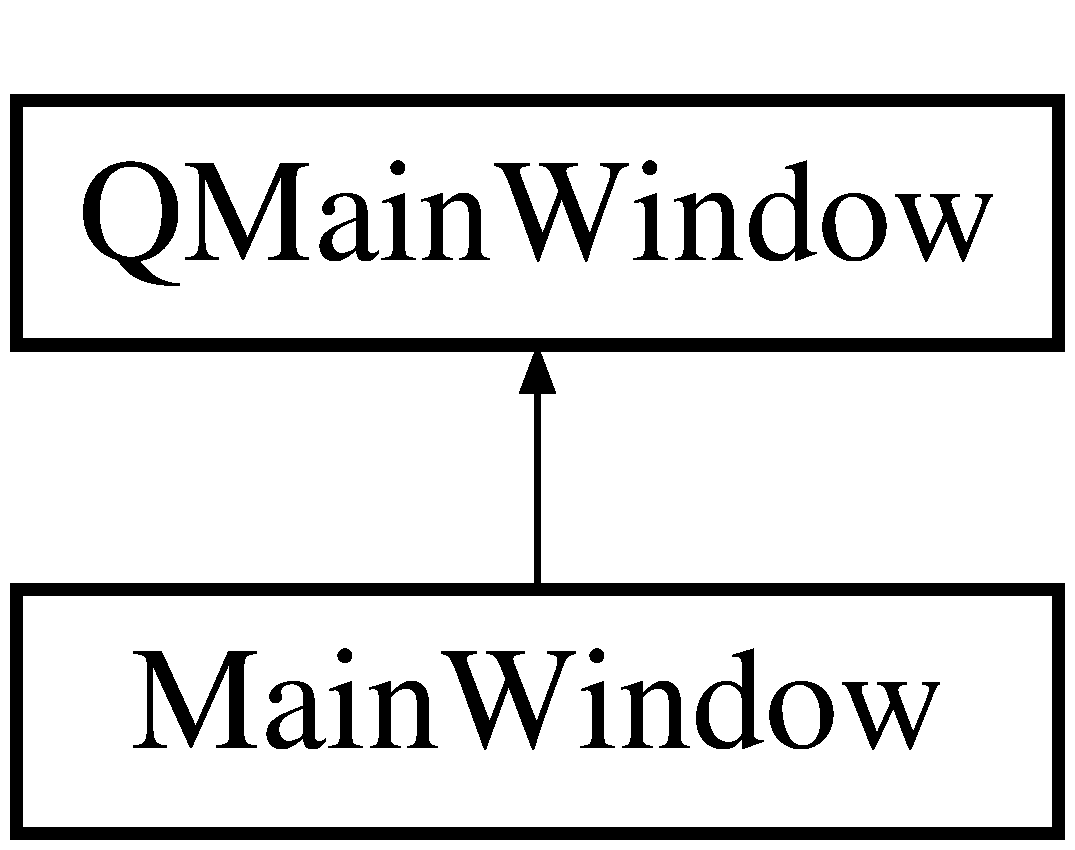
\includegraphics[height=2.000000cm]{class_main_window}
\end{center}
\end{figure}
\subsection*{Public Member Functions}
\begin{DoxyCompactItemize}
\item 
void \hyperlink{class_main_window_a20152884933e23f726b0461a7973c3fa}{actualizar\-Componentes} ()
\item 
\hyperlink{class_main_window_a8b244be8b7b7db1b08de2a2acb9409db}{Main\-Window} (Q\-Widget $\ast$parent=0)
\item 
\hyperlink{class_main_window_ae98d00a93bc118200eeef9f9bba1dba7}{$\sim$\-Main\-Window} ()
\end{DoxyCompactItemize}


\subsection{Constructor \& Destructor Documentation}
\hypertarget{class_main_window_a8b244be8b7b7db1b08de2a2acb9409db}{\index{Main\-Window@{Main\-Window}!Main\-Window@{Main\-Window}}
\index{Main\-Window@{Main\-Window}!MainWindow@{Main\-Window}}
\subsubsection[{Main\-Window}]{\setlength{\rightskip}{0pt plus 5cm}Main\-Window\-::\-Main\-Window (
\begin{DoxyParamCaption}
\item[{Q\-Widget $\ast$}]{parent = {\ttfamily 0}}
\end{DoxyParamCaption}
)\hspace{0.3cm}{\ttfamily [explicit]}}}\label{class_main_window_a8b244be8b7b7db1b08de2a2acb9409db}
\hypertarget{class_main_window_ae98d00a93bc118200eeef9f9bba1dba7}{\index{Main\-Window@{Main\-Window}!$\sim$\-Main\-Window@{$\sim$\-Main\-Window}}
\index{$\sim$\-Main\-Window@{$\sim$\-Main\-Window}!MainWindow@{Main\-Window}}
\subsubsection[{$\sim$\-Main\-Window}]{\setlength{\rightskip}{0pt plus 5cm}Main\-Window\-::$\sim$\-Main\-Window (
\begin{DoxyParamCaption}
{}
\end{DoxyParamCaption}
)}}\label{class_main_window_ae98d00a93bc118200eeef9f9bba1dba7}


\subsection{Member Function Documentation}
\hypertarget{class_main_window_a20152884933e23f726b0461a7973c3fa}{\index{Main\-Window@{Main\-Window}!actualizar\-Componentes@{actualizar\-Componentes}}
\index{actualizar\-Componentes@{actualizar\-Componentes}!MainWindow@{Main\-Window}}
\subsubsection[{actualizar\-Componentes}]{\setlength{\rightskip}{0pt plus 5cm}void Main\-Window\-::actualizar\-Componentes (
\begin{DoxyParamCaption}
{}
\end{DoxyParamCaption}
)}}\label{class_main_window_a20152884933e23f726b0461a7973c3fa}
Método a ser llamado cada vez que se haga una modificación en la cantidad de componentes. 

The documentation for this class was generated from the following files\-:\begin{DoxyCompactItemize}
\item 
G\-U\-I/\hyperlink{mainwindow_8h}{mainwindow.\-h}\item 
G\-U\-I/\hyperlink{mainwindow_8cpp}{mainwindow.\-cpp}\end{DoxyCompactItemize}

\hypertarget{class_ui_1_1_main_window}{\section{Ui\-:\-:Main\-Window Class Reference}
\label{class_ui_1_1_main_window}\index{Ui\-::\-Main\-Window@{Ui\-::\-Main\-Window}}
}


{\ttfamily \#include $<$ui\-\_\-mainwindow.\-h$>$}

Inheritance diagram for Ui\-:\-:Main\-Window\-:\begin{figure}[H]
\begin{center}
\leavevmode
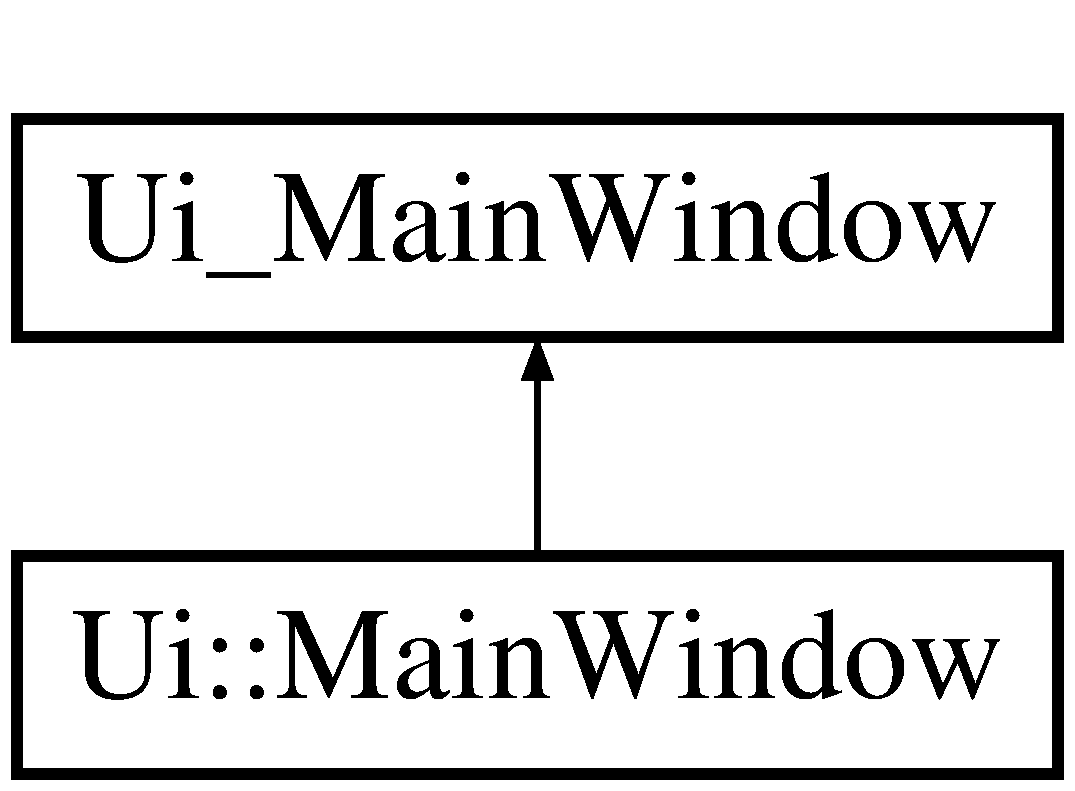
\includegraphics[height=2.000000cm]{class_ui_1_1_main_window}
\end{center}
\end{figure}
\subsection*{Additional Inherited Members}


The documentation for this class was generated from the following file\-:\begin{DoxyCompactItemize}
\item 
build-\/\-Motion\-Structure-\/\-Desktop\-\_\-\-Qt\-\_\-5\-\_\-3\-\_\-\-G\-C\-C\-\_\-64bit-\/\-Debug/\hyperlink{ui__mainwindow_8h}{ui\-\_\-mainwindow.\-h}\end{DoxyCompactItemize}

\hypertarget{class_motion__structure}{\section{Motion\-\_\-structure Class Reference}
\label{class_motion__structure}\index{Motion\-\_\-structure@{Motion\-\_\-structure}}
}


{\ttfamily \#include $<$motion\-\_\-structure.\-hpp$>$}

\subsection*{Public Member Functions}
\begin{DoxyCompactItemize}
\item 
\hyperlink{class_motion__structure_afee50b3656ee36b005cd5784508e1697}{Motion\-\_\-structure} ()
\begin{DoxyCompactList}\small\item\em Setea los valores por defecto de una estructura\-: Posición inicial (0,0,0) y resolucion de movimiento 0.\-001. \end{DoxyCompactList}\item 
\hyperlink{class_motion__structure_a1c1f2caaf5ad8288ac27b43e1ca9124a}{Motion\-\_\-structure} (double motion\-\_\-resolution)
\begin{DoxyCompactList}\small\item\em Setea el valor de la resolución de movimiento y pone la posición inicial en (0,0,0). \end{DoxyCompactList}\item 
\hyperlink{class_motion__structure_a957707cad2dc4ffbee3e7fe82ef963db}{Motion\-\_\-structure} (char $\ast$path, double motion\-\_\-resolution)
\begin{DoxyCompactList}\small\item\em Se carga la configuración previamente realizada en la G\-U\-I desde la ruta especificada y se setea la resolución del movimiento. \end{DoxyCompactList}\item 
vector$<$ double $>$ \hyperlink{class_motion__structure_a25c277cf49bed7728a894a2df001847b}{get\-\_\-initial\-\_\-angles} ()
\begin{DoxyCompactList}\small\item\em Devuelve los ángulos iniciales que tuvo la estructura en su inicio. \end{DoxyCompactList}\item 
void \hyperlink{class_motion__structure_aa9039180cf7d78c2f126fcdd171398ca}{set\-\_\-initial\-\_\-angles} (vector$<$ double $>$ \-\_\-initial\-\_\-angles)
\begin{DoxyCompactList}\small\item\em se setean los angulos iniciales de cada motor dentro de la estructura. \end{DoxyCompactList}\item 
vector$<$ double $>$ \hyperlink{class_motion__structure_a3f01cb966d8d700dfb32b2771956b37c}{get\-\_\-current\-\_\-angles} ()
\begin{DoxyCompactList}\small\item\em Obtiene los angulos actuales de los motores. \end{DoxyCompactList}\item 
void \hyperlink{class_motion__structure_a010655ae44e9b12bffa7f605dd02454a}{set\-\_\-current\-\_\-angles} (vector$<$ double $>$ \-\_\-current\-\_\-angles)
\begin{DoxyCompactList}\small\item\em Se setean los angulos de los motores. \end{DoxyCompactList}\item 
int \hyperlink{class_motion__structure_a7f36ab16180a36018516cee01ff1b666}{get\-\_\-motors\-\_\-amount} ()
\begin{DoxyCompactList}\small\item\em Obtiene la cantidad de motores de la estructura. \end{DoxyCompactList}\item 
double \hyperlink{class_motion__structure_a591d41b002285347d2f2f81a4ecb71ad}{get\-\_\-motion\-\_\-resolution} ()
\begin{DoxyCompactList}\small\item\em Obtiene la resolución del movimiento. \end{DoxyCompactList}\item 
void \hyperlink{class_motion__structure_a9d24593ceecdf101b83ea13e282a59af}{set\-\_\-motion\-\_\-resolution} (double \-\_\-motion\-\_\-resolution)
\begin{DoxyCompactList}\small\item\em Setea la resolución del movimiento. \end{DoxyCompactList}\item 
vector$<$ double $>$ \hyperlink{class_motion__structure_a9128b56d83680de910b5be7c78010458}{get\-\_\-xyz\-\_\-current\-\_\-position} ()
\begin{DoxyCompactList}\small\item\em Obtiene la posición en coordenadas cartecianas. \end{DoxyCompactList}\item 
void \hyperlink{class_motion__structure_af1286c27937cdad91bb8ef6ef39e0ff5}{add\-\_\-translation\-\_\-structure} (vector$<$ double $>$ xyz)
\begin{DoxyCompactList}\small\item\em Agrega una estructura de tipo traslación. \end{DoxyCompactList}\item 
void \hyperlink{class_motion__structure_aedd08d7f7fab858ad15f4bc0d265b4d5}{add\-\_\-rotation\-\_\-x} (double angle)
\begin{DoxyCompactList}\small\item\em agrega una rotación en x a la estructura. \end{DoxyCompactList}\item 
void \hyperlink{class_motion__structure_afc92a8d88281379658186f100412e0ae}{add\-\_\-rotation\-\_\-y} (double angle)
\begin{DoxyCompactList}\small\item\em agrega una rotación en x a la estructura. \end{DoxyCompactList}\item 
void \hyperlink{class_motion__structure_ad37ffab28b32f2f88e0a3d556c876318}{add\-\_\-rotation\-\_\-z} (double angle)
\begin{DoxyCompactList}\small\item\em agrega una rotación en x a la estructura. \end{DoxyCompactList}\item 
void \hyperlink{class_motion__structure_ac3d1406488b0806b88d9408c1a9fe12b}{add\-\_\-rotational\-\_\-motor\-\_\-x} (int motor\-\_\-id, bool direction, double initial\-\_\-angle)
\begin{DoxyCompactList}\small\item\em Agrega un motor rotacional. \end{DoxyCompactList}\item 
void \hyperlink{class_motion__structure_a7db25e8dc40c5a5fb8b91869a246b496}{add\-\_\-rotational\-\_\-motor\-\_\-y} (int motor\-\_\-id, bool direction, double initial\-\_\-angle)
\begin{DoxyCompactList}\small\item\em Agrega un motor rotacional. \end{DoxyCompactList}\item 
void \hyperlink{class_motion__structure_af902c8a035766f08b41810fb495050f8}{add\-\_\-rotational\-\_\-motor\-\_\-z} (int motor\-\_\-id, bool direction, double initial\-\_\-angle)
\begin{DoxyCompactList}\small\item\em Agrega un motor rotacional. \end{DoxyCompactList}\item 
void \hyperlink{class_motion__structure_a030fd7bc101347f360181619b0b71e3f}{add\-\_\-traslational\-\_\-motor\-\_\-x} (int motor\-\_\-id, bool direction, double initial\-\_\-large)
\begin{DoxyCompactList}\small\item\em agrega un motor traslacional \end{DoxyCompactList}\item 
void \hyperlink{class_motion__structure_aea04a057f109e87267fc49b46e464c42}{add\-\_\-traslational\-\_\-motor\-\_\-y} (int motor\-\_\-id, bool direction, double initial\-\_\-large)
\begin{DoxyCompactList}\small\item\em agrega un motor traslacional \end{DoxyCompactList}\item 
void \hyperlink{class_motion__structure_a071221988f557f8cf8fdc2c8e2df3398}{add\-\_\-traslational\-\_\-motor\-\_\-z} (int motor\-\_\-id, bool direction, double initial\-\_\-large)
\begin{DoxyCompactList}\small\item\em agrega un motor traslacional \end{DoxyCompactList}\item 
void \hyperlink{class_motion__structure_a2a020cc4ec5e7ddeaa1aa66b42bbf1e9}{set\-\_\-motors\-\_\-angles} (vector$<$ double $>$ motor\-\_\-angles)
\begin{DoxyCompactList}\small\item\em Se setean los angulos de los motores de la estructura. \end{DoxyCompactList}\item 
void \hyperlink{class_motion__structure_a0c73f6580324789218d73a7f72d6a9c9}{set\-\_\-angle\-\_\-to\-\_\-motor\-\_\-id} (int id, double angle)
\begin{DoxyCompactList}\small\item\em Se setea el ángulo del motor con id específica. \end{DoxyCompactList}\item 
mat \hyperlink{class_motion__structure_aaf97ea165dddcc6dc295730704c5102a}{get\-\_\-current\-\_\-matrix} ()
\begin{DoxyCompactList}\small\item\em Obtiene la matriz rotcacional final después de el calculo. \end{DoxyCompactList}\item 
void \hyperlink{class_motion__structure_aaafad930bdd32be66abb80823ab9a85d}{calculate\-\_\-current\-\_\-position\-\_\-matrix} ()
\begin{DoxyCompactList}\small\item\em calcula la matriz de rotación según los angulos que tengan seteados en el momento cada motor. \end{DoxyCompactList}\item 
mat \hyperlink{class_motion__structure_abcf3119a5953ab08bf4f5ea1c4716399}{calculate\-\_\-position} (vector$<$ double $>$ angles)
\begin{DoxyCompactList}\small\item\em obtiene la matriz de rotación según los angulos que tengan seteados en el momento cada motor. \end{DoxyCompactList}\item 
void \hyperlink{class_motion__structure_af3914223e9464c84fa894f2674604cff}{calculate\-\_\-position\-\_\-set\-\_\-values} (vector$<$ double $>$ angles)
\begin{DoxyCompactList}\small\item\em calcula la posición y guarda el estado en variables internas. \end{DoxyCompactList}\item 
\hyperlink{class_movement}{Movement} \hyperlink{class_motion__structure_a26174f629c57c614bd5d5f96e8ef32eb}{move\-\_\-to\-\_\-xyz\-\_\-position} (vector$<$ double $>$ xyz\-\_\-position, double velocity)
\begin{DoxyCompactList}\small\item\em Obtiene todos los movimientos necesarios para mover la estructura a la posición xyz deseada. \end{DoxyCompactList}\item 
\hyperlink{class_movement}{Movement} \hyperlink{class_motion__structure_a34d89e582551b6bcc4ba503e96ae1300}{move\-\_\-delta\-\_\-xyz\-\_\-position} (vector$<$ double $>$ delta\-\_\-xyz\-\_\-position, double velocity)
\begin{DoxyCompactList}\small\item\em Obtiene todos los movimientos necesarios para mover la estructura en xyz desde la posición actual. \end{DoxyCompactList}\item 
mat \hyperlink{class_motion__structure_a12a60ceb91c2b6d6c2bca49c9300e34a}{jacobiano\-\_\-motores} ()
\item 
void \hyperlink{class_motion__structure_af8e13d4d457bdb25cd1f954129df7f1c}{print\-\_\-current\-\_\-xyz\-\_\-position} ()
\begin{DoxyCompactList}\small\item\em imprime la posición actual en coordenadas cartesianas. \end{DoxyCompactList}\item 
void \hyperlink{class_motion__structure_a5df5dc494cfd60e8e763e06f7dc5d745}{load} (char $\ast$path)
\begin{DoxyCompactList}\small\item\em carga una estructura hecha en la G\-U\-I desde la ruta deseada. \end{DoxyCompactList}\end{DoxyCompactItemize}


\subsection{Constructor \& Destructor Documentation}
\hypertarget{class_motion__structure_afee50b3656ee36b005cd5784508e1697}{\index{Motion\-\_\-structure@{Motion\-\_\-structure}!Motion\-\_\-structure@{Motion\-\_\-structure}}
\index{Motion\-\_\-structure@{Motion\-\_\-structure}!Motion_structure@{Motion\-\_\-structure}}
\subsubsection[{Motion\-\_\-structure}]{\setlength{\rightskip}{0pt plus 5cm}Motion\-\_\-structure\-::\-Motion\-\_\-structure (
\begin{DoxyParamCaption}
{}
\end{DoxyParamCaption}
)}}\label{class_motion__structure_afee50b3656ee36b005cd5784508e1697}


Setea los valores por defecto de una estructura\-: Posición inicial (0,0,0) y resolucion de movimiento 0.\-001. 

\hypertarget{class_motion__structure_a1c1f2caaf5ad8288ac27b43e1ca9124a}{\index{Motion\-\_\-structure@{Motion\-\_\-structure}!Motion\-\_\-structure@{Motion\-\_\-structure}}
\index{Motion\-\_\-structure@{Motion\-\_\-structure}!Motion_structure@{Motion\-\_\-structure}}
\subsubsection[{Motion\-\_\-structure}]{\setlength{\rightskip}{0pt plus 5cm}Motion\-\_\-structure\-::\-Motion\-\_\-structure (
\begin{DoxyParamCaption}
\item[{double}]{motion\-\_\-resolution}
\end{DoxyParamCaption}
)}}\label{class_motion__structure_a1c1f2caaf5ad8288ac27b43e1ca9124a}


Setea el valor de la resolución de movimiento y pone la posición inicial en (0,0,0). 

\hypertarget{class_motion__structure_a957707cad2dc4ffbee3e7fe82ef963db}{\index{Motion\-\_\-structure@{Motion\-\_\-structure}!Motion\-\_\-structure@{Motion\-\_\-structure}}
\index{Motion\-\_\-structure@{Motion\-\_\-structure}!Motion_structure@{Motion\-\_\-structure}}
\subsubsection[{Motion\-\_\-structure}]{\setlength{\rightskip}{0pt plus 5cm}Motion\-\_\-structure\-::\-Motion\-\_\-structure (
\begin{DoxyParamCaption}
\item[{char $\ast$}]{path, }
\item[{double}]{motion\-\_\-resolution}
\end{DoxyParamCaption}
)}}\label{class_motion__structure_a957707cad2dc4ffbee3e7fe82ef963db}


Se carga la configuración previamente realizada en la G\-U\-I desde la ruta especificada y se setea la resolución del movimiento. 



\subsection{Member Function Documentation}
\hypertarget{class_motion__structure_aedd08d7f7fab858ad15f4bc0d265b4d5}{\index{Motion\-\_\-structure@{Motion\-\_\-structure}!add\-\_\-rotation\-\_\-x@{add\-\_\-rotation\-\_\-x}}
\index{add\-\_\-rotation\-\_\-x@{add\-\_\-rotation\-\_\-x}!Motion_structure@{Motion\-\_\-structure}}
\subsubsection[{add\-\_\-rotation\-\_\-x}]{\setlength{\rightskip}{0pt plus 5cm}void Motion\-\_\-structure\-::add\-\_\-rotation\-\_\-x (
\begin{DoxyParamCaption}
\item[{double}]{angle}
\end{DoxyParamCaption}
)}}\label{class_motion__structure_aedd08d7f7fab858ad15f4bc0d265b4d5}


agrega una rotación en x a la estructura. 

\hypertarget{class_motion__structure_afc92a8d88281379658186f100412e0ae}{\index{Motion\-\_\-structure@{Motion\-\_\-structure}!add\-\_\-rotation\-\_\-y@{add\-\_\-rotation\-\_\-y}}
\index{add\-\_\-rotation\-\_\-y@{add\-\_\-rotation\-\_\-y}!Motion_structure@{Motion\-\_\-structure}}
\subsubsection[{add\-\_\-rotation\-\_\-y}]{\setlength{\rightskip}{0pt plus 5cm}void Motion\-\_\-structure\-::add\-\_\-rotation\-\_\-y (
\begin{DoxyParamCaption}
\item[{double}]{angle}
\end{DoxyParamCaption}
)}}\label{class_motion__structure_afc92a8d88281379658186f100412e0ae}


agrega una rotación en x a la estructura. 

\hypertarget{class_motion__structure_ad37ffab28b32f2f88e0a3d556c876318}{\index{Motion\-\_\-structure@{Motion\-\_\-structure}!add\-\_\-rotation\-\_\-z@{add\-\_\-rotation\-\_\-z}}
\index{add\-\_\-rotation\-\_\-z@{add\-\_\-rotation\-\_\-z}!Motion_structure@{Motion\-\_\-structure}}
\subsubsection[{add\-\_\-rotation\-\_\-z}]{\setlength{\rightskip}{0pt plus 5cm}void Motion\-\_\-structure\-::add\-\_\-rotation\-\_\-z (
\begin{DoxyParamCaption}
\item[{double}]{angle}
\end{DoxyParamCaption}
)}}\label{class_motion__structure_ad37ffab28b32f2f88e0a3d556c876318}


agrega una rotación en x a la estructura. 

\hypertarget{class_motion__structure_ac3d1406488b0806b88d9408c1a9fe12b}{\index{Motion\-\_\-structure@{Motion\-\_\-structure}!add\-\_\-rotational\-\_\-motor\-\_\-x@{add\-\_\-rotational\-\_\-motor\-\_\-x}}
\index{add\-\_\-rotational\-\_\-motor\-\_\-x@{add\-\_\-rotational\-\_\-motor\-\_\-x}!Motion_structure@{Motion\-\_\-structure}}
\subsubsection[{add\-\_\-rotational\-\_\-motor\-\_\-x}]{\setlength{\rightskip}{0pt plus 5cm}void Motion\-\_\-structure\-::add\-\_\-rotational\-\_\-motor\-\_\-x (
\begin{DoxyParamCaption}
\item[{int}]{motor\-\_\-id, }
\item[{bool}]{direction, }
\item[{double}]{initial\-\_\-angle}
\end{DoxyParamCaption}
)}}\label{class_motion__structure_ac3d1406488b0806b88d9408c1a9fe12b}


Agrega un motor rotacional. 

\hypertarget{class_motion__structure_a7db25e8dc40c5a5fb8b91869a246b496}{\index{Motion\-\_\-structure@{Motion\-\_\-structure}!add\-\_\-rotational\-\_\-motor\-\_\-y@{add\-\_\-rotational\-\_\-motor\-\_\-y}}
\index{add\-\_\-rotational\-\_\-motor\-\_\-y@{add\-\_\-rotational\-\_\-motor\-\_\-y}!Motion_structure@{Motion\-\_\-structure}}
\subsubsection[{add\-\_\-rotational\-\_\-motor\-\_\-y}]{\setlength{\rightskip}{0pt plus 5cm}void Motion\-\_\-structure\-::add\-\_\-rotational\-\_\-motor\-\_\-y (
\begin{DoxyParamCaption}
\item[{int}]{motor\-\_\-id, }
\item[{bool}]{direction, }
\item[{double}]{initial\-\_\-angle}
\end{DoxyParamCaption}
)}}\label{class_motion__structure_a7db25e8dc40c5a5fb8b91869a246b496}


Agrega un motor rotacional. 

\hypertarget{class_motion__structure_af902c8a035766f08b41810fb495050f8}{\index{Motion\-\_\-structure@{Motion\-\_\-structure}!add\-\_\-rotational\-\_\-motor\-\_\-z@{add\-\_\-rotational\-\_\-motor\-\_\-z}}
\index{add\-\_\-rotational\-\_\-motor\-\_\-z@{add\-\_\-rotational\-\_\-motor\-\_\-z}!Motion_structure@{Motion\-\_\-structure}}
\subsubsection[{add\-\_\-rotational\-\_\-motor\-\_\-z}]{\setlength{\rightskip}{0pt plus 5cm}void Motion\-\_\-structure\-::add\-\_\-rotational\-\_\-motor\-\_\-z (
\begin{DoxyParamCaption}
\item[{int}]{motor\-\_\-id, }
\item[{bool}]{direction, }
\item[{double}]{initial\-\_\-angle}
\end{DoxyParamCaption}
)}}\label{class_motion__structure_af902c8a035766f08b41810fb495050f8}


Agrega un motor rotacional. 

\hypertarget{class_motion__structure_af1286c27937cdad91bb8ef6ef39e0ff5}{\index{Motion\-\_\-structure@{Motion\-\_\-structure}!add\-\_\-translation\-\_\-structure@{add\-\_\-translation\-\_\-structure}}
\index{add\-\_\-translation\-\_\-structure@{add\-\_\-translation\-\_\-structure}!Motion_structure@{Motion\-\_\-structure}}
\subsubsection[{add\-\_\-translation\-\_\-structure}]{\setlength{\rightskip}{0pt plus 5cm}void Motion\-\_\-structure\-::add\-\_\-translation\-\_\-structure (
\begin{DoxyParamCaption}
\item[{vector$<$ double $>$}]{xyz}
\end{DoxyParamCaption}
)}}\label{class_motion__structure_af1286c27937cdad91bb8ef6ef39e0ff5}


Agrega una estructura de tipo traslación. 

\hypertarget{class_motion__structure_a030fd7bc101347f360181619b0b71e3f}{\index{Motion\-\_\-structure@{Motion\-\_\-structure}!add\-\_\-traslational\-\_\-motor\-\_\-x@{add\-\_\-traslational\-\_\-motor\-\_\-x}}
\index{add\-\_\-traslational\-\_\-motor\-\_\-x@{add\-\_\-traslational\-\_\-motor\-\_\-x}!Motion_structure@{Motion\-\_\-structure}}
\subsubsection[{add\-\_\-traslational\-\_\-motor\-\_\-x}]{\setlength{\rightskip}{0pt plus 5cm}void Motion\-\_\-structure\-::add\-\_\-traslational\-\_\-motor\-\_\-x (
\begin{DoxyParamCaption}
\item[{int}]{motor\-\_\-id, }
\item[{bool}]{direction, }
\item[{double}]{initial\-\_\-large}
\end{DoxyParamCaption}
)}}\label{class_motion__structure_a030fd7bc101347f360181619b0b71e3f}


agrega un motor traslacional 

\hypertarget{class_motion__structure_aea04a057f109e87267fc49b46e464c42}{\index{Motion\-\_\-structure@{Motion\-\_\-structure}!add\-\_\-traslational\-\_\-motor\-\_\-y@{add\-\_\-traslational\-\_\-motor\-\_\-y}}
\index{add\-\_\-traslational\-\_\-motor\-\_\-y@{add\-\_\-traslational\-\_\-motor\-\_\-y}!Motion_structure@{Motion\-\_\-structure}}
\subsubsection[{add\-\_\-traslational\-\_\-motor\-\_\-y}]{\setlength{\rightskip}{0pt plus 5cm}void Motion\-\_\-structure\-::add\-\_\-traslational\-\_\-motor\-\_\-y (
\begin{DoxyParamCaption}
\item[{int}]{motor\-\_\-id, }
\item[{bool}]{direction, }
\item[{double}]{initial\-\_\-large}
\end{DoxyParamCaption}
)}}\label{class_motion__structure_aea04a057f109e87267fc49b46e464c42}


agrega un motor traslacional 

\hypertarget{class_motion__structure_a071221988f557f8cf8fdc2c8e2df3398}{\index{Motion\-\_\-structure@{Motion\-\_\-structure}!add\-\_\-traslational\-\_\-motor\-\_\-z@{add\-\_\-traslational\-\_\-motor\-\_\-z}}
\index{add\-\_\-traslational\-\_\-motor\-\_\-z@{add\-\_\-traslational\-\_\-motor\-\_\-z}!Motion_structure@{Motion\-\_\-structure}}
\subsubsection[{add\-\_\-traslational\-\_\-motor\-\_\-z}]{\setlength{\rightskip}{0pt plus 5cm}void Motion\-\_\-structure\-::add\-\_\-traslational\-\_\-motor\-\_\-z (
\begin{DoxyParamCaption}
\item[{int}]{motor\-\_\-id, }
\item[{bool}]{direction, }
\item[{double}]{initial\-\_\-large}
\end{DoxyParamCaption}
)}}\label{class_motion__structure_a071221988f557f8cf8fdc2c8e2df3398}


agrega un motor traslacional 

\hypertarget{class_motion__structure_aaafad930bdd32be66abb80823ab9a85d}{\index{Motion\-\_\-structure@{Motion\-\_\-structure}!calculate\-\_\-current\-\_\-position\-\_\-matrix@{calculate\-\_\-current\-\_\-position\-\_\-matrix}}
\index{calculate\-\_\-current\-\_\-position\-\_\-matrix@{calculate\-\_\-current\-\_\-position\-\_\-matrix}!Motion_structure@{Motion\-\_\-structure}}
\subsubsection[{calculate\-\_\-current\-\_\-position\-\_\-matrix}]{\setlength{\rightskip}{0pt plus 5cm}void Motion\-\_\-structure\-::calculate\-\_\-current\-\_\-position\-\_\-matrix (
\begin{DoxyParamCaption}
{}
\end{DoxyParamCaption}
)}}\label{class_motion__structure_aaafad930bdd32be66abb80823ab9a85d}


calcula la matriz de rotación según los angulos que tengan seteados en el momento cada motor. 

\hypertarget{class_motion__structure_abcf3119a5953ab08bf4f5ea1c4716399}{\index{Motion\-\_\-structure@{Motion\-\_\-structure}!calculate\-\_\-position@{calculate\-\_\-position}}
\index{calculate\-\_\-position@{calculate\-\_\-position}!Motion_structure@{Motion\-\_\-structure}}
\subsubsection[{calculate\-\_\-position}]{\setlength{\rightskip}{0pt plus 5cm}mat Motion\-\_\-structure\-::calculate\-\_\-position (
\begin{DoxyParamCaption}
\item[{vector$<$ double $>$}]{angles}
\end{DoxyParamCaption}
)}}\label{class_motion__structure_abcf3119a5953ab08bf4f5ea1c4716399}


obtiene la matriz de rotación según los angulos que tengan seteados en el momento cada motor. 

\hypertarget{class_motion__structure_af3914223e9464c84fa894f2674604cff}{\index{Motion\-\_\-structure@{Motion\-\_\-structure}!calculate\-\_\-position\-\_\-set\-\_\-values@{calculate\-\_\-position\-\_\-set\-\_\-values}}
\index{calculate\-\_\-position\-\_\-set\-\_\-values@{calculate\-\_\-position\-\_\-set\-\_\-values}!Motion_structure@{Motion\-\_\-structure}}
\subsubsection[{calculate\-\_\-position\-\_\-set\-\_\-values}]{\setlength{\rightskip}{0pt plus 5cm}void Motion\-\_\-structure\-::calculate\-\_\-position\-\_\-set\-\_\-values (
\begin{DoxyParamCaption}
\item[{vector$<$ double $>$}]{angles}
\end{DoxyParamCaption}
)}}\label{class_motion__structure_af3914223e9464c84fa894f2674604cff}


calcula la posición y guarda el estado en variables internas. 

\hypertarget{class_motion__structure_a3f01cb966d8d700dfb32b2771956b37c}{\index{Motion\-\_\-structure@{Motion\-\_\-structure}!get\-\_\-current\-\_\-angles@{get\-\_\-current\-\_\-angles}}
\index{get\-\_\-current\-\_\-angles@{get\-\_\-current\-\_\-angles}!Motion_structure@{Motion\-\_\-structure}}
\subsubsection[{get\-\_\-current\-\_\-angles}]{\setlength{\rightskip}{0pt plus 5cm}vector$<$double$>$ Motion\-\_\-structure\-::get\-\_\-current\-\_\-angles (
\begin{DoxyParamCaption}
{}
\end{DoxyParamCaption}
)}}\label{class_motion__structure_a3f01cb966d8d700dfb32b2771956b37c}


Obtiene los angulos actuales de los motores. 

\hypertarget{class_motion__structure_aaf97ea165dddcc6dc295730704c5102a}{\index{Motion\-\_\-structure@{Motion\-\_\-structure}!get\-\_\-current\-\_\-matrix@{get\-\_\-current\-\_\-matrix}}
\index{get\-\_\-current\-\_\-matrix@{get\-\_\-current\-\_\-matrix}!Motion_structure@{Motion\-\_\-structure}}
\subsubsection[{get\-\_\-current\-\_\-matrix}]{\setlength{\rightskip}{0pt plus 5cm}mat Motion\-\_\-structure\-::get\-\_\-current\-\_\-matrix (
\begin{DoxyParamCaption}
{}
\end{DoxyParamCaption}
)}}\label{class_motion__structure_aaf97ea165dddcc6dc295730704c5102a}


Obtiene la matriz rotcacional final después de el calculo. 

\hypertarget{class_motion__structure_a25c277cf49bed7728a894a2df001847b}{\index{Motion\-\_\-structure@{Motion\-\_\-structure}!get\-\_\-initial\-\_\-angles@{get\-\_\-initial\-\_\-angles}}
\index{get\-\_\-initial\-\_\-angles@{get\-\_\-initial\-\_\-angles}!Motion_structure@{Motion\-\_\-structure}}
\subsubsection[{get\-\_\-initial\-\_\-angles}]{\setlength{\rightskip}{0pt plus 5cm}vector$<$double$>$ Motion\-\_\-structure\-::get\-\_\-initial\-\_\-angles (
\begin{DoxyParamCaption}
{}
\end{DoxyParamCaption}
)}}\label{class_motion__structure_a25c277cf49bed7728a894a2df001847b}


Devuelve los ángulos iniciales que tuvo la estructura en su inicio. 

\hypertarget{class_motion__structure_a591d41b002285347d2f2f81a4ecb71ad}{\index{Motion\-\_\-structure@{Motion\-\_\-structure}!get\-\_\-motion\-\_\-resolution@{get\-\_\-motion\-\_\-resolution}}
\index{get\-\_\-motion\-\_\-resolution@{get\-\_\-motion\-\_\-resolution}!Motion_structure@{Motion\-\_\-structure}}
\subsubsection[{get\-\_\-motion\-\_\-resolution}]{\setlength{\rightskip}{0pt plus 5cm}double Motion\-\_\-structure\-::get\-\_\-motion\-\_\-resolution (
\begin{DoxyParamCaption}
{}
\end{DoxyParamCaption}
)}}\label{class_motion__structure_a591d41b002285347d2f2f81a4ecb71ad}


Obtiene la resolución del movimiento. 

\hypertarget{class_motion__structure_a7f36ab16180a36018516cee01ff1b666}{\index{Motion\-\_\-structure@{Motion\-\_\-structure}!get\-\_\-motors\-\_\-amount@{get\-\_\-motors\-\_\-amount}}
\index{get\-\_\-motors\-\_\-amount@{get\-\_\-motors\-\_\-amount}!Motion_structure@{Motion\-\_\-structure}}
\subsubsection[{get\-\_\-motors\-\_\-amount}]{\setlength{\rightskip}{0pt plus 5cm}int Motion\-\_\-structure\-::get\-\_\-motors\-\_\-amount (
\begin{DoxyParamCaption}
{}
\end{DoxyParamCaption}
)}}\label{class_motion__structure_a7f36ab16180a36018516cee01ff1b666}


Obtiene la cantidad de motores de la estructura. 

\hypertarget{class_motion__structure_a9128b56d83680de910b5be7c78010458}{\index{Motion\-\_\-structure@{Motion\-\_\-structure}!get\-\_\-xyz\-\_\-current\-\_\-position@{get\-\_\-xyz\-\_\-current\-\_\-position}}
\index{get\-\_\-xyz\-\_\-current\-\_\-position@{get\-\_\-xyz\-\_\-current\-\_\-position}!Motion_structure@{Motion\-\_\-structure}}
\subsubsection[{get\-\_\-xyz\-\_\-current\-\_\-position}]{\setlength{\rightskip}{0pt plus 5cm}vector$<$double$>$ Motion\-\_\-structure\-::get\-\_\-xyz\-\_\-current\-\_\-position (
\begin{DoxyParamCaption}
{}
\end{DoxyParamCaption}
)}}\label{class_motion__structure_a9128b56d83680de910b5be7c78010458}


Obtiene la posición en coordenadas cartecianas. 

\hypertarget{class_motion__structure_a12a60ceb91c2b6d6c2bca49c9300e34a}{\index{Motion\-\_\-structure@{Motion\-\_\-structure}!jacobiano\-\_\-motores@{jacobiano\-\_\-motores}}
\index{jacobiano\-\_\-motores@{jacobiano\-\_\-motores}!Motion_structure@{Motion\-\_\-structure}}
\subsubsection[{jacobiano\-\_\-motores}]{\setlength{\rightskip}{0pt plus 5cm}mat Motion\-\_\-structure\-::jacobiano\-\_\-motores (
\begin{DoxyParamCaption}
{}
\end{DoxyParamCaption}
)}}\label{class_motion__structure_a12a60ceb91c2b6d6c2bca49c9300e34a}
\hypertarget{class_motion__structure_a5df5dc494cfd60e8e763e06f7dc5d745}{\index{Motion\-\_\-structure@{Motion\-\_\-structure}!load@{load}}
\index{load@{load}!Motion_structure@{Motion\-\_\-structure}}
\subsubsection[{load}]{\setlength{\rightskip}{0pt plus 5cm}void Motion\-\_\-structure\-::load (
\begin{DoxyParamCaption}
\item[{char $\ast$}]{path}
\end{DoxyParamCaption}
)}}\label{class_motion__structure_a5df5dc494cfd60e8e763e06f7dc5d745}


carga una estructura hecha en la G\-U\-I desde la ruta deseada. 


\begin{DoxyParams}{Parameters}
{\em la} & ruta del archivo con la estructura. \\
\hline
\end{DoxyParams}
\hypertarget{class_motion__structure_a34d89e582551b6bcc4ba503e96ae1300}{\index{Motion\-\_\-structure@{Motion\-\_\-structure}!move\-\_\-delta\-\_\-xyz\-\_\-position@{move\-\_\-delta\-\_\-xyz\-\_\-position}}
\index{move\-\_\-delta\-\_\-xyz\-\_\-position@{move\-\_\-delta\-\_\-xyz\-\_\-position}!Motion_structure@{Motion\-\_\-structure}}
\subsubsection[{move\-\_\-delta\-\_\-xyz\-\_\-position}]{\setlength{\rightskip}{0pt plus 5cm}{\bf Movement} Motion\-\_\-structure\-::move\-\_\-delta\-\_\-xyz\-\_\-position (
\begin{DoxyParamCaption}
\item[{vector$<$ double $>$}]{delta\-\_\-xyz\-\_\-position, }
\item[{double}]{velocity}
\end{DoxyParamCaption}
)}}\label{class_motion__structure_a34d89e582551b6bcc4ba503e96ae1300}


Obtiene todos los movimientos necesarios para mover la estructura en xyz desde la posición actual. 

\hypertarget{class_motion__structure_a26174f629c57c614bd5d5f96e8ef32eb}{\index{Motion\-\_\-structure@{Motion\-\_\-structure}!move\-\_\-to\-\_\-xyz\-\_\-position@{move\-\_\-to\-\_\-xyz\-\_\-position}}
\index{move\-\_\-to\-\_\-xyz\-\_\-position@{move\-\_\-to\-\_\-xyz\-\_\-position}!Motion_structure@{Motion\-\_\-structure}}
\subsubsection[{move\-\_\-to\-\_\-xyz\-\_\-position}]{\setlength{\rightskip}{0pt plus 5cm}{\bf Movement} Motion\-\_\-structure\-::move\-\_\-to\-\_\-xyz\-\_\-position (
\begin{DoxyParamCaption}
\item[{vector$<$ double $>$}]{xyz\-\_\-position, }
\item[{double}]{velocity}
\end{DoxyParamCaption}
)}}\label{class_motion__structure_a26174f629c57c614bd5d5f96e8ef32eb}


Obtiene todos los movimientos necesarios para mover la estructura a la posición xyz deseada. 

\hypertarget{class_motion__structure_af8e13d4d457bdb25cd1f954129df7f1c}{\index{Motion\-\_\-structure@{Motion\-\_\-structure}!print\-\_\-current\-\_\-xyz\-\_\-position@{print\-\_\-current\-\_\-xyz\-\_\-position}}
\index{print\-\_\-current\-\_\-xyz\-\_\-position@{print\-\_\-current\-\_\-xyz\-\_\-position}!Motion_structure@{Motion\-\_\-structure}}
\subsubsection[{print\-\_\-current\-\_\-xyz\-\_\-position}]{\setlength{\rightskip}{0pt plus 5cm}void Motion\-\_\-structure\-::print\-\_\-current\-\_\-xyz\-\_\-position (
\begin{DoxyParamCaption}
{}
\end{DoxyParamCaption}
)}}\label{class_motion__structure_af8e13d4d457bdb25cd1f954129df7f1c}


imprime la posición actual en coordenadas cartesianas. 

\hypertarget{class_motion__structure_a0c73f6580324789218d73a7f72d6a9c9}{\index{Motion\-\_\-structure@{Motion\-\_\-structure}!set\-\_\-angle\-\_\-to\-\_\-motor\-\_\-id@{set\-\_\-angle\-\_\-to\-\_\-motor\-\_\-id}}
\index{set\-\_\-angle\-\_\-to\-\_\-motor\-\_\-id@{set\-\_\-angle\-\_\-to\-\_\-motor\-\_\-id}!Motion_structure@{Motion\-\_\-structure}}
\subsubsection[{set\-\_\-angle\-\_\-to\-\_\-motor\-\_\-id}]{\setlength{\rightskip}{0pt plus 5cm}void Motion\-\_\-structure\-::set\-\_\-angle\-\_\-to\-\_\-motor\-\_\-id (
\begin{DoxyParamCaption}
\item[{int}]{id, }
\item[{double}]{angle}
\end{DoxyParamCaption}
)}}\label{class_motion__structure_a0c73f6580324789218d73a7f72d6a9c9}


Se setea el ángulo del motor con id específica. 

\hypertarget{class_motion__structure_a010655ae44e9b12bffa7f605dd02454a}{\index{Motion\-\_\-structure@{Motion\-\_\-structure}!set\-\_\-current\-\_\-angles@{set\-\_\-current\-\_\-angles}}
\index{set\-\_\-current\-\_\-angles@{set\-\_\-current\-\_\-angles}!Motion_structure@{Motion\-\_\-structure}}
\subsubsection[{set\-\_\-current\-\_\-angles}]{\setlength{\rightskip}{0pt plus 5cm}void Motion\-\_\-structure\-::set\-\_\-current\-\_\-angles (
\begin{DoxyParamCaption}
\item[{vector$<$ double $>$}]{\-\_\-current\-\_\-angles}
\end{DoxyParamCaption}
)}}\label{class_motion__structure_a010655ae44e9b12bffa7f605dd02454a}


Se setean los angulos de los motores. 


\begin{DoxyParams}{Parameters}
{\em \-\_\-current\-\_\-angles} & angulos que deben tener los motores. \\
\hline
\end{DoxyParams}
\hypertarget{class_motion__structure_aa9039180cf7d78c2f126fcdd171398ca}{\index{Motion\-\_\-structure@{Motion\-\_\-structure}!set\-\_\-initial\-\_\-angles@{set\-\_\-initial\-\_\-angles}}
\index{set\-\_\-initial\-\_\-angles@{set\-\_\-initial\-\_\-angles}!Motion_structure@{Motion\-\_\-structure}}
\subsubsection[{set\-\_\-initial\-\_\-angles}]{\setlength{\rightskip}{0pt plus 5cm}void Motion\-\_\-structure\-::set\-\_\-initial\-\_\-angles (
\begin{DoxyParamCaption}
\item[{vector$<$ double $>$}]{\-\_\-initial\-\_\-angles}
\end{DoxyParamCaption}
)}}\label{class_motion__structure_aa9039180cf7d78c2f126fcdd171398ca}


se setean los angulos iniciales de cada motor dentro de la estructura. 


\begin{DoxyParams}{Parameters}
{\em \-\_\-initial\-\_\-angles} & vector con los angulos iniciales de todos los motores. (debe tener el mismo largo que la cantidad de motores). \\
\hline
\end{DoxyParams}
\hypertarget{class_motion__structure_a9d24593ceecdf101b83ea13e282a59af}{\index{Motion\-\_\-structure@{Motion\-\_\-structure}!set\-\_\-motion\-\_\-resolution@{set\-\_\-motion\-\_\-resolution}}
\index{set\-\_\-motion\-\_\-resolution@{set\-\_\-motion\-\_\-resolution}!Motion_structure@{Motion\-\_\-structure}}
\subsubsection[{set\-\_\-motion\-\_\-resolution}]{\setlength{\rightskip}{0pt plus 5cm}void Motion\-\_\-structure\-::set\-\_\-motion\-\_\-resolution (
\begin{DoxyParamCaption}
\item[{double}]{\-\_\-motion\-\_\-resolution}
\end{DoxyParamCaption}
)}}\label{class_motion__structure_a9d24593ceecdf101b83ea13e282a59af}


Setea la resolución del movimiento. 

\hypertarget{class_motion__structure_a2a020cc4ec5e7ddeaa1aa66b42bbf1e9}{\index{Motion\-\_\-structure@{Motion\-\_\-structure}!set\-\_\-motors\-\_\-angles@{set\-\_\-motors\-\_\-angles}}
\index{set\-\_\-motors\-\_\-angles@{set\-\_\-motors\-\_\-angles}!Motion_structure@{Motion\-\_\-structure}}
\subsubsection[{set\-\_\-motors\-\_\-angles}]{\setlength{\rightskip}{0pt plus 5cm}void Motion\-\_\-structure\-::set\-\_\-motors\-\_\-angles (
\begin{DoxyParamCaption}
\item[{vector$<$ double $>$}]{motor\-\_\-angles}
\end{DoxyParamCaption}
)}}\label{class_motion__structure_a2a020cc4ec5e7ddeaa1aa66b42bbf1e9}


Se setean los angulos de los motores de la estructura. 



The documentation for this class was generated from the following files\-:\begin{DoxyCompactItemize}
\item 
headers/\hyperlink{motion__structure_8hpp}{motion\-\_\-structure.\-hpp}\item 
src/\hyperlink{motion__structure_8cpp}{motion\-\_\-structure.\-cpp}\end{DoxyCompactItemize}

\hypertarget{class_motor}{\section{Motor Class Reference}
\label{class_motor}\index{Motor@{Motor}}
}


{\ttfamily \#include $<$motor.\-hpp$>$}

\subsection*{Public Member Functions}
\begin{DoxyCompactItemize}
\item 
\hyperlink{class_motor_abe780b3e871a85b968d6fee888205b51}{Motor} (int id, bool direction, double angle, \hyperlink{motor_8hpp_a3f29f8952bca737db7bc832cd0a6d6f3}{Motor\-Type} type)
\item 
int \hyperlink{class_motor_a88de4d6f7d85d70f75d5510cb2497d0f}{get\-\_\-id} ()
\item 
void \hyperlink{class_motor_a0fc563074b6536653e531f5d9866cef4}{set\-\_\-id} (int id)
\item 
double \hyperlink{class_motor_af5664216f4ee9367282cb1e1986b3a13}{get\-\_\-angle} ()
\item 
void \hyperlink{class_motor_a83895c894993a9e6c165be085b570138}{set\-\_\-angle} (double angle)
\item 
bool \hyperlink{class_motor_afccab98ca0cef41c88889d1a230bef10}{get\-\_\-direction} ()
\item 
void \hyperlink{class_motor_a04549cf142dfe4688266f92f549d74d7}{set\-\_\-direction} (bool dir)
\item 
void \hyperlink{class_motor_a1195af10210c3335233d7ee65a2e178e}{calculate\-\_\-current\-\_\-matrix} ()
\item 
mat \hyperlink{class_motor_a54cb596f4a6f050e84f6534abeb57c0c}{get\-\_\-current\-\_\-matrix} ()
\item 
mat \hyperlink{class_motor_ad3e3edb6ebd548fbd3e4b4720af2d311}{calculate\-\_\-matrix} (double angle)
\item 
double \hyperlink{class_motor_a32e5af9c7721419fd9df29d70c2bd6b4}{get\-\_\-direction\-\_\-value} ()
\end{DoxyCompactItemize}


\subsection{Constructor \& Destructor Documentation}
\hypertarget{class_motor_abe780b3e871a85b968d6fee888205b51}{\index{Motor@{Motor}!Motor@{Motor}}
\index{Motor@{Motor}!Motor@{Motor}}
\subsubsection[{Motor}]{\setlength{\rightskip}{0pt plus 5cm}Motor\-::\-Motor (
\begin{DoxyParamCaption}
\item[{int}]{id, }
\item[{bool}]{direction, }
\item[{double}]{angle, }
\item[{{\bf Motor\-Type}}]{type}
\end{DoxyParamCaption}
)}}\label{class_motor_abe780b3e871a85b968d6fee888205b51}


\subsection{Member Function Documentation}
\hypertarget{class_motor_a1195af10210c3335233d7ee65a2e178e}{\index{Motor@{Motor}!calculate\-\_\-current\-\_\-matrix@{calculate\-\_\-current\-\_\-matrix}}
\index{calculate\-\_\-current\-\_\-matrix@{calculate\-\_\-current\-\_\-matrix}!Motor@{Motor}}
\subsubsection[{calculate\-\_\-current\-\_\-matrix}]{\setlength{\rightskip}{0pt plus 5cm}void Motor\-::calculate\-\_\-current\-\_\-matrix (
\begin{DoxyParamCaption}
{}
\end{DoxyParamCaption}
)}}\label{class_motor_a1195af10210c3335233d7ee65a2e178e}
\hypertarget{class_motor_ad3e3edb6ebd548fbd3e4b4720af2d311}{\index{Motor@{Motor}!calculate\-\_\-matrix@{calculate\-\_\-matrix}}
\index{calculate\-\_\-matrix@{calculate\-\_\-matrix}!Motor@{Motor}}
\subsubsection[{calculate\-\_\-matrix}]{\setlength{\rightskip}{0pt plus 5cm}mat Motor\-::calculate\-\_\-matrix (
\begin{DoxyParamCaption}
\item[{double}]{angle}
\end{DoxyParamCaption}
)}}\label{class_motor_ad3e3edb6ebd548fbd3e4b4720af2d311}
\hypertarget{class_motor_af5664216f4ee9367282cb1e1986b3a13}{\index{Motor@{Motor}!get\-\_\-angle@{get\-\_\-angle}}
\index{get\-\_\-angle@{get\-\_\-angle}!Motor@{Motor}}
\subsubsection[{get\-\_\-angle}]{\setlength{\rightskip}{0pt plus 5cm}double Motor\-::get\-\_\-angle (
\begin{DoxyParamCaption}
{}
\end{DoxyParamCaption}
)}}\label{class_motor_af5664216f4ee9367282cb1e1986b3a13}
\hypertarget{class_motor_a54cb596f4a6f050e84f6534abeb57c0c}{\index{Motor@{Motor}!get\-\_\-current\-\_\-matrix@{get\-\_\-current\-\_\-matrix}}
\index{get\-\_\-current\-\_\-matrix@{get\-\_\-current\-\_\-matrix}!Motor@{Motor}}
\subsubsection[{get\-\_\-current\-\_\-matrix}]{\setlength{\rightskip}{0pt plus 5cm}mat Motor\-::get\-\_\-current\-\_\-matrix (
\begin{DoxyParamCaption}
{}
\end{DoxyParamCaption}
)}}\label{class_motor_a54cb596f4a6f050e84f6534abeb57c0c}
\hypertarget{class_motor_afccab98ca0cef41c88889d1a230bef10}{\index{Motor@{Motor}!get\-\_\-direction@{get\-\_\-direction}}
\index{get\-\_\-direction@{get\-\_\-direction}!Motor@{Motor}}
\subsubsection[{get\-\_\-direction}]{\setlength{\rightskip}{0pt plus 5cm}bool Motor\-::get\-\_\-direction (
\begin{DoxyParamCaption}
{}
\end{DoxyParamCaption}
)}}\label{class_motor_afccab98ca0cef41c88889d1a230bef10}
\hypertarget{class_motor_a32e5af9c7721419fd9df29d70c2bd6b4}{\index{Motor@{Motor}!get\-\_\-direction\-\_\-value@{get\-\_\-direction\-\_\-value}}
\index{get\-\_\-direction\-\_\-value@{get\-\_\-direction\-\_\-value}!Motor@{Motor}}
\subsubsection[{get\-\_\-direction\-\_\-value}]{\setlength{\rightskip}{0pt plus 5cm}double Motor\-::get\-\_\-direction\-\_\-value (
\begin{DoxyParamCaption}
{}
\end{DoxyParamCaption}
)}}\label{class_motor_a32e5af9c7721419fd9df29d70c2bd6b4}
\hypertarget{class_motor_a88de4d6f7d85d70f75d5510cb2497d0f}{\index{Motor@{Motor}!get\-\_\-id@{get\-\_\-id}}
\index{get\-\_\-id@{get\-\_\-id}!Motor@{Motor}}
\subsubsection[{get\-\_\-id}]{\setlength{\rightskip}{0pt plus 5cm}int Motor\-::get\-\_\-id (
\begin{DoxyParamCaption}
{}
\end{DoxyParamCaption}
)}}\label{class_motor_a88de4d6f7d85d70f75d5510cb2497d0f}
\hypertarget{class_motor_a83895c894993a9e6c165be085b570138}{\index{Motor@{Motor}!set\-\_\-angle@{set\-\_\-angle}}
\index{set\-\_\-angle@{set\-\_\-angle}!Motor@{Motor}}
\subsubsection[{set\-\_\-angle}]{\setlength{\rightskip}{0pt plus 5cm}void Motor\-::set\-\_\-angle (
\begin{DoxyParamCaption}
\item[{double}]{angle}
\end{DoxyParamCaption}
)}}\label{class_motor_a83895c894993a9e6c165be085b570138}
\hypertarget{class_motor_a04549cf142dfe4688266f92f549d74d7}{\index{Motor@{Motor}!set\-\_\-direction@{set\-\_\-direction}}
\index{set\-\_\-direction@{set\-\_\-direction}!Motor@{Motor}}
\subsubsection[{set\-\_\-direction}]{\setlength{\rightskip}{0pt plus 5cm}void Motor\-::set\-\_\-direction (
\begin{DoxyParamCaption}
\item[{bool}]{dir}
\end{DoxyParamCaption}
)}}\label{class_motor_a04549cf142dfe4688266f92f549d74d7}
\hypertarget{class_motor_a0fc563074b6536653e531f5d9866cef4}{\index{Motor@{Motor}!set\-\_\-id@{set\-\_\-id}}
\index{set\-\_\-id@{set\-\_\-id}!Motor@{Motor}}
\subsubsection[{set\-\_\-id}]{\setlength{\rightskip}{0pt plus 5cm}void Motor\-::set\-\_\-id (
\begin{DoxyParamCaption}
\item[{int}]{id}
\end{DoxyParamCaption}
)}}\label{class_motor_a0fc563074b6536653e531f5d9866cef4}


The documentation for this class was generated from the following files\-:\begin{DoxyCompactItemize}
\item 
headers/\hyperlink{motor_8hpp}{motor.\-hpp}\item 
src/\hyperlink{motor_8cpp}{motor.\-cpp}\end{DoxyCompactItemize}

\hypertarget{class_movement}{\section{Movement Class Reference}
\label{class_movement}\index{Movement@{Movement}}
}


{\ttfamily \#include $<$movement.\-hpp$>$}

\subsection*{Public Member Functions}
\begin{DoxyCompactItemize}
\item 
\hyperlink{class_movement_ae0493997549e8b3ead5146bea074010d}{Movement} ()
\begin{DoxyCompactList}\small\item\em Se setean valores por defecto. \end{DoxyCompactList}\item 
int \hyperlink{class_movement_af617179c4f9d600397dd780553464bdc}{get\-\_\-length\-\_\-position} ()
\begin{DoxyCompactList}\small\item\em Se obtiene la cantidad de posiciones que el objeto tiene guardadas por el ultimo movimiento realizado. \end{DoxyCompactList}\item 
int \hyperlink{class_movement_adba12b00ba14057471a869fc65615f66}{get\-\_\-length\-\_\-velocity} ()
\begin{DoxyCompactList}\small\item\em Se obtiene la cantidad de velocidades que el objeto tiene guardadas por el ultimo movimiento realizado. \end{DoxyCompactList}\item 
void \hyperlink{class_movement_a390ed24cd1530a9d5746d05c23bdbd40}{add\-\_\-to\-\_\-list\-\_\-motor\-\_\-angle\-\_\-positions} (vector$<$ double $>$ angle\-\_\-position\-\_\-data)
\begin{DoxyCompactList}\small\item\em Se agrega una posición a la lista de posiciones. \end{DoxyCompactList}\item 
vector$<$ double $>$ \hyperlink{class_movement_a9ecca745f7402967fc19588e0b9874dd}{get\-\_\-from\-\_\-list\-\_\-motor\-\_\-angle\-\_\-position} (int position)
\begin{DoxyCompactList}\small\item\em Se obtiene la posición de los motores de la lista de posiciones. \end{DoxyCompactList}\item 
void \hyperlink{class_movement_a09e56b3d72258279fd7a042f30205876}{add\-\_\-to\-\_\-list\-\_\-motor\-\_\-velocities} (vector$<$ double $>$ velocity\-\_\-data)
\begin{DoxyCompactList}\small\item\em Se agrega vector de velocidades de los motores a la lista de velocidades. \end{DoxyCompactList}\item 
vector$<$ double $>$ \hyperlink{class_movement_aa08feff643ab4fce576786b6cba08049}{get\-\_\-from\-\_\-list\-\_\-motor\-\_\-velocities} (int position)
\begin{DoxyCompactList}\small\item\em Se obtiene la velocidad de los motores de la lista de velocidades. \end{DoxyCompactList}\item 
void \hyperlink{class_movement_a318d3daab1fa6aff22d6a82a946d1a5c}{clear\-\_\-movement} ()
\begin{DoxyCompactList}\small\item\em Se borran todos los datos del movimiento. \end{DoxyCompactList}\item 
void \hyperlink{class_movement_ada9ed5b99aec82c514788b1b3c7bfab6}{set\-\_\-time\-\_\-between\-\_\-two\-\_\-points\-\_\-millisecons} (double tbtpm)
\begin{DoxyCompactList}\small\item\em Se setea el tiempo entre dos puntos de un mismo moviemiento. \end{DoxyCompactList}\item 
int \hyperlink{class_movement_abdc87acab65670b1867a1ae4db77376a}{get\-\_\-time\-\_\-between\-\_\-tw0\-\_\-points\-\_\-millisecons} ()
\begin{DoxyCompactList}\small\item\em Se obtiene el tiempo entre dos puntos de un mismo movimiento. \end{DoxyCompactList}\end{DoxyCompactItemize}


\subsection{Constructor \& Destructor Documentation}
\hypertarget{class_movement_ae0493997549e8b3ead5146bea074010d}{\index{Movement@{Movement}!Movement@{Movement}}
\index{Movement@{Movement}!Movement@{Movement}}
\subsubsection[{Movement}]{\setlength{\rightskip}{0pt plus 5cm}Movement\-::\-Movement (
\begin{DoxyParamCaption}
{}
\end{DoxyParamCaption}
)}}\label{class_movement_ae0493997549e8b3ead5146bea074010d}


Se setean valores por defecto. 



\subsection{Member Function Documentation}
\hypertarget{class_movement_a390ed24cd1530a9d5746d05c23bdbd40}{\index{Movement@{Movement}!add\-\_\-to\-\_\-list\-\_\-motor\-\_\-angle\-\_\-positions@{add\-\_\-to\-\_\-list\-\_\-motor\-\_\-angle\-\_\-positions}}
\index{add\-\_\-to\-\_\-list\-\_\-motor\-\_\-angle\-\_\-positions@{add\-\_\-to\-\_\-list\-\_\-motor\-\_\-angle\-\_\-positions}!Movement@{Movement}}
\subsubsection[{add\-\_\-to\-\_\-list\-\_\-motor\-\_\-angle\-\_\-positions}]{\setlength{\rightskip}{0pt plus 5cm}void Movement\-::add\-\_\-to\-\_\-list\-\_\-motor\-\_\-angle\-\_\-positions (
\begin{DoxyParamCaption}
\item[{vector$<$ double $>$}]{angle\-\_\-position\-\_\-data}
\end{DoxyParamCaption}
)}}\label{class_movement_a390ed24cd1530a9d5746d05c23bdbd40}


Se agrega una posición a la lista de posiciones. 


\begin{DoxyParams}{Parameters}
{\em angle\-\_\-position\-\_\-data} & es el vector de posiciones de todos los motores de la estructura. \\
\hline
\end{DoxyParams}
\hypertarget{class_movement_a09e56b3d72258279fd7a042f30205876}{\index{Movement@{Movement}!add\-\_\-to\-\_\-list\-\_\-motor\-\_\-velocities@{add\-\_\-to\-\_\-list\-\_\-motor\-\_\-velocities}}
\index{add\-\_\-to\-\_\-list\-\_\-motor\-\_\-velocities@{add\-\_\-to\-\_\-list\-\_\-motor\-\_\-velocities}!Movement@{Movement}}
\subsubsection[{add\-\_\-to\-\_\-list\-\_\-motor\-\_\-velocities}]{\setlength{\rightskip}{0pt plus 5cm}void Movement\-::add\-\_\-to\-\_\-list\-\_\-motor\-\_\-velocities (
\begin{DoxyParamCaption}
\item[{vector$<$ double $>$}]{velocity\-\_\-data}
\end{DoxyParamCaption}
)}}\label{class_movement_a09e56b3d72258279fd7a042f30205876}


Se agrega vector de velocidades de los motores a la lista de velocidades. 

\hypertarget{class_movement_a318d3daab1fa6aff22d6a82a946d1a5c}{\index{Movement@{Movement}!clear\-\_\-movement@{clear\-\_\-movement}}
\index{clear\-\_\-movement@{clear\-\_\-movement}!Movement@{Movement}}
\subsubsection[{clear\-\_\-movement}]{\setlength{\rightskip}{0pt plus 5cm}void Movement\-::clear\-\_\-movement (
\begin{DoxyParamCaption}
{}
\end{DoxyParamCaption}
)}}\label{class_movement_a318d3daab1fa6aff22d6a82a946d1a5c}


Se borran todos los datos del movimiento. 

\hypertarget{class_movement_a9ecca745f7402967fc19588e0b9874dd}{\index{Movement@{Movement}!get\-\_\-from\-\_\-list\-\_\-motor\-\_\-angle\-\_\-position@{get\-\_\-from\-\_\-list\-\_\-motor\-\_\-angle\-\_\-position}}
\index{get\-\_\-from\-\_\-list\-\_\-motor\-\_\-angle\-\_\-position@{get\-\_\-from\-\_\-list\-\_\-motor\-\_\-angle\-\_\-position}!Movement@{Movement}}
\subsubsection[{get\-\_\-from\-\_\-list\-\_\-motor\-\_\-angle\-\_\-position}]{\setlength{\rightskip}{0pt plus 5cm}vector$<$ double $>$ Movement\-::get\-\_\-from\-\_\-list\-\_\-motor\-\_\-angle\-\_\-position (
\begin{DoxyParamCaption}
\item[{int}]{position}
\end{DoxyParamCaption}
)}}\label{class_movement_a9ecca745f7402967fc19588e0b9874dd}


Se obtiene la posición de los motores de la lista de posiciones. 


\begin{DoxyParams}{Parameters}
{\em position} & es la posición en la lista de posiciones. \\
\hline
\end{DoxyParams}
\hypertarget{class_movement_aa08feff643ab4fce576786b6cba08049}{\index{Movement@{Movement}!get\-\_\-from\-\_\-list\-\_\-motor\-\_\-velocities@{get\-\_\-from\-\_\-list\-\_\-motor\-\_\-velocities}}
\index{get\-\_\-from\-\_\-list\-\_\-motor\-\_\-velocities@{get\-\_\-from\-\_\-list\-\_\-motor\-\_\-velocities}!Movement@{Movement}}
\subsubsection[{get\-\_\-from\-\_\-list\-\_\-motor\-\_\-velocities}]{\setlength{\rightskip}{0pt plus 5cm}vector$<$ double $>$ Movement\-::get\-\_\-from\-\_\-list\-\_\-motor\-\_\-velocities (
\begin{DoxyParamCaption}
\item[{int}]{position}
\end{DoxyParamCaption}
)}}\label{class_movement_aa08feff643ab4fce576786b6cba08049}


Se obtiene la velocidad de los motores de la lista de velocidades. 


\begin{DoxyParams}{Parameters}
{\em position} & es la velocidad en la lista de velocidades. \\
\hline
\end{DoxyParams}
\hypertarget{class_movement_af617179c4f9d600397dd780553464bdc}{\index{Movement@{Movement}!get\-\_\-length\-\_\-position@{get\-\_\-length\-\_\-position}}
\index{get\-\_\-length\-\_\-position@{get\-\_\-length\-\_\-position}!Movement@{Movement}}
\subsubsection[{get\-\_\-length\-\_\-position}]{\setlength{\rightskip}{0pt plus 5cm}int Movement\-::get\-\_\-length\-\_\-position (
\begin{DoxyParamCaption}
{}
\end{DoxyParamCaption}
)}}\label{class_movement_af617179c4f9d600397dd780553464bdc}


Se obtiene la cantidad de posiciones que el objeto tiene guardadas por el ultimo movimiento realizado. 

\hypertarget{class_movement_adba12b00ba14057471a869fc65615f66}{\index{Movement@{Movement}!get\-\_\-length\-\_\-velocity@{get\-\_\-length\-\_\-velocity}}
\index{get\-\_\-length\-\_\-velocity@{get\-\_\-length\-\_\-velocity}!Movement@{Movement}}
\subsubsection[{get\-\_\-length\-\_\-velocity}]{\setlength{\rightskip}{0pt plus 5cm}int Movement\-::get\-\_\-length\-\_\-velocity (
\begin{DoxyParamCaption}
{}
\end{DoxyParamCaption}
)}}\label{class_movement_adba12b00ba14057471a869fc65615f66}


Se obtiene la cantidad de velocidades que el objeto tiene guardadas por el ultimo movimiento realizado. 

\hypertarget{class_movement_abdc87acab65670b1867a1ae4db77376a}{\index{Movement@{Movement}!get\-\_\-time\-\_\-between\-\_\-tw0\-\_\-points\-\_\-millisecons@{get\-\_\-time\-\_\-between\-\_\-tw0\-\_\-points\-\_\-millisecons}}
\index{get\-\_\-time\-\_\-between\-\_\-tw0\-\_\-points\-\_\-millisecons@{get\-\_\-time\-\_\-between\-\_\-tw0\-\_\-points\-\_\-millisecons}!Movement@{Movement}}
\subsubsection[{get\-\_\-time\-\_\-between\-\_\-tw0\-\_\-points\-\_\-millisecons}]{\setlength{\rightskip}{0pt plus 5cm}int Movement\-::get\-\_\-time\-\_\-between\-\_\-tw0\-\_\-points\-\_\-millisecons (
\begin{DoxyParamCaption}
{}
\end{DoxyParamCaption}
)}}\label{class_movement_abdc87acab65670b1867a1ae4db77376a}


Se obtiene el tiempo entre dos puntos de un mismo movimiento. 

\hypertarget{class_movement_ada9ed5b99aec82c514788b1b3c7bfab6}{\index{Movement@{Movement}!set\-\_\-time\-\_\-between\-\_\-two\-\_\-points\-\_\-millisecons@{set\-\_\-time\-\_\-between\-\_\-two\-\_\-points\-\_\-millisecons}}
\index{set\-\_\-time\-\_\-between\-\_\-two\-\_\-points\-\_\-millisecons@{set\-\_\-time\-\_\-between\-\_\-two\-\_\-points\-\_\-millisecons}!Movement@{Movement}}
\subsubsection[{set\-\_\-time\-\_\-between\-\_\-two\-\_\-points\-\_\-millisecons}]{\setlength{\rightskip}{0pt plus 5cm}void Movement\-::set\-\_\-time\-\_\-between\-\_\-two\-\_\-points\-\_\-millisecons (
\begin{DoxyParamCaption}
\item[{double}]{tbtpm}
\end{DoxyParamCaption}
)}}\label{class_movement_ada9ed5b99aec82c514788b1b3c7bfab6}


Se setea el tiempo entre dos puntos de un mismo moviemiento. 



The documentation for this class was generated from the following files\-:\begin{DoxyCompactItemize}
\item 
headers/\hyperlink{movement_8hpp}{movement.\-hpp}\item 
src/\hyperlink{movement_8cpp}{movement.\-cpp}\end{DoxyCompactItemize}

\hypertarget{structqt__meta__stringdata___main_window__t}{\section{qt\-\_\-meta\-\_\-stringdata\-\_\-\-Main\-Window\-\_\-t Struct Reference}
\label{structqt__meta__stringdata___main_window__t}\index{qt\-\_\-meta\-\_\-stringdata\-\_\-\-Main\-Window\-\_\-t@{qt\-\_\-meta\-\_\-stringdata\-\_\-\-Main\-Window\-\_\-t}}
}
\subsection*{Public Attributes}
\begin{DoxyCompactItemize}
\item 
Q\-Byte\-Array\-Data \hyperlink{structqt__meta__stringdata___main_window__t_a0211d0ef37920e3f737c66077647770e}{data} \mbox{[}9\mbox{]}
\item 
char \hyperlink{structqt__meta__stringdata___main_window__t_a51869b53c27424bcc9452d3680552f5d}{stringdata} \mbox{[}241\mbox{]}
\end{DoxyCompactItemize}


\subsection{Member Data Documentation}
\hypertarget{structqt__meta__stringdata___main_window__t_a0211d0ef37920e3f737c66077647770e}{\index{qt\-\_\-meta\-\_\-stringdata\-\_\-\-Main\-Window\-\_\-t@{qt\-\_\-meta\-\_\-stringdata\-\_\-\-Main\-Window\-\_\-t}!data@{data}}
\index{data@{data}!qt_meta_stringdata_MainWindow_t@{qt\-\_\-meta\-\_\-stringdata\-\_\-\-Main\-Window\-\_\-t}}
\subsubsection[{data}]{\setlength{\rightskip}{0pt plus 5cm}Q\-Byte\-Array\-Data qt\-\_\-meta\-\_\-stringdata\-\_\-\-Main\-Window\-\_\-t\-::data\mbox{[}9\mbox{]}}}\label{structqt__meta__stringdata___main_window__t_a0211d0ef37920e3f737c66077647770e}
\hypertarget{structqt__meta__stringdata___main_window__t_a51869b53c27424bcc9452d3680552f5d}{\index{qt\-\_\-meta\-\_\-stringdata\-\_\-\-Main\-Window\-\_\-t@{qt\-\_\-meta\-\_\-stringdata\-\_\-\-Main\-Window\-\_\-t}!stringdata@{stringdata}}
\index{stringdata@{stringdata}!qt_meta_stringdata_MainWindow_t@{qt\-\_\-meta\-\_\-stringdata\-\_\-\-Main\-Window\-\_\-t}}
\subsubsection[{stringdata}]{\setlength{\rightskip}{0pt plus 5cm}char qt\-\_\-meta\-\_\-stringdata\-\_\-\-Main\-Window\-\_\-t\-::stringdata\mbox{[}241\mbox{]}}}\label{structqt__meta__stringdata___main_window__t_a51869b53c27424bcc9452d3680552f5d}


The documentation for this struct was generated from the following file\-:\begin{DoxyCompactItemize}
\item 
build-\/\-Motion\-Structure-\/\-Desktop\-\_\-\-Qt\-\_\-5\-\_\-3\-\_\-\-G\-C\-C\-\_\-64bit-\/\-Debug/\hyperlink{moc__mainwindow_8cpp}{moc\-\_\-mainwindow.\-cpp}\end{DoxyCompactItemize}

\hypertarget{structqt__meta__stringdata___rotacional_dialog__t}{\section{qt\-\_\-meta\-\_\-stringdata\-\_\-\-Rotacional\-Dialog\-\_\-t Struct Reference}
\label{structqt__meta__stringdata___rotacional_dialog__t}\index{qt\-\_\-meta\-\_\-stringdata\-\_\-\-Rotacional\-Dialog\-\_\-t@{qt\-\_\-meta\-\_\-stringdata\-\_\-\-Rotacional\-Dialog\-\_\-t}}
}
\subsection*{Public Attributes}
\begin{DoxyCompactItemize}
\item 
Q\-Byte\-Array\-Data \hyperlink{structqt__meta__stringdata___rotacional_dialog__t_af84e69f0f9e17c6716ac8306fe8a1dff}{data} \mbox{[}3\mbox{]}
\item 
char \hyperlink{structqt__meta__stringdata___rotacional_dialog__t_a0621389aa1403ccd3d26b518c6f68134}{stringdata} \mbox{[}40\mbox{]}
\end{DoxyCompactItemize}


\subsection{Member Data Documentation}
\hypertarget{structqt__meta__stringdata___rotacional_dialog__t_af84e69f0f9e17c6716ac8306fe8a1dff}{\index{qt\-\_\-meta\-\_\-stringdata\-\_\-\-Rotacional\-Dialog\-\_\-t@{qt\-\_\-meta\-\_\-stringdata\-\_\-\-Rotacional\-Dialog\-\_\-t}!data@{data}}
\index{data@{data}!qt_meta_stringdata_RotacionalDialog_t@{qt\-\_\-meta\-\_\-stringdata\-\_\-\-Rotacional\-Dialog\-\_\-t}}
\subsubsection[{data}]{\setlength{\rightskip}{0pt plus 5cm}Q\-Byte\-Array\-Data qt\-\_\-meta\-\_\-stringdata\-\_\-\-Rotacional\-Dialog\-\_\-t\-::data\mbox{[}3\mbox{]}}}\label{structqt__meta__stringdata___rotacional_dialog__t_af84e69f0f9e17c6716ac8306fe8a1dff}
\hypertarget{structqt__meta__stringdata___rotacional_dialog__t_a0621389aa1403ccd3d26b518c6f68134}{\index{qt\-\_\-meta\-\_\-stringdata\-\_\-\-Rotacional\-Dialog\-\_\-t@{qt\-\_\-meta\-\_\-stringdata\-\_\-\-Rotacional\-Dialog\-\_\-t}!stringdata@{stringdata}}
\index{stringdata@{stringdata}!qt_meta_stringdata_RotacionalDialog_t@{qt\-\_\-meta\-\_\-stringdata\-\_\-\-Rotacional\-Dialog\-\_\-t}}
\subsubsection[{stringdata}]{\setlength{\rightskip}{0pt plus 5cm}char qt\-\_\-meta\-\_\-stringdata\-\_\-\-Rotacional\-Dialog\-\_\-t\-::stringdata\mbox{[}40\mbox{]}}}\label{structqt__meta__stringdata___rotacional_dialog__t_a0621389aa1403ccd3d26b518c6f68134}


The documentation for this struct was generated from the following file\-:\begin{DoxyCompactItemize}
\item 
build-\/\-Motion\-Structure-\/\-Desktop\-\_\-\-Qt\-\_\-5\-\_\-3\-\_\-\-G\-C\-C\-\_\-64bit-\/\-Debug/\hyperlink{moc__rotacionaldialog_8cpp}{moc\-\_\-rotacionaldialog.\-cpp}\end{DoxyCompactItemize}

\hypertarget{structqt__meta__stringdata___translacional_dialog__t}{\section{qt\-\_\-meta\-\_\-stringdata\-\_\-\-Translacional\-Dialog\-\_\-t Struct Reference}
\label{structqt__meta__stringdata___translacional_dialog__t}\index{qt\-\_\-meta\-\_\-stringdata\-\_\-\-Translacional\-Dialog\-\_\-t@{qt\-\_\-meta\-\_\-stringdata\-\_\-\-Translacional\-Dialog\-\_\-t}}
}
\subsection*{Public Attributes}
\begin{DoxyCompactItemize}
\item 
Q\-Byte\-Array\-Data \hyperlink{structqt__meta__stringdata___translacional_dialog__t_ae5f9a7608339f516ba49ead69d10c606}{data} \mbox{[}3\mbox{]}
\item 
char \hyperlink{structqt__meta__stringdata___translacional_dialog__t_a00bc0aa4700f1360cec920b011a89bcc}{stringdata} \mbox{[}43\mbox{]}
\end{DoxyCompactItemize}


\subsection{Member Data Documentation}
\hypertarget{structqt__meta__stringdata___translacional_dialog__t_ae5f9a7608339f516ba49ead69d10c606}{\index{qt\-\_\-meta\-\_\-stringdata\-\_\-\-Translacional\-Dialog\-\_\-t@{qt\-\_\-meta\-\_\-stringdata\-\_\-\-Translacional\-Dialog\-\_\-t}!data@{data}}
\index{data@{data}!qt_meta_stringdata_TranslacionalDialog_t@{qt\-\_\-meta\-\_\-stringdata\-\_\-\-Translacional\-Dialog\-\_\-t}}
\subsubsection[{data}]{\setlength{\rightskip}{0pt plus 5cm}Q\-Byte\-Array\-Data qt\-\_\-meta\-\_\-stringdata\-\_\-\-Translacional\-Dialog\-\_\-t\-::data\mbox{[}3\mbox{]}}}\label{structqt__meta__stringdata___translacional_dialog__t_ae5f9a7608339f516ba49ead69d10c606}
\hypertarget{structqt__meta__stringdata___translacional_dialog__t_a00bc0aa4700f1360cec920b011a89bcc}{\index{qt\-\_\-meta\-\_\-stringdata\-\_\-\-Translacional\-Dialog\-\_\-t@{qt\-\_\-meta\-\_\-stringdata\-\_\-\-Translacional\-Dialog\-\_\-t}!stringdata@{stringdata}}
\index{stringdata@{stringdata}!qt_meta_stringdata_TranslacionalDialog_t@{qt\-\_\-meta\-\_\-stringdata\-\_\-\-Translacional\-Dialog\-\_\-t}}
\subsubsection[{stringdata}]{\setlength{\rightskip}{0pt plus 5cm}char qt\-\_\-meta\-\_\-stringdata\-\_\-\-Translacional\-Dialog\-\_\-t\-::stringdata\mbox{[}43\mbox{]}}}\label{structqt__meta__stringdata___translacional_dialog__t_a00bc0aa4700f1360cec920b011a89bcc}


The documentation for this struct was generated from the following file\-:\begin{DoxyCompactItemize}
\item 
build-\/\-Motion\-Structure-\/\-Desktop\-\_\-\-Qt\-\_\-5\-\_\-3\-\_\-\-G\-C\-C\-\_\-64bit-\/\-Debug/\hyperlink{moc__translacionaldialog_8cpp}{moc\-\_\-translacionaldialog.\-cpp}\end{DoxyCompactItemize}

\hypertarget{class_rotacional_dialog}{\section{Rotacional\-Dialog Class Reference}
\label{class_rotacional_dialog}\index{Rotacional\-Dialog@{Rotacional\-Dialog}}
}


{\ttfamily \#include $<$rotacionaldialog.\-h$>$}

Inheritance diagram for Rotacional\-Dialog\-:\begin{figure}[H]
\begin{center}
\leavevmode
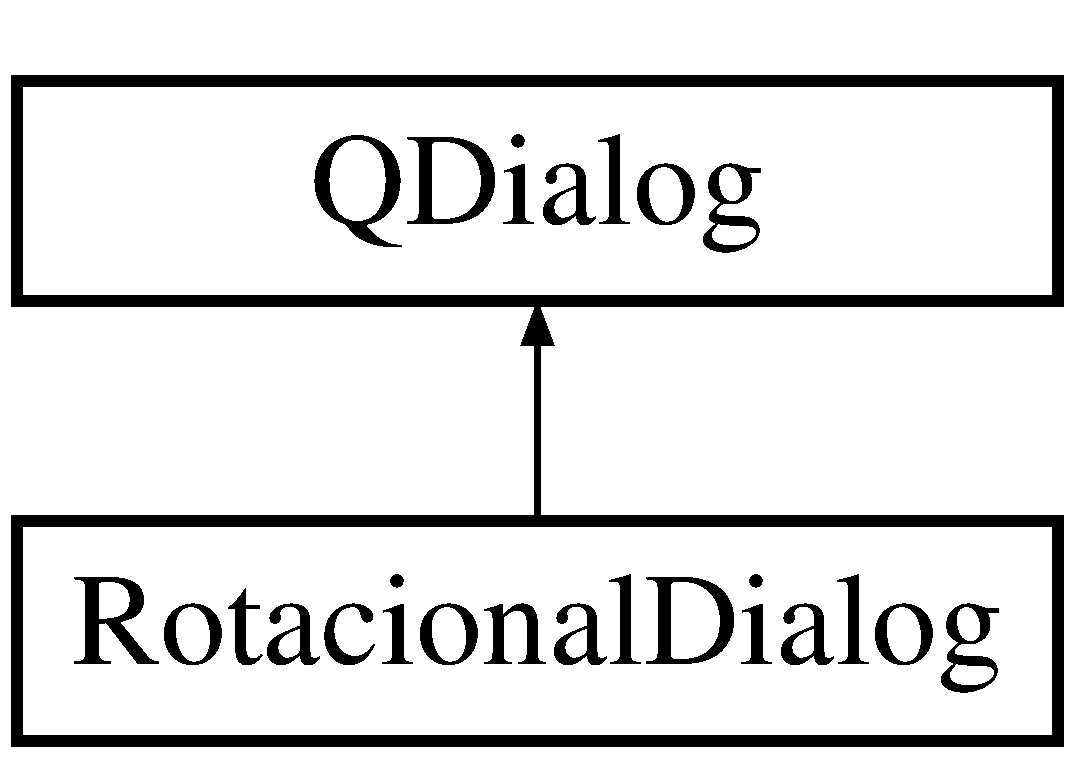
\includegraphics[height=2.000000cm]{class_rotacional_dialog}
\end{center}
\end{figure}
\subsection*{Public Member Functions}
\begin{DoxyCompactItemize}
\item 
\hyperlink{class_rotacional_dialog_a4dcdf1bfce49ef30fe3fca1c0e2057ae}{Rotacional\-Dialog} (Q\-Widget $\ast$parent=0)
\item 
\hyperlink{class_rotacional_dialog_a38f546b6372f9a6f669096fb5d4fa16b}{$\sim$\-Rotacional\-Dialog} ()
\end{DoxyCompactItemize}


\subsection{Constructor \& Destructor Documentation}
\hypertarget{class_rotacional_dialog_a4dcdf1bfce49ef30fe3fca1c0e2057ae}{\index{Rotacional\-Dialog@{Rotacional\-Dialog}!Rotacional\-Dialog@{Rotacional\-Dialog}}
\index{Rotacional\-Dialog@{Rotacional\-Dialog}!RotacionalDialog@{Rotacional\-Dialog}}
\subsubsection[{Rotacional\-Dialog}]{\setlength{\rightskip}{0pt plus 5cm}Rotacional\-Dialog\-::\-Rotacional\-Dialog (
\begin{DoxyParamCaption}
\item[{Q\-Widget $\ast$}]{parent = {\ttfamily 0}}
\end{DoxyParamCaption}
)\hspace{0.3cm}{\ttfamily [explicit]}}}\label{class_rotacional_dialog_a4dcdf1bfce49ef30fe3fca1c0e2057ae}
\hypertarget{class_rotacional_dialog_a38f546b6372f9a6f669096fb5d4fa16b}{\index{Rotacional\-Dialog@{Rotacional\-Dialog}!$\sim$\-Rotacional\-Dialog@{$\sim$\-Rotacional\-Dialog}}
\index{$\sim$\-Rotacional\-Dialog@{$\sim$\-Rotacional\-Dialog}!RotacionalDialog@{Rotacional\-Dialog}}
\subsubsection[{$\sim$\-Rotacional\-Dialog}]{\setlength{\rightskip}{0pt plus 5cm}Rotacional\-Dialog\-::$\sim$\-Rotacional\-Dialog (
\begin{DoxyParamCaption}
{}
\end{DoxyParamCaption}
)}}\label{class_rotacional_dialog_a38f546b6372f9a6f669096fb5d4fa16b}


The documentation for this class was generated from the following files\-:\begin{DoxyCompactItemize}
\item 
G\-U\-I/\hyperlink{rotacionaldialog_8h}{rotacionaldialog.\-h}\item 
G\-U\-I/\hyperlink{rotacionaldialog_8cpp}{rotacionaldialog.\-cpp}\end{DoxyCompactItemize}

\hypertarget{class_ui_1_1_rotacional_dialog}{\section{Ui\-:\-:Rotacional\-Dialog Class Reference}
\label{class_ui_1_1_rotacional_dialog}\index{Ui\-::\-Rotacional\-Dialog@{Ui\-::\-Rotacional\-Dialog}}
}


{\ttfamily \#include $<$ui\-\_\-rotacionaldialog.\-h$>$}

Inheritance diagram for Ui\-:\-:Rotacional\-Dialog\-:\begin{figure}[H]
\begin{center}
\leavevmode
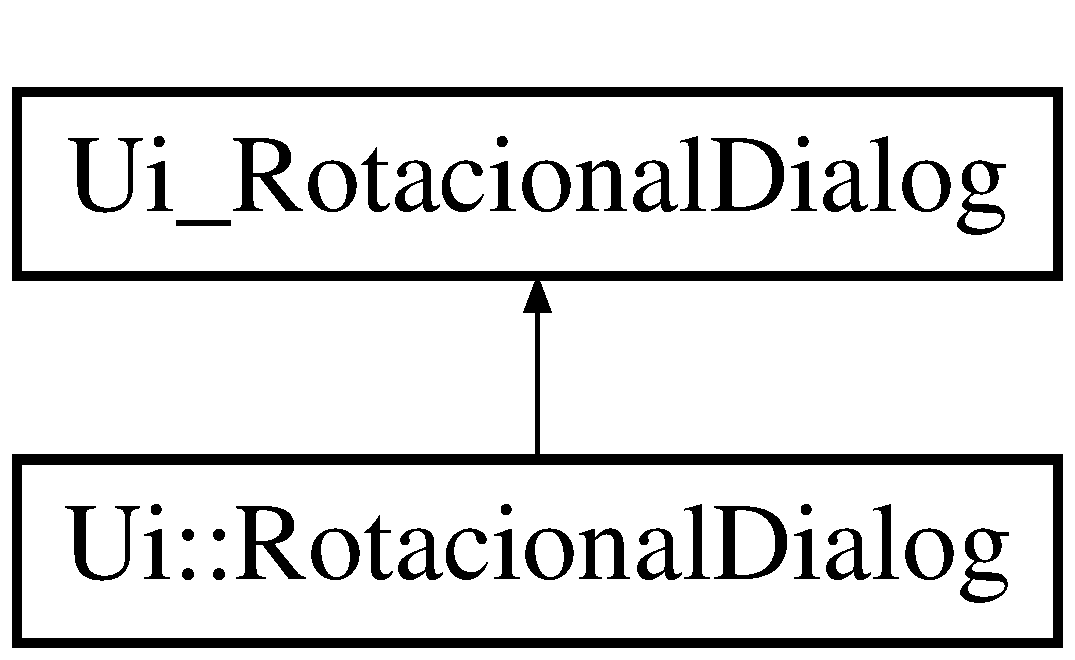
\includegraphics[height=2.000000cm]{class_ui_1_1_rotacional_dialog}
\end{center}
\end{figure}
\subsection*{Additional Inherited Members}


The documentation for this class was generated from the following file\-:\begin{DoxyCompactItemize}
\item 
build-\/\-Motion\-Structure-\/\-Desktop\-\_\-\-Qt\-\_\-5\-\_\-3\-\_\-\-G\-C\-C\-\_\-64bit-\/\-Debug/\hyperlink{ui__rotacionaldialog_8h}{ui\-\_\-rotacionaldialog.\-h}\end{DoxyCompactItemize}

\hypertarget{struct_s_componentes}{\section{S\-Componentes Struct Reference}
\label{struct_s_componentes}\index{S\-Componentes@{S\-Componentes}}
}


{\ttfamily \#include $<$globals.\-h$>$}

\subsection*{Public Attributes}
\begin{DoxyCompactItemize}
\item 
int \hyperlink{struct_s_componentes_aae650557a98ffa5aa86364ccbe86782b}{tipo}
\item 
float \hyperlink{struct_s_componentes_a167de81f87ee6114396f6532f8c20da5}{x}
\item 
float \hyperlink{struct_s_componentes_a55baedc301b10640f4f52bbd2bb6a089}{y}
\item 
float \hyperlink{struct_s_componentes_aafa661af95040f61d3137d608c4a5608}{z}
\item 
int \hyperlink{struct_s_componentes_a9c07e6918575bb81aa6ffb9facca753f}{eje}
\item 
float \hyperlink{struct_s_componentes_a819f738b83b9b0dd910ee9467eb23453}{angulo}
\item 
int \hyperlink{struct_s_componentes_ab0b787af546cfe4426367c9dc51cad02}{orientacion}
\end{DoxyCompactItemize}


\subsection{Member Data Documentation}
\hypertarget{struct_s_componentes_a819f738b83b9b0dd910ee9467eb23453}{\index{S\-Componentes@{S\-Componentes}!angulo@{angulo}}
\index{angulo@{angulo}!SComponentes@{S\-Componentes}}
\subsubsection[{angulo}]{\setlength{\rightskip}{0pt plus 5cm}float S\-Componentes\-::angulo}}\label{struct_s_componentes_a819f738b83b9b0dd910ee9467eb23453}
\hypertarget{struct_s_componentes_a9c07e6918575bb81aa6ffb9facca753f}{\index{S\-Componentes@{S\-Componentes}!eje@{eje}}
\index{eje@{eje}!SComponentes@{S\-Componentes}}
\subsubsection[{eje}]{\setlength{\rightskip}{0pt plus 5cm}int S\-Componentes\-::eje}}\label{struct_s_componentes_a9c07e6918575bb81aa6ffb9facca753f}
\hypertarget{struct_s_componentes_ab0b787af546cfe4426367c9dc51cad02}{\index{S\-Componentes@{S\-Componentes}!orientacion@{orientacion}}
\index{orientacion@{orientacion}!SComponentes@{S\-Componentes}}
\subsubsection[{orientacion}]{\setlength{\rightskip}{0pt plus 5cm}int S\-Componentes\-::orientacion}}\label{struct_s_componentes_ab0b787af546cfe4426367c9dc51cad02}
\hypertarget{struct_s_componentes_aae650557a98ffa5aa86364ccbe86782b}{\index{S\-Componentes@{S\-Componentes}!tipo@{tipo}}
\index{tipo@{tipo}!SComponentes@{S\-Componentes}}
\subsubsection[{tipo}]{\setlength{\rightskip}{0pt plus 5cm}int S\-Componentes\-::tipo}}\label{struct_s_componentes_aae650557a98ffa5aa86364ccbe86782b}
\hypertarget{struct_s_componentes_a167de81f87ee6114396f6532f8c20da5}{\index{S\-Componentes@{S\-Componentes}!x@{x}}
\index{x@{x}!SComponentes@{S\-Componentes}}
\subsubsection[{x}]{\setlength{\rightskip}{0pt plus 5cm}float S\-Componentes\-::x}}\label{struct_s_componentes_a167de81f87ee6114396f6532f8c20da5}
\hypertarget{struct_s_componentes_a55baedc301b10640f4f52bbd2bb6a089}{\index{S\-Componentes@{S\-Componentes}!y@{y}}
\index{y@{y}!SComponentes@{S\-Componentes}}
\subsubsection[{y}]{\setlength{\rightskip}{0pt plus 5cm}float S\-Componentes\-::y}}\label{struct_s_componentes_a55baedc301b10640f4f52bbd2bb6a089}
\hypertarget{struct_s_componentes_aafa661af95040f61d3137d608c4a5608}{\index{S\-Componentes@{S\-Componentes}!z@{z}}
\index{z@{z}!SComponentes@{S\-Componentes}}
\subsubsection[{z}]{\setlength{\rightskip}{0pt plus 5cm}float S\-Componentes\-::z}}\label{struct_s_componentes_aafa661af95040f61d3137d608c4a5608}


The documentation for this struct was generated from the following file\-:\begin{DoxyCompactItemize}
\item 
G\-U\-I/\hyperlink{globals_8h}{globals.\-h}\end{DoxyCompactItemize}

\hypertarget{struct_s_lua_call_back}{\section{S\-Lua\-Call\-Back Struct Reference}
\label{struct_s_lua_call_back}\index{S\-Lua\-Call\-Back@{S\-Lua\-Call\-Back}}
}


{\ttfamily \#include $<$v\-\_\-rep\-Types.\-h$>$}

\subsection*{Public Attributes}
\begin{DoxyCompactItemize}
\item 
\hyperlink{v__rep_types_8h_a35f702d95621fcebf5cd960176bdcfb9}{sim\-Int} \hyperlink{struct_s_lua_call_back_a1fe9f5fa55f225ebd35b50249a46bf98}{object\-I\-D}
\item 
\hyperlink{v__rep_types_8h_a28c2dc25059fcfc02e14f59e277b00e4}{sim\-Bool} $\ast$ \hyperlink{struct_s_lua_call_back_abf64b737945186918030b25ad2e5cb4c}{input\-Bool}
\item 
\hyperlink{v__rep_types_8h_a35f702d95621fcebf5cd960176bdcfb9}{sim\-Int} $\ast$ \hyperlink{struct_s_lua_call_back_ac1690a9cd01fd676958b69ff9c9431d2}{input\-Int}
\item 
\hyperlink{v__rep_types_8h_a0931040573e3d2bf15ef34c0be22beec}{sim\-Float} $\ast$ \hyperlink{struct_s_lua_call_back_a9417702f7811b73d78b389dd855ad984}{input\-Float}
\item 
\hyperlink{v__rep_types_8h_a2384478fb9f1c4a8418cd96157f87217}{sim\-Char} $\ast$ \hyperlink{struct_s_lua_call_back_afc1c4ef5be9bffa4d4ddec27bc1ba9f7}{input\-Char}
\item 
\hyperlink{v__rep_types_8h_a35f702d95621fcebf5cd960176bdcfb9}{sim\-Int} \hyperlink{struct_s_lua_call_back_a284412eb79cc48e9ffc35fe04016d134}{input\-Arg\-Count}
\item 
\hyperlink{v__rep_types_8h_a35f702d95621fcebf5cd960176bdcfb9}{sim\-Int} $\ast$ \hyperlink{struct_s_lua_call_back_a2951a105af1306454b3a8d880780586e}{input\-Arg\-Type\-And\-Size}
\item 
\hyperlink{v__rep_types_8h_a28c2dc25059fcfc02e14f59e277b00e4}{sim\-Bool} $\ast$ \hyperlink{struct_s_lua_call_back_af30852414661a213db16769ba1ea73f2}{output\-Bool}
\item 
\hyperlink{v__rep_types_8h_a35f702d95621fcebf5cd960176bdcfb9}{sim\-Int} $\ast$ \hyperlink{struct_s_lua_call_back_a62d73457aa62d0d3b3f5a1bf3f2d72dd}{output\-Int}
\item 
\hyperlink{v__rep_types_8h_a0931040573e3d2bf15ef34c0be22beec}{sim\-Float} $\ast$ \hyperlink{struct_s_lua_call_back_ab8014ef952171ff67359b5f60054b4de}{output\-Float}
\item 
\hyperlink{v__rep_types_8h_a2384478fb9f1c4a8418cd96157f87217}{sim\-Char} $\ast$ \hyperlink{struct_s_lua_call_back_a3c328abf56fed30e3231d794e3fd648f}{output\-Char}
\item 
\hyperlink{v__rep_types_8h_a35f702d95621fcebf5cd960176bdcfb9}{sim\-Int} \hyperlink{struct_s_lua_call_back_a8b3c7dd4f812cd5865f1decbe13bbc19}{output\-Arg\-Count}
\item 
\hyperlink{v__rep_types_8h_a35f702d95621fcebf5cd960176bdcfb9}{sim\-Int} $\ast$ \hyperlink{struct_s_lua_call_back_aec85c26a2306413877d0931c1215fe02}{output\-Arg\-Type\-And\-Size}
\item 
\hyperlink{v__rep_types_8h_a2384478fb9f1c4a8418cd96157f87217}{sim\-Char} \hyperlink{struct_s_lua_call_back_a2baf621a41fc0ad23c807d2091f3b6cc}{wait\-Until\-Zero}
\item 
\hyperlink{v__rep_types_8h_a2384478fb9f1c4a8418cd96157f87217}{sim\-Char} $\ast$ \hyperlink{struct_s_lua_call_back_abde71c73b125dc1bd0d8c0dc3a5c3146}{input\-Char\-Buff}
\item 
\hyperlink{v__rep_types_8h_a2384478fb9f1c4a8418cd96157f87217}{sim\-Char} $\ast$ \hyperlink{struct_s_lua_call_back_adf0060a01a20a67d76afad9c13640470}{output\-Char\-Buff}
\end{DoxyCompactItemize}


\subsection{Member Data Documentation}
\hypertarget{struct_s_lua_call_back_a284412eb79cc48e9ffc35fe04016d134}{\index{S\-Lua\-Call\-Back@{S\-Lua\-Call\-Back}!input\-Arg\-Count@{input\-Arg\-Count}}
\index{input\-Arg\-Count@{input\-Arg\-Count}!SLuaCallBack@{S\-Lua\-Call\-Back}}
\subsubsection[{input\-Arg\-Count}]{\setlength{\rightskip}{0pt plus 5cm}{\bf sim\-Int} S\-Lua\-Call\-Back\-::input\-Arg\-Count}}\label{struct_s_lua_call_back_a284412eb79cc48e9ffc35fe04016d134}
\hypertarget{struct_s_lua_call_back_a2951a105af1306454b3a8d880780586e}{\index{S\-Lua\-Call\-Back@{S\-Lua\-Call\-Back}!input\-Arg\-Type\-And\-Size@{input\-Arg\-Type\-And\-Size}}
\index{input\-Arg\-Type\-And\-Size@{input\-Arg\-Type\-And\-Size}!SLuaCallBack@{S\-Lua\-Call\-Back}}
\subsubsection[{input\-Arg\-Type\-And\-Size}]{\setlength{\rightskip}{0pt plus 5cm}{\bf sim\-Int}$\ast$ S\-Lua\-Call\-Back\-::input\-Arg\-Type\-And\-Size}}\label{struct_s_lua_call_back_a2951a105af1306454b3a8d880780586e}
\hypertarget{struct_s_lua_call_back_abf64b737945186918030b25ad2e5cb4c}{\index{S\-Lua\-Call\-Back@{S\-Lua\-Call\-Back}!input\-Bool@{input\-Bool}}
\index{input\-Bool@{input\-Bool}!SLuaCallBack@{S\-Lua\-Call\-Back}}
\subsubsection[{input\-Bool}]{\setlength{\rightskip}{0pt plus 5cm}{\bf sim\-Bool}$\ast$ S\-Lua\-Call\-Back\-::input\-Bool}}\label{struct_s_lua_call_back_abf64b737945186918030b25ad2e5cb4c}
\hypertarget{struct_s_lua_call_back_afc1c4ef5be9bffa4d4ddec27bc1ba9f7}{\index{S\-Lua\-Call\-Back@{S\-Lua\-Call\-Back}!input\-Char@{input\-Char}}
\index{input\-Char@{input\-Char}!SLuaCallBack@{S\-Lua\-Call\-Back}}
\subsubsection[{input\-Char}]{\setlength{\rightskip}{0pt plus 5cm}{\bf sim\-Char}$\ast$ S\-Lua\-Call\-Back\-::input\-Char}}\label{struct_s_lua_call_back_afc1c4ef5be9bffa4d4ddec27bc1ba9f7}
\hypertarget{struct_s_lua_call_back_abde71c73b125dc1bd0d8c0dc3a5c3146}{\index{S\-Lua\-Call\-Back@{S\-Lua\-Call\-Back}!input\-Char\-Buff@{input\-Char\-Buff}}
\index{input\-Char\-Buff@{input\-Char\-Buff}!SLuaCallBack@{S\-Lua\-Call\-Back}}
\subsubsection[{input\-Char\-Buff}]{\setlength{\rightskip}{0pt plus 5cm}{\bf sim\-Char}$\ast$ S\-Lua\-Call\-Back\-::input\-Char\-Buff}}\label{struct_s_lua_call_back_abde71c73b125dc1bd0d8c0dc3a5c3146}
\hypertarget{struct_s_lua_call_back_a9417702f7811b73d78b389dd855ad984}{\index{S\-Lua\-Call\-Back@{S\-Lua\-Call\-Back}!input\-Float@{input\-Float}}
\index{input\-Float@{input\-Float}!SLuaCallBack@{S\-Lua\-Call\-Back}}
\subsubsection[{input\-Float}]{\setlength{\rightskip}{0pt plus 5cm}{\bf sim\-Float}$\ast$ S\-Lua\-Call\-Back\-::input\-Float}}\label{struct_s_lua_call_back_a9417702f7811b73d78b389dd855ad984}
\hypertarget{struct_s_lua_call_back_ac1690a9cd01fd676958b69ff9c9431d2}{\index{S\-Lua\-Call\-Back@{S\-Lua\-Call\-Back}!input\-Int@{input\-Int}}
\index{input\-Int@{input\-Int}!SLuaCallBack@{S\-Lua\-Call\-Back}}
\subsubsection[{input\-Int}]{\setlength{\rightskip}{0pt plus 5cm}{\bf sim\-Int}$\ast$ S\-Lua\-Call\-Back\-::input\-Int}}\label{struct_s_lua_call_back_ac1690a9cd01fd676958b69ff9c9431d2}
\hypertarget{struct_s_lua_call_back_a1fe9f5fa55f225ebd35b50249a46bf98}{\index{S\-Lua\-Call\-Back@{S\-Lua\-Call\-Back}!object\-I\-D@{object\-I\-D}}
\index{object\-I\-D@{object\-I\-D}!SLuaCallBack@{S\-Lua\-Call\-Back}}
\subsubsection[{object\-I\-D}]{\setlength{\rightskip}{0pt plus 5cm}{\bf sim\-Int} S\-Lua\-Call\-Back\-::object\-I\-D}}\label{struct_s_lua_call_back_a1fe9f5fa55f225ebd35b50249a46bf98}
\hypertarget{struct_s_lua_call_back_a8b3c7dd4f812cd5865f1decbe13bbc19}{\index{S\-Lua\-Call\-Back@{S\-Lua\-Call\-Back}!output\-Arg\-Count@{output\-Arg\-Count}}
\index{output\-Arg\-Count@{output\-Arg\-Count}!SLuaCallBack@{S\-Lua\-Call\-Back}}
\subsubsection[{output\-Arg\-Count}]{\setlength{\rightskip}{0pt plus 5cm}{\bf sim\-Int} S\-Lua\-Call\-Back\-::output\-Arg\-Count}}\label{struct_s_lua_call_back_a8b3c7dd4f812cd5865f1decbe13bbc19}
\hypertarget{struct_s_lua_call_back_aec85c26a2306413877d0931c1215fe02}{\index{S\-Lua\-Call\-Back@{S\-Lua\-Call\-Back}!output\-Arg\-Type\-And\-Size@{output\-Arg\-Type\-And\-Size}}
\index{output\-Arg\-Type\-And\-Size@{output\-Arg\-Type\-And\-Size}!SLuaCallBack@{S\-Lua\-Call\-Back}}
\subsubsection[{output\-Arg\-Type\-And\-Size}]{\setlength{\rightskip}{0pt plus 5cm}{\bf sim\-Int}$\ast$ S\-Lua\-Call\-Back\-::output\-Arg\-Type\-And\-Size}}\label{struct_s_lua_call_back_aec85c26a2306413877d0931c1215fe02}
\hypertarget{struct_s_lua_call_back_af30852414661a213db16769ba1ea73f2}{\index{S\-Lua\-Call\-Back@{S\-Lua\-Call\-Back}!output\-Bool@{output\-Bool}}
\index{output\-Bool@{output\-Bool}!SLuaCallBack@{S\-Lua\-Call\-Back}}
\subsubsection[{output\-Bool}]{\setlength{\rightskip}{0pt plus 5cm}{\bf sim\-Bool}$\ast$ S\-Lua\-Call\-Back\-::output\-Bool}}\label{struct_s_lua_call_back_af30852414661a213db16769ba1ea73f2}
\hypertarget{struct_s_lua_call_back_a3c328abf56fed30e3231d794e3fd648f}{\index{S\-Lua\-Call\-Back@{S\-Lua\-Call\-Back}!output\-Char@{output\-Char}}
\index{output\-Char@{output\-Char}!SLuaCallBack@{S\-Lua\-Call\-Back}}
\subsubsection[{output\-Char}]{\setlength{\rightskip}{0pt plus 5cm}{\bf sim\-Char}$\ast$ S\-Lua\-Call\-Back\-::output\-Char}}\label{struct_s_lua_call_back_a3c328abf56fed30e3231d794e3fd648f}
\hypertarget{struct_s_lua_call_back_adf0060a01a20a67d76afad9c13640470}{\index{S\-Lua\-Call\-Back@{S\-Lua\-Call\-Back}!output\-Char\-Buff@{output\-Char\-Buff}}
\index{output\-Char\-Buff@{output\-Char\-Buff}!SLuaCallBack@{S\-Lua\-Call\-Back}}
\subsubsection[{output\-Char\-Buff}]{\setlength{\rightskip}{0pt plus 5cm}{\bf sim\-Char}$\ast$ S\-Lua\-Call\-Back\-::output\-Char\-Buff}}\label{struct_s_lua_call_back_adf0060a01a20a67d76afad9c13640470}
\hypertarget{struct_s_lua_call_back_ab8014ef952171ff67359b5f60054b4de}{\index{S\-Lua\-Call\-Back@{S\-Lua\-Call\-Back}!output\-Float@{output\-Float}}
\index{output\-Float@{output\-Float}!SLuaCallBack@{S\-Lua\-Call\-Back}}
\subsubsection[{output\-Float}]{\setlength{\rightskip}{0pt plus 5cm}{\bf sim\-Float}$\ast$ S\-Lua\-Call\-Back\-::output\-Float}}\label{struct_s_lua_call_back_ab8014ef952171ff67359b5f60054b4de}
\hypertarget{struct_s_lua_call_back_a62d73457aa62d0d3b3f5a1bf3f2d72dd}{\index{S\-Lua\-Call\-Back@{S\-Lua\-Call\-Back}!output\-Int@{output\-Int}}
\index{output\-Int@{output\-Int}!SLuaCallBack@{S\-Lua\-Call\-Back}}
\subsubsection[{output\-Int}]{\setlength{\rightskip}{0pt plus 5cm}{\bf sim\-Int}$\ast$ S\-Lua\-Call\-Back\-::output\-Int}}\label{struct_s_lua_call_back_a62d73457aa62d0d3b3f5a1bf3f2d72dd}
\hypertarget{struct_s_lua_call_back_a2baf621a41fc0ad23c807d2091f3b6cc}{\index{S\-Lua\-Call\-Back@{S\-Lua\-Call\-Back}!wait\-Until\-Zero@{wait\-Until\-Zero}}
\index{wait\-Until\-Zero@{wait\-Until\-Zero}!SLuaCallBack@{S\-Lua\-Call\-Back}}
\subsubsection[{wait\-Until\-Zero}]{\setlength{\rightskip}{0pt plus 5cm}{\bf sim\-Char} S\-Lua\-Call\-Back\-::wait\-Until\-Zero}}\label{struct_s_lua_call_back_a2baf621a41fc0ad23c807d2091f3b6cc}


The documentation for this struct was generated from the following file\-:\begin{DoxyCompactItemize}
\item 
V\-R\-E\-P/include/\hyperlink{v__rep_types_8h}{v\-\_\-rep\-Types.\-h}\end{DoxyCompactItemize}

\hypertarget{class_translacional_dialog}{\section{Translacional\-Dialog Class Reference}
\label{class_translacional_dialog}\index{Translacional\-Dialog@{Translacional\-Dialog}}
}


{\ttfamily \#include $<$translacionaldialog.\-h$>$}

Inheritance diagram for Translacional\-Dialog\-:\begin{figure}[H]
\begin{center}
\leavevmode
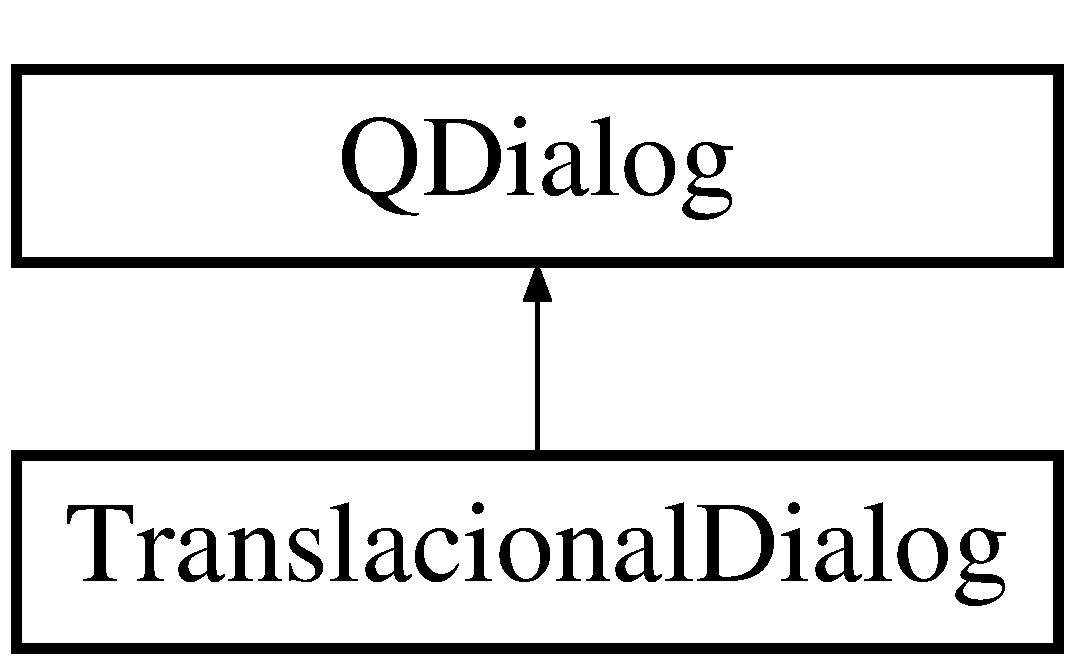
\includegraphics[height=2.000000cm]{class_translacional_dialog}
\end{center}
\end{figure}
\subsection*{Public Member Functions}
\begin{DoxyCompactItemize}
\item 
\hyperlink{class_translacional_dialog_a37eadf7a9220ee5b7dfd07702345fb80}{Translacional\-Dialog} (Q\-Widget $\ast$parent=0)
\item 
\hyperlink{class_translacional_dialog_a88aec31c37285fc1016660ca6a05c637}{$\sim$\-Translacional\-Dialog} ()
\end{DoxyCompactItemize}


\subsection{Constructor \& Destructor Documentation}
\hypertarget{class_translacional_dialog_a37eadf7a9220ee5b7dfd07702345fb80}{\index{Translacional\-Dialog@{Translacional\-Dialog}!Translacional\-Dialog@{Translacional\-Dialog}}
\index{Translacional\-Dialog@{Translacional\-Dialog}!TranslacionalDialog@{Translacional\-Dialog}}
\subsubsection[{Translacional\-Dialog}]{\setlength{\rightskip}{0pt plus 5cm}Translacional\-Dialog\-::\-Translacional\-Dialog (
\begin{DoxyParamCaption}
\item[{Q\-Widget $\ast$}]{parent = {\ttfamily 0}}
\end{DoxyParamCaption}
)\hspace{0.3cm}{\ttfamily [explicit]}}}\label{class_translacional_dialog_a37eadf7a9220ee5b7dfd07702345fb80}
\hypertarget{class_translacional_dialog_a88aec31c37285fc1016660ca6a05c637}{\index{Translacional\-Dialog@{Translacional\-Dialog}!$\sim$\-Translacional\-Dialog@{$\sim$\-Translacional\-Dialog}}
\index{$\sim$\-Translacional\-Dialog@{$\sim$\-Translacional\-Dialog}!TranslacionalDialog@{Translacional\-Dialog}}
\subsubsection[{$\sim$\-Translacional\-Dialog}]{\setlength{\rightskip}{0pt plus 5cm}Translacional\-Dialog\-::$\sim$\-Translacional\-Dialog (
\begin{DoxyParamCaption}
{}
\end{DoxyParamCaption}
)}}\label{class_translacional_dialog_a88aec31c37285fc1016660ca6a05c637}


The documentation for this class was generated from the following files\-:\begin{DoxyCompactItemize}
\item 
G\-U\-I/\hyperlink{translacionaldialog_8h}{translacionaldialog.\-h}\item 
G\-U\-I/\hyperlink{translacionaldialog_8cpp}{translacionaldialog.\-cpp}\end{DoxyCompactItemize}

\hypertarget{class_ui_1_1_translacional_dialog}{\section{Ui\-:\-:Translacional\-Dialog Class Reference}
\label{class_ui_1_1_translacional_dialog}\index{Ui\-::\-Translacional\-Dialog@{Ui\-::\-Translacional\-Dialog}}
}


{\ttfamily \#include $<$ui\-\_\-translacionaldialog.\-h$>$}

Inheritance diagram for Ui\-:\-:Translacional\-Dialog\-:\begin{figure}[H]
\begin{center}
\leavevmode
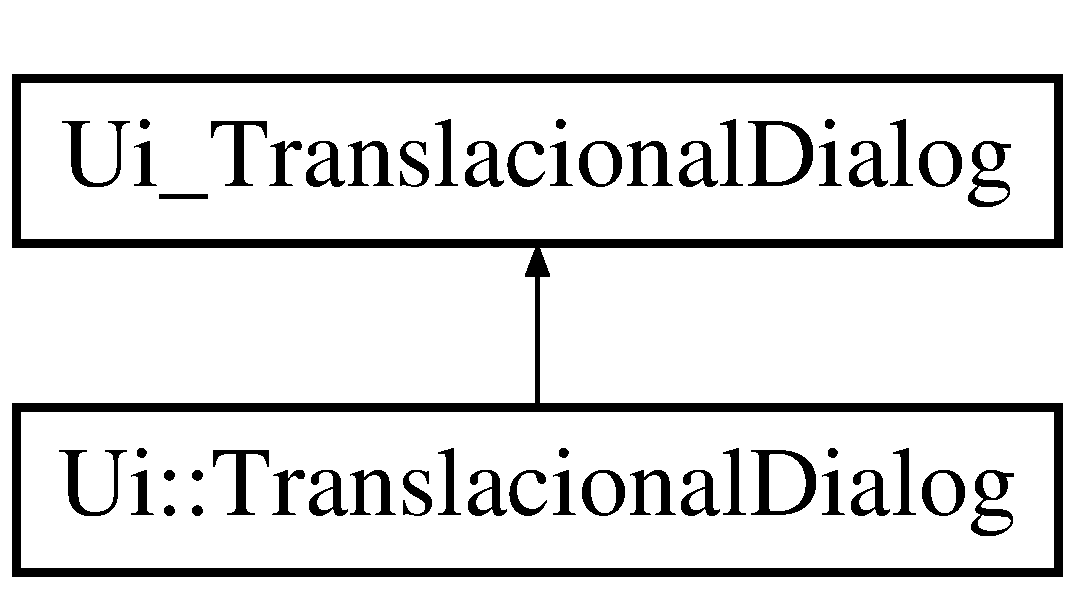
\includegraphics[height=2.000000cm]{class_ui_1_1_translacional_dialog}
\end{center}
\end{figure}
\subsection*{Additional Inherited Members}


The documentation for this class was generated from the following file\-:\begin{DoxyCompactItemize}
\item 
build-\/\-Motion\-Structure-\/\-Desktop\-\_\-\-Qt\-\_\-5\-\_\-3\-\_\-\-G\-C\-C\-\_\-64bit-\/\-Debug/\hyperlink{ui__translacionaldialog_8h}{ui\-\_\-translacionaldialog.\-h}\end{DoxyCompactItemize}

\hypertarget{class_ui___main_window}{\section{Ui\-\_\-\-Main\-Window Class Reference}
\label{class_ui___main_window}\index{Ui\-\_\-\-Main\-Window@{Ui\-\_\-\-Main\-Window}}
}


{\ttfamily \#include $<$ui\-\_\-mainwindow.\-h$>$}

Inheritance diagram for Ui\-\_\-\-Main\-Window\-:\begin{figure}[H]
\begin{center}
\leavevmode
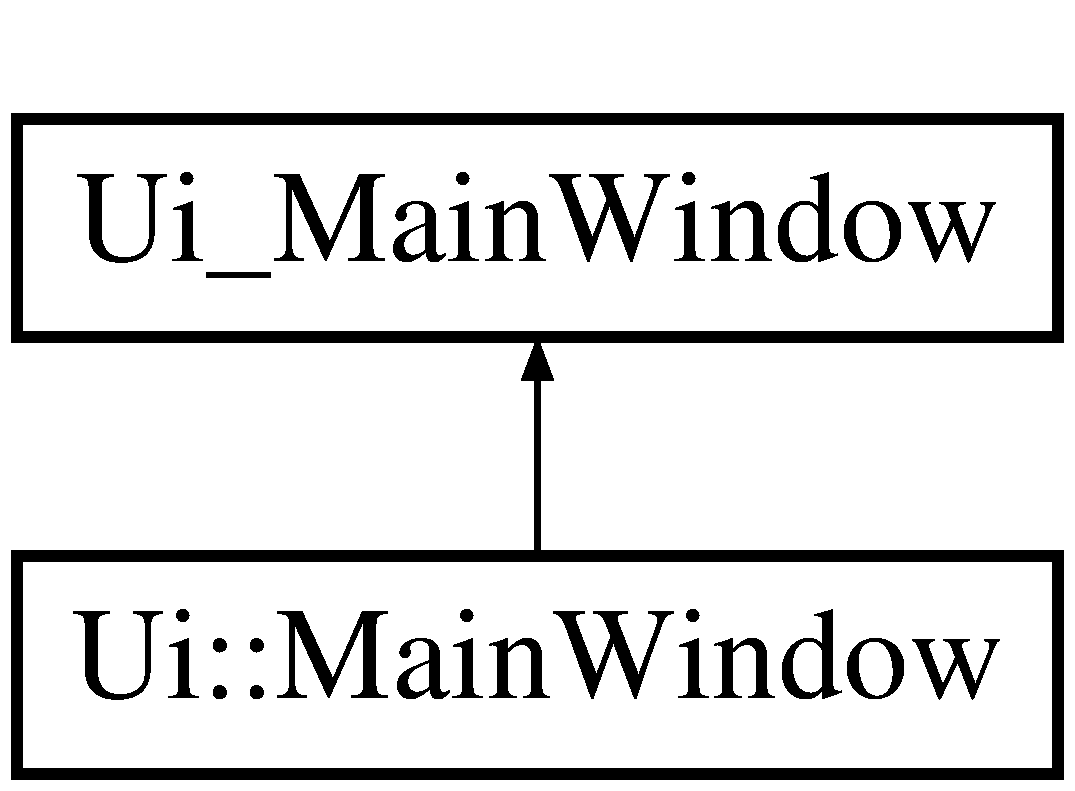
\includegraphics[height=2.000000cm]{class_ui___main_window}
\end{center}
\end{figure}
\subsection*{Public Member Functions}
\begin{DoxyCompactItemize}
\item 
void \hyperlink{class_ui___main_window_acf4a0872c4c77d8f43a2ec66ed849b58}{setup\-Ui} (Q\-Main\-Window $\ast$\hyperlink{class_main_window}{Main\-Window})
\item 
void \hyperlink{class_ui___main_window_a097dd160c3534a204904cb374412c618}{retranslate\-Ui} (Q\-Main\-Window $\ast$\hyperlink{class_main_window}{Main\-Window})
\end{DoxyCompactItemize}
\subsection*{Public Attributes}
\begin{DoxyCompactItemize}
\item 
Q\-Action $\ast$ \hyperlink{class_ui___main_window_a001c088d0b54f83119a6f036032303ae}{action\-Motor\-Rotacional}
\item 
Q\-Action $\ast$ \hyperlink{class_ui___main_window_a0092ec0757cfff7e42af2f26499e643d}{action\-Motor\-Translacional}
\item 
Q\-Action $\ast$ \hyperlink{class_ui___main_window_a930c8685d6cf6b7bda6264eedbb05076}{action\-Conector\-Rotacional}
\item 
Q\-Action $\ast$ \hyperlink{class_ui___main_window_a24126fcd6cef35a2a515a20a7a16dfec}{action\-Conector\-Translacional}
\item 
Q\-Widget $\ast$ \hyperlink{class_ui___main_window_a30075506c2116c3ed4ff25e07ae75f81}{central\-Widget}
\item 
Q\-Widget $\ast$ \hyperlink{class_ui___main_window_a805d415fff07a22a85219e1f22f2da28}{vertical\-Layout\-Widget}
\item 
Q\-V\-Box\-Layout $\ast$ \hyperlink{class_ui___main_window_aecd96a04789fcfec3f98d80390ad8184}{vertical\-Layout}
\item 
Q\-Label $\ast$ \hyperlink{class_ui___main_window_ad9c89133780f28e6efa2ec17ceb9cff5}{label}
\item 
Q\-List\-Widget $\ast$ \hyperlink{class_ui___main_window_ac79ae486ca255cf94a11582f0571169c}{listado\-Componentes}
\item 
Q\-H\-Box\-Layout $\ast$ \hyperlink{class_ui___main_window_acd6fdc9ebacc4b25b834162380d75ce8}{horizontal\-Layout}
\item 
Q\-Push\-Button $\ast$ \hyperlink{class_ui___main_window_a76639ddaaaf44f4a320888260cb5cc51}{boton\-Eliminar}
\item 
Q\-Push\-Button $\ast$ \hyperlink{class_ui___main_window_adbef6b25bd889b44e80e137ac1427ccb}{boton\-Modificar}
\item 
Q\-H\-Box\-Layout $\ast$ \hyperlink{class_ui___main_window_a80867018070156432923d0266cc9fe25}{horizontal\-Layout\-\_\-2}
\item 
Q\-Label $\ast$ \hyperlink{class_ui___main_window_a2e2516d755e4dd53fc905dabddf2738a}{label\-\_\-2}
\item 
Q\-Line\-Edit $\ast$ \hyperlink{class_ui___main_window_aa827386dfe7cc92ef98c3075e3265d20}{nombre\-Text}
\item 
Q\-Push\-Button $\ast$ \hyperlink{class_ui___main_window_aff1d12c698d66bdc8cbaba000ed903c1}{boton\-Finalizar}
\item 
Q\-Status\-Bar $\ast$ \hyperlink{class_ui___main_window_a50fa481337604bcc8bf68de18ab16ecd}{status\-Bar}
\item 
Q\-Tool\-Bar $\ast$ \hyperlink{class_ui___main_window_ab84dc49349f514d7b7d3fe8e78de069b}{tool\-Bar}
\item 
Q\-Menu\-Bar $\ast$ \hyperlink{class_ui___main_window_a2be1c24ec9adfca18e1dcc951931457f}{menu\-Bar}
\item 
Q\-Menu $\ast$ \hyperlink{class_ui___main_window_a84843358c658fd83aeae248934086166}{menu\-Agregar\-Motor}
\item 
Q\-Menu $\ast$ \hyperlink{class_ui___main_window_ac287b4474eb6609d9bdb42cc7c40dd64}{menu\-Agregar\-Conector}
\end{DoxyCompactItemize}


\subsection{Member Function Documentation}
\hypertarget{class_ui___main_window_a097dd160c3534a204904cb374412c618}{\index{Ui\-\_\-\-Main\-Window@{Ui\-\_\-\-Main\-Window}!retranslate\-Ui@{retranslate\-Ui}}
\index{retranslate\-Ui@{retranslate\-Ui}!Ui_MainWindow@{Ui\-\_\-\-Main\-Window}}
\subsubsection[{retranslate\-Ui}]{\setlength{\rightskip}{0pt plus 5cm}void Ui\-\_\-\-Main\-Window\-::retranslate\-Ui (
\begin{DoxyParamCaption}
\item[{Q\-Main\-Window $\ast$}]{Main\-Window}
\end{DoxyParamCaption}
)\hspace{0.3cm}{\ttfamily [inline]}}}\label{class_ui___main_window_a097dd160c3534a204904cb374412c618}
\hypertarget{class_ui___main_window_acf4a0872c4c77d8f43a2ec66ed849b58}{\index{Ui\-\_\-\-Main\-Window@{Ui\-\_\-\-Main\-Window}!setup\-Ui@{setup\-Ui}}
\index{setup\-Ui@{setup\-Ui}!Ui_MainWindow@{Ui\-\_\-\-Main\-Window}}
\subsubsection[{setup\-Ui}]{\setlength{\rightskip}{0pt plus 5cm}void Ui\-\_\-\-Main\-Window\-::setup\-Ui (
\begin{DoxyParamCaption}
\item[{Q\-Main\-Window $\ast$}]{Main\-Window}
\end{DoxyParamCaption}
)\hspace{0.3cm}{\ttfamily [inline]}}}\label{class_ui___main_window_acf4a0872c4c77d8f43a2ec66ed849b58}


\subsection{Member Data Documentation}
\hypertarget{class_ui___main_window_a930c8685d6cf6b7bda6264eedbb05076}{\index{Ui\-\_\-\-Main\-Window@{Ui\-\_\-\-Main\-Window}!action\-Conector\-Rotacional@{action\-Conector\-Rotacional}}
\index{action\-Conector\-Rotacional@{action\-Conector\-Rotacional}!Ui_MainWindow@{Ui\-\_\-\-Main\-Window}}
\subsubsection[{action\-Conector\-Rotacional}]{\setlength{\rightskip}{0pt plus 5cm}Q\-Action$\ast$ Ui\-\_\-\-Main\-Window\-::action\-Conector\-Rotacional}}\label{class_ui___main_window_a930c8685d6cf6b7bda6264eedbb05076}
\hypertarget{class_ui___main_window_a24126fcd6cef35a2a515a20a7a16dfec}{\index{Ui\-\_\-\-Main\-Window@{Ui\-\_\-\-Main\-Window}!action\-Conector\-Translacional@{action\-Conector\-Translacional}}
\index{action\-Conector\-Translacional@{action\-Conector\-Translacional}!Ui_MainWindow@{Ui\-\_\-\-Main\-Window}}
\subsubsection[{action\-Conector\-Translacional}]{\setlength{\rightskip}{0pt plus 5cm}Q\-Action$\ast$ Ui\-\_\-\-Main\-Window\-::action\-Conector\-Translacional}}\label{class_ui___main_window_a24126fcd6cef35a2a515a20a7a16dfec}
\hypertarget{class_ui___main_window_a001c088d0b54f83119a6f036032303ae}{\index{Ui\-\_\-\-Main\-Window@{Ui\-\_\-\-Main\-Window}!action\-Motor\-Rotacional@{action\-Motor\-Rotacional}}
\index{action\-Motor\-Rotacional@{action\-Motor\-Rotacional}!Ui_MainWindow@{Ui\-\_\-\-Main\-Window}}
\subsubsection[{action\-Motor\-Rotacional}]{\setlength{\rightskip}{0pt plus 5cm}Q\-Action$\ast$ Ui\-\_\-\-Main\-Window\-::action\-Motor\-Rotacional}}\label{class_ui___main_window_a001c088d0b54f83119a6f036032303ae}
\hypertarget{class_ui___main_window_a0092ec0757cfff7e42af2f26499e643d}{\index{Ui\-\_\-\-Main\-Window@{Ui\-\_\-\-Main\-Window}!action\-Motor\-Translacional@{action\-Motor\-Translacional}}
\index{action\-Motor\-Translacional@{action\-Motor\-Translacional}!Ui_MainWindow@{Ui\-\_\-\-Main\-Window}}
\subsubsection[{action\-Motor\-Translacional}]{\setlength{\rightskip}{0pt plus 5cm}Q\-Action$\ast$ Ui\-\_\-\-Main\-Window\-::action\-Motor\-Translacional}}\label{class_ui___main_window_a0092ec0757cfff7e42af2f26499e643d}
\hypertarget{class_ui___main_window_a76639ddaaaf44f4a320888260cb5cc51}{\index{Ui\-\_\-\-Main\-Window@{Ui\-\_\-\-Main\-Window}!boton\-Eliminar@{boton\-Eliminar}}
\index{boton\-Eliminar@{boton\-Eliminar}!Ui_MainWindow@{Ui\-\_\-\-Main\-Window}}
\subsubsection[{boton\-Eliminar}]{\setlength{\rightskip}{0pt plus 5cm}Q\-Push\-Button$\ast$ Ui\-\_\-\-Main\-Window\-::boton\-Eliminar}}\label{class_ui___main_window_a76639ddaaaf44f4a320888260cb5cc51}
\hypertarget{class_ui___main_window_aff1d12c698d66bdc8cbaba000ed903c1}{\index{Ui\-\_\-\-Main\-Window@{Ui\-\_\-\-Main\-Window}!boton\-Finalizar@{boton\-Finalizar}}
\index{boton\-Finalizar@{boton\-Finalizar}!Ui_MainWindow@{Ui\-\_\-\-Main\-Window}}
\subsubsection[{boton\-Finalizar}]{\setlength{\rightskip}{0pt plus 5cm}Q\-Push\-Button$\ast$ Ui\-\_\-\-Main\-Window\-::boton\-Finalizar}}\label{class_ui___main_window_aff1d12c698d66bdc8cbaba000ed903c1}
\hypertarget{class_ui___main_window_adbef6b25bd889b44e80e137ac1427ccb}{\index{Ui\-\_\-\-Main\-Window@{Ui\-\_\-\-Main\-Window}!boton\-Modificar@{boton\-Modificar}}
\index{boton\-Modificar@{boton\-Modificar}!Ui_MainWindow@{Ui\-\_\-\-Main\-Window}}
\subsubsection[{boton\-Modificar}]{\setlength{\rightskip}{0pt plus 5cm}Q\-Push\-Button$\ast$ Ui\-\_\-\-Main\-Window\-::boton\-Modificar}}\label{class_ui___main_window_adbef6b25bd889b44e80e137ac1427ccb}
\hypertarget{class_ui___main_window_a30075506c2116c3ed4ff25e07ae75f81}{\index{Ui\-\_\-\-Main\-Window@{Ui\-\_\-\-Main\-Window}!central\-Widget@{central\-Widget}}
\index{central\-Widget@{central\-Widget}!Ui_MainWindow@{Ui\-\_\-\-Main\-Window}}
\subsubsection[{central\-Widget}]{\setlength{\rightskip}{0pt plus 5cm}Q\-Widget$\ast$ Ui\-\_\-\-Main\-Window\-::central\-Widget}}\label{class_ui___main_window_a30075506c2116c3ed4ff25e07ae75f81}
\hypertarget{class_ui___main_window_acd6fdc9ebacc4b25b834162380d75ce8}{\index{Ui\-\_\-\-Main\-Window@{Ui\-\_\-\-Main\-Window}!horizontal\-Layout@{horizontal\-Layout}}
\index{horizontal\-Layout@{horizontal\-Layout}!Ui_MainWindow@{Ui\-\_\-\-Main\-Window}}
\subsubsection[{horizontal\-Layout}]{\setlength{\rightskip}{0pt plus 5cm}Q\-H\-Box\-Layout$\ast$ Ui\-\_\-\-Main\-Window\-::horizontal\-Layout}}\label{class_ui___main_window_acd6fdc9ebacc4b25b834162380d75ce8}
\hypertarget{class_ui___main_window_a80867018070156432923d0266cc9fe25}{\index{Ui\-\_\-\-Main\-Window@{Ui\-\_\-\-Main\-Window}!horizontal\-Layout\-\_\-2@{horizontal\-Layout\-\_\-2}}
\index{horizontal\-Layout\-\_\-2@{horizontal\-Layout\-\_\-2}!Ui_MainWindow@{Ui\-\_\-\-Main\-Window}}
\subsubsection[{horizontal\-Layout\-\_\-2}]{\setlength{\rightskip}{0pt plus 5cm}Q\-H\-Box\-Layout$\ast$ Ui\-\_\-\-Main\-Window\-::horizontal\-Layout\-\_\-2}}\label{class_ui___main_window_a80867018070156432923d0266cc9fe25}
\hypertarget{class_ui___main_window_ad9c89133780f28e6efa2ec17ceb9cff5}{\index{Ui\-\_\-\-Main\-Window@{Ui\-\_\-\-Main\-Window}!label@{label}}
\index{label@{label}!Ui_MainWindow@{Ui\-\_\-\-Main\-Window}}
\subsubsection[{label}]{\setlength{\rightskip}{0pt plus 5cm}Q\-Label$\ast$ Ui\-\_\-\-Main\-Window\-::label}}\label{class_ui___main_window_ad9c89133780f28e6efa2ec17ceb9cff5}
\hypertarget{class_ui___main_window_a2e2516d755e4dd53fc905dabddf2738a}{\index{Ui\-\_\-\-Main\-Window@{Ui\-\_\-\-Main\-Window}!label\-\_\-2@{label\-\_\-2}}
\index{label\-\_\-2@{label\-\_\-2}!Ui_MainWindow@{Ui\-\_\-\-Main\-Window}}
\subsubsection[{label\-\_\-2}]{\setlength{\rightskip}{0pt plus 5cm}Q\-Label$\ast$ Ui\-\_\-\-Main\-Window\-::label\-\_\-2}}\label{class_ui___main_window_a2e2516d755e4dd53fc905dabddf2738a}
\hypertarget{class_ui___main_window_ac79ae486ca255cf94a11582f0571169c}{\index{Ui\-\_\-\-Main\-Window@{Ui\-\_\-\-Main\-Window}!listado\-Componentes@{listado\-Componentes}}
\index{listado\-Componentes@{listado\-Componentes}!Ui_MainWindow@{Ui\-\_\-\-Main\-Window}}
\subsubsection[{listado\-Componentes}]{\setlength{\rightskip}{0pt plus 5cm}Q\-List\-Widget$\ast$ Ui\-\_\-\-Main\-Window\-::listado\-Componentes}}\label{class_ui___main_window_ac79ae486ca255cf94a11582f0571169c}
\hypertarget{class_ui___main_window_ac287b4474eb6609d9bdb42cc7c40dd64}{\index{Ui\-\_\-\-Main\-Window@{Ui\-\_\-\-Main\-Window}!menu\-Agregar\-Conector@{menu\-Agregar\-Conector}}
\index{menu\-Agregar\-Conector@{menu\-Agregar\-Conector}!Ui_MainWindow@{Ui\-\_\-\-Main\-Window}}
\subsubsection[{menu\-Agregar\-Conector}]{\setlength{\rightskip}{0pt plus 5cm}Q\-Menu$\ast$ Ui\-\_\-\-Main\-Window\-::menu\-Agregar\-Conector}}\label{class_ui___main_window_ac287b4474eb6609d9bdb42cc7c40dd64}
\hypertarget{class_ui___main_window_a84843358c658fd83aeae248934086166}{\index{Ui\-\_\-\-Main\-Window@{Ui\-\_\-\-Main\-Window}!menu\-Agregar\-Motor@{menu\-Agregar\-Motor}}
\index{menu\-Agregar\-Motor@{menu\-Agregar\-Motor}!Ui_MainWindow@{Ui\-\_\-\-Main\-Window}}
\subsubsection[{menu\-Agregar\-Motor}]{\setlength{\rightskip}{0pt plus 5cm}Q\-Menu$\ast$ Ui\-\_\-\-Main\-Window\-::menu\-Agregar\-Motor}}\label{class_ui___main_window_a84843358c658fd83aeae248934086166}
\hypertarget{class_ui___main_window_a2be1c24ec9adfca18e1dcc951931457f}{\index{Ui\-\_\-\-Main\-Window@{Ui\-\_\-\-Main\-Window}!menu\-Bar@{menu\-Bar}}
\index{menu\-Bar@{menu\-Bar}!Ui_MainWindow@{Ui\-\_\-\-Main\-Window}}
\subsubsection[{menu\-Bar}]{\setlength{\rightskip}{0pt plus 5cm}Q\-Menu\-Bar$\ast$ Ui\-\_\-\-Main\-Window\-::menu\-Bar}}\label{class_ui___main_window_a2be1c24ec9adfca18e1dcc951931457f}
\hypertarget{class_ui___main_window_aa827386dfe7cc92ef98c3075e3265d20}{\index{Ui\-\_\-\-Main\-Window@{Ui\-\_\-\-Main\-Window}!nombre\-Text@{nombre\-Text}}
\index{nombre\-Text@{nombre\-Text}!Ui_MainWindow@{Ui\-\_\-\-Main\-Window}}
\subsubsection[{nombre\-Text}]{\setlength{\rightskip}{0pt plus 5cm}Q\-Line\-Edit$\ast$ Ui\-\_\-\-Main\-Window\-::nombre\-Text}}\label{class_ui___main_window_aa827386dfe7cc92ef98c3075e3265d20}
\hypertarget{class_ui___main_window_a50fa481337604bcc8bf68de18ab16ecd}{\index{Ui\-\_\-\-Main\-Window@{Ui\-\_\-\-Main\-Window}!status\-Bar@{status\-Bar}}
\index{status\-Bar@{status\-Bar}!Ui_MainWindow@{Ui\-\_\-\-Main\-Window}}
\subsubsection[{status\-Bar}]{\setlength{\rightskip}{0pt plus 5cm}Q\-Status\-Bar$\ast$ Ui\-\_\-\-Main\-Window\-::status\-Bar}}\label{class_ui___main_window_a50fa481337604bcc8bf68de18ab16ecd}
\hypertarget{class_ui___main_window_ab84dc49349f514d7b7d3fe8e78de069b}{\index{Ui\-\_\-\-Main\-Window@{Ui\-\_\-\-Main\-Window}!tool\-Bar@{tool\-Bar}}
\index{tool\-Bar@{tool\-Bar}!Ui_MainWindow@{Ui\-\_\-\-Main\-Window}}
\subsubsection[{tool\-Bar}]{\setlength{\rightskip}{0pt plus 5cm}Q\-Tool\-Bar$\ast$ Ui\-\_\-\-Main\-Window\-::tool\-Bar}}\label{class_ui___main_window_ab84dc49349f514d7b7d3fe8e78de069b}
\hypertarget{class_ui___main_window_aecd96a04789fcfec3f98d80390ad8184}{\index{Ui\-\_\-\-Main\-Window@{Ui\-\_\-\-Main\-Window}!vertical\-Layout@{vertical\-Layout}}
\index{vertical\-Layout@{vertical\-Layout}!Ui_MainWindow@{Ui\-\_\-\-Main\-Window}}
\subsubsection[{vertical\-Layout}]{\setlength{\rightskip}{0pt plus 5cm}Q\-V\-Box\-Layout$\ast$ Ui\-\_\-\-Main\-Window\-::vertical\-Layout}}\label{class_ui___main_window_aecd96a04789fcfec3f98d80390ad8184}
\hypertarget{class_ui___main_window_a805d415fff07a22a85219e1f22f2da28}{\index{Ui\-\_\-\-Main\-Window@{Ui\-\_\-\-Main\-Window}!vertical\-Layout\-Widget@{vertical\-Layout\-Widget}}
\index{vertical\-Layout\-Widget@{vertical\-Layout\-Widget}!Ui_MainWindow@{Ui\-\_\-\-Main\-Window}}
\subsubsection[{vertical\-Layout\-Widget}]{\setlength{\rightskip}{0pt plus 5cm}Q\-Widget$\ast$ Ui\-\_\-\-Main\-Window\-::vertical\-Layout\-Widget}}\label{class_ui___main_window_a805d415fff07a22a85219e1f22f2da28}


The documentation for this class was generated from the following file\-:\begin{DoxyCompactItemize}
\item 
build-\/\-Motion\-Structure-\/\-Desktop\-\_\-\-Qt\-\_\-5\-\_\-3\-\_\-\-G\-C\-C\-\_\-64bit-\/\-Debug/\hyperlink{ui__mainwindow_8h}{ui\-\_\-mainwindow.\-h}\end{DoxyCompactItemize}

\hypertarget{class_ui___rotacional_dialog}{\section{Ui\-\_\-\-Rotacional\-Dialog Class Reference}
\label{class_ui___rotacional_dialog}\index{Ui\-\_\-\-Rotacional\-Dialog@{Ui\-\_\-\-Rotacional\-Dialog}}
}


{\ttfamily \#include $<$ui\-\_\-rotacionaldialog.\-h$>$}

Inheritance diagram for Ui\-\_\-\-Rotacional\-Dialog\-:\begin{figure}[H]
\begin{center}
\leavevmode
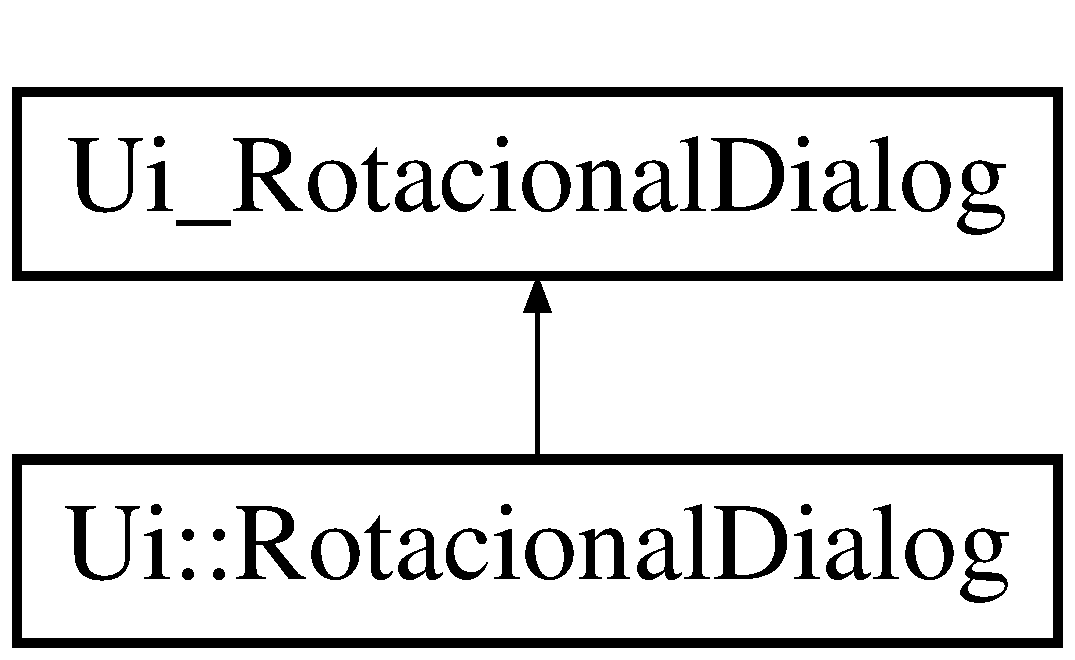
\includegraphics[height=2.000000cm]{class_ui___rotacional_dialog}
\end{center}
\end{figure}
\subsection*{Public Member Functions}
\begin{DoxyCompactItemize}
\item 
void \hyperlink{class_ui___rotacional_dialog_a8dbbda795fa35333f33609a41d5471cf}{setup\-Ui} (Q\-Dialog $\ast$\hyperlink{class_rotacional_dialog}{Rotacional\-Dialog})
\item 
void \hyperlink{class_ui___rotacional_dialog_a6c5858dae29f07195f087e59f6346e9e}{retranslate\-Ui} (Q\-Dialog $\ast$\hyperlink{class_rotacional_dialog}{Rotacional\-Dialog})
\end{DoxyCompactItemize}
\subsection*{Public Attributes}
\begin{DoxyCompactItemize}
\item 
Q\-Dialog\-Button\-Box $\ast$ \hyperlink{class_ui___rotacional_dialog_a13f390b4593075163c96f55bd7c61343}{button\-Box}
\item 
Q\-Group\-Box $\ast$ \hyperlink{class_ui___rotacional_dialog_a971ceda901e9a6c54eed1131e7f1c5a8}{group\-Box}
\item 
Q\-Widget $\ast$ \hyperlink{class_ui___rotacional_dialog_a060719d4871c77aaecc6d0f2def863f4}{vertical\-Layout\-Widget}
\item 
Q\-V\-Box\-Layout $\ast$ \hyperlink{class_ui___rotacional_dialog_afb0033853ce48ca58337ba41f6219362}{vertical\-Layout}
\item 
Q\-Radio\-Button $\ast$ \hyperlink{class_ui___rotacional_dialog_acd4b87dd99cdfbfb29b609d47d6db760}{rot\-\_\-x}
\item 
Q\-Radio\-Button $\ast$ \hyperlink{class_ui___rotacional_dialog_a8abeb6d13c0abfcccdbbcc0318da1171}{rot\-\_\-y}
\item 
Q\-Radio\-Button $\ast$ \hyperlink{class_ui___rotacional_dialog_a9f6dda774a98edbbe92c81e11af201bb}{rot\-\_\-z}
\item 
Q\-Widget $\ast$ \hyperlink{class_ui___rotacional_dialog_af008c7b04e3b628a96164618c695d0b2}{vertical\-Layout\-Widget\-\_\-5}
\item 
Q\-V\-Box\-Layout $\ast$ \hyperlink{class_ui___rotacional_dialog_ac7dc4cae52d936ecf3e891787a21b9f7}{vertical\-Layout\-\_\-6}
\item 
Q\-Label $\ast$ \hyperlink{class_ui___rotacional_dialog_ab9b180cb438ab783bd292420604d4d5c}{label}
\item 
Q\-Line\-Edit $\ast$ \hyperlink{class_ui___rotacional_dialog_a834fe25a665d4a99446e1fc9a28c8a14}{angulo\-Text}
\item 
Q\-Group\-Box $\ast$ \hyperlink{class_ui___rotacional_dialog_ae84f45d3417cced094876f1cdc486978}{group\-Box\-\_\-2}
\item 
Q\-Widget $\ast$ \hyperlink{class_ui___rotacional_dialog_ade317e77d8449231a328936d44adaefb}{vertical\-Layout\-Widget\-\_\-3}
\item 
Q\-V\-Box\-Layout $\ast$ \hyperlink{class_ui___rotacional_dialog_a5ce0e1ea47c7c8ffdc88e543807ec75c}{vertical\-Layout\-\_\-3}
\item 
Q\-Radio\-Button $\ast$ \hyperlink{class_ui___rotacional_dialog_a6c77910a452af28cca06529c1b760933}{orientacion\-\_\-pos}
\item 
Q\-Radio\-Button $\ast$ \hyperlink{class_ui___rotacional_dialog_a79000d83fecbf9cac33bd66c943a4625}{orientacion\-\_\-neg}
\end{DoxyCompactItemize}


\subsection{Member Function Documentation}
\hypertarget{class_ui___rotacional_dialog_a6c5858dae29f07195f087e59f6346e9e}{\index{Ui\-\_\-\-Rotacional\-Dialog@{Ui\-\_\-\-Rotacional\-Dialog}!retranslate\-Ui@{retranslate\-Ui}}
\index{retranslate\-Ui@{retranslate\-Ui}!Ui_RotacionalDialog@{Ui\-\_\-\-Rotacional\-Dialog}}
\subsubsection[{retranslate\-Ui}]{\setlength{\rightskip}{0pt plus 5cm}void Ui\-\_\-\-Rotacional\-Dialog\-::retranslate\-Ui (
\begin{DoxyParamCaption}
\item[{Q\-Dialog $\ast$}]{Rotacional\-Dialog}
\end{DoxyParamCaption}
)\hspace{0.3cm}{\ttfamily [inline]}}}\label{class_ui___rotacional_dialog_a6c5858dae29f07195f087e59f6346e9e}
\hypertarget{class_ui___rotacional_dialog_a8dbbda795fa35333f33609a41d5471cf}{\index{Ui\-\_\-\-Rotacional\-Dialog@{Ui\-\_\-\-Rotacional\-Dialog}!setup\-Ui@{setup\-Ui}}
\index{setup\-Ui@{setup\-Ui}!Ui_RotacionalDialog@{Ui\-\_\-\-Rotacional\-Dialog}}
\subsubsection[{setup\-Ui}]{\setlength{\rightskip}{0pt plus 5cm}void Ui\-\_\-\-Rotacional\-Dialog\-::setup\-Ui (
\begin{DoxyParamCaption}
\item[{Q\-Dialog $\ast$}]{Rotacional\-Dialog}
\end{DoxyParamCaption}
)\hspace{0.3cm}{\ttfamily [inline]}}}\label{class_ui___rotacional_dialog_a8dbbda795fa35333f33609a41d5471cf}


\subsection{Member Data Documentation}
\hypertarget{class_ui___rotacional_dialog_a834fe25a665d4a99446e1fc9a28c8a14}{\index{Ui\-\_\-\-Rotacional\-Dialog@{Ui\-\_\-\-Rotacional\-Dialog}!angulo\-Text@{angulo\-Text}}
\index{angulo\-Text@{angulo\-Text}!Ui_RotacionalDialog@{Ui\-\_\-\-Rotacional\-Dialog}}
\subsubsection[{angulo\-Text}]{\setlength{\rightskip}{0pt plus 5cm}Q\-Line\-Edit$\ast$ Ui\-\_\-\-Rotacional\-Dialog\-::angulo\-Text}}\label{class_ui___rotacional_dialog_a834fe25a665d4a99446e1fc9a28c8a14}
\hypertarget{class_ui___rotacional_dialog_a13f390b4593075163c96f55bd7c61343}{\index{Ui\-\_\-\-Rotacional\-Dialog@{Ui\-\_\-\-Rotacional\-Dialog}!button\-Box@{button\-Box}}
\index{button\-Box@{button\-Box}!Ui_RotacionalDialog@{Ui\-\_\-\-Rotacional\-Dialog}}
\subsubsection[{button\-Box}]{\setlength{\rightskip}{0pt plus 5cm}Q\-Dialog\-Button\-Box$\ast$ Ui\-\_\-\-Rotacional\-Dialog\-::button\-Box}}\label{class_ui___rotacional_dialog_a13f390b4593075163c96f55bd7c61343}
\hypertarget{class_ui___rotacional_dialog_a971ceda901e9a6c54eed1131e7f1c5a8}{\index{Ui\-\_\-\-Rotacional\-Dialog@{Ui\-\_\-\-Rotacional\-Dialog}!group\-Box@{group\-Box}}
\index{group\-Box@{group\-Box}!Ui_RotacionalDialog@{Ui\-\_\-\-Rotacional\-Dialog}}
\subsubsection[{group\-Box}]{\setlength{\rightskip}{0pt plus 5cm}Q\-Group\-Box$\ast$ Ui\-\_\-\-Rotacional\-Dialog\-::group\-Box}}\label{class_ui___rotacional_dialog_a971ceda901e9a6c54eed1131e7f1c5a8}
\hypertarget{class_ui___rotacional_dialog_ae84f45d3417cced094876f1cdc486978}{\index{Ui\-\_\-\-Rotacional\-Dialog@{Ui\-\_\-\-Rotacional\-Dialog}!group\-Box\-\_\-2@{group\-Box\-\_\-2}}
\index{group\-Box\-\_\-2@{group\-Box\-\_\-2}!Ui_RotacionalDialog@{Ui\-\_\-\-Rotacional\-Dialog}}
\subsubsection[{group\-Box\-\_\-2}]{\setlength{\rightskip}{0pt plus 5cm}Q\-Group\-Box$\ast$ Ui\-\_\-\-Rotacional\-Dialog\-::group\-Box\-\_\-2}}\label{class_ui___rotacional_dialog_ae84f45d3417cced094876f1cdc486978}
\hypertarget{class_ui___rotacional_dialog_ab9b180cb438ab783bd292420604d4d5c}{\index{Ui\-\_\-\-Rotacional\-Dialog@{Ui\-\_\-\-Rotacional\-Dialog}!label@{label}}
\index{label@{label}!Ui_RotacionalDialog@{Ui\-\_\-\-Rotacional\-Dialog}}
\subsubsection[{label}]{\setlength{\rightskip}{0pt plus 5cm}Q\-Label$\ast$ Ui\-\_\-\-Rotacional\-Dialog\-::label}}\label{class_ui___rotacional_dialog_ab9b180cb438ab783bd292420604d4d5c}
\hypertarget{class_ui___rotacional_dialog_a79000d83fecbf9cac33bd66c943a4625}{\index{Ui\-\_\-\-Rotacional\-Dialog@{Ui\-\_\-\-Rotacional\-Dialog}!orientacion\-\_\-neg@{orientacion\-\_\-neg}}
\index{orientacion\-\_\-neg@{orientacion\-\_\-neg}!Ui_RotacionalDialog@{Ui\-\_\-\-Rotacional\-Dialog}}
\subsubsection[{orientacion\-\_\-neg}]{\setlength{\rightskip}{0pt plus 5cm}Q\-Radio\-Button$\ast$ Ui\-\_\-\-Rotacional\-Dialog\-::orientacion\-\_\-neg}}\label{class_ui___rotacional_dialog_a79000d83fecbf9cac33bd66c943a4625}
\hypertarget{class_ui___rotacional_dialog_a6c77910a452af28cca06529c1b760933}{\index{Ui\-\_\-\-Rotacional\-Dialog@{Ui\-\_\-\-Rotacional\-Dialog}!orientacion\-\_\-pos@{orientacion\-\_\-pos}}
\index{orientacion\-\_\-pos@{orientacion\-\_\-pos}!Ui_RotacionalDialog@{Ui\-\_\-\-Rotacional\-Dialog}}
\subsubsection[{orientacion\-\_\-pos}]{\setlength{\rightskip}{0pt plus 5cm}Q\-Radio\-Button$\ast$ Ui\-\_\-\-Rotacional\-Dialog\-::orientacion\-\_\-pos}}\label{class_ui___rotacional_dialog_a6c77910a452af28cca06529c1b760933}
\hypertarget{class_ui___rotacional_dialog_acd4b87dd99cdfbfb29b609d47d6db760}{\index{Ui\-\_\-\-Rotacional\-Dialog@{Ui\-\_\-\-Rotacional\-Dialog}!rot\-\_\-x@{rot\-\_\-x}}
\index{rot\-\_\-x@{rot\-\_\-x}!Ui_RotacionalDialog@{Ui\-\_\-\-Rotacional\-Dialog}}
\subsubsection[{rot\-\_\-x}]{\setlength{\rightskip}{0pt plus 5cm}Q\-Radio\-Button$\ast$ Ui\-\_\-\-Rotacional\-Dialog\-::rot\-\_\-x}}\label{class_ui___rotacional_dialog_acd4b87dd99cdfbfb29b609d47d6db760}
\hypertarget{class_ui___rotacional_dialog_a8abeb6d13c0abfcccdbbcc0318da1171}{\index{Ui\-\_\-\-Rotacional\-Dialog@{Ui\-\_\-\-Rotacional\-Dialog}!rot\-\_\-y@{rot\-\_\-y}}
\index{rot\-\_\-y@{rot\-\_\-y}!Ui_RotacionalDialog@{Ui\-\_\-\-Rotacional\-Dialog}}
\subsubsection[{rot\-\_\-y}]{\setlength{\rightskip}{0pt plus 5cm}Q\-Radio\-Button$\ast$ Ui\-\_\-\-Rotacional\-Dialog\-::rot\-\_\-y}}\label{class_ui___rotacional_dialog_a8abeb6d13c0abfcccdbbcc0318da1171}
\hypertarget{class_ui___rotacional_dialog_a9f6dda774a98edbbe92c81e11af201bb}{\index{Ui\-\_\-\-Rotacional\-Dialog@{Ui\-\_\-\-Rotacional\-Dialog}!rot\-\_\-z@{rot\-\_\-z}}
\index{rot\-\_\-z@{rot\-\_\-z}!Ui_RotacionalDialog@{Ui\-\_\-\-Rotacional\-Dialog}}
\subsubsection[{rot\-\_\-z}]{\setlength{\rightskip}{0pt plus 5cm}Q\-Radio\-Button$\ast$ Ui\-\_\-\-Rotacional\-Dialog\-::rot\-\_\-z}}\label{class_ui___rotacional_dialog_a9f6dda774a98edbbe92c81e11af201bb}
\hypertarget{class_ui___rotacional_dialog_afb0033853ce48ca58337ba41f6219362}{\index{Ui\-\_\-\-Rotacional\-Dialog@{Ui\-\_\-\-Rotacional\-Dialog}!vertical\-Layout@{vertical\-Layout}}
\index{vertical\-Layout@{vertical\-Layout}!Ui_RotacionalDialog@{Ui\-\_\-\-Rotacional\-Dialog}}
\subsubsection[{vertical\-Layout}]{\setlength{\rightskip}{0pt plus 5cm}Q\-V\-Box\-Layout$\ast$ Ui\-\_\-\-Rotacional\-Dialog\-::vertical\-Layout}}\label{class_ui___rotacional_dialog_afb0033853ce48ca58337ba41f6219362}
\hypertarget{class_ui___rotacional_dialog_a5ce0e1ea47c7c8ffdc88e543807ec75c}{\index{Ui\-\_\-\-Rotacional\-Dialog@{Ui\-\_\-\-Rotacional\-Dialog}!vertical\-Layout\-\_\-3@{vertical\-Layout\-\_\-3}}
\index{vertical\-Layout\-\_\-3@{vertical\-Layout\-\_\-3}!Ui_RotacionalDialog@{Ui\-\_\-\-Rotacional\-Dialog}}
\subsubsection[{vertical\-Layout\-\_\-3}]{\setlength{\rightskip}{0pt plus 5cm}Q\-V\-Box\-Layout$\ast$ Ui\-\_\-\-Rotacional\-Dialog\-::vertical\-Layout\-\_\-3}}\label{class_ui___rotacional_dialog_a5ce0e1ea47c7c8ffdc88e543807ec75c}
\hypertarget{class_ui___rotacional_dialog_ac7dc4cae52d936ecf3e891787a21b9f7}{\index{Ui\-\_\-\-Rotacional\-Dialog@{Ui\-\_\-\-Rotacional\-Dialog}!vertical\-Layout\-\_\-6@{vertical\-Layout\-\_\-6}}
\index{vertical\-Layout\-\_\-6@{vertical\-Layout\-\_\-6}!Ui_RotacionalDialog@{Ui\-\_\-\-Rotacional\-Dialog}}
\subsubsection[{vertical\-Layout\-\_\-6}]{\setlength{\rightskip}{0pt plus 5cm}Q\-V\-Box\-Layout$\ast$ Ui\-\_\-\-Rotacional\-Dialog\-::vertical\-Layout\-\_\-6}}\label{class_ui___rotacional_dialog_ac7dc4cae52d936ecf3e891787a21b9f7}
\hypertarget{class_ui___rotacional_dialog_a060719d4871c77aaecc6d0f2def863f4}{\index{Ui\-\_\-\-Rotacional\-Dialog@{Ui\-\_\-\-Rotacional\-Dialog}!vertical\-Layout\-Widget@{vertical\-Layout\-Widget}}
\index{vertical\-Layout\-Widget@{vertical\-Layout\-Widget}!Ui_RotacionalDialog@{Ui\-\_\-\-Rotacional\-Dialog}}
\subsubsection[{vertical\-Layout\-Widget}]{\setlength{\rightskip}{0pt plus 5cm}Q\-Widget$\ast$ Ui\-\_\-\-Rotacional\-Dialog\-::vertical\-Layout\-Widget}}\label{class_ui___rotacional_dialog_a060719d4871c77aaecc6d0f2def863f4}
\hypertarget{class_ui___rotacional_dialog_ade317e77d8449231a328936d44adaefb}{\index{Ui\-\_\-\-Rotacional\-Dialog@{Ui\-\_\-\-Rotacional\-Dialog}!vertical\-Layout\-Widget\-\_\-3@{vertical\-Layout\-Widget\-\_\-3}}
\index{vertical\-Layout\-Widget\-\_\-3@{vertical\-Layout\-Widget\-\_\-3}!Ui_RotacionalDialog@{Ui\-\_\-\-Rotacional\-Dialog}}
\subsubsection[{vertical\-Layout\-Widget\-\_\-3}]{\setlength{\rightskip}{0pt plus 5cm}Q\-Widget$\ast$ Ui\-\_\-\-Rotacional\-Dialog\-::vertical\-Layout\-Widget\-\_\-3}}\label{class_ui___rotacional_dialog_ade317e77d8449231a328936d44adaefb}
\hypertarget{class_ui___rotacional_dialog_af008c7b04e3b628a96164618c695d0b2}{\index{Ui\-\_\-\-Rotacional\-Dialog@{Ui\-\_\-\-Rotacional\-Dialog}!vertical\-Layout\-Widget\-\_\-5@{vertical\-Layout\-Widget\-\_\-5}}
\index{vertical\-Layout\-Widget\-\_\-5@{vertical\-Layout\-Widget\-\_\-5}!Ui_RotacionalDialog@{Ui\-\_\-\-Rotacional\-Dialog}}
\subsubsection[{vertical\-Layout\-Widget\-\_\-5}]{\setlength{\rightskip}{0pt plus 5cm}Q\-Widget$\ast$ Ui\-\_\-\-Rotacional\-Dialog\-::vertical\-Layout\-Widget\-\_\-5}}\label{class_ui___rotacional_dialog_af008c7b04e3b628a96164618c695d0b2}


The documentation for this class was generated from the following file\-:\begin{DoxyCompactItemize}
\item 
build-\/\-Motion\-Structure-\/\-Desktop\-\_\-\-Qt\-\_\-5\-\_\-3\-\_\-\-G\-C\-C\-\_\-64bit-\/\-Debug/\hyperlink{ui__rotacionaldialog_8h}{ui\-\_\-rotacionaldialog.\-h}\end{DoxyCompactItemize}

\hypertarget{class_ui___translacional_dialog}{\section{Ui\-\_\-\-Translacional\-Dialog Class Reference}
\label{class_ui___translacional_dialog}\index{Ui\-\_\-\-Translacional\-Dialog@{Ui\-\_\-\-Translacional\-Dialog}}
}


{\ttfamily \#include $<$ui\-\_\-translacionaldialog.\-h$>$}

Inheritance diagram for Ui\-\_\-\-Translacional\-Dialog\-:\begin{figure}[H]
\begin{center}
\leavevmode
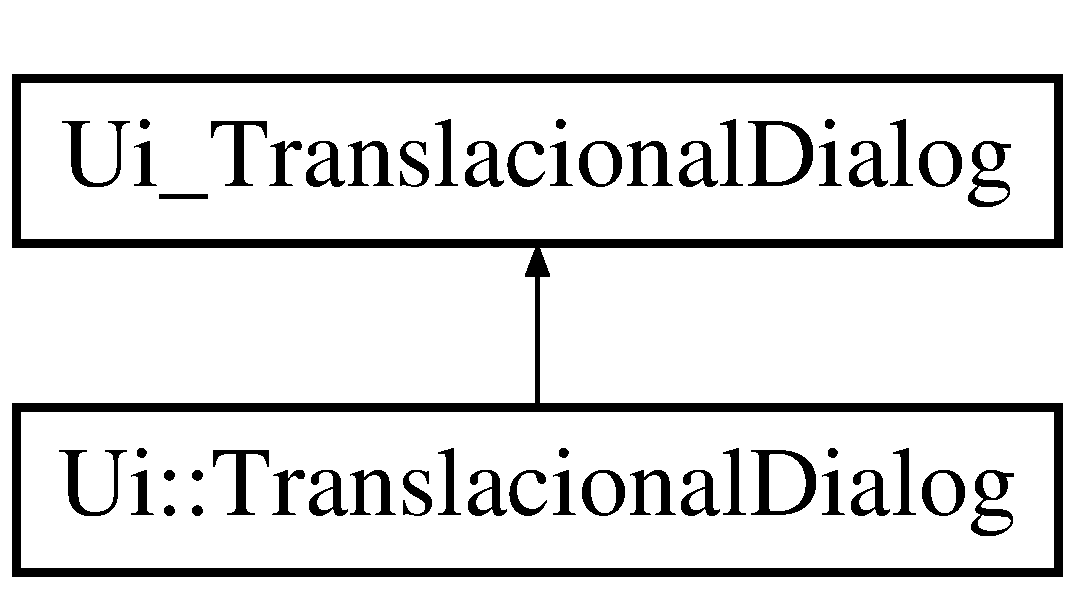
\includegraphics[height=2.000000cm]{class_ui___translacional_dialog}
\end{center}
\end{figure}
\subsection*{Public Member Functions}
\begin{DoxyCompactItemize}
\item 
void \hyperlink{class_ui___translacional_dialog_a14ff63c44f093098644e3d5e7b9bcec2}{setup\-Ui} (Q\-Dialog $\ast$\hyperlink{class_translacional_dialog}{Translacional\-Dialog})
\item 
void \hyperlink{class_ui___translacional_dialog_a804a72d6581b2aebc2d1321cb5641e70}{retranslate\-Ui} (Q\-Dialog $\ast$\hyperlink{class_translacional_dialog}{Translacional\-Dialog})
\end{DoxyCompactItemize}
\subsection*{Public Attributes}
\begin{DoxyCompactItemize}
\item 
Q\-Dialog\-Button\-Box $\ast$ \hyperlink{class_ui___translacional_dialog_a33199e9bf824102f6300a1ceb4354aca}{button\-Box}
\item 
Q\-Widget $\ast$ \hyperlink{class_ui___translacional_dialog_a74fb90caa54367a4c361e0d7fe7bc8ba}{vertical\-Layout\-Widget}
\item 
Q\-V\-Box\-Layout $\ast$ \hyperlink{class_ui___translacional_dialog_a24bdacaadef08fd1e3d0936400bced2e}{vertical\-Layout}
\item 
Q\-Label $\ast$ \hyperlink{class_ui___translacional_dialog_a6732967c8998f334885a1b8f23d054d1}{label\-\_\-4}
\item 
Q\-H\-Box\-Layout $\ast$ \hyperlink{class_ui___translacional_dialog_a7e76649d47e077d7cb73056ee4765250}{horizontal\-Layout\-\_\-3}
\item 
Q\-Label $\ast$ \hyperlink{class_ui___translacional_dialog_a346440ea60edd31d8da0fc279507d995}{label\-\_\-3}
\item 
Q\-Line\-Edit $\ast$ \hyperlink{class_ui___translacional_dialog_a2e88b4a26642a0edb7cb033edf2c82bb}{x\-Text}
\item 
Q\-H\-Box\-Layout $\ast$ \hyperlink{class_ui___translacional_dialog_a66f99a13414c872e8980c067129b3c58}{horizontal\-Layout\-\_\-2}
\item 
Q\-Label $\ast$ \hyperlink{class_ui___translacional_dialog_a2ecb0f99dfe0e0b3c9eec117fda5609a}{label\-\_\-2}
\item 
Q\-Line\-Edit $\ast$ \hyperlink{class_ui___translacional_dialog_a5f48505552db27605a8d8da569752d25}{y\-Text}
\item 
Q\-H\-Box\-Layout $\ast$ \hyperlink{class_ui___translacional_dialog_a4a836c9f9e02a433288eff09f3138d3b}{horizontal\-Layout}
\item 
Q\-Label $\ast$ \hyperlink{class_ui___translacional_dialog_a0f1a9a25f53e660213d5edd8238a5afe}{label}
\item 
Q\-Line\-Edit $\ast$ \hyperlink{class_ui___translacional_dialog_a4c195ebd2f2d8aed1cb9060074e8996d}{z\-Text}
\item 
Q\-Group\-Box $\ast$ \hyperlink{class_ui___translacional_dialog_a2890847b40cd28ad2d27cd90ba2b3afd}{group\-Box}
\item 
Q\-Widget $\ast$ \hyperlink{class_ui___translacional_dialog_a8b2ecabdba120d862aa60a7918b76e36}{vertical\-Layout\-Widget\-\_\-2}
\item 
Q\-V\-Box\-Layout $\ast$ \hyperlink{class_ui___translacional_dialog_aec3b3200d40f47fe79f30da6d5ae9a21}{vertical\-Layout\-\_\-2}
\item 
Q\-Radio\-Button $\ast$ \hyperlink{class_ui___translacional_dialog_a5c72ba5f84d6d5b78f058bc6ed0cef34}{orientacion\-\_\-pos}
\item 
Q\-Radio\-Button $\ast$ \hyperlink{class_ui___translacional_dialog_ad398394cd6c79ae530eced9426652ce9}{orientacion\-\_\-neg}
\end{DoxyCompactItemize}


\subsection{Member Function Documentation}
\hypertarget{class_ui___translacional_dialog_a804a72d6581b2aebc2d1321cb5641e70}{\index{Ui\-\_\-\-Translacional\-Dialog@{Ui\-\_\-\-Translacional\-Dialog}!retranslate\-Ui@{retranslate\-Ui}}
\index{retranslate\-Ui@{retranslate\-Ui}!Ui_TranslacionalDialog@{Ui\-\_\-\-Translacional\-Dialog}}
\subsubsection[{retranslate\-Ui}]{\setlength{\rightskip}{0pt plus 5cm}void Ui\-\_\-\-Translacional\-Dialog\-::retranslate\-Ui (
\begin{DoxyParamCaption}
\item[{Q\-Dialog $\ast$}]{Translacional\-Dialog}
\end{DoxyParamCaption}
)\hspace{0.3cm}{\ttfamily [inline]}}}\label{class_ui___translacional_dialog_a804a72d6581b2aebc2d1321cb5641e70}
\hypertarget{class_ui___translacional_dialog_a14ff63c44f093098644e3d5e7b9bcec2}{\index{Ui\-\_\-\-Translacional\-Dialog@{Ui\-\_\-\-Translacional\-Dialog}!setup\-Ui@{setup\-Ui}}
\index{setup\-Ui@{setup\-Ui}!Ui_TranslacionalDialog@{Ui\-\_\-\-Translacional\-Dialog}}
\subsubsection[{setup\-Ui}]{\setlength{\rightskip}{0pt plus 5cm}void Ui\-\_\-\-Translacional\-Dialog\-::setup\-Ui (
\begin{DoxyParamCaption}
\item[{Q\-Dialog $\ast$}]{Translacional\-Dialog}
\end{DoxyParamCaption}
)\hspace{0.3cm}{\ttfamily [inline]}}}\label{class_ui___translacional_dialog_a14ff63c44f093098644e3d5e7b9bcec2}


\subsection{Member Data Documentation}
\hypertarget{class_ui___translacional_dialog_a33199e9bf824102f6300a1ceb4354aca}{\index{Ui\-\_\-\-Translacional\-Dialog@{Ui\-\_\-\-Translacional\-Dialog}!button\-Box@{button\-Box}}
\index{button\-Box@{button\-Box}!Ui_TranslacionalDialog@{Ui\-\_\-\-Translacional\-Dialog}}
\subsubsection[{button\-Box}]{\setlength{\rightskip}{0pt plus 5cm}Q\-Dialog\-Button\-Box$\ast$ Ui\-\_\-\-Translacional\-Dialog\-::button\-Box}}\label{class_ui___translacional_dialog_a33199e9bf824102f6300a1ceb4354aca}
\hypertarget{class_ui___translacional_dialog_a2890847b40cd28ad2d27cd90ba2b3afd}{\index{Ui\-\_\-\-Translacional\-Dialog@{Ui\-\_\-\-Translacional\-Dialog}!group\-Box@{group\-Box}}
\index{group\-Box@{group\-Box}!Ui_TranslacionalDialog@{Ui\-\_\-\-Translacional\-Dialog}}
\subsubsection[{group\-Box}]{\setlength{\rightskip}{0pt plus 5cm}Q\-Group\-Box$\ast$ Ui\-\_\-\-Translacional\-Dialog\-::group\-Box}}\label{class_ui___translacional_dialog_a2890847b40cd28ad2d27cd90ba2b3afd}
\hypertarget{class_ui___translacional_dialog_a4a836c9f9e02a433288eff09f3138d3b}{\index{Ui\-\_\-\-Translacional\-Dialog@{Ui\-\_\-\-Translacional\-Dialog}!horizontal\-Layout@{horizontal\-Layout}}
\index{horizontal\-Layout@{horizontal\-Layout}!Ui_TranslacionalDialog@{Ui\-\_\-\-Translacional\-Dialog}}
\subsubsection[{horizontal\-Layout}]{\setlength{\rightskip}{0pt plus 5cm}Q\-H\-Box\-Layout$\ast$ Ui\-\_\-\-Translacional\-Dialog\-::horizontal\-Layout}}\label{class_ui___translacional_dialog_a4a836c9f9e02a433288eff09f3138d3b}
\hypertarget{class_ui___translacional_dialog_a66f99a13414c872e8980c067129b3c58}{\index{Ui\-\_\-\-Translacional\-Dialog@{Ui\-\_\-\-Translacional\-Dialog}!horizontal\-Layout\-\_\-2@{horizontal\-Layout\-\_\-2}}
\index{horizontal\-Layout\-\_\-2@{horizontal\-Layout\-\_\-2}!Ui_TranslacionalDialog@{Ui\-\_\-\-Translacional\-Dialog}}
\subsubsection[{horizontal\-Layout\-\_\-2}]{\setlength{\rightskip}{0pt plus 5cm}Q\-H\-Box\-Layout$\ast$ Ui\-\_\-\-Translacional\-Dialog\-::horizontal\-Layout\-\_\-2}}\label{class_ui___translacional_dialog_a66f99a13414c872e8980c067129b3c58}
\hypertarget{class_ui___translacional_dialog_a7e76649d47e077d7cb73056ee4765250}{\index{Ui\-\_\-\-Translacional\-Dialog@{Ui\-\_\-\-Translacional\-Dialog}!horizontal\-Layout\-\_\-3@{horizontal\-Layout\-\_\-3}}
\index{horizontal\-Layout\-\_\-3@{horizontal\-Layout\-\_\-3}!Ui_TranslacionalDialog@{Ui\-\_\-\-Translacional\-Dialog}}
\subsubsection[{horizontal\-Layout\-\_\-3}]{\setlength{\rightskip}{0pt plus 5cm}Q\-H\-Box\-Layout$\ast$ Ui\-\_\-\-Translacional\-Dialog\-::horizontal\-Layout\-\_\-3}}\label{class_ui___translacional_dialog_a7e76649d47e077d7cb73056ee4765250}
\hypertarget{class_ui___translacional_dialog_a0f1a9a25f53e660213d5edd8238a5afe}{\index{Ui\-\_\-\-Translacional\-Dialog@{Ui\-\_\-\-Translacional\-Dialog}!label@{label}}
\index{label@{label}!Ui_TranslacionalDialog@{Ui\-\_\-\-Translacional\-Dialog}}
\subsubsection[{label}]{\setlength{\rightskip}{0pt plus 5cm}Q\-Label$\ast$ Ui\-\_\-\-Translacional\-Dialog\-::label}}\label{class_ui___translacional_dialog_a0f1a9a25f53e660213d5edd8238a5afe}
\hypertarget{class_ui___translacional_dialog_a2ecb0f99dfe0e0b3c9eec117fda5609a}{\index{Ui\-\_\-\-Translacional\-Dialog@{Ui\-\_\-\-Translacional\-Dialog}!label\-\_\-2@{label\-\_\-2}}
\index{label\-\_\-2@{label\-\_\-2}!Ui_TranslacionalDialog@{Ui\-\_\-\-Translacional\-Dialog}}
\subsubsection[{label\-\_\-2}]{\setlength{\rightskip}{0pt plus 5cm}Q\-Label$\ast$ Ui\-\_\-\-Translacional\-Dialog\-::label\-\_\-2}}\label{class_ui___translacional_dialog_a2ecb0f99dfe0e0b3c9eec117fda5609a}
\hypertarget{class_ui___translacional_dialog_a346440ea60edd31d8da0fc279507d995}{\index{Ui\-\_\-\-Translacional\-Dialog@{Ui\-\_\-\-Translacional\-Dialog}!label\-\_\-3@{label\-\_\-3}}
\index{label\-\_\-3@{label\-\_\-3}!Ui_TranslacionalDialog@{Ui\-\_\-\-Translacional\-Dialog}}
\subsubsection[{label\-\_\-3}]{\setlength{\rightskip}{0pt plus 5cm}Q\-Label$\ast$ Ui\-\_\-\-Translacional\-Dialog\-::label\-\_\-3}}\label{class_ui___translacional_dialog_a346440ea60edd31d8da0fc279507d995}
\hypertarget{class_ui___translacional_dialog_a6732967c8998f334885a1b8f23d054d1}{\index{Ui\-\_\-\-Translacional\-Dialog@{Ui\-\_\-\-Translacional\-Dialog}!label\-\_\-4@{label\-\_\-4}}
\index{label\-\_\-4@{label\-\_\-4}!Ui_TranslacionalDialog@{Ui\-\_\-\-Translacional\-Dialog}}
\subsubsection[{label\-\_\-4}]{\setlength{\rightskip}{0pt plus 5cm}Q\-Label$\ast$ Ui\-\_\-\-Translacional\-Dialog\-::label\-\_\-4}}\label{class_ui___translacional_dialog_a6732967c8998f334885a1b8f23d054d1}
\hypertarget{class_ui___translacional_dialog_ad398394cd6c79ae530eced9426652ce9}{\index{Ui\-\_\-\-Translacional\-Dialog@{Ui\-\_\-\-Translacional\-Dialog}!orientacion\-\_\-neg@{orientacion\-\_\-neg}}
\index{orientacion\-\_\-neg@{orientacion\-\_\-neg}!Ui_TranslacionalDialog@{Ui\-\_\-\-Translacional\-Dialog}}
\subsubsection[{orientacion\-\_\-neg}]{\setlength{\rightskip}{0pt plus 5cm}Q\-Radio\-Button$\ast$ Ui\-\_\-\-Translacional\-Dialog\-::orientacion\-\_\-neg}}\label{class_ui___translacional_dialog_ad398394cd6c79ae530eced9426652ce9}
\hypertarget{class_ui___translacional_dialog_a5c72ba5f84d6d5b78f058bc6ed0cef34}{\index{Ui\-\_\-\-Translacional\-Dialog@{Ui\-\_\-\-Translacional\-Dialog}!orientacion\-\_\-pos@{orientacion\-\_\-pos}}
\index{orientacion\-\_\-pos@{orientacion\-\_\-pos}!Ui_TranslacionalDialog@{Ui\-\_\-\-Translacional\-Dialog}}
\subsubsection[{orientacion\-\_\-pos}]{\setlength{\rightskip}{0pt plus 5cm}Q\-Radio\-Button$\ast$ Ui\-\_\-\-Translacional\-Dialog\-::orientacion\-\_\-pos}}\label{class_ui___translacional_dialog_a5c72ba5f84d6d5b78f058bc6ed0cef34}
\hypertarget{class_ui___translacional_dialog_a24bdacaadef08fd1e3d0936400bced2e}{\index{Ui\-\_\-\-Translacional\-Dialog@{Ui\-\_\-\-Translacional\-Dialog}!vertical\-Layout@{vertical\-Layout}}
\index{vertical\-Layout@{vertical\-Layout}!Ui_TranslacionalDialog@{Ui\-\_\-\-Translacional\-Dialog}}
\subsubsection[{vertical\-Layout}]{\setlength{\rightskip}{0pt plus 5cm}Q\-V\-Box\-Layout$\ast$ Ui\-\_\-\-Translacional\-Dialog\-::vertical\-Layout}}\label{class_ui___translacional_dialog_a24bdacaadef08fd1e3d0936400bced2e}
\hypertarget{class_ui___translacional_dialog_aec3b3200d40f47fe79f30da6d5ae9a21}{\index{Ui\-\_\-\-Translacional\-Dialog@{Ui\-\_\-\-Translacional\-Dialog}!vertical\-Layout\-\_\-2@{vertical\-Layout\-\_\-2}}
\index{vertical\-Layout\-\_\-2@{vertical\-Layout\-\_\-2}!Ui_TranslacionalDialog@{Ui\-\_\-\-Translacional\-Dialog}}
\subsubsection[{vertical\-Layout\-\_\-2}]{\setlength{\rightskip}{0pt plus 5cm}Q\-V\-Box\-Layout$\ast$ Ui\-\_\-\-Translacional\-Dialog\-::vertical\-Layout\-\_\-2}}\label{class_ui___translacional_dialog_aec3b3200d40f47fe79f30da6d5ae9a21}
\hypertarget{class_ui___translacional_dialog_a74fb90caa54367a4c361e0d7fe7bc8ba}{\index{Ui\-\_\-\-Translacional\-Dialog@{Ui\-\_\-\-Translacional\-Dialog}!vertical\-Layout\-Widget@{vertical\-Layout\-Widget}}
\index{vertical\-Layout\-Widget@{vertical\-Layout\-Widget}!Ui_TranslacionalDialog@{Ui\-\_\-\-Translacional\-Dialog}}
\subsubsection[{vertical\-Layout\-Widget}]{\setlength{\rightskip}{0pt plus 5cm}Q\-Widget$\ast$ Ui\-\_\-\-Translacional\-Dialog\-::vertical\-Layout\-Widget}}\label{class_ui___translacional_dialog_a74fb90caa54367a4c361e0d7fe7bc8ba}
\hypertarget{class_ui___translacional_dialog_a8b2ecabdba120d862aa60a7918b76e36}{\index{Ui\-\_\-\-Translacional\-Dialog@{Ui\-\_\-\-Translacional\-Dialog}!vertical\-Layout\-Widget\-\_\-2@{vertical\-Layout\-Widget\-\_\-2}}
\index{vertical\-Layout\-Widget\-\_\-2@{vertical\-Layout\-Widget\-\_\-2}!Ui_TranslacionalDialog@{Ui\-\_\-\-Translacional\-Dialog}}
\subsubsection[{vertical\-Layout\-Widget\-\_\-2}]{\setlength{\rightskip}{0pt plus 5cm}Q\-Widget$\ast$ Ui\-\_\-\-Translacional\-Dialog\-::vertical\-Layout\-Widget\-\_\-2}}\label{class_ui___translacional_dialog_a8b2ecabdba120d862aa60a7918b76e36}
\hypertarget{class_ui___translacional_dialog_a2e88b4a26642a0edb7cb033edf2c82bb}{\index{Ui\-\_\-\-Translacional\-Dialog@{Ui\-\_\-\-Translacional\-Dialog}!x\-Text@{x\-Text}}
\index{x\-Text@{x\-Text}!Ui_TranslacionalDialog@{Ui\-\_\-\-Translacional\-Dialog}}
\subsubsection[{x\-Text}]{\setlength{\rightskip}{0pt plus 5cm}Q\-Line\-Edit$\ast$ Ui\-\_\-\-Translacional\-Dialog\-::x\-Text}}\label{class_ui___translacional_dialog_a2e88b4a26642a0edb7cb033edf2c82bb}
\hypertarget{class_ui___translacional_dialog_a5f48505552db27605a8d8da569752d25}{\index{Ui\-\_\-\-Translacional\-Dialog@{Ui\-\_\-\-Translacional\-Dialog}!y\-Text@{y\-Text}}
\index{y\-Text@{y\-Text}!Ui_TranslacionalDialog@{Ui\-\_\-\-Translacional\-Dialog}}
\subsubsection[{y\-Text}]{\setlength{\rightskip}{0pt plus 5cm}Q\-Line\-Edit$\ast$ Ui\-\_\-\-Translacional\-Dialog\-::y\-Text}}\label{class_ui___translacional_dialog_a5f48505552db27605a8d8da569752d25}
\hypertarget{class_ui___translacional_dialog_a4c195ebd2f2d8aed1cb9060074e8996d}{\index{Ui\-\_\-\-Translacional\-Dialog@{Ui\-\_\-\-Translacional\-Dialog}!z\-Text@{z\-Text}}
\index{z\-Text@{z\-Text}!Ui_TranslacionalDialog@{Ui\-\_\-\-Translacional\-Dialog}}
\subsubsection[{z\-Text}]{\setlength{\rightskip}{0pt plus 5cm}Q\-Line\-Edit$\ast$ Ui\-\_\-\-Translacional\-Dialog\-::z\-Text}}\label{class_ui___translacional_dialog_a4c195ebd2f2d8aed1cb9060074e8996d}


The documentation for this class was generated from the following file\-:\begin{DoxyCompactItemize}
\item 
build-\/\-Motion\-Structure-\/\-Desktop\-\_\-\-Qt\-\_\-5\-\_\-3\-\_\-\-G\-C\-C\-\_\-64bit-\/\-Debug/\hyperlink{ui__translacionaldialog_8h}{ui\-\_\-translacionaldialog.\-h}\end{DoxyCompactItemize}

\chapter{File Documentation}
\hypertarget{moc__mainwindow_8cpp}{\section{build-\/\-Motion\-Structure-\/\-Desktop\-\_\-\-Qt\-\_\-5\-\_\-3\-\_\-\-G\-C\-C\-\_\-64bit-\/\-Debug/moc\-\_\-mainwindow.cpp File Reference}
\label{moc__mainwindow_8cpp}\index{build-\/\-Motion\-Structure-\/\-Desktop\-\_\-\-Qt\-\_\-5\-\_\-3\-\_\-\-G\-C\-C\-\_\-64bit-\/\-Debug/moc\-\_\-mainwindow.\-cpp@{build-\/\-Motion\-Structure-\/\-Desktop\-\_\-\-Qt\-\_\-5\-\_\-3\-\_\-\-G\-C\-C\-\_\-64bit-\/\-Debug/moc\-\_\-mainwindow.\-cpp}}
}
{\ttfamily \#include \char`\"{}../\-G\-U\-I/mainwindow.\-h\char`\"{}}\\*
{\ttfamily \#include $<$Qt\-Core/qbytearray.\-h$>$}\\*
{\ttfamily \#include $<$Qt\-Core/qmetatype.\-h$>$}\\*
\subsection*{Classes}
\begin{DoxyCompactItemize}
\item 
struct \hyperlink{structqt__meta__stringdata___main_window__t}{qt\-\_\-meta\-\_\-stringdata\-\_\-\-Main\-Window\-\_\-t}
\end{DoxyCompactItemize}
\subsection*{Macros}
\begin{DoxyCompactItemize}
\item 
\#define \hyperlink{moc__mainwindow_8cpp_a75bb9482d242cde0a06c9dbdc6b83abe}{Q\-T\-\_\-\-M\-O\-C\-\_\-\-L\-I\-T\-E\-R\-A\-L}(idx, ofs, len)
\end{DoxyCompactItemize}


\subsection{Macro Definition Documentation}
\hypertarget{moc__mainwindow_8cpp_a75bb9482d242cde0a06c9dbdc6b83abe}{\index{moc\-\_\-mainwindow.\-cpp@{moc\-\_\-mainwindow.\-cpp}!Q\-T\-\_\-\-M\-O\-C\-\_\-\-L\-I\-T\-E\-R\-A\-L@{Q\-T\-\_\-\-M\-O\-C\-\_\-\-L\-I\-T\-E\-R\-A\-L}}
\index{Q\-T\-\_\-\-M\-O\-C\-\_\-\-L\-I\-T\-E\-R\-A\-L@{Q\-T\-\_\-\-M\-O\-C\-\_\-\-L\-I\-T\-E\-R\-A\-L}!moc_mainwindow.cpp@{moc\-\_\-mainwindow.\-cpp}}
\subsubsection[{Q\-T\-\_\-\-M\-O\-C\-\_\-\-L\-I\-T\-E\-R\-A\-L}]{\setlength{\rightskip}{0pt plus 5cm}\#define Q\-T\-\_\-\-M\-O\-C\-\_\-\-L\-I\-T\-E\-R\-A\-L(
\begin{DoxyParamCaption}
\item[{}]{idx, }
\item[{}]{ofs, }
\item[{}]{len}
\end{DoxyParamCaption}
)}}\label{moc__mainwindow_8cpp_a75bb9482d242cde0a06c9dbdc6b83abe}
{\bfseries Value\-:}
\begin{DoxyCode}
Q\_STATIC\_BYTE\_ARRAY\_DATA\_HEADER\_INITIALIZER\_WITH\_OFFSET(len, \(\backslash\)
    qptrdiff(offsetof(\hyperlink{structqt__meta__stringdata___main_window__t}{qt\_meta\_stringdata\_MainWindow\_t}, stringdata) + ofs \(\backslash\)
        - idx * \textcolor{keyword}{sizeof}(QByteArrayData)) \(\backslash\)
    )
\end{DoxyCode}

\hypertarget{moc__rotacionaldialog_8cpp}{\section{build-\/\-Motion\-Structure-\/\-Desktop\-\_\-\-Qt\-\_\-5\-\_\-3\-\_\-\-G\-C\-C\-\_\-64bit-\/\-Debug/moc\-\_\-rotacionaldialog.cpp File Reference}
\label{moc__rotacionaldialog_8cpp}\index{build-\/\-Motion\-Structure-\/\-Desktop\-\_\-\-Qt\-\_\-5\-\_\-3\-\_\-\-G\-C\-C\-\_\-64bit-\/\-Debug/moc\-\_\-rotacionaldialog.\-cpp@{build-\/\-Motion\-Structure-\/\-Desktop\-\_\-\-Qt\-\_\-5\-\_\-3\-\_\-\-G\-C\-C\-\_\-64bit-\/\-Debug/moc\-\_\-rotacionaldialog.\-cpp}}
}
{\ttfamily \#include \char`\"{}../\-G\-U\-I/rotacionaldialog.\-h\char`\"{}}\\*
{\ttfamily \#include $<$Qt\-Core/qbytearray.\-h$>$}\\*
{\ttfamily \#include $<$Qt\-Core/qmetatype.\-h$>$}\\*
\subsection*{Classes}
\begin{DoxyCompactItemize}
\item 
struct \hyperlink{structqt__meta__stringdata___rotacional_dialog__t}{qt\-\_\-meta\-\_\-stringdata\-\_\-\-Rotacional\-Dialog\-\_\-t}
\end{DoxyCompactItemize}
\subsection*{Macros}
\begin{DoxyCompactItemize}
\item 
\#define \hyperlink{moc__rotacionaldialog_8cpp_a75bb9482d242cde0a06c9dbdc6b83abe}{Q\-T\-\_\-\-M\-O\-C\-\_\-\-L\-I\-T\-E\-R\-A\-L}(idx, ofs, len)
\end{DoxyCompactItemize}


\subsection{Macro Definition Documentation}
\hypertarget{moc__rotacionaldialog_8cpp_a75bb9482d242cde0a06c9dbdc6b83abe}{\index{moc\-\_\-rotacionaldialog.\-cpp@{moc\-\_\-rotacionaldialog.\-cpp}!Q\-T\-\_\-\-M\-O\-C\-\_\-\-L\-I\-T\-E\-R\-A\-L@{Q\-T\-\_\-\-M\-O\-C\-\_\-\-L\-I\-T\-E\-R\-A\-L}}
\index{Q\-T\-\_\-\-M\-O\-C\-\_\-\-L\-I\-T\-E\-R\-A\-L@{Q\-T\-\_\-\-M\-O\-C\-\_\-\-L\-I\-T\-E\-R\-A\-L}!moc_rotacionaldialog.cpp@{moc\-\_\-rotacionaldialog.\-cpp}}
\subsubsection[{Q\-T\-\_\-\-M\-O\-C\-\_\-\-L\-I\-T\-E\-R\-A\-L}]{\setlength{\rightskip}{0pt plus 5cm}\#define Q\-T\-\_\-\-M\-O\-C\-\_\-\-L\-I\-T\-E\-R\-A\-L(
\begin{DoxyParamCaption}
\item[{}]{idx, }
\item[{}]{ofs, }
\item[{}]{len}
\end{DoxyParamCaption}
)}}\label{moc__rotacionaldialog_8cpp_a75bb9482d242cde0a06c9dbdc6b83abe}
{\bfseries Value\-:}
\begin{DoxyCode}
Q\_STATIC\_BYTE\_ARRAY\_DATA\_HEADER\_INITIALIZER\_WITH\_OFFSET(len, \(\backslash\)
    qptrdiff(offsetof(\hyperlink{structqt__meta__stringdata___rotacional_dialog__t}{qt\_meta\_stringdata\_RotacionalDialog\_t}, 
      stringdata) + ofs \(\backslash\)
        - idx * \textcolor{keyword}{sizeof}(QByteArrayData)) \(\backslash\)
    )
\end{DoxyCode}

\hypertarget{moc__translacionaldialog_8cpp}{\section{build-\/\-Motion\-Structure-\/\-Desktop\-\_\-\-Qt\-\_\-5\-\_\-3\-\_\-\-G\-C\-C\-\_\-64bit-\/\-Debug/moc\-\_\-translacionaldialog.cpp File Reference}
\label{moc__translacionaldialog_8cpp}\index{build-\/\-Motion\-Structure-\/\-Desktop\-\_\-\-Qt\-\_\-5\-\_\-3\-\_\-\-G\-C\-C\-\_\-64bit-\/\-Debug/moc\-\_\-translacionaldialog.\-cpp@{build-\/\-Motion\-Structure-\/\-Desktop\-\_\-\-Qt\-\_\-5\-\_\-3\-\_\-\-G\-C\-C\-\_\-64bit-\/\-Debug/moc\-\_\-translacionaldialog.\-cpp}}
}
{\ttfamily \#include \char`\"{}../\-G\-U\-I/translacionaldialog.\-h\char`\"{}}\\*
{\ttfamily \#include $<$Qt\-Core/qbytearray.\-h$>$}\\*
{\ttfamily \#include $<$Qt\-Core/qmetatype.\-h$>$}\\*
\subsection*{Classes}
\begin{DoxyCompactItemize}
\item 
struct \hyperlink{structqt__meta__stringdata___translacional_dialog__t}{qt\-\_\-meta\-\_\-stringdata\-\_\-\-Translacional\-Dialog\-\_\-t}
\end{DoxyCompactItemize}
\subsection*{Macros}
\begin{DoxyCompactItemize}
\item 
\#define \hyperlink{moc__translacionaldialog_8cpp_a75bb9482d242cde0a06c9dbdc6b83abe}{Q\-T\-\_\-\-M\-O\-C\-\_\-\-L\-I\-T\-E\-R\-A\-L}(idx, ofs, len)
\end{DoxyCompactItemize}


\subsection{Macro Definition Documentation}
\hypertarget{moc__translacionaldialog_8cpp_a75bb9482d242cde0a06c9dbdc6b83abe}{\index{moc\-\_\-translacionaldialog.\-cpp@{moc\-\_\-translacionaldialog.\-cpp}!Q\-T\-\_\-\-M\-O\-C\-\_\-\-L\-I\-T\-E\-R\-A\-L@{Q\-T\-\_\-\-M\-O\-C\-\_\-\-L\-I\-T\-E\-R\-A\-L}}
\index{Q\-T\-\_\-\-M\-O\-C\-\_\-\-L\-I\-T\-E\-R\-A\-L@{Q\-T\-\_\-\-M\-O\-C\-\_\-\-L\-I\-T\-E\-R\-A\-L}!moc_translacionaldialog.cpp@{moc\-\_\-translacionaldialog.\-cpp}}
\subsubsection[{Q\-T\-\_\-\-M\-O\-C\-\_\-\-L\-I\-T\-E\-R\-A\-L}]{\setlength{\rightskip}{0pt plus 5cm}\#define Q\-T\-\_\-\-M\-O\-C\-\_\-\-L\-I\-T\-E\-R\-A\-L(
\begin{DoxyParamCaption}
\item[{}]{idx, }
\item[{}]{ofs, }
\item[{}]{len}
\end{DoxyParamCaption}
)}}\label{moc__translacionaldialog_8cpp_a75bb9482d242cde0a06c9dbdc6b83abe}
{\bfseries Value\-:}
\begin{DoxyCode}
Q\_STATIC\_BYTE\_ARRAY\_DATA\_HEADER\_INITIALIZER\_WITH\_OFFSET(len, \(\backslash\)
    qptrdiff(offsetof(\hyperlink{structqt__meta__stringdata___translacional_dialog__t}{qt\_meta\_stringdata\_TranslacionalDialog\_t}, 
      stringdata) + ofs \(\backslash\)
        - idx * \textcolor{keyword}{sizeof}(QByteArrayData)) \(\backslash\)
    )
\end{DoxyCode}

\hypertarget{qrc__icons_8cpp}{\section{build-\/\-Motion\-Structure-\/\-Desktop\-\_\-\-Qt\-\_\-5\-\_\-3\-\_\-\-G\-C\-C\-\_\-64bit-\/\-Debug/qrc\-\_\-icons.cpp File Reference}
\label{qrc__icons_8cpp}\index{build-\/\-Motion\-Structure-\/\-Desktop\-\_\-\-Qt\-\_\-5\-\_\-3\-\_\-\-G\-C\-C\-\_\-64bit-\/\-Debug/qrc\-\_\-icons.\-cpp@{build-\/\-Motion\-Structure-\/\-Desktop\-\_\-\-Qt\-\_\-5\-\_\-3\-\_\-\-G\-C\-C\-\_\-64bit-\/\-Debug/qrc\-\_\-icons.\-cpp}}
}
{\ttfamily \#include $<$Qt\-Core/qglobal.\-h$>$}\\*
\subsection*{Functions}
\begin{DoxyCompactItemize}
\item 
Q\-T\-\_\-\-B\-E\-G\-I\-N\-\_\-\-N\-A\-M\-E\-S\-P\-A\-C\-E \\*
Q\-\_\-\-C\-O\-R\-E\-\_\-\-E\-X\-P\-O\-R\-T bool \hyperlink{qrc__icons_8cpp_ab3bec3d1e679084be46edc41e4c91bc1}{q\-Register\-Resource\-Data} (int, const unsigned char $\ast$, const unsigned char $\ast$, const unsigned char $\ast$)
\item 
Q\-\_\-\-C\-O\-R\-E\-\_\-\-E\-X\-P\-O\-R\-T bool \hyperlink{qrc__icons_8cpp_ad65f8bca8010dd1fd135a28a085c6d03}{q\-Unregister\-Resource\-Data} (int, const unsigned char $\ast$, const unsigned char $\ast$, const unsigned char $\ast$)
\item 
Q\-T\-\_\-\-E\-N\-D\-\_\-\-N\-A\-M\-E\-S\-P\-A\-C\-E int \\*
Q\-T\-\_\-\-M\-A\-N\-G\-L\-E\-\_\-\-N\-A\-M\-E\-S\-P\-A\-C\-E() \hyperlink{qrc__icons_8cpp_a604a4b2c01a3fcc04d212c2aabb2171a}{q\-Init\-Resources\-\_\-icons} ()
\item 
int Q\-T\-\_\-\-M\-A\-N\-G\-L\-E\-\_\-\-N\-A\-M\-E\-S\-P\-A\-C\-E() \hyperlink{qrc__icons_8cpp_a6e1e9924d11f0737f3cf199e822500ab}{q\-Cleanup\-Resources\-\_\-icons} ()
\end{DoxyCompactItemize}


\subsection{Function Documentation}
\hypertarget{qrc__icons_8cpp_a6e1e9924d11f0737f3cf199e822500ab}{\index{qrc\-\_\-icons.\-cpp@{qrc\-\_\-icons.\-cpp}!q\-Cleanup\-Resources\-\_\-icons@{q\-Cleanup\-Resources\-\_\-icons}}
\index{q\-Cleanup\-Resources\-\_\-icons@{q\-Cleanup\-Resources\-\_\-icons}!qrc_icons.cpp@{qrc\-\_\-icons.\-cpp}}
\subsubsection[{q\-Cleanup\-Resources\-\_\-icons}]{\setlength{\rightskip}{0pt plus 5cm}int Q\-T\-\_\-\-M\-A\-N\-G\-L\-E\-\_\-\-N\-A\-M\-E\-S\-P\-A\-C\-E() q\-Cleanup\-Resources\-\_\-icons (
\begin{DoxyParamCaption}
{}
\end{DoxyParamCaption}
)}}\label{qrc__icons_8cpp_a6e1e9924d11f0737f3cf199e822500ab}
\hypertarget{qrc__icons_8cpp_a604a4b2c01a3fcc04d212c2aabb2171a}{\index{qrc\-\_\-icons.\-cpp@{qrc\-\_\-icons.\-cpp}!q\-Init\-Resources\-\_\-icons@{q\-Init\-Resources\-\_\-icons}}
\index{q\-Init\-Resources\-\_\-icons@{q\-Init\-Resources\-\_\-icons}!qrc_icons.cpp@{qrc\-\_\-icons.\-cpp}}
\subsubsection[{q\-Init\-Resources\-\_\-icons}]{\setlength{\rightskip}{0pt plus 5cm}Q\-T\-\_\-\-E\-N\-D\-\_\-\-N\-A\-M\-E\-S\-P\-A\-C\-E int Q\-T\-\_\-\-M\-A\-N\-G\-L\-E\-\_\-\-N\-A\-M\-E\-S\-P\-A\-C\-E() q\-Init\-Resources\-\_\-icons (
\begin{DoxyParamCaption}
{}
\end{DoxyParamCaption}
)}}\label{qrc__icons_8cpp_a604a4b2c01a3fcc04d212c2aabb2171a}
\hypertarget{qrc__icons_8cpp_ab3bec3d1e679084be46edc41e4c91bc1}{\index{qrc\-\_\-icons.\-cpp@{qrc\-\_\-icons.\-cpp}!q\-Register\-Resource\-Data@{q\-Register\-Resource\-Data}}
\index{q\-Register\-Resource\-Data@{q\-Register\-Resource\-Data}!qrc_icons.cpp@{qrc\-\_\-icons.\-cpp}}
\subsubsection[{q\-Register\-Resource\-Data}]{\setlength{\rightskip}{0pt plus 5cm}Q\-T\-\_\-\-B\-E\-G\-I\-N\-\_\-\-N\-A\-M\-E\-S\-P\-A\-C\-E Q\-\_\-\-C\-O\-R\-E\-\_\-\-E\-X\-P\-O\-R\-T bool q\-Register\-Resource\-Data (
\begin{DoxyParamCaption}
\item[{int}]{, }
\item[{const unsigned char $\ast$}]{, }
\item[{const unsigned char $\ast$}]{, }
\item[{const unsigned char $\ast$}]{}
\end{DoxyParamCaption}
)}}\label{qrc__icons_8cpp_ab3bec3d1e679084be46edc41e4c91bc1}
\hypertarget{qrc__icons_8cpp_ad65f8bca8010dd1fd135a28a085c6d03}{\index{qrc\-\_\-icons.\-cpp@{qrc\-\_\-icons.\-cpp}!q\-Unregister\-Resource\-Data@{q\-Unregister\-Resource\-Data}}
\index{q\-Unregister\-Resource\-Data@{q\-Unregister\-Resource\-Data}!qrc_icons.cpp@{qrc\-\_\-icons.\-cpp}}
\subsubsection[{q\-Unregister\-Resource\-Data}]{\setlength{\rightskip}{0pt plus 5cm}Q\-\_\-\-C\-O\-R\-E\-\_\-\-E\-X\-P\-O\-R\-T bool q\-Unregister\-Resource\-Data (
\begin{DoxyParamCaption}
\item[{int}]{, }
\item[{const unsigned char $\ast$}]{, }
\item[{const unsigned char $\ast$}]{, }
\item[{const unsigned char $\ast$}]{}
\end{DoxyParamCaption}
)}}\label{qrc__icons_8cpp_ad65f8bca8010dd1fd135a28a085c6d03}

\hypertarget{ui__mainwindow_8h}{\section{build-\/\-Motion\-Structure-\/\-Desktop\-\_\-\-Qt\-\_\-5\-\_\-3\-\_\-\-G\-C\-C\-\_\-64bit-\/\-Debug/ui\-\_\-mainwindow.h File Reference}
\label{ui__mainwindow_8h}\index{build-\/\-Motion\-Structure-\/\-Desktop\-\_\-\-Qt\-\_\-5\-\_\-3\-\_\-\-G\-C\-C\-\_\-64bit-\/\-Debug/ui\-\_\-mainwindow.\-h@{build-\/\-Motion\-Structure-\/\-Desktop\-\_\-\-Qt\-\_\-5\-\_\-3\-\_\-\-G\-C\-C\-\_\-64bit-\/\-Debug/ui\-\_\-mainwindow.\-h}}
}
{\ttfamily \#include $<$Qt\-Core/\-Q\-Variant$>$}\\*
{\ttfamily \#include $<$Qt\-Widgets/\-Q\-Action$>$}\\*
{\ttfamily \#include $<$Qt\-Widgets/\-Q\-Application$>$}\\*
{\ttfamily \#include $<$Qt\-Widgets/\-Q\-Button\-Group$>$}\\*
{\ttfamily \#include $<$Qt\-Widgets/\-Q\-H\-Box\-Layout$>$}\\*
{\ttfamily \#include $<$Qt\-Widgets/\-Q\-Header\-View$>$}\\*
{\ttfamily \#include $<$Qt\-Widgets/\-Q\-Label$>$}\\*
{\ttfamily \#include $<$Qt\-Widgets/\-Q\-Line\-Edit$>$}\\*
{\ttfamily \#include $<$Qt\-Widgets/\-Q\-List\-Widget$>$}\\*
{\ttfamily \#include $<$Qt\-Widgets/\-Q\-Main\-Window$>$}\\*
{\ttfamily \#include $<$Qt\-Widgets/\-Q\-Menu$>$}\\*
{\ttfamily \#include $<$Qt\-Widgets/\-Q\-Menu\-Bar$>$}\\*
{\ttfamily \#include $<$Qt\-Widgets/\-Q\-Push\-Button$>$}\\*
{\ttfamily \#include $<$Qt\-Widgets/\-Q\-Status\-Bar$>$}\\*
{\ttfamily \#include $<$Qt\-Widgets/\-Q\-Tool\-Bar$>$}\\*
{\ttfamily \#include $<$Qt\-Widgets/\-Q\-V\-Box\-Layout$>$}\\*
{\ttfamily \#include $<$Qt\-Widgets/\-Q\-Widget$>$}\\*
\subsection*{Classes}
\begin{DoxyCompactItemize}
\item 
class \hyperlink{class_ui___main_window}{Ui\-\_\-\-Main\-Window}
\item 
class \hyperlink{class_ui_1_1_main_window}{Ui\-::\-Main\-Window}
\end{DoxyCompactItemize}
\subsection*{Namespaces}
\begin{DoxyCompactItemize}
\item 
\hyperlink{namespace_ui}{Ui}
\end{DoxyCompactItemize}

\hypertarget{ui__rotacionaldialog_8h}{\section{build-\/\-Motion\-Structure-\/\-Desktop\-\_\-\-Qt\-\_\-5\-\_\-3\-\_\-\-G\-C\-C\-\_\-64bit-\/\-Debug/ui\-\_\-rotacionaldialog.h File Reference}
\label{ui__rotacionaldialog_8h}\index{build-\/\-Motion\-Structure-\/\-Desktop\-\_\-\-Qt\-\_\-5\-\_\-3\-\_\-\-G\-C\-C\-\_\-64bit-\/\-Debug/ui\-\_\-rotacionaldialog.\-h@{build-\/\-Motion\-Structure-\/\-Desktop\-\_\-\-Qt\-\_\-5\-\_\-3\-\_\-\-G\-C\-C\-\_\-64bit-\/\-Debug/ui\-\_\-rotacionaldialog.\-h}}
}
{\ttfamily \#include $<$Qt\-Core/\-Q\-Variant$>$}\\*
{\ttfamily \#include $<$Qt\-Widgets/\-Q\-Action$>$}\\*
{\ttfamily \#include $<$Qt\-Widgets/\-Q\-Application$>$}\\*
{\ttfamily \#include $<$Qt\-Widgets/\-Q\-Button\-Group$>$}\\*
{\ttfamily \#include $<$Qt\-Widgets/\-Q\-Dialog$>$}\\*
{\ttfamily \#include $<$Qt\-Widgets/\-Q\-Dialog\-Button\-Box$>$}\\*
{\ttfamily \#include $<$Qt\-Widgets/\-Q\-Group\-Box$>$}\\*
{\ttfamily \#include $<$Qt\-Widgets/\-Q\-Header\-View$>$}\\*
{\ttfamily \#include $<$Qt\-Widgets/\-Q\-Label$>$}\\*
{\ttfamily \#include $<$Qt\-Widgets/\-Q\-Line\-Edit$>$}\\*
{\ttfamily \#include $<$Qt\-Widgets/\-Q\-Radio\-Button$>$}\\*
{\ttfamily \#include $<$Qt\-Widgets/\-Q\-V\-Box\-Layout$>$}\\*
{\ttfamily \#include $<$Qt\-Widgets/\-Q\-Widget$>$}\\*
\subsection*{Classes}
\begin{DoxyCompactItemize}
\item 
class \hyperlink{class_ui___rotacional_dialog}{Ui\-\_\-\-Rotacional\-Dialog}
\item 
class \hyperlink{class_ui_1_1_rotacional_dialog}{Ui\-::\-Rotacional\-Dialog}
\end{DoxyCompactItemize}
\subsection*{Namespaces}
\begin{DoxyCompactItemize}
\item 
\hyperlink{namespace_ui}{Ui}
\end{DoxyCompactItemize}

\hypertarget{ui__translacionaldialog_8h}{\section{build-\/\-Motion\-Structure-\/\-Desktop\-\_\-\-Qt\-\_\-5\-\_\-3\-\_\-\-G\-C\-C\-\_\-64bit-\/\-Debug/ui\-\_\-translacionaldialog.h File Reference}
\label{ui__translacionaldialog_8h}\index{build-\/\-Motion\-Structure-\/\-Desktop\-\_\-\-Qt\-\_\-5\-\_\-3\-\_\-\-G\-C\-C\-\_\-64bit-\/\-Debug/ui\-\_\-translacionaldialog.\-h@{build-\/\-Motion\-Structure-\/\-Desktop\-\_\-\-Qt\-\_\-5\-\_\-3\-\_\-\-G\-C\-C\-\_\-64bit-\/\-Debug/ui\-\_\-translacionaldialog.\-h}}
}
{\ttfamily \#include $<$Qt\-Core/\-Q\-Variant$>$}\\*
{\ttfamily \#include $<$Qt\-Widgets/\-Q\-Action$>$}\\*
{\ttfamily \#include $<$Qt\-Widgets/\-Q\-Application$>$}\\*
{\ttfamily \#include $<$Qt\-Widgets/\-Q\-Button\-Group$>$}\\*
{\ttfamily \#include $<$Qt\-Widgets/\-Q\-Dialog$>$}\\*
{\ttfamily \#include $<$Qt\-Widgets/\-Q\-Dialog\-Button\-Box$>$}\\*
{\ttfamily \#include $<$Qt\-Widgets/\-Q\-Group\-Box$>$}\\*
{\ttfamily \#include $<$Qt\-Widgets/\-Q\-H\-Box\-Layout$>$}\\*
{\ttfamily \#include $<$Qt\-Widgets/\-Q\-Header\-View$>$}\\*
{\ttfamily \#include $<$Qt\-Widgets/\-Q\-Label$>$}\\*
{\ttfamily \#include $<$Qt\-Widgets/\-Q\-Line\-Edit$>$}\\*
{\ttfamily \#include $<$Qt\-Widgets/\-Q\-Radio\-Button$>$}\\*
{\ttfamily \#include $<$Qt\-Widgets/\-Q\-V\-Box\-Layout$>$}\\*
{\ttfamily \#include $<$Qt\-Widgets/\-Q\-Widget$>$}\\*
\subsection*{Classes}
\begin{DoxyCompactItemize}
\item 
class \hyperlink{class_ui___translacional_dialog}{Ui\-\_\-\-Translacional\-Dialog}
\item 
class \hyperlink{class_ui_1_1_translacional_dialog}{Ui\-::\-Translacional\-Dialog}
\end{DoxyCompactItemize}
\subsection*{Namespaces}
\begin{DoxyCompactItemize}
\item 
\hyperlink{namespace_ui}{Ui}
\end{DoxyCompactItemize}

\hypertarget{brazo_8cpp}{\section{experiments/brazo.cpp File Reference}
\label{brazo_8cpp}\index{experiments/brazo.\-cpp@{experiments/brazo.\-cpp}}
}
{\ttfamily \#include $<$stdio.\-h$>$}\\*
{\ttfamily \#include $<$stdlib.\-h$>$}\\*
{\ttfamily \#include $<$iostream$>$}\\*
{\ttfamily \#include $<$vector$>$}\\*
{\ttfamily \#include \char`\"{}motion\-\_\-structure.\-hpp\char`\"{}}\\*
{\ttfamily \#include \char`\"{}ext\-Api.\-h\char`\"{}}\\*
\subsection*{Functions}
\begin{DoxyCompactItemize}
\item 
int \hyperlink{brazo_8cpp_a0ddf1224851353fc92bfbff6f499fa97}{main} (int argc, char $\ast$argv\mbox{[}$\,$\mbox{]})
\end{DoxyCompactItemize}


\subsection{Function Documentation}
\hypertarget{brazo_8cpp_a0ddf1224851353fc92bfbff6f499fa97}{\index{brazo.\-cpp@{brazo.\-cpp}!main@{main}}
\index{main@{main}!brazo.cpp@{brazo.\-cpp}}
\subsubsection[{main}]{\setlength{\rightskip}{0pt plus 5cm}int main (
\begin{DoxyParamCaption}
\item[{int}]{argc, }
\item[{char $\ast$}]{argv\mbox{[}$\,$\mbox{]}}
\end{DoxyParamCaption}
)}}\label{brazo_8cpp_a0ddf1224851353fc92bfbff6f499fa97}

\hypertarget{globals_8cpp}{\section{G\-U\-I/globals.cpp File Reference}
\label{globals_8cpp}\index{G\-U\-I/globals.\-cpp@{G\-U\-I/globals.\-cpp}}
}
{\ttfamily \#include \char`\"{}globals.\-h\char`\"{}}\\*
{\ttfamily \#include $<$sstream$>$}\\*
\subsection*{Functions}
\begin{DoxyCompactItemize}
\item 
void \hyperlink{globals_8cpp_affcf51ca6a2611bd9185dae9c1872302}{print\-Componentes} (const vector$<$ \hyperlink{struct_s_componentes}{S\-Componentes} $>$ \&vect)
\item 
string \hyperlink{globals_8cpp_af5c4692439e989fabd09950e7cad2ae9}{return\-Componentes} (const vector$<$ \hyperlink{struct_s_componentes}{S\-Componentes} $>$ \&vect, int count)
\item 
string \hyperlink{globals_8cpp_a3cb3f01a2ae6be3c1843343d320d2173}{return\-String\-Archivo} (const vector$<$ \hyperlink{struct_s_componentes}{S\-Componentes} $>$ \&vect)
\end{DoxyCompactItemize}
\subsection*{Variables}
\begin{DoxyCompactItemize}
\item 
int \hyperlink{globals_8cpp_a312c83bf03eb478966d6d905fb97d449}{editando} = 1
\item 
int \hyperlink{globals_8cpp_aa17f63ae4c5c311d2b0948956ff453ac}{elementos} = 0
\item 
int \hyperlink{globals_8cpp_a0b1fd7d5bab52ab4bf29b0cad788c22f}{tipo\-\_\-edicion} = \hyperlink{globals_8h_ae73f29c477a04fca49c8cae98a486e56}{C\-R\-E\-A\-N\-D\-O}
\item 
std\-::vector$<$ \hyperlink{struct_s_componentes}{S\-Componentes} $>$ \hyperlink{globals_8cpp_a45b658faed461aadeb6a6186883d4ffb}{componentes}
\end{DoxyCompactItemize}


\subsection{Function Documentation}
\hypertarget{globals_8cpp_affcf51ca6a2611bd9185dae9c1872302}{\index{globals.\-cpp@{globals.\-cpp}!print\-Componentes@{print\-Componentes}}
\index{print\-Componentes@{print\-Componentes}!globals.cpp@{globals.\-cpp}}
\subsubsection[{print\-Componentes}]{\setlength{\rightskip}{0pt plus 5cm}void print\-Componentes (
\begin{DoxyParamCaption}
\item[{const vector$<$ {\bf S\-Componentes} $>$ \&}]{vect}
\end{DoxyParamCaption}
)}}\label{globals_8cpp_affcf51ca6a2611bd9185dae9c1872302}
\hypertarget{globals_8cpp_af5c4692439e989fabd09950e7cad2ae9}{\index{globals.\-cpp@{globals.\-cpp}!return\-Componentes@{return\-Componentes}}
\index{return\-Componentes@{return\-Componentes}!globals.cpp@{globals.\-cpp}}
\subsubsection[{return\-Componentes}]{\setlength{\rightskip}{0pt plus 5cm}string return\-Componentes (
\begin{DoxyParamCaption}
\item[{const vector$<$ {\bf S\-Componentes} $>$ \&}]{vect, }
\item[{int}]{count}
\end{DoxyParamCaption}
)}}\label{globals_8cpp_af5c4692439e989fabd09950e7cad2ae9}
\hypertarget{globals_8cpp_a3cb3f01a2ae6be3c1843343d320d2173}{\index{globals.\-cpp@{globals.\-cpp}!return\-String\-Archivo@{return\-String\-Archivo}}
\index{return\-String\-Archivo@{return\-String\-Archivo}!globals.cpp@{globals.\-cpp}}
\subsubsection[{return\-String\-Archivo}]{\setlength{\rightskip}{0pt plus 5cm}string return\-String\-Archivo (
\begin{DoxyParamCaption}
\item[{const vector$<$ {\bf S\-Componentes} $>$ \&}]{vect}
\end{DoxyParamCaption}
)}}\label{globals_8cpp_a3cb3f01a2ae6be3c1843343d320d2173}


\subsection{Variable Documentation}
\hypertarget{globals_8cpp_a45b658faed461aadeb6a6186883d4ffb}{\index{globals.\-cpp@{globals.\-cpp}!componentes@{componentes}}
\index{componentes@{componentes}!globals.cpp@{globals.\-cpp}}
\subsubsection[{componentes}]{\setlength{\rightskip}{0pt plus 5cm}std\-::vector$<${\bf S\-Componentes}$>$ componentes}}\label{globals_8cpp_a45b658faed461aadeb6a6186883d4ffb}
\hypertarget{globals_8cpp_a312c83bf03eb478966d6d905fb97d449}{\index{globals.\-cpp@{globals.\-cpp}!editando@{editando}}
\index{editando@{editando}!globals.cpp@{globals.\-cpp}}
\subsubsection[{editando}]{\setlength{\rightskip}{0pt plus 5cm}int editando = 1}}\label{globals_8cpp_a312c83bf03eb478966d6d905fb97d449}
\hypertarget{globals_8cpp_aa17f63ae4c5c311d2b0948956ff453ac}{\index{globals.\-cpp@{globals.\-cpp}!elementos@{elementos}}
\index{elementos@{elementos}!globals.cpp@{globals.\-cpp}}
\subsubsection[{elementos}]{\setlength{\rightskip}{0pt plus 5cm}int elementos = 0}}\label{globals_8cpp_aa17f63ae4c5c311d2b0948956ff453ac}
\hypertarget{globals_8cpp_a0b1fd7d5bab52ab4bf29b0cad788c22f}{\index{globals.\-cpp@{globals.\-cpp}!tipo\-\_\-edicion@{tipo\-\_\-edicion}}
\index{tipo\-\_\-edicion@{tipo\-\_\-edicion}!globals.cpp@{globals.\-cpp}}
\subsubsection[{tipo\-\_\-edicion}]{\setlength{\rightskip}{0pt plus 5cm}int tipo\-\_\-edicion = {\bf C\-R\-E\-A\-N\-D\-O}}}\label{globals_8cpp_a0b1fd7d5bab52ab4bf29b0cad788c22f}

\hypertarget{globals_8h}{\section{G\-U\-I/globals.h File Reference}
\label{globals_8h}\index{G\-U\-I/globals.\-h@{G\-U\-I/globals.\-h}}
}
{\ttfamily \#include $<$iostream$>$}\\*
{\ttfamily \#include $<$vector$>$}\\*
\subsection*{Classes}
\begin{DoxyCompactItemize}
\item 
struct \hyperlink{struct_s_componentes}{S\-Componentes}
\end{DoxyCompactItemize}
\subsection*{Macros}
\begin{DoxyCompactItemize}
\item 
\#define \hyperlink{globals_8h_ae8d3b23b31729f61bc738fbd9a9a24e0}{M\-O\-T\-O\-R}~1
\item 
\#define \hyperlink{globals_8h_ac12ed7ee09347249840a7470619df925}{C\-O\-N\-E\-C\-T\-O\-R}~2
\item 
\#define \hyperlink{globals_8h_ae73f29c477a04fca49c8cae98a486e56}{C\-R\-E\-A\-N\-D\-O}~-\/1
\item 
\#define \hyperlink{globals_8h_a303a70ab480896a8b354aeef8ba91431}{E\-J\-E\-\_\-\-X}~1
\item 
\#define \hyperlink{globals_8h_ae6a85c49ab091ca3cf4a2643d955abb9}{E\-J\-E\-\_\-\-Y}~2
\item 
\#define \hyperlink{globals_8h_a1f78b12164779ca1b12a338c51b2ed3c}{E\-J\-E\-\_\-\-Z}~3
\item 
\#define \hyperlink{globals_8h_ad254362566f924d45faecb65b3430309}{M\-O\-T\-O\-R\-\_\-\-R\-O\-T}~1
\item 
\#define \hyperlink{globals_8h_a3f717e7040b593f7149ee7e817da80bf}{C\-O\-N\-E\-C\-T\-O\-\_\-\-R\-O\-T}~2
\item 
\#define \hyperlink{globals_8h_a7a748dac8a3acfd9860e2982f61d756e}{M\-O\-T\-O\-R\-\_\-\-T\-R\-A\-N\-S}~3
\item 
\#define \hyperlink{globals_8h_ac2b25607088849db8ad03c6901b98190}{C\-O\-N\-E\-C\-T\-O\-R\-\_\-\-T\-R\-A\-N\-S}~4
\end{DoxyCompactItemize}
\subsection*{Functions}
\begin{DoxyCompactItemize}
\item 
void \hyperlink{globals_8h_acbbef8d57cb9dd1db80acc1bd250479c}{print\-Componentes} (const std\-::vector$<$ \hyperlink{struct_s_componentes}{S\-Componentes} $>$ \&vect)
\item 
string \hyperlink{globals_8h_a3cb3f01a2ae6be3c1843343d320d2173}{return\-String\-Archivo} (const vector$<$ \hyperlink{struct_s_componentes}{S\-Componentes} $>$ \&vect)
\item 
string \hyperlink{globals_8h_a49be5010234755c30ec2ad42162302da}{return\-Componentes} (const std\-::vector$<$ \hyperlink{struct_s_componentes}{S\-Componentes} $>$ \&vect, int count)
\end{DoxyCompactItemize}
\subsection*{Variables}
\begin{DoxyCompactItemize}
\item 
int \hyperlink{globals_8h_a312c83bf03eb478966d6d905fb97d449}{editando}
\item 
int \hyperlink{globals_8h_a0b1fd7d5bab52ab4bf29b0cad788c22f}{tipo\-\_\-edicion}
\item 
std\-::vector$<$ \hyperlink{struct_s_componentes}{S\-Componentes} $>$ \hyperlink{globals_8h_a45b658faed461aadeb6a6186883d4ffb}{componentes}
\end{DoxyCompactItemize}


\subsection{Macro Definition Documentation}
\hypertarget{globals_8h_a3f717e7040b593f7149ee7e817da80bf}{\index{globals.\-h@{globals.\-h}!C\-O\-N\-E\-C\-T\-O\-\_\-\-R\-O\-T@{C\-O\-N\-E\-C\-T\-O\-\_\-\-R\-O\-T}}
\index{C\-O\-N\-E\-C\-T\-O\-\_\-\-R\-O\-T@{C\-O\-N\-E\-C\-T\-O\-\_\-\-R\-O\-T}!globals.h@{globals.\-h}}
\subsubsection[{C\-O\-N\-E\-C\-T\-O\-\_\-\-R\-O\-T}]{\setlength{\rightskip}{0pt plus 5cm}\#define C\-O\-N\-E\-C\-T\-O\-\_\-\-R\-O\-T~2}}\label{globals_8h_a3f717e7040b593f7149ee7e817da80bf}
\hypertarget{globals_8h_ac12ed7ee09347249840a7470619df925}{\index{globals.\-h@{globals.\-h}!C\-O\-N\-E\-C\-T\-O\-R@{C\-O\-N\-E\-C\-T\-O\-R}}
\index{C\-O\-N\-E\-C\-T\-O\-R@{C\-O\-N\-E\-C\-T\-O\-R}!globals.h@{globals.\-h}}
\subsubsection[{C\-O\-N\-E\-C\-T\-O\-R}]{\setlength{\rightskip}{0pt plus 5cm}\#define C\-O\-N\-E\-C\-T\-O\-R~2}}\label{globals_8h_ac12ed7ee09347249840a7470619df925}
\hypertarget{globals_8h_ac2b25607088849db8ad03c6901b98190}{\index{globals.\-h@{globals.\-h}!C\-O\-N\-E\-C\-T\-O\-R\-\_\-\-T\-R\-A\-N\-S@{C\-O\-N\-E\-C\-T\-O\-R\-\_\-\-T\-R\-A\-N\-S}}
\index{C\-O\-N\-E\-C\-T\-O\-R\-\_\-\-T\-R\-A\-N\-S@{C\-O\-N\-E\-C\-T\-O\-R\-\_\-\-T\-R\-A\-N\-S}!globals.h@{globals.\-h}}
\subsubsection[{C\-O\-N\-E\-C\-T\-O\-R\-\_\-\-T\-R\-A\-N\-S}]{\setlength{\rightskip}{0pt plus 5cm}\#define C\-O\-N\-E\-C\-T\-O\-R\-\_\-\-T\-R\-A\-N\-S~4}}\label{globals_8h_ac2b25607088849db8ad03c6901b98190}
\hypertarget{globals_8h_ae73f29c477a04fca49c8cae98a486e56}{\index{globals.\-h@{globals.\-h}!C\-R\-E\-A\-N\-D\-O@{C\-R\-E\-A\-N\-D\-O}}
\index{C\-R\-E\-A\-N\-D\-O@{C\-R\-E\-A\-N\-D\-O}!globals.h@{globals.\-h}}
\subsubsection[{C\-R\-E\-A\-N\-D\-O}]{\setlength{\rightskip}{0pt plus 5cm}\#define C\-R\-E\-A\-N\-D\-O~-\/1}}\label{globals_8h_ae73f29c477a04fca49c8cae98a486e56}
\hypertarget{globals_8h_a303a70ab480896a8b354aeef8ba91431}{\index{globals.\-h@{globals.\-h}!E\-J\-E\-\_\-\-X@{E\-J\-E\-\_\-\-X}}
\index{E\-J\-E\-\_\-\-X@{E\-J\-E\-\_\-\-X}!globals.h@{globals.\-h}}
\subsubsection[{E\-J\-E\-\_\-\-X}]{\setlength{\rightskip}{0pt plus 5cm}\#define E\-J\-E\-\_\-\-X~1}}\label{globals_8h_a303a70ab480896a8b354aeef8ba91431}
\hypertarget{globals_8h_ae6a85c49ab091ca3cf4a2643d955abb9}{\index{globals.\-h@{globals.\-h}!E\-J\-E\-\_\-\-Y@{E\-J\-E\-\_\-\-Y}}
\index{E\-J\-E\-\_\-\-Y@{E\-J\-E\-\_\-\-Y}!globals.h@{globals.\-h}}
\subsubsection[{E\-J\-E\-\_\-\-Y}]{\setlength{\rightskip}{0pt plus 5cm}\#define E\-J\-E\-\_\-\-Y~2}}\label{globals_8h_ae6a85c49ab091ca3cf4a2643d955abb9}
\hypertarget{globals_8h_a1f78b12164779ca1b12a338c51b2ed3c}{\index{globals.\-h@{globals.\-h}!E\-J\-E\-\_\-\-Z@{E\-J\-E\-\_\-\-Z}}
\index{E\-J\-E\-\_\-\-Z@{E\-J\-E\-\_\-\-Z}!globals.h@{globals.\-h}}
\subsubsection[{E\-J\-E\-\_\-\-Z}]{\setlength{\rightskip}{0pt plus 5cm}\#define E\-J\-E\-\_\-\-Z~3}}\label{globals_8h_a1f78b12164779ca1b12a338c51b2ed3c}
\hypertarget{globals_8h_ae8d3b23b31729f61bc738fbd9a9a24e0}{\index{globals.\-h@{globals.\-h}!M\-O\-T\-O\-R@{M\-O\-T\-O\-R}}
\index{M\-O\-T\-O\-R@{M\-O\-T\-O\-R}!globals.h@{globals.\-h}}
\subsubsection[{M\-O\-T\-O\-R}]{\setlength{\rightskip}{0pt plus 5cm}\#define M\-O\-T\-O\-R~1}}\label{globals_8h_ae8d3b23b31729f61bc738fbd9a9a24e0}
\hypertarget{globals_8h_ad254362566f924d45faecb65b3430309}{\index{globals.\-h@{globals.\-h}!M\-O\-T\-O\-R\-\_\-\-R\-O\-T@{M\-O\-T\-O\-R\-\_\-\-R\-O\-T}}
\index{M\-O\-T\-O\-R\-\_\-\-R\-O\-T@{M\-O\-T\-O\-R\-\_\-\-R\-O\-T}!globals.h@{globals.\-h}}
\subsubsection[{M\-O\-T\-O\-R\-\_\-\-R\-O\-T}]{\setlength{\rightskip}{0pt plus 5cm}\#define M\-O\-T\-O\-R\-\_\-\-R\-O\-T~1}}\label{globals_8h_ad254362566f924d45faecb65b3430309}
\hypertarget{globals_8h_a7a748dac8a3acfd9860e2982f61d756e}{\index{globals.\-h@{globals.\-h}!M\-O\-T\-O\-R\-\_\-\-T\-R\-A\-N\-S@{M\-O\-T\-O\-R\-\_\-\-T\-R\-A\-N\-S}}
\index{M\-O\-T\-O\-R\-\_\-\-T\-R\-A\-N\-S@{M\-O\-T\-O\-R\-\_\-\-T\-R\-A\-N\-S}!globals.h@{globals.\-h}}
\subsubsection[{M\-O\-T\-O\-R\-\_\-\-T\-R\-A\-N\-S}]{\setlength{\rightskip}{0pt plus 5cm}\#define M\-O\-T\-O\-R\-\_\-\-T\-R\-A\-N\-S~3}}\label{globals_8h_a7a748dac8a3acfd9860e2982f61d756e}


\subsection{Function Documentation}
\hypertarget{globals_8h_acbbef8d57cb9dd1db80acc1bd250479c}{\index{globals.\-h@{globals.\-h}!print\-Componentes@{print\-Componentes}}
\index{print\-Componentes@{print\-Componentes}!globals.h@{globals.\-h}}
\subsubsection[{print\-Componentes}]{\setlength{\rightskip}{0pt plus 5cm}void print\-Componentes (
\begin{DoxyParamCaption}
\item[{const std\-::vector$<$ {\bf S\-Componentes} $>$ \&}]{vect}
\end{DoxyParamCaption}
)}}\label{globals_8h_acbbef8d57cb9dd1db80acc1bd250479c}
\hypertarget{globals_8h_a49be5010234755c30ec2ad42162302da}{\index{globals.\-h@{globals.\-h}!return\-Componentes@{return\-Componentes}}
\index{return\-Componentes@{return\-Componentes}!globals.h@{globals.\-h}}
\subsubsection[{return\-Componentes}]{\setlength{\rightskip}{0pt plus 5cm}string return\-Componentes (
\begin{DoxyParamCaption}
\item[{const std\-::vector$<$ {\bf S\-Componentes} $>$ \&}]{vect, }
\item[{int}]{count}
\end{DoxyParamCaption}
)}}\label{globals_8h_a49be5010234755c30ec2ad42162302da}
\hypertarget{globals_8h_a3cb3f01a2ae6be3c1843343d320d2173}{\index{globals.\-h@{globals.\-h}!return\-String\-Archivo@{return\-String\-Archivo}}
\index{return\-String\-Archivo@{return\-String\-Archivo}!globals.h@{globals.\-h}}
\subsubsection[{return\-String\-Archivo}]{\setlength{\rightskip}{0pt plus 5cm}string return\-String\-Archivo (
\begin{DoxyParamCaption}
\item[{const vector$<$ {\bf S\-Componentes} $>$ \&}]{vect}
\end{DoxyParamCaption}
)}}\label{globals_8h_a3cb3f01a2ae6be3c1843343d320d2173}


\subsection{Variable Documentation}
\hypertarget{globals_8h_a45b658faed461aadeb6a6186883d4ffb}{\index{globals.\-h@{globals.\-h}!componentes@{componentes}}
\index{componentes@{componentes}!globals.h@{globals.\-h}}
\subsubsection[{componentes}]{\setlength{\rightskip}{0pt plus 5cm}std\-::vector$<${\bf S\-Componentes}$>$ componentes}}\label{globals_8h_a45b658faed461aadeb6a6186883d4ffb}
\hypertarget{globals_8h_a312c83bf03eb478966d6d905fb97d449}{\index{globals.\-h@{globals.\-h}!editando@{editando}}
\index{editando@{editando}!globals.h@{globals.\-h}}
\subsubsection[{editando}]{\setlength{\rightskip}{0pt plus 5cm}int editando}}\label{globals_8h_a312c83bf03eb478966d6d905fb97d449}
\hypertarget{globals_8h_a0b1fd7d5bab52ab4bf29b0cad788c22f}{\index{globals.\-h@{globals.\-h}!tipo\-\_\-edicion@{tipo\-\_\-edicion}}
\index{tipo\-\_\-edicion@{tipo\-\_\-edicion}!globals.h@{globals.\-h}}
\subsubsection[{tipo\-\_\-edicion}]{\setlength{\rightskip}{0pt plus 5cm}int tipo\-\_\-edicion}}\label{globals_8h_a0b1fd7d5bab52ab4bf29b0cad788c22f}

\hypertarget{main_8cpp}{\section{G\-U\-I/main.cpp File Reference}
\label{main_8cpp}\index{G\-U\-I/main.\-cpp@{G\-U\-I/main.\-cpp}}
}
{\ttfamily \#include \char`\"{}mainwindow.\-h\char`\"{}}\\*
{\ttfamily \#include $<$Q\-Application$>$}\\*
\subsection*{Functions}
\begin{DoxyCompactItemize}
\item 
int \hyperlink{main_8cpp_a0ddf1224851353fc92bfbff6f499fa97}{main} (int argc, char $\ast$argv\mbox{[}$\,$\mbox{]})
\end{DoxyCompactItemize}


\subsection{Function Documentation}
\hypertarget{main_8cpp_a0ddf1224851353fc92bfbff6f499fa97}{\index{main.\-cpp@{main.\-cpp}!main@{main}}
\index{main@{main}!main.cpp@{main.\-cpp}}
\subsubsection[{main}]{\setlength{\rightskip}{0pt plus 5cm}int main (
\begin{DoxyParamCaption}
\item[{int}]{argc, }
\item[{char $\ast$}]{argv\mbox{[}$\,$\mbox{]}}
\end{DoxyParamCaption}
)}}\label{main_8cpp_a0ddf1224851353fc92bfbff6f499fa97}

\hypertarget{mainwindow_8cpp}{\section{G\-U\-I/mainwindow.cpp File Reference}
\label{mainwindow_8cpp}\index{G\-U\-I/mainwindow.\-cpp@{G\-U\-I/mainwindow.\-cpp}}
}
{\ttfamily \#include \char`\"{}mainwindow.\-h\char`\"{}}\\*
{\ttfamily \#include \char`\"{}ui\-\_\-mainwindow.\-h\char`\"{}}\\*
{\ttfamily \#include $<$Qt\-Core$>$}\\*
{\ttfamily \#include $<$Qt\-Gui$>$}\\*
{\ttfamily \#include $<$Q\-Message\-Box$>$}\\*
{\ttfamily \#include $<$Q\-List\-Widget\-Item$>$}\\*
{\ttfamily \#include $<$Q\-String$>$}\\*
{\ttfamily \#include $<$iostream$>$}\\*
{\ttfamily \#include $<$fstream$>$}\\*
{\ttfamily \#include \char`\"{}rotacionaldialog.\-h\char`\"{}}\\*
{\ttfamily \#include \char`\"{}translacionaldialog.\-h\char`\"{}}\\*
{\ttfamily \#include \char`\"{}globals.\-h\char`\"{}}\\*

\hypertarget{mainwindow_8h}{\section{G\-U\-I/mainwindow.h File Reference}
\label{mainwindow_8h}\index{G\-U\-I/mainwindow.\-h@{G\-U\-I/mainwindow.\-h}}
}
{\ttfamily \#include $<$Q\-Main\-Window$>$}\\*
\subsection*{Classes}
\begin{DoxyCompactItemize}
\item 
class \hyperlink{class_main_window}{Main\-Window}
\end{DoxyCompactItemize}
\subsection*{Namespaces}
\begin{DoxyCompactItemize}
\item 
\hyperlink{namespace_ui}{Ui}
\end{DoxyCompactItemize}

\hypertarget{rotacionaldialog_8cpp}{\section{G\-U\-I/rotacionaldialog.cpp File Reference}
\label{rotacionaldialog_8cpp}\index{G\-U\-I/rotacionaldialog.\-cpp@{G\-U\-I/rotacionaldialog.\-cpp}}
}
{\ttfamily \#include \char`\"{}rotacionaldialog.\-h\char`\"{}}\\*
{\ttfamily \#include \char`\"{}ui\-\_\-rotacionaldialog.\-h\char`\"{}}\\*
{\ttfamily \#include $<$Q\-Message\-Box$>$}\\*
{\ttfamily \#include \char`\"{}globals.\-h\char`\"{}}\\*
{\ttfamily \#include $<$mainwindow.\-h$>$}\\*
{\ttfamily \#include $<$string$>$}\\*
{\ttfamily \#include $<$sstream$>$}\\*

\hypertarget{rotacionaldialog_8h}{\section{G\-U\-I/rotacionaldialog.h File Reference}
\label{rotacionaldialog_8h}\index{G\-U\-I/rotacionaldialog.\-h@{G\-U\-I/rotacionaldialog.\-h}}
}
{\ttfamily \#include $<$Q\-Dialog$>$}\\*
\subsection*{Classes}
\begin{DoxyCompactItemize}
\item 
class \hyperlink{class_rotacional_dialog}{Rotacional\-Dialog}
\end{DoxyCompactItemize}
\subsection*{Namespaces}
\begin{DoxyCompactItemize}
\item 
\hyperlink{namespace_ui}{Ui}
\end{DoxyCompactItemize}

\hypertarget{translacionaldialog_8cpp}{\section{G\-U\-I/translacionaldialog.cpp File Reference}
\label{translacionaldialog_8cpp}\index{G\-U\-I/translacionaldialog.\-cpp@{G\-U\-I/translacionaldialog.\-cpp}}
}
{\ttfamily \#include \char`\"{}translacionaldialog.\-h\char`\"{}}\\*
{\ttfamily \#include \char`\"{}ui\-\_\-translacionaldialog.\-h\char`\"{}}\\*
{\ttfamily \#include \char`\"{}globals.\-h\char`\"{}}\\*
{\ttfamily \#include \char`\"{}mainwindow.\-h\char`\"{}}\\*
{\ttfamily \#include $<$Q\-Message\-Box$>$}\\*

\hypertarget{translacionaldialog_8h}{\section{G\-U\-I/translacionaldialog.h File Reference}
\label{translacionaldialog_8h}\index{G\-U\-I/translacionaldialog.\-h@{G\-U\-I/translacionaldialog.\-h}}
}
{\ttfamily \#include $<$Q\-Dialog$>$}\\*
\subsection*{Classes}
\begin{DoxyCompactItemize}
\item 
class \hyperlink{class_translacional_dialog}{Translacional\-Dialog}
\end{DoxyCompactItemize}
\subsection*{Namespaces}
\begin{DoxyCompactItemize}
\item 
\hyperlink{namespace_ui}{Ui}
\end{DoxyCompactItemize}

\hypertarget{cinematica_8hpp}{\section{headers/cinematica.hpp File Reference}
\label{cinematica_8hpp}\index{headers/cinematica.\-hpp@{headers/cinematica.\-hpp}}
}
{\ttfamily \#include $<$cmath$>$}\\*
{\ttfamily \#include $<$armadillo$>$}\\*
{\ttfamily \#include $<$unistd.\-h$>$}\\*
{\ttfamily \#include $<$time.\-h$>$}\\*
{\ttfamily \#include $<$iostream$>$}\\*
{\ttfamily \#include $<$fstream$>$}\\*
\subsection*{Functions}
\begin{DoxyCompactItemize}
\item 
mat \hyperlink{cinematica_8hpp_a2263d84fe00fce29bad904b5b069d2ab}{rotx} (double x)
\begin{DoxyCompactList}\small\item\em \hyperlink{cinematica_8hpp_a2263d84fe00fce29bad904b5b069d2ab}{rotx(double x)} Es una matriz de rotacion en el eje x que puede ser estudiada bajo el tópico matrices de rotacion. \end{DoxyCompactList}\item 
mat \hyperlink{cinematica_8hpp_a1063cf031b38857ae0abbdf923135613}{roty} (double x)
\begin{DoxyCompactList}\small\item\em \hyperlink{cinematica_8hpp_a1063cf031b38857ae0abbdf923135613}{roty(double x)} Es una matriz de rotacion en el eje y que puede ser estudiada bajo el tópico matrices de rotacion. \end{DoxyCompactList}\item 
mat \hyperlink{cinematica_8hpp_a1cdd39401de5aaec1ea83de449c9fddd}{rotz} (double x)
\begin{DoxyCompactList}\small\item\em \hyperlink{cinematica_8hpp_a2263d84fe00fce29bad904b5b069d2ab}{rotx(double x)} Es una matriz de rotacion en el eje z que puede ser estudiada bajo el tópico matrices de rotacion. \end{DoxyCompactList}\item 
mat \hyperlink{cinematica_8hpp_acdc16012e781c5323778767333faf915}{traslacion} (double x, double y, double z)
\begin{DoxyCompactList}\small\item\em \hyperlink{cinematica_8hpp_acdc16012e781c5323778767333faf915}{traslacion(double x,double y,double z)} Es una matriz de traslación estudiada bajo el tópico de matrices de rotación. 1 0 0 x 0 1 0 y 0 0 1 z 0 0 0 1 \end{DoxyCompactList}\item 
mat \hyperlink{cinematica_8hpp_a1c02ccaa08fe31ba3cce4883611fa016}{traslacion} (vector$<$ double $>$ xyz)
\begin{DoxyCompactList}\small\item\em \hyperlink{cinematica_8hpp_a1c02ccaa08fe31ba3cce4883611fa016}{traslacion(vector $<$double$>$ xyz)} Es una matriz de traslación estudiada bajo el tópico de matrices de rotación. 1 0 0 xyz.\-at(0) 0 1 0 xyz.\-at(1) 0 0 1 xyz.\-at(2) 0 0 0 1 \end{DoxyCompactList}\item 
mat \hyperlink{cinematica_8hpp_aa04b738357f9b663a4a1556f6690a8f9}{traslacionx} (double x)
\begin{DoxyCompactList}\small\item\em \hyperlink{cinematica_8hpp_aa04b738357f9b663a4a1556f6690a8f9}{traslacionx(double x)} Es una matriz de traslación sólo en el eje x estudiada bajo el tópico de matrices de rotación. 1 0 0 x 0 1 0 0 0 0 1 0 0 0 0 1 \end{DoxyCompactList}\item 
mat \hyperlink{cinematica_8hpp_a865d41cc5946cbf2f7b3f197561f905c}{traslaciony} (double y)
\begin{DoxyCompactList}\small\item\em \hyperlink{cinematica_8hpp_aa04b738357f9b663a4a1556f6690a8f9}{traslacionx(double y)} Es una matriz de traslación sólo en el eje y estudiada bajo el tópico de matrices de rotación. 1 0 0 y 0 1 0 0 0 0 1 0 0 0 0 1 \end{DoxyCompactList}\item 
mat \hyperlink{cinematica_8hpp_a76d146c2062eabe5a007272aeb8803d6}{traslacionz} (double z)
\begin{DoxyCompactList}\small\item\em \hyperlink{cinematica_8hpp_aa04b738357f9b663a4a1556f6690a8f9}{traslacionx(double z)} Es una matriz de traslación sólo en el eje z estudiada bajo el tópico de matrices de rotación. 1 0 0 z 0 1 0 0 0 0 1 0 0 0 0 1 \end{DoxyCompactList}\item 
double \hyperlink{cinematica_8hpp_ad33668ed5ae1098486138b20221476dc}{distancia} (vector$<$ double $>$ xyz\-\_\-ini, vector$<$ double $>$ xyz\-\_\-fin)
\begin{DoxyCompactList}\small\item\em Calcula de distancia entre dos vectores en R$^\wedge$3. \end{DoxyCompactList}\item 
vector$<$ double $>$ \hyperlink{cinematica_8hpp_ad3a91c58654c8aec4e56e5f6adc7ff06}{vector\-\_\-pendiente} (vector$<$ double $>$ xyz\-\_\-ini, vector$<$ double $>$ xyz\-\_\-fin)
\begin{DoxyCompactList}\small\item\em Calcula el vector unitario que uno el punto inicial con el punto final. \end{DoxyCompactList}\item 
double \hyperlink{cinematica_8hpp_acc24d45e018a1345fccf1c1447856380}{acondicionar\-\_\-angulos} (double angulo)
\begin{DoxyCompactList}\small\item\em transforma el angulo al intervalo \mbox{[}0 , 2\-Pi\mbox{]} \end{DoxyCompactList}\end{DoxyCompactItemize}


\subsection{Function Documentation}
\hypertarget{cinematica_8hpp_acc24d45e018a1345fccf1c1447856380}{\index{cinematica.\-hpp@{cinematica.\-hpp}!acondicionar\-\_\-angulos@{acondicionar\-\_\-angulos}}
\index{acondicionar\-\_\-angulos@{acondicionar\-\_\-angulos}!cinematica.hpp@{cinematica.\-hpp}}
\subsubsection[{acondicionar\-\_\-angulos}]{\setlength{\rightskip}{0pt plus 5cm}double acondicionar\-\_\-angulos (
\begin{DoxyParamCaption}
\item[{double}]{angulo}
\end{DoxyParamCaption}
)}}\label{cinematica_8hpp_acc24d45e018a1345fccf1c1447856380}


transforma el angulo al intervalo \mbox{[}0 , 2\-Pi\mbox{]} 

\hypertarget{cinematica_8hpp_ad33668ed5ae1098486138b20221476dc}{\index{cinematica.\-hpp@{cinematica.\-hpp}!distancia@{distancia}}
\index{distancia@{distancia}!cinematica.hpp@{cinematica.\-hpp}}
\subsubsection[{distancia}]{\setlength{\rightskip}{0pt plus 5cm}double distancia (
\begin{DoxyParamCaption}
\item[{vector$<$ double $>$}]{xyz\-\_\-ini, }
\item[{vector$<$ double $>$}]{xyz\-\_\-fin}
\end{DoxyParamCaption}
)}}\label{cinematica_8hpp_ad33668ed5ae1098486138b20221476dc}


Calcula de distancia entre dos vectores en R$^\wedge$3. 

\hypertarget{cinematica_8hpp_a2263d84fe00fce29bad904b5b069d2ab}{\index{cinematica.\-hpp@{cinematica.\-hpp}!rotx@{rotx}}
\index{rotx@{rotx}!cinematica.hpp@{cinematica.\-hpp}}
\subsubsection[{rotx}]{\setlength{\rightskip}{0pt plus 5cm}mat rotx (
\begin{DoxyParamCaption}
\item[{double}]{x}
\end{DoxyParamCaption}
)}}\label{cinematica_8hpp_a2263d84fe00fce29bad904b5b069d2ab}


\hyperlink{cinematica_8hpp_a2263d84fe00fce29bad904b5b069d2ab}{rotx(double x)} Es una matriz de rotacion en el eje x que puede ser estudiada bajo el tópico matrices de rotacion. 

1 0 0 0 0 cos(x) -\/sin(x) 0 0 sin(x) cos(x) 0 0 0 0 1


\begin{DoxyParams}{Parameters}
{\em x} & es el ángulo con que se va a rotar. \\
\hline
\end{DoxyParams}
\hypertarget{cinematica_8hpp_a1063cf031b38857ae0abbdf923135613}{\index{cinematica.\-hpp@{cinematica.\-hpp}!roty@{roty}}
\index{roty@{roty}!cinematica.hpp@{cinematica.\-hpp}}
\subsubsection[{roty}]{\setlength{\rightskip}{0pt plus 5cm}mat roty (
\begin{DoxyParamCaption}
\item[{double}]{x}
\end{DoxyParamCaption}
)}}\label{cinematica_8hpp_a1063cf031b38857ae0abbdf923135613}


\hyperlink{cinematica_8hpp_a1063cf031b38857ae0abbdf923135613}{roty(double x)} Es una matriz de rotacion en el eje y que puede ser estudiada bajo el tópico matrices de rotacion. 

cos(x) 0 sin(x) 0 0 1 0 0 -\/sin(x) 0 cos(x) 0 0 0 0 1


\begin{DoxyParams}{Parameters}
{\em x} & es el ángulo con que se va a rotar. \\
\hline
\end{DoxyParams}
\hypertarget{cinematica_8hpp_a1cdd39401de5aaec1ea83de449c9fddd}{\index{cinematica.\-hpp@{cinematica.\-hpp}!rotz@{rotz}}
\index{rotz@{rotz}!cinematica.hpp@{cinematica.\-hpp}}
\subsubsection[{rotz}]{\setlength{\rightskip}{0pt plus 5cm}mat rotz (
\begin{DoxyParamCaption}
\item[{double}]{x}
\end{DoxyParamCaption}
)}}\label{cinematica_8hpp_a1cdd39401de5aaec1ea83de449c9fddd}


\hyperlink{cinematica_8hpp_a2263d84fe00fce29bad904b5b069d2ab}{rotx(double x)} Es una matriz de rotacion en el eje z que puede ser estudiada bajo el tópico matrices de rotacion. 

cos(x) -\/sin(x) 0 0 sin(x) cos(x) 0 0 0 0 1 0 0 0 0 1


\begin{DoxyParams}{Parameters}
{\em x} & es el ángulo con que se va a rotar. \\
\hline
\end{DoxyParams}
\hypertarget{cinematica_8hpp_acdc16012e781c5323778767333faf915}{\index{cinematica.\-hpp@{cinematica.\-hpp}!traslacion@{traslacion}}
\index{traslacion@{traslacion}!cinematica.hpp@{cinematica.\-hpp}}
\subsubsection[{traslacion}]{\setlength{\rightskip}{0pt plus 5cm}mat traslacion (
\begin{DoxyParamCaption}
\item[{double}]{x, }
\item[{double}]{y, }
\item[{double}]{z}
\end{DoxyParamCaption}
)}}\label{cinematica_8hpp_acdc16012e781c5323778767333faf915}


\hyperlink{cinematica_8hpp_acdc16012e781c5323778767333faf915}{traslacion(double x,double y,double z)} Es una matriz de traslación estudiada bajo el tópico de matrices de rotación. 1 0 0 x 0 1 0 y 0 0 1 z 0 0 0 1 


\begin{DoxyParams}{Parameters}
{\em (double} & x,double y,double z) corresponden a las componentes del vector de traslación. \\
\hline
\end{DoxyParams}
\hypertarget{cinematica_8hpp_a1c02ccaa08fe31ba3cce4883611fa016}{\index{cinematica.\-hpp@{cinematica.\-hpp}!traslacion@{traslacion}}
\index{traslacion@{traslacion}!cinematica.hpp@{cinematica.\-hpp}}
\subsubsection[{traslacion}]{\setlength{\rightskip}{0pt plus 5cm}mat traslacion (
\begin{DoxyParamCaption}
\item[{vector$<$ double $>$}]{xyz}
\end{DoxyParamCaption}
)}}\label{cinematica_8hpp_a1c02ccaa08fe31ba3cce4883611fa016}


\hyperlink{cinematica_8hpp_a1c02ccaa08fe31ba3cce4883611fa016}{traslacion(vector $<$double$>$ xyz)} Es una matriz de traslación estudiada bajo el tópico de matrices de rotación. 1 0 0 xyz.\-at(0) 0 1 0 xyz.\-at(1) 0 0 1 xyz.\-at(2) 0 0 0 1 


\begin{DoxyParams}{Parameters}
{\em (vector} & $<$double$>$ xyz) corresponde al vector de traslación. \\
\hline
\end{DoxyParams}
\hypertarget{cinematica_8hpp_aa04b738357f9b663a4a1556f6690a8f9}{\index{cinematica.\-hpp@{cinematica.\-hpp}!traslacionx@{traslacionx}}
\index{traslacionx@{traslacionx}!cinematica.hpp@{cinematica.\-hpp}}
\subsubsection[{traslacionx}]{\setlength{\rightskip}{0pt plus 5cm}mat traslacionx (
\begin{DoxyParamCaption}
\item[{double}]{x}
\end{DoxyParamCaption}
)}}\label{cinematica_8hpp_aa04b738357f9b663a4a1556f6690a8f9}


\hyperlink{cinematica_8hpp_aa04b738357f9b663a4a1556f6690a8f9}{traslacionx(double x)} Es una matriz de traslación sólo en el eje x estudiada bajo el tópico de matrices de rotación. 1 0 0 x 0 1 0 0 0 0 1 0 0 0 0 1 


\begin{DoxyParams}{Parameters}
{\em (double} & x) corresponden la componente x de la traslacion. \\
\hline
\end{DoxyParams}
\hypertarget{cinematica_8hpp_a865d41cc5946cbf2f7b3f197561f905c}{\index{cinematica.\-hpp@{cinematica.\-hpp}!traslaciony@{traslaciony}}
\index{traslaciony@{traslaciony}!cinematica.hpp@{cinematica.\-hpp}}
\subsubsection[{traslaciony}]{\setlength{\rightskip}{0pt plus 5cm}mat traslaciony (
\begin{DoxyParamCaption}
\item[{double}]{y}
\end{DoxyParamCaption}
)}}\label{cinematica_8hpp_a865d41cc5946cbf2f7b3f197561f905c}


\hyperlink{cinematica_8hpp_aa04b738357f9b663a4a1556f6690a8f9}{traslacionx(double y)} Es una matriz de traslación sólo en el eje y estudiada bajo el tópico de matrices de rotación. 1 0 0 y 0 1 0 0 0 0 1 0 0 0 0 1 


\begin{DoxyParams}{Parameters}
{\em (double} & y) corresponden la componente y de la traslacion. \\
\hline
\end{DoxyParams}
\hypertarget{cinematica_8hpp_a76d146c2062eabe5a007272aeb8803d6}{\index{cinematica.\-hpp@{cinematica.\-hpp}!traslacionz@{traslacionz}}
\index{traslacionz@{traslacionz}!cinematica.hpp@{cinematica.\-hpp}}
\subsubsection[{traslacionz}]{\setlength{\rightskip}{0pt plus 5cm}mat traslacionz (
\begin{DoxyParamCaption}
\item[{double}]{z}
\end{DoxyParamCaption}
)}}\label{cinematica_8hpp_a76d146c2062eabe5a007272aeb8803d6}


\hyperlink{cinematica_8hpp_aa04b738357f9b663a4a1556f6690a8f9}{traslacionx(double z)} Es una matriz de traslación sólo en el eje z estudiada bajo el tópico de matrices de rotación. 1 0 0 z 0 1 0 0 0 0 1 0 0 0 0 1 


\begin{DoxyParams}{Parameters}
{\em (double} & z) corresponden la componente z de la traslacion. \\
\hline
\end{DoxyParams}
\hypertarget{cinematica_8hpp_ad3a91c58654c8aec4e56e5f6adc7ff06}{\index{cinematica.\-hpp@{cinematica.\-hpp}!vector\-\_\-pendiente@{vector\-\_\-pendiente}}
\index{vector\-\_\-pendiente@{vector\-\_\-pendiente}!cinematica.hpp@{cinematica.\-hpp}}
\subsubsection[{vector\-\_\-pendiente}]{\setlength{\rightskip}{0pt plus 5cm}vector$<$double$>$ vector\-\_\-pendiente (
\begin{DoxyParamCaption}
\item[{vector$<$ double $>$}]{xyz\-\_\-ini, }
\item[{vector$<$ double $>$}]{xyz\-\_\-fin}
\end{DoxyParamCaption}
)}}\label{cinematica_8hpp_ad3a91c58654c8aec4e56e5f6adc7ff06}


Calcula el vector unitario que uno el punto inicial con el punto final. 


\begin{DoxyParams}{Parameters}
{\em xyz\-\_\-ini} & punto inicial xyz\-\_\-fin\-:punto final. \\
\hline
\end{DoxyParams}

\hypertarget{link__segment_8hpp}{\section{headers/link\-\_\-segment.hpp File Reference}
\label{link__segment_8hpp}\index{headers/link\-\_\-segment.\-hpp@{headers/link\-\_\-segment.\-hpp}}
}
{\ttfamily \#include $<$armadillo$>$}\\*
\subsection*{Classes}
\begin{DoxyCompactItemize}
\item 
class \hyperlink{class_link__segment}{Link\-\_\-segment}
\end{DoxyCompactItemize}
\subsection*{Enumerations}
\begin{DoxyCompactItemize}
\item 
enum \hyperlink{link__segment_8hpp_a45f8c604b4008a278fe9bde5156489ee}{Segment\-Type} \{ \hyperlink{link__segment_8hpp_a45f8c604b4008a278fe9bde5156489eeaef1252fac3367cb882c952c4b9e3b5a0}{L\-I\-N\-K\-\_\-\-S\-E\-G\-M\-E\-N\-T}, 
\hyperlink{link__segment_8hpp_a45f8c604b4008a278fe9bde5156489eeab68c2dc00a4681c10297284f6b803e2a}{M\-O\-T\-O\-R}
 \}
\end{DoxyCompactItemize}


\subsection{Enumeration Type Documentation}
\hypertarget{link__segment_8hpp_a45f8c604b4008a278fe9bde5156489ee}{\index{link\-\_\-segment.\-hpp@{link\-\_\-segment.\-hpp}!Segment\-Type@{Segment\-Type}}
\index{Segment\-Type@{Segment\-Type}!link_segment.hpp@{link\-\_\-segment.\-hpp}}
\subsubsection[{Segment\-Type}]{\setlength{\rightskip}{0pt plus 5cm}enum {\bf Segment\-Type}}}\label{link__segment_8hpp_a45f8c604b4008a278fe9bde5156489ee}
\begin{Desc}
\item[Enumerator]\par
\begin{description}
\index{L\-I\-N\-K\-\_\-\-S\-E\-G\-M\-E\-N\-T@{L\-I\-N\-K\-\_\-\-S\-E\-G\-M\-E\-N\-T}!link\-\_\-segment.\-hpp@{link\-\_\-segment.\-hpp}}\index{link\-\_\-segment.\-hpp@{link\-\_\-segment.\-hpp}!L\-I\-N\-K\-\_\-\-S\-E\-G\-M\-E\-N\-T@{L\-I\-N\-K\-\_\-\-S\-E\-G\-M\-E\-N\-T}}\item[{\em 
\hypertarget{link__segment_8hpp_a45f8c604b4008a278fe9bde5156489eeaef1252fac3367cb882c952c4b9e3b5a0}{L\-I\-N\-K\-\_\-\-S\-E\-G\-M\-E\-N\-T}\label{link__segment_8hpp_a45f8c604b4008a278fe9bde5156489eeaef1252fac3367cb882c952c4b9e3b5a0}
}]\index{M\-O\-T\-O\-R@{M\-O\-T\-O\-R}!link\-\_\-segment.\-hpp@{link\-\_\-segment.\-hpp}}\index{link\-\_\-segment.\-hpp@{link\-\_\-segment.\-hpp}!M\-O\-T\-O\-R@{M\-O\-T\-O\-R}}\item[{\em 
\hypertarget{link__segment_8hpp_a45f8c604b4008a278fe9bde5156489eeab68c2dc00a4681c10297284f6b803e2a}{M\-O\-T\-O\-R}\label{link__segment_8hpp_a45f8c604b4008a278fe9bde5156489eeab68c2dc00a4681c10297284f6b803e2a}
}]\end{description}
\end{Desc}

\hypertarget{motion__structure_8hpp}{\section{headers/motion\-\_\-structure.hpp File Reference}
\label{motion__structure_8hpp}\index{headers/motion\-\_\-structure.\-hpp@{headers/motion\-\_\-structure.\-hpp}}
}
{\ttfamily \#include $<$stdio.\-h$>$}\\*
{\ttfamily \#include $<$iostream$>$}\\*
{\ttfamily \#include $<$vector$>$}\\*
{\ttfamily \#include $<$armadillo$>$}\\*
{\ttfamily \#include \char`\"{}cinematica.\-hpp\char`\"{}}\\*
{\ttfamily \#include \char`\"{}movement.\-hpp\char`\"{}}\\*
{\ttfamily \#include \char`\"{}link\-\_\-segment.\-hpp\char`\"{}}\\*
{\ttfamily \#include \char`\"{}motor.\-hpp\char`\"{}}\\*
\subsection*{Classes}
\begin{DoxyCompactItemize}
\item 
class \hyperlink{class_motion__structure}{Motion\-\_\-structure}
\end{DoxyCompactItemize}

\hypertarget{motor_8hpp}{\section{headers/motor.hpp File Reference}
\label{motor_8hpp}\index{headers/motor.\-hpp@{headers/motor.\-hpp}}
}
{\ttfamily \#include $<$armadillo$>$}\\*
{\ttfamily \#include $<$iostream$>$}\\*
{\ttfamily \#include \char`\"{}cinematica.\-hpp\char`\"{}}\\*
\subsection*{Classes}
\begin{DoxyCompactItemize}
\item 
class \hyperlink{class_motor}{Motor}
\end{DoxyCompactItemize}
\subsection*{Enumerations}
\begin{DoxyCompactItemize}
\item 
enum \hyperlink{motor_8hpp_a3f29f8952bca737db7bc832cd0a6d6f3}{Motor\-Type} \{ \\*
\hyperlink{motor_8hpp_a3f29f8952bca737db7bc832cd0a6d6f3a54c041825f8fff19719c1b8bcb3525f9}{R\-O\-T\-X}, 
\hyperlink{motor_8hpp_a3f29f8952bca737db7bc832cd0a6d6f3a0d931b059525f0fe555dff4c3268e96e}{R\-O\-T\-Y}, 
\hyperlink{motor_8hpp_a3f29f8952bca737db7bc832cd0a6d6f3a53ba380ca0d4dc8505594923175cb02e}{R\-O\-T\-Z}, 
\hyperlink{motor_8hpp_a3f29f8952bca737db7bc832cd0a6d6f3a6d62c2282284c2ceca08d04a5993fdf0}{T\-R\-A\-S\-X}, 
\\*
\hyperlink{motor_8hpp_a3f29f8952bca737db7bc832cd0a6d6f3a2f3fbfd7df79f4caccf97ba364d64220}{T\-R\-A\-S\-Y}, 
\hyperlink{motor_8hpp_a3f29f8952bca737db7bc832cd0a6d6f3a1f3c9b04b7daf0ed80cdca28f0aa2ea3}{T\-R\-A\-S\-Z}
 \}
\end{DoxyCompactItemize}


\subsection{Enumeration Type Documentation}
\hypertarget{motor_8hpp_a3f29f8952bca737db7bc832cd0a6d6f3}{\index{motor.\-hpp@{motor.\-hpp}!Motor\-Type@{Motor\-Type}}
\index{Motor\-Type@{Motor\-Type}!motor.hpp@{motor.\-hpp}}
\subsubsection[{Motor\-Type}]{\setlength{\rightskip}{0pt plus 5cm}enum {\bf Motor\-Type}}}\label{motor_8hpp_a3f29f8952bca737db7bc832cd0a6d6f3}
\begin{Desc}
\item[Enumerator]\par
\begin{description}
\index{R\-O\-T\-X@{R\-O\-T\-X}!motor.\-hpp@{motor.\-hpp}}\index{motor.\-hpp@{motor.\-hpp}!R\-O\-T\-X@{R\-O\-T\-X}}\item[{\em 
\hypertarget{motor_8hpp_a3f29f8952bca737db7bc832cd0a6d6f3a54c041825f8fff19719c1b8bcb3525f9}{R\-O\-T\-X}\label{motor_8hpp_a3f29f8952bca737db7bc832cd0a6d6f3a54c041825f8fff19719c1b8bcb3525f9}
}]\index{R\-O\-T\-Y@{R\-O\-T\-Y}!motor.\-hpp@{motor.\-hpp}}\index{motor.\-hpp@{motor.\-hpp}!R\-O\-T\-Y@{R\-O\-T\-Y}}\item[{\em 
\hypertarget{motor_8hpp_a3f29f8952bca737db7bc832cd0a6d6f3a0d931b059525f0fe555dff4c3268e96e}{R\-O\-T\-Y}\label{motor_8hpp_a3f29f8952bca737db7bc832cd0a6d6f3a0d931b059525f0fe555dff4c3268e96e}
}]\index{R\-O\-T\-Z@{R\-O\-T\-Z}!motor.\-hpp@{motor.\-hpp}}\index{motor.\-hpp@{motor.\-hpp}!R\-O\-T\-Z@{R\-O\-T\-Z}}\item[{\em 
\hypertarget{motor_8hpp_a3f29f8952bca737db7bc832cd0a6d6f3a53ba380ca0d4dc8505594923175cb02e}{R\-O\-T\-Z}\label{motor_8hpp_a3f29f8952bca737db7bc832cd0a6d6f3a53ba380ca0d4dc8505594923175cb02e}
}]\index{T\-R\-A\-S\-X@{T\-R\-A\-S\-X}!motor.\-hpp@{motor.\-hpp}}\index{motor.\-hpp@{motor.\-hpp}!T\-R\-A\-S\-X@{T\-R\-A\-S\-X}}\item[{\em 
\hypertarget{motor_8hpp_a3f29f8952bca737db7bc832cd0a6d6f3a6d62c2282284c2ceca08d04a5993fdf0}{T\-R\-A\-S\-X}\label{motor_8hpp_a3f29f8952bca737db7bc832cd0a6d6f3a6d62c2282284c2ceca08d04a5993fdf0}
}]\index{T\-R\-A\-S\-Y@{T\-R\-A\-S\-Y}!motor.\-hpp@{motor.\-hpp}}\index{motor.\-hpp@{motor.\-hpp}!T\-R\-A\-S\-Y@{T\-R\-A\-S\-Y}}\item[{\em 
\hypertarget{motor_8hpp_a3f29f8952bca737db7bc832cd0a6d6f3a2f3fbfd7df79f4caccf97ba364d64220}{T\-R\-A\-S\-Y}\label{motor_8hpp_a3f29f8952bca737db7bc832cd0a6d6f3a2f3fbfd7df79f4caccf97ba364d64220}
}]\index{T\-R\-A\-S\-Z@{T\-R\-A\-S\-Z}!motor.\-hpp@{motor.\-hpp}}\index{motor.\-hpp@{motor.\-hpp}!T\-R\-A\-S\-Z@{T\-R\-A\-S\-Z}}\item[{\em 
\hypertarget{motor_8hpp_a3f29f8952bca737db7bc832cd0a6d6f3a1f3c9b04b7daf0ed80cdca28f0aa2ea3}{T\-R\-A\-S\-Z}\label{motor_8hpp_a3f29f8952bca737db7bc832cd0a6d6f3a1f3c9b04b7daf0ed80cdca28f0aa2ea3}
}]\end{description}
\end{Desc}

\hypertarget{movement_8hpp}{\section{headers/movement.hpp File Reference}
\label{movement_8hpp}\index{headers/movement.\-hpp@{headers/movement.\-hpp}}
}
{\ttfamily \#include $<$vector$>$}\\*
\subsection*{Classes}
\begin{DoxyCompactItemize}
\item 
class \hyperlink{class_movement}{Movement}
\end{DoxyCompactItemize}

\hypertarget{_r_e_a_d_m_e_8md}{\section{R\-E\-A\-D\-M\-E.\-md File Reference}
\label{_r_e_a_d_m_e_8md}\index{R\-E\-A\-D\-M\-E.\-md@{R\-E\-A\-D\-M\-E.\-md}}
}

\hypertarget{cinematica_8cpp}{\section{src/cinematica.cpp File Reference}
\label{cinematica_8cpp}\index{src/cinematica.\-cpp@{src/cinematica.\-cpp}}
}
{\ttfamily \#include \char`\"{}cinematica.\-hpp\char`\"{}}\\*
\subsection*{Macros}
\begin{DoxyCompactItemize}
\item 
\#define \hyperlink{cinematica_8cpp_a02bf1b3ab0a6d16b2b467a42c7822adf}{C\-I\-N\-E\-M\-A\-T\-I\-C\-A\-\_\-\-C\-P\-P}
\end{DoxyCompactItemize}
\subsection*{Functions}
\begin{DoxyCompactItemize}
\item 
mat \hyperlink{cinematica_8cpp_a2263d84fe00fce29bad904b5b069d2ab}{rotx} (double x)
\begin{DoxyCompactList}\small\item\em \hyperlink{cinematica_8hpp_a2263d84fe00fce29bad904b5b069d2ab}{rotx(double x)} Es una matriz de rotacion en el eje x que puede ser estudiada bajo el tópico matrices de rotacion. \end{DoxyCompactList}\item 
mat \hyperlink{cinematica_8cpp_a1063cf031b38857ae0abbdf923135613}{roty} (double x)
\begin{DoxyCompactList}\small\item\em \hyperlink{cinematica_8hpp_a1063cf031b38857ae0abbdf923135613}{roty(double x)} Es una matriz de rotacion en el eje y que puede ser estudiada bajo el tópico matrices de rotacion. \end{DoxyCompactList}\item 
mat \hyperlink{cinematica_8cpp_a1cdd39401de5aaec1ea83de449c9fddd}{rotz} (double x)
\begin{DoxyCompactList}\small\item\em \hyperlink{cinematica_8hpp_a2263d84fe00fce29bad904b5b069d2ab}{rotx(double x)} Es una matriz de rotacion en el eje z que puede ser estudiada bajo el tópico matrices de rotacion. \end{DoxyCompactList}\item 
mat \hyperlink{cinematica_8cpp_acdc16012e781c5323778767333faf915}{traslacion} (double x, double y, double z)
\begin{DoxyCompactList}\small\item\em \hyperlink{cinematica_8hpp_acdc16012e781c5323778767333faf915}{traslacion(double x,double y,double z)} Es una matriz de traslación estudiada bajo el tópico de matrices de rotación. 1 0 0 x 0 1 0 y 0 0 1 z 0 0 0 1 \end{DoxyCompactList}\item 
mat \hyperlink{cinematica_8cpp_a1c02ccaa08fe31ba3cce4883611fa016}{traslacion} (vector$<$ double $>$ xyz)
\begin{DoxyCompactList}\small\item\em \hyperlink{cinematica_8hpp_a1c02ccaa08fe31ba3cce4883611fa016}{traslacion(vector $<$double$>$ xyz)} Es una matriz de traslación estudiada bajo el tópico de matrices de rotación. 1 0 0 xyz.\-at(0) 0 1 0 xyz.\-at(1) 0 0 1 xyz.\-at(2) 0 0 0 1 \end{DoxyCompactList}\item 
mat \hyperlink{cinematica_8cpp_aa04b738357f9b663a4a1556f6690a8f9}{traslacionx} (double x)
\begin{DoxyCompactList}\small\item\em \hyperlink{cinematica_8hpp_aa04b738357f9b663a4a1556f6690a8f9}{traslacionx(double x)} Es una matriz de traslación sólo en el eje x estudiada bajo el tópico de matrices de rotación. 1 0 0 x 0 1 0 0 0 0 1 0 0 0 0 1 \end{DoxyCompactList}\item 
mat \hyperlink{cinematica_8cpp_a865d41cc5946cbf2f7b3f197561f905c}{traslaciony} (double y)
\begin{DoxyCompactList}\small\item\em \hyperlink{cinematica_8hpp_aa04b738357f9b663a4a1556f6690a8f9}{traslacionx(double y)} Es una matriz de traslación sólo en el eje y estudiada bajo el tópico de matrices de rotación. 1 0 0 y 0 1 0 0 0 0 1 0 0 0 0 1 \end{DoxyCompactList}\item 
mat \hyperlink{cinematica_8cpp_a76d146c2062eabe5a007272aeb8803d6}{traslacionz} (double z)
\begin{DoxyCompactList}\small\item\em \hyperlink{cinematica_8hpp_aa04b738357f9b663a4a1556f6690a8f9}{traslacionx(double z)} Es una matriz de traslación sólo en el eje z estudiada bajo el tópico de matrices de rotación. 1 0 0 z 0 1 0 0 0 0 1 0 0 0 0 1 \end{DoxyCompactList}\item 
double \hyperlink{cinematica_8cpp_ad33668ed5ae1098486138b20221476dc}{distancia} (vector$<$ double $>$ xyz\-\_\-ini, vector$<$ double $>$ xyz\-\_\-fin)
\begin{DoxyCompactList}\small\item\em Calcula de distancia entre dos vectores en R$^\wedge$3. \end{DoxyCompactList}\item 
vector$<$ double $>$ \hyperlink{cinematica_8cpp_ad3a91c58654c8aec4e56e5f6adc7ff06}{vector\-\_\-pendiente} (vector$<$ double $>$ xyz\-\_\-ini, vector$<$ double $>$ xyz\-\_\-fin)
\begin{DoxyCompactList}\small\item\em Calcula el vector unitario que uno el punto inicial con el punto final. \end{DoxyCompactList}\item 
double \hyperlink{cinematica_8cpp_acc24d45e018a1345fccf1c1447856380}{acondicionar\-\_\-angulos} (double angulo)
\begin{DoxyCompactList}\small\item\em transforma el angulo al intervalo \mbox{[}0 , 2\-Pi\mbox{]} \end{DoxyCompactList}\end{DoxyCompactItemize}


\subsection{Macro Definition Documentation}
\hypertarget{cinematica_8cpp_a02bf1b3ab0a6d16b2b467a42c7822adf}{\index{cinematica.\-cpp@{cinematica.\-cpp}!C\-I\-N\-E\-M\-A\-T\-I\-C\-A\-\_\-\-C\-P\-P@{C\-I\-N\-E\-M\-A\-T\-I\-C\-A\-\_\-\-C\-P\-P}}
\index{C\-I\-N\-E\-M\-A\-T\-I\-C\-A\-\_\-\-C\-P\-P@{C\-I\-N\-E\-M\-A\-T\-I\-C\-A\-\_\-\-C\-P\-P}!cinematica.cpp@{cinematica.\-cpp}}
\subsubsection[{C\-I\-N\-E\-M\-A\-T\-I\-C\-A\-\_\-\-C\-P\-P}]{\setlength{\rightskip}{0pt plus 5cm}\#define C\-I\-N\-E\-M\-A\-T\-I\-C\-A\-\_\-\-C\-P\-P}}\label{cinematica_8cpp_a02bf1b3ab0a6d16b2b467a42c7822adf}


\subsection{Function Documentation}
\hypertarget{cinematica_8cpp_acc24d45e018a1345fccf1c1447856380}{\index{cinematica.\-cpp@{cinematica.\-cpp}!acondicionar\-\_\-angulos@{acondicionar\-\_\-angulos}}
\index{acondicionar\-\_\-angulos@{acondicionar\-\_\-angulos}!cinematica.cpp@{cinematica.\-cpp}}
\subsubsection[{acondicionar\-\_\-angulos}]{\setlength{\rightskip}{0pt plus 5cm}double acondicionar\-\_\-angulos (
\begin{DoxyParamCaption}
\item[{double}]{angulo}
\end{DoxyParamCaption}
)}}\label{cinematica_8cpp_acc24d45e018a1345fccf1c1447856380}


transforma el angulo al intervalo \mbox{[}0 , 2\-Pi\mbox{]} 

\hypertarget{cinematica_8cpp_ad33668ed5ae1098486138b20221476dc}{\index{cinematica.\-cpp@{cinematica.\-cpp}!distancia@{distancia}}
\index{distancia@{distancia}!cinematica.cpp@{cinematica.\-cpp}}
\subsubsection[{distancia}]{\setlength{\rightskip}{0pt plus 5cm}double distancia (
\begin{DoxyParamCaption}
\item[{vector$<$ double $>$}]{xyz\-\_\-ini, }
\item[{vector$<$ double $>$}]{xyz\-\_\-fin}
\end{DoxyParamCaption}
)}}\label{cinematica_8cpp_ad33668ed5ae1098486138b20221476dc}


Calcula de distancia entre dos vectores en R$^\wedge$3. 

\hypertarget{cinematica_8cpp_a2263d84fe00fce29bad904b5b069d2ab}{\index{cinematica.\-cpp@{cinematica.\-cpp}!rotx@{rotx}}
\index{rotx@{rotx}!cinematica.cpp@{cinematica.\-cpp}}
\subsubsection[{rotx}]{\setlength{\rightskip}{0pt plus 5cm}mat rotx (
\begin{DoxyParamCaption}
\item[{double}]{x}
\end{DoxyParamCaption}
)}}\label{cinematica_8cpp_a2263d84fe00fce29bad904b5b069d2ab}


\hyperlink{cinematica_8hpp_a2263d84fe00fce29bad904b5b069d2ab}{rotx(double x)} Es una matriz de rotacion en el eje x que puede ser estudiada bajo el tópico matrices de rotacion. 

1 0 0 0 0 cos(x) -\/sin(x) 0 0 sin(x) cos(x) 0 0 0 0 1


\begin{DoxyParams}{Parameters}
{\em x} & es el ángulo con que se va a rotar. \\
\hline
\end{DoxyParams}
\hypertarget{cinematica_8cpp_a1063cf031b38857ae0abbdf923135613}{\index{cinematica.\-cpp@{cinematica.\-cpp}!roty@{roty}}
\index{roty@{roty}!cinematica.cpp@{cinematica.\-cpp}}
\subsubsection[{roty}]{\setlength{\rightskip}{0pt plus 5cm}mat roty (
\begin{DoxyParamCaption}
\item[{double}]{x}
\end{DoxyParamCaption}
)}}\label{cinematica_8cpp_a1063cf031b38857ae0abbdf923135613}


\hyperlink{cinematica_8hpp_a1063cf031b38857ae0abbdf923135613}{roty(double x)} Es una matriz de rotacion en el eje y que puede ser estudiada bajo el tópico matrices de rotacion. 

cos(x) 0 sin(x) 0 0 1 0 0 -\/sin(x) 0 cos(x) 0 0 0 0 1


\begin{DoxyParams}{Parameters}
{\em x} & es el ángulo con que se va a rotar. \\
\hline
\end{DoxyParams}
\hypertarget{cinematica_8cpp_a1cdd39401de5aaec1ea83de449c9fddd}{\index{cinematica.\-cpp@{cinematica.\-cpp}!rotz@{rotz}}
\index{rotz@{rotz}!cinematica.cpp@{cinematica.\-cpp}}
\subsubsection[{rotz}]{\setlength{\rightskip}{0pt plus 5cm}mat rotz (
\begin{DoxyParamCaption}
\item[{double}]{x}
\end{DoxyParamCaption}
)}}\label{cinematica_8cpp_a1cdd39401de5aaec1ea83de449c9fddd}


\hyperlink{cinematica_8hpp_a2263d84fe00fce29bad904b5b069d2ab}{rotx(double x)} Es una matriz de rotacion en el eje z que puede ser estudiada bajo el tópico matrices de rotacion. 

cos(x) -\/sin(x) 0 0 sin(x) cos(x) 0 0 0 0 1 0 0 0 0 1


\begin{DoxyParams}{Parameters}
{\em x} & es el ángulo con que se va a rotar. \\
\hline
\end{DoxyParams}
\hypertarget{cinematica_8cpp_acdc16012e781c5323778767333faf915}{\index{cinematica.\-cpp@{cinematica.\-cpp}!traslacion@{traslacion}}
\index{traslacion@{traslacion}!cinematica.cpp@{cinematica.\-cpp}}
\subsubsection[{traslacion}]{\setlength{\rightskip}{0pt plus 5cm}mat traslacion (
\begin{DoxyParamCaption}
\item[{double}]{x, }
\item[{double}]{y, }
\item[{double}]{z}
\end{DoxyParamCaption}
)}}\label{cinematica_8cpp_acdc16012e781c5323778767333faf915}


\hyperlink{cinematica_8hpp_acdc16012e781c5323778767333faf915}{traslacion(double x,double y,double z)} Es una matriz de traslación estudiada bajo el tópico de matrices de rotación. 1 0 0 x 0 1 0 y 0 0 1 z 0 0 0 1 


\begin{DoxyParams}{Parameters}
{\em (double} & x,double y,double z) corresponden a las componentes del vector de traslación. \\
\hline
\end{DoxyParams}
\hypertarget{cinematica_8cpp_a1c02ccaa08fe31ba3cce4883611fa016}{\index{cinematica.\-cpp@{cinematica.\-cpp}!traslacion@{traslacion}}
\index{traslacion@{traslacion}!cinematica.cpp@{cinematica.\-cpp}}
\subsubsection[{traslacion}]{\setlength{\rightskip}{0pt plus 5cm}mat traslacion (
\begin{DoxyParamCaption}
\item[{vector$<$ double $>$}]{xyz}
\end{DoxyParamCaption}
)}}\label{cinematica_8cpp_a1c02ccaa08fe31ba3cce4883611fa016}


\hyperlink{cinematica_8hpp_a1c02ccaa08fe31ba3cce4883611fa016}{traslacion(vector $<$double$>$ xyz)} Es una matriz de traslación estudiada bajo el tópico de matrices de rotación. 1 0 0 xyz.\-at(0) 0 1 0 xyz.\-at(1) 0 0 1 xyz.\-at(2) 0 0 0 1 


\begin{DoxyParams}{Parameters}
{\em (vector} & $<$double$>$ xyz) corresponde al vector de traslación. \\
\hline
\end{DoxyParams}
\hypertarget{cinematica_8cpp_aa04b738357f9b663a4a1556f6690a8f9}{\index{cinematica.\-cpp@{cinematica.\-cpp}!traslacionx@{traslacionx}}
\index{traslacionx@{traslacionx}!cinematica.cpp@{cinematica.\-cpp}}
\subsubsection[{traslacionx}]{\setlength{\rightskip}{0pt plus 5cm}mat traslacionx (
\begin{DoxyParamCaption}
\item[{double}]{x}
\end{DoxyParamCaption}
)}}\label{cinematica_8cpp_aa04b738357f9b663a4a1556f6690a8f9}


\hyperlink{cinematica_8hpp_aa04b738357f9b663a4a1556f6690a8f9}{traslacionx(double x)} Es una matriz de traslación sólo en el eje x estudiada bajo el tópico de matrices de rotación. 1 0 0 x 0 1 0 0 0 0 1 0 0 0 0 1 


\begin{DoxyParams}{Parameters}
{\em (double} & x) corresponden la componente x de la traslacion. \\
\hline
\end{DoxyParams}
\hypertarget{cinematica_8cpp_a865d41cc5946cbf2f7b3f197561f905c}{\index{cinematica.\-cpp@{cinematica.\-cpp}!traslaciony@{traslaciony}}
\index{traslaciony@{traslaciony}!cinematica.cpp@{cinematica.\-cpp}}
\subsubsection[{traslaciony}]{\setlength{\rightskip}{0pt plus 5cm}mat traslaciony (
\begin{DoxyParamCaption}
\item[{double}]{y}
\end{DoxyParamCaption}
)}}\label{cinematica_8cpp_a865d41cc5946cbf2f7b3f197561f905c}


\hyperlink{cinematica_8hpp_aa04b738357f9b663a4a1556f6690a8f9}{traslacionx(double y)} Es una matriz de traslación sólo en el eje y estudiada bajo el tópico de matrices de rotación. 1 0 0 y 0 1 0 0 0 0 1 0 0 0 0 1 


\begin{DoxyParams}{Parameters}
{\em (double} & y) corresponden la componente y de la traslacion. \\
\hline
\end{DoxyParams}
\hypertarget{cinematica_8cpp_a76d146c2062eabe5a007272aeb8803d6}{\index{cinematica.\-cpp@{cinematica.\-cpp}!traslacionz@{traslacionz}}
\index{traslacionz@{traslacionz}!cinematica.cpp@{cinematica.\-cpp}}
\subsubsection[{traslacionz}]{\setlength{\rightskip}{0pt plus 5cm}mat traslacionz (
\begin{DoxyParamCaption}
\item[{double}]{z}
\end{DoxyParamCaption}
)}}\label{cinematica_8cpp_a76d146c2062eabe5a007272aeb8803d6}


\hyperlink{cinematica_8hpp_aa04b738357f9b663a4a1556f6690a8f9}{traslacionx(double z)} Es una matriz de traslación sólo en el eje z estudiada bajo el tópico de matrices de rotación. 1 0 0 z 0 1 0 0 0 0 1 0 0 0 0 1 


\begin{DoxyParams}{Parameters}
{\em (double} & z) corresponden la componente z de la traslacion. \\
\hline
\end{DoxyParams}
\hypertarget{cinematica_8cpp_ad3a91c58654c8aec4e56e5f6adc7ff06}{\index{cinematica.\-cpp@{cinematica.\-cpp}!vector\-\_\-pendiente@{vector\-\_\-pendiente}}
\index{vector\-\_\-pendiente@{vector\-\_\-pendiente}!cinematica.cpp@{cinematica.\-cpp}}
\subsubsection[{vector\-\_\-pendiente}]{\setlength{\rightskip}{0pt plus 5cm}vector$<$double$>$ vector\-\_\-pendiente (
\begin{DoxyParamCaption}
\item[{vector$<$ double $>$}]{xyz\-\_\-ini, }
\item[{vector$<$ double $>$}]{xyz\-\_\-fin}
\end{DoxyParamCaption}
)}}\label{cinematica_8cpp_ad3a91c58654c8aec4e56e5f6adc7ff06}


Calcula el vector unitario que uno el punto inicial con el punto final. 


\begin{DoxyParams}{Parameters}
{\em xyz\-\_\-ini} & punto inicial xyz\-\_\-fin\-:punto final. \\
\hline
\end{DoxyParams}

\hypertarget{link__segment_8cpp}{\section{src/link\-\_\-segment.cpp File Reference}
\label{link__segment_8cpp}\index{src/link\-\_\-segment.\-cpp@{src/link\-\_\-segment.\-cpp}}
}
{\ttfamily \#include \char`\"{}link\-\_\-segment.\-hpp\char`\"{}}\\*

\hypertarget{motion__structure_8cpp}{\section{src/motion\-\_\-structure.cpp File Reference}
\label{motion__structure_8cpp}\index{src/motion\-\_\-structure.\-cpp@{src/motion\-\_\-structure.\-cpp}}
}
{\ttfamily \#include \char`\"{}motion\-\_\-structure.\-hpp\char`\"{}}\\*
\subsection*{Macros}
\begin{DoxyCompactItemize}
\item 
\#define \hyperlink{motion__structure_8cpp_ad1d4ea6b4d0c0bd5343b5ccd5d0f116e}{D\-E\-L\-T\-A\-\_\-\-D\-E\-R\-I\-V\-A\-T\-I\-V\-E\-\_\-\-F\-O\-R\-\_\-\-J\-A\-C\-O\-B\-I\-A\-N}~0.\-000001
\end{DoxyCompactItemize}


\subsection{Macro Definition Documentation}
\hypertarget{motion__structure_8cpp_ad1d4ea6b4d0c0bd5343b5ccd5d0f116e}{\index{motion\-\_\-structure.\-cpp@{motion\-\_\-structure.\-cpp}!D\-E\-L\-T\-A\-\_\-\-D\-E\-R\-I\-V\-A\-T\-I\-V\-E\-\_\-\-F\-O\-R\-\_\-\-J\-A\-C\-O\-B\-I\-A\-N@{D\-E\-L\-T\-A\-\_\-\-D\-E\-R\-I\-V\-A\-T\-I\-V\-E\-\_\-\-F\-O\-R\-\_\-\-J\-A\-C\-O\-B\-I\-A\-N}}
\index{D\-E\-L\-T\-A\-\_\-\-D\-E\-R\-I\-V\-A\-T\-I\-V\-E\-\_\-\-F\-O\-R\-\_\-\-J\-A\-C\-O\-B\-I\-A\-N@{D\-E\-L\-T\-A\-\_\-\-D\-E\-R\-I\-V\-A\-T\-I\-V\-E\-\_\-\-F\-O\-R\-\_\-\-J\-A\-C\-O\-B\-I\-A\-N}!motion_structure.cpp@{motion\-\_\-structure.\-cpp}}
\subsubsection[{D\-E\-L\-T\-A\-\_\-\-D\-E\-R\-I\-V\-A\-T\-I\-V\-E\-\_\-\-F\-O\-R\-\_\-\-J\-A\-C\-O\-B\-I\-A\-N}]{\setlength{\rightskip}{0pt plus 5cm}\#define D\-E\-L\-T\-A\-\_\-\-D\-E\-R\-I\-V\-A\-T\-I\-V\-E\-\_\-\-F\-O\-R\-\_\-\-J\-A\-C\-O\-B\-I\-A\-N~0.\-000001}}\label{motion__structure_8cpp_ad1d4ea6b4d0c0bd5343b5ccd5d0f116e}

\hypertarget{motor_8cpp}{\section{src/motor.cpp File Reference}
\label{motor_8cpp}\index{src/motor.\-cpp@{src/motor.\-cpp}}
}
{\ttfamily \#include \char`\"{}motor.\-hpp\char`\"{}}\\*

\hypertarget{movement_8cpp}{\section{src/movement.cpp File Reference}
\label{movement_8cpp}\index{src/movement.\-cpp@{src/movement.\-cpp}}
}
{\ttfamily \#include \char`\"{}movement.\-hpp\char`\"{}}\\*

\hypertarget{test_8cpp}{\section{src/test.cpp File Reference}
\label{test_8cpp}\index{src/test.\-cpp@{src/test.\-cpp}}
}
{\ttfamily \#include \char`\"{}motion\-\_\-structure.\-hpp\char`\"{}}\\*
{\ttfamily \#include $<$sys/time.\-h$>$}\\*
\subsection*{Functions}
\begin{DoxyCompactItemize}
\item 
double \hyperlink{test_8cpp_a983737d766f10a291ea400a4587a34b6}{get\-Time\-Simulation} (timeval final, timeval init)
\item 
int \hyperlink{test_8cpp_ae66f6b31b5ad750f1fe042a706a4e3d4}{main} ()
\end{DoxyCompactItemize}


\subsection{Function Documentation}
\hypertarget{test_8cpp_a983737d766f10a291ea400a4587a34b6}{\index{test.\-cpp@{test.\-cpp}!get\-Time\-Simulation@{get\-Time\-Simulation}}
\index{get\-Time\-Simulation@{get\-Time\-Simulation}!test.cpp@{test.\-cpp}}
\subsubsection[{get\-Time\-Simulation}]{\setlength{\rightskip}{0pt plus 5cm}double get\-Time\-Simulation (
\begin{DoxyParamCaption}
\item[{timeval}]{final, }
\item[{timeval}]{init}
\end{DoxyParamCaption}
)}}\label{test_8cpp_a983737d766f10a291ea400a4587a34b6}
\hypertarget{test_8cpp_ae66f6b31b5ad750f1fe042a706a4e3d4}{\index{test.\-cpp@{test.\-cpp}!main@{main}}
\index{main@{main}!test.cpp@{test.\-cpp}}
\subsubsection[{main}]{\setlength{\rightskip}{0pt plus 5cm}int main (
\begin{DoxyParamCaption}
{}
\end{DoxyParamCaption}
)}}\label{test_8cpp_ae66f6b31b5ad750f1fe042a706a4e3d4}

\hypertarget{ext_api_custom_const_8h}{\section{V\-R\-E\-P/include/ext\-Api\-Custom\-Const.h File Reference}
\label{ext_api_custom_const_8h}\index{V\-R\-E\-P/include/ext\-Api\-Custom\-Const.\-h@{V\-R\-E\-P/include/ext\-Api\-Custom\-Const.\-h}}
}
{\ttfamily \#include \char`\"{}v\-\_\-rep\-Const.\-h\char`\"{}}\\*
\subsection*{Enumerations}
\begin{DoxyCompactItemize}
\item 
enum \{ \\*
\hyperlink{ext_api_custom_const_8h_a06fc87d81c62e9abb8790b6e5713c55bac674db93cb136fa68ffd42ae321c402a}{simx\-\_\-customcmd\-\_\-get\-\_\-object\-\_\-count} =simx\-\_\-cmdnull\-\_\-custom\-\_\-start, 
\hyperlink{ext_api_custom_const_8h_a06fc87d81c62e9abb8790b6e5713c55bab962ad6e5fe50148efeead737c7dcddc}{simx\-\_\-customcmd\-\_\-my\-\_\-cmd2}, 
\hyperlink{ext_api_custom_const_8h_a06fc87d81c62e9abb8790b6e5713c55baa8776b31ca6ecf99468d7fb83a5f70be}{simx\-\_\-customcmd\-\_\-get\-\_\-object\-\_\-type} =simx\-\_\-cmd4bytes\-\_\-custom\-\_\-start, 
\hyperlink{ext_api_custom_const_8h_a06fc87d81c62e9abb8790b6e5713c55bab4d5487033a2ed60439992e160f9545a}{simx\-\_\-customcmd\-\_\-set\-\_\-object\-\_\-name}, 
\\*
\hyperlink{ext_api_custom_const_8h_a06fc87d81c62e9abb8790b6e5713c55ba551ae313fd38fc1db804f1205301b719}{simx\-\_\-customcmd\-\_\-my\-\_\-cmd5}, 
\hyperlink{ext_api_custom_const_8h_a06fc87d81c62e9abb8790b6e5713c55ba40719b4b6c236436fd2c2d93efc939b8}{simx\-\_\-customcmd\-\_\-get\-\_\-ui\-\_\-button\-\_\-label} =simx\-\_\-cmd8bytes\-\_\-custom\-\_\-start, 
\hyperlink{ext_api_custom_const_8h_a06fc87d81c62e9abb8790b6e5713c55bad2dbacaac55d5c7c392e13647ad33c3e}{simx\-\_\-customcmd\-\_\-my\-\_\-cmd7}, 
\hyperlink{ext_api_custom_const_8h_a06fc87d81c62e9abb8790b6e5713c55ba0e28fdc622618e93b0f0af6509720a73}{simx\-\_\-customcmd\-\_\-get\-\_\-script\-\_\-handle} =simx\-\_\-cmd1string\-\_\-custom\-\_\-start, 
\\*
\hyperlink{ext_api_custom_const_8h_a06fc87d81c62e9abb8790b6e5713c55babd354bd50383d79a7dfcab0f2e4f4907}{simx\-\_\-customcmd\-\_\-my\-\_\-cmd9}
 \}
\end{DoxyCompactItemize}


\subsection{Enumeration Type Documentation}
\hypertarget{ext_api_custom_const_8h_a06fc87d81c62e9abb8790b6e5713c55b}{\subsubsection[{anonymous enum}]{\setlength{\rightskip}{0pt plus 5cm}anonymous enum}}\label{ext_api_custom_const_8h_a06fc87d81c62e9abb8790b6e5713c55b}
\begin{Desc}
\item[Enumerator]\par
\begin{description}
\index{simx\-\_\-customcmd\-\_\-get\-\_\-object\-\_\-count@{simx\-\_\-customcmd\-\_\-get\-\_\-object\-\_\-count}!ext\-Api\-Custom\-Const.\-h@{ext\-Api\-Custom\-Const.\-h}}\index{ext\-Api\-Custom\-Const.\-h@{ext\-Api\-Custom\-Const.\-h}!simx\-\_\-customcmd\-\_\-get\-\_\-object\-\_\-count@{simx\-\_\-customcmd\-\_\-get\-\_\-object\-\_\-count}}\item[{\em 
\hypertarget{ext_api_custom_const_8h_a06fc87d81c62e9abb8790b6e5713c55bac674db93cb136fa68ffd42ae321c402a}{simx\-\_\-customcmd\-\_\-get\-\_\-object\-\_\-count}\label{ext_api_custom_const_8h_a06fc87d81c62e9abb8790b6e5713c55bac674db93cb136fa68ffd42ae321c402a}
}]\index{simx\-\_\-customcmd\-\_\-my\-\_\-cmd2@{simx\-\_\-customcmd\-\_\-my\-\_\-cmd2}!ext\-Api\-Custom\-Const.\-h@{ext\-Api\-Custom\-Const.\-h}}\index{ext\-Api\-Custom\-Const.\-h@{ext\-Api\-Custom\-Const.\-h}!simx\-\_\-customcmd\-\_\-my\-\_\-cmd2@{simx\-\_\-customcmd\-\_\-my\-\_\-cmd2}}\item[{\em 
\hypertarget{ext_api_custom_const_8h_a06fc87d81c62e9abb8790b6e5713c55bab962ad6e5fe50148efeead737c7dcddc}{simx\-\_\-customcmd\-\_\-my\-\_\-cmd2}\label{ext_api_custom_const_8h_a06fc87d81c62e9abb8790b6e5713c55bab962ad6e5fe50148efeead737c7dcddc}
}]\index{simx\-\_\-customcmd\-\_\-get\-\_\-object\-\_\-type@{simx\-\_\-customcmd\-\_\-get\-\_\-object\-\_\-type}!ext\-Api\-Custom\-Const.\-h@{ext\-Api\-Custom\-Const.\-h}}\index{ext\-Api\-Custom\-Const.\-h@{ext\-Api\-Custom\-Const.\-h}!simx\-\_\-customcmd\-\_\-get\-\_\-object\-\_\-type@{simx\-\_\-customcmd\-\_\-get\-\_\-object\-\_\-type}}\item[{\em 
\hypertarget{ext_api_custom_const_8h_a06fc87d81c62e9abb8790b6e5713c55baa8776b31ca6ecf99468d7fb83a5f70be}{simx\-\_\-customcmd\-\_\-get\-\_\-object\-\_\-type}\label{ext_api_custom_const_8h_a06fc87d81c62e9abb8790b6e5713c55baa8776b31ca6ecf99468d7fb83a5f70be}
}]\index{simx\-\_\-customcmd\-\_\-set\-\_\-object\-\_\-name@{simx\-\_\-customcmd\-\_\-set\-\_\-object\-\_\-name}!ext\-Api\-Custom\-Const.\-h@{ext\-Api\-Custom\-Const.\-h}}\index{ext\-Api\-Custom\-Const.\-h@{ext\-Api\-Custom\-Const.\-h}!simx\-\_\-customcmd\-\_\-set\-\_\-object\-\_\-name@{simx\-\_\-customcmd\-\_\-set\-\_\-object\-\_\-name}}\item[{\em 
\hypertarget{ext_api_custom_const_8h_a06fc87d81c62e9abb8790b6e5713c55bab4d5487033a2ed60439992e160f9545a}{simx\-\_\-customcmd\-\_\-set\-\_\-object\-\_\-name}\label{ext_api_custom_const_8h_a06fc87d81c62e9abb8790b6e5713c55bab4d5487033a2ed60439992e160f9545a}
}]\index{simx\-\_\-customcmd\-\_\-my\-\_\-cmd5@{simx\-\_\-customcmd\-\_\-my\-\_\-cmd5}!ext\-Api\-Custom\-Const.\-h@{ext\-Api\-Custom\-Const.\-h}}\index{ext\-Api\-Custom\-Const.\-h@{ext\-Api\-Custom\-Const.\-h}!simx\-\_\-customcmd\-\_\-my\-\_\-cmd5@{simx\-\_\-customcmd\-\_\-my\-\_\-cmd5}}\item[{\em 
\hypertarget{ext_api_custom_const_8h_a06fc87d81c62e9abb8790b6e5713c55ba551ae313fd38fc1db804f1205301b719}{simx\-\_\-customcmd\-\_\-my\-\_\-cmd5}\label{ext_api_custom_const_8h_a06fc87d81c62e9abb8790b6e5713c55ba551ae313fd38fc1db804f1205301b719}
}]\index{simx\-\_\-customcmd\-\_\-get\-\_\-ui\-\_\-button\-\_\-label@{simx\-\_\-customcmd\-\_\-get\-\_\-ui\-\_\-button\-\_\-label}!ext\-Api\-Custom\-Const.\-h@{ext\-Api\-Custom\-Const.\-h}}\index{ext\-Api\-Custom\-Const.\-h@{ext\-Api\-Custom\-Const.\-h}!simx\-\_\-customcmd\-\_\-get\-\_\-ui\-\_\-button\-\_\-label@{simx\-\_\-customcmd\-\_\-get\-\_\-ui\-\_\-button\-\_\-label}}\item[{\em 
\hypertarget{ext_api_custom_const_8h_a06fc87d81c62e9abb8790b6e5713c55ba40719b4b6c236436fd2c2d93efc939b8}{simx\-\_\-customcmd\-\_\-get\-\_\-ui\-\_\-button\-\_\-label}\label{ext_api_custom_const_8h_a06fc87d81c62e9abb8790b6e5713c55ba40719b4b6c236436fd2c2d93efc939b8}
}]\index{simx\-\_\-customcmd\-\_\-my\-\_\-cmd7@{simx\-\_\-customcmd\-\_\-my\-\_\-cmd7}!ext\-Api\-Custom\-Const.\-h@{ext\-Api\-Custom\-Const.\-h}}\index{ext\-Api\-Custom\-Const.\-h@{ext\-Api\-Custom\-Const.\-h}!simx\-\_\-customcmd\-\_\-my\-\_\-cmd7@{simx\-\_\-customcmd\-\_\-my\-\_\-cmd7}}\item[{\em 
\hypertarget{ext_api_custom_const_8h_a06fc87d81c62e9abb8790b6e5713c55bad2dbacaac55d5c7c392e13647ad33c3e}{simx\-\_\-customcmd\-\_\-my\-\_\-cmd7}\label{ext_api_custom_const_8h_a06fc87d81c62e9abb8790b6e5713c55bad2dbacaac55d5c7c392e13647ad33c3e}
}]\index{simx\-\_\-customcmd\-\_\-get\-\_\-script\-\_\-handle@{simx\-\_\-customcmd\-\_\-get\-\_\-script\-\_\-handle}!ext\-Api\-Custom\-Const.\-h@{ext\-Api\-Custom\-Const.\-h}}\index{ext\-Api\-Custom\-Const.\-h@{ext\-Api\-Custom\-Const.\-h}!simx\-\_\-customcmd\-\_\-get\-\_\-script\-\_\-handle@{simx\-\_\-customcmd\-\_\-get\-\_\-script\-\_\-handle}}\item[{\em 
\hypertarget{ext_api_custom_const_8h_a06fc87d81c62e9abb8790b6e5713c55ba0e28fdc622618e93b0f0af6509720a73}{simx\-\_\-customcmd\-\_\-get\-\_\-script\-\_\-handle}\label{ext_api_custom_const_8h_a06fc87d81c62e9abb8790b6e5713c55ba0e28fdc622618e93b0f0af6509720a73}
}]\index{simx\-\_\-customcmd\-\_\-my\-\_\-cmd9@{simx\-\_\-customcmd\-\_\-my\-\_\-cmd9}!ext\-Api\-Custom\-Const.\-h@{ext\-Api\-Custom\-Const.\-h}}\index{ext\-Api\-Custom\-Const.\-h@{ext\-Api\-Custom\-Const.\-h}!simx\-\_\-customcmd\-\_\-my\-\_\-cmd9@{simx\-\_\-customcmd\-\_\-my\-\_\-cmd9}}\item[{\em 
\hypertarget{ext_api_custom_const_8h_a06fc87d81c62e9abb8790b6e5713c55babd354bd50383d79a7dfcab0f2e4f4907}{simx\-\_\-customcmd\-\_\-my\-\_\-cmd9}\label{ext_api_custom_const_8h_a06fc87d81c62e9abb8790b6e5713c55babd354bd50383d79a7dfcab0f2e4f4907}
}]\end{description}
\end{Desc}

\hypertarget{v__rep_const_8h}{\section{V\-R\-E\-P/include/v\-\_\-rep\-Const.h File Reference}
\label{v__rep_const_8h}\index{V\-R\-E\-P/include/v\-\_\-rep\-Const.\-h@{V\-R\-E\-P/include/v\-\_\-rep\-Const.\-h}}
}
\subsection*{Macros}
\begin{DoxyCompactItemize}
\item 
\#define \hyperlink{v__rep_const_8h_af546cfb3e087095841f2aaff634c1c1a}{V\-R\-E\-P\-\_\-\-P\-R\-O\-G\-R\-A\-M\-\_\-\-V\-E\-R\-S\-I\-O\-N\-\_\-\-N\-B}~30102
\item 
\#define \hyperlink{v__rep_const_8h_a4d290189850ec181d804000d7ef2704a}{V\-R\-E\-P\-\_\-\-P\-R\-O\-G\-R\-A\-M\-\_\-\-V\-E\-R\-S\-I\-O\-N}~\char`\"{}3.\-1.\-2.\char`\"{}
\item 
\#define \hyperlink{v__rep_const_8h_a18a7121fbf7d35255f2ac48d970ab5c5}{V\-R\-E\-P\-\_\-\-P\-R\-O\-G\-R\-A\-M\-\_\-\-R\-E\-V\-I\-S\-I\-O\-N\-\_\-\-N\-B}~1
\item 
\#define \hyperlink{v__rep_const_8h_a00bbbf4546513fe45180c73ded2e81df}{V\-R\-E\-P\-\_\-\-P\-R\-O\-G\-R\-A\-M\-\_\-\-R\-E\-V\-I\-S\-I\-O\-N}~\char`\"{}(rev. 1)\char`\"{}
\item 
\#define \hyperlink{v__rep_const_8h_ac3fdaff02f31bb4f1320404d8f436383}{S\-I\-M\-X\-\_\-\-V\-E\-R\-S\-I\-O\-N}~6
\item 
\#define \hyperlink{v__rep_const_8h_a5e8dfea906f867c3070c9f4205ec064f}{S\-I\-M\-X\-\_\-\-H\-E\-A\-D\-E\-R\-\_\-\-S\-I\-Z\-E}~18
\item 
\#define \hyperlink{v__rep_const_8h_a2407ce9869410b7f86d274832d21d971}{simx\-\_\-headeroffset\-\_\-crc}~0				/$\ast$ 1 simx\-U\-Short. Generated by the client or server. The C\-R\-C for the message $\ast$/
\item 
\#define \hyperlink{v__rep_const_8h_a6b95d7e10ff5acb212d973e4250abbac}{simx\-\_\-headeroffset\-\_\-version}~2			/$\ast$ 1 byte. Generated by the client or server. The version of the remote A\-P\-I software $\ast$/
\item 
\#define \hyperlink{v__rep_const_8h_a54efcff27c5a5e4332481f30997eac34}{simx\-\_\-headeroffset\-\_\-message\-\_\-id}~3		/$\ast$ 1 simx\-Int. Generated by the client (and used in a reply by the server) $\ast$/
\item 
\#define \hyperlink{v__rep_const_8h_ae9381724f7d46b3ce8cb011157b8d5d6}{simx\-\_\-headeroffset\-\_\-client\-\_\-time}~7		/$\ast$ 1 simx\-Int. Client time stamp generated by the client (and sent back by the server) $\ast$/
\item 
\#define \hyperlink{v__rep_const_8h_a671c4ca633f28f1c811bbeb3b2a956f9}{simx\-\_\-headeroffset\-\_\-server\-\_\-time}~11	/$\ast$ 1 simx\-Int. Generated by the server when a reply is generated. The server timestamp $\ast$/
\item 
\#define \hyperlink{v__rep_const_8h_a6811d2acdaf360851dbcd96151c58a01}{simx\-\_\-headeroffset\-\_\-scene\-\_\-id}~15		/$\ast$ 1 simx\-U\-Short. Generated by the server. A unique I\-D identifying the scene currently displayed $\ast$/
\item 
\#define \hyperlink{v__rep_const_8h_ab2aed3781c18661632ed41a4699562a7}{simx\-\_\-headeroffset\-\_\-server\-\_\-state}~17	/$\ast$ 1 byte. Generated by the server. Bit coded\-: 0 set -\/-\/$>$ simulation not stopped, 1 set -\/-\/$>$ simulation paused, 2 set -\/-\/$>$ real-\/time switch on, 3-\/5\-: edit mode type (0=no edit mode, 1=triangle, 2=vertex, 3=edge, 4=path, 5=U\-I) $\ast$/
\item 
\#define \hyperlink{v__rep_const_8h_a311156ad7cdcb06e143e14017e9d6cc3}{S\-I\-M\-X\-\_\-\-S\-U\-B\-H\-E\-A\-D\-E\-R\-\_\-\-S\-I\-Z\-E}~26
\item 
\#define \hyperlink{v__rep_const_8h_a01eb1e3096b2bf0193710db94db70bde}{simx\-\_\-cmdheaderoffset\-\_\-mem\-\_\-size}~0			/$\ast$ 1 simx\-Int. Generated by the client or server. The buffer size of the command. $\ast$/
\item 
\#define \hyperlink{v__rep_const_8h_a5644f28cc53de91558238b309987c322}{simx\-\_\-cmdheaderoffset\-\_\-full\-\_\-mem\-\_\-size}~4	/$\ast$ 1 simx\-Int. Generated by the client or server. The full buffer size of the command (applies to split chunks). $\ast$/
\item 
\#define \hyperlink{v__rep_const_8h_abde2c1c3a6a0bd4b191a073c3131e48d}{simx\-\_\-cmdheaderoffset\-\_\-pdata\-\_\-offset0}~8	/$\ast$ 1 simx\-U\-Short. Generated by the client or server. The amount of data that is part of the command identification. $\ast$/
\item 
\#define \hyperlink{v__rep_const_8h_a96b08245e9465406827e198d777de4c7}{simx\-\_\-cmdheaderoffset\-\_\-pdata\-\_\-offset1}~10	/$\ast$ 1 simx\-Int. Generated by the client or server. The amount of shift of the pure data buffer (applies to split chunks). $\ast$/
\item 
\#define \hyperlink{v__rep_const_8h_a9985eaa895b089392b54886e6fd72779}{simx\-\_\-cmdheaderoffset\-\_\-cmd}~14				/$\ast$ 1 simx\-Int. Generated by the client (and used in a reply by the server). The command, combined with the operation mode of the command. $\ast$/
\item 
\#define \hyperlink{v__rep_const_8h_adbb0c09bfd94ddc224bbd5ad69ff2570}{simx\-\_\-cmdheaderoffset\-\_\-delay\-\_\-or\-\_\-split}~18	/$\ast$ 1 simx\-U\-Short. Generated by the client or server. The amount of delay in ms of a streaming command, or the max. pure data size to send at once (applies to split commands). $\ast$/
\item 
\#define \hyperlink{v__rep_const_8h_a902ae5c6631d96cece132a18f7b0735a}{simx\-\_\-cmdheaderoffset\-\_\-sim\-\_\-time}~20		/$\ast$ 1 simx\-Int. Generated by the server. The simulation time (in ms) when the command was executed (or 0 if simulation is not running) $\ast$/
\item 
\#define \hyperlink{v__rep_const_8h_a1645bbe5bbd7c3feafb64ff6a5cced42}{simx\-\_\-cmdheaderoffset\-\_\-status}~24			/$\ast$ 1 byte. Generated by the server. (1\-: bit 0 is set -\/-\/$>$ error in function execution on server side). The client writes bit 1 if command cannot be overwritten$\ast$/
\item 
\#define \hyperlink{v__rep_const_8h_ab359bcd2044956868daa3a72dfe6da8b}{simx\-\_\-cmdheaderoffset\-\_\-reserved}~25		/$\ast$ 1 byte. Not yet used $\ast$/
\end{DoxyCompactItemize}
\subsection*{Enumerations}
\begin{DoxyCompactItemize}
\item 
enum \{ \\*
\hyperlink{v__rep_const_8h_adf764cbdea00d65edcd07bb9953ad2b7ae984b8907e27a7037f1d27d5a5bf1020}{sim\-\_\-object\-\_\-shape\-\_\-type} =0, 
\hyperlink{v__rep_const_8h_adf764cbdea00d65edcd07bb9953ad2b7a64d200b2d955b6903cc4ddfb65b1492c}{sim\-\_\-object\-\_\-joint\-\_\-type}, 
\hyperlink{v__rep_const_8h_adf764cbdea00d65edcd07bb9953ad2b7a7e82fc37b5fe5ea52c009c27252c50c7}{sim\-\_\-object\-\_\-graph\-\_\-type}, 
\hyperlink{v__rep_const_8h_adf764cbdea00d65edcd07bb9953ad2b7a9455845803ea25f531af981f6cd0fb7d}{sim\-\_\-object\-\_\-camera\-\_\-type}, 
\\*
\hyperlink{v__rep_const_8h_adf764cbdea00d65edcd07bb9953ad2b7aa01339da5ced337a506cf3e1d6d2a043}{sim\-\_\-object\-\_\-dummy\-\_\-type}, 
\hyperlink{v__rep_const_8h_adf764cbdea00d65edcd07bb9953ad2b7a73365aaf19ed303f8688cd5f9df98152}{sim\-\_\-object\-\_\-proximitysensor\-\_\-type}, 
\hyperlink{v__rep_const_8h_adf764cbdea00d65edcd07bb9953ad2b7aa2d3220be9e59eef981b1cd2c117efd1}{sim\-\_\-object\-\_\-reserved1}, 
\hyperlink{v__rep_const_8h_adf764cbdea00d65edcd07bb9953ad2b7a7232348b16211606acab86f38670dc6d}{sim\-\_\-object\-\_\-reserved2}, 
\\*
\hyperlink{v__rep_const_8h_adf764cbdea00d65edcd07bb9953ad2b7ab2722dbfd7787a4d06d7ca40b67c6fdf}{sim\-\_\-object\-\_\-path\-\_\-type}, 
\hyperlink{v__rep_const_8h_adf764cbdea00d65edcd07bb9953ad2b7a4f4fa60d150e3486f28d6d70d69a869c}{sim\-\_\-object\-\_\-visionsensor\-\_\-type}, 
\hyperlink{v__rep_const_8h_adf764cbdea00d65edcd07bb9953ad2b7a7c437412d4c08ac09b16257d8f6dec56}{sim\-\_\-object\-\_\-volume\-\_\-type}, 
\hyperlink{v__rep_const_8h_adf764cbdea00d65edcd07bb9953ad2b7a8eace3ec9651540dfc6a509953330821}{sim\-\_\-object\-\_\-mill\-\_\-type}, 
\\*
\hyperlink{v__rep_const_8h_adf764cbdea00d65edcd07bb9953ad2b7a491dfd9e0b3cf56b63e4b2a4d12d6412}{sim\-\_\-object\-\_\-forcesensor\-\_\-type}, 
\hyperlink{v__rep_const_8h_adf764cbdea00d65edcd07bb9953ad2b7a54b072b74bdd112d163b2a2492ebf455}{sim\-\_\-object\-\_\-light\-\_\-type}, 
\hyperlink{v__rep_const_8h_adf764cbdea00d65edcd07bb9953ad2b7a9a0f6f2951bbd0926d6473d64b681e23}{sim\-\_\-object\-\_\-mirror\-\_\-type}, 
\hyperlink{v__rep_const_8h_adf764cbdea00d65edcd07bb9953ad2b7ad19c13fdf833f3f91d69fbab57ff969c}{sim\-\_\-object\-\_\-type\-\_\-end} =sim\-\_\-object\-\_\-path\-\_\-type+100
 \}
\item 
enum \{ \\*
\hyperlink{v__rep_const_8h_a99fb83031ce9923c84392b4e92f956b5aeb022a48a1db6bce9ce42bf6c3b023c6}{sim\-\_\-appobj\-\_\-object\-\_\-type} =sim\-\_\-object\-\_\-type\-\_\-end+1, 
\hyperlink{v__rep_const_8h_a99fb83031ce9923c84392b4e92f956b5a9f68ebdc4bcd803e061753879d313fb9}{sim\-\_\-appobj\-\_\-collision\-\_\-type}, 
\hyperlink{v__rep_const_8h_a99fb83031ce9923c84392b4e92f956b5a54bee12bf6c1d7616aab68a386cdfaa2}{sim\-\_\-appobj\-\_\-distance\-\_\-type}, 
\hyperlink{v__rep_const_8h_a99fb83031ce9923c84392b4e92f956b5aaee8bfd467677f2ab2fa79f365ab1236}{sim\-\_\-appobj\-\_\-simulation\-\_\-type}, 
\\*
\hyperlink{v__rep_const_8h_a99fb83031ce9923c84392b4e92f956b5a00626c670200a6eccacd86514be5b72e}{sim\-\_\-appobj\-\_\-ik\-\_\-type}, 
\hyperlink{v__rep_const_8h_a99fb83031ce9923c84392b4e92f956b5a308fbd3cea46f553e12c7ece91efee24}{sim\-\_\-appobj\-\_\-constraintsolver\-\_\-type}, 
\hyperlink{v__rep_const_8h_a99fb83031ce9923c84392b4e92f956b5ae72ea83df0a72d8ffe0195bd926a9971}{sim\-\_\-appobj\-\_\-collection\-\_\-type}, 
\hyperlink{v__rep_const_8h_a99fb83031ce9923c84392b4e92f956b5a1de9342b0075ea618326a6d739f56159}{sim\-\_\-appobj\-\_\-ui\-\_\-type}, 
\\*
\hyperlink{v__rep_const_8h_a99fb83031ce9923c84392b4e92f956b5a043844b544c9dc0c88207df301f6f70d}{sim\-\_\-appobj\-\_\-script\-\_\-type}, 
\hyperlink{v__rep_const_8h_a99fb83031ce9923c84392b4e92f956b5a9927a02c074b11282e651f0024324771}{sim\-\_\-appobj\-\_\-pathplanning\-\_\-type}, 
\hyperlink{v__rep_const_8h_a99fb83031ce9923c84392b4e92f956b5a147cd77b124807cf75370c4fe0252a97}{sim\-\_\-appobj\-\_\-\-R\-E\-S\-E\-R\-V\-E\-D\-\_\-type}, 
\hyperlink{v__rep_const_8h_a99fb83031ce9923c84392b4e92f956b5a1473fc5d92550d3e5f56bc53a36d4ff7}{sim\-\_\-appobj\-\_\-texture\-\_\-type}, 
\\*
\hyperlink{v__rep_const_8h_a99fb83031ce9923c84392b4e92f956b5acbb7a59ff6cf71681e22de506de546dc}{sim\-\_\-appobj\-\_\-motionplanning\-\_\-type}
 \}
\item 
enum \{ \hyperlink{v__rep_const_8h_abc6126af1d45847bc59afa0aa3216b04ae191c893162252ef362f1a26697f79b8}{sim\-\_\-ik\-\_\-pseudo\-\_\-inverse\-\_\-method} =0, 
\hyperlink{v__rep_const_8h_abc6126af1d45847bc59afa0aa3216b04a67d7986ffd2524f24957b09aaa4bdf34}{sim\-\_\-ik\-\_\-damped\-\_\-least\-\_\-squares\-\_\-method}, 
\hyperlink{v__rep_const_8h_abc6126af1d45847bc59afa0aa3216b04ada679f518f7d5b5c26f7497058a50d7c}{sim\-\_\-ik\-\_\-jacobian\-\_\-transpose\-\_\-method}
 \}
\item 
enum \{ \\*
\hyperlink{v__rep_const_8h_adc29c2ff13d900c2f185ee95427fb06caca53170ddf1e04bf535425f4077c076d}{sim\-\_\-ik\-\_\-x\-\_\-constraint} =1, 
\hyperlink{v__rep_const_8h_adc29c2ff13d900c2f185ee95427fb06ca799e251b8e4cff371130c659237a2df3}{sim\-\_\-ik\-\_\-y\-\_\-constraint} =2, 
\hyperlink{v__rep_const_8h_adc29c2ff13d900c2f185ee95427fb06ca1dc67f29763b600ef8a702a6ccb361f7}{sim\-\_\-ik\-\_\-z\-\_\-constraint} =4, 
\hyperlink{v__rep_const_8h_adc29c2ff13d900c2f185ee95427fb06caf76abbceab0917acd0bee3c5627620ed}{sim\-\_\-ik\-\_\-alpha\-\_\-beta\-\_\-constraint} =8, 
\\*
\hyperlink{v__rep_const_8h_adc29c2ff13d900c2f185ee95427fb06caee1ace4846f0a73803d239a72e174f61}{sim\-\_\-ik\-\_\-gamma\-\_\-constraint} =16, 
\hyperlink{v__rep_const_8h_adc29c2ff13d900c2f185ee95427fb06cadd06d34145ba234a583beb73ca63d1e7}{sim\-\_\-ik\-\_\-avoidance\-\_\-constraint} =64
 \}
\item 
enum \{ \hyperlink{v__rep_const_8h_a61dadd085c1777f559549e05962b2c9ea062dcff1a83e5984b43497b81037fbda}{sim\-\_\-ikresult\-\_\-not\-\_\-performed} =0, 
\hyperlink{v__rep_const_8h_a61dadd085c1777f559549e05962b2c9ea9ca9ac0d1f0e6f728b01efcf0d28eaad}{sim\-\_\-ikresult\-\_\-success}, 
\hyperlink{v__rep_const_8h_a61dadd085c1777f559549e05962b2c9eabe0712b915e4de9a75b42abf063d01a8}{sim\-\_\-ikresult\-\_\-fail}
 \}
\item 
enum \{ \\*
\hyperlink{v__rep_const_8h_a726ca809ffd3d67ab4b8476646f26635af79219ecf6b05b2bc8666b963f8beee5}{sim\-\_\-light\-\_\-omnidirectional\-\_\-subtype} =1, 
\hyperlink{v__rep_const_8h_a726ca809ffd3d67ab4b8476646f26635ac3559c3e9024d1af27cc4d7086a3d4f7}{sim\-\_\-light\-\_\-spot\-\_\-subtype}, 
\hyperlink{v__rep_const_8h_a726ca809ffd3d67ab4b8476646f26635adb40daf564e08274f871c58ac71ffcac}{sim\-\_\-light\-\_\-directional\-\_\-subtype}, 
\hyperlink{v__rep_const_8h_a726ca809ffd3d67ab4b8476646f26635a7b9c04fb978fceef0d6a7b15226afb23}{sim\-\_\-joint\-\_\-revolute\-\_\-subtype} =10, 
\\*
\hyperlink{v__rep_const_8h_a726ca809ffd3d67ab4b8476646f26635a064a5966a1b554e7c5157bd6b9132cbf}{sim\-\_\-joint\-\_\-prismatic\-\_\-subtype}, 
\hyperlink{v__rep_const_8h_a726ca809ffd3d67ab4b8476646f26635a6cf5c77d63548ccac05b681bac656b15}{sim\-\_\-joint\-\_\-spherical\-\_\-subtype}, 
\hyperlink{v__rep_const_8h_a726ca809ffd3d67ab4b8476646f26635a45c012cfd4899397375209409ec62d1a}{sim\-\_\-shape\-\_\-simpleshape\-\_\-subtype} =20, 
\hyperlink{v__rep_const_8h_a726ca809ffd3d67ab4b8476646f26635af47b076c6cbc9c99038545f89872a8fd}{sim\-\_\-shape\-\_\-multishape\-\_\-subtype}, 
\\*
\hyperlink{v__rep_const_8h_a726ca809ffd3d67ab4b8476646f26635a7c2dec97fa74e95abca247bb507a80d0}{sim\-\_\-proximitysensor\-\_\-pyramid\-\_\-subtype} =30, 
\hyperlink{v__rep_const_8h_a726ca809ffd3d67ab4b8476646f26635a99a1137ab6d26ba7182c49009b31ac89}{sim\-\_\-proximitysensor\-\_\-cylinder\-\_\-subtype}, 
\hyperlink{v__rep_const_8h_a726ca809ffd3d67ab4b8476646f26635a116e203746922f215b25072886b7982d}{sim\-\_\-proximitysensor\-\_\-disc\-\_\-subtype}, 
\hyperlink{v__rep_const_8h_a726ca809ffd3d67ab4b8476646f26635a03de5c454480e5140a62a5966a35be72}{sim\-\_\-proximitysensor\-\_\-cone\-\_\-subtype}, 
\\*
\hyperlink{v__rep_const_8h_a726ca809ffd3d67ab4b8476646f26635a3fbd36af16b74865e97cd19a1b8a9500}{sim\-\_\-proximitysensor\-\_\-ray\-\_\-subtype}, 
\hyperlink{v__rep_const_8h_a726ca809ffd3d67ab4b8476646f26635a6e1a56ebe124cb34a1c887490b89ba21}{sim\-\_\-mill\-\_\-pyramid\-\_\-subtype} =40, 
\hyperlink{v__rep_const_8h_a726ca809ffd3d67ab4b8476646f26635a697b83f0427b2b64a93b78748b33f08e}{sim\-\_\-mill\-\_\-cylinder\-\_\-subtype}, 
\hyperlink{v__rep_const_8h_a726ca809ffd3d67ab4b8476646f26635ad19f11bdaab671cad22f11c7d857feda}{sim\-\_\-mill\-\_\-disc\-\_\-subtype}, 
\\*
\hyperlink{v__rep_const_8h_a726ca809ffd3d67ab4b8476646f26635aee4274b912c1a83fb77f4527d4588978}{sim\-\_\-mill\-\_\-cone\-\_\-subtype}, 
\hyperlink{v__rep_const_8h_a726ca809ffd3d67ab4b8476646f26635a00fbd7551cd15f711272fd512437d1d1}{sim\-\_\-object\-\_\-no\-\_\-subtype} =200
 \}
\item 
enum \{ \\*
\hyperlink{v__rep_const_8h_a0411cd49bb5b71852cecd93bcbf0ca2dacae1a519afdb8de528edaad376597b4c}{sim\-\_\-objectspecialproperty\-\_\-collidable} =0x0001, 
\hyperlink{v__rep_const_8h_a0411cd49bb5b71852cecd93bcbf0ca2dac6d1066cd9b61bfd44ebe00d784ce1c5}{sim\-\_\-objectspecialproperty\-\_\-measurable} =0x0002, 
\hyperlink{v__rep_const_8h_a0411cd49bb5b71852cecd93bcbf0ca2da94d7e02dd59e48157481cdb7185977de}{sim\-\_\-objectspecialproperty\-\_\-detectable\-\_\-ultrasonic} =0x0010, 
\hyperlink{v__rep_const_8h_a0411cd49bb5b71852cecd93bcbf0ca2da8ea453adb5b30fb8bc78e418bac94596}{sim\-\_\-objectspecialproperty\-\_\-detectable\-\_\-infrared} =0x0020, 
\\*
\hyperlink{v__rep_const_8h_a0411cd49bb5b71852cecd93bcbf0ca2dab86b63c78c5ee4b3b11abd18dbbd5d23}{sim\-\_\-objectspecialproperty\-\_\-detectable\-\_\-laser} =0x0040, 
\hyperlink{v__rep_const_8h_a0411cd49bb5b71852cecd93bcbf0ca2dae2d3071d3513a3148f1268b52dd1af05}{sim\-\_\-objectspecialproperty\-\_\-detectable\-\_\-inductive} =0x0080, 
\hyperlink{v__rep_const_8h_a0411cd49bb5b71852cecd93bcbf0ca2da3b26d76b7d5810a4864f092223d9ef76}{sim\-\_\-objectspecialproperty\-\_\-detectable\-\_\-capacitive} =0x0100, 
\hyperlink{v__rep_const_8h_a0411cd49bb5b71852cecd93bcbf0ca2da26b35b7c8c1ae8fc8527dbcd2240a551}{sim\-\_\-objectspecialproperty\-\_\-renderable} =0x0200, 
\\*
\hyperlink{v__rep_const_8h_a0411cd49bb5b71852cecd93bcbf0ca2daaea892bdba2182688efe4dc9d9c3f7a2}{sim\-\_\-objectspecialproperty\-\_\-detectable\-\_\-all} =sim\-\_\-objectspecialproperty\-\_\-detectable\-\_\-ultrasonic$\vert$sim\-\_\-objectspecialproperty\-\_\-detectable\-\_\-infrared$\vert$sim\-\_\-objectspecialproperty\-\_\-detectable\-\_\-laser$\vert$sim\-\_\-objectspecialproperty\-\_\-detectable\-\_\-inductive$\vert$sim\-\_\-objectspecialproperty\-\_\-detectable\-\_\-capacitive, 
\hyperlink{v__rep_const_8h_a0411cd49bb5b71852cecd93bcbf0ca2da6d1551739c33ddd58bf5a9c0c1780489}{sim\-\_\-objectspecialproperty\-\_\-cuttable} =0x0400, 
\hyperlink{v__rep_const_8h_a0411cd49bb5b71852cecd93bcbf0ca2da94c04a0b3086d77f1df3e182824baba5}{sim\-\_\-objectspecialproperty\-\_\-pathplanning\-\_\-ignored} =0x0800
 \}
\item 
enum \{ \\*
\hyperlink{v__rep_const_8h_abed82baf7f470b522273a3e37c24c600a391010603b98805ca788604fdc1d7f09}{sim\-\_\-modelproperty\-\_\-not\-\_\-collidable} =0x0001, 
\hyperlink{v__rep_const_8h_abed82baf7f470b522273a3e37c24c600ac1132af6cbaddad74d9a55a7b2c1bcb6}{sim\-\_\-modelproperty\-\_\-not\-\_\-measurable} =0x0002, 
\hyperlink{v__rep_const_8h_abed82baf7f470b522273a3e37c24c600aabed38703f22940f6e6b106691ac7ccd}{sim\-\_\-modelproperty\-\_\-not\-\_\-renderable} =0x0004, 
\hyperlink{v__rep_const_8h_abed82baf7f470b522273a3e37c24c600a3d5655ec51307ca65b5ce79e0b08281f}{sim\-\_\-modelproperty\-\_\-not\-\_\-detectable} =0x0008, 
\\*
\hyperlink{v__rep_const_8h_abed82baf7f470b522273a3e37c24c600a21c0e01cb52b3d938744334ee048a143}{sim\-\_\-modelproperty\-\_\-not\-\_\-cuttable} =0x0010, 
\hyperlink{v__rep_const_8h_abed82baf7f470b522273a3e37c24c600ad46fee80912b2a7295a426e0a463806e}{sim\-\_\-modelproperty\-\_\-not\-\_\-dynamic} =0x0020, 
\hyperlink{v__rep_const_8h_abed82baf7f470b522273a3e37c24c600aec4bade64f8233c48b00492e3073594e}{sim\-\_\-modelproperty\-\_\-not\-\_\-respondable} =0x0040, 
\hyperlink{v__rep_const_8h_abed82baf7f470b522273a3e37c24c600ad9ead843c0068679cbea5529cd5179e1}{sim\-\_\-modelproperty\-\_\-not\-\_\-reset} =0x0080, 
\\*
\hyperlink{v__rep_const_8h_abed82baf7f470b522273a3e37c24c600a921566329ba0502a9695b363c2ccf917}{sim\-\_\-modelproperty\-\_\-not\-\_\-visible} =0x0100, 
\hyperlink{v__rep_const_8h_abed82baf7f470b522273a3e37c24c600a7648e195cc150f3b65e1b07a581e9206}{sim\-\_\-modelproperty\-\_\-not\-\_\-model} =0xf000
 \}
\item 
enum \{ \\*
\hyperlink{v__rep_const_8h_ab04a0655cd1e3bcac5e8f48c18df1a57ae47f667cd1183c31d4f20a77bdde8f62}{sim\-\_\-message\-\_\-ui\-\_\-button\-\_\-state\-\_\-change} =0, 
\hyperlink{v__rep_const_8h_ab04a0655cd1e3bcac5e8f48c18df1a57aa59eff4551325f37f0a190274fd72576}{sim\-\_\-message\-\_\-reserved9}, 
\hyperlink{v__rep_const_8h_ab04a0655cd1e3bcac5e8f48c18df1a57a50d31258a5143d3fce36691117d3f3b3}{sim\-\_\-message\-\_\-object\-\_\-selection\-\_\-changed}, 
\hyperlink{v__rep_const_8h_ab04a0655cd1e3bcac5e8f48c18df1a57ad3f3a6965f75739d122ffa2ad78be20f}{sim\-\_\-message\-\_\-reserved10}, 
\\*
\hyperlink{v__rep_const_8h_ab04a0655cd1e3bcac5e8f48c18df1a57a3dd81dfbc81c03d56a94554ced99158b}{sim\-\_\-message\-\_\-model\-\_\-loaded}, 
\hyperlink{v__rep_const_8h_ab04a0655cd1e3bcac5e8f48c18df1a57a25f5d447ebb12fbb6b0f3d0a1ee10bac}{sim\-\_\-message\-\_\-reserved11}, 
\hyperlink{v__rep_const_8h_ab04a0655cd1e3bcac5e8f48c18df1a57a939775a3e8c723189d38caacf987dfd0}{sim\-\_\-message\-\_\-keypress}, 
\hyperlink{v__rep_const_8h_ab04a0655cd1e3bcac5e8f48c18df1a57a4c92daf25bc43b09e34fb7d499b16495}{sim\-\_\-message\-\_\-bannerclicked}, 
\\*
\hyperlink{v__rep_const_8h_ab04a0655cd1e3bcac5e8f48c18df1a57a99357ea9e0253084bdb1020018926310}{sim\-\_\-message\-\_\-scene\-\_\-loaded}, 
\hyperlink{v__rep_const_8h_ab04a0655cd1e3bcac5e8f48c18df1a57a20772fb68de0fc82889d65fdc2ee63e2}{sim\-\_\-message\-\_\-prox\-\_\-sensor\-\_\-select\-\_\-down}, 
\hyperlink{v__rep_const_8h_ab04a0655cd1e3bcac5e8f48c18df1a57a70b91f1c7667158503fbca51dc9239d5}{sim\-\_\-message\-\_\-prox\-\_\-sensor\-\_\-select\-\_\-up}, 
\hyperlink{v__rep_const_8h_ab04a0655cd1e3bcac5e8f48c18df1a57a2118ff230282ba6f6566b49bf90d0cee}{sim\-\_\-message\-\_\-pick\-\_\-select\-\_\-down}, 
\\*
\hyperlink{v__rep_const_8h_ab04a0655cd1e3bcac5e8f48c18df1a57a42ee8421ec0336ec0851bbd1243314fc}{sim\-\_\-message\-\_\-for\-\_\-c\-\_\-api\-\_\-only\-\_\-start} =0x0100, 
\hyperlink{v__rep_const_8h_ab04a0655cd1e3bcac5e8f48c18df1a57a7498c833d3975c1d2be22aaf81d87c3e}{sim\-\_\-message\-\_\-reserved1}, 
\hyperlink{v__rep_const_8h_ab04a0655cd1e3bcac5e8f48c18df1a57ad651371c978e6eb09b6c77c3fd252df9}{sim\-\_\-message\-\_\-reserved2}, 
\hyperlink{v__rep_const_8h_ab04a0655cd1e3bcac5e8f48c18df1a57aa206505999cc3e932f2679501d7f1b07}{sim\-\_\-message\-\_\-reserved3}, 
\\*
\hyperlink{v__rep_const_8h_ab04a0655cd1e3bcac5e8f48c18df1a57a1766c819c1d42bafd0c013aa7b00b311}{sim\-\_\-message\-\_\-eventcallback\-\_\-scenesave}, 
\hyperlink{v__rep_const_8h_ab04a0655cd1e3bcac5e8f48c18df1a57ac51bbb4cbbab38ddbd63803378fe569d}{sim\-\_\-message\-\_\-eventcallback\-\_\-modelsave}, 
\hyperlink{v__rep_const_8h_ab04a0655cd1e3bcac5e8f48c18df1a57a68105f97891fbd0309c32eecc22eb676}{sim\-\_\-message\-\_\-eventcallback\-\_\-moduleopen}, 
\hyperlink{v__rep_const_8h_ab04a0655cd1e3bcac5e8f48c18df1a57ac24887809c101a682960c106ff3ae3c5}{sim\-\_\-message\-\_\-eventcallback\-\_\-modulehandle}, 
\\*
\hyperlink{v__rep_const_8h_ab04a0655cd1e3bcac5e8f48c18df1a57a8c665b517eab9e0e59b85f1635eb19bd}{sim\-\_\-message\-\_\-eventcallback\-\_\-moduleclose}, 
\hyperlink{v__rep_const_8h_ab04a0655cd1e3bcac5e8f48c18df1a57abb42f7344da323094a15a9fab56dec2d}{sim\-\_\-message\-\_\-reserved4}, 
\hyperlink{v__rep_const_8h_ab04a0655cd1e3bcac5e8f48c18df1a57ad8f90101dabc8f15b41bbbdbfc99c205}{sim\-\_\-message\-\_\-reserved5}, 
\hyperlink{v__rep_const_8h_ab04a0655cd1e3bcac5e8f48c18df1a57ac226f6340633391d96daec55cdb91b47}{sim\-\_\-message\-\_\-reserved6}, 
\\*
\hyperlink{v__rep_const_8h_ab04a0655cd1e3bcac5e8f48c18df1a57afa74b9e3fb5c091b97fe78247bbe96cf}{sim\-\_\-message\-\_\-reserved7}, 
\hyperlink{v__rep_const_8h_ab04a0655cd1e3bcac5e8f48c18df1a57ac3cdbe0b1dc43b47ac574d2371a6cf79}{sim\-\_\-message\-\_\-eventcallback\-\_\-instancepass}, 
\hyperlink{v__rep_const_8h_ab04a0655cd1e3bcac5e8f48c18df1a57af0c3b2fb039168091c680fc811f1da0c}{sim\-\_\-message\-\_\-eventcallback\-\_\-broadcast}, 
\hyperlink{v__rep_const_8h_ab04a0655cd1e3bcac5e8f48c18df1a57a820bbf9710034564894302cd1783cb51}{sim\-\_\-message\-\_\-eventcallback\-\_\-imagefilter\-\_\-enumreset}, 
\\*
\hyperlink{v__rep_const_8h_ab04a0655cd1e3bcac5e8f48c18df1a57a5ca8cc417b84218ef1af17e74fe3e617}{sim\-\_\-message\-\_\-eventcallback\-\_\-imagefilter\-\_\-enumerate}, 
\hyperlink{v__rep_const_8h_ab04a0655cd1e3bcac5e8f48c18df1a57a1ed4ce8e9aa90abd6935bb26eca99129}{sim\-\_\-message\-\_\-eventcallback\-\_\-imagefilter\-\_\-adjustparams}, 
\hyperlink{v__rep_const_8h_ab04a0655cd1e3bcac5e8f48c18df1a57a450fba457bda8e6b8a6d50bf651f2088}{sim\-\_\-message\-\_\-eventcallback\-\_\-imagefilter\-\_\-reserved}, 
\hyperlink{v__rep_const_8h_ab04a0655cd1e3bcac5e8f48c18df1a57a3f8ea662e835c042e2421e3b3efabf35}{sim\-\_\-message\-\_\-eventcallback\-\_\-imagefilter\-\_\-process}, 
\\*
\hyperlink{v__rep_const_8h_ab04a0655cd1e3bcac5e8f48c18df1a57ac9fe1bc5b1535780f0f5667f077acf97}{sim\-\_\-message\-\_\-eventcallback\-\_\-reserved1}, 
\hyperlink{v__rep_const_8h_ab04a0655cd1e3bcac5e8f48c18df1a57a3ff5ffa42e7750533068347909ec2433}{sim\-\_\-message\-\_\-eventcallback\-\_\-reserved2}, 
\hyperlink{v__rep_const_8h_ab04a0655cd1e3bcac5e8f48c18df1a57a6c7cedf4044fe946a1d49406dee9ca62}{sim\-\_\-message\-\_\-eventcallback\-\_\-reserved3}, 
\hyperlink{v__rep_const_8h_ab04a0655cd1e3bcac5e8f48c18df1a57a58e8a45ef80b31e6181f5c79648ddb81}{sim\-\_\-message\-\_\-eventcallback\-\_\-reserved4}, 
\\*
\hyperlink{v__rep_const_8h_ab04a0655cd1e3bcac5e8f48c18df1a57a12000bc5c739830e8135580fba0b0aa6}{sim\-\_\-message\-\_\-eventcallback\-\_\-abouttoundo}, 
\hyperlink{v__rep_const_8h_ab04a0655cd1e3bcac5e8f48c18df1a57ae111e093318f7e161d71b50ba7dd1212}{sim\-\_\-message\-\_\-eventcallback\-\_\-undoperformed}, 
\hyperlink{v__rep_const_8h_ab04a0655cd1e3bcac5e8f48c18df1a57a913277e4069591ca3fe21ae894da7d99}{sim\-\_\-message\-\_\-eventcallback\-\_\-abouttoredo}, 
\hyperlink{v__rep_const_8h_ab04a0655cd1e3bcac5e8f48c18df1a57adbcc59bda44a6a338204dd80d37f6be6}{sim\-\_\-message\-\_\-eventcallback\-\_\-redoperformed}, 
\\*
\hyperlink{v__rep_const_8h_ab04a0655cd1e3bcac5e8f48c18df1a57a8fc69af53cb6fe8a96a473f07e84c811}{sim\-\_\-message\-\_\-eventcallback\-\_\-scripticondblclick}, 
\hyperlink{v__rep_const_8h_ab04a0655cd1e3bcac5e8f48c18df1a57a8ff75b631ff8ce02697c590fc6e87b66}{sim\-\_\-message\-\_\-eventcallback\-\_\-simulationabouttostart}, 
\hyperlink{v__rep_const_8h_ab04a0655cd1e3bcac5e8f48c18df1a57a8a438e95dfc3f65daa7ba51e484c55bb}{sim\-\_\-message\-\_\-eventcallback\-\_\-simulationended}, 
\hyperlink{v__rep_const_8h_ab04a0655cd1e3bcac5e8f48c18df1a57ac102e01099fdc5b0feaf3c4caa7461b9}{sim\-\_\-message\-\_\-eventcallback\-\_\-reserved5}, 
\\*
\hyperlink{v__rep_const_8h_ab04a0655cd1e3bcac5e8f48c18df1a57a2d31c6634c4a44feada0e0192f7098b1}{sim\-\_\-message\-\_\-eventcallback\-\_\-keypress}, 
\hyperlink{v__rep_const_8h_ab04a0655cd1e3bcac5e8f48c18df1a57a458b1e33ebc95a6609174a0d9e303cb7}{sim\-\_\-message\-\_\-eventcallback\-\_\-modulehandleinsensingpart}, 
\hyperlink{v__rep_const_8h_ab04a0655cd1e3bcac5e8f48c18df1a57a6508ebf623f62e3f5ab8b0680199067d}{sim\-\_\-message\-\_\-eventcallback\-\_\-renderingpass}, 
\hyperlink{v__rep_const_8h_ab04a0655cd1e3bcac5e8f48c18df1a57a798a02c5e798e630c2104e73f1bdeab1}{sim\-\_\-message\-\_\-eventcallback\-\_\-bannerclicked}, 
\\*
\hyperlink{v__rep_const_8h_ab04a0655cd1e3bcac5e8f48c18df1a57a8716ebc5f59c20bab8f1e072cb79112b}{sim\-\_\-message\-\_\-eventcallback\-\_\-menuitemselected}, 
\hyperlink{v__rep_const_8h_ab04a0655cd1e3bcac5e8f48c18df1a57a7197c544ae55fed2a5885a2e97e7d89a}{sim\-\_\-message\-\_\-eventcallback\-\_\-refreshdialogs}, 
\hyperlink{v__rep_const_8h_ab04a0655cd1e3bcac5e8f48c18df1a57aca310acba0dd9d42cc3f80acff9274a1}{sim\-\_\-message\-\_\-eventcallback\-\_\-sceneloaded}, 
\hyperlink{v__rep_const_8h_ab04a0655cd1e3bcac5e8f48c18df1a57a674c0d076f8e5548193075cc2c3aca70}{sim\-\_\-message\-\_\-eventcallback\-\_\-modelloaded}, 
\\*
\hyperlink{v__rep_const_8h_ab04a0655cd1e3bcac5e8f48c18df1a57a3d67b76c23c412ee25bc96208da0d5fd}{sim\-\_\-message\-\_\-eventcallback\-\_\-instanceswitch}, 
\hyperlink{v__rep_const_8h_ab04a0655cd1e3bcac5e8f48c18df1a57aab8772d9a4b3bcfdfc68c8124a7cb5da}{sim\-\_\-message\-\_\-eventcallback\-\_\-guipass}, 
\hyperlink{v__rep_const_8h_ab04a0655cd1e3bcac5e8f48c18df1a57a33dc03203b1400f20d068d5d569c7592}{sim\-\_\-message\-\_\-eventcallback\-\_\-mainscriptabouttobecalled}, 
\hyperlink{v__rep_const_8h_ab04a0655cd1e3bcac5e8f48c18df1a57af8f777fcfb44e1503392338d9b6272d5}{sim\-\_\-message\-\_\-eventcallback\-\_\-rmlposition}, 
\\*
\hyperlink{v__rep_const_8h_ab04a0655cd1e3bcac5e8f48c18df1a57a20534725be6190ce0ec7519aeed78a60}{sim\-\_\-message\-\_\-eventcallback\-\_\-rmlvelocity}, 
\hyperlink{v__rep_const_8h_ab04a0655cd1e3bcac5e8f48c18df1a57a0cd5d071fe23efbd0d65332f872dcd6e}{sim\-\_\-message\-\_\-eventcallback\-\_\-meshcalculationplugin}, 
\hyperlink{v__rep_const_8h_ab04a0655cd1e3bcac5e8f48c18df1a57a21c711cabeb913f23db84e4019572c5c}{sim\-\_\-message\-\_\-eventcallback\-\_\-dynamicsplugin}, 
\hyperlink{v__rep_const_8h_ab04a0655cd1e3bcac5e8f48c18df1a57ad0e13dd8fd2a9fae0ef888d91b24ff3e}{sim\-\_\-message\-\_\-eventcallback\-\_\-pathplanningplugin}, 
\\*
\hyperlink{v__rep_const_8h_ab04a0655cd1e3bcac5e8f48c18df1a57a2babde77f6df657d62159d20a922ddde}{sim\-\_\-message\-\_\-eventcallback\-\_\-colladaplugin}, 
\hyperlink{v__rep_const_8h_ab04a0655cd1e3bcac5e8f48c18df1a57ae407bb4eadb7058caf83091147f27748}{sim\-\_\-message\-\_\-eventcallback\-\_\-opengl}, 
\hyperlink{v__rep_const_8h_ab04a0655cd1e3bcac5e8f48c18df1a57a7cd79b43c9f4b01dcbcf3bf79e3a2ee9}{sim\-\_\-message\-\_\-eventcallback\-\_\-openglframe}, 
\hyperlink{v__rep_const_8h_ab04a0655cd1e3bcac5e8f48c18df1a57a125f4d3b192dfb2090022ca1c0394e9d}{sim\-\_\-message\-\_\-eventcallback\-\_\-openglcameraview}, 
\\*
\hyperlink{v__rep_const_8h_ab04a0655cd1e3bcac5e8f48c18df1a57ad7797d034acac1d182511007213366d1}{sim\-\_\-message\-\_\-eventcallback\-\_\-proxsensorselectdown}, 
\hyperlink{v__rep_const_8h_ab04a0655cd1e3bcac5e8f48c18df1a57a634f0dafbad36de01f6df3fbea97e26b}{sim\-\_\-message\-\_\-eventcallback\-\_\-proxsensorselectup}, 
\hyperlink{v__rep_const_8h_ab04a0655cd1e3bcac5e8f48c18df1a57a24fd2ee968b1b54ef6c6cd6a6925e883}{sim\-\_\-message\-\_\-eventcallback\-\_\-pickselectdown}, 
\hyperlink{v__rep_const_8h_ab04a0655cd1e3bcac5e8f48c18df1a57af292426b7cbf834acd91ea1380c2afb7}{sim\-\_\-message\-\_\-eventcallback\-\_\-rmlpos}, 
\\*
\hyperlink{v__rep_const_8h_ab04a0655cd1e3bcac5e8f48c18df1a57af81c3cc2614431a724871855485c5406}{sim\-\_\-message\-\_\-eventcallback\-\_\-rmlvel}, 
\hyperlink{v__rep_const_8h_ab04a0655cd1e3bcac5e8f48c18df1a57a673a79da756088839e2ff1d5ae695719}{sim\-\_\-message\-\_\-eventcallback\-\_\-rmlstep}, 
\hyperlink{v__rep_const_8h_ab04a0655cd1e3bcac5e8f48c18df1a57a35fd5c92206a4816c8b487931e83159f}{sim\-\_\-message\-\_\-eventcallback\-\_\-rmlremove}, 
\hyperlink{v__rep_const_8h_ab04a0655cd1e3bcac5e8f48c18df1a57a7f2d25a2b4e9a7e121376e9367c50bd0}{sim\-\_\-message\-\_\-eventcallback\-\_\-rmlinfo}, 
\\*
\hyperlink{v__rep_const_8h_ab04a0655cd1e3bcac5e8f48c18df1a57a094be973f78b64e24d1e0779bb50a065}{sim\-\_\-message\-\_\-simulation\-\_\-start\-\_\-resume\-\_\-request} =0x1000, 
\hyperlink{v__rep_const_8h_ab04a0655cd1e3bcac5e8f48c18df1a57add015e60d759b7e867911728059e1fc5}{sim\-\_\-message\-\_\-simulation\-\_\-pause\-\_\-request}, 
\hyperlink{v__rep_const_8h_ab04a0655cd1e3bcac5e8f48c18df1a57aaa08d5d2d2754f753e220a742c67225d}{sim\-\_\-message\-\_\-simulation\-\_\-stop\-\_\-request}
 \}
\item 
enum \{ \\*
\hyperlink{v__rep_const_8h_a385c44f6fb256e5716a2302a5b940388a3fb9d619128f210c6b9e6af3f4755feb}{sim\-\_\-displayattribute\-\_\-renderpass} =0x0001, 
\hyperlink{v__rep_const_8h_a385c44f6fb256e5716a2302a5b940388a278d33a50fd2f03bd9f7991ee7b87f19}{sim\-\_\-displayattribute\-\_\-depthpass} =0x0002, 
\hyperlink{v__rep_const_8h_a385c44f6fb256e5716a2302a5b940388ab97e06ae7593cbf09bccae93200ee4e3}{sim\-\_\-displayattribute\-\_\-pickpass} =0x0004, 
\hyperlink{v__rep_const_8h_a385c44f6fb256e5716a2302a5b940388adb4e47288f9037a3571266c2539fe612}{sim\-\_\-displayattribute\-\_\-selected} =0x0008, 
\\*
\hyperlink{v__rep_const_8h_a385c44f6fb256e5716a2302a5b940388a152ed170e9031b3c1fd3f7517ec19446}{sim\-\_\-displayattribute\-\_\-groupselection} =0x0010, 
\hyperlink{v__rep_const_8h_a385c44f6fb256e5716a2302a5b940388a0cef72e94216830b4fefc19456bdc35f}{sim\-\_\-displayattribute\-\_\-mainselection} =0x0020, 
\hyperlink{v__rep_const_8h_a385c44f6fb256e5716a2302a5b940388a2282a3bc42ab9c421202bbd9dbc71088}{sim\-\_\-displayattribute\-\_\-forcewireframe} =0x0040, 
\hyperlink{v__rep_const_8h_a385c44f6fb256e5716a2302a5b940388acdc6a1aaffdefbae032633e33f127cb0}{sim\-\_\-displayattribute\-\_\-forbidwireframe} =0x0080, 
\\*
\hyperlink{v__rep_const_8h_a385c44f6fb256e5716a2302a5b940388ae998f8ceb781f135f8500ef7a5775225}{sim\-\_\-displayattribute\-\_\-forbidedges} =0x0100, 
\hyperlink{v__rep_const_8h_a385c44f6fb256e5716a2302a5b940388a97fdcae2e105d831b6de18ca2ad77135}{sim\-\_\-displayattribute\-\_\-originalcolors} =0x0200, 
\hyperlink{v__rep_const_8h_a385c44f6fb256e5716a2302a5b940388afa31d704257fba01acfe6a713dc8d8b4}{sim\-\_\-displayattribute\-\_\-ignorelayer} =0x0400, 
\hyperlink{v__rep_const_8h_a385c44f6fb256e5716a2302a5b940388a76d9bd4ebd28c21561e828bb11289c9f}{sim\-\_\-displayattribute\-\_\-forvisionsensor} =0x0800, 
\\*
\hyperlink{v__rep_const_8h_a385c44f6fb256e5716a2302a5b940388a489c4b0b9551de486d48a1e1858cee48}{sim\-\_\-displayattribute\-\_\-colorcodedpickpass} =0x1000, 
\hyperlink{v__rep_const_8h_a385c44f6fb256e5716a2302a5b940388a96ed78cab48343610ec26ec0052a32e9}{sim\-\_\-displayattribute\-\_\-colorcoded} =0x2000, 
\hyperlink{v__rep_const_8h_a385c44f6fb256e5716a2302a5b940388adc461863248c3eac8dd8820cbecd2ec7}{sim\-\_\-displayattribute\-\_\-trianglewireframe} =0x4000, 
\hyperlink{v__rep_const_8h_a385c44f6fb256e5716a2302a5b940388acf6f6d72cc19fe18f78b034091370499}{sim\-\_\-displayattribute\-\_\-simplifyasboundingbox} =0x8000, 
\\*
\hyperlink{v__rep_const_8h_a385c44f6fb256e5716a2302a5b940388a853b90fa79734157500143ae4076b6f2}{sim\-\_\-displayattribute\-\_\-thick\-Edges} =0x10000, 
\hyperlink{v__rep_const_8h_a385c44f6fb256e5716a2302a5b940388ac7838672f1f5f9fb2d4fa2d6fefcac99}{sim\-\_\-displayattribute\-\_\-dynamiccontentonly} =0x20000, 
\hyperlink{v__rep_const_8h_a385c44f6fb256e5716a2302a5b940388a403085262e22900f4e5d132ba580e965}{sim\-\_\-displayattribute\-\_\-mirror} =0x40000
 \}
\item 
enum \{ \\*
\hyperlink{v__rep_const_8h_abc5c98fcc1211af2b80116dd6e0a035daf31d33fbf8afb64fcdfdff5a4de49cf8}{sim\-\_\-objectproperty\-\_\-reserved1} =0x0000, 
\hyperlink{v__rep_const_8h_abc5c98fcc1211af2b80116dd6e0a035dac1daf546d7cfdd6671489f66291588be}{sim\-\_\-objectproperty\-\_\-reserved2} =0x0001, 
\hyperlink{v__rep_const_8h_abc5c98fcc1211af2b80116dd6e0a035da2043188a0ba62639a78f020a746c971d}{sim\-\_\-objectproperty\-\_\-reserved3} =0x0002, 
\hyperlink{v__rep_const_8h_abc5c98fcc1211af2b80116dd6e0a035da2b43f29cd075e3f776a20e307b6a6657}{sim\-\_\-objectproperty\-\_\-reserved4} =0x0003, 
\\*
\hyperlink{v__rep_const_8h_abc5c98fcc1211af2b80116dd6e0a035dac20e2b6cad4ed9410d7637cb47f7cb5a}{sim\-\_\-objectproperty\-\_\-reserved5} =0x0004, 
\hyperlink{v__rep_const_8h_abc5c98fcc1211af2b80116dd6e0a035dad2dd9f4d20cfa362e6eca33882dccf09}{sim\-\_\-objectproperty\-\_\-reserved6} =0x0008, 
\hyperlink{v__rep_const_8h_abc5c98fcc1211af2b80116dd6e0a035dad57e16a5e3c3ac3f60706960a06b99c8}{sim\-\_\-objectproperty\-\_\-collapsed} =0x0010, 
\hyperlink{v__rep_const_8h_abc5c98fcc1211af2b80116dd6e0a035da4225dbd2f5b794daf30a50aa96457a16}{sim\-\_\-objectproperty\-\_\-selectable} =0x0020, 
\\*
\hyperlink{v__rep_const_8h_abc5c98fcc1211af2b80116dd6e0a035dae76f02c5d2cadc4a0a864383d50c5c3f}{sim\-\_\-objectproperty\-\_\-reserved7} =0x0040, 
\hyperlink{v__rep_const_8h_abc5c98fcc1211af2b80116dd6e0a035dabee65080095c4c3407f9a88ff4c96553}{sim\-\_\-objectproperty\-\_\-selectmodelbaseinstead} =0x0080, 
\hyperlink{v__rep_const_8h_abc5c98fcc1211af2b80116dd6e0a035da1e6eeabc94bd97952d1b64ef4d3d8139}{sim\-\_\-objectproperty\-\_\-dontshowasinsidemodel} =0x0100, 
\hyperlink{v__rep_const_8h_abc5c98fcc1211af2b80116dd6e0a035da7aaac8186f8bbf2a5c41a4c572109dcd}{sim\-\_\-objectproperty\-\_\-canupdatedna} =0x0400, 
\\*
\hyperlink{v__rep_const_8h_abc5c98fcc1211af2b80116dd6e0a035dac2a91e5b3a5ccc246bc00d20c0b02f8f}{sim\-\_\-objectproperty\-\_\-selectinvisible} =0x0800, 
\hyperlink{v__rep_const_8h_abc5c98fcc1211af2b80116dd6e0a035daaa8149a03b13920d773d7844558556d1}{sim\-\_\-objectproperty\-\_\-depthinvisible} =0x1000
 \}
\item 
enum \{ \\*
\hyperlink{v__rep_const_8h_ac36f475ca5b446f4fde4c9b90bec77c8a64262532894caa7c955d03989746daa7}{sim\-\_\-lua\-\_\-arg\-\_\-nil} =0, 
\hyperlink{v__rep_const_8h_ac36f475ca5b446f4fde4c9b90bec77c8ad18cb5c7f3763839c5d8f1330acf5d6d}{sim\-\_\-lua\-\_\-arg\-\_\-bool}, 
\hyperlink{v__rep_const_8h_ac36f475ca5b446f4fde4c9b90bec77c8a93cb63c571c92dbbf68b650827bc730d}{sim\-\_\-lua\-\_\-arg\-\_\-int}, 
\hyperlink{v__rep_const_8h_ac36f475ca5b446f4fde4c9b90bec77c8a0f08fadf0a943565ba855092dbaa989e}{sim\-\_\-lua\-\_\-arg\-\_\-float}, 
\\*
\hyperlink{v__rep_const_8h_ac36f475ca5b446f4fde4c9b90bec77c8a69d4bde863f7ff79051b2993fdcf4601}{sim\-\_\-lua\-\_\-arg\-\_\-string}, 
\hyperlink{v__rep_const_8h_ac36f475ca5b446f4fde4c9b90bec77c8a101c062e45eff090a20a632d40e12b53}{sim\-\_\-lua\-\_\-arg\-\_\-invalid}, 
\hyperlink{v__rep_const_8h_ac36f475ca5b446f4fde4c9b90bec77c8a4495d8d0618b18e86e89281bdf896b79}{sim\-\_\-lua\-\_\-arg\-\_\-charbuff}, 
\hyperlink{v__rep_const_8h_ac36f475ca5b446f4fde4c9b90bec77c8ad985193ad7806eaa2d9a40795b22f2c6}{sim\-\_\-lua\-\_\-arg\-\_\-table} =8
 \}
\item 
enum \{ \\*
\hyperlink{v__rep_const_8h_a05589fbab0657f08285ebdfe93f5ec9eaf981a755bb4f782559ec06a076f7d464}{sim\-\_\-ui\-\_\-property\-\_\-visible} =0x0001, 
\hyperlink{v__rep_const_8h_a05589fbab0657f08285ebdfe93f5ec9ea7023ffe5f55276f31ea4a290e7c82f40}{sim\-\_\-ui\-\_\-property\-\_\-visibleduringsimulationonly} =0x0002, 
\hyperlink{v__rep_const_8h_a05589fbab0657f08285ebdfe93f5ec9ea375c4fce6c224430ffc634366b8bbc86}{sim\-\_\-ui\-\_\-property\-\_\-moveable} =0x0004, 
\hyperlink{v__rep_const_8h_a05589fbab0657f08285ebdfe93f5ec9ea5563e058b5e2e6d4cc92a97911fbc3db}{sim\-\_\-ui\-\_\-property\-\_\-relativetoleftborder} =0x0008, 
\\*
\hyperlink{v__rep_const_8h_a05589fbab0657f08285ebdfe93f5ec9ea23aa922da99a503d82e20ca7d27ced69}{sim\-\_\-ui\-\_\-property\-\_\-relativetotopborder} =0x0010, 
\hyperlink{v__rep_const_8h_a05589fbab0657f08285ebdfe93f5ec9ea07699802cfc4843a604548c835e4fac3}{sim\-\_\-ui\-\_\-property\-\_\-fixedwidthfont} =0x0020, 
\hyperlink{v__rep_const_8h_a05589fbab0657f08285ebdfe93f5ec9ea4f3ba9414c2e53acb780f52bbe8cfef5}{sim\-\_\-ui\-\_\-property\-\_\-systemblock} =0x0040, 
\hyperlink{v__rep_const_8h_a05589fbab0657f08285ebdfe93f5ec9ea0e52dca719e2ca7189addd38c463ccea}{sim\-\_\-ui\-\_\-property\-\_\-settocenter} =0x0080, 
\\*
\hyperlink{v__rep_const_8h_a05589fbab0657f08285ebdfe93f5ec9ea01e0f3c7bbb1f4da18e952a59c42a648}{sim\-\_\-ui\-\_\-property\-\_\-rolledup} =0x0100, 
\hyperlink{v__rep_const_8h_a05589fbab0657f08285ebdfe93f5ec9ea143ba325b8461d9b7c035c2e1adb2d6f}{sim\-\_\-ui\-\_\-property\-\_\-selectassociatedobject} =0x0200, 
\hyperlink{v__rep_const_8h_a05589fbab0657f08285ebdfe93f5ec9ead917bb610a56b3788de97437016f2f70}{sim\-\_\-ui\-\_\-property\-\_\-visiblewhenobjectselected} =0x0400, 
\hyperlink{v__rep_const_8h_a05589fbab0657f08285ebdfe93f5ec9eabf0bdd142cd0424633eccbf6c00c359d}{sim\-\_\-ui\-\_\-property\-\_\-systemblockcanmovetofront} =0x0800, 
\\*
\hyperlink{v__rep_const_8h_a05589fbab0657f08285ebdfe93f5ec9ead92d802691894f939f1d0ecdbb0b46a0}{sim\-\_\-ui\-\_\-property\-\_\-pauseactive} =0x1000
 \}
\item 
enum \{ \\*
\hyperlink{v__rep_const_8h_a16af7b253440dadd46a80a4b9fddba4da25b5037bf1a4494aaad35e6e16258044}{sim\-\_\-buttonproperty\-\_\-button} =0x0000, 
\hyperlink{v__rep_const_8h_a16af7b253440dadd46a80a4b9fddba4da5da071c32475efce8a022c559e0bb2bc}{sim\-\_\-buttonproperty\-\_\-label} =0x0001, 
\hyperlink{v__rep_const_8h_a16af7b253440dadd46a80a4b9fddba4da41b450f98b8720fea0d281492107154f}{sim\-\_\-buttonproperty\-\_\-slider} =0x0002, 
\hyperlink{v__rep_const_8h_a16af7b253440dadd46a80a4b9fddba4da56c8d6a3ce32006f51a7dd22318bb134}{sim\-\_\-buttonproperty\-\_\-editbox} =0x0003, 
\\*
\hyperlink{v__rep_const_8h_a16af7b253440dadd46a80a4b9fddba4da7e4a47c42f64031551421454c2135639}{sim\-\_\-buttonproperty\-\_\-staydown} =0x0008, 
\hyperlink{v__rep_const_8h_a16af7b253440dadd46a80a4b9fddba4dab4a98e1e2a4671cfaaf65f5d15b1fd1c}{sim\-\_\-buttonproperty\-\_\-enabled} =0x0010, 
\hyperlink{v__rep_const_8h_a16af7b253440dadd46a80a4b9fddba4da4a6230852e18fdc31f173f03db654b36}{sim\-\_\-buttonproperty\-\_\-borderless} =0x0020, 
\hyperlink{v__rep_const_8h_a16af7b253440dadd46a80a4b9fddba4da177bfa809c0ed1b0b7f3f7a2eaede409}{sim\-\_\-buttonproperty\-\_\-horizontallycentered} =0x0040, 
\\*
\hyperlink{v__rep_const_8h_a16af7b253440dadd46a80a4b9fddba4da67d48b83e08fd3a18d49be65f56e0f26}{sim\-\_\-buttonproperty\-\_\-ignoremouse} =0x0080, 
\hyperlink{v__rep_const_8h_a16af7b253440dadd46a80a4b9fddba4daf1cfd88b2b2eb812dbdddb349f696818}{sim\-\_\-buttonproperty\-\_\-isdown} =0x0100, 
\hyperlink{v__rep_const_8h_a16af7b253440dadd46a80a4b9fddba4da444fa19f5cd42dd9e5a0fac35afa341a}{sim\-\_\-buttonproperty\-\_\-transparent} =0x0200, 
\hyperlink{v__rep_const_8h_a16af7b253440dadd46a80a4b9fddba4da0664467cdf04d77248bf5dbbd0faf24e}{sim\-\_\-buttonproperty\-\_\-nobackgroundcolor} =0x0400, 
\\*
\hyperlink{v__rep_const_8h_a16af7b253440dadd46a80a4b9fddba4da8dca9c7204bfef39470fa138a1f5ab9c}{sim\-\_\-buttonproperty\-\_\-rollupaction} =0x0800, 
\hyperlink{v__rep_const_8h_a16af7b253440dadd46a80a4b9fddba4da9fc1a65fc5627200e8997dc8e2a8eddc}{sim\-\_\-buttonproperty\-\_\-closeaction} =0x1000, 
\hyperlink{v__rep_const_8h_a16af7b253440dadd46a80a4b9fddba4da54b165425d20f82014008815ba3ce825}{sim\-\_\-buttonproperty\-\_\-verticallycentered} =0x2000, 
\hyperlink{v__rep_const_8h_a16af7b253440dadd46a80a4b9fddba4da892e86259ded9d052df62c35288b0d06}{sim\-\_\-buttonproperty\-\_\-downupevent} =0x4000
 \}
\item 
enum \{ \\*
\hyperlink{v__rep_const_8h_aba01db17f4a2bfbc3db60dc172972a25a7eb9f7e8cfa97d9e1b198cb23d4d8399}{sim\-\_\-simulation\-\_\-stopped} =0x00, 
\hyperlink{v__rep_const_8h_aba01db17f4a2bfbc3db60dc172972a25a16f17968cc0f200ddf5ed70dfc6d01af}{sim\-\_\-simulation\-\_\-paused} =0x08, 
\hyperlink{v__rep_const_8h_aba01db17f4a2bfbc3db60dc172972a25af8e11ef12c3d6c8e7c36a02bc0e2cdcb}{sim\-\_\-simulation\-\_\-advancing} =0x10, 
\hyperlink{v__rep_const_8h_aba01db17f4a2bfbc3db60dc172972a25a9d0ed190c62a8a5c16f27f5f6bc71b3d}{sim\-\_\-simulation\-\_\-advancing\-\_\-firstafterstop} =sim\-\_\-simulation\-\_\-advancing$\vert$0x00, 
\\*
\hyperlink{v__rep_const_8h_aba01db17f4a2bfbc3db60dc172972a25afdc63d072fb83acd3193cff5a4fb1688}{sim\-\_\-simulation\-\_\-advancing\-\_\-running} =sim\-\_\-simulation\-\_\-advancing$\vert$0x01, 
\hyperlink{v__rep_const_8h_aba01db17f4a2bfbc3db60dc172972a25a6429f62204c5ca88b742d7cc3b17c320}{sim\-\_\-simulation\-\_\-advancing\-\_\-lastbeforepause} =sim\-\_\-simulation\-\_\-advancing$\vert$0x03, 
\hyperlink{v__rep_const_8h_aba01db17f4a2bfbc3db60dc172972a25a5aecffb24da65ad88ec1b6ba486a03f0}{sim\-\_\-simulation\-\_\-advancing\-\_\-firstafterpause} =sim\-\_\-simulation\-\_\-advancing$\vert$0x04, 
\hyperlink{v__rep_const_8h_aba01db17f4a2bfbc3db60dc172972a25a322fd30fc26367240ab5104775d40fb6}{sim\-\_\-simulation\-\_\-advancing\-\_\-abouttostop} =sim\-\_\-simulation\-\_\-advancing$\vert$0x05, 
\\*
\hyperlink{v__rep_const_8h_aba01db17f4a2bfbc3db60dc172972a25a49e83585dcf38c847b33f0e444d96df3}{sim\-\_\-simulation\-\_\-advancing\-\_\-lastbeforestop} =sim\-\_\-simulation\-\_\-advancing$\vert$0x06
 \}
\item 
enum \{ \\*
\hyperlink{v__rep_const_8h_aaf105ae5beaca1dee30ae54530691fcea8759bb47247df67049241d1c5f802e77}{sim\-\_\-script\-\_\-no\-\_\-error} =0, 
\hyperlink{v__rep_const_8h_aaf105ae5beaca1dee30ae54530691fcea3fe47c8a4237c7a8570e496e536df304}{sim\-\_\-script\-\_\-main\-\_\-script\-\_\-nonexistent} =1, 
\hyperlink{v__rep_const_8h_aaf105ae5beaca1dee30ae54530691fcead9a804385bec4e2d55ca399536dc6d88}{sim\-\_\-script\-\_\-main\-\_\-script\-\_\-not\-\_\-called} =2, 
\hyperlink{v__rep_const_8h_aaf105ae5beaca1dee30ae54530691fcea3078d342d4c9b67dd72b627ecc3eb49b}{sim\-\_\-script\-\_\-reentrance\-\_\-error} =4, 
\\*
\hyperlink{v__rep_const_8h_aaf105ae5beaca1dee30ae54530691fcea5d49fb90cd20fc09d81d010a4c6c4132}{sim\-\_\-script\-\_\-lua\-\_\-error} =8, 
\hyperlink{v__rep_const_8h_aaf105ae5beaca1dee30ae54530691fcea0c5491f4555d8fec5c614f74706485b1}{sim\-\_\-script\-\_\-call\-\_\-error} =16
 \}
\item 
enum \{ \\*
\hyperlink{v__rep_const_8h_a80155586fa275b28773c9b203f52cabaa142cd158c81cda1943e2087c47f5a1fe}{sim\-\_\-scripttype\-\_\-mainscript} =0, 
\hyperlink{v__rep_const_8h_a80155586fa275b28773c9b203f52cabaa343cb3440de0d9aa9db2498cbf2f5ec0}{sim\-\_\-scripttype\-\_\-childscript}, 
\hyperlink{v__rep_const_8h_a80155586fa275b28773c9b203f52cabaa66704b7a10943a172b6b9df9bc4e0134}{sim\-\_\-scripttype\-\_\-addonscript}, 
\hyperlink{v__rep_const_8h_a80155586fa275b28773c9b203f52cabaa93b2c9322d23cb5c8f2ee6ce28168339}{sim\-\_\-scripttype\-\_\-addonfunction}, 
\\*
\hyperlink{v__rep_const_8h_a80155586fa275b28773c9b203f52cabaabe58b1610585e455cd76d5d5f6815d77}{sim\-\_\-scripttype\-\_\-jointctrlcallback}, 
\hyperlink{v__rep_const_8h_a80155586fa275b28773c9b203f52cabaa2c1191dccf0a68dd6486c827cd1026b4}{sim\-\_\-scripttype\-\_\-contactcallback}, 
\hyperlink{v__rep_const_8h_a80155586fa275b28773c9b203f52cabaa350f4eddfd75157354dd787381693eb0}{sim\-\_\-scripttype\-\_\-threaded} =0x00f0
 \}
\item 
enum \{ \hyperlink{v__rep_const_8h_a6b7b47dd702d9e331586d485013fd1eaa48c8296c454023fdc0ec90051f440092}{sim\-\_\-api\-\_\-errormessage\-\_\-ignore} =0, 
\hyperlink{v__rep_const_8h_a6b7b47dd702d9e331586d485013fd1eaa57c35cf8ec799985154f20336e9abf4a}{sim\-\_\-api\-\_\-errormessage\-\_\-report} =1, 
\hyperlink{v__rep_const_8h_a6b7b47dd702d9e331586d485013fd1eaa62c1fb504410d8ba31133c9afdc06cbf}{sim\-\_\-api\-\_\-errormessage\-\_\-output} =2
 \}
\item 
enum \{ \\*
\hyperlink{v__rep_const_8h_af9bdc3014f3d54c426b6d2df10de4960af45562476b1025dcad6200f1eb89c39c}{sim\-\_\-handle\-\_\-all} =-\/2, 
\hyperlink{v__rep_const_8h_af9bdc3014f3d54c426b6d2df10de4960a0a0104c00fa9f5795c9973d2445c70c2}{sim\-\_\-handle\-\_\-all\-\_\-except\-\_\-explicit} =-\/3, 
\hyperlink{v__rep_const_8h_af9bdc3014f3d54c426b6d2df10de4960a5065b1304a67de0d62c69bb56722ffd2}{sim\-\_\-handle\-\_\-self} =-\/4, 
\hyperlink{v__rep_const_8h_af9bdc3014f3d54c426b6d2df10de4960ac04a5992f63dd22232c619139e708e37}{sim\-\_\-handle\-\_\-main\-\_\-script} =-\/5, 
\\*
\hyperlink{v__rep_const_8h_af9bdc3014f3d54c426b6d2df10de4960a687bcf1d390c95396e4b9140c57067bb}{sim\-\_\-handle\-\_\-tree} =-\/6, 
\hyperlink{v__rep_const_8h_af9bdc3014f3d54c426b6d2df10de4960ae75bc05e70c4c4b1b50e7eae517ce584}{sim\-\_\-handle\-\_\-chain} =-\/7, 
\hyperlink{v__rep_const_8h_af9bdc3014f3d54c426b6d2df10de4960a67a63a4e3e124bfd625604f180a5a7ac}{sim\-\_\-handle\-\_\-single} =-\/8, 
\hyperlink{v__rep_const_8h_af9bdc3014f3d54c426b6d2df10de4960a08c2950333b486a8cdacfd76265c789b}{sim\-\_\-handle\-\_\-default} =-\/9, 
\\*
\hyperlink{v__rep_const_8h_af9bdc3014f3d54c426b6d2df10de4960a4fa1aea2c6bcef10b487b17173591501}{sim\-\_\-handle\-\_\-all\-\_\-except\-\_\-self} =-\/10, 
\hyperlink{v__rep_const_8h_af9bdc3014f3d54c426b6d2df10de4960ac68558aed2b2c3147bcb1864cb0d7145}{sim\-\_\-handle\-\_\-parent} =-\/11, 
\hyperlink{v__rep_const_8h_af9bdc3014f3d54c426b6d2df10de4960a69f88dc1242d3f07989376b4b65a8ee7}{sim\-\_\-handle\-\_\-scene} =-\/12
 \}
\item 
enum \{ \\*
\hyperlink{v__rep_const_8h_adb49720dc49f7d4e4cf9adbf2948e409a0d4e34565c1782e11227b94606a60629}{sim\-\_\-distcalcmethod\-\_\-dl} =0, 
\hyperlink{v__rep_const_8h_adb49720dc49f7d4e4cf9adbf2948e409a9b961b7ac09be5bf5deb386065adeeb0}{sim\-\_\-distcalcmethod\-\_\-dac}, 
\hyperlink{v__rep_const_8h_adb49720dc49f7d4e4cf9adbf2948e409a9ee8aa60301bf5cd600596ff87a84f50}{sim\-\_\-distcalcmethod\-\_\-max\-\_\-dl\-\_\-dac}, 
\hyperlink{v__rep_const_8h_adb49720dc49f7d4e4cf9adbf2948e409a62b2a0098bf188127ad885f641b410fe}{sim\-\_\-distcalcmethod\-\_\-dl\-\_\-and\-\_\-dac}, 
\\*
\hyperlink{v__rep_const_8h_adb49720dc49f7d4e4cf9adbf2948e409a849e8523d790de12c77ee6ffdefee049}{sim\-\_\-distcalcmethod\-\_\-sqrt\-\_\-dl2\-\_\-and\-\_\-dac2}, 
\hyperlink{v__rep_const_8h_adb49720dc49f7d4e4cf9adbf2948e409ab9deec2440dbec5eca3220a1bab6431b}{sim\-\_\-distcalcmethod\-\_\-dl\-\_\-if\-\_\-nonzero}, 
\hyperlink{v__rep_const_8h_adb49720dc49f7d4e4cf9adbf2948e409a965dd60613b8966a9535371c13928e6d}{sim\-\_\-distcalcmethod\-\_\-dac\-\_\-if\-\_\-nonzero}
 \}
\item 
enum \{ \\*
\hyperlink{v__rep_const_8h_aae05225933a42f81e7c4a9fb286596f9ab1b5cc1c707819c8fb94eab9d62601de}{sim\-\_\-dlgstyle\-\_\-message} =0, 
\hyperlink{v__rep_const_8h_aae05225933a42f81e7c4a9fb286596f9a91c9fc08981583e99f8b2d0cae5da799}{sim\-\_\-dlgstyle\-\_\-input}, 
\hyperlink{v__rep_const_8h_aae05225933a42f81e7c4a9fb286596f9a3b824f95f9aa77b1dd02e05c0fc67472}{sim\-\_\-dlgstyle\-\_\-ok}, 
\hyperlink{v__rep_const_8h_aae05225933a42f81e7c4a9fb286596f9afeaf212751b55cef16fc6f4c78db04f4}{sim\-\_\-dlgstyle\-\_\-ok\-\_\-cancel}, 
\\*
\hyperlink{v__rep_const_8h_aae05225933a42f81e7c4a9fb286596f9abf565c1fb633b6e2a8f645e727eca91f}{sim\-\_\-dlgstyle\-\_\-yes\-\_\-no}, 
\hyperlink{v__rep_const_8h_aae05225933a42f81e7c4a9fb286596f9ab90dd3f63d2c0a058141ae2f67cbbb6a}{sim\-\_\-dlgstyle\-\_\-dont\-\_\-center} =32
 \}
\item 
enum \{ \\*
\hyperlink{v__rep_const_8h_a39fca1837c5ce7715cbf571669660c13a41106568fae65af5fbbbdfdc939a50c6}{sim\-\_\-dlgret\-\_\-still\-\_\-open} =0, 
\hyperlink{v__rep_const_8h_a39fca1837c5ce7715cbf571669660c13af03133e421c50f1f0781f2f3e3615ac0}{sim\-\_\-dlgret\-\_\-ok}, 
\hyperlink{v__rep_const_8h_a39fca1837c5ce7715cbf571669660c13a34a8b5fdb678cfb514d046e49c9ef40b}{sim\-\_\-dlgret\-\_\-cancel}, 
\hyperlink{v__rep_const_8h_a39fca1837c5ce7715cbf571669660c13afc530794c3661d5fffc9e097231db460}{sim\-\_\-dlgret\-\_\-yes}, 
\\*
\hyperlink{v__rep_const_8h_a39fca1837c5ce7715cbf571669660c13ab3046831a2c38c01a3412c3a88334dff}{sim\-\_\-dlgret\-\_\-no}
 \}
\item 
enum \{ \\*
\hyperlink{v__rep_const_8h_aaf8fd5f0e57d456151c951e0f3715fc4a5328e0cc67bb0406d151ce8d635df14f}{sim\-\_\-pathproperty\-\_\-show\-\_\-line} =0x0001, 
\hyperlink{v__rep_const_8h_aaf8fd5f0e57d456151c951e0f3715fc4a8f8bcdd71e8fc5cf8ab00a3474fccd16}{sim\-\_\-pathproperty\-\_\-show\-\_\-orientation} =0x0002, 
\hyperlink{v__rep_const_8h_aaf8fd5f0e57d456151c951e0f3715fc4ab5923c7b75e357eff2d2836dab7ec034}{sim\-\_\-pathproperty\-\_\-closed\-\_\-path} =0x0004, 
\hyperlink{v__rep_const_8h_aaf8fd5f0e57d456151c951e0f3715fc4a6fcedffb603a6fcfce15563b2d662416}{sim\-\_\-pathproperty\-\_\-automatic\-\_\-orientation} =0x0008, 
\\*
\hyperlink{v__rep_const_8h_aaf8fd5f0e57d456151c951e0f3715fc4ae9f9f40be60f2f088fd59cb1d9ac3c47}{sim\-\_\-pathproperty\-\_\-invert\-\_\-velocity} =0x0010, 
\hyperlink{v__rep_const_8h_aaf8fd5f0e57d456151c951e0f3715fc4a84df4c25398b874f8762a016ed6ac0ca}{sim\-\_\-pathproperty\-\_\-infinite\-\_\-acceleration} =0x0020, 
\hyperlink{v__rep_const_8h_aaf8fd5f0e57d456151c951e0f3715fc4a57c3400f24535b4fa2bea0c91a76bf92}{sim\-\_\-pathproperty\-\_\-flat\-\_\-path} =0x0040, 
\hyperlink{v__rep_const_8h_aaf8fd5f0e57d456151c951e0f3715fc4a84bf77d7a75eb98f551dd1b34abd01c5}{sim\-\_\-pathproperty\-\_\-show\-\_\-position} =0x0080, 
\\*
\hyperlink{v__rep_const_8h_aaf8fd5f0e57d456151c951e0f3715fc4ad0a48face00bcd16903e6c96cba32312}{sim\-\_\-pathproperty\-\_\-auto\-\_\-velocity\-\_\-profile\-\_\-translation} =0x0100, 
\hyperlink{v__rep_const_8h_aaf8fd5f0e57d456151c951e0f3715fc4a822ab4eca066ea148ec475286d2b0029}{sim\-\_\-pathproperty\-\_\-auto\-\_\-velocity\-\_\-profile\-\_\-rotation} =0x0200, 
\hyperlink{v__rep_const_8h_aaf8fd5f0e57d456151c951e0f3715fc4a729a0686c8dc963516f622f0f700c9fa}{sim\-\_\-pathproperty\-\_\-endpoints\-\_\-at\-\_\-zero} =0x0400, 
\hyperlink{v__rep_const_8h_aaf8fd5f0e57d456151c951e0f3715fc4a7f30fcaa2a40285d2e7f629fcba004e1}{sim\-\_\-pathproperty\-\_\-keep\-\_\-x\-\_\-up} =0x0800
 \}
\item 
enum \{ \\*
\hyperlink{v__rep_const_8h_a94798fdadfbf49a7c658ace669a1d310aff6017f8fb840e2d2f21c8802c535405}{sim\-\_\-drawing\-\_\-points} =0, 
\hyperlink{v__rep_const_8h_a94798fdadfbf49a7c658ace669a1d310a24a78b37500dfb8f8398c3b082e7f3e1}{sim\-\_\-drawing\-\_\-lines}, 
\hyperlink{v__rep_const_8h_a94798fdadfbf49a7c658ace669a1d310a8e3c5eab653bdccb0652ef66a8e5db22}{sim\-\_\-drawing\-\_\-triangles}, 
\hyperlink{v__rep_const_8h_a94798fdadfbf49a7c658ace669a1d310acb3262cf0328c16f9dfb07e5eec98a6b}{sim\-\_\-drawing\-\_\-trianglepoints}, 
\\*
\hyperlink{v__rep_const_8h_a94798fdadfbf49a7c658ace669a1d310a347084fccf526dc0046fc53040b4a0e9}{sim\-\_\-drawing\-\_\-quadpoints}, 
\hyperlink{v__rep_const_8h_a94798fdadfbf49a7c658ace669a1d310a18ab3b3827ba52dfe5ed6d7aaa4a15d1}{sim\-\_\-drawing\-\_\-discpoints}, 
\hyperlink{v__rep_const_8h_a94798fdadfbf49a7c658ace669a1d310a0cbf0dfcf5b91d02664ae09ac448a175}{sim\-\_\-drawing\-\_\-cubepoints}, 
\hyperlink{v__rep_const_8h_a94798fdadfbf49a7c658ace669a1d310ac0473479aec628fefc514a9e2d03917d}{sim\-\_\-drawing\-\_\-spherepoints}, 
\\*
\hyperlink{v__rep_const_8h_a94798fdadfbf49a7c658ace669a1d310a37475dedb695cfd41c26c692e4a6562f}{sim\-\_\-drawing\-\_\-itemcolors} =0x00020, 
\hyperlink{v__rep_const_8h_a94798fdadfbf49a7c658ace669a1d310a98fdbb7aee8190ce260037b01be83b50}{sim\-\_\-drawing\-\_\-vertexcolors} =0x00040, 
\hyperlink{v__rep_const_8h_a94798fdadfbf49a7c658ace669a1d310a6374cbf26f126f066cbad2659f51924f}{sim\-\_\-drawing\-\_\-itemsizes} =0x00080, 
\hyperlink{v__rep_const_8h_a94798fdadfbf49a7c658ace669a1d310a23a50dc3ca9acee82c6e020034f278c7}{sim\-\_\-drawing\-\_\-backfaceculling} =0x00100, 
\\*
\hyperlink{v__rep_const_8h_a94798fdadfbf49a7c658ace669a1d310ae6c0ec36b34e07ba824ef2d1ba366c35}{sim\-\_\-drawing\-\_\-wireframe} =0x00200, 
\hyperlink{v__rep_const_8h_a94798fdadfbf49a7c658ace669a1d310ad19c67280edd38d6781c2973e0759e86}{sim\-\_\-drawing\-\_\-painttag} =0x00400, 
\hyperlink{v__rep_const_8h_a94798fdadfbf49a7c658ace669a1d310ade7495d674f4255194083c7a55441ca4}{sim\-\_\-drawing\-\_\-followparentvisibility} =0x00800, 
\hyperlink{v__rep_const_8h_a94798fdadfbf49a7c658ace669a1d310a022d3d3b261d13efcb2f4cebae5e8f54}{sim\-\_\-drawing\-\_\-cyclic} =0x01000, 
\\*
\hyperlink{v__rep_const_8h_a94798fdadfbf49a7c658ace669a1d310a1dd35d3f43c9dcad05dacd683d07fb69}{sim\-\_\-drawing\-\_\-50percenttransparency} =0x02000, 
\hyperlink{v__rep_const_8h_a94798fdadfbf49a7c658ace669a1d310a2d01f2bd5d966297bcd51e827a95b3fc}{sim\-\_\-drawing\-\_\-25percenttransparency} =0x04000, 
\hyperlink{v__rep_const_8h_a94798fdadfbf49a7c658ace669a1d310a09f70153f6937800675c08c2f46d246a}{sim\-\_\-drawing\-\_\-12percenttransparency} =0x08000, 
\hyperlink{v__rep_const_8h_a94798fdadfbf49a7c658ace669a1d310aa80b52d8b12965cf3628d08e183baf3b}{sim\-\_\-drawing\-\_\-emissioncolor} =0x10000, 
\\*
\hyperlink{v__rep_const_8h_a94798fdadfbf49a7c658ace669a1d310a634e56ee16c1f29b954dbbda5905530c}{sim\-\_\-drawing\-\_\-facingcamera} =0x20000, 
\hyperlink{v__rep_const_8h_a94798fdadfbf49a7c658ace669a1d310a57dff39156a0c85a245e15332de76f2c}{sim\-\_\-drawing\-\_\-overlay} =0x40000, 
\hyperlink{v__rep_const_8h_a94798fdadfbf49a7c658ace669a1d310a206a8a40c961e6a12cfd294efe641dee}{sim\-\_\-drawing\-\_\-itemtransparency} =0x80000
 \}
\item 
enum \{ \\*
\hyperlink{v__rep_const_8h_ae4d5251432e1a9e6803c0240cc492e18a737e102f04996c423085ccc0a1c6844e}{sim\-\_\-banner\-\_\-left} =0x00001, 
\hyperlink{v__rep_const_8h_ae4d5251432e1a9e6803c0240cc492e18a9557260bd7a0ac25ec3ccf8c2f2da50c}{sim\-\_\-banner\-\_\-right} =0x00002, 
\hyperlink{v__rep_const_8h_ae4d5251432e1a9e6803c0240cc492e18acd124707724df08dccbb5534f68792c7}{sim\-\_\-banner\-\_\-nobackground} =0x00004, 
\hyperlink{v__rep_const_8h_ae4d5251432e1a9e6803c0240cc492e18ac880acdbe0da20dcc5fe812d6e42e6ce}{sim\-\_\-banner\-\_\-overlay} =0x00008, 
\\*
\hyperlink{v__rep_const_8h_ae4d5251432e1a9e6803c0240cc492e18a07db33365934a58480c3fe11e0d89800}{sim\-\_\-banner\-\_\-followparentvisibility} =0x00010, 
\hyperlink{v__rep_const_8h_ae4d5251432e1a9e6803c0240cc492e18a1176cfc5cefb0965c2f18987c4d31b05}{sim\-\_\-banner\-\_\-clickselectsparent} =0x00020, 
\hyperlink{v__rep_const_8h_ae4d5251432e1a9e6803c0240cc492e18af62a3fb77f4a329489c85b33c780816e}{sim\-\_\-banner\-\_\-clicktriggersevent} =0x00040, 
\hyperlink{v__rep_const_8h_ae4d5251432e1a9e6803c0240cc492e18aae53c95e47565e0d485dd3fc05c28c52}{sim\-\_\-banner\-\_\-facingcamera} =0x00080, 
\\*
\hyperlink{v__rep_const_8h_ae4d5251432e1a9e6803c0240cc492e18ad1a62f98567f86b5a9ddd69a4eb1a7d4}{sim\-\_\-banner\-\_\-fullyfacingcamera} =0x00100, 
\hyperlink{v__rep_const_8h_ae4d5251432e1a9e6803c0240cc492e18a9a7a95b3d57ef7116e54ad39ed36c38f}{sim\-\_\-banner\-\_\-backfaceculling} =0x00200, 
\hyperlink{v__rep_const_8h_ae4d5251432e1a9e6803c0240cc492e18a5658774f43312fba710344d0b0b4bb3d}{sim\-\_\-banner\-\_\-keepsamesize} =0x00400, 
\hyperlink{v__rep_const_8h_ae4d5251432e1a9e6803c0240cc492e18a41e9e5b2978b84091b933ded490294c9}{sim\-\_\-banner\-\_\-bitmapfont} =0x00800
 \}
\item 
enum \{ \\*
\hyperlink{v__rep_const_8h_a7ff5f2dff38e7639981794c43dc9167ba678495d5f92acf5f01bc54b6890b118c}{sim\-\_\-particle\-\_\-points1} =0, 
\hyperlink{v__rep_const_8h_a7ff5f2dff38e7639981794c43dc9167baa0d51e71cea1d1dabf706f33a6337990}{sim\-\_\-particle\-\_\-points2}, 
\hyperlink{v__rep_const_8h_a7ff5f2dff38e7639981794c43dc9167ba0ad77b61479a7ac9242d108c62309356}{sim\-\_\-particle\-\_\-points4}, 
\hyperlink{v__rep_const_8h_a7ff5f2dff38e7639981794c43dc9167baf73ed4dbd895031ff0902f283f5f7159}{sim\-\_\-particle\-\_\-roughspheres}, 
\\*
\hyperlink{v__rep_const_8h_a7ff5f2dff38e7639981794c43dc9167ba87e9e027bc22e1ee087b70f42228b2ba}{sim\-\_\-particle\-\_\-spheres}, 
\hyperlink{v__rep_const_8h_a7ff5f2dff38e7639981794c43dc9167baf9ebe3cbf8968a58ad76a4ee3bf6d20d}{sim\-\_\-particle\-\_\-respondable1to4} =0x0020, 
\hyperlink{v__rep_const_8h_a7ff5f2dff38e7639981794c43dc9167ba818a5cd4e93fc5b6feab144d5d9e07f4}{sim\-\_\-particle\-\_\-respondable5to8} =0x0040, 
\hyperlink{v__rep_const_8h_a7ff5f2dff38e7639981794c43dc9167ba738d786f0c8be6cd094c120d3bd8ecc8}{sim\-\_\-particle\-\_\-particlerespondable} =0x0080, 
\\*
\hyperlink{v__rep_const_8h_a7ff5f2dff38e7639981794c43dc9167ba2df149007d8d13b25e77618f5bed1cc7}{sim\-\_\-particle\-\_\-ignoresgravity} =0x0100, 
\hyperlink{v__rep_const_8h_a7ff5f2dff38e7639981794c43dc9167bad140e79159ae8429f854e8413d66cd3c}{sim\-\_\-particle\-\_\-invisible} =0x0200, 
\hyperlink{v__rep_const_8h_a7ff5f2dff38e7639981794c43dc9167baf9e5db76a05f911feed0dfb968509955}{sim\-\_\-particle\-\_\-itemsizes} =0x0400, 
\hyperlink{v__rep_const_8h_a7ff5f2dff38e7639981794c43dc9167badb29e29cf1ce7ec67d34144e0b5bffcc}{sim\-\_\-particle\-\_\-itemdensities} =0x0800, 
\\*
\hyperlink{v__rep_const_8h_a7ff5f2dff38e7639981794c43dc9167ba9799fb3cc229dc34c37dcc7a9fa825e5}{sim\-\_\-particle\-\_\-itemcolors} =0x1000, 
\hyperlink{v__rep_const_8h_a7ff5f2dff38e7639981794c43dc9167ba56ed8113f0227a97c790f0b0ad41b4c0}{sim\-\_\-particle\-\_\-cyclic} =0x2000, 
\hyperlink{v__rep_const_8h_a7ff5f2dff38e7639981794c43dc9167ba57cdb0ac5706142b7918c0bfff90ba77}{sim\-\_\-particle\-\_\-emissioncolor} =0x4000, 
\hyperlink{v__rep_const_8h_a7ff5f2dff38e7639981794c43dc9167ba14bf714c2456b6e90dd5e358212af635}{sim\-\_\-particle\-\_\-water} =0x8000, 
\\*
\hyperlink{v__rep_const_8h_a7ff5f2dff38e7639981794c43dc9167bab805a5281b727b32fd19140f2845ab3d}{sim\-\_\-particle\-\_\-painttag} =0x10000
 \}
\item 
enum \{ \hyperlink{v__rep_const_8h_aabfcbcb5ac86a1edac4035264bc7d2b8a3791eaa7a394d4f2a2367b31136e5ab3}{sim\-\_\-ui\-\_\-menu\-\_\-title} =1, 
\hyperlink{v__rep_const_8h_aabfcbcb5ac86a1edac4035264bc7d2b8a990608983017802d2b24c4b268bf603c}{sim\-\_\-ui\-\_\-menu\-\_\-minimize} =2, 
\hyperlink{v__rep_const_8h_aabfcbcb5ac86a1edac4035264bc7d2b8a4c821255d8104517740cc46107993ca6}{sim\-\_\-ui\-\_\-menu\-\_\-close} =4, 
\hyperlink{v__rep_const_8h_aabfcbcb5ac86a1edac4035264bc7d2b8a8a2f0d2d909f9d5b1d3d3647acfd67a7}{sim\-\_\-ui\-\_\-menu\-\_\-systemblock} =8
 \}
\item 
enum \{ \\*
\hyperlink{v__rep_const_8h_a5d76b81b0ad4c19007a781d4edb8181fa64de60054f2505530112ccd776ffd94b}{sim\-\_\-boolparam\-\_\-hierarchy\-\_\-visible} =0, 
\hyperlink{v__rep_const_8h_a5d76b81b0ad4c19007a781d4edb8181fa192685f937d8099fdaf39882b617e16a}{sim\-\_\-boolparam\-\_\-console\-\_\-visible}, 
\hyperlink{v__rep_const_8h_a5d76b81b0ad4c19007a781d4edb8181fa82bdca3b84e6eeeebf29db6d2ae68be6}{sim\-\_\-boolparam\-\_\-collision\-\_\-handling\-\_\-enabled}, 
\hyperlink{v__rep_const_8h_a5d76b81b0ad4c19007a781d4edb8181fa99e555e006a33ddba974bdfbf8db3fad}{sim\-\_\-boolparam\-\_\-distance\-\_\-handling\-\_\-enabled}, 
\\*
\hyperlink{v__rep_const_8h_a5d76b81b0ad4c19007a781d4edb8181fa7b7dec7bb35c5c74759012ffd35a7710}{sim\-\_\-boolparam\-\_\-ik\-\_\-handling\-\_\-enabled}, 
\hyperlink{v__rep_const_8h_a5d76b81b0ad4c19007a781d4edb8181faf2e5338db361ad698985660e69558dde}{sim\-\_\-boolparam\-\_\-gcs\-\_\-handling\-\_\-enabled}, 
\hyperlink{v__rep_const_8h_a5d76b81b0ad4c19007a781d4edb8181fa3ab1548d2afd4c74ff78182fcad3b893}{sim\-\_\-boolparam\-\_\-dynamics\-\_\-handling\-\_\-enabled}, 
\hyperlink{v__rep_const_8h_a5d76b81b0ad4c19007a781d4edb8181fafe8d7d3d725eb8b225bfba7d107371b7}{sim\-\_\-boolparam\-\_\-joint\-\_\-motion\-\_\-handling\-\_\-enabled}, 
\\*
\hyperlink{v__rep_const_8h_a5d76b81b0ad4c19007a781d4edb8181fa4cc5277d526e1207bc28f4d02bb1beab}{sim\-\_\-boolparam\-\_\-path\-\_\-motion\-\_\-handling\-\_\-enabled}, 
\hyperlink{v__rep_const_8h_a5d76b81b0ad4c19007a781d4edb8181fa93a61dd64de20637086d10f8fd06f09e}{sim\-\_\-boolparam\-\_\-proximity\-\_\-sensor\-\_\-handling\-\_\-enabled}, 
\hyperlink{v__rep_const_8h_a5d76b81b0ad4c19007a781d4edb8181fa57e121cb58b6896ff8caf7a8d06bce84}{sim\-\_\-boolparam\-\_\-vision\-\_\-sensor\-\_\-handling\-\_\-enabled}, 
\hyperlink{v__rep_const_8h_a5d76b81b0ad4c19007a781d4edb8181faa8f3cb6d9a61949b3ab8766cd93bfcf5}{sim\-\_\-boolparam\-\_\-mill\-\_\-handling\-\_\-enabled}, 
\\*
\hyperlink{v__rep_const_8h_a5d76b81b0ad4c19007a781d4edb8181fa98572af4443f8ae31a65b94a9462c047}{sim\-\_\-boolparam\-\_\-browser\-\_\-visible}, 
\hyperlink{v__rep_const_8h_a5d76b81b0ad4c19007a781d4edb8181fab91b81b8e62ec60f5afe033173a5e31c}{sim\-\_\-boolparam\-\_\-scene\-\_\-and\-\_\-model\-\_\-load\-\_\-messages}, 
\hyperlink{v__rep_const_8h_a5d76b81b0ad4c19007a781d4edb8181fa575f44e4e662055109ba634c468160c1}{sim\-\_\-reserved0}, 
\hyperlink{v__rep_const_8h_a5d76b81b0ad4c19007a781d4edb8181fa78996f5bcfbc7341095b33f05422c6b7}{sim\-\_\-boolparam\-\_\-shape\-\_\-textures\-\_\-are\-\_\-visible}, 
\\*
\hyperlink{v__rep_const_8h_a5d76b81b0ad4c19007a781d4edb8181fa8e6b8865ca61e1b3d700a5b2d1ee5dee}{sim\-\_\-boolparam\-\_\-display\-\_\-enabled}, 
\hyperlink{v__rep_const_8h_a5d76b81b0ad4c19007a781d4edb8181fa7d146307f6d8990a38106a05a0359099}{sim\-\_\-boolparam\-\_\-infotext\-\_\-visible}, 
\hyperlink{v__rep_const_8h_a5d76b81b0ad4c19007a781d4edb8181fa80ac184c05e49c2ba097b4cd50a7cb73}{sim\-\_\-boolparam\-\_\-statustext\-\_\-open}, 
\hyperlink{v__rep_const_8h_a5d76b81b0ad4c19007a781d4edb8181fa84a772653f741563a995a5dbee7755cb}{sim\-\_\-boolparam\-\_\-fog\-\_\-enabled}, 
\\*
\hyperlink{v__rep_const_8h_a5d76b81b0ad4c19007a781d4edb8181fa1eb136701d6f96a925f08744807d41f2}{sim\-\_\-boolparam\-\_\-rml2\-\_\-available}, 
\hyperlink{v__rep_const_8h_a5d76b81b0ad4c19007a781d4edb8181fa85f142bf263e064d1318db2154f76aa6}{sim\-\_\-boolparam\-\_\-rml4\-\_\-available}, 
\hyperlink{v__rep_const_8h_a5d76b81b0ad4c19007a781d4edb8181fa5cd1e49a5d78760c2569b0332edeebc7}{sim\-\_\-boolparam\-\_\-mirrors\-\_\-enabled}, 
\hyperlink{v__rep_const_8h_a5d76b81b0ad4c19007a781d4edb8181fa5bab3c4b1870573dd76eedbfac8f5f25}{sim\-\_\-boolparam\-\_\-aux\-\_\-clip\-\_\-planes\-\_\-enabled}, 
\\*
\hyperlink{v__rep_const_8h_a5d76b81b0ad4c19007a781d4edb8181fa5ac208f10bb152cb138849fcd602de7d}{sim\-\_\-boolparam\-\_\-full\-\_\-model\-\_\-copy\-\_\-from\-\_\-api}, 
\hyperlink{v__rep_const_8h_a5d76b81b0ad4c19007a781d4edb8181faf82f77ed2443c8072cbf44b41b3531ff}{sim\-\_\-boolparam\-\_\-realtime\-\_\-simulation}, 
\hyperlink{v__rep_const_8h_a5d76b81b0ad4c19007a781d4edb8181fa4f031a6176c1e4260597e477e9655ff7}{sim\-\_\-boolparam\-\_\-use\-\_\-glfinish\-\_\-cmd}, 
\hyperlink{v__rep_const_8h_a5d76b81b0ad4c19007a781d4edb8181fa9a1ec1063197276ea0697e33fd4058c3}{sim\-\_\-boolparam\-\_\-force\-\_\-show\-\_\-wireless\-\_\-emission}, 
\\*
\hyperlink{v__rep_const_8h_a5d76b81b0ad4c19007a781d4edb8181faa8a41b3d41f4585a48ff8df6dc3ded53}{sim\-\_\-boolparam\-\_\-force\-\_\-show\-\_\-wireless\-\_\-reception}, 
\hyperlink{v__rep_const_8h_a5d76b81b0ad4c19007a781d4edb8181fa87f07909f13f02c6df7b4e89c500be28}{sim\-\_\-boolparam\-\_\-video\-\_\-recording\-\_\-triggered}, 
\hyperlink{v__rep_const_8h_a5d76b81b0ad4c19007a781d4edb8181fa78ba2b06ed21681bab83cc28cba75c57}{sim\-\_\-boolparam\-\_\-reserved1}, 
\hyperlink{v__rep_const_8h_a5d76b81b0ad4c19007a781d4edb8181fa02cbbc1dbb92dd7a8f5b05829f946f3c}{sim\-\_\-boolparam\-\_\-reserved2}, 
\\*
\hyperlink{v__rep_const_8h_a5d76b81b0ad4c19007a781d4edb8181fa3f5f36579eea8287217db5c941040200}{sim\-\_\-boolparam\-\_\-threaded\-\_\-rendering\-\_\-enabled}, 
\hyperlink{v__rep_const_8h_a5d76b81b0ad4c19007a781d4edb8181fa771ed4315bdde32229fc94df98b0f91a}{sim\-\_\-boolparam\-\_\-fullscreen}, 
\hyperlink{v__rep_const_8h_a5d76b81b0ad4c19007a781d4edb8181faec8a78d4b8e88f1a1b8220525ff07e6e}{sim\-\_\-boolparam\-\_\-headless}
 \}
\item 
enum \{ \\*
\hyperlink{v__rep_const_8h_aac34dfe6c6b73b43a4656c9dce041034af274e3e133b2a1272fdbf778c363518a}{sim\-\_\-intparam\-\_\-error\-\_\-report\-\_\-mode} =0, 
\hyperlink{v__rep_const_8h_aac34dfe6c6b73b43a4656c9dce041034a3e6cb2779ca8ca7922c29bcc847e5793}{sim\-\_\-intparam\-\_\-program\-\_\-version}, 
\hyperlink{v__rep_const_8h_aac34dfe6c6b73b43a4656c9dce041034a9fe8983f51482f4e6fc4a2635d79557b}{sim\-\_\-intparam\-\_\-instance\-\_\-count}, 
\hyperlink{v__rep_const_8h_aac34dfe6c6b73b43a4656c9dce041034a6c010ff335026b455992d17651ef48d0}{sim\-\_\-intparam\-\_\-custom\-\_\-cmd\-\_\-start\-\_\-id}, 
\\*
\hyperlink{v__rep_const_8h_aac34dfe6c6b73b43a4656c9dce041034a8c30478700b92f434ce0bf0b70e00078}{sim\-\_\-intparam\-\_\-compilation\-\_\-version}, 
\hyperlink{v__rep_const_8h_aac34dfe6c6b73b43a4656c9dce041034a0697aa4cf27f2a81aea4ad95b78f462d}{sim\-\_\-intparam\-\_\-current\-\_\-page}, 
\hyperlink{v__rep_const_8h_aac34dfe6c6b73b43a4656c9dce041034a9c607573f5a322b1f933e054a6510f94}{sim\-\_\-intparam\-\_\-flymode\-\_\-camera\-\_\-handle}, 
\hyperlink{v__rep_const_8h_aac34dfe6c6b73b43a4656c9dce041034a9378f10ef3c9d2d1b48f8a2b1e70549b}{sim\-\_\-intparam\-\_\-dynamic\-\_\-step\-\_\-divider}, 
\\*
\hyperlink{v__rep_const_8h_aac34dfe6c6b73b43a4656c9dce041034af4b63c286a5ce905524edb5ee31ef95e}{sim\-\_\-intparam\-\_\-dynamic\-\_\-engine}, 
\hyperlink{v__rep_const_8h_aac34dfe6c6b73b43a4656c9dce041034aa433163321ea392ae6c4a782d4d9cc12}{sim\-\_\-intparam\-\_\-server\-\_\-port\-\_\-start}, 
\hyperlink{v__rep_const_8h_aac34dfe6c6b73b43a4656c9dce041034abaa23557d3c7525f473059cb8be7720c}{sim\-\_\-intparam\-\_\-server\-\_\-port\-\_\-range}, 
\hyperlink{v__rep_const_8h_aac34dfe6c6b73b43a4656c9dce041034a91b1a760b8871a9d6ad0eee4b945d75c}{sim\-\_\-intparam\-\_\-visible\-\_\-layers}, 
\\*
\hyperlink{v__rep_const_8h_aac34dfe6c6b73b43a4656c9dce041034a7a6bed0c6ae4f35999827b0bbef7b286}{sim\-\_\-intparam\-\_\-infotext\-\_\-style}, 
\hyperlink{v__rep_const_8h_aac34dfe6c6b73b43a4656c9dce041034a7274986aaa98dd452a9c57d94f5ad4ca}{sim\-\_\-intparam\-\_\-settings}, 
\hyperlink{v__rep_const_8h_aac34dfe6c6b73b43a4656c9dce041034a3d313f1cdf6b3939f7be45042c3a6bc8}{sim\-\_\-intparam\-\_\-edit\-\_\-mode\-\_\-type}, 
\hyperlink{v__rep_const_8h_aac34dfe6c6b73b43a4656c9dce041034aeeba585be6b1a0375394aec8ee25af59}{sim\-\_\-intparam\-\_\-server\-\_\-port\-\_\-next}, 
\\*
\hyperlink{v__rep_const_8h_aac34dfe6c6b73b43a4656c9dce041034ad9574666e15406542d4c618bac656791}{sim\-\_\-intparam\-\_\-qt\-\_\-version}, 
\hyperlink{v__rep_const_8h_aac34dfe6c6b73b43a4656c9dce041034aa3243af51c30da19a69d54faba828694}{sim\-\_\-intparam\-\_\-event\-\_\-flags\-\_\-read}, 
\hyperlink{v__rep_const_8h_aac34dfe6c6b73b43a4656c9dce041034a74511dadf7bc962703f4661874a30d91}{sim\-\_\-intparam\-\_\-event\-\_\-flags\-\_\-read\-\_\-clear}, 
\hyperlink{v__rep_const_8h_aac34dfe6c6b73b43a4656c9dce041034ac4b54ceb130ee9b5b7f380449d63a8b3}{sim\-\_\-intparam\-\_\-platform}, 
\\*
\hyperlink{v__rep_const_8h_aac34dfe6c6b73b43a4656c9dce041034aa416ee2a3a4af6e35f048ce980860726}{sim\-\_\-intparam\-\_\-scene\-\_\-unique\-\_\-id}, 
\hyperlink{v__rep_const_8h_aac34dfe6c6b73b43a4656c9dce041034a8141e0f5f1f05130bb50458deeac6066}{sim\-\_\-intparam\-\_\-work\-\_\-thread\-\_\-count}, 
\hyperlink{v__rep_const_8h_aac34dfe6c6b73b43a4656c9dce041034a1113141c9b640b2664885d227ddeb579}{sim\-\_\-intparam\-\_\-mouse\-\_\-x}, 
\hyperlink{v__rep_const_8h_aac34dfe6c6b73b43a4656c9dce041034a02267fe19a2a8b38b982d7f548503c9a}{sim\-\_\-intparam\-\_\-mouse\-\_\-y}, 
\\*
\hyperlink{v__rep_const_8h_aac34dfe6c6b73b43a4656c9dce041034aa8fd734cb90ba524d20670c7f5ed19f1}{sim\-\_\-intparam\-\_\-core\-\_\-count}, 
\hyperlink{v__rep_const_8h_aac34dfe6c6b73b43a4656c9dce041034aaf95ea665302cfe0bddda0284f1270c5}{sim\-\_\-intparam\-\_\-work\-\_\-thread\-\_\-calc\-\_\-time\-\_\-ms}, 
\hyperlink{v__rep_const_8h_aac34dfe6c6b73b43a4656c9dce041034ae6c89d42a74874c968d2b3580ccdc42f}{sim\-\_\-intparam\-\_\-idle\-\_\-fps}, 
\hyperlink{v__rep_const_8h_aac34dfe6c6b73b43a4656c9dce041034a3a1d2aa32ea1714bb75a8087105d107f}{sim\-\_\-intparam\-\_\-prox\-\_\-sensor\-\_\-select\-\_\-down}, 
\\*
\hyperlink{v__rep_const_8h_aac34dfe6c6b73b43a4656c9dce041034adb98e99f1aa3bf27db234a783321fa5b}{sim\-\_\-intparam\-\_\-prox\-\_\-sensor\-\_\-select\-\_\-up}, 
\hyperlink{v__rep_const_8h_aac34dfe6c6b73b43a4656c9dce041034add6d3c2c7a917f34da3d65907dfc32db}{sim\-\_\-intparam\-\_\-stop\-\_\-request\-\_\-counter}, 
\hyperlink{v__rep_const_8h_aac34dfe6c6b73b43a4656c9dce041034adaae58febe87fd4ccec9e798085ac5e1}{sim\-\_\-intparam\-\_\-program\-\_\-revision}, 
\hyperlink{v__rep_const_8h_aac34dfe6c6b73b43a4656c9dce041034a1fcb45217638d3aec6758f68038023c8}{sim\-\_\-intparam\-\_\-mouse\-\_\-buttons}
 \}
\item 
enum \{ \hyperlink{v__rep_const_8h_a0ed680fdb405e7195d9f14032851eebbab449d54e986805309feac2f7bf92f285}{sim\-\_\-floatparam\-\_\-rand} =0, 
\hyperlink{v__rep_const_8h_a0ed680fdb405e7195d9f14032851eebbace941db8720d0f2b9611c9a4f08ef848}{sim\-\_\-floatparam\-\_\-simulation\-\_\-time\-\_\-step}, 
\hyperlink{v__rep_const_8h_a0ed680fdb405e7195d9f14032851eebba101ebca63b1843bd594f6a8f61e38a44}{sim\-\_\-floatparam\-\_\-stereo\-\_\-distance}
 \}
\item 
enum \{ \\*
\hyperlink{v__rep_const_8h_a0944a4353780132eeab7b06e3e42291da35a30652ff9b343062b0f6cec40831a4}{sim\-\_\-stringparam\-\_\-application\-\_\-path} =0, 
\hyperlink{v__rep_const_8h_a0944a4353780132eeab7b06e3e42291dafbab6f0cb910a151e03b927c2f75087d}{sim\-\_\-stringparam\-\_\-video\-\_\-filename}, 
\hyperlink{v__rep_const_8h_a0944a4353780132eeab7b06e3e42291dac3fd86b3695c8f05de5ef9c35e33ca76}{sim\-\_\-stringparam\-\_\-app\-\_\-arg1}, 
\hyperlink{v__rep_const_8h_a0944a4353780132eeab7b06e3e42291dae051f2a037d4a0f0ede952272e41ffea}{sim\-\_\-stringparam\-\_\-app\-\_\-arg2}, 
\\*
\hyperlink{v__rep_const_8h_a0944a4353780132eeab7b06e3e42291daded678f59c9216fa42cc9b04e8cac156}{sim\-\_\-stringparam\-\_\-app\-\_\-arg3}, 
\hyperlink{v__rep_const_8h_a0944a4353780132eeab7b06e3e42291da4bac8de08409afa3f0c3d475af4eee64}{sim\-\_\-stringparam\-\_\-app\-\_\-arg4}, 
\hyperlink{v__rep_const_8h_a0944a4353780132eeab7b06e3e42291da5b5a9311581a091039d849c24fd392fa}{sim\-\_\-stringparam\-\_\-app\-\_\-arg5}, 
\hyperlink{v__rep_const_8h_a0944a4353780132eeab7b06e3e42291da9a0db6b6056ded5d51fec0f4fda95185}{sim\-\_\-stringparam\-\_\-app\-\_\-arg6}, 
\\*
\hyperlink{v__rep_const_8h_a0944a4353780132eeab7b06e3e42291daffa0fbae450192a180357f7fc5451bc3}{sim\-\_\-stringparam\-\_\-app\-\_\-arg7}, 
\hyperlink{v__rep_const_8h_a0944a4353780132eeab7b06e3e42291daee74cacb44bd7c7f779cdae0e8fc6695}{sim\-\_\-stringparam\-\_\-app\-\_\-arg8}, 
\hyperlink{v__rep_const_8h_a0944a4353780132eeab7b06e3e42291dabe14684395acffed43563c48e788e680}{sim\-\_\-stringparam\-\_\-app\-\_\-arg9}, 
\hyperlink{v__rep_const_8h_a0944a4353780132eeab7b06e3e42291dad6864919b1ae1ec95e865a6fcb2d4e33}{sim\-\_\-stringparam\-\_\-additional\-\_\-addonscript\-\_\-firstscene}, 
\\*
\hyperlink{v__rep_const_8h_a0944a4353780132eeab7b06e3e42291da3a19a47a4228f7da68c742c78e3de308}{sim\-\_\-stringparam\-\_\-additional\-\_\-addonscript}, 
\hyperlink{v__rep_const_8h_a0944a4353780132eeab7b06e3e42291da6975d1721d1ce445ba0e412bc33c2cdb}{sim\-\_\-stringparam\-\_\-scene\-\_\-path\-\_\-and\-\_\-name}
 \}
\item 
enum \{ \\*
\hyperlink{v__rep_const_8h_a4790f45dcc812c1b00184a2edccdddf5a72cd5430f5ce35ed2d6aaaf9e3fc4a10}{sim\-\_\-arrayparam\-\_\-gravity} =0, 
\hyperlink{v__rep_const_8h_a4790f45dcc812c1b00184a2edccdddf5a44856332eba311d68cd1f36f192cd9bb}{sim\-\_\-arrayparam\-\_\-fog}, 
\hyperlink{v__rep_const_8h_a4790f45dcc812c1b00184a2edccdddf5a260ac8c7d6624c5bad89dbd73674a5b0}{sim\-\_\-arrayparam\-\_\-fog\-\_\-color}, 
\hyperlink{v__rep_const_8h_a4790f45dcc812c1b00184a2edccdddf5a0803e4a208d1a1e9479810d3dc4389a8}{sim\-\_\-arrayparam\-\_\-background\-\_\-color1}, 
\\*
\hyperlink{v__rep_const_8h_a4790f45dcc812c1b00184a2edccdddf5a49eb1cc58f0cc0c06b0fd12dd6d104b7}{sim\-\_\-arrayparam\-\_\-background\-\_\-color2}, 
\hyperlink{v__rep_const_8h_a4790f45dcc812c1b00184a2edccdddf5abba5b4ed29181c6683818eda8648afe4}{sim\-\_\-arrayparam\-\_\-ambient\-\_\-light}
 \}
\item 
enum \{ \\*
\hyperlink{v__rep_const_8h_a4caf8d8f829279fba122163d961608a4a25e5af8d44233237fef7523f82bf76a5}{sim\-\_\-gui\-\_\-menubar} =0x00001, 
\hyperlink{v__rep_const_8h_a4caf8d8f829279fba122163d961608a4afa537850eef907d2a490c76ca20133ae}{sim\-\_\-gui\-\_\-popups} =0x00002, 
\hyperlink{v__rep_const_8h_a4caf8d8f829279fba122163d961608a4ad5ee445538c266758addfb8745b46b53}{sim\-\_\-gui\-\_\-toolbar1} =0x00004, 
\hyperlink{v__rep_const_8h_a4caf8d8f829279fba122163d961608a4a29dbe1e161218c09de07b0c80a1561ad}{sim\-\_\-gui\-\_\-toolbar2} =0x00008, 
\\*
\hyperlink{v__rep_const_8h_a4caf8d8f829279fba122163d961608a4a76e177c6d3373cf4bdb2299a3bf1b247}{sim\-\_\-gui\-\_\-hierarchy} =0x00010, 
\hyperlink{v__rep_const_8h_a4caf8d8f829279fba122163d961608a4a7ad7c2435f7ce2053e082f3a19e88cb4}{sim\-\_\-gui\-\_\-infobar} =0x00020, 
\hyperlink{v__rep_const_8h_a4caf8d8f829279fba122163d961608a4a1622967020122c76c6da40db5d583940}{sim\-\_\-gui\-\_\-statusbar} =0x00040, 
\hyperlink{v__rep_const_8h_a4caf8d8f829279fba122163d961608a4a9ac6a070e4e0ef29a5f43c8bcdcefc8b}{sim\-\_\-gui\-\_\-scripteditor} =0x00080, 
\\*
\hyperlink{v__rep_const_8h_a4caf8d8f829279fba122163d961608a4afd61902e07374416d22b12a424b2c063}{sim\-\_\-gui\-\_\-scriptsimulationparameters} =0x00100, 
\hyperlink{v__rep_const_8h_a4caf8d8f829279fba122163d961608a4acebbed1a38290865ca2c986efbda9861}{sim\-\_\-gui\-\_\-dialogs} =0x00200, 
\hyperlink{v__rep_const_8h_a4caf8d8f829279fba122163d961608a4a434bca49b001df6f779faff7e318d956}{sim\-\_\-gui\-\_\-browser} =0x00400, 
\hyperlink{v__rep_const_8h_a4caf8d8f829279fba122163d961608a4aa0aa12d34d2f0ff4e893e16d66bb242a}{sim\-\_\-gui\-\_\-all} =0x0ffff, 
\\*
\hyperlink{v__rep_const_8h_a4caf8d8f829279fba122163d961608a4a3b8e2855d38be912b8a45cdf0b97ff42}{sim\-\_\-gui\-\_\-headless} =0x10000
 \}
\item 
enum \{ \\*
\hyperlink{v__rep_const_8h_a96a58e29e8dbf2b5bdeb775cba46556eaff1da9faafefdef2a67f627727406892}{sim\-\_\-jointmode\-\_\-passive} =0, 
\hyperlink{v__rep_const_8h_a96a58e29e8dbf2b5bdeb775cba46556eaa0d380e05bc4302016d3bfd7b530f966}{sim\-\_\-jointmode\-\_\-motion}, 
\hyperlink{v__rep_const_8h_a96a58e29e8dbf2b5bdeb775cba46556eac3d4b55c3402da1e19a4172ba15acb38}{sim\-\_\-jointmode\-\_\-ik}, 
\hyperlink{v__rep_const_8h_a96a58e29e8dbf2b5bdeb775cba46556ea5f6d19bdc48ed25a5c7ee67d7acb13cb}{sim\-\_\-jointmode\-\_\-ikdependent}, 
\\*
\hyperlink{v__rep_const_8h_a96a58e29e8dbf2b5bdeb775cba46556ea5251945b47518d8002fa9d71c29c1cb0}{sim\-\_\-jointmode\-\_\-dependent}, 
\hyperlink{v__rep_const_8h_a96a58e29e8dbf2b5bdeb775cba46556ead1ba25aa6912a15d77e6bc18b40f6e60}{sim\-\_\-jointmode\-\_\-force}
 \}
\item 
enum \{ \\*
\hyperlink{v__rep_const_8h_ab48899087cc647f0f791ed0c459adc53a1c32e92e4b3a118e4d847433d1e565f3}{sim\-\_\-navigation\-\_\-passive} =0x000000, 
\hyperlink{v__rep_const_8h_ab48899087cc647f0f791ed0c459adc53ab43efc8a0917d346a00b7378c8b9d03d}{sim\-\_\-navigation\-\_\-camerashift} =0x000001, 
\hyperlink{v__rep_const_8h_ab48899087cc647f0f791ed0c459adc53a54948ba399062a0ad378f2fc1a0ef505}{sim\-\_\-navigation\-\_\-camerarotate} =0x000002, 
\hyperlink{v__rep_const_8h_ab48899087cc647f0f791ed0c459adc53a7611dd447f6ef1e86b10629f2d970f1d}{sim\-\_\-navigation\-\_\-camerazoom} =0x000003, 
\\*
\hyperlink{v__rep_const_8h_ab48899087cc647f0f791ed0c459adc53a97f6b9552520a702139def627babba3d}{sim\-\_\-navigation\-\_\-cameratilt} =0x000004, 
\hyperlink{v__rep_const_8h_ab48899087cc647f0f791ed0c459adc53a6bbf7c14799cd86e2d00103609b1f4ba}{sim\-\_\-navigation\-\_\-cameraangle} =0x000005, 
\hyperlink{v__rep_const_8h_ab48899087cc647f0f791ed0c459adc53a1dcb42a7ede7b46718e6f69416c841b0}{sim\-\_\-navigation\-\_\-camerafly} =0x000006, 
\hyperlink{v__rep_const_8h_ab48899087cc647f0f791ed0c459adc53a9cff63e529dabc379dbf25c9dbe3938e}{sim\-\_\-navigation\-\_\-objectshift} =0x000007, 
\\*
\hyperlink{v__rep_const_8h_ab48899087cc647f0f791ed0c459adc53ad9aab5825c0443241a12ac8b3ddd3ea7}{sim\-\_\-navigation\-\_\-objectrotate} =0x000008, 
\hyperlink{v__rep_const_8h_ab48899087cc647f0f791ed0c459adc53a8d5de7bd4aedfe6883396307dfdc8910}{sim\-\_\-navigation\-\_\-reserved2} =0x000009, 
\hyperlink{v__rep_const_8h_ab48899087cc647f0f791ed0c459adc53ad5135a9f3bbcfc54a34e112ba806593d}{sim\-\_\-navigation\-\_\-reserved3} =0x00000\-A, 
\hyperlink{v__rep_const_8h_ab48899087cc647f0f791ed0c459adc53a1ac047a203fb21ef412a98d9470b1dc9}{sim\-\_\-navigation\-\_\-reserved4} =0x00000\-B, 
\\*
\hyperlink{v__rep_const_8h_ab48899087cc647f0f791ed0c459adc53a166e48c593e9ab5007fce78067a0394a}{sim\-\_\-navigation\-\_\-reserved5} =0x00000\-C, 
\hyperlink{v__rep_const_8h_ab48899087cc647f0f791ed0c459adc53a50c22fb145037205105632550830c7d6}{sim\-\_\-navigation\-\_\-reserved6} =0x00000\-D, 
\hyperlink{v__rep_const_8h_ab48899087cc647f0f791ed0c459adc53a8b3951334fb26647c284c91ba4aa050d}{sim\-\_\-navigation\-\_\-createpathpoint} =0x000100, 
\hyperlink{v__rep_const_8h_ab48899087cc647f0f791ed0c459adc53a395f6923b708719905e97c8510ec4720}{sim\-\_\-navigation\-\_\-clickselection} =0x000200, 
\\*
\hyperlink{v__rep_const_8h_ab48899087cc647f0f791ed0c459adc53a669436d9617bc205227e4751a62cbffa}{sim\-\_\-navigation\-\_\-ctrlselection} =0x000400, 
\hyperlink{v__rep_const_8h_ab48899087cc647f0f791ed0c459adc53a3dec9773b068af8712ee49bac12406d3}{sim\-\_\-navigation\-\_\-shiftselection} =0x000800, 
\hyperlink{v__rep_const_8h_ab48899087cc647f0f791ed0c459adc53a052ae49b73ce1fe22eb391420f29897e}{sim\-\_\-navigation\-\_\-camerazoomwheel} =0x001000, 
\hyperlink{v__rep_const_8h_ab48899087cc647f0f791ed0c459adc53a032661495d3494c3588d65b18814af15}{sim\-\_\-navigation\-\_\-camerarotaterightbutton} =0x002000
 \}
\item 
enum \{ \\*
\hyperlink{v__rep_const_8h_a458e651af6690959efa2afb96be7d609a6d24c70150f27bfcfddb3c59506357cb}{simrml\-\_\-phase\-\_\-sync\-\_\-if\-\_\-possible} =0x0000, 
\hyperlink{v__rep_const_8h_a458e651af6690959efa2afb96be7d609ab74deff91d15ca9dd2b70a1d25e79186}{simrml\-\_\-only\-\_\-time\-\_\-sync} =0x0001, 
\hyperlink{v__rep_const_8h_a458e651af6690959efa2afb96be7d609aae021402a7186aaae18d6a21dc55c5e1}{simrml\-\_\-only\-\_\-phase\-\_\-sync} =0x0002, 
\hyperlink{v__rep_const_8h_a458e651af6690959efa2afb96be7d609a940202b15cd691ff163ffbbc7b405624}{simrml\-\_\-no\-\_\-sync} =0x0003, 
\\*
\hyperlink{v__rep_const_8h_a458e651af6690959efa2afb96be7d609a09d08f82e95341bee5fe28be90ee8ebb}{simrml\-\_\-keep\-\_\-target\-\_\-vel} =0x0000, 
\hyperlink{v__rep_const_8h_a458e651af6690959efa2afb96be7d609a8947d930e2b1a69c858814270251fb67}{simrml\-\_\-recompute\-\_\-trajectory} =0x0004, 
\hyperlink{v__rep_const_8h_a458e651af6690959efa2afb96be7d609a0dd85d1fedcfc1270fbb564ae58aa0f2}{simrml\-\_\-disable\-\_\-extremum\-\_\-motion\-\_\-states\-\_\-calc} =0x0008, 
\hyperlink{v__rep_const_8h_a458e651af6690959efa2afb96be7d609af72ce4a85473d7a42e11e69728e434f4}{simrml\-\_\-keep\-\_\-current\-\_\-vel\-\_\-if\-\_\-fallback\-\_\-strategy} =0x0010
 \}
\item 
enum \{ \hyperlink{v__rep_const_8h_a1f9aebf1de3ebbf4283a4dcf73308562aae71a01a21b91dd4ce18550f80100a88}{sim\-\_\-filedlg\-\_\-type\-\_\-load} =0, 
\hyperlink{v__rep_const_8h_a1f9aebf1de3ebbf4283a4dcf73308562a4ee56f141e6d6e39c545ff5853f783de}{sim\-\_\-filedlg\-\_\-type\-\_\-save}
 \}
\item 
enum \{ \hyperlink{v__rep_const_8h_a77867ab4129f63159b37bca3b652a798ad840a82018d379c83baa48956e951204}{sim\-\_\-msgbox\-\_\-type\-\_\-info} =0, 
\hyperlink{v__rep_const_8h_a77867ab4129f63159b37bca3b652a798aab7b98b235c26652a85d494147fbf36d}{sim\-\_\-msgbox\-\_\-type\-\_\-question}, 
\hyperlink{v__rep_const_8h_a77867ab4129f63159b37bca3b652a798a5e399a5fe2dc8aace574b4558990fb18}{sim\-\_\-msgbox\-\_\-type\-\_\-warning}, 
\hyperlink{v__rep_const_8h_a77867ab4129f63159b37bca3b652a798aaa9c1d225f440d0f96c0c0f7309eee79}{sim\-\_\-msgbox\-\_\-type\-\_\-critical}
 \}
\item 
enum \{ \hyperlink{v__rep_const_8h_a16685eea158879e41b101ca3634de462aebe47f3cfcfd17cb15027a92b9cbea63}{sim\-\_\-msgbox\-\_\-buttons\-\_\-ok} =0, 
\hyperlink{v__rep_const_8h_a16685eea158879e41b101ca3634de462a84e95b92b34c3262e6eebc159f8b7391}{sim\-\_\-msgbox\-\_\-buttons\-\_\-yesno}, 
\hyperlink{v__rep_const_8h_a16685eea158879e41b101ca3634de462a307415560fc1df2cbb0c3eae344cf31c}{sim\-\_\-msgbox\-\_\-buttons\-\_\-yesnocancel}, 
\hyperlink{v__rep_const_8h_a16685eea158879e41b101ca3634de462a0746585b45d6e0611ac4878e6ed290ec}{sim\-\_\-msgbox\-\_\-buttons\-\_\-okcancel}
 \}
\item 
enum \{ \\*
\hyperlink{v__rep_const_8h_a2970898e8a43ce21e1cc510d49f1b89da1ce4e012011bd7e97890617c3190785c}{sim\-\_\-msgbox\-\_\-return\-\_\-cancel} =0, 
\hyperlink{v__rep_const_8h_a2970898e8a43ce21e1cc510d49f1b89da66e6edc1569b5373336a2b61685c62a7}{sim\-\_\-msgbox\-\_\-return\-\_\-no}, 
\hyperlink{v__rep_const_8h_a2970898e8a43ce21e1cc510d49f1b89dad6a634646cb4d1910b0d90a33a29bc01}{sim\-\_\-msgbox\-\_\-return\-\_\-yes}, 
\hyperlink{v__rep_const_8h_a2970898e8a43ce21e1cc510d49f1b89daa7cbb4fbc1e755a75cad59e845758030}{sim\-\_\-msgbox\-\_\-return\-\_\-ok}, 
\\*
\hyperlink{v__rep_const_8h_a2970898e8a43ce21e1cc510d49f1b89daf3655836f69c47538e27f28c48e831c3}{sim\-\_\-msgbox\-\_\-return\-\_\-error}
 \}
\item 
enum \{ \hyperlink{v__rep_const_8h_afa231099d07583c3ed0981e0bb665f55a33551a8f5784ca107702c6b0a369832b}{sim\-\_\-physics\-\_\-bullet} =0, 
\hyperlink{v__rep_const_8h_afa231099d07583c3ed0981e0bb665f55a95a30d64fce1ace75e37aa535582be82}{sim\-\_\-physics\-\_\-ode}, 
\hyperlink{v__rep_const_8h_afa231099d07583c3ed0981e0bb665f55a214cb9b2e88cafbefcf508658dc6c114}{sim\-\_\-physics\-\_\-vortex}
 \}
\item 
enum \{ \\*
\hyperlink{v__rep_const_8h_a394b3903fbf00ba2b6243f60689a5a5faa1d628bb06aba7375c6fb089abcd2ca9}{sim\-\_\-pure\-\_\-primitive\-\_\-none} =0, 
\hyperlink{v__rep_const_8h_a394b3903fbf00ba2b6243f60689a5a5fa3a2e6122f2b888bcd6c3ccfeea80f514}{sim\-\_\-pure\-\_\-primitive\-\_\-plane}, 
\hyperlink{v__rep_const_8h_a394b3903fbf00ba2b6243f60689a5a5fad318c12c862f56cf5d4bfe9059fa332e}{sim\-\_\-pure\-\_\-primitive\-\_\-disc}, 
\hyperlink{v__rep_const_8h_a394b3903fbf00ba2b6243f60689a5a5fa3a0100a8a664395d8b6ea000f49f98a4}{sim\-\_\-pure\-\_\-primitive\-\_\-cuboid}, 
\\*
\hyperlink{v__rep_const_8h_a394b3903fbf00ba2b6243f60689a5a5fa040533202f2ddd1ed4a4c202df3158b0}{sim\-\_\-pure\-\_\-primitive\-\_\-spheroid}, 
\hyperlink{v__rep_const_8h_a394b3903fbf00ba2b6243f60689a5a5fafbfe252ab53704ed9d8c2068f295a554}{sim\-\_\-pure\-\_\-primitive\-\_\-cylinder}, 
\hyperlink{v__rep_const_8h_a394b3903fbf00ba2b6243f60689a5a5fa6c2ca0d99aaec1d6c5d30c63c669f490}{sim\-\_\-pure\-\_\-primitive\-\_\-cone}, 
\hyperlink{v__rep_const_8h_a394b3903fbf00ba2b6243f60689a5a5fa70d16a920aecd42a6baaacd5ec718bbf}{sim\-\_\-pure\-\_\-primitive\-\_\-heightfield}
 \}
\item 
enum \{ \\*
\hyperlink{v__rep_const_8h_ac205be2172292384dd687b5471a87edda005e8a00cf745637aa077faddad1efee}{sim\-\_\-dummy\-\_\-linktype\-\_\-dynamics\-\_\-loop\-\_\-closure} =0, 
\hyperlink{v__rep_const_8h_ac205be2172292384dd687b5471a87edda4497dbc5401f0ad177991d7d445c7e18}{sim\-\_\-dummy\-\_\-linktype\-\_\-dynamics\-\_\-force\-\_\-constraint}, 
\hyperlink{v__rep_const_8h_ac205be2172292384dd687b5471a87eddabce27fee52f3740cb24c641d48bc71d7}{sim\-\_\-dummy\-\_\-linktype\-\_\-gcs\-\_\-loop\-\_\-closure}, 
\hyperlink{v__rep_const_8h_ac205be2172292384dd687b5471a87edda43a00fcf8b226f5f878616d38da66200}{sim\-\_\-dummy\-\_\-linktype\-\_\-gcs\-\_\-tip}, 
\\*
\hyperlink{v__rep_const_8h_ac205be2172292384dd687b5471a87edda379f3d034be7b03cbbb7b1d5863b9698}{sim\-\_\-dummy\-\_\-linktype\-\_\-gcs\-\_\-target}, 
\hyperlink{v__rep_const_8h_ac205be2172292384dd687b5471a87edda33eacc91bece0473871a0d66aab421b6}{sim\-\_\-dummy\-\_\-linktype\-\_\-ik\-\_\-tip\-\_\-target}, 
\hyperlink{v__rep_const_8h_ac205be2172292384dd687b5471a87edda67a0f70ce1f4374be1308403ebb89737}{sim\-\_\-dummy\-\_\-linktype\-\_\-reserved}
 \}
\item 
enum \{ \hyperlink{v__rep_const_8h_a157d5577a5b2f5986037d0d09c7dc77da00ec07100faec3046270e9e60745e261}{sim\-\_\-pathplanning\-\_\-holonomic} =0, 
\hyperlink{v__rep_const_8h_a157d5577a5b2f5986037d0d09c7dc77da393a211f5ad77149cbb1520d20ca815c}{sim\-\_\-pathplanning\-\_\-reserved}, 
\hyperlink{v__rep_const_8h_a157d5577a5b2f5986037d0d09c7dc77da80115cad8fd20f7dd1c1f033348a7969}{sim\-\_\-pathplanning\-\_\-nonholonomic}
 \}
\item 
enum \{ \\*
\hyperlink{v__rep_const_8h_a1fb9092bcdeada2d206bdc74afbbe122a49c0d5985bf2115e9b2dbf38616a788a}{sim\-\_\-holonomicpathplanning\-\_\-xy} =0, 
\hyperlink{v__rep_const_8h_a1fb9092bcdeada2d206bdc74afbbe122afc213a0b37926b0dbe12a6db1ca6760f}{sim\-\_\-holonomicpathplanning\-\_\-xg}, 
\hyperlink{v__rep_const_8h_a1fb9092bcdeada2d206bdc74afbbe122a6fa20591a22658f16eabc288ff03e3d5}{sim\-\_\-holonomicpathplanning\-\_\-xyz}, 
\hyperlink{v__rep_const_8h_a1fb9092bcdeada2d206bdc74afbbe122a7f06be3cbb8b189e837bf66619064155}{sim\-\_\-holonomicpathplanning\-\_\-xyg}, 
\\*
\hyperlink{v__rep_const_8h_a1fb9092bcdeada2d206bdc74afbbe122a77a267096f6aa87a18a570cea5fd6693}{sim\-\_\-holonomicpathplanning\-\_\-abg}, 
\hyperlink{v__rep_const_8h_a1fb9092bcdeada2d206bdc74afbbe122a5f583ba76139a0773070b05ac5f5bad0}{sim\-\_\-holonomicpathplanning\-\_\-xyzg}, 
\hyperlink{v__rep_const_8h_a1fb9092bcdeada2d206bdc74afbbe122afbafe9c0be926b7e514ac69f260d5e7c}{sim\-\_\-holonomicpathplanning\-\_\-xabg}, 
\hyperlink{v__rep_const_8h_a1fb9092bcdeada2d206bdc74afbbe122a696afe5a171d9efbf54ab6e399e6ce04}{sim\-\_\-holonomicpathplanning\-\_\-xyabg}, 
\\*
\hyperlink{v__rep_const_8h_a1fb9092bcdeada2d206bdc74afbbe122a2d85708c5c082b6194a6332c17de08e6}{sim\-\_\-holonomicpathplanning\-\_\-xyzabg}
 \}
\item 
enum \{ \hyperlink{v__rep_const_8h_a84627a72058502328269676b81780f89a42f8e70b20181a506f2271f5836e422c}{sim\-\_\-lock\-\_\-ui\-\_\-wants\-\_\-to\-\_\-read} =0, 
\hyperlink{v__rep_const_8h_a84627a72058502328269676b81780f89ab207161eca9fcc247ae9899f2c96aabf}{sim\-\_\-lock\-\_\-ui\-\_\-wants\-\_\-to\-\_\-write}, 
\hyperlink{v__rep_const_8h_a84627a72058502328269676b81780f89a75f7caebff607bb44dbf298cab75bf57}{sim\-\_\-lock\-\_\-nonui\-\_\-wants\-\_\-to\-\_\-write}
 \}
\item 
enum \{ \\*
\hyperlink{v__rep_const_8h_af3520ff6d43011872bab77edd27d4de3afa90e466d7b71c45b26e7ca72edf477e}{simx\-\_\-cmdnull\-\_\-start} =0, 
\hyperlink{v__rep_const_8h_af3520ff6d43011872bab77edd27d4de3a9645b0170240899344d08268608b67f3}{simx\-\_\-cmd\-\_\-synchronous\-\_\-enable}, 
\hyperlink{v__rep_const_8h_af3520ff6d43011872bab77edd27d4de3aa58c633308b35434a63ad64e76169f43}{simx\-\_\-cmd\-\_\-synchronous\-\_\-disable}, 
\hyperlink{v__rep_const_8h_af3520ff6d43011872bab77edd27d4de3a9b8451b633db0b58b957e06f34050bd8}{simx\-\_\-cmd\-\_\-synchronous\-\_\-next}, 
\\*
\hyperlink{v__rep_const_8h_af3520ff6d43011872bab77edd27d4de3aad450f500ac7a9fc0e7f574123ea372d}{simx\-\_\-cmd\-\_\-get\-\_\-last\-\_\-errors}, 
\hyperlink{v__rep_const_8h_af3520ff6d43011872bab77edd27d4de3ab7a2a817fbc55de0dcaa1045110f8a2a}{simx\-\_\-cmd\-\_\-close\-\_\-scene}, 
\hyperlink{v__rep_const_8h_af3520ff6d43011872bab77edd27d4de3a49516528530b3689fc032ca382220f96}{simx\-\_\-cmd\-\_\-get\-\_\-object\-\_\-selection}, 
\hyperlink{v__rep_const_8h_af3520ff6d43011872bab77edd27d4de3a2ce7d652f9b6189e509758070b2af0ba}{simx\-\_\-cmd\-\_\-reserved1}, 
\\*
\hyperlink{v__rep_const_8h_af3520ff6d43011872bab77edd27d4de3a83cb765faf0b0921f29d2c72911daac1}{simx\-\_\-cmd\-\_\-reserved2}, 
\hyperlink{v__rep_const_8h_af3520ff6d43011872bab77edd27d4de3a6e0ed8c905c4101195d8972e2bf0d260}{simx\-\_\-cmd\-\_\-create\-\_\-dummy}, 
\hyperlink{v__rep_const_8h_af3520ff6d43011872bab77edd27d4de3ac706ab25d33cee29fc27653d5ae1bf1a}{simx\-\_\-cmd\-\_\-kill\-\_\-connection}, 
\hyperlink{v__rep_const_8h_af3520ff6d43011872bab77edd27d4de3a6f982de6ae0f1fb7d4bad91e99e7d5ba}{simx\-\_\-cmdnull\-\_\-custom\-\_\-start} =0x000800, 
\\*
\hyperlink{v__rep_const_8h_af3520ff6d43011872bab77edd27d4de3aa337772592393379f7c10ece08c99503}{simx\-\_\-cmd4bytes\-\_\-start} =0x001000, 
\hyperlink{v__rep_const_8h_af3520ff6d43011872bab77edd27d4de3a76f2d7837cdcdb81e7a42251c27482dd}{simx\-\_\-cmd\-\_\-get\-\_\-joint\-\_\-position}, 
\hyperlink{v__rep_const_8h_af3520ff6d43011872bab77edd27d4de3ad7ab15794de006d7c9a6d80ef6ea7ce2}{simx\-\_\-cmd\-\_\-set\-\_\-joint\-\_\-position}, 
\hyperlink{v__rep_const_8h_af3520ff6d43011872bab77edd27d4de3a5c753efd94657f533755839a4516f4d8}{simx\-\_\-cmd\-\_\-get\-\_\-vision\-\_\-sensor\-\_\-image\-\_\-bw}, 
\\*
\hyperlink{v__rep_const_8h_af3520ff6d43011872bab77edd27d4de3a285ebb688b7ba94bc6d8aa5f8f0e12ff}{simx\-\_\-cmd\-\_\-get\-\_\-vision\-\_\-sensor\-\_\-image\-\_\-rgb}, 
\hyperlink{v__rep_const_8h_af3520ff6d43011872bab77edd27d4de3a0a2a4938a9f864c1ce9b807ed5e480c1}{simx\-\_\-cmd\-\_\-set\-\_\-vision\-\_\-sensor\-\_\-image\-\_\-bw}, 
\hyperlink{v__rep_const_8h_af3520ff6d43011872bab77edd27d4de3a78d13b8bc54faed2f97b9829bdb3d8fb}{simx\-\_\-cmd\-\_\-set\-\_\-vision\-\_\-sensor\-\_\-image\-\_\-rgb}, 
\hyperlink{v__rep_const_8h_af3520ff6d43011872bab77edd27d4de3a8551652c31519b6680f8af4c891bcba7}{simx\-\_\-cmd\-\_\-start\-\_\-pause\-\_\-stop\-\_\-simulation}, 
\\*
\hyperlink{v__rep_const_8h_af3520ff6d43011872bab77edd27d4de3aab381e86c1fdfdcd16b2020cafd34cdb}{simx\-\_\-cmd\-\_\-set\-\_\-joint\-\_\-target\-\_\-velocity}, 
\hyperlink{v__rep_const_8h_af3520ff6d43011872bab77edd27d4de3a30f4d3bc424ae54dda46ca8ab4aa4054}{simx\-\_\-cmd\-\_\-read\-\_\-proximity\-\_\-sensor}, 
\hyperlink{v__rep_const_8h_af3520ff6d43011872bab77edd27d4de3a10624cdf383ab10400d0f7fc45fe4c0d}{simx\-\_\-cmd\-\_\-get\-\_\-joint\-\_\-matrix}, 
\hyperlink{v__rep_const_8h_af3520ff6d43011872bab77edd27d4de3afc95386328bf7e09333cfc9e33d6aca1}{simx\-\_\-cmd\-\_\-set\-\_\-spherical\-\_\-joint\-\_\-matrix}, 
\\*
\hyperlink{v__rep_const_8h_af3520ff6d43011872bab77edd27d4de3a445fde3382850b9b82440c95f54254d0}{simx\-\_\-cmd\-\_\-set\-\_\-joint\-\_\-target\-\_\-position}, 
\hyperlink{v__rep_const_8h_af3520ff6d43011872bab77edd27d4de3a710a3ecdb98591ba5692d4cc974f995c}{simx\-\_\-cmd\-\_\-get\-\_\-joint\-\_\-force}, 
\hyperlink{v__rep_const_8h_af3520ff6d43011872bab77edd27d4de3ac5f71abb2c08720434ce84cda7f0e767}{simx\-\_\-cmd\-\_\-set\-\_\-joint\-\_\-force}, 
\hyperlink{v__rep_const_8h_af3520ff6d43011872bab77edd27d4de3a16e6068e0536fae075617d07215af5c4}{simx\-\_\-cmd\-\_\-read\-\_\-force\-\_\-sensor}, 
\\*
\hyperlink{v__rep_const_8h_af3520ff6d43011872bab77edd27d4de3aebfc24470e95a2dcb5712ea79b50eb39}{simx\-\_\-cmd\-\_\-break\-\_\-force\-\_\-sensor}, 
\hyperlink{v__rep_const_8h_af3520ff6d43011872bab77edd27d4de3a053727c53493605b2c1e054e9979d5b8}{simx\-\_\-cmd\-\_\-read\-\_\-vision\-\_\-sensor}, 
\hyperlink{v__rep_const_8h_af3520ff6d43011872bab77edd27d4de3a9fb35b92fb7926368e3e0d7d26930a54}{simx\-\_\-cmd\-\_\-get\-\_\-object\-\_\-parent}, 
\hyperlink{v__rep_const_8h_af3520ff6d43011872bab77edd27d4de3ab59d03747e8d084c12552617df4b508c}{simx\-\_\-cmd\-\_\-spotcanbeused5}, 
\\*
\hyperlink{v__rep_const_8h_af3520ff6d43011872bab77edd27d4de3a09da152a22f8e9175ec8e57b21635f4b}{simx\-\_\-cmd\-\_\-aux\-\_\-console\-\_\-close}, 
\hyperlink{v__rep_const_8h_af3520ff6d43011872bab77edd27d4de3ac220a1c04cbdd6657f3effd9be5ff76d}{simx\-\_\-cmd\-\_\-aux\-\_\-console\-\_\-print}, 
\hyperlink{v__rep_const_8h_af3520ff6d43011872bab77edd27d4de3a35884d2581ea385f533a4cf1ce6dcade}{simx\-\_\-cmd\-\_\-aux\-\_\-console\-\_\-show}, 
\hyperlink{v__rep_const_8h_af3520ff6d43011872bab77edd27d4de3af85ec21c51e1402637f5f375bffb70eb}{simx\-\_\-cmd\-\_\-get\-\_\-vision\-\_\-sensor\-\_\-depth\-\_\-buffer}, 
\\*
\hyperlink{v__rep_const_8h_af3520ff6d43011872bab77edd27d4de3a084913ad40fdcebb22381bbe0e752dec}{simx\-\_\-cmd\-\_\-get\-\_\-object\-\_\-orientation}, 
\hyperlink{v__rep_const_8h_af3520ff6d43011872bab77edd27d4de3a01098fc4fbf27df46b983c8663600536}{simx\-\_\-cmd\-\_\-get\-\_\-object\-\_\-position}, 
\hyperlink{v__rep_const_8h_af3520ff6d43011872bab77edd27d4de3af45ab0927fed960e8821280eac5a21e1}{simx\-\_\-cmd\-\_\-set\-\_\-object\-\_\-orientation}, 
\hyperlink{v__rep_const_8h_af3520ff6d43011872bab77edd27d4de3a2ff7c8aa8430cdfc704d072dd1ab120f}{simx\-\_\-cmd\-\_\-set\-\_\-object\-\_\-position}, 
\\*
\hyperlink{v__rep_const_8h_af3520ff6d43011872bab77edd27d4de3ac17abf6004f3893ce731174094dee6fc}{simx\-\_\-cmd\-\_\-set\-\_\-object\-\_\-parent}, 
\hyperlink{v__rep_const_8h_af3520ff6d43011872bab77edd27d4de3a52a27582ba480ac999fc9b6bf14c87dd}{simx\-\_\-cmd\-\_\-get\-\_\-array\-\_\-parameter}, 
\hyperlink{v__rep_const_8h_af3520ff6d43011872bab77edd27d4de3a00af9ce34c6d59c2da9cca7d3b1e5b84}{simx\-\_\-cmd\-\_\-set\-\_\-array\-\_\-parameter}, 
\hyperlink{v__rep_const_8h_af3520ff6d43011872bab77edd27d4de3ace975fa354d2c910a91c945919a43a42}{simx\-\_\-cmd\-\_\-get\-\_\-boolean\-\_\-parameter}, 
\\*
\hyperlink{v__rep_const_8h_af3520ff6d43011872bab77edd27d4de3ae2ba755c17468f31f17401b33b1faffb}{simx\-\_\-cmd\-\_\-set\-\_\-boolean\-\_\-parameter}, 
\hyperlink{v__rep_const_8h_af3520ff6d43011872bab77edd27d4de3af11bb16cc9c03c0ca6c8b5e2136457f2}{simx\-\_\-cmd\-\_\-get\-\_\-integer\-\_\-parameter}, 
\hyperlink{v__rep_const_8h_af3520ff6d43011872bab77edd27d4de3a2ea6110e2dc74e12a16370ecc4c00bf0}{simx\-\_\-cmd\-\_\-set\-\_\-integer\-\_\-parameter}, 
\hyperlink{v__rep_const_8h_af3520ff6d43011872bab77edd27d4de3acf3fbfca81e343077f6aa48df286e60d}{simx\-\_\-cmd\-\_\-get\-\_\-floating\-\_\-parameter}, 
\\*
\hyperlink{v__rep_const_8h_af3520ff6d43011872bab77edd27d4de3a9b315d80a03b5e98e95ac0aeb54e0d4d}{simx\-\_\-cmd\-\_\-set\-\_\-floating\-\_\-parameter}, 
\hyperlink{v__rep_const_8h_af3520ff6d43011872bab77edd27d4de3a164f258ccfaf4e9686c64bd1e0219c53}{simx\-\_\-cmd\-\_\-get\-\_\-string\-\_\-parameter}, 
\hyperlink{v__rep_const_8h_af3520ff6d43011872bab77edd27d4de3ae742393d9176d463bb5a552ec0a3887d}{simx\-\_\-cmd\-\_\-read\-\_\-collision}, 
\hyperlink{v__rep_const_8h_af3520ff6d43011872bab77edd27d4de3ab228a64f7b54ad98dd7c8fe52e390e34}{simx\-\_\-cmd\-\_\-read\-\_\-distance}, 
\\*
\hyperlink{v__rep_const_8h_af3520ff6d43011872bab77edd27d4de3ae45cdb4fddd5c15075be83244e5655e9}{simx\-\_\-cmd\-\_\-remove\-\_\-object}, 
\hyperlink{v__rep_const_8h_af3520ff6d43011872bab77edd27d4de3a7dead320936f5fac114c1e7f80c19b5e}{simx\-\_\-cmd\-\_\-remove\-\_\-ui}, 
\hyperlink{v__rep_const_8h_af3520ff6d43011872bab77edd27d4de3aaa597463a72163eec00704d13caad521}{simx\-\_\-cmd\-\_\-get\-\_\-objects}, 
\hyperlink{v__rep_const_8h_af3520ff6d43011872bab77edd27d4de3a71578b78bb0866cc55136406169b0151}{simx\-\_\-cmd\-\_\-end\-\_\-dialog}, 
\\*
\hyperlink{v__rep_const_8h_af3520ff6d43011872bab77edd27d4de3ac9753c508c99c81e297d86c7a04e9650}{simx\-\_\-cmd\-\_\-get\-\_\-dialog\-\_\-input}, 
\hyperlink{v__rep_const_8h_af3520ff6d43011872bab77edd27d4de3a46ca553cdcb8be13389c824583545437}{simx\-\_\-cmd\-\_\-get\-\_\-dialog\-\_\-result}, 
\hyperlink{v__rep_const_8h_af3520ff6d43011872bab77edd27d4de3a2b0132bd72f804aca5f213275d25333a}{simx\-\_\-cmd\-\_\-copy\-\_\-paste\-\_\-objects}, 
\hyperlink{v__rep_const_8h_af3520ff6d43011872bab77edd27d4de3a0415867a1c80f89cfb1336a96598c042}{simx\-\_\-cmd\-\_\-set\-\_\-object\-\_\-selection}, 
\\*
\hyperlink{v__rep_const_8h_af3520ff6d43011872bab77edd27d4de3a004cc8caf4ae57c1210be11dda9ff8a4}{simx\-\_\-cmd\-\_\-spotcanbeused1}, 
\hyperlink{v__rep_const_8h_af3520ff6d43011872bab77edd27d4de3ac413b81e06031f3461502fd82358c78e}{simx\-\_\-cmd\-\_\-spotcanbeused2}, 
\hyperlink{v__rep_const_8h_af3520ff6d43011872bab77edd27d4de3af28e59260a4e5bb88460c477e6825397}{simx\-\_\-cmd\-\_\-spotcanbeused3}, 
\hyperlink{v__rep_const_8h_af3520ff6d43011872bab77edd27d4de3af53e2634d7b293a7d58e02d3a324d6a3}{simx\-\_\-cmd\-\_\-spotcanbeused4}, 
\\*
\hyperlink{v__rep_const_8h_af3520ff6d43011872bab77edd27d4de3a53309dd7b13c8b8281e9c830ab5aa460}{simx\-\_\-cmd\-\_\-get\-\_\-model\-\_\-property}, 
\hyperlink{v__rep_const_8h_af3520ff6d43011872bab77edd27d4de3a0374588105d0f6609d775eb464c7ea83}{simx\-\_\-cmd\-\_\-set\-\_\-model\-\_\-property}, 
\hyperlink{v__rep_const_8h_af3520ff6d43011872bab77edd27d4de3a871b53d06f841461b8367e07b40785f8}{simx\-\_\-cmd\-\_\-get\-\_\-object\-\_\-velocity}, 
\hyperlink{v__rep_const_8h_af3520ff6d43011872bab77edd27d4de3aeb27e85257d1e7db60c0253b8c2ca1e1}{simx\-\_\-cmd4bytes\-\_\-custom\-\_\-start} =0x001800, 
\\*
\hyperlink{v__rep_const_8h_af3520ff6d43011872bab77edd27d4de3a2070b0699f502cfab0a8d37dcbd542b4}{simx\-\_\-cmd8bytes\-\_\-start} =0x002000, 
\hyperlink{v__rep_const_8h_af3520ff6d43011872bab77edd27d4de3a02cd02ad3ab77b9e3e49940177566dd9}{simx\-\_\-cmd\-\_\-get\-\_\-ui\-\_\-slider}, 
\hyperlink{v__rep_const_8h_af3520ff6d43011872bab77edd27d4de3aa383bd368735052d903d0df86b47ebd3}{simx\-\_\-cmd\-\_\-set\-\_\-ui\-\_\-slider}, 
\hyperlink{v__rep_const_8h_af3520ff6d43011872bab77edd27d4de3a7931e6f48798130052bb7aff8964ffb9}{simx\-\_\-cmd\-\_\-get\-\_\-ui\-\_\-event\-\_\-button}, 
\\*
\hyperlink{v__rep_const_8h_af3520ff6d43011872bab77edd27d4de3a997ef17f4b08ade9f958ffc7ceed7a81}{simx\-\_\-cmd\-\_\-get\-\_\-ui\-\_\-button\-\_\-property}, 
\hyperlink{v__rep_const_8h_af3520ff6d43011872bab77edd27d4de3ab78173e0ce6eb51e85aa3849ea998e49}{simx\-\_\-cmd\-\_\-set\-\_\-ui\-\_\-button\-\_\-property}, 
\hyperlink{v__rep_const_8h_af3520ff6d43011872bab77edd27d4de3a1fb4947b3d78c662248066d6e43afad0}{simx\-\_\-cmd\-\_\-set\-\_\-ui\-\_\-button\-\_\-label}, 
\hyperlink{v__rep_const_8h_af3520ff6d43011872bab77edd27d4de3af10a9729a67ac9a9269b832c47e1fc6f}{simx\-\_\-cmd\-\_\-get\-\_\-object\-\_\-float\-\_\-parameter}, 
\\*
\hyperlink{v__rep_const_8h_af3520ff6d43011872bab77edd27d4de3ab5c8cc1d24b5ab1f9901500ab269538a}{simx\-\_\-cmd\-\_\-get\-\_\-object\-\_\-int\-\_\-parameter}, 
\hyperlink{v__rep_const_8h_af3520ff6d43011872bab77edd27d4de3aaebeb318235e587e56ea9608d770e765}{simx\-\_\-cmd\-\_\-set\-\_\-object\-\_\-float\-\_\-parameter}, 
\hyperlink{v__rep_const_8h_af3520ff6d43011872bab77edd27d4de3ac576ea84f4d3037194ad51dac5cc0e36}{simx\-\_\-cmd\-\_\-set\-\_\-object\-\_\-int\-\_\-parameter}, 
\hyperlink{v__rep_const_8h_af3520ff6d43011872bab77edd27d4de3a8803338332553224620ac439f7bdd79b}{simx\-\_\-cmd\-\_\-get\-\_\-object\-\_\-child}, 
\\*
\hyperlink{v__rep_const_8h_af3520ff6d43011872bab77edd27d4de3ac3166231ba936b7a239b4738a574fbf2}{simx\-\_\-cmd\-\_\-get\-\_\-object\-\_\-group\-\_\-data}, 
\hyperlink{v__rep_const_8h_af3520ff6d43011872bab77edd27d4de3a8715304aa3eba5f3509cbd02e628a474}{simx\-\_\-cmd\-\_\-get\-\_\-object\-\_\-orientation2}, 
\hyperlink{v__rep_const_8h_af3520ff6d43011872bab77edd27d4de3a3a889b5ef6bfc97863f1d5cdc69b3104}{simx\-\_\-cmd\-\_\-get\-\_\-object\-\_\-position2}, 
\hyperlink{v__rep_const_8h_af3520ff6d43011872bab77edd27d4de3a6b8c1ef2bd9197484bc5f18e2d7f01b9}{simx\-\_\-cmd8bytes\-\_\-custom\-\_\-start} =0x002800, 
\\*
\hyperlink{v__rep_const_8h_af3520ff6d43011872bab77edd27d4de3a95e99d893316bd9f5fac55e40e13cad2}{simx\-\_\-cmd1string\-\_\-start} =0x003000, 
\hyperlink{v__rep_const_8h_af3520ff6d43011872bab77edd27d4de3ab65ca81b20c2051a6014f3d1bc069917}{simx\-\_\-cmd\-\_\-get\-\_\-object\-\_\-handle}, 
\hyperlink{v__rep_const_8h_af3520ff6d43011872bab77edd27d4de3a55c97025909d17105bc6f4515bddf289}{simx\-\_\-cmd\-\_\-load\-\_\-scene}, 
\hyperlink{v__rep_const_8h_af3520ff6d43011872bab77edd27d4de3af42db7f236fc35a14c13b67938726580}{simx\-\_\-cmd\-\_\-load\-\_\-model}, 
\\*
\hyperlink{v__rep_const_8h_af3520ff6d43011872bab77edd27d4de3a84e24901e8b21e9fd35ff9fd43095187}{simx\-\_\-cmd\-\_\-transfer\-\_\-file}, 
\hyperlink{v__rep_const_8h_af3520ff6d43011872bab77edd27d4de3a018d7185c882d46ebc14dc46ace19fbf}{simx\-\_\-cmd\-\_\-load\-\_\-ui}, 
\hyperlink{v__rep_const_8h_af3520ff6d43011872bab77edd27d4de3a70104345954607ea4afeaa43b75c976e}{simx\-\_\-cmd\-\_\-erase\-\_\-file}, 
\hyperlink{v__rep_const_8h_af3520ff6d43011872bab77edd27d4de3aa49be7fcee19dc4cabc0618ef70f3d64}{simx\-\_\-cmd\-\_\-get\-\_\-ui\-\_\-handle}, 
\\*
\hyperlink{v__rep_const_8h_af3520ff6d43011872bab77edd27d4de3a5c64b5ad81be434aa17ef8849a92fff5}{simx\-\_\-cmd\-\_\-add\-\_\-statusbar\-\_\-message}, 
\hyperlink{v__rep_const_8h_af3520ff6d43011872bab77edd27d4de3aced195eb6ff5ec98d905125a53f28918}{simx\-\_\-cmd\-\_\-aux\-\_\-console\-\_\-open}, 
\hyperlink{v__rep_const_8h_af3520ff6d43011872bab77edd27d4de3ab009934ae52f9c161f78eee0866260ca}{simx\-\_\-cmd\-\_\-get\-\_\-collision\-\_\-handle}, 
\hyperlink{v__rep_const_8h_af3520ff6d43011872bab77edd27d4de3a51863218847bd99b674f5be68afbba26}{simx\-\_\-cmd\-\_\-get\-\_\-distance\-\_\-handle}, 
\\*
\hyperlink{v__rep_const_8h_af3520ff6d43011872bab77edd27d4de3a365b102d5d31826e0ad624613dfe6848}{simx\-\_\-cmd\-\_\-display\-\_\-dialog}, 
\hyperlink{v__rep_const_8h_af3520ff6d43011872bab77edd27d4de3ae07c407b1fb9551a7b1756b7e2950a7c}{simx\-\_\-cmd\-\_\-clear\-\_\-float\-\_\-signal}, 
\hyperlink{v__rep_const_8h_af3520ff6d43011872bab77edd27d4de3a5f0ea6ec0f9a20773ef33ebf802c96e0}{simx\-\_\-cmd\-\_\-clear\-\_\-integer\-\_\-signal}, 
\hyperlink{v__rep_const_8h_af3520ff6d43011872bab77edd27d4de3a6ffb9e396a5cf21ce4c7f1459de24201}{simx\-\_\-cmd\-\_\-clear\-\_\-string\-\_\-signal}, 
\\*
\hyperlink{v__rep_const_8h_af3520ff6d43011872bab77edd27d4de3a696f831ad1a1384b10951a620a77af34}{simx\-\_\-cmd\-\_\-get\-\_\-float\-\_\-signal}, 
\hyperlink{v__rep_const_8h_af3520ff6d43011872bab77edd27d4de3a99dc959bf27057f4e99774e76bc49a4c}{simx\-\_\-cmd\-\_\-get\-\_\-integer\-\_\-signal}, 
\hyperlink{v__rep_const_8h_af3520ff6d43011872bab77edd27d4de3a72153f4b9581a55260a6dccd11ecdaa7}{simx\-\_\-cmd\-\_\-get\-\_\-string\-\_\-signal}, 
\hyperlink{v__rep_const_8h_af3520ff6d43011872bab77edd27d4de3a9ed60b6877d13f0ba13fda5caf2e57f8}{simx\-\_\-cmd\-\_\-set\-\_\-float\-\_\-signal}, 
\\*
\hyperlink{v__rep_const_8h_af3520ff6d43011872bab77edd27d4de3a468c09e523fe51aeef1928cc9ba3676f}{simx\-\_\-cmd\-\_\-set\-\_\-integer\-\_\-signal}, 
\hyperlink{v__rep_const_8h_af3520ff6d43011872bab77edd27d4de3afee3b1e159e2483a95ae28f3f1aebf45}{simx\-\_\-cmd\-\_\-set\-\_\-string\-\_\-signal}, 
\hyperlink{v__rep_const_8h_af3520ff6d43011872bab77edd27d4de3a7e9c9f4c8551140de3bae2c835a427c6}{simx\-\_\-cmd\-\_\-append\-\_\-string\-\_\-signal}, 
\hyperlink{v__rep_const_8h_af3520ff6d43011872bab77edd27d4de3a56d0da541ab595b596d14af066098bba}{simx\-\_\-cmd\-\_\-write\-\_\-string\-\_\-stream} =simx\-\_\-cmd\-\_\-append\-\_\-string\-\_\-signal, 
\\*
\hyperlink{v__rep_const_8h_af3520ff6d43011872bab77edd27d4de3ae3d1f048bc6bfcf69d65a48f52fe46b4}{simx\-\_\-cmd\-\_\-get\-\_\-and\-\_\-clear\-\_\-string\-\_\-signal}, 
\hyperlink{v__rep_const_8h_af3520ff6d43011872bab77edd27d4de3a12d498b46c4074dd551427a4ceac4a88}{simx\-\_\-cmd\-\_\-read\-\_\-string\-\_\-stream}, 
\hyperlink{v__rep_const_8h_af3520ff6d43011872bab77edd27d4de3aab3605486a965e62b9ad2611772b7497}{simx\-\_\-cmd1string\-\_\-custom\-\_\-start} =0x003800, 
\hyperlink{v__rep_const_8h_af3520ff6d43011872bab77edd27d4de3ad6e271b58d08ef0423501e5d55e27759}{simx\-\_\-cmdreserved\-\_\-start} =0x004000, 
\\*
\hyperlink{v__rep_const_8h_af3520ff6d43011872bab77edd27d4de3a62b5bc8c2becfe8c9a5516a2261bc9e4}{simx\-\_\-cmdmask} =0x00ffff, 
\hyperlink{v__rep_const_8h_af3520ff6d43011872bab77edd27d4de3a0ea2970c79424eef315c33a0c8b51d2c}{simx\-\_\-opmode\-\_\-oneshot} =0x000000, 
\hyperlink{v__rep_const_8h_af3520ff6d43011872bab77edd27d4de3a91113a334714d09c92f1152c310086c9}{simx\-\_\-opmode\-\_\-oneshot\-\_\-wait} =0x010000, 
\hyperlink{v__rep_const_8h_af3520ff6d43011872bab77edd27d4de3a1084c601c5d9114c2bb87a7c4f192f59}{simx\-\_\-opmode\-\_\-streaming} =0x020000, 
\\*
\hyperlink{v__rep_const_8h_af3520ff6d43011872bab77edd27d4de3a27b3c1044191a134a0510c74b4459459}{simx\-\_\-opmode\-\_\-continuous} =0x020000, 
\hyperlink{v__rep_const_8h_af3520ff6d43011872bab77edd27d4de3aaa7da406e193de57a1e8267c46737d85}{simx\-\_\-opmode\-\_\-oneshot\-\_\-split} =0x030000, 
\hyperlink{v__rep_const_8h_af3520ff6d43011872bab77edd27d4de3aa7cda41b9a274681331e2e9eb7aac556}{simx\-\_\-opmode\-\_\-streaming\-\_\-split} =0x040000, 
\hyperlink{v__rep_const_8h_af3520ff6d43011872bab77edd27d4de3af74393124782058ecf746e6a7a4c0066}{simx\-\_\-opmode\-\_\-continuous\-\_\-split} =0x040000, 
\\*
\hyperlink{v__rep_const_8h_af3520ff6d43011872bab77edd27d4de3a96c6d18fe2fcf693f91f2e86b217995f}{simx\-\_\-opmode\-\_\-discontinue} =0x050000, 
\hyperlink{v__rep_const_8h_af3520ff6d43011872bab77edd27d4de3a6e2f51ecc01a961a42cac5dd9cb45774}{simx\-\_\-opmode\-\_\-buffer} =0x060000, 
\hyperlink{v__rep_const_8h_af3520ff6d43011872bab77edd27d4de3a9d40bffedbd6d330cdeaeb3e99901898}{simx\-\_\-opmode\-\_\-remove} =0x070000
 \}
\item 
enum \{ \\*
\hyperlink{v__rep_const_8h_ae8a3b6a5d0d3244ed73924ab2421a0d0a009135f0db7d39858f5f32bc45783c00}{simx\-\_\-return\-\_\-ok} =0x000000, 
\hyperlink{v__rep_const_8h_ae8a3b6a5d0d3244ed73924ab2421a0d0a35244c07128149f57821875cb2596fa7}{simx\-\_\-return\-\_\-novalue\-\_\-flag} =0x000001, 
\hyperlink{v__rep_const_8h_ae8a3b6a5d0d3244ed73924ab2421a0d0abbb8b856d5bf5ca6ba78412c37947375}{simx\-\_\-return\-\_\-timeout\-\_\-flag} =0x000002, 
\hyperlink{v__rep_const_8h_ae8a3b6a5d0d3244ed73924ab2421a0d0a861da18b0b8a158fa311154cae53819c}{simx\-\_\-return\-\_\-illegal\-\_\-opmode\-\_\-flag} =0x000004, 
\\*
\hyperlink{v__rep_const_8h_ae8a3b6a5d0d3244ed73924ab2421a0d0ae9aae608ecf071bc014d27372f915718}{simx\-\_\-return\-\_\-remote\-\_\-error\-\_\-flag} =0x000008, 
\hyperlink{v__rep_const_8h_ae8a3b6a5d0d3244ed73924ab2421a0d0a9a41e79c62b499e98066bc1bad3c2129}{simx\-\_\-return\-\_\-split\-\_\-progress\-\_\-flag} =0x000010, 
\hyperlink{v__rep_const_8h_ae8a3b6a5d0d3244ed73924ab2421a0d0a6fe3b70ccab08b03ef8b976a519c6b7d}{simx\-\_\-return\-\_\-local\-\_\-error\-\_\-flag} =0x000020, 
\hyperlink{v__rep_const_8h_ae8a3b6a5d0d3244ed73924ab2421a0d0a6cba9e8da3f504b298e7e8e32252d03a}{simx\-\_\-return\-\_\-initialize\-\_\-error\-\_\-flag} =0x000040
 \}
\item 
enum \{ \\*
\hyperlink{v__rep_const_8h_af715e26dfffd1f8de1c18449e2770cffa3f165b777050b1b5432c35d63a433326}{simx\-\_\-error\-\_\-noerror} =0x000000, 
\hyperlink{v__rep_const_8h_af715e26dfffd1f8de1c18449e2770cffa854f63f0590ef6379ee2efb90183a2cc}{simx\-\_\-error\-\_\-novalue\-\_\-flag} =0x000001, 
\hyperlink{v__rep_const_8h_af715e26dfffd1f8de1c18449e2770cffa7a6bd91c533e38ab2fb4fa40b0867adb}{simx\-\_\-error\-\_\-timeout\-\_\-flag} =0x000002, 
\hyperlink{v__rep_const_8h_af715e26dfffd1f8de1c18449e2770cffa16b2433c8a535e1670bc1e0d139afec5}{simx\-\_\-error\-\_\-illegal\-\_\-opmode\-\_\-flag} =0x000004, 
\\*
\hyperlink{v__rep_const_8h_af715e26dfffd1f8de1c18449e2770cffae54df5c914304c942e171ad8462f647a}{simx\-\_\-error\-\_\-remote\-\_\-error\-\_\-flag} =0x000008, 
\hyperlink{v__rep_const_8h_af715e26dfffd1f8de1c18449e2770cffa2f4c2d23d6d332693e33e6939e2db108}{simx\-\_\-error\-\_\-split\-\_\-progress\-\_\-flag} =0x000010, 
\hyperlink{v__rep_const_8h_af715e26dfffd1f8de1c18449e2770cffaa0bac7c56521b4409eb0c5cbc4549a62}{simx\-\_\-error\-\_\-local\-\_\-error\-\_\-flag} =0x000020, 
\hyperlink{v__rep_const_8h_af715e26dfffd1f8de1c18449e2770cffa3229c68f8f15f280507e2a63ecf0ea31}{simx\-\_\-error\-\_\-initialize\-\_\-error\-\_\-flag} =0x000040
 \}
\item 
enum \{ \\*
\hyperlink{v__rep_const_8h_afb730582952b7ceec73d7dc9bf7bef39aa3d3b8fe91267b6003ad322031be00b4}{simros\-\_\-strmcmdnull\-\_\-start} =0, 
\hyperlink{v__rep_const_8h_afb730582952b7ceec73d7dc9bf7bef39a59e87ba6089d8cc406d1aa38fabaefae}{simros\-\_\-strmcmd\-\_\-get\-\_\-object\-\_\-selection}, 
\hyperlink{v__rep_const_8h_afb730582952b7ceec73d7dc9bf7bef39a798347e48faf67393853da74034fe6c8}{simros\-\_\-strmcmd\-\_\-get\-\_\-info}, 
\hyperlink{v__rep_const_8h_afb730582952b7ceec73d7dc9bf7bef39aaaf4a5871c6d3ca497cf1fd675bb980d}{simros\-\_\-strmcmdnull\-\_\-subscriber\-\_\-start} =0x000800, 
\\*
\hyperlink{v__rep_const_8h_afb730582952b7ceec73d7dc9bf7bef39ae5100fc2321da011189b5e1479b2a747}{simros\-\_\-strmcmd\-\_\-add\-\_\-status\-\_\-bar\-\_\-message}, 
\hyperlink{v__rep_const_8h_afb730582952b7ceec73d7dc9bf7bef39aebfe35c613931f2a1b876153847b411b}{simros\-\_\-strmcmd\-\_\-set\-\_\-object\-\_\-selection}, 
\hyperlink{v__rep_const_8h_afb730582952b7ceec73d7dc9bf7bef39a130341863d121cf37f68cc01f8b9041c}{simros\-\_\-strmcmd\-\_\-set\-\_\-joint\-\_\-state}, 
\hyperlink{v__rep_const_8h_afb730582952b7ceec73d7dc9bf7bef39ae5cf8246ea6293a6a118e10441389dc9}{simros\-\_\-strmcmdint\-\_\-start} =0x001000, 
\\*
\hyperlink{v__rep_const_8h_afb730582952b7ceec73d7dc9bf7bef39a912c004ac5297708ba3fb6f140f8953c}{simros\-\_\-strmcmd\-\_\-get\-\_\-array\-\_\-parameter}, 
\hyperlink{v__rep_const_8h_afb730582952b7ceec73d7dc9bf7bef39aaab5cdc4043517d0d909c8e3a58c13b4}{simros\-\_\-strmcmd\-\_\-get\-\_\-boolean\-\_\-parameter}, 
\hyperlink{v__rep_const_8h_afb730582952b7ceec73d7dc9bf7bef39a038b23d01a79844b972ce365ebfb3e32}{simros\-\_\-strmcmd\-\_\-get\-\_\-dialog\-\_\-result}, 
\hyperlink{v__rep_const_8h_afb730582952b7ceec73d7dc9bf7bef39a57b706ce7c3a956b0c7adf5632bc0db5}{simros\-\_\-strmcmd\-\_\-get\-\_\-floating\-\_\-parameter}, 
\\*
\hyperlink{v__rep_const_8h_afb730582952b7ceec73d7dc9bf7bef39a1bb8957ee13d848668f93ed8db627708}{simros\-\_\-strmcmd\-\_\-get\-\_\-integer\-\_\-parameter}, 
\hyperlink{v__rep_const_8h_afb730582952b7ceec73d7dc9bf7bef39ab9ada20aa21a63402b9994aa5263d642}{simros\-\_\-strmcmd\-\_\-get\-\_\-joint\-\_\-state}, 
\hyperlink{v__rep_const_8h_afb730582952b7ceec73d7dc9bf7bef39a4ff236bdaa61e9d700d00c620b13189f}{simros\-\_\-strmcmd\-\_\-get\-\_\-object\-\_\-parent}, 
\hyperlink{v__rep_const_8h_afb730582952b7ceec73d7dc9bf7bef39abbc6a183da06371552f826bcfe5277c6}{simros\-\_\-strmcmd\-\_\-get\-\_\-objects}, 
\\*
\hyperlink{v__rep_const_8h_afb730582952b7ceec73d7dc9bf7bef39aeaf45bc4310583e886a369700a60128e}{simros\-\_\-strmcmd\-\_\-get\-\_\-string\-\_\-parameter}, 
\hyperlink{v__rep_const_8h_afb730582952b7ceec73d7dc9bf7bef39ae692227e66e0a203fbcc63914feee71b}{simros\-\_\-strmcmd\-\_\-get\-\_\-ui\-\_\-event\-\_\-button}, 
\hyperlink{v__rep_const_8h_afb730582952b7ceec73d7dc9bf7bef39a500d8a7148f4ea4b6ff751a427f5993b}{simros\-\_\-strmcmd\-\_\-get\-\_\-vision\-\_\-sensor\-\_\-depth\-\_\-buffer}, 
\hyperlink{v__rep_const_8h_afb730582952b7ceec73d7dc9bf7bef39a4e63636828d4705d2e40a3a04e3ad8bc}{simros\-\_\-strmcmd\-\_\-get\-\_\-vision\-\_\-sensor\-\_\-image}, 
\\*
\hyperlink{v__rep_const_8h_afb730582952b7ceec73d7dc9bf7bef39a18eba0d5f61807a94776fe42502613e1}{simros\-\_\-strmcmd\-\_\-read\-\_\-collision}, 
\hyperlink{v__rep_const_8h_afb730582952b7ceec73d7dc9bf7bef39a36f293ee93f043ba8be84ce1657039bc}{simros\-\_\-strmcmd\-\_\-read\-\_\-distance}, 
\hyperlink{v__rep_const_8h_afb730582952b7ceec73d7dc9bf7bef39af1fa6b47a13d3483803a70e317e520d6}{simros\-\_\-strmcmd\-\_\-read\-\_\-force\-\_\-sensor}, 
\hyperlink{v__rep_const_8h_afb730582952b7ceec73d7dc9bf7bef39aca22d8d8b8e1fee825cf899df7fb9596}{simros\-\_\-strmcmd\-\_\-read\-\_\-proximity\-\_\-sensor}, 
\\*
\hyperlink{v__rep_const_8h_afb730582952b7ceec73d7dc9bf7bef39a9a4a391a9761c4300c8e77443f61dcf5}{simros\-\_\-strmcmd\-\_\-read\-\_\-vision\-\_\-sensor}, 
\hyperlink{v__rep_const_8h_afb730582952b7ceec73d7dc9bf7bef39ada41c0f8f1c1074f413641df8727227e}{simros\-\_\-strmcmd\-\_\-get\-\_\-vision\-\_\-sensor\-\_\-info}, 
\hyperlink{v__rep_const_8h_afb730582952b7ceec73d7dc9bf7bef39aaf6f88b99b9f4c712c613caaffcfbb6e}{simros\-\_\-strmcmd\-\_\-get\-\_\-range\-\_\-finder\-\_\-data}, 
\hyperlink{v__rep_const_8h_afb730582952b7ceec73d7dc9bf7bef39a9a9806f9bfdfbb13a599066240d9ed31}{simros\-\_\-strmcmd\-\_\-get\-\_\-laser\-\_\-scanner\-\_\-data}, 
\\*
\hyperlink{v__rep_const_8h_afb730582952b7ceec73d7dc9bf7bef39af104da6256da68b20c35c5f167864d84}{simros\-\_\-strmcmd\-\_\-get\-\_\-odom\-\_\-data}, 
\hyperlink{v__rep_const_8h_afb730582952b7ceec73d7dc9bf7bef39af37c57f99880be431c0e4cd7416a75d0}{simros\-\_\-strmcmd\-\_\-get\-\_\-depth\-\_\-sensor\-\_\-data}, 
\hyperlink{v__rep_const_8h_afb730582952b7ceec73d7dc9bf7bef39a4af651b842812e5540cb3b271918990c}{simros\-\_\-strmcmdint\-\_\-subscriber\-\_\-start} =0x001800, 
\hyperlink{v__rep_const_8h_afb730582952b7ceec73d7dc9bf7bef39acaecb212a983143d9e9aa5ef7531f940}{simros\-\_\-strmcmd\-\_\-auxiliary\-\_\-console\-\_\-print}, 
\\*
\hyperlink{v__rep_const_8h_afb730582952b7ceec73d7dc9bf7bef39aa1b4bb8e5ca806ed104d3724f0bf2d03}{simros\-\_\-strmcmd\-\_\-set\-\_\-array\-\_\-parameter}, 
\hyperlink{v__rep_const_8h_afb730582952b7ceec73d7dc9bf7bef39a80703ed976370d6a2a18219d4b2aae92}{simros\-\_\-strmcmd\-\_\-set\-\_\-boolean\-\_\-parameter}, 
\hyperlink{v__rep_const_8h_afb730582952b7ceec73d7dc9bf7bef39a1d3cad53b969a49992d0e36c6970f4ef}{simros\-\_\-strmcmd\-\_\-set\-\_\-floating\-\_\-parameter}, 
\hyperlink{v__rep_const_8h_afb730582952b7ceec73d7dc9bf7bef39a7390eb5d437448326e02572fb1a7d174}{simros\-\_\-strmcmd\-\_\-set\-\_\-integer\-\_\-parameter}, 
\\*
\hyperlink{v__rep_const_8h_afb730582952b7ceec73d7dc9bf7bef39ad860cb35ed9d0d7e154bbc8da9ea1d11}{simros\-\_\-strmcmd\-\_\-set\-\_\-joint\-\_\-force}, 
\hyperlink{v__rep_const_8h_afb730582952b7ceec73d7dc9bf7bef39aea976adad647a15392d38c3f9d41f818}{simros\-\_\-strmcmd\-\_\-set\-\_\-joint\-\_\-position}, 
\hyperlink{v__rep_const_8h_afb730582952b7ceec73d7dc9bf7bef39a0549402a844adac533858f4cffc85bd3}{simros\-\_\-strmcmd\-\_\-set\-\_\-joint\-\_\-target\-\_\-position}, 
\hyperlink{v__rep_const_8h_afb730582952b7ceec73d7dc9bf7bef39a3ac0d8f1a7fb179027fafacc5244960d}{simros\-\_\-strmcmd\-\_\-set\-\_\-joint\-\_\-target\-\_\-velocity}, 
\\*
\hyperlink{v__rep_const_8h_afb730582952b7ceec73d7dc9bf7bef39af1a95f96cb4d244594e4c3834efd9a9c}{simros\-\_\-strmcmd\-\_\-set\-\_\-vision\-\_\-sensor\-\_\-image}, 
\hyperlink{v__rep_const_8h_afb730582952b7ceec73d7dc9bf7bef39a17c61515b1107fab6c849cb5bcedd46c}{simros\-\_\-strmcmd\-\_\-set\-\_\-joy\-\_\-sensor}, 
\hyperlink{v__rep_const_8h_afb730582952b7ceec73d7dc9bf7bef39a0770fb34fc56815e3820514c26088d0c}{simros\-\_\-strmcmd\-\_\-set\-\_\-twist\-\_\-command}, 
\hyperlink{v__rep_const_8h_afb730582952b7ceec73d7dc9bf7bef39a3535e1eb9447b2d4e402299a39b95f27}{simros\-\_\-strmcmdintint\-\_\-start} =0x002000, 
\\*
\hyperlink{v__rep_const_8h_afb730582952b7ceec73d7dc9bf7bef39a7876ade4b343e5b4df3146dde1743741}{simros\-\_\-strmcmd\-\_\-get\-\_\-object\-\_\-pose}, 
\hyperlink{v__rep_const_8h_afb730582952b7ceec73d7dc9bf7bef39a5293eda872ac13baf920081c85f63f88}{simros\-\_\-strmcmd\-\_\-get\-\_\-object\-\_\-float\-\_\-parameter}, 
\hyperlink{v__rep_const_8h_afb730582952b7ceec73d7dc9bf7bef39abfc924a631cc1daf2108321df391d7fb}{simros\-\_\-strmcmd\-\_\-get\-\_\-object\-\_\-int\-\_\-parameter}, 
\hyperlink{v__rep_const_8h_afb730582952b7ceec73d7dc9bf7bef39a2712c9390f81b7da4a64f1f38f145fd4}{simros\-\_\-strmcmd\-\_\-get\-\_\-ui\-\_\-button\-\_\-property}, 
\\*
\hyperlink{v__rep_const_8h_afb730582952b7ceec73d7dc9bf7bef39ac41493d8ed397c0aa1728d9aa776b69c}{simros\-\_\-strmcmd\-\_\-get\-\_\-ui\-\_\-slider}, 
\hyperlink{v__rep_const_8h_afb730582952b7ceec73d7dc9bf7bef39a058e573a7a93391a5209a6f17755ab30}{simros\-\_\-strmcmd\-\_\-get\-\_\-transform}, 
\hyperlink{v__rep_const_8h_afb730582952b7ceec73d7dc9bf7bef39a12381955f55ba038ffc908e1cc9de366}{simros\-\_\-strmcmd\-\_\-get\-\_\-object\-\_\-group\-\_\-data}, 
\hyperlink{v__rep_const_8h_afb730582952b7ceec73d7dc9bf7bef39a888a64a039ce456411a3abc8c0d2878c}{simros\-\_\-strmcmdintint\-\_\-subscriber\-\_\-start} =0x002800, 
\\*
\hyperlink{v__rep_const_8h_afb730582952b7ceec73d7dc9bf7bef39ac0cc59e5c70b45b1f23bf5eda5700835}{simros\-\_\-strmcmd\-\_\-set\-\_\-object\-\_\-float\-\_\-parameter}, 
\hyperlink{v__rep_const_8h_afb730582952b7ceec73d7dc9bf7bef39ad8d46c5b406380d7b0cdbf6424ecc5e7}{simros\-\_\-strmcmd\-\_\-set\-\_\-object\-\_\-int\-\_\-parameter}, 
\hyperlink{v__rep_const_8h_afb730582952b7ceec73d7dc9bf7bef39a8f45d1ab7f5f159f161a00a925a66ec8}{simros\-\_\-strmcmd\-\_\-set\-\_\-object\-\_\-pose}, 
\hyperlink{v__rep_const_8h_afb730582952b7ceec73d7dc9bf7bef39a4cd536ff915bf24e76930428c6d38624}{simros\-\_\-strmcmd\-\_\-set\-\_\-object\-\_\-position}, 
\\*
\hyperlink{v__rep_const_8h_afb730582952b7ceec73d7dc9bf7bef39a323ffae2ceb6c41ea415e39539a6a3fc}{simros\-\_\-strmcmd\-\_\-set\-\_\-object\-\_\-quaternion}, 
\hyperlink{v__rep_const_8h_afb730582952b7ceec73d7dc9bf7bef39a740aaaba3b96b90ee027542790fff9a3}{simros\-\_\-strmcmd\-\_\-set\-\_\-ui\-\_\-button\-\_\-label}, 
\hyperlink{v__rep_const_8h_afb730582952b7ceec73d7dc9bf7bef39a7beaac35853153f30c1d805590b363aa}{simros\-\_\-strmcmd\-\_\-set\-\_\-ui\-\_\-button\-\_\-property}, 
\hyperlink{v__rep_const_8h_afb730582952b7ceec73d7dc9bf7bef39a652e96fc0792ee519a4177de8c40ff35}{simros\-\_\-strmcmd\-\_\-set\-\_\-ui\-\_\-slider}, 
\\*
\hyperlink{v__rep_const_8h_afb730582952b7ceec73d7dc9bf7bef39a56422a26c8c4a986e13e521d3f895149}{simros\-\_\-strmcmdstring\-\_\-start} =0x003000, 
\hyperlink{v__rep_const_8h_afb730582952b7ceec73d7dc9bf7bef39a7fef90160aa98d1bc9b4bce7f3c70cab}{simros\-\_\-strmcmd\-\_\-get\-\_\-float\-\_\-signal}, 
\hyperlink{v__rep_const_8h_afb730582952b7ceec73d7dc9bf7bef39a033d3d760c029cdaa3c0f0c79b776248}{simros\-\_\-strmcmd\-\_\-get\-\_\-integer\-\_\-signal}, 
\hyperlink{v__rep_const_8h_afb730582952b7ceec73d7dc9bf7bef39a35e8c4c5d6cebad32253a76e7bb44c2c}{simros\-\_\-strmcmd\-\_\-get\-\_\-string\-\_\-signal}, 
\\*
\hyperlink{v__rep_const_8h_afb730582952b7ceec73d7dc9bf7bef39a43cb8d7ad17b60a4ab26a0334870bca9}{simros\-\_\-strmcmd\-\_\-reserved1}, 
\hyperlink{v__rep_const_8h_afb730582952b7ceec73d7dc9bf7bef39ac628aa9c40f8a19836e272d6c2fc6d2c}{simros\-\_\-strmcmd\-\_\-get\-\_\-and\-\_\-clear\-\_\-string\-\_\-signal}, 
\hyperlink{v__rep_const_8h_afb730582952b7ceec73d7dc9bf7bef39aab9f5a59e01a85acacb09fe4d5248a32}{simros\-\_\-strmcmdstring\-\_\-subscriber\-\_\-start} =0x003800, 
\hyperlink{v__rep_const_8h_afb730582952b7ceec73d7dc9bf7bef39a07706d074c412d178c8992bc4854540c}{simros\-\_\-strmcmd\-\_\-clear\-\_\-float\-\_\-signal}, 
\\*
\hyperlink{v__rep_const_8h_afb730582952b7ceec73d7dc9bf7bef39a065f5dc3a4cfedf10afc29beedbf89d1}{simros\-\_\-strmcmd\-\_\-clear\-\_\-integer\-\_\-signal}, 
\hyperlink{v__rep_const_8h_afb730582952b7ceec73d7dc9bf7bef39ab90f97bbc35a0b42ebf4cb07813babdb}{simros\-\_\-strmcmd\-\_\-clear\-\_\-string\-\_\-signal}, 
\hyperlink{v__rep_const_8h_afb730582952b7ceec73d7dc9bf7bef39ac354db0d5d412cc87ca98bce78c530ea}{simros\-\_\-strmcmd\-\_\-set\-\_\-float\-\_\-signal}, 
\hyperlink{v__rep_const_8h_afb730582952b7ceec73d7dc9bf7bef39a93af4eb1c09089817df5d325c1737a2d}{simros\-\_\-strmcmd\-\_\-set\-\_\-integer\-\_\-signal}, 
\\*
\hyperlink{v__rep_const_8h_afb730582952b7ceec73d7dc9bf7bef39a864da615f54dd66de193c7a942f88fe7}{simros\-\_\-strmcmd\-\_\-set\-\_\-string\-\_\-signal}, 
\hyperlink{v__rep_const_8h_afb730582952b7ceec73d7dc9bf7bef39a034cb52d9934a6ace835671ce4485f93}{simros\-\_\-strmcmd\-\_\-reserved2}, 
\hyperlink{v__rep_const_8h_afb730582952b7ceec73d7dc9bf7bef39af5ef72a6ab03083ff1901d9bec9d7b39}{simros\-\_\-strmcmd\-\_\-append\-\_\-string\-\_\-signal}, 
\hyperlink{v__rep_const_8h_afb730582952b7ceec73d7dc9bf7bef39a4659339a084f772757adcd5503f77903}{simros\-\_\-strmcmd\-\_\-set\-\_\-joint\-\_\-trajectory}, 
\\*
\hyperlink{v__rep_const_8h_afb730582952b7ceec73d7dc9bf7bef39a37b6eeaa9cc15f17c19713f0afaa3cd5}{simros\-\_\-strmcmdintstring\-\_\-start} =0x004000, 
\hyperlink{v__rep_const_8h_afb730582952b7ceec73d7dc9bf7bef39afcfe3f38e051dcfc09cdb0140ef71003}{simros\-\_\-strmcmd\-\_\-get\-\_\-twist\-\_\-status}, 
\hyperlink{v__rep_const_8h_afb730582952b7ceec73d7dc9bf7bef39a7bacd97c24fc9e18917ca70113dca3a8}{simros\-\_\-strmcmdintstring\-\_\-subscriber\-\_\-start} =0x004800, 
\hyperlink{v__rep_const_8h_afb730582952b7ceec73d7dc9bf7bef39ad6208dfec38d260403578bef0f7f55a3}{simros\-\_\-strmcmdreserved\-\_\-start} =0x005000
 \}
\end{DoxyCompactItemize}


\subsection{Macro Definition Documentation}
\hypertarget{v__rep_const_8h_a9985eaa895b089392b54886e6fd72779}{\index{v\-\_\-rep\-Const.\-h@{v\-\_\-rep\-Const.\-h}!simx\-\_\-cmdheaderoffset\-\_\-cmd@{simx\-\_\-cmdheaderoffset\-\_\-cmd}}
\index{simx\-\_\-cmdheaderoffset\-\_\-cmd@{simx\-\_\-cmdheaderoffset\-\_\-cmd}!v_repConst.h@{v\-\_\-rep\-Const.\-h}}
\subsubsection[{simx\-\_\-cmdheaderoffset\-\_\-cmd}]{\setlength{\rightskip}{0pt plus 5cm}\#define simx\-\_\-cmdheaderoffset\-\_\-cmd~14				/$\ast$ 1 simx\-Int. Generated by the client (and used in a reply by the server). The command, combined with the operation mode of the command. $\ast$/}}\label{v__rep_const_8h_a9985eaa895b089392b54886e6fd72779}
\hypertarget{v__rep_const_8h_adbb0c09bfd94ddc224bbd5ad69ff2570}{\index{v\-\_\-rep\-Const.\-h@{v\-\_\-rep\-Const.\-h}!simx\-\_\-cmdheaderoffset\-\_\-delay\-\_\-or\-\_\-split@{simx\-\_\-cmdheaderoffset\-\_\-delay\-\_\-or\-\_\-split}}
\index{simx\-\_\-cmdheaderoffset\-\_\-delay\-\_\-or\-\_\-split@{simx\-\_\-cmdheaderoffset\-\_\-delay\-\_\-or\-\_\-split}!v_repConst.h@{v\-\_\-rep\-Const.\-h}}
\subsubsection[{simx\-\_\-cmdheaderoffset\-\_\-delay\-\_\-or\-\_\-split}]{\setlength{\rightskip}{0pt plus 5cm}\#define simx\-\_\-cmdheaderoffset\-\_\-delay\-\_\-or\-\_\-split~18	/$\ast$ 1 simx\-U\-Short. Generated by the client or server. The amount of delay in ms of a streaming command, or the max. pure data size to send at once (applies to split commands). $\ast$/}}\label{v__rep_const_8h_adbb0c09bfd94ddc224bbd5ad69ff2570}
\hypertarget{v__rep_const_8h_a5644f28cc53de91558238b309987c322}{\index{v\-\_\-rep\-Const.\-h@{v\-\_\-rep\-Const.\-h}!simx\-\_\-cmdheaderoffset\-\_\-full\-\_\-mem\-\_\-size@{simx\-\_\-cmdheaderoffset\-\_\-full\-\_\-mem\-\_\-size}}
\index{simx\-\_\-cmdheaderoffset\-\_\-full\-\_\-mem\-\_\-size@{simx\-\_\-cmdheaderoffset\-\_\-full\-\_\-mem\-\_\-size}!v_repConst.h@{v\-\_\-rep\-Const.\-h}}
\subsubsection[{simx\-\_\-cmdheaderoffset\-\_\-full\-\_\-mem\-\_\-size}]{\setlength{\rightskip}{0pt plus 5cm}\#define simx\-\_\-cmdheaderoffset\-\_\-full\-\_\-mem\-\_\-size~4	/$\ast$ 1 simx\-Int. Generated by the client or server. The full buffer size of the command (applies to split chunks). $\ast$/}}\label{v__rep_const_8h_a5644f28cc53de91558238b309987c322}
\hypertarget{v__rep_const_8h_a01eb1e3096b2bf0193710db94db70bde}{\index{v\-\_\-rep\-Const.\-h@{v\-\_\-rep\-Const.\-h}!simx\-\_\-cmdheaderoffset\-\_\-mem\-\_\-size@{simx\-\_\-cmdheaderoffset\-\_\-mem\-\_\-size}}
\index{simx\-\_\-cmdheaderoffset\-\_\-mem\-\_\-size@{simx\-\_\-cmdheaderoffset\-\_\-mem\-\_\-size}!v_repConst.h@{v\-\_\-rep\-Const.\-h}}
\subsubsection[{simx\-\_\-cmdheaderoffset\-\_\-mem\-\_\-size}]{\setlength{\rightskip}{0pt plus 5cm}\#define simx\-\_\-cmdheaderoffset\-\_\-mem\-\_\-size~0			/$\ast$ 1 simx\-Int. Generated by the client or server. The buffer size of the command. $\ast$/}}\label{v__rep_const_8h_a01eb1e3096b2bf0193710db94db70bde}
\hypertarget{v__rep_const_8h_abde2c1c3a6a0bd4b191a073c3131e48d}{\index{v\-\_\-rep\-Const.\-h@{v\-\_\-rep\-Const.\-h}!simx\-\_\-cmdheaderoffset\-\_\-pdata\-\_\-offset0@{simx\-\_\-cmdheaderoffset\-\_\-pdata\-\_\-offset0}}
\index{simx\-\_\-cmdheaderoffset\-\_\-pdata\-\_\-offset0@{simx\-\_\-cmdheaderoffset\-\_\-pdata\-\_\-offset0}!v_repConst.h@{v\-\_\-rep\-Const.\-h}}
\subsubsection[{simx\-\_\-cmdheaderoffset\-\_\-pdata\-\_\-offset0}]{\setlength{\rightskip}{0pt plus 5cm}\#define simx\-\_\-cmdheaderoffset\-\_\-pdata\-\_\-offset0~8	/$\ast$ 1 simx\-U\-Short. Generated by the client or server. The amount of data that is part of the command identification. $\ast$/}}\label{v__rep_const_8h_abde2c1c3a6a0bd4b191a073c3131e48d}
\hypertarget{v__rep_const_8h_a96b08245e9465406827e198d777de4c7}{\index{v\-\_\-rep\-Const.\-h@{v\-\_\-rep\-Const.\-h}!simx\-\_\-cmdheaderoffset\-\_\-pdata\-\_\-offset1@{simx\-\_\-cmdheaderoffset\-\_\-pdata\-\_\-offset1}}
\index{simx\-\_\-cmdheaderoffset\-\_\-pdata\-\_\-offset1@{simx\-\_\-cmdheaderoffset\-\_\-pdata\-\_\-offset1}!v_repConst.h@{v\-\_\-rep\-Const.\-h}}
\subsubsection[{simx\-\_\-cmdheaderoffset\-\_\-pdata\-\_\-offset1}]{\setlength{\rightskip}{0pt plus 5cm}\#define simx\-\_\-cmdheaderoffset\-\_\-pdata\-\_\-offset1~10	/$\ast$ 1 simx\-Int. Generated by the client or server. The amount of shift of the pure data buffer (applies to split chunks). $\ast$/}}\label{v__rep_const_8h_a96b08245e9465406827e198d777de4c7}
\hypertarget{v__rep_const_8h_ab359bcd2044956868daa3a72dfe6da8b}{\index{v\-\_\-rep\-Const.\-h@{v\-\_\-rep\-Const.\-h}!simx\-\_\-cmdheaderoffset\-\_\-reserved@{simx\-\_\-cmdheaderoffset\-\_\-reserved}}
\index{simx\-\_\-cmdheaderoffset\-\_\-reserved@{simx\-\_\-cmdheaderoffset\-\_\-reserved}!v_repConst.h@{v\-\_\-rep\-Const.\-h}}
\subsubsection[{simx\-\_\-cmdheaderoffset\-\_\-reserved}]{\setlength{\rightskip}{0pt plus 5cm}\#define simx\-\_\-cmdheaderoffset\-\_\-reserved~25		/$\ast$ 1 byte. Not yet used $\ast$/}}\label{v__rep_const_8h_ab359bcd2044956868daa3a72dfe6da8b}
\hypertarget{v__rep_const_8h_a902ae5c6631d96cece132a18f7b0735a}{\index{v\-\_\-rep\-Const.\-h@{v\-\_\-rep\-Const.\-h}!simx\-\_\-cmdheaderoffset\-\_\-sim\-\_\-time@{simx\-\_\-cmdheaderoffset\-\_\-sim\-\_\-time}}
\index{simx\-\_\-cmdheaderoffset\-\_\-sim\-\_\-time@{simx\-\_\-cmdheaderoffset\-\_\-sim\-\_\-time}!v_repConst.h@{v\-\_\-rep\-Const.\-h}}
\subsubsection[{simx\-\_\-cmdheaderoffset\-\_\-sim\-\_\-time}]{\setlength{\rightskip}{0pt plus 5cm}\#define simx\-\_\-cmdheaderoffset\-\_\-sim\-\_\-time~20		/$\ast$ 1 simx\-Int. Generated by the server. The simulation time (in ms) when the command was executed (or 0 if simulation is not running) $\ast$/}}\label{v__rep_const_8h_a902ae5c6631d96cece132a18f7b0735a}
\hypertarget{v__rep_const_8h_a1645bbe5bbd7c3feafb64ff6a5cced42}{\index{v\-\_\-rep\-Const.\-h@{v\-\_\-rep\-Const.\-h}!simx\-\_\-cmdheaderoffset\-\_\-status@{simx\-\_\-cmdheaderoffset\-\_\-status}}
\index{simx\-\_\-cmdheaderoffset\-\_\-status@{simx\-\_\-cmdheaderoffset\-\_\-status}!v_repConst.h@{v\-\_\-rep\-Const.\-h}}
\subsubsection[{simx\-\_\-cmdheaderoffset\-\_\-status}]{\setlength{\rightskip}{0pt plus 5cm}\#define simx\-\_\-cmdheaderoffset\-\_\-status~24			/$\ast$ 1 byte. Generated by the server. (1\-: bit 0 is set -\/-\/$>$ error in function execution on server side). The client writes bit 1 if command cannot be overwritten$\ast$/}}\label{v__rep_const_8h_a1645bbe5bbd7c3feafb64ff6a5cced42}
\hypertarget{v__rep_const_8h_a5e8dfea906f867c3070c9f4205ec064f}{\index{v\-\_\-rep\-Const.\-h@{v\-\_\-rep\-Const.\-h}!S\-I\-M\-X\-\_\-\-H\-E\-A\-D\-E\-R\-\_\-\-S\-I\-Z\-E@{S\-I\-M\-X\-\_\-\-H\-E\-A\-D\-E\-R\-\_\-\-S\-I\-Z\-E}}
\index{S\-I\-M\-X\-\_\-\-H\-E\-A\-D\-E\-R\-\_\-\-S\-I\-Z\-E@{S\-I\-M\-X\-\_\-\-H\-E\-A\-D\-E\-R\-\_\-\-S\-I\-Z\-E}!v_repConst.h@{v\-\_\-rep\-Const.\-h}}
\subsubsection[{S\-I\-M\-X\-\_\-\-H\-E\-A\-D\-E\-R\-\_\-\-S\-I\-Z\-E}]{\setlength{\rightskip}{0pt plus 5cm}\#define S\-I\-M\-X\-\_\-\-H\-E\-A\-D\-E\-R\-\_\-\-S\-I\-Z\-E~18}}\label{v__rep_const_8h_a5e8dfea906f867c3070c9f4205ec064f}
\hypertarget{v__rep_const_8h_ae9381724f7d46b3ce8cb011157b8d5d6}{\index{v\-\_\-rep\-Const.\-h@{v\-\_\-rep\-Const.\-h}!simx\-\_\-headeroffset\-\_\-client\-\_\-time@{simx\-\_\-headeroffset\-\_\-client\-\_\-time}}
\index{simx\-\_\-headeroffset\-\_\-client\-\_\-time@{simx\-\_\-headeroffset\-\_\-client\-\_\-time}!v_repConst.h@{v\-\_\-rep\-Const.\-h}}
\subsubsection[{simx\-\_\-headeroffset\-\_\-client\-\_\-time}]{\setlength{\rightskip}{0pt plus 5cm}\#define simx\-\_\-headeroffset\-\_\-client\-\_\-time~7		/$\ast$ 1 simx\-Int. Client time stamp generated by the client (and sent back by the server) $\ast$/}}\label{v__rep_const_8h_ae9381724f7d46b3ce8cb011157b8d5d6}
\hypertarget{v__rep_const_8h_a2407ce9869410b7f86d274832d21d971}{\index{v\-\_\-rep\-Const.\-h@{v\-\_\-rep\-Const.\-h}!simx\-\_\-headeroffset\-\_\-crc@{simx\-\_\-headeroffset\-\_\-crc}}
\index{simx\-\_\-headeroffset\-\_\-crc@{simx\-\_\-headeroffset\-\_\-crc}!v_repConst.h@{v\-\_\-rep\-Const.\-h}}
\subsubsection[{simx\-\_\-headeroffset\-\_\-crc}]{\setlength{\rightskip}{0pt plus 5cm}\#define simx\-\_\-headeroffset\-\_\-crc~0				/$\ast$ 1 simx\-U\-Short. Generated by the client or server. The C\-R\-C for the message $\ast$/}}\label{v__rep_const_8h_a2407ce9869410b7f86d274832d21d971}
\hypertarget{v__rep_const_8h_a54efcff27c5a5e4332481f30997eac34}{\index{v\-\_\-rep\-Const.\-h@{v\-\_\-rep\-Const.\-h}!simx\-\_\-headeroffset\-\_\-message\-\_\-id@{simx\-\_\-headeroffset\-\_\-message\-\_\-id}}
\index{simx\-\_\-headeroffset\-\_\-message\-\_\-id@{simx\-\_\-headeroffset\-\_\-message\-\_\-id}!v_repConst.h@{v\-\_\-rep\-Const.\-h}}
\subsubsection[{simx\-\_\-headeroffset\-\_\-message\-\_\-id}]{\setlength{\rightskip}{0pt plus 5cm}\#define simx\-\_\-headeroffset\-\_\-message\-\_\-id~3		/$\ast$ 1 simx\-Int. Generated by the client (and used in a reply by the server) $\ast$/}}\label{v__rep_const_8h_a54efcff27c5a5e4332481f30997eac34}
\hypertarget{v__rep_const_8h_a6811d2acdaf360851dbcd96151c58a01}{\index{v\-\_\-rep\-Const.\-h@{v\-\_\-rep\-Const.\-h}!simx\-\_\-headeroffset\-\_\-scene\-\_\-id@{simx\-\_\-headeroffset\-\_\-scene\-\_\-id}}
\index{simx\-\_\-headeroffset\-\_\-scene\-\_\-id@{simx\-\_\-headeroffset\-\_\-scene\-\_\-id}!v_repConst.h@{v\-\_\-rep\-Const.\-h}}
\subsubsection[{simx\-\_\-headeroffset\-\_\-scene\-\_\-id}]{\setlength{\rightskip}{0pt plus 5cm}\#define simx\-\_\-headeroffset\-\_\-scene\-\_\-id~15		/$\ast$ 1 simx\-U\-Short. Generated by the server. A unique I\-D identifying the scene currently displayed $\ast$/}}\label{v__rep_const_8h_a6811d2acdaf360851dbcd96151c58a01}
\hypertarget{v__rep_const_8h_ab2aed3781c18661632ed41a4699562a7}{\index{v\-\_\-rep\-Const.\-h@{v\-\_\-rep\-Const.\-h}!simx\-\_\-headeroffset\-\_\-server\-\_\-state@{simx\-\_\-headeroffset\-\_\-server\-\_\-state}}
\index{simx\-\_\-headeroffset\-\_\-server\-\_\-state@{simx\-\_\-headeroffset\-\_\-server\-\_\-state}!v_repConst.h@{v\-\_\-rep\-Const.\-h}}
\subsubsection[{simx\-\_\-headeroffset\-\_\-server\-\_\-state}]{\setlength{\rightskip}{0pt plus 5cm}\#define simx\-\_\-headeroffset\-\_\-server\-\_\-state~17	/$\ast$ 1 byte. Generated by the server. Bit coded\-: 0 set -\/-\/$>$ simulation not stopped, 1 set -\/-\/$>$ simulation paused, 2 set -\/-\/$>$ real-\/time switch on, 3-\/5\-: edit mode type (0=no edit mode, 1=triangle, 2=vertex, 3=edge, 4=path, 5=U\-I) $\ast$/}}\label{v__rep_const_8h_ab2aed3781c18661632ed41a4699562a7}
\hypertarget{v__rep_const_8h_a671c4ca633f28f1c811bbeb3b2a956f9}{\index{v\-\_\-rep\-Const.\-h@{v\-\_\-rep\-Const.\-h}!simx\-\_\-headeroffset\-\_\-server\-\_\-time@{simx\-\_\-headeroffset\-\_\-server\-\_\-time}}
\index{simx\-\_\-headeroffset\-\_\-server\-\_\-time@{simx\-\_\-headeroffset\-\_\-server\-\_\-time}!v_repConst.h@{v\-\_\-rep\-Const.\-h}}
\subsubsection[{simx\-\_\-headeroffset\-\_\-server\-\_\-time}]{\setlength{\rightskip}{0pt plus 5cm}\#define simx\-\_\-headeroffset\-\_\-server\-\_\-time~11	/$\ast$ 1 simx\-Int. Generated by the server when a reply is generated. The server timestamp $\ast$/}}\label{v__rep_const_8h_a671c4ca633f28f1c811bbeb3b2a956f9}
\hypertarget{v__rep_const_8h_a6b95d7e10ff5acb212d973e4250abbac}{\index{v\-\_\-rep\-Const.\-h@{v\-\_\-rep\-Const.\-h}!simx\-\_\-headeroffset\-\_\-version@{simx\-\_\-headeroffset\-\_\-version}}
\index{simx\-\_\-headeroffset\-\_\-version@{simx\-\_\-headeroffset\-\_\-version}!v_repConst.h@{v\-\_\-rep\-Const.\-h}}
\subsubsection[{simx\-\_\-headeroffset\-\_\-version}]{\setlength{\rightskip}{0pt plus 5cm}\#define simx\-\_\-headeroffset\-\_\-version~2			/$\ast$ 1 byte. Generated by the client or server. The version of the remote A\-P\-I software $\ast$/}}\label{v__rep_const_8h_a6b95d7e10ff5acb212d973e4250abbac}
\hypertarget{v__rep_const_8h_a311156ad7cdcb06e143e14017e9d6cc3}{\index{v\-\_\-rep\-Const.\-h@{v\-\_\-rep\-Const.\-h}!S\-I\-M\-X\-\_\-\-S\-U\-B\-H\-E\-A\-D\-E\-R\-\_\-\-S\-I\-Z\-E@{S\-I\-M\-X\-\_\-\-S\-U\-B\-H\-E\-A\-D\-E\-R\-\_\-\-S\-I\-Z\-E}}
\index{S\-I\-M\-X\-\_\-\-S\-U\-B\-H\-E\-A\-D\-E\-R\-\_\-\-S\-I\-Z\-E@{S\-I\-M\-X\-\_\-\-S\-U\-B\-H\-E\-A\-D\-E\-R\-\_\-\-S\-I\-Z\-E}!v_repConst.h@{v\-\_\-rep\-Const.\-h}}
\subsubsection[{S\-I\-M\-X\-\_\-\-S\-U\-B\-H\-E\-A\-D\-E\-R\-\_\-\-S\-I\-Z\-E}]{\setlength{\rightskip}{0pt plus 5cm}\#define S\-I\-M\-X\-\_\-\-S\-U\-B\-H\-E\-A\-D\-E\-R\-\_\-\-S\-I\-Z\-E~26}}\label{v__rep_const_8h_a311156ad7cdcb06e143e14017e9d6cc3}
\hypertarget{v__rep_const_8h_ac3fdaff02f31bb4f1320404d8f436383}{\index{v\-\_\-rep\-Const.\-h@{v\-\_\-rep\-Const.\-h}!S\-I\-M\-X\-\_\-\-V\-E\-R\-S\-I\-O\-N@{S\-I\-M\-X\-\_\-\-V\-E\-R\-S\-I\-O\-N}}
\index{S\-I\-M\-X\-\_\-\-V\-E\-R\-S\-I\-O\-N@{S\-I\-M\-X\-\_\-\-V\-E\-R\-S\-I\-O\-N}!v_repConst.h@{v\-\_\-rep\-Const.\-h}}
\subsubsection[{S\-I\-M\-X\-\_\-\-V\-E\-R\-S\-I\-O\-N}]{\setlength{\rightskip}{0pt plus 5cm}\#define S\-I\-M\-X\-\_\-\-V\-E\-R\-S\-I\-O\-N~6}}\label{v__rep_const_8h_ac3fdaff02f31bb4f1320404d8f436383}
\hypertarget{v__rep_const_8h_a00bbbf4546513fe45180c73ded2e81df}{\index{v\-\_\-rep\-Const.\-h@{v\-\_\-rep\-Const.\-h}!V\-R\-E\-P\-\_\-\-P\-R\-O\-G\-R\-A\-M\-\_\-\-R\-E\-V\-I\-S\-I\-O\-N@{V\-R\-E\-P\-\_\-\-P\-R\-O\-G\-R\-A\-M\-\_\-\-R\-E\-V\-I\-S\-I\-O\-N}}
\index{V\-R\-E\-P\-\_\-\-P\-R\-O\-G\-R\-A\-M\-\_\-\-R\-E\-V\-I\-S\-I\-O\-N@{V\-R\-E\-P\-\_\-\-P\-R\-O\-G\-R\-A\-M\-\_\-\-R\-E\-V\-I\-S\-I\-O\-N}!v_repConst.h@{v\-\_\-rep\-Const.\-h}}
\subsubsection[{V\-R\-E\-P\-\_\-\-P\-R\-O\-G\-R\-A\-M\-\_\-\-R\-E\-V\-I\-S\-I\-O\-N}]{\setlength{\rightskip}{0pt plus 5cm}\#define V\-R\-E\-P\-\_\-\-P\-R\-O\-G\-R\-A\-M\-\_\-\-R\-E\-V\-I\-S\-I\-O\-N~\char`\"{}(rev. 1)\char`\"{}}}\label{v__rep_const_8h_a00bbbf4546513fe45180c73ded2e81df}
\hypertarget{v__rep_const_8h_a18a7121fbf7d35255f2ac48d970ab5c5}{\index{v\-\_\-rep\-Const.\-h@{v\-\_\-rep\-Const.\-h}!V\-R\-E\-P\-\_\-\-P\-R\-O\-G\-R\-A\-M\-\_\-\-R\-E\-V\-I\-S\-I\-O\-N\-\_\-\-N\-B@{V\-R\-E\-P\-\_\-\-P\-R\-O\-G\-R\-A\-M\-\_\-\-R\-E\-V\-I\-S\-I\-O\-N\-\_\-\-N\-B}}
\index{V\-R\-E\-P\-\_\-\-P\-R\-O\-G\-R\-A\-M\-\_\-\-R\-E\-V\-I\-S\-I\-O\-N\-\_\-\-N\-B@{V\-R\-E\-P\-\_\-\-P\-R\-O\-G\-R\-A\-M\-\_\-\-R\-E\-V\-I\-S\-I\-O\-N\-\_\-\-N\-B}!v_repConst.h@{v\-\_\-rep\-Const.\-h}}
\subsubsection[{V\-R\-E\-P\-\_\-\-P\-R\-O\-G\-R\-A\-M\-\_\-\-R\-E\-V\-I\-S\-I\-O\-N\-\_\-\-N\-B}]{\setlength{\rightskip}{0pt plus 5cm}\#define V\-R\-E\-P\-\_\-\-P\-R\-O\-G\-R\-A\-M\-\_\-\-R\-E\-V\-I\-S\-I\-O\-N\-\_\-\-N\-B~1}}\label{v__rep_const_8h_a18a7121fbf7d35255f2ac48d970ab5c5}
\hypertarget{v__rep_const_8h_a4d290189850ec181d804000d7ef2704a}{\index{v\-\_\-rep\-Const.\-h@{v\-\_\-rep\-Const.\-h}!V\-R\-E\-P\-\_\-\-P\-R\-O\-G\-R\-A\-M\-\_\-\-V\-E\-R\-S\-I\-O\-N@{V\-R\-E\-P\-\_\-\-P\-R\-O\-G\-R\-A\-M\-\_\-\-V\-E\-R\-S\-I\-O\-N}}
\index{V\-R\-E\-P\-\_\-\-P\-R\-O\-G\-R\-A\-M\-\_\-\-V\-E\-R\-S\-I\-O\-N@{V\-R\-E\-P\-\_\-\-P\-R\-O\-G\-R\-A\-M\-\_\-\-V\-E\-R\-S\-I\-O\-N}!v_repConst.h@{v\-\_\-rep\-Const.\-h}}
\subsubsection[{V\-R\-E\-P\-\_\-\-P\-R\-O\-G\-R\-A\-M\-\_\-\-V\-E\-R\-S\-I\-O\-N}]{\setlength{\rightskip}{0pt plus 5cm}\#define V\-R\-E\-P\-\_\-\-P\-R\-O\-G\-R\-A\-M\-\_\-\-V\-E\-R\-S\-I\-O\-N~\char`\"{}3.\-1.\-2.\char`\"{}}}\label{v__rep_const_8h_a4d290189850ec181d804000d7ef2704a}
\hypertarget{v__rep_const_8h_af546cfb3e087095841f2aaff634c1c1a}{\index{v\-\_\-rep\-Const.\-h@{v\-\_\-rep\-Const.\-h}!V\-R\-E\-P\-\_\-\-P\-R\-O\-G\-R\-A\-M\-\_\-\-V\-E\-R\-S\-I\-O\-N\-\_\-\-N\-B@{V\-R\-E\-P\-\_\-\-P\-R\-O\-G\-R\-A\-M\-\_\-\-V\-E\-R\-S\-I\-O\-N\-\_\-\-N\-B}}
\index{V\-R\-E\-P\-\_\-\-P\-R\-O\-G\-R\-A\-M\-\_\-\-V\-E\-R\-S\-I\-O\-N\-\_\-\-N\-B@{V\-R\-E\-P\-\_\-\-P\-R\-O\-G\-R\-A\-M\-\_\-\-V\-E\-R\-S\-I\-O\-N\-\_\-\-N\-B}!v_repConst.h@{v\-\_\-rep\-Const.\-h}}
\subsubsection[{V\-R\-E\-P\-\_\-\-P\-R\-O\-G\-R\-A\-M\-\_\-\-V\-E\-R\-S\-I\-O\-N\-\_\-\-N\-B}]{\setlength{\rightskip}{0pt plus 5cm}\#define V\-R\-E\-P\-\_\-\-P\-R\-O\-G\-R\-A\-M\-\_\-\-V\-E\-R\-S\-I\-O\-N\-\_\-\-N\-B~30102}}\label{v__rep_const_8h_af546cfb3e087095841f2aaff634c1c1a}


\subsection{Enumeration Type Documentation}
\hypertarget{v__rep_const_8h_adf764cbdea00d65edcd07bb9953ad2b7}{\subsubsection[{anonymous enum}]{\setlength{\rightskip}{0pt plus 5cm}anonymous enum}}\label{v__rep_const_8h_adf764cbdea00d65edcd07bb9953ad2b7}
\begin{Desc}
\item[Enumerator]\par
\begin{description}
\index{sim\-\_\-object\-\_\-shape\-\_\-type@{sim\-\_\-object\-\_\-shape\-\_\-type}!v\-\_\-rep\-Const.\-h@{v\-\_\-rep\-Const.\-h}}\index{v\-\_\-rep\-Const.\-h@{v\-\_\-rep\-Const.\-h}!sim\-\_\-object\-\_\-shape\-\_\-type@{sim\-\_\-object\-\_\-shape\-\_\-type}}\item[{\em 
\hypertarget{v__rep_const_8h_adf764cbdea00d65edcd07bb9953ad2b7ae984b8907e27a7037f1d27d5a5bf1020}{sim\-\_\-object\-\_\-shape\-\_\-type}\label{v__rep_const_8h_adf764cbdea00d65edcd07bb9953ad2b7ae984b8907e27a7037f1d27d5a5bf1020}
}]\index{sim\-\_\-object\-\_\-joint\-\_\-type@{sim\-\_\-object\-\_\-joint\-\_\-type}!v\-\_\-rep\-Const.\-h@{v\-\_\-rep\-Const.\-h}}\index{v\-\_\-rep\-Const.\-h@{v\-\_\-rep\-Const.\-h}!sim\-\_\-object\-\_\-joint\-\_\-type@{sim\-\_\-object\-\_\-joint\-\_\-type}}\item[{\em 
\hypertarget{v__rep_const_8h_adf764cbdea00d65edcd07bb9953ad2b7a64d200b2d955b6903cc4ddfb65b1492c}{sim\-\_\-object\-\_\-joint\-\_\-type}\label{v__rep_const_8h_adf764cbdea00d65edcd07bb9953ad2b7a64d200b2d955b6903cc4ddfb65b1492c}
}]\index{sim\-\_\-object\-\_\-graph\-\_\-type@{sim\-\_\-object\-\_\-graph\-\_\-type}!v\-\_\-rep\-Const.\-h@{v\-\_\-rep\-Const.\-h}}\index{v\-\_\-rep\-Const.\-h@{v\-\_\-rep\-Const.\-h}!sim\-\_\-object\-\_\-graph\-\_\-type@{sim\-\_\-object\-\_\-graph\-\_\-type}}\item[{\em 
\hypertarget{v__rep_const_8h_adf764cbdea00d65edcd07bb9953ad2b7a7e82fc37b5fe5ea52c009c27252c50c7}{sim\-\_\-object\-\_\-graph\-\_\-type}\label{v__rep_const_8h_adf764cbdea00d65edcd07bb9953ad2b7a7e82fc37b5fe5ea52c009c27252c50c7}
}]\index{sim\-\_\-object\-\_\-camera\-\_\-type@{sim\-\_\-object\-\_\-camera\-\_\-type}!v\-\_\-rep\-Const.\-h@{v\-\_\-rep\-Const.\-h}}\index{v\-\_\-rep\-Const.\-h@{v\-\_\-rep\-Const.\-h}!sim\-\_\-object\-\_\-camera\-\_\-type@{sim\-\_\-object\-\_\-camera\-\_\-type}}\item[{\em 
\hypertarget{v__rep_const_8h_adf764cbdea00d65edcd07bb9953ad2b7a9455845803ea25f531af981f6cd0fb7d}{sim\-\_\-object\-\_\-camera\-\_\-type}\label{v__rep_const_8h_adf764cbdea00d65edcd07bb9953ad2b7a9455845803ea25f531af981f6cd0fb7d}
}]\index{sim\-\_\-object\-\_\-dummy\-\_\-type@{sim\-\_\-object\-\_\-dummy\-\_\-type}!v\-\_\-rep\-Const.\-h@{v\-\_\-rep\-Const.\-h}}\index{v\-\_\-rep\-Const.\-h@{v\-\_\-rep\-Const.\-h}!sim\-\_\-object\-\_\-dummy\-\_\-type@{sim\-\_\-object\-\_\-dummy\-\_\-type}}\item[{\em 
\hypertarget{v__rep_const_8h_adf764cbdea00d65edcd07bb9953ad2b7aa01339da5ced337a506cf3e1d6d2a043}{sim\-\_\-object\-\_\-dummy\-\_\-type}\label{v__rep_const_8h_adf764cbdea00d65edcd07bb9953ad2b7aa01339da5ced337a506cf3e1d6d2a043}
}]\index{sim\-\_\-object\-\_\-proximitysensor\-\_\-type@{sim\-\_\-object\-\_\-proximitysensor\-\_\-type}!v\-\_\-rep\-Const.\-h@{v\-\_\-rep\-Const.\-h}}\index{v\-\_\-rep\-Const.\-h@{v\-\_\-rep\-Const.\-h}!sim\-\_\-object\-\_\-proximitysensor\-\_\-type@{sim\-\_\-object\-\_\-proximitysensor\-\_\-type}}\item[{\em 
\hypertarget{v__rep_const_8h_adf764cbdea00d65edcd07bb9953ad2b7a73365aaf19ed303f8688cd5f9df98152}{sim\-\_\-object\-\_\-proximitysensor\-\_\-type}\label{v__rep_const_8h_adf764cbdea00d65edcd07bb9953ad2b7a73365aaf19ed303f8688cd5f9df98152}
}]\index{sim\-\_\-object\-\_\-reserved1@{sim\-\_\-object\-\_\-reserved1}!v\-\_\-rep\-Const.\-h@{v\-\_\-rep\-Const.\-h}}\index{v\-\_\-rep\-Const.\-h@{v\-\_\-rep\-Const.\-h}!sim\-\_\-object\-\_\-reserved1@{sim\-\_\-object\-\_\-reserved1}}\item[{\em 
\hypertarget{v__rep_const_8h_adf764cbdea00d65edcd07bb9953ad2b7aa2d3220be9e59eef981b1cd2c117efd1}{sim\-\_\-object\-\_\-reserved1}\label{v__rep_const_8h_adf764cbdea00d65edcd07bb9953ad2b7aa2d3220be9e59eef981b1cd2c117efd1}
}]\index{sim\-\_\-object\-\_\-reserved2@{sim\-\_\-object\-\_\-reserved2}!v\-\_\-rep\-Const.\-h@{v\-\_\-rep\-Const.\-h}}\index{v\-\_\-rep\-Const.\-h@{v\-\_\-rep\-Const.\-h}!sim\-\_\-object\-\_\-reserved2@{sim\-\_\-object\-\_\-reserved2}}\item[{\em 
\hypertarget{v__rep_const_8h_adf764cbdea00d65edcd07bb9953ad2b7a7232348b16211606acab86f38670dc6d}{sim\-\_\-object\-\_\-reserved2}\label{v__rep_const_8h_adf764cbdea00d65edcd07bb9953ad2b7a7232348b16211606acab86f38670dc6d}
}]\index{sim\-\_\-object\-\_\-path\-\_\-type@{sim\-\_\-object\-\_\-path\-\_\-type}!v\-\_\-rep\-Const.\-h@{v\-\_\-rep\-Const.\-h}}\index{v\-\_\-rep\-Const.\-h@{v\-\_\-rep\-Const.\-h}!sim\-\_\-object\-\_\-path\-\_\-type@{sim\-\_\-object\-\_\-path\-\_\-type}}\item[{\em 
\hypertarget{v__rep_const_8h_adf764cbdea00d65edcd07bb9953ad2b7ab2722dbfd7787a4d06d7ca40b67c6fdf}{sim\-\_\-object\-\_\-path\-\_\-type}\label{v__rep_const_8h_adf764cbdea00d65edcd07bb9953ad2b7ab2722dbfd7787a4d06d7ca40b67c6fdf}
}]\index{sim\-\_\-object\-\_\-visionsensor\-\_\-type@{sim\-\_\-object\-\_\-visionsensor\-\_\-type}!v\-\_\-rep\-Const.\-h@{v\-\_\-rep\-Const.\-h}}\index{v\-\_\-rep\-Const.\-h@{v\-\_\-rep\-Const.\-h}!sim\-\_\-object\-\_\-visionsensor\-\_\-type@{sim\-\_\-object\-\_\-visionsensor\-\_\-type}}\item[{\em 
\hypertarget{v__rep_const_8h_adf764cbdea00d65edcd07bb9953ad2b7a4f4fa60d150e3486f28d6d70d69a869c}{sim\-\_\-object\-\_\-visionsensor\-\_\-type}\label{v__rep_const_8h_adf764cbdea00d65edcd07bb9953ad2b7a4f4fa60d150e3486f28d6d70d69a869c}
}]\index{sim\-\_\-object\-\_\-volume\-\_\-type@{sim\-\_\-object\-\_\-volume\-\_\-type}!v\-\_\-rep\-Const.\-h@{v\-\_\-rep\-Const.\-h}}\index{v\-\_\-rep\-Const.\-h@{v\-\_\-rep\-Const.\-h}!sim\-\_\-object\-\_\-volume\-\_\-type@{sim\-\_\-object\-\_\-volume\-\_\-type}}\item[{\em 
\hypertarget{v__rep_const_8h_adf764cbdea00d65edcd07bb9953ad2b7a7c437412d4c08ac09b16257d8f6dec56}{sim\-\_\-object\-\_\-volume\-\_\-type}\label{v__rep_const_8h_adf764cbdea00d65edcd07bb9953ad2b7a7c437412d4c08ac09b16257d8f6dec56}
}]\index{sim\-\_\-object\-\_\-mill\-\_\-type@{sim\-\_\-object\-\_\-mill\-\_\-type}!v\-\_\-rep\-Const.\-h@{v\-\_\-rep\-Const.\-h}}\index{v\-\_\-rep\-Const.\-h@{v\-\_\-rep\-Const.\-h}!sim\-\_\-object\-\_\-mill\-\_\-type@{sim\-\_\-object\-\_\-mill\-\_\-type}}\item[{\em 
\hypertarget{v__rep_const_8h_adf764cbdea00d65edcd07bb9953ad2b7a8eace3ec9651540dfc6a509953330821}{sim\-\_\-object\-\_\-mill\-\_\-type}\label{v__rep_const_8h_adf764cbdea00d65edcd07bb9953ad2b7a8eace3ec9651540dfc6a509953330821}
}]\index{sim\-\_\-object\-\_\-forcesensor\-\_\-type@{sim\-\_\-object\-\_\-forcesensor\-\_\-type}!v\-\_\-rep\-Const.\-h@{v\-\_\-rep\-Const.\-h}}\index{v\-\_\-rep\-Const.\-h@{v\-\_\-rep\-Const.\-h}!sim\-\_\-object\-\_\-forcesensor\-\_\-type@{sim\-\_\-object\-\_\-forcesensor\-\_\-type}}\item[{\em 
\hypertarget{v__rep_const_8h_adf764cbdea00d65edcd07bb9953ad2b7a491dfd9e0b3cf56b63e4b2a4d12d6412}{sim\-\_\-object\-\_\-forcesensor\-\_\-type}\label{v__rep_const_8h_adf764cbdea00d65edcd07bb9953ad2b7a491dfd9e0b3cf56b63e4b2a4d12d6412}
}]\index{sim\-\_\-object\-\_\-light\-\_\-type@{sim\-\_\-object\-\_\-light\-\_\-type}!v\-\_\-rep\-Const.\-h@{v\-\_\-rep\-Const.\-h}}\index{v\-\_\-rep\-Const.\-h@{v\-\_\-rep\-Const.\-h}!sim\-\_\-object\-\_\-light\-\_\-type@{sim\-\_\-object\-\_\-light\-\_\-type}}\item[{\em 
\hypertarget{v__rep_const_8h_adf764cbdea00d65edcd07bb9953ad2b7a54b072b74bdd112d163b2a2492ebf455}{sim\-\_\-object\-\_\-light\-\_\-type}\label{v__rep_const_8h_adf764cbdea00d65edcd07bb9953ad2b7a54b072b74bdd112d163b2a2492ebf455}
}]\index{sim\-\_\-object\-\_\-mirror\-\_\-type@{sim\-\_\-object\-\_\-mirror\-\_\-type}!v\-\_\-rep\-Const.\-h@{v\-\_\-rep\-Const.\-h}}\index{v\-\_\-rep\-Const.\-h@{v\-\_\-rep\-Const.\-h}!sim\-\_\-object\-\_\-mirror\-\_\-type@{sim\-\_\-object\-\_\-mirror\-\_\-type}}\item[{\em 
\hypertarget{v__rep_const_8h_adf764cbdea00d65edcd07bb9953ad2b7a9a0f6f2951bbd0926d6473d64b681e23}{sim\-\_\-object\-\_\-mirror\-\_\-type}\label{v__rep_const_8h_adf764cbdea00d65edcd07bb9953ad2b7a9a0f6f2951bbd0926d6473d64b681e23}
}]\index{sim\-\_\-object\-\_\-type\-\_\-end@{sim\-\_\-object\-\_\-type\-\_\-end}!v\-\_\-rep\-Const.\-h@{v\-\_\-rep\-Const.\-h}}\index{v\-\_\-rep\-Const.\-h@{v\-\_\-rep\-Const.\-h}!sim\-\_\-object\-\_\-type\-\_\-end@{sim\-\_\-object\-\_\-type\-\_\-end}}\item[{\em 
\hypertarget{v__rep_const_8h_adf764cbdea00d65edcd07bb9953ad2b7ad19c13fdf833f3f91d69fbab57ff969c}{sim\-\_\-object\-\_\-type\-\_\-end}\label{v__rep_const_8h_adf764cbdea00d65edcd07bb9953ad2b7ad19c13fdf833f3f91d69fbab57ff969c}
}]\end{description}
\end{Desc}
\hypertarget{v__rep_const_8h_a385c44f6fb256e5716a2302a5b940388}{\subsubsection[{anonymous enum}]{\setlength{\rightskip}{0pt plus 5cm}anonymous enum}}\label{v__rep_const_8h_a385c44f6fb256e5716a2302a5b940388}
\begin{Desc}
\item[Enumerator]\par
\begin{description}
\index{sim\-\_\-displayattribute\-\_\-renderpass@{sim\-\_\-displayattribute\-\_\-renderpass}!v\-\_\-rep\-Const.\-h@{v\-\_\-rep\-Const.\-h}}\index{v\-\_\-rep\-Const.\-h@{v\-\_\-rep\-Const.\-h}!sim\-\_\-displayattribute\-\_\-renderpass@{sim\-\_\-displayattribute\-\_\-renderpass}}\item[{\em 
\hypertarget{v__rep_const_8h_a385c44f6fb256e5716a2302a5b940388a3fb9d619128f210c6b9e6af3f4755feb}{sim\-\_\-displayattribute\-\_\-renderpass}\label{v__rep_const_8h_a385c44f6fb256e5716a2302a5b940388a3fb9d619128f210c6b9e6af3f4755feb}
}]\index{sim\-\_\-displayattribute\-\_\-depthpass@{sim\-\_\-displayattribute\-\_\-depthpass}!v\-\_\-rep\-Const.\-h@{v\-\_\-rep\-Const.\-h}}\index{v\-\_\-rep\-Const.\-h@{v\-\_\-rep\-Const.\-h}!sim\-\_\-displayattribute\-\_\-depthpass@{sim\-\_\-displayattribute\-\_\-depthpass}}\item[{\em 
\hypertarget{v__rep_const_8h_a385c44f6fb256e5716a2302a5b940388a278d33a50fd2f03bd9f7991ee7b87f19}{sim\-\_\-displayattribute\-\_\-depthpass}\label{v__rep_const_8h_a385c44f6fb256e5716a2302a5b940388a278d33a50fd2f03bd9f7991ee7b87f19}
}]\index{sim\-\_\-displayattribute\-\_\-pickpass@{sim\-\_\-displayattribute\-\_\-pickpass}!v\-\_\-rep\-Const.\-h@{v\-\_\-rep\-Const.\-h}}\index{v\-\_\-rep\-Const.\-h@{v\-\_\-rep\-Const.\-h}!sim\-\_\-displayattribute\-\_\-pickpass@{sim\-\_\-displayattribute\-\_\-pickpass}}\item[{\em 
\hypertarget{v__rep_const_8h_a385c44f6fb256e5716a2302a5b940388ab97e06ae7593cbf09bccae93200ee4e3}{sim\-\_\-displayattribute\-\_\-pickpass}\label{v__rep_const_8h_a385c44f6fb256e5716a2302a5b940388ab97e06ae7593cbf09bccae93200ee4e3}
}]\index{sim\-\_\-displayattribute\-\_\-selected@{sim\-\_\-displayattribute\-\_\-selected}!v\-\_\-rep\-Const.\-h@{v\-\_\-rep\-Const.\-h}}\index{v\-\_\-rep\-Const.\-h@{v\-\_\-rep\-Const.\-h}!sim\-\_\-displayattribute\-\_\-selected@{sim\-\_\-displayattribute\-\_\-selected}}\item[{\em 
\hypertarget{v__rep_const_8h_a385c44f6fb256e5716a2302a5b940388adb4e47288f9037a3571266c2539fe612}{sim\-\_\-displayattribute\-\_\-selected}\label{v__rep_const_8h_a385c44f6fb256e5716a2302a5b940388adb4e47288f9037a3571266c2539fe612}
}]\index{sim\-\_\-displayattribute\-\_\-groupselection@{sim\-\_\-displayattribute\-\_\-groupselection}!v\-\_\-rep\-Const.\-h@{v\-\_\-rep\-Const.\-h}}\index{v\-\_\-rep\-Const.\-h@{v\-\_\-rep\-Const.\-h}!sim\-\_\-displayattribute\-\_\-groupselection@{sim\-\_\-displayattribute\-\_\-groupselection}}\item[{\em 
\hypertarget{v__rep_const_8h_a385c44f6fb256e5716a2302a5b940388a152ed170e9031b3c1fd3f7517ec19446}{sim\-\_\-displayattribute\-\_\-groupselection}\label{v__rep_const_8h_a385c44f6fb256e5716a2302a5b940388a152ed170e9031b3c1fd3f7517ec19446}
}]\index{sim\-\_\-displayattribute\-\_\-mainselection@{sim\-\_\-displayattribute\-\_\-mainselection}!v\-\_\-rep\-Const.\-h@{v\-\_\-rep\-Const.\-h}}\index{v\-\_\-rep\-Const.\-h@{v\-\_\-rep\-Const.\-h}!sim\-\_\-displayattribute\-\_\-mainselection@{sim\-\_\-displayattribute\-\_\-mainselection}}\item[{\em 
\hypertarget{v__rep_const_8h_a385c44f6fb256e5716a2302a5b940388a0cef72e94216830b4fefc19456bdc35f}{sim\-\_\-displayattribute\-\_\-mainselection}\label{v__rep_const_8h_a385c44f6fb256e5716a2302a5b940388a0cef72e94216830b4fefc19456bdc35f}
}]\index{sim\-\_\-displayattribute\-\_\-forcewireframe@{sim\-\_\-displayattribute\-\_\-forcewireframe}!v\-\_\-rep\-Const.\-h@{v\-\_\-rep\-Const.\-h}}\index{v\-\_\-rep\-Const.\-h@{v\-\_\-rep\-Const.\-h}!sim\-\_\-displayattribute\-\_\-forcewireframe@{sim\-\_\-displayattribute\-\_\-forcewireframe}}\item[{\em 
\hypertarget{v__rep_const_8h_a385c44f6fb256e5716a2302a5b940388a2282a3bc42ab9c421202bbd9dbc71088}{sim\-\_\-displayattribute\-\_\-forcewireframe}\label{v__rep_const_8h_a385c44f6fb256e5716a2302a5b940388a2282a3bc42ab9c421202bbd9dbc71088}
}]\index{sim\-\_\-displayattribute\-\_\-forbidwireframe@{sim\-\_\-displayattribute\-\_\-forbidwireframe}!v\-\_\-rep\-Const.\-h@{v\-\_\-rep\-Const.\-h}}\index{v\-\_\-rep\-Const.\-h@{v\-\_\-rep\-Const.\-h}!sim\-\_\-displayattribute\-\_\-forbidwireframe@{sim\-\_\-displayattribute\-\_\-forbidwireframe}}\item[{\em 
\hypertarget{v__rep_const_8h_a385c44f6fb256e5716a2302a5b940388acdc6a1aaffdefbae032633e33f127cb0}{sim\-\_\-displayattribute\-\_\-forbidwireframe}\label{v__rep_const_8h_a385c44f6fb256e5716a2302a5b940388acdc6a1aaffdefbae032633e33f127cb0}
}]\index{sim\-\_\-displayattribute\-\_\-forbidedges@{sim\-\_\-displayattribute\-\_\-forbidedges}!v\-\_\-rep\-Const.\-h@{v\-\_\-rep\-Const.\-h}}\index{v\-\_\-rep\-Const.\-h@{v\-\_\-rep\-Const.\-h}!sim\-\_\-displayattribute\-\_\-forbidedges@{sim\-\_\-displayattribute\-\_\-forbidedges}}\item[{\em 
\hypertarget{v__rep_const_8h_a385c44f6fb256e5716a2302a5b940388ae998f8ceb781f135f8500ef7a5775225}{sim\-\_\-displayattribute\-\_\-forbidedges}\label{v__rep_const_8h_a385c44f6fb256e5716a2302a5b940388ae998f8ceb781f135f8500ef7a5775225}
}]\index{sim\-\_\-displayattribute\-\_\-originalcolors@{sim\-\_\-displayattribute\-\_\-originalcolors}!v\-\_\-rep\-Const.\-h@{v\-\_\-rep\-Const.\-h}}\index{v\-\_\-rep\-Const.\-h@{v\-\_\-rep\-Const.\-h}!sim\-\_\-displayattribute\-\_\-originalcolors@{sim\-\_\-displayattribute\-\_\-originalcolors}}\item[{\em 
\hypertarget{v__rep_const_8h_a385c44f6fb256e5716a2302a5b940388a97fdcae2e105d831b6de18ca2ad77135}{sim\-\_\-displayattribute\-\_\-originalcolors}\label{v__rep_const_8h_a385c44f6fb256e5716a2302a5b940388a97fdcae2e105d831b6de18ca2ad77135}
}]\index{sim\-\_\-displayattribute\-\_\-ignorelayer@{sim\-\_\-displayattribute\-\_\-ignorelayer}!v\-\_\-rep\-Const.\-h@{v\-\_\-rep\-Const.\-h}}\index{v\-\_\-rep\-Const.\-h@{v\-\_\-rep\-Const.\-h}!sim\-\_\-displayattribute\-\_\-ignorelayer@{sim\-\_\-displayattribute\-\_\-ignorelayer}}\item[{\em 
\hypertarget{v__rep_const_8h_a385c44f6fb256e5716a2302a5b940388afa31d704257fba01acfe6a713dc8d8b4}{sim\-\_\-displayattribute\-\_\-ignorelayer}\label{v__rep_const_8h_a385c44f6fb256e5716a2302a5b940388afa31d704257fba01acfe6a713dc8d8b4}
}]\index{sim\-\_\-displayattribute\-\_\-forvisionsensor@{sim\-\_\-displayattribute\-\_\-forvisionsensor}!v\-\_\-rep\-Const.\-h@{v\-\_\-rep\-Const.\-h}}\index{v\-\_\-rep\-Const.\-h@{v\-\_\-rep\-Const.\-h}!sim\-\_\-displayattribute\-\_\-forvisionsensor@{sim\-\_\-displayattribute\-\_\-forvisionsensor}}\item[{\em 
\hypertarget{v__rep_const_8h_a385c44f6fb256e5716a2302a5b940388a76d9bd4ebd28c21561e828bb11289c9f}{sim\-\_\-displayattribute\-\_\-forvisionsensor}\label{v__rep_const_8h_a385c44f6fb256e5716a2302a5b940388a76d9bd4ebd28c21561e828bb11289c9f}
}]\index{sim\-\_\-displayattribute\-\_\-colorcodedpickpass@{sim\-\_\-displayattribute\-\_\-colorcodedpickpass}!v\-\_\-rep\-Const.\-h@{v\-\_\-rep\-Const.\-h}}\index{v\-\_\-rep\-Const.\-h@{v\-\_\-rep\-Const.\-h}!sim\-\_\-displayattribute\-\_\-colorcodedpickpass@{sim\-\_\-displayattribute\-\_\-colorcodedpickpass}}\item[{\em 
\hypertarget{v__rep_const_8h_a385c44f6fb256e5716a2302a5b940388a489c4b0b9551de486d48a1e1858cee48}{sim\-\_\-displayattribute\-\_\-colorcodedpickpass}\label{v__rep_const_8h_a385c44f6fb256e5716a2302a5b940388a489c4b0b9551de486d48a1e1858cee48}
}]\index{sim\-\_\-displayattribute\-\_\-colorcoded@{sim\-\_\-displayattribute\-\_\-colorcoded}!v\-\_\-rep\-Const.\-h@{v\-\_\-rep\-Const.\-h}}\index{v\-\_\-rep\-Const.\-h@{v\-\_\-rep\-Const.\-h}!sim\-\_\-displayattribute\-\_\-colorcoded@{sim\-\_\-displayattribute\-\_\-colorcoded}}\item[{\em 
\hypertarget{v__rep_const_8h_a385c44f6fb256e5716a2302a5b940388a96ed78cab48343610ec26ec0052a32e9}{sim\-\_\-displayattribute\-\_\-colorcoded}\label{v__rep_const_8h_a385c44f6fb256e5716a2302a5b940388a96ed78cab48343610ec26ec0052a32e9}
}]\index{sim\-\_\-displayattribute\-\_\-trianglewireframe@{sim\-\_\-displayattribute\-\_\-trianglewireframe}!v\-\_\-rep\-Const.\-h@{v\-\_\-rep\-Const.\-h}}\index{v\-\_\-rep\-Const.\-h@{v\-\_\-rep\-Const.\-h}!sim\-\_\-displayattribute\-\_\-trianglewireframe@{sim\-\_\-displayattribute\-\_\-trianglewireframe}}\item[{\em 
\hypertarget{v__rep_const_8h_a385c44f6fb256e5716a2302a5b940388adc461863248c3eac8dd8820cbecd2ec7}{sim\-\_\-displayattribute\-\_\-trianglewireframe}\label{v__rep_const_8h_a385c44f6fb256e5716a2302a5b940388adc461863248c3eac8dd8820cbecd2ec7}
}]\index{sim\-\_\-displayattribute\-\_\-simplifyasboundingbox@{sim\-\_\-displayattribute\-\_\-simplifyasboundingbox}!v\-\_\-rep\-Const.\-h@{v\-\_\-rep\-Const.\-h}}\index{v\-\_\-rep\-Const.\-h@{v\-\_\-rep\-Const.\-h}!sim\-\_\-displayattribute\-\_\-simplifyasboundingbox@{sim\-\_\-displayattribute\-\_\-simplifyasboundingbox}}\item[{\em 
\hypertarget{v__rep_const_8h_a385c44f6fb256e5716a2302a5b940388acf6f6d72cc19fe18f78b034091370499}{sim\-\_\-displayattribute\-\_\-simplifyasboundingbox}\label{v__rep_const_8h_a385c44f6fb256e5716a2302a5b940388acf6f6d72cc19fe18f78b034091370499}
}]\index{sim\-\_\-displayattribute\-\_\-thick\-Edges@{sim\-\_\-displayattribute\-\_\-thick\-Edges}!v\-\_\-rep\-Const.\-h@{v\-\_\-rep\-Const.\-h}}\index{v\-\_\-rep\-Const.\-h@{v\-\_\-rep\-Const.\-h}!sim\-\_\-displayattribute\-\_\-thick\-Edges@{sim\-\_\-displayattribute\-\_\-thick\-Edges}}\item[{\em 
\hypertarget{v__rep_const_8h_a385c44f6fb256e5716a2302a5b940388a853b90fa79734157500143ae4076b6f2}{sim\-\_\-displayattribute\-\_\-thick\-Edges}\label{v__rep_const_8h_a385c44f6fb256e5716a2302a5b940388a853b90fa79734157500143ae4076b6f2}
}]\index{sim\-\_\-displayattribute\-\_\-dynamiccontentonly@{sim\-\_\-displayattribute\-\_\-dynamiccontentonly}!v\-\_\-rep\-Const.\-h@{v\-\_\-rep\-Const.\-h}}\index{v\-\_\-rep\-Const.\-h@{v\-\_\-rep\-Const.\-h}!sim\-\_\-displayattribute\-\_\-dynamiccontentonly@{sim\-\_\-displayattribute\-\_\-dynamiccontentonly}}\item[{\em 
\hypertarget{v__rep_const_8h_a385c44f6fb256e5716a2302a5b940388ac7838672f1f5f9fb2d4fa2d6fefcac99}{sim\-\_\-displayattribute\-\_\-dynamiccontentonly}\label{v__rep_const_8h_a385c44f6fb256e5716a2302a5b940388ac7838672f1f5f9fb2d4fa2d6fefcac99}
}]\index{sim\-\_\-displayattribute\-\_\-mirror@{sim\-\_\-displayattribute\-\_\-mirror}!v\-\_\-rep\-Const.\-h@{v\-\_\-rep\-Const.\-h}}\index{v\-\_\-rep\-Const.\-h@{v\-\_\-rep\-Const.\-h}!sim\-\_\-displayattribute\-\_\-mirror@{sim\-\_\-displayattribute\-\_\-mirror}}\item[{\em 
\hypertarget{v__rep_const_8h_a385c44f6fb256e5716a2302a5b940388a403085262e22900f4e5d132ba580e965}{sim\-\_\-displayattribute\-\_\-mirror}\label{v__rep_const_8h_a385c44f6fb256e5716a2302a5b940388a403085262e22900f4e5d132ba580e965}
}]\end{description}
\end{Desc}
\hypertarget{v__rep_const_8h_abc5c98fcc1211af2b80116dd6e0a035d}{\subsubsection[{anonymous enum}]{\setlength{\rightskip}{0pt plus 5cm}anonymous enum}}\label{v__rep_const_8h_abc5c98fcc1211af2b80116dd6e0a035d}
\begin{Desc}
\item[Enumerator]\par
\begin{description}
\index{sim\-\_\-objectproperty\-\_\-reserved1@{sim\-\_\-objectproperty\-\_\-reserved1}!v\-\_\-rep\-Const.\-h@{v\-\_\-rep\-Const.\-h}}\index{v\-\_\-rep\-Const.\-h@{v\-\_\-rep\-Const.\-h}!sim\-\_\-objectproperty\-\_\-reserved1@{sim\-\_\-objectproperty\-\_\-reserved1}}\item[{\em 
\hypertarget{v__rep_const_8h_abc5c98fcc1211af2b80116dd6e0a035daf31d33fbf8afb64fcdfdff5a4de49cf8}{sim\-\_\-objectproperty\-\_\-reserved1}\label{v__rep_const_8h_abc5c98fcc1211af2b80116dd6e0a035daf31d33fbf8afb64fcdfdff5a4de49cf8}
}]\index{sim\-\_\-objectproperty\-\_\-reserved2@{sim\-\_\-objectproperty\-\_\-reserved2}!v\-\_\-rep\-Const.\-h@{v\-\_\-rep\-Const.\-h}}\index{v\-\_\-rep\-Const.\-h@{v\-\_\-rep\-Const.\-h}!sim\-\_\-objectproperty\-\_\-reserved2@{sim\-\_\-objectproperty\-\_\-reserved2}}\item[{\em 
\hypertarget{v__rep_const_8h_abc5c98fcc1211af2b80116dd6e0a035dac1daf546d7cfdd6671489f66291588be}{sim\-\_\-objectproperty\-\_\-reserved2}\label{v__rep_const_8h_abc5c98fcc1211af2b80116dd6e0a035dac1daf546d7cfdd6671489f66291588be}
}]\index{sim\-\_\-objectproperty\-\_\-reserved3@{sim\-\_\-objectproperty\-\_\-reserved3}!v\-\_\-rep\-Const.\-h@{v\-\_\-rep\-Const.\-h}}\index{v\-\_\-rep\-Const.\-h@{v\-\_\-rep\-Const.\-h}!sim\-\_\-objectproperty\-\_\-reserved3@{sim\-\_\-objectproperty\-\_\-reserved3}}\item[{\em 
\hypertarget{v__rep_const_8h_abc5c98fcc1211af2b80116dd6e0a035da2043188a0ba62639a78f020a746c971d}{sim\-\_\-objectproperty\-\_\-reserved3}\label{v__rep_const_8h_abc5c98fcc1211af2b80116dd6e0a035da2043188a0ba62639a78f020a746c971d}
}]\index{sim\-\_\-objectproperty\-\_\-reserved4@{sim\-\_\-objectproperty\-\_\-reserved4}!v\-\_\-rep\-Const.\-h@{v\-\_\-rep\-Const.\-h}}\index{v\-\_\-rep\-Const.\-h@{v\-\_\-rep\-Const.\-h}!sim\-\_\-objectproperty\-\_\-reserved4@{sim\-\_\-objectproperty\-\_\-reserved4}}\item[{\em 
\hypertarget{v__rep_const_8h_abc5c98fcc1211af2b80116dd6e0a035da2b43f29cd075e3f776a20e307b6a6657}{sim\-\_\-objectproperty\-\_\-reserved4}\label{v__rep_const_8h_abc5c98fcc1211af2b80116dd6e0a035da2b43f29cd075e3f776a20e307b6a6657}
}]\index{sim\-\_\-objectproperty\-\_\-reserved5@{sim\-\_\-objectproperty\-\_\-reserved5}!v\-\_\-rep\-Const.\-h@{v\-\_\-rep\-Const.\-h}}\index{v\-\_\-rep\-Const.\-h@{v\-\_\-rep\-Const.\-h}!sim\-\_\-objectproperty\-\_\-reserved5@{sim\-\_\-objectproperty\-\_\-reserved5}}\item[{\em 
\hypertarget{v__rep_const_8h_abc5c98fcc1211af2b80116dd6e0a035dac20e2b6cad4ed9410d7637cb47f7cb5a}{sim\-\_\-objectproperty\-\_\-reserved5}\label{v__rep_const_8h_abc5c98fcc1211af2b80116dd6e0a035dac20e2b6cad4ed9410d7637cb47f7cb5a}
}]\index{sim\-\_\-objectproperty\-\_\-reserved6@{sim\-\_\-objectproperty\-\_\-reserved6}!v\-\_\-rep\-Const.\-h@{v\-\_\-rep\-Const.\-h}}\index{v\-\_\-rep\-Const.\-h@{v\-\_\-rep\-Const.\-h}!sim\-\_\-objectproperty\-\_\-reserved6@{sim\-\_\-objectproperty\-\_\-reserved6}}\item[{\em 
\hypertarget{v__rep_const_8h_abc5c98fcc1211af2b80116dd6e0a035dad2dd9f4d20cfa362e6eca33882dccf09}{sim\-\_\-objectproperty\-\_\-reserved6}\label{v__rep_const_8h_abc5c98fcc1211af2b80116dd6e0a035dad2dd9f4d20cfa362e6eca33882dccf09}
}]\index{sim\-\_\-objectproperty\-\_\-collapsed@{sim\-\_\-objectproperty\-\_\-collapsed}!v\-\_\-rep\-Const.\-h@{v\-\_\-rep\-Const.\-h}}\index{v\-\_\-rep\-Const.\-h@{v\-\_\-rep\-Const.\-h}!sim\-\_\-objectproperty\-\_\-collapsed@{sim\-\_\-objectproperty\-\_\-collapsed}}\item[{\em 
\hypertarget{v__rep_const_8h_abc5c98fcc1211af2b80116dd6e0a035dad57e16a5e3c3ac3f60706960a06b99c8}{sim\-\_\-objectproperty\-\_\-collapsed}\label{v__rep_const_8h_abc5c98fcc1211af2b80116dd6e0a035dad57e16a5e3c3ac3f60706960a06b99c8}
}]\index{sim\-\_\-objectproperty\-\_\-selectable@{sim\-\_\-objectproperty\-\_\-selectable}!v\-\_\-rep\-Const.\-h@{v\-\_\-rep\-Const.\-h}}\index{v\-\_\-rep\-Const.\-h@{v\-\_\-rep\-Const.\-h}!sim\-\_\-objectproperty\-\_\-selectable@{sim\-\_\-objectproperty\-\_\-selectable}}\item[{\em 
\hypertarget{v__rep_const_8h_abc5c98fcc1211af2b80116dd6e0a035da4225dbd2f5b794daf30a50aa96457a16}{sim\-\_\-objectproperty\-\_\-selectable}\label{v__rep_const_8h_abc5c98fcc1211af2b80116dd6e0a035da4225dbd2f5b794daf30a50aa96457a16}
}]\index{sim\-\_\-objectproperty\-\_\-reserved7@{sim\-\_\-objectproperty\-\_\-reserved7}!v\-\_\-rep\-Const.\-h@{v\-\_\-rep\-Const.\-h}}\index{v\-\_\-rep\-Const.\-h@{v\-\_\-rep\-Const.\-h}!sim\-\_\-objectproperty\-\_\-reserved7@{sim\-\_\-objectproperty\-\_\-reserved7}}\item[{\em 
\hypertarget{v__rep_const_8h_abc5c98fcc1211af2b80116dd6e0a035dae76f02c5d2cadc4a0a864383d50c5c3f}{sim\-\_\-objectproperty\-\_\-reserved7}\label{v__rep_const_8h_abc5c98fcc1211af2b80116dd6e0a035dae76f02c5d2cadc4a0a864383d50c5c3f}
}]\index{sim\-\_\-objectproperty\-\_\-selectmodelbaseinstead@{sim\-\_\-objectproperty\-\_\-selectmodelbaseinstead}!v\-\_\-rep\-Const.\-h@{v\-\_\-rep\-Const.\-h}}\index{v\-\_\-rep\-Const.\-h@{v\-\_\-rep\-Const.\-h}!sim\-\_\-objectproperty\-\_\-selectmodelbaseinstead@{sim\-\_\-objectproperty\-\_\-selectmodelbaseinstead}}\item[{\em 
\hypertarget{v__rep_const_8h_abc5c98fcc1211af2b80116dd6e0a035dabee65080095c4c3407f9a88ff4c96553}{sim\-\_\-objectproperty\-\_\-selectmodelbaseinstead}\label{v__rep_const_8h_abc5c98fcc1211af2b80116dd6e0a035dabee65080095c4c3407f9a88ff4c96553}
}]\index{sim\-\_\-objectproperty\-\_\-dontshowasinsidemodel@{sim\-\_\-objectproperty\-\_\-dontshowasinsidemodel}!v\-\_\-rep\-Const.\-h@{v\-\_\-rep\-Const.\-h}}\index{v\-\_\-rep\-Const.\-h@{v\-\_\-rep\-Const.\-h}!sim\-\_\-objectproperty\-\_\-dontshowasinsidemodel@{sim\-\_\-objectproperty\-\_\-dontshowasinsidemodel}}\item[{\em 
\hypertarget{v__rep_const_8h_abc5c98fcc1211af2b80116dd6e0a035da1e6eeabc94bd97952d1b64ef4d3d8139}{sim\-\_\-objectproperty\-\_\-dontshowasinsidemodel}\label{v__rep_const_8h_abc5c98fcc1211af2b80116dd6e0a035da1e6eeabc94bd97952d1b64ef4d3d8139}
}]\index{sim\-\_\-objectproperty\-\_\-canupdatedna@{sim\-\_\-objectproperty\-\_\-canupdatedna}!v\-\_\-rep\-Const.\-h@{v\-\_\-rep\-Const.\-h}}\index{v\-\_\-rep\-Const.\-h@{v\-\_\-rep\-Const.\-h}!sim\-\_\-objectproperty\-\_\-canupdatedna@{sim\-\_\-objectproperty\-\_\-canupdatedna}}\item[{\em 
\hypertarget{v__rep_const_8h_abc5c98fcc1211af2b80116dd6e0a035da7aaac8186f8bbf2a5c41a4c572109dcd}{sim\-\_\-objectproperty\-\_\-canupdatedna}\label{v__rep_const_8h_abc5c98fcc1211af2b80116dd6e0a035da7aaac8186f8bbf2a5c41a4c572109dcd}
}]\index{sim\-\_\-objectproperty\-\_\-selectinvisible@{sim\-\_\-objectproperty\-\_\-selectinvisible}!v\-\_\-rep\-Const.\-h@{v\-\_\-rep\-Const.\-h}}\index{v\-\_\-rep\-Const.\-h@{v\-\_\-rep\-Const.\-h}!sim\-\_\-objectproperty\-\_\-selectinvisible@{sim\-\_\-objectproperty\-\_\-selectinvisible}}\item[{\em 
\hypertarget{v__rep_const_8h_abc5c98fcc1211af2b80116dd6e0a035dac2a91e5b3a5ccc246bc00d20c0b02f8f}{sim\-\_\-objectproperty\-\_\-selectinvisible}\label{v__rep_const_8h_abc5c98fcc1211af2b80116dd6e0a035dac2a91e5b3a5ccc246bc00d20c0b02f8f}
}]\index{sim\-\_\-objectproperty\-\_\-depthinvisible@{sim\-\_\-objectproperty\-\_\-depthinvisible}!v\-\_\-rep\-Const.\-h@{v\-\_\-rep\-Const.\-h}}\index{v\-\_\-rep\-Const.\-h@{v\-\_\-rep\-Const.\-h}!sim\-\_\-objectproperty\-\_\-depthinvisible@{sim\-\_\-objectproperty\-\_\-depthinvisible}}\item[{\em 
\hypertarget{v__rep_const_8h_abc5c98fcc1211af2b80116dd6e0a035daaa8149a03b13920d773d7844558556d1}{sim\-\_\-objectproperty\-\_\-depthinvisible}\label{v__rep_const_8h_abc5c98fcc1211af2b80116dd6e0a035daaa8149a03b13920d773d7844558556d1}
}]\end{description}
\end{Desc}
\hypertarget{v__rep_const_8h_ac36f475ca5b446f4fde4c9b90bec77c8}{\subsubsection[{anonymous enum}]{\setlength{\rightskip}{0pt plus 5cm}anonymous enum}}\label{v__rep_const_8h_ac36f475ca5b446f4fde4c9b90bec77c8}
\begin{Desc}
\item[Enumerator]\par
\begin{description}
\index{sim\-\_\-lua\-\_\-arg\-\_\-nil@{sim\-\_\-lua\-\_\-arg\-\_\-nil}!v\-\_\-rep\-Const.\-h@{v\-\_\-rep\-Const.\-h}}\index{v\-\_\-rep\-Const.\-h@{v\-\_\-rep\-Const.\-h}!sim\-\_\-lua\-\_\-arg\-\_\-nil@{sim\-\_\-lua\-\_\-arg\-\_\-nil}}\item[{\em 
\hypertarget{v__rep_const_8h_ac36f475ca5b446f4fde4c9b90bec77c8a64262532894caa7c955d03989746daa7}{sim\-\_\-lua\-\_\-arg\-\_\-nil}\label{v__rep_const_8h_ac36f475ca5b446f4fde4c9b90bec77c8a64262532894caa7c955d03989746daa7}
}]\index{sim\-\_\-lua\-\_\-arg\-\_\-bool@{sim\-\_\-lua\-\_\-arg\-\_\-bool}!v\-\_\-rep\-Const.\-h@{v\-\_\-rep\-Const.\-h}}\index{v\-\_\-rep\-Const.\-h@{v\-\_\-rep\-Const.\-h}!sim\-\_\-lua\-\_\-arg\-\_\-bool@{sim\-\_\-lua\-\_\-arg\-\_\-bool}}\item[{\em 
\hypertarget{v__rep_const_8h_ac36f475ca5b446f4fde4c9b90bec77c8ad18cb5c7f3763839c5d8f1330acf5d6d}{sim\-\_\-lua\-\_\-arg\-\_\-bool}\label{v__rep_const_8h_ac36f475ca5b446f4fde4c9b90bec77c8ad18cb5c7f3763839c5d8f1330acf5d6d}
}]\index{sim\-\_\-lua\-\_\-arg\-\_\-int@{sim\-\_\-lua\-\_\-arg\-\_\-int}!v\-\_\-rep\-Const.\-h@{v\-\_\-rep\-Const.\-h}}\index{v\-\_\-rep\-Const.\-h@{v\-\_\-rep\-Const.\-h}!sim\-\_\-lua\-\_\-arg\-\_\-int@{sim\-\_\-lua\-\_\-arg\-\_\-int}}\item[{\em 
\hypertarget{v__rep_const_8h_ac36f475ca5b446f4fde4c9b90bec77c8a93cb63c571c92dbbf68b650827bc730d}{sim\-\_\-lua\-\_\-arg\-\_\-int}\label{v__rep_const_8h_ac36f475ca5b446f4fde4c9b90bec77c8a93cb63c571c92dbbf68b650827bc730d}
}]\index{sim\-\_\-lua\-\_\-arg\-\_\-float@{sim\-\_\-lua\-\_\-arg\-\_\-float}!v\-\_\-rep\-Const.\-h@{v\-\_\-rep\-Const.\-h}}\index{v\-\_\-rep\-Const.\-h@{v\-\_\-rep\-Const.\-h}!sim\-\_\-lua\-\_\-arg\-\_\-float@{sim\-\_\-lua\-\_\-arg\-\_\-float}}\item[{\em 
\hypertarget{v__rep_const_8h_ac36f475ca5b446f4fde4c9b90bec77c8a0f08fadf0a943565ba855092dbaa989e}{sim\-\_\-lua\-\_\-arg\-\_\-float}\label{v__rep_const_8h_ac36f475ca5b446f4fde4c9b90bec77c8a0f08fadf0a943565ba855092dbaa989e}
}]\index{sim\-\_\-lua\-\_\-arg\-\_\-string@{sim\-\_\-lua\-\_\-arg\-\_\-string}!v\-\_\-rep\-Const.\-h@{v\-\_\-rep\-Const.\-h}}\index{v\-\_\-rep\-Const.\-h@{v\-\_\-rep\-Const.\-h}!sim\-\_\-lua\-\_\-arg\-\_\-string@{sim\-\_\-lua\-\_\-arg\-\_\-string}}\item[{\em 
\hypertarget{v__rep_const_8h_ac36f475ca5b446f4fde4c9b90bec77c8a69d4bde863f7ff79051b2993fdcf4601}{sim\-\_\-lua\-\_\-arg\-\_\-string}\label{v__rep_const_8h_ac36f475ca5b446f4fde4c9b90bec77c8a69d4bde863f7ff79051b2993fdcf4601}
}]\index{sim\-\_\-lua\-\_\-arg\-\_\-invalid@{sim\-\_\-lua\-\_\-arg\-\_\-invalid}!v\-\_\-rep\-Const.\-h@{v\-\_\-rep\-Const.\-h}}\index{v\-\_\-rep\-Const.\-h@{v\-\_\-rep\-Const.\-h}!sim\-\_\-lua\-\_\-arg\-\_\-invalid@{sim\-\_\-lua\-\_\-arg\-\_\-invalid}}\item[{\em 
\hypertarget{v__rep_const_8h_ac36f475ca5b446f4fde4c9b90bec77c8a101c062e45eff090a20a632d40e12b53}{sim\-\_\-lua\-\_\-arg\-\_\-invalid}\label{v__rep_const_8h_ac36f475ca5b446f4fde4c9b90bec77c8a101c062e45eff090a20a632d40e12b53}
}]\index{sim\-\_\-lua\-\_\-arg\-\_\-charbuff@{sim\-\_\-lua\-\_\-arg\-\_\-charbuff}!v\-\_\-rep\-Const.\-h@{v\-\_\-rep\-Const.\-h}}\index{v\-\_\-rep\-Const.\-h@{v\-\_\-rep\-Const.\-h}!sim\-\_\-lua\-\_\-arg\-\_\-charbuff@{sim\-\_\-lua\-\_\-arg\-\_\-charbuff}}\item[{\em 
\hypertarget{v__rep_const_8h_ac36f475ca5b446f4fde4c9b90bec77c8a4495d8d0618b18e86e89281bdf896b79}{sim\-\_\-lua\-\_\-arg\-\_\-charbuff}\label{v__rep_const_8h_ac36f475ca5b446f4fde4c9b90bec77c8a4495d8d0618b18e86e89281bdf896b79}
}]\index{sim\-\_\-lua\-\_\-arg\-\_\-table@{sim\-\_\-lua\-\_\-arg\-\_\-table}!v\-\_\-rep\-Const.\-h@{v\-\_\-rep\-Const.\-h}}\index{v\-\_\-rep\-Const.\-h@{v\-\_\-rep\-Const.\-h}!sim\-\_\-lua\-\_\-arg\-\_\-table@{sim\-\_\-lua\-\_\-arg\-\_\-table}}\item[{\em 
\hypertarget{v__rep_const_8h_ac36f475ca5b446f4fde4c9b90bec77c8ad985193ad7806eaa2d9a40795b22f2c6}{sim\-\_\-lua\-\_\-arg\-\_\-table}\label{v__rep_const_8h_ac36f475ca5b446f4fde4c9b90bec77c8ad985193ad7806eaa2d9a40795b22f2c6}
}]\end{description}
\end{Desc}
\hypertarget{v__rep_const_8h_a05589fbab0657f08285ebdfe93f5ec9e}{\subsubsection[{anonymous enum}]{\setlength{\rightskip}{0pt plus 5cm}anonymous enum}}\label{v__rep_const_8h_a05589fbab0657f08285ebdfe93f5ec9e}
\begin{Desc}
\item[Enumerator]\par
\begin{description}
\index{sim\-\_\-ui\-\_\-property\-\_\-visible@{sim\-\_\-ui\-\_\-property\-\_\-visible}!v\-\_\-rep\-Const.\-h@{v\-\_\-rep\-Const.\-h}}\index{v\-\_\-rep\-Const.\-h@{v\-\_\-rep\-Const.\-h}!sim\-\_\-ui\-\_\-property\-\_\-visible@{sim\-\_\-ui\-\_\-property\-\_\-visible}}\item[{\em 
\hypertarget{v__rep_const_8h_a05589fbab0657f08285ebdfe93f5ec9eaf981a755bb4f782559ec06a076f7d464}{sim\-\_\-ui\-\_\-property\-\_\-visible}\label{v__rep_const_8h_a05589fbab0657f08285ebdfe93f5ec9eaf981a755bb4f782559ec06a076f7d464}
}]\index{sim\-\_\-ui\-\_\-property\-\_\-visibleduringsimulationonly@{sim\-\_\-ui\-\_\-property\-\_\-visibleduringsimulationonly}!v\-\_\-rep\-Const.\-h@{v\-\_\-rep\-Const.\-h}}\index{v\-\_\-rep\-Const.\-h@{v\-\_\-rep\-Const.\-h}!sim\-\_\-ui\-\_\-property\-\_\-visibleduringsimulationonly@{sim\-\_\-ui\-\_\-property\-\_\-visibleduringsimulationonly}}\item[{\em 
\hypertarget{v__rep_const_8h_a05589fbab0657f08285ebdfe93f5ec9ea7023ffe5f55276f31ea4a290e7c82f40}{sim\-\_\-ui\-\_\-property\-\_\-visibleduringsimulationonly}\label{v__rep_const_8h_a05589fbab0657f08285ebdfe93f5ec9ea7023ffe5f55276f31ea4a290e7c82f40}
}]\index{sim\-\_\-ui\-\_\-property\-\_\-moveable@{sim\-\_\-ui\-\_\-property\-\_\-moveable}!v\-\_\-rep\-Const.\-h@{v\-\_\-rep\-Const.\-h}}\index{v\-\_\-rep\-Const.\-h@{v\-\_\-rep\-Const.\-h}!sim\-\_\-ui\-\_\-property\-\_\-moveable@{sim\-\_\-ui\-\_\-property\-\_\-moveable}}\item[{\em 
\hypertarget{v__rep_const_8h_a05589fbab0657f08285ebdfe93f5ec9ea375c4fce6c224430ffc634366b8bbc86}{sim\-\_\-ui\-\_\-property\-\_\-moveable}\label{v__rep_const_8h_a05589fbab0657f08285ebdfe93f5ec9ea375c4fce6c224430ffc634366b8bbc86}
}]\index{sim\-\_\-ui\-\_\-property\-\_\-relativetoleftborder@{sim\-\_\-ui\-\_\-property\-\_\-relativetoleftborder}!v\-\_\-rep\-Const.\-h@{v\-\_\-rep\-Const.\-h}}\index{v\-\_\-rep\-Const.\-h@{v\-\_\-rep\-Const.\-h}!sim\-\_\-ui\-\_\-property\-\_\-relativetoleftborder@{sim\-\_\-ui\-\_\-property\-\_\-relativetoleftborder}}\item[{\em 
\hypertarget{v__rep_const_8h_a05589fbab0657f08285ebdfe93f5ec9ea5563e058b5e2e6d4cc92a97911fbc3db}{sim\-\_\-ui\-\_\-property\-\_\-relativetoleftborder}\label{v__rep_const_8h_a05589fbab0657f08285ebdfe93f5ec9ea5563e058b5e2e6d4cc92a97911fbc3db}
}]\index{sim\-\_\-ui\-\_\-property\-\_\-relativetotopborder@{sim\-\_\-ui\-\_\-property\-\_\-relativetotopborder}!v\-\_\-rep\-Const.\-h@{v\-\_\-rep\-Const.\-h}}\index{v\-\_\-rep\-Const.\-h@{v\-\_\-rep\-Const.\-h}!sim\-\_\-ui\-\_\-property\-\_\-relativetotopborder@{sim\-\_\-ui\-\_\-property\-\_\-relativetotopborder}}\item[{\em 
\hypertarget{v__rep_const_8h_a05589fbab0657f08285ebdfe93f5ec9ea23aa922da99a503d82e20ca7d27ced69}{sim\-\_\-ui\-\_\-property\-\_\-relativetotopborder}\label{v__rep_const_8h_a05589fbab0657f08285ebdfe93f5ec9ea23aa922da99a503d82e20ca7d27ced69}
}]\index{sim\-\_\-ui\-\_\-property\-\_\-fixedwidthfont@{sim\-\_\-ui\-\_\-property\-\_\-fixedwidthfont}!v\-\_\-rep\-Const.\-h@{v\-\_\-rep\-Const.\-h}}\index{v\-\_\-rep\-Const.\-h@{v\-\_\-rep\-Const.\-h}!sim\-\_\-ui\-\_\-property\-\_\-fixedwidthfont@{sim\-\_\-ui\-\_\-property\-\_\-fixedwidthfont}}\item[{\em 
\hypertarget{v__rep_const_8h_a05589fbab0657f08285ebdfe93f5ec9ea07699802cfc4843a604548c835e4fac3}{sim\-\_\-ui\-\_\-property\-\_\-fixedwidthfont}\label{v__rep_const_8h_a05589fbab0657f08285ebdfe93f5ec9ea07699802cfc4843a604548c835e4fac3}
}]\index{sim\-\_\-ui\-\_\-property\-\_\-systemblock@{sim\-\_\-ui\-\_\-property\-\_\-systemblock}!v\-\_\-rep\-Const.\-h@{v\-\_\-rep\-Const.\-h}}\index{v\-\_\-rep\-Const.\-h@{v\-\_\-rep\-Const.\-h}!sim\-\_\-ui\-\_\-property\-\_\-systemblock@{sim\-\_\-ui\-\_\-property\-\_\-systemblock}}\item[{\em 
\hypertarget{v__rep_const_8h_a05589fbab0657f08285ebdfe93f5ec9ea4f3ba9414c2e53acb780f52bbe8cfef5}{sim\-\_\-ui\-\_\-property\-\_\-systemblock}\label{v__rep_const_8h_a05589fbab0657f08285ebdfe93f5ec9ea4f3ba9414c2e53acb780f52bbe8cfef5}
}]\index{sim\-\_\-ui\-\_\-property\-\_\-settocenter@{sim\-\_\-ui\-\_\-property\-\_\-settocenter}!v\-\_\-rep\-Const.\-h@{v\-\_\-rep\-Const.\-h}}\index{v\-\_\-rep\-Const.\-h@{v\-\_\-rep\-Const.\-h}!sim\-\_\-ui\-\_\-property\-\_\-settocenter@{sim\-\_\-ui\-\_\-property\-\_\-settocenter}}\item[{\em 
\hypertarget{v__rep_const_8h_a05589fbab0657f08285ebdfe93f5ec9ea0e52dca719e2ca7189addd38c463ccea}{sim\-\_\-ui\-\_\-property\-\_\-settocenter}\label{v__rep_const_8h_a05589fbab0657f08285ebdfe93f5ec9ea0e52dca719e2ca7189addd38c463ccea}
}]\index{sim\-\_\-ui\-\_\-property\-\_\-rolledup@{sim\-\_\-ui\-\_\-property\-\_\-rolledup}!v\-\_\-rep\-Const.\-h@{v\-\_\-rep\-Const.\-h}}\index{v\-\_\-rep\-Const.\-h@{v\-\_\-rep\-Const.\-h}!sim\-\_\-ui\-\_\-property\-\_\-rolledup@{sim\-\_\-ui\-\_\-property\-\_\-rolledup}}\item[{\em 
\hypertarget{v__rep_const_8h_a05589fbab0657f08285ebdfe93f5ec9ea01e0f3c7bbb1f4da18e952a59c42a648}{sim\-\_\-ui\-\_\-property\-\_\-rolledup}\label{v__rep_const_8h_a05589fbab0657f08285ebdfe93f5ec9ea01e0f3c7bbb1f4da18e952a59c42a648}
}]\index{sim\-\_\-ui\-\_\-property\-\_\-selectassociatedobject@{sim\-\_\-ui\-\_\-property\-\_\-selectassociatedobject}!v\-\_\-rep\-Const.\-h@{v\-\_\-rep\-Const.\-h}}\index{v\-\_\-rep\-Const.\-h@{v\-\_\-rep\-Const.\-h}!sim\-\_\-ui\-\_\-property\-\_\-selectassociatedobject@{sim\-\_\-ui\-\_\-property\-\_\-selectassociatedobject}}\item[{\em 
\hypertarget{v__rep_const_8h_a05589fbab0657f08285ebdfe93f5ec9ea143ba325b8461d9b7c035c2e1adb2d6f}{sim\-\_\-ui\-\_\-property\-\_\-selectassociatedobject}\label{v__rep_const_8h_a05589fbab0657f08285ebdfe93f5ec9ea143ba325b8461d9b7c035c2e1adb2d6f}
}]\index{sim\-\_\-ui\-\_\-property\-\_\-visiblewhenobjectselected@{sim\-\_\-ui\-\_\-property\-\_\-visiblewhenobjectselected}!v\-\_\-rep\-Const.\-h@{v\-\_\-rep\-Const.\-h}}\index{v\-\_\-rep\-Const.\-h@{v\-\_\-rep\-Const.\-h}!sim\-\_\-ui\-\_\-property\-\_\-visiblewhenobjectselected@{sim\-\_\-ui\-\_\-property\-\_\-visiblewhenobjectselected}}\item[{\em 
\hypertarget{v__rep_const_8h_a05589fbab0657f08285ebdfe93f5ec9ead917bb610a56b3788de97437016f2f70}{sim\-\_\-ui\-\_\-property\-\_\-visiblewhenobjectselected}\label{v__rep_const_8h_a05589fbab0657f08285ebdfe93f5ec9ead917bb610a56b3788de97437016f2f70}
}]\index{sim\-\_\-ui\-\_\-property\-\_\-systemblockcanmovetofront@{sim\-\_\-ui\-\_\-property\-\_\-systemblockcanmovetofront}!v\-\_\-rep\-Const.\-h@{v\-\_\-rep\-Const.\-h}}\index{v\-\_\-rep\-Const.\-h@{v\-\_\-rep\-Const.\-h}!sim\-\_\-ui\-\_\-property\-\_\-systemblockcanmovetofront@{sim\-\_\-ui\-\_\-property\-\_\-systemblockcanmovetofront}}\item[{\em 
\hypertarget{v__rep_const_8h_a05589fbab0657f08285ebdfe93f5ec9eabf0bdd142cd0424633eccbf6c00c359d}{sim\-\_\-ui\-\_\-property\-\_\-systemblockcanmovetofront}\label{v__rep_const_8h_a05589fbab0657f08285ebdfe93f5ec9eabf0bdd142cd0424633eccbf6c00c359d}
}]\index{sim\-\_\-ui\-\_\-property\-\_\-pauseactive@{sim\-\_\-ui\-\_\-property\-\_\-pauseactive}!v\-\_\-rep\-Const.\-h@{v\-\_\-rep\-Const.\-h}}\index{v\-\_\-rep\-Const.\-h@{v\-\_\-rep\-Const.\-h}!sim\-\_\-ui\-\_\-property\-\_\-pauseactive@{sim\-\_\-ui\-\_\-property\-\_\-pauseactive}}\item[{\em 
\hypertarget{v__rep_const_8h_a05589fbab0657f08285ebdfe93f5ec9ead92d802691894f939f1d0ecdbb0b46a0}{sim\-\_\-ui\-\_\-property\-\_\-pauseactive}\label{v__rep_const_8h_a05589fbab0657f08285ebdfe93f5ec9ead92d802691894f939f1d0ecdbb0b46a0}
}]\end{description}
\end{Desc}
\hypertarget{v__rep_const_8h_a16af7b253440dadd46a80a4b9fddba4d}{\subsubsection[{anonymous enum}]{\setlength{\rightskip}{0pt plus 5cm}anonymous enum}}\label{v__rep_const_8h_a16af7b253440dadd46a80a4b9fddba4d}
\begin{Desc}
\item[Enumerator]\par
\begin{description}
\index{sim\-\_\-buttonproperty\-\_\-button@{sim\-\_\-buttonproperty\-\_\-button}!v\-\_\-rep\-Const.\-h@{v\-\_\-rep\-Const.\-h}}\index{v\-\_\-rep\-Const.\-h@{v\-\_\-rep\-Const.\-h}!sim\-\_\-buttonproperty\-\_\-button@{sim\-\_\-buttonproperty\-\_\-button}}\item[{\em 
\hypertarget{v__rep_const_8h_a16af7b253440dadd46a80a4b9fddba4da25b5037bf1a4494aaad35e6e16258044}{sim\-\_\-buttonproperty\-\_\-button}\label{v__rep_const_8h_a16af7b253440dadd46a80a4b9fddba4da25b5037bf1a4494aaad35e6e16258044}
}]\index{sim\-\_\-buttonproperty\-\_\-label@{sim\-\_\-buttonproperty\-\_\-label}!v\-\_\-rep\-Const.\-h@{v\-\_\-rep\-Const.\-h}}\index{v\-\_\-rep\-Const.\-h@{v\-\_\-rep\-Const.\-h}!sim\-\_\-buttonproperty\-\_\-label@{sim\-\_\-buttonproperty\-\_\-label}}\item[{\em 
\hypertarget{v__rep_const_8h_a16af7b253440dadd46a80a4b9fddba4da5da071c32475efce8a022c559e0bb2bc}{sim\-\_\-buttonproperty\-\_\-label}\label{v__rep_const_8h_a16af7b253440dadd46a80a4b9fddba4da5da071c32475efce8a022c559e0bb2bc}
}]\index{sim\-\_\-buttonproperty\-\_\-slider@{sim\-\_\-buttonproperty\-\_\-slider}!v\-\_\-rep\-Const.\-h@{v\-\_\-rep\-Const.\-h}}\index{v\-\_\-rep\-Const.\-h@{v\-\_\-rep\-Const.\-h}!sim\-\_\-buttonproperty\-\_\-slider@{sim\-\_\-buttonproperty\-\_\-slider}}\item[{\em 
\hypertarget{v__rep_const_8h_a16af7b253440dadd46a80a4b9fddba4da41b450f98b8720fea0d281492107154f}{sim\-\_\-buttonproperty\-\_\-slider}\label{v__rep_const_8h_a16af7b253440dadd46a80a4b9fddba4da41b450f98b8720fea0d281492107154f}
}]\index{sim\-\_\-buttonproperty\-\_\-editbox@{sim\-\_\-buttonproperty\-\_\-editbox}!v\-\_\-rep\-Const.\-h@{v\-\_\-rep\-Const.\-h}}\index{v\-\_\-rep\-Const.\-h@{v\-\_\-rep\-Const.\-h}!sim\-\_\-buttonproperty\-\_\-editbox@{sim\-\_\-buttonproperty\-\_\-editbox}}\item[{\em 
\hypertarget{v__rep_const_8h_a16af7b253440dadd46a80a4b9fddba4da56c8d6a3ce32006f51a7dd22318bb134}{sim\-\_\-buttonproperty\-\_\-editbox}\label{v__rep_const_8h_a16af7b253440dadd46a80a4b9fddba4da56c8d6a3ce32006f51a7dd22318bb134}
}]\index{sim\-\_\-buttonproperty\-\_\-staydown@{sim\-\_\-buttonproperty\-\_\-staydown}!v\-\_\-rep\-Const.\-h@{v\-\_\-rep\-Const.\-h}}\index{v\-\_\-rep\-Const.\-h@{v\-\_\-rep\-Const.\-h}!sim\-\_\-buttonproperty\-\_\-staydown@{sim\-\_\-buttonproperty\-\_\-staydown}}\item[{\em 
\hypertarget{v__rep_const_8h_a16af7b253440dadd46a80a4b9fddba4da7e4a47c42f64031551421454c2135639}{sim\-\_\-buttonproperty\-\_\-staydown}\label{v__rep_const_8h_a16af7b253440dadd46a80a4b9fddba4da7e4a47c42f64031551421454c2135639}
}]\index{sim\-\_\-buttonproperty\-\_\-enabled@{sim\-\_\-buttonproperty\-\_\-enabled}!v\-\_\-rep\-Const.\-h@{v\-\_\-rep\-Const.\-h}}\index{v\-\_\-rep\-Const.\-h@{v\-\_\-rep\-Const.\-h}!sim\-\_\-buttonproperty\-\_\-enabled@{sim\-\_\-buttonproperty\-\_\-enabled}}\item[{\em 
\hypertarget{v__rep_const_8h_a16af7b253440dadd46a80a4b9fddba4dab4a98e1e2a4671cfaaf65f5d15b1fd1c}{sim\-\_\-buttonproperty\-\_\-enabled}\label{v__rep_const_8h_a16af7b253440dadd46a80a4b9fddba4dab4a98e1e2a4671cfaaf65f5d15b1fd1c}
}]\index{sim\-\_\-buttonproperty\-\_\-borderless@{sim\-\_\-buttonproperty\-\_\-borderless}!v\-\_\-rep\-Const.\-h@{v\-\_\-rep\-Const.\-h}}\index{v\-\_\-rep\-Const.\-h@{v\-\_\-rep\-Const.\-h}!sim\-\_\-buttonproperty\-\_\-borderless@{sim\-\_\-buttonproperty\-\_\-borderless}}\item[{\em 
\hypertarget{v__rep_const_8h_a16af7b253440dadd46a80a4b9fddba4da4a6230852e18fdc31f173f03db654b36}{sim\-\_\-buttonproperty\-\_\-borderless}\label{v__rep_const_8h_a16af7b253440dadd46a80a4b9fddba4da4a6230852e18fdc31f173f03db654b36}
}]\index{sim\-\_\-buttonproperty\-\_\-horizontallycentered@{sim\-\_\-buttonproperty\-\_\-horizontallycentered}!v\-\_\-rep\-Const.\-h@{v\-\_\-rep\-Const.\-h}}\index{v\-\_\-rep\-Const.\-h@{v\-\_\-rep\-Const.\-h}!sim\-\_\-buttonproperty\-\_\-horizontallycentered@{sim\-\_\-buttonproperty\-\_\-horizontallycentered}}\item[{\em 
\hypertarget{v__rep_const_8h_a16af7b253440dadd46a80a4b9fddba4da177bfa809c0ed1b0b7f3f7a2eaede409}{sim\-\_\-buttonproperty\-\_\-horizontallycentered}\label{v__rep_const_8h_a16af7b253440dadd46a80a4b9fddba4da177bfa809c0ed1b0b7f3f7a2eaede409}
}]\index{sim\-\_\-buttonproperty\-\_\-ignoremouse@{sim\-\_\-buttonproperty\-\_\-ignoremouse}!v\-\_\-rep\-Const.\-h@{v\-\_\-rep\-Const.\-h}}\index{v\-\_\-rep\-Const.\-h@{v\-\_\-rep\-Const.\-h}!sim\-\_\-buttonproperty\-\_\-ignoremouse@{sim\-\_\-buttonproperty\-\_\-ignoremouse}}\item[{\em 
\hypertarget{v__rep_const_8h_a16af7b253440dadd46a80a4b9fddba4da67d48b83e08fd3a18d49be65f56e0f26}{sim\-\_\-buttonproperty\-\_\-ignoremouse}\label{v__rep_const_8h_a16af7b253440dadd46a80a4b9fddba4da67d48b83e08fd3a18d49be65f56e0f26}
}]\index{sim\-\_\-buttonproperty\-\_\-isdown@{sim\-\_\-buttonproperty\-\_\-isdown}!v\-\_\-rep\-Const.\-h@{v\-\_\-rep\-Const.\-h}}\index{v\-\_\-rep\-Const.\-h@{v\-\_\-rep\-Const.\-h}!sim\-\_\-buttonproperty\-\_\-isdown@{sim\-\_\-buttonproperty\-\_\-isdown}}\item[{\em 
\hypertarget{v__rep_const_8h_a16af7b253440dadd46a80a4b9fddba4daf1cfd88b2b2eb812dbdddb349f696818}{sim\-\_\-buttonproperty\-\_\-isdown}\label{v__rep_const_8h_a16af7b253440dadd46a80a4b9fddba4daf1cfd88b2b2eb812dbdddb349f696818}
}]\index{sim\-\_\-buttonproperty\-\_\-transparent@{sim\-\_\-buttonproperty\-\_\-transparent}!v\-\_\-rep\-Const.\-h@{v\-\_\-rep\-Const.\-h}}\index{v\-\_\-rep\-Const.\-h@{v\-\_\-rep\-Const.\-h}!sim\-\_\-buttonproperty\-\_\-transparent@{sim\-\_\-buttonproperty\-\_\-transparent}}\item[{\em 
\hypertarget{v__rep_const_8h_a16af7b253440dadd46a80a4b9fddba4da444fa19f5cd42dd9e5a0fac35afa341a}{sim\-\_\-buttonproperty\-\_\-transparent}\label{v__rep_const_8h_a16af7b253440dadd46a80a4b9fddba4da444fa19f5cd42dd9e5a0fac35afa341a}
}]\index{sim\-\_\-buttonproperty\-\_\-nobackgroundcolor@{sim\-\_\-buttonproperty\-\_\-nobackgroundcolor}!v\-\_\-rep\-Const.\-h@{v\-\_\-rep\-Const.\-h}}\index{v\-\_\-rep\-Const.\-h@{v\-\_\-rep\-Const.\-h}!sim\-\_\-buttonproperty\-\_\-nobackgroundcolor@{sim\-\_\-buttonproperty\-\_\-nobackgroundcolor}}\item[{\em 
\hypertarget{v__rep_const_8h_a16af7b253440dadd46a80a4b9fddba4da0664467cdf04d77248bf5dbbd0faf24e}{sim\-\_\-buttonproperty\-\_\-nobackgroundcolor}\label{v__rep_const_8h_a16af7b253440dadd46a80a4b9fddba4da0664467cdf04d77248bf5dbbd0faf24e}
}]\index{sim\-\_\-buttonproperty\-\_\-rollupaction@{sim\-\_\-buttonproperty\-\_\-rollupaction}!v\-\_\-rep\-Const.\-h@{v\-\_\-rep\-Const.\-h}}\index{v\-\_\-rep\-Const.\-h@{v\-\_\-rep\-Const.\-h}!sim\-\_\-buttonproperty\-\_\-rollupaction@{sim\-\_\-buttonproperty\-\_\-rollupaction}}\item[{\em 
\hypertarget{v__rep_const_8h_a16af7b253440dadd46a80a4b9fddba4da8dca9c7204bfef39470fa138a1f5ab9c}{sim\-\_\-buttonproperty\-\_\-rollupaction}\label{v__rep_const_8h_a16af7b253440dadd46a80a4b9fddba4da8dca9c7204bfef39470fa138a1f5ab9c}
}]\index{sim\-\_\-buttonproperty\-\_\-closeaction@{sim\-\_\-buttonproperty\-\_\-closeaction}!v\-\_\-rep\-Const.\-h@{v\-\_\-rep\-Const.\-h}}\index{v\-\_\-rep\-Const.\-h@{v\-\_\-rep\-Const.\-h}!sim\-\_\-buttonproperty\-\_\-closeaction@{sim\-\_\-buttonproperty\-\_\-closeaction}}\item[{\em 
\hypertarget{v__rep_const_8h_a16af7b253440dadd46a80a4b9fddba4da9fc1a65fc5627200e8997dc8e2a8eddc}{sim\-\_\-buttonproperty\-\_\-closeaction}\label{v__rep_const_8h_a16af7b253440dadd46a80a4b9fddba4da9fc1a65fc5627200e8997dc8e2a8eddc}
}]\index{sim\-\_\-buttonproperty\-\_\-verticallycentered@{sim\-\_\-buttonproperty\-\_\-verticallycentered}!v\-\_\-rep\-Const.\-h@{v\-\_\-rep\-Const.\-h}}\index{v\-\_\-rep\-Const.\-h@{v\-\_\-rep\-Const.\-h}!sim\-\_\-buttonproperty\-\_\-verticallycentered@{sim\-\_\-buttonproperty\-\_\-verticallycentered}}\item[{\em 
\hypertarget{v__rep_const_8h_a16af7b253440dadd46a80a4b9fddba4da54b165425d20f82014008815ba3ce825}{sim\-\_\-buttonproperty\-\_\-verticallycentered}\label{v__rep_const_8h_a16af7b253440dadd46a80a4b9fddba4da54b165425d20f82014008815ba3ce825}
}]\index{sim\-\_\-buttonproperty\-\_\-downupevent@{sim\-\_\-buttonproperty\-\_\-downupevent}!v\-\_\-rep\-Const.\-h@{v\-\_\-rep\-Const.\-h}}\index{v\-\_\-rep\-Const.\-h@{v\-\_\-rep\-Const.\-h}!sim\-\_\-buttonproperty\-\_\-downupevent@{sim\-\_\-buttonproperty\-\_\-downupevent}}\item[{\em 
\hypertarget{v__rep_const_8h_a16af7b253440dadd46a80a4b9fddba4da892e86259ded9d052df62c35288b0d06}{sim\-\_\-buttonproperty\-\_\-downupevent}\label{v__rep_const_8h_a16af7b253440dadd46a80a4b9fddba4da892e86259ded9d052df62c35288b0d06}
}]\end{description}
\end{Desc}
\hypertarget{v__rep_const_8h_aba01db17f4a2bfbc3db60dc172972a25}{\subsubsection[{anonymous enum}]{\setlength{\rightskip}{0pt plus 5cm}anonymous enum}}\label{v__rep_const_8h_aba01db17f4a2bfbc3db60dc172972a25}
\begin{Desc}
\item[Enumerator]\par
\begin{description}
\index{sim\-\_\-simulation\-\_\-stopped@{sim\-\_\-simulation\-\_\-stopped}!v\-\_\-rep\-Const.\-h@{v\-\_\-rep\-Const.\-h}}\index{v\-\_\-rep\-Const.\-h@{v\-\_\-rep\-Const.\-h}!sim\-\_\-simulation\-\_\-stopped@{sim\-\_\-simulation\-\_\-stopped}}\item[{\em 
\hypertarget{v__rep_const_8h_aba01db17f4a2bfbc3db60dc172972a25a7eb9f7e8cfa97d9e1b198cb23d4d8399}{sim\-\_\-simulation\-\_\-stopped}\label{v__rep_const_8h_aba01db17f4a2bfbc3db60dc172972a25a7eb9f7e8cfa97d9e1b198cb23d4d8399}
}]\index{sim\-\_\-simulation\-\_\-paused@{sim\-\_\-simulation\-\_\-paused}!v\-\_\-rep\-Const.\-h@{v\-\_\-rep\-Const.\-h}}\index{v\-\_\-rep\-Const.\-h@{v\-\_\-rep\-Const.\-h}!sim\-\_\-simulation\-\_\-paused@{sim\-\_\-simulation\-\_\-paused}}\item[{\em 
\hypertarget{v__rep_const_8h_aba01db17f4a2bfbc3db60dc172972a25a16f17968cc0f200ddf5ed70dfc6d01af}{sim\-\_\-simulation\-\_\-paused}\label{v__rep_const_8h_aba01db17f4a2bfbc3db60dc172972a25a16f17968cc0f200ddf5ed70dfc6d01af}
}]\index{sim\-\_\-simulation\-\_\-advancing@{sim\-\_\-simulation\-\_\-advancing}!v\-\_\-rep\-Const.\-h@{v\-\_\-rep\-Const.\-h}}\index{v\-\_\-rep\-Const.\-h@{v\-\_\-rep\-Const.\-h}!sim\-\_\-simulation\-\_\-advancing@{sim\-\_\-simulation\-\_\-advancing}}\item[{\em 
\hypertarget{v__rep_const_8h_aba01db17f4a2bfbc3db60dc172972a25af8e11ef12c3d6c8e7c36a02bc0e2cdcb}{sim\-\_\-simulation\-\_\-advancing}\label{v__rep_const_8h_aba01db17f4a2bfbc3db60dc172972a25af8e11ef12c3d6c8e7c36a02bc0e2cdcb}
}]\index{sim\-\_\-simulation\-\_\-advancing\-\_\-firstafterstop@{sim\-\_\-simulation\-\_\-advancing\-\_\-firstafterstop}!v\-\_\-rep\-Const.\-h@{v\-\_\-rep\-Const.\-h}}\index{v\-\_\-rep\-Const.\-h@{v\-\_\-rep\-Const.\-h}!sim\-\_\-simulation\-\_\-advancing\-\_\-firstafterstop@{sim\-\_\-simulation\-\_\-advancing\-\_\-firstafterstop}}\item[{\em 
\hypertarget{v__rep_const_8h_aba01db17f4a2bfbc3db60dc172972a25a9d0ed190c62a8a5c16f27f5f6bc71b3d}{sim\-\_\-simulation\-\_\-advancing\-\_\-firstafterstop}\label{v__rep_const_8h_aba01db17f4a2bfbc3db60dc172972a25a9d0ed190c62a8a5c16f27f5f6bc71b3d}
}]\index{sim\-\_\-simulation\-\_\-advancing\-\_\-running@{sim\-\_\-simulation\-\_\-advancing\-\_\-running}!v\-\_\-rep\-Const.\-h@{v\-\_\-rep\-Const.\-h}}\index{v\-\_\-rep\-Const.\-h@{v\-\_\-rep\-Const.\-h}!sim\-\_\-simulation\-\_\-advancing\-\_\-running@{sim\-\_\-simulation\-\_\-advancing\-\_\-running}}\item[{\em 
\hypertarget{v__rep_const_8h_aba01db17f4a2bfbc3db60dc172972a25afdc63d072fb83acd3193cff5a4fb1688}{sim\-\_\-simulation\-\_\-advancing\-\_\-running}\label{v__rep_const_8h_aba01db17f4a2bfbc3db60dc172972a25afdc63d072fb83acd3193cff5a4fb1688}
}]\index{sim\-\_\-simulation\-\_\-advancing\-\_\-lastbeforepause@{sim\-\_\-simulation\-\_\-advancing\-\_\-lastbeforepause}!v\-\_\-rep\-Const.\-h@{v\-\_\-rep\-Const.\-h}}\index{v\-\_\-rep\-Const.\-h@{v\-\_\-rep\-Const.\-h}!sim\-\_\-simulation\-\_\-advancing\-\_\-lastbeforepause@{sim\-\_\-simulation\-\_\-advancing\-\_\-lastbeforepause}}\item[{\em 
\hypertarget{v__rep_const_8h_aba01db17f4a2bfbc3db60dc172972a25a6429f62204c5ca88b742d7cc3b17c320}{sim\-\_\-simulation\-\_\-advancing\-\_\-lastbeforepause}\label{v__rep_const_8h_aba01db17f4a2bfbc3db60dc172972a25a6429f62204c5ca88b742d7cc3b17c320}
}]\index{sim\-\_\-simulation\-\_\-advancing\-\_\-firstafterpause@{sim\-\_\-simulation\-\_\-advancing\-\_\-firstafterpause}!v\-\_\-rep\-Const.\-h@{v\-\_\-rep\-Const.\-h}}\index{v\-\_\-rep\-Const.\-h@{v\-\_\-rep\-Const.\-h}!sim\-\_\-simulation\-\_\-advancing\-\_\-firstafterpause@{sim\-\_\-simulation\-\_\-advancing\-\_\-firstafterpause}}\item[{\em 
\hypertarget{v__rep_const_8h_aba01db17f4a2bfbc3db60dc172972a25a5aecffb24da65ad88ec1b6ba486a03f0}{sim\-\_\-simulation\-\_\-advancing\-\_\-firstafterpause}\label{v__rep_const_8h_aba01db17f4a2bfbc3db60dc172972a25a5aecffb24da65ad88ec1b6ba486a03f0}
}]\index{sim\-\_\-simulation\-\_\-advancing\-\_\-abouttostop@{sim\-\_\-simulation\-\_\-advancing\-\_\-abouttostop}!v\-\_\-rep\-Const.\-h@{v\-\_\-rep\-Const.\-h}}\index{v\-\_\-rep\-Const.\-h@{v\-\_\-rep\-Const.\-h}!sim\-\_\-simulation\-\_\-advancing\-\_\-abouttostop@{sim\-\_\-simulation\-\_\-advancing\-\_\-abouttostop}}\item[{\em 
\hypertarget{v__rep_const_8h_aba01db17f4a2bfbc3db60dc172972a25a322fd30fc26367240ab5104775d40fb6}{sim\-\_\-simulation\-\_\-advancing\-\_\-abouttostop}\label{v__rep_const_8h_aba01db17f4a2bfbc3db60dc172972a25a322fd30fc26367240ab5104775d40fb6}
}]\index{sim\-\_\-simulation\-\_\-advancing\-\_\-lastbeforestop@{sim\-\_\-simulation\-\_\-advancing\-\_\-lastbeforestop}!v\-\_\-rep\-Const.\-h@{v\-\_\-rep\-Const.\-h}}\index{v\-\_\-rep\-Const.\-h@{v\-\_\-rep\-Const.\-h}!sim\-\_\-simulation\-\_\-advancing\-\_\-lastbeforestop@{sim\-\_\-simulation\-\_\-advancing\-\_\-lastbeforestop}}\item[{\em 
\hypertarget{v__rep_const_8h_aba01db17f4a2bfbc3db60dc172972a25a49e83585dcf38c847b33f0e444d96df3}{sim\-\_\-simulation\-\_\-advancing\-\_\-lastbeforestop}\label{v__rep_const_8h_aba01db17f4a2bfbc3db60dc172972a25a49e83585dcf38c847b33f0e444d96df3}
}]\end{description}
\end{Desc}
\hypertarget{v__rep_const_8h_aaf105ae5beaca1dee30ae54530691fce}{\subsubsection[{anonymous enum}]{\setlength{\rightskip}{0pt plus 5cm}anonymous enum}}\label{v__rep_const_8h_aaf105ae5beaca1dee30ae54530691fce}
\begin{Desc}
\item[Enumerator]\par
\begin{description}
\index{sim\-\_\-script\-\_\-no\-\_\-error@{sim\-\_\-script\-\_\-no\-\_\-error}!v\-\_\-rep\-Const.\-h@{v\-\_\-rep\-Const.\-h}}\index{v\-\_\-rep\-Const.\-h@{v\-\_\-rep\-Const.\-h}!sim\-\_\-script\-\_\-no\-\_\-error@{sim\-\_\-script\-\_\-no\-\_\-error}}\item[{\em 
\hypertarget{v__rep_const_8h_aaf105ae5beaca1dee30ae54530691fcea8759bb47247df67049241d1c5f802e77}{sim\-\_\-script\-\_\-no\-\_\-error}\label{v__rep_const_8h_aaf105ae5beaca1dee30ae54530691fcea8759bb47247df67049241d1c5f802e77}
}]\index{sim\-\_\-script\-\_\-main\-\_\-script\-\_\-nonexistent@{sim\-\_\-script\-\_\-main\-\_\-script\-\_\-nonexistent}!v\-\_\-rep\-Const.\-h@{v\-\_\-rep\-Const.\-h}}\index{v\-\_\-rep\-Const.\-h@{v\-\_\-rep\-Const.\-h}!sim\-\_\-script\-\_\-main\-\_\-script\-\_\-nonexistent@{sim\-\_\-script\-\_\-main\-\_\-script\-\_\-nonexistent}}\item[{\em 
\hypertarget{v__rep_const_8h_aaf105ae5beaca1dee30ae54530691fcea3fe47c8a4237c7a8570e496e536df304}{sim\-\_\-script\-\_\-main\-\_\-script\-\_\-nonexistent}\label{v__rep_const_8h_aaf105ae5beaca1dee30ae54530691fcea3fe47c8a4237c7a8570e496e536df304}
}]\index{sim\-\_\-script\-\_\-main\-\_\-script\-\_\-not\-\_\-called@{sim\-\_\-script\-\_\-main\-\_\-script\-\_\-not\-\_\-called}!v\-\_\-rep\-Const.\-h@{v\-\_\-rep\-Const.\-h}}\index{v\-\_\-rep\-Const.\-h@{v\-\_\-rep\-Const.\-h}!sim\-\_\-script\-\_\-main\-\_\-script\-\_\-not\-\_\-called@{sim\-\_\-script\-\_\-main\-\_\-script\-\_\-not\-\_\-called}}\item[{\em 
\hypertarget{v__rep_const_8h_aaf105ae5beaca1dee30ae54530691fcead9a804385bec4e2d55ca399536dc6d88}{sim\-\_\-script\-\_\-main\-\_\-script\-\_\-not\-\_\-called}\label{v__rep_const_8h_aaf105ae5beaca1dee30ae54530691fcead9a804385bec4e2d55ca399536dc6d88}
}]\index{sim\-\_\-script\-\_\-reentrance\-\_\-error@{sim\-\_\-script\-\_\-reentrance\-\_\-error}!v\-\_\-rep\-Const.\-h@{v\-\_\-rep\-Const.\-h}}\index{v\-\_\-rep\-Const.\-h@{v\-\_\-rep\-Const.\-h}!sim\-\_\-script\-\_\-reentrance\-\_\-error@{sim\-\_\-script\-\_\-reentrance\-\_\-error}}\item[{\em 
\hypertarget{v__rep_const_8h_aaf105ae5beaca1dee30ae54530691fcea3078d342d4c9b67dd72b627ecc3eb49b}{sim\-\_\-script\-\_\-reentrance\-\_\-error}\label{v__rep_const_8h_aaf105ae5beaca1dee30ae54530691fcea3078d342d4c9b67dd72b627ecc3eb49b}
}]\index{sim\-\_\-script\-\_\-lua\-\_\-error@{sim\-\_\-script\-\_\-lua\-\_\-error}!v\-\_\-rep\-Const.\-h@{v\-\_\-rep\-Const.\-h}}\index{v\-\_\-rep\-Const.\-h@{v\-\_\-rep\-Const.\-h}!sim\-\_\-script\-\_\-lua\-\_\-error@{sim\-\_\-script\-\_\-lua\-\_\-error}}\item[{\em 
\hypertarget{v__rep_const_8h_aaf105ae5beaca1dee30ae54530691fcea5d49fb90cd20fc09d81d010a4c6c4132}{sim\-\_\-script\-\_\-lua\-\_\-error}\label{v__rep_const_8h_aaf105ae5beaca1dee30ae54530691fcea5d49fb90cd20fc09d81d010a4c6c4132}
}]\index{sim\-\_\-script\-\_\-call\-\_\-error@{sim\-\_\-script\-\_\-call\-\_\-error}!v\-\_\-rep\-Const.\-h@{v\-\_\-rep\-Const.\-h}}\index{v\-\_\-rep\-Const.\-h@{v\-\_\-rep\-Const.\-h}!sim\-\_\-script\-\_\-call\-\_\-error@{sim\-\_\-script\-\_\-call\-\_\-error}}\item[{\em 
\hypertarget{v__rep_const_8h_aaf105ae5beaca1dee30ae54530691fcea0c5491f4555d8fec5c614f74706485b1}{sim\-\_\-script\-\_\-call\-\_\-error}\label{v__rep_const_8h_aaf105ae5beaca1dee30ae54530691fcea0c5491f4555d8fec5c614f74706485b1}
}]\end{description}
\end{Desc}
\hypertarget{v__rep_const_8h_a80155586fa275b28773c9b203f52caba}{\subsubsection[{anonymous enum}]{\setlength{\rightskip}{0pt plus 5cm}anonymous enum}}\label{v__rep_const_8h_a80155586fa275b28773c9b203f52caba}
\begin{Desc}
\item[Enumerator]\par
\begin{description}
\index{sim\-\_\-scripttype\-\_\-mainscript@{sim\-\_\-scripttype\-\_\-mainscript}!v\-\_\-rep\-Const.\-h@{v\-\_\-rep\-Const.\-h}}\index{v\-\_\-rep\-Const.\-h@{v\-\_\-rep\-Const.\-h}!sim\-\_\-scripttype\-\_\-mainscript@{sim\-\_\-scripttype\-\_\-mainscript}}\item[{\em 
\hypertarget{v__rep_const_8h_a80155586fa275b28773c9b203f52cabaa142cd158c81cda1943e2087c47f5a1fe}{sim\-\_\-scripttype\-\_\-mainscript}\label{v__rep_const_8h_a80155586fa275b28773c9b203f52cabaa142cd158c81cda1943e2087c47f5a1fe}
}]\index{sim\-\_\-scripttype\-\_\-childscript@{sim\-\_\-scripttype\-\_\-childscript}!v\-\_\-rep\-Const.\-h@{v\-\_\-rep\-Const.\-h}}\index{v\-\_\-rep\-Const.\-h@{v\-\_\-rep\-Const.\-h}!sim\-\_\-scripttype\-\_\-childscript@{sim\-\_\-scripttype\-\_\-childscript}}\item[{\em 
\hypertarget{v__rep_const_8h_a80155586fa275b28773c9b203f52cabaa343cb3440de0d9aa9db2498cbf2f5ec0}{sim\-\_\-scripttype\-\_\-childscript}\label{v__rep_const_8h_a80155586fa275b28773c9b203f52cabaa343cb3440de0d9aa9db2498cbf2f5ec0}
}]\index{sim\-\_\-scripttype\-\_\-addonscript@{sim\-\_\-scripttype\-\_\-addonscript}!v\-\_\-rep\-Const.\-h@{v\-\_\-rep\-Const.\-h}}\index{v\-\_\-rep\-Const.\-h@{v\-\_\-rep\-Const.\-h}!sim\-\_\-scripttype\-\_\-addonscript@{sim\-\_\-scripttype\-\_\-addonscript}}\item[{\em 
\hypertarget{v__rep_const_8h_a80155586fa275b28773c9b203f52cabaa66704b7a10943a172b6b9df9bc4e0134}{sim\-\_\-scripttype\-\_\-addonscript}\label{v__rep_const_8h_a80155586fa275b28773c9b203f52cabaa66704b7a10943a172b6b9df9bc4e0134}
}]\index{sim\-\_\-scripttype\-\_\-addonfunction@{sim\-\_\-scripttype\-\_\-addonfunction}!v\-\_\-rep\-Const.\-h@{v\-\_\-rep\-Const.\-h}}\index{v\-\_\-rep\-Const.\-h@{v\-\_\-rep\-Const.\-h}!sim\-\_\-scripttype\-\_\-addonfunction@{sim\-\_\-scripttype\-\_\-addonfunction}}\item[{\em 
\hypertarget{v__rep_const_8h_a80155586fa275b28773c9b203f52cabaa93b2c9322d23cb5c8f2ee6ce28168339}{sim\-\_\-scripttype\-\_\-addonfunction}\label{v__rep_const_8h_a80155586fa275b28773c9b203f52cabaa93b2c9322d23cb5c8f2ee6ce28168339}
}]\index{sim\-\_\-scripttype\-\_\-jointctrlcallback@{sim\-\_\-scripttype\-\_\-jointctrlcallback}!v\-\_\-rep\-Const.\-h@{v\-\_\-rep\-Const.\-h}}\index{v\-\_\-rep\-Const.\-h@{v\-\_\-rep\-Const.\-h}!sim\-\_\-scripttype\-\_\-jointctrlcallback@{sim\-\_\-scripttype\-\_\-jointctrlcallback}}\item[{\em 
\hypertarget{v__rep_const_8h_a80155586fa275b28773c9b203f52cabaabe58b1610585e455cd76d5d5f6815d77}{sim\-\_\-scripttype\-\_\-jointctrlcallback}\label{v__rep_const_8h_a80155586fa275b28773c9b203f52cabaabe58b1610585e455cd76d5d5f6815d77}
}]\index{sim\-\_\-scripttype\-\_\-contactcallback@{sim\-\_\-scripttype\-\_\-contactcallback}!v\-\_\-rep\-Const.\-h@{v\-\_\-rep\-Const.\-h}}\index{v\-\_\-rep\-Const.\-h@{v\-\_\-rep\-Const.\-h}!sim\-\_\-scripttype\-\_\-contactcallback@{sim\-\_\-scripttype\-\_\-contactcallback}}\item[{\em 
\hypertarget{v__rep_const_8h_a80155586fa275b28773c9b203f52cabaa2c1191dccf0a68dd6486c827cd1026b4}{sim\-\_\-scripttype\-\_\-contactcallback}\label{v__rep_const_8h_a80155586fa275b28773c9b203f52cabaa2c1191dccf0a68dd6486c827cd1026b4}
}]\index{sim\-\_\-scripttype\-\_\-threaded@{sim\-\_\-scripttype\-\_\-threaded}!v\-\_\-rep\-Const.\-h@{v\-\_\-rep\-Const.\-h}}\index{v\-\_\-rep\-Const.\-h@{v\-\_\-rep\-Const.\-h}!sim\-\_\-scripttype\-\_\-threaded@{sim\-\_\-scripttype\-\_\-threaded}}\item[{\em 
\hypertarget{v__rep_const_8h_a80155586fa275b28773c9b203f52cabaa350f4eddfd75157354dd787381693eb0}{sim\-\_\-scripttype\-\_\-threaded}\label{v__rep_const_8h_a80155586fa275b28773c9b203f52cabaa350f4eddfd75157354dd787381693eb0}
}]\end{description}
\end{Desc}
\hypertarget{v__rep_const_8h_a6b7b47dd702d9e331586d485013fd1ea}{\subsubsection[{anonymous enum}]{\setlength{\rightskip}{0pt plus 5cm}anonymous enum}}\label{v__rep_const_8h_a6b7b47dd702d9e331586d485013fd1ea}
\begin{Desc}
\item[Enumerator]\par
\begin{description}
\index{sim\-\_\-api\-\_\-errormessage\-\_\-ignore@{sim\-\_\-api\-\_\-errormessage\-\_\-ignore}!v\-\_\-rep\-Const.\-h@{v\-\_\-rep\-Const.\-h}}\index{v\-\_\-rep\-Const.\-h@{v\-\_\-rep\-Const.\-h}!sim\-\_\-api\-\_\-errormessage\-\_\-ignore@{sim\-\_\-api\-\_\-errormessage\-\_\-ignore}}\item[{\em 
\hypertarget{v__rep_const_8h_a6b7b47dd702d9e331586d485013fd1eaa48c8296c454023fdc0ec90051f440092}{sim\-\_\-api\-\_\-errormessage\-\_\-ignore}\label{v__rep_const_8h_a6b7b47dd702d9e331586d485013fd1eaa48c8296c454023fdc0ec90051f440092}
}]\index{sim\-\_\-api\-\_\-errormessage\-\_\-report@{sim\-\_\-api\-\_\-errormessage\-\_\-report}!v\-\_\-rep\-Const.\-h@{v\-\_\-rep\-Const.\-h}}\index{v\-\_\-rep\-Const.\-h@{v\-\_\-rep\-Const.\-h}!sim\-\_\-api\-\_\-errormessage\-\_\-report@{sim\-\_\-api\-\_\-errormessage\-\_\-report}}\item[{\em 
\hypertarget{v__rep_const_8h_a6b7b47dd702d9e331586d485013fd1eaa57c35cf8ec799985154f20336e9abf4a}{sim\-\_\-api\-\_\-errormessage\-\_\-report}\label{v__rep_const_8h_a6b7b47dd702d9e331586d485013fd1eaa57c35cf8ec799985154f20336e9abf4a}
}]\index{sim\-\_\-api\-\_\-errormessage\-\_\-output@{sim\-\_\-api\-\_\-errormessage\-\_\-output}!v\-\_\-rep\-Const.\-h@{v\-\_\-rep\-Const.\-h}}\index{v\-\_\-rep\-Const.\-h@{v\-\_\-rep\-Const.\-h}!sim\-\_\-api\-\_\-errormessage\-\_\-output@{sim\-\_\-api\-\_\-errormessage\-\_\-output}}\item[{\em 
\hypertarget{v__rep_const_8h_a6b7b47dd702d9e331586d485013fd1eaa62c1fb504410d8ba31133c9afdc06cbf}{sim\-\_\-api\-\_\-errormessage\-\_\-output}\label{v__rep_const_8h_a6b7b47dd702d9e331586d485013fd1eaa62c1fb504410d8ba31133c9afdc06cbf}
}]\end{description}
\end{Desc}
\hypertarget{v__rep_const_8h_af9bdc3014f3d54c426b6d2df10de4960}{\subsubsection[{anonymous enum}]{\setlength{\rightskip}{0pt plus 5cm}anonymous enum}}\label{v__rep_const_8h_af9bdc3014f3d54c426b6d2df10de4960}
\begin{Desc}
\item[Enumerator]\par
\begin{description}
\index{sim\-\_\-handle\-\_\-all@{sim\-\_\-handle\-\_\-all}!v\-\_\-rep\-Const.\-h@{v\-\_\-rep\-Const.\-h}}\index{v\-\_\-rep\-Const.\-h@{v\-\_\-rep\-Const.\-h}!sim\-\_\-handle\-\_\-all@{sim\-\_\-handle\-\_\-all}}\item[{\em 
\hypertarget{v__rep_const_8h_af9bdc3014f3d54c426b6d2df10de4960af45562476b1025dcad6200f1eb89c39c}{sim\-\_\-handle\-\_\-all}\label{v__rep_const_8h_af9bdc3014f3d54c426b6d2df10de4960af45562476b1025dcad6200f1eb89c39c}
}]\index{sim\-\_\-handle\-\_\-all\-\_\-except\-\_\-explicit@{sim\-\_\-handle\-\_\-all\-\_\-except\-\_\-explicit}!v\-\_\-rep\-Const.\-h@{v\-\_\-rep\-Const.\-h}}\index{v\-\_\-rep\-Const.\-h@{v\-\_\-rep\-Const.\-h}!sim\-\_\-handle\-\_\-all\-\_\-except\-\_\-explicit@{sim\-\_\-handle\-\_\-all\-\_\-except\-\_\-explicit}}\item[{\em 
\hypertarget{v__rep_const_8h_af9bdc3014f3d54c426b6d2df10de4960a0a0104c00fa9f5795c9973d2445c70c2}{sim\-\_\-handle\-\_\-all\-\_\-except\-\_\-explicit}\label{v__rep_const_8h_af9bdc3014f3d54c426b6d2df10de4960a0a0104c00fa9f5795c9973d2445c70c2}
}]\index{sim\-\_\-handle\-\_\-self@{sim\-\_\-handle\-\_\-self}!v\-\_\-rep\-Const.\-h@{v\-\_\-rep\-Const.\-h}}\index{v\-\_\-rep\-Const.\-h@{v\-\_\-rep\-Const.\-h}!sim\-\_\-handle\-\_\-self@{sim\-\_\-handle\-\_\-self}}\item[{\em 
\hypertarget{v__rep_const_8h_af9bdc3014f3d54c426b6d2df10de4960a5065b1304a67de0d62c69bb56722ffd2}{sim\-\_\-handle\-\_\-self}\label{v__rep_const_8h_af9bdc3014f3d54c426b6d2df10de4960a5065b1304a67de0d62c69bb56722ffd2}
}]\index{sim\-\_\-handle\-\_\-main\-\_\-script@{sim\-\_\-handle\-\_\-main\-\_\-script}!v\-\_\-rep\-Const.\-h@{v\-\_\-rep\-Const.\-h}}\index{v\-\_\-rep\-Const.\-h@{v\-\_\-rep\-Const.\-h}!sim\-\_\-handle\-\_\-main\-\_\-script@{sim\-\_\-handle\-\_\-main\-\_\-script}}\item[{\em 
\hypertarget{v__rep_const_8h_af9bdc3014f3d54c426b6d2df10de4960ac04a5992f63dd22232c619139e708e37}{sim\-\_\-handle\-\_\-main\-\_\-script}\label{v__rep_const_8h_af9bdc3014f3d54c426b6d2df10de4960ac04a5992f63dd22232c619139e708e37}
}]\index{sim\-\_\-handle\-\_\-tree@{sim\-\_\-handle\-\_\-tree}!v\-\_\-rep\-Const.\-h@{v\-\_\-rep\-Const.\-h}}\index{v\-\_\-rep\-Const.\-h@{v\-\_\-rep\-Const.\-h}!sim\-\_\-handle\-\_\-tree@{sim\-\_\-handle\-\_\-tree}}\item[{\em 
\hypertarget{v__rep_const_8h_af9bdc3014f3d54c426b6d2df10de4960a687bcf1d390c95396e4b9140c57067bb}{sim\-\_\-handle\-\_\-tree}\label{v__rep_const_8h_af9bdc3014f3d54c426b6d2df10de4960a687bcf1d390c95396e4b9140c57067bb}
}]\index{sim\-\_\-handle\-\_\-chain@{sim\-\_\-handle\-\_\-chain}!v\-\_\-rep\-Const.\-h@{v\-\_\-rep\-Const.\-h}}\index{v\-\_\-rep\-Const.\-h@{v\-\_\-rep\-Const.\-h}!sim\-\_\-handle\-\_\-chain@{sim\-\_\-handle\-\_\-chain}}\item[{\em 
\hypertarget{v__rep_const_8h_af9bdc3014f3d54c426b6d2df10de4960ae75bc05e70c4c4b1b50e7eae517ce584}{sim\-\_\-handle\-\_\-chain}\label{v__rep_const_8h_af9bdc3014f3d54c426b6d2df10de4960ae75bc05e70c4c4b1b50e7eae517ce584}
}]\index{sim\-\_\-handle\-\_\-single@{sim\-\_\-handle\-\_\-single}!v\-\_\-rep\-Const.\-h@{v\-\_\-rep\-Const.\-h}}\index{v\-\_\-rep\-Const.\-h@{v\-\_\-rep\-Const.\-h}!sim\-\_\-handle\-\_\-single@{sim\-\_\-handle\-\_\-single}}\item[{\em 
\hypertarget{v__rep_const_8h_af9bdc3014f3d54c426b6d2df10de4960a67a63a4e3e124bfd625604f180a5a7ac}{sim\-\_\-handle\-\_\-single}\label{v__rep_const_8h_af9bdc3014f3d54c426b6d2df10de4960a67a63a4e3e124bfd625604f180a5a7ac}
}]\index{sim\-\_\-handle\-\_\-default@{sim\-\_\-handle\-\_\-default}!v\-\_\-rep\-Const.\-h@{v\-\_\-rep\-Const.\-h}}\index{v\-\_\-rep\-Const.\-h@{v\-\_\-rep\-Const.\-h}!sim\-\_\-handle\-\_\-default@{sim\-\_\-handle\-\_\-default}}\item[{\em 
\hypertarget{v__rep_const_8h_af9bdc3014f3d54c426b6d2df10de4960a08c2950333b486a8cdacfd76265c789b}{sim\-\_\-handle\-\_\-default}\label{v__rep_const_8h_af9bdc3014f3d54c426b6d2df10de4960a08c2950333b486a8cdacfd76265c789b}
}]\index{sim\-\_\-handle\-\_\-all\-\_\-except\-\_\-self@{sim\-\_\-handle\-\_\-all\-\_\-except\-\_\-self}!v\-\_\-rep\-Const.\-h@{v\-\_\-rep\-Const.\-h}}\index{v\-\_\-rep\-Const.\-h@{v\-\_\-rep\-Const.\-h}!sim\-\_\-handle\-\_\-all\-\_\-except\-\_\-self@{sim\-\_\-handle\-\_\-all\-\_\-except\-\_\-self}}\item[{\em 
\hypertarget{v__rep_const_8h_af9bdc3014f3d54c426b6d2df10de4960a4fa1aea2c6bcef10b487b17173591501}{sim\-\_\-handle\-\_\-all\-\_\-except\-\_\-self}\label{v__rep_const_8h_af9bdc3014f3d54c426b6d2df10de4960a4fa1aea2c6bcef10b487b17173591501}
}]\index{sim\-\_\-handle\-\_\-parent@{sim\-\_\-handle\-\_\-parent}!v\-\_\-rep\-Const.\-h@{v\-\_\-rep\-Const.\-h}}\index{v\-\_\-rep\-Const.\-h@{v\-\_\-rep\-Const.\-h}!sim\-\_\-handle\-\_\-parent@{sim\-\_\-handle\-\_\-parent}}\item[{\em 
\hypertarget{v__rep_const_8h_af9bdc3014f3d54c426b6d2df10de4960ac68558aed2b2c3147bcb1864cb0d7145}{sim\-\_\-handle\-\_\-parent}\label{v__rep_const_8h_af9bdc3014f3d54c426b6d2df10de4960ac68558aed2b2c3147bcb1864cb0d7145}
}]\index{sim\-\_\-handle\-\_\-scene@{sim\-\_\-handle\-\_\-scene}!v\-\_\-rep\-Const.\-h@{v\-\_\-rep\-Const.\-h}}\index{v\-\_\-rep\-Const.\-h@{v\-\_\-rep\-Const.\-h}!sim\-\_\-handle\-\_\-scene@{sim\-\_\-handle\-\_\-scene}}\item[{\em 
\hypertarget{v__rep_const_8h_af9bdc3014f3d54c426b6d2df10de4960a69f88dc1242d3f07989376b4b65a8ee7}{sim\-\_\-handle\-\_\-scene}\label{v__rep_const_8h_af9bdc3014f3d54c426b6d2df10de4960a69f88dc1242d3f07989376b4b65a8ee7}
}]\end{description}
\end{Desc}
\hypertarget{v__rep_const_8h_a99fb83031ce9923c84392b4e92f956b5}{\subsubsection[{anonymous enum}]{\setlength{\rightskip}{0pt plus 5cm}anonymous enum}}\label{v__rep_const_8h_a99fb83031ce9923c84392b4e92f956b5}
\begin{Desc}
\item[Enumerator]\par
\begin{description}
\index{sim\-\_\-appobj\-\_\-object\-\_\-type@{sim\-\_\-appobj\-\_\-object\-\_\-type}!v\-\_\-rep\-Const.\-h@{v\-\_\-rep\-Const.\-h}}\index{v\-\_\-rep\-Const.\-h@{v\-\_\-rep\-Const.\-h}!sim\-\_\-appobj\-\_\-object\-\_\-type@{sim\-\_\-appobj\-\_\-object\-\_\-type}}\item[{\em 
\hypertarget{v__rep_const_8h_a99fb83031ce9923c84392b4e92f956b5aeb022a48a1db6bce9ce42bf6c3b023c6}{sim\-\_\-appobj\-\_\-object\-\_\-type}\label{v__rep_const_8h_a99fb83031ce9923c84392b4e92f956b5aeb022a48a1db6bce9ce42bf6c3b023c6}
}]\index{sim\-\_\-appobj\-\_\-collision\-\_\-type@{sim\-\_\-appobj\-\_\-collision\-\_\-type}!v\-\_\-rep\-Const.\-h@{v\-\_\-rep\-Const.\-h}}\index{v\-\_\-rep\-Const.\-h@{v\-\_\-rep\-Const.\-h}!sim\-\_\-appobj\-\_\-collision\-\_\-type@{sim\-\_\-appobj\-\_\-collision\-\_\-type}}\item[{\em 
\hypertarget{v__rep_const_8h_a99fb83031ce9923c84392b4e92f956b5a9f68ebdc4bcd803e061753879d313fb9}{sim\-\_\-appobj\-\_\-collision\-\_\-type}\label{v__rep_const_8h_a99fb83031ce9923c84392b4e92f956b5a9f68ebdc4bcd803e061753879d313fb9}
}]\index{sim\-\_\-appobj\-\_\-distance\-\_\-type@{sim\-\_\-appobj\-\_\-distance\-\_\-type}!v\-\_\-rep\-Const.\-h@{v\-\_\-rep\-Const.\-h}}\index{v\-\_\-rep\-Const.\-h@{v\-\_\-rep\-Const.\-h}!sim\-\_\-appobj\-\_\-distance\-\_\-type@{sim\-\_\-appobj\-\_\-distance\-\_\-type}}\item[{\em 
\hypertarget{v__rep_const_8h_a99fb83031ce9923c84392b4e92f956b5a54bee12bf6c1d7616aab68a386cdfaa2}{sim\-\_\-appobj\-\_\-distance\-\_\-type}\label{v__rep_const_8h_a99fb83031ce9923c84392b4e92f956b5a54bee12bf6c1d7616aab68a386cdfaa2}
}]\index{sim\-\_\-appobj\-\_\-simulation\-\_\-type@{sim\-\_\-appobj\-\_\-simulation\-\_\-type}!v\-\_\-rep\-Const.\-h@{v\-\_\-rep\-Const.\-h}}\index{v\-\_\-rep\-Const.\-h@{v\-\_\-rep\-Const.\-h}!sim\-\_\-appobj\-\_\-simulation\-\_\-type@{sim\-\_\-appobj\-\_\-simulation\-\_\-type}}\item[{\em 
\hypertarget{v__rep_const_8h_a99fb83031ce9923c84392b4e92f956b5aaee8bfd467677f2ab2fa79f365ab1236}{sim\-\_\-appobj\-\_\-simulation\-\_\-type}\label{v__rep_const_8h_a99fb83031ce9923c84392b4e92f956b5aaee8bfd467677f2ab2fa79f365ab1236}
}]\index{sim\-\_\-appobj\-\_\-ik\-\_\-type@{sim\-\_\-appobj\-\_\-ik\-\_\-type}!v\-\_\-rep\-Const.\-h@{v\-\_\-rep\-Const.\-h}}\index{v\-\_\-rep\-Const.\-h@{v\-\_\-rep\-Const.\-h}!sim\-\_\-appobj\-\_\-ik\-\_\-type@{sim\-\_\-appobj\-\_\-ik\-\_\-type}}\item[{\em 
\hypertarget{v__rep_const_8h_a99fb83031ce9923c84392b4e92f956b5a00626c670200a6eccacd86514be5b72e}{sim\-\_\-appobj\-\_\-ik\-\_\-type}\label{v__rep_const_8h_a99fb83031ce9923c84392b4e92f956b5a00626c670200a6eccacd86514be5b72e}
}]\index{sim\-\_\-appobj\-\_\-constraintsolver\-\_\-type@{sim\-\_\-appobj\-\_\-constraintsolver\-\_\-type}!v\-\_\-rep\-Const.\-h@{v\-\_\-rep\-Const.\-h}}\index{v\-\_\-rep\-Const.\-h@{v\-\_\-rep\-Const.\-h}!sim\-\_\-appobj\-\_\-constraintsolver\-\_\-type@{sim\-\_\-appobj\-\_\-constraintsolver\-\_\-type}}\item[{\em 
\hypertarget{v__rep_const_8h_a99fb83031ce9923c84392b4e92f956b5a308fbd3cea46f553e12c7ece91efee24}{sim\-\_\-appobj\-\_\-constraintsolver\-\_\-type}\label{v__rep_const_8h_a99fb83031ce9923c84392b4e92f956b5a308fbd3cea46f553e12c7ece91efee24}
}]\index{sim\-\_\-appobj\-\_\-collection\-\_\-type@{sim\-\_\-appobj\-\_\-collection\-\_\-type}!v\-\_\-rep\-Const.\-h@{v\-\_\-rep\-Const.\-h}}\index{v\-\_\-rep\-Const.\-h@{v\-\_\-rep\-Const.\-h}!sim\-\_\-appobj\-\_\-collection\-\_\-type@{sim\-\_\-appobj\-\_\-collection\-\_\-type}}\item[{\em 
\hypertarget{v__rep_const_8h_a99fb83031ce9923c84392b4e92f956b5ae72ea83df0a72d8ffe0195bd926a9971}{sim\-\_\-appobj\-\_\-collection\-\_\-type}\label{v__rep_const_8h_a99fb83031ce9923c84392b4e92f956b5ae72ea83df0a72d8ffe0195bd926a9971}
}]\index{sim\-\_\-appobj\-\_\-ui\-\_\-type@{sim\-\_\-appobj\-\_\-ui\-\_\-type}!v\-\_\-rep\-Const.\-h@{v\-\_\-rep\-Const.\-h}}\index{v\-\_\-rep\-Const.\-h@{v\-\_\-rep\-Const.\-h}!sim\-\_\-appobj\-\_\-ui\-\_\-type@{sim\-\_\-appobj\-\_\-ui\-\_\-type}}\item[{\em 
\hypertarget{v__rep_const_8h_a99fb83031ce9923c84392b4e92f956b5a1de9342b0075ea618326a6d739f56159}{sim\-\_\-appobj\-\_\-ui\-\_\-type}\label{v__rep_const_8h_a99fb83031ce9923c84392b4e92f956b5a1de9342b0075ea618326a6d739f56159}
}]\index{sim\-\_\-appobj\-\_\-script\-\_\-type@{sim\-\_\-appobj\-\_\-script\-\_\-type}!v\-\_\-rep\-Const.\-h@{v\-\_\-rep\-Const.\-h}}\index{v\-\_\-rep\-Const.\-h@{v\-\_\-rep\-Const.\-h}!sim\-\_\-appobj\-\_\-script\-\_\-type@{sim\-\_\-appobj\-\_\-script\-\_\-type}}\item[{\em 
\hypertarget{v__rep_const_8h_a99fb83031ce9923c84392b4e92f956b5a043844b544c9dc0c88207df301f6f70d}{sim\-\_\-appobj\-\_\-script\-\_\-type}\label{v__rep_const_8h_a99fb83031ce9923c84392b4e92f956b5a043844b544c9dc0c88207df301f6f70d}
}]\index{sim\-\_\-appobj\-\_\-pathplanning\-\_\-type@{sim\-\_\-appobj\-\_\-pathplanning\-\_\-type}!v\-\_\-rep\-Const.\-h@{v\-\_\-rep\-Const.\-h}}\index{v\-\_\-rep\-Const.\-h@{v\-\_\-rep\-Const.\-h}!sim\-\_\-appobj\-\_\-pathplanning\-\_\-type@{sim\-\_\-appobj\-\_\-pathplanning\-\_\-type}}\item[{\em 
\hypertarget{v__rep_const_8h_a99fb83031ce9923c84392b4e92f956b5a9927a02c074b11282e651f0024324771}{sim\-\_\-appobj\-\_\-pathplanning\-\_\-type}\label{v__rep_const_8h_a99fb83031ce9923c84392b4e92f956b5a9927a02c074b11282e651f0024324771}
}]\index{sim\-\_\-appobj\-\_\-\-R\-E\-S\-E\-R\-V\-E\-D\-\_\-type@{sim\-\_\-appobj\-\_\-\-R\-E\-S\-E\-R\-V\-E\-D\-\_\-type}!v\-\_\-rep\-Const.\-h@{v\-\_\-rep\-Const.\-h}}\index{v\-\_\-rep\-Const.\-h@{v\-\_\-rep\-Const.\-h}!sim\-\_\-appobj\-\_\-\-R\-E\-S\-E\-R\-V\-E\-D\-\_\-type@{sim\-\_\-appobj\-\_\-\-R\-E\-S\-E\-R\-V\-E\-D\-\_\-type}}\item[{\em 
\hypertarget{v__rep_const_8h_a99fb83031ce9923c84392b4e92f956b5a147cd77b124807cf75370c4fe0252a97}{sim\-\_\-appobj\-\_\-\-R\-E\-S\-E\-R\-V\-E\-D\-\_\-type}\label{v__rep_const_8h_a99fb83031ce9923c84392b4e92f956b5a147cd77b124807cf75370c4fe0252a97}
}]\index{sim\-\_\-appobj\-\_\-texture\-\_\-type@{sim\-\_\-appobj\-\_\-texture\-\_\-type}!v\-\_\-rep\-Const.\-h@{v\-\_\-rep\-Const.\-h}}\index{v\-\_\-rep\-Const.\-h@{v\-\_\-rep\-Const.\-h}!sim\-\_\-appobj\-\_\-texture\-\_\-type@{sim\-\_\-appobj\-\_\-texture\-\_\-type}}\item[{\em 
\hypertarget{v__rep_const_8h_a99fb83031ce9923c84392b4e92f956b5a1473fc5d92550d3e5f56bc53a36d4ff7}{sim\-\_\-appobj\-\_\-texture\-\_\-type}\label{v__rep_const_8h_a99fb83031ce9923c84392b4e92f956b5a1473fc5d92550d3e5f56bc53a36d4ff7}
}]\index{sim\-\_\-appobj\-\_\-motionplanning\-\_\-type@{sim\-\_\-appobj\-\_\-motionplanning\-\_\-type}!v\-\_\-rep\-Const.\-h@{v\-\_\-rep\-Const.\-h}}\index{v\-\_\-rep\-Const.\-h@{v\-\_\-rep\-Const.\-h}!sim\-\_\-appobj\-\_\-motionplanning\-\_\-type@{sim\-\_\-appobj\-\_\-motionplanning\-\_\-type}}\item[{\em 
\hypertarget{v__rep_const_8h_a99fb83031ce9923c84392b4e92f956b5acbb7a59ff6cf71681e22de506de546dc}{sim\-\_\-appobj\-\_\-motionplanning\-\_\-type}\label{v__rep_const_8h_a99fb83031ce9923c84392b4e92f956b5acbb7a59ff6cf71681e22de506de546dc}
}]\end{description}
\end{Desc}
\hypertarget{v__rep_const_8h_adb49720dc49f7d4e4cf9adbf2948e409}{\subsubsection[{anonymous enum}]{\setlength{\rightskip}{0pt plus 5cm}anonymous enum}}\label{v__rep_const_8h_adb49720dc49f7d4e4cf9adbf2948e409}
\begin{Desc}
\item[Enumerator]\par
\begin{description}
\index{sim\-\_\-distcalcmethod\-\_\-dl@{sim\-\_\-distcalcmethod\-\_\-dl}!v\-\_\-rep\-Const.\-h@{v\-\_\-rep\-Const.\-h}}\index{v\-\_\-rep\-Const.\-h@{v\-\_\-rep\-Const.\-h}!sim\-\_\-distcalcmethod\-\_\-dl@{sim\-\_\-distcalcmethod\-\_\-dl}}\item[{\em 
\hypertarget{v__rep_const_8h_adb49720dc49f7d4e4cf9adbf2948e409a0d4e34565c1782e11227b94606a60629}{sim\-\_\-distcalcmethod\-\_\-dl}\label{v__rep_const_8h_adb49720dc49f7d4e4cf9adbf2948e409a0d4e34565c1782e11227b94606a60629}
}]\index{sim\-\_\-distcalcmethod\-\_\-dac@{sim\-\_\-distcalcmethod\-\_\-dac}!v\-\_\-rep\-Const.\-h@{v\-\_\-rep\-Const.\-h}}\index{v\-\_\-rep\-Const.\-h@{v\-\_\-rep\-Const.\-h}!sim\-\_\-distcalcmethod\-\_\-dac@{sim\-\_\-distcalcmethod\-\_\-dac}}\item[{\em 
\hypertarget{v__rep_const_8h_adb49720dc49f7d4e4cf9adbf2948e409a9b961b7ac09be5bf5deb386065adeeb0}{sim\-\_\-distcalcmethod\-\_\-dac}\label{v__rep_const_8h_adb49720dc49f7d4e4cf9adbf2948e409a9b961b7ac09be5bf5deb386065adeeb0}
}]\index{sim\-\_\-distcalcmethod\-\_\-max\-\_\-dl\-\_\-dac@{sim\-\_\-distcalcmethod\-\_\-max\-\_\-dl\-\_\-dac}!v\-\_\-rep\-Const.\-h@{v\-\_\-rep\-Const.\-h}}\index{v\-\_\-rep\-Const.\-h@{v\-\_\-rep\-Const.\-h}!sim\-\_\-distcalcmethod\-\_\-max\-\_\-dl\-\_\-dac@{sim\-\_\-distcalcmethod\-\_\-max\-\_\-dl\-\_\-dac}}\item[{\em 
\hypertarget{v__rep_const_8h_adb49720dc49f7d4e4cf9adbf2948e409a9ee8aa60301bf5cd600596ff87a84f50}{sim\-\_\-distcalcmethod\-\_\-max\-\_\-dl\-\_\-dac}\label{v__rep_const_8h_adb49720dc49f7d4e4cf9adbf2948e409a9ee8aa60301bf5cd600596ff87a84f50}
}]\index{sim\-\_\-distcalcmethod\-\_\-dl\-\_\-and\-\_\-dac@{sim\-\_\-distcalcmethod\-\_\-dl\-\_\-and\-\_\-dac}!v\-\_\-rep\-Const.\-h@{v\-\_\-rep\-Const.\-h}}\index{v\-\_\-rep\-Const.\-h@{v\-\_\-rep\-Const.\-h}!sim\-\_\-distcalcmethod\-\_\-dl\-\_\-and\-\_\-dac@{sim\-\_\-distcalcmethod\-\_\-dl\-\_\-and\-\_\-dac}}\item[{\em 
\hypertarget{v__rep_const_8h_adb49720dc49f7d4e4cf9adbf2948e409a62b2a0098bf188127ad885f641b410fe}{sim\-\_\-distcalcmethod\-\_\-dl\-\_\-and\-\_\-dac}\label{v__rep_const_8h_adb49720dc49f7d4e4cf9adbf2948e409a62b2a0098bf188127ad885f641b410fe}
}]\index{sim\-\_\-distcalcmethod\-\_\-sqrt\-\_\-dl2\-\_\-and\-\_\-dac2@{sim\-\_\-distcalcmethod\-\_\-sqrt\-\_\-dl2\-\_\-and\-\_\-dac2}!v\-\_\-rep\-Const.\-h@{v\-\_\-rep\-Const.\-h}}\index{v\-\_\-rep\-Const.\-h@{v\-\_\-rep\-Const.\-h}!sim\-\_\-distcalcmethod\-\_\-sqrt\-\_\-dl2\-\_\-and\-\_\-dac2@{sim\-\_\-distcalcmethod\-\_\-sqrt\-\_\-dl2\-\_\-and\-\_\-dac2}}\item[{\em 
\hypertarget{v__rep_const_8h_adb49720dc49f7d4e4cf9adbf2948e409a849e8523d790de12c77ee6ffdefee049}{sim\-\_\-distcalcmethod\-\_\-sqrt\-\_\-dl2\-\_\-and\-\_\-dac2}\label{v__rep_const_8h_adb49720dc49f7d4e4cf9adbf2948e409a849e8523d790de12c77ee6ffdefee049}
}]\index{sim\-\_\-distcalcmethod\-\_\-dl\-\_\-if\-\_\-nonzero@{sim\-\_\-distcalcmethod\-\_\-dl\-\_\-if\-\_\-nonzero}!v\-\_\-rep\-Const.\-h@{v\-\_\-rep\-Const.\-h}}\index{v\-\_\-rep\-Const.\-h@{v\-\_\-rep\-Const.\-h}!sim\-\_\-distcalcmethod\-\_\-dl\-\_\-if\-\_\-nonzero@{sim\-\_\-distcalcmethod\-\_\-dl\-\_\-if\-\_\-nonzero}}\item[{\em 
\hypertarget{v__rep_const_8h_adb49720dc49f7d4e4cf9adbf2948e409ab9deec2440dbec5eca3220a1bab6431b}{sim\-\_\-distcalcmethod\-\_\-dl\-\_\-if\-\_\-nonzero}\label{v__rep_const_8h_adb49720dc49f7d4e4cf9adbf2948e409ab9deec2440dbec5eca3220a1bab6431b}
}]\index{sim\-\_\-distcalcmethod\-\_\-dac\-\_\-if\-\_\-nonzero@{sim\-\_\-distcalcmethod\-\_\-dac\-\_\-if\-\_\-nonzero}!v\-\_\-rep\-Const.\-h@{v\-\_\-rep\-Const.\-h}}\index{v\-\_\-rep\-Const.\-h@{v\-\_\-rep\-Const.\-h}!sim\-\_\-distcalcmethod\-\_\-dac\-\_\-if\-\_\-nonzero@{sim\-\_\-distcalcmethod\-\_\-dac\-\_\-if\-\_\-nonzero}}\item[{\em 
\hypertarget{v__rep_const_8h_adb49720dc49f7d4e4cf9adbf2948e409a965dd60613b8966a9535371c13928e6d}{sim\-\_\-distcalcmethod\-\_\-dac\-\_\-if\-\_\-nonzero}\label{v__rep_const_8h_adb49720dc49f7d4e4cf9adbf2948e409a965dd60613b8966a9535371c13928e6d}
}]\end{description}
\end{Desc}
\hypertarget{v__rep_const_8h_aae05225933a42f81e7c4a9fb286596f9}{\subsubsection[{anonymous enum}]{\setlength{\rightskip}{0pt plus 5cm}anonymous enum}}\label{v__rep_const_8h_aae05225933a42f81e7c4a9fb286596f9}
\begin{Desc}
\item[Enumerator]\par
\begin{description}
\index{sim\-\_\-dlgstyle\-\_\-message@{sim\-\_\-dlgstyle\-\_\-message}!v\-\_\-rep\-Const.\-h@{v\-\_\-rep\-Const.\-h}}\index{v\-\_\-rep\-Const.\-h@{v\-\_\-rep\-Const.\-h}!sim\-\_\-dlgstyle\-\_\-message@{sim\-\_\-dlgstyle\-\_\-message}}\item[{\em 
\hypertarget{v__rep_const_8h_aae05225933a42f81e7c4a9fb286596f9ab1b5cc1c707819c8fb94eab9d62601de}{sim\-\_\-dlgstyle\-\_\-message}\label{v__rep_const_8h_aae05225933a42f81e7c4a9fb286596f9ab1b5cc1c707819c8fb94eab9d62601de}
}]\index{sim\-\_\-dlgstyle\-\_\-input@{sim\-\_\-dlgstyle\-\_\-input}!v\-\_\-rep\-Const.\-h@{v\-\_\-rep\-Const.\-h}}\index{v\-\_\-rep\-Const.\-h@{v\-\_\-rep\-Const.\-h}!sim\-\_\-dlgstyle\-\_\-input@{sim\-\_\-dlgstyle\-\_\-input}}\item[{\em 
\hypertarget{v__rep_const_8h_aae05225933a42f81e7c4a9fb286596f9a91c9fc08981583e99f8b2d0cae5da799}{sim\-\_\-dlgstyle\-\_\-input}\label{v__rep_const_8h_aae05225933a42f81e7c4a9fb286596f9a91c9fc08981583e99f8b2d0cae5da799}
}]\index{sim\-\_\-dlgstyle\-\_\-ok@{sim\-\_\-dlgstyle\-\_\-ok}!v\-\_\-rep\-Const.\-h@{v\-\_\-rep\-Const.\-h}}\index{v\-\_\-rep\-Const.\-h@{v\-\_\-rep\-Const.\-h}!sim\-\_\-dlgstyle\-\_\-ok@{sim\-\_\-dlgstyle\-\_\-ok}}\item[{\em 
\hypertarget{v__rep_const_8h_aae05225933a42f81e7c4a9fb286596f9a3b824f95f9aa77b1dd02e05c0fc67472}{sim\-\_\-dlgstyle\-\_\-ok}\label{v__rep_const_8h_aae05225933a42f81e7c4a9fb286596f9a3b824f95f9aa77b1dd02e05c0fc67472}
}]\index{sim\-\_\-dlgstyle\-\_\-ok\-\_\-cancel@{sim\-\_\-dlgstyle\-\_\-ok\-\_\-cancel}!v\-\_\-rep\-Const.\-h@{v\-\_\-rep\-Const.\-h}}\index{v\-\_\-rep\-Const.\-h@{v\-\_\-rep\-Const.\-h}!sim\-\_\-dlgstyle\-\_\-ok\-\_\-cancel@{sim\-\_\-dlgstyle\-\_\-ok\-\_\-cancel}}\item[{\em 
\hypertarget{v__rep_const_8h_aae05225933a42f81e7c4a9fb286596f9afeaf212751b55cef16fc6f4c78db04f4}{sim\-\_\-dlgstyle\-\_\-ok\-\_\-cancel}\label{v__rep_const_8h_aae05225933a42f81e7c4a9fb286596f9afeaf212751b55cef16fc6f4c78db04f4}
}]\index{sim\-\_\-dlgstyle\-\_\-yes\-\_\-no@{sim\-\_\-dlgstyle\-\_\-yes\-\_\-no}!v\-\_\-rep\-Const.\-h@{v\-\_\-rep\-Const.\-h}}\index{v\-\_\-rep\-Const.\-h@{v\-\_\-rep\-Const.\-h}!sim\-\_\-dlgstyle\-\_\-yes\-\_\-no@{sim\-\_\-dlgstyle\-\_\-yes\-\_\-no}}\item[{\em 
\hypertarget{v__rep_const_8h_aae05225933a42f81e7c4a9fb286596f9abf565c1fb633b6e2a8f645e727eca91f}{sim\-\_\-dlgstyle\-\_\-yes\-\_\-no}\label{v__rep_const_8h_aae05225933a42f81e7c4a9fb286596f9abf565c1fb633b6e2a8f645e727eca91f}
}]\index{sim\-\_\-dlgstyle\-\_\-dont\-\_\-center@{sim\-\_\-dlgstyle\-\_\-dont\-\_\-center}!v\-\_\-rep\-Const.\-h@{v\-\_\-rep\-Const.\-h}}\index{v\-\_\-rep\-Const.\-h@{v\-\_\-rep\-Const.\-h}!sim\-\_\-dlgstyle\-\_\-dont\-\_\-center@{sim\-\_\-dlgstyle\-\_\-dont\-\_\-center}}\item[{\em 
\hypertarget{v__rep_const_8h_aae05225933a42f81e7c4a9fb286596f9ab90dd3f63d2c0a058141ae2f67cbbb6a}{sim\-\_\-dlgstyle\-\_\-dont\-\_\-center}\label{v__rep_const_8h_aae05225933a42f81e7c4a9fb286596f9ab90dd3f63d2c0a058141ae2f67cbbb6a}
}]\end{description}
\end{Desc}
\hypertarget{v__rep_const_8h_a39fca1837c5ce7715cbf571669660c13}{\subsubsection[{anonymous enum}]{\setlength{\rightskip}{0pt plus 5cm}anonymous enum}}\label{v__rep_const_8h_a39fca1837c5ce7715cbf571669660c13}
\begin{Desc}
\item[Enumerator]\par
\begin{description}
\index{sim\-\_\-dlgret\-\_\-still\-\_\-open@{sim\-\_\-dlgret\-\_\-still\-\_\-open}!v\-\_\-rep\-Const.\-h@{v\-\_\-rep\-Const.\-h}}\index{v\-\_\-rep\-Const.\-h@{v\-\_\-rep\-Const.\-h}!sim\-\_\-dlgret\-\_\-still\-\_\-open@{sim\-\_\-dlgret\-\_\-still\-\_\-open}}\item[{\em 
\hypertarget{v__rep_const_8h_a39fca1837c5ce7715cbf571669660c13a41106568fae65af5fbbbdfdc939a50c6}{sim\-\_\-dlgret\-\_\-still\-\_\-open}\label{v__rep_const_8h_a39fca1837c5ce7715cbf571669660c13a41106568fae65af5fbbbdfdc939a50c6}
}]\index{sim\-\_\-dlgret\-\_\-ok@{sim\-\_\-dlgret\-\_\-ok}!v\-\_\-rep\-Const.\-h@{v\-\_\-rep\-Const.\-h}}\index{v\-\_\-rep\-Const.\-h@{v\-\_\-rep\-Const.\-h}!sim\-\_\-dlgret\-\_\-ok@{sim\-\_\-dlgret\-\_\-ok}}\item[{\em 
\hypertarget{v__rep_const_8h_a39fca1837c5ce7715cbf571669660c13af03133e421c50f1f0781f2f3e3615ac0}{sim\-\_\-dlgret\-\_\-ok}\label{v__rep_const_8h_a39fca1837c5ce7715cbf571669660c13af03133e421c50f1f0781f2f3e3615ac0}
}]\index{sim\-\_\-dlgret\-\_\-cancel@{sim\-\_\-dlgret\-\_\-cancel}!v\-\_\-rep\-Const.\-h@{v\-\_\-rep\-Const.\-h}}\index{v\-\_\-rep\-Const.\-h@{v\-\_\-rep\-Const.\-h}!sim\-\_\-dlgret\-\_\-cancel@{sim\-\_\-dlgret\-\_\-cancel}}\item[{\em 
\hypertarget{v__rep_const_8h_a39fca1837c5ce7715cbf571669660c13a34a8b5fdb678cfb514d046e49c9ef40b}{sim\-\_\-dlgret\-\_\-cancel}\label{v__rep_const_8h_a39fca1837c5ce7715cbf571669660c13a34a8b5fdb678cfb514d046e49c9ef40b}
}]\index{sim\-\_\-dlgret\-\_\-yes@{sim\-\_\-dlgret\-\_\-yes}!v\-\_\-rep\-Const.\-h@{v\-\_\-rep\-Const.\-h}}\index{v\-\_\-rep\-Const.\-h@{v\-\_\-rep\-Const.\-h}!sim\-\_\-dlgret\-\_\-yes@{sim\-\_\-dlgret\-\_\-yes}}\item[{\em 
\hypertarget{v__rep_const_8h_a39fca1837c5ce7715cbf571669660c13afc530794c3661d5fffc9e097231db460}{sim\-\_\-dlgret\-\_\-yes}\label{v__rep_const_8h_a39fca1837c5ce7715cbf571669660c13afc530794c3661d5fffc9e097231db460}
}]\index{sim\-\_\-dlgret\-\_\-no@{sim\-\_\-dlgret\-\_\-no}!v\-\_\-rep\-Const.\-h@{v\-\_\-rep\-Const.\-h}}\index{v\-\_\-rep\-Const.\-h@{v\-\_\-rep\-Const.\-h}!sim\-\_\-dlgret\-\_\-no@{sim\-\_\-dlgret\-\_\-no}}\item[{\em 
\hypertarget{v__rep_const_8h_a39fca1837c5ce7715cbf571669660c13ab3046831a2c38c01a3412c3a88334dff}{sim\-\_\-dlgret\-\_\-no}\label{v__rep_const_8h_a39fca1837c5ce7715cbf571669660c13ab3046831a2c38c01a3412c3a88334dff}
}]\end{description}
\end{Desc}
\hypertarget{v__rep_const_8h_aaf8fd5f0e57d456151c951e0f3715fc4}{\subsubsection[{anonymous enum}]{\setlength{\rightskip}{0pt plus 5cm}anonymous enum}}\label{v__rep_const_8h_aaf8fd5f0e57d456151c951e0f3715fc4}
\begin{Desc}
\item[Enumerator]\par
\begin{description}
\index{sim\-\_\-pathproperty\-\_\-show\-\_\-line@{sim\-\_\-pathproperty\-\_\-show\-\_\-line}!v\-\_\-rep\-Const.\-h@{v\-\_\-rep\-Const.\-h}}\index{v\-\_\-rep\-Const.\-h@{v\-\_\-rep\-Const.\-h}!sim\-\_\-pathproperty\-\_\-show\-\_\-line@{sim\-\_\-pathproperty\-\_\-show\-\_\-line}}\item[{\em 
\hypertarget{v__rep_const_8h_aaf8fd5f0e57d456151c951e0f3715fc4a5328e0cc67bb0406d151ce8d635df14f}{sim\-\_\-pathproperty\-\_\-show\-\_\-line}\label{v__rep_const_8h_aaf8fd5f0e57d456151c951e0f3715fc4a5328e0cc67bb0406d151ce8d635df14f}
}]\index{sim\-\_\-pathproperty\-\_\-show\-\_\-orientation@{sim\-\_\-pathproperty\-\_\-show\-\_\-orientation}!v\-\_\-rep\-Const.\-h@{v\-\_\-rep\-Const.\-h}}\index{v\-\_\-rep\-Const.\-h@{v\-\_\-rep\-Const.\-h}!sim\-\_\-pathproperty\-\_\-show\-\_\-orientation@{sim\-\_\-pathproperty\-\_\-show\-\_\-orientation}}\item[{\em 
\hypertarget{v__rep_const_8h_aaf8fd5f0e57d456151c951e0f3715fc4a8f8bcdd71e8fc5cf8ab00a3474fccd16}{sim\-\_\-pathproperty\-\_\-show\-\_\-orientation}\label{v__rep_const_8h_aaf8fd5f0e57d456151c951e0f3715fc4a8f8bcdd71e8fc5cf8ab00a3474fccd16}
}]\index{sim\-\_\-pathproperty\-\_\-closed\-\_\-path@{sim\-\_\-pathproperty\-\_\-closed\-\_\-path}!v\-\_\-rep\-Const.\-h@{v\-\_\-rep\-Const.\-h}}\index{v\-\_\-rep\-Const.\-h@{v\-\_\-rep\-Const.\-h}!sim\-\_\-pathproperty\-\_\-closed\-\_\-path@{sim\-\_\-pathproperty\-\_\-closed\-\_\-path}}\item[{\em 
\hypertarget{v__rep_const_8h_aaf8fd5f0e57d456151c951e0f3715fc4ab5923c7b75e357eff2d2836dab7ec034}{sim\-\_\-pathproperty\-\_\-closed\-\_\-path}\label{v__rep_const_8h_aaf8fd5f0e57d456151c951e0f3715fc4ab5923c7b75e357eff2d2836dab7ec034}
}]\index{sim\-\_\-pathproperty\-\_\-automatic\-\_\-orientation@{sim\-\_\-pathproperty\-\_\-automatic\-\_\-orientation}!v\-\_\-rep\-Const.\-h@{v\-\_\-rep\-Const.\-h}}\index{v\-\_\-rep\-Const.\-h@{v\-\_\-rep\-Const.\-h}!sim\-\_\-pathproperty\-\_\-automatic\-\_\-orientation@{sim\-\_\-pathproperty\-\_\-automatic\-\_\-orientation}}\item[{\em 
\hypertarget{v__rep_const_8h_aaf8fd5f0e57d456151c951e0f3715fc4a6fcedffb603a6fcfce15563b2d662416}{sim\-\_\-pathproperty\-\_\-automatic\-\_\-orientation}\label{v__rep_const_8h_aaf8fd5f0e57d456151c951e0f3715fc4a6fcedffb603a6fcfce15563b2d662416}
}]\index{sim\-\_\-pathproperty\-\_\-invert\-\_\-velocity@{sim\-\_\-pathproperty\-\_\-invert\-\_\-velocity}!v\-\_\-rep\-Const.\-h@{v\-\_\-rep\-Const.\-h}}\index{v\-\_\-rep\-Const.\-h@{v\-\_\-rep\-Const.\-h}!sim\-\_\-pathproperty\-\_\-invert\-\_\-velocity@{sim\-\_\-pathproperty\-\_\-invert\-\_\-velocity}}\item[{\em 
\hypertarget{v__rep_const_8h_aaf8fd5f0e57d456151c951e0f3715fc4ae9f9f40be60f2f088fd59cb1d9ac3c47}{sim\-\_\-pathproperty\-\_\-invert\-\_\-velocity}\label{v__rep_const_8h_aaf8fd5f0e57d456151c951e0f3715fc4ae9f9f40be60f2f088fd59cb1d9ac3c47}
}]\index{sim\-\_\-pathproperty\-\_\-infinite\-\_\-acceleration@{sim\-\_\-pathproperty\-\_\-infinite\-\_\-acceleration}!v\-\_\-rep\-Const.\-h@{v\-\_\-rep\-Const.\-h}}\index{v\-\_\-rep\-Const.\-h@{v\-\_\-rep\-Const.\-h}!sim\-\_\-pathproperty\-\_\-infinite\-\_\-acceleration@{sim\-\_\-pathproperty\-\_\-infinite\-\_\-acceleration}}\item[{\em 
\hypertarget{v__rep_const_8h_aaf8fd5f0e57d456151c951e0f3715fc4a84df4c25398b874f8762a016ed6ac0ca}{sim\-\_\-pathproperty\-\_\-infinite\-\_\-acceleration}\label{v__rep_const_8h_aaf8fd5f0e57d456151c951e0f3715fc4a84df4c25398b874f8762a016ed6ac0ca}
}]\index{sim\-\_\-pathproperty\-\_\-flat\-\_\-path@{sim\-\_\-pathproperty\-\_\-flat\-\_\-path}!v\-\_\-rep\-Const.\-h@{v\-\_\-rep\-Const.\-h}}\index{v\-\_\-rep\-Const.\-h@{v\-\_\-rep\-Const.\-h}!sim\-\_\-pathproperty\-\_\-flat\-\_\-path@{sim\-\_\-pathproperty\-\_\-flat\-\_\-path}}\item[{\em 
\hypertarget{v__rep_const_8h_aaf8fd5f0e57d456151c951e0f3715fc4a57c3400f24535b4fa2bea0c91a76bf92}{sim\-\_\-pathproperty\-\_\-flat\-\_\-path}\label{v__rep_const_8h_aaf8fd5f0e57d456151c951e0f3715fc4a57c3400f24535b4fa2bea0c91a76bf92}
}]\index{sim\-\_\-pathproperty\-\_\-show\-\_\-position@{sim\-\_\-pathproperty\-\_\-show\-\_\-position}!v\-\_\-rep\-Const.\-h@{v\-\_\-rep\-Const.\-h}}\index{v\-\_\-rep\-Const.\-h@{v\-\_\-rep\-Const.\-h}!sim\-\_\-pathproperty\-\_\-show\-\_\-position@{sim\-\_\-pathproperty\-\_\-show\-\_\-position}}\item[{\em 
\hypertarget{v__rep_const_8h_aaf8fd5f0e57d456151c951e0f3715fc4a84bf77d7a75eb98f551dd1b34abd01c5}{sim\-\_\-pathproperty\-\_\-show\-\_\-position}\label{v__rep_const_8h_aaf8fd5f0e57d456151c951e0f3715fc4a84bf77d7a75eb98f551dd1b34abd01c5}
}]\index{sim\-\_\-pathproperty\-\_\-auto\-\_\-velocity\-\_\-profile\-\_\-translation@{sim\-\_\-pathproperty\-\_\-auto\-\_\-velocity\-\_\-profile\-\_\-translation}!v\-\_\-rep\-Const.\-h@{v\-\_\-rep\-Const.\-h}}\index{v\-\_\-rep\-Const.\-h@{v\-\_\-rep\-Const.\-h}!sim\-\_\-pathproperty\-\_\-auto\-\_\-velocity\-\_\-profile\-\_\-translation@{sim\-\_\-pathproperty\-\_\-auto\-\_\-velocity\-\_\-profile\-\_\-translation}}\item[{\em 
\hypertarget{v__rep_const_8h_aaf8fd5f0e57d456151c951e0f3715fc4ad0a48face00bcd16903e6c96cba32312}{sim\-\_\-pathproperty\-\_\-auto\-\_\-velocity\-\_\-profile\-\_\-translation}\label{v__rep_const_8h_aaf8fd5f0e57d456151c951e0f3715fc4ad0a48face00bcd16903e6c96cba32312}
}]\index{sim\-\_\-pathproperty\-\_\-auto\-\_\-velocity\-\_\-profile\-\_\-rotation@{sim\-\_\-pathproperty\-\_\-auto\-\_\-velocity\-\_\-profile\-\_\-rotation}!v\-\_\-rep\-Const.\-h@{v\-\_\-rep\-Const.\-h}}\index{v\-\_\-rep\-Const.\-h@{v\-\_\-rep\-Const.\-h}!sim\-\_\-pathproperty\-\_\-auto\-\_\-velocity\-\_\-profile\-\_\-rotation@{sim\-\_\-pathproperty\-\_\-auto\-\_\-velocity\-\_\-profile\-\_\-rotation}}\item[{\em 
\hypertarget{v__rep_const_8h_aaf8fd5f0e57d456151c951e0f3715fc4a822ab4eca066ea148ec475286d2b0029}{sim\-\_\-pathproperty\-\_\-auto\-\_\-velocity\-\_\-profile\-\_\-rotation}\label{v__rep_const_8h_aaf8fd5f0e57d456151c951e0f3715fc4a822ab4eca066ea148ec475286d2b0029}
}]\index{sim\-\_\-pathproperty\-\_\-endpoints\-\_\-at\-\_\-zero@{sim\-\_\-pathproperty\-\_\-endpoints\-\_\-at\-\_\-zero}!v\-\_\-rep\-Const.\-h@{v\-\_\-rep\-Const.\-h}}\index{v\-\_\-rep\-Const.\-h@{v\-\_\-rep\-Const.\-h}!sim\-\_\-pathproperty\-\_\-endpoints\-\_\-at\-\_\-zero@{sim\-\_\-pathproperty\-\_\-endpoints\-\_\-at\-\_\-zero}}\item[{\em 
\hypertarget{v__rep_const_8h_aaf8fd5f0e57d456151c951e0f3715fc4a729a0686c8dc963516f622f0f700c9fa}{sim\-\_\-pathproperty\-\_\-endpoints\-\_\-at\-\_\-zero}\label{v__rep_const_8h_aaf8fd5f0e57d456151c951e0f3715fc4a729a0686c8dc963516f622f0f700c9fa}
}]\index{sim\-\_\-pathproperty\-\_\-keep\-\_\-x\-\_\-up@{sim\-\_\-pathproperty\-\_\-keep\-\_\-x\-\_\-up}!v\-\_\-rep\-Const.\-h@{v\-\_\-rep\-Const.\-h}}\index{v\-\_\-rep\-Const.\-h@{v\-\_\-rep\-Const.\-h}!sim\-\_\-pathproperty\-\_\-keep\-\_\-x\-\_\-up@{sim\-\_\-pathproperty\-\_\-keep\-\_\-x\-\_\-up}}\item[{\em 
\hypertarget{v__rep_const_8h_aaf8fd5f0e57d456151c951e0f3715fc4a7f30fcaa2a40285d2e7f629fcba004e1}{sim\-\_\-pathproperty\-\_\-keep\-\_\-x\-\_\-up}\label{v__rep_const_8h_aaf8fd5f0e57d456151c951e0f3715fc4a7f30fcaa2a40285d2e7f629fcba004e1}
}]\end{description}
\end{Desc}
\hypertarget{v__rep_const_8h_a94798fdadfbf49a7c658ace669a1d310}{\subsubsection[{anonymous enum}]{\setlength{\rightskip}{0pt plus 5cm}anonymous enum}}\label{v__rep_const_8h_a94798fdadfbf49a7c658ace669a1d310}
\begin{Desc}
\item[Enumerator]\par
\begin{description}
\index{sim\-\_\-drawing\-\_\-points@{sim\-\_\-drawing\-\_\-points}!v\-\_\-rep\-Const.\-h@{v\-\_\-rep\-Const.\-h}}\index{v\-\_\-rep\-Const.\-h@{v\-\_\-rep\-Const.\-h}!sim\-\_\-drawing\-\_\-points@{sim\-\_\-drawing\-\_\-points}}\item[{\em 
\hypertarget{v__rep_const_8h_a94798fdadfbf49a7c658ace669a1d310aff6017f8fb840e2d2f21c8802c535405}{sim\-\_\-drawing\-\_\-points}\label{v__rep_const_8h_a94798fdadfbf49a7c658ace669a1d310aff6017f8fb840e2d2f21c8802c535405}
}]\index{sim\-\_\-drawing\-\_\-lines@{sim\-\_\-drawing\-\_\-lines}!v\-\_\-rep\-Const.\-h@{v\-\_\-rep\-Const.\-h}}\index{v\-\_\-rep\-Const.\-h@{v\-\_\-rep\-Const.\-h}!sim\-\_\-drawing\-\_\-lines@{sim\-\_\-drawing\-\_\-lines}}\item[{\em 
\hypertarget{v__rep_const_8h_a94798fdadfbf49a7c658ace669a1d310a24a78b37500dfb8f8398c3b082e7f3e1}{sim\-\_\-drawing\-\_\-lines}\label{v__rep_const_8h_a94798fdadfbf49a7c658ace669a1d310a24a78b37500dfb8f8398c3b082e7f3e1}
}]\index{sim\-\_\-drawing\-\_\-triangles@{sim\-\_\-drawing\-\_\-triangles}!v\-\_\-rep\-Const.\-h@{v\-\_\-rep\-Const.\-h}}\index{v\-\_\-rep\-Const.\-h@{v\-\_\-rep\-Const.\-h}!sim\-\_\-drawing\-\_\-triangles@{sim\-\_\-drawing\-\_\-triangles}}\item[{\em 
\hypertarget{v__rep_const_8h_a94798fdadfbf49a7c658ace669a1d310a8e3c5eab653bdccb0652ef66a8e5db22}{sim\-\_\-drawing\-\_\-triangles}\label{v__rep_const_8h_a94798fdadfbf49a7c658ace669a1d310a8e3c5eab653bdccb0652ef66a8e5db22}
}]\index{sim\-\_\-drawing\-\_\-trianglepoints@{sim\-\_\-drawing\-\_\-trianglepoints}!v\-\_\-rep\-Const.\-h@{v\-\_\-rep\-Const.\-h}}\index{v\-\_\-rep\-Const.\-h@{v\-\_\-rep\-Const.\-h}!sim\-\_\-drawing\-\_\-trianglepoints@{sim\-\_\-drawing\-\_\-trianglepoints}}\item[{\em 
\hypertarget{v__rep_const_8h_a94798fdadfbf49a7c658ace669a1d310acb3262cf0328c16f9dfb07e5eec98a6b}{sim\-\_\-drawing\-\_\-trianglepoints}\label{v__rep_const_8h_a94798fdadfbf49a7c658ace669a1d310acb3262cf0328c16f9dfb07e5eec98a6b}
}]\index{sim\-\_\-drawing\-\_\-quadpoints@{sim\-\_\-drawing\-\_\-quadpoints}!v\-\_\-rep\-Const.\-h@{v\-\_\-rep\-Const.\-h}}\index{v\-\_\-rep\-Const.\-h@{v\-\_\-rep\-Const.\-h}!sim\-\_\-drawing\-\_\-quadpoints@{sim\-\_\-drawing\-\_\-quadpoints}}\item[{\em 
\hypertarget{v__rep_const_8h_a94798fdadfbf49a7c658ace669a1d310a347084fccf526dc0046fc53040b4a0e9}{sim\-\_\-drawing\-\_\-quadpoints}\label{v__rep_const_8h_a94798fdadfbf49a7c658ace669a1d310a347084fccf526dc0046fc53040b4a0e9}
}]\index{sim\-\_\-drawing\-\_\-discpoints@{sim\-\_\-drawing\-\_\-discpoints}!v\-\_\-rep\-Const.\-h@{v\-\_\-rep\-Const.\-h}}\index{v\-\_\-rep\-Const.\-h@{v\-\_\-rep\-Const.\-h}!sim\-\_\-drawing\-\_\-discpoints@{sim\-\_\-drawing\-\_\-discpoints}}\item[{\em 
\hypertarget{v__rep_const_8h_a94798fdadfbf49a7c658ace669a1d310a18ab3b3827ba52dfe5ed6d7aaa4a15d1}{sim\-\_\-drawing\-\_\-discpoints}\label{v__rep_const_8h_a94798fdadfbf49a7c658ace669a1d310a18ab3b3827ba52dfe5ed6d7aaa4a15d1}
}]\index{sim\-\_\-drawing\-\_\-cubepoints@{sim\-\_\-drawing\-\_\-cubepoints}!v\-\_\-rep\-Const.\-h@{v\-\_\-rep\-Const.\-h}}\index{v\-\_\-rep\-Const.\-h@{v\-\_\-rep\-Const.\-h}!sim\-\_\-drawing\-\_\-cubepoints@{sim\-\_\-drawing\-\_\-cubepoints}}\item[{\em 
\hypertarget{v__rep_const_8h_a94798fdadfbf49a7c658ace669a1d310a0cbf0dfcf5b91d02664ae09ac448a175}{sim\-\_\-drawing\-\_\-cubepoints}\label{v__rep_const_8h_a94798fdadfbf49a7c658ace669a1d310a0cbf0dfcf5b91d02664ae09ac448a175}
}]\index{sim\-\_\-drawing\-\_\-spherepoints@{sim\-\_\-drawing\-\_\-spherepoints}!v\-\_\-rep\-Const.\-h@{v\-\_\-rep\-Const.\-h}}\index{v\-\_\-rep\-Const.\-h@{v\-\_\-rep\-Const.\-h}!sim\-\_\-drawing\-\_\-spherepoints@{sim\-\_\-drawing\-\_\-spherepoints}}\item[{\em 
\hypertarget{v__rep_const_8h_a94798fdadfbf49a7c658ace669a1d310ac0473479aec628fefc514a9e2d03917d}{sim\-\_\-drawing\-\_\-spherepoints}\label{v__rep_const_8h_a94798fdadfbf49a7c658ace669a1d310ac0473479aec628fefc514a9e2d03917d}
}]\index{sim\-\_\-drawing\-\_\-itemcolors@{sim\-\_\-drawing\-\_\-itemcolors}!v\-\_\-rep\-Const.\-h@{v\-\_\-rep\-Const.\-h}}\index{v\-\_\-rep\-Const.\-h@{v\-\_\-rep\-Const.\-h}!sim\-\_\-drawing\-\_\-itemcolors@{sim\-\_\-drawing\-\_\-itemcolors}}\item[{\em 
\hypertarget{v__rep_const_8h_a94798fdadfbf49a7c658ace669a1d310a37475dedb695cfd41c26c692e4a6562f}{sim\-\_\-drawing\-\_\-itemcolors}\label{v__rep_const_8h_a94798fdadfbf49a7c658ace669a1d310a37475dedb695cfd41c26c692e4a6562f}
}]\index{sim\-\_\-drawing\-\_\-vertexcolors@{sim\-\_\-drawing\-\_\-vertexcolors}!v\-\_\-rep\-Const.\-h@{v\-\_\-rep\-Const.\-h}}\index{v\-\_\-rep\-Const.\-h@{v\-\_\-rep\-Const.\-h}!sim\-\_\-drawing\-\_\-vertexcolors@{sim\-\_\-drawing\-\_\-vertexcolors}}\item[{\em 
\hypertarget{v__rep_const_8h_a94798fdadfbf49a7c658ace669a1d310a98fdbb7aee8190ce260037b01be83b50}{sim\-\_\-drawing\-\_\-vertexcolors}\label{v__rep_const_8h_a94798fdadfbf49a7c658ace669a1d310a98fdbb7aee8190ce260037b01be83b50}
}]\index{sim\-\_\-drawing\-\_\-itemsizes@{sim\-\_\-drawing\-\_\-itemsizes}!v\-\_\-rep\-Const.\-h@{v\-\_\-rep\-Const.\-h}}\index{v\-\_\-rep\-Const.\-h@{v\-\_\-rep\-Const.\-h}!sim\-\_\-drawing\-\_\-itemsizes@{sim\-\_\-drawing\-\_\-itemsizes}}\item[{\em 
\hypertarget{v__rep_const_8h_a94798fdadfbf49a7c658ace669a1d310a6374cbf26f126f066cbad2659f51924f}{sim\-\_\-drawing\-\_\-itemsizes}\label{v__rep_const_8h_a94798fdadfbf49a7c658ace669a1d310a6374cbf26f126f066cbad2659f51924f}
}]\index{sim\-\_\-drawing\-\_\-backfaceculling@{sim\-\_\-drawing\-\_\-backfaceculling}!v\-\_\-rep\-Const.\-h@{v\-\_\-rep\-Const.\-h}}\index{v\-\_\-rep\-Const.\-h@{v\-\_\-rep\-Const.\-h}!sim\-\_\-drawing\-\_\-backfaceculling@{sim\-\_\-drawing\-\_\-backfaceculling}}\item[{\em 
\hypertarget{v__rep_const_8h_a94798fdadfbf49a7c658ace669a1d310a23a50dc3ca9acee82c6e020034f278c7}{sim\-\_\-drawing\-\_\-backfaceculling}\label{v__rep_const_8h_a94798fdadfbf49a7c658ace669a1d310a23a50dc3ca9acee82c6e020034f278c7}
}]\index{sim\-\_\-drawing\-\_\-wireframe@{sim\-\_\-drawing\-\_\-wireframe}!v\-\_\-rep\-Const.\-h@{v\-\_\-rep\-Const.\-h}}\index{v\-\_\-rep\-Const.\-h@{v\-\_\-rep\-Const.\-h}!sim\-\_\-drawing\-\_\-wireframe@{sim\-\_\-drawing\-\_\-wireframe}}\item[{\em 
\hypertarget{v__rep_const_8h_a94798fdadfbf49a7c658ace669a1d310ae6c0ec36b34e07ba824ef2d1ba366c35}{sim\-\_\-drawing\-\_\-wireframe}\label{v__rep_const_8h_a94798fdadfbf49a7c658ace669a1d310ae6c0ec36b34e07ba824ef2d1ba366c35}
}]\index{sim\-\_\-drawing\-\_\-painttag@{sim\-\_\-drawing\-\_\-painttag}!v\-\_\-rep\-Const.\-h@{v\-\_\-rep\-Const.\-h}}\index{v\-\_\-rep\-Const.\-h@{v\-\_\-rep\-Const.\-h}!sim\-\_\-drawing\-\_\-painttag@{sim\-\_\-drawing\-\_\-painttag}}\item[{\em 
\hypertarget{v__rep_const_8h_a94798fdadfbf49a7c658ace669a1d310ad19c67280edd38d6781c2973e0759e86}{sim\-\_\-drawing\-\_\-painttag}\label{v__rep_const_8h_a94798fdadfbf49a7c658ace669a1d310ad19c67280edd38d6781c2973e0759e86}
}]\index{sim\-\_\-drawing\-\_\-followparentvisibility@{sim\-\_\-drawing\-\_\-followparentvisibility}!v\-\_\-rep\-Const.\-h@{v\-\_\-rep\-Const.\-h}}\index{v\-\_\-rep\-Const.\-h@{v\-\_\-rep\-Const.\-h}!sim\-\_\-drawing\-\_\-followparentvisibility@{sim\-\_\-drawing\-\_\-followparentvisibility}}\item[{\em 
\hypertarget{v__rep_const_8h_a94798fdadfbf49a7c658ace669a1d310ade7495d674f4255194083c7a55441ca4}{sim\-\_\-drawing\-\_\-followparentvisibility}\label{v__rep_const_8h_a94798fdadfbf49a7c658ace669a1d310ade7495d674f4255194083c7a55441ca4}
}]\index{sim\-\_\-drawing\-\_\-cyclic@{sim\-\_\-drawing\-\_\-cyclic}!v\-\_\-rep\-Const.\-h@{v\-\_\-rep\-Const.\-h}}\index{v\-\_\-rep\-Const.\-h@{v\-\_\-rep\-Const.\-h}!sim\-\_\-drawing\-\_\-cyclic@{sim\-\_\-drawing\-\_\-cyclic}}\item[{\em 
\hypertarget{v__rep_const_8h_a94798fdadfbf49a7c658ace669a1d310a022d3d3b261d13efcb2f4cebae5e8f54}{sim\-\_\-drawing\-\_\-cyclic}\label{v__rep_const_8h_a94798fdadfbf49a7c658ace669a1d310a022d3d3b261d13efcb2f4cebae5e8f54}
}]\index{sim\-\_\-drawing\-\_\-50percenttransparency@{sim\-\_\-drawing\-\_\-50percenttransparency}!v\-\_\-rep\-Const.\-h@{v\-\_\-rep\-Const.\-h}}\index{v\-\_\-rep\-Const.\-h@{v\-\_\-rep\-Const.\-h}!sim\-\_\-drawing\-\_\-50percenttransparency@{sim\-\_\-drawing\-\_\-50percenttransparency}}\item[{\em 
\hypertarget{v__rep_const_8h_a94798fdadfbf49a7c658ace669a1d310a1dd35d3f43c9dcad05dacd683d07fb69}{sim\-\_\-drawing\-\_\-50percenttransparency}\label{v__rep_const_8h_a94798fdadfbf49a7c658ace669a1d310a1dd35d3f43c9dcad05dacd683d07fb69}
}]\index{sim\-\_\-drawing\-\_\-25percenttransparency@{sim\-\_\-drawing\-\_\-25percenttransparency}!v\-\_\-rep\-Const.\-h@{v\-\_\-rep\-Const.\-h}}\index{v\-\_\-rep\-Const.\-h@{v\-\_\-rep\-Const.\-h}!sim\-\_\-drawing\-\_\-25percenttransparency@{sim\-\_\-drawing\-\_\-25percenttransparency}}\item[{\em 
\hypertarget{v__rep_const_8h_a94798fdadfbf49a7c658ace669a1d310a2d01f2bd5d966297bcd51e827a95b3fc}{sim\-\_\-drawing\-\_\-25percenttransparency}\label{v__rep_const_8h_a94798fdadfbf49a7c658ace669a1d310a2d01f2bd5d966297bcd51e827a95b3fc}
}]\index{sim\-\_\-drawing\-\_\-12percenttransparency@{sim\-\_\-drawing\-\_\-12percenttransparency}!v\-\_\-rep\-Const.\-h@{v\-\_\-rep\-Const.\-h}}\index{v\-\_\-rep\-Const.\-h@{v\-\_\-rep\-Const.\-h}!sim\-\_\-drawing\-\_\-12percenttransparency@{sim\-\_\-drawing\-\_\-12percenttransparency}}\item[{\em 
\hypertarget{v__rep_const_8h_a94798fdadfbf49a7c658ace669a1d310a09f70153f6937800675c08c2f46d246a}{sim\-\_\-drawing\-\_\-12percenttransparency}\label{v__rep_const_8h_a94798fdadfbf49a7c658ace669a1d310a09f70153f6937800675c08c2f46d246a}
}]\index{sim\-\_\-drawing\-\_\-emissioncolor@{sim\-\_\-drawing\-\_\-emissioncolor}!v\-\_\-rep\-Const.\-h@{v\-\_\-rep\-Const.\-h}}\index{v\-\_\-rep\-Const.\-h@{v\-\_\-rep\-Const.\-h}!sim\-\_\-drawing\-\_\-emissioncolor@{sim\-\_\-drawing\-\_\-emissioncolor}}\item[{\em 
\hypertarget{v__rep_const_8h_a94798fdadfbf49a7c658ace669a1d310aa80b52d8b12965cf3628d08e183baf3b}{sim\-\_\-drawing\-\_\-emissioncolor}\label{v__rep_const_8h_a94798fdadfbf49a7c658ace669a1d310aa80b52d8b12965cf3628d08e183baf3b}
}]\index{sim\-\_\-drawing\-\_\-facingcamera@{sim\-\_\-drawing\-\_\-facingcamera}!v\-\_\-rep\-Const.\-h@{v\-\_\-rep\-Const.\-h}}\index{v\-\_\-rep\-Const.\-h@{v\-\_\-rep\-Const.\-h}!sim\-\_\-drawing\-\_\-facingcamera@{sim\-\_\-drawing\-\_\-facingcamera}}\item[{\em 
\hypertarget{v__rep_const_8h_a94798fdadfbf49a7c658ace669a1d310a634e56ee16c1f29b954dbbda5905530c}{sim\-\_\-drawing\-\_\-facingcamera}\label{v__rep_const_8h_a94798fdadfbf49a7c658ace669a1d310a634e56ee16c1f29b954dbbda5905530c}
}]\index{sim\-\_\-drawing\-\_\-overlay@{sim\-\_\-drawing\-\_\-overlay}!v\-\_\-rep\-Const.\-h@{v\-\_\-rep\-Const.\-h}}\index{v\-\_\-rep\-Const.\-h@{v\-\_\-rep\-Const.\-h}!sim\-\_\-drawing\-\_\-overlay@{sim\-\_\-drawing\-\_\-overlay}}\item[{\em 
\hypertarget{v__rep_const_8h_a94798fdadfbf49a7c658ace669a1d310a57dff39156a0c85a245e15332de76f2c}{sim\-\_\-drawing\-\_\-overlay}\label{v__rep_const_8h_a94798fdadfbf49a7c658ace669a1d310a57dff39156a0c85a245e15332de76f2c}
}]\index{sim\-\_\-drawing\-\_\-itemtransparency@{sim\-\_\-drawing\-\_\-itemtransparency}!v\-\_\-rep\-Const.\-h@{v\-\_\-rep\-Const.\-h}}\index{v\-\_\-rep\-Const.\-h@{v\-\_\-rep\-Const.\-h}!sim\-\_\-drawing\-\_\-itemtransparency@{sim\-\_\-drawing\-\_\-itemtransparency}}\item[{\em 
\hypertarget{v__rep_const_8h_a94798fdadfbf49a7c658ace669a1d310a206a8a40c961e6a12cfd294efe641dee}{sim\-\_\-drawing\-\_\-itemtransparency}\label{v__rep_const_8h_a94798fdadfbf49a7c658ace669a1d310a206a8a40c961e6a12cfd294efe641dee}
}]\end{description}
\end{Desc}
\hypertarget{v__rep_const_8h_ae4d5251432e1a9e6803c0240cc492e18}{\subsubsection[{anonymous enum}]{\setlength{\rightskip}{0pt plus 5cm}anonymous enum}}\label{v__rep_const_8h_ae4d5251432e1a9e6803c0240cc492e18}
\begin{Desc}
\item[Enumerator]\par
\begin{description}
\index{sim\-\_\-banner\-\_\-left@{sim\-\_\-banner\-\_\-left}!v\-\_\-rep\-Const.\-h@{v\-\_\-rep\-Const.\-h}}\index{v\-\_\-rep\-Const.\-h@{v\-\_\-rep\-Const.\-h}!sim\-\_\-banner\-\_\-left@{sim\-\_\-banner\-\_\-left}}\item[{\em 
\hypertarget{v__rep_const_8h_ae4d5251432e1a9e6803c0240cc492e18a737e102f04996c423085ccc0a1c6844e}{sim\-\_\-banner\-\_\-left}\label{v__rep_const_8h_ae4d5251432e1a9e6803c0240cc492e18a737e102f04996c423085ccc0a1c6844e}
}]\index{sim\-\_\-banner\-\_\-right@{sim\-\_\-banner\-\_\-right}!v\-\_\-rep\-Const.\-h@{v\-\_\-rep\-Const.\-h}}\index{v\-\_\-rep\-Const.\-h@{v\-\_\-rep\-Const.\-h}!sim\-\_\-banner\-\_\-right@{sim\-\_\-banner\-\_\-right}}\item[{\em 
\hypertarget{v__rep_const_8h_ae4d5251432e1a9e6803c0240cc492e18a9557260bd7a0ac25ec3ccf8c2f2da50c}{sim\-\_\-banner\-\_\-right}\label{v__rep_const_8h_ae4d5251432e1a9e6803c0240cc492e18a9557260bd7a0ac25ec3ccf8c2f2da50c}
}]\index{sim\-\_\-banner\-\_\-nobackground@{sim\-\_\-banner\-\_\-nobackground}!v\-\_\-rep\-Const.\-h@{v\-\_\-rep\-Const.\-h}}\index{v\-\_\-rep\-Const.\-h@{v\-\_\-rep\-Const.\-h}!sim\-\_\-banner\-\_\-nobackground@{sim\-\_\-banner\-\_\-nobackground}}\item[{\em 
\hypertarget{v__rep_const_8h_ae4d5251432e1a9e6803c0240cc492e18acd124707724df08dccbb5534f68792c7}{sim\-\_\-banner\-\_\-nobackground}\label{v__rep_const_8h_ae4d5251432e1a9e6803c0240cc492e18acd124707724df08dccbb5534f68792c7}
}]\index{sim\-\_\-banner\-\_\-overlay@{sim\-\_\-banner\-\_\-overlay}!v\-\_\-rep\-Const.\-h@{v\-\_\-rep\-Const.\-h}}\index{v\-\_\-rep\-Const.\-h@{v\-\_\-rep\-Const.\-h}!sim\-\_\-banner\-\_\-overlay@{sim\-\_\-banner\-\_\-overlay}}\item[{\em 
\hypertarget{v__rep_const_8h_ae4d5251432e1a9e6803c0240cc492e18ac880acdbe0da20dcc5fe812d6e42e6ce}{sim\-\_\-banner\-\_\-overlay}\label{v__rep_const_8h_ae4d5251432e1a9e6803c0240cc492e18ac880acdbe0da20dcc5fe812d6e42e6ce}
}]\index{sim\-\_\-banner\-\_\-followparentvisibility@{sim\-\_\-banner\-\_\-followparentvisibility}!v\-\_\-rep\-Const.\-h@{v\-\_\-rep\-Const.\-h}}\index{v\-\_\-rep\-Const.\-h@{v\-\_\-rep\-Const.\-h}!sim\-\_\-banner\-\_\-followparentvisibility@{sim\-\_\-banner\-\_\-followparentvisibility}}\item[{\em 
\hypertarget{v__rep_const_8h_ae4d5251432e1a9e6803c0240cc492e18a07db33365934a58480c3fe11e0d89800}{sim\-\_\-banner\-\_\-followparentvisibility}\label{v__rep_const_8h_ae4d5251432e1a9e6803c0240cc492e18a07db33365934a58480c3fe11e0d89800}
}]\index{sim\-\_\-banner\-\_\-clickselectsparent@{sim\-\_\-banner\-\_\-clickselectsparent}!v\-\_\-rep\-Const.\-h@{v\-\_\-rep\-Const.\-h}}\index{v\-\_\-rep\-Const.\-h@{v\-\_\-rep\-Const.\-h}!sim\-\_\-banner\-\_\-clickselectsparent@{sim\-\_\-banner\-\_\-clickselectsparent}}\item[{\em 
\hypertarget{v__rep_const_8h_ae4d5251432e1a9e6803c0240cc492e18a1176cfc5cefb0965c2f18987c4d31b05}{sim\-\_\-banner\-\_\-clickselectsparent}\label{v__rep_const_8h_ae4d5251432e1a9e6803c0240cc492e18a1176cfc5cefb0965c2f18987c4d31b05}
}]\index{sim\-\_\-banner\-\_\-clicktriggersevent@{sim\-\_\-banner\-\_\-clicktriggersevent}!v\-\_\-rep\-Const.\-h@{v\-\_\-rep\-Const.\-h}}\index{v\-\_\-rep\-Const.\-h@{v\-\_\-rep\-Const.\-h}!sim\-\_\-banner\-\_\-clicktriggersevent@{sim\-\_\-banner\-\_\-clicktriggersevent}}\item[{\em 
\hypertarget{v__rep_const_8h_ae4d5251432e1a9e6803c0240cc492e18af62a3fb77f4a329489c85b33c780816e}{sim\-\_\-banner\-\_\-clicktriggersevent}\label{v__rep_const_8h_ae4d5251432e1a9e6803c0240cc492e18af62a3fb77f4a329489c85b33c780816e}
}]\index{sim\-\_\-banner\-\_\-facingcamera@{sim\-\_\-banner\-\_\-facingcamera}!v\-\_\-rep\-Const.\-h@{v\-\_\-rep\-Const.\-h}}\index{v\-\_\-rep\-Const.\-h@{v\-\_\-rep\-Const.\-h}!sim\-\_\-banner\-\_\-facingcamera@{sim\-\_\-banner\-\_\-facingcamera}}\item[{\em 
\hypertarget{v__rep_const_8h_ae4d5251432e1a9e6803c0240cc492e18aae53c95e47565e0d485dd3fc05c28c52}{sim\-\_\-banner\-\_\-facingcamera}\label{v__rep_const_8h_ae4d5251432e1a9e6803c0240cc492e18aae53c95e47565e0d485dd3fc05c28c52}
}]\index{sim\-\_\-banner\-\_\-fullyfacingcamera@{sim\-\_\-banner\-\_\-fullyfacingcamera}!v\-\_\-rep\-Const.\-h@{v\-\_\-rep\-Const.\-h}}\index{v\-\_\-rep\-Const.\-h@{v\-\_\-rep\-Const.\-h}!sim\-\_\-banner\-\_\-fullyfacingcamera@{sim\-\_\-banner\-\_\-fullyfacingcamera}}\item[{\em 
\hypertarget{v__rep_const_8h_ae4d5251432e1a9e6803c0240cc492e18ad1a62f98567f86b5a9ddd69a4eb1a7d4}{sim\-\_\-banner\-\_\-fullyfacingcamera}\label{v__rep_const_8h_ae4d5251432e1a9e6803c0240cc492e18ad1a62f98567f86b5a9ddd69a4eb1a7d4}
}]\index{sim\-\_\-banner\-\_\-backfaceculling@{sim\-\_\-banner\-\_\-backfaceculling}!v\-\_\-rep\-Const.\-h@{v\-\_\-rep\-Const.\-h}}\index{v\-\_\-rep\-Const.\-h@{v\-\_\-rep\-Const.\-h}!sim\-\_\-banner\-\_\-backfaceculling@{sim\-\_\-banner\-\_\-backfaceculling}}\item[{\em 
\hypertarget{v__rep_const_8h_ae4d5251432e1a9e6803c0240cc492e18a9a7a95b3d57ef7116e54ad39ed36c38f}{sim\-\_\-banner\-\_\-backfaceculling}\label{v__rep_const_8h_ae4d5251432e1a9e6803c0240cc492e18a9a7a95b3d57ef7116e54ad39ed36c38f}
}]\index{sim\-\_\-banner\-\_\-keepsamesize@{sim\-\_\-banner\-\_\-keepsamesize}!v\-\_\-rep\-Const.\-h@{v\-\_\-rep\-Const.\-h}}\index{v\-\_\-rep\-Const.\-h@{v\-\_\-rep\-Const.\-h}!sim\-\_\-banner\-\_\-keepsamesize@{sim\-\_\-banner\-\_\-keepsamesize}}\item[{\em 
\hypertarget{v__rep_const_8h_ae4d5251432e1a9e6803c0240cc492e18a5658774f43312fba710344d0b0b4bb3d}{sim\-\_\-banner\-\_\-keepsamesize}\label{v__rep_const_8h_ae4d5251432e1a9e6803c0240cc492e18a5658774f43312fba710344d0b0b4bb3d}
}]\index{sim\-\_\-banner\-\_\-bitmapfont@{sim\-\_\-banner\-\_\-bitmapfont}!v\-\_\-rep\-Const.\-h@{v\-\_\-rep\-Const.\-h}}\index{v\-\_\-rep\-Const.\-h@{v\-\_\-rep\-Const.\-h}!sim\-\_\-banner\-\_\-bitmapfont@{sim\-\_\-banner\-\_\-bitmapfont}}\item[{\em 
\hypertarget{v__rep_const_8h_ae4d5251432e1a9e6803c0240cc492e18a41e9e5b2978b84091b933ded490294c9}{sim\-\_\-banner\-\_\-bitmapfont}\label{v__rep_const_8h_ae4d5251432e1a9e6803c0240cc492e18a41e9e5b2978b84091b933ded490294c9}
}]\end{description}
\end{Desc}
\hypertarget{v__rep_const_8h_a7ff5f2dff38e7639981794c43dc9167b}{\subsubsection[{anonymous enum}]{\setlength{\rightskip}{0pt plus 5cm}anonymous enum}}\label{v__rep_const_8h_a7ff5f2dff38e7639981794c43dc9167b}
\begin{Desc}
\item[Enumerator]\par
\begin{description}
\index{sim\-\_\-particle\-\_\-points1@{sim\-\_\-particle\-\_\-points1}!v\-\_\-rep\-Const.\-h@{v\-\_\-rep\-Const.\-h}}\index{v\-\_\-rep\-Const.\-h@{v\-\_\-rep\-Const.\-h}!sim\-\_\-particle\-\_\-points1@{sim\-\_\-particle\-\_\-points1}}\item[{\em 
\hypertarget{v__rep_const_8h_a7ff5f2dff38e7639981794c43dc9167ba678495d5f92acf5f01bc54b6890b118c}{sim\-\_\-particle\-\_\-points1}\label{v__rep_const_8h_a7ff5f2dff38e7639981794c43dc9167ba678495d5f92acf5f01bc54b6890b118c}
}]\index{sim\-\_\-particle\-\_\-points2@{sim\-\_\-particle\-\_\-points2}!v\-\_\-rep\-Const.\-h@{v\-\_\-rep\-Const.\-h}}\index{v\-\_\-rep\-Const.\-h@{v\-\_\-rep\-Const.\-h}!sim\-\_\-particle\-\_\-points2@{sim\-\_\-particle\-\_\-points2}}\item[{\em 
\hypertarget{v__rep_const_8h_a7ff5f2dff38e7639981794c43dc9167baa0d51e71cea1d1dabf706f33a6337990}{sim\-\_\-particle\-\_\-points2}\label{v__rep_const_8h_a7ff5f2dff38e7639981794c43dc9167baa0d51e71cea1d1dabf706f33a6337990}
}]\index{sim\-\_\-particle\-\_\-points4@{sim\-\_\-particle\-\_\-points4}!v\-\_\-rep\-Const.\-h@{v\-\_\-rep\-Const.\-h}}\index{v\-\_\-rep\-Const.\-h@{v\-\_\-rep\-Const.\-h}!sim\-\_\-particle\-\_\-points4@{sim\-\_\-particle\-\_\-points4}}\item[{\em 
\hypertarget{v__rep_const_8h_a7ff5f2dff38e7639981794c43dc9167ba0ad77b61479a7ac9242d108c62309356}{sim\-\_\-particle\-\_\-points4}\label{v__rep_const_8h_a7ff5f2dff38e7639981794c43dc9167ba0ad77b61479a7ac9242d108c62309356}
}]\index{sim\-\_\-particle\-\_\-roughspheres@{sim\-\_\-particle\-\_\-roughspheres}!v\-\_\-rep\-Const.\-h@{v\-\_\-rep\-Const.\-h}}\index{v\-\_\-rep\-Const.\-h@{v\-\_\-rep\-Const.\-h}!sim\-\_\-particle\-\_\-roughspheres@{sim\-\_\-particle\-\_\-roughspheres}}\item[{\em 
\hypertarget{v__rep_const_8h_a7ff5f2dff38e7639981794c43dc9167baf73ed4dbd895031ff0902f283f5f7159}{sim\-\_\-particle\-\_\-roughspheres}\label{v__rep_const_8h_a7ff5f2dff38e7639981794c43dc9167baf73ed4dbd895031ff0902f283f5f7159}
}]\index{sim\-\_\-particle\-\_\-spheres@{sim\-\_\-particle\-\_\-spheres}!v\-\_\-rep\-Const.\-h@{v\-\_\-rep\-Const.\-h}}\index{v\-\_\-rep\-Const.\-h@{v\-\_\-rep\-Const.\-h}!sim\-\_\-particle\-\_\-spheres@{sim\-\_\-particle\-\_\-spheres}}\item[{\em 
\hypertarget{v__rep_const_8h_a7ff5f2dff38e7639981794c43dc9167ba87e9e027bc22e1ee087b70f42228b2ba}{sim\-\_\-particle\-\_\-spheres}\label{v__rep_const_8h_a7ff5f2dff38e7639981794c43dc9167ba87e9e027bc22e1ee087b70f42228b2ba}
}]\index{sim\-\_\-particle\-\_\-respondable1to4@{sim\-\_\-particle\-\_\-respondable1to4}!v\-\_\-rep\-Const.\-h@{v\-\_\-rep\-Const.\-h}}\index{v\-\_\-rep\-Const.\-h@{v\-\_\-rep\-Const.\-h}!sim\-\_\-particle\-\_\-respondable1to4@{sim\-\_\-particle\-\_\-respondable1to4}}\item[{\em 
\hypertarget{v__rep_const_8h_a7ff5f2dff38e7639981794c43dc9167baf9ebe3cbf8968a58ad76a4ee3bf6d20d}{sim\-\_\-particle\-\_\-respondable1to4}\label{v__rep_const_8h_a7ff5f2dff38e7639981794c43dc9167baf9ebe3cbf8968a58ad76a4ee3bf6d20d}
}]\index{sim\-\_\-particle\-\_\-respondable5to8@{sim\-\_\-particle\-\_\-respondable5to8}!v\-\_\-rep\-Const.\-h@{v\-\_\-rep\-Const.\-h}}\index{v\-\_\-rep\-Const.\-h@{v\-\_\-rep\-Const.\-h}!sim\-\_\-particle\-\_\-respondable5to8@{sim\-\_\-particle\-\_\-respondable5to8}}\item[{\em 
\hypertarget{v__rep_const_8h_a7ff5f2dff38e7639981794c43dc9167ba818a5cd4e93fc5b6feab144d5d9e07f4}{sim\-\_\-particle\-\_\-respondable5to8}\label{v__rep_const_8h_a7ff5f2dff38e7639981794c43dc9167ba818a5cd4e93fc5b6feab144d5d9e07f4}
}]\index{sim\-\_\-particle\-\_\-particlerespondable@{sim\-\_\-particle\-\_\-particlerespondable}!v\-\_\-rep\-Const.\-h@{v\-\_\-rep\-Const.\-h}}\index{v\-\_\-rep\-Const.\-h@{v\-\_\-rep\-Const.\-h}!sim\-\_\-particle\-\_\-particlerespondable@{sim\-\_\-particle\-\_\-particlerespondable}}\item[{\em 
\hypertarget{v__rep_const_8h_a7ff5f2dff38e7639981794c43dc9167ba738d786f0c8be6cd094c120d3bd8ecc8}{sim\-\_\-particle\-\_\-particlerespondable}\label{v__rep_const_8h_a7ff5f2dff38e7639981794c43dc9167ba738d786f0c8be6cd094c120d3bd8ecc8}
}]\index{sim\-\_\-particle\-\_\-ignoresgravity@{sim\-\_\-particle\-\_\-ignoresgravity}!v\-\_\-rep\-Const.\-h@{v\-\_\-rep\-Const.\-h}}\index{v\-\_\-rep\-Const.\-h@{v\-\_\-rep\-Const.\-h}!sim\-\_\-particle\-\_\-ignoresgravity@{sim\-\_\-particle\-\_\-ignoresgravity}}\item[{\em 
\hypertarget{v__rep_const_8h_a7ff5f2dff38e7639981794c43dc9167ba2df149007d8d13b25e77618f5bed1cc7}{sim\-\_\-particle\-\_\-ignoresgravity}\label{v__rep_const_8h_a7ff5f2dff38e7639981794c43dc9167ba2df149007d8d13b25e77618f5bed1cc7}
}]\index{sim\-\_\-particle\-\_\-invisible@{sim\-\_\-particle\-\_\-invisible}!v\-\_\-rep\-Const.\-h@{v\-\_\-rep\-Const.\-h}}\index{v\-\_\-rep\-Const.\-h@{v\-\_\-rep\-Const.\-h}!sim\-\_\-particle\-\_\-invisible@{sim\-\_\-particle\-\_\-invisible}}\item[{\em 
\hypertarget{v__rep_const_8h_a7ff5f2dff38e7639981794c43dc9167bad140e79159ae8429f854e8413d66cd3c}{sim\-\_\-particle\-\_\-invisible}\label{v__rep_const_8h_a7ff5f2dff38e7639981794c43dc9167bad140e79159ae8429f854e8413d66cd3c}
}]\index{sim\-\_\-particle\-\_\-itemsizes@{sim\-\_\-particle\-\_\-itemsizes}!v\-\_\-rep\-Const.\-h@{v\-\_\-rep\-Const.\-h}}\index{v\-\_\-rep\-Const.\-h@{v\-\_\-rep\-Const.\-h}!sim\-\_\-particle\-\_\-itemsizes@{sim\-\_\-particle\-\_\-itemsizes}}\item[{\em 
\hypertarget{v__rep_const_8h_a7ff5f2dff38e7639981794c43dc9167baf9e5db76a05f911feed0dfb968509955}{sim\-\_\-particle\-\_\-itemsizes}\label{v__rep_const_8h_a7ff5f2dff38e7639981794c43dc9167baf9e5db76a05f911feed0dfb968509955}
}]\index{sim\-\_\-particle\-\_\-itemdensities@{sim\-\_\-particle\-\_\-itemdensities}!v\-\_\-rep\-Const.\-h@{v\-\_\-rep\-Const.\-h}}\index{v\-\_\-rep\-Const.\-h@{v\-\_\-rep\-Const.\-h}!sim\-\_\-particle\-\_\-itemdensities@{sim\-\_\-particle\-\_\-itemdensities}}\item[{\em 
\hypertarget{v__rep_const_8h_a7ff5f2dff38e7639981794c43dc9167badb29e29cf1ce7ec67d34144e0b5bffcc}{sim\-\_\-particle\-\_\-itemdensities}\label{v__rep_const_8h_a7ff5f2dff38e7639981794c43dc9167badb29e29cf1ce7ec67d34144e0b5bffcc}
}]\index{sim\-\_\-particle\-\_\-itemcolors@{sim\-\_\-particle\-\_\-itemcolors}!v\-\_\-rep\-Const.\-h@{v\-\_\-rep\-Const.\-h}}\index{v\-\_\-rep\-Const.\-h@{v\-\_\-rep\-Const.\-h}!sim\-\_\-particle\-\_\-itemcolors@{sim\-\_\-particle\-\_\-itemcolors}}\item[{\em 
\hypertarget{v__rep_const_8h_a7ff5f2dff38e7639981794c43dc9167ba9799fb3cc229dc34c37dcc7a9fa825e5}{sim\-\_\-particle\-\_\-itemcolors}\label{v__rep_const_8h_a7ff5f2dff38e7639981794c43dc9167ba9799fb3cc229dc34c37dcc7a9fa825e5}
}]\index{sim\-\_\-particle\-\_\-cyclic@{sim\-\_\-particle\-\_\-cyclic}!v\-\_\-rep\-Const.\-h@{v\-\_\-rep\-Const.\-h}}\index{v\-\_\-rep\-Const.\-h@{v\-\_\-rep\-Const.\-h}!sim\-\_\-particle\-\_\-cyclic@{sim\-\_\-particle\-\_\-cyclic}}\item[{\em 
\hypertarget{v__rep_const_8h_a7ff5f2dff38e7639981794c43dc9167ba56ed8113f0227a97c790f0b0ad41b4c0}{sim\-\_\-particle\-\_\-cyclic}\label{v__rep_const_8h_a7ff5f2dff38e7639981794c43dc9167ba56ed8113f0227a97c790f0b0ad41b4c0}
}]\index{sim\-\_\-particle\-\_\-emissioncolor@{sim\-\_\-particle\-\_\-emissioncolor}!v\-\_\-rep\-Const.\-h@{v\-\_\-rep\-Const.\-h}}\index{v\-\_\-rep\-Const.\-h@{v\-\_\-rep\-Const.\-h}!sim\-\_\-particle\-\_\-emissioncolor@{sim\-\_\-particle\-\_\-emissioncolor}}\item[{\em 
\hypertarget{v__rep_const_8h_a7ff5f2dff38e7639981794c43dc9167ba57cdb0ac5706142b7918c0bfff90ba77}{sim\-\_\-particle\-\_\-emissioncolor}\label{v__rep_const_8h_a7ff5f2dff38e7639981794c43dc9167ba57cdb0ac5706142b7918c0bfff90ba77}
}]\index{sim\-\_\-particle\-\_\-water@{sim\-\_\-particle\-\_\-water}!v\-\_\-rep\-Const.\-h@{v\-\_\-rep\-Const.\-h}}\index{v\-\_\-rep\-Const.\-h@{v\-\_\-rep\-Const.\-h}!sim\-\_\-particle\-\_\-water@{sim\-\_\-particle\-\_\-water}}\item[{\em 
\hypertarget{v__rep_const_8h_a7ff5f2dff38e7639981794c43dc9167ba14bf714c2456b6e90dd5e358212af635}{sim\-\_\-particle\-\_\-water}\label{v__rep_const_8h_a7ff5f2dff38e7639981794c43dc9167ba14bf714c2456b6e90dd5e358212af635}
}]\index{sim\-\_\-particle\-\_\-painttag@{sim\-\_\-particle\-\_\-painttag}!v\-\_\-rep\-Const.\-h@{v\-\_\-rep\-Const.\-h}}\index{v\-\_\-rep\-Const.\-h@{v\-\_\-rep\-Const.\-h}!sim\-\_\-particle\-\_\-painttag@{sim\-\_\-particle\-\_\-painttag}}\item[{\em 
\hypertarget{v__rep_const_8h_a7ff5f2dff38e7639981794c43dc9167bab805a5281b727b32fd19140f2845ab3d}{sim\-\_\-particle\-\_\-painttag}\label{v__rep_const_8h_a7ff5f2dff38e7639981794c43dc9167bab805a5281b727b32fd19140f2845ab3d}
}]\end{description}
\end{Desc}
\hypertarget{v__rep_const_8h_aabfcbcb5ac86a1edac4035264bc7d2b8}{\subsubsection[{anonymous enum}]{\setlength{\rightskip}{0pt plus 5cm}anonymous enum}}\label{v__rep_const_8h_aabfcbcb5ac86a1edac4035264bc7d2b8}
\begin{Desc}
\item[Enumerator]\par
\begin{description}
\index{sim\-\_\-ui\-\_\-menu\-\_\-title@{sim\-\_\-ui\-\_\-menu\-\_\-title}!v\-\_\-rep\-Const.\-h@{v\-\_\-rep\-Const.\-h}}\index{v\-\_\-rep\-Const.\-h@{v\-\_\-rep\-Const.\-h}!sim\-\_\-ui\-\_\-menu\-\_\-title@{sim\-\_\-ui\-\_\-menu\-\_\-title}}\item[{\em 
\hypertarget{v__rep_const_8h_aabfcbcb5ac86a1edac4035264bc7d2b8a3791eaa7a394d4f2a2367b31136e5ab3}{sim\-\_\-ui\-\_\-menu\-\_\-title}\label{v__rep_const_8h_aabfcbcb5ac86a1edac4035264bc7d2b8a3791eaa7a394d4f2a2367b31136e5ab3}
}]\index{sim\-\_\-ui\-\_\-menu\-\_\-minimize@{sim\-\_\-ui\-\_\-menu\-\_\-minimize}!v\-\_\-rep\-Const.\-h@{v\-\_\-rep\-Const.\-h}}\index{v\-\_\-rep\-Const.\-h@{v\-\_\-rep\-Const.\-h}!sim\-\_\-ui\-\_\-menu\-\_\-minimize@{sim\-\_\-ui\-\_\-menu\-\_\-minimize}}\item[{\em 
\hypertarget{v__rep_const_8h_aabfcbcb5ac86a1edac4035264bc7d2b8a990608983017802d2b24c4b268bf603c}{sim\-\_\-ui\-\_\-menu\-\_\-minimize}\label{v__rep_const_8h_aabfcbcb5ac86a1edac4035264bc7d2b8a990608983017802d2b24c4b268bf603c}
}]\index{sim\-\_\-ui\-\_\-menu\-\_\-close@{sim\-\_\-ui\-\_\-menu\-\_\-close}!v\-\_\-rep\-Const.\-h@{v\-\_\-rep\-Const.\-h}}\index{v\-\_\-rep\-Const.\-h@{v\-\_\-rep\-Const.\-h}!sim\-\_\-ui\-\_\-menu\-\_\-close@{sim\-\_\-ui\-\_\-menu\-\_\-close}}\item[{\em 
\hypertarget{v__rep_const_8h_aabfcbcb5ac86a1edac4035264bc7d2b8a4c821255d8104517740cc46107993ca6}{sim\-\_\-ui\-\_\-menu\-\_\-close}\label{v__rep_const_8h_aabfcbcb5ac86a1edac4035264bc7d2b8a4c821255d8104517740cc46107993ca6}
}]\index{sim\-\_\-ui\-\_\-menu\-\_\-systemblock@{sim\-\_\-ui\-\_\-menu\-\_\-systemblock}!v\-\_\-rep\-Const.\-h@{v\-\_\-rep\-Const.\-h}}\index{v\-\_\-rep\-Const.\-h@{v\-\_\-rep\-Const.\-h}!sim\-\_\-ui\-\_\-menu\-\_\-systemblock@{sim\-\_\-ui\-\_\-menu\-\_\-systemblock}}\item[{\em 
\hypertarget{v__rep_const_8h_aabfcbcb5ac86a1edac4035264bc7d2b8a8a2f0d2d909f9d5b1d3d3647acfd67a7}{sim\-\_\-ui\-\_\-menu\-\_\-systemblock}\label{v__rep_const_8h_aabfcbcb5ac86a1edac4035264bc7d2b8a8a2f0d2d909f9d5b1d3d3647acfd67a7}
}]\end{description}
\end{Desc}
\hypertarget{v__rep_const_8h_a5d76b81b0ad4c19007a781d4edb8181f}{\subsubsection[{anonymous enum}]{\setlength{\rightskip}{0pt plus 5cm}anonymous enum}}\label{v__rep_const_8h_a5d76b81b0ad4c19007a781d4edb8181f}
\begin{Desc}
\item[Enumerator]\par
\begin{description}
\index{sim\-\_\-boolparam\-\_\-hierarchy\-\_\-visible@{sim\-\_\-boolparam\-\_\-hierarchy\-\_\-visible}!v\-\_\-rep\-Const.\-h@{v\-\_\-rep\-Const.\-h}}\index{v\-\_\-rep\-Const.\-h@{v\-\_\-rep\-Const.\-h}!sim\-\_\-boolparam\-\_\-hierarchy\-\_\-visible@{sim\-\_\-boolparam\-\_\-hierarchy\-\_\-visible}}\item[{\em 
\hypertarget{v__rep_const_8h_a5d76b81b0ad4c19007a781d4edb8181fa64de60054f2505530112ccd776ffd94b}{sim\-\_\-boolparam\-\_\-hierarchy\-\_\-visible}\label{v__rep_const_8h_a5d76b81b0ad4c19007a781d4edb8181fa64de60054f2505530112ccd776ffd94b}
}]\index{sim\-\_\-boolparam\-\_\-console\-\_\-visible@{sim\-\_\-boolparam\-\_\-console\-\_\-visible}!v\-\_\-rep\-Const.\-h@{v\-\_\-rep\-Const.\-h}}\index{v\-\_\-rep\-Const.\-h@{v\-\_\-rep\-Const.\-h}!sim\-\_\-boolparam\-\_\-console\-\_\-visible@{sim\-\_\-boolparam\-\_\-console\-\_\-visible}}\item[{\em 
\hypertarget{v__rep_const_8h_a5d76b81b0ad4c19007a781d4edb8181fa192685f937d8099fdaf39882b617e16a}{sim\-\_\-boolparam\-\_\-console\-\_\-visible}\label{v__rep_const_8h_a5d76b81b0ad4c19007a781d4edb8181fa192685f937d8099fdaf39882b617e16a}
}]\index{sim\-\_\-boolparam\-\_\-collision\-\_\-handling\-\_\-enabled@{sim\-\_\-boolparam\-\_\-collision\-\_\-handling\-\_\-enabled}!v\-\_\-rep\-Const.\-h@{v\-\_\-rep\-Const.\-h}}\index{v\-\_\-rep\-Const.\-h@{v\-\_\-rep\-Const.\-h}!sim\-\_\-boolparam\-\_\-collision\-\_\-handling\-\_\-enabled@{sim\-\_\-boolparam\-\_\-collision\-\_\-handling\-\_\-enabled}}\item[{\em 
\hypertarget{v__rep_const_8h_a5d76b81b0ad4c19007a781d4edb8181fa82bdca3b84e6eeeebf29db6d2ae68be6}{sim\-\_\-boolparam\-\_\-collision\-\_\-handling\-\_\-enabled}\label{v__rep_const_8h_a5d76b81b0ad4c19007a781d4edb8181fa82bdca3b84e6eeeebf29db6d2ae68be6}
}]\index{sim\-\_\-boolparam\-\_\-distance\-\_\-handling\-\_\-enabled@{sim\-\_\-boolparam\-\_\-distance\-\_\-handling\-\_\-enabled}!v\-\_\-rep\-Const.\-h@{v\-\_\-rep\-Const.\-h}}\index{v\-\_\-rep\-Const.\-h@{v\-\_\-rep\-Const.\-h}!sim\-\_\-boolparam\-\_\-distance\-\_\-handling\-\_\-enabled@{sim\-\_\-boolparam\-\_\-distance\-\_\-handling\-\_\-enabled}}\item[{\em 
\hypertarget{v__rep_const_8h_a5d76b81b0ad4c19007a781d4edb8181fa99e555e006a33ddba974bdfbf8db3fad}{sim\-\_\-boolparam\-\_\-distance\-\_\-handling\-\_\-enabled}\label{v__rep_const_8h_a5d76b81b0ad4c19007a781d4edb8181fa99e555e006a33ddba974bdfbf8db3fad}
}]\index{sim\-\_\-boolparam\-\_\-ik\-\_\-handling\-\_\-enabled@{sim\-\_\-boolparam\-\_\-ik\-\_\-handling\-\_\-enabled}!v\-\_\-rep\-Const.\-h@{v\-\_\-rep\-Const.\-h}}\index{v\-\_\-rep\-Const.\-h@{v\-\_\-rep\-Const.\-h}!sim\-\_\-boolparam\-\_\-ik\-\_\-handling\-\_\-enabled@{sim\-\_\-boolparam\-\_\-ik\-\_\-handling\-\_\-enabled}}\item[{\em 
\hypertarget{v__rep_const_8h_a5d76b81b0ad4c19007a781d4edb8181fa7b7dec7bb35c5c74759012ffd35a7710}{sim\-\_\-boolparam\-\_\-ik\-\_\-handling\-\_\-enabled}\label{v__rep_const_8h_a5d76b81b0ad4c19007a781d4edb8181fa7b7dec7bb35c5c74759012ffd35a7710}
}]\index{sim\-\_\-boolparam\-\_\-gcs\-\_\-handling\-\_\-enabled@{sim\-\_\-boolparam\-\_\-gcs\-\_\-handling\-\_\-enabled}!v\-\_\-rep\-Const.\-h@{v\-\_\-rep\-Const.\-h}}\index{v\-\_\-rep\-Const.\-h@{v\-\_\-rep\-Const.\-h}!sim\-\_\-boolparam\-\_\-gcs\-\_\-handling\-\_\-enabled@{sim\-\_\-boolparam\-\_\-gcs\-\_\-handling\-\_\-enabled}}\item[{\em 
\hypertarget{v__rep_const_8h_a5d76b81b0ad4c19007a781d4edb8181faf2e5338db361ad698985660e69558dde}{sim\-\_\-boolparam\-\_\-gcs\-\_\-handling\-\_\-enabled}\label{v__rep_const_8h_a5d76b81b0ad4c19007a781d4edb8181faf2e5338db361ad698985660e69558dde}
}]\index{sim\-\_\-boolparam\-\_\-dynamics\-\_\-handling\-\_\-enabled@{sim\-\_\-boolparam\-\_\-dynamics\-\_\-handling\-\_\-enabled}!v\-\_\-rep\-Const.\-h@{v\-\_\-rep\-Const.\-h}}\index{v\-\_\-rep\-Const.\-h@{v\-\_\-rep\-Const.\-h}!sim\-\_\-boolparam\-\_\-dynamics\-\_\-handling\-\_\-enabled@{sim\-\_\-boolparam\-\_\-dynamics\-\_\-handling\-\_\-enabled}}\item[{\em 
\hypertarget{v__rep_const_8h_a5d76b81b0ad4c19007a781d4edb8181fa3ab1548d2afd4c74ff78182fcad3b893}{sim\-\_\-boolparam\-\_\-dynamics\-\_\-handling\-\_\-enabled}\label{v__rep_const_8h_a5d76b81b0ad4c19007a781d4edb8181fa3ab1548d2afd4c74ff78182fcad3b893}
}]\index{sim\-\_\-boolparam\-\_\-joint\-\_\-motion\-\_\-handling\-\_\-enabled@{sim\-\_\-boolparam\-\_\-joint\-\_\-motion\-\_\-handling\-\_\-enabled}!v\-\_\-rep\-Const.\-h@{v\-\_\-rep\-Const.\-h}}\index{v\-\_\-rep\-Const.\-h@{v\-\_\-rep\-Const.\-h}!sim\-\_\-boolparam\-\_\-joint\-\_\-motion\-\_\-handling\-\_\-enabled@{sim\-\_\-boolparam\-\_\-joint\-\_\-motion\-\_\-handling\-\_\-enabled}}\item[{\em 
\hypertarget{v__rep_const_8h_a5d76b81b0ad4c19007a781d4edb8181fafe8d7d3d725eb8b225bfba7d107371b7}{sim\-\_\-boolparam\-\_\-joint\-\_\-motion\-\_\-handling\-\_\-enabled}\label{v__rep_const_8h_a5d76b81b0ad4c19007a781d4edb8181fafe8d7d3d725eb8b225bfba7d107371b7}
}]\index{sim\-\_\-boolparam\-\_\-path\-\_\-motion\-\_\-handling\-\_\-enabled@{sim\-\_\-boolparam\-\_\-path\-\_\-motion\-\_\-handling\-\_\-enabled}!v\-\_\-rep\-Const.\-h@{v\-\_\-rep\-Const.\-h}}\index{v\-\_\-rep\-Const.\-h@{v\-\_\-rep\-Const.\-h}!sim\-\_\-boolparam\-\_\-path\-\_\-motion\-\_\-handling\-\_\-enabled@{sim\-\_\-boolparam\-\_\-path\-\_\-motion\-\_\-handling\-\_\-enabled}}\item[{\em 
\hypertarget{v__rep_const_8h_a5d76b81b0ad4c19007a781d4edb8181fa4cc5277d526e1207bc28f4d02bb1beab}{sim\-\_\-boolparam\-\_\-path\-\_\-motion\-\_\-handling\-\_\-enabled}\label{v__rep_const_8h_a5d76b81b0ad4c19007a781d4edb8181fa4cc5277d526e1207bc28f4d02bb1beab}
}]\index{sim\-\_\-boolparam\-\_\-proximity\-\_\-sensor\-\_\-handling\-\_\-enabled@{sim\-\_\-boolparam\-\_\-proximity\-\_\-sensor\-\_\-handling\-\_\-enabled}!v\-\_\-rep\-Const.\-h@{v\-\_\-rep\-Const.\-h}}\index{v\-\_\-rep\-Const.\-h@{v\-\_\-rep\-Const.\-h}!sim\-\_\-boolparam\-\_\-proximity\-\_\-sensor\-\_\-handling\-\_\-enabled@{sim\-\_\-boolparam\-\_\-proximity\-\_\-sensor\-\_\-handling\-\_\-enabled}}\item[{\em 
\hypertarget{v__rep_const_8h_a5d76b81b0ad4c19007a781d4edb8181fa93a61dd64de20637086d10f8fd06f09e}{sim\-\_\-boolparam\-\_\-proximity\-\_\-sensor\-\_\-handling\-\_\-enabled}\label{v__rep_const_8h_a5d76b81b0ad4c19007a781d4edb8181fa93a61dd64de20637086d10f8fd06f09e}
}]\index{sim\-\_\-boolparam\-\_\-vision\-\_\-sensor\-\_\-handling\-\_\-enabled@{sim\-\_\-boolparam\-\_\-vision\-\_\-sensor\-\_\-handling\-\_\-enabled}!v\-\_\-rep\-Const.\-h@{v\-\_\-rep\-Const.\-h}}\index{v\-\_\-rep\-Const.\-h@{v\-\_\-rep\-Const.\-h}!sim\-\_\-boolparam\-\_\-vision\-\_\-sensor\-\_\-handling\-\_\-enabled@{sim\-\_\-boolparam\-\_\-vision\-\_\-sensor\-\_\-handling\-\_\-enabled}}\item[{\em 
\hypertarget{v__rep_const_8h_a5d76b81b0ad4c19007a781d4edb8181fa57e121cb58b6896ff8caf7a8d06bce84}{sim\-\_\-boolparam\-\_\-vision\-\_\-sensor\-\_\-handling\-\_\-enabled}\label{v__rep_const_8h_a5d76b81b0ad4c19007a781d4edb8181fa57e121cb58b6896ff8caf7a8d06bce84}
}]\index{sim\-\_\-boolparam\-\_\-mill\-\_\-handling\-\_\-enabled@{sim\-\_\-boolparam\-\_\-mill\-\_\-handling\-\_\-enabled}!v\-\_\-rep\-Const.\-h@{v\-\_\-rep\-Const.\-h}}\index{v\-\_\-rep\-Const.\-h@{v\-\_\-rep\-Const.\-h}!sim\-\_\-boolparam\-\_\-mill\-\_\-handling\-\_\-enabled@{sim\-\_\-boolparam\-\_\-mill\-\_\-handling\-\_\-enabled}}\item[{\em 
\hypertarget{v__rep_const_8h_a5d76b81b0ad4c19007a781d4edb8181faa8f3cb6d9a61949b3ab8766cd93bfcf5}{sim\-\_\-boolparam\-\_\-mill\-\_\-handling\-\_\-enabled}\label{v__rep_const_8h_a5d76b81b0ad4c19007a781d4edb8181faa8f3cb6d9a61949b3ab8766cd93bfcf5}
}]\index{sim\-\_\-boolparam\-\_\-browser\-\_\-visible@{sim\-\_\-boolparam\-\_\-browser\-\_\-visible}!v\-\_\-rep\-Const.\-h@{v\-\_\-rep\-Const.\-h}}\index{v\-\_\-rep\-Const.\-h@{v\-\_\-rep\-Const.\-h}!sim\-\_\-boolparam\-\_\-browser\-\_\-visible@{sim\-\_\-boolparam\-\_\-browser\-\_\-visible}}\item[{\em 
\hypertarget{v__rep_const_8h_a5d76b81b0ad4c19007a781d4edb8181fa98572af4443f8ae31a65b94a9462c047}{sim\-\_\-boolparam\-\_\-browser\-\_\-visible}\label{v__rep_const_8h_a5d76b81b0ad4c19007a781d4edb8181fa98572af4443f8ae31a65b94a9462c047}
}]\index{sim\-\_\-boolparam\-\_\-scene\-\_\-and\-\_\-model\-\_\-load\-\_\-messages@{sim\-\_\-boolparam\-\_\-scene\-\_\-and\-\_\-model\-\_\-load\-\_\-messages}!v\-\_\-rep\-Const.\-h@{v\-\_\-rep\-Const.\-h}}\index{v\-\_\-rep\-Const.\-h@{v\-\_\-rep\-Const.\-h}!sim\-\_\-boolparam\-\_\-scene\-\_\-and\-\_\-model\-\_\-load\-\_\-messages@{sim\-\_\-boolparam\-\_\-scene\-\_\-and\-\_\-model\-\_\-load\-\_\-messages}}\item[{\em 
\hypertarget{v__rep_const_8h_a5d76b81b0ad4c19007a781d4edb8181fab91b81b8e62ec60f5afe033173a5e31c}{sim\-\_\-boolparam\-\_\-scene\-\_\-and\-\_\-model\-\_\-load\-\_\-messages}\label{v__rep_const_8h_a5d76b81b0ad4c19007a781d4edb8181fab91b81b8e62ec60f5afe033173a5e31c}
}]\index{sim\-\_\-reserved0@{sim\-\_\-reserved0}!v\-\_\-rep\-Const.\-h@{v\-\_\-rep\-Const.\-h}}\index{v\-\_\-rep\-Const.\-h@{v\-\_\-rep\-Const.\-h}!sim\-\_\-reserved0@{sim\-\_\-reserved0}}\item[{\em 
\hypertarget{v__rep_const_8h_a5d76b81b0ad4c19007a781d4edb8181fa575f44e4e662055109ba634c468160c1}{sim\-\_\-reserved0}\label{v__rep_const_8h_a5d76b81b0ad4c19007a781d4edb8181fa575f44e4e662055109ba634c468160c1}
}]\index{sim\-\_\-boolparam\-\_\-shape\-\_\-textures\-\_\-are\-\_\-visible@{sim\-\_\-boolparam\-\_\-shape\-\_\-textures\-\_\-are\-\_\-visible}!v\-\_\-rep\-Const.\-h@{v\-\_\-rep\-Const.\-h}}\index{v\-\_\-rep\-Const.\-h@{v\-\_\-rep\-Const.\-h}!sim\-\_\-boolparam\-\_\-shape\-\_\-textures\-\_\-are\-\_\-visible@{sim\-\_\-boolparam\-\_\-shape\-\_\-textures\-\_\-are\-\_\-visible}}\item[{\em 
\hypertarget{v__rep_const_8h_a5d76b81b0ad4c19007a781d4edb8181fa78996f5bcfbc7341095b33f05422c6b7}{sim\-\_\-boolparam\-\_\-shape\-\_\-textures\-\_\-are\-\_\-visible}\label{v__rep_const_8h_a5d76b81b0ad4c19007a781d4edb8181fa78996f5bcfbc7341095b33f05422c6b7}
}]\index{sim\-\_\-boolparam\-\_\-display\-\_\-enabled@{sim\-\_\-boolparam\-\_\-display\-\_\-enabled}!v\-\_\-rep\-Const.\-h@{v\-\_\-rep\-Const.\-h}}\index{v\-\_\-rep\-Const.\-h@{v\-\_\-rep\-Const.\-h}!sim\-\_\-boolparam\-\_\-display\-\_\-enabled@{sim\-\_\-boolparam\-\_\-display\-\_\-enabled}}\item[{\em 
\hypertarget{v__rep_const_8h_a5d76b81b0ad4c19007a781d4edb8181fa8e6b8865ca61e1b3d700a5b2d1ee5dee}{sim\-\_\-boolparam\-\_\-display\-\_\-enabled}\label{v__rep_const_8h_a5d76b81b0ad4c19007a781d4edb8181fa8e6b8865ca61e1b3d700a5b2d1ee5dee}
}]\index{sim\-\_\-boolparam\-\_\-infotext\-\_\-visible@{sim\-\_\-boolparam\-\_\-infotext\-\_\-visible}!v\-\_\-rep\-Const.\-h@{v\-\_\-rep\-Const.\-h}}\index{v\-\_\-rep\-Const.\-h@{v\-\_\-rep\-Const.\-h}!sim\-\_\-boolparam\-\_\-infotext\-\_\-visible@{sim\-\_\-boolparam\-\_\-infotext\-\_\-visible}}\item[{\em 
\hypertarget{v__rep_const_8h_a5d76b81b0ad4c19007a781d4edb8181fa7d146307f6d8990a38106a05a0359099}{sim\-\_\-boolparam\-\_\-infotext\-\_\-visible}\label{v__rep_const_8h_a5d76b81b0ad4c19007a781d4edb8181fa7d146307f6d8990a38106a05a0359099}
}]\index{sim\-\_\-boolparam\-\_\-statustext\-\_\-open@{sim\-\_\-boolparam\-\_\-statustext\-\_\-open}!v\-\_\-rep\-Const.\-h@{v\-\_\-rep\-Const.\-h}}\index{v\-\_\-rep\-Const.\-h@{v\-\_\-rep\-Const.\-h}!sim\-\_\-boolparam\-\_\-statustext\-\_\-open@{sim\-\_\-boolparam\-\_\-statustext\-\_\-open}}\item[{\em 
\hypertarget{v__rep_const_8h_a5d76b81b0ad4c19007a781d4edb8181fa80ac184c05e49c2ba097b4cd50a7cb73}{sim\-\_\-boolparam\-\_\-statustext\-\_\-open}\label{v__rep_const_8h_a5d76b81b0ad4c19007a781d4edb8181fa80ac184c05e49c2ba097b4cd50a7cb73}
}]\index{sim\-\_\-boolparam\-\_\-fog\-\_\-enabled@{sim\-\_\-boolparam\-\_\-fog\-\_\-enabled}!v\-\_\-rep\-Const.\-h@{v\-\_\-rep\-Const.\-h}}\index{v\-\_\-rep\-Const.\-h@{v\-\_\-rep\-Const.\-h}!sim\-\_\-boolparam\-\_\-fog\-\_\-enabled@{sim\-\_\-boolparam\-\_\-fog\-\_\-enabled}}\item[{\em 
\hypertarget{v__rep_const_8h_a5d76b81b0ad4c19007a781d4edb8181fa84a772653f741563a995a5dbee7755cb}{sim\-\_\-boolparam\-\_\-fog\-\_\-enabled}\label{v__rep_const_8h_a5d76b81b0ad4c19007a781d4edb8181fa84a772653f741563a995a5dbee7755cb}
}]\index{sim\-\_\-boolparam\-\_\-rml2\-\_\-available@{sim\-\_\-boolparam\-\_\-rml2\-\_\-available}!v\-\_\-rep\-Const.\-h@{v\-\_\-rep\-Const.\-h}}\index{v\-\_\-rep\-Const.\-h@{v\-\_\-rep\-Const.\-h}!sim\-\_\-boolparam\-\_\-rml2\-\_\-available@{sim\-\_\-boolparam\-\_\-rml2\-\_\-available}}\item[{\em 
\hypertarget{v__rep_const_8h_a5d76b81b0ad4c19007a781d4edb8181fa1eb136701d6f96a925f08744807d41f2}{sim\-\_\-boolparam\-\_\-rml2\-\_\-available}\label{v__rep_const_8h_a5d76b81b0ad4c19007a781d4edb8181fa1eb136701d6f96a925f08744807d41f2}
}]\index{sim\-\_\-boolparam\-\_\-rml4\-\_\-available@{sim\-\_\-boolparam\-\_\-rml4\-\_\-available}!v\-\_\-rep\-Const.\-h@{v\-\_\-rep\-Const.\-h}}\index{v\-\_\-rep\-Const.\-h@{v\-\_\-rep\-Const.\-h}!sim\-\_\-boolparam\-\_\-rml4\-\_\-available@{sim\-\_\-boolparam\-\_\-rml4\-\_\-available}}\item[{\em 
\hypertarget{v__rep_const_8h_a5d76b81b0ad4c19007a781d4edb8181fa85f142bf263e064d1318db2154f76aa6}{sim\-\_\-boolparam\-\_\-rml4\-\_\-available}\label{v__rep_const_8h_a5d76b81b0ad4c19007a781d4edb8181fa85f142bf263e064d1318db2154f76aa6}
}]\index{sim\-\_\-boolparam\-\_\-mirrors\-\_\-enabled@{sim\-\_\-boolparam\-\_\-mirrors\-\_\-enabled}!v\-\_\-rep\-Const.\-h@{v\-\_\-rep\-Const.\-h}}\index{v\-\_\-rep\-Const.\-h@{v\-\_\-rep\-Const.\-h}!sim\-\_\-boolparam\-\_\-mirrors\-\_\-enabled@{sim\-\_\-boolparam\-\_\-mirrors\-\_\-enabled}}\item[{\em 
\hypertarget{v__rep_const_8h_a5d76b81b0ad4c19007a781d4edb8181fa5cd1e49a5d78760c2569b0332edeebc7}{sim\-\_\-boolparam\-\_\-mirrors\-\_\-enabled}\label{v__rep_const_8h_a5d76b81b0ad4c19007a781d4edb8181fa5cd1e49a5d78760c2569b0332edeebc7}
}]\index{sim\-\_\-boolparam\-\_\-aux\-\_\-clip\-\_\-planes\-\_\-enabled@{sim\-\_\-boolparam\-\_\-aux\-\_\-clip\-\_\-planes\-\_\-enabled}!v\-\_\-rep\-Const.\-h@{v\-\_\-rep\-Const.\-h}}\index{v\-\_\-rep\-Const.\-h@{v\-\_\-rep\-Const.\-h}!sim\-\_\-boolparam\-\_\-aux\-\_\-clip\-\_\-planes\-\_\-enabled@{sim\-\_\-boolparam\-\_\-aux\-\_\-clip\-\_\-planes\-\_\-enabled}}\item[{\em 
\hypertarget{v__rep_const_8h_a5d76b81b0ad4c19007a781d4edb8181fa5bab3c4b1870573dd76eedbfac8f5f25}{sim\-\_\-boolparam\-\_\-aux\-\_\-clip\-\_\-planes\-\_\-enabled}\label{v__rep_const_8h_a5d76b81b0ad4c19007a781d4edb8181fa5bab3c4b1870573dd76eedbfac8f5f25}
}]\index{sim\-\_\-boolparam\-\_\-full\-\_\-model\-\_\-copy\-\_\-from\-\_\-api@{sim\-\_\-boolparam\-\_\-full\-\_\-model\-\_\-copy\-\_\-from\-\_\-api}!v\-\_\-rep\-Const.\-h@{v\-\_\-rep\-Const.\-h}}\index{v\-\_\-rep\-Const.\-h@{v\-\_\-rep\-Const.\-h}!sim\-\_\-boolparam\-\_\-full\-\_\-model\-\_\-copy\-\_\-from\-\_\-api@{sim\-\_\-boolparam\-\_\-full\-\_\-model\-\_\-copy\-\_\-from\-\_\-api}}\item[{\em 
\hypertarget{v__rep_const_8h_a5d76b81b0ad4c19007a781d4edb8181fa5ac208f10bb152cb138849fcd602de7d}{sim\-\_\-boolparam\-\_\-full\-\_\-model\-\_\-copy\-\_\-from\-\_\-api}\label{v__rep_const_8h_a5d76b81b0ad4c19007a781d4edb8181fa5ac208f10bb152cb138849fcd602de7d}
}]\index{sim\-\_\-boolparam\-\_\-realtime\-\_\-simulation@{sim\-\_\-boolparam\-\_\-realtime\-\_\-simulation}!v\-\_\-rep\-Const.\-h@{v\-\_\-rep\-Const.\-h}}\index{v\-\_\-rep\-Const.\-h@{v\-\_\-rep\-Const.\-h}!sim\-\_\-boolparam\-\_\-realtime\-\_\-simulation@{sim\-\_\-boolparam\-\_\-realtime\-\_\-simulation}}\item[{\em 
\hypertarget{v__rep_const_8h_a5d76b81b0ad4c19007a781d4edb8181faf82f77ed2443c8072cbf44b41b3531ff}{sim\-\_\-boolparam\-\_\-realtime\-\_\-simulation}\label{v__rep_const_8h_a5d76b81b0ad4c19007a781d4edb8181faf82f77ed2443c8072cbf44b41b3531ff}
}]\index{sim\-\_\-boolparam\-\_\-use\-\_\-glfinish\-\_\-cmd@{sim\-\_\-boolparam\-\_\-use\-\_\-glfinish\-\_\-cmd}!v\-\_\-rep\-Const.\-h@{v\-\_\-rep\-Const.\-h}}\index{v\-\_\-rep\-Const.\-h@{v\-\_\-rep\-Const.\-h}!sim\-\_\-boolparam\-\_\-use\-\_\-glfinish\-\_\-cmd@{sim\-\_\-boolparam\-\_\-use\-\_\-glfinish\-\_\-cmd}}\item[{\em 
\hypertarget{v__rep_const_8h_a5d76b81b0ad4c19007a781d4edb8181fa4f031a6176c1e4260597e477e9655ff7}{sim\-\_\-boolparam\-\_\-use\-\_\-glfinish\-\_\-cmd}\label{v__rep_const_8h_a5d76b81b0ad4c19007a781d4edb8181fa4f031a6176c1e4260597e477e9655ff7}
}]\index{sim\-\_\-boolparam\-\_\-force\-\_\-show\-\_\-wireless\-\_\-emission@{sim\-\_\-boolparam\-\_\-force\-\_\-show\-\_\-wireless\-\_\-emission}!v\-\_\-rep\-Const.\-h@{v\-\_\-rep\-Const.\-h}}\index{v\-\_\-rep\-Const.\-h@{v\-\_\-rep\-Const.\-h}!sim\-\_\-boolparam\-\_\-force\-\_\-show\-\_\-wireless\-\_\-emission@{sim\-\_\-boolparam\-\_\-force\-\_\-show\-\_\-wireless\-\_\-emission}}\item[{\em 
\hypertarget{v__rep_const_8h_a5d76b81b0ad4c19007a781d4edb8181fa9a1ec1063197276ea0697e33fd4058c3}{sim\-\_\-boolparam\-\_\-force\-\_\-show\-\_\-wireless\-\_\-emission}\label{v__rep_const_8h_a5d76b81b0ad4c19007a781d4edb8181fa9a1ec1063197276ea0697e33fd4058c3}
}]\index{sim\-\_\-boolparam\-\_\-force\-\_\-show\-\_\-wireless\-\_\-reception@{sim\-\_\-boolparam\-\_\-force\-\_\-show\-\_\-wireless\-\_\-reception}!v\-\_\-rep\-Const.\-h@{v\-\_\-rep\-Const.\-h}}\index{v\-\_\-rep\-Const.\-h@{v\-\_\-rep\-Const.\-h}!sim\-\_\-boolparam\-\_\-force\-\_\-show\-\_\-wireless\-\_\-reception@{sim\-\_\-boolparam\-\_\-force\-\_\-show\-\_\-wireless\-\_\-reception}}\item[{\em 
\hypertarget{v__rep_const_8h_a5d76b81b0ad4c19007a781d4edb8181faa8a41b3d41f4585a48ff8df6dc3ded53}{sim\-\_\-boolparam\-\_\-force\-\_\-show\-\_\-wireless\-\_\-reception}\label{v__rep_const_8h_a5d76b81b0ad4c19007a781d4edb8181faa8a41b3d41f4585a48ff8df6dc3ded53}
}]\index{sim\-\_\-boolparam\-\_\-video\-\_\-recording\-\_\-triggered@{sim\-\_\-boolparam\-\_\-video\-\_\-recording\-\_\-triggered}!v\-\_\-rep\-Const.\-h@{v\-\_\-rep\-Const.\-h}}\index{v\-\_\-rep\-Const.\-h@{v\-\_\-rep\-Const.\-h}!sim\-\_\-boolparam\-\_\-video\-\_\-recording\-\_\-triggered@{sim\-\_\-boolparam\-\_\-video\-\_\-recording\-\_\-triggered}}\item[{\em 
\hypertarget{v__rep_const_8h_a5d76b81b0ad4c19007a781d4edb8181fa87f07909f13f02c6df7b4e89c500be28}{sim\-\_\-boolparam\-\_\-video\-\_\-recording\-\_\-triggered}\label{v__rep_const_8h_a5d76b81b0ad4c19007a781d4edb8181fa87f07909f13f02c6df7b4e89c500be28}
}]\index{sim\-\_\-boolparam\-\_\-reserved1@{sim\-\_\-boolparam\-\_\-reserved1}!v\-\_\-rep\-Const.\-h@{v\-\_\-rep\-Const.\-h}}\index{v\-\_\-rep\-Const.\-h@{v\-\_\-rep\-Const.\-h}!sim\-\_\-boolparam\-\_\-reserved1@{sim\-\_\-boolparam\-\_\-reserved1}}\item[{\em 
\hypertarget{v__rep_const_8h_a5d76b81b0ad4c19007a781d4edb8181fa78ba2b06ed21681bab83cc28cba75c57}{sim\-\_\-boolparam\-\_\-reserved1}\label{v__rep_const_8h_a5d76b81b0ad4c19007a781d4edb8181fa78ba2b06ed21681bab83cc28cba75c57}
}]\index{sim\-\_\-boolparam\-\_\-reserved2@{sim\-\_\-boolparam\-\_\-reserved2}!v\-\_\-rep\-Const.\-h@{v\-\_\-rep\-Const.\-h}}\index{v\-\_\-rep\-Const.\-h@{v\-\_\-rep\-Const.\-h}!sim\-\_\-boolparam\-\_\-reserved2@{sim\-\_\-boolparam\-\_\-reserved2}}\item[{\em 
\hypertarget{v__rep_const_8h_a5d76b81b0ad4c19007a781d4edb8181fa02cbbc1dbb92dd7a8f5b05829f946f3c}{sim\-\_\-boolparam\-\_\-reserved2}\label{v__rep_const_8h_a5d76b81b0ad4c19007a781d4edb8181fa02cbbc1dbb92dd7a8f5b05829f946f3c}
}]\index{sim\-\_\-boolparam\-\_\-threaded\-\_\-rendering\-\_\-enabled@{sim\-\_\-boolparam\-\_\-threaded\-\_\-rendering\-\_\-enabled}!v\-\_\-rep\-Const.\-h@{v\-\_\-rep\-Const.\-h}}\index{v\-\_\-rep\-Const.\-h@{v\-\_\-rep\-Const.\-h}!sim\-\_\-boolparam\-\_\-threaded\-\_\-rendering\-\_\-enabled@{sim\-\_\-boolparam\-\_\-threaded\-\_\-rendering\-\_\-enabled}}\item[{\em 
\hypertarget{v__rep_const_8h_a5d76b81b0ad4c19007a781d4edb8181fa3f5f36579eea8287217db5c941040200}{sim\-\_\-boolparam\-\_\-threaded\-\_\-rendering\-\_\-enabled}\label{v__rep_const_8h_a5d76b81b0ad4c19007a781d4edb8181fa3f5f36579eea8287217db5c941040200}
}]\index{sim\-\_\-boolparam\-\_\-fullscreen@{sim\-\_\-boolparam\-\_\-fullscreen}!v\-\_\-rep\-Const.\-h@{v\-\_\-rep\-Const.\-h}}\index{v\-\_\-rep\-Const.\-h@{v\-\_\-rep\-Const.\-h}!sim\-\_\-boolparam\-\_\-fullscreen@{sim\-\_\-boolparam\-\_\-fullscreen}}\item[{\em 
\hypertarget{v__rep_const_8h_a5d76b81b0ad4c19007a781d4edb8181fa771ed4315bdde32229fc94df98b0f91a}{sim\-\_\-boolparam\-\_\-fullscreen}\label{v__rep_const_8h_a5d76b81b0ad4c19007a781d4edb8181fa771ed4315bdde32229fc94df98b0f91a}
}]\index{sim\-\_\-boolparam\-\_\-headless@{sim\-\_\-boolparam\-\_\-headless}!v\-\_\-rep\-Const.\-h@{v\-\_\-rep\-Const.\-h}}\index{v\-\_\-rep\-Const.\-h@{v\-\_\-rep\-Const.\-h}!sim\-\_\-boolparam\-\_\-headless@{sim\-\_\-boolparam\-\_\-headless}}\item[{\em 
\hypertarget{v__rep_const_8h_a5d76b81b0ad4c19007a781d4edb8181faec8a78d4b8e88f1a1b8220525ff07e6e}{sim\-\_\-boolparam\-\_\-headless}\label{v__rep_const_8h_a5d76b81b0ad4c19007a781d4edb8181faec8a78d4b8e88f1a1b8220525ff07e6e}
}]\end{description}
\end{Desc}
\hypertarget{v__rep_const_8h_aac34dfe6c6b73b43a4656c9dce041034}{\subsubsection[{anonymous enum}]{\setlength{\rightskip}{0pt plus 5cm}anonymous enum}}\label{v__rep_const_8h_aac34dfe6c6b73b43a4656c9dce041034}
\begin{Desc}
\item[Enumerator]\par
\begin{description}
\index{sim\-\_\-intparam\-\_\-error\-\_\-report\-\_\-mode@{sim\-\_\-intparam\-\_\-error\-\_\-report\-\_\-mode}!v\-\_\-rep\-Const.\-h@{v\-\_\-rep\-Const.\-h}}\index{v\-\_\-rep\-Const.\-h@{v\-\_\-rep\-Const.\-h}!sim\-\_\-intparam\-\_\-error\-\_\-report\-\_\-mode@{sim\-\_\-intparam\-\_\-error\-\_\-report\-\_\-mode}}\item[{\em 
\hypertarget{v__rep_const_8h_aac34dfe6c6b73b43a4656c9dce041034af274e3e133b2a1272fdbf778c363518a}{sim\-\_\-intparam\-\_\-error\-\_\-report\-\_\-mode}\label{v__rep_const_8h_aac34dfe6c6b73b43a4656c9dce041034af274e3e133b2a1272fdbf778c363518a}
}]\index{sim\-\_\-intparam\-\_\-program\-\_\-version@{sim\-\_\-intparam\-\_\-program\-\_\-version}!v\-\_\-rep\-Const.\-h@{v\-\_\-rep\-Const.\-h}}\index{v\-\_\-rep\-Const.\-h@{v\-\_\-rep\-Const.\-h}!sim\-\_\-intparam\-\_\-program\-\_\-version@{sim\-\_\-intparam\-\_\-program\-\_\-version}}\item[{\em 
\hypertarget{v__rep_const_8h_aac34dfe6c6b73b43a4656c9dce041034a3e6cb2779ca8ca7922c29bcc847e5793}{sim\-\_\-intparam\-\_\-program\-\_\-version}\label{v__rep_const_8h_aac34dfe6c6b73b43a4656c9dce041034a3e6cb2779ca8ca7922c29bcc847e5793}
}]\index{sim\-\_\-intparam\-\_\-instance\-\_\-count@{sim\-\_\-intparam\-\_\-instance\-\_\-count}!v\-\_\-rep\-Const.\-h@{v\-\_\-rep\-Const.\-h}}\index{v\-\_\-rep\-Const.\-h@{v\-\_\-rep\-Const.\-h}!sim\-\_\-intparam\-\_\-instance\-\_\-count@{sim\-\_\-intparam\-\_\-instance\-\_\-count}}\item[{\em 
\hypertarget{v__rep_const_8h_aac34dfe6c6b73b43a4656c9dce041034a9fe8983f51482f4e6fc4a2635d79557b}{sim\-\_\-intparam\-\_\-instance\-\_\-count}\label{v__rep_const_8h_aac34dfe6c6b73b43a4656c9dce041034a9fe8983f51482f4e6fc4a2635d79557b}
}]\index{sim\-\_\-intparam\-\_\-custom\-\_\-cmd\-\_\-start\-\_\-id@{sim\-\_\-intparam\-\_\-custom\-\_\-cmd\-\_\-start\-\_\-id}!v\-\_\-rep\-Const.\-h@{v\-\_\-rep\-Const.\-h}}\index{v\-\_\-rep\-Const.\-h@{v\-\_\-rep\-Const.\-h}!sim\-\_\-intparam\-\_\-custom\-\_\-cmd\-\_\-start\-\_\-id@{sim\-\_\-intparam\-\_\-custom\-\_\-cmd\-\_\-start\-\_\-id}}\item[{\em 
\hypertarget{v__rep_const_8h_aac34dfe6c6b73b43a4656c9dce041034a6c010ff335026b455992d17651ef48d0}{sim\-\_\-intparam\-\_\-custom\-\_\-cmd\-\_\-start\-\_\-id}\label{v__rep_const_8h_aac34dfe6c6b73b43a4656c9dce041034a6c010ff335026b455992d17651ef48d0}
}]\index{sim\-\_\-intparam\-\_\-compilation\-\_\-version@{sim\-\_\-intparam\-\_\-compilation\-\_\-version}!v\-\_\-rep\-Const.\-h@{v\-\_\-rep\-Const.\-h}}\index{v\-\_\-rep\-Const.\-h@{v\-\_\-rep\-Const.\-h}!sim\-\_\-intparam\-\_\-compilation\-\_\-version@{sim\-\_\-intparam\-\_\-compilation\-\_\-version}}\item[{\em 
\hypertarget{v__rep_const_8h_aac34dfe6c6b73b43a4656c9dce041034a8c30478700b92f434ce0bf0b70e00078}{sim\-\_\-intparam\-\_\-compilation\-\_\-version}\label{v__rep_const_8h_aac34dfe6c6b73b43a4656c9dce041034a8c30478700b92f434ce0bf0b70e00078}
}]\index{sim\-\_\-intparam\-\_\-current\-\_\-page@{sim\-\_\-intparam\-\_\-current\-\_\-page}!v\-\_\-rep\-Const.\-h@{v\-\_\-rep\-Const.\-h}}\index{v\-\_\-rep\-Const.\-h@{v\-\_\-rep\-Const.\-h}!sim\-\_\-intparam\-\_\-current\-\_\-page@{sim\-\_\-intparam\-\_\-current\-\_\-page}}\item[{\em 
\hypertarget{v__rep_const_8h_aac34dfe6c6b73b43a4656c9dce041034a0697aa4cf27f2a81aea4ad95b78f462d}{sim\-\_\-intparam\-\_\-current\-\_\-page}\label{v__rep_const_8h_aac34dfe6c6b73b43a4656c9dce041034a0697aa4cf27f2a81aea4ad95b78f462d}
}]\index{sim\-\_\-intparam\-\_\-flymode\-\_\-camera\-\_\-handle@{sim\-\_\-intparam\-\_\-flymode\-\_\-camera\-\_\-handle}!v\-\_\-rep\-Const.\-h@{v\-\_\-rep\-Const.\-h}}\index{v\-\_\-rep\-Const.\-h@{v\-\_\-rep\-Const.\-h}!sim\-\_\-intparam\-\_\-flymode\-\_\-camera\-\_\-handle@{sim\-\_\-intparam\-\_\-flymode\-\_\-camera\-\_\-handle}}\item[{\em 
\hypertarget{v__rep_const_8h_aac34dfe6c6b73b43a4656c9dce041034a9c607573f5a322b1f933e054a6510f94}{sim\-\_\-intparam\-\_\-flymode\-\_\-camera\-\_\-handle}\label{v__rep_const_8h_aac34dfe6c6b73b43a4656c9dce041034a9c607573f5a322b1f933e054a6510f94}
}]\index{sim\-\_\-intparam\-\_\-dynamic\-\_\-step\-\_\-divider@{sim\-\_\-intparam\-\_\-dynamic\-\_\-step\-\_\-divider}!v\-\_\-rep\-Const.\-h@{v\-\_\-rep\-Const.\-h}}\index{v\-\_\-rep\-Const.\-h@{v\-\_\-rep\-Const.\-h}!sim\-\_\-intparam\-\_\-dynamic\-\_\-step\-\_\-divider@{sim\-\_\-intparam\-\_\-dynamic\-\_\-step\-\_\-divider}}\item[{\em 
\hypertarget{v__rep_const_8h_aac34dfe6c6b73b43a4656c9dce041034a9378f10ef3c9d2d1b48f8a2b1e70549b}{sim\-\_\-intparam\-\_\-dynamic\-\_\-step\-\_\-divider}\label{v__rep_const_8h_aac34dfe6c6b73b43a4656c9dce041034a9378f10ef3c9d2d1b48f8a2b1e70549b}
}]\index{sim\-\_\-intparam\-\_\-dynamic\-\_\-engine@{sim\-\_\-intparam\-\_\-dynamic\-\_\-engine}!v\-\_\-rep\-Const.\-h@{v\-\_\-rep\-Const.\-h}}\index{v\-\_\-rep\-Const.\-h@{v\-\_\-rep\-Const.\-h}!sim\-\_\-intparam\-\_\-dynamic\-\_\-engine@{sim\-\_\-intparam\-\_\-dynamic\-\_\-engine}}\item[{\em 
\hypertarget{v__rep_const_8h_aac34dfe6c6b73b43a4656c9dce041034af4b63c286a5ce905524edb5ee31ef95e}{sim\-\_\-intparam\-\_\-dynamic\-\_\-engine}\label{v__rep_const_8h_aac34dfe6c6b73b43a4656c9dce041034af4b63c286a5ce905524edb5ee31ef95e}
}]\index{sim\-\_\-intparam\-\_\-server\-\_\-port\-\_\-start@{sim\-\_\-intparam\-\_\-server\-\_\-port\-\_\-start}!v\-\_\-rep\-Const.\-h@{v\-\_\-rep\-Const.\-h}}\index{v\-\_\-rep\-Const.\-h@{v\-\_\-rep\-Const.\-h}!sim\-\_\-intparam\-\_\-server\-\_\-port\-\_\-start@{sim\-\_\-intparam\-\_\-server\-\_\-port\-\_\-start}}\item[{\em 
\hypertarget{v__rep_const_8h_aac34dfe6c6b73b43a4656c9dce041034aa433163321ea392ae6c4a782d4d9cc12}{sim\-\_\-intparam\-\_\-server\-\_\-port\-\_\-start}\label{v__rep_const_8h_aac34dfe6c6b73b43a4656c9dce041034aa433163321ea392ae6c4a782d4d9cc12}
}]\index{sim\-\_\-intparam\-\_\-server\-\_\-port\-\_\-range@{sim\-\_\-intparam\-\_\-server\-\_\-port\-\_\-range}!v\-\_\-rep\-Const.\-h@{v\-\_\-rep\-Const.\-h}}\index{v\-\_\-rep\-Const.\-h@{v\-\_\-rep\-Const.\-h}!sim\-\_\-intparam\-\_\-server\-\_\-port\-\_\-range@{sim\-\_\-intparam\-\_\-server\-\_\-port\-\_\-range}}\item[{\em 
\hypertarget{v__rep_const_8h_aac34dfe6c6b73b43a4656c9dce041034abaa23557d3c7525f473059cb8be7720c}{sim\-\_\-intparam\-\_\-server\-\_\-port\-\_\-range}\label{v__rep_const_8h_aac34dfe6c6b73b43a4656c9dce041034abaa23557d3c7525f473059cb8be7720c}
}]\index{sim\-\_\-intparam\-\_\-visible\-\_\-layers@{sim\-\_\-intparam\-\_\-visible\-\_\-layers}!v\-\_\-rep\-Const.\-h@{v\-\_\-rep\-Const.\-h}}\index{v\-\_\-rep\-Const.\-h@{v\-\_\-rep\-Const.\-h}!sim\-\_\-intparam\-\_\-visible\-\_\-layers@{sim\-\_\-intparam\-\_\-visible\-\_\-layers}}\item[{\em 
\hypertarget{v__rep_const_8h_aac34dfe6c6b73b43a4656c9dce041034a91b1a760b8871a9d6ad0eee4b945d75c}{sim\-\_\-intparam\-\_\-visible\-\_\-layers}\label{v__rep_const_8h_aac34dfe6c6b73b43a4656c9dce041034a91b1a760b8871a9d6ad0eee4b945d75c}
}]\index{sim\-\_\-intparam\-\_\-infotext\-\_\-style@{sim\-\_\-intparam\-\_\-infotext\-\_\-style}!v\-\_\-rep\-Const.\-h@{v\-\_\-rep\-Const.\-h}}\index{v\-\_\-rep\-Const.\-h@{v\-\_\-rep\-Const.\-h}!sim\-\_\-intparam\-\_\-infotext\-\_\-style@{sim\-\_\-intparam\-\_\-infotext\-\_\-style}}\item[{\em 
\hypertarget{v__rep_const_8h_aac34dfe6c6b73b43a4656c9dce041034a7a6bed0c6ae4f35999827b0bbef7b286}{sim\-\_\-intparam\-\_\-infotext\-\_\-style}\label{v__rep_const_8h_aac34dfe6c6b73b43a4656c9dce041034a7a6bed0c6ae4f35999827b0bbef7b286}
}]\index{sim\-\_\-intparam\-\_\-settings@{sim\-\_\-intparam\-\_\-settings}!v\-\_\-rep\-Const.\-h@{v\-\_\-rep\-Const.\-h}}\index{v\-\_\-rep\-Const.\-h@{v\-\_\-rep\-Const.\-h}!sim\-\_\-intparam\-\_\-settings@{sim\-\_\-intparam\-\_\-settings}}\item[{\em 
\hypertarget{v__rep_const_8h_aac34dfe6c6b73b43a4656c9dce041034a7274986aaa98dd452a9c57d94f5ad4ca}{sim\-\_\-intparam\-\_\-settings}\label{v__rep_const_8h_aac34dfe6c6b73b43a4656c9dce041034a7274986aaa98dd452a9c57d94f5ad4ca}
}]\index{sim\-\_\-intparam\-\_\-edit\-\_\-mode\-\_\-type@{sim\-\_\-intparam\-\_\-edit\-\_\-mode\-\_\-type}!v\-\_\-rep\-Const.\-h@{v\-\_\-rep\-Const.\-h}}\index{v\-\_\-rep\-Const.\-h@{v\-\_\-rep\-Const.\-h}!sim\-\_\-intparam\-\_\-edit\-\_\-mode\-\_\-type@{sim\-\_\-intparam\-\_\-edit\-\_\-mode\-\_\-type}}\item[{\em 
\hypertarget{v__rep_const_8h_aac34dfe6c6b73b43a4656c9dce041034a3d313f1cdf6b3939f7be45042c3a6bc8}{sim\-\_\-intparam\-\_\-edit\-\_\-mode\-\_\-type}\label{v__rep_const_8h_aac34dfe6c6b73b43a4656c9dce041034a3d313f1cdf6b3939f7be45042c3a6bc8}
}]\index{sim\-\_\-intparam\-\_\-server\-\_\-port\-\_\-next@{sim\-\_\-intparam\-\_\-server\-\_\-port\-\_\-next}!v\-\_\-rep\-Const.\-h@{v\-\_\-rep\-Const.\-h}}\index{v\-\_\-rep\-Const.\-h@{v\-\_\-rep\-Const.\-h}!sim\-\_\-intparam\-\_\-server\-\_\-port\-\_\-next@{sim\-\_\-intparam\-\_\-server\-\_\-port\-\_\-next}}\item[{\em 
\hypertarget{v__rep_const_8h_aac34dfe6c6b73b43a4656c9dce041034aeeba585be6b1a0375394aec8ee25af59}{sim\-\_\-intparam\-\_\-server\-\_\-port\-\_\-next}\label{v__rep_const_8h_aac34dfe6c6b73b43a4656c9dce041034aeeba585be6b1a0375394aec8ee25af59}
}]\index{sim\-\_\-intparam\-\_\-qt\-\_\-version@{sim\-\_\-intparam\-\_\-qt\-\_\-version}!v\-\_\-rep\-Const.\-h@{v\-\_\-rep\-Const.\-h}}\index{v\-\_\-rep\-Const.\-h@{v\-\_\-rep\-Const.\-h}!sim\-\_\-intparam\-\_\-qt\-\_\-version@{sim\-\_\-intparam\-\_\-qt\-\_\-version}}\item[{\em 
\hypertarget{v__rep_const_8h_aac34dfe6c6b73b43a4656c9dce041034ad9574666e15406542d4c618bac656791}{sim\-\_\-intparam\-\_\-qt\-\_\-version}\label{v__rep_const_8h_aac34dfe6c6b73b43a4656c9dce041034ad9574666e15406542d4c618bac656791}
}]\index{sim\-\_\-intparam\-\_\-event\-\_\-flags\-\_\-read@{sim\-\_\-intparam\-\_\-event\-\_\-flags\-\_\-read}!v\-\_\-rep\-Const.\-h@{v\-\_\-rep\-Const.\-h}}\index{v\-\_\-rep\-Const.\-h@{v\-\_\-rep\-Const.\-h}!sim\-\_\-intparam\-\_\-event\-\_\-flags\-\_\-read@{sim\-\_\-intparam\-\_\-event\-\_\-flags\-\_\-read}}\item[{\em 
\hypertarget{v__rep_const_8h_aac34dfe6c6b73b43a4656c9dce041034aa3243af51c30da19a69d54faba828694}{sim\-\_\-intparam\-\_\-event\-\_\-flags\-\_\-read}\label{v__rep_const_8h_aac34dfe6c6b73b43a4656c9dce041034aa3243af51c30da19a69d54faba828694}
}]\index{sim\-\_\-intparam\-\_\-event\-\_\-flags\-\_\-read\-\_\-clear@{sim\-\_\-intparam\-\_\-event\-\_\-flags\-\_\-read\-\_\-clear}!v\-\_\-rep\-Const.\-h@{v\-\_\-rep\-Const.\-h}}\index{v\-\_\-rep\-Const.\-h@{v\-\_\-rep\-Const.\-h}!sim\-\_\-intparam\-\_\-event\-\_\-flags\-\_\-read\-\_\-clear@{sim\-\_\-intparam\-\_\-event\-\_\-flags\-\_\-read\-\_\-clear}}\item[{\em 
\hypertarget{v__rep_const_8h_aac34dfe6c6b73b43a4656c9dce041034a74511dadf7bc962703f4661874a30d91}{sim\-\_\-intparam\-\_\-event\-\_\-flags\-\_\-read\-\_\-clear}\label{v__rep_const_8h_aac34dfe6c6b73b43a4656c9dce041034a74511dadf7bc962703f4661874a30d91}
}]\index{sim\-\_\-intparam\-\_\-platform@{sim\-\_\-intparam\-\_\-platform}!v\-\_\-rep\-Const.\-h@{v\-\_\-rep\-Const.\-h}}\index{v\-\_\-rep\-Const.\-h@{v\-\_\-rep\-Const.\-h}!sim\-\_\-intparam\-\_\-platform@{sim\-\_\-intparam\-\_\-platform}}\item[{\em 
\hypertarget{v__rep_const_8h_aac34dfe6c6b73b43a4656c9dce041034ac4b54ceb130ee9b5b7f380449d63a8b3}{sim\-\_\-intparam\-\_\-platform}\label{v__rep_const_8h_aac34dfe6c6b73b43a4656c9dce041034ac4b54ceb130ee9b5b7f380449d63a8b3}
}]\index{sim\-\_\-intparam\-\_\-scene\-\_\-unique\-\_\-id@{sim\-\_\-intparam\-\_\-scene\-\_\-unique\-\_\-id}!v\-\_\-rep\-Const.\-h@{v\-\_\-rep\-Const.\-h}}\index{v\-\_\-rep\-Const.\-h@{v\-\_\-rep\-Const.\-h}!sim\-\_\-intparam\-\_\-scene\-\_\-unique\-\_\-id@{sim\-\_\-intparam\-\_\-scene\-\_\-unique\-\_\-id}}\item[{\em 
\hypertarget{v__rep_const_8h_aac34dfe6c6b73b43a4656c9dce041034aa416ee2a3a4af6e35f048ce980860726}{sim\-\_\-intparam\-\_\-scene\-\_\-unique\-\_\-id}\label{v__rep_const_8h_aac34dfe6c6b73b43a4656c9dce041034aa416ee2a3a4af6e35f048ce980860726}
}]\index{sim\-\_\-intparam\-\_\-work\-\_\-thread\-\_\-count@{sim\-\_\-intparam\-\_\-work\-\_\-thread\-\_\-count}!v\-\_\-rep\-Const.\-h@{v\-\_\-rep\-Const.\-h}}\index{v\-\_\-rep\-Const.\-h@{v\-\_\-rep\-Const.\-h}!sim\-\_\-intparam\-\_\-work\-\_\-thread\-\_\-count@{sim\-\_\-intparam\-\_\-work\-\_\-thread\-\_\-count}}\item[{\em 
\hypertarget{v__rep_const_8h_aac34dfe6c6b73b43a4656c9dce041034a8141e0f5f1f05130bb50458deeac6066}{sim\-\_\-intparam\-\_\-work\-\_\-thread\-\_\-count}\label{v__rep_const_8h_aac34dfe6c6b73b43a4656c9dce041034a8141e0f5f1f05130bb50458deeac6066}
}]\index{sim\-\_\-intparam\-\_\-mouse\-\_\-x@{sim\-\_\-intparam\-\_\-mouse\-\_\-x}!v\-\_\-rep\-Const.\-h@{v\-\_\-rep\-Const.\-h}}\index{v\-\_\-rep\-Const.\-h@{v\-\_\-rep\-Const.\-h}!sim\-\_\-intparam\-\_\-mouse\-\_\-x@{sim\-\_\-intparam\-\_\-mouse\-\_\-x}}\item[{\em 
\hypertarget{v__rep_const_8h_aac34dfe6c6b73b43a4656c9dce041034a1113141c9b640b2664885d227ddeb579}{sim\-\_\-intparam\-\_\-mouse\-\_\-x}\label{v__rep_const_8h_aac34dfe6c6b73b43a4656c9dce041034a1113141c9b640b2664885d227ddeb579}
}]\index{sim\-\_\-intparam\-\_\-mouse\-\_\-y@{sim\-\_\-intparam\-\_\-mouse\-\_\-y}!v\-\_\-rep\-Const.\-h@{v\-\_\-rep\-Const.\-h}}\index{v\-\_\-rep\-Const.\-h@{v\-\_\-rep\-Const.\-h}!sim\-\_\-intparam\-\_\-mouse\-\_\-y@{sim\-\_\-intparam\-\_\-mouse\-\_\-y}}\item[{\em 
\hypertarget{v__rep_const_8h_aac34dfe6c6b73b43a4656c9dce041034a02267fe19a2a8b38b982d7f548503c9a}{sim\-\_\-intparam\-\_\-mouse\-\_\-y}\label{v__rep_const_8h_aac34dfe6c6b73b43a4656c9dce041034a02267fe19a2a8b38b982d7f548503c9a}
}]\index{sim\-\_\-intparam\-\_\-core\-\_\-count@{sim\-\_\-intparam\-\_\-core\-\_\-count}!v\-\_\-rep\-Const.\-h@{v\-\_\-rep\-Const.\-h}}\index{v\-\_\-rep\-Const.\-h@{v\-\_\-rep\-Const.\-h}!sim\-\_\-intparam\-\_\-core\-\_\-count@{sim\-\_\-intparam\-\_\-core\-\_\-count}}\item[{\em 
\hypertarget{v__rep_const_8h_aac34dfe6c6b73b43a4656c9dce041034aa8fd734cb90ba524d20670c7f5ed19f1}{sim\-\_\-intparam\-\_\-core\-\_\-count}\label{v__rep_const_8h_aac34dfe6c6b73b43a4656c9dce041034aa8fd734cb90ba524d20670c7f5ed19f1}
}]\index{sim\-\_\-intparam\-\_\-work\-\_\-thread\-\_\-calc\-\_\-time\-\_\-ms@{sim\-\_\-intparam\-\_\-work\-\_\-thread\-\_\-calc\-\_\-time\-\_\-ms}!v\-\_\-rep\-Const.\-h@{v\-\_\-rep\-Const.\-h}}\index{v\-\_\-rep\-Const.\-h@{v\-\_\-rep\-Const.\-h}!sim\-\_\-intparam\-\_\-work\-\_\-thread\-\_\-calc\-\_\-time\-\_\-ms@{sim\-\_\-intparam\-\_\-work\-\_\-thread\-\_\-calc\-\_\-time\-\_\-ms}}\item[{\em 
\hypertarget{v__rep_const_8h_aac34dfe6c6b73b43a4656c9dce041034aaf95ea665302cfe0bddda0284f1270c5}{sim\-\_\-intparam\-\_\-work\-\_\-thread\-\_\-calc\-\_\-time\-\_\-ms}\label{v__rep_const_8h_aac34dfe6c6b73b43a4656c9dce041034aaf95ea665302cfe0bddda0284f1270c5}
}]\index{sim\-\_\-intparam\-\_\-idle\-\_\-fps@{sim\-\_\-intparam\-\_\-idle\-\_\-fps}!v\-\_\-rep\-Const.\-h@{v\-\_\-rep\-Const.\-h}}\index{v\-\_\-rep\-Const.\-h@{v\-\_\-rep\-Const.\-h}!sim\-\_\-intparam\-\_\-idle\-\_\-fps@{sim\-\_\-intparam\-\_\-idle\-\_\-fps}}\item[{\em 
\hypertarget{v__rep_const_8h_aac34dfe6c6b73b43a4656c9dce041034ae6c89d42a74874c968d2b3580ccdc42f}{sim\-\_\-intparam\-\_\-idle\-\_\-fps}\label{v__rep_const_8h_aac34dfe6c6b73b43a4656c9dce041034ae6c89d42a74874c968d2b3580ccdc42f}
}]\index{sim\-\_\-intparam\-\_\-prox\-\_\-sensor\-\_\-select\-\_\-down@{sim\-\_\-intparam\-\_\-prox\-\_\-sensor\-\_\-select\-\_\-down}!v\-\_\-rep\-Const.\-h@{v\-\_\-rep\-Const.\-h}}\index{v\-\_\-rep\-Const.\-h@{v\-\_\-rep\-Const.\-h}!sim\-\_\-intparam\-\_\-prox\-\_\-sensor\-\_\-select\-\_\-down@{sim\-\_\-intparam\-\_\-prox\-\_\-sensor\-\_\-select\-\_\-down}}\item[{\em 
\hypertarget{v__rep_const_8h_aac34dfe6c6b73b43a4656c9dce041034a3a1d2aa32ea1714bb75a8087105d107f}{sim\-\_\-intparam\-\_\-prox\-\_\-sensor\-\_\-select\-\_\-down}\label{v__rep_const_8h_aac34dfe6c6b73b43a4656c9dce041034a3a1d2aa32ea1714bb75a8087105d107f}
}]\index{sim\-\_\-intparam\-\_\-prox\-\_\-sensor\-\_\-select\-\_\-up@{sim\-\_\-intparam\-\_\-prox\-\_\-sensor\-\_\-select\-\_\-up}!v\-\_\-rep\-Const.\-h@{v\-\_\-rep\-Const.\-h}}\index{v\-\_\-rep\-Const.\-h@{v\-\_\-rep\-Const.\-h}!sim\-\_\-intparam\-\_\-prox\-\_\-sensor\-\_\-select\-\_\-up@{sim\-\_\-intparam\-\_\-prox\-\_\-sensor\-\_\-select\-\_\-up}}\item[{\em 
\hypertarget{v__rep_const_8h_aac34dfe6c6b73b43a4656c9dce041034adb98e99f1aa3bf27db234a783321fa5b}{sim\-\_\-intparam\-\_\-prox\-\_\-sensor\-\_\-select\-\_\-up}\label{v__rep_const_8h_aac34dfe6c6b73b43a4656c9dce041034adb98e99f1aa3bf27db234a783321fa5b}
}]\index{sim\-\_\-intparam\-\_\-stop\-\_\-request\-\_\-counter@{sim\-\_\-intparam\-\_\-stop\-\_\-request\-\_\-counter}!v\-\_\-rep\-Const.\-h@{v\-\_\-rep\-Const.\-h}}\index{v\-\_\-rep\-Const.\-h@{v\-\_\-rep\-Const.\-h}!sim\-\_\-intparam\-\_\-stop\-\_\-request\-\_\-counter@{sim\-\_\-intparam\-\_\-stop\-\_\-request\-\_\-counter}}\item[{\em 
\hypertarget{v__rep_const_8h_aac34dfe6c6b73b43a4656c9dce041034add6d3c2c7a917f34da3d65907dfc32db}{sim\-\_\-intparam\-\_\-stop\-\_\-request\-\_\-counter}\label{v__rep_const_8h_aac34dfe6c6b73b43a4656c9dce041034add6d3c2c7a917f34da3d65907dfc32db}
}]\index{sim\-\_\-intparam\-\_\-program\-\_\-revision@{sim\-\_\-intparam\-\_\-program\-\_\-revision}!v\-\_\-rep\-Const.\-h@{v\-\_\-rep\-Const.\-h}}\index{v\-\_\-rep\-Const.\-h@{v\-\_\-rep\-Const.\-h}!sim\-\_\-intparam\-\_\-program\-\_\-revision@{sim\-\_\-intparam\-\_\-program\-\_\-revision}}\item[{\em 
\hypertarget{v__rep_const_8h_aac34dfe6c6b73b43a4656c9dce041034adaae58febe87fd4ccec9e798085ac5e1}{sim\-\_\-intparam\-\_\-program\-\_\-revision}\label{v__rep_const_8h_aac34dfe6c6b73b43a4656c9dce041034adaae58febe87fd4ccec9e798085ac5e1}
}]\index{sim\-\_\-intparam\-\_\-mouse\-\_\-buttons@{sim\-\_\-intparam\-\_\-mouse\-\_\-buttons}!v\-\_\-rep\-Const.\-h@{v\-\_\-rep\-Const.\-h}}\index{v\-\_\-rep\-Const.\-h@{v\-\_\-rep\-Const.\-h}!sim\-\_\-intparam\-\_\-mouse\-\_\-buttons@{sim\-\_\-intparam\-\_\-mouse\-\_\-buttons}}\item[{\em 
\hypertarget{v__rep_const_8h_aac34dfe6c6b73b43a4656c9dce041034a1fcb45217638d3aec6758f68038023c8}{sim\-\_\-intparam\-\_\-mouse\-\_\-buttons}\label{v__rep_const_8h_aac34dfe6c6b73b43a4656c9dce041034a1fcb45217638d3aec6758f68038023c8}
}]\end{description}
\end{Desc}
\hypertarget{v__rep_const_8h_abc6126af1d45847bc59afa0aa3216b04}{\subsubsection[{anonymous enum}]{\setlength{\rightskip}{0pt plus 5cm}anonymous enum}}\label{v__rep_const_8h_abc6126af1d45847bc59afa0aa3216b04}
\begin{Desc}
\item[Enumerator]\par
\begin{description}
\index{sim\-\_\-ik\-\_\-pseudo\-\_\-inverse\-\_\-method@{sim\-\_\-ik\-\_\-pseudo\-\_\-inverse\-\_\-method}!v\-\_\-rep\-Const.\-h@{v\-\_\-rep\-Const.\-h}}\index{v\-\_\-rep\-Const.\-h@{v\-\_\-rep\-Const.\-h}!sim\-\_\-ik\-\_\-pseudo\-\_\-inverse\-\_\-method@{sim\-\_\-ik\-\_\-pseudo\-\_\-inverse\-\_\-method}}\item[{\em 
\hypertarget{v__rep_const_8h_abc6126af1d45847bc59afa0aa3216b04ae191c893162252ef362f1a26697f79b8}{sim\-\_\-ik\-\_\-pseudo\-\_\-inverse\-\_\-method}\label{v__rep_const_8h_abc6126af1d45847bc59afa0aa3216b04ae191c893162252ef362f1a26697f79b8}
}]\index{sim\-\_\-ik\-\_\-damped\-\_\-least\-\_\-squares\-\_\-method@{sim\-\_\-ik\-\_\-damped\-\_\-least\-\_\-squares\-\_\-method}!v\-\_\-rep\-Const.\-h@{v\-\_\-rep\-Const.\-h}}\index{v\-\_\-rep\-Const.\-h@{v\-\_\-rep\-Const.\-h}!sim\-\_\-ik\-\_\-damped\-\_\-least\-\_\-squares\-\_\-method@{sim\-\_\-ik\-\_\-damped\-\_\-least\-\_\-squares\-\_\-method}}\item[{\em 
\hypertarget{v__rep_const_8h_abc6126af1d45847bc59afa0aa3216b04a67d7986ffd2524f24957b09aaa4bdf34}{sim\-\_\-ik\-\_\-damped\-\_\-least\-\_\-squares\-\_\-method}\label{v__rep_const_8h_abc6126af1d45847bc59afa0aa3216b04a67d7986ffd2524f24957b09aaa4bdf34}
}]\index{sim\-\_\-ik\-\_\-jacobian\-\_\-transpose\-\_\-method@{sim\-\_\-ik\-\_\-jacobian\-\_\-transpose\-\_\-method}!v\-\_\-rep\-Const.\-h@{v\-\_\-rep\-Const.\-h}}\index{v\-\_\-rep\-Const.\-h@{v\-\_\-rep\-Const.\-h}!sim\-\_\-ik\-\_\-jacobian\-\_\-transpose\-\_\-method@{sim\-\_\-ik\-\_\-jacobian\-\_\-transpose\-\_\-method}}\item[{\em 
\hypertarget{v__rep_const_8h_abc6126af1d45847bc59afa0aa3216b04ada679f518f7d5b5c26f7497058a50d7c}{sim\-\_\-ik\-\_\-jacobian\-\_\-transpose\-\_\-method}\label{v__rep_const_8h_abc6126af1d45847bc59afa0aa3216b04ada679f518f7d5b5c26f7497058a50d7c}
}]\end{description}
\end{Desc}
\hypertarget{v__rep_const_8h_a0ed680fdb405e7195d9f14032851eebb}{\subsubsection[{anonymous enum}]{\setlength{\rightskip}{0pt plus 5cm}anonymous enum}}\label{v__rep_const_8h_a0ed680fdb405e7195d9f14032851eebb}
\begin{Desc}
\item[Enumerator]\par
\begin{description}
\index{sim\-\_\-floatparam\-\_\-rand@{sim\-\_\-floatparam\-\_\-rand}!v\-\_\-rep\-Const.\-h@{v\-\_\-rep\-Const.\-h}}\index{v\-\_\-rep\-Const.\-h@{v\-\_\-rep\-Const.\-h}!sim\-\_\-floatparam\-\_\-rand@{sim\-\_\-floatparam\-\_\-rand}}\item[{\em 
\hypertarget{v__rep_const_8h_a0ed680fdb405e7195d9f14032851eebbab449d54e986805309feac2f7bf92f285}{sim\-\_\-floatparam\-\_\-rand}\label{v__rep_const_8h_a0ed680fdb405e7195d9f14032851eebbab449d54e986805309feac2f7bf92f285}
}]\index{sim\-\_\-floatparam\-\_\-simulation\-\_\-time\-\_\-step@{sim\-\_\-floatparam\-\_\-simulation\-\_\-time\-\_\-step}!v\-\_\-rep\-Const.\-h@{v\-\_\-rep\-Const.\-h}}\index{v\-\_\-rep\-Const.\-h@{v\-\_\-rep\-Const.\-h}!sim\-\_\-floatparam\-\_\-simulation\-\_\-time\-\_\-step@{sim\-\_\-floatparam\-\_\-simulation\-\_\-time\-\_\-step}}\item[{\em 
\hypertarget{v__rep_const_8h_a0ed680fdb405e7195d9f14032851eebbace941db8720d0f2b9611c9a4f08ef848}{sim\-\_\-floatparam\-\_\-simulation\-\_\-time\-\_\-step}\label{v__rep_const_8h_a0ed680fdb405e7195d9f14032851eebbace941db8720d0f2b9611c9a4f08ef848}
}]\index{sim\-\_\-floatparam\-\_\-stereo\-\_\-distance@{sim\-\_\-floatparam\-\_\-stereo\-\_\-distance}!v\-\_\-rep\-Const.\-h@{v\-\_\-rep\-Const.\-h}}\index{v\-\_\-rep\-Const.\-h@{v\-\_\-rep\-Const.\-h}!sim\-\_\-floatparam\-\_\-stereo\-\_\-distance@{sim\-\_\-floatparam\-\_\-stereo\-\_\-distance}}\item[{\em 
\hypertarget{v__rep_const_8h_a0ed680fdb405e7195d9f14032851eebba101ebca63b1843bd594f6a8f61e38a44}{sim\-\_\-floatparam\-\_\-stereo\-\_\-distance}\label{v__rep_const_8h_a0ed680fdb405e7195d9f14032851eebba101ebca63b1843bd594f6a8f61e38a44}
}]\end{description}
\end{Desc}
\hypertarget{v__rep_const_8h_a0944a4353780132eeab7b06e3e42291d}{\subsubsection[{anonymous enum}]{\setlength{\rightskip}{0pt plus 5cm}anonymous enum}}\label{v__rep_const_8h_a0944a4353780132eeab7b06e3e42291d}
\begin{Desc}
\item[Enumerator]\par
\begin{description}
\index{sim\-\_\-stringparam\-\_\-application\-\_\-path@{sim\-\_\-stringparam\-\_\-application\-\_\-path}!v\-\_\-rep\-Const.\-h@{v\-\_\-rep\-Const.\-h}}\index{v\-\_\-rep\-Const.\-h@{v\-\_\-rep\-Const.\-h}!sim\-\_\-stringparam\-\_\-application\-\_\-path@{sim\-\_\-stringparam\-\_\-application\-\_\-path}}\item[{\em 
\hypertarget{v__rep_const_8h_a0944a4353780132eeab7b06e3e42291da35a30652ff9b343062b0f6cec40831a4}{sim\-\_\-stringparam\-\_\-application\-\_\-path}\label{v__rep_const_8h_a0944a4353780132eeab7b06e3e42291da35a30652ff9b343062b0f6cec40831a4}
}]\index{sim\-\_\-stringparam\-\_\-video\-\_\-filename@{sim\-\_\-stringparam\-\_\-video\-\_\-filename}!v\-\_\-rep\-Const.\-h@{v\-\_\-rep\-Const.\-h}}\index{v\-\_\-rep\-Const.\-h@{v\-\_\-rep\-Const.\-h}!sim\-\_\-stringparam\-\_\-video\-\_\-filename@{sim\-\_\-stringparam\-\_\-video\-\_\-filename}}\item[{\em 
\hypertarget{v__rep_const_8h_a0944a4353780132eeab7b06e3e42291dafbab6f0cb910a151e03b927c2f75087d}{sim\-\_\-stringparam\-\_\-video\-\_\-filename}\label{v__rep_const_8h_a0944a4353780132eeab7b06e3e42291dafbab6f0cb910a151e03b927c2f75087d}
}]\index{sim\-\_\-stringparam\-\_\-app\-\_\-arg1@{sim\-\_\-stringparam\-\_\-app\-\_\-arg1}!v\-\_\-rep\-Const.\-h@{v\-\_\-rep\-Const.\-h}}\index{v\-\_\-rep\-Const.\-h@{v\-\_\-rep\-Const.\-h}!sim\-\_\-stringparam\-\_\-app\-\_\-arg1@{sim\-\_\-stringparam\-\_\-app\-\_\-arg1}}\item[{\em 
\hypertarget{v__rep_const_8h_a0944a4353780132eeab7b06e3e42291dac3fd86b3695c8f05de5ef9c35e33ca76}{sim\-\_\-stringparam\-\_\-app\-\_\-arg1}\label{v__rep_const_8h_a0944a4353780132eeab7b06e3e42291dac3fd86b3695c8f05de5ef9c35e33ca76}
}]\index{sim\-\_\-stringparam\-\_\-app\-\_\-arg2@{sim\-\_\-stringparam\-\_\-app\-\_\-arg2}!v\-\_\-rep\-Const.\-h@{v\-\_\-rep\-Const.\-h}}\index{v\-\_\-rep\-Const.\-h@{v\-\_\-rep\-Const.\-h}!sim\-\_\-stringparam\-\_\-app\-\_\-arg2@{sim\-\_\-stringparam\-\_\-app\-\_\-arg2}}\item[{\em 
\hypertarget{v__rep_const_8h_a0944a4353780132eeab7b06e3e42291dae051f2a037d4a0f0ede952272e41ffea}{sim\-\_\-stringparam\-\_\-app\-\_\-arg2}\label{v__rep_const_8h_a0944a4353780132eeab7b06e3e42291dae051f2a037d4a0f0ede952272e41ffea}
}]\index{sim\-\_\-stringparam\-\_\-app\-\_\-arg3@{sim\-\_\-stringparam\-\_\-app\-\_\-arg3}!v\-\_\-rep\-Const.\-h@{v\-\_\-rep\-Const.\-h}}\index{v\-\_\-rep\-Const.\-h@{v\-\_\-rep\-Const.\-h}!sim\-\_\-stringparam\-\_\-app\-\_\-arg3@{sim\-\_\-stringparam\-\_\-app\-\_\-arg3}}\item[{\em 
\hypertarget{v__rep_const_8h_a0944a4353780132eeab7b06e3e42291daded678f59c9216fa42cc9b04e8cac156}{sim\-\_\-stringparam\-\_\-app\-\_\-arg3}\label{v__rep_const_8h_a0944a4353780132eeab7b06e3e42291daded678f59c9216fa42cc9b04e8cac156}
}]\index{sim\-\_\-stringparam\-\_\-app\-\_\-arg4@{sim\-\_\-stringparam\-\_\-app\-\_\-arg4}!v\-\_\-rep\-Const.\-h@{v\-\_\-rep\-Const.\-h}}\index{v\-\_\-rep\-Const.\-h@{v\-\_\-rep\-Const.\-h}!sim\-\_\-stringparam\-\_\-app\-\_\-arg4@{sim\-\_\-stringparam\-\_\-app\-\_\-arg4}}\item[{\em 
\hypertarget{v__rep_const_8h_a0944a4353780132eeab7b06e3e42291da4bac8de08409afa3f0c3d475af4eee64}{sim\-\_\-stringparam\-\_\-app\-\_\-arg4}\label{v__rep_const_8h_a0944a4353780132eeab7b06e3e42291da4bac8de08409afa3f0c3d475af4eee64}
}]\index{sim\-\_\-stringparam\-\_\-app\-\_\-arg5@{sim\-\_\-stringparam\-\_\-app\-\_\-arg5}!v\-\_\-rep\-Const.\-h@{v\-\_\-rep\-Const.\-h}}\index{v\-\_\-rep\-Const.\-h@{v\-\_\-rep\-Const.\-h}!sim\-\_\-stringparam\-\_\-app\-\_\-arg5@{sim\-\_\-stringparam\-\_\-app\-\_\-arg5}}\item[{\em 
\hypertarget{v__rep_const_8h_a0944a4353780132eeab7b06e3e42291da5b5a9311581a091039d849c24fd392fa}{sim\-\_\-stringparam\-\_\-app\-\_\-arg5}\label{v__rep_const_8h_a0944a4353780132eeab7b06e3e42291da5b5a9311581a091039d849c24fd392fa}
}]\index{sim\-\_\-stringparam\-\_\-app\-\_\-arg6@{sim\-\_\-stringparam\-\_\-app\-\_\-arg6}!v\-\_\-rep\-Const.\-h@{v\-\_\-rep\-Const.\-h}}\index{v\-\_\-rep\-Const.\-h@{v\-\_\-rep\-Const.\-h}!sim\-\_\-stringparam\-\_\-app\-\_\-arg6@{sim\-\_\-stringparam\-\_\-app\-\_\-arg6}}\item[{\em 
\hypertarget{v__rep_const_8h_a0944a4353780132eeab7b06e3e42291da9a0db6b6056ded5d51fec0f4fda95185}{sim\-\_\-stringparam\-\_\-app\-\_\-arg6}\label{v__rep_const_8h_a0944a4353780132eeab7b06e3e42291da9a0db6b6056ded5d51fec0f4fda95185}
}]\index{sim\-\_\-stringparam\-\_\-app\-\_\-arg7@{sim\-\_\-stringparam\-\_\-app\-\_\-arg7}!v\-\_\-rep\-Const.\-h@{v\-\_\-rep\-Const.\-h}}\index{v\-\_\-rep\-Const.\-h@{v\-\_\-rep\-Const.\-h}!sim\-\_\-stringparam\-\_\-app\-\_\-arg7@{sim\-\_\-stringparam\-\_\-app\-\_\-arg7}}\item[{\em 
\hypertarget{v__rep_const_8h_a0944a4353780132eeab7b06e3e42291daffa0fbae450192a180357f7fc5451bc3}{sim\-\_\-stringparam\-\_\-app\-\_\-arg7}\label{v__rep_const_8h_a0944a4353780132eeab7b06e3e42291daffa0fbae450192a180357f7fc5451bc3}
}]\index{sim\-\_\-stringparam\-\_\-app\-\_\-arg8@{sim\-\_\-stringparam\-\_\-app\-\_\-arg8}!v\-\_\-rep\-Const.\-h@{v\-\_\-rep\-Const.\-h}}\index{v\-\_\-rep\-Const.\-h@{v\-\_\-rep\-Const.\-h}!sim\-\_\-stringparam\-\_\-app\-\_\-arg8@{sim\-\_\-stringparam\-\_\-app\-\_\-arg8}}\item[{\em 
\hypertarget{v__rep_const_8h_a0944a4353780132eeab7b06e3e42291daee74cacb44bd7c7f779cdae0e8fc6695}{sim\-\_\-stringparam\-\_\-app\-\_\-arg8}\label{v__rep_const_8h_a0944a4353780132eeab7b06e3e42291daee74cacb44bd7c7f779cdae0e8fc6695}
}]\index{sim\-\_\-stringparam\-\_\-app\-\_\-arg9@{sim\-\_\-stringparam\-\_\-app\-\_\-arg9}!v\-\_\-rep\-Const.\-h@{v\-\_\-rep\-Const.\-h}}\index{v\-\_\-rep\-Const.\-h@{v\-\_\-rep\-Const.\-h}!sim\-\_\-stringparam\-\_\-app\-\_\-arg9@{sim\-\_\-stringparam\-\_\-app\-\_\-arg9}}\item[{\em 
\hypertarget{v__rep_const_8h_a0944a4353780132eeab7b06e3e42291dabe14684395acffed43563c48e788e680}{sim\-\_\-stringparam\-\_\-app\-\_\-arg9}\label{v__rep_const_8h_a0944a4353780132eeab7b06e3e42291dabe14684395acffed43563c48e788e680}
}]\index{sim\-\_\-stringparam\-\_\-additional\-\_\-addonscript\-\_\-firstscene@{sim\-\_\-stringparam\-\_\-additional\-\_\-addonscript\-\_\-firstscene}!v\-\_\-rep\-Const.\-h@{v\-\_\-rep\-Const.\-h}}\index{v\-\_\-rep\-Const.\-h@{v\-\_\-rep\-Const.\-h}!sim\-\_\-stringparam\-\_\-additional\-\_\-addonscript\-\_\-firstscene@{sim\-\_\-stringparam\-\_\-additional\-\_\-addonscript\-\_\-firstscene}}\item[{\em 
\hypertarget{v__rep_const_8h_a0944a4353780132eeab7b06e3e42291dad6864919b1ae1ec95e865a6fcb2d4e33}{sim\-\_\-stringparam\-\_\-additional\-\_\-addonscript\-\_\-firstscene}\label{v__rep_const_8h_a0944a4353780132eeab7b06e3e42291dad6864919b1ae1ec95e865a6fcb2d4e33}
}]\index{sim\-\_\-stringparam\-\_\-additional\-\_\-addonscript@{sim\-\_\-stringparam\-\_\-additional\-\_\-addonscript}!v\-\_\-rep\-Const.\-h@{v\-\_\-rep\-Const.\-h}}\index{v\-\_\-rep\-Const.\-h@{v\-\_\-rep\-Const.\-h}!sim\-\_\-stringparam\-\_\-additional\-\_\-addonscript@{sim\-\_\-stringparam\-\_\-additional\-\_\-addonscript}}\item[{\em 
\hypertarget{v__rep_const_8h_a0944a4353780132eeab7b06e3e42291da3a19a47a4228f7da68c742c78e3de308}{sim\-\_\-stringparam\-\_\-additional\-\_\-addonscript}\label{v__rep_const_8h_a0944a4353780132eeab7b06e3e42291da3a19a47a4228f7da68c742c78e3de308}
}]\index{sim\-\_\-stringparam\-\_\-scene\-\_\-path\-\_\-and\-\_\-name@{sim\-\_\-stringparam\-\_\-scene\-\_\-path\-\_\-and\-\_\-name}!v\-\_\-rep\-Const.\-h@{v\-\_\-rep\-Const.\-h}}\index{v\-\_\-rep\-Const.\-h@{v\-\_\-rep\-Const.\-h}!sim\-\_\-stringparam\-\_\-scene\-\_\-path\-\_\-and\-\_\-name@{sim\-\_\-stringparam\-\_\-scene\-\_\-path\-\_\-and\-\_\-name}}\item[{\em 
\hypertarget{v__rep_const_8h_a0944a4353780132eeab7b06e3e42291da6975d1721d1ce445ba0e412bc33c2cdb}{sim\-\_\-stringparam\-\_\-scene\-\_\-path\-\_\-and\-\_\-name}\label{v__rep_const_8h_a0944a4353780132eeab7b06e3e42291da6975d1721d1ce445ba0e412bc33c2cdb}
}]\end{description}
\end{Desc}
\hypertarget{v__rep_const_8h_a4790f45dcc812c1b00184a2edccdddf5}{\subsubsection[{anonymous enum}]{\setlength{\rightskip}{0pt plus 5cm}anonymous enum}}\label{v__rep_const_8h_a4790f45dcc812c1b00184a2edccdddf5}
\begin{Desc}
\item[Enumerator]\par
\begin{description}
\index{sim\-\_\-arrayparam\-\_\-gravity@{sim\-\_\-arrayparam\-\_\-gravity}!v\-\_\-rep\-Const.\-h@{v\-\_\-rep\-Const.\-h}}\index{v\-\_\-rep\-Const.\-h@{v\-\_\-rep\-Const.\-h}!sim\-\_\-arrayparam\-\_\-gravity@{sim\-\_\-arrayparam\-\_\-gravity}}\item[{\em 
\hypertarget{v__rep_const_8h_a4790f45dcc812c1b00184a2edccdddf5a72cd5430f5ce35ed2d6aaaf9e3fc4a10}{sim\-\_\-arrayparam\-\_\-gravity}\label{v__rep_const_8h_a4790f45dcc812c1b00184a2edccdddf5a72cd5430f5ce35ed2d6aaaf9e3fc4a10}
}]\index{sim\-\_\-arrayparam\-\_\-fog@{sim\-\_\-arrayparam\-\_\-fog}!v\-\_\-rep\-Const.\-h@{v\-\_\-rep\-Const.\-h}}\index{v\-\_\-rep\-Const.\-h@{v\-\_\-rep\-Const.\-h}!sim\-\_\-arrayparam\-\_\-fog@{sim\-\_\-arrayparam\-\_\-fog}}\item[{\em 
\hypertarget{v__rep_const_8h_a4790f45dcc812c1b00184a2edccdddf5a44856332eba311d68cd1f36f192cd9bb}{sim\-\_\-arrayparam\-\_\-fog}\label{v__rep_const_8h_a4790f45dcc812c1b00184a2edccdddf5a44856332eba311d68cd1f36f192cd9bb}
}]\index{sim\-\_\-arrayparam\-\_\-fog\-\_\-color@{sim\-\_\-arrayparam\-\_\-fog\-\_\-color}!v\-\_\-rep\-Const.\-h@{v\-\_\-rep\-Const.\-h}}\index{v\-\_\-rep\-Const.\-h@{v\-\_\-rep\-Const.\-h}!sim\-\_\-arrayparam\-\_\-fog\-\_\-color@{sim\-\_\-arrayparam\-\_\-fog\-\_\-color}}\item[{\em 
\hypertarget{v__rep_const_8h_a4790f45dcc812c1b00184a2edccdddf5a260ac8c7d6624c5bad89dbd73674a5b0}{sim\-\_\-arrayparam\-\_\-fog\-\_\-color}\label{v__rep_const_8h_a4790f45dcc812c1b00184a2edccdddf5a260ac8c7d6624c5bad89dbd73674a5b0}
}]\index{sim\-\_\-arrayparam\-\_\-background\-\_\-color1@{sim\-\_\-arrayparam\-\_\-background\-\_\-color1}!v\-\_\-rep\-Const.\-h@{v\-\_\-rep\-Const.\-h}}\index{v\-\_\-rep\-Const.\-h@{v\-\_\-rep\-Const.\-h}!sim\-\_\-arrayparam\-\_\-background\-\_\-color1@{sim\-\_\-arrayparam\-\_\-background\-\_\-color1}}\item[{\em 
\hypertarget{v__rep_const_8h_a4790f45dcc812c1b00184a2edccdddf5a0803e4a208d1a1e9479810d3dc4389a8}{sim\-\_\-arrayparam\-\_\-background\-\_\-color1}\label{v__rep_const_8h_a4790f45dcc812c1b00184a2edccdddf5a0803e4a208d1a1e9479810d3dc4389a8}
}]\index{sim\-\_\-arrayparam\-\_\-background\-\_\-color2@{sim\-\_\-arrayparam\-\_\-background\-\_\-color2}!v\-\_\-rep\-Const.\-h@{v\-\_\-rep\-Const.\-h}}\index{v\-\_\-rep\-Const.\-h@{v\-\_\-rep\-Const.\-h}!sim\-\_\-arrayparam\-\_\-background\-\_\-color2@{sim\-\_\-arrayparam\-\_\-background\-\_\-color2}}\item[{\em 
\hypertarget{v__rep_const_8h_a4790f45dcc812c1b00184a2edccdddf5a49eb1cc58f0cc0c06b0fd12dd6d104b7}{sim\-\_\-arrayparam\-\_\-background\-\_\-color2}\label{v__rep_const_8h_a4790f45dcc812c1b00184a2edccdddf5a49eb1cc58f0cc0c06b0fd12dd6d104b7}
}]\index{sim\-\_\-arrayparam\-\_\-ambient\-\_\-light@{sim\-\_\-arrayparam\-\_\-ambient\-\_\-light}!v\-\_\-rep\-Const.\-h@{v\-\_\-rep\-Const.\-h}}\index{v\-\_\-rep\-Const.\-h@{v\-\_\-rep\-Const.\-h}!sim\-\_\-arrayparam\-\_\-ambient\-\_\-light@{sim\-\_\-arrayparam\-\_\-ambient\-\_\-light}}\item[{\em 
\hypertarget{v__rep_const_8h_a4790f45dcc812c1b00184a2edccdddf5abba5b4ed29181c6683818eda8648afe4}{sim\-\_\-arrayparam\-\_\-ambient\-\_\-light}\label{v__rep_const_8h_a4790f45dcc812c1b00184a2edccdddf5abba5b4ed29181c6683818eda8648afe4}
}]\end{description}
\end{Desc}
\hypertarget{v__rep_const_8h_a4caf8d8f829279fba122163d961608a4}{\subsubsection[{anonymous enum}]{\setlength{\rightskip}{0pt plus 5cm}anonymous enum}}\label{v__rep_const_8h_a4caf8d8f829279fba122163d961608a4}
\begin{Desc}
\item[Enumerator]\par
\begin{description}
\index{sim\-\_\-gui\-\_\-menubar@{sim\-\_\-gui\-\_\-menubar}!v\-\_\-rep\-Const.\-h@{v\-\_\-rep\-Const.\-h}}\index{v\-\_\-rep\-Const.\-h@{v\-\_\-rep\-Const.\-h}!sim\-\_\-gui\-\_\-menubar@{sim\-\_\-gui\-\_\-menubar}}\item[{\em 
\hypertarget{v__rep_const_8h_a4caf8d8f829279fba122163d961608a4a25e5af8d44233237fef7523f82bf76a5}{sim\-\_\-gui\-\_\-menubar}\label{v__rep_const_8h_a4caf8d8f829279fba122163d961608a4a25e5af8d44233237fef7523f82bf76a5}
}]\index{sim\-\_\-gui\-\_\-popups@{sim\-\_\-gui\-\_\-popups}!v\-\_\-rep\-Const.\-h@{v\-\_\-rep\-Const.\-h}}\index{v\-\_\-rep\-Const.\-h@{v\-\_\-rep\-Const.\-h}!sim\-\_\-gui\-\_\-popups@{sim\-\_\-gui\-\_\-popups}}\item[{\em 
\hypertarget{v__rep_const_8h_a4caf8d8f829279fba122163d961608a4afa537850eef907d2a490c76ca20133ae}{sim\-\_\-gui\-\_\-popups}\label{v__rep_const_8h_a4caf8d8f829279fba122163d961608a4afa537850eef907d2a490c76ca20133ae}
}]\index{sim\-\_\-gui\-\_\-toolbar1@{sim\-\_\-gui\-\_\-toolbar1}!v\-\_\-rep\-Const.\-h@{v\-\_\-rep\-Const.\-h}}\index{v\-\_\-rep\-Const.\-h@{v\-\_\-rep\-Const.\-h}!sim\-\_\-gui\-\_\-toolbar1@{sim\-\_\-gui\-\_\-toolbar1}}\item[{\em 
\hypertarget{v__rep_const_8h_a4caf8d8f829279fba122163d961608a4ad5ee445538c266758addfb8745b46b53}{sim\-\_\-gui\-\_\-toolbar1}\label{v__rep_const_8h_a4caf8d8f829279fba122163d961608a4ad5ee445538c266758addfb8745b46b53}
}]\index{sim\-\_\-gui\-\_\-toolbar2@{sim\-\_\-gui\-\_\-toolbar2}!v\-\_\-rep\-Const.\-h@{v\-\_\-rep\-Const.\-h}}\index{v\-\_\-rep\-Const.\-h@{v\-\_\-rep\-Const.\-h}!sim\-\_\-gui\-\_\-toolbar2@{sim\-\_\-gui\-\_\-toolbar2}}\item[{\em 
\hypertarget{v__rep_const_8h_a4caf8d8f829279fba122163d961608a4a29dbe1e161218c09de07b0c80a1561ad}{sim\-\_\-gui\-\_\-toolbar2}\label{v__rep_const_8h_a4caf8d8f829279fba122163d961608a4a29dbe1e161218c09de07b0c80a1561ad}
}]\index{sim\-\_\-gui\-\_\-hierarchy@{sim\-\_\-gui\-\_\-hierarchy}!v\-\_\-rep\-Const.\-h@{v\-\_\-rep\-Const.\-h}}\index{v\-\_\-rep\-Const.\-h@{v\-\_\-rep\-Const.\-h}!sim\-\_\-gui\-\_\-hierarchy@{sim\-\_\-gui\-\_\-hierarchy}}\item[{\em 
\hypertarget{v__rep_const_8h_a4caf8d8f829279fba122163d961608a4a76e177c6d3373cf4bdb2299a3bf1b247}{sim\-\_\-gui\-\_\-hierarchy}\label{v__rep_const_8h_a4caf8d8f829279fba122163d961608a4a76e177c6d3373cf4bdb2299a3bf1b247}
}]\index{sim\-\_\-gui\-\_\-infobar@{sim\-\_\-gui\-\_\-infobar}!v\-\_\-rep\-Const.\-h@{v\-\_\-rep\-Const.\-h}}\index{v\-\_\-rep\-Const.\-h@{v\-\_\-rep\-Const.\-h}!sim\-\_\-gui\-\_\-infobar@{sim\-\_\-gui\-\_\-infobar}}\item[{\em 
\hypertarget{v__rep_const_8h_a4caf8d8f829279fba122163d961608a4a7ad7c2435f7ce2053e082f3a19e88cb4}{sim\-\_\-gui\-\_\-infobar}\label{v__rep_const_8h_a4caf8d8f829279fba122163d961608a4a7ad7c2435f7ce2053e082f3a19e88cb4}
}]\index{sim\-\_\-gui\-\_\-statusbar@{sim\-\_\-gui\-\_\-statusbar}!v\-\_\-rep\-Const.\-h@{v\-\_\-rep\-Const.\-h}}\index{v\-\_\-rep\-Const.\-h@{v\-\_\-rep\-Const.\-h}!sim\-\_\-gui\-\_\-statusbar@{sim\-\_\-gui\-\_\-statusbar}}\item[{\em 
\hypertarget{v__rep_const_8h_a4caf8d8f829279fba122163d961608a4a1622967020122c76c6da40db5d583940}{sim\-\_\-gui\-\_\-statusbar}\label{v__rep_const_8h_a4caf8d8f829279fba122163d961608a4a1622967020122c76c6da40db5d583940}
}]\index{sim\-\_\-gui\-\_\-scripteditor@{sim\-\_\-gui\-\_\-scripteditor}!v\-\_\-rep\-Const.\-h@{v\-\_\-rep\-Const.\-h}}\index{v\-\_\-rep\-Const.\-h@{v\-\_\-rep\-Const.\-h}!sim\-\_\-gui\-\_\-scripteditor@{sim\-\_\-gui\-\_\-scripteditor}}\item[{\em 
\hypertarget{v__rep_const_8h_a4caf8d8f829279fba122163d961608a4a9ac6a070e4e0ef29a5f43c8bcdcefc8b}{sim\-\_\-gui\-\_\-scripteditor}\label{v__rep_const_8h_a4caf8d8f829279fba122163d961608a4a9ac6a070e4e0ef29a5f43c8bcdcefc8b}
}]\index{sim\-\_\-gui\-\_\-scriptsimulationparameters@{sim\-\_\-gui\-\_\-scriptsimulationparameters}!v\-\_\-rep\-Const.\-h@{v\-\_\-rep\-Const.\-h}}\index{v\-\_\-rep\-Const.\-h@{v\-\_\-rep\-Const.\-h}!sim\-\_\-gui\-\_\-scriptsimulationparameters@{sim\-\_\-gui\-\_\-scriptsimulationparameters}}\item[{\em 
\hypertarget{v__rep_const_8h_a4caf8d8f829279fba122163d961608a4afd61902e07374416d22b12a424b2c063}{sim\-\_\-gui\-\_\-scriptsimulationparameters}\label{v__rep_const_8h_a4caf8d8f829279fba122163d961608a4afd61902e07374416d22b12a424b2c063}
}]\index{sim\-\_\-gui\-\_\-dialogs@{sim\-\_\-gui\-\_\-dialogs}!v\-\_\-rep\-Const.\-h@{v\-\_\-rep\-Const.\-h}}\index{v\-\_\-rep\-Const.\-h@{v\-\_\-rep\-Const.\-h}!sim\-\_\-gui\-\_\-dialogs@{sim\-\_\-gui\-\_\-dialogs}}\item[{\em 
\hypertarget{v__rep_const_8h_a4caf8d8f829279fba122163d961608a4acebbed1a38290865ca2c986efbda9861}{sim\-\_\-gui\-\_\-dialogs}\label{v__rep_const_8h_a4caf8d8f829279fba122163d961608a4acebbed1a38290865ca2c986efbda9861}
}]\index{sim\-\_\-gui\-\_\-browser@{sim\-\_\-gui\-\_\-browser}!v\-\_\-rep\-Const.\-h@{v\-\_\-rep\-Const.\-h}}\index{v\-\_\-rep\-Const.\-h@{v\-\_\-rep\-Const.\-h}!sim\-\_\-gui\-\_\-browser@{sim\-\_\-gui\-\_\-browser}}\item[{\em 
\hypertarget{v__rep_const_8h_a4caf8d8f829279fba122163d961608a4a434bca49b001df6f779faff7e318d956}{sim\-\_\-gui\-\_\-browser}\label{v__rep_const_8h_a4caf8d8f829279fba122163d961608a4a434bca49b001df6f779faff7e318d956}
}]\index{sim\-\_\-gui\-\_\-all@{sim\-\_\-gui\-\_\-all}!v\-\_\-rep\-Const.\-h@{v\-\_\-rep\-Const.\-h}}\index{v\-\_\-rep\-Const.\-h@{v\-\_\-rep\-Const.\-h}!sim\-\_\-gui\-\_\-all@{sim\-\_\-gui\-\_\-all}}\item[{\em 
\hypertarget{v__rep_const_8h_a4caf8d8f829279fba122163d961608a4aa0aa12d34d2f0ff4e893e16d66bb242a}{sim\-\_\-gui\-\_\-all}\label{v__rep_const_8h_a4caf8d8f829279fba122163d961608a4aa0aa12d34d2f0ff4e893e16d66bb242a}
}]\index{sim\-\_\-gui\-\_\-headless@{sim\-\_\-gui\-\_\-headless}!v\-\_\-rep\-Const.\-h@{v\-\_\-rep\-Const.\-h}}\index{v\-\_\-rep\-Const.\-h@{v\-\_\-rep\-Const.\-h}!sim\-\_\-gui\-\_\-headless@{sim\-\_\-gui\-\_\-headless}}\item[{\em 
\hypertarget{v__rep_const_8h_a4caf8d8f829279fba122163d961608a4a3b8e2855d38be912b8a45cdf0b97ff42}{sim\-\_\-gui\-\_\-headless}\label{v__rep_const_8h_a4caf8d8f829279fba122163d961608a4a3b8e2855d38be912b8a45cdf0b97ff42}
}]\end{description}
\end{Desc}
\hypertarget{v__rep_const_8h_a96a58e29e8dbf2b5bdeb775cba46556e}{\subsubsection[{anonymous enum}]{\setlength{\rightskip}{0pt plus 5cm}anonymous enum}}\label{v__rep_const_8h_a96a58e29e8dbf2b5bdeb775cba46556e}
\begin{Desc}
\item[Enumerator]\par
\begin{description}
\index{sim\-\_\-jointmode\-\_\-passive@{sim\-\_\-jointmode\-\_\-passive}!v\-\_\-rep\-Const.\-h@{v\-\_\-rep\-Const.\-h}}\index{v\-\_\-rep\-Const.\-h@{v\-\_\-rep\-Const.\-h}!sim\-\_\-jointmode\-\_\-passive@{sim\-\_\-jointmode\-\_\-passive}}\item[{\em 
\hypertarget{v__rep_const_8h_a96a58e29e8dbf2b5bdeb775cba46556eaff1da9faafefdef2a67f627727406892}{sim\-\_\-jointmode\-\_\-passive}\label{v__rep_const_8h_a96a58e29e8dbf2b5bdeb775cba46556eaff1da9faafefdef2a67f627727406892}
}]\index{sim\-\_\-jointmode\-\_\-motion@{sim\-\_\-jointmode\-\_\-motion}!v\-\_\-rep\-Const.\-h@{v\-\_\-rep\-Const.\-h}}\index{v\-\_\-rep\-Const.\-h@{v\-\_\-rep\-Const.\-h}!sim\-\_\-jointmode\-\_\-motion@{sim\-\_\-jointmode\-\_\-motion}}\item[{\em 
\hypertarget{v__rep_const_8h_a96a58e29e8dbf2b5bdeb775cba46556eaa0d380e05bc4302016d3bfd7b530f966}{sim\-\_\-jointmode\-\_\-motion}\label{v__rep_const_8h_a96a58e29e8dbf2b5bdeb775cba46556eaa0d380e05bc4302016d3bfd7b530f966}
}]\index{sim\-\_\-jointmode\-\_\-ik@{sim\-\_\-jointmode\-\_\-ik}!v\-\_\-rep\-Const.\-h@{v\-\_\-rep\-Const.\-h}}\index{v\-\_\-rep\-Const.\-h@{v\-\_\-rep\-Const.\-h}!sim\-\_\-jointmode\-\_\-ik@{sim\-\_\-jointmode\-\_\-ik}}\item[{\em 
\hypertarget{v__rep_const_8h_a96a58e29e8dbf2b5bdeb775cba46556eac3d4b55c3402da1e19a4172ba15acb38}{sim\-\_\-jointmode\-\_\-ik}\label{v__rep_const_8h_a96a58e29e8dbf2b5bdeb775cba46556eac3d4b55c3402da1e19a4172ba15acb38}
}]\index{sim\-\_\-jointmode\-\_\-ikdependent@{sim\-\_\-jointmode\-\_\-ikdependent}!v\-\_\-rep\-Const.\-h@{v\-\_\-rep\-Const.\-h}}\index{v\-\_\-rep\-Const.\-h@{v\-\_\-rep\-Const.\-h}!sim\-\_\-jointmode\-\_\-ikdependent@{sim\-\_\-jointmode\-\_\-ikdependent}}\item[{\em 
\hypertarget{v__rep_const_8h_a96a58e29e8dbf2b5bdeb775cba46556ea5f6d19bdc48ed25a5c7ee67d7acb13cb}{sim\-\_\-jointmode\-\_\-ikdependent}\label{v__rep_const_8h_a96a58e29e8dbf2b5bdeb775cba46556ea5f6d19bdc48ed25a5c7ee67d7acb13cb}
}]\index{sim\-\_\-jointmode\-\_\-dependent@{sim\-\_\-jointmode\-\_\-dependent}!v\-\_\-rep\-Const.\-h@{v\-\_\-rep\-Const.\-h}}\index{v\-\_\-rep\-Const.\-h@{v\-\_\-rep\-Const.\-h}!sim\-\_\-jointmode\-\_\-dependent@{sim\-\_\-jointmode\-\_\-dependent}}\item[{\em 
\hypertarget{v__rep_const_8h_a96a58e29e8dbf2b5bdeb775cba46556ea5251945b47518d8002fa9d71c29c1cb0}{sim\-\_\-jointmode\-\_\-dependent}\label{v__rep_const_8h_a96a58e29e8dbf2b5bdeb775cba46556ea5251945b47518d8002fa9d71c29c1cb0}
}]\index{sim\-\_\-jointmode\-\_\-force@{sim\-\_\-jointmode\-\_\-force}!v\-\_\-rep\-Const.\-h@{v\-\_\-rep\-Const.\-h}}\index{v\-\_\-rep\-Const.\-h@{v\-\_\-rep\-Const.\-h}!sim\-\_\-jointmode\-\_\-force@{sim\-\_\-jointmode\-\_\-force}}\item[{\em 
\hypertarget{v__rep_const_8h_a96a58e29e8dbf2b5bdeb775cba46556ead1ba25aa6912a15d77e6bc18b40f6e60}{sim\-\_\-jointmode\-\_\-force}\label{v__rep_const_8h_a96a58e29e8dbf2b5bdeb775cba46556ead1ba25aa6912a15d77e6bc18b40f6e60}
}]\end{description}
\end{Desc}
\hypertarget{v__rep_const_8h_ab48899087cc647f0f791ed0c459adc53}{\subsubsection[{anonymous enum}]{\setlength{\rightskip}{0pt plus 5cm}anonymous enum}}\label{v__rep_const_8h_ab48899087cc647f0f791ed0c459adc53}
\begin{Desc}
\item[Enumerator]\par
\begin{description}
\index{sim\-\_\-navigation\-\_\-passive@{sim\-\_\-navigation\-\_\-passive}!v\-\_\-rep\-Const.\-h@{v\-\_\-rep\-Const.\-h}}\index{v\-\_\-rep\-Const.\-h@{v\-\_\-rep\-Const.\-h}!sim\-\_\-navigation\-\_\-passive@{sim\-\_\-navigation\-\_\-passive}}\item[{\em 
\hypertarget{v__rep_const_8h_ab48899087cc647f0f791ed0c459adc53a1c32e92e4b3a118e4d847433d1e565f3}{sim\-\_\-navigation\-\_\-passive}\label{v__rep_const_8h_ab48899087cc647f0f791ed0c459adc53a1c32e92e4b3a118e4d847433d1e565f3}
}]\index{sim\-\_\-navigation\-\_\-camerashift@{sim\-\_\-navigation\-\_\-camerashift}!v\-\_\-rep\-Const.\-h@{v\-\_\-rep\-Const.\-h}}\index{v\-\_\-rep\-Const.\-h@{v\-\_\-rep\-Const.\-h}!sim\-\_\-navigation\-\_\-camerashift@{sim\-\_\-navigation\-\_\-camerashift}}\item[{\em 
\hypertarget{v__rep_const_8h_ab48899087cc647f0f791ed0c459adc53ab43efc8a0917d346a00b7378c8b9d03d}{sim\-\_\-navigation\-\_\-camerashift}\label{v__rep_const_8h_ab48899087cc647f0f791ed0c459adc53ab43efc8a0917d346a00b7378c8b9d03d}
}]\index{sim\-\_\-navigation\-\_\-camerarotate@{sim\-\_\-navigation\-\_\-camerarotate}!v\-\_\-rep\-Const.\-h@{v\-\_\-rep\-Const.\-h}}\index{v\-\_\-rep\-Const.\-h@{v\-\_\-rep\-Const.\-h}!sim\-\_\-navigation\-\_\-camerarotate@{sim\-\_\-navigation\-\_\-camerarotate}}\item[{\em 
\hypertarget{v__rep_const_8h_ab48899087cc647f0f791ed0c459adc53a54948ba399062a0ad378f2fc1a0ef505}{sim\-\_\-navigation\-\_\-camerarotate}\label{v__rep_const_8h_ab48899087cc647f0f791ed0c459adc53a54948ba399062a0ad378f2fc1a0ef505}
}]\index{sim\-\_\-navigation\-\_\-camerazoom@{sim\-\_\-navigation\-\_\-camerazoom}!v\-\_\-rep\-Const.\-h@{v\-\_\-rep\-Const.\-h}}\index{v\-\_\-rep\-Const.\-h@{v\-\_\-rep\-Const.\-h}!sim\-\_\-navigation\-\_\-camerazoom@{sim\-\_\-navigation\-\_\-camerazoom}}\item[{\em 
\hypertarget{v__rep_const_8h_ab48899087cc647f0f791ed0c459adc53a7611dd447f6ef1e86b10629f2d970f1d}{sim\-\_\-navigation\-\_\-camerazoom}\label{v__rep_const_8h_ab48899087cc647f0f791ed0c459adc53a7611dd447f6ef1e86b10629f2d970f1d}
}]\index{sim\-\_\-navigation\-\_\-cameratilt@{sim\-\_\-navigation\-\_\-cameratilt}!v\-\_\-rep\-Const.\-h@{v\-\_\-rep\-Const.\-h}}\index{v\-\_\-rep\-Const.\-h@{v\-\_\-rep\-Const.\-h}!sim\-\_\-navigation\-\_\-cameratilt@{sim\-\_\-navigation\-\_\-cameratilt}}\item[{\em 
\hypertarget{v__rep_const_8h_ab48899087cc647f0f791ed0c459adc53a97f6b9552520a702139def627babba3d}{sim\-\_\-navigation\-\_\-cameratilt}\label{v__rep_const_8h_ab48899087cc647f0f791ed0c459adc53a97f6b9552520a702139def627babba3d}
}]\index{sim\-\_\-navigation\-\_\-cameraangle@{sim\-\_\-navigation\-\_\-cameraangle}!v\-\_\-rep\-Const.\-h@{v\-\_\-rep\-Const.\-h}}\index{v\-\_\-rep\-Const.\-h@{v\-\_\-rep\-Const.\-h}!sim\-\_\-navigation\-\_\-cameraangle@{sim\-\_\-navigation\-\_\-cameraangle}}\item[{\em 
\hypertarget{v__rep_const_8h_ab48899087cc647f0f791ed0c459adc53a6bbf7c14799cd86e2d00103609b1f4ba}{sim\-\_\-navigation\-\_\-cameraangle}\label{v__rep_const_8h_ab48899087cc647f0f791ed0c459adc53a6bbf7c14799cd86e2d00103609b1f4ba}
}]\index{sim\-\_\-navigation\-\_\-camerafly@{sim\-\_\-navigation\-\_\-camerafly}!v\-\_\-rep\-Const.\-h@{v\-\_\-rep\-Const.\-h}}\index{v\-\_\-rep\-Const.\-h@{v\-\_\-rep\-Const.\-h}!sim\-\_\-navigation\-\_\-camerafly@{sim\-\_\-navigation\-\_\-camerafly}}\item[{\em 
\hypertarget{v__rep_const_8h_ab48899087cc647f0f791ed0c459adc53a1dcb42a7ede7b46718e6f69416c841b0}{sim\-\_\-navigation\-\_\-camerafly}\label{v__rep_const_8h_ab48899087cc647f0f791ed0c459adc53a1dcb42a7ede7b46718e6f69416c841b0}
}]\index{sim\-\_\-navigation\-\_\-objectshift@{sim\-\_\-navigation\-\_\-objectshift}!v\-\_\-rep\-Const.\-h@{v\-\_\-rep\-Const.\-h}}\index{v\-\_\-rep\-Const.\-h@{v\-\_\-rep\-Const.\-h}!sim\-\_\-navigation\-\_\-objectshift@{sim\-\_\-navigation\-\_\-objectshift}}\item[{\em 
\hypertarget{v__rep_const_8h_ab48899087cc647f0f791ed0c459adc53a9cff63e529dabc379dbf25c9dbe3938e}{sim\-\_\-navigation\-\_\-objectshift}\label{v__rep_const_8h_ab48899087cc647f0f791ed0c459adc53a9cff63e529dabc379dbf25c9dbe3938e}
}]\index{sim\-\_\-navigation\-\_\-objectrotate@{sim\-\_\-navigation\-\_\-objectrotate}!v\-\_\-rep\-Const.\-h@{v\-\_\-rep\-Const.\-h}}\index{v\-\_\-rep\-Const.\-h@{v\-\_\-rep\-Const.\-h}!sim\-\_\-navigation\-\_\-objectrotate@{sim\-\_\-navigation\-\_\-objectrotate}}\item[{\em 
\hypertarget{v__rep_const_8h_ab48899087cc647f0f791ed0c459adc53ad9aab5825c0443241a12ac8b3ddd3ea7}{sim\-\_\-navigation\-\_\-objectrotate}\label{v__rep_const_8h_ab48899087cc647f0f791ed0c459adc53ad9aab5825c0443241a12ac8b3ddd3ea7}
}]\index{sim\-\_\-navigation\-\_\-reserved2@{sim\-\_\-navigation\-\_\-reserved2}!v\-\_\-rep\-Const.\-h@{v\-\_\-rep\-Const.\-h}}\index{v\-\_\-rep\-Const.\-h@{v\-\_\-rep\-Const.\-h}!sim\-\_\-navigation\-\_\-reserved2@{sim\-\_\-navigation\-\_\-reserved2}}\item[{\em 
\hypertarget{v__rep_const_8h_ab48899087cc647f0f791ed0c459adc53a8d5de7bd4aedfe6883396307dfdc8910}{sim\-\_\-navigation\-\_\-reserved2}\label{v__rep_const_8h_ab48899087cc647f0f791ed0c459adc53a8d5de7bd4aedfe6883396307dfdc8910}
}]\index{sim\-\_\-navigation\-\_\-reserved3@{sim\-\_\-navigation\-\_\-reserved3}!v\-\_\-rep\-Const.\-h@{v\-\_\-rep\-Const.\-h}}\index{v\-\_\-rep\-Const.\-h@{v\-\_\-rep\-Const.\-h}!sim\-\_\-navigation\-\_\-reserved3@{sim\-\_\-navigation\-\_\-reserved3}}\item[{\em 
\hypertarget{v__rep_const_8h_ab48899087cc647f0f791ed0c459adc53ad5135a9f3bbcfc54a34e112ba806593d}{sim\-\_\-navigation\-\_\-reserved3}\label{v__rep_const_8h_ab48899087cc647f0f791ed0c459adc53ad5135a9f3bbcfc54a34e112ba806593d}
}]\index{sim\-\_\-navigation\-\_\-reserved4@{sim\-\_\-navigation\-\_\-reserved4}!v\-\_\-rep\-Const.\-h@{v\-\_\-rep\-Const.\-h}}\index{v\-\_\-rep\-Const.\-h@{v\-\_\-rep\-Const.\-h}!sim\-\_\-navigation\-\_\-reserved4@{sim\-\_\-navigation\-\_\-reserved4}}\item[{\em 
\hypertarget{v__rep_const_8h_ab48899087cc647f0f791ed0c459adc53a1ac047a203fb21ef412a98d9470b1dc9}{sim\-\_\-navigation\-\_\-reserved4}\label{v__rep_const_8h_ab48899087cc647f0f791ed0c459adc53a1ac047a203fb21ef412a98d9470b1dc9}
}]\index{sim\-\_\-navigation\-\_\-reserved5@{sim\-\_\-navigation\-\_\-reserved5}!v\-\_\-rep\-Const.\-h@{v\-\_\-rep\-Const.\-h}}\index{v\-\_\-rep\-Const.\-h@{v\-\_\-rep\-Const.\-h}!sim\-\_\-navigation\-\_\-reserved5@{sim\-\_\-navigation\-\_\-reserved5}}\item[{\em 
\hypertarget{v__rep_const_8h_ab48899087cc647f0f791ed0c459adc53a166e48c593e9ab5007fce78067a0394a}{sim\-\_\-navigation\-\_\-reserved5}\label{v__rep_const_8h_ab48899087cc647f0f791ed0c459adc53a166e48c593e9ab5007fce78067a0394a}
}]\index{sim\-\_\-navigation\-\_\-reserved6@{sim\-\_\-navigation\-\_\-reserved6}!v\-\_\-rep\-Const.\-h@{v\-\_\-rep\-Const.\-h}}\index{v\-\_\-rep\-Const.\-h@{v\-\_\-rep\-Const.\-h}!sim\-\_\-navigation\-\_\-reserved6@{sim\-\_\-navigation\-\_\-reserved6}}\item[{\em 
\hypertarget{v__rep_const_8h_ab48899087cc647f0f791ed0c459adc53a50c22fb145037205105632550830c7d6}{sim\-\_\-navigation\-\_\-reserved6}\label{v__rep_const_8h_ab48899087cc647f0f791ed0c459adc53a50c22fb145037205105632550830c7d6}
}]\index{sim\-\_\-navigation\-\_\-createpathpoint@{sim\-\_\-navigation\-\_\-createpathpoint}!v\-\_\-rep\-Const.\-h@{v\-\_\-rep\-Const.\-h}}\index{v\-\_\-rep\-Const.\-h@{v\-\_\-rep\-Const.\-h}!sim\-\_\-navigation\-\_\-createpathpoint@{sim\-\_\-navigation\-\_\-createpathpoint}}\item[{\em 
\hypertarget{v__rep_const_8h_ab48899087cc647f0f791ed0c459adc53a8b3951334fb26647c284c91ba4aa050d}{sim\-\_\-navigation\-\_\-createpathpoint}\label{v__rep_const_8h_ab48899087cc647f0f791ed0c459adc53a8b3951334fb26647c284c91ba4aa050d}
}]\index{sim\-\_\-navigation\-\_\-clickselection@{sim\-\_\-navigation\-\_\-clickselection}!v\-\_\-rep\-Const.\-h@{v\-\_\-rep\-Const.\-h}}\index{v\-\_\-rep\-Const.\-h@{v\-\_\-rep\-Const.\-h}!sim\-\_\-navigation\-\_\-clickselection@{sim\-\_\-navigation\-\_\-clickselection}}\item[{\em 
\hypertarget{v__rep_const_8h_ab48899087cc647f0f791ed0c459adc53a395f6923b708719905e97c8510ec4720}{sim\-\_\-navigation\-\_\-clickselection}\label{v__rep_const_8h_ab48899087cc647f0f791ed0c459adc53a395f6923b708719905e97c8510ec4720}
}]\index{sim\-\_\-navigation\-\_\-ctrlselection@{sim\-\_\-navigation\-\_\-ctrlselection}!v\-\_\-rep\-Const.\-h@{v\-\_\-rep\-Const.\-h}}\index{v\-\_\-rep\-Const.\-h@{v\-\_\-rep\-Const.\-h}!sim\-\_\-navigation\-\_\-ctrlselection@{sim\-\_\-navigation\-\_\-ctrlselection}}\item[{\em 
\hypertarget{v__rep_const_8h_ab48899087cc647f0f791ed0c459adc53a669436d9617bc205227e4751a62cbffa}{sim\-\_\-navigation\-\_\-ctrlselection}\label{v__rep_const_8h_ab48899087cc647f0f791ed0c459adc53a669436d9617bc205227e4751a62cbffa}
}]\index{sim\-\_\-navigation\-\_\-shiftselection@{sim\-\_\-navigation\-\_\-shiftselection}!v\-\_\-rep\-Const.\-h@{v\-\_\-rep\-Const.\-h}}\index{v\-\_\-rep\-Const.\-h@{v\-\_\-rep\-Const.\-h}!sim\-\_\-navigation\-\_\-shiftselection@{sim\-\_\-navigation\-\_\-shiftselection}}\item[{\em 
\hypertarget{v__rep_const_8h_ab48899087cc647f0f791ed0c459adc53a3dec9773b068af8712ee49bac12406d3}{sim\-\_\-navigation\-\_\-shiftselection}\label{v__rep_const_8h_ab48899087cc647f0f791ed0c459adc53a3dec9773b068af8712ee49bac12406d3}
}]\index{sim\-\_\-navigation\-\_\-camerazoomwheel@{sim\-\_\-navigation\-\_\-camerazoomwheel}!v\-\_\-rep\-Const.\-h@{v\-\_\-rep\-Const.\-h}}\index{v\-\_\-rep\-Const.\-h@{v\-\_\-rep\-Const.\-h}!sim\-\_\-navigation\-\_\-camerazoomwheel@{sim\-\_\-navigation\-\_\-camerazoomwheel}}\item[{\em 
\hypertarget{v__rep_const_8h_ab48899087cc647f0f791ed0c459adc53a052ae49b73ce1fe22eb391420f29897e}{sim\-\_\-navigation\-\_\-camerazoomwheel}\label{v__rep_const_8h_ab48899087cc647f0f791ed0c459adc53a052ae49b73ce1fe22eb391420f29897e}
}]\index{sim\-\_\-navigation\-\_\-camerarotaterightbutton@{sim\-\_\-navigation\-\_\-camerarotaterightbutton}!v\-\_\-rep\-Const.\-h@{v\-\_\-rep\-Const.\-h}}\index{v\-\_\-rep\-Const.\-h@{v\-\_\-rep\-Const.\-h}!sim\-\_\-navigation\-\_\-camerarotaterightbutton@{sim\-\_\-navigation\-\_\-camerarotaterightbutton}}\item[{\em 
\hypertarget{v__rep_const_8h_ab48899087cc647f0f791ed0c459adc53a032661495d3494c3588d65b18814af15}{sim\-\_\-navigation\-\_\-camerarotaterightbutton}\label{v__rep_const_8h_ab48899087cc647f0f791ed0c459adc53a032661495d3494c3588d65b18814af15}
}]\end{description}
\end{Desc}
\hypertarget{v__rep_const_8h_a458e651af6690959efa2afb96be7d609}{\subsubsection[{anonymous enum}]{\setlength{\rightskip}{0pt plus 5cm}anonymous enum}}\label{v__rep_const_8h_a458e651af6690959efa2afb96be7d609}
\begin{Desc}
\item[Enumerator]\par
\begin{description}
\index{simrml\-\_\-phase\-\_\-sync\-\_\-if\-\_\-possible@{simrml\-\_\-phase\-\_\-sync\-\_\-if\-\_\-possible}!v\-\_\-rep\-Const.\-h@{v\-\_\-rep\-Const.\-h}}\index{v\-\_\-rep\-Const.\-h@{v\-\_\-rep\-Const.\-h}!simrml\-\_\-phase\-\_\-sync\-\_\-if\-\_\-possible@{simrml\-\_\-phase\-\_\-sync\-\_\-if\-\_\-possible}}\item[{\em 
\hypertarget{v__rep_const_8h_a458e651af6690959efa2afb96be7d609a6d24c70150f27bfcfddb3c59506357cb}{simrml\-\_\-phase\-\_\-sync\-\_\-if\-\_\-possible}\label{v__rep_const_8h_a458e651af6690959efa2afb96be7d609a6d24c70150f27bfcfddb3c59506357cb}
}]\index{simrml\-\_\-only\-\_\-time\-\_\-sync@{simrml\-\_\-only\-\_\-time\-\_\-sync}!v\-\_\-rep\-Const.\-h@{v\-\_\-rep\-Const.\-h}}\index{v\-\_\-rep\-Const.\-h@{v\-\_\-rep\-Const.\-h}!simrml\-\_\-only\-\_\-time\-\_\-sync@{simrml\-\_\-only\-\_\-time\-\_\-sync}}\item[{\em 
\hypertarget{v__rep_const_8h_a458e651af6690959efa2afb96be7d609ab74deff91d15ca9dd2b70a1d25e79186}{simrml\-\_\-only\-\_\-time\-\_\-sync}\label{v__rep_const_8h_a458e651af6690959efa2afb96be7d609ab74deff91d15ca9dd2b70a1d25e79186}
}]\index{simrml\-\_\-only\-\_\-phase\-\_\-sync@{simrml\-\_\-only\-\_\-phase\-\_\-sync}!v\-\_\-rep\-Const.\-h@{v\-\_\-rep\-Const.\-h}}\index{v\-\_\-rep\-Const.\-h@{v\-\_\-rep\-Const.\-h}!simrml\-\_\-only\-\_\-phase\-\_\-sync@{simrml\-\_\-only\-\_\-phase\-\_\-sync}}\item[{\em 
\hypertarget{v__rep_const_8h_a458e651af6690959efa2afb96be7d609aae021402a7186aaae18d6a21dc55c5e1}{simrml\-\_\-only\-\_\-phase\-\_\-sync}\label{v__rep_const_8h_a458e651af6690959efa2afb96be7d609aae021402a7186aaae18d6a21dc55c5e1}
}]\index{simrml\-\_\-no\-\_\-sync@{simrml\-\_\-no\-\_\-sync}!v\-\_\-rep\-Const.\-h@{v\-\_\-rep\-Const.\-h}}\index{v\-\_\-rep\-Const.\-h@{v\-\_\-rep\-Const.\-h}!simrml\-\_\-no\-\_\-sync@{simrml\-\_\-no\-\_\-sync}}\item[{\em 
\hypertarget{v__rep_const_8h_a458e651af6690959efa2afb96be7d609a940202b15cd691ff163ffbbc7b405624}{simrml\-\_\-no\-\_\-sync}\label{v__rep_const_8h_a458e651af6690959efa2afb96be7d609a940202b15cd691ff163ffbbc7b405624}
}]\index{simrml\-\_\-keep\-\_\-target\-\_\-vel@{simrml\-\_\-keep\-\_\-target\-\_\-vel}!v\-\_\-rep\-Const.\-h@{v\-\_\-rep\-Const.\-h}}\index{v\-\_\-rep\-Const.\-h@{v\-\_\-rep\-Const.\-h}!simrml\-\_\-keep\-\_\-target\-\_\-vel@{simrml\-\_\-keep\-\_\-target\-\_\-vel}}\item[{\em 
\hypertarget{v__rep_const_8h_a458e651af6690959efa2afb96be7d609a09d08f82e95341bee5fe28be90ee8ebb}{simrml\-\_\-keep\-\_\-target\-\_\-vel}\label{v__rep_const_8h_a458e651af6690959efa2afb96be7d609a09d08f82e95341bee5fe28be90ee8ebb}
}]\index{simrml\-\_\-recompute\-\_\-trajectory@{simrml\-\_\-recompute\-\_\-trajectory}!v\-\_\-rep\-Const.\-h@{v\-\_\-rep\-Const.\-h}}\index{v\-\_\-rep\-Const.\-h@{v\-\_\-rep\-Const.\-h}!simrml\-\_\-recompute\-\_\-trajectory@{simrml\-\_\-recompute\-\_\-trajectory}}\item[{\em 
\hypertarget{v__rep_const_8h_a458e651af6690959efa2afb96be7d609a8947d930e2b1a69c858814270251fb67}{simrml\-\_\-recompute\-\_\-trajectory}\label{v__rep_const_8h_a458e651af6690959efa2afb96be7d609a8947d930e2b1a69c858814270251fb67}
}]\index{simrml\-\_\-disable\-\_\-extremum\-\_\-motion\-\_\-states\-\_\-calc@{simrml\-\_\-disable\-\_\-extremum\-\_\-motion\-\_\-states\-\_\-calc}!v\-\_\-rep\-Const.\-h@{v\-\_\-rep\-Const.\-h}}\index{v\-\_\-rep\-Const.\-h@{v\-\_\-rep\-Const.\-h}!simrml\-\_\-disable\-\_\-extremum\-\_\-motion\-\_\-states\-\_\-calc@{simrml\-\_\-disable\-\_\-extremum\-\_\-motion\-\_\-states\-\_\-calc}}\item[{\em 
\hypertarget{v__rep_const_8h_a458e651af6690959efa2afb96be7d609a0dd85d1fedcfc1270fbb564ae58aa0f2}{simrml\-\_\-disable\-\_\-extremum\-\_\-motion\-\_\-states\-\_\-calc}\label{v__rep_const_8h_a458e651af6690959efa2afb96be7d609a0dd85d1fedcfc1270fbb564ae58aa0f2}
}]\index{simrml\-\_\-keep\-\_\-current\-\_\-vel\-\_\-if\-\_\-fallback\-\_\-strategy@{simrml\-\_\-keep\-\_\-current\-\_\-vel\-\_\-if\-\_\-fallback\-\_\-strategy}!v\-\_\-rep\-Const.\-h@{v\-\_\-rep\-Const.\-h}}\index{v\-\_\-rep\-Const.\-h@{v\-\_\-rep\-Const.\-h}!simrml\-\_\-keep\-\_\-current\-\_\-vel\-\_\-if\-\_\-fallback\-\_\-strategy@{simrml\-\_\-keep\-\_\-current\-\_\-vel\-\_\-if\-\_\-fallback\-\_\-strategy}}\item[{\em 
\hypertarget{v__rep_const_8h_a458e651af6690959efa2afb96be7d609af72ce4a85473d7a42e11e69728e434f4}{simrml\-\_\-keep\-\_\-current\-\_\-vel\-\_\-if\-\_\-fallback\-\_\-strategy}\label{v__rep_const_8h_a458e651af6690959efa2afb96be7d609af72ce4a85473d7a42e11e69728e434f4}
}]\end{description}
\end{Desc}
\hypertarget{v__rep_const_8h_a1f9aebf1de3ebbf4283a4dcf73308562}{\subsubsection[{anonymous enum}]{\setlength{\rightskip}{0pt plus 5cm}anonymous enum}}\label{v__rep_const_8h_a1f9aebf1de3ebbf4283a4dcf73308562}
\begin{Desc}
\item[Enumerator]\par
\begin{description}
\index{sim\-\_\-filedlg\-\_\-type\-\_\-load@{sim\-\_\-filedlg\-\_\-type\-\_\-load}!v\-\_\-rep\-Const.\-h@{v\-\_\-rep\-Const.\-h}}\index{v\-\_\-rep\-Const.\-h@{v\-\_\-rep\-Const.\-h}!sim\-\_\-filedlg\-\_\-type\-\_\-load@{sim\-\_\-filedlg\-\_\-type\-\_\-load}}\item[{\em 
\hypertarget{v__rep_const_8h_a1f9aebf1de3ebbf4283a4dcf73308562aae71a01a21b91dd4ce18550f80100a88}{sim\-\_\-filedlg\-\_\-type\-\_\-load}\label{v__rep_const_8h_a1f9aebf1de3ebbf4283a4dcf73308562aae71a01a21b91dd4ce18550f80100a88}
}]\index{sim\-\_\-filedlg\-\_\-type\-\_\-save@{sim\-\_\-filedlg\-\_\-type\-\_\-save}!v\-\_\-rep\-Const.\-h@{v\-\_\-rep\-Const.\-h}}\index{v\-\_\-rep\-Const.\-h@{v\-\_\-rep\-Const.\-h}!sim\-\_\-filedlg\-\_\-type\-\_\-save@{sim\-\_\-filedlg\-\_\-type\-\_\-save}}\item[{\em 
\hypertarget{v__rep_const_8h_a1f9aebf1de3ebbf4283a4dcf73308562a4ee56f141e6d6e39c545ff5853f783de}{sim\-\_\-filedlg\-\_\-type\-\_\-save}\label{v__rep_const_8h_a1f9aebf1de3ebbf4283a4dcf73308562a4ee56f141e6d6e39c545ff5853f783de}
}]\end{description}
\end{Desc}
\hypertarget{v__rep_const_8h_a77867ab4129f63159b37bca3b652a798}{\subsubsection[{anonymous enum}]{\setlength{\rightskip}{0pt plus 5cm}anonymous enum}}\label{v__rep_const_8h_a77867ab4129f63159b37bca3b652a798}
\begin{Desc}
\item[Enumerator]\par
\begin{description}
\index{sim\-\_\-msgbox\-\_\-type\-\_\-info@{sim\-\_\-msgbox\-\_\-type\-\_\-info}!v\-\_\-rep\-Const.\-h@{v\-\_\-rep\-Const.\-h}}\index{v\-\_\-rep\-Const.\-h@{v\-\_\-rep\-Const.\-h}!sim\-\_\-msgbox\-\_\-type\-\_\-info@{sim\-\_\-msgbox\-\_\-type\-\_\-info}}\item[{\em 
\hypertarget{v__rep_const_8h_a77867ab4129f63159b37bca3b652a798ad840a82018d379c83baa48956e951204}{sim\-\_\-msgbox\-\_\-type\-\_\-info}\label{v__rep_const_8h_a77867ab4129f63159b37bca3b652a798ad840a82018d379c83baa48956e951204}
}]\index{sim\-\_\-msgbox\-\_\-type\-\_\-question@{sim\-\_\-msgbox\-\_\-type\-\_\-question}!v\-\_\-rep\-Const.\-h@{v\-\_\-rep\-Const.\-h}}\index{v\-\_\-rep\-Const.\-h@{v\-\_\-rep\-Const.\-h}!sim\-\_\-msgbox\-\_\-type\-\_\-question@{sim\-\_\-msgbox\-\_\-type\-\_\-question}}\item[{\em 
\hypertarget{v__rep_const_8h_a77867ab4129f63159b37bca3b652a798aab7b98b235c26652a85d494147fbf36d}{sim\-\_\-msgbox\-\_\-type\-\_\-question}\label{v__rep_const_8h_a77867ab4129f63159b37bca3b652a798aab7b98b235c26652a85d494147fbf36d}
}]\index{sim\-\_\-msgbox\-\_\-type\-\_\-warning@{sim\-\_\-msgbox\-\_\-type\-\_\-warning}!v\-\_\-rep\-Const.\-h@{v\-\_\-rep\-Const.\-h}}\index{v\-\_\-rep\-Const.\-h@{v\-\_\-rep\-Const.\-h}!sim\-\_\-msgbox\-\_\-type\-\_\-warning@{sim\-\_\-msgbox\-\_\-type\-\_\-warning}}\item[{\em 
\hypertarget{v__rep_const_8h_a77867ab4129f63159b37bca3b652a798a5e399a5fe2dc8aace574b4558990fb18}{sim\-\_\-msgbox\-\_\-type\-\_\-warning}\label{v__rep_const_8h_a77867ab4129f63159b37bca3b652a798a5e399a5fe2dc8aace574b4558990fb18}
}]\index{sim\-\_\-msgbox\-\_\-type\-\_\-critical@{sim\-\_\-msgbox\-\_\-type\-\_\-critical}!v\-\_\-rep\-Const.\-h@{v\-\_\-rep\-Const.\-h}}\index{v\-\_\-rep\-Const.\-h@{v\-\_\-rep\-Const.\-h}!sim\-\_\-msgbox\-\_\-type\-\_\-critical@{sim\-\_\-msgbox\-\_\-type\-\_\-critical}}\item[{\em 
\hypertarget{v__rep_const_8h_a77867ab4129f63159b37bca3b652a798aaa9c1d225f440d0f96c0c0f7309eee79}{sim\-\_\-msgbox\-\_\-type\-\_\-critical}\label{v__rep_const_8h_a77867ab4129f63159b37bca3b652a798aaa9c1d225f440d0f96c0c0f7309eee79}
}]\end{description}
\end{Desc}
\hypertarget{v__rep_const_8h_a16685eea158879e41b101ca3634de462}{\subsubsection[{anonymous enum}]{\setlength{\rightskip}{0pt plus 5cm}anonymous enum}}\label{v__rep_const_8h_a16685eea158879e41b101ca3634de462}
\begin{Desc}
\item[Enumerator]\par
\begin{description}
\index{sim\-\_\-msgbox\-\_\-buttons\-\_\-ok@{sim\-\_\-msgbox\-\_\-buttons\-\_\-ok}!v\-\_\-rep\-Const.\-h@{v\-\_\-rep\-Const.\-h}}\index{v\-\_\-rep\-Const.\-h@{v\-\_\-rep\-Const.\-h}!sim\-\_\-msgbox\-\_\-buttons\-\_\-ok@{sim\-\_\-msgbox\-\_\-buttons\-\_\-ok}}\item[{\em 
\hypertarget{v__rep_const_8h_a16685eea158879e41b101ca3634de462aebe47f3cfcfd17cb15027a92b9cbea63}{sim\-\_\-msgbox\-\_\-buttons\-\_\-ok}\label{v__rep_const_8h_a16685eea158879e41b101ca3634de462aebe47f3cfcfd17cb15027a92b9cbea63}
}]\index{sim\-\_\-msgbox\-\_\-buttons\-\_\-yesno@{sim\-\_\-msgbox\-\_\-buttons\-\_\-yesno}!v\-\_\-rep\-Const.\-h@{v\-\_\-rep\-Const.\-h}}\index{v\-\_\-rep\-Const.\-h@{v\-\_\-rep\-Const.\-h}!sim\-\_\-msgbox\-\_\-buttons\-\_\-yesno@{sim\-\_\-msgbox\-\_\-buttons\-\_\-yesno}}\item[{\em 
\hypertarget{v__rep_const_8h_a16685eea158879e41b101ca3634de462a84e95b92b34c3262e6eebc159f8b7391}{sim\-\_\-msgbox\-\_\-buttons\-\_\-yesno}\label{v__rep_const_8h_a16685eea158879e41b101ca3634de462a84e95b92b34c3262e6eebc159f8b7391}
}]\index{sim\-\_\-msgbox\-\_\-buttons\-\_\-yesnocancel@{sim\-\_\-msgbox\-\_\-buttons\-\_\-yesnocancel}!v\-\_\-rep\-Const.\-h@{v\-\_\-rep\-Const.\-h}}\index{v\-\_\-rep\-Const.\-h@{v\-\_\-rep\-Const.\-h}!sim\-\_\-msgbox\-\_\-buttons\-\_\-yesnocancel@{sim\-\_\-msgbox\-\_\-buttons\-\_\-yesnocancel}}\item[{\em 
\hypertarget{v__rep_const_8h_a16685eea158879e41b101ca3634de462a307415560fc1df2cbb0c3eae344cf31c}{sim\-\_\-msgbox\-\_\-buttons\-\_\-yesnocancel}\label{v__rep_const_8h_a16685eea158879e41b101ca3634de462a307415560fc1df2cbb0c3eae344cf31c}
}]\index{sim\-\_\-msgbox\-\_\-buttons\-\_\-okcancel@{sim\-\_\-msgbox\-\_\-buttons\-\_\-okcancel}!v\-\_\-rep\-Const.\-h@{v\-\_\-rep\-Const.\-h}}\index{v\-\_\-rep\-Const.\-h@{v\-\_\-rep\-Const.\-h}!sim\-\_\-msgbox\-\_\-buttons\-\_\-okcancel@{sim\-\_\-msgbox\-\_\-buttons\-\_\-okcancel}}\item[{\em 
\hypertarget{v__rep_const_8h_a16685eea158879e41b101ca3634de462a0746585b45d6e0611ac4878e6ed290ec}{sim\-\_\-msgbox\-\_\-buttons\-\_\-okcancel}\label{v__rep_const_8h_a16685eea158879e41b101ca3634de462a0746585b45d6e0611ac4878e6ed290ec}
}]\end{description}
\end{Desc}
\hypertarget{v__rep_const_8h_adc29c2ff13d900c2f185ee95427fb06c}{\subsubsection[{anonymous enum}]{\setlength{\rightskip}{0pt plus 5cm}anonymous enum}}\label{v__rep_const_8h_adc29c2ff13d900c2f185ee95427fb06c}
\begin{Desc}
\item[Enumerator]\par
\begin{description}
\index{sim\-\_\-ik\-\_\-x\-\_\-constraint@{sim\-\_\-ik\-\_\-x\-\_\-constraint}!v\-\_\-rep\-Const.\-h@{v\-\_\-rep\-Const.\-h}}\index{v\-\_\-rep\-Const.\-h@{v\-\_\-rep\-Const.\-h}!sim\-\_\-ik\-\_\-x\-\_\-constraint@{sim\-\_\-ik\-\_\-x\-\_\-constraint}}\item[{\em 
\hypertarget{v__rep_const_8h_adc29c2ff13d900c2f185ee95427fb06caca53170ddf1e04bf535425f4077c076d}{sim\-\_\-ik\-\_\-x\-\_\-constraint}\label{v__rep_const_8h_adc29c2ff13d900c2f185ee95427fb06caca53170ddf1e04bf535425f4077c076d}
}]\index{sim\-\_\-ik\-\_\-y\-\_\-constraint@{sim\-\_\-ik\-\_\-y\-\_\-constraint}!v\-\_\-rep\-Const.\-h@{v\-\_\-rep\-Const.\-h}}\index{v\-\_\-rep\-Const.\-h@{v\-\_\-rep\-Const.\-h}!sim\-\_\-ik\-\_\-y\-\_\-constraint@{sim\-\_\-ik\-\_\-y\-\_\-constraint}}\item[{\em 
\hypertarget{v__rep_const_8h_adc29c2ff13d900c2f185ee95427fb06ca799e251b8e4cff371130c659237a2df3}{sim\-\_\-ik\-\_\-y\-\_\-constraint}\label{v__rep_const_8h_adc29c2ff13d900c2f185ee95427fb06ca799e251b8e4cff371130c659237a2df3}
}]\index{sim\-\_\-ik\-\_\-z\-\_\-constraint@{sim\-\_\-ik\-\_\-z\-\_\-constraint}!v\-\_\-rep\-Const.\-h@{v\-\_\-rep\-Const.\-h}}\index{v\-\_\-rep\-Const.\-h@{v\-\_\-rep\-Const.\-h}!sim\-\_\-ik\-\_\-z\-\_\-constraint@{sim\-\_\-ik\-\_\-z\-\_\-constraint}}\item[{\em 
\hypertarget{v__rep_const_8h_adc29c2ff13d900c2f185ee95427fb06ca1dc67f29763b600ef8a702a6ccb361f7}{sim\-\_\-ik\-\_\-z\-\_\-constraint}\label{v__rep_const_8h_adc29c2ff13d900c2f185ee95427fb06ca1dc67f29763b600ef8a702a6ccb361f7}
}]\index{sim\-\_\-ik\-\_\-alpha\-\_\-beta\-\_\-constraint@{sim\-\_\-ik\-\_\-alpha\-\_\-beta\-\_\-constraint}!v\-\_\-rep\-Const.\-h@{v\-\_\-rep\-Const.\-h}}\index{v\-\_\-rep\-Const.\-h@{v\-\_\-rep\-Const.\-h}!sim\-\_\-ik\-\_\-alpha\-\_\-beta\-\_\-constraint@{sim\-\_\-ik\-\_\-alpha\-\_\-beta\-\_\-constraint}}\item[{\em 
\hypertarget{v__rep_const_8h_adc29c2ff13d900c2f185ee95427fb06caf76abbceab0917acd0bee3c5627620ed}{sim\-\_\-ik\-\_\-alpha\-\_\-beta\-\_\-constraint}\label{v__rep_const_8h_adc29c2ff13d900c2f185ee95427fb06caf76abbceab0917acd0bee3c5627620ed}
}]\index{sim\-\_\-ik\-\_\-gamma\-\_\-constraint@{sim\-\_\-ik\-\_\-gamma\-\_\-constraint}!v\-\_\-rep\-Const.\-h@{v\-\_\-rep\-Const.\-h}}\index{v\-\_\-rep\-Const.\-h@{v\-\_\-rep\-Const.\-h}!sim\-\_\-ik\-\_\-gamma\-\_\-constraint@{sim\-\_\-ik\-\_\-gamma\-\_\-constraint}}\item[{\em 
\hypertarget{v__rep_const_8h_adc29c2ff13d900c2f185ee95427fb06caee1ace4846f0a73803d239a72e174f61}{sim\-\_\-ik\-\_\-gamma\-\_\-constraint}\label{v__rep_const_8h_adc29c2ff13d900c2f185ee95427fb06caee1ace4846f0a73803d239a72e174f61}
}]\index{sim\-\_\-ik\-\_\-avoidance\-\_\-constraint@{sim\-\_\-ik\-\_\-avoidance\-\_\-constraint}!v\-\_\-rep\-Const.\-h@{v\-\_\-rep\-Const.\-h}}\index{v\-\_\-rep\-Const.\-h@{v\-\_\-rep\-Const.\-h}!sim\-\_\-ik\-\_\-avoidance\-\_\-constraint@{sim\-\_\-ik\-\_\-avoidance\-\_\-constraint}}\item[{\em 
\hypertarget{v__rep_const_8h_adc29c2ff13d900c2f185ee95427fb06cadd06d34145ba234a583beb73ca63d1e7}{sim\-\_\-ik\-\_\-avoidance\-\_\-constraint}\label{v__rep_const_8h_adc29c2ff13d900c2f185ee95427fb06cadd06d34145ba234a583beb73ca63d1e7}
}]\end{description}
\end{Desc}
\hypertarget{v__rep_const_8h_a2970898e8a43ce21e1cc510d49f1b89d}{\subsubsection[{anonymous enum}]{\setlength{\rightskip}{0pt plus 5cm}anonymous enum}}\label{v__rep_const_8h_a2970898e8a43ce21e1cc510d49f1b89d}
\begin{Desc}
\item[Enumerator]\par
\begin{description}
\index{sim\-\_\-msgbox\-\_\-return\-\_\-cancel@{sim\-\_\-msgbox\-\_\-return\-\_\-cancel}!v\-\_\-rep\-Const.\-h@{v\-\_\-rep\-Const.\-h}}\index{v\-\_\-rep\-Const.\-h@{v\-\_\-rep\-Const.\-h}!sim\-\_\-msgbox\-\_\-return\-\_\-cancel@{sim\-\_\-msgbox\-\_\-return\-\_\-cancel}}\item[{\em 
\hypertarget{v__rep_const_8h_a2970898e8a43ce21e1cc510d49f1b89da1ce4e012011bd7e97890617c3190785c}{sim\-\_\-msgbox\-\_\-return\-\_\-cancel}\label{v__rep_const_8h_a2970898e8a43ce21e1cc510d49f1b89da1ce4e012011bd7e97890617c3190785c}
}]\index{sim\-\_\-msgbox\-\_\-return\-\_\-no@{sim\-\_\-msgbox\-\_\-return\-\_\-no}!v\-\_\-rep\-Const.\-h@{v\-\_\-rep\-Const.\-h}}\index{v\-\_\-rep\-Const.\-h@{v\-\_\-rep\-Const.\-h}!sim\-\_\-msgbox\-\_\-return\-\_\-no@{sim\-\_\-msgbox\-\_\-return\-\_\-no}}\item[{\em 
\hypertarget{v__rep_const_8h_a2970898e8a43ce21e1cc510d49f1b89da66e6edc1569b5373336a2b61685c62a7}{sim\-\_\-msgbox\-\_\-return\-\_\-no}\label{v__rep_const_8h_a2970898e8a43ce21e1cc510d49f1b89da66e6edc1569b5373336a2b61685c62a7}
}]\index{sim\-\_\-msgbox\-\_\-return\-\_\-yes@{sim\-\_\-msgbox\-\_\-return\-\_\-yes}!v\-\_\-rep\-Const.\-h@{v\-\_\-rep\-Const.\-h}}\index{v\-\_\-rep\-Const.\-h@{v\-\_\-rep\-Const.\-h}!sim\-\_\-msgbox\-\_\-return\-\_\-yes@{sim\-\_\-msgbox\-\_\-return\-\_\-yes}}\item[{\em 
\hypertarget{v__rep_const_8h_a2970898e8a43ce21e1cc510d49f1b89dad6a634646cb4d1910b0d90a33a29bc01}{sim\-\_\-msgbox\-\_\-return\-\_\-yes}\label{v__rep_const_8h_a2970898e8a43ce21e1cc510d49f1b89dad6a634646cb4d1910b0d90a33a29bc01}
}]\index{sim\-\_\-msgbox\-\_\-return\-\_\-ok@{sim\-\_\-msgbox\-\_\-return\-\_\-ok}!v\-\_\-rep\-Const.\-h@{v\-\_\-rep\-Const.\-h}}\index{v\-\_\-rep\-Const.\-h@{v\-\_\-rep\-Const.\-h}!sim\-\_\-msgbox\-\_\-return\-\_\-ok@{sim\-\_\-msgbox\-\_\-return\-\_\-ok}}\item[{\em 
\hypertarget{v__rep_const_8h_a2970898e8a43ce21e1cc510d49f1b89daa7cbb4fbc1e755a75cad59e845758030}{sim\-\_\-msgbox\-\_\-return\-\_\-ok}\label{v__rep_const_8h_a2970898e8a43ce21e1cc510d49f1b89daa7cbb4fbc1e755a75cad59e845758030}
}]\index{sim\-\_\-msgbox\-\_\-return\-\_\-error@{sim\-\_\-msgbox\-\_\-return\-\_\-error}!v\-\_\-rep\-Const.\-h@{v\-\_\-rep\-Const.\-h}}\index{v\-\_\-rep\-Const.\-h@{v\-\_\-rep\-Const.\-h}!sim\-\_\-msgbox\-\_\-return\-\_\-error@{sim\-\_\-msgbox\-\_\-return\-\_\-error}}\item[{\em 
\hypertarget{v__rep_const_8h_a2970898e8a43ce21e1cc510d49f1b89daf3655836f69c47538e27f28c48e831c3}{sim\-\_\-msgbox\-\_\-return\-\_\-error}\label{v__rep_const_8h_a2970898e8a43ce21e1cc510d49f1b89daf3655836f69c47538e27f28c48e831c3}
}]\end{description}
\end{Desc}
\hypertarget{v__rep_const_8h_afa231099d07583c3ed0981e0bb665f55}{\subsubsection[{anonymous enum}]{\setlength{\rightskip}{0pt plus 5cm}anonymous enum}}\label{v__rep_const_8h_afa231099d07583c3ed0981e0bb665f55}
\begin{Desc}
\item[Enumerator]\par
\begin{description}
\index{sim\-\_\-physics\-\_\-bullet@{sim\-\_\-physics\-\_\-bullet}!v\-\_\-rep\-Const.\-h@{v\-\_\-rep\-Const.\-h}}\index{v\-\_\-rep\-Const.\-h@{v\-\_\-rep\-Const.\-h}!sim\-\_\-physics\-\_\-bullet@{sim\-\_\-physics\-\_\-bullet}}\item[{\em 
\hypertarget{v__rep_const_8h_afa231099d07583c3ed0981e0bb665f55a33551a8f5784ca107702c6b0a369832b}{sim\-\_\-physics\-\_\-bullet}\label{v__rep_const_8h_afa231099d07583c3ed0981e0bb665f55a33551a8f5784ca107702c6b0a369832b}
}]\index{sim\-\_\-physics\-\_\-ode@{sim\-\_\-physics\-\_\-ode}!v\-\_\-rep\-Const.\-h@{v\-\_\-rep\-Const.\-h}}\index{v\-\_\-rep\-Const.\-h@{v\-\_\-rep\-Const.\-h}!sim\-\_\-physics\-\_\-ode@{sim\-\_\-physics\-\_\-ode}}\item[{\em 
\hypertarget{v__rep_const_8h_afa231099d07583c3ed0981e0bb665f55a95a30d64fce1ace75e37aa535582be82}{sim\-\_\-physics\-\_\-ode}\label{v__rep_const_8h_afa231099d07583c3ed0981e0bb665f55a95a30d64fce1ace75e37aa535582be82}
}]\index{sim\-\_\-physics\-\_\-vortex@{sim\-\_\-physics\-\_\-vortex}!v\-\_\-rep\-Const.\-h@{v\-\_\-rep\-Const.\-h}}\index{v\-\_\-rep\-Const.\-h@{v\-\_\-rep\-Const.\-h}!sim\-\_\-physics\-\_\-vortex@{sim\-\_\-physics\-\_\-vortex}}\item[{\em 
\hypertarget{v__rep_const_8h_afa231099d07583c3ed0981e0bb665f55a214cb9b2e88cafbefcf508658dc6c114}{sim\-\_\-physics\-\_\-vortex}\label{v__rep_const_8h_afa231099d07583c3ed0981e0bb665f55a214cb9b2e88cafbefcf508658dc6c114}
}]\end{description}
\end{Desc}
\hypertarget{v__rep_const_8h_a394b3903fbf00ba2b6243f60689a5a5f}{\subsubsection[{anonymous enum}]{\setlength{\rightskip}{0pt plus 5cm}anonymous enum}}\label{v__rep_const_8h_a394b3903fbf00ba2b6243f60689a5a5f}
\begin{Desc}
\item[Enumerator]\par
\begin{description}
\index{sim\-\_\-pure\-\_\-primitive\-\_\-none@{sim\-\_\-pure\-\_\-primitive\-\_\-none}!v\-\_\-rep\-Const.\-h@{v\-\_\-rep\-Const.\-h}}\index{v\-\_\-rep\-Const.\-h@{v\-\_\-rep\-Const.\-h}!sim\-\_\-pure\-\_\-primitive\-\_\-none@{sim\-\_\-pure\-\_\-primitive\-\_\-none}}\item[{\em 
\hypertarget{v__rep_const_8h_a394b3903fbf00ba2b6243f60689a5a5faa1d628bb06aba7375c6fb089abcd2ca9}{sim\-\_\-pure\-\_\-primitive\-\_\-none}\label{v__rep_const_8h_a394b3903fbf00ba2b6243f60689a5a5faa1d628bb06aba7375c6fb089abcd2ca9}
}]\index{sim\-\_\-pure\-\_\-primitive\-\_\-plane@{sim\-\_\-pure\-\_\-primitive\-\_\-plane}!v\-\_\-rep\-Const.\-h@{v\-\_\-rep\-Const.\-h}}\index{v\-\_\-rep\-Const.\-h@{v\-\_\-rep\-Const.\-h}!sim\-\_\-pure\-\_\-primitive\-\_\-plane@{sim\-\_\-pure\-\_\-primitive\-\_\-plane}}\item[{\em 
\hypertarget{v__rep_const_8h_a394b3903fbf00ba2b6243f60689a5a5fa3a2e6122f2b888bcd6c3ccfeea80f514}{sim\-\_\-pure\-\_\-primitive\-\_\-plane}\label{v__rep_const_8h_a394b3903fbf00ba2b6243f60689a5a5fa3a2e6122f2b888bcd6c3ccfeea80f514}
}]\index{sim\-\_\-pure\-\_\-primitive\-\_\-disc@{sim\-\_\-pure\-\_\-primitive\-\_\-disc}!v\-\_\-rep\-Const.\-h@{v\-\_\-rep\-Const.\-h}}\index{v\-\_\-rep\-Const.\-h@{v\-\_\-rep\-Const.\-h}!sim\-\_\-pure\-\_\-primitive\-\_\-disc@{sim\-\_\-pure\-\_\-primitive\-\_\-disc}}\item[{\em 
\hypertarget{v__rep_const_8h_a394b3903fbf00ba2b6243f60689a5a5fad318c12c862f56cf5d4bfe9059fa332e}{sim\-\_\-pure\-\_\-primitive\-\_\-disc}\label{v__rep_const_8h_a394b3903fbf00ba2b6243f60689a5a5fad318c12c862f56cf5d4bfe9059fa332e}
}]\index{sim\-\_\-pure\-\_\-primitive\-\_\-cuboid@{sim\-\_\-pure\-\_\-primitive\-\_\-cuboid}!v\-\_\-rep\-Const.\-h@{v\-\_\-rep\-Const.\-h}}\index{v\-\_\-rep\-Const.\-h@{v\-\_\-rep\-Const.\-h}!sim\-\_\-pure\-\_\-primitive\-\_\-cuboid@{sim\-\_\-pure\-\_\-primitive\-\_\-cuboid}}\item[{\em 
\hypertarget{v__rep_const_8h_a394b3903fbf00ba2b6243f60689a5a5fa3a0100a8a664395d8b6ea000f49f98a4}{sim\-\_\-pure\-\_\-primitive\-\_\-cuboid}\label{v__rep_const_8h_a394b3903fbf00ba2b6243f60689a5a5fa3a0100a8a664395d8b6ea000f49f98a4}
}]\index{sim\-\_\-pure\-\_\-primitive\-\_\-spheroid@{sim\-\_\-pure\-\_\-primitive\-\_\-spheroid}!v\-\_\-rep\-Const.\-h@{v\-\_\-rep\-Const.\-h}}\index{v\-\_\-rep\-Const.\-h@{v\-\_\-rep\-Const.\-h}!sim\-\_\-pure\-\_\-primitive\-\_\-spheroid@{sim\-\_\-pure\-\_\-primitive\-\_\-spheroid}}\item[{\em 
\hypertarget{v__rep_const_8h_a394b3903fbf00ba2b6243f60689a5a5fa040533202f2ddd1ed4a4c202df3158b0}{sim\-\_\-pure\-\_\-primitive\-\_\-spheroid}\label{v__rep_const_8h_a394b3903fbf00ba2b6243f60689a5a5fa040533202f2ddd1ed4a4c202df3158b0}
}]\index{sim\-\_\-pure\-\_\-primitive\-\_\-cylinder@{sim\-\_\-pure\-\_\-primitive\-\_\-cylinder}!v\-\_\-rep\-Const.\-h@{v\-\_\-rep\-Const.\-h}}\index{v\-\_\-rep\-Const.\-h@{v\-\_\-rep\-Const.\-h}!sim\-\_\-pure\-\_\-primitive\-\_\-cylinder@{sim\-\_\-pure\-\_\-primitive\-\_\-cylinder}}\item[{\em 
\hypertarget{v__rep_const_8h_a394b3903fbf00ba2b6243f60689a5a5fafbfe252ab53704ed9d8c2068f295a554}{sim\-\_\-pure\-\_\-primitive\-\_\-cylinder}\label{v__rep_const_8h_a394b3903fbf00ba2b6243f60689a5a5fafbfe252ab53704ed9d8c2068f295a554}
}]\index{sim\-\_\-pure\-\_\-primitive\-\_\-cone@{sim\-\_\-pure\-\_\-primitive\-\_\-cone}!v\-\_\-rep\-Const.\-h@{v\-\_\-rep\-Const.\-h}}\index{v\-\_\-rep\-Const.\-h@{v\-\_\-rep\-Const.\-h}!sim\-\_\-pure\-\_\-primitive\-\_\-cone@{sim\-\_\-pure\-\_\-primitive\-\_\-cone}}\item[{\em 
\hypertarget{v__rep_const_8h_a394b3903fbf00ba2b6243f60689a5a5fa6c2ca0d99aaec1d6c5d30c63c669f490}{sim\-\_\-pure\-\_\-primitive\-\_\-cone}\label{v__rep_const_8h_a394b3903fbf00ba2b6243f60689a5a5fa6c2ca0d99aaec1d6c5d30c63c669f490}
}]\index{sim\-\_\-pure\-\_\-primitive\-\_\-heightfield@{sim\-\_\-pure\-\_\-primitive\-\_\-heightfield}!v\-\_\-rep\-Const.\-h@{v\-\_\-rep\-Const.\-h}}\index{v\-\_\-rep\-Const.\-h@{v\-\_\-rep\-Const.\-h}!sim\-\_\-pure\-\_\-primitive\-\_\-heightfield@{sim\-\_\-pure\-\_\-primitive\-\_\-heightfield}}\item[{\em 
\hypertarget{v__rep_const_8h_a394b3903fbf00ba2b6243f60689a5a5fa70d16a920aecd42a6baaacd5ec718bbf}{sim\-\_\-pure\-\_\-primitive\-\_\-heightfield}\label{v__rep_const_8h_a394b3903fbf00ba2b6243f60689a5a5fa70d16a920aecd42a6baaacd5ec718bbf}
}]\end{description}
\end{Desc}
\hypertarget{v__rep_const_8h_ac205be2172292384dd687b5471a87edd}{\subsubsection[{anonymous enum}]{\setlength{\rightskip}{0pt plus 5cm}anonymous enum}}\label{v__rep_const_8h_ac205be2172292384dd687b5471a87edd}
\begin{Desc}
\item[Enumerator]\par
\begin{description}
\index{sim\-\_\-dummy\-\_\-linktype\-\_\-dynamics\-\_\-loop\-\_\-closure@{sim\-\_\-dummy\-\_\-linktype\-\_\-dynamics\-\_\-loop\-\_\-closure}!v\-\_\-rep\-Const.\-h@{v\-\_\-rep\-Const.\-h}}\index{v\-\_\-rep\-Const.\-h@{v\-\_\-rep\-Const.\-h}!sim\-\_\-dummy\-\_\-linktype\-\_\-dynamics\-\_\-loop\-\_\-closure@{sim\-\_\-dummy\-\_\-linktype\-\_\-dynamics\-\_\-loop\-\_\-closure}}\item[{\em 
\hypertarget{v__rep_const_8h_ac205be2172292384dd687b5471a87edda005e8a00cf745637aa077faddad1efee}{sim\-\_\-dummy\-\_\-linktype\-\_\-dynamics\-\_\-loop\-\_\-closure}\label{v__rep_const_8h_ac205be2172292384dd687b5471a87edda005e8a00cf745637aa077faddad1efee}
}]\index{sim\-\_\-dummy\-\_\-linktype\-\_\-dynamics\-\_\-force\-\_\-constraint@{sim\-\_\-dummy\-\_\-linktype\-\_\-dynamics\-\_\-force\-\_\-constraint}!v\-\_\-rep\-Const.\-h@{v\-\_\-rep\-Const.\-h}}\index{v\-\_\-rep\-Const.\-h@{v\-\_\-rep\-Const.\-h}!sim\-\_\-dummy\-\_\-linktype\-\_\-dynamics\-\_\-force\-\_\-constraint@{sim\-\_\-dummy\-\_\-linktype\-\_\-dynamics\-\_\-force\-\_\-constraint}}\item[{\em 
\hypertarget{v__rep_const_8h_ac205be2172292384dd687b5471a87edda4497dbc5401f0ad177991d7d445c7e18}{sim\-\_\-dummy\-\_\-linktype\-\_\-dynamics\-\_\-force\-\_\-constraint}\label{v__rep_const_8h_ac205be2172292384dd687b5471a87edda4497dbc5401f0ad177991d7d445c7e18}
}]\index{sim\-\_\-dummy\-\_\-linktype\-\_\-gcs\-\_\-loop\-\_\-closure@{sim\-\_\-dummy\-\_\-linktype\-\_\-gcs\-\_\-loop\-\_\-closure}!v\-\_\-rep\-Const.\-h@{v\-\_\-rep\-Const.\-h}}\index{v\-\_\-rep\-Const.\-h@{v\-\_\-rep\-Const.\-h}!sim\-\_\-dummy\-\_\-linktype\-\_\-gcs\-\_\-loop\-\_\-closure@{sim\-\_\-dummy\-\_\-linktype\-\_\-gcs\-\_\-loop\-\_\-closure}}\item[{\em 
\hypertarget{v__rep_const_8h_ac205be2172292384dd687b5471a87eddabce27fee52f3740cb24c641d48bc71d7}{sim\-\_\-dummy\-\_\-linktype\-\_\-gcs\-\_\-loop\-\_\-closure}\label{v__rep_const_8h_ac205be2172292384dd687b5471a87eddabce27fee52f3740cb24c641d48bc71d7}
}]\index{sim\-\_\-dummy\-\_\-linktype\-\_\-gcs\-\_\-tip@{sim\-\_\-dummy\-\_\-linktype\-\_\-gcs\-\_\-tip}!v\-\_\-rep\-Const.\-h@{v\-\_\-rep\-Const.\-h}}\index{v\-\_\-rep\-Const.\-h@{v\-\_\-rep\-Const.\-h}!sim\-\_\-dummy\-\_\-linktype\-\_\-gcs\-\_\-tip@{sim\-\_\-dummy\-\_\-linktype\-\_\-gcs\-\_\-tip}}\item[{\em 
\hypertarget{v__rep_const_8h_ac205be2172292384dd687b5471a87edda43a00fcf8b226f5f878616d38da66200}{sim\-\_\-dummy\-\_\-linktype\-\_\-gcs\-\_\-tip}\label{v__rep_const_8h_ac205be2172292384dd687b5471a87edda43a00fcf8b226f5f878616d38da66200}
}]\index{sim\-\_\-dummy\-\_\-linktype\-\_\-gcs\-\_\-target@{sim\-\_\-dummy\-\_\-linktype\-\_\-gcs\-\_\-target}!v\-\_\-rep\-Const.\-h@{v\-\_\-rep\-Const.\-h}}\index{v\-\_\-rep\-Const.\-h@{v\-\_\-rep\-Const.\-h}!sim\-\_\-dummy\-\_\-linktype\-\_\-gcs\-\_\-target@{sim\-\_\-dummy\-\_\-linktype\-\_\-gcs\-\_\-target}}\item[{\em 
\hypertarget{v__rep_const_8h_ac205be2172292384dd687b5471a87edda379f3d034be7b03cbbb7b1d5863b9698}{sim\-\_\-dummy\-\_\-linktype\-\_\-gcs\-\_\-target}\label{v__rep_const_8h_ac205be2172292384dd687b5471a87edda379f3d034be7b03cbbb7b1d5863b9698}
}]\index{sim\-\_\-dummy\-\_\-linktype\-\_\-ik\-\_\-tip\-\_\-target@{sim\-\_\-dummy\-\_\-linktype\-\_\-ik\-\_\-tip\-\_\-target}!v\-\_\-rep\-Const.\-h@{v\-\_\-rep\-Const.\-h}}\index{v\-\_\-rep\-Const.\-h@{v\-\_\-rep\-Const.\-h}!sim\-\_\-dummy\-\_\-linktype\-\_\-ik\-\_\-tip\-\_\-target@{sim\-\_\-dummy\-\_\-linktype\-\_\-ik\-\_\-tip\-\_\-target}}\item[{\em 
\hypertarget{v__rep_const_8h_ac205be2172292384dd687b5471a87edda33eacc91bece0473871a0d66aab421b6}{sim\-\_\-dummy\-\_\-linktype\-\_\-ik\-\_\-tip\-\_\-target}\label{v__rep_const_8h_ac205be2172292384dd687b5471a87edda33eacc91bece0473871a0d66aab421b6}
}]\index{sim\-\_\-dummy\-\_\-linktype\-\_\-reserved@{sim\-\_\-dummy\-\_\-linktype\-\_\-reserved}!v\-\_\-rep\-Const.\-h@{v\-\_\-rep\-Const.\-h}}\index{v\-\_\-rep\-Const.\-h@{v\-\_\-rep\-Const.\-h}!sim\-\_\-dummy\-\_\-linktype\-\_\-reserved@{sim\-\_\-dummy\-\_\-linktype\-\_\-reserved}}\item[{\em 
\hypertarget{v__rep_const_8h_ac205be2172292384dd687b5471a87edda67a0f70ce1f4374be1308403ebb89737}{sim\-\_\-dummy\-\_\-linktype\-\_\-reserved}\label{v__rep_const_8h_ac205be2172292384dd687b5471a87edda67a0f70ce1f4374be1308403ebb89737}
}]\end{description}
\end{Desc}
\hypertarget{v__rep_const_8h_a157d5577a5b2f5986037d0d09c7dc77d}{\subsubsection[{anonymous enum}]{\setlength{\rightskip}{0pt plus 5cm}anonymous enum}}\label{v__rep_const_8h_a157d5577a5b2f5986037d0d09c7dc77d}
\begin{Desc}
\item[Enumerator]\par
\begin{description}
\index{sim\-\_\-pathplanning\-\_\-holonomic@{sim\-\_\-pathplanning\-\_\-holonomic}!v\-\_\-rep\-Const.\-h@{v\-\_\-rep\-Const.\-h}}\index{v\-\_\-rep\-Const.\-h@{v\-\_\-rep\-Const.\-h}!sim\-\_\-pathplanning\-\_\-holonomic@{sim\-\_\-pathplanning\-\_\-holonomic}}\item[{\em 
\hypertarget{v__rep_const_8h_a157d5577a5b2f5986037d0d09c7dc77da00ec07100faec3046270e9e60745e261}{sim\-\_\-pathplanning\-\_\-holonomic}\label{v__rep_const_8h_a157d5577a5b2f5986037d0d09c7dc77da00ec07100faec3046270e9e60745e261}
}]\index{sim\-\_\-pathplanning\-\_\-reserved@{sim\-\_\-pathplanning\-\_\-reserved}!v\-\_\-rep\-Const.\-h@{v\-\_\-rep\-Const.\-h}}\index{v\-\_\-rep\-Const.\-h@{v\-\_\-rep\-Const.\-h}!sim\-\_\-pathplanning\-\_\-reserved@{sim\-\_\-pathplanning\-\_\-reserved}}\item[{\em 
\hypertarget{v__rep_const_8h_a157d5577a5b2f5986037d0d09c7dc77da393a211f5ad77149cbb1520d20ca815c}{sim\-\_\-pathplanning\-\_\-reserved}\label{v__rep_const_8h_a157d5577a5b2f5986037d0d09c7dc77da393a211f5ad77149cbb1520d20ca815c}
}]\index{sim\-\_\-pathplanning\-\_\-nonholonomic@{sim\-\_\-pathplanning\-\_\-nonholonomic}!v\-\_\-rep\-Const.\-h@{v\-\_\-rep\-Const.\-h}}\index{v\-\_\-rep\-Const.\-h@{v\-\_\-rep\-Const.\-h}!sim\-\_\-pathplanning\-\_\-nonholonomic@{sim\-\_\-pathplanning\-\_\-nonholonomic}}\item[{\em 
\hypertarget{v__rep_const_8h_a157d5577a5b2f5986037d0d09c7dc77da80115cad8fd20f7dd1c1f033348a7969}{sim\-\_\-pathplanning\-\_\-nonholonomic}\label{v__rep_const_8h_a157d5577a5b2f5986037d0d09c7dc77da80115cad8fd20f7dd1c1f033348a7969}
}]\end{description}
\end{Desc}
\hypertarget{v__rep_const_8h_a1fb9092bcdeada2d206bdc74afbbe122}{\subsubsection[{anonymous enum}]{\setlength{\rightskip}{0pt plus 5cm}anonymous enum}}\label{v__rep_const_8h_a1fb9092bcdeada2d206bdc74afbbe122}
\begin{Desc}
\item[Enumerator]\par
\begin{description}
\index{sim\-\_\-holonomicpathplanning\-\_\-xy@{sim\-\_\-holonomicpathplanning\-\_\-xy}!v\-\_\-rep\-Const.\-h@{v\-\_\-rep\-Const.\-h}}\index{v\-\_\-rep\-Const.\-h@{v\-\_\-rep\-Const.\-h}!sim\-\_\-holonomicpathplanning\-\_\-xy@{sim\-\_\-holonomicpathplanning\-\_\-xy}}\item[{\em 
\hypertarget{v__rep_const_8h_a1fb9092bcdeada2d206bdc74afbbe122a49c0d5985bf2115e9b2dbf38616a788a}{sim\-\_\-holonomicpathplanning\-\_\-xy}\label{v__rep_const_8h_a1fb9092bcdeada2d206bdc74afbbe122a49c0d5985bf2115e9b2dbf38616a788a}
}]\index{sim\-\_\-holonomicpathplanning\-\_\-xg@{sim\-\_\-holonomicpathplanning\-\_\-xg}!v\-\_\-rep\-Const.\-h@{v\-\_\-rep\-Const.\-h}}\index{v\-\_\-rep\-Const.\-h@{v\-\_\-rep\-Const.\-h}!sim\-\_\-holonomicpathplanning\-\_\-xg@{sim\-\_\-holonomicpathplanning\-\_\-xg}}\item[{\em 
\hypertarget{v__rep_const_8h_a1fb9092bcdeada2d206bdc74afbbe122afc213a0b37926b0dbe12a6db1ca6760f}{sim\-\_\-holonomicpathplanning\-\_\-xg}\label{v__rep_const_8h_a1fb9092bcdeada2d206bdc74afbbe122afc213a0b37926b0dbe12a6db1ca6760f}
}]\index{sim\-\_\-holonomicpathplanning\-\_\-xyz@{sim\-\_\-holonomicpathplanning\-\_\-xyz}!v\-\_\-rep\-Const.\-h@{v\-\_\-rep\-Const.\-h}}\index{v\-\_\-rep\-Const.\-h@{v\-\_\-rep\-Const.\-h}!sim\-\_\-holonomicpathplanning\-\_\-xyz@{sim\-\_\-holonomicpathplanning\-\_\-xyz}}\item[{\em 
\hypertarget{v__rep_const_8h_a1fb9092bcdeada2d206bdc74afbbe122a6fa20591a22658f16eabc288ff03e3d5}{sim\-\_\-holonomicpathplanning\-\_\-xyz}\label{v__rep_const_8h_a1fb9092bcdeada2d206bdc74afbbe122a6fa20591a22658f16eabc288ff03e3d5}
}]\index{sim\-\_\-holonomicpathplanning\-\_\-xyg@{sim\-\_\-holonomicpathplanning\-\_\-xyg}!v\-\_\-rep\-Const.\-h@{v\-\_\-rep\-Const.\-h}}\index{v\-\_\-rep\-Const.\-h@{v\-\_\-rep\-Const.\-h}!sim\-\_\-holonomicpathplanning\-\_\-xyg@{sim\-\_\-holonomicpathplanning\-\_\-xyg}}\item[{\em 
\hypertarget{v__rep_const_8h_a1fb9092bcdeada2d206bdc74afbbe122a7f06be3cbb8b189e837bf66619064155}{sim\-\_\-holonomicpathplanning\-\_\-xyg}\label{v__rep_const_8h_a1fb9092bcdeada2d206bdc74afbbe122a7f06be3cbb8b189e837bf66619064155}
}]\index{sim\-\_\-holonomicpathplanning\-\_\-abg@{sim\-\_\-holonomicpathplanning\-\_\-abg}!v\-\_\-rep\-Const.\-h@{v\-\_\-rep\-Const.\-h}}\index{v\-\_\-rep\-Const.\-h@{v\-\_\-rep\-Const.\-h}!sim\-\_\-holonomicpathplanning\-\_\-abg@{sim\-\_\-holonomicpathplanning\-\_\-abg}}\item[{\em 
\hypertarget{v__rep_const_8h_a1fb9092bcdeada2d206bdc74afbbe122a77a267096f6aa87a18a570cea5fd6693}{sim\-\_\-holonomicpathplanning\-\_\-abg}\label{v__rep_const_8h_a1fb9092bcdeada2d206bdc74afbbe122a77a267096f6aa87a18a570cea5fd6693}
}]\index{sim\-\_\-holonomicpathplanning\-\_\-xyzg@{sim\-\_\-holonomicpathplanning\-\_\-xyzg}!v\-\_\-rep\-Const.\-h@{v\-\_\-rep\-Const.\-h}}\index{v\-\_\-rep\-Const.\-h@{v\-\_\-rep\-Const.\-h}!sim\-\_\-holonomicpathplanning\-\_\-xyzg@{sim\-\_\-holonomicpathplanning\-\_\-xyzg}}\item[{\em 
\hypertarget{v__rep_const_8h_a1fb9092bcdeada2d206bdc74afbbe122a5f583ba76139a0773070b05ac5f5bad0}{sim\-\_\-holonomicpathplanning\-\_\-xyzg}\label{v__rep_const_8h_a1fb9092bcdeada2d206bdc74afbbe122a5f583ba76139a0773070b05ac5f5bad0}
}]\index{sim\-\_\-holonomicpathplanning\-\_\-xabg@{sim\-\_\-holonomicpathplanning\-\_\-xabg}!v\-\_\-rep\-Const.\-h@{v\-\_\-rep\-Const.\-h}}\index{v\-\_\-rep\-Const.\-h@{v\-\_\-rep\-Const.\-h}!sim\-\_\-holonomicpathplanning\-\_\-xabg@{sim\-\_\-holonomicpathplanning\-\_\-xabg}}\item[{\em 
\hypertarget{v__rep_const_8h_a1fb9092bcdeada2d206bdc74afbbe122afbafe9c0be926b7e514ac69f260d5e7c}{sim\-\_\-holonomicpathplanning\-\_\-xabg}\label{v__rep_const_8h_a1fb9092bcdeada2d206bdc74afbbe122afbafe9c0be926b7e514ac69f260d5e7c}
}]\index{sim\-\_\-holonomicpathplanning\-\_\-xyabg@{sim\-\_\-holonomicpathplanning\-\_\-xyabg}!v\-\_\-rep\-Const.\-h@{v\-\_\-rep\-Const.\-h}}\index{v\-\_\-rep\-Const.\-h@{v\-\_\-rep\-Const.\-h}!sim\-\_\-holonomicpathplanning\-\_\-xyabg@{sim\-\_\-holonomicpathplanning\-\_\-xyabg}}\item[{\em 
\hypertarget{v__rep_const_8h_a1fb9092bcdeada2d206bdc74afbbe122a696afe5a171d9efbf54ab6e399e6ce04}{sim\-\_\-holonomicpathplanning\-\_\-xyabg}\label{v__rep_const_8h_a1fb9092bcdeada2d206bdc74afbbe122a696afe5a171d9efbf54ab6e399e6ce04}
}]\index{sim\-\_\-holonomicpathplanning\-\_\-xyzabg@{sim\-\_\-holonomicpathplanning\-\_\-xyzabg}!v\-\_\-rep\-Const.\-h@{v\-\_\-rep\-Const.\-h}}\index{v\-\_\-rep\-Const.\-h@{v\-\_\-rep\-Const.\-h}!sim\-\_\-holonomicpathplanning\-\_\-xyzabg@{sim\-\_\-holonomicpathplanning\-\_\-xyzabg}}\item[{\em 
\hypertarget{v__rep_const_8h_a1fb9092bcdeada2d206bdc74afbbe122a2d85708c5c082b6194a6332c17de08e6}{sim\-\_\-holonomicpathplanning\-\_\-xyzabg}\label{v__rep_const_8h_a1fb9092bcdeada2d206bdc74afbbe122a2d85708c5c082b6194a6332c17de08e6}
}]\end{description}
\end{Desc}
\hypertarget{v__rep_const_8h_a84627a72058502328269676b81780f89}{\subsubsection[{anonymous enum}]{\setlength{\rightskip}{0pt plus 5cm}anonymous enum}}\label{v__rep_const_8h_a84627a72058502328269676b81780f89}
\begin{Desc}
\item[Enumerator]\par
\begin{description}
\index{sim\-\_\-lock\-\_\-ui\-\_\-wants\-\_\-to\-\_\-read@{sim\-\_\-lock\-\_\-ui\-\_\-wants\-\_\-to\-\_\-read}!v\-\_\-rep\-Const.\-h@{v\-\_\-rep\-Const.\-h}}\index{v\-\_\-rep\-Const.\-h@{v\-\_\-rep\-Const.\-h}!sim\-\_\-lock\-\_\-ui\-\_\-wants\-\_\-to\-\_\-read@{sim\-\_\-lock\-\_\-ui\-\_\-wants\-\_\-to\-\_\-read}}\item[{\em 
\hypertarget{v__rep_const_8h_a84627a72058502328269676b81780f89a42f8e70b20181a506f2271f5836e422c}{sim\-\_\-lock\-\_\-ui\-\_\-wants\-\_\-to\-\_\-read}\label{v__rep_const_8h_a84627a72058502328269676b81780f89a42f8e70b20181a506f2271f5836e422c}
}]\index{sim\-\_\-lock\-\_\-ui\-\_\-wants\-\_\-to\-\_\-write@{sim\-\_\-lock\-\_\-ui\-\_\-wants\-\_\-to\-\_\-write}!v\-\_\-rep\-Const.\-h@{v\-\_\-rep\-Const.\-h}}\index{v\-\_\-rep\-Const.\-h@{v\-\_\-rep\-Const.\-h}!sim\-\_\-lock\-\_\-ui\-\_\-wants\-\_\-to\-\_\-write@{sim\-\_\-lock\-\_\-ui\-\_\-wants\-\_\-to\-\_\-write}}\item[{\em 
\hypertarget{v__rep_const_8h_a84627a72058502328269676b81780f89ab207161eca9fcc247ae9899f2c96aabf}{sim\-\_\-lock\-\_\-ui\-\_\-wants\-\_\-to\-\_\-write}\label{v__rep_const_8h_a84627a72058502328269676b81780f89ab207161eca9fcc247ae9899f2c96aabf}
}]\index{sim\-\_\-lock\-\_\-nonui\-\_\-wants\-\_\-to\-\_\-write@{sim\-\_\-lock\-\_\-nonui\-\_\-wants\-\_\-to\-\_\-write}!v\-\_\-rep\-Const.\-h@{v\-\_\-rep\-Const.\-h}}\index{v\-\_\-rep\-Const.\-h@{v\-\_\-rep\-Const.\-h}!sim\-\_\-lock\-\_\-nonui\-\_\-wants\-\_\-to\-\_\-write@{sim\-\_\-lock\-\_\-nonui\-\_\-wants\-\_\-to\-\_\-write}}\item[{\em 
\hypertarget{v__rep_const_8h_a84627a72058502328269676b81780f89a75f7caebff607bb44dbf298cab75bf57}{sim\-\_\-lock\-\_\-nonui\-\_\-wants\-\_\-to\-\_\-write}\label{v__rep_const_8h_a84627a72058502328269676b81780f89a75f7caebff607bb44dbf298cab75bf57}
}]\end{description}
\end{Desc}
\hypertarget{v__rep_const_8h_af3520ff6d43011872bab77edd27d4de3}{\subsubsection[{anonymous enum}]{\setlength{\rightskip}{0pt plus 5cm}anonymous enum}}\label{v__rep_const_8h_af3520ff6d43011872bab77edd27d4de3}
\begin{Desc}
\item[Enumerator]\par
\begin{description}
\index{simx\-\_\-cmdnull\-\_\-start@{simx\-\_\-cmdnull\-\_\-start}!v\-\_\-rep\-Const.\-h@{v\-\_\-rep\-Const.\-h}}\index{v\-\_\-rep\-Const.\-h@{v\-\_\-rep\-Const.\-h}!simx\-\_\-cmdnull\-\_\-start@{simx\-\_\-cmdnull\-\_\-start}}\item[{\em 
\hypertarget{v__rep_const_8h_af3520ff6d43011872bab77edd27d4de3afa90e466d7b71c45b26e7ca72edf477e}{simx\-\_\-cmdnull\-\_\-start}\label{v__rep_const_8h_af3520ff6d43011872bab77edd27d4de3afa90e466d7b71c45b26e7ca72edf477e}
}]\index{simx\-\_\-cmd\-\_\-synchronous\-\_\-enable@{simx\-\_\-cmd\-\_\-synchronous\-\_\-enable}!v\-\_\-rep\-Const.\-h@{v\-\_\-rep\-Const.\-h}}\index{v\-\_\-rep\-Const.\-h@{v\-\_\-rep\-Const.\-h}!simx\-\_\-cmd\-\_\-synchronous\-\_\-enable@{simx\-\_\-cmd\-\_\-synchronous\-\_\-enable}}\item[{\em 
\hypertarget{v__rep_const_8h_af3520ff6d43011872bab77edd27d4de3a9645b0170240899344d08268608b67f3}{simx\-\_\-cmd\-\_\-synchronous\-\_\-enable}\label{v__rep_const_8h_af3520ff6d43011872bab77edd27d4de3a9645b0170240899344d08268608b67f3}
}]\index{simx\-\_\-cmd\-\_\-synchronous\-\_\-disable@{simx\-\_\-cmd\-\_\-synchronous\-\_\-disable}!v\-\_\-rep\-Const.\-h@{v\-\_\-rep\-Const.\-h}}\index{v\-\_\-rep\-Const.\-h@{v\-\_\-rep\-Const.\-h}!simx\-\_\-cmd\-\_\-synchronous\-\_\-disable@{simx\-\_\-cmd\-\_\-synchronous\-\_\-disable}}\item[{\em 
\hypertarget{v__rep_const_8h_af3520ff6d43011872bab77edd27d4de3aa58c633308b35434a63ad64e76169f43}{simx\-\_\-cmd\-\_\-synchronous\-\_\-disable}\label{v__rep_const_8h_af3520ff6d43011872bab77edd27d4de3aa58c633308b35434a63ad64e76169f43}
}]\index{simx\-\_\-cmd\-\_\-synchronous\-\_\-next@{simx\-\_\-cmd\-\_\-synchronous\-\_\-next}!v\-\_\-rep\-Const.\-h@{v\-\_\-rep\-Const.\-h}}\index{v\-\_\-rep\-Const.\-h@{v\-\_\-rep\-Const.\-h}!simx\-\_\-cmd\-\_\-synchronous\-\_\-next@{simx\-\_\-cmd\-\_\-synchronous\-\_\-next}}\item[{\em 
\hypertarget{v__rep_const_8h_af3520ff6d43011872bab77edd27d4de3a9b8451b633db0b58b957e06f34050bd8}{simx\-\_\-cmd\-\_\-synchronous\-\_\-next}\label{v__rep_const_8h_af3520ff6d43011872bab77edd27d4de3a9b8451b633db0b58b957e06f34050bd8}
}]\index{simx\-\_\-cmd\-\_\-get\-\_\-last\-\_\-errors@{simx\-\_\-cmd\-\_\-get\-\_\-last\-\_\-errors}!v\-\_\-rep\-Const.\-h@{v\-\_\-rep\-Const.\-h}}\index{v\-\_\-rep\-Const.\-h@{v\-\_\-rep\-Const.\-h}!simx\-\_\-cmd\-\_\-get\-\_\-last\-\_\-errors@{simx\-\_\-cmd\-\_\-get\-\_\-last\-\_\-errors}}\item[{\em 
\hypertarget{v__rep_const_8h_af3520ff6d43011872bab77edd27d4de3aad450f500ac7a9fc0e7f574123ea372d}{simx\-\_\-cmd\-\_\-get\-\_\-last\-\_\-errors}\label{v__rep_const_8h_af3520ff6d43011872bab77edd27d4de3aad450f500ac7a9fc0e7f574123ea372d}
}]\index{simx\-\_\-cmd\-\_\-close\-\_\-scene@{simx\-\_\-cmd\-\_\-close\-\_\-scene}!v\-\_\-rep\-Const.\-h@{v\-\_\-rep\-Const.\-h}}\index{v\-\_\-rep\-Const.\-h@{v\-\_\-rep\-Const.\-h}!simx\-\_\-cmd\-\_\-close\-\_\-scene@{simx\-\_\-cmd\-\_\-close\-\_\-scene}}\item[{\em 
\hypertarget{v__rep_const_8h_af3520ff6d43011872bab77edd27d4de3ab7a2a817fbc55de0dcaa1045110f8a2a}{simx\-\_\-cmd\-\_\-close\-\_\-scene}\label{v__rep_const_8h_af3520ff6d43011872bab77edd27d4de3ab7a2a817fbc55de0dcaa1045110f8a2a}
}]\index{simx\-\_\-cmd\-\_\-get\-\_\-object\-\_\-selection@{simx\-\_\-cmd\-\_\-get\-\_\-object\-\_\-selection}!v\-\_\-rep\-Const.\-h@{v\-\_\-rep\-Const.\-h}}\index{v\-\_\-rep\-Const.\-h@{v\-\_\-rep\-Const.\-h}!simx\-\_\-cmd\-\_\-get\-\_\-object\-\_\-selection@{simx\-\_\-cmd\-\_\-get\-\_\-object\-\_\-selection}}\item[{\em 
\hypertarget{v__rep_const_8h_af3520ff6d43011872bab77edd27d4de3a49516528530b3689fc032ca382220f96}{simx\-\_\-cmd\-\_\-get\-\_\-object\-\_\-selection}\label{v__rep_const_8h_af3520ff6d43011872bab77edd27d4de3a49516528530b3689fc032ca382220f96}
}]\index{simx\-\_\-cmd\-\_\-reserved1@{simx\-\_\-cmd\-\_\-reserved1}!v\-\_\-rep\-Const.\-h@{v\-\_\-rep\-Const.\-h}}\index{v\-\_\-rep\-Const.\-h@{v\-\_\-rep\-Const.\-h}!simx\-\_\-cmd\-\_\-reserved1@{simx\-\_\-cmd\-\_\-reserved1}}\item[{\em 
\hypertarget{v__rep_const_8h_af3520ff6d43011872bab77edd27d4de3a2ce7d652f9b6189e509758070b2af0ba}{simx\-\_\-cmd\-\_\-reserved1}\label{v__rep_const_8h_af3520ff6d43011872bab77edd27d4de3a2ce7d652f9b6189e509758070b2af0ba}
}]\index{simx\-\_\-cmd\-\_\-reserved2@{simx\-\_\-cmd\-\_\-reserved2}!v\-\_\-rep\-Const.\-h@{v\-\_\-rep\-Const.\-h}}\index{v\-\_\-rep\-Const.\-h@{v\-\_\-rep\-Const.\-h}!simx\-\_\-cmd\-\_\-reserved2@{simx\-\_\-cmd\-\_\-reserved2}}\item[{\em 
\hypertarget{v__rep_const_8h_af3520ff6d43011872bab77edd27d4de3a83cb765faf0b0921f29d2c72911daac1}{simx\-\_\-cmd\-\_\-reserved2}\label{v__rep_const_8h_af3520ff6d43011872bab77edd27d4de3a83cb765faf0b0921f29d2c72911daac1}
}]\index{simx\-\_\-cmd\-\_\-create\-\_\-dummy@{simx\-\_\-cmd\-\_\-create\-\_\-dummy}!v\-\_\-rep\-Const.\-h@{v\-\_\-rep\-Const.\-h}}\index{v\-\_\-rep\-Const.\-h@{v\-\_\-rep\-Const.\-h}!simx\-\_\-cmd\-\_\-create\-\_\-dummy@{simx\-\_\-cmd\-\_\-create\-\_\-dummy}}\item[{\em 
\hypertarget{v__rep_const_8h_af3520ff6d43011872bab77edd27d4de3a6e0ed8c905c4101195d8972e2bf0d260}{simx\-\_\-cmd\-\_\-create\-\_\-dummy}\label{v__rep_const_8h_af3520ff6d43011872bab77edd27d4de3a6e0ed8c905c4101195d8972e2bf0d260}
}]\index{simx\-\_\-cmd\-\_\-kill\-\_\-connection@{simx\-\_\-cmd\-\_\-kill\-\_\-connection}!v\-\_\-rep\-Const.\-h@{v\-\_\-rep\-Const.\-h}}\index{v\-\_\-rep\-Const.\-h@{v\-\_\-rep\-Const.\-h}!simx\-\_\-cmd\-\_\-kill\-\_\-connection@{simx\-\_\-cmd\-\_\-kill\-\_\-connection}}\item[{\em 
\hypertarget{v__rep_const_8h_af3520ff6d43011872bab77edd27d4de3ac706ab25d33cee29fc27653d5ae1bf1a}{simx\-\_\-cmd\-\_\-kill\-\_\-connection}\label{v__rep_const_8h_af3520ff6d43011872bab77edd27d4de3ac706ab25d33cee29fc27653d5ae1bf1a}
}]\index{simx\-\_\-cmdnull\-\_\-custom\-\_\-start@{simx\-\_\-cmdnull\-\_\-custom\-\_\-start}!v\-\_\-rep\-Const.\-h@{v\-\_\-rep\-Const.\-h}}\index{v\-\_\-rep\-Const.\-h@{v\-\_\-rep\-Const.\-h}!simx\-\_\-cmdnull\-\_\-custom\-\_\-start@{simx\-\_\-cmdnull\-\_\-custom\-\_\-start}}\item[{\em 
\hypertarget{v__rep_const_8h_af3520ff6d43011872bab77edd27d4de3a6f982de6ae0f1fb7d4bad91e99e7d5ba}{simx\-\_\-cmdnull\-\_\-custom\-\_\-start}\label{v__rep_const_8h_af3520ff6d43011872bab77edd27d4de3a6f982de6ae0f1fb7d4bad91e99e7d5ba}
}]\index{simx\-\_\-cmd4bytes\-\_\-start@{simx\-\_\-cmd4bytes\-\_\-start}!v\-\_\-rep\-Const.\-h@{v\-\_\-rep\-Const.\-h}}\index{v\-\_\-rep\-Const.\-h@{v\-\_\-rep\-Const.\-h}!simx\-\_\-cmd4bytes\-\_\-start@{simx\-\_\-cmd4bytes\-\_\-start}}\item[{\em 
\hypertarget{v__rep_const_8h_af3520ff6d43011872bab77edd27d4de3aa337772592393379f7c10ece08c99503}{simx\-\_\-cmd4bytes\-\_\-start}\label{v__rep_const_8h_af3520ff6d43011872bab77edd27d4de3aa337772592393379f7c10ece08c99503}
}]\index{simx\-\_\-cmd\-\_\-get\-\_\-joint\-\_\-position@{simx\-\_\-cmd\-\_\-get\-\_\-joint\-\_\-position}!v\-\_\-rep\-Const.\-h@{v\-\_\-rep\-Const.\-h}}\index{v\-\_\-rep\-Const.\-h@{v\-\_\-rep\-Const.\-h}!simx\-\_\-cmd\-\_\-get\-\_\-joint\-\_\-position@{simx\-\_\-cmd\-\_\-get\-\_\-joint\-\_\-position}}\item[{\em 
\hypertarget{v__rep_const_8h_af3520ff6d43011872bab77edd27d4de3a76f2d7837cdcdb81e7a42251c27482dd}{simx\-\_\-cmd\-\_\-get\-\_\-joint\-\_\-position}\label{v__rep_const_8h_af3520ff6d43011872bab77edd27d4de3a76f2d7837cdcdb81e7a42251c27482dd}
}]\index{simx\-\_\-cmd\-\_\-set\-\_\-joint\-\_\-position@{simx\-\_\-cmd\-\_\-set\-\_\-joint\-\_\-position}!v\-\_\-rep\-Const.\-h@{v\-\_\-rep\-Const.\-h}}\index{v\-\_\-rep\-Const.\-h@{v\-\_\-rep\-Const.\-h}!simx\-\_\-cmd\-\_\-set\-\_\-joint\-\_\-position@{simx\-\_\-cmd\-\_\-set\-\_\-joint\-\_\-position}}\item[{\em 
\hypertarget{v__rep_const_8h_af3520ff6d43011872bab77edd27d4de3ad7ab15794de006d7c9a6d80ef6ea7ce2}{simx\-\_\-cmd\-\_\-set\-\_\-joint\-\_\-position}\label{v__rep_const_8h_af3520ff6d43011872bab77edd27d4de3ad7ab15794de006d7c9a6d80ef6ea7ce2}
}]\index{simx\-\_\-cmd\-\_\-get\-\_\-vision\-\_\-sensor\-\_\-image\-\_\-bw@{simx\-\_\-cmd\-\_\-get\-\_\-vision\-\_\-sensor\-\_\-image\-\_\-bw}!v\-\_\-rep\-Const.\-h@{v\-\_\-rep\-Const.\-h}}\index{v\-\_\-rep\-Const.\-h@{v\-\_\-rep\-Const.\-h}!simx\-\_\-cmd\-\_\-get\-\_\-vision\-\_\-sensor\-\_\-image\-\_\-bw@{simx\-\_\-cmd\-\_\-get\-\_\-vision\-\_\-sensor\-\_\-image\-\_\-bw}}\item[{\em 
\hypertarget{v__rep_const_8h_af3520ff6d43011872bab77edd27d4de3a5c753efd94657f533755839a4516f4d8}{simx\-\_\-cmd\-\_\-get\-\_\-vision\-\_\-sensor\-\_\-image\-\_\-bw}\label{v__rep_const_8h_af3520ff6d43011872bab77edd27d4de3a5c753efd94657f533755839a4516f4d8}
}]\index{simx\-\_\-cmd\-\_\-get\-\_\-vision\-\_\-sensor\-\_\-image\-\_\-rgb@{simx\-\_\-cmd\-\_\-get\-\_\-vision\-\_\-sensor\-\_\-image\-\_\-rgb}!v\-\_\-rep\-Const.\-h@{v\-\_\-rep\-Const.\-h}}\index{v\-\_\-rep\-Const.\-h@{v\-\_\-rep\-Const.\-h}!simx\-\_\-cmd\-\_\-get\-\_\-vision\-\_\-sensor\-\_\-image\-\_\-rgb@{simx\-\_\-cmd\-\_\-get\-\_\-vision\-\_\-sensor\-\_\-image\-\_\-rgb}}\item[{\em 
\hypertarget{v__rep_const_8h_af3520ff6d43011872bab77edd27d4de3a285ebb688b7ba94bc6d8aa5f8f0e12ff}{simx\-\_\-cmd\-\_\-get\-\_\-vision\-\_\-sensor\-\_\-image\-\_\-rgb}\label{v__rep_const_8h_af3520ff6d43011872bab77edd27d4de3a285ebb688b7ba94bc6d8aa5f8f0e12ff}
}]\index{simx\-\_\-cmd\-\_\-set\-\_\-vision\-\_\-sensor\-\_\-image\-\_\-bw@{simx\-\_\-cmd\-\_\-set\-\_\-vision\-\_\-sensor\-\_\-image\-\_\-bw}!v\-\_\-rep\-Const.\-h@{v\-\_\-rep\-Const.\-h}}\index{v\-\_\-rep\-Const.\-h@{v\-\_\-rep\-Const.\-h}!simx\-\_\-cmd\-\_\-set\-\_\-vision\-\_\-sensor\-\_\-image\-\_\-bw@{simx\-\_\-cmd\-\_\-set\-\_\-vision\-\_\-sensor\-\_\-image\-\_\-bw}}\item[{\em 
\hypertarget{v__rep_const_8h_af3520ff6d43011872bab77edd27d4de3a0a2a4938a9f864c1ce9b807ed5e480c1}{simx\-\_\-cmd\-\_\-set\-\_\-vision\-\_\-sensor\-\_\-image\-\_\-bw}\label{v__rep_const_8h_af3520ff6d43011872bab77edd27d4de3a0a2a4938a9f864c1ce9b807ed5e480c1}
}]\index{simx\-\_\-cmd\-\_\-set\-\_\-vision\-\_\-sensor\-\_\-image\-\_\-rgb@{simx\-\_\-cmd\-\_\-set\-\_\-vision\-\_\-sensor\-\_\-image\-\_\-rgb}!v\-\_\-rep\-Const.\-h@{v\-\_\-rep\-Const.\-h}}\index{v\-\_\-rep\-Const.\-h@{v\-\_\-rep\-Const.\-h}!simx\-\_\-cmd\-\_\-set\-\_\-vision\-\_\-sensor\-\_\-image\-\_\-rgb@{simx\-\_\-cmd\-\_\-set\-\_\-vision\-\_\-sensor\-\_\-image\-\_\-rgb}}\item[{\em 
\hypertarget{v__rep_const_8h_af3520ff6d43011872bab77edd27d4de3a78d13b8bc54faed2f97b9829bdb3d8fb}{simx\-\_\-cmd\-\_\-set\-\_\-vision\-\_\-sensor\-\_\-image\-\_\-rgb}\label{v__rep_const_8h_af3520ff6d43011872bab77edd27d4de3a78d13b8bc54faed2f97b9829bdb3d8fb}
}]\index{simx\-\_\-cmd\-\_\-start\-\_\-pause\-\_\-stop\-\_\-simulation@{simx\-\_\-cmd\-\_\-start\-\_\-pause\-\_\-stop\-\_\-simulation}!v\-\_\-rep\-Const.\-h@{v\-\_\-rep\-Const.\-h}}\index{v\-\_\-rep\-Const.\-h@{v\-\_\-rep\-Const.\-h}!simx\-\_\-cmd\-\_\-start\-\_\-pause\-\_\-stop\-\_\-simulation@{simx\-\_\-cmd\-\_\-start\-\_\-pause\-\_\-stop\-\_\-simulation}}\item[{\em 
\hypertarget{v__rep_const_8h_af3520ff6d43011872bab77edd27d4de3a8551652c31519b6680f8af4c891bcba7}{simx\-\_\-cmd\-\_\-start\-\_\-pause\-\_\-stop\-\_\-simulation}\label{v__rep_const_8h_af3520ff6d43011872bab77edd27d4de3a8551652c31519b6680f8af4c891bcba7}
}]\index{simx\-\_\-cmd\-\_\-set\-\_\-joint\-\_\-target\-\_\-velocity@{simx\-\_\-cmd\-\_\-set\-\_\-joint\-\_\-target\-\_\-velocity}!v\-\_\-rep\-Const.\-h@{v\-\_\-rep\-Const.\-h}}\index{v\-\_\-rep\-Const.\-h@{v\-\_\-rep\-Const.\-h}!simx\-\_\-cmd\-\_\-set\-\_\-joint\-\_\-target\-\_\-velocity@{simx\-\_\-cmd\-\_\-set\-\_\-joint\-\_\-target\-\_\-velocity}}\item[{\em 
\hypertarget{v__rep_const_8h_af3520ff6d43011872bab77edd27d4de3aab381e86c1fdfdcd16b2020cafd34cdb}{simx\-\_\-cmd\-\_\-set\-\_\-joint\-\_\-target\-\_\-velocity}\label{v__rep_const_8h_af3520ff6d43011872bab77edd27d4de3aab381e86c1fdfdcd16b2020cafd34cdb}
}]\index{simx\-\_\-cmd\-\_\-read\-\_\-proximity\-\_\-sensor@{simx\-\_\-cmd\-\_\-read\-\_\-proximity\-\_\-sensor}!v\-\_\-rep\-Const.\-h@{v\-\_\-rep\-Const.\-h}}\index{v\-\_\-rep\-Const.\-h@{v\-\_\-rep\-Const.\-h}!simx\-\_\-cmd\-\_\-read\-\_\-proximity\-\_\-sensor@{simx\-\_\-cmd\-\_\-read\-\_\-proximity\-\_\-sensor}}\item[{\em 
\hypertarget{v__rep_const_8h_af3520ff6d43011872bab77edd27d4de3a30f4d3bc424ae54dda46ca8ab4aa4054}{simx\-\_\-cmd\-\_\-read\-\_\-proximity\-\_\-sensor}\label{v__rep_const_8h_af3520ff6d43011872bab77edd27d4de3a30f4d3bc424ae54dda46ca8ab4aa4054}
}]\index{simx\-\_\-cmd\-\_\-get\-\_\-joint\-\_\-matrix@{simx\-\_\-cmd\-\_\-get\-\_\-joint\-\_\-matrix}!v\-\_\-rep\-Const.\-h@{v\-\_\-rep\-Const.\-h}}\index{v\-\_\-rep\-Const.\-h@{v\-\_\-rep\-Const.\-h}!simx\-\_\-cmd\-\_\-get\-\_\-joint\-\_\-matrix@{simx\-\_\-cmd\-\_\-get\-\_\-joint\-\_\-matrix}}\item[{\em 
\hypertarget{v__rep_const_8h_af3520ff6d43011872bab77edd27d4de3a10624cdf383ab10400d0f7fc45fe4c0d}{simx\-\_\-cmd\-\_\-get\-\_\-joint\-\_\-matrix}\label{v__rep_const_8h_af3520ff6d43011872bab77edd27d4de3a10624cdf383ab10400d0f7fc45fe4c0d}
}]\index{simx\-\_\-cmd\-\_\-set\-\_\-spherical\-\_\-joint\-\_\-matrix@{simx\-\_\-cmd\-\_\-set\-\_\-spherical\-\_\-joint\-\_\-matrix}!v\-\_\-rep\-Const.\-h@{v\-\_\-rep\-Const.\-h}}\index{v\-\_\-rep\-Const.\-h@{v\-\_\-rep\-Const.\-h}!simx\-\_\-cmd\-\_\-set\-\_\-spherical\-\_\-joint\-\_\-matrix@{simx\-\_\-cmd\-\_\-set\-\_\-spherical\-\_\-joint\-\_\-matrix}}\item[{\em 
\hypertarget{v__rep_const_8h_af3520ff6d43011872bab77edd27d4de3afc95386328bf7e09333cfc9e33d6aca1}{simx\-\_\-cmd\-\_\-set\-\_\-spherical\-\_\-joint\-\_\-matrix}\label{v__rep_const_8h_af3520ff6d43011872bab77edd27d4de3afc95386328bf7e09333cfc9e33d6aca1}
}]\index{simx\-\_\-cmd\-\_\-set\-\_\-joint\-\_\-target\-\_\-position@{simx\-\_\-cmd\-\_\-set\-\_\-joint\-\_\-target\-\_\-position}!v\-\_\-rep\-Const.\-h@{v\-\_\-rep\-Const.\-h}}\index{v\-\_\-rep\-Const.\-h@{v\-\_\-rep\-Const.\-h}!simx\-\_\-cmd\-\_\-set\-\_\-joint\-\_\-target\-\_\-position@{simx\-\_\-cmd\-\_\-set\-\_\-joint\-\_\-target\-\_\-position}}\item[{\em 
\hypertarget{v__rep_const_8h_af3520ff6d43011872bab77edd27d4de3a445fde3382850b9b82440c95f54254d0}{simx\-\_\-cmd\-\_\-set\-\_\-joint\-\_\-target\-\_\-position}\label{v__rep_const_8h_af3520ff6d43011872bab77edd27d4de3a445fde3382850b9b82440c95f54254d0}
}]\index{simx\-\_\-cmd\-\_\-get\-\_\-joint\-\_\-force@{simx\-\_\-cmd\-\_\-get\-\_\-joint\-\_\-force}!v\-\_\-rep\-Const.\-h@{v\-\_\-rep\-Const.\-h}}\index{v\-\_\-rep\-Const.\-h@{v\-\_\-rep\-Const.\-h}!simx\-\_\-cmd\-\_\-get\-\_\-joint\-\_\-force@{simx\-\_\-cmd\-\_\-get\-\_\-joint\-\_\-force}}\item[{\em 
\hypertarget{v__rep_const_8h_af3520ff6d43011872bab77edd27d4de3a710a3ecdb98591ba5692d4cc974f995c}{simx\-\_\-cmd\-\_\-get\-\_\-joint\-\_\-force}\label{v__rep_const_8h_af3520ff6d43011872bab77edd27d4de3a710a3ecdb98591ba5692d4cc974f995c}
}]\index{simx\-\_\-cmd\-\_\-set\-\_\-joint\-\_\-force@{simx\-\_\-cmd\-\_\-set\-\_\-joint\-\_\-force}!v\-\_\-rep\-Const.\-h@{v\-\_\-rep\-Const.\-h}}\index{v\-\_\-rep\-Const.\-h@{v\-\_\-rep\-Const.\-h}!simx\-\_\-cmd\-\_\-set\-\_\-joint\-\_\-force@{simx\-\_\-cmd\-\_\-set\-\_\-joint\-\_\-force}}\item[{\em 
\hypertarget{v__rep_const_8h_af3520ff6d43011872bab77edd27d4de3ac5f71abb2c08720434ce84cda7f0e767}{simx\-\_\-cmd\-\_\-set\-\_\-joint\-\_\-force}\label{v__rep_const_8h_af3520ff6d43011872bab77edd27d4de3ac5f71abb2c08720434ce84cda7f0e767}
}]\index{simx\-\_\-cmd\-\_\-read\-\_\-force\-\_\-sensor@{simx\-\_\-cmd\-\_\-read\-\_\-force\-\_\-sensor}!v\-\_\-rep\-Const.\-h@{v\-\_\-rep\-Const.\-h}}\index{v\-\_\-rep\-Const.\-h@{v\-\_\-rep\-Const.\-h}!simx\-\_\-cmd\-\_\-read\-\_\-force\-\_\-sensor@{simx\-\_\-cmd\-\_\-read\-\_\-force\-\_\-sensor}}\item[{\em 
\hypertarget{v__rep_const_8h_af3520ff6d43011872bab77edd27d4de3a16e6068e0536fae075617d07215af5c4}{simx\-\_\-cmd\-\_\-read\-\_\-force\-\_\-sensor}\label{v__rep_const_8h_af3520ff6d43011872bab77edd27d4de3a16e6068e0536fae075617d07215af5c4}
}]\index{simx\-\_\-cmd\-\_\-break\-\_\-force\-\_\-sensor@{simx\-\_\-cmd\-\_\-break\-\_\-force\-\_\-sensor}!v\-\_\-rep\-Const.\-h@{v\-\_\-rep\-Const.\-h}}\index{v\-\_\-rep\-Const.\-h@{v\-\_\-rep\-Const.\-h}!simx\-\_\-cmd\-\_\-break\-\_\-force\-\_\-sensor@{simx\-\_\-cmd\-\_\-break\-\_\-force\-\_\-sensor}}\item[{\em 
\hypertarget{v__rep_const_8h_af3520ff6d43011872bab77edd27d4de3aebfc24470e95a2dcb5712ea79b50eb39}{simx\-\_\-cmd\-\_\-break\-\_\-force\-\_\-sensor}\label{v__rep_const_8h_af3520ff6d43011872bab77edd27d4de3aebfc24470e95a2dcb5712ea79b50eb39}
}]\index{simx\-\_\-cmd\-\_\-read\-\_\-vision\-\_\-sensor@{simx\-\_\-cmd\-\_\-read\-\_\-vision\-\_\-sensor}!v\-\_\-rep\-Const.\-h@{v\-\_\-rep\-Const.\-h}}\index{v\-\_\-rep\-Const.\-h@{v\-\_\-rep\-Const.\-h}!simx\-\_\-cmd\-\_\-read\-\_\-vision\-\_\-sensor@{simx\-\_\-cmd\-\_\-read\-\_\-vision\-\_\-sensor}}\item[{\em 
\hypertarget{v__rep_const_8h_af3520ff6d43011872bab77edd27d4de3a053727c53493605b2c1e054e9979d5b8}{simx\-\_\-cmd\-\_\-read\-\_\-vision\-\_\-sensor}\label{v__rep_const_8h_af3520ff6d43011872bab77edd27d4de3a053727c53493605b2c1e054e9979d5b8}
}]\index{simx\-\_\-cmd\-\_\-get\-\_\-object\-\_\-parent@{simx\-\_\-cmd\-\_\-get\-\_\-object\-\_\-parent}!v\-\_\-rep\-Const.\-h@{v\-\_\-rep\-Const.\-h}}\index{v\-\_\-rep\-Const.\-h@{v\-\_\-rep\-Const.\-h}!simx\-\_\-cmd\-\_\-get\-\_\-object\-\_\-parent@{simx\-\_\-cmd\-\_\-get\-\_\-object\-\_\-parent}}\item[{\em 
\hypertarget{v__rep_const_8h_af3520ff6d43011872bab77edd27d4de3a9fb35b92fb7926368e3e0d7d26930a54}{simx\-\_\-cmd\-\_\-get\-\_\-object\-\_\-parent}\label{v__rep_const_8h_af3520ff6d43011872bab77edd27d4de3a9fb35b92fb7926368e3e0d7d26930a54}
}]\index{simx\-\_\-cmd\-\_\-spotcanbeused5@{simx\-\_\-cmd\-\_\-spotcanbeused5}!v\-\_\-rep\-Const.\-h@{v\-\_\-rep\-Const.\-h}}\index{v\-\_\-rep\-Const.\-h@{v\-\_\-rep\-Const.\-h}!simx\-\_\-cmd\-\_\-spotcanbeused5@{simx\-\_\-cmd\-\_\-spotcanbeused5}}\item[{\em 
\hypertarget{v__rep_const_8h_af3520ff6d43011872bab77edd27d4de3ab59d03747e8d084c12552617df4b508c}{simx\-\_\-cmd\-\_\-spotcanbeused5}\label{v__rep_const_8h_af3520ff6d43011872bab77edd27d4de3ab59d03747e8d084c12552617df4b508c}
}]\index{simx\-\_\-cmd\-\_\-aux\-\_\-console\-\_\-close@{simx\-\_\-cmd\-\_\-aux\-\_\-console\-\_\-close}!v\-\_\-rep\-Const.\-h@{v\-\_\-rep\-Const.\-h}}\index{v\-\_\-rep\-Const.\-h@{v\-\_\-rep\-Const.\-h}!simx\-\_\-cmd\-\_\-aux\-\_\-console\-\_\-close@{simx\-\_\-cmd\-\_\-aux\-\_\-console\-\_\-close}}\item[{\em 
\hypertarget{v__rep_const_8h_af3520ff6d43011872bab77edd27d4de3a09da152a22f8e9175ec8e57b21635f4b}{simx\-\_\-cmd\-\_\-aux\-\_\-console\-\_\-close}\label{v__rep_const_8h_af3520ff6d43011872bab77edd27d4de3a09da152a22f8e9175ec8e57b21635f4b}
}]\index{simx\-\_\-cmd\-\_\-aux\-\_\-console\-\_\-print@{simx\-\_\-cmd\-\_\-aux\-\_\-console\-\_\-print}!v\-\_\-rep\-Const.\-h@{v\-\_\-rep\-Const.\-h}}\index{v\-\_\-rep\-Const.\-h@{v\-\_\-rep\-Const.\-h}!simx\-\_\-cmd\-\_\-aux\-\_\-console\-\_\-print@{simx\-\_\-cmd\-\_\-aux\-\_\-console\-\_\-print}}\item[{\em 
\hypertarget{v__rep_const_8h_af3520ff6d43011872bab77edd27d4de3ac220a1c04cbdd6657f3effd9be5ff76d}{simx\-\_\-cmd\-\_\-aux\-\_\-console\-\_\-print}\label{v__rep_const_8h_af3520ff6d43011872bab77edd27d4de3ac220a1c04cbdd6657f3effd9be5ff76d}
}]\index{simx\-\_\-cmd\-\_\-aux\-\_\-console\-\_\-show@{simx\-\_\-cmd\-\_\-aux\-\_\-console\-\_\-show}!v\-\_\-rep\-Const.\-h@{v\-\_\-rep\-Const.\-h}}\index{v\-\_\-rep\-Const.\-h@{v\-\_\-rep\-Const.\-h}!simx\-\_\-cmd\-\_\-aux\-\_\-console\-\_\-show@{simx\-\_\-cmd\-\_\-aux\-\_\-console\-\_\-show}}\item[{\em 
\hypertarget{v__rep_const_8h_af3520ff6d43011872bab77edd27d4de3a35884d2581ea385f533a4cf1ce6dcade}{simx\-\_\-cmd\-\_\-aux\-\_\-console\-\_\-show}\label{v__rep_const_8h_af3520ff6d43011872bab77edd27d4de3a35884d2581ea385f533a4cf1ce6dcade}
}]\index{simx\-\_\-cmd\-\_\-get\-\_\-vision\-\_\-sensor\-\_\-depth\-\_\-buffer@{simx\-\_\-cmd\-\_\-get\-\_\-vision\-\_\-sensor\-\_\-depth\-\_\-buffer}!v\-\_\-rep\-Const.\-h@{v\-\_\-rep\-Const.\-h}}\index{v\-\_\-rep\-Const.\-h@{v\-\_\-rep\-Const.\-h}!simx\-\_\-cmd\-\_\-get\-\_\-vision\-\_\-sensor\-\_\-depth\-\_\-buffer@{simx\-\_\-cmd\-\_\-get\-\_\-vision\-\_\-sensor\-\_\-depth\-\_\-buffer}}\item[{\em 
\hypertarget{v__rep_const_8h_af3520ff6d43011872bab77edd27d4de3af85ec21c51e1402637f5f375bffb70eb}{simx\-\_\-cmd\-\_\-get\-\_\-vision\-\_\-sensor\-\_\-depth\-\_\-buffer}\label{v__rep_const_8h_af3520ff6d43011872bab77edd27d4de3af85ec21c51e1402637f5f375bffb70eb}
}]\index{simx\-\_\-cmd\-\_\-get\-\_\-object\-\_\-orientation@{simx\-\_\-cmd\-\_\-get\-\_\-object\-\_\-orientation}!v\-\_\-rep\-Const.\-h@{v\-\_\-rep\-Const.\-h}}\index{v\-\_\-rep\-Const.\-h@{v\-\_\-rep\-Const.\-h}!simx\-\_\-cmd\-\_\-get\-\_\-object\-\_\-orientation@{simx\-\_\-cmd\-\_\-get\-\_\-object\-\_\-orientation}}\item[{\em 
\hypertarget{v__rep_const_8h_af3520ff6d43011872bab77edd27d4de3a084913ad40fdcebb22381bbe0e752dec}{simx\-\_\-cmd\-\_\-get\-\_\-object\-\_\-orientation}\label{v__rep_const_8h_af3520ff6d43011872bab77edd27d4de3a084913ad40fdcebb22381bbe0e752dec}
}]\index{simx\-\_\-cmd\-\_\-get\-\_\-object\-\_\-position@{simx\-\_\-cmd\-\_\-get\-\_\-object\-\_\-position}!v\-\_\-rep\-Const.\-h@{v\-\_\-rep\-Const.\-h}}\index{v\-\_\-rep\-Const.\-h@{v\-\_\-rep\-Const.\-h}!simx\-\_\-cmd\-\_\-get\-\_\-object\-\_\-position@{simx\-\_\-cmd\-\_\-get\-\_\-object\-\_\-position}}\item[{\em 
\hypertarget{v__rep_const_8h_af3520ff6d43011872bab77edd27d4de3a01098fc4fbf27df46b983c8663600536}{simx\-\_\-cmd\-\_\-get\-\_\-object\-\_\-position}\label{v__rep_const_8h_af3520ff6d43011872bab77edd27d4de3a01098fc4fbf27df46b983c8663600536}
}]\index{simx\-\_\-cmd\-\_\-set\-\_\-object\-\_\-orientation@{simx\-\_\-cmd\-\_\-set\-\_\-object\-\_\-orientation}!v\-\_\-rep\-Const.\-h@{v\-\_\-rep\-Const.\-h}}\index{v\-\_\-rep\-Const.\-h@{v\-\_\-rep\-Const.\-h}!simx\-\_\-cmd\-\_\-set\-\_\-object\-\_\-orientation@{simx\-\_\-cmd\-\_\-set\-\_\-object\-\_\-orientation}}\item[{\em 
\hypertarget{v__rep_const_8h_af3520ff6d43011872bab77edd27d4de3af45ab0927fed960e8821280eac5a21e1}{simx\-\_\-cmd\-\_\-set\-\_\-object\-\_\-orientation}\label{v__rep_const_8h_af3520ff6d43011872bab77edd27d4de3af45ab0927fed960e8821280eac5a21e1}
}]\index{simx\-\_\-cmd\-\_\-set\-\_\-object\-\_\-position@{simx\-\_\-cmd\-\_\-set\-\_\-object\-\_\-position}!v\-\_\-rep\-Const.\-h@{v\-\_\-rep\-Const.\-h}}\index{v\-\_\-rep\-Const.\-h@{v\-\_\-rep\-Const.\-h}!simx\-\_\-cmd\-\_\-set\-\_\-object\-\_\-position@{simx\-\_\-cmd\-\_\-set\-\_\-object\-\_\-position}}\item[{\em 
\hypertarget{v__rep_const_8h_af3520ff6d43011872bab77edd27d4de3a2ff7c8aa8430cdfc704d072dd1ab120f}{simx\-\_\-cmd\-\_\-set\-\_\-object\-\_\-position}\label{v__rep_const_8h_af3520ff6d43011872bab77edd27d4de3a2ff7c8aa8430cdfc704d072dd1ab120f}
}]\index{simx\-\_\-cmd\-\_\-set\-\_\-object\-\_\-parent@{simx\-\_\-cmd\-\_\-set\-\_\-object\-\_\-parent}!v\-\_\-rep\-Const.\-h@{v\-\_\-rep\-Const.\-h}}\index{v\-\_\-rep\-Const.\-h@{v\-\_\-rep\-Const.\-h}!simx\-\_\-cmd\-\_\-set\-\_\-object\-\_\-parent@{simx\-\_\-cmd\-\_\-set\-\_\-object\-\_\-parent}}\item[{\em 
\hypertarget{v__rep_const_8h_af3520ff6d43011872bab77edd27d4de3ac17abf6004f3893ce731174094dee6fc}{simx\-\_\-cmd\-\_\-set\-\_\-object\-\_\-parent}\label{v__rep_const_8h_af3520ff6d43011872bab77edd27d4de3ac17abf6004f3893ce731174094dee6fc}
}]\index{simx\-\_\-cmd\-\_\-get\-\_\-array\-\_\-parameter@{simx\-\_\-cmd\-\_\-get\-\_\-array\-\_\-parameter}!v\-\_\-rep\-Const.\-h@{v\-\_\-rep\-Const.\-h}}\index{v\-\_\-rep\-Const.\-h@{v\-\_\-rep\-Const.\-h}!simx\-\_\-cmd\-\_\-get\-\_\-array\-\_\-parameter@{simx\-\_\-cmd\-\_\-get\-\_\-array\-\_\-parameter}}\item[{\em 
\hypertarget{v__rep_const_8h_af3520ff6d43011872bab77edd27d4de3a52a27582ba480ac999fc9b6bf14c87dd}{simx\-\_\-cmd\-\_\-get\-\_\-array\-\_\-parameter}\label{v__rep_const_8h_af3520ff6d43011872bab77edd27d4de3a52a27582ba480ac999fc9b6bf14c87dd}
}]\index{simx\-\_\-cmd\-\_\-set\-\_\-array\-\_\-parameter@{simx\-\_\-cmd\-\_\-set\-\_\-array\-\_\-parameter}!v\-\_\-rep\-Const.\-h@{v\-\_\-rep\-Const.\-h}}\index{v\-\_\-rep\-Const.\-h@{v\-\_\-rep\-Const.\-h}!simx\-\_\-cmd\-\_\-set\-\_\-array\-\_\-parameter@{simx\-\_\-cmd\-\_\-set\-\_\-array\-\_\-parameter}}\item[{\em 
\hypertarget{v__rep_const_8h_af3520ff6d43011872bab77edd27d4de3a00af9ce34c6d59c2da9cca7d3b1e5b84}{simx\-\_\-cmd\-\_\-set\-\_\-array\-\_\-parameter}\label{v__rep_const_8h_af3520ff6d43011872bab77edd27d4de3a00af9ce34c6d59c2da9cca7d3b1e5b84}
}]\index{simx\-\_\-cmd\-\_\-get\-\_\-boolean\-\_\-parameter@{simx\-\_\-cmd\-\_\-get\-\_\-boolean\-\_\-parameter}!v\-\_\-rep\-Const.\-h@{v\-\_\-rep\-Const.\-h}}\index{v\-\_\-rep\-Const.\-h@{v\-\_\-rep\-Const.\-h}!simx\-\_\-cmd\-\_\-get\-\_\-boolean\-\_\-parameter@{simx\-\_\-cmd\-\_\-get\-\_\-boolean\-\_\-parameter}}\item[{\em 
\hypertarget{v__rep_const_8h_af3520ff6d43011872bab77edd27d4de3ace975fa354d2c910a91c945919a43a42}{simx\-\_\-cmd\-\_\-get\-\_\-boolean\-\_\-parameter}\label{v__rep_const_8h_af3520ff6d43011872bab77edd27d4de3ace975fa354d2c910a91c945919a43a42}
}]\index{simx\-\_\-cmd\-\_\-set\-\_\-boolean\-\_\-parameter@{simx\-\_\-cmd\-\_\-set\-\_\-boolean\-\_\-parameter}!v\-\_\-rep\-Const.\-h@{v\-\_\-rep\-Const.\-h}}\index{v\-\_\-rep\-Const.\-h@{v\-\_\-rep\-Const.\-h}!simx\-\_\-cmd\-\_\-set\-\_\-boolean\-\_\-parameter@{simx\-\_\-cmd\-\_\-set\-\_\-boolean\-\_\-parameter}}\item[{\em 
\hypertarget{v__rep_const_8h_af3520ff6d43011872bab77edd27d4de3ae2ba755c17468f31f17401b33b1faffb}{simx\-\_\-cmd\-\_\-set\-\_\-boolean\-\_\-parameter}\label{v__rep_const_8h_af3520ff6d43011872bab77edd27d4de3ae2ba755c17468f31f17401b33b1faffb}
}]\index{simx\-\_\-cmd\-\_\-get\-\_\-integer\-\_\-parameter@{simx\-\_\-cmd\-\_\-get\-\_\-integer\-\_\-parameter}!v\-\_\-rep\-Const.\-h@{v\-\_\-rep\-Const.\-h}}\index{v\-\_\-rep\-Const.\-h@{v\-\_\-rep\-Const.\-h}!simx\-\_\-cmd\-\_\-get\-\_\-integer\-\_\-parameter@{simx\-\_\-cmd\-\_\-get\-\_\-integer\-\_\-parameter}}\item[{\em 
\hypertarget{v__rep_const_8h_af3520ff6d43011872bab77edd27d4de3af11bb16cc9c03c0ca6c8b5e2136457f2}{simx\-\_\-cmd\-\_\-get\-\_\-integer\-\_\-parameter}\label{v__rep_const_8h_af3520ff6d43011872bab77edd27d4de3af11bb16cc9c03c0ca6c8b5e2136457f2}
}]\index{simx\-\_\-cmd\-\_\-set\-\_\-integer\-\_\-parameter@{simx\-\_\-cmd\-\_\-set\-\_\-integer\-\_\-parameter}!v\-\_\-rep\-Const.\-h@{v\-\_\-rep\-Const.\-h}}\index{v\-\_\-rep\-Const.\-h@{v\-\_\-rep\-Const.\-h}!simx\-\_\-cmd\-\_\-set\-\_\-integer\-\_\-parameter@{simx\-\_\-cmd\-\_\-set\-\_\-integer\-\_\-parameter}}\item[{\em 
\hypertarget{v__rep_const_8h_af3520ff6d43011872bab77edd27d4de3a2ea6110e2dc74e12a16370ecc4c00bf0}{simx\-\_\-cmd\-\_\-set\-\_\-integer\-\_\-parameter}\label{v__rep_const_8h_af3520ff6d43011872bab77edd27d4de3a2ea6110e2dc74e12a16370ecc4c00bf0}
}]\index{simx\-\_\-cmd\-\_\-get\-\_\-floating\-\_\-parameter@{simx\-\_\-cmd\-\_\-get\-\_\-floating\-\_\-parameter}!v\-\_\-rep\-Const.\-h@{v\-\_\-rep\-Const.\-h}}\index{v\-\_\-rep\-Const.\-h@{v\-\_\-rep\-Const.\-h}!simx\-\_\-cmd\-\_\-get\-\_\-floating\-\_\-parameter@{simx\-\_\-cmd\-\_\-get\-\_\-floating\-\_\-parameter}}\item[{\em 
\hypertarget{v__rep_const_8h_af3520ff6d43011872bab77edd27d4de3acf3fbfca81e343077f6aa48df286e60d}{simx\-\_\-cmd\-\_\-get\-\_\-floating\-\_\-parameter}\label{v__rep_const_8h_af3520ff6d43011872bab77edd27d4de3acf3fbfca81e343077f6aa48df286e60d}
}]\index{simx\-\_\-cmd\-\_\-set\-\_\-floating\-\_\-parameter@{simx\-\_\-cmd\-\_\-set\-\_\-floating\-\_\-parameter}!v\-\_\-rep\-Const.\-h@{v\-\_\-rep\-Const.\-h}}\index{v\-\_\-rep\-Const.\-h@{v\-\_\-rep\-Const.\-h}!simx\-\_\-cmd\-\_\-set\-\_\-floating\-\_\-parameter@{simx\-\_\-cmd\-\_\-set\-\_\-floating\-\_\-parameter}}\item[{\em 
\hypertarget{v__rep_const_8h_af3520ff6d43011872bab77edd27d4de3a9b315d80a03b5e98e95ac0aeb54e0d4d}{simx\-\_\-cmd\-\_\-set\-\_\-floating\-\_\-parameter}\label{v__rep_const_8h_af3520ff6d43011872bab77edd27d4de3a9b315d80a03b5e98e95ac0aeb54e0d4d}
}]\index{simx\-\_\-cmd\-\_\-get\-\_\-string\-\_\-parameter@{simx\-\_\-cmd\-\_\-get\-\_\-string\-\_\-parameter}!v\-\_\-rep\-Const.\-h@{v\-\_\-rep\-Const.\-h}}\index{v\-\_\-rep\-Const.\-h@{v\-\_\-rep\-Const.\-h}!simx\-\_\-cmd\-\_\-get\-\_\-string\-\_\-parameter@{simx\-\_\-cmd\-\_\-get\-\_\-string\-\_\-parameter}}\item[{\em 
\hypertarget{v__rep_const_8h_af3520ff6d43011872bab77edd27d4de3a164f258ccfaf4e9686c64bd1e0219c53}{simx\-\_\-cmd\-\_\-get\-\_\-string\-\_\-parameter}\label{v__rep_const_8h_af3520ff6d43011872bab77edd27d4de3a164f258ccfaf4e9686c64bd1e0219c53}
}]\index{simx\-\_\-cmd\-\_\-read\-\_\-collision@{simx\-\_\-cmd\-\_\-read\-\_\-collision}!v\-\_\-rep\-Const.\-h@{v\-\_\-rep\-Const.\-h}}\index{v\-\_\-rep\-Const.\-h@{v\-\_\-rep\-Const.\-h}!simx\-\_\-cmd\-\_\-read\-\_\-collision@{simx\-\_\-cmd\-\_\-read\-\_\-collision}}\item[{\em 
\hypertarget{v__rep_const_8h_af3520ff6d43011872bab77edd27d4de3ae742393d9176d463bb5a552ec0a3887d}{simx\-\_\-cmd\-\_\-read\-\_\-collision}\label{v__rep_const_8h_af3520ff6d43011872bab77edd27d4de3ae742393d9176d463bb5a552ec0a3887d}
}]\index{simx\-\_\-cmd\-\_\-read\-\_\-distance@{simx\-\_\-cmd\-\_\-read\-\_\-distance}!v\-\_\-rep\-Const.\-h@{v\-\_\-rep\-Const.\-h}}\index{v\-\_\-rep\-Const.\-h@{v\-\_\-rep\-Const.\-h}!simx\-\_\-cmd\-\_\-read\-\_\-distance@{simx\-\_\-cmd\-\_\-read\-\_\-distance}}\item[{\em 
\hypertarget{v__rep_const_8h_af3520ff6d43011872bab77edd27d4de3ab228a64f7b54ad98dd7c8fe52e390e34}{simx\-\_\-cmd\-\_\-read\-\_\-distance}\label{v__rep_const_8h_af3520ff6d43011872bab77edd27d4de3ab228a64f7b54ad98dd7c8fe52e390e34}
}]\index{simx\-\_\-cmd\-\_\-remove\-\_\-object@{simx\-\_\-cmd\-\_\-remove\-\_\-object}!v\-\_\-rep\-Const.\-h@{v\-\_\-rep\-Const.\-h}}\index{v\-\_\-rep\-Const.\-h@{v\-\_\-rep\-Const.\-h}!simx\-\_\-cmd\-\_\-remove\-\_\-object@{simx\-\_\-cmd\-\_\-remove\-\_\-object}}\item[{\em 
\hypertarget{v__rep_const_8h_af3520ff6d43011872bab77edd27d4de3ae45cdb4fddd5c15075be83244e5655e9}{simx\-\_\-cmd\-\_\-remove\-\_\-object}\label{v__rep_const_8h_af3520ff6d43011872bab77edd27d4de3ae45cdb4fddd5c15075be83244e5655e9}
}]\index{simx\-\_\-cmd\-\_\-remove\-\_\-ui@{simx\-\_\-cmd\-\_\-remove\-\_\-ui}!v\-\_\-rep\-Const.\-h@{v\-\_\-rep\-Const.\-h}}\index{v\-\_\-rep\-Const.\-h@{v\-\_\-rep\-Const.\-h}!simx\-\_\-cmd\-\_\-remove\-\_\-ui@{simx\-\_\-cmd\-\_\-remove\-\_\-ui}}\item[{\em 
\hypertarget{v__rep_const_8h_af3520ff6d43011872bab77edd27d4de3a7dead320936f5fac114c1e7f80c19b5e}{simx\-\_\-cmd\-\_\-remove\-\_\-ui}\label{v__rep_const_8h_af3520ff6d43011872bab77edd27d4de3a7dead320936f5fac114c1e7f80c19b5e}
}]\index{simx\-\_\-cmd\-\_\-get\-\_\-objects@{simx\-\_\-cmd\-\_\-get\-\_\-objects}!v\-\_\-rep\-Const.\-h@{v\-\_\-rep\-Const.\-h}}\index{v\-\_\-rep\-Const.\-h@{v\-\_\-rep\-Const.\-h}!simx\-\_\-cmd\-\_\-get\-\_\-objects@{simx\-\_\-cmd\-\_\-get\-\_\-objects}}\item[{\em 
\hypertarget{v__rep_const_8h_af3520ff6d43011872bab77edd27d4de3aaa597463a72163eec00704d13caad521}{simx\-\_\-cmd\-\_\-get\-\_\-objects}\label{v__rep_const_8h_af3520ff6d43011872bab77edd27d4de3aaa597463a72163eec00704d13caad521}
}]\index{simx\-\_\-cmd\-\_\-end\-\_\-dialog@{simx\-\_\-cmd\-\_\-end\-\_\-dialog}!v\-\_\-rep\-Const.\-h@{v\-\_\-rep\-Const.\-h}}\index{v\-\_\-rep\-Const.\-h@{v\-\_\-rep\-Const.\-h}!simx\-\_\-cmd\-\_\-end\-\_\-dialog@{simx\-\_\-cmd\-\_\-end\-\_\-dialog}}\item[{\em 
\hypertarget{v__rep_const_8h_af3520ff6d43011872bab77edd27d4de3a71578b78bb0866cc55136406169b0151}{simx\-\_\-cmd\-\_\-end\-\_\-dialog}\label{v__rep_const_8h_af3520ff6d43011872bab77edd27d4de3a71578b78bb0866cc55136406169b0151}
}]\index{simx\-\_\-cmd\-\_\-get\-\_\-dialog\-\_\-input@{simx\-\_\-cmd\-\_\-get\-\_\-dialog\-\_\-input}!v\-\_\-rep\-Const.\-h@{v\-\_\-rep\-Const.\-h}}\index{v\-\_\-rep\-Const.\-h@{v\-\_\-rep\-Const.\-h}!simx\-\_\-cmd\-\_\-get\-\_\-dialog\-\_\-input@{simx\-\_\-cmd\-\_\-get\-\_\-dialog\-\_\-input}}\item[{\em 
\hypertarget{v__rep_const_8h_af3520ff6d43011872bab77edd27d4de3ac9753c508c99c81e297d86c7a04e9650}{simx\-\_\-cmd\-\_\-get\-\_\-dialog\-\_\-input}\label{v__rep_const_8h_af3520ff6d43011872bab77edd27d4de3ac9753c508c99c81e297d86c7a04e9650}
}]\index{simx\-\_\-cmd\-\_\-get\-\_\-dialog\-\_\-result@{simx\-\_\-cmd\-\_\-get\-\_\-dialog\-\_\-result}!v\-\_\-rep\-Const.\-h@{v\-\_\-rep\-Const.\-h}}\index{v\-\_\-rep\-Const.\-h@{v\-\_\-rep\-Const.\-h}!simx\-\_\-cmd\-\_\-get\-\_\-dialog\-\_\-result@{simx\-\_\-cmd\-\_\-get\-\_\-dialog\-\_\-result}}\item[{\em 
\hypertarget{v__rep_const_8h_af3520ff6d43011872bab77edd27d4de3a46ca553cdcb8be13389c824583545437}{simx\-\_\-cmd\-\_\-get\-\_\-dialog\-\_\-result}\label{v__rep_const_8h_af3520ff6d43011872bab77edd27d4de3a46ca553cdcb8be13389c824583545437}
}]\index{simx\-\_\-cmd\-\_\-copy\-\_\-paste\-\_\-objects@{simx\-\_\-cmd\-\_\-copy\-\_\-paste\-\_\-objects}!v\-\_\-rep\-Const.\-h@{v\-\_\-rep\-Const.\-h}}\index{v\-\_\-rep\-Const.\-h@{v\-\_\-rep\-Const.\-h}!simx\-\_\-cmd\-\_\-copy\-\_\-paste\-\_\-objects@{simx\-\_\-cmd\-\_\-copy\-\_\-paste\-\_\-objects}}\item[{\em 
\hypertarget{v__rep_const_8h_af3520ff6d43011872bab77edd27d4de3a2b0132bd72f804aca5f213275d25333a}{simx\-\_\-cmd\-\_\-copy\-\_\-paste\-\_\-objects}\label{v__rep_const_8h_af3520ff6d43011872bab77edd27d4de3a2b0132bd72f804aca5f213275d25333a}
}]\index{simx\-\_\-cmd\-\_\-set\-\_\-object\-\_\-selection@{simx\-\_\-cmd\-\_\-set\-\_\-object\-\_\-selection}!v\-\_\-rep\-Const.\-h@{v\-\_\-rep\-Const.\-h}}\index{v\-\_\-rep\-Const.\-h@{v\-\_\-rep\-Const.\-h}!simx\-\_\-cmd\-\_\-set\-\_\-object\-\_\-selection@{simx\-\_\-cmd\-\_\-set\-\_\-object\-\_\-selection}}\item[{\em 
\hypertarget{v__rep_const_8h_af3520ff6d43011872bab77edd27d4de3a0415867a1c80f89cfb1336a96598c042}{simx\-\_\-cmd\-\_\-set\-\_\-object\-\_\-selection}\label{v__rep_const_8h_af3520ff6d43011872bab77edd27d4de3a0415867a1c80f89cfb1336a96598c042}
}]\index{simx\-\_\-cmd\-\_\-spotcanbeused1@{simx\-\_\-cmd\-\_\-spotcanbeused1}!v\-\_\-rep\-Const.\-h@{v\-\_\-rep\-Const.\-h}}\index{v\-\_\-rep\-Const.\-h@{v\-\_\-rep\-Const.\-h}!simx\-\_\-cmd\-\_\-spotcanbeused1@{simx\-\_\-cmd\-\_\-spotcanbeused1}}\item[{\em 
\hypertarget{v__rep_const_8h_af3520ff6d43011872bab77edd27d4de3a004cc8caf4ae57c1210be11dda9ff8a4}{simx\-\_\-cmd\-\_\-spotcanbeused1}\label{v__rep_const_8h_af3520ff6d43011872bab77edd27d4de3a004cc8caf4ae57c1210be11dda9ff8a4}
}]\index{simx\-\_\-cmd\-\_\-spotcanbeused2@{simx\-\_\-cmd\-\_\-spotcanbeused2}!v\-\_\-rep\-Const.\-h@{v\-\_\-rep\-Const.\-h}}\index{v\-\_\-rep\-Const.\-h@{v\-\_\-rep\-Const.\-h}!simx\-\_\-cmd\-\_\-spotcanbeused2@{simx\-\_\-cmd\-\_\-spotcanbeused2}}\item[{\em 
\hypertarget{v__rep_const_8h_af3520ff6d43011872bab77edd27d4de3ac413b81e06031f3461502fd82358c78e}{simx\-\_\-cmd\-\_\-spotcanbeused2}\label{v__rep_const_8h_af3520ff6d43011872bab77edd27d4de3ac413b81e06031f3461502fd82358c78e}
}]\index{simx\-\_\-cmd\-\_\-spotcanbeused3@{simx\-\_\-cmd\-\_\-spotcanbeused3}!v\-\_\-rep\-Const.\-h@{v\-\_\-rep\-Const.\-h}}\index{v\-\_\-rep\-Const.\-h@{v\-\_\-rep\-Const.\-h}!simx\-\_\-cmd\-\_\-spotcanbeused3@{simx\-\_\-cmd\-\_\-spotcanbeused3}}\item[{\em 
\hypertarget{v__rep_const_8h_af3520ff6d43011872bab77edd27d4de3af28e59260a4e5bb88460c477e6825397}{simx\-\_\-cmd\-\_\-spotcanbeused3}\label{v__rep_const_8h_af3520ff6d43011872bab77edd27d4de3af28e59260a4e5bb88460c477e6825397}
}]\index{simx\-\_\-cmd\-\_\-spotcanbeused4@{simx\-\_\-cmd\-\_\-spotcanbeused4}!v\-\_\-rep\-Const.\-h@{v\-\_\-rep\-Const.\-h}}\index{v\-\_\-rep\-Const.\-h@{v\-\_\-rep\-Const.\-h}!simx\-\_\-cmd\-\_\-spotcanbeused4@{simx\-\_\-cmd\-\_\-spotcanbeused4}}\item[{\em 
\hypertarget{v__rep_const_8h_af3520ff6d43011872bab77edd27d4de3af53e2634d7b293a7d58e02d3a324d6a3}{simx\-\_\-cmd\-\_\-spotcanbeused4}\label{v__rep_const_8h_af3520ff6d43011872bab77edd27d4de3af53e2634d7b293a7d58e02d3a324d6a3}
}]\index{simx\-\_\-cmd\-\_\-get\-\_\-model\-\_\-property@{simx\-\_\-cmd\-\_\-get\-\_\-model\-\_\-property}!v\-\_\-rep\-Const.\-h@{v\-\_\-rep\-Const.\-h}}\index{v\-\_\-rep\-Const.\-h@{v\-\_\-rep\-Const.\-h}!simx\-\_\-cmd\-\_\-get\-\_\-model\-\_\-property@{simx\-\_\-cmd\-\_\-get\-\_\-model\-\_\-property}}\item[{\em 
\hypertarget{v__rep_const_8h_af3520ff6d43011872bab77edd27d4de3a53309dd7b13c8b8281e9c830ab5aa460}{simx\-\_\-cmd\-\_\-get\-\_\-model\-\_\-property}\label{v__rep_const_8h_af3520ff6d43011872bab77edd27d4de3a53309dd7b13c8b8281e9c830ab5aa460}
}]\index{simx\-\_\-cmd\-\_\-set\-\_\-model\-\_\-property@{simx\-\_\-cmd\-\_\-set\-\_\-model\-\_\-property}!v\-\_\-rep\-Const.\-h@{v\-\_\-rep\-Const.\-h}}\index{v\-\_\-rep\-Const.\-h@{v\-\_\-rep\-Const.\-h}!simx\-\_\-cmd\-\_\-set\-\_\-model\-\_\-property@{simx\-\_\-cmd\-\_\-set\-\_\-model\-\_\-property}}\item[{\em 
\hypertarget{v__rep_const_8h_af3520ff6d43011872bab77edd27d4de3a0374588105d0f6609d775eb464c7ea83}{simx\-\_\-cmd\-\_\-set\-\_\-model\-\_\-property}\label{v__rep_const_8h_af3520ff6d43011872bab77edd27d4de3a0374588105d0f6609d775eb464c7ea83}
}]\index{simx\-\_\-cmd\-\_\-get\-\_\-object\-\_\-velocity@{simx\-\_\-cmd\-\_\-get\-\_\-object\-\_\-velocity}!v\-\_\-rep\-Const.\-h@{v\-\_\-rep\-Const.\-h}}\index{v\-\_\-rep\-Const.\-h@{v\-\_\-rep\-Const.\-h}!simx\-\_\-cmd\-\_\-get\-\_\-object\-\_\-velocity@{simx\-\_\-cmd\-\_\-get\-\_\-object\-\_\-velocity}}\item[{\em 
\hypertarget{v__rep_const_8h_af3520ff6d43011872bab77edd27d4de3a871b53d06f841461b8367e07b40785f8}{simx\-\_\-cmd\-\_\-get\-\_\-object\-\_\-velocity}\label{v__rep_const_8h_af3520ff6d43011872bab77edd27d4de3a871b53d06f841461b8367e07b40785f8}
}]\index{simx\-\_\-cmd4bytes\-\_\-custom\-\_\-start@{simx\-\_\-cmd4bytes\-\_\-custom\-\_\-start}!v\-\_\-rep\-Const.\-h@{v\-\_\-rep\-Const.\-h}}\index{v\-\_\-rep\-Const.\-h@{v\-\_\-rep\-Const.\-h}!simx\-\_\-cmd4bytes\-\_\-custom\-\_\-start@{simx\-\_\-cmd4bytes\-\_\-custom\-\_\-start}}\item[{\em 
\hypertarget{v__rep_const_8h_af3520ff6d43011872bab77edd27d4de3aeb27e85257d1e7db60c0253b8c2ca1e1}{simx\-\_\-cmd4bytes\-\_\-custom\-\_\-start}\label{v__rep_const_8h_af3520ff6d43011872bab77edd27d4de3aeb27e85257d1e7db60c0253b8c2ca1e1}
}]\index{simx\-\_\-cmd8bytes\-\_\-start@{simx\-\_\-cmd8bytes\-\_\-start}!v\-\_\-rep\-Const.\-h@{v\-\_\-rep\-Const.\-h}}\index{v\-\_\-rep\-Const.\-h@{v\-\_\-rep\-Const.\-h}!simx\-\_\-cmd8bytes\-\_\-start@{simx\-\_\-cmd8bytes\-\_\-start}}\item[{\em 
\hypertarget{v__rep_const_8h_af3520ff6d43011872bab77edd27d4de3a2070b0699f502cfab0a8d37dcbd542b4}{simx\-\_\-cmd8bytes\-\_\-start}\label{v__rep_const_8h_af3520ff6d43011872bab77edd27d4de3a2070b0699f502cfab0a8d37dcbd542b4}
}]\index{simx\-\_\-cmd\-\_\-get\-\_\-ui\-\_\-slider@{simx\-\_\-cmd\-\_\-get\-\_\-ui\-\_\-slider}!v\-\_\-rep\-Const.\-h@{v\-\_\-rep\-Const.\-h}}\index{v\-\_\-rep\-Const.\-h@{v\-\_\-rep\-Const.\-h}!simx\-\_\-cmd\-\_\-get\-\_\-ui\-\_\-slider@{simx\-\_\-cmd\-\_\-get\-\_\-ui\-\_\-slider}}\item[{\em 
\hypertarget{v__rep_const_8h_af3520ff6d43011872bab77edd27d4de3a02cd02ad3ab77b9e3e49940177566dd9}{simx\-\_\-cmd\-\_\-get\-\_\-ui\-\_\-slider}\label{v__rep_const_8h_af3520ff6d43011872bab77edd27d4de3a02cd02ad3ab77b9e3e49940177566dd9}
}]\index{simx\-\_\-cmd\-\_\-set\-\_\-ui\-\_\-slider@{simx\-\_\-cmd\-\_\-set\-\_\-ui\-\_\-slider}!v\-\_\-rep\-Const.\-h@{v\-\_\-rep\-Const.\-h}}\index{v\-\_\-rep\-Const.\-h@{v\-\_\-rep\-Const.\-h}!simx\-\_\-cmd\-\_\-set\-\_\-ui\-\_\-slider@{simx\-\_\-cmd\-\_\-set\-\_\-ui\-\_\-slider}}\item[{\em 
\hypertarget{v__rep_const_8h_af3520ff6d43011872bab77edd27d4de3aa383bd368735052d903d0df86b47ebd3}{simx\-\_\-cmd\-\_\-set\-\_\-ui\-\_\-slider}\label{v__rep_const_8h_af3520ff6d43011872bab77edd27d4de3aa383bd368735052d903d0df86b47ebd3}
}]\index{simx\-\_\-cmd\-\_\-get\-\_\-ui\-\_\-event\-\_\-button@{simx\-\_\-cmd\-\_\-get\-\_\-ui\-\_\-event\-\_\-button}!v\-\_\-rep\-Const.\-h@{v\-\_\-rep\-Const.\-h}}\index{v\-\_\-rep\-Const.\-h@{v\-\_\-rep\-Const.\-h}!simx\-\_\-cmd\-\_\-get\-\_\-ui\-\_\-event\-\_\-button@{simx\-\_\-cmd\-\_\-get\-\_\-ui\-\_\-event\-\_\-button}}\item[{\em 
\hypertarget{v__rep_const_8h_af3520ff6d43011872bab77edd27d4de3a7931e6f48798130052bb7aff8964ffb9}{simx\-\_\-cmd\-\_\-get\-\_\-ui\-\_\-event\-\_\-button}\label{v__rep_const_8h_af3520ff6d43011872bab77edd27d4de3a7931e6f48798130052bb7aff8964ffb9}
}]\index{simx\-\_\-cmd\-\_\-get\-\_\-ui\-\_\-button\-\_\-property@{simx\-\_\-cmd\-\_\-get\-\_\-ui\-\_\-button\-\_\-property}!v\-\_\-rep\-Const.\-h@{v\-\_\-rep\-Const.\-h}}\index{v\-\_\-rep\-Const.\-h@{v\-\_\-rep\-Const.\-h}!simx\-\_\-cmd\-\_\-get\-\_\-ui\-\_\-button\-\_\-property@{simx\-\_\-cmd\-\_\-get\-\_\-ui\-\_\-button\-\_\-property}}\item[{\em 
\hypertarget{v__rep_const_8h_af3520ff6d43011872bab77edd27d4de3a997ef17f4b08ade9f958ffc7ceed7a81}{simx\-\_\-cmd\-\_\-get\-\_\-ui\-\_\-button\-\_\-property}\label{v__rep_const_8h_af3520ff6d43011872bab77edd27d4de3a997ef17f4b08ade9f958ffc7ceed7a81}
}]\index{simx\-\_\-cmd\-\_\-set\-\_\-ui\-\_\-button\-\_\-property@{simx\-\_\-cmd\-\_\-set\-\_\-ui\-\_\-button\-\_\-property}!v\-\_\-rep\-Const.\-h@{v\-\_\-rep\-Const.\-h}}\index{v\-\_\-rep\-Const.\-h@{v\-\_\-rep\-Const.\-h}!simx\-\_\-cmd\-\_\-set\-\_\-ui\-\_\-button\-\_\-property@{simx\-\_\-cmd\-\_\-set\-\_\-ui\-\_\-button\-\_\-property}}\item[{\em 
\hypertarget{v__rep_const_8h_af3520ff6d43011872bab77edd27d4de3ab78173e0ce6eb51e85aa3849ea998e49}{simx\-\_\-cmd\-\_\-set\-\_\-ui\-\_\-button\-\_\-property}\label{v__rep_const_8h_af3520ff6d43011872bab77edd27d4de3ab78173e0ce6eb51e85aa3849ea998e49}
}]\index{simx\-\_\-cmd\-\_\-set\-\_\-ui\-\_\-button\-\_\-label@{simx\-\_\-cmd\-\_\-set\-\_\-ui\-\_\-button\-\_\-label}!v\-\_\-rep\-Const.\-h@{v\-\_\-rep\-Const.\-h}}\index{v\-\_\-rep\-Const.\-h@{v\-\_\-rep\-Const.\-h}!simx\-\_\-cmd\-\_\-set\-\_\-ui\-\_\-button\-\_\-label@{simx\-\_\-cmd\-\_\-set\-\_\-ui\-\_\-button\-\_\-label}}\item[{\em 
\hypertarget{v__rep_const_8h_af3520ff6d43011872bab77edd27d4de3a1fb4947b3d78c662248066d6e43afad0}{simx\-\_\-cmd\-\_\-set\-\_\-ui\-\_\-button\-\_\-label}\label{v__rep_const_8h_af3520ff6d43011872bab77edd27d4de3a1fb4947b3d78c662248066d6e43afad0}
}]\index{simx\-\_\-cmd\-\_\-get\-\_\-object\-\_\-float\-\_\-parameter@{simx\-\_\-cmd\-\_\-get\-\_\-object\-\_\-float\-\_\-parameter}!v\-\_\-rep\-Const.\-h@{v\-\_\-rep\-Const.\-h}}\index{v\-\_\-rep\-Const.\-h@{v\-\_\-rep\-Const.\-h}!simx\-\_\-cmd\-\_\-get\-\_\-object\-\_\-float\-\_\-parameter@{simx\-\_\-cmd\-\_\-get\-\_\-object\-\_\-float\-\_\-parameter}}\item[{\em 
\hypertarget{v__rep_const_8h_af3520ff6d43011872bab77edd27d4de3af10a9729a67ac9a9269b832c47e1fc6f}{simx\-\_\-cmd\-\_\-get\-\_\-object\-\_\-float\-\_\-parameter}\label{v__rep_const_8h_af3520ff6d43011872bab77edd27d4de3af10a9729a67ac9a9269b832c47e1fc6f}
}]\index{simx\-\_\-cmd\-\_\-get\-\_\-object\-\_\-int\-\_\-parameter@{simx\-\_\-cmd\-\_\-get\-\_\-object\-\_\-int\-\_\-parameter}!v\-\_\-rep\-Const.\-h@{v\-\_\-rep\-Const.\-h}}\index{v\-\_\-rep\-Const.\-h@{v\-\_\-rep\-Const.\-h}!simx\-\_\-cmd\-\_\-get\-\_\-object\-\_\-int\-\_\-parameter@{simx\-\_\-cmd\-\_\-get\-\_\-object\-\_\-int\-\_\-parameter}}\item[{\em 
\hypertarget{v__rep_const_8h_af3520ff6d43011872bab77edd27d4de3ab5c8cc1d24b5ab1f9901500ab269538a}{simx\-\_\-cmd\-\_\-get\-\_\-object\-\_\-int\-\_\-parameter}\label{v__rep_const_8h_af3520ff6d43011872bab77edd27d4de3ab5c8cc1d24b5ab1f9901500ab269538a}
}]\index{simx\-\_\-cmd\-\_\-set\-\_\-object\-\_\-float\-\_\-parameter@{simx\-\_\-cmd\-\_\-set\-\_\-object\-\_\-float\-\_\-parameter}!v\-\_\-rep\-Const.\-h@{v\-\_\-rep\-Const.\-h}}\index{v\-\_\-rep\-Const.\-h@{v\-\_\-rep\-Const.\-h}!simx\-\_\-cmd\-\_\-set\-\_\-object\-\_\-float\-\_\-parameter@{simx\-\_\-cmd\-\_\-set\-\_\-object\-\_\-float\-\_\-parameter}}\item[{\em 
\hypertarget{v__rep_const_8h_af3520ff6d43011872bab77edd27d4de3aaebeb318235e587e56ea9608d770e765}{simx\-\_\-cmd\-\_\-set\-\_\-object\-\_\-float\-\_\-parameter}\label{v__rep_const_8h_af3520ff6d43011872bab77edd27d4de3aaebeb318235e587e56ea9608d770e765}
}]\index{simx\-\_\-cmd\-\_\-set\-\_\-object\-\_\-int\-\_\-parameter@{simx\-\_\-cmd\-\_\-set\-\_\-object\-\_\-int\-\_\-parameter}!v\-\_\-rep\-Const.\-h@{v\-\_\-rep\-Const.\-h}}\index{v\-\_\-rep\-Const.\-h@{v\-\_\-rep\-Const.\-h}!simx\-\_\-cmd\-\_\-set\-\_\-object\-\_\-int\-\_\-parameter@{simx\-\_\-cmd\-\_\-set\-\_\-object\-\_\-int\-\_\-parameter}}\item[{\em 
\hypertarget{v__rep_const_8h_af3520ff6d43011872bab77edd27d4de3ac576ea84f4d3037194ad51dac5cc0e36}{simx\-\_\-cmd\-\_\-set\-\_\-object\-\_\-int\-\_\-parameter}\label{v__rep_const_8h_af3520ff6d43011872bab77edd27d4de3ac576ea84f4d3037194ad51dac5cc0e36}
}]\index{simx\-\_\-cmd\-\_\-get\-\_\-object\-\_\-child@{simx\-\_\-cmd\-\_\-get\-\_\-object\-\_\-child}!v\-\_\-rep\-Const.\-h@{v\-\_\-rep\-Const.\-h}}\index{v\-\_\-rep\-Const.\-h@{v\-\_\-rep\-Const.\-h}!simx\-\_\-cmd\-\_\-get\-\_\-object\-\_\-child@{simx\-\_\-cmd\-\_\-get\-\_\-object\-\_\-child}}\item[{\em 
\hypertarget{v__rep_const_8h_af3520ff6d43011872bab77edd27d4de3a8803338332553224620ac439f7bdd79b}{simx\-\_\-cmd\-\_\-get\-\_\-object\-\_\-child}\label{v__rep_const_8h_af3520ff6d43011872bab77edd27d4de3a8803338332553224620ac439f7bdd79b}
}]\index{simx\-\_\-cmd\-\_\-get\-\_\-object\-\_\-group\-\_\-data@{simx\-\_\-cmd\-\_\-get\-\_\-object\-\_\-group\-\_\-data}!v\-\_\-rep\-Const.\-h@{v\-\_\-rep\-Const.\-h}}\index{v\-\_\-rep\-Const.\-h@{v\-\_\-rep\-Const.\-h}!simx\-\_\-cmd\-\_\-get\-\_\-object\-\_\-group\-\_\-data@{simx\-\_\-cmd\-\_\-get\-\_\-object\-\_\-group\-\_\-data}}\item[{\em 
\hypertarget{v__rep_const_8h_af3520ff6d43011872bab77edd27d4de3ac3166231ba936b7a239b4738a574fbf2}{simx\-\_\-cmd\-\_\-get\-\_\-object\-\_\-group\-\_\-data}\label{v__rep_const_8h_af3520ff6d43011872bab77edd27d4de3ac3166231ba936b7a239b4738a574fbf2}
}]\index{simx\-\_\-cmd\-\_\-get\-\_\-object\-\_\-orientation2@{simx\-\_\-cmd\-\_\-get\-\_\-object\-\_\-orientation2}!v\-\_\-rep\-Const.\-h@{v\-\_\-rep\-Const.\-h}}\index{v\-\_\-rep\-Const.\-h@{v\-\_\-rep\-Const.\-h}!simx\-\_\-cmd\-\_\-get\-\_\-object\-\_\-orientation2@{simx\-\_\-cmd\-\_\-get\-\_\-object\-\_\-orientation2}}\item[{\em 
\hypertarget{v__rep_const_8h_af3520ff6d43011872bab77edd27d4de3a8715304aa3eba5f3509cbd02e628a474}{simx\-\_\-cmd\-\_\-get\-\_\-object\-\_\-orientation2}\label{v__rep_const_8h_af3520ff6d43011872bab77edd27d4de3a8715304aa3eba5f3509cbd02e628a474}
}]\index{simx\-\_\-cmd\-\_\-get\-\_\-object\-\_\-position2@{simx\-\_\-cmd\-\_\-get\-\_\-object\-\_\-position2}!v\-\_\-rep\-Const.\-h@{v\-\_\-rep\-Const.\-h}}\index{v\-\_\-rep\-Const.\-h@{v\-\_\-rep\-Const.\-h}!simx\-\_\-cmd\-\_\-get\-\_\-object\-\_\-position2@{simx\-\_\-cmd\-\_\-get\-\_\-object\-\_\-position2}}\item[{\em 
\hypertarget{v__rep_const_8h_af3520ff6d43011872bab77edd27d4de3a3a889b5ef6bfc97863f1d5cdc69b3104}{simx\-\_\-cmd\-\_\-get\-\_\-object\-\_\-position2}\label{v__rep_const_8h_af3520ff6d43011872bab77edd27d4de3a3a889b5ef6bfc97863f1d5cdc69b3104}
}]\index{simx\-\_\-cmd8bytes\-\_\-custom\-\_\-start@{simx\-\_\-cmd8bytes\-\_\-custom\-\_\-start}!v\-\_\-rep\-Const.\-h@{v\-\_\-rep\-Const.\-h}}\index{v\-\_\-rep\-Const.\-h@{v\-\_\-rep\-Const.\-h}!simx\-\_\-cmd8bytes\-\_\-custom\-\_\-start@{simx\-\_\-cmd8bytes\-\_\-custom\-\_\-start}}\item[{\em 
\hypertarget{v__rep_const_8h_af3520ff6d43011872bab77edd27d4de3a6b8c1ef2bd9197484bc5f18e2d7f01b9}{simx\-\_\-cmd8bytes\-\_\-custom\-\_\-start}\label{v__rep_const_8h_af3520ff6d43011872bab77edd27d4de3a6b8c1ef2bd9197484bc5f18e2d7f01b9}
}]\index{simx\-\_\-cmd1string\-\_\-start@{simx\-\_\-cmd1string\-\_\-start}!v\-\_\-rep\-Const.\-h@{v\-\_\-rep\-Const.\-h}}\index{v\-\_\-rep\-Const.\-h@{v\-\_\-rep\-Const.\-h}!simx\-\_\-cmd1string\-\_\-start@{simx\-\_\-cmd1string\-\_\-start}}\item[{\em 
\hypertarget{v__rep_const_8h_af3520ff6d43011872bab77edd27d4de3a95e99d893316bd9f5fac55e40e13cad2}{simx\-\_\-cmd1string\-\_\-start}\label{v__rep_const_8h_af3520ff6d43011872bab77edd27d4de3a95e99d893316bd9f5fac55e40e13cad2}
}]\index{simx\-\_\-cmd\-\_\-get\-\_\-object\-\_\-handle@{simx\-\_\-cmd\-\_\-get\-\_\-object\-\_\-handle}!v\-\_\-rep\-Const.\-h@{v\-\_\-rep\-Const.\-h}}\index{v\-\_\-rep\-Const.\-h@{v\-\_\-rep\-Const.\-h}!simx\-\_\-cmd\-\_\-get\-\_\-object\-\_\-handle@{simx\-\_\-cmd\-\_\-get\-\_\-object\-\_\-handle}}\item[{\em 
\hypertarget{v__rep_const_8h_af3520ff6d43011872bab77edd27d4de3ab65ca81b20c2051a6014f3d1bc069917}{simx\-\_\-cmd\-\_\-get\-\_\-object\-\_\-handle}\label{v__rep_const_8h_af3520ff6d43011872bab77edd27d4de3ab65ca81b20c2051a6014f3d1bc069917}
}]\index{simx\-\_\-cmd\-\_\-load\-\_\-scene@{simx\-\_\-cmd\-\_\-load\-\_\-scene}!v\-\_\-rep\-Const.\-h@{v\-\_\-rep\-Const.\-h}}\index{v\-\_\-rep\-Const.\-h@{v\-\_\-rep\-Const.\-h}!simx\-\_\-cmd\-\_\-load\-\_\-scene@{simx\-\_\-cmd\-\_\-load\-\_\-scene}}\item[{\em 
\hypertarget{v__rep_const_8h_af3520ff6d43011872bab77edd27d4de3a55c97025909d17105bc6f4515bddf289}{simx\-\_\-cmd\-\_\-load\-\_\-scene}\label{v__rep_const_8h_af3520ff6d43011872bab77edd27d4de3a55c97025909d17105bc6f4515bddf289}
}]\index{simx\-\_\-cmd\-\_\-load\-\_\-model@{simx\-\_\-cmd\-\_\-load\-\_\-model}!v\-\_\-rep\-Const.\-h@{v\-\_\-rep\-Const.\-h}}\index{v\-\_\-rep\-Const.\-h@{v\-\_\-rep\-Const.\-h}!simx\-\_\-cmd\-\_\-load\-\_\-model@{simx\-\_\-cmd\-\_\-load\-\_\-model}}\item[{\em 
\hypertarget{v__rep_const_8h_af3520ff6d43011872bab77edd27d4de3af42db7f236fc35a14c13b67938726580}{simx\-\_\-cmd\-\_\-load\-\_\-model}\label{v__rep_const_8h_af3520ff6d43011872bab77edd27d4de3af42db7f236fc35a14c13b67938726580}
}]\index{simx\-\_\-cmd\-\_\-transfer\-\_\-file@{simx\-\_\-cmd\-\_\-transfer\-\_\-file}!v\-\_\-rep\-Const.\-h@{v\-\_\-rep\-Const.\-h}}\index{v\-\_\-rep\-Const.\-h@{v\-\_\-rep\-Const.\-h}!simx\-\_\-cmd\-\_\-transfer\-\_\-file@{simx\-\_\-cmd\-\_\-transfer\-\_\-file}}\item[{\em 
\hypertarget{v__rep_const_8h_af3520ff6d43011872bab77edd27d4de3a84e24901e8b21e9fd35ff9fd43095187}{simx\-\_\-cmd\-\_\-transfer\-\_\-file}\label{v__rep_const_8h_af3520ff6d43011872bab77edd27d4de3a84e24901e8b21e9fd35ff9fd43095187}
}]\index{simx\-\_\-cmd\-\_\-load\-\_\-ui@{simx\-\_\-cmd\-\_\-load\-\_\-ui}!v\-\_\-rep\-Const.\-h@{v\-\_\-rep\-Const.\-h}}\index{v\-\_\-rep\-Const.\-h@{v\-\_\-rep\-Const.\-h}!simx\-\_\-cmd\-\_\-load\-\_\-ui@{simx\-\_\-cmd\-\_\-load\-\_\-ui}}\item[{\em 
\hypertarget{v__rep_const_8h_af3520ff6d43011872bab77edd27d4de3a018d7185c882d46ebc14dc46ace19fbf}{simx\-\_\-cmd\-\_\-load\-\_\-ui}\label{v__rep_const_8h_af3520ff6d43011872bab77edd27d4de3a018d7185c882d46ebc14dc46ace19fbf}
}]\index{simx\-\_\-cmd\-\_\-erase\-\_\-file@{simx\-\_\-cmd\-\_\-erase\-\_\-file}!v\-\_\-rep\-Const.\-h@{v\-\_\-rep\-Const.\-h}}\index{v\-\_\-rep\-Const.\-h@{v\-\_\-rep\-Const.\-h}!simx\-\_\-cmd\-\_\-erase\-\_\-file@{simx\-\_\-cmd\-\_\-erase\-\_\-file}}\item[{\em 
\hypertarget{v__rep_const_8h_af3520ff6d43011872bab77edd27d4de3a70104345954607ea4afeaa43b75c976e}{simx\-\_\-cmd\-\_\-erase\-\_\-file}\label{v__rep_const_8h_af3520ff6d43011872bab77edd27d4de3a70104345954607ea4afeaa43b75c976e}
}]\index{simx\-\_\-cmd\-\_\-get\-\_\-ui\-\_\-handle@{simx\-\_\-cmd\-\_\-get\-\_\-ui\-\_\-handle}!v\-\_\-rep\-Const.\-h@{v\-\_\-rep\-Const.\-h}}\index{v\-\_\-rep\-Const.\-h@{v\-\_\-rep\-Const.\-h}!simx\-\_\-cmd\-\_\-get\-\_\-ui\-\_\-handle@{simx\-\_\-cmd\-\_\-get\-\_\-ui\-\_\-handle}}\item[{\em 
\hypertarget{v__rep_const_8h_af3520ff6d43011872bab77edd27d4de3aa49be7fcee19dc4cabc0618ef70f3d64}{simx\-\_\-cmd\-\_\-get\-\_\-ui\-\_\-handle}\label{v__rep_const_8h_af3520ff6d43011872bab77edd27d4de3aa49be7fcee19dc4cabc0618ef70f3d64}
}]\index{simx\-\_\-cmd\-\_\-add\-\_\-statusbar\-\_\-message@{simx\-\_\-cmd\-\_\-add\-\_\-statusbar\-\_\-message}!v\-\_\-rep\-Const.\-h@{v\-\_\-rep\-Const.\-h}}\index{v\-\_\-rep\-Const.\-h@{v\-\_\-rep\-Const.\-h}!simx\-\_\-cmd\-\_\-add\-\_\-statusbar\-\_\-message@{simx\-\_\-cmd\-\_\-add\-\_\-statusbar\-\_\-message}}\item[{\em 
\hypertarget{v__rep_const_8h_af3520ff6d43011872bab77edd27d4de3a5c64b5ad81be434aa17ef8849a92fff5}{simx\-\_\-cmd\-\_\-add\-\_\-statusbar\-\_\-message}\label{v__rep_const_8h_af3520ff6d43011872bab77edd27d4de3a5c64b5ad81be434aa17ef8849a92fff5}
}]\index{simx\-\_\-cmd\-\_\-aux\-\_\-console\-\_\-open@{simx\-\_\-cmd\-\_\-aux\-\_\-console\-\_\-open}!v\-\_\-rep\-Const.\-h@{v\-\_\-rep\-Const.\-h}}\index{v\-\_\-rep\-Const.\-h@{v\-\_\-rep\-Const.\-h}!simx\-\_\-cmd\-\_\-aux\-\_\-console\-\_\-open@{simx\-\_\-cmd\-\_\-aux\-\_\-console\-\_\-open}}\item[{\em 
\hypertarget{v__rep_const_8h_af3520ff6d43011872bab77edd27d4de3aced195eb6ff5ec98d905125a53f28918}{simx\-\_\-cmd\-\_\-aux\-\_\-console\-\_\-open}\label{v__rep_const_8h_af3520ff6d43011872bab77edd27d4de3aced195eb6ff5ec98d905125a53f28918}
}]\index{simx\-\_\-cmd\-\_\-get\-\_\-collision\-\_\-handle@{simx\-\_\-cmd\-\_\-get\-\_\-collision\-\_\-handle}!v\-\_\-rep\-Const.\-h@{v\-\_\-rep\-Const.\-h}}\index{v\-\_\-rep\-Const.\-h@{v\-\_\-rep\-Const.\-h}!simx\-\_\-cmd\-\_\-get\-\_\-collision\-\_\-handle@{simx\-\_\-cmd\-\_\-get\-\_\-collision\-\_\-handle}}\item[{\em 
\hypertarget{v__rep_const_8h_af3520ff6d43011872bab77edd27d4de3ab009934ae52f9c161f78eee0866260ca}{simx\-\_\-cmd\-\_\-get\-\_\-collision\-\_\-handle}\label{v__rep_const_8h_af3520ff6d43011872bab77edd27d4de3ab009934ae52f9c161f78eee0866260ca}
}]\index{simx\-\_\-cmd\-\_\-get\-\_\-distance\-\_\-handle@{simx\-\_\-cmd\-\_\-get\-\_\-distance\-\_\-handle}!v\-\_\-rep\-Const.\-h@{v\-\_\-rep\-Const.\-h}}\index{v\-\_\-rep\-Const.\-h@{v\-\_\-rep\-Const.\-h}!simx\-\_\-cmd\-\_\-get\-\_\-distance\-\_\-handle@{simx\-\_\-cmd\-\_\-get\-\_\-distance\-\_\-handle}}\item[{\em 
\hypertarget{v__rep_const_8h_af3520ff6d43011872bab77edd27d4de3a51863218847bd99b674f5be68afbba26}{simx\-\_\-cmd\-\_\-get\-\_\-distance\-\_\-handle}\label{v__rep_const_8h_af3520ff6d43011872bab77edd27d4de3a51863218847bd99b674f5be68afbba26}
}]\index{simx\-\_\-cmd\-\_\-display\-\_\-dialog@{simx\-\_\-cmd\-\_\-display\-\_\-dialog}!v\-\_\-rep\-Const.\-h@{v\-\_\-rep\-Const.\-h}}\index{v\-\_\-rep\-Const.\-h@{v\-\_\-rep\-Const.\-h}!simx\-\_\-cmd\-\_\-display\-\_\-dialog@{simx\-\_\-cmd\-\_\-display\-\_\-dialog}}\item[{\em 
\hypertarget{v__rep_const_8h_af3520ff6d43011872bab77edd27d4de3a365b102d5d31826e0ad624613dfe6848}{simx\-\_\-cmd\-\_\-display\-\_\-dialog}\label{v__rep_const_8h_af3520ff6d43011872bab77edd27d4de3a365b102d5d31826e0ad624613dfe6848}
}]\index{simx\-\_\-cmd\-\_\-clear\-\_\-float\-\_\-signal@{simx\-\_\-cmd\-\_\-clear\-\_\-float\-\_\-signal}!v\-\_\-rep\-Const.\-h@{v\-\_\-rep\-Const.\-h}}\index{v\-\_\-rep\-Const.\-h@{v\-\_\-rep\-Const.\-h}!simx\-\_\-cmd\-\_\-clear\-\_\-float\-\_\-signal@{simx\-\_\-cmd\-\_\-clear\-\_\-float\-\_\-signal}}\item[{\em 
\hypertarget{v__rep_const_8h_af3520ff6d43011872bab77edd27d4de3ae07c407b1fb9551a7b1756b7e2950a7c}{simx\-\_\-cmd\-\_\-clear\-\_\-float\-\_\-signal}\label{v__rep_const_8h_af3520ff6d43011872bab77edd27d4de3ae07c407b1fb9551a7b1756b7e2950a7c}
}]\index{simx\-\_\-cmd\-\_\-clear\-\_\-integer\-\_\-signal@{simx\-\_\-cmd\-\_\-clear\-\_\-integer\-\_\-signal}!v\-\_\-rep\-Const.\-h@{v\-\_\-rep\-Const.\-h}}\index{v\-\_\-rep\-Const.\-h@{v\-\_\-rep\-Const.\-h}!simx\-\_\-cmd\-\_\-clear\-\_\-integer\-\_\-signal@{simx\-\_\-cmd\-\_\-clear\-\_\-integer\-\_\-signal}}\item[{\em 
\hypertarget{v__rep_const_8h_af3520ff6d43011872bab77edd27d4de3a5f0ea6ec0f9a20773ef33ebf802c96e0}{simx\-\_\-cmd\-\_\-clear\-\_\-integer\-\_\-signal}\label{v__rep_const_8h_af3520ff6d43011872bab77edd27d4de3a5f0ea6ec0f9a20773ef33ebf802c96e0}
}]\index{simx\-\_\-cmd\-\_\-clear\-\_\-string\-\_\-signal@{simx\-\_\-cmd\-\_\-clear\-\_\-string\-\_\-signal}!v\-\_\-rep\-Const.\-h@{v\-\_\-rep\-Const.\-h}}\index{v\-\_\-rep\-Const.\-h@{v\-\_\-rep\-Const.\-h}!simx\-\_\-cmd\-\_\-clear\-\_\-string\-\_\-signal@{simx\-\_\-cmd\-\_\-clear\-\_\-string\-\_\-signal}}\item[{\em 
\hypertarget{v__rep_const_8h_af3520ff6d43011872bab77edd27d4de3a6ffb9e396a5cf21ce4c7f1459de24201}{simx\-\_\-cmd\-\_\-clear\-\_\-string\-\_\-signal}\label{v__rep_const_8h_af3520ff6d43011872bab77edd27d4de3a6ffb9e396a5cf21ce4c7f1459de24201}
}]\index{simx\-\_\-cmd\-\_\-get\-\_\-float\-\_\-signal@{simx\-\_\-cmd\-\_\-get\-\_\-float\-\_\-signal}!v\-\_\-rep\-Const.\-h@{v\-\_\-rep\-Const.\-h}}\index{v\-\_\-rep\-Const.\-h@{v\-\_\-rep\-Const.\-h}!simx\-\_\-cmd\-\_\-get\-\_\-float\-\_\-signal@{simx\-\_\-cmd\-\_\-get\-\_\-float\-\_\-signal}}\item[{\em 
\hypertarget{v__rep_const_8h_af3520ff6d43011872bab77edd27d4de3a696f831ad1a1384b10951a620a77af34}{simx\-\_\-cmd\-\_\-get\-\_\-float\-\_\-signal}\label{v__rep_const_8h_af3520ff6d43011872bab77edd27d4de3a696f831ad1a1384b10951a620a77af34}
}]\index{simx\-\_\-cmd\-\_\-get\-\_\-integer\-\_\-signal@{simx\-\_\-cmd\-\_\-get\-\_\-integer\-\_\-signal}!v\-\_\-rep\-Const.\-h@{v\-\_\-rep\-Const.\-h}}\index{v\-\_\-rep\-Const.\-h@{v\-\_\-rep\-Const.\-h}!simx\-\_\-cmd\-\_\-get\-\_\-integer\-\_\-signal@{simx\-\_\-cmd\-\_\-get\-\_\-integer\-\_\-signal}}\item[{\em 
\hypertarget{v__rep_const_8h_af3520ff6d43011872bab77edd27d4de3a99dc959bf27057f4e99774e76bc49a4c}{simx\-\_\-cmd\-\_\-get\-\_\-integer\-\_\-signal}\label{v__rep_const_8h_af3520ff6d43011872bab77edd27d4de3a99dc959bf27057f4e99774e76bc49a4c}
}]\index{simx\-\_\-cmd\-\_\-get\-\_\-string\-\_\-signal@{simx\-\_\-cmd\-\_\-get\-\_\-string\-\_\-signal}!v\-\_\-rep\-Const.\-h@{v\-\_\-rep\-Const.\-h}}\index{v\-\_\-rep\-Const.\-h@{v\-\_\-rep\-Const.\-h}!simx\-\_\-cmd\-\_\-get\-\_\-string\-\_\-signal@{simx\-\_\-cmd\-\_\-get\-\_\-string\-\_\-signal}}\item[{\em 
\hypertarget{v__rep_const_8h_af3520ff6d43011872bab77edd27d4de3a72153f4b9581a55260a6dccd11ecdaa7}{simx\-\_\-cmd\-\_\-get\-\_\-string\-\_\-signal}\label{v__rep_const_8h_af3520ff6d43011872bab77edd27d4de3a72153f4b9581a55260a6dccd11ecdaa7}
}]\index{simx\-\_\-cmd\-\_\-set\-\_\-float\-\_\-signal@{simx\-\_\-cmd\-\_\-set\-\_\-float\-\_\-signal}!v\-\_\-rep\-Const.\-h@{v\-\_\-rep\-Const.\-h}}\index{v\-\_\-rep\-Const.\-h@{v\-\_\-rep\-Const.\-h}!simx\-\_\-cmd\-\_\-set\-\_\-float\-\_\-signal@{simx\-\_\-cmd\-\_\-set\-\_\-float\-\_\-signal}}\item[{\em 
\hypertarget{v__rep_const_8h_af3520ff6d43011872bab77edd27d4de3a9ed60b6877d13f0ba13fda5caf2e57f8}{simx\-\_\-cmd\-\_\-set\-\_\-float\-\_\-signal}\label{v__rep_const_8h_af3520ff6d43011872bab77edd27d4de3a9ed60b6877d13f0ba13fda5caf2e57f8}
}]\index{simx\-\_\-cmd\-\_\-set\-\_\-integer\-\_\-signal@{simx\-\_\-cmd\-\_\-set\-\_\-integer\-\_\-signal}!v\-\_\-rep\-Const.\-h@{v\-\_\-rep\-Const.\-h}}\index{v\-\_\-rep\-Const.\-h@{v\-\_\-rep\-Const.\-h}!simx\-\_\-cmd\-\_\-set\-\_\-integer\-\_\-signal@{simx\-\_\-cmd\-\_\-set\-\_\-integer\-\_\-signal}}\item[{\em 
\hypertarget{v__rep_const_8h_af3520ff6d43011872bab77edd27d4de3a468c09e523fe51aeef1928cc9ba3676f}{simx\-\_\-cmd\-\_\-set\-\_\-integer\-\_\-signal}\label{v__rep_const_8h_af3520ff6d43011872bab77edd27d4de3a468c09e523fe51aeef1928cc9ba3676f}
}]\index{simx\-\_\-cmd\-\_\-set\-\_\-string\-\_\-signal@{simx\-\_\-cmd\-\_\-set\-\_\-string\-\_\-signal}!v\-\_\-rep\-Const.\-h@{v\-\_\-rep\-Const.\-h}}\index{v\-\_\-rep\-Const.\-h@{v\-\_\-rep\-Const.\-h}!simx\-\_\-cmd\-\_\-set\-\_\-string\-\_\-signal@{simx\-\_\-cmd\-\_\-set\-\_\-string\-\_\-signal}}\item[{\em 
\hypertarget{v__rep_const_8h_af3520ff6d43011872bab77edd27d4de3afee3b1e159e2483a95ae28f3f1aebf45}{simx\-\_\-cmd\-\_\-set\-\_\-string\-\_\-signal}\label{v__rep_const_8h_af3520ff6d43011872bab77edd27d4de3afee3b1e159e2483a95ae28f3f1aebf45}
}]\index{simx\-\_\-cmd\-\_\-append\-\_\-string\-\_\-signal@{simx\-\_\-cmd\-\_\-append\-\_\-string\-\_\-signal}!v\-\_\-rep\-Const.\-h@{v\-\_\-rep\-Const.\-h}}\index{v\-\_\-rep\-Const.\-h@{v\-\_\-rep\-Const.\-h}!simx\-\_\-cmd\-\_\-append\-\_\-string\-\_\-signal@{simx\-\_\-cmd\-\_\-append\-\_\-string\-\_\-signal}}\item[{\em 
\hypertarget{v__rep_const_8h_af3520ff6d43011872bab77edd27d4de3a7e9c9f4c8551140de3bae2c835a427c6}{simx\-\_\-cmd\-\_\-append\-\_\-string\-\_\-signal}\label{v__rep_const_8h_af3520ff6d43011872bab77edd27d4de3a7e9c9f4c8551140de3bae2c835a427c6}
}]\index{simx\-\_\-cmd\-\_\-write\-\_\-string\-\_\-stream@{simx\-\_\-cmd\-\_\-write\-\_\-string\-\_\-stream}!v\-\_\-rep\-Const.\-h@{v\-\_\-rep\-Const.\-h}}\index{v\-\_\-rep\-Const.\-h@{v\-\_\-rep\-Const.\-h}!simx\-\_\-cmd\-\_\-write\-\_\-string\-\_\-stream@{simx\-\_\-cmd\-\_\-write\-\_\-string\-\_\-stream}}\item[{\em 
\hypertarget{v__rep_const_8h_af3520ff6d43011872bab77edd27d4de3a56d0da541ab595b596d14af066098bba}{simx\-\_\-cmd\-\_\-write\-\_\-string\-\_\-stream}\label{v__rep_const_8h_af3520ff6d43011872bab77edd27d4de3a56d0da541ab595b596d14af066098bba}
}]\index{simx\-\_\-cmd\-\_\-get\-\_\-and\-\_\-clear\-\_\-string\-\_\-signal@{simx\-\_\-cmd\-\_\-get\-\_\-and\-\_\-clear\-\_\-string\-\_\-signal}!v\-\_\-rep\-Const.\-h@{v\-\_\-rep\-Const.\-h}}\index{v\-\_\-rep\-Const.\-h@{v\-\_\-rep\-Const.\-h}!simx\-\_\-cmd\-\_\-get\-\_\-and\-\_\-clear\-\_\-string\-\_\-signal@{simx\-\_\-cmd\-\_\-get\-\_\-and\-\_\-clear\-\_\-string\-\_\-signal}}\item[{\em 
\hypertarget{v__rep_const_8h_af3520ff6d43011872bab77edd27d4de3ae3d1f048bc6bfcf69d65a48f52fe46b4}{simx\-\_\-cmd\-\_\-get\-\_\-and\-\_\-clear\-\_\-string\-\_\-signal}\label{v__rep_const_8h_af3520ff6d43011872bab77edd27d4de3ae3d1f048bc6bfcf69d65a48f52fe46b4}
}]\index{simx\-\_\-cmd\-\_\-read\-\_\-string\-\_\-stream@{simx\-\_\-cmd\-\_\-read\-\_\-string\-\_\-stream}!v\-\_\-rep\-Const.\-h@{v\-\_\-rep\-Const.\-h}}\index{v\-\_\-rep\-Const.\-h@{v\-\_\-rep\-Const.\-h}!simx\-\_\-cmd\-\_\-read\-\_\-string\-\_\-stream@{simx\-\_\-cmd\-\_\-read\-\_\-string\-\_\-stream}}\item[{\em 
\hypertarget{v__rep_const_8h_af3520ff6d43011872bab77edd27d4de3a12d498b46c4074dd551427a4ceac4a88}{simx\-\_\-cmd\-\_\-read\-\_\-string\-\_\-stream}\label{v__rep_const_8h_af3520ff6d43011872bab77edd27d4de3a12d498b46c4074dd551427a4ceac4a88}
}]\index{simx\-\_\-cmd1string\-\_\-custom\-\_\-start@{simx\-\_\-cmd1string\-\_\-custom\-\_\-start}!v\-\_\-rep\-Const.\-h@{v\-\_\-rep\-Const.\-h}}\index{v\-\_\-rep\-Const.\-h@{v\-\_\-rep\-Const.\-h}!simx\-\_\-cmd1string\-\_\-custom\-\_\-start@{simx\-\_\-cmd1string\-\_\-custom\-\_\-start}}\item[{\em 
\hypertarget{v__rep_const_8h_af3520ff6d43011872bab77edd27d4de3aab3605486a965e62b9ad2611772b7497}{simx\-\_\-cmd1string\-\_\-custom\-\_\-start}\label{v__rep_const_8h_af3520ff6d43011872bab77edd27d4de3aab3605486a965e62b9ad2611772b7497}
}]\index{simx\-\_\-cmdreserved\-\_\-start@{simx\-\_\-cmdreserved\-\_\-start}!v\-\_\-rep\-Const.\-h@{v\-\_\-rep\-Const.\-h}}\index{v\-\_\-rep\-Const.\-h@{v\-\_\-rep\-Const.\-h}!simx\-\_\-cmdreserved\-\_\-start@{simx\-\_\-cmdreserved\-\_\-start}}\item[{\em 
\hypertarget{v__rep_const_8h_af3520ff6d43011872bab77edd27d4de3ad6e271b58d08ef0423501e5d55e27759}{simx\-\_\-cmdreserved\-\_\-start}\label{v__rep_const_8h_af3520ff6d43011872bab77edd27d4de3ad6e271b58d08ef0423501e5d55e27759}
}]\index{simx\-\_\-cmdmask@{simx\-\_\-cmdmask}!v\-\_\-rep\-Const.\-h@{v\-\_\-rep\-Const.\-h}}\index{v\-\_\-rep\-Const.\-h@{v\-\_\-rep\-Const.\-h}!simx\-\_\-cmdmask@{simx\-\_\-cmdmask}}\item[{\em 
\hypertarget{v__rep_const_8h_af3520ff6d43011872bab77edd27d4de3a62b5bc8c2becfe8c9a5516a2261bc9e4}{simx\-\_\-cmdmask}\label{v__rep_const_8h_af3520ff6d43011872bab77edd27d4de3a62b5bc8c2becfe8c9a5516a2261bc9e4}
}]\index{simx\-\_\-opmode\-\_\-oneshot@{simx\-\_\-opmode\-\_\-oneshot}!v\-\_\-rep\-Const.\-h@{v\-\_\-rep\-Const.\-h}}\index{v\-\_\-rep\-Const.\-h@{v\-\_\-rep\-Const.\-h}!simx\-\_\-opmode\-\_\-oneshot@{simx\-\_\-opmode\-\_\-oneshot}}\item[{\em 
\hypertarget{v__rep_const_8h_af3520ff6d43011872bab77edd27d4de3a0ea2970c79424eef315c33a0c8b51d2c}{simx\-\_\-opmode\-\_\-oneshot}\label{v__rep_const_8h_af3520ff6d43011872bab77edd27d4de3a0ea2970c79424eef315c33a0c8b51d2c}
}]\index{simx\-\_\-opmode\-\_\-oneshot\-\_\-wait@{simx\-\_\-opmode\-\_\-oneshot\-\_\-wait}!v\-\_\-rep\-Const.\-h@{v\-\_\-rep\-Const.\-h}}\index{v\-\_\-rep\-Const.\-h@{v\-\_\-rep\-Const.\-h}!simx\-\_\-opmode\-\_\-oneshot\-\_\-wait@{simx\-\_\-opmode\-\_\-oneshot\-\_\-wait}}\item[{\em 
\hypertarget{v__rep_const_8h_af3520ff6d43011872bab77edd27d4de3a91113a334714d09c92f1152c310086c9}{simx\-\_\-opmode\-\_\-oneshot\-\_\-wait}\label{v__rep_const_8h_af3520ff6d43011872bab77edd27d4de3a91113a334714d09c92f1152c310086c9}
}]\index{simx\-\_\-opmode\-\_\-streaming@{simx\-\_\-opmode\-\_\-streaming}!v\-\_\-rep\-Const.\-h@{v\-\_\-rep\-Const.\-h}}\index{v\-\_\-rep\-Const.\-h@{v\-\_\-rep\-Const.\-h}!simx\-\_\-opmode\-\_\-streaming@{simx\-\_\-opmode\-\_\-streaming}}\item[{\em 
\hypertarget{v__rep_const_8h_af3520ff6d43011872bab77edd27d4de3a1084c601c5d9114c2bb87a7c4f192f59}{simx\-\_\-opmode\-\_\-streaming}\label{v__rep_const_8h_af3520ff6d43011872bab77edd27d4de3a1084c601c5d9114c2bb87a7c4f192f59}
}]\index{simx\-\_\-opmode\-\_\-continuous@{simx\-\_\-opmode\-\_\-continuous}!v\-\_\-rep\-Const.\-h@{v\-\_\-rep\-Const.\-h}}\index{v\-\_\-rep\-Const.\-h@{v\-\_\-rep\-Const.\-h}!simx\-\_\-opmode\-\_\-continuous@{simx\-\_\-opmode\-\_\-continuous}}\item[{\em 
\hypertarget{v__rep_const_8h_af3520ff6d43011872bab77edd27d4de3a27b3c1044191a134a0510c74b4459459}{simx\-\_\-opmode\-\_\-continuous}\label{v__rep_const_8h_af3520ff6d43011872bab77edd27d4de3a27b3c1044191a134a0510c74b4459459}
}]\index{simx\-\_\-opmode\-\_\-oneshot\-\_\-split@{simx\-\_\-opmode\-\_\-oneshot\-\_\-split}!v\-\_\-rep\-Const.\-h@{v\-\_\-rep\-Const.\-h}}\index{v\-\_\-rep\-Const.\-h@{v\-\_\-rep\-Const.\-h}!simx\-\_\-opmode\-\_\-oneshot\-\_\-split@{simx\-\_\-opmode\-\_\-oneshot\-\_\-split}}\item[{\em 
\hypertarget{v__rep_const_8h_af3520ff6d43011872bab77edd27d4de3aaa7da406e193de57a1e8267c46737d85}{simx\-\_\-opmode\-\_\-oneshot\-\_\-split}\label{v__rep_const_8h_af3520ff6d43011872bab77edd27d4de3aaa7da406e193de57a1e8267c46737d85}
}]\index{simx\-\_\-opmode\-\_\-streaming\-\_\-split@{simx\-\_\-opmode\-\_\-streaming\-\_\-split}!v\-\_\-rep\-Const.\-h@{v\-\_\-rep\-Const.\-h}}\index{v\-\_\-rep\-Const.\-h@{v\-\_\-rep\-Const.\-h}!simx\-\_\-opmode\-\_\-streaming\-\_\-split@{simx\-\_\-opmode\-\_\-streaming\-\_\-split}}\item[{\em 
\hypertarget{v__rep_const_8h_af3520ff6d43011872bab77edd27d4de3aa7cda41b9a274681331e2e9eb7aac556}{simx\-\_\-opmode\-\_\-streaming\-\_\-split}\label{v__rep_const_8h_af3520ff6d43011872bab77edd27d4de3aa7cda41b9a274681331e2e9eb7aac556}
}]\index{simx\-\_\-opmode\-\_\-continuous\-\_\-split@{simx\-\_\-opmode\-\_\-continuous\-\_\-split}!v\-\_\-rep\-Const.\-h@{v\-\_\-rep\-Const.\-h}}\index{v\-\_\-rep\-Const.\-h@{v\-\_\-rep\-Const.\-h}!simx\-\_\-opmode\-\_\-continuous\-\_\-split@{simx\-\_\-opmode\-\_\-continuous\-\_\-split}}\item[{\em 
\hypertarget{v__rep_const_8h_af3520ff6d43011872bab77edd27d4de3af74393124782058ecf746e6a7a4c0066}{simx\-\_\-opmode\-\_\-continuous\-\_\-split}\label{v__rep_const_8h_af3520ff6d43011872bab77edd27d4de3af74393124782058ecf746e6a7a4c0066}
}]\index{simx\-\_\-opmode\-\_\-discontinue@{simx\-\_\-opmode\-\_\-discontinue}!v\-\_\-rep\-Const.\-h@{v\-\_\-rep\-Const.\-h}}\index{v\-\_\-rep\-Const.\-h@{v\-\_\-rep\-Const.\-h}!simx\-\_\-opmode\-\_\-discontinue@{simx\-\_\-opmode\-\_\-discontinue}}\item[{\em 
\hypertarget{v__rep_const_8h_af3520ff6d43011872bab77edd27d4de3a96c6d18fe2fcf693f91f2e86b217995f}{simx\-\_\-opmode\-\_\-discontinue}\label{v__rep_const_8h_af3520ff6d43011872bab77edd27d4de3a96c6d18fe2fcf693f91f2e86b217995f}
}]\index{simx\-\_\-opmode\-\_\-buffer@{simx\-\_\-opmode\-\_\-buffer}!v\-\_\-rep\-Const.\-h@{v\-\_\-rep\-Const.\-h}}\index{v\-\_\-rep\-Const.\-h@{v\-\_\-rep\-Const.\-h}!simx\-\_\-opmode\-\_\-buffer@{simx\-\_\-opmode\-\_\-buffer}}\item[{\em 
\hypertarget{v__rep_const_8h_af3520ff6d43011872bab77edd27d4de3a6e2f51ecc01a961a42cac5dd9cb45774}{simx\-\_\-opmode\-\_\-buffer}\label{v__rep_const_8h_af3520ff6d43011872bab77edd27d4de3a6e2f51ecc01a961a42cac5dd9cb45774}
}]\index{simx\-\_\-opmode\-\_\-remove@{simx\-\_\-opmode\-\_\-remove}!v\-\_\-rep\-Const.\-h@{v\-\_\-rep\-Const.\-h}}\index{v\-\_\-rep\-Const.\-h@{v\-\_\-rep\-Const.\-h}!simx\-\_\-opmode\-\_\-remove@{simx\-\_\-opmode\-\_\-remove}}\item[{\em 
\hypertarget{v__rep_const_8h_af3520ff6d43011872bab77edd27d4de3a9d40bffedbd6d330cdeaeb3e99901898}{simx\-\_\-opmode\-\_\-remove}\label{v__rep_const_8h_af3520ff6d43011872bab77edd27d4de3a9d40bffedbd6d330cdeaeb3e99901898}
}]\end{description}
\end{Desc}
\hypertarget{v__rep_const_8h_ae8a3b6a5d0d3244ed73924ab2421a0d0}{\subsubsection[{anonymous enum}]{\setlength{\rightskip}{0pt plus 5cm}anonymous enum}}\label{v__rep_const_8h_ae8a3b6a5d0d3244ed73924ab2421a0d0}
\begin{Desc}
\item[Enumerator]\par
\begin{description}
\index{simx\-\_\-return\-\_\-ok@{simx\-\_\-return\-\_\-ok}!v\-\_\-rep\-Const.\-h@{v\-\_\-rep\-Const.\-h}}\index{v\-\_\-rep\-Const.\-h@{v\-\_\-rep\-Const.\-h}!simx\-\_\-return\-\_\-ok@{simx\-\_\-return\-\_\-ok}}\item[{\em 
\hypertarget{v__rep_const_8h_ae8a3b6a5d0d3244ed73924ab2421a0d0a009135f0db7d39858f5f32bc45783c00}{simx\-\_\-return\-\_\-ok}\label{v__rep_const_8h_ae8a3b6a5d0d3244ed73924ab2421a0d0a009135f0db7d39858f5f32bc45783c00}
}]\index{simx\-\_\-return\-\_\-novalue\-\_\-flag@{simx\-\_\-return\-\_\-novalue\-\_\-flag}!v\-\_\-rep\-Const.\-h@{v\-\_\-rep\-Const.\-h}}\index{v\-\_\-rep\-Const.\-h@{v\-\_\-rep\-Const.\-h}!simx\-\_\-return\-\_\-novalue\-\_\-flag@{simx\-\_\-return\-\_\-novalue\-\_\-flag}}\item[{\em 
\hypertarget{v__rep_const_8h_ae8a3b6a5d0d3244ed73924ab2421a0d0a35244c07128149f57821875cb2596fa7}{simx\-\_\-return\-\_\-novalue\-\_\-flag}\label{v__rep_const_8h_ae8a3b6a5d0d3244ed73924ab2421a0d0a35244c07128149f57821875cb2596fa7}
}]\index{simx\-\_\-return\-\_\-timeout\-\_\-flag@{simx\-\_\-return\-\_\-timeout\-\_\-flag}!v\-\_\-rep\-Const.\-h@{v\-\_\-rep\-Const.\-h}}\index{v\-\_\-rep\-Const.\-h@{v\-\_\-rep\-Const.\-h}!simx\-\_\-return\-\_\-timeout\-\_\-flag@{simx\-\_\-return\-\_\-timeout\-\_\-flag}}\item[{\em 
\hypertarget{v__rep_const_8h_ae8a3b6a5d0d3244ed73924ab2421a0d0abbb8b856d5bf5ca6ba78412c37947375}{simx\-\_\-return\-\_\-timeout\-\_\-flag}\label{v__rep_const_8h_ae8a3b6a5d0d3244ed73924ab2421a0d0abbb8b856d5bf5ca6ba78412c37947375}
}]\index{simx\-\_\-return\-\_\-illegal\-\_\-opmode\-\_\-flag@{simx\-\_\-return\-\_\-illegal\-\_\-opmode\-\_\-flag}!v\-\_\-rep\-Const.\-h@{v\-\_\-rep\-Const.\-h}}\index{v\-\_\-rep\-Const.\-h@{v\-\_\-rep\-Const.\-h}!simx\-\_\-return\-\_\-illegal\-\_\-opmode\-\_\-flag@{simx\-\_\-return\-\_\-illegal\-\_\-opmode\-\_\-flag}}\item[{\em 
\hypertarget{v__rep_const_8h_ae8a3b6a5d0d3244ed73924ab2421a0d0a861da18b0b8a158fa311154cae53819c}{simx\-\_\-return\-\_\-illegal\-\_\-opmode\-\_\-flag}\label{v__rep_const_8h_ae8a3b6a5d0d3244ed73924ab2421a0d0a861da18b0b8a158fa311154cae53819c}
}]\index{simx\-\_\-return\-\_\-remote\-\_\-error\-\_\-flag@{simx\-\_\-return\-\_\-remote\-\_\-error\-\_\-flag}!v\-\_\-rep\-Const.\-h@{v\-\_\-rep\-Const.\-h}}\index{v\-\_\-rep\-Const.\-h@{v\-\_\-rep\-Const.\-h}!simx\-\_\-return\-\_\-remote\-\_\-error\-\_\-flag@{simx\-\_\-return\-\_\-remote\-\_\-error\-\_\-flag}}\item[{\em 
\hypertarget{v__rep_const_8h_ae8a3b6a5d0d3244ed73924ab2421a0d0ae9aae608ecf071bc014d27372f915718}{simx\-\_\-return\-\_\-remote\-\_\-error\-\_\-flag}\label{v__rep_const_8h_ae8a3b6a5d0d3244ed73924ab2421a0d0ae9aae608ecf071bc014d27372f915718}
}]\index{simx\-\_\-return\-\_\-split\-\_\-progress\-\_\-flag@{simx\-\_\-return\-\_\-split\-\_\-progress\-\_\-flag}!v\-\_\-rep\-Const.\-h@{v\-\_\-rep\-Const.\-h}}\index{v\-\_\-rep\-Const.\-h@{v\-\_\-rep\-Const.\-h}!simx\-\_\-return\-\_\-split\-\_\-progress\-\_\-flag@{simx\-\_\-return\-\_\-split\-\_\-progress\-\_\-flag}}\item[{\em 
\hypertarget{v__rep_const_8h_ae8a3b6a5d0d3244ed73924ab2421a0d0a9a41e79c62b499e98066bc1bad3c2129}{simx\-\_\-return\-\_\-split\-\_\-progress\-\_\-flag}\label{v__rep_const_8h_ae8a3b6a5d0d3244ed73924ab2421a0d0a9a41e79c62b499e98066bc1bad3c2129}
}]\index{simx\-\_\-return\-\_\-local\-\_\-error\-\_\-flag@{simx\-\_\-return\-\_\-local\-\_\-error\-\_\-flag}!v\-\_\-rep\-Const.\-h@{v\-\_\-rep\-Const.\-h}}\index{v\-\_\-rep\-Const.\-h@{v\-\_\-rep\-Const.\-h}!simx\-\_\-return\-\_\-local\-\_\-error\-\_\-flag@{simx\-\_\-return\-\_\-local\-\_\-error\-\_\-flag}}\item[{\em 
\hypertarget{v__rep_const_8h_ae8a3b6a5d0d3244ed73924ab2421a0d0a6fe3b70ccab08b03ef8b976a519c6b7d}{simx\-\_\-return\-\_\-local\-\_\-error\-\_\-flag}\label{v__rep_const_8h_ae8a3b6a5d0d3244ed73924ab2421a0d0a6fe3b70ccab08b03ef8b976a519c6b7d}
}]\index{simx\-\_\-return\-\_\-initialize\-\_\-error\-\_\-flag@{simx\-\_\-return\-\_\-initialize\-\_\-error\-\_\-flag}!v\-\_\-rep\-Const.\-h@{v\-\_\-rep\-Const.\-h}}\index{v\-\_\-rep\-Const.\-h@{v\-\_\-rep\-Const.\-h}!simx\-\_\-return\-\_\-initialize\-\_\-error\-\_\-flag@{simx\-\_\-return\-\_\-initialize\-\_\-error\-\_\-flag}}\item[{\em 
\hypertarget{v__rep_const_8h_ae8a3b6a5d0d3244ed73924ab2421a0d0a6cba9e8da3f504b298e7e8e32252d03a}{simx\-\_\-return\-\_\-initialize\-\_\-error\-\_\-flag}\label{v__rep_const_8h_ae8a3b6a5d0d3244ed73924ab2421a0d0a6cba9e8da3f504b298e7e8e32252d03a}
}]\end{description}
\end{Desc}
\hypertarget{v__rep_const_8h_af715e26dfffd1f8de1c18449e2770cff}{\subsubsection[{anonymous enum}]{\setlength{\rightskip}{0pt plus 5cm}anonymous enum}}\label{v__rep_const_8h_af715e26dfffd1f8de1c18449e2770cff}
\begin{Desc}
\item[Enumerator]\par
\begin{description}
\index{simx\-\_\-error\-\_\-noerror@{simx\-\_\-error\-\_\-noerror}!v\-\_\-rep\-Const.\-h@{v\-\_\-rep\-Const.\-h}}\index{v\-\_\-rep\-Const.\-h@{v\-\_\-rep\-Const.\-h}!simx\-\_\-error\-\_\-noerror@{simx\-\_\-error\-\_\-noerror}}\item[{\em 
\hypertarget{v__rep_const_8h_af715e26dfffd1f8de1c18449e2770cffa3f165b777050b1b5432c35d63a433326}{simx\-\_\-error\-\_\-noerror}\label{v__rep_const_8h_af715e26dfffd1f8de1c18449e2770cffa3f165b777050b1b5432c35d63a433326}
}]\index{simx\-\_\-error\-\_\-novalue\-\_\-flag@{simx\-\_\-error\-\_\-novalue\-\_\-flag}!v\-\_\-rep\-Const.\-h@{v\-\_\-rep\-Const.\-h}}\index{v\-\_\-rep\-Const.\-h@{v\-\_\-rep\-Const.\-h}!simx\-\_\-error\-\_\-novalue\-\_\-flag@{simx\-\_\-error\-\_\-novalue\-\_\-flag}}\item[{\em 
\hypertarget{v__rep_const_8h_af715e26dfffd1f8de1c18449e2770cffa854f63f0590ef6379ee2efb90183a2cc}{simx\-\_\-error\-\_\-novalue\-\_\-flag}\label{v__rep_const_8h_af715e26dfffd1f8de1c18449e2770cffa854f63f0590ef6379ee2efb90183a2cc}
}]\index{simx\-\_\-error\-\_\-timeout\-\_\-flag@{simx\-\_\-error\-\_\-timeout\-\_\-flag}!v\-\_\-rep\-Const.\-h@{v\-\_\-rep\-Const.\-h}}\index{v\-\_\-rep\-Const.\-h@{v\-\_\-rep\-Const.\-h}!simx\-\_\-error\-\_\-timeout\-\_\-flag@{simx\-\_\-error\-\_\-timeout\-\_\-flag}}\item[{\em 
\hypertarget{v__rep_const_8h_af715e26dfffd1f8de1c18449e2770cffa7a6bd91c533e38ab2fb4fa40b0867adb}{simx\-\_\-error\-\_\-timeout\-\_\-flag}\label{v__rep_const_8h_af715e26dfffd1f8de1c18449e2770cffa7a6bd91c533e38ab2fb4fa40b0867adb}
}]\index{simx\-\_\-error\-\_\-illegal\-\_\-opmode\-\_\-flag@{simx\-\_\-error\-\_\-illegal\-\_\-opmode\-\_\-flag}!v\-\_\-rep\-Const.\-h@{v\-\_\-rep\-Const.\-h}}\index{v\-\_\-rep\-Const.\-h@{v\-\_\-rep\-Const.\-h}!simx\-\_\-error\-\_\-illegal\-\_\-opmode\-\_\-flag@{simx\-\_\-error\-\_\-illegal\-\_\-opmode\-\_\-flag}}\item[{\em 
\hypertarget{v__rep_const_8h_af715e26dfffd1f8de1c18449e2770cffa16b2433c8a535e1670bc1e0d139afec5}{simx\-\_\-error\-\_\-illegal\-\_\-opmode\-\_\-flag}\label{v__rep_const_8h_af715e26dfffd1f8de1c18449e2770cffa16b2433c8a535e1670bc1e0d139afec5}
}]\index{simx\-\_\-error\-\_\-remote\-\_\-error\-\_\-flag@{simx\-\_\-error\-\_\-remote\-\_\-error\-\_\-flag}!v\-\_\-rep\-Const.\-h@{v\-\_\-rep\-Const.\-h}}\index{v\-\_\-rep\-Const.\-h@{v\-\_\-rep\-Const.\-h}!simx\-\_\-error\-\_\-remote\-\_\-error\-\_\-flag@{simx\-\_\-error\-\_\-remote\-\_\-error\-\_\-flag}}\item[{\em 
\hypertarget{v__rep_const_8h_af715e26dfffd1f8de1c18449e2770cffae54df5c914304c942e171ad8462f647a}{simx\-\_\-error\-\_\-remote\-\_\-error\-\_\-flag}\label{v__rep_const_8h_af715e26dfffd1f8de1c18449e2770cffae54df5c914304c942e171ad8462f647a}
}]\index{simx\-\_\-error\-\_\-split\-\_\-progress\-\_\-flag@{simx\-\_\-error\-\_\-split\-\_\-progress\-\_\-flag}!v\-\_\-rep\-Const.\-h@{v\-\_\-rep\-Const.\-h}}\index{v\-\_\-rep\-Const.\-h@{v\-\_\-rep\-Const.\-h}!simx\-\_\-error\-\_\-split\-\_\-progress\-\_\-flag@{simx\-\_\-error\-\_\-split\-\_\-progress\-\_\-flag}}\item[{\em 
\hypertarget{v__rep_const_8h_af715e26dfffd1f8de1c18449e2770cffa2f4c2d23d6d332693e33e6939e2db108}{simx\-\_\-error\-\_\-split\-\_\-progress\-\_\-flag}\label{v__rep_const_8h_af715e26dfffd1f8de1c18449e2770cffa2f4c2d23d6d332693e33e6939e2db108}
}]\index{simx\-\_\-error\-\_\-local\-\_\-error\-\_\-flag@{simx\-\_\-error\-\_\-local\-\_\-error\-\_\-flag}!v\-\_\-rep\-Const.\-h@{v\-\_\-rep\-Const.\-h}}\index{v\-\_\-rep\-Const.\-h@{v\-\_\-rep\-Const.\-h}!simx\-\_\-error\-\_\-local\-\_\-error\-\_\-flag@{simx\-\_\-error\-\_\-local\-\_\-error\-\_\-flag}}\item[{\em 
\hypertarget{v__rep_const_8h_af715e26dfffd1f8de1c18449e2770cffaa0bac7c56521b4409eb0c5cbc4549a62}{simx\-\_\-error\-\_\-local\-\_\-error\-\_\-flag}\label{v__rep_const_8h_af715e26dfffd1f8de1c18449e2770cffaa0bac7c56521b4409eb0c5cbc4549a62}
}]\index{simx\-\_\-error\-\_\-initialize\-\_\-error\-\_\-flag@{simx\-\_\-error\-\_\-initialize\-\_\-error\-\_\-flag}!v\-\_\-rep\-Const.\-h@{v\-\_\-rep\-Const.\-h}}\index{v\-\_\-rep\-Const.\-h@{v\-\_\-rep\-Const.\-h}!simx\-\_\-error\-\_\-initialize\-\_\-error\-\_\-flag@{simx\-\_\-error\-\_\-initialize\-\_\-error\-\_\-flag}}\item[{\em 
\hypertarget{v__rep_const_8h_af715e26dfffd1f8de1c18449e2770cffa3229c68f8f15f280507e2a63ecf0ea31}{simx\-\_\-error\-\_\-initialize\-\_\-error\-\_\-flag}\label{v__rep_const_8h_af715e26dfffd1f8de1c18449e2770cffa3229c68f8f15f280507e2a63ecf0ea31}
}]\end{description}
\end{Desc}
\hypertarget{v__rep_const_8h_a61dadd085c1777f559549e05962b2c9e}{\subsubsection[{anonymous enum}]{\setlength{\rightskip}{0pt plus 5cm}anonymous enum}}\label{v__rep_const_8h_a61dadd085c1777f559549e05962b2c9e}
\begin{Desc}
\item[Enumerator]\par
\begin{description}
\index{sim\-\_\-ikresult\-\_\-not\-\_\-performed@{sim\-\_\-ikresult\-\_\-not\-\_\-performed}!v\-\_\-rep\-Const.\-h@{v\-\_\-rep\-Const.\-h}}\index{v\-\_\-rep\-Const.\-h@{v\-\_\-rep\-Const.\-h}!sim\-\_\-ikresult\-\_\-not\-\_\-performed@{sim\-\_\-ikresult\-\_\-not\-\_\-performed}}\item[{\em 
\hypertarget{v__rep_const_8h_a61dadd085c1777f559549e05962b2c9ea062dcff1a83e5984b43497b81037fbda}{sim\-\_\-ikresult\-\_\-not\-\_\-performed}\label{v__rep_const_8h_a61dadd085c1777f559549e05962b2c9ea062dcff1a83e5984b43497b81037fbda}
}]\index{sim\-\_\-ikresult\-\_\-success@{sim\-\_\-ikresult\-\_\-success}!v\-\_\-rep\-Const.\-h@{v\-\_\-rep\-Const.\-h}}\index{v\-\_\-rep\-Const.\-h@{v\-\_\-rep\-Const.\-h}!sim\-\_\-ikresult\-\_\-success@{sim\-\_\-ikresult\-\_\-success}}\item[{\em 
\hypertarget{v__rep_const_8h_a61dadd085c1777f559549e05962b2c9ea9ca9ac0d1f0e6f728b01efcf0d28eaad}{sim\-\_\-ikresult\-\_\-success}\label{v__rep_const_8h_a61dadd085c1777f559549e05962b2c9ea9ca9ac0d1f0e6f728b01efcf0d28eaad}
}]\index{sim\-\_\-ikresult\-\_\-fail@{sim\-\_\-ikresult\-\_\-fail}!v\-\_\-rep\-Const.\-h@{v\-\_\-rep\-Const.\-h}}\index{v\-\_\-rep\-Const.\-h@{v\-\_\-rep\-Const.\-h}!sim\-\_\-ikresult\-\_\-fail@{sim\-\_\-ikresult\-\_\-fail}}\item[{\em 
\hypertarget{v__rep_const_8h_a61dadd085c1777f559549e05962b2c9eabe0712b915e4de9a75b42abf063d01a8}{sim\-\_\-ikresult\-\_\-fail}\label{v__rep_const_8h_a61dadd085c1777f559549e05962b2c9eabe0712b915e4de9a75b42abf063d01a8}
}]\end{description}
\end{Desc}
\hypertarget{v__rep_const_8h_afb730582952b7ceec73d7dc9bf7bef39}{\subsubsection[{anonymous enum}]{\setlength{\rightskip}{0pt plus 5cm}anonymous enum}}\label{v__rep_const_8h_afb730582952b7ceec73d7dc9bf7bef39}
\begin{Desc}
\item[Enumerator]\par
\begin{description}
\index{simros\-\_\-strmcmdnull\-\_\-start@{simros\-\_\-strmcmdnull\-\_\-start}!v\-\_\-rep\-Const.\-h@{v\-\_\-rep\-Const.\-h}}\index{v\-\_\-rep\-Const.\-h@{v\-\_\-rep\-Const.\-h}!simros\-\_\-strmcmdnull\-\_\-start@{simros\-\_\-strmcmdnull\-\_\-start}}\item[{\em 
\hypertarget{v__rep_const_8h_afb730582952b7ceec73d7dc9bf7bef39aa3d3b8fe91267b6003ad322031be00b4}{simros\-\_\-strmcmdnull\-\_\-start}\label{v__rep_const_8h_afb730582952b7ceec73d7dc9bf7bef39aa3d3b8fe91267b6003ad322031be00b4}
}]\index{simros\-\_\-strmcmd\-\_\-get\-\_\-object\-\_\-selection@{simros\-\_\-strmcmd\-\_\-get\-\_\-object\-\_\-selection}!v\-\_\-rep\-Const.\-h@{v\-\_\-rep\-Const.\-h}}\index{v\-\_\-rep\-Const.\-h@{v\-\_\-rep\-Const.\-h}!simros\-\_\-strmcmd\-\_\-get\-\_\-object\-\_\-selection@{simros\-\_\-strmcmd\-\_\-get\-\_\-object\-\_\-selection}}\item[{\em 
\hypertarget{v__rep_const_8h_afb730582952b7ceec73d7dc9bf7bef39a59e87ba6089d8cc406d1aa38fabaefae}{simros\-\_\-strmcmd\-\_\-get\-\_\-object\-\_\-selection}\label{v__rep_const_8h_afb730582952b7ceec73d7dc9bf7bef39a59e87ba6089d8cc406d1aa38fabaefae}
}]\index{simros\-\_\-strmcmd\-\_\-get\-\_\-info@{simros\-\_\-strmcmd\-\_\-get\-\_\-info}!v\-\_\-rep\-Const.\-h@{v\-\_\-rep\-Const.\-h}}\index{v\-\_\-rep\-Const.\-h@{v\-\_\-rep\-Const.\-h}!simros\-\_\-strmcmd\-\_\-get\-\_\-info@{simros\-\_\-strmcmd\-\_\-get\-\_\-info}}\item[{\em 
\hypertarget{v__rep_const_8h_afb730582952b7ceec73d7dc9bf7bef39a798347e48faf67393853da74034fe6c8}{simros\-\_\-strmcmd\-\_\-get\-\_\-info}\label{v__rep_const_8h_afb730582952b7ceec73d7dc9bf7bef39a798347e48faf67393853da74034fe6c8}
}]\index{simros\-\_\-strmcmdnull\-\_\-subscriber\-\_\-start@{simros\-\_\-strmcmdnull\-\_\-subscriber\-\_\-start}!v\-\_\-rep\-Const.\-h@{v\-\_\-rep\-Const.\-h}}\index{v\-\_\-rep\-Const.\-h@{v\-\_\-rep\-Const.\-h}!simros\-\_\-strmcmdnull\-\_\-subscriber\-\_\-start@{simros\-\_\-strmcmdnull\-\_\-subscriber\-\_\-start}}\item[{\em 
\hypertarget{v__rep_const_8h_afb730582952b7ceec73d7dc9bf7bef39aaaf4a5871c6d3ca497cf1fd675bb980d}{simros\-\_\-strmcmdnull\-\_\-subscriber\-\_\-start}\label{v__rep_const_8h_afb730582952b7ceec73d7dc9bf7bef39aaaf4a5871c6d3ca497cf1fd675bb980d}
}]\index{simros\-\_\-strmcmd\-\_\-add\-\_\-status\-\_\-bar\-\_\-message@{simros\-\_\-strmcmd\-\_\-add\-\_\-status\-\_\-bar\-\_\-message}!v\-\_\-rep\-Const.\-h@{v\-\_\-rep\-Const.\-h}}\index{v\-\_\-rep\-Const.\-h@{v\-\_\-rep\-Const.\-h}!simros\-\_\-strmcmd\-\_\-add\-\_\-status\-\_\-bar\-\_\-message@{simros\-\_\-strmcmd\-\_\-add\-\_\-status\-\_\-bar\-\_\-message}}\item[{\em 
\hypertarget{v__rep_const_8h_afb730582952b7ceec73d7dc9bf7bef39ae5100fc2321da011189b5e1479b2a747}{simros\-\_\-strmcmd\-\_\-add\-\_\-status\-\_\-bar\-\_\-message}\label{v__rep_const_8h_afb730582952b7ceec73d7dc9bf7bef39ae5100fc2321da011189b5e1479b2a747}
}]\index{simros\-\_\-strmcmd\-\_\-set\-\_\-object\-\_\-selection@{simros\-\_\-strmcmd\-\_\-set\-\_\-object\-\_\-selection}!v\-\_\-rep\-Const.\-h@{v\-\_\-rep\-Const.\-h}}\index{v\-\_\-rep\-Const.\-h@{v\-\_\-rep\-Const.\-h}!simros\-\_\-strmcmd\-\_\-set\-\_\-object\-\_\-selection@{simros\-\_\-strmcmd\-\_\-set\-\_\-object\-\_\-selection}}\item[{\em 
\hypertarget{v__rep_const_8h_afb730582952b7ceec73d7dc9bf7bef39aebfe35c613931f2a1b876153847b411b}{simros\-\_\-strmcmd\-\_\-set\-\_\-object\-\_\-selection}\label{v__rep_const_8h_afb730582952b7ceec73d7dc9bf7bef39aebfe35c613931f2a1b876153847b411b}
}]\index{simros\-\_\-strmcmd\-\_\-set\-\_\-joint\-\_\-state@{simros\-\_\-strmcmd\-\_\-set\-\_\-joint\-\_\-state}!v\-\_\-rep\-Const.\-h@{v\-\_\-rep\-Const.\-h}}\index{v\-\_\-rep\-Const.\-h@{v\-\_\-rep\-Const.\-h}!simros\-\_\-strmcmd\-\_\-set\-\_\-joint\-\_\-state@{simros\-\_\-strmcmd\-\_\-set\-\_\-joint\-\_\-state}}\item[{\em 
\hypertarget{v__rep_const_8h_afb730582952b7ceec73d7dc9bf7bef39a130341863d121cf37f68cc01f8b9041c}{simros\-\_\-strmcmd\-\_\-set\-\_\-joint\-\_\-state}\label{v__rep_const_8h_afb730582952b7ceec73d7dc9bf7bef39a130341863d121cf37f68cc01f8b9041c}
}]\index{simros\-\_\-strmcmdint\-\_\-start@{simros\-\_\-strmcmdint\-\_\-start}!v\-\_\-rep\-Const.\-h@{v\-\_\-rep\-Const.\-h}}\index{v\-\_\-rep\-Const.\-h@{v\-\_\-rep\-Const.\-h}!simros\-\_\-strmcmdint\-\_\-start@{simros\-\_\-strmcmdint\-\_\-start}}\item[{\em 
\hypertarget{v__rep_const_8h_afb730582952b7ceec73d7dc9bf7bef39ae5cf8246ea6293a6a118e10441389dc9}{simros\-\_\-strmcmdint\-\_\-start}\label{v__rep_const_8h_afb730582952b7ceec73d7dc9bf7bef39ae5cf8246ea6293a6a118e10441389dc9}
}]\index{simros\-\_\-strmcmd\-\_\-get\-\_\-array\-\_\-parameter@{simros\-\_\-strmcmd\-\_\-get\-\_\-array\-\_\-parameter}!v\-\_\-rep\-Const.\-h@{v\-\_\-rep\-Const.\-h}}\index{v\-\_\-rep\-Const.\-h@{v\-\_\-rep\-Const.\-h}!simros\-\_\-strmcmd\-\_\-get\-\_\-array\-\_\-parameter@{simros\-\_\-strmcmd\-\_\-get\-\_\-array\-\_\-parameter}}\item[{\em 
\hypertarget{v__rep_const_8h_afb730582952b7ceec73d7dc9bf7bef39a912c004ac5297708ba3fb6f140f8953c}{simros\-\_\-strmcmd\-\_\-get\-\_\-array\-\_\-parameter}\label{v__rep_const_8h_afb730582952b7ceec73d7dc9bf7bef39a912c004ac5297708ba3fb6f140f8953c}
}]\index{simros\-\_\-strmcmd\-\_\-get\-\_\-boolean\-\_\-parameter@{simros\-\_\-strmcmd\-\_\-get\-\_\-boolean\-\_\-parameter}!v\-\_\-rep\-Const.\-h@{v\-\_\-rep\-Const.\-h}}\index{v\-\_\-rep\-Const.\-h@{v\-\_\-rep\-Const.\-h}!simros\-\_\-strmcmd\-\_\-get\-\_\-boolean\-\_\-parameter@{simros\-\_\-strmcmd\-\_\-get\-\_\-boolean\-\_\-parameter}}\item[{\em 
\hypertarget{v__rep_const_8h_afb730582952b7ceec73d7dc9bf7bef39aaab5cdc4043517d0d909c8e3a58c13b4}{simros\-\_\-strmcmd\-\_\-get\-\_\-boolean\-\_\-parameter}\label{v__rep_const_8h_afb730582952b7ceec73d7dc9bf7bef39aaab5cdc4043517d0d909c8e3a58c13b4}
}]\index{simros\-\_\-strmcmd\-\_\-get\-\_\-dialog\-\_\-result@{simros\-\_\-strmcmd\-\_\-get\-\_\-dialog\-\_\-result}!v\-\_\-rep\-Const.\-h@{v\-\_\-rep\-Const.\-h}}\index{v\-\_\-rep\-Const.\-h@{v\-\_\-rep\-Const.\-h}!simros\-\_\-strmcmd\-\_\-get\-\_\-dialog\-\_\-result@{simros\-\_\-strmcmd\-\_\-get\-\_\-dialog\-\_\-result}}\item[{\em 
\hypertarget{v__rep_const_8h_afb730582952b7ceec73d7dc9bf7bef39a038b23d01a79844b972ce365ebfb3e32}{simros\-\_\-strmcmd\-\_\-get\-\_\-dialog\-\_\-result}\label{v__rep_const_8h_afb730582952b7ceec73d7dc9bf7bef39a038b23d01a79844b972ce365ebfb3e32}
}]\index{simros\-\_\-strmcmd\-\_\-get\-\_\-floating\-\_\-parameter@{simros\-\_\-strmcmd\-\_\-get\-\_\-floating\-\_\-parameter}!v\-\_\-rep\-Const.\-h@{v\-\_\-rep\-Const.\-h}}\index{v\-\_\-rep\-Const.\-h@{v\-\_\-rep\-Const.\-h}!simros\-\_\-strmcmd\-\_\-get\-\_\-floating\-\_\-parameter@{simros\-\_\-strmcmd\-\_\-get\-\_\-floating\-\_\-parameter}}\item[{\em 
\hypertarget{v__rep_const_8h_afb730582952b7ceec73d7dc9bf7bef39a57b706ce7c3a956b0c7adf5632bc0db5}{simros\-\_\-strmcmd\-\_\-get\-\_\-floating\-\_\-parameter}\label{v__rep_const_8h_afb730582952b7ceec73d7dc9bf7bef39a57b706ce7c3a956b0c7adf5632bc0db5}
}]\index{simros\-\_\-strmcmd\-\_\-get\-\_\-integer\-\_\-parameter@{simros\-\_\-strmcmd\-\_\-get\-\_\-integer\-\_\-parameter}!v\-\_\-rep\-Const.\-h@{v\-\_\-rep\-Const.\-h}}\index{v\-\_\-rep\-Const.\-h@{v\-\_\-rep\-Const.\-h}!simros\-\_\-strmcmd\-\_\-get\-\_\-integer\-\_\-parameter@{simros\-\_\-strmcmd\-\_\-get\-\_\-integer\-\_\-parameter}}\item[{\em 
\hypertarget{v__rep_const_8h_afb730582952b7ceec73d7dc9bf7bef39a1bb8957ee13d848668f93ed8db627708}{simros\-\_\-strmcmd\-\_\-get\-\_\-integer\-\_\-parameter}\label{v__rep_const_8h_afb730582952b7ceec73d7dc9bf7bef39a1bb8957ee13d848668f93ed8db627708}
}]\index{simros\-\_\-strmcmd\-\_\-get\-\_\-joint\-\_\-state@{simros\-\_\-strmcmd\-\_\-get\-\_\-joint\-\_\-state}!v\-\_\-rep\-Const.\-h@{v\-\_\-rep\-Const.\-h}}\index{v\-\_\-rep\-Const.\-h@{v\-\_\-rep\-Const.\-h}!simros\-\_\-strmcmd\-\_\-get\-\_\-joint\-\_\-state@{simros\-\_\-strmcmd\-\_\-get\-\_\-joint\-\_\-state}}\item[{\em 
\hypertarget{v__rep_const_8h_afb730582952b7ceec73d7dc9bf7bef39ab9ada20aa21a63402b9994aa5263d642}{simros\-\_\-strmcmd\-\_\-get\-\_\-joint\-\_\-state}\label{v__rep_const_8h_afb730582952b7ceec73d7dc9bf7bef39ab9ada20aa21a63402b9994aa5263d642}
}]\index{simros\-\_\-strmcmd\-\_\-get\-\_\-object\-\_\-parent@{simros\-\_\-strmcmd\-\_\-get\-\_\-object\-\_\-parent}!v\-\_\-rep\-Const.\-h@{v\-\_\-rep\-Const.\-h}}\index{v\-\_\-rep\-Const.\-h@{v\-\_\-rep\-Const.\-h}!simros\-\_\-strmcmd\-\_\-get\-\_\-object\-\_\-parent@{simros\-\_\-strmcmd\-\_\-get\-\_\-object\-\_\-parent}}\item[{\em 
\hypertarget{v__rep_const_8h_afb730582952b7ceec73d7dc9bf7bef39a4ff236bdaa61e9d700d00c620b13189f}{simros\-\_\-strmcmd\-\_\-get\-\_\-object\-\_\-parent}\label{v__rep_const_8h_afb730582952b7ceec73d7dc9bf7bef39a4ff236bdaa61e9d700d00c620b13189f}
}]\index{simros\-\_\-strmcmd\-\_\-get\-\_\-objects@{simros\-\_\-strmcmd\-\_\-get\-\_\-objects}!v\-\_\-rep\-Const.\-h@{v\-\_\-rep\-Const.\-h}}\index{v\-\_\-rep\-Const.\-h@{v\-\_\-rep\-Const.\-h}!simros\-\_\-strmcmd\-\_\-get\-\_\-objects@{simros\-\_\-strmcmd\-\_\-get\-\_\-objects}}\item[{\em 
\hypertarget{v__rep_const_8h_afb730582952b7ceec73d7dc9bf7bef39abbc6a183da06371552f826bcfe5277c6}{simros\-\_\-strmcmd\-\_\-get\-\_\-objects}\label{v__rep_const_8h_afb730582952b7ceec73d7dc9bf7bef39abbc6a183da06371552f826bcfe5277c6}
}]\index{simros\-\_\-strmcmd\-\_\-get\-\_\-string\-\_\-parameter@{simros\-\_\-strmcmd\-\_\-get\-\_\-string\-\_\-parameter}!v\-\_\-rep\-Const.\-h@{v\-\_\-rep\-Const.\-h}}\index{v\-\_\-rep\-Const.\-h@{v\-\_\-rep\-Const.\-h}!simros\-\_\-strmcmd\-\_\-get\-\_\-string\-\_\-parameter@{simros\-\_\-strmcmd\-\_\-get\-\_\-string\-\_\-parameter}}\item[{\em 
\hypertarget{v__rep_const_8h_afb730582952b7ceec73d7dc9bf7bef39aeaf45bc4310583e886a369700a60128e}{simros\-\_\-strmcmd\-\_\-get\-\_\-string\-\_\-parameter}\label{v__rep_const_8h_afb730582952b7ceec73d7dc9bf7bef39aeaf45bc4310583e886a369700a60128e}
}]\index{simros\-\_\-strmcmd\-\_\-get\-\_\-ui\-\_\-event\-\_\-button@{simros\-\_\-strmcmd\-\_\-get\-\_\-ui\-\_\-event\-\_\-button}!v\-\_\-rep\-Const.\-h@{v\-\_\-rep\-Const.\-h}}\index{v\-\_\-rep\-Const.\-h@{v\-\_\-rep\-Const.\-h}!simros\-\_\-strmcmd\-\_\-get\-\_\-ui\-\_\-event\-\_\-button@{simros\-\_\-strmcmd\-\_\-get\-\_\-ui\-\_\-event\-\_\-button}}\item[{\em 
\hypertarget{v__rep_const_8h_afb730582952b7ceec73d7dc9bf7bef39ae692227e66e0a203fbcc63914feee71b}{simros\-\_\-strmcmd\-\_\-get\-\_\-ui\-\_\-event\-\_\-button}\label{v__rep_const_8h_afb730582952b7ceec73d7dc9bf7bef39ae692227e66e0a203fbcc63914feee71b}
}]\index{simros\-\_\-strmcmd\-\_\-get\-\_\-vision\-\_\-sensor\-\_\-depth\-\_\-buffer@{simros\-\_\-strmcmd\-\_\-get\-\_\-vision\-\_\-sensor\-\_\-depth\-\_\-buffer}!v\-\_\-rep\-Const.\-h@{v\-\_\-rep\-Const.\-h}}\index{v\-\_\-rep\-Const.\-h@{v\-\_\-rep\-Const.\-h}!simros\-\_\-strmcmd\-\_\-get\-\_\-vision\-\_\-sensor\-\_\-depth\-\_\-buffer@{simros\-\_\-strmcmd\-\_\-get\-\_\-vision\-\_\-sensor\-\_\-depth\-\_\-buffer}}\item[{\em 
\hypertarget{v__rep_const_8h_afb730582952b7ceec73d7dc9bf7bef39a500d8a7148f4ea4b6ff751a427f5993b}{simros\-\_\-strmcmd\-\_\-get\-\_\-vision\-\_\-sensor\-\_\-depth\-\_\-buffer}\label{v__rep_const_8h_afb730582952b7ceec73d7dc9bf7bef39a500d8a7148f4ea4b6ff751a427f5993b}
}]\index{simros\-\_\-strmcmd\-\_\-get\-\_\-vision\-\_\-sensor\-\_\-image@{simros\-\_\-strmcmd\-\_\-get\-\_\-vision\-\_\-sensor\-\_\-image}!v\-\_\-rep\-Const.\-h@{v\-\_\-rep\-Const.\-h}}\index{v\-\_\-rep\-Const.\-h@{v\-\_\-rep\-Const.\-h}!simros\-\_\-strmcmd\-\_\-get\-\_\-vision\-\_\-sensor\-\_\-image@{simros\-\_\-strmcmd\-\_\-get\-\_\-vision\-\_\-sensor\-\_\-image}}\item[{\em 
\hypertarget{v__rep_const_8h_afb730582952b7ceec73d7dc9bf7bef39a4e63636828d4705d2e40a3a04e3ad8bc}{simros\-\_\-strmcmd\-\_\-get\-\_\-vision\-\_\-sensor\-\_\-image}\label{v__rep_const_8h_afb730582952b7ceec73d7dc9bf7bef39a4e63636828d4705d2e40a3a04e3ad8bc}
}]\index{simros\-\_\-strmcmd\-\_\-read\-\_\-collision@{simros\-\_\-strmcmd\-\_\-read\-\_\-collision}!v\-\_\-rep\-Const.\-h@{v\-\_\-rep\-Const.\-h}}\index{v\-\_\-rep\-Const.\-h@{v\-\_\-rep\-Const.\-h}!simros\-\_\-strmcmd\-\_\-read\-\_\-collision@{simros\-\_\-strmcmd\-\_\-read\-\_\-collision}}\item[{\em 
\hypertarget{v__rep_const_8h_afb730582952b7ceec73d7dc9bf7bef39a18eba0d5f61807a94776fe42502613e1}{simros\-\_\-strmcmd\-\_\-read\-\_\-collision}\label{v__rep_const_8h_afb730582952b7ceec73d7dc9bf7bef39a18eba0d5f61807a94776fe42502613e1}
}]\index{simros\-\_\-strmcmd\-\_\-read\-\_\-distance@{simros\-\_\-strmcmd\-\_\-read\-\_\-distance}!v\-\_\-rep\-Const.\-h@{v\-\_\-rep\-Const.\-h}}\index{v\-\_\-rep\-Const.\-h@{v\-\_\-rep\-Const.\-h}!simros\-\_\-strmcmd\-\_\-read\-\_\-distance@{simros\-\_\-strmcmd\-\_\-read\-\_\-distance}}\item[{\em 
\hypertarget{v__rep_const_8h_afb730582952b7ceec73d7dc9bf7bef39a36f293ee93f043ba8be84ce1657039bc}{simros\-\_\-strmcmd\-\_\-read\-\_\-distance}\label{v__rep_const_8h_afb730582952b7ceec73d7dc9bf7bef39a36f293ee93f043ba8be84ce1657039bc}
}]\index{simros\-\_\-strmcmd\-\_\-read\-\_\-force\-\_\-sensor@{simros\-\_\-strmcmd\-\_\-read\-\_\-force\-\_\-sensor}!v\-\_\-rep\-Const.\-h@{v\-\_\-rep\-Const.\-h}}\index{v\-\_\-rep\-Const.\-h@{v\-\_\-rep\-Const.\-h}!simros\-\_\-strmcmd\-\_\-read\-\_\-force\-\_\-sensor@{simros\-\_\-strmcmd\-\_\-read\-\_\-force\-\_\-sensor}}\item[{\em 
\hypertarget{v__rep_const_8h_afb730582952b7ceec73d7dc9bf7bef39af1fa6b47a13d3483803a70e317e520d6}{simros\-\_\-strmcmd\-\_\-read\-\_\-force\-\_\-sensor}\label{v__rep_const_8h_afb730582952b7ceec73d7dc9bf7bef39af1fa6b47a13d3483803a70e317e520d6}
}]\index{simros\-\_\-strmcmd\-\_\-read\-\_\-proximity\-\_\-sensor@{simros\-\_\-strmcmd\-\_\-read\-\_\-proximity\-\_\-sensor}!v\-\_\-rep\-Const.\-h@{v\-\_\-rep\-Const.\-h}}\index{v\-\_\-rep\-Const.\-h@{v\-\_\-rep\-Const.\-h}!simros\-\_\-strmcmd\-\_\-read\-\_\-proximity\-\_\-sensor@{simros\-\_\-strmcmd\-\_\-read\-\_\-proximity\-\_\-sensor}}\item[{\em 
\hypertarget{v__rep_const_8h_afb730582952b7ceec73d7dc9bf7bef39aca22d8d8b8e1fee825cf899df7fb9596}{simros\-\_\-strmcmd\-\_\-read\-\_\-proximity\-\_\-sensor}\label{v__rep_const_8h_afb730582952b7ceec73d7dc9bf7bef39aca22d8d8b8e1fee825cf899df7fb9596}
}]\index{simros\-\_\-strmcmd\-\_\-read\-\_\-vision\-\_\-sensor@{simros\-\_\-strmcmd\-\_\-read\-\_\-vision\-\_\-sensor}!v\-\_\-rep\-Const.\-h@{v\-\_\-rep\-Const.\-h}}\index{v\-\_\-rep\-Const.\-h@{v\-\_\-rep\-Const.\-h}!simros\-\_\-strmcmd\-\_\-read\-\_\-vision\-\_\-sensor@{simros\-\_\-strmcmd\-\_\-read\-\_\-vision\-\_\-sensor}}\item[{\em 
\hypertarget{v__rep_const_8h_afb730582952b7ceec73d7dc9bf7bef39a9a4a391a9761c4300c8e77443f61dcf5}{simros\-\_\-strmcmd\-\_\-read\-\_\-vision\-\_\-sensor}\label{v__rep_const_8h_afb730582952b7ceec73d7dc9bf7bef39a9a4a391a9761c4300c8e77443f61dcf5}
}]\index{simros\-\_\-strmcmd\-\_\-get\-\_\-vision\-\_\-sensor\-\_\-info@{simros\-\_\-strmcmd\-\_\-get\-\_\-vision\-\_\-sensor\-\_\-info}!v\-\_\-rep\-Const.\-h@{v\-\_\-rep\-Const.\-h}}\index{v\-\_\-rep\-Const.\-h@{v\-\_\-rep\-Const.\-h}!simros\-\_\-strmcmd\-\_\-get\-\_\-vision\-\_\-sensor\-\_\-info@{simros\-\_\-strmcmd\-\_\-get\-\_\-vision\-\_\-sensor\-\_\-info}}\item[{\em 
\hypertarget{v__rep_const_8h_afb730582952b7ceec73d7dc9bf7bef39ada41c0f8f1c1074f413641df8727227e}{simros\-\_\-strmcmd\-\_\-get\-\_\-vision\-\_\-sensor\-\_\-info}\label{v__rep_const_8h_afb730582952b7ceec73d7dc9bf7bef39ada41c0f8f1c1074f413641df8727227e}
}]\index{simros\-\_\-strmcmd\-\_\-get\-\_\-range\-\_\-finder\-\_\-data@{simros\-\_\-strmcmd\-\_\-get\-\_\-range\-\_\-finder\-\_\-data}!v\-\_\-rep\-Const.\-h@{v\-\_\-rep\-Const.\-h}}\index{v\-\_\-rep\-Const.\-h@{v\-\_\-rep\-Const.\-h}!simros\-\_\-strmcmd\-\_\-get\-\_\-range\-\_\-finder\-\_\-data@{simros\-\_\-strmcmd\-\_\-get\-\_\-range\-\_\-finder\-\_\-data}}\item[{\em 
\hypertarget{v__rep_const_8h_afb730582952b7ceec73d7dc9bf7bef39aaf6f88b99b9f4c712c613caaffcfbb6e}{simros\-\_\-strmcmd\-\_\-get\-\_\-range\-\_\-finder\-\_\-data}\label{v__rep_const_8h_afb730582952b7ceec73d7dc9bf7bef39aaf6f88b99b9f4c712c613caaffcfbb6e}
}]\index{simros\-\_\-strmcmd\-\_\-get\-\_\-laser\-\_\-scanner\-\_\-data@{simros\-\_\-strmcmd\-\_\-get\-\_\-laser\-\_\-scanner\-\_\-data}!v\-\_\-rep\-Const.\-h@{v\-\_\-rep\-Const.\-h}}\index{v\-\_\-rep\-Const.\-h@{v\-\_\-rep\-Const.\-h}!simros\-\_\-strmcmd\-\_\-get\-\_\-laser\-\_\-scanner\-\_\-data@{simros\-\_\-strmcmd\-\_\-get\-\_\-laser\-\_\-scanner\-\_\-data}}\item[{\em 
\hypertarget{v__rep_const_8h_afb730582952b7ceec73d7dc9bf7bef39a9a9806f9bfdfbb13a599066240d9ed31}{simros\-\_\-strmcmd\-\_\-get\-\_\-laser\-\_\-scanner\-\_\-data}\label{v__rep_const_8h_afb730582952b7ceec73d7dc9bf7bef39a9a9806f9bfdfbb13a599066240d9ed31}
}]\index{simros\-\_\-strmcmd\-\_\-get\-\_\-odom\-\_\-data@{simros\-\_\-strmcmd\-\_\-get\-\_\-odom\-\_\-data}!v\-\_\-rep\-Const.\-h@{v\-\_\-rep\-Const.\-h}}\index{v\-\_\-rep\-Const.\-h@{v\-\_\-rep\-Const.\-h}!simros\-\_\-strmcmd\-\_\-get\-\_\-odom\-\_\-data@{simros\-\_\-strmcmd\-\_\-get\-\_\-odom\-\_\-data}}\item[{\em 
\hypertarget{v__rep_const_8h_afb730582952b7ceec73d7dc9bf7bef39af104da6256da68b20c35c5f167864d84}{simros\-\_\-strmcmd\-\_\-get\-\_\-odom\-\_\-data}\label{v__rep_const_8h_afb730582952b7ceec73d7dc9bf7bef39af104da6256da68b20c35c5f167864d84}
}]\index{simros\-\_\-strmcmd\-\_\-get\-\_\-depth\-\_\-sensor\-\_\-data@{simros\-\_\-strmcmd\-\_\-get\-\_\-depth\-\_\-sensor\-\_\-data}!v\-\_\-rep\-Const.\-h@{v\-\_\-rep\-Const.\-h}}\index{v\-\_\-rep\-Const.\-h@{v\-\_\-rep\-Const.\-h}!simros\-\_\-strmcmd\-\_\-get\-\_\-depth\-\_\-sensor\-\_\-data@{simros\-\_\-strmcmd\-\_\-get\-\_\-depth\-\_\-sensor\-\_\-data}}\item[{\em 
\hypertarget{v__rep_const_8h_afb730582952b7ceec73d7dc9bf7bef39af37c57f99880be431c0e4cd7416a75d0}{simros\-\_\-strmcmd\-\_\-get\-\_\-depth\-\_\-sensor\-\_\-data}\label{v__rep_const_8h_afb730582952b7ceec73d7dc9bf7bef39af37c57f99880be431c0e4cd7416a75d0}
}]\index{simros\-\_\-strmcmdint\-\_\-subscriber\-\_\-start@{simros\-\_\-strmcmdint\-\_\-subscriber\-\_\-start}!v\-\_\-rep\-Const.\-h@{v\-\_\-rep\-Const.\-h}}\index{v\-\_\-rep\-Const.\-h@{v\-\_\-rep\-Const.\-h}!simros\-\_\-strmcmdint\-\_\-subscriber\-\_\-start@{simros\-\_\-strmcmdint\-\_\-subscriber\-\_\-start}}\item[{\em 
\hypertarget{v__rep_const_8h_afb730582952b7ceec73d7dc9bf7bef39a4af651b842812e5540cb3b271918990c}{simros\-\_\-strmcmdint\-\_\-subscriber\-\_\-start}\label{v__rep_const_8h_afb730582952b7ceec73d7dc9bf7bef39a4af651b842812e5540cb3b271918990c}
}]\index{simros\-\_\-strmcmd\-\_\-auxiliary\-\_\-console\-\_\-print@{simros\-\_\-strmcmd\-\_\-auxiliary\-\_\-console\-\_\-print}!v\-\_\-rep\-Const.\-h@{v\-\_\-rep\-Const.\-h}}\index{v\-\_\-rep\-Const.\-h@{v\-\_\-rep\-Const.\-h}!simros\-\_\-strmcmd\-\_\-auxiliary\-\_\-console\-\_\-print@{simros\-\_\-strmcmd\-\_\-auxiliary\-\_\-console\-\_\-print}}\item[{\em 
\hypertarget{v__rep_const_8h_afb730582952b7ceec73d7dc9bf7bef39acaecb212a983143d9e9aa5ef7531f940}{simros\-\_\-strmcmd\-\_\-auxiliary\-\_\-console\-\_\-print}\label{v__rep_const_8h_afb730582952b7ceec73d7dc9bf7bef39acaecb212a983143d9e9aa5ef7531f940}
}]\index{simros\-\_\-strmcmd\-\_\-set\-\_\-array\-\_\-parameter@{simros\-\_\-strmcmd\-\_\-set\-\_\-array\-\_\-parameter}!v\-\_\-rep\-Const.\-h@{v\-\_\-rep\-Const.\-h}}\index{v\-\_\-rep\-Const.\-h@{v\-\_\-rep\-Const.\-h}!simros\-\_\-strmcmd\-\_\-set\-\_\-array\-\_\-parameter@{simros\-\_\-strmcmd\-\_\-set\-\_\-array\-\_\-parameter}}\item[{\em 
\hypertarget{v__rep_const_8h_afb730582952b7ceec73d7dc9bf7bef39aa1b4bb8e5ca806ed104d3724f0bf2d03}{simros\-\_\-strmcmd\-\_\-set\-\_\-array\-\_\-parameter}\label{v__rep_const_8h_afb730582952b7ceec73d7dc9bf7bef39aa1b4bb8e5ca806ed104d3724f0bf2d03}
}]\index{simros\-\_\-strmcmd\-\_\-set\-\_\-boolean\-\_\-parameter@{simros\-\_\-strmcmd\-\_\-set\-\_\-boolean\-\_\-parameter}!v\-\_\-rep\-Const.\-h@{v\-\_\-rep\-Const.\-h}}\index{v\-\_\-rep\-Const.\-h@{v\-\_\-rep\-Const.\-h}!simros\-\_\-strmcmd\-\_\-set\-\_\-boolean\-\_\-parameter@{simros\-\_\-strmcmd\-\_\-set\-\_\-boolean\-\_\-parameter}}\item[{\em 
\hypertarget{v__rep_const_8h_afb730582952b7ceec73d7dc9bf7bef39a80703ed976370d6a2a18219d4b2aae92}{simros\-\_\-strmcmd\-\_\-set\-\_\-boolean\-\_\-parameter}\label{v__rep_const_8h_afb730582952b7ceec73d7dc9bf7bef39a80703ed976370d6a2a18219d4b2aae92}
}]\index{simros\-\_\-strmcmd\-\_\-set\-\_\-floating\-\_\-parameter@{simros\-\_\-strmcmd\-\_\-set\-\_\-floating\-\_\-parameter}!v\-\_\-rep\-Const.\-h@{v\-\_\-rep\-Const.\-h}}\index{v\-\_\-rep\-Const.\-h@{v\-\_\-rep\-Const.\-h}!simros\-\_\-strmcmd\-\_\-set\-\_\-floating\-\_\-parameter@{simros\-\_\-strmcmd\-\_\-set\-\_\-floating\-\_\-parameter}}\item[{\em 
\hypertarget{v__rep_const_8h_afb730582952b7ceec73d7dc9bf7bef39a1d3cad53b969a49992d0e36c6970f4ef}{simros\-\_\-strmcmd\-\_\-set\-\_\-floating\-\_\-parameter}\label{v__rep_const_8h_afb730582952b7ceec73d7dc9bf7bef39a1d3cad53b969a49992d0e36c6970f4ef}
}]\index{simros\-\_\-strmcmd\-\_\-set\-\_\-integer\-\_\-parameter@{simros\-\_\-strmcmd\-\_\-set\-\_\-integer\-\_\-parameter}!v\-\_\-rep\-Const.\-h@{v\-\_\-rep\-Const.\-h}}\index{v\-\_\-rep\-Const.\-h@{v\-\_\-rep\-Const.\-h}!simros\-\_\-strmcmd\-\_\-set\-\_\-integer\-\_\-parameter@{simros\-\_\-strmcmd\-\_\-set\-\_\-integer\-\_\-parameter}}\item[{\em 
\hypertarget{v__rep_const_8h_afb730582952b7ceec73d7dc9bf7bef39a7390eb5d437448326e02572fb1a7d174}{simros\-\_\-strmcmd\-\_\-set\-\_\-integer\-\_\-parameter}\label{v__rep_const_8h_afb730582952b7ceec73d7dc9bf7bef39a7390eb5d437448326e02572fb1a7d174}
}]\index{simros\-\_\-strmcmd\-\_\-set\-\_\-joint\-\_\-force@{simros\-\_\-strmcmd\-\_\-set\-\_\-joint\-\_\-force}!v\-\_\-rep\-Const.\-h@{v\-\_\-rep\-Const.\-h}}\index{v\-\_\-rep\-Const.\-h@{v\-\_\-rep\-Const.\-h}!simros\-\_\-strmcmd\-\_\-set\-\_\-joint\-\_\-force@{simros\-\_\-strmcmd\-\_\-set\-\_\-joint\-\_\-force}}\item[{\em 
\hypertarget{v__rep_const_8h_afb730582952b7ceec73d7dc9bf7bef39ad860cb35ed9d0d7e154bbc8da9ea1d11}{simros\-\_\-strmcmd\-\_\-set\-\_\-joint\-\_\-force}\label{v__rep_const_8h_afb730582952b7ceec73d7dc9bf7bef39ad860cb35ed9d0d7e154bbc8da9ea1d11}
}]\index{simros\-\_\-strmcmd\-\_\-set\-\_\-joint\-\_\-position@{simros\-\_\-strmcmd\-\_\-set\-\_\-joint\-\_\-position}!v\-\_\-rep\-Const.\-h@{v\-\_\-rep\-Const.\-h}}\index{v\-\_\-rep\-Const.\-h@{v\-\_\-rep\-Const.\-h}!simros\-\_\-strmcmd\-\_\-set\-\_\-joint\-\_\-position@{simros\-\_\-strmcmd\-\_\-set\-\_\-joint\-\_\-position}}\item[{\em 
\hypertarget{v__rep_const_8h_afb730582952b7ceec73d7dc9bf7bef39aea976adad647a15392d38c3f9d41f818}{simros\-\_\-strmcmd\-\_\-set\-\_\-joint\-\_\-position}\label{v__rep_const_8h_afb730582952b7ceec73d7dc9bf7bef39aea976adad647a15392d38c3f9d41f818}
}]\index{simros\-\_\-strmcmd\-\_\-set\-\_\-joint\-\_\-target\-\_\-position@{simros\-\_\-strmcmd\-\_\-set\-\_\-joint\-\_\-target\-\_\-position}!v\-\_\-rep\-Const.\-h@{v\-\_\-rep\-Const.\-h}}\index{v\-\_\-rep\-Const.\-h@{v\-\_\-rep\-Const.\-h}!simros\-\_\-strmcmd\-\_\-set\-\_\-joint\-\_\-target\-\_\-position@{simros\-\_\-strmcmd\-\_\-set\-\_\-joint\-\_\-target\-\_\-position}}\item[{\em 
\hypertarget{v__rep_const_8h_afb730582952b7ceec73d7dc9bf7bef39a0549402a844adac533858f4cffc85bd3}{simros\-\_\-strmcmd\-\_\-set\-\_\-joint\-\_\-target\-\_\-position}\label{v__rep_const_8h_afb730582952b7ceec73d7dc9bf7bef39a0549402a844adac533858f4cffc85bd3}
}]\index{simros\-\_\-strmcmd\-\_\-set\-\_\-joint\-\_\-target\-\_\-velocity@{simros\-\_\-strmcmd\-\_\-set\-\_\-joint\-\_\-target\-\_\-velocity}!v\-\_\-rep\-Const.\-h@{v\-\_\-rep\-Const.\-h}}\index{v\-\_\-rep\-Const.\-h@{v\-\_\-rep\-Const.\-h}!simros\-\_\-strmcmd\-\_\-set\-\_\-joint\-\_\-target\-\_\-velocity@{simros\-\_\-strmcmd\-\_\-set\-\_\-joint\-\_\-target\-\_\-velocity}}\item[{\em 
\hypertarget{v__rep_const_8h_afb730582952b7ceec73d7dc9bf7bef39a3ac0d8f1a7fb179027fafacc5244960d}{simros\-\_\-strmcmd\-\_\-set\-\_\-joint\-\_\-target\-\_\-velocity}\label{v__rep_const_8h_afb730582952b7ceec73d7dc9bf7bef39a3ac0d8f1a7fb179027fafacc5244960d}
}]\index{simros\-\_\-strmcmd\-\_\-set\-\_\-vision\-\_\-sensor\-\_\-image@{simros\-\_\-strmcmd\-\_\-set\-\_\-vision\-\_\-sensor\-\_\-image}!v\-\_\-rep\-Const.\-h@{v\-\_\-rep\-Const.\-h}}\index{v\-\_\-rep\-Const.\-h@{v\-\_\-rep\-Const.\-h}!simros\-\_\-strmcmd\-\_\-set\-\_\-vision\-\_\-sensor\-\_\-image@{simros\-\_\-strmcmd\-\_\-set\-\_\-vision\-\_\-sensor\-\_\-image}}\item[{\em 
\hypertarget{v__rep_const_8h_afb730582952b7ceec73d7dc9bf7bef39af1a95f96cb4d244594e4c3834efd9a9c}{simros\-\_\-strmcmd\-\_\-set\-\_\-vision\-\_\-sensor\-\_\-image}\label{v__rep_const_8h_afb730582952b7ceec73d7dc9bf7bef39af1a95f96cb4d244594e4c3834efd9a9c}
}]\index{simros\-\_\-strmcmd\-\_\-set\-\_\-joy\-\_\-sensor@{simros\-\_\-strmcmd\-\_\-set\-\_\-joy\-\_\-sensor}!v\-\_\-rep\-Const.\-h@{v\-\_\-rep\-Const.\-h}}\index{v\-\_\-rep\-Const.\-h@{v\-\_\-rep\-Const.\-h}!simros\-\_\-strmcmd\-\_\-set\-\_\-joy\-\_\-sensor@{simros\-\_\-strmcmd\-\_\-set\-\_\-joy\-\_\-sensor}}\item[{\em 
\hypertarget{v__rep_const_8h_afb730582952b7ceec73d7dc9bf7bef39a17c61515b1107fab6c849cb5bcedd46c}{simros\-\_\-strmcmd\-\_\-set\-\_\-joy\-\_\-sensor}\label{v__rep_const_8h_afb730582952b7ceec73d7dc9bf7bef39a17c61515b1107fab6c849cb5bcedd46c}
}]\index{simros\-\_\-strmcmd\-\_\-set\-\_\-twist\-\_\-command@{simros\-\_\-strmcmd\-\_\-set\-\_\-twist\-\_\-command}!v\-\_\-rep\-Const.\-h@{v\-\_\-rep\-Const.\-h}}\index{v\-\_\-rep\-Const.\-h@{v\-\_\-rep\-Const.\-h}!simros\-\_\-strmcmd\-\_\-set\-\_\-twist\-\_\-command@{simros\-\_\-strmcmd\-\_\-set\-\_\-twist\-\_\-command}}\item[{\em 
\hypertarget{v__rep_const_8h_afb730582952b7ceec73d7dc9bf7bef39a0770fb34fc56815e3820514c26088d0c}{simros\-\_\-strmcmd\-\_\-set\-\_\-twist\-\_\-command}\label{v__rep_const_8h_afb730582952b7ceec73d7dc9bf7bef39a0770fb34fc56815e3820514c26088d0c}
}]\index{simros\-\_\-strmcmdintint\-\_\-start@{simros\-\_\-strmcmdintint\-\_\-start}!v\-\_\-rep\-Const.\-h@{v\-\_\-rep\-Const.\-h}}\index{v\-\_\-rep\-Const.\-h@{v\-\_\-rep\-Const.\-h}!simros\-\_\-strmcmdintint\-\_\-start@{simros\-\_\-strmcmdintint\-\_\-start}}\item[{\em 
\hypertarget{v__rep_const_8h_afb730582952b7ceec73d7dc9bf7bef39a3535e1eb9447b2d4e402299a39b95f27}{simros\-\_\-strmcmdintint\-\_\-start}\label{v__rep_const_8h_afb730582952b7ceec73d7dc9bf7bef39a3535e1eb9447b2d4e402299a39b95f27}
}]\index{simros\-\_\-strmcmd\-\_\-get\-\_\-object\-\_\-pose@{simros\-\_\-strmcmd\-\_\-get\-\_\-object\-\_\-pose}!v\-\_\-rep\-Const.\-h@{v\-\_\-rep\-Const.\-h}}\index{v\-\_\-rep\-Const.\-h@{v\-\_\-rep\-Const.\-h}!simros\-\_\-strmcmd\-\_\-get\-\_\-object\-\_\-pose@{simros\-\_\-strmcmd\-\_\-get\-\_\-object\-\_\-pose}}\item[{\em 
\hypertarget{v__rep_const_8h_afb730582952b7ceec73d7dc9bf7bef39a7876ade4b343e5b4df3146dde1743741}{simros\-\_\-strmcmd\-\_\-get\-\_\-object\-\_\-pose}\label{v__rep_const_8h_afb730582952b7ceec73d7dc9bf7bef39a7876ade4b343e5b4df3146dde1743741}
}]\index{simros\-\_\-strmcmd\-\_\-get\-\_\-object\-\_\-float\-\_\-parameter@{simros\-\_\-strmcmd\-\_\-get\-\_\-object\-\_\-float\-\_\-parameter}!v\-\_\-rep\-Const.\-h@{v\-\_\-rep\-Const.\-h}}\index{v\-\_\-rep\-Const.\-h@{v\-\_\-rep\-Const.\-h}!simros\-\_\-strmcmd\-\_\-get\-\_\-object\-\_\-float\-\_\-parameter@{simros\-\_\-strmcmd\-\_\-get\-\_\-object\-\_\-float\-\_\-parameter}}\item[{\em 
\hypertarget{v__rep_const_8h_afb730582952b7ceec73d7dc9bf7bef39a5293eda872ac13baf920081c85f63f88}{simros\-\_\-strmcmd\-\_\-get\-\_\-object\-\_\-float\-\_\-parameter}\label{v__rep_const_8h_afb730582952b7ceec73d7dc9bf7bef39a5293eda872ac13baf920081c85f63f88}
}]\index{simros\-\_\-strmcmd\-\_\-get\-\_\-object\-\_\-int\-\_\-parameter@{simros\-\_\-strmcmd\-\_\-get\-\_\-object\-\_\-int\-\_\-parameter}!v\-\_\-rep\-Const.\-h@{v\-\_\-rep\-Const.\-h}}\index{v\-\_\-rep\-Const.\-h@{v\-\_\-rep\-Const.\-h}!simros\-\_\-strmcmd\-\_\-get\-\_\-object\-\_\-int\-\_\-parameter@{simros\-\_\-strmcmd\-\_\-get\-\_\-object\-\_\-int\-\_\-parameter}}\item[{\em 
\hypertarget{v__rep_const_8h_afb730582952b7ceec73d7dc9bf7bef39abfc924a631cc1daf2108321df391d7fb}{simros\-\_\-strmcmd\-\_\-get\-\_\-object\-\_\-int\-\_\-parameter}\label{v__rep_const_8h_afb730582952b7ceec73d7dc9bf7bef39abfc924a631cc1daf2108321df391d7fb}
}]\index{simros\-\_\-strmcmd\-\_\-get\-\_\-ui\-\_\-button\-\_\-property@{simros\-\_\-strmcmd\-\_\-get\-\_\-ui\-\_\-button\-\_\-property}!v\-\_\-rep\-Const.\-h@{v\-\_\-rep\-Const.\-h}}\index{v\-\_\-rep\-Const.\-h@{v\-\_\-rep\-Const.\-h}!simros\-\_\-strmcmd\-\_\-get\-\_\-ui\-\_\-button\-\_\-property@{simros\-\_\-strmcmd\-\_\-get\-\_\-ui\-\_\-button\-\_\-property}}\item[{\em 
\hypertarget{v__rep_const_8h_afb730582952b7ceec73d7dc9bf7bef39a2712c9390f81b7da4a64f1f38f145fd4}{simros\-\_\-strmcmd\-\_\-get\-\_\-ui\-\_\-button\-\_\-property}\label{v__rep_const_8h_afb730582952b7ceec73d7dc9bf7bef39a2712c9390f81b7da4a64f1f38f145fd4}
}]\index{simros\-\_\-strmcmd\-\_\-get\-\_\-ui\-\_\-slider@{simros\-\_\-strmcmd\-\_\-get\-\_\-ui\-\_\-slider}!v\-\_\-rep\-Const.\-h@{v\-\_\-rep\-Const.\-h}}\index{v\-\_\-rep\-Const.\-h@{v\-\_\-rep\-Const.\-h}!simros\-\_\-strmcmd\-\_\-get\-\_\-ui\-\_\-slider@{simros\-\_\-strmcmd\-\_\-get\-\_\-ui\-\_\-slider}}\item[{\em 
\hypertarget{v__rep_const_8h_afb730582952b7ceec73d7dc9bf7bef39ac41493d8ed397c0aa1728d9aa776b69c}{simros\-\_\-strmcmd\-\_\-get\-\_\-ui\-\_\-slider}\label{v__rep_const_8h_afb730582952b7ceec73d7dc9bf7bef39ac41493d8ed397c0aa1728d9aa776b69c}
}]\index{simros\-\_\-strmcmd\-\_\-get\-\_\-transform@{simros\-\_\-strmcmd\-\_\-get\-\_\-transform}!v\-\_\-rep\-Const.\-h@{v\-\_\-rep\-Const.\-h}}\index{v\-\_\-rep\-Const.\-h@{v\-\_\-rep\-Const.\-h}!simros\-\_\-strmcmd\-\_\-get\-\_\-transform@{simros\-\_\-strmcmd\-\_\-get\-\_\-transform}}\item[{\em 
\hypertarget{v__rep_const_8h_afb730582952b7ceec73d7dc9bf7bef39a058e573a7a93391a5209a6f17755ab30}{simros\-\_\-strmcmd\-\_\-get\-\_\-transform}\label{v__rep_const_8h_afb730582952b7ceec73d7dc9bf7bef39a058e573a7a93391a5209a6f17755ab30}
}]\index{simros\-\_\-strmcmd\-\_\-get\-\_\-object\-\_\-group\-\_\-data@{simros\-\_\-strmcmd\-\_\-get\-\_\-object\-\_\-group\-\_\-data}!v\-\_\-rep\-Const.\-h@{v\-\_\-rep\-Const.\-h}}\index{v\-\_\-rep\-Const.\-h@{v\-\_\-rep\-Const.\-h}!simros\-\_\-strmcmd\-\_\-get\-\_\-object\-\_\-group\-\_\-data@{simros\-\_\-strmcmd\-\_\-get\-\_\-object\-\_\-group\-\_\-data}}\item[{\em 
\hypertarget{v__rep_const_8h_afb730582952b7ceec73d7dc9bf7bef39a12381955f55ba038ffc908e1cc9de366}{simros\-\_\-strmcmd\-\_\-get\-\_\-object\-\_\-group\-\_\-data}\label{v__rep_const_8h_afb730582952b7ceec73d7dc9bf7bef39a12381955f55ba038ffc908e1cc9de366}
}]\index{simros\-\_\-strmcmdintint\-\_\-subscriber\-\_\-start@{simros\-\_\-strmcmdintint\-\_\-subscriber\-\_\-start}!v\-\_\-rep\-Const.\-h@{v\-\_\-rep\-Const.\-h}}\index{v\-\_\-rep\-Const.\-h@{v\-\_\-rep\-Const.\-h}!simros\-\_\-strmcmdintint\-\_\-subscriber\-\_\-start@{simros\-\_\-strmcmdintint\-\_\-subscriber\-\_\-start}}\item[{\em 
\hypertarget{v__rep_const_8h_afb730582952b7ceec73d7dc9bf7bef39a888a64a039ce456411a3abc8c0d2878c}{simros\-\_\-strmcmdintint\-\_\-subscriber\-\_\-start}\label{v__rep_const_8h_afb730582952b7ceec73d7dc9bf7bef39a888a64a039ce456411a3abc8c0d2878c}
}]\index{simros\-\_\-strmcmd\-\_\-set\-\_\-object\-\_\-float\-\_\-parameter@{simros\-\_\-strmcmd\-\_\-set\-\_\-object\-\_\-float\-\_\-parameter}!v\-\_\-rep\-Const.\-h@{v\-\_\-rep\-Const.\-h}}\index{v\-\_\-rep\-Const.\-h@{v\-\_\-rep\-Const.\-h}!simros\-\_\-strmcmd\-\_\-set\-\_\-object\-\_\-float\-\_\-parameter@{simros\-\_\-strmcmd\-\_\-set\-\_\-object\-\_\-float\-\_\-parameter}}\item[{\em 
\hypertarget{v__rep_const_8h_afb730582952b7ceec73d7dc9bf7bef39ac0cc59e5c70b45b1f23bf5eda5700835}{simros\-\_\-strmcmd\-\_\-set\-\_\-object\-\_\-float\-\_\-parameter}\label{v__rep_const_8h_afb730582952b7ceec73d7dc9bf7bef39ac0cc59e5c70b45b1f23bf5eda5700835}
}]\index{simros\-\_\-strmcmd\-\_\-set\-\_\-object\-\_\-int\-\_\-parameter@{simros\-\_\-strmcmd\-\_\-set\-\_\-object\-\_\-int\-\_\-parameter}!v\-\_\-rep\-Const.\-h@{v\-\_\-rep\-Const.\-h}}\index{v\-\_\-rep\-Const.\-h@{v\-\_\-rep\-Const.\-h}!simros\-\_\-strmcmd\-\_\-set\-\_\-object\-\_\-int\-\_\-parameter@{simros\-\_\-strmcmd\-\_\-set\-\_\-object\-\_\-int\-\_\-parameter}}\item[{\em 
\hypertarget{v__rep_const_8h_afb730582952b7ceec73d7dc9bf7bef39ad8d46c5b406380d7b0cdbf6424ecc5e7}{simros\-\_\-strmcmd\-\_\-set\-\_\-object\-\_\-int\-\_\-parameter}\label{v__rep_const_8h_afb730582952b7ceec73d7dc9bf7bef39ad8d46c5b406380d7b0cdbf6424ecc5e7}
}]\index{simros\-\_\-strmcmd\-\_\-set\-\_\-object\-\_\-pose@{simros\-\_\-strmcmd\-\_\-set\-\_\-object\-\_\-pose}!v\-\_\-rep\-Const.\-h@{v\-\_\-rep\-Const.\-h}}\index{v\-\_\-rep\-Const.\-h@{v\-\_\-rep\-Const.\-h}!simros\-\_\-strmcmd\-\_\-set\-\_\-object\-\_\-pose@{simros\-\_\-strmcmd\-\_\-set\-\_\-object\-\_\-pose}}\item[{\em 
\hypertarget{v__rep_const_8h_afb730582952b7ceec73d7dc9bf7bef39a8f45d1ab7f5f159f161a00a925a66ec8}{simros\-\_\-strmcmd\-\_\-set\-\_\-object\-\_\-pose}\label{v__rep_const_8h_afb730582952b7ceec73d7dc9bf7bef39a8f45d1ab7f5f159f161a00a925a66ec8}
}]\index{simros\-\_\-strmcmd\-\_\-set\-\_\-object\-\_\-position@{simros\-\_\-strmcmd\-\_\-set\-\_\-object\-\_\-position}!v\-\_\-rep\-Const.\-h@{v\-\_\-rep\-Const.\-h}}\index{v\-\_\-rep\-Const.\-h@{v\-\_\-rep\-Const.\-h}!simros\-\_\-strmcmd\-\_\-set\-\_\-object\-\_\-position@{simros\-\_\-strmcmd\-\_\-set\-\_\-object\-\_\-position}}\item[{\em 
\hypertarget{v__rep_const_8h_afb730582952b7ceec73d7dc9bf7bef39a4cd536ff915bf24e76930428c6d38624}{simros\-\_\-strmcmd\-\_\-set\-\_\-object\-\_\-position}\label{v__rep_const_8h_afb730582952b7ceec73d7dc9bf7bef39a4cd536ff915bf24e76930428c6d38624}
}]\index{simros\-\_\-strmcmd\-\_\-set\-\_\-object\-\_\-quaternion@{simros\-\_\-strmcmd\-\_\-set\-\_\-object\-\_\-quaternion}!v\-\_\-rep\-Const.\-h@{v\-\_\-rep\-Const.\-h}}\index{v\-\_\-rep\-Const.\-h@{v\-\_\-rep\-Const.\-h}!simros\-\_\-strmcmd\-\_\-set\-\_\-object\-\_\-quaternion@{simros\-\_\-strmcmd\-\_\-set\-\_\-object\-\_\-quaternion}}\item[{\em 
\hypertarget{v__rep_const_8h_afb730582952b7ceec73d7dc9bf7bef39a323ffae2ceb6c41ea415e39539a6a3fc}{simros\-\_\-strmcmd\-\_\-set\-\_\-object\-\_\-quaternion}\label{v__rep_const_8h_afb730582952b7ceec73d7dc9bf7bef39a323ffae2ceb6c41ea415e39539a6a3fc}
}]\index{simros\-\_\-strmcmd\-\_\-set\-\_\-ui\-\_\-button\-\_\-label@{simros\-\_\-strmcmd\-\_\-set\-\_\-ui\-\_\-button\-\_\-label}!v\-\_\-rep\-Const.\-h@{v\-\_\-rep\-Const.\-h}}\index{v\-\_\-rep\-Const.\-h@{v\-\_\-rep\-Const.\-h}!simros\-\_\-strmcmd\-\_\-set\-\_\-ui\-\_\-button\-\_\-label@{simros\-\_\-strmcmd\-\_\-set\-\_\-ui\-\_\-button\-\_\-label}}\item[{\em 
\hypertarget{v__rep_const_8h_afb730582952b7ceec73d7dc9bf7bef39a740aaaba3b96b90ee027542790fff9a3}{simros\-\_\-strmcmd\-\_\-set\-\_\-ui\-\_\-button\-\_\-label}\label{v__rep_const_8h_afb730582952b7ceec73d7dc9bf7bef39a740aaaba3b96b90ee027542790fff9a3}
}]\index{simros\-\_\-strmcmd\-\_\-set\-\_\-ui\-\_\-button\-\_\-property@{simros\-\_\-strmcmd\-\_\-set\-\_\-ui\-\_\-button\-\_\-property}!v\-\_\-rep\-Const.\-h@{v\-\_\-rep\-Const.\-h}}\index{v\-\_\-rep\-Const.\-h@{v\-\_\-rep\-Const.\-h}!simros\-\_\-strmcmd\-\_\-set\-\_\-ui\-\_\-button\-\_\-property@{simros\-\_\-strmcmd\-\_\-set\-\_\-ui\-\_\-button\-\_\-property}}\item[{\em 
\hypertarget{v__rep_const_8h_afb730582952b7ceec73d7dc9bf7bef39a7beaac35853153f30c1d805590b363aa}{simros\-\_\-strmcmd\-\_\-set\-\_\-ui\-\_\-button\-\_\-property}\label{v__rep_const_8h_afb730582952b7ceec73d7dc9bf7bef39a7beaac35853153f30c1d805590b363aa}
}]\index{simros\-\_\-strmcmd\-\_\-set\-\_\-ui\-\_\-slider@{simros\-\_\-strmcmd\-\_\-set\-\_\-ui\-\_\-slider}!v\-\_\-rep\-Const.\-h@{v\-\_\-rep\-Const.\-h}}\index{v\-\_\-rep\-Const.\-h@{v\-\_\-rep\-Const.\-h}!simros\-\_\-strmcmd\-\_\-set\-\_\-ui\-\_\-slider@{simros\-\_\-strmcmd\-\_\-set\-\_\-ui\-\_\-slider}}\item[{\em 
\hypertarget{v__rep_const_8h_afb730582952b7ceec73d7dc9bf7bef39a652e96fc0792ee519a4177de8c40ff35}{simros\-\_\-strmcmd\-\_\-set\-\_\-ui\-\_\-slider}\label{v__rep_const_8h_afb730582952b7ceec73d7dc9bf7bef39a652e96fc0792ee519a4177de8c40ff35}
}]\index{simros\-\_\-strmcmdstring\-\_\-start@{simros\-\_\-strmcmdstring\-\_\-start}!v\-\_\-rep\-Const.\-h@{v\-\_\-rep\-Const.\-h}}\index{v\-\_\-rep\-Const.\-h@{v\-\_\-rep\-Const.\-h}!simros\-\_\-strmcmdstring\-\_\-start@{simros\-\_\-strmcmdstring\-\_\-start}}\item[{\em 
\hypertarget{v__rep_const_8h_afb730582952b7ceec73d7dc9bf7bef39a56422a26c8c4a986e13e521d3f895149}{simros\-\_\-strmcmdstring\-\_\-start}\label{v__rep_const_8h_afb730582952b7ceec73d7dc9bf7bef39a56422a26c8c4a986e13e521d3f895149}
}]\index{simros\-\_\-strmcmd\-\_\-get\-\_\-float\-\_\-signal@{simros\-\_\-strmcmd\-\_\-get\-\_\-float\-\_\-signal}!v\-\_\-rep\-Const.\-h@{v\-\_\-rep\-Const.\-h}}\index{v\-\_\-rep\-Const.\-h@{v\-\_\-rep\-Const.\-h}!simros\-\_\-strmcmd\-\_\-get\-\_\-float\-\_\-signal@{simros\-\_\-strmcmd\-\_\-get\-\_\-float\-\_\-signal}}\item[{\em 
\hypertarget{v__rep_const_8h_afb730582952b7ceec73d7dc9bf7bef39a7fef90160aa98d1bc9b4bce7f3c70cab}{simros\-\_\-strmcmd\-\_\-get\-\_\-float\-\_\-signal}\label{v__rep_const_8h_afb730582952b7ceec73d7dc9bf7bef39a7fef90160aa98d1bc9b4bce7f3c70cab}
}]\index{simros\-\_\-strmcmd\-\_\-get\-\_\-integer\-\_\-signal@{simros\-\_\-strmcmd\-\_\-get\-\_\-integer\-\_\-signal}!v\-\_\-rep\-Const.\-h@{v\-\_\-rep\-Const.\-h}}\index{v\-\_\-rep\-Const.\-h@{v\-\_\-rep\-Const.\-h}!simros\-\_\-strmcmd\-\_\-get\-\_\-integer\-\_\-signal@{simros\-\_\-strmcmd\-\_\-get\-\_\-integer\-\_\-signal}}\item[{\em 
\hypertarget{v__rep_const_8h_afb730582952b7ceec73d7dc9bf7bef39a033d3d760c029cdaa3c0f0c79b776248}{simros\-\_\-strmcmd\-\_\-get\-\_\-integer\-\_\-signal}\label{v__rep_const_8h_afb730582952b7ceec73d7dc9bf7bef39a033d3d760c029cdaa3c0f0c79b776248}
}]\index{simros\-\_\-strmcmd\-\_\-get\-\_\-string\-\_\-signal@{simros\-\_\-strmcmd\-\_\-get\-\_\-string\-\_\-signal}!v\-\_\-rep\-Const.\-h@{v\-\_\-rep\-Const.\-h}}\index{v\-\_\-rep\-Const.\-h@{v\-\_\-rep\-Const.\-h}!simros\-\_\-strmcmd\-\_\-get\-\_\-string\-\_\-signal@{simros\-\_\-strmcmd\-\_\-get\-\_\-string\-\_\-signal}}\item[{\em 
\hypertarget{v__rep_const_8h_afb730582952b7ceec73d7dc9bf7bef39a35e8c4c5d6cebad32253a76e7bb44c2c}{simros\-\_\-strmcmd\-\_\-get\-\_\-string\-\_\-signal}\label{v__rep_const_8h_afb730582952b7ceec73d7dc9bf7bef39a35e8c4c5d6cebad32253a76e7bb44c2c}
}]\index{simros\-\_\-strmcmd\-\_\-reserved1@{simros\-\_\-strmcmd\-\_\-reserved1}!v\-\_\-rep\-Const.\-h@{v\-\_\-rep\-Const.\-h}}\index{v\-\_\-rep\-Const.\-h@{v\-\_\-rep\-Const.\-h}!simros\-\_\-strmcmd\-\_\-reserved1@{simros\-\_\-strmcmd\-\_\-reserved1}}\item[{\em 
\hypertarget{v__rep_const_8h_afb730582952b7ceec73d7dc9bf7bef39a43cb8d7ad17b60a4ab26a0334870bca9}{simros\-\_\-strmcmd\-\_\-reserved1}\label{v__rep_const_8h_afb730582952b7ceec73d7dc9bf7bef39a43cb8d7ad17b60a4ab26a0334870bca9}
}]\index{simros\-\_\-strmcmd\-\_\-get\-\_\-and\-\_\-clear\-\_\-string\-\_\-signal@{simros\-\_\-strmcmd\-\_\-get\-\_\-and\-\_\-clear\-\_\-string\-\_\-signal}!v\-\_\-rep\-Const.\-h@{v\-\_\-rep\-Const.\-h}}\index{v\-\_\-rep\-Const.\-h@{v\-\_\-rep\-Const.\-h}!simros\-\_\-strmcmd\-\_\-get\-\_\-and\-\_\-clear\-\_\-string\-\_\-signal@{simros\-\_\-strmcmd\-\_\-get\-\_\-and\-\_\-clear\-\_\-string\-\_\-signal}}\item[{\em 
\hypertarget{v__rep_const_8h_afb730582952b7ceec73d7dc9bf7bef39ac628aa9c40f8a19836e272d6c2fc6d2c}{simros\-\_\-strmcmd\-\_\-get\-\_\-and\-\_\-clear\-\_\-string\-\_\-signal}\label{v__rep_const_8h_afb730582952b7ceec73d7dc9bf7bef39ac628aa9c40f8a19836e272d6c2fc6d2c}
}]\index{simros\-\_\-strmcmdstring\-\_\-subscriber\-\_\-start@{simros\-\_\-strmcmdstring\-\_\-subscriber\-\_\-start}!v\-\_\-rep\-Const.\-h@{v\-\_\-rep\-Const.\-h}}\index{v\-\_\-rep\-Const.\-h@{v\-\_\-rep\-Const.\-h}!simros\-\_\-strmcmdstring\-\_\-subscriber\-\_\-start@{simros\-\_\-strmcmdstring\-\_\-subscriber\-\_\-start}}\item[{\em 
\hypertarget{v__rep_const_8h_afb730582952b7ceec73d7dc9bf7bef39aab9f5a59e01a85acacb09fe4d5248a32}{simros\-\_\-strmcmdstring\-\_\-subscriber\-\_\-start}\label{v__rep_const_8h_afb730582952b7ceec73d7dc9bf7bef39aab9f5a59e01a85acacb09fe4d5248a32}
}]\index{simros\-\_\-strmcmd\-\_\-clear\-\_\-float\-\_\-signal@{simros\-\_\-strmcmd\-\_\-clear\-\_\-float\-\_\-signal}!v\-\_\-rep\-Const.\-h@{v\-\_\-rep\-Const.\-h}}\index{v\-\_\-rep\-Const.\-h@{v\-\_\-rep\-Const.\-h}!simros\-\_\-strmcmd\-\_\-clear\-\_\-float\-\_\-signal@{simros\-\_\-strmcmd\-\_\-clear\-\_\-float\-\_\-signal}}\item[{\em 
\hypertarget{v__rep_const_8h_afb730582952b7ceec73d7dc9bf7bef39a07706d074c412d178c8992bc4854540c}{simros\-\_\-strmcmd\-\_\-clear\-\_\-float\-\_\-signal}\label{v__rep_const_8h_afb730582952b7ceec73d7dc9bf7bef39a07706d074c412d178c8992bc4854540c}
}]\index{simros\-\_\-strmcmd\-\_\-clear\-\_\-integer\-\_\-signal@{simros\-\_\-strmcmd\-\_\-clear\-\_\-integer\-\_\-signal}!v\-\_\-rep\-Const.\-h@{v\-\_\-rep\-Const.\-h}}\index{v\-\_\-rep\-Const.\-h@{v\-\_\-rep\-Const.\-h}!simros\-\_\-strmcmd\-\_\-clear\-\_\-integer\-\_\-signal@{simros\-\_\-strmcmd\-\_\-clear\-\_\-integer\-\_\-signal}}\item[{\em 
\hypertarget{v__rep_const_8h_afb730582952b7ceec73d7dc9bf7bef39a065f5dc3a4cfedf10afc29beedbf89d1}{simros\-\_\-strmcmd\-\_\-clear\-\_\-integer\-\_\-signal}\label{v__rep_const_8h_afb730582952b7ceec73d7dc9bf7bef39a065f5dc3a4cfedf10afc29beedbf89d1}
}]\index{simros\-\_\-strmcmd\-\_\-clear\-\_\-string\-\_\-signal@{simros\-\_\-strmcmd\-\_\-clear\-\_\-string\-\_\-signal}!v\-\_\-rep\-Const.\-h@{v\-\_\-rep\-Const.\-h}}\index{v\-\_\-rep\-Const.\-h@{v\-\_\-rep\-Const.\-h}!simros\-\_\-strmcmd\-\_\-clear\-\_\-string\-\_\-signal@{simros\-\_\-strmcmd\-\_\-clear\-\_\-string\-\_\-signal}}\item[{\em 
\hypertarget{v__rep_const_8h_afb730582952b7ceec73d7dc9bf7bef39ab90f97bbc35a0b42ebf4cb07813babdb}{simros\-\_\-strmcmd\-\_\-clear\-\_\-string\-\_\-signal}\label{v__rep_const_8h_afb730582952b7ceec73d7dc9bf7bef39ab90f97bbc35a0b42ebf4cb07813babdb}
}]\index{simros\-\_\-strmcmd\-\_\-set\-\_\-float\-\_\-signal@{simros\-\_\-strmcmd\-\_\-set\-\_\-float\-\_\-signal}!v\-\_\-rep\-Const.\-h@{v\-\_\-rep\-Const.\-h}}\index{v\-\_\-rep\-Const.\-h@{v\-\_\-rep\-Const.\-h}!simros\-\_\-strmcmd\-\_\-set\-\_\-float\-\_\-signal@{simros\-\_\-strmcmd\-\_\-set\-\_\-float\-\_\-signal}}\item[{\em 
\hypertarget{v__rep_const_8h_afb730582952b7ceec73d7dc9bf7bef39ac354db0d5d412cc87ca98bce78c530ea}{simros\-\_\-strmcmd\-\_\-set\-\_\-float\-\_\-signal}\label{v__rep_const_8h_afb730582952b7ceec73d7dc9bf7bef39ac354db0d5d412cc87ca98bce78c530ea}
}]\index{simros\-\_\-strmcmd\-\_\-set\-\_\-integer\-\_\-signal@{simros\-\_\-strmcmd\-\_\-set\-\_\-integer\-\_\-signal}!v\-\_\-rep\-Const.\-h@{v\-\_\-rep\-Const.\-h}}\index{v\-\_\-rep\-Const.\-h@{v\-\_\-rep\-Const.\-h}!simros\-\_\-strmcmd\-\_\-set\-\_\-integer\-\_\-signal@{simros\-\_\-strmcmd\-\_\-set\-\_\-integer\-\_\-signal}}\item[{\em 
\hypertarget{v__rep_const_8h_afb730582952b7ceec73d7dc9bf7bef39a93af4eb1c09089817df5d325c1737a2d}{simros\-\_\-strmcmd\-\_\-set\-\_\-integer\-\_\-signal}\label{v__rep_const_8h_afb730582952b7ceec73d7dc9bf7bef39a93af4eb1c09089817df5d325c1737a2d}
}]\index{simros\-\_\-strmcmd\-\_\-set\-\_\-string\-\_\-signal@{simros\-\_\-strmcmd\-\_\-set\-\_\-string\-\_\-signal}!v\-\_\-rep\-Const.\-h@{v\-\_\-rep\-Const.\-h}}\index{v\-\_\-rep\-Const.\-h@{v\-\_\-rep\-Const.\-h}!simros\-\_\-strmcmd\-\_\-set\-\_\-string\-\_\-signal@{simros\-\_\-strmcmd\-\_\-set\-\_\-string\-\_\-signal}}\item[{\em 
\hypertarget{v__rep_const_8h_afb730582952b7ceec73d7dc9bf7bef39a864da615f54dd66de193c7a942f88fe7}{simros\-\_\-strmcmd\-\_\-set\-\_\-string\-\_\-signal}\label{v__rep_const_8h_afb730582952b7ceec73d7dc9bf7bef39a864da615f54dd66de193c7a942f88fe7}
}]\index{simros\-\_\-strmcmd\-\_\-reserved2@{simros\-\_\-strmcmd\-\_\-reserved2}!v\-\_\-rep\-Const.\-h@{v\-\_\-rep\-Const.\-h}}\index{v\-\_\-rep\-Const.\-h@{v\-\_\-rep\-Const.\-h}!simros\-\_\-strmcmd\-\_\-reserved2@{simros\-\_\-strmcmd\-\_\-reserved2}}\item[{\em 
\hypertarget{v__rep_const_8h_afb730582952b7ceec73d7dc9bf7bef39a034cb52d9934a6ace835671ce4485f93}{simros\-\_\-strmcmd\-\_\-reserved2}\label{v__rep_const_8h_afb730582952b7ceec73d7dc9bf7bef39a034cb52d9934a6ace835671ce4485f93}
}]\index{simros\-\_\-strmcmd\-\_\-append\-\_\-string\-\_\-signal@{simros\-\_\-strmcmd\-\_\-append\-\_\-string\-\_\-signal}!v\-\_\-rep\-Const.\-h@{v\-\_\-rep\-Const.\-h}}\index{v\-\_\-rep\-Const.\-h@{v\-\_\-rep\-Const.\-h}!simros\-\_\-strmcmd\-\_\-append\-\_\-string\-\_\-signal@{simros\-\_\-strmcmd\-\_\-append\-\_\-string\-\_\-signal}}\item[{\em 
\hypertarget{v__rep_const_8h_afb730582952b7ceec73d7dc9bf7bef39af5ef72a6ab03083ff1901d9bec9d7b39}{simros\-\_\-strmcmd\-\_\-append\-\_\-string\-\_\-signal}\label{v__rep_const_8h_afb730582952b7ceec73d7dc9bf7bef39af5ef72a6ab03083ff1901d9bec9d7b39}
}]\index{simros\-\_\-strmcmd\-\_\-set\-\_\-joint\-\_\-trajectory@{simros\-\_\-strmcmd\-\_\-set\-\_\-joint\-\_\-trajectory}!v\-\_\-rep\-Const.\-h@{v\-\_\-rep\-Const.\-h}}\index{v\-\_\-rep\-Const.\-h@{v\-\_\-rep\-Const.\-h}!simros\-\_\-strmcmd\-\_\-set\-\_\-joint\-\_\-trajectory@{simros\-\_\-strmcmd\-\_\-set\-\_\-joint\-\_\-trajectory}}\item[{\em 
\hypertarget{v__rep_const_8h_afb730582952b7ceec73d7dc9bf7bef39a4659339a084f772757adcd5503f77903}{simros\-\_\-strmcmd\-\_\-set\-\_\-joint\-\_\-trajectory}\label{v__rep_const_8h_afb730582952b7ceec73d7dc9bf7bef39a4659339a084f772757adcd5503f77903}
}]\index{simros\-\_\-strmcmdintstring\-\_\-start@{simros\-\_\-strmcmdintstring\-\_\-start}!v\-\_\-rep\-Const.\-h@{v\-\_\-rep\-Const.\-h}}\index{v\-\_\-rep\-Const.\-h@{v\-\_\-rep\-Const.\-h}!simros\-\_\-strmcmdintstring\-\_\-start@{simros\-\_\-strmcmdintstring\-\_\-start}}\item[{\em 
\hypertarget{v__rep_const_8h_afb730582952b7ceec73d7dc9bf7bef39a37b6eeaa9cc15f17c19713f0afaa3cd5}{simros\-\_\-strmcmdintstring\-\_\-start}\label{v__rep_const_8h_afb730582952b7ceec73d7dc9bf7bef39a37b6eeaa9cc15f17c19713f0afaa3cd5}
}]\index{simros\-\_\-strmcmd\-\_\-get\-\_\-twist\-\_\-status@{simros\-\_\-strmcmd\-\_\-get\-\_\-twist\-\_\-status}!v\-\_\-rep\-Const.\-h@{v\-\_\-rep\-Const.\-h}}\index{v\-\_\-rep\-Const.\-h@{v\-\_\-rep\-Const.\-h}!simros\-\_\-strmcmd\-\_\-get\-\_\-twist\-\_\-status@{simros\-\_\-strmcmd\-\_\-get\-\_\-twist\-\_\-status}}\item[{\em 
\hypertarget{v__rep_const_8h_afb730582952b7ceec73d7dc9bf7bef39afcfe3f38e051dcfc09cdb0140ef71003}{simros\-\_\-strmcmd\-\_\-get\-\_\-twist\-\_\-status}\label{v__rep_const_8h_afb730582952b7ceec73d7dc9bf7bef39afcfe3f38e051dcfc09cdb0140ef71003}
}]\index{simros\-\_\-strmcmdintstring\-\_\-subscriber\-\_\-start@{simros\-\_\-strmcmdintstring\-\_\-subscriber\-\_\-start}!v\-\_\-rep\-Const.\-h@{v\-\_\-rep\-Const.\-h}}\index{v\-\_\-rep\-Const.\-h@{v\-\_\-rep\-Const.\-h}!simros\-\_\-strmcmdintstring\-\_\-subscriber\-\_\-start@{simros\-\_\-strmcmdintstring\-\_\-subscriber\-\_\-start}}\item[{\em 
\hypertarget{v__rep_const_8h_afb730582952b7ceec73d7dc9bf7bef39a7bacd97c24fc9e18917ca70113dca3a8}{simros\-\_\-strmcmdintstring\-\_\-subscriber\-\_\-start}\label{v__rep_const_8h_afb730582952b7ceec73d7dc9bf7bef39a7bacd97c24fc9e18917ca70113dca3a8}
}]\index{simros\-\_\-strmcmdreserved\-\_\-start@{simros\-\_\-strmcmdreserved\-\_\-start}!v\-\_\-rep\-Const.\-h@{v\-\_\-rep\-Const.\-h}}\index{v\-\_\-rep\-Const.\-h@{v\-\_\-rep\-Const.\-h}!simros\-\_\-strmcmdreserved\-\_\-start@{simros\-\_\-strmcmdreserved\-\_\-start}}\item[{\em 
\hypertarget{v__rep_const_8h_afb730582952b7ceec73d7dc9bf7bef39ad6208dfec38d260403578bef0f7f55a3}{simros\-\_\-strmcmdreserved\-\_\-start}\label{v__rep_const_8h_afb730582952b7ceec73d7dc9bf7bef39ad6208dfec38d260403578bef0f7f55a3}
}]\end{description}
\end{Desc}
\hypertarget{v__rep_const_8h_a726ca809ffd3d67ab4b8476646f26635}{\subsubsection[{anonymous enum}]{\setlength{\rightskip}{0pt plus 5cm}anonymous enum}}\label{v__rep_const_8h_a726ca809ffd3d67ab4b8476646f26635}
\begin{Desc}
\item[Enumerator]\par
\begin{description}
\index{sim\-\_\-light\-\_\-omnidirectional\-\_\-subtype@{sim\-\_\-light\-\_\-omnidirectional\-\_\-subtype}!v\-\_\-rep\-Const.\-h@{v\-\_\-rep\-Const.\-h}}\index{v\-\_\-rep\-Const.\-h@{v\-\_\-rep\-Const.\-h}!sim\-\_\-light\-\_\-omnidirectional\-\_\-subtype@{sim\-\_\-light\-\_\-omnidirectional\-\_\-subtype}}\item[{\em 
\hypertarget{v__rep_const_8h_a726ca809ffd3d67ab4b8476646f26635af79219ecf6b05b2bc8666b963f8beee5}{sim\-\_\-light\-\_\-omnidirectional\-\_\-subtype}\label{v__rep_const_8h_a726ca809ffd3d67ab4b8476646f26635af79219ecf6b05b2bc8666b963f8beee5}
}]\index{sim\-\_\-light\-\_\-spot\-\_\-subtype@{sim\-\_\-light\-\_\-spot\-\_\-subtype}!v\-\_\-rep\-Const.\-h@{v\-\_\-rep\-Const.\-h}}\index{v\-\_\-rep\-Const.\-h@{v\-\_\-rep\-Const.\-h}!sim\-\_\-light\-\_\-spot\-\_\-subtype@{sim\-\_\-light\-\_\-spot\-\_\-subtype}}\item[{\em 
\hypertarget{v__rep_const_8h_a726ca809ffd3d67ab4b8476646f26635ac3559c3e9024d1af27cc4d7086a3d4f7}{sim\-\_\-light\-\_\-spot\-\_\-subtype}\label{v__rep_const_8h_a726ca809ffd3d67ab4b8476646f26635ac3559c3e9024d1af27cc4d7086a3d4f7}
}]\index{sim\-\_\-light\-\_\-directional\-\_\-subtype@{sim\-\_\-light\-\_\-directional\-\_\-subtype}!v\-\_\-rep\-Const.\-h@{v\-\_\-rep\-Const.\-h}}\index{v\-\_\-rep\-Const.\-h@{v\-\_\-rep\-Const.\-h}!sim\-\_\-light\-\_\-directional\-\_\-subtype@{sim\-\_\-light\-\_\-directional\-\_\-subtype}}\item[{\em 
\hypertarget{v__rep_const_8h_a726ca809ffd3d67ab4b8476646f26635adb40daf564e08274f871c58ac71ffcac}{sim\-\_\-light\-\_\-directional\-\_\-subtype}\label{v__rep_const_8h_a726ca809ffd3d67ab4b8476646f26635adb40daf564e08274f871c58ac71ffcac}
}]\index{sim\-\_\-joint\-\_\-revolute\-\_\-subtype@{sim\-\_\-joint\-\_\-revolute\-\_\-subtype}!v\-\_\-rep\-Const.\-h@{v\-\_\-rep\-Const.\-h}}\index{v\-\_\-rep\-Const.\-h@{v\-\_\-rep\-Const.\-h}!sim\-\_\-joint\-\_\-revolute\-\_\-subtype@{sim\-\_\-joint\-\_\-revolute\-\_\-subtype}}\item[{\em 
\hypertarget{v__rep_const_8h_a726ca809ffd3d67ab4b8476646f26635a7b9c04fb978fceef0d6a7b15226afb23}{sim\-\_\-joint\-\_\-revolute\-\_\-subtype}\label{v__rep_const_8h_a726ca809ffd3d67ab4b8476646f26635a7b9c04fb978fceef0d6a7b15226afb23}
}]\index{sim\-\_\-joint\-\_\-prismatic\-\_\-subtype@{sim\-\_\-joint\-\_\-prismatic\-\_\-subtype}!v\-\_\-rep\-Const.\-h@{v\-\_\-rep\-Const.\-h}}\index{v\-\_\-rep\-Const.\-h@{v\-\_\-rep\-Const.\-h}!sim\-\_\-joint\-\_\-prismatic\-\_\-subtype@{sim\-\_\-joint\-\_\-prismatic\-\_\-subtype}}\item[{\em 
\hypertarget{v__rep_const_8h_a726ca809ffd3d67ab4b8476646f26635a064a5966a1b554e7c5157bd6b9132cbf}{sim\-\_\-joint\-\_\-prismatic\-\_\-subtype}\label{v__rep_const_8h_a726ca809ffd3d67ab4b8476646f26635a064a5966a1b554e7c5157bd6b9132cbf}
}]\index{sim\-\_\-joint\-\_\-spherical\-\_\-subtype@{sim\-\_\-joint\-\_\-spherical\-\_\-subtype}!v\-\_\-rep\-Const.\-h@{v\-\_\-rep\-Const.\-h}}\index{v\-\_\-rep\-Const.\-h@{v\-\_\-rep\-Const.\-h}!sim\-\_\-joint\-\_\-spherical\-\_\-subtype@{sim\-\_\-joint\-\_\-spherical\-\_\-subtype}}\item[{\em 
\hypertarget{v__rep_const_8h_a726ca809ffd3d67ab4b8476646f26635a6cf5c77d63548ccac05b681bac656b15}{sim\-\_\-joint\-\_\-spherical\-\_\-subtype}\label{v__rep_const_8h_a726ca809ffd3d67ab4b8476646f26635a6cf5c77d63548ccac05b681bac656b15}
}]\index{sim\-\_\-shape\-\_\-simpleshape\-\_\-subtype@{sim\-\_\-shape\-\_\-simpleshape\-\_\-subtype}!v\-\_\-rep\-Const.\-h@{v\-\_\-rep\-Const.\-h}}\index{v\-\_\-rep\-Const.\-h@{v\-\_\-rep\-Const.\-h}!sim\-\_\-shape\-\_\-simpleshape\-\_\-subtype@{sim\-\_\-shape\-\_\-simpleshape\-\_\-subtype}}\item[{\em 
\hypertarget{v__rep_const_8h_a726ca809ffd3d67ab4b8476646f26635a45c012cfd4899397375209409ec62d1a}{sim\-\_\-shape\-\_\-simpleshape\-\_\-subtype}\label{v__rep_const_8h_a726ca809ffd3d67ab4b8476646f26635a45c012cfd4899397375209409ec62d1a}
}]\index{sim\-\_\-shape\-\_\-multishape\-\_\-subtype@{sim\-\_\-shape\-\_\-multishape\-\_\-subtype}!v\-\_\-rep\-Const.\-h@{v\-\_\-rep\-Const.\-h}}\index{v\-\_\-rep\-Const.\-h@{v\-\_\-rep\-Const.\-h}!sim\-\_\-shape\-\_\-multishape\-\_\-subtype@{sim\-\_\-shape\-\_\-multishape\-\_\-subtype}}\item[{\em 
\hypertarget{v__rep_const_8h_a726ca809ffd3d67ab4b8476646f26635af47b076c6cbc9c99038545f89872a8fd}{sim\-\_\-shape\-\_\-multishape\-\_\-subtype}\label{v__rep_const_8h_a726ca809ffd3d67ab4b8476646f26635af47b076c6cbc9c99038545f89872a8fd}
}]\index{sim\-\_\-proximitysensor\-\_\-pyramid\-\_\-subtype@{sim\-\_\-proximitysensor\-\_\-pyramid\-\_\-subtype}!v\-\_\-rep\-Const.\-h@{v\-\_\-rep\-Const.\-h}}\index{v\-\_\-rep\-Const.\-h@{v\-\_\-rep\-Const.\-h}!sim\-\_\-proximitysensor\-\_\-pyramid\-\_\-subtype@{sim\-\_\-proximitysensor\-\_\-pyramid\-\_\-subtype}}\item[{\em 
\hypertarget{v__rep_const_8h_a726ca809ffd3d67ab4b8476646f26635a7c2dec97fa74e95abca247bb507a80d0}{sim\-\_\-proximitysensor\-\_\-pyramid\-\_\-subtype}\label{v__rep_const_8h_a726ca809ffd3d67ab4b8476646f26635a7c2dec97fa74e95abca247bb507a80d0}
}]\index{sim\-\_\-proximitysensor\-\_\-cylinder\-\_\-subtype@{sim\-\_\-proximitysensor\-\_\-cylinder\-\_\-subtype}!v\-\_\-rep\-Const.\-h@{v\-\_\-rep\-Const.\-h}}\index{v\-\_\-rep\-Const.\-h@{v\-\_\-rep\-Const.\-h}!sim\-\_\-proximitysensor\-\_\-cylinder\-\_\-subtype@{sim\-\_\-proximitysensor\-\_\-cylinder\-\_\-subtype}}\item[{\em 
\hypertarget{v__rep_const_8h_a726ca809ffd3d67ab4b8476646f26635a99a1137ab6d26ba7182c49009b31ac89}{sim\-\_\-proximitysensor\-\_\-cylinder\-\_\-subtype}\label{v__rep_const_8h_a726ca809ffd3d67ab4b8476646f26635a99a1137ab6d26ba7182c49009b31ac89}
}]\index{sim\-\_\-proximitysensor\-\_\-disc\-\_\-subtype@{sim\-\_\-proximitysensor\-\_\-disc\-\_\-subtype}!v\-\_\-rep\-Const.\-h@{v\-\_\-rep\-Const.\-h}}\index{v\-\_\-rep\-Const.\-h@{v\-\_\-rep\-Const.\-h}!sim\-\_\-proximitysensor\-\_\-disc\-\_\-subtype@{sim\-\_\-proximitysensor\-\_\-disc\-\_\-subtype}}\item[{\em 
\hypertarget{v__rep_const_8h_a726ca809ffd3d67ab4b8476646f26635a116e203746922f215b25072886b7982d}{sim\-\_\-proximitysensor\-\_\-disc\-\_\-subtype}\label{v__rep_const_8h_a726ca809ffd3d67ab4b8476646f26635a116e203746922f215b25072886b7982d}
}]\index{sim\-\_\-proximitysensor\-\_\-cone\-\_\-subtype@{sim\-\_\-proximitysensor\-\_\-cone\-\_\-subtype}!v\-\_\-rep\-Const.\-h@{v\-\_\-rep\-Const.\-h}}\index{v\-\_\-rep\-Const.\-h@{v\-\_\-rep\-Const.\-h}!sim\-\_\-proximitysensor\-\_\-cone\-\_\-subtype@{sim\-\_\-proximitysensor\-\_\-cone\-\_\-subtype}}\item[{\em 
\hypertarget{v__rep_const_8h_a726ca809ffd3d67ab4b8476646f26635a03de5c454480e5140a62a5966a35be72}{sim\-\_\-proximitysensor\-\_\-cone\-\_\-subtype}\label{v__rep_const_8h_a726ca809ffd3d67ab4b8476646f26635a03de5c454480e5140a62a5966a35be72}
}]\index{sim\-\_\-proximitysensor\-\_\-ray\-\_\-subtype@{sim\-\_\-proximitysensor\-\_\-ray\-\_\-subtype}!v\-\_\-rep\-Const.\-h@{v\-\_\-rep\-Const.\-h}}\index{v\-\_\-rep\-Const.\-h@{v\-\_\-rep\-Const.\-h}!sim\-\_\-proximitysensor\-\_\-ray\-\_\-subtype@{sim\-\_\-proximitysensor\-\_\-ray\-\_\-subtype}}\item[{\em 
\hypertarget{v__rep_const_8h_a726ca809ffd3d67ab4b8476646f26635a3fbd36af16b74865e97cd19a1b8a9500}{sim\-\_\-proximitysensor\-\_\-ray\-\_\-subtype}\label{v__rep_const_8h_a726ca809ffd3d67ab4b8476646f26635a3fbd36af16b74865e97cd19a1b8a9500}
}]\index{sim\-\_\-mill\-\_\-pyramid\-\_\-subtype@{sim\-\_\-mill\-\_\-pyramid\-\_\-subtype}!v\-\_\-rep\-Const.\-h@{v\-\_\-rep\-Const.\-h}}\index{v\-\_\-rep\-Const.\-h@{v\-\_\-rep\-Const.\-h}!sim\-\_\-mill\-\_\-pyramid\-\_\-subtype@{sim\-\_\-mill\-\_\-pyramid\-\_\-subtype}}\item[{\em 
\hypertarget{v__rep_const_8h_a726ca809ffd3d67ab4b8476646f26635a6e1a56ebe124cb34a1c887490b89ba21}{sim\-\_\-mill\-\_\-pyramid\-\_\-subtype}\label{v__rep_const_8h_a726ca809ffd3d67ab4b8476646f26635a6e1a56ebe124cb34a1c887490b89ba21}
}]\index{sim\-\_\-mill\-\_\-cylinder\-\_\-subtype@{sim\-\_\-mill\-\_\-cylinder\-\_\-subtype}!v\-\_\-rep\-Const.\-h@{v\-\_\-rep\-Const.\-h}}\index{v\-\_\-rep\-Const.\-h@{v\-\_\-rep\-Const.\-h}!sim\-\_\-mill\-\_\-cylinder\-\_\-subtype@{sim\-\_\-mill\-\_\-cylinder\-\_\-subtype}}\item[{\em 
\hypertarget{v__rep_const_8h_a726ca809ffd3d67ab4b8476646f26635a697b83f0427b2b64a93b78748b33f08e}{sim\-\_\-mill\-\_\-cylinder\-\_\-subtype}\label{v__rep_const_8h_a726ca809ffd3d67ab4b8476646f26635a697b83f0427b2b64a93b78748b33f08e}
}]\index{sim\-\_\-mill\-\_\-disc\-\_\-subtype@{sim\-\_\-mill\-\_\-disc\-\_\-subtype}!v\-\_\-rep\-Const.\-h@{v\-\_\-rep\-Const.\-h}}\index{v\-\_\-rep\-Const.\-h@{v\-\_\-rep\-Const.\-h}!sim\-\_\-mill\-\_\-disc\-\_\-subtype@{sim\-\_\-mill\-\_\-disc\-\_\-subtype}}\item[{\em 
\hypertarget{v__rep_const_8h_a726ca809ffd3d67ab4b8476646f26635ad19f11bdaab671cad22f11c7d857feda}{sim\-\_\-mill\-\_\-disc\-\_\-subtype}\label{v__rep_const_8h_a726ca809ffd3d67ab4b8476646f26635ad19f11bdaab671cad22f11c7d857feda}
}]\index{sim\-\_\-mill\-\_\-cone\-\_\-subtype@{sim\-\_\-mill\-\_\-cone\-\_\-subtype}!v\-\_\-rep\-Const.\-h@{v\-\_\-rep\-Const.\-h}}\index{v\-\_\-rep\-Const.\-h@{v\-\_\-rep\-Const.\-h}!sim\-\_\-mill\-\_\-cone\-\_\-subtype@{sim\-\_\-mill\-\_\-cone\-\_\-subtype}}\item[{\em 
\hypertarget{v__rep_const_8h_a726ca809ffd3d67ab4b8476646f26635aee4274b912c1a83fb77f4527d4588978}{sim\-\_\-mill\-\_\-cone\-\_\-subtype}\label{v__rep_const_8h_a726ca809ffd3d67ab4b8476646f26635aee4274b912c1a83fb77f4527d4588978}
}]\index{sim\-\_\-object\-\_\-no\-\_\-subtype@{sim\-\_\-object\-\_\-no\-\_\-subtype}!v\-\_\-rep\-Const.\-h@{v\-\_\-rep\-Const.\-h}}\index{v\-\_\-rep\-Const.\-h@{v\-\_\-rep\-Const.\-h}!sim\-\_\-object\-\_\-no\-\_\-subtype@{sim\-\_\-object\-\_\-no\-\_\-subtype}}\item[{\em 
\hypertarget{v__rep_const_8h_a726ca809ffd3d67ab4b8476646f26635a00fbd7551cd15f711272fd512437d1d1}{sim\-\_\-object\-\_\-no\-\_\-subtype}\label{v__rep_const_8h_a726ca809ffd3d67ab4b8476646f26635a00fbd7551cd15f711272fd512437d1d1}
}]\end{description}
\end{Desc}
\hypertarget{v__rep_const_8h_a0411cd49bb5b71852cecd93bcbf0ca2d}{\subsubsection[{anonymous enum}]{\setlength{\rightskip}{0pt plus 5cm}anonymous enum}}\label{v__rep_const_8h_a0411cd49bb5b71852cecd93bcbf0ca2d}
\begin{Desc}
\item[Enumerator]\par
\begin{description}
\index{sim\-\_\-objectspecialproperty\-\_\-collidable@{sim\-\_\-objectspecialproperty\-\_\-collidable}!v\-\_\-rep\-Const.\-h@{v\-\_\-rep\-Const.\-h}}\index{v\-\_\-rep\-Const.\-h@{v\-\_\-rep\-Const.\-h}!sim\-\_\-objectspecialproperty\-\_\-collidable@{sim\-\_\-objectspecialproperty\-\_\-collidable}}\item[{\em 
\hypertarget{v__rep_const_8h_a0411cd49bb5b71852cecd93bcbf0ca2dacae1a519afdb8de528edaad376597b4c}{sim\-\_\-objectspecialproperty\-\_\-collidable}\label{v__rep_const_8h_a0411cd49bb5b71852cecd93bcbf0ca2dacae1a519afdb8de528edaad376597b4c}
}]\index{sim\-\_\-objectspecialproperty\-\_\-measurable@{sim\-\_\-objectspecialproperty\-\_\-measurable}!v\-\_\-rep\-Const.\-h@{v\-\_\-rep\-Const.\-h}}\index{v\-\_\-rep\-Const.\-h@{v\-\_\-rep\-Const.\-h}!sim\-\_\-objectspecialproperty\-\_\-measurable@{sim\-\_\-objectspecialproperty\-\_\-measurable}}\item[{\em 
\hypertarget{v__rep_const_8h_a0411cd49bb5b71852cecd93bcbf0ca2dac6d1066cd9b61bfd44ebe00d784ce1c5}{sim\-\_\-objectspecialproperty\-\_\-measurable}\label{v__rep_const_8h_a0411cd49bb5b71852cecd93bcbf0ca2dac6d1066cd9b61bfd44ebe00d784ce1c5}
}]\index{sim\-\_\-objectspecialproperty\-\_\-detectable\-\_\-ultrasonic@{sim\-\_\-objectspecialproperty\-\_\-detectable\-\_\-ultrasonic}!v\-\_\-rep\-Const.\-h@{v\-\_\-rep\-Const.\-h}}\index{v\-\_\-rep\-Const.\-h@{v\-\_\-rep\-Const.\-h}!sim\-\_\-objectspecialproperty\-\_\-detectable\-\_\-ultrasonic@{sim\-\_\-objectspecialproperty\-\_\-detectable\-\_\-ultrasonic}}\item[{\em 
\hypertarget{v__rep_const_8h_a0411cd49bb5b71852cecd93bcbf0ca2da94d7e02dd59e48157481cdb7185977de}{sim\-\_\-objectspecialproperty\-\_\-detectable\-\_\-ultrasonic}\label{v__rep_const_8h_a0411cd49bb5b71852cecd93bcbf0ca2da94d7e02dd59e48157481cdb7185977de}
}]\index{sim\-\_\-objectspecialproperty\-\_\-detectable\-\_\-infrared@{sim\-\_\-objectspecialproperty\-\_\-detectable\-\_\-infrared}!v\-\_\-rep\-Const.\-h@{v\-\_\-rep\-Const.\-h}}\index{v\-\_\-rep\-Const.\-h@{v\-\_\-rep\-Const.\-h}!sim\-\_\-objectspecialproperty\-\_\-detectable\-\_\-infrared@{sim\-\_\-objectspecialproperty\-\_\-detectable\-\_\-infrared}}\item[{\em 
\hypertarget{v__rep_const_8h_a0411cd49bb5b71852cecd93bcbf0ca2da8ea453adb5b30fb8bc78e418bac94596}{sim\-\_\-objectspecialproperty\-\_\-detectable\-\_\-infrared}\label{v__rep_const_8h_a0411cd49bb5b71852cecd93bcbf0ca2da8ea453adb5b30fb8bc78e418bac94596}
}]\index{sim\-\_\-objectspecialproperty\-\_\-detectable\-\_\-laser@{sim\-\_\-objectspecialproperty\-\_\-detectable\-\_\-laser}!v\-\_\-rep\-Const.\-h@{v\-\_\-rep\-Const.\-h}}\index{v\-\_\-rep\-Const.\-h@{v\-\_\-rep\-Const.\-h}!sim\-\_\-objectspecialproperty\-\_\-detectable\-\_\-laser@{sim\-\_\-objectspecialproperty\-\_\-detectable\-\_\-laser}}\item[{\em 
\hypertarget{v__rep_const_8h_a0411cd49bb5b71852cecd93bcbf0ca2dab86b63c78c5ee4b3b11abd18dbbd5d23}{sim\-\_\-objectspecialproperty\-\_\-detectable\-\_\-laser}\label{v__rep_const_8h_a0411cd49bb5b71852cecd93bcbf0ca2dab86b63c78c5ee4b3b11abd18dbbd5d23}
}]\index{sim\-\_\-objectspecialproperty\-\_\-detectable\-\_\-inductive@{sim\-\_\-objectspecialproperty\-\_\-detectable\-\_\-inductive}!v\-\_\-rep\-Const.\-h@{v\-\_\-rep\-Const.\-h}}\index{v\-\_\-rep\-Const.\-h@{v\-\_\-rep\-Const.\-h}!sim\-\_\-objectspecialproperty\-\_\-detectable\-\_\-inductive@{sim\-\_\-objectspecialproperty\-\_\-detectable\-\_\-inductive}}\item[{\em 
\hypertarget{v__rep_const_8h_a0411cd49bb5b71852cecd93bcbf0ca2dae2d3071d3513a3148f1268b52dd1af05}{sim\-\_\-objectspecialproperty\-\_\-detectable\-\_\-inductive}\label{v__rep_const_8h_a0411cd49bb5b71852cecd93bcbf0ca2dae2d3071d3513a3148f1268b52dd1af05}
}]\index{sim\-\_\-objectspecialproperty\-\_\-detectable\-\_\-capacitive@{sim\-\_\-objectspecialproperty\-\_\-detectable\-\_\-capacitive}!v\-\_\-rep\-Const.\-h@{v\-\_\-rep\-Const.\-h}}\index{v\-\_\-rep\-Const.\-h@{v\-\_\-rep\-Const.\-h}!sim\-\_\-objectspecialproperty\-\_\-detectable\-\_\-capacitive@{sim\-\_\-objectspecialproperty\-\_\-detectable\-\_\-capacitive}}\item[{\em 
\hypertarget{v__rep_const_8h_a0411cd49bb5b71852cecd93bcbf0ca2da3b26d76b7d5810a4864f092223d9ef76}{sim\-\_\-objectspecialproperty\-\_\-detectable\-\_\-capacitive}\label{v__rep_const_8h_a0411cd49bb5b71852cecd93bcbf0ca2da3b26d76b7d5810a4864f092223d9ef76}
}]\index{sim\-\_\-objectspecialproperty\-\_\-renderable@{sim\-\_\-objectspecialproperty\-\_\-renderable}!v\-\_\-rep\-Const.\-h@{v\-\_\-rep\-Const.\-h}}\index{v\-\_\-rep\-Const.\-h@{v\-\_\-rep\-Const.\-h}!sim\-\_\-objectspecialproperty\-\_\-renderable@{sim\-\_\-objectspecialproperty\-\_\-renderable}}\item[{\em 
\hypertarget{v__rep_const_8h_a0411cd49bb5b71852cecd93bcbf0ca2da26b35b7c8c1ae8fc8527dbcd2240a551}{sim\-\_\-objectspecialproperty\-\_\-renderable}\label{v__rep_const_8h_a0411cd49bb5b71852cecd93bcbf0ca2da26b35b7c8c1ae8fc8527dbcd2240a551}
}]\index{sim\-\_\-objectspecialproperty\-\_\-detectable\-\_\-all@{sim\-\_\-objectspecialproperty\-\_\-detectable\-\_\-all}!v\-\_\-rep\-Const.\-h@{v\-\_\-rep\-Const.\-h}}\index{v\-\_\-rep\-Const.\-h@{v\-\_\-rep\-Const.\-h}!sim\-\_\-objectspecialproperty\-\_\-detectable\-\_\-all@{sim\-\_\-objectspecialproperty\-\_\-detectable\-\_\-all}}\item[{\em 
\hypertarget{v__rep_const_8h_a0411cd49bb5b71852cecd93bcbf0ca2daaea892bdba2182688efe4dc9d9c3f7a2}{sim\-\_\-objectspecialproperty\-\_\-detectable\-\_\-all}\label{v__rep_const_8h_a0411cd49bb5b71852cecd93bcbf0ca2daaea892bdba2182688efe4dc9d9c3f7a2}
}]\index{sim\-\_\-objectspecialproperty\-\_\-cuttable@{sim\-\_\-objectspecialproperty\-\_\-cuttable}!v\-\_\-rep\-Const.\-h@{v\-\_\-rep\-Const.\-h}}\index{v\-\_\-rep\-Const.\-h@{v\-\_\-rep\-Const.\-h}!sim\-\_\-objectspecialproperty\-\_\-cuttable@{sim\-\_\-objectspecialproperty\-\_\-cuttable}}\item[{\em 
\hypertarget{v__rep_const_8h_a0411cd49bb5b71852cecd93bcbf0ca2da6d1551739c33ddd58bf5a9c0c1780489}{sim\-\_\-objectspecialproperty\-\_\-cuttable}\label{v__rep_const_8h_a0411cd49bb5b71852cecd93bcbf0ca2da6d1551739c33ddd58bf5a9c0c1780489}
}]\index{sim\-\_\-objectspecialproperty\-\_\-pathplanning\-\_\-ignored@{sim\-\_\-objectspecialproperty\-\_\-pathplanning\-\_\-ignored}!v\-\_\-rep\-Const.\-h@{v\-\_\-rep\-Const.\-h}}\index{v\-\_\-rep\-Const.\-h@{v\-\_\-rep\-Const.\-h}!sim\-\_\-objectspecialproperty\-\_\-pathplanning\-\_\-ignored@{sim\-\_\-objectspecialproperty\-\_\-pathplanning\-\_\-ignored}}\item[{\em 
\hypertarget{v__rep_const_8h_a0411cd49bb5b71852cecd93bcbf0ca2da94c04a0b3086d77f1df3e182824baba5}{sim\-\_\-objectspecialproperty\-\_\-pathplanning\-\_\-ignored}\label{v__rep_const_8h_a0411cd49bb5b71852cecd93bcbf0ca2da94c04a0b3086d77f1df3e182824baba5}
}]\end{description}
\end{Desc}
\hypertarget{v__rep_const_8h_abed82baf7f470b522273a3e37c24c600}{\subsubsection[{anonymous enum}]{\setlength{\rightskip}{0pt plus 5cm}anonymous enum}}\label{v__rep_const_8h_abed82baf7f470b522273a3e37c24c600}
\begin{Desc}
\item[Enumerator]\par
\begin{description}
\index{sim\-\_\-modelproperty\-\_\-not\-\_\-collidable@{sim\-\_\-modelproperty\-\_\-not\-\_\-collidable}!v\-\_\-rep\-Const.\-h@{v\-\_\-rep\-Const.\-h}}\index{v\-\_\-rep\-Const.\-h@{v\-\_\-rep\-Const.\-h}!sim\-\_\-modelproperty\-\_\-not\-\_\-collidable@{sim\-\_\-modelproperty\-\_\-not\-\_\-collidable}}\item[{\em 
\hypertarget{v__rep_const_8h_abed82baf7f470b522273a3e37c24c600a391010603b98805ca788604fdc1d7f09}{sim\-\_\-modelproperty\-\_\-not\-\_\-collidable}\label{v__rep_const_8h_abed82baf7f470b522273a3e37c24c600a391010603b98805ca788604fdc1d7f09}
}]\index{sim\-\_\-modelproperty\-\_\-not\-\_\-measurable@{sim\-\_\-modelproperty\-\_\-not\-\_\-measurable}!v\-\_\-rep\-Const.\-h@{v\-\_\-rep\-Const.\-h}}\index{v\-\_\-rep\-Const.\-h@{v\-\_\-rep\-Const.\-h}!sim\-\_\-modelproperty\-\_\-not\-\_\-measurable@{sim\-\_\-modelproperty\-\_\-not\-\_\-measurable}}\item[{\em 
\hypertarget{v__rep_const_8h_abed82baf7f470b522273a3e37c24c600ac1132af6cbaddad74d9a55a7b2c1bcb6}{sim\-\_\-modelproperty\-\_\-not\-\_\-measurable}\label{v__rep_const_8h_abed82baf7f470b522273a3e37c24c600ac1132af6cbaddad74d9a55a7b2c1bcb6}
}]\index{sim\-\_\-modelproperty\-\_\-not\-\_\-renderable@{sim\-\_\-modelproperty\-\_\-not\-\_\-renderable}!v\-\_\-rep\-Const.\-h@{v\-\_\-rep\-Const.\-h}}\index{v\-\_\-rep\-Const.\-h@{v\-\_\-rep\-Const.\-h}!sim\-\_\-modelproperty\-\_\-not\-\_\-renderable@{sim\-\_\-modelproperty\-\_\-not\-\_\-renderable}}\item[{\em 
\hypertarget{v__rep_const_8h_abed82baf7f470b522273a3e37c24c600aabed38703f22940f6e6b106691ac7ccd}{sim\-\_\-modelproperty\-\_\-not\-\_\-renderable}\label{v__rep_const_8h_abed82baf7f470b522273a3e37c24c600aabed38703f22940f6e6b106691ac7ccd}
}]\index{sim\-\_\-modelproperty\-\_\-not\-\_\-detectable@{sim\-\_\-modelproperty\-\_\-not\-\_\-detectable}!v\-\_\-rep\-Const.\-h@{v\-\_\-rep\-Const.\-h}}\index{v\-\_\-rep\-Const.\-h@{v\-\_\-rep\-Const.\-h}!sim\-\_\-modelproperty\-\_\-not\-\_\-detectable@{sim\-\_\-modelproperty\-\_\-not\-\_\-detectable}}\item[{\em 
\hypertarget{v__rep_const_8h_abed82baf7f470b522273a3e37c24c600a3d5655ec51307ca65b5ce79e0b08281f}{sim\-\_\-modelproperty\-\_\-not\-\_\-detectable}\label{v__rep_const_8h_abed82baf7f470b522273a3e37c24c600a3d5655ec51307ca65b5ce79e0b08281f}
}]\index{sim\-\_\-modelproperty\-\_\-not\-\_\-cuttable@{sim\-\_\-modelproperty\-\_\-not\-\_\-cuttable}!v\-\_\-rep\-Const.\-h@{v\-\_\-rep\-Const.\-h}}\index{v\-\_\-rep\-Const.\-h@{v\-\_\-rep\-Const.\-h}!sim\-\_\-modelproperty\-\_\-not\-\_\-cuttable@{sim\-\_\-modelproperty\-\_\-not\-\_\-cuttable}}\item[{\em 
\hypertarget{v__rep_const_8h_abed82baf7f470b522273a3e37c24c600a21c0e01cb52b3d938744334ee048a143}{sim\-\_\-modelproperty\-\_\-not\-\_\-cuttable}\label{v__rep_const_8h_abed82baf7f470b522273a3e37c24c600a21c0e01cb52b3d938744334ee048a143}
}]\index{sim\-\_\-modelproperty\-\_\-not\-\_\-dynamic@{sim\-\_\-modelproperty\-\_\-not\-\_\-dynamic}!v\-\_\-rep\-Const.\-h@{v\-\_\-rep\-Const.\-h}}\index{v\-\_\-rep\-Const.\-h@{v\-\_\-rep\-Const.\-h}!sim\-\_\-modelproperty\-\_\-not\-\_\-dynamic@{sim\-\_\-modelproperty\-\_\-not\-\_\-dynamic}}\item[{\em 
\hypertarget{v__rep_const_8h_abed82baf7f470b522273a3e37c24c600ad46fee80912b2a7295a426e0a463806e}{sim\-\_\-modelproperty\-\_\-not\-\_\-dynamic}\label{v__rep_const_8h_abed82baf7f470b522273a3e37c24c600ad46fee80912b2a7295a426e0a463806e}
}]\index{sim\-\_\-modelproperty\-\_\-not\-\_\-respondable@{sim\-\_\-modelproperty\-\_\-not\-\_\-respondable}!v\-\_\-rep\-Const.\-h@{v\-\_\-rep\-Const.\-h}}\index{v\-\_\-rep\-Const.\-h@{v\-\_\-rep\-Const.\-h}!sim\-\_\-modelproperty\-\_\-not\-\_\-respondable@{sim\-\_\-modelproperty\-\_\-not\-\_\-respondable}}\item[{\em 
\hypertarget{v__rep_const_8h_abed82baf7f470b522273a3e37c24c600aec4bade64f8233c48b00492e3073594e}{sim\-\_\-modelproperty\-\_\-not\-\_\-respondable}\label{v__rep_const_8h_abed82baf7f470b522273a3e37c24c600aec4bade64f8233c48b00492e3073594e}
}]\index{sim\-\_\-modelproperty\-\_\-not\-\_\-reset@{sim\-\_\-modelproperty\-\_\-not\-\_\-reset}!v\-\_\-rep\-Const.\-h@{v\-\_\-rep\-Const.\-h}}\index{v\-\_\-rep\-Const.\-h@{v\-\_\-rep\-Const.\-h}!sim\-\_\-modelproperty\-\_\-not\-\_\-reset@{sim\-\_\-modelproperty\-\_\-not\-\_\-reset}}\item[{\em 
\hypertarget{v__rep_const_8h_abed82baf7f470b522273a3e37c24c600ad9ead843c0068679cbea5529cd5179e1}{sim\-\_\-modelproperty\-\_\-not\-\_\-reset}\label{v__rep_const_8h_abed82baf7f470b522273a3e37c24c600ad9ead843c0068679cbea5529cd5179e1}
}]\index{sim\-\_\-modelproperty\-\_\-not\-\_\-visible@{sim\-\_\-modelproperty\-\_\-not\-\_\-visible}!v\-\_\-rep\-Const.\-h@{v\-\_\-rep\-Const.\-h}}\index{v\-\_\-rep\-Const.\-h@{v\-\_\-rep\-Const.\-h}!sim\-\_\-modelproperty\-\_\-not\-\_\-visible@{sim\-\_\-modelproperty\-\_\-not\-\_\-visible}}\item[{\em 
\hypertarget{v__rep_const_8h_abed82baf7f470b522273a3e37c24c600a921566329ba0502a9695b363c2ccf917}{sim\-\_\-modelproperty\-\_\-not\-\_\-visible}\label{v__rep_const_8h_abed82baf7f470b522273a3e37c24c600a921566329ba0502a9695b363c2ccf917}
}]\index{sim\-\_\-modelproperty\-\_\-not\-\_\-model@{sim\-\_\-modelproperty\-\_\-not\-\_\-model}!v\-\_\-rep\-Const.\-h@{v\-\_\-rep\-Const.\-h}}\index{v\-\_\-rep\-Const.\-h@{v\-\_\-rep\-Const.\-h}!sim\-\_\-modelproperty\-\_\-not\-\_\-model@{sim\-\_\-modelproperty\-\_\-not\-\_\-model}}\item[{\em 
\hypertarget{v__rep_const_8h_abed82baf7f470b522273a3e37c24c600a7648e195cc150f3b65e1b07a581e9206}{sim\-\_\-modelproperty\-\_\-not\-\_\-model}\label{v__rep_const_8h_abed82baf7f470b522273a3e37c24c600a7648e195cc150f3b65e1b07a581e9206}
}]\end{description}
\end{Desc}
\hypertarget{v__rep_const_8h_ab04a0655cd1e3bcac5e8f48c18df1a57}{\subsubsection[{anonymous enum}]{\setlength{\rightskip}{0pt plus 5cm}anonymous enum}}\label{v__rep_const_8h_ab04a0655cd1e3bcac5e8f48c18df1a57}
\begin{Desc}
\item[Enumerator]\par
\begin{description}
\index{sim\-\_\-message\-\_\-ui\-\_\-button\-\_\-state\-\_\-change@{sim\-\_\-message\-\_\-ui\-\_\-button\-\_\-state\-\_\-change}!v\-\_\-rep\-Const.\-h@{v\-\_\-rep\-Const.\-h}}\index{v\-\_\-rep\-Const.\-h@{v\-\_\-rep\-Const.\-h}!sim\-\_\-message\-\_\-ui\-\_\-button\-\_\-state\-\_\-change@{sim\-\_\-message\-\_\-ui\-\_\-button\-\_\-state\-\_\-change}}\item[{\em 
\hypertarget{v__rep_const_8h_ab04a0655cd1e3bcac5e8f48c18df1a57ae47f667cd1183c31d4f20a77bdde8f62}{sim\-\_\-message\-\_\-ui\-\_\-button\-\_\-state\-\_\-change}\label{v__rep_const_8h_ab04a0655cd1e3bcac5e8f48c18df1a57ae47f667cd1183c31d4f20a77bdde8f62}
}]\index{sim\-\_\-message\-\_\-reserved9@{sim\-\_\-message\-\_\-reserved9}!v\-\_\-rep\-Const.\-h@{v\-\_\-rep\-Const.\-h}}\index{v\-\_\-rep\-Const.\-h@{v\-\_\-rep\-Const.\-h}!sim\-\_\-message\-\_\-reserved9@{sim\-\_\-message\-\_\-reserved9}}\item[{\em 
\hypertarget{v__rep_const_8h_ab04a0655cd1e3bcac5e8f48c18df1a57aa59eff4551325f37f0a190274fd72576}{sim\-\_\-message\-\_\-reserved9}\label{v__rep_const_8h_ab04a0655cd1e3bcac5e8f48c18df1a57aa59eff4551325f37f0a190274fd72576}
}]\index{sim\-\_\-message\-\_\-object\-\_\-selection\-\_\-changed@{sim\-\_\-message\-\_\-object\-\_\-selection\-\_\-changed}!v\-\_\-rep\-Const.\-h@{v\-\_\-rep\-Const.\-h}}\index{v\-\_\-rep\-Const.\-h@{v\-\_\-rep\-Const.\-h}!sim\-\_\-message\-\_\-object\-\_\-selection\-\_\-changed@{sim\-\_\-message\-\_\-object\-\_\-selection\-\_\-changed}}\item[{\em 
\hypertarget{v__rep_const_8h_ab04a0655cd1e3bcac5e8f48c18df1a57a50d31258a5143d3fce36691117d3f3b3}{sim\-\_\-message\-\_\-object\-\_\-selection\-\_\-changed}\label{v__rep_const_8h_ab04a0655cd1e3bcac5e8f48c18df1a57a50d31258a5143d3fce36691117d3f3b3}
}]\index{sim\-\_\-message\-\_\-reserved10@{sim\-\_\-message\-\_\-reserved10}!v\-\_\-rep\-Const.\-h@{v\-\_\-rep\-Const.\-h}}\index{v\-\_\-rep\-Const.\-h@{v\-\_\-rep\-Const.\-h}!sim\-\_\-message\-\_\-reserved10@{sim\-\_\-message\-\_\-reserved10}}\item[{\em 
\hypertarget{v__rep_const_8h_ab04a0655cd1e3bcac5e8f48c18df1a57ad3f3a6965f75739d122ffa2ad78be20f}{sim\-\_\-message\-\_\-reserved10}\label{v__rep_const_8h_ab04a0655cd1e3bcac5e8f48c18df1a57ad3f3a6965f75739d122ffa2ad78be20f}
}]\index{sim\-\_\-message\-\_\-model\-\_\-loaded@{sim\-\_\-message\-\_\-model\-\_\-loaded}!v\-\_\-rep\-Const.\-h@{v\-\_\-rep\-Const.\-h}}\index{v\-\_\-rep\-Const.\-h@{v\-\_\-rep\-Const.\-h}!sim\-\_\-message\-\_\-model\-\_\-loaded@{sim\-\_\-message\-\_\-model\-\_\-loaded}}\item[{\em 
\hypertarget{v__rep_const_8h_ab04a0655cd1e3bcac5e8f48c18df1a57a3dd81dfbc81c03d56a94554ced99158b}{sim\-\_\-message\-\_\-model\-\_\-loaded}\label{v__rep_const_8h_ab04a0655cd1e3bcac5e8f48c18df1a57a3dd81dfbc81c03d56a94554ced99158b}
}]\index{sim\-\_\-message\-\_\-reserved11@{sim\-\_\-message\-\_\-reserved11}!v\-\_\-rep\-Const.\-h@{v\-\_\-rep\-Const.\-h}}\index{v\-\_\-rep\-Const.\-h@{v\-\_\-rep\-Const.\-h}!sim\-\_\-message\-\_\-reserved11@{sim\-\_\-message\-\_\-reserved11}}\item[{\em 
\hypertarget{v__rep_const_8h_ab04a0655cd1e3bcac5e8f48c18df1a57a25f5d447ebb12fbb6b0f3d0a1ee10bac}{sim\-\_\-message\-\_\-reserved11}\label{v__rep_const_8h_ab04a0655cd1e3bcac5e8f48c18df1a57a25f5d447ebb12fbb6b0f3d0a1ee10bac}
}]\index{sim\-\_\-message\-\_\-keypress@{sim\-\_\-message\-\_\-keypress}!v\-\_\-rep\-Const.\-h@{v\-\_\-rep\-Const.\-h}}\index{v\-\_\-rep\-Const.\-h@{v\-\_\-rep\-Const.\-h}!sim\-\_\-message\-\_\-keypress@{sim\-\_\-message\-\_\-keypress}}\item[{\em 
\hypertarget{v__rep_const_8h_ab04a0655cd1e3bcac5e8f48c18df1a57a939775a3e8c723189d38caacf987dfd0}{sim\-\_\-message\-\_\-keypress}\label{v__rep_const_8h_ab04a0655cd1e3bcac5e8f48c18df1a57a939775a3e8c723189d38caacf987dfd0}
}]\index{sim\-\_\-message\-\_\-bannerclicked@{sim\-\_\-message\-\_\-bannerclicked}!v\-\_\-rep\-Const.\-h@{v\-\_\-rep\-Const.\-h}}\index{v\-\_\-rep\-Const.\-h@{v\-\_\-rep\-Const.\-h}!sim\-\_\-message\-\_\-bannerclicked@{sim\-\_\-message\-\_\-bannerclicked}}\item[{\em 
\hypertarget{v__rep_const_8h_ab04a0655cd1e3bcac5e8f48c18df1a57a4c92daf25bc43b09e34fb7d499b16495}{sim\-\_\-message\-\_\-bannerclicked}\label{v__rep_const_8h_ab04a0655cd1e3bcac5e8f48c18df1a57a4c92daf25bc43b09e34fb7d499b16495}
}]\index{sim\-\_\-message\-\_\-scene\-\_\-loaded@{sim\-\_\-message\-\_\-scene\-\_\-loaded}!v\-\_\-rep\-Const.\-h@{v\-\_\-rep\-Const.\-h}}\index{v\-\_\-rep\-Const.\-h@{v\-\_\-rep\-Const.\-h}!sim\-\_\-message\-\_\-scene\-\_\-loaded@{sim\-\_\-message\-\_\-scene\-\_\-loaded}}\item[{\em 
\hypertarget{v__rep_const_8h_ab04a0655cd1e3bcac5e8f48c18df1a57a99357ea9e0253084bdb1020018926310}{sim\-\_\-message\-\_\-scene\-\_\-loaded}\label{v__rep_const_8h_ab04a0655cd1e3bcac5e8f48c18df1a57a99357ea9e0253084bdb1020018926310}
}]\index{sim\-\_\-message\-\_\-prox\-\_\-sensor\-\_\-select\-\_\-down@{sim\-\_\-message\-\_\-prox\-\_\-sensor\-\_\-select\-\_\-down}!v\-\_\-rep\-Const.\-h@{v\-\_\-rep\-Const.\-h}}\index{v\-\_\-rep\-Const.\-h@{v\-\_\-rep\-Const.\-h}!sim\-\_\-message\-\_\-prox\-\_\-sensor\-\_\-select\-\_\-down@{sim\-\_\-message\-\_\-prox\-\_\-sensor\-\_\-select\-\_\-down}}\item[{\em 
\hypertarget{v__rep_const_8h_ab04a0655cd1e3bcac5e8f48c18df1a57a20772fb68de0fc82889d65fdc2ee63e2}{sim\-\_\-message\-\_\-prox\-\_\-sensor\-\_\-select\-\_\-down}\label{v__rep_const_8h_ab04a0655cd1e3bcac5e8f48c18df1a57a20772fb68de0fc82889d65fdc2ee63e2}
}]\index{sim\-\_\-message\-\_\-prox\-\_\-sensor\-\_\-select\-\_\-up@{sim\-\_\-message\-\_\-prox\-\_\-sensor\-\_\-select\-\_\-up}!v\-\_\-rep\-Const.\-h@{v\-\_\-rep\-Const.\-h}}\index{v\-\_\-rep\-Const.\-h@{v\-\_\-rep\-Const.\-h}!sim\-\_\-message\-\_\-prox\-\_\-sensor\-\_\-select\-\_\-up@{sim\-\_\-message\-\_\-prox\-\_\-sensor\-\_\-select\-\_\-up}}\item[{\em 
\hypertarget{v__rep_const_8h_ab04a0655cd1e3bcac5e8f48c18df1a57a70b91f1c7667158503fbca51dc9239d5}{sim\-\_\-message\-\_\-prox\-\_\-sensor\-\_\-select\-\_\-up}\label{v__rep_const_8h_ab04a0655cd1e3bcac5e8f48c18df1a57a70b91f1c7667158503fbca51dc9239d5}
}]\index{sim\-\_\-message\-\_\-pick\-\_\-select\-\_\-down@{sim\-\_\-message\-\_\-pick\-\_\-select\-\_\-down}!v\-\_\-rep\-Const.\-h@{v\-\_\-rep\-Const.\-h}}\index{v\-\_\-rep\-Const.\-h@{v\-\_\-rep\-Const.\-h}!sim\-\_\-message\-\_\-pick\-\_\-select\-\_\-down@{sim\-\_\-message\-\_\-pick\-\_\-select\-\_\-down}}\item[{\em 
\hypertarget{v__rep_const_8h_ab04a0655cd1e3bcac5e8f48c18df1a57a2118ff230282ba6f6566b49bf90d0cee}{sim\-\_\-message\-\_\-pick\-\_\-select\-\_\-down}\label{v__rep_const_8h_ab04a0655cd1e3bcac5e8f48c18df1a57a2118ff230282ba6f6566b49bf90d0cee}
}]\index{sim\-\_\-message\-\_\-for\-\_\-c\-\_\-api\-\_\-only\-\_\-start@{sim\-\_\-message\-\_\-for\-\_\-c\-\_\-api\-\_\-only\-\_\-start}!v\-\_\-rep\-Const.\-h@{v\-\_\-rep\-Const.\-h}}\index{v\-\_\-rep\-Const.\-h@{v\-\_\-rep\-Const.\-h}!sim\-\_\-message\-\_\-for\-\_\-c\-\_\-api\-\_\-only\-\_\-start@{sim\-\_\-message\-\_\-for\-\_\-c\-\_\-api\-\_\-only\-\_\-start}}\item[{\em 
\hypertarget{v__rep_const_8h_ab04a0655cd1e3bcac5e8f48c18df1a57a42ee8421ec0336ec0851bbd1243314fc}{sim\-\_\-message\-\_\-for\-\_\-c\-\_\-api\-\_\-only\-\_\-start}\label{v__rep_const_8h_ab04a0655cd1e3bcac5e8f48c18df1a57a42ee8421ec0336ec0851bbd1243314fc}
}]\index{sim\-\_\-message\-\_\-reserved1@{sim\-\_\-message\-\_\-reserved1}!v\-\_\-rep\-Const.\-h@{v\-\_\-rep\-Const.\-h}}\index{v\-\_\-rep\-Const.\-h@{v\-\_\-rep\-Const.\-h}!sim\-\_\-message\-\_\-reserved1@{sim\-\_\-message\-\_\-reserved1}}\item[{\em 
\hypertarget{v__rep_const_8h_ab04a0655cd1e3bcac5e8f48c18df1a57a7498c833d3975c1d2be22aaf81d87c3e}{sim\-\_\-message\-\_\-reserved1}\label{v__rep_const_8h_ab04a0655cd1e3bcac5e8f48c18df1a57a7498c833d3975c1d2be22aaf81d87c3e}
}]\index{sim\-\_\-message\-\_\-reserved2@{sim\-\_\-message\-\_\-reserved2}!v\-\_\-rep\-Const.\-h@{v\-\_\-rep\-Const.\-h}}\index{v\-\_\-rep\-Const.\-h@{v\-\_\-rep\-Const.\-h}!sim\-\_\-message\-\_\-reserved2@{sim\-\_\-message\-\_\-reserved2}}\item[{\em 
\hypertarget{v__rep_const_8h_ab04a0655cd1e3bcac5e8f48c18df1a57ad651371c978e6eb09b6c77c3fd252df9}{sim\-\_\-message\-\_\-reserved2}\label{v__rep_const_8h_ab04a0655cd1e3bcac5e8f48c18df1a57ad651371c978e6eb09b6c77c3fd252df9}
}]\index{sim\-\_\-message\-\_\-reserved3@{sim\-\_\-message\-\_\-reserved3}!v\-\_\-rep\-Const.\-h@{v\-\_\-rep\-Const.\-h}}\index{v\-\_\-rep\-Const.\-h@{v\-\_\-rep\-Const.\-h}!sim\-\_\-message\-\_\-reserved3@{sim\-\_\-message\-\_\-reserved3}}\item[{\em 
\hypertarget{v__rep_const_8h_ab04a0655cd1e3bcac5e8f48c18df1a57aa206505999cc3e932f2679501d7f1b07}{sim\-\_\-message\-\_\-reserved3}\label{v__rep_const_8h_ab04a0655cd1e3bcac5e8f48c18df1a57aa206505999cc3e932f2679501d7f1b07}
}]\index{sim\-\_\-message\-\_\-eventcallback\-\_\-scenesave@{sim\-\_\-message\-\_\-eventcallback\-\_\-scenesave}!v\-\_\-rep\-Const.\-h@{v\-\_\-rep\-Const.\-h}}\index{v\-\_\-rep\-Const.\-h@{v\-\_\-rep\-Const.\-h}!sim\-\_\-message\-\_\-eventcallback\-\_\-scenesave@{sim\-\_\-message\-\_\-eventcallback\-\_\-scenesave}}\item[{\em 
\hypertarget{v__rep_const_8h_ab04a0655cd1e3bcac5e8f48c18df1a57a1766c819c1d42bafd0c013aa7b00b311}{sim\-\_\-message\-\_\-eventcallback\-\_\-scenesave}\label{v__rep_const_8h_ab04a0655cd1e3bcac5e8f48c18df1a57a1766c819c1d42bafd0c013aa7b00b311}
}]\index{sim\-\_\-message\-\_\-eventcallback\-\_\-modelsave@{sim\-\_\-message\-\_\-eventcallback\-\_\-modelsave}!v\-\_\-rep\-Const.\-h@{v\-\_\-rep\-Const.\-h}}\index{v\-\_\-rep\-Const.\-h@{v\-\_\-rep\-Const.\-h}!sim\-\_\-message\-\_\-eventcallback\-\_\-modelsave@{sim\-\_\-message\-\_\-eventcallback\-\_\-modelsave}}\item[{\em 
\hypertarget{v__rep_const_8h_ab04a0655cd1e3bcac5e8f48c18df1a57ac51bbb4cbbab38ddbd63803378fe569d}{sim\-\_\-message\-\_\-eventcallback\-\_\-modelsave}\label{v__rep_const_8h_ab04a0655cd1e3bcac5e8f48c18df1a57ac51bbb4cbbab38ddbd63803378fe569d}
}]\index{sim\-\_\-message\-\_\-eventcallback\-\_\-moduleopen@{sim\-\_\-message\-\_\-eventcallback\-\_\-moduleopen}!v\-\_\-rep\-Const.\-h@{v\-\_\-rep\-Const.\-h}}\index{v\-\_\-rep\-Const.\-h@{v\-\_\-rep\-Const.\-h}!sim\-\_\-message\-\_\-eventcallback\-\_\-moduleopen@{sim\-\_\-message\-\_\-eventcallback\-\_\-moduleopen}}\item[{\em 
\hypertarget{v__rep_const_8h_ab04a0655cd1e3bcac5e8f48c18df1a57a68105f97891fbd0309c32eecc22eb676}{sim\-\_\-message\-\_\-eventcallback\-\_\-moduleopen}\label{v__rep_const_8h_ab04a0655cd1e3bcac5e8f48c18df1a57a68105f97891fbd0309c32eecc22eb676}
}]\index{sim\-\_\-message\-\_\-eventcallback\-\_\-modulehandle@{sim\-\_\-message\-\_\-eventcallback\-\_\-modulehandle}!v\-\_\-rep\-Const.\-h@{v\-\_\-rep\-Const.\-h}}\index{v\-\_\-rep\-Const.\-h@{v\-\_\-rep\-Const.\-h}!sim\-\_\-message\-\_\-eventcallback\-\_\-modulehandle@{sim\-\_\-message\-\_\-eventcallback\-\_\-modulehandle}}\item[{\em 
\hypertarget{v__rep_const_8h_ab04a0655cd1e3bcac5e8f48c18df1a57ac24887809c101a682960c106ff3ae3c5}{sim\-\_\-message\-\_\-eventcallback\-\_\-modulehandle}\label{v__rep_const_8h_ab04a0655cd1e3bcac5e8f48c18df1a57ac24887809c101a682960c106ff3ae3c5}
}]\index{sim\-\_\-message\-\_\-eventcallback\-\_\-moduleclose@{sim\-\_\-message\-\_\-eventcallback\-\_\-moduleclose}!v\-\_\-rep\-Const.\-h@{v\-\_\-rep\-Const.\-h}}\index{v\-\_\-rep\-Const.\-h@{v\-\_\-rep\-Const.\-h}!sim\-\_\-message\-\_\-eventcallback\-\_\-moduleclose@{sim\-\_\-message\-\_\-eventcallback\-\_\-moduleclose}}\item[{\em 
\hypertarget{v__rep_const_8h_ab04a0655cd1e3bcac5e8f48c18df1a57a8c665b517eab9e0e59b85f1635eb19bd}{sim\-\_\-message\-\_\-eventcallback\-\_\-moduleclose}\label{v__rep_const_8h_ab04a0655cd1e3bcac5e8f48c18df1a57a8c665b517eab9e0e59b85f1635eb19bd}
}]\index{sim\-\_\-message\-\_\-reserved4@{sim\-\_\-message\-\_\-reserved4}!v\-\_\-rep\-Const.\-h@{v\-\_\-rep\-Const.\-h}}\index{v\-\_\-rep\-Const.\-h@{v\-\_\-rep\-Const.\-h}!sim\-\_\-message\-\_\-reserved4@{sim\-\_\-message\-\_\-reserved4}}\item[{\em 
\hypertarget{v__rep_const_8h_ab04a0655cd1e3bcac5e8f48c18df1a57abb42f7344da323094a15a9fab56dec2d}{sim\-\_\-message\-\_\-reserved4}\label{v__rep_const_8h_ab04a0655cd1e3bcac5e8f48c18df1a57abb42f7344da323094a15a9fab56dec2d}
}]\index{sim\-\_\-message\-\_\-reserved5@{sim\-\_\-message\-\_\-reserved5}!v\-\_\-rep\-Const.\-h@{v\-\_\-rep\-Const.\-h}}\index{v\-\_\-rep\-Const.\-h@{v\-\_\-rep\-Const.\-h}!sim\-\_\-message\-\_\-reserved5@{sim\-\_\-message\-\_\-reserved5}}\item[{\em 
\hypertarget{v__rep_const_8h_ab04a0655cd1e3bcac5e8f48c18df1a57ad8f90101dabc8f15b41bbbdbfc99c205}{sim\-\_\-message\-\_\-reserved5}\label{v__rep_const_8h_ab04a0655cd1e3bcac5e8f48c18df1a57ad8f90101dabc8f15b41bbbdbfc99c205}
}]\index{sim\-\_\-message\-\_\-reserved6@{sim\-\_\-message\-\_\-reserved6}!v\-\_\-rep\-Const.\-h@{v\-\_\-rep\-Const.\-h}}\index{v\-\_\-rep\-Const.\-h@{v\-\_\-rep\-Const.\-h}!sim\-\_\-message\-\_\-reserved6@{sim\-\_\-message\-\_\-reserved6}}\item[{\em 
\hypertarget{v__rep_const_8h_ab04a0655cd1e3bcac5e8f48c18df1a57ac226f6340633391d96daec55cdb91b47}{sim\-\_\-message\-\_\-reserved6}\label{v__rep_const_8h_ab04a0655cd1e3bcac5e8f48c18df1a57ac226f6340633391d96daec55cdb91b47}
}]\index{sim\-\_\-message\-\_\-reserved7@{sim\-\_\-message\-\_\-reserved7}!v\-\_\-rep\-Const.\-h@{v\-\_\-rep\-Const.\-h}}\index{v\-\_\-rep\-Const.\-h@{v\-\_\-rep\-Const.\-h}!sim\-\_\-message\-\_\-reserved7@{sim\-\_\-message\-\_\-reserved7}}\item[{\em 
\hypertarget{v__rep_const_8h_ab04a0655cd1e3bcac5e8f48c18df1a57afa74b9e3fb5c091b97fe78247bbe96cf}{sim\-\_\-message\-\_\-reserved7}\label{v__rep_const_8h_ab04a0655cd1e3bcac5e8f48c18df1a57afa74b9e3fb5c091b97fe78247bbe96cf}
}]\index{sim\-\_\-message\-\_\-eventcallback\-\_\-instancepass@{sim\-\_\-message\-\_\-eventcallback\-\_\-instancepass}!v\-\_\-rep\-Const.\-h@{v\-\_\-rep\-Const.\-h}}\index{v\-\_\-rep\-Const.\-h@{v\-\_\-rep\-Const.\-h}!sim\-\_\-message\-\_\-eventcallback\-\_\-instancepass@{sim\-\_\-message\-\_\-eventcallback\-\_\-instancepass}}\item[{\em 
\hypertarget{v__rep_const_8h_ab04a0655cd1e3bcac5e8f48c18df1a57ac3cdbe0b1dc43b47ac574d2371a6cf79}{sim\-\_\-message\-\_\-eventcallback\-\_\-instancepass}\label{v__rep_const_8h_ab04a0655cd1e3bcac5e8f48c18df1a57ac3cdbe0b1dc43b47ac574d2371a6cf79}
}]\index{sim\-\_\-message\-\_\-eventcallback\-\_\-broadcast@{sim\-\_\-message\-\_\-eventcallback\-\_\-broadcast}!v\-\_\-rep\-Const.\-h@{v\-\_\-rep\-Const.\-h}}\index{v\-\_\-rep\-Const.\-h@{v\-\_\-rep\-Const.\-h}!sim\-\_\-message\-\_\-eventcallback\-\_\-broadcast@{sim\-\_\-message\-\_\-eventcallback\-\_\-broadcast}}\item[{\em 
\hypertarget{v__rep_const_8h_ab04a0655cd1e3bcac5e8f48c18df1a57af0c3b2fb039168091c680fc811f1da0c}{sim\-\_\-message\-\_\-eventcallback\-\_\-broadcast}\label{v__rep_const_8h_ab04a0655cd1e3bcac5e8f48c18df1a57af0c3b2fb039168091c680fc811f1da0c}
}]\index{sim\-\_\-message\-\_\-eventcallback\-\_\-imagefilter\-\_\-enumreset@{sim\-\_\-message\-\_\-eventcallback\-\_\-imagefilter\-\_\-enumreset}!v\-\_\-rep\-Const.\-h@{v\-\_\-rep\-Const.\-h}}\index{v\-\_\-rep\-Const.\-h@{v\-\_\-rep\-Const.\-h}!sim\-\_\-message\-\_\-eventcallback\-\_\-imagefilter\-\_\-enumreset@{sim\-\_\-message\-\_\-eventcallback\-\_\-imagefilter\-\_\-enumreset}}\item[{\em 
\hypertarget{v__rep_const_8h_ab04a0655cd1e3bcac5e8f48c18df1a57a820bbf9710034564894302cd1783cb51}{sim\-\_\-message\-\_\-eventcallback\-\_\-imagefilter\-\_\-enumreset}\label{v__rep_const_8h_ab04a0655cd1e3bcac5e8f48c18df1a57a820bbf9710034564894302cd1783cb51}
}]\index{sim\-\_\-message\-\_\-eventcallback\-\_\-imagefilter\-\_\-enumerate@{sim\-\_\-message\-\_\-eventcallback\-\_\-imagefilter\-\_\-enumerate}!v\-\_\-rep\-Const.\-h@{v\-\_\-rep\-Const.\-h}}\index{v\-\_\-rep\-Const.\-h@{v\-\_\-rep\-Const.\-h}!sim\-\_\-message\-\_\-eventcallback\-\_\-imagefilter\-\_\-enumerate@{sim\-\_\-message\-\_\-eventcallback\-\_\-imagefilter\-\_\-enumerate}}\item[{\em 
\hypertarget{v__rep_const_8h_ab04a0655cd1e3bcac5e8f48c18df1a57a5ca8cc417b84218ef1af17e74fe3e617}{sim\-\_\-message\-\_\-eventcallback\-\_\-imagefilter\-\_\-enumerate}\label{v__rep_const_8h_ab04a0655cd1e3bcac5e8f48c18df1a57a5ca8cc417b84218ef1af17e74fe3e617}
}]\index{sim\-\_\-message\-\_\-eventcallback\-\_\-imagefilter\-\_\-adjustparams@{sim\-\_\-message\-\_\-eventcallback\-\_\-imagefilter\-\_\-adjustparams}!v\-\_\-rep\-Const.\-h@{v\-\_\-rep\-Const.\-h}}\index{v\-\_\-rep\-Const.\-h@{v\-\_\-rep\-Const.\-h}!sim\-\_\-message\-\_\-eventcallback\-\_\-imagefilter\-\_\-adjustparams@{sim\-\_\-message\-\_\-eventcallback\-\_\-imagefilter\-\_\-adjustparams}}\item[{\em 
\hypertarget{v__rep_const_8h_ab04a0655cd1e3bcac5e8f48c18df1a57a1ed4ce8e9aa90abd6935bb26eca99129}{sim\-\_\-message\-\_\-eventcallback\-\_\-imagefilter\-\_\-adjustparams}\label{v__rep_const_8h_ab04a0655cd1e3bcac5e8f48c18df1a57a1ed4ce8e9aa90abd6935bb26eca99129}
}]\index{sim\-\_\-message\-\_\-eventcallback\-\_\-imagefilter\-\_\-reserved@{sim\-\_\-message\-\_\-eventcallback\-\_\-imagefilter\-\_\-reserved}!v\-\_\-rep\-Const.\-h@{v\-\_\-rep\-Const.\-h}}\index{v\-\_\-rep\-Const.\-h@{v\-\_\-rep\-Const.\-h}!sim\-\_\-message\-\_\-eventcallback\-\_\-imagefilter\-\_\-reserved@{sim\-\_\-message\-\_\-eventcallback\-\_\-imagefilter\-\_\-reserved}}\item[{\em 
\hypertarget{v__rep_const_8h_ab04a0655cd1e3bcac5e8f48c18df1a57a450fba457bda8e6b8a6d50bf651f2088}{sim\-\_\-message\-\_\-eventcallback\-\_\-imagefilter\-\_\-reserved}\label{v__rep_const_8h_ab04a0655cd1e3bcac5e8f48c18df1a57a450fba457bda8e6b8a6d50bf651f2088}
}]\index{sim\-\_\-message\-\_\-eventcallback\-\_\-imagefilter\-\_\-process@{sim\-\_\-message\-\_\-eventcallback\-\_\-imagefilter\-\_\-process}!v\-\_\-rep\-Const.\-h@{v\-\_\-rep\-Const.\-h}}\index{v\-\_\-rep\-Const.\-h@{v\-\_\-rep\-Const.\-h}!sim\-\_\-message\-\_\-eventcallback\-\_\-imagefilter\-\_\-process@{sim\-\_\-message\-\_\-eventcallback\-\_\-imagefilter\-\_\-process}}\item[{\em 
\hypertarget{v__rep_const_8h_ab04a0655cd1e3bcac5e8f48c18df1a57a3f8ea662e835c042e2421e3b3efabf35}{sim\-\_\-message\-\_\-eventcallback\-\_\-imagefilter\-\_\-process}\label{v__rep_const_8h_ab04a0655cd1e3bcac5e8f48c18df1a57a3f8ea662e835c042e2421e3b3efabf35}
}]\index{sim\-\_\-message\-\_\-eventcallback\-\_\-reserved1@{sim\-\_\-message\-\_\-eventcallback\-\_\-reserved1}!v\-\_\-rep\-Const.\-h@{v\-\_\-rep\-Const.\-h}}\index{v\-\_\-rep\-Const.\-h@{v\-\_\-rep\-Const.\-h}!sim\-\_\-message\-\_\-eventcallback\-\_\-reserved1@{sim\-\_\-message\-\_\-eventcallback\-\_\-reserved1}}\item[{\em 
\hypertarget{v__rep_const_8h_ab04a0655cd1e3bcac5e8f48c18df1a57ac9fe1bc5b1535780f0f5667f077acf97}{sim\-\_\-message\-\_\-eventcallback\-\_\-reserved1}\label{v__rep_const_8h_ab04a0655cd1e3bcac5e8f48c18df1a57ac9fe1bc5b1535780f0f5667f077acf97}
}]\index{sim\-\_\-message\-\_\-eventcallback\-\_\-reserved2@{sim\-\_\-message\-\_\-eventcallback\-\_\-reserved2}!v\-\_\-rep\-Const.\-h@{v\-\_\-rep\-Const.\-h}}\index{v\-\_\-rep\-Const.\-h@{v\-\_\-rep\-Const.\-h}!sim\-\_\-message\-\_\-eventcallback\-\_\-reserved2@{sim\-\_\-message\-\_\-eventcallback\-\_\-reserved2}}\item[{\em 
\hypertarget{v__rep_const_8h_ab04a0655cd1e3bcac5e8f48c18df1a57a3ff5ffa42e7750533068347909ec2433}{sim\-\_\-message\-\_\-eventcallback\-\_\-reserved2}\label{v__rep_const_8h_ab04a0655cd1e3bcac5e8f48c18df1a57a3ff5ffa42e7750533068347909ec2433}
}]\index{sim\-\_\-message\-\_\-eventcallback\-\_\-reserved3@{sim\-\_\-message\-\_\-eventcallback\-\_\-reserved3}!v\-\_\-rep\-Const.\-h@{v\-\_\-rep\-Const.\-h}}\index{v\-\_\-rep\-Const.\-h@{v\-\_\-rep\-Const.\-h}!sim\-\_\-message\-\_\-eventcallback\-\_\-reserved3@{sim\-\_\-message\-\_\-eventcallback\-\_\-reserved3}}\item[{\em 
\hypertarget{v__rep_const_8h_ab04a0655cd1e3bcac5e8f48c18df1a57a6c7cedf4044fe946a1d49406dee9ca62}{sim\-\_\-message\-\_\-eventcallback\-\_\-reserved3}\label{v__rep_const_8h_ab04a0655cd1e3bcac5e8f48c18df1a57a6c7cedf4044fe946a1d49406dee9ca62}
}]\index{sim\-\_\-message\-\_\-eventcallback\-\_\-reserved4@{sim\-\_\-message\-\_\-eventcallback\-\_\-reserved4}!v\-\_\-rep\-Const.\-h@{v\-\_\-rep\-Const.\-h}}\index{v\-\_\-rep\-Const.\-h@{v\-\_\-rep\-Const.\-h}!sim\-\_\-message\-\_\-eventcallback\-\_\-reserved4@{sim\-\_\-message\-\_\-eventcallback\-\_\-reserved4}}\item[{\em 
\hypertarget{v__rep_const_8h_ab04a0655cd1e3bcac5e8f48c18df1a57a58e8a45ef80b31e6181f5c79648ddb81}{sim\-\_\-message\-\_\-eventcallback\-\_\-reserved4}\label{v__rep_const_8h_ab04a0655cd1e3bcac5e8f48c18df1a57a58e8a45ef80b31e6181f5c79648ddb81}
}]\index{sim\-\_\-message\-\_\-eventcallback\-\_\-abouttoundo@{sim\-\_\-message\-\_\-eventcallback\-\_\-abouttoundo}!v\-\_\-rep\-Const.\-h@{v\-\_\-rep\-Const.\-h}}\index{v\-\_\-rep\-Const.\-h@{v\-\_\-rep\-Const.\-h}!sim\-\_\-message\-\_\-eventcallback\-\_\-abouttoundo@{sim\-\_\-message\-\_\-eventcallback\-\_\-abouttoundo}}\item[{\em 
\hypertarget{v__rep_const_8h_ab04a0655cd1e3bcac5e8f48c18df1a57a12000bc5c739830e8135580fba0b0aa6}{sim\-\_\-message\-\_\-eventcallback\-\_\-abouttoundo}\label{v__rep_const_8h_ab04a0655cd1e3bcac5e8f48c18df1a57a12000bc5c739830e8135580fba0b0aa6}
}]\index{sim\-\_\-message\-\_\-eventcallback\-\_\-undoperformed@{sim\-\_\-message\-\_\-eventcallback\-\_\-undoperformed}!v\-\_\-rep\-Const.\-h@{v\-\_\-rep\-Const.\-h}}\index{v\-\_\-rep\-Const.\-h@{v\-\_\-rep\-Const.\-h}!sim\-\_\-message\-\_\-eventcallback\-\_\-undoperformed@{sim\-\_\-message\-\_\-eventcallback\-\_\-undoperformed}}\item[{\em 
\hypertarget{v__rep_const_8h_ab04a0655cd1e3bcac5e8f48c18df1a57ae111e093318f7e161d71b50ba7dd1212}{sim\-\_\-message\-\_\-eventcallback\-\_\-undoperformed}\label{v__rep_const_8h_ab04a0655cd1e3bcac5e8f48c18df1a57ae111e093318f7e161d71b50ba7dd1212}
}]\index{sim\-\_\-message\-\_\-eventcallback\-\_\-abouttoredo@{sim\-\_\-message\-\_\-eventcallback\-\_\-abouttoredo}!v\-\_\-rep\-Const.\-h@{v\-\_\-rep\-Const.\-h}}\index{v\-\_\-rep\-Const.\-h@{v\-\_\-rep\-Const.\-h}!sim\-\_\-message\-\_\-eventcallback\-\_\-abouttoredo@{sim\-\_\-message\-\_\-eventcallback\-\_\-abouttoredo}}\item[{\em 
\hypertarget{v__rep_const_8h_ab04a0655cd1e3bcac5e8f48c18df1a57a913277e4069591ca3fe21ae894da7d99}{sim\-\_\-message\-\_\-eventcallback\-\_\-abouttoredo}\label{v__rep_const_8h_ab04a0655cd1e3bcac5e8f48c18df1a57a913277e4069591ca3fe21ae894da7d99}
}]\index{sim\-\_\-message\-\_\-eventcallback\-\_\-redoperformed@{sim\-\_\-message\-\_\-eventcallback\-\_\-redoperformed}!v\-\_\-rep\-Const.\-h@{v\-\_\-rep\-Const.\-h}}\index{v\-\_\-rep\-Const.\-h@{v\-\_\-rep\-Const.\-h}!sim\-\_\-message\-\_\-eventcallback\-\_\-redoperformed@{sim\-\_\-message\-\_\-eventcallback\-\_\-redoperformed}}\item[{\em 
\hypertarget{v__rep_const_8h_ab04a0655cd1e3bcac5e8f48c18df1a57adbcc59bda44a6a338204dd80d37f6be6}{sim\-\_\-message\-\_\-eventcallback\-\_\-redoperformed}\label{v__rep_const_8h_ab04a0655cd1e3bcac5e8f48c18df1a57adbcc59bda44a6a338204dd80d37f6be6}
}]\index{sim\-\_\-message\-\_\-eventcallback\-\_\-scripticondblclick@{sim\-\_\-message\-\_\-eventcallback\-\_\-scripticondblclick}!v\-\_\-rep\-Const.\-h@{v\-\_\-rep\-Const.\-h}}\index{v\-\_\-rep\-Const.\-h@{v\-\_\-rep\-Const.\-h}!sim\-\_\-message\-\_\-eventcallback\-\_\-scripticondblclick@{sim\-\_\-message\-\_\-eventcallback\-\_\-scripticondblclick}}\item[{\em 
\hypertarget{v__rep_const_8h_ab04a0655cd1e3bcac5e8f48c18df1a57a8fc69af53cb6fe8a96a473f07e84c811}{sim\-\_\-message\-\_\-eventcallback\-\_\-scripticondblclick}\label{v__rep_const_8h_ab04a0655cd1e3bcac5e8f48c18df1a57a8fc69af53cb6fe8a96a473f07e84c811}
}]\index{sim\-\_\-message\-\_\-eventcallback\-\_\-simulationabouttostart@{sim\-\_\-message\-\_\-eventcallback\-\_\-simulationabouttostart}!v\-\_\-rep\-Const.\-h@{v\-\_\-rep\-Const.\-h}}\index{v\-\_\-rep\-Const.\-h@{v\-\_\-rep\-Const.\-h}!sim\-\_\-message\-\_\-eventcallback\-\_\-simulationabouttostart@{sim\-\_\-message\-\_\-eventcallback\-\_\-simulationabouttostart}}\item[{\em 
\hypertarget{v__rep_const_8h_ab04a0655cd1e3bcac5e8f48c18df1a57a8ff75b631ff8ce02697c590fc6e87b66}{sim\-\_\-message\-\_\-eventcallback\-\_\-simulationabouttostart}\label{v__rep_const_8h_ab04a0655cd1e3bcac5e8f48c18df1a57a8ff75b631ff8ce02697c590fc6e87b66}
}]\index{sim\-\_\-message\-\_\-eventcallback\-\_\-simulationended@{sim\-\_\-message\-\_\-eventcallback\-\_\-simulationended}!v\-\_\-rep\-Const.\-h@{v\-\_\-rep\-Const.\-h}}\index{v\-\_\-rep\-Const.\-h@{v\-\_\-rep\-Const.\-h}!sim\-\_\-message\-\_\-eventcallback\-\_\-simulationended@{sim\-\_\-message\-\_\-eventcallback\-\_\-simulationended}}\item[{\em 
\hypertarget{v__rep_const_8h_ab04a0655cd1e3bcac5e8f48c18df1a57a8a438e95dfc3f65daa7ba51e484c55bb}{sim\-\_\-message\-\_\-eventcallback\-\_\-simulationended}\label{v__rep_const_8h_ab04a0655cd1e3bcac5e8f48c18df1a57a8a438e95dfc3f65daa7ba51e484c55bb}
}]\index{sim\-\_\-message\-\_\-eventcallback\-\_\-reserved5@{sim\-\_\-message\-\_\-eventcallback\-\_\-reserved5}!v\-\_\-rep\-Const.\-h@{v\-\_\-rep\-Const.\-h}}\index{v\-\_\-rep\-Const.\-h@{v\-\_\-rep\-Const.\-h}!sim\-\_\-message\-\_\-eventcallback\-\_\-reserved5@{sim\-\_\-message\-\_\-eventcallback\-\_\-reserved5}}\item[{\em 
\hypertarget{v__rep_const_8h_ab04a0655cd1e3bcac5e8f48c18df1a57ac102e01099fdc5b0feaf3c4caa7461b9}{sim\-\_\-message\-\_\-eventcallback\-\_\-reserved5}\label{v__rep_const_8h_ab04a0655cd1e3bcac5e8f48c18df1a57ac102e01099fdc5b0feaf3c4caa7461b9}
}]\index{sim\-\_\-message\-\_\-eventcallback\-\_\-keypress@{sim\-\_\-message\-\_\-eventcallback\-\_\-keypress}!v\-\_\-rep\-Const.\-h@{v\-\_\-rep\-Const.\-h}}\index{v\-\_\-rep\-Const.\-h@{v\-\_\-rep\-Const.\-h}!sim\-\_\-message\-\_\-eventcallback\-\_\-keypress@{sim\-\_\-message\-\_\-eventcallback\-\_\-keypress}}\item[{\em 
\hypertarget{v__rep_const_8h_ab04a0655cd1e3bcac5e8f48c18df1a57a2d31c6634c4a44feada0e0192f7098b1}{sim\-\_\-message\-\_\-eventcallback\-\_\-keypress}\label{v__rep_const_8h_ab04a0655cd1e3bcac5e8f48c18df1a57a2d31c6634c4a44feada0e0192f7098b1}
}]\index{sim\-\_\-message\-\_\-eventcallback\-\_\-modulehandleinsensingpart@{sim\-\_\-message\-\_\-eventcallback\-\_\-modulehandleinsensingpart}!v\-\_\-rep\-Const.\-h@{v\-\_\-rep\-Const.\-h}}\index{v\-\_\-rep\-Const.\-h@{v\-\_\-rep\-Const.\-h}!sim\-\_\-message\-\_\-eventcallback\-\_\-modulehandleinsensingpart@{sim\-\_\-message\-\_\-eventcallback\-\_\-modulehandleinsensingpart}}\item[{\em 
\hypertarget{v__rep_const_8h_ab04a0655cd1e3bcac5e8f48c18df1a57a458b1e33ebc95a6609174a0d9e303cb7}{sim\-\_\-message\-\_\-eventcallback\-\_\-modulehandleinsensingpart}\label{v__rep_const_8h_ab04a0655cd1e3bcac5e8f48c18df1a57a458b1e33ebc95a6609174a0d9e303cb7}
}]\index{sim\-\_\-message\-\_\-eventcallback\-\_\-renderingpass@{sim\-\_\-message\-\_\-eventcallback\-\_\-renderingpass}!v\-\_\-rep\-Const.\-h@{v\-\_\-rep\-Const.\-h}}\index{v\-\_\-rep\-Const.\-h@{v\-\_\-rep\-Const.\-h}!sim\-\_\-message\-\_\-eventcallback\-\_\-renderingpass@{sim\-\_\-message\-\_\-eventcallback\-\_\-renderingpass}}\item[{\em 
\hypertarget{v__rep_const_8h_ab04a0655cd1e3bcac5e8f48c18df1a57a6508ebf623f62e3f5ab8b0680199067d}{sim\-\_\-message\-\_\-eventcallback\-\_\-renderingpass}\label{v__rep_const_8h_ab04a0655cd1e3bcac5e8f48c18df1a57a6508ebf623f62e3f5ab8b0680199067d}
}]\index{sim\-\_\-message\-\_\-eventcallback\-\_\-bannerclicked@{sim\-\_\-message\-\_\-eventcallback\-\_\-bannerclicked}!v\-\_\-rep\-Const.\-h@{v\-\_\-rep\-Const.\-h}}\index{v\-\_\-rep\-Const.\-h@{v\-\_\-rep\-Const.\-h}!sim\-\_\-message\-\_\-eventcallback\-\_\-bannerclicked@{sim\-\_\-message\-\_\-eventcallback\-\_\-bannerclicked}}\item[{\em 
\hypertarget{v__rep_const_8h_ab04a0655cd1e3bcac5e8f48c18df1a57a798a02c5e798e630c2104e73f1bdeab1}{sim\-\_\-message\-\_\-eventcallback\-\_\-bannerclicked}\label{v__rep_const_8h_ab04a0655cd1e3bcac5e8f48c18df1a57a798a02c5e798e630c2104e73f1bdeab1}
}]\index{sim\-\_\-message\-\_\-eventcallback\-\_\-menuitemselected@{sim\-\_\-message\-\_\-eventcallback\-\_\-menuitemselected}!v\-\_\-rep\-Const.\-h@{v\-\_\-rep\-Const.\-h}}\index{v\-\_\-rep\-Const.\-h@{v\-\_\-rep\-Const.\-h}!sim\-\_\-message\-\_\-eventcallback\-\_\-menuitemselected@{sim\-\_\-message\-\_\-eventcallback\-\_\-menuitemselected}}\item[{\em 
\hypertarget{v__rep_const_8h_ab04a0655cd1e3bcac5e8f48c18df1a57a8716ebc5f59c20bab8f1e072cb79112b}{sim\-\_\-message\-\_\-eventcallback\-\_\-menuitemselected}\label{v__rep_const_8h_ab04a0655cd1e3bcac5e8f48c18df1a57a8716ebc5f59c20bab8f1e072cb79112b}
}]\index{sim\-\_\-message\-\_\-eventcallback\-\_\-refreshdialogs@{sim\-\_\-message\-\_\-eventcallback\-\_\-refreshdialogs}!v\-\_\-rep\-Const.\-h@{v\-\_\-rep\-Const.\-h}}\index{v\-\_\-rep\-Const.\-h@{v\-\_\-rep\-Const.\-h}!sim\-\_\-message\-\_\-eventcallback\-\_\-refreshdialogs@{sim\-\_\-message\-\_\-eventcallback\-\_\-refreshdialogs}}\item[{\em 
\hypertarget{v__rep_const_8h_ab04a0655cd1e3bcac5e8f48c18df1a57a7197c544ae55fed2a5885a2e97e7d89a}{sim\-\_\-message\-\_\-eventcallback\-\_\-refreshdialogs}\label{v__rep_const_8h_ab04a0655cd1e3bcac5e8f48c18df1a57a7197c544ae55fed2a5885a2e97e7d89a}
}]\index{sim\-\_\-message\-\_\-eventcallback\-\_\-sceneloaded@{sim\-\_\-message\-\_\-eventcallback\-\_\-sceneloaded}!v\-\_\-rep\-Const.\-h@{v\-\_\-rep\-Const.\-h}}\index{v\-\_\-rep\-Const.\-h@{v\-\_\-rep\-Const.\-h}!sim\-\_\-message\-\_\-eventcallback\-\_\-sceneloaded@{sim\-\_\-message\-\_\-eventcallback\-\_\-sceneloaded}}\item[{\em 
\hypertarget{v__rep_const_8h_ab04a0655cd1e3bcac5e8f48c18df1a57aca310acba0dd9d42cc3f80acff9274a1}{sim\-\_\-message\-\_\-eventcallback\-\_\-sceneloaded}\label{v__rep_const_8h_ab04a0655cd1e3bcac5e8f48c18df1a57aca310acba0dd9d42cc3f80acff9274a1}
}]\index{sim\-\_\-message\-\_\-eventcallback\-\_\-modelloaded@{sim\-\_\-message\-\_\-eventcallback\-\_\-modelloaded}!v\-\_\-rep\-Const.\-h@{v\-\_\-rep\-Const.\-h}}\index{v\-\_\-rep\-Const.\-h@{v\-\_\-rep\-Const.\-h}!sim\-\_\-message\-\_\-eventcallback\-\_\-modelloaded@{sim\-\_\-message\-\_\-eventcallback\-\_\-modelloaded}}\item[{\em 
\hypertarget{v__rep_const_8h_ab04a0655cd1e3bcac5e8f48c18df1a57a674c0d076f8e5548193075cc2c3aca70}{sim\-\_\-message\-\_\-eventcallback\-\_\-modelloaded}\label{v__rep_const_8h_ab04a0655cd1e3bcac5e8f48c18df1a57a674c0d076f8e5548193075cc2c3aca70}
}]\index{sim\-\_\-message\-\_\-eventcallback\-\_\-instanceswitch@{sim\-\_\-message\-\_\-eventcallback\-\_\-instanceswitch}!v\-\_\-rep\-Const.\-h@{v\-\_\-rep\-Const.\-h}}\index{v\-\_\-rep\-Const.\-h@{v\-\_\-rep\-Const.\-h}!sim\-\_\-message\-\_\-eventcallback\-\_\-instanceswitch@{sim\-\_\-message\-\_\-eventcallback\-\_\-instanceswitch}}\item[{\em 
\hypertarget{v__rep_const_8h_ab04a0655cd1e3bcac5e8f48c18df1a57a3d67b76c23c412ee25bc96208da0d5fd}{sim\-\_\-message\-\_\-eventcallback\-\_\-instanceswitch}\label{v__rep_const_8h_ab04a0655cd1e3bcac5e8f48c18df1a57a3d67b76c23c412ee25bc96208da0d5fd}
}]\index{sim\-\_\-message\-\_\-eventcallback\-\_\-guipass@{sim\-\_\-message\-\_\-eventcallback\-\_\-guipass}!v\-\_\-rep\-Const.\-h@{v\-\_\-rep\-Const.\-h}}\index{v\-\_\-rep\-Const.\-h@{v\-\_\-rep\-Const.\-h}!sim\-\_\-message\-\_\-eventcallback\-\_\-guipass@{sim\-\_\-message\-\_\-eventcallback\-\_\-guipass}}\item[{\em 
\hypertarget{v__rep_const_8h_ab04a0655cd1e3bcac5e8f48c18df1a57aab8772d9a4b3bcfdfc68c8124a7cb5da}{sim\-\_\-message\-\_\-eventcallback\-\_\-guipass}\label{v__rep_const_8h_ab04a0655cd1e3bcac5e8f48c18df1a57aab8772d9a4b3bcfdfc68c8124a7cb5da}
}]\index{sim\-\_\-message\-\_\-eventcallback\-\_\-mainscriptabouttobecalled@{sim\-\_\-message\-\_\-eventcallback\-\_\-mainscriptabouttobecalled}!v\-\_\-rep\-Const.\-h@{v\-\_\-rep\-Const.\-h}}\index{v\-\_\-rep\-Const.\-h@{v\-\_\-rep\-Const.\-h}!sim\-\_\-message\-\_\-eventcallback\-\_\-mainscriptabouttobecalled@{sim\-\_\-message\-\_\-eventcallback\-\_\-mainscriptabouttobecalled}}\item[{\em 
\hypertarget{v__rep_const_8h_ab04a0655cd1e3bcac5e8f48c18df1a57a33dc03203b1400f20d068d5d569c7592}{sim\-\_\-message\-\_\-eventcallback\-\_\-mainscriptabouttobecalled}\label{v__rep_const_8h_ab04a0655cd1e3bcac5e8f48c18df1a57a33dc03203b1400f20d068d5d569c7592}
}]\index{sim\-\_\-message\-\_\-eventcallback\-\_\-rmlposition@{sim\-\_\-message\-\_\-eventcallback\-\_\-rmlposition}!v\-\_\-rep\-Const.\-h@{v\-\_\-rep\-Const.\-h}}\index{v\-\_\-rep\-Const.\-h@{v\-\_\-rep\-Const.\-h}!sim\-\_\-message\-\_\-eventcallback\-\_\-rmlposition@{sim\-\_\-message\-\_\-eventcallback\-\_\-rmlposition}}\item[{\em 
\hypertarget{v__rep_const_8h_ab04a0655cd1e3bcac5e8f48c18df1a57af8f777fcfb44e1503392338d9b6272d5}{sim\-\_\-message\-\_\-eventcallback\-\_\-rmlposition}\label{v__rep_const_8h_ab04a0655cd1e3bcac5e8f48c18df1a57af8f777fcfb44e1503392338d9b6272d5}
}]\index{sim\-\_\-message\-\_\-eventcallback\-\_\-rmlvelocity@{sim\-\_\-message\-\_\-eventcallback\-\_\-rmlvelocity}!v\-\_\-rep\-Const.\-h@{v\-\_\-rep\-Const.\-h}}\index{v\-\_\-rep\-Const.\-h@{v\-\_\-rep\-Const.\-h}!sim\-\_\-message\-\_\-eventcallback\-\_\-rmlvelocity@{sim\-\_\-message\-\_\-eventcallback\-\_\-rmlvelocity}}\item[{\em 
\hypertarget{v__rep_const_8h_ab04a0655cd1e3bcac5e8f48c18df1a57a20534725be6190ce0ec7519aeed78a60}{sim\-\_\-message\-\_\-eventcallback\-\_\-rmlvelocity}\label{v__rep_const_8h_ab04a0655cd1e3bcac5e8f48c18df1a57a20534725be6190ce0ec7519aeed78a60}
}]\index{sim\-\_\-message\-\_\-eventcallback\-\_\-meshcalculationplugin@{sim\-\_\-message\-\_\-eventcallback\-\_\-meshcalculationplugin}!v\-\_\-rep\-Const.\-h@{v\-\_\-rep\-Const.\-h}}\index{v\-\_\-rep\-Const.\-h@{v\-\_\-rep\-Const.\-h}!sim\-\_\-message\-\_\-eventcallback\-\_\-meshcalculationplugin@{sim\-\_\-message\-\_\-eventcallback\-\_\-meshcalculationplugin}}\item[{\em 
\hypertarget{v__rep_const_8h_ab04a0655cd1e3bcac5e8f48c18df1a57a0cd5d071fe23efbd0d65332f872dcd6e}{sim\-\_\-message\-\_\-eventcallback\-\_\-meshcalculationplugin}\label{v__rep_const_8h_ab04a0655cd1e3bcac5e8f48c18df1a57a0cd5d071fe23efbd0d65332f872dcd6e}
}]\index{sim\-\_\-message\-\_\-eventcallback\-\_\-dynamicsplugin@{sim\-\_\-message\-\_\-eventcallback\-\_\-dynamicsplugin}!v\-\_\-rep\-Const.\-h@{v\-\_\-rep\-Const.\-h}}\index{v\-\_\-rep\-Const.\-h@{v\-\_\-rep\-Const.\-h}!sim\-\_\-message\-\_\-eventcallback\-\_\-dynamicsplugin@{sim\-\_\-message\-\_\-eventcallback\-\_\-dynamicsplugin}}\item[{\em 
\hypertarget{v__rep_const_8h_ab04a0655cd1e3bcac5e8f48c18df1a57a21c711cabeb913f23db84e4019572c5c}{sim\-\_\-message\-\_\-eventcallback\-\_\-dynamicsplugin}\label{v__rep_const_8h_ab04a0655cd1e3bcac5e8f48c18df1a57a21c711cabeb913f23db84e4019572c5c}
}]\index{sim\-\_\-message\-\_\-eventcallback\-\_\-pathplanningplugin@{sim\-\_\-message\-\_\-eventcallback\-\_\-pathplanningplugin}!v\-\_\-rep\-Const.\-h@{v\-\_\-rep\-Const.\-h}}\index{v\-\_\-rep\-Const.\-h@{v\-\_\-rep\-Const.\-h}!sim\-\_\-message\-\_\-eventcallback\-\_\-pathplanningplugin@{sim\-\_\-message\-\_\-eventcallback\-\_\-pathplanningplugin}}\item[{\em 
\hypertarget{v__rep_const_8h_ab04a0655cd1e3bcac5e8f48c18df1a57ad0e13dd8fd2a9fae0ef888d91b24ff3e}{sim\-\_\-message\-\_\-eventcallback\-\_\-pathplanningplugin}\label{v__rep_const_8h_ab04a0655cd1e3bcac5e8f48c18df1a57ad0e13dd8fd2a9fae0ef888d91b24ff3e}
}]\index{sim\-\_\-message\-\_\-eventcallback\-\_\-colladaplugin@{sim\-\_\-message\-\_\-eventcallback\-\_\-colladaplugin}!v\-\_\-rep\-Const.\-h@{v\-\_\-rep\-Const.\-h}}\index{v\-\_\-rep\-Const.\-h@{v\-\_\-rep\-Const.\-h}!sim\-\_\-message\-\_\-eventcallback\-\_\-colladaplugin@{sim\-\_\-message\-\_\-eventcallback\-\_\-colladaplugin}}\item[{\em 
\hypertarget{v__rep_const_8h_ab04a0655cd1e3bcac5e8f48c18df1a57a2babde77f6df657d62159d20a922ddde}{sim\-\_\-message\-\_\-eventcallback\-\_\-colladaplugin}\label{v__rep_const_8h_ab04a0655cd1e3bcac5e8f48c18df1a57a2babde77f6df657d62159d20a922ddde}
}]\index{sim\-\_\-message\-\_\-eventcallback\-\_\-opengl@{sim\-\_\-message\-\_\-eventcallback\-\_\-opengl}!v\-\_\-rep\-Const.\-h@{v\-\_\-rep\-Const.\-h}}\index{v\-\_\-rep\-Const.\-h@{v\-\_\-rep\-Const.\-h}!sim\-\_\-message\-\_\-eventcallback\-\_\-opengl@{sim\-\_\-message\-\_\-eventcallback\-\_\-opengl}}\item[{\em 
\hypertarget{v__rep_const_8h_ab04a0655cd1e3bcac5e8f48c18df1a57ae407bb4eadb7058caf83091147f27748}{sim\-\_\-message\-\_\-eventcallback\-\_\-opengl}\label{v__rep_const_8h_ab04a0655cd1e3bcac5e8f48c18df1a57ae407bb4eadb7058caf83091147f27748}
}]\index{sim\-\_\-message\-\_\-eventcallback\-\_\-openglframe@{sim\-\_\-message\-\_\-eventcallback\-\_\-openglframe}!v\-\_\-rep\-Const.\-h@{v\-\_\-rep\-Const.\-h}}\index{v\-\_\-rep\-Const.\-h@{v\-\_\-rep\-Const.\-h}!sim\-\_\-message\-\_\-eventcallback\-\_\-openglframe@{sim\-\_\-message\-\_\-eventcallback\-\_\-openglframe}}\item[{\em 
\hypertarget{v__rep_const_8h_ab04a0655cd1e3bcac5e8f48c18df1a57a7cd79b43c9f4b01dcbcf3bf79e3a2ee9}{sim\-\_\-message\-\_\-eventcallback\-\_\-openglframe}\label{v__rep_const_8h_ab04a0655cd1e3bcac5e8f48c18df1a57a7cd79b43c9f4b01dcbcf3bf79e3a2ee9}
}]\index{sim\-\_\-message\-\_\-eventcallback\-\_\-openglcameraview@{sim\-\_\-message\-\_\-eventcallback\-\_\-openglcameraview}!v\-\_\-rep\-Const.\-h@{v\-\_\-rep\-Const.\-h}}\index{v\-\_\-rep\-Const.\-h@{v\-\_\-rep\-Const.\-h}!sim\-\_\-message\-\_\-eventcallback\-\_\-openglcameraview@{sim\-\_\-message\-\_\-eventcallback\-\_\-openglcameraview}}\item[{\em 
\hypertarget{v__rep_const_8h_ab04a0655cd1e3bcac5e8f48c18df1a57a125f4d3b192dfb2090022ca1c0394e9d}{sim\-\_\-message\-\_\-eventcallback\-\_\-openglcameraview}\label{v__rep_const_8h_ab04a0655cd1e3bcac5e8f48c18df1a57a125f4d3b192dfb2090022ca1c0394e9d}
}]\index{sim\-\_\-message\-\_\-eventcallback\-\_\-proxsensorselectdown@{sim\-\_\-message\-\_\-eventcallback\-\_\-proxsensorselectdown}!v\-\_\-rep\-Const.\-h@{v\-\_\-rep\-Const.\-h}}\index{v\-\_\-rep\-Const.\-h@{v\-\_\-rep\-Const.\-h}!sim\-\_\-message\-\_\-eventcallback\-\_\-proxsensorselectdown@{sim\-\_\-message\-\_\-eventcallback\-\_\-proxsensorselectdown}}\item[{\em 
\hypertarget{v__rep_const_8h_ab04a0655cd1e3bcac5e8f48c18df1a57ad7797d034acac1d182511007213366d1}{sim\-\_\-message\-\_\-eventcallback\-\_\-proxsensorselectdown}\label{v__rep_const_8h_ab04a0655cd1e3bcac5e8f48c18df1a57ad7797d034acac1d182511007213366d1}
}]\index{sim\-\_\-message\-\_\-eventcallback\-\_\-proxsensorselectup@{sim\-\_\-message\-\_\-eventcallback\-\_\-proxsensorselectup}!v\-\_\-rep\-Const.\-h@{v\-\_\-rep\-Const.\-h}}\index{v\-\_\-rep\-Const.\-h@{v\-\_\-rep\-Const.\-h}!sim\-\_\-message\-\_\-eventcallback\-\_\-proxsensorselectup@{sim\-\_\-message\-\_\-eventcallback\-\_\-proxsensorselectup}}\item[{\em 
\hypertarget{v__rep_const_8h_ab04a0655cd1e3bcac5e8f48c18df1a57a634f0dafbad36de01f6df3fbea97e26b}{sim\-\_\-message\-\_\-eventcallback\-\_\-proxsensorselectup}\label{v__rep_const_8h_ab04a0655cd1e3bcac5e8f48c18df1a57a634f0dafbad36de01f6df3fbea97e26b}
}]\index{sim\-\_\-message\-\_\-eventcallback\-\_\-pickselectdown@{sim\-\_\-message\-\_\-eventcallback\-\_\-pickselectdown}!v\-\_\-rep\-Const.\-h@{v\-\_\-rep\-Const.\-h}}\index{v\-\_\-rep\-Const.\-h@{v\-\_\-rep\-Const.\-h}!sim\-\_\-message\-\_\-eventcallback\-\_\-pickselectdown@{sim\-\_\-message\-\_\-eventcallback\-\_\-pickselectdown}}\item[{\em 
\hypertarget{v__rep_const_8h_ab04a0655cd1e3bcac5e8f48c18df1a57a24fd2ee968b1b54ef6c6cd6a6925e883}{sim\-\_\-message\-\_\-eventcallback\-\_\-pickselectdown}\label{v__rep_const_8h_ab04a0655cd1e3bcac5e8f48c18df1a57a24fd2ee968b1b54ef6c6cd6a6925e883}
}]\index{sim\-\_\-message\-\_\-eventcallback\-\_\-rmlpos@{sim\-\_\-message\-\_\-eventcallback\-\_\-rmlpos}!v\-\_\-rep\-Const.\-h@{v\-\_\-rep\-Const.\-h}}\index{v\-\_\-rep\-Const.\-h@{v\-\_\-rep\-Const.\-h}!sim\-\_\-message\-\_\-eventcallback\-\_\-rmlpos@{sim\-\_\-message\-\_\-eventcallback\-\_\-rmlpos}}\item[{\em 
\hypertarget{v__rep_const_8h_ab04a0655cd1e3bcac5e8f48c18df1a57af292426b7cbf834acd91ea1380c2afb7}{sim\-\_\-message\-\_\-eventcallback\-\_\-rmlpos}\label{v__rep_const_8h_ab04a0655cd1e3bcac5e8f48c18df1a57af292426b7cbf834acd91ea1380c2afb7}
}]\index{sim\-\_\-message\-\_\-eventcallback\-\_\-rmlvel@{sim\-\_\-message\-\_\-eventcallback\-\_\-rmlvel}!v\-\_\-rep\-Const.\-h@{v\-\_\-rep\-Const.\-h}}\index{v\-\_\-rep\-Const.\-h@{v\-\_\-rep\-Const.\-h}!sim\-\_\-message\-\_\-eventcallback\-\_\-rmlvel@{sim\-\_\-message\-\_\-eventcallback\-\_\-rmlvel}}\item[{\em 
\hypertarget{v__rep_const_8h_ab04a0655cd1e3bcac5e8f48c18df1a57af81c3cc2614431a724871855485c5406}{sim\-\_\-message\-\_\-eventcallback\-\_\-rmlvel}\label{v__rep_const_8h_ab04a0655cd1e3bcac5e8f48c18df1a57af81c3cc2614431a724871855485c5406}
}]\index{sim\-\_\-message\-\_\-eventcallback\-\_\-rmlstep@{sim\-\_\-message\-\_\-eventcallback\-\_\-rmlstep}!v\-\_\-rep\-Const.\-h@{v\-\_\-rep\-Const.\-h}}\index{v\-\_\-rep\-Const.\-h@{v\-\_\-rep\-Const.\-h}!sim\-\_\-message\-\_\-eventcallback\-\_\-rmlstep@{sim\-\_\-message\-\_\-eventcallback\-\_\-rmlstep}}\item[{\em 
\hypertarget{v__rep_const_8h_ab04a0655cd1e3bcac5e8f48c18df1a57a673a79da756088839e2ff1d5ae695719}{sim\-\_\-message\-\_\-eventcallback\-\_\-rmlstep}\label{v__rep_const_8h_ab04a0655cd1e3bcac5e8f48c18df1a57a673a79da756088839e2ff1d5ae695719}
}]\index{sim\-\_\-message\-\_\-eventcallback\-\_\-rmlremove@{sim\-\_\-message\-\_\-eventcallback\-\_\-rmlremove}!v\-\_\-rep\-Const.\-h@{v\-\_\-rep\-Const.\-h}}\index{v\-\_\-rep\-Const.\-h@{v\-\_\-rep\-Const.\-h}!sim\-\_\-message\-\_\-eventcallback\-\_\-rmlremove@{sim\-\_\-message\-\_\-eventcallback\-\_\-rmlremove}}\item[{\em 
\hypertarget{v__rep_const_8h_ab04a0655cd1e3bcac5e8f48c18df1a57a35fd5c92206a4816c8b487931e83159f}{sim\-\_\-message\-\_\-eventcallback\-\_\-rmlremove}\label{v__rep_const_8h_ab04a0655cd1e3bcac5e8f48c18df1a57a35fd5c92206a4816c8b487931e83159f}
}]\index{sim\-\_\-message\-\_\-eventcallback\-\_\-rmlinfo@{sim\-\_\-message\-\_\-eventcallback\-\_\-rmlinfo}!v\-\_\-rep\-Const.\-h@{v\-\_\-rep\-Const.\-h}}\index{v\-\_\-rep\-Const.\-h@{v\-\_\-rep\-Const.\-h}!sim\-\_\-message\-\_\-eventcallback\-\_\-rmlinfo@{sim\-\_\-message\-\_\-eventcallback\-\_\-rmlinfo}}\item[{\em 
\hypertarget{v__rep_const_8h_ab04a0655cd1e3bcac5e8f48c18df1a57a7f2d25a2b4e9a7e121376e9367c50bd0}{sim\-\_\-message\-\_\-eventcallback\-\_\-rmlinfo}\label{v__rep_const_8h_ab04a0655cd1e3bcac5e8f48c18df1a57a7f2d25a2b4e9a7e121376e9367c50bd0}
}]\index{sim\-\_\-message\-\_\-simulation\-\_\-start\-\_\-resume\-\_\-request@{sim\-\_\-message\-\_\-simulation\-\_\-start\-\_\-resume\-\_\-request}!v\-\_\-rep\-Const.\-h@{v\-\_\-rep\-Const.\-h}}\index{v\-\_\-rep\-Const.\-h@{v\-\_\-rep\-Const.\-h}!sim\-\_\-message\-\_\-simulation\-\_\-start\-\_\-resume\-\_\-request@{sim\-\_\-message\-\_\-simulation\-\_\-start\-\_\-resume\-\_\-request}}\item[{\em 
\hypertarget{v__rep_const_8h_ab04a0655cd1e3bcac5e8f48c18df1a57a094be973f78b64e24d1e0779bb50a065}{sim\-\_\-message\-\_\-simulation\-\_\-start\-\_\-resume\-\_\-request}\label{v__rep_const_8h_ab04a0655cd1e3bcac5e8f48c18df1a57a094be973f78b64e24d1e0779bb50a065}
}]\index{sim\-\_\-message\-\_\-simulation\-\_\-pause\-\_\-request@{sim\-\_\-message\-\_\-simulation\-\_\-pause\-\_\-request}!v\-\_\-rep\-Const.\-h@{v\-\_\-rep\-Const.\-h}}\index{v\-\_\-rep\-Const.\-h@{v\-\_\-rep\-Const.\-h}!sim\-\_\-message\-\_\-simulation\-\_\-pause\-\_\-request@{sim\-\_\-message\-\_\-simulation\-\_\-pause\-\_\-request}}\item[{\em 
\hypertarget{v__rep_const_8h_ab04a0655cd1e3bcac5e8f48c18df1a57add015e60d759b7e867911728059e1fc5}{sim\-\_\-message\-\_\-simulation\-\_\-pause\-\_\-request}\label{v__rep_const_8h_ab04a0655cd1e3bcac5e8f48c18df1a57add015e60d759b7e867911728059e1fc5}
}]\index{sim\-\_\-message\-\_\-simulation\-\_\-stop\-\_\-request@{sim\-\_\-message\-\_\-simulation\-\_\-stop\-\_\-request}!v\-\_\-rep\-Const.\-h@{v\-\_\-rep\-Const.\-h}}\index{v\-\_\-rep\-Const.\-h@{v\-\_\-rep\-Const.\-h}!sim\-\_\-message\-\_\-simulation\-\_\-stop\-\_\-request@{sim\-\_\-message\-\_\-simulation\-\_\-stop\-\_\-request}}\item[{\em 
\hypertarget{v__rep_const_8h_ab04a0655cd1e3bcac5e8f48c18df1a57aaa08d5d2d2754f753e220a742c67225d}{sim\-\_\-message\-\_\-simulation\-\_\-stop\-\_\-request}\label{v__rep_const_8h_ab04a0655cd1e3bcac5e8f48c18df1a57aaa08d5d2d2754f753e220a742c67225d}
}]\end{description}
\end{Desc}

\hypertarget{v__rep_lib_8h}{\section{V\-R\-E\-P/include/v\-\_\-rep\-Lib.h File Reference}
\label{v__rep_lib_8h}\index{V\-R\-E\-P/include/v\-\_\-rep\-Lib.\-h@{V\-R\-E\-P/include/v\-\_\-rep\-Lib.\-h}}
}
{\ttfamily \#include \char`\"{}v\-\_\-rep\-Const.\-h\char`\"{}}\\*
{\ttfamily \#include \char`\"{}v\-\_\-rep\-Types.\-h\char`\"{}}\\*
\subsection*{Typedefs}
\begin{DoxyCompactItemize}
\item 
typedef \hyperlink{v__rep_types_8h_a35f702d95621fcebf5cd960176bdcfb9}{sim\-Int}(\-\_\-\-\_\-cdecl $\ast$ \hyperlink{v__rep_lib_8h_a7ccf47356352f1dde5b20f2af9bea739}{ptr\-Sim\-Run\-Simulator} )(const \hyperlink{v__rep_types_8h_a2384478fb9f1c4a8418cd96157f87217}{sim\-Char} $\ast$application\-Name, \hyperlink{v__rep_types_8h_a35f702d95621fcebf5cd960176bdcfb9}{sim\-Int} options, \hyperlink{v__rep_types_8h_a43420413fc7f3c6ac6fd3ff268cebff2}{sim\-Void}($\ast$init\-Call\-Back)(), \hyperlink{v__rep_types_8h_a43420413fc7f3c6ac6fd3ff268cebff2}{sim\-Void}($\ast$loop\-Call\-Back)(), \hyperlink{v__rep_types_8h_a43420413fc7f3c6ac6fd3ff268cebff2}{sim\-Void}($\ast$deinit\-Call\-Back)())
\item 
typedef \hyperlink{v__rep_types_8h_a2384478fb9f1c4a8418cd96157f87217}{sim\-Char} $\ast$(\-\_\-\-\_\-cdecl $\ast$ \hyperlink{v__rep_lib_8h_abb5fe3d290c88c2c044d08e259132da3}{ptr\-Sim\-Get\-Simulator\-Message} )(\hyperlink{v__rep_types_8h_a35f702d95621fcebf5cd960176bdcfb9}{sim\-Int} $\ast$message\-I\-D, \hyperlink{v__rep_types_8h_a35f702d95621fcebf5cd960176bdcfb9}{sim\-Int} $\ast$auxiliary\-Data, \hyperlink{v__rep_types_8h_a35f702d95621fcebf5cd960176bdcfb9}{sim\-Int} $\ast$returned\-Data\-Size)
\item 
typedef \hyperlink{v__rep_types_8h_a43420413fc7f3c6ac6fd3ff268cebff2}{sim\-Void} $\ast$(\-\_\-\-\_\-cdecl $\ast$ \hyperlink{v__rep_lib_8h_aa07a62e7f6fb9831c382b9f1f86bd5dd}{ptr\-Sim\-Get\-Main\-Window} )(\hyperlink{v__rep_types_8h_a35f702d95621fcebf5cd960176bdcfb9}{sim\-Int} type)
\item 
typedef \hyperlink{v__rep_types_8h_a2384478fb9f1c4a8418cd96157f87217}{sim\-Char} $\ast$(\-\_\-\-\_\-cdecl $\ast$ \hyperlink{v__rep_lib_8h_adb67f7344e2bb3cb9f5669e77363694f}{ptr\-Sim\-Get\-Last\-Error} )()
\item 
typedef \hyperlink{v__rep_types_8h_a35f702d95621fcebf5cd960176bdcfb9}{sim\-Int}(\-\_\-\-\_\-cdecl $\ast$ \hyperlink{v__rep_lib_8h_a00107792f1967de61728215ddc689f26}{ptr\-Sim\-Load\-Module} )(const \hyperlink{v__rep_types_8h_a2384478fb9f1c4a8418cd96157f87217}{sim\-Char} $\ast$filename\-And\-Path, const \hyperlink{v__rep_types_8h_a2384478fb9f1c4a8418cd96157f87217}{sim\-Char} $\ast$plugin\-Name)
\item 
typedef \hyperlink{v__rep_types_8h_a35f702d95621fcebf5cd960176bdcfb9}{sim\-Int}(\-\_\-\-\_\-cdecl $\ast$ \hyperlink{v__rep_lib_8h_a48d61adadb2db7e5640ab5c1c390331d}{ptr\-Sim\-Unload\-Module} )(\hyperlink{v__rep_types_8h_a35f702d95621fcebf5cd960176bdcfb9}{sim\-Int} pluginhandle)
\item 
typedef \hyperlink{v__rep_types_8h_a43420413fc7f3c6ac6fd3ff268cebff2}{sim\-Void} $\ast$(\-\_\-\-\_\-cdecl $\ast$ \hyperlink{v__rep_lib_8h_a611e0bd2591dc358424fac66f8ff2a10}{ptr\-Sim\-Send\-Module\-Message} )(\hyperlink{v__rep_types_8h_a35f702d95621fcebf5cd960176bdcfb9}{sim\-Int} message, \hyperlink{v__rep_types_8h_a35f702d95621fcebf5cd960176bdcfb9}{sim\-Int} $\ast$auxiliary\-Data, \hyperlink{v__rep_types_8h_a43420413fc7f3c6ac6fd3ff268cebff2}{sim\-Void} $\ast$custom\-Data, \hyperlink{v__rep_types_8h_a35f702d95621fcebf5cd960176bdcfb9}{sim\-Int} $\ast$reply\-Data)
\item 
typedef \hyperlink{v__rep_types_8h_a35f702d95621fcebf5cd960176bdcfb9}{sim\-Int}(\-\_\-\-\_\-cdecl $\ast$ \hyperlink{v__rep_lib_8h_a95bb73725c46d780d7f8b2634edb68d0}{ptr\-Sim\-Set\-Boolean\-Parameter} )(\hyperlink{v__rep_types_8h_a35f702d95621fcebf5cd960176bdcfb9}{sim\-Int} parameter, \hyperlink{v__rep_types_8h_a28c2dc25059fcfc02e14f59e277b00e4}{sim\-Bool} bool\-State)
\item 
typedef \hyperlink{v__rep_types_8h_a35f702d95621fcebf5cd960176bdcfb9}{sim\-Int}(\-\_\-\-\_\-cdecl $\ast$ \hyperlink{v__rep_lib_8h_a0507bdc0faf612aeab334009a3a9dff1}{ptr\-Sim\-Get\-Boolean\-Parameter} )(\hyperlink{v__rep_types_8h_a35f702d95621fcebf5cd960176bdcfb9}{sim\-Int} parameter)
\item 
typedef \hyperlink{v__rep_types_8h_a35f702d95621fcebf5cd960176bdcfb9}{sim\-Int}(\-\_\-\-\_\-cdecl $\ast$ \hyperlink{v__rep_lib_8h_ac70a618973811ef462e8a8cd019b9946}{ptr\-Sim\-Set\-Integer\-Parameter} )(\hyperlink{v__rep_types_8h_a35f702d95621fcebf5cd960176bdcfb9}{sim\-Int} parameter, \hyperlink{v__rep_types_8h_a35f702d95621fcebf5cd960176bdcfb9}{sim\-Int} int\-State)
\item 
typedef \hyperlink{v__rep_types_8h_a35f702d95621fcebf5cd960176bdcfb9}{sim\-Int}(\-\_\-\-\_\-cdecl $\ast$ \hyperlink{v__rep_lib_8h_a4b5b79b621df30c0cd565575d245b348}{ptr\-Sim\-Get\-Integer\-Parameter} )(\hyperlink{v__rep_types_8h_a35f702d95621fcebf5cd960176bdcfb9}{sim\-Int} parameter, \hyperlink{v__rep_types_8h_a35f702d95621fcebf5cd960176bdcfb9}{sim\-Int} $\ast$int\-State)
\item 
typedef \hyperlink{v__rep_types_8h_a35f702d95621fcebf5cd960176bdcfb9}{sim\-Int}(\-\_\-\-\_\-cdecl $\ast$ \hyperlink{v__rep_lib_8h_a1bbaabe4d9f040dd2f897731dc95894d}{ptr\-Sim\-Set\-Floating\-Parameter} )(\hyperlink{v__rep_types_8h_a35f702d95621fcebf5cd960176bdcfb9}{sim\-Int} parameter, \hyperlink{v__rep_types_8h_a0931040573e3d2bf15ef34c0be22beec}{sim\-Float} float\-State)
\item 
typedef \hyperlink{v__rep_types_8h_a35f702d95621fcebf5cd960176bdcfb9}{sim\-Int}(\-\_\-\-\_\-cdecl $\ast$ \hyperlink{v__rep_lib_8h_ab66646302930e36b1231ac0c915f6431}{ptr\-Sim\-Get\-Floating\-Parameter} )(\hyperlink{v__rep_types_8h_a35f702d95621fcebf5cd960176bdcfb9}{sim\-Int} parameter, \hyperlink{v__rep_types_8h_a0931040573e3d2bf15ef34c0be22beec}{sim\-Float} $\ast$float\-State)
\item 
typedef \hyperlink{v__rep_types_8h_a35f702d95621fcebf5cd960176bdcfb9}{sim\-Int}(\-\_\-\-\_\-cdecl $\ast$ \hyperlink{v__rep_lib_8h_a4380e10aa1b931e1f0ccf56e9b28b8c3}{ptr\-Sim\-Set\-String\-Parameter} )(\hyperlink{v__rep_types_8h_a35f702d95621fcebf5cd960176bdcfb9}{sim\-Int} parameter, const \hyperlink{v__rep_types_8h_a2384478fb9f1c4a8418cd96157f87217}{sim\-Char} $\ast$string\-State)
\item 
typedef \hyperlink{v__rep_types_8h_a2384478fb9f1c4a8418cd96157f87217}{sim\-Char} $\ast$(\-\_\-\-\_\-cdecl $\ast$ \hyperlink{v__rep_lib_8h_a346f27d98028503b2441f8bf5d505ca5}{ptr\-Sim\-Get\-String\-Parameter} )(\hyperlink{v__rep_types_8h_a35f702d95621fcebf5cd960176bdcfb9}{sim\-Int} parameter)
\item 
typedef \hyperlink{v__rep_types_8h_a35f702d95621fcebf5cd960176bdcfb9}{sim\-Int}(\-\_\-\-\_\-cdecl $\ast$ \hyperlink{v__rep_lib_8h_a1f4d68049579436eff4caee5414f238f}{ptr\-Sim\-Get\-Object\-Handle} )(const \hyperlink{v__rep_types_8h_a2384478fb9f1c4a8418cd96157f87217}{sim\-Char} $\ast$object\-Name)
\item 
typedef \hyperlink{v__rep_types_8h_a35f702d95621fcebf5cd960176bdcfb9}{sim\-Int}(\-\_\-\-\_\-cdecl $\ast$ \hyperlink{v__rep_lib_8h_acea3e6a2bd23c9af55db250ebb0b79d1}{ptr\-Sim\-Remove\-Object} )(\hyperlink{v__rep_types_8h_a35f702d95621fcebf5cd960176bdcfb9}{sim\-Int} object\-Handle)
\item 
typedef \hyperlink{v__rep_types_8h_a2384478fb9f1c4a8418cd96157f87217}{sim\-Char} $\ast$(\-\_\-\-\_\-cdecl $\ast$ \hyperlink{v__rep_lib_8h_acd04cb9b72ce7c849197c976723b76e0}{ptr\-Sim\-Get\-Object\-Name} )(\hyperlink{v__rep_types_8h_a35f702d95621fcebf5cd960176bdcfb9}{sim\-Int} object\-Handle)
\item 
typedef \hyperlink{v__rep_types_8h_a35f702d95621fcebf5cd960176bdcfb9}{sim\-Int}(\-\_\-\-\_\-cdecl $\ast$ \hyperlink{v__rep_lib_8h_af4dd24a2fd50f385dd61c0efde5869b2}{ptr\-Sim\-Get\-Objects} )(\hyperlink{v__rep_types_8h_a35f702d95621fcebf5cd960176bdcfb9}{sim\-Int} index, \hyperlink{v__rep_types_8h_a35f702d95621fcebf5cd960176bdcfb9}{sim\-Int} object\-Type)
\item 
typedef \hyperlink{v__rep_types_8h_a35f702d95621fcebf5cd960176bdcfb9}{sim\-Int}(\-\_\-\-\_\-cdecl $\ast$ \hyperlink{v__rep_lib_8h_af2e2c4f3635b163b3840b8a6c90b8189}{ptr\-Sim\-Set\-Object\-Name} )(\hyperlink{v__rep_types_8h_a35f702d95621fcebf5cd960176bdcfb9}{sim\-Int} object\-Handle, const \hyperlink{v__rep_types_8h_a2384478fb9f1c4a8418cd96157f87217}{sim\-Char} $\ast$object\-Name)
\item 
typedef \hyperlink{v__rep_types_8h_a35f702d95621fcebf5cd960176bdcfb9}{sim\-Int}(\-\_\-\-\_\-cdecl $\ast$ \hyperlink{v__rep_lib_8h_a96f7e39925a13c056147ab096e8eabcf}{ptr\-Sim\-Get\-Collection\-Handle} )(const \hyperlink{v__rep_types_8h_a2384478fb9f1c4a8418cd96157f87217}{sim\-Char} $\ast$collection\-Name)
\item 
typedef \hyperlink{v__rep_types_8h_a35f702d95621fcebf5cd960176bdcfb9}{sim\-Int}(\-\_\-\-\_\-cdecl $\ast$ \hyperlink{v__rep_lib_8h_a89cd19b2778fdb7c5a07872f8cf7634d}{ptr\-Sim\-Remove\-Collection} )(\hyperlink{v__rep_types_8h_a35f702d95621fcebf5cd960176bdcfb9}{sim\-Int} collection\-Handle)
\item 
typedef \hyperlink{v__rep_types_8h_a2384478fb9f1c4a8418cd96157f87217}{sim\-Char} $\ast$(\-\_\-\-\_\-cdecl $\ast$ \hyperlink{v__rep_lib_8h_a95a8a02a4dd4d088c2079b50a1fb879a}{ptr\-Sim\-Get\-Collection\-Name} )(\hyperlink{v__rep_types_8h_a35f702d95621fcebf5cd960176bdcfb9}{sim\-Int} collection\-Handle)
\item 
typedef \hyperlink{v__rep_types_8h_a35f702d95621fcebf5cd960176bdcfb9}{sim\-Int}(\-\_\-\-\_\-cdecl $\ast$ \hyperlink{v__rep_lib_8h_a58d4e0ecc082ddd2b8dc3ed256305e93}{ptr\-Sim\-Set\-Collection\-Name} )(\hyperlink{v__rep_types_8h_a35f702d95621fcebf5cd960176bdcfb9}{sim\-Int} collection\-Handle, const \hyperlink{v__rep_types_8h_a2384478fb9f1c4a8418cd96157f87217}{sim\-Char} $\ast$collection\-Name)
\item 
typedef \hyperlink{v__rep_types_8h_a35f702d95621fcebf5cd960176bdcfb9}{sim\-Int}(\-\_\-\-\_\-cdecl $\ast$ \hyperlink{v__rep_lib_8h_a5917be5d88126f91cdb3ae33d1a9d5b4}{ptr\-Sim\-Get\-Object\-Matrix} )(\hyperlink{v__rep_types_8h_a35f702d95621fcebf5cd960176bdcfb9}{sim\-Int} object\-Handle, \hyperlink{v__rep_types_8h_a35f702d95621fcebf5cd960176bdcfb9}{sim\-Int} relative\-To\-Object\-Handle, \hyperlink{v__rep_types_8h_a0931040573e3d2bf15ef34c0be22beec}{sim\-Float} $\ast$matrix)
\item 
typedef \hyperlink{v__rep_types_8h_a35f702d95621fcebf5cd960176bdcfb9}{sim\-Int}(\-\_\-\-\_\-cdecl $\ast$ \hyperlink{v__rep_lib_8h_af6c2592316ec266c822cacbd904844da}{ptr\-Sim\-Set\-Object\-Matrix} )(\hyperlink{v__rep_types_8h_a35f702d95621fcebf5cd960176bdcfb9}{sim\-Int} object\-Handle, \hyperlink{v__rep_types_8h_a35f702d95621fcebf5cd960176bdcfb9}{sim\-Int} relative\-To\-Object\-Handle, const \hyperlink{v__rep_types_8h_a0931040573e3d2bf15ef34c0be22beec}{sim\-Float} $\ast$matrix)
\item 
typedef \hyperlink{v__rep_types_8h_a35f702d95621fcebf5cd960176bdcfb9}{sim\-Int}(\-\_\-\-\_\-cdecl $\ast$ \hyperlink{v__rep_lib_8h_aaeb65ff675af618ff70560c44797d531}{ptr\-Sim\-Get\-Object\-Position} )(\hyperlink{v__rep_types_8h_a35f702d95621fcebf5cd960176bdcfb9}{sim\-Int} object\-Handle, \hyperlink{v__rep_types_8h_a35f702d95621fcebf5cd960176bdcfb9}{sim\-Int} relative\-To\-Object\-Handle, \hyperlink{v__rep_types_8h_a0931040573e3d2bf15ef34c0be22beec}{sim\-Float} $\ast$position)
\item 
typedef \hyperlink{v__rep_types_8h_a35f702d95621fcebf5cd960176bdcfb9}{sim\-Int}(\-\_\-\-\_\-cdecl $\ast$ \hyperlink{v__rep_lib_8h_ad2303f6f0200f8c74afba9c2621ed29f}{ptr\-Sim\-Set\-Object\-Position} )(\hyperlink{v__rep_types_8h_a35f702d95621fcebf5cd960176bdcfb9}{sim\-Int} object\-Handle, \hyperlink{v__rep_types_8h_a35f702d95621fcebf5cd960176bdcfb9}{sim\-Int} relative\-To\-Object\-Handle, const \hyperlink{v__rep_types_8h_a0931040573e3d2bf15ef34c0be22beec}{sim\-Float} $\ast$position)
\item 
typedef \hyperlink{v__rep_types_8h_a35f702d95621fcebf5cd960176bdcfb9}{sim\-Int}(\-\_\-\-\_\-cdecl $\ast$ \hyperlink{v__rep_lib_8h_ad2a7ff2567c67e3497719733bfc75d14}{ptr\-Sim\-Get\-Object\-Orientation} )(\hyperlink{v__rep_types_8h_a35f702d95621fcebf5cd960176bdcfb9}{sim\-Int} object\-Handle, \hyperlink{v__rep_types_8h_a35f702d95621fcebf5cd960176bdcfb9}{sim\-Int} relative\-To\-Object\-Handle, \hyperlink{v__rep_types_8h_a0931040573e3d2bf15ef34c0be22beec}{sim\-Float} $\ast$euler\-Angles)
\item 
typedef \hyperlink{v__rep_types_8h_a35f702d95621fcebf5cd960176bdcfb9}{sim\-Int}(\-\_\-\-\_\-cdecl $\ast$ \hyperlink{v__rep_lib_8h_afffec192a8e08fc02a1532b2443c6924}{ptr\-Sim\-Set\-Object\-Orientation} )(\hyperlink{v__rep_types_8h_a35f702d95621fcebf5cd960176bdcfb9}{sim\-Int} object\-Handle, \hyperlink{v__rep_types_8h_a35f702d95621fcebf5cd960176bdcfb9}{sim\-Int} relative\-To\-Object\-Handle, const \hyperlink{v__rep_types_8h_a0931040573e3d2bf15ef34c0be22beec}{sim\-Float} $\ast$euler\-Angles)
\item 
typedef \hyperlink{v__rep_types_8h_a35f702d95621fcebf5cd960176bdcfb9}{sim\-Int}(\-\_\-\-\_\-cdecl $\ast$ \hyperlink{v__rep_lib_8h_a902cf439b44d1d1cf4f7184b9800c633}{ptr\-Sim\-Get\-Joint\-Position} )(\hyperlink{v__rep_types_8h_a35f702d95621fcebf5cd960176bdcfb9}{sim\-Int} object\-Handle, \hyperlink{v__rep_types_8h_a0931040573e3d2bf15ef34c0be22beec}{sim\-Float} $\ast$position)
\item 
typedef \hyperlink{v__rep_types_8h_a35f702d95621fcebf5cd960176bdcfb9}{sim\-Int}(\-\_\-\-\_\-cdecl $\ast$ \hyperlink{v__rep_lib_8h_ad325a9312b9e754209dd1d3dbdb23ed7}{ptr\-Sim\-Set\-Joint\-Position} )(\hyperlink{v__rep_types_8h_a35f702d95621fcebf5cd960176bdcfb9}{sim\-Int} object\-Handle, \hyperlink{v__rep_types_8h_a0931040573e3d2bf15ef34c0be22beec}{sim\-Float} position)
\item 
typedef \hyperlink{v__rep_types_8h_a35f702d95621fcebf5cd960176bdcfb9}{sim\-Int}(\-\_\-\-\_\-cdecl $\ast$ \hyperlink{v__rep_lib_8h_ae5ccc607566abed2f7dbe9d4357fbe3c}{ptr\-Sim\-Set\-Joint\-Target\-Position} )(\hyperlink{v__rep_types_8h_a35f702d95621fcebf5cd960176bdcfb9}{sim\-Int} object\-Handle, \hyperlink{v__rep_types_8h_a0931040573e3d2bf15ef34c0be22beec}{sim\-Float} target\-Position)
\item 
typedef \hyperlink{v__rep_types_8h_a35f702d95621fcebf5cd960176bdcfb9}{sim\-Int}(\-\_\-\-\_\-cdecl $\ast$ \hyperlink{v__rep_lib_8h_ae6da9daa44ba9c8153c3b0f972b00fac}{ptr\-Sim\-Get\-Joint\-Target\-Position} )(\hyperlink{v__rep_types_8h_a35f702d95621fcebf5cd960176bdcfb9}{sim\-Int} object\-Handle, \hyperlink{v__rep_types_8h_a0931040573e3d2bf15ef34c0be22beec}{sim\-Float} $\ast$target\-Position)
\item 
typedef \hyperlink{v__rep_types_8h_a35f702d95621fcebf5cd960176bdcfb9}{sim\-Int}(\-\_\-\-\_\-cdecl $\ast$ \hyperlink{v__rep_lib_8h_a0bb1c96dc435e62050e9c33ef9a15db5}{ptr\-Sim\-Set\-Joint\-Force} )(\hyperlink{v__rep_types_8h_a35f702d95621fcebf5cd960176bdcfb9}{sim\-Int} object\-Handle, \hyperlink{v__rep_types_8h_a0931040573e3d2bf15ef34c0be22beec}{sim\-Float} force\-Or\-Torque)
\item 
typedef \hyperlink{v__rep_types_8h_a35f702d95621fcebf5cd960176bdcfb9}{sim\-Int}(\-\_\-\-\_\-cdecl $\ast$ \hyperlink{v__rep_lib_8h_ab83ddbea0d7ac5476f983eb183ab656a}{ptr\-Sim\-Get\-Path\-Position} )(\hyperlink{v__rep_types_8h_a35f702d95621fcebf5cd960176bdcfb9}{sim\-Int} object\-Handle, \hyperlink{v__rep_types_8h_a0931040573e3d2bf15ef34c0be22beec}{sim\-Float} $\ast$position)
\item 
typedef \hyperlink{v__rep_types_8h_a35f702d95621fcebf5cd960176bdcfb9}{sim\-Int}(\-\_\-\-\_\-cdecl $\ast$ \hyperlink{v__rep_lib_8h_a7ca79715c8fff9db59c2e584f6ef5b4d}{ptr\-Sim\-Set\-Path\-Position} )(\hyperlink{v__rep_types_8h_a35f702d95621fcebf5cd960176bdcfb9}{sim\-Int} object\-Handle, \hyperlink{v__rep_types_8h_a0931040573e3d2bf15ef34c0be22beec}{sim\-Float} position)
\item 
typedef \hyperlink{v__rep_types_8h_a35f702d95621fcebf5cd960176bdcfb9}{sim\-Int}(\-\_\-\-\_\-cdecl $\ast$ \hyperlink{v__rep_lib_8h_a7b03fd471c77a82e4eed303133ca3cfb}{ptr\-Sim\-Get\-Path\-Length} )(\hyperlink{v__rep_types_8h_a35f702d95621fcebf5cd960176bdcfb9}{sim\-Int} object\-Handle, \hyperlink{v__rep_types_8h_a0931040573e3d2bf15ef34c0be22beec}{sim\-Float} $\ast$length)
\item 
typedef \hyperlink{v__rep_types_8h_a35f702d95621fcebf5cd960176bdcfb9}{sim\-Int}(\-\_\-\-\_\-cdecl $\ast$ \hyperlink{v__rep_lib_8h_a74a692109423f1b4b73a43819a09694e}{ptr\-Sim\-Get\-Joint\-Matrix} )(\hyperlink{v__rep_types_8h_a35f702d95621fcebf5cd960176bdcfb9}{sim\-Int} object\-Handle, \hyperlink{v__rep_types_8h_a0931040573e3d2bf15ef34c0be22beec}{sim\-Float} $\ast$matrix)
\item 
typedef \hyperlink{v__rep_types_8h_a35f702d95621fcebf5cd960176bdcfb9}{sim\-Int}(\-\_\-\-\_\-cdecl $\ast$ \hyperlink{v__rep_lib_8h_ab641d2d90bc708b47ae9c06ced5c954c}{ptr\-Sim\-Set\-Spherical\-Joint\-Matrix} )(\hyperlink{v__rep_types_8h_a35f702d95621fcebf5cd960176bdcfb9}{sim\-Int} object\-Handle, const \hyperlink{v__rep_types_8h_a0931040573e3d2bf15ef34c0be22beec}{sim\-Float} $\ast$matrix)
\item 
typedef \hyperlink{v__rep_types_8h_a35f702d95621fcebf5cd960176bdcfb9}{sim\-Int}(\-\_\-\-\_\-cdecl $\ast$ \hyperlink{v__rep_lib_8h_a1d41eea9371ec41a2db7c7d162b59e8e}{ptr\-Sim\-Get\-Joint\-Interval} )(\hyperlink{v__rep_types_8h_a35f702d95621fcebf5cd960176bdcfb9}{sim\-Int} object\-Handle, \hyperlink{v__rep_types_8h_a28c2dc25059fcfc02e14f59e277b00e4}{sim\-Bool} $\ast$cyclic, \hyperlink{v__rep_types_8h_a0931040573e3d2bf15ef34c0be22beec}{sim\-Float} $\ast$interval)
\item 
typedef \hyperlink{v__rep_types_8h_a35f702d95621fcebf5cd960176bdcfb9}{sim\-Int}(\-\_\-\-\_\-cdecl $\ast$ \hyperlink{v__rep_lib_8h_a68c2844491b263d7d404765ed1ec6bde}{ptr\-Sim\-Set\-Joint\-Interval} )(\hyperlink{v__rep_types_8h_a35f702d95621fcebf5cd960176bdcfb9}{sim\-Int} object\-Handle, \hyperlink{v__rep_types_8h_a28c2dc25059fcfc02e14f59e277b00e4}{sim\-Bool} cyclic, const \hyperlink{v__rep_types_8h_a0931040573e3d2bf15ef34c0be22beec}{sim\-Float} $\ast$interval)
\item 
typedef \hyperlink{v__rep_types_8h_a35f702d95621fcebf5cd960176bdcfb9}{sim\-Int}(\-\_\-\-\_\-cdecl $\ast$ \hyperlink{v__rep_lib_8h_a1a1229951ac0c9e90a5e41e60b0a488a}{ptr\-Sim\-Get\-Object\-Parent} )(\hyperlink{v__rep_types_8h_a35f702d95621fcebf5cd960176bdcfb9}{sim\-Int} object\-Handle)
\item 
typedef \hyperlink{v__rep_types_8h_a35f702d95621fcebf5cd960176bdcfb9}{sim\-Int}(\-\_\-\-\_\-cdecl $\ast$ \hyperlink{v__rep_lib_8h_ae1c2e0c543c4ddd68cf7881d41c6ab15}{ptr\-Sim\-Get\-Object\-Child} )(\hyperlink{v__rep_types_8h_a35f702d95621fcebf5cd960176bdcfb9}{sim\-Int} object\-Handle, \hyperlink{v__rep_types_8h_a35f702d95621fcebf5cd960176bdcfb9}{sim\-Int} index)
\item 
typedef \hyperlink{v__rep_types_8h_a35f702d95621fcebf5cd960176bdcfb9}{sim\-Int}(\-\_\-\-\_\-cdecl $\ast$ \hyperlink{v__rep_lib_8h_a6af75db3c3f90c766ab6e13179847adc}{ptr\-Sim\-Set\-Object\-Parent} )(\hyperlink{v__rep_types_8h_a35f702d95621fcebf5cd960176bdcfb9}{sim\-Int} object\-Handle, \hyperlink{v__rep_types_8h_a35f702d95621fcebf5cd960176bdcfb9}{sim\-Int} parent\-Object\-Handle, \hyperlink{v__rep_types_8h_a28c2dc25059fcfc02e14f59e277b00e4}{sim\-Bool} keep\-In\-Place)
\item 
typedef \hyperlink{v__rep_types_8h_a35f702d95621fcebf5cd960176bdcfb9}{sim\-Int}(\-\_\-\-\_\-cdecl $\ast$ \hyperlink{v__rep_lib_8h_abcbb4cdd98aa219ec0a49618fd2729f5}{ptr\-Sim\-Get\-Object\-Type} )(\hyperlink{v__rep_types_8h_a35f702d95621fcebf5cd960176bdcfb9}{sim\-Int} object\-Handle)
\item 
typedef \hyperlink{v__rep_types_8h_a35f702d95621fcebf5cd960176bdcfb9}{sim\-Int}(\-\_\-\-\_\-cdecl $\ast$ \hyperlink{v__rep_lib_8h_af2f8d9779ea6383f6055c4f116467efa}{ptr\-Sim\-Get\-Joint\-Type} )(\hyperlink{v__rep_types_8h_a35f702d95621fcebf5cd960176bdcfb9}{sim\-Int} object\-Handle)
\item 
typedef \hyperlink{v__rep_types_8h_a35f702d95621fcebf5cd960176bdcfb9}{sim\-Int}(\-\_\-\-\_\-cdecl $\ast$ \hyperlink{v__rep_lib_8h_aa9d4faea1aab5d2619c3323da52a762f}{ptr\-Sim\-Build\-Identity\-Matrix} )(\hyperlink{v__rep_types_8h_a0931040573e3d2bf15ef34c0be22beec}{sim\-Float} $\ast$matrix)
\item 
typedef \hyperlink{v__rep_types_8h_a35f702d95621fcebf5cd960176bdcfb9}{sim\-Int}(\-\_\-\-\_\-cdecl $\ast$ \hyperlink{v__rep_lib_8h_af4b98db0b850fadd11ef2f1255b9a8ef}{ptr\-Sim\-Copy\-Matrix} )(const \hyperlink{v__rep_types_8h_a0931040573e3d2bf15ef34c0be22beec}{sim\-Float} $\ast$matrix\-In, \hyperlink{v__rep_types_8h_a0931040573e3d2bf15ef34c0be22beec}{sim\-Float} $\ast$matrix\-Out)
\item 
typedef \hyperlink{v__rep_types_8h_a35f702d95621fcebf5cd960176bdcfb9}{sim\-Int}(\-\_\-\-\_\-cdecl $\ast$ \hyperlink{v__rep_lib_8h_a166f2c0d0512dad721c84c44de8f08b9}{ptr\-Sim\-Build\-Matrix} )(const \hyperlink{v__rep_types_8h_a0931040573e3d2bf15ef34c0be22beec}{sim\-Float} $\ast$position, const \hyperlink{v__rep_types_8h_a0931040573e3d2bf15ef34c0be22beec}{sim\-Float} $\ast$euler\-Angles, \hyperlink{v__rep_types_8h_a0931040573e3d2bf15ef34c0be22beec}{sim\-Float} $\ast$matrix)
\item 
typedef \hyperlink{v__rep_types_8h_a35f702d95621fcebf5cd960176bdcfb9}{sim\-Int}(\-\_\-\-\_\-cdecl $\ast$ \hyperlink{v__rep_lib_8h_aa7d913247f07adc02be39cdde3e7174c}{ptr\-Sim\-Get\-Euler\-Angles\-From\-Matrix} )(const \hyperlink{v__rep_types_8h_a0931040573e3d2bf15ef34c0be22beec}{sim\-Float} $\ast$matrix, \hyperlink{v__rep_types_8h_a0931040573e3d2bf15ef34c0be22beec}{sim\-Float} $\ast$euler\-Angles)
\item 
typedef \hyperlink{v__rep_types_8h_a35f702d95621fcebf5cd960176bdcfb9}{sim\-Int}(\-\_\-\-\_\-cdecl $\ast$ \hyperlink{v__rep_lib_8h_abdb616be212ea9718403f00a04019f3c}{ptr\-Sim\-Invert\-Matrix} )(\hyperlink{v__rep_types_8h_a0931040573e3d2bf15ef34c0be22beec}{sim\-Float} $\ast$matrix)
\item 
typedef \hyperlink{v__rep_types_8h_a35f702d95621fcebf5cd960176bdcfb9}{sim\-Int}(\-\_\-\-\_\-cdecl $\ast$ \hyperlink{v__rep_lib_8h_ad9855ec1ed1145b7cee22fe557160d79}{ptr\-Sim\-Multiply\-Matrices} )(const \hyperlink{v__rep_types_8h_a0931040573e3d2bf15ef34c0be22beec}{sim\-Float} $\ast$matrix\-In1, const \hyperlink{v__rep_types_8h_a0931040573e3d2bf15ef34c0be22beec}{sim\-Float} $\ast$matrix\-In2, \hyperlink{v__rep_types_8h_a0931040573e3d2bf15ef34c0be22beec}{sim\-Float} $\ast$matrix\-Out)
\item 
typedef \hyperlink{v__rep_types_8h_a35f702d95621fcebf5cd960176bdcfb9}{sim\-Int}(\-\_\-\-\_\-cdecl $\ast$ \hyperlink{v__rep_lib_8h_a0fe74be24f1b9baa6e9aeffa11120896}{ptr\-Sim\-Interpolate\-Matrices} )(const \hyperlink{v__rep_types_8h_a0931040573e3d2bf15ef34c0be22beec}{sim\-Float} $\ast$matrix\-In1, const \hyperlink{v__rep_types_8h_a0931040573e3d2bf15ef34c0be22beec}{sim\-Float} $\ast$matrix\-In2, \hyperlink{v__rep_types_8h_a0931040573e3d2bf15ef34c0be22beec}{sim\-Float} interpol\-Factor, \hyperlink{v__rep_types_8h_a0931040573e3d2bf15ef34c0be22beec}{sim\-Float} $\ast$matrix\-Out)
\item 
typedef \hyperlink{v__rep_types_8h_a35f702d95621fcebf5cd960176bdcfb9}{sim\-Int}(\-\_\-\-\_\-cdecl $\ast$ \hyperlink{v__rep_lib_8h_a7761240e00a60073ad4e90418973fd01}{ptr\-Sim\-Transform\-Vector} )(const \hyperlink{v__rep_types_8h_a0931040573e3d2bf15ef34c0be22beec}{sim\-Float} $\ast$matrix, \hyperlink{v__rep_types_8h_a0931040573e3d2bf15ef34c0be22beec}{sim\-Float} $\ast$vect)
\item 
typedef \hyperlink{v__rep_types_8h_a35f702d95621fcebf5cd960176bdcfb9}{sim\-Int}(\-\_\-\-\_\-cdecl $\ast$ \hyperlink{v__rep_lib_8h_a91b78f84096dbdb637564dda1cdb5b29}{ptr\-Sim\-Reserved\-Command} )(\hyperlink{v__rep_types_8h_a35f702d95621fcebf5cd960176bdcfb9}{sim\-Int} v, \hyperlink{v__rep_types_8h_a35f702d95621fcebf5cd960176bdcfb9}{sim\-Int} w)
\item 
typedef \hyperlink{v__rep_types_8h_a0931040573e3d2bf15ef34c0be22beec}{sim\-Float}(\-\_\-\-\_\-cdecl $\ast$ \hyperlink{v__rep_lib_8h_a9f769a009b5806c7f864b7f671f4b62f}{ptr\-Sim\-Get\-Simulation\-Time} )()
\item 
typedef \hyperlink{v__rep_types_8h_a35f702d95621fcebf5cd960176bdcfb9}{sim\-Int}(\-\_\-\-\_\-cdecl $\ast$ \hyperlink{v__rep_lib_8h_aef6df3f011c84fdc16117d908378e679}{ptr\-Sim\-Get\-Simulation\-State} )()
\item 
typedef \hyperlink{v__rep_types_8h_a0931040573e3d2bf15ef34c0be22beec}{sim\-Float}(\-\_\-\-\_\-cdecl $\ast$ \hyperlink{v__rep_lib_8h_ab119450b624ab26da72e84039e5a1003}{ptr\-Sim\-Get\-System\-Time} )()
\item 
typedef \hyperlink{v__rep_types_8h_a35f702d95621fcebf5cd960176bdcfb9}{sim\-Int}(\-\_\-\-\_\-cdecl $\ast$ \hyperlink{v__rep_lib_8h_a16e0dd6822a5c32703b3dc70f0181482}{ptr\-Sim\-Get\-System\-Time\-In\-Milliseconds} )()
\item 
typedef \hyperlink{v__rep_types_8h_a9b0133085a2af50b6208d47efedb5c96}{sim\-U\-Int}(\-\_\-\-\_\-cdecl $\ast$ \hyperlink{v__rep_lib_8h_a965ac966c1b821673f827bff4f4678c4}{ptr\-Sim\-Get\-System\-Time\-In\-Ms} )(\hyperlink{v__rep_types_8h_a35f702d95621fcebf5cd960176bdcfb9}{sim\-Int} previous\-Time)
\item 
typedef \hyperlink{v__rep_types_8h_a35f702d95621fcebf5cd960176bdcfb9}{sim\-Int}(\-\_\-\-\_\-cdecl $\ast$ \hyperlink{v__rep_lib_8h_abc7fcc21d4e0be97d1111206b91a29c1}{ptr\-Sim\-Load\-Scene} )(const \hyperlink{v__rep_types_8h_a2384478fb9f1c4a8418cd96157f87217}{sim\-Char} $\ast$filename)
\item 
typedef \hyperlink{v__rep_types_8h_a35f702d95621fcebf5cd960176bdcfb9}{sim\-Int}(\-\_\-\-\_\-cdecl $\ast$ \hyperlink{v__rep_lib_8h_a35259f692e9bef21296ca8251d6e39c0}{ptr\-Sim\-Close\-Scene} )()
\item 
typedef \hyperlink{v__rep_types_8h_a35f702d95621fcebf5cd960176bdcfb9}{sim\-Int}(\-\_\-\-\_\-cdecl $\ast$ \hyperlink{v__rep_lib_8h_ac5883974a3d0ffca3c448863f62e4588}{ptr\-Sim\-Save\-Scene} )(const \hyperlink{v__rep_types_8h_a2384478fb9f1c4a8418cd96157f87217}{sim\-Char} $\ast$filename)
\item 
typedef \hyperlink{v__rep_types_8h_a35f702d95621fcebf5cd960176bdcfb9}{sim\-Int}(\-\_\-\-\_\-cdecl $\ast$ \hyperlink{v__rep_lib_8h_ad055c00e73918f2bfca5f5ee120a4bb7}{ptr\-Sim\-Load\-Model} )(const \hyperlink{v__rep_types_8h_a2384478fb9f1c4a8418cd96157f87217}{sim\-Char} $\ast$filename)
\item 
typedef \hyperlink{v__rep_types_8h_a35f702d95621fcebf5cd960176bdcfb9}{sim\-Int}(\-\_\-\-\_\-cdecl $\ast$ \hyperlink{v__rep_lib_8h_adde3d0c634d7df5cf5069d7380f50c8b}{ptr\-Sim\-Save\-Model} )(int base\-Of\-Model\-Handle, const \hyperlink{v__rep_types_8h_a2384478fb9f1c4a8418cd96157f87217}{sim\-Char} $\ast$filename)
\item 
typedef \hyperlink{v__rep_types_8h_a35f702d95621fcebf5cd960176bdcfb9}{sim\-Int}(\-\_\-\-\_\-cdecl $\ast$ \hyperlink{v__rep_lib_8h_a349770f782c2c9c751ed4c4ad0960ac8}{ptr\-Sim\-Load\-U\-I} )(const \hyperlink{v__rep_types_8h_a2384478fb9f1c4a8418cd96157f87217}{sim\-Char} $\ast$filename, int max\-Count, int $\ast$ui\-Handles)
\item 
typedef \hyperlink{v__rep_types_8h_a35f702d95621fcebf5cd960176bdcfb9}{sim\-Int}(\-\_\-\-\_\-cdecl $\ast$ \hyperlink{v__rep_lib_8h_a002e09eefb5ba50d92c104ddf58f1f1f}{ptr\-Sim\-Save\-U\-I} )(int count, const int $\ast$ui\-Handles, const \hyperlink{v__rep_types_8h_a2384478fb9f1c4a8418cd96157f87217}{sim\-Char} $\ast$filename)
\item 
typedef \hyperlink{v__rep_types_8h_a35f702d95621fcebf5cd960176bdcfb9}{sim\-Int}(\-\_\-\-\_\-cdecl $\ast$ \hyperlink{v__rep_lib_8h_a9f121cb78916286e546c1e8e5247523f}{ptr\-Sim\-Add\-Statusbar\-Message} )(const \hyperlink{v__rep_types_8h_a2384478fb9f1c4a8418cd96157f87217}{sim\-Char} $\ast$message)
\item 
typedef \hyperlink{v__rep_types_8h_a35f702d95621fcebf5cd960176bdcfb9}{sim\-Int}(\-\_\-\-\_\-cdecl $\ast$ \hyperlink{v__rep_lib_8h_a068b67c47c99a7b5254aa2597fa021c4}{ptr\-Sim\-Add\-Module\-Menu\-Entry} )(const \hyperlink{v__rep_types_8h_a2384478fb9f1c4a8418cd96157f87217}{sim\-Char} $\ast$entry\-Label, \hyperlink{v__rep_types_8h_a35f702d95621fcebf5cd960176bdcfb9}{sim\-Int} item\-Count, \hyperlink{v__rep_types_8h_a35f702d95621fcebf5cd960176bdcfb9}{sim\-Int} $\ast$item\-Handles)
\item 
typedef \hyperlink{v__rep_types_8h_a35f702d95621fcebf5cd960176bdcfb9}{sim\-Int}(\-\_\-\-\_\-cdecl $\ast$ \hyperlink{v__rep_lib_8h_a5e1b4cc3e4abb532fc8f3e6571790235}{ptr\-Sim\-Set\-Module\-Menu\-Item\-State} )(\hyperlink{v__rep_types_8h_a35f702d95621fcebf5cd960176bdcfb9}{sim\-Int} item\-Handle, \hyperlink{v__rep_types_8h_a35f702d95621fcebf5cd960176bdcfb9}{sim\-Int} state, const \hyperlink{v__rep_types_8h_a2384478fb9f1c4a8418cd96157f87217}{sim\-Char} $\ast$label)
\item 
typedef \hyperlink{v__rep_types_8h_a35f702d95621fcebf5cd960176bdcfb9}{sim\-Int}(\-\_\-\-\_\-cdecl $\ast$ \hyperlink{v__rep_lib_8h_acc19fcc534406bb97f29704cbe2f2d6f}{ptr\-Sim\-Does\-File\-Exist} )(const \hyperlink{v__rep_types_8h_a2384478fb9f1c4a8418cd96157f87217}{sim\-Char} $\ast$filename)
\item 
typedef \hyperlink{v__rep_types_8h_a35f702d95621fcebf5cd960176bdcfb9}{sim\-Int}(\-\_\-\-\_\-cdecl $\ast$ \hyperlink{v__rep_lib_8h_a0ad046df0bd6f25abb3f4dbd93dc453d}{ptr\-Sim\-Is\-Object\-In\-Selection} )(\hyperlink{v__rep_types_8h_a35f702d95621fcebf5cd960176bdcfb9}{sim\-Int} object\-Handle)
\item 
typedef \hyperlink{v__rep_types_8h_a35f702d95621fcebf5cd960176bdcfb9}{sim\-Int}(\-\_\-\-\_\-cdecl $\ast$ \hyperlink{v__rep_lib_8h_a3be59158b633a1b45bb9305efd52e735}{ptr\-Sim\-Add\-Object\-To\-Selection} )(\hyperlink{v__rep_types_8h_a35f702d95621fcebf5cd960176bdcfb9}{sim\-Int} what, \hyperlink{v__rep_types_8h_a35f702d95621fcebf5cd960176bdcfb9}{sim\-Int} object\-Handle)
\item 
typedef \hyperlink{v__rep_types_8h_a35f702d95621fcebf5cd960176bdcfb9}{sim\-Int}(\-\_\-\-\_\-cdecl $\ast$ \hyperlink{v__rep_lib_8h_a798a8daca4442038ffd9b4e9c10ba19b}{ptr\-Sim\-Remove\-Object\-From\-Selection} )(\hyperlink{v__rep_types_8h_a35f702d95621fcebf5cd960176bdcfb9}{sim\-Int} what, \hyperlink{v__rep_types_8h_a35f702d95621fcebf5cd960176bdcfb9}{sim\-Int} object\-Handle)
\item 
typedef \hyperlink{v__rep_types_8h_a35f702d95621fcebf5cd960176bdcfb9}{sim\-Int}(\-\_\-\-\_\-cdecl $\ast$ \hyperlink{v__rep_lib_8h_a3abd82e62431638170b76fe45e0c7098}{ptr\-Sim\-Get\-Object\-Selection\-Size} )()
\item 
typedef \hyperlink{v__rep_types_8h_a35f702d95621fcebf5cd960176bdcfb9}{sim\-Int}(\-\_\-\-\_\-cdecl $\ast$ \hyperlink{v__rep_lib_8h_a3cc83ec634289b9efb60cdde4cc4754c}{ptr\-Sim\-Get\-Object\-Last\-Selection} )()
\item 
typedef \hyperlink{v__rep_types_8h_a35f702d95621fcebf5cd960176bdcfb9}{sim\-Int}(\-\_\-\-\_\-cdecl $\ast$ \hyperlink{v__rep_lib_8h_a66011178c1222880f8fd2356a5a07895}{ptr\-Sim\-Get\-Object\-Selection} )(\hyperlink{v__rep_types_8h_a35f702d95621fcebf5cd960176bdcfb9}{sim\-Int} $\ast$object\-Handles)
\item 
typedef \hyperlink{v__rep_types_8h_a35f702d95621fcebf5cd960176bdcfb9}{sim\-Int}(\-\_\-\-\_\-cdecl $\ast$ \hyperlink{v__rep_lib_8h_a3e9dc8438177e6cf891e82ff0ad221e4}{ptr\-Sim\-Search\-Path} )(\hyperlink{v__rep_types_8h_a35f702d95621fcebf5cd960176bdcfb9}{sim\-Int} path\-Planning\-Object\-Handle, \hyperlink{v__rep_types_8h_a0931040573e3d2bf15ef34c0be22beec}{sim\-Float} maximum\-Search\-Time)
\item 
typedef \hyperlink{v__rep_types_8h_a35f702d95621fcebf5cd960176bdcfb9}{sim\-Int}(\-\_\-\-\_\-cdecl $\ast$ \hyperlink{v__rep_lib_8h_a7f90f8e184c9bd4a76d1e78cd3bad610}{ptr\-Sim\-Initialize\-Path\-Search} )(\hyperlink{v__rep_types_8h_a35f702d95621fcebf5cd960176bdcfb9}{sim\-Int} path\-Planning\-Object\-Handle, \hyperlink{v__rep_types_8h_a0931040573e3d2bf15ef34c0be22beec}{sim\-Float} maximum\-Search\-Time, \hyperlink{v__rep_types_8h_a0931040573e3d2bf15ef34c0be22beec}{sim\-Float} search\-Time\-Step)
\item 
typedef \hyperlink{v__rep_types_8h_a35f702d95621fcebf5cd960176bdcfb9}{sim\-Int}(\-\_\-\-\_\-cdecl $\ast$ \hyperlink{v__rep_lib_8h_af29c1a1c8593a44a871543e6c29299b5}{ptr\-Sim\-Perform\-Path\-Search\-Step} )(\hyperlink{v__rep_types_8h_a35f702d95621fcebf5cd960176bdcfb9}{sim\-Int} temporary\-Path\-Search\-Object, \hyperlink{v__rep_types_8h_a28c2dc25059fcfc02e14f59e277b00e4}{sim\-Bool} abort\-Search)
\item 
typedef \hyperlink{v__rep_types_8h_a35f702d95621fcebf5cd960176bdcfb9}{sim\-Int}(\-\_\-\-\_\-cdecl $\ast$ \hyperlink{v__rep_lib_8h_abf4af7b2a203a9969b94044d15a92ec5}{ptr\-Sim\-Handle\-Collision} )(\hyperlink{v__rep_types_8h_a35f702d95621fcebf5cd960176bdcfb9}{sim\-Int} collision\-Object\-Handle)
\item 
typedef \hyperlink{v__rep_types_8h_a35f702d95621fcebf5cd960176bdcfb9}{sim\-Int}(\-\_\-\-\_\-cdecl $\ast$ \hyperlink{v__rep_lib_8h_a336a391ce31050d53386d6e1278679dc}{ptr\-Sim\-Read\-Collision} )(\hyperlink{v__rep_types_8h_a35f702d95621fcebf5cd960176bdcfb9}{sim\-Int} collision\-Object\-Handle)
\item 
typedef \hyperlink{v__rep_types_8h_a35f702d95621fcebf5cd960176bdcfb9}{sim\-Int}(\-\_\-\-\_\-cdecl $\ast$ \hyperlink{v__rep_lib_8h_a93c1d296b7789c0853435e13e751c058}{ptr\-Sim\-Handle\-Distance} )(\hyperlink{v__rep_types_8h_a35f702d95621fcebf5cd960176bdcfb9}{sim\-Int} distance\-Object\-Handle, \hyperlink{v__rep_types_8h_a0931040573e3d2bf15ef34c0be22beec}{sim\-Float} $\ast$smallest\-Distance)
\item 
typedef \hyperlink{v__rep_types_8h_a35f702d95621fcebf5cd960176bdcfb9}{sim\-Int}(\-\_\-\-\_\-cdecl $\ast$ \hyperlink{v__rep_lib_8h_a89aadbac12cef49a041a1e0ccc073794}{ptr\-Sim\-Read\-Distance} )(\hyperlink{v__rep_types_8h_a35f702d95621fcebf5cd960176bdcfb9}{sim\-Int} distance\-Object\-Handle, \hyperlink{v__rep_types_8h_a0931040573e3d2bf15ef34c0be22beec}{sim\-Float} $\ast$smallest\-Distance)
\item 
typedef \hyperlink{v__rep_types_8h_a35f702d95621fcebf5cd960176bdcfb9}{sim\-Int}(\-\_\-\-\_\-cdecl $\ast$ \hyperlink{v__rep_lib_8h_ad819b1119592bf2e4bbba38c88f98ffd}{ptr\-Sim\-Handle\-Proximity\-Sensor} )(\hyperlink{v__rep_types_8h_a35f702d95621fcebf5cd960176bdcfb9}{sim\-Int} sensor\-Handle, \hyperlink{v__rep_types_8h_a0931040573e3d2bf15ef34c0be22beec}{sim\-Float} $\ast$detected\-Point, \hyperlink{v__rep_types_8h_a35f702d95621fcebf5cd960176bdcfb9}{sim\-Int} $\ast$detected\-Object\-Handle, \hyperlink{v__rep_types_8h_a0931040573e3d2bf15ef34c0be22beec}{sim\-Float} $\ast$normal\-Vector)
\item 
typedef \hyperlink{v__rep_types_8h_a35f702d95621fcebf5cd960176bdcfb9}{sim\-Int}(\-\_\-\-\_\-cdecl $\ast$ \hyperlink{v__rep_lib_8h_a89726ee69e3db3c6a65700f7592d9bda}{ptr\-Sim\-Read\-Proximity\-Sensor} )(\hyperlink{v__rep_types_8h_a35f702d95621fcebf5cd960176bdcfb9}{sim\-Int} sensor\-Handle, \hyperlink{v__rep_types_8h_a0931040573e3d2bf15ef34c0be22beec}{sim\-Float} $\ast$detected\-Point, \hyperlink{v__rep_types_8h_a35f702d95621fcebf5cd960176bdcfb9}{sim\-Int} $\ast$detected\-Object\-Handle, \hyperlink{v__rep_types_8h_a0931040573e3d2bf15ef34c0be22beec}{sim\-Float} $\ast$normal\-Vector)
\item 
typedef \hyperlink{v__rep_types_8h_a35f702d95621fcebf5cd960176bdcfb9}{sim\-Int}(\-\_\-\-\_\-cdecl $\ast$ \hyperlink{v__rep_lib_8h_afd1c639d63616fade6e94629da3b59c0}{ptr\-Sim\-Handle\-Mill} )(\hyperlink{v__rep_types_8h_a35f702d95621fcebf5cd960176bdcfb9}{sim\-Int} mill\-Handle, \hyperlink{v__rep_types_8h_a0931040573e3d2bf15ef34c0be22beec}{sim\-Float} $\ast$removed\-Surface\-And\-Volume)
\item 
typedef \hyperlink{v__rep_types_8h_a35f702d95621fcebf5cd960176bdcfb9}{sim\-Int}(\-\_\-\-\_\-cdecl $\ast$ \hyperlink{v__rep_lib_8h_adda81c26b7ae8b0099525372d358fc0e}{ptr\-Sim\-Handle\-Ik\-Group} )(\hyperlink{v__rep_types_8h_a35f702d95621fcebf5cd960176bdcfb9}{sim\-Int} ik\-Group\-Handle)
\item 
typedef \hyperlink{v__rep_types_8h_a35f702d95621fcebf5cd960176bdcfb9}{sim\-Int}(\-\_\-\-\_\-cdecl $\ast$ \hyperlink{v__rep_lib_8h_adf62ea8d573e81b127db798d77b031ec}{ptr\-Sim\-Check\-Ik\-Group} )(\hyperlink{v__rep_types_8h_a35f702d95621fcebf5cd960176bdcfb9}{sim\-Int} ik\-Group\-Handle, \hyperlink{v__rep_types_8h_a35f702d95621fcebf5cd960176bdcfb9}{sim\-Int} joint\-Cnt, const \hyperlink{v__rep_types_8h_a35f702d95621fcebf5cd960176bdcfb9}{sim\-Int} $\ast$joint\-Handles, \hyperlink{v__rep_types_8h_a0931040573e3d2bf15ef34c0be22beec}{sim\-Float} $\ast$joint\-Values, \hyperlink{v__rep_types_8h_a43420413fc7f3c6ac6fd3ff268cebff2}{sim\-Void} $\ast$reserved)
\item 
typedef \hyperlink{v__rep_types_8h_a35f702d95621fcebf5cd960176bdcfb9}{sim\-Int}(\-\_\-\-\_\-cdecl $\ast$ \hyperlink{v__rep_lib_8h_a0d41f12e35eed5c4c12245dc4e032a4e}{ptr\-Sim\-Handle\-Dynamics} )(\hyperlink{v__rep_types_8h_a0931040573e3d2bf15ef34c0be22beec}{sim\-Float} delta\-Time)
\item 
typedef \hyperlink{v__rep_types_8h_a35f702d95621fcebf5cd960176bdcfb9}{sim\-Int}(\-\_\-\-\_\-cdecl $\ast$ \hyperlink{v__rep_lib_8h_af89ac2bb4587544b35f4ebea595e7813}{ptr\-Sim\-Get\-Mechanism\-Handle} )(const \hyperlink{v__rep_types_8h_a2384478fb9f1c4a8418cd96157f87217}{sim\-Char} $\ast$mechanism\-Name)
\item 
typedef \hyperlink{v__rep_types_8h_a35f702d95621fcebf5cd960176bdcfb9}{sim\-Int}(\-\_\-\-\_\-cdecl $\ast$ \hyperlink{v__rep_lib_8h_a5382d72d6032a442e504c8291c26f519}{ptr\-Sim\-Get\-Path\-Planning\-Handle} )(const \hyperlink{v__rep_types_8h_a2384478fb9f1c4a8418cd96157f87217}{sim\-Char} $\ast$path\-Planning\-Object\-Name)
\item 
typedef \hyperlink{v__rep_types_8h_a35f702d95621fcebf5cd960176bdcfb9}{sim\-Int}(\-\_\-\-\_\-cdecl $\ast$ \hyperlink{v__rep_lib_8h_aa483fc0de2c511ae3b6e57f1de82ed38}{ptr\-Sim\-Handle\-Mechanism} )(\hyperlink{v__rep_types_8h_a35f702d95621fcebf5cd960176bdcfb9}{sim\-Int} mechanism\-Handle)
\item 
typedef \hyperlink{v__rep_types_8h_a35f702d95621fcebf5cd960176bdcfb9}{sim\-Int}(\-\_\-\-\_\-cdecl $\ast$ \hyperlink{v__rep_lib_8h_a5f5ee0bf710153b9e04b71914c1d39cb}{ptr\-Sim\-Get\-Script\-Handle} )(const \hyperlink{v__rep_types_8h_a2384478fb9f1c4a8418cd96157f87217}{sim\-Char} $\ast$script\-Name)
\item 
typedef \hyperlink{v__rep_types_8h_a35f702d95621fcebf5cd960176bdcfb9}{sim\-Int}(\-\_\-\-\_\-cdecl $\ast$ \hyperlink{v__rep_lib_8h_a8836367b338da5a365201ad8382e9c6d}{ptr\-Sim\-Set\-Script\-Text} )(\hyperlink{v__rep_types_8h_a35f702d95621fcebf5cd960176bdcfb9}{sim\-Int} script\-Handle, const \hyperlink{v__rep_types_8h_a2384478fb9f1c4a8418cd96157f87217}{sim\-Char} $\ast$script\-Text)
\item 
typedef \hyperlink{v__rep_types_8h_a2384478fb9f1c4a8418cd96157f87217}{sim\-Char} $\ast$(\-\_\-\-\_\-cdecl $\ast$ \hyperlink{v__rep_lib_8h_ace56cfc1959203176557adf8a4d1a9b1}{ptr\-Sim\-Get\-Script\-Text} )(\hyperlink{v__rep_types_8h_a35f702d95621fcebf5cd960176bdcfb9}{sim\-Int} script\-Handle)
\item 
typedef \hyperlink{v__rep_types_8h_a35f702d95621fcebf5cd960176bdcfb9}{sim\-Int}(\-\_\-\-\_\-cdecl $\ast$ \hyperlink{v__rep_lib_8h_ac04f5d656ddc0110928e966227906b57}{ptr\-Sim\-Get\-Script\-Property} )(\hyperlink{v__rep_types_8h_a35f702d95621fcebf5cd960176bdcfb9}{sim\-Int} script\-Handle, \hyperlink{v__rep_types_8h_a35f702d95621fcebf5cd960176bdcfb9}{sim\-Int} $\ast$script\-Property, \hyperlink{v__rep_types_8h_a35f702d95621fcebf5cd960176bdcfb9}{sim\-Int} $\ast$associated\-Object\-Handle)
\item 
typedef \hyperlink{v__rep_types_8h_a35f702d95621fcebf5cd960176bdcfb9}{sim\-Int}(\-\_\-\-\_\-cdecl $\ast$ \hyperlink{v__rep_lib_8h_af66b38b908dc9ac0c5f84ccf49f1e4bc}{ptr\-Sim\-Associate\-Script\-With\-Object} )(\hyperlink{v__rep_types_8h_a35f702d95621fcebf5cd960176bdcfb9}{sim\-Int} script\-Handle, \hyperlink{v__rep_types_8h_a35f702d95621fcebf5cd960176bdcfb9}{sim\-Int} associated\-Object\-Handle)
\item 
typedef \hyperlink{v__rep_types_8h_a35f702d95621fcebf5cd960176bdcfb9}{sim\-Int}(\-\_\-\-\_\-cdecl $\ast$ \hyperlink{v__rep_lib_8h_a8314e375551b59bc62031f57eb360cfb}{ptr\-Sim\-Get\-Script} )(\hyperlink{v__rep_types_8h_a35f702d95621fcebf5cd960176bdcfb9}{sim\-Int} index)
\item 
typedef \hyperlink{v__rep_types_8h_a35f702d95621fcebf5cd960176bdcfb9}{sim\-Int}(\-\_\-\-\_\-cdecl $\ast$ \hyperlink{v__rep_lib_8h_ab716c923f3f102f91b22401347b2bbf2}{ptr\-Sim\-Get\-Script\-Associated\-With\-Object} )(\hyperlink{v__rep_types_8h_a35f702d95621fcebf5cd960176bdcfb9}{sim\-Int} object\-Handle)
\item 
typedef \hyperlink{v__rep_types_8h_a35f702d95621fcebf5cd960176bdcfb9}{sim\-Int}(\-\_\-\-\_\-cdecl $\ast$ \hyperlink{v__rep_lib_8h_a5aca1c1ba6c6aa13005173c39e5d1f3b}{ptr\-Sim\-Get\-Object\-Associated\-With\-Script} )(\hyperlink{v__rep_types_8h_a35f702d95621fcebf5cd960176bdcfb9}{sim\-Int} script\-Handle)
\item 
typedef \hyperlink{v__rep_types_8h_a2384478fb9f1c4a8418cd96157f87217}{sim\-Char} $\ast$(\-\_\-\-\_\-cdecl $\ast$ \hyperlink{v__rep_lib_8h_af02c1fb491b20a8d5ef5494bc66bb507}{ptr\-Sim\-Get\-Script\-Name} )(\hyperlink{v__rep_types_8h_a35f702d95621fcebf5cd960176bdcfb9}{sim\-Int} script\-Handle)
\item 
typedef \hyperlink{v__rep_types_8h_a35f702d95621fcebf5cd960176bdcfb9}{sim\-Int}(\-\_\-\-\_\-cdecl $\ast$ \hyperlink{v__rep_lib_8h_a4b124062101731a819893ac06e366fd7}{ptr\-Sim\-Handle\-Main\-Script} )()
\item 
typedef \hyperlink{v__rep_types_8h_a35f702d95621fcebf5cd960176bdcfb9}{sim\-Int}(\-\_\-\-\_\-cdecl $\ast$ \hyperlink{v__rep_lib_8h_a0c8e0592a3f40dc90961a7130847f315}{ptr\-Sim\-Reset\-Script} )(\hyperlink{v__rep_types_8h_a35f702d95621fcebf5cd960176bdcfb9}{sim\-Int} script\-Handle)
\item 
typedef \hyperlink{v__rep_types_8h_a35f702d95621fcebf5cd960176bdcfb9}{sim\-Int}(\-\_\-\-\_\-cdecl $\ast$ \hyperlink{v__rep_lib_8h_a9e64332b6dfa4c50870d4fcc28549a38}{ptr\-Sim\-Add\-Script} )(\hyperlink{v__rep_types_8h_a35f702d95621fcebf5cd960176bdcfb9}{sim\-Int} script\-Property)
\item 
typedef \hyperlink{v__rep_types_8h_a35f702d95621fcebf5cd960176bdcfb9}{sim\-Int}(\-\_\-\-\_\-cdecl $\ast$ \hyperlink{v__rep_lib_8h_ad1f3d5f6f34a2970f55be0d1d91d09a7}{ptr\-Sim\-Remove\-Script} )(\hyperlink{v__rep_types_8h_a35f702d95621fcebf5cd960176bdcfb9}{sim\-Int} script\-Handle)
\item 
typedef \hyperlink{v__rep_types_8h_a35f702d95621fcebf5cd960176bdcfb9}{sim\-Int}(\-\_\-\-\_\-cdecl $\ast$ \hyperlink{v__rep_lib_8h_a7bb56bc6253ad600db080f7f2c209402}{ptr\-Sim\-Refresh\-Dialogs} )(\hyperlink{v__rep_types_8h_a35f702d95621fcebf5cd960176bdcfb9}{sim\-Int} refresh\-Degree)
\item 
typedef \hyperlink{v__rep_types_8h_a35f702d95621fcebf5cd960176bdcfb9}{sim\-Int}(\-\_\-\-\_\-cdecl $\ast$ \hyperlink{v__rep_lib_8h_aa5a381905fc15b8f2b07f6a34c38c665}{ptr\-Sim\-Get\-Collision\-Handle} )(const \hyperlink{v__rep_types_8h_a2384478fb9f1c4a8418cd96157f87217}{sim\-Char} $\ast$collision\-Object\-Name)
\item 
typedef \hyperlink{v__rep_types_8h_a35f702d95621fcebf5cd960176bdcfb9}{sim\-Int}(\-\_\-\-\_\-cdecl $\ast$ \hyperlink{v__rep_lib_8h_a773b562119188b8f804fb475ac2558e7}{ptr\-Sim\-Get\-Distance\-Handle} )(const \hyperlink{v__rep_types_8h_a2384478fb9f1c4a8418cd96157f87217}{sim\-Char} $\ast$distance\-Object\-Name)
\item 
typedef \hyperlink{v__rep_types_8h_a35f702d95621fcebf5cd960176bdcfb9}{sim\-Int}(\-\_\-\-\_\-cdecl $\ast$ \hyperlink{v__rep_lib_8h_a2638b931d54170ada0987bf84b8021e1}{ptr\-Sim\-Get\-Ik\-Group\-Handle} )(const \hyperlink{v__rep_types_8h_a2384478fb9f1c4a8418cd96157f87217}{sim\-Char} $\ast$ik\-Group\-Name)
\item 
typedef \hyperlink{v__rep_types_8h_a35f702d95621fcebf5cd960176bdcfb9}{sim\-Int}(\-\_\-\-\_\-cdecl $\ast$ \hyperlink{v__rep_lib_8h_ad4ae8e975f8e4ab9684a68b44b99c74b}{ptr\-Sim\-Reset\-Collision} )(\hyperlink{v__rep_types_8h_a35f702d95621fcebf5cd960176bdcfb9}{sim\-Int} collision\-Object\-Handle)
\item 
typedef \hyperlink{v__rep_types_8h_a35f702d95621fcebf5cd960176bdcfb9}{sim\-Int}(\-\_\-\-\_\-cdecl $\ast$ \hyperlink{v__rep_lib_8h_aff0f9c6be879ef93e69adcea21dd3a4b}{ptr\-Sim\-Reset\-Distance} )(\hyperlink{v__rep_types_8h_a35f702d95621fcebf5cd960176bdcfb9}{sim\-Int} distance\-Object\-Handle)
\item 
typedef \hyperlink{v__rep_types_8h_a35f702d95621fcebf5cd960176bdcfb9}{sim\-Int}(\-\_\-\-\_\-cdecl $\ast$ \hyperlink{v__rep_lib_8h_ae603507839f8a3c432686e2adeed2eb4}{ptr\-Sim\-Reset\-Proximity\-Sensor} )(\hyperlink{v__rep_types_8h_a35f702d95621fcebf5cd960176bdcfb9}{sim\-Int} sensor\-Handle)
\item 
typedef \hyperlink{v__rep_types_8h_a35f702d95621fcebf5cd960176bdcfb9}{sim\-Int}(\-\_\-\-\_\-cdecl $\ast$ \hyperlink{v__rep_lib_8h_aa3013066c1d130eccecbe2c39f49edae}{ptr\-Sim\-Reset\-Mill} )(\hyperlink{v__rep_types_8h_a35f702d95621fcebf5cd960176bdcfb9}{sim\-Int} mill\-Handle)
\item 
typedef \hyperlink{v__rep_types_8h_a35f702d95621fcebf5cd960176bdcfb9}{sim\-Int}(\-\_\-\-\_\-cdecl $\ast$ \hyperlink{v__rep_lib_8h_ab1ad0f5f95550c8b67afcabefa29b7dc}{ptr\-Sim\-Check\-Proximity\-Sensor} )(\hyperlink{v__rep_types_8h_a35f702d95621fcebf5cd960176bdcfb9}{sim\-Int} sensor\-Handle, \hyperlink{v__rep_types_8h_a35f702d95621fcebf5cd960176bdcfb9}{sim\-Int} entity\-Handle, \hyperlink{v__rep_types_8h_a0931040573e3d2bf15ef34c0be22beec}{sim\-Float} $\ast$detected\-Point)
\item 
typedef \hyperlink{v__rep_types_8h_a35f702d95621fcebf5cd960176bdcfb9}{sim\-Int}(\-\_\-\-\_\-cdecl $\ast$ \hyperlink{v__rep_lib_8h_a3bce4371dd5adc6e7fb056e12c0d37b6}{ptr\-Sim\-Check\-Proximity\-Sensor\-Ex} )(\hyperlink{v__rep_types_8h_a35f702d95621fcebf5cd960176bdcfb9}{sim\-Int} sensor\-Handle, \hyperlink{v__rep_types_8h_a35f702d95621fcebf5cd960176bdcfb9}{sim\-Int} entity\-Handle, \hyperlink{v__rep_types_8h_a35f702d95621fcebf5cd960176bdcfb9}{sim\-Int} detection\-Mode, \hyperlink{v__rep_types_8h_a0931040573e3d2bf15ef34c0be22beec}{sim\-Float} detection\-Threshold, \hyperlink{v__rep_types_8h_a0931040573e3d2bf15ef34c0be22beec}{sim\-Float} max\-Angle, \hyperlink{v__rep_types_8h_a0931040573e3d2bf15ef34c0be22beec}{sim\-Float} $\ast$detected\-Point, \hyperlink{v__rep_types_8h_a35f702d95621fcebf5cd960176bdcfb9}{sim\-Int} $\ast$detected\-Object\-Handle, \hyperlink{v__rep_types_8h_a0931040573e3d2bf15ef34c0be22beec}{sim\-Float} $\ast$normal\-Vector)
\item 
typedef \hyperlink{v__rep_types_8h_a35f702d95621fcebf5cd960176bdcfb9}{sim\-Int}(\-\_\-\-\_\-cdecl $\ast$ \hyperlink{v__rep_lib_8h_a2db5ffb215428791c5b8a3a0c160542b}{ptr\-Sim\-Check\-Proximity\-Sensor\-Ex2} )(\hyperlink{v__rep_types_8h_a35f702d95621fcebf5cd960176bdcfb9}{sim\-Int} sensor\-Handle, \hyperlink{v__rep_types_8h_a0931040573e3d2bf15ef34c0be22beec}{sim\-Float} $\ast$vertex\-Pointer, \hyperlink{v__rep_types_8h_a35f702d95621fcebf5cd960176bdcfb9}{sim\-Int} item\-Type, \hyperlink{v__rep_types_8h_a35f702d95621fcebf5cd960176bdcfb9}{sim\-Int} item\-Count, \hyperlink{v__rep_types_8h_a35f702d95621fcebf5cd960176bdcfb9}{sim\-Int} detection\-Mode, \hyperlink{v__rep_types_8h_a0931040573e3d2bf15ef34c0be22beec}{sim\-Float} detection\-Threshold, \hyperlink{v__rep_types_8h_a0931040573e3d2bf15ef34c0be22beec}{sim\-Float} max\-Angle, \hyperlink{v__rep_types_8h_a0931040573e3d2bf15ef34c0be22beec}{sim\-Float} $\ast$detected\-Point, \hyperlink{v__rep_types_8h_a0931040573e3d2bf15ef34c0be22beec}{sim\-Float} $\ast$normal\-Vector)
\item 
typedef \hyperlink{v__rep_types_8h_a35f702d95621fcebf5cd960176bdcfb9}{sim\-Int}(\-\_\-\-\_\-cdecl $\ast$ \hyperlink{v__rep_lib_8h_a8a30788cf373bce8388a47d4b8ab0422}{ptr\-Sim\-Add\-Scene\-Custom\-Data} )(\hyperlink{v__rep_types_8h_a35f702d95621fcebf5cd960176bdcfb9}{sim\-Int} header, const \hyperlink{v__rep_types_8h_a2384478fb9f1c4a8418cd96157f87217}{sim\-Char} $\ast$data, \hyperlink{v__rep_types_8h_a35f702d95621fcebf5cd960176bdcfb9}{sim\-Int} data\-Length)
\item 
typedef \hyperlink{v__rep_types_8h_a35f702d95621fcebf5cd960176bdcfb9}{sim\-Int}(\-\_\-\-\_\-cdecl $\ast$ \hyperlink{v__rep_lib_8h_a9edf191e558de4955efd4fdce5a762c6}{ptr\-Sim\-Get\-Scene\-Custom\-Data\-Length} )(\hyperlink{v__rep_types_8h_a35f702d95621fcebf5cd960176bdcfb9}{sim\-Int} header)
\item 
typedef \hyperlink{v__rep_types_8h_a35f702d95621fcebf5cd960176bdcfb9}{sim\-Int}(\-\_\-\-\_\-cdecl $\ast$ \hyperlink{v__rep_lib_8h_aa6dfaac02127464500f755b55b501ce0}{ptr\-Sim\-Get\-Scene\-Custom\-Data} )(\hyperlink{v__rep_types_8h_a35f702d95621fcebf5cd960176bdcfb9}{sim\-Int} header, \hyperlink{v__rep_types_8h_a2384478fb9f1c4a8418cd96157f87217}{sim\-Char} $\ast$data)
\item 
typedef \hyperlink{v__rep_types_8h_a35f702d95621fcebf5cd960176bdcfb9}{sim\-Int}(\-\_\-\-\_\-cdecl $\ast$ \hyperlink{v__rep_lib_8h_ad3459e3abe1f487449586cbc30a897b6}{ptr\-Sim\-Add\-Object\-Custom\-Data} )(\hyperlink{v__rep_types_8h_a35f702d95621fcebf5cd960176bdcfb9}{sim\-Int} object\-Handle, \hyperlink{v__rep_types_8h_a35f702d95621fcebf5cd960176bdcfb9}{sim\-Int} header, const \hyperlink{v__rep_types_8h_a2384478fb9f1c4a8418cd96157f87217}{sim\-Char} $\ast$data, \hyperlink{v__rep_types_8h_a35f702d95621fcebf5cd960176bdcfb9}{sim\-Int} data\-Length)
\item 
typedef \hyperlink{v__rep_types_8h_a35f702d95621fcebf5cd960176bdcfb9}{sim\-Int}(\-\_\-\-\_\-cdecl $\ast$ \hyperlink{v__rep_lib_8h_aa2524351c852bb35aa77822544c770ac}{ptr\-Sim\-Get\-Object\-Custom\-Data\-Length} )(\hyperlink{v__rep_types_8h_a35f702d95621fcebf5cd960176bdcfb9}{sim\-Int} object\-Handle, \hyperlink{v__rep_types_8h_a35f702d95621fcebf5cd960176bdcfb9}{sim\-Int} header)
\item 
typedef \hyperlink{v__rep_types_8h_a35f702d95621fcebf5cd960176bdcfb9}{sim\-Int}(\-\_\-\-\_\-cdecl $\ast$ \hyperlink{v__rep_lib_8h_aaacbfb3283acd7589a621a0972ff95d2}{ptr\-Sim\-Get\-Object\-Custom\-Data} )(\hyperlink{v__rep_types_8h_a35f702d95621fcebf5cd960176bdcfb9}{sim\-Int} object\-Handle, \hyperlink{v__rep_types_8h_a35f702d95621fcebf5cd960176bdcfb9}{sim\-Int} header, \hyperlink{v__rep_types_8h_a2384478fb9f1c4a8418cd96157f87217}{sim\-Char} $\ast$data)
\item 
typedef \hyperlink{v__rep_types_8h_a2384478fb9f1c4a8418cd96157f87217}{sim\-Char} $\ast$(\-\_\-\-\_\-cdecl $\ast$ \hyperlink{v__rep_lib_8h_accee5d748cacd9b24d395e1a37731245}{ptr\-Sim\-Create\-Buffer} )(\hyperlink{v__rep_types_8h_a35f702d95621fcebf5cd960176bdcfb9}{sim\-Int} size)
\item 
typedef \hyperlink{v__rep_types_8h_a35f702d95621fcebf5cd960176bdcfb9}{sim\-Int}(\-\_\-\-\_\-cdecl $\ast$ \hyperlink{v__rep_lib_8h_a535c311195f7991f5da7118690aa91cf}{ptr\-Sim\-Release\-Buffer} )(\hyperlink{v__rep_types_8h_a2384478fb9f1c4a8418cd96157f87217}{sim\-Char} $\ast$buffer)
\item 
typedef \hyperlink{v__rep_types_8h_a35f702d95621fcebf5cd960176bdcfb9}{sim\-Int}(\-\_\-\-\_\-cdecl $\ast$ \hyperlink{v__rep_lib_8h_a4853520fdb14a4c3305b419ee63a186b}{ptr\-Sim\-Check\-Collision} )(\hyperlink{v__rep_types_8h_a35f702d95621fcebf5cd960176bdcfb9}{sim\-Int} entity1\-Handle, \hyperlink{v__rep_types_8h_a35f702d95621fcebf5cd960176bdcfb9}{sim\-Int} entity2\-Handle)
\item 
typedef \hyperlink{v__rep_types_8h_a35f702d95621fcebf5cd960176bdcfb9}{sim\-Int}(\-\_\-\-\_\-cdecl $\ast$ \hyperlink{v__rep_lib_8h_af75f2ce34bc222c7624fc53537dfdfcf}{ptr\-Sim\-Check\-Collision\-Ex} )(\hyperlink{v__rep_types_8h_a35f702d95621fcebf5cd960176bdcfb9}{sim\-Int} entity1\-Handle, \hyperlink{v__rep_types_8h_a35f702d95621fcebf5cd960176bdcfb9}{sim\-Int} entity2\-Handle, \hyperlink{v__rep_types_8h_a0931040573e3d2bf15ef34c0be22beec}{sim\-Float} $\ast$$\ast$intersection\-Segments)
\item 
typedef \hyperlink{v__rep_types_8h_a35f702d95621fcebf5cd960176bdcfb9}{sim\-Int}(\-\_\-\-\_\-cdecl $\ast$ \hyperlink{v__rep_lib_8h_a00c35ca407f3d319e1153a34796d21e9}{ptr\-Sim\-Check\-Distance} )(\hyperlink{v__rep_types_8h_a35f702d95621fcebf5cd960176bdcfb9}{sim\-Int} entity1\-Handle, \hyperlink{v__rep_types_8h_a35f702d95621fcebf5cd960176bdcfb9}{sim\-Int} entity2\-Handle, \hyperlink{v__rep_types_8h_a0931040573e3d2bf15ef34c0be22beec}{sim\-Float} threshold, \hyperlink{v__rep_types_8h_a0931040573e3d2bf15ef34c0be22beec}{sim\-Float} $\ast$distance\-Data)
\item 
typedef \hyperlink{v__rep_types_8h_a2384478fb9f1c4a8418cd96157f87217}{sim\-Char} $\ast$(\-\_\-\-\_\-cdecl $\ast$ \hyperlink{v__rep_lib_8h_a07c9ae6ca807e1144bcf869f0fa2bbb3}{ptr\-Sim\-Get\-Object\-Configuration} )(\hyperlink{v__rep_types_8h_a35f702d95621fcebf5cd960176bdcfb9}{sim\-Int} object\-Handle)
\item 
typedef \hyperlink{v__rep_types_8h_a35f702d95621fcebf5cd960176bdcfb9}{sim\-Int}(\-\_\-\-\_\-cdecl $\ast$ \hyperlink{v__rep_lib_8h_a45d7abfa108b6081cfa5fb70955411f5}{ptr\-Sim\-Set\-Object\-Configuration} )(const \hyperlink{v__rep_types_8h_a2384478fb9f1c4a8418cd96157f87217}{sim\-Char} $\ast$data)
\item 
typedef \hyperlink{v__rep_types_8h_a2384478fb9f1c4a8418cd96157f87217}{sim\-Char} $\ast$(\-\_\-\-\_\-cdecl $\ast$ \hyperlink{v__rep_lib_8h_a034ad6c2f7ee8e0bd6d4fa40ae9f8799}{ptr\-Sim\-Get\-Configuration\-Tree} )(\hyperlink{v__rep_types_8h_a35f702d95621fcebf5cd960176bdcfb9}{sim\-Int} object\-Handle)
\item 
typedef \hyperlink{v__rep_types_8h_a35f702d95621fcebf5cd960176bdcfb9}{sim\-Int}(\-\_\-\-\_\-cdecl $\ast$ \hyperlink{v__rep_lib_8h_a3b7da7d42a669a631e20d125d4790fae}{ptr\-Sim\-Set\-Configuration\-Tree} )(const \hyperlink{v__rep_types_8h_a2384478fb9f1c4a8418cd96157f87217}{sim\-Char} $\ast$data)
\item 
typedef \hyperlink{v__rep_types_8h_a35f702d95621fcebf5cd960176bdcfb9}{sim\-Int}(\-\_\-\-\_\-cdecl $\ast$ \hyperlink{v__rep_lib_8h_a1902fcf15fb0539bb51a7fc662178e4d}{ptr\-Sim\-Set\-Simulation\-Time\-Step} )(\hyperlink{v__rep_types_8h_a0931040573e3d2bf15ef34c0be22beec}{sim\-Float} time\-Step)
\item 
typedef \hyperlink{v__rep_types_8h_a0931040573e3d2bf15ef34c0be22beec}{sim\-Float}(\-\_\-\-\_\-cdecl $\ast$ \hyperlink{v__rep_lib_8h_a8416b78afbb58ada85f60a55240ce6b8}{ptr\-Sim\-Get\-Simulation\-Time\-Step} )()
\item 
typedef \hyperlink{v__rep_types_8h_a35f702d95621fcebf5cd960176bdcfb9}{sim\-Int}(\-\_\-\-\_\-cdecl $\ast$ \hyperlink{v__rep_lib_8h_aa51adfa084d4b2d103d9fa5a29d2c00e}{ptr\-Sim\-Get\-Real\-Time\-Simulation} )()
\item 
typedef \hyperlink{v__rep_types_8h_a35f702d95621fcebf5cd960176bdcfb9}{sim\-Int}(\-\_\-\-\_\-cdecl $\ast$ \hyperlink{v__rep_lib_8h_a9a4f80a0661b53a9dcbbb616446b59a9}{ptr\-Sim\-Is\-Real\-Time\-Simulation\-Step\-Needed} )()
\item 
typedef \hyperlink{v__rep_types_8h_a35f702d95621fcebf5cd960176bdcfb9}{sim\-Int}(\-\_\-\-\_\-cdecl $\ast$ \hyperlink{v__rep_lib_8h_a37079591dbef41ad43fae790773bab80}{ptr\-Sim\-Adjust\-Real\-Time\-Timer} )(\hyperlink{v__rep_types_8h_a35f702d95621fcebf5cd960176bdcfb9}{sim\-Int} instance\-Index, \hyperlink{v__rep_types_8h_a0931040573e3d2bf15ef34c0be22beec}{sim\-Float} delta\-Time)
\item 
typedef \hyperlink{v__rep_types_8h_a35f702d95621fcebf5cd960176bdcfb9}{sim\-Int}(\-\_\-\-\_\-cdecl $\ast$ \hyperlink{v__rep_lib_8h_af3436d69cb4c0c2cd0f7a6c573383572}{ptr\-Sim\-Get\-Simulation\-Passes\-Per\-Rendering\-Pass} )()
\item 
typedef \hyperlink{v__rep_types_8h_a35f702d95621fcebf5cd960176bdcfb9}{sim\-Int}(\-\_\-\-\_\-cdecl $\ast$ \hyperlink{v__rep_lib_8h_aef0ccc07d1b73c1555882e397f555091}{ptr\-Sim\-Advance\-Simulation\-By\-One\-Step} )()
\item 
typedef \hyperlink{v__rep_types_8h_a35f702d95621fcebf5cd960176bdcfb9}{sim\-Int}(\-\_\-\-\_\-cdecl $\ast$ \hyperlink{v__rep_lib_8h_aff29e8c11c0003ce0d12f64be87bd5a1}{ptr\-Sim\-Start\-Simulation} )()
\item 
typedef \hyperlink{v__rep_types_8h_a35f702d95621fcebf5cd960176bdcfb9}{sim\-Int}(\-\_\-\-\_\-cdecl $\ast$ \hyperlink{v__rep_lib_8h_ad45ef97bb072643ee409984df18a9a42}{ptr\-Sim\-Stop\-Simulation} )()
\item 
typedef \hyperlink{v__rep_types_8h_a35f702d95621fcebf5cd960176bdcfb9}{sim\-Int}(\-\_\-\-\_\-cdecl $\ast$ \hyperlink{v__rep_lib_8h_a73094ad6435c91228bbf003cb7bdbf9f}{ptr\-Sim\-Pause\-Simulation} )()
\item 
typedef \hyperlink{v__rep_types_8h_a43420413fc7f3c6ac6fd3ff268cebff2}{sim\-Void} $\ast$(\-\_\-\-\_\-cdecl $\ast$ \hyperlink{v__rep_lib_8h_a40fe405c5575f80b6a41fdfcbcbc904d}{ptr\-Sim\-Broadcast\-Message} )(\hyperlink{v__rep_types_8h_a35f702d95621fcebf5cd960176bdcfb9}{sim\-Int} $\ast$auxiliary\-Data, \hyperlink{v__rep_types_8h_a43420413fc7f3c6ac6fd3ff268cebff2}{sim\-Void} $\ast$custom\-Data, \hyperlink{v__rep_types_8h_a35f702d95621fcebf5cd960176bdcfb9}{sim\-Int} $\ast$reply\-Data)
\item 
typedef \hyperlink{v__rep_types_8h_a2384478fb9f1c4a8418cd96157f87217}{sim\-Char} $\ast$(\-\_\-\-\_\-cdecl $\ast$ \hyperlink{v__rep_lib_8h_a623b31d5cbc6052f333fc8c538d2bcdb}{ptr\-Sim\-Get\-Module\-Name} )(\hyperlink{v__rep_types_8h_a35f702d95621fcebf5cd960176bdcfb9}{sim\-Int} index, \hyperlink{v__rep_types_8h_a937e5ce90803c1b3895a07aa2985e7a5}{sim\-U\-Char} $\ast$module\-Version)
\item 
typedef \hyperlink{v__rep_types_8h_a2384478fb9f1c4a8418cd96157f87217}{sim\-Char} $\ast$(\-\_\-\-\_\-cdecl $\ast$ \hyperlink{v__rep_lib_8h_a6a7bd57aac850fd9f80e740c29843dbf}{ptr\-Sim\-Get\-Script\-Simulation\-Parameter} )(\hyperlink{v__rep_types_8h_a35f702d95621fcebf5cd960176bdcfb9}{sim\-Int} script\-Handle, const \hyperlink{v__rep_types_8h_a2384478fb9f1c4a8418cd96157f87217}{sim\-Char} $\ast$parameter\-Name, \hyperlink{v__rep_types_8h_a35f702d95621fcebf5cd960176bdcfb9}{sim\-Int} $\ast$parameter\-Length)
\item 
typedef \hyperlink{v__rep_types_8h_a35f702d95621fcebf5cd960176bdcfb9}{sim\-Int}(\-\_\-\-\_\-cdecl $\ast$ \hyperlink{v__rep_lib_8h_af950a4495b176883585ade10f6399bcc}{ptr\-Sim\-Set\-Script\-Simulation\-Parameter} )(\hyperlink{v__rep_types_8h_a35f702d95621fcebf5cd960176bdcfb9}{sim\-Int} script\-Handle, const \hyperlink{v__rep_types_8h_a2384478fb9f1c4a8418cd96157f87217}{sim\-Char} $\ast$parameter\-Name, const \hyperlink{v__rep_types_8h_a2384478fb9f1c4a8418cd96157f87217}{sim\-Char} $\ast$parameter\-Value, \hyperlink{v__rep_types_8h_a35f702d95621fcebf5cd960176bdcfb9}{sim\-Int} parameter\-Length)
\item 
typedef \hyperlink{v__rep_types_8h_a35f702d95621fcebf5cd960176bdcfb9}{sim\-Int}(\-\_\-\-\_\-cdecl $\ast$ \hyperlink{v__rep_lib_8h_a46eed63dda82d96b413441457dddf930}{ptr\-Sim\-Floating\-View\-Add} )(\hyperlink{v__rep_types_8h_a0931040573e3d2bf15ef34c0be22beec}{sim\-Float} pos\-X, \hyperlink{v__rep_types_8h_a0931040573e3d2bf15ef34c0be22beec}{sim\-Float} pos\-Y, \hyperlink{v__rep_types_8h_a0931040573e3d2bf15ef34c0be22beec}{sim\-Float} size\-X, \hyperlink{v__rep_types_8h_a0931040573e3d2bf15ef34c0be22beec}{sim\-Float} size\-Y, \hyperlink{v__rep_types_8h_a35f702d95621fcebf5cd960176bdcfb9}{sim\-Int} options)
\item 
typedef \hyperlink{v__rep_types_8h_a35f702d95621fcebf5cd960176bdcfb9}{sim\-Int}(\-\_\-\-\_\-cdecl $\ast$ \hyperlink{v__rep_lib_8h_aca55eff495a40a600c3f4844d29f189b}{ptr\-Sim\-Floating\-View\-Remove} )(\hyperlink{v__rep_types_8h_a35f702d95621fcebf5cd960176bdcfb9}{sim\-Int} floating\-View\-Handle)
\item 
typedef \hyperlink{v__rep_types_8h_a35f702d95621fcebf5cd960176bdcfb9}{sim\-Int}(\-\_\-\-\_\-cdecl $\ast$ \hyperlink{v__rep_lib_8h_a79144c4110232b9e647ccce0277d1ebe}{ptr\-Sim\-Adjust\-View} )(\hyperlink{v__rep_types_8h_a35f702d95621fcebf5cd960176bdcfb9}{sim\-Int} view\-Handle\-Or\-Index, \hyperlink{v__rep_types_8h_a35f702d95621fcebf5cd960176bdcfb9}{sim\-Int} associated\-Viewable\-Object\-Handle, \hyperlink{v__rep_types_8h_a35f702d95621fcebf5cd960176bdcfb9}{sim\-Int} options, const \hyperlink{v__rep_types_8h_a2384478fb9f1c4a8418cd96157f87217}{sim\-Char} $\ast$view\-Label)
\item 
typedef \hyperlink{v__rep_types_8h_a35f702d95621fcebf5cd960176bdcfb9}{sim\-Int}(\-\_\-\-\_\-cdecl $\ast$ \hyperlink{v__rep_lib_8h_a0cd7daa85ca00efb944efebffb08cbb3}{ptr\-Sim\-Reset\-Path} )(\hyperlink{v__rep_types_8h_a35f702d95621fcebf5cd960176bdcfb9}{sim\-Int} path\-Handle)
\item 
typedef \hyperlink{v__rep_types_8h_a35f702d95621fcebf5cd960176bdcfb9}{sim\-Int}(\-\_\-\-\_\-cdecl $\ast$ \hyperlink{v__rep_lib_8h_a7baa7ed2659deb2e1a3ad7b1f2a050ed}{ptr\-Sim\-Handle\-Path} )(\hyperlink{v__rep_types_8h_a35f702d95621fcebf5cd960176bdcfb9}{sim\-Int} path\-Handle, \hyperlink{v__rep_types_8h_a0931040573e3d2bf15ef34c0be22beec}{sim\-Float} delta\-Time)
\item 
typedef \hyperlink{v__rep_types_8h_a35f702d95621fcebf5cd960176bdcfb9}{sim\-Int}(\-\_\-\-\_\-cdecl $\ast$ \hyperlink{v__rep_lib_8h_a0e74fb43af3ab946107e365e8b5403e0}{ptr\-Sim\-Reset\-Joint} )(\hyperlink{v__rep_types_8h_a35f702d95621fcebf5cd960176bdcfb9}{sim\-Int} joint\-Handle)
\item 
typedef \hyperlink{v__rep_types_8h_a35f702d95621fcebf5cd960176bdcfb9}{sim\-Int}(\-\_\-\-\_\-cdecl $\ast$ \hyperlink{v__rep_lib_8h_a4526f769334b3f7655850334a5b22d7a}{ptr\-Sim\-Handle\-Joint} )(\hyperlink{v__rep_types_8h_a35f702d95621fcebf5cd960176bdcfb9}{sim\-Int} joint\-Handle, \hyperlink{v__rep_types_8h_a0931040573e3d2bf15ef34c0be22beec}{sim\-Float} delta\-Time)
\item 
typedef \hyperlink{v__rep_types_8h_a35f702d95621fcebf5cd960176bdcfb9}{sim\-Int}(\-\_\-\-\_\-cdecl $\ast$ \hyperlink{v__rep_lib_8h_a183b086f002a86cc13e1d18128b94374}{ptr\-Sim\-Set\-Last\-Error} )(const \hyperlink{v__rep_types_8h_a2384478fb9f1c4a8418cd96157f87217}{sim\-Char} $\ast$func\-Name, const \hyperlink{v__rep_types_8h_a2384478fb9f1c4a8418cd96157f87217}{sim\-Char} $\ast$error\-Message)
\item 
typedef \hyperlink{v__rep_types_8h_a35f702d95621fcebf5cd960176bdcfb9}{sim\-Int}(\-\_\-\-\_\-cdecl $\ast$ \hyperlink{v__rep_lib_8h_aa671370c008dd1f43562ae53a723772b}{ptr\-Sim\-Handle\-Graph} )(\hyperlink{v__rep_types_8h_a35f702d95621fcebf5cd960176bdcfb9}{sim\-Int} graph\-Handle, \hyperlink{v__rep_types_8h_a0931040573e3d2bf15ef34c0be22beec}{sim\-Float} simulation\-Time)
\item 
typedef \hyperlink{v__rep_types_8h_a35f702d95621fcebf5cd960176bdcfb9}{sim\-Int}(\-\_\-\-\_\-cdecl $\ast$ \hyperlink{v__rep_lib_8h_af21ba097910a36dc34bc3d837469215b}{ptr\-Sim\-Reset\-Graph} )(\hyperlink{v__rep_types_8h_a35f702d95621fcebf5cd960176bdcfb9}{sim\-Int} graph\-Handle)
\item 
typedef \hyperlink{v__rep_types_8h_a35f702d95621fcebf5cd960176bdcfb9}{sim\-Int}(\-\_\-\-\_\-cdecl $\ast$ \hyperlink{v__rep_lib_8h_ae0d8eed7f64a27a61abe6f7ccf4638fc}{ptr\-Sim\-Set\-Navigation\-Mode} )(\hyperlink{v__rep_types_8h_a35f702d95621fcebf5cd960176bdcfb9}{sim\-Int} navigation\-Mode)
\item 
typedef \hyperlink{v__rep_types_8h_a35f702d95621fcebf5cd960176bdcfb9}{sim\-Int}(\-\_\-\-\_\-cdecl $\ast$ \hyperlink{v__rep_lib_8h_a4b9dd7b4ac5d557de9af744d80c5a189}{ptr\-Sim\-Get\-Navigation\-Mode} )()
\item 
typedef \hyperlink{v__rep_types_8h_a35f702d95621fcebf5cd960176bdcfb9}{sim\-Int}(\-\_\-\-\_\-cdecl $\ast$ \hyperlink{v__rep_lib_8h_af2062d0b2dcbf78a32597f37bfc2b358}{ptr\-Sim\-Set\-Page} )(\hyperlink{v__rep_types_8h_a35f702d95621fcebf5cd960176bdcfb9}{sim\-Int} index)
\item 
typedef \hyperlink{v__rep_types_8h_a35f702d95621fcebf5cd960176bdcfb9}{sim\-Int}(\-\_\-\-\_\-cdecl $\ast$ \hyperlink{v__rep_lib_8h_a6e40cd752b152808ed903bb01c5ce5c4}{ptr\-Sim\-Get\-Page} )()
\item 
typedef \hyperlink{v__rep_types_8h_a35f702d95621fcebf5cd960176bdcfb9}{sim\-Int}(\-\_\-\-\_\-cdecl $\ast$ \hyperlink{v__rep_lib_8h_a0bce24533f16d30e0b744cffb2c4f072}{ptr\-Sim\-Display\-Dialog} )(const \hyperlink{v__rep_types_8h_a2384478fb9f1c4a8418cd96157f87217}{sim\-Char} $\ast$title\-Text, const \hyperlink{v__rep_types_8h_a2384478fb9f1c4a8418cd96157f87217}{sim\-Char} $\ast$main\-Text, \hyperlink{v__rep_types_8h_a35f702d95621fcebf5cd960176bdcfb9}{sim\-Int} dialog\-Type, const \hyperlink{v__rep_types_8h_a2384478fb9f1c4a8418cd96157f87217}{sim\-Char} $\ast$initial\-Text, const \hyperlink{v__rep_types_8h_a0931040573e3d2bf15ef34c0be22beec}{sim\-Float} $\ast$title\-Colors, const \hyperlink{v__rep_types_8h_a0931040573e3d2bf15ef34c0be22beec}{sim\-Float} $\ast$dialog\-Colors, \hyperlink{v__rep_types_8h_a35f702d95621fcebf5cd960176bdcfb9}{sim\-Int} $\ast$element\-Handle)
\item 
typedef \hyperlink{v__rep_types_8h_a35f702d95621fcebf5cd960176bdcfb9}{sim\-Int}(\-\_\-\-\_\-cdecl $\ast$ \hyperlink{v__rep_lib_8h_a04d107a76b87c984722a34c0956caa6f}{ptr\-Sim\-Get\-Dialog\-Result} )(\hyperlink{v__rep_types_8h_a35f702d95621fcebf5cd960176bdcfb9}{sim\-Int} generic\-Dialog\-Handle)
\item 
typedef \hyperlink{v__rep_types_8h_a2384478fb9f1c4a8418cd96157f87217}{sim\-Char} $\ast$(\-\_\-\-\_\-cdecl $\ast$ \hyperlink{v__rep_lib_8h_a1bba6fc5cde578593158301a38cce286}{ptr\-Sim\-Get\-Dialog\-Input} )(\hyperlink{v__rep_types_8h_a35f702d95621fcebf5cd960176bdcfb9}{sim\-Int} generic\-Dialog\-Handle)
\item 
typedef \hyperlink{v__rep_types_8h_a35f702d95621fcebf5cd960176bdcfb9}{sim\-Int}(\-\_\-\-\_\-cdecl $\ast$ \hyperlink{v__rep_lib_8h_a2f484d179901f03fcbc1b4a104614b85}{ptr\-Sim\-End\-Dialog} )(\hyperlink{v__rep_types_8h_a35f702d95621fcebf5cd960176bdcfb9}{sim\-Int} generic\-Dialog\-Handle)
\item 
typedef \hyperlink{v__rep_types_8h_a35f702d95621fcebf5cd960176bdcfb9}{sim\-Int}(\-\_\-\-\_\-cdecl $\ast$ \hyperlink{v__rep_lib_8h_a7c1cad957ad253225791a9b58bc9e096}{ptr\-Sim\-Register\-Custom\-Lua\-Function} )(const \hyperlink{v__rep_types_8h_a2384478fb9f1c4a8418cd96157f87217}{sim\-Char} $\ast$func\-Name, const \hyperlink{v__rep_types_8h_a2384478fb9f1c4a8418cd96157f87217}{sim\-Char} $\ast$call\-Tips, const \hyperlink{v__rep_types_8h_a35f702d95621fcebf5cd960176bdcfb9}{sim\-Int} $\ast$input\-Argument\-Types, \hyperlink{v__rep_types_8h_a43420413fc7f3c6ac6fd3ff268cebff2}{sim\-Void}($\ast$call\-Back)(struct \hyperlink{struct_s_lua_call_back}{S\-Lua\-Call\-Back} $\ast$p))
\item 
typedef \hyperlink{v__rep_types_8h_a35f702d95621fcebf5cd960176bdcfb9}{sim\-Int}(\-\_\-\-\_\-cdecl $\ast$ \hyperlink{v__rep_lib_8h_a16c96d98f6910ff949451d5adab49114}{ptr\-Sim\-Register\-Custom\-Lua\-Variable} )(const \hyperlink{v__rep_types_8h_a2384478fb9f1c4a8418cd96157f87217}{sim\-Char} $\ast$var\-Name, const \hyperlink{v__rep_types_8h_a2384478fb9f1c4a8418cd96157f87217}{sim\-Char} $\ast$var\-Value)
\item 
typedef \hyperlink{v__rep_types_8h_a35f702d95621fcebf5cd960176bdcfb9}{sim\-Int}(\-\_\-\-\_\-cdecl $\ast$ \hyperlink{v__rep_lib_8h_abd617902b702546eeeead677e5a754bb}{ptr\-Sim\-Set\-Joint\-Target\-Velocity} )(\hyperlink{v__rep_types_8h_a35f702d95621fcebf5cd960176bdcfb9}{sim\-Int} object\-Handle, \hyperlink{v__rep_types_8h_a0931040573e3d2bf15ef34c0be22beec}{sim\-Float} target\-Velocity)
\item 
typedef \hyperlink{v__rep_types_8h_a35f702d95621fcebf5cd960176bdcfb9}{sim\-Int}(\-\_\-\-\_\-cdecl $\ast$ \hyperlink{v__rep_lib_8h_adf51f2cde70555bba1dff56d4a0e74a7}{ptr\-Sim\-Get\-Joint\-Target\-Velocity} )(\hyperlink{v__rep_types_8h_a35f702d95621fcebf5cd960176bdcfb9}{sim\-Int} object\-Handle, \hyperlink{v__rep_types_8h_a0931040573e3d2bf15ef34c0be22beec}{sim\-Float} $\ast$target\-Velocity)
\item 
typedef \hyperlink{v__rep_types_8h_a35f702d95621fcebf5cd960176bdcfb9}{sim\-Int}(\-\_\-\-\_\-cdecl $\ast$ \hyperlink{v__rep_lib_8h_aaa3298115e481eb9a5f1d046228930fe}{ptr\-Sim\-Set\-Path\-Target\-Nominal\-Velocity} )(\hyperlink{v__rep_types_8h_a35f702d95621fcebf5cd960176bdcfb9}{sim\-Int} object\-Handle, \hyperlink{v__rep_types_8h_a0931040573e3d2bf15ef34c0be22beec}{sim\-Float} target\-Nominal\-Velocity)
\item 
typedef \hyperlink{v__rep_types_8h_a35f702d95621fcebf5cd960176bdcfb9}{sim\-Int}(\-\_\-\-\_\-cdecl $\ast$ \hyperlink{v__rep_lib_8h_ad3dab020100bb3248a80d8ba4b5e0314}{ptr\-Sim\-Lock\-Interface} )(\hyperlink{v__rep_types_8h_a28c2dc25059fcfc02e14f59e277b00e4}{sim\-Bool} locked)
\item 
typedef \hyperlink{v__rep_types_8h_a2384478fb9f1c4a8418cd96157f87217}{sim\-Char} $\ast$(\-\_\-\-\_\-cdecl $\ast$ \hyperlink{v__rep_lib_8h_afa6975ef68aedd80dedc249e677cdf8b}{ptr\-Sim\-Get\-Script\-Raw\-Buffer} )(\hyperlink{v__rep_types_8h_a35f702d95621fcebf5cd960176bdcfb9}{sim\-Int} script\-Handle, \hyperlink{v__rep_types_8h_a35f702d95621fcebf5cd960176bdcfb9}{sim\-Int} buffer\-Handle)
\item 
typedef \hyperlink{v__rep_types_8h_a35f702d95621fcebf5cd960176bdcfb9}{sim\-Int}(\-\_\-\-\_\-cdecl $\ast$ \hyperlink{v__rep_lib_8h_ac31a1a9b9ea613ff885c0d2c9a630a01}{ptr\-Sim\-Set\-Script\-Raw\-Buffer} )(\hyperlink{v__rep_types_8h_a35f702d95621fcebf5cd960176bdcfb9}{sim\-Int} script\-Handle, const \hyperlink{v__rep_types_8h_a2384478fb9f1c4a8418cd96157f87217}{sim\-Char} $\ast$buffer, \hyperlink{v__rep_types_8h_a35f702d95621fcebf5cd960176bdcfb9}{sim\-Int} buffer\-Size)
\item 
typedef \hyperlink{v__rep_types_8h_a35f702d95621fcebf5cd960176bdcfb9}{sim\-Int}(\-\_\-\-\_\-cdecl $\ast$ \hyperlink{v__rep_lib_8h_a21e81d1c302979019bd0c43358761b59}{ptr\-Sim\-Release\-Script\-Raw\-Buffer} )(\hyperlink{v__rep_types_8h_a35f702d95621fcebf5cd960176bdcfb9}{sim\-Int} script\-Handle, \hyperlink{v__rep_types_8h_a35f702d95621fcebf5cd960176bdcfb9}{sim\-Int} buffer\-Handle)
\item 
typedef \hyperlink{v__rep_types_8h_a35f702d95621fcebf5cd960176bdcfb9}{sim\-Int}(\-\_\-\-\_\-cdecl $\ast$ \hyperlink{v__rep_lib_8h_aa4e5ad0293f596f92df26a6c9180fc48}{ptr\-Sim\-Copy\-Paste\-Selected\-Objects} )()
\item 
typedef \hyperlink{v__rep_types_8h_a35f702d95621fcebf5cd960176bdcfb9}{sim\-Int}(\-\_\-\-\_\-cdecl $\ast$ \hyperlink{v__rep_lib_8h_a6421e6f3db130ae27790d2c9e47bc2bb}{ptr\-Sim\-Scale\-Selected\-Objects} )(\hyperlink{v__rep_types_8h_a0931040573e3d2bf15ef34c0be22beec}{sim\-Float} scaling\-Factor, \hyperlink{v__rep_types_8h_a28c2dc25059fcfc02e14f59e277b00e4}{sim\-Bool} scale\-Positions\-Too)
\item 
typedef \hyperlink{v__rep_types_8h_a35f702d95621fcebf5cd960176bdcfb9}{sim\-Int}(\-\_\-\-\_\-cdecl $\ast$ \hyperlink{v__rep_lib_8h_afb521b471702cd876735b5d10d3fef3a}{ptr\-Sim\-Delete\-Selected\-Objects} )()
\item 
typedef \hyperlink{v__rep_types_8h_a35f702d95621fcebf5cd960176bdcfb9}{sim\-Int}(\-\_\-\-\_\-cdecl $\ast$ \hyperlink{v__rep_lib_8h_af6a347c9217f83b9c2e722b9697a7b0d}{ptr\-Sim\-Get\-Object\-Unique\-Identifier} )(\hyperlink{v__rep_types_8h_a35f702d95621fcebf5cd960176bdcfb9}{sim\-Int} object\-Handle, \hyperlink{v__rep_types_8h_a35f702d95621fcebf5cd960176bdcfb9}{sim\-Int} $\ast$unique\-Identifier)
\item 
typedef \hyperlink{v__rep_types_8h_a35f702d95621fcebf5cd960176bdcfb9}{sim\-Int}(\-\_\-\-\_\-cdecl $\ast$ \hyperlink{v__rep_lib_8h_a4d53cd03d927234809690923ef7851b1}{ptr\-Sim\-Get\-Name\-Suffix} )(const \hyperlink{v__rep_types_8h_a2384478fb9f1c4a8418cd96157f87217}{sim\-Char} $\ast$name)
\item 
typedef \hyperlink{v__rep_types_8h_a35f702d95621fcebf5cd960176bdcfb9}{sim\-Int}(\-\_\-\-\_\-cdecl $\ast$ \hyperlink{v__rep_lib_8h_add2eea2e05753d74d3c304cad43987eb}{ptr\-Sim\-Send\-Data} )(\hyperlink{v__rep_types_8h_a35f702d95621fcebf5cd960176bdcfb9}{sim\-Int} target\-I\-D, \hyperlink{v__rep_types_8h_a35f702d95621fcebf5cd960176bdcfb9}{sim\-Int} data\-Header, const \hyperlink{v__rep_types_8h_a2384478fb9f1c4a8418cd96157f87217}{sim\-Char} $\ast$data\-Name, const \hyperlink{v__rep_types_8h_a2384478fb9f1c4a8418cd96157f87217}{sim\-Char} $\ast$data, \hyperlink{v__rep_types_8h_a35f702d95621fcebf5cd960176bdcfb9}{sim\-Int} data\-Length, \hyperlink{v__rep_types_8h_a35f702d95621fcebf5cd960176bdcfb9}{sim\-Int} antenna\-Handle, \hyperlink{v__rep_types_8h_a0931040573e3d2bf15ef34c0be22beec}{sim\-Float} action\-Radius, \hyperlink{v__rep_types_8h_a0931040573e3d2bf15ef34c0be22beec}{sim\-Float} emission\-Angle1, \hyperlink{v__rep_types_8h_a0931040573e3d2bf15ef34c0be22beec}{sim\-Float} emission\-Angle2, \hyperlink{v__rep_types_8h_a0931040573e3d2bf15ef34c0be22beec}{sim\-Float} persistence)
\item 
typedef \hyperlink{v__rep_types_8h_a2384478fb9f1c4a8418cd96157f87217}{sim\-Char} $\ast$(\-\_\-\-\_\-cdecl $\ast$ \hyperlink{v__rep_lib_8h_a9e49f180cf0ef08146ca838e0cdf595f}{ptr\-Sim\-Receive\-Data} )(\hyperlink{v__rep_types_8h_a35f702d95621fcebf5cd960176bdcfb9}{sim\-Int} data\-Header, const \hyperlink{v__rep_types_8h_a2384478fb9f1c4a8418cd96157f87217}{sim\-Char} $\ast$data\-Name, \hyperlink{v__rep_types_8h_a35f702d95621fcebf5cd960176bdcfb9}{sim\-Int} antenna\-Handle, \hyperlink{v__rep_types_8h_a35f702d95621fcebf5cd960176bdcfb9}{sim\-Int} index, \hyperlink{v__rep_types_8h_a35f702d95621fcebf5cd960176bdcfb9}{sim\-Int} $\ast$data\-Length, \hyperlink{v__rep_types_8h_a35f702d95621fcebf5cd960176bdcfb9}{sim\-Int} $\ast$sender\-I\-D, \hyperlink{v__rep_types_8h_a35f702d95621fcebf5cd960176bdcfb9}{sim\-Int} $\ast$data\-Header\-R, \hyperlink{v__rep_types_8h_a2384478fb9f1c4a8418cd96157f87217}{sim\-Char} $\ast$$\ast$data\-Name\-R)
\item 
typedef \hyperlink{v__rep_types_8h_a35f702d95621fcebf5cd960176bdcfb9}{sim\-Int}(\-\_\-\-\_\-cdecl $\ast$ \hyperlink{v__rep_lib_8h_a6bcf518cdbbd753c0f774e2d544ae755}{ptr\-Sim\-Set\-Graph\-User\-Data} )(\hyperlink{v__rep_types_8h_a35f702d95621fcebf5cd960176bdcfb9}{sim\-Int} graph\-Handle, const \hyperlink{v__rep_types_8h_a2384478fb9f1c4a8418cd96157f87217}{sim\-Char} $\ast$data\-Stream\-Name, \hyperlink{v__rep_types_8h_a0931040573e3d2bf15ef34c0be22beec}{sim\-Float} data)
\item 
typedef \hyperlink{v__rep_types_8h_a35f702d95621fcebf5cd960176bdcfb9}{sim\-Int}(\-\_\-\-\_\-cdecl $\ast$ \hyperlink{v__rep_lib_8h_a1d4099165cb6528989c6c556798fad25}{ptr\-Sim\-Set\-Name\-Suffix} )(\hyperlink{v__rep_types_8h_a35f702d95621fcebf5cd960176bdcfb9}{sim\-Int} name\-Suffix\-Number)
\item 
typedef \hyperlink{v__rep_types_8h_a35f702d95621fcebf5cd960176bdcfb9}{sim\-Int}(\-\_\-\-\_\-cdecl $\ast$ \hyperlink{v__rep_lib_8h_ab92086347dc0609ad27f5eb47aa93f8f}{ptr\-Sim\-Add\-Drawing\-Object} )(\hyperlink{v__rep_types_8h_a35f702d95621fcebf5cd960176bdcfb9}{sim\-Int} object\-Type, \hyperlink{v__rep_types_8h_a0931040573e3d2bf15ef34c0be22beec}{sim\-Float} size, \hyperlink{v__rep_types_8h_a0931040573e3d2bf15ef34c0be22beec}{sim\-Float} duplicate\-Tolerance, \hyperlink{v__rep_types_8h_a35f702d95621fcebf5cd960176bdcfb9}{sim\-Int} parent\-Object\-Handle, \hyperlink{v__rep_types_8h_a35f702d95621fcebf5cd960176bdcfb9}{sim\-Int} max\-Item\-Count, const \hyperlink{v__rep_types_8h_a0931040573e3d2bf15ef34c0be22beec}{sim\-Float} $\ast$ambient, const \hyperlink{v__rep_types_8h_a0931040573e3d2bf15ef34c0be22beec}{sim\-Float} $\ast$diffuse, const \hyperlink{v__rep_types_8h_a0931040573e3d2bf15ef34c0be22beec}{sim\-Float} $\ast$specular, const \hyperlink{v__rep_types_8h_a0931040573e3d2bf15ef34c0be22beec}{sim\-Float} $\ast$emission)
\item 
typedef \hyperlink{v__rep_types_8h_a35f702d95621fcebf5cd960176bdcfb9}{sim\-Int}(\-\_\-\-\_\-cdecl $\ast$ \hyperlink{v__rep_lib_8h_a3ca6e1f8fa2056d454da9b5ae74e7325}{ptr\-Sim\-Remove\-Drawing\-Object} )(\hyperlink{v__rep_types_8h_a35f702d95621fcebf5cd960176bdcfb9}{sim\-Int} object\-Handle)
\item 
typedef \hyperlink{v__rep_types_8h_a35f702d95621fcebf5cd960176bdcfb9}{sim\-Int}(\-\_\-\-\_\-cdecl $\ast$ \hyperlink{v__rep_lib_8h_abdf8d93c0605a82d153d50ba7a888d60}{ptr\-Sim\-Add\-Drawing\-Object\-Item} )(\hyperlink{v__rep_types_8h_a35f702d95621fcebf5cd960176bdcfb9}{sim\-Int} object\-Handle, const \hyperlink{v__rep_types_8h_a0931040573e3d2bf15ef34c0be22beec}{sim\-Float} $\ast$item\-Data)
\item 
typedef \hyperlink{v__rep_types_8h_a35f702d95621fcebf5cd960176bdcfb9}{sim\-Int}(\-\_\-\-\_\-cdecl $\ast$ \hyperlink{v__rep_lib_8h_a3cc439c573047ba4cc37dbf3f2ae1ee8}{ptr\-Sim\-Add\-Particle\-Object} )(\hyperlink{v__rep_types_8h_a35f702d95621fcebf5cd960176bdcfb9}{sim\-Int} object\-Type, \hyperlink{v__rep_types_8h_a0931040573e3d2bf15ef34c0be22beec}{sim\-Float} size, \hyperlink{v__rep_types_8h_a0931040573e3d2bf15ef34c0be22beec}{sim\-Float} density, const \hyperlink{v__rep_types_8h_a43420413fc7f3c6ac6fd3ff268cebff2}{sim\-Void} $\ast$params, \hyperlink{v__rep_types_8h_a0931040573e3d2bf15ef34c0be22beec}{sim\-Float} life\-Time, \hyperlink{v__rep_types_8h_a35f702d95621fcebf5cd960176bdcfb9}{sim\-Int} max\-Item\-Count, const \hyperlink{v__rep_types_8h_a0931040573e3d2bf15ef34c0be22beec}{sim\-Float} $\ast$ambient, const \hyperlink{v__rep_types_8h_a0931040573e3d2bf15ef34c0be22beec}{sim\-Float} $\ast$diffuse, const \hyperlink{v__rep_types_8h_a0931040573e3d2bf15ef34c0be22beec}{sim\-Float} $\ast$specular, const \hyperlink{v__rep_types_8h_a0931040573e3d2bf15ef34c0be22beec}{sim\-Float} $\ast$emission)
\item 
typedef \hyperlink{v__rep_types_8h_a35f702d95621fcebf5cd960176bdcfb9}{sim\-Int}(\-\_\-\-\_\-cdecl $\ast$ \hyperlink{v__rep_lib_8h_aa234b8efceb0df25ea778f217e6af66d}{ptr\-Sim\-Remove\-Particle\-Object} )(\hyperlink{v__rep_types_8h_a35f702d95621fcebf5cd960176bdcfb9}{sim\-Int} object\-Handle)
\item 
typedef \hyperlink{v__rep_types_8h_a35f702d95621fcebf5cd960176bdcfb9}{sim\-Int}(\-\_\-\-\_\-cdecl $\ast$ \hyperlink{v__rep_lib_8h_a3fd09d23bca52900822509621c99fac9}{ptr\-Sim\-Add\-Particle\-Object\-Item} )(\hyperlink{v__rep_types_8h_a35f702d95621fcebf5cd960176bdcfb9}{sim\-Int} object\-Handle, const \hyperlink{v__rep_types_8h_a0931040573e3d2bf15ef34c0be22beec}{sim\-Float} $\ast$item\-Data)
\item 
typedef \hyperlink{v__rep_types_8h_a0931040573e3d2bf15ef34c0be22beec}{sim\-Float}(\-\_\-\-\_\-cdecl $\ast$ \hyperlink{v__rep_lib_8h_acaf040fb96ea0d4e669c004af5ed1a4f}{ptr\-Sim\-Get\-Object\-Size\-Factor} )(\hyperlink{v__rep_types_8h_a35f702d95621fcebf5cd960176bdcfb9}{sim\-Int} object\-Handle)
\item 
typedef \hyperlink{v__rep_types_8h_a35f702d95621fcebf5cd960176bdcfb9}{sim\-Int}(\-\_\-\-\_\-cdecl $\ast$ \hyperlink{v__rep_lib_8h_a139b6e6c21535451e8eda3d7dff55b67}{ptr\-Sim\-Announce\-Scene\-Content\-Change} )()
\item 
typedef \hyperlink{v__rep_types_8h_a35f702d95621fcebf5cd960176bdcfb9}{sim\-Int}(\-\_\-\-\_\-cdecl $\ast$ \hyperlink{v__rep_lib_8h_a453ca17b399b224901265ad3c3ada7fd}{ptr\-Sim\-Reset\-Milling} )(\hyperlink{v__rep_types_8h_a35f702d95621fcebf5cd960176bdcfb9}{sim\-Int} object\-Handle)
\item 
typedef \hyperlink{v__rep_types_8h_a35f702d95621fcebf5cd960176bdcfb9}{sim\-Int}(\-\_\-\-\_\-cdecl $\ast$ \hyperlink{v__rep_lib_8h_af22979c9295d04ea2ddc23608108ffe0}{ptr\-Sim\-Apply\-Milling} )(\hyperlink{v__rep_types_8h_a35f702d95621fcebf5cd960176bdcfb9}{sim\-Int} object\-Handle)
\item 
typedef \hyperlink{v__rep_types_8h_a35f702d95621fcebf5cd960176bdcfb9}{sim\-Int}(\-\_\-\-\_\-cdecl $\ast$ \hyperlink{v__rep_lib_8h_ab2a9e13f8442f32cbce52cb62075bf0f}{ptr\-Sim\-Set\-Integer\-Signal} )(const \hyperlink{v__rep_types_8h_a2384478fb9f1c4a8418cd96157f87217}{sim\-Char} $\ast$signal\-Name, \hyperlink{v__rep_types_8h_a35f702d95621fcebf5cd960176bdcfb9}{sim\-Int} signal\-Value)
\item 
typedef \hyperlink{v__rep_types_8h_a35f702d95621fcebf5cd960176bdcfb9}{sim\-Int}(\-\_\-\-\_\-cdecl $\ast$ \hyperlink{v__rep_lib_8h_a56cfe661e6bc5c20e598786a7ed905f1}{ptr\-Sim\-Get\-Integer\-Signal} )(const \hyperlink{v__rep_types_8h_a2384478fb9f1c4a8418cd96157f87217}{sim\-Char} $\ast$signal\-Name, \hyperlink{v__rep_types_8h_a35f702d95621fcebf5cd960176bdcfb9}{sim\-Int} $\ast$signal\-Value)
\item 
typedef \hyperlink{v__rep_types_8h_a35f702d95621fcebf5cd960176bdcfb9}{sim\-Int}(\-\_\-\-\_\-cdecl $\ast$ \hyperlink{v__rep_lib_8h_a63b38670cb92a1dcf443cdc21f3fd5f2}{ptr\-Sim\-Clear\-Integer\-Signal} )(const \hyperlink{v__rep_types_8h_a2384478fb9f1c4a8418cd96157f87217}{sim\-Char} $\ast$signal\-Name)
\item 
typedef \hyperlink{v__rep_types_8h_a35f702d95621fcebf5cd960176bdcfb9}{sim\-Int}(\-\_\-\-\_\-cdecl $\ast$ \hyperlink{v__rep_lib_8h_aa56b7089c08a9ce472368ef732f4246b}{ptr\-Sim\-Set\-Float\-Signal} )(const \hyperlink{v__rep_types_8h_a2384478fb9f1c4a8418cd96157f87217}{sim\-Char} $\ast$signal\-Name, \hyperlink{v__rep_types_8h_a0931040573e3d2bf15ef34c0be22beec}{sim\-Float} signal\-Value)
\item 
typedef \hyperlink{v__rep_types_8h_a35f702d95621fcebf5cd960176bdcfb9}{sim\-Int}(\-\_\-\-\_\-cdecl $\ast$ \hyperlink{v__rep_lib_8h_a4a857f30077b3317311b4eafb95cc7ff}{ptr\-Sim\-Get\-Float\-Signal} )(const \hyperlink{v__rep_types_8h_a2384478fb9f1c4a8418cd96157f87217}{sim\-Char} $\ast$signal\-Name, \hyperlink{v__rep_types_8h_a0931040573e3d2bf15ef34c0be22beec}{sim\-Float} $\ast$signal\-Value)
\item 
typedef \hyperlink{v__rep_types_8h_a35f702d95621fcebf5cd960176bdcfb9}{sim\-Int}(\-\_\-\-\_\-cdecl $\ast$ \hyperlink{v__rep_lib_8h_a4cca914c380faccc893bf7236de134ff}{ptr\-Sim\-Clear\-Float\-Signal} )(const \hyperlink{v__rep_types_8h_a2384478fb9f1c4a8418cd96157f87217}{sim\-Char} $\ast$signal\-Name)
\item 
typedef \hyperlink{v__rep_types_8h_a35f702d95621fcebf5cd960176bdcfb9}{sim\-Int}(\-\_\-\-\_\-cdecl $\ast$ \hyperlink{v__rep_lib_8h_a9015c83e1e7471ed5ea90c3a2a635c5a}{ptr\-Sim\-Set\-String\-Signal} )(const \hyperlink{v__rep_types_8h_a2384478fb9f1c4a8418cd96157f87217}{sim\-Char} $\ast$signal\-Name, const \hyperlink{v__rep_types_8h_a2384478fb9f1c4a8418cd96157f87217}{sim\-Char} $\ast$signal\-Value, \hyperlink{v__rep_types_8h_a35f702d95621fcebf5cd960176bdcfb9}{sim\-Int} string\-Length)
\item 
typedef \hyperlink{v__rep_types_8h_a2384478fb9f1c4a8418cd96157f87217}{sim\-Char} $\ast$(\-\_\-\-\_\-cdecl $\ast$ \hyperlink{v__rep_lib_8h_a58a82f217570f565b43c5f30743b1060}{ptr\-Sim\-Get\-String\-Signal} )(const \hyperlink{v__rep_types_8h_a2384478fb9f1c4a8418cd96157f87217}{sim\-Char} $\ast$signal\-Name, \hyperlink{v__rep_types_8h_a35f702d95621fcebf5cd960176bdcfb9}{sim\-Int} $\ast$string\-Length)
\item 
typedef \hyperlink{v__rep_types_8h_a35f702d95621fcebf5cd960176bdcfb9}{sim\-Int}(\-\_\-\-\_\-cdecl $\ast$ \hyperlink{v__rep_lib_8h_a8a149524b592c7a8990facc7edd8b017}{ptr\-Sim\-Clear\-String\-Signal} )(const \hyperlink{v__rep_types_8h_a2384478fb9f1c4a8418cd96157f87217}{sim\-Char} $\ast$signal\-Name)
\item 
typedef \hyperlink{v__rep_types_8h_a2384478fb9f1c4a8418cd96157f87217}{sim\-Char} $\ast$(\-\_\-\-\_\-cdecl $\ast$ \hyperlink{v__rep_lib_8h_ac70d5fea0738195c4cf882e79e6c872d}{ptr\-Sim\-Get\-Signal\-Name} )(\hyperlink{v__rep_types_8h_a35f702d95621fcebf5cd960176bdcfb9}{sim\-Int} signal\-Index, \hyperlink{v__rep_types_8h_a35f702d95621fcebf5cd960176bdcfb9}{sim\-Int} signal\-Type)
\item 
typedef \hyperlink{v__rep_types_8h_a35f702d95621fcebf5cd960176bdcfb9}{sim\-Int}(\-\_\-\-\_\-cdecl $\ast$ \hyperlink{v__rep_lib_8h_abbf34f58bc3038be276b101e1ddf0940}{ptr\-Sim\-Set\-Object\-Property} )(\hyperlink{v__rep_types_8h_a35f702d95621fcebf5cd960176bdcfb9}{sim\-Int} object\-Handle, \hyperlink{v__rep_types_8h_a35f702d95621fcebf5cd960176bdcfb9}{sim\-Int} prop)
\item 
typedef \hyperlink{v__rep_types_8h_a35f702d95621fcebf5cd960176bdcfb9}{sim\-Int}(\-\_\-\-\_\-cdecl $\ast$ \hyperlink{v__rep_lib_8h_aa17493eed9530478a0437ed45089f2c6}{ptr\-Sim\-Get\-Object\-Property} )(\hyperlink{v__rep_types_8h_a35f702d95621fcebf5cd960176bdcfb9}{sim\-Int} object\-Handle)
\item 
typedef \hyperlink{v__rep_types_8h_a35f702d95621fcebf5cd960176bdcfb9}{sim\-Int}(\-\_\-\-\_\-cdecl $\ast$ \hyperlink{v__rep_lib_8h_ad3b8561c0aff6ef6be5071d9d5d73443}{ptr\-Sim\-Set\-Object\-Special\-Property} )(\hyperlink{v__rep_types_8h_a35f702d95621fcebf5cd960176bdcfb9}{sim\-Int} object\-Handle, \hyperlink{v__rep_types_8h_a35f702d95621fcebf5cd960176bdcfb9}{sim\-Int} prop)
\item 
typedef \hyperlink{v__rep_types_8h_a35f702d95621fcebf5cd960176bdcfb9}{sim\-Int}(\-\_\-\-\_\-cdecl $\ast$ \hyperlink{v__rep_lib_8h_acd6b7f5cfc41b8cd51775d60858d8505}{ptr\-Sim\-Get\-Object\-Special\-Property} )(\hyperlink{v__rep_types_8h_a35f702d95621fcebf5cd960176bdcfb9}{sim\-Int} object\-Handle)
\item 
typedef \hyperlink{v__rep_types_8h_a35f702d95621fcebf5cd960176bdcfb9}{sim\-Int}(\-\_\-\-\_\-cdecl $\ast$ \hyperlink{v__rep_lib_8h_aa2c87d488537059a57d7268322c581d5}{ptr\-Sim\-Get\-Position\-On\-Path} )(\hyperlink{v__rep_types_8h_a35f702d95621fcebf5cd960176bdcfb9}{sim\-Int} path\-Handle, \hyperlink{v__rep_types_8h_a0931040573e3d2bf15ef34c0be22beec}{sim\-Float} relative\-Distance, \hyperlink{v__rep_types_8h_a0931040573e3d2bf15ef34c0be22beec}{sim\-Float} $\ast$position)
\item 
typedef \hyperlink{v__rep_types_8h_a35f702d95621fcebf5cd960176bdcfb9}{sim\-Int}(\-\_\-\-\_\-cdecl $\ast$ \hyperlink{v__rep_lib_8h_a54c16fb974b122f34985fdc35dd76f1c}{ptr\-Sim\-Get\-Orientation\-On\-Path} )(\hyperlink{v__rep_types_8h_a35f702d95621fcebf5cd960176bdcfb9}{sim\-Int} path\-Handle, \hyperlink{v__rep_types_8h_a0931040573e3d2bf15ef34c0be22beec}{sim\-Float} relative\-Distance, \hyperlink{v__rep_types_8h_a0931040573e3d2bf15ef34c0be22beec}{sim\-Float} $\ast$euler\-Angles)
\item 
typedef \hyperlink{v__rep_types_8h_a35f702d95621fcebf5cd960176bdcfb9}{sim\-Int}(\-\_\-\-\_\-cdecl $\ast$ \hyperlink{v__rep_lib_8h_a4889973c2a0cbee7cc13ae63cdce9f2e}{ptr\-Sim\-Get\-Data\-On\-Path} )(\hyperlink{v__rep_types_8h_a35f702d95621fcebf5cd960176bdcfb9}{sim\-Int} path\-Handle, \hyperlink{v__rep_types_8h_a0931040573e3d2bf15ef34c0be22beec}{sim\-Float} relative\-Distance, \hyperlink{v__rep_types_8h_a35f702d95621fcebf5cd960176bdcfb9}{sim\-Int} data\-Type, \hyperlink{v__rep_types_8h_a35f702d95621fcebf5cd960176bdcfb9}{sim\-Int} $\ast$int\-Data, \hyperlink{v__rep_types_8h_a0931040573e3d2bf15ef34c0be22beec}{sim\-Float} $\ast$float\-Data)
\item 
typedef \hyperlink{v__rep_types_8h_a35f702d95621fcebf5cd960176bdcfb9}{sim\-Int}(\-\_\-\-\_\-cdecl $\ast$ \hyperlink{v__rep_lib_8h_a052cac9059ef30e92975307955eb0814}{ptr\-Sim\-Get\-Closest\-Position\-On\-Path} )(\hyperlink{v__rep_types_8h_a35f702d95621fcebf5cd960176bdcfb9}{sim\-Int} path\-Handle, \hyperlink{v__rep_types_8h_a0931040573e3d2bf15ef34c0be22beec}{sim\-Float} $\ast$absolute\-Position, \hyperlink{v__rep_types_8h_a0931040573e3d2bf15ef34c0be22beec}{sim\-Float} $\ast$path\-Position)
\item 
typedef \hyperlink{v__rep_types_8h_a35f702d95621fcebf5cd960176bdcfb9}{sim\-Int}(\-\_\-\-\_\-cdecl $\ast$ \hyperlink{v__rep_lib_8h_af019065f5d2f518f94c422a2fe36d50a}{ptr\-Sim\-Read\-Force\-Sensor} )(\hyperlink{v__rep_types_8h_a35f702d95621fcebf5cd960176bdcfb9}{sim\-Int} object\-Handle, \hyperlink{v__rep_types_8h_a0931040573e3d2bf15ef34c0be22beec}{sim\-Float} $\ast$force\-Vector, \hyperlink{v__rep_types_8h_a0931040573e3d2bf15ef34c0be22beec}{sim\-Float} $\ast$torque\-Vector)
\item 
typedef \hyperlink{v__rep_types_8h_a35f702d95621fcebf5cd960176bdcfb9}{sim\-Int}(\-\_\-\-\_\-cdecl $\ast$ \hyperlink{v__rep_lib_8h_a21717876f6496319e97bd1d6eb48a113}{ptr\-Sim\-Break\-Force\-Sensor} )(\hyperlink{v__rep_types_8h_a35f702d95621fcebf5cd960176bdcfb9}{sim\-Int} object\-Handle)
\item 
typedef \hyperlink{v__rep_types_8h_a35f702d95621fcebf5cd960176bdcfb9}{sim\-Int}(\-\_\-\-\_\-cdecl $\ast$ \hyperlink{v__rep_lib_8h_a6320a734b73abbcd3441c18023f1f54d}{ptr\-Sim\-Get\-Shape\-Vertex} )(\hyperlink{v__rep_types_8h_a35f702d95621fcebf5cd960176bdcfb9}{sim\-Int} shape\-Handle, \hyperlink{v__rep_types_8h_a35f702d95621fcebf5cd960176bdcfb9}{sim\-Int} group\-Element\-Index, \hyperlink{v__rep_types_8h_a35f702d95621fcebf5cd960176bdcfb9}{sim\-Int} vertex\-Index, \hyperlink{v__rep_types_8h_a0931040573e3d2bf15ef34c0be22beec}{sim\-Float} $\ast$relative\-Position)
\item 
typedef \hyperlink{v__rep_types_8h_a35f702d95621fcebf5cd960176bdcfb9}{sim\-Int}(\-\_\-\-\_\-cdecl $\ast$ \hyperlink{v__rep_lib_8h_abcc66991c5caa57a614991236dae5e65}{ptr\-Sim\-Get\-Shape\-Triangle} )(\hyperlink{v__rep_types_8h_a35f702d95621fcebf5cd960176bdcfb9}{sim\-Int} shape\-Handle, \hyperlink{v__rep_types_8h_a35f702d95621fcebf5cd960176bdcfb9}{sim\-Int} group\-Element\-Index, \hyperlink{v__rep_types_8h_a35f702d95621fcebf5cd960176bdcfb9}{sim\-Int} triangle\-Index, \hyperlink{v__rep_types_8h_a35f702d95621fcebf5cd960176bdcfb9}{sim\-Int} $\ast$vertex\-Indices, \hyperlink{v__rep_types_8h_a0931040573e3d2bf15ef34c0be22beec}{sim\-Float} $\ast$triangle\-Normals)
\item 
typedef \hyperlink{v__rep_types_8h_a35f702d95621fcebf5cd960176bdcfb9}{sim\-Int}(\-\_\-\-\_\-cdecl $\ast$ \hyperlink{v__rep_lib_8h_a0a2ff04c7c2e4b18c681fb1362ed2fd9}{ptr\-Sim\-Set\-Light\-Parameters} )(\hyperlink{v__rep_types_8h_a35f702d95621fcebf5cd960176bdcfb9}{sim\-Int} object\-Handle, \hyperlink{v__rep_types_8h_a35f702d95621fcebf5cd960176bdcfb9}{sim\-Int} state, const \hyperlink{v__rep_types_8h_a0931040573e3d2bf15ef34c0be22beec}{sim\-Float} $\ast$ambient\-Part, const \hyperlink{v__rep_types_8h_a0931040573e3d2bf15ef34c0be22beec}{sim\-Float} $\ast$diffuse\-Part, const \hyperlink{v__rep_types_8h_a0931040573e3d2bf15ef34c0be22beec}{sim\-Float} $\ast$specular\-Part)
\item 
typedef \hyperlink{v__rep_types_8h_a35f702d95621fcebf5cd960176bdcfb9}{sim\-Int}(\-\_\-\-\_\-cdecl $\ast$ \hyperlink{v__rep_lib_8h_a7dd1738897916de49348c96a5930624c}{ptr\-Sim\-Get\-Light\-Parameters} )(\hyperlink{v__rep_types_8h_a35f702d95621fcebf5cd960176bdcfb9}{sim\-Int} object\-Handle, \hyperlink{v__rep_types_8h_a0931040573e3d2bf15ef34c0be22beec}{sim\-Float} $\ast$ambient\-Part, \hyperlink{v__rep_types_8h_a0931040573e3d2bf15ef34c0be22beec}{sim\-Float} $\ast$diffuse\-Part, \hyperlink{v__rep_types_8h_a0931040573e3d2bf15ef34c0be22beec}{sim\-Float} $\ast$specular\-Part)
\item 
typedef \hyperlink{v__rep_types_8h_a35f702d95621fcebf5cd960176bdcfb9}{sim\-Int}(\-\_\-\-\_\-cdecl $\ast$ \hyperlink{v__rep_lib_8h_a020daebe9a4a9f32b9cc1325ae35e8ec}{ptr\-Sim\-Handle\-Various} )()
\item 
typedef \hyperlink{v__rep_types_8h_a35f702d95621fcebf5cd960176bdcfb9}{sim\-Int}(\-\_\-\-\_\-cdecl $\ast$ \hyperlink{v__rep_lib_8h_a19940ef0fe80d266a14ecf3cae276d3b}{ptr\-Sim\-Get\-Velocity} )(\hyperlink{v__rep_types_8h_a35f702d95621fcebf5cd960176bdcfb9}{sim\-Int} shape\-Handle, \hyperlink{v__rep_types_8h_a0931040573e3d2bf15ef34c0be22beec}{sim\-Float} $\ast$linear\-Velocity, \hyperlink{v__rep_types_8h_a0931040573e3d2bf15ef34c0be22beec}{sim\-Float} $\ast$angular\-Velocity)
\item 
typedef \hyperlink{v__rep_types_8h_a35f702d95621fcebf5cd960176bdcfb9}{sim\-Int}(\-\_\-\-\_\-cdecl $\ast$ \hyperlink{v__rep_lib_8h_abef516acaf19808dc983d5a8397c11ff}{ptr\-Sim\-Get\-Object\-Velocity} )(\hyperlink{v__rep_types_8h_a35f702d95621fcebf5cd960176bdcfb9}{sim\-Int} object\-Handle, \hyperlink{v__rep_types_8h_a0931040573e3d2bf15ef34c0be22beec}{sim\-Float} $\ast$linear\-Velocity, \hyperlink{v__rep_types_8h_a0931040573e3d2bf15ef34c0be22beec}{sim\-Float} $\ast$angular\-Velocity)
\item 
typedef \hyperlink{v__rep_types_8h_a35f702d95621fcebf5cd960176bdcfb9}{sim\-Int}(\-\_\-\-\_\-cdecl $\ast$ \hyperlink{v__rep_lib_8h_a415af4986ef3f5b9182bf256221efbcd}{ptr\-Sim\-Add\-Force\-And\-Torque} )(\hyperlink{v__rep_types_8h_a35f702d95621fcebf5cd960176bdcfb9}{sim\-Int} shape\-Handle, const \hyperlink{v__rep_types_8h_a0931040573e3d2bf15ef34c0be22beec}{sim\-Float} $\ast$force, const \hyperlink{v__rep_types_8h_a0931040573e3d2bf15ef34c0be22beec}{sim\-Float} $\ast$torque)
\item 
typedef \hyperlink{v__rep_types_8h_a35f702d95621fcebf5cd960176bdcfb9}{sim\-Int}(\-\_\-\-\_\-cdecl $\ast$ \hyperlink{v__rep_lib_8h_a0d11cdc30fd17ddaa7d4067de986f7d6}{ptr\-Sim\-Add\-Force} )(\hyperlink{v__rep_types_8h_a35f702d95621fcebf5cd960176bdcfb9}{sim\-Int} shape\-Handle, const \hyperlink{v__rep_types_8h_a0931040573e3d2bf15ef34c0be22beec}{sim\-Float} $\ast$position, const \hyperlink{v__rep_types_8h_a0931040573e3d2bf15ef34c0be22beec}{sim\-Float} $\ast$force)
\item 
typedef \hyperlink{v__rep_types_8h_a35f702d95621fcebf5cd960176bdcfb9}{sim\-Int}(\-\_\-\-\_\-cdecl $\ast$ \hyperlink{v__rep_lib_8h_a9ba67b3876896de4f97948f99b6267b0}{ptr\-Sim\-Set\-Explicit\-Handling} )(\hyperlink{v__rep_types_8h_a35f702d95621fcebf5cd960176bdcfb9}{sim\-Int} general\-Object\-Handle, int explicit\-Flags)
\item 
typedef \hyperlink{v__rep_types_8h_a35f702d95621fcebf5cd960176bdcfb9}{sim\-Int}(\-\_\-\-\_\-cdecl $\ast$ \hyperlink{v__rep_lib_8h_a1a030eb8c4185f3691616fadd9c85946}{ptr\-Sim\-Get\-Explicit\-Handling} )(\hyperlink{v__rep_types_8h_a35f702d95621fcebf5cd960176bdcfb9}{sim\-Int} general\-Object\-Handle)
\item 
typedef \hyperlink{v__rep_types_8h_a35f702d95621fcebf5cd960176bdcfb9}{sim\-Int}(\-\_\-\-\_\-cdecl $\ast$ \hyperlink{v__rep_lib_8h_a98d388e92599b9012ad4a2a6ec46dc2a}{ptr\-Sim\-Get\-Link\-Dummy} )(\hyperlink{v__rep_types_8h_a35f702d95621fcebf5cd960176bdcfb9}{sim\-Int} dummy\-Handle)
\item 
typedef \hyperlink{v__rep_types_8h_a35f702d95621fcebf5cd960176bdcfb9}{sim\-Int}(\-\_\-\-\_\-cdecl $\ast$ \hyperlink{v__rep_lib_8h_a1240c92154986610b494e87f8cfa2784}{ptr\-Sim\-Set\-Link\-Dummy} )(\hyperlink{v__rep_types_8h_a35f702d95621fcebf5cd960176bdcfb9}{sim\-Int} dummy\-Handle, \hyperlink{v__rep_types_8h_a35f702d95621fcebf5cd960176bdcfb9}{sim\-Int} linked\-Dummy\-Handle)
\item 
typedef \hyperlink{v__rep_types_8h_a35f702d95621fcebf5cd960176bdcfb9}{sim\-Int}(\-\_\-\-\_\-cdecl $\ast$ \hyperlink{v__rep_lib_8h_a8a7392909a0f9a5cb04b199681f43ec4}{ptr\-Sim\-Set\-Model\-Property} )(\hyperlink{v__rep_types_8h_a35f702d95621fcebf5cd960176bdcfb9}{sim\-Int} object\-Handle, \hyperlink{v__rep_types_8h_a35f702d95621fcebf5cd960176bdcfb9}{sim\-Int} model\-Property)
\item 
typedef \hyperlink{v__rep_types_8h_a35f702d95621fcebf5cd960176bdcfb9}{sim\-Int}(\-\_\-\-\_\-cdecl $\ast$ \hyperlink{v__rep_lib_8h_a9761f62d968c5cc474e7e49663d71f03}{ptr\-Sim\-Get\-Model\-Property} )(\hyperlink{v__rep_types_8h_a35f702d95621fcebf5cd960176bdcfb9}{sim\-Int} object\-Handle)
\item 
typedef \hyperlink{v__rep_types_8h_a35f702d95621fcebf5cd960176bdcfb9}{sim\-Int}(\-\_\-\-\_\-cdecl $\ast$ \hyperlink{v__rep_lib_8h_a2394927c19a31c8f04ddfd5bf58063d8}{ptr\-Sim\-Set\-Shape\-Color} )(\hyperlink{v__rep_types_8h_a35f702d95621fcebf5cd960176bdcfb9}{sim\-Int} shape\-Handle, const \hyperlink{v__rep_types_8h_a2384478fb9f1c4a8418cd96157f87217}{sim\-Char} $\ast$color\-Name, \hyperlink{v__rep_types_8h_a35f702d95621fcebf5cd960176bdcfb9}{sim\-Int} color\-Component, const \hyperlink{v__rep_types_8h_a0931040573e3d2bf15ef34c0be22beec}{sim\-Float} $\ast$rgb\-Data)
\item 
typedef \hyperlink{v__rep_types_8h_a35f702d95621fcebf5cd960176bdcfb9}{sim\-Int}(\-\_\-\-\_\-cdecl $\ast$ \hyperlink{v__rep_lib_8h_a0274d932cfd568000555beba2c823ca4}{ptr\-Sim\-Get\-Shape\-Color} )(\hyperlink{v__rep_types_8h_a35f702d95621fcebf5cd960176bdcfb9}{sim\-Int} shape\-Handle, const \hyperlink{v__rep_types_8h_a2384478fb9f1c4a8418cd96157f87217}{sim\-Char} $\ast$color\-Name, \hyperlink{v__rep_types_8h_a35f702d95621fcebf5cd960176bdcfb9}{sim\-Int} color\-Component, \hyperlink{v__rep_types_8h_a0931040573e3d2bf15ef34c0be22beec}{sim\-Float} $\ast$rgb\-Data)
\item 
typedef \hyperlink{v__rep_types_8h_a35f702d95621fcebf5cd960176bdcfb9}{sim\-Int}(\-\_\-\-\_\-cdecl $\ast$ \hyperlink{v__rep_lib_8h_ae89b0b7cb64ec6003e99169be60ca370}{ptr\-Sim\-Reset\-Dynamic\-Object} )(\hyperlink{v__rep_types_8h_a35f702d95621fcebf5cd960176bdcfb9}{sim\-Int} object\-Handle)
\item 
typedef \hyperlink{v__rep_types_8h_a35f702d95621fcebf5cd960176bdcfb9}{sim\-Int}(\-\_\-\-\_\-cdecl $\ast$ \hyperlink{v__rep_lib_8h_add0245040e97994f113c4fff32c573a6}{ptr\-Sim\-Set\-Joint\-Mode} )(\hyperlink{v__rep_types_8h_a35f702d95621fcebf5cd960176bdcfb9}{sim\-Int} joint\-Handle, \hyperlink{v__rep_types_8h_a35f702d95621fcebf5cd960176bdcfb9}{sim\-Int} joint\-Mode, \hyperlink{v__rep_types_8h_a35f702d95621fcebf5cd960176bdcfb9}{sim\-Int} options)
\item 
typedef \hyperlink{v__rep_types_8h_a35f702d95621fcebf5cd960176bdcfb9}{sim\-Int}(\-\_\-\-\_\-cdecl $\ast$ \hyperlink{v__rep_lib_8h_a39e8a444e9fae0fb07c85911d0064913}{ptr\-Sim\-Get\-Joint\-Mode} )(\hyperlink{v__rep_types_8h_a35f702d95621fcebf5cd960176bdcfb9}{sim\-Int} joint\-Handle, \hyperlink{v__rep_types_8h_a35f702d95621fcebf5cd960176bdcfb9}{sim\-Int} $\ast$options)
\item 
typedef \hyperlink{v__rep_types_8h_a35f702d95621fcebf5cd960176bdcfb9}{sim\-Int}(\-\_\-\-\_\-cdecl $\ast$ \hyperlink{v__rep_lib_8h_a5e5c661bd866ee382d1a7e5ada3c8193}{ptr\-Sim\-Serial\-Open} )(const \hyperlink{v__rep_types_8h_a2384478fb9f1c4a8418cd96157f87217}{sim\-Char} $\ast$port\-String, \hyperlink{v__rep_types_8h_a35f702d95621fcebf5cd960176bdcfb9}{sim\-Int} baud\-Rate, \hyperlink{v__rep_types_8h_a43420413fc7f3c6ac6fd3ff268cebff2}{sim\-Void} $\ast$reserved1, \hyperlink{v__rep_types_8h_a43420413fc7f3c6ac6fd3ff268cebff2}{sim\-Void} $\ast$reserved2)
\item 
typedef \hyperlink{v__rep_types_8h_a35f702d95621fcebf5cd960176bdcfb9}{sim\-Int}(\-\_\-\-\_\-cdecl $\ast$ \hyperlink{v__rep_lib_8h_a34c35b68f59227c59ad03a900022b50d}{ptr\-Sim\-Serial\-Close} )(\hyperlink{v__rep_types_8h_a35f702d95621fcebf5cd960176bdcfb9}{sim\-Int} port\-Handle)
\item 
typedef \hyperlink{v__rep_types_8h_a35f702d95621fcebf5cd960176bdcfb9}{sim\-Int}(\-\_\-\-\_\-cdecl $\ast$ \hyperlink{v__rep_lib_8h_a2d0fb56ada59edb30592fbaee0ba7fb2}{ptr\-Sim\-Serial\-Send} )(\hyperlink{v__rep_types_8h_a35f702d95621fcebf5cd960176bdcfb9}{sim\-Int} port\-Handle, const \hyperlink{v__rep_types_8h_a2384478fb9f1c4a8418cd96157f87217}{sim\-Char} $\ast$data, \hyperlink{v__rep_types_8h_a35f702d95621fcebf5cd960176bdcfb9}{sim\-Int} data\-Length)
\item 
typedef \hyperlink{v__rep_types_8h_a35f702d95621fcebf5cd960176bdcfb9}{sim\-Int}(\-\_\-\-\_\-cdecl $\ast$ \hyperlink{v__rep_lib_8h_a5e1c237e4e3ba893d8e5cadf1a7211ed}{ptr\-Sim\-Serial\-Read} )(\hyperlink{v__rep_types_8h_a35f702d95621fcebf5cd960176bdcfb9}{sim\-Int} port\-Handle, \hyperlink{v__rep_types_8h_a2384478fb9f1c4a8418cd96157f87217}{sim\-Char} $\ast$buffer, \hyperlink{v__rep_types_8h_a35f702d95621fcebf5cd960176bdcfb9}{sim\-Int} data\-Length\-To\-Read)
\item 
typedef \hyperlink{v__rep_types_8h_a35f702d95621fcebf5cd960176bdcfb9}{sim\-Int}(\-\_\-\-\_\-cdecl $\ast$ \hyperlink{v__rep_lib_8h_a0e3400901205617921829ac53b332b3a}{ptr\-Sim\-Serial\-Check} )(\hyperlink{v__rep_types_8h_a35f702d95621fcebf5cd960176bdcfb9}{sim\-Int} port\-Handle)
\item 
typedef \hyperlink{v__rep_types_8h_a35f702d95621fcebf5cd960176bdcfb9}{sim\-Int}(\-\_\-\-\_\-cdecl $\ast$ \hyperlink{v__rep_lib_8h_adc1614d8f1c1fb0b08bf00d7b2469017}{ptr\-Sim\-Serial\-Port\-Open} )(\hyperlink{v__rep_types_8h_a35f702d95621fcebf5cd960176bdcfb9}{sim\-Int} port\-Number, \hyperlink{v__rep_types_8h_a35f702d95621fcebf5cd960176bdcfb9}{sim\-Int} baud\-Rate, \hyperlink{v__rep_types_8h_a43420413fc7f3c6ac6fd3ff268cebff2}{sim\-Void} $\ast$reserved1, \hyperlink{v__rep_types_8h_a43420413fc7f3c6ac6fd3ff268cebff2}{sim\-Void} $\ast$reserved2)
\item 
typedef \hyperlink{v__rep_types_8h_a35f702d95621fcebf5cd960176bdcfb9}{sim\-Int}(\-\_\-\-\_\-cdecl $\ast$ \hyperlink{v__rep_lib_8h_a68d787a11e5540398fc7f8ac15b38138}{ptr\-Sim\-Serial\-Port\-Close} )(\hyperlink{v__rep_types_8h_a35f702d95621fcebf5cd960176bdcfb9}{sim\-Int} port\-Number)
\item 
typedef \hyperlink{v__rep_types_8h_a35f702d95621fcebf5cd960176bdcfb9}{sim\-Int}(\-\_\-\-\_\-cdecl $\ast$ \hyperlink{v__rep_lib_8h_ad998a42c937f49c85e6c9a40af5f2c4e}{ptr\-Sim\-Serial\-Port\-Send} )(\hyperlink{v__rep_types_8h_a35f702d95621fcebf5cd960176bdcfb9}{sim\-Int} port\-Number, const \hyperlink{v__rep_types_8h_a2384478fb9f1c4a8418cd96157f87217}{sim\-Char} $\ast$data, \hyperlink{v__rep_types_8h_a35f702d95621fcebf5cd960176bdcfb9}{sim\-Int} data\-Length)
\item 
typedef \hyperlink{v__rep_types_8h_a35f702d95621fcebf5cd960176bdcfb9}{sim\-Int}(\-\_\-\-\_\-cdecl $\ast$ \hyperlink{v__rep_lib_8h_aa19c6843dceaea62ec94cd15a95b62dc}{ptr\-Sim\-Serial\-Port\-Read} )(\hyperlink{v__rep_types_8h_a35f702d95621fcebf5cd960176bdcfb9}{sim\-Int} port\-Number, \hyperlink{v__rep_types_8h_a2384478fb9f1c4a8418cd96157f87217}{sim\-Char} $\ast$buffer, \hyperlink{v__rep_types_8h_a35f702d95621fcebf5cd960176bdcfb9}{sim\-Int} data\-Length\-To\-Read)
\item 
typedef \hyperlink{v__rep_types_8h_a35f702d95621fcebf5cd960176bdcfb9}{sim\-Int}(\-\_\-\-\_\-cdecl $\ast$ \hyperlink{v__rep_lib_8h_a3e1f843ec996819023e14b3a752ffd7f}{ptr\-Sim\-Get\-Contact\-Info} )(\hyperlink{v__rep_types_8h_a35f702d95621fcebf5cd960176bdcfb9}{sim\-Int} dynamic\-Pass, \hyperlink{v__rep_types_8h_a35f702d95621fcebf5cd960176bdcfb9}{sim\-Int} object\-Handle, \hyperlink{v__rep_types_8h_a35f702d95621fcebf5cd960176bdcfb9}{sim\-Int} index, \hyperlink{v__rep_types_8h_a35f702d95621fcebf5cd960176bdcfb9}{sim\-Int} $\ast$object\-Handles, \hyperlink{v__rep_types_8h_a0931040573e3d2bf15ef34c0be22beec}{sim\-Float} $\ast$contact\-Info)
\item 
typedef \hyperlink{v__rep_types_8h_a35f702d95621fcebf5cd960176bdcfb9}{sim\-Int}(\-\_\-\-\_\-cdecl $\ast$ \hyperlink{v__rep_lib_8h_ade2c950dbbd394aadf13f414a8bef5af}{ptr\-Sim\-Set\-Thread\-Is\-Free} )(\hyperlink{v__rep_types_8h_a28c2dc25059fcfc02e14f59e277b00e4}{sim\-Bool} free\-Mode)
\item 
typedef \hyperlink{v__rep_types_8h_a35f702d95621fcebf5cd960176bdcfb9}{sim\-Int}(\-\_\-\-\_\-cdecl $\ast$ \hyperlink{v__rep_lib_8h_ab54816cbbeca84c13eb3e875f56439b7}{ptr\-Sim\-Tube\-Open} )(\hyperlink{v__rep_types_8h_a35f702d95621fcebf5cd960176bdcfb9}{sim\-Int} data\-Header, const \hyperlink{v__rep_types_8h_a2384478fb9f1c4a8418cd96157f87217}{sim\-Char} $\ast$data\-Name, \hyperlink{v__rep_types_8h_a35f702d95621fcebf5cd960176bdcfb9}{sim\-Int} read\-Buffer\-Size, \hyperlink{v__rep_types_8h_a28c2dc25059fcfc02e14f59e277b00e4}{sim\-Bool} not\-Used\-But\-Keep\-False)
\item 
typedef \hyperlink{v__rep_types_8h_a35f702d95621fcebf5cd960176bdcfb9}{sim\-Int}(\-\_\-\-\_\-cdecl $\ast$ \hyperlink{v__rep_lib_8h_a83a427f1ff6153d635c84f5461cfb450}{ptr\-Sim\-Tube\-Close} )(\hyperlink{v__rep_types_8h_a35f702d95621fcebf5cd960176bdcfb9}{sim\-Int} tube\-Handle)
\item 
typedef \hyperlink{v__rep_types_8h_a35f702d95621fcebf5cd960176bdcfb9}{sim\-Int}(\-\_\-\-\_\-cdecl $\ast$ \hyperlink{v__rep_lib_8h_a8482f0e29615f1d876e2ec1811385084}{ptr\-Sim\-Tube\-Write} )(\hyperlink{v__rep_types_8h_a35f702d95621fcebf5cd960176bdcfb9}{sim\-Int} tube\-Handle, const \hyperlink{v__rep_types_8h_a2384478fb9f1c4a8418cd96157f87217}{sim\-Char} $\ast$data, \hyperlink{v__rep_types_8h_a35f702d95621fcebf5cd960176bdcfb9}{sim\-Int} data\-Length)
\item 
typedef \hyperlink{v__rep_types_8h_a2384478fb9f1c4a8418cd96157f87217}{sim\-Char} $\ast$(\-\_\-\-\_\-cdecl $\ast$ \hyperlink{v__rep_lib_8h_aa03e3db8c1f4da39ee60b7f21ced0123}{ptr\-Sim\-Tube\-Read} )(\hyperlink{v__rep_types_8h_a35f702d95621fcebf5cd960176bdcfb9}{sim\-Int} tube\-Handle, \hyperlink{v__rep_types_8h_a35f702d95621fcebf5cd960176bdcfb9}{sim\-Int} $\ast$data\-Length)
\item 
typedef \hyperlink{v__rep_types_8h_a35f702d95621fcebf5cd960176bdcfb9}{sim\-Int}(\-\_\-\-\_\-cdecl $\ast$ \hyperlink{v__rep_lib_8h_a2b81d9f2e21981e231710f5df40771e4}{ptr\-Sim\-Tube\-Status} )(\hyperlink{v__rep_types_8h_a35f702d95621fcebf5cd960176bdcfb9}{sim\-Int} tube\-Handle, \hyperlink{v__rep_types_8h_a35f702d95621fcebf5cd960176bdcfb9}{sim\-Int} $\ast$read\-Packets\-Count, \hyperlink{v__rep_types_8h_a35f702d95621fcebf5cd960176bdcfb9}{sim\-Int} $\ast$write\-Packets\-Count)
\item 
typedef \hyperlink{v__rep_types_8h_a35f702d95621fcebf5cd960176bdcfb9}{sim\-Int}(\-\_\-\-\_\-cdecl $\ast$ \hyperlink{v__rep_lib_8h_aed88ff06fc02679f3d14522838814a43}{ptr\-Sim\-Auxiliary\-Console\-Open} )(const \hyperlink{v__rep_types_8h_a2384478fb9f1c4a8418cd96157f87217}{sim\-Char} $\ast$title, \hyperlink{v__rep_types_8h_a35f702d95621fcebf5cd960176bdcfb9}{sim\-Int} max\-Lines, \hyperlink{v__rep_types_8h_a35f702d95621fcebf5cd960176bdcfb9}{sim\-Int} mode, const \hyperlink{v__rep_types_8h_a35f702d95621fcebf5cd960176bdcfb9}{sim\-Int} $\ast$position, const \hyperlink{v__rep_types_8h_a35f702d95621fcebf5cd960176bdcfb9}{sim\-Int} $\ast$size, const \hyperlink{v__rep_types_8h_a0931040573e3d2bf15ef34c0be22beec}{sim\-Float} $\ast$text\-Color, const \hyperlink{v__rep_types_8h_a0931040573e3d2bf15ef34c0be22beec}{sim\-Float} $\ast$background\-Color)
\item 
typedef \hyperlink{v__rep_types_8h_a35f702d95621fcebf5cd960176bdcfb9}{sim\-Int}(\-\_\-\-\_\-cdecl $\ast$ \hyperlink{v__rep_lib_8h_a303a59ed66463931cc6a969a34f9a5e9}{ptr\-Sim\-Auxiliary\-Console\-Close} )(\hyperlink{v__rep_types_8h_a35f702d95621fcebf5cd960176bdcfb9}{sim\-Int} console\-Handle)
\item 
typedef \hyperlink{v__rep_types_8h_a35f702d95621fcebf5cd960176bdcfb9}{sim\-Int}(\-\_\-\-\_\-cdecl $\ast$ \hyperlink{v__rep_lib_8h_a420c2db9077dea579411f22e2ac528bc}{ptr\-Sim\-Auxiliary\-Console\-Show} )(\hyperlink{v__rep_types_8h_a35f702d95621fcebf5cd960176bdcfb9}{sim\-Int} console\-Handle, \hyperlink{v__rep_types_8h_a28c2dc25059fcfc02e14f59e277b00e4}{sim\-Bool} show\-State)
\item 
typedef \hyperlink{v__rep_types_8h_a35f702d95621fcebf5cd960176bdcfb9}{sim\-Int}(\-\_\-\-\_\-cdecl $\ast$ \hyperlink{v__rep_lib_8h_a2511f7fb30498c5e6d662ca470fafd53}{ptr\-Sim\-Auxiliary\-Console\-Print} )(\hyperlink{v__rep_types_8h_a35f702d95621fcebf5cd960176bdcfb9}{sim\-Int} console\-Handle, const \hyperlink{v__rep_types_8h_a2384478fb9f1c4a8418cd96157f87217}{sim\-Char} $\ast$text)
\item 
typedef \hyperlink{v__rep_types_8h_a35f702d95621fcebf5cd960176bdcfb9}{sim\-Int}(\-\_\-\-\_\-cdecl $\ast$ \hyperlink{v__rep_lib_8h_ab69dab52eee7a9b7c089405b8e0566a0}{ptr\-Sim\-Import\-Shape} )(\hyperlink{v__rep_types_8h_a35f702d95621fcebf5cd960176bdcfb9}{sim\-Int} fileformat, const \hyperlink{v__rep_types_8h_a2384478fb9f1c4a8418cd96157f87217}{sim\-Char} $\ast$path\-And\-Filename, \hyperlink{v__rep_types_8h_a35f702d95621fcebf5cd960176bdcfb9}{sim\-Int} options, \hyperlink{v__rep_types_8h_a0931040573e3d2bf15ef34c0be22beec}{sim\-Float} identical\-Vertice\-Tolerance, \hyperlink{v__rep_types_8h_a0931040573e3d2bf15ef34c0be22beec}{sim\-Float} scaling\-Factor)
\item 
typedef \hyperlink{v__rep_types_8h_a35f702d95621fcebf5cd960176bdcfb9}{sim\-Int}(\-\_\-\-\_\-cdecl $\ast$ \hyperlink{v__rep_lib_8h_a8dc19753457dda472b4530b37214444b}{ptr\-Sim\-Import\-Mesh} )(\hyperlink{v__rep_types_8h_a35f702d95621fcebf5cd960176bdcfb9}{sim\-Int} fileformat, const \hyperlink{v__rep_types_8h_a2384478fb9f1c4a8418cd96157f87217}{sim\-Char} $\ast$path\-And\-Filename, \hyperlink{v__rep_types_8h_a35f702d95621fcebf5cd960176bdcfb9}{sim\-Int} options, \hyperlink{v__rep_types_8h_a0931040573e3d2bf15ef34c0be22beec}{sim\-Float} identical\-Vertice\-Tolerance, \hyperlink{v__rep_types_8h_a0931040573e3d2bf15ef34c0be22beec}{sim\-Float} scaling\-Factor, \hyperlink{v__rep_types_8h_a0931040573e3d2bf15ef34c0be22beec}{sim\-Float} $\ast$$\ast$$\ast$vertices, \hyperlink{v__rep_types_8h_a35f702d95621fcebf5cd960176bdcfb9}{sim\-Int} $\ast$$\ast$vertices\-Sizes, \hyperlink{v__rep_types_8h_a35f702d95621fcebf5cd960176bdcfb9}{sim\-Int} $\ast$$\ast$$\ast$indices, \hyperlink{v__rep_types_8h_a35f702d95621fcebf5cd960176bdcfb9}{sim\-Int} $\ast$$\ast$indices\-Sizes, \hyperlink{v__rep_types_8h_a0931040573e3d2bf15ef34c0be22beec}{sim\-Float} $\ast$$\ast$$\ast$reserved, \hyperlink{v__rep_types_8h_a2384478fb9f1c4a8418cd96157f87217}{sim\-Char} $\ast$$\ast$$\ast$names)
\item 
typedef \hyperlink{v__rep_types_8h_a35f702d95621fcebf5cd960176bdcfb9}{sim\-Int}(\-\_\-\-\_\-cdecl $\ast$ \hyperlink{v__rep_lib_8h_a5dc0fb2501dddbc01d345981027f344b}{ptr\-Sim\-Export\-Mesh} )(\hyperlink{v__rep_types_8h_a35f702d95621fcebf5cd960176bdcfb9}{sim\-Int} fileformat, const \hyperlink{v__rep_types_8h_a2384478fb9f1c4a8418cd96157f87217}{sim\-Char} $\ast$path\-And\-Filename, \hyperlink{v__rep_types_8h_a35f702d95621fcebf5cd960176bdcfb9}{sim\-Int} options, \hyperlink{v__rep_types_8h_a0931040573e3d2bf15ef34c0be22beec}{sim\-Float} scaling\-Factor, \hyperlink{v__rep_types_8h_a35f702d95621fcebf5cd960176bdcfb9}{sim\-Int} element\-Count, \hyperlink{v__rep_types_8h_a0931040573e3d2bf15ef34c0be22beec}{sim\-Float} $\ast$$\ast$vertices, const \hyperlink{v__rep_types_8h_a35f702d95621fcebf5cd960176bdcfb9}{sim\-Int} $\ast$vertices\-Sizes, \hyperlink{v__rep_types_8h_a35f702d95621fcebf5cd960176bdcfb9}{sim\-Int} $\ast$$\ast$indices, const \hyperlink{v__rep_types_8h_a35f702d95621fcebf5cd960176bdcfb9}{sim\-Int} $\ast$indices\-Sizes, \hyperlink{v__rep_types_8h_a0931040573e3d2bf15ef34c0be22beec}{sim\-Float} $\ast$$\ast$reserved, \hyperlink{v__rep_types_8h_a2384478fb9f1c4a8418cd96157f87217}{sim\-Char} $\ast$$\ast$names)
\item 
typedef \hyperlink{v__rep_types_8h_a35f702d95621fcebf5cd960176bdcfb9}{sim\-Int}(\-\_\-\-\_\-cdecl $\ast$ \hyperlink{v__rep_lib_8h_a04254020b3f3e649bacc01f7727b5054}{ptr\-Sim\-Create\-Mesh\-Shape} )(\hyperlink{v__rep_types_8h_a35f702d95621fcebf5cd960176bdcfb9}{sim\-Int} options, \hyperlink{v__rep_types_8h_a0931040573e3d2bf15ef34c0be22beec}{sim\-Float} shading\-Angle, const \hyperlink{v__rep_types_8h_a0931040573e3d2bf15ef34c0be22beec}{sim\-Float} $\ast$vertices, \hyperlink{v__rep_types_8h_a35f702d95621fcebf5cd960176bdcfb9}{sim\-Int} vertices\-Size, const \hyperlink{v__rep_types_8h_a35f702d95621fcebf5cd960176bdcfb9}{sim\-Int} $\ast$indices, \hyperlink{v__rep_types_8h_a35f702d95621fcebf5cd960176bdcfb9}{sim\-Int} indices\-Size, \hyperlink{v__rep_types_8h_a0931040573e3d2bf15ef34c0be22beec}{sim\-Float} $\ast$reserved)
\item 
typedef \hyperlink{v__rep_types_8h_a35f702d95621fcebf5cd960176bdcfb9}{sim\-Int}(\-\_\-\-\_\-cdecl $\ast$ \hyperlink{v__rep_lib_8h_abf6d2f59f30d38b10cfae54d5abc76cf}{ptr\-Sim\-Create\-Pure\-Shape} )(\hyperlink{v__rep_types_8h_a35f702d95621fcebf5cd960176bdcfb9}{sim\-Int} primitive\-Type, \hyperlink{v__rep_types_8h_a35f702d95621fcebf5cd960176bdcfb9}{sim\-Int} options, const \hyperlink{v__rep_types_8h_a0931040573e3d2bf15ef34c0be22beec}{sim\-Float} $\ast$sizes, \hyperlink{v__rep_types_8h_a0931040573e3d2bf15ef34c0be22beec}{sim\-Float} mass, const \hyperlink{v__rep_types_8h_a35f702d95621fcebf5cd960176bdcfb9}{sim\-Int} $\ast$precision)
\item 
typedef \hyperlink{v__rep_types_8h_a35f702d95621fcebf5cd960176bdcfb9}{sim\-Int}(\-\_\-\-\_\-cdecl $\ast$ \hyperlink{v__rep_lib_8h_ac22899c6d944ae897d30c3a5c721cb7e}{ptr\-Sim\-Create\-Heightfield\-Shape} )(\hyperlink{v__rep_types_8h_a35f702d95621fcebf5cd960176bdcfb9}{sim\-Int} options, \hyperlink{v__rep_types_8h_a0931040573e3d2bf15ef34c0be22beec}{sim\-Float} shading\-Angle, \hyperlink{v__rep_types_8h_a35f702d95621fcebf5cd960176bdcfb9}{sim\-Int} x\-Point\-Count, \hyperlink{v__rep_types_8h_a35f702d95621fcebf5cd960176bdcfb9}{sim\-Int} y\-Point\-Count, \hyperlink{v__rep_types_8h_a0931040573e3d2bf15ef34c0be22beec}{sim\-Float} x\-Size, const \hyperlink{v__rep_types_8h_a0931040573e3d2bf15ef34c0be22beec}{sim\-Float} $\ast$heights)
\item 
typedef \hyperlink{v__rep_types_8h_a35f702d95621fcebf5cd960176bdcfb9}{sim\-Int}(\-\_\-\-\_\-cdecl $\ast$ \hyperlink{v__rep_lib_8h_af7ce4d5d81bedbac56084e4132ba78c1}{ptr\-Sim\-Get\-Shape\-Mesh} )(\hyperlink{v__rep_types_8h_a35f702d95621fcebf5cd960176bdcfb9}{sim\-Int} shape\-Handle, \hyperlink{v__rep_types_8h_a0931040573e3d2bf15ef34c0be22beec}{sim\-Float} $\ast$$\ast$vertices, \hyperlink{v__rep_types_8h_a35f702d95621fcebf5cd960176bdcfb9}{sim\-Int} $\ast$vertices\-Size, \hyperlink{v__rep_types_8h_a35f702d95621fcebf5cd960176bdcfb9}{sim\-Int} $\ast$$\ast$indices, \hyperlink{v__rep_types_8h_a35f702d95621fcebf5cd960176bdcfb9}{sim\-Int} $\ast$indices\-Size, \hyperlink{v__rep_types_8h_a0931040573e3d2bf15ef34c0be22beec}{sim\-Float} $\ast$$\ast$normals)
\item 
typedef \hyperlink{v__rep_types_8h_a35f702d95621fcebf5cd960176bdcfb9}{sim\-Int}(\-\_\-\-\_\-cdecl $\ast$ \hyperlink{v__rep_lib_8h_a26918b1a4bf0ae15c8d14b8ab8556e5a}{ptr\-Sim\-Add\-Banner} )(const \hyperlink{v__rep_types_8h_a2384478fb9f1c4a8418cd96157f87217}{sim\-Char} $\ast$label, \hyperlink{v__rep_types_8h_a0931040573e3d2bf15ef34c0be22beec}{sim\-Float} size, \hyperlink{v__rep_types_8h_a35f702d95621fcebf5cd960176bdcfb9}{sim\-Int} options, const \hyperlink{v__rep_types_8h_a0931040573e3d2bf15ef34c0be22beec}{sim\-Float} $\ast$position\-And\-Euler\-Angles, \hyperlink{v__rep_types_8h_a35f702d95621fcebf5cd960176bdcfb9}{sim\-Int} parent\-Object\-Handle, const \hyperlink{v__rep_types_8h_a0931040573e3d2bf15ef34c0be22beec}{sim\-Float} $\ast$label\-Colors, const \hyperlink{v__rep_types_8h_a0931040573e3d2bf15ef34c0be22beec}{sim\-Float} $\ast$background\-Colors)
\item 
typedef \hyperlink{v__rep_types_8h_a35f702d95621fcebf5cd960176bdcfb9}{sim\-Int}(\-\_\-\-\_\-cdecl $\ast$ \hyperlink{v__rep_lib_8h_a4e873614da53e70837cc03836939b5c2}{ptr\-Sim\-Remove\-Banner} )(\hyperlink{v__rep_types_8h_a35f702d95621fcebf5cd960176bdcfb9}{sim\-Int} banner\-I\-D)
\item 
typedef \hyperlink{v__rep_types_8h_a35f702d95621fcebf5cd960176bdcfb9}{sim\-Int}(\-\_\-\-\_\-cdecl $\ast$ \hyperlink{v__rep_lib_8h_a57df7d5320bfb3aaa654ed7461bf8ea7}{ptr\-Sim\-Create\-Joint} )(\hyperlink{v__rep_types_8h_a35f702d95621fcebf5cd960176bdcfb9}{sim\-Int} joint\-Type, \hyperlink{v__rep_types_8h_a35f702d95621fcebf5cd960176bdcfb9}{sim\-Int} joint\-Mode, \hyperlink{v__rep_types_8h_a35f702d95621fcebf5cd960176bdcfb9}{sim\-Int} options, const \hyperlink{v__rep_types_8h_a0931040573e3d2bf15ef34c0be22beec}{sim\-Float} $\ast$sizes, const \hyperlink{v__rep_types_8h_a0931040573e3d2bf15ef34c0be22beec}{sim\-Float} $\ast$color\-A, const \hyperlink{v__rep_types_8h_a0931040573e3d2bf15ef34c0be22beec}{sim\-Float} $\ast$color\-B)
\item 
typedef \hyperlink{v__rep_types_8h_a35f702d95621fcebf5cd960176bdcfb9}{sim\-Int}(\-\_\-\-\_\-cdecl $\ast$ \hyperlink{v__rep_lib_8h_aca7d20de0245e7afa4eb7e72a6f0ae62}{ptr\-Sim\-Create\-Dummy} )(\hyperlink{v__rep_types_8h_a0931040573e3d2bf15ef34c0be22beec}{sim\-Float} size, const \hyperlink{v__rep_types_8h_a0931040573e3d2bf15ef34c0be22beec}{sim\-Float} $\ast$color)
\item 
typedef \hyperlink{v__rep_types_8h_a35f702d95621fcebf5cd960176bdcfb9}{sim\-Int}(\-\_\-\-\_\-cdecl $\ast$ \hyperlink{v__rep_lib_8h_a60833e4301489bf2b280e84fb007802f}{ptr\-Sim\-Create\-Force\-Sensor} )(\hyperlink{v__rep_types_8h_a35f702d95621fcebf5cd960176bdcfb9}{sim\-Int} options, const \hyperlink{v__rep_types_8h_a35f702d95621fcebf5cd960176bdcfb9}{sim\-Int} $\ast$int\-Params, const \hyperlink{v__rep_types_8h_a0931040573e3d2bf15ef34c0be22beec}{sim\-Float} $\ast$float\-Params, const \hyperlink{v__rep_types_8h_a0931040573e3d2bf15ef34c0be22beec}{sim\-Float} $\ast$color)
\item 
typedef \hyperlink{v__rep_types_8h_a35f702d95621fcebf5cd960176bdcfb9}{sim\-Int}(\-\_\-\-\_\-cdecl $\ast$ \hyperlink{v__rep_lib_8h_afa4ecc49bf6845e2d1634f01245c6582}{ptr\-Sim\-Create\-Vision\-Sensor} )(\hyperlink{v__rep_types_8h_a35f702d95621fcebf5cd960176bdcfb9}{sim\-Int} options, const \hyperlink{v__rep_types_8h_a35f702d95621fcebf5cd960176bdcfb9}{sim\-Int} $\ast$int\-Params, const \hyperlink{v__rep_types_8h_a0931040573e3d2bf15ef34c0be22beec}{sim\-Float} $\ast$float\-Params, const \hyperlink{v__rep_types_8h_a0931040573e3d2bf15ef34c0be22beec}{sim\-Float} $\ast$color)
\item 
typedef \hyperlink{v__rep_types_8h_a35f702d95621fcebf5cd960176bdcfb9}{sim\-Int}(\-\_\-\-\_\-cdecl $\ast$ \hyperlink{v__rep_lib_8h_a5c8bed44d141d241ae325b709fd9dd62}{ptr\-Sim\-Create\-Proximity\-Sensor} )(\hyperlink{v__rep_types_8h_a35f702d95621fcebf5cd960176bdcfb9}{sim\-Int} sensor\-Type, \hyperlink{v__rep_types_8h_a35f702d95621fcebf5cd960176bdcfb9}{sim\-Int} sub\-Type, \hyperlink{v__rep_types_8h_a35f702d95621fcebf5cd960176bdcfb9}{sim\-Int} options, const \hyperlink{v__rep_types_8h_a35f702d95621fcebf5cd960176bdcfb9}{sim\-Int} $\ast$int\-Params, const \hyperlink{v__rep_types_8h_a0931040573e3d2bf15ef34c0be22beec}{sim\-Float} $\ast$float\-Params, const \hyperlink{v__rep_types_8h_a0931040573e3d2bf15ef34c0be22beec}{sim\-Float} $\ast$color)
\item 
typedef \hyperlink{v__rep_types_8h_a35f702d95621fcebf5cd960176bdcfb9}{sim\-Int}(\-\_\-\-\_\-cdecl $\ast$ \hyperlink{v__rep_lib_8h_a28f9a31f07f79eeb2c26045fbcee6ba5}{ptr\-Sim\-Create\-Path} )(\hyperlink{v__rep_types_8h_a35f702d95621fcebf5cd960176bdcfb9}{sim\-Int} attributes, const \hyperlink{v__rep_types_8h_a35f702d95621fcebf5cd960176bdcfb9}{sim\-Int} $\ast$int\-Params, const \hyperlink{v__rep_types_8h_a0931040573e3d2bf15ef34c0be22beec}{sim\-Float} $\ast$float\-Params, const \hyperlink{v__rep_types_8h_a0931040573e3d2bf15ef34c0be22beec}{sim\-Float} $\ast$color)
\item 
typedef \hyperlink{v__rep_types_8h_a35f702d95621fcebf5cd960176bdcfb9}{sim\-Int}(\-\_\-\-\_\-cdecl $\ast$ \hyperlink{v__rep_lib_8h_a46bd2d53be42f6144a2d1c5bdc252fc9}{ptr\-Sim\-Insert\-Path\-Ctrl\-Points} )(\hyperlink{v__rep_types_8h_a35f702d95621fcebf5cd960176bdcfb9}{sim\-Int} path\-Handle, \hyperlink{v__rep_types_8h_a35f702d95621fcebf5cd960176bdcfb9}{sim\-Int} options, \hyperlink{v__rep_types_8h_a35f702d95621fcebf5cd960176bdcfb9}{sim\-Int} start\-Index, \hyperlink{v__rep_types_8h_a35f702d95621fcebf5cd960176bdcfb9}{sim\-Int} pt\-Cnt, const \hyperlink{v__rep_types_8h_a43420413fc7f3c6ac6fd3ff268cebff2}{sim\-Void} $\ast$pt\-Data)
\item 
typedef \hyperlink{v__rep_types_8h_a35f702d95621fcebf5cd960176bdcfb9}{sim\-Int}(\-\_\-\-\_\-cdecl $\ast$ \hyperlink{v__rep_lib_8h_ac03333c5ede639f507e190c0475a281e}{ptr\-Sim\-Cut\-Path\-Ctrl\-Points} )(\hyperlink{v__rep_types_8h_a35f702d95621fcebf5cd960176bdcfb9}{sim\-Int} path\-Handle, \hyperlink{v__rep_types_8h_a35f702d95621fcebf5cd960176bdcfb9}{sim\-Int} start\-Index, \hyperlink{v__rep_types_8h_a35f702d95621fcebf5cd960176bdcfb9}{sim\-Int} pt\-Cnt)
\item 
typedef \hyperlink{v__rep_types_8h_a35f702d95621fcebf5cd960176bdcfb9}{sim\-Int}(\-\_\-\-\_\-cdecl $\ast$ \hyperlink{v__rep_lib_8h_a69fa5c20ad648b6c90ad020daee6c08e}{ptr\-Sim\-Register\-Contact\-Callback} )(\hyperlink{v__rep_types_8h_a35f702d95621fcebf5cd960176bdcfb9}{sim\-Int}($\ast$call\-Back)(\hyperlink{v__rep_types_8h_a35f702d95621fcebf5cd960176bdcfb9}{sim\-Int}, \hyperlink{v__rep_types_8h_a35f702d95621fcebf5cd960176bdcfb9}{sim\-Int}, \hyperlink{v__rep_types_8h_a35f702d95621fcebf5cd960176bdcfb9}{sim\-Int}, \hyperlink{v__rep_types_8h_a35f702d95621fcebf5cd960176bdcfb9}{sim\-Int} $\ast$, \hyperlink{v__rep_types_8h_a0931040573e3d2bf15ef34c0be22beec}{sim\-Float} $\ast$))
\item 
typedef \hyperlink{v__rep_types_8h_a35f702d95621fcebf5cd960176bdcfb9}{sim\-Int}(\-\_\-\-\_\-cdecl $\ast$ \hyperlink{v__rep_lib_8h_ae5d8ad35e054d09fc63102a0177b2d77}{ptr\-Sim\-Get\-Object\-Int\-Parameter} )(\hyperlink{v__rep_types_8h_a35f702d95621fcebf5cd960176bdcfb9}{sim\-Int} object\-Handle, \hyperlink{v__rep_types_8h_a35f702d95621fcebf5cd960176bdcfb9}{sim\-Int} parameter\-I\-D, \hyperlink{v__rep_types_8h_a35f702d95621fcebf5cd960176bdcfb9}{sim\-Int} $\ast$parameter)
\item 
typedef \hyperlink{v__rep_types_8h_a35f702d95621fcebf5cd960176bdcfb9}{sim\-Int}(\-\_\-\-\_\-cdecl $\ast$ \hyperlink{v__rep_lib_8h_aaca7e403c43523e6d9a748b04f06cb04}{ptr\-Sim\-Set\-Object\-Int\-Parameter} )(\hyperlink{v__rep_types_8h_a35f702d95621fcebf5cd960176bdcfb9}{sim\-Int} object\-Handle, \hyperlink{v__rep_types_8h_a35f702d95621fcebf5cd960176bdcfb9}{sim\-Int} parameter\-I\-D, \hyperlink{v__rep_types_8h_a35f702d95621fcebf5cd960176bdcfb9}{sim\-Int} parameter)
\item 
typedef \hyperlink{v__rep_types_8h_a35f702d95621fcebf5cd960176bdcfb9}{sim\-Int}(\-\_\-\-\_\-cdecl $\ast$ \hyperlink{v__rep_lib_8h_a103b7bf46533f77f06d7c8162a5c2e3c}{ptr\-Sim\-Get\-Object\-Float\-Parameter} )(\hyperlink{v__rep_types_8h_a35f702d95621fcebf5cd960176bdcfb9}{sim\-Int} object\-Handle, \hyperlink{v__rep_types_8h_a35f702d95621fcebf5cd960176bdcfb9}{sim\-Int} parameter\-I\-D, \hyperlink{v__rep_types_8h_a0931040573e3d2bf15ef34c0be22beec}{sim\-Float} $\ast$parameter)
\item 
typedef \hyperlink{v__rep_types_8h_a35f702d95621fcebf5cd960176bdcfb9}{sim\-Int}(\-\_\-\-\_\-cdecl $\ast$ \hyperlink{v__rep_lib_8h_af6b5c89b771861952dc6b75013615f68}{ptr\-Sim\-Set\-Object\-Float\-Parameter} )(\hyperlink{v__rep_types_8h_a35f702d95621fcebf5cd960176bdcfb9}{sim\-Int} object\-Handle, \hyperlink{v__rep_types_8h_a35f702d95621fcebf5cd960176bdcfb9}{sim\-Int} parameter\-I\-D, \hyperlink{v__rep_types_8h_a0931040573e3d2bf15ef34c0be22beec}{sim\-Float} parameter)
\item 
typedef \hyperlink{v__rep_types_8h_a2384478fb9f1c4a8418cd96157f87217}{sim\-Char} $\ast$(\-\_\-\-\_\-cdecl $\ast$ \hyperlink{v__rep_lib_8h_a26a3898496c894ab6ae61175fc2fcdbb}{ptr\-Sim\-Get\-Object\-String\-Parameter} )(\hyperlink{v__rep_types_8h_a35f702d95621fcebf5cd960176bdcfb9}{sim\-Int} object\-Handle, \hyperlink{v__rep_types_8h_a35f702d95621fcebf5cd960176bdcfb9}{sim\-Int} parameter\-I\-D, \hyperlink{v__rep_types_8h_a35f702d95621fcebf5cd960176bdcfb9}{sim\-Int} $\ast$parameter\-Length)
\item 
typedef \hyperlink{v__rep_types_8h_a35f702d95621fcebf5cd960176bdcfb9}{sim\-Int}(\-\_\-\-\_\-cdecl $\ast$ \hyperlink{v__rep_lib_8h_acd6a503d4d97b80d0717401cdac7a31f}{ptr\-Sim\-Set\-Object\-String\-Parameter} )(\hyperlink{v__rep_types_8h_a35f702d95621fcebf5cd960176bdcfb9}{sim\-Int} object\-Handle, \hyperlink{v__rep_types_8h_a35f702d95621fcebf5cd960176bdcfb9}{sim\-Int} parameter\-I\-D, \hyperlink{v__rep_types_8h_a2384478fb9f1c4a8418cd96157f87217}{sim\-Char} $\ast$parameter, \hyperlink{v__rep_types_8h_a35f702d95621fcebf5cd960176bdcfb9}{sim\-Int} parameter\-Length)
\item 
typedef \hyperlink{v__rep_types_8h_a35f702d95621fcebf5cd960176bdcfb9}{sim\-Int}(\-\_\-\-\_\-cdecl $\ast$ \hyperlink{v__rep_lib_8h_aefbc5ee376219afe3e3dd4c473c5fdb7}{ptr\-Sim\-Set\-Simulation\-Passes\-Per\-Rendering\-Pass} )(\hyperlink{v__rep_types_8h_a35f702d95621fcebf5cd960176bdcfb9}{sim\-Int} p)
\item 
typedef \hyperlink{v__rep_types_8h_a35f702d95621fcebf5cd960176bdcfb9}{sim\-Int}(\-\_\-\-\_\-cdecl $\ast$ \hyperlink{v__rep_lib_8h_a3b31c73cd69925e394fbd333f196bda5}{ptr\-Sim\-Get\-Rotation\-Axis} )(const \hyperlink{v__rep_types_8h_a0931040573e3d2bf15ef34c0be22beec}{sim\-Float} $\ast$matrix\-Start, const \hyperlink{v__rep_types_8h_a0931040573e3d2bf15ef34c0be22beec}{sim\-Float} $\ast$matrix\-Goal, \hyperlink{v__rep_types_8h_a0931040573e3d2bf15ef34c0be22beec}{sim\-Float} $\ast$axis, \hyperlink{v__rep_types_8h_a0931040573e3d2bf15ef34c0be22beec}{sim\-Float} $\ast$angle)
\item 
typedef \hyperlink{v__rep_types_8h_a35f702d95621fcebf5cd960176bdcfb9}{sim\-Int}(\-\_\-\-\_\-cdecl $\ast$ \hyperlink{v__rep_lib_8h_a998d4f00b35b0fa73a2da691bfbc3cbb}{ptr\-Sim\-Rotate\-Around\-Axis} )(const \hyperlink{v__rep_types_8h_a0931040573e3d2bf15ef34c0be22beec}{sim\-Float} $\ast$matrix\-In, const \hyperlink{v__rep_types_8h_a0931040573e3d2bf15ef34c0be22beec}{sim\-Float} $\ast$axis, const \hyperlink{v__rep_types_8h_a0931040573e3d2bf15ef34c0be22beec}{sim\-Float} $\ast$axis\-Pos, \hyperlink{v__rep_types_8h_a0931040573e3d2bf15ef34c0be22beec}{sim\-Float} angle, \hyperlink{v__rep_types_8h_a0931040573e3d2bf15ef34c0be22beec}{sim\-Float} $\ast$matrix\-Out)
\item 
typedef \hyperlink{v__rep_types_8h_a35f702d95621fcebf5cd960176bdcfb9}{sim\-Int}(\-\_\-\-\_\-cdecl $\ast$ \hyperlink{v__rep_lib_8h_a97a24e721edd5b0c279f01b17474812f}{ptr\-Sim\-Joint\-Get\-Force} )(\hyperlink{v__rep_types_8h_a35f702d95621fcebf5cd960176bdcfb9}{sim\-Int} joint\-Handle, \hyperlink{v__rep_types_8h_a0931040573e3d2bf15ef34c0be22beec}{sim\-Float} $\ast$force\-Or\-Torque)
\item 
typedef \hyperlink{v__rep_types_8h_a35f702d95621fcebf5cd960176bdcfb9}{sim\-Int}(\-\_\-\-\_\-cdecl $\ast$ \hyperlink{v__rep_lib_8h_a0a2eba30b7085540468f0b8264df37fa}{ptr\-Sim\-Get\-Joint\-Force} )(\hyperlink{v__rep_types_8h_a35f702d95621fcebf5cd960176bdcfb9}{sim\-Int} joint\-Handle, \hyperlink{v__rep_types_8h_a0931040573e3d2bf15ef34c0be22beec}{sim\-Float} $\ast$force\-Or\-Torque)
\item 
typedef \hyperlink{v__rep_types_8h_a35f702d95621fcebf5cd960176bdcfb9}{sim\-Int}(\-\_\-\-\_\-cdecl $\ast$ \hyperlink{v__rep_lib_8h_af4ed62e0653dc41d8226e7e402feec71}{ptr\-Sim\-Set\-Array\-Parameter} )(\hyperlink{v__rep_types_8h_a35f702d95621fcebf5cd960176bdcfb9}{sim\-Int} parameter, const \hyperlink{v__rep_types_8h_a43420413fc7f3c6ac6fd3ff268cebff2}{sim\-Void} $\ast$array\-Of\-Values)
\item 
typedef \hyperlink{v__rep_types_8h_a35f702d95621fcebf5cd960176bdcfb9}{sim\-Int}(\-\_\-\-\_\-cdecl $\ast$ \hyperlink{v__rep_lib_8h_aa0a6ecf0e7241bc6a233c807a7059e02}{ptr\-Sim\-Get\-Array\-Parameter} )(\hyperlink{v__rep_types_8h_a35f702d95621fcebf5cd960176bdcfb9}{sim\-Int} parameter, \hyperlink{v__rep_types_8h_a43420413fc7f3c6ac6fd3ff268cebff2}{sim\-Void} $\ast$array\-Of\-Values)
\item 
typedef \hyperlink{v__rep_types_8h_a35f702d95621fcebf5cd960176bdcfb9}{sim\-Int}(\-\_\-\-\_\-cdecl $\ast$ \hyperlink{v__rep_lib_8h_ad4bafd45d0e8024a648b828f708c0922}{ptr\-Sim\-Set\-Ik\-Group\-Properties} )(\hyperlink{v__rep_types_8h_a35f702d95621fcebf5cd960176bdcfb9}{sim\-Int} ik\-Group\-Handle, \hyperlink{v__rep_types_8h_a35f702d95621fcebf5cd960176bdcfb9}{sim\-Int} resolution\-Method, \hyperlink{v__rep_types_8h_a35f702d95621fcebf5cd960176bdcfb9}{sim\-Int} max\-Iterations, \hyperlink{v__rep_types_8h_a0931040573e3d2bf15ef34c0be22beec}{sim\-Float} damping, void $\ast$reserved)
\item 
typedef \hyperlink{v__rep_types_8h_a35f702d95621fcebf5cd960176bdcfb9}{sim\-Int}(\-\_\-\-\_\-cdecl $\ast$ \hyperlink{v__rep_lib_8h_a02dc9c0cd16f2e156c2d38a78622299c}{ptr\-Sim\-Set\-Ik\-Element\-Properties} )(\hyperlink{v__rep_types_8h_a35f702d95621fcebf5cd960176bdcfb9}{sim\-Int} ik\-Group\-Handle, \hyperlink{v__rep_types_8h_a35f702d95621fcebf5cd960176bdcfb9}{sim\-Int} tip\-Dummy\-Handle, \hyperlink{v__rep_types_8h_a35f702d95621fcebf5cd960176bdcfb9}{sim\-Int} constraints, const \hyperlink{v__rep_types_8h_a0931040573e3d2bf15ef34c0be22beec}{sim\-Float} $\ast$precision, const \hyperlink{v__rep_types_8h_a0931040573e3d2bf15ef34c0be22beec}{sim\-Float} $\ast$weight, void $\ast$reserved)
\item 
typedef \hyperlink{v__rep_types_8h_a35f702d95621fcebf5cd960176bdcfb9}{sim\-Int}(\-\_\-\-\_\-cdecl $\ast$ \hyperlink{v__rep_lib_8h_af74493c3763873a9fba667de4fb8a565}{ptr\-Sim\-Camera\-Fit\-To\-View} )(\hyperlink{v__rep_types_8h_a35f702d95621fcebf5cd960176bdcfb9}{sim\-Int} view\-Handle\-Or\-Index, \hyperlink{v__rep_types_8h_a35f702d95621fcebf5cd960176bdcfb9}{sim\-Int} object\-Count, const \hyperlink{v__rep_types_8h_a35f702d95621fcebf5cd960176bdcfb9}{sim\-Int} $\ast$object\-Handles, \hyperlink{v__rep_types_8h_a35f702d95621fcebf5cd960176bdcfb9}{sim\-Int} options, \hyperlink{v__rep_types_8h_a0931040573e3d2bf15ef34c0be22beec}{sim\-Float} scaling)
\item 
typedef \hyperlink{v__rep_types_8h_a35f702d95621fcebf5cd960176bdcfb9}{sim\-Int}(\-\_\-\-\_\-cdecl $\ast$ \hyperlink{v__rep_lib_8h_abdd73e48c55fc16ba6fbb25a0f53e72f}{ptr\-Sim\-Persistent\-Data\-Write} )(const \hyperlink{v__rep_types_8h_a2384478fb9f1c4a8418cd96157f87217}{sim\-Char} $\ast$data\-Name, const \hyperlink{v__rep_types_8h_a2384478fb9f1c4a8418cd96157f87217}{sim\-Char} $\ast$data\-Value, \hyperlink{v__rep_types_8h_a35f702d95621fcebf5cd960176bdcfb9}{sim\-Int} data\-Length, \hyperlink{v__rep_types_8h_a35f702d95621fcebf5cd960176bdcfb9}{sim\-Int} options)
\item 
typedef \hyperlink{v__rep_types_8h_a2384478fb9f1c4a8418cd96157f87217}{sim\-Char} $\ast$(\-\_\-\-\_\-cdecl $\ast$ \hyperlink{v__rep_lib_8h_a914906013923ffde9b0752f31f5916b2}{ptr\-Sim\-Persistent\-Data\-Read} )(const \hyperlink{v__rep_types_8h_a2384478fb9f1c4a8418cd96157f87217}{sim\-Char} $\ast$data\-Name, \hyperlink{v__rep_types_8h_a35f702d95621fcebf5cd960176bdcfb9}{sim\-Int} $\ast$data\-Length)
\item 
typedef \hyperlink{v__rep_types_8h_a35f702d95621fcebf5cd960176bdcfb9}{sim\-Int}(\-\_\-\-\_\-cdecl $\ast$ \hyperlink{v__rep_lib_8h_ae07d8ae427baec42d8384d49ec6d590b}{ptr\-Sim\-Is\-Handle\-Valid} )(\hyperlink{v__rep_types_8h_a35f702d95621fcebf5cd960176bdcfb9}{sim\-Int} general\-Object\-Handle, \hyperlink{v__rep_types_8h_a35f702d95621fcebf5cd960176bdcfb9}{sim\-Int} general\-Object\-Type)
\item 
typedef \hyperlink{v__rep_types_8h_a35f702d95621fcebf5cd960176bdcfb9}{sim\-Int}(\-\_\-\-\_\-cdecl $\ast$ \hyperlink{v__rep_lib_8h_acce4590eaed054437d8ad04555fa19ba}{ptr\-Sim\-Handle\-Vision\-Sensor} )(\hyperlink{v__rep_types_8h_a35f702d95621fcebf5cd960176bdcfb9}{sim\-Int} vision\-Sensor\-Handle, \hyperlink{v__rep_types_8h_a0931040573e3d2bf15ef34c0be22beec}{sim\-Float} $\ast$$\ast$aux\-Values, \hyperlink{v__rep_types_8h_a35f702d95621fcebf5cd960176bdcfb9}{sim\-Int} $\ast$$\ast$aux\-Values\-Count)
\item 
typedef \hyperlink{v__rep_types_8h_a35f702d95621fcebf5cd960176bdcfb9}{sim\-Int}(\-\_\-\-\_\-cdecl $\ast$ \hyperlink{v__rep_lib_8h_a4e5516aa3090dfad2bf3023b05318618}{ptr\-Sim\-Read\-Vision\-Sensor} )(\hyperlink{v__rep_types_8h_a35f702d95621fcebf5cd960176bdcfb9}{sim\-Int} vision\-Sensor\-Handle, \hyperlink{v__rep_types_8h_a0931040573e3d2bf15ef34c0be22beec}{sim\-Float} $\ast$$\ast$aux\-Values, \hyperlink{v__rep_types_8h_a35f702d95621fcebf5cd960176bdcfb9}{sim\-Int} $\ast$$\ast$aux\-Values\-Count)
\item 
typedef \hyperlink{v__rep_types_8h_a35f702d95621fcebf5cd960176bdcfb9}{sim\-Int}(\-\_\-\-\_\-cdecl $\ast$ \hyperlink{v__rep_lib_8h_abec8d2ccbffdc77699dc23c739117ef8}{ptr\-Sim\-Reset\-Vision\-Sensor} )(\hyperlink{v__rep_types_8h_a35f702d95621fcebf5cd960176bdcfb9}{sim\-Int} vision\-Sensor\-Handle)
\item 
typedef \hyperlink{v__rep_types_8h_a35f702d95621fcebf5cd960176bdcfb9}{sim\-Int}(\-\_\-\-\_\-cdecl $\ast$ \hyperlink{v__rep_lib_8h_a2046cd26eb10bcc6c84c232194f5ed81}{ptr\-Sim\-Check\-Vision\-Sensor} )(\hyperlink{v__rep_types_8h_a35f702d95621fcebf5cd960176bdcfb9}{sim\-Int} vision\-Sensor\-Handle, \hyperlink{v__rep_types_8h_a35f702d95621fcebf5cd960176bdcfb9}{sim\-Int} entity\-Handle, \hyperlink{v__rep_types_8h_a0931040573e3d2bf15ef34c0be22beec}{sim\-Float} $\ast$$\ast$aux\-Values, \hyperlink{v__rep_types_8h_a35f702d95621fcebf5cd960176bdcfb9}{sim\-Int} $\ast$$\ast$aux\-Values\-Count)
\item 
typedef \hyperlink{v__rep_types_8h_a0931040573e3d2bf15ef34c0be22beec}{sim\-Float} $\ast$(\-\_\-\-\_\-cdecl $\ast$ \hyperlink{v__rep_lib_8h_a51996832e58d53c4b0560c786d670e11}{ptr\-Sim\-Check\-Vision\-Sensor\-Ex} )(\hyperlink{v__rep_types_8h_a35f702d95621fcebf5cd960176bdcfb9}{sim\-Int} vision\-Sensor\-Handle, \hyperlink{v__rep_types_8h_a35f702d95621fcebf5cd960176bdcfb9}{sim\-Int} entity\-Handle, \hyperlink{v__rep_types_8h_a28c2dc25059fcfc02e14f59e277b00e4}{sim\-Bool} return\-Image)
\item 
typedef \hyperlink{v__rep_types_8h_a35f702d95621fcebf5cd960176bdcfb9}{sim\-Int}(\-\_\-\-\_\-cdecl $\ast$ \hyperlink{v__rep_lib_8h_a7ee7367e40e0788690b242d0532feee3}{ptr\-Sim\-Get\-Vision\-Sensor\-Resolution} )(\hyperlink{v__rep_types_8h_a35f702d95621fcebf5cd960176bdcfb9}{sim\-Int} vision\-Sensor\-Handle, \hyperlink{v__rep_types_8h_a35f702d95621fcebf5cd960176bdcfb9}{sim\-Int} $\ast$resolution)
\item 
typedef \hyperlink{v__rep_types_8h_a0931040573e3d2bf15ef34c0be22beec}{sim\-Float} $\ast$(\-\_\-\-\_\-cdecl $\ast$ \hyperlink{v__rep_lib_8h_a8089d0b886994835aed7301d4283af76}{ptr\-Sim\-Get\-Vision\-Sensor\-Image} )(\hyperlink{v__rep_types_8h_a35f702d95621fcebf5cd960176bdcfb9}{sim\-Int} vision\-Sensor\-Handle)
\item 
typedef \hyperlink{v__rep_types_8h_a35f702d95621fcebf5cd960176bdcfb9}{sim\-Int}(\-\_\-\-\_\-cdecl $\ast$ \hyperlink{v__rep_lib_8h_afb38d9bb93fcbaefc9a9c7316418575e}{ptr\-Sim\-Set\-Vision\-Sensor\-Image} )(\hyperlink{v__rep_types_8h_a35f702d95621fcebf5cd960176bdcfb9}{sim\-Int} vision\-Sensor\-Handle, const \hyperlink{v__rep_types_8h_a0931040573e3d2bf15ef34c0be22beec}{sim\-Float} $\ast$image)
\item 
typedef \hyperlink{v__rep_types_8h_a0931040573e3d2bf15ef34c0be22beec}{sim\-Float} $\ast$(\-\_\-\-\_\-cdecl $\ast$ \hyperlink{v__rep_lib_8h_a04c5885aea2ff826059b1be380b43b4c}{ptr\-Sim\-Get\-Vision\-Sensor\-Depth\-Buffer} )(\hyperlink{v__rep_types_8h_a35f702d95621fcebf5cd960176bdcfb9}{sim\-Int} vision\-Sensor\-Handle)
\item 
typedef \hyperlink{v__rep_types_8h_a35f702d95621fcebf5cd960176bdcfb9}{sim\-Int}(\-\_\-\-\_\-cdecl $\ast$ \hyperlink{v__rep_lib_8h_a91e3ae7db81d9b8e73007dfb94df39d6}{ptr\-Sim\-Create\-U\-I} )(const \hyperlink{v__rep_types_8h_a2384478fb9f1c4a8418cd96157f87217}{sim\-Char} $\ast$ui\-Name, \hyperlink{v__rep_types_8h_a35f702d95621fcebf5cd960176bdcfb9}{sim\-Int} menu\-Attributes, const \hyperlink{v__rep_types_8h_a35f702d95621fcebf5cd960176bdcfb9}{sim\-Int} $\ast$client\-Size, const \hyperlink{v__rep_types_8h_a35f702d95621fcebf5cd960176bdcfb9}{sim\-Int} $\ast$cell\-Size, \hyperlink{v__rep_types_8h_a35f702d95621fcebf5cd960176bdcfb9}{sim\-Int} $\ast$button\-Handles)
\item 
typedef \hyperlink{v__rep_types_8h_a35f702d95621fcebf5cd960176bdcfb9}{sim\-Int}(\-\_\-\-\_\-cdecl $\ast$ \hyperlink{v__rep_lib_8h_aa5a9920b02ff1ecbfb72baed3ffca32e}{ptr\-Sim\-Create\-U\-I\-Button} )(\hyperlink{v__rep_types_8h_a35f702d95621fcebf5cd960176bdcfb9}{sim\-Int} ui\-Handle, const \hyperlink{v__rep_types_8h_a35f702d95621fcebf5cd960176bdcfb9}{sim\-Int} $\ast$position, const \hyperlink{v__rep_types_8h_a35f702d95621fcebf5cd960176bdcfb9}{sim\-Int} $\ast$size, \hyperlink{v__rep_types_8h_a35f702d95621fcebf5cd960176bdcfb9}{sim\-Int} button\-Property)
\item 
typedef \hyperlink{v__rep_types_8h_a35f702d95621fcebf5cd960176bdcfb9}{sim\-Int}(\-\_\-\-\_\-cdecl $\ast$ \hyperlink{v__rep_lib_8h_ad04a0536271fe6ad24befb5acab5215d}{ptr\-Sim\-Get\-U\-I\-Handle} )(const \hyperlink{v__rep_types_8h_a2384478fb9f1c4a8418cd96157f87217}{sim\-Char} $\ast$ui\-Name)
\item 
typedef \hyperlink{v__rep_types_8h_a35f702d95621fcebf5cd960176bdcfb9}{sim\-Int}(\-\_\-\-\_\-cdecl $\ast$ \hyperlink{v__rep_lib_8h_a99cf5fce3a4bbee89ece71d9af311761}{ptr\-Sim\-Get\-U\-I\-Property} )(\hyperlink{v__rep_types_8h_a35f702d95621fcebf5cd960176bdcfb9}{sim\-Int} ui\-Handle)
\item 
typedef \hyperlink{v__rep_types_8h_a35f702d95621fcebf5cd960176bdcfb9}{sim\-Int}(\-\_\-\-\_\-cdecl $\ast$ \hyperlink{v__rep_lib_8h_a7363902d7be9643988110e4663b34458}{ptr\-Sim\-Get\-U\-I\-Event\-Button} )(\hyperlink{v__rep_types_8h_a35f702d95621fcebf5cd960176bdcfb9}{sim\-Int} ui\-Handle, \hyperlink{v__rep_types_8h_a35f702d95621fcebf5cd960176bdcfb9}{sim\-Int} $\ast$auxiliary\-Values)
\item 
typedef \hyperlink{v__rep_types_8h_a35f702d95621fcebf5cd960176bdcfb9}{sim\-Int}(\-\_\-\-\_\-cdecl $\ast$ \hyperlink{v__rep_lib_8h_ae3d58cad4569bc202760af41c346b6fd}{ptr\-Sim\-Set\-U\-I\-Property} )(\hyperlink{v__rep_types_8h_a35f702d95621fcebf5cd960176bdcfb9}{sim\-Int} ui\-Handle, \hyperlink{v__rep_types_8h_a35f702d95621fcebf5cd960176bdcfb9}{sim\-Int} element\-Property)
\item 
typedef \hyperlink{v__rep_types_8h_a35f702d95621fcebf5cd960176bdcfb9}{sim\-Int}(\-\_\-\-\_\-cdecl $\ast$ \hyperlink{v__rep_lib_8h_a9bea47e24b144d4ac63a0394bacf5438}{ptr\-Sim\-Get\-U\-I\-Button\-Property} )(\hyperlink{v__rep_types_8h_a35f702d95621fcebf5cd960176bdcfb9}{sim\-Int} ui\-Handle, \hyperlink{v__rep_types_8h_a35f702d95621fcebf5cd960176bdcfb9}{sim\-Int} button\-Handle)
\item 
typedef \hyperlink{v__rep_types_8h_a35f702d95621fcebf5cd960176bdcfb9}{sim\-Int}(\-\_\-\-\_\-cdecl $\ast$ \hyperlink{v__rep_lib_8h_ae7c9a76f0fe739808b2aa35b908a1f06}{ptr\-Sim\-Set\-U\-I\-Button\-Property} )(\hyperlink{v__rep_types_8h_a35f702d95621fcebf5cd960176bdcfb9}{sim\-Int} ui\-Handle, \hyperlink{v__rep_types_8h_a35f702d95621fcebf5cd960176bdcfb9}{sim\-Int} button\-Handle, \hyperlink{v__rep_types_8h_a35f702d95621fcebf5cd960176bdcfb9}{sim\-Int} button\-Property)
\item 
typedef \hyperlink{v__rep_types_8h_a35f702d95621fcebf5cd960176bdcfb9}{sim\-Int}(\-\_\-\-\_\-cdecl $\ast$ \hyperlink{v__rep_lib_8h_a10846cf08d1c2638b822e843ec9d6253}{ptr\-Sim\-Get\-U\-I\-Button\-Size} )(\hyperlink{v__rep_types_8h_a35f702d95621fcebf5cd960176bdcfb9}{sim\-Int} ui\-Handle, \hyperlink{v__rep_types_8h_a35f702d95621fcebf5cd960176bdcfb9}{sim\-Int} button\-Handle, \hyperlink{v__rep_types_8h_a35f702d95621fcebf5cd960176bdcfb9}{sim\-Int} $\ast$size)
\item 
typedef \hyperlink{v__rep_types_8h_a35f702d95621fcebf5cd960176bdcfb9}{sim\-Int}(\-\_\-\-\_\-cdecl $\ast$ \hyperlink{v__rep_lib_8h_a4a5ff3c05580606198ee3be3caa6df17}{ptr\-Sim\-Set\-U\-I\-Button\-Label} )(\hyperlink{v__rep_types_8h_a35f702d95621fcebf5cd960176bdcfb9}{sim\-Int} ui\-Handle, \hyperlink{v__rep_types_8h_a35f702d95621fcebf5cd960176bdcfb9}{sim\-Int} button\-Handle, const \hyperlink{v__rep_types_8h_a2384478fb9f1c4a8418cd96157f87217}{sim\-Char} $\ast$up\-State\-Label, const \hyperlink{v__rep_types_8h_a2384478fb9f1c4a8418cd96157f87217}{sim\-Char} $\ast$down\-State\-Label)
\item 
typedef \hyperlink{v__rep_types_8h_a2384478fb9f1c4a8418cd96157f87217}{sim\-Char} $\ast$(\-\_\-\-\_\-cdecl $\ast$ \hyperlink{v__rep_lib_8h_a59dd04d4804a599a72f5bc6e4a223319}{ptr\-Sim\-Get\-U\-I\-Button\-Label} )(\hyperlink{v__rep_types_8h_a35f702d95621fcebf5cd960176bdcfb9}{sim\-Int} ui\-Handle, \hyperlink{v__rep_types_8h_a35f702d95621fcebf5cd960176bdcfb9}{sim\-Int} button\-Handle)
\item 
typedef \hyperlink{v__rep_types_8h_a35f702d95621fcebf5cd960176bdcfb9}{sim\-Int}(\-\_\-\-\_\-cdecl $\ast$ \hyperlink{v__rep_lib_8h_ad8cc4b86e5fb1e46994a56368460399c}{ptr\-Sim\-Set\-U\-I\-Slider} )(\hyperlink{v__rep_types_8h_a35f702d95621fcebf5cd960176bdcfb9}{sim\-Int} ui\-Handle, \hyperlink{v__rep_types_8h_a35f702d95621fcebf5cd960176bdcfb9}{sim\-Int} button\-Handle, \hyperlink{v__rep_types_8h_a35f702d95621fcebf5cd960176bdcfb9}{sim\-Int} position)
\item 
typedef \hyperlink{v__rep_types_8h_a35f702d95621fcebf5cd960176bdcfb9}{sim\-Int}(\-\_\-\-\_\-cdecl $\ast$ \hyperlink{v__rep_lib_8h_a4eead358191489c6cd8a99bc3690bd74}{ptr\-Sim\-Get\-U\-I\-Slider} )(\hyperlink{v__rep_types_8h_a35f702d95621fcebf5cd960176bdcfb9}{sim\-Int} ui\-Handle, \hyperlink{v__rep_types_8h_a35f702d95621fcebf5cd960176bdcfb9}{sim\-Int} button\-Handle)
\item 
typedef \hyperlink{v__rep_types_8h_a35f702d95621fcebf5cd960176bdcfb9}{sim\-Int}(\-\_\-\-\_\-cdecl $\ast$ \hyperlink{v__rep_lib_8h_af6a2edc03ae4b5050925abcde888efa3}{ptr\-Sim\-Set\-U\-I\-Button\-Color} )(\hyperlink{v__rep_types_8h_a35f702d95621fcebf5cd960176bdcfb9}{sim\-Int} ui\-Handle, \hyperlink{v__rep_types_8h_a35f702d95621fcebf5cd960176bdcfb9}{sim\-Int} button\-Handle, const \hyperlink{v__rep_types_8h_a0931040573e3d2bf15ef34c0be22beec}{sim\-Float} $\ast$up\-State\-Color, const \hyperlink{v__rep_types_8h_a0931040573e3d2bf15ef34c0be22beec}{sim\-Float} $\ast$down\-State\-Color, const \hyperlink{v__rep_types_8h_a0931040573e3d2bf15ef34c0be22beec}{sim\-Float} $\ast$label\-Color)
\item 
typedef \hyperlink{v__rep_types_8h_a35f702d95621fcebf5cd960176bdcfb9}{sim\-Int}(\-\_\-\-\_\-cdecl $\ast$ \hyperlink{v__rep_lib_8h_add3243eec6ba72a343eabe3cc55aaffe}{ptr\-Sim\-Set\-U\-I\-Button\-Texture} )(\hyperlink{v__rep_types_8h_a35f702d95621fcebf5cd960176bdcfb9}{sim\-Int} ui\-Handle, \hyperlink{v__rep_types_8h_a35f702d95621fcebf5cd960176bdcfb9}{sim\-Int} button\-Handle, const \hyperlink{v__rep_types_8h_a35f702d95621fcebf5cd960176bdcfb9}{sim\-Int} $\ast$size, const \hyperlink{v__rep_types_8h_a2384478fb9f1c4a8418cd96157f87217}{sim\-Char} $\ast$texture\-Data)
\item 
typedef \hyperlink{v__rep_types_8h_a35f702d95621fcebf5cd960176bdcfb9}{sim\-Int}(\-\_\-\-\_\-cdecl $\ast$ \hyperlink{v__rep_lib_8h_a3ebcec7854da08d9b1d4e6973e09f816}{ptr\-Sim\-Create\-U\-I\-Button\-Array} )(\hyperlink{v__rep_types_8h_a35f702d95621fcebf5cd960176bdcfb9}{sim\-Int} ui\-Handle, \hyperlink{v__rep_types_8h_a35f702d95621fcebf5cd960176bdcfb9}{sim\-Int} button\-Handle)
\item 
typedef \hyperlink{v__rep_types_8h_a35f702d95621fcebf5cd960176bdcfb9}{sim\-Int}(\-\_\-\-\_\-cdecl $\ast$ \hyperlink{v__rep_lib_8h_ad4985d303e0c75ed9987ae306c618c6b}{ptr\-Sim\-Set\-U\-I\-Button\-Array\-Color} )(\hyperlink{v__rep_types_8h_a35f702d95621fcebf5cd960176bdcfb9}{sim\-Int} ui\-Handle, \hyperlink{v__rep_types_8h_a35f702d95621fcebf5cd960176bdcfb9}{sim\-Int} button\-Handle, const \hyperlink{v__rep_types_8h_a35f702d95621fcebf5cd960176bdcfb9}{sim\-Int} $\ast$position, const \hyperlink{v__rep_types_8h_a0931040573e3d2bf15ef34c0be22beec}{sim\-Float} $\ast$color)
\item 
typedef \hyperlink{v__rep_types_8h_a35f702d95621fcebf5cd960176bdcfb9}{sim\-Int}(\-\_\-\-\_\-cdecl $\ast$ \hyperlink{v__rep_lib_8h_af2820850945a43466fa4d9c211224358}{ptr\-Sim\-Delete\-U\-I\-Button\-Array} )(\hyperlink{v__rep_types_8h_a35f702d95621fcebf5cd960176bdcfb9}{sim\-Int} ui\-Handle, \hyperlink{v__rep_types_8h_a35f702d95621fcebf5cd960176bdcfb9}{sim\-Int} button\-Handle)
\item 
typedef \hyperlink{v__rep_types_8h_a35f702d95621fcebf5cd960176bdcfb9}{sim\-Int}(\-\_\-\-\_\-cdecl $\ast$ \hyperlink{v__rep_lib_8h_a1069a32b4a37a2585ba0ccac1d6f533d}{ptr\-Sim\-Remove\-U\-I} )(\hyperlink{v__rep_types_8h_a35f702d95621fcebf5cd960176bdcfb9}{sim\-Int} ui\-Handle)
\item 
typedef \hyperlink{v__rep_types_8h_a35f702d95621fcebf5cd960176bdcfb9}{sim\-Int}(\-\_\-\-\_\-cdecl $\ast$ \hyperlink{v__rep_lib_8h_ae33ac337f7e6e3a8898fada055a00377}{ptr\-Sim\-Set\-U\-I\-Position} )(\hyperlink{v__rep_types_8h_a35f702d95621fcebf5cd960176bdcfb9}{sim\-Int} ui\-Handle, const \hyperlink{v__rep_types_8h_a35f702d95621fcebf5cd960176bdcfb9}{sim\-Int} $\ast$position)
\item 
typedef \hyperlink{v__rep_types_8h_a35f702d95621fcebf5cd960176bdcfb9}{sim\-Int}(\-\_\-\-\_\-cdecl $\ast$ \hyperlink{v__rep_lib_8h_ac6916acc2ce685c064a0a177ac784d6e}{ptr\-Sim\-Get\-U\-I\-Position} )(\hyperlink{v__rep_types_8h_a35f702d95621fcebf5cd960176bdcfb9}{sim\-Int} ui\-Handle, \hyperlink{v__rep_types_8h_a35f702d95621fcebf5cd960176bdcfb9}{sim\-Int} $\ast$position)
\item 
typedef \hyperlink{v__rep_types_8h_a35f702d95621fcebf5cd960176bdcfb9}{sim\-Int}(\-\_\-\-\_\-cdecl $\ast$ \hyperlink{v__rep_lib_8h_a941ca064853be6ed05c99b554e3b3df4}{ptr\-Sim\-Get\-Object\-Quaternion} )(\hyperlink{v__rep_types_8h_a35f702d95621fcebf5cd960176bdcfb9}{sim\-Int} object\-Handle, \hyperlink{v__rep_types_8h_a35f702d95621fcebf5cd960176bdcfb9}{sim\-Int} relative\-To\-Object\-Handle, \hyperlink{v__rep_types_8h_a0931040573e3d2bf15ef34c0be22beec}{sim\-Float} $\ast$quaternion)
\item 
typedef \hyperlink{v__rep_types_8h_a35f702d95621fcebf5cd960176bdcfb9}{sim\-Int}(\-\_\-\-\_\-cdecl $\ast$ \hyperlink{v__rep_lib_8h_a974cb44534490de6e3f8e7e18200f1f8}{ptr\-Sim\-Set\-Object\-Quaternion} )(\hyperlink{v__rep_types_8h_a35f702d95621fcebf5cd960176bdcfb9}{sim\-Int} object\-Handle, \hyperlink{v__rep_types_8h_a35f702d95621fcebf5cd960176bdcfb9}{sim\-Int} relative\-To\-Object\-Handle, const \hyperlink{v__rep_types_8h_a0931040573e3d2bf15ef34c0be22beec}{sim\-Float} $\ast$quaternion)
\item 
typedef \hyperlink{v__rep_types_8h_a35f702d95621fcebf5cd960176bdcfb9}{sim\-Int}(\-\_\-\-\_\-cdecl $\ast$ \hyperlink{v__rep_lib_8h_acf8b9c544959f6b9f1f564d12c15f45d}{ptr\-Sim\-R\-M\-L\-Position} )(\hyperlink{v__rep_types_8h_a35f702d95621fcebf5cd960176bdcfb9}{sim\-Int} dofs, \hyperlink{v__rep_types_8h_a18fe9b2dd5681f7205454b71b1044c8c}{sim\-Double} time\-Step, \hyperlink{v__rep_types_8h_a35f702d95621fcebf5cd960176bdcfb9}{sim\-Int} flags, const \hyperlink{v__rep_types_8h_a18fe9b2dd5681f7205454b71b1044c8c}{sim\-Double} $\ast$current\-Pos\-Vel\-Accel, const \hyperlink{v__rep_types_8h_a18fe9b2dd5681f7205454b71b1044c8c}{sim\-Double} $\ast$max\-Vel\-Accel\-Jerk, const \hyperlink{v__rep_types_8h_a28c2dc25059fcfc02e14f59e277b00e4}{sim\-Bool} $\ast$selection, const \hyperlink{v__rep_types_8h_a18fe9b2dd5681f7205454b71b1044c8c}{sim\-Double} $\ast$target\-Pos\-Vel, \hyperlink{v__rep_types_8h_a18fe9b2dd5681f7205454b71b1044c8c}{sim\-Double} $\ast$new\-Pos\-Vel\-Accel, \hyperlink{v__rep_types_8h_a43420413fc7f3c6ac6fd3ff268cebff2}{sim\-Void} $\ast$aux\-Data)
\item 
typedef \hyperlink{v__rep_types_8h_a35f702d95621fcebf5cd960176bdcfb9}{sim\-Int}(\-\_\-\-\_\-cdecl $\ast$ \hyperlink{v__rep_lib_8h_a4c1f1b4e939f3278c52088879a1af468}{ptr\-Sim\-R\-M\-L\-Velocity} )(\hyperlink{v__rep_types_8h_a35f702d95621fcebf5cd960176bdcfb9}{sim\-Int} dofs, \hyperlink{v__rep_types_8h_a18fe9b2dd5681f7205454b71b1044c8c}{sim\-Double} time\-Step, \hyperlink{v__rep_types_8h_a35f702d95621fcebf5cd960176bdcfb9}{sim\-Int} flags, const \hyperlink{v__rep_types_8h_a18fe9b2dd5681f7205454b71b1044c8c}{sim\-Double} $\ast$current\-Pos\-Vel\-Accel, const \hyperlink{v__rep_types_8h_a18fe9b2dd5681f7205454b71b1044c8c}{sim\-Double} $\ast$max\-Accel\-Jerk, const \hyperlink{v__rep_types_8h_a28c2dc25059fcfc02e14f59e277b00e4}{sim\-Bool} $\ast$selection, const \hyperlink{v__rep_types_8h_a18fe9b2dd5681f7205454b71b1044c8c}{sim\-Double} $\ast$target\-Vel, \hyperlink{v__rep_types_8h_a18fe9b2dd5681f7205454b71b1044c8c}{sim\-Double} $\ast$new\-Pos\-Vel\-Accel, \hyperlink{v__rep_types_8h_a43420413fc7f3c6ac6fd3ff268cebff2}{sim\-Void} $\ast$aux\-Data)
\item 
typedef \hyperlink{v__rep_types_8h_a35f702d95621fcebf5cd960176bdcfb9}{sim\-Int}(\-\_\-\-\_\-cdecl $\ast$ \hyperlink{v__rep_lib_8h_a6bee6e30219abbe916c9ec22f8238fa6}{ptr\-Sim\-R\-M\-L\-Pos} )(\hyperlink{v__rep_types_8h_a35f702d95621fcebf5cd960176bdcfb9}{sim\-Int} dofs, \hyperlink{v__rep_types_8h_a18fe9b2dd5681f7205454b71b1044c8c}{sim\-Double} smallest\-Time\-Step, \hyperlink{v__rep_types_8h_a35f702d95621fcebf5cd960176bdcfb9}{sim\-Int} flags, const \hyperlink{v__rep_types_8h_a18fe9b2dd5681f7205454b71b1044c8c}{sim\-Double} $\ast$current\-Pos\-Vel\-Accel, const \hyperlink{v__rep_types_8h_a18fe9b2dd5681f7205454b71b1044c8c}{sim\-Double} $\ast$max\-Vel\-Accel\-Jerk, const \hyperlink{v__rep_types_8h_a28c2dc25059fcfc02e14f59e277b00e4}{sim\-Bool} $\ast$selection, const \hyperlink{v__rep_types_8h_a18fe9b2dd5681f7205454b71b1044c8c}{sim\-Double} $\ast$target\-Pos\-Vel, \hyperlink{v__rep_types_8h_a43420413fc7f3c6ac6fd3ff268cebff2}{sim\-Void} $\ast$aux\-Data)
\item 
typedef \hyperlink{v__rep_types_8h_a35f702d95621fcebf5cd960176bdcfb9}{sim\-Int}(\-\_\-\-\_\-cdecl $\ast$ \hyperlink{v__rep_lib_8h_a9c816cc08a51c1321997efe79595f7aa}{ptr\-Sim\-R\-M\-L\-Vel} )(\hyperlink{v__rep_types_8h_a35f702d95621fcebf5cd960176bdcfb9}{sim\-Int} dofs, \hyperlink{v__rep_types_8h_a18fe9b2dd5681f7205454b71b1044c8c}{sim\-Double} smallest\-Time\-Step, \hyperlink{v__rep_types_8h_a35f702d95621fcebf5cd960176bdcfb9}{sim\-Int} flags, const \hyperlink{v__rep_types_8h_a18fe9b2dd5681f7205454b71b1044c8c}{sim\-Double} $\ast$current\-Pos\-Vel\-Accel, const \hyperlink{v__rep_types_8h_a18fe9b2dd5681f7205454b71b1044c8c}{sim\-Double} $\ast$max\-Accel\-Jerk, const \hyperlink{v__rep_types_8h_a28c2dc25059fcfc02e14f59e277b00e4}{sim\-Bool} $\ast$selection, const \hyperlink{v__rep_types_8h_a18fe9b2dd5681f7205454b71b1044c8c}{sim\-Double} $\ast$target\-Vel, \hyperlink{v__rep_types_8h_a43420413fc7f3c6ac6fd3ff268cebff2}{sim\-Void} $\ast$aux\-Data)
\item 
typedef \hyperlink{v__rep_types_8h_a35f702d95621fcebf5cd960176bdcfb9}{sim\-Int}(\-\_\-\-\_\-cdecl $\ast$ \hyperlink{v__rep_lib_8h_a321a4174e2a47e1e5b6d9be026738cd1}{ptr\-Sim\-R\-M\-L\-Step} )(\hyperlink{v__rep_types_8h_a35f702d95621fcebf5cd960176bdcfb9}{sim\-Int} handle, \hyperlink{v__rep_types_8h_a18fe9b2dd5681f7205454b71b1044c8c}{sim\-Double} time\-Step, \hyperlink{v__rep_types_8h_a18fe9b2dd5681f7205454b71b1044c8c}{sim\-Double} $\ast$new\-Pos\-Vel\-Accel, \hyperlink{v__rep_types_8h_a43420413fc7f3c6ac6fd3ff268cebff2}{sim\-Void} $\ast$aux\-Data, \hyperlink{v__rep_types_8h_a43420413fc7f3c6ac6fd3ff268cebff2}{sim\-Void} $\ast$reserved)
\item 
typedef \hyperlink{v__rep_types_8h_a35f702d95621fcebf5cd960176bdcfb9}{sim\-Int}(\-\_\-\-\_\-cdecl $\ast$ \hyperlink{v__rep_lib_8h_aaedbde5f32b63ccf0ed0da62cfbcae6e}{ptr\-Sim\-R\-M\-L\-Remove} )(\hyperlink{v__rep_types_8h_a35f702d95621fcebf5cd960176bdcfb9}{sim\-Int} handle)
\item 
typedef \hyperlink{v__rep_types_8h_a35f702d95621fcebf5cd960176bdcfb9}{sim\-Int}(\-\_\-\-\_\-cdecl $\ast$ \hyperlink{v__rep_lib_8h_a07a11fd476e631594cce0ec8f7ff5802}{ptr\-Sim\-Build\-Matrix\-Q} )(const \hyperlink{v__rep_types_8h_a0931040573e3d2bf15ef34c0be22beec}{sim\-Float} $\ast$position, const \hyperlink{v__rep_types_8h_a0931040573e3d2bf15ef34c0be22beec}{sim\-Float} $\ast$quaternion, \hyperlink{v__rep_types_8h_a0931040573e3d2bf15ef34c0be22beec}{sim\-Float} $\ast$matrix)
\item 
typedef \hyperlink{v__rep_types_8h_a35f702d95621fcebf5cd960176bdcfb9}{sim\-Int}(\-\_\-\-\_\-cdecl $\ast$ \hyperlink{v__rep_lib_8h_a2cc67b8f1b16df48159d3dc0e297cbc4}{ptr\-Sim\-Get\-Quaternion\-From\-Matrix} )(const \hyperlink{v__rep_types_8h_a0931040573e3d2bf15ef34c0be22beec}{sim\-Float} $\ast$matrix, \hyperlink{v__rep_types_8h_a0931040573e3d2bf15ef34c0be22beec}{sim\-Float} $\ast$quaternion)
\item 
typedef \hyperlink{v__rep_types_8h_a2384478fb9f1c4a8418cd96157f87217}{sim\-Char} $\ast$(\-\_\-\-\_\-cdecl $\ast$ \hyperlink{v__rep_lib_8h_ade49f37af9455f5caba5a577f26d348f}{ptr\-Sim\-File\-Dialog} )(\hyperlink{v__rep_types_8h_a35f702d95621fcebf5cd960176bdcfb9}{sim\-Int} mode, const \hyperlink{v__rep_types_8h_a2384478fb9f1c4a8418cd96157f87217}{sim\-Char} $\ast$title, const \hyperlink{v__rep_types_8h_a2384478fb9f1c4a8418cd96157f87217}{sim\-Char} $\ast$start\-Path, const \hyperlink{v__rep_types_8h_a2384478fb9f1c4a8418cd96157f87217}{sim\-Char} $\ast$init\-Name, const \hyperlink{v__rep_types_8h_a2384478fb9f1c4a8418cd96157f87217}{sim\-Char} $\ast$ext\-Name, const \hyperlink{v__rep_types_8h_a2384478fb9f1c4a8418cd96157f87217}{sim\-Char} $\ast$ext)
\item 
typedef \hyperlink{v__rep_types_8h_a2384478fb9f1c4a8418cd96157f87217}{sim\-Char} $\ast$(\-\_\-\-\_\-cdecl $\ast$ \hyperlink{v__rep_lib_8h_a23bab94b3bd706f33112f61c6a703824}{ptr\-Sim\-Msg\-Box} )(\hyperlink{v__rep_types_8h_a35f702d95621fcebf5cd960176bdcfb9}{sim\-Int} dlg\-Type, \hyperlink{v__rep_types_8h_a35f702d95621fcebf5cd960176bdcfb9}{sim\-Int} buttons, const \hyperlink{v__rep_types_8h_a2384478fb9f1c4a8418cd96157f87217}{sim\-Char} $\ast$title, const \hyperlink{v__rep_types_8h_a2384478fb9f1c4a8418cd96157f87217}{sim\-Char} $\ast$message)
\item 
typedef \hyperlink{v__rep_types_8h_a35f702d95621fcebf5cd960176bdcfb9}{sim\-Int}(\-\_\-\-\_\-cdecl $\ast$ \hyperlink{v__rep_lib_8h_a9142e3c37da447f8b51287910da063ed}{ptr\-Sim\-Set\-Shape\-Mass\-And\-Inertia} )(\hyperlink{v__rep_types_8h_a35f702d95621fcebf5cd960176bdcfb9}{sim\-Int} shape\-Handle, \hyperlink{v__rep_types_8h_a0931040573e3d2bf15ef34c0be22beec}{sim\-Float} mass, const \hyperlink{v__rep_types_8h_a0931040573e3d2bf15ef34c0be22beec}{sim\-Float} $\ast$inertia\-Matrix, const \hyperlink{v__rep_types_8h_a0931040573e3d2bf15ef34c0be22beec}{sim\-Float} $\ast$center\-Of\-Mass, const \hyperlink{v__rep_types_8h_a0931040573e3d2bf15ef34c0be22beec}{sim\-Float} $\ast$transformation)
\item 
typedef \hyperlink{v__rep_types_8h_a35f702d95621fcebf5cd960176bdcfb9}{sim\-Int}(\-\_\-\-\_\-cdecl $\ast$ \hyperlink{v__rep_lib_8h_a506f34f2a0c9c3fda3c00a3ae22a9cac}{ptr\-Sim\-Get\-Shape\-Mass\-And\-Inertia} )(\hyperlink{v__rep_types_8h_a35f702d95621fcebf5cd960176bdcfb9}{sim\-Int} shape\-Handle, \hyperlink{v__rep_types_8h_a0931040573e3d2bf15ef34c0be22beec}{sim\-Float} $\ast$mass, \hyperlink{v__rep_types_8h_a0931040573e3d2bf15ef34c0be22beec}{sim\-Float} $\ast$inertia\-Matrix, \hyperlink{v__rep_types_8h_a0931040573e3d2bf15ef34c0be22beec}{sim\-Float} $\ast$center\-Of\-Mass, const \hyperlink{v__rep_types_8h_a0931040573e3d2bf15ef34c0be22beec}{sim\-Float} $\ast$transformation)
\item 
typedef \hyperlink{v__rep_types_8h_a35f702d95621fcebf5cd960176bdcfb9}{sim\-Int}(\-\_\-\-\_\-cdecl $\ast$ \hyperlink{v__rep_lib_8h_a54054ca8ca705b6b666ca14773d0f1a1}{ptr\-Sim\-Group\-Shapes} )(const \hyperlink{v__rep_types_8h_a35f702d95621fcebf5cd960176bdcfb9}{sim\-Int} $\ast$shape\-Handles, \hyperlink{v__rep_types_8h_a35f702d95621fcebf5cd960176bdcfb9}{sim\-Int} shape\-Count)
\item 
typedef \hyperlink{v__rep_types_8h_a35f702d95621fcebf5cd960176bdcfb9}{sim\-Int} $\ast$(\-\_\-\-\_\-cdecl $\ast$ \hyperlink{v__rep_lib_8h_a3fd881e8bdd5cf39676f7ef7711220b7}{ptr\-Sim\-Ungroup\-Shape} )(\hyperlink{v__rep_types_8h_a35f702d95621fcebf5cd960176bdcfb9}{sim\-Int} shape\-Handle, \hyperlink{v__rep_types_8h_a35f702d95621fcebf5cd960176bdcfb9}{sim\-Int} $\ast$shape\-Count)
\item 
typedef \hyperlink{v__rep_types_8h_a35f702d95621fcebf5cd960176bdcfb9}{sim\-Int}(\-\_\-\-\_\-cdecl $\ast$ \hyperlink{v__rep_lib_8h_ae2d29edc4ea37e13479021ccf4bac6ae}{ptr\-Sim\-Convex\-Decompose} )(\hyperlink{v__rep_types_8h_a35f702d95621fcebf5cd960176bdcfb9}{sim\-Int} shape\-Handle, \hyperlink{v__rep_types_8h_a35f702d95621fcebf5cd960176bdcfb9}{sim\-Int} options, const \hyperlink{v__rep_types_8h_a35f702d95621fcebf5cd960176bdcfb9}{sim\-Int} $\ast$int\-Params, const \hyperlink{v__rep_types_8h_a0931040573e3d2bf15ef34c0be22beec}{sim\-Float} $\ast$float\-Params)
\item 
typedef \hyperlink{v__rep_types_8h_a0931040573e3d2bf15ef34c0be22beec}{sim\-Float} $\ast$(\-\_\-\-\_\-cdecl $\ast$ \hyperlink{v__rep_lib_8h_a1bcf2821f20660c38c00338158538573}{ptr\-Sim\-Get\-Ik\-Group\-Matrix} )(\hyperlink{v__rep_types_8h_a35f702d95621fcebf5cd960176bdcfb9}{sim\-Int} ik\-Group\-Handle, \hyperlink{v__rep_types_8h_a35f702d95621fcebf5cd960176bdcfb9}{sim\-Int} options, \hyperlink{v__rep_types_8h_a35f702d95621fcebf5cd960176bdcfb9}{sim\-Int} $\ast$matrix\-Size)
\item 
typedef \hyperlink{v__rep_types_8h_a35f702d95621fcebf5cd960176bdcfb9}{sim\-Int}(\-\_\-\-\_\-cdecl $\ast$ \hyperlink{v__rep_lib_8h_afaff575e67a70c6e5f49e4ddf7dccfc0}{ptr\-Sim\-Get\-Motion\-Planning\-Handle} )(const \hyperlink{v__rep_types_8h_a2384478fb9f1c4a8418cd96157f87217}{sim\-Char} $\ast$motion\-Planning\-Object\-Name)
\item 
typedef \hyperlink{v__rep_types_8h_a35f702d95621fcebf5cd960176bdcfb9}{sim\-Int}(\-\_\-\-\_\-cdecl $\ast$ \hyperlink{v__rep_lib_8h_ab431197ad251a83af85a6a9bcd61feff}{ptr\-Sim\-Get\-Mp\-Config\-For\-Tip\-Pose} )(\hyperlink{v__rep_types_8h_a35f702d95621fcebf5cd960176bdcfb9}{sim\-Int} motion\-Planning\-Object\-Handle, \hyperlink{v__rep_types_8h_a35f702d95621fcebf5cd960176bdcfb9}{sim\-Int} options, \hyperlink{v__rep_types_8h_a0931040573e3d2bf15ef34c0be22beec}{sim\-Float} close\-Nodes\-Distance, \hyperlink{v__rep_types_8h_a35f702d95621fcebf5cd960176bdcfb9}{sim\-Int} trial\-Count, const \hyperlink{v__rep_types_8h_a0931040573e3d2bf15ef34c0be22beec}{sim\-Float} $\ast$tip\-Pose, \hyperlink{v__rep_types_8h_a35f702d95621fcebf5cd960176bdcfb9}{sim\-Int} max\-Time\-In\-Ms, \hyperlink{v__rep_types_8h_a0931040573e3d2bf15ef34c0be22beec}{sim\-Float} $\ast$output\-Joint\-Positions, const \hyperlink{v__rep_types_8h_a0931040573e3d2bf15ef34c0be22beec}{sim\-Float} $\ast$reference\-Configs, \hyperlink{v__rep_types_8h_a35f702d95621fcebf5cd960176bdcfb9}{sim\-Int} reference\-Config\-Count, const \hyperlink{v__rep_types_8h_a0931040573e3d2bf15ef34c0be22beec}{sim\-Float} $\ast$joint\-Weights, const \hyperlink{v__rep_types_8h_a35f702d95621fcebf5cd960176bdcfb9}{sim\-Int} $\ast$joint\-Behaviour, \hyperlink{v__rep_types_8h_a35f702d95621fcebf5cd960176bdcfb9}{sim\-Int} correction\-Passes)
\item 
typedef \hyperlink{v__rep_types_8h_a0931040573e3d2bf15ef34c0be22beec}{sim\-Float} $\ast$(\-\_\-\-\_\-cdecl $\ast$ \hyperlink{v__rep_lib_8h_ab7163ebd7816b771e89e50a00d3e33d4}{ptr\-Sim\-Find\-Mp\-Path} )(\hyperlink{v__rep_types_8h_a35f702d95621fcebf5cd960176bdcfb9}{sim\-Int} motion\-Planning\-Object\-Handle, const \hyperlink{v__rep_types_8h_a0931040573e3d2bf15ef34c0be22beec}{sim\-Float} $\ast$start\-Config, const \hyperlink{v__rep_types_8h_a0931040573e3d2bf15ef34c0be22beec}{sim\-Float} $\ast$goal\-Config, \hyperlink{v__rep_types_8h_a35f702d95621fcebf5cd960176bdcfb9}{sim\-Int} options, \hyperlink{v__rep_types_8h_a0931040573e3d2bf15ef34c0be22beec}{sim\-Float} step\-Size, \hyperlink{v__rep_types_8h_a35f702d95621fcebf5cd960176bdcfb9}{sim\-Int} $\ast$output\-Configs\-Cnt, \hyperlink{v__rep_types_8h_a35f702d95621fcebf5cd960176bdcfb9}{sim\-Int} max\-Time\-In\-Ms, \hyperlink{v__rep_types_8h_a0931040573e3d2bf15ef34c0be22beec}{sim\-Float} $\ast$reserved, const \hyperlink{v__rep_types_8h_a35f702d95621fcebf5cd960176bdcfb9}{sim\-Int} $\ast$aux\-Int\-Params, const \hyperlink{v__rep_types_8h_a0931040573e3d2bf15ef34c0be22beec}{sim\-Float} $\ast$aux\-Float\-Params)
\item 
typedef \hyperlink{v__rep_types_8h_a0931040573e3d2bf15ef34c0be22beec}{sim\-Float} $\ast$(\-\_\-\-\_\-cdecl $\ast$ \hyperlink{v__rep_lib_8h_a0e67b153ad99e1e64de68e9cc6795b9f}{ptr\-Sim\-Simplify\-Mp\-Path} )(\hyperlink{v__rep_types_8h_a35f702d95621fcebf5cd960176bdcfb9}{sim\-Int} motion\-Planning\-Object\-Handle, const \hyperlink{v__rep_types_8h_a0931040573e3d2bf15ef34c0be22beec}{sim\-Float} $\ast$path\-Buffer, \hyperlink{v__rep_types_8h_a35f702d95621fcebf5cd960176bdcfb9}{sim\-Int} config\-Cnt, \hyperlink{v__rep_types_8h_a35f702d95621fcebf5cd960176bdcfb9}{sim\-Int} options, \hyperlink{v__rep_types_8h_a0931040573e3d2bf15ef34c0be22beec}{sim\-Float} step\-Size, \hyperlink{v__rep_types_8h_a35f702d95621fcebf5cd960176bdcfb9}{sim\-Int} increment, \hyperlink{v__rep_types_8h_a35f702d95621fcebf5cd960176bdcfb9}{sim\-Int} $\ast$output\-Configs\-Cnt, \hyperlink{v__rep_types_8h_a35f702d95621fcebf5cd960176bdcfb9}{sim\-Int} max\-Time\-In\-Ms, \hyperlink{v__rep_types_8h_a0931040573e3d2bf15ef34c0be22beec}{sim\-Float} $\ast$reserved, const \hyperlink{v__rep_types_8h_a35f702d95621fcebf5cd960176bdcfb9}{sim\-Int} $\ast$aux\-Int\-Params, const \hyperlink{v__rep_types_8h_a0931040573e3d2bf15ef34c0be22beec}{sim\-Float} $\ast$aux\-Float\-Params)
\item 
typedef \hyperlink{v__rep_types_8h_a0931040573e3d2bf15ef34c0be22beec}{sim\-Float} $\ast$(\-\_\-\-\_\-cdecl $\ast$ \hyperlink{v__rep_lib_8h_ab95c77a1a2725522d3fce12a803512d1}{ptr\-Sim\-Get\-Mp\-Config\-Transition} )(\hyperlink{v__rep_types_8h_a35f702d95621fcebf5cd960176bdcfb9}{sim\-Int} motion\-Planning\-Object\-Handle, const \hyperlink{v__rep_types_8h_a0931040573e3d2bf15ef34c0be22beec}{sim\-Float} $\ast$start\-Config, const \hyperlink{v__rep_types_8h_a0931040573e3d2bf15ef34c0be22beec}{sim\-Float} $\ast$goal\-Config, \hyperlink{v__rep_types_8h_a35f702d95621fcebf5cd960176bdcfb9}{sim\-Int} options, const \hyperlink{v__rep_types_8h_a35f702d95621fcebf5cd960176bdcfb9}{sim\-Int} $\ast$select, \hyperlink{v__rep_types_8h_a0931040573e3d2bf15ef34c0be22beec}{sim\-Float} calc\-Step\-Size, \hyperlink{v__rep_types_8h_a0931040573e3d2bf15ef34c0be22beec}{sim\-Float} max\-Out\-Step\-Size, \hyperlink{v__rep_types_8h_a35f702d95621fcebf5cd960176bdcfb9}{sim\-Int} way\-Point\-Cnt, const \hyperlink{v__rep_types_8h_a0931040573e3d2bf15ef34c0be22beec}{sim\-Float} $\ast$way\-Points, \hyperlink{v__rep_types_8h_a35f702d95621fcebf5cd960176bdcfb9}{sim\-Int} $\ast$output\-Configs\-Cnt, const \hyperlink{v__rep_types_8h_a35f702d95621fcebf5cd960176bdcfb9}{sim\-Int} $\ast$aux\-Int\-Params, const \hyperlink{v__rep_types_8h_a0931040573e3d2bf15ef34c0be22beec}{sim\-Float} $\ast$aux\-Float\-Params)
\item 
typedef \hyperlink{v__rep_types_8h_a35f702d95621fcebf5cd960176bdcfb9}{sim\-Int}(\-\_\-\-\_\-cdecl $\ast$ \hyperlink{v__rep_lib_8h_af92951a8a9280cb723fda79c476fc66a}{ptr\-Sim\-Add\-Ghost} )(\hyperlink{v__rep_types_8h_a35f702d95621fcebf5cd960176bdcfb9}{sim\-Int} ghost\-Group, \hyperlink{v__rep_types_8h_a35f702d95621fcebf5cd960176bdcfb9}{sim\-Int} object\-Handle, \hyperlink{v__rep_types_8h_a35f702d95621fcebf5cd960176bdcfb9}{sim\-Int} options, \hyperlink{v__rep_types_8h_a0931040573e3d2bf15ef34c0be22beec}{sim\-Float} start\-Time, \hyperlink{v__rep_types_8h_a0931040573e3d2bf15ef34c0be22beec}{sim\-Float} end\-Time, const \hyperlink{v__rep_types_8h_a0931040573e3d2bf15ef34c0be22beec}{sim\-Float} $\ast$color)
\item 
typedef \hyperlink{v__rep_types_8h_a35f702d95621fcebf5cd960176bdcfb9}{sim\-Int}(\-\_\-\-\_\-cdecl $\ast$ \hyperlink{v__rep_lib_8h_a3ed3afa0c9b40598c3993088ad0fdbf9}{ptr\-Sim\-Modify\-Ghost} )(\hyperlink{v__rep_types_8h_a35f702d95621fcebf5cd960176bdcfb9}{sim\-Int} ghost\-Group, \hyperlink{v__rep_types_8h_a35f702d95621fcebf5cd960176bdcfb9}{sim\-Int} ghost\-Id, \hyperlink{v__rep_types_8h_a35f702d95621fcebf5cd960176bdcfb9}{sim\-Int} operation, \hyperlink{v__rep_types_8h_a0931040573e3d2bf15ef34c0be22beec}{sim\-Float} float\-Value, \hyperlink{v__rep_types_8h_a35f702d95621fcebf5cd960176bdcfb9}{sim\-Int} options, \hyperlink{v__rep_types_8h_a35f702d95621fcebf5cd960176bdcfb9}{sim\-Int} options\-Mask, const \hyperlink{v__rep_types_8h_a0931040573e3d2bf15ef34c0be22beec}{sim\-Float} $\ast$color\-Or\-Transformation)
\item 
typedef \hyperlink{v__rep_types_8h_a43420413fc7f3c6ac6fd3ff268cebff2}{sim\-Void}(\-\_\-\-\_\-cdecl $\ast$ \hyperlink{v__rep_lib_8h_a93dbba190176c035fd578cfe4f072c69}{ptr\-Sim\-Quit\-Simulator} )(\hyperlink{v__rep_types_8h_a28c2dc25059fcfc02e14f59e277b00e4}{sim\-Bool} do\-Not\-Display\-Messages)
\item 
typedef \hyperlink{v__rep_types_8h_a35f702d95621fcebf5cd960176bdcfb9}{sim\-Int}(\-\_\-\-\_\-cdecl $\ast$ \hyperlink{v__rep_lib_8h_a5194d7a113a5a7d5cb90c594f0dde598}{ptr\-Sim\-Get\-Thread\-Id} )()
\item 
typedef \hyperlink{v__rep_types_8h_a35f702d95621fcebf5cd960176bdcfb9}{sim\-Int}(\-\_\-\-\_\-cdecl $\ast$ \hyperlink{v__rep_lib_8h_a9dbf65365974d700d734d37632ebc42a}{ptr\-Sim\-Lock\-Resources} )(\hyperlink{v__rep_types_8h_a35f702d95621fcebf5cd960176bdcfb9}{sim\-Int} lock\-Type, \hyperlink{v__rep_types_8h_a35f702d95621fcebf5cd960176bdcfb9}{sim\-Int} reserved)
\item 
typedef \hyperlink{v__rep_types_8h_a35f702d95621fcebf5cd960176bdcfb9}{sim\-Int}(\-\_\-\-\_\-cdecl $\ast$ \hyperlink{v__rep_lib_8h_aa6644936f3add8fe4bbea24e3d4a54e8}{ptr\-Sim\-Unlock\-Resources} )(\hyperlink{v__rep_types_8h_a35f702d95621fcebf5cd960176bdcfb9}{sim\-Int} lock\-Handle)
\item 
typedef \hyperlink{v__rep_types_8h_a35f702d95621fcebf5cd960176bdcfb9}{sim\-Int}(\-\_\-\-\_\-cdecl $\ast$ \hyperlink{v__rep_lib_8h_ab97c9dafa0bce936954864c071842765}{ptr\-Sim\-Enable\-Event\-Callback} )(\hyperlink{v__rep_types_8h_a35f702d95621fcebf5cd960176bdcfb9}{sim\-Int} event\-Callback\-Type, const \hyperlink{v__rep_types_8h_a2384478fb9f1c4a8418cd96157f87217}{sim\-Char} $\ast$plugin, \hyperlink{v__rep_types_8h_a35f702d95621fcebf5cd960176bdcfb9}{sim\-Int} reserved)
\item 
typedef \hyperlink{v__rep_types_8h_a35f702d95621fcebf5cd960176bdcfb9}{sim\-Int}(\-\_\-\-\_\-cdecl $\ast$ \hyperlink{v__rep_lib_8h_a1ec2366474b05cd77b31f453ccec04fb}{ptr\-Sim\-Get\-Material\-Id} )(const \hyperlink{v__rep_types_8h_a2384478fb9f1c4a8418cd96157f87217}{sim\-Char} $\ast$material\-Name)
\item 
typedef \hyperlink{v__rep_types_8h_a35f702d95621fcebf5cd960176bdcfb9}{sim\-Int}(\-\_\-\-\_\-cdecl $\ast$ \hyperlink{v__rep_lib_8h_a92d9e66cc9983daab30b6ac9f468cac7}{ptr\-Sim\-Set\-Shape\-Material} )(\hyperlink{v__rep_types_8h_a35f702d95621fcebf5cd960176bdcfb9}{sim\-Int} shape\-Handle, \hyperlink{v__rep_types_8h_a35f702d95621fcebf5cd960176bdcfb9}{sim\-Int} material\-Id)
\item 
typedef \hyperlink{v__rep_types_8h_a35f702d95621fcebf5cd960176bdcfb9}{sim\-Int}(\-\_\-\-\_\-cdecl $\ast$ \hyperlink{v__rep_lib_8h_a382a73c80041b52d9ef1f7b35745d117}{ptr\-Sim\-Get\-Shape\-Material} )(\hyperlink{v__rep_types_8h_a35f702d95621fcebf5cd960176bdcfb9}{sim\-Int} shape\-Handle)
\item 
typedef \hyperlink{v__rep_types_8h_a0931040573e3d2bf15ef34c0be22beec}{sim\-Float} $\ast$(\-\_\-\-\_\-cdecl $\ast$ \hyperlink{v__rep_lib_8h_abc824dd81c043d103fb471595dfb3069}{ptr\-Sim\-Find\-Ik\-Path} )(\hyperlink{v__rep_types_8h_a35f702d95621fcebf5cd960176bdcfb9}{sim\-Int} motion\-Planning\-Object\-Handle, const \hyperlink{v__rep_types_8h_a0931040573e3d2bf15ef34c0be22beec}{sim\-Float} $\ast$start\-Config, const \hyperlink{v__rep_types_8h_a0931040573e3d2bf15ef34c0be22beec}{sim\-Float} $\ast$goal\-Pose, \hyperlink{v__rep_types_8h_a35f702d95621fcebf5cd960176bdcfb9}{sim\-Int} options, \hyperlink{v__rep_types_8h_a0931040573e3d2bf15ef34c0be22beec}{sim\-Float} step\-Size, \hyperlink{v__rep_types_8h_a35f702d95621fcebf5cd960176bdcfb9}{sim\-Int} $\ast$output\-Configs\-Cnt, \hyperlink{v__rep_types_8h_a0931040573e3d2bf15ef34c0be22beec}{sim\-Float} $\ast$reserved, const \hyperlink{v__rep_types_8h_a35f702d95621fcebf5cd960176bdcfb9}{sim\-Int} $\ast$aux\-Int\-Params, const \hyperlink{v__rep_types_8h_a0931040573e3d2bf15ef34c0be22beec}{sim\-Float} $\ast$aux\-Float\-Params)
\item 
typedef \hyperlink{v__rep_types_8h_a35f702d95621fcebf5cd960176bdcfb9}{sim\-Int}(\-\_\-\-\_\-cdecl $\ast$ \hyperlink{v__rep_lib_8h_a2ae306feaca74ab8fa92e0766809e795}{ptr\-Sim\-Get\-Texture\-Id} )(const \hyperlink{v__rep_types_8h_a2384478fb9f1c4a8418cd96157f87217}{sim\-Char} $\ast$texture\-Name, \hyperlink{v__rep_types_8h_a35f702d95621fcebf5cd960176bdcfb9}{sim\-Int} $\ast$resolution)
\item 
typedef \hyperlink{v__rep_types_8h_a2384478fb9f1c4a8418cd96157f87217}{sim\-Char} $\ast$(\-\_\-\-\_\-cdecl $\ast$ \hyperlink{v__rep_lib_8h_a5313887f8002ee6c4a7fa3ad55242554}{ptr\-Sim\-Read\-Texture} )(\hyperlink{v__rep_types_8h_a35f702d95621fcebf5cd960176bdcfb9}{sim\-Int} texture\-Id, \hyperlink{v__rep_types_8h_a35f702d95621fcebf5cd960176bdcfb9}{sim\-Int} options, \hyperlink{v__rep_types_8h_a35f702d95621fcebf5cd960176bdcfb9}{sim\-Int} pos\-X, \hyperlink{v__rep_types_8h_a35f702d95621fcebf5cd960176bdcfb9}{sim\-Int} pos\-Y, \hyperlink{v__rep_types_8h_a35f702d95621fcebf5cd960176bdcfb9}{sim\-Int} size\-X, \hyperlink{v__rep_types_8h_a35f702d95621fcebf5cd960176bdcfb9}{sim\-Int} size\-Y)
\item 
typedef \hyperlink{v__rep_types_8h_a35f702d95621fcebf5cd960176bdcfb9}{sim\-Int}(\-\_\-\-\_\-cdecl $\ast$ \hyperlink{v__rep_lib_8h_ac68ad919eaad66f7924f8566f9fd97d6}{ptr\-Sim\-Write\-Texture} )(\hyperlink{v__rep_types_8h_a35f702d95621fcebf5cd960176bdcfb9}{sim\-Int} texture\-Id, \hyperlink{v__rep_types_8h_a35f702d95621fcebf5cd960176bdcfb9}{sim\-Int} options, const \hyperlink{v__rep_types_8h_a2384478fb9f1c4a8418cd96157f87217}{sim\-Char} $\ast$data, \hyperlink{v__rep_types_8h_a35f702d95621fcebf5cd960176bdcfb9}{sim\-Int} pos\-X, \hyperlink{v__rep_types_8h_a35f702d95621fcebf5cd960176bdcfb9}{sim\-Int} pos\-Y, \hyperlink{v__rep_types_8h_a35f702d95621fcebf5cd960176bdcfb9}{sim\-Int} size\-X, \hyperlink{v__rep_types_8h_a35f702d95621fcebf5cd960176bdcfb9}{sim\-Int} size\-Y, \hyperlink{v__rep_types_8h_a0931040573e3d2bf15ef34c0be22beec}{sim\-Float} interpol)
\item 
typedef \hyperlink{v__rep_types_8h_a35f702d95621fcebf5cd960176bdcfb9}{sim\-Int}(\-\_\-\-\_\-cdecl $\ast$ \hyperlink{v__rep_lib_8h_ada36021aa474997ed3417f42c5eb7ef6}{ptr\-Sim\-Create\-Texture} )(const \hyperlink{v__rep_types_8h_a2384478fb9f1c4a8418cd96157f87217}{sim\-Char} $\ast$file\-Name, \hyperlink{v__rep_types_8h_a35f702d95621fcebf5cd960176bdcfb9}{sim\-Int} options, const \hyperlink{v__rep_types_8h_a0931040573e3d2bf15ef34c0be22beec}{sim\-Float} $\ast$plane\-Sizes, const \hyperlink{v__rep_types_8h_a0931040573e3d2bf15ef34c0be22beec}{sim\-Float} $\ast$scaling\-U\-V, const \hyperlink{v__rep_types_8h_a0931040573e3d2bf15ef34c0be22beec}{sim\-Float} $\ast$xy\-\_\-g, \hyperlink{v__rep_types_8h_a35f702d95621fcebf5cd960176bdcfb9}{sim\-Int} fixed\-Resolution, \hyperlink{v__rep_types_8h_a35f702d95621fcebf5cd960176bdcfb9}{sim\-Int} $\ast$texture\-Id, \hyperlink{v__rep_types_8h_a35f702d95621fcebf5cd960176bdcfb9}{sim\-Int} $\ast$resolution, const \hyperlink{v__rep_types_8h_a43420413fc7f3c6ac6fd3ff268cebff2}{sim\-Void} $\ast$reserved)
\item 
typedef \hyperlink{v__rep_types_8h_a35f702d95621fcebf5cd960176bdcfb9}{sim\-Int}(\-\_\-\-\_\-cdecl $\ast$ \hyperlink{v__rep_lib_8h_ade4b2a48600021d72b0ec1dc697c84d9}{ptr\-Sim\-Write\-Custom\-Data\-Block} )(\hyperlink{v__rep_types_8h_a35f702d95621fcebf5cd960176bdcfb9}{sim\-Int} object\-Handle, const \hyperlink{v__rep_types_8h_a2384478fb9f1c4a8418cd96157f87217}{sim\-Char} $\ast$data\-Name, const \hyperlink{v__rep_types_8h_a2384478fb9f1c4a8418cd96157f87217}{sim\-Char} $\ast$data, \hyperlink{v__rep_types_8h_a35f702d95621fcebf5cd960176bdcfb9}{sim\-Int} data\-Size)
\item 
typedef \hyperlink{v__rep_types_8h_a2384478fb9f1c4a8418cd96157f87217}{sim\-Char} $\ast$(\-\_\-\-\_\-cdecl $\ast$ \hyperlink{v__rep_lib_8h_a4c39a1e31891b807e188b0abd369ec95}{ptr\-Sim\-Read\-Custom\-Data\-Block} )(\hyperlink{v__rep_types_8h_a35f702d95621fcebf5cd960176bdcfb9}{sim\-Int} object\-Handle, const \hyperlink{v__rep_types_8h_a2384478fb9f1c4a8418cd96157f87217}{sim\-Char} $\ast$data\-Name, \hyperlink{v__rep_types_8h_a35f702d95621fcebf5cd960176bdcfb9}{sim\-Int} $\ast$data\-Size)
\item 
typedef \hyperlink{v__rep_types_8h_a35f702d95621fcebf5cd960176bdcfb9}{sim\-Int}(\-\_\-\-\_\-cdecl $\ast$ \hyperlink{v__rep_lib_8h_aab378609096b6658c557cd66849c2b0d}{ptr\-Sim\-Add\-Point\-Cloud} )(\hyperlink{v__rep_types_8h_a35f702d95621fcebf5cd960176bdcfb9}{sim\-Int} page\-Mask, \hyperlink{v__rep_types_8h_a35f702d95621fcebf5cd960176bdcfb9}{sim\-Int} layer\-Mask, \hyperlink{v__rep_types_8h_a35f702d95621fcebf5cd960176bdcfb9}{sim\-Int} object\-Handle, \hyperlink{v__rep_types_8h_a35f702d95621fcebf5cd960176bdcfb9}{sim\-Int} options, \hyperlink{v__rep_types_8h_a0931040573e3d2bf15ef34c0be22beec}{sim\-Float} point\-Size, \hyperlink{v__rep_types_8h_a35f702d95621fcebf5cd960176bdcfb9}{sim\-Int} pt\-Cnt, const \hyperlink{v__rep_types_8h_a0931040573e3d2bf15ef34c0be22beec}{sim\-Float} $\ast$point\-Coordinates, const \hyperlink{v__rep_types_8h_a2384478fb9f1c4a8418cd96157f87217}{sim\-Char} $\ast$default\-Colors, const \hyperlink{v__rep_types_8h_a2384478fb9f1c4a8418cd96157f87217}{sim\-Char} $\ast$point\-Colors, const \hyperlink{v__rep_types_8h_a0931040573e3d2bf15ef34c0be22beec}{sim\-Float} $\ast$point\-Normals)
\item 
typedef \hyperlink{v__rep_types_8h_a35f702d95621fcebf5cd960176bdcfb9}{sim\-Int}(\-\_\-\-\_\-cdecl $\ast$ \hyperlink{v__rep_lib_8h_acb8434fe2e1781c558e4ef0657c61856}{ptr\-Sim\-Modify\-Point\-Cloud} )(\hyperlink{v__rep_types_8h_a35f702d95621fcebf5cd960176bdcfb9}{sim\-Int} point\-Cloud\-Handle, \hyperlink{v__rep_types_8h_a35f702d95621fcebf5cd960176bdcfb9}{sim\-Int} operation, const \hyperlink{v__rep_types_8h_a35f702d95621fcebf5cd960176bdcfb9}{sim\-Int} $\ast$int\-Param, const \hyperlink{v__rep_types_8h_a0931040573e3d2bf15ef34c0be22beec}{sim\-Float} $\ast$float\-Param)
\item 
typedef \hyperlink{v__rep_types_8h_a35f702d95621fcebf5cd960176bdcfb9}{sim\-Int}(\-\_\-\-\_\-cdecl $\ast$ \hyperlink{v__rep_lib_8h_a7fd4006a9eebb5ec40eabf7b0f9db041}{ptr\-Sim\-Get\-Shape\-Geom\-Info} )(\hyperlink{v__rep_types_8h_a35f702d95621fcebf5cd960176bdcfb9}{sim\-Int} shape\-Handle, \hyperlink{v__rep_types_8h_a35f702d95621fcebf5cd960176bdcfb9}{sim\-Int} $\ast$int\-Data, \hyperlink{v__rep_types_8h_a0931040573e3d2bf15ef34c0be22beec}{sim\-Float} $\ast$float\-Data, \hyperlink{v__rep_types_8h_a43420413fc7f3c6ac6fd3ff268cebff2}{sim\-Void} $\ast$reserved)
\item 
typedef \hyperlink{v__rep_types_8h_a35f702d95621fcebf5cd960176bdcfb9}{sim\-Int}(\-\_\-\-\_\-cdecl $\ast$ \hyperlink{v__rep_lib_8h_ad8d9967f0088889556505f11ca092f55}{ptr\-\_\-sim\-Get\-Contact\-Callback\-Count} )()
\item 
typedef const void $\ast$(\-\_\-\-\_\-cdecl $\ast$ \hyperlink{v__rep_lib_8h_ac52d82c2d746a21b89e1d960cfcd27b1}{ptr\-\_\-sim\-Get\-Contact\-Callback} )(\hyperlink{v__rep_types_8h_a35f702d95621fcebf5cd960176bdcfb9}{sim\-Int} index)
\item 
typedef \hyperlink{v__rep_types_8h_a43420413fc7f3c6ac6fd3ff268cebff2}{sim\-Void}(\-\_\-\-\_\-cdecl $\ast$ \hyperlink{v__rep_lib_8h_a563082b063277d8583742759d72fa416}{ptr\-\_\-sim\-Set\-Dynamic\-Simulation\-Icon\-Code} )(\hyperlink{v__rep_types_8h_a43420413fc7f3c6ac6fd3ff268cebff2}{sim\-Void} $\ast$object, \hyperlink{v__rep_types_8h_a35f702d95621fcebf5cd960176bdcfb9}{sim\-Int} code)
\item 
typedef \hyperlink{v__rep_types_8h_a43420413fc7f3c6ac6fd3ff268cebff2}{sim\-Void}(\-\_\-\-\_\-cdecl $\ast$ \hyperlink{v__rep_lib_8h_a1ca28ca64684e19d06fc3e95868ad34f}{ptr\-\_\-sim\-Set\-Dynamic\-Object\-Flag\-For\-Visualization} )(\hyperlink{v__rep_types_8h_a43420413fc7f3c6ac6fd3ff268cebff2}{sim\-Void} $\ast$object, \hyperlink{v__rep_types_8h_a35f702d95621fcebf5cd960176bdcfb9}{sim\-Int} flag)
\item 
typedef \hyperlink{v__rep_types_8h_a35f702d95621fcebf5cd960176bdcfb9}{sim\-Int}(\-\_\-\-\_\-cdecl $\ast$ \hyperlink{v__rep_lib_8h_a73431197782ac0ec5f9c1d22021db4be}{ptr\-\_\-sim\-Get\-Object\-List\-Size} )(\hyperlink{v__rep_types_8h_a35f702d95621fcebf5cd960176bdcfb9}{sim\-Int} obj\-Type)
\item 
typedef const \hyperlink{v__rep_types_8h_a43420413fc7f3c6ac6fd3ff268cebff2}{sim\-Void} $\ast$(\-\_\-\-\_\-cdecl $\ast$ \hyperlink{v__rep_lib_8h_ac42d570311bc1cc695afb750ea9dd06d}{ptr\-\_\-sim\-Get\-Object\-From\-Index} )(\hyperlink{v__rep_types_8h_a35f702d95621fcebf5cd960176bdcfb9}{sim\-Int} obj\-Type, \hyperlink{v__rep_types_8h_a35f702d95621fcebf5cd960176bdcfb9}{sim\-Int} index)
\item 
typedef \hyperlink{v__rep_types_8h_a35f702d95621fcebf5cd960176bdcfb9}{sim\-Int}(\-\_\-\-\_\-cdecl $\ast$ \hyperlink{v__rep_lib_8h_aa6af81272d31975656f21bd893ff708e}{ptr\-\_\-sim\-Get\-Object\-I\-D} )(const \hyperlink{v__rep_types_8h_a43420413fc7f3c6ac6fd3ff268cebff2}{sim\-Void} $\ast$object)
\item 
typedef \hyperlink{v__rep_types_8h_a35f702d95621fcebf5cd960176bdcfb9}{sim\-Int}(\-\_\-\-\_\-cdecl $\ast$ \hyperlink{v__rep_lib_8h_a695e72f35f473e919dd1e22e39d42c0b}{ptr\-\_\-sim\-Get\-Object\-Type} )(const \hyperlink{v__rep_types_8h_a43420413fc7f3c6ac6fd3ff268cebff2}{sim\-Void} $\ast$object)
\item 
typedef const \hyperlink{v__rep_types_8h_a43420413fc7f3c6ac6fd3ff268cebff2}{sim\-Void} $\ast$$\ast$(\-\_\-\-\_\-cdecl $\ast$ \hyperlink{v__rep_lib_8h_ab3d89b9581f6d61cfccc731b54234f70}{ptr\-\_\-sim\-Get\-Object\-Children} )(const \hyperlink{v__rep_types_8h_a43420413fc7f3c6ac6fd3ff268cebff2}{sim\-Void} $\ast$object, \hyperlink{v__rep_types_8h_a35f702d95621fcebf5cd960176bdcfb9}{sim\-Int} $\ast$count)
\item 
typedef const \hyperlink{v__rep_types_8h_a43420413fc7f3c6ac6fd3ff268cebff2}{sim\-Void} $\ast$(\-\_\-\-\_\-cdecl $\ast$ \hyperlink{v__rep_lib_8h_a7ced6007acbe5b175184ff6f0456d653}{ptr\-\_\-sim\-Get\-Geom\-Proxy\-From\-Shape} )(const \hyperlink{v__rep_types_8h_a43420413fc7f3c6ac6fd3ff268cebff2}{sim\-Void} $\ast$shape)
\item 
typedef const \hyperlink{v__rep_types_8h_a43420413fc7f3c6ac6fd3ff268cebff2}{sim\-Void} $\ast$(\-\_\-\-\_\-cdecl $\ast$ \hyperlink{v__rep_lib_8h_abdb1d531064ce70b6a58e1645c3d5da5}{ptr\-\_\-sim\-Get\-Parent\-Object} )(const \hyperlink{v__rep_types_8h_a43420413fc7f3c6ac6fd3ff268cebff2}{sim\-Void} $\ast$object)
\item 
typedef const \hyperlink{v__rep_types_8h_a43420413fc7f3c6ac6fd3ff268cebff2}{sim\-Void} $\ast$(\-\_\-\-\_\-cdecl $\ast$ \hyperlink{v__rep_lib_8h_a42cc00a66311917457c53c545e5401d5}{ptr\-\_\-sim\-Get\-Object} )(int obj\-I\-D)
\item 
typedef const \hyperlink{v__rep_types_8h_a43420413fc7f3c6ac6fd3ff268cebff2}{sim\-Void} $\ast$(\-\_\-\-\_\-cdecl $\ast$ \hyperlink{v__rep_lib_8h_af42c79209c71f2f253ce0e1534ae3ade}{ptr\-\_\-sim\-Get\-Ik\-Group\-Object} )(int ik\-Group\-I\-D)
\item 
typedef \hyperlink{v__rep_types_8h_a35f702d95621fcebf5cd960176bdcfb9}{sim\-Int}(\-\_\-\-\_\-cdecl $\ast$ \hyperlink{v__rep_lib_8h_abc4ed8b177253dc30fcfb53334bb97e8}{ptr\-\_\-sim\-Mp\-Handle\-Ik\-Group\-Object} )(const \hyperlink{v__rep_types_8h_a43420413fc7f3c6ac6fd3ff268cebff2}{sim\-Void} $\ast$ik\-Group)
\item 
typedef \hyperlink{v__rep_types_8h_a43420413fc7f3c6ac6fd3ff268cebff2}{sim\-Void}(\-\_\-\-\_\-cdecl $\ast$ \hyperlink{v__rep_lib_8h_a1f450a0bca8b246527bbef1976a5d0c6}{ptr\-\_\-sim\-Get\-Object\-Local\-Transformation} )(const \hyperlink{v__rep_types_8h_a43420413fc7f3c6ac6fd3ff268cebff2}{sim\-Void} $\ast$object, \hyperlink{v__rep_types_8h_a0931040573e3d2bf15ef34c0be22beec}{sim\-Float} $\ast$pos, \hyperlink{v__rep_types_8h_a0931040573e3d2bf15ef34c0be22beec}{sim\-Float} $\ast$quat, \hyperlink{v__rep_types_8h_a28c2dc25059fcfc02e14f59e277b00e4}{sim\-Bool} exclude\-First\-Joint\-Transformation)
\item 
typedef \hyperlink{v__rep_types_8h_a43420413fc7f3c6ac6fd3ff268cebff2}{sim\-Void}(\-\_\-\-\_\-cdecl $\ast$ \hyperlink{v__rep_lib_8h_ab9bfee7f7f4bb0b7b4a490cde7042749}{ptr\-\_\-sim\-Set\-Object\-Local\-Transformation} )(\hyperlink{v__rep_types_8h_a43420413fc7f3c6ac6fd3ff268cebff2}{sim\-Void} $\ast$object, const \hyperlink{v__rep_types_8h_a0931040573e3d2bf15ef34c0be22beec}{sim\-Float} $\ast$pos, const \hyperlink{v__rep_types_8h_a0931040573e3d2bf15ef34c0be22beec}{sim\-Float} $\ast$quat)
\item 
typedef \hyperlink{v__rep_types_8h_a43420413fc7f3c6ac6fd3ff268cebff2}{sim\-Void}(\-\_\-\-\_\-cdecl $\ast$ \hyperlink{v__rep_lib_8h_a887e744ae179602915f5db5c51cebd4a}{ptr\-\_\-sim\-Set\-Object\-Cumulative\-Transformation} )(\hyperlink{v__rep_types_8h_a43420413fc7f3c6ac6fd3ff268cebff2}{sim\-Void} $\ast$object, const \hyperlink{v__rep_types_8h_a0931040573e3d2bf15ef34c0be22beec}{sim\-Float} $\ast$pos, const \hyperlink{v__rep_types_8h_a0931040573e3d2bf15ef34c0be22beec}{sim\-Float} $\ast$quat, \hyperlink{v__rep_types_8h_a28c2dc25059fcfc02e14f59e277b00e4}{sim\-Bool} keep\-Children\-In\-Place)
\item 
typedef \hyperlink{v__rep_types_8h_a43420413fc7f3c6ac6fd3ff268cebff2}{sim\-Void}(\-\_\-\-\_\-cdecl $\ast$ \hyperlink{v__rep_lib_8h_a775ec0d768af405fe4c93d5e7cf7a1ff}{ptr\-\_\-sim\-Get\-Object\-Cumulative\-Transformation} )(const \hyperlink{v__rep_types_8h_a43420413fc7f3c6ac6fd3ff268cebff2}{sim\-Void} $\ast$object, \hyperlink{v__rep_types_8h_a0931040573e3d2bf15ef34c0be22beec}{sim\-Float} $\ast$pos, \hyperlink{v__rep_types_8h_a0931040573e3d2bf15ef34c0be22beec}{sim\-Float} $\ast$quat, \hyperlink{v__rep_types_8h_a28c2dc25059fcfc02e14f59e277b00e4}{sim\-Bool} exclude\-First\-Joint\-Transformation)
\item 
typedef \hyperlink{v__rep_types_8h_a28c2dc25059fcfc02e14f59e277b00e4}{sim\-Bool}(\-\_\-\-\_\-cdecl $\ast$ \hyperlink{v__rep_lib_8h_a9cf22cf8b7f1422b08ee813004964faa}{ptr\-\_\-sim\-Is\-Shape\-Dynamically\-Static} )(const \hyperlink{v__rep_types_8h_a43420413fc7f3c6ac6fd3ff268cebff2}{sim\-Void} $\ast$shape)
\item 
typedef \hyperlink{v__rep_types_8h_a35f702d95621fcebf5cd960176bdcfb9}{sim\-Int}(\-\_\-\-\_\-cdecl $\ast$ \hyperlink{v__rep_lib_8h_a4c38ea69425974efdd62c2d0f95dd2db}{ptr\-\_\-sim\-Get\-Tree\-Dynamic\-Property} )(const \hyperlink{v__rep_types_8h_a43420413fc7f3c6ac6fd3ff268cebff2}{sim\-Void} $\ast$object)
\item 
typedef \hyperlink{v__rep_types_8h_a35f702d95621fcebf5cd960176bdcfb9}{sim\-Int}(\-\_\-\-\_\-cdecl $\ast$ \hyperlink{v__rep_lib_8h_ab95842202f45685bf5f4a1c719bfc4e0}{ptr\-\_\-sim\-Get\-Dummy\-Link\-Type} )(const \hyperlink{v__rep_types_8h_a43420413fc7f3c6ac6fd3ff268cebff2}{sim\-Void} $\ast$dummy, \hyperlink{v__rep_types_8h_a35f702d95621fcebf5cd960176bdcfb9}{sim\-Int} $\ast$linked\-Dummy\-I\-D)
\item 
typedef \hyperlink{v__rep_types_8h_a35f702d95621fcebf5cd960176bdcfb9}{sim\-Int}(\-\_\-\-\_\-cdecl $\ast$ \hyperlink{v__rep_lib_8h_a7b733c37bf93090c2d50bfe6cbcc8743}{ptr\-\_\-sim\-Get\-Joint\-Mode} )(const \hyperlink{v__rep_types_8h_a43420413fc7f3c6ac6fd3ff268cebff2}{sim\-Void} $\ast$joint)
\item 
typedef \hyperlink{v__rep_types_8h_a28c2dc25059fcfc02e14f59e277b00e4}{sim\-Bool}(\-\_\-\-\_\-cdecl $\ast$ \hyperlink{v__rep_lib_8h_a3f78bddbd4f19333fe7b13b95dc2f4ec}{ptr\-\_\-sim\-Is\-Joint\-In\-Hybrid\-Operation} )(const \hyperlink{v__rep_types_8h_a43420413fc7f3c6ac6fd3ff268cebff2}{sim\-Void} $\ast$joint)
\item 
typedef \hyperlink{v__rep_types_8h_a43420413fc7f3c6ac6fd3ff268cebff2}{sim\-Void}(\-\_\-\-\_\-cdecl $\ast$ \hyperlink{v__rep_lib_8h_a7daa7e422c8f4f6e877988c41deb9764}{ptr\-\_\-sim\-Disable\-Dynamic\-Tree\-For\-Manipulation} )(const \hyperlink{v__rep_types_8h_a43420413fc7f3c6ac6fd3ff268cebff2}{sim\-Void} $\ast$object, \hyperlink{v__rep_types_8h_a28c2dc25059fcfc02e14f59e277b00e4}{sim\-Bool} disable\-Flag)
\item 
typedef \hyperlink{v__rep_types_8h_a28c2dc25059fcfc02e14f59e277b00e4}{sim\-Bool}(\-\_\-\-\_\-cdecl $\ast$ \hyperlink{v__rep_lib_8h_ace78e582ce0138792dc8186b295277bb}{ptr\-\_\-sim\-Is\-Shape\-Dynamically\-Respondable} )(const \hyperlink{v__rep_types_8h_a43420413fc7f3c6ac6fd3ff268cebff2}{sim\-Void} $\ast$shape)
\item 
typedef \hyperlink{v__rep_types_8h_a35f702d95621fcebf5cd960176bdcfb9}{sim\-Int}(\-\_\-\-\_\-cdecl $\ast$ \hyperlink{v__rep_lib_8h_aef090af1aa72b4cde067b25f3da1f039}{ptr\-\_\-sim\-Get\-Dynamic\-Collision\-Mask} )(const \hyperlink{v__rep_types_8h_a43420413fc7f3c6ac6fd3ff268cebff2}{sim\-Void} $\ast$shape)
\item 
typedef const \hyperlink{v__rep_types_8h_a43420413fc7f3c6ac6fd3ff268cebff2}{sim\-Void} $\ast$(\-\_\-\-\_\-cdecl $\ast$ \hyperlink{v__rep_lib_8h_a788a971e0daea28d64c0b218989c2d81}{ptr\-\_\-sim\-Get\-Last\-Parent\-For\-Local\-Global\-Collidable} )(const \hyperlink{v__rep_types_8h_a43420413fc7f3c6ac6fd3ff268cebff2}{sim\-Void} $\ast$shape)
\item 
typedef \hyperlink{v__rep_types_8h_a43420413fc7f3c6ac6fd3ff268cebff2}{sim\-Void}(\-\_\-\-\_\-cdecl $\ast$ \hyperlink{v__rep_lib_8h_a7bd845ea2e8bdd1ae5eb91f141197393}{ptr\-\_\-sim\-Set\-Shape\-Is\-Static\-And\-Not\-Respondable\-But\-Dynamic\-Tag} )(const \hyperlink{v__rep_types_8h_a43420413fc7f3c6ac6fd3ff268cebff2}{sim\-Void} $\ast$shape, \hyperlink{v__rep_types_8h_a28c2dc25059fcfc02e14f59e277b00e4}{sim\-Bool} tag)
\item 
typedef \hyperlink{v__rep_types_8h_a28c2dc25059fcfc02e14f59e277b00e4}{sim\-Bool}(\-\_\-\-\_\-cdecl $\ast$ \hyperlink{v__rep_lib_8h_a89f8bb9038026eb04430d4b07c85a64b}{ptr\-\_\-sim\-Get\-Shape\-Is\-Static\-And\-Not\-Respondable\-But\-Dynamic\-Tag} )(const \hyperlink{v__rep_types_8h_a43420413fc7f3c6ac6fd3ff268cebff2}{sim\-Void} $\ast$shape)
\item 
typedef \hyperlink{v__rep_types_8h_a43420413fc7f3c6ac6fd3ff268cebff2}{sim\-Void}(\-\_\-\-\_\-cdecl $\ast$ \hyperlink{v__rep_lib_8h_ad9947b059eee2b070e06ebd5b50f4d7f}{ptr\-\_\-sim\-Set\-Joint\-Position} )(const \hyperlink{v__rep_types_8h_a43420413fc7f3c6ac6fd3ff268cebff2}{sim\-Void} $\ast$joint, \hyperlink{v__rep_types_8h_a0931040573e3d2bf15ef34c0be22beec}{sim\-Float} pos)
\item 
typedef \hyperlink{v__rep_types_8h_a0931040573e3d2bf15ef34c0be22beec}{sim\-Float}(\-\_\-\-\_\-cdecl $\ast$ \hyperlink{v__rep_lib_8h_adcd5ab2625c2e76a2613dfd2dc4dced0}{ptr\-\_\-sim\-Get\-Joint\-Position} )(const \hyperlink{v__rep_types_8h_a43420413fc7f3c6ac6fd3ff268cebff2}{sim\-Void} $\ast$joint)
\item 
typedef \hyperlink{v__rep_types_8h_a43420413fc7f3c6ac6fd3ff268cebff2}{sim\-Void}(\-\_\-\-\_\-cdecl $\ast$ \hyperlink{v__rep_lib_8h_a3f5cf841e017629e887e05842e4c28d9}{ptr\-\_\-sim\-Set\-Dynamic\-Motor\-Position\-Control\-Target\-Position} )(const \hyperlink{v__rep_types_8h_a43420413fc7f3c6ac6fd3ff268cebff2}{sim\-Void} $\ast$joint, \hyperlink{v__rep_types_8h_a0931040573e3d2bf15ef34c0be22beec}{sim\-Float} pos)
\item 
typedef \hyperlink{v__rep_types_8h_a43420413fc7f3c6ac6fd3ff268cebff2}{sim\-Void}(\-\_\-\-\_\-cdecl $\ast$ \hyperlink{v__rep_lib_8h_a85583856e6dc005522d83824ab92cc76}{ptr\-\_\-sim\-Get\-Initial\-Dynamic\-Velocity} )(const \hyperlink{v__rep_types_8h_a43420413fc7f3c6ac6fd3ff268cebff2}{sim\-Void} $\ast$shape, \hyperlink{v__rep_types_8h_a0931040573e3d2bf15ef34c0be22beec}{sim\-Float} $\ast$vel)
\item 
typedef \hyperlink{v__rep_types_8h_a43420413fc7f3c6ac6fd3ff268cebff2}{sim\-Void}(\-\_\-\-\_\-cdecl $\ast$ \hyperlink{v__rep_lib_8h_aeab8d5cd1a97f82e67af4d3e784d38c1}{ptr\-\_\-sim\-Set\-Initial\-Dynamic\-Velocity} )(\hyperlink{v__rep_types_8h_a43420413fc7f3c6ac6fd3ff268cebff2}{sim\-Void} $\ast$shape, const \hyperlink{v__rep_types_8h_a0931040573e3d2bf15ef34c0be22beec}{sim\-Float} $\ast$vel)
\item 
typedef \hyperlink{v__rep_types_8h_a43420413fc7f3c6ac6fd3ff268cebff2}{sim\-Void}(\-\_\-\-\_\-cdecl $\ast$ \hyperlink{v__rep_lib_8h_a7498b8e3314fc25f705434d3ee7d6aee}{ptr\-\_\-sim\-Get\-Initial\-Dynamic\-Ang\-Velocity} )(const \hyperlink{v__rep_types_8h_a43420413fc7f3c6ac6fd3ff268cebff2}{sim\-Void} $\ast$shape, \hyperlink{v__rep_types_8h_a0931040573e3d2bf15ef34c0be22beec}{sim\-Float} $\ast$angular\-Vel)
\item 
typedef \hyperlink{v__rep_types_8h_a43420413fc7f3c6ac6fd3ff268cebff2}{sim\-Void}(\-\_\-\-\_\-cdecl $\ast$ \hyperlink{v__rep_lib_8h_abfee15a3ff3571139b2d375363799c88}{ptr\-\_\-sim\-Set\-Initial\-Dynamic\-Ang\-Velocity} )(\hyperlink{v__rep_types_8h_a43420413fc7f3c6ac6fd3ff268cebff2}{sim\-Void} $\ast$shape, const \hyperlink{v__rep_types_8h_a0931040573e3d2bf15ef34c0be22beec}{sim\-Float} $\ast$angular\-Vel)
\item 
typedef \hyperlink{v__rep_types_8h_a28c2dc25059fcfc02e14f59e277b00e4}{sim\-Bool}(\-\_\-\-\_\-cdecl $\ast$ \hyperlink{v__rep_lib_8h_a39d52c999b48d8af26a9d9f956c203e3}{ptr\-\_\-sim\-Get\-Start\-Sleeping} )(const \hyperlink{v__rep_types_8h_a43420413fc7f3c6ac6fd3ff268cebff2}{sim\-Void} $\ast$shape)
\item 
typedef \hyperlink{v__rep_types_8h_a28c2dc25059fcfc02e14f59e277b00e4}{sim\-Bool}(\-\_\-\-\_\-cdecl $\ast$ \hyperlink{v__rep_lib_8h_aed72e4b30f4eb05a9537063e42281cd0}{ptr\-\_\-sim\-Get\-Was\-Put\-To\-Sleep\-Once} )(const \hyperlink{v__rep_types_8h_a43420413fc7f3c6ac6fd3ff268cebff2}{sim\-Void} $\ast$shape)
\item 
typedef \hyperlink{v__rep_types_8h_a28c2dc25059fcfc02e14f59e277b00e4}{sim\-Bool}(\-\_\-\-\_\-cdecl $\ast$ \hyperlink{v__rep_lib_8h_ae0d4835141851f4d7b22bae816091f63}{ptr\-\_\-sim\-Get\-Dynamics\-Full\-Refresh\-Flag} )(const \hyperlink{v__rep_types_8h_a43420413fc7f3c6ac6fd3ff268cebff2}{sim\-Void} $\ast$object)
\item 
typedef \hyperlink{v__rep_types_8h_a43420413fc7f3c6ac6fd3ff268cebff2}{sim\-Void}(\-\_\-\-\_\-cdecl $\ast$ \hyperlink{v__rep_lib_8h_a98c90fdcc19311434bd23fa62de8a78d}{ptr\-\_\-sim\-Set\-Dynamics\-Full\-Refresh\-Flag} )(const \hyperlink{v__rep_types_8h_a43420413fc7f3c6ac6fd3ff268cebff2}{sim\-Void} $\ast$object, \hyperlink{v__rep_types_8h_a28c2dc25059fcfc02e14f59e277b00e4}{sim\-Bool} flag)
\item 
typedef \hyperlink{v__rep_types_8h_a43420413fc7f3c6ac6fd3ff268cebff2}{sim\-Void}(\-\_\-\-\_\-cdecl $\ast$ \hyperlink{v__rep_lib_8h_a75a77422e9d1a0f53590367eef75d18d}{ptr\-\_\-sim\-Set\-Geom\-Proxy\-Dynamics\-Full\-Refresh\-Flag} )(\hyperlink{v__rep_types_8h_a43420413fc7f3c6ac6fd3ff268cebff2}{sim\-Void} $\ast$geom\-Data, \hyperlink{v__rep_types_8h_a28c2dc25059fcfc02e14f59e277b00e4}{sim\-Bool} flag)
\item 
typedef \hyperlink{v__rep_types_8h_a28c2dc25059fcfc02e14f59e277b00e4}{sim\-Bool}(\-\_\-\-\_\-cdecl $\ast$ \hyperlink{v__rep_lib_8h_a94541495e58c0c7a7350470f1e964c5b}{ptr\-\_\-sim\-Get\-Geom\-Proxy\-Dynamics\-Full\-Refresh\-Flag} )(const \hyperlink{v__rep_types_8h_a43420413fc7f3c6ac6fd3ff268cebff2}{sim\-Void} $\ast$geom\-Data)
\item 
typedef \hyperlink{v__rep_types_8h_a28c2dc25059fcfc02e14f59e277b00e4}{sim\-Bool}(\-\_\-\-\_\-cdecl $\ast$ \hyperlink{v__rep_lib_8h_a38d8d67d57e35bc298f492c9a574e07f}{ptr\-\_\-sim\-Get\-Parent\-Follows\-Dynamic} )(const \hyperlink{v__rep_types_8h_a43420413fc7f3c6ac6fd3ff268cebff2}{sim\-Void} $\ast$shape)
\item 
typedef \hyperlink{v__rep_types_8h_a43420413fc7f3c6ac6fd3ff268cebff2}{sim\-Void}(\-\_\-\-\_\-cdecl $\ast$ \hyperlink{v__rep_lib_8h_a87383d367c803387a4f3eeb08c1aaae3}{ptr\-\_\-sim\-Set\-Shape\-Dynamic\-Velocity} )(\hyperlink{v__rep_types_8h_a43420413fc7f3c6ac6fd3ff268cebff2}{sim\-Void} $\ast$shape, const \hyperlink{v__rep_types_8h_a0931040573e3d2bf15ef34c0be22beec}{sim\-Float} $\ast$linear, const \hyperlink{v__rep_types_8h_a0931040573e3d2bf15ef34c0be22beec}{sim\-Float} $\ast$angular)
\item 
typedef \hyperlink{v__rep_types_8h_a43420413fc7f3c6ac6fd3ff268cebff2}{sim\-Void}(\-\_\-\-\_\-cdecl $\ast$ \hyperlink{v__rep_lib_8h_a85a2f3c39363d1e20abc5d31f596974b}{ptr\-\_\-sim\-Get\-Additional\-Force\-And\-Torque} )(const \hyperlink{v__rep_types_8h_a43420413fc7f3c6ac6fd3ff268cebff2}{sim\-Void} $\ast$shape, \hyperlink{v__rep_types_8h_a0931040573e3d2bf15ef34c0be22beec}{sim\-Float} $\ast$force, \hyperlink{v__rep_types_8h_a0931040573e3d2bf15ef34c0be22beec}{sim\-Float} $\ast$torque)
\item 
typedef \hyperlink{v__rep_types_8h_a43420413fc7f3c6ac6fd3ff268cebff2}{sim\-Void}(\-\_\-\-\_\-cdecl $\ast$ \hyperlink{v__rep_lib_8h_a7aa0498d3d09014f1a8132e99f34740f}{ptr\-\_\-sim\-Clear\-Additional\-Force\-And\-Torque} )(const \hyperlink{v__rep_types_8h_a43420413fc7f3c6ac6fd3ff268cebff2}{sim\-Void} $\ast$shape)
\item 
typedef \hyperlink{v__rep_types_8h_a28c2dc25059fcfc02e14f59e277b00e4}{sim\-Bool}(\-\_\-\-\_\-cdecl $\ast$ \hyperlink{v__rep_lib_8h_ae188b58063e0257f0a3f47b6f8c28a36}{ptr\-\_\-sim\-Get\-Joint\-Position\-Interval} )(const \hyperlink{v__rep_types_8h_a43420413fc7f3c6ac6fd3ff268cebff2}{sim\-Void} $\ast$joint, \hyperlink{v__rep_types_8h_a0931040573e3d2bf15ef34c0be22beec}{sim\-Float} $\ast$min\-Value, \hyperlink{v__rep_types_8h_a0931040573e3d2bf15ef34c0be22beec}{sim\-Float} $\ast$range\-Value)
\item 
typedef \hyperlink{v__rep_types_8h_a35f702d95621fcebf5cd960176bdcfb9}{sim\-Int}(\-\_\-\-\_\-cdecl $\ast$ \hyperlink{v__rep_lib_8h_a48f58cb1a6965ac32f79f73b08be5d13}{ptr\-\_\-sim\-Get\-Joint\-Type} )(const \hyperlink{v__rep_types_8h_a43420413fc7f3c6ac6fd3ff268cebff2}{sim\-Void} $\ast$joint)
\item 
typedef \hyperlink{v__rep_types_8h_a43420413fc7f3c6ac6fd3ff268cebff2}{sim\-Void}(\-\_\-\-\_\-cdecl $\ast$ \hyperlink{v__rep_lib_8h_a713a4f24e30711746ef12583b799073f}{ptr\-\_\-sim\-Get\-Joint\-Ode\-Parameters} )(const \hyperlink{v__rep_types_8h_a43420413fc7f3c6ac6fd3ff268cebff2}{sim\-Void} $\ast$joint, \hyperlink{v__rep_types_8h_a0931040573e3d2bf15ef34c0be22beec}{sim\-Float} $\ast$stop\-E\-R\-P, \hyperlink{v__rep_types_8h_a0931040573e3d2bf15ef34c0be22beec}{sim\-Float} $\ast$stop\-C\-F\-M, \hyperlink{v__rep_types_8h_a0931040573e3d2bf15ef34c0be22beec}{sim\-Float} $\ast$bounce, \hyperlink{v__rep_types_8h_a0931040573e3d2bf15ef34c0be22beec}{sim\-Float} $\ast$fudge, \hyperlink{v__rep_types_8h_a0931040573e3d2bf15ef34c0be22beec}{sim\-Float} $\ast$normal\-C\-F\-M)
\item 
typedef \hyperlink{v__rep_types_8h_a43420413fc7f3c6ac6fd3ff268cebff2}{sim\-Void}(\-\_\-\-\_\-cdecl $\ast$ \hyperlink{v__rep_lib_8h_a18835dae78c43f7d057ca431708e701c}{ptr\-\_\-sim\-Get\-Joint\-Bullet\-Parameters} )(const \hyperlink{v__rep_types_8h_a43420413fc7f3c6ac6fd3ff268cebff2}{sim\-Void} $\ast$joint, \hyperlink{v__rep_types_8h_a0931040573e3d2bf15ef34c0be22beec}{sim\-Float} $\ast$stop\-E\-R\-P, \hyperlink{v__rep_types_8h_a0931040573e3d2bf15ef34c0be22beec}{sim\-Float} $\ast$stop\-C\-F\-M, \hyperlink{v__rep_types_8h_a0931040573e3d2bf15ef34c0be22beec}{sim\-Float} $\ast$normal\-C\-F\-M)
\item 
typedef \hyperlink{v__rep_types_8h_a28c2dc25059fcfc02e14f59e277b00e4}{sim\-Bool}(\-\_\-\-\_\-cdecl $\ast$ \hyperlink{v__rep_lib_8h_aa8d02811dcb290bf77f9192f72ab123e}{ptr\-\_\-sim\-Is\-Force\-Sensor\-Broken} )(const \hyperlink{v__rep_types_8h_a43420413fc7f3c6ac6fd3ff268cebff2}{sim\-Void} $\ast$force\-Sensor)
\item 
typedef \hyperlink{v__rep_types_8h_a43420413fc7f3c6ac6fd3ff268cebff2}{sim\-Void}(\-\_\-\-\_\-cdecl $\ast$ \hyperlink{v__rep_lib_8h_a72b98adea5e8a669cbc1f378ac678efc}{ptr\-\_\-sim\-Get\-Dynamic\-Force\-Sensor\-Local\-Transformation\-Part2} )(const \hyperlink{v__rep_types_8h_a43420413fc7f3c6ac6fd3ff268cebff2}{sim\-Void} $\ast$force\-Sensor, \hyperlink{v__rep_types_8h_a0931040573e3d2bf15ef34c0be22beec}{sim\-Float} $\ast$pos, \hyperlink{v__rep_types_8h_a0931040573e3d2bf15ef34c0be22beec}{sim\-Float} $\ast$quat)
\item 
typedef \hyperlink{v__rep_types_8h_a28c2dc25059fcfc02e14f59e277b00e4}{sim\-Bool}(\-\_\-\-\_\-cdecl $\ast$ \hyperlink{v__rep_lib_8h_a4219f3868e564103f5b508a493a991c4}{ptr\-\_\-sim\-Is\-Dynamic\-Motor\-Enabled} )(const \hyperlink{v__rep_types_8h_a43420413fc7f3c6ac6fd3ff268cebff2}{sim\-Void} $\ast$joint)
\item 
typedef \hyperlink{v__rep_types_8h_a28c2dc25059fcfc02e14f59e277b00e4}{sim\-Bool}(\-\_\-\-\_\-cdecl $\ast$ \hyperlink{v__rep_lib_8h_a816a1e9de707d99c2772b28411e620c3}{ptr\-\_\-sim\-Is\-Dynamic\-Motor\-Position\-Ctrl\-Enabled} )(const \hyperlink{v__rep_types_8h_a43420413fc7f3c6ac6fd3ff268cebff2}{sim\-Void} $\ast$joint)
\item 
typedef \hyperlink{v__rep_types_8h_a28c2dc25059fcfc02e14f59e277b00e4}{sim\-Bool}(\-\_\-\-\_\-cdecl $\ast$ \hyperlink{v__rep_lib_8h_a68638152c557c526eea99c7eb57e6b6e}{ptr\-\_\-sim\-Is\-Dynamic\-Motor\-Torque\-Modulation\-Enabled} )(const \hyperlink{v__rep_types_8h_a43420413fc7f3c6ac6fd3ff268cebff2}{sim\-Void} $\ast$joint)
\item 
typedef \hyperlink{v__rep_types_8h_a43420413fc7f3c6ac6fd3ff268cebff2}{sim\-Void}(\-\_\-\-\_\-cdecl $\ast$ \hyperlink{v__rep_lib_8h_a82bd3bd65064fc6136a03112dbc6f5e6}{ptr\-\_\-sim\-Get\-Motor\-Pid} )(const \hyperlink{v__rep_types_8h_a43420413fc7f3c6ac6fd3ff268cebff2}{sim\-Void} $\ast$joint, \hyperlink{v__rep_types_8h_a0931040573e3d2bf15ef34c0be22beec}{sim\-Float} $\ast$p\-Param, \hyperlink{v__rep_types_8h_a0931040573e3d2bf15ef34c0be22beec}{sim\-Float} $\ast$i\-Param, \hyperlink{v__rep_types_8h_a0931040573e3d2bf15ef34c0be22beec}{sim\-Float} $\ast$d\-Param)
\item 
typedef \hyperlink{v__rep_types_8h_a0931040573e3d2bf15ef34c0be22beec}{sim\-Float}(\-\_\-\-\_\-cdecl $\ast$ \hyperlink{v__rep_lib_8h_a1b5c23019fae0a9f164e94ca0190fb5e}{ptr\-\_\-sim\-Get\-Dynamic\-Motor\-Target\-Position} )(const \hyperlink{v__rep_types_8h_a43420413fc7f3c6ac6fd3ff268cebff2}{sim\-Void} $\ast$joint)
\item 
typedef \hyperlink{v__rep_types_8h_a0931040573e3d2bf15ef34c0be22beec}{sim\-Float}(\-\_\-\-\_\-cdecl $\ast$ \hyperlink{v__rep_lib_8h_a1d1f3e53250c88df20da82e5f51a8edb}{ptr\-\_\-sim\-Get\-Dynamic\-Motor\-Target\-Velocity} )(const \hyperlink{v__rep_types_8h_a43420413fc7f3c6ac6fd3ff268cebff2}{sim\-Void} $\ast$joint)
\item 
typedef \hyperlink{v__rep_types_8h_a0931040573e3d2bf15ef34c0be22beec}{sim\-Float}(\-\_\-\-\_\-cdecl $\ast$ \hyperlink{v__rep_lib_8h_a05898aacacbd28f91db4c008b036a9d2}{ptr\-\_\-sim\-Get\-Dynamic\-Motor\-Max\-Force} )(const \hyperlink{v__rep_types_8h_a43420413fc7f3c6ac6fd3ff268cebff2}{sim\-Void} $\ast$joint)
\item 
typedef \hyperlink{v__rep_types_8h_a0931040573e3d2bf15ef34c0be22beec}{sim\-Float}(\-\_\-\-\_\-cdecl $\ast$ \hyperlink{v__rep_lib_8h_a86a8a3925f989c05dfb39e9b86cf8a9f}{ptr\-\_\-sim\-Get\-Dynamic\-Motor\-Upper\-Limit\-Velocity} )(const \hyperlink{v__rep_types_8h_a43420413fc7f3c6ac6fd3ff268cebff2}{sim\-Void} $\ast$joint)
\item 
typedef \hyperlink{v__rep_types_8h_a43420413fc7f3c6ac6fd3ff268cebff2}{sim\-Void}(\-\_\-\-\_\-cdecl $\ast$ \hyperlink{v__rep_lib_8h_aff1ebccb0be108900c49bea20e96cbaf}{ptr\-\_\-sim\-Set\-Dynamic\-Motor\-Reflected\-Position\-From\-Dynamic\-Engine} )(\hyperlink{v__rep_types_8h_a43420413fc7f3c6ac6fd3ff268cebff2}{sim\-Void} $\ast$joint, \hyperlink{v__rep_types_8h_a0931040573e3d2bf15ef34c0be22beec}{sim\-Float} pos)
\item 
typedef \hyperlink{v__rep_types_8h_a43420413fc7f3c6ac6fd3ff268cebff2}{sim\-Void}(\-\_\-\-\_\-cdecl $\ast$ \hyperlink{v__rep_lib_8h_ab67ca9703d124ffb58cfd22bf6a8e1a9}{ptr\-\_\-sim\-Set\-Joint\-Spherical\-Transformation} )(\hyperlink{v__rep_types_8h_a43420413fc7f3c6ac6fd3ff268cebff2}{sim\-Void} $\ast$joint, const \hyperlink{v__rep_types_8h_a0931040573e3d2bf15ef34c0be22beec}{sim\-Float} $\ast$quat)
\item 
typedef \hyperlink{v__rep_types_8h_a43420413fc7f3c6ac6fd3ff268cebff2}{sim\-Void}(\-\_\-\-\_\-cdecl $\ast$ \hyperlink{v__rep_lib_8h_a2a86fa05302bf608f383f1ed7f92153d}{ptr\-\_\-sim\-Add\-Force\-Sensor\-Cumulative\-Forces\-And\-Torques} )(\hyperlink{v__rep_types_8h_a43420413fc7f3c6ac6fd3ff268cebff2}{sim\-Void} $\ast$force\-Sensor, const \hyperlink{v__rep_types_8h_a0931040573e3d2bf15ef34c0be22beec}{sim\-Float} $\ast$force, const \hyperlink{v__rep_types_8h_a0931040573e3d2bf15ef34c0be22beec}{sim\-Float} $\ast$torque, int total\-Passes\-Count)
\item 
typedef \hyperlink{v__rep_types_8h_a43420413fc7f3c6ac6fd3ff268cebff2}{sim\-Void}(\-\_\-\-\_\-cdecl $\ast$ \hyperlink{v__rep_lib_8h_a3af17ab8ae194f6174b801100620f4cd}{ptr\-\_\-sim\-Add\-Joint\-Cumulative\-Forces\-Or\-Torques} )(\hyperlink{v__rep_types_8h_a43420413fc7f3c6ac6fd3ff268cebff2}{sim\-Void} $\ast$joint, float force\-Or\-Torque, int total\-Passes\-Count)
\item 
typedef \hyperlink{v__rep_types_8h_a43420413fc7f3c6ac6fd3ff268cebff2}{sim\-Void}(\-\_\-\-\_\-cdecl $\ast$ \hyperlink{v__rep_lib_8h_af0abcddb633afd56019cf89d38477a73}{ptr\-\_\-sim\-Set\-Dynamic\-Joint\-Local\-Transformation\-Part2} )(\hyperlink{v__rep_types_8h_a43420413fc7f3c6ac6fd3ff268cebff2}{sim\-Void} $\ast$joint, const \hyperlink{v__rep_types_8h_a0931040573e3d2bf15ef34c0be22beec}{sim\-Float} $\ast$pos, const \hyperlink{v__rep_types_8h_a0931040573e3d2bf15ef34c0be22beec}{sim\-Float} $\ast$quat)
\item 
typedef \hyperlink{v__rep_types_8h_a43420413fc7f3c6ac6fd3ff268cebff2}{sim\-Void}(\-\_\-\-\_\-cdecl $\ast$ \hyperlink{v__rep_lib_8h_a435a8c958f6ab6558e97a11bee515a54}{ptr\-\_\-sim\-Set\-Dynamic\-Force\-Sensor\-Local\-Transformation\-Part2} )(\hyperlink{v__rep_types_8h_a43420413fc7f3c6ac6fd3ff268cebff2}{sim\-Void} $\ast$force\-Sensor, const \hyperlink{v__rep_types_8h_a0931040573e3d2bf15ef34c0be22beec}{sim\-Float} $\ast$pos, const \hyperlink{v__rep_types_8h_a0931040573e3d2bf15ef34c0be22beec}{sim\-Float} $\ast$quat)
\item 
typedef \hyperlink{v__rep_types_8h_a43420413fc7f3c6ac6fd3ff268cebff2}{sim\-Void}(\-\_\-\-\_\-cdecl $\ast$ \hyperlink{v__rep_lib_8h_a350f604089912cbd7bf3259cd95a80b2}{ptr\-\_\-sim\-Set\-Dynamic\-Joint\-Local\-Transformation\-Part2\-Is\-Valid} )(\hyperlink{v__rep_types_8h_a43420413fc7f3c6ac6fd3ff268cebff2}{sim\-Void} $\ast$joint, \hyperlink{v__rep_types_8h_a28c2dc25059fcfc02e14f59e277b00e4}{sim\-Bool} valid)
\item 
typedef \hyperlink{v__rep_types_8h_a43420413fc7f3c6ac6fd3ff268cebff2}{sim\-Void}(\-\_\-\-\_\-cdecl $\ast$ \hyperlink{v__rep_lib_8h_a0ac9fd0fe864bb20215e29ad6f9f44df}{ptr\-\_\-sim\-Set\-Dynamic\-Force\-Sensor\-Local\-Transformation\-Part2\-Is\-Valid} )(\hyperlink{v__rep_types_8h_a43420413fc7f3c6ac6fd3ff268cebff2}{sim\-Void} $\ast$force\-Sensor, \hyperlink{v__rep_types_8h_a28c2dc25059fcfc02e14f59e277b00e4}{sim\-Bool} valid)
\item 
typedef const \hyperlink{v__rep_types_8h_a43420413fc7f3c6ac6fd3ff268cebff2}{sim\-Void} $\ast$(\-\_\-\-\_\-cdecl $\ast$ \hyperlink{v__rep_lib_8h_a3d5bf7dd3a4134c7b87c784358df8c3a}{ptr\-\_\-sim\-Get\-Geom\-Wrap\-From\-Geom\-Proxy} )(const \hyperlink{v__rep_types_8h_a43420413fc7f3c6ac6fd3ff268cebff2}{sim\-Void} $\ast$geom\-Data)
\item 
typedef \hyperlink{v__rep_types_8h_a43420413fc7f3c6ac6fd3ff268cebff2}{sim\-Void}(\-\_\-\-\_\-cdecl $\ast$ \hyperlink{v__rep_lib_8h_a19be68483ca2542ae2fc86460bb44516}{ptr\-\_\-sim\-Get\-Local\-Inertia\-Frame} )(const \hyperlink{v__rep_types_8h_a43420413fc7f3c6ac6fd3ff268cebff2}{sim\-Void} $\ast$geom\-Info, \hyperlink{v__rep_types_8h_a0931040573e3d2bf15ef34c0be22beec}{sim\-Float} $\ast$pos, \hyperlink{v__rep_types_8h_a0931040573e3d2bf15ef34c0be22beec}{sim\-Float} $\ast$quat)
\item 
typedef \hyperlink{v__rep_types_8h_a35f702d95621fcebf5cd960176bdcfb9}{sim\-Int}(\-\_\-\-\_\-cdecl $\ast$ \hyperlink{v__rep_lib_8h_ac0b0cdbbd6d94d5da86d01b2daf6cbab}{ptr\-\_\-sim\-Get\-Pure\-Primitive\-Type} )(const \hyperlink{v__rep_types_8h_a43420413fc7f3c6ac6fd3ff268cebff2}{sim\-Void} $\ast$geom\-Info)
\item 
typedef \hyperlink{v__rep_types_8h_a28c2dc25059fcfc02e14f59e277b00e4}{sim\-Bool}(\-\_\-\-\_\-cdecl $\ast$ \hyperlink{v__rep_lib_8h_a5c9802b96a49d18ee085b743656318a6}{ptr\-\_\-sim\-Is\-Geom\-Wrap\-Geometric} )(const \hyperlink{v__rep_types_8h_a43420413fc7f3c6ac6fd3ff268cebff2}{sim\-Void} $\ast$geom\-Info)
\item 
typedef \hyperlink{v__rep_types_8h_a28c2dc25059fcfc02e14f59e277b00e4}{sim\-Bool}(\-\_\-\-\_\-cdecl $\ast$ \hyperlink{v__rep_lib_8h_a40f0a8003b4de6ed0261c468eee8f614}{ptr\-\_\-sim\-Is\-Geom\-Wrap\-Convex} )(const \hyperlink{v__rep_types_8h_a43420413fc7f3c6ac6fd3ff268cebff2}{sim\-Void} $\ast$geom\-Info)
\item 
typedef \hyperlink{v__rep_types_8h_a35f702d95621fcebf5cd960176bdcfb9}{sim\-Int}(\-\_\-\-\_\-cdecl $\ast$ \hyperlink{v__rep_lib_8h_adeeb5b3a616de77b0c97170f654a92e5}{ptr\-\_\-sim\-Get\-Geometric\-Count} )(const \hyperlink{v__rep_types_8h_a43420413fc7f3c6ac6fd3ff268cebff2}{sim\-Void} $\ast$geom\-Info)
\item 
typedef \hyperlink{v__rep_types_8h_a43420413fc7f3c6ac6fd3ff268cebff2}{sim\-Void}(\-\_\-\-\_\-cdecl $\ast$ \hyperlink{v__rep_lib_8h_a424100c89c6f5f59dddbed98cf717606}{ptr\-\_\-sim\-Get\-All\-Geometrics} )(const \hyperlink{v__rep_types_8h_a43420413fc7f3c6ac6fd3ff268cebff2}{sim\-Void} $\ast$geom\-Info, \hyperlink{v__rep_types_8h_a43420413fc7f3c6ac6fd3ff268cebff2}{sim\-Void} $\ast$$\ast$all\-Geometrics)
\item 
typedef \hyperlink{v__rep_types_8h_a43420413fc7f3c6ac6fd3ff268cebff2}{sim\-Void}(\-\_\-\-\_\-cdecl $\ast$ \hyperlink{v__rep_lib_8h_ab1ef3f06a7586996d1e6f4c0caee1b3b}{ptr\-\_\-sim\-Get\-Pure\-Primitive\-Sizes} )(const \hyperlink{v__rep_types_8h_a43420413fc7f3c6ac6fd3ff268cebff2}{sim\-Void} $\ast$geometric, \hyperlink{v__rep_types_8h_a0931040573e3d2bf15ef34c0be22beec}{sim\-Float} $\ast$sizes)
\item 
typedef \hyperlink{v__rep_types_8h_a43420413fc7f3c6ac6fd3ff268cebff2}{sim\-Void}(\-\_\-\-\_\-cdecl $\ast$ \hyperlink{v__rep_lib_8h_a6a053129a4e640c63a443989afbdd2eb}{ptr\-\_\-sim\-Make\-Dynamic\-Announcement} )(int announce\-Type)
\item 
typedef \hyperlink{v__rep_types_8h_a43420413fc7f3c6ac6fd3ff268cebff2}{sim\-Void}(\-\_\-\-\_\-cdecl $\ast$ \hyperlink{v__rep_lib_8h_a26af7206da688481851317713ebf3b85}{ptr\-\_\-sim\-Get\-Vertices\-Local\-Frame} )(const \hyperlink{v__rep_types_8h_a43420413fc7f3c6ac6fd3ff268cebff2}{sim\-Void} $\ast$geometric, \hyperlink{v__rep_types_8h_a0931040573e3d2bf15ef34c0be22beec}{sim\-Float} $\ast$pos, \hyperlink{v__rep_types_8h_a0931040573e3d2bf15ef34c0be22beec}{sim\-Float} $\ast$quat)
\item 
typedef const \hyperlink{v__rep_types_8h_a0931040573e3d2bf15ef34c0be22beec}{sim\-Float} $\ast$(\-\_\-\-\_\-cdecl $\ast$ \hyperlink{v__rep_lib_8h_adfe1b90f83a5295426cc1b56be447db9}{ptr\-\_\-sim\-Get\-Heightfield\-Data} )(const \hyperlink{v__rep_types_8h_a43420413fc7f3c6ac6fd3ff268cebff2}{sim\-Void} $\ast$geometric, \hyperlink{v__rep_types_8h_a35f702d95621fcebf5cd960176bdcfb9}{sim\-Int} $\ast$x\-Count, \hyperlink{v__rep_types_8h_a35f702d95621fcebf5cd960176bdcfb9}{sim\-Int} $\ast$y\-Count, \hyperlink{v__rep_types_8h_a0931040573e3d2bf15ef34c0be22beec}{sim\-Float} $\ast$min\-Height, \hyperlink{v__rep_types_8h_a0931040573e3d2bf15ef34c0be22beec}{sim\-Float} $\ast$max\-Height)
\item 
typedef \hyperlink{v__rep_types_8h_a43420413fc7f3c6ac6fd3ff268cebff2}{sim\-Void}(\-\_\-\-\_\-cdecl $\ast$ \hyperlink{v__rep_lib_8h_aa414b2c5ea6e9e3190034aa535f07440}{ptr\-\_\-sim\-Get\-Cumulative\-Meshes} )(const \hyperlink{v__rep_types_8h_a43420413fc7f3c6ac6fd3ff268cebff2}{sim\-Void} $\ast$geom\-Info, \hyperlink{v__rep_types_8h_a0931040573e3d2bf15ef34c0be22beec}{sim\-Float} $\ast$$\ast$vertices, \hyperlink{v__rep_types_8h_a35f702d95621fcebf5cd960176bdcfb9}{sim\-Int} $\ast$vertices\-Size, \hyperlink{v__rep_types_8h_a35f702d95621fcebf5cd960176bdcfb9}{sim\-Int} $\ast$$\ast$indices, \hyperlink{v__rep_types_8h_a35f702d95621fcebf5cd960176bdcfb9}{sim\-Int} $\ast$indices\-Size)
\item 
typedef \hyperlink{v__rep_types_8h_a43420413fc7f3c6ac6fd3ff268cebff2}{sim\-Void}(\-\_\-\-\_\-cdecl $\ast$ \hyperlink{v__rep_lib_8h_adec2728fe80d3d323272453789dcf5ed}{ptr\-\_\-sim\-Get\-Ode\-Max\-Contact\-Friction\-C\-F\-Mand\-E\-R\-P} )(const \hyperlink{v__rep_types_8h_a43420413fc7f3c6ac6fd3ff268cebff2}{sim\-Void} $\ast$geom\-Info, \hyperlink{v__rep_types_8h_a35f702d95621fcebf5cd960176bdcfb9}{sim\-Int} $\ast$max\-Contacts, \hyperlink{v__rep_types_8h_a0931040573e3d2bf15ef34c0be22beec}{sim\-Float} $\ast$friction, \hyperlink{v__rep_types_8h_a0931040573e3d2bf15ef34c0be22beec}{sim\-Float} $\ast$cfm, \hyperlink{v__rep_types_8h_a0931040573e3d2bf15ef34c0be22beec}{sim\-Float} $\ast$erp)
\item 
typedef \hyperlink{v__rep_types_8h_a28c2dc25059fcfc02e14f59e277b00e4}{sim\-Bool}(\-\_\-\-\_\-cdecl $\ast$ \hyperlink{v__rep_lib_8h_a7a687e6e11aa79b4629ebb5a2cff4875}{ptr\-\_\-sim\-Get\-Bullet\-Collision\-Margin} )(const \hyperlink{v__rep_types_8h_a43420413fc7f3c6ac6fd3ff268cebff2}{sim\-Void} $\ast$geom\-Info, \hyperlink{v__rep_types_8h_a0931040573e3d2bf15ef34c0be22beec}{sim\-Float} $\ast$margin, \hyperlink{v__rep_types_8h_a35f702d95621fcebf5cd960176bdcfb9}{sim\-Int} $\ast$other\-Prop)
\item 
typedef \hyperlink{v__rep_types_8h_a28c2dc25059fcfc02e14f59e277b00e4}{sim\-Bool}(\-\_\-\-\_\-cdecl $\ast$ \hyperlink{v__rep_lib_8h_af84b749b2c93bc2a82776d2d7512cfe0}{ptr\-\_\-sim\-Get\-Bullet\-Sticky\-Contact} )(const \hyperlink{v__rep_types_8h_a43420413fc7f3c6ac6fd3ff268cebff2}{sim\-Void} $\ast$geom\-Info)
\item 
typedef \hyperlink{v__rep_types_8h_a0931040573e3d2bf15ef34c0be22beec}{sim\-Float}(\-\_\-\-\_\-cdecl $\ast$ \hyperlink{v__rep_lib_8h_a5de0ac0a0728b1f2919d9a7f0342b6d1}{ptr\-\_\-sim\-Get\-Bullet\-Restitution} )(const \hyperlink{v__rep_types_8h_a43420413fc7f3c6ac6fd3ff268cebff2}{sim\-Void} $\ast$geom\-Info)
\item 
typedef \hyperlink{v__rep_types_8h_a0931040573e3d2bf15ef34c0be22beec}{sim\-Float}(\-\_\-\-\_\-cdecl $\ast$ \hyperlink{v__rep_lib_8h_a7670d351ab72421e4e3e0449636655a9}{ptr\-\_\-sim\-Get\-Mass} )(const \hyperlink{v__rep_types_8h_a43420413fc7f3c6ac6fd3ff268cebff2}{sim\-Void} $\ast$geom\-Info)
\item 
typedef \hyperlink{v__rep_types_8h_a43420413fc7f3c6ac6fd3ff268cebff2}{sim\-Void}(\-\_\-\-\_\-cdecl $\ast$ \hyperlink{v__rep_lib_8h_a392ddacc1191e45b7de3cc7b128f869e}{ptr\-\_\-sim\-Get\-Principal\-Moment\-Of\-Inertia} )(const \hyperlink{v__rep_types_8h_a43420413fc7f3c6ac6fd3ff268cebff2}{sim\-Void} $\ast$geom\-Info, \hyperlink{v__rep_types_8h_a0931040573e3d2bf15ef34c0be22beec}{sim\-Float} $\ast$inertia)
\item 
typedef \hyperlink{v__rep_types_8h_a43420413fc7f3c6ac6fd3ff268cebff2}{sim\-Void}(\-\_\-\-\_\-cdecl $\ast$ \hyperlink{v__rep_lib_8h_aceaa5ba7ff9c402ddb4352c0f08f52f0}{ptr\-\_\-sim\-Get\-Damping} )(const \hyperlink{v__rep_types_8h_a43420413fc7f3c6ac6fd3ff268cebff2}{sim\-Void} $\ast$geom\-Info, \hyperlink{v__rep_types_8h_a0931040573e3d2bf15ef34c0be22beec}{sim\-Float} $\ast$lin\-Damping, \hyperlink{v__rep_types_8h_a0931040573e3d2bf15ef34c0be22beec}{sim\-Float} $\ast$ang\-Damping)
\item 
typedef \hyperlink{v__rep_types_8h_a0931040573e3d2bf15ef34c0be22beec}{sim\-Float}(\-\_\-\-\_\-cdecl $\ast$ \hyperlink{v__rep_lib_8h_a7d6daf90681d82a2e1e7b2caa33917e3}{ptr\-\_\-sim\-Get\-Friction} )(const \hyperlink{v__rep_types_8h_a43420413fc7f3c6ac6fd3ff268cebff2}{sim\-Void} $\ast$geom\-Info)
\item 
typedef \hyperlink{v__rep_types_8h_a43420413fc7f3c6ac6fd3ff268cebff2}{sim\-Void}(\-\_\-\-\_\-cdecl $\ast$ \hyperlink{v__rep_lib_8h_ab0caecf070728c0bc36c3cebdb962318}{ptr\-\_\-sim\-Get\-Gravity} )(\hyperlink{v__rep_types_8h_a0931040573e3d2bf15ef34c0be22beec}{sim\-Float} $\ast$gravity)
\item 
typedef \hyperlink{v__rep_types_8h_a35f702d95621fcebf5cd960176bdcfb9}{sim\-Int}(\-\_\-\-\_\-cdecl $\ast$ \hyperlink{v__rep_lib_8h_a4f3d9df5a0485107544a37466f46850a}{ptr\-\_\-sim\-Get\-Time\-Diff\-In\-Ms} )(\hyperlink{v__rep_types_8h_a35f702d95621fcebf5cd960176bdcfb9}{sim\-Int} previous\-Time)
\item 
typedef \hyperlink{v__rep_types_8h_a28c2dc25059fcfc02e14f59e277b00e4}{sim\-Bool}(\-\_\-\-\_\-cdecl $\ast$ \hyperlink{v__rep_lib_8h_af1aecfbf3ed241e7c46a712634647794}{ptr\-\_\-sim\-Do\-Entities\-Collide} )(\hyperlink{v__rep_types_8h_a35f702d95621fcebf5cd960176bdcfb9}{sim\-Int} entity1\-I\-D, \hyperlink{v__rep_types_8h_a35f702d95621fcebf5cd960176bdcfb9}{sim\-Int} entity2\-I\-D, \hyperlink{v__rep_types_8h_a35f702d95621fcebf5cd960176bdcfb9}{sim\-Int} $\ast$cache\-Buffer, \hyperlink{v__rep_types_8h_a28c2dc25059fcfc02e14f59e277b00e4}{sim\-Bool} override\-Collidable\-Flag\-If\-Shape1, \hyperlink{v__rep_types_8h_a28c2dc25059fcfc02e14f59e277b00e4}{sim\-Bool} override\-Collidable\-Flag\-If\-Shape2, \hyperlink{v__rep_types_8h_a28c2dc25059fcfc02e14f59e277b00e4}{sim\-Bool} path\-Planning\-Routine\-Calling)
\item 
typedef \hyperlink{v__rep_types_8h_a28c2dc25059fcfc02e14f59e277b00e4}{sim\-Bool}(\-\_\-\-\_\-cdecl $\ast$ \hyperlink{v__rep_lib_8h_a75b535117eb20b9591fe16299e2a4624}{ptr\-\_\-sim\-Get\-Distance\-Between\-Entities\-If\-Smaller} )(\hyperlink{v__rep_types_8h_a35f702d95621fcebf5cd960176bdcfb9}{sim\-Int} entity1\-I\-D, \hyperlink{v__rep_types_8h_a35f702d95621fcebf5cd960176bdcfb9}{sim\-Int} entity2\-I\-D, \hyperlink{v__rep_types_8h_a0931040573e3d2bf15ef34c0be22beec}{sim\-Float} $\ast$distance, \hyperlink{v__rep_types_8h_a0931040573e3d2bf15ef34c0be22beec}{sim\-Float} $\ast$ray, \hyperlink{v__rep_types_8h_a35f702d95621fcebf5cd960176bdcfb9}{sim\-Int} $\ast$cache\-Buffer, \hyperlink{v__rep_types_8h_a28c2dc25059fcfc02e14f59e277b00e4}{sim\-Bool} override\-Measurable\-Flag\-If\-Non\-Collection1, \hyperlink{v__rep_types_8h_a28c2dc25059fcfc02e14f59e277b00e4}{sim\-Bool} override\-Measurable\-Flag\-If\-Non\-Collection2, \hyperlink{v__rep_types_8h_a28c2dc25059fcfc02e14f59e277b00e4}{sim\-Bool} path\-Planning\-Routine\-Calling)
\item 
typedef \hyperlink{v__rep_types_8h_a35f702d95621fcebf5cd960176bdcfb9}{sim\-Int}(\-\_\-\-\_\-cdecl $\ast$ \hyperlink{v__rep_lib_8h_acb4ac2f5193955ff35a9e1fc2da46b68}{ptr\-\_\-sim\-Handle\-Joint\-Control} )(const \hyperlink{v__rep_types_8h_a43420413fc7f3c6ac6fd3ff268cebff2}{sim\-Void} $\ast$joint, \hyperlink{v__rep_types_8h_a35f702d95621fcebf5cd960176bdcfb9}{sim\-Int} aux\-V, const \hyperlink{v__rep_types_8h_a35f702d95621fcebf5cd960176bdcfb9}{sim\-Int} $\ast$input\-Values\-Int, const \hyperlink{v__rep_types_8h_a0931040573e3d2bf15ef34c0be22beec}{sim\-Float} $\ast$input\-Values\-Float, \hyperlink{v__rep_types_8h_a0931040573e3d2bf15ef34c0be22beec}{sim\-Float} $\ast$output\-Values)
\item 
typedef \hyperlink{v__rep_types_8h_a35f702d95621fcebf5cd960176bdcfb9}{sim\-Int}(\-\_\-\-\_\-cdecl $\ast$ \hyperlink{v__rep_lib_8h_a1d726bbcd471c49307df395841b0b4fd}{ptr\-\_\-sim\-Handle\-Custom\-Contact} )(\hyperlink{v__rep_types_8h_a35f702d95621fcebf5cd960176bdcfb9}{sim\-Int} obj\-Handle1, \hyperlink{v__rep_types_8h_a35f702d95621fcebf5cd960176bdcfb9}{sim\-Int} obj\-Handle2, \hyperlink{v__rep_types_8h_a35f702d95621fcebf5cd960176bdcfb9}{sim\-Int} engine, \hyperlink{v__rep_types_8h_a35f702d95621fcebf5cd960176bdcfb9}{sim\-Int} $\ast$data\-Int, \hyperlink{v__rep_types_8h_a0931040573e3d2bf15ef34c0be22beec}{sim\-Float} $\ast$data\-Float)
\item 
typedef \hyperlink{v__rep_types_8h_a0931040573e3d2bf15ef34c0be22beec}{sim\-Float}(\-\_\-\-\_\-cdecl $\ast$ \hyperlink{v__rep_lib_8h_ab88ab779427590fb2a66bc118a2fd725}{ptr\-\_\-sim\-Get\-Pure\-Hollow\-Scaling} )(const \hyperlink{v__rep_types_8h_a43420413fc7f3c6ac6fd3ff268cebff2}{sim\-Void} $\ast$geometric)
\item 
typedef \hyperlink{v__rep_types_8h_a43420413fc7f3c6ac6fd3ff268cebff2}{sim\-Void}(\-\_\-\-\_\-cdecl $\ast$ \hyperlink{v__rep_lib_8h_a76bfcbfd37247acc30df6b24d736dd56}{ptr\-\_\-sim\-Get\-Vortex\-Parameters} )(const \hyperlink{v__rep_types_8h_a43420413fc7f3c6ac6fd3ff268cebff2}{sim\-Void} $\ast$object, \hyperlink{v__rep_types_8h_a35f702d95621fcebf5cd960176bdcfb9}{sim\-Int} version, \hyperlink{v__rep_types_8h_a0931040573e3d2bf15ef34c0be22beec}{sim\-Float} $\ast$float\-Params, \hyperlink{v__rep_types_8h_a35f702d95621fcebf5cd960176bdcfb9}{sim\-Int} $\ast$int\-Params)
\item 
typedef \hyperlink{v__rep_types_8h_a35f702d95621fcebf5cd960176bdcfb9}{sim\-Int}(\-\_\-\-\_\-cdecl $\ast$ \hyperlink{v__rep_lib_8h_a3adc20664001aa97be45ab324710e00d}{ptr\-\_\-sim\-Get\-Joint\-Callback\-Call\-Order} )(const \hyperlink{v__rep_types_8h_a43420413fc7f3c6ac6fd3ff268cebff2}{sim\-Void} $\ast$joint)
\end{DoxyCompactItemize}
\subsection*{Functions}
\begin{DoxyCompactItemize}
\item 
int \hyperlink{v__rep_lib_8h_a9cc965031a83f4462c9ba872a69ec105}{get\-Vrep\-Proc\-Addresses} (L\-I\-B\-R\-A\-R\-Y lib)
\item 
L\-I\-B\-R\-A\-R\-Y \hyperlink{v__rep_lib_8h_aa3af7bafbe72f2e54a74dc9a4c8b05aa}{load\-Vrep\-Library} (const char $\ast$path\-And\-Filename)
\item 
void \hyperlink{v__rep_lib_8h_a1e17d5754d4568435dbf6e1bc08cf311}{unload\-Vrep\-Library} (L\-I\-B\-R\-A\-R\-Y lib)
\item 
F\-A\-R\-P\-R\-O\-C \hyperlink{v__rep_lib_8h_add8e169c03c4487d82fe57aa4bf6a2af}{\-\_\-get\-Proc\-Address} (L\-I\-B\-R\-A\-R\-Y lib, const char $\ast$func\-Name)
\end{DoxyCompactItemize}
\subsection*{Variables}
\begin{DoxyCompactItemize}
\item 
\hyperlink{v__rep_lib_8h_a7ccf47356352f1dde5b20f2af9bea739}{ptr\-Sim\-Run\-Simulator} \hyperlink{v__rep_lib_8h_a51bad0613b5c89b2e093f9b2b9880cad}{sim\-Run\-Simulator}
\item 
\hyperlink{v__rep_lib_8h_abb5fe3d290c88c2c044d08e259132da3}{ptr\-Sim\-Get\-Simulator\-Message} \hyperlink{v__rep_lib_8h_a1dc35282df6a05717faf5e4f49141392}{sim\-Get\-Simulator\-Message}
\item 
\hyperlink{v__rep_lib_8h_aa07a62e7f6fb9831c382b9f1f86bd5dd}{ptr\-Sim\-Get\-Main\-Window} \hyperlink{v__rep_lib_8h_a6274e73cd24fbb364f2cdc601fbcc9ef}{sim\-Get\-Main\-Window}
\item 
\hyperlink{v__rep_lib_8h_adb67f7344e2bb3cb9f5669e77363694f}{ptr\-Sim\-Get\-Last\-Error} \hyperlink{v__rep_lib_8h_a5b231ec532a3ae9e444db14d36ad0c46}{sim\-Get\-Last\-Error}
\item 
\hyperlink{v__rep_lib_8h_a00107792f1967de61728215ddc689f26}{ptr\-Sim\-Load\-Module} \hyperlink{v__rep_lib_8h_ae81fb1682f039db292236af7994ae030}{sim\-Load\-Module}
\item 
\hyperlink{v__rep_lib_8h_a48d61adadb2db7e5640ab5c1c390331d}{ptr\-Sim\-Unload\-Module} \hyperlink{v__rep_lib_8h_af36996da0cb4f55f49ca0d4087be41e0}{sim\-Unload\-Module}
\item 
\hyperlink{v__rep_lib_8h_a611e0bd2591dc358424fac66f8ff2a10}{ptr\-Sim\-Send\-Module\-Message} \hyperlink{v__rep_lib_8h_a16b58340bb76ba51132b967a257db5d0}{sim\-Send\-Module\-Message}
\item 
\hyperlink{v__rep_lib_8h_a95bb73725c46d780d7f8b2634edb68d0}{ptr\-Sim\-Set\-Boolean\-Parameter} \hyperlink{v__rep_lib_8h_af0d016291e30d025da910e696b89a7a5}{sim\-Set\-Boolean\-Parameter}
\item 
\hyperlink{v__rep_lib_8h_a0507bdc0faf612aeab334009a3a9dff1}{ptr\-Sim\-Get\-Boolean\-Parameter} \hyperlink{v__rep_lib_8h_a96ad6a5cec2f41703b374880c783cbf3}{sim\-Get\-Boolean\-Parameter}
\item 
\hyperlink{v__rep_lib_8h_ac70a618973811ef462e8a8cd019b9946}{ptr\-Sim\-Set\-Integer\-Parameter} \hyperlink{v__rep_lib_8h_af6ae81fc0f1b49d8eb11475740792698}{sim\-Set\-Integer\-Parameter}
\item 
\hyperlink{v__rep_lib_8h_a4b5b79b621df30c0cd565575d245b348}{ptr\-Sim\-Get\-Integer\-Parameter} \hyperlink{v__rep_lib_8h_a35cab2b73db026915e5804f3d3914321}{sim\-Get\-Integer\-Parameter}
\item 
\hyperlink{v__rep_lib_8h_a1bbaabe4d9f040dd2f897731dc95894d}{ptr\-Sim\-Set\-Floating\-Parameter} \hyperlink{v__rep_lib_8h_ab4095043c064fede01d91e76dc76016f}{sim\-Set\-Floating\-Parameter}
\item 
\hyperlink{v__rep_lib_8h_ab66646302930e36b1231ac0c915f6431}{ptr\-Sim\-Get\-Floating\-Parameter} \hyperlink{v__rep_lib_8h_aa936eba9a86f2d3a9919ae007d72e3d5}{sim\-Get\-Floating\-Parameter}
\item 
\hyperlink{v__rep_lib_8h_a4380e10aa1b931e1f0ccf56e9b28b8c3}{ptr\-Sim\-Set\-String\-Parameter} \hyperlink{v__rep_lib_8h_a3ae04b9a5bedd6a4bd705c934dc13d6d}{sim\-Set\-String\-Parameter}
\item 
\hyperlink{v__rep_lib_8h_a346f27d98028503b2441f8bf5d505ca5}{ptr\-Sim\-Get\-String\-Parameter} \hyperlink{v__rep_lib_8h_a71d9dcced5dc6827f3913dad305c9e2b}{sim\-Get\-String\-Parameter}
\item 
\hyperlink{v__rep_lib_8h_a1f4d68049579436eff4caee5414f238f}{ptr\-Sim\-Get\-Object\-Handle} \hyperlink{v__rep_lib_8h_a85689c258b47f7d4bd43dc5a9bcfc021}{sim\-Get\-Object\-Handle}
\item 
\hyperlink{v__rep_lib_8h_acea3e6a2bd23c9af55db250ebb0b79d1}{ptr\-Sim\-Remove\-Object} \hyperlink{v__rep_lib_8h_a2a150457c14cb8af6b81344a2ad02ebb}{sim\-Remove\-Object}
\item 
\hyperlink{v__rep_lib_8h_acd04cb9b72ce7c849197c976723b76e0}{ptr\-Sim\-Get\-Object\-Name} \hyperlink{v__rep_lib_8h_ac8af8904817fb5bd60bad3221a2185ce}{sim\-Get\-Object\-Name}
\item 
\hyperlink{v__rep_lib_8h_af4dd24a2fd50f385dd61c0efde5869b2}{ptr\-Sim\-Get\-Objects} \hyperlink{v__rep_lib_8h_a5b4bfe22c1f32138481656c690b5a874}{sim\-Get\-Objects}
\item 
\hyperlink{v__rep_lib_8h_af2e2c4f3635b163b3840b8a6c90b8189}{ptr\-Sim\-Set\-Object\-Name} \hyperlink{v__rep_lib_8h_a84f8b61c099045a593440b77afbf6d8e}{sim\-Set\-Object\-Name}
\item 
\hyperlink{v__rep_lib_8h_a96f7e39925a13c056147ab096e8eabcf}{ptr\-Sim\-Get\-Collection\-Handle} \hyperlink{v__rep_lib_8h_a1a385a731ccbb891d68888d800e2fe46}{sim\-Get\-Collection\-Handle}
\item 
\hyperlink{v__rep_lib_8h_a89cd19b2778fdb7c5a07872f8cf7634d}{ptr\-Sim\-Remove\-Collection} \hyperlink{v__rep_lib_8h_a319d3551cedbb08d26f66be3b4304e2c}{sim\-Remove\-Collection}
\item 
\hyperlink{v__rep_lib_8h_a95a8a02a4dd4d088c2079b50a1fb879a}{ptr\-Sim\-Get\-Collection\-Name} \hyperlink{v__rep_lib_8h_a9c7d28caad778debd1fa262a9c7197e0}{sim\-Get\-Collection\-Name}
\item 
\hyperlink{v__rep_lib_8h_a58d4e0ecc082ddd2b8dc3ed256305e93}{ptr\-Sim\-Set\-Collection\-Name} \hyperlink{v__rep_lib_8h_a307811641d52a02ab8a684560fd1af8f}{sim\-Set\-Collection\-Name}
\item 
\hyperlink{v__rep_lib_8h_a5917be5d88126f91cdb3ae33d1a9d5b4}{ptr\-Sim\-Get\-Object\-Matrix} \hyperlink{v__rep_lib_8h_a6ef78d240bbd754e6aa5dda2df9953ba}{sim\-Get\-Object\-Matrix}
\item 
\hyperlink{v__rep_lib_8h_af6c2592316ec266c822cacbd904844da}{ptr\-Sim\-Set\-Object\-Matrix} \hyperlink{v__rep_lib_8h_a824c9767b92cc175af1a026c8744b77d}{sim\-Set\-Object\-Matrix}
\item 
\hyperlink{v__rep_lib_8h_aaeb65ff675af618ff70560c44797d531}{ptr\-Sim\-Get\-Object\-Position} \hyperlink{v__rep_lib_8h_a2dc312810b8462f2f591703866731cff}{sim\-Get\-Object\-Position}
\item 
\hyperlink{v__rep_lib_8h_ad2303f6f0200f8c74afba9c2621ed29f}{ptr\-Sim\-Set\-Object\-Position} \hyperlink{v__rep_lib_8h_ac9673dd6a3c9dcdc6b13e193504b9f3c}{sim\-Set\-Object\-Position}
\item 
\hyperlink{v__rep_lib_8h_ad2a7ff2567c67e3497719733bfc75d14}{ptr\-Sim\-Get\-Object\-Orientation} \hyperlink{v__rep_lib_8h_a42d462e834f6b54ab0f304c1661d5d62}{sim\-Get\-Object\-Orientation}
\item 
\hyperlink{v__rep_lib_8h_afffec192a8e08fc02a1532b2443c6924}{ptr\-Sim\-Set\-Object\-Orientation} \hyperlink{v__rep_lib_8h_aa035346d494161c803288bcede8fe960}{sim\-Set\-Object\-Orientation}
\item 
\hyperlink{v__rep_lib_8h_a902cf439b44d1d1cf4f7184b9800c633}{ptr\-Sim\-Get\-Joint\-Position} \hyperlink{v__rep_lib_8h_af4179cb65b1c7338a0eb57fd6fac614a}{sim\-Get\-Joint\-Position}
\item 
\hyperlink{v__rep_lib_8h_ad325a9312b9e754209dd1d3dbdb23ed7}{ptr\-Sim\-Set\-Joint\-Position} \hyperlink{v__rep_lib_8h_a5ca97018893fe84d9924b7a70114abff}{sim\-Set\-Joint\-Position}
\item 
\hyperlink{v__rep_lib_8h_ae5ccc607566abed2f7dbe9d4357fbe3c}{ptr\-Sim\-Set\-Joint\-Target\-Position} \hyperlink{v__rep_lib_8h_aba2d7afc3227fe709d6509c1868fe309}{sim\-Set\-Joint\-Target\-Position}
\item 
\hyperlink{v__rep_lib_8h_ae6da9daa44ba9c8153c3b0f972b00fac}{ptr\-Sim\-Get\-Joint\-Target\-Position} \hyperlink{v__rep_lib_8h_a45e7979915743def52a35e8cb0533096}{sim\-Get\-Joint\-Target\-Position}
\item 
\hyperlink{v__rep_lib_8h_a0bb1c96dc435e62050e9c33ef9a15db5}{ptr\-Sim\-Set\-Joint\-Force} \hyperlink{v__rep_lib_8h_af621811ecab421fa601061e6c06a8872}{sim\-Set\-Joint\-Force}
\item 
\hyperlink{v__rep_lib_8h_ab83ddbea0d7ac5476f983eb183ab656a}{ptr\-Sim\-Get\-Path\-Position} \hyperlink{v__rep_lib_8h_a38f860e5c7aec4c02413a9bb3e0276e2}{sim\-Get\-Path\-Position}
\item 
\hyperlink{v__rep_lib_8h_a7ca79715c8fff9db59c2e584f6ef5b4d}{ptr\-Sim\-Set\-Path\-Position} \hyperlink{v__rep_lib_8h_af7bdbbab0c0e603dd6c0016675d21ca5}{sim\-Set\-Path\-Position}
\item 
\hyperlink{v__rep_lib_8h_a7b03fd471c77a82e4eed303133ca3cfb}{ptr\-Sim\-Get\-Path\-Length} \hyperlink{v__rep_lib_8h_a14083d452484fd144d6b5c6fa9b09e68}{sim\-Get\-Path\-Length}
\item 
\hyperlink{v__rep_lib_8h_a74a692109423f1b4b73a43819a09694e}{ptr\-Sim\-Get\-Joint\-Matrix} \hyperlink{v__rep_lib_8h_a1c59e0a0af1e52fd6e29ac2864c5c27d}{sim\-Get\-Joint\-Matrix}
\item 
\hyperlink{v__rep_lib_8h_ab641d2d90bc708b47ae9c06ced5c954c}{ptr\-Sim\-Set\-Spherical\-Joint\-Matrix} \hyperlink{v__rep_lib_8h_aa019f6fb8fadd6cbcf985663d571044d}{sim\-Set\-Spherical\-Joint\-Matrix}
\item 
\hyperlink{v__rep_lib_8h_a1d41eea9371ec41a2db7c7d162b59e8e}{ptr\-Sim\-Get\-Joint\-Interval} \hyperlink{v__rep_lib_8h_ac082f538641c2f694dee743574aac28e}{sim\-Get\-Joint\-Interval}
\item 
\hyperlink{v__rep_lib_8h_a68c2844491b263d7d404765ed1ec6bde}{ptr\-Sim\-Set\-Joint\-Interval} \hyperlink{v__rep_lib_8h_aade6f624355e2e3fe253bb2472589c66}{sim\-Set\-Joint\-Interval}
\item 
\hyperlink{v__rep_lib_8h_a1a1229951ac0c9e90a5e41e60b0a488a}{ptr\-Sim\-Get\-Object\-Parent} \hyperlink{v__rep_lib_8h_a9eb1ab55d2a20bbfc03cf378be7aa140}{sim\-Get\-Object\-Parent}
\item 
\hyperlink{v__rep_lib_8h_ae1c2e0c543c4ddd68cf7881d41c6ab15}{ptr\-Sim\-Get\-Object\-Child} \hyperlink{v__rep_lib_8h_af96d6fb8874e3841ff5bd59a1eaf7a74}{sim\-Get\-Object\-Child}
\item 
\hyperlink{v__rep_lib_8h_a6af75db3c3f90c766ab6e13179847adc}{ptr\-Sim\-Set\-Object\-Parent} \hyperlink{v__rep_lib_8h_a0c67040fc8fe4f848ffddbe282070aec}{sim\-Set\-Object\-Parent}
\item 
\hyperlink{v__rep_lib_8h_abcbb4cdd98aa219ec0a49618fd2729f5}{ptr\-Sim\-Get\-Object\-Type} \hyperlink{v__rep_lib_8h_a8aa8f6e59542f4051ab1a52abbe4cf49}{sim\-Get\-Object\-Type}
\item 
\hyperlink{v__rep_lib_8h_af2f8d9779ea6383f6055c4f116467efa}{ptr\-Sim\-Get\-Joint\-Type} \hyperlink{v__rep_lib_8h_a25af8a8039dc8f3adfe3ff256d60cabd}{sim\-Get\-Joint\-Type}
\item 
\hyperlink{v__rep_lib_8h_aa9d4faea1aab5d2619c3323da52a762f}{ptr\-Sim\-Build\-Identity\-Matrix} \hyperlink{v__rep_lib_8h_a44075bdc575ad7b0465a1c4efe478471}{sim\-Build\-Identity\-Matrix}
\item 
\hyperlink{v__rep_lib_8h_af4b98db0b850fadd11ef2f1255b9a8ef}{ptr\-Sim\-Copy\-Matrix} \hyperlink{v__rep_lib_8h_a07459c99dbff69f0f17947af42553e25}{sim\-Copy\-Matrix}
\item 
\hyperlink{v__rep_lib_8h_a166f2c0d0512dad721c84c44de8f08b9}{ptr\-Sim\-Build\-Matrix} \hyperlink{v__rep_lib_8h_abd5167d8504033ab149521834da70aaa}{sim\-Build\-Matrix}
\item 
\hyperlink{v__rep_lib_8h_aa7d913247f07adc02be39cdde3e7174c}{ptr\-Sim\-Get\-Euler\-Angles\-From\-Matrix} \hyperlink{v__rep_lib_8h_a9d8ccf6a741682bb32b7e7b380557562}{sim\-Get\-Euler\-Angles\-From\-Matrix}
\item 
\hyperlink{v__rep_lib_8h_abdb616be212ea9718403f00a04019f3c}{ptr\-Sim\-Invert\-Matrix} \hyperlink{v__rep_lib_8h_a5a0df0ec7b29542a3eefb434d51cd352}{sim\-Invert\-Matrix}
\item 
\hyperlink{v__rep_lib_8h_ad9855ec1ed1145b7cee22fe557160d79}{ptr\-Sim\-Multiply\-Matrices} \hyperlink{v__rep_lib_8h_a1289a5bb592fe56627607de593c40cb4}{sim\-Multiply\-Matrices}
\item 
\hyperlink{v__rep_lib_8h_a0fe74be24f1b9baa6e9aeffa11120896}{ptr\-Sim\-Interpolate\-Matrices} \hyperlink{v__rep_lib_8h_a81b5a97604835614f5dff8ef55a8948c}{sim\-Interpolate\-Matrices}
\item 
\hyperlink{v__rep_lib_8h_a7761240e00a60073ad4e90418973fd01}{ptr\-Sim\-Transform\-Vector} \hyperlink{v__rep_lib_8h_a864c944ca0cee5fd613cc05fd7f4e565}{sim\-Transform\-Vector}
\item 
\hyperlink{v__rep_lib_8h_a91b78f84096dbdb637564dda1cdb5b29}{ptr\-Sim\-Reserved\-Command} \hyperlink{v__rep_lib_8h_a016c60ffdcd60f9eedf873f07bf4f6f8}{sim\-Reserved\-Command}
\item 
\hyperlink{v__rep_lib_8h_a9f769a009b5806c7f864b7f671f4b62f}{ptr\-Sim\-Get\-Simulation\-Time} \hyperlink{v__rep_lib_8h_aaba411861ff0da2cbd34023df367aacd}{sim\-Get\-Simulation\-Time}
\item 
\hyperlink{v__rep_lib_8h_aef6df3f011c84fdc16117d908378e679}{ptr\-Sim\-Get\-Simulation\-State} \hyperlink{v__rep_lib_8h_af0c665f7bcdbad0a9ddbceea72b53d4a}{sim\-Get\-Simulation\-State}
\item 
\hyperlink{v__rep_lib_8h_ab119450b624ab26da72e84039e5a1003}{ptr\-Sim\-Get\-System\-Time} \hyperlink{v__rep_lib_8h_a4c0da1ecdb5399d01706e1915088336e}{sim\-Get\-System\-Time}
\item 
\hyperlink{v__rep_lib_8h_a16e0dd6822a5c32703b3dc70f0181482}{ptr\-Sim\-Get\-System\-Time\-In\-Milliseconds} \hyperlink{v__rep_lib_8h_a645f6a369bcd34124afdf3279e0f2ed0}{sim\-Get\-System\-Time\-In\-Milliseconds}
\item 
\hyperlink{v__rep_lib_8h_a965ac966c1b821673f827bff4f4678c4}{ptr\-Sim\-Get\-System\-Time\-In\-Ms} \hyperlink{v__rep_lib_8h_a92690e2183589ee482320935e4440a9f}{sim\-Get\-System\-Time\-In\-Ms}
\item 
\hyperlink{v__rep_lib_8h_abc7fcc21d4e0be97d1111206b91a29c1}{ptr\-Sim\-Load\-Scene} \hyperlink{v__rep_lib_8h_a70a92e4b1ee7156bc22c24fe6cf14820}{sim\-Load\-Scene}
\item 
\hyperlink{v__rep_lib_8h_a35259f692e9bef21296ca8251d6e39c0}{ptr\-Sim\-Close\-Scene} \hyperlink{v__rep_lib_8h_a5c70122e3cb190870515032b53c86963}{sim\-Close\-Scene}
\item 
\hyperlink{v__rep_lib_8h_ac5883974a3d0ffca3c448863f62e4588}{ptr\-Sim\-Save\-Scene} \hyperlink{v__rep_lib_8h_a3c899e6197317630e2598b71023f688f}{sim\-Save\-Scene}
\item 
\hyperlink{v__rep_lib_8h_ad055c00e73918f2bfca5f5ee120a4bb7}{ptr\-Sim\-Load\-Model} \hyperlink{v__rep_lib_8h_adb8b1f2505b46cec4df78c1e6167b260}{sim\-Load\-Model}
\item 
\hyperlink{v__rep_lib_8h_adde3d0c634d7df5cf5069d7380f50c8b}{ptr\-Sim\-Save\-Model} \hyperlink{v__rep_lib_8h_a909aa76289a773842030a90fb9571f9e}{sim\-Save\-Model}
\item 
\hyperlink{v__rep_lib_8h_a349770f782c2c9c751ed4c4ad0960ac8}{ptr\-Sim\-Load\-U\-I} \hyperlink{v__rep_lib_8h_ab2fc0e752d13690bce40ec680d0457e2}{sim\-Load\-U\-I}
\item 
\hyperlink{v__rep_lib_8h_a002e09eefb5ba50d92c104ddf58f1f1f}{ptr\-Sim\-Save\-U\-I} \hyperlink{v__rep_lib_8h_a73a796a27a6f6a5cd394de6c091f7a89}{sim\-Save\-U\-I}
\item 
\hyperlink{v__rep_lib_8h_a9f121cb78916286e546c1e8e5247523f}{ptr\-Sim\-Add\-Statusbar\-Message} \hyperlink{v__rep_lib_8h_a82cdb19653ea5fa42e078c763fbbcfa7}{sim\-Add\-Statusbar\-Message}
\item 
\hyperlink{v__rep_lib_8h_a068b67c47c99a7b5254aa2597fa021c4}{ptr\-Sim\-Add\-Module\-Menu\-Entry} \hyperlink{v__rep_lib_8h_adc91bfe2f54fe19f52089ce8413669d8}{sim\-Add\-Module\-Menu\-Entry}
\item 
\hyperlink{v__rep_lib_8h_a5e1b4cc3e4abb532fc8f3e6571790235}{ptr\-Sim\-Set\-Module\-Menu\-Item\-State} \hyperlink{v__rep_lib_8h_ad116faaf96e7a20424115b6889461502}{sim\-Set\-Module\-Menu\-Item\-State}
\item 
\hyperlink{v__rep_lib_8h_acc19fcc534406bb97f29704cbe2f2d6f}{ptr\-Sim\-Does\-File\-Exist} \hyperlink{v__rep_lib_8h_ab8000e34a823df42c412e5039c37ed40}{sim\-Does\-File\-Exist}
\item 
\hyperlink{v__rep_lib_8h_a0ad046df0bd6f25abb3f4dbd93dc453d}{ptr\-Sim\-Is\-Object\-In\-Selection} \hyperlink{v__rep_lib_8h_ab45b3c4c6cfe55855a5f039c3290ecce}{sim\-Is\-Object\-In\-Selection}
\item 
\hyperlink{v__rep_lib_8h_a3be59158b633a1b45bb9305efd52e735}{ptr\-Sim\-Add\-Object\-To\-Selection} \hyperlink{v__rep_lib_8h_a3afb496ff0fca73b89d8f9eec5ce99d3}{sim\-Add\-Object\-To\-Selection}
\item 
\hyperlink{v__rep_lib_8h_a798a8daca4442038ffd9b4e9c10ba19b}{ptr\-Sim\-Remove\-Object\-From\-Selection} \hyperlink{v__rep_lib_8h_af005dd16125e4daf6db253265a0ec835}{sim\-Remove\-Object\-From\-Selection}
\item 
\hyperlink{v__rep_lib_8h_a3abd82e62431638170b76fe45e0c7098}{ptr\-Sim\-Get\-Object\-Selection\-Size} \hyperlink{v__rep_lib_8h_a2ff23c53df9420dac6bcf35d792ab5f5}{sim\-Get\-Object\-Selection\-Size}
\item 
\hyperlink{v__rep_lib_8h_a3cc83ec634289b9efb60cdde4cc4754c}{ptr\-Sim\-Get\-Object\-Last\-Selection} \hyperlink{v__rep_lib_8h_ac286a195cd932b36cfc09eb074b5ce72}{sim\-Get\-Object\-Last\-Selection}
\item 
\hyperlink{v__rep_lib_8h_a66011178c1222880f8fd2356a5a07895}{ptr\-Sim\-Get\-Object\-Selection} \hyperlink{v__rep_lib_8h_a26a6f4dde4e3e2514076c68127f443f1}{sim\-Get\-Object\-Selection}
\item 
\hyperlink{v__rep_lib_8h_a3e9dc8438177e6cf891e82ff0ad221e4}{ptr\-Sim\-Search\-Path} \hyperlink{v__rep_lib_8h_af5ce2f0caf4c577df49b9baa44798b7c}{sim\-Search\-Path}
\item 
\hyperlink{v__rep_lib_8h_a7f90f8e184c9bd4a76d1e78cd3bad610}{ptr\-Sim\-Initialize\-Path\-Search} \hyperlink{v__rep_lib_8h_a9e4deb02f83de7cf407255f2bc6d076a}{sim\-Initialize\-Path\-Search}
\item 
\hyperlink{v__rep_lib_8h_af29c1a1c8593a44a871543e6c29299b5}{ptr\-Sim\-Perform\-Path\-Search\-Step} \hyperlink{v__rep_lib_8h_a0150e1ee71cc9ee8b3b92bee1a5f4839}{sim\-Perform\-Path\-Search\-Step}
\item 
\hyperlink{v__rep_lib_8h_abf4af7b2a203a9969b94044d15a92ec5}{ptr\-Sim\-Handle\-Collision} \hyperlink{v__rep_lib_8h_a8602be6b23e00c9340117a5fec4e55f6}{sim\-Handle\-Collision}
\item 
\hyperlink{v__rep_lib_8h_a336a391ce31050d53386d6e1278679dc}{ptr\-Sim\-Read\-Collision} \hyperlink{v__rep_lib_8h_ad3ed06df6c3cccb9f3d778cffb732bc0}{sim\-Read\-Collision}
\item 
\hyperlink{v__rep_lib_8h_a93c1d296b7789c0853435e13e751c058}{ptr\-Sim\-Handle\-Distance} \hyperlink{v__rep_lib_8h_ab9e8f87ef6b06f181c5314e165ba155d}{sim\-Handle\-Distance}
\item 
\hyperlink{v__rep_lib_8h_a89aadbac12cef49a041a1e0ccc073794}{ptr\-Sim\-Read\-Distance} \hyperlink{v__rep_lib_8h_a2bdbcaa06a4399ff0cd9c9b5570e006d}{sim\-Read\-Distance}
\item 
\hyperlink{v__rep_lib_8h_ad819b1119592bf2e4bbba38c88f98ffd}{ptr\-Sim\-Handle\-Proximity\-Sensor} \hyperlink{v__rep_lib_8h_a014a5c9eb8798ee075c98e9f44777b75}{sim\-Handle\-Proximity\-Sensor}
\item 
\hyperlink{v__rep_lib_8h_a89726ee69e3db3c6a65700f7592d9bda}{ptr\-Sim\-Read\-Proximity\-Sensor} \hyperlink{v__rep_lib_8h_a6100376355512d8a1d461a1aceb80bd1}{sim\-Read\-Proximity\-Sensor}
\item 
\hyperlink{v__rep_lib_8h_afd1c639d63616fade6e94629da3b59c0}{ptr\-Sim\-Handle\-Mill} \hyperlink{v__rep_lib_8h_a8cedb0ce3890afef3842a8e228aeb473}{sim\-Handle\-Mill}
\item 
\hyperlink{v__rep_lib_8h_adda81c26b7ae8b0099525372d358fc0e}{ptr\-Sim\-Handle\-Ik\-Group} \hyperlink{v__rep_lib_8h_a6a1e8e2d38ef0e4f3b365aedc6aaffb1}{sim\-Handle\-Ik\-Group}
\item 
\hyperlink{v__rep_lib_8h_adf62ea8d573e81b127db798d77b031ec}{ptr\-Sim\-Check\-Ik\-Group} \hyperlink{v__rep_lib_8h_a455b02390b0b4ada1c7afb4c036d59c8}{sim\-Check\-Ik\-Group}
\item 
\hyperlink{v__rep_lib_8h_a0d41f12e35eed5c4c12245dc4e032a4e}{ptr\-Sim\-Handle\-Dynamics} \hyperlink{v__rep_lib_8h_a900a726b8069c1285553dd7359c76089}{sim\-Handle\-Dynamics}
\item 
\hyperlink{v__rep_lib_8h_af89ac2bb4587544b35f4ebea595e7813}{ptr\-Sim\-Get\-Mechanism\-Handle} \hyperlink{v__rep_lib_8h_a10077419d653aa4460d0bfea32cabb74}{sim\-Get\-Mechanism\-Handle}
\item 
\hyperlink{v__rep_lib_8h_a5382d72d6032a442e504c8291c26f519}{ptr\-Sim\-Get\-Path\-Planning\-Handle} \hyperlink{v__rep_lib_8h_ac667c1b761c1cb9a3b3439ad19d24031}{sim\-Get\-Path\-Planning\-Handle}
\item 
\hyperlink{v__rep_lib_8h_aa483fc0de2c511ae3b6e57f1de82ed38}{ptr\-Sim\-Handle\-Mechanism} \hyperlink{v__rep_lib_8h_a4be8d8b6c6c7c1dbfcfca67b91b53d78}{sim\-Handle\-Mechanism}
\item 
\hyperlink{v__rep_lib_8h_a5f5ee0bf710153b9e04b71914c1d39cb}{ptr\-Sim\-Get\-Script\-Handle} \hyperlink{v__rep_lib_8h_a5d713abf88bf9dcb729e76f7c6c152a5}{sim\-Get\-Script\-Handle}
\item 
\hyperlink{v__rep_lib_8h_a8836367b338da5a365201ad8382e9c6d}{ptr\-Sim\-Set\-Script\-Text} \hyperlink{v__rep_lib_8h_ac93ffcbecde505a601fb924e101381cc}{sim\-Set\-Script\-Text}
\item 
\hyperlink{v__rep_lib_8h_ace56cfc1959203176557adf8a4d1a9b1}{ptr\-Sim\-Get\-Script\-Text} \hyperlink{v__rep_lib_8h_ad124f62d30378f11d79b6b2b850aacd8}{sim\-Get\-Script\-Text}
\item 
\hyperlink{v__rep_lib_8h_ac04f5d656ddc0110928e966227906b57}{ptr\-Sim\-Get\-Script\-Property} \hyperlink{v__rep_lib_8h_a58663a327c90eb328b55d32b8d3a3465}{sim\-Get\-Script\-Property}
\item 
\hyperlink{v__rep_lib_8h_af66b38b908dc9ac0c5f84ccf49f1e4bc}{ptr\-Sim\-Associate\-Script\-With\-Object} \hyperlink{v__rep_lib_8h_a649d341d4632c961da193c9c43400832}{sim\-Associate\-Script\-With\-Object}
\item 
\hyperlink{v__rep_lib_8h_a8314e375551b59bc62031f57eb360cfb}{ptr\-Sim\-Get\-Script} \hyperlink{v__rep_lib_8h_a05be0f7ae4f237833c984e45a2d708b4}{sim\-Get\-Script}
\item 
\hyperlink{v__rep_lib_8h_ab716c923f3f102f91b22401347b2bbf2}{ptr\-Sim\-Get\-Script\-Associated\-With\-Object} \hyperlink{v__rep_lib_8h_ad3b20e238a918c56c4fe2db004b4347e}{sim\-Get\-Script\-Associated\-With\-Object}
\item 
\hyperlink{v__rep_lib_8h_a5aca1c1ba6c6aa13005173c39e5d1f3b}{ptr\-Sim\-Get\-Object\-Associated\-With\-Script} \hyperlink{v__rep_lib_8h_ab6f6f437911458e8846bce6a11344603}{sim\-Get\-Object\-Associated\-With\-Script}
\item 
\hyperlink{v__rep_lib_8h_af02c1fb491b20a8d5ef5494bc66bb507}{ptr\-Sim\-Get\-Script\-Name} \hyperlink{v__rep_lib_8h_a60a9f86e06ba29aea407eea3e4ddbc6a}{sim\-Get\-Script\-Name}
\item 
\hyperlink{v__rep_lib_8h_a4b124062101731a819893ac06e366fd7}{ptr\-Sim\-Handle\-Main\-Script} \hyperlink{v__rep_lib_8h_a9d58fd795e8511b5ce4ef1f3dd8d75bd}{sim\-Handle\-Main\-Script}
\item 
\hyperlink{v__rep_lib_8h_a0c8e0592a3f40dc90961a7130847f315}{ptr\-Sim\-Reset\-Script} \hyperlink{v__rep_lib_8h_a985040f00e91fb2c7d18ab33dccea054}{sim\-Reset\-Script}
\item 
\hyperlink{v__rep_lib_8h_a9e64332b6dfa4c50870d4fcc28549a38}{ptr\-Sim\-Add\-Script} \hyperlink{v__rep_lib_8h_a5ddef2a7f7c09e091e9bff823aea166c}{sim\-Add\-Script}
\item 
\hyperlink{v__rep_lib_8h_ad1f3d5f6f34a2970f55be0d1d91d09a7}{ptr\-Sim\-Remove\-Script} \hyperlink{v__rep_lib_8h_a8a10cc243ec2aca5bc19edd92f299fe1}{sim\-Remove\-Script}
\item 
\hyperlink{v__rep_lib_8h_a7bb56bc6253ad600db080f7f2c209402}{ptr\-Sim\-Refresh\-Dialogs} \hyperlink{v__rep_lib_8h_ab8114a00b836541dde9378e36439a901}{sim\-Refresh\-Dialogs}
\item 
\hyperlink{v__rep_lib_8h_aa5a381905fc15b8f2b07f6a34c38c665}{ptr\-Sim\-Get\-Collision\-Handle} \hyperlink{v__rep_lib_8h_a25a46ec9df2b46147ac3e8b762f89cd0}{sim\-Get\-Collision\-Handle}
\item 
\hyperlink{v__rep_lib_8h_a773b562119188b8f804fb475ac2558e7}{ptr\-Sim\-Get\-Distance\-Handle} \hyperlink{v__rep_lib_8h_abf39c8155b504bac41a55092d38a92aa}{sim\-Get\-Distance\-Handle}
\item 
\hyperlink{v__rep_lib_8h_a2638b931d54170ada0987bf84b8021e1}{ptr\-Sim\-Get\-Ik\-Group\-Handle} \hyperlink{v__rep_lib_8h_a81e33bfde9631f20a76394d66fd95000}{sim\-Get\-Ik\-Group\-Handle}
\item 
\hyperlink{v__rep_lib_8h_ad4ae8e975f8e4ab9684a68b44b99c74b}{ptr\-Sim\-Reset\-Collision} \hyperlink{v__rep_lib_8h_a26518dd32376c507646db6f14bc71868}{sim\-Reset\-Collision}
\item 
\hyperlink{v__rep_lib_8h_aff0f9c6be879ef93e69adcea21dd3a4b}{ptr\-Sim\-Reset\-Distance} \hyperlink{v__rep_lib_8h_a9d2f52cbd1ac28428c6db652e0192f5e}{sim\-Reset\-Distance}
\item 
\hyperlink{v__rep_lib_8h_ae603507839f8a3c432686e2adeed2eb4}{ptr\-Sim\-Reset\-Proximity\-Sensor} \hyperlink{v__rep_lib_8h_a626d56c3c11c9175f820b0ec51d4f3c1}{sim\-Reset\-Proximity\-Sensor}
\item 
\hyperlink{v__rep_lib_8h_aa3013066c1d130eccecbe2c39f49edae}{ptr\-Sim\-Reset\-Mill} \hyperlink{v__rep_lib_8h_a3affaa17775146582d80a8f6bb69855c}{sim\-Reset\-Mill}
\item 
\hyperlink{v__rep_lib_8h_ab1ad0f5f95550c8b67afcabefa29b7dc}{ptr\-Sim\-Check\-Proximity\-Sensor} \hyperlink{v__rep_lib_8h_a8c255ab247cdb6d670c30f60e15b8a4d}{sim\-Check\-Proximity\-Sensor}
\item 
\hyperlink{v__rep_lib_8h_a3bce4371dd5adc6e7fb056e12c0d37b6}{ptr\-Sim\-Check\-Proximity\-Sensor\-Ex} \hyperlink{v__rep_lib_8h_a6f8ed65340786d34f3e78dd059433e73}{sim\-Check\-Proximity\-Sensor\-Ex}
\item 
\hyperlink{v__rep_lib_8h_a2db5ffb215428791c5b8a3a0c160542b}{ptr\-Sim\-Check\-Proximity\-Sensor\-Ex2} \hyperlink{v__rep_lib_8h_a4c48fbf3587b85f89435f094968105b5}{sim\-Check\-Proximity\-Sensor\-Ex2}
\item 
\hyperlink{v__rep_lib_8h_a8a30788cf373bce8388a47d4b8ab0422}{ptr\-Sim\-Add\-Scene\-Custom\-Data} \hyperlink{v__rep_lib_8h_a5f629eeb6aea4e554bd0843b40aa3be6}{sim\-Add\-Scene\-Custom\-Data}
\item 
\hyperlink{v__rep_lib_8h_a9edf191e558de4955efd4fdce5a762c6}{ptr\-Sim\-Get\-Scene\-Custom\-Data\-Length} \hyperlink{v__rep_lib_8h_aeeabd8e3dbc9767c753a7a9cc66337c9}{sim\-Get\-Scene\-Custom\-Data\-Length}
\item 
\hyperlink{v__rep_lib_8h_aa6dfaac02127464500f755b55b501ce0}{ptr\-Sim\-Get\-Scene\-Custom\-Data} \hyperlink{v__rep_lib_8h_a7bde13f39f6dd8e618df2ec25ac08b0e}{sim\-Get\-Scene\-Custom\-Data}
\item 
\hyperlink{v__rep_lib_8h_ad3459e3abe1f487449586cbc30a897b6}{ptr\-Sim\-Add\-Object\-Custom\-Data} \hyperlink{v__rep_lib_8h_a1bb183125b1dc310fd252f7b24f7d178}{sim\-Add\-Object\-Custom\-Data}
\item 
\hyperlink{v__rep_lib_8h_aa2524351c852bb35aa77822544c770ac}{ptr\-Sim\-Get\-Object\-Custom\-Data\-Length} \hyperlink{v__rep_lib_8h_ac63104df422847c1dc9f3b120f5a669d}{sim\-Get\-Object\-Custom\-Data\-Length}
\item 
\hyperlink{v__rep_lib_8h_aaacbfb3283acd7589a621a0972ff95d2}{ptr\-Sim\-Get\-Object\-Custom\-Data} \hyperlink{v__rep_lib_8h_a38653faccac81c642fb4667ab4391d14}{sim\-Get\-Object\-Custom\-Data}
\item 
\hyperlink{v__rep_lib_8h_accee5d748cacd9b24d395e1a37731245}{ptr\-Sim\-Create\-Buffer} \hyperlink{v__rep_lib_8h_a09f4dc3d6ac56a8aa8edad1216c8e2c1}{sim\-Create\-Buffer}
\item 
\hyperlink{v__rep_lib_8h_a535c311195f7991f5da7118690aa91cf}{ptr\-Sim\-Release\-Buffer} \hyperlink{v__rep_lib_8h_a83f521b0aec3618d940ea229a2b51f62}{sim\-Release\-Buffer}
\item 
\hyperlink{v__rep_lib_8h_a4853520fdb14a4c3305b419ee63a186b}{ptr\-Sim\-Check\-Collision} \hyperlink{v__rep_lib_8h_a121369b8fd5cd7e18d9d6ca24965576a}{sim\-Check\-Collision}
\item 
\hyperlink{v__rep_lib_8h_af75f2ce34bc222c7624fc53537dfdfcf}{ptr\-Sim\-Check\-Collision\-Ex} \hyperlink{v__rep_lib_8h_afc19d4dc42c156e35f809e8485bc177c}{sim\-Check\-Collision\-Ex}
\item 
\hyperlink{v__rep_lib_8h_a00c35ca407f3d319e1153a34796d21e9}{ptr\-Sim\-Check\-Distance} \hyperlink{v__rep_lib_8h_a894a53b38f6e783ca20bbaa8fae6a63c}{sim\-Check\-Distance}
\item 
\hyperlink{v__rep_lib_8h_a07c9ae6ca807e1144bcf869f0fa2bbb3}{ptr\-Sim\-Get\-Object\-Configuration} \hyperlink{v__rep_lib_8h_a6a57751a50afad288e34c0fd7634bd1c}{sim\-Get\-Object\-Configuration}
\item 
\hyperlink{v__rep_lib_8h_a45d7abfa108b6081cfa5fb70955411f5}{ptr\-Sim\-Set\-Object\-Configuration} \hyperlink{v__rep_lib_8h_ae0edd1bbdafe4d1194bdfebec2a248d3}{sim\-Set\-Object\-Configuration}
\item 
\hyperlink{v__rep_lib_8h_a034ad6c2f7ee8e0bd6d4fa40ae9f8799}{ptr\-Sim\-Get\-Configuration\-Tree} \hyperlink{v__rep_lib_8h_a061206c1fc0cca1a607627e0dbb326bf}{sim\-Get\-Configuration\-Tree}
\item 
\hyperlink{v__rep_lib_8h_a3b7da7d42a669a631e20d125d4790fae}{ptr\-Sim\-Set\-Configuration\-Tree} \hyperlink{v__rep_lib_8h_a4032016ebd3486d3e72c7a97f47ef806}{sim\-Set\-Configuration\-Tree}
\item 
\hyperlink{v__rep_lib_8h_a1902fcf15fb0539bb51a7fc662178e4d}{ptr\-Sim\-Set\-Simulation\-Time\-Step} \hyperlink{v__rep_lib_8h_a8707d64ddca4f29f7ee1618423211ffd}{sim\-Set\-Simulation\-Time\-Step}
\item 
\hyperlink{v__rep_lib_8h_a8416b78afbb58ada85f60a55240ce6b8}{ptr\-Sim\-Get\-Simulation\-Time\-Step} \hyperlink{v__rep_lib_8h_a66e0962cc12e986f19b19d9404a8c0a3}{sim\-Get\-Simulation\-Time\-Step}
\item 
\hyperlink{v__rep_lib_8h_aa51adfa084d4b2d103d9fa5a29d2c00e}{ptr\-Sim\-Get\-Real\-Time\-Simulation} \hyperlink{v__rep_lib_8h_a65066dcacd755f0505a58bc517098110}{sim\-Get\-Real\-Time\-Simulation}
\item 
\hyperlink{v__rep_lib_8h_a9a4f80a0661b53a9dcbbb616446b59a9}{ptr\-Sim\-Is\-Real\-Time\-Simulation\-Step\-Needed} \hyperlink{v__rep_lib_8h_a5aa75f449c018768af5d3aa174bf4e00}{sim\-Is\-Real\-Time\-Simulation\-Step\-Needed}
\item 
\hyperlink{v__rep_lib_8h_a37079591dbef41ad43fae790773bab80}{ptr\-Sim\-Adjust\-Real\-Time\-Timer} \hyperlink{v__rep_lib_8h_ab99029e42d48c2eb42b7712b7c3ac918}{sim\-Adjust\-Real\-Time\-Timer}
\item 
\hyperlink{v__rep_lib_8h_af3436d69cb4c0c2cd0f7a6c573383572}{ptr\-Sim\-Get\-Simulation\-Passes\-Per\-Rendering\-Pass} \hyperlink{v__rep_lib_8h_a00c412ef3dba1e3d59eb0dc6161e0579}{sim\-Get\-Simulation\-Passes\-Per\-Rendering\-Pass}
\item 
\hyperlink{v__rep_lib_8h_aef0ccc07d1b73c1555882e397f555091}{ptr\-Sim\-Advance\-Simulation\-By\-One\-Step} \hyperlink{v__rep_lib_8h_ae6d01c7b6d7f71227786488163467f3d}{sim\-Advance\-Simulation\-By\-One\-Step}
\item 
\hyperlink{v__rep_lib_8h_aff29e8c11c0003ce0d12f64be87bd5a1}{ptr\-Sim\-Start\-Simulation} \hyperlink{v__rep_lib_8h_a42582d628b89b6e9fe1c7d722157de59}{sim\-Start\-Simulation}
\item 
\hyperlink{v__rep_lib_8h_ad45ef97bb072643ee409984df18a9a42}{ptr\-Sim\-Stop\-Simulation} \hyperlink{v__rep_lib_8h_a1430916e403664c5851a13e7c6ab4b30}{sim\-Stop\-Simulation}
\item 
\hyperlink{v__rep_lib_8h_a73094ad6435c91228bbf003cb7bdbf9f}{ptr\-Sim\-Pause\-Simulation} \hyperlink{v__rep_lib_8h_acc9bac769cffb8140e504bc9955f45c8}{sim\-Pause\-Simulation}
\item 
\hyperlink{v__rep_lib_8h_a40fe405c5575f80b6a41fdfcbcbc904d}{ptr\-Sim\-Broadcast\-Message} \hyperlink{v__rep_lib_8h_a95e04a7959d868c42ca6ffa273ee8123}{sim\-Broadcast\-Message}
\item 
\hyperlink{v__rep_lib_8h_a623b31d5cbc6052f333fc8c538d2bcdb}{ptr\-Sim\-Get\-Module\-Name} \hyperlink{v__rep_lib_8h_af069e53b6e746a5bfd640c4e267a0eb4}{sim\-Get\-Module\-Name}
\item 
\hyperlink{v__rep_lib_8h_a6a7bd57aac850fd9f80e740c29843dbf}{ptr\-Sim\-Get\-Script\-Simulation\-Parameter} \hyperlink{v__rep_lib_8h_acbaa618991f1bde7f4df4b465001fdb2}{sim\-Get\-Script\-Simulation\-Parameter}
\item 
\hyperlink{v__rep_lib_8h_af950a4495b176883585ade10f6399bcc}{ptr\-Sim\-Set\-Script\-Simulation\-Parameter} \hyperlink{v__rep_lib_8h_a5d98c5a1e4a922da27a50614024fadfa}{sim\-Set\-Script\-Simulation\-Parameter}
\item 
\hyperlink{v__rep_lib_8h_a46eed63dda82d96b413441457dddf930}{ptr\-Sim\-Floating\-View\-Add} \hyperlink{v__rep_lib_8h_aa0756d55861631fe4f6dfac8e1bd6f8c}{sim\-Floating\-View\-Add}
\item 
\hyperlink{v__rep_lib_8h_aca55eff495a40a600c3f4844d29f189b}{ptr\-Sim\-Floating\-View\-Remove} \hyperlink{v__rep_lib_8h_ad00a0667e63313cf5daac2f955d6bd62}{sim\-Floating\-View\-Remove}
\item 
\hyperlink{v__rep_lib_8h_a79144c4110232b9e647ccce0277d1ebe}{ptr\-Sim\-Adjust\-View} \hyperlink{v__rep_lib_8h_a2356c155b6616d07c41eae5646e7cc8f}{sim\-Adjust\-View}
\item 
\hyperlink{v__rep_lib_8h_a0cd7daa85ca00efb944efebffb08cbb3}{ptr\-Sim\-Reset\-Path} \hyperlink{v__rep_lib_8h_a1d4f6b17c96395d5e5a23b32ae3144ea}{sim\-Reset\-Path}
\item 
\hyperlink{v__rep_lib_8h_a7baa7ed2659deb2e1a3ad7b1f2a050ed}{ptr\-Sim\-Handle\-Path} \hyperlink{v__rep_lib_8h_aca7367dcae87e70e273790bda79d4c2a}{sim\-Handle\-Path}
\item 
\hyperlink{v__rep_lib_8h_a0e74fb43af3ab946107e365e8b5403e0}{ptr\-Sim\-Reset\-Joint} \hyperlink{v__rep_lib_8h_a8bbd48a5928f70fbf892da9cd339b5b8}{sim\-Reset\-Joint}
\item 
\hyperlink{v__rep_lib_8h_a4526f769334b3f7655850334a5b22d7a}{ptr\-Sim\-Handle\-Joint} \hyperlink{v__rep_lib_8h_af11715bc04057b9dc2647ea86385f9cc}{sim\-Handle\-Joint}
\item 
\hyperlink{v__rep_lib_8h_a183b086f002a86cc13e1d18128b94374}{ptr\-Sim\-Set\-Last\-Error} \hyperlink{v__rep_lib_8h_a5972d109e7218105becb94aebe4b5e19}{sim\-Set\-Last\-Error}
\item 
\hyperlink{v__rep_lib_8h_aa671370c008dd1f43562ae53a723772b}{ptr\-Sim\-Handle\-Graph} \hyperlink{v__rep_lib_8h_a6cb8c8f96db9aaa484803fb644a6ddcd}{sim\-Handle\-Graph}
\item 
\hyperlink{v__rep_lib_8h_af21ba097910a36dc34bc3d837469215b}{ptr\-Sim\-Reset\-Graph} \hyperlink{v__rep_lib_8h_a6c72b04cebdd1aef4a2ba17a97fdd679}{sim\-Reset\-Graph}
\item 
\hyperlink{v__rep_lib_8h_ae0d8eed7f64a27a61abe6f7ccf4638fc}{ptr\-Sim\-Set\-Navigation\-Mode} \hyperlink{v__rep_lib_8h_afa6ed16d8162c2b3081564112f6e901f}{sim\-Set\-Navigation\-Mode}
\item 
\hyperlink{v__rep_lib_8h_a4b9dd7b4ac5d557de9af744d80c5a189}{ptr\-Sim\-Get\-Navigation\-Mode} \hyperlink{v__rep_lib_8h_a22c9fd9b269012da53cd5279e1d51e27}{sim\-Get\-Navigation\-Mode}
\item 
\hyperlink{v__rep_lib_8h_af2062d0b2dcbf78a32597f37bfc2b358}{ptr\-Sim\-Set\-Page} \hyperlink{v__rep_lib_8h_a2ff43ff6608823ac7206400806d32185}{sim\-Set\-Page}
\item 
\hyperlink{v__rep_lib_8h_a6e40cd752b152808ed903bb01c5ce5c4}{ptr\-Sim\-Get\-Page} \hyperlink{v__rep_lib_8h_a5409d109802fc46fb25193a5084e291f}{sim\-Get\-Page}
\item 
\hyperlink{v__rep_lib_8h_a0bce24533f16d30e0b744cffb2c4f072}{ptr\-Sim\-Display\-Dialog} \hyperlink{v__rep_lib_8h_a007ba580948c5f5fccbc65f69eaf2c8c}{sim\-Display\-Dialog}
\item 
\hyperlink{v__rep_lib_8h_a04d107a76b87c984722a34c0956caa6f}{ptr\-Sim\-Get\-Dialog\-Result} \hyperlink{v__rep_lib_8h_a30b37054a402c52d8701bf4e3fb6b989}{sim\-Get\-Dialog\-Result}
\item 
\hyperlink{v__rep_lib_8h_a1bba6fc5cde578593158301a38cce286}{ptr\-Sim\-Get\-Dialog\-Input} \hyperlink{v__rep_lib_8h_a278754a11d70e3fa3142a33d6e26cd2a}{sim\-Get\-Dialog\-Input}
\item 
\hyperlink{v__rep_lib_8h_a2f484d179901f03fcbc1b4a104614b85}{ptr\-Sim\-End\-Dialog} \hyperlink{v__rep_lib_8h_aa84c71eb7f2825f12d3f556beda1b0e3}{sim\-End\-Dialog}
\item 
\hyperlink{v__rep_lib_8h_a7c1cad957ad253225791a9b58bc9e096}{ptr\-Sim\-Register\-Custom\-Lua\-Function} \hyperlink{v__rep_lib_8h_a5fc2f528cdf77d223ba39e6170c79977}{sim\-Register\-Custom\-Lua\-Function}
\item 
\hyperlink{v__rep_lib_8h_a16c96d98f6910ff949451d5adab49114}{ptr\-Sim\-Register\-Custom\-Lua\-Variable} \hyperlink{v__rep_lib_8h_a587c7ccbafc2fca04d18360f95e9bf5f}{sim\-Register\-Custom\-Lua\-Variable}
\item 
\hyperlink{v__rep_lib_8h_abd617902b702546eeeead677e5a754bb}{ptr\-Sim\-Set\-Joint\-Target\-Velocity} \hyperlink{v__rep_lib_8h_a5657b2f7172af2ff6b0e14473e4036f7}{sim\-Set\-Joint\-Target\-Velocity}
\item 
\hyperlink{v__rep_lib_8h_adf51f2cde70555bba1dff56d4a0e74a7}{ptr\-Sim\-Get\-Joint\-Target\-Velocity} \hyperlink{v__rep_lib_8h_a74dd4cb6119d8e78a2d6794206e2bf39}{sim\-Get\-Joint\-Target\-Velocity}
\item 
\hyperlink{v__rep_lib_8h_aaa3298115e481eb9a5f1d046228930fe}{ptr\-Sim\-Set\-Path\-Target\-Nominal\-Velocity} \hyperlink{v__rep_lib_8h_a51ebcc34d36312440a56dc1f38150df2}{sim\-Set\-Path\-Target\-Nominal\-Velocity}
\item 
\hyperlink{v__rep_lib_8h_ad3dab020100bb3248a80d8ba4b5e0314}{ptr\-Sim\-Lock\-Interface} \hyperlink{v__rep_lib_8h_acbad65fac1d0b0eca743fc8e2a13d4ee}{sim\-Lock\-Interface}
\item 
\hyperlink{v__rep_lib_8h_afa6975ef68aedd80dedc249e677cdf8b}{ptr\-Sim\-Get\-Script\-Raw\-Buffer} \hyperlink{v__rep_lib_8h_a9320f6d6b942dbbfc06d138c9825e1eb}{sim\-Get\-Script\-Raw\-Buffer}
\item 
\hyperlink{v__rep_lib_8h_ac31a1a9b9ea613ff885c0d2c9a630a01}{ptr\-Sim\-Set\-Script\-Raw\-Buffer} \hyperlink{v__rep_lib_8h_a2868191db201b91cfcf80aaf5e450289}{sim\-Set\-Script\-Raw\-Buffer}
\item 
\hyperlink{v__rep_lib_8h_a21e81d1c302979019bd0c43358761b59}{ptr\-Sim\-Release\-Script\-Raw\-Buffer} \hyperlink{v__rep_lib_8h_a8ef47f468d0278243a0e43af08f269ec}{sim\-Release\-Script\-Raw\-Buffer}
\item 
\hyperlink{v__rep_lib_8h_aa4e5ad0293f596f92df26a6c9180fc48}{ptr\-Sim\-Copy\-Paste\-Selected\-Objects} \hyperlink{v__rep_lib_8h_ad6ffe260528f5d4ecd4bc31454250ab7}{sim\-Copy\-Paste\-Selected\-Objects}
\item 
\hyperlink{v__rep_lib_8h_a6421e6f3db130ae27790d2c9e47bc2bb}{ptr\-Sim\-Scale\-Selected\-Objects} \hyperlink{v__rep_lib_8h_aea4c987a91bf8d3fad4459bdb4544a8a}{sim\-Scale\-Selected\-Objects}
\item 
\hyperlink{v__rep_lib_8h_afb521b471702cd876735b5d10d3fef3a}{ptr\-Sim\-Delete\-Selected\-Objects} \hyperlink{v__rep_lib_8h_a2181d15745a6da0586f34fc10b5f782b}{sim\-Delete\-Selected\-Objects}
\item 
\hyperlink{v__rep_lib_8h_af6a347c9217f83b9c2e722b9697a7b0d}{ptr\-Sim\-Get\-Object\-Unique\-Identifier} \hyperlink{v__rep_lib_8h_a951c3fef6456b7666ba836e7b6e0b8fa}{sim\-Get\-Object\-Unique\-Identifier}
\item 
\hyperlink{v__rep_lib_8h_a4d53cd03d927234809690923ef7851b1}{ptr\-Sim\-Get\-Name\-Suffix} \hyperlink{v__rep_lib_8h_a78b9dbeb4847540d714dfde3455bdaac}{sim\-Get\-Name\-Suffix}
\item 
\hyperlink{v__rep_lib_8h_add2eea2e05753d74d3c304cad43987eb}{ptr\-Sim\-Send\-Data} \hyperlink{v__rep_lib_8h_ab955f5041659b53e3333ee9eeae8d590}{sim\-Send\-Data}
\item 
\hyperlink{v__rep_lib_8h_a9e49f180cf0ef08146ca838e0cdf595f}{ptr\-Sim\-Receive\-Data} \hyperlink{v__rep_lib_8h_af52c48595a6080949b9c27aab45d9f94}{sim\-Receive\-Data}
\item 
\hyperlink{v__rep_lib_8h_a6bcf518cdbbd753c0f774e2d544ae755}{ptr\-Sim\-Set\-Graph\-User\-Data} \hyperlink{v__rep_lib_8h_a61b8613363f9726735b349ca91df8490}{sim\-Set\-Graph\-User\-Data}
\item 
\hyperlink{v__rep_lib_8h_a1d4099165cb6528989c6c556798fad25}{ptr\-Sim\-Set\-Name\-Suffix} \hyperlink{v__rep_lib_8h_a583e6add772fd5cd3af1f2eef8c44cab}{sim\-Set\-Name\-Suffix}
\item 
\hyperlink{v__rep_lib_8h_ab92086347dc0609ad27f5eb47aa93f8f}{ptr\-Sim\-Add\-Drawing\-Object} \hyperlink{v__rep_lib_8h_aa529b2b7c22a80fff5aea36b185ec762}{sim\-Add\-Drawing\-Object}
\item 
\hyperlink{v__rep_lib_8h_a3ca6e1f8fa2056d454da9b5ae74e7325}{ptr\-Sim\-Remove\-Drawing\-Object} \hyperlink{v__rep_lib_8h_a52d3cae412654dc296e2694181375cd1}{sim\-Remove\-Drawing\-Object}
\item 
\hyperlink{v__rep_lib_8h_abdf8d93c0605a82d153d50ba7a888d60}{ptr\-Sim\-Add\-Drawing\-Object\-Item} \hyperlink{v__rep_lib_8h_a0f80446e17823009e79d8d5a8aca6877}{sim\-Add\-Drawing\-Object\-Item}
\item 
\hyperlink{v__rep_lib_8h_a3cc439c573047ba4cc37dbf3f2ae1ee8}{ptr\-Sim\-Add\-Particle\-Object} \hyperlink{v__rep_lib_8h_aecadae00680834536c3e514643237f26}{sim\-Add\-Particle\-Object}
\item 
\hyperlink{v__rep_lib_8h_aa234b8efceb0df25ea778f217e6af66d}{ptr\-Sim\-Remove\-Particle\-Object} \hyperlink{v__rep_lib_8h_ac15dd0f577c14def46be397ab98dd0c9}{sim\-Remove\-Particle\-Object}
\item 
\hyperlink{v__rep_lib_8h_a3fd09d23bca52900822509621c99fac9}{ptr\-Sim\-Add\-Particle\-Object\-Item} \hyperlink{v__rep_lib_8h_a27ee513b9146e9787b94f814b4713178}{sim\-Add\-Particle\-Object\-Item}
\item 
\hyperlink{v__rep_lib_8h_acaf040fb96ea0d4e669c004af5ed1a4f}{ptr\-Sim\-Get\-Object\-Size\-Factor} \hyperlink{v__rep_lib_8h_a8f536fd3cb1822f32ce5f5fa047594bf}{sim\-Get\-Object\-Size\-Factor}
\item 
\hyperlink{v__rep_lib_8h_a139b6e6c21535451e8eda3d7dff55b67}{ptr\-Sim\-Announce\-Scene\-Content\-Change} \hyperlink{v__rep_lib_8h_a7e5eeeb7a842a963d7b88625ae7fdb45}{sim\-Announce\-Scene\-Content\-Change}
\item 
\hyperlink{v__rep_lib_8h_a453ca17b399b224901265ad3c3ada7fd}{ptr\-Sim\-Reset\-Milling} \hyperlink{v__rep_lib_8h_a5728d225184358519f2a9840b2fa18c5}{sim\-Reset\-Milling}
\item 
\hyperlink{v__rep_lib_8h_af22979c9295d04ea2ddc23608108ffe0}{ptr\-Sim\-Apply\-Milling} \hyperlink{v__rep_lib_8h_ada14de75259ff8a7c3c4baeb0caddfe0}{sim\-Apply\-Milling}
\item 
\hyperlink{v__rep_lib_8h_ab2a9e13f8442f32cbce52cb62075bf0f}{ptr\-Sim\-Set\-Integer\-Signal} \hyperlink{v__rep_lib_8h_a5468db2eeeb256d81f5b94dc62c5b8f2}{sim\-Set\-Integer\-Signal}
\item 
\hyperlink{v__rep_lib_8h_a56cfe661e6bc5c20e598786a7ed905f1}{ptr\-Sim\-Get\-Integer\-Signal} \hyperlink{v__rep_lib_8h_a1fe9cf944a44545eea9c47333b318ce2}{sim\-Get\-Integer\-Signal}
\item 
\hyperlink{v__rep_lib_8h_a63b38670cb92a1dcf443cdc21f3fd5f2}{ptr\-Sim\-Clear\-Integer\-Signal} \hyperlink{v__rep_lib_8h_a2b726754cc68f67fbd5f04c5eb0936ae}{sim\-Clear\-Integer\-Signal}
\item 
\hyperlink{v__rep_lib_8h_aa56b7089c08a9ce472368ef732f4246b}{ptr\-Sim\-Set\-Float\-Signal} \hyperlink{v__rep_lib_8h_a7d167ac3c0d56a8a400af50e37bfc3d1}{sim\-Set\-Float\-Signal}
\item 
\hyperlink{v__rep_lib_8h_a4a857f30077b3317311b4eafb95cc7ff}{ptr\-Sim\-Get\-Float\-Signal} \hyperlink{v__rep_lib_8h_a7fc1679cbfae276c32ae0644768c7204}{sim\-Get\-Float\-Signal}
\item 
\hyperlink{v__rep_lib_8h_a4cca914c380faccc893bf7236de134ff}{ptr\-Sim\-Clear\-Float\-Signal} \hyperlink{v__rep_lib_8h_a9bcc28a8d015af59eda8b79e62d7287c}{sim\-Clear\-Float\-Signal}
\item 
\hyperlink{v__rep_lib_8h_a9015c83e1e7471ed5ea90c3a2a635c5a}{ptr\-Sim\-Set\-String\-Signal} \hyperlink{v__rep_lib_8h_a0abfbf137130e9f477e94598a565ad66}{sim\-Set\-String\-Signal}
\item 
\hyperlink{v__rep_lib_8h_a58a82f217570f565b43c5f30743b1060}{ptr\-Sim\-Get\-String\-Signal} \hyperlink{v__rep_lib_8h_af05d08e686f35b3e9da69676481c4c4a}{sim\-Get\-String\-Signal}
\item 
\hyperlink{v__rep_lib_8h_a8a149524b592c7a8990facc7edd8b017}{ptr\-Sim\-Clear\-String\-Signal} \hyperlink{v__rep_lib_8h_a0844665d50e92d97b94a29841eb15eb6}{sim\-Clear\-String\-Signal}
\item 
\hyperlink{v__rep_lib_8h_ac70d5fea0738195c4cf882e79e6c872d}{ptr\-Sim\-Get\-Signal\-Name} \hyperlink{v__rep_lib_8h_a4c9a05685af8e336cdb779be8a081bcf}{sim\-Get\-Signal\-Name}
\item 
\hyperlink{v__rep_lib_8h_abbf34f58bc3038be276b101e1ddf0940}{ptr\-Sim\-Set\-Object\-Property} \hyperlink{v__rep_lib_8h_a77463ce3fb50626e9cac317796594778}{sim\-Set\-Object\-Property}
\item 
\hyperlink{v__rep_lib_8h_aa17493eed9530478a0437ed45089f2c6}{ptr\-Sim\-Get\-Object\-Property} \hyperlink{v__rep_lib_8h_a4698228f921ad4854b9f938010731501}{sim\-Get\-Object\-Property}
\item 
\hyperlink{v__rep_lib_8h_ad3b8561c0aff6ef6be5071d9d5d73443}{ptr\-Sim\-Set\-Object\-Special\-Property} \hyperlink{v__rep_lib_8h_a526173e4a51e038fabad5b4b1c0ae704}{sim\-Set\-Object\-Special\-Property}
\item 
\hyperlink{v__rep_lib_8h_acd6b7f5cfc41b8cd51775d60858d8505}{ptr\-Sim\-Get\-Object\-Special\-Property} \hyperlink{v__rep_lib_8h_a904d4c35ff1a64bea18b94a8d140c30f}{sim\-Get\-Object\-Special\-Property}
\item 
\hyperlink{v__rep_lib_8h_aa2c87d488537059a57d7268322c581d5}{ptr\-Sim\-Get\-Position\-On\-Path} \hyperlink{v__rep_lib_8h_a05a9f4c881eba73658d821883165e6ca}{sim\-Get\-Position\-On\-Path}
\item 
\hyperlink{v__rep_lib_8h_a4889973c2a0cbee7cc13ae63cdce9f2e}{ptr\-Sim\-Get\-Data\-On\-Path} \hyperlink{v__rep_lib_8h_af3e4b728f75961b7b94bb1296ae72715}{sim\-Get\-Data\-On\-Path}
\item 
\hyperlink{v__rep_lib_8h_a54c16fb974b122f34985fdc35dd76f1c}{ptr\-Sim\-Get\-Orientation\-On\-Path} \hyperlink{v__rep_lib_8h_a7a131907dd13590c4ec9bb41328e1ed8}{sim\-Get\-Orientation\-On\-Path}
\item 
\hyperlink{v__rep_lib_8h_a052cac9059ef30e92975307955eb0814}{ptr\-Sim\-Get\-Closest\-Position\-On\-Path} \hyperlink{v__rep_lib_8h_ad574f5b8f350dc60ee26ab9ce259de46}{sim\-Get\-Closest\-Position\-On\-Path}
\item 
\hyperlink{v__rep_lib_8h_af019065f5d2f518f94c422a2fe36d50a}{ptr\-Sim\-Read\-Force\-Sensor} \hyperlink{v__rep_lib_8h_a31572790c1ce6e4331a36b3819d45a20}{sim\-Read\-Force\-Sensor}
\item 
\hyperlink{v__rep_lib_8h_a21717876f6496319e97bd1d6eb48a113}{ptr\-Sim\-Break\-Force\-Sensor} \hyperlink{v__rep_lib_8h_a9f0211cec84a9da66110c89f1f4929ab}{sim\-Break\-Force\-Sensor}
\item 
\hyperlink{v__rep_lib_8h_a6320a734b73abbcd3441c18023f1f54d}{ptr\-Sim\-Get\-Shape\-Vertex} \hyperlink{v__rep_lib_8h_a0163c61a90e03697f7fc252b1d56957e}{sim\-Get\-Shape\-Vertex}
\item 
\hyperlink{v__rep_lib_8h_abcc66991c5caa57a614991236dae5e65}{ptr\-Sim\-Get\-Shape\-Triangle} \hyperlink{v__rep_lib_8h_af7b90e0b3ca9f2be88b53ea91a6dd3b5}{sim\-Get\-Shape\-Triangle}
\item 
\hyperlink{v__rep_lib_8h_a0a2ff04c7c2e4b18c681fb1362ed2fd9}{ptr\-Sim\-Set\-Light\-Parameters} \hyperlink{v__rep_lib_8h_a21728a10d9a992eb9612c0e04abbef31}{sim\-Set\-Light\-Parameters}
\item 
\hyperlink{v__rep_lib_8h_a7dd1738897916de49348c96a5930624c}{ptr\-Sim\-Get\-Light\-Parameters} \hyperlink{v__rep_lib_8h_a9f05d57b5411afb8cc7fb441ccd3916c}{sim\-Get\-Light\-Parameters}
\item 
\hyperlink{v__rep_lib_8h_a020daebe9a4a9f32b9cc1325ae35e8ec}{ptr\-Sim\-Handle\-Various} \hyperlink{v__rep_lib_8h_ab8bf3c12d973ea0af92487c180d6d9c6}{sim\-Handle\-Various}
\item 
\hyperlink{v__rep_lib_8h_a19940ef0fe80d266a14ecf3cae276d3b}{ptr\-Sim\-Get\-Velocity} \hyperlink{v__rep_lib_8h_a616876540d3e3e0fa09ee6cdfe1f78bb}{sim\-Get\-Velocity}
\item 
\hyperlink{v__rep_lib_8h_abef516acaf19808dc983d5a8397c11ff}{ptr\-Sim\-Get\-Object\-Velocity} \hyperlink{v__rep_lib_8h_a0e326f2bb0ba319c3ca53c8865f5a998}{sim\-Get\-Object\-Velocity}
\item 
\hyperlink{v__rep_lib_8h_a415af4986ef3f5b9182bf256221efbcd}{ptr\-Sim\-Add\-Force\-And\-Torque} \hyperlink{v__rep_lib_8h_a7e81b422fc1e2c373c42606eb4b560ad}{sim\-Add\-Force\-And\-Torque}
\item 
\hyperlink{v__rep_lib_8h_a0d11cdc30fd17ddaa7d4067de986f7d6}{ptr\-Sim\-Add\-Force} \hyperlink{v__rep_lib_8h_a3f562dd3c4a7cf1537c8ac5ccebfa177}{sim\-Add\-Force}
\item 
\hyperlink{v__rep_lib_8h_a9ba67b3876896de4f97948f99b6267b0}{ptr\-Sim\-Set\-Explicit\-Handling} \hyperlink{v__rep_lib_8h_a182249511857351b491b960d60ea3542}{sim\-Set\-Explicit\-Handling}
\item 
\hyperlink{v__rep_lib_8h_a1a030eb8c4185f3691616fadd9c85946}{ptr\-Sim\-Get\-Explicit\-Handling} \hyperlink{v__rep_lib_8h_a25d6089fc7f99ee4cd59d74cd52e6e3f}{sim\-Get\-Explicit\-Handling}
\item 
\hyperlink{v__rep_lib_8h_a98d388e92599b9012ad4a2a6ec46dc2a}{ptr\-Sim\-Get\-Link\-Dummy} \hyperlink{v__rep_lib_8h_abcb11fa86adb8247d11fba11e32e417c}{sim\-Get\-Link\-Dummy}
\item 
\hyperlink{v__rep_lib_8h_a1240c92154986610b494e87f8cfa2784}{ptr\-Sim\-Set\-Link\-Dummy} \hyperlink{v__rep_lib_8h_ababe42922ec2f5342ad16dc36c7ada67}{sim\-Set\-Link\-Dummy}
\item 
\hyperlink{v__rep_lib_8h_a8a7392909a0f9a5cb04b199681f43ec4}{ptr\-Sim\-Set\-Model\-Property} \hyperlink{v__rep_lib_8h_ab421e0a66e85a5f60aa7644152bc1139}{sim\-Set\-Model\-Property}
\item 
\hyperlink{v__rep_lib_8h_a9761f62d968c5cc474e7e49663d71f03}{ptr\-Sim\-Get\-Model\-Property} \hyperlink{v__rep_lib_8h_a874543be50b3582a0d99f3fcdee34ab5}{sim\-Get\-Model\-Property}
\item 
\hyperlink{v__rep_lib_8h_a2394927c19a31c8f04ddfd5bf58063d8}{ptr\-Sim\-Set\-Shape\-Color} \hyperlink{v__rep_lib_8h_a3b4ba048eb7d58f43c8154b907e49ef1}{sim\-Set\-Shape\-Color}
\item 
\hyperlink{v__rep_lib_8h_a0274d932cfd568000555beba2c823ca4}{ptr\-Sim\-Get\-Shape\-Color} \hyperlink{v__rep_lib_8h_af85b49a8c8cdaa73f51c3aaf33fe9ca5}{sim\-Get\-Shape\-Color}
\item 
\hyperlink{v__rep_lib_8h_ae89b0b7cb64ec6003e99169be60ca370}{ptr\-Sim\-Reset\-Dynamic\-Object} \hyperlink{v__rep_lib_8h_ad7f51d6a31c712281427cb3fd8827bab}{sim\-Reset\-Dynamic\-Object}
\item 
\hyperlink{v__rep_lib_8h_add0245040e97994f113c4fff32c573a6}{ptr\-Sim\-Set\-Joint\-Mode} \hyperlink{v__rep_lib_8h_a4089fc033a50e897291a347415a80f38}{sim\-Set\-Joint\-Mode}
\item 
\hyperlink{v__rep_lib_8h_a39e8a444e9fae0fb07c85911d0064913}{ptr\-Sim\-Get\-Joint\-Mode} \hyperlink{v__rep_lib_8h_a3b1a4f38a6322361f06490b7e7b9199b}{sim\-Get\-Joint\-Mode}
\item 
\hyperlink{v__rep_lib_8h_adc1614d8f1c1fb0b08bf00d7b2469017}{ptr\-Sim\-Serial\-Port\-Open} \hyperlink{v__rep_lib_8h_a9ea10ebc9f1a763d0bb268b156a8e6a3}{sim\-Serial\-Port\-Open}
\item 
\hyperlink{v__rep_lib_8h_a68d787a11e5540398fc7f8ac15b38138}{ptr\-Sim\-Serial\-Port\-Close} \hyperlink{v__rep_lib_8h_ab562b749aba5fc676c0327fc03b73daa}{sim\-Serial\-Port\-Close}
\item 
\hyperlink{v__rep_lib_8h_ad998a42c937f49c85e6c9a40af5f2c4e}{ptr\-Sim\-Serial\-Port\-Send} \hyperlink{v__rep_lib_8h_a60f3926e4302cf128885084cf48d310d}{sim\-Serial\-Port\-Send}
\item 
\hyperlink{v__rep_lib_8h_aa19c6843dceaea62ec94cd15a95b62dc}{ptr\-Sim\-Serial\-Port\-Read} \hyperlink{v__rep_lib_8h_a9b7be24fae7099334814d85f3be1de39}{sim\-Serial\-Port\-Read}
\item 
\hyperlink{v__rep_lib_8h_a5e5c661bd866ee382d1a7e5ada3c8193}{ptr\-Sim\-Serial\-Open} \hyperlink{v__rep_lib_8h_aebf7d7f07bf75c6f995cf69c5a4424e6}{sim\-Serial\-Open}
\item 
\hyperlink{v__rep_lib_8h_a34c35b68f59227c59ad03a900022b50d}{ptr\-Sim\-Serial\-Close} \hyperlink{v__rep_lib_8h_a8cf71f38772aa050afb2585191be2664}{sim\-Serial\-Close}
\item 
\hyperlink{v__rep_lib_8h_a2d0fb56ada59edb30592fbaee0ba7fb2}{ptr\-Sim\-Serial\-Send} \hyperlink{v__rep_lib_8h_a911bff600d954fdbfc1cd3e6f0b429c8}{sim\-Serial\-Send}
\item 
\hyperlink{v__rep_lib_8h_a5e1c237e4e3ba893d8e5cadf1a7211ed}{ptr\-Sim\-Serial\-Read} \hyperlink{v__rep_lib_8h_a4973f6c09cb44c349a5a9a55ff4c35c2}{sim\-Serial\-Read}
\item 
\hyperlink{v__rep_lib_8h_a0e3400901205617921829ac53b332b3a}{ptr\-Sim\-Serial\-Check} \hyperlink{v__rep_lib_8h_af88bb32254ece8915d34f536dfbb8762}{sim\-Serial\-Check}
\item 
\hyperlink{v__rep_lib_8h_a3e1f843ec996819023e14b3a752ffd7f}{ptr\-Sim\-Get\-Contact\-Info} \hyperlink{v__rep_lib_8h_a3398ec9b1231cc7f8a96dc66d903a07b}{sim\-Get\-Contact\-Info}
\item 
\hyperlink{v__rep_lib_8h_ade2c950dbbd394aadf13f414a8bef5af}{ptr\-Sim\-Set\-Thread\-Is\-Free} \hyperlink{v__rep_lib_8h_a561d2323d47563962162258c936dbd8a}{sim\-Set\-Thread\-Is\-Free}
\item 
\hyperlink{v__rep_lib_8h_ab54816cbbeca84c13eb3e875f56439b7}{ptr\-Sim\-Tube\-Open} \hyperlink{v__rep_lib_8h_a6543a8dad27f64ced0a97b43d081a955}{sim\-Tube\-Open}
\item 
\hyperlink{v__rep_lib_8h_a83a427f1ff6153d635c84f5461cfb450}{ptr\-Sim\-Tube\-Close} \hyperlink{v__rep_lib_8h_ae0d8547a7adf968c016d58963b161aef}{sim\-Tube\-Close}
\item 
\hyperlink{v__rep_lib_8h_a8482f0e29615f1d876e2ec1811385084}{ptr\-Sim\-Tube\-Write} \hyperlink{v__rep_lib_8h_af89c3d957b6dab92fdeaeb420983898e}{sim\-Tube\-Write}
\item 
\hyperlink{v__rep_lib_8h_aa03e3db8c1f4da39ee60b7f21ced0123}{ptr\-Sim\-Tube\-Read} \hyperlink{v__rep_lib_8h_a10046a631e80041545b00d76136e9466}{sim\-Tube\-Read}
\item 
\hyperlink{v__rep_lib_8h_a2b81d9f2e21981e231710f5df40771e4}{ptr\-Sim\-Tube\-Status} \hyperlink{v__rep_lib_8h_a5fc672b4da5d677982e81843e64ea3a0}{sim\-Tube\-Status}
\item 
\hyperlink{v__rep_lib_8h_aed88ff06fc02679f3d14522838814a43}{ptr\-Sim\-Auxiliary\-Console\-Open} \hyperlink{v__rep_lib_8h_a61d6aed6a40787a26882af2454aa2cc4}{sim\-Auxiliary\-Console\-Open}
\item 
\hyperlink{v__rep_lib_8h_a303a59ed66463931cc6a969a34f9a5e9}{ptr\-Sim\-Auxiliary\-Console\-Close} \hyperlink{v__rep_lib_8h_a8b06af406e823e12e417ac5cf7187580}{sim\-Auxiliary\-Console\-Close}
\item 
\hyperlink{v__rep_lib_8h_a420c2db9077dea579411f22e2ac528bc}{ptr\-Sim\-Auxiliary\-Console\-Show} \hyperlink{v__rep_lib_8h_a57245b64e7a3c751f13a8d36658f939b}{sim\-Auxiliary\-Console\-Show}
\item 
\hyperlink{v__rep_lib_8h_a2511f7fb30498c5e6d662ca470fafd53}{ptr\-Sim\-Auxiliary\-Console\-Print} \hyperlink{v__rep_lib_8h_a878ab2443f757173ecff9f1507a9a810}{sim\-Auxiliary\-Console\-Print}
\item 
\hyperlink{v__rep_lib_8h_ab69dab52eee7a9b7c089405b8e0566a0}{ptr\-Sim\-Import\-Shape} \hyperlink{v__rep_lib_8h_ada6b1d9d9e1aa833128de0df55cae702}{sim\-Import\-Shape}
\item 
\hyperlink{v__rep_lib_8h_a8dc19753457dda472b4530b37214444b}{ptr\-Sim\-Import\-Mesh} \hyperlink{v__rep_lib_8h_adc2fe5fb56418ae7ef484f9ceaa77aa7}{sim\-Import\-Mesh}
\item 
\hyperlink{v__rep_lib_8h_a5dc0fb2501dddbc01d345981027f344b}{ptr\-Sim\-Export\-Mesh} \hyperlink{v__rep_lib_8h_aba561ae0a2face24726bf59eb4ae427d}{sim\-Export\-Mesh}
\item 
\hyperlink{v__rep_lib_8h_a04254020b3f3e649bacc01f7727b5054}{ptr\-Sim\-Create\-Mesh\-Shape} \hyperlink{v__rep_lib_8h_ae2994fbb5399ea7bda8ab9f3cae3541a}{sim\-Create\-Mesh\-Shape}
\item 
\hyperlink{v__rep_lib_8h_abf6d2f59f30d38b10cfae54d5abc76cf}{ptr\-Sim\-Create\-Pure\-Shape} \hyperlink{v__rep_lib_8h_a6ca0ed0f4dd8e966a0f1daf328ff985f}{sim\-Create\-Pure\-Shape}
\item 
\hyperlink{v__rep_lib_8h_ac22899c6d944ae897d30c3a5c721cb7e}{ptr\-Sim\-Create\-Heightfield\-Shape} \hyperlink{v__rep_lib_8h_a8d2e549237e31dd7f9d0ba441dcbd606}{sim\-Create\-Heightfield\-Shape}
\item 
\hyperlink{v__rep_lib_8h_af7ce4d5d81bedbac56084e4132ba78c1}{ptr\-Sim\-Get\-Shape\-Mesh} \hyperlink{v__rep_lib_8h_a3b5b6c7b9a09e322dd504c61f2088533}{sim\-Get\-Shape\-Mesh}
\item 
\hyperlink{v__rep_lib_8h_a26918b1a4bf0ae15c8d14b8ab8556e5a}{ptr\-Sim\-Add\-Banner} \hyperlink{v__rep_lib_8h_a69a8c9054d4bc0fffebe27e0fe683f8e}{sim\-Add\-Banner}
\item 
\hyperlink{v__rep_lib_8h_a4e873614da53e70837cc03836939b5c2}{ptr\-Sim\-Remove\-Banner} \hyperlink{v__rep_lib_8h_aa619aac61c45b84964f62f4c84f983b5}{sim\-Remove\-Banner}
\item 
\hyperlink{v__rep_lib_8h_a57df7d5320bfb3aaa654ed7461bf8ea7}{ptr\-Sim\-Create\-Joint} \hyperlink{v__rep_lib_8h_a8be31c830846a22bc0174f89ae0038fb}{sim\-Create\-Joint}
\item 
\hyperlink{v__rep_lib_8h_aca7d20de0245e7afa4eb7e72a6f0ae62}{ptr\-Sim\-Create\-Dummy} \hyperlink{v__rep_lib_8h_aa45fd01f8d30947803ce2d465dc73991}{sim\-Create\-Dummy}
\item 
\hyperlink{v__rep_lib_8h_a60833e4301489bf2b280e84fb007802f}{ptr\-Sim\-Create\-Force\-Sensor} \hyperlink{v__rep_lib_8h_ae11306794c0e1eb9f9e2d2d6ae508037}{sim\-Create\-Force\-Sensor}
\item 
\hyperlink{v__rep_lib_8h_afa4ecc49bf6845e2d1634f01245c6582}{ptr\-Sim\-Create\-Vision\-Sensor} \hyperlink{v__rep_lib_8h_aaea37c956cdc9f379fc8f3669ab38461}{sim\-Create\-Vision\-Sensor}
\item 
\hyperlink{v__rep_lib_8h_a5c8bed44d141d241ae325b709fd9dd62}{ptr\-Sim\-Create\-Proximity\-Sensor} \hyperlink{v__rep_lib_8h_ab384e27812e4c0b92a82b2ba37b48a85}{sim\-Create\-Proximity\-Sensor}
\item 
\hyperlink{v__rep_lib_8h_a28f9a31f07f79eeb2c26045fbcee6ba5}{ptr\-Sim\-Create\-Path} \hyperlink{v__rep_lib_8h_ab39fe9cbe7efa9d2d773a4c4f5b543ca}{sim\-Create\-Path}
\item 
\hyperlink{v__rep_lib_8h_a46bd2d53be42f6144a2d1c5bdc252fc9}{ptr\-Sim\-Insert\-Path\-Ctrl\-Points} \hyperlink{v__rep_lib_8h_adfb80e61ff2fe5037d1e0d5644cdf63f}{sim\-Insert\-Path\-Ctrl\-Points}
\item 
\hyperlink{v__rep_lib_8h_ac03333c5ede639f507e190c0475a281e}{ptr\-Sim\-Cut\-Path\-Ctrl\-Points} \hyperlink{v__rep_lib_8h_a47e48e6078042088b55e78f9cd0da02a}{sim\-Cut\-Path\-Ctrl\-Points}
\item 
\hyperlink{v__rep_lib_8h_a69fa5c20ad648b6c90ad020daee6c08e}{ptr\-Sim\-Register\-Contact\-Callback} \hyperlink{v__rep_lib_8h_abd2048df76e92b957037ad4ec8f06a1a}{sim\-Register\-Contact\-Callback}
\item 
\hyperlink{v__rep_lib_8h_ae5d8ad35e054d09fc63102a0177b2d77}{ptr\-Sim\-Get\-Object\-Int\-Parameter} \hyperlink{v__rep_lib_8h_a0c2f74a683d1c5ab18c6370e8666097a}{sim\-Get\-Object\-Int\-Parameter}
\item 
\hyperlink{v__rep_lib_8h_aaca7e403c43523e6d9a748b04f06cb04}{ptr\-Sim\-Set\-Object\-Int\-Parameter} \hyperlink{v__rep_lib_8h_ae4ad2bdddf4cc942a0707dc942560dda}{sim\-Set\-Object\-Int\-Parameter}
\item 
\hyperlink{v__rep_lib_8h_a103b7bf46533f77f06d7c8162a5c2e3c}{ptr\-Sim\-Get\-Object\-Float\-Parameter} \hyperlink{v__rep_lib_8h_ae72a7c147f63a7299e98089198b8be7d}{sim\-Get\-Object\-Float\-Parameter}
\item 
\hyperlink{v__rep_lib_8h_af6b5c89b771861952dc6b75013615f68}{ptr\-Sim\-Set\-Object\-Float\-Parameter} \hyperlink{v__rep_lib_8h_a99cb79799396be5733cf5d7b02ebe720}{sim\-Set\-Object\-Float\-Parameter}
\item 
\hyperlink{v__rep_lib_8h_a26a3898496c894ab6ae61175fc2fcdbb}{ptr\-Sim\-Get\-Object\-String\-Parameter} \hyperlink{v__rep_lib_8h_a59ad464e3a75782b12579684fa5337e4}{sim\-Get\-Object\-String\-Parameter}
\item 
\hyperlink{v__rep_lib_8h_acd6a503d4d97b80d0717401cdac7a31f}{ptr\-Sim\-Set\-Object\-String\-Parameter} \hyperlink{v__rep_lib_8h_ade55f2d2abed3dc212dbedd3b2f20393}{sim\-Set\-Object\-String\-Parameter}
\item 
\hyperlink{v__rep_lib_8h_aefbc5ee376219afe3e3dd4c473c5fdb7}{ptr\-Sim\-Set\-Simulation\-Passes\-Per\-Rendering\-Pass} \hyperlink{v__rep_lib_8h_a417d2c6d9da348ce3186d086fd18aa95}{sim\-Set\-Simulation\-Passes\-Per\-Rendering\-Pass}
\item 
\hyperlink{v__rep_lib_8h_a3b31c73cd69925e394fbd333f196bda5}{ptr\-Sim\-Get\-Rotation\-Axis} \hyperlink{v__rep_lib_8h_a563516043263dcc8b4746816e842358d}{sim\-Get\-Rotation\-Axis}
\item 
\hyperlink{v__rep_lib_8h_a998d4f00b35b0fa73a2da691bfbc3cbb}{ptr\-Sim\-Rotate\-Around\-Axis} \hyperlink{v__rep_lib_8h_afd0dc9736dffa45050af624b2a270854}{sim\-Rotate\-Around\-Axis}
\item 
\hyperlink{v__rep_lib_8h_a97a24e721edd5b0c279f01b17474812f}{ptr\-Sim\-Joint\-Get\-Force} \hyperlink{v__rep_lib_8h_a9056659d34e271e3ff3647a6b52eb81b}{sim\-Joint\-Get\-Force}
\item 
\hyperlink{v__rep_lib_8h_a0a2eba30b7085540468f0b8264df37fa}{ptr\-Sim\-Get\-Joint\-Force} \hyperlink{v__rep_lib_8h_addafffcdcefb4d8f08172d5f52fe78dc}{sim\-Get\-Joint\-Force}
\item 
\hyperlink{v__rep_lib_8h_af4ed62e0653dc41d8226e7e402feec71}{ptr\-Sim\-Set\-Array\-Parameter} \hyperlink{v__rep_lib_8h_a4040539ab7c5f0b8b685f58bef46c80f}{sim\-Set\-Array\-Parameter}
\item 
\hyperlink{v__rep_lib_8h_aa0a6ecf0e7241bc6a233c807a7059e02}{ptr\-Sim\-Get\-Array\-Parameter} \hyperlink{v__rep_lib_8h_af204c0a658df457b679f199beefddfba}{sim\-Get\-Array\-Parameter}
\item 
\hyperlink{v__rep_lib_8h_ad4bafd45d0e8024a648b828f708c0922}{ptr\-Sim\-Set\-Ik\-Group\-Properties} \hyperlink{v__rep_lib_8h_af333aea3224de08c46041e79496004e8}{sim\-Set\-Ik\-Group\-Properties}
\item 
\hyperlink{v__rep_lib_8h_a02dc9c0cd16f2e156c2d38a78622299c}{ptr\-Sim\-Set\-Ik\-Element\-Properties} \hyperlink{v__rep_lib_8h_aa032140281693b48a3be1da313b72dd5}{sim\-Set\-Ik\-Element\-Properties}
\item 
\hyperlink{v__rep_lib_8h_af74493c3763873a9fba667de4fb8a565}{ptr\-Sim\-Camera\-Fit\-To\-View} \hyperlink{v__rep_lib_8h_a8c393f459abe046354a2c1e494409e0c}{sim\-Camera\-Fit\-To\-View}
\item 
\hyperlink{v__rep_lib_8h_abdd73e48c55fc16ba6fbb25a0f53e72f}{ptr\-Sim\-Persistent\-Data\-Write} \hyperlink{v__rep_lib_8h_ab4eef86d810d23ea5b7398871cf48d9a}{sim\-Persistent\-Data\-Write}
\item 
\hyperlink{v__rep_lib_8h_a914906013923ffde9b0752f31f5916b2}{ptr\-Sim\-Persistent\-Data\-Read} \hyperlink{v__rep_lib_8h_a726897ff963861b44b59594a29d12c9a}{sim\-Persistent\-Data\-Read}
\item 
\hyperlink{v__rep_lib_8h_ae07d8ae427baec42d8384d49ec6d590b}{ptr\-Sim\-Is\-Handle\-Valid} \hyperlink{v__rep_lib_8h_a916a623187a0fce6d6e03b2ad5dff9bd}{sim\-Is\-Handle\-Valid}
\item 
\hyperlink{v__rep_lib_8h_acce4590eaed054437d8ad04555fa19ba}{ptr\-Sim\-Handle\-Vision\-Sensor} \hyperlink{v__rep_lib_8h_a996e70a00129468e226bee4973ccd0ee}{sim\-Handle\-Vision\-Sensor}
\item 
\hyperlink{v__rep_lib_8h_a4e5516aa3090dfad2bf3023b05318618}{ptr\-Sim\-Read\-Vision\-Sensor} \hyperlink{v__rep_lib_8h_a091d8a344a78855370eb6ece6adcd77d}{sim\-Read\-Vision\-Sensor}
\item 
\hyperlink{v__rep_lib_8h_abec8d2ccbffdc77699dc23c739117ef8}{ptr\-Sim\-Reset\-Vision\-Sensor} \hyperlink{v__rep_lib_8h_ae9e5c7d8044d5c41793c2b173ae2a107}{sim\-Reset\-Vision\-Sensor}
\item 
\hyperlink{v__rep_lib_8h_a2046cd26eb10bcc6c84c232194f5ed81}{ptr\-Sim\-Check\-Vision\-Sensor} \hyperlink{v__rep_lib_8h_ae9e8c1049e5e6186e0fd89ae67a46024}{sim\-Check\-Vision\-Sensor}
\item 
\hyperlink{v__rep_lib_8h_a51996832e58d53c4b0560c786d670e11}{ptr\-Sim\-Check\-Vision\-Sensor\-Ex} \hyperlink{v__rep_lib_8h_a8dfe27ae081e61e03e5dbf958147f3c2}{sim\-Check\-Vision\-Sensor\-Ex}
\item 
\hyperlink{v__rep_lib_8h_a7ee7367e40e0788690b242d0532feee3}{ptr\-Sim\-Get\-Vision\-Sensor\-Resolution} \hyperlink{v__rep_lib_8h_a6f4f5a6bd1be8fa6f2289082ebf7c92f}{sim\-Get\-Vision\-Sensor\-Resolution}
\item 
\hyperlink{v__rep_lib_8h_a8089d0b886994835aed7301d4283af76}{ptr\-Sim\-Get\-Vision\-Sensor\-Image} \hyperlink{v__rep_lib_8h_a4f3e82e3a7faba133838b4ea76a1240a}{sim\-Get\-Vision\-Sensor\-Image}
\item 
\hyperlink{v__rep_lib_8h_afb38d9bb93fcbaefc9a9c7316418575e}{ptr\-Sim\-Set\-Vision\-Sensor\-Image} \hyperlink{v__rep_lib_8h_a0cb4a0c308195063b3cd4375224a90a5}{sim\-Set\-Vision\-Sensor\-Image}
\item 
\hyperlink{v__rep_lib_8h_a04c5885aea2ff826059b1be380b43b4c}{ptr\-Sim\-Get\-Vision\-Sensor\-Depth\-Buffer} \hyperlink{v__rep_lib_8h_a8afa217a6d2f87b52aff98e86846fa95}{sim\-Get\-Vision\-Sensor\-Depth\-Buffer}
\item 
\hyperlink{v__rep_lib_8h_a91e3ae7db81d9b8e73007dfb94df39d6}{ptr\-Sim\-Create\-U\-I} \hyperlink{v__rep_lib_8h_a59126413c77033f566348e729e62c515}{sim\-Create\-U\-I}
\item 
\hyperlink{v__rep_lib_8h_aa5a9920b02ff1ecbfb72baed3ffca32e}{ptr\-Sim\-Create\-U\-I\-Button} \hyperlink{v__rep_lib_8h_ae408d6142b22e2137b365a122e277b7e}{sim\-Create\-U\-I\-Button}
\item 
\hyperlink{v__rep_lib_8h_ad04a0536271fe6ad24befb5acab5215d}{ptr\-Sim\-Get\-U\-I\-Handle} \hyperlink{v__rep_lib_8h_ab6643f4a0cbdb851cc26633b98249d85}{sim\-Get\-U\-I\-Handle}
\item 
\hyperlink{v__rep_lib_8h_a99cf5fce3a4bbee89ece71d9af311761}{ptr\-Sim\-Get\-U\-I\-Property} \hyperlink{v__rep_lib_8h_aadf8757f588023f3ef18bb4cac771fed}{sim\-Get\-U\-I\-Property}
\item 
\hyperlink{v__rep_lib_8h_a7363902d7be9643988110e4663b34458}{ptr\-Sim\-Get\-U\-I\-Event\-Button} \hyperlink{v__rep_lib_8h_a358c29fcb2d1152f2e2b56b82fb0d443}{sim\-Get\-U\-I\-Event\-Button}
\item 
\hyperlink{v__rep_lib_8h_ae3d58cad4569bc202760af41c346b6fd}{ptr\-Sim\-Set\-U\-I\-Property} \hyperlink{v__rep_lib_8h_a850bcd0b32da4c15e93a3f66c96cc0af}{sim\-Set\-U\-I\-Property}
\item 
\hyperlink{v__rep_lib_8h_a9bea47e24b144d4ac63a0394bacf5438}{ptr\-Sim\-Get\-U\-I\-Button\-Property} \hyperlink{v__rep_lib_8h_af229380018b4cea176279ae6d8a7464a}{sim\-Get\-U\-I\-Button\-Property}
\item 
\hyperlink{v__rep_lib_8h_ae7c9a76f0fe739808b2aa35b908a1f06}{ptr\-Sim\-Set\-U\-I\-Button\-Property} \hyperlink{v__rep_lib_8h_a9a23cf50a479fa1932e9df4ad0c7ce90}{sim\-Set\-U\-I\-Button\-Property}
\item 
\hyperlink{v__rep_lib_8h_a10846cf08d1c2638b822e843ec9d6253}{ptr\-Sim\-Get\-U\-I\-Button\-Size} \hyperlink{v__rep_lib_8h_a466936808b049e38b3d03f9020b28750}{sim\-Get\-U\-I\-Button\-Size}
\item 
\hyperlink{v__rep_lib_8h_a4a5ff3c05580606198ee3be3caa6df17}{ptr\-Sim\-Set\-U\-I\-Button\-Label} \hyperlink{v__rep_lib_8h_a4f8289d6ad0012bf53db0937b414665b}{sim\-Set\-U\-I\-Button\-Label}
\item 
\hyperlink{v__rep_lib_8h_a59dd04d4804a599a72f5bc6e4a223319}{ptr\-Sim\-Get\-U\-I\-Button\-Label} \hyperlink{v__rep_lib_8h_a97e885aa97d2c83c05becb11f1fef6b7}{sim\-Get\-U\-I\-Button\-Label}
\item 
\hyperlink{v__rep_lib_8h_ad8cc4b86e5fb1e46994a56368460399c}{ptr\-Sim\-Set\-U\-I\-Slider} \hyperlink{v__rep_lib_8h_a4eeceb70cdc588f74db0cd6376fdf7fb}{sim\-Set\-U\-I\-Slider}
\item 
\hyperlink{v__rep_lib_8h_a4eead358191489c6cd8a99bc3690bd74}{ptr\-Sim\-Get\-U\-I\-Slider} \hyperlink{v__rep_lib_8h_a70ace36a0b11b07b4826d24a82fb0004}{sim\-Get\-U\-I\-Slider}
\item 
\hyperlink{v__rep_lib_8h_af6a2edc03ae4b5050925abcde888efa3}{ptr\-Sim\-Set\-U\-I\-Button\-Color} \hyperlink{v__rep_lib_8h_a014f8b884e087f2da66527b637412de4}{sim\-Set\-U\-I\-Button\-Color}
\item 
\hyperlink{v__rep_lib_8h_add3243eec6ba72a343eabe3cc55aaffe}{ptr\-Sim\-Set\-U\-I\-Button\-Texture} \hyperlink{v__rep_lib_8h_ab5d7468337ee5b2651082cd0492487e7}{sim\-Set\-U\-I\-Button\-Texture}
\item 
\hyperlink{v__rep_lib_8h_a3ebcec7854da08d9b1d4e6973e09f816}{ptr\-Sim\-Create\-U\-I\-Button\-Array} \hyperlink{v__rep_lib_8h_a05405d4f34ffe91cd56ec891ea527d33}{sim\-Create\-U\-I\-Button\-Array}
\item 
\hyperlink{v__rep_lib_8h_ad4985d303e0c75ed9987ae306c618c6b}{ptr\-Sim\-Set\-U\-I\-Button\-Array\-Color} \hyperlink{v__rep_lib_8h_ac0eec501e8c6ed403464959952e1fa8b}{sim\-Set\-U\-I\-Button\-Array\-Color}
\item 
\hyperlink{v__rep_lib_8h_af2820850945a43466fa4d9c211224358}{ptr\-Sim\-Delete\-U\-I\-Button\-Array} \hyperlink{v__rep_lib_8h_a56a5d29f8e45880adcde85305ec8104f}{sim\-Delete\-U\-I\-Button\-Array}
\item 
\hyperlink{v__rep_lib_8h_a1069a32b4a37a2585ba0ccac1d6f533d}{ptr\-Sim\-Remove\-U\-I} \hyperlink{v__rep_lib_8h_af3003d4341176d1d2267ea9d811ea737}{sim\-Remove\-U\-I}
\item 
\hyperlink{v__rep_lib_8h_ae33ac337f7e6e3a8898fada055a00377}{ptr\-Sim\-Set\-U\-I\-Position} \hyperlink{v__rep_lib_8h_a2964645c8447de1c7b75a36df444103e}{sim\-Set\-U\-I\-Position}
\item 
\hyperlink{v__rep_lib_8h_ac6916acc2ce685c064a0a177ac784d6e}{ptr\-Sim\-Get\-U\-I\-Position} \hyperlink{v__rep_lib_8h_ab96ea89a440923d0a39d30892578d198}{sim\-Get\-U\-I\-Position}
\item 
\hyperlink{v__rep_lib_8h_a941ca064853be6ed05c99b554e3b3df4}{ptr\-Sim\-Get\-Object\-Quaternion} \hyperlink{v__rep_lib_8h_a7a4ede5e380590b2a1662b5b177ed5ca}{sim\-Get\-Object\-Quaternion}
\item 
\hyperlink{v__rep_lib_8h_a974cb44534490de6e3f8e7e18200f1f8}{ptr\-Sim\-Set\-Object\-Quaternion} \hyperlink{v__rep_lib_8h_adffdc912d66d5bd448181ddc32630db2}{sim\-Set\-Object\-Quaternion}
\item 
\hyperlink{v__rep_lib_8h_acf8b9c544959f6b9f1f564d12c15f45d}{ptr\-Sim\-R\-M\-L\-Position} \hyperlink{v__rep_lib_8h_a46eff40577e82d69378cf2397423cbf6}{sim\-R\-M\-L\-Position}
\item 
\hyperlink{v__rep_lib_8h_a4c1f1b4e939f3278c52088879a1af468}{ptr\-Sim\-R\-M\-L\-Velocity} \hyperlink{v__rep_lib_8h_a92465fc5265c32c23077930ae57581e1}{sim\-R\-M\-L\-Velocity}
\item 
\hyperlink{v__rep_lib_8h_a6bee6e30219abbe916c9ec22f8238fa6}{ptr\-Sim\-R\-M\-L\-Pos} \hyperlink{v__rep_lib_8h_ace03f612cf86706a166ee1e603d8811c}{sim\-R\-M\-L\-Pos}
\item 
\hyperlink{v__rep_lib_8h_a9c816cc08a51c1321997efe79595f7aa}{ptr\-Sim\-R\-M\-L\-Vel} \hyperlink{v__rep_lib_8h_a0c95690557bd80a8e8ea59d80144a703}{sim\-R\-M\-L\-Vel}
\item 
\hyperlink{v__rep_lib_8h_a321a4174e2a47e1e5b6d9be026738cd1}{ptr\-Sim\-R\-M\-L\-Step} \hyperlink{v__rep_lib_8h_a82e01752212e132dabd03d77942bc785}{sim\-R\-M\-L\-Step}
\item 
\hyperlink{v__rep_lib_8h_aaedbde5f32b63ccf0ed0da62cfbcae6e}{ptr\-Sim\-R\-M\-L\-Remove} \hyperlink{v__rep_lib_8h_a09209f2f67d83cd7ed15f3c20fe979b9}{sim\-R\-M\-L\-Remove}
\item 
\hyperlink{v__rep_lib_8h_a07a11fd476e631594cce0ec8f7ff5802}{ptr\-Sim\-Build\-Matrix\-Q} \hyperlink{v__rep_lib_8h_ad5729214cdd7eca009b75e7da6058b51}{sim\-Build\-Matrix\-Q}
\item 
\hyperlink{v__rep_lib_8h_a2cc67b8f1b16df48159d3dc0e297cbc4}{ptr\-Sim\-Get\-Quaternion\-From\-Matrix} \hyperlink{v__rep_lib_8h_a0018fd86f1a15f049bd1fed69dcfca6d}{sim\-Get\-Quaternion\-From\-Matrix}
\item 
\hyperlink{v__rep_lib_8h_ade49f37af9455f5caba5a577f26d348f}{ptr\-Sim\-File\-Dialog} \hyperlink{v__rep_lib_8h_a6367e927a22c3bf7d85fb6095598256c}{sim\-File\-Dialog}
\item 
\hyperlink{v__rep_lib_8h_a23bab94b3bd706f33112f61c6a703824}{ptr\-Sim\-Msg\-Box} \hyperlink{v__rep_lib_8h_a1e3873b253a1cd8f39ffd693214b5638}{sim\-Msg\-Box}
\item 
\hyperlink{v__rep_lib_8h_a9142e3c37da447f8b51287910da063ed}{ptr\-Sim\-Set\-Shape\-Mass\-And\-Inertia} \hyperlink{v__rep_lib_8h_a17b36736476c90f8a15a09f5a954fcb6}{sim\-Set\-Shape\-Mass\-And\-Inertia}
\item 
\hyperlink{v__rep_lib_8h_a506f34f2a0c9c3fda3c00a3ae22a9cac}{ptr\-Sim\-Get\-Shape\-Mass\-And\-Inertia} \hyperlink{v__rep_lib_8h_a417bf0a0709b6a4a3838e3d3e9e3881d}{sim\-Get\-Shape\-Mass\-And\-Inertia}
\item 
\hyperlink{v__rep_lib_8h_a54054ca8ca705b6b666ca14773d0f1a1}{ptr\-Sim\-Group\-Shapes} \hyperlink{v__rep_lib_8h_a8e51d8d27afa69cf53ec1681ce90aa82}{sim\-Group\-Shapes}
\item 
\hyperlink{v__rep_lib_8h_a3fd881e8bdd5cf39676f7ef7711220b7}{ptr\-Sim\-Ungroup\-Shape} \hyperlink{v__rep_lib_8h_a7767da1301572f98051911ccd98bd7c2}{sim\-Ungroup\-Shape}
\item 
\hyperlink{v__rep_lib_8h_ae2d29edc4ea37e13479021ccf4bac6ae}{ptr\-Sim\-Convex\-Decompose} \hyperlink{v__rep_lib_8h_a4969224002ca92ab66afea66e861d51e}{sim\-Convex\-Decompose}
\item 
\hyperlink{v__rep_lib_8h_a1bcf2821f20660c38c00338158538573}{ptr\-Sim\-Get\-Ik\-Group\-Matrix} \hyperlink{v__rep_lib_8h_ae76aeea3d3b39062e7881539d4473351}{sim\-Get\-Ik\-Group\-Matrix}
\item 
\hyperlink{v__rep_lib_8h_afaff575e67a70c6e5f49e4ddf7dccfc0}{ptr\-Sim\-Get\-Motion\-Planning\-Handle} \hyperlink{v__rep_lib_8h_a467a6c6da5e5fb2694379430d2c56d3e}{sim\-Get\-Motion\-Planning\-Handle}
\item 
\hyperlink{v__rep_lib_8h_ab431197ad251a83af85a6a9bcd61feff}{ptr\-Sim\-Get\-Mp\-Config\-For\-Tip\-Pose} \hyperlink{v__rep_lib_8h_a31ef2d348e0e8433cbe2abb8fa318c5f}{sim\-Get\-Mp\-Config\-For\-Tip\-Pose}
\item 
\hyperlink{v__rep_lib_8h_ab7163ebd7816b771e89e50a00d3e33d4}{ptr\-Sim\-Find\-Mp\-Path} \hyperlink{v__rep_lib_8h_a633eb9fec028bec88b96c4fe8a8ecad6}{sim\-Find\-Mp\-Path}
\item 
\hyperlink{v__rep_lib_8h_ab95c77a1a2725522d3fce12a803512d1}{ptr\-Sim\-Get\-Mp\-Config\-Transition} \hyperlink{v__rep_lib_8h_a867b3b4dd87e05a7f26e983dc987fb8d}{sim\-Get\-Mp\-Config\-Transition}
\item 
\hyperlink{v__rep_lib_8h_a0e67b153ad99e1e64de68e9cc6795b9f}{ptr\-Sim\-Simplify\-Mp\-Path} \hyperlink{v__rep_lib_8h_ae41585aeeda253f566911a9d5ff266d9}{sim\-Simplify\-Mp\-Path}
\item 
\hyperlink{v__rep_lib_8h_af92951a8a9280cb723fda79c476fc66a}{ptr\-Sim\-Add\-Ghost} \hyperlink{v__rep_lib_8h_a0f60a595d055fd27a23150c1a92701f9}{sim\-Add\-Ghost}
\item 
\hyperlink{v__rep_lib_8h_a3ed3afa0c9b40598c3993088ad0fdbf9}{ptr\-Sim\-Modify\-Ghost} \hyperlink{v__rep_lib_8h_a3d4bca4f81ca6a51eaf61b9779cabb34}{sim\-Modify\-Ghost}
\item 
\hyperlink{v__rep_lib_8h_a93dbba190176c035fd578cfe4f072c69}{ptr\-Sim\-Quit\-Simulator} \hyperlink{v__rep_lib_8h_a5f018d52b97fa09e1a86d4fdaae23212}{sim\-Quit\-Simulator}
\item 
\hyperlink{v__rep_lib_8h_a5194d7a113a5a7d5cb90c594f0dde598}{ptr\-Sim\-Get\-Thread\-Id} \hyperlink{v__rep_lib_8h_a6a37dd3f4894cd3c10b9ef6d98fc63d7}{sim\-Get\-Thread\-Id}
\item 
\hyperlink{v__rep_lib_8h_a9dbf65365974d700d734d37632ebc42a}{ptr\-Sim\-Lock\-Resources} \hyperlink{v__rep_lib_8h_a0f2ed79b5ccc3c4673d3b5cef6012ad1}{sim\-Lock\-Resources}
\item 
\hyperlink{v__rep_lib_8h_aa6644936f3add8fe4bbea24e3d4a54e8}{ptr\-Sim\-Unlock\-Resources} \hyperlink{v__rep_lib_8h_a6fbb8d67605c7ea372aa218b6d9d28b3}{sim\-Unlock\-Resources}
\item 
\hyperlink{v__rep_lib_8h_ab97c9dafa0bce936954864c071842765}{ptr\-Sim\-Enable\-Event\-Callback} \hyperlink{v__rep_lib_8h_a01218b0b160ea1fc7dda16f2fc38f4b6}{sim\-Enable\-Event\-Callback}
\item 
\hyperlink{v__rep_lib_8h_a1ec2366474b05cd77b31f453ccec04fb}{ptr\-Sim\-Get\-Material\-Id} \hyperlink{v__rep_lib_8h_a45704d7047e7795824ea15e3420cc822}{sim\-Get\-Material\-Id}
\item 
\hyperlink{v__rep_lib_8h_a92d9e66cc9983daab30b6ac9f468cac7}{ptr\-Sim\-Set\-Shape\-Material} \hyperlink{v__rep_lib_8h_a088528d8aac58e5aeddc8ec730868b44}{sim\-Set\-Shape\-Material}
\item 
\hyperlink{v__rep_lib_8h_a382a73c80041b52d9ef1f7b35745d117}{ptr\-Sim\-Get\-Shape\-Material} \hyperlink{v__rep_lib_8h_aa0691306cacc87abb7d7edfee741efa3}{sim\-Get\-Shape\-Material}
\item 
\hyperlink{v__rep_lib_8h_abc824dd81c043d103fb471595dfb3069}{ptr\-Sim\-Find\-Ik\-Path} \hyperlink{v__rep_lib_8h_a534163cbb9677630432d7eda08783788}{sim\-Find\-Ik\-Path}
\item 
\hyperlink{v__rep_lib_8h_a2ae306feaca74ab8fa92e0766809e795}{ptr\-Sim\-Get\-Texture\-Id} \hyperlink{v__rep_lib_8h_a5893d703ff263945fd9af8e23be69215}{sim\-Get\-Texture\-Id}
\item 
\hyperlink{v__rep_lib_8h_a5313887f8002ee6c4a7fa3ad55242554}{ptr\-Sim\-Read\-Texture} \hyperlink{v__rep_lib_8h_a69b1066ba28dc11300ad0a5c6f4259c5}{sim\-Read\-Texture}
\item 
\hyperlink{v__rep_lib_8h_ac68ad919eaad66f7924f8566f9fd97d6}{ptr\-Sim\-Write\-Texture} \hyperlink{v__rep_lib_8h_a8567d620de3e8d986d7985146bd1f18c}{sim\-Write\-Texture}
\item 
\hyperlink{v__rep_lib_8h_ada36021aa474997ed3417f42c5eb7ef6}{ptr\-Sim\-Create\-Texture} \hyperlink{v__rep_lib_8h_a42915ecde76cbc13fca1f4587f220fd6}{sim\-Create\-Texture}
\item 
\hyperlink{v__rep_lib_8h_ade4b2a48600021d72b0ec1dc697c84d9}{ptr\-Sim\-Write\-Custom\-Data\-Block} \hyperlink{v__rep_lib_8h_acfb08364db6333babdd4954a391428d7}{sim\-Write\-Custom\-Data\-Block}
\item 
\hyperlink{v__rep_lib_8h_a4c39a1e31891b807e188b0abd369ec95}{ptr\-Sim\-Read\-Custom\-Data\-Block} \hyperlink{v__rep_lib_8h_a51f1510de937efa5966e81a7911d37f1}{sim\-Read\-Custom\-Data\-Block}
\item 
\hyperlink{v__rep_lib_8h_aab378609096b6658c557cd66849c2b0d}{ptr\-Sim\-Add\-Point\-Cloud} \hyperlink{v__rep_lib_8h_a2de79c655a0100a58a15093811143e95}{sim\-Add\-Point\-Cloud}
\item 
\hyperlink{v__rep_lib_8h_acb8434fe2e1781c558e4ef0657c61856}{ptr\-Sim\-Modify\-Point\-Cloud} \hyperlink{v__rep_lib_8h_adf16a9fbcbf4344bf3d797851210360c}{sim\-Modify\-Point\-Cloud}
\item 
\hyperlink{v__rep_lib_8h_a7fd4006a9eebb5ec40eabf7b0f9db041}{ptr\-Sim\-Get\-Shape\-Geom\-Info} \hyperlink{v__rep_lib_8h_ad97837bb515d1cf35eb1ba9dd77f2e9b}{sim\-Get\-Shape\-Geom\-Info}
\item 
\hyperlink{v__rep_lib_8h_ad8d9967f0088889556505f11ca092f55}{ptr\-\_\-sim\-Get\-Contact\-Callback\-Count} \hyperlink{v__rep_lib_8h_ad0a0409ee07f7daf0e710dda75e20dba}{\-\_\-sim\-Get\-Contact\-Callback\-Count}
\item 
\hyperlink{v__rep_lib_8h_ac52d82c2d746a21b89e1d960cfcd27b1}{ptr\-\_\-sim\-Get\-Contact\-Callback} \hyperlink{v__rep_lib_8h_a532a63316b6414ae82612922783dac00}{\-\_\-sim\-Get\-Contact\-Callback}
\item 
\hyperlink{v__rep_lib_8h_a563082b063277d8583742759d72fa416}{ptr\-\_\-sim\-Set\-Dynamic\-Simulation\-Icon\-Code} \hyperlink{v__rep_lib_8h_a16d12d311b94cd52a5a05ea93ed9ac07}{\-\_\-sim\-Set\-Dynamic\-Simulation\-Icon\-Code}
\item 
\hyperlink{v__rep_lib_8h_a1ca28ca64684e19d06fc3e95868ad34f}{ptr\-\_\-sim\-Set\-Dynamic\-Object\-Flag\-For\-Visualization} \hyperlink{v__rep_lib_8h_a1443fbc10b440d750fd9a2d6975a9138}{\-\_\-sim\-Set\-Dynamic\-Object\-Flag\-For\-Visualization}
\item 
\hyperlink{v__rep_lib_8h_a73431197782ac0ec5f9c1d22021db4be}{ptr\-\_\-sim\-Get\-Object\-List\-Size} \hyperlink{v__rep_lib_8h_a24d2426a14571fda228368c86b296632}{\-\_\-sim\-Get\-Object\-List\-Size}
\item 
\hyperlink{v__rep_lib_8h_ac42d570311bc1cc695afb750ea9dd06d}{ptr\-\_\-sim\-Get\-Object\-From\-Index} \hyperlink{v__rep_lib_8h_ab9bafee59f6348d43cfd69e49a9a551d}{\-\_\-sim\-Get\-Object\-From\-Index}
\item 
\hyperlink{v__rep_lib_8h_aa6af81272d31975656f21bd893ff708e}{ptr\-\_\-sim\-Get\-Object\-I\-D} \hyperlink{v__rep_lib_8h_a9ad674f74105fa0d0790fe2bcf9151e3}{\-\_\-sim\-Get\-Object\-I\-D}
\item 
\hyperlink{v__rep_lib_8h_a695e72f35f473e919dd1e22e39d42c0b}{ptr\-\_\-sim\-Get\-Object\-Type} \hyperlink{v__rep_lib_8h_aee496e10cdef78226347d8ef05208bf9}{\-\_\-sim\-Get\-Object\-Type}
\item 
\hyperlink{v__rep_lib_8h_ab3d89b9581f6d61cfccc731b54234f70}{ptr\-\_\-sim\-Get\-Object\-Children} \hyperlink{v__rep_lib_8h_ab0e4e812791100ae8c1b3c1fce6d3ece}{\-\_\-sim\-Get\-Object\-Children}
\item 
\hyperlink{v__rep_lib_8h_a7ced6007acbe5b175184ff6f0456d653}{ptr\-\_\-sim\-Get\-Geom\-Proxy\-From\-Shape} \hyperlink{v__rep_lib_8h_a08b6d1054fb37af7d1477b00b8828779}{\-\_\-sim\-Get\-Geom\-Proxy\-From\-Shape}
\item 
\hyperlink{v__rep_lib_8h_abdb1d531064ce70b6a58e1645c3d5da5}{ptr\-\_\-sim\-Get\-Parent\-Object} \hyperlink{v__rep_lib_8h_a6a1700004cad39d9c7c88544fe88df2d}{\-\_\-sim\-Get\-Parent\-Object}
\item 
\hyperlink{v__rep_lib_8h_a42cc00a66311917457c53c545e5401d5}{ptr\-\_\-sim\-Get\-Object} \hyperlink{v__rep_lib_8h_a1bff3e1cfc2e9c6de9c2ae47e2f9231f}{\-\_\-sim\-Get\-Object}
\item 
\hyperlink{v__rep_lib_8h_af42c79209c71f2f253ce0e1534ae3ade}{ptr\-\_\-sim\-Get\-Ik\-Group\-Object} \hyperlink{v__rep_lib_8h_aeac8e48d14ececf5ecaa91a129c42904}{\-\_\-sim\-Get\-Ik\-Group\-Object}
\item 
\hyperlink{v__rep_lib_8h_abc4ed8b177253dc30fcfb53334bb97e8}{ptr\-\_\-sim\-Mp\-Handle\-Ik\-Group\-Object} \hyperlink{v__rep_lib_8h_ae17a9f0d0451e3cf4f2d9df8b76d93cc}{\-\_\-sim\-Mp\-Handle\-Ik\-Group\-Object}
\item 
\hyperlink{v__rep_lib_8h_a1f450a0bca8b246527bbef1976a5d0c6}{ptr\-\_\-sim\-Get\-Object\-Local\-Transformation} \hyperlink{v__rep_lib_8h_af7ec8f018e46fbc4bf70efbaa5f5ba94}{\-\_\-sim\-Get\-Object\-Local\-Transformation}
\item 
\hyperlink{v__rep_lib_8h_ab9bfee7f7f4bb0b7b4a490cde7042749}{ptr\-\_\-sim\-Set\-Object\-Local\-Transformation} \hyperlink{v__rep_lib_8h_a5dbdabbe36bc7157757484c32dcd3d8c}{\-\_\-sim\-Set\-Object\-Local\-Transformation}
\item 
\hyperlink{v__rep_lib_8h_a887e744ae179602915f5db5c51cebd4a}{ptr\-\_\-sim\-Set\-Object\-Cumulative\-Transformation} \hyperlink{v__rep_lib_8h_aefd9d4262ccd326868987d4b3d20737a}{\-\_\-sim\-Set\-Object\-Cumulative\-Transformation}
\item 
\hyperlink{v__rep_lib_8h_a775ec0d768af405fe4c93d5e7cf7a1ff}{ptr\-\_\-sim\-Get\-Object\-Cumulative\-Transformation} \hyperlink{v__rep_lib_8h_a34770a69c8b6bcf286144fb707b7dccd}{\-\_\-sim\-Get\-Object\-Cumulative\-Transformation}
\item 
\hyperlink{v__rep_lib_8h_a9cf22cf8b7f1422b08ee813004964faa}{ptr\-\_\-sim\-Is\-Shape\-Dynamically\-Static} \hyperlink{v__rep_lib_8h_a41c5591bf11614d6b30f119d7369134d}{\-\_\-sim\-Is\-Shape\-Dynamically\-Static}
\item 
\hyperlink{v__rep_lib_8h_a4c38ea69425974efdd62c2d0f95dd2db}{ptr\-\_\-sim\-Get\-Tree\-Dynamic\-Property} \hyperlink{v__rep_lib_8h_ab201f81eea66ee172f1d5ded9b269e33}{\-\_\-sim\-Get\-Tree\-Dynamic\-Property}
\item 
\hyperlink{v__rep_lib_8h_ab95842202f45685bf5f4a1c719bfc4e0}{ptr\-\_\-sim\-Get\-Dummy\-Link\-Type} \hyperlink{v__rep_lib_8h_a28e9de5a8cc8574dd8de673adffbad21}{\-\_\-sim\-Get\-Dummy\-Link\-Type}
\item 
\hyperlink{v__rep_lib_8h_a7b733c37bf93090c2d50bfe6cbcc8743}{ptr\-\_\-sim\-Get\-Joint\-Mode} \hyperlink{v__rep_lib_8h_aa880d8a0aeadb98c864aa2a9cf8dc71f}{\-\_\-sim\-Get\-Joint\-Mode}
\item 
\hyperlink{v__rep_lib_8h_a3f78bddbd4f19333fe7b13b95dc2f4ec}{ptr\-\_\-sim\-Is\-Joint\-In\-Hybrid\-Operation} \hyperlink{v__rep_lib_8h_a2ce7e83994c730c70970d67ef3e61e1a}{\-\_\-sim\-Is\-Joint\-In\-Hybrid\-Operation}
\item 
\hyperlink{v__rep_lib_8h_a7daa7e422c8f4f6e877988c41deb9764}{ptr\-\_\-sim\-Disable\-Dynamic\-Tree\-For\-Manipulation} \hyperlink{v__rep_lib_8h_a914900bb430a9695c2a48e04d6a023a8}{\-\_\-sim\-Disable\-Dynamic\-Tree\-For\-Manipulation}
\item 
\hyperlink{v__rep_lib_8h_ace78e582ce0138792dc8186b295277bb}{ptr\-\_\-sim\-Is\-Shape\-Dynamically\-Respondable} \hyperlink{v__rep_lib_8h_a4fe2920836f2ecb66f1e2fe8e78beb4e}{\-\_\-sim\-Is\-Shape\-Dynamically\-Respondable}
\item 
\hyperlink{v__rep_lib_8h_aef090af1aa72b4cde067b25f3da1f039}{ptr\-\_\-sim\-Get\-Dynamic\-Collision\-Mask} \hyperlink{v__rep_lib_8h_a908585dfbb67765ae3280090785bb691}{\-\_\-sim\-Get\-Dynamic\-Collision\-Mask}
\item 
\hyperlink{v__rep_lib_8h_a788a971e0daea28d64c0b218989c2d81}{ptr\-\_\-sim\-Get\-Last\-Parent\-For\-Local\-Global\-Collidable} \hyperlink{v__rep_lib_8h_a4f68e30b7056fb3bd4cbddbc645f307b}{\-\_\-sim\-Get\-Last\-Parent\-For\-Local\-Global\-Collidable}
\item 
\hyperlink{v__rep_lib_8h_a7bd845ea2e8bdd1ae5eb91f141197393}{ptr\-\_\-sim\-Set\-Shape\-Is\-Static\-And\-Not\-Respondable\-But\-Dynamic\-Tag} \hyperlink{v__rep_lib_8h_a952d433d7cddc8997b30b4b81573cc14}{\-\_\-sim\-Set\-Shape\-Is\-Static\-And\-Not\-Respondable\-But\-Dynamic\-Tag}
\item 
\hyperlink{v__rep_lib_8h_a89f8bb9038026eb04430d4b07c85a64b}{ptr\-\_\-sim\-Get\-Shape\-Is\-Static\-And\-Not\-Respondable\-But\-Dynamic\-Tag} \hyperlink{v__rep_lib_8h_ab8c99262e61afff493f2e43a4ded645d}{\-\_\-sim\-Get\-Shape\-Is\-Static\-And\-Not\-Respondable\-But\-Dynamic\-Tag}
\item 
\hyperlink{v__rep_lib_8h_ad9947b059eee2b070e06ebd5b50f4d7f}{ptr\-\_\-sim\-Set\-Joint\-Position} \hyperlink{v__rep_lib_8h_ab61fd6c0035327adc41c2faf3b05548e}{\-\_\-sim\-Set\-Joint\-Position}
\item 
\hyperlink{v__rep_lib_8h_adcd5ab2625c2e76a2613dfd2dc4dced0}{ptr\-\_\-sim\-Get\-Joint\-Position} \hyperlink{v__rep_lib_8h_aec53c2136358a265485ae3b136f9ce5b}{\-\_\-sim\-Get\-Joint\-Position}
\item 
\hyperlink{v__rep_lib_8h_a3f5cf841e017629e887e05842e4c28d9}{ptr\-\_\-sim\-Set\-Dynamic\-Motor\-Position\-Control\-Target\-Position} \hyperlink{v__rep_lib_8h_adb0dc99d2d7144d640f2ad4b0cdc66cb}{\-\_\-sim\-Set\-Dynamic\-Motor\-Position\-Control\-Target\-Position}
\item 
\hyperlink{v__rep_lib_8h_a85583856e6dc005522d83824ab92cc76}{ptr\-\_\-sim\-Get\-Initial\-Dynamic\-Velocity} \hyperlink{v__rep_lib_8h_ab1a35da3fe6b0190f520b2516a7df922}{\-\_\-sim\-Get\-Initial\-Dynamic\-Velocity}
\item 
\hyperlink{v__rep_lib_8h_aeab8d5cd1a97f82e67af4d3e784d38c1}{ptr\-\_\-sim\-Set\-Initial\-Dynamic\-Velocity} \hyperlink{v__rep_lib_8h_a2e844076981458ecedc05c2420a327fa}{\-\_\-sim\-Set\-Initial\-Dynamic\-Velocity}
\item 
\hyperlink{v__rep_lib_8h_a7498b8e3314fc25f705434d3ee7d6aee}{ptr\-\_\-sim\-Get\-Initial\-Dynamic\-Ang\-Velocity} \hyperlink{v__rep_lib_8h_aff1c12635608207eb92dac64d5632e3f}{\-\_\-sim\-Get\-Initial\-Dynamic\-Ang\-Velocity}
\item 
\hyperlink{v__rep_lib_8h_abfee15a3ff3571139b2d375363799c88}{ptr\-\_\-sim\-Set\-Initial\-Dynamic\-Ang\-Velocity} \hyperlink{v__rep_lib_8h_ab570e99e6dbbb0d6ea0cdec95efc51d2}{\-\_\-sim\-Set\-Initial\-Dynamic\-Ang\-Velocity}
\item 
\hyperlink{v__rep_lib_8h_a39d52c999b48d8af26a9d9f956c203e3}{ptr\-\_\-sim\-Get\-Start\-Sleeping} \hyperlink{v__rep_lib_8h_a6ade4c72d6c795008aecb19f3c38afee}{\-\_\-sim\-Get\-Start\-Sleeping}
\item 
\hyperlink{v__rep_lib_8h_aed72e4b30f4eb05a9537063e42281cd0}{ptr\-\_\-sim\-Get\-Was\-Put\-To\-Sleep\-Once} \hyperlink{v__rep_lib_8h_a43004a22b5f651292e3ac1af279edd86}{\-\_\-sim\-Get\-Was\-Put\-To\-Sleep\-Once}
\item 
\hyperlink{v__rep_lib_8h_ae0d4835141851f4d7b22bae816091f63}{ptr\-\_\-sim\-Get\-Dynamics\-Full\-Refresh\-Flag} \hyperlink{v__rep_lib_8h_a75f1f8a3e635da181c0f2c1a5b9b2119}{\-\_\-sim\-Get\-Dynamics\-Full\-Refresh\-Flag}
\item 
\hyperlink{v__rep_lib_8h_a98c90fdcc19311434bd23fa62de8a78d}{ptr\-\_\-sim\-Set\-Dynamics\-Full\-Refresh\-Flag} \hyperlink{v__rep_lib_8h_a9b5878380537ee774a889f0ce6c7407d}{\-\_\-sim\-Set\-Dynamics\-Full\-Refresh\-Flag}
\item 
\hyperlink{v__rep_lib_8h_a75a77422e9d1a0f53590367eef75d18d}{ptr\-\_\-sim\-Set\-Geom\-Proxy\-Dynamics\-Full\-Refresh\-Flag} \hyperlink{v__rep_lib_8h_a2123986413958b0d920d2e7278ca1824}{\-\_\-sim\-Set\-Geom\-Proxy\-Dynamics\-Full\-Refresh\-Flag}
\item 
\hyperlink{v__rep_lib_8h_a94541495e58c0c7a7350470f1e964c5b}{ptr\-\_\-sim\-Get\-Geom\-Proxy\-Dynamics\-Full\-Refresh\-Flag} \hyperlink{v__rep_lib_8h_a8bcb6a2e3bddfbf9f375f2152c420699}{\-\_\-sim\-Get\-Geom\-Proxy\-Dynamics\-Full\-Refresh\-Flag}
\item 
\hyperlink{v__rep_lib_8h_a38d8d67d57e35bc298f492c9a574e07f}{ptr\-\_\-sim\-Get\-Parent\-Follows\-Dynamic} \hyperlink{v__rep_lib_8h_aaba255c3a121648b984c2038919c26c1}{\-\_\-sim\-Get\-Parent\-Follows\-Dynamic}
\item 
\hyperlink{v__rep_lib_8h_a87383d367c803387a4f3eeb08c1aaae3}{ptr\-\_\-sim\-Set\-Shape\-Dynamic\-Velocity} \hyperlink{v__rep_lib_8h_af314c6c0a662be7acea227d2a8945a10}{\-\_\-sim\-Set\-Shape\-Dynamic\-Velocity}
\item 
\hyperlink{v__rep_lib_8h_a85a2f3c39363d1e20abc5d31f596974b}{ptr\-\_\-sim\-Get\-Additional\-Force\-And\-Torque} \hyperlink{v__rep_lib_8h_aef500214c8f90c5aa03bd743c5b23fcf}{\-\_\-sim\-Get\-Additional\-Force\-And\-Torque}
\item 
\hyperlink{v__rep_lib_8h_a7aa0498d3d09014f1a8132e99f34740f}{ptr\-\_\-sim\-Clear\-Additional\-Force\-And\-Torque} \hyperlink{v__rep_lib_8h_a2d6cf34f03df17e289677b1ac1889529}{\-\_\-sim\-Clear\-Additional\-Force\-And\-Torque}
\item 
\hyperlink{v__rep_lib_8h_ae188b58063e0257f0a3f47b6f8c28a36}{ptr\-\_\-sim\-Get\-Joint\-Position\-Interval} \hyperlink{v__rep_lib_8h_a99a4289c4348cd0392ecbe3a95293fca}{\-\_\-sim\-Get\-Joint\-Position\-Interval}
\item 
\hyperlink{v__rep_lib_8h_a48f58cb1a6965ac32f79f73b08be5d13}{ptr\-\_\-sim\-Get\-Joint\-Type} \hyperlink{v__rep_lib_8h_af6f1840a5639ec8233ce5287e5326916}{\-\_\-sim\-Get\-Joint\-Type}
\item 
\hyperlink{v__rep_lib_8h_a713a4f24e30711746ef12583b799073f}{ptr\-\_\-sim\-Get\-Joint\-Ode\-Parameters} \hyperlink{v__rep_lib_8h_aa90c5deb5f8cb493c7f93e18403129a3}{\-\_\-sim\-Get\-Joint\-Ode\-Parameters}
\item 
\hyperlink{v__rep_lib_8h_a18835dae78c43f7d057ca431708e701c}{ptr\-\_\-sim\-Get\-Joint\-Bullet\-Parameters} \hyperlink{v__rep_lib_8h_a79f163c0cadc04e619675177cfd557e2}{\-\_\-sim\-Get\-Joint\-Bullet\-Parameters}
\item 
\hyperlink{v__rep_lib_8h_aa8d02811dcb290bf77f9192f72ab123e}{ptr\-\_\-sim\-Is\-Force\-Sensor\-Broken} \hyperlink{v__rep_lib_8h_acd6a72af4038f3c9547689a6c4bd34e3}{\-\_\-sim\-Is\-Force\-Sensor\-Broken}
\item 
\hyperlink{v__rep_lib_8h_a72b98adea5e8a669cbc1f378ac678efc}{ptr\-\_\-sim\-Get\-Dynamic\-Force\-Sensor\-Local\-Transformation\-Part2} \hyperlink{v__rep_lib_8h_a008d067d30a6046c7432727be8623eb5}{\-\_\-sim\-Get\-Dynamic\-Force\-Sensor\-Local\-Transformation\-Part2}
\item 
\hyperlink{v__rep_lib_8h_a4219f3868e564103f5b508a493a991c4}{ptr\-\_\-sim\-Is\-Dynamic\-Motor\-Enabled} \hyperlink{v__rep_lib_8h_a7bbdbc9b88b09ad15174e1111132de9c}{\-\_\-sim\-Is\-Dynamic\-Motor\-Enabled}
\item 
\hyperlink{v__rep_lib_8h_a816a1e9de707d99c2772b28411e620c3}{ptr\-\_\-sim\-Is\-Dynamic\-Motor\-Position\-Ctrl\-Enabled} \hyperlink{v__rep_lib_8h_a61a188c198f3397c93a869a5ce0234d1}{\-\_\-sim\-Is\-Dynamic\-Motor\-Position\-Ctrl\-Enabled}
\item 
\hyperlink{v__rep_lib_8h_a68638152c557c526eea99c7eb57e6b6e}{ptr\-\_\-sim\-Is\-Dynamic\-Motor\-Torque\-Modulation\-Enabled} \hyperlink{v__rep_lib_8h_ad89595a6d60a9ab2ba73a49e254438b1}{\-\_\-sim\-Is\-Dynamic\-Motor\-Torque\-Modulation\-Enabled}
\item 
\hyperlink{v__rep_lib_8h_a82bd3bd65064fc6136a03112dbc6f5e6}{ptr\-\_\-sim\-Get\-Motor\-Pid} \hyperlink{v__rep_lib_8h_a7e8ca674fbf109d87aa8b309a9a31f18}{\-\_\-sim\-Get\-Motor\-Pid}
\item 
\hyperlink{v__rep_lib_8h_a1b5c23019fae0a9f164e94ca0190fb5e}{ptr\-\_\-sim\-Get\-Dynamic\-Motor\-Target\-Position} \hyperlink{v__rep_lib_8h_a50db51196202fdd79210af5f87c3c8ae}{\-\_\-sim\-Get\-Dynamic\-Motor\-Target\-Position}
\item 
\hyperlink{v__rep_lib_8h_a1d1f3e53250c88df20da82e5f51a8edb}{ptr\-\_\-sim\-Get\-Dynamic\-Motor\-Target\-Velocity} \hyperlink{v__rep_lib_8h_ae839a33757a40533df8c1683109a429c}{\-\_\-sim\-Get\-Dynamic\-Motor\-Target\-Velocity}
\item 
\hyperlink{v__rep_lib_8h_a05898aacacbd28f91db4c008b036a9d2}{ptr\-\_\-sim\-Get\-Dynamic\-Motor\-Max\-Force} \hyperlink{v__rep_lib_8h_af46900bff93ab13daff08c131b25e75e}{\-\_\-sim\-Get\-Dynamic\-Motor\-Max\-Force}
\item 
\hyperlink{v__rep_lib_8h_a86a8a3925f989c05dfb39e9b86cf8a9f}{ptr\-\_\-sim\-Get\-Dynamic\-Motor\-Upper\-Limit\-Velocity} \hyperlink{v__rep_lib_8h_a58627d4053d7496705556f33d6741482}{\-\_\-sim\-Get\-Dynamic\-Motor\-Upper\-Limit\-Velocity}
\item 
\hyperlink{v__rep_lib_8h_aff1ebccb0be108900c49bea20e96cbaf}{ptr\-\_\-sim\-Set\-Dynamic\-Motor\-Reflected\-Position\-From\-Dynamic\-Engine} \hyperlink{v__rep_lib_8h_a77a970c2a0d754cfed9d5602004c33e6}{\-\_\-sim\-Set\-Dynamic\-Motor\-Reflected\-Position\-From\-Dynamic\-Engine}
\item 
\hyperlink{v__rep_lib_8h_ab67ca9703d124ffb58cfd22bf6a8e1a9}{ptr\-\_\-sim\-Set\-Joint\-Spherical\-Transformation} \hyperlink{v__rep_lib_8h_aa50f6df700334a0efde87823eec1fbba}{\-\_\-sim\-Set\-Joint\-Spherical\-Transformation}
\item 
\hyperlink{v__rep_lib_8h_a2a86fa05302bf608f383f1ed7f92153d}{ptr\-\_\-sim\-Add\-Force\-Sensor\-Cumulative\-Forces\-And\-Torques} \hyperlink{v__rep_lib_8h_a29f20b41c83f2b0d8f6e16b8d865abc6}{\-\_\-sim\-Add\-Force\-Sensor\-Cumulative\-Forces\-And\-Torques}
\item 
\hyperlink{v__rep_lib_8h_a3af17ab8ae194f6174b801100620f4cd}{ptr\-\_\-sim\-Add\-Joint\-Cumulative\-Forces\-Or\-Torques} \hyperlink{v__rep_lib_8h_a83c434b4846a34fb3dfc9386b1ce92a5}{\-\_\-sim\-Add\-Joint\-Cumulative\-Forces\-Or\-Torques}
\item 
\hyperlink{v__rep_lib_8h_af0abcddb633afd56019cf89d38477a73}{ptr\-\_\-sim\-Set\-Dynamic\-Joint\-Local\-Transformation\-Part2} \hyperlink{v__rep_lib_8h_a59e66f5593505e4701c849bb11194b5c}{\-\_\-sim\-Set\-Dynamic\-Joint\-Local\-Transformation\-Part2}
\item 
\hyperlink{v__rep_lib_8h_a435a8c958f6ab6558e97a11bee515a54}{ptr\-\_\-sim\-Set\-Dynamic\-Force\-Sensor\-Local\-Transformation\-Part2} \hyperlink{v__rep_lib_8h_a0249b23c2e27acb29e1969735e2599a5}{\-\_\-sim\-Set\-Dynamic\-Force\-Sensor\-Local\-Transformation\-Part2}
\item 
\hyperlink{v__rep_lib_8h_a350f604089912cbd7bf3259cd95a80b2}{ptr\-\_\-sim\-Set\-Dynamic\-Joint\-Local\-Transformation\-Part2\-Is\-Valid} \hyperlink{v__rep_lib_8h_a2083b701b0a2ae68ae51a0a6103664d7}{\-\_\-sim\-Set\-Dynamic\-Joint\-Local\-Transformation\-Part2\-Is\-Valid}
\item 
\hyperlink{v__rep_lib_8h_a0ac9fd0fe864bb20215e29ad6f9f44df}{ptr\-\_\-sim\-Set\-Dynamic\-Force\-Sensor\-Local\-Transformation\-Part2\-Is\-Valid} \hyperlink{v__rep_lib_8h_ada94d7b8de0f0df530e3b0bde805a519}{\-\_\-sim\-Set\-Dynamic\-Force\-Sensor\-Local\-Transformation\-Part2\-Is\-Valid}
\item 
\hyperlink{v__rep_lib_8h_a3d5bf7dd3a4134c7b87c784358df8c3a}{ptr\-\_\-sim\-Get\-Geom\-Wrap\-From\-Geom\-Proxy} \hyperlink{v__rep_lib_8h_a4d98fda8f8e87d4d6a3f0aa3268e10cb}{\-\_\-sim\-Get\-Geom\-Wrap\-From\-Geom\-Proxy}
\item 
\hyperlink{v__rep_lib_8h_a19be68483ca2542ae2fc86460bb44516}{ptr\-\_\-sim\-Get\-Local\-Inertia\-Frame} \hyperlink{v__rep_lib_8h_a061367663de54f3d13978bd4ad83e95e}{\-\_\-sim\-Get\-Local\-Inertia\-Frame}
\item 
\hyperlink{v__rep_lib_8h_ac0b0cdbbd6d94d5da86d01b2daf6cbab}{ptr\-\_\-sim\-Get\-Pure\-Primitive\-Type} \hyperlink{v__rep_lib_8h_a9a5ee327c60f6460d124a156151caf47}{\-\_\-sim\-Get\-Pure\-Primitive\-Type}
\item 
\hyperlink{v__rep_lib_8h_a5c9802b96a49d18ee085b743656318a6}{ptr\-\_\-sim\-Is\-Geom\-Wrap\-Geometric} \hyperlink{v__rep_lib_8h_a741e2c2821915cb7b64c40430beddf54}{\-\_\-sim\-Is\-Geom\-Wrap\-Geometric}
\item 
\hyperlink{v__rep_lib_8h_a40f0a8003b4de6ed0261c468eee8f614}{ptr\-\_\-sim\-Is\-Geom\-Wrap\-Convex} \hyperlink{v__rep_lib_8h_a0b64c7174f00533983ae313b43df7ccb}{\-\_\-sim\-Is\-Geom\-Wrap\-Convex}
\item 
\hyperlink{v__rep_lib_8h_adeeb5b3a616de77b0c97170f654a92e5}{ptr\-\_\-sim\-Get\-Geometric\-Count} \hyperlink{v__rep_lib_8h_a8902a25e08a2b880e2e45d0f917d6947}{\-\_\-sim\-Get\-Geometric\-Count}
\item 
\hyperlink{v__rep_lib_8h_a424100c89c6f5f59dddbed98cf717606}{ptr\-\_\-sim\-Get\-All\-Geometrics} \hyperlink{v__rep_lib_8h_aea3460f2209dac14868281aefca6eab8}{\-\_\-sim\-Get\-All\-Geometrics}
\item 
\hyperlink{v__rep_lib_8h_ab1ef3f06a7586996d1e6f4c0caee1b3b}{ptr\-\_\-sim\-Get\-Pure\-Primitive\-Sizes} \hyperlink{v__rep_lib_8h_a8e49ef37a109d773c7367c14f74a7240}{\-\_\-sim\-Get\-Pure\-Primitive\-Sizes}
\item 
\hyperlink{v__rep_lib_8h_a6a053129a4e640c63a443989afbdd2eb}{ptr\-\_\-sim\-Make\-Dynamic\-Announcement} \hyperlink{v__rep_lib_8h_aefd8de6c9cf81b5359eaa652ac54a316}{\-\_\-sim\-Make\-Dynamic\-Announcement}
\item 
\hyperlink{v__rep_lib_8h_a26af7206da688481851317713ebf3b85}{ptr\-\_\-sim\-Get\-Vertices\-Local\-Frame} \hyperlink{v__rep_lib_8h_a5359599333a505d6dc65ad2ef0fc8778}{\-\_\-sim\-Get\-Vertices\-Local\-Frame}
\item 
\hyperlink{v__rep_lib_8h_adfe1b90f83a5295426cc1b56be447db9}{ptr\-\_\-sim\-Get\-Heightfield\-Data} \hyperlink{v__rep_lib_8h_aeccd1127e166c273464bb4b60f91cc55}{\-\_\-sim\-Get\-Heightfield\-Data}
\item 
\hyperlink{v__rep_lib_8h_aa414b2c5ea6e9e3190034aa535f07440}{ptr\-\_\-sim\-Get\-Cumulative\-Meshes} \hyperlink{v__rep_lib_8h_a55b4e2c72e028ef1a2aa7bd044017834}{\-\_\-sim\-Get\-Cumulative\-Meshes}
\item 
\hyperlink{v__rep_lib_8h_adec2728fe80d3d323272453789dcf5ed}{ptr\-\_\-sim\-Get\-Ode\-Max\-Contact\-Friction\-C\-F\-Mand\-E\-R\-P} \hyperlink{v__rep_lib_8h_a938644a9e10f39fc17ce63b5a9a5d84f}{\-\_\-sim\-Get\-Ode\-Max\-Contact\-Friction\-C\-F\-Mand\-E\-R\-P}
\item 
\hyperlink{v__rep_lib_8h_a7a687e6e11aa79b4629ebb5a2cff4875}{ptr\-\_\-sim\-Get\-Bullet\-Collision\-Margin} \hyperlink{v__rep_lib_8h_a17066b5f4bb52c94a082838008780dd9}{\-\_\-sim\-Get\-Bullet\-Collision\-Margin}
\item 
\hyperlink{v__rep_lib_8h_af84b749b2c93bc2a82776d2d7512cfe0}{ptr\-\_\-sim\-Get\-Bullet\-Sticky\-Contact} \hyperlink{v__rep_lib_8h_a3d6c9a1c6a0a9b158192535a2bc43b6f}{\-\_\-sim\-Get\-Bullet\-Sticky\-Contact}
\item 
\hyperlink{v__rep_lib_8h_a5de0ac0a0728b1f2919d9a7f0342b6d1}{ptr\-\_\-sim\-Get\-Bullet\-Restitution} \hyperlink{v__rep_lib_8h_ac87efaf937e286e19399c330b9bcd7bf}{\-\_\-sim\-Get\-Bullet\-Restitution}
\item 
\hyperlink{v__rep_lib_8h_a7670d351ab72421e4e3e0449636655a9}{ptr\-\_\-sim\-Get\-Mass} \hyperlink{v__rep_lib_8h_ae74c389180b659784342b40d9a5e871a}{\-\_\-sim\-Get\-Mass}
\item 
\hyperlink{v__rep_lib_8h_a392ddacc1191e45b7de3cc7b128f869e}{ptr\-\_\-sim\-Get\-Principal\-Moment\-Of\-Inertia} \hyperlink{v__rep_lib_8h_a52cf4b6f612e5d18fce83ad4c097b592}{\-\_\-sim\-Get\-Principal\-Moment\-Of\-Inertia}
\item 
\hyperlink{v__rep_lib_8h_aceaa5ba7ff9c402ddb4352c0f08f52f0}{ptr\-\_\-sim\-Get\-Damping} \hyperlink{v__rep_lib_8h_aff68adf4fd6fc5266e2c9cff37e5654c}{\-\_\-sim\-Get\-Damping}
\item 
\hyperlink{v__rep_lib_8h_a7d6daf90681d82a2e1e7b2caa33917e3}{ptr\-\_\-sim\-Get\-Friction} \hyperlink{v__rep_lib_8h_afe9e5b91ec762a7721b2f61c6b123ceb}{\-\_\-sim\-Get\-Friction}
\item 
\hyperlink{v__rep_lib_8h_ab0caecf070728c0bc36c3cebdb962318}{ptr\-\_\-sim\-Get\-Gravity} \hyperlink{v__rep_lib_8h_a21f8029a14e76dfa4df0b62f173ae92b}{\-\_\-sim\-Get\-Gravity}
\item 
\hyperlink{v__rep_lib_8h_a4f3d9df5a0485107544a37466f46850a}{ptr\-\_\-sim\-Get\-Time\-Diff\-In\-Ms} \hyperlink{v__rep_lib_8h_aa7ebe77ac6453ec9e53549d6a4343c8b}{\-\_\-sim\-Get\-Time\-Diff\-In\-Ms}
\item 
\hyperlink{v__rep_lib_8h_af1aecfbf3ed241e7c46a712634647794}{ptr\-\_\-sim\-Do\-Entities\-Collide} \hyperlink{v__rep_lib_8h_aea130e2184d4a7c8bf92b13b505e1e6c}{\-\_\-sim\-Do\-Entities\-Collide}
\item 
\hyperlink{v__rep_lib_8h_a75b535117eb20b9591fe16299e2a4624}{ptr\-\_\-sim\-Get\-Distance\-Between\-Entities\-If\-Smaller} \hyperlink{v__rep_lib_8h_a9140d6e72ea93b304a319425507c0d2f}{\-\_\-sim\-Get\-Distance\-Between\-Entities\-If\-Smaller}
\item 
\hyperlink{v__rep_lib_8h_acb4ac2f5193955ff35a9e1fc2da46b68}{ptr\-\_\-sim\-Handle\-Joint\-Control} \hyperlink{v__rep_lib_8h_ac4cfd311bf1fa4b557f4e5876027acb8}{\-\_\-sim\-Handle\-Joint\-Control}
\item 
\hyperlink{v__rep_lib_8h_a1d726bbcd471c49307df395841b0b4fd}{ptr\-\_\-sim\-Handle\-Custom\-Contact} \hyperlink{v__rep_lib_8h_aa5383d35ccc8872e641651445a3d5610}{\-\_\-sim\-Handle\-Custom\-Contact}
\item 
\hyperlink{v__rep_lib_8h_ab88ab779427590fb2a66bc118a2fd725}{ptr\-\_\-sim\-Get\-Pure\-Hollow\-Scaling} \hyperlink{v__rep_lib_8h_a37f3c2343b9854eaed14bf16dd8d85c5}{\-\_\-sim\-Get\-Pure\-Hollow\-Scaling}
\item 
\hyperlink{v__rep_lib_8h_a76bfcbfd37247acc30df6b24d736dd56}{ptr\-\_\-sim\-Get\-Vortex\-Parameters} \hyperlink{v__rep_lib_8h_a8e9222f0ebe119f3e15a48bf88a108e6}{\-\_\-sim\-Get\-Vortex\-Parameters}
\item 
\hyperlink{v__rep_lib_8h_a3adc20664001aa97be45ab324710e00d}{ptr\-\_\-sim\-Get\-Joint\-Callback\-Call\-Order} \hyperlink{v__rep_lib_8h_acb1e5df481ea2aeed8c4bee776a7228e}{\-\_\-sim\-Get\-Joint\-Callback\-Call\-Order}
\end{DoxyCompactItemize}


\subsection{Typedef Documentation}
\hypertarget{v__rep_lib_8h_a2a86fa05302bf608f383f1ed7f92153d}{\index{v\-\_\-rep\-Lib.\-h@{v\-\_\-rep\-Lib.\-h}!ptr\-\_\-sim\-Add\-Force\-Sensor\-Cumulative\-Forces\-And\-Torques@{ptr\-\_\-sim\-Add\-Force\-Sensor\-Cumulative\-Forces\-And\-Torques}}
\index{ptr\-\_\-sim\-Add\-Force\-Sensor\-Cumulative\-Forces\-And\-Torques@{ptr\-\_\-sim\-Add\-Force\-Sensor\-Cumulative\-Forces\-And\-Torques}!v_repLib.h@{v\-\_\-rep\-Lib.\-h}}
\subsubsection[{ptr\-\_\-sim\-Add\-Force\-Sensor\-Cumulative\-Forces\-And\-Torques}]{\setlength{\rightskip}{0pt plus 5cm}typedef {\bf sim\-Void}(\-\_\-\-\_\-cdecl $\ast$ ptr\-\_\-sim\-Add\-Force\-Sensor\-Cumulative\-Forces\-And\-Torques)({\bf sim\-Void} $\ast$force\-Sensor, const {\bf sim\-Float} $\ast$force, const {\bf sim\-Float} $\ast$torque, int total\-Passes\-Count)}}\label{v__rep_lib_8h_a2a86fa05302bf608f383f1ed7f92153d}
\hypertarget{v__rep_lib_8h_a3af17ab8ae194f6174b801100620f4cd}{\index{v\-\_\-rep\-Lib.\-h@{v\-\_\-rep\-Lib.\-h}!ptr\-\_\-sim\-Add\-Joint\-Cumulative\-Forces\-Or\-Torques@{ptr\-\_\-sim\-Add\-Joint\-Cumulative\-Forces\-Or\-Torques}}
\index{ptr\-\_\-sim\-Add\-Joint\-Cumulative\-Forces\-Or\-Torques@{ptr\-\_\-sim\-Add\-Joint\-Cumulative\-Forces\-Or\-Torques}!v_repLib.h@{v\-\_\-rep\-Lib.\-h}}
\subsubsection[{ptr\-\_\-sim\-Add\-Joint\-Cumulative\-Forces\-Or\-Torques}]{\setlength{\rightskip}{0pt plus 5cm}typedef {\bf sim\-Void}(\-\_\-\-\_\-cdecl $\ast$ ptr\-\_\-sim\-Add\-Joint\-Cumulative\-Forces\-Or\-Torques)({\bf sim\-Void} $\ast$joint, float force\-Or\-Torque, int total\-Passes\-Count)}}\label{v__rep_lib_8h_a3af17ab8ae194f6174b801100620f4cd}
\hypertarget{v__rep_lib_8h_a7aa0498d3d09014f1a8132e99f34740f}{\index{v\-\_\-rep\-Lib.\-h@{v\-\_\-rep\-Lib.\-h}!ptr\-\_\-sim\-Clear\-Additional\-Force\-And\-Torque@{ptr\-\_\-sim\-Clear\-Additional\-Force\-And\-Torque}}
\index{ptr\-\_\-sim\-Clear\-Additional\-Force\-And\-Torque@{ptr\-\_\-sim\-Clear\-Additional\-Force\-And\-Torque}!v_repLib.h@{v\-\_\-rep\-Lib.\-h}}
\subsubsection[{ptr\-\_\-sim\-Clear\-Additional\-Force\-And\-Torque}]{\setlength{\rightskip}{0pt plus 5cm}typedef {\bf sim\-Void}(\-\_\-\-\_\-cdecl $\ast$ ptr\-\_\-sim\-Clear\-Additional\-Force\-And\-Torque)(const {\bf sim\-Void} $\ast$shape)}}\label{v__rep_lib_8h_a7aa0498d3d09014f1a8132e99f34740f}
\hypertarget{v__rep_lib_8h_a7daa7e422c8f4f6e877988c41deb9764}{\index{v\-\_\-rep\-Lib.\-h@{v\-\_\-rep\-Lib.\-h}!ptr\-\_\-sim\-Disable\-Dynamic\-Tree\-For\-Manipulation@{ptr\-\_\-sim\-Disable\-Dynamic\-Tree\-For\-Manipulation}}
\index{ptr\-\_\-sim\-Disable\-Dynamic\-Tree\-For\-Manipulation@{ptr\-\_\-sim\-Disable\-Dynamic\-Tree\-For\-Manipulation}!v_repLib.h@{v\-\_\-rep\-Lib.\-h}}
\subsubsection[{ptr\-\_\-sim\-Disable\-Dynamic\-Tree\-For\-Manipulation}]{\setlength{\rightskip}{0pt plus 5cm}typedef {\bf sim\-Void}(\-\_\-\-\_\-cdecl $\ast$ ptr\-\_\-sim\-Disable\-Dynamic\-Tree\-For\-Manipulation)(const {\bf sim\-Void} $\ast$object, {\bf sim\-Bool} disable\-Flag)}}\label{v__rep_lib_8h_a7daa7e422c8f4f6e877988c41deb9764}
\hypertarget{v__rep_lib_8h_af1aecfbf3ed241e7c46a712634647794}{\index{v\-\_\-rep\-Lib.\-h@{v\-\_\-rep\-Lib.\-h}!ptr\-\_\-sim\-Do\-Entities\-Collide@{ptr\-\_\-sim\-Do\-Entities\-Collide}}
\index{ptr\-\_\-sim\-Do\-Entities\-Collide@{ptr\-\_\-sim\-Do\-Entities\-Collide}!v_repLib.h@{v\-\_\-rep\-Lib.\-h}}
\subsubsection[{ptr\-\_\-sim\-Do\-Entities\-Collide}]{\setlength{\rightskip}{0pt plus 5cm}typedef {\bf sim\-Bool}(\-\_\-\-\_\-cdecl $\ast$ ptr\-\_\-sim\-Do\-Entities\-Collide)({\bf sim\-Int} entity1\-I\-D, {\bf sim\-Int} entity2\-I\-D, {\bf sim\-Int} $\ast$cache\-Buffer, {\bf sim\-Bool} override\-Collidable\-Flag\-If\-Shape1, {\bf sim\-Bool} override\-Collidable\-Flag\-If\-Shape2, {\bf sim\-Bool} path\-Planning\-Routine\-Calling)}}\label{v__rep_lib_8h_af1aecfbf3ed241e7c46a712634647794}
\hypertarget{v__rep_lib_8h_a85a2f3c39363d1e20abc5d31f596974b}{\index{v\-\_\-rep\-Lib.\-h@{v\-\_\-rep\-Lib.\-h}!ptr\-\_\-sim\-Get\-Additional\-Force\-And\-Torque@{ptr\-\_\-sim\-Get\-Additional\-Force\-And\-Torque}}
\index{ptr\-\_\-sim\-Get\-Additional\-Force\-And\-Torque@{ptr\-\_\-sim\-Get\-Additional\-Force\-And\-Torque}!v_repLib.h@{v\-\_\-rep\-Lib.\-h}}
\subsubsection[{ptr\-\_\-sim\-Get\-Additional\-Force\-And\-Torque}]{\setlength{\rightskip}{0pt plus 5cm}typedef {\bf sim\-Void}(\-\_\-\-\_\-cdecl $\ast$ ptr\-\_\-sim\-Get\-Additional\-Force\-And\-Torque)(const {\bf sim\-Void} $\ast$shape, {\bf sim\-Float} $\ast$force, {\bf sim\-Float} $\ast$torque)}}\label{v__rep_lib_8h_a85a2f3c39363d1e20abc5d31f596974b}
\hypertarget{v__rep_lib_8h_a424100c89c6f5f59dddbed98cf717606}{\index{v\-\_\-rep\-Lib.\-h@{v\-\_\-rep\-Lib.\-h}!ptr\-\_\-sim\-Get\-All\-Geometrics@{ptr\-\_\-sim\-Get\-All\-Geometrics}}
\index{ptr\-\_\-sim\-Get\-All\-Geometrics@{ptr\-\_\-sim\-Get\-All\-Geometrics}!v_repLib.h@{v\-\_\-rep\-Lib.\-h}}
\subsubsection[{ptr\-\_\-sim\-Get\-All\-Geometrics}]{\setlength{\rightskip}{0pt plus 5cm}typedef {\bf sim\-Void}(\-\_\-\-\_\-cdecl $\ast$ ptr\-\_\-sim\-Get\-All\-Geometrics)(const {\bf sim\-Void} $\ast$geom\-Info, {\bf sim\-Void} $\ast$$\ast$all\-Geometrics)}}\label{v__rep_lib_8h_a424100c89c6f5f59dddbed98cf717606}
\hypertarget{v__rep_lib_8h_a7a687e6e11aa79b4629ebb5a2cff4875}{\index{v\-\_\-rep\-Lib.\-h@{v\-\_\-rep\-Lib.\-h}!ptr\-\_\-sim\-Get\-Bullet\-Collision\-Margin@{ptr\-\_\-sim\-Get\-Bullet\-Collision\-Margin}}
\index{ptr\-\_\-sim\-Get\-Bullet\-Collision\-Margin@{ptr\-\_\-sim\-Get\-Bullet\-Collision\-Margin}!v_repLib.h@{v\-\_\-rep\-Lib.\-h}}
\subsubsection[{ptr\-\_\-sim\-Get\-Bullet\-Collision\-Margin}]{\setlength{\rightskip}{0pt plus 5cm}typedef {\bf sim\-Bool}(\-\_\-\-\_\-cdecl $\ast$ ptr\-\_\-sim\-Get\-Bullet\-Collision\-Margin)(const {\bf sim\-Void} $\ast$geom\-Info, {\bf sim\-Float} $\ast$margin, {\bf sim\-Int} $\ast$other\-Prop)}}\label{v__rep_lib_8h_a7a687e6e11aa79b4629ebb5a2cff4875}
\hypertarget{v__rep_lib_8h_a5de0ac0a0728b1f2919d9a7f0342b6d1}{\index{v\-\_\-rep\-Lib.\-h@{v\-\_\-rep\-Lib.\-h}!ptr\-\_\-sim\-Get\-Bullet\-Restitution@{ptr\-\_\-sim\-Get\-Bullet\-Restitution}}
\index{ptr\-\_\-sim\-Get\-Bullet\-Restitution@{ptr\-\_\-sim\-Get\-Bullet\-Restitution}!v_repLib.h@{v\-\_\-rep\-Lib.\-h}}
\subsubsection[{ptr\-\_\-sim\-Get\-Bullet\-Restitution}]{\setlength{\rightskip}{0pt plus 5cm}typedef {\bf sim\-Float}(\-\_\-\-\_\-cdecl $\ast$ ptr\-\_\-sim\-Get\-Bullet\-Restitution)(const {\bf sim\-Void} $\ast$geom\-Info)}}\label{v__rep_lib_8h_a5de0ac0a0728b1f2919d9a7f0342b6d1}
\hypertarget{v__rep_lib_8h_af84b749b2c93bc2a82776d2d7512cfe0}{\index{v\-\_\-rep\-Lib.\-h@{v\-\_\-rep\-Lib.\-h}!ptr\-\_\-sim\-Get\-Bullet\-Sticky\-Contact@{ptr\-\_\-sim\-Get\-Bullet\-Sticky\-Contact}}
\index{ptr\-\_\-sim\-Get\-Bullet\-Sticky\-Contact@{ptr\-\_\-sim\-Get\-Bullet\-Sticky\-Contact}!v_repLib.h@{v\-\_\-rep\-Lib.\-h}}
\subsubsection[{ptr\-\_\-sim\-Get\-Bullet\-Sticky\-Contact}]{\setlength{\rightskip}{0pt plus 5cm}typedef {\bf sim\-Bool}(\-\_\-\-\_\-cdecl $\ast$ ptr\-\_\-sim\-Get\-Bullet\-Sticky\-Contact)(const {\bf sim\-Void} $\ast$geom\-Info)}}\label{v__rep_lib_8h_af84b749b2c93bc2a82776d2d7512cfe0}
\hypertarget{v__rep_lib_8h_ac52d82c2d746a21b89e1d960cfcd27b1}{\index{v\-\_\-rep\-Lib.\-h@{v\-\_\-rep\-Lib.\-h}!ptr\-\_\-sim\-Get\-Contact\-Callback@{ptr\-\_\-sim\-Get\-Contact\-Callback}}
\index{ptr\-\_\-sim\-Get\-Contact\-Callback@{ptr\-\_\-sim\-Get\-Contact\-Callback}!v_repLib.h@{v\-\_\-rep\-Lib.\-h}}
\subsubsection[{ptr\-\_\-sim\-Get\-Contact\-Callback}]{\setlength{\rightskip}{0pt plus 5cm}typedef const void$\ast$(\-\_\-\-\_\-cdecl $\ast$ ptr\-\_\-sim\-Get\-Contact\-Callback)({\bf sim\-Int} index)}}\label{v__rep_lib_8h_ac52d82c2d746a21b89e1d960cfcd27b1}
\hypertarget{v__rep_lib_8h_ad8d9967f0088889556505f11ca092f55}{\index{v\-\_\-rep\-Lib.\-h@{v\-\_\-rep\-Lib.\-h}!ptr\-\_\-sim\-Get\-Contact\-Callback\-Count@{ptr\-\_\-sim\-Get\-Contact\-Callback\-Count}}
\index{ptr\-\_\-sim\-Get\-Contact\-Callback\-Count@{ptr\-\_\-sim\-Get\-Contact\-Callback\-Count}!v_repLib.h@{v\-\_\-rep\-Lib.\-h}}
\subsubsection[{ptr\-\_\-sim\-Get\-Contact\-Callback\-Count}]{\setlength{\rightskip}{0pt plus 5cm}typedef {\bf sim\-Int}(\-\_\-\-\_\-cdecl $\ast$ ptr\-\_\-sim\-Get\-Contact\-Callback\-Count)()}}\label{v__rep_lib_8h_ad8d9967f0088889556505f11ca092f55}
\hypertarget{v__rep_lib_8h_aa414b2c5ea6e9e3190034aa535f07440}{\index{v\-\_\-rep\-Lib.\-h@{v\-\_\-rep\-Lib.\-h}!ptr\-\_\-sim\-Get\-Cumulative\-Meshes@{ptr\-\_\-sim\-Get\-Cumulative\-Meshes}}
\index{ptr\-\_\-sim\-Get\-Cumulative\-Meshes@{ptr\-\_\-sim\-Get\-Cumulative\-Meshes}!v_repLib.h@{v\-\_\-rep\-Lib.\-h}}
\subsubsection[{ptr\-\_\-sim\-Get\-Cumulative\-Meshes}]{\setlength{\rightskip}{0pt plus 5cm}typedef {\bf sim\-Void}(\-\_\-\-\_\-cdecl $\ast$ ptr\-\_\-sim\-Get\-Cumulative\-Meshes)(const {\bf sim\-Void} $\ast$geom\-Info, {\bf sim\-Float} $\ast$$\ast$vertices, {\bf sim\-Int} $\ast$vertices\-Size, {\bf sim\-Int} $\ast$$\ast$indices, {\bf sim\-Int} $\ast$indices\-Size)}}\label{v__rep_lib_8h_aa414b2c5ea6e9e3190034aa535f07440}
\hypertarget{v__rep_lib_8h_aceaa5ba7ff9c402ddb4352c0f08f52f0}{\index{v\-\_\-rep\-Lib.\-h@{v\-\_\-rep\-Lib.\-h}!ptr\-\_\-sim\-Get\-Damping@{ptr\-\_\-sim\-Get\-Damping}}
\index{ptr\-\_\-sim\-Get\-Damping@{ptr\-\_\-sim\-Get\-Damping}!v_repLib.h@{v\-\_\-rep\-Lib.\-h}}
\subsubsection[{ptr\-\_\-sim\-Get\-Damping}]{\setlength{\rightskip}{0pt plus 5cm}typedef {\bf sim\-Void}(\-\_\-\-\_\-cdecl $\ast$ ptr\-\_\-sim\-Get\-Damping)(const {\bf sim\-Void} $\ast$geom\-Info, {\bf sim\-Float} $\ast$lin\-Damping, {\bf sim\-Float} $\ast$ang\-Damping)}}\label{v__rep_lib_8h_aceaa5ba7ff9c402ddb4352c0f08f52f0}
\hypertarget{v__rep_lib_8h_a75b535117eb20b9591fe16299e2a4624}{\index{v\-\_\-rep\-Lib.\-h@{v\-\_\-rep\-Lib.\-h}!ptr\-\_\-sim\-Get\-Distance\-Between\-Entities\-If\-Smaller@{ptr\-\_\-sim\-Get\-Distance\-Between\-Entities\-If\-Smaller}}
\index{ptr\-\_\-sim\-Get\-Distance\-Between\-Entities\-If\-Smaller@{ptr\-\_\-sim\-Get\-Distance\-Between\-Entities\-If\-Smaller}!v_repLib.h@{v\-\_\-rep\-Lib.\-h}}
\subsubsection[{ptr\-\_\-sim\-Get\-Distance\-Between\-Entities\-If\-Smaller}]{\setlength{\rightskip}{0pt plus 5cm}typedef {\bf sim\-Bool}(\-\_\-\-\_\-cdecl $\ast$ ptr\-\_\-sim\-Get\-Distance\-Between\-Entities\-If\-Smaller)({\bf sim\-Int} entity1\-I\-D, {\bf sim\-Int} entity2\-I\-D, {\bf sim\-Float} $\ast$distance, {\bf sim\-Float} $\ast$ray, {\bf sim\-Int} $\ast$cache\-Buffer, {\bf sim\-Bool} override\-Measurable\-Flag\-If\-Non\-Collection1, {\bf sim\-Bool} override\-Measurable\-Flag\-If\-Non\-Collection2, {\bf sim\-Bool} path\-Planning\-Routine\-Calling)}}\label{v__rep_lib_8h_a75b535117eb20b9591fe16299e2a4624}
\hypertarget{v__rep_lib_8h_ab95842202f45685bf5f4a1c719bfc4e0}{\index{v\-\_\-rep\-Lib.\-h@{v\-\_\-rep\-Lib.\-h}!ptr\-\_\-sim\-Get\-Dummy\-Link\-Type@{ptr\-\_\-sim\-Get\-Dummy\-Link\-Type}}
\index{ptr\-\_\-sim\-Get\-Dummy\-Link\-Type@{ptr\-\_\-sim\-Get\-Dummy\-Link\-Type}!v_repLib.h@{v\-\_\-rep\-Lib.\-h}}
\subsubsection[{ptr\-\_\-sim\-Get\-Dummy\-Link\-Type}]{\setlength{\rightskip}{0pt plus 5cm}typedef {\bf sim\-Int}(\-\_\-\-\_\-cdecl $\ast$ ptr\-\_\-sim\-Get\-Dummy\-Link\-Type)(const {\bf sim\-Void} $\ast$dummy, {\bf sim\-Int} $\ast$linked\-Dummy\-I\-D)}}\label{v__rep_lib_8h_ab95842202f45685bf5f4a1c719bfc4e0}
\hypertarget{v__rep_lib_8h_aef090af1aa72b4cde067b25f3da1f039}{\index{v\-\_\-rep\-Lib.\-h@{v\-\_\-rep\-Lib.\-h}!ptr\-\_\-sim\-Get\-Dynamic\-Collision\-Mask@{ptr\-\_\-sim\-Get\-Dynamic\-Collision\-Mask}}
\index{ptr\-\_\-sim\-Get\-Dynamic\-Collision\-Mask@{ptr\-\_\-sim\-Get\-Dynamic\-Collision\-Mask}!v_repLib.h@{v\-\_\-rep\-Lib.\-h}}
\subsubsection[{ptr\-\_\-sim\-Get\-Dynamic\-Collision\-Mask}]{\setlength{\rightskip}{0pt plus 5cm}typedef {\bf sim\-Int}(\-\_\-\-\_\-cdecl $\ast$ ptr\-\_\-sim\-Get\-Dynamic\-Collision\-Mask)(const {\bf sim\-Void} $\ast$shape)}}\label{v__rep_lib_8h_aef090af1aa72b4cde067b25f3da1f039}
\hypertarget{v__rep_lib_8h_a72b98adea5e8a669cbc1f378ac678efc}{\index{v\-\_\-rep\-Lib.\-h@{v\-\_\-rep\-Lib.\-h}!ptr\-\_\-sim\-Get\-Dynamic\-Force\-Sensor\-Local\-Transformation\-Part2@{ptr\-\_\-sim\-Get\-Dynamic\-Force\-Sensor\-Local\-Transformation\-Part2}}
\index{ptr\-\_\-sim\-Get\-Dynamic\-Force\-Sensor\-Local\-Transformation\-Part2@{ptr\-\_\-sim\-Get\-Dynamic\-Force\-Sensor\-Local\-Transformation\-Part2}!v_repLib.h@{v\-\_\-rep\-Lib.\-h}}
\subsubsection[{ptr\-\_\-sim\-Get\-Dynamic\-Force\-Sensor\-Local\-Transformation\-Part2}]{\setlength{\rightskip}{0pt plus 5cm}typedef {\bf sim\-Void}(\-\_\-\-\_\-cdecl $\ast$ ptr\-\_\-sim\-Get\-Dynamic\-Force\-Sensor\-Local\-Transformation\-Part2)(const {\bf sim\-Void} $\ast$force\-Sensor, {\bf sim\-Float} $\ast$pos, {\bf sim\-Float} $\ast$quat)}}\label{v__rep_lib_8h_a72b98adea5e8a669cbc1f378ac678efc}
\hypertarget{v__rep_lib_8h_a05898aacacbd28f91db4c008b036a9d2}{\index{v\-\_\-rep\-Lib.\-h@{v\-\_\-rep\-Lib.\-h}!ptr\-\_\-sim\-Get\-Dynamic\-Motor\-Max\-Force@{ptr\-\_\-sim\-Get\-Dynamic\-Motor\-Max\-Force}}
\index{ptr\-\_\-sim\-Get\-Dynamic\-Motor\-Max\-Force@{ptr\-\_\-sim\-Get\-Dynamic\-Motor\-Max\-Force}!v_repLib.h@{v\-\_\-rep\-Lib.\-h}}
\subsubsection[{ptr\-\_\-sim\-Get\-Dynamic\-Motor\-Max\-Force}]{\setlength{\rightskip}{0pt plus 5cm}typedef {\bf sim\-Float}(\-\_\-\-\_\-cdecl $\ast$ ptr\-\_\-sim\-Get\-Dynamic\-Motor\-Max\-Force)(const {\bf sim\-Void} $\ast$joint)}}\label{v__rep_lib_8h_a05898aacacbd28f91db4c008b036a9d2}
\hypertarget{v__rep_lib_8h_a1b5c23019fae0a9f164e94ca0190fb5e}{\index{v\-\_\-rep\-Lib.\-h@{v\-\_\-rep\-Lib.\-h}!ptr\-\_\-sim\-Get\-Dynamic\-Motor\-Target\-Position@{ptr\-\_\-sim\-Get\-Dynamic\-Motor\-Target\-Position}}
\index{ptr\-\_\-sim\-Get\-Dynamic\-Motor\-Target\-Position@{ptr\-\_\-sim\-Get\-Dynamic\-Motor\-Target\-Position}!v_repLib.h@{v\-\_\-rep\-Lib.\-h}}
\subsubsection[{ptr\-\_\-sim\-Get\-Dynamic\-Motor\-Target\-Position}]{\setlength{\rightskip}{0pt plus 5cm}typedef {\bf sim\-Float}(\-\_\-\-\_\-cdecl $\ast$ ptr\-\_\-sim\-Get\-Dynamic\-Motor\-Target\-Position)(const {\bf sim\-Void} $\ast$joint)}}\label{v__rep_lib_8h_a1b5c23019fae0a9f164e94ca0190fb5e}
\hypertarget{v__rep_lib_8h_a1d1f3e53250c88df20da82e5f51a8edb}{\index{v\-\_\-rep\-Lib.\-h@{v\-\_\-rep\-Lib.\-h}!ptr\-\_\-sim\-Get\-Dynamic\-Motor\-Target\-Velocity@{ptr\-\_\-sim\-Get\-Dynamic\-Motor\-Target\-Velocity}}
\index{ptr\-\_\-sim\-Get\-Dynamic\-Motor\-Target\-Velocity@{ptr\-\_\-sim\-Get\-Dynamic\-Motor\-Target\-Velocity}!v_repLib.h@{v\-\_\-rep\-Lib.\-h}}
\subsubsection[{ptr\-\_\-sim\-Get\-Dynamic\-Motor\-Target\-Velocity}]{\setlength{\rightskip}{0pt plus 5cm}typedef {\bf sim\-Float}(\-\_\-\-\_\-cdecl $\ast$ ptr\-\_\-sim\-Get\-Dynamic\-Motor\-Target\-Velocity)(const {\bf sim\-Void} $\ast$joint)}}\label{v__rep_lib_8h_a1d1f3e53250c88df20da82e5f51a8edb}
\hypertarget{v__rep_lib_8h_a86a8a3925f989c05dfb39e9b86cf8a9f}{\index{v\-\_\-rep\-Lib.\-h@{v\-\_\-rep\-Lib.\-h}!ptr\-\_\-sim\-Get\-Dynamic\-Motor\-Upper\-Limit\-Velocity@{ptr\-\_\-sim\-Get\-Dynamic\-Motor\-Upper\-Limit\-Velocity}}
\index{ptr\-\_\-sim\-Get\-Dynamic\-Motor\-Upper\-Limit\-Velocity@{ptr\-\_\-sim\-Get\-Dynamic\-Motor\-Upper\-Limit\-Velocity}!v_repLib.h@{v\-\_\-rep\-Lib.\-h}}
\subsubsection[{ptr\-\_\-sim\-Get\-Dynamic\-Motor\-Upper\-Limit\-Velocity}]{\setlength{\rightskip}{0pt plus 5cm}typedef {\bf sim\-Float}(\-\_\-\-\_\-cdecl $\ast$ ptr\-\_\-sim\-Get\-Dynamic\-Motor\-Upper\-Limit\-Velocity)(const {\bf sim\-Void} $\ast$joint)}}\label{v__rep_lib_8h_a86a8a3925f989c05dfb39e9b86cf8a9f}
\hypertarget{v__rep_lib_8h_ae0d4835141851f4d7b22bae816091f63}{\index{v\-\_\-rep\-Lib.\-h@{v\-\_\-rep\-Lib.\-h}!ptr\-\_\-sim\-Get\-Dynamics\-Full\-Refresh\-Flag@{ptr\-\_\-sim\-Get\-Dynamics\-Full\-Refresh\-Flag}}
\index{ptr\-\_\-sim\-Get\-Dynamics\-Full\-Refresh\-Flag@{ptr\-\_\-sim\-Get\-Dynamics\-Full\-Refresh\-Flag}!v_repLib.h@{v\-\_\-rep\-Lib.\-h}}
\subsubsection[{ptr\-\_\-sim\-Get\-Dynamics\-Full\-Refresh\-Flag}]{\setlength{\rightskip}{0pt plus 5cm}typedef {\bf sim\-Bool}(\-\_\-\-\_\-cdecl $\ast$ ptr\-\_\-sim\-Get\-Dynamics\-Full\-Refresh\-Flag)(const {\bf sim\-Void} $\ast$object)}}\label{v__rep_lib_8h_ae0d4835141851f4d7b22bae816091f63}
\hypertarget{v__rep_lib_8h_a7d6daf90681d82a2e1e7b2caa33917e3}{\index{v\-\_\-rep\-Lib.\-h@{v\-\_\-rep\-Lib.\-h}!ptr\-\_\-sim\-Get\-Friction@{ptr\-\_\-sim\-Get\-Friction}}
\index{ptr\-\_\-sim\-Get\-Friction@{ptr\-\_\-sim\-Get\-Friction}!v_repLib.h@{v\-\_\-rep\-Lib.\-h}}
\subsubsection[{ptr\-\_\-sim\-Get\-Friction}]{\setlength{\rightskip}{0pt plus 5cm}typedef {\bf sim\-Float}(\-\_\-\-\_\-cdecl $\ast$ ptr\-\_\-sim\-Get\-Friction)(const {\bf sim\-Void} $\ast$geom\-Info)}}\label{v__rep_lib_8h_a7d6daf90681d82a2e1e7b2caa33917e3}
\hypertarget{v__rep_lib_8h_adeeb5b3a616de77b0c97170f654a92e5}{\index{v\-\_\-rep\-Lib.\-h@{v\-\_\-rep\-Lib.\-h}!ptr\-\_\-sim\-Get\-Geometric\-Count@{ptr\-\_\-sim\-Get\-Geometric\-Count}}
\index{ptr\-\_\-sim\-Get\-Geometric\-Count@{ptr\-\_\-sim\-Get\-Geometric\-Count}!v_repLib.h@{v\-\_\-rep\-Lib.\-h}}
\subsubsection[{ptr\-\_\-sim\-Get\-Geometric\-Count}]{\setlength{\rightskip}{0pt plus 5cm}typedef {\bf sim\-Int}(\-\_\-\-\_\-cdecl $\ast$ ptr\-\_\-sim\-Get\-Geometric\-Count)(const {\bf sim\-Void} $\ast$geom\-Info)}}\label{v__rep_lib_8h_adeeb5b3a616de77b0c97170f654a92e5}
\hypertarget{v__rep_lib_8h_a94541495e58c0c7a7350470f1e964c5b}{\index{v\-\_\-rep\-Lib.\-h@{v\-\_\-rep\-Lib.\-h}!ptr\-\_\-sim\-Get\-Geom\-Proxy\-Dynamics\-Full\-Refresh\-Flag@{ptr\-\_\-sim\-Get\-Geom\-Proxy\-Dynamics\-Full\-Refresh\-Flag}}
\index{ptr\-\_\-sim\-Get\-Geom\-Proxy\-Dynamics\-Full\-Refresh\-Flag@{ptr\-\_\-sim\-Get\-Geom\-Proxy\-Dynamics\-Full\-Refresh\-Flag}!v_repLib.h@{v\-\_\-rep\-Lib.\-h}}
\subsubsection[{ptr\-\_\-sim\-Get\-Geom\-Proxy\-Dynamics\-Full\-Refresh\-Flag}]{\setlength{\rightskip}{0pt plus 5cm}typedef {\bf sim\-Bool}(\-\_\-\-\_\-cdecl $\ast$ ptr\-\_\-sim\-Get\-Geom\-Proxy\-Dynamics\-Full\-Refresh\-Flag)(const {\bf sim\-Void} $\ast$geom\-Data)}}\label{v__rep_lib_8h_a94541495e58c0c7a7350470f1e964c5b}
\hypertarget{v__rep_lib_8h_a7ced6007acbe5b175184ff6f0456d653}{\index{v\-\_\-rep\-Lib.\-h@{v\-\_\-rep\-Lib.\-h}!ptr\-\_\-sim\-Get\-Geom\-Proxy\-From\-Shape@{ptr\-\_\-sim\-Get\-Geom\-Proxy\-From\-Shape}}
\index{ptr\-\_\-sim\-Get\-Geom\-Proxy\-From\-Shape@{ptr\-\_\-sim\-Get\-Geom\-Proxy\-From\-Shape}!v_repLib.h@{v\-\_\-rep\-Lib.\-h}}
\subsubsection[{ptr\-\_\-sim\-Get\-Geom\-Proxy\-From\-Shape}]{\setlength{\rightskip}{0pt plus 5cm}typedef const {\bf sim\-Void}$\ast$(\-\_\-\-\_\-cdecl $\ast$ ptr\-\_\-sim\-Get\-Geom\-Proxy\-From\-Shape)(const {\bf sim\-Void} $\ast$shape)}}\label{v__rep_lib_8h_a7ced6007acbe5b175184ff6f0456d653}
\hypertarget{v__rep_lib_8h_a3d5bf7dd3a4134c7b87c784358df8c3a}{\index{v\-\_\-rep\-Lib.\-h@{v\-\_\-rep\-Lib.\-h}!ptr\-\_\-sim\-Get\-Geom\-Wrap\-From\-Geom\-Proxy@{ptr\-\_\-sim\-Get\-Geom\-Wrap\-From\-Geom\-Proxy}}
\index{ptr\-\_\-sim\-Get\-Geom\-Wrap\-From\-Geom\-Proxy@{ptr\-\_\-sim\-Get\-Geom\-Wrap\-From\-Geom\-Proxy}!v_repLib.h@{v\-\_\-rep\-Lib.\-h}}
\subsubsection[{ptr\-\_\-sim\-Get\-Geom\-Wrap\-From\-Geom\-Proxy}]{\setlength{\rightskip}{0pt plus 5cm}typedef const {\bf sim\-Void}$\ast$(\-\_\-\-\_\-cdecl $\ast$ ptr\-\_\-sim\-Get\-Geom\-Wrap\-From\-Geom\-Proxy)(const {\bf sim\-Void} $\ast$geom\-Data)}}\label{v__rep_lib_8h_a3d5bf7dd3a4134c7b87c784358df8c3a}
\hypertarget{v__rep_lib_8h_ab0caecf070728c0bc36c3cebdb962318}{\index{v\-\_\-rep\-Lib.\-h@{v\-\_\-rep\-Lib.\-h}!ptr\-\_\-sim\-Get\-Gravity@{ptr\-\_\-sim\-Get\-Gravity}}
\index{ptr\-\_\-sim\-Get\-Gravity@{ptr\-\_\-sim\-Get\-Gravity}!v_repLib.h@{v\-\_\-rep\-Lib.\-h}}
\subsubsection[{ptr\-\_\-sim\-Get\-Gravity}]{\setlength{\rightskip}{0pt plus 5cm}typedef {\bf sim\-Void}(\-\_\-\-\_\-cdecl $\ast$ ptr\-\_\-sim\-Get\-Gravity)({\bf sim\-Float} $\ast$gravity)}}\label{v__rep_lib_8h_ab0caecf070728c0bc36c3cebdb962318}
\hypertarget{v__rep_lib_8h_adfe1b90f83a5295426cc1b56be447db9}{\index{v\-\_\-rep\-Lib.\-h@{v\-\_\-rep\-Lib.\-h}!ptr\-\_\-sim\-Get\-Heightfield\-Data@{ptr\-\_\-sim\-Get\-Heightfield\-Data}}
\index{ptr\-\_\-sim\-Get\-Heightfield\-Data@{ptr\-\_\-sim\-Get\-Heightfield\-Data}!v_repLib.h@{v\-\_\-rep\-Lib.\-h}}
\subsubsection[{ptr\-\_\-sim\-Get\-Heightfield\-Data}]{\setlength{\rightskip}{0pt plus 5cm}typedef const {\bf sim\-Float}$\ast$(\-\_\-\-\_\-cdecl $\ast$ ptr\-\_\-sim\-Get\-Heightfield\-Data)(const {\bf sim\-Void} $\ast$geometric, {\bf sim\-Int} $\ast$x\-Count, {\bf sim\-Int} $\ast$y\-Count, {\bf sim\-Float} $\ast$min\-Height, {\bf sim\-Float} $\ast$max\-Height)}}\label{v__rep_lib_8h_adfe1b90f83a5295426cc1b56be447db9}
\hypertarget{v__rep_lib_8h_af42c79209c71f2f253ce0e1534ae3ade}{\index{v\-\_\-rep\-Lib.\-h@{v\-\_\-rep\-Lib.\-h}!ptr\-\_\-sim\-Get\-Ik\-Group\-Object@{ptr\-\_\-sim\-Get\-Ik\-Group\-Object}}
\index{ptr\-\_\-sim\-Get\-Ik\-Group\-Object@{ptr\-\_\-sim\-Get\-Ik\-Group\-Object}!v_repLib.h@{v\-\_\-rep\-Lib.\-h}}
\subsubsection[{ptr\-\_\-sim\-Get\-Ik\-Group\-Object}]{\setlength{\rightskip}{0pt plus 5cm}typedef const {\bf sim\-Void}$\ast$(\-\_\-\-\_\-cdecl $\ast$ ptr\-\_\-sim\-Get\-Ik\-Group\-Object)(int ik\-Group\-I\-D)}}\label{v__rep_lib_8h_af42c79209c71f2f253ce0e1534ae3ade}
\hypertarget{v__rep_lib_8h_a7498b8e3314fc25f705434d3ee7d6aee}{\index{v\-\_\-rep\-Lib.\-h@{v\-\_\-rep\-Lib.\-h}!ptr\-\_\-sim\-Get\-Initial\-Dynamic\-Ang\-Velocity@{ptr\-\_\-sim\-Get\-Initial\-Dynamic\-Ang\-Velocity}}
\index{ptr\-\_\-sim\-Get\-Initial\-Dynamic\-Ang\-Velocity@{ptr\-\_\-sim\-Get\-Initial\-Dynamic\-Ang\-Velocity}!v_repLib.h@{v\-\_\-rep\-Lib.\-h}}
\subsubsection[{ptr\-\_\-sim\-Get\-Initial\-Dynamic\-Ang\-Velocity}]{\setlength{\rightskip}{0pt plus 5cm}typedef {\bf sim\-Void}(\-\_\-\-\_\-cdecl $\ast$ ptr\-\_\-sim\-Get\-Initial\-Dynamic\-Ang\-Velocity)(const {\bf sim\-Void} $\ast$shape, {\bf sim\-Float} $\ast$angular\-Vel)}}\label{v__rep_lib_8h_a7498b8e3314fc25f705434d3ee7d6aee}
\hypertarget{v__rep_lib_8h_a85583856e6dc005522d83824ab92cc76}{\index{v\-\_\-rep\-Lib.\-h@{v\-\_\-rep\-Lib.\-h}!ptr\-\_\-sim\-Get\-Initial\-Dynamic\-Velocity@{ptr\-\_\-sim\-Get\-Initial\-Dynamic\-Velocity}}
\index{ptr\-\_\-sim\-Get\-Initial\-Dynamic\-Velocity@{ptr\-\_\-sim\-Get\-Initial\-Dynamic\-Velocity}!v_repLib.h@{v\-\_\-rep\-Lib.\-h}}
\subsubsection[{ptr\-\_\-sim\-Get\-Initial\-Dynamic\-Velocity}]{\setlength{\rightskip}{0pt plus 5cm}typedef {\bf sim\-Void}(\-\_\-\-\_\-cdecl $\ast$ ptr\-\_\-sim\-Get\-Initial\-Dynamic\-Velocity)(const {\bf sim\-Void} $\ast$shape, {\bf sim\-Float} $\ast$vel)}}\label{v__rep_lib_8h_a85583856e6dc005522d83824ab92cc76}
\hypertarget{v__rep_lib_8h_a18835dae78c43f7d057ca431708e701c}{\index{v\-\_\-rep\-Lib.\-h@{v\-\_\-rep\-Lib.\-h}!ptr\-\_\-sim\-Get\-Joint\-Bullet\-Parameters@{ptr\-\_\-sim\-Get\-Joint\-Bullet\-Parameters}}
\index{ptr\-\_\-sim\-Get\-Joint\-Bullet\-Parameters@{ptr\-\_\-sim\-Get\-Joint\-Bullet\-Parameters}!v_repLib.h@{v\-\_\-rep\-Lib.\-h}}
\subsubsection[{ptr\-\_\-sim\-Get\-Joint\-Bullet\-Parameters}]{\setlength{\rightskip}{0pt plus 5cm}typedef {\bf sim\-Void}(\-\_\-\-\_\-cdecl $\ast$ ptr\-\_\-sim\-Get\-Joint\-Bullet\-Parameters)(const {\bf sim\-Void} $\ast$joint, {\bf sim\-Float} $\ast$stop\-E\-R\-P, {\bf sim\-Float} $\ast$stop\-C\-F\-M, {\bf sim\-Float} $\ast$normal\-C\-F\-M)}}\label{v__rep_lib_8h_a18835dae78c43f7d057ca431708e701c}
\hypertarget{v__rep_lib_8h_a3adc20664001aa97be45ab324710e00d}{\index{v\-\_\-rep\-Lib.\-h@{v\-\_\-rep\-Lib.\-h}!ptr\-\_\-sim\-Get\-Joint\-Callback\-Call\-Order@{ptr\-\_\-sim\-Get\-Joint\-Callback\-Call\-Order}}
\index{ptr\-\_\-sim\-Get\-Joint\-Callback\-Call\-Order@{ptr\-\_\-sim\-Get\-Joint\-Callback\-Call\-Order}!v_repLib.h@{v\-\_\-rep\-Lib.\-h}}
\subsubsection[{ptr\-\_\-sim\-Get\-Joint\-Callback\-Call\-Order}]{\setlength{\rightskip}{0pt plus 5cm}typedef {\bf sim\-Int}(\-\_\-\-\_\-cdecl $\ast$ ptr\-\_\-sim\-Get\-Joint\-Callback\-Call\-Order)(const {\bf sim\-Void} $\ast$joint)}}\label{v__rep_lib_8h_a3adc20664001aa97be45ab324710e00d}
\hypertarget{v__rep_lib_8h_a7b733c37bf93090c2d50bfe6cbcc8743}{\index{v\-\_\-rep\-Lib.\-h@{v\-\_\-rep\-Lib.\-h}!ptr\-\_\-sim\-Get\-Joint\-Mode@{ptr\-\_\-sim\-Get\-Joint\-Mode}}
\index{ptr\-\_\-sim\-Get\-Joint\-Mode@{ptr\-\_\-sim\-Get\-Joint\-Mode}!v_repLib.h@{v\-\_\-rep\-Lib.\-h}}
\subsubsection[{ptr\-\_\-sim\-Get\-Joint\-Mode}]{\setlength{\rightskip}{0pt plus 5cm}typedef {\bf sim\-Int}(\-\_\-\-\_\-cdecl $\ast$ ptr\-\_\-sim\-Get\-Joint\-Mode)(const {\bf sim\-Void} $\ast$joint)}}\label{v__rep_lib_8h_a7b733c37bf93090c2d50bfe6cbcc8743}
\hypertarget{v__rep_lib_8h_a713a4f24e30711746ef12583b799073f}{\index{v\-\_\-rep\-Lib.\-h@{v\-\_\-rep\-Lib.\-h}!ptr\-\_\-sim\-Get\-Joint\-Ode\-Parameters@{ptr\-\_\-sim\-Get\-Joint\-Ode\-Parameters}}
\index{ptr\-\_\-sim\-Get\-Joint\-Ode\-Parameters@{ptr\-\_\-sim\-Get\-Joint\-Ode\-Parameters}!v_repLib.h@{v\-\_\-rep\-Lib.\-h}}
\subsubsection[{ptr\-\_\-sim\-Get\-Joint\-Ode\-Parameters}]{\setlength{\rightskip}{0pt plus 5cm}typedef {\bf sim\-Void}(\-\_\-\-\_\-cdecl $\ast$ ptr\-\_\-sim\-Get\-Joint\-Ode\-Parameters)(const {\bf sim\-Void} $\ast$joint, {\bf sim\-Float} $\ast$stop\-E\-R\-P, {\bf sim\-Float} $\ast$stop\-C\-F\-M, {\bf sim\-Float} $\ast$bounce, {\bf sim\-Float} $\ast$fudge, {\bf sim\-Float} $\ast$normal\-C\-F\-M)}}\label{v__rep_lib_8h_a713a4f24e30711746ef12583b799073f}
\hypertarget{v__rep_lib_8h_adcd5ab2625c2e76a2613dfd2dc4dced0}{\index{v\-\_\-rep\-Lib.\-h@{v\-\_\-rep\-Lib.\-h}!ptr\-\_\-sim\-Get\-Joint\-Position@{ptr\-\_\-sim\-Get\-Joint\-Position}}
\index{ptr\-\_\-sim\-Get\-Joint\-Position@{ptr\-\_\-sim\-Get\-Joint\-Position}!v_repLib.h@{v\-\_\-rep\-Lib.\-h}}
\subsubsection[{ptr\-\_\-sim\-Get\-Joint\-Position}]{\setlength{\rightskip}{0pt plus 5cm}typedef {\bf sim\-Float}(\-\_\-\-\_\-cdecl $\ast$ ptr\-\_\-sim\-Get\-Joint\-Position)(const {\bf sim\-Void} $\ast$joint)}}\label{v__rep_lib_8h_adcd5ab2625c2e76a2613dfd2dc4dced0}
\hypertarget{v__rep_lib_8h_ae188b58063e0257f0a3f47b6f8c28a36}{\index{v\-\_\-rep\-Lib.\-h@{v\-\_\-rep\-Lib.\-h}!ptr\-\_\-sim\-Get\-Joint\-Position\-Interval@{ptr\-\_\-sim\-Get\-Joint\-Position\-Interval}}
\index{ptr\-\_\-sim\-Get\-Joint\-Position\-Interval@{ptr\-\_\-sim\-Get\-Joint\-Position\-Interval}!v_repLib.h@{v\-\_\-rep\-Lib.\-h}}
\subsubsection[{ptr\-\_\-sim\-Get\-Joint\-Position\-Interval}]{\setlength{\rightskip}{0pt plus 5cm}typedef {\bf sim\-Bool}(\-\_\-\-\_\-cdecl $\ast$ ptr\-\_\-sim\-Get\-Joint\-Position\-Interval)(const {\bf sim\-Void} $\ast$joint, {\bf sim\-Float} $\ast$min\-Value, {\bf sim\-Float} $\ast$range\-Value)}}\label{v__rep_lib_8h_ae188b58063e0257f0a3f47b6f8c28a36}
\hypertarget{v__rep_lib_8h_a48f58cb1a6965ac32f79f73b08be5d13}{\index{v\-\_\-rep\-Lib.\-h@{v\-\_\-rep\-Lib.\-h}!ptr\-\_\-sim\-Get\-Joint\-Type@{ptr\-\_\-sim\-Get\-Joint\-Type}}
\index{ptr\-\_\-sim\-Get\-Joint\-Type@{ptr\-\_\-sim\-Get\-Joint\-Type}!v_repLib.h@{v\-\_\-rep\-Lib.\-h}}
\subsubsection[{ptr\-\_\-sim\-Get\-Joint\-Type}]{\setlength{\rightskip}{0pt plus 5cm}typedef {\bf sim\-Int}(\-\_\-\-\_\-cdecl $\ast$ ptr\-\_\-sim\-Get\-Joint\-Type)(const {\bf sim\-Void} $\ast$joint)}}\label{v__rep_lib_8h_a48f58cb1a6965ac32f79f73b08be5d13}
\hypertarget{v__rep_lib_8h_a788a971e0daea28d64c0b218989c2d81}{\index{v\-\_\-rep\-Lib.\-h@{v\-\_\-rep\-Lib.\-h}!ptr\-\_\-sim\-Get\-Last\-Parent\-For\-Local\-Global\-Collidable@{ptr\-\_\-sim\-Get\-Last\-Parent\-For\-Local\-Global\-Collidable}}
\index{ptr\-\_\-sim\-Get\-Last\-Parent\-For\-Local\-Global\-Collidable@{ptr\-\_\-sim\-Get\-Last\-Parent\-For\-Local\-Global\-Collidable}!v_repLib.h@{v\-\_\-rep\-Lib.\-h}}
\subsubsection[{ptr\-\_\-sim\-Get\-Last\-Parent\-For\-Local\-Global\-Collidable}]{\setlength{\rightskip}{0pt plus 5cm}typedef const {\bf sim\-Void}$\ast$(\-\_\-\-\_\-cdecl $\ast$ ptr\-\_\-sim\-Get\-Last\-Parent\-For\-Local\-Global\-Collidable)(const {\bf sim\-Void} $\ast$shape)}}\label{v__rep_lib_8h_a788a971e0daea28d64c0b218989c2d81}
\hypertarget{v__rep_lib_8h_a19be68483ca2542ae2fc86460bb44516}{\index{v\-\_\-rep\-Lib.\-h@{v\-\_\-rep\-Lib.\-h}!ptr\-\_\-sim\-Get\-Local\-Inertia\-Frame@{ptr\-\_\-sim\-Get\-Local\-Inertia\-Frame}}
\index{ptr\-\_\-sim\-Get\-Local\-Inertia\-Frame@{ptr\-\_\-sim\-Get\-Local\-Inertia\-Frame}!v_repLib.h@{v\-\_\-rep\-Lib.\-h}}
\subsubsection[{ptr\-\_\-sim\-Get\-Local\-Inertia\-Frame}]{\setlength{\rightskip}{0pt plus 5cm}typedef {\bf sim\-Void}(\-\_\-\-\_\-cdecl $\ast$ ptr\-\_\-sim\-Get\-Local\-Inertia\-Frame)(const {\bf sim\-Void} $\ast$geom\-Info, {\bf sim\-Float} $\ast$pos, {\bf sim\-Float} $\ast$quat)}}\label{v__rep_lib_8h_a19be68483ca2542ae2fc86460bb44516}
\hypertarget{v__rep_lib_8h_a7670d351ab72421e4e3e0449636655a9}{\index{v\-\_\-rep\-Lib.\-h@{v\-\_\-rep\-Lib.\-h}!ptr\-\_\-sim\-Get\-Mass@{ptr\-\_\-sim\-Get\-Mass}}
\index{ptr\-\_\-sim\-Get\-Mass@{ptr\-\_\-sim\-Get\-Mass}!v_repLib.h@{v\-\_\-rep\-Lib.\-h}}
\subsubsection[{ptr\-\_\-sim\-Get\-Mass}]{\setlength{\rightskip}{0pt plus 5cm}typedef {\bf sim\-Float}(\-\_\-\-\_\-cdecl $\ast$ ptr\-\_\-sim\-Get\-Mass)(const {\bf sim\-Void} $\ast$geom\-Info)}}\label{v__rep_lib_8h_a7670d351ab72421e4e3e0449636655a9}
\hypertarget{v__rep_lib_8h_a82bd3bd65064fc6136a03112dbc6f5e6}{\index{v\-\_\-rep\-Lib.\-h@{v\-\_\-rep\-Lib.\-h}!ptr\-\_\-sim\-Get\-Motor\-Pid@{ptr\-\_\-sim\-Get\-Motor\-Pid}}
\index{ptr\-\_\-sim\-Get\-Motor\-Pid@{ptr\-\_\-sim\-Get\-Motor\-Pid}!v_repLib.h@{v\-\_\-rep\-Lib.\-h}}
\subsubsection[{ptr\-\_\-sim\-Get\-Motor\-Pid}]{\setlength{\rightskip}{0pt plus 5cm}typedef {\bf sim\-Void}(\-\_\-\-\_\-cdecl $\ast$ ptr\-\_\-sim\-Get\-Motor\-Pid)(const {\bf sim\-Void} $\ast$joint, {\bf sim\-Float} $\ast$p\-Param, {\bf sim\-Float} $\ast$i\-Param, {\bf sim\-Float} $\ast$d\-Param)}}\label{v__rep_lib_8h_a82bd3bd65064fc6136a03112dbc6f5e6}
\hypertarget{v__rep_lib_8h_a42cc00a66311917457c53c545e5401d5}{\index{v\-\_\-rep\-Lib.\-h@{v\-\_\-rep\-Lib.\-h}!ptr\-\_\-sim\-Get\-Object@{ptr\-\_\-sim\-Get\-Object}}
\index{ptr\-\_\-sim\-Get\-Object@{ptr\-\_\-sim\-Get\-Object}!v_repLib.h@{v\-\_\-rep\-Lib.\-h}}
\subsubsection[{ptr\-\_\-sim\-Get\-Object}]{\setlength{\rightskip}{0pt plus 5cm}typedef const {\bf sim\-Void}$\ast$(\-\_\-\-\_\-cdecl $\ast$ ptr\-\_\-sim\-Get\-Object)(int obj\-I\-D)}}\label{v__rep_lib_8h_a42cc00a66311917457c53c545e5401d5}
\hypertarget{v__rep_lib_8h_ab3d89b9581f6d61cfccc731b54234f70}{\index{v\-\_\-rep\-Lib.\-h@{v\-\_\-rep\-Lib.\-h}!ptr\-\_\-sim\-Get\-Object\-Children@{ptr\-\_\-sim\-Get\-Object\-Children}}
\index{ptr\-\_\-sim\-Get\-Object\-Children@{ptr\-\_\-sim\-Get\-Object\-Children}!v_repLib.h@{v\-\_\-rep\-Lib.\-h}}
\subsubsection[{ptr\-\_\-sim\-Get\-Object\-Children}]{\setlength{\rightskip}{0pt plus 5cm}typedef const {\bf sim\-Void}$\ast$$\ast$(\-\_\-\-\_\-cdecl $\ast$ ptr\-\_\-sim\-Get\-Object\-Children)(const {\bf sim\-Void} $\ast$object, {\bf sim\-Int} $\ast$count)}}\label{v__rep_lib_8h_ab3d89b9581f6d61cfccc731b54234f70}
\hypertarget{v__rep_lib_8h_a775ec0d768af405fe4c93d5e7cf7a1ff}{\index{v\-\_\-rep\-Lib.\-h@{v\-\_\-rep\-Lib.\-h}!ptr\-\_\-sim\-Get\-Object\-Cumulative\-Transformation@{ptr\-\_\-sim\-Get\-Object\-Cumulative\-Transformation}}
\index{ptr\-\_\-sim\-Get\-Object\-Cumulative\-Transformation@{ptr\-\_\-sim\-Get\-Object\-Cumulative\-Transformation}!v_repLib.h@{v\-\_\-rep\-Lib.\-h}}
\subsubsection[{ptr\-\_\-sim\-Get\-Object\-Cumulative\-Transformation}]{\setlength{\rightskip}{0pt plus 5cm}typedef {\bf sim\-Void}(\-\_\-\-\_\-cdecl $\ast$ ptr\-\_\-sim\-Get\-Object\-Cumulative\-Transformation)(const {\bf sim\-Void} $\ast$object, {\bf sim\-Float} $\ast$pos, {\bf sim\-Float} $\ast$quat, {\bf sim\-Bool} exclude\-First\-Joint\-Transformation)}}\label{v__rep_lib_8h_a775ec0d768af405fe4c93d5e7cf7a1ff}
\hypertarget{v__rep_lib_8h_ac42d570311bc1cc695afb750ea9dd06d}{\index{v\-\_\-rep\-Lib.\-h@{v\-\_\-rep\-Lib.\-h}!ptr\-\_\-sim\-Get\-Object\-From\-Index@{ptr\-\_\-sim\-Get\-Object\-From\-Index}}
\index{ptr\-\_\-sim\-Get\-Object\-From\-Index@{ptr\-\_\-sim\-Get\-Object\-From\-Index}!v_repLib.h@{v\-\_\-rep\-Lib.\-h}}
\subsubsection[{ptr\-\_\-sim\-Get\-Object\-From\-Index}]{\setlength{\rightskip}{0pt plus 5cm}typedef const {\bf sim\-Void}$\ast$(\-\_\-\-\_\-cdecl $\ast$ ptr\-\_\-sim\-Get\-Object\-From\-Index)({\bf sim\-Int} obj\-Type, {\bf sim\-Int} index)}}\label{v__rep_lib_8h_ac42d570311bc1cc695afb750ea9dd06d}
\hypertarget{v__rep_lib_8h_aa6af81272d31975656f21bd893ff708e}{\index{v\-\_\-rep\-Lib.\-h@{v\-\_\-rep\-Lib.\-h}!ptr\-\_\-sim\-Get\-Object\-I\-D@{ptr\-\_\-sim\-Get\-Object\-I\-D}}
\index{ptr\-\_\-sim\-Get\-Object\-I\-D@{ptr\-\_\-sim\-Get\-Object\-I\-D}!v_repLib.h@{v\-\_\-rep\-Lib.\-h}}
\subsubsection[{ptr\-\_\-sim\-Get\-Object\-I\-D}]{\setlength{\rightskip}{0pt plus 5cm}typedef {\bf sim\-Int}(\-\_\-\-\_\-cdecl $\ast$ ptr\-\_\-sim\-Get\-Object\-I\-D)(const {\bf sim\-Void} $\ast$object)}}\label{v__rep_lib_8h_aa6af81272d31975656f21bd893ff708e}
\hypertarget{v__rep_lib_8h_a73431197782ac0ec5f9c1d22021db4be}{\index{v\-\_\-rep\-Lib.\-h@{v\-\_\-rep\-Lib.\-h}!ptr\-\_\-sim\-Get\-Object\-List\-Size@{ptr\-\_\-sim\-Get\-Object\-List\-Size}}
\index{ptr\-\_\-sim\-Get\-Object\-List\-Size@{ptr\-\_\-sim\-Get\-Object\-List\-Size}!v_repLib.h@{v\-\_\-rep\-Lib.\-h}}
\subsubsection[{ptr\-\_\-sim\-Get\-Object\-List\-Size}]{\setlength{\rightskip}{0pt plus 5cm}typedef {\bf sim\-Int}(\-\_\-\-\_\-cdecl $\ast$ ptr\-\_\-sim\-Get\-Object\-List\-Size)({\bf sim\-Int} obj\-Type)}}\label{v__rep_lib_8h_a73431197782ac0ec5f9c1d22021db4be}
\hypertarget{v__rep_lib_8h_a1f450a0bca8b246527bbef1976a5d0c6}{\index{v\-\_\-rep\-Lib.\-h@{v\-\_\-rep\-Lib.\-h}!ptr\-\_\-sim\-Get\-Object\-Local\-Transformation@{ptr\-\_\-sim\-Get\-Object\-Local\-Transformation}}
\index{ptr\-\_\-sim\-Get\-Object\-Local\-Transformation@{ptr\-\_\-sim\-Get\-Object\-Local\-Transformation}!v_repLib.h@{v\-\_\-rep\-Lib.\-h}}
\subsubsection[{ptr\-\_\-sim\-Get\-Object\-Local\-Transformation}]{\setlength{\rightskip}{0pt plus 5cm}typedef {\bf sim\-Void}(\-\_\-\-\_\-cdecl $\ast$ ptr\-\_\-sim\-Get\-Object\-Local\-Transformation)(const {\bf sim\-Void} $\ast$object, {\bf sim\-Float} $\ast$pos, {\bf sim\-Float} $\ast$quat, {\bf sim\-Bool} exclude\-First\-Joint\-Transformation)}}\label{v__rep_lib_8h_a1f450a0bca8b246527bbef1976a5d0c6}
\hypertarget{v__rep_lib_8h_a695e72f35f473e919dd1e22e39d42c0b}{\index{v\-\_\-rep\-Lib.\-h@{v\-\_\-rep\-Lib.\-h}!ptr\-\_\-sim\-Get\-Object\-Type@{ptr\-\_\-sim\-Get\-Object\-Type}}
\index{ptr\-\_\-sim\-Get\-Object\-Type@{ptr\-\_\-sim\-Get\-Object\-Type}!v_repLib.h@{v\-\_\-rep\-Lib.\-h}}
\subsubsection[{ptr\-\_\-sim\-Get\-Object\-Type}]{\setlength{\rightskip}{0pt plus 5cm}typedef {\bf sim\-Int}(\-\_\-\-\_\-cdecl $\ast$ ptr\-\_\-sim\-Get\-Object\-Type)(const {\bf sim\-Void} $\ast$object)}}\label{v__rep_lib_8h_a695e72f35f473e919dd1e22e39d42c0b}
\hypertarget{v__rep_lib_8h_adec2728fe80d3d323272453789dcf5ed}{\index{v\-\_\-rep\-Lib.\-h@{v\-\_\-rep\-Lib.\-h}!ptr\-\_\-sim\-Get\-Ode\-Max\-Contact\-Friction\-C\-F\-Mand\-E\-R\-P@{ptr\-\_\-sim\-Get\-Ode\-Max\-Contact\-Friction\-C\-F\-Mand\-E\-R\-P}}
\index{ptr\-\_\-sim\-Get\-Ode\-Max\-Contact\-Friction\-C\-F\-Mand\-E\-R\-P@{ptr\-\_\-sim\-Get\-Ode\-Max\-Contact\-Friction\-C\-F\-Mand\-E\-R\-P}!v_repLib.h@{v\-\_\-rep\-Lib.\-h}}
\subsubsection[{ptr\-\_\-sim\-Get\-Ode\-Max\-Contact\-Friction\-C\-F\-Mand\-E\-R\-P}]{\setlength{\rightskip}{0pt plus 5cm}typedef {\bf sim\-Void}(\-\_\-\-\_\-cdecl $\ast$ ptr\-\_\-sim\-Get\-Ode\-Max\-Contact\-Friction\-C\-F\-Mand\-E\-R\-P)(const {\bf sim\-Void} $\ast$geom\-Info, {\bf sim\-Int} $\ast$max\-Contacts, {\bf sim\-Float} $\ast$friction, {\bf sim\-Float} $\ast$cfm, {\bf sim\-Float} $\ast$erp)}}\label{v__rep_lib_8h_adec2728fe80d3d323272453789dcf5ed}
\hypertarget{v__rep_lib_8h_a38d8d67d57e35bc298f492c9a574e07f}{\index{v\-\_\-rep\-Lib.\-h@{v\-\_\-rep\-Lib.\-h}!ptr\-\_\-sim\-Get\-Parent\-Follows\-Dynamic@{ptr\-\_\-sim\-Get\-Parent\-Follows\-Dynamic}}
\index{ptr\-\_\-sim\-Get\-Parent\-Follows\-Dynamic@{ptr\-\_\-sim\-Get\-Parent\-Follows\-Dynamic}!v_repLib.h@{v\-\_\-rep\-Lib.\-h}}
\subsubsection[{ptr\-\_\-sim\-Get\-Parent\-Follows\-Dynamic}]{\setlength{\rightskip}{0pt plus 5cm}typedef {\bf sim\-Bool}(\-\_\-\-\_\-cdecl $\ast$ ptr\-\_\-sim\-Get\-Parent\-Follows\-Dynamic)(const {\bf sim\-Void} $\ast$shape)}}\label{v__rep_lib_8h_a38d8d67d57e35bc298f492c9a574e07f}
\hypertarget{v__rep_lib_8h_abdb1d531064ce70b6a58e1645c3d5da5}{\index{v\-\_\-rep\-Lib.\-h@{v\-\_\-rep\-Lib.\-h}!ptr\-\_\-sim\-Get\-Parent\-Object@{ptr\-\_\-sim\-Get\-Parent\-Object}}
\index{ptr\-\_\-sim\-Get\-Parent\-Object@{ptr\-\_\-sim\-Get\-Parent\-Object}!v_repLib.h@{v\-\_\-rep\-Lib.\-h}}
\subsubsection[{ptr\-\_\-sim\-Get\-Parent\-Object}]{\setlength{\rightskip}{0pt plus 5cm}typedef const {\bf sim\-Void}$\ast$(\-\_\-\-\_\-cdecl $\ast$ ptr\-\_\-sim\-Get\-Parent\-Object)(const {\bf sim\-Void} $\ast$object)}}\label{v__rep_lib_8h_abdb1d531064ce70b6a58e1645c3d5da5}
\hypertarget{v__rep_lib_8h_a392ddacc1191e45b7de3cc7b128f869e}{\index{v\-\_\-rep\-Lib.\-h@{v\-\_\-rep\-Lib.\-h}!ptr\-\_\-sim\-Get\-Principal\-Moment\-Of\-Inertia@{ptr\-\_\-sim\-Get\-Principal\-Moment\-Of\-Inertia}}
\index{ptr\-\_\-sim\-Get\-Principal\-Moment\-Of\-Inertia@{ptr\-\_\-sim\-Get\-Principal\-Moment\-Of\-Inertia}!v_repLib.h@{v\-\_\-rep\-Lib.\-h}}
\subsubsection[{ptr\-\_\-sim\-Get\-Principal\-Moment\-Of\-Inertia}]{\setlength{\rightskip}{0pt plus 5cm}typedef {\bf sim\-Void}(\-\_\-\-\_\-cdecl $\ast$ ptr\-\_\-sim\-Get\-Principal\-Moment\-Of\-Inertia)(const {\bf sim\-Void} $\ast$geom\-Info, {\bf sim\-Float} $\ast$inertia)}}\label{v__rep_lib_8h_a392ddacc1191e45b7de3cc7b128f869e}
\hypertarget{v__rep_lib_8h_ab88ab779427590fb2a66bc118a2fd725}{\index{v\-\_\-rep\-Lib.\-h@{v\-\_\-rep\-Lib.\-h}!ptr\-\_\-sim\-Get\-Pure\-Hollow\-Scaling@{ptr\-\_\-sim\-Get\-Pure\-Hollow\-Scaling}}
\index{ptr\-\_\-sim\-Get\-Pure\-Hollow\-Scaling@{ptr\-\_\-sim\-Get\-Pure\-Hollow\-Scaling}!v_repLib.h@{v\-\_\-rep\-Lib.\-h}}
\subsubsection[{ptr\-\_\-sim\-Get\-Pure\-Hollow\-Scaling}]{\setlength{\rightskip}{0pt plus 5cm}typedef {\bf sim\-Float}(\-\_\-\-\_\-cdecl $\ast$ ptr\-\_\-sim\-Get\-Pure\-Hollow\-Scaling)(const {\bf sim\-Void} $\ast$geometric)}}\label{v__rep_lib_8h_ab88ab779427590fb2a66bc118a2fd725}
\hypertarget{v__rep_lib_8h_ab1ef3f06a7586996d1e6f4c0caee1b3b}{\index{v\-\_\-rep\-Lib.\-h@{v\-\_\-rep\-Lib.\-h}!ptr\-\_\-sim\-Get\-Pure\-Primitive\-Sizes@{ptr\-\_\-sim\-Get\-Pure\-Primitive\-Sizes}}
\index{ptr\-\_\-sim\-Get\-Pure\-Primitive\-Sizes@{ptr\-\_\-sim\-Get\-Pure\-Primitive\-Sizes}!v_repLib.h@{v\-\_\-rep\-Lib.\-h}}
\subsubsection[{ptr\-\_\-sim\-Get\-Pure\-Primitive\-Sizes}]{\setlength{\rightskip}{0pt plus 5cm}typedef {\bf sim\-Void}(\-\_\-\-\_\-cdecl $\ast$ ptr\-\_\-sim\-Get\-Pure\-Primitive\-Sizes)(const {\bf sim\-Void} $\ast$geometric, {\bf sim\-Float} $\ast$sizes)}}\label{v__rep_lib_8h_ab1ef3f06a7586996d1e6f4c0caee1b3b}
\hypertarget{v__rep_lib_8h_ac0b0cdbbd6d94d5da86d01b2daf6cbab}{\index{v\-\_\-rep\-Lib.\-h@{v\-\_\-rep\-Lib.\-h}!ptr\-\_\-sim\-Get\-Pure\-Primitive\-Type@{ptr\-\_\-sim\-Get\-Pure\-Primitive\-Type}}
\index{ptr\-\_\-sim\-Get\-Pure\-Primitive\-Type@{ptr\-\_\-sim\-Get\-Pure\-Primitive\-Type}!v_repLib.h@{v\-\_\-rep\-Lib.\-h}}
\subsubsection[{ptr\-\_\-sim\-Get\-Pure\-Primitive\-Type}]{\setlength{\rightskip}{0pt plus 5cm}typedef {\bf sim\-Int}(\-\_\-\-\_\-cdecl $\ast$ ptr\-\_\-sim\-Get\-Pure\-Primitive\-Type)(const {\bf sim\-Void} $\ast$geom\-Info)}}\label{v__rep_lib_8h_ac0b0cdbbd6d94d5da86d01b2daf6cbab}
\hypertarget{v__rep_lib_8h_a89f8bb9038026eb04430d4b07c85a64b}{\index{v\-\_\-rep\-Lib.\-h@{v\-\_\-rep\-Lib.\-h}!ptr\-\_\-sim\-Get\-Shape\-Is\-Static\-And\-Not\-Respondable\-But\-Dynamic\-Tag@{ptr\-\_\-sim\-Get\-Shape\-Is\-Static\-And\-Not\-Respondable\-But\-Dynamic\-Tag}}
\index{ptr\-\_\-sim\-Get\-Shape\-Is\-Static\-And\-Not\-Respondable\-But\-Dynamic\-Tag@{ptr\-\_\-sim\-Get\-Shape\-Is\-Static\-And\-Not\-Respondable\-But\-Dynamic\-Tag}!v_repLib.h@{v\-\_\-rep\-Lib.\-h}}
\subsubsection[{ptr\-\_\-sim\-Get\-Shape\-Is\-Static\-And\-Not\-Respondable\-But\-Dynamic\-Tag}]{\setlength{\rightskip}{0pt plus 5cm}typedef {\bf sim\-Bool}(\-\_\-\-\_\-cdecl $\ast$ ptr\-\_\-sim\-Get\-Shape\-Is\-Static\-And\-Not\-Respondable\-But\-Dynamic\-Tag)(const {\bf sim\-Void} $\ast$shape)}}\label{v__rep_lib_8h_a89f8bb9038026eb04430d4b07c85a64b}
\hypertarget{v__rep_lib_8h_a39d52c999b48d8af26a9d9f956c203e3}{\index{v\-\_\-rep\-Lib.\-h@{v\-\_\-rep\-Lib.\-h}!ptr\-\_\-sim\-Get\-Start\-Sleeping@{ptr\-\_\-sim\-Get\-Start\-Sleeping}}
\index{ptr\-\_\-sim\-Get\-Start\-Sleeping@{ptr\-\_\-sim\-Get\-Start\-Sleeping}!v_repLib.h@{v\-\_\-rep\-Lib.\-h}}
\subsubsection[{ptr\-\_\-sim\-Get\-Start\-Sleeping}]{\setlength{\rightskip}{0pt plus 5cm}typedef {\bf sim\-Bool}(\-\_\-\-\_\-cdecl $\ast$ ptr\-\_\-sim\-Get\-Start\-Sleeping)(const {\bf sim\-Void} $\ast$shape)}}\label{v__rep_lib_8h_a39d52c999b48d8af26a9d9f956c203e3}
\hypertarget{v__rep_lib_8h_a4f3d9df5a0485107544a37466f46850a}{\index{v\-\_\-rep\-Lib.\-h@{v\-\_\-rep\-Lib.\-h}!ptr\-\_\-sim\-Get\-Time\-Diff\-In\-Ms@{ptr\-\_\-sim\-Get\-Time\-Diff\-In\-Ms}}
\index{ptr\-\_\-sim\-Get\-Time\-Diff\-In\-Ms@{ptr\-\_\-sim\-Get\-Time\-Diff\-In\-Ms}!v_repLib.h@{v\-\_\-rep\-Lib.\-h}}
\subsubsection[{ptr\-\_\-sim\-Get\-Time\-Diff\-In\-Ms}]{\setlength{\rightskip}{0pt plus 5cm}typedef {\bf sim\-Int}(\-\_\-\-\_\-cdecl $\ast$ ptr\-\_\-sim\-Get\-Time\-Diff\-In\-Ms)({\bf sim\-Int} previous\-Time)}}\label{v__rep_lib_8h_a4f3d9df5a0485107544a37466f46850a}
\hypertarget{v__rep_lib_8h_a4c38ea69425974efdd62c2d0f95dd2db}{\index{v\-\_\-rep\-Lib.\-h@{v\-\_\-rep\-Lib.\-h}!ptr\-\_\-sim\-Get\-Tree\-Dynamic\-Property@{ptr\-\_\-sim\-Get\-Tree\-Dynamic\-Property}}
\index{ptr\-\_\-sim\-Get\-Tree\-Dynamic\-Property@{ptr\-\_\-sim\-Get\-Tree\-Dynamic\-Property}!v_repLib.h@{v\-\_\-rep\-Lib.\-h}}
\subsubsection[{ptr\-\_\-sim\-Get\-Tree\-Dynamic\-Property}]{\setlength{\rightskip}{0pt plus 5cm}typedef {\bf sim\-Int}(\-\_\-\-\_\-cdecl $\ast$ ptr\-\_\-sim\-Get\-Tree\-Dynamic\-Property)(const {\bf sim\-Void} $\ast$object)}}\label{v__rep_lib_8h_a4c38ea69425974efdd62c2d0f95dd2db}
\hypertarget{v__rep_lib_8h_a26af7206da688481851317713ebf3b85}{\index{v\-\_\-rep\-Lib.\-h@{v\-\_\-rep\-Lib.\-h}!ptr\-\_\-sim\-Get\-Vertices\-Local\-Frame@{ptr\-\_\-sim\-Get\-Vertices\-Local\-Frame}}
\index{ptr\-\_\-sim\-Get\-Vertices\-Local\-Frame@{ptr\-\_\-sim\-Get\-Vertices\-Local\-Frame}!v_repLib.h@{v\-\_\-rep\-Lib.\-h}}
\subsubsection[{ptr\-\_\-sim\-Get\-Vertices\-Local\-Frame}]{\setlength{\rightskip}{0pt plus 5cm}typedef {\bf sim\-Void}(\-\_\-\-\_\-cdecl $\ast$ ptr\-\_\-sim\-Get\-Vertices\-Local\-Frame)(const {\bf sim\-Void} $\ast$geometric, {\bf sim\-Float} $\ast$pos, {\bf sim\-Float} $\ast$quat)}}\label{v__rep_lib_8h_a26af7206da688481851317713ebf3b85}
\hypertarget{v__rep_lib_8h_a76bfcbfd37247acc30df6b24d736dd56}{\index{v\-\_\-rep\-Lib.\-h@{v\-\_\-rep\-Lib.\-h}!ptr\-\_\-sim\-Get\-Vortex\-Parameters@{ptr\-\_\-sim\-Get\-Vortex\-Parameters}}
\index{ptr\-\_\-sim\-Get\-Vortex\-Parameters@{ptr\-\_\-sim\-Get\-Vortex\-Parameters}!v_repLib.h@{v\-\_\-rep\-Lib.\-h}}
\subsubsection[{ptr\-\_\-sim\-Get\-Vortex\-Parameters}]{\setlength{\rightskip}{0pt plus 5cm}typedef {\bf sim\-Void}(\-\_\-\-\_\-cdecl $\ast$ ptr\-\_\-sim\-Get\-Vortex\-Parameters)(const {\bf sim\-Void} $\ast$object, {\bf sim\-Int} version, {\bf sim\-Float} $\ast$float\-Params, {\bf sim\-Int} $\ast$int\-Params)}}\label{v__rep_lib_8h_a76bfcbfd37247acc30df6b24d736dd56}
\hypertarget{v__rep_lib_8h_aed72e4b30f4eb05a9537063e42281cd0}{\index{v\-\_\-rep\-Lib.\-h@{v\-\_\-rep\-Lib.\-h}!ptr\-\_\-sim\-Get\-Was\-Put\-To\-Sleep\-Once@{ptr\-\_\-sim\-Get\-Was\-Put\-To\-Sleep\-Once}}
\index{ptr\-\_\-sim\-Get\-Was\-Put\-To\-Sleep\-Once@{ptr\-\_\-sim\-Get\-Was\-Put\-To\-Sleep\-Once}!v_repLib.h@{v\-\_\-rep\-Lib.\-h}}
\subsubsection[{ptr\-\_\-sim\-Get\-Was\-Put\-To\-Sleep\-Once}]{\setlength{\rightskip}{0pt plus 5cm}typedef {\bf sim\-Bool}(\-\_\-\-\_\-cdecl $\ast$ ptr\-\_\-sim\-Get\-Was\-Put\-To\-Sleep\-Once)(const {\bf sim\-Void} $\ast$shape)}}\label{v__rep_lib_8h_aed72e4b30f4eb05a9537063e42281cd0}
\hypertarget{v__rep_lib_8h_a1d726bbcd471c49307df395841b0b4fd}{\index{v\-\_\-rep\-Lib.\-h@{v\-\_\-rep\-Lib.\-h}!ptr\-\_\-sim\-Handle\-Custom\-Contact@{ptr\-\_\-sim\-Handle\-Custom\-Contact}}
\index{ptr\-\_\-sim\-Handle\-Custom\-Contact@{ptr\-\_\-sim\-Handle\-Custom\-Contact}!v_repLib.h@{v\-\_\-rep\-Lib.\-h}}
\subsubsection[{ptr\-\_\-sim\-Handle\-Custom\-Contact}]{\setlength{\rightskip}{0pt plus 5cm}typedef {\bf sim\-Int}(\-\_\-\-\_\-cdecl $\ast$ ptr\-\_\-sim\-Handle\-Custom\-Contact)({\bf sim\-Int} obj\-Handle1, {\bf sim\-Int} obj\-Handle2, {\bf sim\-Int} engine, {\bf sim\-Int} $\ast$data\-Int, {\bf sim\-Float} $\ast$data\-Float)}}\label{v__rep_lib_8h_a1d726bbcd471c49307df395841b0b4fd}
\hypertarget{v__rep_lib_8h_acb4ac2f5193955ff35a9e1fc2da46b68}{\index{v\-\_\-rep\-Lib.\-h@{v\-\_\-rep\-Lib.\-h}!ptr\-\_\-sim\-Handle\-Joint\-Control@{ptr\-\_\-sim\-Handle\-Joint\-Control}}
\index{ptr\-\_\-sim\-Handle\-Joint\-Control@{ptr\-\_\-sim\-Handle\-Joint\-Control}!v_repLib.h@{v\-\_\-rep\-Lib.\-h}}
\subsubsection[{ptr\-\_\-sim\-Handle\-Joint\-Control}]{\setlength{\rightskip}{0pt plus 5cm}typedef {\bf sim\-Int}(\-\_\-\-\_\-cdecl $\ast$ ptr\-\_\-sim\-Handle\-Joint\-Control)(const {\bf sim\-Void} $\ast$joint, {\bf sim\-Int} aux\-V, const {\bf sim\-Int} $\ast$input\-Values\-Int, const {\bf sim\-Float} $\ast$input\-Values\-Float, {\bf sim\-Float} $\ast$output\-Values)}}\label{v__rep_lib_8h_acb4ac2f5193955ff35a9e1fc2da46b68}
\hypertarget{v__rep_lib_8h_a4219f3868e564103f5b508a493a991c4}{\index{v\-\_\-rep\-Lib.\-h@{v\-\_\-rep\-Lib.\-h}!ptr\-\_\-sim\-Is\-Dynamic\-Motor\-Enabled@{ptr\-\_\-sim\-Is\-Dynamic\-Motor\-Enabled}}
\index{ptr\-\_\-sim\-Is\-Dynamic\-Motor\-Enabled@{ptr\-\_\-sim\-Is\-Dynamic\-Motor\-Enabled}!v_repLib.h@{v\-\_\-rep\-Lib.\-h}}
\subsubsection[{ptr\-\_\-sim\-Is\-Dynamic\-Motor\-Enabled}]{\setlength{\rightskip}{0pt plus 5cm}typedef {\bf sim\-Bool}(\-\_\-\-\_\-cdecl $\ast$ ptr\-\_\-sim\-Is\-Dynamic\-Motor\-Enabled)(const {\bf sim\-Void} $\ast$joint)}}\label{v__rep_lib_8h_a4219f3868e564103f5b508a493a991c4}
\hypertarget{v__rep_lib_8h_a816a1e9de707d99c2772b28411e620c3}{\index{v\-\_\-rep\-Lib.\-h@{v\-\_\-rep\-Lib.\-h}!ptr\-\_\-sim\-Is\-Dynamic\-Motor\-Position\-Ctrl\-Enabled@{ptr\-\_\-sim\-Is\-Dynamic\-Motor\-Position\-Ctrl\-Enabled}}
\index{ptr\-\_\-sim\-Is\-Dynamic\-Motor\-Position\-Ctrl\-Enabled@{ptr\-\_\-sim\-Is\-Dynamic\-Motor\-Position\-Ctrl\-Enabled}!v_repLib.h@{v\-\_\-rep\-Lib.\-h}}
\subsubsection[{ptr\-\_\-sim\-Is\-Dynamic\-Motor\-Position\-Ctrl\-Enabled}]{\setlength{\rightskip}{0pt plus 5cm}typedef {\bf sim\-Bool}(\-\_\-\-\_\-cdecl $\ast$ ptr\-\_\-sim\-Is\-Dynamic\-Motor\-Position\-Ctrl\-Enabled)(const {\bf sim\-Void} $\ast$joint)}}\label{v__rep_lib_8h_a816a1e9de707d99c2772b28411e620c3}
\hypertarget{v__rep_lib_8h_a68638152c557c526eea99c7eb57e6b6e}{\index{v\-\_\-rep\-Lib.\-h@{v\-\_\-rep\-Lib.\-h}!ptr\-\_\-sim\-Is\-Dynamic\-Motor\-Torque\-Modulation\-Enabled@{ptr\-\_\-sim\-Is\-Dynamic\-Motor\-Torque\-Modulation\-Enabled}}
\index{ptr\-\_\-sim\-Is\-Dynamic\-Motor\-Torque\-Modulation\-Enabled@{ptr\-\_\-sim\-Is\-Dynamic\-Motor\-Torque\-Modulation\-Enabled}!v_repLib.h@{v\-\_\-rep\-Lib.\-h}}
\subsubsection[{ptr\-\_\-sim\-Is\-Dynamic\-Motor\-Torque\-Modulation\-Enabled}]{\setlength{\rightskip}{0pt plus 5cm}typedef {\bf sim\-Bool}(\-\_\-\-\_\-cdecl $\ast$ ptr\-\_\-sim\-Is\-Dynamic\-Motor\-Torque\-Modulation\-Enabled)(const {\bf sim\-Void} $\ast$joint)}}\label{v__rep_lib_8h_a68638152c557c526eea99c7eb57e6b6e}
\hypertarget{v__rep_lib_8h_aa8d02811dcb290bf77f9192f72ab123e}{\index{v\-\_\-rep\-Lib.\-h@{v\-\_\-rep\-Lib.\-h}!ptr\-\_\-sim\-Is\-Force\-Sensor\-Broken@{ptr\-\_\-sim\-Is\-Force\-Sensor\-Broken}}
\index{ptr\-\_\-sim\-Is\-Force\-Sensor\-Broken@{ptr\-\_\-sim\-Is\-Force\-Sensor\-Broken}!v_repLib.h@{v\-\_\-rep\-Lib.\-h}}
\subsubsection[{ptr\-\_\-sim\-Is\-Force\-Sensor\-Broken}]{\setlength{\rightskip}{0pt plus 5cm}typedef {\bf sim\-Bool}(\-\_\-\-\_\-cdecl $\ast$ ptr\-\_\-sim\-Is\-Force\-Sensor\-Broken)(const {\bf sim\-Void} $\ast$force\-Sensor)}}\label{v__rep_lib_8h_aa8d02811dcb290bf77f9192f72ab123e}
\hypertarget{v__rep_lib_8h_a40f0a8003b4de6ed0261c468eee8f614}{\index{v\-\_\-rep\-Lib.\-h@{v\-\_\-rep\-Lib.\-h}!ptr\-\_\-sim\-Is\-Geom\-Wrap\-Convex@{ptr\-\_\-sim\-Is\-Geom\-Wrap\-Convex}}
\index{ptr\-\_\-sim\-Is\-Geom\-Wrap\-Convex@{ptr\-\_\-sim\-Is\-Geom\-Wrap\-Convex}!v_repLib.h@{v\-\_\-rep\-Lib.\-h}}
\subsubsection[{ptr\-\_\-sim\-Is\-Geom\-Wrap\-Convex}]{\setlength{\rightskip}{0pt plus 5cm}typedef {\bf sim\-Bool}(\-\_\-\-\_\-cdecl $\ast$ ptr\-\_\-sim\-Is\-Geom\-Wrap\-Convex)(const {\bf sim\-Void} $\ast$geom\-Info)}}\label{v__rep_lib_8h_a40f0a8003b4de6ed0261c468eee8f614}
\hypertarget{v__rep_lib_8h_a5c9802b96a49d18ee085b743656318a6}{\index{v\-\_\-rep\-Lib.\-h@{v\-\_\-rep\-Lib.\-h}!ptr\-\_\-sim\-Is\-Geom\-Wrap\-Geometric@{ptr\-\_\-sim\-Is\-Geom\-Wrap\-Geometric}}
\index{ptr\-\_\-sim\-Is\-Geom\-Wrap\-Geometric@{ptr\-\_\-sim\-Is\-Geom\-Wrap\-Geometric}!v_repLib.h@{v\-\_\-rep\-Lib.\-h}}
\subsubsection[{ptr\-\_\-sim\-Is\-Geom\-Wrap\-Geometric}]{\setlength{\rightskip}{0pt plus 5cm}typedef {\bf sim\-Bool}(\-\_\-\-\_\-cdecl $\ast$ ptr\-\_\-sim\-Is\-Geom\-Wrap\-Geometric)(const {\bf sim\-Void} $\ast$geom\-Info)}}\label{v__rep_lib_8h_a5c9802b96a49d18ee085b743656318a6}
\hypertarget{v__rep_lib_8h_a3f78bddbd4f19333fe7b13b95dc2f4ec}{\index{v\-\_\-rep\-Lib.\-h@{v\-\_\-rep\-Lib.\-h}!ptr\-\_\-sim\-Is\-Joint\-In\-Hybrid\-Operation@{ptr\-\_\-sim\-Is\-Joint\-In\-Hybrid\-Operation}}
\index{ptr\-\_\-sim\-Is\-Joint\-In\-Hybrid\-Operation@{ptr\-\_\-sim\-Is\-Joint\-In\-Hybrid\-Operation}!v_repLib.h@{v\-\_\-rep\-Lib.\-h}}
\subsubsection[{ptr\-\_\-sim\-Is\-Joint\-In\-Hybrid\-Operation}]{\setlength{\rightskip}{0pt plus 5cm}typedef {\bf sim\-Bool}(\-\_\-\-\_\-cdecl $\ast$ ptr\-\_\-sim\-Is\-Joint\-In\-Hybrid\-Operation)(const {\bf sim\-Void} $\ast$joint)}}\label{v__rep_lib_8h_a3f78bddbd4f19333fe7b13b95dc2f4ec}
\hypertarget{v__rep_lib_8h_ace78e582ce0138792dc8186b295277bb}{\index{v\-\_\-rep\-Lib.\-h@{v\-\_\-rep\-Lib.\-h}!ptr\-\_\-sim\-Is\-Shape\-Dynamically\-Respondable@{ptr\-\_\-sim\-Is\-Shape\-Dynamically\-Respondable}}
\index{ptr\-\_\-sim\-Is\-Shape\-Dynamically\-Respondable@{ptr\-\_\-sim\-Is\-Shape\-Dynamically\-Respondable}!v_repLib.h@{v\-\_\-rep\-Lib.\-h}}
\subsubsection[{ptr\-\_\-sim\-Is\-Shape\-Dynamically\-Respondable}]{\setlength{\rightskip}{0pt plus 5cm}typedef {\bf sim\-Bool}(\-\_\-\-\_\-cdecl $\ast$ ptr\-\_\-sim\-Is\-Shape\-Dynamically\-Respondable)(const {\bf sim\-Void} $\ast$shape)}}\label{v__rep_lib_8h_ace78e582ce0138792dc8186b295277bb}
\hypertarget{v__rep_lib_8h_a9cf22cf8b7f1422b08ee813004964faa}{\index{v\-\_\-rep\-Lib.\-h@{v\-\_\-rep\-Lib.\-h}!ptr\-\_\-sim\-Is\-Shape\-Dynamically\-Static@{ptr\-\_\-sim\-Is\-Shape\-Dynamically\-Static}}
\index{ptr\-\_\-sim\-Is\-Shape\-Dynamically\-Static@{ptr\-\_\-sim\-Is\-Shape\-Dynamically\-Static}!v_repLib.h@{v\-\_\-rep\-Lib.\-h}}
\subsubsection[{ptr\-\_\-sim\-Is\-Shape\-Dynamically\-Static}]{\setlength{\rightskip}{0pt plus 5cm}typedef {\bf sim\-Bool}(\-\_\-\-\_\-cdecl $\ast$ ptr\-\_\-sim\-Is\-Shape\-Dynamically\-Static)(const {\bf sim\-Void} $\ast$shape)}}\label{v__rep_lib_8h_a9cf22cf8b7f1422b08ee813004964faa}
\hypertarget{v__rep_lib_8h_a6a053129a4e640c63a443989afbdd2eb}{\index{v\-\_\-rep\-Lib.\-h@{v\-\_\-rep\-Lib.\-h}!ptr\-\_\-sim\-Make\-Dynamic\-Announcement@{ptr\-\_\-sim\-Make\-Dynamic\-Announcement}}
\index{ptr\-\_\-sim\-Make\-Dynamic\-Announcement@{ptr\-\_\-sim\-Make\-Dynamic\-Announcement}!v_repLib.h@{v\-\_\-rep\-Lib.\-h}}
\subsubsection[{ptr\-\_\-sim\-Make\-Dynamic\-Announcement}]{\setlength{\rightskip}{0pt plus 5cm}typedef {\bf sim\-Void}(\-\_\-\-\_\-cdecl $\ast$ ptr\-\_\-sim\-Make\-Dynamic\-Announcement)(int announce\-Type)}}\label{v__rep_lib_8h_a6a053129a4e640c63a443989afbdd2eb}
\hypertarget{v__rep_lib_8h_abc4ed8b177253dc30fcfb53334bb97e8}{\index{v\-\_\-rep\-Lib.\-h@{v\-\_\-rep\-Lib.\-h}!ptr\-\_\-sim\-Mp\-Handle\-Ik\-Group\-Object@{ptr\-\_\-sim\-Mp\-Handle\-Ik\-Group\-Object}}
\index{ptr\-\_\-sim\-Mp\-Handle\-Ik\-Group\-Object@{ptr\-\_\-sim\-Mp\-Handle\-Ik\-Group\-Object}!v_repLib.h@{v\-\_\-rep\-Lib.\-h}}
\subsubsection[{ptr\-\_\-sim\-Mp\-Handle\-Ik\-Group\-Object}]{\setlength{\rightskip}{0pt plus 5cm}typedef {\bf sim\-Int}(\-\_\-\-\_\-cdecl $\ast$ ptr\-\_\-sim\-Mp\-Handle\-Ik\-Group\-Object)(const {\bf sim\-Void} $\ast$ik\-Group)}}\label{v__rep_lib_8h_abc4ed8b177253dc30fcfb53334bb97e8}
\hypertarget{v__rep_lib_8h_a435a8c958f6ab6558e97a11bee515a54}{\index{v\-\_\-rep\-Lib.\-h@{v\-\_\-rep\-Lib.\-h}!ptr\-\_\-sim\-Set\-Dynamic\-Force\-Sensor\-Local\-Transformation\-Part2@{ptr\-\_\-sim\-Set\-Dynamic\-Force\-Sensor\-Local\-Transformation\-Part2}}
\index{ptr\-\_\-sim\-Set\-Dynamic\-Force\-Sensor\-Local\-Transformation\-Part2@{ptr\-\_\-sim\-Set\-Dynamic\-Force\-Sensor\-Local\-Transformation\-Part2}!v_repLib.h@{v\-\_\-rep\-Lib.\-h}}
\subsubsection[{ptr\-\_\-sim\-Set\-Dynamic\-Force\-Sensor\-Local\-Transformation\-Part2}]{\setlength{\rightskip}{0pt plus 5cm}typedef {\bf sim\-Void}(\-\_\-\-\_\-cdecl $\ast$ ptr\-\_\-sim\-Set\-Dynamic\-Force\-Sensor\-Local\-Transformation\-Part2)({\bf sim\-Void} $\ast$force\-Sensor, const {\bf sim\-Float} $\ast$pos, const {\bf sim\-Float} $\ast$quat)}}\label{v__rep_lib_8h_a435a8c958f6ab6558e97a11bee515a54}
\hypertarget{v__rep_lib_8h_a0ac9fd0fe864bb20215e29ad6f9f44df}{\index{v\-\_\-rep\-Lib.\-h@{v\-\_\-rep\-Lib.\-h}!ptr\-\_\-sim\-Set\-Dynamic\-Force\-Sensor\-Local\-Transformation\-Part2\-Is\-Valid@{ptr\-\_\-sim\-Set\-Dynamic\-Force\-Sensor\-Local\-Transformation\-Part2\-Is\-Valid}}
\index{ptr\-\_\-sim\-Set\-Dynamic\-Force\-Sensor\-Local\-Transformation\-Part2\-Is\-Valid@{ptr\-\_\-sim\-Set\-Dynamic\-Force\-Sensor\-Local\-Transformation\-Part2\-Is\-Valid}!v_repLib.h@{v\-\_\-rep\-Lib.\-h}}
\subsubsection[{ptr\-\_\-sim\-Set\-Dynamic\-Force\-Sensor\-Local\-Transformation\-Part2\-Is\-Valid}]{\setlength{\rightskip}{0pt plus 5cm}typedef {\bf sim\-Void}(\-\_\-\-\_\-cdecl $\ast$ ptr\-\_\-sim\-Set\-Dynamic\-Force\-Sensor\-Local\-Transformation\-Part2\-Is\-Valid)({\bf sim\-Void} $\ast$force\-Sensor, {\bf sim\-Bool} valid)}}\label{v__rep_lib_8h_a0ac9fd0fe864bb20215e29ad6f9f44df}
\hypertarget{v__rep_lib_8h_af0abcddb633afd56019cf89d38477a73}{\index{v\-\_\-rep\-Lib.\-h@{v\-\_\-rep\-Lib.\-h}!ptr\-\_\-sim\-Set\-Dynamic\-Joint\-Local\-Transformation\-Part2@{ptr\-\_\-sim\-Set\-Dynamic\-Joint\-Local\-Transformation\-Part2}}
\index{ptr\-\_\-sim\-Set\-Dynamic\-Joint\-Local\-Transformation\-Part2@{ptr\-\_\-sim\-Set\-Dynamic\-Joint\-Local\-Transformation\-Part2}!v_repLib.h@{v\-\_\-rep\-Lib.\-h}}
\subsubsection[{ptr\-\_\-sim\-Set\-Dynamic\-Joint\-Local\-Transformation\-Part2}]{\setlength{\rightskip}{0pt plus 5cm}typedef {\bf sim\-Void}(\-\_\-\-\_\-cdecl $\ast$ ptr\-\_\-sim\-Set\-Dynamic\-Joint\-Local\-Transformation\-Part2)({\bf sim\-Void} $\ast$joint, const {\bf sim\-Float} $\ast$pos, const {\bf sim\-Float} $\ast$quat)}}\label{v__rep_lib_8h_af0abcddb633afd56019cf89d38477a73}
\hypertarget{v__rep_lib_8h_a350f604089912cbd7bf3259cd95a80b2}{\index{v\-\_\-rep\-Lib.\-h@{v\-\_\-rep\-Lib.\-h}!ptr\-\_\-sim\-Set\-Dynamic\-Joint\-Local\-Transformation\-Part2\-Is\-Valid@{ptr\-\_\-sim\-Set\-Dynamic\-Joint\-Local\-Transformation\-Part2\-Is\-Valid}}
\index{ptr\-\_\-sim\-Set\-Dynamic\-Joint\-Local\-Transformation\-Part2\-Is\-Valid@{ptr\-\_\-sim\-Set\-Dynamic\-Joint\-Local\-Transformation\-Part2\-Is\-Valid}!v_repLib.h@{v\-\_\-rep\-Lib.\-h}}
\subsubsection[{ptr\-\_\-sim\-Set\-Dynamic\-Joint\-Local\-Transformation\-Part2\-Is\-Valid}]{\setlength{\rightskip}{0pt plus 5cm}typedef {\bf sim\-Void}(\-\_\-\-\_\-cdecl $\ast$ ptr\-\_\-sim\-Set\-Dynamic\-Joint\-Local\-Transformation\-Part2\-Is\-Valid)({\bf sim\-Void} $\ast$joint, {\bf sim\-Bool} valid)}}\label{v__rep_lib_8h_a350f604089912cbd7bf3259cd95a80b2}
\hypertarget{v__rep_lib_8h_a3f5cf841e017629e887e05842e4c28d9}{\index{v\-\_\-rep\-Lib.\-h@{v\-\_\-rep\-Lib.\-h}!ptr\-\_\-sim\-Set\-Dynamic\-Motor\-Position\-Control\-Target\-Position@{ptr\-\_\-sim\-Set\-Dynamic\-Motor\-Position\-Control\-Target\-Position}}
\index{ptr\-\_\-sim\-Set\-Dynamic\-Motor\-Position\-Control\-Target\-Position@{ptr\-\_\-sim\-Set\-Dynamic\-Motor\-Position\-Control\-Target\-Position}!v_repLib.h@{v\-\_\-rep\-Lib.\-h}}
\subsubsection[{ptr\-\_\-sim\-Set\-Dynamic\-Motor\-Position\-Control\-Target\-Position}]{\setlength{\rightskip}{0pt plus 5cm}typedef {\bf sim\-Void}(\-\_\-\-\_\-cdecl $\ast$ ptr\-\_\-sim\-Set\-Dynamic\-Motor\-Position\-Control\-Target\-Position)(const {\bf sim\-Void} $\ast$joint, {\bf sim\-Float} pos)}}\label{v__rep_lib_8h_a3f5cf841e017629e887e05842e4c28d9}
\hypertarget{v__rep_lib_8h_aff1ebccb0be108900c49bea20e96cbaf}{\index{v\-\_\-rep\-Lib.\-h@{v\-\_\-rep\-Lib.\-h}!ptr\-\_\-sim\-Set\-Dynamic\-Motor\-Reflected\-Position\-From\-Dynamic\-Engine@{ptr\-\_\-sim\-Set\-Dynamic\-Motor\-Reflected\-Position\-From\-Dynamic\-Engine}}
\index{ptr\-\_\-sim\-Set\-Dynamic\-Motor\-Reflected\-Position\-From\-Dynamic\-Engine@{ptr\-\_\-sim\-Set\-Dynamic\-Motor\-Reflected\-Position\-From\-Dynamic\-Engine}!v_repLib.h@{v\-\_\-rep\-Lib.\-h}}
\subsubsection[{ptr\-\_\-sim\-Set\-Dynamic\-Motor\-Reflected\-Position\-From\-Dynamic\-Engine}]{\setlength{\rightskip}{0pt plus 5cm}typedef {\bf sim\-Void}(\-\_\-\-\_\-cdecl $\ast$ ptr\-\_\-sim\-Set\-Dynamic\-Motor\-Reflected\-Position\-From\-Dynamic\-Engine)({\bf sim\-Void} $\ast$joint, {\bf sim\-Float} pos)}}\label{v__rep_lib_8h_aff1ebccb0be108900c49bea20e96cbaf}
\hypertarget{v__rep_lib_8h_a1ca28ca64684e19d06fc3e95868ad34f}{\index{v\-\_\-rep\-Lib.\-h@{v\-\_\-rep\-Lib.\-h}!ptr\-\_\-sim\-Set\-Dynamic\-Object\-Flag\-For\-Visualization@{ptr\-\_\-sim\-Set\-Dynamic\-Object\-Flag\-For\-Visualization}}
\index{ptr\-\_\-sim\-Set\-Dynamic\-Object\-Flag\-For\-Visualization@{ptr\-\_\-sim\-Set\-Dynamic\-Object\-Flag\-For\-Visualization}!v_repLib.h@{v\-\_\-rep\-Lib.\-h}}
\subsubsection[{ptr\-\_\-sim\-Set\-Dynamic\-Object\-Flag\-For\-Visualization}]{\setlength{\rightskip}{0pt plus 5cm}typedef {\bf sim\-Void}(\-\_\-\-\_\-cdecl $\ast$ ptr\-\_\-sim\-Set\-Dynamic\-Object\-Flag\-For\-Visualization)({\bf sim\-Void} $\ast$object, {\bf sim\-Int} flag)}}\label{v__rep_lib_8h_a1ca28ca64684e19d06fc3e95868ad34f}
\hypertarget{v__rep_lib_8h_a98c90fdcc19311434bd23fa62de8a78d}{\index{v\-\_\-rep\-Lib.\-h@{v\-\_\-rep\-Lib.\-h}!ptr\-\_\-sim\-Set\-Dynamics\-Full\-Refresh\-Flag@{ptr\-\_\-sim\-Set\-Dynamics\-Full\-Refresh\-Flag}}
\index{ptr\-\_\-sim\-Set\-Dynamics\-Full\-Refresh\-Flag@{ptr\-\_\-sim\-Set\-Dynamics\-Full\-Refresh\-Flag}!v_repLib.h@{v\-\_\-rep\-Lib.\-h}}
\subsubsection[{ptr\-\_\-sim\-Set\-Dynamics\-Full\-Refresh\-Flag}]{\setlength{\rightskip}{0pt plus 5cm}typedef {\bf sim\-Void}(\-\_\-\-\_\-cdecl $\ast$ ptr\-\_\-sim\-Set\-Dynamics\-Full\-Refresh\-Flag)(const {\bf sim\-Void} $\ast$object, {\bf sim\-Bool} flag)}}\label{v__rep_lib_8h_a98c90fdcc19311434bd23fa62de8a78d}
\hypertarget{v__rep_lib_8h_a563082b063277d8583742759d72fa416}{\index{v\-\_\-rep\-Lib.\-h@{v\-\_\-rep\-Lib.\-h}!ptr\-\_\-sim\-Set\-Dynamic\-Simulation\-Icon\-Code@{ptr\-\_\-sim\-Set\-Dynamic\-Simulation\-Icon\-Code}}
\index{ptr\-\_\-sim\-Set\-Dynamic\-Simulation\-Icon\-Code@{ptr\-\_\-sim\-Set\-Dynamic\-Simulation\-Icon\-Code}!v_repLib.h@{v\-\_\-rep\-Lib.\-h}}
\subsubsection[{ptr\-\_\-sim\-Set\-Dynamic\-Simulation\-Icon\-Code}]{\setlength{\rightskip}{0pt plus 5cm}typedef {\bf sim\-Void}(\-\_\-\-\_\-cdecl $\ast$ ptr\-\_\-sim\-Set\-Dynamic\-Simulation\-Icon\-Code)({\bf sim\-Void} $\ast$object, {\bf sim\-Int} code)}}\label{v__rep_lib_8h_a563082b063277d8583742759d72fa416}
\hypertarget{v__rep_lib_8h_a75a77422e9d1a0f53590367eef75d18d}{\index{v\-\_\-rep\-Lib.\-h@{v\-\_\-rep\-Lib.\-h}!ptr\-\_\-sim\-Set\-Geom\-Proxy\-Dynamics\-Full\-Refresh\-Flag@{ptr\-\_\-sim\-Set\-Geom\-Proxy\-Dynamics\-Full\-Refresh\-Flag}}
\index{ptr\-\_\-sim\-Set\-Geom\-Proxy\-Dynamics\-Full\-Refresh\-Flag@{ptr\-\_\-sim\-Set\-Geom\-Proxy\-Dynamics\-Full\-Refresh\-Flag}!v_repLib.h@{v\-\_\-rep\-Lib.\-h}}
\subsubsection[{ptr\-\_\-sim\-Set\-Geom\-Proxy\-Dynamics\-Full\-Refresh\-Flag}]{\setlength{\rightskip}{0pt plus 5cm}typedef {\bf sim\-Void}(\-\_\-\-\_\-cdecl $\ast$ ptr\-\_\-sim\-Set\-Geom\-Proxy\-Dynamics\-Full\-Refresh\-Flag)({\bf sim\-Void} $\ast$geom\-Data, {\bf sim\-Bool} flag)}}\label{v__rep_lib_8h_a75a77422e9d1a0f53590367eef75d18d}
\hypertarget{v__rep_lib_8h_abfee15a3ff3571139b2d375363799c88}{\index{v\-\_\-rep\-Lib.\-h@{v\-\_\-rep\-Lib.\-h}!ptr\-\_\-sim\-Set\-Initial\-Dynamic\-Ang\-Velocity@{ptr\-\_\-sim\-Set\-Initial\-Dynamic\-Ang\-Velocity}}
\index{ptr\-\_\-sim\-Set\-Initial\-Dynamic\-Ang\-Velocity@{ptr\-\_\-sim\-Set\-Initial\-Dynamic\-Ang\-Velocity}!v_repLib.h@{v\-\_\-rep\-Lib.\-h}}
\subsubsection[{ptr\-\_\-sim\-Set\-Initial\-Dynamic\-Ang\-Velocity}]{\setlength{\rightskip}{0pt plus 5cm}typedef {\bf sim\-Void}(\-\_\-\-\_\-cdecl $\ast$ ptr\-\_\-sim\-Set\-Initial\-Dynamic\-Ang\-Velocity)({\bf sim\-Void} $\ast$shape, const {\bf sim\-Float} $\ast$angular\-Vel)}}\label{v__rep_lib_8h_abfee15a3ff3571139b2d375363799c88}
\hypertarget{v__rep_lib_8h_aeab8d5cd1a97f82e67af4d3e784d38c1}{\index{v\-\_\-rep\-Lib.\-h@{v\-\_\-rep\-Lib.\-h}!ptr\-\_\-sim\-Set\-Initial\-Dynamic\-Velocity@{ptr\-\_\-sim\-Set\-Initial\-Dynamic\-Velocity}}
\index{ptr\-\_\-sim\-Set\-Initial\-Dynamic\-Velocity@{ptr\-\_\-sim\-Set\-Initial\-Dynamic\-Velocity}!v_repLib.h@{v\-\_\-rep\-Lib.\-h}}
\subsubsection[{ptr\-\_\-sim\-Set\-Initial\-Dynamic\-Velocity}]{\setlength{\rightskip}{0pt plus 5cm}typedef {\bf sim\-Void}(\-\_\-\-\_\-cdecl $\ast$ ptr\-\_\-sim\-Set\-Initial\-Dynamic\-Velocity)({\bf sim\-Void} $\ast$shape, const {\bf sim\-Float} $\ast$vel)}}\label{v__rep_lib_8h_aeab8d5cd1a97f82e67af4d3e784d38c1}
\hypertarget{v__rep_lib_8h_ad9947b059eee2b070e06ebd5b50f4d7f}{\index{v\-\_\-rep\-Lib.\-h@{v\-\_\-rep\-Lib.\-h}!ptr\-\_\-sim\-Set\-Joint\-Position@{ptr\-\_\-sim\-Set\-Joint\-Position}}
\index{ptr\-\_\-sim\-Set\-Joint\-Position@{ptr\-\_\-sim\-Set\-Joint\-Position}!v_repLib.h@{v\-\_\-rep\-Lib.\-h}}
\subsubsection[{ptr\-\_\-sim\-Set\-Joint\-Position}]{\setlength{\rightskip}{0pt plus 5cm}typedef {\bf sim\-Void}(\-\_\-\-\_\-cdecl $\ast$ ptr\-\_\-sim\-Set\-Joint\-Position)(const {\bf sim\-Void} $\ast$joint, {\bf sim\-Float} pos)}}\label{v__rep_lib_8h_ad9947b059eee2b070e06ebd5b50f4d7f}
\hypertarget{v__rep_lib_8h_ab67ca9703d124ffb58cfd22bf6a8e1a9}{\index{v\-\_\-rep\-Lib.\-h@{v\-\_\-rep\-Lib.\-h}!ptr\-\_\-sim\-Set\-Joint\-Spherical\-Transformation@{ptr\-\_\-sim\-Set\-Joint\-Spherical\-Transformation}}
\index{ptr\-\_\-sim\-Set\-Joint\-Spherical\-Transformation@{ptr\-\_\-sim\-Set\-Joint\-Spherical\-Transformation}!v_repLib.h@{v\-\_\-rep\-Lib.\-h}}
\subsubsection[{ptr\-\_\-sim\-Set\-Joint\-Spherical\-Transformation}]{\setlength{\rightskip}{0pt plus 5cm}typedef {\bf sim\-Void}(\-\_\-\-\_\-cdecl $\ast$ ptr\-\_\-sim\-Set\-Joint\-Spherical\-Transformation)({\bf sim\-Void} $\ast$joint, const {\bf sim\-Float} $\ast$quat)}}\label{v__rep_lib_8h_ab67ca9703d124ffb58cfd22bf6a8e1a9}
\hypertarget{v__rep_lib_8h_a887e744ae179602915f5db5c51cebd4a}{\index{v\-\_\-rep\-Lib.\-h@{v\-\_\-rep\-Lib.\-h}!ptr\-\_\-sim\-Set\-Object\-Cumulative\-Transformation@{ptr\-\_\-sim\-Set\-Object\-Cumulative\-Transformation}}
\index{ptr\-\_\-sim\-Set\-Object\-Cumulative\-Transformation@{ptr\-\_\-sim\-Set\-Object\-Cumulative\-Transformation}!v_repLib.h@{v\-\_\-rep\-Lib.\-h}}
\subsubsection[{ptr\-\_\-sim\-Set\-Object\-Cumulative\-Transformation}]{\setlength{\rightskip}{0pt plus 5cm}typedef {\bf sim\-Void}(\-\_\-\-\_\-cdecl $\ast$ ptr\-\_\-sim\-Set\-Object\-Cumulative\-Transformation)({\bf sim\-Void} $\ast$object, const {\bf sim\-Float} $\ast$pos, const {\bf sim\-Float} $\ast$quat, {\bf sim\-Bool} keep\-Children\-In\-Place)}}\label{v__rep_lib_8h_a887e744ae179602915f5db5c51cebd4a}
\hypertarget{v__rep_lib_8h_ab9bfee7f7f4bb0b7b4a490cde7042749}{\index{v\-\_\-rep\-Lib.\-h@{v\-\_\-rep\-Lib.\-h}!ptr\-\_\-sim\-Set\-Object\-Local\-Transformation@{ptr\-\_\-sim\-Set\-Object\-Local\-Transformation}}
\index{ptr\-\_\-sim\-Set\-Object\-Local\-Transformation@{ptr\-\_\-sim\-Set\-Object\-Local\-Transformation}!v_repLib.h@{v\-\_\-rep\-Lib.\-h}}
\subsubsection[{ptr\-\_\-sim\-Set\-Object\-Local\-Transformation}]{\setlength{\rightskip}{0pt plus 5cm}typedef {\bf sim\-Void}(\-\_\-\-\_\-cdecl $\ast$ ptr\-\_\-sim\-Set\-Object\-Local\-Transformation)({\bf sim\-Void} $\ast$object, const {\bf sim\-Float} $\ast$pos, const {\bf sim\-Float} $\ast$quat)}}\label{v__rep_lib_8h_ab9bfee7f7f4bb0b7b4a490cde7042749}
\hypertarget{v__rep_lib_8h_a87383d367c803387a4f3eeb08c1aaae3}{\index{v\-\_\-rep\-Lib.\-h@{v\-\_\-rep\-Lib.\-h}!ptr\-\_\-sim\-Set\-Shape\-Dynamic\-Velocity@{ptr\-\_\-sim\-Set\-Shape\-Dynamic\-Velocity}}
\index{ptr\-\_\-sim\-Set\-Shape\-Dynamic\-Velocity@{ptr\-\_\-sim\-Set\-Shape\-Dynamic\-Velocity}!v_repLib.h@{v\-\_\-rep\-Lib.\-h}}
\subsubsection[{ptr\-\_\-sim\-Set\-Shape\-Dynamic\-Velocity}]{\setlength{\rightskip}{0pt plus 5cm}typedef {\bf sim\-Void}(\-\_\-\-\_\-cdecl $\ast$ ptr\-\_\-sim\-Set\-Shape\-Dynamic\-Velocity)({\bf sim\-Void} $\ast$shape, const {\bf sim\-Float} $\ast$linear, const {\bf sim\-Float} $\ast$angular)}}\label{v__rep_lib_8h_a87383d367c803387a4f3eeb08c1aaae3}
\hypertarget{v__rep_lib_8h_a7bd845ea2e8bdd1ae5eb91f141197393}{\index{v\-\_\-rep\-Lib.\-h@{v\-\_\-rep\-Lib.\-h}!ptr\-\_\-sim\-Set\-Shape\-Is\-Static\-And\-Not\-Respondable\-But\-Dynamic\-Tag@{ptr\-\_\-sim\-Set\-Shape\-Is\-Static\-And\-Not\-Respondable\-But\-Dynamic\-Tag}}
\index{ptr\-\_\-sim\-Set\-Shape\-Is\-Static\-And\-Not\-Respondable\-But\-Dynamic\-Tag@{ptr\-\_\-sim\-Set\-Shape\-Is\-Static\-And\-Not\-Respondable\-But\-Dynamic\-Tag}!v_repLib.h@{v\-\_\-rep\-Lib.\-h}}
\subsubsection[{ptr\-\_\-sim\-Set\-Shape\-Is\-Static\-And\-Not\-Respondable\-But\-Dynamic\-Tag}]{\setlength{\rightskip}{0pt plus 5cm}typedef {\bf sim\-Void}(\-\_\-\-\_\-cdecl $\ast$ ptr\-\_\-sim\-Set\-Shape\-Is\-Static\-And\-Not\-Respondable\-But\-Dynamic\-Tag)(const {\bf sim\-Void} $\ast$shape, {\bf sim\-Bool} tag)}}\label{v__rep_lib_8h_a7bd845ea2e8bdd1ae5eb91f141197393}
\hypertarget{v__rep_lib_8h_a26918b1a4bf0ae15c8d14b8ab8556e5a}{\index{v\-\_\-rep\-Lib.\-h@{v\-\_\-rep\-Lib.\-h}!ptr\-Sim\-Add\-Banner@{ptr\-Sim\-Add\-Banner}}
\index{ptr\-Sim\-Add\-Banner@{ptr\-Sim\-Add\-Banner}!v_repLib.h@{v\-\_\-rep\-Lib.\-h}}
\subsubsection[{ptr\-Sim\-Add\-Banner}]{\setlength{\rightskip}{0pt plus 5cm}typedef {\bf sim\-Int}(\-\_\-\-\_\-cdecl $\ast$ ptr\-Sim\-Add\-Banner)(const {\bf sim\-Char} $\ast$label, {\bf sim\-Float} size, {\bf sim\-Int} options, const {\bf sim\-Float} $\ast$position\-And\-Euler\-Angles, {\bf sim\-Int} parent\-Object\-Handle, const {\bf sim\-Float} $\ast$label\-Colors, const {\bf sim\-Float} $\ast$background\-Colors)}}\label{v__rep_lib_8h_a26918b1a4bf0ae15c8d14b8ab8556e5a}
\hypertarget{v__rep_lib_8h_ab92086347dc0609ad27f5eb47aa93f8f}{\index{v\-\_\-rep\-Lib.\-h@{v\-\_\-rep\-Lib.\-h}!ptr\-Sim\-Add\-Drawing\-Object@{ptr\-Sim\-Add\-Drawing\-Object}}
\index{ptr\-Sim\-Add\-Drawing\-Object@{ptr\-Sim\-Add\-Drawing\-Object}!v_repLib.h@{v\-\_\-rep\-Lib.\-h}}
\subsubsection[{ptr\-Sim\-Add\-Drawing\-Object}]{\setlength{\rightskip}{0pt plus 5cm}typedef {\bf sim\-Int}(\-\_\-\-\_\-cdecl $\ast$ ptr\-Sim\-Add\-Drawing\-Object)({\bf sim\-Int} object\-Type, {\bf sim\-Float} size, {\bf sim\-Float} duplicate\-Tolerance, {\bf sim\-Int} parent\-Object\-Handle, {\bf sim\-Int} max\-Item\-Count, const {\bf sim\-Float} $\ast$ambient, const {\bf sim\-Float} $\ast$diffuse, const {\bf sim\-Float} $\ast$specular, const {\bf sim\-Float} $\ast$emission)}}\label{v__rep_lib_8h_ab92086347dc0609ad27f5eb47aa93f8f}
\hypertarget{v__rep_lib_8h_abdf8d93c0605a82d153d50ba7a888d60}{\index{v\-\_\-rep\-Lib.\-h@{v\-\_\-rep\-Lib.\-h}!ptr\-Sim\-Add\-Drawing\-Object\-Item@{ptr\-Sim\-Add\-Drawing\-Object\-Item}}
\index{ptr\-Sim\-Add\-Drawing\-Object\-Item@{ptr\-Sim\-Add\-Drawing\-Object\-Item}!v_repLib.h@{v\-\_\-rep\-Lib.\-h}}
\subsubsection[{ptr\-Sim\-Add\-Drawing\-Object\-Item}]{\setlength{\rightskip}{0pt plus 5cm}typedef {\bf sim\-Int}(\-\_\-\-\_\-cdecl $\ast$ ptr\-Sim\-Add\-Drawing\-Object\-Item)({\bf sim\-Int} object\-Handle, const {\bf sim\-Float} $\ast$item\-Data)}}\label{v__rep_lib_8h_abdf8d93c0605a82d153d50ba7a888d60}
\hypertarget{v__rep_lib_8h_a0d11cdc30fd17ddaa7d4067de986f7d6}{\index{v\-\_\-rep\-Lib.\-h@{v\-\_\-rep\-Lib.\-h}!ptr\-Sim\-Add\-Force@{ptr\-Sim\-Add\-Force}}
\index{ptr\-Sim\-Add\-Force@{ptr\-Sim\-Add\-Force}!v_repLib.h@{v\-\_\-rep\-Lib.\-h}}
\subsubsection[{ptr\-Sim\-Add\-Force}]{\setlength{\rightskip}{0pt plus 5cm}typedef {\bf sim\-Int}(\-\_\-\-\_\-cdecl $\ast$ ptr\-Sim\-Add\-Force)({\bf sim\-Int} shape\-Handle, const {\bf sim\-Float} $\ast$position, const {\bf sim\-Float} $\ast$force)}}\label{v__rep_lib_8h_a0d11cdc30fd17ddaa7d4067de986f7d6}
\hypertarget{v__rep_lib_8h_a415af4986ef3f5b9182bf256221efbcd}{\index{v\-\_\-rep\-Lib.\-h@{v\-\_\-rep\-Lib.\-h}!ptr\-Sim\-Add\-Force\-And\-Torque@{ptr\-Sim\-Add\-Force\-And\-Torque}}
\index{ptr\-Sim\-Add\-Force\-And\-Torque@{ptr\-Sim\-Add\-Force\-And\-Torque}!v_repLib.h@{v\-\_\-rep\-Lib.\-h}}
\subsubsection[{ptr\-Sim\-Add\-Force\-And\-Torque}]{\setlength{\rightskip}{0pt plus 5cm}typedef {\bf sim\-Int}(\-\_\-\-\_\-cdecl $\ast$ ptr\-Sim\-Add\-Force\-And\-Torque)({\bf sim\-Int} shape\-Handle, const {\bf sim\-Float} $\ast$force, const {\bf sim\-Float} $\ast$torque)}}\label{v__rep_lib_8h_a415af4986ef3f5b9182bf256221efbcd}
\hypertarget{v__rep_lib_8h_af92951a8a9280cb723fda79c476fc66a}{\index{v\-\_\-rep\-Lib.\-h@{v\-\_\-rep\-Lib.\-h}!ptr\-Sim\-Add\-Ghost@{ptr\-Sim\-Add\-Ghost}}
\index{ptr\-Sim\-Add\-Ghost@{ptr\-Sim\-Add\-Ghost}!v_repLib.h@{v\-\_\-rep\-Lib.\-h}}
\subsubsection[{ptr\-Sim\-Add\-Ghost}]{\setlength{\rightskip}{0pt plus 5cm}typedef {\bf sim\-Int}(\-\_\-\-\_\-cdecl $\ast$ ptr\-Sim\-Add\-Ghost)({\bf sim\-Int} ghost\-Group, {\bf sim\-Int} object\-Handle, {\bf sim\-Int} options, {\bf sim\-Float} start\-Time, {\bf sim\-Float} end\-Time, const {\bf sim\-Float} $\ast$color)}}\label{v__rep_lib_8h_af92951a8a9280cb723fda79c476fc66a}
\hypertarget{v__rep_lib_8h_a068b67c47c99a7b5254aa2597fa021c4}{\index{v\-\_\-rep\-Lib.\-h@{v\-\_\-rep\-Lib.\-h}!ptr\-Sim\-Add\-Module\-Menu\-Entry@{ptr\-Sim\-Add\-Module\-Menu\-Entry}}
\index{ptr\-Sim\-Add\-Module\-Menu\-Entry@{ptr\-Sim\-Add\-Module\-Menu\-Entry}!v_repLib.h@{v\-\_\-rep\-Lib.\-h}}
\subsubsection[{ptr\-Sim\-Add\-Module\-Menu\-Entry}]{\setlength{\rightskip}{0pt plus 5cm}typedef {\bf sim\-Int}(\-\_\-\-\_\-cdecl $\ast$ ptr\-Sim\-Add\-Module\-Menu\-Entry)(const {\bf sim\-Char} $\ast$entry\-Label, {\bf sim\-Int} item\-Count, {\bf sim\-Int} $\ast$item\-Handles)}}\label{v__rep_lib_8h_a068b67c47c99a7b5254aa2597fa021c4}
\hypertarget{v__rep_lib_8h_ad3459e3abe1f487449586cbc30a897b6}{\index{v\-\_\-rep\-Lib.\-h@{v\-\_\-rep\-Lib.\-h}!ptr\-Sim\-Add\-Object\-Custom\-Data@{ptr\-Sim\-Add\-Object\-Custom\-Data}}
\index{ptr\-Sim\-Add\-Object\-Custom\-Data@{ptr\-Sim\-Add\-Object\-Custom\-Data}!v_repLib.h@{v\-\_\-rep\-Lib.\-h}}
\subsubsection[{ptr\-Sim\-Add\-Object\-Custom\-Data}]{\setlength{\rightskip}{0pt plus 5cm}typedef {\bf sim\-Int}(\-\_\-\-\_\-cdecl $\ast$ ptr\-Sim\-Add\-Object\-Custom\-Data)({\bf sim\-Int} object\-Handle, {\bf sim\-Int} header, const {\bf sim\-Char} $\ast$data, {\bf sim\-Int} data\-Length)}}\label{v__rep_lib_8h_ad3459e3abe1f487449586cbc30a897b6}
\hypertarget{v__rep_lib_8h_a3be59158b633a1b45bb9305efd52e735}{\index{v\-\_\-rep\-Lib.\-h@{v\-\_\-rep\-Lib.\-h}!ptr\-Sim\-Add\-Object\-To\-Selection@{ptr\-Sim\-Add\-Object\-To\-Selection}}
\index{ptr\-Sim\-Add\-Object\-To\-Selection@{ptr\-Sim\-Add\-Object\-To\-Selection}!v_repLib.h@{v\-\_\-rep\-Lib.\-h}}
\subsubsection[{ptr\-Sim\-Add\-Object\-To\-Selection}]{\setlength{\rightskip}{0pt plus 5cm}typedef {\bf sim\-Int}(\-\_\-\-\_\-cdecl $\ast$ ptr\-Sim\-Add\-Object\-To\-Selection)({\bf sim\-Int} what, {\bf sim\-Int} object\-Handle)}}\label{v__rep_lib_8h_a3be59158b633a1b45bb9305efd52e735}
\hypertarget{v__rep_lib_8h_a3cc439c573047ba4cc37dbf3f2ae1ee8}{\index{v\-\_\-rep\-Lib.\-h@{v\-\_\-rep\-Lib.\-h}!ptr\-Sim\-Add\-Particle\-Object@{ptr\-Sim\-Add\-Particle\-Object}}
\index{ptr\-Sim\-Add\-Particle\-Object@{ptr\-Sim\-Add\-Particle\-Object}!v_repLib.h@{v\-\_\-rep\-Lib.\-h}}
\subsubsection[{ptr\-Sim\-Add\-Particle\-Object}]{\setlength{\rightskip}{0pt plus 5cm}typedef {\bf sim\-Int}(\-\_\-\-\_\-cdecl $\ast$ ptr\-Sim\-Add\-Particle\-Object)({\bf sim\-Int} object\-Type, {\bf sim\-Float} size, {\bf sim\-Float} density, const {\bf sim\-Void} $\ast$params, {\bf sim\-Float} life\-Time, {\bf sim\-Int} max\-Item\-Count, const {\bf sim\-Float} $\ast$ambient, const {\bf sim\-Float} $\ast$diffuse, const {\bf sim\-Float} $\ast$specular, const {\bf sim\-Float} $\ast$emission)}}\label{v__rep_lib_8h_a3cc439c573047ba4cc37dbf3f2ae1ee8}
\hypertarget{v__rep_lib_8h_a3fd09d23bca52900822509621c99fac9}{\index{v\-\_\-rep\-Lib.\-h@{v\-\_\-rep\-Lib.\-h}!ptr\-Sim\-Add\-Particle\-Object\-Item@{ptr\-Sim\-Add\-Particle\-Object\-Item}}
\index{ptr\-Sim\-Add\-Particle\-Object\-Item@{ptr\-Sim\-Add\-Particle\-Object\-Item}!v_repLib.h@{v\-\_\-rep\-Lib.\-h}}
\subsubsection[{ptr\-Sim\-Add\-Particle\-Object\-Item}]{\setlength{\rightskip}{0pt plus 5cm}typedef {\bf sim\-Int}(\-\_\-\-\_\-cdecl $\ast$ ptr\-Sim\-Add\-Particle\-Object\-Item)({\bf sim\-Int} object\-Handle, const {\bf sim\-Float} $\ast$item\-Data)}}\label{v__rep_lib_8h_a3fd09d23bca52900822509621c99fac9}
\hypertarget{v__rep_lib_8h_aab378609096b6658c557cd66849c2b0d}{\index{v\-\_\-rep\-Lib.\-h@{v\-\_\-rep\-Lib.\-h}!ptr\-Sim\-Add\-Point\-Cloud@{ptr\-Sim\-Add\-Point\-Cloud}}
\index{ptr\-Sim\-Add\-Point\-Cloud@{ptr\-Sim\-Add\-Point\-Cloud}!v_repLib.h@{v\-\_\-rep\-Lib.\-h}}
\subsubsection[{ptr\-Sim\-Add\-Point\-Cloud}]{\setlength{\rightskip}{0pt plus 5cm}typedef {\bf sim\-Int}(\-\_\-\-\_\-cdecl $\ast$ ptr\-Sim\-Add\-Point\-Cloud)({\bf sim\-Int} page\-Mask, {\bf sim\-Int} layer\-Mask, {\bf sim\-Int} object\-Handle, {\bf sim\-Int} options, {\bf sim\-Float} point\-Size, {\bf sim\-Int} pt\-Cnt, const {\bf sim\-Float} $\ast$point\-Coordinates, const {\bf sim\-Char} $\ast$default\-Colors, const {\bf sim\-Char} $\ast$point\-Colors, const {\bf sim\-Float} $\ast$point\-Normals)}}\label{v__rep_lib_8h_aab378609096b6658c557cd66849c2b0d}
\hypertarget{v__rep_lib_8h_a8a30788cf373bce8388a47d4b8ab0422}{\index{v\-\_\-rep\-Lib.\-h@{v\-\_\-rep\-Lib.\-h}!ptr\-Sim\-Add\-Scene\-Custom\-Data@{ptr\-Sim\-Add\-Scene\-Custom\-Data}}
\index{ptr\-Sim\-Add\-Scene\-Custom\-Data@{ptr\-Sim\-Add\-Scene\-Custom\-Data}!v_repLib.h@{v\-\_\-rep\-Lib.\-h}}
\subsubsection[{ptr\-Sim\-Add\-Scene\-Custom\-Data}]{\setlength{\rightskip}{0pt plus 5cm}typedef {\bf sim\-Int}(\-\_\-\-\_\-cdecl $\ast$ ptr\-Sim\-Add\-Scene\-Custom\-Data)({\bf sim\-Int} header, const {\bf sim\-Char} $\ast$data, {\bf sim\-Int} data\-Length)}}\label{v__rep_lib_8h_a8a30788cf373bce8388a47d4b8ab0422}
\hypertarget{v__rep_lib_8h_a9e64332b6dfa4c50870d4fcc28549a38}{\index{v\-\_\-rep\-Lib.\-h@{v\-\_\-rep\-Lib.\-h}!ptr\-Sim\-Add\-Script@{ptr\-Sim\-Add\-Script}}
\index{ptr\-Sim\-Add\-Script@{ptr\-Sim\-Add\-Script}!v_repLib.h@{v\-\_\-rep\-Lib.\-h}}
\subsubsection[{ptr\-Sim\-Add\-Script}]{\setlength{\rightskip}{0pt plus 5cm}typedef {\bf sim\-Int}(\-\_\-\-\_\-cdecl $\ast$ ptr\-Sim\-Add\-Script)({\bf sim\-Int} script\-Property)}}\label{v__rep_lib_8h_a9e64332b6dfa4c50870d4fcc28549a38}
\hypertarget{v__rep_lib_8h_a9f121cb78916286e546c1e8e5247523f}{\index{v\-\_\-rep\-Lib.\-h@{v\-\_\-rep\-Lib.\-h}!ptr\-Sim\-Add\-Statusbar\-Message@{ptr\-Sim\-Add\-Statusbar\-Message}}
\index{ptr\-Sim\-Add\-Statusbar\-Message@{ptr\-Sim\-Add\-Statusbar\-Message}!v_repLib.h@{v\-\_\-rep\-Lib.\-h}}
\subsubsection[{ptr\-Sim\-Add\-Statusbar\-Message}]{\setlength{\rightskip}{0pt plus 5cm}typedef {\bf sim\-Int}(\-\_\-\-\_\-cdecl $\ast$ ptr\-Sim\-Add\-Statusbar\-Message)(const {\bf sim\-Char} $\ast$message)}}\label{v__rep_lib_8h_a9f121cb78916286e546c1e8e5247523f}
\hypertarget{v__rep_lib_8h_a37079591dbef41ad43fae790773bab80}{\index{v\-\_\-rep\-Lib.\-h@{v\-\_\-rep\-Lib.\-h}!ptr\-Sim\-Adjust\-Real\-Time\-Timer@{ptr\-Sim\-Adjust\-Real\-Time\-Timer}}
\index{ptr\-Sim\-Adjust\-Real\-Time\-Timer@{ptr\-Sim\-Adjust\-Real\-Time\-Timer}!v_repLib.h@{v\-\_\-rep\-Lib.\-h}}
\subsubsection[{ptr\-Sim\-Adjust\-Real\-Time\-Timer}]{\setlength{\rightskip}{0pt plus 5cm}typedef {\bf sim\-Int}(\-\_\-\-\_\-cdecl $\ast$ ptr\-Sim\-Adjust\-Real\-Time\-Timer)({\bf sim\-Int} instance\-Index, {\bf sim\-Float} delta\-Time)}}\label{v__rep_lib_8h_a37079591dbef41ad43fae790773bab80}
\hypertarget{v__rep_lib_8h_a79144c4110232b9e647ccce0277d1ebe}{\index{v\-\_\-rep\-Lib.\-h@{v\-\_\-rep\-Lib.\-h}!ptr\-Sim\-Adjust\-View@{ptr\-Sim\-Adjust\-View}}
\index{ptr\-Sim\-Adjust\-View@{ptr\-Sim\-Adjust\-View}!v_repLib.h@{v\-\_\-rep\-Lib.\-h}}
\subsubsection[{ptr\-Sim\-Adjust\-View}]{\setlength{\rightskip}{0pt plus 5cm}typedef {\bf sim\-Int}(\-\_\-\-\_\-cdecl $\ast$ ptr\-Sim\-Adjust\-View)({\bf sim\-Int} view\-Handle\-Or\-Index, {\bf sim\-Int} associated\-Viewable\-Object\-Handle, {\bf sim\-Int} options, const {\bf sim\-Char} $\ast$view\-Label)}}\label{v__rep_lib_8h_a79144c4110232b9e647ccce0277d1ebe}
\hypertarget{v__rep_lib_8h_aef0ccc07d1b73c1555882e397f555091}{\index{v\-\_\-rep\-Lib.\-h@{v\-\_\-rep\-Lib.\-h}!ptr\-Sim\-Advance\-Simulation\-By\-One\-Step@{ptr\-Sim\-Advance\-Simulation\-By\-One\-Step}}
\index{ptr\-Sim\-Advance\-Simulation\-By\-One\-Step@{ptr\-Sim\-Advance\-Simulation\-By\-One\-Step}!v_repLib.h@{v\-\_\-rep\-Lib.\-h}}
\subsubsection[{ptr\-Sim\-Advance\-Simulation\-By\-One\-Step}]{\setlength{\rightskip}{0pt plus 5cm}typedef {\bf sim\-Int}(\-\_\-\-\_\-cdecl $\ast$ ptr\-Sim\-Advance\-Simulation\-By\-One\-Step)()}}\label{v__rep_lib_8h_aef0ccc07d1b73c1555882e397f555091}
\hypertarget{v__rep_lib_8h_a139b6e6c21535451e8eda3d7dff55b67}{\index{v\-\_\-rep\-Lib.\-h@{v\-\_\-rep\-Lib.\-h}!ptr\-Sim\-Announce\-Scene\-Content\-Change@{ptr\-Sim\-Announce\-Scene\-Content\-Change}}
\index{ptr\-Sim\-Announce\-Scene\-Content\-Change@{ptr\-Sim\-Announce\-Scene\-Content\-Change}!v_repLib.h@{v\-\_\-rep\-Lib.\-h}}
\subsubsection[{ptr\-Sim\-Announce\-Scene\-Content\-Change}]{\setlength{\rightskip}{0pt plus 5cm}typedef {\bf sim\-Int}(\-\_\-\-\_\-cdecl $\ast$ ptr\-Sim\-Announce\-Scene\-Content\-Change)()}}\label{v__rep_lib_8h_a139b6e6c21535451e8eda3d7dff55b67}
\hypertarget{v__rep_lib_8h_af22979c9295d04ea2ddc23608108ffe0}{\index{v\-\_\-rep\-Lib.\-h@{v\-\_\-rep\-Lib.\-h}!ptr\-Sim\-Apply\-Milling@{ptr\-Sim\-Apply\-Milling}}
\index{ptr\-Sim\-Apply\-Milling@{ptr\-Sim\-Apply\-Milling}!v_repLib.h@{v\-\_\-rep\-Lib.\-h}}
\subsubsection[{ptr\-Sim\-Apply\-Milling}]{\setlength{\rightskip}{0pt plus 5cm}typedef {\bf sim\-Int}(\-\_\-\-\_\-cdecl $\ast$ ptr\-Sim\-Apply\-Milling)({\bf sim\-Int} object\-Handle)}}\label{v__rep_lib_8h_af22979c9295d04ea2ddc23608108ffe0}
\hypertarget{v__rep_lib_8h_af66b38b908dc9ac0c5f84ccf49f1e4bc}{\index{v\-\_\-rep\-Lib.\-h@{v\-\_\-rep\-Lib.\-h}!ptr\-Sim\-Associate\-Script\-With\-Object@{ptr\-Sim\-Associate\-Script\-With\-Object}}
\index{ptr\-Sim\-Associate\-Script\-With\-Object@{ptr\-Sim\-Associate\-Script\-With\-Object}!v_repLib.h@{v\-\_\-rep\-Lib.\-h}}
\subsubsection[{ptr\-Sim\-Associate\-Script\-With\-Object}]{\setlength{\rightskip}{0pt plus 5cm}typedef {\bf sim\-Int}(\-\_\-\-\_\-cdecl $\ast$ ptr\-Sim\-Associate\-Script\-With\-Object)({\bf sim\-Int} script\-Handle, {\bf sim\-Int} associated\-Object\-Handle)}}\label{v__rep_lib_8h_af66b38b908dc9ac0c5f84ccf49f1e4bc}
\hypertarget{v__rep_lib_8h_a303a59ed66463931cc6a969a34f9a5e9}{\index{v\-\_\-rep\-Lib.\-h@{v\-\_\-rep\-Lib.\-h}!ptr\-Sim\-Auxiliary\-Console\-Close@{ptr\-Sim\-Auxiliary\-Console\-Close}}
\index{ptr\-Sim\-Auxiliary\-Console\-Close@{ptr\-Sim\-Auxiliary\-Console\-Close}!v_repLib.h@{v\-\_\-rep\-Lib.\-h}}
\subsubsection[{ptr\-Sim\-Auxiliary\-Console\-Close}]{\setlength{\rightskip}{0pt plus 5cm}typedef {\bf sim\-Int}(\-\_\-\-\_\-cdecl $\ast$ ptr\-Sim\-Auxiliary\-Console\-Close)({\bf sim\-Int} console\-Handle)}}\label{v__rep_lib_8h_a303a59ed66463931cc6a969a34f9a5e9}
\hypertarget{v__rep_lib_8h_aed88ff06fc02679f3d14522838814a43}{\index{v\-\_\-rep\-Lib.\-h@{v\-\_\-rep\-Lib.\-h}!ptr\-Sim\-Auxiliary\-Console\-Open@{ptr\-Sim\-Auxiliary\-Console\-Open}}
\index{ptr\-Sim\-Auxiliary\-Console\-Open@{ptr\-Sim\-Auxiliary\-Console\-Open}!v_repLib.h@{v\-\_\-rep\-Lib.\-h}}
\subsubsection[{ptr\-Sim\-Auxiliary\-Console\-Open}]{\setlength{\rightskip}{0pt plus 5cm}typedef {\bf sim\-Int}(\-\_\-\-\_\-cdecl $\ast$ ptr\-Sim\-Auxiliary\-Console\-Open)(const {\bf sim\-Char} $\ast$title, {\bf sim\-Int} max\-Lines, {\bf sim\-Int} mode, const {\bf sim\-Int} $\ast$position, const {\bf sim\-Int} $\ast$size, const {\bf sim\-Float} $\ast$text\-Color, const {\bf sim\-Float} $\ast$background\-Color)}}\label{v__rep_lib_8h_aed88ff06fc02679f3d14522838814a43}
\hypertarget{v__rep_lib_8h_a2511f7fb30498c5e6d662ca470fafd53}{\index{v\-\_\-rep\-Lib.\-h@{v\-\_\-rep\-Lib.\-h}!ptr\-Sim\-Auxiliary\-Console\-Print@{ptr\-Sim\-Auxiliary\-Console\-Print}}
\index{ptr\-Sim\-Auxiliary\-Console\-Print@{ptr\-Sim\-Auxiliary\-Console\-Print}!v_repLib.h@{v\-\_\-rep\-Lib.\-h}}
\subsubsection[{ptr\-Sim\-Auxiliary\-Console\-Print}]{\setlength{\rightskip}{0pt plus 5cm}typedef {\bf sim\-Int}(\-\_\-\-\_\-cdecl $\ast$ ptr\-Sim\-Auxiliary\-Console\-Print)({\bf sim\-Int} console\-Handle, const {\bf sim\-Char} $\ast$text)}}\label{v__rep_lib_8h_a2511f7fb30498c5e6d662ca470fafd53}
\hypertarget{v__rep_lib_8h_a420c2db9077dea579411f22e2ac528bc}{\index{v\-\_\-rep\-Lib.\-h@{v\-\_\-rep\-Lib.\-h}!ptr\-Sim\-Auxiliary\-Console\-Show@{ptr\-Sim\-Auxiliary\-Console\-Show}}
\index{ptr\-Sim\-Auxiliary\-Console\-Show@{ptr\-Sim\-Auxiliary\-Console\-Show}!v_repLib.h@{v\-\_\-rep\-Lib.\-h}}
\subsubsection[{ptr\-Sim\-Auxiliary\-Console\-Show}]{\setlength{\rightskip}{0pt plus 5cm}typedef {\bf sim\-Int}(\-\_\-\-\_\-cdecl $\ast$ ptr\-Sim\-Auxiliary\-Console\-Show)({\bf sim\-Int} console\-Handle, {\bf sim\-Bool} show\-State)}}\label{v__rep_lib_8h_a420c2db9077dea579411f22e2ac528bc}
\hypertarget{v__rep_lib_8h_a21717876f6496319e97bd1d6eb48a113}{\index{v\-\_\-rep\-Lib.\-h@{v\-\_\-rep\-Lib.\-h}!ptr\-Sim\-Break\-Force\-Sensor@{ptr\-Sim\-Break\-Force\-Sensor}}
\index{ptr\-Sim\-Break\-Force\-Sensor@{ptr\-Sim\-Break\-Force\-Sensor}!v_repLib.h@{v\-\_\-rep\-Lib.\-h}}
\subsubsection[{ptr\-Sim\-Break\-Force\-Sensor}]{\setlength{\rightskip}{0pt plus 5cm}typedef {\bf sim\-Int}(\-\_\-\-\_\-cdecl $\ast$ ptr\-Sim\-Break\-Force\-Sensor)({\bf sim\-Int} object\-Handle)}}\label{v__rep_lib_8h_a21717876f6496319e97bd1d6eb48a113}
\hypertarget{v__rep_lib_8h_a40fe405c5575f80b6a41fdfcbcbc904d}{\index{v\-\_\-rep\-Lib.\-h@{v\-\_\-rep\-Lib.\-h}!ptr\-Sim\-Broadcast\-Message@{ptr\-Sim\-Broadcast\-Message}}
\index{ptr\-Sim\-Broadcast\-Message@{ptr\-Sim\-Broadcast\-Message}!v_repLib.h@{v\-\_\-rep\-Lib.\-h}}
\subsubsection[{ptr\-Sim\-Broadcast\-Message}]{\setlength{\rightskip}{0pt plus 5cm}typedef {\bf sim\-Void}$\ast$(\-\_\-\-\_\-cdecl $\ast$ ptr\-Sim\-Broadcast\-Message)({\bf sim\-Int} $\ast$auxiliary\-Data, {\bf sim\-Void} $\ast$custom\-Data, {\bf sim\-Int} $\ast$reply\-Data)}}\label{v__rep_lib_8h_a40fe405c5575f80b6a41fdfcbcbc904d}
\hypertarget{v__rep_lib_8h_aa9d4faea1aab5d2619c3323da52a762f}{\index{v\-\_\-rep\-Lib.\-h@{v\-\_\-rep\-Lib.\-h}!ptr\-Sim\-Build\-Identity\-Matrix@{ptr\-Sim\-Build\-Identity\-Matrix}}
\index{ptr\-Sim\-Build\-Identity\-Matrix@{ptr\-Sim\-Build\-Identity\-Matrix}!v_repLib.h@{v\-\_\-rep\-Lib.\-h}}
\subsubsection[{ptr\-Sim\-Build\-Identity\-Matrix}]{\setlength{\rightskip}{0pt plus 5cm}typedef {\bf sim\-Int}(\-\_\-\-\_\-cdecl $\ast$ ptr\-Sim\-Build\-Identity\-Matrix)({\bf sim\-Float} $\ast$matrix)}}\label{v__rep_lib_8h_aa9d4faea1aab5d2619c3323da52a762f}
\hypertarget{v__rep_lib_8h_a166f2c0d0512dad721c84c44de8f08b9}{\index{v\-\_\-rep\-Lib.\-h@{v\-\_\-rep\-Lib.\-h}!ptr\-Sim\-Build\-Matrix@{ptr\-Sim\-Build\-Matrix}}
\index{ptr\-Sim\-Build\-Matrix@{ptr\-Sim\-Build\-Matrix}!v_repLib.h@{v\-\_\-rep\-Lib.\-h}}
\subsubsection[{ptr\-Sim\-Build\-Matrix}]{\setlength{\rightskip}{0pt plus 5cm}typedef {\bf sim\-Int}(\-\_\-\-\_\-cdecl $\ast$ ptr\-Sim\-Build\-Matrix)(const {\bf sim\-Float} $\ast$position, const {\bf sim\-Float} $\ast$euler\-Angles, {\bf sim\-Float} $\ast$matrix)}}\label{v__rep_lib_8h_a166f2c0d0512dad721c84c44de8f08b9}
\hypertarget{v__rep_lib_8h_a07a11fd476e631594cce0ec8f7ff5802}{\index{v\-\_\-rep\-Lib.\-h@{v\-\_\-rep\-Lib.\-h}!ptr\-Sim\-Build\-Matrix\-Q@{ptr\-Sim\-Build\-Matrix\-Q}}
\index{ptr\-Sim\-Build\-Matrix\-Q@{ptr\-Sim\-Build\-Matrix\-Q}!v_repLib.h@{v\-\_\-rep\-Lib.\-h}}
\subsubsection[{ptr\-Sim\-Build\-Matrix\-Q}]{\setlength{\rightskip}{0pt plus 5cm}typedef {\bf sim\-Int}(\-\_\-\-\_\-cdecl $\ast$ ptr\-Sim\-Build\-Matrix\-Q)(const {\bf sim\-Float} $\ast$position, const {\bf sim\-Float} $\ast$quaternion, {\bf sim\-Float} $\ast$matrix)}}\label{v__rep_lib_8h_a07a11fd476e631594cce0ec8f7ff5802}
\hypertarget{v__rep_lib_8h_af74493c3763873a9fba667de4fb8a565}{\index{v\-\_\-rep\-Lib.\-h@{v\-\_\-rep\-Lib.\-h}!ptr\-Sim\-Camera\-Fit\-To\-View@{ptr\-Sim\-Camera\-Fit\-To\-View}}
\index{ptr\-Sim\-Camera\-Fit\-To\-View@{ptr\-Sim\-Camera\-Fit\-To\-View}!v_repLib.h@{v\-\_\-rep\-Lib.\-h}}
\subsubsection[{ptr\-Sim\-Camera\-Fit\-To\-View}]{\setlength{\rightskip}{0pt plus 5cm}typedef {\bf sim\-Int}(\-\_\-\-\_\-cdecl $\ast$ ptr\-Sim\-Camera\-Fit\-To\-View)({\bf sim\-Int} view\-Handle\-Or\-Index, {\bf sim\-Int} object\-Count, const {\bf sim\-Int} $\ast$object\-Handles, {\bf sim\-Int} options, {\bf sim\-Float} scaling)}}\label{v__rep_lib_8h_af74493c3763873a9fba667de4fb8a565}
\hypertarget{v__rep_lib_8h_a4853520fdb14a4c3305b419ee63a186b}{\index{v\-\_\-rep\-Lib.\-h@{v\-\_\-rep\-Lib.\-h}!ptr\-Sim\-Check\-Collision@{ptr\-Sim\-Check\-Collision}}
\index{ptr\-Sim\-Check\-Collision@{ptr\-Sim\-Check\-Collision}!v_repLib.h@{v\-\_\-rep\-Lib.\-h}}
\subsubsection[{ptr\-Sim\-Check\-Collision}]{\setlength{\rightskip}{0pt plus 5cm}typedef {\bf sim\-Int}(\-\_\-\-\_\-cdecl $\ast$ ptr\-Sim\-Check\-Collision)({\bf sim\-Int} entity1\-Handle, {\bf sim\-Int} entity2\-Handle)}}\label{v__rep_lib_8h_a4853520fdb14a4c3305b419ee63a186b}
\hypertarget{v__rep_lib_8h_af75f2ce34bc222c7624fc53537dfdfcf}{\index{v\-\_\-rep\-Lib.\-h@{v\-\_\-rep\-Lib.\-h}!ptr\-Sim\-Check\-Collision\-Ex@{ptr\-Sim\-Check\-Collision\-Ex}}
\index{ptr\-Sim\-Check\-Collision\-Ex@{ptr\-Sim\-Check\-Collision\-Ex}!v_repLib.h@{v\-\_\-rep\-Lib.\-h}}
\subsubsection[{ptr\-Sim\-Check\-Collision\-Ex}]{\setlength{\rightskip}{0pt plus 5cm}typedef {\bf sim\-Int}(\-\_\-\-\_\-cdecl $\ast$ ptr\-Sim\-Check\-Collision\-Ex)({\bf sim\-Int} entity1\-Handle, {\bf sim\-Int} entity2\-Handle, {\bf sim\-Float} $\ast$$\ast$intersection\-Segments)}}\label{v__rep_lib_8h_af75f2ce34bc222c7624fc53537dfdfcf}
\hypertarget{v__rep_lib_8h_a00c35ca407f3d319e1153a34796d21e9}{\index{v\-\_\-rep\-Lib.\-h@{v\-\_\-rep\-Lib.\-h}!ptr\-Sim\-Check\-Distance@{ptr\-Sim\-Check\-Distance}}
\index{ptr\-Sim\-Check\-Distance@{ptr\-Sim\-Check\-Distance}!v_repLib.h@{v\-\_\-rep\-Lib.\-h}}
\subsubsection[{ptr\-Sim\-Check\-Distance}]{\setlength{\rightskip}{0pt plus 5cm}typedef {\bf sim\-Int}(\-\_\-\-\_\-cdecl $\ast$ ptr\-Sim\-Check\-Distance)({\bf sim\-Int} entity1\-Handle, {\bf sim\-Int} entity2\-Handle, {\bf sim\-Float} threshold, {\bf sim\-Float} $\ast$distance\-Data)}}\label{v__rep_lib_8h_a00c35ca407f3d319e1153a34796d21e9}
\hypertarget{v__rep_lib_8h_adf62ea8d573e81b127db798d77b031ec}{\index{v\-\_\-rep\-Lib.\-h@{v\-\_\-rep\-Lib.\-h}!ptr\-Sim\-Check\-Ik\-Group@{ptr\-Sim\-Check\-Ik\-Group}}
\index{ptr\-Sim\-Check\-Ik\-Group@{ptr\-Sim\-Check\-Ik\-Group}!v_repLib.h@{v\-\_\-rep\-Lib.\-h}}
\subsubsection[{ptr\-Sim\-Check\-Ik\-Group}]{\setlength{\rightskip}{0pt plus 5cm}typedef {\bf sim\-Int}(\-\_\-\-\_\-cdecl $\ast$ ptr\-Sim\-Check\-Ik\-Group)({\bf sim\-Int} ik\-Group\-Handle, {\bf sim\-Int} joint\-Cnt, const {\bf sim\-Int} $\ast$joint\-Handles, {\bf sim\-Float} $\ast$joint\-Values, {\bf sim\-Void} $\ast$reserved)}}\label{v__rep_lib_8h_adf62ea8d573e81b127db798d77b031ec}
\hypertarget{v__rep_lib_8h_ab1ad0f5f95550c8b67afcabefa29b7dc}{\index{v\-\_\-rep\-Lib.\-h@{v\-\_\-rep\-Lib.\-h}!ptr\-Sim\-Check\-Proximity\-Sensor@{ptr\-Sim\-Check\-Proximity\-Sensor}}
\index{ptr\-Sim\-Check\-Proximity\-Sensor@{ptr\-Sim\-Check\-Proximity\-Sensor}!v_repLib.h@{v\-\_\-rep\-Lib.\-h}}
\subsubsection[{ptr\-Sim\-Check\-Proximity\-Sensor}]{\setlength{\rightskip}{0pt plus 5cm}typedef {\bf sim\-Int}(\-\_\-\-\_\-cdecl $\ast$ ptr\-Sim\-Check\-Proximity\-Sensor)({\bf sim\-Int} sensor\-Handle, {\bf sim\-Int} entity\-Handle, {\bf sim\-Float} $\ast$detected\-Point)}}\label{v__rep_lib_8h_ab1ad0f5f95550c8b67afcabefa29b7dc}
\hypertarget{v__rep_lib_8h_a3bce4371dd5adc6e7fb056e12c0d37b6}{\index{v\-\_\-rep\-Lib.\-h@{v\-\_\-rep\-Lib.\-h}!ptr\-Sim\-Check\-Proximity\-Sensor\-Ex@{ptr\-Sim\-Check\-Proximity\-Sensor\-Ex}}
\index{ptr\-Sim\-Check\-Proximity\-Sensor\-Ex@{ptr\-Sim\-Check\-Proximity\-Sensor\-Ex}!v_repLib.h@{v\-\_\-rep\-Lib.\-h}}
\subsubsection[{ptr\-Sim\-Check\-Proximity\-Sensor\-Ex}]{\setlength{\rightskip}{0pt plus 5cm}typedef {\bf sim\-Int}(\-\_\-\-\_\-cdecl $\ast$ ptr\-Sim\-Check\-Proximity\-Sensor\-Ex)({\bf sim\-Int} sensor\-Handle, {\bf sim\-Int} entity\-Handle, {\bf sim\-Int} detection\-Mode, {\bf sim\-Float} detection\-Threshold, {\bf sim\-Float} max\-Angle, {\bf sim\-Float} $\ast$detected\-Point, {\bf sim\-Int} $\ast$detected\-Object\-Handle, {\bf sim\-Float} $\ast$normal\-Vector)}}\label{v__rep_lib_8h_a3bce4371dd5adc6e7fb056e12c0d37b6}
\hypertarget{v__rep_lib_8h_a2db5ffb215428791c5b8a3a0c160542b}{\index{v\-\_\-rep\-Lib.\-h@{v\-\_\-rep\-Lib.\-h}!ptr\-Sim\-Check\-Proximity\-Sensor\-Ex2@{ptr\-Sim\-Check\-Proximity\-Sensor\-Ex2}}
\index{ptr\-Sim\-Check\-Proximity\-Sensor\-Ex2@{ptr\-Sim\-Check\-Proximity\-Sensor\-Ex2}!v_repLib.h@{v\-\_\-rep\-Lib.\-h}}
\subsubsection[{ptr\-Sim\-Check\-Proximity\-Sensor\-Ex2}]{\setlength{\rightskip}{0pt plus 5cm}typedef {\bf sim\-Int}(\-\_\-\-\_\-cdecl $\ast$ ptr\-Sim\-Check\-Proximity\-Sensor\-Ex2)({\bf sim\-Int} sensor\-Handle, {\bf sim\-Float} $\ast$vertex\-Pointer, {\bf sim\-Int} item\-Type, {\bf sim\-Int} item\-Count, {\bf sim\-Int} detection\-Mode, {\bf sim\-Float} detection\-Threshold, {\bf sim\-Float} max\-Angle, {\bf sim\-Float} $\ast$detected\-Point, {\bf sim\-Float} $\ast$normal\-Vector)}}\label{v__rep_lib_8h_a2db5ffb215428791c5b8a3a0c160542b}
\hypertarget{v__rep_lib_8h_a2046cd26eb10bcc6c84c232194f5ed81}{\index{v\-\_\-rep\-Lib.\-h@{v\-\_\-rep\-Lib.\-h}!ptr\-Sim\-Check\-Vision\-Sensor@{ptr\-Sim\-Check\-Vision\-Sensor}}
\index{ptr\-Sim\-Check\-Vision\-Sensor@{ptr\-Sim\-Check\-Vision\-Sensor}!v_repLib.h@{v\-\_\-rep\-Lib.\-h}}
\subsubsection[{ptr\-Sim\-Check\-Vision\-Sensor}]{\setlength{\rightskip}{0pt plus 5cm}typedef {\bf sim\-Int}(\-\_\-\-\_\-cdecl $\ast$ ptr\-Sim\-Check\-Vision\-Sensor)({\bf sim\-Int} vision\-Sensor\-Handle, {\bf sim\-Int} entity\-Handle, {\bf sim\-Float} $\ast$$\ast$aux\-Values, {\bf sim\-Int} $\ast$$\ast$aux\-Values\-Count)}}\label{v__rep_lib_8h_a2046cd26eb10bcc6c84c232194f5ed81}
\hypertarget{v__rep_lib_8h_a51996832e58d53c4b0560c786d670e11}{\index{v\-\_\-rep\-Lib.\-h@{v\-\_\-rep\-Lib.\-h}!ptr\-Sim\-Check\-Vision\-Sensor\-Ex@{ptr\-Sim\-Check\-Vision\-Sensor\-Ex}}
\index{ptr\-Sim\-Check\-Vision\-Sensor\-Ex@{ptr\-Sim\-Check\-Vision\-Sensor\-Ex}!v_repLib.h@{v\-\_\-rep\-Lib.\-h}}
\subsubsection[{ptr\-Sim\-Check\-Vision\-Sensor\-Ex}]{\setlength{\rightskip}{0pt plus 5cm}typedef {\bf sim\-Float}$\ast$(\-\_\-\-\_\-cdecl $\ast$ ptr\-Sim\-Check\-Vision\-Sensor\-Ex)({\bf sim\-Int} vision\-Sensor\-Handle, {\bf sim\-Int} entity\-Handle, {\bf sim\-Bool} return\-Image)}}\label{v__rep_lib_8h_a51996832e58d53c4b0560c786d670e11}
\hypertarget{v__rep_lib_8h_a4cca914c380faccc893bf7236de134ff}{\index{v\-\_\-rep\-Lib.\-h@{v\-\_\-rep\-Lib.\-h}!ptr\-Sim\-Clear\-Float\-Signal@{ptr\-Sim\-Clear\-Float\-Signal}}
\index{ptr\-Sim\-Clear\-Float\-Signal@{ptr\-Sim\-Clear\-Float\-Signal}!v_repLib.h@{v\-\_\-rep\-Lib.\-h}}
\subsubsection[{ptr\-Sim\-Clear\-Float\-Signal}]{\setlength{\rightskip}{0pt plus 5cm}typedef {\bf sim\-Int}(\-\_\-\-\_\-cdecl $\ast$ ptr\-Sim\-Clear\-Float\-Signal)(const {\bf sim\-Char} $\ast$signal\-Name)}}\label{v__rep_lib_8h_a4cca914c380faccc893bf7236de134ff}
\hypertarget{v__rep_lib_8h_a63b38670cb92a1dcf443cdc21f3fd5f2}{\index{v\-\_\-rep\-Lib.\-h@{v\-\_\-rep\-Lib.\-h}!ptr\-Sim\-Clear\-Integer\-Signal@{ptr\-Sim\-Clear\-Integer\-Signal}}
\index{ptr\-Sim\-Clear\-Integer\-Signal@{ptr\-Sim\-Clear\-Integer\-Signal}!v_repLib.h@{v\-\_\-rep\-Lib.\-h}}
\subsubsection[{ptr\-Sim\-Clear\-Integer\-Signal}]{\setlength{\rightskip}{0pt plus 5cm}typedef {\bf sim\-Int}(\-\_\-\-\_\-cdecl $\ast$ ptr\-Sim\-Clear\-Integer\-Signal)(const {\bf sim\-Char} $\ast$signal\-Name)}}\label{v__rep_lib_8h_a63b38670cb92a1dcf443cdc21f3fd5f2}
\hypertarget{v__rep_lib_8h_a8a149524b592c7a8990facc7edd8b017}{\index{v\-\_\-rep\-Lib.\-h@{v\-\_\-rep\-Lib.\-h}!ptr\-Sim\-Clear\-String\-Signal@{ptr\-Sim\-Clear\-String\-Signal}}
\index{ptr\-Sim\-Clear\-String\-Signal@{ptr\-Sim\-Clear\-String\-Signal}!v_repLib.h@{v\-\_\-rep\-Lib.\-h}}
\subsubsection[{ptr\-Sim\-Clear\-String\-Signal}]{\setlength{\rightskip}{0pt plus 5cm}typedef {\bf sim\-Int}(\-\_\-\-\_\-cdecl $\ast$ ptr\-Sim\-Clear\-String\-Signal)(const {\bf sim\-Char} $\ast$signal\-Name)}}\label{v__rep_lib_8h_a8a149524b592c7a8990facc7edd8b017}
\hypertarget{v__rep_lib_8h_a35259f692e9bef21296ca8251d6e39c0}{\index{v\-\_\-rep\-Lib.\-h@{v\-\_\-rep\-Lib.\-h}!ptr\-Sim\-Close\-Scene@{ptr\-Sim\-Close\-Scene}}
\index{ptr\-Sim\-Close\-Scene@{ptr\-Sim\-Close\-Scene}!v_repLib.h@{v\-\_\-rep\-Lib.\-h}}
\subsubsection[{ptr\-Sim\-Close\-Scene}]{\setlength{\rightskip}{0pt plus 5cm}typedef {\bf sim\-Int}(\-\_\-\-\_\-cdecl $\ast$ ptr\-Sim\-Close\-Scene)()}}\label{v__rep_lib_8h_a35259f692e9bef21296ca8251d6e39c0}
\hypertarget{v__rep_lib_8h_ae2d29edc4ea37e13479021ccf4bac6ae}{\index{v\-\_\-rep\-Lib.\-h@{v\-\_\-rep\-Lib.\-h}!ptr\-Sim\-Convex\-Decompose@{ptr\-Sim\-Convex\-Decompose}}
\index{ptr\-Sim\-Convex\-Decompose@{ptr\-Sim\-Convex\-Decompose}!v_repLib.h@{v\-\_\-rep\-Lib.\-h}}
\subsubsection[{ptr\-Sim\-Convex\-Decompose}]{\setlength{\rightskip}{0pt plus 5cm}typedef {\bf sim\-Int}(\-\_\-\-\_\-cdecl $\ast$ ptr\-Sim\-Convex\-Decompose)({\bf sim\-Int} shape\-Handle, {\bf sim\-Int} options, const {\bf sim\-Int} $\ast$int\-Params, const {\bf sim\-Float} $\ast$float\-Params)}}\label{v__rep_lib_8h_ae2d29edc4ea37e13479021ccf4bac6ae}
\hypertarget{v__rep_lib_8h_af4b98db0b850fadd11ef2f1255b9a8ef}{\index{v\-\_\-rep\-Lib.\-h@{v\-\_\-rep\-Lib.\-h}!ptr\-Sim\-Copy\-Matrix@{ptr\-Sim\-Copy\-Matrix}}
\index{ptr\-Sim\-Copy\-Matrix@{ptr\-Sim\-Copy\-Matrix}!v_repLib.h@{v\-\_\-rep\-Lib.\-h}}
\subsubsection[{ptr\-Sim\-Copy\-Matrix}]{\setlength{\rightskip}{0pt plus 5cm}typedef {\bf sim\-Int}(\-\_\-\-\_\-cdecl $\ast$ ptr\-Sim\-Copy\-Matrix)(const {\bf sim\-Float} $\ast$matrix\-In, {\bf sim\-Float} $\ast$matrix\-Out)}}\label{v__rep_lib_8h_af4b98db0b850fadd11ef2f1255b9a8ef}
\hypertarget{v__rep_lib_8h_aa4e5ad0293f596f92df26a6c9180fc48}{\index{v\-\_\-rep\-Lib.\-h@{v\-\_\-rep\-Lib.\-h}!ptr\-Sim\-Copy\-Paste\-Selected\-Objects@{ptr\-Sim\-Copy\-Paste\-Selected\-Objects}}
\index{ptr\-Sim\-Copy\-Paste\-Selected\-Objects@{ptr\-Sim\-Copy\-Paste\-Selected\-Objects}!v_repLib.h@{v\-\_\-rep\-Lib.\-h}}
\subsubsection[{ptr\-Sim\-Copy\-Paste\-Selected\-Objects}]{\setlength{\rightskip}{0pt plus 5cm}typedef {\bf sim\-Int}(\-\_\-\-\_\-cdecl $\ast$ ptr\-Sim\-Copy\-Paste\-Selected\-Objects)()}}\label{v__rep_lib_8h_aa4e5ad0293f596f92df26a6c9180fc48}
\hypertarget{v__rep_lib_8h_accee5d748cacd9b24d395e1a37731245}{\index{v\-\_\-rep\-Lib.\-h@{v\-\_\-rep\-Lib.\-h}!ptr\-Sim\-Create\-Buffer@{ptr\-Sim\-Create\-Buffer}}
\index{ptr\-Sim\-Create\-Buffer@{ptr\-Sim\-Create\-Buffer}!v_repLib.h@{v\-\_\-rep\-Lib.\-h}}
\subsubsection[{ptr\-Sim\-Create\-Buffer}]{\setlength{\rightskip}{0pt plus 5cm}typedef {\bf sim\-Char}$\ast$(\-\_\-\-\_\-cdecl $\ast$ ptr\-Sim\-Create\-Buffer)({\bf sim\-Int} size)}}\label{v__rep_lib_8h_accee5d748cacd9b24d395e1a37731245}
\hypertarget{v__rep_lib_8h_aca7d20de0245e7afa4eb7e72a6f0ae62}{\index{v\-\_\-rep\-Lib.\-h@{v\-\_\-rep\-Lib.\-h}!ptr\-Sim\-Create\-Dummy@{ptr\-Sim\-Create\-Dummy}}
\index{ptr\-Sim\-Create\-Dummy@{ptr\-Sim\-Create\-Dummy}!v_repLib.h@{v\-\_\-rep\-Lib.\-h}}
\subsubsection[{ptr\-Sim\-Create\-Dummy}]{\setlength{\rightskip}{0pt plus 5cm}typedef {\bf sim\-Int}(\-\_\-\-\_\-cdecl $\ast$ ptr\-Sim\-Create\-Dummy)({\bf sim\-Float} size, const {\bf sim\-Float} $\ast$color)}}\label{v__rep_lib_8h_aca7d20de0245e7afa4eb7e72a6f0ae62}
\hypertarget{v__rep_lib_8h_a60833e4301489bf2b280e84fb007802f}{\index{v\-\_\-rep\-Lib.\-h@{v\-\_\-rep\-Lib.\-h}!ptr\-Sim\-Create\-Force\-Sensor@{ptr\-Sim\-Create\-Force\-Sensor}}
\index{ptr\-Sim\-Create\-Force\-Sensor@{ptr\-Sim\-Create\-Force\-Sensor}!v_repLib.h@{v\-\_\-rep\-Lib.\-h}}
\subsubsection[{ptr\-Sim\-Create\-Force\-Sensor}]{\setlength{\rightskip}{0pt plus 5cm}typedef {\bf sim\-Int}(\-\_\-\-\_\-cdecl $\ast$ ptr\-Sim\-Create\-Force\-Sensor)({\bf sim\-Int} options, const {\bf sim\-Int} $\ast$int\-Params, const {\bf sim\-Float} $\ast$float\-Params, const {\bf sim\-Float} $\ast$color)}}\label{v__rep_lib_8h_a60833e4301489bf2b280e84fb007802f}
\hypertarget{v__rep_lib_8h_ac22899c6d944ae897d30c3a5c721cb7e}{\index{v\-\_\-rep\-Lib.\-h@{v\-\_\-rep\-Lib.\-h}!ptr\-Sim\-Create\-Heightfield\-Shape@{ptr\-Sim\-Create\-Heightfield\-Shape}}
\index{ptr\-Sim\-Create\-Heightfield\-Shape@{ptr\-Sim\-Create\-Heightfield\-Shape}!v_repLib.h@{v\-\_\-rep\-Lib.\-h}}
\subsubsection[{ptr\-Sim\-Create\-Heightfield\-Shape}]{\setlength{\rightskip}{0pt plus 5cm}typedef {\bf sim\-Int}(\-\_\-\-\_\-cdecl $\ast$ ptr\-Sim\-Create\-Heightfield\-Shape)({\bf sim\-Int} options, {\bf sim\-Float} shading\-Angle, {\bf sim\-Int} x\-Point\-Count, {\bf sim\-Int} y\-Point\-Count, {\bf sim\-Float} x\-Size, const {\bf sim\-Float} $\ast$heights)}}\label{v__rep_lib_8h_ac22899c6d944ae897d30c3a5c721cb7e}
\hypertarget{v__rep_lib_8h_a57df7d5320bfb3aaa654ed7461bf8ea7}{\index{v\-\_\-rep\-Lib.\-h@{v\-\_\-rep\-Lib.\-h}!ptr\-Sim\-Create\-Joint@{ptr\-Sim\-Create\-Joint}}
\index{ptr\-Sim\-Create\-Joint@{ptr\-Sim\-Create\-Joint}!v_repLib.h@{v\-\_\-rep\-Lib.\-h}}
\subsubsection[{ptr\-Sim\-Create\-Joint}]{\setlength{\rightskip}{0pt plus 5cm}typedef {\bf sim\-Int}(\-\_\-\-\_\-cdecl $\ast$ ptr\-Sim\-Create\-Joint)({\bf sim\-Int} joint\-Type, {\bf sim\-Int} joint\-Mode, {\bf sim\-Int} options, const {\bf sim\-Float} $\ast$sizes, const {\bf sim\-Float} $\ast$color\-A, const {\bf sim\-Float} $\ast$color\-B)}}\label{v__rep_lib_8h_a57df7d5320bfb3aaa654ed7461bf8ea7}
\hypertarget{v__rep_lib_8h_a04254020b3f3e649bacc01f7727b5054}{\index{v\-\_\-rep\-Lib.\-h@{v\-\_\-rep\-Lib.\-h}!ptr\-Sim\-Create\-Mesh\-Shape@{ptr\-Sim\-Create\-Mesh\-Shape}}
\index{ptr\-Sim\-Create\-Mesh\-Shape@{ptr\-Sim\-Create\-Mesh\-Shape}!v_repLib.h@{v\-\_\-rep\-Lib.\-h}}
\subsubsection[{ptr\-Sim\-Create\-Mesh\-Shape}]{\setlength{\rightskip}{0pt plus 5cm}typedef {\bf sim\-Int}(\-\_\-\-\_\-cdecl $\ast$ ptr\-Sim\-Create\-Mesh\-Shape)({\bf sim\-Int} options, {\bf sim\-Float} shading\-Angle, const {\bf sim\-Float} $\ast$vertices, {\bf sim\-Int} vertices\-Size, const {\bf sim\-Int} $\ast$indices, {\bf sim\-Int} indices\-Size, {\bf sim\-Float} $\ast$reserved)}}\label{v__rep_lib_8h_a04254020b3f3e649bacc01f7727b5054}
\hypertarget{v__rep_lib_8h_a28f9a31f07f79eeb2c26045fbcee6ba5}{\index{v\-\_\-rep\-Lib.\-h@{v\-\_\-rep\-Lib.\-h}!ptr\-Sim\-Create\-Path@{ptr\-Sim\-Create\-Path}}
\index{ptr\-Sim\-Create\-Path@{ptr\-Sim\-Create\-Path}!v_repLib.h@{v\-\_\-rep\-Lib.\-h}}
\subsubsection[{ptr\-Sim\-Create\-Path}]{\setlength{\rightskip}{0pt plus 5cm}typedef {\bf sim\-Int}(\-\_\-\-\_\-cdecl $\ast$ ptr\-Sim\-Create\-Path)({\bf sim\-Int} attributes, const {\bf sim\-Int} $\ast$int\-Params, const {\bf sim\-Float} $\ast$float\-Params, const {\bf sim\-Float} $\ast$color)}}\label{v__rep_lib_8h_a28f9a31f07f79eeb2c26045fbcee6ba5}
\hypertarget{v__rep_lib_8h_a5c8bed44d141d241ae325b709fd9dd62}{\index{v\-\_\-rep\-Lib.\-h@{v\-\_\-rep\-Lib.\-h}!ptr\-Sim\-Create\-Proximity\-Sensor@{ptr\-Sim\-Create\-Proximity\-Sensor}}
\index{ptr\-Sim\-Create\-Proximity\-Sensor@{ptr\-Sim\-Create\-Proximity\-Sensor}!v_repLib.h@{v\-\_\-rep\-Lib.\-h}}
\subsubsection[{ptr\-Sim\-Create\-Proximity\-Sensor}]{\setlength{\rightskip}{0pt plus 5cm}typedef {\bf sim\-Int}(\-\_\-\-\_\-cdecl $\ast$ ptr\-Sim\-Create\-Proximity\-Sensor)({\bf sim\-Int} sensor\-Type, {\bf sim\-Int} sub\-Type, {\bf sim\-Int} options, const {\bf sim\-Int} $\ast$int\-Params, const {\bf sim\-Float} $\ast$float\-Params, const {\bf sim\-Float} $\ast$color)}}\label{v__rep_lib_8h_a5c8bed44d141d241ae325b709fd9dd62}
\hypertarget{v__rep_lib_8h_abf6d2f59f30d38b10cfae54d5abc76cf}{\index{v\-\_\-rep\-Lib.\-h@{v\-\_\-rep\-Lib.\-h}!ptr\-Sim\-Create\-Pure\-Shape@{ptr\-Sim\-Create\-Pure\-Shape}}
\index{ptr\-Sim\-Create\-Pure\-Shape@{ptr\-Sim\-Create\-Pure\-Shape}!v_repLib.h@{v\-\_\-rep\-Lib.\-h}}
\subsubsection[{ptr\-Sim\-Create\-Pure\-Shape}]{\setlength{\rightskip}{0pt plus 5cm}typedef {\bf sim\-Int}(\-\_\-\-\_\-cdecl $\ast$ ptr\-Sim\-Create\-Pure\-Shape)({\bf sim\-Int} primitive\-Type, {\bf sim\-Int} options, const {\bf sim\-Float} $\ast$sizes, {\bf sim\-Float} mass, const {\bf sim\-Int} $\ast$precision)}}\label{v__rep_lib_8h_abf6d2f59f30d38b10cfae54d5abc76cf}
\hypertarget{v__rep_lib_8h_ada36021aa474997ed3417f42c5eb7ef6}{\index{v\-\_\-rep\-Lib.\-h@{v\-\_\-rep\-Lib.\-h}!ptr\-Sim\-Create\-Texture@{ptr\-Sim\-Create\-Texture}}
\index{ptr\-Sim\-Create\-Texture@{ptr\-Sim\-Create\-Texture}!v_repLib.h@{v\-\_\-rep\-Lib.\-h}}
\subsubsection[{ptr\-Sim\-Create\-Texture}]{\setlength{\rightskip}{0pt plus 5cm}typedef {\bf sim\-Int}(\-\_\-\-\_\-cdecl $\ast$ ptr\-Sim\-Create\-Texture)(const {\bf sim\-Char} $\ast$file\-Name, {\bf sim\-Int} options, const {\bf sim\-Float} $\ast$plane\-Sizes, const {\bf sim\-Float} $\ast$scaling\-U\-V, const {\bf sim\-Float} $\ast$xy\-\_\-g, {\bf sim\-Int} fixed\-Resolution, {\bf sim\-Int} $\ast$texture\-Id, {\bf sim\-Int} $\ast$resolution, const {\bf sim\-Void} $\ast$reserved)}}\label{v__rep_lib_8h_ada36021aa474997ed3417f42c5eb7ef6}
\hypertarget{v__rep_lib_8h_a91e3ae7db81d9b8e73007dfb94df39d6}{\index{v\-\_\-rep\-Lib.\-h@{v\-\_\-rep\-Lib.\-h}!ptr\-Sim\-Create\-U\-I@{ptr\-Sim\-Create\-U\-I}}
\index{ptr\-Sim\-Create\-U\-I@{ptr\-Sim\-Create\-U\-I}!v_repLib.h@{v\-\_\-rep\-Lib.\-h}}
\subsubsection[{ptr\-Sim\-Create\-U\-I}]{\setlength{\rightskip}{0pt plus 5cm}typedef {\bf sim\-Int}(\-\_\-\-\_\-cdecl $\ast$ ptr\-Sim\-Create\-U\-I)(const {\bf sim\-Char} $\ast$ui\-Name, {\bf sim\-Int} menu\-Attributes, const {\bf sim\-Int} $\ast$client\-Size, const {\bf sim\-Int} $\ast$cell\-Size, {\bf sim\-Int} $\ast$button\-Handles)}}\label{v__rep_lib_8h_a91e3ae7db81d9b8e73007dfb94df39d6}
\hypertarget{v__rep_lib_8h_aa5a9920b02ff1ecbfb72baed3ffca32e}{\index{v\-\_\-rep\-Lib.\-h@{v\-\_\-rep\-Lib.\-h}!ptr\-Sim\-Create\-U\-I\-Button@{ptr\-Sim\-Create\-U\-I\-Button}}
\index{ptr\-Sim\-Create\-U\-I\-Button@{ptr\-Sim\-Create\-U\-I\-Button}!v_repLib.h@{v\-\_\-rep\-Lib.\-h}}
\subsubsection[{ptr\-Sim\-Create\-U\-I\-Button}]{\setlength{\rightskip}{0pt plus 5cm}typedef {\bf sim\-Int}(\-\_\-\-\_\-cdecl $\ast$ ptr\-Sim\-Create\-U\-I\-Button)({\bf sim\-Int} ui\-Handle, const {\bf sim\-Int} $\ast$position, const {\bf sim\-Int} $\ast$size, {\bf sim\-Int} button\-Property)}}\label{v__rep_lib_8h_aa5a9920b02ff1ecbfb72baed3ffca32e}
\hypertarget{v__rep_lib_8h_a3ebcec7854da08d9b1d4e6973e09f816}{\index{v\-\_\-rep\-Lib.\-h@{v\-\_\-rep\-Lib.\-h}!ptr\-Sim\-Create\-U\-I\-Button\-Array@{ptr\-Sim\-Create\-U\-I\-Button\-Array}}
\index{ptr\-Sim\-Create\-U\-I\-Button\-Array@{ptr\-Sim\-Create\-U\-I\-Button\-Array}!v_repLib.h@{v\-\_\-rep\-Lib.\-h}}
\subsubsection[{ptr\-Sim\-Create\-U\-I\-Button\-Array}]{\setlength{\rightskip}{0pt plus 5cm}typedef {\bf sim\-Int}(\-\_\-\-\_\-cdecl $\ast$ ptr\-Sim\-Create\-U\-I\-Button\-Array)({\bf sim\-Int} ui\-Handle, {\bf sim\-Int} button\-Handle)}}\label{v__rep_lib_8h_a3ebcec7854da08d9b1d4e6973e09f816}
\hypertarget{v__rep_lib_8h_afa4ecc49bf6845e2d1634f01245c6582}{\index{v\-\_\-rep\-Lib.\-h@{v\-\_\-rep\-Lib.\-h}!ptr\-Sim\-Create\-Vision\-Sensor@{ptr\-Sim\-Create\-Vision\-Sensor}}
\index{ptr\-Sim\-Create\-Vision\-Sensor@{ptr\-Sim\-Create\-Vision\-Sensor}!v_repLib.h@{v\-\_\-rep\-Lib.\-h}}
\subsubsection[{ptr\-Sim\-Create\-Vision\-Sensor}]{\setlength{\rightskip}{0pt plus 5cm}typedef {\bf sim\-Int}(\-\_\-\-\_\-cdecl $\ast$ ptr\-Sim\-Create\-Vision\-Sensor)({\bf sim\-Int} options, const {\bf sim\-Int} $\ast$int\-Params, const {\bf sim\-Float} $\ast$float\-Params, const {\bf sim\-Float} $\ast$color)}}\label{v__rep_lib_8h_afa4ecc49bf6845e2d1634f01245c6582}
\hypertarget{v__rep_lib_8h_ac03333c5ede639f507e190c0475a281e}{\index{v\-\_\-rep\-Lib.\-h@{v\-\_\-rep\-Lib.\-h}!ptr\-Sim\-Cut\-Path\-Ctrl\-Points@{ptr\-Sim\-Cut\-Path\-Ctrl\-Points}}
\index{ptr\-Sim\-Cut\-Path\-Ctrl\-Points@{ptr\-Sim\-Cut\-Path\-Ctrl\-Points}!v_repLib.h@{v\-\_\-rep\-Lib.\-h}}
\subsubsection[{ptr\-Sim\-Cut\-Path\-Ctrl\-Points}]{\setlength{\rightskip}{0pt plus 5cm}typedef {\bf sim\-Int}(\-\_\-\-\_\-cdecl $\ast$ ptr\-Sim\-Cut\-Path\-Ctrl\-Points)({\bf sim\-Int} path\-Handle, {\bf sim\-Int} start\-Index, {\bf sim\-Int} pt\-Cnt)}}\label{v__rep_lib_8h_ac03333c5ede639f507e190c0475a281e}
\hypertarget{v__rep_lib_8h_afb521b471702cd876735b5d10d3fef3a}{\index{v\-\_\-rep\-Lib.\-h@{v\-\_\-rep\-Lib.\-h}!ptr\-Sim\-Delete\-Selected\-Objects@{ptr\-Sim\-Delete\-Selected\-Objects}}
\index{ptr\-Sim\-Delete\-Selected\-Objects@{ptr\-Sim\-Delete\-Selected\-Objects}!v_repLib.h@{v\-\_\-rep\-Lib.\-h}}
\subsubsection[{ptr\-Sim\-Delete\-Selected\-Objects}]{\setlength{\rightskip}{0pt plus 5cm}typedef {\bf sim\-Int}(\-\_\-\-\_\-cdecl $\ast$ ptr\-Sim\-Delete\-Selected\-Objects)()}}\label{v__rep_lib_8h_afb521b471702cd876735b5d10d3fef3a}
\hypertarget{v__rep_lib_8h_af2820850945a43466fa4d9c211224358}{\index{v\-\_\-rep\-Lib.\-h@{v\-\_\-rep\-Lib.\-h}!ptr\-Sim\-Delete\-U\-I\-Button\-Array@{ptr\-Sim\-Delete\-U\-I\-Button\-Array}}
\index{ptr\-Sim\-Delete\-U\-I\-Button\-Array@{ptr\-Sim\-Delete\-U\-I\-Button\-Array}!v_repLib.h@{v\-\_\-rep\-Lib.\-h}}
\subsubsection[{ptr\-Sim\-Delete\-U\-I\-Button\-Array}]{\setlength{\rightskip}{0pt plus 5cm}typedef {\bf sim\-Int}(\-\_\-\-\_\-cdecl $\ast$ ptr\-Sim\-Delete\-U\-I\-Button\-Array)({\bf sim\-Int} ui\-Handle, {\bf sim\-Int} button\-Handle)}}\label{v__rep_lib_8h_af2820850945a43466fa4d9c211224358}
\hypertarget{v__rep_lib_8h_a0bce24533f16d30e0b744cffb2c4f072}{\index{v\-\_\-rep\-Lib.\-h@{v\-\_\-rep\-Lib.\-h}!ptr\-Sim\-Display\-Dialog@{ptr\-Sim\-Display\-Dialog}}
\index{ptr\-Sim\-Display\-Dialog@{ptr\-Sim\-Display\-Dialog}!v_repLib.h@{v\-\_\-rep\-Lib.\-h}}
\subsubsection[{ptr\-Sim\-Display\-Dialog}]{\setlength{\rightskip}{0pt plus 5cm}typedef {\bf sim\-Int}(\-\_\-\-\_\-cdecl $\ast$ ptr\-Sim\-Display\-Dialog)(const {\bf sim\-Char} $\ast$title\-Text, const {\bf sim\-Char} $\ast$main\-Text, {\bf sim\-Int} dialog\-Type, const {\bf sim\-Char} $\ast$initial\-Text, const {\bf sim\-Float} $\ast$title\-Colors, const {\bf sim\-Float} $\ast$dialog\-Colors, {\bf sim\-Int} $\ast$element\-Handle)}}\label{v__rep_lib_8h_a0bce24533f16d30e0b744cffb2c4f072}
\hypertarget{v__rep_lib_8h_acc19fcc534406bb97f29704cbe2f2d6f}{\index{v\-\_\-rep\-Lib.\-h@{v\-\_\-rep\-Lib.\-h}!ptr\-Sim\-Does\-File\-Exist@{ptr\-Sim\-Does\-File\-Exist}}
\index{ptr\-Sim\-Does\-File\-Exist@{ptr\-Sim\-Does\-File\-Exist}!v_repLib.h@{v\-\_\-rep\-Lib.\-h}}
\subsubsection[{ptr\-Sim\-Does\-File\-Exist}]{\setlength{\rightskip}{0pt plus 5cm}typedef {\bf sim\-Int}(\-\_\-\-\_\-cdecl $\ast$ ptr\-Sim\-Does\-File\-Exist)(const {\bf sim\-Char} $\ast$filename)}}\label{v__rep_lib_8h_acc19fcc534406bb97f29704cbe2f2d6f}
\hypertarget{v__rep_lib_8h_ab97c9dafa0bce936954864c071842765}{\index{v\-\_\-rep\-Lib.\-h@{v\-\_\-rep\-Lib.\-h}!ptr\-Sim\-Enable\-Event\-Callback@{ptr\-Sim\-Enable\-Event\-Callback}}
\index{ptr\-Sim\-Enable\-Event\-Callback@{ptr\-Sim\-Enable\-Event\-Callback}!v_repLib.h@{v\-\_\-rep\-Lib.\-h}}
\subsubsection[{ptr\-Sim\-Enable\-Event\-Callback}]{\setlength{\rightskip}{0pt plus 5cm}typedef {\bf sim\-Int}(\-\_\-\-\_\-cdecl $\ast$ ptr\-Sim\-Enable\-Event\-Callback)({\bf sim\-Int} event\-Callback\-Type, const {\bf sim\-Char} $\ast$plugin, {\bf sim\-Int} reserved)}}\label{v__rep_lib_8h_ab97c9dafa0bce936954864c071842765}
\hypertarget{v__rep_lib_8h_a2f484d179901f03fcbc1b4a104614b85}{\index{v\-\_\-rep\-Lib.\-h@{v\-\_\-rep\-Lib.\-h}!ptr\-Sim\-End\-Dialog@{ptr\-Sim\-End\-Dialog}}
\index{ptr\-Sim\-End\-Dialog@{ptr\-Sim\-End\-Dialog}!v_repLib.h@{v\-\_\-rep\-Lib.\-h}}
\subsubsection[{ptr\-Sim\-End\-Dialog}]{\setlength{\rightskip}{0pt plus 5cm}typedef {\bf sim\-Int}(\-\_\-\-\_\-cdecl $\ast$ ptr\-Sim\-End\-Dialog)({\bf sim\-Int} generic\-Dialog\-Handle)}}\label{v__rep_lib_8h_a2f484d179901f03fcbc1b4a104614b85}
\hypertarget{v__rep_lib_8h_a5dc0fb2501dddbc01d345981027f344b}{\index{v\-\_\-rep\-Lib.\-h@{v\-\_\-rep\-Lib.\-h}!ptr\-Sim\-Export\-Mesh@{ptr\-Sim\-Export\-Mesh}}
\index{ptr\-Sim\-Export\-Mesh@{ptr\-Sim\-Export\-Mesh}!v_repLib.h@{v\-\_\-rep\-Lib.\-h}}
\subsubsection[{ptr\-Sim\-Export\-Mesh}]{\setlength{\rightskip}{0pt plus 5cm}typedef {\bf sim\-Int}(\-\_\-\-\_\-cdecl $\ast$ ptr\-Sim\-Export\-Mesh)({\bf sim\-Int} fileformat, const {\bf sim\-Char} $\ast$path\-And\-Filename, {\bf sim\-Int} options, {\bf sim\-Float} scaling\-Factor, {\bf sim\-Int} element\-Count, {\bf sim\-Float} $\ast$$\ast$vertices, const {\bf sim\-Int} $\ast$vertices\-Sizes, {\bf sim\-Int} $\ast$$\ast$indices, const {\bf sim\-Int} $\ast$indices\-Sizes, {\bf sim\-Float} $\ast$$\ast$reserved, {\bf sim\-Char} $\ast$$\ast$names)}}\label{v__rep_lib_8h_a5dc0fb2501dddbc01d345981027f344b}
\hypertarget{v__rep_lib_8h_ade49f37af9455f5caba5a577f26d348f}{\index{v\-\_\-rep\-Lib.\-h@{v\-\_\-rep\-Lib.\-h}!ptr\-Sim\-File\-Dialog@{ptr\-Sim\-File\-Dialog}}
\index{ptr\-Sim\-File\-Dialog@{ptr\-Sim\-File\-Dialog}!v_repLib.h@{v\-\_\-rep\-Lib.\-h}}
\subsubsection[{ptr\-Sim\-File\-Dialog}]{\setlength{\rightskip}{0pt plus 5cm}typedef {\bf sim\-Char}$\ast$(\-\_\-\-\_\-cdecl $\ast$ ptr\-Sim\-File\-Dialog)({\bf sim\-Int} mode, const {\bf sim\-Char} $\ast$title, const {\bf sim\-Char} $\ast$start\-Path, const {\bf sim\-Char} $\ast$init\-Name, const {\bf sim\-Char} $\ast$ext\-Name, const {\bf sim\-Char} $\ast$ext)}}\label{v__rep_lib_8h_ade49f37af9455f5caba5a577f26d348f}
\hypertarget{v__rep_lib_8h_abc824dd81c043d103fb471595dfb3069}{\index{v\-\_\-rep\-Lib.\-h@{v\-\_\-rep\-Lib.\-h}!ptr\-Sim\-Find\-Ik\-Path@{ptr\-Sim\-Find\-Ik\-Path}}
\index{ptr\-Sim\-Find\-Ik\-Path@{ptr\-Sim\-Find\-Ik\-Path}!v_repLib.h@{v\-\_\-rep\-Lib.\-h}}
\subsubsection[{ptr\-Sim\-Find\-Ik\-Path}]{\setlength{\rightskip}{0pt plus 5cm}typedef {\bf sim\-Float}$\ast$(\-\_\-\-\_\-cdecl $\ast$ ptr\-Sim\-Find\-Ik\-Path)({\bf sim\-Int} motion\-Planning\-Object\-Handle, const {\bf sim\-Float} $\ast$start\-Config, const {\bf sim\-Float} $\ast$goal\-Pose, {\bf sim\-Int} options, {\bf sim\-Float} step\-Size, {\bf sim\-Int} $\ast$output\-Configs\-Cnt, {\bf sim\-Float} $\ast$reserved, const {\bf sim\-Int} $\ast$aux\-Int\-Params, const {\bf sim\-Float} $\ast$aux\-Float\-Params)}}\label{v__rep_lib_8h_abc824dd81c043d103fb471595dfb3069}
\hypertarget{v__rep_lib_8h_ab7163ebd7816b771e89e50a00d3e33d4}{\index{v\-\_\-rep\-Lib.\-h@{v\-\_\-rep\-Lib.\-h}!ptr\-Sim\-Find\-Mp\-Path@{ptr\-Sim\-Find\-Mp\-Path}}
\index{ptr\-Sim\-Find\-Mp\-Path@{ptr\-Sim\-Find\-Mp\-Path}!v_repLib.h@{v\-\_\-rep\-Lib.\-h}}
\subsubsection[{ptr\-Sim\-Find\-Mp\-Path}]{\setlength{\rightskip}{0pt plus 5cm}typedef {\bf sim\-Float}$\ast$(\-\_\-\-\_\-cdecl $\ast$ ptr\-Sim\-Find\-Mp\-Path)({\bf sim\-Int} motion\-Planning\-Object\-Handle, const {\bf sim\-Float} $\ast$start\-Config, const {\bf sim\-Float} $\ast$goal\-Config, {\bf sim\-Int} options, {\bf sim\-Float} step\-Size, {\bf sim\-Int} $\ast$output\-Configs\-Cnt, {\bf sim\-Int} max\-Time\-In\-Ms, {\bf sim\-Float} $\ast$reserved, const {\bf sim\-Int} $\ast$aux\-Int\-Params, const {\bf sim\-Float} $\ast$aux\-Float\-Params)}}\label{v__rep_lib_8h_ab7163ebd7816b771e89e50a00d3e33d4}
\hypertarget{v__rep_lib_8h_a46eed63dda82d96b413441457dddf930}{\index{v\-\_\-rep\-Lib.\-h@{v\-\_\-rep\-Lib.\-h}!ptr\-Sim\-Floating\-View\-Add@{ptr\-Sim\-Floating\-View\-Add}}
\index{ptr\-Sim\-Floating\-View\-Add@{ptr\-Sim\-Floating\-View\-Add}!v_repLib.h@{v\-\_\-rep\-Lib.\-h}}
\subsubsection[{ptr\-Sim\-Floating\-View\-Add}]{\setlength{\rightskip}{0pt plus 5cm}typedef {\bf sim\-Int}(\-\_\-\-\_\-cdecl $\ast$ ptr\-Sim\-Floating\-View\-Add)({\bf sim\-Float} pos\-X, {\bf sim\-Float} pos\-Y, {\bf sim\-Float} size\-X, {\bf sim\-Float} size\-Y, {\bf sim\-Int} options)}}\label{v__rep_lib_8h_a46eed63dda82d96b413441457dddf930}
\hypertarget{v__rep_lib_8h_aca55eff495a40a600c3f4844d29f189b}{\index{v\-\_\-rep\-Lib.\-h@{v\-\_\-rep\-Lib.\-h}!ptr\-Sim\-Floating\-View\-Remove@{ptr\-Sim\-Floating\-View\-Remove}}
\index{ptr\-Sim\-Floating\-View\-Remove@{ptr\-Sim\-Floating\-View\-Remove}!v_repLib.h@{v\-\_\-rep\-Lib.\-h}}
\subsubsection[{ptr\-Sim\-Floating\-View\-Remove}]{\setlength{\rightskip}{0pt plus 5cm}typedef {\bf sim\-Int}(\-\_\-\-\_\-cdecl $\ast$ ptr\-Sim\-Floating\-View\-Remove)({\bf sim\-Int} floating\-View\-Handle)}}\label{v__rep_lib_8h_aca55eff495a40a600c3f4844d29f189b}
\hypertarget{v__rep_lib_8h_aa0a6ecf0e7241bc6a233c807a7059e02}{\index{v\-\_\-rep\-Lib.\-h@{v\-\_\-rep\-Lib.\-h}!ptr\-Sim\-Get\-Array\-Parameter@{ptr\-Sim\-Get\-Array\-Parameter}}
\index{ptr\-Sim\-Get\-Array\-Parameter@{ptr\-Sim\-Get\-Array\-Parameter}!v_repLib.h@{v\-\_\-rep\-Lib.\-h}}
\subsubsection[{ptr\-Sim\-Get\-Array\-Parameter}]{\setlength{\rightskip}{0pt plus 5cm}typedef {\bf sim\-Int}(\-\_\-\-\_\-cdecl $\ast$ ptr\-Sim\-Get\-Array\-Parameter)({\bf sim\-Int} parameter, {\bf sim\-Void} $\ast$array\-Of\-Values)}}\label{v__rep_lib_8h_aa0a6ecf0e7241bc6a233c807a7059e02}
\hypertarget{v__rep_lib_8h_a0507bdc0faf612aeab334009a3a9dff1}{\index{v\-\_\-rep\-Lib.\-h@{v\-\_\-rep\-Lib.\-h}!ptr\-Sim\-Get\-Boolean\-Parameter@{ptr\-Sim\-Get\-Boolean\-Parameter}}
\index{ptr\-Sim\-Get\-Boolean\-Parameter@{ptr\-Sim\-Get\-Boolean\-Parameter}!v_repLib.h@{v\-\_\-rep\-Lib.\-h}}
\subsubsection[{ptr\-Sim\-Get\-Boolean\-Parameter}]{\setlength{\rightskip}{0pt plus 5cm}typedef {\bf sim\-Int}(\-\_\-\-\_\-cdecl $\ast$ ptr\-Sim\-Get\-Boolean\-Parameter)({\bf sim\-Int} parameter)}}\label{v__rep_lib_8h_a0507bdc0faf612aeab334009a3a9dff1}
\hypertarget{v__rep_lib_8h_a052cac9059ef30e92975307955eb0814}{\index{v\-\_\-rep\-Lib.\-h@{v\-\_\-rep\-Lib.\-h}!ptr\-Sim\-Get\-Closest\-Position\-On\-Path@{ptr\-Sim\-Get\-Closest\-Position\-On\-Path}}
\index{ptr\-Sim\-Get\-Closest\-Position\-On\-Path@{ptr\-Sim\-Get\-Closest\-Position\-On\-Path}!v_repLib.h@{v\-\_\-rep\-Lib.\-h}}
\subsubsection[{ptr\-Sim\-Get\-Closest\-Position\-On\-Path}]{\setlength{\rightskip}{0pt plus 5cm}typedef {\bf sim\-Int}(\-\_\-\-\_\-cdecl $\ast$ ptr\-Sim\-Get\-Closest\-Position\-On\-Path)({\bf sim\-Int} path\-Handle, {\bf sim\-Float} $\ast$absolute\-Position, {\bf sim\-Float} $\ast$path\-Position)}}\label{v__rep_lib_8h_a052cac9059ef30e92975307955eb0814}
\hypertarget{v__rep_lib_8h_a96f7e39925a13c056147ab096e8eabcf}{\index{v\-\_\-rep\-Lib.\-h@{v\-\_\-rep\-Lib.\-h}!ptr\-Sim\-Get\-Collection\-Handle@{ptr\-Sim\-Get\-Collection\-Handle}}
\index{ptr\-Sim\-Get\-Collection\-Handle@{ptr\-Sim\-Get\-Collection\-Handle}!v_repLib.h@{v\-\_\-rep\-Lib.\-h}}
\subsubsection[{ptr\-Sim\-Get\-Collection\-Handle}]{\setlength{\rightskip}{0pt plus 5cm}typedef {\bf sim\-Int}(\-\_\-\-\_\-cdecl $\ast$ ptr\-Sim\-Get\-Collection\-Handle)(const {\bf sim\-Char} $\ast$collection\-Name)}}\label{v__rep_lib_8h_a96f7e39925a13c056147ab096e8eabcf}
\hypertarget{v__rep_lib_8h_a95a8a02a4dd4d088c2079b50a1fb879a}{\index{v\-\_\-rep\-Lib.\-h@{v\-\_\-rep\-Lib.\-h}!ptr\-Sim\-Get\-Collection\-Name@{ptr\-Sim\-Get\-Collection\-Name}}
\index{ptr\-Sim\-Get\-Collection\-Name@{ptr\-Sim\-Get\-Collection\-Name}!v_repLib.h@{v\-\_\-rep\-Lib.\-h}}
\subsubsection[{ptr\-Sim\-Get\-Collection\-Name}]{\setlength{\rightskip}{0pt plus 5cm}typedef {\bf sim\-Char}$\ast$(\-\_\-\-\_\-cdecl $\ast$ ptr\-Sim\-Get\-Collection\-Name)({\bf sim\-Int} collection\-Handle)}}\label{v__rep_lib_8h_a95a8a02a4dd4d088c2079b50a1fb879a}
\hypertarget{v__rep_lib_8h_aa5a381905fc15b8f2b07f6a34c38c665}{\index{v\-\_\-rep\-Lib.\-h@{v\-\_\-rep\-Lib.\-h}!ptr\-Sim\-Get\-Collision\-Handle@{ptr\-Sim\-Get\-Collision\-Handle}}
\index{ptr\-Sim\-Get\-Collision\-Handle@{ptr\-Sim\-Get\-Collision\-Handle}!v_repLib.h@{v\-\_\-rep\-Lib.\-h}}
\subsubsection[{ptr\-Sim\-Get\-Collision\-Handle}]{\setlength{\rightskip}{0pt plus 5cm}typedef {\bf sim\-Int}(\-\_\-\-\_\-cdecl $\ast$ ptr\-Sim\-Get\-Collision\-Handle)(const {\bf sim\-Char} $\ast$collision\-Object\-Name)}}\label{v__rep_lib_8h_aa5a381905fc15b8f2b07f6a34c38c665}
\hypertarget{v__rep_lib_8h_a034ad6c2f7ee8e0bd6d4fa40ae9f8799}{\index{v\-\_\-rep\-Lib.\-h@{v\-\_\-rep\-Lib.\-h}!ptr\-Sim\-Get\-Configuration\-Tree@{ptr\-Sim\-Get\-Configuration\-Tree}}
\index{ptr\-Sim\-Get\-Configuration\-Tree@{ptr\-Sim\-Get\-Configuration\-Tree}!v_repLib.h@{v\-\_\-rep\-Lib.\-h}}
\subsubsection[{ptr\-Sim\-Get\-Configuration\-Tree}]{\setlength{\rightskip}{0pt plus 5cm}typedef {\bf sim\-Char}$\ast$(\-\_\-\-\_\-cdecl $\ast$ ptr\-Sim\-Get\-Configuration\-Tree)({\bf sim\-Int} object\-Handle)}}\label{v__rep_lib_8h_a034ad6c2f7ee8e0bd6d4fa40ae9f8799}
\hypertarget{v__rep_lib_8h_a3e1f843ec996819023e14b3a752ffd7f}{\index{v\-\_\-rep\-Lib.\-h@{v\-\_\-rep\-Lib.\-h}!ptr\-Sim\-Get\-Contact\-Info@{ptr\-Sim\-Get\-Contact\-Info}}
\index{ptr\-Sim\-Get\-Contact\-Info@{ptr\-Sim\-Get\-Contact\-Info}!v_repLib.h@{v\-\_\-rep\-Lib.\-h}}
\subsubsection[{ptr\-Sim\-Get\-Contact\-Info}]{\setlength{\rightskip}{0pt plus 5cm}typedef {\bf sim\-Int}(\-\_\-\-\_\-cdecl $\ast$ ptr\-Sim\-Get\-Contact\-Info)({\bf sim\-Int} dynamic\-Pass, {\bf sim\-Int} object\-Handle, {\bf sim\-Int} index, {\bf sim\-Int} $\ast$object\-Handles, {\bf sim\-Float} $\ast$contact\-Info)}}\label{v__rep_lib_8h_a3e1f843ec996819023e14b3a752ffd7f}
\hypertarget{v__rep_lib_8h_a4889973c2a0cbee7cc13ae63cdce9f2e}{\index{v\-\_\-rep\-Lib.\-h@{v\-\_\-rep\-Lib.\-h}!ptr\-Sim\-Get\-Data\-On\-Path@{ptr\-Sim\-Get\-Data\-On\-Path}}
\index{ptr\-Sim\-Get\-Data\-On\-Path@{ptr\-Sim\-Get\-Data\-On\-Path}!v_repLib.h@{v\-\_\-rep\-Lib.\-h}}
\subsubsection[{ptr\-Sim\-Get\-Data\-On\-Path}]{\setlength{\rightskip}{0pt plus 5cm}typedef {\bf sim\-Int}(\-\_\-\-\_\-cdecl $\ast$ ptr\-Sim\-Get\-Data\-On\-Path)({\bf sim\-Int} path\-Handle, {\bf sim\-Float} relative\-Distance, {\bf sim\-Int} data\-Type, {\bf sim\-Int} $\ast$int\-Data, {\bf sim\-Float} $\ast$float\-Data)}}\label{v__rep_lib_8h_a4889973c2a0cbee7cc13ae63cdce9f2e}
\hypertarget{v__rep_lib_8h_a1bba6fc5cde578593158301a38cce286}{\index{v\-\_\-rep\-Lib.\-h@{v\-\_\-rep\-Lib.\-h}!ptr\-Sim\-Get\-Dialog\-Input@{ptr\-Sim\-Get\-Dialog\-Input}}
\index{ptr\-Sim\-Get\-Dialog\-Input@{ptr\-Sim\-Get\-Dialog\-Input}!v_repLib.h@{v\-\_\-rep\-Lib.\-h}}
\subsubsection[{ptr\-Sim\-Get\-Dialog\-Input}]{\setlength{\rightskip}{0pt plus 5cm}typedef {\bf sim\-Char}$\ast$(\-\_\-\-\_\-cdecl $\ast$ ptr\-Sim\-Get\-Dialog\-Input)({\bf sim\-Int} generic\-Dialog\-Handle)}}\label{v__rep_lib_8h_a1bba6fc5cde578593158301a38cce286}
\hypertarget{v__rep_lib_8h_a04d107a76b87c984722a34c0956caa6f}{\index{v\-\_\-rep\-Lib.\-h@{v\-\_\-rep\-Lib.\-h}!ptr\-Sim\-Get\-Dialog\-Result@{ptr\-Sim\-Get\-Dialog\-Result}}
\index{ptr\-Sim\-Get\-Dialog\-Result@{ptr\-Sim\-Get\-Dialog\-Result}!v_repLib.h@{v\-\_\-rep\-Lib.\-h}}
\subsubsection[{ptr\-Sim\-Get\-Dialog\-Result}]{\setlength{\rightskip}{0pt plus 5cm}typedef {\bf sim\-Int}(\-\_\-\-\_\-cdecl $\ast$ ptr\-Sim\-Get\-Dialog\-Result)({\bf sim\-Int} generic\-Dialog\-Handle)}}\label{v__rep_lib_8h_a04d107a76b87c984722a34c0956caa6f}
\hypertarget{v__rep_lib_8h_a773b562119188b8f804fb475ac2558e7}{\index{v\-\_\-rep\-Lib.\-h@{v\-\_\-rep\-Lib.\-h}!ptr\-Sim\-Get\-Distance\-Handle@{ptr\-Sim\-Get\-Distance\-Handle}}
\index{ptr\-Sim\-Get\-Distance\-Handle@{ptr\-Sim\-Get\-Distance\-Handle}!v_repLib.h@{v\-\_\-rep\-Lib.\-h}}
\subsubsection[{ptr\-Sim\-Get\-Distance\-Handle}]{\setlength{\rightskip}{0pt plus 5cm}typedef {\bf sim\-Int}(\-\_\-\-\_\-cdecl $\ast$ ptr\-Sim\-Get\-Distance\-Handle)(const {\bf sim\-Char} $\ast$distance\-Object\-Name)}}\label{v__rep_lib_8h_a773b562119188b8f804fb475ac2558e7}
\hypertarget{v__rep_lib_8h_aa7d913247f07adc02be39cdde3e7174c}{\index{v\-\_\-rep\-Lib.\-h@{v\-\_\-rep\-Lib.\-h}!ptr\-Sim\-Get\-Euler\-Angles\-From\-Matrix@{ptr\-Sim\-Get\-Euler\-Angles\-From\-Matrix}}
\index{ptr\-Sim\-Get\-Euler\-Angles\-From\-Matrix@{ptr\-Sim\-Get\-Euler\-Angles\-From\-Matrix}!v_repLib.h@{v\-\_\-rep\-Lib.\-h}}
\subsubsection[{ptr\-Sim\-Get\-Euler\-Angles\-From\-Matrix}]{\setlength{\rightskip}{0pt plus 5cm}typedef {\bf sim\-Int}(\-\_\-\-\_\-cdecl $\ast$ ptr\-Sim\-Get\-Euler\-Angles\-From\-Matrix)(const {\bf sim\-Float} $\ast$matrix, {\bf sim\-Float} $\ast$euler\-Angles)}}\label{v__rep_lib_8h_aa7d913247f07adc02be39cdde3e7174c}
\hypertarget{v__rep_lib_8h_a1a030eb8c4185f3691616fadd9c85946}{\index{v\-\_\-rep\-Lib.\-h@{v\-\_\-rep\-Lib.\-h}!ptr\-Sim\-Get\-Explicit\-Handling@{ptr\-Sim\-Get\-Explicit\-Handling}}
\index{ptr\-Sim\-Get\-Explicit\-Handling@{ptr\-Sim\-Get\-Explicit\-Handling}!v_repLib.h@{v\-\_\-rep\-Lib.\-h}}
\subsubsection[{ptr\-Sim\-Get\-Explicit\-Handling}]{\setlength{\rightskip}{0pt plus 5cm}typedef {\bf sim\-Int}(\-\_\-\-\_\-cdecl $\ast$ ptr\-Sim\-Get\-Explicit\-Handling)({\bf sim\-Int} general\-Object\-Handle)}}\label{v__rep_lib_8h_a1a030eb8c4185f3691616fadd9c85946}
\hypertarget{v__rep_lib_8h_ab66646302930e36b1231ac0c915f6431}{\index{v\-\_\-rep\-Lib.\-h@{v\-\_\-rep\-Lib.\-h}!ptr\-Sim\-Get\-Floating\-Parameter@{ptr\-Sim\-Get\-Floating\-Parameter}}
\index{ptr\-Sim\-Get\-Floating\-Parameter@{ptr\-Sim\-Get\-Floating\-Parameter}!v_repLib.h@{v\-\_\-rep\-Lib.\-h}}
\subsubsection[{ptr\-Sim\-Get\-Floating\-Parameter}]{\setlength{\rightskip}{0pt plus 5cm}typedef {\bf sim\-Int}(\-\_\-\-\_\-cdecl $\ast$ ptr\-Sim\-Get\-Floating\-Parameter)({\bf sim\-Int} parameter, {\bf sim\-Float} $\ast$float\-State)}}\label{v__rep_lib_8h_ab66646302930e36b1231ac0c915f6431}
\hypertarget{v__rep_lib_8h_a4a857f30077b3317311b4eafb95cc7ff}{\index{v\-\_\-rep\-Lib.\-h@{v\-\_\-rep\-Lib.\-h}!ptr\-Sim\-Get\-Float\-Signal@{ptr\-Sim\-Get\-Float\-Signal}}
\index{ptr\-Sim\-Get\-Float\-Signal@{ptr\-Sim\-Get\-Float\-Signal}!v_repLib.h@{v\-\_\-rep\-Lib.\-h}}
\subsubsection[{ptr\-Sim\-Get\-Float\-Signal}]{\setlength{\rightskip}{0pt plus 5cm}typedef {\bf sim\-Int}(\-\_\-\-\_\-cdecl $\ast$ ptr\-Sim\-Get\-Float\-Signal)(const {\bf sim\-Char} $\ast$signal\-Name, {\bf sim\-Float} $\ast$signal\-Value)}}\label{v__rep_lib_8h_a4a857f30077b3317311b4eafb95cc7ff}
\hypertarget{v__rep_lib_8h_a2638b931d54170ada0987bf84b8021e1}{\index{v\-\_\-rep\-Lib.\-h@{v\-\_\-rep\-Lib.\-h}!ptr\-Sim\-Get\-Ik\-Group\-Handle@{ptr\-Sim\-Get\-Ik\-Group\-Handle}}
\index{ptr\-Sim\-Get\-Ik\-Group\-Handle@{ptr\-Sim\-Get\-Ik\-Group\-Handle}!v_repLib.h@{v\-\_\-rep\-Lib.\-h}}
\subsubsection[{ptr\-Sim\-Get\-Ik\-Group\-Handle}]{\setlength{\rightskip}{0pt plus 5cm}typedef {\bf sim\-Int}(\-\_\-\-\_\-cdecl $\ast$ ptr\-Sim\-Get\-Ik\-Group\-Handle)(const {\bf sim\-Char} $\ast$ik\-Group\-Name)}}\label{v__rep_lib_8h_a2638b931d54170ada0987bf84b8021e1}
\hypertarget{v__rep_lib_8h_a1bcf2821f20660c38c00338158538573}{\index{v\-\_\-rep\-Lib.\-h@{v\-\_\-rep\-Lib.\-h}!ptr\-Sim\-Get\-Ik\-Group\-Matrix@{ptr\-Sim\-Get\-Ik\-Group\-Matrix}}
\index{ptr\-Sim\-Get\-Ik\-Group\-Matrix@{ptr\-Sim\-Get\-Ik\-Group\-Matrix}!v_repLib.h@{v\-\_\-rep\-Lib.\-h}}
\subsubsection[{ptr\-Sim\-Get\-Ik\-Group\-Matrix}]{\setlength{\rightskip}{0pt plus 5cm}typedef {\bf sim\-Float}$\ast$(\-\_\-\-\_\-cdecl $\ast$ ptr\-Sim\-Get\-Ik\-Group\-Matrix)({\bf sim\-Int} ik\-Group\-Handle, {\bf sim\-Int} options, {\bf sim\-Int} $\ast$matrix\-Size)}}\label{v__rep_lib_8h_a1bcf2821f20660c38c00338158538573}
\hypertarget{v__rep_lib_8h_a4b5b79b621df30c0cd565575d245b348}{\index{v\-\_\-rep\-Lib.\-h@{v\-\_\-rep\-Lib.\-h}!ptr\-Sim\-Get\-Integer\-Parameter@{ptr\-Sim\-Get\-Integer\-Parameter}}
\index{ptr\-Sim\-Get\-Integer\-Parameter@{ptr\-Sim\-Get\-Integer\-Parameter}!v_repLib.h@{v\-\_\-rep\-Lib.\-h}}
\subsubsection[{ptr\-Sim\-Get\-Integer\-Parameter}]{\setlength{\rightskip}{0pt plus 5cm}typedef {\bf sim\-Int}(\-\_\-\-\_\-cdecl $\ast$ ptr\-Sim\-Get\-Integer\-Parameter)({\bf sim\-Int} parameter, {\bf sim\-Int} $\ast$int\-State)}}\label{v__rep_lib_8h_a4b5b79b621df30c0cd565575d245b348}
\hypertarget{v__rep_lib_8h_a56cfe661e6bc5c20e598786a7ed905f1}{\index{v\-\_\-rep\-Lib.\-h@{v\-\_\-rep\-Lib.\-h}!ptr\-Sim\-Get\-Integer\-Signal@{ptr\-Sim\-Get\-Integer\-Signal}}
\index{ptr\-Sim\-Get\-Integer\-Signal@{ptr\-Sim\-Get\-Integer\-Signal}!v_repLib.h@{v\-\_\-rep\-Lib.\-h}}
\subsubsection[{ptr\-Sim\-Get\-Integer\-Signal}]{\setlength{\rightskip}{0pt plus 5cm}typedef {\bf sim\-Int}(\-\_\-\-\_\-cdecl $\ast$ ptr\-Sim\-Get\-Integer\-Signal)(const {\bf sim\-Char} $\ast$signal\-Name, {\bf sim\-Int} $\ast$signal\-Value)}}\label{v__rep_lib_8h_a56cfe661e6bc5c20e598786a7ed905f1}
\hypertarget{v__rep_lib_8h_a0a2eba30b7085540468f0b8264df37fa}{\index{v\-\_\-rep\-Lib.\-h@{v\-\_\-rep\-Lib.\-h}!ptr\-Sim\-Get\-Joint\-Force@{ptr\-Sim\-Get\-Joint\-Force}}
\index{ptr\-Sim\-Get\-Joint\-Force@{ptr\-Sim\-Get\-Joint\-Force}!v_repLib.h@{v\-\_\-rep\-Lib.\-h}}
\subsubsection[{ptr\-Sim\-Get\-Joint\-Force}]{\setlength{\rightskip}{0pt plus 5cm}typedef {\bf sim\-Int}(\-\_\-\-\_\-cdecl $\ast$ ptr\-Sim\-Get\-Joint\-Force)({\bf sim\-Int} joint\-Handle, {\bf sim\-Float} $\ast$force\-Or\-Torque)}}\label{v__rep_lib_8h_a0a2eba30b7085540468f0b8264df37fa}
\hypertarget{v__rep_lib_8h_a1d41eea9371ec41a2db7c7d162b59e8e}{\index{v\-\_\-rep\-Lib.\-h@{v\-\_\-rep\-Lib.\-h}!ptr\-Sim\-Get\-Joint\-Interval@{ptr\-Sim\-Get\-Joint\-Interval}}
\index{ptr\-Sim\-Get\-Joint\-Interval@{ptr\-Sim\-Get\-Joint\-Interval}!v_repLib.h@{v\-\_\-rep\-Lib.\-h}}
\subsubsection[{ptr\-Sim\-Get\-Joint\-Interval}]{\setlength{\rightskip}{0pt plus 5cm}typedef {\bf sim\-Int}(\-\_\-\-\_\-cdecl $\ast$ ptr\-Sim\-Get\-Joint\-Interval)({\bf sim\-Int} object\-Handle, {\bf sim\-Bool} $\ast$cyclic, {\bf sim\-Float} $\ast$interval)}}\label{v__rep_lib_8h_a1d41eea9371ec41a2db7c7d162b59e8e}
\hypertarget{v__rep_lib_8h_a74a692109423f1b4b73a43819a09694e}{\index{v\-\_\-rep\-Lib.\-h@{v\-\_\-rep\-Lib.\-h}!ptr\-Sim\-Get\-Joint\-Matrix@{ptr\-Sim\-Get\-Joint\-Matrix}}
\index{ptr\-Sim\-Get\-Joint\-Matrix@{ptr\-Sim\-Get\-Joint\-Matrix}!v_repLib.h@{v\-\_\-rep\-Lib.\-h}}
\subsubsection[{ptr\-Sim\-Get\-Joint\-Matrix}]{\setlength{\rightskip}{0pt plus 5cm}typedef {\bf sim\-Int}(\-\_\-\-\_\-cdecl $\ast$ ptr\-Sim\-Get\-Joint\-Matrix)({\bf sim\-Int} object\-Handle, {\bf sim\-Float} $\ast$matrix)}}\label{v__rep_lib_8h_a74a692109423f1b4b73a43819a09694e}
\hypertarget{v__rep_lib_8h_a39e8a444e9fae0fb07c85911d0064913}{\index{v\-\_\-rep\-Lib.\-h@{v\-\_\-rep\-Lib.\-h}!ptr\-Sim\-Get\-Joint\-Mode@{ptr\-Sim\-Get\-Joint\-Mode}}
\index{ptr\-Sim\-Get\-Joint\-Mode@{ptr\-Sim\-Get\-Joint\-Mode}!v_repLib.h@{v\-\_\-rep\-Lib.\-h}}
\subsubsection[{ptr\-Sim\-Get\-Joint\-Mode}]{\setlength{\rightskip}{0pt plus 5cm}typedef {\bf sim\-Int}(\-\_\-\-\_\-cdecl $\ast$ ptr\-Sim\-Get\-Joint\-Mode)({\bf sim\-Int} joint\-Handle, {\bf sim\-Int} $\ast$options)}}\label{v__rep_lib_8h_a39e8a444e9fae0fb07c85911d0064913}
\hypertarget{v__rep_lib_8h_a902cf439b44d1d1cf4f7184b9800c633}{\index{v\-\_\-rep\-Lib.\-h@{v\-\_\-rep\-Lib.\-h}!ptr\-Sim\-Get\-Joint\-Position@{ptr\-Sim\-Get\-Joint\-Position}}
\index{ptr\-Sim\-Get\-Joint\-Position@{ptr\-Sim\-Get\-Joint\-Position}!v_repLib.h@{v\-\_\-rep\-Lib.\-h}}
\subsubsection[{ptr\-Sim\-Get\-Joint\-Position}]{\setlength{\rightskip}{0pt plus 5cm}typedef {\bf sim\-Int}(\-\_\-\-\_\-cdecl $\ast$ ptr\-Sim\-Get\-Joint\-Position)({\bf sim\-Int} object\-Handle, {\bf sim\-Float} $\ast$position)}}\label{v__rep_lib_8h_a902cf439b44d1d1cf4f7184b9800c633}
\hypertarget{v__rep_lib_8h_ae6da9daa44ba9c8153c3b0f972b00fac}{\index{v\-\_\-rep\-Lib.\-h@{v\-\_\-rep\-Lib.\-h}!ptr\-Sim\-Get\-Joint\-Target\-Position@{ptr\-Sim\-Get\-Joint\-Target\-Position}}
\index{ptr\-Sim\-Get\-Joint\-Target\-Position@{ptr\-Sim\-Get\-Joint\-Target\-Position}!v_repLib.h@{v\-\_\-rep\-Lib.\-h}}
\subsubsection[{ptr\-Sim\-Get\-Joint\-Target\-Position}]{\setlength{\rightskip}{0pt plus 5cm}typedef {\bf sim\-Int}(\-\_\-\-\_\-cdecl $\ast$ ptr\-Sim\-Get\-Joint\-Target\-Position)({\bf sim\-Int} object\-Handle, {\bf sim\-Float} $\ast$target\-Position)}}\label{v__rep_lib_8h_ae6da9daa44ba9c8153c3b0f972b00fac}
\hypertarget{v__rep_lib_8h_adf51f2cde70555bba1dff56d4a0e74a7}{\index{v\-\_\-rep\-Lib.\-h@{v\-\_\-rep\-Lib.\-h}!ptr\-Sim\-Get\-Joint\-Target\-Velocity@{ptr\-Sim\-Get\-Joint\-Target\-Velocity}}
\index{ptr\-Sim\-Get\-Joint\-Target\-Velocity@{ptr\-Sim\-Get\-Joint\-Target\-Velocity}!v_repLib.h@{v\-\_\-rep\-Lib.\-h}}
\subsubsection[{ptr\-Sim\-Get\-Joint\-Target\-Velocity}]{\setlength{\rightskip}{0pt plus 5cm}typedef {\bf sim\-Int}(\-\_\-\-\_\-cdecl $\ast$ ptr\-Sim\-Get\-Joint\-Target\-Velocity)({\bf sim\-Int} object\-Handle, {\bf sim\-Float} $\ast$target\-Velocity)}}\label{v__rep_lib_8h_adf51f2cde70555bba1dff56d4a0e74a7}
\hypertarget{v__rep_lib_8h_af2f8d9779ea6383f6055c4f116467efa}{\index{v\-\_\-rep\-Lib.\-h@{v\-\_\-rep\-Lib.\-h}!ptr\-Sim\-Get\-Joint\-Type@{ptr\-Sim\-Get\-Joint\-Type}}
\index{ptr\-Sim\-Get\-Joint\-Type@{ptr\-Sim\-Get\-Joint\-Type}!v_repLib.h@{v\-\_\-rep\-Lib.\-h}}
\subsubsection[{ptr\-Sim\-Get\-Joint\-Type}]{\setlength{\rightskip}{0pt plus 5cm}typedef {\bf sim\-Int}(\-\_\-\-\_\-cdecl $\ast$ ptr\-Sim\-Get\-Joint\-Type)({\bf sim\-Int} object\-Handle)}}\label{v__rep_lib_8h_af2f8d9779ea6383f6055c4f116467efa}
\hypertarget{v__rep_lib_8h_adb67f7344e2bb3cb9f5669e77363694f}{\index{v\-\_\-rep\-Lib.\-h@{v\-\_\-rep\-Lib.\-h}!ptr\-Sim\-Get\-Last\-Error@{ptr\-Sim\-Get\-Last\-Error}}
\index{ptr\-Sim\-Get\-Last\-Error@{ptr\-Sim\-Get\-Last\-Error}!v_repLib.h@{v\-\_\-rep\-Lib.\-h}}
\subsubsection[{ptr\-Sim\-Get\-Last\-Error}]{\setlength{\rightskip}{0pt plus 5cm}typedef {\bf sim\-Char}$\ast$(\-\_\-\-\_\-cdecl $\ast$ ptr\-Sim\-Get\-Last\-Error)()}}\label{v__rep_lib_8h_adb67f7344e2bb3cb9f5669e77363694f}
\hypertarget{v__rep_lib_8h_a7dd1738897916de49348c96a5930624c}{\index{v\-\_\-rep\-Lib.\-h@{v\-\_\-rep\-Lib.\-h}!ptr\-Sim\-Get\-Light\-Parameters@{ptr\-Sim\-Get\-Light\-Parameters}}
\index{ptr\-Sim\-Get\-Light\-Parameters@{ptr\-Sim\-Get\-Light\-Parameters}!v_repLib.h@{v\-\_\-rep\-Lib.\-h}}
\subsubsection[{ptr\-Sim\-Get\-Light\-Parameters}]{\setlength{\rightskip}{0pt plus 5cm}typedef {\bf sim\-Int}(\-\_\-\-\_\-cdecl $\ast$ ptr\-Sim\-Get\-Light\-Parameters)({\bf sim\-Int} object\-Handle, {\bf sim\-Float} $\ast$ambient\-Part, {\bf sim\-Float} $\ast$diffuse\-Part, {\bf sim\-Float} $\ast$specular\-Part)}}\label{v__rep_lib_8h_a7dd1738897916de49348c96a5930624c}
\hypertarget{v__rep_lib_8h_a98d388e92599b9012ad4a2a6ec46dc2a}{\index{v\-\_\-rep\-Lib.\-h@{v\-\_\-rep\-Lib.\-h}!ptr\-Sim\-Get\-Link\-Dummy@{ptr\-Sim\-Get\-Link\-Dummy}}
\index{ptr\-Sim\-Get\-Link\-Dummy@{ptr\-Sim\-Get\-Link\-Dummy}!v_repLib.h@{v\-\_\-rep\-Lib.\-h}}
\subsubsection[{ptr\-Sim\-Get\-Link\-Dummy}]{\setlength{\rightskip}{0pt plus 5cm}typedef {\bf sim\-Int}(\-\_\-\-\_\-cdecl $\ast$ ptr\-Sim\-Get\-Link\-Dummy)({\bf sim\-Int} dummy\-Handle)}}\label{v__rep_lib_8h_a98d388e92599b9012ad4a2a6ec46dc2a}
\hypertarget{v__rep_lib_8h_aa07a62e7f6fb9831c382b9f1f86bd5dd}{\index{v\-\_\-rep\-Lib.\-h@{v\-\_\-rep\-Lib.\-h}!ptr\-Sim\-Get\-Main\-Window@{ptr\-Sim\-Get\-Main\-Window}}
\index{ptr\-Sim\-Get\-Main\-Window@{ptr\-Sim\-Get\-Main\-Window}!v_repLib.h@{v\-\_\-rep\-Lib.\-h}}
\subsubsection[{ptr\-Sim\-Get\-Main\-Window}]{\setlength{\rightskip}{0pt plus 5cm}typedef {\bf sim\-Void}$\ast$(\-\_\-\-\_\-cdecl $\ast$ ptr\-Sim\-Get\-Main\-Window)({\bf sim\-Int} type)}}\label{v__rep_lib_8h_aa07a62e7f6fb9831c382b9f1f86bd5dd}
\hypertarget{v__rep_lib_8h_a1ec2366474b05cd77b31f453ccec04fb}{\index{v\-\_\-rep\-Lib.\-h@{v\-\_\-rep\-Lib.\-h}!ptr\-Sim\-Get\-Material\-Id@{ptr\-Sim\-Get\-Material\-Id}}
\index{ptr\-Sim\-Get\-Material\-Id@{ptr\-Sim\-Get\-Material\-Id}!v_repLib.h@{v\-\_\-rep\-Lib.\-h}}
\subsubsection[{ptr\-Sim\-Get\-Material\-Id}]{\setlength{\rightskip}{0pt plus 5cm}typedef {\bf sim\-Int}(\-\_\-\-\_\-cdecl $\ast$ ptr\-Sim\-Get\-Material\-Id)(const {\bf sim\-Char} $\ast$material\-Name)}}\label{v__rep_lib_8h_a1ec2366474b05cd77b31f453ccec04fb}
\hypertarget{v__rep_lib_8h_af89ac2bb4587544b35f4ebea595e7813}{\index{v\-\_\-rep\-Lib.\-h@{v\-\_\-rep\-Lib.\-h}!ptr\-Sim\-Get\-Mechanism\-Handle@{ptr\-Sim\-Get\-Mechanism\-Handle}}
\index{ptr\-Sim\-Get\-Mechanism\-Handle@{ptr\-Sim\-Get\-Mechanism\-Handle}!v_repLib.h@{v\-\_\-rep\-Lib.\-h}}
\subsubsection[{ptr\-Sim\-Get\-Mechanism\-Handle}]{\setlength{\rightskip}{0pt plus 5cm}typedef {\bf sim\-Int}(\-\_\-\-\_\-cdecl $\ast$ ptr\-Sim\-Get\-Mechanism\-Handle)(const {\bf sim\-Char} $\ast$mechanism\-Name)}}\label{v__rep_lib_8h_af89ac2bb4587544b35f4ebea595e7813}
\hypertarget{v__rep_lib_8h_a9761f62d968c5cc474e7e49663d71f03}{\index{v\-\_\-rep\-Lib.\-h@{v\-\_\-rep\-Lib.\-h}!ptr\-Sim\-Get\-Model\-Property@{ptr\-Sim\-Get\-Model\-Property}}
\index{ptr\-Sim\-Get\-Model\-Property@{ptr\-Sim\-Get\-Model\-Property}!v_repLib.h@{v\-\_\-rep\-Lib.\-h}}
\subsubsection[{ptr\-Sim\-Get\-Model\-Property}]{\setlength{\rightskip}{0pt plus 5cm}typedef {\bf sim\-Int}(\-\_\-\-\_\-cdecl $\ast$ ptr\-Sim\-Get\-Model\-Property)({\bf sim\-Int} object\-Handle)}}\label{v__rep_lib_8h_a9761f62d968c5cc474e7e49663d71f03}
\hypertarget{v__rep_lib_8h_a623b31d5cbc6052f333fc8c538d2bcdb}{\index{v\-\_\-rep\-Lib.\-h@{v\-\_\-rep\-Lib.\-h}!ptr\-Sim\-Get\-Module\-Name@{ptr\-Sim\-Get\-Module\-Name}}
\index{ptr\-Sim\-Get\-Module\-Name@{ptr\-Sim\-Get\-Module\-Name}!v_repLib.h@{v\-\_\-rep\-Lib.\-h}}
\subsubsection[{ptr\-Sim\-Get\-Module\-Name}]{\setlength{\rightskip}{0pt plus 5cm}typedef {\bf sim\-Char}$\ast$(\-\_\-\-\_\-cdecl $\ast$ ptr\-Sim\-Get\-Module\-Name)({\bf sim\-Int} index, {\bf sim\-U\-Char} $\ast$module\-Version)}}\label{v__rep_lib_8h_a623b31d5cbc6052f333fc8c538d2bcdb}
\hypertarget{v__rep_lib_8h_afaff575e67a70c6e5f49e4ddf7dccfc0}{\index{v\-\_\-rep\-Lib.\-h@{v\-\_\-rep\-Lib.\-h}!ptr\-Sim\-Get\-Motion\-Planning\-Handle@{ptr\-Sim\-Get\-Motion\-Planning\-Handle}}
\index{ptr\-Sim\-Get\-Motion\-Planning\-Handle@{ptr\-Sim\-Get\-Motion\-Planning\-Handle}!v_repLib.h@{v\-\_\-rep\-Lib.\-h}}
\subsubsection[{ptr\-Sim\-Get\-Motion\-Planning\-Handle}]{\setlength{\rightskip}{0pt plus 5cm}typedef {\bf sim\-Int}(\-\_\-\-\_\-cdecl $\ast$ ptr\-Sim\-Get\-Motion\-Planning\-Handle)(const {\bf sim\-Char} $\ast$motion\-Planning\-Object\-Name)}}\label{v__rep_lib_8h_afaff575e67a70c6e5f49e4ddf7dccfc0}
\hypertarget{v__rep_lib_8h_ab431197ad251a83af85a6a9bcd61feff}{\index{v\-\_\-rep\-Lib.\-h@{v\-\_\-rep\-Lib.\-h}!ptr\-Sim\-Get\-Mp\-Config\-For\-Tip\-Pose@{ptr\-Sim\-Get\-Mp\-Config\-For\-Tip\-Pose}}
\index{ptr\-Sim\-Get\-Mp\-Config\-For\-Tip\-Pose@{ptr\-Sim\-Get\-Mp\-Config\-For\-Tip\-Pose}!v_repLib.h@{v\-\_\-rep\-Lib.\-h}}
\subsubsection[{ptr\-Sim\-Get\-Mp\-Config\-For\-Tip\-Pose}]{\setlength{\rightskip}{0pt plus 5cm}typedef {\bf sim\-Int}(\-\_\-\-\_\-cdecl $\ast$ ptr\-Sim\-Get\-Mp\-Config\-For\-Tip\-Pose)({\bf sim\-Int} motion\-Planning\-Object\-Handle, {\bf sim\-Int} options, {\bf sim\-Float} close\-Nodes\-Distance, {\bf sim\-Int} trial\-Count, const {\bf sim\-Float} $\ast$tip\-Pose, {\bf sim\-Int} max\-Time\-In\-Ms, {\bf sim\-Float} $\ast$output\-Joint\-Positions, const {\bf sim\-Float} $\ast$reference\-Configs, {\bf sim\-Int} reference\-Config\-Count, const {\bf sim\-Float} $\ast$joint\-Weights, const {\bf sim\-Int} $\ast$joint\-Behaviour, {\bf sim\-Int} correction\-Passes)}}\label{v__rep_lib_8h_ab431197ad251a83af85a6a9bcd61feff}
\hypertarget{v__rep_lib_8h_ab95c77a1a2725522d3fce12a803512d1}{\index{v\-\_\-rep\-Lib.\-h@{v\-\_\-rep\-Lib.\-h}!ptr\-Sim\-Get\-Mp\-Config\-Transition@{ptr\-Sim\-Get\-Mp\-Config\-Transition}}
\index{ptr\-Sim\-Get\-Mp\-Config\-Transition@{ptr\-Sim\-Get\-Mp\-Config\-Transition}!v_repLib.h@{v\-\_\-rep\-Lib.\-h}}
\subsubsection[{ptr\-Sim\-Get\-Mp\-Config\-Transition}]{\setlength{\rightskip}{0pt plus 5cm}typedef {\bf sim\-Float}$\ast$(\-\_\-\-\_\-cdecl $\ast$ ptr\-Sim\-Get\-Mp\-Config\-Transition)({\bf sim\-Int} motion\-Planning\-Object\-Handle, const {\bf sim\-Float} $\ast$start\-Config, const {\bf sim\-Float} $\ast$goal\-Config, {\bf sim\-Int} options, const {\bf sim\-Int} $\ast$select, {\bf sim\-Float} calc\-Step\-Size, {\bf sim\-Float} max\-Out\-Step\-Size, {\bf sim\-Int} way\-Point\-Cnt, const {\bf sim\-Float} $\ast$way\-Points, {\bf sim\-Int} $\ast$output\-Configs\-Cnt, const {\bf sim\-Int} $\ast$aux\-Int\-Params, const {\bf sim\-Float} $\ast$aux\-Float\-Params)}}\label{v__rep_lib_8h_ab95c77a1a2725522d3fce12a803512d1}
\hypertarget{v__rep_lib_8h_a4d53cd03d927234809690923ef7851b1}{\index{v\-\_\-rep\-Lib.\-h@{v\-\_\-rep\-Lib.\-h}!ptr\-Sim\-Get\-Name\-Suffix@{ptr\-Sim\-Get\-Name\-Suffix}}
\index{ptr\-Sim\-Get\-Name\-Suffix@{ptr\-Sim\-Get\-Name\-Suffix}!v_repLib.h@{v\-\_\-rep\-Lib.\-h}}
\subsubsection[{ptr\-Sim\-Get\-Name\-Suffix}]{\setlength{\rightskip}{0pt plus 5cm}typedef {\bf sim\-Int}(\-\_\-\-\_\-cdecl $\ast$ ptr\-Sim\-Get\-Name\-Suffix)(const {\bf sim\-Char} $\ast$name)}}\label{v__rep_lib_8h_a4d53cd03d927234809690923ef7851b1}
\hypertarget{v__rep_lib_8h_a4b9dd7b4ac5d557de9af744d80c5a189}{\index{v\-\_\-rep\-Lib.\-h@{v\-\_\-rep\-Lib.\-h}!ptr\-Sim\-Get\-Navigation\-Mode@{ptr\-Sim\-Get\-Navigation\-Mode}}
\index{ptr\-Sim\-Get\-Navigation\-Mode@{ptr\-Sim\-Get\-Navigation\-Mode}!v_repLib.h@{v\-\_\-rep\-Lib.\-h}}
\subsubsection[{ptr\-Sim\-Get\-Navigation\-Mode}]{\setlength{\rightskip}{0pt plus 5cm}typedef {\bf sim\-Int}(\-\_\-\-\_\-cdecl $\ast$ ptr\-Sim\-Get\-Navigation\-Mode)()}}\label{v__rep_lib_8h_a4b9dd7b4ac5d557de9af744d80c5a189}
\hypertarget{v__rep_lib_8h_a5aca1c1ba6c6aa13005173c39e5d1f3b}{\index{v\-\_\-rep\-Lib.\-h@{v\-\_\-rep\-Lib.\-h}!ptr\-Sim\-Get\-Object\-Associated\-With\-Script@{ptr\-Sim\-Get\-Object\-Associated\-With\-Script}}
\index{ptr\-Sim\-Get\-Object\-Associated\-With\-Script@{ptr\-Sim\-Get\-Object\-Associated\-With\-Script}!v_repLib.h@{v\-\_\-rep\-Lib.\-h}}
\subsubsection[{ptr\-Sim\-Get\-Object\-Associated\-With\-Script}]{\setlength{\rightskip}{0pt plus 5cm}typedef {\bf sim\-Int}(\-\_\-\-\_\-cdecl $\ast$ ptr\-Sim\-Get\-Object\-Associated\-With\-Script)({\bf sim\-Int} script\-Handle)}}\label{v__rep_lib_8h_a5aca1c1ba6c6aa13005173c39e5d1f3b}
\hypertarget{v__rep_lib_8h_ae1c2e0c543c4ddd68cf7881d41c6ab15}{\index{v\-\_\-rep\-Lib.\-h@{v\-\_\-rep\-Lib.\-h}!ptr\-Sim\-Get\-Object\-Child@{ptr\-Sim\-Get\-Object\-Child}}
\index{ptr\-Sim\-Get\-Object\-Child@{ptr\-Sim\-Get\-Object\-Child}!v_repLib.h@{v\-\_\-rep\-Lib.\-h}}
\subsubsection[{ptr\-Sim\-Get\-Object\-Child}]{\setlength{\rightskip}{0pt plus 5cm}typedef {\bf sim\-Int}(\-\_\-\-\_\-cdecl $\ast$ ptr\-Sim\-Get\-Object\-Child)({\bf sim\-Int} object\-Handle, {\bf sim\-Int} index)}}\label{v__rep_lib_8h_ae1c2e0c543c4ddd68cf7881d41c6ab15}
\hypertarget{v__rep_lib_8h_a07c9ae6ca807e1144bcf869f0fa2bbb3}{\index{v\-\_\-rep\-Lib.\-h@{v\-\_\-rep\-Lib.\-h}!ptr\-Sim\-Get\-Object\-Configuration@{ptr\-Sim\-Get\-Object\-Configuration}}
\index{ptr\-Sim\-Get\-Object\-Configuration@{ptr\-Sim\-Get\-Object\-Configuration}!v_repLib.h@{v\-\_\-rep\-Lib.\-h}}
\subsubsection[{ptr\-Sim\-Get\-Object\-Configuration}]{\setlength{\rightskip}{0pt plus 5cm}typedef {\bf sim\-Char}$\ast$(\-\_\-\-\_\-cdecl $\ast$ ptr\-Sim\-Get\-Object\-Configuration)({\bf sim\-Int} object\-Handle)}}\label{v__rep_lib_8h_a07c9ae6ca807e1144bcf869f0fa2bbb3}
\hypertarget{v__rep_lib_8h_aaacbfb3283acd7589a621a0972ff95d2}{\index{v\-\_\-rep\-Lib.\-h@{v\-\_\-rep\-Lib.\-h}!ptr\-Sim\-Get\-Object\-Custom\-Data@{ptr\-Sim\-Get\-Object\-Custom\-Data}}
\index{ptr\-Sim\-Get\-Object\-Custom\-Data@{ptr\-Sim\-Get\-Object\-Custom\-Data}!v_repLib.h@{v\-\_\-rep\-Lib.\-h}}
\subsubsection[{ptr\-Sim\-Get\-Object\-Custom\-Data}]{\setlength{\rightskip}{0pt plus 5cm}typedef {\bf sim\-Int}(\-\_\-\-\_\-cdecl $\ast$ ptr\-Sim\-Get\-Object\-Custom\-Data)({\bf sim\-Int} object\-Handle, {\bf sim\-Int} header, {\bf sim\-Char} $\ast$data)}}\label{v__rep_lib_8h_aaacbfb3283acd7589a621a0972ff95d2}
\hypertarget{v__rep_lib_8h_aa2524351c852bb35aa77822544c770ac}{\index{v\-\_\-rep\-Lib.\-h@{v\-\_\-rep\-Lib.\-h}!ptr\-Sim\-Get\-Object\-Custom\-Data\-Length@{ptr\-Sim\-Get\-Object\-Custom\-Data\-Length}}
\index{ptr\-Sim\-Get\-Object\-Custom\-Data\-Length@{ptr\-Sim\-Get\-Object\-Custom\-Data\-Length}!v_repLib.h@{v\-\_\-rep\-Lib.\-h}}
\subsubsection[{ptr\-Sim\-Get\-Object\-Custom\-Data\-Length}]{\setlength{\rightskip}{0pt plus 5cm}typedef {\bf sim\-Int}(\-\_\-\-\_\-cdecl $\ast$ ptr\-Sim\-Get\-Object\-Custom\-Data\-Length)({\bf sim\-Int} object\-Handle, {\bf sim\-Int} header)}}\label{v__rep_lib_8h_aa2524351c852bb35aa77822544c770ac}
\hypertarget{v__rep_lib_8h_a103b7bf46533f77f06d7c8162a5c2e3c}{\index{v\-\_\-rep\-Lib.\-h@{v\-\_\-rep\-Lib.\-h}!ptr\-Sim\-Get\-Object\-Float\-Parameter@{ptr\-Sim\-Get\-Object\-Float\-Parameter}}
\index{ptr\-Sim\-Get\-Object\-Float\-Parameter@{ptr\-Sim\-Get\-Object\-Float\-Parameter}!v_repLib.h@{v\-\_\-rep\-Lib.\-h}}
\subsubsection[{ptr\-Sim\-Get\-Object\-Float\-Parameter}]{\setlength{\rightskip}{0pt plus 5cm}typedef {\bf sim\-Int}(\-\_\-\-\_\-cdecl $\ast$ ptr\-Sim\-Get\-Object\-Float\-Parameter)({\bf sim\-Int} object\-Handle, {\bf sim\-Int} parameter\-I\-D, {\bf sim\-Float} $\ast$parameter)}}\label{v__rep_lib_8h_a103b7bf46533f77f06d7c8162a5c2e3c}
\hypertarget{v__rep_lib_8h_a1f4d68049579436eff4caee5414f238f}{\index{v\-\_\-rep\-Lib.\-h@{v\-\_\-rep\-Lib.\-h}!ptr\-Sim\-Get\-Object\-Handle@{ptr\-Sim\-Get\-Object\-Handle}}
\index{ptr\-Sim\-Get\-Object\-Handle@{ptr\-Sim\-Get\-Object\-Handle}!v_repLib.h@{v\-\_\-rep\-Lib.\-h}}
\subsubsection[{ptr\-Sim\-Get\-Object\-Handle}]{\setlength{\rightskip}{0pt plus 5cm}typedef {\bf sim\-Int}(\-\_\-\-\_\-cdecl $\ast$ ptr\-Sim\-Get\-Object\-Handle)(const {\bf sim\-Char} $\ast$object\-Name)}}\label{v__rep_lib_8h_a1f4d68049579436eff4caee5414f238f}
\hypertarget{v__rep_lib_8h_ae5d8ad35e054d09fc63102a0177b2d77}{\index{v\-\_\-rep\-Lib.\-h@{v\-\_\-rep\-Lib.\-h}!ptr\-Sim\-Get\-Object\-Int\-Parameter@{ptr\-Sim\-Get\-Object\-Int\-Parameter}}
\index{ptr\-Sim\-Get\-Object\-Int\-Parameter@{ptr\-Sim\-Get\-Object\-Int\-Parameter}!v_repLib.h@{v\-\_\-rep\-Lib.\-h}}
\subsubsection[{ptr\-Sim\-Get\-Object\-Int\-Parameter}]{\setlength{\rightskip}{0pt plus 5cm}typedef {\bf sim\-Int}(\-\_\-\-\_\-cdecl $\ast$ ptr\-Sim\-Get\-Object\-Int\-Parameter)({\bf sim\-Int} object\-Handle, {\bf sim\-Int} parameter\-I\-D, {\bf sim\-Int} $\ast$parameter)}}\label{v__rep_lib_8h_ae5d8ad35e054d09fc63102a0177b2d77}
\hypertarget{v__rep_lib_8h_a3cc83ec634289b9efb60cdde4cc4754c}{\index{v\-\_\-rep\-Lib.\-h@{v\-\_\-rep\-Lib.\-h}!ptr\-Sim\-Get\-Object\-Last\-Selection@{ptr\-Sim\-Get\-Object\-Last\-Selection}}
\index{ptr\-Sim\-Get\-Object\-Last\-Selection@{ptr\-Sim\-Get\-Object\-Last\-Selection}!v_repLib.h@{v\-\_\-rep\-Lib.\-h}}
\subsubsection[{ptr\-Sim\-Get\-Object\-Last\-Selection}]{\setlength{\rightskip}{0pt plus 5cm}typedef {\bf sim\-Int}(\-\_\-\-\_\-cdecl $\ast$ ptr\-Sim\-Get\-Object\-Last\-Selection)()}}\label{v__rep_lib_8h_a3cc83ec634289b9efb60cdde4cc4754c}
\hypertarget{v__rep_lib_8h_a5917be5d88126f91cdb3ae33d1a9d5b4}{\index{v\-\_\-rep\-Lib.\-h@{v\-\_\-rep\-Lib.\-h}!ptr\-Sim\-Get\-Object\-Matrix@{ptr\-Sim\-Get\-Object\-Matrix}}
\index{ptr\-Sim\-Get\-Object\-Matrix@{ptr\-Sim\-Get\-Object\-Matrix}!v_repLib.h@{v\-\_\-rep\-Lib.\-h}}
\subsubsection[{ptr\-Sim\-Get\-Object\-Matrix}]{\setlength{\rightskip}{0pt plus 5cm}typedef {\bf sim\-Int}(\-\_\-\-\_\-cdecl $\ast$ ptr\-Sim\-Get\-Object\-Matrix)({\bf sim\-Int} object\-Handle, {\bf sim\-Int} relative\-To\-Object\-Handle, {\bf sim\-Float} $\ast$matrix)}}\label{v__rep_lib_8h_a5917be5d88126f91cdb3ae33d1a9d5b4}
\hypertarget{v__rep_lib_8h_acd04cb9b72ce7c849197c976723b76e0}{\index{v\-\_\-rep\-Lib.\-h@{v\-\_\-rep\-Lib.\-h}!ptr\-Sim\-Get\-Object\-Name@{ptr\-Sim\-Get\-Object\-Name}}
\index{ptr\-Sim\-Get\-Object\-Name@{ptr\-Sim\-Get\-Object\-Name}!v_repLib.h@{v\-\_\-rep\-Lib.\-h}}
\subsubsection[{ptr\-Sim\-Get\-Object\-Name}]{\setlength{\rightskip}{0pt plus 5cm}typedef {\bf sim\-Char}$\ast$(\-\_\-\-\_\-cdecl $\ast$ ptr\-Sim\-Get\-Object\-Name)({\bf sim\-Int} object\-Handle)}}\label{v__rep_lib_8h_acd04cb9b72ce7c849197c976723b76e0}
\hypertarget{v__rep_lib_8h_ad2a7ff2567c67e3497719733bfc75d14}{\index{v\-\_\-rep\-Lib.\-h@{v\-\_\-rep\-Lib.\-h}!ptr\-Sim\-Get\-Object\-Orientation@{ptr\-Sim\-Get\-Object\-Orientation}}
\index{ptr\-Sim\-Get\-Object\-Orientation@{ptr\-Sim\-Get\-Object\-Orientation}!v_repLib.h@{v\-\_\-rep\-Lib.\-h}}
\subsubsection[{ptr\-Sim\-Get\-Object\-Orientation}]{\setlength{\rightskip}{0pt plus 5cm}typedef {\bf sim\-Int}(\-\_\-\-\_\-cdecl $\ast$ ptr\-Sim\-Get\-Object\-Orientation)({\bf sim\-Int} object\-Handle, {\bf sim\-Int} relative\-To\-Object\-Handle, {\bf sim\-Float} $\ast$euler\-Angles)}}\label{v__rep_lib_8h_ad2a7ff2567c67e3497719733bfc75d14}
\hypertarget{v__rep_lib_8h_a1a1229951ac0c9e90a5e41e60b0a488a}{\index{v\-\_\-rep\-Lib.\-h@{v\-\_\-rep\-Lib.\-h}!ptr\-Sim\-Get\-Object\-Parent@{ptr\-Sim\-Get\-Object\-Parent}}
\index{ptr\-Sim\-Get\-Object\-Parent@{ptr\-Sim\-Get\-Object\-Parent}!v_repLib.h@{v\-\_\-rep\-Lib.\-h}}
\subsubsection[{ptr\-Sim\-Get\-Object\-Parent}]{\setlength{\rightskip}{0pt plus 5cm}typedef {\bf sim\-Int}(\-\_\-\-\_\-cdecl $\ast$ ptr\-Sim\-Get\-Object\-Parent)({\bf sim\-Int} object\-Handle)}}\label{v__rep_lib_8h_a1a1229951ac0c9e90a5e41e60b0a488a}
\hypertarget{v__rep_lib_8h_aaeb65ff675af618ff70560c44797d531}{\index{v\-\_\-rep\-Lib.\-h@{v\-\_\-rep\-Lib.\-h}!ptr\-Sim\-Get\-Object\-Position@{ptr\-Sim\-Get\-Object\-Position}}
\index{ptr\-Sim\-Get\-Object\-Position@{ptr\-Sim\-Get\-Object\-Position}!v_repLib.h@{v\-\_\-rep\-Lib.\-h}}
\subsubsection[{ptr\-Sim\-Get\-Object\-Position}]{\setlength{\rightskip}{0pt plus 5cm}typedef {\bf sim\-Int}(\-\_\-\-\_\-cdecl $\ast$ ptr\-Sim\-Get\-Object\-Position)({\bf sim\-Int} object\-Handle, {\bf sim\-Int} relative\-To\-Object\-Handle, {\bf sim\-Float} $\ast$position)}}\label{v__rep_lib_8h_aaeb65ff675af618ff70560c44797d531}
\hypertarget{v__rep_lib_8h_aa17493eed9530478a0437ed45089f2c6}{\index{v\-\_\-rep\-Lib.\-h@{v\-\_\-rep\-Lib.\-h}!ptr\-Sim\-Get\-Object\-Property@{ptr\-Sim\-Get\-Object\-Property}}
\index{ptr\-Sim\-Get\-Object\-Property@{ptr\-Sim\-Get\-Object\-Property}!v_repLib.h@{v\-\_\-rep\-Lib.\-h}}
\subsubsection[{ptr\-Sim\-Get\-Object\-Property}]{\setlength{\rightskip}{0pt plus 5cm}typedef {\bf sim\-Int}(\-\_\-\-\_\-cdecl $\ast$ ptr\-Sim\-Get\-Object\-Property)({\bf sim\-Int} object\-Handle)}}\label{v__rep_lib_8h_aa17493eed9530478a0437ed45089f2c6}
\hypertarget{v__rep_lib_8h_a941ca064853be6ed05c99b554e3b3df4}{\index{v\-\_\-rep\-Lib.\-h@{v\-\_\-rep\-Lib.\-h}!ptr\-Sim\-Get\-Object\-Quaternion@{ptr\-Sim\-Get\-Object\-Quaternion}}
\index{ptr\-Sim\-Get\-Object\-Quaternion@{ptr\-Sim\-Get\-Object\-Quaternion}!v_repLib.h@{v\-\_\-rep\-Lib.\-h}}
\subsubsection[{ptr\-Sim\-Get\-Object\-Quaternion}]{\setlength{\rightskip}{0pt plus 5cm}typedef {\bf sim\-Int}(\-\_\-\-\_\-cdecl $\ast$ ptr\-Sim\-Get\-Object\-Quaternion)({\bf sim\-Int} object\-Handle, {\bf sim\-Int} relative\-To\-Object\-Handle, {\bf sim\-Float} $\ast$quaternion)}}\label{v__rep_lib_8h_a941ca064853be6ed05c99b554e3b3df4}
\hypertarget{v__rep_lib_8h_af4dd24a2fd50f385dd61c0efde5869b2}{\index{v\-\_\-rep\-Lib.\-h@{v\-\_\-rep\-Lib.\-h}!ptr\-Sim\-Get\-Objects@{ptr\-Sim\-Get\-Objects}}
\index{ptr\-Sim\-Get\-Objects@{ptr\-Sim\-Get\-Objects}!v_repLib.h@{v\-\_\-rep\-Lib.\-h}}
\subsubsection[{ptr\-Sim\-Get\-Objects}]{\setlength{\rightskip}{0pt plus 5cm}typedef {\bf sim\-Int}(\-\_\-\-\_\-cdecl $\ast$ ptr\-Sim\-Get\-Objects)({\bf sim\-Int} index, {\bf sim\-Int} object\-Type)}}\label{v__rep_lib_8h_af4dd24a2fd50f385dd61c0efde5869b2}
\hypertarget{v__rep_lib_8h_a66011178c1222880f8fd2356a5a07895}{\index{v\-\_\-rep\-Lib.\-h@{v\-\_\-rep\-Lib.\-h}!ptr\-Sim\-Get\-Object\-Selection@{ptr\-Sim\-Get\-Object\-Selection}}
\index{ptr\-Sim\-Get\-Object\-Selection@{ptr\-Sim\-Get\-Object\-Selection}!v_repLib.h@{v\-\_\-rep\-Lib.\-h}}
\subsubsection[{ptr\-Sim\-Get\-Object\-Selection}]{\setlength{\rightskip}{0pt plus 5cm}typedef {\bf sim\-Int}(\-\_\-\-\_\-cdecl $\ast$ ptr\-Sim\-Get\-Object\-Selection)({\bf sim\-Int} $\ast$object\-Handles)}}\label{v__rep_lib_8h_a66011178c1222880f8fd2356a5a07895}
\hypertarget{v__rep_lib_8h_a3abd82e62431638170b76fe45e0c7098}{\index{v\-\_\-rep\-Lib.\-h@{v\-\_\-rep\-Lib.\-h}!ptr\-Sim\-Get\-Object\-Selection\-Size@{ptr\-Sim\-Get\-Object\-Selection\-Size}}
\index{ptr\-Sim\-Get\-Object\-Selection\-Size@{ptr\-Sim\-Get\-Object\-Selection\-Size}!v_repLib.h@{v\-\_\-rep\-Lib.\-h}}
\subsubsection[{ptr\-Sim\-Get\-Object\-Selection\-Size}]{\setlength{\rightskip}{0pt plus 5cm}typedef {\bf sim\-Int}(\-\_\-\-\_\-cdecl $\ast$ ptr\-Sim\-Get\-Object\-Selection\-Size)()}}\label{v__rep_lib_8h_a3abd82e62431638170b76fe45e0c7098}
\hypertarget{v__rep_lib_8h_acaf040fb96ea0d4e669c004af5ed1a4f}{\index{v\-\_\-rep\-Lib.\-h@{v\-\_\-rep\-Lib.\-h}!ptr\-Sim\-Get\-Object\-Size\-Factor@{ptr\-Sim\-Get\-Object\-Size\-Factor}}
\index{ptr\-Sim\-Get\-Object\-Size\-Factor@{ptr\-Sim\-Get\-Object\-Size\-Factor}!v_repLib.h@{v\-\_\-rep\-Lib.\-h}}
\subsubsection[{ptr\-Sim\-Get\-Object\-Size\-Factor}]{\setlength{\rightskip}{0pt plus 5cm}typedef {\bf sim\-Float}(\-\_\-\-\_\-cdecl $\ast$ ptr\-Sim\-Get\-Object\-Size\-Factor)({\bf sim\-Int} object\-Handle)}}\label{v__rep_lib_8h_acaf040fb96ea0d4e669c004af5ed1a4f}
\hypertarget{v__rep_lib_8h_acd6b7f5cfc41b8cd51775d60858d8505}{\index{v\-\_\-rep\-Lib.\-h@{v\-\_\-rep\-Lib.\-h}!ptr\-Sim\-Get\-Object\-Special\-Property@{ptr\-Sim\-Get\-Object\-Special\-Property}}
\index{ptr\-Sim\-Get\-Object\-Special\-Property@{ptr\-Sim\-Get\-Object\-Special\-Property}!v_repLib.h@{v\-\_\-rep\-Lib.\-h}}
\subsubsection[{ptr\-Sim\-Get\-Object\-Special\-Property}]{\setlength{\rightskip}{0pt plus 5cm}typedef {\bf sim\-Int}(\-\_\-\-\_\-cdecl $\ast$ ptr\-Sim\-Get\-Object\-Special\-Property)({\bf sim\-Int} object\-Handle)}}\label{v__rep_lib_8h_acd6b7f5cfc41b8cd51775d60858d8505}
\hypertarget{v__rep_lib_8h_a26a3898496c894ab6ae61175fc2fcdbb}{\index{v\-\_\-rep\-Lib.\-h@{v\-\_\-rep\-Lib.\-h}!ptr\-Sim\-Get\-Object\-String\-Parameter@{ptr\-Sim\-Get\-Object\-String\-Parameter}}
\index{ptr\-Sim\-Get\-Object\-String\-Parameter@{ptr\-Sim\-Get\-Object\-String\-Parameter}!v_repLib.h@{v\-\_\-rep\-Lib.\-h}}
\subsubsection[{ptr\-Sim\-Get\-Object\-String\-Parameter}]{\setlength{\rightskip}{0pt plus 5cm}typedef {\bf sim\-Char}$\ast$(\-\_\-\-\_\-cdecl $\ast$ ptr\-Sim\-Get\-Object\-String\-Parameter)({\bf sim\-Int} object\-Handle, {\bf sim\-Int} parameter\-I\-D, {\bf sim\-Int} $\ast$parameter\-Length)}}\label{v__rep_lib_8h_a26a3898496c894ab6ae61175fc2fcdbb}
\hypertarget{v__rep_lib_8h_abcbb4cdd98aa219ec0a49618fd2729f5}{\index{v\-\_\-rep\-Lib.\-h@{v\-\_\-rep\-Lib.\-h}!ptr\-Sim\-Get\-Object\-Type@{ptr\-Sim\-Get\-Object\-Type}}
\index{ptr\-Sim\-Get\-Object\-Type@{ptr\-Sim\-Get\-Object\-Type}!v_repLib.h@{v\-\_\-rep\-Lib.\-h}}
\subsubsection[{ptr\-Sim\-Get\-Object\-Type}]{\setlength{\rightskip}{0pt plus 5cm}typedef {\bf sim\-Int}(\-\_\-\-\_\-cdecl $\ast$ ptr\-Sim\-Get\-Object\-Type)({\bf sim\-Int} object\-Handle)}}\label{v__rep_lib_8h_abcbb4cdd98aa219ec0a49618fd2729f5}
\hypertarget{v__rep_lib_8h_af6a347c9217f83b9c2e722b9697a7b0d}{\index{v\-\_\-rep\-Lib.\-h@{v\-\_\-rep\-Lib.\-h}!ptr\-Sim\-Get\-Object\-Unique\-Identifier@{ptr\-Sim\-Get\-Object\-Unique\-Identifier}}
\index{ptr\-Sim\-Get\-Object\-Unique\-Identifier@{ptr\-Sim\-Get\-Object\-Unique\-Identifier}!v_repLib.h@{v\-\_\-rep\-Lib.\-h}}
\subsubsection[{ptr\-Sim\-Get\-Object\-Unique\-Identifier}]{\setlength{\rightskip}{0pt plus 5cm}typedef {\bf sim\-Int}(\-\_\-\-\_\-cdecl $\ast$ ptr\-Sim\-Get\-Object\-Unique\-Identifier)({\bf sim\-Int} object\-Handle, {\bf sim\-Int} $\ast$unique\-Identifier)}}\label{v__rep_lib_8h_af6a347c9217f83b9c2e722b9697a7b0d}
\hypertarget{v__rep_lib_8h_abef516acaf19808dc983d5a8397c11ff}{\index{v\-\_\-rep\-Lib.\-h@{v\-\_\-rep\-Lib.\-h}!ptr\-Sim\-Get\-Object\-Velocity@{ptr\-Sim\-Get\-Object\-Velocity}}
\index{ptr\-Sim\-Get\-Object\-Velocity@{ptr\-Sim\-Get\-Object\-Velocity}!v_repLib.h@{v\-\_\-rep\-Lib.\-h}}
\subsubsection[{ptr\-Sim\-Get\-Object\-Velocity}]{\setlength{\rightskip}{0pt plus 5cm}typedef {\bf sim\-Int}(\-\_\-\-\_\-cdecl $\ast$ ptr\-Sim\-Get\-Object\-Velocity)({\bf sim\-Int} object\-Handle, {\bf sim\-Float} $\ast$linear\-Velocity, {\bf sim\-Float} $\ast$angular\-Velocity)}}\label{v__rep_lib_8h_abef516acaf19808dc983d5a8397c11ff}
\hypertarget{v__rep_lib_8h_a54c16fb974b122f34985fdc35dd76f1c}{\index{v\-\_\-rep\-Lib.\-h@{v\-\_\-rep\-Lib.\-h}!ptr\-Sim\-Get\-Orientation\-On\-Path@{ptr\-Sim\-Get\-Orientation\-On\-Path}}
\index{ptr\-Sim\-Get\-Orientation\-On\-Path@{ptr\-Sim\-Get\-Orientation\-On\-Path}!v_repLib.h@{v\-\_\-rep\-Lib.\-h}}
\subsubsection[{ptr\-Sim\-Get\-Orientation\-On\-Path}]{\setlength{\rightskip}{0pt plus 5cm}typedef {\bf sim\-Int}(\-\_\-\-\_\-cdecl $\ast$ ptr\-Sim\-Get\-Orientation\-On\-Path)({\bf sim\-Int} path\-Handle, {\bf sim\-Float} relative\-Distance, {\bf sim\-Float} $\ast$euler\-Angles)}}\label{v__rep_lib_8h_a54c16fb974b122f34985fdc35dd76f1c}
\hypertarget{v__rep_lib_8h_a6e40cd752b152808ed903bb01c5ce5c4}{\index{v\-\_\-rep\-Lib.\-h@{v\-\_\-rep\-Lib.\-h}!ptr\-Sim\-Get\-Page@{ptr\-Sim\-Get\-Page}}
\index{ptr\-Sim\-Get\-Page@{ptr\-Sim\-Get\-Page}!v_repLib.h@{v\-\_\-rep\-Lib.\-h}}
\subsubsection[{ptr\-Sim\-Get\-Page}]{\setlength{\rightskip}{0pt plus 5cm}typedef {\bf sim\-Int}(\-\_\-\-\_\-cdecl $\ast$ ptr\-Sim\-Get\-Page)()}}\label{v__rep_lib_8h_a6e40cd752b152808ed903bb01c5ce5c4}
\hypertarget{v__rep_lib_8h_a7b03fd471c77a82e4eed303133ca3cfb}{\index{v\-\_\-rep\-Lib.\-h@{v\-\_\-rep\-Lib.\-h}!ptr\-Sim\-Get\-Path\-Length@{ptr\-Sim\-Get\-Path\-Length}}
\index{ptr\-Sim\-Get\-Path\-Length@{ptr\-Sim\-Get\-Path\-Length}!v_repLib.h@{v\-\_\-rep\-Lib.\-h}}
\subsubsection[{ptr\-Sim\-Get\-Path\-Length}]{\setlength{\rightskip}{0pt plus 5cm}typedef {\bf sim\-Int}(\-\_\-\-\_\-cdecl $\ast$ ptr\-Sim\-Get\-Path\-Length)({\bf sim\-Int} object\-Handle, {\bf sim\-Float} $\ast$length)}}\label{v__rep_lib_8h_a7b03fd471c77a82e4eed303133ca3cfb}
\hypertarget{v__rep_lib_8h_a5382d72d6032a442e504c8291c26f519}{\index{v\-\_\-rep\-Lib.\-h@{v\-\_\-rep\-Lib.\-h}!ptr\-Sim\-Get\-Path\-Planning\-Handle@{ptr\-Sim\-Get\-Path\-Planning\-Handle}}
\index{ptr\-Sim\-Get\-Path\-Planning\-Handle@{ptr\-Sim\-Get\-Path\-Planning\-Handle}!v_repLib.h@{v\-\_\-rep\-Lib.\-h}}
\subsubsection[{ptr\-Sim\-Get\-Path\-Planning\-Handle}]{\setlength{\rightskip}{0pt plus 5cm}typedef {\bf sim\-Int}(\-\_\-\-\_\-cdecl $\ast$ ptr\-Sim\-Get\-Path\-Planning\-Handle)(const {\bf sim\-Char} $\ast$path\-Planning\-Object\-Name)}}\label{v__rep_lib_8h_a5382d72d6032a442e504c8291c26f519}
\hypertarget{v__rep_lib_8h_ab83ddbea0d7ac5476f983eb183ab656a}{\index{v\-\_\-rep\-Lib.\-h@{v\-\_\-rep\-Lib.\-h}!ptr\-Sim\-Get\-Path\-Position@{ptr\-Sim\-Get\-Path\-Position}}
\index{ptr\-Sim\-Get\-Path\-Position@{ptr\-Sim\-Get\-Path\-Position}!v_repLib.h@{v\-\_\-rep\-Lib.\-h}}
\subsubsection[{ptr\-Sim\-Get\-Path\-Position}]{\setlength{\rightskip}{0pt plus 5cm}typedef {\bf sim\-Int}(\-\_\-\-\_\-cdecl $\ast$ ptr\-Sim\-Get\-Path\-Position)({\bf sim\-Int} object\-Handle, {\bf sim\-Float} $\ast$position)}}\label{v__rep_lib_8h_ab83ddbea0d7ac5476f983eb183ab656a}
\hypertarget{v__rep_lib_8h_aa2c87d488537059a57d7268322c581d5}{\index{v\-\_\-rep\-Lib.\-h@{v\-\_\-rep\-Lib.\-h}!ptr\-Sim\-Get\-Position\-On\-Path@{ptr\-Sim\-Get\-Position\-On\-Path}}
\index{ptr\-Sim\-Get\-Position\-On\-Path@{ptr\-Sim\-Get\-Position\-On\-Path}!v_repLib.h@{v\-\_\-rep\-Lib.\-h}}
\subsubsection[{ptr\-Sim\-Get\-Position\-On\-Path}]{\setlength{\rightskip}{0pt plus 5cm}typedef {\bf sim\-Int}(\-\_\-\-\_\-cdecl $\ast$ ptr\-Sim\-Get\-Position\-On\-Path)({\bf sim\-Int} path\-Handle, {\bf sim\-Float} relative\-Distance, {\bf sim\-Float} $\ast$position)}}\label{v__rep_lib_8h_aa2c87d488537059a57d7268322c581d5}
\hypertarget{v__rep_lib_8h_a2cc67b8f1b16df48159d3dc0e297cbc4}{\index{v\-\_\-rep\-Lib.\-h@{v\-\_\-rep\-Lib.\-h}!ptr\-Sim\-Get\-Quaternion\-From\-Matrix@{ptr\-Sim\-Get\-Quaternion\-From\-Matrix}}
\index{ptr\-Sim\-Get\-Quaternion\-From\-Matrix@{ptr\-Sim\-Get\-Quaternion\-From\-Matrix}!v_repLib.h@{v\-\_\-rep\-Lib.\-h}}
\subsubsection[{ptr\-Sim\-Get\-Quaternion\-From\-Matrix}]{\setlength{\rightskip}{0pt plus 5cm}typedef {\bf sim\-Int}(\-\_\-\-\_\-cdecl $\ast$ ptr\-Sim\-Get\-Quaternion\-From\-Matrix)(const {\bf sim\-Float} $\ast$matrix, {\bf sim\-Float} $\ast$quaternion)}}\label{v__rep_lib_8h_a2cc67b8f1b16df48159d3dc0e297cbc4}
\hypertarget{v__rep_lib_8h_aa51adfa084d4b2d103d9fa5a29d2c00e}{\index{v\-\_\-rep\-Lib.\-h@{v\-\_\-rep\-Lib.\-h}!ptr\-Sim\-Get\-Real\-Time\-Simulation@{ptr\-Sim\-Get\-Real\-Time\-Simulation}}
\index{ptr\-Sim\-Get\-Real\-Time\-Simulation@{ptr\-Sim\-Get\-Real\-Time\-Simulation}!v_repLib.h@{v\-\_\-rep\-Lib.\-h}}
\subsubsection[{ptr\-Sim\-Get\-Real\-Time\-Simulation}]{\setlength{\rightskip}{0pt plus 5cm}typedef {\bf sim\-Int}(\-\_\-\-\_\-cdecl $\ast$ ptr\-Sim\-Get\-Real\-Time\-Simulation)()}}\label{v__rep_lib_8h_aa51adfa084d4b2d103d9fa5a29d2c00e}
\hypertarget{v__rep_lib_8h_a3b31c73cd69925e394fbd333f196bda5}{\index{v\-\_\-rep\-Lib.\-h@{v\-\_\-rep\-Lib.\-h}!ptr\-Sim\-Get\-Rotation\-Axis@{ptr\-Sim\-Get\-Rotation\-Axis}}
\index{ptr\-Sim\-Get\-Rotation\-Axis@{ptr\-Sim\-Get\-Rotation\-Axis}!v_repLib.h@{v\-\_\-rep\-Lib.\-h}}
\subsubsection[{ptr\-Sim\-Get\-Rotation\-Axis}]{\setlength{\rightskip}{0pt plus 5cm}typedef {\bf sim\-Int}(\-\_\-\-\_\-cdecl $\ast$ ptr\-Sim\-Get\-Rotation\-Axis)(const {\bf sim\-Float} $\ast$matrix\-Start, const {\bf sim\-Float} $\ast$matrix\-Goal, {\bf sim\-Float} $\ast$axis, {\bf sim\-Float} $\ast$angle)}}\label{v__rep_lib_8h_a3b31c73cd69925e394fbd333f196bda5}
\hypertarget{v__rep_lib_8h_aa6dfaac02127464500f755b55b501ce0}{\index{v\-\_\-rep\-Lib.\-h@{v\-\_\-rep\-Lib.\-h}!ptr\-Sim\-Get\-Scene\-Custom\-Data@{ptr\-Sim\-Get\-Scene\-Custom\-Data}}
\index{ptr\-Sim\-Get\-Scene\-Custom\-Data@{ptr\-Sim\-Get\-Scene\-Custom\-Data}!v_repLib.h@{v\-\_\-rep\-Lib.\-h}}
\subsubsection[{ptr\-Sim\-Get\-Scene\-Custom\-Data}]{\setlength{\rightskip}{0pt plus 5cm}typedef {\bf sim\-Int}(\-\_\-\-\_\-cdecl $\ast$ ptr\-Sim\-Get\-Scene\-Custom\-Data)({\bf sim\-Int} header, {\bf sim\-Char} $\ast$data)}}\label{v__rep_lib_8h_aa6dfaac02127464500f755b55b501ce0}
\hypertarget{v__rep_lib_8h_a9edf191e558de4955efd4fdce5a762c6}{\index{v\-\_\-rep\-Lib.\-h@{v\-\_\-rep\-Lib.\-h}!ptr\-Sim\-Get\-Scene\-Custom\-Data\-Length@{ptr\-Sim\-Get\-Scene\-Custom\-Data\-Length}}
\index{ptr\-Sim\-Get\-Scene\-Custom\-Data\-Length@{ptr\-Sim\-Get\-Scene\-Custom\-Data\-Length}!v_repLib.h@{v\-\_\-rep\-Lib.\-h}}
\subsubsection[{ptr\-Sim\-Get\-Scene\-Custom\-Data\-Length}]{\setlength{\rightskip}{0pt plus 5cm}typedef {\bf sim\-Int}(\-\_\-\-\_\-cdecl $\ast$ ptr\-Sim\-Get\-Scene\-Custom\-Data\-Length)({\bf sim\-Int} header)}}\label{v__rep_lib_8h_a9edf191e558de4955efd4fdce5a762c6}
\hypertarget{v__rep_lib_8h_a8314e375551b59bc62031f57eb360cfb}{\index{v\-\_\-rep\-Lib.\-h@{v\-\_\-rep\-Lib.\-h}!ptr\-Sim\-Get\-Script@{ptr\-Sim\-Get\-Script}}
\index{ptr\-Sim\-Get\-Script@{ptr\-Sim\-Get\-Script}!v_repLib.h@{v\-\_\-rep\-Lib.\-h}}
\subsubsection[{ptr\-Sim\-Get\-Script}]{\setlength{\rightskip}{0pt plus 5cm}typedef {\bf sim\-Int}(\-\_\-\-\_\-cdecl $\ast$ ptr\-Sim\-Get\-Script)({\bf sim\-Int} index)}}\label{v__rep_lib_8h_a8314e375551b59bc62031f57eb360cfb}
\hypertarget{v__rep_lib_8h_ab716c923f3f102f91b22401347b2bbf2}{\index{v\-\_\-rep\-Lib.\-h@{v\-\_\-rep\-Lib.\-h}!ptr\-Sim\-Get\-Script\-Associated\-With\-Object@{ptr\-Sim\-Get\-Script\-Associated\-With\-Object}}
\index{ptr\-Sim\-Get\-Script\-Associated\-With\-Object@{ptr\-Sim\-Get\-Script\-Associated\-With\-Object}!v_repLib.h@{v\-\_\-rep\-Lib.\-h}}
\subsubsection[{ptr\-Sim\-Get\-Script\-Associated\-With\-Object}]{\setlength{\rightskip}{0pt plus 5cm}typedef {\bf sim\-Int}(\-\_\-\-\_\-cdecl $\ast$ ptr\-Sim\-Get\-Script\-Associated\-With\-Object)({\bf sim\-Int} object\-Handle)}}\label{v__rep_lib_8h_ab716c923f3f102f91b22401347b2bbf2}
\hypertarget{v__rep_lib_8h_a5f5ee0bf710153b9e04b71914c1d39cb}{\index{v\-\_\-rep\-Lib.\-h@{v\-\_\-rep\-Lib.\-h}!ptr\-Sim\-Get\-Script\-Handle@{ptr\-Sim\-Get\-Script\-Handle}}
\index{ptr\-Sim\-Get\-Script\-Handle@{ptr\-Sim\-Get\-Script\-Handle}!v_repLib.h@{v\-\_\-rep\-Lib.\-h}}
\subsubsection[{ptr\-Sim\-Get\-Script\-Handle}]{\setlength{\rightskip}{0pt plus 5cm}typedef {\bf sim\-Int}(\-\_\-\-\_\-cdecl $\ast$ ptr\-Sim\-Get\-Script\-Handle)(const {\bf sim\-Char} $\ast$script\-Name)}}\label{v__rep_lib_8h_a5f5ee0bf710153b9e04b71914c1d39cb}
\hypertarget{v__rep_lib_8h_af02c1fb491b20a8d5ef5494bc66bb507}{\index{v\-\_\-rep\-Lib.\-h@{v\-\_\-rep\-Lib.\-h}!ptr\-Sim\-Get\-Script\-Name@{ptr\-Sim\-Get\-Script\-Name}}
\index{ptr\-Sim\-Get\-Script\-Name@{ptr\-Sim\-Get\-Script\-Name}!v_repLib.h@{v\-\_\-rep\-Lib.\-h}}
\subsubsection[{ptr\-Sim\-Get\-Script\-Name}]{\setlength{\rightskip}{0pt plus 5cm}typedef {\bf sim\-Char}$\ast$(\-\_\-\-\_\-cdecl $\ast$ ptr\-Sim\-Get\-Script\-Name)({\bf sim\-Int} script\-Handle)}}\label{v__rep_lib_8h_af02c1fb491b20a8d5ef5494bc66bb507}
\hypertarget{v__rep_lib_8h_ac04f5d656ddc0110928e966227906b57}{\index{v\-\_\-rep\-Lib.\-h@{v\-\_\-rep\-Lib.\-h}!ptr\-Sim\-Get\-Script\-Property@{ptr\-Sim\-Get\-Script\-Property}}
\index{ptr\-Sim\-Get\-Script\-Property@{ptr\-Sim\-Get\-Script\-Property}!v_repLib.h@{v\-\_\-rep\-Lib.\-h}}
\subsubsection[{ptr\-Sim\-Get\-Script\-Property}]{\setlength{\rightskip}{0pt plus 5cm}typedef {\bf sim\-Int}(\-\_\-\-\_\-cdecl $\ast$ ptr\-Sim\-Get\-Script\-Property)({\bf sim\-Int} script\-Handle, {\bf sim\-Int} $\ast$script\-Property, {\bf sim\-Int} $\ast$associated\-Object\-Handle)}}\label{v__rep_lib_8h_ac04f5d656ddc0110928e966227906b57}
\hypertarget{v__rep_lib_8h_afa6975ef68aedd80dedc249e677cdf8b}{\index{v\-\_\-rep\-Lib.\-h@{v\-\_\-rep\-Lib.\-h}!ptr\-Sim\-Get\-Script\-Raw\-Buffer@{ptr\-Sim\-Get\-Script\-Raw\-Buffer}}
\index{ptr\-Sim\-Get\-Script\-Raw\-Buffer@{ptr\-Sim\-Get\-Script\-Raw\-Buffer}!v_repLib.h@{v\-\_\-rep\-Lib.\-h}}
\subsubsection[{ptr\-Sim\-Get\-Script\-Raw\-Buffer}]{\setlength{\rightskip}{0pt plus 5cm}typedef {\bf sim\-Char}$\ast$(\-\_\-\-\_\-cdecl $\ast$ ptr\-Sim\-Get\-Script\-Raw\-Buffer)({\bf sim\-Int} script\-Handle, {\bf sim\-Int} buffer\-Handle)}}\label{v__rep_lib_8h_afa6975ef68aedd80dedc249e677cdf8b}
\hypertarget{v__rep_lib_8h_a6a7bd57aac850fd9f80e740c29843dbf}{\index{v\-\_\-rep\-Lib.\-h@{v\-\_\-rep\-Lib.\-h}!ptr\-Sim\-Get\-Script\-Simulation\-Parameter@{ptr\-Sim\-Get\-Script\-Simulation\-Parameter}}
\index{ptr\-Sim\-Get\-Script\-Simulation\-Parameter@{ptr\-Sim\-Get\-Script\-Simulation\-Parameter}!v_repLib.h@{v\-\_\-rep\-Lib.\-h}}
\subsubsection[{ptr\-Sim\-Get\-Script\-Simulation\-Parameter}]{\setlength{\rightskip}{0pt plus 5cm}typedef {\bf sim\-Char}$\ast$(\-\_\-\-\_\-cdecl $\ast$ ptr\-Sim\-Get\-Script\-Simulation\-Parameter)({\bf sim\-Int} script\-Handle, const {\bf sim\-Char} $\ast$parameter\-Name, {\bf sim\-Int} $\ast$parameter\-Length)}}\label{v__rep_lib_8h_a6a7bd57aac850fd9f80e740c29843dbf}
\hypertarget{v__rep_lib_8h_ace56cfc1959203176557adf8a4d1a9b1}{\index{v\-\_\-rep\-Lib.\-h@{v\-\_\-rep\-Lib.\-h}!ptr\-Sim\-Get\-Script\-Text@{ptr\-Sim\-Get\-Script\-Text}}
\index{ptr\-Sim\-Get\-Script\-Text@{ptr\-Sim\-Get\-Script\-Text}!v_repLib.h@{v\-\_\-rep\-Lib.\-h}}
\subsubsection[{ptr\-Sim\-Get\-Script\-Text}]{\setlength{\rightskip}{0pt plus 5cm}typedef {\bf sim\-Char}$\ast$(\-\_\-\-\_\-cdecl $\ast$ ptr\-Sim\-Get\-Script\-Text)({\bf sim\-Int} script\-Handle)}}\label{v__rep_lib_8h_ace56cfc1959203176557adf8a4d1a9b1}
\hypertarget{v__rep_lib_8h_a0274d932cfd568000555beba2c823ca4}{\index{v\-\_\-rep\-Lib.\-h@{v\-\_\-rep\-Lib.\-h}!ptr\-Sim\-Get\-Shape\-Color@{ptr\-Sim\-Get\-Shape\-Color}}
\index{ptr\-Sim\-Get\-Shape\-Color@{ptr\-Sim\-Get\-Shape\-Color}!v_repLib.h@{v\-\_\-rep\-Lib.\-h}}
\subsubsection[{ptr\-Sim\-Get\-Shape\-Color}]{\setlength{\rightskip}{0pt plus 5cm}typedef {\bf sim\-Int}(\-\_\-\-\_\-cdecl $\ast$ ptr\-Sim\-Get\-Shape\-Color)({\bf sim\-Int} shape\-Handle, const {\bf sim\-Char} $\ast$color\-Name, {\bf sim\-Int} color\-Component, {\bf sim\-Float} $\ast$rgb\-Data)}}\label{v__rep_lib_8h_a0274d932cfd568000555beba2c823ca4}
\hypertarget{v__rep_lib_8h_a7fd4006a9eebb5ec40eabf7b0f9db041}{\index{v\-\_\-rep\-Lib.\-h@{v\-\_\-rep\-Lib.\-h}!ptr\-Sim\-Get\-Shape\-Geom\-Info@{ptr\-Sim\-Get\-Shape\-Geom\-Info}}
\index{ptr\-Sim\-Get\-Shape\-Geom\-Info@{ptr\-Sim\-Get\-Shape\-Geom\-Info}!v_repLib.h@{v\-\_\-rep\-Lib.\-h}}
\subsubsection[{ptr\-Sim\-Get\-Shape\-Geom\-Info}]{\setlength{\rightskip}{0pt plus 5cm}typedef {\bf sim\-Int}(\-\_\-\-\_\-cdecl $\ast$ ptr\-Sim\-Get\-Shape\-Geom\-Info)({\bf sim\-Int} shape\-Handle, {\bf sim\-Int} $\ast$int\-Data, {\bf sim\-Float} $\ast$float\-Data, {\bf sim\-Void} $\ast$reserved)}}\label{v__rep_lib_8h_a7fd4006a9eebb5ec40eabf7b0f9db041}
\hypertarget{v__rep_lib_8h_a506f34f2a0c9c3fda3c00a3ae22a9cac}{\index{v\-\_\-rep\-Lib.\-h@{v\-\_\-rep\-Lib.\-h}!ptr\-Sim\-Get\-Shape\-Mass\-And\-Inertia@{ptr\-Sim\-Get\-Shape\-Mass\-And\-Inertia}}
\index{ptr\-Sim\-Get\-Shape\-Mass\-And\-Inertia@{ptr\-Sim\-Get\-Shape\-Mass\-And\-Inertia}!v_repLib.h@{v\-\_\-rep\-Lib.\-h}}
\subsubsection[{ptr\-Sim\-Get\-Shape\-Mass\-And\-Inertia}]{\setlength{\rightskip}{0pt plus 5cm}typedef {\bf sim\-Int}(\-\_\-\-\_\-cdecl $\ast$ ptr\-Sim\-Get\-Shape\-Mass\-And\-Inertia)({\bf sim\-Int} shape\-Handle, {\bf sim\-Float} $\ast$mass, {\bf sim\-Float} $\ast$inertia\-Matrix, {\bf sim\-Float} $\ast$center\-Of\-Mass, const {\bf sim\-Float} $\ast$transformation)}}\label{v__rep_lib_8h_a506f34f2a0c9c3fda3c00a3ae22a9cac}
\hypertarget{v__rep_lib_8h_a382a73c80041b52d9ef1f7b35745d117}{\index{v\-\_\-rep\-Lib.\-h@{v\-\_\-rep\-Lib.\-h}!ptr\-Sim\-Get\-Shape\-Material@{ptr\-Sim\-Get\-Shape\-Material}}
\index{ptr\-Sim\-Get\-Shape\-Material@{ptr\-Sim\-Get\-Shape\-Material}!v_repLib.h@{v\-\_\-rep\-Lib.\-h}}
\subsubsection[{ptr\-Sim\-Get\-Shape\-Material}]{\setlength{\rightskip}{0pt plus 5cm}typedef {\bf sim\-Int}(\-\_\-\-\_\-cdecl $\ast$ ptr\-Sim\-Get\-Shape\-Material)({\bf sim\-Int} shape\-Handle)}}\label{v__rep_lib_8h_a382a73c80041b52d9ef1f7b35745d117}
\hypertarget{v__rep_lib_8h_af7ce4d5d81bedbac56084e4132ba78c1}{\index{v\-\_\-rep\-Lib.\-h@{v\-\_\-rep\-Lib.\-h}!ptr\-Sim\-Get\-Shape\-Mesh@{ptr\-Sim\-Get\-Shape\-Mesh}}
\index{ptr\-Sim\-Get\-Shape\-Mesh@{ptr\-Sim\-Get\-Shape\-Mesh}!v_repLib.h@{v\-\_\-rep\-Lib.\-h}}
\subsubsection[{ptr\-Sim\-Get\-Shape\-Mesh}]{\setlength{\rightskip}{0pt plus 5cm}typedef {\bf sim\-Int}(\-\_\-\-\_\-cdecl $\ast$ ptr\-Sim\-Get\-Shape\-Mesh)({\bf sim\-Int} shape\-Handle, {\bf sim\-Float} $\ast$$\ast$vertices, {\bf sim\-Int} $\ast$vertices\-Size, {\bf sim\-Int} $\ast$$\ast$indices, {\bf sim\-Int} $\ast$indices\-Size, {\bf sim\-Float} $\ast$$\ast$normals)}}\label{v__rep_lib_8h_af7ce4d5d81bedbac56084e4132ba78c1}
\hypertarget{v__rep_lib_8h_abcc66991c5caa57a614991236dae5e65}{\index{v\-\_\-rep\-Lib.\-h@{v\-\_\-rep\-Lib.\-h}!ptr\-Sim\-Get\-Shape\-Triangle@{ptr\-Sim\-Get\-Shape\-Triangle}}
\index{ptr\-Sim\-Get\-Shape\-Triangle@{ptr\-Sim\-Get\-Shape\-Triangle}!v_repLib.h@{v\-\_\-rep\-Lib.\-h}}
\subsubsection[{ptr\-Sim\-Get\-Shape\-Triangle}]{\setlength{\rightskip}{0pt plus 5cm}typedef {\bf sim\-Int}(\-\_\-\-\_\-cdecl $\ast$ ptr\-Sim\-Get\-Shape\-Triangle)({\bf sim\-Int} shape\-Handle, {\bf sim\-Int} group\-Element\-Index, {\bf sim\-Int} triangle\-Index, {\bf sim\-Int} $\ast$vertex\-Indices, {\bf sim\-Float} $\ast$triangle\-Normals)}}\label{v__rep_lib_8h_abcc66991c5caa57a614991236dae5e65}
\hypertarget{v__rep_lib_8h_a6320a734b73abbcd3441c18023f1f54d}{\index{v\-\_\-rep\-Lib.\-h@{v\-\_\-rep\-Lib.\-h}!ptr\-Sim\-Get\-Shape\-Vertex@{ptr\-Sim\-Get\-Shape\-Vertex}}
\index{ptr\-Sim\-Get\-Shape\-Vertex@{ptr\-Sim\-Get\-Shape\-Vertex}!v_repLib.h@{v\-\_\-rep\-Lib.\-h}}
\subsubsection[{ptr\-Sim\-Get\-Shape\-Vertex}]{\setlength{\rightskip}{0pt plus 5cm}typedef {\bf sim\-Int}(\-\_\-\-\_\-cdecl $\ast$ ptr\-Sim\-Get\-Shape\-Vertex)({\bf sim\-Int} shape\-Handle, {\bf sim\-Int} group\-Element\-Index, {\bf sim\-Int} vertex\-Index, {\bf sim\-Float} $\ast$relative\-Position)}}\label{v__rep_lib_8h_a6320a734b73abbcd3441c18023f1f54d}
\hypertarget{v__rep_lib_8h_ac70d5fea0738195c4cf882e79e6c872d}{\index{v\-\_\-rep\-Lib.\-h@{v\-\_\-rep\-Lib.\-h}!ptr\-Sim\-Get\-Signal\-Name@{ptr\-Sim\-Get\-Signal\-Name}}
\index{ptr\-Sim\-Get\-Signal\-Name@{ptr\-Sim\-Get\-Signal\-Name}!v_repLib.h@{v\-\_\-rep\-Lib.\-h}}
\subsubsection[{ptr\-Sim\-Get\-Signal\-Name}]{\setlength{\rightskip}{0pt plus 5cm}typedef {\bf sim\-Char}$\ast$(\-\_\-\-\_\-cdecl $\ast$ ptr\-Sim\-Get\-Signal\-Name)({\bf sim\-Int} signal\-Index, {\bf sim\-Int} signal\-Type)}}\label{v__rep_lib_8h_ac70d5fea0738195c4cf882e79e6c872d}
\hypertarget{v__rep_lib_8h_af3436d69cb4c0c2cd0f7a6c573383572}{\index{v\-\_\-rep\-Lib.\-h@{v\-\_\-rep\-Lib.\-h}!ptr\-Sim\-Get\-Simulation\-Passes\-Per\-Rendering\-Pass@{ptr\-Sim\-Get\-Simulation\-Passes\-Per\-Rendering\-Pass}}
\index{ptr\-Sim\-Get\-Simulation\-Passes\-Per\-Rendering\-Pass@{ptr\-Sim\-Get\-Simulation\-Passes\-Per\-Rendering\-Pass}!v_repLib.h@{v\-\_\-rep\-Lib.\-h}}
\subsubsection[{ptr\-Sim\-Get\-Simulation\-Passes\-Per\-Rendering\-Pass}]{\setlength{\rightskip}{0pt plus 5cm}typedef {\bf sim\-Int}(\-\_\-\-\_\-cdecl $\ast$ ptr\-Sim\-Get\-Simulation\-Passes\-Per\-Rendering\-Pass)()}}\label{v__rep_lib_8h_af3436d69cb4c0c2cd0f7a6c573383572}
\hypertarget{v__rep_lib_8h_aef6df3f011c84fdc16117d908378e679}{\index{v\-\_\-rep\-Lib.\-h@{v\-\_\-rep\-Lib.\-h}!ptr\-Sim\-Get\-Simulation\-State@{ptr\-Sim\-Get\-Simulation\-State}}
\index{ptr\-Sim\-Get\-Simulation\-State@{ptr\-Sim\-Get\-Simulation\-State}!v_repLib.h@{v\-\_\-rep\-Lib.\-h}}
\subsubsection[{ptr\-Sim\-Get\-Simulation\-State}]{\setlength{\rightskip}{0pt plus 5cm}typedef {\bf sim\-Int}(\-\_\-\-\_\-cdecl $\ast$ ptr\-Sim\-Get\-Simulation\-State)()}}\label{v__rep_lib_8h_aef6df3f011c84fdc16117d908378e679}
\hypertarget{v__rep_lib_8h_a9f769a009b5806c7f864b7f671f4b62f}{\index{v\-\_\-rep\-Lib.\-h@{v\-\_\-rep\-Lib.\-h}!ptr\-Sim\-Get\-Simulation\-Time@{ptr\-Sim\-Get\-Simulation\-Time}}
\index{ptr\-Sim\-Get\-Simulation\-Time@{ptr\-Sim\-Get\-Simulation\-Time}!v_repLib.h@{v\-\_\-rep\-Lib.\-h}}
\subsubsection[{ptr\-Sim\-Get\-Simulation\-Time}]{\setlength{\rightskip}{0pt plus 5cm}typedef {\bf sim\-Float}(\-\_\-\-\_\-cdecl $\ast$ ptr\-Sim\-Get\-Simulation\-Time)()}}\label{v__rep_lib_8h_a9f769a009b5806c7f864b7f671f4b62f}
\hypertarget{v__rep_lib_8h_a8416b78afbb58ada85f60a55240ce6b8}{\index{v\-\_\-rep\-Lib.\-h@{v\-\_\-rep\-Lib.\-h}!ptr\-Sim\-Get\-Simulation\-Time\-Step@{ptr\-Sim\-Get\-Simulation\-Time\-Step}}
\index{ptr\-Sim\-Get\-Simulation\-Time\-Step@{ptr\-Sim\-Get\-Simulation\-Time\-Step}!v_repLib.h@{v\-\_\-rep\-Lib.\-h}}
\subsubsection[{ptr\-Sim\-Get\-Simulation\-Time\-Step}]{\setlength{\rightskip}{0pt plus 5cm}typedef {\bf sim\-Float}(\-\_\-\-\_\-cdecl $\ast$ ptr\-Sim\-Get\-Simulation\-Time\-Step)()}}\label{v__rep_lib_8h_a8416b78afbb58ada85f60a55240ce6b8}
\hypertarget{v__rep_lib_8h_abb5fe3d290c88c2c044d08e259132da3}{\index{v\-\_\-rep\-Lib.\-h@{v\-\_\-rep\-Lib.\-h}!ptr\-Sim\-Get\-Simulator\-Message@{ptr\-Sim\-Get\-Simulator\-Message}}
\index{ptr\-Sim\-Get\-Simulator\-Message@{ptr\-Sim\-Get\-Simulator\-Message}!v_repLib.h@{v\-\_\-rep\-Lib.\-h}}
\subsubsection[{ptr\-Sim\-Get\-Simulator\-Message}]{\setlength{\rightskip}{0pt plus 5cm}typedef {\bf sim\-Char}$\ast$(\-\_\-\-\_\-cdecl $\ast$ ptr\-Sim\-Get\-Simulator\-Message)({\bf sim\-Int} $\ast$message\-I\-D, {\bf sim\-Int} $\ast$auxiliary\-Data, {\bf sim\-Int} $\ast$returned\-Data\-Size)}}\label{v__rep_lib_8h_abb5fe3d290c88c2c044d08e259132da3}
\hypertarget{v__rep_lib_8h_a346f27d98028503b2441f8bf5d505ca5}{\index{v\-\_\-rep\-Lib.\-h@{v\-\_\-rep\-Lib.\-h}!ptr\-Sim\-Get\-String\-Parameter@{ptr\-Sim\-Get\-String\-Parameter}}
\index{ptr\-Sim\-Get\-String\-Parameter@{ptr\-Sim\-Get\-String\-Parameter}!v_repLib.h@{v\-\_\-rep\-Lib.\-h}}
\subsubsection[{ptr\-Sim\-Get\-String\-Parameter}]{\setlength{\rightskip}{0pt plus 5cm}typedef {\bf sim\-Char}$\ast$(\-\_\-\-\_\-cdecl $\ast$ ptr\-Sim\-Get\-String\-Parameter)({\bf sim\-Int} parameter)}}\label{v__rep_lib_8h_a346f27d98028503b2441f8bf5d505ca5}
\hypertarget{v__rep_lib_8h_a58a82f217570f565b43c5f30743b1060}{\index{v\-\_\-rep\-Lib.\-h@{v\-\_\-rep\-Lib.\-h}!ptr\-Sim\-Get\-String\-Signal@{ptr\-Sim\-Get\-String\-Signal}}
\index{ptr\-Sim\-Get\-String\-Signal@{ptr\-Sim\-Get\-String\-Signal}!v_repLib.h@{v\-\_\-rep\-Lib.\-h}}
\subsubsection[{ptr\-Sim\-Get\-String\-Signal}]{\setlength{\rightskip}{0pt plus 5cm}typedef {\bf sim\-Char}$\ast$(\-\_\-\-\_\-cdecl $\ast$ ptr\-Sim\-Get\-String\-Signal)(const {\bf sim\-Char} $\ast$signal\-Name, {\bf sim\-Int} $\ast$string\-Length)}}\label{v__rep_lib_8h_a58a82f217570f565b43c5f30743b1060}
\hypertarget{v__rep_lib_8h_ab119450b624ab26da72e84039e5a1003}{\index{v\-\_\-rep\-Lib.\-h@{v\-\_\-rep\-Lib.\-h}!ptr\-Sim\-Get\-System\-Time@{ptr\-Sim\-Get\-System\-Time}}
\index{ptr\-Sim\-Get\-System\-Time@{ptr\-Sim\-Get\-System\-Time}!v_repLib.h@{v\-\_\-rep\-Lib.\-h}}
\subsubsection[{ptr\-Sim\-Get\-System\-Time}]{\setlength{\rightskip}{0pt plus 5cm}typedef {\bf sim\-Float}(\-\_\-\-\_\-cdecl $\ast$ ptr\-Sim\-Get\-System\-Time)()}}\label{v__rep_lib_8h_ab119450b624ab26da72e84039e5a1003}
\hypertarget{v__rep_lib_8h_a16e0dd6822a5c32703b3dc70f0181482}{\index{v\-\_\-rep\-Lib.\-h@{v\-\_\-rep\-Lib.\-h}!ptr\-Sim\-Get\-System\-Time\-In\-Milliseconds@{ptr\-Sim\-Get\-System\-Time\-In\-Milliseconds}}
\index{ptr\-Sim\-Get\-System\-Time\-In\-Milliseconds@{ptr\-Sim\-Get\-System\-Time\-In\-Milliseconds}!v_repLib.h@{v\-\_\-rep\-Lib.\-h}}
\subsubsection[{ptr\-Sim\-Get\-System\-Time\-In\-Milliseconds}]{\setlength{\rightskip}{0pt plus 5cm}typedef {\bf sim\-Int}(\-\_\-\-\_\-cdecl $\ast$ ptr\-Sim\-Get\-System\-Time\-In\-Milliseconds)()}}\label{v__rep_lib_8h_a16e0dd6822a5c32703b3dc70f0181482}
\hypertarget{v__rep_lib_8h_a965ac966c1b821673f827bff4f4678c4}{\index{v\-\_\-rep\-Lib.\-h@{v\-\_\-rep\-Lib.\-h}!ptr\-Sim\-Get\-System\-Time\-In\-Ms@{ptr\-Sim\-Get\-System\-Time\-In\-Ms}}
\index{ptr\-Sim\-Get\-System\-Time\-In\-Ms@{ptr\-Sim\-Get\-System\-Time\-In\-Ms}!v_repLib.h@{v\-\_\-rep\-Lib.\-h}}
\subsubsection[{ptr\-Sim\-Get\-System\-Time\-In\-Ms}]{\setlength{\rightskip}{0pt plus 5cm}typedef {\bf sim\-U\-Int}(\-\_\-\-\_\-cdecl $\ast$ ptr\-Sim\-Get\-System\-Time\-In\-Ms)({\bf sim\-Int} previous\-Time)}}\label{v__rep_lib_8h_a965ac966c1b821673f827bff4f4678c4}
\hypertarget{v__rep_lib_8h_a2ae306feaca74ab8fa92e0766809e795}{\index{v\-\_\-rep\-Lib.\-h@{v\-\_\-rep\-Lib.\-h}!ptr\-Sim\-Get\-Texture\-Id@{ptr\-Sim\-Get\-Texture\-Id}}
\index{ptr\-Sim\-Get\-Texture\-Id@{ptr\-Sim\-Get\-Texture\-Id}!v_repLib.h@{v\-\_\-rep\-Lib.\-h}}
\subsubsection[{ptr\-Sim\-Get\-Texture\-Id}]{\setlength{\rightskip}{0pt plus 5cm}typedef {\bf sim\-Int}(\-\_\-\-\_\-cdecl $\ast$ ptr\-Sim\-Get\-Texture\-Id)(const {\bf sim\-Char} $\ast$texture\-Name, {\bf sim\-Int} $\ast$resolution)}}\label{v__rep_lib_8h_a2ae306feaca74ab8fa92e0766809e795}
\hypertarget{v__rep_lib_8h_a5194d7a113a5a7d5cb90c594f0dde598}{\index{v\-\_\-rep\-Lib.\-h@{v\-\_\-rep\-Lib.\-h}!ptr\-Sim\-Get\-Thread\-Id@{ptr\-Sim\-Get\-Thread\-Id}}
\index{ptr\-Sim\-Get\-Thread\-Id@{ptr\-Sim\-Get\-Thread\-Id}!v_repLib.h@{v\-\_\-rep\-Lib.\-h}}
\subsubsection[{ptr\-Sim\-Get\-Thread\-Id}]{\setlength{\rightskip}{0pt plus 5cm}typedef {\bf sim\-Int}(\-\_\-\-\_\-cdecl $\ast$ ptr\-Sim\-Get\-Thread\-Id)()}}\label{v__rep_lib_8h_a5194d7a113a5a7d5cb90c594f0dde598}
\hypertarget{v__rep_lib_8h_a59dd04d4804a599a72f5bc6e4a223319}{\index{v\-\_\-rep\-Lib.\-h@{v\-\_\-rep\-Lib.\-h}!ptr\-Sim\-Get\-U\-I\-Button\-Label@{ptr\-Sim\-Get\-U\-I\-Button\-Label}}
\index{ptr\-Sim\-Get\-U\-I\-Button\-Label@{ptr\-Sim\-Get\-U\-I\-Button\-Label}!v_repLib.h@{v\-\_\-rep\-Lib.\-h}}
\subsubsection[{ptr\-Sim\-Get\-U\-I\-Button\-Label}]{\setlength{\rightskip}{0pt plus 5cm}typedef {\bf sim\-Char}$\ast$(\-\_\-\-\_\-cdecl $\ast$ ptr\-Sim\-Get\-U\-I\-Button\-Label)({\bf sim\-Int} ui\-Handle, {\bf sim\-Int} button\-Handle)}}\label{v__rep_lib_8h_a59dd04d4804a599a72f5bc6e4a223319}
\hypertarget{v__rep_lib_8h_a9bea47e24b144d4ac63a0394bacf5438}{\index{v\-\_\-rep\-Lib.\-h@{v\-\_\-rep\-Lib.\-h}!ptr\-Sim\-Get\-U\-I\-Button\-Property@{ptr\-Sim\-Get\-U\-I\-Button\-Property}}
\index{ptr\-Sim\-Get\-U\-I\-Button\-Property@{ptr\-Sim\-Get\-U\-I\-Button\-Property}!v_repLib.h@{v\-\_\-rep\-Lib.\-h}}
\subsubsection[{ptr\-Sim\-Get\-U\-I\-Button\-Property}]{\setlength{\rightskip}{0pt plus 5cm}typedef {\bf sim\-Int}(\-\_\-\-\_\-cdecl $\ast$ ptr\-Sim\-Get\-U\-I\-Button\-Property)({\bf sim\-Int} ui\-Handle, {\bf sim\-Int} button\-Handle)}}\label{v__rep_lib_8h_a9bea47e24b144d4ac63a0394bacf5438}
\hypertarget{v__rep_lib_8h_a10846cf08d1c2638b822e843ec9d6253}{\index{v\-\_\-rep\-Lib.\-h@{v\-\_\-rep\-Lib.\-h}!ptr\-Sim\-Get\-U\-I\-Button\-Size@{ptr\-Sim\-Get\-U\-I\-Button\-Size}}
\index{ptr\-Sim\-Get\-U\-I\-Button\-Size@{ptr\-Sim\-Get\-U\-I\-Button\-Size}!v_repLib.h@{v\-\_\-rep\-Lib.\-h}}
\subsubsection[{ptr\-Sim\-Get\-U\-I\-Button\-Size}]{\setlength{\rightskip}{0pt plus 5cm}typedef {\bf sim\-Int}(\-\_\-\-\_\-cdecl $\ast$ ptr\-Sim\-Get\-U\-I\-Button\-Size)({\bf sim\-Int} ui\-Handle, {\bf sim\-Int} button\-Handle, {\bf sim\-Int} $\ast$size)}}\label{v__rep_lib_8h_a10846cf08d1c2638b822e843ec9d6253}
\hypertarget{v__rep_lib_8h_a7363902d7be9643988110e4663b34458}{\index{v\-\_\-rep\-Lib.\-h@{v\-\_\-rep\-Lib.\-h}!ptr\-Sim\-Get\-U\-I\-Event\-Button@{ptr\-Sim\-Get\-U\-I\-Event\-Button}}
\index{ptr\-Sim\-Get\-U\-I\-Event\-Button@{ptr\-Sim\-Get\-U\-I\-Event\-Button}!v_repLib.h@{v\-\_\-rep\-Lib.\-h}}
\subsubsection[{ptr\-Sim\-Get\-U\-I\-Event\-Button}]{\setlength{\rightskip}{0pt plus 5cm}typedef {\bf sim\-Int}(\-\_\-\-\_\-cdecl $\ast$ ptr\-Sim\-Get\-U\-I\-Event\-Button)({\bf sim\-Int} ui\-Handle, {\bf sim\-Int} $\ast$auxiliary\-Values)}}\label{v__rep_lib_8h_a7363902d7be9643988110e4663b34458}
\hypertarget{v__rep_lib_8h_ad04a0536271fe6ad24befb5acab5215d}{\index{v\-\_\-rep\-Lib.\-h@{v\-\_\-rep\-Lib.\-h}!ptr\-Sim\-Get\-U\-I\-Handle@{ptr\-Sim\-Get\-U\-I\-Handle}}
\index{ptr\-Sim\-Get\-U\-I\-Handle@{ptr\-Sim\-Get\-U\-I\-Handle}!v_repLib.h@{v\-\_\-rep\-Lib.\-h}}
\subsubsection[{ptr\-Sim\-Get\-U\-I\-Handle}]{\setlength{\rightskip}{0pt plus 5cm}typedef {\bf sim\-Int}(\-\_\-\-\_\-cdecl $\ast$ ptr\-Sim\-Get\-U\-I\-Handle)(const {\bf sim\-Char} $\ast$ui\-Name)}}\label{v__rep_lib_8h_ad04a0536271fe6ad24befb5acab5215d}
\hypertarget{v__rep_lib_8h_ac6916acc2ce685c064a0a177ac784d6e}{\index{v\-\_\-rep\-Lib.\-h@{v\-\_\-rep\-Lib.\-h}!ptr\-Sim\-Get\-U\-I\-Position@{ptr\-Sim\-Get\-U\-I\-Position}}
\index{ptr\-Sim\-Get\-U\-I\-Position@{ptr\-Sim\-Get\-U\-I\-Position}!v_repLib.h@{v\-\_\-rep\-Lib.\-h}}
\subsubsection[{ptr\-Sim\-Get\-U\-I\-Position}]{\setlength{\rightskip}{0pt plus 5cm}typedef {\bf sim\-Int}(\-\_\-\-\_\-cdecl $\ast$ ptr\-Sim\-Get\-U\-I\-Position)({\bf sim\-Int} ui\-Handle, {\bf sim\-Int} $\ast$position)}}\label{v__rep_lib_8h_ac6916acc2ce685c064a0a177ac784d6e}
\hypertarget{v__rep_lib_8h_a99cf5fce3a4bbee89ece71d9af311761}{\index{v\-\_\-rep\-Lib.\-h@{v\-\_\-rep\-Lib.\-h}!ptr\-Sim\-Get\-U\-I\-Property@{ptr\-Sim\-Get\-U\-I\-Property}}
\index{ptr\-Sim\-Get\-U\-I\-Property@{ptr\-Sim\-Get\-U\-I\-Property}!v_repLib.h@{v\-\_\-rep\-Lib.\-h}}
\subsubsection[{ptr\-Sim\-Get\-U\-I\-Property}]{\setlength{\rightskip}{0pt plus 5cm}typedef {\bf sim\-Int}(\-\_\-\-\_\-cdecl $\ast$ ptr\-Sim\-Get\-U\-I\-Property)({\bf sim\-Int} ui\-Handle)}}\label{v__rep_lib_8h_a99cf5fce3a4bbee89ece71d9af311761}
\hypertarget{v__rep_lib_8h_a4eead358191489c6cd8a99bc3690bd74}{\index{v\-\_\-rep\-Lib.\-h@{v\-\_\-rep\-Lib.\-h}!ptr\-Sim\-Get\-U\-I\-Slider@{ptr\-Sim\-Get\-U\-I\-Slider}}
\index{ptr\-Sim\-Get\-U\-I\-Slider@{ptr\-Sim\-Get\-U\-I\-Slider}!v_repLib.h@{v\-\_\-rep\-Lib.\-h}}
\subsubsection[{ptr\-Sim\-Get\-U\-I\-Slider}]{\setlength{\rightskip}{0pt plus 5cm}typedef {\bf sim\-Int}(\-\_\-\-\_\-cdecl $\ast$ ptr\-Sim\-Get\-U\-I\-Slider)({\bf sim\-Int} ui\-Handle, {\bf sim\-Int} button\-Handle)}}\label{v__rep_lib_8h_a4eead358191489c6cd8a99bc3690bd74}
\hypertarget{v__rep_lib_8h_a19940ef0fe80d266a14ecf3cae276d3b}{\index{v\-\_\-rep\-Lib.\-h@{v\-\_\-rep\-Lib.\-h}!ptr\-Sim\-Get\-Velocity@{ptr\-Sim\-Get\-Velocity}}
\index{ptr\-Sim\-Get\-Velocity@{ptr\-Sim\-Get\-Velocity}!v_repLib.h@{v\-\_\-rep\-Lib.\-h}}
\subsubsection[{ptr\-Sim\-Get\-Velocity}]{\setlength{\rightskip}{0pt plus 5cm}typedef {\bf sim\-Int}(\-\_\-\-\_\-cdecl $\ast$ ptr\-Sim\-Get\-Velocity)({\bf sim\-Int} shape\-Handle, {\bf sim\-Float} $\ast$linear\-Velocity, {\bf sim\-Float} $\ast$angular\-Velocity)}}\label{v__rep_lib_8h_a19940ef0fe80d266a14ecf3cae276d3b}
\hypertarget{v__rep_lib_8h_a04c5885aea2ff826059b1be380b43b4c}{\index{v\-\_\-rep\-Lib.\-h@{v\-\_\-rep\-Lib.\-h}!ptr\-Sim\-Get\-Vision\-Sensor\-Depth\-Buffer@{ptr\-Sim\-Get\-Vision\-Sensor\-Depth\-Buffer}}
\index{ptr\-Sim\-Get\-Vision\-Sensor\-Depth\-Buffer@{ptr\-Sim\-Get\-Vision\-Sensor\-Depth\-Buffer}!v_repLib.h@{v\-\_\-rep\-Lib.\-h}}
\subsubsection[{ptr\-Sim\-Get\-Vision\-Sensor\-Depth\-Buffer}]{\setlength{\rightskip}{0pt plus 5cm}typedef {\bf sim\-Float}$\ast$(\-\_\-\-\_\-cdecl $\ast$ ptr\-Sim\-Get\-Vision\-Sensor\-Depth\-Buffer)({\bf sim\-Int} vision\-Sensor\-Handle)}}\label{v__rep_lib_8h_a04c5885aea2ff826059b1be380b43b4c}
\hypertarget{v__rep_lib_8h_a8089d0b886994835aed7301d4283af76}{\index{v\-\_\-rep\-Lib.\-h@{v\-\_\-rep\-Lib.\-h}!ptr\-Sim\-Get\-Vision\-Sensor\-Image@{ptr\-Sim\-Get\-Vision\-Sensor\-Image}}
\index{ptr\-Sim\-Get\-Vision\-Sensor\-Image@{ptr\-Sim\-Get\-Vision\-Sensor\-Image}!v_repLib.h@{v\-\_\-rep\-Lib.\-h}}
\subsubsection[{ptr\-Sim\-Get\-Vision\-Sensor\-Image}]{\setlength{\rightskip}{0pt plus 5cm}typedef {\bf sim\-Float}$\ast$(\-\_\-\-\_\-cdecl $\ast$ ptr\-Sim\-Get\-Vision\-Sensor\-Image)({\bf sim\-Int} vision\-Sensor\-Handle)}}\label{v__rep_lib_8h_a8089d0b886994835aed7301d4283af76}
\hypertarget{v__rep_lib_8h_a7ee7367e40e0788690b242d0532feee3}{\index{v\-\_\-rep\-Lib.\-h@{v\-\_\-rep\-Lib.\-h}!ptr\-Sim\-Get\-Vision\-Sensor\-Resolution@{ptr\-Sim\-Get\-Vision\-Sensor\-Resolution}}
\index{ptr\-Sim\-Get\-Vision\-Sensor\-Resolution@{ptr\-Sim\-Get\-Vision\-Sensor\-Resolution}!v_repLib.h@{v\-\_\-rep\-Lib.\-h}}
\subsubsection[{ptr\-Sim\-Get\-Vision\-Sensor\-Resolution}]{\setlength{\rightskip}{0pt plus 5cm}typedef {\bf sim\-Int}(\-\_\-\-\_\-cdecl $\ast$ ptr\-Sim\-Get\-Vision\-Sensor\-Resolution)({\bf sim\-Int} vision\-Sensor\-Handle, {\bf sim\-Int} $\ast$resolution)}}\label{v__rep_lib_8h_a7ee7367e40e0788690b242d0532feee3}
\hypertarget{v__rep_lib_8h_a54054ca8ca705b6b666ca14773d0f1a1}{\index{v\-\_\-rep\-Lib.\-h@{v\-\_\-rep\-Lib.\-h}!ptr\-Sim\-Group\-Shapes@{ptr\-Sim\-Group\-Shapes}}
\index{ptr\-Sim\-Group\-Shapes@{ptr\-Sim\-Group\-Shapes}!v_repLib.h@{v\-\_\-rep\-Lib.\-h}}
\subsubsection[{ptr\-Sim\-Group\-Shapes}]{\setlength{\rightskip}{0pt plus 5cm}typedef {\bf sim\-Int}(\-\_\-\-\_\-cdecl $\ast$ ptr\-Sim\-Group\-Shapes)(const {\bf sim\-Int} $\ast$shape\-Handles, {\bf sim\-Int} shape\-Count)}}\label{v__rep_lib_8h_a54054ca8ca705b6b666ca14773d0f1a1}
\hypertarget{v__rep_lib_8h_abf4af7b2a203a9969b94044d15a92ec5}{\index{v\-\_\-rep\-Lib.\-h@{v\-\_\-rep\-Lib.\-h}!ptr\-Sim\-Handle\-Collision@{ptr\-Sim\-Handle\-Collision}}
\index{ptr\-Sim\-Handle\-Collision@{ptr\-Sim\-Handle\-Collision}!v_repLib.h@{v\-\_\-rep\-Lib.\-h}}
\subsubsection[{ptr\-Sim\-Handle\-Collision}]{\setlength{\rightskip}{0pt plus 5cm}typedef {\bf sim\-Int}(\-\_\-\-\_\-cdecl $\ast$ ptr\-Sim\-Handle\-Collision)({\bf sim\-Int} collision\-Object\-Handle)}}\label{v__rep_lib_8h_abf4af7b2a203a9969b94044d15a92ec5}
\hypertarget{v__rep_lib_8h_a93c1d296b7789c0853435e13e751c058}{\index{v\-\_\-rep\-Lib.\-h@{v\-\_\-rep\-Lib.\-h}!ptr\-Sim\-Handle\-Distance@{ptr\-Sim\-Handle\-Distance}}
\index{ptr\-Sim\-Handle\-Distance@{ptr\-Sim\-Handle\-Distance}!v_repLib.h@{v\-\_\-rep\-Lib.\-h}}
\subsubsection[{ptr\-Sim\-Handle\-Distance}]{\setlength{\rightskip}{0pt plus 5cm}typedef {\bf sim\-Int}(\-\_\-\-\_\-cdecl $\ast$ ptr\-Sim\-Handle\-Distance)({\bf sim\-Int} distance\-Object\-Handle, {\bf sim\-Float} $\ast$smallest\-Distance)}}\label{v__rep_lib_8h_a93c1d296b7789c0853435e13e751c058}
\hypertarget{v__rep_lib_8h_a0d41f12e35eed5c4c12245dc4e032a4e}{\index{v\-\_\-rep\-Lib.\-h@{v\-\_\-rep\-Lib.\-h}!ptr\-Sim\-Handle\-Dynamics@{ptr\-Sim\-Handle\-Dynamics}}
\index{ptr\-Sim\-Handle\-Dynamics@{ptr\-Sim\-Handle\-Dynamics}!v_repLib.h@{v\-\_\-rep\-Lib.\-h}}
\subsubsection[{ptr\-Sim\-Handle\-Dynamics}]{\setlength{\rightskip}{0pt plus 5cm}typedef {\bf sim\-Int}(\-\_\-\-\_\-cdecl $\ast$ ptr\-Sim\-Handle\-Dynamics)({\bf sim\-Float} delta\-Time)}}\label{v__rep_lib_8h_a0d41f12e35eed5c4c12245dc4e032a4e}
\hypertarget{v__rep_lib_8h_aa671370c008dd1f43562ae53a723772b}{\index{v\-\_\-rep\-Lib.\-h@{v\-\_\-rep\-Lib.\-h}!ptr\-Sim\-Handle\-Graph@{ptr\-Sim\-Handle\-Graph}}
\index{ptr\-Sim\-Handle\-Graph@{ptr\-Sim\-Handle\-Graph}!v_repLib.h@{v\-\_\-rep\-Lib.\-h}}
\subsubsection[{ptr\-Sim\-Handle\-Graph}]{\setlength{\rightskip}{0pt plus 5cm}typedef {\bf sim\-Int}(\-\_\-\-\_\-cdecl $\ast$ ptr\-Sim\-Handle\-Graph)({\bf sim\-Int} graph\-Handle, {\bf sim\-Float} simulation\-Time)}}\label{v__rep_lib_8h_aa671370c008dd1f43562ae53a723772b}
\hypertarget{v__rep_lib_8h_adda81c26b7ae8b0099525372d358fc0e}{\index{v\-\_\-rep\-Lib.\-h@{v\-\_\-rep\-Lib.\-h}!ptr\-Sim\-Handle\-Ik\-Group@{ptr\-Sim\-Handle\-Ik\-Group}}
\index{ptr\-Sim\-Handle\-Ik\-Group@{ptr\-Sim\-Handle\-Ik\-Group}!v_repLib.h@{v\-\_\-rep\-Lib.\-h}}
\subsubsection[{ptr\-Sim\-Handle\-Ik\-Group}]{\setlength{\rightskip}{0pt plus 5cm}typedef {\bf sim\-Int}(\-\_\-\-\_\-cdecl $\ast$ ptr\-Sim\-Handle\-Ik\-Group)({\bf sim\-Int} ik\-Group\-Handle)}}\label{v__rep_lib_8h_adda81c26b7ae8b0099525372d358fc0e}
\hypertarget{v__rep_lib_8h_a4526f769334b3f7655850334a5b22d7a}{\index{v\-\_\-rep\-Lib.\-h@{v\-\_\-rep\-Lib.\-h}!ptr\-Sim\-Handle\-Joint@{ptr\-Sim\-Handle\-Joint}}
\index{ptr\-Sim\-Handle\-Joint@{ptr\-Sim\-Handle\-Joint}!v_repLib.h@{v\-\_\-rep\-Lib.\-h}}
\subsubsection[{ptr\-Sim\-Handle\-Joint}]{\setlength{\rightskip}{0pt plus 5cm}typedef {\bf sim\-Int}(\-\_\-\-\_\-cdecl $\ast$ ptr\-Sim\-Handle\-Joint)({\bf sim\-Int} joint\-Handle, {\bf sim\-Float} delta\-Time)}}\label{v__rep_lib_8h_a4526f769334b3f7655850334a5b22d7a}
\hypertarget{v__rep_lib_8h_a4b124062101731a819893ac06e366fd7}{\index{v\-\_\-rep\-Lib.\-h@{v\-\_\-rep\-Lib.\-h}!ptr\-Sim\-Handle\-Main\-Script@{ptr\-Sim\-Handle\-Main\-Script}}
\index{ptr\-Sim\-Handle\-Main\-Script@{ptr\-Sim\-Handle\-Main\-Script}!v_repLib.h@{v\-\_\-rep\-Lib.\-h}}
\subsubsection[{ptr\-Sim\-Handle\-Main\-Script}]{\setlength{\rightskip}{0pt plus 5cm}typedef {\bf sim\-Int}(\-\_\-\-\_\-cdecl $\ast$ ptr\-Sim\-Handle\-Main\-Script)()}}\label{v__rep_lib_8h_a4b124062101731a819893ac06e366fd7}
\hypertarget{v__rep_lib_8h_aa483fc0de2c511ae3b6e57f1de82ed38}{\index{v\-\_\-rep\-Lib.\-h@{v\-\_\-rep\-Lib.\-h}!ptr\-Sim\-Handle\-Mechanism@{ptr\-Sim\-Handle\-Mechanism}}
\index{ptr\-Sim\-Handle\-Mechanism@{ptr\-Sim\-Handle\-Mechanism}!v_repLib.h@{v\-\_\-rep\-Lib.\-h}}
\subsubsection[{ptr\-Sim\-Handle\-Mechanism}]{\setlength{\rightskip}{0pt plus 5cm}typedef {\bf sim\-Int}(\-\_\-\-\_\-cdecl $\ast$ ptr\-Sim\-Handle\-Mechanism)({\bf sim\-Int} mechanism\-Handle)}}\label{v__rep_lib_8h_aa483fc0de2c511ae3b6e57f1de82ed38}
\hypertarget{v__rep_lib_8h_afd1c639d63616fade6e94629da3b59c0}{\index{v\-\_\-rep\-Lib.\-h@{v\-\_\-rep\-Lib.\-h}!ptr\-Sim\-Handle\-Mill@{ptr\-Sim\-Handle\-Mill}}
\index{ptr\-Sim\-Handle\-Mill@{ptr\-Sim\-Handle\-Mill}!v_repLib.h@{v\-\_\-rep\-Lib.\-h}}
\subsubsection[{ptr\-Sim\-Handle\-Mill}]{\setlength{\rightskip}{0pt plus 5cm}typedef {\bf sim\-Int}(\-\_\-\-\_\-cdecl $\ast$ ptr\-Sim\-Handle\-Mill)({\bf sim\-Int} mill\-Handle, {\bf sim\-Float} $\ast$removed\-Surface\-And\-Volume)}}\label{v__rep_lib_8h_afd1c639d63616fade6e94629da3b59c0}
\hypertarget{v__rep_lib_8h_a7baa7ed2659deb2e1a3ad7b1f2a050ed}{\index{v\-\_\-rep\-Lib.\-h@{v\-\_\-rep\-Lib.\-h}!ptr\-Sim\-Handle\-Path@{ptr\-Sim\-Handle\-Path}}
\index{ptr\-Sim\-Handle\-Path@{ptr\-Sim\-Handle\-Path}!v_repLib.h@{v\-\_\-rep\-Lib.\-h}}
\subsubsection[{ptr\-Sim\-Handle\-Path}]{\setlength{\rightskip}{0pt plus 5cm}typedef {\bf sim\-Int}(\-\_\-\-\_\-cdecl $\ast$ ptr\-Sim\-Handle\-Path)({\bf sim\-Int} path\-Handle, {\bf sim\-Float} delta\-Time)}}\label{v__rep_lib_8h_a7baa7ed2659deb2e1a3ad7b1f2a050ed}
\hypertarget{v__rep_lib_8h_ad819b1119592bf2e4bbba38c88f98ffd}{\index{v\-\_\-rep\-Lib.\-h@{v\-\_\-rep\-Lib.\-h}!ptr\-Sim\-Handle\-Proximity\-Sensor@{ptr\-Sim\-Handle\-Proximity\-Sensor}}
\index{ptr\-Sim\-Handle\-Proximity\-Sensor@{ptr\-Sim\-Handle\-Proximity\-Sensor}!v_repLib.h@{v\-\_\-rep\-Lib.\-h}}
\subsubsection[{ptr\-Sim\-Handle\-Proximity\-Sensor}]{\setlength{\rightskip}{0pt plus 5cm}typedef {\bf sim\-Int}(\-\_\-\-\_\-cdecl $\ast$ ptr\-Sim\-Handle\-Proximity\-Sensor)({\bf sim\-Int} sensor\-Handle, {\bf sim\-Float} $\ast$detected\-Point, {\bf sim\-Int} $\ast$detected\-Object\-Handle, {\bf sim\-Float} $\ast$normal\-Vector)}}\label{v__rep_lib_8h_ad819b1119592bf2e4bbba38c88f98ffd}
\hypertarget{v__rep_lib_8h_a020daebe9a4a9f32b9cc1325ae35e8ec}{\index{v\-\_\-rep\-Lib.\-h@{v\-\_\-rep\-Lib.\-h}!ptr\-Sim\-Handle\-Various@{ptr\-Sim\-Handle\-Various}}
\index{ptr\-Sim\-Handle\-Various@{ptr\-Sim\-Handle\-Various}!v_repLib.h@{v\-\_\-rep\-Lib.\-h}}
\subsubsection[{ptr\-Sim\-Handle\-Various}]{\setlength{\rightskip}{0pt plus 5cm}typedef {\bf sim\-Int}(\-\_\-\-\_\-cdecl $\ast$ ptr\-Sim\-Handle\-Various)()}}\label{v__rep_lib_8h_a020daebe9a4a9f32b9cc1325ae35e8ec}
\hypertarget{v__rep_lib_8h_acce4590eaed054437d8ad04555fa19ba}{\index{v\-\_\-rep\-Lib.\-h@{v\-\_\-rep\-Lib.\-h}!ptr\-Sim\-Handle\-Vision\-Sensor@{ptr\-Sim\-Handle\-Vision\-Sensor}}
\index{ptr\-Sim\-Handle\-Vision\-Sensor@{ptr\-Sim\-Handle\-Vision\-Sensor}!v_repLib.h@{v\-\_\-rep\-Lib.\-h}}
\subsubsection[{ptr\-Sim\-Handle\-Vision\-Sensor}]{\setlength{\rightskip}{0pt plus 5cm}typedef {\bf sim\-Int}(\-\_\-\-\_\-cdecl $\ast$ ptr\-Sim\-Handle\-Vision\-Sensor)({\bf sim\-Int} vision\-Sensor\-Handle, {\bf sim\-Float} $\ast$$\ast$aux\-Values, {\bf sim\-Int} $\ast$$\ast$aux\-Values\-Count)}}\label{v__rep_lib_8h_acce4590eaed054437d8ad04555fa19ba}
\hypertarget{v__rep_lib_8h_a8dc19753457dda472b4530b37214444b}{\index{v\-\_\-rep\-Lib.\-h@{v\-\_\-rep\-Lib.\-h}!ptr\-Sim\-Import\-Mesh@{ptr\-Sim\-Import\-Mesh}}
\index{ptr\-Sim\-Import\-Mesh@{ptr\-Sim\-Import\-Mesh}!v_repLib.h@{v\-\_\-rep\-Lib.\-h}}
\subsubsection[{ptr\-Sim\-Import\-Mesh}]{\setlength{\rightskip}{0pt plus 5cm}typedef {\bf sim\-Int}(\-\_\-\-\_\-cdecl $\ast$ ptr\-Sim\-Import\-Mesh)({\bf sim\-Int} fileformat, const {\bf sim\-Char} $\ast$path\-And\-Filename, {\bf sim\-Int} options, {\bf sim\-Float} identical\-Vertice\-Tolerance, {\bf sim\-Float} scaling\-Factor, {\bf sim\-Float} $\ast$$\ast$$\ast$vertices, {\bf sim\-Int} $\ast$$\ast$vertices\-Sizes, {\bf sim\-Int} $\ast$$\ast$$\ast$indices, {\bf sim\-Int} $\ast$$\ast$indices\-Sizes, {\bf sim\-Float} $\ast$$\ast$$\ast$reserved, {\bf sim\-Char} $\ast$$\ast$$\ast$names)}}\label{v__rep_lib_8h_a8dc19753457dda472b4530b37214444b}
\hypertarget{v__rep_lib_8h_ab69dab52eee7a9b7c089405b8e0566a0}{\index{v\-\_\-rep\-Lib.\-h@{v\-\_\-rep\-Lib.\-h}!ptr\-Sim\-Import\-Shape@{ptr\-Sim\-Import\-Shape}}
\index{ptr\-Sim\-Import\-Shape@{ptr\-Sim\-Import\-Shape}!v_repLib.h@{v\-\_\-rep\-Lib.\-h}}
\subsubsection[{ptr\-Sim\-Import\-Shape}]{\setlength{\rightskip}{0pt plus 5cm}typedef {\bf sim\-Int}(\-\_\-\-\_\-cdecl $\ast$ ptr\-Sim\-Import\-Shape)({\bf sim\-Int} fileformat, const {\bf sim\-Char} $\ast$path\-And\-Filename, {\bf sim\-Int} options, {\bf sim\-Float} identical\-Vertice\-Tolerance, {\bf sim\-Float} scaling\-Factor)}}\label{v__rep_lib_8h_ab69dab52eee7a9b7c089405b8e0566a0}
\hypertarget{v__rep_lib_8h_a7f90f8e184c9bd4a76d1e78cd3bad610}{\index{v\-\_\-rep\-Lib.\-h@{v\-\_\-rep\-Lib.\-h}!ptr\-Sim\-Initialize\-Path\-Search@{ptr\-Sim\-Initialize\-Path\-Search}}
\index{ptr\-Sim\-Initialize\-Path\-Search@{ptr\-Sim\-Initialize\-Path\-Search}!v_repLib.h@{v\-\_\-rep\-Lib.\-h}}
\subsubsection[{ptr\-Sim\-Initialize\-Path\-Search}]{\setlength{\rightskip}{0pt plus 5cm}typedef {\bf sim\-Int}(\-\_\-\-\_\-cdecl $\ast$ ptr\-Sim\-Initialize\-Path\-Search)({\bf sim\-Int} path\-Planning\-Object\-Handle, {\bf sim\-Float} maximum\-Search\-Time, {\bf sim\-Float} search\-Time\-Step)}}\label{v__rep_lib_8h_a7f90f8e184c9bd4a76d1e78cd3bad610}
\hypertarget{v__rep_lib_8h_a46bd2d53be42f6144a2d1c5bdc252fc9}{\index{v\-\_\-rep\-Lib.\-h@{v\-\_\-rep\-Lib.\-h}!ptr\-Sim\-Insert\-Path\-Ctrl\-Points@{ptr\-Sim\-Insert\-Path\-Ctrl\-Points}}
\index{ptr\-Sim\-Insert\-Path\-Ctrl\-Points@{ptr\-Sim\-Insert\-Path\-Ctrl\-Points}!v_repLib.h@{v\-\_\-rep\-Lib.\-h}}
\subsubsection[{ptr\-Sim\-Insert\-Path\-Ctrl\-Points}]{\setlength{\rightskip}{0pt plus 5cm}typedef {\bf sim\-Int}(\-\_\-\-\_\-cdecl $\ast$ ptr\-Sim\-Insert\-Path\-Ctrl\-Points)({\bf sim\-Int} path\-Handle, {\bf sim\-Int} options, {\bf sim\-Int} start\-Index, {\bf sim\-Int} pt\-Cnt, const {\bf sim\-Void} $\ast$pt\-Data)}}\label{v__rep_lib_8h_a46bd2d53be42f6144a2d1c5bdc252fc9}
\hypertarget{v__rep_lib_8h_a0fe74be24f1b9baa6e9aeffa11120896}{\index{v\-\_\-rep\-Lib.\-h@{v\-\_\-rep\-Lib.\-h}!ptr\-Sim\-Interpolate\-Matrices@{ptr\-Sim\-Interpolate\-Matrices}}
\index{ptr\-Sim\-Interpolate\-Matrices@{ptr\-Sim\-Interpolate\-Matrices}!v_repLib.h@{v\-\_\-rep\-Lib.\-h}}
\subsubsection[{ptr\-Sim\-Interpolate\-Matrices}]{\setlength{\rightskip}{0pt plus 5cm}typedef {\bf sim\-Int}(\-\_\-\-\_\-cdecl $\ast$ ptr\-Sim\-Interpolate\-Matrices)(const {\bf sim\-Float} $\ast$matrix\-In1, const {\bf sim\-Float} $\ast$matrix\-In2, {\bf sim\-Float} interpol\-Factor, {\bf sim\-Float} $\ast$matrix\-Out)}}\label{v__rep_lib_8h_a0fe74be24f1b9baa6e9aeffa11120896}
\hypertarget{v__rep_lib_8h_abdb616be212ea9718403f00a04019f3c}{\index{v\-\_\-rep\-Lib.\-h@{v\-\_\-rep\-Lib.\-h}!ptr\-Sim\-Invert\-Matrix@{ptr\-Sim\-Invert\-Matrix}}
\index{ptr\-Sim\-Invert\-Matrix@{ptr\-Sim\-Invert\-Matrix}!v_repLib.h@{v\-\_\-rep\-Lib.\-h}}
\subsubsection[{ptr\-Sim\-Invert\-Matrix}]{\setlength{\rightskip}{0pt plus 5cm}typedef {\bf sim\-Int}(\-\_\-\-\_\-cdecl $\ast$ ptr\-Sim\-Invert\-Matrix)({\bf sim\-Float} $\ast$matrix)}}\label{v__rep_lib_8h_abdb616be212ea9718403f00a04019f3c}
\hypertarget{v__rep_lib_8h_ae07d8ae427baec42d8384d49ec6d590b}{\index{v\-\_\-rep\-Lib.\-h@{v\-\_\-rep\-Lib.\-h}!ptr\-Sim\-Is\-Handle\-Valid@{ptr\-Sim\-Is\-Handle\-Valid}}
\index{ptr\-Sim\-Is\-Handle\-Valid@{ptr\-Sim\-Is\-Handle\-Valid}!v_repLib.h@{v\-\_\-rep\-Lib.\-h}}
\subsubsection[{ptr\-Sim\-Is\-Handle\-Valid}]{\setlength{\rightskip}{0pt plus 5cm}typedef {\bf sim\-Int}(\-\_\-\-\_\-cdecl $\ast$ ptr\-Sim\-Is\-Handle\-Valid)({\bf sim\-Int} general\-Object\-Handle, {\bf sim\-Int} general\-Object\-Type)}}\label{v__rep_lib_8h_ae07d8ae427baec42d8384d49ec6d590b}
\hypertarget{v__rep_lib_8h_a0ad046df0bd6f25abb3f4dbd93dc453d}{\index{v\-\_\-rep\-Lib.\-h@{v\-\_\-rep\-Lib.\-h}!ptr\-Sim\-Is\-Object\-In\-Selection@{ptr\-Sim\-Is\-Object\-In\-Selection}}
\index{ptr\-Sim\-Is\-Object\-In\-Selection@{ptr\-Sim\-Is\-Object\-In\-Selection}!v_repLib.h@{v\-\_\-rep\-Lib.\-h}}
\subsubsection[{ptr\-Sim\-Is\-Object\-In\-Selection}]{\setlength{\rightskip}{0pt plus 5cm}typedef {\bf sim\-Int}(\-\_\-\-\_\-cdecl $\ast$ ptr\-Sim\-Is\-Object\-In\-Selection)({\bf sim\-Int} object\-Handle)}}\label{v__rep_lib_8h_a0ad046df0bd6f25abb3f4dbd93dc453d}
\hypertarget{v__rep_lib_8h_a9a4f80a0661b53a9dcbbb616446b59a9}{\index{v\-\_\-rep\-Lib.\-h@{v\-\_\-rep\-Lib.\-h}!ptr\-Sim\-Is\-Real\-Time\-Simulation\-Step\-Needed@{ptr\-Sim\-Is\-Real\-Time\-Simulation\-Step\-Needed}}
\index{ptr\-Sim\-Is\-Real\-Time\-Simulation\-Step\-Needed@{ptr\-Sim\-Is\-Real\-Time\-Simulation\-Step\-Needed}!v_repLib.h@{v\-\_\-rep\-Lib.\-h}}
\subsubsection[{ptr\-Sim\-Is\-Real\-Time\-Simulation\-Step\-Needed}]{\setlength{\rightskip}{0pt plus 5cm}typedef {\bf sim\-Int}(\-\_\-\-\_\-cdecl $\ast$ ptr\-Sim\-Is\-Real\-Time\-Simulation\-Step\-Needed)()}}\label{v__rep_lib_8h_a9a4f80a0661b53a9dcbbb616446b59a9}
\hypertarget{v__rep_lib_8h_a97a24e721edd5b0c279f01b17474812f}{\index{v\-\_\-rep\-Lib.\-h@{v\-\_\-rep\-Lib.\-h}!ptr\-Sim\-Joint\-Get\-Force@{ptr\-Sim\-Joint\-Get\-Force}}
\index{ptr\-Sim\-Joint\-Get\-Force@{ptr\-Sim\-Joint\-Get\-Force}!v_repLib.h@{v\-\_\-rep\-Lib.\-h}}
\subsubsection[{ptr\-Sim\-Joint\-Get\-Force}]{\setlength{\rightskip}{0pt plus 5cm}typedef {\bf sim\-Int}(\-\_\-\-\_\-cdecl $\ast$ ptr\-Sim\-Joint\-Get\-Force)({\bf sim\-Int} joint\-Handle, {\bf sim\-Float} $\ast$force\-Or\-Torque)}}\label{v__rep_lib_8h_a97a24e721edd5b0c279f01b17474812f}
\hypertarget{v__rep_lib_8h_ad055c00e73918f2bfca5f5ee120a4bb7}{\index{v\-\_\-rep\-Lib.\-h@{v\-\_\-rep\-Lib.\-h}!ptr\-Sim\-Load\-Model@{ptr\-Sim\-Load\-Model}}
\index{ptr\-Sim\-Load\-Model@{ptr\-Sim\-Load\-Model}!v_repLib.h@{v\-\_\-rep\-Lib.\-h}}
\subsubsection[{ptr\-Sim\-Load\-Model}]{\setlength{\rightskip}{0pt plus 5cm}typedef {\bf sim\-Int}(\-\_\-\-\_\-cdecl $\ast$ ptr\-Sim\-Load\-Model)(const {\bf sim\-Char} $\ast$filename)}}\label{v__rep_lib_8h_ad055c00e73918f2bfca5f5ee120a4bb7}
\hypertarget{v__rep_lib_8h_a00107792f1967de61728215ddc689f26}{\index{v\-\_\-rep\-Lib.\-h@{v\-\_\-rep\-Lib.\-h}!ptr\-Sim\-Load\-Module@{ptr\-Sim\-Load\-Module}}
\index{ptr\-Sim\-Load\-Module@{ptr\-Sim\-Load\-Module}!v_repLib.h@{v\-\_\-rep\-Lib.\-h}}
\subsubsection[{ptr\-Sim\-Load\-Module}]{\setlength{\rightskip}{0pt plus 5cm}typedef {\bf sim\-Int}(\-\_\-\-\_\-cdecl $\ast$ ptr\-Sim\-Load\-Module)(const {\bf sim\-Char} $\ast$filename\-And\-Path, const {\bf sim\-Char} $\ast$plugin\-Name)}}\label{v__rep_lib_8h_a00107792f1967de61728215ddc689f26}
\hypertarget{v__rep_lib_8h_abc7fcc21d4e0be97d1111206b91a29c1}{\index{v\-\_\-rep\-Lib.\-h@{v\-\_\-rep\-Lib.\-h}!ptr\-Sim\-Load\-Scene@{ptr\-Sim\-Load\-Scene}}
\index{ptr\-Sim\-Load\-Scene@{ptr\-Sim\-Load\-Scene}!v_repLib.h@{v\-\_\-rep\-Lib.\-h}}
\subsubsection[{ptr\-Sim\-Load\-Scene}]{\setlength{\rightskip}{0pt plus 5cm}typedef {\bf sim\-Int}(\-\_\-\-\_\-cdecl $\ast$ ptr\-Sim\-Load\-Scene)(const {\bf sim\-Char} $\ast$filename)}}\label{v__rep_lib_8h_abc7fcc21d4e0be97d1111206b91a29c1}
\hypertarget{v__rep_lib_8h_a349770f782c2c9c751ed4c4ad0960ac8}{\index{v\-\_\-rep\-Lib.\-h@{v\-\_\-rep\-Lib.\-h}!ptr\-Sim\-Load\-U\-I@{ptr\-Sim\-Load\-U\-I}}
\index{ptr\-Sim\-Load\-U\-I@{ptr\-Sim\-Load\-U\-I}!v_repLib.h@{v\-\_\-rep\-Lib.\-h}}
\subsubsection[{ptr\-Sim\-Load\-U\-I}]{\setlength{\rightskip}{0pt plus 5cm}typedef {\bf sim\-Int}(\-\_\-\-\_\-cdecl $\ast$ ptr\-Sim\-Load\-U\-I)(const {\bf sim\-Char} $\ast$filename, int max\-Count, int $\ast$ui\-Handles)}}\label{v__rep_lib_8h_a349770f782c2c9c751ed4c4ad0960ac8}
\hypertarget{v__rep_lib_8h_ad3dab020100bb3248a80d8ba4b5e0314}{\index{v\-\_\-rep\-Lib.\-h@{v\-\_\-rep\-Lib.\-h}!ptr\-Sim\-Lock\-Interface@{ptr\-Sim\-Lock\-Interface}}
\index{ptr\-Sim\-Lock\-Interface@{ptr\-Sim\-Lock\-Interface}!v_repLib.h@{v\-\_\-rep\-Lib.\-h}}
\subsubsection[{ptr\-Sim\-Lock\-Interface}]{\setlength{\rightskip}{0pt plus 5cm}typedef {\bf sim\-Int}(\-\_\-\-\_\-cdecl $\ast$ ptr\-Sim\-Lock\-Interface)({\bf sim\-Bool} locked)}}\label{v__rep_lib_8h_ad3dab020100bb3248a80d8ba4b5e0314}
\hypertarget{v__rep_lib_8h_a9dbf65365974d700d734d37632ebc42a}{\index{v\-\_\-rep\-Lib.\-h@{v\-\_\-rep\-Lib.\-h}!ptr\-Sim\-Lock\-Resources@{ptr\-Sim\-Lock\-Resources}}
\index{ptr\-Sim\-Lock\-Resources@{ptr\-Sim\-Lock\-Resources}!v_repLib.h@{v\-\_\-rep\-Lib.\-h}}
\subsubsection[{ptr\-Sim\-Lock\-Resources}]{\setlength{\rightskip}{0pt plus 5cm}typedef {\bf sim\-Int}(\-\_\-\-\_\-cdecl $\ast$ ptr\-Sim\-Lock\-Resources)({\bf sim\-Int} lock\-Type, {\bf sim\-Int} reserved)}}\label{v__rep_lib_8h_a9dbf65365974d700d734d37632ebc42a}
\hypertarget{v__rep_lib_8h_a3ed3afa0c9b40598c3993088ad0fdbf9}{\index{v\-\_\-rep\-Lib.\-h@{v\-\_\-rep\-Lib.\-h}!ptr\-Sim\-Modify\-Ghost@{ptr\-Sim\-Modify\-Ghost}}
\index{ptr\-Sim\-Modify\-Ghost@{ptr\-Sim\-Modify\-Ghost}!v_repLib.h@{v\-\_\-rep\-Lib.\-h}}
\subsubsection[{ptr\-Sim\-Modify\-Ghost}]{\setlength{\rightskip}{0pt plus 5cm}typedef {\bf sim\-Int}(\-\_\-\-\_\-cdecl $\ast$ ptr\-Sim\-Modify\-Ghost)({\bf sim\-Int} ghost\-Group, {\bf sim\-Int} ghost\-Id, {\bf sim\-Int} operation, {\bf sim\-Float} float\-Value, {\bf sim\-Int} options, {\bf sim\-Int} options\-Mask, const {\bf sim\-Float} $\ast$color\-Or\-Transformation)}}\label{v__rep_lib_8h_a3ed3afa0c9b40598c3993088ad0fdbf9}
\hypertarget{v__rep_lib_8h_acb8434fe2e1781c558e4ef0657c61856}{\index{v\-\_\-rep\-Lib.\-h@{v\-\_\-rep\-Lib.\-h}!ptr\-Sim\-Modify\-Point\-Cloud@{ptr\-Sim\-Modify\-Point\-Cloud}}
\index{ptr\-Sim\-Modify\-Point\-Cloud@{ptr\-Sim\-Modify\-Point\-Cloud}!v_repLib.h@{v\-\_\-rep\-Lib.\-h}}
\subsubsection[{ptr\-Sim\-Modify\-Point\-Cloud}]{\setlength{\rightskip}{0pt plus 5cm}typedef {\bf sim\-Int}(\-\_\-\-\_\-cdecl $\ast$ ptr\-Sim\-Modify\-Point\-Cloud)({\bf sim\-Int} point\-Cloud\-Handle, {\bf sim\-Int} operation, const {\bf sim\-Int} $\ast$int\-Param, const {\bf sim\-Float} $\ast$float\-Param)}}\label{v__rep_lib_8h_acb8434fe2e1781c558e4ef0657c61856}
\hypertarget{v__rep_lib_8h_a23bab94b3bd706f33112f61c6a703824}{\index{v\-\_\-rep\-Lib.\-h@{v\-\_\-rep\-Lib.\-h}!ptr\-Sim\-Msg\-Box@{ptr\-Sim\-Msg\-Box}}
\index{ptr\-Sim\-Msg\-Box@{ptr\-Sim\-Msg\-Box}!v_repLib.h@{v\-\_\-rep\-Lib.\-h}}
\subsubsection[{ptr\-Sim\-Msg\-Box}]{\setlength{\rightskip}{0pt plus 5cm}typedef {\bf sim\-Char}$\ast$(\-\_\-\-\_\-cdecl $\ast$ ptr\-Sim\-Msg\-Box)({\bf sim\-Int} dlg\-Type, {\bf sim\-Int} buttons, const {\bf sim\-Char} $\ast$title, const {\bf sim\-Char} $\ast$message)}}\label{v__rep_lib_8h_a23bab94b3bd706f33112f61c6a703824}
\hypertarget{v__rep_lib_8h_ad9855ec1ed1145b7cee22fe557160d79}{\index{v\-\_\-rep\-Lib.\-h@{v\-\_\-rep\-Lib.\-h}!ptr\-Sim\-Multiply\-Matrices@{ptr\-Sim\-Multiply\-Matrices}}
\index{ptr\-Sim\-Multiply\-Matrices@{ptr\-Sim\-Multiply\-Matrices}!v_repLib.h@{v\-\_\-rep\-Lib.\-h}}
\subsubsection[{ptr\-Sim\-Multiply\-Matrices}]{\setlength{\rightskip}{0pt plus 5cm}typedef {\bf sim\-Int}(\-\_\-\-\_\-cdecl $\ast$ ptr\-Sim\-Multiply\-Matrices)(const {\bf sim\-Float} $\ast$matrix\-In1, const {\bf sim\-Float} $\ast$matrix\-In2, {\bf sim\-Float} $\ast$matrix\-Out)}}\label{v__rep_lib_8h_ad9855ec1ed1145b7cee22fe557160d79}
\hypertarget{v__rep_lib_8h_a73094ad6435c91228bbf003cb7bdbf9f}{\index{v\-\_\-rep\-Lib.\-h@{v\-\_\-rep\-Lib.\-h}!ptr\-Sim\-Pause\-Simulation@{ptr\-Sim\-Pause\-Simulation}}
\index{ptr\-Sim\-Pause\-Simulation@{ptr\-Sim\-Pause\-Simulation}!v_repLib.h@{v\-\_\-rep\-Lib.\-h}}
\subsubsection[{ptr\-Sim\-Pause\-Simulation}]{\setlength{\rightskip}{0pt plus 5cm}typedef {\bf sim\-Int}(\-\_\-\-\_\-cdecl $\ast$ ptr\-Sim\-Pause\-Simulation)()}}\label{v__rep_lib_8h_a73094ad6435c91228bbf003cb7bdbf9f}
\hypertarget{v__rep_lib_8h_af29c1a1c8593a44a871543e6c29299b5}{\index{v\-\_\-rep\-Lib.\-h@{v\-\_\-rep\-Lib.\-h}!ptr\-Sim\-Perform\-Path\-Search\-Step@{ptr\-Sim\-Perform\-Path\-Search\-Step}}
\index{ptr\-Sim\-Perform\-Path\-Search\-Step@{ptr\-Sim\-Perform\-Path\-Search\-Step}!v_repLib.h@{v\-\_\-rep\-Lib.\-h}}
\subsubsection[{ptr\-Sim\-Perform\-Path\-Search\-Step}]{\setlength{\rightskip}{0pt plus 5cm}typedef {\bf sim\-Int}(\-\_\-\-\_\-cdecl $\ast$ ptr\-Sim\-Perform\-Path\-Search\-Step)({\bf sim\-Int} temporary\-Path\-Search\-Object, {\bf sim\-Bool} abort\-Search)}}\label{v__rep_lib_8h_af29c1a1c8593a44a871543e6c29299b5}
\hypertarget{v__rep_lib_8h_a914906013923ffde9b0752f31f5916b2}{\index{v\-\_\-rep\-Lib.\-h@{v\-\_\-rep\-Lib.\-h}!ptr\-Sim\-Persistent\-Data\-Read@{ptr\-Sim\-Persistent\-Data\-Read}}
\index{ptr\-Sim\-Persistent\-Data\-Read@{ptr\-Sim\-Persistent\-Data\-Read}!v_repLib.h@{v\-\_\-rep\-Lib.\-h}}
\subsubsection[{ptr\-Sim\-Persistent\-Data\-Read}]{\setlength{\rightskip}{0pt plus 5cm}typedef {\bf sim\-Char}$\ast$(\-\_\-\-\_\-cdecl $\ast$ ptr\-Sim\-Persistent\-Data\-Read)(const {\bf sim\-Char} $\ast$data\-Name, {\bf sim\-Int} $\ast$data\-Length)}}\label{v__rep_lib_8h_a914906013923ffde9b0752f31f5916b2}
\hypertarget{v__rep_lib_8h_abdd73e48c55fc16ba6fbb25a0f53e72f}{\index{v\-\_\-rep\-Lib.\-h@{v\-\_\-rep\-Lib.\-h}!ptr\-Sim\-Persistent\-Data\-Write@{ptr\-Sim\-Persistent\-Data\-Write}}
\index{ptr\-Sim\-Persistent\-Data\-Write@{ptr\-Sim\-Persistent\-Data\-Write}!v_repLib.h@{v\-\_\-rep\-Lib.\-h}}
\subsubsection[{ptr\-Sim\-Persistent\-Data\-Write}]{\setlength{\rightskip}{0pt plus 5cm}typedef {\bf sim\-Int}(\-\_\-\-\_\-cdecl $\ast$ ptr\-Sim\-Persistent\-Data\-Write)(const {\bf sim\-Char} $\ast$data\-Name, const {\bf sim\-Char} $\ast$data\-Value, {\bf sim\-Int} data\-Length, {\bf sim\-Int} options)}}\label{v__rep_lib_8h_abdd73e48c55fc16ba6fbb25a0f53e72f}
\hypertarget{v__rep_lib_8h_a93dbba190176c035fd578cfe4f072c69}{\index{v\-\_\-rep\-Lib.\-h@{v\-\_\-rep\-Lib.\-h}!ptr\-Sim\-Quit\-Simulator@{ptr\-Sim\-Quit\-Simulator}}
\index{ptr\-Sim\-Quit\-Simulator@{ptr\-Sim\-Quit\-Simulator}!v_repLib.h@{v\-\_\-rep\-Lib.\-h}}
\subsubsection[{ptr\-Sim\-Quit\-Simulator}]{\setlength{\rightskip}{0pt plus 5cm}typedef {\bf sim\-Void}(\-\_\-\-\_\-cdecl $\ast$ ptr\-Sim\-Quit\-Simulator)({\bf sim\-Bool} do\-Not\-Display\-Messages)}}\label{v__rep_lib_8h_a93dbba190176c035fd578cfe4f072c69}
\hypertarget{v__rep_lib_8h_a336a391ce31050d53386d6e1278679dc}{\index{v\-\_\-rep\-Lib.\-h@{v\-\_\-rep\-Lib.\-h}!ptr\-Sim\-Read\-Collision@{ptr\-Sim\-Read\-Collision}}
\index{ptr\-Sim\-Read\-Collision@{ptr\-Sim\-Read\-Collision}!v_repLib.h@{v\-\_\-rep\-Lib.\-h}}
\subsubsection[{ptr\-Sim\-Read\-Collision}]{\setlength{\rightskip}{0pt plus 5cm}typedef {\bf sim\-Int}(\-\_\-\-\_\-cdecl $\ast$ ptr\-Sim\-Read\-Collision)({\bf sim\-Int} collision\-Object\-Handle)}}\label{v__rep_lib_8h_a336a391ce31050d53386d6e1278679dc}
\hypertarget{v__rep_lib_8h_a4c39a1e31891b807e188b0abd369ec95}{\index{v\-\_\-rep\-Lib.\-h@{v\-\_\-rep\-Lib.\-h}!ptr\-Sim\-Read\-Custom\-Data\-Block@{ptr\-Sim\-Read\-Custom\-Data\-Block}}
\index{ptr\-Sim\-Read\-Custom\-Data\-Block@{ptr\-Sim\-Read\-Custom\-Data\-Block}!v_repLib.h@{v\-\_\-rep\-Lib.\-h}}
\subsubsection[{ptr\-Sim\-Read\-Custom\-Data\-Block}]{\setlength{\rightskip}{0pt plus 5cm}typedef {\bf sim\-Char}$\ast$(\-\_\-\-\_\-cdecl $\ast$ ptr\-Sim\-Read\-Custom\-Data\-Block)({\bf sim\-Int} object\-Handle, const {\bf sim\-Char} $\ast$data\-Name, {\bf sim\-Int} $\ast$data\-Size)}}\label{v__rep_lib_8h_a4c39a1e31891b807e188b0abd369ec95}
\hypertarget{v__rep_lib_8h_a89aadbac12cef49a041a1e0ccc073794}{\index{v\-\_\-rep\-Lib.\-h@{v\-\_\-rep\-Lib.\-h}!ptr\-Sim\-Read\-Distance@{ptr\-Sim\-Read\-Distance}}
\index{ptr\-Sim\-Read\-Distance@{ptr\-Sim\-Read\-Distance}!v_repLib.h@{v\-\_\-rep\-Lib.\-h}}
\subsubsection[{ptr\-Sim\-Read\-Distance}]{\setlength{\rightskip}{0pt plus 5cm}typedef {\bf sim\-Int}(\-\_\-\-\_\-cdecl $\ast$ ptr\-Sim\-Read\-Distance)({\bf sim\-Int} distance\-Object\-Handle, {\bf sim\-Float} $\ast$smallest\-Distance)}}\label{v__rep_lib_8h_a89aadbac12cef49a041a1e0ccc073794}
\hypertarget{v__rep_lib_8h_af019065f5d2f518f94c422a2fe36d50a}{\index{v\-\_\-rep\-Lib.\-h@{v\-\_\-rep\-Lib.\-h}!ptr\-Sim\-Read\-Force\-Sensor@{ptr\-Sim\-Read\-Force\-Sensor}}
\index{ptr\-Sim\-Read\-Force\-Sensor@{ptr\-Sim\-Read\-Force\-Sensor}!v_repLib.h@{v\-\_\-rep\-Lib.\-h}}
\subsubsection[{ptr\-Sim\-Read\-Force\-Sensor}]{\setlength{\rightskip}{0pt plus 5cm}typedef {\bf sim\-Int}(\-\_\-\-\_\-cdecl $\ast$ ptr\-Sim\-Read\-Force\-Sensor)({\bf sim\-Int} object\-Handle, {\bf sim\-Float} $\ast$force\-Vector, {\bf sim\-Float} $\ast$torque\-Vector)}}\label{v__rep_lib_8h_af019065f5d2f518f94c422a2fe36d50a}
\hypertarget{v__rep_lib_8h_a89726ee69e3db3c6a65700f7592d9bda}{\index{v\-\_\-rep\-Lib.\-h@{v\-\_\-rep\-Lib.\-h}!ptr\-Sim\-Read\-Proximity\-Sensor@{ptr\-Sim\-Read\-Proximity\-Sensor}}
\index{ptr\-Sim\-Read\-Proximity\-Sensor@{ptr\-Sim\-Read\-Proximity\-Sensor}!v_repLib.h@{v\-\_\-rep\-Lib.\-h}}
\subsubsection[{ptr\-Sim\-Read\-Proximity\-Sensor}]{\setlength{\rightskip}{0pt plus 5cm}typedef {\bf sim\-Int}(\-\_\-\-\_\-cdecl $\ast$ ptr\-Sim\-Read\-Proximity\-Sensor)({\bf sim\-Int} sensor\-Handle, {\bf sim\-Float} $\ast$detected\-Point, {\bf sim\-Int} $\ast$detected\-Object\-Handle, {\bf sim\-Float} $\ast$normal\-Vector)}}\label{v__rep_lib_8h_a89726ee69e3db3c6a65700f7592d9bda}
\hypertarget{v__rep_lib_8h_a5313887f8002ee6c4a7fa3ad55242554}{\index{v\-\_\-rep\-Lib.\-h@{v\-\_\-rep\-Lib.\-h}!ptr\-Sim\-Read\-Texture@{ptr\-Sim\-Read\-Texture}}
\index{ptr\-Sim\-Read\-Texture@{ptr\-Sim\-Read\-Texture}!v_repLib.h@{v\-\_\-rep\-Lib.\-h}}
\subsubsection[{ptr\-Sim\-Read\-Texture}]{\setlength{\rightskip}{0pt plus 5cm}typedef {\bf sim\-Char}$\ast$(\-\_\-\-\_\-cdecl $\ast$ ptr\-Sim\-Read\-Texture)({\bf sim\-Int} texture\-Id, {\bf sim\-Int} options, {\bf sim\-Int} pos\-X, {\bf sim\-Int} pos\-Y, {\bf sim\-Int} size\-X, {\bf sim\-Int} size\-Y)}}\label{v__rep_lib_8h_a5313887f8002ee6c4a7fa3ad55242554}
\hypertarget{v__rep_lib_8h_a4e5516aa3090dfad2bf3023b05318618}{\index{v\-\_\-rep\-Lib.\-h@{v\-\_\-rep\-Lib.\-h}!ptr\-Sim\-Read\-Vision\-Sensor@{ptr\-Sim\-Read\-Vision\-Sensor}}
\index{ptr\-Sim\-Read\-Vision\-Sensor@{ptr\-Sim\-Read\-Vision\-Sensor}!v_repLib.h@{v\-\_\-rep\-Lib.\-h}}
\subsubsection[{ptr\-Sim\-Read\-Vision\-Sensor}]{\setlength{\rightskip}{0pt plus 5cm}typedef {\bf sim\-Int}(\-\_\-\-\_\-cdecl $\ast$ ptr\-Sim\-Read\-Vision\-Sensor)({\bf sim\-Int} vision\-Sensor\-Handle, {\bf sim\-Float} $\ast$$\ast$aux\-Values, {\bf sim\-Int} $\ast$$\ast$aux\-Values\-Count)}}\label{v__rep_lib_8h_a4e5516aa3090dfad2bf3023b05318618}
\hypertarget{v__rep_lib_8h_a9e49f180cf0ef08146ca838e0cdf595f}{\index{v\-\_\-rep\-Lib.\-h@{v\-\_\-rep\-Lib.\-h}!ptr\-Sim\-Receive\-Data@{ptr\-Sim\-Receive\-Data}}
\index{ptr\-Sim\-Receive\-Data@{ptr\-Sim\-Receive\-Data}!v_repLib.h@{v\-\_\-rep\-Lib.\-h}}
\subsubsection[{ptr\-Sim\-Receive\-Data}]{\setlength{\rightskip}{0pt plus 5cm}typedef {\bf sim\-Char}$\ast$(\-\_\-\-\_\-cdecl $\ast$ ptr\-Sim\-Receive\-Data)({\bf sim\-Int} data\-Header, const {\bf sim\-Char} $\ast$data\-Name, {\bf sim\-Int} antenna\-Handle, {\bf sim\-Int} index, {\bf sim\-Int} $\ast$data\-Length, {\bf sim\-Int} $\ast$sender\-I\-D, {\bf sim\-Int} $\ast$data\-Header\-R, {\bf sim\-Char} $\ast$$\ast$data\-Name\-R)}}\label{v__rep_lib_8h_a9e49f180cf0ef08146ca838e0cdf595f}
\hypertarget{v__rep_lib_8h_a7bb56bc6253ad600db080f7f2c209402}{\index{v\-\_\-rep\-Lib.\-h@{v\-\_\-rep\-Lib.\-h}!ptr\-Sim\-Refresh\-Dialogs@{ptr\-Sim\-Refresh\-Dialogs}}
\index{ptr\-Sim\-Refresh\-Dialogs@{ptr\-Sim\-Refresh\-Dialogs}!v_repLib.h@{v\-\_\-rep\-Lib.\-h}}
\subsubsection[{ptr\-Sim\-Refresh\-Dialogs}]{\setlength{\rightskip}{0pt plus 5cm}typedef {\bf sim\-Int}(\-\_\-\-\_\-cdecl $\ast$ ptr\-Sim\-Refresh\-Dialogs)({\bf sim\-Int} refresh\-Degree)}}\label{v__rep_lib_8h_a7bb56bc6253ad600db080f7f2c209402}
\hypertarget{v__rep_lib_8h_a69fa5c20ad648b6c90ad020daee6c08e}{\index{v\-\_\-rep\-Lib.\-h@{v\-\_\-rep\-Lib.\-h}!ptr\-Sim\-Register\-Contact\-Callback@{ptr\-Sim\-Register\-Contact\-Callback}}
\index{ptr\-Sim\-Register\-Contact\-Callback@{ptr\-Sim\-Register\-Contact\-Callback}!v_repLib.h@{v\-\_\-rep\-Lib.\-h}}
\subsubsection[{ptr\-Sim\-Register\-Contact\-Callback}]{\setlength{\rightskip}{0pt plus 5cm}typedef {\bf sim\-Int}(\-\_\-\-\_\-cdecl $\ast$ ptr\-Sim\-Register\-Contact\-Callback)({\bf sim\-Int}($\ast$call\-Back)({\bf sim\-Int}, {\bf sim\-Int}, {\bf sim\-Int}, {\bf sim\-Int} $\ast$, {\bf sim\-Float} $\ast$))}}\label{v__rep_lib_8h_a69fa5c20ad648b6c90ad020daee6c08e}
\hypertarget{v__rep_lib_8h_a7c1cad957ad253225791a9b58bc9e096}{\index{v\-\_\-rep\-Lib.\-h@{v\-\_\-rep\-Lib.\-h}!ptr\-Sim\-Register\-Custom\-Lua\-Function@{ptr\-Sim\-Register\-Custom\-Lua\-Function}}
\index{ptr\-Sim\-Register\-Custom\-Lua\-Function@{ptr\-Sim\-Register\-Custom\-Lua\-Function}!v_repLib.h@{v\-\_\-rep\-Lib.\-h}}
\subsubsection[{ptr\-Sim\-Register\-Custom\-Lua\-Function}]{\setlength{\rightskip}{0pt plus 5cm}typedef {\bf sim\-Int}(\-\_\-\-\_\-cdecl $\ast$ ptr\-Sim\-Register\-Custom\-Lua\-Function)(const {\bf sim\-Char} $\ast$func\-Name, const {\bf sim\-Char} $\ast$call\-Tips, const {\bf sim\-Int} $\ast$input\-Argument\-Types, {\bf sim\-Void}($\ast$call\-Back)(struct {\bf S\-Lua\-Call\-Back} $\ast$p))}}\label{v__rep_lib_8h_a7c1cad957ad253225791a9b58bc9e096}
\hypertarget{v__rep_lib_8h_a16c96d98f6910ff949451d5adab49114}{\index{v\-\_\-rep\-Lib.\-h@{v\-\_\-rep\-Lib.\-h}!ptr\-Sim\-Register\-Custom\-Lua\-Variable@{ptr\-Sim\-Register\-Custom\-Lua\-Variable}}
\index{ptr\-Sim\-Register\-Custom\-Lua\-Variable@{ptr\-Sim\-Register\-Custom\-Lua\-Variable}!v_repLib.h@{v\-\_\-rep\-Lib.\-h}}
\subsubsection[{ptr\-Sim\-Register\-Custom\-Lua\-Variable}]{\setlength{\rightskip}{0pt plus 5cm}typedef {\bf sim\-Int}(\-\_\-\-\_\-cdecl $\ast$ ptr\-Sim\-Register\-Custom\-Lua\-Variable)(const {\bf sim\-Char} $\ast$var\-Name, const {\bf sim\-Char} $\ast$var\-Value)}}\label{v__rep_lib_8h_a16c96d98f6910ff949451d5adab49114}
\hypertarget{v__rep_lib_8h_a535c311195f7991f5da7118690aa91cf}{\index{v\-\_\-rep\-Lib.\-h@{v\-\_\-rep\-Lib.\-h}!ptr\-Sim\-Release\-Buffer@{ptr\-Sim\-Release\-Buffer}}
\index{ptr\-Sim\-Release\-Buffer@{ptr\-Sim\-Release\-Buffer}!v_repLib.h@{v\-\_\-rep\-Lib.\-h}}
\subsubsection[{ptr\-Sim\-Release\-Buffer}]{\setlength{\rightskip}{0pt plus 5cm}typedef {\bf sim\-Int}(\-\_\-\-\_\-cdecl $\ast$ ptr\-Sim\-Release\-Buffer)({\bf sim\-Char} $\ast$buffer)}}\label{v__rep_lib_8h_a535c311195f7991f5da7118690aa91cf}
\hypertarget{v__rep_lib_8h_a21e81d1c302979019bd0c43358761b59}{\index{v\-\_\-rep\-Lib.\-h@{v\-\_\-rep\-Lib.\-h}!ptr\-Sim\-Release\-Script\-Raw\-Buffer@{ptr\-Sim\-Release\-Script\-Raw\-Buffer}}
\index{ptr\-Sim\-Release\-Script\-Raw\-Buffer@{ptr\-Sim\-Release\-Script\-Raw\-Buffer}!v_repLib.h@{v\-\_\-rep\-Lib.\-h}}
\subsubsection[{ptr\-Sim\-Release\-Script\-Raw\-Buffer}]{\setlength{\rightskip}{0pt plus 5cm}typedef {\bf sim\-Int}(\-\_\-\-\_\-cdecl $\ast$ ptr\-Sim\-Release\-Script\-Raw\-Buffer)({\bf sim\-Int} script\-Handle, {\bf sim\-Int} buffer\-Handle)}}\label{v__rep_lib_8h_a21e81d1c302979019bd0c43358761b59}
\hypertarget{v__rep_lib_8h_a4e873614da53e70837cc03836939b5c2}{\index{v\-\_\-rep\-Lib.\-h@{v\-\_\-rep\-Lib.\-h}!ptr\-Sim\-Remove\-Banner@{ptr\-Sim\-Remove\-Banner}}
\index{ptr\-Sim\-Remove\-Banner@{ptr\-Sim\-Remove\-Banner}!v_repLib.h@{v\-\_\-rep\-Lib.\-h}}
\subsubsection[{ptr\-Sim\-Remove\-Banner}]{\setlength{\rightskip}{0pt plus 5cm}typedef {\bf sim\-Int}(\-\_\-\-\_\-cdecl $\ast$ ptr\-Sim\-Remove\-Banner)({\bf sim\-Int} banner\-I\-D)}}\label{v__rep_lib_8h_a4e873614da53e70837cc03836939b5c2}
\hypertarget{v__rep_lib_8h_a89cd19b2778fdb7c5a07872f8cf7634d}{\index{v\-\_\-rep\-Lib.\-h@{v\-\_\-rep\-Lib.\-h}!ptr\-Sim\-Remove\-Collection@{ptr\-Sim\-Remove\-Collection}}
\index{ptr\-Sim\-Remove\-Collection@{ptr\-Sim\-Remove\-Collection}!v_repLib.h@{v\-\_\-rep\-Lib.\-h}}
\subsubsection[{ptr\-Sim\-Remove\-Collection}]{\setlength{\rightskip}{0pt plus 5cm}typedef {\bf sim\-Int}(\-\_\-\-\_\-cdecl $\ast$ ptr\-Sim\-Remove\-Collection)({\bf sim\-Int} collection\-Handle)}}\label{v__rep_lib_8h_a89cd19b2778fdb7c5a07872f8cf7634d}
\hypertarget{v__rep_lib_8h_a3ca6e1f8fa2056d454da9b5ae74e7325}{\index{v\-\_\-rep\-Lib.\-h@{v\-\_\-rep\-Lib.\-h}!ptr\-Sim\-Remove\-Drawing\-Object@{ptr\-Sim\-Remove\-Drawing\-Object}}
\index{ptr\-Sim\-Remove\-Drawing\-Object@{ptr\-Sim\-Remove\-Drawing\-Object}!v_repLib.h@{v\-\_\-rep\-Lib.\-h}}
\subsubsection[{ptr\-Sim\-Remove\-Drawing\-Object}]{\setlength{\rightskip}{0pt plus 5cm}typedef {\bf sim\-Int}(\-\_\-\-\_\-cdecl $\ast$ ptr\-Sim\-Remove\-Drawing\-Object)({\bf sim\-Int} object\-Handle)}}\label{v__rep_lib_8h_a3ca6e1f8fa2056d454da9b5ae74e7325}
\hypertarget{v__rep_lib_8h_acea3e6a2bd23c9af55db250ebb0b79d1}{\index{v\-\_\-rep\-Lib.\-h@{v\-\_\-rep\-Lib.\-h}!ptr\-Sim\-Remove\-Object@{ptr\-Sim\-Remove\-Object}}
\index{ptr\-Sim\-Remove\-Object@{ptr\-Sim\-Remove\-Object}!v_repLib.h@{v\-\_\-rep\-Lib.\-h}}
\subsubsection[{ptr\-Sim\-Remove\-Object}]{\setlength{\rightskip}{0pt plus 5cm}typedef {\bf sim\-Int}(\-\_\-\-\_\-cdecl $\ast$ ptr\-Sim\-Remove\-Object)({\bf sim\-Int} object\-Handle)}}\label{v__rep_lib_8h_acea3e6a2bd23c9af55db250ebb0b79d1}
\hypertarget{v__rep_lib_8h_a798a8daca4442038ffd9b4e9c10ba19b}{\index{v\-\_\-rep\-Lib.\-h@{v\-\_\-rep\-Lib.\-h}!ptr\-Sim\-Remove\-Object\-From\-Selection@{ptr\-Sim\-Remove\-Object\-From\-Selection}}
\index{ptr\-Sim\-Remove\-Object\-From\-Selection@{ptr\-Sim\-Remove\-Object\-From\-Selection}!v_repLib.h@{v\-\_\-rep\-Lib.\-h}}
\subsubsection[{ptr\-Sim\-Remove\-Object\-From\-Selection}]{\setlength{\rightskip}{0pt plus 5cm}typedef {\bf sim\-Int}(\-\_\-\-\_\-cdecl $\ast$ ptr\-Sim\-Remove\-Object\-From\-Selection)({\bf sim\-Int} what, {\bf sim\-Int} object\-Handle)}}\label{v__rep_lib_8h_a798a8daca4442038ffd9b4e9c10ba19b}
\hypertarget{v__rep_lib_8h_aa234b8efceb0df25ea778f217e6af66d}{\index{v\-\_\-rep\-Lib.\-h@{v\-\_\-rep\-Lib.\-h}!ptr\-Sim\-Remove\-Particle\-Object@{ptr\-Sim\-Remove\-Particle\-Object}}
\index{ptr\-Sim\-Remove\-Particle\-Object@{ptr\-Sim\-Remove\-Particle\-Object}!v_repLib.h@{v\-\_\-rep\-Lib.\-h}}
\subsubsection[{ptr\-Sim\-Remove\-Particle\-Object}]{\setlength{\rightskip}{0pt plus 5cm}typedef {\bf sim\-Int}(\-\_\-\-\_\-cdecl $\ast$ ptr\-Sim\-Remove\-Particle\-Object)({\bf sim\-Int} object\-Handle)}}\label{v__rep_lib_8h_aa234b8efceb0df25ea778f217e6af66d}
\hypertarget{v__rep_lib_8h_ad1f3d5f6f34a2970f55be0d1d91d09a7}{\index{v\-\_\-rep\-Lib.\-h@{v\-\_\-rep\-Lib.\-h}!ptr\-Sim\-Remove\-Script@{ptr\-Sim\-Remove\-Script}}
\index{ptr\-Sim\-Remove\-Script@{ptr\-Sim\-Remove\-Script}!v_repLib.h@{v\-\_\-rep\-Lib.\-h}}
\subsubsection[{ptr\-Sim\-Remove\-Script}]{\setlength{\rightskip}{0pt plus 5cm}typedef {\bf sim\-Int}(\-\_\-\-\_\-cdecl $\ast$ ptr\-Sim\-Remove\-Script)({\bf sim\-Int} script\-Handle)}}\label{v__rep_lib_8h_ad1f3d5f6f34a2970f55be0d1d91d09a7}
\hypertarget{v__rep_lib_8h_a1069a32b4a37a2585ba0ccac1d6f533d}{\index{v\-\_\-rep\-Lib.\-h@{v\-\_\-rep\-Lib.\-h}!ptr\-Sim\-Remove\-U\-I@{ptr\-Sim\-Remove\-U\-I}}
\index{ptr\-Sim\-Remove\-U\-I@{ptr\-Sim\-Remove\-U\-I}!v_repLib.h@{v\-\_\-rep\-Lib.\-h}}
\subsubsection[{ptr\-Sim\-Remove\-U\-I}]{\setlength{\rightskip}{0pt plus 5cm}typedef {\bf sim\-Int}(\-\_\-\-\_\-cdecl $\ast$ ptr\-Sim\-Remove\-U\-I)({\bf sim\-Int} ui\-Handle)}}\label{v__rep_lib_8h_a1069a32b4a37a2585ba0ccac1d6f533d}
\hypertarget{v__rep_lib_8h_a91b78f84096dbdb637564dda1cdb5b29}{\index{v\-\_\-rep\-Lib.\-h@{v\-\_\-rep\-Lib.\-h}!ptr\-Sim\-Reserved\-Command@{ptr\-Sim\-Reserved\-Command}}
\index{ptr\-Sim\-Reserved\-Command@{ptr\-Sim\-Reserved\-Command}!v_repLib.h@{v\-\_\-rep\-Lib.\-h}}
\subsubsection[{ptr\-Sim\-Reserved\-Command}]{\setlength{\rightskip}{0pt plus 5cm}typedef {\bf sim\-Int}(\-\_\-\-\_\-cdecl $\ast$ ptr\-Sim\-Reserved\-Command)({\bf sim\-Int} v, {\bf sim\-Int} w)}}\label{v__rep_lib_8h_a91b78f84096dbdb637564dda1cdb5b29}
\hypertarget{v__rep_lib_8h_ad4ae8e975f8e4ab9684a68b44b99c74b}{\index{v\-\_\-rep\-Lib.\-h@{v\-\_\-rep\-Lib.\-h}!ptr\-Sim\-Reset\-Collision@{ptr\-Sim\-Reset\-Collision}}
\index{ptr\-Sim\-Reset\-Collision@{ptr\-Sim\-Reset\-Collision}!v_repLib.h@{v\-\_\-rep\-Lib.\-h}}
\subsubsection[{ptr\-Sim\-Reset\-Collision}]{\setlength{\rightskip}{0pt plus 5cm}typedef {\bf sim\-Int}(\-\_\-\-\_\-cdecl $\ast$ ptr\-Sim\-Reset\-Collision)({\bf sim\-Int} collision\-Object\-Handle)}}\label{v__rep_lib_8h_ad4ae8e975f8e4ab9684a68b44b99c74b}
\hypertarget{v__rep_lib_8h_aff0f9c6be879ef93e69adcea21dd3a4b}{\index{v\-\_\-rep\-Lib.\-h@{v\-\_\-rep\-Lib.\-h}!ptr\-Sim\-Reset\-Distance@{ptr\-Sim\-Reset\-Distance}}
\index{ptr\-Sim\-Reset\-Distance@{ptr\-Sim\-Reset\-Distance}!v_repLib.h@{v\-\_\-rep\-Lib.\-h}}
\subsubsection[{ptr\-Sim\-Reset\-Distance}]{\setlength{\rightskip}{0pt plus 5cm}typedef {\bf sim\-Int}(\-\_\-\-\_\-cdecl $\ast$ ptr\-Sim\-Reset\-Distance)({\bf sim\-Int} distance\-Object\-Handle)}}\label{v__rep_lib_8h_aff0f9c6be879ef93e69adcea21dd3a4b}
\hypertarget{v__rep_lib_8h_ae89b0b7cb64ec6003e99169be60ca370}{\index{v\-\_\-rep\-Lib.\-h@{v\-\_\-rep\-Lib.\-h}!ptr\-Sim\-Reset\-Dynamic\-Object@{ptr\-Sim\-Reset\-Dynamic\-Object}}
\index{ptr\-Sim\-Reset\-Dynamic\-Object@{ptr\-Sim\-Reset\-Dynamic\-Object}!v_repLib.h@{v\-\_\-rep\-Lib.\-h}}
\subsubsection[{ptr\-Sim\-Reset\-Dynamic\-Object}]{\setlength{\rightskip}{0pt plus 5cm}typedef {\bf sim\-Int}(\-\_\-\-\_\-cdecl $\ast$ ptr\-Sim\-Reset\-Dynamic\-Object)({\bf sim\-Int} object\-Handle)}}\label{v__rep_lib_8h_ae89b0b7cb64ec6003e99169be60ca370}
\hypertarget{v__rep_lib_8h_af21ba097910a36dc34bc3d837469215b}{\index{v\-\_\-rep\-Lib.\-h@{v\-\_\-rep\-Lib.\-h}!ptr\-Sim\-Reset\-Graph@{ptr\-Sim\-Reset\-Graph}}
\index{ptr\-Sim\-Reset\-Graph@{ptr\-Sim\-Reset\-Graph}!v_repLib.h@{v\-\_\-rep\-Lib.\-h}}
\subsubsection[{ptr\-Sim\-Reset\-Graph}]{\setlength{\rightskip}{0pt plus 5cm}typedef {\bf sim\-Int}(\-\_\-\-\_\-cdecl $\ast$ ptr\-Sim\-Reset\-Graph)({\bf sim\-Int} graph\-Handle)}}\label{v__rep_lib_8h_af21ba097910a36dc34bc3d837469215b}
\hypertarget{v__rep_lib_8h_a0e74fb43af3ab946107e365e8b5403e0}{\index{v\-\_\-rep\-Lib.\-h@{v\-\_\-rep\-Lib.\-h}!ptr\-Sim\-Reset\-Joint@{ptr\-Sim\-Reset\-Joint}}
\index{ptr\-Sim\-Reset\-Joint@{ptr\-Sim\-Reset\-Joint}!v_repLib.h@{v\-\_\-rep\-Lib.\-h}}
\subsubsection[{ptr\-Sim\-Reset\-Joint}]{\setlength{\rightskip}{0pt plus 5cm}typedef {\bf sim\-Int}(\-\_\-\-\_\-cdecl $\ast$ ptr\-Sim\-Reset\-Joint)({\bf sim\-Int} joint\-Handle)}}\label{v__rep_lib_8h_a0e74fb43af3ab946107e365e8b5403e0}
\hypertarget{v__rep_lib_8h_aa3013066c1d130eccecbe2c39f49edae}{\index{v\-\_\-rep\-Lib.\-h@{v\-\_\-rep\-Lib.\-h}!ptr\-Sim\-Reset\-Mill@{ptr\-Sim\-Reset\-Mill}}
\index{ptr\-Sim\-Reset\-Mill@{ptr\-Sim\-Reset\-Mill}!v_repLib.h@{v\-\_\-rep\-Lib.\-h}}
\subsubsection[{ptr\-Sim\-Reset\-Mill}]{\setlength{\rightskip}{0pt plus 5cm}typedef {\bf sim\-Int}(\-\_\-\-\_\-cdecl $\ast$ ptr\-Sim\-Reset\-Mill)({\bf sim\-Int} mill\-Handle)}}\label{v__rep_lib_8h_aa3013066c1d130eccecbe2c39f49edae}
\hypertarget{v__rep_lib_8h_a453ca17b399b224901265ad3c3ada7fd}{\index{v\-\_\-rep\-Lib.\-h@{v\-\_\-rep\-Lib.\-h}!ptr\-Sim\-Reset\-Milling@{ptr\-Sim\-Reset\-Milling}}
\index{ptr\-Sim\-Reset\-Milling@{ptr\-Sim\-Reset\-Milling}!v_repLib.h@{v\-\_\-rep\-Lib.\-h}}
\subsubsection[{ptr\-Sim\-Reset\-Milling}]{\setlength{\rightskip}{0pt plus 5cm}typedef {\bf sim\-Int}(\-\_\-\-\_\-cdecl $\ast$ ptr\-Sim\-Reset\-Milling)({\bf sim\-Int} object\-Handle)}}\label{v__rep_lib_8h_a453ca17b399b224901265ad3c3ada7fd}
\hypertarget{v__rep_lib_8h_a0cd7daa85ca00efb944efebffb08cbb3}{\index{v\-\_\-rep\-Lib.\-h@{v\-\_\-rep\-Lib.\-h}!ptr\-Sim\-Reset\-Path@{ptr\-Sim\-Reset\-Path}}
\index{ptr\-Sim\-Reset\-Path@{ptr\-Sim\-Reset\-Path}!v_repLib.h@{v\-\_\-rep\-Lib.\-h}}
\subsubsection[{ptr\-Sim\-Reset\-Path}]{\setlength{\rightskip}{0pt plus 5cm}typedef {\bf sim\-Int}(\-\_\-\-\_\-cdecl $\ast$ ptr\-Sim\-Reset\-Path)({\bf sim\-Int} path\-Handle)}}\label{v__rep_lib_8h_a0cd7daa85ca00efb944efebffb08cbb3}
\hypertarget{v__rep_lib_8h_ae603507839f8a3c432686e2adeed2eb4}{\index{v\-\_\-rep\-Lib.\-h@{v\-\_\-rep\-Lib.\-h}!ptr\-Sim\-Reset\-Proximity\-Sensor@{ptr\-Sim\-Reset\-Proximity\-Sensor}}
\index{ptr\-Sim\-Reset\-Proximity\-Sensor@{ptr\-Sim\-Reset\-Proximity\-Sensor}!v_repLib.h@{v\-\_\-rep\-Lib.\-h}}
\subsubsection[{ptr\-Sim\-Reset\-Proximity\-Sensor}]{\setlength{\rightskip}{0pt plus 5cm}typedef {\bf sim\-Int}(\-\_\-\-\_\-cdecl $\ast$ ptr\-Sim\-Reset\-Proximity\-Sensor)({\bf sim\-Int} sensor\-Handle)}}\label{v__rep_lib_8h_ae603507839f8a3c432686e2adeed2eb4}
\hypertarget{v__rep_lib_8h_a0c8e0592a3f40dc90961a7130847f315}{\index{v\-\_\-rep\-Lib.\-h@{v\-\_\-rep\-Lib.\-h}!ptr\-Sim\-Reset\-Script@{ptr\-Sim\-Reset\-Script}}
\index{ptr\-Sim\-Reset\-Script@{ptr\-Sim\-Reset\-Script}!v_repLib.h@{v\-\_\-rep\-Lib.\-h}}
\subsubsection[{ptr\-Sim\-Reset\-Script}]{\setlength{\rightskip}{0pt plus 5cm}typedef {\bf sim\-Int}(\-\_\-\-\_\-cdecl $\ast$ ptr\-Sim\-Reset\-Script)({\bf sim\-Int} script\-Handle)}}\label{v__rep_lib_8h_a0c8e0592a3f40dc90961a7130847f315}
\hypertarget{v__rep_lib_8h_abec8d2ccbffdc77699dc23c739117ef8}{\index{v\-\_\-rep\-Lib.\-h@{v\-\_\-rep\-Lib.\-h}!ptr\-Sim\-Reset\-Vision\-Sensor@{ptr\-Sim\-Reset\-Vision\-Sensor}}
\index{ptr\-Sim\-Reset\-Vision\-Sensor@{ptr\-Sim\-Reset\-Vision\-Sensor}!v_repLib.h@{v\-\_\-rep\-Lib.\-h}}
\subsubsection[{ptr\-Sim\-Reset\-Vision\-Sensor}]{\setlength{\rightskip}{0pt plus 5cm}typedef {\bf sim\-Int}(\-\_\-\-\_\-cdecl $\ast$ ptr\-Sim\-Reset\-Vision\-Sensor)({\bf sim\-Int} vision\-Sensor\-Handle)}}\label{v__rep_lib_8h_abec8d2ccbffdc77699dc23c739117ef8}
\hypertarget{v__rep_lib_8h_a6bee6e30219abbe916c9ec22f8238fa6}{\index{v\-\_\-rep\-Lib.\-h@{v\-\_\-rep\-Lib.\-h}!ptr\-Sim\-R\-M\-L\-Pos@{ptr\-Sim\-R\-M\-L\-Pos}}
\index{ptr\-Sim\-R\-M\-L\-Pos@{ptr\-Sim\-R\-M\-L\-Pos}!v_repLib.h@{v\-\_\-rep\-Lib.\-h}}
\subsubsection[{ptr\-Sim\-R\-M\-L\-Pos}]{\setlength{\rightskip}{0pt plus 5cm}typedef {\bf sim\-Int}(\-\_\-\-\_\-cdecl $\ast$ ptr\-Sim\-R\-M\-L\-Pos)({\bf sim\-Int} dofs, {\bf sim\-Double} smallest\-Time\-Step, {\bf sim\-Int} flags, const {\bf sim\-Double} $\ast$current\-Pos\-Vel\-Accel, const {\bf sim\-Double} $\ast$max\-Vel\-Accel\-Jerk, const {\bf sim\-Bool} $\ast$selection, const {\bf sim\-Double} $\ast$target\-Pos\-Vel, {\bf sim\-Void} $\ast$aux\-Data)}}\label{v__rep_lib_8h_a6bee6e30219abbe916c9ec22f8238fa6}
\hypertarget{v__rep_lib_8h_acf8b9c544959f6b9f1f564d12c15f45d}{\index{v\-\_\-rep\-Lib.\-h@{v\-\_\-rep\-Lib.\-h}!ptr\-Sim\-R\-M\-L\-Position@{ptr\-Sim\-R\-M\-L\-Position}}
\index{ptr\-Sim\-R\-M\-L\-Position@{ptr\-Sim\-R\-M\-L\-Position}!v_repLib.h@{v\-\_\-rep\-Lib.\-h}}
\subsubsection[{ptr\-Sim\-R\-M\-L\-Position}]{\setlength{\rightskip}{0pt plus 5cm}typedef {\bf sim\-Int}(\-\_\-\-\_\-cdecl $\ast$ ptr\-Sim\-R\-M\-L\-Position)({\bf sim\-Int} dofs, {\bf sim\-Double} time\-Step, {\bf sim\-Int} flags, const {\bf sim\-Double} $\ast$current\-Pos\-Vel\-Accel, const {\bf sim\-Double} $\ast$max\-Vel\-Accel\-Jerk, const {\bf sim\-Bool} $\ast$selection, const {\bf sim\-Double} $\ast$target\-Pos\-Vel, {\bf sim\-Double} $\ast$new\-Pos\-Vel\-Accel, {\bf sim\-Void} $\ast$aux\-Data)}}\label{v__rep_lib_8h_acf8b9c544959f6b9f1f564d12c15f45d}
\hypertarget{v__rep_lib_8h_aaedbde5f32b63ccf0ed0da62cfbcae6e}{\index{v\-\_\-rep\-Lib.\-h@{v\-\_\-rep\-Lib.\-h}!ptr\-Sim\-R\-M\-L\-Remove@{ptr\-Sim\-R\-M\-L\-Remove}}
\index{ptr\-Sim\-R\-M\-L\-Remove@{ptr\-Sim\-R\-M\-L\-Remove}!v_repLib.h@{v\-\_\-rep\-Lib.\-h}}
\subsubsection[{ptr\-Sim\-R\-M\-L\-Remove}]{\setlength{\rightskip}{0pt plus 5cm}typedef {\bf sim\-Int}(\-\_\-\-\_\-cdecl $\ast$ ptr\-Sim\-R\-M\-L\-Remove)({\bf sim\-Int} handle)}}\label{v__rep_lib_8h_aaedbde5f32b63ccf0ed0da62cfbcae6e}
\hypertarget{v__rep_lib_8h_a321a4174e2a47e1e5b6d9be026738cd1}{\index{v\-\_\-rep\-Lib.\-h@{v\-\_\-rep\-Lib.\-h}!ptr\-Sim\-R\-M\-L\-Step@{ptr\-Sim\-R\-M\-L\-Step}}
\index{ptr\-Sim\-R\-M\-L\-Step@{ptr\-Sim\-R\-M\-L\-Step}!v_repLib.h@{v\-\_\-rep\-Lib.\-h}}
\subsubsection[{ptr\-Sim\-R\-M\-L\-Step}]{\setlength{\rightskip}{0pt plus 5cm}typedef {\bf sim\-Int}(\-\_\-\-\_\-cdecl $\ast$ ptr\-Sim\-R\-M\-L\-Step)({\bf sim\-Int} handle, {\bf sim\-Double} time\-Step, {\bf sim\-Double} $\ast$new\-Pos\-Vel\-Accel, {\bf sim\-Void} $\ast$aux\-Data, {\bf sim\-Void} $\ast$reserved)}}\label{v__rep_lib_8h_a321a4174e2a47e1e5b6d9be026738cd1}
\hypertarget{v__rep_lib_8h_a9c816cc08a51c1321997efe79595f7aa}{\index{v\-\_\-rep\-Lib.\-h@{v\-\_\-rep\-Lib.\-h}!ptr\-Sim\-R\-M\-L\-Vel@{ptr\-Sim\-R\-M\-L\-Vel}}
\index{ptr\-Sim\-R\-M\-L\-Vel@{ptr\-Sim\-R\-M\-L\-Vel}!v_repLib.h@{v\-\_\-rep\-Lib.\-h}}
\subsubsection[{ptr\-Sim\-R\-M\-L\-Vel}]{\setlength{\rightskip}{0pt plus 5cm}typedef {\bf sim\-Int}(\-\_\-\-\_\-cdecl $\ast$ ptr\-Sim\-R\-M\-L\-Vel)({\bf sim\-Int} dofs, {\bf sim\-Double} smallest\-Time\-Step, {\bf sim\-Int} flags, const {\bf sim\-Double} $\ast$current\-Pos\-Vel\-Accel, const {\bf sim\-Double} $\ast$max\-Accel\-Jerk, const {\bf sim\-Bool} $\ast$selection, const {\bf sim\-Double} $\ast$target\-Vel, {\bf sim\-Void} $\ast$aux\-Data)}}\label{v__rep_lib_8h_a9c816cc08a51c1321997efe79595f7aa}
\hypertarget{v__rep_lib_8h_a4c1f1b4e939f3278c52088879a1af468}{\index{v\-\_\-rep\-Lib.\-h@{v\-\_\-rep\-Lib.\-h}!ptr\-Sim\-R\-M\-L\-Velocity@{ptr\-Sim\-R\-M\-L\-Velocity}}
\index{ptr\-Sim\-R\-M\-L\-Velocity@{ptr\-Sim\-R\-M\-L\-Velocity}!v_repLib.h@{v\-\_\-rep\-Lib.\-h}}
\subsubsection[{ptr\-Sim\-R\-M\-L\-Velocity}]{\setlength{\rightskip}{0pt plus 5cm}typedef {\bf sim\-Int}(\-\_\-\-\_\-cdecl $\ast$ ptr\-Sim\-R\-M\-L\-Velocity)({\bf sim\-Int} dofs, {\bf sim\-Double} time\-Step, {\bf sim\-Int} flags, const {\bf sim\-Double} $\ast$current\-Pos\-Vel\-Accel, const {\bf sim\-Double} $\ast$max\-Accel\-Jerk, const {\bf sim\-Bool} $\ast$selection, const {\bf sim\-Double} $\ast$target\-Vel, {\bf sim\-Double} $\ast$new\-Pos\-Vel\-Accel, {\bf sim\-Void} $\ast$aux\-Data)}}\label{v__rep_lib_8h_a4c1f1b4e939f3278c52088879a1af468}
\hypertarget{v__rep_lib_8h_a998d4f00b35b0fa73a2da691bfbc3cbb}{\index{v\-\_\-rep\-Lib.\-h@{v\-\_\-rep\-Lib.\-h}!ptr\-Sim\-Rotate\-Around\-Axis@{ptr\-Sim\-Rotate\-Around\-Axis}}
\index{ptr\-Sim\-Rotate\-Around\-Axis@{ptr\-Sim\-Rotate\-Around\-Axis}!v_repLib.h@{v\-\_\-rep\-Lib.\-h}}
\subsubsection[{ptr\-Sim\-Rotate\-Around\-Axis}]{\setlength{\rightskip}{0pt plus 5cm}typedef {\bf sim\-Int}(\-\_\-\-\_\-cdecl $\ast$ ptr\-Sim\-Rotate\-Around\-Axis)(const {\bf sim\-Float} $\ast$matrix\-In, const {\bf sim\-Float} $\ast$axis, const {\bf sim\-Float} $\ast$axis\-Pos, {\bf sim\-Float} angle, {\bf sim\-Float} $\ast$matrix\-Out)}}\label{v__rep_lib_8h_a998d4f00b35b0fa73a2da691bfbc3cbb}
\hypertarget{v__rep_lib_8h_a7ccf47356352f1dde5b20f2af9bea739}{\index{v\-\_\-rep\-Lib.\-h@{v\-\_\-rep\-Lib.\-h}!ptr\-Sim\-Run\-Simulator@{ptr\-Sim\-Run\-Simulator}}
\index{ptr\-Sim\-Run\-Simulator@{ptr\-Sim\-Run\-Simulator}!v_repLib.h@{v\-\_\-rep\-Lib.\-h}}
\subsubsection[{ptr\-Sim\-Run\-Simulator}]{\setlength{\rightskip}{0pt plus 5cm}typedef {\bf sim\-Int}(\-\_\-\-\_\-cdecl $\ast$ ptr\-Sim\-Run\-Simulator)(const {\bf sim\-Char} $\ast$application\-Name, {\bf sim\-Int} options, {\bf sim\-Void}($\ast$init\-Call\-Back)(), {\bf sim\-Void}($\ast$loop\-Call\-Back)(), {\bf sim\-Void}($\ast$deinit\-Call\-Back)())}}\label{v__rep_lib_8h_a7ccf47356352f1dde5b20f2af9bea739}
\hypertarget{v__rep_lib_8h_adde3d0c634d7df5cf5069d7380f50c8b}{\index{v\-\_\-rep\-Lib.\-h@{v\-\_\-rep\-Lib.\-h}!ptr\-Sim\-Save\-Model@{ptr\-Sim\-Save\-Model}}
\index{ptr\-Sim\-Save\-Model@{ptr\-Sim\-Save\-Model}!v_repLib.h@{v\-\_\-rep\-Lib.\-h}}
\subsubsection[{ptr\-Sim\-Save\-Model}]{\setlength{\rightskip}{0pt plus 5cm}typedef {\bf sim\-Int}(\-\_\-\-\_\-cdecl $\ast$ ptr\-Sim\-Save\-Model)(int base\-Of\-Model\-Handle, const {\bf sim\-Char} $\ast$filename)}}\label{v__rep_lib_8h_adde3d0c634d7df5cf5069d7380f50c8b}
\hypertarget{v__rep_lib_8h_ac5883974a3d0ffca3c448863f62e4588}{\index{v\-\_\-rep\-Lib.\-h@{v\-\_\-rep\-Lib.\-h}!ptr\-Sim\-Save\-Scene@{ptr\-Sim\-Save\-Scene}}
\index{ptr\-Sim\-Save\-Scene@{ptr\-Sim\-Save\-Scene}!v_repLib.h@{v\-\_\-rep\-Lib.\-h}}
\subsubsection[{ptr\-Sim\-Save\-Scene}]{\setlength{\rightskip}{0pt plus 5cm}typedef {\bf sim\-Int}(\-\_\-\-\_\-cdecl $\ast$ ptr\-Sim\-Save\-Scene)(const {\bf sim\-Char} $\ast$filename)}}\label{v__rep_lib_8h_ac5883974a3d0ffca3c448863f62e4588}
\hypertarget{v__rep_lib_8h_a002e09eefb5ba50d92c104ddf58f1f1f}{\index{v\-\_\-rep\-Lib.\-h@{v\-\_\-rep\-Lib.\-h}!ptr\-Sim\-Save\-U\-I@{ptr\-Sim\-Save\-U\-I}}
\index{ptr\-Sim\-Save\-U\-I@{ptr\-Sim\-Save\-U\-I}!v_repLib.h@{v\-\_\-rep\-Lib.\-h}}
\subsubsection[{ptr\-Sim\-Save\-U\-I}]{\setlength{\rightskip}{0pt plus 5cm}typedef {\bf sim\-Int}(\-\_\-\-\_\-cdecl $\ast$ ptr\-Sim\-Save\-U\-I)(int count, const int $\ast$ui\-Handles, const {\bf sim\-Char} $\ast$filename)}}\label{v__rep_lib_8h_a002e09eefb5ba50d92c104ddf58f1f1f}
\hypertarget{v__rep_lib_8h_a6421e6f3db130ae27790d2c9e47bc2bb}{\index{v\-\_\-rep\-Lib.\-h@{v\-\_\-rep\-Lib.\-h}!ptr\-Sim\-Scale\-Selected\-Objects@{ptr\-Sim\-Scale\-Selected\-Objects}}
\index{ptr\-Sim\-Scale\-Selected\-Objects@{ptr\-Sim\-Scale\-Selected\-Objects}!v_repLib.h@{v\-\_\-rep\-Lib.\-h}}
\subsubsection[{ptr\-Sim\-Scale\-Selected\-Objects}]{\setlength{\rightskip}{0pt plus 5cm}typedef {\bf sim\-Int}(\-\_\-\-\_\-cdecl $\ast$ ptr\-Sim\-Scale\-Selected\-Objects)({\bf sim\-Float} scaling\-Factor, {\bf sim\-Bool} scale\-Positions\-Too)}}\label{v__rep_lib_8h_a6421e6f3db130ae27790d2c9e47bc2bb}
\hypertarget{v__rep_lib_8h_a3e9dc8438177e6cf891e82ff0ad221e4}{\index{v\-\_\-rep\-Lib.\-h@{v\-\_\-rep\-Lib.\-h}!ptr\-Sim\-Search\-Path@{ptr\-Sim\-Search\-Path}}
\index{ptr\-Sim\-Search\-Path@{ptr\-Sim\-Search\-Path}!v_repLib.h@{v\-\_\-rep\-Lib.\-h}}
\subsubsection[{ptr\-Sim\-Search\-Path}]{\setlength{\rightskip}{0pt plus 5cm}typedef {\bf sim\-Int}(\-\_\-\-\_\-cdecl $\ast$ ptr\-Sim\-Search\-Path)({\bf sim\-Int} path\-Planning\-Object\-Handle, {\bf sim\-Float} maximum\-Search\-Time)}}\label{v__rep_lib_8h_a3e9dc8438177e6cf891e82ff0ad221e4}
\hypertarget{v__rep_lib_8h_add2eea2e05753d74d3c304cad43987eb}{\index{v\-\_\-rep\-Lib.\-h@{v\-\_\-rep\-Lib.\-h}!ptr\-Sim\-Send\-Data@{ptr\-Sim\-Send\-Data}}
\index{ptr\-Sim\-Send\-Data@{ptr\-Sim\-Send\-Data}!v_repLib.h@{v\-\_\-rep\-Lib.\-h}}
\subsubsection[{ptr\-Sim\-Send\-Data}]{\setlength{\rightskip}{0pt plus 5cm}typedef {\bf sim\-Int}(\-\_\-\-\_\-cdecl $\ast$ ptr\-Sim\-Send\-Data)({\bf sim\-Int} target\-I\-D, {\bf sim\-Int} data\-Header, const {\bf sim\-Char} $\ast$data\-Name, const {\bf sim\-Char} $\ast$data, {\bf sim\-Int} data\-Length, {\bf sim\-Int} antenna\-Handle, {\bf sim\-Float} action\-Radius, {\bf sim\-Float} emission\-Angle1, {\bf sim\-Float} emission\-Angle2, {\bf sim\-Float} persistence)}}\label{v__rep_lib_8h_add2eea2e05753d74d3c304cad43987eb}
\hypertarget{v__rep_lib_8h_a611e0bd2591dc358424fac66f8ff2a10}{\index{v\-\_\-rep\-Lib.\-h@{v\-\_\-rep\-Lib.\-h}!ptr\-Sim\-Send\-Module\-Message@{ptr\-Sim\-Send\-Module\-Message}}
\index{ptr\-Sim\-Send\-Module\-Message@{ptr\-Sim\-Send\-Module\-Message}!v_repLib.h@{v\-\_\-rep\-Lib.\-h}}
\subsubsection[{ptr\-Sim\-Send\-Module\-Message}]{\setlength{\rightskip}{0pt plus 5cm}typedef {\bf sim\-Void}$\ast$(\-\_\-\-\_\-cdecl $\ast$ ptr\-Sim\-Send\-Module\-Message)({\bf sim\-Int} message, {\bf sim\-Int} $\ast$auxiliary\-Data, {\bf sim\-Void} $\ast$custom\-Data, {\bf sim\-Int} $\ast$reply\-Data)}}\label{v__rep_lib_8h_a611e0bd2591dc358424fac66f8ff2a10}
\hypertarget{v__rep_lib_8h_a0e3400901205617921829ac53b332b3a}{\index{v\-\_\-rep\-Lib.\-h@{v\-\_\-rep\-Lib.\-h}!ptr\-Sim\-Serial\-Check@{ptr\-Sim\-Serial\-Check}}
\index{ptr\-Sim\-Serial\-Check@{ptr\-Sim\-Serial\-Check}!v_repLib.h@{v\-\_\-rep\-Lib.\-h}}
\subsubsection[{ptr\-Sim\-Serial\-Check}]{\setlength{\rightskip}{0pt plus 5cm}typedef {\bf sim\-Int}(\-\_\-\-\_\-cdecl $\ast$ ptr\-Sim\-Serial\-Check)({\bf sim\-Int} port\-Handle)}}\label{v__rep_lib_8h_a0e3400901205617921829ac53b332b3a}
\hypertarget{v__rep_lib_8h_a34c35b68f59227c59ad03a900022b50d}{\index{v\-\_\-rep\-Lib.\-h@{v\-\_\-rep\-Lib.\-h}!ptr\-Sim\-Serial\-Close@{ptr\-Sim\-Serial\-Close}}
\index{ptr\-Sim\-Serial\-Close@{ptr\-Sim\-Serial\-Close}!v_repLib.h@{v\-\_\-rep\-Lib.\-h}}
\subsubsection[{ptr\-Sim\-Serial\-Close}]{\setlength{\rightskip}{0pt plus 5cm}typedef {\bf sim\-Int}(\-\_\-\-\_\-cdecl $\ast$ ptr\-Sim\-Serial\-Close)({\bf sim\-Int} port\-Handle)}}\label{v__rep_lib_8h_a34c35b68f59227c59ad03a900022b50d}
\hypertarget{v__rep_lib_8h_a5e5c661bd866ee382d1a7e5ada3c8193}{\index{v\-\_\-rep\-Lib.\-h@{v\-\_\-rep\-Lib.\-h}!ptr\-Sim\-Serial\-Open@{ptr\-Sim\-Serial\-Open}}
\index{ptr\-Sim\-Serial\-Open@{ptr\-Sim\-Serial\-Open}!v_repLib.h@{v\-\_\-rep\-Lib.\-h}}
\subsubsection[{ptr\-Sim\-Serial\-Open}]{\setlength{\rightskip}{0pt plus 5cm}typedef {\bf sim\-Int}(\-\_\-\-\_\-cdecl $\ast$ ptr\-Sim\-Serial\-Open)(const {\bf sim\-Char} $\ast$port\-String, {\bf sim\-Int} baud\-Rate, {\bf sim\-Void} $\ast$reserved1, {\bf sim\-Void} $\ast$reserved2)}}\label{v__rep_lib_8h_a5e5c661bd866ee382d1a7e5ada3c8193}
\hypertarget{v__rep_lib_8h_a68d787a11e5540398fc7f8ac15b38138}{\index{v\-\_\-rep\-Lib.\-h@{v\-\_\-rep\-Lib.\-h}!ptr\-Sim\-Serial\-Port\-Close@{ptr\-Sim\-Serial\-Port\-Close}}
\index{ptr\-Sim\-Serial\-Port\-Close@{ptr\-Sim\-Serial\-Port\-Close}!v_repLib.h@{v\-\_\-rep\-Lib.\-h}}
\subsubsection[{ptr\-Sim\-Serial\-Port\-Close}]{\setlength{\rightskip}{0pt plus 5cm}typedef {\bf sim\-Int}(\-\_\-\-\_\-cdecl $\ast$ ptr\-Sim\-Serial\-Port\-Close)({\bf sim\-Int} port\-Number)}}\label{v__rep_lib_8h_a68d787a11e5540398fc7f8ac15b38138}
\hypertarget{v__rep_lib_8h_adc1614d8f1c1fb0b08bf00d7b2469017}{\index{v\-\_\-rep\-Lib.\-h@{v\-\_\-rep\-Lib.\-h}!ptr\-Sim\-Serial\-Port\-Open@{ptr\-Sim\-Serial\-Port\-Open}}
\index{ptr\-Sim\-Serial\-Port\-Open@{ptr\-Sim\-Serial\-Port\-Open}!v_repLib.h@{v\-\_\-rep\-Lib.\-h}}
\subsubsection[{ptr\-Sim\-Serial\-Port\-Open}]{\setlength{\rightskip}{0pt plus 5cm}typedef {\bf sim\-Int}(\-\_\-\-\_\-cdecl $\ast$ ptr\-Sim\-Serial\-Port\-Open)({\bf sim\-Int} port\-Number, {\bf sim\-Int} baud\-Rate, {\bf sim\-Void} $\ast$reserved1, {\bf sim\-Void} $\ast$reserved2)}}\label{v__rep_lib_8h_adc1614d8f1c1fb0b08bf00d7b2469017}
\hypertarget{v__rep_lib_8h_aa19c6843dceaea62ec94cd15a95b62dc}{\index{v\-\_\-rep\-Lib.\-h@{v\-\_\-rep\-Lib.\-h}!ptr\-Sim\-Serial\-Port\-Read@{ptr\-Sim\-Serial\-Port\-Read}}
\index{ptr\-Sim\-Serial\-Port\-Read@{ptr\-Sim\-Serial\-Port\-Read}!v_repLib.h@{v\-\_\-rep\-Lib.\-h}}
\subsubsection[{ptr\-Sim\-Serial\-Port\-Read}]{\setlength{\rightskip}{0pt plus 5cm}typedef {\bf sim\-Int}(\-\_\-\-\_\-cdecl $\ast$ ptr\-Sim\-Serial\-Port\-Read)({\bf sim\-Int} port\-Number, {\bf sim\-Char} $\ast$buffer, {\bf sim\-Int} data\-Length\-To\-Read)}}\label{v__rep_lib_8h_aa19c6843dceaea62ec94cd15a95b62dc}
\hypertarget{v__rep_lib_8h_ad998a42c937f49c85e6c9a40af5f2c4e}{\index{v\-\_\-rep\-Lib.\-h@{v\-\_\-rep\-Lib.\-h}!ptr\-Sim\-Serial\-Port\-Send@{ptr\-Sim\-Serial\-Port\-Send}}
\index{ptr\-Sim\-Serial\-Port\-Send@{ptr\-Sim\-Serial\-Port\-Send}!v_repLib.h@{v\-\_\-rep\-Lib.\-h}}
\subsubsection[{ptr\-Sim\-Serial\-Port\-Send}]{\setlength{\rightskip}{0pt plus 5cm}typedef {\bf sim\-Int}(\-\_\-\-\_\-cdecl $\ast$ ptr\-Sim\-Serial\-Port\-Send)({\bf sim\-Int} port\-Number, const {\bf sim\-Char} $\ast$data, {\bf sim\-Int} data\-Length)}}\label{v__rep_lib_8h_ad998a42c937f49c85e6c9a40af5f2c4e}
\hypertarget{v__rep_lib_8h_a5e1c237e4e3ba893d8e5cadf1a7211ed}{\index{v\-\_\-rep\-Lib.\-h@{v\-\_\-rep\-Lib.\-h}!ptr\-Sim\-Serial\-Read@{ptr\-Sim\-Serial\-Read}}
\index{ptr\-Sim\-Serial\-Read@{ptr\-Sim\-Serial\-Read}!v_repLib.h@{v\-\_\-rep\-Lib.\-h}}
\subsubsection[{ptr\-Sim\-Serial\-Read}]{\setlength{\rightskip}{0pt plus 5cm}typedef {\bf sim\-Int}(\-\_\-\-\_\-cdecl $\ast$ ptr\-Sim\-Serial\-Read)({\bf sim\-Int} port\-Handle, {\bf sim\-Char} $\ast$buffer, {\bf sim\-Int} data\-Length\-To\-Read)}}\label{v__rep_lib_8h_a5e1c237e4e3ba893d8e5cadf1a7211ed}
\hypertarget{v__rep_lib_8h_a2d0fb56ada59edb30592fbaee0ba7fb2}{\index{v\-\_\-rep\-Lib.\-h@{v\-\_\-rep\-Lib.\-h}!ptr\-Sim\-Serial\-Send@{ptr\-Sim\-Serial\-Send}}
\index{ptr\-Sim\-Serial\-Send@{ptr\-Sim\-Serial\-Send}!v_repLib.h@{v\-\_\-rep\-Lib.\-h}}
\subsubsection[{ptr\-Sim\-Serial\-Send}]{\setlength{\rightskip}{0pt plus 5cm}typedef {\bf sim\-Int}(\-\_\-\-\_\-cdecl $\ast$ ptr\-Sim\-Serial\-Send)({\bf sim\-Int} port\-Handle, const {\bf sim\-Char} $\ast$data, {\bf sim\-Int} data\-Length)}}\label{v__rep_lib_8h_a2d0fb56ada59edb30592fbaee0ba7fb2}
\hypertarget{v__rep_lib_8h_af4ed62e0653dc41d8226e7e402feec71}{\index{v\-\_\-rep\-Lib.\-h@{v\-\_\-rep\-Lib.\-h}!ptr\-Sim\-Set\-Array\-Parameter@{ptr\-Sim\-Set\-Array\-Parameter}}
\index{ptr\-Sim\-Set\-Array\-Parameter@{ptr\-Sim\-Set\-Array\-Parameter}!v_repLib.h@{v\-\_\-rep\-Lib.\-h}}
\subsubsection[{ptr\-Sim\-Set\-Array\-Parameter}]{\setlength{\rightskip}{0pt plus 5cm}typedef {\bf sim\-Int}(\-\_\-\-\_\-cdecl $\ast$ ptr\-Sim\-Set\-Array\-Parameter)({\bf sim\-Int} parameter, const {\bf sim\-Void} $\ast$array\-Of\-Values)}}\label{v__rep_lib_8h_af4ed62e0653dc41d8226e7e402feec71}
\hypertarget{v__rep_lib_8h_a95bb73725c46d780d7f8b2634edb68d0}{\index{v\-\_\-rep\-Lib.\-h@{v\-\_\-rep\-Lib.\-h}!ptr\-Sim\-Set\-Boolean\-Parameter@{ptr\-Sim\-Set\-Boolean\-Parameter}}
\index{ptr\-Sim\-Set\-Boolean\-Parameter@{ptr\-Sim\-Set\-Boolean\-Parameter}!v_repLib.h@{v\-\_\-rep\-Lib.\-h}}
\subsubsection[{ptr\-Sim\-Set\-Boolean\-Parameter}]{\setlength{\rightskip}{0pt plus 5cm}typedef {\bf sim\-Int}(\-\_\-\-\_\-cdecl $\ast$ ptr\-Sim\-Set\-Boolean\-Parameter)({\bf sim\-Int} parameter, {\bf sim\-Bool} bool\-State)}}\label{v__rep_lib_8h_a95bb73725c46d780d7f8b2634edb68d0}
\hypertarget{v__rep_lib_8h_a58d4e0ecc082ddd2b8dc3ed256305e93}{\index{v\-\_\-rep\-Lib.\-h@{v\-\_\-rep\-Lib.\-h}!ptr\-Sim\-Set\-Collection\-Name@{ptr\-Sim\-Set\-Collection\-Name}}
\index{ptr\-Sim\-Set\-Collection\-Name@{ptr\-Sim\-Set\-Collection\-Name}!v_repLib.h@{v\-\_\-rep\-Lib.\-h}}
\subsubsection[{ptr\-Sim\-Set\-Collection\-Name}]{\setlength{\rightskip}{0pt plus 5cm}typedef {\bf sim\-Int}(\-\_\-\-\_\-cdecl $\ast$ ptr\-Sim\-Set\-Collection\-Name)({\bf sim\-Int} collection\-Handle, const {\bf sim\-Char} $\ast$collection\-Name)}}\label{v__rep_lib_8h_a58d4e0ecc082ddd2b8dc3ed256305e93}
\hypertarget{v__rep_lib_8h_a3b7da7d42a669a631e20d125d4790fae}{\index{v\-\_\-rep\-Lib.\-h@{v\-\_\-rep\-Lib.\-h}!ptr\-Sim\-Set\-Configuration\-Tree@{ptr\-Sim\-Set\-Configuration\-Tree}}
\index{ptr\-Sim\-Set\-Configuration\-Tree@{ptr\-Sim\-Set\-Configuration\-Tree}!v_repLib.h@{v\-\_\-rep\-Lib.\-h}}
\subsubsection[{ptr\-Sim\-Set\-Configuration\-Tree}]{\setlength{\rightskip}{0pt plus 5cm}typedef {\bf sim\-Int}(\-\_\-\-\_\-cdecl $\ast$ ptr\-Sim\-Set\-Configuration\-Tree)(const {\bf sim\-Char} $\ast$data)}}\label{v__rep_lib_8h_a3b7da7d42a669a631e20d125d4790fae}
\hypertarget{v__rep_lib_8h_a9ba67b3876896de4f97948f99b6267b0}{\index{v\-\_\-rep\-Lib.\-h@{v\-\_\-rep\-Lib.\-h}!ptr\-Sim\-Set\-Explicit\-Handling@{ptr\-Sim\-Set\-Explicit\-Handling}}
\index{ptr\-Sim\-Set\-Explicit\-Handling@{ptr\-Sim\-Set\-Explicit\-Handling}!v_repLib.h@{v\-\_\-rep\-Lib.\-h}}
\subsubsection[{ptr\-Sim\-Set\-Explicit\-Handling}]{\setlength{\rightskip}{0pt plus 5cm}typedef {\bf sim\-Int}(\-\_\-\-\_\-cdecl $\ast$ ptr\-Sim\-Set\-Explicit\-Handling)({\bf sim\-Int} general\-Object\-Handle, int explicit\-Flags)}}\label{v__rep_lib_8h_a9ba67b3876896de4f97948f99b6267b0}
\hypertarget{v__rep_lib_8h_a1bbaabe4d9f040dd2f897731dc95894d}{\index{v\-\_\-rep\-Lib.\-h@{v\-\_\-rep\-Lib.\-h}!ptr\-Sim\-Set\-Floating\-Parameter@{ptr\-Sim\-Set\-Floating\-Parameter}}
\index{ptr\-Sim\-Set\-Floating\-Parameter@{ptr\-Sim\-Set\-Floating\-Parameter}!v_repLib.h@{v\-\_\-rep\-Lib.\-h}}
\subsubsection[{ptr\-Sim\-Set\-Floating\-Parameter}]{\setlength{\rightskip}{0pt plus 5cm}typedef {\bf sim\-Int}(\-\_\-\-\_\-cdecl $\ast$ ptr\-Sim\-Set\-Floating\-Parameter)({\bf sim\-Int} parameter, {\bf sim\-Float} float\-State)}}\label{v__rep_lib_8h_a1bbaabe4d9f040dd2f897731dc95894d}
\hypertarget{v__rep_lib_8h_aa56b7089c08a9ce472368ef732f4246b}{\index{v\-\_\-rep\-Lib.\-h@{v\-\_\-rep\-Lib.\-h}!ptr\-Sim\-Set\-Float\-Signal@{ptr\-Sim\-Set\-Float\-Signal}}
\index{ptr\-Sim\-Set\-Float\-Signal@{ptr\-Sim\-Set\-Float\-Signal}!v_repLib.h@{v\-\_\-rep\-Lib.\-h}}
\subsubsection[{ptr\-Sim\-Set\-Float\-Signal}]{\setlength{\rightskip}{0pt plus 5cm}typedef {\bf sim\-Int}(\-\_\-\-\_\-cdecl $\ast$ ptr\-Sim\-Set\-Float\-Signal)(const {\bf sim\-Char} $\ast$signal\-Name, {\bf sim\-Float} signal\-Value)}}\label{v__rep_lib_8h_aa56b7089c08a9ce472368ef732f4246b}
\hypertarget{v__rep_lib_8h_a6bcf518cdbbd753c0f774e2d544ae755}{\index{v\-\_\-rep\-Lib.\-h@{v\-\_\-rep\-Lib.\-h}!ptr\-Sim\-Set\-Graph\-User\-Data@{ptr\-Sim\-Set\-Graph\-User\-Data}}
\index{ptr\-Sim\-Set\-Graph\-User\-Data@{ptr\-Sim\-Set\-Graph\-User\-Data}!v_repLib.h@{v\-\_\-rep\-Lib.\-h}}
\subsubsection[{ptr\-Sim\-Set\-Graph\-User\-Data}]{\setlength{\rightskip}{0pt plus 5cm}typedef {\bf sim\-Int}(\-\_\-\-\_\-cdecl $\ast$ ptr\-Sim\-Set\-Graph\-User\-Data)({\bf sim\-Int} graph\-Handle, const {\bf sim\-Char} $\ast$data\-Stream\-Name, {\bf sim\-Float} data)}}\label{v__rep_lib_8h_a6bcf518cdbbd753c0f774e2d544ae755}
\hypertarget{v__rep_lib_8h_a02dc9c0cd16f2e156c2d38a78622299c}{\index{v\-\_\-rep\-Lib.\-h@{v\-\_\-rep\-Lib.\-h}!ptr\-Sim\-Set\-Ik\-Element\-Properties@{ptr\-Sim\-Set\-Ik\-Element\-Properties}}
\index{ptr\-Sim\-Set\-Ik\-Element\-Properties@{ptr\-Sim\-Set\-Ik\-Element\-Properties}!v_repLib.h@{v\-\_\-rep\-Lib.\-h}}
\subsubsection[{ptr\-Sim\-Set\-Ik\-Element\-Properties}]{\setlength{\rightskip}{0pt plus 5cm}typedef {\bf sim\-Int}(\-\_\-\-\_\-cdecl $\ast$ ptr\-Sim\-Set\-Ik\-Element\-Properties)({\bf sim\-Int} ik\-Group\-Handle, {\bf sim\-Int} tip\-Dummy\-Handle, {\bf sim\-Int} constraints, const {\bf sim\-Float} $\ast$precision, const {\bf sim\-Float} $\ast$weight, void $\ast$reserved)}}\label{v__rep_lib_8h_a02dc9c0cd16f2e156c2d38a78622299c}
\hypertarget{v__rep_lib_8h_ad4bafd45d0e8024a648b828f708c0922}{\index{v\-\_\-rep\-Lib.\-h@{v\-\_\-rep\-Lib.\-h}!ptr\-Sim\-Set\-Ik\-Group\-Properties@{ptr\-Sim\-Set\-Ik\-Group\-Properties}}
\index{ptr\-Sim\-Set\-Ik\-Group\-Properties@{ptr\-Sim\-Set\-Ik\-Group\-Properties}!v_repLib.h@{v\-\_\-rep\-Lib.\-h}}
\subsubsection[{ptr\-Sim\-Set\-Ik\-Group\-Properties}]{\setlength{\rightskip}{0pt plus 5cm}typedef {\bf sim\-Int}(\-\_\-\-\_\-cdecl $\ast$ ptr\-Sim\-Set\-Ik\-Group\-Properties)({\bf sim\-Int} ik\-Group\-Handle, {\bf sim\-Int} resolution\-Method, {\bf sim\-Int} max\-Iterations, {\bf sim\-Float} damping, void $\ast$reserved)}}\label{v__rep_lib_8h_ad4bafd45d0e8024a648b828f708c0922}
\hypertarget{v__rep_lib_8h_ac70a618973811ef462e8a8cd019b9946}{\index{v\-\_\-rep\-Lib.\-h@{v\-\_\-rep\-Lib.\-h}!ptr\-Sim\-Set\-Integer\-Parameter@{ptr\-Sim\-Set\-Integer\-Parameter}}
\index{ptr\-Sim\-Set\-Integer\-Parameter@{ptr\-Sim\-Set\-Integer\-Parameter}!v_repLib.h@{v\-\_\-rep\-Lib.\-h}}
\subsubsection[{ptr\-Sim\-Set\-Integer\-Parameter}]{\setlength{\rightskip}{0pt plus 5cm}typedef {\bf sim\-Int}(\-\_\-\-\_\-cdecl $\ast$ ptr\-Sim\-Set\-Integer\-Parameter)({\bf sim\-Int} parameter, {\bf sim\-Int} int\-State)}}\label{v__rep_lib_8h_ac70a618973811ef462e8a8cd019b9946}
\hypertarget{v__rep_lib_8h_ab2a9e13f8442f32cbce52cb62075bf0f}{\index{v\-\_\-rep\-Lib.\-h@{v\-\_\-rep\-Lib.\-h}!ptr\-Sim\-Set\-Integer\-Signal@{ptr\-Sim\-Set\-Integer\-Signal}}
\index{ptr\-Sim\-Set\-Integer\-Signal@{ptr\-Sim\-Set\-Integer\-Signal}!v_repLib.h@{v\-\_\-rep\-Lib.\-h}}
\subsubsection[{ptr\-Sim\-Set\-Integer\-Signal}]{\setlength{\rightskip}{0pt plus 5cm}typedef {\bf sim\-Int}(\-\_\-\-\_\-cdecl $\ast$ ptr\-Sim\-Set\-Integer\-Signal)(const {\bf sim\-Char} $\ast$signal\-Name, {\bf sim\-Int} signal\-Value)}}\label{v__rep_lib_8h_ab2a9e13f8442f32cbce52cb62075bf0f}
\hypertarget{v__rep_lib_8h_a0bb1c96dc435e62050e9c33ef9a15db5}{\index{v\-\_\-rep\-Lib.\-h@{v\-\_\-rep\-Lib.\-h}!ptr\-Sim\-Set\-Joint\-Force@{ptr\-Sim\-Set\-Joint\-Force}}
\index{ptr\-Sim\-Set\-Joint\-Force@{ptr\-Sim\-Set\-Joint\-Force}!v_repLib.h@{v\-\_\-rep\-Lib.\-h}}
\subsubsection[{ptr\-Sim\-Set\-Joint\-Force}]{\setlength{\rightskip}{0pt plus 5cm}typedef {\bf sim\-Int}(\-\_\-\-\_\-cdecl $\ast$ ptr\-Sim\-Set\-Joint\-Force)({\bf sim\-Int} object\-Handle, {\bf sim\-Float} force\-Or\-Torque)}}\label{v__rep_lib_8h_a0bb1c96dc435e62050e9c33ef9a15db5}
\hypertarget{v__rep_lib_8h_a68c2844491b263d7d404765ed1ec6bde}{\index{v\-\_\-rep\-Lib.\-h@{v\-\_\-rep\-Lib.\-h}!ptr\-Sim\-Set\-Joint\-Interval@{ptr\-Sim\-Set\-Joint\-Interval}}
\index{ptr\-Sim\-Set\-Joint\-Interval@{ptr\-Sim\-Set\-Joint\-Interval}!v_repLib.h@{v\-\_\-rep\-Lib.\-h}}
\subsubsection[{ptr\-Sim\-Set\-Joint\-Interval}]{\setlength{\rightskip}{0pt plus 5cm}typedef {\bf sim\-Int}(\-\_\-\-\_\-cdecl $\ast$ ptr\-Sim\-Set\-Joint\-Interval)({\bf sim\-Int} object\-Handle, {\bf sim\-Bool} cyclic, const {\bf sim\-Float} $\ast$interval)}}\label{v__rep_lib_8h_a68c2844491b263d7d404765ed1ec6bde}
\hypertarget{v__rep_lib_8h_add0245040e97994f113c4fff32c573a6}{\index{v\-\_\-rep\-Lib.\-h@{v\-\_\-rep\-Lib.\-h}!ptr\-Sim\-Set\-Joint\-Mode@{ptr\-Sim\-Set\-Joint\-Mode}}
\index{ptr\-Sim\-Set\-Joint\-Mode@{ptr\-Sim\-Set\-Joint\-Mode}!v_repLib.h@{v\-\_\-rep\-Lib.\-h}}
\subsubsection[{ptr\-Sim\-Set\-Joint\-Mode}]{\setlength{\rightskip}{0pt plus 5cm}typedef {\bf sim\-Int}(\-\_\-\-\_\-cdecl $\ast$ ptr\-Sim\-Set\-Joint\-Mode)({\bf sim\-Int} joint\-Handle, {\bf sim\-Int} joint\-Mode, {\bf sim\-Int} options)}}\label{v__rep_lib_8h_add0245040e97994f113c4fff32c573a6}
\hypertarget{v__rep_lib_8h_ad325a9312b9e754209dd1d3dbdb23ed7}{\index{v\-\_\-rep\-Lib.\-h@{v\-\_\-rep\-Lib.\-h}!ptr\-Sim\-Set\-Joint\-Position@{ptr\-Sim\-Set\-Joint\-Position}}
\index{ptr\-Sim\-Set\-Joint\-Position@{ptr\-Sim\-Set\-Joint\-Position}!v_repLib.h@{v\-\_\-rep\-Lib.\-h}}
\subsubsection[{ptr\-Sim\-Set\-Joint\-Position}]{\setlength{\rightskip}{0pt plus 5cm}typedef {\bf sim\-Int}(\-\_\-\-\_\-cdecl $\ast$ ptr\-Sim\-Set\-Joint\-Position)({\bf sim\-Int} object\-Handle, {\bf sim\-Float} position)}}\label{v__rep_lib_8h_ad325a9312b9e754209dd1d3dbdb23ed7}
\hypertarget{v__rep_lib_8h_ae5ccc607566abed2f7dbe9d4357fbe3c}{\index{v\-\_\-rep\-Lib.\-h@{v\-\_\-rep\-Lib.\-h}!ptr\-Sim\-Set\-Joint\-Target\-Position@{ptr\-Sim\-Set\-Joint\-Target\-Position}}
\index{ptr\-Sim\-Set\-Joint\-Target\-Position@{ptr\-Sim\-Set\-Joint\-Target\-Position}!v_repLib.h@{v\-\_\-rep\-Lib.\-h}}
\subsubsection[{ptr\-Sim\-Set\-Joint\-Target\-Position}]{\setlength{\rightskip}{0pt plus 5cm}typedef {\bf sim\-Int}(\-\_\-\-\_\-cdecl $\ast$ ptr\-Sim\-Set\-Joint\-Target\-Position)({\bf sim\-Int} object\-Handle, {\bf sim\-Float} target\-Position)}}\label{v__rep_lib_8h_ae5ccc607566abed2f7dbe9d4357fbe3c}
\hypertarget{v__rep_lib_8h_abd617902b702546eeeead677e5a754bb}{\index{v\-\_\-rep\-Lib.\-h@{v\-\_\-rep\-Lib.\-h}!ptr\-Sim\-Set\-Joint\-Target\-Velocity@{ptr\-Sim\-Set\-Joint\-Target\-Velocity}}
\index{ptr\-Sim\-Set\-Joint\-Target\-Velocity@{ptr\-Sim\-Set\-Joint\-Target\-Velocity}!v_repLib.h@{v\-\_\-rep\-Lib.\-h}}
\subsubsection[{ptr\-Sim\-Set\-Joint\-Target\-Velocity}]{\setlength{\rightskip}{0pt plus 5cm}typedef {\bf sim\-Int}(\-\_\-\-\_\-cdecl $\ast$ ptr\-Sim\-Set\-Joint\-Target\-Velocity)({\bf sim\-Int} object\-Handle, {\bf sim\-Float} target\-Velocity)}}\label{v__rep_lib_8h_abd617902b702546eeeead677e5a754bb}
\hypertarget{v__rep_lib_8h_a183b086f002a86cc13e1d18128b94374}{\index{v\-\_\-rep\-Lib.\-h@{v\-\_\-rep\-Lib.\-h}!ptr\-Sim\-Set\-Last\-Error@{ptr\-Sim\-Set\-Last\-Error}}
\index{ptr\-Sim\-Set\-Last\-Error@{ptr\-Sim\-Set\-Last\-Error}!v_repLib.h@{v\-\_\-rep\-Lib.\-h}}
\subsubsection[{ptr\-Sim\-Set\-Last\-Error}]{\setlength{\rightskip}{0pt plus 5cm}typedef {\bf sim\-Int}(\-\_\-\-\_\-cdecl $\ast$ ptr\-Sim\-Set\-Last\-Error)(const {\bf sim\-Char} $\ast$func\-Name, const {\bf sim\-Char} $\ast$error\-Message)}}\label{v__rep_lib_8h_a183b086f002a86cc13e1d18128b94374}
\hypertarget{v__rep_lib_8h_a0a2ff04c7c2e4b18c681fb1362ed2fd9}{\index{v\-\_\-rep\-Lib.\-h@{v\-\_\-rep\-Lib.\-h}!ptr\-Sim\-Set\-Light\-Parameters@{ptr\-Sim\-Set\-Light\-Parameters}}
\index{ptr\-Sim\-Set\-Light\-Parameters@{ptr\-Sim\-Set\-Light\-Parameters}!v_repLib.h@{v\-\_\-rep\-Lib.\-h}}
\subsubsection[{ptr\-Sim\-Set\-Light\-Parameters}]{\setlength{\rightskip}{0pt plus 5cm}typedef {\bf sim\-Int}(\-\_\-\-\_\-cdecl $\ast$ ptr\-Sim\-Set\-Light\-Parameters)({\bf sim\-Int} object\-Handle, {\bf sim\-Int} state, const {\bf sim\-Float} $\ast$ambient\-Part, const {\bf sim\-Float} $\ast$diffuse\-Part, const {\bf sim\-Float} $\ast$specular\-Part)}}\label{v__rep_lib_8h_a0a2ff04c7c2e4b18c681fb1362ed2fd9}
\hypertarget{v__rep_lib_8h_a1240c92154986610b494e87f8cfa2784}{\index{v\-\_\-rep\-Lib.\-h@{v\-\_\-rep\-Lib.\-h}!ptr\-Sim\-Set\-Link\-Dummy@{ptr\-Sim\-Set\-Link\-Dummy}}
\index{ptr\-Sim\-Set\-Link\-Dummy@{ptr\-Sim\-Set\-Link\-Dummy}!v_repLib.h@{v\-\_\-rep\-Lib.\-h}}
\subsubsection[{ptr\-Sim\-Set\-Link\-Dummy}]{\setlength{\rightskip}{0pt plus 5cm}typedef {\bf sim\-Int}(\-\_\-\-\_\-cdecl $\ast$ ptr\-Sim\-Set\-Link\-Dummy)({\bf sim\-Int} dummy\-Handle, {\bf sim\-Int} linked\-Dummy\-Handle)}}\label{v__rep_lib_8h_a1240c92154986610b494e87f8cfa2784}
\hypertarget{v__rep_lib_8h_a8a7392909a0f9a5cb04b199681f43ec4}{\index{v\-\_\-rep\-Lib.\-h@{v\-\_\-rep\-Lib.\-h}!ptr\-Sim\-Set\-Model\-Property@{ptr\-Sim\-Set\-Model\-Property}}
\index{ptr\-Sim\-Set\-Model\-Property@{ptr\-Sim\-Set\-Model\-Property}!v_repLib.h@{v\-\_\-rep\-Lib.\-h}}
\subsubsection[{ptr\-Sim\-Set\-Model\-Property}]{\setlength{\rightskip}{0pt plus 5cm}typedef {\bf sim\-Int}(\-\_\-\-\_\-cdecl $\ast$ ptr\-Sim\-Set\-Model\-Property)({\bf sim\-Int} object\-Handle, {\bf sim\-Int} model\-Property)}}\label{v__rep_lib_8h_a8a7392909a0f9a5cb04b199681f43ec4}
\hypertarget{v__rep_lib_8h_a5e1b4cc3e4abb532fc8f3e6571790235}{\index{v\-\_\-rep\-Lib.\-h@{v\-\_\-rep\-Lib.\-h}!ptr\-Sim\-Set\-Module\-Menu\-Item\-State@{ptr\-Sim\-Set\-Module\-Menu\-Item\-State}}
\index{ptr\-Sim\-Set\-Module\-Menu\-Item\-State@{ptr\-Sim\-Set\-Module\-Menu\-Item\-State}!v_repLib.h@{v\-\_\-rep\-Lib.\-h}}
\subsubsection[{ptr\-Sim\-Set\-Module\-Menu\-Item\-State}]{\setlength{\rightskip}{0pt plus 5cm}typedef {\bf sim\-Int}(\-\_\-\-\_\-cdecl $\ast$ ptr\-Sim\-Set\-Module\-Menu\-Item\-State)({\bf sim\-Int} item\-Handle, {\bf sim\-Int} state, const {\bf sim\-Char} $\ast$label)}}\label{v__rep_lib_8h_a5e1b4cc3e4abb532fc8f3e6571790235}
\hypertarget{v__rep_lib_8h_a1d4099165cb6528989c6c556798fad25}{\index{v\-\_\-rep\-Lib.\-h@{v\-\_\-rep\-Lib.\-h}!ptr\-Sim\-Set\-Name\-Suffix@{ptr\-Sim\-Set\-Name\-Suffix}}
\index{ptr\-Sim\-Set\-Name\-Suffix@{ptr\-Sim\-Set\-Name\-Suffix}!v_repLib.h@{v\-\_\-rep\-Lib.\-h}}
\subsubsection[{ptr\-Sim\-Set\-Name\-Suffix}]{\setlength{\rightskip}{0pt plus 5cm}typedef {\bf sim\-Int}(\-\_\-\-\_\-cdecl $\ast$ ptr\-Sim\-Set\-Name\-Suffix)({\bf sim\-Int} name\-Suffix\-Number)}}\label{v__rep_lib_8h_a1d4099165cb6528989c6c556798fad25}
\hypertarget{v__rep_lib_8h_ae0d8eed7f64a27a61abe6f7ccf4638fc}{\index{v\-\_\-rep\-Lib.\-h@{v\-\_\-rep\-Lib.\-h}!ptr\-Sim\-Set\-Navigation\-Mode@{ptr\-Sim\-Set\-Navigation\-Mode}}
\index{ptr\-Sim\-Set\-Navigation\-Mode@{ptr\-Sim\-Set\-Navigation\-Mode}!v_repLib.h@{v\-\_\-rep\-Lib.\-h}}
\subsubsection[{ptr\-Sim\-Set\-Navigation\-Mode}]{\setlength{\rightskip}{0pt plus 5cm}typedef {\bf sim\-Int}(\-\_\-\-\_\-cdecl $\ast$ ptr\-Sim\-Set\-Navigation\-Mode)({\bf sim\-Int} navigation\-Mode)}}\label{v__rep_lib_8h_ae0d8eed7f64a27a61abe6f7ccf4638fc}
\hypertarget{v__rep_lib_8h_a45d7abfa108b6081cfa5fb70955411f5}{\index{v\-\_\-rep\-Lib.\-h@{v\-\_\-rep\-Lib.\-h}!ptr\-Sim\-Set\-Object\-Configuration@{ptr\-Sim\-Set\-Object\-Configuration}}
\index{ptr\-Sim\-Set\-Object\-Configuration@{ptr\-Sim\-Set\-Object\-Configuration}!v_repLib.h@{v\-\_\-rep\-Lib.\-h}}
\subsubsection[{ptr\-Sim\-Set\-Object\-Configuration}]{\setlength{\rightskip}{0pt plus 5cm}typedef {\bf sim\-Int}(\-\_\-\-\_\-cdecl $\ast$ ptr\-Sim\-Set\-Object\-Configuration)(const {\bf sim\-Char} $\ast$data)}}\label{v__rep_lib_8h_a45d7abfa108b6081cfa5fb70955411f5}
\hypertarget{v__rep_lib_8h_af6b5c89b771861952dc6b75013615f68}{\index{v\-\_\-rep\-Lib.\-h@{v\-\_\-rep\-Lib.\-h}!ptr\-Sim\-Set\-Object\-Float\-Parameter@{ptr\-Sim\-Set\-Object\-Float\-Parameter}}
\index{ptr\-Sim\-Set\-Object\-Float\-Parameter@{ptr\-Sim\-Set\-Object\-Float\-Parameter}!v_repLib.h@{v\-\_\-rep\-Lib.\-h}}
\subsubsection[{ptr\-Sim\-Set\-Object\-Float\-Parameter}]{\setlength{\rightskip}{0pt plus 5cm}typedef {\bf sim\-Int}(\-\_\-\-\_\-cdecl $\ast$ ptr\-Sim\-Set\-Object\-Float\-Parameter)({\bf sim\-Int} object\-Handle, {\bf sim\-Int} parameter\-I\-D, {\bf sim\-Float} parameter)}}\label{v__rep_lib_8h_af6b5c89b771861952dc6b75013615f68}
\hypertarget{v__rep_lib_8h_aaca7e403c43523e6d9a748b04f06cb04}{\index{v\-\_\-rep\-Lib.\-h@{v\-\_\-rep\-Lib.\-h}!ptr\-Sim\-Set\-Object\-Int\-Parameter@{ptr\-Sim\-Set\-Object\-Int\-Parameter}}
\index{ptr\-Sim\-Set\-Object\-Int\-Parameter@{ptr\-Sim\-Set\-Object\-Int\-Parameter}!v_repLib.h@{v\-\_\-rep\-Lib.\-h}}
\subsubsection[{ptr\-Sim\-Set\-Object\-Int\-Parameter}]{\setlength{\rightskip}{0pt plus 5cm}typedef {\bf sim\-Int}(\-\_\-\-\_\-cdecl $\ast$ ptr\-Sim\-Set\-Object\-Int\-Parameter)({\bf sim\-Int} object\-Handle, {\bf sim\-Int} parameter\-I\-D, {\bf sim\-Int} parameter)}}\label{v__rep_lib_8h_aaca7e403c43523e6d9a748b04f06cb04}
\hypertarget{v__rep_lib_8h_af6c2592316ec266c822cacbd904844da}{\index{v\-\_\-rep\-Lib.\-h@{v\-\_\-rep\-Lib.\-h}!ptr\-Sim\-Set\-Object\-Matrix@{ptr\-Sim\-Set\-Object\-Matrix}}
\index{ptr\-Sim\-Set\-Object\-Matrix@{ptr\-Sim\-Set\-Object\-Matrix}!v_repLib.h@{v\-\_\-rep\-Lib.\-h}}
\subsubsection[{ptr\-Sim\-Set\-Object\-Matrix}]{\setlength{\rightskip}{0pt plus 5cm}typedef {\bf sim\-Int}(\-\_\-\-\_\-cdecl $\ast$ ptr\-Sim\-Set\-Object\-Matrix)({\bf sim\-Int} object\-Handle, {\bf sim\-Int} relative\-To\-Object\-Handle, const {\bf sim\-Float} $\ast$matrix)}}\label{v__rep_lib_8h_af6c2592316ec266c822cacbd904844da}
\hypertarget{v__rep_lib_8h_af2e2c4f3635b163b3840b8a6c90b8189}{\index{v\-\_\-rep\-Lib.\-h@{v\-\_\-rep\-Lib.\-h}!ptr\-Sim\-Set\-Object\-Name@{ptr\-Sim\-Set\-Object\-Name}}
\index{ptr\-Sim\-Set\-Object\-Name@{ptr\-Sim\-Set\-Object\-Name}!v_repLib.h@{v\-\_\-rep\-Lib.\-h}}
\subsubsection[{ptr\-Sim\-Set\-Object\-Name}]{\setlength{\rightskip}{0pt plus 5cm}typedef {\bf sim\-Int}(\-\_\-\-\_\-cdecl $\ast$ ptr\-Sim\-Set\-Object\-Name)({\bf sim\-Int} object\-Handle, const {\bf sim\-Char} $\ast$object\-Name)}}\label{v__rep_lib_8h_af2e2c4f3635b163b3840b8a6c90b8189}
\hypertarget{v__rep_lib_8h_afffec192a8e08fc02a1532b2443c6924}{\index{v\-\_\-rep\-Lib.\-h@{v\-\_\-rep\-Lib.\-h}!ptr\-Sim\-Set\-Object\-Orientation@{ptr\-Sim\-Set\-Object\-Orientation}}
\index{ptr\-Sim\-Set\-Object\-Orientation@{ptr\-Sim\-Set\-Object\-Orientation}!v_repLib.h@{v\-\_\-rep\-Lib.\-h}}
\subsubsection[{ptr\-Sim\-Set\-Object\-Orientation}]{\setlength{\rightskip}{0pt plus 5cm}typedef {\bf sim\-Int}(\-\_\-\-\_\-cdecl $\ast$ ptr\-Sim\-Set\-Object\-Orientation)({\bf sim\-Int} object\-Handle, {\bf sim\-Int} relative\-To\-Object\-Handle, const {\bf sim\-Float} $\ast$euler\-Angles)}}\label{v__rep_lib_8h_afffec192a8e08fc02a1532b2443c6924}
\hypertarget{v__rep_lib_8h_a6af75db3c3f90c766ab6e13179847adc}{\index{v\-\_\-rep\-Lib.\-h@{v\-\_\-rep\-Lib.\-h}!ptr\-Sim\-Set\-Object\-Parent@{ptr\-Sim\-Set\-Object\-Parent}}
\index{ptr\-Sim\-Set\-Object\-Parent@{ptr\-Sim\-Set\-Object\-Parent}!v_repLib.h@{v\-\_\-rep\-Lib.\-h}}
\subsubsection[{ptr\-Sim\-Set\-Object\-Parent}]{\setlength{\rightskip}{0pt plus 5cm}typedef {\bf sim\-Int}(\-\_\-\-\_\-cdecl $\ast$ ptr\-Sim\-Set\-Object\-Parent)({\bf sim\-Int} object\-Handle, {\bf sim\-Int} parent\-Object\-Handle, {\bf sim\-Bool} keep\-In\-Place)}}\label{v__rep_lib_8h_a6af75db3c3f90c766ab6e13179847adc}
\hypertarget{v__rep_lib_8h_ad2303f6f0200f8c74afba9c2621ed29f}{\index{v\-\_\-rep\-Lib.\-h@{v\-\_\-rep\-Lib.\-h}!ptr\-Sim\-Set\-Object\-Position@{ptr\-Sim\-Set\-Object\-Position}}
\index{ptr\-Sim\-Set\-Object\-Position@{ptr\-Sim\-Set\-Object\-Position}!v_repLib.h@{v\-\_\-rep\-Lib.\-h}}
\subsubsection[{ptr\-Sim\-Set\-Object\-Position}]{\setlength{\rightskip}{0pt plus 5cm}typedef {\bf sim\-Int}(\-\_\-\-\_\-cdecl $\ast$ ptr\-Sim\-Set\-Object\-Position)({\bf sim\-Int} object\-Handle, {\bf sim\-Int} relative\-To\-Object\-Handle, const {\bf sim\-Float} $\ast$position)}}\label{v__rep_lib_8h_ad2303f6f0200f8c74afba9c2621ed29f}
\hypertarget{v__rep_lib_8h_abbf34f58bc3038be276b101e1ddf0940}{\index{v\-\_\-rep\-Lib.\-h@{v\-\_\-rep\-Lib.\-h}!ptr\-Sim\-Set\-Object\-Property@{ptr\-Sim\-Set\-Object\-Property}}
\index{ptr\-Sim\-Set\-Object\-Property@{ptr\-Sim\-Set\-Object\-Property}!v_repLib.h@{v\-\_\-rep\-Lib.\-h}}
\subsubsection[{ptr\-Sim\-Set\-Object\-Property}]{\setlength{\rightskip}{0pt plus 5cm}typedef {\bf sim\-Int}(\-\_\-\-\_\-cdecl $\ast$ ptr\-Sim\-Set\-Object\-Property)({\bf sim\-Int} object\-Handle, {\bf sim\-Int} prop)}}\label{v__rep_lib_8h_abbf34f58bc3038be276b101e1ddf0940}
\hypertarget{v__rep_lib_8h_a974cb44534490de6e3f8e7e18200f1f8}{\index{v\-\_\-rep\-Lib.\-h@{v\-\_\-rep\-Lib.\-h}!ptr\-Sim\-Set\-Object\-Quaternion@{ptr\-Sim\-Set\-Object\-Quaternion}}
\index{ptr\-Sim\-Set\-Object\-Quaternion@{ptr\-Sim\-Set\-Object\-Quaternion}!v_repLib.h@{v\-\_\-rep\-Lib.\-h}}
\subsubsection[{ptr\-Sim\-Set\-Object\-Quaternion}]{\setlength{\rightskip}{0pt plus 5cm}typedef {\bf sim\-Int}(\-\_\-\-\_\-cdecl $\ast$ ptr\-Sim\-Set\-Object\-Quaternion)({\bf sim\-Int} object\-Handle, {\bf sim\-Int} relative\-To\-Object\-Handle, const {\bf sim\-Float} $\ast$quaternion)}}\label{v__rep_lib_8h_a974cb44534490de6e3f8e7e18200f1f8}
\hypertarget{v__rep_lib_8h_ad3b8561c0aff6ef6be5071d9d5d73443}{\index{v\-\_\-rep\-Lib.\-h@{v\-\_\-rep\-Lib.\-h}!ptr\-Sim\-Set\-Object\-Special\-Property@{ptr\-Sim\-Set\-Object\-Special\-Property}}
\index{ptr\-Sim\-Set\-Object\-Special\-Property@{ptr\-Sim\-Set\-Object\-Special\-Property}!v_repLib.h@{v\-\_\-rep\-Lib.\-h}}
\subsubsection[{ptr\-Sim\-Set\-Object\-Special\-Property}]{\setlength{\rightskip}{0pt plus 5cm}typedef {\bf sim\-Int}(\-\_\-\-\_\-cdecl $\ast$ ptr\-Sim\-Set\-Object\-Special\-Property)({\bf sim\-Int} object\-Handle, {\bf sim\-Int} prop)}}\label{v__rep_lib_8h_ad3b8561c0aff6ef6be5071d9d5d73443}
\hypertarget{v__rep_lib_8h_acd6a503d4d97b80d0717401cdac7a31f}{\index{v\-\_\-rep\-Lib.\-h@{v\-\_\-rep\-Lib.\-h}!ptr\-Sim\-Set\-Object\-String\-Parameter@{ptr\-Sim\-Set\-Object\-String\-Parameter}}
\index{ptr\-Sim\-Set\-Object\-String\-Parameter@{ptr\-Sim\-Set\-Object\-String\-Parameter}!v_repLib.h@{v\-\_\-rep\-Lib.\-h}}
\subsubsection[{ptr\-Sim\-Set\-Object\-String\-Parameter}]{\setlength{\rightskip}{0pt plus 5cm}typedef {\bf sim\-Int}(\-\_\-\-\_\-cdecl $\ast$ ptr\-Sim\-Set\-Object\-String\-Parameter)({\bf sim\-Int} object\-Handle, {\bf sim\-Int} parameter\-I\-D, {\bf sim\-Char} $\ast$parameter, {\bf sim\-Int} parameter\-Length)}}\label{v__rep_lib_8h_acd6a503d4d97b80d0717401cdac7a31f}
\hypertarget{v__rep_lib_8h_af2062d0b2dcbf78a32597f37bfc2b358}{\index{v\-\_\-rep\-Lib.\-h@{v\-\_\-rep\-Lib.\-h}!ptr\-Sim\-Set\-Page@{ptr\-Sim\-Set\-Page}}
\index{ptr\-Sim\-Set\-Page@{ptr\-Sim\-Set\-Page}!v_repLib.h@{v\-\_\-rep\-Lib.\-h}}
\subsubsection[{ptr\-Sim\-Set\-Page}]{\setlength{\rightskip}{0pt plus 5cm}typedef {\bf sim\-Int}(\-\_\-\-\_\-cdecl $\ast$ ptr\-Sim\-Set\-Page)({\bf sim\-Int} index)}}\label{v__rep_lib_8h_af2062d0b2dcbf78a32597f37bfc2b358}
\hypertarget{v__rep_lib_8h_a7ca79715c8fff9db59c2e584f6ef5b4d}{\index{v\-\_\-rep\-Lib.\-h@{v\-\_\-rep\-Lib.\-h}!ptr\-Sim\-Set\-Path\-Position@{ptr\-Sim\-Set\-Path\-Position}}
\index{ptr\-Sim\-Set\-Path\-Position@{ptr\-Sim\-Set\-Path\-Position}!v_repLib.h@{v\-\_\-rep\-Lib.\-h}}
\subsubsection[{ptr\-Sim\-Set\-Path\-Position}]{\setlength{\rightskip}{0pt plus 5cm}typedef {\bf sim\-Int}(\-\_\-\-\_\-cdecl $\ast$ ptr\-Sim\-Set\-Path\-Position)({\bf sim\-Int} object\-Handle, {\bf sim\-Float} position)}}\label{v__rep_lib_8h_a7ca79715c8fff9db59c2e584f6ef5b4d}
\hypertarget{v__rep_lib_8h_aaa3298115e481eb9a5f1d046228930fe}{\index{v\-\_\-rep\-Lib.\-h@{v\-\_\-rep\-Lib.\-h}!ptr\-Sim\-Set\-Path\-Target\-Nominal\-Velocity@{ptr\-Sim\-Set\-Path\-Target\-Nominal\-Velocity}}
\index{ptr\-Sim\-Set\-Path\-Target\-Nominal\-Velocity@{ptr\-Sim\-Set\-Path\-Target\-Nominal\-Velocity}!v_repLib.h@{v\-\_\-rep\-Lib.\-h}}
\subsubsection[{ptr\-Sim\-Set\-Path\-Target\-Nominal\-Velocity}]{\setlength{\rightskip}{0pt plus 5cm}typedef {\bf sim\-Int}(\-\_\-\-\_\-cdecl $\ast$ ptr\-Sim\-Set\-Path\-Target\-Nominal\-Velocity)({\bf sim\-Int} object\-Handle, {\bf sim\-Float} target\-Nominal\-Velocity)}}\label{v__rep_lib_8h_aaa3298115e481eb9a5f1d046228930fe}
\hypertarget{v__rep_lib_8h_ac31a1a9b9ea613ff885c0d2c9a630a01}{\index{v\-\_\-rep\-Lib.\-h@{v\-\_\-rep\-Lib.\-h}!ptr\-Sim\-Set\-Script\-Raw\-Buffer@{ptr\-Sim\-Set\-Script\-Raw\-Buffer}}
\index{ptr\-Sim\-Set\-Script\-Raw\-Buffer@{ptr\-Sim\-Set\-Script\-Raw\-Buffer}!v_repLib.h@{v\-\_\-rep\-Lib.\-h}}
\subsubsection[{ptr\-Sim\-Set\-Script\-Raw\-Buffer}]{\setlength{\rightskip}{0pt plus 5cm}typedef {\bf sim\-Int}(\-\_\-\-\_\-cdecl $\ast$ ptr\-Sim\-Set\-Script\-Raw\-Buffer)({\bf sim\-Int} script\-Handle, const {\bf sim\-Char} $\ast$buffer, {\bf sim\-Int} buffer\-Size)}}\label{v__rep_lib_8h_ac31a1a9b9ea613ff885c0d2c9a630a01}
\hypertarget{v__rep_lib_8h_af950a4495b176883585ade10f6399bcc}{\index{v\-\_\-rep\-Lib.\-h@{v\-\_\-rep\-Lib.\-h}!ptr\-Sim\-Set\-Script\-Simulation\-Parameter@{ptr\-Sim\-Set\-Script\-Simulation\-Parameter}}
\index{ptr\-Sim\-Set\-Script\-Simulation\-Parameter@{ptr\-Sim\-Set\-Script\-Simulation\-Parameter}!v_repLib.h@{v\-\_\-rep\-Lib.\-h}}
\subsubsection[{ptr\-Sim\-Set\-Script\-Simulation\-Parameter}]{\setlength{\rightskip}{0pt plus 5cm}typedef {\bf sim\-Int}(\-\_\-\-\_\-cdecl $\ast$ ptr\-Sim\-Set\-Script\-Simulation\-Parameter)({\bf sim\-Int} script\-Handle, const {\bf sim\-Char} $\ast$parameter\-Name, const {\bf sim\-Char} $\ast$parameter\-Value, {\bf sim\-Int} parameter\-Length)}}\label{v__rep_lib_8h_af950a4495b176883585ade10f6399bcc}
\hypertarget{v__rep_lib_8h_a8836367b338da5a365201ad8382e9c6d}{\index{v\-\_\-rep\-Lib.\-h@{v\-\_\-rep\-Lib.\-h}!ptr\-Sim\-Set\-Script\-Text@{ptr\-Sim\-Set\-Script\-Text}}
\index{ptr\-Sim\-Set\-Script\-Text@{ptr\-Sim\-Set\-Script\-Text}!v_repLib.h@{v\-\_\-rep\-Lib.\-h}}
\subsubsection[{ptr\-Sim\-Set\-Script\-Text}]{\setlength{\rightskip}{0pt plus 5cm}typedef {\bf sim\-Int}(\-\_\-\-\_\-cdecl $\ast$ ptr\-Sim\-Set\-Script\-Text)({\bf sim\-Int} script\-Handle, const {\bf sim\-Char} $\ast$script\-Text)}}\label{v__rep_lib_8h_a8836367b338da5a365201ad8382e9c6d}
\hypertarget{v__rep_lib_8h_a2394927c19a31c8f04ddfd5bf58063d8}{\index{v\-\_\-rep\-Lib.\-h@{v\-\_\-rep\-Lib.\-h}!ptr\-Sim\-Set\-Shape\-Color@{ptr\-Sim\-Set\-Shape\-Color}}
\index{ptr\-Sim\-Set\-Shape\-Color@{ptr\-Sim\-Set\-Shape\-Color}!v_repLib.h@{v\-\_\-rep\-Lib.\-h}}
\subsubsection[{ptr\-Sim\-Set\-Shape\-Color}]{\setlength{\rightskip}{0pt plus 5cm}typedef {\bf sim\-Int}(\-\_\-\-\_\-cdecl $\ast$ ptr\-Sim\-Set\-Shape\-Color)({\bf sim\-Int} shape\-Handle, const {\bf sim\-Char} $\ast$color\-Name, {\bf sim\-Int} color\-Component, const {\bf sim\-Float} $\ast$rgb\-Data)}}\label{v__rep_lib_8h_a2394927c19a31c8f04ddfd5bf58063d8}
\hypertarget{v__rep_lib_8h_a9142e3c37da447f8b51287910da063ed}{\index{v\-\_\-rep\-Lib.\-h@{v\-\_\-rep\-Lib.\-h}!ptr\-Sim\-Set\-Shape\-Mass\-And\-Inertia@{ptr\-Sim\-Set\-Shape\-Mass\-And\-Inertia}}
\index{ptr\-Sim\-Set\-Shape\-Mass\-And\-Inertia@{ptr\-Sim\-Set\-Shape\-Mass\-And\-Inertia}!v_repLib.h@{v\-\_\-rep\-Lib.\-h}}
\subsubsection[{ptr\-Sim\-Set\-Shape\-Mass\-And\-Inertia}]{\setlength{\rightskip}{0pt plus 5cm}typedef {\bf sim\-Int}(\-\_\-\-\_\-cdecl $\ast$ ptr\-Sim\-Set\-Shape\-Mass\-And\-Inertia)({\bf sim\-Int} shape\-Handle, {\bf sim\-Float} mass, const {\bf sim\-Float} $\ast$inertia\-Matrix, const {\bf sim\-Float} $\ast$center\-Of\-Mass, const {\bf sim\-Float} $\ast$transformation)}}\label{v__rep_lib_8h_a9142e3c37da447f8b51287910da063ed}
\hypertarget{v__rep_lib_8h_a92d9e66cc9983daab30b6ac9f468cac7}{\index{v\-\_\-rep\-Lib.\-h@{v\-\_\-rep\-Lib.\-h}!ptr\-Sim\-Set\-Shape\-Material@{ptr\-Sim\-Set\-Shape\-Material}}
\index{ptr\-Sim\-Set\-Shape\-Material@{ptr\-Sim\-Set\-Shape\-Material}!v_repLib.h@{v\-\_\-rep\-Lib.\-h}}
\subsubsection[{ptr\-Sim\-Set\-Shape\-Material}]{\setlength{\rightskip}{0pt plus 5cm}typedef {\bf sim\-Int}(\-\_\-\-\_\-cdecl $\ast$ ptr\-Sim\-Set\-Shape\-Material)({\bf sim\-Int} shape\-Handle, {\bf sim\-Int} material\-Id)}}\label{v__rep_lib_8h_a92d9e66cc9983daab30b6ac9f468cac7}
\hypertarget{v__rep_lib_8h_aefbc5ee376219afe3e3dd4c473c5fdb7}{\index{v\-\_\-rep\-Lib.\-h@{v\-\_\-rep\-Lib.\-h}!ptr\-Sim\-Set\-Simulation\-Passes\-Per\-Rendering\-Pass@{ptr\-Sim\-Set\-Simulation\-Passes\-Per\-Rendering\-Pass}}
\index{ptr\-Sim\-Set\-Simulation\-Passes\-Per\-Rendering\-Pass@{ptr\-Sim\-Set\-Simulation\-Passes\-Per\-Rendering\-Pass}!v_repLib.h@{v\-\_\-rep\-Lib.\-h}}
\subsubsection[{ptr\-Sim\-Set\-Simulation\-Passes\-Per\-Rendering\-Pass}]{\setlength{\rightskip}{0pt plus 5cm}typedef {\bf sim\-Int}(\-\_\-\-\_\-cdecl $\ast$ ptr\-Sim\-Set\-Simulation\-Passes\-Per\-Rendering\-Pass)({\bf sim\-Int} p)}}\label{v__rep_lib_8h_aefbc5ee376219afe3e3dd4c473c5fdb7}
\hypertarget{v__rep_lib_8h_a1902fcf15fb0539bb51a7fc662178e4d}{\index{v\-\_\-rep\-Lib.\-h@{v\-\_\-rep\-Lib.\-h}!ptr\-Sim\-Set\-Simulation\-Time\-Step@{ptr\-Sim\-Set\-Simulation\-Time\-Step}}
\index{ptr\-Sim\-Set\-Simulation\-Time\-Step@{ptr\-Sim\-Set\-Simulation\-Time\-Step}!v_repLib.h@{v\-\_\-rep\-Lib.\-h}}
\subsubsection[{ptr\-Sim\-Set\-Simulation\-Time\-Step}]{\setlength{\rightskip}{0pt plus 5cm}typedef {\bf sim\-Int}(\-\_\-\-\_\-cdecl $\ast$ ptr\-Sim\-Set\-Simulation\-Time\-Step)({\bf sim\-Float} time\-Step)}}\label{v__rep_lib_8h_a1902fcf15fb0539bb51a7fc662178e4d}
\hypertarget{v__rep_lib_8h_ab641d2d90bc708b47ae9c06ced5c954c}{\index{v\-\_\-rep\-Lib.\-h@{v\-\_\-rep\-Lib.\-h}!ptr\-Sim\-Set\-Spherical\-Joint\-Matrix@{ptr\-Sim\-Set\-Spherical\-Joint\-Matrix}}
\index{ptr\-Sim\-Set\-Spherical\-Joint\-Matrix@{ptr\-Sim\-Set\-Spherical\-Joint\-Matrix}!v_repLib.h@{v\-\_\-rep\-Lib.\-h}}
\subsubsection[{ptr\-Sim\-Set\-Spherical\-Joint\-Matrix}]{\setlength{\rightskip}{0pt plus 5cm}typedef {\bf sim\-Int}(\-\_\-\-\_\-cdecl $\ast$ ptr\-Sim\-Set\-Spherical\-Joint\-Matrix)({\bf sim\-Int} object\-Handle, const {\bf sim\-Float} $\ast$matrix)}}\label{v__rep_lib_8h_ab641d2d90bc708b47ae9c06ced5c954c}
\hypertarget{v__rep_lib_8h_a4380e10aa1b931e1f0ccf56e9b28b8c3}{\index{v\-\_\-rep\-Lib.\-h@{v\-\_\-rep\-Lib.\-h}!ptr\-Sim\-Set\-String\-Parameter@{ptr\-Sim\-Set\-String\-Parameter}}
\index{ptr\-Sim\-Set\-String\-Parameter@{ptr\-Sim\-Set\-String\-Parameter}!v_repLib.h@{v\-\_\-rep\-Lib.\-h}}
\subsubsection[{ptr\-Sim\-Set\-String\-Parameter}]{\setlength{\rightskip}{0pt plus 5cm}typedef {\bf sim\-Int}(\-\_\-\-\_\-cdecl $\ast$ ptr\-Sim\-Set\-String\-Parameter)({\bf sim\-Int} parameter, const {\bf sim\-Char} $\ast$string\-State)}}\label{v__rep_lib_8h_a4380e10aa1b931e1f0ccf56e9b28b8c3}
\hypertarget{v__rep_lib_8h_a9015c83e1e7471ed5ea90c3a2a635c5a}{\index{v\-\_\-rep\-Lib.\-h@{v\-\_\-rep\-Lib.\-h}!ptr\-Sim\-Set\-String\-Signal@{ptr\-Sim\-Set\-String\-Signal}}
\index{ptr\-Sim\-Set\-String\-Signal@{ptr\-Sim\-Set\-String\-Signal}!v_repLib.h@{v\-\_\-rep\-Lib.\-h}}
\subsubsection[{ptr\-Sim\-Set\-String\-Signal}]{\setlength{\rightskip}{0pt plus 5cm}typedef {\bf sim\-Int}(\-\_\-\-\_\-cdecl $\ast$ ptr\-Sim\-Set\-String\-Signal)(const {\bf sim\-Char} $\ast$signal\-Name, const {\bf sim\-Char} $\ast$signal\-Value, {\bf sim\-Int} string\-Length)}}\label{v__rep_lib_8h_a9015c83e1e7471ed5ea90c3a2a635c5a}
\hypertarget{v__rep_lib_8h_ade2c950dbbd394aadf13f414a8bef5af}{\index{v\-\_\-rep\-Lib.\-h@{v\-\_\-rep\-Lib.\-h}!ptr\-Sim\-Set\-Thread\-Is\-Free@{ptr\-Sim\-Set\-Thread\-Is\-Free}}
\index{ptr\-Sim\-Set\-Thread\-Is\-Free@{ptr\-Sim\-Set\-Thread\-Is\-Free}!v_repLib.h@{v\-\_\-rep\-Lib.\-h}}
\subsubsection[{ptr\-Sim\-Set\-Thread\-Is\-Free}]{\setlength{\rightskip}{0pt plus 5cm}typedef {\bf sim\-Int}(\-\_\-\-\_\-cdecl $\ast$ ptr\-Sim\-Set\-Thread\-Is\-Free)({\bf sim\-Bool} free\-Mode)}}\label{v__rep_lib_8h_ade2c950dbbd394aadf13f414a8bef5af}
\hypertarget{v__rep_lib_8h_ad4985d303e0c75ed9987ae306c618c6b}{\index{v\-\_\-rep\-Lib.\-h@{v\-\_\-rep\-Lib.\-h}!ptr\-Sim\-Set\-U\-I\-Button\-Array\-Color@{ptr\-Sim\-Set\-U\-I\-Button\-Array\-Color}}
\index{ptr\-Sim\-Set\-U\-I\-Button\-Array\-Color@{ptr\-Sim\-Set\-U\-I\-Button\-Array\-Color}!v_repLib.h@{v\-\_\-rep\-Lib.\-h}}
\subsubsection[{ptr\-Sim\-Set\-U\-I\-Button\-Array\-Color}]{\setlength{\rightskip}{0pt plus 5cm}typedef {\bf sim\-Int}(\-\_\-\-\_\-cdecl $\ast$ ptr\-Sim\-Set\-U\-I\-Button\-Array\-Color)({\bf sim\-Int} ui\-Handle, {\bf sim\-Int} button\-Handle, const {\bf sim\-Int} $\ast$position, const {\bf sim\-Float} $\ast$color)}}\label{v__rep_lib_8h_ad4985d303e0c75ed9987ae306c618c6b}
\hypertarget{v__rep_lib_8h_af6a2edc03ae4b5050925abcde888efa3}{\index{v\-\_\-rep\-Lib.\-h@{v\-\_\-rep\-Lib.\-h}!ptr\-Sim\-Set\-U\-I\-Button\-Color@{ptr\-Sim\-Set\-U\-I\-Button\-Color}}
\index{ptr\-Sim\-Set\-U\-I\-Button\-Color@{ptr\-Sim\-Set\-U\-I\-Button\-Color}!v_repLib.h@{v\-\_\-rep\-Lib.\-h}}
\subsubsection[{ptr\-Sim\-Set\-U\-I\-Button\-Color}]{\setlength{\rightskip}{0pt plus 5cm}typedef {\bf sim\-Int}(\-\_\-\-\_\-cdecl $\ast$ ptr\-Sim\-Set\-U\-I\-Button\-Color)({\bf sim\-Int} ui\-Handle, {\bf sim\-Int} button\-Handle, const {\bf sim\-Float} $\ast$up\-State\-Color, const {\bf sim\-Float} $\ast$down\-State\-Color, const {\bf sim\-Float} $\ast$label\-Color)}}\label{v__rep_lib_8h_af6a2edc03ae4b5050925abcde888efa3}
\hypertarget{v__rep_lib_8h_a4a5ff3c05580606198ee3be3caa6df17}{\index{v\-\_\-rep\-Lib.\-h@{v\-\_\-rep\-Lib.\-h}!ptr\-Sim\-Set\-U\-I\-Button\-Label@{ptr\-Sim\-Set\-U\-I\-Button\-Label}}
\index{ptr\-Sim\-Set\-U\-I\-Button\-Label@{ptr\-Sim\-Set\-U\-I\-Button\-Label}!v_repLib.h@{v\-\_\-rep\-Lib.\-h}}
\subsubsection[{ptr\-Sim\-Set\-U\-I\-Button\-Label}]{\setlength{\rightskip}{0pt plus 5cm}typedef {\bf sim\-Int}(\-\_\-\-\_\-cdecl $\ast$ ptr\-Sim\-Set\-U\-I\-Button\-Label)({\bf sim\-Int} ui\-Handle, {\bf sim\-Int} button\-Handle, const {\bf sim\-Char} $\ast$up\-State\-Label, const {\bf sim\-Char} $\ast$down\-State\-Label)}}\label{v__rep_lib_8h_a4a5ff3c05580606198ee3be3caa6df17}
\hypertarget{v__rep_lib_8h_ae7c9a76f0fe739808b2aa35b908a1f06}{\index{v\-\_\-rep\-Lib.\-h@{v\-\_\-rep\-Lib.\-h}!ptr\-Sim\-Set\-U\-I\-Button\-Property@{ptr\-Sim\-Set\-U\-I\-Button\-Property}}
\index{ptr\-Sim\-Set\-U\-I\-Button\-Property@{ptr\-Sim\-Set\-U\-I\-Button\-Property}!v_repLib.h@{v\-\_\-rep\-Lib.\-h}}
\subsubsection[{ptr\-Sim\-Set\-U\-I\-Button\-Property}]{\setlength{\rightskip}{0pt plus 5cm}typedef {\bf sim\-Int}(\-\_\-\-\_\-cdecl $\ast$ ptr\-Sim\-Set\-U\-I\-Button\-Property)({\bf sim\-Int} ui\-Handle, {\bf sim\-Int} button\-Handle, {\bf sim\-Int} button\-Property)}}\label{v__rep_lib_8h_ae7c9a76f0fe739808b2aa35b908a1f06}
\hypertarget{v__rep_lib_8h_add3243eec6ba72a343eabe3cc55aaffe}{\index{v\-\_\-rep\-Lib.\-h@{v\-\_\-rep\-Lib.\-h}!ptr\-Sim\-Set\-U\-I\-Button\-Texture@{ptr\-Sim\-Set\-U\-I\-Button\-Texture}}
\index{ptr\-Sim\-Set\-U\-I\-Button\-Texture@{ptr\-Sim\-Set\-U\-I\-Button\-Texture}!v_repLib.h@{v\-\_\-rep\-Lib.\-h}}
\subsubsection[{ptr\-Sim\-Set\-U\-I\-Button\-Texture}]{\setlength{\rightskip}{0pt plus 5cm}typedef {\bf sim\-Int}(\-\_\-\-\_\-cdecl $\ast$ ptr\-Sim\-Set\-U\-I\-Button\-Texture)({\bf sim\-Int} ui\-Handle, {\bf sim\-Int} button\-Handle, const {\bf sim\-Int} $\ast$size, const {\bf sim\-Char} $\ast$texture\-Data)}}\label{v__rep_lib_8h_add3243eec6ba72a343eabe3cc55aaffe}
\hypertarget{v__rep_lib_8h_ae33ac337f7e6e3a8898fada055a00377}{\index{v\-\_\-rep\-Lib.\-h@{v\-\_\-rep\-Lib.\-h}!ptr\-Sim\-Set\-U\-I\-Position@{ptr\-Sim\-Set\-U\-I\-Position}}
\index{ptr\-Sim\-Set\-U\-I\-Position@{ptr\-Sim\-Set\-U\-I\-Position}!v_repLib.h@{v\-\_\-rep\-Lib.\-h}}
\subsubsection[{ptr\-Sim\-Set\-U\-I\-Position}]{\setlength{\rightskip}{0pt plus 5cm}typedef {\bf sim\-Int}(\-\_\-\-\_\-cdecl $\ast$ ptr\-Sim\-Set\-U\-I\-Position)({\bf sim\-Int} ui\-Handle, const {\bf sim\-Int} $\ast$position)}}\label{v__rep_lib_8h_ae33ac337f7e6e3a8898fada055a00377}
\hypertarget{v__rep_lib_8h_ae3d58cad4569bc202760af41c346b6fd}{\index{v\-\_\-rep\-Lib.\-h@{v\-\_\-rep\-Lib.\-h}!ptr\-Sim\-Set\-U\-I\-Property@{ptr\-Sim\-Set\-U\-I\-Property}}
\index{ptr\-Sim\-Set\-U\-I\-Property@{ptr\-Sim\-Set\-U\-I\-Property}!v_repLib.h@{v\-\_\-rep\-Lib.\-h}}
\subsubsection[{ptr\-Sim\-Set\-U\-I\-Property}]{\setlength{\rightskip}{0pt plus 5cm}typedef {\bf sim\-Int}(\-\_\-\-\_\-cdecl $\ast$ ptr\-Sim\-Set\-U\-I\-Property)({\bf sim\-Int} ui\-Handle, {\bf sim\-Int} element\-Property)}}\label{v__rep_lib_8h_ae3d58cad4569bc202760af41c346b6fd}
\hypertarget{v__rep_lib_8h_ad8cc4b86e5fb1e46994a56368460399c}{\index{v\-\_\-rep\-Lib.\-h@{v\-\_\-rep\-Lib.\-h}!ptr\-Sim\-Set\-U\-I\-Slider@{ptr\-Sim\-Set\-U\-I\-Slider}}
\index{ptr\-Sim\-Set\-U\-I\-Slider@{ptr\-Sim\-Set\-U\-I\-Slider}!v_repLib.h@{v\-\_\-rep\-Lib.\-h}}
\subsubsection[{ptr\-Sim\-Set\-U\-I\-Slider}]{\setlength{\rightskip}{0pt plus 5cm}typedef {\bf sim\-Int}(\-\_\-\-\_\-cdecl $\ast$ ptr\-Sim\-Set\-U\-I\-Slider)({\bf sim\-Int} ui\-Handle, {\bf sim\-Int} button\-Handle, {\bf sim\-Int} position)}}\label{v__rep_lib_8h_ad8cc4b86e5fb1e46994a56368460399c}
\hypertarget{v__rep_lib_8h_afb38d9bb93fcbaefc9a9c7316418575e}{\index{v\-\_\-rep\-Lib.\-h@{v\-\_\-rep\-Lib.\-h}!ptr\-Sim\-Set\-Vision\-Sensor\-Image@{ptr\-Sim\-Set\-Vision\-Sensor\-Image}}
\index{ptr\-Sim\-Set\-Vision\-Sensor\-Image@{ptr\-Sim\-Set\-Vision\-Sensor\-Image}!v_repLib.h@{v\-\_\-rep\-Lib.\-h}}
\subsubsection[{ptr\-Sim\-Set\-Vision\-Sensor\-Image}]{\setlength{\rightskip}{0pt plus 5cm}typedef {\bf sim\-Int}(\-\_\-\-\_\-cdecl $\ast$ ptr\-Sim\-Set\-Vision\-Sensor\-Image)({\bf sim\-Int} vision\-Sensor\-Handle, const {\bf sim\-Float} $\ast$image)}}\label{v__rep_lib_8h_afb38d9bb93fcbaefc9a9c7316418575e}
\hypertarget{v__rep_lib_8h_a0e67b153ad99e1e64de68e9cc6795b9f}{\index{v\-\_\-rep\-Lib.\-h@{v\-\_\-rep\-Lib.\-h}!ptr\-Sim\-Simplify\-Mp\-Path@{ptr\-Sim\-Simplify\-Mp\-Path}}
\index{ptr\-Sim\-Simplify\-Mp\-Path@{ptr\-Sim\-Simplify\-Mp\-Path}!v_repLib.h@{v\-\_\-rep\-Lib.\-h}}
\subsubsection[{ptr\-Sim\-Simplify\-Mp\-Path}]{\setlength{\rightskip}{0pt plus 5cm}typedef {\bf sim\-Float}$\ast$(\-\_\-\-\_\-cdecl $\ast$ ptr\-Sim\-Simplify\-Mp\-Path)({\bf sim\-Int} motion\-Planning\-Object\-Handle, const {\bf sim\-Float} $\ast$path\-Buffer, {\bf sim\-Int} config\-Cnt, {\bf sim\-Int} options, {\bf sim\-Float} step\-Size, {\bf sim\-Int} increment, {\bf sim\-Int} $\ast$output\-Configs\-Cnt, {\bf sim\-Int} max\-Time\-In\-Ms, {\bf sim\-Float} $\ast$reserved, const {\bf sim\-Int} $\ast$aux\-Int\-Params, const {\bf sim\-Float} $\ast$aux\-Float\-Params)}}\label{v__rep_lib_8h_a0e67b153ad99e1e64de68e9cc6795b9f}
\hypertarget{v__rep_lib_8h_aff29e8c11c0003ce0d12f64be87bd5a1}{\index{v\-\_\-rep\-Lib.\-h@{v\-\_\-rep\-Lib.\-h}!ptr\-Sim\-Start\-Simulation@{ptr\-Sim\-Start\-Simulation}}
\index{ptr\-Sim\-Start\-Simulation@{ptr\-Sim\-Start\-Simulation}!v_repLib.h@{v\-\_\-rep\-Lib.\-h}}
\subsubsection[{ptr\-Sim\-Start\-Simulation}]{\setlength{\rightskip}{0pt plus 5cm}typedef {\bf sim\-Int}(\-\_\-\-\_\-cdecl $\ast$ ptr\-Sim\-Start\-Simulation)()}}\label{v__rep_lib_8h_aff29e8c11c0003ce0d12f64be87bd5a1}
\hypertarget{v__rep_lib_8h_ad45ef97bb072643ee409984df18a9a42}{\index{v\-\_\-rep\-Lib.\-h@{v\-\_\-rep\-Lib.\-h}!ptr\-Sim\-Stop\-Simulation@{ptr\-Sim\-Stop\-Simulation}}
\index{ptr\-Sim\-Stop\-Simulation@{ptr\-Sim\-Stop\-Simulation}!v_repLib.h@{v\-\_\-rep\-Lib.\-h}}
\subsubsection[{ptr\-Sim\-Stop\-Simulation}]{\setlength{\rightskip}{0pt plus 5cm}typedef {\bf sim\-Int}(\-\_\-\-\_\-cdecl $\ast$ ptr\-Sim\-Stop\-Simulation)()}}\label{v__rep_lib_8h_ad45ef97bb072643ee409984df18a9a42}
\hypertarget{v__rep_lib_8h_a7761240e00a60073ad4e90418973fd01}{\index{v\-\_\-rep\-Lib.\-h@{v\-\_\-rep\-Lib.\-h}!ptr\-Sim\-Transform\-Vector@{ptr\-Sim\-Transform\-Vector}}
\index{ptr\-Sim\-Transform\-Vector@{ptr\-Sim\-Transform\-Vector}!v_repLib.h@{v\-\_\-rep\-Lib.\-h}}
\subsubsection[{ptr\-Sim\-Transform\-Vector}]{\setlength{\rightskip}{0pt plus 5cm}typedef {\bf sim\-Int}(\-\_\-\-\_\-cdecl $\ast$ ptr\-Sim\-Transform\-Vector)(const {\bf sim\-Float} $\ast$matrix, {\bf sim\-Float} $\ast$vect)}}\label{v__rep_lib_8h_a7761240e00a60073ad4e90418973fd01}
\hypertarget{v__rep_lib_8h_a83a427f1ff6153d635c84f5461cfb450}{\index{v\-\_\-rep\-Lib.\-h@{v\-\_\-rep\-Lib.\-h}!ptr\-Sim\-Tube\-Close@{ptr\-Sim\-Tube\-Close}}
\index{ptr\-Sim\-Tube\-Close@{ptr\-Sim\-Tube\-Close}!v_repLib.h@{v\-\_\-rep\-Lib.\-h}}
\subsubsection[{ptr\-Sim\-Tube\-Close}]{\setlength{\rightskip}{0pt plus 5cm}typedef {\bf sim\-Int}(\-\_\-\-\_\-cdecl $\ast$ ptr\-Sim\-Tube\-Close)({\bf sim\-Int} tube\-Handle)}}\label{v__rep_lib_8h_a83a427f1ff6153d635c84f5461cfb450}
\hypertarget{v__rep_lib_8h_ab54816cbbeca84c13eb3e875f56439b7}{\index{v\-\_\-rep\-Lib.\-h@{v\-\_\-rep\-Lib.\-h}!ptr\-Sim\-Tube\-Open@{ptr\-Sim\-Tube\-Open}}
\index{ptr\-Sim\-Tube\-Open@{ptr\-Sim\-Tube\-Open}!v_repLib.h@{v\-\_\-rep\-Lib.\-h}}
\subsubsection[{ptr\-Sim\-Tube\-Open}]{\setlength{\rightskip}{0pt plus 5cm}typedef {\bf sim\-Int}(\-\_\-\-\_\-cdecl $\ast$ ptr\-Sim\-Tube\-Open)({\bf sim\-Int} data\-Header, const {\bf sim\-Char} $\ast$data\-Name, {\bf sim\-Int} read\-Buffer\-Size, {\bf sim\-Bool} not\-Used\-But\-Keep\-False)}}\label{v__rep_lib_8h_ab54816cbbeca84c13eb3e875f56439b7}
\hypertarget{v__rep_lib_8h_aa03e3db8c1f4da39ee60b7f21ced0123}{\index{v\-\_\-rep\-Lib.\-h@{v\-\_\-rep\-Lib.\-h}!ptr\-Sim\-Tube\-Read@{ptr\-Sim\-Tube\-Read}}
\index{ptr\-Sim\-Tube\-Read@{ptr\-Sim\-Tube\-Read}!v_repLib.h@{v\-\_\-rep\-Lib.\-h}}
\subsubsection[{ptr\-Sim\-Tube\-Read}]{\setlength{\rightskip}{0pt plus 5cm}typedef {\bf sim\-Char}$\ast$(\-\_\-\-\_\-cdecl $\ast$ ptr\-Sim\-Tube\-Read)({\bf sim\-Int} tube\-Handle, {\bf sim\-Int} $\ast$data\-Length)}}\label{v__rep_lib_8h_aa03e3db8c1f4da39ee60b7f21ced0123}
\hypertarget{v__rep_lib_8h_a2b81d9f2e21981e231710f5df40771e4}{\index{v\-\_\-rep\-Lib.\-h@{v\-\_\-rep\-Lib.\-h}!ptr\-Sim\-Tube\-Status@{ptr\-Sim\-Tube\-Status}}
\index{ptr\-Sim\-Tube\-Status@{ptr\-Sim\-Tube\-Status}!v_repLib.h@{v\-\_\-rep\-Lib.\-h}}
\subsubsection[{ptr\-Sim\-Tube\-Status}]{\setlength{\rightskip}{0pt plus 5cm}typedef {\bf sim\-Int}(\-\_\-\-\_\-cdecl $\ast$ ptr\-Sim\-Tube\-Status)({\bf sim\-Int} tube\-Handle, {\bf sim\-Int} $\ast$read\-Packets\-Count, {\bf sim\-Int} $\ast$write\-Packets\-Count)}}\label{v__rep_lib_8h_a2b81d9f2e21981e231710f5df40771e4}
\hypertarget{v__rep_lib_8h_a8482f0e29615f1d876e2ec1811385084}{\index{v\-\_\-rep\-Lib.\-h@{v\-\_\-rep\-Lib.\-h}!ptr\-Sim\-Tube\-Write@{ptr\-Sim\-Tube\-Write}}
\index{ptr\-Sim\-Tube\-Write@{ptr\-Sim\-Tube\-Write}!v_repLib.h@{v\-\_\-rep\-Lib.\-h}}
\subsubsection[{ptr\-Sim\-Tube\-Write}]{\setlength{\rightskip}{0pt plus 5cm}typedef {\bf sim\-Int}(\-\_\-\-\_\-cdecl $\ast$ ptr\-Sim\-Tube\-Write)({\bf sim\-Int} tube\-Handle, const {\bf sim\-Char} $\ast$data, {\bf sim\-Int} data\-Length)}}\label{v__rep_lib_8h_a8482f0e29615f1d876e2ec1811385084}
\hypertarget{v__rep_lib_8h_a3fd881e8bdd5cf39676f7ef7711220b7}{\index{v\-\_\-rep\-Lib.\-h@{v\-\_\-rep\-Lib.\-h}!ptr\-Sim\-Ungroup\-Shape@{ptr\-Sim\-Ungroup\-Shape}}
\index{ptr\-Sim\-Ungroup\-Shape@{ptr\-Sim\-Ungroup\-Shape}!v_repLib.h@{v\-\_\-rep\-Lib.\-h}}
\subsubsection[{ptr\-Sim\-Ungroup\-Shape}]{\setlength{\rightskip}{0pt plus 5cm}typedef {\bf sim\-Int}$\ast$(\-\_\-\-\_\-cdecl $\ast$ ptr\-Sim\-Ungroup\-Shape)({\bf sim\-Int} shape\-Handle, {\bf sim\-Int} $\ast$shape\-Count)}}\label{v__rep_lib_8h_a3fd881e8bdd5cf39676f7ef7711220b7}
\hypertarget{v__rep_lib_8h_a48d61adadb2db7e5640ab5c1c390331d}{\index{v\-\_\-rep\-Lib.\-h@{v\-\_\-rep\-Lib.\-h}!ptr\-Sim\-Unload\-Module@{ptr\-Sim\-Unload\-Module}}
\index{ptr\-Sim\-Unload\-Module@{ptr\-Sim\-Unload\-Module}!v_repLib.h@{v\-\_\-rep\-Lib.\-h}}
\subsubsection[{ptr\-Sim\-Unload\-Module}]{\setlength{\rightskip}{0pt plus 5cm}typedef {\bf sim\-Int}(\-\_\-\-\_\-cdecl $\ast$ ptr\-Sim\-Unload\-Module)({\bf sim\-Int} pluginhandle)}}\label{v__rep_lib_8h_a48d61adadb2db7e5640ab5c1c390331d}
\hypertarget{v__rep_lib_8h_aa6644936f3add8fe4bbea24e3d4a54e8}{\index{v\-\_\-rep\-Lib.\-h@{v\-\_\-rep\-Lib.\-h}!ptr\-Sim\-Unlock\-Resources@{ptr\-Sim\-Unlock\-Resources}}
\index{ptr\-Sim\-Unlock\-Resources@{ptr\-Sim\-Unlock\-Resources}!v_repLib.h@{v\-\_\-rep\-Lib.\-h}}
\subsubsection[{ptr\-Sim\-Unlock\-Resources}]{\setlength{\rightskip}{0pt plus 5cm}typedef {\bf sim\-Int}(\-\_\-\-\_\-cdecl $\ast$ ptr\-Sim\-Unlock\-Resources)({\bf sim\-Int} lock\-Handle)}}\label{v__rep_lib_8h_aa6644936f3add8fe4bbea24e3d4a54e8}
\hypertarget{v__rep_lib_8h_ade4b2a48600021d72b0ec1dc697c84d9}{\index{v\-\_\-rep\-Lib.\-h@{v\-\_\-rep\-Lib.\-h}!ptr\-Sim\-Write\-Custom\-Data\-Block@{ptr\-Sim\-Write\-Custom\-Data\-Block}}
\index{ptr\-Sim\-Write\-Custom\-Data\-Block@{ptr\-Sim\-Write\-Custom\-Data\-Block}!v_repLib.h@{v\-\_\-rep\-Lib.\-h}}
\subsubsection[{ptr\-Sim\-Write\-Custom\-Data\-Block}]{\setlength{\rightskip}{0pt plus 5cm}typedef {\bf sim\-Int}(\-\_\-\-\_\-cdecl $\ast$ ptr\-Sim\-Write\-Custom\-Data\-Block)({\bf sim\-Int} object\-Handle, const {\bf sim\-Char} $\ast$data\-Name, const {\bf sim\-Char} $\ast$data, {\bf sim\-Int} data\-Size)}}\label{v__rep_lib_8h_ade4b2a48600021d72b0ec1dc697c84d9}
\hypertarget{v__rep_lib_8h_ac68ad919eaad66f7924f8566f9fd97d6}{\index{v\-\_\-rep\-Lib.\-h@{v\-\_\-rep\-Lib.\-h}!ptr\-Sim\-Write\-Texture@{ptr\-Sim\-Write\-Texture}}
\index{ptr\-Sim\-Write\-Texture@{ptr\-Sim\-Write\-Texture}!v_repLib.h@{v\-\_\-rep\-Lib.\-h}}
\subsubsection[{ptr\-Sim\-Write\-Texture}]{\setlength{\rightskip}{0pt plus 5cm}typedef {\bf sim\-Int}(\-\_\-\-\_\-cdecl $\ast$ ptr\-Sim\-Write\-Texture)({\bf sim\-Int} texture\-Id, {\bf sim\-Int} options, const {\bf sim\-Char} $\ast$data, {\bf sim\-Int} pos\-X, {\bf sim\-Int} pos\-Y, {\bf sim\-Int} size\-X, {\bf sim\-Int} size\-Y, {\bf sim\-Float} interpol)}}\label{v__rep_lib_8h_ac68ad919eaad66f7924f8566f9fd97d6}


\subsection{Function Documentation}
\hypertarget{v__rep_lib_8h_add8e169c03c4487d82fe57aa4bf6a2af}{\index{v\-\_\-rep\-Lib.\-h@{v\-\_\-rep\-Lib.\-h}!\-\_\-get\-Proc\-Address@{\-\_\-get\-Proc\-Address}}
\index{\-\_\-get\-Proc\-Address@{\-\_\-get\-Proc\-Address}!v_repLib.h@{v\-\_\-rep\-Lib.\-h}}
\subsubsection[{\-\_\-get\-Proc\-Address}]{\setlength{\rightskip}{0pt plus 5cm}F\-A\-R\-P\-R\-O\-C \-\_\-get\-Proc\-Address (
\begin{DoxyParamCaption}
\item[{L\-I\-B\-R\-A\-R\-Y}]{lib, }
\item[{const char $\ast$}]{func\-Name}
\end{DoxyParamCaption}
)}}\label{v__rep_lib_8h_add8e169c03c4487d82fe57aa4bf6a2af}
\hypertarget{v__rep_lib_8h_a9cc965031a83f4462c9ba872a69ec105}{\index{v\-\_\-rep\-Lib.\-h@{v\-\_\-rep\-Lib.\-h}!get\-Vrep\-Proc\-Addresses@{get\-Vrep\-Proc\-Addresses}}
\index{get\-Vrep\-Proc\-Addresses@{get\-Vrep\-Proc\-Addresses}!v_repLib.h@{v\-\_\-rep\-Lib.\-h}}
\subsubsection[{get\-Vrep\-Proc\-Addresses}]{\setlength{\rightskip}{0pt plus 5cm}int get\-Vrep\-Proc\-Addresses (
\begin{DoxyParamCaption}
\item[{L\-I\-B\-R\-A\-R\-Y}]{lib}
\end{DoxyParamCaption}
)}}\label{v__rep_lib_8h_a9cc965031a83f4462c9ba872a69ec105}
\hypertarget{v__rep_lib_8h_aa3af7bafbe72f2e54a74dc9a4c8b05aa}{\index{v\-\_\-rep\-Lib.\-h@{v\-\_\-rep\-Lib.\-h}!load\-Vrep\-Library@{load\-Vrep\-Library}}
\index{load\-Vrep\-Library@{load\-Vrep\-Library}!v_repLib.h@{v\-\_\-rep\-Lib.\-h}}
\subsubsection[{load\-Vrep\-Library}]{\setlength{\rightskip}{0pt plus 5cm}L\-I\-B\-R\-A\-R\-Y load\-Vrep\-Library (
\begin{DoxyParamCaption}
\item[{const char $\ast$}]{path\-And\-Filename}
\end{DoxyParamCaption}
)}}\label{v__rep_lib_8h_aa3af7bafbe72f2e54a74dc9a4c8b05aa}
\hypertarget{v__rep_lib_8h_a1e17d5754d4568435dbf6e1bc08cf311}{\index{v\-\_\-rep\-Lib.\-h@{v\-\_\-rep\-Lib.\-h}!unload\-Vrep\-Library@{unload\-Vrep\-Library}}
\index{unload\-Vrep\-Library@{unload\-Vrep\-Library}!v_repLib.h@{v\-\_\-rep\-Lib.\-h}}
\subsubsection[{unload\-Vrep\-Library}]{\setlength{\rightskip}{0pt plus 5cm}void unload\-Vrep\-Library (
\begin{DoxyParamCaption}
\item[{L\-I\-B\-R\-A\-R\-Y}]{lib}
\end{DoxyParamCaption}
)}}\label{v__rep_lib_8h_a1e17d5754d4568435dbf6e1bc08cf311}


\subsection{Variable Documentation}
\hypertarget{v__rep_lib_8h_a29f20b41c83f2b0d8f6e16b8d865abc6}{\index{v\-\_\-rep\-Lib.\-h@{v\-\_\-rep\-Lib.\-h}!\-\_\-sim\-Add\-Force\-Sensor\-Cumulative\-Forces\-And\-Torques@{\-\_\-sim\-Add\-Force\-Sensor\-Cumulative\-Forces\-And\-Torques}}
\index{\-\_\-sim\-Add\-Force\-Sensor\-Cumulative\-Forces\-And\-Torques@{\-\_\-sim\-Add\-Force\-Sensor\-Cumulative\-Forces\-And\-Torques}!v_repLib.h@{v\-\_\-rep\-Lib.\-h}}
\subsubsection[{\-\_\-sim\-Add\-Force\-Sensor\-Cumulative\-Forces\-And\-Torques}]{\setlength{\rightskip}{0pt plus 5cm}{\bf ptr\-\_\-sim\-Add\-Force\-Sensor\-Cumulative\-Forces\-And\-Torques} \-\_\-sim\-Add\-Force\-Sensor\-Cumulative\-Forces\-And\-Torques}}\label{v__rep_lib_8h_a29f20b41c83f2b0d8f6e16b8d865abc6}
\hypertarget{v__rep_lib_8h_a83c434b4846a34fb3dfc9386b1ce92a5}{\index{v\-\_\-rep\-Lib.\-h@{v\-\_\-rep\-Lib.\-h}!\-\_\-sim\-Add\-Joint\-Cumulative\-Forces\-Or\-Torques@{\-\_\-sim\-Add\-Joint\-Cumulative\-Forces\-Or\-Torques}}
\index{\-\_\-sim\-Add\-Joint\-Cumulative\-Forces\-Or\-Torques@{\-\_\-sim\-Add\-Joint\-Cumulative\-Forces\-Or\-Torques}!v_repLib.h@{v\-\_\-rep\-Lib.\-h}}
\subsubsection[{\-\_\-sim\-Add\-Joint\-Cumulative\-Forces\-Or\-Torques}]{\setlength{\rightskip}{0pt plus 5cm}{\bf ptr\-\_\-sim\-Add\-Joint\-Cumulative\-Forces\-Or\-Torques} \-\_\-sim\-Add\-Joint\-Cumulative\-Forces\-Or\-Torques}}\label{v__rep_lib_8h_a83c434b4846a34fb3dfc9386b1ce92a5}
\hypertarget{v__rep_lib_8h_a2d6cf34f03df17e289677b1ac1889529}{\index{v\-\_\-rep\-Lib.\-h@{v\-\_\-rep\-Lib.\-h}!\-\_\-sim\-Clear\-Additional\-Force\-And\-Torque@{\-\_\-sim\-Clear\-Additional\-Force\-And\-Torque}}
\index{\-\_\-sim\-Clear\-Additional\-Force\-And\-Torque@{\-\_\-sim\-Clear\-Additional\-Force\-And\-Torque}!v_repLib.h@{v\-\_\-rep\-Lib.\-h}}
\subsubsection[{\-\_\-sim\-Clear\-Additional\-Force\-And\-Torque}]{\setlength{\rightskip}{0pt plus 5cm}{\bf ptr\-\_\-sim\-Clear\-Additional\-Force\-And\-Torque} \-\_\-sim\-Clear\-Additional\-Force\-And\-Torque}}\label{v__rep_lib_8h_a2d6cf34f03df17e289677b1ac1889529}
\hypertarget{v__rep_lib_8h_a914900bb430a9695c2a48e04d6a023a8}{\index{v\-\_\-rep\-Lib.\-h@{v\-\_\-rep\-Lib.\-h}!\-\_\-sim\-Disable\-Dynamic\-Tree\-For\-Manipulation@{\-\_\-sim\-Disable\-Dynamic\-Tree\-For\-Manipulation}}
\index{\-\_\-sim\-Disable\-Dynamic\-Tree\-For\-Manipulation@{\-\_\-sim\-Disable\-Dynamic\-Tree\-For\-Manipulation}!v_repLib.h@{v\-\_\-rep\-Lib.\-h}}
\subsubsection[{\-\_\-sim\-Disable\-Dynamic\-Tree\-For\-Manipulation}]{\setlength{\rightskip}{0pt plus 5cm}{\bf ptr\-\_\-sim\-Disable\-Dynamic\-Tree\-For\-Manipulation} \-\_\-sim\-Disable\-Dynamic\-Tree\-For\-Manipulation}}\label{v__rep_lib_8h_a914900bb430a9695c2a48e04d6a023a8}
\hypertarget{v__rep_lib_8h_aea130e2184d4a7c8bf92b13b505e1e6c}{\index{v\-\_\-rep\-Lib.\-h@{v\-\_\-rep\-Lib.\-h}!\-\_\-sim\-Do\-Entities\-Collide@{\-\_\-sim\-Do\-Entities\-Collide}}
\index{\-\_\-sim\-Do\-Entities\-Collide@{\-\_\-sim\-Do\-Entities\-Collide}!v_repLib.h@{v\-\_\-rep\-Lib.\-h}}
\subsubsection[{\-\_\-sim\-Do\-Entities\-Collide}]{\setlength{\rightskip}{0pt plus 5cm}{\bf ptr\-\_\-sim\-Do\-Entities\-Collide} \-\_\-sim\-Do\-Entities\-Collide}}\label{v__rep_lib_8h_aea130e2184d4a7c8bf92b13b505e1e6c}
\hypertarget{v__rep_lib_8h_aef500214c8f90c5aa03bd743c5b23fcf}{\index{v\-\_\-rep\-Lib.\-h@{v\-\_\-rep\-Lib.\-h}!\-\_\-sim\-Get\-Additional\-Force\-And\-Torque@{\-\_\-sim\-Get\-Additional\-Force\-And\-Torque}}
\index{\-\_\-sim\-Get\-Additional\-Force\-And\-Torque@{\-\_\-sim\-Get\-Additional\-Force\-And\-Torque}!v_repLib.h@{v\-\_\-rep\-Lib.\-h}}
\subsubsection[{\-\_\-sim\-Get\-Additional\-Force\-And\-Torque}]{\setlength{\rightskip}{0pt plus 5cm}{\bf ptr\-\_\-sim\-Get\-Additional\-Force\-And\-Torque} \-\_\-sim\-Get\-Additional\-Force\-And\-Torque}}\label{v__rep_lib_8h_aef500214c8f90c5aa03bd743c5b23fcf}
\hypertarget{v__rep_lib_8h_aea3460f2209dac14868281aefca6eab8}{\index{v\-\_\-rep\-Lib.\-h@{v\-\_\-rep\-Lib.\-h}!\-\_\-sim\-Get\-All\-Geometrics@{\-\_\-sim\-Get\-All\-Geometrics}}
\index{\-\_\-sim\-Get\-All\-Geometrics@{\-\_\-sim\-Get\-All\-Geometrics}!v_repLib.h@{v\-\_\-rep\-Lib.\-h}}
\subsubsection[{\-\_\-sim\-Get\-All\-Geometrics}]{\setlength{\rightskip}{0pt plus 5cm}{\bf ptr\-\_\-sim\-Get\-All\-Geometrics} \-\_\-sim\-Get\-All\-Geometrics}}\label{v__rep_lib_8h_aea3460f2209dac14868281aefca6eab8}
\hypertarget{v__rep_lib_8h_a17066b5f4bb52c94a082838008780dd9}{\index{v\-\_\-rep\-Lib.\-h@{v\-\_\-rep\-Lib.\-h}!\-\_\-sim\-Get\-Bullet\-Collision\-Margin@{\-\_\-sim\-Get\-Bullet\-Collision\-Margin}}
\index{\-\_\-sim\-Get\-Bullet\-Collision\-Margin@{\-\_\-sim\-Get\-Bullet\-Collision\-Margin}!v_repLib.h@{v\-\_\-rep\-Lib.\-h}}
\subsubsection[{\-\_\-sim\-Get\-Bullet\-Collision\-Margin}]{\setlength{\rightskip}{0pt plus 5cm}{\bf ptr\-\_\-sim\-Get\-Bullet\-Collision\-Margin} \-\_\-sim\-Get\-Bullet\-Collision\-Margin}}\label{v__rep_lib_8h_a17066b5f4bb52c94a082838008780dd9}
\hypertarget{v__rep_lib_8h_ac87efaf937e286e19399c330b9bcd7bf}{\index{v\-\_\-rep\-Lib.\-h@{v\-\_\-rep\-Lib.\-h}!\-\_\-sim\-Get\-Bullet\-Restitution@{\-\_\-sim\-Get\-Bullet\-Restitution}}
\index{\-\_\-sim\-Get\-Bullet\-Restitution@{\-\_\-sim\-Get\-Bullet\-Restitution}!v_repLib.h@{v\-\_\-rep\-Lib.\-h}}
\subsubsection[{\-\_\-sim\-Get\-Bullet\-Restitution}]{\setlength{\rightskip}{0pt plus 5cm}{\bf ptr\-\_\-sim\-Get\-Bullet\-Restitution} \-\_\-sim\-Get\-Bullet\-Restitution}}\label{v__rep_lib_8h_ac87efaf937e286e19399c330b9bcd7bf}
\hypertarget{v__rep_lib_8h_a3d6c9a1c6a0a9b158192535a2bc43b6f}{\index{v\-\_\-rep\-Lib.\-h@{v\-\_\-rep\-Lib.\-h}!\-\_\-sim\-Get\-Bullet\-Sticky\-Contact@{\-\_\-sim\-Get\-Bullet\-Sticky\-Contact}}
\index{\-\_\-sim\-Get\-Bullet\-Sticky\-Contact@{\-\_\-sim\-Get\-Bullet\-Sticky\-Contact}!v_repLib.h@{v\-\_\-rep\-Lib.\-h}}
\subsubsection[{\-\_\-sim\-Get\-Bullet\-Sticky\-Contact}]{\setlength{\rightskip}{0pt plus 5cm}{\bf ptr\-\_\-sim\-Get\-Bullet\-Sticky\-Contact} \-\_\-sim\-Get\-Bullet\-Sticky\-Contact}}\label{v__rep_lib_8h_a3d6c9a1c6a0a9b158192535a2bc43b6f}
\hypertarget{v__rep_lib_8h_a532a63316b6414ae82612922783dac00}{\index{v\-\_\-rep\-Lib.\-h@{v\-\_\-rep\-Lib.\-h}!\-\_\-sim\-Get\-Contact\-Callback@{\-\_\-sim\-Get\-Contact\-Callback}}
\index{\-\_\-sim\-Get\-Contact\-Callback@{\-\_\-sim\-Get\-Contact\-Callback}!v_repLib.h@{v\-\_\-rep\-Lib.\-h}}
\subsubsection[{\-\_\-sim\-Get\-Contact\-Callback}]{\setlength{\rightskip}{0pt plus 5cm}{\bf ptr\-\_\-sim\-Get\-Contact\-Callback} \-\_\-sim\-Get\-Contact\-Callback}}\label{v__rep_lib_8h_a532a63316b6414ae82612922783dac00}
\hypertarget{v__rep_lib_8h_ad0a0409ee07f7daf0e710dda75e20dba}{\index{v\-\_\-rep\-Lib.\-h@{v\-\_\-rep\-Lib.\-h}!\-\_\-sim\-Get\-Contact\-Callback\-Count@{\-\_\-sim\-Get\-Contact\-Callback\-Count}}
\index{\-\_\-sim\-Get\-Contact\-Callback\-Count@{\-\_\-sim\-Get\-Contact\-Callback\-Count}!v_repLib.h@{v\-\_\-rep\-Lib.\-h}}
\subsubsection[{\-\_\-sim\-Get\-Contact\-Callback\-Count}]{\setlength{\rightskip}{0pt plus 5cm}{\bf ptr\-\_\-sim\-Get\-Contact\-Callback\-Count} \-\_\-sim\-Get\-Contact\-Callback\-Count}}\label{v__rep_lib_8h_ad0a0409ee07f7daf0e710dda75e20dba}
\hypertarget{v__rep_lib_8h_a55b4e2c72e028ef1a2aa7bd044017834}{\index{v\-\_\-rep\-Lib.\-h@{v\-\_\-rep\-Lib.\-h}!\-\_\-sim\-Get\-Cumulative\-Meshes@{\-\_\-sim\-Get\-Cumulative\-Meshes}}
\index{\-\_\-sim\-Get\-Cumulative\-Meshes@{\-\_\-sim\-Get\-Cumulative\-Meshes}!v_repLib.h@{v\-\_\-rep\-Lib.\-h}}
\subsubsection[{\-\_\-sim\-Get\-Cumulative\-Meshes}]{\setlength{\rightskip}{0pt plus 5cm}{\bf ptr\-\_\-sim\-Get\-Cumulative\-Meshes} \-\_\-sim\-Get\-Cumulative\-Meshes}}\label{v__rep_lib_8h_a55b4e2c72e028ef1a2aa7bd044017834}
\hypertarget{v__rep_lib_8h_aff68adf4fd6fc5266e2c9cff37e5654c}{\index{v\-\_\-rep\-Lib.\-h@{v\-\_\-rep\-Lib.\-h}!\-\_\-sim\-Get\-Damping@{\-\_\-sim\-Get\-Damping}}
\index{\-\_\-sim\-Get\-Damping@{\-\_\-sim\-Get\-Damping}!v_repLib.h@{v\-\_\-rep\-Lib.\-h}}
\subsubsection[{\-\_\-sim\-Get\-Damping}]{\setlength{\rightskip}{0pt plus 5cm}{\bf ptr\-\_\-sim\-Get\-Damping} \-\_\-sim\-Get\-Damping}}\label{v__rep_lib_8h_aff68adf4fd6fc5266e2c9cff37e5654c}
\hypertarget{v__rep_lib_8h_a9140d6e72ea93b304a319425507c0d2f}{\index{v\-\_\-rep\-Lib.\-h@{v\-\_\-rep\-Lib.\-h}!\-\_\-sim\-Get\-Distance\-Between\-Entities\-If\-Smaller@{\-\_\-sim\-Get\-Distance\-Between\-Entities\-If\-Smaller}}
\index{\-\_\-sim\-Get\-Distance\-Between\-Entities\-If\-Smaller@{\-\_\-sim\-Get\-Distance\-Between\-Entities\-If\-Smaller}!v_repLib.h@{v\-\_\-rep\-Lib.\-h}}
\subsubsection[{\-\_\-sim\-Get\-Distance\-Between\-Entities\-If\-Smaller}]{\setlength{\rightskip}{0pt plus 5cm}{\bf ptr\-\_\-sim\-Get\-Distance\-Between\-Entities\-If\-Smaller} \-\_\-sim\-Get\-Distance\-Between\-Entities\-If\-Smaller}}\label{v__rep_lib_8h_a9140d6e72ea93b304a319425507c0d2f}
\hypertarget{v__rep_lib_8h_a28e9de5a8cc8574dd8de673adffbad21}{\index{v\-\_\-rep\-Lib.\-h@{v\-\_\-rep\-Lib.\-h}!\-\_\-sim\-Get\-Dummy\-Link\-Type@{\-\_\-sim\-Get\-Dummy\-Link\-Type}}
\index{\-\_\-sim\-Get\-Dummy\-Link\-Type@{\-\_\-sim\-Get\-Dummy\-Link\-Type}!v_repLib.h@{v\-\_\-rep\-Lib.\-h}}
\subsubsection[{\-\_\-sim\-Get\-Dummy\-Link\-Type}]{\setlength{\rightskip}{0pt plus 5cm}{\bf ptr\-\_\-sim\-Get\-Dummy\-Link\-Type} \-\_\-sim\-Get\-Dummy\-Link\-Type}}\label{v__rep_lib_8h_a28e9de5a8cc8574dd8de673adffbad21}
\hypertarget{v__rep_lib_8h_a908585dfbb67765ae3280090785bb691}{\index{v\-\_\-rep\-Lib.\-h@{v\-\_\-rep\-Lib.\-h}!\-\_\-sim\-Get\-Dynamic\-Collision\-Mask@{\-\_\-sim\-Get\-Dynamic\-Collision\-Mask}}
\index{\-\_\-sim\-Get\-Dynamic\-Collision\-Mask@{\-\_\-sim\-Get\-Dynamic\-Collision\-Mask}!v_repLib.h@{v\-\_\-rep\-Lib.\-h}}
\subsubsection[{\-\_\-sim\-Get\-Dynamic\-Collision\-Mask}]{\setlength{\rightskip}{0pt plus 5cm}{\bf ptr\-\_\-sim\-Get\-Dynamic\-Collision\-Mask} \-\_\-sim\-Get\-Dynamic\-Collision\-Mask}}\label{v__rep_lib_8h_a908585dfbb67765ae3280090785bb691}
\hypertarget{v__rep_lib_8h_a008d067d30a6046c7432727be8623eb5}{\index{v\-\_\-rep\-Lib.\-h@{v\-\_\-rep\-Lib.\-h}!\-\_\-sim\-Get\-Dynamic\-Force\-Sensor\-Local\-Transformation\-Part2@{\-\_\-sim\-Get\-Dynamic\-Force\-Sensor\-Local\-Transformation\-Part2}}
\index{\-\_\-sim\-Get\-Dynamic\-Force\-Sensor\-Local\-Transformation\-Part2@{\-\_\-sim\-Get\-Dynamic\-Force\-Sensor\-Local\-Transformation\-Part2}!v_repLib.h@{v\-\_\-rep\-Lib.\-h}}
\subsubsection[{\-\_\-sim\-Get\-Dynamic\-Force\-Sensor\-Local\-Transformation\-Part2}]{\setlength{\rightskip}{0pt plus 5cm}{\bf ptr\-\_\-sim\-Get\-Dynamic\-Force\-Sensor\-Local\-Transformation\-Part2} \-\_\-sim\-Get\-Dynamic\-Force\-Sensor\-Local\-Transformation\-Part2}}\label{v__rep_lib_8h_a008d067d30a6046c7432727be8623eb5}
\hypertarget{v__rep_lib_8h_af46900bff93ab13daff08c131b25e75e}{\index{v\-\_\-rep\-Lib.\-h@{v\-\_\-rep\-Lib.\-h}!\-\_\-sim\-Get\-Dynamic\-Motor\-Max\-Force@{\-\_\-sim\-Get\-Dynamic\-Motor\-Max\-Force}}
\index{\-\_\-sim\-Get\-Dynamic\-Motor\-Max\-Force@{\-\_\-sim\-Get\-Dynamic\-Motor\-Max\-Force}!v_repLib.h@{v\-\_\-rep\-Lib.\-h}}
\subsubsection[{\-\_\-sim\-Get\-Dynamic\-Motor\-Max\-Force}]{\setlength{\rightskip}{0pt plus 5cm}{\bf ptr\-\_\-sim\-Get\-Dynamic\-Motor\-Max\-Force} \-\_\-sim\-Get\-Dynamic\-Motor\-Max\-Force}}\label{v__rep_lib_8h_af46900bff93ab13daff08c131b25e75e}
\hypertarget{v__rep_lib_8h_a50db51196202fdd79210af5f87c3c8ae}{\index{v\-\_\-rep\-Lib.\-h@{v\-\_\-rep\-Lib.\-h}!\-\_\-sim\-Get\-Dynamic\-Motor\-Target\-Position@{\-\_\-sim\-Get\-Dynamic\-Motor\-Target\-Position}}
\index{\-\_\-sim\-Get\-Dynamic\-Motor\-Target\-Position@{\-\_\-sim\-Get\-Dynamic\-Motor\-Target\-Position}!v_repLib.h@{v\-\_\-rep\-Lib.\-h}}
\subsubsection[{\-\_\-sim\-Get\-Dynamic\-Motor\-Target\-Position}]{\setlength{\rightskip}{0pt plus 5cm}{\bf ptr\-\_\-sim\-Get\-Dynamic\-Motor\-Target\-Position} \-\_\-sim\-Get\-Dynamic\-Motor\-Target\-Position}}\label{v__rep_lib_8h_a50db51196202fdd79210af5f87c3c8ae}
\hypertarget{v__rep_lib_8h_ae839a33757a40533df8c1683109a429c}{\index{v\-\_\-rep\-Lib.\-h@{v\-\_\-rep\-Lib.\-h}!\-\_\-sim\-Get\-Dynamic\-Motor\-Target\-Velocity@{\-\_\-sim\-Get\-Dynamic\-Motor\-Target\-Velocity}}
\index{\-\_\-sim\-Get\-Dynamic\-Motor\-Target\-Velocity@{\-\_\-sim\-Get\-Dynamic\-Motor\-Target\-Velocity}!v_repLib.h@{v\-\_\-rep\-Lib.\-h}}
\subsubsection[{\-\_\-sim\-Get\-Dynamic\-Motor\-Target\-Velocity}]{\setlength{\rightskip}{0pt plus 5cm}{\bf ptr\-\_\-sim\-Get\-Dynamic\-Motor\-Target\-Velocity} \-\_\-sim\-Get\-Dynamic\-Motor\-Target\-Velocity}}\label{v__rep_lib_8h_ae839a33757a40533df8c1683109a429c}
\hypertarget{v__rep_lib_8h_a58627d4053d7496705556f33d6741482}{\index{v\-\_\-rep\-Lib.\-h@{v\-\_\-rep\-Lib.\-h}!\-\_\-sim\-Get\-Dynamic\-Motor\-Upper\-Limit\-Velocity@{\-\_\-sim\-Get\-Dynamic\-Motor\-Upper\-Limit\-Velocity}}
\index{\-\_\-sim\-Get\-Dynamic\-Motor\-Upper\-Limit\-Velocity@{\-\_\-sim\-Get\-Dynamic\-Motor\-Upper\-Limit\-Velocity}!v_repLib.h@{v\-\_\-rep\-Lib.\-h}}
\subsubsection[{\-\_\-sim\-Get\-Dynamic\-Motor\-Upper\-Limit\-Velocity}]{\setlength{\rightskip}{0pt plus 5cm}{\bf ptr\-\_\-sim\-Get\-Dynamic\-Motor\-Upper\-Limit\-Velocity} \-\_\-sim\-Get\-Dynamic\-Motor\-Upper\-Limit\-Velocity}}\label{v__rep_lib_8h_a58627d4053d7496705556f33d6741482}
\hypertarget{v__rep_lib_8h_a75f1f8a3e635da181c0f2c1a5b9b2119}{\index{v\-\_\-rep\-Lib.\-h@{v\-\_\-rep\-Lib.\-h}!\-\_\-sim\-Get\-Dynamics\-Full\-Refresh\-Flag@{\-\_\-sim\-Get\-Dynamics\-Full\-Refresh\-Flag}}
\index{\-\_\-sim\-Get\-Dynamics\-Full\-Refresh\-Flag@{\-\_\-sim\-Get\-Dynamics\-Full\-Refresh\-Flag}!v_repLib.h@{v\-\_\-rep\-Lib.\-h}}
\subsubsection[{\-\_\-sim\-Get\-Dynamics\-Full\-Refresh\-Flag}]{\setlength{\rightskip}{0pt plus 5cm}{\bf ptr\-\_\-sim\-Get\-Dynamics\-Full\-Refresh\-Flag} \-\_\-sim\-Get\-Dynamics\-Full\-Refresh\-Flag}}\label{v__rep_lib_8h_a75f1f8a3e635da181c0f2c1a5b9b2119}
\hypertarget{v__rep_lib_8h_afe9e5b91ec762a7721b2f61c6b123ceb}{\index{v\-\_\-rep\-Lib.\-h@{v\-\_\-rep\-Lib.\-h}!\-\_\-sim\-Get\-Friction@{\-\_\-sim\-Get\-Friction}}
\index{\-\_\-sim\-Get\-Friction@{\-\_\-sim\-Get\-Friction}!v_repLib.h@{v\-\_\-rep\-Lib.\-h}}
\subsubsection[{\-\_\-sim\-Get\-Friction}]{\setlength{\rightskip}{0pt plus 5cm}{\bf ptr\-\_\-sim\-Get\-Friction} \-\_\-sim\-Get\-Friction}}\label{v__rep_lib_8h_afe9e5b91ec762a7721b2f61c6b123ceb}
\hypertarget{v__rep_lib_8h_a8902a25e08a2b880e2e45d0f917d6947}{\index{v\-\_\-rep\-Lib.\-h@{v\-\_\-rep\-Lib.\-h}!\-\_\-sim\-Get\-Geometric\-Count@{\-\_\-sim\-Get\-Geometric\-Count}}
\index{\-\_\-sim\-Get\-Geometric\-Count@{\-\_\-sim\-Get\-Geometric\-Count}!v_repLib.h@{v\-\_\-rep\-Lib.\-h}}
\subsubsection[{\-\_\-sim\-Get\-Geometric\-Count}]{\setlength{\rightskip}{0pt plus 5cm}{\bf ptr\-\_\-sim\-Get\-Geometric\-Count} \-\_\-sim\-Get\-Geometric\-Count}}\label{v__rep_lib_8h_a8902a25e08a2b880e2e45d0f917d6947}
\hypertarget{v__rep_lib_8h_a8bcb6a2e3bddfbf9f375f2152c420699}{\index{v\-\_\-rep\-Lib.\-h@{v\-\_\-rep\-Lib.\-h}!\-\_\-sim\-Get\-Geom\-Proxy\-Dynamics\-Full\-Refresh\-Flag@{\-\_\-sim\-Get\-Geom\-Proxy\-Dynamics\-Full\-Refresh\-Flag}}
\index{\-\_\-sim\-Get\-Geom\-Proxy\-Dynamics\-Full\-Refresh\-Flag@{\-\_\-sim\-Get\-Geom\-Proxy\-Dynamics\-Full\-Refresh\-Flag}!v_repLib.h@{v\-\_\-rep\-Lib.\-h}}
\subsubsection[{\-\_\-sim\-Get\-Geom\-Proxy\-Dynamics\-Full\-Refresh\-Flag}]{\setlength{\rightskip}{0pt plus 5cm}{\bf ptr\-\_\-sim\-Get\-Geom\-Proxy\-Dynamics\-Full\-Refresh\-Flag} \-\_\-sim\-Get\-Geom\-Proxy\-Dynamics\-Full\-Refresh\-Flag}}\label{v__rep_lib_8h_a8bcb6a2e3bddfbf9f375f2152c420699}
\hypertarget{v__rep_lib_8h_a08b6d1054fb37af7d1477b00b8828779}{\index{v\-\_\-rep\-Lib.\-h@{v\-\_\-rep\-Lib.\-h}!\-\_\-sim\-Get\-Geom\-Proxy\-From\-Shape@{\-\_\-sim\-Get\-Geom\-Proxy\-From\-Shape}}
\index{\-\_\-sim\-Get\-Geom\-Proxy\-From\-Shape@{\-\_\-sim\-Get\-Geom\-Proxy\-From\-Shape}!v_repLib.h@{v\-\_\-rep\-Lib.\-h}}
\subsubsection[{\-\_\-sim\-Get\-Geom\-Proxy\-From\-Shape}]{\setlength{\rightskip}{0pt plus 5cm}{\bf ptr\-\_\-sim\-Get\-Geom\-Proxy\-From\-Shape} \-\_\-sim\-Get\-Geom\-Proxy\-From\-Shape}}\label{v__rep_lib_8h_a08b6d1054fb37af7d1477b00b8828779}
\hypertarget{v__rep_lib_8h_a4d98fda8f8e87d4d6a3f0aa3268e10cb}{\index{v\-\_\-rep\-Lib.\-h@{v\-\_\-rep\-Lib.\-h}!\-\_\-sim\-Get\-Geom\-Wrap\-From\-Geom\-Proxy@{\-\_\-sim\-Get\-Geom\-Wrap\-From\-Geom\-Proxy}}
\index{\-\_\-sim\-Get\-Geom\-Wrap\-From\-Geom\-Proxy@{\-\_\-sim\-Get\-Geom\-Wrap\-From\-Geom\-Proxy}!v_repLib.h@{v\-\_\-rep\-Lib.\-h}}
\subsubsection[{\-\_\-sim\-Get\-Geom\-Wrap\-From\-Geom\-Proxy}]{\setlength{\rightskip}{0pt plus 5cm}{\bf ptr\-\_\-sim\-Get\-Geom\-Wrap\-From\-Geom\-Proxy} \-\_\-sim\-Get\-Geom\-Wrap\-From\-Geom\-Proxy}}\label{v__rep_lib_8h_a4d98fda8f8e87d4d6a3f0aa3268e10cb}
\hypertarget{v__rep_lib_8h_a21f8029a14e76dfa4df0b62f173ae92b}{\index{v\-\_\-rep\-Lib.\-h@{v\-\_\-rep\-Lib.\-h}!\-\_\-sim\-Get\-Gravity@{\-\_\-sim\-Get\-Gravity}}
\index{\-\_\-sim\-Get\-Gravity@{\-\_\-sim\-Get\-Gravity}!v_repLib.h@{v\-\_\-rep\-Lib.\-h}}
\subsubsection[{\-\_\-sim\-Get\-Gravity}]{\setlength{\rightskip}{0pt plus 5cm}{\bf ptr\-\_\-sim\-Get\-Gravity} \-\_\-sim\-Get\-Gravity}}\label{v__rep_lib_8h_a21f8029a14e76dfa4df0b62f173ae92b}
\hypertarget{v__rep_lib_8h_aeccd1127e166c273464bb4b60f91cc55}{\index{v\-\_\-rep\-Lib.\-h@{v\-\_\-rep\-Lib.\-h}!\-\_\-sim\-Get\-Heightfield\-Data@{\-\_\-sim\-Get\-Heightfield\-Data}}
\index{\-\_\-sim\-Get\-Heightfield\-Data@{\-\_\-sim\-Get\-Heightfield\-Data}!v_repLib.h@{v\-\_\-rep\-Lib.\-h}}
\subsubsection[{\-\_\-sim\-Get\-Heightfield\-Data}]{\setlength{\rightskip}{0pt plus 5cm}{\bf ptr\-\_\-sim\-Get\-Heightfield\-Data} \-\_\-sim\-Get\-Heightfield\-Data}}\label{v__rep_lib_8h_aeccd1127e166c273464bb4b60f91cc55}
\hypertarget{v__rep_lib_8h_aeac8e48d14ececf5ecaa91a129c42904}{\index{v\-\_\-rep\-Lib.\-h@{v\-\_\-rep\-Lib.\-h}!\-\_\-sim\-Get\-Ik\-Group\-Object@{\-\_\-sim\-Get\-Ik\-Group\-Object}}
\index{\-\_\-sim\-Get\-Ik\-Group\-Object@{\-\_\-sim\-Get\-Ik\-Group\-Object}!v_repLib.h@{v\-\_\-rep\-Lib.\-h}}
\subsubsection[{\-\_\-sim\-Get\-Ik\-Group\-Object}]{\setlength{\rightskip}{0pt plus 5cm}{\bf ptr\-\_\-sim\-Get\-Ik\-Group\-Object} \-\_\-sim\-Get\-Ik\-Group\-Object}}\label{v__rep_lib_8h_aeac8e48d14ececf5ecaa91a129c42904}
\hypertarget{v__rep_lib_8h_aff1c12635608207eb92dac64d5632e3f}{\index{v\-\_\-rep\-Lib.\-h@{v\-\_\-rep\-Lib.\-h}!\-\_\-sim\-Get\-Initial\-Dynamic\-Ang\-Velocity@{\-\_\-sim\-Get\-Initial\-Dynamic\-Ang\-Velocity}}
\index{\-\_\-sim\-Get\-Initial\-Dynamic\-Ang\-Velocity@{\-\_\-sim\-Get\-Initial\-Dynamic\-Ang\-Velocity}!v_repLib.h@{v\-\_\-rep\-Lib.\-h}}
\subsubsection[{\-\_\-sim\-Get\-Initial\-Dynamic\-Ang\-Velocity}]{\setlength{\rightskip}{0pt plus 5cm}{\bf ptr\-\_\-sim\-Get\-Initial\-Dynamic\-Ang\-Velocity} \-\_\-sim\-Get\-Initial\-Dynamic\-Ang\-Velocity}}\label{v__rep_lib_8h_aff1c12635608207eb92dac64d5632e3f}
\hypertarget{v__rep_lib_8h_ab1a35da3fe6b0190f520b2516a7df922}{\index{v\-\_\-rep\-Lib.\-h@{v\-\_\-rep\-Lib.\-h}!\-\_\-sim\-Get\-Initial\-Dynamic\-Velocity@{\-\_\-sim\-Get\-Initial\-Dynamic\-Velocity}}
\index{\-\_\-sim\-Get\-Initial\-Dynamic\-Velocity@{\-\_\-sim\-Get\-Initial\-Dynamic\-Velocity}!v_repLib.h@{v\-\_\-rep\-Lib.\-h}}
\subsubsection[{\-\_\-sim\-Get\-Initial\-Dynamic\-Velocity}]{\setlength{\rightskip}{0pt plus 5cm}{\bf ptr\-\_\-sim\-Get\-Initial\-Dynamic\-Velocity} \-\_\-sim\-Get\-Initial\-Dynamic\-Velocity}}\label{v__rep_lib_8h_ab1a35da3fe6b0190f520b2516a7df922}
\hypertarget{v__rep_lib_8h_a79f163c0cadc04e619675177cfd557e2}{\index{v\-\_\-rep\-Lib.\-h@{v\-\_\-rep\-Lib.\-h}!\-\_\-sim\-Get\-Joint\-Bullet\-Parameters@{\-\_\-sim\-Get\-Joint\-Bullet\-Parameters}}
\index{\-\_\-sim\-Get\-Joint\-Bullet\-Parameters@{\-\_\-sim\-Get\-Joint\-Bullet\-Parameters}!v_repLib.h@{v\-\_\-rep\-Lib.\-h}}
\subsubsection[{\-\_\-sim\-Get\-Joint\-Bullet\-Parameters}]{\setlength{\rightskip}{0pt plus 5cm}{\bf ptr\-\_\-sim\-Get\-Joint\-Bullet\-Parameters} \-\_\-sim\-Get\-Joint\-Bullet\-Parameters}}\label{v__rep_lib_8h_a79f163c0cadc04e619675177cfd557e2}
\hypertarget{v__rep_lib_8h_acb1e5df481ea2aeed8c4bee776a7228e}{\index{v\-\_\-rep\-Lib.\-h@{v\-\_\-rep\-Lib.\-h}!\-\_\-sim\-Get\-Joint\-Callback\-Call\-Order@{\-\_\-sim\-Get\-Joint\-Callback\-Call\-Order}}
\index{\-\_\-sim\-Get\-Joint\-Callback\-Call\-Order@{\-\_\-sim\-Get\-Joint\-Callback\-Call\-Order}!v_repLib.h@{v\-\_\-rep\-Lib.\-h}}
\subsubsection[{\-\_\-sim\-Get\-Joint\-Callback\-Call\-Order}]{\setlength{\rightskip}{0pt plus 5cm}{\bf ptr\-\_\-sim\-Get\-Joint\-Callback\-Call\-Order} \-\_\-sim\-Get\-Joint\-Callback\-Call\-Order}}\label{v__rep_lib_8h_acb1e5df481ea2aeed8c4bee776a7228e}
\hypertarget{v__rep_lib_8h_aa880d8a0aeadb98c864aa2a9cf8dc71f}{\index{v\-\_\-rep\-Lib.\-h@{v\-\_\-rep\-Lib.\-h}!\-\_\-sim\-Get\-Joint\-Mode@{\-\_\-sim\-Get\-Joint\-Mode}}
\index{\-\_\-sim\-Get\-Joint\-Mode@{\-\_\-sim\-Get\-Joint\-Mode}!v_repLib.h@{v\-\_\-rep\-Lib.\-h}}
\subsubsection[{\-\_\-sim\-Get\-Joint\-Mode}]{\setlength{\rightskip}{0pt plus 5cm}{\bf ptr\-\_\-sim\-Get\-Joint\-Mode} \-\_\-sim\-Get\-Joint\-Mode}}\label{v__rep_lib_8h_aa880d8a0aeadb98c864aa2a9cf8dc71f}
\hypertarget{v__rep_lib_8h_aa90c5deb5f8cb493c7f93e18403129a3}{\index{v\-\_\-rep\-Lib.\-h@{v\-\_\-rep\-Lib.\-h}!\-\_\-sim\-Get\-Joint\-Ode\-Parameters@{\-\_\-sim\-Get\-Joint\-Ode\-Parameters}}
\index{\-\_\-sim\-Get\-Joint\-Ode\-Parameters@{\-\_\-sim\-Get\-Joint\-Ode\-Parameters}!v_repLib.h@{v\-\_\-rep\-Lib.\-h}}
\subsubsection[{\-\_\-sim\-Get\-Joint\-Ode\-Parameters}]{\setlength{\rightskip}{0pt plus 5cm}{\bf ptr\-\_\-sim\-Get\-Joint\-Ode\-Parameters} \-\_\-sim\-Get\-Joint\-Ode\-Parameters}}\label{v__rep_lib_8h_aa90c5deb5f8cb493c7f93e18403129a3}
\hypertarget{v__rep_lib_8h_aec53c2136358a265485ae3b136f9ce5b}{\index{v\-\_\-rep\-Lib.\-h@{v\-\_\-rep\-Lib.\-h}!\-\_\-sim\-Get\-Joint\-Position@{\-\_\-sim\-Get\-Joint\-Position}}
\index{\-\_\-sim\-Get\-Joint\-Position@{\-\_\-sim\-Get\-Joint\-Position}!v_repLib.h@{v\-\_\-rep\-Lib.\-h}}
\subsubsection[{\-\_\-sim\-Get\-Joint\-Position}]{\setlength{\rightskip}{0pt plus 5cm}{\bf ptr\-\_\-sim\-Get\-Joint\-Position} \-\_\-sim\-Get\-Joint\-Position}}\label{v__rep_lib_8h_aec53c2136358a265485ae3b136f9ce5b}
\hypertarget{v__rep_lib_8h_a99a4289c4348cd0392ecbe3a95293fca}{\index{v\-\_\-rep\-Lib.\-h@{v\-\_\-rep\-Lib.\-h}!\-\_\-sim\-Get\-Joint\-Position\-Interval@{\-\_\-sim\-Get\-Joint\-Position\-Interval}}
\index{\-\_\-sim\-Get\-Joint\-Position\-Interval@{\-\_\-sim\-Get\-Joint\-Position\-Interval}!v_repLib.h@{v\-\_\-rep\-Lib.\-h}}
\subsubsection[{\-\_\-sim\-Get\-Joint\-Position\-Interval}]{\setlength{\rightskip}{0pt plus 5cm}{\bf ptr\-\_\-sim\-Get\-Joint\-Position\-Interval} \-\_\-sim\-Get\-Joint\-Position\-Interval}}\label{v__rep_lib_8h_a99a4289c4348cd0392ecbe3a95293fca}
\hypertarget{v__rep_lib_8h_af6f1840a5639ec8233ce5287e5326916}{\index{v\-\_\-rep\-Lib.\-h@{v\-\_\-rep\-Lib.\-h}!\-\_\-sim\-Get\-Joint\-Type@{\-\_\-sim\-Get\-Joint\-Type}}
\index{\-\_\-sim\-Get\-Joint\-Type@{\-\_\-sim\-Get\-Joint\-Type}!v_repLib.h@{v\-\_\-rep\-Lib.\-h}}
\subsubsection[{\-\_\-sim\-Get\-Joint\-Type}]{\setlength{\rightskip}{0pt plus 5cm}{\bf ptr\-\_\-sim\-Get\-Joint\-Type} \-\_\-sim\-Get\-Joint\-Type}}\label{v__rep_lib_8h_af6f1840a5639ec8233ce5287e5326916}
\hypertarget{v__rep_lib_8h_a4f68e30b7056fb3bd4cbddbc645f307b}{\index{v\-\_\-rep\-Lib.\-h@{v\-\_\-rep\-Lib.\-h}!\-\_\-sim\-Get\-Last\-Parent\-For\-Local\-Global\-Collidable@{\-\_\-sim\-Get\-Last\-Parent\-For\-Local\-Global\-Collidable}}
\index{\-\_\-sim\-Get\-Last\-Parent\-For\-Local\-Global\-Collidable@{\-\_\-sim\-Get\-Last\-Parent\-For\-Local\-Global\-Collidable}!v_repLib.h@{v\-\_\-rep\-Lib.\-h}}
\subsubsection[{\-\_\-sim\-Get\-Last\-Parent\-For\-Local\-Global\-Collidable}]{\setlength{\rightskip}{0pt plus 5cm}{\bf ptr\-\_\-sim\-Get\-Last\-Parent\-For\-Local\-Global\-Collidable} \-\_\-sim\-Get\-Last\-Parent\-For\-Local\-Global\-Collidable}}\label{v__rep_lib_8h_a4f68e30b7056fb3bd4cbddbc645f307b}
\hypertarget{v__rep_lib_8h_a061367663de54f3d13978bd4ad83e95e}{\index{v\-\_\-rep\-Lib.\-h@{v\-\_\-rep\-Lib.\-h}!\-\_\-sim\-Get\-Local\-Inertia\-Frame@{\-\_\-sim\-Get\-Local\-Inertia\-Frame}}
\index{\-\_\-sim\-Get\-Local\-Inertia\-Frame@{\-\_\-sim\-Get\-Local\-Inertia\-Frame}!v_repLib.h@{v\-\_\-rep\-Lib.\-h}}
\subsubsection[{\-\_\-sim\-Get\-Local\-Inertia\-Frame}]{\setlength{\rightskip}{0pt plus 5cm}{\bf ptr\-\_\-sim\-Get\-Local\-Inertia\-Frame} \-\_\-sim\-Get\-Local\-Inertia\-Frame}}\label{v__rep_lib_8h_a061367663de54f3d13978bd4ad83e95e}
\hypertarget{v__rep_lib_8h_ae74c389180b659784342b40d9a5e871a}{\index{v\-\_\-rep\-Lib.\-h@{v\-\_\-rep\-Lib.\-h}!\-\_\-sim\-Get\-Mass@{\-\_\-sim\-Get\-Mass}}
\index{\-\_\-sim\-Get\-Mass@{\-\_\-sim\-Get\-Mass}!v_repLib.h@{v\-\_\-rep\-Lib.\-h}}
\subsubsection[{\-\_\-sim\-Get\-Mass}]{\setlength{\rightskip}{0pt plus 5cm}{\bf ptr\-\_\-sim\-Get\-Mass} \-\_\-sim\-Get\-Mass}}\label{v__rep_lib_8h_ae74c389180b659784342b40d9a5e871a}
\hypertarget{v__rep_lib_8h_a7e8ca674fbf109d87aa8b309a9a31f18}{\index{v\-\_\-rep\-Lib.\-h@{v\-\_\-rep\-Lib.\-h}!\-\_\-sim\-Get\-Motor\-Pid@{\-\_\-sim\-Get\-Motor\-Pid}}
\index{\-\_\-sim\-Get\-Motor\-Pid@{\-\_\-sim\-Get\-Motor\-Pid}!v_repLib.h@{v\-\_\-rep\-Lib.\-h}}
\subsubsection[{\-\_\-sim\-Get\-Motor\-Pid}]{\setlength{\rightskip}{0pt plus 5cm}{\bf ptr\-\_\-sim\-Get\-Motor\-Pid} \-\_\-sim\-Get\-Motor\-Pid}}\label{v__rep_lib_8h_a7e8ca674fbf109d87aa8b309a9a31f18}
\hypertarget{v__rep_lib_8h_a1bff3e1cfc2e9c6de9c2ae47e2f9231f}{\index{v\-\_\-rep\-Lib.\-h@{v\-\_\-rep\-Lib.\-h}!\-\_\-sim\-Get\-Object@{\-\_\-sim\-Get\-Object}}
\index{\-\_\-sim\-Get\-Object@{\-\_\-sim\-Get\-Object}!v_repLib.h@{v\-\_\-rep\-Lib.\-h}}
\subsubsection[{\-\_\-sim\-Get\-Object}]{\setlength{\rightskip}{0pt plus 5cm}{\bf ptr\-\_\-sim\-Get\-Object} \-\_\-sim\-Get\-Object}}\label{v__rep_lib_8h_a1bff3e1cfc2e9c6de9c2ae47e2f9231f}
\hypertarget{v__rep_lib_8h_ab0e4e812791100ae8c1b3c1fce6d3ece}{\index{v\-\_\-rep\-Lib.\-h@{v\-\_\-rep\-Lib.\-h}!\-\_\-sim\-Get\-Object\-Children@{\-\_\-sim\-Get\-Object\-Children}}
\index{\-\_\-sim\-Get\-Object\-Children@{\-\_\-sim\-Get\-Object\-Children}!v_repLib.h@{v\-\_\-rep\-Lib.\-h}}
\subsubsection[{\-\_\-sim\-Get\-Object\-Children}]{\setlength{\rightskip}{0pt plus 5cm}{\bf ptr\-\_\-sim\-Get\-Object\-Children} \-\_\-sim\-Get\-Object\-Children}}\label{v__rep_lib_8h_ab0e4e812791100ae8c1b3c1fce6d3ece}
\hypertarget{v__rep_lib_8h_a34770a69c8b6bcf286144fb707b7dccd}{\index{v\-\_\-rep\-Lib.\-h@{v\-\_\-rep\-Lib.\-h}!\-\_\-sim\-Get\-Object\-Cumulative\-Transformation@{\-\_\-sim\-Get\-Object\-Cumulative\-Transformation}}
\index{\-\_\-sim\-Get\-Object\-Cumulative\-Transformation@{\-\_\-sim\-Get\-Object\-Cumulative\-Transformation}!v_repLib.h@{v\-\_\-rep\-Lib.\-h}}
\subsubsection[{\-\_\-sim\-Get\-Object\-Cumulative\-Transformation}]{\setlength{\rightskip}{0pt plus 5cm}{\bf ptr\-\_\-sim\-Get\-Object\-Cumulative\-Transformation} \-\_\-sim\-Get\-Object\-Cumulative\-Transformation}}\label{v__rep_lib_8h_a34770a69c8b6bcf286144fb707b7dccd}
\hypertarget{v__rep_lib_8h_ab9bafee59f6348d43cfd69e49a9a551d}{\index{v\-\_\-rep\-Lib.\-h@{v\-\_\-rep\-Lib.\-h}!\-\_\-sim\-Get\-Object\-From\-Index@{\-\_\-sim\-Get\-Object\-From\-Index}}
\index{\-\_\-sim\-Get\-Object\-From\-Index@{\-\_\-sim\-Get\-Object\-From\-Index}!v_repLib.h@{v\-\_\-rep\-Lib.\-h}}
\subsubsection[{\-\_\-sim\-Get\-Object\-From\-Index}]{\setlength{\rightskip}{0pt plus 5cm}{\bf ptr\-\_\-sim\-Get\-Object\-From\-Index} \-\_\-sim\-Get\-Object\-From\-Index}}\label{v__rep_lib_8h_ab9bafee59f6348d43cfd69e49a9a551d}
\hypertarget{v__rep_lib_8h_a9ad674f74105fa0d0790fe2bcf9151e3}{\index{v\-\_\-rep\-Lib.\-h@{v\-\_\-rep\-Lib.\-h}!\-\_\-sim\-Get\-Object\-I\-D@{\-\_\-sim\-Get\-Object\-I\-D}}
\index{\-\_\-sim\-Get\-Object\-I\-D@{\-\_\-sim\-Get\-Object\-I\-D}!v_repLib.h@{v\-\_\-rep\-Lib.\-h}}
\subsubsection[{\-\_\-sim\-Get\-Object\-I\-D}]{\setlength{\rightskip}{0pt plus 5cm}{\bf ptr\-\_\-sim\-Get\-Object\-I\-D} \-\_\-sim\-Get\-Object\-I\-D}}\label{v__rep_lib_8h_a9ad674f74105fa0d0790fe2bcf9151e3}
\hypertarget{v__rep_lib_8h_a24d2426a14571fda228368c86b296632}{\index{v\-\_\-rep\-Lib.\-h@{v\-\_\-rep\-Lib.\-h}!\-\_\-sim\-Get\-Object\-List\-Size@{\-\_\-sim\-Get\-Object\-List\-Size}}
\index{\-\_\-sim\-Get\-Object\-List\-Size@{\-\_\-sim\-Get\-Object\-List\-Size}!v_repLib.h@{v\-\_\-rep\-Lib.\-h}}
\subsubsection[{\-\_\-sim\-Get\-Object\-List\-Size}]{\setlength{\rightskip}{0pt plus 5cm}{\bf ptr\-\_\-sim\-Get\-Object\-List\-Size} \-\_\-sim\-Get\-Object\-List\-Size}}\label{v__rep_lib_8h_a24d2426a14571fda228368c86b296632}
\hypertarget{v__rep_lib_8h_af7ec8f018e46fbc4bf70efbaa5f5ba94}{\index{v\-\_\-rep\-Lib.\-h@{v\-\_\-rep\-Lib.\-h}!\-\_\-sim\-Get\-Object\-Local\-Transformation@{\-\_\-sim\-Get\-Object\-Local\-Transformation}}
\index{\-\_\-sim\-Get\-Object\-Local\-Transformation@{\-\_\-sim\-Get\-Object\-Local\-Transformation}!v_repLib.h@{v\-\_\-rep\-Lib.\-h}}
\subsubsection[{\-\_\-sim\-Get\-Object\-Local\-Transformation}]{\setlength{\rightskip}{0pt plus 5cm}{\bf ptr\-\_\-sim\-Get\-Object\-Local\-Transformation} \-\_\-sim\-Get\-Object\-Local\-Transformation}}\label{v__rep_lib_8h_af7ec8f018e46fbc4bf70efbaa5f5ba94}
\hypertarget{v__rep_lib_8h_aee496e10cdef78226347d8ef05208bf9}{\index{v\-\_\-rep\-Lib.\-h@{v\-\_\-rep\-Lib.\-h}!\-\_\-sim\-Get\-Object\-Type@{\-\_\-sim\-Get\-Object\-Type}}
\index{\-\_\-sim\-Get\-Object\-Type@{\-\_\-sim\-Get\-Object\-Type}!v_repLib.h@{v\-\_\-rep\-Lib.\-h}}
\subsubsection[{\-\_\-sim\-Get\-Object\-Type}]{\setlength{\rightskip}{0pt plus 5cm}{\bf ptr\-\_\-sim\-Get\-Object\-Type} \-\_\-sim\-Get\-Object\-Type}}\label{v__rep_lib_8h_aee496e10cdef78226347d8ef05208bf9}
\hypertarget{v__rep_lib_8h_a938644a9e10f39fc17ce63b5a9a5d84f}{\index{v\-\_\-rep\-Lib.\-h@{v\-\_\-rep\-Lib.\-h}!\-\_\-sim\-Get\-Ode\-Max\-Contact\-Friction\-C\-F\-Mand\-E\-R\-P@{\-\_\-sim\-Get\-Ode\-Max\-Contact\-Friction\-C\-F\-Mand\-E\-R\-P}}
\index{\-\_\-sim\-Get\-Ode\-Max\-Contact\-Friction\-C\-F\-Mand\-E\-R\-P@{\-\_\-sim\-Get\-Ode\-Max\-Contact\-Friction\-C\-F\-Mand\-E\-R\-P}!v_repLib.h@{v\-\_\-rep\-Lib.\-h}}
\subsubsection[{\-\_\-sim\-Get\-Ode\-Max\-Contact\-Friction\-C\-F\-Mand\-E\-R\-P}]{\setlength{\rightskip}{0pt plus 5cm}{\bf ptr\-\_\-sim\-Get\-Ode\-Max\-Contact\-Friction\-C\-F\-Mand\-E\-R\-P} \-\_\-sim\-Get\-Ode\-Max\-Contact\-Friction\-C\-F\-Mand\-E\-R\-P}}\label{v__rep_lib_8h_a938644a9e10f39fc17ce63b5a9a5d84f}
\hypertarget{v__rep_lib_8h_aaba255c3a121648b984c2038919c26c1}{\index{v\-\_\-rep\-Lib.\-h@{v\-\_\-rep\-Lib.\-h}!\-\_\-sim\-Get\-Parent\-Follows\-Dynamic@{\-\_\-sim\-Get\-Parent\-Follows\-Dynamic}}
\index{\-\_\-sim\-Get\-Parent\-Follows\-Dynamic@{\-\_\-sim\-Get\-Parent\-Follows\-Dynamic}!v_repLib.h@{v\-\_\-rep\-Lib.\-h}}
\subsubsection[{\-\_\-sim\-Get\-Parent\-Follows\-Dynamic}]{\setlength{\rightskip}{0pt plus 5cm}{\bf ptr\-\_\-sim\-Get\-Parent\-Follows\-Dynamic} \-\_\-sim\-Get\-Parent\-Follows\-Dynamic}}\label{v__rep_lib_8h_aaba255c3a121648b984c2038919c26c1}
\hypertarget{v__rep_lib_8h_a6a1700004cad39d9c7c88544fe88df2d}{\index{v\-\_\-rep\-Lib.\-h@{v\-\_\-rep\-Lib.\-h}!\-\_\-sim\-Get\-Parent\-Object@{\-\_\-sim\-Get\-Parent\-Object}}
\index{\-\_\-sim\-Get\-Parent\-Object@{\-\_\-sim\-Get\-Parent\-Object}!v_repLib.h@{v\-\_\-rep\-Lib.\-h}}
\subsubsection[{\-\_\-sim\-Get\-Parent\-Object}]{\setlength{\rightskip}{0pt plus 5cm}{\bf ptr\-\_\-sim\-Get\-Parent\-Object} \-\_\-sim\-Get\-Parent\-Object}}\label{v__rep_lib_8h_a6a1700004cad39d9c7c88544fe88df2d}
\hypertarget{v__rep_lib_8h_a52cf4b6f612e5d18fce83ad4c097b592}{\index{v\-\_\-rep\-Lib.\-h@{v\-\_\-rep\-Lib.\-h}!\-\_\-sim\-Get\-Principal\-Moment\-Of\-Inertia@{\-\_\-sim\-Get\-Principal\-Moment\-Of\-Inertia}}
\index{\-\_\-sim\-Get\-Principal\-Moment\-Of\-Inertia@{\-\_\-sim\-Get\-Principal\-Moment\-Of\-Inertia}!v_repLib.h@{v\-\_\-rep\-Lib.\-h}}
\subsubsection[{\-\_\-sim\-Get\-Principal\-Moment\-Of\-Inertia}]{\setlength{\rightskip}{0pt plus 5cm}{\bf ptr\-\_\-sim\-Get\-Principal\-Moment\-Of\-Inertia} \-\_\-sim\-Get\-Principal\-Moment\-Of\-Inertia}}\label{v__rep_lib_8h_a52cf4b6f612e5d18fce83ad4c097b592}
\hypertarget{v__rep_lib_8h_a37f3c2343b9854eaed14bf16dd8d85c5}{\index{v\-\_\-rep\-Lib.\-h@{v\-\_\-rep\-Lib.\-h}!\-\_\-sim\-Get\-Pure\-Hollow\-Scaling@{\-\_\-sim\-Get\-Pure\-Hollow\-Scaling}}
\index{\-\_\-sim\-Get\-Pure\-Hollow\-Scaling@{\-\_\-sim\-Get\-Pure\-Hollow\-Scaling}!v_repLib.h@{v\-\_\-rep\-Lib.\-h}}
\subsubsection[{\-\_\-sim\-Get\-Pure\-Hollow\-Scaling}]{\setlength{\rightskip}{0pt plus 5cm}{\bf ptr\-\_\-sim\-Get\-Pure\-Hollow\-Scaling} \-\_\-sim\-Get\-Pure\-Hollow\-Scaling}}\label{v__rep_lib_8h_a37f3c2343b9854eaed14bf16dd8d85c5}
\hypertarget{v__rep_lib_8h_a8e49ef37a109d773c7367c14f74a7240}{\index{v\-\_\-rep\-Lib.\-h@{v\-\_\-rep\-Lib.\-h}!\-\_\-sim\-Get\-Pure\-Primitive\-Sizes@{\-\_\-sim\-Get\-Pure\-Primitive\-Sizes}}
\index{\-\_\-sim\-Get\-Pure\-Primitive\-Sizes@{\-\_\-sim\-Get\-Pure\-Primitive\-Sizes}!v_repLib.h@{v\-\_\-rep\-Lib.\-h}}
\subsubsection[{\-\_\-sim\-Get\-Pure\-Primitive\-Sizes}]{\setlength{\rightskip}{0pt plus 5cm}{\bf ptr\-\_\-sim\-Get\-Pure\-Primitive\-Sizes} \-\_\-sim\-Get\-Pure\-Primitive\-Sizes}}\label{v__rep_lib_8h_a8e49ef37a109d773c7367c14f74a7240}
\hypertarget{v__rep_lib_8h_a9a5ee327c60f6460d124a156151caf47}{\index{v\-\_\-rep\-Lib.\-h@{v\-\_\-rep\-Lib.\-h}!\-\_\-sim\-Get\-Pure\-Primitive\-Type@{\-\_\-sim\-Get\-Pure\-Primitive\-Type}}
\index{\-\_\-sim\-Get\-Pure\-Primitive\-Type@{\-\_\-sim\-Get\-Pure\-Primitive\-Type}!v_repLib.h@{v\-\_\-rep\-Lib.\-h}}
\subsubsection[{\-\_\-sim\-Get\-Pure\-Primitive\-Type}]{\setlength{\rightskip}{0pt plus 5cm}{\bf ptr\-\_\-sim\-Get\-Pure\-Primitive\-Type} \-\_\-sim\-Get\-Pure\-Primitive\-Type}}\label{v__rep_lib_8h_a9a5ee327c60f6460d124a156151caf47}
\hypertarget{v__rep_lib_8h_ab8c99262e61afff493f2e43a4ded645d}{\index{v\-\_\-rep\-Lib.\-h@{v\-\_\-rep\-Lib.\-h}!\-\_\-sim\-Get\-Shape\-Is\-Static\-And\-Not\-Respondable\-But\-Dynamic\-Tag@{\-\_\-sim\-Get\-Shape\-Is\-Static\-And\-Not\-Respondable\-But\-Dynamic\-Tag}}
\index{\-\_\-sim\-Get\-Shape\-Is\-Static\-And\-Not\-Respondable\-But\-Dynamic\-Tag@{\-\_\-sim\-Get\-Shape\-Is\-Static\-And\-Not\-Respondable\-But\-Dynamic\-Tag}!v_repLib.h@{v\-\_\-rep\-Lib.\-h}}
\subsubsection[{\-\_\-sim\-Get\-Shape\-Is\-Static\-And\-Not\-Respondable\-But\-Dynamic\-Tag}]{\setlength{\rightskip}{0pt plus 5cm}{\bf ptr\-\_\-sim\-Get\-Shape\-Is\-Static\-And\-Not\-Respondable\-But\-Dynamic\-Tag} \-\_\-sim\-Get\-Shape\-Is\-Static\-And\-Not\-Respondable\-But\-Dynamic\-Tag}}\label{v__rep_lib_8h_ab8c99262e61afff493f2e43a4ded645d}
\hypertarget{v__rep_lib_8h_a6ade4c72d6c795008aecb19f3c38afee}{\index{v\-\_\-rep\-Lib.\-h@{v\-\_\-rep\-Lib.\-h}!\-\_\-sim\-Get\-Start\-Sleeping@{\-\_\-sim\-Get\-Start\-Sleeping}}
\index{\-\_\-sim\-Get\-Start\-Sleeping@{\-\_\-sim\-Get\-Start\-Sleeping}!v_repLib.h@{v\-\_\-rep\-Lib.\-h}}
\subsubsection[{\-\_\-sim\-Get\-Start\-Sleeping}]{\setlength{\rightskip}{0pt plus 5cm}{\bf ptr\-\_\-sim\-Get\-Start\-Sleeping} \-\_\-sim\-Get\-Start\-Sleeping}}\label{v__rep_lib_8h_a6ade4c72d6c795008aecb19f3c38afee}
\hypertarget{v__rep_lib_8h_aa7ebe77ac6453ec9e53549d6a4343c8b}{\index{v\-\_\-rep\-Lib.\-h@{v\-\_\-rep\-Lib.\-h}!\-\_\-sim\-Get\-Time\-Diff\-In\-Ms@{\-\_\-sim\-Get\-Time\-Diff\-In\-Ms}}
\index{\-\_\-sim\-Get\-Time\-Diff\-In\-Ms@{\-\_\-sim\-Get\-Time\-Diff\-In\-Ms}!v_repLib.h@{v\-\_\-rep\-Lib.\-h}}
\subsubsection[{\-\_\-sim\-Get\-Time\-Diff\-In\-Ms}]{\setlength{\rightskip}{0pt plus 5cm}{\bf ptr\-\_\-sim\-Get\-Time\-Diff\-In\-Ms} \-\_\-sim\-Get\-Time\-Diff\-In\-Ms}}\label{v__rep_lib_8h_aa7ebe77ac6453ec9e53549d6a4343c8b}
\hypertarget{v__rep_lib_8h_ab201f81eea66ee172f1d5ded9b269e33}{\index{v\-\_\-rep\-Lib.\-h@{v\-\_\-rep\-Lib.\-h}!\-\_\-sim\-Get\-Tree\-Dynamic\-Property@{\-\_\-sim\-Get\-Tree\-Dynamic\-Property}}
\index{\-\_\-sim\-Get\-Tree\-Dynamic\-Property@{\-\_\-sim\-Get\-Tree\-Dynamic\-Property}!v_repLib.h@{v\-\_\-rep\-Lib.\-h}}
\subsubsection[{\-\_\-sim\-Get\-Tree\-Dynamic\-Property}]{\setlength{\rightskip}{0pt plus 5cm}{\bf ptr\-\_\-sim\-Get\-Tree\-Dynamic\-Property} \-\_\-sim\-Get\-Tree\-Dynamic\-Property}}\label{v__rep_lib_8h_ab201f81eea66ee172f1d5ded9b269e33}
\hypertarget{v__rep_lib_8h_a5359599333a505d6dc65ad2ef0fc8778}{\index{v\-\_\-rep\-Lib.\-h@{v\-\_\-rep\-Lib.\-h}!\-\_\-sim\-Get\-Vertices\-Local\-Frame@{\-\_\-sim\-Get\-Vertices\-Local\-Frame}}
\index{\-\_\-sim\-Get\-Vertices\-Local\-Frame@{\-\_\-sim\-Get\-Vertices\-Local\-Frame}!v_repLib.h@{v\-\_\-rep\-Lib.\-h}}
\subsubsection[{\-\_\-sim\-Get\-Vertices\-Local\-Frame}]{\setlength{\rightskip}{0pt plus 5cm}{\bf ptr\-\_\-sim\-Get\-Vertices\-Local\-Frame} \-\_\-sim\-Get\-Vertices\-Local\-Frame}}\label{v__rep_lib_8h_a5359599333a505d6dc65ad2ef0fc8778}
\hypertarget{v__rep_lib_8h_a8e9222f0ebe119f3e15a48bf88a108e6}{\index{v\-\_\-rep\-Lib.\-h@{v\-\_\-rep\-Lib.\-h}!\-\_\-sim\-Get\-Vortex\-Parameters@{\-\_\-sim\-Get\-Vortex\-Parameters}}
\index{\-\_\-sim\-Get\-Vortex\-Parameters@{\-\_\-sim\-Get\-Vortex\-Parameters}!v_repLib.h@{v\-\_\-rep\-Lib.\-h}}
\subsubsection[{\-\_\-sim\-Get\-Vortex\-Parameters}]{\setlength{\rightskip}{0pt plus 5cm}{\bf ptr\-\_\-sim\-Get\-Vortex\-Parameters} \-\_\-sim\-Get\-Vortex\-Parameters}}\label{v__rep_lib_8h_a8e9222f0ebe119f3e15a48bf88a108e6}
\hypertarget{v__rep_lib_8h_a43004a22b5f651292e3ac1af279edd86}{\index{v\-\_\-rep\-Lib.\-h@{v\-\_\-rep\-Lib.\-h}!\-\_\-sim\-Get\-Was\-Put\-To\-Sleep\-Once@{\-\_\-sim\-Get\-Was\-Put\-To\-Sleep\-Once}}
\index{\-\_\-sim\-Get\-Was\-Put\-To\-Sleep\-Once@{\-\_\-sim\-Get\-Was\-Put\-To\-Sleep\-Once}!v_repLib.h@{v\-\_\-rep\-Lib.\-h}}
\subsubsection[{\-\_\-sim\-Get\-Was\-Put\-To\-Sleep\-Once}]{\setlength{\rightskip}{0pt plus 5cm}{\bf ptr\-\_\-sim\-Get\-Was\-Put\-To\-Sleep\-Once} \-\_\-sim\-Get\-Was\-Put\-To\-Sleep\-Once}}\label{v__rep_lib_8h_a43004a22b5f651292e3ac1af279edd86}
\hypertarget{v__rep_lib_8h_aa5383d35ccc8872e641651445a3d5610}{\index{v\-\_\-rep\-Lib.\-h@{v\-\_\-rep\-Lib.\-h}!\-\_\-sim\-Handle\-Custom\-Contact@{\-\_\-sim\-Handle\-Custom\-Contact}}
\index{\-\_\-sim\-Handle\-Custom\-Contact@{\-\_\-sim\-Handle\-Custom\-Contact}!v_repLib.h@{v\-\_\-rep\-Lib.\-h}}
\subsubsection[{\-\_\-sim\-Handle\-Custom\-Contact}]{\setlength{\rightskip}{0pt plus 5cm}{\bf ptr\-\_\-sim\-Handle\-Custom\-Contact} \-\_\-sim\-Handle\-Custom\-Contact}}\label{v__rep_lib_8h_aa5383d35ccc8872e641651445a3d5610}
\hypertarget{v__rep_lib_8h_ac4cfd311bf1fa4b557f4e5876027acb8}{\index{v\-\_\-rep\-Lib.\-h@{v\-\_\-rep\-Lib.\-h}!\-\_\-sim\-Handle\-Joint\-Control@{\-\_\-sim\-Handle\-Joint\-Control}}
\index{\-\_\-sim\-Handle\-Joint\-Control@{\-\_\-sim\-Handle\-Joint\-Control}!v_repLib.h@{v\-\_\-rep\-Lib.\-h}}
\subsubsection[{\-\_\-sim\-Handle\-Joint\-Control}]{\setlength{\rightskip}{0pt plus 5cm}{\bf ptr\-\_\-sim\-Handle\-Joint\-Control} \-\_\-sim\-Handle\-Joint\-Control}}\label{v__rep_lib_8h_ac4cfd311bf1fa4b557f4e5876027acb8}
\hypertarget{v__rep_lib_8h_a7bbdbc9b88b09ad15174e1111132de9c}{\index{v\-\_\-rep\-Lib.\-h@{v\-\_\-rep\-Lib.\-h}!\-\_\-sim\-Is\-Dynamic\-Motor\-Enabled@{\-\_\-sim\-Is\-Dynamic\-Motor\-Enabled}}
\index{\-\_\-sim\-Is\-Dynamic\-Motor\-Enabled@{\-\_\-sim\-Is\-Dynamic\-Motor\-Enabled}!v_repLib.h@{v\-\_\-rep\-Lib.\-h}}
\subsubsection[{\-\_\-sim\-Is\-Dynamic\-Motor\-Enabled}]{\setlength{\rightskip}{0pt plus 5cm}{\bf ptr\-\_\-sim\-Is\-Dynamic\-Motor\-Enabled} \-\_\-sim\-Is\-Dynamic\-Motor\-Enabled}}\label{v__rep_lib_8h_a7bbdbc9b88b09ad15174e1111132de9c}
\hypertarget{v__rep_lib_8h_a61a188c198f3397c93a869a5ce0234d1}{\index{v\-\_\-rep\-Lib.\-h@{v\-\_\-rep\-Lib.\-h}!\-\_\-sim\-Is\-Dynamic\-Motor\-Position\-Ctrl\-Enabled@{\-\_\-sim\-Is\-Dynamic\-Motor\-Position\-Ctrl\-Enabled}}
\index{\-\_\-sim\-Is\-Dynamic\-Motor\-Position\-Ctrl\-Enabled@{\-\_\-sim\-Is\-Dynamic\-Motor\-Position\-Ctrl\-Enabled}!v_repLib.h@{v\-\_\-rep\-Lib.\-h}}
\subsubsection[{\-\_\-sim\-Is\-Dynamic\-Motor\-Position\-Ctrl\-Enabled}]{\setlength{\rightskip}{0pt plus 5cm}{\bf ptr\-\_\-sim\-Is\-Dynamic\-Motor\-Position\-Ctrl\-Enabled} \-\_\-sim\-Is\-Dynamic\-Motor\-Position\-Ctrl\-Enabled}}\label{v__rep_lib_8h_a61a188c198f3397c93a869a5ce0234d1}
\hypertarget{v__rep_lib_8h_ad89595a6d60a9ab2ba73a49e254438b1}{\index{v\-\_\-rep\-Lib.\-h@{v\-\_\-rep\-Lib.\-h}!\-\_\-sim\-Is\-Dynamic\-Motor\-Torque\-Modulation\-Enabled@{\-\_\-sim\-Is\-Dynamic\-Motor\-Torque\-Modulation\-Enabled}}
\index{\-\_\-sim\-Is\-Dynamic\-Motor\-Torque\-Modulation\-Enabled@{\-\_\-sim\-Is\-Dynamic\-Motor\-Torque\-Modulation\-Enabled}!v_repLib.h@{v\-\_\-rep\-Lib.\-h}}
\subsubsection[{\-\_\-sim\-Is\-Dynamic\-Motor\-Torque\-Modulation\-Enabled}]{\setlength{\rightskip}{0pt plus 5cm}{\bf ptr\-\_\-sim\-Is\-Dynamic\-Motor\-Torque\-Modulation\-Enabled} \-\_\-sim\-Is\-Dynamic\-Motor\-Torque\-Modulation\-Enabled}}\label{v__rep_lib_8h_ad89595a6d60a9ab2ba73a49e254438b1}
\hypertarget{v__rep_lib_8h_acd6a72af4038f3c9547689a6c4bd34e3}{\index{v\-\_\-rep\-Lib.\-h@{v\-\_\-rep\-Lib.\-h}!\-\_\-sim\-Is\-Force\-Sensor\-Broken@{\-\_\-sim\-Is\-Force\-Sensor\-Broken}}
\index{\-\_\-sim\-Is\-Force\-Sensor\-Broken@{\-\_\-sim\-Is\-Force\-Sensor\-Broken}!v_repLib.h@{v\-\_\-rep\-Lib.\-h}}
\subsubsection[{\-\_\-sim\-Is\-Force\-Sensor\-Broken}]{\setlength{\rightskip}{0pt plus 5cm}{\bf ptr\-\_\-sim\-Is\-Force\-Sensor\-Broken} \-\_\-sim\-Is\-Force\-Sensor\-Broken}}\label{v__rep_lib_8h_acd6a72af4038f3c9547689a6c4bd34e3}
\hypertarget{v__rep_lib_8h_a0b64c7174f00533983ae313b43df7ccb}{\index{v\-\_\-rep\-Lib.\-h@{v\-\_\-rep\-Lib.\-h}!\-\_\-sim\-Is\-Geom\-Wrap\-Convex@{\-\_\-sim\-Is\-Geom\-Wrap\-Convex}}
\index{\-\_\-sim\-Is\-Geom\-Wrap\-Convex@{\-\_\-sim\-Is\-Geom\-Wrap\-Convex}!v_repLib.h@{v\-\_\-rep\-Lib.\-h}}
\subsubsection[{\-\_\-sim\-Is\-Geom\-Wrap\-Convex}]{\setlength{\rightskip}{0pt plus 5cm}{\bf ptr\-\_\-sim\-Is\-Geom\-Wrap\-Convex} \-\_\-sim\-Is\-Geom\-Wrap\-Convex}}\label{v__rep_lib_8h_a0b64c7174f00533983ae313b43df7ccb}
\hypertarget{v__rep_lib_8h_a741e2c2821915cb7b64c40430beddf54}{\index{v\-\_\-rep\-Lib.\-h@{v\-\_\-rep\-Lib.\-h}!\-\_\-sim\-Is\-Geom\-Wrap\-Geometric@{\-\_\-sim\-Is\-Geom\-Wrap\-Geometric}}
\index{\-\_\-sim\-Is\-Geom\-Wrap\-Geometric@{\-\_\-sim\-Is\-Geom\-Wrap\-Geometric}!v_repLib.h@{v\-\_\-rep\-Lib.\-h}}
\subsubsection[{\-\_\-sim\-Is\-Geom\-Wrap\-Geometric}]{\setlength{\rightskip}{0pt plus 5cm}{\bf ptr\-\_\-sim\-Is\-Geom\-Wrap\-Geometric} \-\_\-sim\-Is\-Geom\-Wrap\-Geometric}}\label{v__rep_lib_8h_a741e2c2821915cb7b64c40430beddf54}
\hypertarget{v__rep_lib_8h_a2ce7e83994c730c70970d67ef3e61e1a}{\index{v\-\_\-rep\-Lib.\-h@{v\-\_\-rep\-Lib.\-h}!\-\_\-sim\-Is\-Joint\-In\-Hybrid\-Operation@{\-\_\-sim\-Is\-Joint\-In\-Hybrid\-Operation}}
\index{\-\_\-sim\-Is\-Joint\-In\-Hybrid\-Operation@{\-\_\-sim\-Is\-Joint\-In\-Hybrid\-Operation}!v_repLib.h@{v\-\_\-rep\-Lib.\-h}}
\subsubsection[{\-\_\-sim\-Is\-Joint\-In\-Hybrid\-Operation}]{\setlength{\rightskip}{0pt plus 5cm}{\bf ptr\-\_\-sim\-Is\-Joint\-In\-Hybrid\-Operation} \-\_\-sim\-Is\-Joint\-In\-Hybrid\-Operation}}\label{v__rep_lib_8h_a2ce7e83994c730c70970d67ef3e61e1a}
\hypertarget{v__rep_lib_8h_a4fe2920836f2ecb66f1e2fe8e78beb4e}{\index{v\-\_\-rep\-Lib.\-h@{v\-\_\-rep\-Lib.\-h}!\-\_\-sim\-Is\-Shape\-Dynamically\-Respondable@{\-\_\-sim\-Is\-Shape\-Dynamically\-Respondable}}
\index{\-\_\-sim\-Is\-Shape\-Dynamically\-Respondable@{\-\_\-sim\-Is\-Shape\-Dynamically\-Respondable}!v_repLib.h@{v\-\_\-rep\-Lib.\-h}}
\subsubsection[{\-\_\-sim\-Is\-Shape\-Dynamically\-Respondable}]{\setlength{\rightskip}{0pt plus 5cm}{\bf ptr\-\_\-sim\-Is\-Shape\-Dynamically\-Respondable} \-\_\-sim\-Is\-Shape\-Dynamically\-Respondable}}\label{v__rep_lib_8h_a4fe2920836f2ecb66f1e2fe8e78beb4e}
\hypertarget{v__rep_lib_8h_a41c5591bf11614d6b30f119d7369134d}{\index{v\-\_\-rep\-Lib.\-h@{v\-\_\-rep\-Lib.\-h}!\-\_\-sim\-Is\-Shape\-Dynamically\-Static@{\-\_\-sim\-Is\-Shape\-Dynamically\-Static}}
\index{\-\_\-sim\-Is\-Shape\-Dynamically\-Static@{\-\_\-sim\-Is\-Shape\-Dynamically\-Static}!v_repLib.h@{v\-\_\-rep\-Lib.\-h}}
\subsubsection[{\-\_\-sim\-Is\-Shape\-Dynamically\-Static}]{\setlength{\rightskip}{0pt plus 5cm}{\bf ptr\-\_\-sim\-Is\-Shape\-Dynamically\-Static} \-\_\-sim\-Is\-Shape\-Dynamically\-Static}}\label{v__rep_lib_8h_a41c5591bf11614d6b30f119d7369134d}
\hypertarget{v__rep_lib_8h_aefd8de6c9cf81b5359eaa652ac54a316}{\index{v\-\_\-rep\-Lib.\-h@{v\-\_\-rep\-Lib.\-h}!\-\_\-sim\-Make\-Dynamic\-Announcement@{\-\_\-sim\-Make\-Dynamic\-Announcement}}
\index{\-\_\-sim\-Make\-Dynamic\-Announcement@{\-\_\-sim\-Make\-Dynamic\-Announcement}!v_repLib.h@{v\-\_\-rep\-Lib.\-h}}
\subsubsection[{\-\_\-sim\-Make\-Dynamic\-Announcement}]{\setlength{\rightskip}{0pt plus 5cm}{\bf ptr\-\_\-sim\-Make\-Dynamic\-Announcement} \-\_\-sim\-Make\-Dynamic\-Announcement}}\label{v__rep_lib_8h_aefd8de6c9cf81b5359eaa652ac54a316}
\hypertarget{v__rep_lib_8h_ae17a9f0d0451e3cf4f2d9df8b76d93cc}{\index{v\-\_\-rep\-Lib.\-h@{v\-\_\-rep\-Lib.\-h}!\-\_\-sim\-Mp\-Handle\-Ik\-Group\-Object@{\-\_\-sim\-Mp\-Handle\-Ik\-Group\-Object}}
\index{\-\_\-sim\-Mp\-Handle\-Ik\-Group\-Object@{\-\_\-sim\-Mp\-Handle\-Ik\-Group\-Object}!v_repLib.h@{v\-\_\-rep\-Lib.\-h}}
\subsubsection[{\-\_\-sim\-Mp\-Handle\-Ik\-Group\-Object}]{\setlength{\rightskip}{0pt plus 5cm}{\bf ptr\-\_\-sim\-Mp\-Handle\-Ik\-Group\-Object} \-\_\-sim\-Mp\-Handle\-Ik\-Group\-Object}}\label{v__rep_lib_8h_ae17a9f0d0451e3cf4f2d9df8b76d93cc}
\hypertarget{v__rep_lib_8h_a0249b23c2e27acb29e1969735e2599a5}{\index{v\-\_\-rep\-Lib.\-h@{v\-\_\-rep\-Lib.\-h}!\-\_\-sim\-Set\-Dynamic\-Force\-Sensor\-Local\-Transformation\-Part2@{\-\_\-sim\-Set\-Dynamic\-Force\-Sensor\-Local\-Transformation\-Part2}}
\index{\-\_\-sim\-Set\-Dynamic\-Force\-Sensor\-Local\-Transformation\-Part2@{\-\_\-sim\-Set\-Dynamic\-Force\-Sensor\-Local\-Transformation\-Part2}!v_repLib.h@{v\-\_\-rep\-Lib.\-h}}
\subsubsection[{\-\_\-sim\-Set\-Dynamic\-Force\-Sensor\-Local\-Transformation\-Part2}]{\setlength{\rightskip}{0pt plus 5cm}{\bf ptr\-\_\-sim\-Set\-Dynamic\-Force\-Sensor\-Local\-Transformation\-Part2} \-\_\-sim\-Set\-Dynamic\-Force\-Sensor\-Local\-Transformation\-Part2}}\label{v__rep_lib_8h_a0249b23c2e27acb29e1969735e2599a5}
\hypertarget{v__rep_lib_8h_ada94d7b8de0f0df530e3b0bde805a519}{\index{v\-\_\-rep\-Lib.\-h@{v\-\_\-rep\-Lib.\-h}!\-\_\-sim\-Set\-Dynamic\-Force\-Sensor\-Local\-Transformation\-Part2\-Is\-Valid@{\-\_\-sim\-Set\-Dynamic\-Force\-Sensor\-Local\-Transformation\-Part2\-Is\-Valid}}
\index{\-\_\-sim\-Set\-Dynamic\-Force\-Sensor\-Local\-Transformation\-Part2\-Is\-Valid@{\-\_\-sim\-Set\-Dynamic\-Force\-Sensor\-Local\-Transformation\-Part2\-Is\-Valid}!v_repLib.h@{v\-\_\-rep\-Lib.\-h}}
\subsubsection[{\-\_\-sim\-Set\-Dynamic\-Force\-Sensor\-Local\-Transformation\-Part2\-Is\-Valid}]{\setlength{\rightskip}{0pt plus 5cm}{\bf ptr\-\_\-sim\-Set\-Dynamic\-Force\-Sensor\-Local\-Transformation\-Part2\-Is\-Valid} \-\_\-sim\-Set\-Dynamic\-Force\-Sensor\-Local\-Transformation\-Part2\-Is\-Valid}}\label{v__rep_lib_8h_ada94d7b8de0f0df530e3b0bde805a519}
\hypertarget{v__rep_lib_8h_a59e66f5593505e4701c849bb11194b5c}{\index{v\-\_\-rep\-Lib.\-h@{v\-\_\-rep\-Lib.\-h}!\-\_\-sim\-Set\-Dynamic\-Joint\-Local\-Transformation\-Part2@{\-\_\-sim\-Set\-Dynamic\-Joint\-Local\-Transformation\-Part2}}
\index{\-\_\-sim\-Set\-Dynamic\-Joint\-Local\-Transformation\-Part2@{\-\_\-sim\-Set\-Dynamic\-Joint\-Local\-Transformation\-Part2}!v_repLib.h@{v\-\_\-rep\-Lib.\-h}}
\subsubsection[{\-\_\-sim\-Set\-Dynamic\-Joint\-Local\-Transformation\-Part2}]{\setlength{\rightskip}{0pt plus 5cm}{\bf ptr\-\_\-sim\-Set\-Dynamic\-Joint\-Local\-Transformation\-Part2} \-\_\-sim\-Set\-Dynamic\-Joint\-Local\-Transformation\-Part2}}\label{v__rep_lib_8h_a59e66f5593505e4701c849bb11194b5c}
\hypertarget{v__rep_lib_8h_a2083b701b0a2ae68ae51a0a6103664d7}{\index{v\-\_\-rep\-Lib.\-h@{v\-\_\-rep\-Lib.\-h}!\-\_\-sim\-Set\-Dynamic\-Joint\-Local\-Transformation\-Part2\-Is\-Valid@{\-\_\-sim\-Set\-Dynamic\-Joint\-Local\-Transformation\-Part2\-Is\-Valid}}
\index{\-\_\-sim\-Set\-Dynamic\-Joint\-Local\-Transformation\-Part2\-Is\-Valid@{\-\_\-sim\-Set\-Dynamic\-Joint\-Local\-Transformation\-Part2\-Is\-Valid}!v_repLib.h@{v\-\_\-rep\-Lib.\-h}}
\subsubsection[{\-\_\-sim\-Set\-Dynamic\-Joint\-Local\-Transformation\-Part2\-Is\-Valid}]{\setlength{\rightskip}{0pt plus 5cm}{\bf ptr\-\_\-sim\-Set\-Dynamic\-Joint\-Local\-Transformation\-Part2\-Is\-Valid} \-\_\-sim\-Set\-Dynamic\-Joint\-Local\-Transformation\-Part2\-Is\-Valid}}\label{v__rep_lib_8h_a2083b701b0a2ae68ae51a0a6103664d7}
\hypertarget{v__rep_lib_8h_adb0dc99d2d7144d640f2ad4b0cdc66cb}{\index{v\-\_\-rep\-Lib.\-h@{v\-\_\-rep\-Lib.\-h}!\-\_\-sim\-Set\-Dynamic\-Motor\-Position\-Control\-Target\-Position@{\-\_\-sim\-Set\-Dynamic\-Motor\-Position\-Control\-Target\-Position}}
\index{\-\_\-sim\-Set\-Dynamic\-Motor\-Position\-Control\-Target\-Position@{\-\_\-sim\-Set\-Dynamic\-Motor\-Position\-Control\-Target\-Position}!v_repLib.h@{v\-\_\-rep\-Lib.\-h}}
\subsubsection[{\-\_\-sim\-Set\-Dynamic\-Motor\-Position\-Control\-Target\-Position}]{\setlength{\rightskip}{0pt plus 5cm}{\bf ptr\-\_\-sim\-Set\-Dynamic\-Motor\-Position\-Control\-Target\-Position} \-\_\-sim\-Set\-Dynamic\-Motor\-Position\-Control\-Target\-Position}}\label{v__rep_lib_8h_adb0dc99d2d7144d640f2ad4b0cdc66cb}
\hypertarget{v__rep_lib_8h_a77a970c2a0d754cfed9d5602004c33e6}{\index{v\-\_\-rep\-Lib.\-h@{v\-\_\-rep\-Lib.\-h}!\-\_\-sim\-Set\-Dynamic\-Motor\-Reflected\-Position\-From\-Dynamic\-Engine@{\-\_\-sim\-Set\-Dynamic\-Motor\-Reflected\-Position\-From\-Dynamic\-Engine}}
\index{\-\_\-sim\-Set\-Dynamic\-Motor\-Reflected\-Position\-From\-Dynamic\-Engine@{\-\_\-sim\-Set\-Dynamic\-Motor\-Reflected\-Position\-From\-Dynamic\-Engine}!v_repLib.h@{v\-\_\-rep\-Lib.\-h}}
\subsubsection[{\-\_\-sim\-Set\-Dynamic\-Motor\-Reflected\-Position\-From\-Dynamic\-Engine}]{\setlength{\rightskip}{0pt plus 5cm}{\bf ptr\-\_\-sim\-Set\-Dynamic\-Motor\-Reflected\-Position\-From\-Dynamic\-Engine} \-\_\-sim\-Set\-Dynamic\-Motor\-Reflected\-Position\-From\-Dynamic\-Engine}}\label{v__rep_lib_8h_a77a970c2a0d754cfed9d5602004c33e6}
\hypertarget{v__rep_lib_8h_a1443fbc10b440d750fd9a2d6975a9138}{\index{v\-\_\-rep\-Lib.\-h@{v\-\_\-rep\-Lib.\-h}!\-\_\-sim\-Set\-Dynamic\-Object\-Flag\-For\-Visualization@{\-\_\-sim\-Set\-Dynamic\-Object\-Flag\-For\-Visualization}}
\index{\-\_\-sim\-Set\-Dynamic\-Object\-Flag\-For\-Visualization@{\-\_\-sim\-Set\-Dynamic\-Object\-Flag\-For\-Visualization}!v_repLib.h@{v\-\_\-rep\-Lib.\-h}}
\subsubsection[{\-\_\-sim\-Set\-Dynamic\-Object\-Flag\-For\-Visualization}]{\setlength{\rightskip}{0pt plus 5cm}{\bf ptr\-\_\-sim\-Set\-Dynamic\-Object\-Flag\-For\-Visualization} \-\_\-sim\-Set\-Dynamic\-Object\-Flag\-For\-Visualization}}\label{v__rep_lib_8h_a1443fbc10b440d750fd9a2d6975a9138}
\hypertarget{v__rep_lib_8h_a9b5878380537ee774a889f0ce6c7407d}{\index{v\-\_\-rep\-Lib.\-h@{v\-\_\-rep\-Lib.\-h}!\-\_\-sim\-Set\-Dynamics\-Full\-Refresh\-Flag@{\-\_\-sim\-Set\-Dynamics\-Full\-Refresh\-Flag}}
\index{\-\_\-sim\-Set\-Dynamics\-Full\-Refresh\-Flag@{\-\_\-sim\-Set\-Dynamics\-Full\-Refresh\-Flag}!v_repLib.h@{v\-\_\-rep\-Lib.\-h}}
\subsubsection[{\-\_\-sim\-Set\-Dynamics\-Full\-Refresh\-Flag}]{\setlength{\rightskip}{0pt plus 5cm}{\bf ptr\-\_\-sim\-Set\-Dynamics\-Full\-Refresh\-Flag} \-\_\-sim\-Set\-Dynamics\-Full\-Refresh\-Flag}}\label{v__rep_lib_8h_a9b5878380537ee774a889f0ce6c7407d}
\hypertarget{v__rep_lib_8h_a16d12d311b94cd52a5a05ea93ed9ac07}{\index{v\-\_\-rep\-Lib.\-h@{v\-\_\-rep\-Lib.\-h}!\-\_\-sim\-Set\-Dynamic\-Simulation\-Icon\-Code@{\-\_\-sim\-Set\-Dynamic\-Simulation\-Icon\-Code}}
\index{\-\_\-sim\-Set\-Dynamic\-Simulation\-Icon\-Code@{\-\_\-sim\-Set\-Dynamic\-Simulation\-Icon\-Code}!v_repLib.h@{v\-\_\-rep\-Lib.\-h}}
\subsubsection[{\-\_\-sim\-Set\-Dynamic\-Simulation\-Icon\-Code}]{\setlength{\rightskip}{0pt plus 5cm}{\bf ptr\-\_\-sim\-Set\-Dynamic\-Simulation\-Icon\-Code} \-\_\-sim\-Set\-Dynamic\-Simulation\-Icon\-Code}}\label{v__rep_lib_8h_a16d12d311b94cd52a5a05ea93ed9ac07}
\hypertarget{v__rep_lib_8h_a2123986413958b0d920d2e7278ca1824}{\index{v\-\_\-rep\-Lib.\-h@{v\-\_\-rep\-Lib.\-h}!\-\_\-sim\-Set\-Geom\-Proxy\-Dynamics\-Full\-Refresh\-Flag@{\-\_\-sim\-Set\-Geom\-Proxy\-Dynamics\-Full\-Refresh\-Flag}}
\index{\-\_\-sim\-Set\-Geom\-Proxy\-Dynamics\-Full\-Refresh\-Flag@{\-\_\-sim\-Set\-Geom\-Proxy\-Dynamics\-Full\-Refresh\-Flag}!v_repLib.h@{v\-\_\-rep\-Lib.\-h}}
\subsubsection[{\-\_\-sim\-Set\-Geom\-Proxy\-Dynamics\-Full\-Refresh\-Flag}]{\setlength{\rightskip}{0pt plus 5cm}{\bf ptr\-\_\-sim\-Set\-Geom\-Proxy\-Dynamics\-Full\-Refresh\-Flag} \-\_\-sim\-Set\-Geom\-Proxy\-Dynamics\-Full\-Refresh\-Flag}}\label{v__rep_lib_8h_a2123986413958b0d920d2e7278ca1824}
\hypertarget{v__rep_lib_8h_ab570e99e6dbbb0d6ea0cdec95efc51d2}{\index{v\-\_\-rep\-Lib.\-h@{v\-\_\-rep\-Lib.\-h}!\-\_\-sim\-Set\-Initial\-Dynamic\-Ang\-Velocity@{\-\_\-sim\-Set\-Initial\-Dynamic\-Ang\-Velocity}}
\index{\-\_\-sim\-Set\-Initial\-Dynamic\-Ang\-Velocity@{\-\_\-sim\-Set\-Initial\-Dynamic\-Ang\-Velocity}!v_repLib.h@{v\-\_\-rep\-Lib.\-h}}
\subsubsection[{\-\_\-sim\-Set\-Initial\-Dynamic\-Ang\-Velocity}]{\setlength{\rightskip}{0pt plus 5cm}{\bf ptr\-\_\-sim\-Set\-Initial\-Dynamic\-Ang\-Velocity} \-\_\-sim\-Set\-Initial\-Dynamic\-Ang\-Velocity}}\label{v__rep_lib_8h_ab570e99e6dbbb0d6ea0cdec95efc51d2}
\hypertarget{v__rep_lib_8h_a2e844076981458ecedc05c2420a327fa}{\index{v\-\_\-rep\-Lib.\-h@{v\-\_\-rep\-Lib.\-h}!\-\_\-sim\-Set\-Initial\-Dynamic\-Velocity@{\-\_\-sim\-Set\-Initial\-Dynamic\-Velocity}}
\index{\-\_\-sim\-Set\-Initial\-Dynamic\-Velocity@{\-\_\-sim\-Set\-Initial\-Dynamic\-Velocity}!v_repLib.h@{v\-\_\-rep\-Lib.\-h}}
\subsubsection[{\-\_\-sim\-Set\-Initial\-Dynamic\-Velocity}]{\setlength{\rightskip}{0pt plus 5cm}{\bf ptr\-\_\-sim\-Set\-Initial\-Dynamic\-Velocity} \-\_\-sim\-Set\-Initial\-Dynamic\-Velocity}}\label{v__rep_lib_8h_a2e844076981458ecedc05c2420a327fa}
\hypertarget{v__rep_lib_8h_ab61fd6c0035327adc41c2faf3b05548e}{\index{v\-\_\-rep\-Lib.\-h@{v\-\_\-rep\-Lib.\-h}!\-\_\-sim\-Set\-Joint\-Position@{\-\_\-sim\-Set\-Joint\-Position}}
\index{\-\_\-sim\-Set\-Joint\-Position@{\-\_\-sim\-Set\-Joint\-Position}!v_repLib.h@{v\-\_\-rep\-Lib.\-h}}
\subsubsection[{\-\_\-sim\-Set\-Joint\-Position}]{\setlength{\rightskip}{0pt plus 5cm}{\bf ptr\-\_\-sim\-Set\-Joint\-Position} \-\_\-sim\-Set\-Joint\-Position}}\label{v__rep_lib_8h_ab61fd6c0035327adc41c2faf3b05548e}
\hypertarget{v__rep_lib_8h_aa50f6df700334a0efde87823eec1fbba}{\index{v\-\_\-rep\-Lib.\-h@{v\-\_\-rep\-Lib.\-h}!\-\_\-sim\-Set\-Joint\-Spherical\-Transformation@{\-\_\-sim\-Set\-Joint\-Spherical\-Transformation}}
\index{\-\_\-sim\-Set\-Joint\-Spherical\-Transformation@{\-\_\-sim\-Set\-Joint\-Spherical\-Transformation}!v_repLib.h@{v\-\_\-rep\-Lib.\-h}}
\subsubsection[{\-\_\-sim\-Set\-Joint\-Spherical\-Transformation}]{\setlength{\rightskip}{0pt plus 5cm}{\bf ptr\-\_\-sim\-Set\-Joint\-Spherical\-Transformation} \-\_\-sim\-Set\-Joint\-Spherical\-Transformation}}\label{v__rep_lib_8h_aa50f6df700334a0efde87823eec1fbba}
\hypertarget{v__rep_lib_8h_aefd9d4262ccd326868987d4b3d20737a}{\index{v\-\_\-rep\-Lib.\-h@{v\-\_\-rep\-Lib.\-h}!\-\_\-sim\-Set\-Object\-Cumulative\-Transformation@{\-\_\-sim\-Set\-Object\-Cumulative\-Transformation}}
\index{\-\_\-sim\-Set\-Object\-Cumulative\-Transformation@{\-\_\-sim\-Set\-Object\-Cumulative\-Transformation}!v_repLib.h@{v\-\_\-rep\-Lib.\-h}}
\subsubsection[{\-\_\-sim\-Set\-Object\-Cumulative\-Transformation}]{\setlength{\rightskip}{0pt plus 5cm}{\bf ptr\-\_\-sim\-Set\-Object\-Cumulative\-Transformation} \-\_\-sim\-Set\-Object\-Cumulative\-Transformation}}\label{v__rep_lib_8h_aefd9d4262ccd326868987d4b3d20737a}
\hypertarget{v__rep_lib_8h_a5dbdabbe36bc7157757484c32dcd3d8c}{\index{v\-\_\-rep\-Lib.\-h@{v\-\_\-rep\-Lib.\-h}!\-\_\-sim\-Set\-Object\-Local\-Transformation@{\-\_\-sim\-Set\-Object\-Local\-Transformation}}
\index{\-\_\-sim\-Set\-Object\-Local\-Transformation@{\-\_\-sim\-Set\-Object\-Local\-Transformation}!v_repLib.h@{v\-\_\-rep\-Lib.\-h}}
\subsubsection[{\-\_\-sim\-Set\-Object\-Local\-Transformation}]{\setlength{\rightskip}{0pt plus 5cm}{\bf ptr\-\_\-sim\-Set\-Object\-Local\-Transformation} \-\_\-sim\-Set\-Object\-Local\-Transformation}}\label{v__rep_lib_8h_a5dbdabbe36bc7157757484c32dcd3d8c}
\hypertarget{v__rep_lib_8h_af314c6c0a662be7acea227d2a8945a10}{\index{v\-\_\-rep\-Lib.\-h@{v\-\_\-rep\-Lib.\-h}!\-\_\-sim\-Set\-Shape\-Dynamic\-Velocity@{\-\_\-sim\-Set\-Shape\-Dynamic\-Velocity}}
\index{\-\_\-sim\-Set\-Shape\-Dynamic\-Velocity@{\-\_\-sim\-Set\-Shape\-Dynamic\-Velocity}!v_repLib.h@{v\-\_\-rep\-Lib.\-h}}
\subsubsection[{\-\_\-sim\-Set\-Shape\-Dynamic\-Velocity}]{\setlength{\rightskip}{0pt plus 5cm}{\bf ptr\-\_\-sim\-Set\-Shape\-Dynamic\-Velocity} \-\_\-sim\-Set\-Shape\-Dynamic\-Velocity}}\label{v__rep_lib_8h_af314c6c0a662be7acea227d2a8945a10}
\hypertarget{v__rep_lib_8h_a952d433d7cddc8997b30b4b81573cc14}{\index{v\-\_\-rep\-Lib.\-h@{v\-\_\-rep\-Lib.\-h}!\-\_\-sim\-Set\-Shape\-Is\-Static\-And\-Not\-Respondable\-But\-Dynamic\-Tag@{\-\_\-sim\-Set\-Shape\-Is\-Static\-And\-Not\-Respondable\-But\-Dynamic\-Tag}}
\index{\-\_\-sim\-Set\-Shape\-Is\-Static\-And\-Not\-Respondable\-But\-Dynamic\-Tag@{\-\_\-sim\-Set\-Shape\-Is\-Static\-And\-Not\-Respondable\-But\-Dynamic\-Tag}!v_repLib.h@{v\-\_\-rep\-Lib.\-h}}
\subsubsection[{\-\_\-sim\-Set\-Shape\-Is\-Static\-And\-Not\-Respondable\-But\-Dynamic\-Tag}]{\setlength{\rightskip}{0pt plus 5cm}{\bf ptr\-\_\-sim\-Set\-Shape\-Is\-Static\-And\-Not\-Respondable\-But\-Dynamic\-Tag} \-\_\-sim\-Set\-Shape\-Is\-Static\-And\-Not\-Respondable\-But\-Dynamic\-Tag}}\label{v__rep_lib_8h_a952d433d7cddc8997b30b4b81573cc14}
\hypertarget{v__rep_lib_8h_a69a8c9054d4bc0fffebe27e0fe683f8e}{\index{v\-\_\-rep\-Lib.\-h@{v\-\_\-rep\-Lib.\-h}!sim\-Add\-Banner@{sim\-Add\-Banner}}
\index{sim\-Add\-Banner@{sim\-Add\-Banner}!v_repLib.h@{v\-\_\-rep\-Lib.\-h}}
\subsubsection[{sim\-Add\-Banner}]{\setlength{\rightskip}{0pt plus 5cm}{\bf ptr\-Sim\-Add\-Banner} sim\-Add\-Banner}}\label{v__rep_lib_8h_a69a8c9054d4bc0fffebe27e0fe683f8e}
\hypertarget{v__rep_lib_8h_aa529b2b7c22a80fff5aea36b185ec762}{\index{v\-\_\-rep\-Lib.\-h@{v\-\_\-rep\-Lib.\-h}!sim\-Add\-Drawing\-Object@{sim\-Add\-Drawing\-Object}}
\index{sim\-Add\-Drawing\-Object@{sim\-Add\-Drawing\-Object}!v_repLib.h@{v\-\_\-rep\-Lib.\-h}}
\subsubsection[{sim\-Add\-Drawing\-Object}]{\setlength{\rightskip}{0pt plus 5cm}{\bf ptr\-Sim\-Add\-Drawing\-Object} sim\-Add\-Drawing\-Object}}\label{v__rep_lib_8h_aa529b2b7c22a80fff5aea36b185ec762}
\hypertarget{v__rep_lib_8h_a0f80446e17823009e79d8d5a8aca6877}{\index{v\-\_\-rep\-Lib.\-h@{v\-\_\-rep\-Lib.\-h}!sim\-Add\-Drawing\-Object\-Item@{sim\-Add\-Drawing\-Object\-Item}}
\index{sim\-Add\-Drawing\-Object\-Item@{sim\-Add\-Drawing\-Object\-Item}!v_repLib.h@{v\-\_\-rep\-Lib.\-h}}
\subsubsection[{sim\-Add\-Drawing\-Object\-Item}]{\setlength{\rightskip}{0pt plus 5cm}{\bf ptr\-Sim\-Add\-Drawing\-Object\-Item} sim\-Add\-Drawing\-Object\-Item}}\label{v__rep_lib_8h_a0f80446e17823009e79d8d5a8aca6877}
\hypertarget{v__rep_lib_8h_a3f562dd3c4a7cf1537c8ac5ccebfa177}{\index{v\-\_\-rep\-Lib.\-h@{v\-\_\-rep\-Lib.\-h}!sim\-Add\-Force@{sim\-Add\-Force}}
\index{sim\-Add\-Force@{sim\-Add\-Force}!v_repLib.h@{v\-\_\-rep\-Lib.\-h}}
\subsubsection[{sim\-Add\-Force}]{\setlength{\rightskip}{0pt plus 5cm}{\bf ptr\-Sim\-Add\-Force} sim\-Add\-Force}}\label{v__rep_lib_8h_a3f562dd3c4a7cf1537c8ac5ccebfa177}
\hypertarget{v__rep_lib_8h_a7e81b422fc1e2c373c42606eb4b560ad}{\index{v\-\_\-rep\-Lib.\-h@{v\-\_\-rep\-Lib.\-h}!sim\-Add\-Force\-And\-Torque@{sim\-Add\-Force\-And\-Torque}}
\index{sim\-Add\-Force\-And\-Torque@{sim\-Add\-Force\-And\-Torque}!v_repLib.h@{v\-\_\-rep\-Lib.\-h}}
\subsubsection[{sim\-Add\-Force\-And\-Torque}]{\setlength{\rightskip}{0pt plus 5cm}{\bf ptr\-Sim\-Add\-Force\-And\-Torque} sim\-Add\-Force\-And\-Torque}}\label{v__rep_lib_8h_a7e81b422fc1e2c373c42606eb4b560ad}
\hypertarget{v__rep_lib_8h_a0f60a595d055fd27a23150c1a92701f9}{\index{v\-\_\-rep\-Lib.\-h@{v\-\_\-rep\-Lib.\-h}!sim\-Add\-Ghost@{sim\-Add\-Ghost}}
\index{sim\-Add\-Ghost@{sim\-Add\-Ghost}!v_repLib.h@{v\-\_\-rep\-Lib.\-h}}
\subsubsection[{sim\-Add\-Ghost}]{\setlength{\rightskip}{0pt plus 5cm}{\bf ptr\-Sim\-Add\-Ghost} sim\-Add\-Ghost}}\label{v__rep_lib_8h_a0f60a595d055fd27a23150c1a92701f9}
\hypertarget{v__rep_lib_8h_adc91bfe2f54fe19f52089ce8413669d8}{\index{v\-\_\-rep\-Lib.\-h@{v\-\_\-rep\-Lib.\-h}!sim\-Add\-Module\-Menu\-Entry@{sim\-Add\-Module\-Menu\-Entry}}
\index{sim\-Add\-Module\-Menu\-Entry@{sim\-Add\-Module\-Menu\-Entry}!v_repLib.h@{v\-\_\-rep\-Lib.\-h}}
\subsubsection[{sim\-Add\-Module\-Menu\-Entry}]{\setlength{\rightskip}{0pt plus 5cm}{\bf ptr\-Sim\-Add\-Module\-Menu\-Entry} sim\-Add\-Module\-Menu\-Entry}}\label{v__rep_lib_8h_adc91bfe2f54fe19f52089ce8413669d8}
\hypertarget{v__rep_lib_8h_a1bb183125b1dc310fd252f7b24f7d178}{\index{v\-\_\-rep\-Lib.\-h@{v\-\_\-rep\-Lib.\-h}!sim\-Add\-Object\-Custom\-Data@{sim\-Add\-Object\-Custom\-Data}}
\index{sim\-Add\-Object\-Custom\-Data@{sim\-Add\-Object\-Custom\-Data}!v_repLib.h@{v\-\_\-rep\-Lib.\-h}}
\subsubsection[{sim\-Add\-Object\-Custom\-Data}]{\setlength{\rightskip}{0pt plus 5cm}{\bf ptr\-Sim\-Add\-Object\-Custom\-Data} sim\-Add\-Object\-Custom\-Data}}\label{v__rep_lib_8h_a1bb183125b1dc310fd252f7b24f7d178}
\hypertarget{v__rep_lib_8h_a3afb496ff0fca73b89d8f9eec5ce99d3}{\index{v\-\_\-rep\-Lib.\-h@{v\-\_\-rep\-Lib.\-h}!sim\-Add\-Object\-To\-Selection@{sim\-Add\-Object\-To\-Selection}}
\index{sim\-Add\-Object\-To\-Selection@{sim\-Add\-Object\-To\-Selection}!v_repLib.h@{v\-\_\-rep\-Lib.\-h}}
\subsubsection[{sim\-Add\-Object\-To\-Selection}]{\setlength{\rightskip}{0pt plus 5cm}{\bf ptr\-Sim\-Add\-Object\-To\-Selection} sim\-Add\-Object\-To\-Selection}}\label{v__rep_lib_8h_a3afb496ff0fca73b89d8f9eec5ce99d3}
\hypertarget{v__rep_lib_8h_aecadae00680834536c3e514643237f26}{\index{v\-\_\-rep\-Lib.\-h@{v\-\_\-rep\-Lib.\-h}!sim\-Add\-Particle\-Object@{sim\-Add\-Particle\-Object}}
\index{sim\-Add\-Particle\-Object@{sim\-Add\-Particle\-Object}!v_repLib.h@{v\-\_\-rep\-Lib.\-h}}
\subsubsection[{sim\-Add\-Particle\-Object}]{\setlength{\rightskip}{0pt plus 5cm}{\bf ptr\-Sim\-Add\-Particle\-Object} sim\-Add\-Particle\-Object}}\label{v__rep_lib_8h_aecadae00680834536c3e514643237f26}
\hypertarget{v__rep_lib_8h_a27ee513b9146e9787b94f814b4713178}{\index{v\-\_\-rep\-Lib.\-h@{v\-\_\-rep\-Lib.\-h}!sim\-Add\-Particle\-Object\-Item@{sim\-Add\-Particle\-Object\-Item}}
\index{sim\-Add\-Particle\-Object\-Item@{sim\-Add\-Particle\-Object\-Item}!v_repLib.h@{v\-\_\-rep\-Lib.\-h}}
\subsubsection[{sim\-Add\-Particle\-Object\-Item}]{\setlength{\rightskip}{0pt plus 5cm}{\bf ptr\-Sim\-Add\-Particle\-Object\-Item} sim\-Add\-Particle\-Object\-Item}}\label{v__rep_lib_8h_a27ee513b9146e9787b94f814b4713178}
\hypertarget{v__rep_lib_8h_a2de79c655a0100a58a15093811143e95}{\index{v\-\_\-rep\-Lib.\-h@{v\-\_\-rep\-Lib.\-h}!sim\-Add\-Point\-Cloud@{sim\-Add\-Point\-Cloud}}
\index{sim\-Add\-Point\-Cloud@{sim\-Add\-Point\-Cloud}!v_repLib.h@{v\-\_\-rep\-Lib.\-h}}
\subsubsection[{sim\-Add\-Point\-Cloud}]{\setlength{\rightskip}{0pt plus 5cm}{\bf ptr\-Sim\-Add\-Point\-Cloud} sim\-Add\-Point\-Cloud}}\label{v__rep_lib_8h_a2de79c655a0100a58a15093811143e95}
\hypertarget{v__rep_lib_8h_a5f629eeb6aea4e554bd0843b40aa3be6}{\index{v\-\_\-rep\-Lib.\-h@{v\-\_\-rep\-Lib.\-h}!sim\-Add\-Scene\-Custom\-Data@{sim\-Add\-Scene\-Custom\-Data}}
\index{sim\-Add\-Scene\-Custom\-Data@{sim\-Add\-Scene\-Custom\-Data}!v_repLib.h@{v\-\_\-rep\-Lib.\-h}}
\subsubsection[{sim\-Add\-Scene\-Custom\-Data}]{\setlength{\rightskip}{0pt plus 5cm}{\bf ptr\-Sim\-Add\-Scene\-Custom\-Data} sim\-Add\-Scene\-Custom\-Data}}\label{v__rep_lib_8h_a5f629eeb6aea4e554bd0843b40aa3be6}
\hypertarget{v__rep_lib_8h_a5ddef2a7f7c09e091e9bff823aea166c}{\index{v\-\_\-rep\-Lib.\-h@{v\-\_\-rep\-Lib.\-h}!sim\-Add\-Script@{sim\-Add\-Script}}
\index{sim\-Add\-Script@{sim\-Add\-Script}!v_repLib.h@{v\-\_\-rep\-Lib.\-h}}
\subsubsection[{sim\-Add\-Script}]{\setlength{\rightskip}{0pt plus 5cm}{\bf ptr\-Sim\-Add\-Script} sim\-Add\-Script}}\label{v__rep_lib_8h_a5ddef2a7f7c09e091e9bff823aea166c}
\hypertarget{v__rep_lib_8h_a82cdb19653ea5fa42e078c763fbbcfa7}{\index{v\-\_\-rep\-Lib.\-h@{v\-\_\-rep\-Lib.\-h}!sim\-Add\-Statusbar\-Message@{sim\-Add\-Statusbar\-Message}}
\index{sim\-Add\-Statusbar\-Message@{sim\-Add\-Statusbar\-Message}!v_repLib.h@{v\-\_\-rep\-Lib.\-h}}
\subsubsection[{sim\-Add\-Statusbar\-Message}]{\setlength{\rightskip}{0pt plus 5cm}{\bf ptr\-Sim\-Add\-Statusbar\-Message} sim\-Add\-Statusbar\-Message}}\label{v__rep_lib_8h_a82cdb19653ea5fa42e078c763fbbcfa7}
\hypertarget{v__rep_lib_8h_ab99029e42d48c2eb42b7712b7c3ac918}{\index{v\-\_\-rep\-Lib.\-h@{v\-\_\-rep\-Lib.\-h}!sim\-Adjust\-Real\-Time\-Timer@{sim\-Adjust\-Real\-Time\-Timer}}
\index{sim\-Adjust\-Real\-Time\-Timer@{sim\-Adjust\-Real\-Time\-Timer}!v_repLib.h@{v\-\_\-rep\-Lib.\-h}}
\subsubsection[{sim\-Adjust\-Real\-Time\-Timer}]{\setlength{\rightskip}{0pt plus 5cm}{\bf ptr\-Sim\-Adjust\-Real\-Time\-Timer} sim\-Adjust\-Real\-Time\-Timer}}\label{v__rep_lib_8h_ab99029e42d48c2eb42b7712b7c3ac918}
\hypertarget{v__rep_lib_8h_a2356c155b6616d07c41eae5646e7cc8f}{\index{v\-\_\-rep\-Lib.\-h@{v\-\_\-rep\-Lib.\-h}!sim\-Adjust\-View@{sim\-Adjust\-View}}
\index{sim\-Adjust\-View@{sim\-Adjust\-View}!v_repLib.h@{v\-\_\-rep\-Lib.\-h}}
\subsubsection[{sim\-Adjust\-View}]{\setlength{\rightskip}{0pt plus 5cm}{\bf ptr\-Sim\-Adjust\-View} sim\-Adjust\-View}}\label{v__rep_lib_8h_a2356c155b6616d07c41eae5646e7cc8f}
\hypertarget{v__rep_lib_8h_ae6d01c7b6d7f71227786488163467f3d}{\index{v\-\_\-rep\-Lib.\-h@{v\-\_\-rep\-Lib.\-h}!sim\-Advance\-Simulation\-By\-One\-Step@{sim\-Advance\-Simulation\-By\-One\-Step}}
\index{sim\-Advance\-Simulation\-By\-One\-Step@{sim\-Advance\-Simulation\-By\-One\-Step}!v_repLib.h@{v\-\_\-rep\-Lib.\-h}}
\subsubsection[{sim\-Advance\-Simulation\-By\-One\-Step}]{\setlength{\rightskip}{0pt plus 5cm}{\bf ptr\-Sim\-Advance\-Simulation\-By\-One\-Step} sim\-Advance\-Simulation\-By\-One\-Step}}\label{v__rep_lib_8h_ae6d01c7b6d7f71227786488163467f3d}
\hypertarget{v__rep_lib_8h_a7e5eeeb7a842a963d7b88625ae7fdb45}{\index{v\-\_\-rep\-Lib.\-h@{v\-\_\-rep\-Lib.\-h}!sim\-Announce\-Scene\-Content\-Change@{sim\-Announce\-Scene\-Content\-Change}}
\index{sim\-Announce\-Scene\-Content\-Change@{sim\-Announce\-Scene\-Content\-Change}!v_repLib.h@{v\-\_\-rep\-Lib.\-h}}
\subsubsection[{sim\-Announce\-Scene\-Content\-Change}]{\setlength{\rightskip}{0pt plus 5cm}{\bf ptr\-Sim\-Announce\-Scene\-Content\-Change} sim\-Announce\-Scene\-Content\-Change}}\label{v__rep_lib_8h_a7e5eeeb7a842a963d7b88625ae7fdb45}
\hypertarget{v__rep_lib_8h_ada14de75259ff8a7c3c4baeb0caddfe0}{\index{v\-\_\-rep\-Lib.\-h@{v\-\_\-rep\-Lib.\-h}!sim\-Apply\-Milling@{sim\-Apply\-Milling}}
\index{sim\-Apply\-Milling@{sim\-Apply\-Milling}!v_repLib.h@{v\-\_\-rep\-Lib.\-h}}
\subsubsection[{sim\-Apply\-Milling}]{\setlength{\rightskip}{0pt plus 5cm}{\bf ptr\-Sim\-Apply\-Milling} sim\-Apply\-Milling}}\label{v__rep_lib_8h_ada14de75259ff8a7c3c4baeb0caddfe0}
\hypertarget{v__rep_lib_8h_a649d341d4632c961da193c9c43400832}{\index{v\-\_\-rep\-Lib.\-h@{v\-\_\-rep\-Lib.\-h}!sim\-Associate\-Script\-With\-Object@{sim\-Associate\-Script\-With\-Object}}
\index{sim\-Associate\-Script\-With\-Object@{sim\-Associate\-Script\-With\-Object}!v_repLib.h@{v\-\_\-rep\-Lib.\-h}}
\subsubsection[{sim\-Associate\-Script\-With\-Object}]{\setlength{\rightskip}{0pt plus 5cm}{\bf ptr\-Sim\-Associate\-Script\-With\-Object} sim\-Associate\-Script\-With\-Object}}\label{v__rep_lib_8h_a649d341d4632c961da193c9c43400832}
\hypertarget{v__rep_lib_8h_a8b06af406e823e12e417ac5cf7187580}{\index{v\-\_\-rep\-Lib.\-h@{v\-\_\-rep\-Lib.\-h}!sim\-Auxiliary\-Console\-Close@{sim\-Auxiliary\-Console\-Close}}
\index{sim\-Auxiliary\-Console\-Close@{sim\-Auxiliary\-Console\-Close}!v_repLib.h@{v\-\_\-rep\-Lib.\-h}}
\subsubsection[{sim\-Auxiliary\-Console\-Close}]{\setlength{\rightskip}{0pt plus 5cm}{\bf ptr\-Sim\-Auxiliary\-Console\-Close} sim\-Auxiliary\-Console\-Close}}\label{v__rep_lib_8h_a8b06af406e823e12e417ac5cf7187580}
\hypertarget{v__rep_lib_8h_a61d6aed6a40787a26882af2454aa2cc4}{\index{v\-\_\-rep\-Lib.\-h@{v\-\_\-rep\-Lib.\-h}!sim\-Auxiliary\-Console\-Open@{sim\-Auxiliary\-Console\-Open}}
\index{sim\-Auxiliary\-Console\-Open@{sim\-Auxiliary\-Console\-Open}!v_repLib.h@{v\-\_\-rep\-Lib.\-h}}
\subsubsection[{sim\-Auxiliary\-Console\-Open}]{\setlength{\rightskip}{0pt plus 5cm}{\bf ptr\-Sim\-Auxiliary\-Console\-Open} sim\-Auxiliary\-Console\-Open}}\label{v__rep_lib_8h_a61d6aed6a40787a26882af2454aa2cc4}
\hypertarget{v__rep_lib_8h_a878ab2443f757173ecff9f1507a9a810}{\index{v\-\_\-rep\-Lib.\-h@{v\-\_\-rep\-Lib.\-h}!sim\-Auxiliary\-Console\-Print@{sim\-Auxiliary\-Console\-Print}}
\index{sim\-Auxiliary\-Console\-Print@{sim\-Auxiliary\-Console\-Print}!v_repLib.h@{v\-\_\-rep\-Lib.\-h}}
\subsubsection[{sim\-Auxiliary\-Console\-Print}]{\setlength{\rightskip}{0pt plus 5cm}{\bf ptr\-Sim\-Auxiliary\-Console\-Print} sim\-Auxiliary\-Console\-Print}}\label{v__rep_lib_8h_a878ab2443f757173ecff9f1507a9a810}
\hypertarget{v__rep_lib_8h_a57245b64e7a3c751f13a8d36658f939b}{\index{v\-\_\-rep\-Lib.\-h@{v\-\_\-rep\-Lib.\-h}!sim\-Auxiliary\-Console\-Show@{sim\-Auxiliary\-Console\-Show}}
\index{sim\-Auxiliary\-Console\-Show@{sim\-Auxiliary\-Console\-Show}!v_repLib.h@{v\-\_\-rep\-Lib.\-h}}
\subsubsection[{sim\-Auxiliary\-Console\-Show}]{\setlength{\rightskip}{0pt plus 5cm}{\bf ptr\-Sim\-Auxiliary\-Console\-Show} sim\-Auxiliary\-Console\-Show}}\label{v__rep_lib_8h_a57245b64e7a3c751f13a8d36658f939b}
\hypertarget{v__rep_lib_8h_a9f0211cec84a9da66110c89f1f4929ab}{\index{v\-\_\-rep\-Lib.\-h@{v\-\_\-rep\-Lib.\-h}!sim\-Break\-Force\-Sensor@{sim\-Break\-Force\-Sensor}}
\index{sim\-Break\-Force\-Sensor@{sim\-Break\-Force\-Sensor}!v_repLib.h@{v\-\_\-rep\-Lib.\-h}}
\subsubsection[{sim\-Break\-Force\-Sensor}]{\setlength{\rightskip}{0pt plus 5cm}{\bf ptr\-Sim\-Break\-Force\-Sensor} sim\-Break\-Force\-Sensor}}\label{v__rep_lib_8h_a9f0211cec84a9da66110c89f1f4929ab}
\hypertarget{v__rep_lib_8h_a95e04a7959d868c42ca6ffa273ee8123}{\index{v\-\_\-rep\-Lib.\-h@{v\-\_\-rep\-Lib.\-h}!sim\-Broadcast\-Message@{sim\-Broadcast\-Message}}
\index{sim\-Broadcast\-Message@{sim\-Broadcast\-Message}!v_repLib.h@{v\-\_\-rep\-Lib.\-h}}
\subsubsection[{sim\-Broadcast\-Message}]{\setlength{\rightskip}{0pt plus 5cm}{\bf ptr\-Sim\-Broadcast\-Message} sim\-Broadcast\-Message}}\label{v__rep_lib_8h_a95e04a7959d868c42ca6ffa273ee8123}
\hypertarget{v__rep_lib_8h_a44075bdc575ad7b0465a1c4efe478471}{\index{v\-\_\-rep\-Lib.\-h@{v\-\_\-rep\-Lib.\-h}!sim\-Build\-Identity\-Matrix@{sim\-Build\-Identity\-Matrix}}
\index{sim\-Build\-Identity\-Matrix@{sim\-Build\-Identity\-Matrix}!v_repLib.h@{v\-\_\-rep\-Lib.\-h}}
\subsubsection[{sim\-Build\-Identity\-Matrix}]{\setlength{\rightskip}{0pt plus 5cm}{\bf ptr\-Sim\-Build\-Identity\-Matrix} sim\-Build\-Identity\-Matrix}}\label{v__rep_lib_8h_a44075bdc575ad7b0465a1c4efe478471}
\hypertarget{v__rep_lib_8h_abd5167d8504033ab149521834da70aaa}{\index{v\-\_\-rep\-Lib.\-h@{v\-\_\-rep\-Lib.\-h}!sim\-Build\-Matrix@{sim\-Build\-Matrix}}
\index{sim\-Build\-Matrix@{sim\-Build\-Matrix}!v_repLib.h@{v\-\_\-rep\-Lib.\-h}}
\subsubsection[{sim\-Build\-Matrix}]{\setlength{\rightskip}{0pt plus 5cm}{\bf ptr\-Sim\-Build\-Matrix} sim\-Build\-Matrix}}\label{v__rep_lib_8h_abd5167d8504033ab149521834da70aaa}
\hypertarget{v__rep_lib_8h_ad5729214cdd7eca009b75e7da6058b51}{\index{v\-\_\-rep\-Lib.\-h@{v\-\_\-rep\-Lib.\-h}!sim\-Build\-Matrix\-Q@{sim\-Build\-Matrix\-Q}}
\index{sim\-Build\-Matrix\-Q@{sim\-Build\-Matrix\-Q}!v_repLib.h@{v\-\_\-rep\-Lib.\-h}}
\subsubsection[{sim\-Build\-Matrix\-Q}]{\setlength{\rightskip}{0pt plus 5cm}{\bf ptr\-Sim\-Build\-Matrix\-Q} sim\-Build\-Matrix\-Q}}\label{v__rep_lib_8h_ad5729214cdd7eca009b75e7da6058b51}
\hypertarget{v__rep_lib_8h_a8c393f459abe046354a2c1e494409e0c}{\index{v\-\_\-rep\-Lib.\-h@{v\-\_\-rep\-Lib.\-h}!sim\-Camera\-Fit\-To\-View@{sim\-Camera\-Fit\-To\-View}}
\index{sim\-Camera\-Fit\-To\-View@{sim\-Camera\-Fit\-To\-View}!v_repLib.h@{v\-\_\-rep\-Lib.\-h}}
\subsubsection[{sim\-Camera\-Fit\-To\-View}]{\setlength{\rightskip}{0pt plus 5cm}{\bf ptr\-Sim\-Camera\-Fit\-To\-View} sim\-Camera\-Fit\-To\-View}}\label{v__rep_lib_8h_a8c393f459abe046354a2c1e494409e0c}
\hypertarget{v__rep_lib_8h_a121369b8fd5cd7e18d9d6ca24965576a}{\index{v\-\_\-rep\-Lib.\-h@{v\-\_\-rep\-Lib.\-h}!sim\-Check\-Collision@{sim\-Check\-Collision}}
\index{sim\-Check\-Collision@{sim\-Check\-Collision}!v_repLib.h@{v\-\_\-rep\-Lib.\-h}}
\subsubsection[{sim\-Check\-Collision}]{\setlength{\rightskip}{0pt plus 5cm}{\bf ptr\-Sim\-Check\-Collision} sim\-Check\-Collision}}\label{v__rep_lib_8h_a121369b8fd5cd7e18d9d6ca24965576a}
\hypertarget{v__rep_lib_8h_afc19d4dc42c156e35f809e8485bc177c}{\index{v\-\_\-rep\-Lib.\-h@{v\-\_\-rep\-Lib.\-h}!sim\-Check\-Collision\-Ex@{sim\-Check\-Collision\-Ex}}
\index{sim\-Check\-Collision\-Ex@{sim\-Check\-Collision\-Ex}!v_repLib.h@{v\-\_\-rep\-Lib.\-h}}
\subsubsection[{sim\-Check\-Collision\-Ex}]{\setlength{\rightskip}{0pt plus 5cm}{\bf ptr\-Sim\-Check\-Collision\-Ex} sim\-Check\-Collision\-Ex}}\label{v__rep_lib_8h_afc19d4dc42c156e35f809e8485bc177c}
\hypertarget{v__rep_lib_8h_a894a53b38f6e783ca20bbaa8fae6a63c}{\index{v\-\_\-rep\-Lib.\-h@{v\-\_\-rep\-Lib.\-h}!sim\-Check\-Distance@{sim\-Check\-Distance}}
\index{sim\-Check\-Distance@{sim\-Check\-Distance}!v_repLib.h@{v\-\_\-rep\-Lib.\-h}}
\subsubsection[{sim\-Check\-Distance}]{\setlength{\rightskip}{0pt plus 5cm}{\bf ptr\-Sim\-Check\-Distance} sim\-Check\-Distance}}\label{v__rep_lib_8h_a894a53b38f6e783ca20bbaa8fae6a63c}
\hypertarget{v__rep_lib_8h_a455b02390b0b4ada1c7afb4c036d59c8}{\index{v\-\_\-rep\-Lib.\-h@{v\-\_\-rep\-Lib.\-h}!sim\-Check\-Ik\-Group@{sim\-Check\-Ik\-Group}}
\index{sim\-Check\-Ik\-Group@{sim\-Check\-Ik\-Group}!v_repLib.h@{v\-\_\-rep\-Lib.\-h}}
\subsubsection[{sim\-Check\-Ik\-Group}]{\setlength{\rightskip}{0pt plus 5cm}{\bf ptr\-Sim\-Check\-Ik\-Group} sim\-Check\-Ik\-Group}}\label{v__rep_lib_8h_a455b02390b0b4ada1c7afb4c036d59c8}
\hypertarget{v__rep_lib_8h_a8c255ab247cdb6d670c30f60e15b8a4d}{\index{v\-\_\-rep\-Lib.\-h@{v\-\_\-rep\-Lib.\-h}!sim\-Check\-Proximity\-Sensor@{sim\-Check\-Proximity\-Sensor}}
\index{sim\-Check\-Proximity\-Sensor@{sim\-Check\-Proximity\-Sensor}!v_repLib.h@{v\-\_\-rep\-Lib.\-h}}
\subsubsection[{sim\-Check\-Proximity\-Sensor}]{\setlength{\rightskip}{0pt plus 5cm}{\bf ptr\-Sim\-Check\-Proximity\-Sensor} sim\-Check\-Proximity\-Sensor}}\label{v__rep_lib_8h_a8c255ab247cdb6d670c30f60e15b8a4d}
\hypertarget{v__rep_lib_8h_a6f8ed65340786d34f3e78dd059433e73}{\index{v\-\_\-rep\-Lib.\-h@{v\-\_\-rep\-Lib.\-h}!sim\-Check\-Proximity\-Sensor\-Ex@{sim\-Check\-Proximity\-Sensor\-Ex}}
\index{sim\-Check\-Proximity\-Sensor\-Ex@{sim\-Check\-Proximity\-Sensor\-Ex}!v_repLib.h@{v\-\_\-rep\-Lib.\-h}}
\subsubsection[{sim\-Check\-Proximity\-Sensor\-Ex}]{\setlength{\rightskip}{0pt plus 5cm}{\bf ptr\-Sim\-Check\-Proximity\-Sensor\-Ex} sim\-Check\-Proximity\-Sensor\-Ex}}\label{v__rep_lib_8h_a6f8ed65340786d34f3e78dd059433e73}
\hypertarget{v__rep_lib_8h_a4c48fbf3587b85f89435f094968105b5}{\index{v\-\_\-rep\-Lib.\-h@{v\-\_\-rep\-Lib.\-h}!sim\-Check\-Proximity\-Sensor\-Ex2@{sim\-Check\-Proximity\-Sensor\-Ex2}}
\index{sim\-Check\-Proximity\-Sensor\-Ex2@{sim\-Check\-Proximity\-Sensor\-Ex2}!v_repLib.h@{v\-\_\-rep\-Lib.\-h}}
\subsubsection[{sim\-Check\-Proximity\-Sensor\-Ex2}]{\setlength{\rightskip}{0pt plus 5cm}{\bf ptr\-Sim\-Check\-Proximity\-Sensor\-Ex2} sim\-Check\-Proximity\-Sensor\-Ex2}}\label{v__rep_lib_8h_a4c48fbf3587b85f89435f094968105b5}
\hypertarget{v__rep_lib_8h_ae9e8c1049e5e6186e0fd89ae67a46024}{\index{v\-\_\-rep\-Lib.\-h@{v\-\_\-rep\-Lib.\-h}!sim\-Check\-Vision\-Sensor@{sim\-Check\-Vision\-Sensor}}
\index{sim\-Check\-Vision\-Sensor@{sim\-Check\-Vision\-Sensor}!v_repLib.h@{v\-\_\-rep\-Lib.\-h}}
\subsubsection[{sim\-Check\-Vision\-Sensor}]{\setlength{\rightskip}{0pt plus 5cm}{\bf ptr\-Sim\-Check\-Vision\-Sensor} sim\-Check\-Vision\-Sensor}}\label{v__rep_lib_8h_ae9e8c1049e5e6186e0fd89ae67a46024}
\hypertarget{v__rep_lib_8h_a8dfe27ae081e61e03e5dbf958147f3c2}{\index{v\-\_\-rep\-Lib.\-h@{v\-\_\-rep\-Lib.\-h}!sim\-Check\-Vision\-Sensor\-Ex@{sim\-Check\-Vision\-Sensor\-Ex}}
\index{sim\-Check\-Vision\-Sensor\-Ex@{sim\-Check\-Vision\-Sensor\-Ex}!v_repLib.h@{v\-\_\-rep\-Lib.\-h}}
\subsubsection[{sim\-Check\-Vision\-Sensor\-Ex}]{\setlength{\rightskip}{0pt plus 5cm}{\bf ptr\-Sim\-Check\-Vision\-Sensor\-Ex} sim\-Check\-Vision\-Sensor\-Ex}}\label{v__rep_lib_8h_a8dfe27ae081e61e03e5dbf958147f3c2}
\hypertarget{v__rep_lib_8h_a9bcc28a8d015af59eda8b79e62d7287c}{\index{v\-\_\-rep\-Lib.\-h@{v\-\_\-rep\-Lib.\-h}!sim\-Clear\-Float\-Signal@{sim\-Clear\-Float\-Signal}}
\index{sim\-Clear\-Float\-Signal@{sim\-Clear\-Float\-Signal}!v_repLib.h@{v\-\_\-rep\-Lib.\-h}}
\subsubsection[{sim\-Clear\-Float\-Signal}]{\setlength{\rightskip}{0pt plus 5cm}{\bf ptr\-Sim\-Clear\-Float\-Signal} sim\-Clear\-Float\-Signal}}\label{v__rep_lib_8h_a9bcc28a8d015af59eda8b79e62d7287c}
\hypertarget{v__rep_lib_8h_a2b726754cc68f67fbd5f04c5eb0936ae}{\index{v\-\_\-rep\-Lib.\-h@{v\-\_\-rep\-Lib.\-h}!sim\-Clear\-Integer\-Signal@{sim\-Clear\-Integer\-Signal}}
\index{sim\-Clear\-Integer\-Signal@{sim\-Clear\-Integer\-Signal}!v_repLib.h@{v\-\_\-rep\-Lib.\-h}}
\subsubsection[{sim\-Clear\-Integer\-Signal}]{\setlength{\rightskip}{0pt plus 5cm}{\bf ptr\-Sim\-Clear\-Integer\-Signal} sim\-Clear\-Integer\-Signal}}\label{v__rep_lib_8h_a2b726754cc68f67fbd5f04c5eb0936ae}
\hypertarget{v__rep_lib_8h_a0844665d50e92d97b94a29841eb15eb6}{\index{v\-\_\-rep\-Lib.\-h@{v\-\_\-rep\-Lib.\-h}!sim\-Clear\-String\-Signal@{sim\-Clear\-String\-Signal}}
\index{sim\-Clear\-String\-Signal@{sim\-Clear\-String\-Signal}!v_repLib.h@{v\-\_\-rep\-Lib.\-h}}
\subsubsection[{sim\-Clear\-String\-Signal}]{\setlength{\rightskip}{0pt plus 5cm}{\bf ptr\-Sim\-Clear\-String\-Signal} sim\-Clear\-String\-Signal}}\label{v__rep_lib_8h_a0844665d50e92d97b94a29841eb15eb6}
\hypertarget{v__rep_lib_8h_a5c70122e3cb190870515032b53c86963}{\index{v\-\_\-rep\-Lib.\-h@{v\-\_\-rep\-Lib.\-h}!sim\-Close\-Scene@{sim\-Close\-Scene}}
\index{sim\-Close\-Scene@{sim\-Close\-Scene}!v_repLib.h@{v\-\_\-rep\-Lib.\-h}}
\subsubsection[{sim\-Close\-Scene}]{\setlength{\rightskip}{0pt plus 5cm}{\bf ptr\-Sim\-Close\-Scene} sim\-Close\-Scene}}\label{v__rep_lib_8h_a5c70122e3cb190870515032b53c86963}
\hypertarget{v__rep_lib_8h_a4969224002ca92ab66afea66e861d51e}{\index{v\-\_\-rep\-Lib.\-h@{v\-\_\-rep\-Lib.\-h}!sim\-Convex\-Decompose@{sim\-Convex\-Decompose}}
\index{sim\-Convex\-Decompose@{sim\-Convex\-Decompose}!v_repLib.h@{v\-\_\-rep\-Lib.\-h}}
\subsubsection[{sim\-Convex\-Decompose}]{\setlength{\rightskip}{0pt plus 5cm}{\bf ptr\-Sim\-Convex\-Decompose} sim\-Convex\-Decompose}}\label{v__rep_lib_8h_a4969224002ca92ab66afea66e861d51e}
\hypertarget{v__rep_lib_8h_a07459c99dbff69f0f17947af42553e25}{\index{v\-\_\-rep\-Lib.\-h@{v\-\_\-rep\-Lib.\-h}!sim\-Copy\-Matrix@{sim\-Copy\-Matrix}}
\index{sim\-Copy\-Matrix@{sim\-Copy\-Matrix}!v_repLib.h@{v\-\_\-rep\-Lib.\-h}}
\subsubsection[{sim\-Copy\-Matrix}]{\setlength{\rightskip}{0pt plus 5cm}{\bf ptr\-Sim\-Copy\-Matrix} sim\-Copy\-Matrix}}\label{v__rep_lib_8h_a07459c99dbff69f0f17947af42553e25}
\hypertarget{v__rep_lib_8h_ad6ffe260528f5d4ecd4bc31454250ab7}{\index{v\-\_\-rep\-Lib.\-h@{v\-\_\-rep\-Lib.\-h}!sim\-Copy\-Paste\-Selected\-Objects@{sim\-Copy\-Paste\-Selected\-Objects}}
\index{sim\-Copy\-Paste\-Selected\-Objects@{sim\-Copy\-Paste\-Selected\-Objects}!v_repLib.h@{v\-\_\-rep\-Lib.\-h}}
\subsubsection[{sim\-Copy\-Paste\-Selected\-Objects}]{\setlength{\rightskip}{0pt plus 5cm}{\bf ptr\-Sim\-Copy\-Paste\-Selected\-Objects} sim\-Copy\-Paste\-Selected\-Objects}}\label{v__rep_lib_8h_ad6ffe260528f5d4ecd4bc31454250ab7}
\hypertarget{v__rep_lib_8h_a09f4dc3d6ac56a8aa8edad1216c8e2c1}{\index{v\-\_\-rep\-Lib.\-h@{v\-\_\-rep\-Lib.\-h}!sim\-Create\-Buffer@{sim\-Create\-Buffer}}
\index{sim\-Create\-Buffer@{sim\-Create\-Buffer}!v_repLib.h@{v\-\_\-rep\-Lib.\-h}}
\subsubsection[{sim\-Create\-Buffer}]{\setlength{\rightskip}{0pt plus 5cm}{\bf ptr\-Sim\-Create\-Buffer} sim\-Create\-Buffer}}\label{v__rep_lib_8h_a09f4dc3d6ac56a8aa8edad1216c8e2c1}
\hypertarget{v__rep_lib_8h_aa45fd01f8d30947803ce2d465dc73991}{\index{v\-\_\-rep\-Lib.\-h@{v\-\_\-rep\-Lib.\-h}!sim\-Create\-Dummy@{sim\-Create\-Dummy}}
\index{sim\-Create\-Dummy@{sim\-Create\-Dummy}!v_repLib.h@{v\-\_\-rep\-Lib.\-h}}
\subsubsection[{sim\-Create\-Dummy}]{\setlength{\rightskip}{0pt plus 5cm}{\bf ptr\-Sim\-Create\-Dummy} sim\-Create\-Dummy}}\label{v__rep_lib_8h_aa45fd01f8d30947803ce2d465dc73991}
\hypertarget{v__rep_lib_8h_ae11306794c0e1eb9f9e2d2d6ae508037}{\index{v\-\_\-rep\-Lib.\-h@{v\-\_\-rep\-Lib.\-h}!sim\-Create\-Force\-Sensor@{sim\-Create\-Force\-Sensor}}
\index{sim\-Create\-Force\-Sensor@{sim\-Create\-Force\-Sensor}!v_repLib.h@{v\-\_\-rep\-Lib.\-h}}
\subsubsection[{sim\-Create\-Force\-Sensor}]{\setlength{\rightskip}{0pt plus 5cm}{\bf ptr\-Sim\-Create\-Force\-Sensor} sim\-Create\-Force\-Sensor}}\label{v__rep_lib_8h_ae11306794c0e1eb9f9e2d2d6ae508037}
\hypertarget{v__rep_lib_8h_a8d2e549237e31dd7f9d0ba441dcbd606}{\index{v\-\_\-rep\-Lib.\-h@{v\-\_\-rep\-Lib.\-h}!sim\-Create\-Heightfield\-Shape@{sim\-Create\-Heightfield\-Shape}}
\index{sim\-Create\-Heightfield\-Shape@{sim\-Create\-Heightfield\-Shape}!v_repLib.h@{v\-\_\-rep\-Lib.\-h}}
\subsubsection[{sim\-Create\-Heightfield\-Shape}]{\setlength{\rightskip}{0pt plus 5cm}{\bf ptr\-Sim\-Create\-Heightfield\-Shape} sim\-Create\-Heightfield\-Shape}}\label{v__rep_lib_8h_a8d2e549237e31dd7f9d0ba441dcbd606}
\hypertarget{v__rep_lib_8h_a8be31c830846a22bc0174f89ae0038fb}{\index{v\-\_\-rep\-Lib.\-h@{v\-\_\-rep\-Lib.\-h}!sim\-Create\-Joint@{sim\-Create\-Joint}}
\index{sim\-Create\-Joint@{sim\-Create\-Joint}!v_repLib.h@{v\-\_\-rep\-Lib.\-h}}
\subsubsection[{sim\-Create\-Joint}]{\setlength{\rightskip}{0pt plus 5cm}{\bf ptr\-Sim\-Create\-Joint} sim\-Create\-Joint}}\label{v__rep_lib_8h_a8be31c830846a22bc0174f89ae0038fb}
\hypertarget{v__rep_lib_8h_ae2994fbb5399ea7bda8ab9f3cae3541a}{\index{v\-\_\-rep\-Lib.\-h@{v\-\_\-rep\-Lib.\-h}!sim\-Create\-Mesh\-Shape@{sim\-Create\-Mesh\-Shape}}
\index{sim\-Create\-Mesh\-Shape@{sim\-Create\-Mesh\-Shape}!v_repLib.h@{v\-\_\-rep\-Lib.\-h}}
\subsubsection[{sim\-Create\-Mesh\-Shape}]{\setlength{\rightskip}{0pt plus 5cm}{\bf ptr\-Sim\-Create\-Mesh\-Shape} sim\-Create\-Mesh\-Shape}}\label{v__rep_lib_8h_ae2994fbb5399ea7bda8ab9f3cae3541a}
\hypertarget{v__rep_lib_8h_ab39fe9cbe7efa9d2d773a4c4f5b543ca}{\index{v\-\_\-rep\-Lib.\-h@{v\-\_\-rep\-Lib.\-h}!sim\-Create\-Path@{sim\-Create\-Path}}
\index{sim\-Create\-Path@{sim\-Create\-Path}!v_repLib.h@{v\-\_\-rep\-Lib.\-h}}
\subsubsection[{sim\-Create\-Path}]{\setlength{\rightskip}{0pt plus 5cm}{\bf ptr\-Sim\-Create\-Path} sim\-Create\-Path}}\label{v__rep_lib_8h_ab39fe9cbe7efa9d2d773a4c4f5b543ca}
\hypertarget{v__rep_lib_8h_ab384e27812e4c0b92a82b2ba37b48a85}{\index{v\-\_\-rep\-Lib.\-h@{v\-\_\-rep\-Lib.\-h}!sim\-Create\-Proximity\-Sensor@{sim\-Create\-Proximity\-Sensor}}
\index{sim\-Create\-Proximity\-Sensor@{sim\-Create\-Proximity\-Sensor}!v_repLib.h@{v\-\_\-rep\-Lib.\-h}}
\subsubsection[{sim\-Create\-Proximity\-Sensor}]{\setlength{\rightskip}{0pt plus 5cm}{\bf ptr\-Sim\-Create\-Proximity\-Sensor} sim\-Create\-Proximity\-Sensor}}\label{v__rep_lib_8h_ab384e27812e4c0b92a82b2ba37b48a85}
\hypertarget{v__rep_lib_8h_a6ca0ed0f4dd8e966a0f1daf328ff985f}{\index{v\-\_\-rep\-Lib.\-h@{v\-\_\-rep\-Lib.\-h}!sim\-Create\-Pure\-Shape@{sim\-Create\-Pure\-Shape}}
\index{sim\-Create\-Pure\-Shape@{sim\-Create\-Pure\-Shape}!v_repLib.h@{v\-\_\-rep\-Lib.\-h}}
\subsubsection[{sim\-Create\-Pure\-Shape}]{\setlength{\rightskip}{0pt plus 5cm}{\bf ptr\-Sim\-Create\-Pure\-Shape} sim\-Create\-Pure\-Shape}}\label{v__rep_lib_8h_a6ca0ed0f4dd8e966a0f1daf328ff985f}
\hypertarget{v__rep_lib_8h_a42915ecde76cbc13fca1f4587f220fd6}{\index{v\-\_\-rep\-Lib.\-h@{v\-\_\-rep\-Lib.\-h}!sim\-Create\-Texture@{sim\-Create\-Texture}}
\index{sim\-Create\-Texture@{sim\-Create\-Texture}!v_repLib.h@{v\-\_\-rep\-Lib.\-h}}
\subsubsection[{sim\-Create\-Texture}]{\setlength{\rightskip}{0pt plus 5cm}{\bf ptr\-Sim\-Create\-Texture} sim\-Create\-Texture}}\label{v__rep_lib_8h_a42915ecde76cbc13fca1f4587f220fd6}
\hypertarget{v__rep_lib_8h_a59126413c77033f566348e729e62c515}{\index{v\-\_\-rep\-Lib.\-h@{v\-\_\-rep\-Lib.\-h}!sim\-Create\-U\-I@{sim\-Create\-U\-I}}
\index{sim\-Create\-U\-I@{sim\-Create\-U\-I}!v_repLib.h@{v\-\_\-rep\-Lib.\-h}}
\subsubsection[{sim\-Create\-U\-I}]{\setlength{\rightskip}{0pt plus 5cm}{\bf ptr\-Sim\-Create\-U\-I} sim\-Create\-U\-I}}\label{v__rep_lib_8h_a59126413c77033f566348e729e62c515}
\hypertarget{v__rep_lib_8h_ae408d6142b22e2137b365a122e277b7e}{\index{v\-\_\-rep\-Lib.\-h@{v\-\_\-rep\-Lib.\-h}!sim\-Create\-U\-I\-Button@{sim\-Create\-U\-I\-Button}}
\index{sim\-Create\-U\-I\-Button@{sim\-Create\-U\-I\-Button}!v_repLib.h@{v\-\_\-rep\-Lib.\-h}}
\subsubsection[{sim\-Create\-U\-I\-Button}]{\setlength{\rightskip}{0pt plus 5cm}{\bf ptr\-Sim\-Create\-U\-I\-Button} sim\-Create\-U\-I\-Button}}\label{v__rep_lib_8h_ae408d6142b22e2137b365a122e277b7e}
\hypertarget{v__rep_lib_8h_a05405d4f34ffe91cd56ec891ea527d33}{\index{v\-\_\-rep\-Lib.\-h@{v\-\_\-rep\-Lib.\-h}!sim\-Create\-U\-I\-Button\-Array@{sim\-Create\-U\-I\-Button\-Array}}
\index{sim\-Create\-U\-I\-Button\-Array@{sim\-Create\-U\-I\-Button\-Array}!v_repLib.h@{v\-\_\-rep\-Lib.\-h}}
\subsubsection[{sim\-Create\-U\-I\-Button\-Array}]{\setlength{\rightskip}{0pt plus 5cm}{\bf ptr\-Sim\-Create\-U\-I\-Button\-Array} sim\-Create\-U\-I\-Button\-Array}}\label{v__rep_lib_8h_a05405d4f34ffe91cd56ec891ea527d33}
\hypertarget{v__rep_lib_8h_aaea37c956cdc9f379fc8f3669ab38461}{\index{v\-\_\-rep\-Lib.\-h@{v\-\_\-rep\-Lib.\-h}!sim\-Create\-Vision\-Sensor@{sim\-Create\-Vision\-Sensor}}
\index{sim\-Create\-Vision\-Sensor@{sim\-Create\-Vision\-Sensor}!v_repLib.h@{v\-\_\-rep\-Lib.\-h}}
\subsubsection[{sim\-Create\-Vision\-Sensor}]{\setlength{\rightskip}{0pt plus 5cm}{\bf ptr\-Sim\-Create\-Vision\-Sensor} sim\-Create\-Vision\-Sensor}}\label{v__rep_lib_8h_aaea37c956cdc9f379fc8f3669ab38461}
\hypertarget{v__rep_lib_8h_a47e48e6078042088b55e78f9cd0da02a}{\index{v\-\_\-rep\-Lib.\-h@{v\-\_\-rep\-Lib.\-h}!sim\-Cut\-Path\-Ctrl\-Points@{sim\-Cut\-Path\-Ctrl\-Points}}
\index{sim\-Cut\-Path\-Ctrl\-Points@{sim\-Cut\-Path\-Ctrl\-Points}!v_repLib.h@{v\-\_\-rep\-Lib.\-h}}
\subsubsection[{sim\-Cut\-Path\-Ctrl\-Points}]{\setlength{\rightskip}{0pt plus 5cm}{\bf ptr\-Sim\-Cut\-Path\-Ctrl\-Points} sim\-Cut\-Path\-Ctrl\-Points}}\label{v__rep_lib_8h_a47e48e6078042088b55e78f9cd0da02a}
\hypertarget{v__rep_lib_8h_a2181d15745a6da0586f34fc10b5f782b}{\index{v\-\_\-rep\-Lib.\-h@{v\-\_\-rep\-Lib.\-h}!sim\-Delete\-Selected\-Objects@{sim\-Delete\-Selected\-Objects}}
\index{sim\-Delete\-Selected\-Objects@{sim\-Delete\-Selected\-Objects}!v_repLib.h@{v\-\_\-rep\-Lib.\-h}}
\subsubsection[{sim\-Delete\-Selected\-Objects}]{\setlength{\rightskip}{0pt plus 5cm}{\bf ptr\-Sim\-Delete\-Selected\-Objects} sim\-Delete\-Selected\-Objects}}\label{v__rep_lib_8h_a2181d15745a6da0586f34fc10b5f782b}
\hypertarget{v__rep_lib_8h_a56a5d29f8e45880adcde85305ec8104f}{\index{v\-\_\-rep\-Lib.\-h@{v\-\_\-rep\-Lib.\-h}!sim\-Delete\-U\-I\-Button\-Array@{sim\-Delete\-U\-I\-Button\-Array}}
\index{sim\-Delete\-U\-I\-Button\-Array@{sim\-Delete\-U\-I\-Button\-Array}!v_repLib.h@{v\-\_\-rep\-Lib.\-h}}
\subsubsection[{sim\-Delete\-U\-I\-Button\-Array}]{\setlength{\rightskip}{0pt plus 5cm}{\bf ptr\-Sim\-Delete\-U\-I\-Button\-Array} sim\-Delete\-U\-I\-Button\-Array}}\label{v__rep_lib_8h_a56a5d29f8e45880adcde85305ec8104f}
\hypertarget{v__rep_lib_8h_a007ba580948c5f5fccbc65f69eaf2c8c}{\index{v\-\_\-rep\-Lib.\-h@{v\-\_\-rep\-Lib.\-h}!sim\-Display\-Dialog@{sim\-Display\-Dialog}}
\index{sim\-Display\-Dialog@{sim\-Display\-Dialog}!v_repLib.h@{v\-\_\-rep\-Lib.\-h}}
\subsubsection[{sim\-Display\-Dialog}]{\setlength{\rightskip}{0pt plus 5cm}{\bf ptr\-Sim\-Display\-Dialog} sim\-Display\-Dialog}}\label{v__rep_lib_8h_a007ba580948c5f5fccbc65f69eaf2c8c}
\hypertarget{v__rep_lib_8h_ab8000e34a823df42c412e5039c37ed40}{\index{v\-\_\-rep\-Lib.\-h@{v\-\_\-rep\-Lib.\-h}!sim\-Does\-File\-Exist@{sim\-Does\-File\-Exist}}
\index{sim\-Does\-File\-Exist@{sim\-Does\-File\-Exist}!v_repLib.h@{v\-\_\-rep\-Lib.\-h}}
\subsubsection[{sim\-Does\-File\-Exist}]{\setlength{\rightskip}{0pt plus 5cm}{\bf ptr\-Sim\-Does\-File\-Exist} sim\-Does\-File\-Exist}}\label{v__rep_lib_8h_ab8000e34a823df42c412e5039c37ed40}
\hypertarget{v__rep_lib_8h_a01218b0b160ea1fc7dda16f2fc38f4b6}{\index{v\-\_\-rep\-Lib.\-h@{v\-\_\-rep\-Lib.\-h}!sim\-Enable\-Event\-Callback@{sim\-Enable\-Event\-Callback}}
\index{sim\-Enable\-Event\-Callback@{sim\-Enable\-Event\-Callback}!v_repLib.h@{v\-\_\-rep\-Lib.\-h}}
\subsubsection[{sim\-Enable\-Event\-Callback}]{\setlength{\rightskip}{0pt plus 5cm}{\bf ptr\-Sim\-Enable\-Event\-Callback} sim\-Enable\-Event\-Callback}}\label{v__rep_lib_8h_a01218b0b160ea1fc7dda16f2fc38f4b6}
\hypertarget{v__rep_lib_8h_aa84c71eb7f2825f12d3f556beda1b0e3}{\index{v\-\_\-rep\-Lib.\-h@{v\-\_\-rep\-Lib.\-h}!sim\-End\-Dialog@{sim\-End\-Dialog}}
\index{sim\-End\-Dialog@{sim\-End\-Dialog}!v_repLib.h@{v\-\_\-rep\-Lib.\-h}}
\subsubsection[{sim\-End\-Dialog}]{\setlength{\rightskip}{0pt plus 5cm}{\bf ptr\-Sim\-End\-Dialog} sim\-End\-Dialog}}\label{v__rep_lib_8h_aa84c71eb7f2825f12d3f556beda1b0e3}
\hypertarget{v__rep_lib_8h_aba561ae0a2face24726bf59eb4ae427d}{\index{v\-\_\-rep\-Lib.\-h@{v\-\_\-rep\-Lib.\-h}!sim\-Export\-Mesh@{sim\-Export\-Mesh}}
\index{sim\-Export\-Mesh@{sim\-Export\-Mesh}!v_repLib.h@{v\-\_\-rep\-Lib.\-h}}
\subsubsection[{sim\-Export\-Mesh}]{\setlength{\rightskip}{0pt plus 5cm}{\bf ptr\-Sim\-Export\-Mesh} sim\-Export\-Mesh}}\label{v__rep_lib_8h_aba561ae0a2face24726bf59eb4ae427d}
\hypertarget{v__rep_lib_8h_a6367e927a22c3bf7d85fb6095598256c}{\index{v\-\_\-rep\-Lib.\-h@{v\-\_\-rep\-Lib.\-h}!sim\-File\-Dialog@{sim\-File\-Dialog}}
\index{sim\-File\-Dialog@{sim\-File\-Dialog}!v_repLib.h@{v\-\_\-rep\-Lib.\-h}}
\subsubsection[{sim\-File\-Dialog}]{\setlength{\rightskip}{0pt plus 5cm}{\bf ptr\-Sim\-File\-Dialog} sim\-File\-Dialog}}\label{v__rep_lib_8h_a6367e927a22c3bf7d85fb6095598256c}
\hypertarget{v__rep_lib_8h_a534163cbb9677630432d7eda08783788}{\index{v\-\_\-rep\-Lib.\-h@{v\-\_\-rep\-Lib.\-h}!sim\-Find\-Ik\-Path@{sim\-Find\-Ik\-Path}}
\index{sim\-Find\-Ik\-Path@{sim\-Find\-Ik\-Path}!v_repLib.h@{v\-\_\-rep\-Lib.\-h}}
\subsubsection[{sim\-Find\-Ik\-Path}]{\setlength{\rightskip}{0pt plus 5cm}{\bf ptr\-Sim\-Find\-Ik\-Path} sim\-Find\-Ik\-Path}}\label{v__rep_lib_8h_a534163cbb9677630432d7eda08783788}
\hypertarget{v__rep_lib_8h_a633eb9fec028bec88b96c4fe8a8ecad6}{\index{v\-\_\-rep\-Lib.\-h@{v\-\_\-rep\-Lib.\-h}!sim\-Find\-Mp\-Path@{sim\-Find\-Mp\-Path}}
\index{sim\-Find\-Mp\-Path@{sim\-Find\-Mp\-Path}!v_repLib.h@{v\-\_\-rep\-Lib.\-h}}
\subsubsection[{sim\-Find\-Mp\-Path}]{\setlength{\rightskip}{0pt plus 5cm}{\bf ptr\-Sim\-Find\-Mp\-Path} sim\-Find\-Mp\-Path}}\label{v__rep_lib_8h_a633eb9fec028bec88b96c4fe8a8ecad6}
\hypertarget{v__rep_lib_8h_aa0756d55861631fe4f6dfac8e1bd6f8c}{\index{v\-\_\-rep\-Lib.\-h@{v\-\_\-rep\-Lib.\-h}!sim\-Floating\-View\-Add@{sim\-Floating\-View\-Add}}
\index{sim\-Floating\-View\-Add@{sim\-Floating\-View\-Add}!v_repLib.h@{v\-\_\-rep\-Lib.\-h}}
\subsubsection[{sim\-Floating\-View\-Add}]{\setlength{\rightskip}{0pt plus 5cm}{\bf ptr\-Sim\-Floating\-View\-Add} sim\-Floating\-View\-Add}}\label{v__rep_lib_8h_aa0756d55861631fe4f6dfac8e1bd6f8c}
\hypertarget{v__rep_lib_8h_ad00a0667e63313cf5daac2f955d6bd62}{\index{v\-\_\-rep\-Lib.\-h@{v\-\_\-rep\-Lib.\-h}!sim\-Floating\-View\-Remove@{sim\-Floating\-View\-Remove}}
\index{sim\-Floating\-View\-Remove@{sim\-Floating\-View\-Remove}!v_repLib.h@{v\-\_\-rep\-Lib.\-h}}
\subsubsection[{sim\-Floating\-View\-Remove}]{\setlength{\rightskip}{0pt plus 5cm}{\bf ptr\-Sim\-Floating\-View\-Remove} sim\-Floating\-View\-Remove}}\label{v__rep_lib_8h_ad00a0667e63313cf5daac2f955d6bd62}
\hypertarget{v__rep_lib_8h_af204c0a658df457b679f199beefddfba}{\index{v\-\_\-rep\-Lib.\-h@{v\-\_\-rep\-Lib.\-h}!sim\-Get\-Array\-Parameter@{sim\-Get\-Array\-Parameter}}
\index{sim\-Get\-Array\-Parameter@{sim\-Get\-Array\-Parameter}!v_repLib.h@{v\-\_\-rep\-Lib.\-h}}
\subsubsection[{sim\-Get\-Array\-Parameter}]{\setlength{\rightskip}{0pt plus 5cm}{\bf ptr\-Sim\-Get\-Array\-Parameter} sim\-Get\-Array\-Parameter}}\label{v__rep_lib_8h_af204c0a658df457b679f199beefddfba}
\hypertarget{v__rep_lib_8h_a96ad6a5cec2f41703b374880c783cbf3}{\index{v\-\_\-rep\-Lib.\-h@{v\-\_\-rep\-Lib.\-h}!sim\-Get\-Boolean\-Parameter@{sim\-Get\-Boolean\-Parameter}}
\index{sim\-Get\-Boolean\-Parameter@{sim\-Get\-Boolean\-Parameter}!v_repLib.h@{v\-\_\-rep\-Lib.\-h}}
\subsubsection[{sim\-Get\-Boolean\-Parameter}]{\setlength{\rightskip}{0pt plus 5cm}{\bf ptr\-Sim\-Get\-Boolean\-Parameter} sim\-Get\-Boolean\-Parameter}}\label{v__rep_lib_8h_a96ad6a5cec2f41703b374880c783cbf3}
\hypertarget{v__rep_lib_8h_ad574f5b8f350dc60ee26ab9ce259de46}{\index{v\-\_\-rep\-Lib.\-h@{v\-\_\-rep\-Lib.\-h}!sim\-Get\-Closest\-Position\-On\-Path@{sim\-Get\-Closest\-Position\-On\-Path}}
\index{sim\-Get\-Closest\-Position\-On\-Path@{sim\-Get\-Closest\-Position\-On\-Path}!v_repLib.h@{v\-\_\-rep\-Lib.\-h}}
\subsubsection[{sim\-Get\-Closest\-Position\-On\-Path}]{\setlength{\rightskip}{0pt plus 5cm}{\bf ptr\-Sim\-Get\-Closest\-Position\-On\-Path} sim\-Get\-Closest\-Position\-On\-Path}}\label{v__rep_lib_8h_ad574f5b8f350dc60ee26ab9ce259de46}
\hypertarget{v__rep_lib_8h_a1a385a731ccbb891d68888d800e2fe46}{\index{v\-\_\-rep\-Lib.\-h@{v\-\_\-rep\-Lib.\-h}!sim\-Get\-Collection\-Handle@{sim\-Get\-Collection\-Handle}}
\index{sim\-Get\-Collection\-Handle@{sim\-Get\-Collection\-Handle}!v_repLib.h@{v\-\_\-rep\-Lib.\-h}}
\subsubsection[{sim\-Get\-Collection\-Handle}]{\setlength{\rightskip}{0pt plus 5cm}{\bf ptr\-Sim\-Get\-Collection\-Handle} sim\-Get\-Collection\-Handle}}\label{v__rep_lib_8h_a1a385a731ccbb891d68888d800e2fe46}
\hypertarget{v__rep_lib_8h_a9c7d28caad778debd1fa262a9c7197e0}{\index{v\-\_\-rep\-Lib.\-h@{v\-\_\-rep\-Lib.\-h}!sim\-Get\-Collection\-Name@{sim\-Get\-Collection\-Name}}
\index{sim\-Get\-Collection\-Name@{sim\-Get\-Collection\-Name}!v_repLib.h@{v\-\_\-rep\-Lib.\-h}}
\subsubsection[{sim\-Get\-Collection\-Name}]{\setlength{\rightskip}{0pt plus 5cm}{\bf ptr\-Sim\-Get\-Collection\-Name} sim\-Get\-Collection\-Name}}\label{v__rep_lib_8h_a9c7d28caad778debd1fa262a9c7197e0}
\hypertarget{v__rep_lib_8h_a25a46ec9df2b46147ac3e8b762f89cd0}{\index{v\-\_\-rep\-Lib.\-h@{v\-\_\-rep\-Lib.\-h}!sim\-Get\-Collision\-Handle@{sim\-Get\-Collision\-Handle}}
\index{sim\-Get\-Collision\-Handle@{sim\-Get\-Collision\-Handle}!v_repLib.h@{v\-\_\-rep\-Lib.\-h}}
\subsubsection[{sim\-Get\-Collision\-Handle}]{\setlength{\rightskip}{0pt plus 5cm}{\bf ptr\-Sim\-Get\-Collision\-Handle} sim\-Get\-Collision\-Handle}}\label{v__rep_lib_8h_a25a46ec9df2b46147ac3e8b762f89cd0}
\hypertarget{v__rep_lib_8h_a061206c1fc0cca1a607627e0dbb326bf}{\index{v\-\_\-rep\-Lib.\-h@{v\-\_\-rep\-Lib.\-h}!sim\-Get\-Configuration\-Tree@{sim\-Get\-Configuration\-Tree}}
\index{sim\-Get\-Configuration\-Tree@{sim\-Get\-Configuration\-Tree}!v_repLib.h@{v\-\_\-rep\-Lib.\-h}}
\subsubsection[{sim\-Get\-Configuration\-Tree}]{\setlength{\rightskip}{0pt plus 5cm}{\bf ptr\-Sim\-Get\-Configuration\-Tree} sim\-Get\-Configuration\-Tree}}\label{v__rep_lib_8h_a061206c1fc0cca1a607627e0dbb326bf}
\hypertarget{v__rep_lib_8h_a3398ec9b1231cc7f8a96dc66d903a07b}{\index{v\-\_\-rep\-Lib.\-h@{v\-\_\-rep\-Lib.\-h}!sim\-Get\-Contact\-Info@{sim\-Get\-Contact\-Info}}
\index{sim\-Get\-Contact\-Info@{sim\-Get\-Contact\-Info}!v_repLib.h@{v\-\_\-rep\-Lib.\-h}}
\subsubsection[{sim\-Get\-Contact\-Info}]{\setlength{\rightskip}{0pt plus 5cm}{\bf ptr\-Sim\-Get\-Contact\-Info} sim\-Get\-Contact\-Info}}\label{v__rep_lib_8h_a3398ec9b1231cc7f8a96dc66d903a07b}
\hypertarget{v__rep_lib_8h_af3e4b728f75961b7b94bb1296ae72715}{\index{v\-\_\-rep\-Lib.\-h@{v\-\_\-rep\-Lib.\-h}!sim\-Get\-Data\-On\-Path@{sim\-Get\-Data\-On\-Path}}
\index{sim\-Get\-Data\-On\-Path@{sim\-Get\-Data\-On\-Path}!v_repLib.h@{v\-\_\-rep\-Lib.\-h}}
\subsubsection[{sim\-Get\-Data\-On\-Path}]{\setlength{\rightskip}{0pt plus 5cm}{\bf ptr\-Sim\-Get\-Data\-On\-Path} sim\-Get\-Data\-On\-Path}}\label{v__rep_lib_8h_af3e4b728f75961b7b94bb1296ae72715}
\hypertarget{v__rep_lib_8h_a278754a11d70e3fa3142a33d6e26cd2a}{\index{v\-\_\-rep\-Lib.\-h@{v\-\_\-rep\-Lib.\-h}!sim\-Get\-Dialog\-Input@{sim\-Get\-Dialog\-Input}}
\index{sim\-Get\-Dialog\-Input@{sim\-Get\-Dialog\-Input}!v_repLib.h@{v\-\_\-rep\-Lib.\-h}}
\subsubsection[{sim\-Get\-Dialog\-Input}]{\setlength{\rightskip}{0pt plus 5cm}{\bf ptr\-Sim\-Get\-Dialog\-Input} sim\-Get\-Dialog\-Input}}\label{v__rep_lib_8h_a278754a11d70e3fa3142a33d6e26cd2a}
\hypertarget{v__rep_lib_8h_a30b37054a402c52d8701bf4e3fb6b989}{\index{v\-\_\-rep\-Lib.\-h@{v\-\_\-rep\-Lib.\-h}!sim\-Get\-Dialog\-Result@{sim\-Get\-Dialog\-Result}}
\index{sim\-Get\-Dialog\-Result@{sim\-Get\-Dialog\-Result}!v_repLib.h@{v\-\_\-rep\-Lib.\-h}}
\subsubsection[{sim\-Get\-Dialog\-Result}]{\setlength{\rightskip}{0pt plus 5cm}{\bf ptr\-Sim\-Get\-Dialog\-Result} sim\-Get\-Dialog\-Result}}\label{v__rep_lib_8h_a30b37054a402c52d8701bf4e3fb6b989}
\hypertarget{v__rep_lib_8h_abf39c8155b504bac41a55092d38a92aa}{\index{v\-\_\-rep\-Lib.\-h@{v\-\_\-rep\-Lib.\-h}!sim\-Get\-Distance\-Handle@{sim\-Get\-Distance\-Handle}}
\index{sim\-Get\-Distance\-Handle@{sim\-Get\-Distance\-Handle}!v_repLib.h@{v\-\_\-rep\-Lib.\-h}}
\subsubsection[{sim\-Get\-Distance\-Handle}]{\setlength{\rightskip}{0pt plus 5cm}{\bf ptr\-Sim\-Get\-Distance\-Handle} sim\-Get\-Distance\-Handle}}\label{v__rep_lib_8h_abf39c8155b504bac41a55092d38a92aa}
\hypertarget{v__rep_lib_8h_a9d8ccf6a741682bb32b7e7b380557562}{\index{v\-\_\-rep\-Lib.\-h@{v\-\_\-rep\-Lib.\-h}!sim\-Get\-Euler\-Angles\-From\-Matrix@{sim\-Get\-Euler\-Angles\-From\-Matrix}}
\index{sim\-Get\-Euler\-Angles\-From\-Matrix@{sim\-Get\-Euler\-Angles\-From\-Matrix}!v_repLib.h@{v\-\_\-rep\-Lib.\-h}}
\subsubsection[{sim\-Get\-Euler\-Angles\-From\-Matrix}]{\setlength{\rightskip}{0pt plus 5cm}{\bf ptr\-Sim\-Get\-Euler\-Angles\-From\-Matrix} sim\-Get\-Euler\-Angles\-From\-Matrix}}\label{v__rep_lib_8h_a9d8ccf6a741682bb32b7e7b380557562}
\hypertarget{v__rep_lib_8h_a25d6089fc7f99ee4cd59d74cd52e6e3f}{\index{v\-\_\-rep\-Lib.\-h@{v\-\_\-rep\-Lib.\-h}!sim\-Get\-Explicit\-Handling@{sim\-Get\-Explicit\-Handling}}
\index{sim\-Get\-Explicit\-Handling@{sim\-Get\-Explicit\-Handling}!v_repLib.h@{v\-\_\-rep\-Lib.\-h}}
\subsubsection[{sim\-Get\-Explicit\-Handling}]{\setlength{\rightskip}{0pt plus 5cm}{\bf ptr\-Sim\-Get\-Explicit\-Handling} sim\-Get\-Explicit\-Handling}}\label{v__rep_lib_8h_a25d6089fc7f99ee4cd59d74cd52e6e3f}
\hypertarget{v__rep_lib_8h_aa936eba9a86f2d3a9919ae007d72e3d5}{\index{v\-\_\-rep\-Lib.\-h@{v\-\_\-rep\-Lib.\-h}!sim\-Get\-Floating\-Parameter@{sim\-Get\-Floating\-Parameter}}
\index{sim\-Get\-Floating\-Parameter@{sim\-Get\-Floating\-Parameter}!v_repLib.h@{v\-\_\-rep\-Lib.\-h}}
\subsubsection[{sim\-Get\-Floating\-Parameter}]{\setlength{\rightskip}{0pt plus 5cm}{\bf ptr\-Sim\-Get\-Floating\-Parameter} sim\-Get\-Floating\-Parameter}}\label{v__rep_lib_8h_aa936eba9a86f2d3a9919ae007d72e3d5}
\hypertarget{v__rep_lib_8h_a7fc1679cbfae276c32ae0644768c7204}{\index{v\-\_\-rep\-Lib.\-h@{v\-\_\-rep\-Lib.\-h}!sim\-Get\-Float\-Signal@{sim\-Get\-Float\-Signal}}
\index{sim\-Get\-Float\-Signal@{sim\-Get\-Float\-Signal}!v_repLib.h@{v\-\_\-rep\-Lib.\-h}}
\subsubsection[{sim\-Get\-Float\-Signal}]{\setlength{\rightskip}{0pt plus 5cm}{\bf ptr\-Sim\-Get\-Float\-Signal} sim\-Get\-Float\-Signal}}\label{v__rep_lib_8h_a7fc1679cbfae276c32ae0644768c7204}
\hypertarget{v__rep_lib_8h_a81e33bfde9631f20a76394d66fd95000}{\index{v\-\_\-rep\-Lib.\-h@{v\-\_\-rep\-Lib.\-h}!sim\-Get\-Ik\-Group\-Handle@{sim\-Get\-Ik\-Group\-Handle}}
\index{sim\-Get\-Ik\-Group\-Handle@{sim\-Get\-Ik\-Group\-Handle}!v_repLib.h@{v\-\_\-rep\-Lib.\-h}}
\subsubsection[{sim\-Get\-Ik\-Group\-Handle}]{\setlength{\rightskip}{0pt plus 5cm}{\bf ptr\-Sim\-Get\-Ik\-Group\-Handle} sim\-Get\-Ik\-Group\-Handle}}\label{v__rep_lib_8h_a81e33bfde9631f20a76394d66fd95000}
\hypertarget{v__rep_lib_8h_ae76aeea3d3b39062e7881539d4473351}{\index{v\-\_\-rep\-Lib.\-h@{v\-\_\-rep\-Lib.\-h}!sim\-Get\-Ik\-Group\-Matrix@{sim\-Get\-Ik\-Group\-Matrix}}
\index{sim\-Get\-Ik\-Group\-Matrix@{sim\-Get\-Ik\-Group\-Matrix}!v_repLib.h@{v\-\_\-rep\-Lib.\-h}}
\subsubsection[{sim\-Get\-Ik\-Group\-Matrix}]{\setlength{\rightskip}{0pt plus 5cm}{\bf ptr\-Sim\-Get\-Ik\-Group\-Matrix} sim\-Get\-Ik\-Group\-Matrix}}\label{v__rep_lib_8h_ae76aeea3d3b39062e7881539d4473351}
\hypertarget{v__rep_lib_8h_a35cab2b73db026915e5804f3d3914321}{\index{v\-\_\-rep\-Lib.\-h@{v\-\_\-rep\-Lib.\-h}!sim\-Get\-Integer\-Parameter@{sim\-Get\-Integer\-Parameter}}
\index{sim\-Get\-Integer\-Parameter@{sim\-Get\-Integer\-Parameter}!v_repLib.h@{v\-\_\-rep\-Lib.\-h}}
\subsubsection[{sim\-Get\-Integer\-Parameter}]{\setlength{\rightskip}{0pt plus 5cm}{\bf ptr\-Sim\-Get\-Integer\-Parameter} sim\-Get\-Integer\-Parameter}}\label{v__rep_lib_8h_a35cab2b73db026915e5804f3d3914321}
\hypertarget{v__rep_lib_8h_a1fe9cf944a44545eea9c47333b318ce2}{\index{v\-\_\-rep\-Lib.\-h@{v\-\_\-rep\-Lib.\-h}!sim\-Get\-Integer\-Signal@{sim\-Get\-Integer\-Signal}}
\index{sim\-Get\-Integer\-Signal@{sim\-Get\-Integer\-Signal}!v_repLib.h@{v\-\_\-rep\-Lib.\-h}}
\subsubsection[{sim\-Get\-Integer\-Signal}]{\setlength{\rightskip}{0pt plus 5cm}{\bf ptr\-Sim\-Get\-Integer\-Signal} sim\-Get\-Integer\-Signal}}\label{v__rep_lib_8h_a1fe9cf944a44545eea9c47333b318ce2}
\hypertarget{v__rep_lib_8h_addafffcdcefb4d8f08172d5f52fe78dc}{\index{v\-\_\-rep\-Lib.\-h@{v\-\_\-rep\-Lib.\-h}!sim\-Get\-Joint\-Force@{sim\-Get\-Joint\-Force}}
\index{sim\-Get\-Joint\-Force@{sim\-Get\-Joint\-Force}!v_repLib.h@{v\-\_\-rep\-Lib.\-h}}
\subsubsection[{sim\-Get\-Joint\-Force}]{\setlength{\rightskip}{0pt plus 5cm}{\bf ptr\-Sim\-Get\-Joint\-Force} sim\-Get\-Joint\-Force}}\label{v__rep_lib_8h_addafffcdcefb4d8f08172d5f52fe78dc}
\hypertarget{v__rep_lib_8h_ac082f538641c2f694dee743574aac28e}{\index{v\-\_\-rep\-Lib.\-h@{v\-\_\-rep\-Lib.\-h}!sim\-Get\-Joint\-Interval@{sim\-Get\-Joint\-Interval}}
\index{sim\-Get\-Joint\-Interval@{sim\-Get\-Joint\-Interval}!v_repLib.h@{v\-\_\-rep\-Lib.\-h}}
\subsubsection[{sim\-Get\-Joint\-Interval}]{\setlength{\rightskip}{0pt plus 5cm}{\bf ptr\-Sim\-Get\-Joint\-Interval} sim\-Get\-Joint\-Interval}}\label{v__rep_lib_8h_ac082f538641c2f694dee743574aac28e}
\hypertarget{v__rep_lib_8h_a1c59e0a0af1e52fd6e29ac2864c5c27d}{\index{v\-\_\-rep\-Lib.\-h@{v\-\_\-rep\-Lib.\-h}!sim\-Get\-Joint\-Matrix@{sim\-Get\-Joint\-Matrix}}
\index{sim\-Get\-Joint\-Matrix@{sim\-Get\-Joint\-Matrix}!v_repLib.h@{v\-\_\-rep\-Lib.\-h}}
\subsubsection[{sim\-Get\-Joint\-Matrix}]{\setlength{\rightskip}{0pt plus 5cm}{\bf ptr\-Sim\-Get\-Joint\-Matrix} sim\-Get\-Joint\-Matrix}}\label{v__rep_lib_8h_a1c59e0a0af1e52fd6e29ac2864c5c27d}
\hypertarget{v__rep_lib_8h_a3b1a4f38a6322361f06490b7e7b9199b}{\index{v\-\_\-rep\-Lib.\-h@{v\-\_\-rep\-Lib.\-h}!sim\-Get\-Joint\-Mode@{sim\-Get\-Joint\-Mode}}
\index{sim\-Get\-Joint\-Mode@{sim\-Get\-Joint\-Mode}!v_repLib.h@{v\-\_\-rep\-Lib.\-h}}
\subsubsection[{sim\-Get\-Joint\-Mode}]{\setlength{\rightskip}{0pt plus 5cm}{\bf ptr\-Sim\-Get\-Joint\-Mode} sim\-Get\-Joint\-Mode}}\label{v__rep_lib_8h_a3b1a4f38a6322361f06490b7e7b9199b}
\hypertarget{v__rep_lib_8h_af4179cb65b1c7338a0eb57fd6fac614a}{\index{v\-\_\-rep\-Lib.\-h@{v\-\_\-rep\-Lib.\-h}!sim\-Get\-Joint\-Position@{sim\-Get\-Joint\-Position}}
\index{sim\-Get\-Joint\-Position@{sim\-Get\-Joint\-Position}!v_repLib.h@{v\-\_\-rep\-Lib.\-h}}
\subsubsection[{sim\-Get\-Joint\-Position}]{\setlength{\rightskip}{0pt plus 5cm}{\bf ptr\-Sim\-Get\-Joint\-Position} sim\-Get\-Joint\-Position}}\label{v__rep_lib_8h_af4179cb65b1c7338a0eb57fd6fac614a}
\hypertarget{v__rep_lib_8h_a45e7979915743def52a35e8cb0533096}{\index{v\-\_\-rep\-Lib.\-h@{v\-\_\-rep\-Lib.\-h}!sim\-Get\-Joint\-Target\-Position@{sim\-Get\-Joint\-Target\-Position}}
\index{sim\-Get\-Joint\-Target\-Position@{sim\-Get\-Joint\-Target\-Position}!v_repLib.h@{v\-\_\-rep\-Lib.\-h}}
\subsubsection[{sim\-Get\-Joint\-Target\-Position}]{\setlength{\rightskip}{0pt plus 5cm}{\bf ptr\-Sim\-Get\-Joint\-Target\-Position} sim\-Get\-Joint\-Target\-Position}}\label{v__rep_lib_8h_a45e7979915743def52a35e8cb0533096}
\hypertarget{v__rep_lib_8h_a74dd4cb6119d8e78a2d6794206e2bf39}{\index{v\-\_\-rep\-Lib.\-h@{v\-\_\-rep\-Lib.\-h}!sim\-Get\-Joint\-Target\-Velocity@{sim\-Get\-Joint\-Target\-Velocity}}
\index{sim\-Get\-Joint\-Target\-Velocity@{sim\-Get\-Joint\-Target\-Velocity}!v_repLib.h@{v\-\_\-rep\-Lib.\-h}}
\subsubsection[{sim\-Get\-Joint\-Target\-Velocity}]{\setlength{\rightskip}{0pt plus 5cm}{\bf ptr\-Sim\-Get\-Joint\-Target\-Velocity} sim\-Get\-Joint\-Target\-Velocity}}\label{v__rep_lib_8h_a74dd4cb6119d8e78a2d6794206e2bf39}
\hypertarget{v__rep_lib_8h_a25af8a8039dc8f3adfe3ff256d60cabd}{\index{v\-\_\-rep\-Lib.\-h@{v\-\_\-rep\-Lib.\-h}!sim\-Get\-Joint\-Type@{sim\-Get\-Joint\-Type}}
\index{sim\-Get\-Joint\-Type@{sim\-Get\-Joint\-Type}!v_repLib.h@{v\-\_\-rep\-Lib.\-h}}
\subsubsection[{sim\-Get\-Joint\-Type}]{\setlength{\rightskip}{0pt plus 5cm}{\bf ptr\-Sim\-Get\-Joint\-Type} sim\-Get\-Joint\-Type}}\label{v__rep_lib_8h_a25af8a8039dc8f3adfe3ff256d60cabd}
\hypertarget{v__rep_lib_8h_a5b231ec532a3ae9e444db14d36ad0c46}{\index{v\-\_\-rep\-Lib.\-h@{v\-\_\-rep\-Lib.\-h}!sim\-Get\-Last\-Error@{sim\-Get\-Last\-Error}}
\index{sim\-Get\-Last\-Error@{sim\-Get\-Last\-Error}!v_repLib.h@{v\-\_\-rep\-Lib.\-h}}
\subsubsection[{sim\-Get\-Last\-Error}]{\setlength{\rightskip}{0pt plus 5cm}{\bf ptr\-Sim\-Get\-Last\-Error} sim\-Get\-Last\-Error}}\label{v__rep_lib_8h_a5b231ec532a3ae9e444db14d36ad0c46}
\hypertarget{v__rep_lib_8h_a9f05d57b5411afb8cc7fb441ccd3916c}{\index{v\-\_\-rep\-Lib.\-h@{v\-\_\-rep\-Lib.\-h}!sim\-Get\-Light\-Parameters@{sim\-Get\-Light\-Parameters}}
\index{sim\-Get\-Light\-Parameters@{sim\-Get\-Light\-Parameters}!v_repLib.h@{v\-\_\-rep\-Lib.\-h}}
\subsubsection[{sim\-Get\-Light\-Parameters}]{\setlength{\rightskip}{0pt plus 5cm}{\bf ptr\-Sim\-Get\-Light\-Parameters} sim\-Get\-Light\-Parameters}}\label{v__rep_lib_8h_a9f05d57b5411afb8cc7fb441ccd3916c}
\hypertarget{v__rep_lib_8h_abcb11fa86adb8247d11fba11e32e417c}{\index{v\-\_\-rep\-Lib.\-h@{v\-\_\-rep\-Lib.\-h}!sim\-Get\-Link\-Dummy@{sim\-Get\-Link\-Dummy}}
\index{sim\-Get\-Link\-Dummy@{sim\-Get\-Link\-Dummy}!v_repLib.h@{v\-\_\-rep\-Lib.\-h}}
\subsubsection[{sim\-Get\-Link\-Dummy}]{\setlength{\rightskip}{0pt plus 5cm}{\bf ptr\-Sim\-Get\-Link\-Dummy} sim\-Get\-Link\-Dummy}}\label{v__rep_lib_8h_abcb11fa86adb8247d11fba11e32e417c}
\hypertarget{v__rep_lib_8h_a6274e73cd24fbb364f2cdc601fbcc9ef}{\index{v\-\_\-rep\-Lib.\-h@{v\-\_\-rep\-Lib.\-h}!sim\-Get\-Main\-Window@{sim\-Get\-Main\-Window}}
\index{sim\-Get\-Main\-Window@{sim\-Get\-Main\-Window}!v_repLib.h@{v\-\_\-rep\-Lib.\-h}}
\subsubsection[{sim\-Get\-Main\-Window}]{\setlength{\rightskip}{0pt plus 5cm}{\bf ptr\-Sim\-Get\-Main\-Window} sim\-Get\-Main\-Window}}\label{v__rep_lib_8h_a6274e73cd24fbb364f2cdc601fbcc9ef}
\hypertarget{v__rep_lib_8h_a45704d7047e7795824ea15e3420cc822}{\index{v\-\_\-rep\-Lib.\-h@{v\-\_\-rep\-Lib.\-h}!sim\-Get\-Material\-Id@{sim\-Get\-Material\-Id}}
\index{sim\-Get\-Material\-Id@{sim\-Get\-Material\-Id}!v_repLib.h@{v\-\_\-rep\-Lib.\-h}}
\subsubsection[{sim\-Get\-Material\-Id}]{\setlength{\rightskip}{0pt plus 5cm}{\bf ptr\-Sim\-Get\-Material\-Id} sim\-Get\-Material\-Id}}\label{v__rep_lib_8h_a45704d7047e7795824ea15e3420cc822}
\hypertarget{v__rep_lib_8h_a10077419d653aa4460d0bfea32cabb74}{\index{v\-\_\-rep\-Lib.\-h@{v\-\_\-rep\-Lib.\-h}!sim\-Get\-Mechanism\-Handle@{sim\-Get\-Mechanism\-Handle}}
\index{sim\-Get\-Mechanism\-Handle@{sim\-Get\-Mechanism\-Handle}!v_repLib.h@{v\-\_\-rep\-Lib.\-h}}
\subsubsection[{sim\-Get\-Mechanism\-Handle}]{\setlength{\rightskip}{0pt plus 5cm}{\bf ptr\-Sim\-Get\-Mechanism\-Handle} sim\-Get\-Mechanism\-Handle}}\label{v__rep_lib_8h_a10077419d653aa4460d0bfea32cabb74}
\hypertarget{v__rep_lib_8h_a874543be50b3582a0d99f3fcdee34ab5}{\index{v\-\_\-rep\-Lib.\-h@{v\-\_\-rep\-Lib.\-h}!sim\-Get\-Model\-Property@{sim\-Get\-Model\-Property}}
\index{sim\-Get\-Model\-Property@{sim\-Get\-Model\-Property}!v_repLib.h@{v\-\_\-rep\-Lib.\-h}}
\subsubsection[{sim\-Get\-Model\-Property}]{\setlength{\rightskip}{0pt plus 5cm}{\bf ptr\-Sim\-Get\-Model\-Property} sim\-Get\-Model\-Property}}\label{v__rep_lib_8h_a874543be50b3582a0d99f3fcdee34ab5}
\hypertarget{v__rep_lib_8h_af069e53b6e746a5bfd640c4e267a0eb4}{\index{v\-\_\-rep\-Lib.\-h@{v\-\_\-rep\-Lib.\-h}!sim\-Get\-Module\-Name@{sim\-Get\-Module\-Name}}
\index{sim\-Get\-Module\-Name@{sim\-Get\-Module\-Name}!v_repLib.h@{v\-\_\-rep\-Lib.\-h}}
\subsubsection[{sim\-Get\-Module\-Name}]{\setlength{\rightskip}{0pt plus 5cm}{\bf ptr\-Sim\-Get\-Module\-Name} sim\-Get\-Module\-Name}}\label{v__rep_lib_8h_af069e53b6e746a5bfd640c4e267a0eb4}
\hypertarget{v__rep_lib_8h_a467a6c6da5e5fb2694379430d2c56d3e}{\index{v\-\_\-rep\-Lib.\-h@{v\-\_\-rep\-Lib.\-h}!sim\-Get\-Motion\-Planning\-Handle@{sim\-Get\-Motion\-Planning\-Handle}}
\index{sim\-Get\-Motion\-Planning\-Handle@{sim\-Get\-Motion\-Planning\-Handle}!v_repLib.h@{v\-\_\-rep\-Lib.\-h}}
\subsubsection[{sim\-Get\-Motion\-Planning\-Handle}]{\setlength{\rightskip}{0pt plus 5cm}{\bf ptr\-Sim\-Get\-Motion\-Planning\-Handle} sim\-Get\-Motion\-Planning\-Handle}}\label{v__rep_lib_8h_a467a6c6da5e5fb2694379430d2c56d3e}
\hypertarget{v__rep_lib_8h_a31ef2d348e0e8433cbe2abb8fa318c5f}{\index{v\-\_\-rep\-Lib.\-h@{v\-\_\-rep\-Lib.\-h}!sim\-Get\-Mp\-Config\-For\-Tip\-Pose@{sim\-Get\-Mp\-Config\-For\-Tip\-Pose}}
\index{sim\-Get\-Mp\-Config\-For\-Tip\-Pose@{sim\-Get\-Mp\-Config\-For\-Tip\-Pose}!v_repLib.h@{v\-\_\-rep\-Lib.\-h}}
\subsubsection[{sim\-Get\-Mp\-Config\-For\-Tip\-Pose}]{\setlength{\rightskip}{0pt plus 5cm}{\bf ptr\-Sim\-Get\-Mp\-Config\-For\-Tip\-Pose} sim\-Get\-Mp\-Config\-For\-Tip\-Pose}}\label{v__rep_lib_8h_a31ef2d348e0e8433cbe2abb8fa318c5f}
\hypertarget{v__rep_lib_8h_a867b3b4dd87e05a7f26e983dc987fb8d}{\index{v\-\_\-rep\-Lib.\-h@{v\-\_\-rep\-Lib.\-h}!sim\-Get\-Mp\-Config\-Transition@{sim\-Get\-Mp\-Config\-Transition}}
\index{sim\-Get\-Mp\-Config\-Transition@{sim\-Get\-Mp\-Config\-Transition}!v_repLib.h@{v\-\_\-rep\-Lib.\-h}}
\subsubsection[{sim\-Get\-Mp\-Config\-Transition}]{\setlength{\rightskip}{0pt plus 5cm}{\bf ptr\-Sim\-Get\-Mp\-Config\-Transition} sim\-Get\-Mp\-Config\-Transition}}\label{v__rep_lib_8h_a867b3b4dd87e05a7f26e983dc987fb8d}
\hypertarget{v__rep_lib_8h_a78b9dbeb4847540d714dfde3455bdaac}{\index{v\-\_\-rep\-Lib.\-h@{v\-\_\-rep\-Lib.\-h}!sim\-Get\-Name\-Suffix@{sim\-Get\-Name\-Suffix}}
\index{sim\-Get\-Name\-Suffix@{sim\-Get\-Name\-Suffix}!v_repLib.h@{v\-\_\-rep\-Lib.\-h}}
\subsubsection[{sim\-Get\-Name\-Suffix}]{\setlength{\rightskip}{0pt plus 5cm}{\bf ptr\-Sim\-Get\-Name\-Suffix} sim\-Get\-Name\-Suffix}}\label{v__rep_lib_8h_a78b9dbeb4847540d714dfde3455bdaac}
\hypertarget{v__rep_lib_8h_a22c9fd9b269012da53cd5279e1d51e27}{\index{v\-\_\-rep\-Lib.\-h@{v\-\_\-rep\-Lib.\-h}!sim\-Get\-Navigation\-Mode@{sim\-Get\-Navigation\-Mode}}
\index{sim\-Get\-Navigation\-Mode@{sim\-Get\-Navigation\-Mode}!v_repLib.h@{v\-\_\-rep\-Lib.\-h}}
\subsubsection[{sim\-Get\-Navigation\-Mode}]{\setlength{\rightskip}{0pt plus 5cm}{\bf ptr\-Sim\-Get\-Navigation\-Mode} sim\-Get\-Navigation\-Mode}}\label{v__rep_lib_8h_a22c9fd9b269012da53cd5279e1d51e27}
\hypertarget{v__rep_lib_8h_ab6f6f437911458e8846bce6a11344603}{\index{v\-\_\-rep\-Lib.\-h@{v\-\_\-rep\-Lib.\-h}!sim\-Get\-Object\-Associated\-With\-Script@{sim\-Get\-Object\-Associated\-With\-Script}}
\index{sim\-Get\-Object\-Associated\-With\-Script@{sim\-Get\-Object\-Associated\-With\-Script}!v_repLib.h@{v\-\_\-rep\-Lib.\-h}}
\subsubsection[{sim\-Get\-Object\-Associated\-With\-Script}]{\setlength{\rightskip}{0pt plus 5cm}{\bf ptr\-Sim\-Get\-Object\-Associated\-With\-Script} sim\-Get\-Object\-Associated\-With\-Script}}\label{v__rep_lib_8h_ab6f6f437911458e8846bce6a11344603}
\hypertarget{v__rep_lib_8h_af96d6fb8874e3841ff5bd59a1eaf7a74}{\index{v\-\_\-rep\-Lib.\-h@{v\-\_\-rep\-Lib.\-h}!sim\-Get\-Object\-Child@{sim\-Get\-Object\-Child}}
\index{sim\-Get\-Object\-Child@{sim\-Get\-Object\-Child}!v_repLib.h@{v\-\_\-rep\-Lib.\-h}}
\subsubsection[{sim\-Get\-Object\-Child}]{\setlength{\rightskip}{0pt plus 5cm}{\bf ptr\-Sim\-Get\-Object\-Child} sim\-Get\-Object\-Child}}\label{v__rep_lib_8h_af96d6fb8874e3841ff5bd59a1eaf7a74}
\hypertarget{v__rep_lib_8h_a6a57751a50afad288e34c0fd7634bd1c}{\index{v\-\_\-rep\-Lib.\-h@{v\-\_\-rep\-Lib.\-h}!sim\-Get\-Object\-Configuration@{sim\-Get\-Object\-Configuration}}
\index{sim\-Get\-Object\-Configuration@{sim\-Get\-Object\-Configuration}!v_repLib.h@{v\-\_\-rep\-Lib.\-h}}
\subsubsection[{sim\-Get\-Object\-Configuration}]{\setlength{\rightskip}{0pt plus 5cm}{\bf ptr\-Sim\-Get\-Object\-Configuration} sim\-Get\-Object\-Configuration}}\label{v__rep_lib_8h_a6a57751a50afad288e34c0fd7634bd1c}
\hypertarget{v__rep_lib_8h_a38653faccac81c642fb4667ab4391d14}{\index{v\-\_\-rep\-Lib.\-h@{v\-\_\-rep\-Lib.\-h}!sim\-Get\-Object\-Custom\-Data@{sim\-Get\-Object\-Custom\-Data}}
\index{sim\-Get\-Object\-Custom\-Data@{sim\-Get\-Object\-Custom\-Data}!v_repLib.h@{v\-\_\-rep\-Lib.\-h}}
\subsubsection[{sim\-Get\-Object\-Custom\-Data}]{\setlength{\rightskip}{0pt plus 5cm}{\bf ptr\-Sim\-Get\-Object\-Custom\-Data} sim\-Get\-Object\-Custom\-Data}}\label{v__rep_lib_8h_a38653faccac81c642fb4667ab4391d14}
\hypertarget{v__rep_lib_8h_ac63104df422847c1dc9f3b120f5a669d}{\index{v\-\_\-rep\-Lib.\-h@{v\-\_\-rep\-Lib.\-h}!sim\-Get\-Object\-Custom\-Data\-Length@{sim\-Get\-Object\-Custom\-Data\-Length}}
\index{sim\-Get\-Object\-Custom\-Data\-Length@{sim\-Get\-Object\-Custom\-Data\-Length}!v_repLib.h@{v\-\_\-rep\-Lib.\-h}}
\subsubsection[{sim\-Get\-Object\-Custom\-Data\-Length}]{\setlength{\rightskip}{0pt plus 5cm}{\bf ptr\-Sim\-Get\-Object\-Custom\-Data\-Length} sim\-Get\-Object\-Custom\-Data\-Length}}\label{v__rep_lib_8h_ac63104df422847c1dc9f3b120f5a669d}
\hypertarget{v__rep_lib_8h_ae72a7c147f63a7299e98089198b8be7d}{\index{v\-\_\-rep\-Lib.\-h@{v\-\_\-rep\-Lib.\-h}!sim\-Get\-Object\-Float\-Parameter@{sim\-Get\-Object\-Float\-Parameter}}
\index{sim\-Get\-Object\-Float\-Parameter@{sim\-Get\-Object\-Float\-Parameter}!v_repLib.h@{v\-\_\-rep\-Lib.\-h}}
\subsubsection[{sim\-Get\-Object\-Float\-Parameter}]{\setlength{\rightskip}{0pt plus 5cm}{\bf ptr\-Sim\-Get\-Object\-Float\-Parameter} sim\-Get\-Object\-Float\-Parameter}}\label{v__rep_lib_8h_ae72a7c147f63a7299e98089198b8be7d}
\hypertarget{v__rep_lib_8h_a85689c258b47f7d4bd43dc5a9bcfc021}{\index{v\-\_\-rep\-Lib.\-h@{v\-\_\-rep\-Lib.\-h}!sim\-Get\-Object\-Handle@{sim\-Get\-Object\-Handle}}
\index{sim\-Get\-Object\-Handle@{sim\-Get\-Object\-Handle}!v_repLib.h@{v\-\_\-rep\-Lib.\-h}}
\subsubsection[{sim\-Get\-Object\-Handle}]{\setlength{\rightskip}{0pt plus 5cm}{\bf ptr\-Sim\-Get\-Object\-Handle} sim\-Get\-Object\-Handle}}\label{v__rep_lib_8h_a85689c258b47f7d4bd43dc5a9bcfc021}
\hypertarget{v__rep_lib_8h_a0c2f74a683d1c5ab18c6370e8666097a}{\index{v\-\_\-rep\-Lib.\-h@{v\-\_\-rep\-Lib.\-h}!sim\-Get\-Object\-Int\-Parameter@{sim\-Get\-Object\-Int\-Parameter}}
\index{sim\-Get\-Object\-Int\-Parameter@{sim\-Get\-Object\-Int\-Parameter}!v_repLib.h@{v\-\_\-rep\-Lib.\-h}}
\subsubsection[{sim\-Get\-Object\-Int\-Parameter}]{\setlength{\rightskip}{0pt plus 5cm}{\bf ptr\-Sim\-Get\-Object\-Int\-Parameter} sim\-Get\-Object\-Int\-Parameter}}\label{v__rep_lib_8h_a0c2f74a683d1c5ab18c6370e8666097a}
\hypertarget{v__rep_lib_8h_ac286a195cd932b36cfc09eb074b5ce72}{\index{v\-\_\-rep\-Lib.\-h@{v\-\_\-rep\-Lib.\-h}!sim\-Get\-Object\-Last\-Selection@{sim\-Get\-Object\-Last\-Selection}}
\index{sim\-Get\-Object\-Last\-Selection@{sim\-Get\-Object\-Last\-Selection}!v_repLib.h@{v\-\_\-rep\-Lib.\-h}}
\subsubsection[{sim\-Get\-Object\-Last\-Selection}]{\setlength{\rightskip}{0pt plus 5cm}{\bf ptr\-Sim\-Get\-Object\-Last\-Selection} sim\-Get\-Object\-Last\-Selection}}\label{v__rep_lib_8h_ac286a195cd932b36cfc09eb074b5ce72}
\hypertarget{v__rep_lib_8h_a6ef78d240bbd754e6aa5dda2df9953ba}{\index{v\-\_\-rep\-Lib.\-h@{v\-\_\-rep\-Lib.\-h}!sim\-Get\-Object\-Matrix@{sim\-Get\-Object\-Matrix}}
\index{sim\-Get\-Object\-Matrix@{sim\-Get\-Object\-Matrix}!v_repLib.h@{v\-\_\-rep\-Lib.\-h}}
\subsubsection[{sim\-Get\-Object\-Matrix}]{\setlength{\rightskip}{0pt plus 5cm}{\bf ptr\-Sim\-Get\-Object\-Matrix} sim\-Get\-Object\-Matrix}}\label{v__rep_lib_8h_a6ef78d240bbd754e6aa5dda2df9953ba}
\hypertarget{v__rep_lib_8h_ac8af8904817fb5bd60bad3221a2185ce}{\index{v\-\_\-rep\-Lib.\-h@{v\-\_\-rep\-Lib.\-h}!sim\-Get\-Object\-Name@{sim\-Get\-Object\-Name}}
\index{sim\-Get\-Object\-Name@{sim\-Get\-Object\-Name}!v_repLib.h@{v\-\_\-rep\-Lib.\-h}}
\subsubsection[{sim\-Get\-Object\-Name}]{\setlength{\rightskip}{0pt plus 5cm}{\bf ptr\-Sim\-Get\-Object\-Name} sim\-Get\-Object\-Name}}\label{v__rep_lib_8h_ac8af8904817fb5bd60bad3221a2185ce}
\hypertarget{v__rep_lib_8h_a42d462e834f6b54ab0f304c1661d5d62}{\index{v\-\_\-rep\-Lib.\-h@{v\-\_\-rep\-Lib.\-h}!sim\-Get\-Object\-Orientation@{sim\-Get\-Object\-Orientation}}
\index{sim\-Get\-Object\-Orientation@{sim\-Get\-Object\-Orientation}!v_repLib.h@{v\-\_\-rep\-Lib.\-h}}
\subsubsection[{sim\-Get\-Object\-Orientation}]{\setlength{\rightskip}{0pt plus 5cm}{\bf ptr\-Sim\-Get\-Object\-Orientation} sim\-Get\-Object\-Orientation}}\label{v__rep_lib_8h_a42d462e834f6b54ab0f304c1661d5d62}
\hypertarget{v__rep_lib_8h_a9eb1ab55d2a20bbfc03cf378be7aa140}{\index{v\-\_\-rep\-Lib.\-h@{v\-\_\-rep\-Lib.\-h}!sim\-Get\-Object\-Parent@{sim\-Get\-Object\-Parent}}
\index{sim\-Get\-Object\-Parent@{sim\-Get\-Object\-Parent}!v_repLib.h@{v\-\_\-rep\-Lib.\-h}}
\subsubsection[{sim\-Get\-Object\-Parent}]{\setlength{\rightskip}{0pt plus 5cm}{\bf ptr\-Sim\-Get\-Object\-Parent} sim\-Get\-Object\-Parent}}\label{v__rep_lib_8h_a9eb1ab55d2a20bbfc03cf378be7aa140}
\hypertarget{v__rep_lib_8h_a2dc312810b8462f2f591703866731cff}{\index{v\-\_\-rep\-Lib.\-h@{v\-\_\-rep\-Lib.\-h}!sim\-Get\-Object\-Position@{sim\-Get\-Object\-Position}}
\index{sim\-Get\-Object\-Position@{sim\-Get\-Object\-Position}!v_repLib.h@{v\-\_\-rep\-Lib.\-h}}
\subsubsection[{sim\-Get\-Object\-Position}]{\setlength{\rightskip}{0pt plus 5cm}{\bf ptr\-Sim\-Get\-Object\-Position} sim\-Get\-Object\-Position}}\label{v__rep_lib_8h_a2dc312810b8462f2f591703866731cff}
\hypertarget{v__rep_lib_8h_a4698228f921ad4854b9f938010731501}{\index{v\-\_\-rep\-Lib.\-h@{v\-\_\-rep\-Lib.\-h}!sim\-Get\-Object\-Property@{sim\-Get\-Object\-Property}}
\index{sim\-Get\-Object\-Property@{sim\-Get\-Object\-Property}!v_repLib.h@{v\-\_\-rep\-Lib.\-h}}
\subsubsection[{sim\-Get\-Object\-Property}]{\setlength{\rightskip}{0pt plus 5cm}{\bf ptr\-Sim\-Get\-Object\-Property} sim\-Get\-Object\-Property}}\label{v__rep_lib_8h_a4698228f921ad4854b9f938010731501}
\hypertarget{v__rep_lib_8h_a7a4ede5e380590b2a1662b5b177ed5ca}{\index{v\-\_\-rep\-Lib.\-h@{v\-\_\-rep\-Lib.\-h}!sim\-Get\-Object\-Quaternion@{sim\-Get\-Object\-Quaternion}}
\index{sim\-Get\-Object\-Quaternion@{sim\-Get\-Object\-Quaternion}!v_repLib.h@{v\-\_\-rep\-Lib.\-h}}
\subsubsection[{sim\-Get\-Object\-Quaternion}]{\setlength{\rightskip}{0pt plus 5cm}{\bf ptr\-Sim\-Get\-Object\-Quaternion} sim\-Get\-Object\-Quaternion}}\label{v__rep_lib_8h_a7a4ede5e380590b2a1662b5b177ed5ca}
\hypertarget{v__rep_lib_8h_a5b4bfe22c1f32138481656c690b5a874}{\index{v\-\_\-rep\-Lib.\-h@{v\-\_\-rep\-Lib.\-h}!sim\-Get\-Objects@{sim\-Get\-Objects}}
\index{sim\-Get\-Objects@{sim\-Get\-Objects}!v_repLib.h@{v\-\_\-rep\-Lib.\-h}}
\subsubsection[{sim\-Get\-Objects}]{\setlength{\rightskip}{0pt plus 5cm}{\bf ptr\-Sim\-Get\-Objects} sim\-Get\-Objects}}\label{v__rep_lib_8h_a5b4bfe22c1f32138481656c690b5a874}
\hypertarget{v__rep_lib_8h_a26a6f4dde4e3e2514076c68127f443f1}{\index{v\-\_\-rep\-Lib.\-h@{v\-\_\-rep\-Lib.\-h}!sim\-Get\-Object\-Selection@{sim\-Get\-Object\-Selection}}
\index{sim\-Get\-Object\-Selection@{sim\-Get\-Object\-Selection}!v_repLib.h@{v\-\_\-rep\-Lib.\-h}}
\subsubsection[{sim\-Get\-Object\-Selection}]{\setlength{\rightskip}{0pt plus 5cm}{\bf ptr\-Sim\-Get\-Object\-Selection} sim\-Get\-Object\-Selection}}\label{v__rep_lib_8h_a26a6f4dde4e3e2514076c68127f443f1}
\hypertarget{v__rep_lib_8h_a2ff23c53df9420dac6bcf35d792ab5f5}{\index{v\-\_\-rep\-Lib.\-h@{v\-\_\-rep\-Lib.\-h}!sim\-Get\-Object\-Selection\-Size@{sim\-Get\-Object\-Selection\-Size}}
\index{sim\-Get\-Object\-Selection\-Size@{sim\-Get\-Object\-Selection\-Size}!v_repLib.h@{v\-\_\-rep\-Lib.\-h}}
\subsubsection[{sim\-Get\-Object\-Selection\-Size}]{\setlength{\rightskip}{0pt plus 5cm}{\bf ptr\-Sim\-Get\-Object\-Selection\-Size} sim\-Get\-Object\-Selection\-Size}}\label{v__rep_lib_8h_a2ff23c53df9420dac6bcf35d792ab5f5}
\hypertarget{v__rep_lib_8h_a8f536fd3cb1822f32ce5f5fa047594bf}{\index{v\-\_\-rep\-Lib.\-h@{v\-\_\-rep\-Lib.\-h}!sim\-Get\-Object\-Size\-Factor@{sim\-Get\-Object\-Size\-Factor}}
\index{sim\-Get\-Object\-Size\-Factor@{sim\-Get\-Object\-Size\-Factor}!v_repLib.h@{v\-\_\-rep\-Lib.\-h}}
\subsubsection[{sim\-Get\-Object\-Size\-Factor}]{\setlength{\rightskip}{0pt plus 5cm}{\bf ptr\-Sim\-Get\-Object\-Size\-Factor} sim\-Get\-Object\-Size\-Factor}}\label{v__rep_lib_8h_a8f536fd3cb1822f32ce5f5fa047594bf}
\hypertarget{v__rep_lib_8h_a904d4c35ff1a64bea18b94a8d140c30f}{\index{v\-\_\-rep\-Lib.\-h@{v\-\_\-rep\-Lib.\-h}!sim\-Get\-Object\-Special\-Property@{sim\-Get\-Object\-Special\-Property}}
\index{sim\-Get\-Object\-Special\-Property@{sim\-Get\-Object\-Special\-Property}!v_repLib.h@{v\-\_\-rep\-Lib.\-h}}
\subsubsection[{sim\-Get\-Object\-Special\-Property}]{\setlength{\rightskip}{0pt plus 5cm}{\bf ptr\-Sim\-Get\-Object\-Special\-Property} sim\-Get\-Object\-Special\-Property}}\label{v__rep_lib_8h_a904d4c35ff1a64bea18b94a8d140c30f}
\hypertarget{v__rep_lib_8h_a59ad464e3a75782b12579684fa5337e4}{\index{v\-\_\-rep\-Lib.\-h@{v\-\_\-rep\-Lib.\-h}!sim\-Get\-Object\-String\-Parameter@{sim\-Get\-Object\-String\-Parameter}}
\index{sim\-Get\-Object\-String\-Parameter@{sim\-Get\-Object\-String\-Parameter}!v_repLib.h@{v\-\_\-rep\-Lib.\-h}}
\subsubsection[{sim\-Get\-Object\-String\-Parameter}]{\setlength{\rightskip}{0pt plus 5cm}{\bf ptr\-Sim\-Get\-Object\-String\-Parameter} sim\-Get\-Object\-String\-Parameter}}\label{v__rep_lib_8h_a59ad464e3a75782b12579684fa5337e4}
\hypertarget{v__rep_lib_8h_a8aa8f6e59542f4051ab1a52abbe4cf49}{\index{v\-\_\-rep\-Lib.\-h@{v\-\_\-rep\-Lib.\-h}!sim\-Get\-Object\-Type@{sim\-Get\-Object\-Type}}
\index{sim\-Get\-Object\-Type@{sim\-Get\-Object\-Type}!v_repLib.h@{v\-\_\-rep\-Lib.\-h}}
\subsubsection[{sim\-Get\-Object\-Type}]{\setlength{\rightskip}{0pt plus 5cm}{\bf ptr\-Sim\-Get\-Object\-Type} sim\-Get\-Object\-Type}}\label{v__rep_lib_8h_a8aa8f6e59542f4051ab1a52abbe4cf49}
\hypertarget{v__rep_lib_8h_a951c3fef6456b7666ba836e7b6e0b8fa}{\index{v\-\_\-rep\-Lib.\-h@{v\-\_\-rep\-Lib.\-h}!sim\-Get\-Object\-Unique\-Identifier@{sim\-Get\-Object\-Unique\-Identifier}}
\index{sim\-Get\-Object\-Unique\-Identifier@{sim\-Get\-Object\-Unique\-Identifier}!v_repLib.h@{v\-\_\-rep\-Lib.\-h}}
\subsubsection[{sim\-Get\-Object\-Unique\-Identifier}]{\setlength{\rightskip}{0pt plus 5cm}{\bf ptr\-Sim\-Get\-Object\-Unique\-Identifier} sim\-Get\-Object\-Unique\-Identifier}}\label{v__rep_lib_8h_a951c3fef6456b7666ba836e7b6e0b8fa}
\hypertarget{v__rep_lib_8h_a0e326f2bb0ba319c3ca53c8865f5a998}{\index{v\-\_\-rep\-Lib.\-h@{v\-\_\-rep\-Lib.\-h}!sim\-Get\-Object\-Velocity@{sim\-Get\-Object\-Velocity}}
\index{sim\-Get\-Object\-Velocity@{sim\-Get\-Object\-Velocity}!v_repLib.h@{v\-\_\-rep\-Lib.\-h}}
\subsubsection[{sim\-Get\-Object\-Velocity}]{\setlength{\rightskip}{0pt plus 5cm}{\bf ptr\-Sim\-Get\-Object\-Velocity} sim\-Get\-Object\-Velocity}}\label{v__rep_lib_8h_a0e326f2bb0ba319c3ca53c8865f5a998}
\hypertarget{v__rep_lib_8h_a7a131907dd13590c4ec9bb41328e1ed8}{\index{v\-\_\-rep\-Lib.\-h@{v\-\_\-rep\-Lib.\-h}!sim\-Get\-Orientation\-On\-Path@{sim\-Get\-Orientation\-On\-Path}}
\index{sim\-Get\-Orientation\-On\-Path@{sim\-Get\-Orientation\-On\-Path}!v_repLib.h@{v\-\_\-rep\-Lib.\-h}}
\subsubsection[{sim\-Get\-Orientation\-On\-Path}]{\setlength{\rightskip}{0pt plus 5cm}{\bf ptr\-Sim\-Get\-Orientation\-On\-Path} sim\-Get\-Orientation\-On\-Path}}\label{v__rep_lib_8h_a7a131907dd13590c4ec9bb41328e1ed8}
\hypertarget{v__rep_lib_8h_a5409d109802fc46fb25193a5084e291f}{\index{v\-\_\-rep\-Lib.\-h@{v\-\_\-rep\-Lib.\-h}!sim\-Get\-Page@{sim\-Get\-Page}}
\index{sim\-Get\-Page@{sim\-Get\-Page}!v_repLib.h@{v\-\_\-rep\-Lib.\-h}}
\subsubsection[{sim\-Get\-Page}]{\setlength{\rightskip}{0pt plus 5cm}{\bf ptr\-Sim\-Get\-Page} sim\-Get\-Page}}\label{v__rep_lib_8h_a5409d109802fc46fb25193a5084e291f}
\hypertarget{v__rep_lib_8h_a14083d452484fd144d6b5c6fa9b09e68}{\index{v\-\_\-rep\-Lib.\-h@{v\-\_\-rep\-Lib.\-h}!sim\-Get\-Path\-Length@{sim\-Get\-Path\-Length}}
\index{sim\-Get\-Path\-Length@{sim\-Get\-Path\-Length}!v_repLib.h@{v\-\_\-rep\-Lib.\-h}}
\subsubsection[{sim\-Get\-Path\-Length}]{\setlength{\rightskip}{0pt plus 5cm}{\bf ptr\-Sim\-Get\-Path\-Length} sim\-Get\-Path\-Length}}\label{v__rep_lib_8h_a14083d452484fd144d6b5c6fa9b09e68}
\hypertarget{v__rep_lib_8h_ac667c1b761c1cb9a3b3439ad19d24031}{\index{v\-\_\-rep\-Lib.\-h@{v\-\_\-rep\-Lib.\-h}!sim\-Get\-Path\-Planning\-Handle@{sim\-Get\-Path\-Planning\-Handle}}
\index{sim\-Get\-Path\-Planning\-Handle@{sim\-Get\-Path\-Planning\-Handle}!v_repLib.h@{v\-\_\-rep\-Lib.\-h}}
\subsubsection[{sim\-Get\-Path\-Planning\-Handle}]{\setlength{\rightskip}{0pt plus 5cm}{\bf ptr\-Sim\-Get\-Path\-Planning\-Handle} sim\-Get\-Path\-Planning\-Handle}}\label{v__rep_lib_8h_ac667c1b761c1cb9a3b3439ad19d24031}
\hypertarget{v__rep_lib_8h_a38f860e5c7aec4c02413a9bb3e0276e2}{\index{v\-\_\-rep\-Lib.\-h@{v\-\_\-rep\-Lib.\-h}!sim\-Get\-Path\-Position@{sim\-Get\-Path\-Position}}
\index{sim\-Get\-Path\-Position@{sim\-Get\-Path\-Position}!v_repLib.h@{v\-\_\-rep\-Lib.\-h}}
\subsubsection[{sim\-Get\-Path\-Position}]{\setlength{\rightskip}{0pt plus 5cm}{\bf ptr\-Sim\-Get\-Path\-Position} sim\-Get\-Path\-Position}}\label{v__rep_lib_8h_a38f860e5c7aec4c02413a9bb3e0276e2}
\hypertarget{v__rep_lib_8h_a05a9f4c881eba73658d821883165e6ca}{\index{v\-\_\-rep\-Lib.\-h@{v\-\_\-rep\-Lib.\-h}!sim\-Get\-Position\-On\-Path@{sim\-Get\-Position\-On\-Path}}
\index{sim\-Get\-Position\-On\-Path@{sim\-Get\-Position\-On\-Path}!v_repLib.h@{v\-\_\-rep\-Lib.\-h}}
\subsubsection[{sim\-Get\-Position\-On\-Path}]{\setlength{\rightskip}{0pt plus 5cm}{\bf ptr\-Sim\-Get\-Position\-On\-Path} sim\-Get\-Position\-On\-Path}}\label{v__rep_lib_8h_a05a9f4c881eba73658d821883165e6ca}
\hypertarget{v__rep_lib_8h_a0018fd86f1a15f049bd1fed69dcfca6d}{\index{v\-\_\-rep\-Lib.\-h@{v\-\_\-rep\-Lib.\-h}!sim\-Get\-Quaternion\-From\-Matrix@{sim\-Get\-Quaternion\-From\-Matrix}}
\index{sim\-Get\-Quaternion\-From\-Matrix@{sim\-Get\-Quaternion\-From\-Matrix}!v_repLib.h@{v\-\_\-rep\-Lib.\-h}}
\subsubsection[{sim\-Get\-Quaternion\-From\-Matrix}]{\setlength{\rightskip}{0pt plus 5cm}{\bf ptr\-Sim\-Get\-Quaternion\-From\-Matrix} sim\-Get\-Quaternion\-From\-Matrix}}\label{v__rep_lib_8h_a0018fd86f1a15f049bd1fed69dcfca6d}
\hypertarget{v__rep_lib_8h_a65066dcacd755f0505a58bc517098110}{\index{v\-\_\-rep\-Lib.\-h@{v\-\_\-rep\-Lib.\-h}!sim\-Get\-Real\-Time\-Simulation@{sim\-Get\-Real\-Time\-Simulation}}
\index{sim\-Get\-Real\-Time\-Simulation@{sim\-Get\-Real\-Time\-Simulation}!v_repLib.h@{v\-\_\-rep\-Lib.\-h}}
\subsubsection[{sim\-Get\-Real\-Time\-Simulation}]{\setlength{\rightskip}{0pt plus 5cm}{\bf ptr\-Sim\-Get\-Real\-Time\-Simulation} sim\-Get\-Real\-Time\-Simulation}}\label{v__rep_lib_8h_a65066dcacd755f0505a58bc517098110}
\hypertarget{v__rep_lib_8h_a563516043263dcc8b4746816e842358d}{\index{v\-\_\-rep\-Lib.\-h@{v\-\_\-rep\-Lib.\-h}!sim\-Get\-Rotation\-Axis@{sim\-Get\-Rotation\-Axis}}
\index{sim\-Get\-Rotation\-Axis@{sim\-Get\-Rotation\-Axis}!v_repLib.h@{v\-\_\-rep\-Lib.\-h}}
\subsubsection[{sim\-Get\-Rotation\-Axis}]{\setlength{\rightskip}{0pt plus 5cm}{\bf ptr\-Sim\-Get\-Rotation\-Axis} sim\-Get\-Rotation\-Axis}}\label{v__rep_lib_8h_a563516043263dcc8b4746816e842358d}
\hypertarget{v__rep_lib_8h_a7bde13f39f6dd8e618df2ec25ac08b0e}{\index{v\-\_\-rep\-Lib.\-h@{v\-\_\-rep\-Lib.\-h}!sim\-Get\-Scene\-Custom\-Data@{sim\-Get\-Scene\-Custom\-Data}}
\index{sim\-Get\-Scene\-Custom\-Data@{sim\-Get\-Scene\-Custom\-Data}!v_repLib.h@{v\-\_\-rep\-Lib.\-h}}
\subsubsection[{sim\-Get\-Scene\-Custom\-Data}]{\setlength{\rightskip}{0pt plus 5cm}{\bf ptr\-Sim\-Get\-Scene\-Custom\-Data} sim\-Get\-Scene\-Custom\-Data}}\label{v__rep_lib_8h_a7bde13f39f6dd8e618df2ec25ac08b0e}
\hypertarget{v__rep_lib_8h_aeeabd8e3dbc9767c753a7a9cc66337c9}{\index{v\-\_\-rep\-Lib.\-h@{v\-\_\-rep\-Lib.\-h}!sim\-Get\-Scene\-Custom\-Data\-Length@{sim\-Get\-Scene\-Custom\-Data\-Length}}
\index{sim\-Get\-Scene\-Custom\-Data\-Length@{sim\-Get\-Scene\-Custom\-Data\-Length}!v_repLib.h@{v\-\_\-rep\-Lib.\-h}}
\subsubsection[{sim\-Get\-Scene\-Custom\-Data\-Length}]{\setlength{\rightskip}{0pt plus 5cm}{\bf ptr\-Sim\-Get\-Scene\-Custom\-Data\-Length} sim\-Get\-Scene\-Custom\-Data\-Length}}\label{v__rep_lib_8h_aeeabd8e3dbc9767c753a7a9cc66337c9}
\hypertarget{v__rep_lib_8h_a05be0f7ae4f237833c984e45a2d708b4}{\index{v\-\_\-rep\-Lib.\-h@{v\-\_\-rep\-Lib.\-h}!sim\-Get\-Script@{sim\-Get\-Script}}
\index{sim\-Get\-Script@{sim\-Get\-Script}!v_repLib.h@{v\-\_\-rep\-Lib.\-h}}
\subsubsection[{sim\-Get\-Script}]{\setlength{\rightskip}{0pt plus 5cm}{\bf ptr\-Sim\-Get\-Script} sim\-Get\-Script}}\label{v__rep_lib_8h_a05be0f7ae4f237833c984e45a2d708b4}
\hypertarget{v__rep_lib_8h_ad3b20e238a918c56c4fe2db004b4347e}{\index{v\-\_\-rep\-Lib.\-h@{v\-\_\-rep\-Lib.\-h}!sim\-Get\-Script\-Associated\-With\-Object@{sim\-Get\-Script\-Associated\-With\-Object}}
\index{sim\-Get\-Script\-Associated\-With\-Object@{sim\-Get\-Script\-Associated\-With\-Object}!v_repLib.h@{v\-\_\-rep\-Lib.\-h}}
\subsubsection[{sim\-Get\-Script\-Associated\-With\-Object}]{\setlength{\rightskip}{0pt plus 5cm}{\bf ptr\-Sim\-Get\-Script\-Associated\-With\-Object} sim\-Get\-Script\-Associated\-With\-Object}}\label{v__rep_lib_8h_ad3b20e238a918c56c4fe2db004b4347e}
\hypertarget{v__rep_lib_8h_a5d713abf88bf9dcb729e76f7c6c152a5}{\index{v\-\_\-rep\-Lib.\-h@{v\-\_\-rep\-Lib.\-h}!sim\-Get\-Script\-Handle@{sim\-Get\-Script\-Handle}}
\index{sim\-Get\-Script\-Handle@{sim\-Get\-Script\-Handle}!v_repLib.h@{v\-\_\-rep\-Lib.\-h}}
\subsubsection[{sim\-Get\-Script\-Handle}]{\setlength{\rightskip}{0pt plus 5cm}{\bf ptr\-Sim\-Get\-Script\-Handle} sim\-Get\-Script\-Handle}}\label{v__rep_lib_8h_a5d713abf88bf9dcb729e76f7c6c152a5}
\hypertarget{v__rep_lib_8h_a60a9f86e06ba29aea407eea3e4ddbc6a}{\index{v\-\_\-rep\-Lib.\-h@{v\-\_\-rep\-Lib.\-h}!sim\-Get\-Script\-Name@{sim\-Get\-Script\-Name}}
\index{sim\-Get\-Script\-Name@{sim\-Get\-Script\-Name}!v_repLib.h@{v\-\_\-rep\-Lib.\-h}}
\subsubsection[{sim\-Get\-Script\-Name}]{\setlength{\rightskip}{0pt plus 5cm}{\bf ptr\-Sim\-Get\-Script\-Name} sim\-Get\-Script\-Name}}\label{v__rep_lib_8h_a60a9f86e06ba29aea407eea3e4ddbc6a}
\hypertarget{v__rep_lib_8h_a58663a327c90eb328b55d32b8d3a3465}{\index{v\-\_\-rep\-Lib.\-h@{v\-\_\-rep\-Lib.\-h}!sim\-Get\-Script\-Property@{sim\-Get\-Script\-Property}}
\index{sim\-Get\-Script\-Property@{sim\-Get\-Script\-Property}!v_repLib.h@{v\-\_\-rep\-Lib.\-h}}
\subsubsection[{sim\-Get\-Script\-Property}]{\setlength{\rightskip}{0pt plus 5cm}{\bf ptr\-Sim\-Get\-Script\-Property} sim\-Get\-Script\-Property}}\label{v__rep_lib_8h_a58663a327c90eb328b55d32b8d3a3465}
\hypertarget{v__rep_lib_8h_a9320f6d6b942dbbfc06d138c9825e1eb}{\index{v\-\_\-rep\-Lib.\-h@{v\-\_\-rep\-Lib.\-h}!sim\-Get\-Script\-Raw\-Buffer@{sim\-Get\-Script\-Raw\-Buffer}}
\index{sim\-Get\-Script\-Raw\-Buffer@{sim\-Get\-Script\-Raw\-Buffer}!v_repLib.h@{v\-\_\-rep\-Lib.\-h}}
\subsubsection[{sim\-Get\-Script\-Raw\-Buffer}]{\setlength{\rightskip}{0pt plus 5cm}{\bf ptr\-Sim\-Get\-Script\-Raw\-Buffer} sim\-Get\-Script\-Raw\-Buffer}}\label{v__rep_lib_8h_a9320f6d6b942dbbfc06d138c9825e1eb}
\hypertarget{v__rep_lib_8h_acbaa618991f1bde7f4df4b465001fdb2}{\index{v\-\_\-rep\-Lib.\-h@{v\-\_\-rep\-Lib.\-h}!sim\-Get\-Script\-Simulation\-Parameter@{sim\-Get\-Script\-Simulation\-Parameter}}
\index{sim\-Get\-Script\-Simulation\-Parameter@{sim\-Get\-Script\-Simulation\-Parameter}!v_repLib.h@{v\-\_\-rep\-Lib.\-h}}
\subsubsection[{sim\-Get\-Script\-Simulation\-Parameter}]{\setlength{\rightskip}{0pt plus 5cm}{\bf ptr\-Sim\-Get\-Script\-Simulation\-Parameter} sim\-Get\-Script\-Simulation\-Parameter}}\label{v__rep_lib_8h_acbaa618991f1bde7f4df4b465001fdb2}
\hypertarget{v__rep_lib_8h_ad124f62d30378f11d79b6b2b850aacd8}{\index{v\-\_\-rep\-Lib.\-h@{v\-\_\-rep\-Lib.\-h}!sim\-Get\-Script\-Text@{sim\-Get\-Script\-Text}}
\index{sim\-Get\-Script\-Text@{sim\-Get\-Script\-Text}!v_repLib.h@{v\-\_\-rep\-Lib.\-h}}
\subsubsection[{sim\-Get\-Script\-Text}]{\setlength{\rightskip}{0pt plus 5cm}{\bf ptr\-Sim\-Get\-Script\-Text} sim\-Get\-Script\-Text}}\label{v__rep_lib_8h_ad124f62d30378f11d79b6b2b850aacd8}
\hypertarget{v__rep_lib_8h_af85b49a8c8cdaa73f51c3aaf33fe9ca5}{\index{v\-\_\-rep\-Lib.\-h@{v\-\_\-rep\-Lib.\-h}!sim\-Get\-Shape\-Color@{sim\-Get\-Shape\-Color}}
\index{sim\-Get\-Shape\-Color@{sim\-Get\-Shape\-Color}!v_repLib.h@{v\-\_\-rep\-Lib.\-h}}
\subsubsection[{sim\-Get\-Shape\-Color}]{\setlength{\rightskip}{0pt plus 5cm}{\bf ptr\-Sim\-Get\-Shape\-Color} sim\-Get\-Shape\-Color}}\label{v__rep_lib_8h_af85b49a8c8cdaa73f51c3aaf33fe9ca5}
\hypertarget{v__rep_lib_8h_ad97837bb515d1cf35eb1ba9dd77f2e9b}{\index{v\-\_\-rep\-Lib.\-h@{v\-\_\-rep\-Lib.\-h}!sim\-Get\-Shape\-Geom\-Info@{sim\-Get\-Shape\-Geom\-Info}}
\index{sim\-Get\-Shape\-Geom\-Info@{sim\-Get\-Shape\-Geom\-Info}!v_repLib.h@{v\-\_\-rep\-Lib.\-h}}
\subsubsection[{sim\-Get\-Shape\-Geom\-Info}]{\setlength{\rightskip}{0pt plus 5cm}{\bf ptr\-Sim\-Get\-Shape\-Geom\-Info} sim\-Get\-Shape\-Geom\-Info}}\label{v__rep_lib_8h_ad97837bb515d1cf35eb1ba9dd77f2e9b}
\hypertarget{v__rep_lib_8h_a417bf0a0709b6a4a3838e3d3e9e3881d}{\index{v\-\_\-rep\-Lib.\-h@{v\-\_\-rep\-Lib.\-h}!sim\-Get\-Shape\-Mass\-And\-Inertia@{sim\-Get\-Shape\-Mass\-And\-Inertia}}
\index{sim\-Get\-Shape\-Mass\-And\-Inertia@{sim\-Get\-Shape\-Mass\-And\-Inertia}!v_repLib.h@{v\-\_\-rep\-Lib.\-h}}
\subsubsection[{sim\-Get\-Shape\-Mass\-And\-Inertia}]{\setlength{\rightskip}{0pt plus 5cm}{\bf ptr\-Sim\-Get\-Shape\-Mass\-And\-Inertia} sim\-Get\-Shape\-Mass\-And\-Inertia}}\label{v__rep_lib_8h_a417bf0a0709b6a4a3838e3d3e9e3881d}
\hypertarget{v__rep_lib_8h_aa0691306cacc87abb7d7edfee741efa3}{\index{v\-\_\-rep\-Lib.\-h@{v\-\_\-rep\-Lib.\-h}!sim\-Get\-Shape\-Material@{sim\-Get\-Shape\-Material}}
\index{sim\-Get\-Shape\-Material@{sim\-Get\-Shape\-Material}!v_repLib.h@{v\-\_\-rep\-Lib.\-h}}
\subsubsection[{sim\-Get\-Shape\-Material}]{\setlength{\rightskip}{0pt plus 5cm}{\bf ptr\-Sim\-Get\-Shape\-Material} sim\-Get\-Shape\-Material}}\label{v__rep_lib_8h_aa0691306cacc87abb7d7edfee741efa3}
\hypertarget{v__rep_lib_8h_a3b5b6c7b9a09e322dd504c61f2088533}{\index{v\-\_\-rep\-Lib.\-h@{v\-\_\-rep\-Lib.\-h}!sim\-Get\-Shape\-Mesh@{sim\-Get\-Shape\-Mesh}}
\index{sim\-Get\-Shape\-Mesh@{sim\-Get\-Shape\-Mesh}!v_repLib.h@{v\-\_\-rep\-Lib.\-h}}
\subsubsection[{sim\-Get\-Shape\-Mesh}]{\setlength{\rightskip}{0pt plus 5cm}{\bf ptr\-Sim\-Get\-Shape\-Mesh} sim\-Get\-Shape\-Mesh}}\label{v__rep_lib_8h_a3b5b6c7b9a09e322dd504c61f2088533}
\hypertarget{v__rep_lib_8h_af7b90e0b3ca9f2be88b53ea91a6dd3b5}{\index{v\-\_\-rep\-Lib.\-h@{v\-\_\-rep\-Lib.\-h}!sim\-Get\-Shape\-Triangle@{sim\-Get\-Shape\-Triangle}}
\index{sim\-Get\-Shape\-Triangle@{sim\-Get\-Shape\-Triangle}!v_repLib.h@{v\-\_\-rep\-Lib.\-h}}
\subsubsection[{sim\-Get\-Shape\-Triangle}]{\setlength{\rightskip}{0pt plus 5cm}{\bf ptr\-Sim\-Get\-Shape\-Triangle} sim\-Get\-Shape\-Triangle}}\label{v__rep_lib_8h_af7b90e0b3ca9f2be88b53ea91a6dd3b5}
\hypertarget{v__rep_lib_8h_a0163c61a90e03697f7fc252b1d56957e}{\index{v\-\_\-rep\-Lib.\-h@{v\-\_\-rep\-Lib.\-h}!sim\-Get\-Shape\-Vertex@{sim\-Get\-Shape\-Vertex}}
\index{sim\-Get\-Shape\-Vertex@{sim\-Get\-Shape\-Vertex}!v_repLib.h@{v\-\_\-rep\-Lib.\-h}}
\subsubsection[{sim\-Get\-Shape\-Vertex}]{\setlength{\rightskip}{0pt plus 5cm}{\bf ptr\-Sim\-Get\-Shape\-Vertex} sim\-Get\-Shape\-Vertex}}\label{v__rep_lib_8h_a0163c61a90e03697f7fc252b1d56957e}
\hypertarget{v__rep_lib_8h_a4c9a05685af8e336cdb779be8a081bcf}{\index{v\-\_\-rep\-Lib.\-h@{v\-\_\-rep\-Lib.\-h}!sim\-Get\-Signal\-Name@{sim\-Get\-Signal\-Name}}
\index{sim\-Get\-Signal\-Name@{sim\-Get\-Signal\-Name}!v_repLib.h@{v\-\_\-rep\-Lib.\-h}}
\subsubsection[{sim\-Get\-Signal\-Name}]{\setlength{\rightskip}{0pt plus 5cm}{\bf ptr\-Sim\-Get\-Signal\-Name} sim\-Get\-Signal\-Name}}\label{v__rep_lib_8h_a4c9a05685af8e336cdb779be8a081bcf}
\hypertarget{v__rep_lib_8h_a00c412ef3dba1e3d59eb0dc6161e0579}{\index{v\-\_\-rep\-Lib.\-h@{v\-\_\-rep\-Lib.\-h}!sim\-Get\-Simulation\-Passes\-Per\-Rendering\-Pass@{sim\-Get\-Simulation\-Passes\-Per\-Rendering\-Pass}}
\index{sim\-Get\-Simulation\-Passes\-Per\-Rendering\-Pass@{sim\-Get\-Simulation\-Passes\-Per\-Rendering\-Pass}!v_repLib.h@{v\-\_\-rep\-Lib.\-h}}
\subsubsection[{sim\-Get\-Simulation\-Passes\-Per\-Rendering\-Pass}]{\setlength{\rightskip}{0pt plus 5cm}{\bf ptr\-Sim\-Get\-Simulation\-Passes\-Per\-Rendering\-Pass} sim\-Get\-Simulation\-Passes\-Per\-Rendering\-Pass}}\label{v__rep_lib_8h_a00c412ef3dba1e3d59eb0dc6161e0579}
\hypertarget{v__rep_lib_8h_af0c665f7bcdbad0a9ddbceea72b53d4a}{\index{v\-\_\-rep\-Lib.\-h@{v\-\_\-rep\-Lib.\-h}!sim\-Get\-Simulation\-State@{sim\-Get\-Simulation\-State}}
\index{sim\-Get\-Simulation\-State@{sim\-Get\-Simulation\-State}!v_repLib.h@{v\-\_\-rep\-Lib.\-h}}
\subsubsection[{sim\-Get\-Simulation\-State}]{\setlength{\rightskip}{0pt plus 5cm}{\bf ptr\-Sim\-Get\-Simulation\-State} sim\-Get\-Simulation\-State}}\label{v__rep_lib_8h_af0c665f7bcdbad0a9ddbceea72b53d4a}
\hypertarget{v__rep_lib_8h_aaba411861ff0da2cbd34023df367aacd}{\index{v\-\_\-rep\-Lib.\-h@{v\-\_\-rep\-Lib.\-h}!sim\-Get\-Simulation\-Time@{sim\-Get\-Simulation\-Time}}
\index{sim\-Get\-Simulation\-Time@{sim\-Get\-Simulation\-Time}!v_repLib.h@{v\-\_\-rep\-Lib.\-h}}
\subsubsection[{sim\-Get\-Simulation\-Time}]{\setlength{\rightskip}{0pt plus 5cm}{\bf ptr\-Sim\-Get\-Simulation\-Time} sim\-Get\-Simulation\-Time}}\label{v__rep_lib_8h_aaba411861ff0da2cbd34023df367aacd}
\hypertarget{v__rep_lib_8h_a66e0962cc12e986f19b19d9404a8c0a3}{\index{v\-\_\-rep\-Lib.\-h@{v\-\_\-rep\-Lib.\-h}!sim\-Get\-Simulation\-Time\-Step@{sim\-Get\-Simulation\-Time\-Step}}
\index{sim\-Get\-Simulation\-Time\-Step@{sim\-Get\-Simulation\-Time\-Step}!v_repLib.h@{v\-\_\-rep\-Lib.\-h}}
\subsubsection[{sim\-Get\-Simulation\-Time\-Step}]{\setlength{\rightskip}{0pt plus 5cm}{\bf ptr\-Sim\-Get\-Simulation\-Time\-Step} sim\-Get\-Simulation\-Time\-Step}}\label{v__rep_lib_8h_a66e0962cc12e986f19b19d9404a8c0a3}
\hypertarget{v__rep_lib_8h_a1dc35282df6a05717faf5e4f49141392}{\index{v\-\_\-rep\-Lib.\-h@{v\-\_\-rep\-Lib.\-h}!sim\-Get\-Simulator\-Message@{sim\-Get\-Simulator\-Message}}
\index{sim\-Get\-Simulator\-Message@{sim\-Get\-Simulator\-Message}!v_repLib.h@{v\-\_\-rep\-Lib.\-h}}
\subsubsection[{sim\-Get\-Simulator\-Message}]{\setlength{\rightskip}{0pt plus 5cm}{\bf ptr\-Sim\-Get\-Simulator\-Message} sim\-Get\-Simulator\-Message}}\label{v__rep_lib_8h_a1dc35282df6a05717faf5e4f49141392}
\hypertarget{v__rep_lib_8h_a71d9dcced5dc6827f3913dad305c9e2b}{\index{v\-\_\-rep\-Lib.\-h@{v\-\_\-rep\-Lib.\-h}!sim\-Get\-String\-Parameter@{sim\-Get\-String\-Parameter}}
\index{sim\-Get\-String\-Parameter@{sim\-Get\-String\-Parameter}!v_repLib.h@{v\-\_\-rep\-Lib.\-h}}
\subsubsection[{sim\-Get\-String\-Parameter}]{\setlength{\rightskip}{0pt plus 5cm}{\bf ptr\-Sim\-Get\-String\-Parameter} sim\-Get\-String\-Parameter}}\label{v__rep_lib_8h_a71d9dcced5dc6827f3913dad305c9e2b}
\hypertarget{v__rep_lib_8h_af05d08e686f35b3e9da69676481c4c4a}{\index{v\-\_\-rep\-Lib.\-h@{v\-\_\-rep\-Lib.\-h}!sim\-Get\-String\-Signal@{sim\-Get\-String\-Signal}}
\index{sim\-Get\-String\-Signal@{sim\-Get\-String\-Signal}!v_repLib.h@{v\-\_\-rep\-Lib.\-h}}
\subsubsection[{sim\-Get\-String\-Signal}]{\setlength{\rightskip}{0pt plus 5cm}{\bf ptr\-Sim\-Get\-String\-Signal} sim\-Get\-String\-Signal}}\label{v__rep_lib_8h_af05d08e686f35b3e9da69676481c4c4a}
\hypertarget{v__rep_lib_8h_a4c0da1ecdb5399d01706e1915088336e}{\index{v\-\_\-rep\-Lib.\-h@{v\-\_\-rep\-Lib.\-h}!sim\-Get\-System\-Time@{sim\-Get\-System\-Time}}
\index{sim\-Get\-System\-Time@{sim\-Get\-System\-Time}!v_repLib.h@{v\-\_\-rep\-Lib.\-h}}
\subsubsection[{sim\-Get\-System\-Time}]{\setlength{\rightskip}{0pt plus 5cm}{\bf ptr\-Sim\-Get\-System\-Time} sim\-Get\-System\-Time}}\label{v__rep_lib_8h_a4c0da1ecdb5399d01706e1915088336e}
\hypertarget{v__rep_lib_8h_a645f6a369bcd34124afdf3279e0f2ed0}{\index{v\-\_\-rep\-Lib.\-h@{v\-\_\-rep\-Lib.\-h}!sim\-Get\-System\-Time\-In\-Milliseconds@{sim\-Get\-System\-Time\-In\-Milliseconds}}
\index{sim\-Get\-System\-Time\-In\-Milliseconds@{sim\-Get\-System\-Time\-In\-Milliseconds}!v_repLib.h@{v\-\_\-rep\-Lib.\-h}}
\subsubsection[{sim\-Get\-System\-Time\-In\-Milliseconds}]{\setlength{\rightskip}{0pt plus 5cm}{\bf ptr\-Sim\-Get\-System\-Time\-In\-Milliseconds} sim\-Get\-System\-Time\-In\-Milliseconds}}\label{v__rep_lib_8h_a645f6a369bcd34124afdf3279e0f2ed0}
\hypertarget{v__rep_lib_8h_a92690e2183589ee482320935e4440a9f}{\index{v\-\_\-rep\-Lib.\-h@{v\-\_\-rep\-Lib.\-h}!sim\-Get\-System\-Time\-In\-Ms@{sim\-Get\-System\-Time\-In\-Ms}}
\index{sim\-Get\-System\-Time\-In\-Ms@{sim\-Get\-System\-Time\-In\-Ms}!v_repLib.h@{v\-\_\-rep\-Lib.\-h}}
\subsubsection[{sim\-Get\-System\-Time\-In\-Ms}]{\setlength{\rightskip}{0pt plus 5cm}{\bf ptr\-Sim\-Get\-System\-Time\-In\-Ms} sim\-Get\-System\-Time\-In\-Ms}}\label{v__rep_lib_8h_a92690e2183589ee482320935e4440a9f}
\hypertarget{v__rep_lib_8h_a5893d703ff263945fd9af8e23be69215}{\index{v\-\_\-rep\-Lib.\-h@{v\-\_\-rep\-Lib.\-h}!sim\-Get\-Texture\-Id@{sim\-Get\-Texture\-Id}}
\index{sim\-Get\-Texture\-Id@{sim\-Get\-Texture\-Id}!v_repLib.h@{v\-\_\-rep\-Lib.\-h}}
\subsubsection[{sim\-Get\-Texture\-Id}]{\setlength{\rightskip}{0pt plus 5cm}{\bf ptr\-Sim\-Get\-Texture\-Id} sim\-Get\-Texture\-Id}}\label{v__rep_lib_8h_a5893d703ff263945fd9af8e23be69215}
\hypertarget{v__rep_lib_8h_a6a37dd3f4894cd3c10b9ef6d98fc63d7}{\index{v\-\_\-rep\-Lib.\-h@{v\-\_\-rep\-Lib.\-h}!sim\-Get\-Thread\-Id@{sim\-Get\-Thread\-Id}}
\index{sim\-Get\-Thread\-Id@{sim\-Get\-Thread\-Id}!v_repLib.h@{v\-\_\-rep\-Lib.\-h}}
\subsubsection[{sim\-Get\-Thread\-Id}]{\setlength{\rightskip}{0pt plus 5cm}{\bf ptr\-Sim\-Get\-Thread\-Id} sim\-Get\-Thread\-Id}}\label{v__rep_lib_8h_a6a37dd3f4894cd3c10b9ef6d98fc63d7}
\hypertarget{v__rep_lib_8h_a97e885aa97d2c83c05becb11f1fef6b7}{\index{v\-\_\-rep\-Lib.\-h@{v\-\_\-rep\-Lib.\-h}!sim\-Get\-U\-I\-Button\-Label@{sim\-Get\-U\-I\-Button\-Label}}
\index{sim\-Get\-U\-I\-Button\-Label@{sim\-Get\-U\-I\-Button\-Label}!v_repLib.h@{v\-\_\-rep\-Lib.\-h}}
\subsubsection[{sim\-Get\-U\-I\-Button\-Label}]{\setlength{\rightskip}{0pt plus 5cm}{\bf ptr\-Sim\-Get\-U\-I\-Button\-Label} sim\-Get\-U\-I\-Button\-Label}}\label{v__rep_lib_8h_a97e885aa97d2c83c05becb11f1fef6b7}
\hypertarget{v__rep_lib_8h_af229380018b4cea176279ae6d8a7464a}{\index{v\-\_\-rep\-Lib.\-h@{v\-\_\-rep\-Lib.\-h}!sim\-Get\-U\-I\-Button\-Property@{sim\-Get\-U\-I\-Button\-Property}}
\index{sim\-Get\-U\-I\-Button\-Property@{sim\-Get\-U\-I\-Button\-Property}!v_repLib.h@{v\-\_\-rep\-Lib.\-h}}
\subsubsection[{sim\-Get\-U\-I\-Button\-Property}]{\setlength{\rightskip}{0pt plus 5cm}{\bf ptr\-Sim\-Get\-U\-I\-Button\-Property} sim\-Get\-U\-I\-Button\-Property}}\label{v__rep_lib_8h_af229380018b4cea176279ae6d8a7464a}
\hypertarget{v__rep_lib_8h_a466936808b049e38b3d03f9020b28750}{\index{v\-\_\-rep\-Lib.\-h@{v\-\_\-rep\-Lib.\-h}!sim\-Get\-U\-I\-Button\-Size@{sim\-Get\-U\-I\-Button\-Size}}
\index{sim\-Get\-U\-I\-Button\-Size@{sim\-Get\-U\-I\-Button\-Size}!v_repLib.h@{v\-\_\-rep\-Lib.\-h}}
\subsubsection[{sim\-Get\-U\-I\-Button\-Size}]{\setlength{\rightskip}{0pt plus 5cm}{\bf ptr\-Sim\-Get\-U\-I\-Button\-Size} sim\-Get\-U\-I\-Button\-Size}}\label{v__rep_lib_8h_a466936808b049e38b3d03f9020b28750}
\hypertarget{v__rep_lib_8h_a358c29fcb2d1152f2e2b56b82fb0d443}{\index{v\-\_\-rep\-Lib.\-h@{v\-\_\-rep\-Lib.\-h}!sim\-Get\-U\-I\-Event\-Button@{sim\-Get\-U\-I\-Event\-Button}}
\index{sim\-Get\-U\-I\-Event\-Button@{sim\-Get\-U\-I\-Event\-Button}!v_repLib.h@{v\-\_\-rep\-Lib.\-h}}
\subsubsection[{sim\-Get\-U\-I\-Event\-Button}]{\setlength{\rightskip}{0pt plus 5cm}{\bf ptr\-Sim\-Get\-U\-I\-Event\-Button} sim\-Get\-U\-I\-Event\-Button}}\label{v__rep_lib_8h_a358c29fcb2d1152f2e2b56b82fb0d443}
\hypertarget{v__rep_lib_8h_ab6643f4a0cbdb851cc26633b98249d85}{\index{v\-\_\-rep\-Lib.\-h@{v\-\_\-rep\-Lib.\-h}!sim\-Get\-U\-I\-Handle@{sim\-Get\-U\-I\-Handle}}
\index{sim\-Get\-U\-I\-Handle@{sim\-Get\-U\-I\-Handle}!v_repLib.h@{v\-\_\-rep\-Lib.\-h}}
\subsubsection[{sim\-Get\-U\-I\-Handle}]{\setlength{\rightskip}{0pt plus 5cm}{\bf ptr\-Sim\-Get\-U\-I\-Handle} sim\-Get\-U\-I\-Handle}}\label{v__rep_lib_8h_ab6643f4a0cbdb851cc26633b98249d85}
\hypertarget{v__rep_lib_8h_ab96ea89a440923d0a39d30892578d198}{\index{v\-\_\-rep\-Lib.\-h@{v\-\_\-rep\-Lib.\-h}!sim\-Get\-U\-I\-Position@{sim\-Get\-U\-I\-Position}}
\index{sim\-Get\-U\-I\-Position@{sim\-Get\-U\-I\-Position}!v_repLib.h@{v\-\_\-rep\-Lib.\-h}}
\subsubsection[{sim\-Get\-U\-I\-Position}]{\setlength{\rightskip}{0pt plus 5cm}{\bf ptr\-Sim\-Get\-U\-I\-Position} sim\-Get\-U\-I\-Position}}\label{v__rep_lib_8h_ab96ea89a440923d0a39d30892578d198}
\hypertarget{v__rep_lib_8h_aadf8757f588023f3ef18bb4cac771fed}{\index{v\-\_\-rep\-Lib.\-h@{v\-\_\-rep\-Lib.\-h}!sim\-Get\-U\-I\-Property@{sim\-Get\-U\-I\-Property}}
\index{sim\-Get\-U\-I\-Property@{sim\-Get\-U\-I\-Property}!v_repLib.h@{v\-\_\-rep\-Lib.\-h}}
\subsubsection[{sim\-Get\-U\-I\-Property}]{\setlength{\rightskip}{0pt plus 5cm}{\bf ptr\-Sim\-Get\-U\-I\-Property} sim\-Get\-U\-I\-Property}}\label{v__rep_lib_8h_aadf8757f588023f3ef18bb4cac771fed}
\hypertarget{v__rep_lib_8h_a70ace36a0b11b07b4826d24a82fb0004}{\index{v\-\_\-rep\-Lib.\-h@{v\-\_\-rep\-Lib.\-h}!sim\-Get\-U\-I\-Slider@{sim\-Get\-U\-I\-Slider}}
\index{sim\-Get\-U\-I\-Slider@{sim\-Get\-U\-I\-Slider}!v_repLib.h@{v\-\_\-rep\-Lib.\-h}}
\subsubsection[{sim\-Get\-U\-I\-Slider}]{\setlength{\rightskip}{0pt plus 5cm}{\bf ptr\-Sim\-Get\-U\-I\-Slider} sim\-Get\-U\-I\-Slider}}\label{v__rep_lib_8h_a70ace36a0b11b07b4826d24a82fb0004}
\hypertarget{v__rep_lib_8h_a616876540d3e3e0fa09ee6cdfe1f78bb}{\index{v\-\_\-rep\-Lib.\-h@{v\-\_\-rep\-Lib.\-h}!sim\-Get\-Velocity@{sim\-Get\-Velocity}}
\index{sim\-Get\-Velocity@{sim\-Get\-Velocity}!v_repLib.h@{v\-\_\-rep\-Lib.\-h}}
\subsubsection[{sim\-Get\-Velocity}]{\setlength{\rightskip}{0pt plus 5cm}{\bf ptr\-Sim\-Get\-Velocity} sim\-Get\-Velocity}}\label{v__rep_lib_8h_a616876540d3e3e0fa09ee6cdfe1f78bb}
\hypertarget{v__rep_lib_8h_a8afa217a6d2f87b52aff98e86846fa95}{\index{v\-\_\-rep\-Lib.\-h@{v\-\_\-rep\-Lib.\-h}!sim\-Get\-Vision\-Sensor\-Depth\-Buffer@{sim\-Get\-Vision\-Sensor\-Depth\-Buffer}}
\index{sim\-Get\-Vision\-Sensor\-Depth\-Buffer@{sim\-Get\-Vision\-Sensor\-Depth\-Buffer}!v_repLib.h@{v\-\_\-rep\-Lib.\-h}}
\subsubsection[{sim\-Get\-Vision\-Sensor\-Depth\-Buffer}]{\setlength{\rightskip}{0pt plus 5cm}{\bf ptr\-Sim\-Get\-Vision\-Sensor\-Depth\-Buffer} sim\-Get\-Vision\-Sensor\-Depth\-Buffer}}\label{v__rep_lib_8h_a8afa217a6d2f87b52aff98e86846fa95}
\hypertarget{v__rep_lib_8h_a4f3e82e3a7faba133838b4ea76a1240a}{\index{v\-\_\-rep\-Lib.\-h@{v\-\_\-rep\-Lib.\-h}!sim\-Get\-Vision\-Sensor\-Image@{sim\-Get\-Vision\-Sensor\-Image}}
\index{sim\-Get\-Vision\-Sensor\-Image@{sim\-Get\-Vision\-Sensor\-Image}!v_repLib.h@{v\-\_\-rep\-Lib.\-h}}
\subsubsection[{sim\-Get\-Vision\-Sensor\-Image}]{\setlength{\rightskip}{0pt plus 5cm}{\bf ptr\-Sim\-Get\-Vision\-Sensor\-Image} sim\-Get\-Vision\-Sensor\-Image}}\label{v__rep_lib_8h_a4f3e82e3a7faba133838b4ea76a1240a}
\hypertarget{v__rep_lib_8h_a6f4f5a6bd1be8fa6f2289082ebf7c92f}{\index{v\-\_\-rep\-Lib.\-h@{v\-\_\-rep\-Lib.\-h}!sim\-Get\-Vision\-Sensor\-Resolution@{sim\-Get\-Vision\-Sensor\-Resolution}}
\index{sim\-Get\-Vision\-Sensor\-Resolution@{sim\-Get\-Vision\-Sensor\-Resolution}!v_repLib.h@{v\-\_\-rep\-Lib.\-h}}
\subsubsection[{sim\-Get\-Vision\-Sensor\-Resolution}]{\setlength{\rightskip}{0pt plus 5cm}{\bf ptr\-Sim\-Get\-Vision\-Sensor\-Resolution} sim\-Get\-Vision\-Sensor\-Resolution}}\label{v__rep_lib_8h_a6f4f5a6bd1be8fa6f2289082ebf7c92f}
\hypertarget{v__rep_lib_8h_a8e51d8d27afa69cf53ec1681ce90aa82}{\index{v\-\_\-rep\-Lib.\-h@{v\-\_\-rep\-Lib.\-h}!sim\-Group\-Shapes@{sim\-Group\-Shapes}}
\index{sim\-Group\-Shapes@{sim\-Group\-Shapes}!v_repLib.h@{v\-\_\-rep\-Lib.\-h}}
\subsubsection[{sim\-Group\-Shapes}]{\setlength{\rightskip}{0pt plus 5cm}{\bf ptr\-Sim\-Group\-Shapes} sim\-Group\-Shapes}}\label{v__rep_lib_8h_a8e51d8d27afa69cf53ec1681ce90aa82}
\hypertarget{v__rep_lib_8h_a8602be6b23e00c9340117a5fec4e55f6}{\index{v\-\_\-rep\-Lib.\-h@{v\-\_\-rep\-Lib.\-h}!sim\-Handle\-Collision@{sim\-Handle\-Collision}}
\index{sim\-Handle\-Collision@{sim\-Handle\-Collision}!v_repLib.h@{v\-\_\-rep\-Lib.\-h}}
\subsubsection[{sim\-Handle\-Collision}]{\setlength{\rightskip}{0pt plus 5cm}{\bf ptr\-Sim\-Handle\-Collision} sim\-Handle\-Collision}}\label{v__rep_lib_8h_a8602be6b23e00c9340117a5fec4e55f6}
\hypertarget{v__rep_lib_8h_ab9e8f87ef6b06f181c5314e165ba155d}{\index{v\-\_\-rep\-Lib.\-h@{v\-\_\-rep\-Lib.\-h}!sim\-Handle\-Distance@{sim\-Handle\-Distance}}
\index{sim\-Handle\-Distance@{sim\-Handle\-Distance}!v_repLib.h@{v\-\_\-rep\-Lib.\-h}}
\subsubsection[{sim\-Handle\-Distance}]{\setlength{\rightskip}{0pt plus 5cm}{\bf ptr\-Sim\-Handle\-Distance} sim\-Handle\-Distance}}\label{v__rep_lib_8h_ab9e8f87ef6b06f181c5314e165ba155d}
\hypertarget{v__rep_lib_8h_a900a726b8069c1285553dd7359c76089}{\index{v\-\_\-rep\-Lib.\-h@{v\-\_\-rep\-Lib.\-h}!sim\-Handle\-Dynamics@{sim\-Handle\-Dynamics}}
\index{sim\-Handle\-Dynamics@{sim\-Handle\-Dynamics}!v_repLib.h@{v\-\_\-rep\-Lib.\-h}}
\subsubsection[{sim\-Handle\-Dynamics}]{\setlength{\rightskip}{0pt plus 5cm}{\bf ptr\-Sim\-Handle\-Dynamics} sim\-Handle\-Dynamics}}\label{v__rep_lib_8h_a900a726b8069c1285553dd7359c76089}
\hypertarget{v__rep_lib_8h_a6cb8c8f96db9aaa484803fb644a6ddcd}{\index{v\-\_\-rep\-Lib.\-h@{v\-\_\-rep\-Lib.\-h}!sim\-Handle\-Graph@{sim\-Handle\-Graph}}
\index{sim\-Handle\-Graph@{sim\-Handle\-Graph}!v_repLib.h@{v\-\_\-rep\-Lib.\-h}}
\subsubsection[{sim\-Handle\-Graph}]{\setlength{\rightskip}{0pt plus 5cm}{\bf ptr\-Sim\-Handle\-Graph} sim\-Handle\-Graph}}\label{v__rep_lib_8h_a6cb8c8f96db9aaa484803fb644a6ddcd}
\hypertarget{v__rep_lib_8h_a6a1e8e2d38ef0e4f3b365aedc6aaffb1}{\index{v\-\_\-rep\-Lib.\-h@{v\-\_\-rep\-Lib.\-h}!sim\-Handle\-Ik\-Group@{sim\-Handle\-Ik\-Group}}
\index{sim\-Handle\-Ik\-Group@{sim\-Handle\-Ik\-Group}!v_repLib.h@{v\-\_\-rep\-Lib.\-h}}
\subsubsection[{sim\-Handle\-Ik\-Group}]{\setlength{\rightskip}{0pt plus 5cm}{\bf ptr\-Sim\-Handle\-Ik\-Group} sim\-Handle\-Ik\-Group}}\label{v__rep_lib_8h_a6a1e8e2d38ef0e4f3b365aedc6aaffb1}
\hypertarget{v__rep_lib_8h_af11715bc04057b9dc2647ea86385f9cc}{\index{v\-\_\-rep\-Lib.\-h@{v\-\_\-rep\-Lib.\-h}!sim\-Handle\-Joint@{sim\-Handle\-Joint}}
\index{sim\-Handle\-Joint@{sim\-Handle\-Joint}!v_repLib.h@{v\-\_\-rep\-Lib.\-h}}
\subsubsection[{sim\-Handle\-Joint}]{\setlength{\rightskip}{0pt plus 5cm}{\bf ptr\-Sim\-Handle\-Joint} sim\-Handle\-Joint}}\label{v__rep_lib_8h_af11715bc04057b9dc2647ea86385f9cc}
\hypertarget{v__rep_lib_8h_a9d58fd795e8511b5ce4ef1f3dd8d75bd}{\index{v\-\_\-rep\-Lib.\-h@{v\-\_\-rep\-Lib.\-h}!sim\-Handle\-Main\-Script@{sim\-Handle\-Main\-Script}}
\index{sim\-Handle\-Main\-Script@{sim\-Handle\-Main\-Script}!v_repLib.h@{v\-\_\-rep\-Lib.\-h}}
\subsubsection[{sim\-Handle\-Main\-Script}]{\setlength{\rightskip}{0pt plus 5cm}{\bf ptr\-Sim\-Handle\-Main\-Script} sim\-Handle\-Main\-Script}}\label{v__rep_lib_8h_a9d58fd795e8511b5ce4ef1f3dd8d75bd}
\hypertarget{v__rep_lib_8h_a4be8d8b6c6c7c1dbfcfca67b91b53d78}{\index{v\-\_\-rep\-Lib.\-h@{v\-\_\-rep\-Lib.\-h}!sim\-Handle\-Mechanism@{sim\-Handle\-Mechanism}}
\index{sim\-Handle\-Mechanism@{sim\-Handle\-Mechanism}!v_repLib.h@{v\-\_\-rep\-Lib.\-h}}
\subsubsection[{sim\-Handle\-Mechanism}]{\setlength{\rightskip}{0pt plus 5cm}{\bf ptr\-Sim\-Handle\-Mechanism} sim\-Handle\-Mechanism}}\label{v__rep_lib_8h_a4be8d8b6c6c7c1dbfcfca67b91b53d78}
\hypertarget{v__rep_lib_8h_a8cedb0ce3890afef3842a8e228aeb473}{\index{v\-\_\-rep\-Lib.\-h@{v\-\_\-rep\-Lib.\-h}!sim\-Handle\-Mill@{sim\-Handle\-Mill}}
\index{sim\-Handle\-Mill@{sim\-Handle\-Mill}!v_repLib.h@{v\-\_\-rep\-Lib.\-h}}
\subsubsection[{sim\-Handle\-Mill}]{\setlength{\rightskip}{0pt plus 5cm}{\bf ptr\-Sim\-Handle\-Mill} sim\-Handle\-Mill}}\label{v__rep_lib_8h_a8cedb0ce3890afef3842a8e228aeb473}
\hypertarget{v__rep_lib_8h_aca7367dcae87e70e273790bda79d4c2a}{\index{v\-\_\-rep\-Lib.\-h@{v\-\_\-rep\-Lib.\-h}!sim\-Handle\-Path@{sim\-Handle\-Path}}
\index{sim\-Handle\-Path@{sim\-Handle\-Path}!v_repLib.h@{v\-\_\-rep\-Lib.\-h}}
\subsubsection[{sim\-Handle\-Path}]{\setlength{\rightskip}{0pt plus 5cm}{\bf ptr\-Sim\-Handle\-Path} sim\-Handle\-Path}}\label{v__rep_lib_8h_aca7367dcae87e70e273790bda79d4c2a}
\hypertarget{v__rep_lib_8h_a014a5c9eb8798ee075c98e9f44777b75}{\index{v\-\_\-rep\-Lib.\-h@{v\-\_\-rep\-Lib.\-h}!sim\-Handle\-Proximity\-Sensor@{sim\-Handle\-Proximity\-Sensor}}
\index{sim\-Handle\-Proximity\-Sensor@{sim\-Handle\-Proximity\-Sensor}!v_repLib.h@{v\-\_\-rep\-Lib.\-h}}
\subsubsection[{sim\-Handle\-Proximity\-Sensor}]{\setlength{\rightskip}{0pt plus 5cm}{\bf ptr\-Sim\-Handle\-Proximity\-Sensor} sim\-Handle\-Proximity\-Sensor}}\label{v__rep_lib_8h_a014a5c9eb8798ee075c98e9f44777b75}
\hypertarget{v__rep_lib_8h_ab8bf3c12d973ea0af92487c180d6d9c6}{\index{v\-\_\-rep\-Lib.\-h@{v\-\_\-rep\-Lib.\-h}!sim\-Handle\-Various@{sim\-Handle\-Various}}
\index{sim\-Handle\-Various@{sim\-Handle\-Various}!v_repLib.h@{v\-\_\-rep\-Lib.\-h}}
\subsubsection[{sim\-Handle\-Various}]{\setlength{\rightskip}{0pt plus 5cm}{\bf ptr\-Sim\-Handle\-Various} sim\-Handle\-Various}}\label{v__rep_lib_8h_ab8bf3c12d973ea0af92487c180d6d9c6}
\hypertarget{v__rep_lib_8h_a996e70a00129468e226bee4973ccd0ee}{\index{v\-\_\-rep\-Lib.\-h@{v\-\_\-rep\-Lib.\-h}!sim\-Handle\-Vision\-Sensor@{sim\-Handle\-Vision\-Sensor}}
\index{sim\-Handle\-Vision\-Sensor@{sim\-Handle\-Vision\-Sensor}!v_repLib.h@{v\-\_\-rep\-Lib.\-h}}
\subsubsection[{sim\-Handle\-Vision\-Sensor}]{\setlength{\rightskip}{0pt plus 5cm}{\bf ptr\-Sim\-Handle\-Vision\-Sensor} sim\-Handle\-Vision\-Sensor}}\label{v__rep_lib_8h_a996e70a00129468e226bee4973ccd0ee}
\hypertarget{v__rep_lib_8h_adc2fe5fb56418ae7ef484f9ceaa77aa7}{\index{v\-\_\-rep\-Lib.\-h@{v\-\_\-rep\-Lib.\-h}!sim\-Import\-Mesh@{sim\-Import\-Mesh}}
\index{sim\-Import\-Mesh@{sim\-Import\-Mesh}!v_repLib.h@{v\-\_\-rep\-Lib.\-h}}
\subsubsection[{sim\-Import\-Mesh}]{\setlength{\rightskip}{0pt plus 5cm}{\bf ptr\-Sim\-Import\-Mesh} sim\-Import\-Mesh}}\label{v__rep_lib_8h_adc2fe5fb56418ae7ef484f9ceaa77aa7}
\hypertarget{v__rep_lib_8h_ada6b1d9d9e1aa833128de0df55cae702}{\index{v\-\_\-rep\-Lib.\-h@{v\-\_\-rep\-Lib.\-h}!sim\-Import\-Shape@{sim\-Import\-Shape}}
\index{sim\-Import\-Shape@{sim\-Import\-Shape}!v_repLib.h@{v\-\_\-rep\-Lib.\-h}}
\subsubsection[{sim\-Import\-Shape}]{\setlength{\rightskip}{0pt plus 5cm}{\bf ptr\-Sim\-Import\-Shape} sim\-Import\-Shape}}\label{v__rep_lib_8h_ada6b1d9d9e1aa833128de0df55cae702}
\hypertarget{v__rep_lib_8h_a9e4deb02f83de7cf407255f2bc6d076a}{\index{v\-\_\-rep\-Lib.\-h@{v\-\_\-rep\-Lib.\-h}!sim\-Initialize\-Path\-Search@{sim\-Initialize\-Path\-Search}}
\index{sim\-Initialize\-Path\-Search@{sim\-Initialize\-Path\-Search}!v_repLib.h@{v\-\_\-rep\-Lib.\-h}}
\subsubsection[{sim\-Initialize\-Path\-Search}]{\setlength{\rightskip}{0pt plus 5cm}{\bf ptr\-Sim\-Initialize\-Path\-Search} sim\-Initialize\-Path\-Search}}\label{v__rep_lib_8h_a9e4deb02f83de7cf407255f2bc6d076a}
\hypertarget{v__rep_lib_8h_adfb80e61ff2fe5037d1e0d5644cdf63f}{\index{v\-\_\-rep\-Lib.\-h@{v\-\_\-rep\-Lib.\-h}!sim\-Insert\-Path\-Ctrl\-Points@{sim\-Insert\-Path\-Ctrl\-Points}}
\index{sim\-Insert\-Path\-Ctrl\-Points@{sim\-Insert\-Path\-Ctrl\-Points}!v_repLib.h@{v\-\_\-rep\-Lib.\-h}}
\subsubsection[{sim\-Insert\-Path\-Ctrl\-Points}]{\setlength{\rightskip}{0pt plus 5cm}{\bf ptr\-Sim\-Insert\-Path\-Ctrl\-Points} sim\-Insert\-Path\-Ctrl\-Points}}\label{v__rep_lib_8h_adfb80e61ff2fe5037d1e0d5644cdf63f}
\hypertarget{v__rep_lib_8h_a81b5a97604835614f5dff8ef55a8948c}{\index{v\-\_\-rep\-Lib.\-h@{v\-\_\-rep\-Lib.\-h}!sim\-Interpolate\-Matrices@{sim\-Interpolate\-Matrices}}
\index{sim\-Interpolate\-Matrices@{sim\-Interpolate\-Matrices}!v_repLib.h@{v\-\_\-rep\-Lib.\-h}}
\subsubsection[{sim\-Interpolate\-Matrices}]{\setlength{\rightskip}{0pt plus 5cm}{\bf ptr\-Sim\-Interpolate\-Matrices} sim\-Interpolate\-Matrices}}\label{v__rep_lib_8h_a81b5a97604835614f5dff8ef55a8948c}
\hypertarget{v__rep_lib_8h_a5a0df0ec7b29542a3eefb434d51cd352}{\index{v\-\_\-rep\-Lib.\-h@{v\-\_\-rep\-Lib.\-h}!sim\-Invert\-Matrix@{sim\-Invert\-Matrix}}
\index{sim\-Invert\-Matrix@{sim\-Invert\-Matrix}!v_repLib.h@{v\-\_\-rep\-Lib.\-h}}
\subsubsection[{sim\-Invert\-Matrix}]{\setlength{\rightskip}{0pt plus 5cm}{\bf ptr\-Sim\-Invert\-Matrix} sim\-Invert\-Matrix}}\label{v__rep_lib_8h_a5a0df0ec7b29542a3eefb434d51cd352}
\hypertarget{v__rep_lib_8h_a916a623187a0fce6d6e03b2ad5dff9bd}{\index{v\-\_\-rep\-Lib.\-h@{v\-\_\-rep\-Lib.\-h}!sim\-Is\-Handle\-Valid@{sim\-Is\-Handle\-Valid}}
\index{sim\-Is\-Handle\-Valid@{sim\-Is\-Handle\-Valid}!v_repLib.h@{v\-\_\-rep\-Lib.\-h}}
\subsubsection[{sim\-Is\-Handle\-Valid}]{\setlength{\rightskip}{0pt plus 5cm}{\bf ptr\-Sim\-Is\-Handle\-Valid} sim\-Is\-Handle\-Valid}}\label{v__rep_lib_8h_a916a623187a0fce6d6e03b2ad5dff9bd}
\hypertarget{v__rep_lib_8h_ab45b3c4c6cfe55855a5f039c3290ecce}{\index{v\-\_\-rep\-Lib.\-h@{v\-\_\-rep\-Lib.\-h}!sim\-Is\-Object\-In\-Selection@{sim\-Is\-Object\-In\-Selection}}
\index{sim\-Is\-Object\-In\-Selection@{sim\-Is\-Object\-In\-Selection}!v_repLib.h@{v\-\_\-rep\-Lib.\-h}}
\subsubsection[{sim\-Is\-Object\-In\-Selection}]{\setlength{\rightskip}{0pt plus 5cm}{\bf ptr\-Sim\-Is\-Object\-In\-Selection} sim\-Is\-Object\-In\-Selection}}\label{v__rep_lib_8h_ab45b3c4c6cfe55855a5f039c3290ecce}
\hypertarget{v__rep_lib_8h_a5aa75f449c018768af5d3aa174bf4e00}{\index{v\-\_\-rep\-Lib.\-h@{v\-\_\-rep\-Lib.\-h}!sim\-Is\-Real\-Time\-Simulation\-Step\-Needed@{sim\-Is\-Real\-Time\-Simulation\-Step\-Needed}}
\index{sim\-Is\-Real\-Time\-Simulation\-Step\-Needed@{sim\-Is\-Real\-Time\-Simulation\-Step\-Needed}!v_repLib.h@{v\-\_\-rep\-Lib.\-h}}
\subsubsection[{sim\-Is\-Real\-Time\-Simulation\-Step\-Needed}]{\setlength{\rightskip}{0pt plus 5cm}{\bf ptr\-Sim\-Is\-Real\-Time\-Simulation\-Step\-Needed} sim\-Is\-Real\-Time\-Simulation\-Step\-Needed}}\label{v__rep_lib_8h_a5aa75f449c018768af5d3aa174bf4e00}
\hypertarget{v__rep_lib_8h_a9056659d34e271e3ff3647a6b52eb81b}{\index{v\-\_\-rep\-Lib.\-h@{v\-\_\-rep\-Lib.\-h}!sim\-Joint\-Get\-Force@{sim\-Joint\-Get\-Force}}
\index{sim\-Joint\-Get\-Force@{sim\-Joint\-Get\-Force}!v_repLib.h@{v\-\_\-rep\-Lib.\-h}}
\subsubsection[{sim\-Joint\-Get\-Force}]{\setlength{\rightskip}{0pt plus 5cm}{\bf ptr\-Sim\-Joint\-Get\-Force} sim\-Joint\-Get\-Force}}\label{v__rep_lib_8h_a9056659d34e271e3ff3647a6b52eb81b}
\hypertarget{v__rep_lib_8h_adb8b1f2505b46cec4df78c1e6167b260}{\index{v\-\_\-rep\-Lib.\-h@{v\-\_\-rep\-Lib.\-h}!sim\-Load\-Model@{sim\-Load\-Model}}
\index{sim\-Load\-Model@{sim\-Load\-Model}!v_repLib.h@{v\-\_\-rep\-Lib.\-h}}
\subsubsection[{sim\-Load\-Model}]{\setlength{\rightskip}{0pt plus 5cm}{\bf ptr\-Sim\-Load\-Model} sim\-Load\-Model}}\label{v__rep_lib_8h_adb8b1f2505b46cec4df78c1e6167b260}
\hypertarget{v__rep_lib_8h_ae81fb1682f039db292236af7994ae030}{\index{v\-\_\-rep\-Lib.\-h@{v\-\_\-rep\-Lib.\-h}!sim\-Load\-Module@{sim\-Load\-Module}}
\index{sim\-Load\-Module@{sim\-Load\-Module}!v_repLib.h@{v\-\_\-rep\-Lib.\-h}}
\subsubsection[{sim\-Load\-Module}]{\setlength{\rightskip}{0pt plus 5cm}{\bf ptr\-Sim\-Load\-Module} sim\-Load\-Module}}\label{v__rep_lib_8h_ae81fb1682f039db292236af7994ae030}
\hypertarget{v__rep_lib_8h_a70a92e4b1ee7156bc22c24fe6cf14820}{\index{v\-\_\-rep\-Lib.\-h@{v\-\_\-rep\-Lib.\-h}!sim\-Load\-Scene@{sim\-Load\-Scene}}
\index{sim\-Load\-Scene@{sim\-Load\-Scene}!v_repLib.h@{v\-\_\-rep\-Lib.\-h}}
\subsubsection[{sim\-Load\-Scene}]{\setlength{\rightskip}{0pt plus 5cm}{\bf ptr\-Sim\-Load\-Scene} sim\-Load\-Scene}}\label{v__rep_lib_8h_a70a92e4b1ee7156bc22c24fe6cf14820}
\hypertarget{v__rep_lib_8h_ab2fc0e752d13690bce40ec680d0457e2}{\index{v\-\_\-rep\-Lib.\-h@{v\-\_\-rep\-Lib.\-h}!sim\-Load\-U\-I@{sim\-Load\-U\-I}}
\index{sim\-Load\-U\-I@{sim\-Load\-U\-I}!v_repLib.h@{v\-\_\-rep\-Lib.\-h}}
\subsubsection[{sim\-Load\-U\-I}]{\setlength{\rightskip}{0pt plus 5cm}{\bf ptr\-Sim\-Load\-U\-I} sim\-Load\-U\-I}}\label{v__rep_lib_8h_ab2fc0e752d13690bce40ec680d0457e2}
\hypertarget{v__rep_lib_8h_acbad65fac1d0b0eca743fc8e2a13d4ee}{\index{v\-\_\-rep\-Lib.\-h@{v\-\_\-rep\-Lib.\-h}!sim\-Lock\-Interface@{sim\-Lock\-Interface}}
\index{sim\-Lock\-Interface@{sim\-Lock\-Interface}!v_repLib.h@{v\-\_\-rep\-Lib.\-h}}
\subsubsection[{sim\-Lock\-Interface}]{\setlength{\rightskip}{0pt plus 5cm}{\bf ptr\-Sim\-Lock\-Interface} sim\-Lock\-Interface}}\label{v__rep_lib_8h_acbad65fac1d0b0eca743fc8e2a13d4ee}
\hypertarget{v__rep_lib_8h_a0f2ed79b5ccc3c4673d3b5cef6012ad1}{\index{v\-\_\-rep\-Lib.\-h@{v\-\_\-rep\-Lib.\-h}!sim\-Lock\-Resources@{sim\-Lock\-Resources}}
\index{sim\-Lock\-Resources@{sim\-Lock\-Resources}!v_repLib.h@{v\-\_\-rep\-Lib.\-h}}
\subsubsection[{sim\-Lock\-Resources}]{\setlength{\rightskip}{0pt plus 5cm}{\bf ptr\-Sim\-Lock\-Resources} sim\-Lock\-Resources}}\label{v__rep_lib_8h_a0f2ed79b5ccc3c4673d3b5cef6012ad1}
\hypertarget{v__rep_lib_8h_a3d4bca4f81ca6a51eaf61b9779cabb34}{\index{v\-\_\-rep\-Lib.\-h@{v\-\_\-rep\-Lib.\-h}!sim\-Modify\-Ghost@{sim\-Modify\-Ghost}}
\index{sim\-Modify\-Ghost@{sim\-Modify\-Ghost}!v_repLib.h@{v\-\_\-rep\-Lib.\-h}}
\subsubsection[{sim\-Modify\-Ghost}]{\setlength{\rightskip}{0pt plus 5cm}{\bf ptr\-Sim\-Modify\-Ghost} sim\-Modify\-Ghost}}\label{v__rep_lib_8h_a3d4bca4f81ca6a51eaf61b9779cabb34}
\hypertarget{v__rep_lib_8h_adf16a9fbcbf4344bf3d797851210360c}{\index{v\-\_\-rep\-Lib.\-h@{v\-\_\-rep\-Lib.\-h}!sim\-Modify\-Point\-Cloud@{sim\-Modify\-Point\-Cloud}}
\index{sim\-Modify\-Point\-Cloud@{sim\-Modify\-Point\-Cloud}!v_repLib.h@{v\-\_\-rep\-Lib.\-h}}
\subsubsection[{sim\-Modify\-Point\-Cloud}]{\setlength{\rightskip}{0pt plus 5cm}{\bf ptr\-Sim\-Modify\-Point\-Cloud} sim\-Modify\-Point\-Cloud}}\label{v__rep_lib_8h_adf16a9fbcbf4344bf3d797851210360c}
\hypertarget{v__rep_lib_8h_a1e3873b253a1cd8f39ffd693214b5638}{\index{v\-\_\-rep\-Lib.\-h@{v\-\_\-rep\-Lib.\-h}!sim\-Msg\-Box@{sim\-Msg\-Box}}
\index{sim\-Msg\-Box@{sim\-Msg\-Box}!v_repLib.h@{v\-\_\-rep\-Lib.\-h}}
\subsubsection[{sim\-Msg\-Box}]{\setlength{\rightskip}{0pt plus 5cm}{\bf ptr\-Sim\-Msg\-Box} sim\-Msg\-Box}}\label{v__rep_lib_8h_a1e3873b253a1cd8f39ffd693214b5638}
\hypertarget{v__rep_lib_8h_a1289a5bb592fe56627607de593c40cb4}{\index{v\-\_\-rep\-Lib.\-h@{v\-\_\-rep\-Lib.\-h}!sim\-Multiply\-Matrices@{sim\-Multiply\-Matrices}}
\index{sim\-Multiply\-Matrices@{sim\-Multiply\-Matrices}!v_repLib.h@{v\-\_\-rep\-Lib.\-h}}
\subsubsection[{sim\-Multiply\-Matrices}]{\setlength{\rightskip}{0pt plus 5cm}{\bf ptr\-Sim\-Multiply\-Matrices} sim\-Multiply\-Matrices}}\label{v__rep_lib_8h_a1289a5bb592fe56627607de593c40cb4}
\hypertarget{v__rep_lib_8h_acc9bac769cffb8140e504bc9955f45c8}{\index{v\-\_\-rep\-Lib.\-h@{v\-\_\-rep\-Lib.\-h}!sim\-Pause\-Simulation@{sim\-Pause\-Simulation}}
\index{sim\-Pause\-Simulation@{sim\-Pause\-Simulation}!v_repLib.h@{v\-\_\-rep\-Lib.\-h}}
\subsubsection[{sim\-Pause\-Simulation}]{\setlength{\rightskip}{0pt plus 5cm}{\bf ptr\-Sim\-Pause\-Simulation} sim\-Pause\-Simulation}}\label{v__rep_lib_8h_acc9bac769cffb8140e504bc9955f45c8}
\hypertarget{v__rep_lib_8h_a0150e1ee71cc9ee8b3b92bee1a5f4839}{\index{v\-\_\-rep\-Lib.\-h@{v\-\_\-rep\-Lib.\-h}!sim\-Perform\-Path\-Search\-Step@{sim\-Perform\-Path\-Search\-Step}}
\index{sim\-Perform\-Path\-Search\-Step@{sim\-Perform\-Path\-Search\-Step}!v_repLib.h@{v\-\_\-rep\-Lib.\-h}}
\subsubsection[{sim\-Perform\-Path\-Search\-Step}]{\setlength{\rightskip}{0pt plus 5cm}{\bf ptr\-Sim\-Perform\-Path\-Search\-Step} sim\-Perform\-Path\-Search\-Step}}\label{v__rep_lib_8h_a0150e1ee71cc9ee8b3b92bee1a5f4839}
\hypertarget{v__rep_lib_8h_a726897ff963861b44b59594a29d12c9a}{\index{v\-\_\-rep\-Lib.\-h@{v\-\_\-rep\-Lib.\-h}!sim\-Persistent\-Data\-Read@{sim\-Persistent\-Data\-Read}}
\index{sim\-Persistent\-Data\-Read@{sim\-Persistent\-Data\-Read}!v_repLib.h@{v\-\_\-rep\-Lib.\-h}}
\subsubsection[{sim\-Persistent\-Data\-Read}]{\setlength{\rightskip}{0pt plus 5cm}{\bf ptr\-Sim\-Persistent\-Data\-Read} sim\-Persistent\-Data\-Read}}\label{v__rep_lib_8h_a726897ff963861b44b59594a29d12c9a}
\hypertarget{v__rep_lib_8h_ab4eef86d810d23ea5b7398871cf48d9a}{\index{v\-\_\-rep\-Lib.\-h@{v\-\_\-rep\-Lib.\-h}!sim\-Persistent\-Data\-Write@{sim\-Persistent\-Data\-Write}}
\index{sim\-Persistent\-Data\-Write@{sim\-Persistent\-Data\-Write}!v_repLib.h@{v\-\_\-rep\-Lib.\-h}}
\subsubsection[{sim\-Persistent\-Data\-Write}]{\setlength{\rightskip}{0pt plus 5cm}{\bf ptr\-Sim\-Persistent\-Data\-Write} sim\-Persistent\-Data\-Write}}\label{v__rep_lib_8h_ab4eef86d810d23ea5b7398871cf48d9a}
\hypertarget{v__rep_lib_8h_a5f018d52b97fa09e1a86d4fdaae23212}{\index{v\-\_\-rep\-Lib.\-h@{v\-\_\-rep\-Lib.\-h}!sim\-Quit\-Simulator@{sim\-Quit\-Simulator}}
\index{sim\-Quit\-Simulator@{sim\-Quit\-Simulator}!v_repLib.h@{v\-\_\-rep\-Lib.\-h}}
\subsubsection[{sim\-Quit\-Simulator}]{\setlength{\rightskip}{0pt plus 5cm}{\bf ptr\-Sim\-Quit\-Simulator} sim\-Quit\-Simulator}}\label{v__rep_lib_8h_a5f018d52b97fa09e1a86d4fdaae23212}
\hypertarget{v__rep_lib_8h_ad3ed06df6c3cccb9f3d778cffb732bc0}{\index{v\-\_\-rep\-Lib.\-h@{v\-\_\-rep\-Lib.\-h}!sim\-Read\-Collision@{sim\-Read\-Collision}}
\index{sim\-Read\-Collision@{sim\-Read\-Collision}!v_repLib.h@{v\-\_\-rep\-Lib.\-h}}
\subsubsection[{sim\-Read\-Collision}]{\setlength{\rightskip}{0pt plus 5cm}{\bf ptr\-Sim\-Read\-Collision} sim\-Read\-Collision}}\label{v__rep_lib_8h_ad3ed06df6c3cccb9f3d778cffb732bc0}
\hypertarget{v__rep_lib_8h_a51f1510de937efa5966e81a7911d37f1}{\index{v\-\_\-rep\-Lib.\-h@{v\-\_\-rep\-Lib.\-h}!sim\-Read\-Custom\-Data\-Block@{sim\-Read\-Custom\-Data\-Block}}
\index{sim\-Read\-Custom\-Data\-Block@{sim\-Read\-Custom\-Data\-Block}!v_repLib.h@{v\-\_\-rep\-Lib.\-h}}
\subsubsection[{sim\-Read\-Custom\-Data\-Block}]{\setlength{\rightskip}{0pt plus 5cm}{\bf ptr\-Sim\-Read\-Custom\-Data\-Block} sim\-Read\-Custom\-Data\-Block}}\label{v__rep_lib_8h_a51f1510de937efa5966e81a7911d37f1}
\hypertarget{v__rep_lib_8h_a2bdbcaa06a4399ff0cd9c9b5570e006d}{\index{v\-\_\-rep\-Lib.\-h@{v\-\_\-rep\-Lib.\-h}!sim\-Read\-Distance@{sim\-Read\-Distance}}
\index{sim\-Read\-Distance@{sim\-Read\-Distance}!v_repLib.h@{v\-\_\-rep\-Lib.\-h}}
\subsubsection[{sim\-Read\-Distance}]{\setlength{\rightskip}{0pt plus 5cm}{\bf ptr\-Sim\-Read\-Distance} sim\-Read\-Distance}}\label{v__rep_lib_8h_a2bdbcaa06a4399ff0cd9c9b5570e006d}
\hypertarget{v__rep_lib_8h_a31572790c1ce6e4331a36b3819d45a20}{\index{v\-\_\-rep\-Lib.\-h@{v\-\_\-rep\-Lib.\-h}!sim\-Read\-Force\-Sensor@{sim\-Read\-Force\-Sensor}}
\index{sim\-Read\-Force\-Sensor@{sim\-Read\-Force\-Sensor}!v_repLib.h@{v\-\_\-rep\-Lib.\-h}}
\subsubsection[{sim\-Read\-Force\-Sensor}]{\setlength{\rightskip}{0pt plus 5cm}{\bf ptr\-Sim\-Read\-Force\-Sensor} sim\-Read\-Force\-Sensor}}\label{v__rep_lib_8h_a31572790c1ce6e4331a36b3819d45a20}
\hypertarget{v__rep_lib_8h_a6100376355512d8a1d461a1aceb80bd1}{\index{v\-\_\-rep\-Lib.\-h@{v\-\_\-rep\-Lib.\-h}!sim\-Read\-Proximity\-Sensor@{sim\-Read\-Proximity\-Sensor}}
\index{sim\-Read\-Proximity\-Sensor@{sim\-Read\-Proximity\-Sensor}!v_repLib.h@{v\-\_\-rep\-Lib.\-h}}
\subsubsection[{sim\-Read\-Proximity\-Sensor}]{\setlength{\rightskip}{0pt plus 5cm}{\bf ptr\-Sim\-Read\-Proximity\-Sensor} sim\-Read\-Proximity\-Sensor}}\label{v__rep_lib_8h_a6100376355512d8a1d461a1aceb80bd1}
\hypertarget{v__rep_lib_8h_a69b1066ba28dc11300ad0a5c6f4259c5}{\index{v\-\_\-rep\-Lib.\-h@{v\-\_\-rep\-Lib.\-h}!sim\-Read\-Texture@{sim\-Read\-Texture}}
\index{sim\-Read\-Texture@{sim\-Read\-Texture}!v_repLib.h@{v\-\_\-rep\-Lib.\-h}}
\subsubsection[{sim\-Read\-Texture}]{\setlength{\rightskip}{0pt plus 5cm}{\bf ptr\-Sim\-Read\-Texture} sim\-Read\-Texture}}\label{v__rep_lib_8h_a69b1066ba28dc11300ad0a5c6f4259c5}
\hypertarget{v__rep_lib_8h_a091d8a344a78855370eb6ece6adcd77d}{\index{v\-\_\-rep\-Lib.\-h@{v\-\_\-rep\-Lib.\-h}!sim\-Read\-Vision\-Sensor@{sim\-Read\-Vision\-Sensor}}
\index{sim\-Read\-Vision\-Sensor@{sim\-Read\-Vision\-Sensor}!v_repLib.h@{v\-\_\-rep\-Lib.\-h}}
\subsubsection[{sim\-Read\-Vision\-Sensor}]{\setlength{\rightskip}{0pt plus 5cm}{\bf ptr\-Sim\-Read\-Vision\-Sensor} sim\-Read\-Vision\-Sensor}}\label{v__rep_lib_8h_a091d8a344a78855370eb6ece6adcd77d}
\hypertarget{v__rep_lib_8h_af52c48595a6080949b9c27aab45d9f94}{\index{v\-\_\-rep\-Lib.\-h@{v\-\_\-rep\-Lib.\-h}!sim\-Receive\-Data@{sim\-Receive\-Data}}
\index{sim\-Receive\-Data@{sim\-Receive\-Data}!v_repLib.h@{v\-\_\-rep\-Lib.\-h}}
\subsubsection[{sim\-Receive\-Data}]{\setlength{\rightskip}{0pt plus 5cm}{\bf ptr\-Sim\-Receive\-Data} sim\-Receive\-Data}}\label{v__rep_lib_8h_af52c48595a6080949b9c27aab45d9f94}
\hypertarget{v__rep_lib_8h_ab8114a00b836541dde9378e36439a901}{\index{v\-\_\-rep\-Lib.\-h@{v\-\_\-rep\-Lib.\-h}!sim\-Refresh\-Dialogs@{sim\-Refresh\-Dialogs}}
\index{sim\-Refresh\-Dialogs@{sim\-Refresh\-Dialogs}!v_repLib.h@{v\-\_\-rep\-Lib.\-h}}
\subsubsection[{sim\-Refresh\-Dialogs}]{\setlength{\rightskip}{0pt plus 5cm}{\bf ptr\-Sim\-Refresh\-Dialogs} sim\-Refresh\-Dialogs}}\label{v__rep_lib_8h_ab8114a00b836541dde9378e36439a901}
\hypertarget{v__rep_lib_8h_abd2048df76e92b957037ad4ec8f06a1a}{\index{v\-\_\-rep\-Lib.\-h@{v\-\_\-rep\-Lib.\-h}!sim\-Register\-Contact\-Callback@{sim\-Register\-Contact\-Callback}}
\index{sim\-Register\-Contact\-Callback@{sim\-Register\-Contact\-Callback}!v_repLib.h@{v\-\_\-rep\-Lib.\-h}}
\subsubsection[{sim\-Register\-Contact\-Callback}]{\setlength{\rightskip}{0pt plus 5cm}{\bf ptr\-Sim\-Register\-Contact\-Callback} sim\-Register\-Contact\-Callback}}\label{v__rep_lib_8h_abd2048df76e92b957037ad4ec8f06a1a}
\hypertarget{v__rep_lib_8h_a5fc2f528cdf77d223ba39e6170c79977}{\index{v\-\_\-rep\-Lib.\-h@{v\-\_\-rep\-Lib.\-h}!sim\-Register\-Custom\-Lua\-Function@{sim\-Register\-Custom\-Lua\-Function}}
\index{sim\-Register\-Custom\-Lua\-Function@{sim\-Register\-Custom\-Lua\-Function}!v_repLib.h@{v\-\_\-rep\-Lib.\-h}}
\subsubsection[{sim\-Register\-Custom\-Lua\-Function}]{\setlength{\rightskip}{0pt plus 5cm}{\bf ptr\-Sim\-Register\-Custom\-Lua\-Function} sim\-Register\-Custom\-Lua\-Function}}\label{v__rep_lib_8h_a5fc2f528cdf77d223ba39e6170c79977}
\hypertarget{v__rep_lib_8h_a587c7ccbafc2fca04d18360f95e9bf5f}{\index{v\-\_\-rep\-Lib.\-h@{v\-\_\-rep\-Lib.\-h}!sim\-Register\-Custom\-Lua\-Variable@{sim\-Register\-Custom\-Lua\-Variable}}
\index{sim\-Register\-Custom\-Lua\-Variable@{sim\-Register\-Custom\-Lua\-Variable}!v_repLib.h@{v\-\_\-rep\-Lib.\-h}}
\subsubsection[{sim\-Register\-Custom\-Lua\-Variable}]{\setlength{\rightskip}{0pt plus 5cm}{\bf ptr\-Sim\-Register\-Custom\-Lua\-Variable} sim\-Register\-Custom\-Lua\-Variable}}\label{v__rep_lib_8h_a587c7ccbafc2fca04d18360f95e9bf5f}
\hypertarget{v__rep_lib_8h_a83f521b0aec3618d940ea229a2b51f62}{\index{v\-\_\-rep\-Lib.\-h@{v\-\_\-rep\-Lib.\-h}!sim\-Release\-Buffer@{sim\-Release\-Buffer}}
\index{sim\-Release\-Buffer@{sim\-Release\-Buffer}!v_repLib.h@{v\-\_\-rep\-Lib.\-h}}
\subsubsection[{sim\-Release\-Buffer}]{\setlength{\rightskip}{0pt plus 5cm}{\bf ptr\-Sim\-Release\-Buffer} sim\-Release\-Buffer}}\label{v__rep_lib_8h_a83f521b0aec3618d940ea229a2b51f62}
\hypertarget{v__rep_lib_8h_a8ef47f468d0278243a0e43af08f269ec}{\index{v\-\_\-rep\-Lib.\-h@{v\-\_\-rep\-Lib.\-h}!sim\-Release\-Script\-Raw\-Buffer@{sim\-Release\-Script\-Raw\-Buffer}}
\index{sim\-Release\-Script\-Raw\-Buffer@{sim\-Release\-Script\-Raw\-Buffer}!v_repLib.h@{v\-\_\-rep\-Lib.\-h}}
\subsubsection[{sim\-Release\-Script\-Raw\-Buffer}]{\setlength{\rightskip}{0pt plus 5cm}{\bf ptr\-Sim\-Release\-Script\-Raw\-Buffer} sim\-Release\-Script\-Raw\-Buffer}}\label{v__rep_lib_8h_a8ef47f468d0278243a0e43af08f269ec}
\hypertarget{v__rep_lib_8h_aa619aac61c45b84964f62f4c84f983b5}{\index{v\-\_\-rep\-Lib.\-h@{v\-\_\-rep\-Lib.\-h}!sim\-Remove\-Banner@{sim\-Remove\-Banner}}
\index{sim\-Remove\-Banner@{sim\-Remove\-Banner}!v_repLib.h@{v\-\_\-rep\-Lib.\-h}}
\subsubsection[{sim\-Remove\-Banner}]{\setlength{\rightskip}{0pt plus 5cm}{\bf ptr\-Sim\-Remove\-Banner} sim\-Remove\-Banner}}\label{v__rep_lib_8h_aa619aac61c45b84964f62f4c84f983b5}
\hypertarget{v__rep_lib_8h_a319d3551cedbb08d26f66be3b4304e2c}{\index{v\-\_\-rep\-Lib.\-h@{v\-\_\-rep\-Lib.\-h}!sim\-Remove\-Collection@{sim\-Remove\-Collection}}
\index{sim\-Remove\-Collection@{sim\-Remove\-Collection}!v_repLib.h@{v\-\_\-rep\-Lib.\-h}}
\subsubsection[{sim\-Remove\-Collection}]{\setlength{\rightskip}{0pt plus 5cm}{\bf ptr\-Sim\-Remove\-Collection} sim\-Remove\-Collection}}\label{v__rep_lib_8h_a319d3551cedbb08d26f66be3b4304e2c}
\hypertarget{v__rep_lib_8h_a52d3cae412654dc296e2694181375cd1}{\index{v\-\_\-rep\-Lib.\-h@{v\-\_\-rep\-Lib.\-h}!sim\-Remove\-Drawing\-Object@{sim\-Remove\-Drawing\-Object}}
\index{sim\-Remove\-Drawing\-Object@{sim\-Remove\-Drawing\-Object}!v_repLib.h@{v\-\_\-rep\-Lib.\-h}}
\subsubsection[{sim\-Remove\-Drawing\-Object}]{\setlength{\rightskip}{0pt plus 5cm}{\bf ptr\-Sim\-Remove\-Drawing\-Object} sim\-Remove\-Drawing\-Object}}\label{v__rep_lib_8h_a52d3cae412654dc296e2694181375cd1}
\hypertarget{v__rep_lib_8h_a2a150457c14cb8af6b81344a2ad02ebb}{\index{v\-\_\-rep\-Lib.\-h@{v\-\_\-rep\-Lib.\-h}!sim\-Remove\-Object@{sim\-Remove\-Object}}
\index{sim\-Remove\-Object@{sim\-Remove\-Object}!v_repLib.h@{v\-\_\-rep\-Lib.\-h}}
\subsubsection[{sim\-Remove\-Object}]{\setlength{\rightskip}{0pt plus 5cm}{\bf ptr\-Sim\-Remove\-Object} sim\-Remove\-Object}}\label{v__rep_lib_8h_a2a150457c14cb8af6b81344a2ad02ebb}
\hypertarget{v__rep_lib_8h_af005dd16125e4daf6db253265a0ec835}{\index{v\-\_\-rep\-Lib.\-h@{v\-\_\-rep\-Lib.\-h}!sim\-Remove\-Object\-From\-Selection@{sim\-Remove\-Object\-From\-Selection}}
\index{sim\-Remove\-Object\-From\-Selection@{sim\-Remove\-Object\-From\-Selection}!v_repLib.h@{v\-\_\-rep\-Lib.\-h}}
\subsubsection[{sim\-Remove\-Object\-From\-Selection}]{\setlength{\rightskip}{0pt plus 5cm}{\bf ptr\-Sim\-Remove\-Object\-From\-Selection} sim\-Remove\-Object\-From\-Selection}}\label{v__rep_lib_8h_af005dd16125e4daf6db253265a0ec835}
\hypertarget{v__rep_lib_8h_ac15dd0f577c14def46be397ab98dd0c9}{\index{v\-\_\-rep\-Lib.\-h@{v\-\_\-rep\-Lib.\-h}!sim\-Remove\-Particle\-Object@{sim\-Remove\-Particle\-Object}}
\index{sim\-Remove\-Particle\-Object@{sim\-Remove\-Particle\-Object}!v_repLib.h@{v\-\_\-rep\-Lib.\-h}}
\subsubsection[{sim\-Remove\-Particle\-Object}]{\setlength{\rightskip}{0pt plus 5cm}{\bf ptr\-Sim\-Remove\-Particle\-Object} sim\-Remove\-Particle\-Object}}\label{v__rep_lib_8h_ac15dd0f577c14def46be397ab98dd0c9}
\hypertarget{v__rep_lib_8h_a8a10cc243ec2aca5bc19edd92f299fe1}{\index{v\-\_\-rep\-Lib.\-h@{v\-\_\-rep\-Lib.\-h}!sim\-Remove\-Script@{sim\-Remove\-Script}}
\index{sim\-Remove\-Script@{sim\-Remove\-Script}!v_repLib.h@{v\-\_\-rep\-Lib.\-h}}
\subsubsection[{sim\-Remove\-Script}]{\setlength{\rightskip}{0pt plus 5cm}{\bf ptr\-Sim\-Remove\-Script} sim\-Remove\-Script}}\label{v__rep_lib_8h_a8a10cc243ec2aca5bc19edd92f299fe1}
\hypertarget{v__rep_lib_8h_af3003d4341176d1d2267ea9d811ea737}{\index{v\-\_\-rep\-Lib.\-h@{v\-\_\-rep\-Lib.\-h}!sim\-Remove\-U\-I@{sim\-Remove\-U\-I}}
\index{sim\-Remove\-U\-I@{sim\-Remove\-U\-I}!v_repLib.h@{v\-\_\-rep\-Lib.\-h}}
\subsubsection[{sim\-Remove\-U\-I}]{\setlength{\rightskip}{0pt plus 5cm}{\bf ptr\-Sim\-Remove\-U\-I} sim\-Remove\-U\-I}}\label{v__rep_lib_8h_af3003d4341176d1d2267ea9d811ea737}
\hypertarget{v__rep_lib_8h_a016c60ffdcd60f9eedf873f07bf4f6f8}{\index{v\-\_\-rep\-Lib.\-h@{v\-\_\-rep\-Lib.\-h}!sim\-Reserved\-Command@{sim\-Reserved\-Command}}
\index{sim\-Reserved\-Command@{sim\-Reserved\-Command}!v_repLib.h@{v\-\_\-rep\-Lib.\-h}}
\subsubsection[{sim\-Reserved\-Command}]{\setlength{\rightskip}{0pt plus 5cm}{\bf ptr\-Sim\-Reserved\-Command} sim\-Reserved\-Command}}\label{v__rep_lib_8h_a016c60ffdcd60f9eedf873f07bf4f6f8}
\hypertarget{v__rep_lib_8h_a26518dd32376c507646db6f14bc71868}{\index{v\-\_\-rep\-Lib.\-h@{v\-\_\-rep\-Lib.\-h}!sim\-Reset\-Collision@{sim\-Reset\-Collision}}
\index{sim\-Reset\-Collision@{sim\-Reset\-Collision}!v_repLib.h@{v\-\_\-rep\-Lib.\-h}}
\subsubsection[{sim\-Reset\-Collision}]{\setlength{\rightskip}{0pt plus 5cm}{\bf ptr\-Sim\-Reset\-Collision} sim\-Reset\-Collision}}\label{v__rep_lib_8h_a26518dd32376c507646db6f14bc71868}
\hypertarget{v__rep_lib_8h_a9d2f52cbd1ac28428c6db652e0192f5e}{\index{v\-\_\-rep\-Lib.\-h@{v\-\_\-rep\-Lib.\-h}!sim\-Reset\-Distance@{sim\-Reset\-Distance}}
\index{sim\-Reset\-Distance@{sim\-Reset\-Distance}!v_repLib.h@{v\-\_\-rep\-Lib.\-h}}
\subsubsection[{sim\-Reset\-Distance}]{\setlength{\rightskip}{0pt plus 5cm}{\bf ptr\-Sim\-Reset\-Distance} sim\-Reset\-Distance}}\label{v__rep_lib_8h_a9d2f52cbd1ac28428c6db652e0192f5e}
\hypertarget{v__rep_lib_8h_ad7f51d6a31c712281427cb3fd8827bab}{\index{v\-\_\-rep\-Lib.\-h@{v\-\_\-rep\-Lib.\-h}!sim\-Reset\-Dynamic\-Object@{sim\-Reset\-Dynamic\-Object}}
\index{sim\-Reset\-Dynamic\-Object@{sim\-Reset\-Dynamic\-Object}!v_repLib.h@{v\-\_\-rep\-Lib.\-h}}
\subsubsection[{sim\-Reset\-Dynamic\-Object}]{\setlength{\rightskip}{0pt plus 5cm}{\bf ptr\-Sim\-Reset\-Dynamic\-Object} sim\-Reset\-Dynamic\-Object}}\label{v__rep_lib_8h_ad7f51d6a31c712281427cb3fd8827bab}
\hypertarget{v__rep_lib_8h_a6c72b04cebdd1aef4a2ba17a97fdd679}{\index{v\-\_\-rep\-Lib.\-h@{v\-\_\-rep\-Lib.\-h}!sim\-Reset\-Graph@{sim\-Reset\-Graph}}
\index{sim\-Reset\-Graph@{sim\-Reset\-Graph}!v_repLib.h@{v\-\_\-rep\-Lib.\-h}}
\subsubsection[{sim\-Reset\-Graph}]{\setlength{\rightskip}{0pt plus 5cm}{\bf ptr\-Sim\-Reset\-Graph} sim\-Reset\-Graph}}\label{v__rep_lib_8h_a6c72b04cebdd1aef4a2ba17a97fdd679}
\hypertarget{v__rep_lib_8h_a8bbd48a5928f70fbf892da9cd339b5b8}{\index{v\-\_\-rep\-Lib.\-h@{v\-\_\-rep\-Lib.\-h}!sim\-Reset\-Joint@{sim\-Reset\-Joint}}
\index{sim\-Reset\-Joint@{sim\-Reset\-Joint}!v_repLib.h@{v\-\_\-rep\-Lib.\-h}}
\subsubsection[{sim\-Reset\-Joint}]{\setlength{\rightskip}{0pt plus 5cm}{\bf ptr\-Sim\-Reset\-Joint} sim\-Reset\-Joint}}\label{v__rep_lib_8h_a8bbd48a5928f70fbf892da9cd339b5b8}
\hypertarget{v__rep_lib_8h_a3affaa17775146582d80a8f6bb69855c}{\index{v\-\_\-rep\-Lib.\-h@{v\-\_\-rep\-Lib.\-h}!sim\-Reset\-Mill@{sim\-Reset\-Mill}}
\index{sim\-Reset\-Mill@{sim\-Reset\-Mill}!v_repLib.h@{v\-\_\-rep\-Lib.\-h}}
\subsubsection[{sim\-Reset\-Mill}]{\setlength{\rightskip}{0pt plus 5cm}{\bf ptr\-Sim\-Reset\-Mill} sim\-Reset\-Mill}}\label{v__rep_lib_8h_a3affaa17775146582d80a8f6bb69855c}
\hypertarget{v__rep_lib_8h_a5728d225184358519f2a9840b2fa18c5}{\index{v\-\_\-rep\-Lib.\-h@{v\-\_\-rep\-Lib.\-h}!sim\-Reset\-Milling@{sim\-Reset\-Milling}}
\index{sim\-Reset\-Milling@{sim\-Reset\-Milling}!v_repLib.h@{v\-\_\-rep\-Lib.\-h}}
\subsubsection[{sim\-Reset\-Milling}]{\setlength{\rightskip}{0pt plus 5cm}{\bf ptr\-Sim\-Reset\-Milling} sim\-Reset\-Milling}}\label{v__rep_lib_8h_a5728d225184358519f2a9840b2fa18c5}
\hypertarget{v__rep_lib_8h_a1d4f6b17c96395d5e5a23b32ae3144ea}{\index{v\-\_\-rep\-Lib.\-h@{v\-\_\-rep\-Lib.\-h}!sim\-Reset\-Path@{sim\-Reset\-Path}}
\index{sim\-Reset\-Path@{sim\-Reset\-Path}!v_repLib.h@{v\-\_\-rep\-Lib.\-h}}
\subsubsection[{sim\-Reset\-Path}]{\setlength{\rightskip}{0pt plus 5cm}{\bf ptr\-Sim\-Reset\-Path} sim\-Reset\-Path}}\label{v__rep_lib_8h_a1d4f6b17c96395d5e5a23b32ae3144ea}
\hypertarget{v__rep_lib_8h_a626d56c3c11c9175f820b0ec51d4f3c1}{\index{v\-\_\-rep\-Lib.\-h@{v\-\_\-rep\-Lib.\-h}!sim\-Reset\-Proximity\-Sensor@{sim\-Reset\-Proximity\-Sensor}}
\index{sim\-Reset\-Proximity\-Sensor@{sim\-Reset\-Proximity\-Sensor}!v_repLib.h@{v\-\_\-rep\-Lib.\-h}}
\subsubsection[{sim\-Reset\-Proximity\-Sensor}]{\setlength{\rightskip}{0pt plus 5cm}{\bf ptr\-Sim\-Reset\-Proximity\-Sensor} sim\-Reset\-Proximity\-Sensor}}\label{v__rep_lib_8h_a626d56c3c11c9175f820b0ec51d4f3c1}
\hypertarget{v__rep_lib_8h_a985040f00e91fb2c7d18ab33dccea054}{\index{v\-\_\-rep\-Lib.\-h@{v\-\_\-rep\-Lib.\-h}!sim\-Reset\-Script@{sim\-Reset\-Script}}
\index{sim\-Reset\-Script@{sim\-Reset\-Script}!v_repLib.h@{v\-\_\-rep\-Lib.\-h}}
\subsubsection[{sim\-Reset\-Script}]{\setlength{\rightskip}{0pt plus 5cm}{\bf ptr\-Sim\-Reset\-Script} sim\-Reset\-Script}}\label{v__rep_lib_8h_a985040f00e91fb2c7d18ab33dccea054}
\hypertarget{v__rep_lib_8h_ae9e5c7d8044d5c41793c2b173ae2a107}{\index{v\-\_\-rep\-Lib.\-h@{v\-\_\-rep\-Lib.\-h}!sim\-Reset\-Vision\-Sensor@{sim\-Reset\-Vision\-Sensor}}
\index{sim\-Reset\-Vision\-Sensor@{sim\-Reset\-Vision\-Sensor}!v_repLib.h@{v\-\_\-rep\-Lib.\-h}}
\subsubsection[{sim\-Reset\-Vision\-Sensor}]{\setlength{\rightskip}{0pt plus 5cm}{\bf ptr\-Sim\-Reset\-Vision\-Sensor} sim\-Reset\-Vision\-Sensor}}\label{v__rep_lib_8h_ae9e5c7d8044d5c41793c2b173ae2a107}
\hypertarget{v__rep_lib_8h_ace03f612cf86706a166ee1e603d8811c}{\index{v\-\_\-rep\-Lib.\-h@{v\-\_\-rep\-Lib.\-h}!sim\-R\-M\-L\-Pos@{sim\-R\-M\-L\-Pos}}
\index{sim\-R\-M\-L\-Pos@{sim\-R\-M\-L\-Pos}!v_repLib.h@{v\-\_\-rep\-Lib.\-h}}
\subsubsection[{sim\-R\-M\-L\-Pos}]{\setlength{\rightskip}{0pt plus 5cm}{\bf ptr\-Sim\-R\-M\-L\-Pos} sim\-R\-M\-L\-Pos}}\label{v__rep_lib_8h_ace03f612cf86706a166ee1e603d8811c}
\hypertarget{v__rep_lib_8h_a46eff40577e82d69378cf2397423cbf6}{\index{v\-\_\-rep\-Lib.\-h@{v\-\_\-rep\-Lib.\-h}!sim\-R\-M\-L\-Position@{sim\-R\-M\-L\-Position}}
\index{sim\-R\-M\-L\-Position@{sim\-R\-M\-L\-Position}!v_repLib.h@{v\-\_\-rep\-Lib.\-h}}
\subsubsection[{sim\-R\-M\-L\-Position}]{\setlength{\rightskip}{0pt plus 5cm}{\bf ptr\-Sim\-R\-M\-L\-Position} sim\-R\-M\-L\-Position}}\label{v__rep_lib_8h_a46eff40577e82d69378cf2397423cbf6}
\hypertarget{v__rep_lib_8h_a09209f2f67d83cd7ed15f3c20fe979b9}{\index{v\-\_\-rep\-Lib.\-h@{v\-\_\-rep\-Lib.\-h}!sim\-R\-M\-L\-Remove@{sim\-R\-M\-L\-Remove}}
\index{sim\-R\-M\-L\-Remove@{sim\-R\-M\-L\-Remove}!v_repLib.h@{v\-\_\-rep\-Lib.\-h}}
\subsubsection[{sim\-R\-M\-L\-Remove}]{\setlength{\rightskip}{0pt plus 5cm}{\bf ptr\-Sim\-R\-M\-L\-Remove} sim\-R\-M\-L\-Remove}}\label{v__rep_lib_8h_a09209f2f67d83cd7ed15f3c20fe979b9}
\hypertarget{v__rep_lib_8h_a82e01752212e132dabd03d77942bc785}{\index{v\-\_\-rep\-Lib.\-h@{v\-\_\-rep\-Lib.\-h}!sim\-R\-M\-L\-Step@{sim\-R\-M\-L\-Step}}
\index{sim\-R\-M\-L\-Step@{sim\-R\-M\-L\-Step}!v_repLib.h@{v\-\_\-rep\-Lib.\-h}}
\subsubsection[{sim\-R\-M\-L\-Step}]{\setlength{\rightskip}{0pt plus 5cm}{\bf ptr\-Sim\-R\-M\-L\-Step} sim\-R\-M\-L\-Step}}\label{v__rep_lib_8h_a82e01752212e132dabd03d77942bc785}
\hypertarget{v__rep_lib_8h_a0c95690557bd80a8e8ea59d80144a703}{\index{v\-\_\-rep\-Lib.\-h@{v\-\_\-rep\-Lib.\-h}!sim\-R\-M\-L\-Vel@{sim\-R\-M\-L\-Vel}}
\index{sim\-R\-M\-L\-Vel@{sim\-R\-M\-L\-Vel}!v_repLib.h@{v\-\_\-rep\-Lib.\-h}}
\subsubsection[{sim\-R\-M\-L\-Vel}]{\setlength{\rightskip}{0pt plus 5cm}{\bf ptr\-Sim\-R\-M\-L\-Vel} sim\-R\-M\-L\-Vel}}\label{v__rep_lib_8h_a0c95690557bd80a8e8ea59d80144a703}
\hypertarget{v__rep_lib_8h_a92465fc5265c32c23077930ae57581e1}{\index{v\-\_\-rep\-Lib.\-h@{v\-\_\-rep\-Lib.\-h}!sim\-R\-M\-L\-Velocity@{sim\-R\-M\-L\-Velocity}}
\index{sim\-R\-M\-L\-Velocity@{sim\-R\-M\-L\-Velocity}!v_repLib.h@{v\-\_\-rep\-Lib.\-h}}
\subsubsection[{sim\-R\-M\-L\-Velocity}]{\setlength{\rightskip}{0pt plus 5cm}{\bf ptr\-Sim\-R\-M\-L\-Velocity} sim\-R\-M\-L\-Velocity}}\label{v__rep_lib_8h_a92465fc5265c32c23077930ae57581e1}
\hypertarget{v__rep_lib_8h_afd0dc9736dffa45050af624b2a270854}{\index{v\-\_\-rep\-Lib.\-h@{v\-\_\-rep\-Lib.\-h}!sim\-Rotate\-Around\-Axis@{sim\-Rotate\-Around\-Axis}}
\index{sim\-Rotate\-Around\-Axis@{sim\-Rotate\-Around\-Axis}!v_repLib.h@{v\-\_\-rep\-Lib.\-h}}
\subsubsection[{sim\-Rotate\-Around\-Axis}]{\setlength{\rightskip}{0pt plus 5cm}{\bf ptr\-Sim\-Rotate\-Around\-Axis} sim\-Rotate\-Around\-Axis}}\label{v__rep_lib_8h_afd0dc9736dffa45050af624b2a270854}
\hypertarget{v__rep_lib_8h_a51bad0613b5c89b2e093f9b2b9880cad}{\index{v\-\_\-rep\-Lib.\-h@{v\-\_\-rep\-Lib.\-h}!sim\-Run\-Simulator@{sim\-Run\-Simulator}}
\index{sim\-Run\-Simulator@{sim\-Run\-Simulator}!v_repLib.h@{v\-\_\-rep\-Lib.\-h}}
\subsubsection[{sim\-Run\-Simulator}]{\setlength{\rightskip}{0pt plus 5cm}{\bf ptr\-Sim\-Run\-Simulator} sim\-Run\-Simulator}}\label{v__rep_lib_8h_a51bad0613b5c89b2e093f9b2b9880cad}
\hypertarget{v__rep_lib_8h_a909aa76289a773842030a90fb9571f9e}{\index{v\-\_\-rep\-Lib.\-h@{v\-\_\-rep\-Lib.\-h}!sim\-Save\-Model@{sim\-Save\-Model}}
\index{sim\-Save\-Model@{sim\-Save\-Model}!v_repLib.h@{v\-\_\-rep\-Lib.\-h}}
\subsubsection[{sim\-Save\-Model}]{\setlength{\rightskip}{0pt plus 5cm}{\bf ptr\-Sim\-Save\-Model} sim\-Save\-Model}}\label{v__rep_lib_8h_a909aa76289a773842030a90fb9571f9e}
\hypertarget{v__rep_lib_8h_a3c899e6197317630e2598b71023f688f}{\index{v\-\_\-rep\-Lib.\-h@{v\-\_\-rep\-Lib.\-h}!sim\-Save\-Scene@{sim\-Save\-Scene}}
\index{sim\-Save\-Scene@{sim\-Save\-Scene}!v_repLib.h@{v\-\_\-rep\-Lib.\-h}}
\subsubsection[{sim\-Save\-Scene}]{\setlength{\rightskip}{0pt plus 5cm}{\bf ptr\-Sim\-Save\-Scene} sim\-Save\-Scene}}\label{v__rep_lib_8h_a3c899e6197317630e2598b71023f688f}
\hypertarget{v__rep_lib_8h_a73a796a27a6f6a5cd394de6c091f7a89}{\index{v\-\_\-rep\-Lib.\-h@{v\-\_\-rep\-Lib.\-h}!sim\-Save\-U\-I@{sim\-Save\-U\-I}}
\index{sim\-Save\-U\-I@{sim\-Save\-U\-I}!v_repLib.h@{v\-\_\-rep\-Lib.\-h}}
\subsubsection[{sim\-Save\-U\-I}]{\setlength{\rightskip}{0pt plus 5cm}{\bf ptr\-Sim\-Save\-U\-I} sim\-Save\-U\-I}}\label{v__rep_lib_8h_a73a796a27a6f6a5cd394de6c091f7a89}
\hypertarget{v__rep_lib_8h_aea4c987a91bf8d3fad4459bdb4544a8a}{\index{v\-\_\-rep\-Lib.\-h@{v\-\_\-rep\-Lib.\-h}!sim\-Scale\-Selected\-Objects@{sim\-Scale\-Selected\-Objects}}
\index{sim\-Scale\-Selected\-Objects@{sim\-Scale\-Selected\-Objects}!v_repLib.h@{v\-\_\-rep\-Lib.\-h}}
\subsubsection[{sim\-Scale\-Selected\-Objects}]{\setlength{\rightskip}{0pt plus 5cm}{\bf ptr\-Sim\-Scale\-Selected\-Objects} sim\-Scale\-Selected\-Objects}}\label{v__rep_lib_8h_aea4c987a91bf8d3fad4459bdb4544a8a}
\hypertarget{v__rep_lib_8h_af5ce2f0caf4c577df49b9baa44798b7c}{\index{v\-\_\-rep\-Lib.\-h@{v\-\_\-rep\-Lib.\-h}!sim\-Search\-Path@{sim\-Search\-Path}}
\index{sim\-Search\-Path@{sim\-Search\-Path}!v_repLib.h@{v\-\_\-rep\-Lib.\-h}}
\subsubsection[{sim\-Search\-Path}]{\setlength{\rightskip}{0pt plus 5cm}{\bf ptr\-Sim\-Search\-Path} sim\-Search\-Path}}\label{v__rep_lib_8h_af5ce2f0caf4c577df49b9baa44798b7c}
\hypertarget{v__rep_lib_8h_ab955f5041659b53e3333ee9eeae8d590}{\index{v\-\_\-rep\-Lib.\-h@{v\-\_\-rep\-Lib.\-h}!sim\-Send\-Data@{sim\-Send\-Data}}
\index{sim\-Send\-Data@{sim\-Send\-Data}!v_repLib.h@{v\-\_\-rep\-Lib.\-h}}
\subsubsection[{sim\-Send\-Data}]{\setlength{\rightskip}{0pt plus 5cm}{\bf ptr\-Sim\-Send\-Data} sim\-Send\-Data}}\label{v__rep_lib_8h_ab955f5041659b53e3333ee9eeae8d590}
\hypertarget{v__rep_lib_8h_a16b58340bb76ba51132b967a257db5d0}{\index{v\-\_\-rep\-Lib.\-h@{v\-\_\-rep\-Lib.\-h}!sim\-Send\-Module\-Message@{sim\-Send\-Module\-Message}}
\index{sim\-Send\-Module\-Message@{sim\-Send\-Module\-Message}!v_repLib.h@{v\-\_\-rep\-Lib.\-h}}
\subsubsection[{sim\-Send\-Module\-Message}]{\setlength{\rightskip}{0pt plus 5cm}{\bf ptr\-Sim\-Send\-Module\-Message} sim\-Send\-Module\-Message}}\label{v__rep_lib_8h_a16b58340bb76ba51132b967a257db5d0}
\hypertarget{v__rep_lib_8h_af88bb32254ece8915d34f536dfbb8762}{\index{v\-\_\-rep\-Lib.\-h@{v\-\_\-rep\-Lib.\-h}!sim\-Serial\-Check@{sim\-Serial\-Check}}
\index{sim\-Serial\-Check@{sim\-Serial\-Check}!v_repLib.h@{v\-\_\-rep\-Lib.\-h}}
\subsubsection[{sim\-Serial\-Check}]{\setlength{\rightskip}{0pt plus 5cm}{\bf ptr\-Sim\-Serial\-Check} sim\-Serial\-Check}}\label{v__rep_lib_8h_af88bb32254ece8915d34f536dfbb8762}
\hypertarget{v__rep_lib_8h_a8cf71f38772aa050afb2585191be2664}{\index{v\-\_\-rep\-Lib.\-h@{v\-\_\-rep\-Lib.\-h}!sim\-Serial\-Close@{sim\-Serial\-Close}}
\index{sim\-Serial\-Close@{sim\-Serial\-Close}!v_repLib.h@{v\-\_\-rep\-Lib.\-h}}
\subsubsection[{sim\-Serial\-Close}]{\setlength{\rightskip}{0pt plus 5cm}{\bf ptr\-Sim\-Serial\-Close} sim\-Serial\-Close}}\label{v__rep_lib_8h_a8cf71f38772aa050afb2585191be2664}
\hypertarget{v__rep_lib_8h_aebf7d7f07bf75c6f995cf69c5a4424e6}{\index{v\-\_\-rep\-Lib.\-h@{v\-\_\-rep\-Lib.\-h}!sim\-Serial\-Open@{sim\-Serial\-Open}}
\index{sim\-Serial\-Open@{sim\-Serial\-Open}!v_repLib.h@{v\-\_\-rep\-Lib.\-h}}
\subsubsection[{sim\-Serial\-Open}]{\setlength{\rightskip}{0pt plus 5cm}{\bf ptr\-Sim\-Serial\-Open} sim\-Serial\-Open}}\label{v__rep_lib_8h_aebf7d7f07bf75c6f995cf69c5a4424e6}
\hypertarget{v__rep_lib_8h_ab562b749aba5fc676c0327fc03b73daa}{\index{v\-\_\-rep\-Lib.\-h@{v\-\_\-rep\-Lib.\-h}!sim\-Serial\-Port\-Close@{sim\-Serial\-Port\-Close}}
\index{sim\-Serial\-Port\-Close@{sim\-Serial\-Port\-Close}!v_repLib.h@{v\-\_\-rep\-Lib.\-h}}
\subsubsection[{sim\-Serial\-Port\-Close}]{\setlength{\rightskip}{0pt plus 5cm}{\bf ptr\-Sim\-Serial\-Port\-Close} sim\-Serial\-Port\-Close}}\label{v__rep_lib_8h_ab562b749aba5fc676c0327fc03b73daa}
\hypertarget{v__rep_lib_8h_a9ea10ebc9f1a763d0bb268b156a8e6a3}{\index{v\-\_\-rep\-Lib.\-h@{v\-\_\-rep\-Lib.\-h}!sim\-Serial\-Port\-Open@{sim\-Serial\-Port\-Open}}
\index{sim\-Serial\-Port\-Open@{sim\-Serial\-Port\-Open}!v_repLib.h@{v\-\_\-rep\-Lib.\-h}}
\subsubsection[{sim\-Serial\-Port\-Open}]{\setlength{\rightskip}{0pt plus 5cm}{\bf ptr\-Sim\-Serial\-Port\-Open} sim\-Serial\-Port\-Open}}\label{v__rep_lib_8h_a9ea10ebc9f1a763d0bb268b156a8e6a3}
\hypertarget{v__rep_lib_8h_a9b7be24fae7099334814d85f3be1de39}{\index{v\-\_\-rep\-Lib.\-h@{v\-\_\-rep\-Lib.\-h}!sim\-Serial\-Port\-Read@{sim\-Serial\-Port\-Read}}
\index{sim\-Serial\-Port\-Read@{sim\-Serial\-Port\-Read}!v_repLib.h@{v\-\_\-rep\-Lib.\-h}}
\subsubsection[{sim\-Serial\-Port\-Read}]{\setlength{\rightskip}{0pt plus 5cm}{\bf ptr\-Sim\-Serial\-Port\-Read} sim\-Serial\-Port\-Read}}\label{v__rep_lib_8h_a9b7be24fae7099334814d85f3be1de39}
\hypertarget{v__rep_lib_8h_a60f3926e4302cf128885084cf48d310d}{\index{v\-\_\-rep\-Lib.\-h@{v\-\_\-rep\-Lib.\-h}!sim\-Serial\-Port\-Send@{sim\-Serial\-Port\-Send}}
\index{sim\-Serial\-Port\-Send@{sim\-Serial\-Port\-Send}!v_repLib.h@{v\-\_\-rep\-Lib.\-h}}
\subsubsection[{sim\-Serial\-Port\-Send}]{\setlength{\rightskip}{0pt plus 5cm}{\bf ptr\-Sim\-Serial\-Port\-Send} sim\-Serial\-Port\-Send}}\label{v__rep_lib_8h_a60f3926e4302cf128885084cf48d310d}
\hypertarget{v__rep_lib_8h_a4973f6c09cb44c349a5a9a55ff4c35c2}{\index{v\-\_\-rep\-Lib.\-h@{v\-\_\-rep\-Lib.\-h}!sim\-Serial\-Read@{sim\-Serial\-Read}}
\index{sim\-Serial\-Read@{sim\-Serial\-Read}!v_repLib.h@{v\-\_\-rep\-Lib.\-h}}
\subsubsection[{sim\-Serial\-Read}]{\setlength{\rightskip}{0pt plus 5cm}{\bf ptr\-Sim\-Serial\-Read} sim\-Serial\-Read}}\label{v__rep_lib_8h_a4973f6c09cb44c349a5a9a55ff4c35c2}
\hypertarget{v__rep_lib_8h_a911bff600d954fdbfc1cd3e6f0b429c8}{\index{v\-\_\-rep\-Lib.\-h@{v\-\_\-rep\-Lib.\-h}!sim\-Serial\-Send@{sim\-Serial\-Send}}
\index{sim\-Serial\-Send@{sim\-Serial\-Send}!v_repLib.h@{v\-\_\-rep\-Lib.\-h}}
\subsubsection[{sim\-Serial\-Send}]{\setlength{\rightskip}{0pt plus 5cm}{\bf ptr\-Sim\-Serial\-Send} sim\-Serial\-Send}}\label{v__rep_lib_8h_a911bff600d954fdbfc1cd3e6f0b429c8}
\hypertarget{v__rep_lib_8h_a4040539ab7c5f0b8b685f58bef46c80f}{\index{v\-\_\-rep\-Lib.\-h@{v\-\_\-rep\-Lib.\-h}!sim\-Set\-Array\-Parameter@{sim\-Set\-Array\-Parameter}}
\index{sim\-Set\-Array\-Parameter@{sim\-Set\-Array\-Parameter}!v_repLib.h@{v\-\_\-rep\-Lib.\-h}}
\subsubsection[{sim\-Set\-Array\-Parameter}]{\setlength{\rightskip}{0pt plus 5cm}{\bf ptr\-Sim\-Set\-Array\-Parameter} sim\-Set\-Array\-Parameter}}\label{v__rep_lib_8h_a4040539ab7c5f0b8b685f58bef46c80f}
\hypertarget{v__rep_lib_8h_af0d016291e30d025da910e696b89a7a5}{\index{v\-\_\-rep\-Lib.\-h@{v\-\_\-rep\-Lib.\-h}!sim\-Set\-Boolean\-Parameter@{sim\-Set\-Boolean\-Parameter}}
\index{sim\-Set\-Boolean\-Parameter@{sim\-Set\-Boolean\-Parameter}!v_repLib.h@{v\-\_\-rep\-Lib.\-h}}
\subsubsection[{sim\-Set\-Boolean\-Parameter}]{\setlength{\rightskip}{0pt plus 5cm}{\bf ptr\-Sim\-Set\-Boolean\-Parameter} sim\-Set\-Boolean\-Parameter}}\label{v__rep_lib_8h_af0d016291e30d025da910e696b89a7a5}
\hypertarget{v__rep_lib_8h_a307811641d52a02ab8a684560fd1af8f}{\index{v\-\_\-rep\-Lib.\-h@{v\-\_\-rep\-Lib.\-h}!sim\-Set\-Collection\-Name@{sim\-Set\-Collection\-Name}}
\index{sim\-Set\-Collection\-Name@{sim\-Set\-Collection\-Name}!v_repLib.h@{v\-\_\-rep\-Lib.\-h}}
\subsubsection[{sim\-Set\-Collection\-Name}]{\setlength{\rightskip}{0pt plus 5cm}{\bf ptr\-Sim\-Set\-Collection\-Name} sim\-Set\-Collection\-Name}}\label{v__rep_lib_8h_a307811641d52a02ab8a684560fd1af8f}
\hypertarget{v__rep_lib_8h_a4032016ebd3486d3e72c7a97f47ef806}{\index{v\-\_\-rep\-Lib.\-h@{v\-\_\-rep\-Lib.\-h}!sim\-Set\-Configuration\-Tree@{sim\-Set\-Configuration\-Tree}}
\index{sim\-Set\-Configuration\-Tree@{sim\-Set\-Configuration\-Tree}!v_repLib.h@{v\-\_\-rep\-Lib.\-h}}
\subsubsection[{sim\-Set\-Configuration\-Tree}]{\setlength{\rightskip}{0pt plus 5cm}{\bf ptr\-Sim\-Set\-Configuration\-Tree} sim\-Set\-Configuration\-Tree}}\label{v__rep_lib_8h_a4032016ebd3486d3e72c7a97f47ef806}
\hypertarget{v__rep_lib_8h_a182249511857351b491b960d60ea3542}{\index{v\-\_\-rep\-Lib.\-h@{v\-\_\-rep\-Lib.\-h}!sim\-Set\-Explicit\-Handling@{sim\-Set\-Explicit\-Handling}}
\index{sim\-Set\-Explicit\-Handling@{sim\-Set\-Explicit\-Handling}!v_repLib.h@{v\-\_\-rep\-Lib.\-h}}
\subsubsection[{sim\-Set\-Explicit\-Handling}]{\setlength{\rightskip}{0pt plus 5cm}{\bf ptr\-Sim\-Set\-Explicit\-Handling} sim\-Set\-Explicit\-Handling}}\label{v__rep_lib_8h_a182249511857351b491b960d60ea3542}
\hypertarget{v__rep_lib_8h_ab4095043c064fede01d91e76dc76016f}{\index{v\-\_\-rep\-Lib.\-h@{v\-\_\-rep\-Lib.\-h}!sim\-Set\-Floating\-Parameter@{sim\-Set\-Floating\-Parameter}}
\index{sim\-Set\-Floating\-Parameter@{sim\-Set\-Floating\-Parameter}!v_repLib.h@{v\-\_\-rep\-Lib.\-h}}
\subsubsection[{sim\-Set\-Floating\-Parameter}]{\setlength{\rightskip}{0pt plus 5cm}{\bf ptr\-Sim\-Set\-Floating\-Parameter} sim\-Set\-Floating\-Parameter}}\label{v__rep_lib_8h_ab4095043c064fede01d91e76dc76016f}
\hypertarget{v__rep_lib_8h_a7d167ac3c0d56a8a400af50e37bfc3d1}{\index{v\-\_\-rep\-Lib.\-h@{v\-\_\-rep\-Lib.\-h}!sim\-Set\-Float\-Signal@{sim\-Set\-Float\-Signal}}
\index{sim\-Set\-Float\-Signal@{sim\-Set\-Float\-Signal}!v_repLib.h@{v\-\_\-rep\-Lib.\-h}}
\subsubsection[{sim\-Set\-Float\-Signal}]{\setlength{\rightskip}{0pt plus 5cm}{\bf ptr\-Sim\-Set\-Float\-Signal} sim\-Set\-Float\-Signal}}\label{v__rep_lib_8h_a7d167ac3c0d56a8a400af50e37bfc3d1}
\hypertarget{v__rep_lib_8h_a61b8613363f9726735b349ca91df8490}{\index{v\-\_\-rep\-Lib.\-h@{v\-\_\-rep\-Lib.\-h}!sim\-Set\-Graph\-User\-Data@{sim\-Set\-Graph\-User\-Data}}
\index{sim\-Set\-Graph\-User\-Data@{sim\-Set\-Graph\-User\-Data}!v_repLib.h@{v\-\_\-rep\-Lib.\-h}}
\subsubsection[{sim\-Set\-Graph\-User\-Data}]{\setlength{\rightskip}{0pt plus 5cm}{\bf ptr\-Sim\-Set\-Graph\-User\-Data} sim\-Set\-Graph\-User\-Data}}\label{v__rep_lib_8h_a61b8613363f9726735b349ca91df8490}
\hypertarget{v__rep_lib_8h_aa032140281693b48a3be1da313b72dd5}{\index{v\-\_\-rep\-Lib.\-h@{v\-\_\-rep\-Lib.\-h}!sim\-Set\-Ik\-Element\-Properties@{sim\-Set\-Ik\-Element\-Properties}}
\index{sim\-Set\-Ik\-Element\-Properties@{sim\-Set\-Ik\-Element\-Properties}!v_repLib.h@{v\-\_\-rep\-Lib.\-h}}
\subsubsection[{sim\-Set\-Ik\-Element\-Properties}]{\setlength{\rightskip}{0pt plus 5cm}{\bf ptr\-Sim\-Set\-Ik\-Element\-Properties} sim\-Set\-Ik\-Element\-Properties}}\label{v__rep_lib_8h_aa032140281693b48a3be1da313b72dd5}
\hypertarget{v__rep_lib_8h_af333aea3224de08c46041e79496004e8}{\index{v\-\_\-rep\-Lib.\-h@{v\-\_\-rep\-Lib.\-h}!sim\-Set\-Ik\-Group\-Properties@{sim\-Set\-Ik\-Group\-Properties}}
\index{sim\-Set\-Ik\-Group\-Properties@{sim\-Set\-Ik\-Group\-Properties}!v_repLib.h@{v\-\_\-rep\-Lib.\-h}}
\subsubsection[{sim\-Set\-Ik\-Group\-Properties}]{\setlength{\rightskip}{0pt plus 5cm}{\bf ptr\-Sim\-Set\-Ik\-Group\-Properties} sim\-Set\-Ik\-Group\-Properties}}\label{v__rep_lib_8h_af333aea3224de08c46041e79496004e8}
\hypertarget{v__rep_lib_8h_af6ae81fc0f1b49d8eb11475740792698}{\index{v\-\_\-rep\-Lib.\-h@{v\-\_\-rep\-Lib.\-h}!sim\-Set\-Integer\-Parameter@{sim\-Set\-Integer\-Parameter}}
\index{sim\-Set\-Integer\-Parameter@{sim\-Set\-Integer\-Parameter}!v_repLib.h@{v\-\_\-rep\-Lib.\-h}}
\subsubsection[{sim\-Set\-Integer\-Parameter}]{\setlength{\rightskip}{0pt plus 5cm}{\bf ptr\-Sim\-Set\-Integer\-Parameter} sim\-Set\-Integer\-Parameter}}\label{v__rep_lib_8h_af6ae81fc0f1b49d8eb11475740792698}
\hypertarget{v__rep_lib_8h_a5468db2eeeb256d81f5b94dc62c5b8f2}{\index{v\-\_\-rep\-Lib.\-h@{v\-\_\-rep\-Lib.\-h}!sim\-Set\-Integer\-Signal@{sim\-Set\-Integer\-Signal}}
\index{sim\-Set\-Integer\-Signal@{sim\-Set\-Integer\-Signal}!v_repLib.h@{v\-\_\-rep\-Lib.\-h}}
\subsubsection[{sim\-Set\-Integer\-Signal}]{\setlength{\rightskip}{0pt plus 5cm}{\bf ptr\-Sim\-Set\-Integer\-Signal} sim\-Set\-Integer\-Signal}}\label{v__rep_lib_8h_a5468db2eeeb256d81f5b94dc62c5b8f2}
\hypertarget{v__rep_lib_8h_af621811ecab421fa601061e6c06a8872}{\index{v\-\_\-rep\-Lib.\-h@{v\-\_\-rep\-Lib.\-h}!sim\-Set\-Joint\-Force@{sim\-Set\-Joint\-Force}}
\index{sim\-Set\-Joint\-Force@{sim\-Set\-Joint\-Force}!v_repLib.h@{v\-\_\-rep\-Lib.\-h}}
\subsubsection[{sim\-Set\-Joint\-Force}]{\setlength{\rightskip}{0pt plus 5cm}{\bf ptr\-Sim\-Set\-Joint\-Force} sim\-Set\-Joint\-Force}}\label{v__rep_lib_8h_af621811ecab421fa601061e6c06a8872}
\hypertarget{v__rep_lib_8h_aade6f624355e2e3fe253bb2472589c66}{\index{v\-\_\-rep\-Lib.\-h@{v\-\_\-rep\-Lib.\-h}!sim\-Set\-Joint\-Interval@{sim\-Set\-Joint\-Interval}}
\index{sim\-Set\-Joint\-Interval@{sim\-Set\-Joint\-Interval}!v_repLib.h@{v\-\_\-rep\-Lib.\-h}}
\subsubsection[{sim\-Set\-Joint\-Interval}]{\setlength{\rightskip}{0pt plus 5cm}{\bf ptr\-Sim\-Set\-Joint\-Interval} sim\-Set\-Joint\-Interval}}\label{v__rep_lib_8h_aade6f624355e2e3fe253bb2472589c66}
\hypertarget{v__rep_lib_8h_a4089fc033a50e897291a347415a80f38}{\index{v\-\_\-rep\-Lib.\-h@{v\-\_\-rep\-Lib.\-h}!sim\-Set\-Joint\-Mode@{sim\-Set\-Joint\-Mode}}
\index{sim\-Set\-Joint\-Mode@{sim\-Set\-Joint\-Mode}!v_repLib.h@{v\-\_\-rep\-Lib.\-h}}
\subsubsection[{sim\-Set\-Joint\-Mode}]{\setlength{\rightskip}{0pt plus 5cm}{\bf ptr\-Sim\-Set\-Joint\-Mode} sim\-Set\-Joint\-Mode}}\label{v__rep_lib_8h_a4089fc033a50e897291a347415a80f38}
\hypertarget{v__rep_lib_8h_a5ca97018893fe84d9924b7a70114abff}{\index{v\-\_\-rep\-Lib.\-h@{v\-\_\-rep\-Lib.\-h}!sim\-Set\-Joint\-Position@{sim\-Set\-Joint\-Position}}
\index{sim\-Set\-Joint\-Position@{sim\-Set\-Joint\-Position}!v_repLib.h@{v\-\_\-rep\-Lib.\-h}}
\subsubsection[{sim\-Set\-Joint\-Position}]{\setlength{\rightskip}{0pt plus 5cm}{\bf ptr\-Sim\-Set\-Joint\-Position} sim\-Set\-Joint\-Position}}\label{v__rep_lib_8h_a5ca97018893fe84d9924b7a70114abff}
\hypertarget{v__rep_lib_8h_aba2d7afc3227fe709d6509c1868fe309}{\index{v\-\_\-rep\-Lib.\-h@{v\-\_\-rep\-Lib.\-h}!sim\-Set\-Joint\-Target\-Position@{sim\-Set\-Joint\-Target\-Position}}
\index{sim\-Set\-Joint\-Target\-Position@{sim\-Set\-Joint\-Target\-Position}!v_repLib.h@{v\-\_\-rep\-Lib.\-h}}
\subsubsection[{sim\-Set\-Joint\-Target\-Position}]{\setlength{\rightskip}{0pt plus 5cm}{\bf ptr\-Sim\-Set\-Joint\-Target\-Position} sim\-Set\-Joint\-Target\-Position}}\label{v__rep_lib_8h_aba2d7afc3227fe709d6509c1868fe309}
\hypertarget{v__rep_lib_8h_a5657b2f7172af2ff6b0e14473e4036f7}{\index{v\-\_\-rep\-Lib.\-h@{v\-\_\-rep\-Lib.\-h}!sim\-Set\-Joint\-Target\-Velocity@{sim\-Set\-Joint\-Target\-Velocity}}
\index{sim\-Set\-Joint\-Target\-Velocity@{sim\-Set\-Joint\-Target\-Velocity}!v_repLib.h@{v\-\_\-rep\-Lib.\-h}}
\subsubsection[{sim\-Set\-Joint\-Target\-Velocity}]{\setlength{\rightskip}{0pt plus 5cm}{\bf ptr\-Sim\-Set\-Joint\-Target\-Velocity} sim\-Set\-Joint\-Target\-Velocity}}\label{v__rep_lib_8h_a5657b2f7172af2ff6b0e14473e4036f7}
\hypertarget{v__rep_lib_8h_a5972d109e7218105becb94aebe4b5e19}{\index{v\-\_\-rep\-Lib.\-h@{v\-\_\-rep\-Lib.\-h}!sim\-Set\-Last\-Error@{sim\-Set\-Last\-Error}}
\index{sim\-Set\-Last\-Error@{sim\-Set\-Last\-Error}!v_repLib.h@{v\-\_\-rep\-Lib.\-h}}
\subsubsection[{sim\-Set\-Last\-Error}]{\setlength{\rightskip}{0pt plus 5cm}{\bf ptr\-Sim\-Set\-Last\-Error} sim\-Set\-Last\-Error}}\label{v__rep_lib_8h_a5972d109e7218105becb94aebe4b5e19}
\hypertarget{v__rep_lib_8h_a21728a10d9a992eb9612c0e04abbef31}{\index{v\-\_\-rep\-Lib.\-h@{v\-\_\-rep\-Lib.\-h}!sim\-Set\-Light\-Parameters@{sim\-Set\-Light\-Parameters}}
\index{sim\-Set\-Light\-Parameters@{sim\-Set\-Light\-Parameters}!v_repLib.h@{v\-\_\-rep\-Lib.\-h}}
\subsubsection[{sim\-Set\-Light\-Parameters}]{\setlength{\rightskip}{0pt plus 5cm}{\bf ptr\-Sim\-Set\-Light\-Parameters} sim\-Set\-Light\-Parameters}}\label{v__rep_lib_8h_a21728a10d9a992eb9612c0e04abbef31}
\hypertarget{v__rep_lib_8h_ababe42922ec2f5342ad16dc36c7ada67}{\index{v\-\_\-rep\-Lib.\-h@{v\-\_\-rep\-Lib.\-h}!sim\-Set\-Link\-Dummy@{sim\-Set\-Link\-Dummy}}
\index{sim\-Set\-Link\-Dummy@{sim\-Set\-Link\-Dummy}!v_repLib.h@{v\-\_\-rep\-Lib.\-h}}
\subsubsection[{sim\-Set\-Link\-Dummy}]{\setlength{\rightskip}{0pt plus 5cm}{\bf ptr\-Sim\-Set\-Link\-Dummy} sim\-Set\-Link\-Dummy}}\label{v__rep_lib_8h_ababe42922ec2f5342ad16dc36c7ada67}
\hypertarget{v__rep_lib_8h_ab421e0a66e85a5f60aa7644152bc1139}{\index{v\-\_\-rep\-Lib.\-h@{v\-\_\-rep\-Lib.\-h}!sim\-Set\-Model\-Property@{sim\-Set\-Model\-Property}}
\index{sim\-Set\-Model\-Property@{sim\-Set\-Model\-Property}!v_repLib.h@{v\-\_\-rep\-Lib.\-h}}
\subsubsection[{sim\-Set\-Model\-Property}]{\setlength{\rightskip}{0pt plus 5cm}{\bf ptr\-Sim\-Set\-Model\-Property} sim\-Set\-Model\-Property}}\label{v__rep_lib_8h_ab421e0a66e85a5f60aa7644152bc1139}
\hypertarget{v__rep_lib_8h_ad116faaf96e7a20424115b6889461502}{\index{v\-\_\-rep\-Lib.\-h@{v\-\_\-rep\-Lib.\-h}!sim\-Set\-Module\-Menu\-Item\-State@{sim\-Set\-Module\-Menu\-Item\-State}}
\index{sim\-Set\-Module\-Menu\-Item\-State@{sim\-Set\-Module\-Menu\-Item\-State}!v_repLib.h@{v\-\_\-rep\-Lib.\-h}}
\subsubsection[{sim\-Set\-Module\-Menu\-Item\-State}]{\setlength{\rightskip}{0pt plus 5cm}{\bf ptr\-Sim\-Set\-Module\-Menu\-Item\-State} sim\-Set\-Module\-Menu\-Item\-State}}\label{v__rep_lib_8h_ad116faaf96e7a20424115b6889461502}
\hypertarget{v__rep_lib_8h_a583e6add772fd5cd3af1f2eef8c44cab}{\index{v\-\_\-rep\-Lib.\-h@{v\-\_\-rep\-Lib.\-h}!sim\-Set\-Name\-Suffix@{sim\-Set\-Name\-Suffix}}
\index{sim\-Set\-Name\-Suffix@{sim\-Set\-Name\-Suffix}!v_repLib.h@{v\-\_\-rep\-Lib.\-h}}
\subsubsection[{sim\-Set\-Name\-Suffix}]{\setlength{\rightskip}{0pt plus 5cm}{\bf ptr\-Sim\-Set\-Name\-Suffix} sim\-Set\-Name\-Suffix}}\label{v__rep_lib_8h_a583e6add772fd5cd3af1f2eef8c44cab}
\hypertarget{v__rep_lib_8h_afa6ed16d8162c2b3081564112f6e901f}{\index{v\-\_\-rep\-Lib.\-h@{v\-\_\-rep\-Lib.\-h}!sim\-Set\-Navigation\-Mode@{sim\-Set\-Navigation\-Mode}}
\index{sim\-Set\-Navigation\-Mode@{sim\-Set\-Navigation\-Mode}!v_repLib.h@{v\-\_\-rep\-Lib.\-h}}
\subsubsection[{sim\-Set\-Navigation\-Mode}]{\setlength{\rightskip}{0pt plus 5cm}{\bf ptr\-Sim\-Set\-Navigation\-Mode} sim\-Set\-Navigation\-Mode}}\label{v__rep_lib_8h_afa6ed16d8162c2b3081564112f6e901f}
\hypertarget{v__rep_lib_8h_ae0edd1bbdafe4d1194bdfebec2a248d3}{\index{v\-\_\-rep\-Lib.\-h@{v\-\_\-rep\-Lib.\-h}!sim\-Set\-Object\-Configuration@{sim\-Set\-Object\-Configuration}}
\index{sim\-Set\-Object\-Configuration@{sim\-Set\-Object\-Configuration}!v_repLib.h@{v\-\_\-rep\-Lib.\-h}}
\subsubsection[{sim\-Set\-Object\-Configuration}]{\setlength{\rightskip}{0pt plus 5cm}{\bf ptr\-Sim\-Set\-Object\-Configuration} sim\-Set\-Object\-Configuration}}\label{v__rep_lib_8h_ae0edd1bbdafe4d1194bdfebec2a248d3}
\hypertarget{v__rep_lib_8h_a99cb79799396be5733cf5d7b02ebe720}{\index{v\-\_\-rep\-Lib.\-h@{v\-\_\-rep\-Lib.\-h}!sim\-Set\-Object\-Float\-Parameter@{sim\-Set\-Object\-Float\-Parameter}}
\index{sim\-Set\-Object\-Float\-Parameter@{sim\-Set\-Object\-Float\-Parameter}!v_repLib.h@{v\-\_\-rep\-Lib.\-h}}
\subsubsection[{sim\-Set\-Object\-Float\-Parameter}]{\setlength{\rightskip}{0pt plus 5cm}{\bf ptr\-Sim\-Set\-Object\-Float\-Parameter} sim\-Set\-Object\-Float\-Parameter}}\label{v__rep_lib_8h_a99cb79799396be5733cf5d7b02ebe720}
\hypertarget{v__rep_lib_8h_ae4ad2bdddf4cc942a0707dc942560dda}{\index{v\-\_\-rep\-Lib.\-h@{v\-\_\-rep\-Lib.\-h}!sim\-Set\-Object\-Int\-Parameter@{sim\-Set\-Object\-Int\-Parameter}}
\index{sim\-Set\-Object\-Int\-Parameter@{sim\-Set\-Object\-Int\-Parameter}!v_repLib.h@{v\-\_\-rep\-Lib.\-h}}
\subsubsection[{sim\-Set\-Object\-Int\-Parameter}]{\setlength{\rightskip}{0pt plus 5cm}{\bf ptr\-Sim\-Set\-Object\-Int\-Parameter} sim\-Set\-Object\-Int\-Parameter}}\label{v__rep_lib_8h_ae4ad2bdddf4cc942a0707dc942560dda}
\hypertarget{v__rep_lib_8h_a824c9767b92cc175af1a026c8744b77d}{\index{v\-\_\-rep\-Lib.\-h@{v\-\_\-rep\-Lib.\-h}!sim\-Set\-Object\-Matrix@{sim\-Set\-Object\-Matrix}}
\index{sim\-Set\-Object\-Matrix@{sim\-Set\-Object\-Matrix}!v_repLib.h@{v\-\_\-rep\-Lib.\-h}}
\subsubsection[{sim\-Set\-Object\-Matrix}]{\setlength{\rightskip}{0pt plus 5cm}{\bf ptr\-Sim\-Set\-Object\-Matrix} sim\-Set\-Object\-Matrix}}\label{v__rep_lib_8h_a824c9767b92cc175af1a026c8744b77d}
\hypertarget{v__rep_lib_8h_a84f8b61c099045a593440b77afbf6d8e}{\index{v\-\_\-rep\-Lib.\-h@{v\-\_\-rep\-Lib.\-h}!sim\-Set\-Object\-Name@{sim\-Set\-Object\-Name}}
\index{sim\-Set\-Object\-Name@{sim\-Set\-Object\-Name}!v_repLib.h@{v\-\_\-rep\-Lib.\-h}}
\subsubsection[{sim\-Set\-Object\-Name}]{\setlength{\rightskip}{0pt plus 5cm}{\bf ptr\-Sim\-Set\-Object\-Name} sim\-Set\-Object\-Name}}\label{v__rep_lib_8h_a84f8b61c099045a593440b77afbf6d8e}
\hypertarget{v__rep_lib_8h_aa035346d494161c803288bcede8fe960}{\index{v\-\_\-rep\-Lib.\-h@{v\-\_\-rep\-Lib.\-h}!sim\-Set\-Object\-Orientation@{sim\-Set\-Object\-Orientation}}
\index{sim\-Set\-Object\-Orientation@{sim\-Set\-Object\-Orientation}!v_repLib.h@{v\-\_\-rep\-Lib.\-h}}
\subsubsection[{sim\-Set\-Object\-Orientation}]{\setlength{\rightskip}{0pt plus 5cm}{\bf ptr\-Sim\-Set\-Object\-Orientation} sim\-Set\-Object\-Orientation}}\label{v__rep_lib_8h_aa035346d494161c803288bcede8fe960}
\hypertarget{v__rep_lib_8h_a0c67040fc8fe4f848ffddbe282070aec}{\index{v\-\_\-rep\-Lib.\-h@{v\-\_\-rep\-Lib.\-h}!sim\-Set\-Object\-Parent@{sim\-Set\-Object\-Parent}}
\index{sim\-Set\-Object\-Parent@{sim\-Set\-Object\-Parent}!v_repLib.h@{v\-\_\-rep\-Lib.\-h}}
\subsubsection[{sim\-Set\-Object\-Parent}]{\setlength{\rightskip}{0pt plus 5cm}{\bf ptr\-Sim\-Set\-Object\-Parent} sim\-Set\-Object\-Parent}}\label{v__rep_lib_8h_a0c67040fc8fe4f848ffddbe282070aec}
\hypertarget{v__rep_lib_8h_ac9673dd6a3c9dcdc6b13e193504b9f3c}{\index{v\-\_\-rep\-Lib.\-h@{v\-\_\-rep\-Lib.\-h}!sim\-Set\-Object\-Position@{sim\-Set\-Object\-Position}}
\index{sim\-Set\-Object\-Position@{sim\-Set\-Object\-Position}!v_repLib.h@{v\-\_\-rep\-Lib.\-h}}
\subsubsection[{sim\-Set\-Object\-Position}]{\setlength{\rightskip}{0pt plus 5cm}{\bf ptr\-Sim\-Set\-Object\-Position} sim\-Set\-Object\-Position}}\label{v__rep_lib_8h_ac9673dd6a3c9dcdc6b13e193504b9f3c}
\hypertarget{v__rep_lib_8h_a77463ce3fb50626e9cac317796594778}{\index{v\-\_\-rep\-Lib.\-h@{v\-\_\-rep\-Lib.\-h}!sim\-Set\-Object\-Property@{sim\-Set\-Object\-Property}}
\index{sim\-Set\-Object\-Property@{sim\-Set\-Object\-Property}!v_repLib.h@{v\-\_\-rep\-Lib.\-h}}
\subsubsection[{sim\-Set\-Object\-Property}]{\setlength{\rightskip}{0pt plus 5cm}{\bf ptr\-Sim\-Set\-Object\-Property} sim\-Set\-Object\-Property}}\label{v__rep_lib_8h_a77463ce3fb50626e9cac317796594778}
\hypertarget{v__rep_lib_8h_adffdc912d66d5bd448181ddc32630db2}{\index{v\-\_\-rep\-Lib.\-h@{v\-\_\-rep\-Lib.\-h}!sim\-Set\-Object\-Quaternion@{sim\-Set\-Object\-Quaternion}}
\index{sim\-Set\-Object\-Quaternion@{sim\-Set\-Object\-Quaternion}!v_repLib.h@{v\-\_\-rep\-Lib.\-h}}
\subsubsection[{sim\-Set\-Object\-Quaternion}]{\setlength{\rightskip}{0pt plus 5cm}{\bf ptr\-Sim\-Set\-Object\-Quaternion} sim\-Set\-Object\-Quaternion}}\label{v__rep_lib_8h_adffdc912d66d5bd448181ddc32630db2}
\hypertarget{v__rep_lib_8h_a526173e4a51e038fabad5b4b1c0ae704}{\index{v\-\_\-rep\-Lib.\-h@{v\-\_\-rep\-Lib.\-h}!sim\-Set\-Object\-Special\-Property@{sim\-Set\-Object\-Special\-Property}}
\index{sim\-Set\-Object\-Special\-Property@{sim\-Set\-Object\-Special\-Property}!v_repLib.h@{v\-\_\-rep\-Lib.\-h}}
\subsubsection[{sim\-Set\-Object\-Special\-Property}]{\setlength{\rightskip}{0pt plus 5cm}{\bf ptr\-Sim\-Set\-Object\-Special\-Property} sim\-Set\-Object\-Special\-Property}}\label{v__rep_lib_8h_a526173e4a51e038fabad5b4b1c0ae704}
\hypertarget{v__rep_lib_8h_ade55f2d2abed3dc212dbedd3b2f20393}{\index{v\-\_\-rep\-Lib.\-h@{v\-\_\-rep\-Lib.\-h}!sim\-Set\-Object\-String\-Parameter@{sim\-Set\-Object\-String\-Parameter}}
\index{sim\-Set\-Object\-String\-Parameter@{sim\-Set\-Object\-String\-Parameter}!v_repLib.h@{v\-\_\-rep\-Lib.\-h}}
\subsubsection[{sim\-Set\-Object\-String\-Parameter}]{\setlength{\rightskip}{0pt plus 5cm}{\bf ptr\-Sim\-Set\-Object\-String\-Parameter} sim\-Set\-Object\-String\-Parameter}}\label{v__rep_lib_8h_ade55f2d2abed3dc212dbedd3b2f20393}
\hypertarget{v__rep_lib_8h_a2ff43ff6608823ac7206400806d32185}{\index{v\-\_\-rep\-Lib.\-h@{v\-\_\-rep\-Lib.\-h}!sim\-Set\-Page@{sim\-Set\-Page}}
\index{sim\-Set\-Page@{sim\-Set\-Page}!v_repLib.h@{v\-\_\-rep\-Lib.\-h}}
\subsubsection[{sim\-Set\-Page}]{\setlength{\rightskip}{0pt plus 5cm}{\bf ptr\-Sim\-Set\-Page} sim\-Set\-Page}}\label{v__rep_lib_8h_a2ff43ff6608823ac7206400806d32185}
\hypertarget{v__rep_lib_8h_af7bdbbab0c0e603dd6c0016675d21ca5}{\index{v\-\_\-rep\-Lib.\-h@{v\-\_\-rep\-Lib.\-h}!sim\-Set\-Path\-Position@{sim\-Set\-Path\-Position}}
\index{sim\-Set\-Path\-Position@{sim\-Set\-Path\-Position}!v_repLib.h@{v\-\_\-rep\-Lib.\-h}}
\subsubsection[{sim\-Set\-Path\-Position}]{\setlength{\rightskip}{0pt plus 5cm}{\bf ptr\-Sim\-Set\-Path\-Position} sim\-Set\-Path\-Position}}\label{v__rep_lib_8h_af7bdbbab0c0e603dd6c0016675d21ca5}
\hypertarget{v__rep_lib_8h_a51ebcc34d36312440a56dc1f38150df2}{\index{v\-\_\-rep\-Lib.\-h@{v\-\_\-rep\-Lib.\-h}!sim\-Set\-Path\-Target\-Nominal\-Velocity@{sim\-Set\-Path\-Target\-Nominal\-Velocity}}
\index{sim\-Set\-Path\-Target\-Nominal\-Velocity@{sim\-Set\-Path\-Target\-Nominal\-Velocity}!v_repLib.h@{v\-\_\-rep\-Lib.\-h}}
\subsubsection[{sim\-Set\-Path\-Target\-Nominal\-Velocity}]{\setlength{\rightskip}{0pt plus 5cm}{\bf ptr\-Sim\-Set\-Path\-Target\-Nominal\-Velocity} sim\-Set\-Path\-Target\-Nominal\-Velocity}}\label{v__rep_lib_8h_a51ebcc34d36312440a56dc1f38150df2}
\hypertarget{v__rep_lib_8h_a2868191db201b91cfcf80aaf5e450289}{\index{v\-\_\-rep\-Lib.\-h@{v\-\_\-rep\-Lib.\-h}!sim\-Set\-Script\-Raw\-Buffer@{sim\-Set\-Script\-Raw\-Buffer}}
\index{sim\-Set\-Script\-Raw\-Buffer@{sim\-Set\-Script\-Raw\-Buffer}!v_repLib.h@{v\-\_\-rep\-Lib.\-h}}
\subsubsection[{sim\-Set\-Script\-Raw\-Buffer}]{\setlength{\rightskip}{0pt plus 5cm}{\bf ptr\-Sim\-Set\-Script\-Raw\-Buffer} sim\-Set\-Script\-Raw\-Buffer}}\label{v__rep_lib_8h_a2868191db201b91cfcf80aaf5e450289}
\hypertarget{v__rep_lib_8h_a5d98c5a1e4a922da27a50614024fadfa}{\index{v\-\_\-rep\-Lib.\-h@{v\-\_\-rep\-Lib.\-h}!sim\-Set\-Script\-Simulation\-Parameter@{sim\-Set\-Script\-Simulation\-Parameter}}
\index{sim\-Set\-Script\-Simulation\-Parameter@{sim\-Set\-Script\-Simulation\-Parameter}!v_repLib.h@{v\-\_\-rep\-Lib.\-h}}
\subsubsection[{sim\-Set\-Script\-Simulation\-Parameter}]{\setlength{\rightskip}{0pt plus 5cm}{\bf ptr\-Sim\-Set\-Script\-Simulation\-Parameter} sim\-Set\-Script\-Simulation\-Parameter}}\label{v__rep_lib_8h_a5d98c5a1e4a922da27a50614024fadfa}
\hypertarget{v__rep_lib_8h_ac93ffcbecde505a601fb924e101381cc}{\index{v\-\_\-rep\-Lib.\-h@{v\-\_\-rep\-Lib.\-h}!sim\-Set\-Script\-Text@{sim\-Set\-Script\-Text}}
\index{sim\-Set\-Script\-Text@{sim\-Set\-Script\-Text}!v_repLib.h@{v\-\_\-rep\-Lib.\-h}}
\subsubsection[{sim\-Set\-Script\-Text}]{\setlength{\rightskip}{0pt plus 5cm}{\bf ptr\-Sim\-Set\-Script\-Text} sim\-Set\-Script\-Text}}\label{v__rep_lib_8h_ac93ffcbecde505a601fb924e101381cc}
\hypertarget{v__rep_lib_8h_a3b4ba048eb7d58f43c8154b907e49ef1}{\index{v\-\_\-rep\-Lib.\-h@{v\-\_\-rep\-Lib.\-h}!sim\-Set\-Shape\-Color@{sim\-Set\-Shape\-Color}}
\index{sim\-Set\-Shape\-Color@{sim\-Set\-Shape\-Color}!v_repLib.h@{v\-\_\-rep\-Lib.\-h}}
\subsubsection[{sim\-Set\-Shape\-Color}]{\setlength{\rightskip}{0pt plus 5cm}{\bf ptr\-Sim\-Set\-Shape\-Color} sim\-Set\-Shape\-Color}}\label{v__rep_lib_8h_a3b4ba048eb7d58f43c8154b907e49ef1}
\hypertarget{v__rep_lib_8h_a17b36736476c90f8a15a09f5a954fcb6}{\index{v\-\_\-rep\-Lib.\-h@{v\-\_\-rep\-Lib.\-h}!sim\-Set\-Shape\-Mass\-And\-Inertia@{sim\-Set\-Shape\-Mass\-And\-Inertia}}
\index{sim\-Set\-Shape\-Mass\-And\-Inertia@{sim\-Set\-Shape\-Mass\-And\-Inertia}!v_repLib.h@{v\-\_\-rep\-Lib.\-h}}
\subsubsection[{sim\-Set\-Shape\-Mass\-And\-Inertia}]{\setlength{\rightskip}{0pt plus 5cm}{\bf ptr\-Sim\-Set\-Shape\-Mass\-And\-Inertia} sim\-Set\-Shape\-Mass\-And\-Inertia}}\label{v__rep_lib_8h_a17b36736476c90f8a15a09f5a954fcb6}
\hypertarget{v__rep_lib_8h_a088528d8aac58e5aeddc8ec730868b44}{\index{v\-\_\-rep\-Lib.\-h@{v\-\_\-rep\-Lib.\-h}!sim\-Set\-Shape\-Material@{sim\-Set\-Shape\-Material}}
\index{sim\-Set\-Shape\-Material@{sim\-Set\-Shape\-Material}!v_repLib.h@{v\-\_\-rep\-Lib.\-h}}
\subsubsection[{sim\-Set\-Shape\-Material}]{\setlength{\rightskip}{0pt plus 5cm}{\bf ptr\-Sim\-Set\-Shape\-Material} sim\-Set\-Shape\-Material}}\label{v__rep_lib_8h_a088528d8aac58e5aeddc8ec730868b44}
\hypertarget{v__rep_lib_8h_a417d2c6d9da348ce3186d086fd18aa95}{\index{v\-\_\-rep\-Lib.\-h@{v\-\_\-rep\-Lib.\-h}!sim\-Set\-Simulation\-Passes\-Per\-Rendering\-Pass@{sim\-Set\-Simulation\-Passes\-Per\-Rendering\-Pass}}
\index{sim\-Set\-Simulation\-Passes\-Per\-Rendering\-Pass@{sim\-Set\-Simulation\-Passes\-Per\-Rendering\-Pass}!v_repLib.h@{v\-\_\-rep\-Lib.\-h}}
\subsubsection[{sim\-Set\-Simulation\-Passes\-Per\-Rendering\-Pass}]{\setlength{\rightskip}{0pt plus 5cm}{\bf ptr\-Sim\-Set\-Simulation\-Passes\-Per\-Rendering\-Pass} sim\-Set\-Simulation\-Passes\-Per\-Rendering\-Pass}}\label{v__rep_lib_8h_a417d2c6d9da348ce3186d086fd18aa95}
\hypertarget{v__rep_lib_8h_a8707d64ddca4f29f7ee1618423211ffd}{\index{v\-\_\-rep\-Lib.\-h@{v\-\_\-rep\-Lib.\-h}!sim\-Set\-Simulation\-Time\-Step@{sim\-Set\-Simulation\-Time\-Step}}
\index{sim\-Set\-Simulation\-Time\-Step@{sim\-Set\-Simulation\-Time\-Step}!v_repLib.h@{v\-\_\-rep\-Lib.\-h}}
\subsubsection[{sim\-Set\-Simulation\-Time\-Step}]{\setlength{\rightskip}{0pt plus 5cm}{\bf ptr\-Sim\-Set\-Simulation\-Time\-Step} sim\-Set\-Simulation\-Time\-Step}}\label{v__rep_lib_8h_a8707d64ddca4f29f7ee1618423211ffd}
\hypertarget{v__rep_lib_8h_aa019f6fb8fadd6cbcf985663d571044d}{\index{v\-\_\-rep\-Lib.\-h@{v\-\_\-rep\-Lib.\-h}!sim\-Set\-Spherical\-Joint\-Matrix@{sim\-Set\-Spherical\-Joint\-Matrix}}
\index{sim\-Set\-Spherical\-Joint\-Matrix@{sim\-Set\-Spherical\-Joint\-Matrix}!v_repLib.h@{v\-\_\-rep\-Lib.\-h}}
\subsubsection[{sim\-Set\-Spherical\-Joint\-Matrix}]{\setlength{\rightskip}{0pt plus 5cm}{\bf ptr\-Sim\-Set\-Spherical\-Joint\-Matrix} sim\-Set\-Spherical\-Joint\-Matrix}}\label{v__rep_lib_8h_aa019f6fb8fadd6cbcf985663d571044d}
\hypertarget{v__rep_lib_8h_a3ae04b9a5bedd6a4bd705c934dc13d6d}{\index{v\-\_\-rep\-Lib.\-h@{v\-\_\-rep\-Lib.\-h}!sim\-Set\-String\-Parameter@{sim\-Set\-String\-Parameter}}
\index{sim\-Set\-String\-Parameter@{sim\-Set\-String\-Parameter}!v_repLib.h@{v\-\_\-rep\-Lib.\-h}}
\subsubsection[{sim\-Set\-String\-Parameter}]{\setlength{\rightskip}{0pt plus 5cm}{\bf ptr\-Sim\-Set\-String\-Parameter} sim\-Set\-String\-Parameter}}\label{v__rep_lib_8h_a3ae04b9a5bedd6a4bd705c934dc13d6d}
\hypertarget{v__rep_lib_8h_a0abfbf137130e9f477e94598a565ad66}{\index{v\-\_\-rep\-Lib.\-h@{v\-\_\-rep\-Lib.\-h}!sim\-Set\-String\-Signal@{sim\-Set\-String\-Signal}}
\index{sim\-Set\-String\-Signal@{sim\-Set\-String\-Signal}!v_repLib.h@{v\-\_\-rep\-Lib.\-h}}
\subsubsection[{sim\-Set\-String\-Signal}]{\setlength{\rightskip}{0pt plus 5cm}{\bf ptr\-Sim\-Set\-String\-Signal} sim\-Set\-String\-Signal}}\label{v__rep_lib_8h_a0abfbf137130e9f477e94598a565ad66}
\hypertarget{v__rep_lib_8h_a561d2323d47563962162258c936dbd8a}{\index{v\-\_\-rep\-Lib.\-h@{v\-\_\-rep\-Lib.\-h}!sim\-Set\-Thread\-Is\-Free@{sim\-Set\-Thread\-Is\-Free}}
\index{sim\-Set\-Thread\-Is\-Free@{sim\-Set\-Thread\-Is\-Free}!v_repLib.h@{v\-\_\-rep\-Lib.\-h}}
\subsubsection[{sim\-Set\-Thread\-Is\-Free}]{\setlength{\rightskip}{0pt plus 5cm}{\bf ptr\-Sim\-Set\-Thread\-Is\-Free} sim\-Set\-Thread\-Is\-Free}}\label{v__rep_lib_8h_a561d2323d47563962162258c936dbd8a}
\hypertarget{v__rep_lib_8h_ac0eec501e8c6ed403464959952e1fa8b}{\index{v\-\_\-rep\-Lib.\-h@{v\-\_\-rep\-Lib.\-h}!sim\-Set\-U\-I\-Button\-Array\-Color@{sim\-Set\-U\-I\-Button\-Array\-Color}}
\index{sim\-Set\-U\-I\-Button\-Array\-Color@{sim\-Set\-U\-I\-Button\-Array\-Color}!v_repLib.h@{v\-\_\-rep\-Lib.\-h}}
\subsubsection[{sim\-Set\-U\-I\-Button\-Array\-Color}]{\setlength{\rightskip}{0pt plus 5cm}{\bf ptr\-Sim\-Set\-U\-I\-Button\-Array\-Color} sim\-Set\-U\-I\-Button\-Array\-Color}}\label{v__rep_lib_8h_ac0eec501e8c6ed403464959952e1fa8b}
\hypertarget{v__rep_lib_8h_a014f8b884e087f2da66527b637412de4}{\index{v\-\_\-rep\-Lib.\-h@{v\-\_\-rep\-Lib.\-h}!sim\-Set\-U\-I\-Button\-Color@{sim\-Set\-U\-I\-Button\-Color}}
\index{sim\-Set\-U\-I\-Button\-Color@{sim\-Set\-U\-I\-Button\-Color}!v_repLib.h@{v\-\_\-rep\-Lib.\-h}}
\subsubsection[{sim\-Set\-U\-I\-Button\-Color}]{\setlength{\rightskip}{0pt plus 5cm}{\bf ptr\-Sim\-Set\-U\-I\-Button\-Color} sim\-Set\-U\-I\-Button\-Color}}\label{v__rep_lib_8h_a014f8b884e087f2da66527b637412de4}
\hypertarget{v__rep_lib_8h_a4f8289d6ad0012bf53db0937b414665b}{\index{v\-\_\-rep\-Lib.\-h@{v\-\_\-rep\-Lib.\-h}!sim\-Set\-U\-I\-Button\-Label@{sim\-Set\-U\-I\-Button\-Label}}
\index{sim\-Set\-U\-I\-Button\-Label@{sim\-Set\-U\-I\-Button\-Label}!v_repLib.h@{v\-\_\-rep\-Lib.\-h}}
\subsubsection[{sim\-Set\-U\-I\-Button\-Label}]{\setlength{\rightskip}{0pt plus 5cm}{\bf ptr\-Sim\-Set\-U\-I\-Button\-Label} sim\-Set\-U\-I\-Button\-Label}}\label{v__rep_lib_8h_a4f8289d6ad0012bf53db0937b414665b}
\hypertarget{v__rep_lib_8h_a9a23cf50a479fa1932e9df4ad0c7ce90}{\index{v\-\_\-rep\-Lib.\-h@{v\-\_\-rep\-Lib.\-h}!sim\-Set\-U\-I\-Button\-Property@{sim\-Set\-U\-I\-Button\-Property}}
\index{sim\-Set\-U\-I\-Button\-Property@{sim\-Set\-U\-I\-Button\-Property}!v_repLib.h@{v\-\_\-rep\-Lib.\-h}}
\subsubsection[{sim\-Set\-U\-I\-Button\-Property}]{\setlength{\rightskip}{0pt plus 5cm}{\bf ptr\-Sim\-Set\-U\-I\-Button\-Property} sim\-Set\-U\-I\-Button\-Property}}\label{v__rep_lib_8h_a9a23cf50a479fa1932e9df4ad0c7ce90}
\hypertarget{v__rep_lib_8h_ab5d7468337ee5b2651082cd0492487e7}{\index{v\-\_\-rep\-Lib.\-h@{v\-\_\-rep\-Lib.\-h}!sim\-Set\-U\-I\-Button\-Texture@{sim\-Set\-U\-I\-Button\-Texture}}
\index{sim\-Set\-U\-I\-Button\-Texture@{sim\-Set\-U\-I\-Button\-Texture}!v_repLib.h@{v\-\_\-rep\-Lib.\-h}}
\subsubsection[{sim\-Set\-U\-I\-Button\-Texture}]{\setlength{\rightskip}{0pt plus 5cm}{\bf ptr\-Sim\-Set\-U\-I\-Button\-Texture} sim\-Set\-U\-I\-Button\-Texture}}\label{v__rep_lib_8h_ab5d7468337ee5b2651082cd0492487e7}
\hypertarget{v__rep_lib_8h_a2964645c8447de1c7b75a36df444103e}{\index{v\-\_\-rep\-Lib.\-h@{v\-\_\-rep\-Lib.\-h}!sim\-Set\-U\-I\-Position@{sim\-Set\-U\-I\-Position}}
\index{sim\-Set\-U\-I\-Position@{sim\-Set\-U\-I\-Position}!v_repLib.h@{v\-\_\-rep\-Lib.\-h}}
\subsubsection[{sim\-Set\-U\-I\-Position}]{\setlength{\rightskip}{0pt plus 5cm}{\bf ptr\-Sim\-Set\-U\-I\-Position} sim\-Set\-U\-I\-Position}}\label{v__rep_lib_8h_a2964645c8447de1c7b75a36df444103e}
\hypertarget{v__rep_lib_8h_a850bcd0b32da4c15e93a3f66c96cc0af}{\index{v\-\_\-rep\-Lib.\-h@{v\-\_\-rep\-Lib.\-h}!sim\-Set\-U\-I\-Property@{sim\-Set\-U\-I\-Property}}
\index{sim\-Set\-U\-I\-Property@{sim\-Set\-U\-I\-Property}!v_repLib.h@{v\-\_\-rep\-Lib.\-h}}
\subsubsection[{sim\-Set\-U\-I\-Property}]{\setlength{\rightskip}{0pt plus 5cm}{\bf ptr\-Sim\-Set\-U\-I\-Property} sim\-Set\-U\-I\-Property}}\label{v__rep_lib_8h_a850bcd0b32da4c15e93a3f66c96cc0af}
\hypertarget{v__rep_lib_8h_a4eeceb70cdc588f74db0cd6376fdf7fb}{\index{v\-\_\-rep\-Lib.\-h@{v\-\_\-rep\-Lib.\-h}!sim\-Set\-U\-I\-Slider@{sim\-Set\-U\-I\-Slider}}
\index{sim\-Set\-U\-I\-Slider@{sim\-Set\-U\-I\-Slider}!v_repLib.h@{v\-\_\-rep\-Lib.\-h}}
\subsubsection[{sim\-Set\-U\-I\-Slider}]{\setlength{\rightskip}{0pt plus 5cm}{\bf ptr\-Sim\-Set\-U\-I\-Slider} sim\-Set\-U\-I\-Slider}}\label{v__rep_lib_8h_a4eeceb70cdc588f74db0cd6376fdf7fb}
\hypertarget{v__rep_lib_8h_a0cb4a0c308195063b3cd4375224a90a5}{\index{v\-\_\-rep\-Lib.\-h@{v\-\_\-rep\-Lib.\-h}!sim\-Set\-Vision\-Sensor\-Image@{sim\-Set\-Vision\-Sensor\-Image}}
\index{sim\-Set\-Vision\-Sensor\-Image@{sim\-Set\-Vision\-Sensor\-Image}!v_repLib.h@{v\-\_\-rep\-Lib.\-h}}
\subsubsection[{sim\-Set\-Vision\-Sensor\-Image}]{\setlength{\rightskip}{0pt plus 5cm}{\bf ptr\-Sim\-Set\-Vision\-Sensor\-Image} sim\-Set\-Vision\-Sensor\-Image}}\label{v__rep_lib_8h_a0cb4a0c308195063b3cd4375224a90a5}
\hypertarget{v__rep_lib_8h_ae41585aeeda253f566911a9d5ff266d9}{\index{v\-\_\-rep\-Lib.\-h@{v\-\_\-rep\-Lib.\-h}!sim\-Simplify\-Mp\-Path@{sim\-Simplify\-Mp\-Path}}
\index{sim\-Simplify\-Mp\-Path@{sim\-Simplify\-Mp\-Path}!v_repLib.h@{v\-\_\-rep\-Lib.\-h}}
\subsubsection[{sim\-Simplify\-Mp\-Path}]{\setlength{\rightskip}{0pt plus 5cm}{\bf ptr\-Sim\-Simplify\-Mp\-Path} sim\-Simplify\-Mp\-Path}}\label{v__rep_lib_8h_ae41585aeeda253f566911a9d5ff266d9}
\hypertarget{v__rep_lib_8h_a42582d628b89b6e9fe1c7d722157de59}{\index{v\-\_\-rep\-Lib.\-h@{v\-\_\-rep\-Lib.\-h}!sim\-Start\-Simulation@{sim\-Start\-Simulation}}
\index{sim\-Start\-Simulation@{sim\-Start\-Simulation}!v_repLib.h@{v\-\_\-rep\-Lib.\-h}}
\subsubsection[{sim\-Start\-Simulation}]{\setlength{\rightskip}{0pt plus 5cm}{\bf ptr\-Sim\-Start\-Simulation} sim\-Start\-Simulation}}\label{v__rep_lib_8h_a42582d628b89b6e9fe1c7d722157de59}
\hypertarget{v__rep_lib_8h_a1430916e403664c5851a13e7c6ab4b30}{\index{v\-\_\-rep\-Lib.\-h@{v\-\_\-rep\-Lib.\-h}!sim\-Stop\-Simulation@{sim\-Stop\-Simulation}}
\index{sim\-Stop\-Simulation@{sim\-Stop\-Simulation}!v_repLib.h@{v\-\_\-rep\-Lib.\-h}}
\subsubsection[{sim\-Stop\-Simulation}]{\setlength{\rightskip}{0pt plus 5cm}{\bf ptr\-Sim\-Stop\-Simulation} sim\-Stop\-Simulation}}\label{v__rep_lib_8h_a1430916e403664c5851a13e7c6ab4b30}
\hypertarget{v__rep_lib_8h_a864c944ca0cee5fd613cc05fd7f4e565}{\index{v\-\_\-rep\-Lib.\-h@{v\-\_\-rep\-Lib.\-h}!sim\-Transform\-Vector@{sim\-Transform\-Vector}}
\index{sim\-Transform\-Vector@{sim\-Transform\-Vector}!v_repLib.h@{v\-\_\-rep\-Lib.\-h}}
\subsubsection[{sim\-Transform\-Vector}]{\setlength{\rightskip}{0pt plus 5cm}{\bf ptr\-Sim\-Transform\-Vector} sim\-Transform\-Vector}}\label{v__rep_lib_8h_a864c944ca0cee5fd613cc05fd7f4e565}
\hypertarget{v__rep_lib_8h_ae0d8547a7adf968c016d58963b161aef}{\index{v\-\_\-rep\-Lib.\-h@{v\-\_\-rep\-Lib.\-h}!sim\-Tube\-Close@{sim\-Tube\-Close}}
\index{sim\-Tube\-Close@{sim\-Tube\-Close}!v_repLib.h@{v\-\_\-rep\-Lib.\-h}}
\subsubsection[{sim\-Tube\-Close}]{\setlength{\rightskip}{0pt plus 5cm}{\bf ptr\-Sim\-Tube\-Close} sim\-Tube\-Close}}\label{v__rep_lib_8h_ae0d8547a7adf968c016d58963b161aef}
\hypertarget{v__rep_lib_8h_a6543a8dad27f64ced0a97b43d081a955}{\index{v\-\_\-rep\-Lib.\-h@{v\-\_\-rep\-Lib.\-h}!sim\-Tube\-Open@{sim\-Tube\-Open}}
\index{sim\-Tube\-Open@{sim\-Tube\-Open}!v_repLib.h@{v\-\_\-rep\-Lib.\-h}}
\subsubsection[{sim\-Tube\-Open}]{\setlength{\rightskip}{0pt plus 5cm}{\bf ptr\-Sim\-Tube\-Open} sim\-Tube\-Open}}\label{v__rep_lib_8h_a6543a8dad27f64ced0a97b43d081a955}
\hypertarget{v__rep_lib_8h_a10046a631e80041545b00d76136e9466}{\index{v\-\_\-rep\-Lib.\-h@{v\-\_\-rep\-Lib.\-h}!sim\-Tube\-Read@{sim\-Tube\-Read}}
\index{sim\-Tube\-Read@{sim\-Tube\-Read}!v_repLib.h@{v\-\_\-rep\-Lib.\-h}}
\subsubsection[{sim\-Tube\-Read}]{\setlength{\rightskip}{0pt plus 5cm}{\bf ptr\-Sim\-Tube\-Read} sim\-Tube\-Read}}\label{v__rep_lib_8h_a10046a631e80041545b00d76136e9466}
\hypertarget{v__rep_lib_8h_a5fc672b4da5d677982e81843e64ea3a0}{\index{v\-\_\-rep\-Lib.\-h@{v\-\_\-rep\-Lib.\-h}!sim\-Tube\-Status@{sim\-Tube\-Status}}
\index{sim\-Tube\-Status@{sim\-Tube\-Status}!v_repLib.h@{v\-\_\-rep\-Lib.\-h}}
\subsubsection[{sim\-Tube\-Status}]{\setlength{\rightskip}{0pt plus 5cm}{\bf ptr\-Sim\-Tube\-Status} sim\-Tube\-Status}}\label{v__rep_lib_8h_a5fc672b4da5d677982e81843e64ea3a0}
\hypertarget{v__rep_lib_8h_af89c3d957b6dab92fdeaeb420983898e}{\index{v\-\_\-rep\-Lib.\-h@{v\-\_\-rep\-Lib.\-h}!sim\-Tube\-Write@{sim\-Tube\-Write}}
\index{sim\-Tube\-Write@{sim\-Tube\-Write}!v_repLib.h@{v\-\_\-rep\-Lib.\-h}}
\subsubsection[{sim\-Tube\-Write}]{\setlength{\rightskip}{0pt plus 5cm}{\bf ptr\-Sim\-Tube\-Write} sim\-Tube\-Write}}\label{v__rep_lib_8h_af89c3d957b6dab92fdeaeb420983898e}
\hypertarget{v__rep_lib_8h_a7767da1301572f98051911ccd98bd7c2}{\index{v\-\_\-rep\-Lib.\-h@{v\-\_\-rep\-Lib.\-h}!sim\-Ungroup\-Shape@{sim\-Ungroup\-Shape}}
\index{sim\-Ungroup\-Shape@{sim\-Ungroup\-Shape}!v_repLib.h@{v\-\_\-rep\-Lib.\-h}}
\subsubsection[{sim\-Ungroup\-Shape}]{\setlength{\rightskip}{0pt plus 5cm}{\bf ptr\-Sim\-Ungroup\-Shape} sim\-Ungroup\-Shape}}\label{v__rep_lib_8h_a7767da1301572f98051911ccd98bd7c2}
\hypertarget{v__rep_lib_8h_af36996da0cb4f55f49ca0d4087be41e0}{\index{v\-\_\-rep\-Lib.\-h@{v\-\_\-rep\-Lib.\-h}!sim\-Unload\-Module@{sim\-Unload\-Module}}
\index{sim\-Unload\-Module@{sim\-Unload\-Module}!v_repLib.h@{v\-\_\-rep\-Lib.\-h}}
\subsubsection[{sim\-Unload\-Module}]{\setlength{\rightskip}{0pt plus 5cm}{\bf ptr\-Sim\-Unload\-Module} sim\-Unload\-Module}}\label{v__rep_lib_8h_af36996da0cb4f55f49ca0d4087be41e0}
\hypertarget{v__rep_lib_8h_a6fbb8d67605c7ea372aa218b6d9d28b3}{\index{v\-\_\-rep\-Lib.\-h@{v\-\_\-rep\-Lib.\-h}!sim\-Unlock\-Resources@{sim\-Unlock\-Resources}}
\index{sim\-Unlock\-Resources@{sim\-Unlock\-Resources}!v_repLib.h@{v\-\_\-rep\-Lib.\-h}}
\subsubsection[{sim\-Unlock\-Resources}]{\setlength{\rightskip}{0pt plus 5cm}{\bf ptr\-Sim\-Unlock\-Resources} sim\-Unlock\-Resources}}\label{v__rep_lib_8h_a6fbb8d67605c7ea372aa218b6d9d28b3}
\hypertarget{v__rep_lib_8h_acfb08364db6333babdd4954a391428d7}{\index{v\-\_\-rep\-Lib.\-h@{v\-\_\-rep\-Lib.\-h}!sim\-Write\-Custom\-Data\-Block@{sim\-Write\-Custom\-Data\-Block}}
\index{sim\-Write\-Custom\-Data\-Block@{sim\-Write\-Custom\-Data\-Block}!v_repLib.h@{v\-\_\-rep\-Lib.\-h}}
\subsubsection[{sim\-Write\-Custom\-Data\-Block}]{\setlength{\rightskip}{0pt plus 5cm}{\bf ptr\-Sim\-Write\-Custom\-Data\-Block} sim\-Write\-Custom\-Data\-Block}}\label{v__rep_lib_8h_acfb08364db6333babdd4954a391428d7}
\hypertarget{v__rep_lib_8h_a8567d620de3e8d986d7985146bd1f18c}{\index{v\-\_\-rep\-Lib.\-h@{v\-\_\-rep\-Lib.\-h}!sim\-Write\-Texture@{sim\-Write\-Texture}}
\index{sim\-Write\-Texture@{sim\-Write\-Texture}!v_repLib.h@{v\-\_\-rep\-Lib.\-h}}
\subsubsection[{sim\-Write\-Texture}]{\setlength{\rightskip}{0pt plus 5cm}{\bf ptr\-Sim\-Write\-Texture} sim\-Write\-Texture}}\label{v__rep_lib_8h_a8567d620de3e8d986d7985146bd1f18c}

\hypertarget{v__rep_types_8h}{\section{V\-R\-E\-P/include/v\-\_\-rep\-Types.h File Reference}
\label{v__rep_types_8h}\index{V\-R\-E\-P/include/v\-\_\-rep\-Types.\-h@{V\-R\-E\-P/include/v\-\_\-rep\-Types.\-h}}
}
\subsection*{Classes}
\begin{DoxyCompactItemize}
\item 
struct \hyperlink{struct_s_lua_call_back}{S\-Lua\-Call\-Back}
\end{DoxyCompactItemize}
\subsection*{Typedefs}
\begin{DoxyCompactItemize}
\item 
typedef unsigned char \hyperlink{v__rep_types_8h_a28c2dc25059fcfc02e14f59e277b00e4}{sim\-Bool}
\item 
typedef char \hyperlink{v__rep_types_8h_a2384478fb9f1c4a8418cd96157f87217}{sim\-Char}
\item 
typedef int \hyperlink{v__rep_types_8h_a35f702d95621fcebf5cd960176bdcfb9}{sim\-Int}
\item 
typedef float \hyperlink{v__rep_types_8h_a0931040573e3d2bf15ef34c0be22beec}{sim\-Float}
\item 
typedef double \hyperlink{v__rep_types_8h_a18fe9b2dd5681f7205454b71b1044c8c}{sim\-Double}
\item 
typedef void \hyperlink{v__rep_types_8h_a43420413fc7f3c6ac6fd3ff268cebff2}{sim\-Void}
\item 
typedef unsigned char \hyperlink{v__rep_types_8h_a937e5ce90803c1b3895a07aa2985e7a5}{sim\-U\-Char}
\item 
typedef unsigned int \hyperlink{v__rep_types_8h_a9b0133085a2af50b6208d47efedb5c96}{sim\-U\-Int}
\item 
typedef int($\ast$ \hyperlink{v__rep_types_8h_a79be42e86e1ef846b9cd3db8ff3b921b}{contact\-Callback} )(int, int, int, int $\ast$, float $\ast$)
\item 
typedef int($\ast$ \hyperlink{v__rep_types_8h_a3c9fb88903ca919a7ab2eef9fd66aa53}{joint\-Ctrl\-Callback} )(int, int, int, const int $\ast$, const float $\ast$, float $\ast$)
\end{DoxyCompactItemize}


\subsection{Typedef Documentation}
\hypertarget{v__rep_types_8h_a79be42e86e1ef846b9cd3db8ff3b921b}{\index{v\-\_\-rep\-Types.\-h@{v\-\_\-rep\-Types.\-h}!contact\-Callback@{contact\-Callback}}
\index{contact\-Callback@{contact\-Callback}!v_repTypes.h@{v\-\_\-rep\-Types.\-h}}
\subsubsection[{contact\-Callback}]{\setlength{\rightskip}{0pt plus 5cm}typedef int($\ast$ contact\-Callback)(int, int, int, int $\ast$, float $\ast$)}}\label{v__rep_types_8h_a79be42e86e1ef846b9cd3db8ff3b921b}
\hypertarget{v__rep_types_8h_a3c9fb88903ca919a7ab2eef9fd66aa53}{\index{v\-\_\-rep\-Types.\-h@{v\-\_\-rep\-Types.\-h}!joint\-Ctrl\-Callback@{joint\-Ctrl\-Callback}}
\index{joint\-Ctrl\-Callback@{joint\-Ctrl\-Callback}!v_repTypes.h@{v\-\_\-rep\-Types.\-h}}
\subsubsection[{joint\-Ctrl\-Callback}]{\setlength{\rightskip}{0pt plus 5cm}typedef int($\ast$ joint\-Ctrl\-Callback)(int, int, int, const int $\ast$, const float $\ast$, float $\ast$)}}\label{v__rep_types_8h_a3c9fb88903ca919a7ab2eef9fd66aa53}
\hypertarget{v__rep_types_8h_a28c2dc25059fcfc02e14f59e277b00e4}{\index{v\-\_\-rep\-Types.\-h@{v\-\_\-rep\-Types.\-h}!sim\-Bool@{sim\-Bool}}
\index{sim\-Bool@{sim\-Bool}!v_repTypes.h@{v\-\_\-rep\-Types.\-h}}
\subsubsection[{sim\-Bool}]{\setlength{\rightskip}{0pt plus 5cm}typedef unsigned char {\bf sim\-Bool}}}\label{v__rep_types_8h_a28c2dc25059fcfc02e14f59e277b00e4}
\hypertarget{v__rep_types_8h_a2384478fb9f1c4a8418cd96157f87217}{\index{v\-\_\-rep\-Types.\-h@{v\-\_\-rep\-Types.\-h}!sim\-Char@{sim\-Char}}
\index{sim\-Char@{sim\-Char}!v_repTypes.h@{v\-\_\-rep\-Types.\-h}}
\subsubsection[{sim\-Char}]{\setlength{\rightskip}{0pt plus 5cm}typedef char {\bf sim\-Char}}}\label{v__rep_types_8h_a2384478fb9f1c4a8418cd96157f87217}
\hypertarget{v__rep_types_8h_a18fe9b2dd5681f7205454b71b1044c8c}{\index{v\-\_\-rep\-Types.\-h@{v\-\_\-rep\-Types.\-h}!sim\-Double@{sim\-Double}}
\index{sim\-Double@{sim\-Double}!v_repTypes.h@{v\-\_\-rep\-Types.\-h}}
\subsubsection[{sim\-Double}]{\setlength{\rightskip}{0pt plus 5cm}typedef double {\bf sim\-Double}}}\label{v__rep_types_8h_a18fe9b2dd5681f7205454b71b1044c8c}
\hypertarget{v__rep_types_8h_a0931040573e3d2bf15ef34c0be22beec}{\index{v\-\_\-rep\-Types.\-h@{v\-\_\-rep\-Types.\-h}!sim\-Float@{sim\-Float}}
\index{sim\-Float@{sim\-Float}!v_repTypes.h@{v\-\_\-rep\-Types.\-h}}
\subsubsection[{sim\-Float}]{\setlength{\rightskip}{0pt plus 5cm}typedef float {\bf sim\-Float}}}\label{v__rep_types_8h_a0931040573e3d2bf15ef34c0be22beec}
\hypertarget{v__rep_types_8h_a35f702d95621fcebf5cd960176bdcfb9}{\index{v\-\_\-rep\-Types.\-h@{v\-\_\-rep\-Types.\-h}!sim\-Int@{sim\-Int}}
\index{sim\-Int@{sim\-Int}!v_repTypes.h@{v\-\_\-rep\-Types.\-h}}
\subsubsection[{sim\-Int}]{\setlength{\rightskip}{0pt plus 5cm}typedef int {\bf sim\-Int}}}\label{v__rep_types_8h_a35f702d95621fcebf5cd960176bdcfb9}
\hypertarget{v__rep_types_8h_a937e5ce90803c1b3895a07aa2985e7a5}{\index{v\-\_\-rep\-Types.\-h@{v\-\_\-rep\-Types.\-h}!sim\-U\-Char@{sim\-U\-Char}}
\index{sim\-U\-Char@{sim\-U\-Char}!v_repTypes.h@{v\-\_\-rep\-Types.\-h}}
\subsubsection[{sim\-U\-Char}]{\setlength{\rightskip}{0pt plus 5cm}typedef unsigned char {\bf sim\-U\-Char}}}\label{v__rep_types_8h_a937e5ce90803c1b3895a07aa2985e7a5}
\hypertarget{v__rep_types_8h_a9b0133085a2af50b6208d47efedb5c96}{\index{v\-\_\-rep\-Types.\-h@{v\-\_\-rep\-Types.\-h}!sim\-U\-Int@{sim\-U\-Int}}
\index{sim\-U\-Int@{sim\-U\-Int}!v_repTypes.h@{v\-\_\-rep\-Types.\-h}}
\subsubsection[{sim\-U\-Int}]{\setlength{\rightskip}{0pt plus 5cm}typedef unsigned int {\bf sim\-U\-Int}}}\label{v__rep_types_8h_a9b0133085a2af50b6208d47efedb5c96}
\hypertarget{v__rep_types_8h_a43420413fc7f3c6ac6fd3ff268cebff2}{\index{v\-\_\-rep\-Types.\-h@{v\-\_\-rep\-Types.\-h}!sim\-Void@{sim\-Void}}
\index{sim\-Void@{sim\-Void}!v_repTypes.h@{v\-\_\-rep\-Types.\-h}}
\subsubsection[{sim\-Void}]{\setlength{\rightskip}{0pt plus 5cm}typedef void {\bf sim\-Void}}}\label{v__rep_types_8h_a43420413fc7f3c6ac6fd3ff268cebff2}

\hypertarget{ext_api_8c}{\section{V\-R\-E\-P/remote\-Api/ext\-Api.c File Reference}
\label{ext_api_8c}\index{V\-R\-E\-P/remote\-Api/ext\-Api.\-c@{V\-R\-E\-P/remote\-Api/ext\-Api.\-c}}
}
{\ttfamily \#include \char`\"{}ext\-Api.\-h\char`\"{}}\\*
{\ttfamily \#include \char`\"{}ext\-Api\-Internal.\-h\char`\"{}}\\*
{\ttfamily \#include $<$stdio.\-h$>$}\\*
\subsection*{Functions}
\begin{DoxyCompactItemize}
\item 
\hyperlink{ext_api_8h_a5057bd5d3d9fd1ef7d7cdb733e7a8c4e}{simx\-Void} \hyperlink{ext_api_8c_ae2b8a79c5d58b7be6a7d868b1b9dcdfd}{\-\_\-soft\-Lock} ()
\item 
\hyperlink{ext_api_8h_a5057bd5d3d9fd1ef7d7cdb733e7a8c4e}{simx\-Void} \hyperlink{ext_api_8c_a607fea8cdbe94e5aea1f5772b5f4be52}{\-\_\-soft\-Unlock} ()
\item 
\hyperlink{ext_api_8h_a5057bd5d3d9fd1ef7d7cdb733e7a8c4e}{simx\-Void} \hyperlink{ext_api_8c_a98b72603594f5597b574935399bbc491}{\-\_\-increase\-Client\-Count} ()
\item 
\hyperlink{ext_api_8h_a5057bd5d3d9fd1ef7d7cdb733e7a8c4e}{simx\-Void} \hyperlink{ext_api_8c_ad4bccb7d96f6831cdc4ee9a4c2daf245}{\-\_\-decrease\-Client\-Count} (\hyperlink{ext_api_8h_ad909852348c171200cf2d3a69a5d1d10}{simx\-U\-Char} use\-Soft\-Lock)
\item 
E\-X\-T\-A\-P\-I\-\_\-\-D\-L\-L\-E\-X\-P\-O\-R\-T \hyperlink{ext_api_8h_a73b5c754660b3a7b438466f472f971a8}{simx\-Int} \hyperlink{ext_api_8c_af8e78f3b4698eb09fe31f59c46a4848f}{simx\-Start} (const \hyperlink{ext_api_8h_a1108f4e598a778dd82fcadf92ad9ed4f}{simx\-Char} $\ast$connection\-Address, \hyperlink{ext_api_8h_a73b5c754660b3a7b438466f472f971a8}{simx\-Int} connection\-Port, \hyperlink{ext_api_8h_ad909852348c171200cf2d3a69a5d1d10}{simx\-U\-Char} wait\-Until\-Connected, \hyperlink{ext_api_8h_ad909852348c171200cf2d3a69a5d1d10}{simx\-U\-Char} do\-Not\-Reconnect\-Once\-Disconnected, \hyperlink{ext_api_8h_a73b5c754660b3a7b438466f472f971a8}{simx\-Int} time\-Out\-In\-Ms, \hyperlink{ext_api_8h_a73b5c754660b3a7b438466f472f971a8}{simx\-Int} comm\-Thread\-Cycle\-In\-Ms)
\item 
E\-X\-T\-A\-P\-I\-\_\-\-D\-L\-L\-E\-X\-P\-O\-R\-T \hyperlink{ext_api_8h_a5057bd5d3d9fd1ef7d7cdb733e7a8c4e}{simx\-Void} \hyperlink{ext_api_8c_a1ef5e6857ae562f0e910d471ea683202}{simx\-Finish} (\hyperlink{ext_api_8h_a73b5c754660b3a7b438466f472f971a8}{simx\-Int} client\-I\-D)
\item 
\hyperlink{ext_api_8h_a5057bd5d3d9fd1ef7d7cdb733e7a8c4e}{simx\-Void} \hyperlink{ext_api_8c_a093b1d162341967b50d615045c748958}{\-\_\-wait\-Until\-Message\-Arrived} (\hyperlink{ext_api_8h_a73b5c754660b3a7b438466f472f971a8}{simx\-Int} client\-I\-D, \hyperlink{ext_api_8h_a73b5c754660b3a7b438466f472f971a8}{simx\-Int} $\ast$error)
\item 
\hyperlink{ext_api_8h_ad909852348c171200cf2d3a69a5d1d10}{simx\-U\-Char} $\ast$ \hyperlink{ext_api_8c_ad4cc41d2856011509d396a51f1d43666}{\-\_\-set\-Last\-Fetched\-Cmd} (\hyperlink{ext_api_8h_a73b5c754660b3a7b438466f472f971a8}{simx\-Int} client\-I\-D, \hyperlink{ext_api_8h_ad909852348c171200cf2d3a69a5d1d10}{simx\-U\-Char} $\ast$cmd\-Ptr, \hyperlink{ext_api_8h_a73b5c754660b3a7b438466f472f971a8}{simx\-Int} $\ast$error)
\item 
\hyperlink{ext_api_8h_ad909852348c171200cf2d3a69a5d1d10}{simx\-U\-Char} $\ast$ \hyperlink{ext_api_8c_aa4d6e3e9f9ac23ef988b261edd0f1e7f}{\-\_\-exec\-\_\-null} (\hyperlink{ext_api_8h_a73b5c754660b3a7b438466f472f971a8}{simx\-Int} client\-I\-D, \hyperlink{ext_api_8h_a73b5c754660b3a7b438466f472f971a8}{simx\-Int} cmd\-Raw, \hyperlink{ext_api_8h_a73b5c754660b3a7b438466f472f971a8}{simx\-Int} op\-Mode, \hyperlink{ext_api_8h_ad909852348c171200cf2d3a69a5d1d10}{simx\-U\-Char} options, \hyperlink{ext_api_8h_a73b5c754660b3a7b438466f472f971a8}{simx\-Int} $\ast$error)
\item 
\hyperlink{ext_api_8h_ad909852348c171200cf2d3a69a5d1d10}{simx\-U\-Char} $\ast$ \hyperlink{ext_api_8c_a6e5bbe1e829dc2e96f74de0273e580fd}{\-\_\-exec\-\_\-null\-\_\-buffer} (\hyperlink{ext_api_8h_a73b5c754660b3a7b438466f472f971a8}{simx\-Int} client\-I\-D, \hyperlink{ext_api_8h_a73b5c754660b3a7b438466f472f971a8}{simx\-Int} cmd\-Raw, \hyperlink{ext_api_8h_a73b5c754660b3a7b438466f472f971a8}{simx\-Int} op\-Mode, \hyperlink{ext_api_8h_ad909852348c171200cf2d3a69a5d1d10}{simx\-U\-Char} options, \hyperlink{ext_api_8h_ad909852348c171200cf2d3a69a5d1d10}{simx\-U\-Char} $\ast$buffer, \hyperlink{ext_api_8h_a73b5c754660b3a7b438466f472f971a8}{simx\-Int} buffer\-Size, \hyperlink{ext_api_8h_a73b5c754660b3a7b438466f472f971a8}{simx\-Int} $\ast$error)
\item 
\hyperlink{ext_api_8h_ad909852348c171200cf2d3a69a5d1d10}{simx\-U\-Char} $\ast$ \hyperlink{ext_api_8c_a3f9fac4b9f89024076034ffa70db1116}{\-\_\-exec\-\_\-int} (\hyperlink{ext_api_8h_a73b5c754660b3a7b438466f472f971a8}{simx\-Int} client\-I\-D, \hyperlink{ext_api_8h_a73b5c754660b3a7b438466f472f971a8}{simx\-Int} cmd\-Raw, \hyperlink{ext_api_8h_a73b5c754660b3a7b438466f472f971a8}{simx\-Int} op\-Mode, \hyperlink{ext_api_8h_ad909852348c171200cf2d3a69a5d1d10}{simx\-U\-Char} options, \hyperlink{ext_api_8h_a73b5c754660b3a7b438466f472f971a8}{simx\-Int} int\-Value, \hyperlink{ext_api_8h_a73b5c754660b3a7b438466f472f971a8}{simx\-Int} $\ast$error)
\item 
\hyperlink{ext_api_8h_ad909852348c171200cf2d3a69a5d1d10}{simx\-U\-Char} $\ast$ \hyperlink{ext_api_8c_a08086a57ef343cf270d0ce254755f9b1}{\-\_\-exec\-\_\-intint} (\hyperlink{ext_api_8h_a73b5c754660b3a7b438466f472f971a8}{simx\-Int} client\-I\-D, \hyperlink{ext_api_8h_a73b5c754660b3a7b438466f472f971a8}{simx\-Int} cmd\-Raw, \hyperlink{ext_api_8h_a73b5c754660b3a7b438466f472f971a8}{simx\-Int} op\-Mode, \hyperlink{ext_api_8h_ad909852348c171200cf2d3a69a5d1d10}{simx\-U\-Char} options, \hyperlink{ext_api_8h_a73b5c754660b3a7b438466f472f971a8}{simx\-Int} int\-Value1, \hyperlink{ext_api_8h_a73b5c754660b3a7b438466f472f971a8}{simx\-Int} int\-Value2, \hyperlink{ext_api_8h_a73b5c754660b3a7b438466f472f971a8}{simx\-Int} $\ast$error)
\item 
\hyperlink{ext_api_8h_ad909852348c171200cf2d3a69a5d1d10}{simx\-U\-Char} $\ast$ \hyperlink{ext_api_8c_a8ed61bf56ec0a97663d58839033c3b8d}{\-\_\-exec\-\_\-string} (\hyperlink{ext_api_8h_a73b5c754660b3a7b438466f472f971a8}{simx\-Int} client\-I\-D, \hyperlink{ext_api_8h_a73b5c754660b3a7b438466f472f971a8}{simx\-Int} cmd\-Raw, \hyperlink{ext_api_8h_a73b5c754660b3a7b438466f472f971a8}{simx\-Int} op\-Mode, \hyperlink{ext_api_8h_ad909852348c171200cf2d3a69a5d1d10}{simx\-U\-Char} options, const \hyperlink{ext_api_8h_ad909852348c171200cf2d3a69a5d1d10}{simx\-U\-Char} $\ast$string\-Value, \hyperlink{ext_api_8h_a73b5c754660b3a7b438466f472f971a8}{simx\-Int} $\ast$error)
\item 
\hyperlink{ext_api_8h_ad909852348c171200cf2d3a69a5d1d10}{simx\-U\-Char} $\ast$ \hyperlink{ext_api_8c_ac38cf11e1170dd061d6755bd73012edf}{\-\_\-exec\-\_\-int\-\_\-int} (\hyperlink{ext_api_8h_a73b5c754660b3a7b438466f472f971a8}{simx\-Int} client\-I\-D, \hyperlink{ext_api_8h_a73b5c754660b3a7b438466f472f971a8}{simx\-Int} cmd\-Raw, \hyperlink{ext_api_8h_a73b5c754660b3a7b438466f472f971a8}{simx\-Int} op\-Mode, \hyperlink{ext_api_8h_ad909852348c171200cf2d3a69a5d1d10}{simx\-U\-Char} options, \hyperlink{ext_api_8h_a73b5c754660b3a7b438466f472f971a8}{simx\-Int} int\-Value, \hyperlink{ext_api_8h_a73b5c754660b3a7b438466f472f971a8}{simx\-Int} int\-Value2, \hyperlink{ext_api_8h_a73b5c754660b3a7b438466f472f971a8}{simx\-Int} $\ast$error)
\item 
\hyperlink{ext_api_8h_ad909852348c171200cf2d3a69a5d1d10}{simx\-U\-Char} $\ast$ \hyperlink{ext_api_8c_a6c24b4d2c4ef060907e00d52fb7eba93}{\-\_\-exec\-\_\-intint\-\_\-int} (\hyperlink{ext_api_8h_a73b5c754660b3a7b438466f472f971a8}{simx\-Int} client\-I\-D, \hyperlink{ext_api_8h_a73b5c754660b3a7b438466f472f971a8}{simx\-Int} cmd\-Raw, \hyperlink{ext_api_8h_a73b5c754660b3a7b438466f472f971a8}{simx\-Int} op\-Mode, \hyperlink{ext_api_8h_ad909852348c171200cf2d3a69a5d1d10}{simx\-U\-Char} options, \hyperlink{ext_api_8h_a73b5c754660b3a7b438466f472f971a8}{simx\-Int} int\-Value1, \hyperlink{ext_api_8h_a73b5c754660b3a7b438466f472f971a8}{simx\-Int} int\-Value2, \hyperlink{ext_api_8h_a73b5c754660b3a7b438466f472f971a8}{simx\-Int} int\-Value3, \hyperlink{ext_api_8h_a73b5c754660b3a7b438466f472f971a8}{simx\-Int} $\ast$error)
\item 
\hyperlink{ext_api_8h_ad909852348c171200cf2d3a69a5d1d10}{simx\-U\-Char} $\ast$ \hyperlink{ext_api_8c_a913a1086f779eb53fe8c012cc6aad3df}{\-\_\-exec\-\_\-intint\-\_\-buffer} (\hyperlink{ext_api_8h_a73b5c754660b3a7b438466f472f971a8}{simx\-Int} client\-I\-D, \hyperlink{ext_api_8h_a73b5c754660b3a7b438466f472f971a8}{simx\-Int} cmd\-Raw, \hyperlink{ext_api_8h_a73b5c754660b3a7b438466f472f971a8}{simx\-Int} op\-Mode, \hyperlink{ext_api_8h_ad909852348c171200cf2d3a69a5d1d10}{simx\-U\-Char} options, \hyperlink{ext_api_8h_a73b5c754660b3a7b438466f472f971a8}{simx\-Int} int\-Value1, \hyperlink{ext_api_8h_a73b5c754660b3a7b438466f472f971a8}{simx\-Int} int\-Value2, \hyperlink{ext_api_8h_ad909852348c171200cf2d3a69a5d1d10}{simx\-U\-Char} $\ast$buffer, \hyperlink{ext_api_8h_a73b5c754660b3a7b438466f472f971a8}{simx\-Int} buffer\-Size, \hyperlink{ext_api_8h_a73b5c754660b3a7b438466f472f971a8}{simx\-Int} $\ast$error)
\item 
\hyperlink{ext_api_8h_ad909852348c171200cf2d3a69a5d1d10}{simx\-U\-Char} $\ast$ \hyperlink{ext_api_8c_a4d1f15efbb05ebc04a8431b0f47dfe97}{\-\_\-exec\-\_\-int\-\_\-float} (\hyperlink{ext_api_8h_a73b5c754660b3a7b438466f472f971a8}{simx\-Int} client\-I\-D, \hyperlink{ext_api_8h_a73b5c754660b3a7b438466f472f971a8}{simx\-Int} cmd\-Raw, \hyperlink{ext_api_8h_a73b5c754660b3a7b438466f472f971a8}{simx\-Int} op\-Mode, \hyperlink{ext_api_8h_ad909852348c171200cf2d3a69a5d1d10}{simx\-U\-Char} options, \hyperlink{ext_api_8h_a73b5c754660b3a7b438466f472f971a8}{simx\-Int} int\-Value, \hyperlink{ext_api_8h_ab66440c1b6d7d3afa5ac47a9002eb35a}{simx\-Float} float\-Value, \hyperlink{ext_api_8h_a73b5c754660b3a7b438466f472f971a8}{simx\-Int} $\ast$error)
\item 
\hyperlink{ext_api_8h_ad909852348c171200cf2d3a69a5d1d10}{simx\-U\-Char} $\ast$ \hyperlink{ext_api_8c_aa45d3ce06ddc5671219e14edde3e8c1a}{\-\_\-exec\-\_\-int\-\_\-buffer} (\hyperlink{ext_api_8h_a73b5c754660b3a7b438466f472f971a8}{simx\-Int} client\-I\-D, \hyperlink{ext_api_8h_a73b5c754660b3a7b438466f472f971a8}{simx\-Int} cmd\-Raw, \hyperlink{ext_api_8h_a73b5c754660b3a7b438466f472f971a8}{simx\-Int} op\-Mode, \hyperlink{ext_api_8h_ad909852348c171200cf2d3a69a5d1d10}{simx\-U\-Char} options, \hyperlink{ext_api_8h_a73b5c754660b3a7b438466f472f971a8}{simx\-Int} int\-Value, \hyperlink{ext_api_8h_ad909852348c171200cf2d3a69a5d1d10}{simx\-U\-Char} $\ast$buffer, \hyperlink{ext_api_8h_a73b5c754660b3a7b438466f472f971a8}{simx\-Int} buffer\-Size, \hyperlink{ext_api_8h_a73b5c754660b3a7b438466f472f971a8}{simx\-Int} $\ast$error)
\item 
\hyperlink{ext_api_8h_ad909852348c171200cf2d3a69a5d1d10}{simx\-U\-Char} $\ast$ \hyperlink{ext_api_8c_adb74c31832d3e7bb70c0df25a2f724f5}{\-\_\-exec\-\_\-string\-\_\-buffer} (\hyperlink{ext_api_8h_a73b5c754660b3a7b438466f472f971a8}{simx\-Int} client\-I\-D, \hyperlink{ext_api_8h_a73b5c754660b3a7b438466f472f971a8}{simx\-Int} cmd\-Raw, \hyperlink{ext_api_8h_a73b5c754660b3a7b438466f472f971a8}{simx\-Int} op\-Mode, \hyperlink{ext_api_8h_ad909852348c171200cf2d3a69a5d1d10}{simx\-U\-Char} options, const \hyperlink{ext_api_8h_ad909852348c171200cf2d3a69a5d1d10}{simx\-U\-Char} $\ast$string\-Value, \hyperlink{ext_api_8h_ad909852348c171200cf2d3a69a5d1d10}{simx\-U\-Char} $\ast$buffer, \hyperlink{ext_api_8h_a73b5c754660b3a7b438466f472f971a8}{simx\-Int} buffer\-Size, \hyperlink{ext_api_8h_a73b5c754660b3a7b438466f472f971a8}{simx\-Int} $\ast$error)
\item 
\hyperlink{ext_api_8h_ab66440c1b6d7d3afa5ac47a9002eb35a}{simx\-Float} \hyperlink{ext_api_8c_a3416523e01a946e3310280f21bd1b5b2}{\-\_\-read\-Pure\-Data\-Float} (\hyperlink{ext_api_8h_ad909852348c171200cf2d3a69a5d1d10}{simx\-U\-Char} $\ast$command\-Pointer, \hyperlink{ext_api_8h_a73b5c754660b3a7b438466f472f971a8}{simx\-Int} string\-Cnt, \hyperlink{ext_api_8h_a73b5c754660b3a7b438466f472f971a8}{simx\-Int} byte\-Offset)
\item 
\hyperlink{ext_api_8h_ad909852348c171200cf2d3a69a5d1d10}{simx\-U\-Char} \hyperlink{ext_api_8c_aacc824b6d794eb6dec44ff0609713b1a}{\-\_\-read\-Pure\-Data\-Char} (\hyperlink{ext_api_8h_ad909852348c171200cf2d3a69a5d1d10}{simx\-U\-Char} $\ast$command\-Pointer, \hyperlink{ext_api_8h_a73b5c754660b3a7b438466f472f971a8}{simx\-Int} string\-Cnt, \hyperlink{ext_api_8h_a73b5c754660b3a7b438466f472f971a8}{simx\-Int} byte\-Offset)
\item 
\hyperlink{ext_api_8h_a73b5c754660b3a7b438466f472f971a8}{simx\-Int} \hyperlink{ext_api_8c_a3eceda588775228d46b5f253233bc370}{\-\_\-read\-Pure\-Data\-Int} (\hyperlink{ext_api_8h_ad909852348c171200cf2d3a69a5d1d10}{simx\-U\-Char} $\ast$command\-Pointer, \hyperlink{ext_api_8h_a73b5c754660b3a7b438466f472f971a8}{simx\-Int} string\-Cnt, \hyperlink{ext_api_8h_a73b5c754660b3a7b438466f472f971a8}{simx\-Int} byte\-Offset)
\item 
\hyperlink{ext_api_8h_ad909852348c171200cf2d3a69a5d1d10}{simx\-U\-Char} $\ast$ \hyperlink{ext_api_8c_aaf6cef132ab255a842b4bb2cd7bce56a}{\-\_\-get\-Command\-Pointer\-\_\-} (\hyperlink{ext_api_8h_a73b5c754660b3a7b438466f472f971a8}{simx\-Int} cmd\-Raw, const \hyperlink{ext_api_8h_ad909852348c171200cf2d3a69a5d1d10}{simx\-U\-Char} $\ast$command\-Buffer\-Start, \hyperlink{ext_api_8h_a73b5c754660b3a7b438466f472f971a8}{simx\-Int} command\-Buffer\-Size)
\item 
\hyperlink{ext_api_8h_ad909852348c171200cf2d3a69a5d1d10}{simx\-U\-Char} $\ast$ \hyperlink{ext_api_8c_a0d2d3655f774e52433af447535b63f31}{\-\_\-get\-Command\-Pointer\-\_\-i} (\hyperlink{ext_api_8h_a73b5c754660b3a7b438466f472f971a8}{simx\-Int} cmd\-Raw, \hyperlink{ext_api_8h_a73b5c754660b3a7b438466f472f971a8}{simx\-Int} int\-Value, const \hyperlink{ext_api_8h_ad909852348c171200cf2d3a69a5d1d10}{simx\-U\-Char} $\ast$command\-Buffer\-Start, \hyperlink{ext_api_8h_a73b5c754660b3a7b438466f472f971a8}{simx\-Int} command\-Buffer\-Size)
\item 
\hyperlink{ext_api_8h_ad909852348c171200cf2d3a69a5d1d10}{simx\-U\-Char} $\ast$ \hyperlink{ext_api_8c_ad33b42791692b0eeeec0a2c67502ce28}{\-\_\-get\-Command\-Pointer\-\_\-ii} (\hyperlink{ext_api_8h_a73b5c754660b3a7b438466f472f971a8}{simx\-Int} cmd\-Raw, \hyperlink{ext_api_8h_a73b5c754660b3a7b438466f472f971a8}{simx\-Int} int\-Value1, \hyperlink{ext_api_8h_a73b5c754660b3a7b438466f472f971a8}{simx\-Int} int\-Value2, const \hyperlink{ext_api_8h_ad909852348c171200cf2d3a69a5d1d10}{simx\-U\-Char} $\ast$command\-Buffer\-Start, \hyperlink{ext_api_8h_a73b5c754660b3a7b438466f472f971a8}{simx\-Int} command\-Buffer\-Size)
\item 
\hyperlink{ext_api_8h_ad909852348c171200cf2d3a69a5d1d10}{simx\-U\-Char} $\ast$ \hyperlink{ext_api_8c_a440950b4fc8f69ce5daf283bbbc38e9f}{\-\_\-get\-Command\-Pointer\-\_\-s} (\hyperlink{ext_api_8h_a73b5c754660b3a7b438466f472f971a8}{simx\-Int} cmd\-Raw, const \hyperlink{ext_api_8h_ad909852348c171200cf2d3a69a5d1d10}{simx\-U\-Char} $\ast$string\-Value, const \hyperlink{ext_api_8h_ad909852348c171200cf2d3a69a5d1d10}{simx\-U\-Char} $\ast$command\-Buffer\-Start, \hyperlink{ext_api_8h_a73b5c754660b3a7b438466f472f971a8}{simx\-Int} command\-Buffer\-Size)
\item 
\hyperlink{ext_api_8h_a5057bd5d3d9fd1ef7d7cdb733e7a8c4e}{simx\-Void} \hyperlink{ext_api_8c_adaa820baed86efb2af6912461dd0759f}{\-\_\-remove\-Chunk\-From\-Buffer} (const \hyperlink{ext_api_8h_ad909852348c171200cf2d3a69a5d1d10}{simx\-U\-Char} $\ast$buffer\-Start, \hyperlink{ext_api_8h_ad909852348c171200cf2d3a69a5d1d10}{simx\-U\-Char} $\ast$chunk\-Start, \hyperlink{ext_api_8h_a73b5c754660b3a7b438466f472f971a8}{simx\-Int} chunk\-Size, \hyperlink{ext_api_8h_a73b5c754660b3a7b438466f472f971a8}{simx\-Int} $\ast$buffer\-\_\-data\-Size)
\item 
\hyperlink{ext_api_8h_ad909852348c171200cf2d3a69a5d1d10}{simx\-U\-Char} $\ast$ \hyperlink{ext_api_8c_ac126203fe05107ed332aa8fe6a48f999}{\-\_\-append\-Command\-\_\-} (\hyperlink{ext_api_8h_a73b5c754660b3a7b438466f472f971a8}{simx\-Int} cmd, \hyperlink{ext_api_8h_ad909852348c171200cf2d3a69a5d1d10}{simx\-U\-Char} options, \hyperlink{ext_api_8h_a9121e76e9a374d7ab2941fa84cae9b2d}{simx\-U\-Short} delay\-Or\-Split, \hyperlink{ext_api_8h_ad909852348c171200cf2d3a69a5d1d10}{simx\-U\-Char} $\ast$buffer, \hyperlink{ext_api_8h_a73b5c754660b3a7b438466f472f971a8}{simx\-Int} $\ast$buffer\-\_\-buffer\-Size, \hyperlink{ext_api_8h_a73b5c754660b3a7b438466f472f971a8}{simx\-Int} $\ast$buffer\-\_\-data\-Size)
\item 
\hyperlink{ext_api_8h_ad909852348c171200cf2d3a69a5d1d10}{simx\-U\-Char} $\ast$ \hyperlink{ext_api_8c_adf97e07e7d90be2a7552b9631f4c8651}{\-\_\-append\-Command\-\_\-null\-\_\-buff} (\hyperlink{ext_api_8h_a73b5c754660b3a7b438466f472f971a8}{simx\-Int} cmd, \hyperlink{ext_api_8h_ad909852348c171200cf2d3a69a5d1d10}{simx\-U\-Char} options, \hyperlink{ext_api_8h_ad909852348c171200cf2d3a69a5d1d10}{simx\-U\-Char} $\ast$buffer, \hyperlink{ext_api_8h_a73b5c754660b3a7b438466f472f971a8}{simx\-Int} buffer\-Size, \hyperlink{ext_api_8h_a9121e76e9a374d7ab2941fa84cae9b2d}{simx\-U\-Short} delay\-Or\-Split, \hyperlink{ext_api_8h_ad909852348c171200cf2d3a69a5d1d10}{simx\-U\-Char} $\ast$dest\-Buffer, \hyperlink{ext_api_8h_a73b5c754660b3a7b438466f472f971a8}{simx\-Int} $\ast$dest\-Buffer\-\_\-buffer\-Size, \hyperlink{ext_api_8h_a73b5c754660b3a7b438466f472f971a8}{simx\-Int} $\ast$dest\-Buffer\-\_\-data\-Size)
\item 
\hyperlink{ext_api_8h_ad909852348c171200cf2d3a69a5d1d10}{simx\-U\-Char} $\ast$ \hyperlink{ext_api_8c_af3068e561cfcc74e8ff2131fac89ba59}{\-\_\-append\-Command\-\_\-i} (\hyperlink{ext_api_8h_a73b5c754660b3a7b438466f472f971a8}{simx\-Int} cmd, \hyperlink{ext_api_8h_ad909852348c171200cf2d3a69a5d1d10}{simx\-U\-Char} options, \hyperlink{ext_api_8h_a73b5c754660b3a7b438466f472f971a8}{simx\-Int} int\-Value, \hyperlink{ext_api_8h_a9121e76e9a374d7ab2941fa84cae9b2d}{simx\-U\-Short} delay\-Or\-Split, \hyperlink{ext_api_8h_ad909852348c171200cf2d3a69a5d1d10}{simx\-U\-Char} $\ast$buffer, \hyperlink{ext_api_8h_a73b5c754660b3a7b438466f472f971a8}{simx\-Int} $\ast$buffer\-\_\-buffer\-Size, \hyperlink{ext_api_8h_a73b5c754660b3a7b438466f472f971a8}{simx\-Int} $\ast$buffer\-\_\-data\-Size)
\item 
\hyperlink{ext_api_8h_ad909852348c171200cf2d3a69a5d1d10}{simx\-U\-Char} $\ast$ \hyperlink{ext_api_8c_a1dd0efd5b1fb9f0303147a2dcb9f7917}{\-\_\-append\-Command\-\_\-ii} (\hyperlink{ext_api_8h_a73b5c754660b3a7b438466f472f971a8}{simx\-Int} cmd, \hyperlink{ext_api_8h_ad909852348c171200cf2d3a69a5d1d10}{simx\-U\-Char} options, \hyperlink{ext_api_8h_a73b5c754660b3a7b438466f472f971a8}{simx\-Int} int\-Value1, \hyperlink{ext_api_8h_a73b5c754660b3a7b438466f472f971a8}{simx\-Int} int\-Value2, \hyperlink{ext_api_8h_a9121e76e9a374d7ab2941fa84cae9b2d}{simx\-U\-Short} delay\-Or\-Split, \hyperlink{ext_api_8h_ad909852348c171200cf2d3a69a5d1d10}{simx\-U\-Char} $\ast$buffer, \hyperlink{ext_api_8h_a73b5c754660b3a7b438466f472f971a8}{simx\-Int} $\ast$buffer\-\_\-buffer\-Size, \hyperlink{ext_api_8h_a73b5c754660b3a7b438466f472f971a8}{simx\-Int} $\ast$buffer\-\_\-data\-Size)
\item 
\hyperlink{ext_api_8h_ad909852348c171200cf2d3a69a5d1d10}{simx\-U\-Char} $\ast$ \hyperlink{ext_api_8c_a716a184796e0225537f604be8383692f}{\-\_\-append\-Command\-\_\-s} (\hyperlink{ext_api_8h_a73b5c754660b3a7b438466f472f971a8}{simx\-Int} cmd, \hyperlink{ext_api_8h_ad909852348c171200cf2d3a69a5d1d10}{simx\-U\-Char} options, const \hyperlink{ext_api_8h_ad909852348c171200cf2d3a69a5d1d10}{simx\-U\-Char} $\ast$string\-Value, \hyperlink{ext_api_8h_a9121e76e9a374d7ab2941fa84cae9b2d}{simx\-U\-Short} delay\-Or\-Split, \hyperlink{ext_api_8h_ad909852348c171200cf2d3a69a5d1d10}{simx\-U\-Char} $\ast$buffer, \hyperlink{ext_api_8h_a73b5c754660b3a7b438466f472f971a8}{simx\-Int} $\ast$buffer\-\_\-buffer\-Size, \hyperlink{ext_api_8h_a73b5c754660b3a7b438466f472f971a8}{simx\-Int} $\ast$buffer\-\_\-data\-Size)
\item 
\hyperlink{ext_api_8h_ad909852348c171200cf2d3a69a5d1d10}{simx\-U\-Char} $\ast$ \hyperlink{ext_api_8c_a029b8553dbefeed390eff834c2bfc1fd}{\-\_\-append\-Command\-\_\-i\-\_\-i} (\hyperlink{ext_api_8h_a73b5c754660b3a7b438466f472f971a8}{simx\-Int} cmd, \hyperlink{ext_api_8h_ad909852348c171200cf2d3a69a5d1d10}{simx\-U\-Char} options, \hyperlink{ext_api_8h_a73b5c754660b3a7b438466f472f971a8}{simx\-Int} int\-Value, \hyperlink{ext_api_8h_a73b5c754660b3a7b438466f472f971a8}{simx\-Int} int\-Value2, \hyperlink{ext_api_8h_a9121e76e9a374d7ab2941fa84cae9b2d}{simx\-U\-Short} delay\-Or\-Split, \hyperlink{ext_api_8h_ad909852348c171200cf2d3a69a5d1d10}{simx\-U\-Char} $\ast$buffer, \hyperlink{ext_api_8h_a73b5c754660b3a7b438466f472f971a8}{simx\-Int} $\ast$buffer\-\_\-buffer\-Size, \hyperlink{ext_api_8h_a73b5c754660b3a7b438466f472f971a8}{simx\-Int} $\ast$buffer\-\_\-data\-Size)
\item 
\hyperlink{ext_api_8h_ad909852348c171200cf2d3a69a5d1d10}{simx\-U\-Char} $\ast$ \hyperlink{ext_api_8c_a8511e2c2105441d9c1ea123b03506fe5}{\-\_\-append\-Command\-\_\-ii\-\_\-i} (\hyperlink{ext_api_8h_a73b5c754660b3a7b438466f472f971a8}{simx\-Int} cmd, \hyperlink{ext_api_8h_ad909852348c171200cf2d3a69a5d1d10}{simx\-U\-Char} options, \hyperlink{ext_api_8h_a73b5c754660b3a7b438466f472f971a8}{simx\-Int} int\-Value1, \hyperlink{ext_api_8h_a73b5c754660b3a7b438466f472f971a8}{simx\-Int} int\-Value2, \hyperlink{ext_api_8h_a73b5c754660b3a7b438466f472f971a8}{simx\-Int} int\-Value3, \hyperlink{ext_api_8h_a9121e76e9a374d7ab2941fa84cae9b2d}{simx\-U\-Short} delay\-Or\-Split, \hyperlink{ext_api_8h_ad909852348c171200cf2d3a69a5d1d10}{simx\-U\-Char} $\ast$buffer, \hyperlink{ext_api_8h_a73b5c754660b3a7b438466f472f971a8}{simx\-Int} $\ast$buffer\-\_\-buffer\-Size, \hyperlink{ext_api_8h_a73b5c754660b3a7b438466f472f971a8}{simx\-Int} $\ast$buffer\-\_\-data\-Size)
\item 
\hyperlink{ext_api_8h_ad909852348c171200cf2d3a69a5d1d10}{simx\-U\-Char} $\ast$ \hyperlink{ext_api_8c_a468c15266073acf4a22f11d054e9113f}{\-\_\-append\-Command\-\_\-i\-\_\-f} (\hyperlink{ext_api_8h_a73b5c754660b3a7b438466f472f971a8}{simx\-Int} cmd, \hyperlink{ext_api_8h_ad909852348c171200cf2d3a69a5d1d10}{simx\-U\-Char} options, \hyperlink{ext_api_8h_a73b5c754660b3a7b438466f472f971a8}{simx\-Int} int\-Value, \hyperlink{ext_api_8h_ab66440c1b6d7d3afa5ac47a9002eb35a}{simx\-Float} float\-Value, \hyperlink{ext_api_8h_a9121e76e9a374d7ab2941fa84cae9b2d}{simx\-U\-Short} delay\-Or\-Split, \hyperlink{ext_api_8h_ad909852348c171200cf2d3a69a5d1d10}{simx\-U\-Char} $\ast$buffer, \hyperlink{ext_api_8h_a73b5c754660b3a7b438466f472f971a8}{simx\-Int} $\ast$buffer\-\_\-buffer\-Size, \hyperlink{ext_api_8h_a73b5c754660b3a7b438466f472f971a8}{simx\-Int} $\ast$buffer\-\_\-data\-Size)
\item 
\hyperlink{ext_api_8h_ad909852348c171200cf2d3a69a5d1d10}{simx\-U\-Char} $\ast$ \hyperlink{ext_api_8c_abf00e1f860c6ba2ac144b16fcd8d04d8}{\-\_\-append\-Command\-\_\-i\-\_\-buff} (\hyperlink{ext_api_8h_a73b5c754660b3a7b438466f472f971a8}{simx\-Int} cmd, \hyperlink{ext_api_8h_ad909852348c171200cf2d3a69a5d1d10}{simx\-U\-Char} options, \hyperlink{ext_api_8h_a73b5c754660b3a7b438466f472f971a8}{simx\-Int} int\-Value, \hyperlink{ext_api_8h_ad909852348c171200cf2d3a69a5d1d10}{simx\-U\-Char} $\ast$buffer, \hyperlink{ext_api_8h_a73b5c754660b3a7b438466f472f971a8}{simx\-Int} buffer\-Size, \hyperlink{ext_api_8h_a9121e76e9a374d7ab2941fa84cae9b2d}{simx\-U\-Short} delay\-Or\-Split, \hyperlink{ext_api_8h_ad909852348c171200cf2d3a69a5d1d10}{simx\-U\-Char} $\ast$dest\-Buffer, \hyperlink{ext_api_8h_a73b5c754660b3a7b438466f472f971a8}{simx\-Int} $\ast$dest\-Buffer\-\_\-buffer\-Size, \hyperlink{ext_api_8h_a73b5c754660b3a7b438466f472f971a8}{simx\-Int} $\ast$dest\-Buffer\-\_\-data\-Size)
\item 
\hyperlink{ext_api_8h_ad909852348c171200cf2d3a69a5d1d10}{simx\-U\-Char} $\ast$ \hyperlink{ext_api_8c_adeda599e21f8beb63afcac7f507f77ee}{\-\_\-append\-Command\-\_\-ii\-\_\-buff} (\hyperlink{ext_api_8h_a73b5c754660b3a7b438466f472f971a8}{simx\-Int} cmd, \hyperlink{ext_api_8h_ad909852348c171200cf2d3a69a5d1d10}{simx\-U\-Char} options, \hyperlink{ext_api_8h_a73b5c754660b3a7b438466f472f971a8}{simx\-Int} int\-Value1, \hyperlink{ext_api_8h_a73b5c754660b3a7b438466f472f971a8}{simx\-Int} int\-Value2, \hyperlink{ext_api_8h_ad909852348c171200cf2d3a69a5d1d10}{simx\-U\-Char} $\ast$buffer, \hyperlink{ext_api_8h_a73b5c754660b3a7b438466f472f971a8}{simx\-Int} buffer\-Size, \hyperlink{ext_api_8h_a9121e76e9a374d7ab2941fa84cae9b2d}{simx\-U\-Short} delay\-Or\-Split, \hyperlink{ext_api_8h_ad909852348c171200cf2d3a69a5d1d10}{simx\-U\-Char} $\ast$dest\-Buffer, \hyperlink{ext_api_8h_a73b5c754660b3a7b438466f472f971a8}{simx\-Int} $\ast$dest\-Buffer\-\_\-buffer\-Size, \hyperlink{ext_api_8h_a73b5c754660b3a7b438466f472f971a8}{simx\-Int} $\ast$dest\-Buffer\-\_\-data\-Size)
\item 
\hyperlink{ext_api_8h_ad909852348c171200cf2d3a69a5d1d10}{simx\-U\-Char} $\ast$ \hyperlink{ext_api_8c_af20b711251b808d1351463eb21687977}{\-\_\-append\-Command\-\_\-s\-\_\-buff} (\hyperlink{ext_api_8h_a73b5c754660b3a7b438466f472f971a8}{simx\-Int} cmd, \hyperlink{ext_api_8h_ad909852348c171200cf2d3a69a5d1d10}{simx\-U\-Char} options, const \hyperlink{ext_api_8h_ad909852348c171200cf2d3a69a5d1d10}{simx\-U\-Char} $\ast$string\-Value, \hyperlink{ext_api_8h_ad909852348c171200cf2d3a69a5d1d10}{simx\-U\-Char} $\ast$buffer, \hyperlink{ext_api_8h_a73b5c754660b3a7b438466f472f971a8}{simx\-Int} buffer\-Size, \hyperlink{ext_api_8h_a9121e76e9a374d7ab2941fa84cae9b2d}{simx\-U\-Short} delay\-Or\-Split, \hyperlink{ext_api_8h_ad909852348c171200cf2d3a69a5d1d10}{simx\-U\-Char} $\ast$dest\-Buffer, \hyperlink{ext_api_8h_a73b5c754660b3a7b438466f472f971a8}{simx\-Int} $\ast$dest\-Buffer\-\_\-buffer\-Size, \hyperlink{ext_api_8h_a73b5c754660b3a7b438466f472f971a8}{simx\-Int} $\ast$dest\-Buffer\-\_\-data\-Size)
\item 
\hyperlink{ext_api_8h_ad909852348c171200cf2d3a69a5d1d10}{simx\-U\-Char} $\ast$ \hyperlink{ext_api_8c_a25b0daa282c12a21bb950a00c6fb8f98}{\-\_\-append\-Chunk\-To\-Buffer} (const \hyperlink{ext_api_8h_ad909852348c171200cf2d3a69a5d1d10}{simx\-U\-Char} $\ast$chunk, \hyperlink{ext_api_8h_a73b5c754660b3a7b438466f472f971a8}{simx\-Int} chunk\-Size, \hyperlink{ext_api_8h_ad909852348c171200cf2d3a69a5d1d10}{simx\-U\-Char} $\ast$buffer, \hyperlink{ext_api_8h_a73b5c754660b3a7b438466f472f971a8}{simx\-Int} $\ast$buffer\-\_\-buffer\-Size, \hyperlink{ext_api_8h_a73b5c754660b3a7b438466f472f971a8}{simx\-Int} $\ast$buffer\-\_\-data\-Size)
\item 
\hyperlink{ext_api_8h_ad909852348c171200cf2d3a69a5d1d10}{simx\-U\-Char} $\ast$ \hyperlink{ext_api_8c_a4c2018474a7e3721bd7b508e4c24eaf6}{\-\_\-append\-Command\-To\-Buffer\-And\-Take\-Into\-Account\-Previously\-Received\-Data} (const \hyperlink{ext_api_8h_ad909852348c171200cf2d3a69a5d1d10}{simx\-U\-Char} $\ast$cmd\-Ptr, \hyperlink{ext_api_8h_ad909852348c171200cf2d3a69a5d1d10}{simx\-U\-Char} $\ast$cmd\-Buffer, \hyperlink{ext_api_8h_a73b5c754660b3a7b438466f472f971a8}{simx\-Int} cmd\-Buffer\-Size, const \hyperlink{ext_api_8h_ad909852348c171200cf2d3a69a5d1d10}{simx\-U\-Char} $\ast$chunk, \hyperlink{ext_api_8h_a73b5c754660b3a7b438466f472f971a8}{simx\-Int} chunk\-Size, \hyperlink{ext_api_8h_ad909852348c171200cf2d3a69a5d1d10}{simx\-U\-Char} $\ast$buffer, \hyperlink{ext_api_8h_a73b5c754660b3a7b438466f472f971a8}{simx\-Int} $\ast$buffer\-\_\-buffer\-Size, \hyperlink{ext_api_8h_a73b5c754660b3a7b438466f472f971a8}{simx\-Int} $\ast$buffer\-\_\-data\-Size)
\item 
\hyperlink{ext_api_8h_ad909852348c171200cf2d3a69a5d1d10}{simx\-U\-Char} $\ast$ \hyperlink{ext_api_8c_a61de0cf349e65f105a405d5aadffe81e}{\-\_\-get\-Same\-Command\-Pointer} (const \hyperlink{ext_api_8h_ad909852348c171200cf2d3a69a5d1d10}{simx\-U\-Char} $\ast$cmd\-Ptr, \hyperlink{ext_api_8h_ad909852348c171200cf2d3a69a5d1d10}{simx\-U\-Char} $\ast$cmd\-Buffer, \hyperlink{ext_api_8h_a73b5c754660b3a7b438466f472f971a8}{simx\-Int} cmd\-Buffer\-Size)
\item 
\hyperlink{ext_api_8h_a73b5c754660b3a7b438466f472f971a8}{simx\-Int} \hyperlink{ext_api_8c_a9b2f84fc1ffa6431876abd839e8ade87}{\-\_\-get\-Cmd\-Data\-Size} (\hyperlink{ext_api_8h_ad909852348c171200cf2d3a69a5d1d10}{simx\-U\-Char} $\ast$command\-Pointer)
\item 
\hyperlink{ext_api_8h_ad909852348c171200cf2d3a69a5d1d10}{simx\-U\-Char} \hyperlink{ext_api_8c_a4e98394cde25f00b9b461e8b9ad21293}{\-\_\-send\-Message\-\_\-socket\-Or\-Shared\-Mem} (\hyperlink{ext_api_8h_a73b5c754660b3a7b438466f472f971a8}{simx\-Int} client\-I\-D, const \hyperlink{ext_api_8h_ad909852348c171200cf2d3a69a5d1d10}{simx\-U\-Char} $\ast$message, \hyperlink{ext_api_8h_a73b5c754660b3a7b438466f472f971a8}{simx\-Int} message\-Size, \hyperlink{ext_api_8h_ad909852348c171200cf2d3a69a5d1d10}{simx\-U\-Char} using\-Shared\-Mem)
\item 
\hyperlink{ext_api_8h_ad909852348c171200cf2d3a69a5d1d10}{simx\-U\-Char} $\ast$ \hyperlink{ext_api_8c_a84b291b12797333ed50550ed20c699f8}{\-\_\-receive\-Reply\-Message\-\_\-socket\-Or\-Shared\-Mem} (\hyperlink{ext_api_8h_a73b5c754660b3a7b438466f472f971a8}{simx\-Int} client\-I\-D, \hyperlink{ext_api_8h_a73b5c754660b3a7b438466f472f971a8}{simx\-Int} $\ast$message\-Size, \hyperlink{ext_api_8h_ad909852348c171200cf2d3a69a5d1d10}{simx\-U\-Char} using\-Shared\-Mem)
\item 
\hyperlink{ext_api_8h_ad909852348c171200cf2d3a69a5d1d10}{simx\-U\-Char} \hyperlink{ext_api_8c_a37c21b37d213632ecf00a4013fc58dea}{\-\_\-send\-Simple\-Packet\-\_\-socket} (\hyperlink{ext_api_8h_a73b5c754660b3a7b438466f472f971a8}{simx\-Int} client\-I\-D, const \hyperlink{ext_api_8h_ad909852348c171200cf2d3a69a5d1d10}{simx\-U\-Char} $\ast$packet, \hyperlink{ext_api_8h_aa4b6043af107fc84b9b32b8bb436293d}{simx\-Short} packet\-Length, \hyperlink{ext_api_8h_aa4b6043af107fc84b9b32b8bb436293d}{simx\-Short} packets\-Left)
\item 
\hyperlink{ext_api_8h_a73b5c754660b3a7b438466f472f971a8}{simx\-Int} \hyperlink{ext_api_8c_aa800d1c3a34d0d94705026fb66744179}{\-\_\-receive\-Simple\-Packet\-\_\-socket} (\hyperlink{ext_api_8h_a73b5c754660b3a7b438466f472f971a8}{simx\-Int} client\-I\-D, \hyperlink{ext_api_8h_ad909852348c171200cf2d3a69a5d1d10}{simx\-U\-Char} $\ast$$\ast$packet, \hyperlink{ext_api_8h_aa4b6043af107fc84b9b32b8bb436293d}{simx\-Short} $\ast$packet\-Size)
\item 
S\-I\-M\-X\-\_\-\-T\-H\-R\-E\-A\-D\-\_\-\-R\-E\-T\-\_\-\-T\-Y\-P\-E \hyperlink{ext_api_8c_a59c9b2c70208a3484ea718c8a57773af}{\-\_\-communication\-Thread} (\hyperlink{ext_api_8h_a5057bd5d3d9fd1ef7d7cdb733e7a8c4e}{simx\-Void} $\ast$p)
\item 
\hyperlink{ext_api_8h_a9121e76e9a374d7ab2941fa84cae9b2d}{simx\-U\-Short} \hyperlink{ext_api_8c_aba6cf5794d9e6ae8492289fa8fce35ff}{\-\_\-get\-C\-R\-C} (const \hyperlink{ext_api_8h_ad909852348c171200cf2d3a69a5d1d10}{simx\-U\-Char} $\ast$data, \hyperlink{ext_api_8h_a73b5c754660b3a7b438466f472f971a8}{simx\-Int} length)
\item 
\hyperlink{ext_api_8h_a73b5c754660b3a7b438466f472f971a8}{simx\-Int} \hyperlink{ext_api_8c_ac569d534306369b3033e87a52c8f2e5f}{\-\_\-remove\-Command\-Reply\-\_\-null} (\hyperlink{ext_api_8h_a73b5c754660b3a7b438466f472f971a8}{simx\-Int} client\-I\-D, \hyperlink{ext_api_8h_a73b5c754660b3a7b438466f472f971a8}{simx\-Int} cmd\-Raw)
\item 
\hyperlink{ext_api_8h_a73b5c754660b3a7b438466f472f971a8}{simx\-Int} \hyperlink{ext_api_8c_a51441ce82ffdbca72699e159ead28822}{\-\_\-remove\-Command\-Reply\-\_\-int} (\hyperlink{ext_api_8h_a73b5c754660b3a7b438466f472f971a8}{simx\-Int} client\-I\-D, \hyperlink{ext_api_8h_a73b5c754660b3a7b438466f472f971a8}{simx\-Int} cmd\-Raw, \hyperlink{ext_api_8h_a73b5c754660b3a7b438466f472f971a8}{simx\-Int} int\-Value)
\item 
\hyperlink{ext_api_8h_a73b5c754660b3a7b438466f472f971a8}{simx\-Int} \hyperlink{ext_api_8c_ae5ddb8bbdf53e9f3166e57c4c55f0b5b}{\-\_\-remove\-Command\-Reply\-\_\-intint} (\hyperlink{ext_api_8h_a73b5c754660b3a7b438466f472f971a8}{simx\-Int} client\-I\-D, \hyperlink{ext_api_8h_a73b5c754660b3a7b438466f472f971a8}{simx\-Int} cmd\-Raw, \hyperlink{ext_api_8h_a73b5c754660b3a7b438466f472f971a8}{simx\-Int} int\-Value1, \hyperlink{ext_api_8h_a73b5c754660b3a7b438466f472f971a8}{simx\-Int} int\-Value2)
\item 
\hyperlink{ext_api_8h_a73b5c754660b3a7b438466f472f971a8}{simx\-Int} \hyperlink{ext_api_8c_a0ee03b8866e5f9a7b38323f42d379df7}{\-\_\-remove\-Command\-Reply\-\_\-string} (\hyperlink{ext_api_8h_a73b5c754660b3a7b438466f472f971a8}{simx\-Int} client\-I\-D, \hyperlink{ext_api_8h_a73b5c754660b3a7b438466f472f971a8}{simx\-Int} cmd\-Raw, const \hyperlink{ext_api_8h_ad909852348c171200cf2d3a69a5d1d10}{simx\-U\-Char} $\ast$string\-Value)
\item 
E\-X\-T\-A\-P\-I\-\_\-\-D\-L\-L\-E\-X\-P\-O\-R\-T \hyperlink{ext_api_8h_a73b5c754660b3a7b438466f472f971a8}{simx\-Int} \hyperlink{ext_api_8c_a9fb86e17c348a33f8a2b0f4905f38ca6}{simx\-Get\-Connection\-Id} (\hyperlink{ext_api_8h_a73b5c754660b3a7b438466f472f971a8}{simx\-Int} client\-I\-D)
\item 
E\-X\-T\-A\-P\-I\-\_\-\-D\-L\-L\-E\-X\-P\-O\-R\-T \hyperlink{ext_api_8h_a73b5c754660b3a7b438466f472f971a8}{simx\-Int} \hyperlink{ext_api_8c_adc22701c2f99f0106edeec758665a8a7}{simx\-Get\-Ping\-Time} (\hyperlink{ext_api_8h_a73b5c754660b3a7b438466f472f971a8}{simx\-Int} client\-I\-D, \hyperlink{ext_api_8h_a73b5c754660b3a7b438466f472f971a8}{simx\-Int} $\ast$ping\-Time)
\item 
E\-X\-T\-A\-P\-I\-\_\-\-D\-L\-L\-E\-X\-P\-O\-R\-T \hyperlink{ext_api_8h_a73b5c754660b3a7b438466f472f971a8}{simx\-Int} \hyperlink{ext_api_8c_af09861c15a7b5017d37807def9529f12}{simx\-Synchronous\-Trigger} (\hyperlink{ext_api_8h_a73b5c754660b3a7b438466f472f971a8}{simx\-Int} client\-I\-D)
\item 
E\-X\-T\-A\-P\-I\-\_\-\-D\-L\-L\-E\-X\-P\-O\-R\-T \hyperlink{ext_api_8h_a73b5c754660b3a7b438466f472f971a8}{simx\-Int} \hyperlink{ext_api_8c_a0a80c37ef777948657a62b728d9431df}{simx\-Synchronous} (\hyperlink{ext_api_8h_a73b5c754660b3a7b438466f472f971a8}{simx\-Int} client\-I\-D, \hyperlink{ext_api_8h_ad909852348c171200cf2d3a69a5d1d10}{simx\-U\-Char} enable)
\item 
E\-X\-T\-A\-P\-I\-\_\-\-D\-L\-L\-E\-X\-P\-O\-R\-T \hyperlink{ext_api_8h_a73b5c754660b3a7b438466f472f971a8}{simx\-Int} \hyperlink{ext_api_8c_a181af0b7b6fcd3f95842fc5d146dce81}{simx\-Pause\-Communication} (\hyperlink{ext_api_8h_a73b5c754660b3a7b438466f472f971a8}{simx\-Int} client\-I\-D, \hyperlink{ext_api_8h_ad909852348c171200cf2d3a69a5d1d10}{simx\-U\-Char} pause)
\item 
E\-X\-T\-A\-P\-I\-\_\-\-D\-L\-L\-E\-X\-P\-O\-R\-T \hyperlink{ext_api_8h_a73b5c754660b3a7b438466f472f971a8}{simx\-Int} \hyperlink{ext_api_8c_a67b24fa0d7c88076d59fbd0701eebd33}{simx\-Get\-Last\-Cmd\-Time} (\hyperlink{ext_api_8h_a73b5c754660b3a7b438466f472f971a8}{simx\-Int} client\-I\-D)
\item 
E\-X\-T\-A\-P\-I\-\_\-\-D\-L\-L\-E\-X\-P\-O\-R\-T \hyperlink{ext_api_8h_a73b5c754660b3a7b438466f472f971a8}{simx\-Int} \hyperlink{ext_api_8c_a6352a865d12df85cd218fac5f8fadba8}{simx\-Get\-In\-Message\-Info} (\hyperlink{ext_api_8h_a73b5c754660b3a7b438466f472f971a8}{simx\-Int} client\-I\-D, \hyperlink{ext_api_8h_a73b5c754660b3a7b438466f472f971a8}{simx\-Int} info\-Type, \hyperlink{ext_api_8h_a73b5c754660b3a7b438466f472f971a8}{simx\-Int} $\ast$info)
\item 
E\-X\-T\-A\-P\-I\-\_\-\-D\-L\-L\-E\-X\-P\-O\-R\-T \hyperlink{ext_api_8h_a73b5c754660b3a7b438466f472f971a8}{simx\-Int} \hyperlink{ext_api_8c_a7c8005b2a6e38a633dab023f4bb4b849}{simx\-Get\-Out\-Message\-Info} (\hyperlink{ext_api_8h_a73b5c754660b3a7b438466f472f971a8}{simx\-Int} client\-I\-D, \hyperlink{ext_api_8h_a73b5c754660b3a7b438466f472f971a8}{simx\-Int} info\-Type, \hyperlink{ext_api_8h_a73b5c754660b3a7b438466f472f971a8}{simx\-Int} $\ast$info)
\item 
E\-X\-T\-A\-P\-I\-\_\-\-D\-L\-L\-E\-X\-P\-O\-R\-T \hyperlink{ext_api_8h_ad909852348c171200cf2d3a69a5d1d10}{simx\-U\-Char} $\ast$ \hyperlink{ext_api_8c_a436d2219cdc6ef5b9decf8f0bbefaf05}{simx\-Create\-Buffer} (\hyperlink{ext_api_8h_a73b5c754660b3a7b438466f472f971a8}{simx\-Int} buffer\-Size)
\item 
E\-X\-T\-A\-P\-I\-\_\-\-D\-L\-L\-E\-X\-P\-O\-R\-T \hyperlink{ext_api_8h_a5057bd5d3d9fd1ef7d7cdb733e7a8c4e}{simx\-Void} \hyperlink{ext_api_8c_a58878800f03e84ca8b5e2d4048c57d6c}{simx\-Release\-Buffer} (\hyperlink{ext_api_8h_ad909852348c171200cf2d3a69a5d1d10}{simx\-U\-Char} $\ast$buffer)
\item 
E\-X\-T\-A\-P\-I\-\_\-\-D\-L\-L\-E\-X\-P\-O\-R\-T \hyperlink{ext_api_8h_a73b5c754660b3a7b438466f472f971a8}{simx\-Int} \hyperlink{ext_api_8c_a3f77419c65e658adf82752d4f51532df}{simx\-Get\-Joint\-Position} (\hyperlink{ext_api_8h_a73b5c754660b3a7b438466f472f971a8}{simx\-Int} client\-I\-D, \hyperlink{ext_api_8h_a73b5c754660b3a7b438466f472f971a8}{simx\-Int} joint\-Handle, \hyperlink{ext_api_8h_ab66440c1b6d7d3afa5ac47a9002eb35a}{simx\-Float} $\ast$position, \hyperlink{ext_api_8h_a73b5c754660b3a7b438466f472f971a8}{simx\-Int} operation\-Mode)
\item 
E\-X\-T\-A\-P\-I\-\_\-\-D\-L\-L\-E\-X\-P\-O\-R\-T \hyperlink{ext_api_8h_a73b5c754660b3a7b438466f472f971a8}{simx\-Int} \hyperlink{ext_api_8c_a6e0bea6a30fd767c929509660d6112a5}{simx\-Set\-Joint\-Position} (\hyperlink{ext_api_8h_a73b5c754660b3a7b438466f472f971a8}{simx\-Int} client\-I\-D, \hyperlink{ext_api_8h_a73b5c754660b3a7b438466f472f971a8}{simx\-Int} joint\-Handle, \hyperlink{ext_api_8h_ab66440c1b6d7d3afa5ac47a9002eb35a}{simx\-Float} position, \hyperlink{ext_api_8h_a73b5c754660b3a7b438466f472f971a8}{simx\-Int} operation\-Mode)
\item 
E\-X\-T\-A\-P\-I\-\_\-\-D\-L\-L\-E\-X\-P\-O\-R\-T \hyperlink{ext_api_8h_a73b5c754660b3a7b438466f472f971a8}{simx\-Int} \hyperlink{ext_api_8c_a551f5c252fd6bece0b31a961346c5e86}{simx\-Get\-Joint\-Matrix} (\hyperlink{ext_api_8h_a73b5c754660b3a7b438466f472f971a8}{simx\-Int} client\-I\-D, \hyperlink{ext_api_8h_a73b5c754660b3a7b438466f472f971a8}{simx\-Int} joint\-Handle, \hyperlink{ext_api_8h_ab66440c1b6d7d3afa5ac47a9002eb35a}{simx\-Float} $\ast$matrix, \hyperlink{ext_api_8h_a73b5c754660b3a7b438466f472f971a8}{simx\-Int} operation\-Mode)
\item 
E\-X\-T\-A\-P\-I\-\_\-\-D\-L\-L\-E\-X\-P\-O\-R\-T \hyperlink{ext_api_8h_a73b5c754660b3a7b438466f472f971a8}{simx\-Int} \hyperlink{ext_api_8c_aceffe83d72c782721e37fe5f9c6674f2}{simx\-Set\-Spherical\-Joint\-Matrix} (\hyperlink{ext_api_8h_a73b5c754660b3a7b438466f472f971a8}{simx\-Int} client\-I\-D, \hyperlink{ext_api_8h_a73b5c754660b3a7b438466f472f971a8}{simx\-Int} joint\-Handle, \hyperlink{ext_api_8h_ab66440c1b6d7d3afa5ac47a9002eb35a}{simx\-Float} $\ast$matrix, \hyperlink{ext_api_8h_a73b5c754660b3a7b438466f472f971a8}{simx\-Int} operation\-Mode)
\item 
E\-X\-T\-A\-P\-I\-\_\-\-D\-L\-L\-E\-X\-P\-O\-R\-T \hyperlink{ext_api_8h_a73b5c754660b3a7b438466f472f971a8}{simx\-Int} \hyperlink{ext_api_8c_a8d7b89565d4459851749a52e7b791663}{simx\-Set\-Joint\-Target\-Velocity} (\hyperlink{ext_api_8h_a73b5c754660b3a7b438466f472f971a8}{simx\-Int} client\-I\-D, \hyperlink{ext_api_8h_a73b5c754660b3a7b438466f472f971a8}{simx\-Int} joint\-Handle, \hyperlink{ext_api_8h_ab66440c1b6d7d3afa5ac47a9002eb35a}{simx\-Float} target\-Velocity, \hyperlink{ext_api_8h_a73b5c754660b3a7b438466f472f971a8}{simx\-Int} operation\-Mode)
\item 
E\-X\-T\-A\-P\-I\-\_\-\-D\-L\-L\-E\-X\-P\-O\-R\-T \hyperlink{ext_api_8h_a73b5c754660b3a7b438466f472f971a8}{simx\-Int} \hyperlink{ext_api_8c_a3da22c2602c9e94fce46b1bfd122557b}{simx\-Set\-Joint\-Target\-Position} (\hyperlink{ext_api_8h_a73b5c754660b3a7b438466f472f971a8}{simx\-Int} client\-I\-D, \hyperlink{ext_api_8h_a73b5c754660b3a7b438466f472f971a8}{simx\-Int} joint\-Handle, \hyperlink{ext_api_8h_ab66440c1b6d7d3afa5ac47a9002eb35a}{simx\-Float} target\-Position, \hyperlink{ext_api_8h_a73b5c754660b3a7b438466f472f971a8}{simx\-Int} operation\-Mode)
\item 
E\-X\-T\-A\-P\-I\-\_\-\-D\-L\-L\-E\-X\-P\-O\-R\-T \hyperlink{ext_api_8h_a73b5c754660b3a7b438466f472f971a8}{simx\-Int} \hyperlink{ext_api_8c_a9b28fe7f6137f494fe70c99b9a921293}{simx\-Read\-Proximity\-Sensor} (\hyperlink{ext_api_8h_a73b5c754660b3a7b438466f472f971a8}{simx\-Int} client\-I\-D, \hyperlink{ext_api_8h_a73b5c754660b3a7b438466f472f971a8}{simx\-Int} sensor\-Handle, \hyperlink{ext_api_8h_ad909852348c171200cf2d3a69a5d1d10}{simx\-U\-Char} $\ast$detection\-State, \hyperlink{ext_api_8h_ab66440c1b6d7d3afa5ac47a9002eb35a}{simx\-Float} $\ast$detected\-Point, \hyperlink{ext_api_8h_a73b5c754660b3a7b438466f472f971a8}{simx\-Int} $\ast$detected\-Object\-Handle, \hyperlink{ext_api_8h_ab66440c1b6d7d3afa5ac47a9002eb35a}{simx\-Float} $\ast$detected\-Surface\-Normal\-Vector, \hyperlink{ext_api_8h_a73b5c754660b3a7b438466f472f971a8}{simx\-Int} operation\-Mode)
\item 
E\-X\-T\-A\-P\-I\-\_\-\-D\-L\-L\-E\-X\-P\-O\-R\-T \hyperlink{ext_api_8h_a73b5c754660b3a7b438466f472f971a8}{simx\-Int} \hyperlink{ext_api_8c_a0a5aaad500ed97992f72d6b6b18b90ed}{simx\-Start\-Simulation} (\hyperlink{ext_api_8h_a73b5c754660b3a7b438466f472f971a8}{simx\-Int} client\-I\-D, \hyperlink{ext_api_8h_a73b5c754660b3a7b438466f472f971a8}{simx\-Int} operation\-Mode)
\item 
E\-X\-T\-A\-P\-I\-\_\-\-D\-L\-L\-E\-X\-P\-O\-R\-T \hyperlink{ext_api_8h_a73b5c754660b3a7b438466f472f971a8}{simx\-Int} \hyperlink{ext_api_8c_aa26c076bd8b7220e5986f40567b0a243}{simx\-Pause\-Simulation} (\hyperlink{ext_api_8h_a73b5c754660b3a7b438466f472f971a8}{simx\-Int} client\-I\-D, \hyperlink{ext_api_8h_a73b5c754660b3a7b438466f472f971a8}{simx\-Int} operation\-Mode)
\item 
E\-X\-T\-A\-P\-I\-\_\-\-D\-L\-L\-E\-X\-P\-O\-R\-T \hyperlink{ext_api_8h_a73b5c754660b3a7b438466f472f971a8}{simx\-Int} \hyperlink{ext_api_8c_aba781c23bfffe69b4e130e9be69239b8}{simx\-Stop\-Simulation} (\hyperlink{ext_api_8h_a73b5c754660b3a7b438466f472f971a8}{simx\-Int} client\-I\-D, \hyperlink{ext_api_8h_a73b5c754660b3a7b438466f472f971a8}{simx\-Int} operation\-Mode)
\item 
E\-X\-T\-A\-P\-I\-\_\-\-D\-L\-L\-E\-X\-P\-O\-R\-T \hyperlink{ext_api_8h_a73b5c754660b3a7b438466f472f971a8}{simx\-Int} \hyperlink{ext_api_8c_ae2c3b5ea5407956d88edabd80e39bc7d}{simx\-Get\-Object\-Handle} (\hyperlink{ext_api_8h_a73b5c754660b3a7b438466f472f971a8}{simx\-Int} client\-I\-D, const \hyperlink{ext_api_8h_a1108f4e598a778dd82fcadf92ad9ed4f}{simx\-Char} $\ast$object\-Name, \hyperlink{ext_api_8h_a73b5c754660b3a7b438466f472f971a8}{simx\-Int} $\ast$handle, \hyperlink{ext_api_8h_a73b5c754660b3a7b438466f472f971a8}{simx\-Int} operation\-Mode)
\item 
E\-X\-T\-A\-P\-I\-\_\-\-D\-L\-L\-E\-X\-P\-O\-R\-T \hyperlink{ext_api_8h_a73b5c754660b3a7b438466f472f971a8}{simx\-Int} \hyperlink{ext_api_8c_a551340152d28595e77d32d0b9a5bb7ef}{simx\-Get\-U\-I\-Handle} (\hyperlink{ext_api_8h_a73b5c754660b3a7b438466f472f971a8}{simx\-Int} client\-I\-D, const \hyperlink{ext_api_8h_a1108f4e598a778dd82fcadf92ad9ed4f}{simx\-Char} $\ast$ui\-Name, \hyperlink{ext_api_8h_a73b5c754660b3a7b438466f472f971a8}{simx\-Int} $\ast$handle, \hyperlink{ext_api_8h_a73b5c754660b3a7b438466f472f971a8}{simx\-Int} operation\-Mode)
\item 
E\-X\-T\-A\-P\-I\-\_\-\-D\-L\-L\-E\-X\-P\-O\-R\-T \hyperlink{ext_api_8h_a73b5c754660b3a7b438466f472f971a8}{simx\-Int} \hyperlink{ext_api_8c_a33cfd89cf377ea515f697732b535e143}{simx\-Get\-Vision\-Sensor\-Image} (\hyperlink{ext_api_8h_a73b5c754660b3a7b438466f472f971a8}{simx\-Int} client\-I\-D, \hyperlink{ext_api_8h_a73b5c754660b3a7b438466f472f971a8}{simx\-Int} sensor\-Handle, \hyperlink{ext_api_8h_a73b5c754660b3a7b438466f472f971a8}{simx\-Int} $\ast$resolution, \hyperlink{ext_api_8h_ad909852348c171200cf2d3a69a5d1d10}{simx\-U\-Char} $\ast$$\ast$image, \hyperlink{ext_api_8h_ad909852348c171200cf2d3a69a5d1d10}{simx\-U\-Char} options, \hyperlink{ext_api_8h_a73b5c754660b3a7b438466f472f971a8}{simx\-Int} operation\-Mode)
\item 
E\-X\-T\-A\-P\-I\-\_\-\-D\-L\-L\-E\-X\-P\-O\-R\-T \hyperlink{ext_api_8h_a73b5c754660b3a7b438466f472f971a8}{simx\-Int} \hyperlink{ext_api_8c_ac77fb94bfa16740a83a381f2800e0079}{simx\-Set\-Vision\-Sensor\-Image} (\hyperlink{ext_api_8h_a73b5c754660b3a7b438466f472f971a8}{simx\-Int} client\-I\-D, \hyperlink{ext_api_8h_a73b5c754660b3a7b438466f472f971a8}{simx\-Int} sensor\-Handle, \hyperlink{ext_api_8h_ad909852348c171200cf2d3a69a5d1d10}{simx\-U\-Char} $\ast$image, \hyperlink{ext_api_8h_a73b5c754660b3a7b438466f472f971a8}{simx\-Int} buffer\-Size, \hyperlink{ext_api_8h_ad909852348c171200cf2d3a69a5d1d10}{simx\-U\-Char} options, \hyperlink{ext_api_8h_a73b5c754660b3a7b438466f472f971a8}{simx\-Int} operation\-Mode)
\item 
E\-X\-T\-A\-P\-I\-\_\-\-D\-L\-L\-E\-X\-P\-O\-R\-T \hyperlink{ext_api_8h_a73b5c754660b3a7b438466f472f971a8}{simx\-Int} \hyperlink{ext_api_8c_a7c25ae520b92031fa3fbcc20092f7685}{simx\-Get\-Vision\-Sensor\-Depth\-Buffer} (\hyperlink{ext_api_8h_a73b5c754660b3a7b438466f472f971a8}{simx\-Int} client\-I\-D, \hyperlink{ext_api_8h_a73b5c754660b3a7b438466f472f971a8}{simx\-Int} sensor\-Handle, \hyperlink{ext_api_8h_a73b5c754660b3a7b438466f472f971a8}{simx\-Int} $\ast$resolution, \hyperlink{ext_api_8h_ab66440c1b6d7d3afa5ac47a9002eb35a}{simx\-Float} $\ast$$\ast$buffer, \hyperlink{ext_api_8h_a73b5c754660b3a7b438466f472f971a8}{simx\-Int} operation\-Mode)
\item 
E\-X\-T\-A\-P\-I\-\_\-\-D\-L\-L\-E\-X\-P\-O\-R\-T \hyperlink{ext_api_8h_a73b5c754660b3a7b438466f472f971a8}{simx\-Int} \hyperlink{ext_api_8c_a9c682e49f2c4ee98fc05fd2b7edbe7d9}{simx\-Joint\-Get\-Force} (\hyperlink{ext_api_8h_a73b5c754660b3a7b438466f472f971a8}{simx\-Int} client\-I\-D, \hyperlink{ext_api_8h_a73b5c754660b3a7b438466f472f971a8}{simx\-Int} joint\-Handle, \hyperlink{ext_api_8h_ab66440c1b6d7d3afa5ac47a9002eb35a}{simx\-Float} $\ast$force, \hyperlink{ext_api_8h_a73b5c754660b3a7b438466f472f971a8}{simx\-Int} operation\-Mode)
\item 
E\-X\-T\-A\-P\-I\-\_\-\-D\-L\-L\-E\-X\-P\-O\-R\-T \hyperlink{ext_api_8h_a73b5c754660b3a7b438466f472f971a8}{simx\-Int} \hyperlink{ext_api_8c_a3bbd74b44a592d70fc94822e74017f4c}{simx\-Get\-Joint\-Force} (\hyperlink{ext_api_8h_a73b5c754660b3a7b438466f472f971a8}{simx\-Int} client\-I\-D, \hyperlink{ext_api_8h_a73b5c754660b3a7b438466f472f971a8}{simx\-Int} joint\-Handle, \hyperlink{ext_api_8h_ab66440c1b6d7d3afa5ac47a9002eb35a}{simx\-Float} $\ast$force, \hyperlink{ext_api_8h_a73b5c754660b3a7b438466f472f971a8}{simx\-Int} operation\-Mode)
\item 
E\-X\-T\-A\-P\-I\-\_\-\-D\-L\-L\-E\-X\-P\-O\-R\-T \hyperlink{ext_api_8h_a73b5c754660b3a7b438466f472f971a8}{simx\-Int} \hyperlink{ext_api_8c_aa379b99eee42323823f85bb5655ef447}{simx\-Set\-Joint\-Force} (\hyperlink{ext_api_8h_a73b5c754660b3a7b438466f472f971a8}{simx\-Int} client\-I\-D, \hyperlink{ext_api_8h_a73b5c754660b3a7b438466f472f971a8}{simx\-Int} joint\-Handle, \hyperlink{ext_api_8h_ab66440c1b6d7d3afa5ac47a9002eb35a}{simx\-Float} force, \hyperlink{ext_api_8h_a73b5c754660b3a7b438466f472f971a8}{simx\-Int} operation\-Mode)
\item 
E\-X\-T\-A\-P\-I\-\_\-\-D\-L\-L\-E\-X\-P\-O\-R\-T \hyperlink{ext_api_8h_a73b5c754660b3a7b438466f472f971a8}{simx\-Int} \hyperlink{ext_api_8c_ace3ba1e1784863e91b612eedc8f68c6a}{simx\-Read\-Force\-Sensor} (\hyperlink{ext_api_8h_a73b5c754660b3a7b438466f472f971a8}{simx\-Int} client\-I\-D, \hyperlink{ext_api_8h_a73b5c754660b3a7b438466f472f971a8}{simx\-Int} force\-Sensor\-Handle, \hyperlink{ext_api_8h_ad909852348c171200cf2d3a69a5d1d10}{simx\-U\-Char} $\ast$state, \hyperlink{ext_api_8h_ab66440c1b6d7d3afa5ac47a9002eb35a}{simx\-Float} $\ast$force\-Vector, \hyperlink{ext_api_8h_ab66440c1b6d7d3afa5ac47a9002eb35a}{simx\-Float} $\ast$torque\-Vector, \hyperlink{ext_api_8h_a73b5c754660b3a7b438466f472f971a8}{simx\-Int} operation\-Mode)
\item 
E\-X\-T\-A\-P\-I\-\_\-\-D\-L\-L\-E\-X\-P\-O\-R\-T \hyperlink{ext_api_8h_a73b5c754660b3a7b438466f472f971a8}{simx\-Int} \hyperlink{ext_api_8c_ac0b1a57075a8031b5b460ba8e50affff}{simx\-Break\-Force\-Sensor} (\hyperlink{ext_api_8h_a73b5c754660b3a7b438466f472f971a8}{simx\-Int} client\-I\-D, \hyperlink{ext_api_8h_a73b5c754660b3a7b438466f472f971a8}{simx\-Int} force\-Sensor\-Handle, \hyperlink{ext_api_8h_a73b5c754660b3a7b438466f472f971a8}{simx\-Int} operation\-Mode)
\item 
E\-X\-T\-A\-P\-I\-\_\-\-D\-L\-L\-E\-X\-P\-O\-R\-T \hyperlink{ext_api_8h_a73b5c754660b3a7b438466f472f971a8}{simx\-Int} \hyperlink{ext_api_8c_a89f81d7d0d27a9c502458e4b310b414b}{simx\-Read\-Vision\-Sensor} (\hyperlink{ext_api_8h_a73b5c754660b3a7b438466f472f971a8}{simx\-Int} client\-I\-D, \hyperlink{ext_api_8h_a73b5c754660b3a7b438466f472f971a8}{simx\-Int} sensor\-Handle, \hyperlink{ext_api_8h_ad909852348c171200cf2d3a69a5d1d10}{simx\-U\-Char} $\ast$detection\-State, \hyperlink{ext_api_8h_ab66440c1b6d7d3afa5ac47a9002eb35a}{simx\-Float} $\ast$$\ast$aux\-Values, \hyperlink{ext_api_8h_a73b5c754660b3a7b438466f472f971a8}{simx\-Int} $\ast$$\ast$aux\-Values\-Count, \hyperlink{ext_api_8h_a73b5c754660b3a7b438466f472f971a8}{simx\-Int} operation\-Mode)
\item 
E\-X\-T\-A\-P\-I\-\_\-\-D\-L\-L\-E\-X\-P\-O\-R\-T \hyperlink{ext_api_8h_a73b5c754660b3a7b438466f472f971a8}{simx\-Int} \hyperlink{ext_api_8c_abd1a9c53eced33331711762ff304fd58}{simx\-Get\-Object\-Parent} (\hyperlink{ext_api_8h_a73b5c754660b3a7b438466f472f971a8}{simx\-Int} client\-I\-D, \hyperlink{ext_api_8h_a73b5c754660b3a7b438466f472f971a8}{simx\-Int} child\-Object\-Handle, \hyperlink{ext_api_8h_a73b5c754660b3a7b438466f472f971a8}{simx\-Int} $\ast$parent\-Object\-Handle, \hyperlink{ext_api_8h_a73b5c754660b3a7b438466f472f971a8}{simx\-Int} operation\-Mode)
\item 
E\-X\-T\-A\-P\-I\-\_\-\-D\-L\-L\-E\-X\-P\-O\-R\-T \hyperlink{ext_api_8h_a73b5c754660b3a7b438466f472f971a8}{simx\-Int} \hyperlink{ext_api_8c_a23626c69568852fb7f247e21c00ceb57}{simx\-Get\-Object\-Child} (\hyperlink{ext_api_8h_a73b5c754660b3a7b438466f472f971a8}{simx\-Int} client\-I\-D, \hyperlink{ext_api_8h_a73b5c754660b3a7b438466f472f971a8}{simx\-Int} parent\-Object\-Handle, \hyperlink{ext_api_8h_a73b5c754660b3a7b438466f472f971a8}{simx\-Int} child\-Index, \hyperlink{ext_api_8h_a73b5c754660b3a7b438466f472f971a8}{simx\-Int} $\ast$child\-Object\-Handle, \hyperlink{ext_api_8h_a73b5c754660b3a7b438466f472f971a8}{simx\-Int} operation\-Mode)
\item 
E\-X\-T\-A\-P\-I\-\_\-\-D\-L\-L\-E\-X\-P\-O\-R\-T \hyperlink{ext_api_8h_a73b5c754660b3a7b438466f472f971a8}{simx\-Int} \hyperlink{ext_api_8c_ab3b832d46c5823b6928d5d007778c1ab}{simx\-Transfer\-File} (\hyperlink{ext_api_8h_a73b5c754660b3a7b438466f472f971a8}{simx\-Int} client\-I\-D, const \hyperlink{ext_api_8h_a1108f4e598a778dd82fcadf92ad9ed4f}{simx\-Char} $\ast$file\-Path\-And\-Name, const \hyperlink{ext_api_8h_a1108f4e598a778dd82fcadf92ad9ed4f}{simx\-Char} $\ast$file\-Name\-\_\-server\-Side, \hyperlink{ext_api_8h_a73b5c754660b3a7b438466f472f971a8}{simx\-Int} time\-Out, \hyperlink{ext_api_8h_a73b5c754660b3a7b438466f472f971a8}{simx\-Int} operation\-Mode)
\item 
E\-X\-T\-A\-P\-I\-\_\-\-D\-L\-L\-E\-X\-P\-O\-R\-T \hyperlink{ext_api_8h_a73b5c754660b3a7b438466f472f971a8}{simx\-Int} \hyperlink{ext_api_8c_ad55caface196cbf64f1ebdcd1954e1f9}{simx\-Erase\-File} (\hyperlink{ext_api_8h_a73b5c754660b3a7b438466f472f971a8}{simx\-Int} client\-I\-D, const \hyperlink{ext_api_8h_a1108f4e598a778dd82fcadf92ad9ed4f}{simx\-Char} $\ast$file\-Name\-\_\-server\-Side, \hyperlink{ext_api_8h_a73b5c754660b3a7b438466f472f971a8}{simx\-Int} operation\-Mode)
\item 
E\-X\-T\-A\-P\-I\-\_\-\-D\-L\-L\-E\-X\-P\-O\-R\-T \hyperlink{ext_api_8h_a73b5c754660b3a7b438466f472f971a8}{simx\-Int} \hyperlink{ext_api_8c_aba004fe8c4230080573cf6a84609cc4c}{simx\-Load\-Model} (\hyperlink{ext_api_8h_a73b5c754660b3a7b438466f472f971a8}{simx\-Int} client\-I\-D, const \hyperlink{ext_api_8h_a1108f4e598a778dd82fcadf92ad9ed4f}{simx\-Char} $\ast$model\-Path\-And\-Name, \hyperlink{ext_api_8h_ad909852348c171200cf2d3a69a5d1d10}{simx\-U\-Char} options, \hyperlink{ext_api_8h_a73b5c754660b3a7b438466f472f971a8}{simx\-Int} $\ast$base\-Handle, \hyperlink{ext_api_8h_a73b5c754660b3a7b438466f472f971a8}{simx\-Int} operation\-Mode)
\item 
E\-X\-T\-A\-P\-I\-\_\-\-D\-L\-L\-E\-X\-P\-O\-R\-T \hyperlink{ext_api_8h_a73b5c754660b3a7b438466f472f971a8}{simx\-Int} \hyperlink{ext_api_8c_a0c14eaf2751f64cb99cc09ca40f690d1}{simx\-Load\-U\-I} (\hyperlink{ext_api_8h_a73b5c754660b3a7b438466f472f971a8}{simx\-Int} client\-I\-D, const \hyperlink{ext_api_8h_a1108f4e598a778dd82fcadf92ad9ed4f}{simx\-Char} $\ast$ui\-Path\-And\-Name, \hyperlink{ext_api_8h_ad909852348c171200cf2d3a69a5d1d10}{simx\-U\-Char} options, \hyperlink{ext_api_8h_a73b5c754660b3a7b438466f472f971a8}{simx\-Int} $\ast$count, \hyperlink{ext_api_8h_a73b5c754660b3a7b438466f472f971a8}{simx\-Int} $\ast$$\ast$ui\-Handles, \hyperlink{ext_api_8h_a73b5c754660b3a7b438466f472f971a8}{simx\-Int} operation\-Mode)
\item 
E\-X\-T\-A\-P\-I\-\_\-\-D\-L\-L\-E\-X\-P\-O\-R\-T \hyperlink{ext_api_8h_a73b5c754660b3a7b438466f472f971a8}{simx\-Int} \hyperlink{ext_api_8c_a334778d7372013cf32278c35cfb1e401}{simx\-Load\-Scene} (\hyperlink{ext_api_8h_a73b5c754660b3a7b438466f472f971a8}{simx\-Int} client\-I\-D, const \hyperlink{ext_api_8h_a1108f4e598a778dd82fcadf92ad9ed4f}{simx\-Char} $\ast$scene\-Path\-And\-Name, \hyperlink{ext_api_8h_ad909852348c171200cf2d3a69a5d1d10}{simx\-U\-Char} options, \hyperlink{ext_api_8h_a73b5c754660b3a7b438466f472f971a8}{simx\-Int} operation\-Mode)
\item 
E\-X\-T\-A\-P\-I\-\_\-\-D\-L\-L\-E\-X\-P\-O\-R\-T \hyperlink{ext_api_8h_a73b5c754660b3a7b438466f472f971a8}{simx\-Int} \hyperlink{ext_api_8c_abb875286b0304981c54411406b16f405}{simx\-Get\-U\-I\-Slider} (\hyperlink{ext_api_8h_a73b5c754660b3a7b438466f472f971a8}{simx\-Int} client\-I\-D, \hyperlink{ext_api_8h_a73b5c754660b3a7b438466f472f971a8}{simx\-Int} ui\-Handle, \hyperlink{ext_api_8h_a73b5c754660b3a7b438466f472f971a8}{simx\-Int} ui\-Button\-I\-D, \hyperlink{ext_api_8h_a73b5c754660b3a7b438466f472f971a8}{simx\-Int} $\ast$position, \hyperlink{ext_api_8h_a73b5c754660b3a7b438466f472f971a8}{simx\-Int} operation\-Mode)
\item 
E\-X\-T\-A\-P\-I\-\_\-\-D\-L\-L\-E\-X\-P\-O\-R\-T \hyperlink{ext_api_8h_a73b5c754660b3a7b438466f472f971a8}{simx\-Int} \hyperlink{ext_api_8c_af5bc1609d373f29c92932aa8b6902faf}{simx\-Set\-U\-I\-Slider} (\hyperlink{ext_api_8h_a73b5c754660b3a7b438466f472f971a8}{simx\-Int} client\-I\-D, \hyperlink{ext_api_8h_a73b5c754660b3a7b438466f472f971a8}{simx\-Int} ui\-Handle, \hyperlink{ext_api_8h_a73b5c754660b3a7b438466f472f971a8}{simx\-Int} ui\-Button\-I\-D, \hyperlink{ext_api_8h_a73b5c754660b3a7b438466f472f971a8}{simx\-Int} position, \hyperlink{ext_api_8h_a73b5c754660b3a7b438466f472f971a8}{simx\-Int} operation\-Mode)
\item 
E\-X\-T\-A\-P\-I\-\_\-\-D\-L\-L\-E\-X\-P\-O\-R\-T \hyperlink{ext_api_8h_a73b5c754660b3a7b438466f472f971a8}{simx\-Int} \hyperlink{ext_api_8c_ad77400e7086119a6c2fa82227dd4d73a}{simx\-Get\-U\-I\-Event\-Button} (\hyperlink{ext_api_8h_a73b5c754660b3a7b438466f472f971a8}{simx\-Int} client\-I\-D, \hyperlink{ext_api_8h_a73b5c754660b3a7b438466f472f971a8}{simx\-Int} ui\-Handle, \hyperlink{ext_api_8h_a73b5c754660b3a7b438466f472f971a8}{simx\-Int} $\ast$ui\-Event\-Button\-I\-D, \hyperlink{ext_api_8h_a73b5c754660b3a7b438466f472f971a8}{simx\-Int} $\ast$aux\-Values, \hyperlink{ext_api_8h_a73b5c754660b3a7b438466f472f971a8}{simx\-Int} operation\-Mode)
\item 
E\-X\-T\-A\-P\-I\-\_\-\-D\-L\-L\-E\-X\-P\-O\-R\-T \hyperlink{ext_api_8h_a73b5c754660b3a7b438466f472f971a8}{simx\-Int} \hyperlink{ext_api_8c_a353a7cf43442840af0ddb5bdde794607}{simx\-Get\-U\-I\-Button\-Property} (\hyperlink{ext_api_8h_a73b5c754660b3a7b438466f472f971a8}{simx\-Int} client\-I\-D, \hyperlink{ext_api_8h_a73b5c754660b3a7b438466f472f971a8}{simx\-Int} ui\-Handle, \hyperlink{ext_api_8h_a73b5c754660b3a7b438466f472f971a8}{simx\-Int} ui\-Button\-I\-D, \hyperlink{ext_api_8h_a73b5c754660b3a7b438466f472f971a8}{simx\-Int} $\ast$prop, \hyperlink{ext_api_8h_a73b5c754660b3a7b438466f472f971a8}{simx\-Int} operation\-Mode)
\item 
E\-X\-T\-A\-P\-I\-\_\-\-D\-L\-L\-E\-X\-P\-O\-R\-T \hyperlink{ext_api_8h_a73b5c754660b3a7b438466f472f971a8}{simx\-Int} \hyperlink{ext_api_8c_a5cbb390c549353a28ca154d5896a64aa}{simx\-Set\-U\-I\-Button\-Property} (\hyperlink{ext_api_8h_a73b5c754660b3a7b438466f472f971a8}{simx\-Int} client\-I\-D, \hyperlink{ext_api_8h_a73b5c754660b3a7b438466f472f971a8}{simx\-Int} ui\-Handle, \hyperlink{ext_api_8h_a73b5c754660b3a7b438466f472f971a8}{simx\-Int} ui\-Button\-I\-D, \hyperlink{ext_api_8h_a73b5c754660b3a7b438466f472f971a8}{simx\-Int} prop, \hyperlink{ext_api_8h_a73b5c754660b3a7b438466f472f971a8}{simx\-Int} operation\-Mode)
\item 
E\-X\-T\-A\-P\-I\-\_\-\-D\-L\-L\-E\-X\-P\-O\-R\-T \hyperlink{ext_api_8h_a73b5c754660b3a7b438466f472f971a8}{simx\-Int} \hyperlink{ext_api_8c_a76ab74e38042abbe5b2b0501956c39a4}{simx\-Add\-Statusbar\-Message} (\hyperlink{ext_api_8h_a73b5c754660b3a7b438466f472f971a8}{simx\-Int} client\-I\-D, const \hyperlink{ext_api_8h_a1108f4e598a778dd82fcadf92ad9ed4f}{simx\-Char} $\ast$message, \hyperlink{ext_api_8h_a73b5c754660b3a7b438466f472f971a8}{simx\-Int} operation\-Mode)
\item 
E\-X\-T\-A\-P\-I\-\_\-\-D\-L\-L\-E\-X\-P\-O\-R\-T \hyperlink{ext_api_8h_a73b5c754660b3a7b438466f472f971a8}{simx\-Int} \hyperlink{ext_api_8c_a82649f82fdb3aeab83e5de1be27975a2}{simx\-Create\-Dummy} (\hyperlink{ext_api_8h_a73b5c754660b3a7b438466f472f971a8}{simx\-Int} client\-I\-D, \hyperlink{ext_api_8h_ab66440c1b6d7d3afa5ac47a9002eb35a}{simx\-Float} size, const \hyperlink{ext_api_8h_ad909852348c171200cf2d3a69a5d1d10}{simx\-U\-Char} $\ast$colors, \hyperlink{ext_api_8h_a73b5c754660b3a7b438466f472f971a8}{simx\-Int} $\ast$object\-Handle, \hyperlink{ext_api_8h_a73b5c754660b3a7b438466f472f971a8}{simx\-Int} operation\-Mode)
\item 
E\-X\-T\-A\-P\-I\-\_\-\-D\-L\-L\-E\-X\-P\-O\-R\-T \hyperlink{ext_api_8h_a73b5c754660b3a7b438466f472f971a8}{simx\-Int} \hyperlink{ext_api_8c_aedd27168f1c3e951070ae1fb938d0bcb}{simx\-Auxiliary\-Console\-Open} (\hyperlink{ext_api_8h_a73b5c754660b3a7b438466f472f971a8}{simx\-Int} client\-I\-D, const \hyperlink{ext_api_8h_a1108f4e598a778dd82fcadf92ad9ed4f}{simx\-Char} $\ast$title, \hyperlink{ext_api_8h_a73b5c754660b3a7b438466f472f971a8}{simx\-Int} max\-Lines, \hyperlink{ext_api_8h_a73b5c754660b3a7b438466f472f971a8}{simx\-Int} mode, \hyperlink{ext_api_8h_a73b5c754660b3a7b438466f472f971a8}{simx\-Int} $\ast$position, \hyperlink{ext_api_8h_a73b5c754660b3a7b438466f472f971a8}{simx\-Int} $\ast$size, \hyperlink{ext_api_8h_ab66440c1b6d7d3afa5ac47a9002eb35a}{simx\-Float} $\ast$text\-Color, \hyperlink{ext_api_8h_ab66440c1b6d7d3afa5ac47a9002eb35a}{simx\-Float} $\ast$background\-Color, \hyperlink{ext_api_8h_a73b5c754660b3a7b438466f472f971a8}{simx\-Int} $\ast$console\-Handle, \hyperlink{ext_api_8h_a73b5c754660b3a7b438466f472f971a8}{simx\-Int} operation\-Mode)
\item 
E\-X\-T\-A\-P\-I\-\_\-\-D\-L\-L\-E\-X\-P\-O\-R\-T \hyperlink{ext_api_8h_a73b5c754660b3a7b438466f472f971a8}{simx\-Int} \hyperlink{ext_api_8c_aeecb5e8eecc5515d62c58ede99949db1}{simx\-Auxiliary\-Console\-Close} (\hyperlink{ext_api_8h_a73b5c754660b3a7b438466f472f971a8}{simx\-Int} client\-I\-D, \hyperlink{ext_api_8h_a73b5c754660b3a7b438466f472f971a8}{simx\-Int} console\-Handle, \hyperlink{ext_api_8h_a73b5c754660b3a7b438466f472f971a8}{simx\-Int} operation\-Mode)
\item 
E\-X\-T\-A\-P\-I\-\_\-\-D\-L\-L\-E\-X\-P\-O\-R\-T \hyperlink{ext_api_8h_a73b5c754660b3a7b438466f472f971a8}{simx\-Int} \hyperlink{ext_api_8c_a948db12aa34f63e300bf1de7a1d89e45}{simx\-Auxiliary\-Console\-Print} (\hyperlink{ext_api_8h_a73b5c754660b3a7b438466f472f971a8}{simx\-Int} client\-I\-D, \hyperlink{ext_api_8h_a73b5c754660b3a7b438466f472f971a8}{simx\-Int} console\-Handle, const \hyperlink{ext_api_8h_a1108f4e598a778dd82fcadf92ad9ed4f}{simx\-Char} $\ast$txt, \hyperlink{ext_api_8h_a73b5c754660b3a7b438466f472f971a8}{simx\-Int} operation\-Mode)
\item 
E\-X\-T\-A\-P\-I\-\_\-\-D\-L\-L\-E\-X\-P\-O\-R\-T \hyperlink{ext_api_8h_a73b5c754660b3a7b438466f472f971a8}{simx\-Int} \hyperlink{ext_api_8c_a8052b6077528d7f6d9c822a95a7e6eab}{simx\-Auxiliary\-Console\-Show} (\hyperlink{ext_api_8h_a73b5c754660b3a7b438466f472f971a8}{simx\-Int} client\-I\-D, \hyperlink{ext_api_8h_a73b5c754660b3a7b438466f472f971a8}{simx\-Int} console\-Handle, \hyperlink{ext_api_8h_ad909852348c171200cf2d3a69a5d1d10}{simx\-U\-Char} show\-State, \hyperlink{ext_api_8h_a73b5c754660b3a7b438466f472f971a8}{simx\-Int} operation\-Mode)
\item 
E\-X\-T\-A\-P\-I\-\_\-\-D\-L\-L\-E\-X\-P\-O\-R\-T \hyperlink{ext_api_8h_a73b5c754660b3a7b438466f472f971a8}{simx\-Int} \hyperlink{ext_api_8c_a4fc54910ec82246ab349c0fd1d450f4c}{simx\-Get\-Object\-Orientation} (\hyperlink{ext_api_8h_a73b5c754660b3a7b438466f472f971a8}{simx\-Int} client\-I\-D, \hyperlink{ext_api_8h_a73b5c754660b3a7b438466f472f971a8}{simx\-Int} object\-Handle, \hyperlink{ext_api_8h_a73b5c754660b3a7b438466f472f971a8}{simx\-Int} relative\-To\-Object\-Handle, \hyperlink{ext_api_8h_ab66440c1b6d7d3afa5ac47a9002eb35a}{simx\-Float} $\ast$euler\-Angles, \hyperlink{ext_api_8h_a73b5c754660b3a7b438466f472f971a8}{simx\-Int} operation\-Mode)
\item 
E\-X\-T\-A\-P\-I\-\_\-\-D\-L\-L\-E\-X\-P\-O\-R\-T \hyperlink{ext_api_8h_a73b5c754660b3a7b438466f472f971a8}{simx\-Int} \hyperlink{ext_api_8c_af854d99ee1d7840343c40eaddef0a7f0}{simx\-Get\-Object\-Position} (\hyperlink{ext_api_8h_a73b5c754660b3a7b438466f472f971a8}{simx\-Int} client\-I\-D, \hyperlink{ext_api_8h_a73b5c754660b3a7b438466f472f971a8}{simx\-Int} object\-Handle, \hyperlink{ext_api_8h_a73b5c754660b3a7b438466f472f971a8}{simx\-Int} relative\-To\-Object\-Handle, \hyperlink{ext_api_8h_ab66440c1b6d7d3afa5ac47a9002eb35a}{simx\-Float} $\ast$position, \hyperlink{ext_api_8h_a73b5c754660b3a7b438466f472f971a8}{simx\-Int} operation\-Mode)
\item 
E\-X\-T\-A\-P\-I\-\_\-\-D\-L\-L\-E\-X\-P\-O\-R\-T \hyperlink{ext_api_8h_a73b5c754660b3a7b438466f472f971a8}{simx\-Int} \hyperlink{ext_api_8c_ac4a989b4282bebdb5aed1f2c92543bf6}{simx\-Set\-Object\-Orientation} (\hyperlink{ext_api_8h_a73b5c754660b3a7b438466f472f971a8}{simx\-Int} client\-I\-D, \hyperlink{ext_api_8h_a73b5c754660b3a7b438466f472f971a8}{simx\-Int} object\-Handle, \hyperlink{ext_api_8h_a73b5c754660b3a7b438466f472f971a8}{simx\-Int} relative\-To\-Object\-Handle, const \hyperlink{ext_api_8h_ab66440c1b6d7d3afa5ac47a9002eb35a}{simx\-Float} $\ast$euler\-Angles, \hyperlink{ext_api_8h_a73b5c754660b3a7b438466f472f971a8}{simx\-Int} operation\-Mode)
\item 
E\-X\-T\-A\-P\-I\-\_\-\-D\-L\-L\-E\-X\-P\-O\-R\-T \hyperlink{ext_api_8h_a73b5c754660b3a7b438466f472f971a8}{simx\-Int} \hyperlink{ext_api_8c_a1edc11093200a1ac859847bc220ec27f}{simx\-Set\-Object\-Position} (\hyperlink{ext_api_8h_a73b5c754660b3a7b438466f472f971a8}{simx\-Int} client\-I\-D, \hyperlink{ext_api_8h_a73b5c754660b3a7b438466f472f971a8}{simx\-Int} object\-Handle, \hyperlink{ext_api_8h_a73b5c754660b3a7b438466f472f971a8}{simx\-Int} relative\-To\-Object\-Handle, const \hyperlink{ext_api_8h_ab66440c1b6d7d3afa5ac47a9002eb35a}{simx\-Float} $\ast$position, \hyperlink{ext_api_8h_a73b5c754660b3a7b438466f472f971a8}{simx\-Int} operation\-Mode)
\item 
E\-X\-T\-A\-P\-I\-\_\-\-D\-L\-L\-E\-X\-P\-O\-R\-T \hyperlink{ext_api_8h_a73b5c754660b3a7b438466f472f971a8}{simx\-Int} \hyperlink{ext_api_8c_af37214dc11d5b619d1d3cbc8eb41948e}{simx\-Set\-Object\-Parent} (\hyperlink{ext_api_8h_a73b5c754660b3a7b438466f472f971a8}{simx\-Int} client\-I\-D, \hyperlink{ext_api_8h_a73b5c754660b3a7b438466f472f971a8}{simx\-Int} object\-Handle, \hyperlink{ext_api_8h_a73b5c754660b3a7b438466f472f971a8}{simx\-Int} parent\-Object, \hyperlink{ext_api_8h_ad909852348c171200cf2d3a69a5d1d10}{simx\-U\-Char} keep\-In\-Place, \hyperlink{ext_api_8h_a73b5c754660b3a7b438466f472f971a8}{simx\-Int} operation\-Mode)
\item 
E\-X\-T\-A\-P\-I\-\_\-\-D\-L\-L\-E\-X\-P\-O\-R\-T \hyperlink{ext_api_8h_a73b5c754660b3a7b438466f472f971a8}{simx\-Int} \hyperlink{ext_api_8c_ac26680d5d7a479f79490547e422360ef}{simx\-Set\-U\-I\-Button\-Label} (\hyperlink{ext_api_8h_a73b5c754660b3a7b438466f472f971a8}{simx\-Int} client\-I\-D, \hyperlink{ext_api_8h_a73b5c754660b3a7b438466f472f971a8}{simx\-Int} ui\-Handle, \hyperlink{ext_api_8h_a73b5c754660b3a7b438466f472f971a8}{simx\-Int} ui\-Button\-I\-D, const \hyperlink{ext_api_8h_a1108f4e598a778dd82fcadf92ad9ed4f}{simx\-Char} $\ast$up\-State\-Label, const \hyperlink{ext_api_8h_a1108f4e598a778dd82fcadf92ad9ed4f}{simx\-Char} $\ast$down\-State\-Label, \hyperlink{ext_api_8h_a73b5c754660b3a7b438466f472f971a8}{simx\-Int} operation\-Mode)
\item 
E\-X\-T\-A\-P\-I\-\_\-\-D\-L\-L\-E\-X\-P\-O\-R\-T \hyperlink{ext_api_8h_a73b5c754660b3a7b438466f472f971a8}{simx\-Int} \hyperlink{ext_api_8c_a265b9b6d5f02dc1ef8d3f456de6ba14f}{simx\-Get\-Last\-Errors} (\hyperlink{ext_api_8h_a73b5c754660b3a7b438466f472f971a8}{simx\-Int} client\-I\-D, \hyperlink{ext_api_8h_a73b5c754660b3a7b438466f472f971a8}{simx\-Int} $\ast$error\-Cnt, \hyperlink{ext_api_8h_a1108f4e598a778dd82fcadf92ad9ed4f}{simx\-Char} $\ast$$\ast$error\-Strings, \hyperlink{ext_api_8h_a73b5c754660b3a7b438466f472f971a8}{simx\-Int} operation\-Mode)
\item 
E\-X\-T\-A\-P\-I\-\_\-\-D\-L\-L\-E\-X\-P\-O\-R\-T \hyperlink{ext_api_8h_a73b5c754660b3a7b438466f472f971a8}{simx\-Int} \hyperlink{ext_api_8c_a25383da895441191ebb6395799d0c940}{simx\-Get\-Array\-Parameter} (\hyperlink{ext_api_8h_a73b5c754660b3a7b438466f472f971a8}{simx\-Int} client\-I\-D, \hyperlink{ext_api_8h_a73b5c754660b3a7b438466f472f971a8}{simx\-Int} param\-Identifier, \hyperlink{ext_api_8h_ab66440c1b6d7d3afa5ac47a9002eb35a}{simx\-Float} $\ast$param\-Values, \hyperlink{ext_api_8h_a73b5c754660b3a7b438466f472f971a8}{simx\-Int} operation\-Mode)
\item 
E\-X\-T\-A\-P\-I\-\_\-\-D\-L\-L\-E\-X\-P\-O\-R\-T \hyperlink{ext_api_8h_a73b5c754660b3a7b438466f472f971a8}{simx\-Int} \hyperlink{ext_api_8c_ad265d209c443469823315897bd4b97df}{simx\-Set\-Array\-Parameter} (\hyperlink{ext_api_8h_a73b5c754660b3a7b438466f472f971a8}{simx\-Int} client\-I\-D, \hyperlink{ext_api_8h_a73b5c754660b3a7b438466f472f971a8}{simx\-Int} param\-Identifier, const \hyperlink{ext_api_8h_ab66440c1b6d7d3afa5ac47a9002eb35a}{simx\-Float} $\ast$param\-Values, \hyperlink{ext_api_8h_a73b5c754660b3a7b438466f472f971a8}{simx\-Int} operation\-Mode)
\item 
E\-X\-T\-A\-P\-I\-\_\-\-D\-L\-L\-E\-X\-P\-O\-R\-T \hyperlink{ext_api_8h_a73b5c754660b3a7b438466f472f971a8}{simx\-Int} \hyperlink{ext_api_8c_aa0bca449fec3a0a926c03483ee515009}{simx\-Get\-Boolean\-Parameter} (\hyperlink{ext_api_8h_a73b5c754660b3a7b438466f472f971a8}{simx\-Int} client\-I\-D, \hyperlink{ext_api_8h_a73b5c754660b3a7b438466f472f971a8}{simx\-Int} param\-Identifier, \hyperlink{ext_api_8h_ad909852348c171200cf2d3a69a5d1d10}{simx\-U\-Char} $\ast$param\-Value, \hyperlink{ext_api_8h_a73b5c754660b3a7b438466f472f971a8}{simx\-Int} operation\-Mode)
\item 
E\-X\-T\-A\-P\-I\-\_\-\-D\-L\-L\-E\-X\-P\-O\-R\-T \hyperlink{ext_api_8h_a73b5c754660b3a7b438466f472f971a8}{simx\-Int} \hyperlink{ext_api_8c_a365801024c91e785eed0f2074807832b}{simx\-Set\-Boolean\-Parameter} (\hyperlink{ext_api_8h_a73b5c754660b3a7b438466f472f971a8}{simx\-Int} client\-I\-D, \hyperlink{ext_api_8h_a73b5c754660b3a7b438466f472f971a8}{simx\-Int} param\-Identifier, \hyperlink{ext_api_8h_ad909852348c171200cf2d3a69a5d1d10}{simx\-U\-Char} param\-Value, \hyperlink{ext_api_8h_a73b5c754660b3a7b438466f472f971a8}{simx\-Int} operation\-Mode)
\item 
E\-X\-T\-A\-P\-I\-\_\-\-D\-L\-L\-E\-X\-P\-O\-R\-T \hyperlink{ext_api_8h_a73b5c754660b3a7b438466f472f971a8}{simx\-Int} \hyperlink{ext_api_8c_ad09000e94182744bce4c408dc00b2775}{simx\-Get\-Integer\-Parameter} (\hyperlink{ext_api_8h_a73b5c754660b3a7b438466f472f971a8}{simx\-Int} client\-I\-D, \hyperlink{ext_api_8h_a73b5c754660b3a7b438466f472f971a8}{simx\-Int} param\-Identifier, \hyperlink{ext_api_8h_a73b5c754660b3a7b438466f472f971a8}{simx\-Int} $\ast$param\-Value, \hyperlink{ext_api_8h_a73b5c754660b3a7b438466f472f971a8}{simx\-Int} operation\-Mode)
\item 
E\-X\-T\-A\-P\-I\-\_\-\-D\-L\-L\-E\-X\-P\-O\-R\-T \hyperlink{ext_api_8h_a73b5c754660b3a7b438466f472f971a8}{simx\-Int} \hyperlink{ext_api_8c_a5ef34ab73e8a45b1f2451d447450bc92}{simx\-Set\-Integer\-Parameter} (\hyperlink{ext_api_8h_a73b5c754660b3a7b438466f472f971a8}{simx\-Int} client\-I\-D, \hyperlink{ext_api_8h_a73b5c754660b3a7b438466f472f971a8}{simx\-Int} param\-Identifier, \hyperlink{ext_api_8h_a73b5c754660b3a7b438466f472f971a8}{simx\-Int} param\-Value, \hyperlink{ext_api_8h_a73b5c754660b3a7b438466f472f971a8}{simx\-Int} operation\-Mode)
\item 
E\-X\-T\-A\-P\-I\-\_\-\-D\-L\-L\-E\-X\-P\-O\-R\-T \hyperlink{ext_api_8h_a73b5c754660b3a7b438466f472f971a8}{simx\-Int} \hyperlink{ext_api_8c_a2b0c867e34e487f208d24d8b034e29e9}{simx\-Get\-Floating\-Parameter} (\hyperlink{ext_api_8h_a73b5c754660b3a7b438466f472f971a8}{simx\-Int} client\-I\-D, \hyperlink{ext_api_8h_a73b5c754660b3a7b438466f472f971a8}{simx\-Int} param\-Identifier, \hyperlink{ext_api_8h_ab66440c1b6d7d3afa5ac47a9002eb35a}{simx\-Float} $\ast$param\-Value, \hyperlink{ext_api_8h_a73b5c754660b3a7b438466f472f971a8}{simx\-Int} operation\-Mode)
\item 
E\-X\-T\-A\-P\-I\-\_\-\-D\-L\-L\-E\-X\-P\-O\-R\-T \hyperlink{ext_api_8h_a73b5c754660b3a7b438466f472f971a8}{simx\-Int} \hyperlink{ext_api_8c_ad6940058bac12c27af680d2aaf5db13e}{simx\-Set\-Floating\-Parameter} (\hyperlink{ext_api_8h_a73b5c754660b3a7b438466f472f971a8}{simx\-Int} client\-I\-D, \hyperlink{ext_api_8h_a73b5c754660b3a7b438466f472f971a8}{simx\-Int} param\-Identifier, \hyperlink{ext_api_8h_ab66440c1b6d7d3afa5ac47a9002eb35a}{simx\-Float} param\-Value, \hyperlink{ext_api_8h_a73b5c754660b3a7b438466f472f971a8}{simx\-Int} operation\-Mode)
\item 
E\-X\-T\-A\-P\-I\-\_\-\-D\-L\-L\-E\-X\-P\-O\-R\-T \hyperlink{ext_api_8h_a73b5c754660b3a7b438466f472f971a8}{simx\-Int} \hyperlink{ext_api_8c_a675f71f1e8a8216aa9eb62459cd79eea}{simx\-Get\-String\-Parameter} (\hyperlink{ext_api_8h_a73b5c754660b3a7b438466f472f971a8}{simx\-Int} client\-I\-D, \hyperlink{ext_api_8h_a73b5c754660b3a7b438466f472f971a8}{simx\-Int} param\-Identifier, \hyperlink{ext_api_8h_a1108f4e598a778dd82fcadf92ad9ed4f}{simx\-Char} $\ast$$\ast$param\-Value, \hyperlink{ext_api_8h_a73b5c754660b3a7b438466f472f971a8}{simx\-Int} operation\-Mode)
\item 
E\-X\-T\-A\-P\-I\-\_\-\-D\-L\-L\-E\-X\-P\-O\-R\-T \hyperlink{ext_api_8h_a73b5c754660b3a7b438466f472f971a8}{simx\-Int} \hyperlink{ext_api_8c_a345bad87b5bf69f83140350561700fe0}{simx\-Get\-Collision\-Handle} (\hyperlink{ext_api_8h_a73b5c754660b3a7b438466f472f971a8}{simx\-Int} client\-I\-D, const \hyperlink{ext_api_8h_a1108f4e598a778dd82fcadf92ad9ed4f}{simx\-Char} $\ast$collision\-Object\-Name, \hyperlink{ext_api_8h_a73b5c754660b3a7b438466f472f971a8}{simx\-Int} $\ast$handle, \hyperlink{ext_api_8h_a73b5c754660b3a7b438466f472f971a8}{simx\-Int} operation\-Mode)
\item 
E\-X\-T\-A\-P\-I\-\_\-\-D\-L\-L\-E\-X\-P\-O\-R\-T \hyperlink{ext_api_8h_a73b5c754660b3a7b438466f472f971a8}{simx\-Int} \hyperlink{ext_api_8c_a05ae1d4d63bfd9617e393ddc23261477}{simx\-Get\-Distance\-Handle} (\hyperlink{ext_api_8h_a73b5c754660b3a7b438466f472f971a8}{simx\-Int} client\-I\-D, const \hyperlink{ext_api_8h_a1108f4e598a778dd82fcadf92ad9ed4f}{simx\-Char} $\ast$distance\-Object\-Name, \hyperlink{ext_api_8h_a73b5c754660b3a7b438466f472f971a8}{simx\-Int} $\ast$handle, \hyperlink{ext_api_8h_a73b5c754660b3a7b438466f472f971a8}{simx\-Int} operation\-Mode)
\item 
E\-X\-T\-A\-P\-I\-\_\-\-D\-L\-L\-E\-X\-P\-O\-R\-T \hyperlink{ext_api_8h_a73b5c754660b3a7b438466f472f971a8}{simx\-Int} \hyperlink{ext_api_8c_a7a043b50b10c706144f5feca70ee0ff3}{simx\-Read\-Collision} (\hyperlink{ext_api_8h_a73b5c754660b3a7b438466f472f971a8}{simx\-Int} client\-I\-D, \hyperlink{ext_api_8h_a73b5c754660b3a7b438466f472f971a8}{simx\-Int} collision\-Object\-Handle, \hyperlink{ext_api_8h_ad909852348c171200cf2d3a69a5d1d10}{simx\-U\-Char} $\ast$collision\-State, \hyperlink{ext_api_8h_a73b5c754660b3a7b438466f472f971a8}{simx\-Int} operation\-Mode)
\item 
E\-X\-T\-A\-P\-I\-\_\-\-D\-L\-L\-E\-X\-P\-O\-R\-T \hyperlink{ext_api_8h_a73b5c754660b3a7b438466f472f971a8}{simx\-Int} \hyperlink{ext_api_8c_ab90ecb33d809b9cc76fa3d705ed27ef4}{simx\-Read\-Distance} (\hyperlink{ext_api_8h_a73b5c754660b3a7b438466f472f971a8}{simx\-Int} client\-I\-D, \hyperlink{ext_api_8h_a73b5c754660b3a7b438466f472f971a8}{simx\-Int} distance\-Object\-Handle, \hyperlink{ext_api_8h_ab66440c1b6d7d3afa5ac47a9002eb35a}{simx\-Float} $\ast$minimum\-Distance, \hyperlink{ext_api_8h_a73b5c754660b3a7b438466f472f971a8}{simx\-Int} operation\-Mode)
\item 
E\-X\-T\-A\-P\-I\-\_\-\-D\-L\-L\-E\-X\-P\-O\-R\-T \hyperlink{ext_api_8h_a73b5c754660b3a7b438466f472f971a8}{simx\-Int} \hyperlink{ext_api_8c_a1d80e223044e1e3f5439c168cf02d744}{simx\-Remove\-Object} (\hyperlink{ext_api_8h_a73b5c754660b3a7b438466f472f971a8}{simx\-Int} client\-I\-D, \hyperlink{ext_api_8h_a73b5c754660b3a7b438466f472f971a8}{simx\-Int} object\-Handle, \hyperlink{ext_api_8h_a73b5c754660b3a7b438466f472f971a8}{simx\-Int} operation\-Mode)
\item 
E\-X\-T\-A\-P\-I\-\_\-\-D\-L\-L\-E\-X\-P\-O\-R\-T \hyperlink{ext_api_8h_a73b5c754660b3a7b438466f472f971a8}{simx\-Int} \hyperlink{ext_api_8c_a1d223af40c6754cb5d0b6dd272edc4a5}{simx\-Remove\-U\-I} (\hyperlink{ext_api_8h_a73b5c754660b3a7b438466f472f971a8}{simx\-Int} client\-I\-D, \hyperlink{ext_api_8h_a73b5c754660b3a7b438466f472f971a8}{simx\-Int} ui\-Handle, \hyperlink{ext_api_8h_a73b5c754660b3a7b438466f472f971a8}{simx\-Int} operation\-Mode)
\item 
E\-X\-T\-A\-P\-I\-\_\-\-D\-L\-L\-E\-X\-P\-O\-R\-T \hyperlink{ext_api_8h_a73b5c754660b3a7b438466f472f971a8}{simx\-Int} \hyperlink{ext_api_8c_a5be48e4f55358dc8d590b4a5dbc5d40a}{simx\-Close\-Scene} (\hyperlink{ext_api_8h_a73b5c754660b3a7b438466f472f971a8}{simx\-Int} client\-I\-D, \hyperlink{ext_api_8h_a73b5c754660b3a7b438466f472f971a8}{simx\-Int} operation\-Mode)
\item 
E\-X\-T\-A\-P\-I\-\_\-\-D\-L\-L\-E\-X\-P\-O\-R\-T \hyperlink{ext_api_8h_a73b5c754660b3a7b438466f472f971a8}{simx\-Int} \hyperlink{ext_api_8c_af16a2c26c4b5efc3dbab4d48304a3731}{simx\-Get\-Objects} (\hyperlink{ext_api_8h_a73b5c754660b3a7b438466f472f971a8}{simx\-Int} client\-I\-D, \hyperlink{ext_api_8h_a73b5c754660b3a7b438466f472f971a8}{simx\-Int} object\-Type, \hyperlink{ext_api_8h_a73b5c754660b3a7b438466f472f971a8}{simx\-Int} $\ast$object\-Count, \hyperlink{ext_api_8h_a73b5c754660b3a7b438466f472f971a8}{simx\-Int} $\ast$$\ast$object\-Handles, \hyperlink{ext_api_8h_a73b5c754660b3a7b438466f472f971a8}{simx\-Int} operation\-Mode)
\item 
E\-X\-T\-A\-P\-I\-\_\-\-D\-L\-L\-E\-X\-P\-O\-R\-T \hyperlink{ext_api_8h_a73b5c754660b3a7b438466f472f971a8}{simx\-Int} \hyperlink{ext_api_8c_aaeebfc862cb0bde3bdd5c3407b60f460}{simx\-Display\-Dialog} (\hyperlink{ext_api_8h_a73b5c754660b3a7b438466f472f971a8}{simx\-Int} client\-I\-D, const \hyperlink{ext_api_8h_a1108f4e598a778dd82fcadf92ad9ed4f}{simx\-Char} $\ast$title\-Text, const \hyperlink{ext_api_8h_a1108f4e598a778dd82fcadf92ad9ed4f}{simx\-Char} $\ast$main\-Text, \hyperlink{ext_api_8h_a73b5c754660b3a7b438466f472f971a8}{simx\-Int} dialog\-Type, const \hyperlink{ext_api_8h_a1108f4e598a778dd82fcadf92ad9ed4f}{simx\-Char} $\ast$initial\-Text, const \hyperlink{ext_api_8h_ab66440c1b6d7d3afa5ac47a9002eb35a}{simx\-Float} $\ast$title\-Colors, const \hyperlink{ext_api_8h_ab66440c1b6d7d3afa5ac47a9002eb35a}{simx\-Float} $\ast$dialog\-Colors, \hyperlink{ext_api_8h_a73b5c754660b3a7b438466f472f971a8}{simx\-Int} $\ast$dialog\-Handle, \hyperlink{ext_api_8h_a73b5c754660b3a7b438466f472f971a8}{simx\-Int} $\ast$ui\-Handle, \hyperlink{ext_api_8h_a73b5c754660b3a7b438466f472f971a8}{simx\-Int} operation\-Mode)
\item 
E\-X\-T\-A\-P\-I\-\_\-\-D\-L\-L\-E\-X\-P\-O\-R\-T \hyperlink{ext_api_8h_a73b5c754660b3a7b438466f472f971a8}{simx\-Int} \hyperlink{ext_api_8c_acbfb40d4da2c95f611a6efd3bf30c167}{simx\-End\-Dialog} (\hyperlink{ext_api_8h_a73b5c754660b3a7b438466f472f971a8}{simx\-Int} client\-I\-D, \hyperlink{ext_api_8h_a73b5c754660b3a7b438466f472f971a8}{simx\-Int} dialog\-Handle, \hyperlink{ext_api_8h_a73b5c754660b3a7b438466f472f971a8}{simx\-Int} operation\-Mode)
\item 
E\-X\-T\-A\-P\-I\-\_\-\-D\-L\-L\-E\-X\-P\-O\-R\-T \hyperlink{ext_api_8h_a73b5c754660b3a7b438466f472f971a8}{simx\-Int} \hyperlink{ext_api_8c_a3ff9ba67be6ae25b7d0b87f60832b736}{simx\-Get\-Dialog\-Input} (\hyperlink{ext_api_8h_a73b5c754660b3a7b438466f472f971a8}{simx\-Int} client\-I\-D, \hyperlink{ext_api_8h_a73b5c754660b3a7b438466f472f971a8}{simx\-Int} dialog\-Handle, \hyperlink{ext_api_8h_a1108f4e598a778dd82fcadf92ad9ed4f}{simx\-Char} $\ast$$\ast$input\-Text, \hyperlink{ext_api_8h_a73b5c754660b3a7b438466f472f971a8}{simx\-Int} operation\-Mode)
\item 
E\-X\-T\-A\-P\-I\-\_\-\-D\-L\-L\-E\-X\-P\-O\-R\-T \hyperlink{ext_api_8h_a73b5c754660b3a7b438466f472f971a8}{simx\-Int} \hyperlink{ext_api_8c_a8122b1484ab783c453079ff2c118a510}{simx\-Get\-Dialog\-Result} (\hyperlink{ext_api_8h_a73b5c754660b3a7b438466f472f971a8}{simx\-Int} client\-I\-D, \hyperlink{ext_api_8h_a73b5c754660b3a7b438466f472f971a8}{simx\-Int} dialog\-Handle, \hyperlink{ext_api_8h_a73b5c754660b3a7b438466f472f971a8}{simx\-Int} $\ast$result, \hyperlink{ext_api_8h_a73b5c754660b3a7b438466f472f971a8}{simx\-Int} operation\-Mode)
\item 
E\-X\-T\-A\-P\-I\-\_\-\-D\-L\-L\-E\-X\-P\-O\-R\-T \hyperlink{ext_api_8h_a73b5c754660b3a7b438466f472f971a8}{simx\-Int} \hyperlink{ext_api_8c_a0e25bdee3fb41f29cb732923102a5c28}{simx\-Copy\-Paste\-Objects} (\hyperlink{ext_api_8h_a73b5c754660b3a7b438466f472f971a8}{simx\-Int} client\-I\-D, const \hyperlink{ext_api_8h_a73b5c754660b3a7b438466f472f971a8}{simx\-Int} $\ast$object\-Handles, \hyperlink{ext_api_8h_a73b5c754660b3a7b438466f472f971a8}{simx\-Int} object\-Count, \hyperlink{ext_api_8h_a73b5c754660b3a7b438466f472f971a8}{simx\-Int} $\ast$$\ast$new\-Object\-Handles, \hyperlink{ext_api_8h_a73b5c754660b3a7b438466f472f971a8}{simx\-Int} $\ast$new\-Object\-Count, \hyperlink{ext_api_8h_a73b5c754660b3a7b438466f472f971a8}{simx\-Int} operation\-Mode)
\item 
E\-X\-T\-A\-P\-I\-\_\-\-D\-L\-L\-E\-X\-P\-O\-R\-T \hyperlink{ext_api_8h_a73b5c754660b3a7b438466f472f971a8}{simx\-Int} \hyperlink{ext_api_8c_a54a1782a88e76582bea326066d52ee36}{simx\-Get\-Object\-Selection} (\hyperlink{ext_api_8h_a73b5c754660b3a7b438466f472f971a8}{simx\-Int} client\-I\-D, \hyperlink{ext_api_8h_a73b5c754660b3a7b438466f472f971a8}{simx\-Int} $\ast$$\ast$object\-Handles, \hyperlink{ext_api_8h_a73b5c754660b3a7b438466f472f971a8}{simx\-Int} $\ast$object\-Count, \hyperlink{ext_api_8h_a73b5c754660b3a7b438466f472f971a8}{simx\-Int} operation\-Mode)
\item 
E\-X\-T\-A\-P\-I\-\_\-\-D\-L\-L\-E\-X\-P\-O\-R\-T \hyperlink{ext_api_8h_a73b5c754660b3a7b438466f472f971a8}{simx\-Int} \hyperlink{ext_api_8c_ad915526219e435a5b6cc80dd9b8b40af}{simx\-Set\-Object\-Selection} (\hyperlink{ext_api_8h_a73b5c754660b3a7b438466f472f971a8}{simx\-Int} client\-I\-D, const \hyperlink{ext_api_8h_a73b5c754660b3a7b438466f472f971a8}{simx\-Int} $\ast$object\-Handles, \hyperlink{ext_api_8h_a73b5c754660b3a7b438466f472f971a8}{simx\-Int} object\-Count, \hyperlink{ext_api_8h_a73b5c754660b3a7b438466f472f971a8}{simx\-Int} operation\-Mode)
\item 
E\-X\-T\-A\-P\-I\-\_\-\-D\-L\-L\-E\-X\-P\-O\-R\-T \hyperlink{ext_api_8h_a73b5c754660b3a7b438466f472f971a8}{simx\-Int} \hyperlink{ext_api_8c_a732427cc6d34284522b6ab1c313e4165}{simx\-Clear\-Float\-Signal} (\hyperlink{ext_api_8h_a73b5c754660b3a7b438466f472f971a8}{simx\-Int} client\-I\-D, const \hyperlink{ext_api_8h_a1108f4e598a778dd82fcadf92ad9ed4f}{simx\-Char} $\ast$signal\-Name, \hyperlink{ext_api_8h_a73b5c754660b3a7b438466f472f971a8}{simx\-Int} operation\-Mode)
\item 
E\-X\-T\-A\-P\-I\-\_\-\-D\-L\-L\-E\-X\-P\-O\-R\-T \hyperlink{ext_api_8h_a73b5c754660b3a7b438466f472f971a8}{simx\-Int} \hyperlink{ext_api_8c_ae385e4a56317037e1b032f9361cf44be}{simx\-Clear\-Integer\-Signal} (\hyperlink{ext_api_8h_a73b5c754660b3a7b438466f472f971a8}{simx\-Int} client\-I\-D, const \hyperlink{ext_api_8h_a1108f4e598a778dd82fcadf92ad9ed4f}{simx\-Char} $\ast$signal\-Name, \hyperlink{ext_api_8h_a73b5c754660b3a7b438466f472f971a8}{simx\-Int} operation\-Mode)
\item 
E\-X\-T\-A\-P\-I\-\_\-\-D\-L\-L\-E\-X\-P\-O\-R\-T \hyperlink{ext_api_8h_a73b5c754660b3a7b438466f472f971a8}{simx\-Int} \hyperlink{ext_api_8c_a04bdbf1718e8f077f3de9e6c43153751}{simx\-Clear\-String\-Signal} (\hyperlink{ext_api_8h_a73b5c754660b3a7b438466f472f971a8}{simx\-Int} client\-I\-D, const \hyperlink{ext_api_8h_a1108f4e598a778dd82fcadf92ad9ed4f}{simx\-Char} $\ast$signal\-Name, \hyperlink{ext_api_8h_a73b5c754660b3a7b438466f472f971a8}{simx\-Int} operation\-Mode)
\item 
E\-X\-T\-A\-P\-I\-\_\-\-D\-L\-L\-E\-X\-P\-O\-R\-T \hyperlink{ext_api_8h_a73b5c754660b3a7b438466f472f971a8}{simx\-Int} \hyperlink{ext_api_8c_ab906636b88091a3eab24f30c40218050}{simx\-Get\-Float\-Signal} (\hyperlink{ext_api_8h_a73b5c754660b3a7b438466f472f971a8}{simx\-Int} client\-I\-D, const \hyperlink{ext_api_8h_a1108f4e598a778dd82fcadf92ad9ed4f}{simx\-Char} $\ast$signal\-Name, \hyperlink{ext_api_8h_ab66440c1b6d7d3afa5ac47a9002eb35a}{simx\-Float} $\ast$signal\-Value, \hyperlink{ext_api_8h_a73b5c754660b3a7b438466f472f971a8}{simx\-Int} operation\-Mode)
\item 
E\-X\-T\-A\-P\-I\-\_\-\-D\-L\-L\-E\-X\-P\-O\-R\-T \hyperlink{ext_api_8h_a73b5c754660b3a7b438466f472f971a8}{simx\-Int} \hyperlink{ext_api_8c_aedb97e8c231fb265ed8b37bf40377d29}{simx\-Get\-Integer\-Signal} (\hyperlink{ext_api_8h_a73b5c754660b3a7b438466f472f971a8}{simx\-Int} client\-I\-D, const \hyperlink{ext_api_8h_a1108f4e598a778dd82fcadf92ad9ed4f}{simx\-Char} $\ast$signal\-Name, \hyperlink{ext_api_8h_a73b5c754660b3a7b438466f472f971a8}{simx\-Int} $\ast$signal\-Value, \hyperlink{ext_api_8h_a73b5c754660b3a7b438466f472f971a8}{simx\-Int} operation\-Mode)
\item 
E\-X\-T\-A\-P\-I\-\_\-\-D\-L\-L\-E\-X\-P\-O\-R\-T \hyperlink{ext_api_8h_a73b5c754660b3a7b438466f472f971a8}{simx\-Int} \hyperlink{ext_api_8c_afb0369ac6659537bc4d51f688c71ea76}{simx\-Get\-String\-Signal} (\hyperlink{ext_api_8h_a73b5c754660b3a7b438466f472f971a8}{simx\-Int} client\-I\-D, const \hyperlink{ext_api_8h_a1108f4e598a778dd82fcadf92ad9ed4f}{simx\-Char} $\ast$signal\-Name, \hyperlink{ext_api_8h_ad909852348c171200cf2d3a69a5d1d10}{simx\-U\-Char} $\ast$$\ast$signal\-Value, \hyperlink{ext_api_8h_a73b5c754660b3a7b438466f472f971a8}{simx\-Int} $\ast$signal\-Length, \hyperlink{ext_api_8h_a73b5c754660b3a7b438466f472f971a8}{simx\-Int} operation\-Mode)
\item 
E\-X\-T\-A\-P\-I\-\_\-\-D\-L\-L\-E\-X\-P\-O\-R\-T \hyperlink{ext_api_8h_a73b5c754660b3a7b438466f472f971a8}{simx\-Int} \hyperlink{ext_api_8c_ac3f225130c93f73e6a4afed33fdd7089}{simx\-Get\-And\-Clear\-String\-Signal} (\hyperlink{ext_api_8h_a73b5c754660b3a7b438466f472f971a8}{simx\-Int} client\-I\-D, const \hyperlink{ext_api_8h_a1108f4e598a778dd82fcadf92ad9ed4f}{simx\-Char} $\ast$signal\-Name, \hyperlink{ext_api_8h_ad909852348c171200cf2d3a69a5d1d10}{simx\-U\-Char} $\ast$$\ast$signal\-Value, \hyperlink{ext_api_8h_a73b5c754660b3a7b438466f472f971a8}{simx\-Int} $\ast$signal\-Length, \hyperlink{ext_api_8h_a73b5c754660b3a7b438466f472f971a8}{simx\-Int} operation\-Mode)
\item 
E\-X\-T\-A\-P\-I\-\_\-\-D\-L\-L\-E\-X\-P\-O\-R\-T \hyperlink{ext_api_8h_a73b5c754660b3a7b438466f472f971a8}{simx\-Int} \hyperlink{ext_api_8c_ab5b5b691c129977c493d487bd8cd48c2}{simx\-Read\-String\-Stream} (\hyperlink{ext_api_8h_a73b5c754660b3a7b438466f472f971a8}{simx\-Int} client\-I\-D, const \hyperlink{ext_api_8h_a1108f4e598a778dd82fcadf92ad9ed4f}{simx\-Char} $\ast$signal\-Name, \hyperlink{ext_api_8h_ad909852348c171200cf2d3a69a5d1d10}{simx\-U\-Char} $\ast$$\ast$signal\-Value, \hyperlink{ext_api_8h_a73b5c754660b3a7b438466f472f971a8}{simx\-Int} $\ast$signal\-Length, \hyperlink{ext_api_8h_a73b5c754660b3a7b438466f472f971a8}{simx\-Int} operation\-Mode)
\item 
E\-X\-T\-A\-P\-I\-\_\-\-D\-L\-L\-E\-X\-P\-O\-R\-T \hyperlink{ext_api_8h_a73b5c754660b3a7b438466f472f971a8}{simx\-Int} \hyperlink{ext_api_8c_a6674046ce12e475e1c5da4f5c3d65961}{simx\-Set\-Float\-Signal} (\hyperlink{ext_api_8h_a73b5c754660b3a7b438466f472f971a8}{simx\-Int} client\-I\-D, const \hyperlink{ext_api_8h_a1108f4e598a778dd82fcadf92ad9ed4f}{simx\-Char} $\ast$signal\-Name, \hyperlink{ext_api_8h_ab66440c1b6d7d3afa5ac47a9002eb35a}{simx\-Float} signal\-Value, \hyperlink{ext_api_8h_a73b5c754660b3a7b438466f472f971a8}{simx\-Int} operation\-Mode)
\item 
E\-X\-T\-A\-P\-I\-\_\-\-D\-L\-L\-E\-X\-P\-O\-R\-T \hyperlink{ext_api_8h_a73b5c754660b3a7b438466f472f971a8}{simx\-Int} \hyperlink{ext_api_8c_a71107ed12aae713652dce57f6b6d366e}{simx\-Set\-Integer\-Signal} (\hyperlink{ext_api_8h_a73b5c754660b3a7b438466f472f971a8}{simx\-Int} client\-I\-D, const \hyperlink{ext_api_8h_a1108f4e598a778dd82fcadf92ad9ed4f}{simx\-Char} $\ast$signal\-Name, \hyperlink{ext_api_8h_a73b5c754660b3a7b438466f472f971a8}{simx\-Int} signal\-Value, \hyperlink{ext_api_8h_a73b5c754660b3a7b438466f472f971a8}{simx\-Int} operation\-Mode)
\item 
E\-X\-T\-A\-P\-I\-\_\-\-D\-L\-L\-E\-X\-P\-O\-R\-T \hyperlink{ext_api_8h_a73b5c754660b3a7b438466f472f971a8}{simx\-Int} \hyperlink{ext_api_8c_a2aa65d78032679a075752b922610dbec}{simx\-Set\-String\-Signal} (\hyperlink{ext_api_8h_a73b5c754660b3a7b438466f472f971a8}{simx\-Int} client\-I\-D, const \hyperlink{ext_api_8h_a1108f4e598a778dd82fcadf92ad9ed4f}{simx\-Char} $\ast$signal\-Name, const \hyperlink{ext_api_8h_ad909852348c171200cf2d3a69a5d1d10}{simx\-U\-Char} $\ast$signal\-Value, \hyperlink{ext_api_8h_a73b5c754660b3a7b438466f472f971a8}{simx\-Int} signal\-Length, \hyperlink{ext_api_8h_a73b5c754660b3a7b438466f472f971a8}{simx\-Int} operation\-Mode)
\item 
E\-X\-T\-A\-P\-I\-\_\-\-D\-L\-L\-E\-X\-P\-O\-R\-T \hyperlink{ext_api_8h_a73b5c754660b3a7b438466f472f971a8}{simx\-Int} \hyperlink{ext_api_8c_a123b7e3405b48d9a0ccf797064b3accd}{simx\-Append\-String\-Signal} (\hyperlink{ext_api_8h_a73b5c754660b3a7b438466f472f971a8}{simx\-Int} client\-I\-D, const \hyperlink{ext_api_8h_a1108f4e598a778dd82fcadf92ad9ed4f}{simx\-Char} $\ast$signal\-Name, const \hyperlink{ext_api_8h_ad909852348c171200cf2d3a69a5d1d10}{simx\-U\-Char} $\ast$signal\-Value, \hyperlink{ext_api_8h_a73b5c754660b3a7b438466f472f971a8}{simx\-Int} signal\-Length, \hyperlink{ext_api_8h_a73b5c754660b3a7b438466f472f971a8}{simx\-Int} operation\-Mode)
\item 
E\-X\-T\-A\-P\-I\-\_\-\-D\-L\-L\-E\-X\-P\-O\-R\-T \hyperlink{ext_api_8h_a73b5c754660b3a7b438466f472f971a8}{simx\-Int} \hyperlink{ext_api_8c_a1b9c1eda4379002c3315097533ce473f}{simx\-Write\-String\-Stream} (\hyperlink{ext_api_8h_a73b5c754660b3a7b438466f472f971a8}{simx\-Int} client\-I\-D, const \hyperlink{ext_api_8h_a1108f4e598a778dd82fcadf92ad9ed4f}{simx\-Char} $\ast$signal\-Name, const \hyperlink{ext_api_8h_ad909852348c171200cf2d3a69a5d1d10}{simx\-U\-Char} $\ast$signal\-Value, \hyperlink{ext_api_8h_a73b5c754660b3a7b438466f472f971a8}{simx\-Int} signal\-Length, \hyperlink{ext_api_8h_a73b5c754660b3a7b438466f472f971a8}{simx\-Int} operation\-Mode)
\item 
E\-X\-T\-A\-P\-I\-\_\-\-D\-L\-L\-E\-X\-P\-O\-R\-T \hyperlink{ext_api_8h_a73b5c754660b3a7b438466f472f971a8}{simx\-Int} \hyperlink{ext_api_8c_a18c917b154e1fc85777d170a59745a5a}{simx\-Get\-Object\-Float\-Parameter} (\hyperlink{ext_api_8h_a73b5c754660b3a7b438466f472f971a8}{simx\-Int} client\-I\-D, \hyperlink{ext_api_8h_a73b5c754660b3a7b438466f472f971a8}{simx\-Int} object\-Handle, \hyperlink{ext_api_8h_a73b5c754660b3a7b438466f472f971a8}{simx\-Int} parameter\-I\-D, \hyperlink{ext_api_8h_ab66440c1b6d7d3afa5ac47a9002eb35a}{simx\-Float} $\ast$parameter\-Value, \hyperlink{ext_api_8h_a73b5c754660b3a7b438466f472f971a8}{simx\-Int} operation\-Mode)
\item 
E\-X\-T\-A\-P\-I\-\_\-\-D\-L\-L\-E\-X\-P\-O\-R\-T \hyperlink{ext_api_8h_a73b5c754660b3a7b438466f472f971a8}{simx\-Int} \hyperlink{ext_api_8c_a8d4d2c80491c6a6b8ab5aa70c529bb18}{simx\-Set\-Object\-Float\-Parameter} (\hyperlink{ext_api_8h_a73b5c754660b3a7b438466f472f971a8}{simx\-Int} client\-I\-D, \hyperlink{ext_api_8h_a73b5c754660b3a7b438466f472f971a8}{simx\-Int} object\-Handle, \hyperlink{ext_api_8h_a73b5c754660b3a7b438466f472f971a8}{simx\-Int} parameter\-I\-D, \hyperlink{ext_api_8h_ab66440c1b6d7d3afa5ac47a9002eb35a}{simx\-Float} parameter\-Value, \hyperlink{ext_api_8h_a73b5c754660b3a7b438466f472f971a8}{simx\-Int} operation\-Mode)
\item 
E\-X\-T\-A\-P\-I\-\_\-\-D\-L\-L\-E\-X\-P\-O\-R\-T \hyperlink{ext_api_8h_a73b5c754660b3a7b438466f472f971a8}{simx\-Int} \hyperlink{ext_api_8c_a38710cbf150b4fdda61888024bc4ee46}{simx\-Get\-Object\-Int\-Parameter} (\hyperlink{ext_api_8h_a73b5c754660b3a7b438466f472f971a8}{simx\-Int} client\-I\-D, \hyperlink{ext_api_8h_a73b5c754660b3a7b438466f472f971a8}{simx\-Int} object\-Handle, \hyperlink{ext_api_8h_a73b5c754660b3a7b438466f472f971a8}{simx\-Int} parameter\-I\-D, \hyperlink{ext_api_8h_a73b5c754660b3a7b438466f472f971a8}{simx\-Int} $\ast$parameter\-Value, \hyperlink{ext_api_8h_a73b5c754660b3a7b438466f472f971a8}{simx\-Int} operation\-Mode)
\item 
E\-X\-T\-A\-P\-I\-\_\-\-D\-L\-L\-E\-X\-P\-O\-R\-T \hyperlink{ext_api_8h_a73b5c754660b3a7b438466f472f971a8}{simx\-Int} \hyperlink{ext_api_8c_a9d2b78efea2f924f805eea8fbe84325a}{simx\-Set\-Object\-Int\-Parameter} (\hyperlink{ext_api_8h_a73b5c754660b3a7b438466f472f971a8}{simx\-Int} client\-I\-D, \hyperlink{ext_api_8h_a73b5c754660b3a7b438466f472f971a8}{simx\-Int} object\-Handle, \hyperlink{ext_api_8h_a73b5c754660b3a7b438466f472f971a8}{simx\-Int} parameter\-I\-D, \hyperlink{ext_api_8h_a73b5c754660b3a7b438466f472f971a8}{simx\-Int} parameter\-Value, \hyperlink{ext_api_8h_a73b5c754660b3a7b438466f472f971a8}{simx\-Int} operation\-Mode)
\item 
E\-X\-T\-A\-P\-I\-\_\-\-D\-L\-L\-E\-X\-P\-O\-R\-T \hyperlink{ext_api_8h_a73b5c754660b3a7b438466f472f971a8}{simx\-Int} \hyperlink{ext_api_8c_af2c70dd81635aebb4abe524f934eb986}{simx\-Get\-Model\-Property} (\hyperlink{ext_api_8h_a73b5c754660b3a7b438466f472f971a8}{simx\-Int} client\-I\-D, \hyperlink{ext_api_8h_a73b5c754660b3a7b438466f472f971a8}{simx\-Int} object\-Handle, \hyperlink{ext_api_8h_a73b5c754660b3a7b438466f472f971a8}{simx\-Int} $\ast$prop, \hyperlink{ext_api_8h_a73b5c754660b3a7b438466f472f971a8}{simx\-Int} operation\-Mode)
\item 
E\-X\-T\-A\-P\-I\-\_\-\-D\-L\-L\-E\-X\-P\-O\-R\-T \hyperlink{ext_api_8h_a73b5c754660b3a7b438466f472f971a8}{simx\-Int} \hyperlink{ext_api_8c_acfb016b71e1a1b0e402dae614aae4231}{simx\-Set\-Model\-Property} (\hyperlink{ext_api_8h_a73b5c754660b3a7b438466f472f971a8}{simx\-Int} client\-I\-D, \hyperlink{ext_api_8h_a73b5c754660b3a7b438466f472f971a8}{simx\-Int} object\-Handle, \hyperlink{ext_api_8h_a73b5c754660b3a7b438466f472f971a8}{simx\-Int} prop, \hyperlink{ext_api_8h_a73b5c754660b3a7b438466f472f971a8}{simx\-Int} operation\-Mode)
\item 
E\-X\-T\-A\-P\-I\-\_\-\-D\-L\-L\-E\-X\-P\-O\-R\-T \hyperlink{ext_api_8h_a73b5c754660b3a7b438466f472f971a8}{simx\-Int} \hyperlink{ext_api_8c_a433f3a57228fb5b0416746febcbceca0}{simx\-Query} (\hyperlink{ext_api_8h_a73b5c754660b3a7b438466f472f971a8}{simx\-Int} client\-I\-D, const \hyperlink{ext_api_8h_a1108f4e598a778dd82fcadf92ad9ed4f}{simx\-Char} $\ast$signal\-Name, const \hyperlink{ext_api_8h_ad909852348c171200cf2d3a69a5d1d10}{simx\-U\-Char} $\ast$signal\-Value, \hyperlink{ext_api_8h_a73b5c754660b3a7b438466f472f971a8}{simx\-Int} signal\-Length, const \hyperlink{ext_api_8h_a1108f4e598a778dd82fcadf92ad9ed4f}{simx\-Char} $\ast$ret\-Signal\-Name, \hyperlink{ext_api_8h_ad909852348c171200cf2d3a69a5d1d10}{simx\-U\-Char} $\ast$$\ast$ret\-Signal\-Value, \hyperlink{ext_api_8h_a73b5c754660b3a7b438466f472f971a8}{simx\-Int} $\ast$ret\-Signal\-Length, \hyperlink{ext_api_8h_a73b5c754660b3a7b438466f472f971a8}{simx\-Int} time\-Out\-In\-Ms)
\item 
E\-X\-T\-A\-P\-I\-\_\-\-D\-L\-L\-E\-X\-P\-O\-R\-T \hyperlink{ext_api_8h_a73b5c754660b3a7b438466f472f971a8}{simx\-Int} \hyperlink{ext_api_8c_a66257857dd7d7b8cd2acb3db52656c8f}{simx\-Get\-Object\-Group\-Data} (\hyperlink{ext_api_8h_a73b5c754660b3a7b438466f472f971a8}{simx\-Int} client\-I\-D, \hyperlink{ext_api_8h_a73b5c754660b3a7b438466f472f971a8}{simx\-Int} object\-Type, \hyperlink{ext_api_8h_a73b5c754660b3a7b438466f472f971a8}{simx\-Int} data\-Type, \hyperlink{ext_api_8h_a73b5c754660b3a7b438466f472f971a8}{simx\-Int} $\ast$handles\-Count, \hyperlink{ext_api_8h_a73b5c754660b3a7b438466f472f971a8}{simx\-Int} $\ast$$\ast$handles, \hyperlink{ext_api_8h_a73b5c754660b3a7b438466f472f971a8}{simx\-Int} $\ast$int\-Data\-Count, \hyperlink{ext_api_8h_a73b5c754660b3a7b438466f472f971a8}{simx\-Int} $\ast$$\ast$int\-Data, \hyperlink{ext_api_8h_a73b5c754660b3a7b438466f472f971a8}{simx\-Int} $\ast$float\-Data\-Count, \hyperlink{ext_api_8h_ab66440c1b6d7d3afa5ac47a9002eb35a}{simx\-Float} $\ast$$\ast$float\-Data, \hyperlink{ext_api_8h_a73b5c754660b3a7b438466f472f971a8}{simx\-Int} $\ast$string\-Data\-Count, \hyperlink{ext_api_8h_a1108f4e598a778dd82fcadf92ad9ed4f}{simx\-Char} $\ast$$\ast$string\-Data, \hyperlink{ext_api_8h_a73b5c754660b3a7b438466f472f971a8}{simx\-Int} operation\-Mode)
\item 
E\-X\-T\-A\-P\-I\-\_\-\-D\-L\-L\-E\-X\-P\-O\-R\-T \hyperlink{ext_api_8h_a73b5c754660b3a7b438466f472f971a8}{simx\-Int} \hyperlink{ext_api_8c_a0a3bf42bac51f9d1a3f53bc93607c0fc}{simx\-Get\-Object\-Velocity} (\hyperlink{ext_api_8h_a73b5c754660b3a7b438466f472f971a8}{simx\-Int} client\-I\-D, \hyperlink{ext_api_8h_a73b5c754660b3a7b438466f472f971a8}{simx\-Int} object\-Handle, \hyperlink{ext_api_8h_ab66440c1b6d7d3afa5ac47a9002eb35a}{simx\-Float} $\ast$linear\-Velocity, \hyperlink{ext_api_8h_ab66440c1b6d7d3afa5ac47a9002eb35a}{simx\-Float} $\ast$angular\-Velocity, \hyperlink{ext_api_8h_a73b5c754660b3a7b438466f472f971a8}{simx\-Int} operation\-Mode)
\item 
E\-X\-T\-A\-P\-I\-\_\-\-D\-L\-L\-E\-X\-P\-O\-R\-T \hyperlink{ext_api_8h_a73b5c754660b3a7b438466f472f971a8}{simx\-Int} \hyperlink{ext_api_8c_adbcc2d0cb51368051dedf98217855508}{mtlb\-\_\-simx\-Set\-Joint\-Position} (\hyperlink{ext_api_8h_a73b5c754660b3a7b438466f472f971a8}{simx\-Int} client\-I\-D, \hyperlink{ext_api_8h_a73b5c754660b3a7b438466f472f971a8}{simx\-Int} joint\-Handle, \hyperlink{ext_api_8h_ab66440c1b6d7d3afa5ac47a9002eb35a}{simx\-Float} $\ast$position, \hyperlink{ext_api_8h_a73b5c754660b3a7b438466f472f971a8}{simx\-Int} operation\-Mode)
\item 
E\-X\-T\-A\-P\-I\-\_\-\-D\-L\-L\-E\-X\-P\-O\-R\-T \hyperlink{ext_api_8h_a73b5c754660b3a7b438466f472f971a8}{simx\-Int} \hyperlink{ext_api_8c_a5e70c369f7863d9bdbbaed6dcc6ced58}{mtlb\-\_\-simx\-Set\-Joint\-Target\-Velocity} (\hyperlink{ext_api_8h_a73b5c754660b3a7b438466f472f971a8}{simx\-Int} client\-I\-D, \hyperlink{ext_api_8h_a73b5c754660b3a7b438466f472f971a8}{simx\-Int} joint\-Handle, \hyperlink{ext_api_8h_ab66440c1b6d7d3afa5ac47a9002eb35a}{simx\-Float} $\ast$target\-Velocity, \hyperlink{ext_api_8h_a73b5c754660b3a7b438466f472f971a8}{simx\-Int} operation\-Mode)
\item 
E\-X\-T\-A\-P\-I\-\_\-\-D\-L\-L\-E\-X\-P\-O\-R\-T \hyperlink{ext_api_8h_a73b5c754660b3a7b438466f472f971a8}{simx\-Int} \hyperlink{ext_api_8c_af6f3631cdede48443e25eb76525b7494}{mtlb\-\_\-simx\-Set\-Joint\-Target\-Position} (\hyperlink{ext_api_8h_a73b5c754660b3a7b438466f472f971a8}{simx\-Int} client\-I\-D, \hyperlink{ext_api_8h_a73b5c754660b3a7b438466f472f971a8}{simx\-Int} joint\-Handle, \hyperlink{ext_api_8h_ab66440c1b6d7d3afa5ac47a9002eb35a}{simx\-Float} $\ast$target\-Position, \hyperlink{ext_api_8h_a73b5c754660b3a7b438466f472f971a8}{simx\-Int} operation\-Mode)
\item 
E\-X\-T\-A\-P\-I\-\_\-\-D\-L\-L\-E\-X\-P\-O\-R\-T \hyperlink{ext_api_8h_a73b5c754660b3a7b438466f472f971a8}{simx\-Int} \hyperlink{ext_api_8c_a8135587818848bfa6896d0973f16c4f9}{mtlb\-\_\-simx\-Set\-Joint\-Force} (\hyperlink{ext_api_8h_a73b5c754660b3a7b438466f472f971a8}{simx\-Int} client\-I\-D, \hyperlink{ext_api_8h_a73b5c754660b3a7b438466f472f971a8}{simx\-Int} joint\-Handle, \hyperlink{ext_api_8h_ab66440c1b6d7d3afa5ac47a9002eb35a}{simx\-Float} $\ast$force, \hyperlink{ext_api_8h_a73b5c754660b3a7b438466f472f971a8}{simx\-Int} operation\-Mode)
\item 
E\-X\-T\-A\-P\-I\-\_\-\-D\-L\-L\-E\-X\-P\-O\-R\-T \hyperlink{ext_api_8h_a73b5c754660b3a7b438466f472f971a8}{simx\-Int} \hyperlink{ext_api_8c_a06df74ea1c757a7082a5e1adbd028e4a}{mtlb\-\_\-simx\-Set\-Float\-Signal} (\hyperlink{ext_api_8h_a73b5c754660b3a7b438466f472f971a8}{simx\-Int} client\-I\-D, const \hyperlink{ext_api_8h_a1108f4e598a778dd82fcadf92ad9ed4f}{simx\-Char} $\ast$signal\-Name, \hyperlink{ext_api_8h_ab66440c1b6d7d3afa5ac47a9002eb35a}{simx\-Float} $\ast$signal\-Value, \hyperlink{ext_api_8h_a73b5c754660b3a7b438466f472f971a8}{simx\-Int} operation\-Mode)
\item 
E\-X\-T\-A\-P\-I\-\_\-\-D\-L\-L\-E\-X\-P\-O\-R\-T \hyperlink{ext_api_8h_a73b5c754660b3a7b438466f472f971a8}{simx\-Int} \hyperlink{ext_api_8c_ae7f0fc7dfa535a7fbe2433d3f0f2b36b}{mtlb\-\_\-simx\-Set\-Object\-Float\-Parameter} (\hyperlink{ext_api_8h_a73b5c754660b3a7b438466f472f971a8}{simx\-Int} client\-I\-D, \hyperlink{ext_api_8h_a73b5c754660b3a7b438466f472f971a8}{simx\-Int} object\-Handle, \hyperlink{ext_api_8h_a73b5c754660b3a7b438466f472f971a8}{simx\-Int} parameter\-I\-D, \hyperlink{ext_api_8h_ab66440c1b6d7d3afa5ac47a9002eb35a}{simx\-Float} $\ast$parameter\-Value, \hyperlink{ext_api_8h_a73b5c754660b3a7b438466f472f971a8}{simx\-Int} operation\-Mode)
\item 
E\-X\-T\-A\-P\-I\-\_\-\-D\-L\-L\-E\-X\-P\-O\-R\-T \hyperlink{ext_api_8h_a73b5c754660b3a7b438466f472f971a8}{simx\-Int} \hyperlink{ext_api_8c_a1b30da94a175e485fbdd22eba41a3818}{mtlb\-\_\-simx\-Set\-Floating\-Parameter} (\hyperlink{ext_api_8h_a73b5c754660b3a7b438466f472f971a8}{simx\-Int} client\-I\-D, \hyperlink{ext_api_8h_a73b5c754660b3a7b438466f472f971a8}{simx\-Int} param\-Identifier, \hyperlink{ext_api_8h_ab66440c1b6d7d3afa5ac47a9002eb35a}{simx\-Float} $\ast$param\-Value, \hyperlink{ext_api_8h_a73b5c754660b3a7b438466f472f971a8}{simx\-Int} operation\-Mode)
\item 
E\-X\-T\-A\-P\-I\-\_\-\-D\-L\-L\-E\-X\-P\-O\-R\-T \hyperlink{ext_api_8h_a73b5c754660b3a7b438466f472f971a8}{simx\-Int} \hyperlink{ext_api_8c_adc92fb4bcf2faaf19790dca5c8150afe}{mtlb\-\_\-simx\-Create\-Dummy} (\hyperlink{ext_api_8h_a73b5c754660b3a7b438466f472f971a8}{simx\-Int} client\-I\-D, \hyperlink{ext_api_8h_ab66440c1b6d7d3afa5ac47a9002eb35a}{simx\-Float} $\ast$size, const \hyperlink{ext_api_8h_ad909852348c171200cf2d3a69a5d1d10}{simx\-U\-Char} $\ast$colors, \hyperlink{ext_api_8h_a73b5c754660b3a7b438466f472f971a8}{simx\-Int} $\ast$object\-Handle, \hyperlink{ext_api_8h_a73b5c754660b3a7b438466f472f971a8}{simx\-Int} operation\-Mode)
\item 
E\-X\-T\-A\-P\-I\-\_\-\-D\-L\-L\-E\-X\-P\-O\-R\-T \hyperlink{ext_api_8h_a73b5c754660b3a7b438466f472f971a8}{simx\-Int} \hyperlink{ext_api_8c_a80c015184969c735abe521f7fd499df0}{mtlb\-\_\-simx\-Read\-Proximity\-Sensor} (\hyperlink{ext_api_8h_a73b5c754660b3a7b438466f472f971a8}{simx\-Int} $\ast$client\-I\-Dand\-Sensor\-Handle, \hyperlink{ext_api_8h_ad909852348c171200cf2d3a69a5d1d10}{simx\-U\-Char} $\ast$detection\-State, \hyperlink{ext_api_8h_ab66440c1b6d7d3afa5ac47a9002eb35a}{simx\-Float} $\ast$detected\-Point, \hyperlink{ext_api_8h_a73b5c754660b3a7b438466f472f971a8}{simx\-Int} $\ast$detected\-Object\-Handle, \hyperlink{ext_api_8h_ab66440c1b6d7d3afa5ac47a9002eb35a}{simx\-Float} $\ast$detected\-Surface\-Normal\-Vector, \hyperlink{ext_api_8h_a73b5c754660b3a7b438466f472f971a8}{simx\-Int} operation\-Mode)
\item 
E\-X\-T\-A\-P\-I\-\_\-\-D\-L\-L\-E\-X\-P\-O\-R\-T \hyperlink{ext_api_8h_a73b5c754660b3a7b438466f472f971a8}{simx\-Int} \hyperlink{ext_api_8c_a01d3c0df027a1d935df893e730127467}{mtlb\-\_\-simx\-Auxiliary\-Console\-Open} (\hyperlink{ext_api_8h_a73b5c754660b3a7b438466f472f971a8}{simx\-Int} $\ast$client\-I\-Dand\-Max\-Lines\-And\-Mode\-And\-Position\-And\-Size, const \hyperlink{ext_api_8h_a1108f4e598a778dd82fcadf92ad9ed4f}{simx\-Char} $\ast$title, \hyperlink{ext_api_8h_ab66440c1b6d7d3afa5ac47a9002eb35a}{simx\-Float} $\ast$text\-Color, \hyperlink{ext_api_8h_ab66440c1b6d7d3afa5ac47a9002eb35a}{simx\-Float} $\ast$background\-Color, \hyperlink{ext_api_8h_a73b5c754660b3a7b438466f472f971a8}{simx\-Int} $\ast$console\-Handle, \hyperlink{ext_api_8h_a73b5c754660b3a7b438466f472f971a8}{simx\-Int} operation\-Mode)
\item 
E\-X\-T\-A\-P\-I\-\_\-\-D\-L\-L\-E\-X\-P\-O\-R\-T \hyperlink{ext_api_8h_a73b5c754660b3a7b438466f472f971a8}{simx\-Int} \hyperlink{ext_api_8c_a32ebd4a4c8547cac5c6d9ea77f3fc5e8}{mtlb\-\_\-simx\-Display\-Dialog} (\hyperlink{ext_api_8h_a73b5c754660b3a7b438466f472f971a8}{simx\-Int} $\ast$client\-I\-Dand\-Dlg\-Type\-And\-Operation\-Mode, const \hyperlink{ext_api_8h_a1108f4e598a778dd82fcadf92ad9ed4f}{simx\-Char} $\ast$title\-Text, const \hyperlink{ext_api_8h_a1108f4e598a778dd82fcadf92ad9ed4f}{simx\-Char} $\ast$main\-Text, const \hyperlink{ext_api_8h_a1108f4e598a778dd82fcadf92ad9ed4f}{simx\-Char} $\ast$initial\-Text, const \hyperlink{ext_api_8h_ab66440c1b6d7d3afa5ac47a9002eb35a}{simx\-Float} $\ast$title\-Colors\-And\-Dlg\-Colors, \hyperlink{ext_api_8h_a73b5c754660b3a7b438466f472f971a8}{simx\-Int} $\ast$dialog\-Handle\-And\-Ui\-Handle)
\item 
E\-X\-T\-A\-P\-I\-\_\-\-D\-L\-L\-E\-X\-P\-O\-R\-T \hyperlink{ext_api_8h_a73b5c754660b3a7b438466f472f971a8}{simx\-Int} \hyperlink{ext_api_8c_accaba236d303073e172c5f2d41e66f4e}{mtlb\-\_\-simx\-Query} (\hyperlink{ext_api_8h_a73b5c754660b3a7b438466f472f971a8}{simx\-Int} $\ast$client\-I\-Dand\-Signal\-Length\-And\-Time\-Out\-In\-Ms, const \hyperlink{ext_api_8h_a1108f4e598a778dd82fcadf92ad9ed4f}{simx\-Char} $\ast$signal\-Name, const \hyperlink{ext_api_8h_ad909852348c171200cf2d3a69a5d1d10}{simx\-U\-Char} $\ast$signal\-Value, const \hyperlink{ext_api_8h_a1108f4e598a778dd82fcadf92ad9ed4f}{simx\-Char} $\ast$ret\-Signal\-Name, \hyperlink{ext_api_8h_ad909852348c171200cf2d3a69a5d1d10}{simx\-U\-Char} $\ast$$\ast$ret\-Signal\-Value, \hyperlink{ext_api_8h_a73b5c754660b3a7b438466f472f971a8}{simx\-Int} $\ast$ret\-Signal\-Length)
\item 
E\-X\-T\-A\-P\-I\-\_\-\-D\-L\-L\-E\-X\-P\-O\-R\-T \hyperlink{ext_api_8h_a73b5c754660b3a7b438466f472f971a8}{simx\-Int} \hyperlink{ext_api_8c_a7e58511a35fed07a7af2cc98d11f901a}{mtlb\-\_\-simx\-Get\-Object\-Group\-Data} (\hyperlink{ext_api_8h_a73b5c754660b3a7b438466f472f971a8}{simx\-Int} $\ast$client\-I\-Dand\-Object\-Type\-And\-Data\-Type\-And\-Operation\-Mode, \hyperlink{ext_api_8h_a73b5c754660b3a7b438466f472f971a8}{simx\-Int} $\ast$handles\-Count\-And\-Int\-Data\-Count\-And\-Float\-Data\-Count\-And\-String\-Data\-Count, \hyperlink{ext_api_8h_a73b5c754660b3a7b438466f472f971a8}{simx\-Int} $\ast$$\ast$handles, \hyperlink{ext_api_8h_a73b5c754660b3a7b438466f472f971a8}{simx\-Int} $\ast$$\ast$int\-Data, \hyperlink{ext_api_8h_ab66440c1b6d7d3afa5ac47a9002eb35a}{simx\-Float} $\ast$$\ast$float\-Data, \hyperlink{ext_api_8h_a1108f4e598a778dd82fcadf92ad9ed4f}{simx\-Char} $\ast$$\ast$string\-Data)
\end{DoxyCompactItemize}
\subsection*{Variables}
\begin{DoxyCompactItemize}
\item 
\hyperlink{ext_api_8h_ad909852348c171200cf2d3a69a5d1d10}{simx\-U\-Char} \hyperlink{ext_api_8c_a875cdf1f8b8f54aa094e7d124b4dbc87}{\-\_\-whole\-Thing\-Initialized} =0
\item 
\hyperlink{ext_api_8h_a73b5c754660b3a7b438466f472f971a8}{simx\-Int} \hyperlink{ext_api_8c_ab8dfb5dc393ea1e94cd7c8513df88d26}{\-\_\-clients\-Count} =0
\item 
\hyperlink{ext_api_8h_a73b5c754660b3a7b438466f472f971a8}{simx\-Int} \hyperlink{ext_api_8c_a721020520020e51a646c564868052e77}{\-\_\-client\-I\-D\-For\-Thread}
\item 
\hyperlink{ext_api_8h_ad909852348c171200cf2d3a69a5d1d10}{simx\-U\-Char} \hyperlink{ext_api_8c_a33da4ac80f7291f3ba44c11d4cb745a8}{\-\_\-soft\-Lock\-\_\-} =0
\end{DoxyCompactItemize}


\subsection{Function Documentation}
\hypertarget{ext_api_8c_a25b0daa282c12a21bb950a00c6fb8f98}{\index{ext\-Api.\-c@{ext\-Api.\-c}!\-\_\-append\-Chunk\-To\-Buffer@{\-\_\-append\-Chunk\-To\-Buffer}}
\index{\-\_\-append\-Chunk\-To\-Buffer@{\-\_\-append\-Chunk\-To\-Buffer}!extApi.c@{ext\-Api.\-c}}
\subsubsection[{\-\_\-append\-Chunk\-To\-Buffer}]{\setlength{\rightskip}{0pt plus 5cm}{\bf simx\-U\-Char}$\ast$ \-\_\-append\-Chunk\-To\-Buffer (
\begin{DoxyParamCaption}
\item[{const {\bf simx\-U\-Char} $\ast$}]{chunk, }
\item[{{\bf simx\-Int}}]{chunk\-Size, }
\item[{{\bf simx\-U\-Char} $\ast$}]{buffer, }
\item[{{\bf simx\-Int} $\ast$}]{buffer\-\_\-buffer\-Size, }
\item[{{\bf simx\-Int} $\ast$}]{buffer\-\_\-data\-Size}
\end{DoxyParamCaption}
)}}\label{ext_api_8c_a25b0daa282c12a21bb950a00c6fb8f98}
\hypertarget{ext_api_8c_ac126203fe05107ed332aa8fe6a48f999}{\index{ext\-Api.\-c@{ext\-Api.\-c}!\-\_\-append\-Command\-\_\-@{\-\_\-append\-Command\-\_\-}}
\index{\-\_\-append\-Command\-\_\-@{\-\_\-append\-Command\-\_\-}!extApi.c@{ext\-Api.\-c}}
\subsubsection[{\-\_\-append\-Command\-\_\-}]{\setlength{\rightskip}{0pt plus 5cm}{\bf simx\-U\-Char}$\ast$ \-\_\-append\-Command\-\_\- (
\begin{DoxyParamCaption}
\item[{{\bf simx\-Int}}]{cmd, }
\item[{{\bf simx\-U\-Char}}]{options, }
\item[{{\bf simx\-U\-Short}}]{delay\-Or\-Split, }
\item[{{\bf simx\-U\-Char} $\ast$}]{buffer, }
\item[{{\bf simx\-Int} $\ast$}]{buffer\-\_\-buffer\-Size, }
\item[{{\bf simx\-Int} $\ast$}]{buffer\-\_\-data\-Size}
\end{DoxyParamCaption}
)}}\label{ext_api_8c_ac126203fe05107ed332aa8fe6a48f999}
\hypertarget{ext_api_8c_af3068e561cfcc74e8ff2131fac89ba59}{\index{ext\-Api.\-c@{ext\-Api.\-c}!\-\_\-append\-Command\-\_\-i@{\-\_\-append\-Command\-\_\-i}}
\index{\-\_\-append\-Command\-\_\-i@{\-\_\-append\-Command\-\_\-i}!extApi.c@{ext\-Api.\-c}}
\subsubsection[{\-\_\-append\-Command\-\_\-i}]{\setlength{\rightskip}{0pt plus 5cm}{\bf simx\-U\-Char}$\ast$ \-\_\-append\-Command\-\_\-i (
\begin{DoxyParamCaption}
\item[{{\bf simx\-Int}}]{cmd, }
\item[{{\bf simx\-U\-Char}}]{options, }
\item[{{\bf simx\-Int}}]{int\-Value, }
\item[{{\bf simx\-U\-Short}}]{delay\-Or\-Split, }
\item[{{\bf simx\-U\-Char} $\ast$}]{buffer, }
\item[{{\bf simx\-Int} $\ast$}]{buffer\-\_\-buffer\-Size, }
\item[{{\bf simx\-Int} $\ast$}]{buffer\-\_\-data\-Size}
\end{DoxyParamCaption}
)}}\label{ext_api_8c_af3068e561cfcc74e8ff2131fac89ba59}
\hypertarget{ext_api_8c_abf00e1f860c6ba2ac144b16fcd8d04d8}{\index{ext\-Api.\-c@{ext\-Api.\-c}!\-\_\-append\-Command\-\_\-i\-\_\-buff@{\-\_\-append\-Command\-\_\-i\-\_\-buff}}
\index{\-\_\-append\-Command\-\_\-i\-\_\-buff@{\-\_\-append\-Command\-\_\-i\-\_\-buff}!extApi.c@{ext\-Api.\-c}}
\subsubsection[{\-\_\-append\-Command\-\_\-i\-\_\-buff}]{\setlength{\rightskip}{0pt plus 5cm}{\bf simx\-U\-Char}$\ast$ \-\_\-append\-Command\-\_\-i\-\_\-buff (
\begin{DoxyParamCaption}
\item[{{\bf simx\-Int}}]{cmd, }
\item[{{\bf simx\-U\-Char}}]{options, }
\item[{{\bf simx\-Int}}]{int\-Value, }
\item[{{\bf simx\-U\-Char} $\ast$}]{buffer, }
\item[{{\bf simx\-Int}}]{buffer\-Size, }
\item[{{\bf simx\-U\-Short}}]{delay\-Or\-Split, }
\item[{{\bf simx\-U\-Char} $\ast$}]{dest\-Buffer, }
\item[{{\bf simx\-Int} $\ast$}]{dest\-Buffer\-\_\-buffer\-Size, }
\item[{{\bf simx\-Int} $\ast$}]{dest\-Buffer\-\_\-data\-Size}
\end{DoxyParamCaption}
)}}\label{ext_api_8c_abf00e1f860c6ba2ac144b16fcd8d04d8}
\hypertarget{ext_api_8c_a468c15266073acf4a22f11d054e9113f}{\index{ext\-Api.\-c@{ext\-Api.\-c}!\-\_\-append\-Command\-\_\-i\-\_\-f@{\-\_\-append\-Command\-\_\-i\-\_\-f}}
\index{\-\_\-append\-Command\-\_\-i\-\_\-f@{\-\_\-append\-Command\-\_\-i\-\_\-f}!extApi.c@{ext\-Api.\-c}}
\subsubsection[{\-\_\-append\-Command\-\_\-i\-\_\-f}]{\setlength{\rightskip}{0pt plus 5cm}{\bf simx\-U\-Char}$\ast$ \-\_\-append\-Command\-\_\-i\-\_\-f (
\begin{DoxyParamCaption}
\item[{{\bf simx\-Int}}]{cmd, }
\item[{{\bf simx\-U\-Char}}]{options, }
\item[{{\bf simx\-Int}}]{int\-Value, }
\item[{{\bf simx\-Float}}]{float\-Value, }
\item[{{\bf simx\-U\-Short}}]{delay\-Or\-Split, }
\item[{{\bf simx\-U\-Char} $\ast$}]{buffer, }
\item[{{\bf simx\-Int} $\ast$}]{buffer\-\_\-buffer\-Size, }
\item[{{\bf simx\-Int} $\ast$}]{buffer\-\_\-data\-Size}
\end{DoxyParamCaption}
)}}\label{ext_api_8c_a468c15266073acf4a22f11d054e9113f}
\hypertarget{ext_api_8c_a029b8553dbefeed390eff834c2bfc1fd}{\index{ext\-Api.\-c@{ext\-Api.\-c}!\-\_\-append\-Command\-\_\-i\-\_\-i@{\-\_\-append\-Command\-\_\-i\-\_\-i}}
\index{\-\_\-append\-Command\-\_\-i\-\_\-i@{\-\_\-append\-Command\-\_\-i\-\_\-i}!extApi.c@{ext\-Api.\-c}}
\subsubsection[{\-\_\-append\-Command\-\_\-i\-\_\-i}]{\setlength{\rightskip}{0pt plus 5cm}{\bf simx\-U\-Char}$\ast$ \-\_\-append\-Command\-\_\-i\-\_\-i (
\begin{DoxyParamCaption}
\item[{{\bf simx\-Int}}]{cmd, }
\item[{{\bf simx\-U\-Char}}]{options, }
\item[{{\bf simx\-Int}}]{int\-Value, }
\item[{{\bf simx\-Int}}]{int\-Value2, }
\item[{{\bf simx\-U\-Short}}]{delay\-Or\-Split, }
\item[{{\bf simx\-U\-Char} $\ast$}]{buffer, }
\item[{{\bf simx\-Int} $\ast$}]{buffer\-\_\-buffer\-Size, }
\item[{{\bf simx\-Int} $\ast$}]{buffer\-\_\-data\-Size}
\end{DoxyParamCaption}
)}}\label{ext_api_8c_a029b8553dbefeed390eff834c2bfc1fd}
\hypertarget{ext_api_8c_a1dd0efd5b1fb9f0303147a2dcb9f7917}{\index{ext\-Api.\-c@{ext\-Api.\-c}!\-\_\-append\-Command\-\_\-ii@{\-\_\-append\-Command\-\_\-ii}}
\index{\-\_\-append\-Command\-\_\-ii@{\-\_\-append\-Command\-\_\-ii}!extApi.c@{ext\-Api.\-c}}
\subsubsection[{\-\_\-append\-Command\-\_\-ii}]{\setlength{\rightskip}{0pt plus 5cm}{\bf simx\-U\-Char}$\ast$ \-\_\-append\-Command\-\_\-ii (
\begin{DoxyParamCaption}
\item[{{\bf simx\-Int}}]{cmd, }
\item[{{\bf simx\-U\-Char}}]{options, }
\item[{{\bf simx\-Int}}]{int\-Value1, }
\item[{{\bf simx\-Int}}]{int\-Value2, }
\item[{{\bf simx\-U\-Short}}]{delay\-Or\-Split, }
\item[{{\bf simx\-U\-Char} $\ast$}]{buffer, }
\item[{{\bf simx\-Int} $\ast$}]{buffer\-\_\-buffer\-Size, }
\item[{{\bf simx\-Int} $\ast$}]{buffer\-\_\-data\-Size}
\end{DoxyParamCaption}
)}}\label{ext_api_8c_a1dd0efd5b1fb9f0303147a2dcb9f7917}
\hypertarget{ext_api_8c_adeda599e21f8beb63afcac7f507f77ee}{\index{ext\-Api.\-c@{ext\-Api.\-c}!\-\_\-append\-Command\-\_\-ii\-\_\-buff@{\-\_\-append\-Command\-\_\-ii\-\_\-buff}}
\index{\-\_\-append\-Command\-\_\-ii\-\_\-buff@{\-\_\-append\-Command\-\_\-ii\-\_\-buff}!extApi.c@{ext\-Api.\-c}}
\subsubsection[{\-\_\-append\-Command\-\_\-ii\-\_\-buff}]{\setlength{\rightskip}{0pt plus 5cm}{\bf simx\-U\-Char}$\ast$ \-\_\-append\-Command\-\_\-ii\-\_\-buff (
\begin{DoxyParamCaption}
\item[{{\bf simx\-Int}}]{cmd, }
\item[{{\bf simx\-U\-Char}}]{options, }
\item[{{\bf simx\-Int}}]{int\-Value1, }
\item[{{\bf simx\-Int}}]{int\-Value2, }
\item[{{\bf simx\-U\-Char} $\ast$}]{buffer, }
\item[{{\bf simx\-Int}}]{buffer\-Size, }
\item[{{\bf simx\-U\-Short}}]{delay\-Or\-Split, }
\item[{{\bf simx\-U\-Char} $\ast$}]{dest\-Buffer, }
\item[{{\bf simx\-Int} $\ast$}]{dest\-Buffer\-\_\-buffer\-Size, }
\item[{{\bf simx\-Int} $\ast$}]{dest\-Buffer\-\_\-data\-Size}
\end{DoxyParamCaption}
)}}\label{ext_api_8c_adeda599e21f8beb63afcac7f507f77ee}
\hypertarget{ext_api_8c_a8511e2c2105441d9c1ea123b03506fe5}{\index{ext\-Api.\-c@{ext\-Api.\-c}!\-\_\-append\-Command\-\_\-ii\-\_\-i@{\-\_\-append\-Command\-\_\-ii\-\_\-i}}
\index{\-\_\-append\-Command\-\_\-ii\-\_\-i@{\-\_\-append\-Command\-\_\-ii\-\_\-i}!extApi.c@{ext\-Api.\-c}}
\subsubsection[{\-\_\-append\-Command\-\_\-ii\-\_\-i}]{\setlength{\rightskip}{0pt plus 5cm}{\bf simx\-U\-Char}$\ast$ \-\_\-append\-Command\-\_\-ii\-\_\-i (
\begin{DoxyParamCaption}
\item[{{\bf simx\-Int}}]{cmd, }
\item[{{\bf simx\-U\-Char}}]{options, }
\item[{{\bf simx\-Int}}]{int\-Value1, }
\item[{{\bf simx\-Int}}]{int\-Value2, }
\item[{{\bf simx\-Int}}]{int\-Value3, }
\item[{{\bf simx\-U\-Short}}]{delay\-Or\-Split, }
\item[{{\bf simx\-U\-Char} $\ast$}]{buffer, }
\item[{{\bf simx\-Int} $\ast$}]{buffer\-\_\-buffer\-Size, }
\item[{{\bf simx\-Int} $\ast$}]{buffer\-\_\-data\-Size}
\end{DoxyParamCaption}
)}}\label{ext_api_8c_a8511e2c2105441d9c1ea123b03506fe5}
\hypertarget{ext_api_8c_adf97e07e7d90be2a7552b9631f4c8651}{\index{ext\-Api.\-c@{ext\-Api.\-c}!\-\_\-append\-Command\-\_\-null\-\_\-buff@{\-\_\-append\-Command\-\_\-null\-\_\-buff}}
\index{\-\_\-append\-Command\-\_\-null\-\_\-buff@{\-\_\-append\-Command\-\_\-null\-\_\-buff}!extApi.c@{ext\-Api.\-c}}
\subsubsection[{\-\_\-append\-Command\-\_\-null\-\_\-buff}]{\setlength{\rightskip}{0pt plus 5cm}{\bf simx\-U\-Char}$\ast$ \-\_\-append\-Command\-\_\-null\-\_\-buff (
\begin{DoxyParamCaption}
\item[{{\bf simx\-Int}}]{cmd, }
\item[{{\bf simx\-U\-Char}}]{options, }
\item[{{\bf simx\-U\-Char} $\ast$}]{buffer, }
\item[{{\bf simx\-Int}}]{buffer\-Size, }
\item[{{\bf simx\-U\-Short}}]{delay\-Or\-Split, }
\item[{{\bf simx\-U\-Char} $\ast$}]{dest\-Buffer, }
\item[{{\bf simx\-Int} $\ast$}]{dest\-Buffer\-\_\-buffer\-Size, }
\item[{{\bf simx\-Int} $\ast$}]{dest\-Buffer\-\_\-data\-Size}
\end{DoxyParamCaption}
)}}\label{ext_api_8c_adf97e07e7d90be2a7552b9631f4c8651}
\hypertarget{ext_api_8c_a716a184796e0225537f604be8383692f}{\index{ext\-Api.\-c@{ext\-Api.\-c}!\-\_\-append\-Command\-\_\-s@{\-\_\-append\-Command\-\_\-s}}
\index{\-\_\-append\-Command\-\_\-s@{\-\_\-append\-Command\-\_\-s}!extApi.c@{ext\-Api.\-c}}
\subsubsection[{\-\_\-append\-Command\-\_\-s}]{\setlength{\rightskip}{0pt plus 5cm}{\bf simx\-U\-Char}$\ast$ \-\_\-append\-Command\-\_\-s (
\begin{DoxyParamCaption}
\item[{{\bf simx\-Int}}]{cmd, }
\item[{{\bf simx\-U\-Char}}]{options, }
\item[{const {\bf simx\-U\-Char} $\ast$}]{string\-Value, }
\item[{{\bf simx\-U\-Short}}]{delay\-Or\-Split, }
\item[{{\bf simx\-U\-Char} $\ast$}]{buffer, }
\item[{{\bf simx\-Int} $\ast$}]{buffer\-\_\-buffer\-Size, }
\item[{{\bf simx\-Int} $\ast$}]{buffer\-\_\-data\-Size}
\end{DoxyParamCaption}
)}}\label{ext_api_8c_a716a184796e0225537f604be8383692f}
\hypertarget{ext_api_8c_af20b711251b808d1351463eb21687977}{\index{ext\-Api.\-c@{ext\-Api.\-c}!\-\_\-append\-Command\-\_\-s\-\_\-buff@{\-\_\-append\-Command\-\_\-s\-\_\-buff}}
\index{\-\_\-append\-Command\-\_\-s\-\_\-buff@{\-\_\-append\-Command\-\_\-s\-\_\-buff}!extApi.c@{ext\-Api.\-c}}
\subsubsection[{\-\_\-append\-Command\-\_\-s\-\_\-buff}]{\setlength{\rightskip}{0pt plus 5cm}{\bf simx\-U\-Char}$\ast$ \-\_\-append\-Command\-\_\-s\-\_\-buff (
\begin{DoxyParamCaption}
\item[{{\bf simx\-Int}}]{cmd, }
\item[{{\bf simx\-U\-Char}}]{options, }
\item[{const {\bf simx\-U\-Char} $\ast$}]{string\-Value, }
\item[{{\bf simx\-U\-Char} $\ast$}]{buffer, }
\item[{{\bf simx\-Int}}]{buffer\-Size, }
\item[{{\bf simx\-U\-Short}}]{delay\-Or\-Split, }
\item[{{\bf simx\-U\-Char} $\ast$}]{dest\-Buffer, }
\item[{{\bf simx\-Int} $\ast$}]{dest\-Buffer\-\_\-buffer\-Size, }
\item[{{\bf simx\-Int} $\ast$}]{dest\-Buffer\-\_\-data\-Size}
\end{DoxyParamCaption}
)}}\label{ext_api_8c_af20b711251b808d1351463eb21687977}
\hypertarget{ext_api_8c_a4c2018474a7e3721bd7b508e4c24eaf6}{\index{ext\-Api.\-c@{ext\-Api.\-c}!\-\_\-append\-Command\-To\-Buffer\-And\-Take\-Into\-Account\-Previously\-Received\-Data@{\-\_\-append\-Command\-To\-Buffer\-And\-Take\-Into\-Account\-Previously\-Received\-Data}}
\index{\-\_\-append\-Command\-To\-Buffer\-And\-Take\-Into\-Account\-Previously\-Received\-Data@{\-\_\-append\-Command\-To\-Buffer\-And\-Take\-Into\-Account\-Previously\-Received\-Data}!extApi.c@{ext\-Api.\-c}}
\subsubsection[{\-\_\-append\-Command\-To\-Buffer\-And\-Take\-Into\-Account\-Previously\-Received\-Data}]{\setlength{\rightskip}{0pt plus 5cm}{\bf simx\-U\-Char}$\ast$ \-\_\-append\-Command\-To\-Buffer\-And\-Take\-Into\-Account\-Previously\-Received\-Data (
\begin{DoxyParamCaption}
\item[{const {\bf simx\-U\-Char} $\ast$}]{cmd\-Ptr, }
\item[{{\bf simx\-U\-Char} $\ast$}]{cmd\-Buffer, }
\item[{{\bf simx\-Int}}]{cmd\-Buffer\-Size, }
\item[{const {\bf simx\-U\-Char} $\ast$}]{chunk, }
\item[{{\bf simx\-Int}}]{chunk\-Size, }
\item[{{\bf simx\-U\-Char} $\ast$}]{buffer, }
\item[{{\bf simx\-Int} $\ast$}]{buffer\-\_\-buffer\-Size, }
\item[{{\bf simx\-Int} $\ast$}]{buffer\-\_\-data\-Size}
\end{DoxyParamCaption}
)}}\label{ext_api_8c_a4c2018474a7e3721bd7b508e4c24eaf6}
\hypertarget{ext_api_8c_a59c9b2c70208a3484ea718c8a57773af}{\index{ext\-Api.\-c@{ext\-Api.\-c}!\-\_\-communication\-Thread@{\-\_\-communication\-Thread}}
\index{\-\_\-communication\-Thread@{\-\_\-communication\-Thread}!extApi.c@{ext\-Api.\-c}}
\subsubsection[{\-\_\-communication\-Thread}]{\setlength{\rightskip}{0pt plus 5cm}S\-I\-M\-X\-\_\-\-T\-H\-R\-E\-A\-D\-\_\-\-R\-E\-T\-\_\-\-T\-Y\-P\-E \-\_\-communication\-Thread (
\begin{DoxyParamCaption}
\item[{{\bf simx\-Void} $\ast$}]{p}
\end{DoxyParamCaption}
)}}\label{ext_api_8c_a59c9b2c70208a3484ea718c8a57773af}
\hypertarget{ext_api_8c_ad4bccb7d96f6831cdc4ee9a4c2daf245}{\index{ext\-Api.\-c@{ext\-Api.\-c}!\-\_\-decrease\-Client\-Count@{\-\_\-decrease\-Client\-Count}}
\index{\-\_\-decrease\-Client\-Count@{\-\_\-decrease\-Client\-Count}!extApi.c@{ext\-Api.\-c}}
\subsubsection[{\-\_\-decrease\-Client\-Count}]{\setlength{\rightskip}{0pt plus 5cm}{\bf simx\-Void} \-\_\-decrease\-Client\-Count (
\begin{DoxyParamCaption}
\item[{{\bf simx\-U\-Char}}]{use\-Soft\-Lock}
\end{DoxyParamCaption}
)}}\label{ext_api_8c_ad4bccb7d96f6831cdc4ee9a4c2daf245}
\hypertarget{ext_api_8c_a3f9fac4b9f89024076034ffa70db1116}{\index{ext\-Api.\-c@{ext\-Api.\-c}!\-\_\-exec\-\_\-int@{\-\_\-exec\-\_\-int}}
\index{\-\_\-exec\-\_\-int@{\-\_\-exec\-\_\-int}!extApi.c@{ext\-Api.\-c}}
\subsubsection[{\-\_\-exec\-\_\-int}]{\setlength{\rightskip}{0pt plus 5cm}{\bf simx\-U\-Char}$\ast$ \-\_\-exec\-\_\-int (
\begin{DoxyParamCaption}
\item[{{\bf simx\-Int}}]{client\-I\-D, }
\item[{{\bf simx\-Int}}]{cmd\-Raw, }
\item[{{\bf simx\-Int}}]{op\-Mode, }
\item[{{\bf simx\-U\-Char}}]{options, }
\item[{{\bf simx\-Int}}]{int\-Value, }
\item[{{\bf simx\-Int} $\ast$}]{error}
\end{DoxyParamCaption}
)}}\label{ext_api_8c_a3f9fac4b9f89024076034ffa70db1116}
\hypertarget{ext_api_8c_aa45d3ce06ddc5671219e14edde3e8c1a}{\index{ext\-Api.\-c@{ext\-Api.\-c}!\-\_\-exec\-\_\-int\-\_\-buffer@{\-\_\-exec\-\_\-int\-\_\-buffer}}
\index{\-\_\-exec\-\_\-int\-\_\-buffer@{\-\_\-exec\-\_\-int\-\_\-buffer}!extApi.c@{ext\-Api.\-c}}
\subsubsection[{\-\_\-exec\-\_\-int\-\_\-buffer}]{\setlength{\rightskip}{0pt plus 5cm}{\bf simx\-U\-Char}$\ast$ \-\_\-exec\-\_\-int\-\_\-buffer (
\begin{DoxyParamCaption}
\item[{{\bf simx\-Int}}]{client\-I\-D, }
\item[{{\bf simx\-Int}}]{cmd\-Raw, }
\item[{{\bf simx\-Int}}]{op\-Mode, }
\item[{{\bf simx\-U\-Char}}]{options, }
\item[{{\bf simx\-Int}}]{int\-Value, }
\item[{{\bf simx\-U\-Char} $\ast$}]{buffer, }
\item[{{\bf simx\-Int}}]{buffer\-Size, }
\item[{{\bf simx\-Int} $\ast$}]{error}
\end{DoxyParamCaption}
)}}\label{ext_api_8c_aa45d3ce06ddc5671219e14edde3e8c1a}
\hypertarget{ext_api_8c_a4d1f15efbb05ebc04a8431b0f47dfe97}{\index{ext\-Api.\-c@{ext\-Api.\-c}!\-\_\-exec\-\_\-int\-\_\-float@{\-\_\-exec\-\_\-int\-\_\-float}}
\index{\-\_\-exec\-\_\-int\-\_\-float@{\-\_\-exec\-\_\-int\-\_\-float}!extApi.c@{ext\-Api.\-c}}
\subsubsection[{\-\_\-exec\-\_\-int\-\_\-float}]{\setlength{\rightskip}{0pt plus 5cm}{\bf simx\-U\-Char}$\ast$ \-\_\-exec\-\_\-int\-\_\-float (
\begin{DoxyParamCaption}
\item[{{\bf simx\-Int}}]{client\-I\-D, }
\item[{{\bf simx\-Int}}]{cmd\-Raw, }
\item[{{\bf simx\-Int}}]{op\-Mode, }
\item[{{\bf simx\-U\-Char}}]{options, }
\item[{{\bf simx\-Int}}]{int\-Value, }
\item[{{\bf simx\-Float}}]{float\-Value, }
\item[{{\bf simx\-Int} $\ast$}]{error}
\end{DoxyParamCaption}
)}}\label{ext_api_8c_a4d1f15efbb05ebc04a8431b0f47dfe97}
\hypertarget{ext_api_8c_ac38cf11e1170dd061d6755bd73012edf}{\index{ext\-Api.\-c@{ext\-Api.\-c}!\-\_\-exec\-\_\-int\-\_\-int@{\-\_\-exec\-\_\-int\-\_\-int}}
\index{\-\_\-exec\-\_\-int\-\_\-int@{\-\_\-exec\-\_\-int\-\_\-int}!extApi.c@{ext\-Api.\-c}}
\subsubsection[{\-\_\-exec\-\_\-int\-\_\-int}]{\setlength{\rightskip}{0pt plus 5cm}{\bf simx\-U\-Char}$\ast$ \-\_\-exec\-\_\-int\-\_\-int (
\begin{DoxyParamCaption}
\item[{{\bf simx\-Int}}]{client\-I\-D, }
\item[{{\bf simx\-Int}}]{cmd\-Raw, }
\item[{{\bf simx\-Int}}]{op\-Mode, }
\item[{{\bf simx\-U\-Char}}]{options, }
\item[{{\bf simx\-Int}}]{int\-Value, }
\item[{{\bf simx\-Int}}]{int\-Value2, }
\item[{{\bf simx\-Int} $\ast$}]{error}
\end{DoxyParamCaption}
)}}\label{ext_api_8c_ac38cf11e1170dd061d6755bd73012edf}
\hypertarget{ext_api_8c_a08086a57ef343cf270d0ce254755f9b1}{\index{ext\-Api.\-c@{ext\-Api.\-c}!\-\_\-exec\-\_\-intint@{\-\_\-exec\-\_\-intint}}
\index{\-\_\-exec\-\_\-intint@{\-\_\-exec\-\_\-intint}!extApi.c@{ext\-Api.\-c}}
\subsubsection[{\-\_\-exec\-\_\-intint}]{\setlength{\rightskip}{0pt plus 5cm}{\bf simx\-U\-Char}$\ast$ \-\_\-exec\-\_\-intint (
\begin{DoxyParamCaption}
\item[{{\bf simx\-Int}}]{client\-I\-D, }
\item[{{\bf simx\-Int}}]{cmd\-Raw, }
\item[{{\bf simx\-Int}}]{op\-Mode, }
\item[{{\bf simx\-U\-Char}}]{options, }
\item[{{\bf simx\-Int}}]{int\-Value1, }
\item[{{\bf simx\-Int}}]{int\-Value2, }
\item[{{\bf simx\-Int} $\ast$}]{error}
\end{DoxyParamCaption}
)}}\label{ext_api_8c_a08086a57ef343cf270d0ce254755f9b1}
\hypertarget{ext_api_8c_a913a1086f779eb53fe8c012cc6aad3df}{\index{ext\-Api.\-c@{ext\-Api.\-c}!\-\_\-exec\-\_\-intint\-\_\-buffer@{\-\_\-exec\-\_\-intint\-\_\-buffer}}
\index{\-\_\-exec\-\_\-intint\-\_\-buffer@{\-\_\-exec\-\_\-intint\-\_\-buffer}!extApi.c@{ext\-Api.\-c}}
\subsubsection[{\-\_\-exec\-\_\-intint\-\_\-buffer}]{\setlength{\rightskip}{0pt plus 5cm}{\bf simx\-U\-Char}$\ast$ \-\_\-exec\-\_\-intint\-\_\-buffer (
\begin{DoxyParamCaption}
\item[{{\bf simx\-Int}}]{client\-I\-D, }
\item[{{\bf simx\-Int}}]{cmd\-Raw, }
\item[{{\bf simx\-Int}}]{op\-Mode, }
\item[{{\bf simx\-U\-Char}}]{options, }
\item[{{\bf simx\-Int}}]{int\-Value1, }
\item[{{\bf simx\-Int}}]{int\-Value2, }
\item[{{\bf simx\-U\-Char} $\ast$}]{buffer, }
\item[{{\bf simx\-Int}}]{buffer\-Size, }
\item[{{\bf simx\-Int} $\ast$}]{error}
\end{DoxyParamCaption}
)}}\label{ext_api_8c_a913a1086f779eb53fe8c012cc6aad3df}
\hypertarget{ext_api_8c_a6c24b4d2c4ef060907e00d52fb7eba93}{\index{ext\-Api.\-c@{ext\-Api.\-c}!\-\_\-exec\-\_\-intint\-\_\-int@{\-\_\-exec\-\_\-intint\-\_\-int}}
\index{\-\_\-exec\-\_\-intint\-\_\-int@{\-\_\-exec\-\_\-intint\-\_\-int}!extApi.c@{ext\-Api.\-c}}
\subsubsection[{\-\_\-exec\-\_\-intint\-\_\-int}]{\setlength{\rightskip}{0pt plus 5cm}{\bf simx\-U\-Char}$\ast$ \-\_\-exec\-\_\-intint\-\_\-int (
\begin{DoxyParamCaption}
\item[{{\bf simx\-Int}}]{client\-I\-D, }
\item[{{\bf simx\-Int}}]{cmd\-Raw, }
\item[{{\bf simx\-Int}}]{op\-Mode, }
\item[{{\bf simx\-U\-Char}}]{options, }
\item[{{\bf simx\-Int}}]{int\-Value1, }
\item[{{\bf simx\-Int}}]{int\-Value2, }
\item[{{\bf simx\-Int}}]{int\-Value3, }
\item[{{\bf simx\-Int} $\ast$}]{error}
\end{DoxyParamCaption}
)}}\label{ext_api_8c_a6c24b4d2c4ef060907e00d52fb7eba93}
\hypertarget{ext_api_8c_aa4d6e3e9f9ac23ef988b261edd0f1e7f}{\index{ext\-Api.\-c@{ext\-Api.\-c}!\-\_\-exec\-\_\-null@{\-\_\-exec\-\_\-null}}
\index{\-\_\-exec\-\_\-null@{\-\_\-exec\-\_\-null}!extApi.c@{ext\-Api.\-c}}
\subsubsection[{\-\_\-exec\-\_\-null}]{\setlength{\rightskip}{0pt plus 5cm}{\bf simx\-U\-Char}$\ast$ \-\_\-exec\-\_\-null (
\begin{DoxyParamCaption}
\item[{{\bf simx\-Int}}]{client\-I\-D, }
\item[{{\bf simx\-Int}}]{cmd\-Raw, }
\item[{{\bf simx\-Int}}]{op\-Mode, }
\item[{{\bf simx\-U\-Char}}]{options, }
\item[{{\bf simx\-Int} $\ast$}]{error}
\end{DoxyParamCaption}
)}}\label{ext_api_8c_aa4d6e3e9f9ac23ef988b261edd0f1e7f}
\hypertarget{ext_api_8c_a6e5bbe1e829dc2e96f74de0273e580fd}{\index{ext\-Api.\-c@{ext\-Api.\-c}!\-\_\-exec\-\_\-null\-\_\-buffer@{\-\_\-exec\-\_\-null\-\_\-buffer}}
\index{\-\_\-exec\-\_\-null\-\_\-buffer@{\-\_\-exec\-\_\-null\-\_\-buffer}!extApi.c@{ext\-Api.\-c}}
\subsubsection[{\-\_\-exec\-\_\-null\-\_\-buffer}]{\setlength{\rightskip}{0pt plus 5cm}{\bf simx\-U\-Char}$\ast$ \-\_\-exec\-\_\-null\-\_\-buffer (
\begin{DoxyParamCaption}
\item[{{\bf simx\-Int}}]{client\-I\-D, }
\item[{{\bf simx\-Int}}]{cmd\-Raw, }
\item[{{\bf simx\-Int}}]{op\-Mode, }
\item[{{\bf simx\-U\-Char}}]{options, }
\item[{{\bf simx\-U\-Char} $\ast$}]{buffer, }
\item[{{\bf simx\-Int}}]{buffer\-Size, }
\item[{{\bf simx\-Int} $\ast$}]{error}
\end{DoxyParamCaption}
)}}\label{ext_api_8c_a6e5bbe1e829dc2e96f74de0273e580fd}
\hypertarget{ext_api_8c_a8ed61bf56ec0a97663d58839033c3b8d}{\index{ext\-Api.\-c@{ext\-Api.\-c}!\-\_\-exec\-\_\-string@{\-\_\-exec\-\_\-string}}
\index{\-\_\-exec\-\_\-string@{\-\_\-exec\-\_\-string}!extApi.c@{ext\-Api.\-c}}
\subsubsection[{\-\_\-exec\-\_\-string}]{\setlength{\rightskip}{0pt plus 5cm}{\bf simx\-U\-Char}$\ast$ \-\_\-exec\-\_\-string (
\begin{DoxyParamCaption}
\item[{{\bf simx\-Int}}]{client\-I\-D, }
\item[{{\bf simx\-Int}}]{cmd\-Raw, }
\item[{{\bf simx\-Int}}]{op\-Mode, }
\item[{{\bf simx\-U\-Char}}]{options, }
\item[{const {\bf simx\-U\-Char} $\ast$}]{string\-Value, }
\item[{{\bf simx\-Int} $\ast$}]{error}
\end{DoxyParamCaption}
)}}\label{ext_api_8c_a8ed61bf56ec0a97663d58839033c3b8d}
\hypertarget{ext_api_8c_adb74c31832d3e7bb70c0df25a2f724f5}{\index{ext\-Api.\-c@{ext\-Api.\-c}!\-\_\-exec\-\_\-string\-\_\-buffer@{\-\_\-exec\-\_\-string\-\_\-buffer}}
\index{\-\_\-exec\-\_\-string\-\_\-buffer@{\-\_\-exec\-\_\-string\-\_\-buffer}!extApi.c@{ext\-Api.\-c}}
\subsubsection[{\-\_\-exec\-\_\-string\-\_\-buffer}]{\setlength{\rightskip}{0pt plus 5cm}{\bf simx\-U\-Char}$\ast$ \-\_\-exec\-\_\-string\-\_\-buffer (
\begin{DoxyParamCaption}
\item[{{\bf simx\-Int}}]{client\-I\-D, }
\item[{{\bf simx\-Int}}]{cmd\-Raw, }
\item[{{\bf simx\-Int}}]{op\-Mode, }
\item[{{\bf simx\-U\-Char}}]{options, }
\item[{const {\bf simx\-U\-Char} $\ast$}]{string\-Value, }
\item[{{\bf simx\-U\-Char} $\ast$}]{buffer, }
\item[{{\bf simx\-Int}}]{buffer\-Size, }
\item[{{\bf simx\-Int} $\ast$}]{error}
\end{DoxyParamCaption}
)}}\label{ext_api_8c_adb74c31832d3e7bb70c0df25a2f724f5}
\hypertarget{ext_api_8c_a9b2f84fc1ffa6431876abd839e8ade87}{\index{ext\-Api.\-c@{ext\-Api.\-c}!\-\_\-get\-Cmd\-Data\-Size@{\-\_\-get\-Cmd\-Data\-Size}}
\index{\-\_\-get\-Cmd\-Data\-Size@{\-\_\-get\-Cmd\-Data\-Size}!extApi.c@{ext\-Api.\-c}}
\subsubsection[{\-\_\-get\-Cmd\-Data\-Size}]{\setlength{\rightskip}{0pt plus 5cm}{\bf simx\-Int} \-\_\-get\-Cmd\-Data\-Size (
\begin{DoxyParamCaption}
\item[{{\bf simx\-U\-Char} $\ast$}]{command\-Pointer}
\end{DoxyParamCaption}
)}}\label{ext_api_8c_a9b2f84fc1ffa6431876abd839e8ade87}
\hypertarget{ext_api_8c_aaf6cef132ab255a842b4bb2cd7bce56a}{\index{ext\-Api.\-c@{ext\-Api.\-c}!\-\_\-get\-Command\-Pointer\-\_\-@{\-\_\-get\-Command\-Pointer\-\_\-}}
\index{\-\_\-get\-Command\-Pointer\-\_\-@{\-\_\-get\-Command\-Pointer\-\_\-}!extApi.c@{ext\-Api.\-c}}
\subsubsection[{\-\_\-get\-Command\-Pointer\-\_\-}]{\setlength{\rightskip}{0pt plus 5cm}{\bf simx\-U\-Char}$\ast$ \-\_\-get\-Command\-Pointer\-\_\- (
\begin{DoxyParamCaption}
\item[{{\bf simx\-Int}}]{cmd\-Raw, }
\item[{const {\bf simx\-U\-Char} $\ast$}]{command\-Buffer\-Start, }
\item[{{\bf simx\-Int}}]{command\-Buffer\-Size}
\end{DoxyParamCaption}
)}}\label{ext_api_8c_aaf6cef132ab255a842b4bb2cd7bce56a}
\hypertarget{ext_api_8c_a0d2d3655f774e52433af447535b63f31}{\index{ext\-Api.\-c@{ext\-Api.\-c}!\-\_\-get\-Command\-Pointer\-\_\-i@{\-\_\-get\-Command\-Pointer\-\_\-i}}
\index{\-\_\-get\-Command\-Pointer\-\_\-i@{\-\_\-get\-Command\-Pointer\-\_\-i}!extApi.c@{ext\-Api.\-c}}
\subsubsection[{\-\_\-get\-Command\-Pointer\-\_\-i}]{\setlength{\rightskip}{0pt plus 5cm}{\bf simx\-U\-Char}$\ast$ \-\_\-get\-Command\-Pointer\-\_\-i (
\begin{DoxyParamCaption}
\item[{{\bf simx\-Int}}]{cmd\-Raw, }
\item[{{\bf simx\-Int}}]{int\-Value, }
\item[{const {\bf simx\-U\-Char} $\ast$}]{command\-Buffer\-Start, }
\item[{{\bf simx\-Int}}]{command\-Buffer\-Size}
\end{DoxyParamCaption}
)}}\label{ext_api_8c_a0d2d3655f774e52433af447535b63f31}
\hypertarget{ext_api_8c_ad33b42791692b0eeeec0a2c67502ce28}{\index{ext\-Api.\-c@{ext\-Api.\-c}!\-\_\-get\-Command\-Pointer\-\_\-ii@{\-\_\-get\-Command\-Pointer\-\_\-ii}}
\index{\-\_\-get\-Command\-Pointer\-\_\-ii@{\-\_\-get\-Command\-Pointer\-\_\-ii}!extApi.c@{ext\-Api.\-c}}
\subsubsection[{\-\_\-get\-Command\-Pointer\-\_\-ii}]{\setlength{\rightskip}{0pt plus 5cm}{\bf simx\-U\-Char}$\ast$ \-\_\-get\-Command\-Pointer\-\_\-ii (
\begin{DoxyParamCaption}
\item[{{\bf simx\-Int}}]{cmd\-Raw, }
\item[{{\bf simx\-Int}}]{int\-Value1, }
\item[{{\bf simx\-Int}}]{int\-Value2, }
\item[{const {\bf simx\-U\-Char} $\ast$}]{command\-Buffer\-Start, }
\item[{{\bf simx\-Int}}]{command\-Buffer\-Size}
\end{DoxyParamCaption}
)}}\label{ext_api_8c_ad33b42791692b0eeeec0a2c67502ce28}
\hypertarget{ext_api_8c_a440950b4fc8f69ce5daf283bbbc38e9f}{\index{ext\-Api.\-c@{ext\-Api.\-c}!\-\_\-get\-Command\-Pointer\-\_\-s@{\-\_\-get\-Command\-Pointer\-\_\-s}}
\index{\-\_\-get\-Command\-Pointer\-\_\-s@{\-\_\-get\-Command\-Pointer\-\_\-s}!extApi.c@{ext\-Api.\-c}}
\subsubsection[{\-\_\-get\-Command\-Pointer\-\_\-s}]{\setlength{\rightskip}{0pt plus 5cm}{\bf simx\-U\-Char}$\ast$ \-\_\-get\-Command\-Pointer\-\_\-s (
\begin{DoxyParamCaption}
\item[{{\bf simx\-Int}}]{cmd\-Raw, }
\item[{const {\bf simx\-U\-Char} $\ast$}]{string\-Value, }
\item[{const {\bf simx\-U\-Char} $\ast$}]{command\-Buffer\-Start, }
\item[{{\bf simx\-Int}}]{command\-Buffer\-Size}
\end{DoxyParamCaption}
)}}\label{ext_api_8c_a440950b4fc8f69ce5daf283bbbc38e9f}
\hypertarget{ext_api_8c_aba6cf5794d9e6ae8492289fa8fce35ff}{\index{ext\-Api.\-c@{ext\-Api.\-c}!\-\_\-get\-C\-R\-C@{\-\_\-get\-C\-R\-C}}
\index{\-\_\-get\-C\-R\-C@{\-\_\-get\-C\-R\-C}!extApi.c@{ext\-Api.\-c}}
\subsubsection[{\-\_\-get\-C\-R\-C}]{\setlength{\rightskip}{0pt plus 5cm}{\bf simx\-U\-Short} \-\_\-get\-C\-R\-C (
\begin{DoxyParamCaption}
\item[{const {\bf simx\-U\-Char} $\ast$}]{data, }
\item[{{\bf simx\-Int}}]{length}
\end{DoxyParamCaption}
)}}\label{ext_api_8c_aba6cf5794d9e6ae8492289fa8fce35ff}
\hypertarget{ext_api_8c_a61de0cf349e65f105a405d5aadffe81e}{\index{ext\-Api.\-c@{ext\-Api.\-c}!\-\_\-get\-Same\-Command\-Pointer@{\-\_\-get\-Same\-Command\-Pointer}}
\index{\-\_\-get\-Same\-Command\-Pointer@{\-\_\-get\-Same\-Command\-Pointer}!extApi.c@{ext\-Api.\-c}}
\subsubsection[{\-\_\-get\-Same\-Command\-Pointer}]{\setlength{\rightskip}{0pt plus 5cm}{\bf simx\-U\-Char}$\ast$ \-\_\-get\-Same\-Command\-Pointer (
\begin{DoxyParamCaption}
\item[{const {\bf simx\-U\-Char} $\ast$}]{cmd\-Ptr, }
\item[{{\bf simx\-U\-Char} $\ast$}]{cmd\-Buffer, }
\item[{{\bf simx\-Int}}]{cmd\-Buffer\-Size}
\end{DoxyParamCaption}
)}}\label{ext_api_8c_a61de0cf349e65f105a405d5aadffe81e}
\hypertarget{ext_api_8c_a98b72603594f5597b574935399bbc491}{\index{ext\-Api.\-c@{ext\-Api.\-c}!\-\_\-increase\-Client\-Count@{\-\_\-increase\-Client\-Count}}
\index{\-\_\-increase\-Client\-Count@{\-\_\-increase\-Client\-Count}!extApi.c@{ext\-Api.\-c}}
\subsubsection[{\-\_\-increase\-Client\-Count}]{\setlength{\rightskip}{0pt plus 5cm}{\bf simx\-Void} \-\_\-increase\-Client\-Count (
\begin{DoxyParamCaption}
{}
\end{DoxyParamCaption}
)}}\label{ext_api_8c_a98b72603594f5597b574935399bbc491}
\hypertarget{ext_api_8c_aacc824b6d794eb6dec44ff0609713b1a}{\index{ext\-Api.\-c@{ext\-Api.\-c}!\-\_\-read\-Pure\-Data\-Char@{\-\_\-read\-Pure\-Data\-Char}}
\index{\-\_\-read\-Pure\-Data\-Char@{\-\_\-read\-Pure\-Data\-Char}!extApi.c@{ext\-Api.\-c}}
\subsubsection[{\-\_\-read\-Pure\-Data\-Char}]{\setlength{\rightskip}{0pt plus 5cm}{\bf simx\-U\-Char} \-\_\-read\-Pure\-Data\-Char (
\begin{DoxyParamCaption}
\item[{{\bf simx\-U\-Char} $\ast$}]{command\-Pointer, }
\item[{{\bf simx\-Int}}]{string\-Cnt, }
\item[{{\bf simx\-Int}}]{byte\-Offset}
\end{DoxyParamCaption}
)}}\label{ext_api_8c_aacc824b6d794eb6dec44ff0609713b1a}
\hypertarget{ext_api_8c_a3416523e01a946e3310280f21bd1b5b2}{\index{ext\-Api.\-c@{ext\-Api.\-c}!\-\_\-read\-Pure\-Data\-Float@{\-\_\-read\-Pure\-Data\-Float}}
\index{\-\_\-read\-Pure\-Data\-Float@{\-\_\-read\-Pure\-Data\-Float}!extApi.c@{ext\-Api.\-c}}
\subsubsection[{\-\_\-read\-Pure\-Data\-Float}]{\setlength{\rightskip}{0pt plus 5cm}{\bf simx\-Float} \-\_\-read\-Pure\-Data\-Float (
\begin{DoxyParamCaption}
\item[{{\bf simx\-U\-Char} $\ast$}]{command\-Pointer, }
\item[{{\bf simx\-Int}}]{string\-Cnt, }
\item[{{\bf simx\-Int}}]{byte\-Offset}
\end{DoxyParamCaption}
)}}\label{ext_api_8c_a3416523e01a946e3310280f21bd1b5b2}
\hypertarget{ext_api_8c_a3eceda588775228d46b5f253233bc370}{\index{ext\-Api.\-c@{ext\-Api.\-c}!\-\_\-read\-Pure\-Data\-Int@{\-\_\-read\-Pure\-Data\-Int}}
\index{\-\_\-read\-Pure\-Data\-Int@{\-\_\-read\-Pure\-Data\-Int}!extApi.c@{ext\-Api.\-c}}
\subsubsection[{\-\_\-read\-Pure\-Data\-Int}]{\setlength{\rightskip}{0pt plus 5cm}{\bf simx\-Int} \-\_\-read\-Pure\-Data\-Int (
\begin{DoxyParamCaption}
\item[{{\bf simx\-U\-Char} $\ast$}]{command\-Pointer, }
\item[{{\bf simx\-Int}}]{string\-Cnt, }
\item[{{\bf simx\-Int}}]{byte\-Offset}
\end{DoxyParamCaption}
)}}\label{ext_api_8c_a3eceda588775228d46b5f253233bc370}
\hypertarget{ext_api_8c_a84b291b12797333ed50550ed20c699f8}{\index{ext\-Api.\-c@{ext\-Api.\-c}!\-\_\-receive\-Reply\-Message\-\_\-socket\-Or\-Shared\-Mem@{\-\_\-receive\-Reply\-Message\-\_\-socket\-Or\-Shared\-Mem}}
\index{\-\_\-receive\-Reply\-Message\-\_\-socket\-Or\-Shared\-Mem@{\-\_\-receive\-Reply\-Message\-\_\-socket\-Or\-Shared\-Mem}!extApi.c@{ext\-Api.\-c}}
\subsubsection[{\-\_\-receive\-Reply\-Message\-\_\-socket\-Or\-Shared\-Mem}]{\setlength{\rightskip}{0pt plus 5cm}{\bf simx\-U\-Char}$\ast$ \-\_\-receive\-Reply\-Message\-\_\-socket\-Or\-Shared\-Mem (
\begin{DoxyParamCaption}
\item[{{\bf simx\-Int}}]{client\-I\-D, }
\item[{{\bf simx\-Int} $\ast$}]{message\-Size, }
\item[{{\bf simx\-U\-Char}}]{using\-Shared\-Mem}
\end{DoxyParamCaption}
)}}\label{ext_api_8c_a84b291b12797333ed50550ed20c699f8}
\hypertarget{ext_api_8c_aa800d1c3a34d0d94705026fb66744179}{\index{ext\-Api.\-c@{ext\-Api.\-c}!\-\_\-receive\-Simple\-Packet\-\_\-socket@{\-\_\-receive\-Simple\-Packet\-\_\-socket}}
\index{\-\_\-receive\-Simple\-Packet\-\_\-socket@{\-\_\-receive\-Simple\-Packet\-\_\-socket}!extApi.c@{ext\-Api.\-c}}
\subsubsection[{\-\_\-receive\-Simple\-Packet\-\_\-socket}]{\setlength{\rightskip}{0pt plus 5cm}{\bf simx\-Int} \-\_\-receive\-Simple\-Packet\-\_\-socket (
\begin{DoxyParamCaption}
\item[{{\bf simx\-Int}}]{client\-I\-D, }
\item[{{\bf simx\-U\-Char} $\ast$$\ast$}]{packet, }
\item[{{\bf simx\-Short} $\ast$}]{packet\-Size}
\end{DoxyParamCaption}
)}}\label{ext_api_8c_aa800d1c3a34d0d94705026fb66744179}
\hypertarget{ext_api_8c_adaa820baed86efb2af6912461dd0759f}{\index{ext\-Api.\-c@{ext\-Api.\-c}!\-\_\-remove\-Chunk\-From\-Buffer@{\-\_\-remove\-Chunk\-From\-Buffer}}
\index{\-\_\-remove\-Chunk\-From\-Buffer@{\-\_\-remove\-Chunk\-From\-Buffer}!extApi.c@{ext\-Api.\-c}}
\subsubsection[{\-\_\-remove\-Chunk\-From\-Buffer}]{\setlength{\rightskip}{0pt plus 5cm}{\bf simx\-Void} \-\_\-remove\-Chunk\-From\-Buffer (
\begin{DoxyParamCaption}
\item[{const {\bf simx\-U\-Char} $\ast$}]{buffer\-Start, }
\item[{{\bf simx\-U\-Char} $\ast$}]{chunk\-Start, }
\item[{{\bf simx\-Int}}]{chunk\-Size, }
\item[{{\bf simx\-Int} $\ast$}]{buffer\-\_\-data\-Size}
\end{DoxyParamCaption}
)}}\label{ext_api_8c_adaa820baed86efb2af6912461dd0759f}
\hypertarget{ext_api_8c_a51441ce82ffdbca72699e159ead28822}{\index{ext\-Api.\-c@{ext\-Api.\-c}!\-\_\-remove\-Command\-Reply\-\_\-int@{\-\_\-remove\-Command\-Reply\-\_\-int}}
\index{\-\_\-remove\-Command\-Reply\-\_\-int@{\-\_\-remove\-Command\-Reply\-\_\-int}!extApi.c@{ext\-Api.\-c}}
\subsubsection[{\-\_\-remove\-Command\-Reply\-\_\-int}]{\setlength{\rightskip}{0pt plus 5cm}{\bf simx\-Int} \-\_\-remove\-Command\-Reply\-\_\-int (
\begin{DoxyParamCaption}
\item[{{\bf simx\-Int}}]{client\-I\-D, }
\item[{{\bf simx\-Int}}]{cmd\-Raw, }
\item[{{\bf simx\-Int}}]{int\-Value}
\end{DoxyParamCaption}
)}}\label{ext_api_8c_a51441ce82ffdbca72699e159ead28822}
\hypertarget{ext_api_8c_ae5ddb8bbdf53e9f3166e57c4c55f0b5b}{\index{ext\-Api.\-c@{ext\-Api.\-c}!\-\_\-remove\-Command\-Reply\-\_\-intint@{\-\_\-remove\-Command\-Reply\-\_\-intint}}
\index{\-\_\-remove\-Command\-Reply\-\_\-intint@{\-\_\-remove\-Command\-Reply\-\_\-intint}!extApi.c@{ext\-Api.\-c}}
\subsubsection[{\-\_\-remove\-Command\-Reply\-\_\-intint}]{\setlength{\rightskip}{0pt plus 5cm}{\bf simx\-Int} \-\_\-remove\-Command\-Reply\-\_\-intint (
\begin{DoxyParamCaption}
\item[{{\bf simx\-Int}}]{client\-I\-D, }
\item[{{\bf simx\-Int}}]{cmd\-Raw, }
\item[{{\bf simx\-Int}}]{int\-Value1, }
\item[{{\bf simx\-Int}}]{int\-Value2}
\end{DoxyParamCaption}
)}}\label{ext_api_8c_ae5ddb8bbdf53e9f3166e57c4c55f0b5b}
\hypertarget{ext_api_8c_ac569d534306369b3033e87a52c8f2e5f}{\index{ext\-Api.\-c@{ext\-Api.\-c}!\-\_\-remove\-Command\-Reply\-\_\-null@{\-\_\-remove\-Command\-Reply\-\_\-null}}
\index{\-\_\-remove\-Command\-Reply\-\_\-null@{\-\_\-remove\-Command\-Reply\-\_\-null}!extApi.c@{ext\-Api.\-c}}
\subsubsection[{\-\_\-remove\-Command\-Reply\-\_\-null}]{\setlength{\rightskip}{0pt plus 5cm}{\bf simx\-Int} \-\_\-remove\-Command\-Reply\-\_\-null (
\begin{DoxyParamCaption}
\item[{{\bf simx\-Int}}]{client\-I\-D, }
\item[{{\bf simx\-Int}}]{cmd\-Raw}
\end{DoxyParamCaption}
)}}\label{ext_api_8c_ac569d534306369b3033e87a52c8f2e5f}
\hypertarget{ext_api_8c_a0ee03b8866e5f9a7b38323f42d379df7}{\index{ext\-Api.\-c@{ext\-Api.\-c}!\-\_\-remove\-Command\-Reply\-\_\-string@{\-\_\-remove\-Command\-Reply\-\_\-string}}
\index{\-\_\-remove\-Command\-Reply\-\_\-string@{\-\_\-remove\-Command\-Reply\-\_\-string}!extApi.c@{ext\-Api.\-c}}
\subsubsection[{\-\_\-remove\-Command\-Reply\-\_\-string}]{\setlength{\rightskip}{0pt plus 5cm}{\bf simx\-Int} \-\_\-remove\-Command\-Reply\-\_\-string (
\begin{DoxyParamCaption}
\item[{{\bf simx\-Int}}]{client\-I\-D, }
\item[{{\bf simx\-Int}}]{cmd\-Raw, }
\item[{const {\bf simx\-U\-Char} $\ast$}]{string\-Value}
\end{DoxyParamCaption}
)}}\label{ext_api_8c_a0ee03b8866e5f9a7b38323f42d379df7}
\hypertarget{ext_api_8c_a4e98394cde25f00b9b461e8b9ad21293}{\index{ext\-Api.\-c@{ext\-Api.\-c}!\-\_\-send\-Message\-\_\-socket\-Or\-Shared\-Mem@{\-\_\-send\-Message\-\_\-socket\-Or\-Shared\-Mem}}
\index{\-\_\-send\-Message\-\_\-socket\-Or\-Shared\-Mem@{\-\_\-send\-Message\-\_\-socket\-Or\-Shared\-Mem}!extApi.c@{ext\-Api.\-c}}
\subsubsection[{\-\_\-send\-Message\-\_\-socket\-Or\-Shared\-Mem}]{\setlength{\rightskip}{0pt plus 5cm}{\bf simx\-U\-Char} \-\_\-send\-Message\-\_\-socket\-Or\-Shared\-Mem (
\begin{DoxyParamCaption}
\item[{{\bf simx\-Int}}]{client\-I\-D, }
\item[{const {\bf simx\-U\-Char} $\ast$}]{message, }
\item[{{\bf simx\-Int}}]{message\-Size, }
\item[{{\bf simx\-U\-Char}}]{using\-Shared\-Mem}
\end{DoxyParamCaption}
)}}\label{ext_api_8c_a4e98394cde25f00b9b461e8b9ad21293}
\hypertarget{ext_api_8c_a37c21b37d213632ecf00a4013fc58dea}{\index{ext\-Api.\-c@{ext\-Api.\-c}!\-\_\-send\-Simple\-Packet\-\_\-socket@{\-\_\-send\-Simple\-Packet\-\_\-socket}}
\index{\-\_\-send\-Simple\-Packet\-\_\-socket@{\-\_\-send\-Simple\-Packet\-\_\-socket}!extApi.c@{ext\-Api.\-c}}
\subsubsection[{\-\_\-send\-Simple\-Packet\-\_\-socket}]{\setlength{\rightskip}{0pt plus 5cm}{\bf simx\-U\-Char} \-\_\-send\-Simple\-Packet\-\_\-socket (
\begin{DoxyParamCaption}
\item[{{\bf simx\-Int}}]{client\-I\-D, }
\item[{const {\bf simx\-U\-Char} $\ast$}]{packet, }
\item[{{\bf simx\-Short}}]{packet\-Length, }
\item[{{\bf simx\-Short}}]{packets\-Left}
\end{DoxyParamCaption}
)}}\label{ext_api_8c_a37c21b37d213632ecf00a4013fc58dea}
\hypertarget{ext_api_8c_ad4cc41d2856011509d396a51f1d43666}{\index{ext\-Api.\-c@{ext\-Api.\-c}!\-\_\-set\-Last\-Fetched\-Cmd@{\-\_\-set\-Last\-Fetched\-Cmd}}
\index{\-\_\-set\-Last\-Fetched\-Cmd@{\-\_\-set\-Last\-Fetched\-Cmd}!extApi.c@{ext\-Api.\-c}}
\subsubsection[{\-\_\-set\-Last\-Fetched\-Cmd}]{\setlength{\rightskip}{0pt plus 5cm}{\bf simx\-U\-Char}$\ast$ \-\_\-set\-Last\-Fetched\-Cmd (
\begin{DoxyParamCaption}
\item[{{\bf simx\-Int}}]{client\-I\-D, }
\item[{{\bf simx\-U\-Char} $\ast$}]{cmd\-Ptr, }
\item[{{\bf simx\-Int} $\ast$}]{error}
\end{DoxyParamCaption}
)}}\label{ext_api_8c_ad4cc41d2856011509d396a51f1d43666}
\hypertarget{ext_api_8c_ae2b8a79c5d58b7be6a7d868b1b9dcdfd}{\index{ext\-Api.\-c@{ext\-Api.\-c}!\-\_\-soft\-Lock@{\-\_\-soft\-Lock}}
\index{\-\_\-soft\-Lock@{\-\_\-soft\-Lock}!extApi.c@{ext\-Api.\-c}}
\subsubsection[{\-\_\-soft\-Lock}]{\setlength{\rightskip}{0pt plus 5cm}{\bf simx\-Void} \-\_\-soft\-Lock (
\begin{DoxyParamCaption}
{}
\end{DoxyParamCaption}
)}}\label{ext_api_8c_ae2b8a79c5d58b7be6a7d868b1b9dcdfd}
\hypertarget{ext_api_8c_a607fea8cdbe94e5aea1f5772b5f4be52}{\index{ext\-Api.\-c@{ext\-Api.\-c}!\-\_\-soft\-Unlock@{\-\_\-soft\-Unlock}}
\index{\-\_\-soft\-Unlock@{\-\_\-soft\-Unlock}!extApi.c@{ext\-Api.\-c}}
\subsubsection[{\-\_\-soft\-Unlock}]{\setlength{\rightskip}{0pt plus 5cm}{\bf simx\-Void} \-\_\-soft\-Unlock (
\begin{DoxyParamCaption}
{}
\end{DoxyParamCaption}
)}}\label{ext_api_8c_a607fea8cdbe94e5aea1f5772b5f4be52}
\hypertarget{ext_api_8c_a093b1d162341967b50d615045c748958}{\index{ext\-Api.\-c@{ext\-Api.\-c}!\-\_\-wait\-Until\-Message\-Arrived@{\-\_\-wait\-Until\-Message\-Arrived}}
\index{\-\_\-wait\-Until\-Message\-Arrived@{\-\_\-wait\-Until\-Message\-Arrived}!extApi.c@{ext\-Api.\-c}}
\subsubsection[{\-\_\-wait\-Until\-Message\-Arrived}]{\setlength{\rightskip}{0pt plus 5cm}{\bf simx\-Void} \-\_\-wait\-Until\-Message\-Arrived (
\begin{DoxyParamCaption}
\item[{{\bf simx\-Int}}]{client\-I\-D, }
\item[{{\bf simx\-Int} $\ast$}]{error}
\end{DoxyParamCaption}
)}}\label{ext_api_8c_a093b1d162341967b50d615045c748958}
\hypertarget{ext_api_8c_a01d3c0df027a1d935df893e730127467}{\index{ext\-Api.\-c@{ext\-Api.\-c}!mtlb\-\_\-simx\-Auxiliary\-Console\-Open@{mtlb\-\_\-simx\-Auxiliary\-Console\-Open}}
\index{mtlb\-\_\-simx\-Auxiliary\-Console\-Open@{mtlb\-\_\-simx\-Auxiliary\-Console\-Open}!extApi.c@{ext\-Api.\-c}}
\subsubsection[{mtlb\-\_\-simx\-Auxiliary\-Console\-Open}]{\setlength{\rightskip}{0pt plus 5cm}E\-X\-T\-A\-P\-I\-\_\-\-D\-L\-L\-E\-X\-P\-O\-R\-T {\bf simx\-Int} mtlb\-\_\-simx\-Auxiliary\-Console\-Open (
\begin{DoxyParamCaption}
\item[{{\bf simx\-Int} $\ast$}]{client\-I\-Dand\-Max\-Lines\-And\-Mode\-And\-Position\-And\-Size, }
\item[{const {\bf simx\-Char} $\ast$}]{title, }
\item[{{\bf simx\-Float} $\ast$}]{text\-Color, }
\item[{{\bf simx\-Float} $\ast$}]{background\-Color, }
\item[{{\bf simx\-Int} $\ast$}]{console\-Handle, }
\item[{{\bf simx\-Int}}]{operation\-Mode}
\end{DoxyParamCaption}
)}}\label{ext_api_8c_a01d3c0df027a1d935df893e730127467}
\hypertarget{ext_api_8c_adc92fb4bcf2faaf19790dca5c8150afe}{\index{ext\-Api.\-c@{ext\-Api.\-c}!mtlb\-\_\-simx\-Create\-Dummy@{mtlb\-\_\-simx\-Create\-Dummy}}
\index{mtlb\-\_\-simx\-Create\-Dummy@{mtlb\-\_\-simx\-Create\-Dummy}!extApi.c@{ext\-Api.\-c}}
\subsubsection[{mtlb\-\_\-simx\-Create\-Dummy}]{\setlength{\rightskip}{0pt plus 5cm}E\-X\-T\-A\-P\-I\-\_\-\-D\-L\-L\-E\-X\-P\-O\-R\-T {\bf simx\-Int} mtlb\-\_\-simx\-Create\-Dummy (
\begin{DoxyParamCaption}
\item[{{\bf simx\-Int}}]{client\-I\-D, }
\item[{{\bf simx\-Float} $\ast$}]{size, }
\item[{const {\bf simx\-U\-Char} $\ast$}]{colors, }
\item[{{\bf simx\-Int} $\ast$}]{object\-Handle, }
\item[{{\bf simx\-Int}}]{operation\-Mode}
\end{DoxyParamCaption}
)}}\label{ext_api_8c_adc92fb4bcf2faaf19790dca5c8150afe}
\hypertarget{ext_api_8c_a32ebd4a4c8547cac5c6d9ea77f3fc5e8}{\index{ext\-Api.\-c@{ext\-Api.\-c}!mtlb\-\_\-simx\-Display\-Dialog@{mtlb\-\_\-simx\-Display\-Dialog}}
\index{mtlb\-\_\-simx\-Display\-Dialog@{mtlb\-\_\-simx\-Display\-Dialog}!extApi.c@{ext\-Api.\-c}}
\subsubsection[{mtlb\-\_\-simx\-Display\-Dialog}]{\setlength{\rightskip}{0pt plus 5cm}E\-X\-T\-A\-P\-I\-\_\-\-D\-L\-L\-E\-X\-P\-O\-R\-T {\bf simx\-Int} mtlb\-\_\-simx\-Display\-Dialog (
\begin{DoxyParamCaption}
\item[{{\bf simx\-Int} $\ast$}]{client\-I\-Dand\-Dlg\-Type\-And\-Operation\-Mode, }
\item[{const {\bf simx\-Char} $\ast$}]{title\-Text, }
\item[{const {\bf simx\-Char} $\ast$}]{main\-Text, }
\item[{const {\bf simx\-Char} $\ast$}]{initial\-Text, }
\item[{const {\bf simx\-Float} $\ast$}]{title\-Colors\-And\-Dlg\-Colors, }
\item[{{\bf simx\-Int} $\ast$}]{dialog\-Handle\-And\-Ui\-Handle}
\end{DoxyParamCaption}
)}}\label{ext_api_8c_a32ebd4a4c8547cac5c6d9ea77f3fc5e8}
\hypertarget{ext_api_8c_a7e58511a35fed07a7af2cc98d11f901a}{\index{ext\-Api.\-c@{ext\-Api.\-c}!mtlb\-\_\-simx\-Get\-Object\-Group\-Data@{mtlb\-\_\-simx\-Get\-Object\-Group\-Data}}
\index{mtlb\-\_\-simx\-Get\-Object\-Group\-Data@{mtlb\-\_\-simx\-Get\-Object\-Group\-Data}!extApi.c@{ext\-Api.\-c}}
\subsubsection[{mtlb\-\_\-simx\-Get\-Object\-Group\-Data}]{\setlength{\rightskip}{0pt plus 5cm}E\-X\-T\-A\-P\-I\-\_\-\-D\-L\-L\-E\-X\-P\-O\-R\-T {\bf simx\-Int} mtlb\-\_\-simx\-Get\-Object\-Group\-Data (
\begin{DoxyParamCaption}
\item[{{\bf simx\-Int} $\ast$}]{client\-I\-Dand\-Object\-Type\-And\-Data\-Type\-And\-Operation\-Mode, }
\item[{{\bf simx\-Int} $\ast$}]{handles\-Count\-And\-Int\-Data\-Count\-And\-Float\-Data\-Count\-And\-String\-Data\-Count, }
\item[{{\bf simx\-Int} $\ast$$\ast$}]{handles, }
\item[{{\bf simx\-Int} $\ast$$\ast$}]{int\-Data, }
\item[{{\bf simx\-Float} $\ast$$\ast$}]{float\-Data, }
\item[{{\bf simx\-Char} $\ast$$\ast$}]{string\-Data}
\end{DoxyParamCaption}
)}}\label{ext_api_8c_a7e58511a35fed07a7af2cc98d11f901a}
\hypertarget{ext_api_8c_accaba236d303073e172c5f2d41e66f4e}{\index{ext\-Api.\-c@{ext\-Api.\-c}!mtlb\-\_\-simx\-Query@{mtlb\-\_\-simx\-Query}}
\index{mtlb\-\_\-simx\-Query@{mtlb\-\_\-simx\-Query}!extApi.c@{ext\-Api.\-c}}
\subsubsection[{mtlb\-\_\-simx\-Query}]{\setlength{\rightskip}{0pt plus 5cm}E\-X\-T\-A\-P\-I\-\_\-\-D\-L\-L\-E\-X\-P\-O\-R\-T {\bf simx\-Int} mtlb\-\_\-simx\-Query (
\begin{DoxyParamCaption}
\item[{{\bf simx\-Int} $\ast$}]{client\-I\-Dand\-Signal\-Length\-And\-Time\-Out\-In\-Ms, }
\item[{const {\bf simx\-Char} $\ast$}]{signal\-Name, }
\item[{const {\bf simx\-U\-Char} $\ast$}]{signal\-Value, }
\item[{const {\bf simx\-Char} $\ast$}]{ret\-Signal\-Name, }
\item[{{\bf simx\-U\-Char} $\ast$$\ast$}]{ret\-Signal\-Value, }
\item[{{\bf simx\-Int} $\ast$}]{ret\-Signal\-Length}
\end{DoxyParamCaption}
)}}\label{ext_api_8c_accaba236d303073e172c5f2d41e66f4e}
\hypertarget{ext_api_8c_a80c015184969c735abe521f7fd499df0}{\index{ext\-Api.\-c@{ext\-Api.\-c}!mtlb\-\_\-simx\-Read\-Proximity\-Sensor@{mtlb\-\_\-simx\-Read\-Proximity\-Sensor}}
\index{mtlb\-\_\-simx\-Read\-Proximity\-Sensor@{mtlb\-\_\-simx\-Read\-Proximity\-Sensor}!extApi.c@{ext\-Api.\-c}}
\subsubsection[{mtlb\-\_\-simx\-Read\-Proximity\-Sensor}]{\setlength{\rightskip}{0pt plus 5cm}E\-X\-T\-A\-P\-I\-\_\-\-D\-L\-L\-E\-X\-P\-O\-R\-T {\bf simx\-Int} mtlb\-\_\-simx\-Read\-Proximity\-Sensor (
\begin{DoxyParamCaption}
\item[{{\bf simx\-Int} $\ast$}]{client\-I\-Dand\-Sensor\-Handle, }
\item[{{\bf simx\-U\-Char} $\ast$}]{detection\-State, }
\item[{{\bf simx\-Float} $\ast$}]{detected\-Point, }
\item[{{\bf simx\-Int} $\ast$}]{detected\-Object\-Handle, }
\item[{{\bf simx\-Float} $\ast$}]{detected\-Surface\-Normal\-Vector, }
\item[{{\bf simx\-Int}}]{operation\-Mode}
\end{DoxyParamCaption}
)}}\label{ext_api_8c_a80c015184969c735abe521f7fd499df0}
\hypertarget{ext_api_8c_a1b30da94a175e485fbdd22eba41a3818}{\index{ext\-Api.\-c@{ext\-Api.\-c}!mtlb\-\_\-simx\-Set\-Floating\-Parameter@{mtlb\-\_\-simx\-Set\-Floating\-Parameter}}
\index{mtlb\-\_\-simx\-Set\-Floating\-Parameter@{mtlb\-\_\-simx\-Set\-Floating\-Parameter}!extApi.c@{ext\-Api.\-c}}
\subsubsection[{mtlb\-\_\-simx\-Set\-Floating\-Parameter}]{\setlength{\rightskip}{0pt plus 5cm}E\-X\-T\-A\-P\-I\-\_\-\-D\-L\-L\-E\-X\-P\-O\-R\-T {\bf simx\-Int} mtlb\-\_\-simx\-Set\-Floating\-Parameter (
\begin{DoxyParamCaption}
\item[{{\bf simx\-Int}}]{client\-I\-D, }
\item[{{\bf simx\-Int}}]{param\-Identifier, }
\item[{{\bf simx\-Float} $\ast$}]{param\-Value, }
\item[{{\bf simx\-Int}}]{operation\-Mode}
\end{DoxyParamCaption}
)}}\label{ext_api_8c_a1b30da94a175e485fbdd22eba41a3818}
\hypertarget{ext_api_8c_a06df74ea1c757a7082a5e1adbd028e4a}{\index{ext\-Api.\-c@{ext\-Api.\-c}!mtlb\-\_\-simx\-Set\-Float\-Signal@{mtlb\-\_\-simx\-Set\-Float\-Signal}}
\index{mtlb\-\_\-simx\-Set\-Float\-Signal@{mtlb\-\_\-simx\-Set\-Float\-Signal}!extApi.c@{ext\-Api.\-c}}
\subsubsection[{mtlb\-\_\-simx\-Set\-Float\-Signal}]{\setlength{\rightskip}{0pt plus 5cm}E\-X\-T\-A\-P\-I\-\_\-\-D\-L\-L\-E\-X\-P\-O\-R\-T {\bf simx\-Int} mtlb\-\_\-simx\-Set\-Float\-Signal (
\begin{DoxyParamCaption}
\item[{{\bf simx\-Int}}]{client\-I\-D, }
\item[{const {\bf simx\-Char} $\ast$}]{signal\-Name, }
\item[{{\bf simx\-Float} $\ast$}]{signal\-Value, }
\item[{{\bf simx\-Int}}]{operation\-Mode}
\end{DoxyParamCaption}
)}}\label{ext_api_8c_a06df74ea1c757a7082a5e1adbd028e4a}
\hypertarget{ext_api_8c_a8135587818848bfa6896d0973f16c4f9}{\index{ext\-Api.\-c@{ext\-Api.\-c}!mtlb\-\_\-simx\-Set\-Joint\-Force@{mtlb\-\_\-simx\-Set\-Joint\-Force}}
\index{mtlb\-\_\-simx\-Set\-Joint\-Force@{mtlb\-\_\-simx\-Set\-Joint\-Force}!extApi.c@{ext\-Api.\-c}}
\subsubsection[{mtlb\-\_\-simx\-Set\-Joint\-Force}]{\setlength{\rightskip}{0pt plus 5cm}E\-X\-T\-A\-P\-I\-\_\-\-D\-L\-L\-E\-X\-P\-O\-R\-T {\bf simx\-Int} mtlb\-\_\-simx\-Set\-Joint\-Force (
\begin{DoxyParamCaption}
\item[{{\bf simx\-Int}}]{client\-I\-D, }
\item[{{\bf simx\-Int}}]{joint\-Handle, }
\item[{{\bf simx\-Float} $\ast$}]{force, }
\item[{{\bf simx\-Int}}]{operation\-Mode}
\end{DoxyParamCaption}
)}}\label{ext_api_8c_a8135587818848bfa6896d0973f16c4f9}
\hypertarget{ext_api_8c_adbcc2d0cb51368051dedf98217855508}{\index{ext\-Api.\-c@{ext\-Api.\-c}!mtlb\-\_\-simx\-Set\-Joint\-Position@{mtlb\-\_\-simx\-Set\-Joint\-Position}}
\index{mtlb\-\_\-simx\-Set\-Joint\-Position@{mtlb\-\_\-simx\-Set\-Joint\-Position}!extApi.c@{ext\-Api.\-c}}
\subsubsection[{mtlb\-\_\-simx\-Set\-Joint\-Position}]{\setlength{\rightskip}{0pt plus 5cm}E\-X\-T\-A\-P\-I\-\_\-\-D\-L\-L\-E\-X\-P\-O\-R\-T {\bf simx\-Int} mtlb\-\_\-simx\-Set\-Joint\-Position (
\begin{DoxyParamCaption}
\item[{{\bf simx\-Int}}]{client\-I\-D, }
\item[{{\bf simx\-Int}}]{joint\-Handle, }
\item[{{\bf simx\-Float} $\ast$}]{position, }
\item[{{\bf simx\-Int}}]{operation\-Mode}
\end{DoxyParamCaption}
)}}\label{ext_api_8c_adbcc2d0cb51368051dedf98217855508}
\hypertarget{ext_api_8c_af6f3631cdede48443e25eb76525b7494}{\index{ext\-Api.\-c@{ext\-Api.\-c}!mtlb\-\_\-simx\-Set\-Joint\-Target\-Position@{mtlb\-\_\-simx\-Set\-Joint\-Target\-Position}}
\index{mtlb\-\_\-simx\-Set\-Joint\-Target\-Position@{mtlb\-\_\-simx\-Set\-Joint\-Target\-Position}!extApi.c@{ext\-Api.\-c}}
\subsubsection[{mtlb\-\_\-simx\-Set\-Joint\-Target\-Position}]{\setlength{\rightskip}{0pt plus 5cm}E\-X\-T\-A\-P\-I\-\_\-\-D\-L\-L\-E\-X\-P\-O\-R\-T {\bf simx\-Int} mtlb\-\_\-simx\-Set\-Joint\-Target\-Position (
\begin{DoxyParamCaption}
\item[{{\bf simx\-Int}}]{client\-I\-D, }
\item[{{\bf simx\-Int}}]{joint\-Handle, }
\item[{{\bf simx\-Float} $\ast$}]{target\-Position, }
\item[{{\bf simx\-Int}}]{operation\-Mode}
\end{DoxyParamCaption}
)}}\label{ext_api_8c_af6f3631cdede48443e25eb76525b7494}
\hypertarget{ext_api_8c_a5e70c369f7863d9bdbbaed6dcc6ced58}{\index{ext\-Api.\-c@{ext\-Api.\-c}!mtlb\-\_\-simx\-Set\-Joint\-Target\-Velocity@{mtlb\-\_\-simx\-Set\-Joint\-Target\-Velocity}}
\index{mtlb\-\_\-simx\-Set\-Joint\-Target\-Velocity@{mtlb\-\_\-simx\-Set\-Joint\-Target\-Velocity}!extApi.c@{ext\-Api.\-c}}
\subsubsection[{mtlb\-\_\-simx\-Set\-Joint\-Target\-Velocity}]{\setlength{\rightskip}{0pt plus 5cm}E\-X\-T\-A\-P\-I\-\_\-\-D\-L\-L\-E\-X\-P\-O\-R\-T {\bf simx\-Int} mtlb\-\_\-simx\-Set\-Joint\-Target\-Velocity (
\begin{DoxyParamCaption}
\item[{{\bf simx\-Int}}]{client\-I\-D, }
\item[{{\bf simx\-Int}}]{joint\-Handle, }
\item[{{\bf simx\-Float} $\ast$}]{target\-Velocity, }
\item[{{\bf simx\-Int}}]{operation\-Mode}
\end{DoxyParamCaption}
)}}\label{ext_api_8c_a5e70c369f7863d9bdbbaed6dcc6ced58}
\hypertarget{ext_api_8c_ae7f0fc7dfa535a7fbe2433d3f0f2b36b}{\index{ext\-Api.\-c@{ext\-Api.\-c}!mtlb\-\_\-simx\-Set\-Object\-Float\-Parameter@{mtlb\-\_\-simx\-Set\-Object\-Float\-Parameter}}
\index{mtlb\-\_\-simx\-Set\-Object\-Float\-Parameter@{mtlb\-\_\-simx\-Set\-Object\-Float\-Parameter}!extApi.c@{ext\-Api.\-c}}
\subsubsection[{mtlb\-\_\-simx\-Set\-Object\-Float\-Parameter}]{\setlength{\rightskip}{0pt plus 5cm}E\-X\-T\-A\-P\-I\-\_\-\-D\-L\-L\-E\-X\-P\-O\-R\-T {\bf simx\-Int} mtlb\-\_\-simx\-Set\-Object\-Float\-Parameter (
\begin{DoxyParamCaption}
\item[{{\bf simx\-Int}}]{client\-I\-D, }
\item[{{\bf simx\-Int}}]{object\-Handle, }
\item[{{\bf simx\-Int}}]{parameter\-I\-D, }
\item[{{\bf simx\-Float} $\ast$}]{parameter\-Value, }
\item[{{\bf simx\-Int}}]{operation\-Mode}
\end{DoxyParamCaption}
)}}\label{ext_api_8c_ae7f0fc7dfa535a7fbe2433d3f0f2b36b}
\hypertarget{ext_api_8c_a76ab74e38042abbe5b2b0501956c39a4}{\index{ext\-Api.\-c@{ext\-Api.\-c}!simx\-Add\-Statusbar\-Message@{simx\-Add\-Statusbar\-Message}}
\index{simx\-Add\-Statusbar\-Message@{simx\-Add\-Statusbar\-Message}!extApi.c@{ext\-Api.\-c}}
\subsubsection[{simx\-Add\-Statusbar\-Message}]{\setlength{\rightskip}{0pt plus 5cm}E\-X\-T\-A\-P\-I\-\_\-\-D\-L\-L\-E\-X\-P\-O\-R\-T {\bf simx\-Int} simx\-Add\-Statusbar\-Message (
\begin{DoxyParamCaption}
\item[{{\bf simx\-Int}}]{client\-I\-D, }
\item[{const {\bf simx\-Char} $\ast$}]{message, }
\item[{{\bf simx\-Int}}]{operation\-Mode}
\end{DoxyParamCaption}
)}}\label{ext_api_8c_a76ab74e38042abbe5b2b0501956c39a4}
\hypertarget{ext_api_8c_a123b7e3405b48d9a0ccf797064b3accd}{\index{ext\-Api.\-c@{ext\-Api.\-c}!simx\-Append\-String\-Signal@{simx\-Append\-String\-Signal}}
\index{simx\-Append\-String\-Signal@{simx\-Append\-String\-Signal}!extApi.c@{ext\-Api.\-c}}
\subsubsection[{simx\-Append\-String\-Signal}]{\setlength{\rightskip}{0pt plus 5cm}E\-X\-T\-A\-P\-I\-\_\-\-D\-L\-L\-E\-X\-P\-O\-R\-T {\bf simx\-Int} simx\-Append\-String\-Signal (
\begin{DoxyParamCaption}
\item[{{\bf simx\-Int}}]{client\-I\-D, }
\item[{const {\bf simx\-Char} $\ast$}]{signal\-Name, }
\item[{const {\bf simx\-U\-Char} $\ast$}]{signal\-Value, }
\item[{{\bf simx\-Int}}]{signal\-Length, }
\item[{{\bf simx\-Int}}]{operation\-Mode}
\end{DoxyParamCaption}
)}}\label{ext_api_8c_a123b7e3405b48d9a0ccf797064b3accd}
\hypertarget{ext_api_8c_aeecb5e8eecc5515d62c58ede99949db1}{\index{ext\-Api.\-c@{ext\-Api.\-c}!simx\-Auxiliary\-Console\-Close@{simx\-Auxiliary\-Console\-Close}}
\index{simx\-Auxiliary\-Console\-Close@{simx\-Auxiliary\-Console\-Close}!extApi.c@{ext\-Api.\-c}}
\subsubsection[{simx\-Auxiliary\-Console\-Close}]{\setlength{\rightskip}{0pt plus 5cm}E\-X\-T\-A\-P\-I\-\_\-\-D\-L\-L\-E\-X\-P\-O\-R\-T {\bf simx\-Int} simx\-Auxiliary\-Console\-Close (
\begin{DoxyParamCaption}
\item[{{\bf simx\-Int}}]{client\-I\-D, }
\item[{{\bf simx\-Int}}]{console\-Handle, }
\item[{{\bf simx\-Int}}]{operation\-Mode}
\end{DoxyParamCaption}
)}}\label{ext_api_8c_aeecb5e8eecc5515d62c58ede99949db1}
\hypertarget{ext_api_8c_aedd27168f1c3e951070ae1fb938d0bcb}{\index{ext\-Api.\-c@{ext\-Api.\-c}!simx\-Auxiliary\-Console\-Open@{simx\-Auxiliary\-Console\-Open}}
\index{simx\-Auxiliary\-Console\-Open@{simx\-Auxiliary\-Console\-Open}!extApi.c@{ext\-Api.\-c}}
\subsubsection[{simx\-Auxiliary\-Console\-Open}]{\setlength{\rightskip}{0pt plus 5cm}E\-X\-T\-A\-P\-I\-\_\-\-D\-L\-L\-E\-X\-P\-O\-R\-T {\bf simx\-Int} simx\-Auxiliary\-Console\-Open (
\begin{DoxyParamCaption}
\item[{{\bf simx\-Int}}]{client\-I\-D, }
\item[{const {\bf simx\-Char} $\ast$}]{title, }
\item[{{\bf simx\-Int}}]{max\-Lines, }
\item[{{\bf simx\-Int}}]{mode, }
\item[{{\bf simx\-Int} $\ast$}]{position, }
\item[{{\bf simx\-Int} $\ast$}]{size, }
\item[{{\bf simx\-Float} $\ast$}]{text\-Color, }
\item[{{\bf simx\-Float} $\ast$}]{background\-Color, }
\item[{{\bf simx\-Int} $\ast$}]{console\-Handle, }
\item[{{\bf simx\-Int}}]{operation\-Mode}
\end{DoxyParamCaption}
)}}\label{ext_api_8c_aedd27168f1c3e951070ae1fb938d0bcb}
\hypertarget{ext_api_8c_a948db12aa34f63e300bf1de7a1d89e45}{\index{ext\-Api.\-c@{ext\-Api.\-c}!simx\-Auxiliary\-Console\-Print@{simx\-Auxiliary\-Console\-Print}}
\index{simx\-Auxiliary\-Console\-Print@{simx\-Auxiliary\-Console\-Print}!extApi.c@{ext\-Api.\-c}}
\subsubsection[{simx\-Auxiliary\-Console\-Print}]{\setlength{\rightskip}{0pt plus 5cm}E\-X\-T\-A\-P\-I\-\_\-\-D\-L\-L\-E\-X\-P\-O\-R\-T {\bf simx\-Int} simx\-Auxiliary\-Console\-Print (
\begin{DoxyParamCaption}
\item[{{\bf simx\-Int}}]{client\-I\-D, }
\item[{{\bf simx\-Int}}]{console\-Handle, }
\item[{const {\bf simx\-Char} $\ast$}]{txt, }
\item[{{\bf simx\-Int}}]{operation\-Mode}
\end{DoxyParamCaption}
)}}\label{ext_api_8c_a948db12aa34f63e300bf1de7a1d89e45}
\hypertarget{ext_api_8c_a8052b6077528d7f6d9c822a95a7e6eab}{\index{ext\-Api.\-c@{ext\-Api.\-c}!simx\-Auxiliary\-Console\-Show@{simx\-Auxiliary\-Console\-Show}}
\index{simx\-Auxiliary\-Console\-Show@{simx\-Auxiliary\-Console\-Show}!extApi.c@{ext\-Api.\-c}}
\subsubsection[{simx\-Auxiliary\-Console\-Show}]{\setlength{\rightskip}{0pt plus 5cm}E\-X\-T\-A\-P\-I\-\_\-\-D\-L\-L\-E\-X\-P\-O\-R\-T {\bf simx\-Int} simx\-Auxiliary\-Console\-Show (
\begin{DoxyParamCaption}
\item[{{\bf simx\-Int}}]{client\-I\-D, }
\item[{{\bf simx\-Int}}]{console\-Handle, }
\item[{{\bf simx\-U\-Char}}]{show\-State, }
\item[{{\bf simx\-Int}}]{operation\-Mode}
\end{DoxyParamCaption}
)}}\label{ext_api_8c_a8052b6077528d7f6d9c822a95a7e6eab}
\hypertarget{ext_api_8c_ac0b1a57075a8031b5b460ba8e50affff}{\index{ext\-Api.\-c@{ext\-Api.\-c}!simx\-Break\-Force\-Sensor@{simx\-Break\-Force\-Sensor}}
\index{simx\-Break\-Force\-Sensor@{simx\-Break\-Force\-Sensor}!extApi.c@{ext\-Api.\-c}}
\subsubsection[{simx\-Break\-Force\-Sensor}]{\setlength{\rightskip}{0pt plus 5cm}E\-X\-T\-A\-P\-I\-\_\-\-D\-L\-L\-E\-X\-P\-O\-R\-T {\bf simx\-Int} simx\-Break\-Force\-Sensor (
\begin{DoxyParamCaption}
\item[{{\bf simx\-Int}}]{client\-I\-D, }
\item[{{\bf simx\-Int}}]{force\-Sensor\-Handle, }
\item[{{\bf simx\-Int}}]{operation\-Mode}
\end{DoxyParamCaption}
)}}\label{ext_api_8c_ac0b1a57075a8031b5b460ba8e50affff}
\hypertarget{ext_api_8c_a732427cc6d34284522b6ab1c313e4165}{\index{ext\-Api.\-c@{ext\-Api.\-c}!simx\-Clear\-Float\-Signal@{simx\-Clear\-Float\-Signal}}
\index{simx\-Clear\-Float\-Signal@{simx\-Clear\-Float\-Signal}!extApi.c@{ext\-Api.\-c}}
\subsubsection[{simx\-Clear\-Float\-Signal}]{\setlength{\rightskip}{0pt plus 5cm}E\-X\-T\-A\-P\-I\-\_\-\-D\-L\-L\-E\-X\-P\-O\-R\-T {\bf simx\-Int} simx\-Clear\-Float\-Signal (
\begin{DoxyParamCaption}
\item[{{\bf simx\-Int}}]{client\-I\-D, }
\item[{const {\bf simx\-Char} $\ast$}]{signal\-Name, }
\item[{{\bf simx\-Int}}]{operation\-Mode}
\end{DoxyParamCaption}
)}}\label{ext_api_8c_a732427cc6d34284522b6ab1c313e4165}
\hypertarget{ext_api_8c_ae385e4a56317037e1b032f9361cf44be}{\index{ext\-Api.\-c@{ext\-Api.\-c}!simx\-Clear\-Integer\-Signal@{simx\-Clear\-Integer\-Signal}}
\index{simx\-Clear\-Integer\-Signal@{simx\-Clear\-Integer\-Signal}!extApi.c@{ext\-Api.\-c}}
\subsubsection[{simx\-Clear\-Integer\-Signal}]{\setlength{\rightskip}{0pt plus 5cm}E\-X\-T\-A\-P\-I\-\_\-\-D\-L\-L\-E\-X\-P\-O\-R\-T {\bf simx\-Int} simx\-Clear\-Integer\-Signal (
\begin{DoxyParamCaption}
\item[{{\bf simx\-Int}}]{client\-I\-D, }
\item[{const {\bf simx\-Char} $\ast$}]{signal\-Name, }
\item[{{\bf simx\-Int}}]{operation\-Mode}
\end{DoxyParamCaption}
)}}\label{ext_api_8c_ae385e4a56317037e1b032f9361cf44be}
\hypertarget{ext_api_8c_a04bdbf1718e8f077f3de9e6c43153751}{\index{ext\-Api.\-c@{ext\-Api.\-c}!simx\-Clear\-String\-Signal@{simx\-Clear\-String\-Signal}}
\index{simx\-Clear\-String\-Signal@{simx\-Clear\-String\-Signal}!extApi.c@{ext\-Api.\-c}}
\subsubsection[{simx\-Clear\-String\-Signal}]{\setlength{\rightskip}{0pt plus 5cm}E\-X\-T\-A\-P\-I\-\_\-\-D\-L\-L\-E\-X\-P\-O\-R\-T {\bf simx\-Int} simx\-Clear\-String\-Signal (
\begin{DoxyParamCaption}
\item[{{\bf simx\-Int}}]{client\-I\-D, }
\item[{const {\bf simx\-Char} $\ast$}]{signal\-Name, }
\item[{{\bf simx\-Int}}]{operation\-Mode}
\end{DoxyParamCaption}
)}}\label{ext_api_8c_a04bdbf1718e8f077f3de9e6c43153751}
\hypertarget{ext_api_8c_a5be48e4f55358dc8d590b4a5dbc5d40a}{\index{ext\-Api.\-c@{ext\-Api.\-c}!simx\-Close\-Scene@{simx\-Close\-Scene}}
\index{simx\-Close\-Scene@{simx\-Close\-Scene}!extApi.c@{ext\-Api.\-c}}
\subsubsection[{simx\-Close\-Scene}]{\setlength{\rightskip}{0pt plus 5cm}E\-X\-T\-A\-P\-I\-\_\-\-D\-L\-L\-E\-X\-P\-O\-R\-T {\bf simx\-Int} simx\-Close\-Scene (
\begin{DoxyParamCaption}
\item[{{\bf simx\-Int}}]{client\-I\-D, }
\item[{{\bf simx\-Int}}]{operation\-Mode}
\end{DoxyParamCaption}
)}}\label{ext_api_8c_a5be48e4f55358dc8d590b4a5dbc5d40a}
\hypertarget{ext_api_8c_a0e25bdee3fb41f29cb732923102a5c28}{\index{ext\-Api.\-c@{ext\-Api.\-c}!simx\-Copy\-Paste\-Objects@{simx\-Copy\-Paste\-Objects}}
\index{simx\-Copy\-Paste\-Objects@{simx\-Copy\-Paste\-Objects}!extApi.c@{ext\-Api.\-c}}
\subsubsection[{simx\-Copy\-Paste\-Objects}]{\setlength{\rightskip}{0pt plus 5cm}E\-X\-T\-A\-P\-I\-\_\-\-D\-L\-L\-E\-X\-P\-O\-R\-T {\bf simx\-Int} simx\-Copy\-Paste\-Objects (
\begin{DoxyParamCaption}
\item[{{\bf simx\-Int}}]{client\-I\-D, }
\item[{const {\bf simx\-Int} $\ast$}]{object\-Handles, }
\item[{{\bf simx\-Int}}]{object\-Count, }
\item[{{\bf simx\-Int} $\ast$$\ast$}]{new\-Object\-Handles, }
\item[{{\bf simx\-Int} $\ast$}]{new\-Object\-Count, }
\item[{{\bf simx\-Int}}]{operation\-Mode}
\end{DoxyParamCaption}
)}}\label{ext_api_8c_a0e25bdee3fb41f29cb732923102a5c28}
\hypertarget{ext_api_8c_a436d2219cdc6ef5b9decf8f0bbefaf05}{\index{ext\-Api.\-c@{ext\-Api.\-c}!simx\-Create\-Buffer@{simx\-Create\-Buffer}}
\index{simx\-Create\-Buffer@{simx\-Create\-Buffer}!extApi.c@{ext\-Api.\-c}}
\subsubsection[{simx\-Create\-Buffer}]{\setlength{\rightskip}{0pt plus 5cm}E\-X\-T\-A\-P\-I\-\_\-\-D\-L\-L\-E\-X\-P\-O\-R\-T {\bf simx\-U\-Char}$\ast$ simx\-Create\-Buffer (
\begin{DoxyParamCaption}
\item[{{\bf simx\-Int}}]{buffer\-Size}
\end{DoxyParamCaption}
)}}\label{ext_api_8c_a436d2219cdc6ef5b9decf8f0bbefaf05}
\hypertarget{ext_api_8c_a82649f82fdb3aeab83e5de1be27975a2}{\index{ext\-Api.\-c@{ext\-Api.\-c}!simx\-Create\-Dummy@{simx\-Create\-Dummy}}
\index{simx\-Create\-Dummy@{simx\-Create\-Dummy}!extApi.c@{ext\-Api.\-c}}
\subsubsection[{simx\-Create\-Dummy}]{\setlength{\rightskip}{0pt plus 5cm}E\-X\-T\-A\-P\-I\-\_\-\-D\-L\-L\-E\-X\-P\-O\-R\-T {\bf simx\-Int} simx\-Create\-Dummy (
\begin{DoxyParamCaption}
\item[{{\bf simx\-Int}}]{client\-I\-D, }
\item[{{\bf simx\-Float}}]{size, }
\item[{const {\bf simx\-U\-Char} $\ast$}]{colors, }
\item[{{\bf simx\-Int} $\ast$}]{object\-Handle, }
\item[{{\bf simx\-Int}}]{operation\-Mode}
\end{DoxyParamCaption}
)}}\label{ext_api_8c_a82649f82fdb3aeab83e5de1be27975a2}
\hypertarget{ext_api_8c_aaeebfc862cb0bde3bdd5c3407b60f460}{\index{ext\-Api.\-c@{ext\-Api.\-c}!simx\-Display\-Dialog@{simx\-Display\-Dialog}}
\index{simx\-Display\-Dialog@{simx\-Display\-Dialog}!extApi.c@{ext\-Api.\-c}}
\subsubsection[{simx\-Display\-Dialog}]{\setlength{\rightskip}{0pt plus 5cm}E\-X\-T\-A\-P\-I\-\_\-\-D\-L\-L\-E\-X\-P\-O\-R\-T {\bf simx\-Int} simx\-Display\-Dialog (
\begin{DoxyParamCaption}
\item[{{\bf simx\-Int}}]{client\-I\-D, }
\item[{const {\bf simx\-Char} $\ast$}]{title\-Text, }
\item[{const {\bf simx\-Char} $\ast$}]{main\-Text, }
\item[{{\bf simx\-Int}}]{dialog\-Type, }
\item[{const {\bf simx\-Char} $\ast$}]{initial\-Text, }
\item[{const {\bf simx\-Float} $\ast$}]{title\-Colors, }
\item[{const {\bf simx\-Float} $\ast$}]{dialog\-Colors, }
\item[{{\bf simx\-Int} $\ast$}]{dialog\-Handle, }
\item[{{\bf simx\-Int} $\ast$}]{ui\-Handle, }
\item[{{\bf simx\-Int}}]{operation\-Mode}
\end{DoxyParamCaption}
)}}\label{ext_api_8c_aaeebfc862cb0bde3bdd5c3407b60f460}
\hypertarget{ext_api_8c_acbfb40d4da2c95f611a6efd3bf30c167}{\index{ext\-Api.\-c@{ext\-Api.\-c}!simx\-End\-Dialog@{simx\-End\-Dialog}}
\index{simx\-End\-Dialog@{simx\-End\-Dialog}!extApi.c@{ext\-Api.\-c}}
\subsubsection[{simx\-End\-Dialog}]{\setlength{\rightskip}{0pt plus 5cm}E\-X\-T\-A\-P\-I\-\_\-\-D\-L\-L\-E\-X\-P\-O\-R\-T {\bf simx\-Int} simx\-End\-Dialog (
\begin{DoxyParamCaption}
\item[{{\bf simx\-Int}}]{client\-I\-D, }
\item[{{\bf simx\-Int}}]{dialog\-Handle, }
\item[{{\bf simx\-Int}}]{operation\-Mode}
\end{DoxyParamCaption}
)}}\label{ext_api_8c_acbfb40d4da2c95f611a6efd3bf30c167}
\hypertarget{ext_api_8c_ad55caface196cbf64f1ebdcd1954e1f9}{\index{ext\-Api.\-c@{ext\-Api.\-c}!simx\-Erase\-File@{simx\-Erase\-File}}
\index{simx\-Erase\-File@{simx\-Erase\-File}!extApi.c@{ext\-Api.\-c}}
\subsubsection[{simx\-Erase\-File}]{\setlength{\rightskip}{0pt plus 5cm}E\-X\-T\-A\-P\-I\-\_\-\-D\-L\-L\-E\-X\-P\-O\-R\-T {\bf simx\-Int} simx\-Erase\-File (
\begin{DoxyParamCaption}
\item[{{\bf simx\-Int}}]{client\-I\-D, }
\item[{const {\bf simx\-Char} $\ast$}]{file\-Name\-\_\-server\-Side, }
\item[{{\bf simx\-Int}}]{operation\-Mode}
\end{DoxyParamCaption}
)}}\label{ext_api_8c_ad55caface196cbf64f1ebdcd1954e1f9}
\hypertarget{ext_api_8c_a1ef5e6857ae562f0e910d471ea683202}{\index{ext\-Api.\-c@{ext\-Api.\-c}!simx\-Finish@{simx\-Finish}}
\index{simx\-Finish@{simx\-Finish}!extApi.c@{ext\-Api.\-c}}
\subsubsection[{simx\-Finish}]{\setlength{\rightskip}{0pt plus 5cm}E\-X\-T\-A\-P\-I\-\_\-\-D\-L\-L\-E\-X\-P\-O\-R\-T {\bf simx\-Void} simx\-Finish (
\begin{DoxyParamCaption}
\item[{{\bf simx\-Int}}]{client\-I\-D}
\end{DoxyParamCaption}
)}}\label{ext_api_8c_a1ef5e6857ae562f0e910d471ea683202}
\hypertarget{ext_api_8c_ac3f225130c93f73e6a4afed33fdd7089}{\index{ext\-Api.\-c@{ext\-Api.\-c}!simx\-Get\-And\-Clear\-String\-Signal@{simx\-Get\-And\-Clear\-String\-Signal}}
\index{simx\-Get\-And\-Clear\-String\-Signal@{simx\-Get\-And\-Clear\-String\-Signal}!extApi.c@{ext\-Api.\-c}}
\subsubsection[{simx\-Get\-And\-Clear\-String\-Signal}]{\setlength{\rightskip}{0pt plus 5cm}E\-X\-T\-A\-P\-I\-\_\-\-D\-L\-L\-E\-X\-P\-O\-R\-T {\bf simx\-Int} simx\-Get\-And\-Clear\-String\-Signal (
\begin{DoxyParamCaption}
\item[{{\bf simx\-Int}}]{client\-I\-D, }
\item[{const {\bf simx\-Char} $\ast$}]{signal\-Name, }
\item[{{\bf simx\-U\-Char} $\ast$$\ast$}]{signal\-Value, }
\item[{{\bf simx\-Int} $\ast$}]{signal\-Length, }
\item[{{\bf simx\-Int}}]{operation\-Mode}
\end{DoxyParamCaption}
)}}\label{ext_api_8c_ac3f225130c93f73e6a4afed33fdd7089}
\hypertarget{ext_api_8c_a25383da895441191ebb6395799d0c940}{\index{ext\-Api.\-c@{ext\-Api.\-c}!simx\-Get\-Array\-Parameter@{simx\-Get\-Array\-Parameter}}
\index{simx\-Get\-Array\-Parameter@{simx\-Get\-Array\-Parameter}!extApi.c@{ext\-Api.\-c}}
\subsubsection[{simx\-Get\-Array\-Parameter}]{\setlength{\rightskip}{0pt plus 5cm}E\-X\-T\-A\-P\-I\-\_\-\-D\-L\-L\-E\-X\-P\-O\-R\-T {\bf simx\-Int} simx\-Get\-Array\-Parameter (
\begin{DoxyParamCaption}
\item[{{\bf simx\-Int}}]{client\-I\-D, }
\item[{{\bf simx\-Int}}]{param\-Identifier, }
\item[{{\bf simx\-Float} $\ast$}]{param\-Values, }
\item[{{\bf simx\-Int}}]{operation\-Mode}
\end{DoxyParamCaption}
)}}\label{ext_api_8c_a25383da895441191ebb6395799d0c940}
\hypertarget{ext_api_8c_aa0bca449fec3a0a926c03483ee515009}{\index{ext\-Api.\-c@{ext\-Api.\-c}!simx\-Get\-Boolean\-Parameter@{simx\-Get\-Boolean\-Parameter}}
\index{simx\-Get\-Boolean\-Parameter@{simx\-Get\-Boolean\-Parameter}!extApi.c@{ext\-Api.\-c}}
\subsubsection[{simx\-Get\-Boolean\-Parameter}]{\setlength{\rightskip}{0pt plus 5cm}E\-X\-T\-A\-P\-I\-\_\-\-D\-L\-L\-E\-X\-P\-O\-R\-T {\bf simx\-Int} simx\-Get\-Boolean\-Parameter (
\begin{DoxyParamCaption}
\item[{{\bf simx\-Int}}]{client\-I\-D, }
\item[{{\bf simx\-Int}}]{param\-Identifier, }
\item[{{\bf simx\-U\-Char} $\ast$}]{param\-Value, }
\item[{{\bf simx\-Int}}]{operation\-Mode}
\end{DoxyParamCaption}
)}}\label{ext_api_8c_aa0bca449fec3a0a926c03483ee515009}
\hypertarget{ext_api_8c_a345bad87b5bf69f83140350561700fe0}{\index{ext\-Api.\-c@{ext\-Api.\-c}!simx\-Get\-Collision\-Handle@{simx\-Get\-Collision\-Handle}}
\index{simx\-Get\-Collision\-Handle@{simx\-Get\-Collision\-Handle}!extApi.c@{ext\-Api.\-c}}
\subsubsection[{simx\-Get\-Collision\-Handle}]{\setlength{\rightskip}{0pt plus 5cm}E\-X\-T\-A\-P\-I\-\_\-\-D\-L\-L\-E\-X\-P\-O\-R\-T {\bf simx\-Int} simx\-Get\-Collision\-Handle (
\begin{DoxyParamCaption}
\item[{{\bf simx\-Int}}]{client\-I\-D, }
\item[{const {\bf simx\-Char} $\ast$}]{collision\-Object\-Name, }
\item[{{\bf simx\-Int} $\ast$}]{handle, }
\item[{{\bf simx\-Int}}]{operation\-Mode}
\end{DoxyParamCaption}
)}}\label{ext_api_8c_a345bad87b5bf69f83140350561700fe0}
\hypertarget{ext_api_8c_a9fb86e17c348a33f8a2b0f4905f38ca6}{\index{ext\-Api.\-c@{ext\-Api.\-c}!simx\-Get\-Connection\-Id@{simx\-Get\-Connection\-Id}}
\index{simx\-Get\-Connection\-Id@{simx\-Get\-Connection\-Id}!extApi.c@{ext\-Api.\-c}}
\subsubsection[{simx\-Get\-Connection\-Id}]{\setlength{\rightskip}{0pt plus 5cm}E\-X\-T\-A\-P\-I\-\_\-\-D\-L\-L\-E\-X\-P\-O\-R\-T {\bf simx\-Int} simx\-Get\-Connection\-Id (
\begin{DoxyParamCaption}
\item[{{\bf simx\-Int}}]{client\-I\-D}
\end{DoxyParamCaption}
)}}\label{ext_api_8c_a9fb86e17c348a33f8a2b0f4905f38ca6}
\hypertarget{ext_api_8c_a3ff9ba67be6ae25b7d0b87f60832b736}{\index{ext\-Api.\-c@{ext\-Api.\-c}!simx\-Get\-Dialog\-Input@{simx\-Get\-Dialog\-Input}}
\index{simx\-Get\-Dialog\-Input@{simx\-Get\-Dialog\-Input}!extApi.c@{ext\-Api.\-c}}
\subsubsection[{simx\-Get\-Dialog\-Input}]{\setlength{\rightskip}{0pt plus 5cm}E\-X\-T\-A\-P\-I\-\_\-\-D\-L\-L\-E\-X\-P\-O\-R\-T {\bf simx\-Int} simx\-Get\-Dialog\-Input (
\begin{DoxyParamCaption}
\item[{{\bf simx\-Int}}]{client\-I\-D, }
\item[{{\bf simx\-Int}}]{dialog\-Handle, }
\item[{{\bf simx\-Char} $\ast$$\ast$}]{input\-Text, }
\item[{{\bf simx\-Int}}]{operation\-Mode}
\end{DoxyParamCaption}
)}}\label{ext_api_8c_a3ff9ba67be6ae25b7d0b87f60832b736}
\hypertarget{ext_api_8c_a8122b1484ab783c453079ff2c118a510}{\index{ext\-Api.\-c@{ext\-Api.\-c}!simx\-Get\-Dialog\-Result@{simx\-Get\-Dialog\-Result}}
\index{simx\-Get\-Dialog\-Result@{simx\-Get\-Dialog\-Result}!extApi.c@{ext\-Api.\-c}}
\subsubsection[{simx\-Get\-Dialog\-Result}]{\setlength{\rightskip}{0pt plus 5cm}E\-X\-T\-A\-P\-I\-\_\-\-D\-L\-L\-E\-X\-P\-O\-R\-T {\bf simx\-Int} simx\-Get\-Dialog\-Result (
\begin{DoxyParamCaption}
\item[{{\bf simx\-Int}}]{client\-I\-D, }
\item[{{\bf simx\-Int}}]{dialog\-Handle, }
\item[{{\bf simx\-Int} $\ast$}]{result, }
\item[{{\bf simx\-Int}}]{operation\-Mode}
\end{DoxyParamCaption}
)}}\label{ext_api_8c_a8122b1484ab783c453079ff2c118a510}
\hypertarget{ext_api_8c_a05ae1d4d63bfd9617e393ddc23261477}{\index{ext\-Api.\-c@{ext\-Api.\-c}!simx\-Get\-Distance\-Handle@{simx\-Get\-Distance\-Handle}}
\index{simx\-Get\-Distance\-Handle@{simx\-Get\-Distance\-Handle}!extApi.c@{ext\-Api.\-c}}
\subsubsection[{simx\-Get\-Distance\-Handle}]{\setlength{\rightskip}{0pt plus 5cm}E\-X\-T\-A\-P\-I\-\_\-\-D\-L\-L\-E\-X\-P\-O\-R\-T {\bf simx\-Int} simx\-Get\-Distance\-Handle (
\begin{DoxyParamCaption}
\item[{{\bf simx\-Int}}]{client\-I\-D, }
\item[{const {\bf simx\-Char} $\ast$}]{distance\-Object\-Name, }
\item[{{\bf simx\-Int} $\ast$}]{handle, }
\item[{{\bf simx\-Int}}]{operation\-Mode}
\end{DoxyParamCaption}
)}}\label{ext_api_8c_a05ae1d4d63bfd9617e393ddc23261477}
\hypertarget{ext_api_8c_a2b0c867e34e487f208d24d8b034e29e9}{\index{ext\-Api.\-c@{ext\-Api.\-c}!simx\-Get\-Floating\-Parameter@{simx\-Get\-Floating\-Parameter}}
\index{simx\-Get\-Floating\-Parameter@{simx\-Get\-Floating\-Parameter}!extApi.c@{ext\-Api.\-c}}
\subsubsection[{simx\-Get\-Floating\-Parameter}]{\setlength{\rightskip}{0pt plus 5cm}E\-X\-T\-A\-P\-I\-\_\-\-D\-L\-L\-E\-X\-P\-O\-R\-T {\bf simx\-Int} simx\-Get\-Floating\-Parameter (
\begin{DoxyParamCaption}
\item[{{\bf simx\-Int}}]{client\-I\-D, }
\item[{{\bf simx\-Int}}]{param\-Identifier, }
\item[{{\bf simx\-Float} $\ast$}]{param\-Value, }
\item[{{\bf simx\-Int}}]{operation\-Mode}
\end{DoxyParamCaption}
)}}\label{ext_api_8c_a2b0c867e34e487f208d24d8b034e29e9}
\hypertarget{ext_api_8c_ab906636b88091a3eab24f30c40218050}{\index{ext\-Api.\-c@{ext\-Api.\-c}!simx\-Get\-Float\-Signal@{simx\-Get\-Float\-Signal}}
\index{simx\-Get\-Float\-Signal@{simx\-Get\-Float\-Signal}!extApi.c@{ext\-Api.\-c}}
\subsubsection[{simx\-Get\-Float\-Signal}]{\setlength{\rightskip}{0pt plus 5cm}E\-X\-T\-A\-P\-I\-\_\-\-D\-L\-L\-E\-X\-P\-O\-R\-T {\bf simx\-Int} simx\-Get\-Float\-Signal (
\begin{DoxyParamCaption}
\item[{{\bf simx\-Int}}]{client\-I\-D, }
\item[{const {\bf simx\-Char} $\ast$}]{signal\-Name, }
\item[{{\bf simx\-Float} $\ast$}]{signal\-Value, }
\item[{{\bf simx\-Int}}]{operation\-Mode}
\end{DoxyParamCaption}
)}}\label{ext_api_8c_ab906636b88091a3eab24f30c40218050}
\hypertarget{ext_api_8c_a6352a865d12df85cd218fac5f8fadba8}{\index{ext\-Api.\-c@{ext\-Api.\-c}!simx\-Get\-In\-Message\-Info@{simx\-Get\-In\-Message\-Info}}
\index{simx\-Get\-In\-Message\-Info@{simx\-Get\-In\-Message\-Info}!extApi.c@{ext\-Api.\-c}}
\subsubsection[{simx\-Get\-In\-Message\-Info}]{\setlength{\rightskip}{0pt plus 5cm}E\-X\-T\-A\-P\-I\-\_\-\-D\-L\-L\-E\-X\-P\-O\-R\-T {\bf simx\-Int} simx\-Get\-In\-Message\-Info (
\begin{DoxyParamCaption}
\item[{{\bf simx\-Int}}]{client\-I\-D, }
\item[{{\bf simx\-Int}}]{info\-Type, }
\item[{{\bf simx\-Int} $\ast$}]{info}
\end{DoxyParamCaption}
)}}\label{ext_api_8c_a6352a865d12df85cd218fac5f8fadba8}
\hypertarget{ext_api_8c_ad09000e94182744bce4c408dc00b2775}{\index{ext\-Api.\-c@{ext\-Api.\-c}!simx\-Get\-Integer\-Parameter@{simx\-Get\-Integer\-Parameter}}
\index{simx\-Get\-Integer\-Parameter@{simx\-Get\-Integer\-Parameter}!extApi.c@{ext\-Api.\-c}}
\subsubsection[{simx\-Get\-Integer\-Parameter}]{\setlength{\rightskip}{0pt plus 5cm}E\-X\-T\-A\-P\-I\-\_\-\-D\-L\-L\-E\-X\-P\-O\-R\-T {\bf simx\-Int} simx\-Get\-Integer\-Parameter (
\begin{DoxyParamCaption}
\item[{{\bf simx\-Int}}]{client\-I\-D, }
\item[{{\bf simx\-Int}}]{param\-Identifier, }
\item[{{\bf simx\-Int} $\ast$}]{param\-Value, }
\item[{{\bf simx\-Int}}]{operation\-Mode}
\end{DoxyParamCaption}
)}}\label{ext_api_8c_ad09000e94182744bce4c408dc00b2775}
\hypertarget{ext_api_8c_aedb97e8c231fb265ed8b37bf40377d29}{\index{ext\-Api.\-c@{ext\-Api.\-c}!simx\-Get\-Integer\-Signal@{simx\-Get\-Integer\-Signal}}
\index{simx\-Get\-Integer\-Signal@{simx\-Get\-Integer\-Signal}!extApi.c@{ext\-Api.\-c}}
\subsubsection[{simx\-Get\-Integer\-Signal}]{\setlength{\rightskip}{0pt plus 5cm}E\-X\-T\-A\-P\-I\-\_\-\-D\-L\-L\-E\-X\-P\-O\-R\-T {\bf simx\-Int} simx\-Get\-Integer\-Signal (
\begin{DoxyParamCaption}
\item[{{\bf simx\-Int}}]{client\-I\-D, }
\item[{const {\bf simx\-Char} $\ast$}]{signal\-Name, }
\item[{{\bf simx\-Int} $\ast$}]{signal\-Value, }
\item[{{\bf simx\-Int}}]{operation\-Mode}
\end{DoxyParamCaption}
)}}\label{ext_api_8c_aedb97e8c231fb265ed8b37bf40377d29}
\hypertarget{ext_api_8c_a3bbd74b44a592d70fc94822e74017f4c}{\index{ext\-Api.\-c@{ext\-Api.\-c}!simx\-Get\-Joint\-Force@{simx\-Get\-Joint\-Force}}
\index{simx\-Get\-Joint\-Force@{simx\-Get\-Joint\-Force}!extApi.c@{ext\-Api.\-c}}
\subsubsection[{simx\-Get\-Joint\-Force}]{\setlength{\rightskip}{0pt plus 5cm}E\-X\-T\-A\-P\-I\-\_\-\-D\-L\-L\-E\-X\-P\-O\-R\-T {\bf simx\-Int} simx\-Get\-Joint\-Force (
\begin{DoxyParamCaption}
\item[{{\bf simx\-Int}}]{client\-I\-D, }
\item[{{\bf simx\-Int}}]{joint\-Handle, }
\item[{{\bf simx\-Float} $\ast$}]{force, }
\item[{{\bf simx\-Int}}]{operation\-Mode}
\end{DoxyParamCaption}
)}}\label{ext_api_8c_a3bbd74b44a592d70fc94822e74017f4c}
\hypertarget{ext_api_8c_a551f5c252fd6bece0b31a961346c5e86}{\index{ext\-Api.\-c@{ext\-Api.\-c}!simx\-Get\-Joint\-Matrix@{simx\-Get\-Joint\-Matrix}}
\index{simx\-Get\-Joint\-Matrix@{simx\-Get\-Joint\-Matrix}!extApi.c@{ext\-Api.\-c}}
\subsubsection[{simx\-Get\-Joint\-Matrix}]{\setlength{\rightskip}{0pt plus 5cm}E\-X\-T\-A\-P\-I\-\_\-\-D\-L\-L\-E\-X\-P\-O\-R\-T {\bf simx\-Int} simx\-Get\-Joint\-Matrix (
\begin{DoxyParamCaption}
\item[{{\bf simx\-Int}}]{client\-I\-D, }
\item[{{\bf simx\-Int}}]{joint\-Handle, }
\item[{{\bf simx\-Float} $\ast$}]{matrix, }
\item[{{\bf simx\-Int}}]{operation\-Mode}
\end{DoxyParamCaption}
)}}\label{ext_api_8c_a551f5c252fd6bece0b31a961346c5e86}
\hypertarget{ext_api_8c_a3f77419c65e658adf82752d4f51532df}{\index{ext\-Api.\-c@{ext\-Api.\-c}!simx\-Get\-Joint\-Position@{simx\-Get\-Joint\-Position}}
\index{simx\-Get\-Joint\-Position@{simx\-Get\-Joint\-Position}!extApi.c@{ext\-Api.\-c}}
\subsubsection[{simx\-Get\-Joint\-Position}]{\setlength{\rightskip}{0pt plus 5cm}E\-X\-T\-A\-P\-I\-\_\-\-D\-L\-L\-E\-X\-P\-O\-R\-T {\bf simx\-Int} simx\-Get\-Joint\-Position (
\begin{DoxyParamCaption}
\item[{{\bf simx\-Int}}]{client\-I\-D, }
\item[{{\bf simx\-Int}}]{joint\-Handle, }
\item[{{\bf simx\-Float} $\ast$}]{position, }
\item[{{\bf simx\-Int}}]{operation\-Mode}
\end{DoxyParamCaption}
)}}\label{ext_api_8c_a3f77419c65e658adf82752d4f51532df}
\hypertarget{ext_api_8c_a67b24fa0d7c88076d59fbd0701eebd33}{\index{ext\-Api.\-c@{ext\-Api.\-c}!simx\-Get\-Last\-Cmd\-Time@{simx\-Get\-Last\-Cmd\-Time}}
\index{simx\-Get\-Last\-Cmd\-Time@{simx\-Get\-Last\-Cmd\-Time}!extApi.c@{ext\-Api.\-c}}
\subsubsection[{simx\-Get\-Last\-Cmd\-Time}]{\setlength{\rightskip}{0pt plus 5cm}E\-X\-T\-A\-P\-I\-\_\-\-D\-L\-L\-E\-X\-P\-O\-R\-T {\bf simx\-Int} simx\-Get\-Last\-Cmd\-Time (
\begin{DoxyParamCaption}
\item[{{\bf simx\-Int}}]{client\-I\-D}
\end{DoxyParamCaption}
)}}\label{ext_api_8c_a67b24fa0d7c88076d59fbd0701eebd33}
\hypertarget{ext_api_8c_a265b9b6d5f02dc1ef8d3f456de6ba14f}{\index{ext\-Api.\-c@{ext\-Api.\-c}!simx\-Get\-Last\-Errors@{simx\-Get\-Last\-Errors}}
\index{simx\-Get\-Last\-Errors@{simx\-Get\-Last\-Errors}!extApi.c@{ext\-Api.\-c}}
\subsubsection[{simx\-Get\-Last\-Errors}]{\setlength{\rightskip}{0pt plus 5cm}E\-X\-T\-A\-P\-I\-\_\-\-D\-L\-L\-E\-X\-P\-O\-R\-T {\bf simx\-Int} simx\-Get\-Last\-Errors (
\begin{DoxyParamCaption}
\item[{{\bf simx\-Int}}]{client\-I\-D, }
\item[{{\bf simx\-Int} $\ast$}]{error\-Cnt, }
\item[{{\bf simx\-Char} $\ast$$\ast$}]{error\-Strings, }
\item[{{\bf simx\-Int}}]{operation\-Mode}
\end{DoxyParamCaption}
)}}\label{ext_api_8c_a265b9b6d5f02dc1ef8d3f456de6ba14f}
\hypertarget{ext_api_8c_af2c70dd81635aebb4abe524f934eb986}{\index{ext\-Api.\-c@{ext\-Api.\-c}!simx\-Get\-Model\-Property@{simx\-Get\-Model\-Property}}
\index{simx\-Get\-Model\-Property@{simx\-Get\-Model\-Property}!extApi.c@{ext\-Api.\-c}}
\subsubsection[{simx\-Get\-Model\-Property}]{\setlength{\rightskip}{0pt plus 5cm}E\-X\-T\-A\-P\-I\-\_\-\-D\-L\-L\-E\-X\-P\-O\-R\-T {\bf simx\-Int} simx\-Get\-Model\-Property (
\begin{DoxyParamCaption}
\item[{{\bf simx\-Int}}]{client\-I\-D, }
\item[{{\bf simx\-Int}}]{object\-Handle, }
\item[{{\bf simx\-Int} $\ast$}]{prop, }
\item[{{\bf simx\-Int}}]{operation\-Mode}
\end{DoxyParamCaption}
)}}\label{ext_api_8c_af2c70dd81635aebb4abe524f934eb986}
\hypertarget{ext_api_8c_a23626c69568852fb7f247e21c00ceb57}{\index{ext\-Api.\-c@{ext\-Api.\-c}!simx\-Get\-Object\-Child@{simx\-Get\-Object\-Child}}
\index{simx\-Get\-Object\-Child@{simx\-Get\-Object\-Child}!extApi.c@{ext\-Api.\-c}}
\subsubsection[{simx\-Get\-Object\-Child}]{\setlength{\rightskip}{0pt plus 5cm}E\-X\-T\-A\-P\-I\-\_\-\-D\-L\-L\-E\-X\-P\-O\-R\-T {\bf simx\-Int} simx\-Get\-Object\-Child (
\begin{DoxyParamCaption}
\item[{{\bf simx\-Int}}]{client\-I\-D, }
\item[{{\bf simx\-Int}}]{parent\-Object\-Handle, }
\item[{{\bf simx\-Int}}]{child\-Index, }
\item[{{\bf simx\-Int} $\ast$}]{child\-Object\-Handle, }
\item[{{\bf simx\-Int}}]{operation\-Mode}
\end{DoxyParamCaption}
)}}\label{ext_api_8c_a23626c69568852fb7f247e21c00ceb57}
\hypertarget{ext_api_8c_a18c917b154e1fc85777d170a59745a5a}{\index{ext\-Api.\-c@{ext\-Api.\-c}!simx\-Get\-Object\-Float\-Parameter@{simx\-Get\-Object\-Float\-Parameter}}
\index{simx\-Get\-Object\-Float\-Parameter@{simx\-Get\-Object\-Float\-Parameter}!extApi.c@{ext\-Api.\-c}}
\subsubsection[{simx\-Get\-Object\-Float\-Parameter}]{\setlength{\rightskip}{0pt plus 5cm}E\-X\-T\-A\-P\-I\-\_\-\-D\-L\-L\-E\-X\-P\-O\-R\-T {\bf simx\-Int} simx\-Get\-Object\-Float\-Parameter (
\begin{DoxyParamCaption}
\item[{{\bf simx\-Int}}]{client\-I\-D, }
\item[{{\bf simx\-Int}}]{object\-Handle, }
\item[{{\bf simx\-Int}}]{parameter\-I\-D, }
\item[{{\bf simx\-Float} $\ast$}]{parameter\-Value, }
\item[{{\bf simx\-Int}}]{operation\-Mode}
\end{DoxyParamCaption}
)}}\label{ext_api_8c_a18c917b154e1fc85777d170a59745a5a}
\hypertarget{ext_api_8c_a66257857dd7d7b8cd2acb3db52656c8f}{\index{ext\-Api.\-c@{ext\-Api.\-c}!simx\-Get\-Object\-Group\-Data@{simx\-Get\-Object\-Group\-Data}}
\index{simx\-Get\-Object\-Group\-Data@{simx\-Get\-Object\-Group\-Data}!extApi.c@{ext\-Api.\-c}}
\subsubsection[{simx\-Get\-Object\-Group\-Data}]{\setlength{\rightskip}{0pt plus 5cm}E\-X\-T\-A\-P\-I\-\_\-\-D\-L\-L\-E\-X\-P\-O\-R\-T {\bf simx\-Int} simx\-Get\-Object\-Group\-Data (
\begin{DoxyParamCaption}
\item[{{\bf simx\-Int}}]{client\-I\-D, }
\item[{{\bf simx\-Int}}]{object\-Type, }
\item[{{\bf simx\-Int}}]{data\-Type, }
\item[{{\bf simx\-Int} $\ast$}]{handles\-Count, }
\item[{{\bf simx\-Int} $\ast$$\ast$}]{handles, }
\item[{{\bf simx\-Int} $\ast$}]{int\-Data\-Count, }
\item[{{\bf simx\-Int} $\ast$$\ast$}]{int\-Data, }
\item[{{\bf simx\-Int} $\ast$}]{float\-Data\-Count, }
\item[{{\bf simx\-Float} $\ast$$\ast$}]{float\-Data, }
\item[{{\bf simx\-Int} $\ast$}]{string\-Data\-Count, }
\item[{{\bf simx\-Char} $\ast$$\ast$}]{string\-Data, }
\item[{{\bf simx\-Int}}]{operation\-Mode}
\end{DoxyParamCaption}
)}}\label{ext_api_8c_a66257857dd7d7b8cd2acb3db52656c8f}
\hypertarget{ext_api_8c_ae2c3b5ea5407956d88edabd80e39bc7d}{\index{ext\-Api.\-c@{ext\-Api.\-c}!simx\-Get\-Object\-Handle@{simx\-Get\-Object\-Handle}}
\index{simx\-Get\-Object\-Handle@{simx\-Get\-Object\-Handle}!extApi.c@{ext\-Api.\-c}}
\subsubsection[{simx\-Get\-Object\-Handle}]{\setlength{\rightskip}{0pt plus 5cm}E\-X\-T\-A\-P\-I\-\_\-\-D\-L\-L\-E\-X\-P\-O\-R\-T {\bf simx\-Int} simx\-Get\-Object\-Handle (
\begin{DoxyParamCaption}
\item[{{\bf simx\-Int}}]{client\-I\-D, }
\item[{const {\bf simx\-Char} $\ast$}]{object\-Name, }
\item[{{\bf simx\-Int} $\ast$}]{handle, }
\item[{{\bf simx\-Int}}]{operation\-Mode}
\end{DoxyParamCaption}
)}}\label{ext_api_8c_ae2c3b5ea5407956d88edabd80e39bc7d}
\hypertarget{ext_api_8c_a38710cbf150b4fdda61888024bc4ee46}{\index{ext\-Api.\-c@{ext\-Api.\-c}!simx\-Get\-Object\-Int\-Parameter@{simx\-Get\-Object\-Int\-Parameter}}
\index{simx\-Get\-Object\-Int\-Parameter@{simx\-Get\-Object\-Int\-Parameter}!extApi.c@{ext\-Api.\-c}}
\subsubsection[{simx\-Get\-Object\-Int\-Parameter}]{\setlength{\rightskip}{0pt plus 5cm}E\-X\-T\-A\-P\-I\-\_\-\-D\-L\-L\-E\-X\-P\-O\-R\-T {\bf simx\-Int} simx\-Get\-Object\-Int\-Parameter (
\begin{DoxyParamCaption}
\item[{{\bf simx\-Int}}]{client\-I\-D, }
\item[{{\bf simx\-Int}}]{object\-Handle, }
\item[{{\bf simx\-Int}}]{parameter\-I\-D, }
\item[{{\bf simx\-Int} $\ast$}]{parameter\-Value, }
\item[{{\bf simx\-Int}}]{operation\-Mode}
\end{DoxyParamCaption}
)}}\label{ext_api_8c_a38710cbf150b4fdda61888024bc4ee46}
\hypertarget{ext_api_8c_a4fc54910ec82246ab349c0fd1d450f4c}{\index{ext\-Api.\-c@{ext\-Api.\-c}!simx\-Get\-Object\-Orientation@{simx\-Get\-Object\-Orientation}}
\index{simx\-Get\-Object\-Orientation@{simx\-Get\-Object\-Orientation}!extApi.c@{ext\-Api.\-c}}
\subsubsection[{simx\-Get\-Object\-Orientation}]{\setlength{\rightskip}{0pt plus 5cm}E\-X\-T\-A\-P\-I\-\_\-\-D\-L\-L\-E\-X\-P\-O\-R\-T {\bf simx\-Int} simx\-Get\-Object\-Orientation (
\begin{DoxyParamCaption}
\item[{{\bf simx\-Int}}]{client\-I\-D, }
\item[{{\bf simx\-Int}}]{object\-Handle, }
\item[{{\bf simx\-Int}}]{relative\-To\-Object\-Handle, }
\item[{{\bf simx\-Float} $\ast$}]{euler\-Angles, }
\item[{{\bf simx\-Int}}]{operation\-Mode}
\end{DoxyParamCaption}
)}}\label{ext_api_8c_a4fc54910ec82246ab349c0fd1d450f4c}
\hypertarget{ext_api_8c_abd1a9c53eced33331711762ff304fd58}{\index{ext\-Api.\-c@{ext\-Api.\-c}!simx\-Get\-Object\-Parent@{simx\-Get\-Object\-Parent}}
\index{simx\-Get\-Object\-Parent@{simx\-Get\-Object\-Parent}!extApi.c@{ext\-Api.\-c}}
\subsubsection[{simx\-Get\-Object\-Parent}]{\setlength{\rightskip}{0pt plus 5cm}E\-X\-T\-A\-P\-I\-\_\-\-D\-L\-L\-E\-X\-P\-O\-R\-T {\bf simx\-Int} simx\-Get\-Object\-Parent (
\begin{DoxyParamCaption}
\item[{{\bf simx\-Int}}]{client\-I\-D, }
\item[{{\bf simx\-Int}}]{child\-Object\-Handle, }
\item[{{\bf simx\-Int} $\ast$}]{parent\-Object\-Handle, }
\item[{{\bf simx\-Int}}]{operation\-Mode}
\end{DoxyParamCaption}
)}}\label{ext_api_8c_abd1a9c53eced33331711762ff304fd58}
\hypertarget{ext_api_8c_af854d99ee1d7840343c40eaddef0a7f0}{\index{ext\-Api.\-c@{ext\-Api.\-c}!simx\-Get\-Object\-Position@{simx\-Get\-Object\-Position}}
\index{simx\-Get\-Object\-Position@{simx\-Get\-Object\-Position}!extApi.c@{ext\-Api.\-c}}
\subsubsection[{simx\-Get\-Object\-Position}]{\setlength{\rightskip}{0pt plus 5cm}E\-X\-T\-A\-P\-I\-\_\-\-D\-L\-L\-E\-X\-P\-O\-R\-T {\bf simx\-Int} simx\-Get\-Object\-Position (
\begin{DoxyParamCaption}
\item[{{\bf simx\-Int}}]{client\-I\-D, }
\item[{{\bf simx\-Int}}]{object\-Handle, }
\item[{{\bf simx\-Int}}]{relative\-To\-Object\-Handle, }
\item[{{\bf simx\-Float} $\ast$}]{position, }
\item[{{\bf simx\-Int}}]{operation\-Mode}
\end{DoxyParamCaption}
)}}\label{ext_api_8c_af854d99ee1d7840343c40eaddef0a7f0}
\hypertarget{ext_api_8c_af16a2c26c4b5efc3dbab4d48304a3731}{\index{ext\-Api.\-c@{ext\-Api.\-c}!simx\-Get\-Objects@{simx\-Get\-Objects}}
\index{simx\-Get\-Objects@{simx\-Get\-Objects}!extApi.c@{ext\-Api.\-c}}
\subsubsection[{simx\-Get\-Objects}]{\setlength{\rightskip}{0pt plus 5cm}E\-X\-T\-A\-P\-I\-\_\-\-D\-L\-L\-E\-X\-P\-O\-R\-T {\bf simx\-Int} simx\-Get\-Objects (
\begin{DoxyParamCaption}
\item[{{\bf simx\-Int}}]{client\-I\-D, }
\item[{{\bf simx\-Int}}]{object\-Type, }
\item[{{\bf simx\-Int} $\ast$}]{object\-Count, }
\item[{{\bf simx\-Int} $\ast$$\ast$}]{object\-Handles, }
\item[{{\bf simx\-Int}}]{operation\-Mode}
\end{DoxyParamCaption}
)}}\label{ext_api_8c_af16a2c26c4b5efc3dbab4d48304a3731}
\hypertarget{ext_api_8c_a54a1782a88e76582bea326066d52ee36}{\index{ext\-Api.\-c@{ext\-Api.\-c}!simx\-Get\-Object\-Selection@{simx\-Get\-Object\-Selection}}
\index{simx\-Get\-Object\-Selection@{simx\-Get\-Object\-Selection}!extApi.c@{ext\-Api.\-c}}
\subsubsection[{simx\-Get\-Object\-Selection}]{\setlength{\rightskip}{0pt plus 5cm}E\-X\-T\-A\-P\-I\-\_\-\-D\-L\-L\-E\-X\-P\-O\-R\-T {\bf simx\-Int} simx\-Get\-Object\-Selection (
\begin{DoxyParamCaption}
\item[{{\bf simx\-Int}}]{client\-I\-D, }
\item[{{\bf simx\-Int} $\ast$$\ast$}]{object\-Handles, }
\item[{{\bf simx\-Int} $\ast$}]{object\-Count, }
\item[{{\bf simx\-Int}}]{operation\-Mode}
\end{DoxyParamCaption}
)}}\label{ext_api_8c_a54a1782a88e76582bea326066d52ee36}
\hypertarget{ext_api_8c_a0a3bf42bac51f9d1a3f53bc93607c0fc}{\index{ext\-Api.\-c@{ext\-Api.\-c}!simx\-Get\-Object\-Velocity@{simx\-Get\-Object\-Velocity}}
\index{simx\-Get\-Object\-Velocity@{simx\-Get\-Object\-Velocity}!extApi.c@{ext\-Api.\-c}}
\subsubsection[{simx\-Get\-Object\-Velocity}]{\setlength{\rightskip}{0pt plus 5cm}E\-X\-T\-A\-P\-I\-\_\-\-D\-L\-L\-E\-X\-P\-O\-R\-T {\bf simx\-Int} simx\-Get\-Object\-Velocity (
\begin{DoxyParamCaption}
\item[{{\bf simx\-Int}}]{client\-I\-D, }
\item[{{\bf simx\-Int}}]{object\-Handle, }
\item[{{\bf simx\-Float} $\ast$}]{linear\-Velocity, }
\item[{{\bf simx\-Float} $\ast$}]{angular\-Velocity, }
\item[{{\bf simx\-Int}}]{operation\-Mode}
\end{DoxyParamCaption}
)}}\label{ext_api_8c_a0a3bf42bac51f9d1a3f53bc93607c0fc}
\hypertarget{ext_api_8c_a7c8005b2a6e38a633dab023f4bb4b849}{\index{ext\-Api.\-c@{ext\-Api.\-c}!simx\-Get\-Out\-Message\-Info@{simx\-Get\-Out\-Message\-Info}}
\index{simx\-Get\-Out\-Message\-Info@{simx\-Get\-Out\-Message\-Info}!extApi.c@{ext\-Api.\-c}}
\subsubsection[{simx\-Get\-Out\-Message\-Info}]{\setlength{\rightskip}{0pt plus 5cm}E\-X\-T\-A\-P\-I\-\_\-\-D\-L\-L\-E\-X\-P\-O\-R\-T {\bf simx\-Int} simx\-Get\-Out\-Message\-Info (
\begin{DoxyParamCaption}
\item[{{\bf simx\-Int}}]{client\-I\-D, }
\item[{{\bf simx\-Int}}]{info\-Type, }
\item[{{\bf simx\-Int} $\ast$}]{info}
\end{DoxyParamCaption}
)}}\label{ext_api_8c_a7c8005b2a6e38a633dab023f4bb4b849}
\hypertarget{ext_api_8c_adc22701c2f99f0106edeec758665a8a7}{\index{ext\-Api.\-c@{ext\-Api.\-c}!simx\-Get\-Ping\-Time@{simx\-Get\-Ping\-Time}}
\index{simx\-Get\-Ping\-Time@{simx\-Get\-Ping\-Time}!extApi.c@{ext\-Api.\-c}}
\subsubsection[{simx\-Get\-Ping\-Time}]{\setlength{\rightskip}{0pt plus 5cm}E\-X\-T\-A\-P\-I\-\_\-\-D\-L\-L\-E\-X\-P\-O\-R\-T {\bf simx\-Int} simx\-Get\-Ping\-Time (
\begin{DoxyParamCaption}
\item[{{\bf simx\-Int}}]{client\-I\-D, }
\item[{{\bf simx\-Int} $\ast$}]{ping\-Time}
\end{DoxyParamCaption}
)}}\label{ext_api_8c_adc22701c2f99f0106edeec758665a8a7}
\hypertarget{ext_api_8c_a675f71f1e8a8216aa9eb62459cd79eea}{\index{ext\-Api.\-c@{ext\-Api.\-c}!simx\-Get\-String\-Parameter@{simx\-Get\-String\-Parameter}}
\index{simx\-Get\-String\-Parameter@{simx\-Get\-String\-Parameter}!extApi.c@{ext\-Api.\-c}}
\subsubsection[{simx\-Get\-String\-Parameter}]{\setlength{\rightskip}{0pt plus 5cm}E\-X\-T\-A\-P\-I\-\_\-\-D\-L\-L\-E\-X\-P\-O\-R\-T {\bf simx\-Int} simx\-Get\-String\-Parameter (
\begin{DoxyParamCaption}
\item[{{\bf simx\-Int}}]{client\-I\-D, }
\item[{{\bf simx\-Int}}]{param\-Identifier, }
\item[{{\bf simx\-Char} $\ast$$\ast$}]{param\-Value, }
\item[{{\bf simx\-Int}}]{operation\-Mode}
\end{DoxyParamCaption}
)}}\label{ext_api_8c_a675f71f1e8a8216aa9eb62459cd79eea}
\hypertarget{ext_api_8c_afb0369ac6659537bc4d51f688c71ea76}{\index{ext\-Api.\-c@{ext\-Api.\-c}!simx\-Get\-String\-Signal@{simx\-Get\-String\-Signal}}
\index{simx\-Get\-String\-Signal@{simx\-Get\-String\-Signal}!extApi.c@{ext\-Api.\-c}}
\subsubsection[{simx\-Get\-String\-Signal}]{\setlength{\rightskip}{0pt plus 5cm}E\-X\-T\-A\-P\-I\-\_\-\-D\-L\-L\-E\-X\-P\-O\-R\-T {\bf simx\-Int} simx\-Get\-String\-Signal (
\begin{DoxyParamCaption}
\item[{{\bf simx\-Int}}]{client\-I\-D, }
\item[{const {\bf simx\-Char} $\ast$}]{signal\-Name, }
\item[{{\bf simx\-U\-Char} $\ast$$\ast$}]{signal\-Value, }
\item[{{\bf simx\-Int} $\ast$}]{signal\-Length, }
\item[{{\bf simx\-Int}}]{operation\-Mode}
\end{DoxyParamCaption}
)}}\label{ext_api_8c_afb0369ac6659537bc4d51f688c71ea76}
\hypertarget{ext_api_8c_a353a7cf43442840af0ddb5bdde794607}{\index{ext\-Api.\-c@{ext\-Api.\-c}!simx\-Get\-U\-I\-Button\-Property@{simx\-Get\-U\-I\-Button\-Property}}
\index{simx\-Get\-U\-I\-Button\-Property@{simx\-Get\-U\-I\-Button\-Property}!extApi.c@{ext\-Api.\-c}}
\subsubsection[{simx\-Get\-U\-I\-Button\-Property}]{\setlength{\rightskip}{0pt plus 5cm}E\-X\-T\-A\-P\-I\-\_\-\-D\-L\-L\-E\-X\-P\-O\-R\-T {\bf simx\-Int} simx\-Get\-U\-I\-Button\-Property (
\begin{DoxyParamCaption}
\item[{{\bf simx\-Int}}]{client\-I\-D, }
\item[{{\bf simx\-Int}}]{ui\-Handle, }
\item[{{\bf simx\-Int}}]{ui\-Button\-I\-D, }
\item[{{\bf simx\-Int} $\ast$}]{prop, }
\item[{{\bf simx\-Int}}]{operation\-Mode}
\end{DoxyParamCaption}
)}}\label{ext_api_8c_a353a7cf43442840af0ddb5bdde794607}
\hypertarget{ext_api_8c_ad77400e7086119a6c2fa82227dd4d73a}{\index{ext\-Api.\-c@{ext\-Api.\-c}!simx\-Get\-U\-I\-Event\-Button@{simx\-Get\-U\-I\-Event\-Button}}
\index{simx\-Get\-U\-I\-Event\-Button@{simx\-Get\-U\-I\-Event\-Button}!extApi.c@{ext\-Api.\-c}}
\subsubsection[{simx\-Get\-U\-I\-Event\-Button}]{\setlength{\rightskip}{0pt plus 5cm}E\-X\-T\-A\-P\-I\-\_\-\-D\-L\-L\-E\-X\-P\-O\-R\-T {\bf simx\-Int} simx\-Get\-U\-I\-Event\-Button (
\begin{DoxyParamCaption}
\item[{{\bf simx\-Int}}]{client\-I\-D, }
\item[{{\bf simx\-Int}}]{ui\-Handle, }
\item[{{\bf simx\-Int} $\ast$}]{ui\-Event\-Button\-I\-D, }
\item[{{\bf simx\-Int} $\ast$}]{aux\-Values, }
\item[{{\bf simx\-Int}}]{operation\-Mode}
\end{DoxyParamCaption}
)}}\label{ext_api_8c_ad77400e7086119a6c2fa82227dd4d73a}
\hypertarget{ext_api_8c_a551340152d28595e77d32d0b9a5bb7ef}{\index{ext\-Api.\-c@{ext\-Api.\-c}!simx\-Get\-U\-I\-Handle@{simx\-Get\-U\-I\-Handle}}
\index{simx\-Get\-U\-I\-Handle@{simx\-Get\-U\-I\-Handle}!extApi.c@{ext\-Api.\-c}}
\subsubsection[{simx\-Get\-U\-I\-Handle}]{\setlength{\rightskip}{0pt plus 5cm}E\-X\-T\-A\-P\-I\-\_\-\-D\-L\-L\-E\-X\-P\-O\-R\-T {\bf simx\-Int} simx\-Get\-U\-I\-Handle (
\begin{DoxyParamCaption}
\item[{{\bf simx\-Int}}]{client\-I\-D, }
\item[{const {\bf simx\-Char} $\ast$}]{ui\-Name, }
\item[{{\bf simx\-Int} $\ast$}]{handle, }
\item[{{\bf simx\-Int}}]{operation\-Mode}
\end{DoxyParamCaption}
)}}\label{ext_api_8c_a551340152d28595e77d32d0b9a5bb7ef}
\hypertarget{ext_api_8c_abb875286b0304981c54411406b16f405}{\index{ext\-Api.\-c@{ext\-Api.\-c}!simx\-Get\-U\-I\-Slider@{simx\-Get\-U\-I\-Slider}}
\index{simx\-Get\-U\-I\-Slider@{simx\-Get\-U\-I\-Slider}!extApi.c@{ext\-Api.\-c}}
\subsubsection[{simx\-Get\-U\-I\-Slider}]{\setlength{\rightskip}{0pt plus 5cm}E\-X\-T\-A\-P\-I\-\_\-\-D\-L\-L\-E\-X\-P\-O\-R\-T {\bf simx\-Int} simx\-Get\-U\-I\-Slider (
\begin{DoxyParamCaption}
\item[{{\bf simx\-Int}}]{client\-I\-D, }
\item[{{\bf simx\-Int}}]{ui\-Handle, }
\item[{{\bf simx\-Int}}]{ui\-Button\-I\-D, }
\item[{{\bf simx\-Int} $\ast$}]{position, }
\item[{{\bf simx\-Int}}]{operation\-Mode}
\end{DoxyParamCaption}
)}}\label{ext_api_8c_abb875286b0304981c54411406b16f405}
\hypertarget{ext_api_8c_a7c25ae520b92031fa3fbcc20092f7685}{\index{ext\-Api.\-c@{ext\-Api.\-c}!simx\-Get\-Vision\-Sensor\-Depth\-Buffer@{simx\-Get\-Vision\-Sensor\-Depth\-Buffer}}
\index{simx\-Get\-Vision\-Sensor\-Depth\-Buffer@{simx\-Get\-Vision\-Sensor\-Depth\-Buffer}!extApi.c@{ext\-Api.\-c}}
\subsubsection[{simx\-Get\-Vision\-Sensor\-Depth\-Buffer}]{\setlength{\rightskip}{0pt plus 5cm}E\-X\-T\-A\-P\-I\-\_\-\-D\-L\-L\-E\-X\-P\-O\-R\-T {\bf simx\-Int} simx\-Get\-Vision\-Sensor\-Depth\-Buffer (
\begin{DoxyParamCaption}
\item[{{\bf simx\-Int}}]{client\-I\-D, }
\item[{{\bf simx\-Int}}]{sensor\-Handle, }
\item[{{\bf simx\-Int} $\ast$}]{resolution, }
\item[{{\bf simx\-Float} $\ast$$\ast$}]{buffer, }
\item[{{\bf simx\-Int}}]{operation\-Mode}
\end{DoxyParamCaption}
)}}\label{ext_api_8c_a7c25ae520b92031fa3fbcc20092f7685}
\hypertarget{ext_api_8c_a33cfd89cf377ea515f697732b535e143}{\index{ext\-Api.\-c@{ext\-Api.\-c}!simx\-Get\-Vision\-Sensor\-Image@{simx\-Get\-Vision\-Sensor\-Image}}
\index{simx\-Get\-Vision\-Sensor\-Image@{simx\-Get\-Vision\-Sensor\-Image}!extApi.c@{ext\-Api.\-c}}
\subsubsection[{simx\-Get\-Vision\-Sensor\-Image}]{\setlength{\rightskip}{0pt plus 5cm}E\-X\-T\-A\-P\-I\-\_\-\-D\-L\-L\-E\-X\-P\-O\-R\-T {\bf simx\-Int} simx\-Get\-Vision\-Sensor\-Image (
\begin{DoxyParamCaption}
\item[{{\bf simx\-Int}}]{client\-I\-D, }
\item[{{\bf simx\-Int}}]{sensor\-Handle, }
\item[{{\bf simx\-Int} $\ast$}]{resolution, }
\item[{{\bf simx\-U\-Char} $\ast$$\ast$}]{image, }
\item[{{\bf simx\-U\-Char}}]{options, }
\item[{{\bf simx\-Int}}]{operation\-Mode}
\end{DoxyParamCaption}
)}}\label{ext_api_8c_a33cfd89cf377ea515f697732b535e143}
\hypertarget{ext_api_8c_a9c682e49f2c4ee98fc05fd2b7edbe7d9}{\index{ext\-Api.\-c@{ext\-Api.\-c}!simx\-Joint\-Get\-Force@{simx\-Joint\-Get\-Force}}
\index{simx\-Joint\-Get\-Force@{simx\-Joint\-Get\-Force}!extApi.c@{ext\-Api.\-c}}
\subsubsection[{simx\-Joint\-Get\-Force}]{\setlength{\rightskip}{0pt plus 5cm}E\-X\-T\-A\-P\-I\-\_\-\-D\-L\-L\-E\-X\-P\-O\-R\-T {\bf simx\-Int} simx\-Joint\-Get\-Force (
\begin{DoxyParamCaption}
\item[{{\bf simx\-Int}}]{client\-I\-D, }
\item[{{\bf simx\-Int}}]{joint\-Handle, }
\item[{{\bf simx\-Float} $\ast$}]{force, }
\item[{{\bf simx\-Int}}]{operation\-Mode}
\end{DoxyParamCaption}
)}}\label{ext_api_8c_a9c682e49f2c4ee98fc05fd2b7edbe7d9}
\hypertarget{ext_api_8c_aba004fe8c4230080573cf6a84609cc4c}{\index{ext\-Api.\-c@{ext\-Api.\-c}!simx\-Load\-Model@{simx\-Load\-Model}}
\index{simx\-Load\-Model@{simx\-Load\-Model}!extApi.c@{ext\-Api.\-c}}
\subsubsection[{simx\-Load\-Model}]{\setlength{\rightskip}{0pt plus 5cm}E\-X\-T\-A\-P\-I\-\_\-\-D\-L\-L\-E\-X\-P\-O\-R\-T {\bf simx\-Int} simx\-Load\-Model (
\begin{DoxyParamCaption}
\item[{{\bf simx\-Int}}]{client\-I\-D, }
\item[{const {\bf simx\-Char} $\ast$}]{model\-Path\-And\-Name, }
\item[{{\bf simx\-U\-Char}}]{options, }
\item[{{\bf simx\-Int} $\ast$}]{base\-Handle, }
\item[{{\bf simx\-Int}}]{operation\-Mode}
\end{DoxyParamCaption}
)}}\label{ext_api_8c_aba004fe8c4230080573cf6a84609cc4c}
\hypertarget{ext_api_8c_a334778d7372013cf32278c35cfb1e401}{\index{ext\-Api.\-c@{ext\-Api.\-c}!simx\-Load\-Scene@{simx\-Load\-Scene}}
\index{simx\-Load\-Scene@{simx\-Load\-Scene}!extApi.c@{ext\-Api.\-c}}
\subsubsection[{simx\-Load\-Scene}]{\setlength{\rightskip}{0pt plus 5cm}E\-X\-T\-A\-P\-I\-\_\-\-D\-L\-L\-E\-X\-P\-O\-R\-T {\bf simx\-Int} simx\-Load\-Scene (
\begin{DoxyParamCaption}
\item[{{\bf simx\-Int}}]{client\-I\-D, }
\item[{const {\bf simx\-Char} $\ast$}]{scene\-Path\-And\-Name, }
\item[{{\bf simx\-U\-Char}}]{options, }
\item[{{\bf simx\-Int}}]{operation\-Mode}
\end{DoxyParamCaption}
)}}\label{ext_api_8c_a334778d7372013cf32278c35cfb1e401}
\hypertarget{ext_api_8c_a0c14eaf2751f64cb99cc09ca40f690d1}{\index{ext\-Api.\-c@{ext\-Api.\-c}!simx\-Load\-U\-I@{simx\-Load\-U\-I}}
\index{simx\-Load\-U\-I@{simx\-Load\-U\-I}!extApi.c@{ext\-Api.\-c}}
\subsubsection[{simx\-Load\-U\-I}]{\setlength{\rightskip}{0pt plus 5cm}E\-X\-T\-A\-P\-I\-\_\-\-D\-L\-L\-E\-X\-P\-O\-R\-T {\bf simx\-Int} simx\-Load\-U\-I (
\begin{DoxyParamCaption}
\item[{{\bf simx\-Int}}]{client\-I\-D, }
\item[{const {\bf simx\-Char} $\ast$}]{ui\-Path\-And\-Name, }
\item[{{\bf simx\-U\-Char}}]{options, }
\item[{{\bf simx\-Int} $\ast$}]{count, }
\item[{{\bf simx\-Int} $\ast$$\ast$}]{ui\-Handles, }
\item[{{\bf simx\-Int}}]{operation\-Mode}
\end{DoxyParamCaption}
)}}\label{ext_api_8c_a0c14eaf2751f64cb99cc09ca40f690d1}
\hypertarget{ext_api_8c_a181af0b7b6fcd3f95842fc5d146dce81}{\index{ext\-Api.\-c@{ext\-Api.\-c}!simx\-Pause\-Communication@{simx\-Pause\-Communication}}
\index{simx\-Pause\-Communication@{simx\-Pause\-Communication}!extApi.c@{ext\-Api.\-c}}
\subsubsection[{simx\-Pause\-Communication}]{\setlength{\rightskip}{0pt plus 5cm}E\-X\-T\-A\-P\-I\-\_\-\-D\-L\-L\-E\-X\-P\-O\-R\-T {\bf simx\-Int} simx\-Pause\-Communication (
\begin{DoxyParamCaption}
\item[{{\bf simx\-Int}}]{client\-I\-D, }
\item[{{\bf simx\-U\-Char}}]{pause}
\end{DoxyParamCaption}
)}}\label{ext_api_8c_a181af0b7b6fcd3f95842fc5d146dce81}
\hypertarget{ext_api_8c_aa26c076bd8b7220e5986f40567b0a243}{\index{ext\-Api.\-c@{ext\-Api.\-c}!simx\-Pause\-Simulation@{simx\-Pause\-Simulation}}
\index{simx\-Pause\-Simulation@{simx\-Pause\-Simulation}!extApi.c@{ext\-Api.\-c}}
\subsubsection[{simx\-Pause\-Simulation}]{\setlength{\rightskip}{0pt plus 5cm}E\-X\-T\-A\-P\-I\-\_\-\-D\-L\-L\-E\-X\-P\-O\-R\-T {\bf simx\-Int} simx\-Pause\-Simulation (
\begin{DoxyParamCaption}
\item[{{\bf simx\-Int}}]{client\-I\-D, }
\item[{{\bf simx\-Int}}]{operation\-Mode}
\end{DoxyParamCaption}
)}}\label{ext_api_8c_aa26c076bd8b7220e5986f40567b0a243}
\hypertarget{ext_api_8c_a433f3a57228fb5b0416746febcbceca0}{\index{ext\-Api.\-c@{ext\-Api.\-c}!simx\-Query@{simx\-Query}}
\index{simx\-Query@{simx\-Query}!extApi.c@{ext\-Api.\-c}}
\subsubsection[{simx\-Query}]{\setlength{\rightskip}{0pt plus 5cm}E\-X\-T\-A\-P\-I\-\_\-\-D\-L\-L\-E\-X\-P\-O\-R\-T {\bf simx\-Int} simx\-Query (
\begin{DoxyParamCaption}
\item[{{\bf simx\-Int}}]{client\-I\-D, }
\item[{const {\bf simx\-Char} $\ast$}]{signal\-Name, }
\item[{const {\bf simx\-U\-Char} $\ast$}]{signal\-Value, }
\item[{{\bf simx\-Int}}]{signal\-Length, }
\item[{const {\bf simx\-Char} $\ast$}]{ret\-Signal\-Name, }
\item[{{\bf simx\-U\-Char} $\ast$$\ast$}]{ret\-Signal\-Value, }
\item[{{\bf simx\-Int} $\ast$}]{ret\-Signal\-Length, }
\item[{{\bf simx\-Int}}]{time\-Out\-In\-Ms}
\end{DoxyParamCaption}
)}}\label{ext_api_8c_a433f3a57228fb5b0416746febcbceca0}
\hypertarget{ext_api_8c_a7a043b50b10c706144f5feca70ee0ff3}{\index{ext\-Api.\-c@{ext\-Api.\-c}!simx\-Read\-Collision@{simx\-Read\-Collision}}
\index{simx\-Read\-Collision@{simx\-Read\-Collision}!extApi.c@{ext\-Api.\-c}}
\subsubsection[{simx\-Read\-Collision}]{\setlength{\rightskip}{0pt plus 5cm}E\-X\-T\-A\-P\-I\-\_\-\-D\-L\-L\-E\-X\-P\-O\-R\-T {\bf simx\-Int} simx\-Read\-Collision (
\begin{DoxyParamCaption}
\item[{{\bf simx\-Int}}]{client\-I\-D, }
\item[{{\bf simx\-Int}}]{collision\-Object\-Handle, }
\item[{{\bf simx\-U\-Char} $\ast$}]{collision\-State, }
\item[{{\bf simx\-Int}}]{operation\-Mode}
\end{DoxyParamCaption}
)}}\label{ext_api_8c_a7a043b50b10c706144f5feca70ee0ff3}
\hypertarget{ext_api_8c_ab90ecb33d809b9cc76fa3d705ed27ef4}{\index{ext\-Api.\-c@{ext\-Api.\-c}!simx\-Read\-Distance@{simx\-Read\-Distance}}
\index{simx\-Read\-Distance@{simx\-Read\-Distance}!extApi.c@{ext\-Api.\-c}}
\subsubsection[{simx\-Read\-Distance}]{\setlength{\rightskip}{0pt plus 5cm}E\-X\-T\-A\-P\-I\-\_\-\-D\-L\-L\-E\-X\-P\-O\-R\-T {\bf simx\-Int} simx\-Read\-Distance (
\begin{DoxyParamCaption}
\item[{{\bf simx\-Int}}]{client\-I\-D, }
\item[{{\bf simx\-Int}}]{distance\-Object\-Handle, }
\item[{{\bf simx\-Float} $\ast$}]{minimum\-Distance, }
\item[{{\bf simx\-Int}}]{operation\-Mode}
\end{DoxyParamCaption}
)}}\label{ext_api_8c_ab90ecb33d809b9cc76fa3d705ed27ef4}
\hypertarget{ext_api_8c_ace3ba1e1784863e91b612eedc8f68c6a}{\index{ext\-Api.\-c@{ext\-Api.\-c}!simx\-Read\-Force\-Sensor@{simx\-Read\-Force\-Sensor}}
\index{simx\-Read\-Force\-Sensor@{simx\-Read\-Force\-Sensor}!extApi.c@{ext\-Api.\-c}}
\subsubsection[{simx\-Read\-Force\-Sensor}]{\setlength{\rightskip}{0pt plus 5cm}E\-X\-T\-A\-P\-I\-\_\-\-D\-L\-L\-E\-X\-P\-O\-R\-T {\bf simx\-Int} simx\-Read\-Force\-Sensor (
\begin{DoxyParamCaption}
\item[{{\bf simx\-Int}}]{client\-I\-D, }
\item[{{\bf simx\-Int}}]{force\-Sensor\-Handle, }
\item[{{\bf simx\-U\-Char} $\ast$}]{state, }
\item[{{\bf simx\-Float} $\ast$}]{force\-Vector, }
\item[{{\bf simx\-Float} $\ast$}]{torque\-Vector, }
\item[{{\bf simx\-Int}}]{operation\-Mode}
\end{DoxyParamCaption}
)}}\label{ext_api_8c_ace3ba1e1784863e91b612eedc8f68c6a}
\hypertarget{ext_api_8c_a9b28fe7f6137f494fe70c99b9a921293}{\index{ext\-Api.\-c@{ext\-Api.\-c}!simx\-Read\-Proximity\-Sensor@{simx\-Read\-Proximity\-Sensor}}
\index{simx\-Read\-Proximity\-Sensor@{simx\-Read\-Proximity\-Sensor}!extApi.c@{ext\-Api.\-c}}
\subsubsection[{simx\-Read\-Proximity\-Sensor}]{\setlength{\rightskip}{0pt plus 5cm}E\-X\-T\-A\-P\-I\-\_\-\-D\-L\-L\-E\-X\-P\-O\-R\-T {\bf simx\-Int} simx\-Read\-Proximity\-Sensor (
\begin{DoxyParamCaption}
\item[{{\bf simx\-Int}}]{client\-I\-D, }
\item[{{\bf simx\-Int}}]{sensor\-Handle, }
\item[{{\bf simx\-U\-Char} $\ast$}]{detection\-State, }
\item[{{\bf simx\-Float} $\ast$}]{detected\-Point, }
\item[{{\bf simx\-Int} $\ast$}]{detected\-Object\-Handle, }
\item[{{\bf simx\-Float} $\ast$}]{detected\-Surface\-Normal\-Vector, }
\item[{{\bf simx\-Int}}]{operation\-Mode}
\end{DoxyParamCaption}
)}}\label{ext_api_8c_a9b28fe7f6137f494fe70c99b9a921293}
\hypertarget{ext_api_8c_ab5b5b691c129977c493d487bd8cd48c2}{\index{ext\-Api.\-c@{ext\-Api.\-c}!simx\-Read\-String\-Stream@{simx\-Read\-String\-Stream}}
\index{simx\-Read\-String\-Stream@{simx\-Read\-String\-Stream}!extApi.c@{ext\-Api.\-c}}
\subsubsection[{simx\-Read\-String\-Stream}]{\setlength{\rightskip}{0pt plus 5cm}E\-X\-T\-A\-P\-I\-\_\-\-D\-L\-L\-E\-X\-P\-O\-R\-T {\bf simx\-Int} simx\-Read\-String\-Stream (
\begin{DoxyParamCaption}
\item[{{\bf simx\-Int}}]{client\-I\-D, }
\item[{const {\bf simx\-Char} $\ast$}]{signal\-Name, }
\item[{{\bf simx\-U\-Char} $\ast$$\ast$}]{signal\-Value, }
\item[{{\bf simx\-Int} $\ast$}]{signal\-Length, }
\item[{{\bf simx\-Int}}]{operation\-Mode}
\end{DoxyParamCaption}
)}}\label{ext_api_8c_ab5b5b691c129977c493d487bd8cd48c2}
\hypertarget{ext_api_8c_a89f81d7d0d27a9c502458e4b310b414b}{\index{ext\-Api.\-c@{ext\-Api.\-c}!simx\-Read\-Vision\-Sensor@{simx\-Read\-Vision\-Sensor}}
\index{simx\-Read\-Vision\-Sensor@{simx\-Read\-Vision\-Sensor}!extApi.c@{ext\-Api.\-c}}
\subsubsection[{simx\-Read\-Vision\-Sensor}]{\setlength{\rightskip}{0pt plus 5cm}E\-X\-T\-A\-P\-I\-\_\-\-D\-L\-L\-E\-X\-P\-O\-R\-T {\bf simx\-Int} simx\-Read\-Vision\-Sensor (
\begin{DoxyParamCaption}
\item[{{\bf simx\-Int}}]{client\-I\-D, }
\item[{{\bf simx\-Int}}]{sensor\-Handle, }
\item[{{\bf simx\-U\-Char} $\ast$}]{detection\-State, }
\item[{{\bf simx\-Float} $\ast$$\ast$}]{aux\-Values, }
\item[{{\bf simx\-Int} $\ast$$\ast$}]{aux\-Values\-Count, }
\item[{{\bf simx\-Int}}]{operation\-Mode}
\end{DoxyParamCaption}
)}}\label{ext_api_8c_a89f81d7d0d27a9c502458e4b310b414b}
\hypertarget{ext_api_8c_a58878800f03e84ca8b5e2d4048c57d6c}{\index{ext\-Api.\-c@{ext\-Api.\-c}!simx\-Release\-Buffer@{simx\-Release\-Buffer}}
\index{simx\-Release\-Buffer@{simx\-Release\-Buffer}!extApi.c@{ext\-Api.\-c}}
\subsubsection[{simx\-Release\-Buffer}]{\setlength{\rightskip}{0pt plus 5cm}E\-X\-T\-A\-P\-I\-\_\-\-D\-L\-L\-E\-X\-P\-O\-R\-T {\bf simx\-Void} simx\-Release\-Buffer (
\begin{DoxyParamCaption}
\item[{{\bf simx\-U\-Char} $\ast$}]{buffer}
\end{DoxyParamCaption}
)}}\label{ext_api_8c_a58878800f03e84ca8b5e2d4048c57d6c}
\hypertarget{ext_api_8c_a1d80e223044e1e3f5439c168cf02d744}{\index{ext\-Api.\-c@{ext\-Api.\-c}!simx\-Remove\-Object@{simx\-Remove\-Object}}
\index{simx\-Remove\-Object@{simx\-Remove\-Object}!extApi.c@{ext\-Api.\-c}}
\subsubsection[{simx\-Remove\-Object}]{\setlength{\rightskip}{0pt plus 5cm}E\-X\-T\-A\-P\-I\-\_\-\-D\-L\-L\-E\-X\-P\-O\-R\-T {\bf simx\-Int} simx\-Remove\-Object (
\begin{DoxyParamCaption}
\item[{{\bf simx\-Int}}]{client\-I\-D, }
\item[{{\bf simx\-Int}}]{object\-Handle, }
\item[{{\bf simx\-Int}}]{operation\-Mode}
\end{DoxyParamCaption}
)}}\label{ext_api_8c_a1d80e223044e1e3f5439c168cf02d744}
\hypertarget{ext_api_8c_a1d223af40c6754cb5d0b6dd272edc4a5}{\index{ext\-Api.\-c@{ext\-Api.\-c}!simx\-Remove\-U\-I@{simx\-Remove\-U\-I}}
\index{simx\-Remove\-U\-I@{simx\-Remove\-U\-I}!extApi.c@{ext\-Api.\-c}}
\subsubsection[{simx\-Remove\-U\-I}]{\setlength{\rightskip}{0pt plus 5cm}E\-X\-T\-A\-P\-I\-\_\-\-D\-L\-L\-E\-X\-P\-O\-R\-T {\bf simx\-Int} simx\-Remove\-U\-I (
\begin{DoxyParamCaption}
\item[{{\bf simx\-Int}}]{client\-I\-D, }
\item[{{\bf simx\-Int}}]{ui\-Handle, }
\item[{{\bf simx\-Int}}]{operation\-Mode}
\end{DoxyParamCaption}
)}}\label{ext_api_8c_a1d223af40c6754cb5d0b6dd272edc4a5}
\hypertarget{ext_api_8c_ad265d209c443469823315897bd4b97df}{\index{ext\-Api.\-c@{ext\-Api.\-c}!simx\-Set\-Array\-Parameter@{simx\-Set\-Array\-Parameter}}
\index{simx\-Set\-Array\-Parameter@{simx\-Set\-Array\-Parameter}!extApi.c@{ext\-Api.\-c}}
\subsubsection[{simx\-Set\-Array\-Parameter}]{\setlength{\rightskip}{0pt plus 5cm}E\-X\-T\-A\-P\-I\-\_\-\-D\-L\-L\-E\-X\-P\-O\-R\-T {\bf simx\-Int} simx\-Set\-Array\-Parameter (
\begin{DoxyParamCaption}
\item[{{\bf simx\-Int}}]{client\-I\-D, }
\item[{{\bf simx\-Int}}]{param\-Identifier, }
\item[{const {\bf simx\-Float} $\ast$}]{param\-Values, }
\item[{{\bf simx\-Int}}]{operation\-Mode}
\end{DoxyParamCaption}
)}}\label{ext_api_8c_ad265d209c443469823315897bd4b97df}
\hypertarget{ext_api_8c_a365801024c91e785eed0f2074807832b}{\index{ext\-Api.\-c@{ext\-Api.\-c}!simx\-Set\-Boolean\-Parameter@{simx\-Set\-Boolean\-Parameter}}
\index{simx\-Set\-Boolean\-Parameter@{simx\-Set\-Boolean\-Parameter}!extApi.c@{ext\-Api.\-c}}
\subsubsection[{simx\-Set\-Boolean\-Parameter}]{\setlength{\rightskip}{0pt plus 5cm}E\-X\-T\-A\-P\-I\-\_\-\-D\-L\-L\-E\-X\-P\-O\-R\-T {\bf simx\-Int} simx\-Set\-Boolean\-Parameter (
\begin{DoxyParamCaption}
\item[{{\bf simx\-Int}}]{client\-I\-D, }
\item[{{\bf simx\-Int}}]{param\-Identifier, }
\item[{{\bf simx\-U\-Char}}]{param\-Value, }
\item[{{\bf simx\-Int}}]{operation\-Mode}
\end{DoxyParamCaption}
)}}\label{ext_api_8c_a365801024c91e785eed0f2074807832b}
\hypertarget{ext_api_8c_ad6940058bac12c27af680d2aaf5db13e}{\index{ext\-Api.\-c@{ext\-Api.\-c}!simx\-Set\-Floating\-Parameter@{simx\-Set\-Floating\-Parameter}}
\index{simx\-Set\-Floating\-Parameter@{simx\-Set\-Floating\-Parameter}!extApi.c@{ext\-Api.\-c}}
\subsubsection[{simx\-Set\-Floating\-Parameter}]{\setlength{\rightskip}{0pt plus 5cm}E\-X\-T\-A\-P\-I\-\_\-\-D\-L\-L\-E\-X\-P\-O\-R\-T {\bf simx\-Int} simx\-Set\-Floating\-Parameter (
\begin{DoxyParamCaption}
\item[{{\bf simx\-Int}}]{client\-I\-D, }
\item[{{\bf simx\-Int}}]{param\-Identifier, }
\item[{{\bf simx\-Float}}]{param\-Value, }
\item[{{\bf simx\-Int}}]{operation\-Mode}
\end{DoxyParamCaption}
)}}\label{ext_api_8c_ad6940058bac12c27af680d2aaf5db13e}
\hypertarget{ext_api_8c_a6674046ce12e475e1c5da4f5c3d65961}{\index{ext\-Api.\-c@{ext\-Api.\-c}!simx\-Set\-Float\-Signal@{simx\-Set\-Float\-Signal}}
\index{simx\-Set\-Float\-Signal@{simx\-Set\-Float\-Signal}!extApi.c@{ext\-Api.\-c}}
\subsubsection[{simx\-Set\-Float\-Signal}]{\setlength{\rightskip}{0pt plus 5cm}E\-X\-T\-A\-P\-I\-\_\-\-D\-L\-L\-E\-X\-P\-O\-R\-T {\bf simx\-Int} simx\-Set\-Float\-Signal (
\begin{DoxyParamCaption}
\item[{{\bf simx\-Int}}]{client\-I\-D, }
\item[{const {\bf simx\-Char} $\ast$}]{signal\-Name, }
\item[{{\bf simx\-Float}}]{signal\-Value, }
\item[{{\bf simx\-Int}}]{operation\-Mode}
\end{DoxyParamCaption}
)}}\label{ext_api_8c_a6674046ce12e475e1c5da4f5c3d65961}
\hypertarget{ext_api_8c_a5ef34ab73e8a45b1f2451d447450bc92}{\index{ext\-Api.\-c@{ext\-Api.\-c}!simx\-Set\-Integer\-Parameter@{simx\-Set\-Integer\-Parameter}}
\index{simx\-Set\-Integer\-Parameter@{simx\-Set\-Integer\-Parameter}!extApi.c@{ext\-Api.\-c}}
\subsubsection[{simx\-Set\-Integer\-Parameter}]{\setlength{\rightskip}{0pt plus 5cm}E\-X\-T\-A\-P\-I\-\_\-\-D\-L\-L\-E\-X\-P\-O\-R\-T {\bf simx\-Int} simx\-Set\-Integer\-Parameter (
\begin{DoxyParamCaption}
\item[{{\bf simx\-Int}}]{client\-I\-D, }
\item[{{\bf simx\-Int}}]{param\-Identifier, }
\item[{{\bf simx\-Int}}]{param\-Value, }
\item[{{\bf simx\-Int}}]{operation\-Mode}
\end{DoxyParamCaption}
)}}\label{ext_api_8c_a5ef34ab73e8a45b1f2451d447450bc92}
\hypertarget{ext_api_8c_a71107ed12aae713652dce57f6b6d366e}{\index{ext\-Api.\-c@{ext\-Api.\-c}!simx\-Set\-Integer\-Signal@{simx\-Set\-Integer\-Signal}}
\index{simx\-Set\-Integer\-Signal@{simx\-Set\-Integer\-Signal}!extApi.c@{ext\-Api.\-c}}
\subsubsection[{simx\-Set\-Integer\-Signal}]{\setlength{\rightskip}{0pt plus 5cm}E\-X\-T\-A\-P\-I\-\_\-\-D\-L\-L\-E\-X\-P\-O\-R\-T {\bf simx\-Int} simx\-Set\-Integer\-Signal (
\begin{DoxyParamCaption}
\item[{{\bf simx\-Int}}]{client\-I\-D, }
\item[{const {\bf simx\-Char} $\ast$}]{signal\-Name, }
\item[{{\bf simx\-Int}}]{signal\-Value, }
\item[{{\bf simx\-Int}}]{operation\-Mode}
\end{DoxyParamCaption}
)}}\label{ext_api_8c_a71107ed12aae713652dce57f6b6d366e}
\hypertarget{ext_api_8c_aa379b99eee42323823f85bb5655ef447}{\index{ext\-Api.\-c@{ext\-Api.\-c}!simx\-Set\-Joint\-Force@{simx\-Set\-Joint\-Force}}
\index{simx\-Set\-Joint\-Force@{simx\-Set\-Joint\-Force}!extApi.c@{ext\-Api.\-c}}
\subsubsection[{simx\-Set\-Joint\-Force}]{\setlength{\rightskip}{0pt plus 5cm}E\-X\-T\-A\-P\-I\-\_\-\-D\-L\-L\-E\-X\-P\-O\-R\-T {\bf simx\-Int} simx\-Set\-Joint\-Force (
\begin{DoxyParamCaption}
\item[{{\bf simx\-Int}}]{client\-I\-D, }
\item[{{\bf simx\-Int}}]{joint\-Handle, }
\item[{{\bf simx\-Float}}]{force, }
\item[{{\bf simx\-Int}}]{operation\-Mode}
\end{DoxyParamCaption}
)}}\label{ext_api_8c_aa379b99eee42323823f85bb5655ef447}
\hypertarget{ext_api_8c_a6e0bea6a30fd767c929509660d6112a5}{\index{ext\-Api.\-c@{ext\-Api.\-c}!simx\-Set\-Joint\-Position@{simx\-Set\-Joint\-Position}}
\index{simx\-Set\-Joint\-Position@{simx\-Set\-Joint\-Position}!extApi.c@{ext\-Api.\-c}}
\subsubsection[{simx\-Set\-Joint\-Position}]{\setlength{\rightskip}{0pt plus 5cm}E\-X\-T\-A\-P\-I\-\_\-\-D\-L\-L\-E\-X\-P\-O\-R\-T {\bf simx\-Int} simx\-Set\-Joint\-Position (
\begin{DoxyParamCaption}
\item[{{\bf simx\-Int}}]{client\-I\-D, }
\item[{{\bf simx\-Int}}]{joint\-Handle, }
\item[{{\bf simx\-Float}}]{position, }
\item[{{\bf simx\-Int}}]{operation\-Mode}
\end{DoxyParamCaption}
)}}\label{ext_api_8c_a6e0bea6a30fd767c929509660d6112a5}
\hypertarget{ext_api_8c_a3da22c2602c9e94fce46b1bfd122557b}{\index{ext\-Api.\-c@{ext\-Api.\-c}!simx\-Set\-Joint\-Target\-Position@{simx\-Set\-Joint\-Target\-Position}}
\index{simx\-Set\-Joint\-Target\-Position@{simx\-Set\-Joint\-Target\-Position}!extApi.c@{ext\-Api.\-c}}
\subsubsection[{simx\-Set\-Joint\-Target\-Position}]{\setlength{\rightskip}{0pt plus 5cm}E\-X\-T\-A\-P\-I\-\_\-\-D\-L\-L\-E\-X\-P\-O\-R\-T {\bf simx\-Int} simx\-Set\-Joint\-Target\-Position (
\begin{DoxyParamCaption}
\item[{{\bf simx\-Int}}]{client\-I\-D, }
\item[{{\bf simx\-Int}}]{joint\-Handle, }
\item[{{\bf simx\-Float}}]{target\-Position, }
\item[{{\bf simx\-Int}}]{operation\-Mode}
\end{DoxyParamCaption}
)}}\label{ext_api_8c_a3da22c2602c9e94fce46b1bfd122557b}
\hypertarget{ext_api_8c_a8d7b89565d4459851749a52e7b791663}{\index{ext\-Api.\-c@{ext\-Api.\-c}!simx\-Set\-Joint\-Target\-Velocity@{simx\-Set\-Joint\-Target\-Velocity}}
\index{simx\-Set\-Joint\-Target\-Velocity@{simx\-Set\-Joint\-Target\-Velocity}!extApi.c@{ext\-Api.\-c}}
\subsubsection[{simx\-Set\-Joint\-Target\-Velocity}]{\setlength{\rightskip}{0pt plus 5cm}E\-X\-T\-A\-P\-I\-\_\-\-D\-L\-L\-E\-X\-P\-O\-R\-T {\bf simx\-Int} simx\-Set\-Joint\-Target\-Velocity (
\begin{DoxyParamCaption}
\item[{{\bf simx\-Int}}]{client\-I\-D, }
\item[{{\bf simx\-Int}}]{joint\-Handle, }
\item[{{\bf simx\-Float}}]{target\-Velocity, }
\item[{{\bf simx\-Int}}]{operation\-Mode}
\end{DoxyParamCaption}
)}}\label{ext_api_8c_a8d7b89565d4459851749a52e7b791663}
\hypertarget{ext_api_8c_acfb016b71e1a1b0e402dae614aae4231}{\index{ext\-Api.\-c@{ext\-Api.\-c}!simx\-Set\-Model\-Property@{simx\-Set\-Model\-Property}}
\index{simx\-Set\-Model\-Property@{simx\-Set\-Model\-Property}!extApi.c@{ext\-Api.\-c}}
\subsubsection[{simx\-Set\-Model\-Property}]{\setlength{\rightskip}{0pt plus 5cm}E\-X\-T\-A\-P\-I\-\_\-\-D\-L\-L\-E\-X\-P\-O\-R\-T {\bf simx\-Int} simx\-Set\-Model\-Property (
\begin{DoxyParamCaption}
\item[{{\bf simx\-Int}}]{client\-I\-D, }
\item[{{\bf simx\-Int}}]{object\-Handle, }
\item[{{\bf simx\-Int}}]{prop, }
\item[{{\bf simx\-Int}}]{operation\-Mode}
\end{DoxyParamCaption}
)}}\label{ext_api_8c_acfb016b71e1a1b0e402dae614aae4231}
\hypertarget{ext_api_8c_a8d4d2c80491c6a6b8ab5aa70c529bb18}{\index{ext\-Api.\-c@{ext\-Api.\-c}!simx\-Set\-Object\-Float\-Parameter@{simx\-Set\-Object\-Float\-Parameter}}
\index{simx\-Set\-Object\-Float\-Parameter@{simx\-Set\-Object\-Float\-Parameter}!extApi.c@{ext\-Api.\-c}}
\subsubsection[{simx\-Set\-Object\-Float\-Parameter}]{\setlength{\rightskip}{0pt plus 5cm}E\-X\-T\-A\-P\-I\-\_\-\-D\-L\-L\-E\-X\-P\-O\-R\-T {\bf simx\-Int} simx\-Set\-Object\-Float\-Parameter (
\begin{DoxyParamCaption}
\item[{{\bf simx\-Int}}]{client\-I\-D, }
\item[{{\bf simx\-Int}}]{object\-Handle, }
\item[{{\bf simx\-Int}}]{parameter\-I\-D, }
\item[{{\bf simx\-Float}}]{parameter\-Value, }
\item[{{\bf simx\-Int}}]{operation\-Mode}
\end{DoxyParamCaption}
)}}\label{ext_api_8c_a8d4d2c80491c6a6b8ab5aa70c529bb18}
\hypertarget{ext_api_8c_a9d2b78efea2f924f805eea8fbe84325a}{\index{ext\-Api.\-c@{ext\-Api.\-c}!simx\-Set\-Object\-Int\-Parameter@{simx\-Set\-Object\-Int\-Parameter}}
\index{simx\-Set\-Object\-Int\-Parameter@{simx\-Set\-Object\-Int\-Parameter}!extApi.c@{ext\-Api.\-c}}
\subsubsection[{simx\-Set\-Object\-Int\-Parameter}]{\setlength{\rightskip}{0pt plus 5cm}E\-X\-T\-A\-P\-I\-\_\-\-D\-L\-L\-E\-X\-P\-O\-R\-T {\bf simx\-Int} simx\-Set\-Object\-Int\-Parameter (
\begin{DoxyParamCaption}
\item[{{\bf simx\-Int}}]{client\-I\-D, }
\item[{{\bf simx\-Int}}]{object\-Handle, }
\item[{{\bf simx\-Int}}]{parameter\-I\-D, }
\item[{{\bf simx\-Int}}]{parameter\-Value, }
\item[{{\bf simx\-Int}}]{operation\-Mode}
\end{DoxyParamCaption}
)}}\label{ext_api_8c_a9d2b78efea2f924f805eea8fbe84325a}
\hypertarget{ext_api_8c_ac4a989b4282bebdb5aed1f2c92543bf6}{\index{ext\-Api.\-c@{ext\-Api.\-c}!simx\-Set\-Object\-Orientation@{simx\-Set\-Object\-Orientation}}
\index{simx\-Set\-Object\-Orientation@{simx\-Set\-Object\-Orientation}!extApi.c@{ext\-Api.\-c}}
\subsubsection[{simx\-Set\-Object\-Orientation}]{\setlength{\rightskip}{0pt plus 5cm}E\-X\-T\-A\-P\-I\-\_\-\-D\-L\-L\-E\-X\-P\-O\-R\-T {\bf simx\-Int} simx\-Set\-Object\-Orientation (
\begin{DoxyParamCaption}
\item[{{\bf simx\-Int}}]{client\-I\-D, }
\item[{{\bf simx\-Int}}]{object\-Handle, }
\item[{{\bf simx\-Int}}]{relative\-To\-Object\-Handle, }
\item[{const {\bf simx\-Float} $\ast$}]{euler\-Angles, }
\item[{{\bf simx\-Int}}]{operation\-Mode}
\end{DoxyParamCaption}
)}}\label{ext_api_8c_ac4a989b4282bebdb5aed1f2c92543bf6}
\hypertarget{ext_api_8c_af37214dc11d5b619d1d3cbc8eb41948e}{\index{ext\-Api.\-c@{ext\-Api.\-c}!simx\-Set\-Object\-Parent@{simx\-Set\-Object\-Parent}}
\index{simx\-Set\-Object\-Parent@{simx\-Set\-Object\-Parent}!extApi.c@{ext\-Api.\-c}}
\subsubsection[{simx\-Set\-Object\-Parent}]{\setlength{\rightskip}{0pt plus 5cm}E\-X\-T\-A\-P\-I\-\_\-\-D\-L\-L\-E\-X\-P\-O\-R\-T {\bf simx\-Int} simx\-Set\-Object\-Parent (
\begin{DoxyParamCaption}
\item[{{\bf simx\-Int}}]{client\-I\-D, }
\item[{{\bf simx\-Int}}]{object\-Handle, }
\item[{{\bf simx\-Int}}]{parent\-Object, }
\item[{{\bf simx\-U\-Char}}]{keep\-In\-Place, }
\item[{{\bf simx\-Int}}]{operation\-Mode}
\end{DoxyParamCaption}
)}}\label{ext_api_8c_af37214dc11d5b619d1d3cbc8eb41948e}
\hypertarget{ext_api_8c_a1edc11093200a1ac859847bc220ec27f}{\index{ext\-Api.\-c@{ext\-Api.\-c}!simx\-Set\-Object\-Position@{simx\-Set\-Object\-Position}}
\index{simx\-Set\-Object\-Position@{simx\-Set\-Object\-Position}!extApi.c@{ext\-Api.\-c}}
\subsubsection[{simx\-Set\-Object\-Position}]{\setlength{\rightskip}{0pt plus 5cm}E\-X\-T\-A\-P\-I\-\_\-\-D\-L\-L\-E\-X\-P\-O\-R\-T {\bf simx\-Int} simx\-Set\-Object\-Position (
\begin{DoxyParamCaption}
\item[{{\bf simx\-Int}}]{client\-I\-D, }
\item[{{\bf simx\-Int}}]{object\-Handle, }
\item[{{\bf simx\-Int}}]{relative\-To\-Object\-Handle, }
\item[{const {\bf simx\-Float} $\ast$}]{position, }
\item[{{\bf simx\-Int}}]{operation\-Mode}
\end{DoxyParamCaption}
)}}\label{ext_api_8c_a1edc11093200a1ac859847bc220ec27f}
\hypertarget{ext_api_8c_ad915526219e435a5b6cc80dd9b8b40af}{\index{ext\-Api.\-c@{ext\-Api.\-c}!simx\-Set\-Object\-Selection@{simx\-Set\-Object\-Selection}}
\index{simx\-Set\-Object\-Selection@{simx\-Set\-Object\-Selection}!extApi.c@{ext\-Api.\-c}}
\subsubsection[{simx\-Set\-Object\-Selection}]{\setlength{\rightskip}{0pt plus 5cm}E\-X\-T\-A\-P\-I\-\_\-\-D\-L\-L\-E\-X\-P\-O\-R\-T {\bf simx\-Int} simx\-Set\-Object\-Selection (
\begin{DoxyParamCaption}
\item[{{\bf simx\-Int}}]{client\-I\-D, }
\item[{const {\bf simx\-Int} $\ast$}]{object\-Handles, }
\item[{{\bf simx\-Int}}]{object\-Count, }
\item[{{\bf simx\-Int}}]{operation\-Mode}
\end{DoxyParamCaption}
)}}\label{ext_api_8c_ad915526219e435a5b6cc80dd9b8b40af}
\hypertarget{ext_api_8c_aceffe83d72c782721e37fe5f9c6674f2}{\index{ext\-Api.\-c@{ext\-Api.\-c}!simx\-Set\-Spherical\-Joint\-Matrix@{simx\-Set\-Spherical\-Joint\-Matrix}}
\index{simx\-Set\-Spherical\-Joint\-Matrix@{simx\-Set\-Spherical\-Joint\-Matrix}!extApi.c@{ext\-Api.\-c}}
\subsubsection[{simx\-Set\-Spherical\-Joint\-Matrix}]{\setlength{\rightskip}{0pt plus 5cm}E\-X\-T\-A\-P\-I\-\_\-\-D\-L\-L\-E\-X\-P\-O\-R\-T {\bf simx\-Int} simx\-Set\-Spherical\-Joint\-Matrix (
\begin{DoxyParamCaption}
\item[{{\bf simx\-Int}}]{client\-I\-D, }
\item[{{\bf simx\-Int}}]{joint\-Handle, }
\item[{{\bf simx\-Float} $\ast$}]{matrix, }
\item[{{\bf simx\-Int}}]{operation\-Mode}
\end{DoxyParamCaption}
)}}\label{ext_api_8c_aceffe83d72c782721e37fe5f9c6674f2}
\hypertarget{ext_api_8c_a2aa65d78032679a075752b922610dbec}{\index{ext\-Api.\-c@{ext\-Api.\-c}!simx\-Set\-String\-Signal@{simx\-Set\-String\-Signal}}
\index{simx\-Set\-String\-Signal@{simx\-Set\-String\-Signal}!extApi.c@{ext\-Api.\-c}}
\subsubsection[{simx\-Set\-String\-Signal}]{\setlength{\rightskip}{0pt plus 5cm}E\-X\-T\-A\-P\-I\-\_\-\-D\-L\-L\-E\-X\-P\-O\-R\-T {\bf simx\-Int} simx\-Set\-String\-Signal (
\begin{DoxyParamCaption}
\item[{{\bf simx\-Int}}]{client\-I\-D, }
\item[{const {\bf simx\-Char} $\ast$}]{signal\-Name, }
\item[{const {\bf simx\-U\-Char} $\ast$}]{signal\-Value, }
\item[{{\bf simx\-Int}}]{signal\-Length, }
\item[{{\bf simx\-Int}}]{operation\-Mode}
\end{DoxyParamCaption}
)}}\label{ext_api_8c_a2aa65d78032679a075752b922610dbec}
\hypertarget{ext_api_8c_ac26680d5d7a479f79490547e422360ef}{\index{ext\-Api.\-c@{ext\-Api.\-c}!simx\-Set\-U\-I\-Button\-Label@{simx\-Set\-U\-I\-Button\-Label}}
\index{simx\-Set\-U\-I\-Button\-Label@{simx\-Set\-U\-I\-Button\-Label}!extApi.c@{ext\-Api.\-c}}
\subsubsection[{simx\-Set\-U\-I\-Button\-Label}]{\setlength{\rightskip}{0pt plus 5cm}E\-X\-T\-A\-P\-I\-\_\-\-D\-L\-L\-E\-X\-P\-O\-R\-T {\bf simx\-Int} simx\-Set\-U\-I\-Button\-Label (
\begin{DoxyParamCaption}
\item[{{\bf simx\-Int}}]{client\-I\-D, }
\item[{{\bf simx\-Int}}]{ui\-Handle, }
\item[{{\bf simx\-Int}}]{ui\-Button\-I\-D, }
\item[{const {\bf simx\-Char} $\ast$}]{up\-State\-Label, }
\item[{const {\bf simx\-Char} $\ast$}]{down\-State\-Label, }
\item[{{\bf simx\-Int}}]{operation\-Mode}
\end{DoxyParamCaption}
)}}\label{ext_api_8c_ac26680d5d7a479f79490547e422360ef}
\hypertarget{ext_api_8c_a5cbb390c549353a28ca154d5896a64aa}{\index{ext\-Api.\-c@{ext\-Api.\-c}!simx\-Set\-U\-I\-Button\-Property@{simx\-Set\-U\-I\-Button\-Property}}
\index{simx\-Set\-U\-I\-Button\-Property@{simx\-Set\-U\-I\-Button\-Property}!extApi.c@{ext\-Api.\-c}}
\subsubsection[{simx\-Set\-U\-I\-Button\-Property}]{\setlength{\rightskip}{0pt plus 5cm}E\-X\-T\-A\-P\-I\-\_\-\-D\-L\-L\-E\-X\-P\-O\-R\-T {\bf simx\-Int} simx\-Set\-U\-I\-Button\-Property (
\begin{DoxyParamCaption}
\item[{{\bf simx\-Int}}]{client\-I\-D, }
\item[{{\bf simx\-Int}}]{ui\-Handle, }
\item[{{\bf simx\-Int}}]{ui\-Button\-I\-D, }
\item[{{\bf simx\-Int}}]{prop, }
\item[{{\bf simx\-Int}}]{operation\-Mode}
\end{DoxyParamCaption}
)}}\label{ext_api_8c_a5cbb390c549353a28ca154d5896a64aa}
\hypertarget{ext_api_8c_af5bc1609d373f29c92932aa8b6902faf}{\index{ext\-Api.\-c@{ext\-Api.\-c}!simx\-Set\-U\-I\-Slider@{simx\-Set\-U\-I\-Slider}}
\index{simx\-Set\-U\-I\-Slider@{simx\-Set\-U\-I\-Slider}!extApi.c@{ext\-Api.\-c}}
\subsubsection[{simx\-Set\-U\-I\-Slider}]{\setlength{\rightskip}{0pt plus 5cm}E\-X\-T\-A\-P\-I\-\_\-\-D\-L\-L\-E\-X\-P\-O\-R\-T {\bf simx\-Int} simx\-Set\-U\-I\-Slider (
\begin{DoxyParamCaption}
\item[{{\bf simx\-Int}}]{client\-I\-D, }
\item[{{\bf simx\-Int}}]{ui\-Handle, }
\item[{{\bf simx\-Int}}]{ui\-Button\-I\-D, }
\item[{{\bf simx\-Int}}]{position, }
\item[{{\bf simx\-Int}}]{operation\-Mode}
\end{DoxyParamCaption}
)}}\label{ext_api_8c_af5bc1609d373f29c92932aa8b6902faf}
\hypertarget{ext_api_8c_ac77fb94bfa16740a83a381f2800e0079}{\index{ext\-Api.\-c@{ext\-Api.\-c}!simx\-Set\-Vision\-Sensor\-Image@{simx\-Set\-Vision\-Sensor\-Image}}
\index{simx\-Set\-Vision\-Sensor\-Image@{simx\-Set\-Vision\-Sensor\-Image}!extApi.c@{ext\-Api.\-c}}
\subsubsection[{simx\-Set\-Vision\-Sensor\-Image}]{\setlength{\rightskip}{0pt plus 5cm}E\-X\-T\-A\-P\-I\-\_\-\-D\-L\-L\-E\-X\-P\-O\-R\-T {\bf simx\-Int} simx\-Set\-Vision\-Sensor\-Image (
\begin{DoxyParamCaption}
\item[{{\bf simx\-Int}}]{client\-I\-D, }
\item[{{\bf simx\-Int}}]{sensor\-Handle, }
\item[{{\bf simx\-U\-Char} $\ast$}]{image, }
\item[{{\bf simx\-Int}}]{buffer\-Size, }
\item[{{\bf simx\-U\-Char}}]{options, }
\item[{{\bf simx\-Int}}]{operation\-Mode}
\end{DoxyParamCaption}
)}}\label{ext_api_8c_ac77fb94bfa16740a83a381f2800e0079}
\hypertarget{ext_api_8c_af8e78f3b4698eb09fe31f59c46a4848f}{\index{ext\-Api.\-c@{ext\-Api.\-c}!simx\-Start@{simx\-Start}}
\index{simx\-Start@{simx\-Start}!extApi.c@{ext\-Api.\-c}}
\subsubsection[{simx\-Start}]{\setlength{\rightskip}{0pt plus 5cm}E\-X\-T\-A\-P\-I\-\_\-\-D\-L\-L\-E\-X\-P\-O\-R\-T {\bf simx\-Int} simx\-Start (
\begin{DoxyParamCaption}
\item[{const {\bf simx\-Char} $\ast$}]{connection\-Address, }
\item[{{\bf simx\-Int}}]{connection\-Port, }
\item[{{\bf simx\-U\-Char}}]{wait\-Until\-Connected, }
\item[{{\bf simx\-U\-Char}}]{do\-Not\-Reconnect\-Once\-Disconnected, }
\item[{{\bf simx\-Int}}]{time\-Out\-In\-Ms, }
\item[{{\bf simx\-Int}}]{comm\-Thread\-Cycle\-In\-Ms}
\end{DoxyParamCaption}
)}}\label{ext_api_8c_af8e78f3b4698eb09fe31f59c46a4848f}
\hypertarget{ext_api_8c_a0a5aaad500ed97992f72d6b6b18b90ed}{\index{ext\-Api.\-c@{ext\-Api.\-c}!simx\-Start\-Simulation@{simx\-Start\-Simulation}}
\index{simx\-Start\-Simulation@{simx\-Start\-Simulation}!extApi.c@{ext\-Api.\-c}}
\subsubsection[{simx\-Start\-Simulation}]{\setlength{\rightskip}{0pt plus 5cm}E\-X\-T\-A\-P\-I\-\_\-\-D\-L\-L\-E\-X\-P\-O\-R\-T {\bf simx\-Int} simx\-Start\-Simulation (
\begin{DoxyParamCaption}
\item[{{\bf simx\-Int}}]{client\-I\-D, }
\item[{{\bf simx\-Int}}]{operation\-Mode}
\end{DoxyParamCaption}
)}}\label{ext_api_8c_a0a5aaad500ed97992f72d6b6b18b90ed}
\hypertarget{ext_api_8c_aba781c23bfffe69b4e130e9be69239b8}{\index{ext\-Api.\-c@{ext\-Api.\-c}!simx\-Stop\-Simulation@{simx\-Stop\-Simulation}}
\index{simx\-Stop\-Simulation@{simx\-Stop\-Simulation}!extApi.c@{ext\-Api.\-c}}
\subsubsection[{simx\-Stop\-Simulation}]{\setlength{\rightskip}{0pt plus 5cm}E\-X\-T\-A\-P\-I\-\_\-\-D\-L\-L\-E\-X\-P\-O\-R\-T {\bf simx\-Int} simx\-Stop\-Simulation (
\begin{DoxyParamCaption}
\item[{{\bf simx\-Int}}]{client\-I\-D, }
\item[{{\bf simx\-Int}}]{operation\-Mode}
\end{DoxyParamCaption}
)}}\label{ext_api_8c_aba781c23bfffe69b4e130e9be69239b8}
\hypertarget{ext_api_8c_a0a80c37ef777948657a62b728d9431df}{\index{ext\-Api.\-c@{ext\-Api.\-c}!simx\-Synchronous@{simx\-Synchronous}}
\index{simx\-Synchronous@{simx\-Synchronous}!extApi.c@{ext\-Api.\-c}}
\subsubsection[{simx\-Synchronous}]{\setlength{\rightskip}{0pt plus 5cm}E\-X\-T\-A\-P\-I\-\_\-\-D\-L\-L\-E\-X\-P\-O\-R\-T {\bf simx\-Int} simx\-Synchronous (
\begin{DoxyParamCaption}
\item[{{\bf simx\-Int}}]{client\-I\-D, }
\item[{{\bf simx\-U\-Char}}]{enable}
\end{DoxyParamCaption}
)}}\label{ext_api_8c_a0a80c37ef777948657a62b728d9431df}
\hypertarget{ext_api_8c_af09861c15a7b5017d37807def9529f12}{\index{ext\-Api.\-c@{ext\-Api.\-c}!simx\-Synchronous\-Trigger@{simx\-Synchronous\-Trigger}}
\index{simx\-Synchronous\-Trigger@{simx\-Synchronous\-Trigger}!extApi.c@{ext\-Api.\-c}}
\subsubsection[{simx\-Synchronous\-Trigger}]{\setlength{\rightskip}{0pt plus 5cm}E\-X\-T\-A\-P\-I\-\_\-\-D\-L\-L\-E\-X\-P\-O\-R\-T {\bf simx\-Int} simx\-Synchronous\-Trigger (
\begin{DoxyParamCaption}
\item[{{\bf simx\-Int}}]{client\-I\-D}
\end{DoxyParamCaption}
)}}\label{ext_api_8c_af09861c15a7b5017d37807def9529f12}
\hypertarget{ext_api_8c_ab3b832d46c5823b6928d5d007778c1ab}{\index{ext\-Api.\-c@{ext\-Api.\-c}!simx\-Transfer\-File@{simx\-Transfer\-File}}
\index{simx\-Transfer\-File@{simx\-Transfer\-File}!extApi.c@{ext\-Api.\-c}}
\subsubsection[{simx\-Transfer\-File}]{\setlength{\rightskip}{0pt plus 5cm}E\-X\-T\-A\-P\-I\-\_\-\-D\-L\-L\-E\-X\-P\-O\-R\-T {\bf simx\-Int} simx\-Transfer\-File (
\begin{DoxyParamCaption}
\item[{{\bf simx\-Int}}]{client\-I\-D, }
\item[{const {\bf simx\-Char} $\ast$}]{file\-Path\-And\-Name, }
\item[{const {\bf simx\-Char} $\ast$}]{file\-Name\-\_\-server\-Side, }
\item[{{\bf simx\-Int}}]{time\-Out, }
\item[{{\bf simx\-Int}}]{operation\-Mode}
\end{DoxyParamCaption}
)}}\label{ext_api_8c_ab3b832d46c5823b6928d5d007778c1ab}
\hypertarget{ext_api_8c_a1b9c1eda4379002c3315097533ce473f}{\index{ext\-Api.\-c@{ext\-Api.\-c}!simx\-Write\-String\-Stream@{simx\-Write\-String\-Stream}}
\index{simx\-Write\-String\-Stream@{simx\-Write\-String\-Stream}!extApi.c@{ext\-Api.\-c}}
\subsubsection[{simx\-Write\-String\-Stream}]{\setlength{\rightskip}{0pt plus 5cm}E\-X\-T\-A\-P\-I\-\_\-\-D\-L\-L\-E\-X\-P\-O\-R\-T {\bf simx\-Int} simx\-Write\-String\-Stream (
\begin{DoxyParamCaption}
\item[{{\bf simx\-Int}}]{client\-I\-D, }
\item[{const {\bf simx\-Char} $\ast$}]{signal\-Name, }
\item[{const {\bf simx\-U\-Char} $\ast$}]{signal\-Value, }
\item[{{\bf simx\-Int}}]{signal\-Length, }
\item[{{\bf simx\-Int}}]{operation\-Mode}
\end{DoxyParamCaption}
)}}\label{ext_api_8c_a1b9c1eda4379002c3315097533ce473f}


\subsection{Variable Documentation}
\hypertarget{ext_api_8c_a721020520020e51a646c564868052e77}{\index{ext\-Api.\-c@{ext\-Api.\-c}!\-\_\-client\-I\-D\-For\-Thread@{\-\_\-client\-I\-D\-For\-Thread}}
\index{\-\_\-client\-I\-D\-For\-Thread@{\-\_\-client\-I\-D\-For\-Thread}!extApi.c@{ext\-Api.\-c}}
\subsubsection[{\-\_\-client\-I\-D\-For\-Thread}]{\setlength{\rightskip}{0pt plus 5cm}{\bf simx\-Int} \-\_\-client\-I\-D\-For\-Thread}}\label{ext_api_8c_a721020520020e51a646c564868052e77}
\hypertarget{ext_api_8c_ab8dfb5dc393ea1e94cd7c8513df88d26}{\index{ext\-Api.\-c@{ext\-Api.\-c}!\-\_\-clients\-Count@{\-\_\-clients\-Count}}
\index{\-\_\-clients\-Count@{\-\_\-clients\-Count}!extApi.c@{ext\-Api.\-c}}
\subsubsection[{\-\_\-clients\-Count}]{\setlength{\rightskip}{0pt plus 5cm}{\bf simx\-Int} \-\_\-clients\-Count =0}}\label{ext_api_8c_ab8dfb5dc393ea1e94cd7c8513df88d26}
\hypertarget{ext_api_8c_a33da4ac80f7291f3ba44c11d4cb745a8}{\index{ext\-Api.\-c@{ext\-Api.\-c}!\-\_\-soft\-Lock\-\_\-@{\-\_\-soft\-Lock\-\_\-}}
\index{\-\_\-soft\-Lock\-\_\-@{\-\_\-soft\-Lock\-\_\-}!extApi.c@{ext\-Api.\-c}}
\subsubsection[{\-\_\-soft\-Lock\-\_\-}]{\setlength{\rightskip}{0pt plus 5cm}{\bf simx\-U\-Char} \-\_\-soft\-Lock\-\_\- =0}}\label{ext_api_8c_a33da4ac80f7291f3ba44c11d4cb745a8}
\hypertarget{ext_api_8c_a875cdf1f8b8f54aa094e7d124b4dbc87}{\index{ext\-Api.\-c@{ext\-Api.\-c}!\-\_\-whole\-Thing\-Initialized@{\-\_\-whole\-Thing\-Initialized}}
\index{\-\_\-whole\-Thing\-Initialized@{\-\_\-whole\-Thing\-Initialized}!extApi.c@{ext\-Api.\-c}}
\subsubsection[{\-\_\-whole\-Thing\-Initialized}]{\setlength{\rightskip}{0pt plus 5cm}{\bf simx\-U\-Char} \-\_\-whole\-Thing\-Initialized =0}}\label{ext_api_8c_a875cdf1f8b8f54aa094e7d124b4dbc87}

\hypertarget{ext_api_8h}{\section{V\-R\-E\-P/remote\-Api/ext\-Api.h File Reference}
\label{ext_api_8h}\index{V\-R\-E\-P/remote\-Api/ext\-Api.\-h@{V\-R\-E\-P/remote\-Api/ext\-Api.\-h}}
}
\subsection*{Typedefs}
\begin{DoxyCompactItemize}
\item 
typedef char \hyperlink{ext_api_8h_a1108f4e598a778dd82fcadf92ad9ed4f}{simx\-Char}
\item 
typedef unsigned char \hyperlink{ext_api_8h_ad909852348c171200cf2d3a69a5d1d10}{simx\-U\-Char}
\item 
typedef short \hyperlink{ext_api_8h_aa4b6043af107fc84b9b32b8bb436293d}{simx\-Short}
\item 
typedef unsigned short \hyperlink{ext_api_8h_a9121e76e9a374d7ab2941fa84cae9b2d}{simx\-U\-Short}
\item 
typedef int \hyperlink{ext_api_8h_a73b5c754660b3a7b438466f472f971a8}{simx\-Int}
\item 
typedef unsigned int \hyperlink{ext_api_8h_ae5e0626b6aa9349c2135145f87a6d510}{simx\-U\-Int}
\item 
typedef float \hyperlink{ext_api_8h_ab66440c1b6d7d3afa5ac47a9002eb35a}{simx\-Float}
\item 
typedef void \hyperlink{ext_api_8h_a5057bd5d3d9fd1ef7d7cdb733e7a8c4e}{simx\-Void}
\item 
typedef double \hyperlink{ext_api_8h_a42593f501a9325aeb9730e7dd973d75c}{simx\-Double}
\end{DoxyCompactItemize}
\subsection*{Functions}
\begin{DoxyCompactItemize}
\item 
E\-X\-T\-A\-P\-I\-\_\-\-D\-L\-L\-E\-X\-P\-O\-R\-T \hyperlink{ext_api_8h_a73b5c754660b3a7b438466f472f971a8}{simx\-Int} \hyperlink{ext_api_8h_a3f77419c65e658adf82752d4f51532df}{simx\-Get\-Joint\-Position} (\hyperlink{ext_api_8h_a73b5c754660b3a7b438466f472f971a8}{simx\-Int} client\-I\-D, \hyperlink{ext_api_8h_a73b5c754660b3a7b438466f472f971a8}{simx\-Int} joint\-Handle, \hyperlink{ext_api_8h_ab66440c1b6d7d3afa5ac47a9002eb35a}{simx\-Float} $\ast$position, \hyperlink{ext_api_8h_a73b5c754660b3a7b438466f472f971a8}{simx\-Int} operation\-Mode)
\item 
E\-X\-T\-A\-P\-I\-\_\-\-D\-L\-L\-E\-X\-P\-O\-R\-T \hyperlink{ext_api_8h_a73b5c754660b3a7b438466f472f971a8}{simx\-Int} \hyperlink{ext_api_8h_a6e0bea6a30fd767c929509660d6112a5}{simx\-Set\-Joint\-Position} (\hyperlink{ext_api_8h_a73b5c754660b3a7b438466f472f971a8}{simx\-Int} client\-I\-D, \hyperlink{ext_api_8h_a73b5c754660b3a7b438466f472f971a8}{simx\-Int} joint\-Handle, \hyperlink{ext_api_8h_ab66440c1b6d7d3afa5ac47a9002eb35a}{simx\-Float} position, \hyperlink{ext_api_8h_a73b5c754660b3a7b438466f472f971a8}{simx\-Int} operation\-Mode)
\item 
E\-X\-T\-A\-P\-I\-\_\-\-D\-L\-L\-E\-X\-P\-O\-R\-T \hyperlink{ext_api_8h_a73b5c754660b3a7b438466f472f971a8}{simx\-Int} \hyperlink{ext_api_8h_a551f5c252fd6bece0b31a961346c5e86}{simx\-Get\-Joint\-Matrix} (\hyperlink{ext_api_8h_a73b5c754660b3a7b438466f472f971a8}{simx\-Int} client\-I\-D, \hyperlink{ext_api_8h_a73b5c754660b3a7b438466f472f971a8}{simx\-Int} joint\-Handle, \hyperlink{ext_api_8h_ab66440c1b6d7d3afa5ac47a9002eb35a}{simx\-Float} $\ast$matrix, \hyperlink{ext_api_8h_a73b5c754660b3a7b438466f472f971a8}{simx\-Int} operation\-Mode)
\item 
E\-X\-T\-A\-P\-I\-\_\-\-D\-L\-L\-E\-X\-P\-O\-R\-T \hyperlink{ext_api_8h_a73b5c754660b3a7b438466f472f971a8}{simx\-Int} \hyperlink{ext_api_8h_aceffe83d72c782721e37fe5f9c6674f2}{simx\-Set\-Spherical\-Joint\-Matrix} (\hyperlink{ext_api_8h_a73b5c754660b3a7b438466f472f971a8}{simx\-Int} client\-I\-D, \hyperlink{ext_api_8h_a73b5c754660b3a7b438466f472f971a8}{simx\-Int} joint\-Handle, \hyperlink{ext_api_8h_ab66440c1b6d7d3afa5ac47a9002eb35a}{simx\-Float} $\ast$matrix, \hyperlink{ext_api_8h_a73b5c754660b3a7b438466f472f971a8}{simx\-Int} operation\-Mode)
\item 
E\-X\-T\-A\-P\-I\-\_\-\-D\-L\-L\-E\-X\-P\-O\-R\-T \hyperlink{ext_api_8h_a73b5c754660b3a7b438466f472f971a8}{simx\-Int} \hyperlink{ext_api_8h_a8d7b89565d4459851749a52e7b791663}{simx\-Set\-Joint\-Target\-Velocity} (\hyperlink{ext_api_8h_a73b5c754660b3a7b438466f472f971a8}{simx\-Int} client\-I\-D, \hyperlink{ext_api_8h_a73b5c754660b3a7b438466f472f971a8}{simx\-Int} joint\-Handle, \hyperlink{ext_api_8h_ab66440c1b6d7d3afa5ac47a9002eb35a}{simx\-Float} target\-Velocity, \hyperlink{ext_api_8h_a73b5c754660b3a7b438466f472f971a8}{simx\-Int} operation\-Mode)
\item 
E\-X\-T\-A\-P\-I\-\_\-\-D\-L\-L\-E\-X\-P\-O\-R\-T \hyperlink{ext_api_8h_a73b5c754660b3a7b438466f472f971a8}{simx\-Int} \hyperlink{ext_api_8h_a3da22c2602c9e94fce46b1bfd122557b}{simx\-Set\-Joint\-Target\-Position} (\hyperlink{ext_api_8h_a73b5c754660b3a7b438466f472f971a8}{simx\-Int} client\-I\-D, \hyperlink{ext_api_8h_a73b5c754660b3a7b438466f472f971a8}{simx\-Int} joint\-Handle, \hyperlink{ext_api_8h_ab66440c1b6d7d3afa5ac47a9002eb35a}{simx\-Float} target\-Position, \hyperlink{ext_api_8h_a73b5c754660b3a7b438466f472f971a8}{simx\-Int} operation\-Mode)
\item 
E\-X\-T\-A\-P\-I\-\_\-\-D\-L\-L\-E\-X\-P\-O\-R\-T \hyperlink{ext_api_8h_a73b5c754660b3a7b438466f472f971a8}{simx\-Int} \hyperlink{ext_api_8h_a9c682e49f2c4ee98fc05fd2b7edbe7d9}{simx\-Joint\-Get\-Force} (\hyperlink{ext_api_8h_a73b5c754660b3a7b438466f472f971a8}{simx\-Int} client\-I\-D, \hyperlink{ext_api_8h_a73b5c754660b3a7b438466f472f971a8}{simx\-Int} joint\-Handle, \hyperlink{ext_api_8h_ab66440c1b6d7d3afa5ac47a9002eb35a}{simx\-Float} $\ast$force, \hyperlink{ext_api_8h_a73b5c754660b3a7b438466f472f971a8}{simx\-Int} operation\-Mode)
\item 
E\-X\-T\-A\-P\-I\-\_\-\-D\-L\-L\-E\-X\-P\-O\-R\-T \hyperlink{ext_api_8h_a73b5c754660b3a7b438466f472f971a8}{simx\-Int} \hyperlink{ext_api_8h_a3bbd74b44a592d70fc94822e74017f4c}{simx\-Get\-Joint\-Force} (\hyperlink{ext_api_8h_a73b5c754660b3a7b438466f472f971a8}{simx\-Int} client\-I\-D, \hyperlink{ext_api_8h_a73b5c754660b3a7b438466f472f971a8}{simx\-Int} joint\-Handle, \hyperlink{ext_api_8h_ab66440c1b6d7d3afa5ac47a9002eb35a}{simx\-Float} $\ast$force, \hyperlink{ext_api_8h_a73b5c754660b3a7b438466f472f971a8}{simx\-Int} operation\-Mode)
\item 
E\-X\-T\-A\-P\-I\-\_\-\-D\-L\-L\-E\-X\-P\-O\-R\-T \hyperlink{ext_api_8h_a73b5c754660b3a7b438466f472f971a8}{simx\-Int} \hyperlink{ext_api_8h_aa379b99eee42323823f85bb5655ef447}{simx\-Set\-Joint\-Force} (\hyperlink{ext_api_8h_a73b5c754660b3a7b438466f472f971a8}{simx\-Int} client\-I\-D, \hyperlink{ext_api_8h_a73b5c754660b3a7b438466f472f971a8}{simx\-Int} joint\-Handle, \hyperlink{ext_api_8h_ab66440c1b6d7d3afa5ac47a9002eb35a}{simx\-Float} force, \hyperlink{ext_api_8h_a73b5c754660b3a7b438466f472f971a8}{simx\-Int} operation\-Mode)
\item 
E\-X\-T\-A\-P\-I\-\_\-\-D\-L\-L\-E\-X\-P\-O\-R\-T \hyperlink{ext_api_8h_a73b5c754660b3a7b438466f472f971a8}{simx\-Int} \hyperlink{ext_api_8h_ace3ba1e1784863e91b612eedc8f68c6a}{simx\-Read\-Force\-Sensor} (\hyperlink{ext_api_8h_a73b5c754660b3a7b438466f472f971a8}{simx\-Int} client\-I\-D, \hyperlink{ext_api_8h_a73b5c754660b3a7b438466f472f971a8}{simx\-Int} force\-Sensor\-Handle, \hyperlink{ext_api_8h_ad909852348c171200cf2d3a69a5d1d10}{simx\-U\-Char} $\ast$state, \hyperlink{ext_api_8h_ab66440c1b6d7d3afa5ac47a9002eb35a}{simx\-Float} $\ast$force\-Vector, \hyperlink{ext_api_8h_ab66440c1b6d7d3afa5ac47a9002eb35a}{simx\-Float} $\ast$torque\-Vector, \hyperlink{ext_api_8h_a73b5c754660b3a7b438466f472f971a8}{simx\-Int} operation\-Mode)
\item 
E\-X\-T\-A\-P\-I\-\_\-\-D\-L\-L\-E\-X\-P\-O\-R\-T \hyperlink{ext_api_8h_a73b5c754660b3a7b438466f472f971a8}{simx\-Int} \hyperlink{ext_api_8h_ac0b1a57075a8031b5b460ba8e50affff}{simx\-Break\-Force\-Sensor} (\hyperlink{ext_api_8h_a73b5c754660b3a7b438466f472f971a8}{simx\-Int} client\-I\-D, \hyperlink{ext_api_8h_a73b5c754660b3a7b438466f472f971a8}{simx\-Int} force\-Sensor\-Handle, \hyperlink{ext_api_8h_a73b5c754660b3a7b438466f472f971a8}{simx\-Int} operation\-Mode)
\item 
E\-X\-T\-A\-P\-I\-\_\-\-D\-L\-L\-E\-X\-P\-O\-R\-T \hyperlink{ext_api_8h_a73b5c754660b3a7b438466f472f971a8}{simx\-Int} \hyperlink{ext_api_8h_a89f81d7d0d27a9c502458e4b310b414b}{simx\-Read\-Vision\-Sensor} (\hyperlink{ext_api_8h_a73b5c754660b3a7b438466f472f971a8}{simx\-Int} client\-I\-D, \hyperlink{ext_api_8h_a73b5c754660b3a7b438466f472f971a8}{simx\-Int} sensor\-Handle, \hyperlink{ext_api_8h_ad909852348c171200cf2d3a69a5d1d10}{simx\-U\-Char} $\ast$detection\-State, \hyperlink{ext_api_8h_ab66440c1b6d7d3afa5ac47a9002eb35a}{simx\-Float} $\ast$$\ast$aux\-Values, \hyperlink{ext_api_8h_a73b5c754660b3a7b438466f472f971a8}{simx\-Int} $\ast$$\ast$aux\-Values\-Count, \hyperlink{ext_api_8h_a73b5c754660b3a7b438466f472f971a8}{simx\-Int} operation\-Mode)
\item 
E\-X\-T\-A\-P\-I\-\_\-\-D\-L\-L\-E\-X\-P\-O\-R\-T \hyperlink{ext_api_8h_a73b5c754660b3a7b438466f472f971a8}{simx\-Int} \hyperlink{ext_api_8h_ae2c3b5ea5407956d88edabd80e39bc7d}{simx\-Get\-Object\-Handle} (\hyperlink{ext_api_8h_a73b5c754660b3a7b438466f472f971a8}{simx\-Int} client\-I\-D, const \hyperlink{ext_api_8h_a1108f4e598a778dd82fcadf92ad9ed4f}{simx\-Char} $\ast$object\-Name, \hyperlink{ext_api_8h_a73b5c754660b3a7b438466f472f971a8}{simx\-Int} $\ast$handle, \hyperlink{ext_api_8h_a73b5c754660b3a7b438466f472f971a8}{simx\-Int} operation\-Mode)
\item 
E\-X\-T\-A\-P\-I\-\_\-\-D\-L\-L\-E\-X\-P\-O\-R\-T \hyperlink{ext_api_8h_a73b5c754660b3a7b438466f472f971a8}{simx\-Int} \hyperlink{ext_api_8h_a33cfd89cf377ea515f697732b535e143}{simx\-Get\-Vision\-Sensor\-Image} (\hyperlink{ext_api_8h_a73b5c754660b3a7b438466f472f971a8}{simx\-Int} client\-I\-D, \hyperlink{ext_api_8h_a73b5c754660b3a7b438466f472f971a8}{simx\-Int} sensor\-Handle, \hyperlink{ext_api_8h_a73b5c754660b3a7b438466f472f971a8}{simx\-Int} $\ast$resolution, \hyperlink{ext_api_8h_ad909852348c171200cf2d3a69a5d1d10}{simx\-U\-Char} $\ast$$\ast$image, \hyperlink{ext_api_8h_ad909852348c171200cf2d3a69a5d1d10}{simx\-U\-Char} options, \hyperlink{ext_api_8h_a73b5c754660b3a7b438466f472f971a8}{simx\-Int} operation\-Mode)
\item 
E\-X\-T\-A\-P\-I\-\_\-\-D\-L\-L\-E\-X\-P\-O\-R\-T \hyperlink{ext_api_8h_a73b5c754660b3a7b438466f472f971a8}{simx\-Int} \hyperlink{ext_api_8h_ac77fb94bfa16740a83a381f2800e0079}{simx\-Set\-Vision\-Sensor\-Image} (\hyperlink{ext_api_8h_a73b5c754660b3a7b438466f472f971a8}{simx\-Int} client\-I\-D, \hyperlink{ext_api_8h_a73b5c754660b3a7b438466f472f971a8}{simx\-Int} sensor\-Handle, \hyperlink{ext_api_8h_ad909852348c171200cf2d3a69a5d1d10}{simx\-U\-Char} $\ast$image, \hyperlink{ext_api_8h_a73b5c754660b3a7b438466f472f971a8}{simx\-Int} buffer\-Size, \hyperlink{ext_api_8h_ad909852348c171200cf2d3a69a5d1d10}{simx\-U\-Char} options, \hyperlink{ext_api_8h_a73b5c754660b3a7b438466f472f971a8}{simx\-Int} operation\-Mode)
\item 
E\-X\-T\-A\-P\-I\-\_\-\-D\-L\-L\-E\-X\-P\-O\-R\-T \hyperlink{ext_api_8h_a73b5c754660b3a7b438466f472f971a8}{simx\-Int} \hyperlink{ext_api_8h_a7c25ae520b92031fa3fbcc20092f7685}{simx\-Get\-Vision\-Sensor\-Depth\-Buffer} (\hyperlink{ext_api_8h_a73b5c754660b3a7b438466f472f971a8}{simx\-Int} client\-I\-D, \hyperlink{ext_api_8h_a73b5c754660b3a7b438466f472f971a8}{simx\-Int} sensor\-Handle, \hyperlink{ext_api_8h_a73b5c754660b3a7b438466f472f971a8}{simx\-Int} $\ast$resolution, \hyperlink{ext_api_8h_ab66440c1b6d7d3afa5ac47a9002eb35a}{simx\-Float} $\ast$$\ast$buffer, \hyperlink{ext_api_8h_a73b5c754660b3a7b438466f472f971a8}{simx\-Int} operation\-Mode)
\item 
E\-X\-T\-A\-P\-I\-\_\-\-D\-L\-L\-E\-X\-P\-O\-R\-T \hyperlink{ext_api_8h_a73b5c754660b3a7b438466f472f971a8}{simx\-Int} \hyperlink{ext_api_8h_a23626c69568852fb7f247e21c00ceb57}{simx\-Get\-Object\-Child} (\hyperlink{ext_api_8h_a73b5c754660b3a7b438466f472f971a8}{simx\-Int} client\-I\-D, \hyperlink{ext_api_8h_a73b5c754660b3a7b438466f472f971a8}{simx\-Int} parent\-Object\-Handle, \hyperlink{ext_api_8h_a73b5c754660b3a7b438466f472f971a8}{simx\-Int} child\-Index, \hyperlink{ext_api_8h_a73b5c754660b3a7b438466f472f971a8}{simx\-Int} $\ast$child\-Object\-Handle, \hyperlink{ext_api_8h_a73b5c754660b3a7b438466f472f971a8}{simx\-Int} operation\-Mode)
\item 
E\-X\-T\-A\-P\-I\-\_\-\-D\-L\-L\-E\-X\-P\-O\-R\-T \hyperlink{ext_api_8h_a73b5c754660b3a7b438466f472f971a8}{simx\-Int} \hyperlink{ext_api_8h_abd1a9c53eced33331711762ff304fd58}{simx\-Get\-Object\-Parent} (\hyperlink{ext_api_8h_a73b5c754660b3a7b438466f472f971a8}{simx\-Int} client\-I\-D, \hyperlink{ext_api_8h_a73b5c754660b3a7b438466f472f971a8}{simx\-Int} child\-Object\-Handle, \hyperlink{ext_api_8h_a73b5c754660b3a7b438466f472f971a8}{simx\-Int} $\ast$parent\-Object\-Handle, \hyperlink{ext_api_8h_a73b5c754660b3a7b438466f472f971a8}{simx\-Int} operation\-Mode)
\item 
E\-X\-T\-A\-P\-I\-\_\-\-D\-L\-L\-E\-X\-P\-O\-R\-T \hyperlink{ext_api_8h_a73b5c754660b3a7b438466f472f971a8}{simx\-Int} \hyperlink{ext_api_8h_a9b28fe7f6137f494fe70c99b9a921293}{simx\-Read\-Proximity\-Sensor} (\hyperlink{ext_api_8h_a73b5c754660b3a7b438466f472f971a8}{simx\-Int} client\-I\-D, \hyperlink{ext_api_8h_a73b5c754660b3a7b438466f472f971a8}{simx\-Int} sensor\-Handle, \hyperlink{ext_api_8h_ad909852348c171200cf2d3a69a5d1d10}{simx\-U\-Char} $\ast$detection\-State, \hyperlink{ext_api_8h_ab66440c1b6d7d3afa5ac47a9002eb35a}{simx\-Float} $\ast$detected\-Point, \hyperlink{ext_api_8h_a73b5c754660b3a7b438466f472f971a8}{simx\-Int} $\ast$detected\-Object\-Handle, \hyperlink{ext_api_8h_ab66440c1b6d7d3afa5ac47a9002eb35a}{simx\-Float} $\ast$detected\-Surface\-Normal\-Vector, \hyperlink{ext_api_8h_a73b5c754660b3a7b438466f472f971a8}{simx\-Int} operation\-Mode)
\item 
E\-X\-T\-A\-P\-I\-\_\-\-D\-L\-L\-E\-X\-P\-O\-R\-T \hyperlink{ext_api_8h_a73b5c754660b3a7b438466f472f971a8}{simx\-Int} \hyperlink{ext_api_8h_aba004fe8c4230080573cf6a84609cc4c}{simx\-Load\-Model} (\hyperlink{ext_api_8h_a73b5c754660b3a7b438466f472f971a8}{simx\-Int} client\-I\-D, const \hyperlink{ext_api_8h_a1108f4e598a778dd82fcadf92ad9ed4f}{simx\-Char} $\ast$model\-Path\-And\-Name, \hyperlink{ext_api_8h_ad909852348c171200cf2d3a69a5d1d10}{simx\-U\-Char} options, \hyperlink{ext_api_8h_a73b5c754660b3a7b438466f472f971a8}{simx\-Int} $\ast$base\-Handle, \hyperlink{ext_api_8h_a73b5c754660b3a7b438466f472f971a8}{simx\-Int} operation\-Mode)
\item 
E\-X\-T\-A\-P\-I\-\_\-\-D\-L\-L\-E\-X\-P\-O\-R\-T \hyperlink{ext_api_8h_a73b5c754660b3a7b438466f472f971a8}{simx\-Int} \hyperlink{ext_api_8h_a0c14eaf2751f64cb99cc09ca40f690d1}{simx\-Load\-U\-I} (\hyperlink{ext_api_8h_a73b5c754660b3a7b438466f472f971a8}{simx\-Int} client\-I\-D, const \hyperlink{ext_api_8h_a1108f4e598a778dd82fcadf92ad9ed4f}{simx\-Char} $\ast$ui\-Path\-And\-Name, \hyperlink{ext_api_8h_ad909852348c171200cf2d3a69a5d1d10}{simx\-U\-Char} options, \hyperlink{ext_api_8h_a73b5c754660b3a7b438466f472f971a8}{simx\-Int} $\ast$count, \hyperlink{ext_api_8h_a73b5c754660b3a7b438466f472f971a8}{simx\-Int} $\ast$$\ast$ui\-Handles, \hyperlink{ext_api_8h_a73b5c754660b3a7b438466f472f971a8}{simx\-Int} operation\-Mode)
\item 
E\-X\-T\-A\-P\-I\-\_\-\-D\-L\-L\-E\-X\-P\-O\-R\-T \hyperlink{ext_api_8h_a73b5c754660b3a7b438466f472f971a8}{simx\-Int} \hyperlink{ext_api_8h_a334778d7372013cf32278c35cfb1e401}{simx\-Load\-Scene} (\hyperlink{ext_api_8h_a73b5c754660b3a7b438466f472f971a8}{simx\-Int} client\-I\-D, const \hyperlink{ext_api_8h_a1108f4e598a778dd82fcadf92ad9ed4f}{simx\-Char} $\ast$scene\-Path\-And\-Name, \hyperlink{ext_api_8h_ad909852348c171200cf2d3a69a5d1d10}{simx\-U\-Char} options, \hyperlink{ext_api_8h_a73b5c754660b3a7b438466f472f971a8}{simx\-Int} operation\-Mode)
\item 
E\-X\-T\-A\-P\-I\-\_\-\-D\-L\-L\-E\-X\-P\-O\-R\-T \hyperlink{ext_api_8h_a73b5c754660b3a7b438466f472f971a8}{simx\-Int} \hyperlink{ext_api_8h_a0a5aaad500ed97992f72d6b6b18b90ed}{simx\-Start\-Simulation} (\hyperlink{ext_api_8h_a73b5c754660b3a7b438466f472f971a8}{simx\-Int} client\-I\-D, \hyperlink{ext_api_8h_a73b5c754660b3a7b438466f472f971a8}{simx\-Int} operation\-Mode)
\item 
E\-X\-T\-A\-P\-I\-\_\-\-D\-L\-L\-E\-X\-P\-O\-R\-T \hyperlink{ext_api_8h_a73b5c754660b3a7b438466f472f971a8}{simx\-Int} \hyperlink{ext_api_8h_aa26c076bd8b7220e5986f40567b0a243}{simx\-Pause\-Simulation} (\hyperlink{ext_api_8h_a73b5c754660b3a7b438466f472f971a8}{simx\-Int} client\-I\-D, \hyperlink{ext_api_8h_a73b5c754660b3a7b438466f472f971a8}{simx\-Int} operation\-Mode)
\item 
E\-X\-T\-A\-P\-I\-\_\-\-D\-L\-L\-E\-X\-P\-O\-R\-T \hyperlink{ext_api_8h_a73b5c754660b3a7b438466f472f971a8}{simx\-Int} \hyperlink{ext_api_8h_aba781c23bfffe69b4e130e9be69239b8}{simx\-Stop\-Simulation} (\hyperlink{ext_api_8h_a73b5c754660b3a7b438466f472f971a8}{simx\-Int} client\-I\-D, \hyperlink{ext_api_8h_a73b5c754660b3a7b438466f472f971a8}{simx\-Int} operation\-Mode)
\item 
E\-X\-T\-A\-P\-I\-\_\-\-D\-L\-L\-E\-X\-P\-O\-R\-T \hyperlink{ext_api_8h_a73b5c754660b3a7b438466f472f971a8}{simx\-Int} \hyperlink{ext_api_8h_a551340152d28595e77d32d0b9a5bb7ef}{simx\-Get\-U\-I\-Handle} (\hyperlink{ext_api_8h_a73b5c754660b3a7b438466f472f971a8}{simx\-Int} client\-I\-D, const \hyperlink{ext_api_8h_a1108f4e598a778dd82fcadf92ad9ed4f}{simx\-Char} $\ast$ui\-Name, \hyperlink{ext_api_8h_a73b5c754660b3a7b438466f472f971a8}{simx\-Int} $\ast$handle, \hyperlink{ext_api_8h_a73b5c754660b3a7b438466f472f971a8}{simx\-Int} operation\-Mode)
\item 
E\-X\-T\-A\-P\-I\-\_\-\-D\-L\-L\-E\-X\-P\-O\-R\-T \hyperlink{ext_api_8h_a73b5c754660b3a7b438466f472f971a8}{simx\-Int} \hyperlink{ext_api_8h_abb875286b0304981c54411406b16f405}{simx\-Get\-U\-I\-Slider} (\hyperlink{ext_api_8h_a73b5c754660b3a7b438466f472f971a8}{simx\-Int} client\-I\-D, \hyperlink{ext_api_8h_a73b5c754660b3a7b438466f472f971a8}{simx\-Int} ui\-Handle, \hyperlink{ext_api_8h_a73b5c754660b3a7b438466f472f971a8}{simx\-Int} ui\-Button\-I\-D, \hyperlink{ext_api_8h_a73b5c754660b3a7b438466f472f971a8}{simx\-Int} $\ast$position, \hyperlink{ext_api_8h_a73b5c754660b3a7b438466f472f971a8}{simx\-Int} operation\-Mode)
\item 
E\-X\-T\-A\-P\-I\-\_\-\-D\-L\-L\-E\-X\-P\-O\-R\-T \hyperlink{ext_api_8h_a73b5c754660b3a7b438466f472f971a8}{simx\-Int} \hyperlink{ext_api_8h_af5bc1609d373f29c92932aa8b6902faf}{simx\-Set\-U\-I\-Slider} (\hyperlink{ext_api_8h_a73b5c754660b3a7b438466f472f971a8}{simx\-Int} client\-I\-D, \hyperlink{ext_api_8h_a73b5c754660b3a7b438466f472f971a8}{simx\-Int} ui\-Handle, \hyperlink{ext_api_8h_a73b5c754660b3a7b438466f472f971a8}{simx\-Int} ui\-Button\-I\-D, \hyperlink{ext_api_8h_a73b5c754660b3a7b438466f472f971a8}{simx\-Int} position, \hyperlink{ext_api_8h_a73b5c754660b3a7b438466f472f971a8}{simx\-Int} operation\-Mode)
\item 
E\-X\-T\-A\-P\-I\-\_\-\-D\-L\-L\-E\-X\-P\-O\-R\-T \hyperlink{ext_api_8h_a73b5c754660b3a7b438466f472f971a8}{simx\-Int} \hyperlink{ext_api_8h_ad77400e7086119a6c2fa82227dd4d73a}{simx\-Get\-U\-I\-Event\-Button} (\hyperlink{ext_api_8h_a73b5c754660b3a7b438466f472f971a8}{simx\-Int} client\-I\-D, \hyperlink{ext_api_8h_a73b5c754660b3a7b438466f472f971a8}{simx\-Int} ui\-Handle, \hyperlink{ext_api_8h_a73b5c754660b3a7b438466f472f971a8}{simx\-Int} $\ast$ui\-Event\-Button\-I\-D, \hyperlink{ext_api_8h_a73b5c754660b3a7b438466f472f971a8}{simx\-Int} $\ast$aux\-Values, \hyperlink{ext_api_8h_a73b5c754660b3a7b438466f472f971a8}{simx\-Int} operation\-Mode)
\item 
E\-X\-T\-A\-P\-I\-\_\-\-D\-L\-L\-E\-X\-P\-O\-R\-T \hyperlink{ext_api_8h_a73b5c754660b3a7b438466f472f971a8}{simx\-Int} \hyperlink{ext_api_8h_a353a7cf43442840af0ddb5bdde794607}{simx\-Get\-U\-I\-Button\-Property} (\hyperlink{ext_api_8h_a73b5c754660b3a7b438466f472f971a8}{simx\-Int} client\-I\-D, \hyperlink{ext_api_8h_a73b5c754660b3a7b438466f472f971a8}{simx\-Int} ui\-Handle, \hyperlink{ext_api_8h_a73b5c754660b3a7b438466f472f971a8}{simx\-Int} ui\-Button\-I\-D, \hyperlink{ext_api_8h_a73b5c754660b3a7b438466f472f971a8}{simx\-Int} $\ast$prop, \hyperlink{ext_api_8h_a73b5c754660b3a7b438466f472f971a8}{simx\-Int} operation\-Mode)
\item 
E\-X\-T\-A\-P\-I\-\_\-\-D\-L\-L\-E\-X\-P\-O\-R\-T \hyperlink{ext_api_8h_a73b5c754660b3a7b438466f472f971a8}{simx\-Int} \hyperlink{ext_api_8h_a5cbb390c549353a28ca154d5896a64aa}{simx\-Set\-U\-I\-Button\-Property} (\hyperlink{ext_api_8h_a73b5c754660b3a7b438466f472f971a8}{simx\-Int} client\-I\-D, \hyperlink{ext_api_8h_a73b5c754660b3a7b438466f472f971a8}{simx\-Int} ui\-Handle, \hyperlink{ext_api_8h_a73b5c754660b3a7b438466f472f971a8}{simx\-Int} ui\-Button\-I\-D, \hyperlink{ext_api_8h_a73b5c754660b3a7b438466f472f971a8}{simx\-Int} prop, \hyperlink{ext_api_8h_a73b5c754660b3a7b438466f472f971a8}{simx\-Int} operation\-Mode)
\item 
E\-X\-T\-A\-P\-I\-\_\-\-D\-L\-L\-E\-X\-P\-O\-R\-T \hyperlink{ext_api_8h_a73b5c754660b3a7b438466f472f971a8}{simx\-Int} \hyperlink{ext_api_8h_a76ab74e38042abbe5b2b0501956c39a4}{simx\-Add\-Statusbar\-Message} (\hyperlink{ext_api_8h_a73b5c754660b3a7b438466f472f971a8}{simx\-Int} client\-I\-D, const \hyperlink{ext_api_8h_a1108f4e598a778dd82fcadf92ad9ed4f}{simx\-Char} $\ast$message, \hyperlink{ext_api_8h_a73b5c754660b3a7b438466f472f971a8}{simx\-Int} operation\-Mode)
\item 
E\-X\-T\-A\-P\-I\-\_\-\-D\-L\-L\-E\-X\-P\-O\-R\-T \hyperlink{ext_api_8h_a73b5c754660b3a7b438466f472f971a8}{simx\-Int} \hyperlink{ext_api_8h_aedd27168f1c3e951070ae1fb938d0bcb}{simx\-Auxiliary\-Console\-Open} (\hyperlink{ext_api_8h_a73b5c754660b3a7b438466f472f971a8}{simx\-Int} client\-I\-D, const \hyperlink{ext_api_8h_a1108f4e598a778dd82fcadf92ad9ed4f}{simx\-Char} $\ast$title, \hyperlink{ext_api_8h_a73b5c754660b3a7b438466f472f971a8}{simx\-Int} max\-Lines, \hyperlink{ext_api_8h_a73b5c754660b3a7b438466f472f971a8}{simx\-Int} mode, \hyperlink{ext_api_8h_a73b5c754660b3a7b438466f472f971a8}{simx\-Int} $\ast$position, \hyperlink{ext_api_8h_a73b5c754660b3a7b438466f472f971a8}{simx\-Int} $\ast$size, \hyperlink{ext_api_8h_ab66440c1b6d7d3afa5ac47a9002eb35a}{simx\-Float} $\ast$text\-Color, \hyperlink{ext_api_8h_ab66440c1b6d7d3afa5ac47a9002eb35a}{simx\-Float} $\ast$background\-Color, \hyperlink{ext_api_8h_a73b5c754660b3a7b438466f472f971a8}{simx\-Int} $\ast$console\-Handle, \hyperlink{ext_api_8h_a73b5c754660b3a7b438466f472f971a8}{simx\-Int} operation\-Mode)
\item 
E\-X\-T\-A\-P\-I\-\_\-\-D\-L\-L\-E\-X\-P\-O\-R\-T \hyperlink{ext_api_8h_a73b5c754660b3a7b438466f472f971a8}{simx\-Int} \hyperlink{ext_api_8h_aeecb5e8eecc5515d62c58ede99949db1}{simx\-Auxiliary\-Console\-Close} (\hyperlink{ext_api_8h_a73b5c754660b3a7b438466f472f971a8}{simx\-Int} client\-I\-D, \hyperlink{ext_api_8h_a73b5c754660b3a7b438466f472f971a8}{simx\-Int} console\-Handle, \hyperlink{ext_api_8h_a73b5c754660b3a7b438466f472f971a8}{simx\-Int} operation\-Mode)
\item 
E\-X\-T\-A\-P\-I\-\_\-\-D\-L\-L\-E\-X\-P\-O\-R\-T \hyperlink{ext_api_8h_a73b5c754660b3a7b438466f472f971a8}{simx\-Int} \hyperlink{ext_api_8h_a948db12aa34f63e300bf1de7a1d89e45}{simx\-Auxiliary\-Console\-Print} (\hyperlink{ext_api_8h_a73b5c754660b3a7b438466f472f971a8}{simx\-Int} client\-I\-D, \hyperlink{ext_api_8h_a73b5c754660b3a7b438466f472f971a8}{simx\-Int} console\-Handle, const \hyperlink{ext_api_8h_a1108f4e598a778dd82fcadf92ad9ed4f}{simx\-Char} $\ast$txt, \hyperlink{ext_api_8h_a73b5c754660b3a7b438466f472f971a8}{simx\-Int} operation\-Mode)
\item 
E\-X\-T\-A\-P\-I\-\_\-\-D\-L\-L\-E\-X\-P\-O\-R\-T \hyperlink{ext_api_8h_a73b5c754660b3a7b438466f472f971a8}{simx\-Int} \hyperlink{ext_api_8h_a8052b6077528d7f6d9c822a95a7e6eab}{simx\-Auxiliary\-Console\-Show} (\hyperlink{ext_api_8h_a73b5c754660b3a7b438466f472f971a8}{simx\-Int} client\-I\-D, \hyperlink{ext_api_8h_a73b5c754660b3a7b438466f472f971a8}{simx\-Int} console\-Handle, \hyperlink{ext_api_8h_ad909852348c171200cf2d3a69a5d1d10}{simx\-U\-Char} show\-State, \hyperlink{ext_api_8h_a73b5c754660b3a7b438466f472f971a8}{simx\-Int} operation\-Mode)
\item 
E\-X\-T\-A\-P\-I\-\_\-\-D\-L\-L\-E\-X\-P\-O\-R\-T \hyperlink{ext_api_8h_a73b5c754660b3a7b438466f472f971a8}{simx\-Int} \hyperlink{ext_api_8h_a4fc54910ec82246ab349c0fd1d450f4c}{simx\-Get\-Object\-Orientation} (\hyperlink{ext_api_8h_a73b5c754660b3a7b438466f472f971a8}{simx\-Int} client\-I\-D, \hyperlink{ext_api_8h_a73b5c754660b3a7b438466f472f971a8}{simx\-Int} object\-Handle, \hyperlink{ext_api_8h_a73b5c754660b3a7b438466f472f971a8}{simx\-Int} relative\-To\-Object\-Handle, \hyperlink{ext_api_8h_ab66440c1b6d7d3afa5ac47a9002eb35a}{simx\-Float} $\ast$euler\-Angles, \hyperlink{ext_api_8h_a73b5c754660b3a7b438466f472f971a8}{simx\-Int} operation\-Mode)
\item 
E\-X\-T\-A\-P\-I\-\_\-\-D\-L\-L\-E\-X\-P\-O\-R\-T \hyperlink{ext_api_8h_a73b5c754660b3a7b438466f472f971a8}{simx\-Int} \hyperlink{ext_api_8h_af854d99ee1d7840343c40eaddef0a7f0}{simx\-Get\-Object\-Position} (\hyperlink{ext_api_8h_a73b5c754660b3a7b438466f472f971a8}{simx\-Int} client\-I\-D, \hyperlink{ext_api_8h_a73b5c754660b3a7b438466f472f971a8}{simx\-Int} object\-Handle, \hyperlink{ext_api_8h_a73b5c754660b3a7b438466f472f971a8}{simx\-Int} relative\-To\-Object\-Handle, \hyperlink{ext_api_8h_ab66440c1b6d7d3afa5ac47a9002eb35a}{simx\-Float} $\ast$position, \hyperlink{ext_api_8h_a73b5c754660b3a7b438466f472f971a8}{simx\-Int} operation\-Mode)
\item 
E\-X\-T\-A\-P\-I\-\_\-\-D\-L\-L\-E\-X\-P\-O\-R\-T \hyperlink{ext_api_8h_a73b5c754660b3a7b438466f472f971a8}{simx\-Int} \hyperlink{ext_api_8h_ac4a989b4282bebdb5aed1f2c92543bf6}{simx\-Set\-Object\-Orientation} (\hyperlink{ext_api_8h_a73b5c754660b3a7b438466f472f971a8}{simx\-Int} client\-I\-D, \hyperlink{ext_api_8h_a73b5c754660b3a7b438466f472f971a8}{simx\-Int} object\-Handle, \hyperlink{ext_api_8h_a73b5c754660b3a7b438466f472f971a8}{simx\-Int} relative\-To\-Object\-Handle, const \hyperlink{ext_api_8h_ab66440c1b6d7d3afa5ac47a9002eb35a}{simx\-Float} $\ast$euler\-Angles, \hyperlink{ext_api_8h_a73b5c754660b3a7b438466f472f971a8}{simx\-Int} operation\-Mode)
\item 
E\-X\-T\-A\-P\-I\-\_\-\-D\-L\-L\-E\-X\-P\-O\-R\-T \hyperlink{ext_api_8h_a73b5c754660b3a7b438466f472f971a8}{simx\-Int} \hyperlink{ext_api_8h_a1edc11093200a1ac859847bc220ec27f}{simx\-Set\-Object\-Position} (\hyperlink{ext_api_8h_a73b5c754660b3a7b438466f472f971a8}{simx\-Int} client\-I\-D, \hyperlink{ext_api_8h_a73b5c754660b3a7b438466f472f971a8}{simx\-Int} object\-Handle, \hyperlink{ext_api_8h_a73b5c754660b3a7b438466f472f971a8}{simx\-Int} relative\-To\-Object\-Handle, const \hyperlink{ext_api_8h_ab66440c1b6d7d3afa5ac47a9002eb35a}{simx\-Float} $\ast$position, \hyperlink{ext_api_8h_a73b5c754660b3a7b438466f472f971a8}{simx\-Int} operation\-Mode)
\item 
E\-X\-T\-A\-P\-I\-\_\-\-D\-L\-L\-E\-X\-P\-O\-R\-T \hyperlink{ext_api_8h_a73b5c754660b3a7b438466f472f971a8}{simx\-Int} \hyperlink{ext_api_8h_af37214dc11d5b619d1d3cbc8eb41948e}{simx\-Set\-Object\-Parent} (\hyperlink{ext_api_8h_a73b5c754660b3a7b438466f472f971a8}{simx\-Int} client\-I\-D, \hyperlink{ext_api_8h_a73b5c754660b3a7b438466f472f971a8}{simx\-Int} object\-Handle, \hyperlink{ext_api_8h_a73b5c754660b3a7b438466f472f971a8}{simx\-Int} parent\-Object, \hyperlink{ext_api_8h_ad909852348c171200cf2d3a69a5d1d10}{simx\-U\-Char} keep\-In\-Place, \hyperlink{ext_api_8h_a73b5c754660b3a7b438466f472f971a8}{simx\-Int} operation\-Mode)
\item 
E\-X\-T\-A\-P\-I\-\_\-\-D\-L\-L\-E\-X\-P\-O\-R\-T \hyperlink{ext_api_8h_a73b5c754660b3a7b438466f472f971a8}{simx\-Int} \hyperlink{ext_api_8h_ac26680d5d7a479f79490547e422360ef}{simx\-Set\-U\-I\-Button\-Label} (\hyperlink{ext_api_8h_a73b5c754660b3a7b438466f472f971a8}{simx\-Int} client\-I\-D, \hyperlink{ext_api_8h_a73b5c754660b3a7b438466f472f971a8}{simx\-Int} ui\-Handle, \hyperlink{ext_api_8h_a73b5c754660b3a7b438466f472f971a8}{simx\-Int} ui\-Button\-I\-D, const \hyperlink{ext_api_8h_a1108f4e598a778dd82fcadf92ad9ed4f}{simx\-Char} $\ast$up\-State\-Label, const \hyperlink{ext_api_8h_a1108f4e598a778dd82fcadf92ad9ed4f}{simx\-Char} $\ast$down\-State\-Label, \hyperlink{ext_api_8h_a73b5c754660b3a7b438466f472f971a8}{simx\-Int} operation\-Mode)
\item 
E\-X\-T\-A\-P\-I\-\_\-\-D\-L\-L\-E\-X\-P\-O\-R\-T \hyperlink{ext_api_8h_a73b5c754660b3a7b438466f472f971a8}{simx\-Int} \hyperlink{ext_api_8h_a265b9b6d5f02dc1ef8d3f456de6ba14f}{simx\-Get\-Last\-Errors} (\hyperlink{ext_api_8h_a73b5c754660b3a7b438466f472f971a8}{simx\-Int} client\-I\-D, \hyperlink{ext_api_8h_a73b5c754660b3a7b438466f472f971a8}{simx\-Int} $\ast$error\-Cnt, \hyperlink{ext_api_8h_a1108f4e598a778dd82fcadf92ad9ed4f}{simx\-Char} $\ast$$\ast$error\-Strings, \hyperlink{ext_api_8h_a73b5c754660b3a7b438466f472f971a8}{simx\-Int} operation\-Mode)
\item 
E\-X\-T\-A\-P\-I\-\_\-\-D\-L\-L\-E\-X\-P\-O\-R\-T \hyperlink{ext_api_8h_a73b5c754660b3a7b438466f472f971a8}{simx\-Int} \hyperlink{ext_api_8h_a25383da895441191ebb6395799d0c940}{simx\-Get\-Array\-Parameter} (\hyperlink{ext_api_8h_a73b5c754660b3a7b438466f472f971a8}{simx\-Int} client\-I\-D, \hyperlink{ext_api_8h_a73b5c754660b3a7b438466f472f971a8}{simx\-Int} param\-Identifier, \hyperlink{ext_api_8h_ab66440c1b6d7d3afa5ac47a9002eb35a}{simx\-Float} $\ast$param\-Values, \hyperlink{ext_api_8h_a73b5c754660b3a7b438466f472f971a8}{simx\-Int} operation\-Mode)
\item 
E\-X\-T\-A\-P\-I\-\_\-\-D\-L\-L\-E\-X\-P\-O\-R\-T \hyperlink{ext_api_8h_a73b5c754660b3a7b438466f472f971a8}{simx\-Int} \hyperlink{ext_api_8h_ad265d209c443469823315897bd4b97df}{simx\-Set\-Array\-Parameter} (\hyperlink{ext_api_8h_a73b5c754660b3a7b438466f472f971a8}{simx\-Int} client\-I\-D, \hyperlink{ext_api_8h_a73b5c754660b3a7b438466f472f971a8}{simx\-Int} param\-Identifier, const \hyperlink{ext_api_8h_ab66440c1b6d7d3afa5ac47a9002eb35a}{simx\-Float} $\ast$param\-Values, \hyperlink{ext_api_8h_a73b5c754660b3a7b438466f472f971a8}{simx\-Int} operation\-Mode)
\item 
E\-X\-T\-A\-P\-I\-\_\-\-D\-L\-L\-E\-X\-P\-O\-R\-T \hyperlink{ext_api_8h_a73b5c754660b3a7b438466f472f971a8}{simx\-Int} \hyperlink{ext_api_8h_aa0bca449fec3a0a926c03483ee515009}{simx\-Get\-Boolean\-Parameter} (\hyperlink{ext_api_8h_a73b5c754660b3a7b438466f472f971a8}{simx\-Int} client\-I\-D, \hyperlink{ext_api_8h_a73b5c754660b3a7b438466f472f971a8}{simx\-Int} param\-Identifier, \hyperlink{ext_api_8h_ad909852348c171200cf2d3a69a5d1d10}{simx\-U\-Char} $\ast$param\-Value, \hyperlink{ext_api_8h_a73b5c754660b3a7b438466f472f971a8}{simx\-Int} operation\-Mode)
\item 
E\-X\-T\-A\-P\-I\-\_\-\-D\-L\-L\-E\-X\-P\-O\-R\-T \hyperlink{ext_api_8h_a73b5c754660b3a7b438466f472f971a8}{simx\-Int} \hyperlink{ext_api_8h_a365801024c91e785eed0f2074807832b}{simx\-Set\-Boolean\-Parameter} (\hyperlink{ext_api_8h_a73b5c754660b3a7b438466f472f971a8}{simx\-Int} client\-I\-D, \hyperlink{ext_api_8h_a73b5c754660b3a7b438466f472f971a8}{simx\-Int} param\-Identifier, \hyperlink{ext_api_8h_ad909852348c171200cf2d3a69a5d1d10}{simx\-U\-Char} param\-Value, \hyperlink{ext_api_8h_a73b5c754660b3a7b438466f472f971a8}{simx\-Int} operation\-Mode)
\item 
E\-X\-T\-A\-P\-I\-\_\-\-D\-L\-L\-E\-X\-P\-O\-R\-T \hyperlink{ext_api_8h_a73b5c754660b3a7b438466f472f971a8}{simx\-Int} \hyperlink{ext_api_8h_ad09000e94182744bce4c408dc00b2775}{simx\-Get\-Integer\-Parameter} (\hyperlink{ext_api_8h_a73b5c754660b3a7b438466f472f971a8}{simx\-Int} client\-I\-D, \hyperlink{ext_api_8h_a73b5c754660b3a7b438466f472f971a8}{simx\-Int} param\-Identifier, \hyperlink{ext_api_8h_a73b5c754660b3a7b438466f472f971a8}{simx\-Int} $\ast$param\-Value, \hyperlink{ext_api_8h_a73b5c754660b3a7b438466f472f971a8}{simx\-Int} operation\-Mode)
\item 
E\-X\-T\-A\-P\-I\-\_\-\-D\-L\-L\-E\-X\-P\-O\-R\-T \hyperlink{ext_api_8h_a73b5c754660b3a7b438466f472f971a8}{simx\-Int} \hyperlink{ext_api_8h_a5ef34ab73e8a45b1f2451d447450bc92}{simx\-Set\-Integer\-Parameter} (\hyperlink{ext_api_8h_a73b5c754660b3a7b438466f472f971a8}{simx\-Int} client\-I\-D, \hyperlink{ext_api_8h_a73b5c754660b3a7b438466f472f971a8}{simx\-Int} param\-Identifier, \hyperlink{ext_api_8h_a73b5c754660b3a7b438466f472f971a8}{simx\-Int} param\-Value, \hyperlink{ext_api_8h_a73b5c754660b3a7b438466f472f971a8}{simx\-Int} operation\-Mode)
\item 
E\-X\-T\-A\-P\-I\-\_\-\-D\-L\-L\-E\-X\-P\-O\-R\-T \hyperlink{ext_api_8h_a73b5c754660b3a7b438466f472f971a8}{simx\-Int} \hyperlink{ext_api_8h_a2b0c867e34e487f208d24d8b034e29e9}{simx\-Get\-Floating\-Parameter} (\hyperlink{ext_api_8h_a73b5c754660b3a7b438466f472f971a8}{simx\-Int} client\-I\-D, \hyperlink{ext_api_8h_a73b5c754660b3a7b438466f472f971a8}{simx\-Int} param\-Identifier, \hyperlink{ext_api_8h_ab66440c1b6d7d3afa5ac47a9002eb35a}{simx\-Float} $\ast$param\-Value, \hyperlink{ext_api_8h_a73b5c754660b3a7b438466f472f971a8}{simx\-Int} operation\-Mode)
\item 
E\-X\-T\-A\-P\-I\-\_\-\-D\-L\-L\-E\-X\-P\-O\-R\-T \hyperlink{ext_api_8h_a73b5c754660b3a7b438466f472f971a8}{simx\-Int} \hyperlink{ext_api_8h_ad6940058bac12c27af680d2aaf5db13e}{simx\-Set\-Floating\-Parameter} (\hyperlink{ext_api_8h_a73b5c754660b3a7b438466f472f971a8}{simx\-Int} client\-I\-D, \hyperlink{ext_api_8h_a73b5c754660b3a7b438466f472f971a8}{simx\-Int} param\-Identifier, \hyperlink{ext_api_8h_ab66440c1b6d7d3afa5ac47a9002eb35a}{simx\-Float} param\-Value, \hyperlink{ext_api_8h_a73b5c754660b3a7b438466f472f971a8}{simx\-Int} operation\-Mode)
\item 
E\-X\-T\-A\-P\-I\-\_\-\-D\-L\-L\-E\-X\-P\-O\-R\-T \hyperlink{ext_api_8h_a73b5c754660b3a7b438466f472f971a8}{simx\-Int} \hyperlink{ext_api_8h_a675f71f1e8a8216aa9eb62459cd79eea}{simx\-Get\-String\-Parameter} (\hyperlink{ext_api_8h_a73b5c754660b3a7b438466f472f971a8}{simx\-Int} client\-I\-D, \hyperlink{ext_api_8h_a73b5c754660b3a7b438466f472f971a8}{simx\-Int} param\-Identifier, \hyperlink{ext_api_8h_a1108f4e598a778dd82fcadf92ad9ed4f}{simx\-Char} $\ast$$\ast$param\-Value, \hyperlink{ext_api_8h_a73b5c754660b3a7b438466f472f971a8}{simx\-Int} operation\-Mode)
\item 
E\-X\-T\-A\-P\-I\-\_\-\-D\-L\-L\-E\-X\-P\-O\-R\-T \hyperlink{ext_api_8h_a73b5c754660b3a7b438466f472f971a8}{simx\-Int} \hyperlink{ext_api_8h_a345bad87b5bf69f83140350561700fe0}{simx\-Get\-Collision\-Handle} (\hyperlink{ext_api_8h_a73b5c754660b3a7b438466f472f971a8}{simx\-Int} client\-I\-D, const \hyperlink{ext_api_8h_a1108f4e598a778dd82fcadf92ad9ed4f}{simx\-Char} $\ast$collision\-Object\-Name, \hyperlink{ext_api_8h_a73b5c754660b3a7b438466f472f971a8}{simx\-Int} $\ast$handle, \hyperlink{ext_api_8h_a73b5c754660b3a7b438466f472f971a8}{simx\-Int} operation\-Mode)
\item 
E\-X\-T\-A\-P\-I\-\_\-\-D\-L\-L\-E\-X\-P\-O\-R\-T \hyperlink{ext_api_8h_a73b5c754660b3a7b438466f472f971a8}{simx\-Int} \hyperlink{ext_api_8h_a05ae1d4d63bfd9617e393ddc23261477}{simx\-Get\-Distance\-Handle} (\hyperlink{ext_api_8h_a73b5c754660b3a7b438466f472f971a8}{simx\-Int} client\-I\-D, const \hyperlink{ext_api_8h_a1108f4e598a778dd82fcadf92ad9ed4f}{simx\-Char} $\ast$distance\-Object\-Name, \hyperlink{ext_api_8h_a73b5c754660b3a7b438466f472f971a8}{simx\-Int} $\ast$handle, \hyperlink{ext_api_8h_a73b5c754660b3a7b438466f472f971a8}{simx\-Int} operation\-Mode)
\item 
E\-X\-T\-A\-P\-I\-\_\-\-D\-L\-L\-E\-X\-P\-O\-R\-T \hyperlink{ext_api_8h_a73b5c754660b3a7b438466f472f971a8}{simx\-Int} \hyperlink{ext_api_8h_a7a043b50b10c706144f5feca70ee0ff3}{simx\-Read\-Collision} (\hyperlink{ext_api_8h_a73b5c754660b3a7b438466f472f971a8}{simx\-Int} client\-I\-D, \hyperlink{ext_api_8h_a73b5c754660b3a7b438466f472f971a8}{simx\-Int} collision\-Object\-Handle, \hyperlink{ext_api_8h_ad909852348c171200cf2d3a69a5d1d10}{simx\-U\-Char} $\ast$collision\-State, \hyperlink{ext_api_8h_a73b5c754660b3a7b438466f472f971a8}{simx\-Int} operation\-Mode)
\item 
E\-X\-T\-A\-P\-I\-\_\-\-D\-L\-L\-E\-X\-P\-O\-R\-T \hyperlink{ext_api_8h_a73b5c754660b3a7b438466f472f971a8}{simx\-Int} \hyperlink{ext_api_8h_ab90ecb33d809b9cc76fa3d705ed27ef4}{simx\-Read\-Distance} (\hyperlink{ext_api_8h_a73b5c754660b3a7b438466f472f971a8}{simx\-Int} client\-I\-D, \hyperlink{ext_api_8h_a73b5c754660b3a7b438466f472f971a8}{simx\-Int} distance\-Object\-Handle, \hyperlink{ext_api_8h_ab66440c1b6d7d3afa5ac47a9002eb35a}{simx\-Float} $\ast$minimum\-Distance, \hyperlink{ext_api_8h_a73b5c754660b3a7b438466f472f971a8}{simx\-Int} operation\-Mode)
\item 
E\-X\-T\-A\-P\-I\-\_\-\-D\-L\-L\-E\-X\-P\-O\-R\-T \hyperlink{ext_api_8h_a73b5c754660b3a7b438466f472f971a8}{simx\-Int} \hyperlink{ext_api_8h_a1d80e223044e1e3f5439c168cf02d744}{simx\-Remove\-Object} (\hyperlink{ext_api_8h_a73b5c754660b3a7b438466f472f971a8}{simx\-Int} client\-I\-D, \hyperlink{ext_api_8h_a73b5c754660b3a7b438466f472f971a8}{simx\-Int} object\-Handle, \hyperlink{ext_api_8h_a73b5c754660b3a7b438466f472f971a8}{simx\-Int} operation\-Mode)
\item 
E\-X\-T\-A\-P\-I\-\_\-\-D\-L\-L\-E\-X\-P\-O\-R\-T \hyperlink{ext_api_8h_a73b5c754660b3a7b438466f472f971a8}{simx\-Int} \hyperlink{ext_api_8h_a1d223af40c6754cb5d0b6dd272edc4a5}{simx\-Remove\-U\-I} (\hyperlink{ext_api_8h_a73b5c754660b3a7b438466f472f971a8}{simx\-Int} client\-I\-D, \hyperlink{ext_api_8h_a73b5c754660b3a7b438466f472f971a8}{simx\-Int} ui\-Handle, \hyperlink{ext_api_8h_a73b5c754660b3a7b438466f472f971a8}{simx\-Int} operation\-Mode)
\item 
E\-X\-T\-A\-P\-I\-\_\-\-D\-L\-L\-E\-X\-P\-O\-R\-T \hyperlink{ext_api_8h_a73b5c754660b3a7b438466f472f971a8}{simx\-Int} \hyperlink{ext_api_8h_a5be48e4f55358dc8d590b4a5dbc5d40a}{simx\-Close\-Scene} (\hyperlink{ext_api_8h_a73b5c754660b3a7b438466f472f971a8}{simx\-Int} client\-I\-D, \hyperlink{ext_api_8h_a73b5c754660b3a7b438466f472f971a8}{simx\-Int} operation\-Mode)
\item 
E\-X\-T\-A\-P\-I\-\_\-\-D\-L\-L\-E\-X\-P\-O\-R\-T \hyperlink{ext_api_8h_a73b5c754660b3a7b438466f472f971a8}{simx\-Int} \hyperlink{ext_api_8h_af16a2c26c4b5efc3dbab4d48304a3731}{simx\-Get\-Objects} (\hyperlink{ext_api_8h_a73b5c754660b3a7b438466f472f971a8}{simx\-Int} client\-I\-D, \hyperlink{ext_api_8h_a73b5c754660b3a7b438466f472f971a8}{simx\-Int} object\-Type, \hyperlink{ext_api_8h_a73b5c754660b3a7b438466f472f971a8}{simx\-Int} $\ast$object\-Count, \hyperlink{ext_api_8h_a73b5c754660b3a7b438466f472f971a8}{simx\-Int} $\ast$$\ast$object\-Handles, \hyperlink{ext_api_8h_a73b5c754660b3a7b438466f472f971a8}{simx\-Int} operation\-Mode)
\item 
E\-X\-T\-A\-P\-I\-\_\-\-D\-L\-L\-E\-X\-P\-O\-R\-T \hyperlink{ext_api_8h_a73b5c754660b3a7b438466f472f971a8}{simx\-Int} \hyperlink{ext_api_8h_aaeebfc862cb0bde3bdd5c3407b60f460}{simx\-Display\-Dialog} (\hyperlink{ext_api_8h_a73b5c754660b3a7b438466f472f971a8}{simx\-Int} client\-I\-D, const \hyperlink{ext_api_8h_a1108f4e598a778dd82fcadf92ad9ed4f}{simx\-Char} $\ast$title\-Text, const \hyperlink{ext_api_8h_a1108f4e598a778dd82fcadf92ad9ed4f}{simx\-Char} $\ast$main\-Text, \hyperlink{ext_api_8h_a73b5c754660b3a7b438466f472f971a8}{simx\-Int} dialog\-Type, const \hyperlink{ext_api_8h_a1108f4e598a778dd82fcadf92ad9ed4f}{simx\-Char} $\ast$initial\-Text, const \hyperlink{ext_api_8h_ab66440c1b6d7d3afa5ac47a9002eb35a}{simx\-Float} $\ast$title\-Colors, const \hyperlink{ext_api_8h_ab66440c1b6d7d3afa5ac47a9002eb35a}{simx\-Float} $\ast$dialog\-Colors, \hyperlink{ext_api_8h_a73b5c754660b3a7b438466f472f971a8}{simx\-Int} $\ast$dialog\-Handle, \hyperlink{ext_api_8h_a73b5c754660b3a7b438466f472f971a8}{simx\-Int} $\ast$ui\-Handle, \hyperlink{ext_api_8h_a73b5c754660b3a7b438466f472f971a8}{simx\-Int} operation\-Mode)
\item 
E\-X\-T\-A\-P\-I\-\_\-\-D\-L\-L\-E\-X\-P\-O\-R\-T \hyperlink{ext_api_8h_a73b5c754660b3a7b438466f472f971a8}{simx\-Int} \hyperlink{ext_api_8h_acbfb40d4da2c95f611a6efd3bf30c167}{simx\-End\-Dialog} (\hyperlink{ext_api_8h_a73b5c754660b3a7b438466f472f971a8}{simx\-Int} client\-I\-D, \hyperlink{ext_api_8h_a73b5c754660b3a7b438466f472f971a8}{simx\-Int} dialog\-Handle, \hyperlink{ext_api_8h_a73b5c754660b3a7b438466f472f971a8}{simx\-Int} operation\-Mode)
\item 
E\-X\-T\-A\-P\-I\-\_\-\-D\-L\-L\-E\-X\-P\-O\-R\-T \hyperlink{ext_api_8h_a73b5c754660b3a7b438466f472f971a8}{simx\-Int} \hyperlink{ext_api_8h_a3ff9ba67be6ae25b7d0b87f60832b736}{simx\-Get\-Dialog\-Input} (\hyperlink{ext_api_8h_a73b5c754660b3a7b438466f472f971a8}{simx\-Int} client\-I\-D, \hyperlink{ext_api_8h_a73b5c754660b3a7b438466f472f971a8}{simx\-Int} dialog\-Handle, \hyperlink{ext_api_8h_a1108f4e598a778dd82fcadf92ad9ed4f}{simx\-Char} $\ast$$\ast$input\-Text, \hyperlink{ext_api_8h_a73b5c754660b3a7b438466f472f971a8}{simx\-Int} operation\-Mode)
\item 
E\-X\-T\-A\-P\-I\-\_\-\-D\-L\-L\-E\-X\-P\-O\-R\-T \hyperlink{ext_api_8h_a73b5c754660b3a7b438466f472f971a8}{simx\-Int} \hyperlink{ext_api_8h_a8122b1484ab783c453079ff2c118a510}{simx\-Get\-Dialog\-Result} (\hyperlink{ext_api_8h_a73b5c754660b3a7b438466f472f971a8}{simx\-Int} client\-I\-D, \hyperlink{ext_api_8h_a73b5c754660b3a7b438466f472f971a8}{simx\-Int} dialog\-Handle, \hyperlink{ext_api_8h_a73b5c754660b3a7b438466f472f971a8}{simx\-Int} $\ast$result, \hyperlink{ext_api_8h_a73b5c754660b3a7b438466f472f971a8}{simx\-Int} operation\-Mode)
\item 
E\-X\-T\-A\-P\-I\-\_\-\-D\-L\-L\-E\-X\-P\-O\-R\-T \hyperlink{ext_api_8h_a73b5c754660b3a7b438466f472f971a8}{simx\-Int} \hyperlink{ext_api_8h_a0e25bdee3fb41f29cb732923102a5c28}{simx\-Copy\-Paste\-Objects} (\hyperlink{ext_api_8h_a73b5c754660b3a7b438466f472f971a8}{simx\-Int} client\-I\-D, const \hyperlink{ext_api_8h_a73b5c754660b3a7b438466f472f971a8}{simx\-Int} $\ast$object\-Handles, \hyperlink{ext_api_8h_a73b5c754660b3a7b438466f472f971a8}{simx\-Int} object\-Count, \hyperlink{ext_api_8h_a73b5c754660b3a7b438466f472f971a8}{simx\-Int} $\ast$$\ast$new\-Object\-Handles, \hyperlink{ext_api_8h_a73b5c754660b3a7b438466f472f971a8}{simx\-Int} $\ast$new\-Object\-Count, \hyperlink{ext_api_8h_a73b5c754660b3a7b438466f472f971a8}{simx\-Int} operation\-Mode)
\item 
E\-X\-T\-A\-P\-I\-\_\-\-D\-L\-L\-E\-X\-P\-O\-R\-T \hyperlink{ext_api_8h_a73b5c754660b3a7b438466f472f971a8}{simx\-Int} \hyperlink{ext_api_8h_a54a1782a88e76582bea326066d52ee36}{simx\-Get\-Object\-Selection} (\hyperlink{ext_api_8h_a73b5c754660b3a7b438466f472f971a8}{simx\-Int} client\-I\-D, \hyperlink{ext_api_8h_a73b5c754660b3a7b438466f472f971a8}{simx\-Int} $\ast$$\ast$object\-Handles, \hyperlink{ext_api_8h_a73b5c754660b3a7b438466f472f971a8}{simx\-Int} $\ast$object\-Count, \hyperlink{ext_api_8h_a73b5c754660b3a7b438466f472f971a8}{simx\-Int} operation\-Mode)
\item 
E\-X\-T\-A\-P\-I\-\_\-\-D\-L\-L\-E\-X\-P\-O\-R\-T \hyperlink{ext_api_8h_a73b5c754660b3a7b438466f472f971a8}{simx\-Int} \hyperlink{ext_api_8h_ad915526219e435a5b6cc80dd9b8b40af}{simx\-Set\-Object\-Selection} (\hyperlink{ext_api_8h_a73b5c754660b3a7b438466f472f971a8}{simx\-Int} client\-I\-D, const \hyperlink{ext_api_8h_a73b5c754660b3a7b438466f472f971a8}{simx\-Int} $\ast$object\-Handles, \hyperlink{ext_api_8h_a73b5c754660b3a7b438466f472f971a8}{simx\-Int} object\-Count, \hyperlink{ext_api_8h_a73b5c754660b3a7b438466f472f971a8}{simx\-Int} operation\-Mode)
\item 
E\-X\-T\-A\-P\-I\-\_\-\-D\-L\-L\-E\-X\-P\-O\-R\-T \hyperlink{ext_api_8h_a73b5c754660b3a7b438466f472f971a8}{simx\-Int} \hyperlink{ext_api_8h_a732427cc6d34284522b6ab1c313e4165}{simx\-Clear\-Float\-Signal} (\hyperlink{ext_api_8h_a73b5c754660b3a7b438466f472f971a8}{simx\-Int} client\-I\-D, const \hyperlink{ext_api_8h_a1108f4e598a778dd82fcadf92ad9ed4f}{simx\-Char} $\ast$signal\-Name, \hyperlink{ext_api_8h_a73b5c754660b3a7b438466f472f971a8}{simx\-Int} operation\-Mode)
\item 
E\-X\-T\-A\-P\-I\-\_\-\-D\-L\-L\-E\-X\-P\-O\-R\-T \hyperlink{ext_api_8h_a73b5c754660b3a7b438466f472f971a8}{simx\-Int} \hyperlink{ext_api_8h_ae385e4a56317037e1b032f9361cf44be}{simx\-Clear\-Integer\-Signal} (\hyperlink{ext_api_8h_a73b5c754660b3a7b438466f472f971a8}{simx\-Int} client\-I\-D, const \hyperlink{ext_api_8h_a1108f4e598a778dd82fcadf92ad9ed4f}{simx\-Char} $\ast$signal\-Name, \hyperlink{ext_api_8h_a73b5c754660b3a7b438466f472f971a8}{simx\-Int} operation\-Mode)
\item 
E\-X\-T\-A\-P\-I\-\_\-\-D\-L\-L\-E\-X\-P\-O\-R\-T \hyperlink{ext_api_8h_a73b5c754660b3a7b438466f472f971a8}{simx\-Int} \hyperlink{ext_api_8h_a04bdbf1718e8f077f3de9e6c43153751}{simx\-Clear\-String\-Signal} (\hyperlink{ext_api_8h_a73b5c754660b3a7b438466f472f971a8}{simx\-Int} client\-I\-D, const \hyperlink{ext_api_8h_a1108f4e598a778dd82fcadf92ad9ed4f}{simx\-Char} $\ast$signal\-Name, \hyperlink{ext_api_8h_a73b5c754660b3a7b438466f472f971a8}{simx\-Int} operation\-Mode)
\item 
E\-X\-T\-A\-P\-I\-\_\-\-D\-L\-L\-E\-X\-P\-O\-R\-T \hyperlink{ext_api_8h_a73b5c754660b3a7b438466f472f971a8}{simx\-Int} \hyperlink{ext_api_8h_ab906636b88091a3eab24f30c40218050}{simx\-Get\-Float\-Signal} (\hyperlink{ext_api_8h_a73b5c754660b3a7b438466f472f971a8}{simx\-Int} client\-I\-D, const \hyperlink{ext_api_8h_a1108f4e598a778dd82fcadf92ad9ed4f}{simx\-Char} $\ast$signal\-Name, \hyperlink{ext_api_8h_ab66440c1b6d7d3afa5ac47a9002eb35a}{simx\-Float} $\ast$signal\-Value, \hyperlink{ext_api_8h_a73b5c754660b3a7b438466f472f971a8}{simx\-Int} operation\-Mode)
\item 
E\-X\-T\-A\-P\-I\-\_\-\-D\-L\-L\-E\-X\-P\-O\-R\-T \hyperlink{ext_api_8h_a73b5c754660b3a7b438466f472f971a8}{simx\-Int} \hyperlink{ext_api_8h_aedb97e8c231fb265ed8b37bf40377d29}{simx\-Get\-Integer\-Signal} (\hyperlink{ext_api_8h_a73b5c754660b3a7b438466f472f971a8}{simx\-Int} client\-I\-D, const \hyperlink{ext_api_8h_a1108f4e598a778dd82fcadf92ad9ed4f}{simx\-Char} $\ast$signal\-Name, \hyperlink{ext_api_8h_a73b5c754660b3a7b438466f472f971a8}{simx\-Int} $\ast$signal\-Value, \hyperlink{ext_api_8h_a73b5c754660b3a7b438466f472f971a8}{simx\-Int} operation\-Mode)
\item 
E\-X\-T\-A\-P\-I\-\_\-\-D\-L\-L\-E\-X\-P\-O\-R\-T \hyperlink{ext_api_8h_a73b5c754660b3a7b438466f472f971a8}{simx\-Int} \hyperlink{ext_api_8h_afb0369ac6659537bc4d51f688c71ea76}{simx\-Get\-String\-Signal} (\hyperlink{ext_api_8h_a73b5c754660b3a7b438466f472f971a8}{simx\-Int} client\-I\-D, const \hyperlink{ext_api_8h_a1108f4e598a778dd82fcadf92ad9ed4f}{simx\-Char} $\ast$signal\-Name, \hyperlink{ext_api_8h_ad909852348c171200cf2d3a69a5d1d10}{simx\-U\-Char} $\ast$$\ast$signal\-Value, \hyperlink{ext_api_8h_a73b5c754660b3a7b438466f472f971a8}{simx\-Int} $\ast$signal\-Length, \hyperlink{ext_api_8h_a73b5c754660b3a7b438466f472f971a8}{simx\-Int} operation\-Mode)
\item 
E\-X\-T\-A\-P\-I\-\_\-\-D\-L\-L\-E\-X\-P\-O\-R\-T \hyperlink{ext_api_8h_a73b5c754660b3a7b438466f472f971a8}{simx\-Int} \hyperlink{ext_api_8h_ac3f225130c93f73e6a4afed33fdd7089}{simx\-Get\-And\-Clear\-String\-Signal} (\hyperlink{ext_api_8h_a73b5c754660b3a7b438466f472f971a8}{simx\-Int} client\-I\-D, const \hyperlink{ext_api_8h_a1108f4e598a778dd82fcadf92ad9ed4f}{simx\-Char} $\ast$signal\-Name, \hyperlink{ext_api_8h_ad909852348c171200cf2d3a69a5d1d10}{simx\-U\-Char} $\ast$$\ast$signal\-Value, \hyperlink{ext_api_8h_a73b5c754660b3a7b438466f472f971a8}{simx\-Int} $\ast$signal\-Length, \hyperlink{ext_api_8h_a73b5c754660b3a7b438466f472f971a8}{simx\-Int} operation\-Mode)
\item 
E\-X\-T\-A\-P\-I\-\_\-\-D\-L\-L\-E\-X\-P\-O\-R\-T \hyperlink{ext_api_8h_a73b5c754660b3a7b438466f472f971a8}{simx\-Int} \hyperlink{ext_api_8h_ab5b5b691c129977c493d487bd8cd48c2}{simx\-Read\-String\-Stream} (\hyperlink{ext_api_8h_a73b5c754660b3a7b438466f472f971a8}{simx\-Int} client\-I\-D, const \hyperlink{ext_api_8h_a1108f4e598a778dd82fcadf92ad9ed4f}{simx\-Char} $\ast$signal\-Name, \hyperlink{ext_api_8h_ad909852348c171200cf2d3a69a5d1d10}{simx\-U\-Char} $\ast$$\ast$signal\-Value, \hyperlink{ext_api_8h_a73b5c754660b3a7b438466f472f971a8}{simx\-Int} $\ast$signal\-Length, \hyperlink{ext_api_8h_a73b5c754660b3a7b438466f472f971a8}{simx\-Int} operation\-Mode)
\item 
E\-X\-T\-A\-P\-I\-\_\-\-D\-L\-L\-E\-X\-P\-O\-R\-T \hyperlink{ext_api_8h_a73b5c754660b3a7b438466f472f971a8}{simx\-Int} \hyperlink{ext_api_8h_a1b9c1eda4379002c3315097533ce473f}{simx\-Write\-String\-Stream} (\hyperlink{ext_api_8h_a73b5c754660b3a7b438466f472f971a8}{simx\-Int} client\-I\-D, const \hyperlink{ext_api_8h_a1108f4e598a778dd82fcadf92ad9ed4f}{simx\-Char} $\ast$signal\-Name, const \hyperlink{ext_api_8h_ad909852348c171200cf2d3a69a5d1d10}{simx\-U\-Char} $\ast$signal\-Value, \hyperlink{ext_api_8h_a73b5c754660b3a7b438466f472f971a8}{simx\-Int} signal\-Length, \hyperlink{ext_api_8h_a73b5c754660b3a7b438466f472f971a8}{simx\-Int} operation\-Mode)
\item 
E\-X\-T\-A\-P\-I\-\_\-\-D\-L\-L\-E\-X\-P\-O\-R\-T \hyperlink{ext_api_8h_a73b5c754660b3a7b438466f472f971a8}{simx\-Int} \hyperlink{ext_api_8h_a6674046ce12e475e1c5da4f5c3d65961}{simx\-Set\-Float\-Signal} (\hyperlink{ext_api_8h_a73b5c754660b3a7b438466f472f971a8}{simx\-Int} client\-I\-D, const \hyperlink{ext_api_8h_a1108f4e598a778dd82fcadf92ad9ed4f}{simx\-Char} $\ast$signal\-Name, \hyperlink{ext_api_8h_ab66440c1b6d7d3afa5ac47a9002eb35a}{simx\-Float} signal\-Value, \hyperlink{ext_api_8h_a73b5c754660b3a7b438466f472f971a8}{simx\-Int} operation\-Mode)
\item 
E\-X\-T\-A\-P\-I\-\_\-\-D\-L\-L\-E\-X\-P\-O\-R\-T \hyperlink{ext_api_8h_a73b5c754660b3a7b438466f472f971a8}{simx\-Int} \hyperlink{ext_api_8h_a71107ed12aae713652dce57f6b6d366e}{simx\-Set\-Integer\-Signal} (\hyperlink{ext_api_8h_a73b5c754660b3a7b438466f472f971a8}{simx\-Int} client\-I\-D, const \hyperlink{ext_api_8h_a1108f4e598a778dd82fcadf92ad9ed4f}{simx\-Char} $\ast$signal\-Name, \hyperlink{ext_api_8h_a73b5c754660b3a7b438466f472f971a8}{simx\-Int} signal\-Value, \hyperlink{ext_api_8h_a73b5c754660b3a7b438466f472f971a8}{simx\-Int} operation\-Mode)
\item 
E\-X\-T\-A\-P\-I\-\_\-\-D\-L\-L\-E\-X\-P\-O\-R\-T \hyperlink{ext_api_8h_a73b5c754660b3a7b438466f472f971a8}{simx\-Int} \hyperlink{ext_api_8h_a2aa65d78032679a075752b922610dbec}{simx\-Set\-String\-Signal} (\hyperlink{ext_api_8h_a73b5c754660b3a7b438466f472f971a8}{simx\-Int} client\-I\-D, const \hyperlink{ext_api_8h_a1108f4e598a778dd82fcadf92ad9ed4f}{simx\-Char} $\ast$signal\-Name, const \hyperlink{ext_api_8h_ad909852348c171200cf2d3a69a5d1d10}{simx\-U\-Char} $\ast$signal\-Value, \hyperlink{ext_api_8h_a73b5c754660b3a7b438466f472f971a8}{simx\-Int} signal\-Length, \hyperlink{ext_api_8h_a73b5c754660b3a7b438466f472f971a8}{simx\-Int} operation\-Mode)
\item 
E\-X\-T\-A\-P\-I\-\_\-\-D\-L\-L\-E\-X\-P\-O\-R\-T \hyperlink{ext_api_8h_a73b5c754660b3a7b438466f472f971a8}{simx\-Int} \hyperlink{ext_api_8h_a123b7e3405b48d9a0ccf797064b3accd}{simx\-Append\-String\-Signal} (\hyperlink{ext_api_8h_a73b5c754660b3a7b438466f472f971a8}{simx\-Int} client\-I\-D, const \hyperlink{ext_api_8h_a1108f4e598a778dd82fcadf92ad9ed4f}{simx\-Char} $\ast$signal\-Name, const \hyperlink{ext_api_8h_ad909852348c171200cf2d3a69a5d1d10}{simx\-U\-Char} $\ast$signal\-Value, \hyperlink{ext_api_8h_a73b5c754660b3a7b438466f472f971a8}{simx\-Int} signal\-Length, \hyperlink{ext_api_8h_a73b5c754660b3a7b438466f472f971a8}{simx\-Int} operation\-Mode)
\item 
E\-X\-T\-A\-P\-I\-\_\-\-D\-L\-L\-E\-X\-P\-O\-R\-T \hyperlink{ext_api_8h_a73b5c754660b3a7b438466f472f971a8}{simx\-Int} \hyperlink{ext_api_8h_a18c917b154e1fc85777d170a59745a5a}{simx\-Get\-Object\-Float\-Parameter} (\hyperlink{ext_api_8h_a73b5c754660b3a7b438466f472f971a8}{simx\-Int} client\-I\-D, \hyperlink{ext_api_8h_a73b5c754660b3a7b438466f472f971a8}{simx\-Int} object\-Handle, \hyperlink{ext_api_8h_a73b5c754660b3a7b438466f472f971a8}{simx\-Int} parameter\-I\-D, \hyperlink{ext_api_8h_ab66440c1b6d7d3afa5ac47a9002eb35a}{simx\-Float} $\ast$parameter\-Value, \hyperlink{ext_api_8h_a73b5c754660b3a7b438466f472f971a8}{simx\-Int} operation\-Mode)
\item 
E\-X\-T\-A\-P\-I\-\_\-\-D\-L\-L\-E\-X\-P\-O\-R\-T \hyperlink{ext_api_8h_a73b5c754660b3a7b438466f472f971a8}{simx\-Int} \hyperlink{ext_api_8h_a8d4d2c80491c6a6b8ab5aa70c529bb18}{simx\-Set\-Object\-Float\-Parameter} (\hyperlink{ext_api_8h_a73b5c754660b3a7b438466f472f971a8}{simx\-Int} client\-I\-D, \hyperlink{ext_api_8h_a73b5c754660b3a7b438466f472f971a8}{simx\-Int} object\-Handle, \hyperlink{ext_api_8h_a73b5c754660b3a7b438466f472f971a8}{simx\-Int} parameter\-I\-D, \hyperlink{ext_api_8h_ab66440c1b6d7d3afa5ac47a9002eb35a}{simx\-Float} parameter\-Value, \hyperlink{ext_api_8h_a73b5c754660b3a7b438466f472f971a8}{simx\-Int} operation\-Mode)
\item 
E\-X\-T\-A\-P\-I\-\_\-\-D\-L\-L\-E\-X\-P\-O\-R\-T \hyperlink{ext_api_8h_a73b5c754660b3a7b438466f472f971a8}{simx\-Int} \hyperlink{ext_api_8h_a38710cbf150b4fdda61888024bc4ee46}{simx\-Get\-Object\-Int\-Parameter} (\hyperlink{ext_api_8h_a73b5c754660b3a7b438466f472f971a8}{simx\-Int} client\-I\-D, \hyperlink{ext_api_8h_a73b5c754660b3a7b438466f472f971a8}{simx\-Int} object\-Handle, \hyperlink{ext_api_8h_a73b5c754660b3a7b438466f472f971a8}{simx\-Int} parameter\-I\-D, \hyperlink{ext_api_8h_a73b5c754660b3a7b438466f472f971a8}{simx\-Int} $\ast$parameter\-Value, \hyperlink{ext_api_8h_a73b5c754660b3a7b438466f472f971a8}{simx\-Int} operation\-Mode)
\item 
E\-X\-T\-A\-P\-I\-\_\-\-D\-L\-L\-E\-X\-P\-O\-R\-T \hyperlink{ext_api_8h_a73b5c754660b3a7b438466f472f971a8}{simx\-Int} \hyperlink{ext_api_8h_a9d2b78efea2f924f805eea8fbe84325a}{simx\-Set\-Object\-Int\-Parameter} (\hyperlink{ext_api_8h_a73b5c754660b3a7b438466f472f971a8}{simx\-Int} client\-I\-D, \hyperlink{ext_api_8h_a73b5c754660b3a7b438466f472f971a8}{simx\-Int} object\-Handle, \hyperlink{ext_api_8h_a73b5c754660b3a7b438466f472f971a8}{simx\-Int} parameter\-I\-D, \hyperlink{ext_api_8h_a73b5c754660b3a7b438466f472f971a8}{simx\-Int} parameter\-Value, \hyperlink{ext_api_8h_a73b5c754660b3a7b438466f472f971a8}{simx\-Int} operation\-Mode)
\item 
E\-X\-T\-A\-P\-I\-\_\-\-D\-L\-L\-E\-X\-P\-O\-R\-T \hyperlink{ext_api_8h_a73b5c754660b3a7b438466f472f971a8}{simx\-Int} \hyperlink{ext_api_8h_af2c70dd81635aebb4abe524f934eb986}{simx\-Get\-Model\-Property} (\hyperlink{ext_api_8h_a73b5c754660b3a7b438466f472f971a8}{simx\-Int} client\-I\-D, \hyperlink{ext_api_8h_a73b5c754660b3a7b438466f472f971a8}{simx\-Int} object\-Handle, \hyperlink{ext_api_8h_a73b5c754660b3a7b438466f472f971a8}{simx\-Int} $\ast$prop, \hyperlink{ext_api_8h_a73b5c754660b3a7b438466f472f971a8}{simx\-Int} operation\-Mode)
\item 
E\-X\-T\-A\-P\-I\-\_\-\-D\-L\-L\-E\-X\-P\-O\-R\-T \hyperlink{ext_api_8h_a73b5c754660b3a7b438466f472f971a8}{simx\-Int} \hyperlink{ext_api_8h_acfb016b71e1a1b0e402dae614aae4231}{simx\-Set\-Model\-Property} (\hyperlink{ext_api_8h_a73b5c754660b3a7b438466f472f971a8}{simx\-Int} client\-I\-D, \hyperlink{ext_api_8h_a73b5c754660b3a7b438466f472f971a8}{simx\-Int} object\-Handle, \hyperlink{ext_api_8h_a73b5c754660b3a7b438466f472f971a8}{simx\-Int} prop, \hyperlink{ext_api_8h_a73b5c754660b3a7b438466f472f971a8}{simx\-Int} operation\-Mode)
\item 
E\-X\-T\-A\-P\-I\-\_\-\-D\-L\-L\-E\-X\-P\-O\-R\-T \hyperlink{ext_api_8h_a73b5c754660b3a7b438466f472f971a8}{simx\-Int} \hyperlink{ext_api_8h_a82649f82fdb3aeab83e5de1be27975a2}{simx\-Create\-Dummy} (\hyperlink{ext_api_8h_a73b5c754660b3a7b438466f472f971a8}{simx\-Int} client\-I\-D, \hyperlink{ext_api_8h_ab66440c1b6d7d3afa5ac47a9002eb35a}{simx\-Float} size, const \hyperlink{ext_api_8h_ad909852348c171200cf2d3a69a5d1d10}{simx\-U\-Char} $\ast$colors, \hyperlink{ext_api_8h_a73b5c754660b3a7b438466f472f971a8}{simx\-Int} $\ast$object\-Handle, \hyperlink{ext_api_8h_a73b5c754660b3a7b438466f472f971a8}{simx\-Int} operation\-Mode)
\item 
E\-X\-T\-A\-P\-I\-\_\-\-D\-L\-L\-E\-X\-P\-O\-R\-T \hyperlink{ext_api_8h_a73b5c754660b3a7b438466f472f971a8}{simx\-Int} \hyperlink{ext_api_8h_a433f3a57228fb5b0416746febcbceca0}{simx\-Query} (\hyperlink{ext_api_8h_a73b5c754660b3a7b438466f472f971a8}{simx\-Int} client\-I\-D, const \hyperlink{ext_api_8h_a1108f4e598a778dd82fcadf92ad9ed4f}{simx\-Char} $\ast$signal\-Name, const \hyperlink{ext_api_8h_ad909852348c171200cf2d3a69a5d1d10}{simx\-U\-Char} $\ast$signal\-Value, \hyperlink{ext_api_8h_a73b5c754660b3a7b438466f472f971a8}{simx\-Int} signal\-Length, const \hyperlink{ext_api_8h_a1108f4e598a778dd82fcadf92ad9ed4f}{simx\-Char} $\ast$ret\-Signal\-Name, \hyperlink{ext_api_8h_ad909852348c171200cf2d3a69a5d1d10}{simx\-U\-Char} $\ast$$\ast$ret\-Signal\-Value, \hyperlink{ext_api_8h_a73b5c754660b3a7b438466f472f971a8}{simx\-Int} $\ast$ret\-Signal\-Length, \hyperlink{ext_api_8h_a73b5c754660b3a7b438466f472f971a8}{simx\-Int} time\-Out\-In\-Ms)
\item 
E\-X\-T\-A\-P\-I\-\_\-\-D\-L\-L\-E\-X\-P\-O\-R\-T \hyperlink{ext_api_8h_a73b5c754660b3a7b438466f472f971a8}{simx\-Int} \hyperlink{ext_api_8h_a66257857dd7d7b8cd2acb3db52656c8f}{simx\-Get\-Object\-Group\-Data} (\hyperlink{ext_api_8h_a73b5c754660b3a7b438466f472f971a8}{simx\-Int} client\-I\-D, \hyperlink{ext_api_8h_a73b5c754660b3a7b438466f472f971a8}{simx\-Int} object\-Type, \hyperlink{ext_api_8h_a73b5c754660b3a7b438466f472f971a8}{simx\-Int} data\-Type, \hyperlink{ext_api_8h_a73b5c754660b3a7b438466f472f971a8}{simx\-Int} $\ast$handles\-Count, \hyperlink{ext_api_8h_a73b5c754660b3a7b438466f472f971a8}{simx\-Int} $\ast$$\ast$handles, \hyperlink{ext_api_8h_a73b5c754660b3a7b438466f472f971a8}{simx\-Int} $\ast$int\-Data\-Count, \hyperlink{ext_api_8h_a73b5c754660b3a7b438466f472f971a8}{simx\-Int} $\ast$$\ast$int\-Data, \hyperlink{ext_api_8h_a73b5c754660b3a7b438466f472f971a8}{simx\-Int} $\ast$float\-Data\-Count, \hyperlink{ext_api_8h_ab66440c1b6d7d3afa5ac47a9002eb35a}{simx\-Float} $\ast$$\ast$float\-Data, \hyperlink{ext_api_8h_a73b5c754660b3a7b438466f472f971a8}{simx\-Int} $\ast$string\-Data\-Count, \hyperlink{ext_api_8h_a1108f4e598a778dd82fcadf92ad9ed4f}{simx\-Char} $\ast$$\ast$string\-Data, \hyperlink{ext_api_8h_a73b5c754660b3a7b438466f472f971a8}{simx\-Int} operation\-Mode)
\item 
E\-X\-T\-A\-P\-I\-\_\-\-D\-L\-L\-E\-X\-P\-O\-R\-T \hyperlink{ext_api_8h_a73b5c754660b3a7b438466f472f971a8}{simx\-Int} \hyperlink{ext_api_8h_a0a3bf42bac51f9d1a3f53bc93607c0fc}{simx\-Get\-Object\-Velocity} (\hyperlink{ext_api_8h_a73b5c754660b3a7b438466f472f971a8}{simx\-Int} client\-I\-D, \hyperlink{ext_api_8h_a73b5c754660b3a7b438466f472f971a8}{simx\-Int} object\-Handle, \hyperlink{ext_api_8h_ab66440c1b6d7d3afa5ac47a9002eb35a}{simx\-Float} $\ast$linear\-Velocity, \hyperlink{ext_api_8h_ab66440c1b6d7d3afa5ac47a9002eb35a}{simx\-Float} $\ast$angular\-Velocity, \hyperlink{ext_api_8h_a73b5c754660b3a7b438466f472f971a8}{simx\-Int} operation\-Mode)
\item 
E\-X\-T\-A\-P\-I\-\_\-\-D\-L\-L\-E\-X\-P\-O\-R\-T \hyperlink{ext_api_8h_a73b5c754660b3a7b438466f472f971a8}{simx\-Int} \hyperlink{ext_api_8h_af8e78f3b4698eb09fe31f59c46a4848f}{simx\-Start} (const \hyperlink{ext_api_8h_a1108f4e598a778dd82fcadf92ad9ed4f}{simx\-Char} $\ast$connection\-Address, \hyperlink{ext_api_8h_a73b5c754660b3a7b438466f472f971a8}{simx\-Int} connection\-Port, \hyperlink{ext_api_8h_ad909852348c171200cf2d3a69a5d1d10}{simx\-U\-Char} wait\-Until\-Connected, \hyperlink{ext_api_8h_ad909852348c171200cf2d3a69a5d1d10}{simx\-U\-Char} do\-Not\-Reconnect\-Once\-Disconnected, \hyperlink{ext_api_8h_a73b5c754660b3a7b438466f472f971a8}{simx\-Int} time\-Out\-In\-Ms, \hyperlink{ext_api_8h_a73b5c754660b3a7b438466f472f971a8}{simx\-Int} comm\-Thread\-Cycle\-In\-Ms)
\item 
E\-X\-T\-A\-P\-I\-\_\-\-D\-L\-L\-E\-X\-P\-O\-R\-T \hyperlink{ext_api_8h_a5057bd5d3d9fd1ef7d7cdb733e7a8c4e}{simx\-Void} \hyperlink{ext_api_8h_a1ef5e6857ae562f0e910d471ea683202}{simx\-Finish} (\hyperlink{ext_api_8h_a73b5c754660b3a7b438466f472f971a8}{simx\-Int} client\-I\-D)
\item 
E\-X\-T\-A\-P\-I\-\_\-\-D\-L\-L\-E\-X\-P\-O\-R\-T \hyperlink{ext_api_8h_a73b5c754660b3a7b438466f472f971a8}{simx\-Int} \hyperlink{ext_api_8h_adc22701c2f99f0106edeec758665a8a7}{simx\-Get\-Ping\-Time} (\hyperlink{ext_api_8h_a73b5c754660b3a7b438466f472f971a8}{simx\-Int} client\-I\-D, \hyperlink{ext_api_8h_a73b5c754660b3a7b438466f472f971a8}{simx\-Int} $\ast$ping\-Time)
\item 
E\-X\-T\-A\-P\-I\-\_\-\-D\-L\-L\-E\-X\-P\-O\-R\-T \hyperlink{ext_api_8h_a73b5c754660b3a7b438466f472f971a8}{simx\-Int} \hyperlink{ext_api_8h_a67b24fa0d7c88076d59fbd0701eebd33}{simx\-Get\-Last\-Cmd\-Time} (\hyperlink{ext_api_8h_a73b5c754660b3a7b438466f472f971a8}{simx\-Int} client\-I\-D)
\item 
E\-X\-T\-A\-P\-I\-\_\-\-D\-L\-L\-E\-X\-P\-O\-R\-T \hyperlink{ext_api_8h_a73b5c754660b3a7b438466f472f971a8}{simx\-Int} \hyperlink{ext_api_8h_af09861c15a7b5017d37807def9529f12}{simx\-Synchronous\-Trigger} (\hyperlink{ext_api_8h_a73b5c754660b3a7b438466f472f971a8}{simx\-Int} client\-I\-D)
\item 
E\-X\-T\-A\-P\-I\-\_\-\-D\-L\-L\-E\-X\-P\-O\-R\-T \hyperlink{ext_api_8h_a73b5c754660b3a7b438466f472f971a8}{simx\-Int} \hyperlink{ext_api_8h_a0a80c37ef777948657a62b728d9431df}{simx\-Synchronous} (\hyperlink{ext_api_8h_a73b5c754660b3a7b438466f472f971a8}{simx\-Int} client\-I\-D, \hyperlink{ext_api_8h_ad909852348c171200cf2d3a69a5d1d10}{simx\-U\-Char} enable)
\item 
E\-X\-T\-A\-P\-I\-\_\-\-D\-L\-L\-E\-X\-P\-O\-R\-T \hyperlink{ext_api_8h_a73b5c754660b3a7b438466f472f971a8}{simx\-Int} \hyperlink{ext_api_8h_a181af0b7b6fcd3f95842fc5d146dce81}{simx\-Pause\-Communication} (\hyperlink{ext_api_8h_a73b5c754660b3a7b438466f472f971a8}{simx\-Int} client\-I\-D, \hyperlink{ext_api_8h_ad909852348c171200cf2d3a69a5d1d10}{simx\-U\-Char} pause)
\item 
E\-X\-T\-A\-P\-I\-\_\-\-D\-L\-L\-E\-X\-P\-O\-R\-T \hyperlink{ext_api_8h_a73b5c754660b3a7b438466f472f971a8}{simx\-Int} \hyperlink{ext_api_8h_a6352a865d12df85cd218fac5f8fadba8}{simx\-Get\-In\-Message\-Info} (\hyperlink{ext_api_8h_a73b5c754660b3a7b438466f472f971a8}{simx\-Int} client\-I\-D, \hyperlink{ext_api_8h_a73b5c754660b3a7b438466f472f971a8}{simx\-Int} info\-Type, \hyperlink{ext_api_8h_a73b5c754660b3a7b438466f472f971a8}{simx\-Int} $\ast$info)
\item 
E\-X\-T\-A\-P\-I\-\_\-\-D\-L\-L\-E\-X\-P\-O\-R\-T \hyperlink{ext_api_8h_a73b5c754660b3a7b438466f472f971a8}{simx\-Int} \hyperlink{ext_api_8h_a7c8005b2a6e38a633dab023f4bb4b849}{simx\-Get\-Out\-Message\-Info} (\hyperlink{ext_api_8h_a73b5c754660b3a7b438466f472f971a8}{simx\-Int} client\-I\-D, \hyperlink{ext_api_8h_a73b5c754660b3a7b438466f472f971a8}{simx\-Int} info\-Type, \hyperlink{ext_api_8h_a73b5c754660b3a7b438466f472f971a8}{simx\-Int} $\ast$info)
\item 
E\-X\-T\-A\-P\-I\-\_\-\-D\-L\-L\-E\-X\-P\-O\-R\-T \hyperlink{ext_api_8h_a73b5c754660b3a7b438466f472f971a8}{simx\-Int} \hyperlink{ext_api_8h_a9fb86e17c348a33f8a2b0f4905f38ca6}{simx\-Get\-Connection\-Id} (\hyperlink{ext_api_8h_a73b5c754660b3a7b438466f472f971a8}{simx\-Int} client\-I\-D)
\item 
E\-X\-T\-A\-P\-I\-\_\-\-D\-L\-L\-E\-X\-P\-O\-R\-T \hyperlink{ext_api_8h_ad909852348c171200cf2d3a69a5d1d10}{simx\-U\-Char} $\ast$ \hyperlink{ext_api_8h_a436d2219cdc6ef5b9decf8f0bbefaf05}{simx\-Create\-Buffer} (\hyperlink{ext_api_8h_a73b5c754660b3a7b438466f472f971a8}{simx\-Int} buffer\-Size)
\item 
E\-X\-T\-A\-P\-I\-\_\-\-D\-L\-L\-E\-X\-P\-O\-R\-T \hyperlink{ext_api_8h_a5057bd5d3d9fd1ef7d7cdb733e7a8c4e}{simx\-Void} \hyperlink{ext_api_8h_a58878800f03e84ca8b5e2d4048c57d6c}{simx\-Release\-Buffer} (\hyperlink{ext_api_8h_ad909852348c171200cf2d3a69a5d1d10}{simx\-U\-Char} $\ast$buffer)
\item 
E\-X\-T\-A\-P\-I\-\_\-\-D\-L\-L\-E\-X\-P\-O\-R\-T \hyperlink{ext_api_8h_a73b5c754660b3a7b438466f472f971a8}{simx\-Int} \hyperlink{ext_api_8h_ab3b832d46c5823b6928d5d007778c1ab}{simx\-Transfer\-File} (\hyperlink{ext_api_8h_a73b5c754660b3a7b438466f472f971a8}{simx\-Int} client\-I\-D, const \hyperlink{ext_api_8h_a1108f4e598a778dd82fcadf92ad9ed4f}{simx\-Char} $\ast$file\-Path\-And\-Name, const \hyperlink{ext_api_8h_a1108f4e598a778dd82fcadf92ad9ed4f}{simx\-Char} $\ast$file\-Name\-\_\-server\-Side, \hyperlink{ext_api_8h_a73b5c754660b3a7b438466f472f971a8}{simx\-Int} time\-Out, \hyperlink{ext_api_8h_a73b5c754660b3a7b438466f472f971a8}{simx\-Int} operation\-Mode)
\item 
E\-X\-T\-A\-P\-I\-\_\-\-D\-L\-L\-E\-X\-P\-O\-R\-T \hyperlink{ext_api_8h_a73b5c754660b3a7b438466f472f971a8}{simx\-Int} \hyperlink{ext_api_8h_ad55caface196cbf64f1ebdcd1954e1f9}{simx\-Erase\-File} (\hyperlink{ext_api_8h_a73b5c754660b3a7b438466f472f971a8}{simx\-Int} client\-I\-D, const \hyperlink{ext_api_8h_a1108f4e598a778dd82fcadf92ad9ed4f}{simx\-Char} $\ast$file\-Name\-\_\-server\-Side, \hyperlink{ext_api_8h_a73b5c754660b3a7b438466f472f971a8}{simx\-Int} operation\-Mode)
\item 
E\-X\-T\-A\-P\-I\-\_\-\-D\-L\-L\-E\-X\-P\-O\-R\-T \hyperlink{ext_api_8h_a73b5c754660b3a7b438466f472f971a8}{simx\-Int} \hyperlink{ext_api_8h_adbcc2d0cb51368051dedf98217855508}{mtlb\-\_\-simx\-Set\-Joint\-Position} (\hyperlink{ext_api_8h_a73b5c754660b3a7b438466f472f971a8}{simx\-Int} client\-I\-D, \hyperlink{ext_api_8h_a73b5c754660b3a7b438466f472f971a8}{simx\-Int} joint\-Handle, \hyperlink{ext_api_8h_ab66440c1b6d7d3afa5ac47a9002eb35a}{simx\-Float} $\ast$position, \hyperlink{ext_api_8h_a73b5c754660b3a7b438466f472f971a8}{simx\-Int} operation\-Mode)
\item 
E\-X\-T\-A\-P\-I\-\_\-\-D\-L\-L\-E\-X\-P\-O\-R\-T \hyperlink{ext_api_8h_a73b5c754660b3a7b438466f472f971a8}{simx\-Int} \hyperlink{ext_api_8h_a5e70c369f7863d9bdbbaed6dcc6ced58}{mtlb\-\_\-simx\-Set\-Joint\-Target\-Velocity} (\hyperlink{ext_api_8h_a73b5c754660b3a7b438466f472f971a8}{simx\-Int} client\-I\-D, \hyperlink{ext_api_8h_a73b5c754660b3a7b438466f472f971a8}{simx\-Int} joint\-Handle, \hyperlink{ext_api_8h_ab66440c1b6d7d3afa5ac47a9002eb35a}{simx\-Float} $\ast$target\-Velocity, \hyperlink{ext_api_8h_a73b5c754660b3a7b438466f472f971a8}{simx\-Int} operation\-Mode)
\item 
E\-X\-T\-A\-P\-I\-\_\-\-D\-L\-L\-E\-X\-P\-O\-R\-T \hyperlink{ext_api_8h_a73b5c754660b3a7b438466f472f971a8}{simx\-Int} \hyperlink{ext_api_8h_af6f3631cdede48443e25eb76525b7494}{mtlb\-\_\-simx\-Set\-Joint\-Target\-Position} (\hyperlink{ext_api_8h_a73b5c754660b3a7b438466f472f971a8}{simx\-Int} client\-I\-D, \hyperlink{ext_api_8h_a73b5c754660b3a7b438466f472f971a8}{simx\-Int} joint\-Handle, \hyperlink{ext_api_8h_ab66440c1b6d7d3afa5ac47a9002eb35a}{simx\-Float} $\ast$target\-Position, \hyperlink{ext_api_8h_a73b5c754660b3a7b438466f472f971a8}{simx\-Int} operation\-Mode)
\item 
E\-X\-T\-A\-P\-I\-\_\-\-D\-L\-L\-E\-X\-P\-O\-R\-T \hyperlink{ext_api_8h_a73b5c754660b3a7b438466f472f971a8}{simx\-Int} \hyperlink{ext_api_8h_a8135587818848bfa6896d0973f16c4f9}{mtlb\-\_\-simx\-Set\-Joint\-Force} (\hyperlink{ext_api_8h_a73b5c754660b3a7b438466f472f971a8}{simx\-Int} client\-I\-D, \hyperlink{ext_api_8h_a73b5c754660b3a7b438466f472f971a8}{simx\-Int} joint\-Handle, \hyperlink{ext_api_8h_ab66440c1b6d7d3afa5ac47a9002eb35a}{simx\-Float} $\ast$force, \hyperlink{ext_api_8h_a73b5c754660b3a7b438466f472f971a8}{simx\-Int} operation\-Mode)
\item 
E\-X\-T\-A\-P\-I\-\_\-\-D\-L\-L\-E\-X\-P\-O\-R\-T \hyperlink{ext_api_8h_a73b5c754660b3a7b438466f472f971a8}{simx\-Int} \hyperlink{ext_api_8h_a06df74ea1c757a7082a5e1adbd028e4a}{mtlb\-\_\-simx\-Set\-Float\-Signal} (\hyperlink{ext_api_8h_a73b5c754660b3a7b438466f472f971a8}{simx\-Int} client\-I\-D, const \hyperlink{ext_api_8h_a1108f4e598a778dd82fcadf92ad9ed4f}{simx\-Char} $\ast$signal\-Name, \hyperlink{ext_api_8h_ab66440c1b6d7d3afa5ac47a9002eb35a}{simx\-Float} $\ast$signal\-Value, \hyperlink{ext_api_8h_a73b5c754660b3a7b438466f472f971a8}{simx\-Int} operation\-Mode)
\item 
E\-X\-T\-A\-P\-I\-\_\-\-D\-L\-L\-E\-X\-P\-O\-R\-T \hyperlink{ext_api_8h_a73b5c754660b3a7b438466f472f971a8}{simx\-Int} \hyperlink{ext_api_8h_ae7f0fc7dfa535a7fbe2433d3f0f2b36b}{mtlb\-\_\-simx\-Set\-Object\-Float\-Parameter} (\hyperlink{ext_api_8h_a73b5c754660b3a7b438466f472f971a8}{simx\-Int} client\-I\-D, \hyperlink{ext_api_8h_a73b5c754660b3a7b438466f472f971a8}{simx\-Int} object\-Handle, \hyperlink{ext_api_8h_a73b5c754660b3a7b438466f472f971a8}{simx\-Int} parameter\-I\-D, \hyperlink{ext_api_8h_ab66440c1b6d7d3afa5ac47a9002eb35a}{simx\-Float} $\ast$parameter\-Value, \hyperlink{ext_api_8h_a73b5c754660b3a7b438466f472f971a8}{simx\-Int} operation\-Mode)
\item 
E\-X\-T\-A\-P\-I\-\_\-\-D\-L\-L\-E\-X\-P\-O\-R\-T \hyperlink{ext_api_8h_a73b5c754660b3a7b438466f472f971a8}{simx\-Int} \hyperlink{ext_api_8h_a1b30da94a175e485fbdd22eba41a3818}{mtlb\-\_\-simx\-Set\-Floating\-Parameter} (\hyperlink{ext_api_8h_a73b5c754660b3a7b438466f472f971a8}{simx\-Int} client\-I\-D, \hyperlink{ext_api_8h_a73b5c754660b3a7b438466f472f971a8}{simx\-Int} param\-Identifier, \hyperlink{ext_api_8h_ab66440c1b6d7d3afa5ac47a9002eb35a}{simx\-Float} $\ast$param\-Value, \hyperlink{ext_api_8h_a73b5c754660b3a7b438466f472f971a8}{simx\-Int} operation\-Mode)
\item 
E\-X\-T\-A\-P\-I\-\_\-\-D\-L\-L\-E\-X\-P\-O\-R\-T \hyperlink{ext_api_8h_a73b5c754660b3a7b438466f472f971a8}{simx\-Int} \hyperlink{ext_api_8h_adc92fb4bcf2faaf19790dca5c8150afe}{mtlb\-\_\-simx\-Create\-Dummy} (\hyperlink{ext_api_8h_a73b5c754660b3a7b438466f472f971a8}{simx\-Int} client\-I\-D, \hyperlink{ext_api_8h_ab66440c1b6d7d3afa5ac47a9002eb35a}{simx\-Float} $\ast$size, const \hyperlink{ext_api_8h_ad909852348c171200cf2d3a69a5d1d10}{simx\-U\-Char} $\ast$colors, \hyperlink{ext_api_8h_a73b5c754660b3a7b438466f472f971a8}{simx\-Int} $\ast$object\-Handle, \hyperlink{ext_api_8h_a73b5c754660b3a7b438466f472f971a8}{simx\-Int} operation\-Mode)
\item 
E\-X\-T\-A\-P\-I\-\_\-\-D\-L\-L\-E\-X\-P\-O\-R\-T \hyperlink{ext_api_8h_a73b5c754660b3a7b438466f472f971a8}{simx\-Int} \hyperlink{ext_api_8h_a80c015184969c735abe521f7fd499df0}{mtlb\-\_\-simx\-Read\-Proximity\-Sensor} (\hyperlink{ext_api_8h_a73b5c754660b3a7b438466f472f971a8}{simx\-Int} $\ast$client\-I\-Dand\-Sensor\-Handle, \hyperlink{ext_api_8h_ad909852348c171200cf2d3a69a5d1d10}{simx\-U\-Char} $\ast$detection\-State, \hyperlink{ext_api_8h_ab66440c1b6d7d3afa5ac47a9002eb35a}{simx\-Float} $\ast$detected\-Point, \hyperlink{ext_api_8h_a73b5c754660b3a7b438466f472f971a8}{simx\-Int} $\ast$detected\-Object\-Handle, \hyperlink{ext_api_8h_ab66440c1b6d7d3afa5ac47a9002eb35a}{simx\-Float} $\ast$detected\-Surface\-Normal\-Vector, \hyperlink{ext_api_8h_a73b5c754660b3a7b438466f472f971a8}{simx\-Int} operation\-Mode)
\item 
E\-X\-T\-A\-P\-I\-\_\-\-D\-L\-L\-E\-X\-P\-O\-R\-T \hyperlink{ext_api_8h_a73b5c754660b3a7b438466f472f971a8}{simx\-Int} \hyperlink{ext_api_8h_a01d3c0df027a1d935df893e730127467}{mtlb\-\_\-simx\-Auxiliary\-Console\-Open} (\hyperlink{ext_api_8h_a73b5c754660b3a7b438466f472f971a8}{simx\-Int} $\ast$client\-I\-Dand\-Max\-Lines\-And\-Mode\-And\-Position\-And\-Size, const \hyperlink{ext_api_8h_a1108f4e598a778dd82fcadf92ad9ed4f}{simx\-Char} $\ast$title, \hyperlink{ext_api_8h_ab66440c1b6d7d3afa5ac47a9002eb35a}{simx\-Float} $\ast$text\-Color, \hyperlink{ext_api_8h_ab66440c1b6d7d3afa5ac47a9002eb35a}{simx\-Float} $\ast$background\-Color, \hyperlink{ext_api_8h_a73b5c754660b3a7b438466f472f971a8}{simx\-Int} $\ast$console\-Handle, \hyperlink{ext_api_8h_a73b5c754660b3a7b438466f472f971a8}{simx\-Int} operation\-Mode)
\item 
E\-X\-T\-A\-P\-I\-\_\-\-D\-L\-L\-E\-X\-P\-O\-R\-T \hyperlink{ext_api_8h_a73b5c754660b3a7b438466f472f971a8}{simx\-Int} \hyperlink{ext_api_8h_a32ebd4a4c8547cac5c6d9ea77f3fc5e8}{mtlb\-\_\-simx\-Display\-Dialog} (\hyperlink{ext_api_8h_a73b5c754660b3a7b438466f472f971a8}{simx\-Int} $\ast$client\-I\-Dand\-Dlg\-Type\-And\-Operation\-Mode, const \hyperlink{ext_api_8h_a1108f4e598a778dd82fcadf92ad9ed4f}{simx\-Char} $\ast$title\-Text, const \hyperlink{ext_api_8h_a1108f4e598a778dd82fcadf92ad9ed4f}{simx\-Char} $\ast$main\-Text, const \hyperlink{ext_api_8h_a1108f4e598a778dd82fcadf92ad9ed4f}{simx\-Char} $\ast$initial\-Text, const \hyperlink{ext_api_8h_ab66440c1b6d7d3afa5ac47a9002eb35a}{simx\-Float} $\ast$title\-Colors\-And\-Dlg\-Colors, \hyperlink{ext_api_8h_a73b5c754660b3a7b438466f472f971a8}{simx\-Int} $\ast$dialog\-Handle\-And\-Ui\-Handle)
\item 
E\-X\-T\-A\-P\-I\-\_\-\-D\-L\-L\-E\-X\-P\-O\-R\-T \hyperlink{ext_api_8h_a73b5c754660b3a7b438466f472f971a8}{simx\-Int} \hyperlink{ext_api_8h_accaba236d303073e172c5f2d41e66f4e}{mtlb\-\_\-simx\-Query} (\hyperlink{ext_api_8h_a73b5c754660b3a7b438466f472f971a8}{simx\-Int} $\ast$client\-I\-Dand\-Signal\-Length\-And\-Time\-Out\-In\-Ms, const \hyperlink{ext_api_8h_a1108f4e598a778dd82fcadf92ad9ed4f}{simx\-Char} $\ast$signal\-Name, const \hyperlink{ext_api_8h_ad909852348c171200cf2d3a69a5d1d10}{simx\-U\-Char} $\ast$signal\-Value, const \hyperlink{ext_api_8h_a1108f4e598a778dd82fcadf92ad9ed4f}{simx\-Char} $\ast$ret\-Signal\-Name, \hyperlink{ext_api_8h_ad909852348c171200cf2d3a69a5d1d10}{simx\-U\-Char} $\ast$$\ast$ret\-Signal\-Value, \hyperlink{ext_api_8h_a73b5c754660b3a7b438466f472f971a8}{simx\-Int} $\ast$ret\-Signal\-Length)
\item 
E\-X\-T\-A\-P\-I\-\_\-\-D\-L\-L\-E\-X\-P\-O\-R\-T \hyperlink{ext_api_8h_a73b5c754660b3a7b438466f472f971a8}{simx\-Int} \hyperlink{ext_api_8h_a7e58511a35fed07a7af2cc98d11f901a}{mtlb\-\_\-simx\-Get\-Object\-Group\-Data} (\hyperlink{ext_api_8h_a73b5c754660b3a7b438466f472f971a8}{simx\-Int} $\ast$client\-I\-Dand\-Object\-Type\-And\-Data\-Type\-And\-Operation\-Mode, \hyperlink{ext_api_8h_a73b5c754660b3a7b438466f472f971a8}{simx\-Int} $\ast$handles\-Count\-And\-Int\-Data\-Count\-And\-Float\-Data\-Count\-And\-String\-Data\-Count, \hyperlink{ext_api_8h_a73b5c754660b3a7b438466f472f971a8}{simx\-Int} $\ast$$\ast$handles, \hyperlink{ext_api_8h_a73b5c754660b3a7b438466f472f971a8}{simx\-Int} $\ast$$\ast$int\-Data, \hyperlink{ext_api_8h_ab66440c1b6d7d3afa5ac47a9002eb35a}{simx\-Float} $\ast$$\ast$float\-Data, \hyperlink{ext_api_8h_a1108f4e598a778dd82fcadf92ad9ed4f}{simx\-Char} $\ast$$\ast$string\-Data)
\end{DoxyCompactItemize}


\subsection{Typedef Documentation}
\hypertarget{ext_api_8h_a1108f4e598a778dd82fcadf92ad9ed4f}{\index{ext\-Api.\-h@{ext\-Api.\-h}!simx\-Char@{simx\-Char}}
\index{simx\-Char@{simx\-Char}!extApi.h@{ext\-Api.\-h}}
\subsubsection[{simx\-Char}]{\setlength{\rightskip}{0pt plus 5cm}typedef char {\bf simx\-Char}}}\label{ext_api_8h_a1108f4e598a778dd82fcadf92ad9ed4f}
\hypertarget{ext_api_8h_a42593f501a9325aeb9730e7dd973d75c}{\index{ext\-Api.\-h@{ext\-Api.\-h}!simx\-Double@{simx\-Double}}
\index{simx\-Double@{simx\-Double}!extApi.h@{ext\-Api.\-h}}
\subsubsection[{simx\-Double}]{\setlength{\rightskip}{0pt plus 5cm}typedef double {\bf simx\-Double}}}\label{ext_api_8h_a42593f501a9325aeb9730e7dd973d75c}
\hypertarget{ext_api_8h_ab66440c1b6d7d3afa5ac47a9002eb35a}{\index{ext\-Api.\-h@{ext\-Api.\-h}!simx\-Float@{simx\-Float}}
\index{simx\-Float@{simx\-Float}!extApi.h@{ext\-Api.\-h}}
\subsubsection[{simx\-Float}]{\setlength{\rightskip}{0pt plus 5cm}typedef float {\bf simx\-Float}}}\label{ext_api_8h_ab66440c1b6d7d3afa5ac47a9002eb35a}
\hypertarget{ext_api_8h_a73b5c754660b3a7b438466f472f971a8}{\index{ext\-Api.\-h@{ext\-Api.\-h}!simx\-Int@{simx\-Int}}
\index{simx\-Int@{simx\-Int}!extApi.h@{ext\-Api.\-h}}
\subsubsection[{simx\-Int}]{\setlength{\rightskip}{0pt plus 5cm}typedef int {\bf simx\-Int}}}\label{ext_api_8h_a73b5c754660b3a7b438466f472f971a8}
\hypertarget{ext_api_8h_aa4b6043af107fc84b9b32b8bb436293d}{\index{ext\-Api.\-h@{ext\-Api.\-h}!simx\-Short@{simx\-Short}}
\index{simx\-Short@{simx\-Short}!extApi.h@{ext\-Api.\-h}}
\subsubsection[{simx\-Short}]{\setlength{\rightskip}{0pt plus 5cm}typedef short {\bf simx\-Short}}}\label{ext_api_8h_aa4b6043af107fc84b9b32b8bb436293d}
\hypertarget{ext_api_8h_ad909852348c171200cf2d3a69a5d1d10}{\index{ext\-Api.\-h@{ext\-Api.\-h}!simx\-U\-Char@{simx\-U\-Char}}
\index{simx\-U\-Char@{simx\-U\-Char}!extApi.h@{ext\-Api.\-h}}
\subsubsection[{simx\-U\-Char}]{\setlength{\rightskip}{0pt plus 5cm}typedef unsigned char {\bf simx\-U\-Char}}}\label{ext_api_8h_ad909852348c171200cf2d3a69a5d1d10}
\hypertarget{ext_api_8h_ae5e0626b6aa9349c2135145f87a6d510}{\index{ext\-Api.\-h@{ext\-Api.\-h}!simx\-U\-Int@{simx\-U\-Int}}
\index{simx\-U\-Int@{simx\-U\-Int}!extApi.h@{ext\-Api.\-h}}
\subsubsection[{simx\-U\-Int}]{\setlength{\rightskip}{0pt plus 5cm}typedef unsigned int {\bf simx\-U\-Int}}}\label{ext_api_8h_ae5e0626b6aa9349c2135145f87a6d510}
\hypertarget{ext_api_8h_a9121e76e9a374d7ab2941fa84cae9b2d}{\index{ext\-Api.\-h@{ext\-Api.\-h}!simx\-U\-Short@{simx\-U\-Short}}
\index{simx\-U\-Short@{simx\-U\-Short}!extApi.h@{ext\-Api.\-h}}
\subsubsection[{simx\-U\-Short}]{\setlength{\rightskip}{0pt plus 5cm}typedef unsigned short {\bf simx\-U\-Short}}}\label{ext_api_8h_a9121e76e9a374d7ab2941fa84cae9b2d}
\hypertarget{ext_api_8h_a5057bd5d3d9fd1ef7d7cdb733e7a8c4e}{\index{ext\-Api.\-h@{ext\-Api.\-h}!simx\-Void@{simx\-Void}}
\index{simx\-Void@{simx\-Void}!extApi.h@{ext\-Api.\-h}}
\subsubsection[{simx\-Void}]{\setlength{\rightskip}{0pt plus 5cm}typedef void {\bf simx\-Void}}}\label{ext_api_8h_a5057bd5d3d9fd1ef7d7cdb733e7a8c4e}


\subsection{Function Documentation}
\hypertarget{ext_api_8h_a01d3c0df027a1d935df893e730127467}{\index{ext\-Api.\-h@{ext\-Api.\-h}!mtlb\-\_\-simx\-Auxiliary\-Console\-Open@{mtlb\-\_\-simx\-Auxiliary\-Console\-Open}}
\index{mtlb\-\_\-simx\-Auxiliary\-Console\-Open@{mtlb\-\_\-simx\-Auxiliary\-Console\-Open}!extApi.h@{ext\-Api.\-h}}
\subsubsection[{mtlb\-\_\-simx\-Auxiliary\-Console\-Open}]{\setlength{\rightskip}{0pt plus 5cm}E\-X\-T\-A\-P\-I\-\_\-\-D\-L\-L\-E\-X\-P\-O\-R\-T {\bf simx\-Int} mtlb\-\_\-simx\-Auxiliary\-Console\-Open (
\begin{DoxyParamCaption}
\item[{{\bf simx\-Int} $\ast$}]{client\-I\-Dand\-Max\-Lines\-And\-Mode\-And\-Position\-And\-Size, }
\item[{const {\bf simx\-Char} $\ast$}]{title, }
\item[{{\bf simx\-Float} $\ast$}]{text\-Color, }
\item[{{\bf simx\-Float} $\ast$}]{background\-Color, }
\item[{{\bf simx\-Int} $\ast$}]{console\-Handle, }
\item[{{\bf simx\-Int}}]{operation\-Mode}
\end{DoxyParamCaption}
)}}\label{ext_api_8h_a01d3c0df027a1d935df893e730127467}
\hypertarget{ext_api_8h_adc92fb4bcf2faaf19790dca5c8150afe}{\index{ext\-Api.\-h@{ext\-Api.\-h}!mtlb\-\_\-simx\-Create\-Dummy@{mtlb\-\_\-simx\-Create\-Dummy}}
\index{mtlb\-\_\-simx\-Create\-Dummy@{mtlb\-\_\-simx\-Create\-Dummy}!extApi.h@{ext\-Api.\-h}}
\subsubsection[{mtlb\-\_\-simx\-Create\-Dummy}]{\setlength{\rightskip}{0pt plus 5cm}E\-X\-T\-A\-P\-I\-\_\-\-D\-L\-L\-E\-X\-P\-O\-R\-T {\bf simx\-Int} mtlb\-\_\-simx\-Create\-Dummy (
\begin{DoxyParamCaption}
\item[{{\bf simx\-Int}}]{client\-I\-D, }
\item[{{\bf simx\-Float} $\ast$}]{size, }
\item[{const {\bf simx\-U\-Char} $\ast$}]{colors, }
\item[{{\bf simx\-Int} $\ast$}]{object\-Handle, }
\item[{{\bf simx\-Int}}]{operation\-Mode}
\end{DoxyParamCaption}
)}}\label{ext_api_8h_adc92fb4bcf2faaf19790dca5c8150afe}
\hypertarget{ext_api_8h_a32ebd4a4c8547cac5c6d9ea77f3fc5e8}{\index{ext\-Api.\-h@{ext\-Api.\-h}!mtlb\-\_\-simx\-Display\-Dialog@{mtlb\-\_\-simx\-Display\-Dialog}}
\index{mtlb\-\_\-simx\-Display\-Dialog@{mtlb\-\_\-simx\-Display\-Dialog}!extApi.h@{ext\-Api.\-h}}
\subsubsection[{mtlb\-\_\-simx\-Display\-Dialog}]{\setlength{\rightskip}{0pt plus 5cm}E\-X\-T\-A\-P\-I\-\_\-\-D\-L\-L\-E\-X\-P\-O\-R\-T {\bf simx\-Int} mtlb\-\_\-simx\-Display\-Dialog (
\begin{DoxyParamCaption}
\item[{{\bf simx\-Int} $\ast$}]{client\-I\-Dand\-Dlg\-Type\-And\-Operation\-Mode, }
\item[{const {\bf simx\-Char} $\ast$}]{title\-Text, }
\item[{const {\bf simx\-Char} $\ast$}]{main\-Text, }
\item[{const {\bf simx\-Char} $\ast$}]{initial\-Text, }
\item[{const {\bf simx\-Float} $\ast$}]{title\-Colors\-And\-Dlg\-Colors, }
\item[{{\bf simx\-Int} $\ast$}]{dialog\-Handle\-And\-Ui\-Handle}
\end{DoxyParamCaption}
)}}\label{ext_api_8h_a32ebd4a4c8547cac5c6d9ea77f3fc5e8}
\hypertarget{ext_api_8h_a7e58511a35fed07a7af2cc98d11f901a}{\index{ext\-Api.\-h@{ext\-Api.\-h}!mtlb\-\_\-simx\-Get\-Object\-Group\-Data@{mtlb\-\_\-simx\-Get\-Object\-Group\-Data}}
\index{mtlb\-\_\-simx\-Get\-Object\-Group\-Data@{mtlb\-\_\-simx\-Get\-Object\-Group\-Data}!extApi.h@{ext\-Api.\-h}}
\subsubsection[{mtlb\-\_\-simx\-Get\-Object\-Group\-Data}]{\setlength{\rightskip}{0pt plus 5cm}E\-X\-T\-A\-P\-I\-\_\-\-D\-L\-L\-E\-X\-P\-O\-R\-T {\bf simx\-Int} mtlb\-\_\-simx\-Get\-Object\-Group\-Data (
\begin{DoxyParamCaption}
\item[{{\bf simx\-Int} $\ast$}]{client\-I\-Dand\-Object\-Type\-And\-Data\-Type\-And\-Operation\-Mode, }
\item[{{\bf simx\-Int} $\ast$}]{handles\-Count\-And\-Int\-Data\-Count\-And\-Float\-Data\-Count\-And\-String\-Data\-Count, }
\item[{{\bf simx\-Int} $\ast$$\ast$}]{handles, }
\item[{{\bf simx\-Int} $\ast$$\ast$}]{int\-Data, }
\item[{{\bf simx\-Float} $\ast$$\ast$}]{float\-Data, }
\item[{{\bf simx\-Char} $\ast$$\ast$}]{string\-Data}
\end{DoxyParamCaption}
)}}\label{ext_api_8h_a7e58511a35fed07a7af2cc98d11f901a}
\hypertarget{ext_api_8h_accaba236d303073e172c5f2d41e66f4e}{\index{ext\-Api.\-h@{ext\-Api.\-h}!mtlb\-\_\-simx\-Query@{mtlb\-\_\-simx\-Query}}
\index{mtlb\-\_\-simx\-Query@{mtlb\-\_\-simx\-Query}!extApi.h@{ext\-Api.\-h}}
\subsubsection[{mtlb\-\_\-simx\-Query}]{\setlength{\rightskip}{0pt plus 5cm}E\-X\-T\-A\-P\-I\-\_\-\-D\-L\-L\-E\-X\-P\-O\-R\-T {\bf simx\-Int} mtlb\-\_\-simx\-Query (
\begin{DoxyParamCaption}
\item[{{\bf simx\-Int} $\ast$}]{client\-I\-Dand\-Signal\-Length\-And\-Time\-Out\-In\-Ms, }
\item[{const {\bf simx\-Char} $\ast$}]{signal\-Name, }
\item[{const {\bf simx\-U\-Char} $\ast$}]{signal\-Value, }
\item[{const {\bf simx\-Char} $\ast$}]{ret\-Signal\-Name, }
\item[{{\bf simx\-U\-Char} $\ast$$\ast$}]{ret\-Signal\-Value, }
\item[{{\bf simx\-Int} $\ast$}]{ret\-Signal\-Length}
\end{DoxyParamCaption}
)}}\label{ext_api_8h_accaba236d303073e172c5f2d41e66f4e}
\hypertarget{ext_api_8h_a80c015184969c735abe521f7fd499df0}{\index{ext\-Api.\-h@{ext\-Api.\-h}!mtlb\-\_\-simx\-Read\-Proximity\-Sensor@{mtlb\-\_\-simx\-Read\-Proximity\-Sensor}}
\index{mtlb\-\_\-simx\-Read\-Proximity\-Sensor@{mtlb\-\_\-simx\-Read\-Proximity\-Sensor}!extApi.h@{ext\-Api.\-h}}
\subsubsection[{mtlb\-\_\-simx\-Read\-Proximity\-Sensor}]{\setlength{\rightskip}{0pt plus 5cm}E\-X\-T\-A\-P\-I\-\_\-\-D\-L\-L\-E\-X\-P\-O\-R\-T {\bf simx\-Int} mtlb\-\_\-simx\-Read\-Proximity\-Sensor (
\begin{DoxyParamCaption}
\item[{{\bf simx\-Int} $\ast$}]{client\-I\-Dand\-Sensor\-Handle, }
\item[{{\bf simx\-U\-Char} $\ast$}]{detection\-State, }
\item[{{\bf simx\-Float} $\ast$}]{detected\-Point, }
\item[{{\bf simx\-Int} $\ast$}]{detected\-Object\-Handle, }
\item[{{\bf simx\-Float} $\ast$}]{detected\-Surface\-Normal\-Vector, }
\item[{{\bf simx\-Int}}]{operation\-Mode}
\end{DoxyParamCaption}
)}}\label{ext_api_8h_a80c015184969c735abe521f7fd499df0}
\hypertarget{ext_api_8h_a1b30da94a175e485fbdd22eba41a3818}{\index{ext\-Api.\-h@{ext\-Api.\-h}!mtlb\-\_\-simx\-Set\-Floating\-Parameter@{mtlb\-\_\-simx\-Set\-Floating\-Parameter}}
\index{mtlb\-\_\-simx\-Set\-Floating\-Parameter@{mtlb\-\_\-simx\-Set\-Floating\-Parameter}!extApi.h@{ext\-Api.\-h}}
\subsubsection[{mtlb\-\_\-simx\-Set\-Floating\-Parameter}]{\setlength{\rightskip}{0pt plus 5cm}E\-X\-T\-A\-P\-I\-\_\-\-D\-L\-L\-E\-X\-P\-O\-R\-T {\bf simx\-Int} mtlb\-\_\-simx\-Set\-Floating\-Parameter (
\begin{DoxyParamCaption}
\item[{{\bf simx\-Int}}]{client\-I\-D, }
\item[{{\bf simx\-Int}}]{param\-Identifier, }
\item[{{\bf simx\-Float} $\ast$}]{param\-Value, }
\item[{{\bf simx\-Int}}]{operation\-Mode}
\end{DoxyParamCaption}
)}}\label{ext_api_8h_a1b30da94a175e485fbdd22eba41a3818}
\hypertarget{ext_api_8h_a06df74ea1c757a7082a5e1adbd028e4a}{\index{ext\-Api.\-h@{ext\-Api.\-h}!mtlb\-\_\-simx\-Set\-Float\-Signal@{mtlb\-\_\-simx\-Set\-Float\-Signal}}
\index{mtlb\-\_\-simx\-Set\-Float\-Signal@{mtlb\-\_\-simx\-Set\-Float\-Signal}!extApi.h@{ext\-Api.\-h}}
\subsubsection[{mtlb\-\_\-simx\-Set\-Float\-Signal}]{\setlength{\rightskip}{0pt plus 5cm}E\-X\-T\-A\-P\-I\-\_\-\-D\-L\-L\-E\-X\-P\-O\-R\-T {\bf simx\-Int} mtlb\-\_\-simx\-Set\-Float\-Signal (
\begin{DoxyParamCaption}
\item[{{\bf simx\-Int}}]{client\-I\-D, }
\item[{const {\bf simx\-Char} $\ast$}]{signal\-Name, }
\item[{{\bf simx\-Float} $\ast$}]{signal\-Value, }
\item[{{\bf simx\-Int}}]{operation\-Mode}
\end{DoxyParamCaption}
)}}\label{ext_api_8h_a06df74ea1c757a7082a5e1adbd028e4a}
\hypertarget{ext_api_8h_a8135587818848bfa6896d0973f16c4f9}{\index{ext\-Api.\-h@{ext\-Api.\-h}!mtlb\-\_\-simx\-Set\-Joint\-Force@{mtlb\-\_\-simx\-Set\-Joint\-Force}}
\index{mtlb\-\_\-simx\-Set\-Joint\-Force@{mtlb\-\_\-simx\-Set\-Joint\-Force}!extApi.h@{ext\-Api.\-h}}
\subsubsection[{mtlb\-\_\-simx\-Set\-Joint\-Force}]{\setlength{\rightskip}{0pt plus 5cm}E\-X\-T\-A\-P\-I\-\_\-\-D\-L\-L\-E\-X\-P\-O\-R\-T {\bf simx\-Int} mtlb\-\_\-simx\-Set\-Joint\-Force (
\begin{DoxyParamCaption}
\item[{{\bf simx\-Int}}]{client\-I\-D, }
\item[{{\bf simx\-Int}}]{joint\-Handle, }
\item[{{\bf simx\-Float} $\ast$}]{force, }
\item[{{\bf simx\-Int}}]{operation\-Mode}
\end{DoxyParamCaption}
)}}\label{ext_api_8h_a8135587818848bfa6896d0973f16c4f9}
\hypertarget{ext_api_8h_adbcc2d0cb51368051dedf98217855508}{\index{ext\-Api.\-h@{ext\-Api.\-h}!mtlb\-\_\-simx\-Set\-Joint\-Position@{mtlb\-\_\-simx\-Set\-Joint\-Position}}
\index{mtlb\-\_\-simx\-Set\-Joint\-Position@{mtlb\-\_\-simx\-Set\-Joint\-Position}!extApi.h@{ext\-Api.\-h}}
\subsubsection[{mtlb\-\_\-simx\-Set\-Joint\-Position}]{\setlength{\rightskip}{0pt plus 5cm}E\-X\-T\-A\-P\-I\-\_\-\-D\-L\-L\-E\-X\-P\-O\-R\-T {\bf simx\-Int} mtlb\-\_\-simx\-Set\-Joint\-Position (
\begin{DoxyParamCaption}
\item[{{\bf simx\-Int}}]{client\-I\-D, }
\item[{{\bf simx\-Int}}]{joint\-Handle, }
\item[{{\bf simx\-Float} $\ast$}]{position, }
\item[{{\bf simx\-Int}}]{operation\-Mode}
\end{DoxyParamCaption}
)}}\label{ext_api_8h_adbcc2d0cb51368051dedf98217855508}
\hypertarget{ext_api_8h_af6f3631cdede48443e25eb76525b7494}{\index{ext\-Api.\-h@{ext\-Api.\-h}!mtlb\-\_\-simx\-Set\-Joint\-Target\-Position@{mtlb\-\_\-simx\-Set\-Joint\-Target\-Position}}
\index{mtlb\-\_\-simx\-Set\-Joint\-Target\-Position@{mtlb\-\_\-simx\-Set\-Joint\-Target\-Position}!extApi.h@{ext\-Api.\-h}}
\subsubsection[{mtlb\-\_\-simx\-Set\-Joint\-Target\-Position}]{\setlength{\rightskip}{0pt plus 5cm}E\-X\-T\-A\-P\-I\-\_\-\-D\-L\-L\-E\-X\-P\-O\-R\-T {\bf simx\-Int} mtlb\-\_\-simx\-Set\-Joint\-Target\-Position (
\begin{DoxyParamCaption}
\item[{{\bf simx\-Int}}]{client\-I\-D, }
\item[{{\bf simx\-Int}}]{joint\-Handle, }
\item[{{\bf simx\-Float} $\ast$}]{target\-Position, }
\item[{{\bf simx\-Int}}]{operation\-Mode}
\end{DoxyParamCaption}
)}}\label{ext_api_8h_af6f3631cdede48443e25eb76525b7494}
\hypertarget{ext_api_8h_a5e70c369f7863d9bdbbaed6dcc6ced58}{\index{ext\-Api.\-h@{ext\-Api.\-h}!mtlb\-\_\-simx\-Set\-Joint\-Target\-Velocity@{mtlb\-\_\-simx\-Set\-Joint\-Target\-Velocity}}
\index{mtlb\-\_\-simx\-Set\-Joint\-Target\-Velocity@{mtlb\-\_\-simx\-Set\-Joint\-Target\-Velocity}!extApi.h@{ext\-Api.\-h}}
\subsubsection[{mtlb\-\_\-simx\-Set\-Joint\-Target\-Velocity}]{\setlength{\rightskip}{0pt plus 5cm}E\-X\-T\-A\-P\-I\-\_\-\-D\-L\-L\-E\-X\-P\-O\-R\-T {\bf simx\-Int} mtlb\-\_\-simx\-Set\-Joint\-Target\-Velocity (
\begin{DoxyParamCaption}
\item[{{\bf simx\-Int}}]{client\-I\-D, }
\item[{{\bf simx\-Int}}]{joint\-Handle, }
\item[{{\bf simx\-Float} $\ast$}]{target\-Velocity, }
\item[{{\bf simx\-Int}}]{operation\-Mode}
\end{DoxyParamCaption}
)}}\label{ext_api_8h_a5e70c369f7863d9bdbbaed6dcc6ced58}
\hypertarget{ext_api_8h_ae7f0fc7dfa535a7fbe2433d3f0f2b36b}{\index{ext\-Api.\-h@{ext\-Api.\-h}!mtlb\-\_\-simx\-Set\-Object\-Float\-Parameter@{mtlb\-\_\-simx\-Set\-Object\-Float\-Parameter}}
\index{mtlb\-\_\-simx\-Set\-Object\-Float\-Parameter@{mtlb\-\_\-simx\-Set\-Object\-Float\-Parameter}!extApi.h@{ext\-Api.\-h}}
\subsubsection[{mtlb\-\_\-simx\-Set\-Object\-Float\-Parameter}]{\setlength{\rightskip}{0pt plus 5cm}E\-X\-T\-A\-P\-I\-\_\-\-D\-L\-L\-E\-X\-P\-O\-R\-T {\bf simx\-Int} mtlb\-\_\-simx\-Set\-Object\-Float\-Parameter (
\begin{DoxyParamCaption}
\item[{{\bf simx\-Int}}]{client\-I\-D, }
\item[{{\bf simx\-Int}}]{object\-Handle, }
\item[{{\bf simx\-Int}}]{parameter\-I\-D, }
\item[{{\bf simx\-Float} $\ast$}]{parameter\-Value, }
\item[{{\bf simx\-Int}}]{operation\-Mode}
\end{DoxyParamCaption}
)}}\label{ext_api_8h_ae7f0fc7dfa535a7fbe2433d3f0f2b36b}
\hypertarget{ext_api_8h_a76ab74e38042abbe5b2b0501956c39a4}{\index{ext\-Api.\-h@{ext\-Api.\-h}!simx\-Add\-Statusbar\-Message@{simx\-Add\-Statusbar\-Message}}
\index{simx\-Add\-Statusbar\-Message@{simx\-Add\-Statusbar\-Message}!extApi.h@{ext\-Api.\-h}}
\subsubsection[{simx\-Add\-Statusbar\-Message}]{\setlength{\rightskip}{0pt plus 5cm}E\-X\-T\-A\-P\-I\-\_\-\-D\-L\-L\-E\-X\-P\-O\-R\-T {\bf simx\-Int} simx\-Add\-Statusbar\-Message (
\begin{DoxyParamCaption}
\item[{{\bf simx\-Int}}]{client\-I\-D, }
\item[{const {\bf simx\-Char} $\ast$}]{message, }
\item[{{\bf simx\-Int}}]{operation\-Mode}
\end{DoxyParamCaption}
)}}\label{ext_api_8h_a76ab74e38042abbe5b2b0501956c39a4}
\hypertarget{ext_api_8h_a123b7e3405b48d9a0ccf797064b3accd}{\index{ext\-Api.\-h@{ext\-Api.\-h}!simx\-Append\-String\-Signal@{simx\-Append\-String\-Signal}}
\index{simx\-Append\-String\-Signal@{simx\-Append\-String\-Signal}!extApi.h@{ext\-Api.\-h}}
\subsubsection[{simx\-Append\-String\-Signal}]{\setlength{\rightskip}{0pt plus 5cm}E\-X\-T\-A\-P\-I\-\_\-\-D\-L\-L\-E\-X\-P\-O\-R\-T {\bf simx\-Int} simx\-Append\-String\-Signal (
\begin{DoxyParamCaption}
\item[{{\bf simx\-Int}}]{client\-I\-D, }
\item[{const {\bf simx\-Char} $\ast$}]{signal\-Name, }
\item[{const {\bf simx\-U\-Char} $\ast$}]{signal\-Value, }
\item[{{\bf simx\-Int}}]{signal\-Length, }
\item[{{\bf simx\-Int}}]{operation\-Mode}
\end{DoxyParamCaption}
)}}\label{ext_api_8h_a123b7e3405b48d9a0ccf797064b3accd}
\hypertarget{ext_api_8h_aeecb5e8eecc5515d62c58ede99949db1}{\index{ext\-Api.\-h@{ext\-Api.\-h}!simx\-Auxiliary\-Console\-Close@{simx\-Auxiliary\-Console\-Close}}
\index{simx\-Auxiliary\-Console\-Close@{simx\-Auxiliary\-Console\-Close}!extApi.h@{ext\-Api.\-h}}
\subsubsection[{simx\-Auxiliary\-Console\-Close}]{\setlength{\rightskip}{0pt plus 5cm}E\-X\-T\-A\-P\-I\-\_\-\-D\-L\-L\-E\-X\-P\-O\-R\-T {\bf simx\-Int} simx\-Auxiliary\-Console\-Close (
\begin{DoxyParamCaption}
\item[{{\bf simx\-Int}}]{client\-I\-D, }
\item[{{\bf simx\-Int}}]{console\-Handle, }
\item[{{\bf simx\-Int}}]{operation\-Mode}
\end{DoxyParamCaption}
)}}\label{ext_api_8h_aeecb5e8eecc5515d62c58ede99949db1}
\hypertarget{ext_api_8h_aedd27168f1c3e951070ae1fb938d0bcb}{\index{ext\-Api.\-h@{ext\-Api.\-h}!simx\-Auxiliary\-Console\-Open@{simx\-Auxiliary\-Console\-Open}}
\index{simx\-Auxiliary\-Console\-Open@{simx\-Auxiliary\-Console\-Open}!extApi.h@{ext\-Api.\-h}}
\subsubsection[{simx\-Auxiliary\-Console\-Open}]{\setlength{\rightskip}{0pt plus 5cm}E\-X\-T\-A\-P\-I\-\_\-\-D\-L\-L\-E\-X\-P\-O\-R\-T {\bf simx\-Int} simx\-Auxiliary\-Console\-Open (
\begin{DoxyParamCaption}
\item[{{\bf simx\-Int}}]{client\-I\-D, }
\item[{const {\bf simx\-Char} $\ast$}]{title, }
\item[{{\bf simx\-Int}}]{max\-Lines, }
\item[{{\bf simx\-Int}}]{mode, }
\item[{{\bf simx\-Int} $\ast$}]{position, }
\item[{{\bf simx\-Int} $\ast$}]{size, }
\item[{{\bf simx\-Float} $\ast$}]{text\-Color, }
\item[{{\bf simx\-Float} $\ast$}]{background\-Color, }
\item[{{\bf simx\-Int} $\ast$}]{console\-Handle, }
\item[{{\bf simx\-Int}}]{operation\-Mode}
\end{DoxyParamCaption}
)}}\label{ext_api_8h_aedd27168f1c3e951070ae1fb938d0bcb}
\hypertarget{ext_api_8h_a948db12aa34f63e300bf1de7a1d89e45}{\index{ext\-Api.\-h@{ext\-Api.\-h}!simx\-Auxiliary\-Console\-Print@{simx\-Auxiliary\-Console\-Print}}
\index{simx\-Auxiliary\-Console\-Print@{simx\-Auxiliary\-Console\-Print}!extApi.h@{ext\-Api.\-h}}
\subsubsection[{simx\-Auxiliary\-Console\-Print}]{\setlength{\rightskip}{0pt plus 5cm}E\-X\-T\-A\-P\-I\-\_\-\-D\-L\-L\-E\-X\-P\-O\-R\-T {\bf simx\-Int} simx\-Auxiliary\-Console\-Print (
\begin{DoxyParamCaption}
\item[{{\bf simx\-Int}}]{client\-I\-D, }
\item[{{\bf simx\-Int}}]{console\-Handle, }
\item[{const {\bf simx\-Char} $\ast$}]{txt, }
\item[{{\bf simx\-Int}}]{operation\-Mode}
\end{DoxyParamCaption}
)}}\label{ext_api_8h_a948db12aa34f63e300bf1de7a1d89e45}
\hypertarget{ext_api_8h_a8052b6077528d7f6d9c822a95a7e6eab}{\index{ext\-Api.\-h@{ext\-Api.\-h}!simx\-Auxiliary\-Console\-Show@{simx\-Auxiliary\-Console\-Show}}
\index{simx\-Auxiliary\-Console\-Show@{simx\-Auxiliary\-Console\-Show}!extApi.h@{ext\-Api.\-h}}
\subsubsection[{simx\-Auxiliary\-Console\-Show}]{\setlength{\rightskip}{0pt plus 5cm}E\-X\-T\-A\-P\-I\-\_\-\-D\-L\-L\-E\-X\-P\-O\-R\-T {\bf simx\-Int} simx\-Auxiliary\-Console\-Show (
\begin{DoxyParamCaption}
\item[{{\bf simx\-Int}}]{client\-I\-D, }
\item[{{\bf simx\-Int}}]{console\-Handle, }
\item[{{\bf simx\-U\-Char}}]{show\-State, }
\item[{{\bf simx\-Int}}]{operation\-Mode}
\end{DoxyParamCaption}
)}}\label{ext_api_8h_a8052b6077528d7f6d9c822a95a7e6eab}
\hypertarget{ext_api_8h_ac0b1a57075a8031b5b460ba8e50affff}{\index{ext\-Api.\-h@{ext\-Api.\-h}!simx\-Break\-Force\-Sensor@{simx\-Break\-Force\-Sensor}}
\index{simx\-Break\-Force\-Sensor@{simx\-Break\-Force\-Sensor}!extApi.h@{ext\-Api.\-h}}
\subsubsection[{simx\-Break\-Force\-Sensor}]{\setlength{\rightskip}{0pt plus 5cm}E\-X\-T\-A\-P\-I\-\_\-\-D\-L\-L\-E\-X\-P\-O\-R\-T {\bf simx\-Int} simx\-Break\-Force\-Sensor (
\begin{DoxyParamCaption}
\item[{{\bf simx\-Int}}]{client\-I\-D, }
\item[{{\bf simx\-Int}}]{force\-Sensor\-Handle, }
\item[{{\bf simx\-Int}}]{operation\-Mode}
\end{DoxyParamCaption}
)}}\label{ext_api_8h_ac0b1a57075a8031b5b460ba8e50affff}
\hypertarget{ext_api_8h_a732427cc6d34284522b6ab1c313e4165}{\index{ext\-Api.\-h@{ext\-Api.\-h}!simx\-Clear\-Float\-Signal@{simx\-Clear\-Float\-Signal}}
\index{simx\-Clear\-Float\-Signal@{simx\-Clear\-Float\-Signal}!extApi.h@{ext\-Api.\-h}}
\subsubsection[{simx\-Clear\-Float\-Signal}]{\setlength{\rightskip}{0pt plus 5cm}E\-X\-T\-A\-P\-I\-\_\-\-D\-L\-L\-E\-X\-P\-O\-R\-T {\bf simx\-Int} simx\-Clear\-Float\-Signal (
\begin{DoxyParamCaption}
\item[{{\bf simx\-Int}}]{client\-I\-D, }
\item[{const {\bf simx\-Char} $\ast$}]{signal\-Name, }
\item[{{\bf simx\-Int}}]{operation\-Mode}
\end{DoxyParamCaption}
)}}\label{ext_api_8h_a732427cc6d34284522b6ab1c313e4165}
\hypertarget{ext_api_8h_ae385e4a56317037e1b032f9361cf44be}{\index{ext\-Api.\-h@{ext\-Api.\-h}!simx\-Clear\-Integer\-Signal@{simx\-Clear\-Integer\-Signal}}
\index{simx\-Clear\-Integer\-Signal@{simx\-Clear\-Integer\-Signal}!extApi.h@{ext\-Api.\-h}}
\subsubsection[{simx\-Clear\-Integer\-Signal}]{\setlength{\rightskip}{0pt plus 5cm}E\-X\-T\-A\-P\-I\-\_\-\-D\-L\-L\-E\-X\-P\-O\-R\-T {\bf simx\-Int} simx\-Clear\-Integer\-Signal (
\begin{DoxyParamCaption}
\item[{{\bf simx\-Int}}]{client\-I\-D, }
\item[{const {\bf simx\-Char} $\ast$}]{signal\-Name, }
\item[{{\bf simx\-Int}}]{operation\-Mode}
\end{DoxyParamCaption}
)}}\label{ext_api_8h_ae385e4a56317037e1b032f9361cf44be}
\hypertarget{ext_api_8h_a04bdbf1718e8f077f3de9e6c43153751}{\index{ext\-Api.\-h@{ext\-Api.\-h}!simx\-Clear\-String\-Signal@{simx\-Clear\-String\-Signal}}
\index{simx\-Clear\-String\-Signal@{simx\-Clear\-String\-Signal}!extApi.h@{ext\-Api.\-h}}
\subsubsection[{simx\-Clear\-String\-Signal}]{\setlength{\rightskip}{0pt plus 5cm}E\-X\-T\-A\-P\-I\-\_\-\-D\-L\-L\-E\-X\-P\-O\-R\-T {\bf simx\-Int} simx\-Clear\-String\-Signal (
\begin{DoxyParamCaption}
\item[{{\bf simx\-Int}}]{client\-I\-D, }
\item[{const {\bf simx\-Char} $\ast$}]{signal\-Name, }
\item[{{\bf simx\-Int}}]{operation\-Mode}
\end{DoxyParamCaption}
)}}\label{ext_api_8h_a04bdbf1718e8f077f3de9e6c43153751}
\hypertarget{ext_api_8h_a5be48e4f55358dc8d590b4a5dbc5d40a}{\index{ext\-Api.\-h@{ext\-Api.\-h}!simx\-Close\-Scene@{simx\-Close\-Scene}}
\index{simx\-Close\-Scene@{simx\-Close\-Scene}!extApi.h@{ext\-Api.\-h}}
\subsubsection[{simx\-Close\-Scene}]{\setlength{\rightskip}{0pt plus 5cm}E\-X\-T\-A\-P\-I\-\_\-\-D\-L\-L\-E\-X\-P\-O\-R\-T {\bf simx\-Int} simx\-Close\-Scene (
\begin{DoxyParamCaption}
\item[{{\bf simx\-Int}}]{client\-I\-D, }
\item[{{\bf simx\-Int}}]{operation\-Mode}
\end{DoxyParamCaption}
)}}\label{ext_api_8h_a5be48e4f55358dc8d590b4a5dbc5d40a}
\hypertarget{ext_api_8h_a0e25bdee3fb41f29cb732923102a5c28}{\index{ext\-Api.\-h@{ext\-Api.\-h}!simx\-Copy\-Paste\-Objects@{simx\-Copy\-Paste\-Objects}}
\index{simx\-Copy\-Paste\-Objects@{simx\-Copy\-Paste\-Objects}!extApi.h@{ext\-Api.\-h}}
\subsubsection[{simx\-Copy\-Paste\-Objects}]{\setlength{\rightskip}{0pt plus 5cm}E\-X\-T\-A\-P\-I\-\_\-\-D\-L\-L\-E\-X\-P\-O\-R\-T {\bf simx\-Int} simx\-Copy\-Paste\-Objects (
\begin{DoxyParamCaption}
\item[{{\bf simx\-Int}}]{client\-I\-D, }
\item[{const {\bf simx\-Int} $\ast$}]{object\-Handles, }
\item[{{\bf simx\-Int}}]{object\-Count, }
\item[{{\bf simx\-Int} $\ast$$\ast$}]{new\-Object\-Handles, }
\item[{{\bf simx\-Int} $\ast$}]{new\-Object\-Count, }
\item[{{\bf simx\-Int}}]{operation\-Mode}
\end{DoxyParamCaption}
)}}\label{ext_api_8h_a0e25bdee3fb41f29cb732923102a5c28}
\hypertarget{ext_api_8h_a436d2219cdc6ef5b9decf8f0bbefaf05}{\index{ext\-Api.\-h@{ext\-Api.\-h}!simx\-Create\-Buffer@{simx\-Create\-Buffer}}
\index{simx\-Create\-Buffer@{simx\-Create\-Buffer}!extApi.h@{ext\-Api.\-h}}
\subsubsection[{simx\-Create\-Buffer}]{\setlength{\rightskip}{0pt plus 5cm}E\-X\-T\-A\-P\-I\-\_\-\-D\-L\-L\-E\-X\-P\-O\-R\-T {\bf simx\-U\-Char}$\ast$ simx\-Create\-Buffer (
\begin{DoxyParamCaption}
\item[{{\bf simx\-Int}}]{buffer\-Size}
\end{DoxyParamCaption}
)}}\label{ext_api_8h_a436d2219cdc6ef5b9decf8f0bbefaf05}
\hypertarget{ext_api_8h_a82649f82fdb3aeab83e5de1be27975a2}{\index{ext\-Api.\-h@{ext\-Api.\-h}!simx\-Create\-Dummy@{simx\-Create\-Dummy}}
\index{simx\-Create\-Dummy@{simx\-Create\-Dummy}!extApi.h@{ext\-Api.\-h}}
\subsubsection[{simx\-Create\-Dummy}]{\setlength{\rightskip}{0pt plus 5cm}E\-X\-T\-A\-P\-I\-\_\-\-D\-L\-L\-E\-X\-P\-O\-R\-T {\bf simx\-Int} simx\-Create\-Dummy (
\begin{DoxyParamCaption}
\item[{{\bf simx\-Int}}]{client\-I\-D, }
\item[{{\bf simx\-Float}}]{size, }
\item[{const {\bf simx\-U\-Char} $\ast$}]{colors, }
\item[{{\bf simx\-Int} $\ast$}]{object\-Handle, }
\item[{{\bf simx\-Int}}]{operation\-Mode}
\end{DoxyParamCaption}
)}}\label{ext_api_8h_a82649f82fdb3aeab83e5de1be27975a2}
\hypertarget{ext_api_8h_aaeebfc862cb0bde3bdd5c3407b60f460}{\index{ext\-Api.\-h@{ext\-Api.\-h}!simx\-Display\-Dialog@{simx\-Display\-Dialog}}
\index{simx\-Display\-Dialog@{simx\-Display\-Dialog}!extApi.h@{ext\-Api.\-h}}
\subsubsection[{simx\-Display\-Dialog}]{\setlength{\rightskip}{0pt plus 5cm}E\-X\-T\-A\-P\-I\-\_\-\-D\-L\-L\-E\-X\-P\-O\-R\-T {\bf simx\-Int} simx\-Display\-Dialog (
\begin{DoxyParamCaption}
\item[{{\bf simx\-Int}}]{client\-I\-D, }
\item[{const {\bf simx\-Char} $\ast$}]{title\-Text, }
\item[{const {\bf simx\-Char} $\ast$}]{main\-Text, }
\item[{{\bf simx\-Int}}]{dialog\-Type, }
\item[{const {\bf simx\-Char} $\ast$}]{initial\-Text, }
\item[{const {\bf simx\-Float} $\ast$}]{title\-Colors, }
\item[{const {\bf simx\-Float} $\ast$}]{dialog\-Colors, }
\item[{{\bf simx\-Int} $\ast$}]{dialog\-Handle, }
\item[{{\bf simx\-Int} $\ast$}]{ui\-Handle, }
\item[{{\bf simx\-Int}}]{operation\-Mode}
\end{DoxyParamCaption}
)}}\label{ext_api_8h_aaeebfc862cb0bde3bdd5c3407b60f460}
\hypertarget{ext_api_8h_acbfb40d4da2c95f611a6efd3bf30c167}{\index{ext\-Api.\-h@{ext\-Api.\-h}!simx\-End\-Dialog@{simx\-End\-Dialog}}
\index{simx\-End\-Dialog@{simx\-End\-Dialog}!extApi.h@{ext\-Api.\-h}}
\subsubsection[{simx\-End\-Dialog}]{\setlength{\rightskip}{0pt plus 5cm}E\-X\-T\-A\-P\-I\-\_\-\-D\-L\-L\-E\-X\-P\-O\-R\-T {\bf simx\-Int} simx\-End\-Dialog (
\begin{DoxyParamCaption}
\item[{{\bf simx\-Int}}]{client\-I\-D, }
\item[{{\bf simx\-Int}}]{dialog\-Handle, }
\item[{{\bf simx\-Int}}]{operation\-Mode}
\end{DoxyParamCaption}
)}}\label{ext_api_8h_acbfb40d4da2c95f611a6efd3bf30c167}
\hypertarget{ext_api_8h_ad55caface196cbf64f1ebdcd1954e1f9}{\index{ext\-Api.\-h@{ext\-Api.\-h}!simx\-Erase\-File@{simx\-Erase\-File}}
\index{simx\-Erase\-File@{simx\-Erase\-File}!extApi.h@{ext\-Api.\-h}}
\subsubsection[{simx\-Erase\-File}]{\setlength{\rightskip}{0pt plus 5cm}E\-X\-T\-A\-P\-I\-\_\-\-D\-L\-L\-E\-X\-P\-O\-R\-T {\bf simx\-Int} simx\-Erase\-File (
\begin{DoxyParamCaption}
\item[{{\bf simx\-Int}}]{client\-I\-D, }
\item[{const {\bf simx\-Char} $\ast$}]{file\-Name\-\_\-server\-Side, }
\item[{{\bf simx\-Int}}]{operation\-Mode}
\end{DoxyParamCaption}
)}}\label{ext_api_8h_ad55caface196cbf64f1ebdcd1954e1f9}
\hypertarget{ext_api_8h_a1ef5e6857ae562f0e910d471ea683202}{\index{ext\-Api.\-h@{ext\-Api.\-h}!simx\-Finish@{simx\-Finish}}
\index{simx\-Finish@{simx\-Finish}!extApi.h@{ext\-Api.\-h}}
\subsubsection[{simx\-Finish}]{\setlength{\rightskip}{0pt plus 5cm}E\-X\-T\-A\-P\-I\-\_\-\-D\-L\-L\-E\-X\-P\-O\-R\-T {\bf simx\-Void} simx\-Finish (
\begin{DoxyParamCaption}
\item[{{\bf simx\-Int}}]{client\-I\-D}
\end{DoxyParamCaption}
)}}\label{ext_api_8h_a1ef5e6857ae562f0e910d471ea683202}
\hypertarget{ext_api_8h_ac3f225130c93f73e6a4afed33fdd7089}{\index{ext\-Api.\-h@{ext\-Api.\-h}!simx\-Get\-And\-Clear\-String\-Signal@{simx\-Get\-And\-Clear\-String\-Signal}}
\index{simx\-Get\-And\-Clear\-String\-Signal@{simx\-Get\-And\-Clear\-String\-Signal}!extApi.h@{ext\-Api.\-h}}
\subsubsection[{simx\-Get\-And\-Clear\-String\-Signal}]{\setlength{\rightskip}{0pt plus 5cm}E\-X\-T\-A\-P\-I\-\_\-\-D\-L\-L\-E\-X\-P\-O\-R\-T {\bf simx\-Int} simx\-Get\-And\-Clear\-String\-Signal (
\begin{DoxyParamCaption}
\item[{{\bf simx\-Int}}]{client\-I\-D, }
\item[{const {\bf simx\-Char} $\ast$}]{signal\-Name, }
\item[{{\bf simx\-U\-Char} $\ast$$\ast$}]{signal\-Value, }
\item[{{\bf simx\-Int} $\ast$}]{signal\-Length, }
\item[{{\bf simx\-Int}}]{operation\-Mode}
\end{DoxyParamCaption}
)}}\label{ext_api_8h_ac3f225130c93f73e6a4afed33fdd7089}
\hypertarget{ext_api_8h_a25383da895441191ebb6395799d0c940}{\index{ext\-Api.\-h@{ext\-Api.\-h}!simx\-Get\-Array\-Parameter@{simx\-Get\-Array\-Parameter}}
\index{simx\-Get\-Array\-Parameter@{simx\-Get\-Array\-Parameter}!extApi.h@{ext\-Api.\-h}}
\subsubsection[{simx\-Get\-Array\-Parameter}]{\setlength{\rightskip}{0pt plus 5cm}E\-X\-T\-A\-P\-I\-\_\-\-D\-L\-L\-E\-X\-P\-O\-R\-T {\bf simx\-Int} simx\-Get\-Array\-Parameter (
\begin{DoxyParamCaption}
\item[{{\bf simx\-Int}}]{client\-I\-D, }
\item[{{\bf simx\-Int}}]{param\-Identifier, }
\item[{{\bf simx\-Float} $\ast$}]{param\-Values, }
\item[{{\bf simx\-Int}}]{operation\-Mode}
\end{DoxyParamCaption}
)}}\label{ext_api_8h_a25383da895441191ebb6395799d0c940}
\hypertarget{ext_api_8h_aa0bca449fec3a0a926c03483ee515009}{\index{ext\-Api.\-h@{ext\-Api.\-h}!simx\-Get\-Boolean\-Parameter@{simx\-Get\-Boolean\-Parameter}}
\index{simx\-Get\-Boolean\-Parameter@{simx\-Get\-Boolean\-Parameter}!extApi.h@{ext\-Api.\-h}}
\subsubsection[{simx\-Get\-Boolean\-Parameter}]{\setlength{\rightskip}{0pt plus 5cm}E\-X\-T\-A\-P\-I\-\_\-\-D\-L\-L\-E\-X\-P\-O\-R\-T {\bf simx\-Int} simx\-Get\-Boolean\-Parameter (
\begin{DoxyParamCaption}
\item[{{\bf simx\-Int}}]{client\-I\-D, }
\item[{{\bf simx\-Int}}]{param\-Identifier, }
\item[{{\bf simx\-U\-Char} $\ast$}]{param\-Value, }
\item[{{\bf simx\-Int}}]{operation\-Mode}
\end{DoxyParamCaption}
)}}\label{ext_api_8h_aa0bca449fec3a0a926c03483ee515009}
\hypertarget{ext_api_8h_a345bad87b5bf69f83140350561700fe0}{\index{ext\-Api.\-h@{ext\-Api.\-h}!simx\-Get\-Collision\-Handle@{simx\-Get\-Collision\-Handle}}
\index{simx\-Get\-Collision\-Handle@{simx\-Get\-Collision\-Handle}!extApi.h@{ext\-Api.\-h}}
\subsubsection[{simx\-Get\-Collision\-Handle}]{\setlength{\rightskip}{0pt plus 5cm}E\-X\-T\-A\-P\-I\-\_\-\-D\-L\-L\-E\-X\-P\-O\-R\-T {\bf simx\-Int} simx\-Get\-Collision\-Handle (
\begin{DoxyParamCaption}
\item[{{\bf simx\-Int}}]{client\-I\-D, }
\item[{const {\bf simx\-Char} $\ast$}]{collision\-Object\-Name, }
\item[{{\bf simx\-Int} $\ast$}]{handle, }
\item[{{\bf simx\-Int}}]{operation\-Mode}
\end{DoxyParamCaption}
)}}\label{ext_api_8h_a345bad87b5bf69f83140350561700fe0}
\hypertarget{ext_api_8h_a9fb86e17c348a33f8a2b0f4905f38ca6}{\index{ext\-Api.\-h@{ext\-Api.\-h}!simx\-Get\-Connection\-Id@{simx\-Get\-Connection\-Id}}
\index{simx\-Get\-Connection\-Id@{simx\-Get\-Connection\-Id}!extApi.h@{ext\-Api.\-h}}
\subsubsection[{simx\-Get\-Connection\-Id}]{\setlength{\rightskip}{0pt plus 5cm}E\-X\-T\-A\-P\-I\-\_\-\-D\-L\-L\-E\-X\-P\-O\-R\-T {\bf simx\-Int} simx\-Get\-Connection\-Id (
\begin{DoxyParamCaption}
\item[{{\bf simx\-Int}}]{client\-I\-D}
\end{DoxyParamCaption}
)}}\label{ext_api_8h_a9fb86e17c348a33f8a2b0f4905f38ca6}
\hypertarget{ext_api_8h_a3ff9ba67be6ae25b7d0b87f60832b736}{\index{ext\-Api.\-h@{ext\-Api.\-h}!simx\-Get\-Dialog\-Input@{simx\-Get\-Dialog\-Input}}
\index{simx\-Get\-Dialog\-Input@{simx\-Get\-Dialog\-Input}!extApi.h@{ext\-Api.\-h}}
\subsubsection[{simx\-Get\-Dialog\-Input}]{\setlength{\rightskip}{0pt plus 5cm}E\-X\-T\-A\-P\-I\-\_\-\-D\-L\-L\-E\-X\-P\-O\-R\-T {\bf simx\-Int} simx\-Get\-Dialog\-Input (
\begin{DoxyParamCaption}
\item[{{\bf simx\-Int}}]{client\-I\-D, }
\item[{{\bf simx\-Int}}]{dialog\-Handle, }
\item[{{\bf simx\-Char} $\ast$$\ast$}]{input\-Text, }
\item[{{\bf simx\-Int}}]{operation\-Mode}
\end{DoxyParamCaption}
)}}\label{ext_api_8h_a3ff9ba67be6ae25b7d0b87f60832b736}
\hypertarget{ext_api_8h_a8122b1484ab783c453079ff2c118a510}{\index{ext\-Api.\-h@{ext\-Api.\-h}!simx\-Get\-Dialog\-Result@{simx\-Get\-Dialog\-Result}}
\index{simx\-Get\-Dialog\-Result@{simx\-Get\-Dialog\-Result}!extApi.h@{ext\-Api.\-h}}
\subsubsection[{simx\-Get\-Dialog\-Result}]{\setlength{\rightskip}{0pt plus 5cm}E\-X\-T\-A\-P\-I\-\_\-\-D\-L\-L\-E\-X\-P\-O\-R\-T {\bf simx\-Int} simx\-Get\-Dialog\-Result (
\begin{DoxyParamCaption}
\item[{{\bf simx\-Int}}]{client\-I\-D, }
\item[{{\bf simx\-Int}}]{dialog\-Handle, }
\item[{{\bf simx\-Int} $\ast$}]{result, }
\item[{{\bf simx\-Int}}]{operation\-Mode}
\end{DoxyParamCaption}
)}}\label{ext_api_8h_a8122b1484ab783c453079ff2c118a510}
\hypertarget{ext_api_8h_a05ae1d4d63bfd9617e393ddc23261477}{\index{ext\-Api.\-h@{ext\-Api.\-h}!simx\-Get\-Distance\-Handle@{simx\-Get\-Distance\-Handle}}
\index{simx\-Get\-Distance\-Handle@{simx\-Get\-Distance\-Handle}!extApi.h@{ext\-Api.\-h}}
\subsubsection[{simx\-Get\-Distance\-Handle}]{\setlength{\rightskip}{0pt plus 5cm}E\-X\-T\-A\-P\-I\-\_\-\-D\-L\-L\-E\-X\-P\-O\-R\-T {\bf simx\-Int} simx\-Get\-Distance\-Handle (
\begin{DoxyParamCaption}
\item[{{\bf simx\-Int}}]{client\-I\-D, }
\item[{const {\bf simx\-Char} $\ast$}]{distance\-Object\-Name, }
\item[{{\bf simx\-Int} $\ast$}]{handle, }
\item[{{\bf simx\-Int}}]{operation\-Mode}
\end{DoxyParamCaption}
)}}\label{ext_api_8h_a05ae1d4d63bfd9617e393ddc23261477}
\hypertarget{ext_api_8h_a2b0c867e34e487f208d24d8b034e29e9}{\index{ext\-Api.\-h@{ext\-Api.\-h}!simx\-Get\-Floating\-Parameter@{simx\-Get\-Floating\-Parameter}}
\index{simx\-Get\-Floating\-Parameter@{simx\-Get\-Floating\-Parameter}!extApi.h@{ext\-Api.\-h}}
\subsubsection[{simx\-Get\-Floating\-Parameter}]{\setlength{\rightskip}{0pt plus 5cm}E\-X\-T\-A\-P\-I\-\_\-\-D\-L\-L\-E\-X\-P\-O\-R\-T {\bf simx\-Int} simx\-Get\-Floating\-Parameter (
\begin{DoxyParamCaption}
\item[{{\bf simx\-Int}}]{client\-I\-D, }
\item[{{\bf simx\-Int}}]{param\-Identifier, }
\item[{{\bf simx\-Float} $\ast$}]{param\-Value, }
\item[{{\bf simx\-Int}}]{operation\-Mode}
\end{DoxyParamCaption}
)}}\label{ext_api_8h_a2b0c867e34e487f208d24d8b034e29e9}
\hypertarget{ext_api_8h_ab906636b88091a3eab24f30c40218050}{\index{ext\-Api.\-h@{ext\-Api.\-h}!simx\-Get\-Float\-Signal@{simx\-Get\-Float\-Signal}}
\index{simx\-Get\-Float\-Signal@{simx\-Get\-Float\-Signal}!extApi.h@{ext\-Api.\-h}}
\subsubsection[{simx\-Get\-Float\-Signal}]{\setlength{\rightskip}{0pt plus 5cm}E\-X\-T\-A\-P\-I\-\_\-\-D\-L\-L\-E\-X\-P\-O\-R\-T {\bf simx\-Int} simx\-Get\-Float\-Signal (
\begin{DoxyParamCaption}
\item[{{\bf simx\-Int}}]{client\-I\-D, }
\item[{const {\bf simx\-Char} $\ast$}]{signal\-Name, }
\item[{{\bf simx\-Float} $\ast$}]{signal\-Value, }
\item[{{\bf simx\-Int}}]{operation\-Mode}
\end{DoxyParamCaption}
)}}\label{ext_api_8h_ab906636b88091a3eab24f30c40218050}
\hypertarget{ext_api_8h_a6352a865d12df85cd218fac5f8fadba8}{\index{ext\-Api.\-h@{ext\-Api.\-h}!simx\-Get\-In\-Message\-Info@{simx\-Get\-In\-Message\-Info}}
\index{simx\-Get\-In\-Message\-Info@{simx\-Get\-In\-Message\-Info}!extApi.h@{ext\-Api.\-h}}
\subsubsection[{simx\-Get\-In\-Message\-Info}]{\setlength{\rightskip}{0pt plus 5cm}E\-X\-T\-A\-P\-I\-\_\-\-D\-L\-L\-E\-X\-P\-O\-R\-T {\bf simx\-Int} simx\-Get\-In\-Message\-Info (
\begin{DoxyParamCaption}
\item[{{\bf simx\-Int}}]{client\-I\-D, }
\item[{{\bf simx\-Int}}]{info\-Type, }
\item[{{\bf simx\-Int} $\ast$}]{info}
\end{DoxyParamCaption}
)}}\label{ext_api_8h_a6352a865d12df85cd218fac5f8fadba8}
\hypertarget{ext_api_8h_ad09000e94182744bce4c408dc00b2775}{\index{ext\-Api.\-h@{ext\-Api.\-h}!simx\-Get\-Integer\-Parameter@{simx\-Get\-Integer\-Parameter}}
\index{simx\-Get\-Integer\-Parameter@{simx\-Get\-Integer\-Parameter}!extApi.h@{ext\-Api.\-h}}
\subsubsection[{simx\-Get\-Integer\-Parameter}]{\setlength{\rightskip}{0pt plus 5cm}E\-X\-T\-A\-P\-I\-\_\-\-D\-L\-L\-E\-X\-P\-O\-R\-T {\bf simx\-Int} simx\-Get\-Integer\-Parameter (
\begin{DoxyParamCaption}
\item[{{\bf simx\-Int}}]{client\-I\-D, }
\item[{{\bf simx\-Int}}]{param\-Identifier, }
\item[{{\bf simx\-Int} $\ast$}]{param\-Value, }
\item[{{\bf simx\-Int}}]{operation\-Mode}
\end{DoxyParamCaption}
)}}\label{ext_api_8h_ad09000e94182744bce4c408dc00b2775}
\hypertarget{ext_api_8h_aedb97e8c231fb265ed8b37bf40377d29}{\index{ext\-Api.\-h@{ext\-Api.\-h}!simx\-Get\-Integer\-Signal@{simx\-Get\-Integer\-Signal}}
\index{simx\-Get\-Integer\-Signal@{simx\-Get\-Integer\-Signal}!extApi.h@{ext\-Api.\-h}}
\subsubsection[{simx\-Get\-Integer\-Signal}]{\setlength{\rightskip}{0pt plus 5cm}E\-X\-T\-A\-P\-I\-\_\-\-D\-L\-L\-E\-X\-P\-O\-R\-T {\bf simx\-Int} simx\-Get\-Integer\-Signal (
\begin{DoxyParamCaption}
\item[{{\bf simx\-Int}}]{client\-I\-D, }
\item[{const {\bf simx\-Char} $\ast$}]{signal\-Name, }
\item[{{\bf simx\-Int} $\ast$}]{signal\-Value, }
\item[{{\bf simx\-Int}}]{operation\-Mode}
\end{DoxyParamCaption}
)}}\label{ext_api_8h_aedb97e8c231fb265ed8b37bf40377d29}
\hypertarget{ext_api_8h_a3bbd74b44a592d70fc94822e74017f4c}{\index{ext\-Api.\-h@{ext\-Api.\-h}!simx\-Get\-Joint\-Force@{simx\-Get\-Joint\-Force}}
\index{simx\-Get\-Joint\-Force@{simx\-Get\-Joint\-Force}!extApi.h@{ext\-Api.\-h}}
\subsubsection[{simx\-Get\-Joint\-Force}]{\setlength{\rightskip}{0pt plus 5cm}E\-X\-T\-A\-P\-I\-\_\-\-D\-L\-L\-E\-X\-P\-O\-R\-T {\bf simx\-Int} simx\-Get\-Joint\-Force (
\begin{DoxyParamCaption}
\item[{{\bf simx\-Int}}]{client\-I\-D, }
\item[{{\bf simx\-Int}}]{joint\-Handle, }
\item[{{\bf simx\-Float} $\ast$}]{force, }
\item[{{\bf simx\-Int}}]{operation\-Mode}
\end{DoxyParamCaption}
)}}\label{ext_api_8h_a3bbd74b44a592d70fc94822e74017f4c}
\hypertarget{ext_api_8h_a551f5c252fd6bece0b31a961346c5e86}{\index{ext\-Api.\-h@{ext\-Api.\-h}!simx\-Get\-Joint\-Matrix@{simx\-Get\-Joint\-Matrix}}
\index{simx\-Get\-Joint\-Matrix@{simx\-Get\-Joint\-Matrix}!extApi.h@{ext\-Api.\-h}}
\subsubsection[{simx\-Get\-Joint\-Matrix}]{\setlength{\rightskip}{0pt plus 5cm}E\-X\-T\-A\-P\-I\-\_\-\-D\-L\-L\-E\-X\-P\-O\-R\-T {\bf simx\-Int} simx\-Get\-Joint\-Matrix (
\begin{DoxyParamCaption}
\item[{{\bf simx\-Int}}]{client\-I\-D, }
\item[{{\bf simx\-Int}}]{joint\-Handle, }
\item[{{\bf simx\-Float} $\ast$}]{matrix, }
\item[{{\bf simx\-Int}}]{operation\-Mode}
\end{DoxyParamCaption}
)}}\label{ext_api_8h_a551f5c252fd6bece0b31a961346c5e86}
\hypertarget{ext_api_8h_a3f77419c65e658adf82752d4f51532df}{\index{ext\-Api.\-h@{ext\-Api.\-h}!simx\-Get\-Joint\-Position@{simx\-Get\-Joint\-Position}}
\index{simx\-Get\-Joint\-Position@{simx\-Get\-Joint\-Position}!extApi.h@{ext\-Api.\-h}}
\subsubsection[{simx\-Get\-Joint\-Position}]{\setlength{\rightskip}{0pt plus 5cm}E\-X\-T\-A\-P\-I\-\_\-\-D\-L\-L\-E\-X\-P\-O\-R\-T {\bf simx\-Int} simx\-Get\-Joint\-Position (
\begin{DoxyParamCaption}
\item[{{\bf simx\-Int}}]{client\-I\-D, }
\item[{{\bf simx\-Int}}]{joint\-Handle, }
\item[{{\bf simx\-Float} $\ast$}]{position, }
\item[{{\bf simx\-Int}}]{operation\-Mode}
\end{DoxyParamCaption}
)}}\label{ext_api_8h_a3f77419c65e658adf82752d4f51532df}
\hypertarget{ext_api_8h_a67b24fa0d7c88076d59fbd0701eebd33}{\index{ext\-Api.\-h@{ext\-Api.\-h}!simx\-Get\-Last\-Cmd\-Time@{simx\-Get\-Last\-Cmd\-Time}}
\index{simx\-Get\-Last\-Cmd\-Time@{simx\-Get\-Last\-Cmd\-Time}!extApi.h@{ext\-Api.\-h}}
\subsubsection[{simx\-Get\-Last\-Cmd\-Time}]{\setlength{\rightskip}{0pt plus 5cm}E\-X\-T\-A\-P\-I\-\_\-\-D\-L\-L\-E\-X\-P\-O\-R\-T {\bf simx\-Int} simx\-Get\-Last\-Cmd\-Time (
\begin{DoxyParamCaption}
\item[{{\bf simx\-Int}}]{client\-I\-D}
\end{DoxyParamCaption}
)}}\label{ext_api_8h_a67b24fa0d7c88076d59fbd0701eebd33}
\hypertarget{ext_api_8h_a265b9b6d5f02dc1ef8d3f456de6ba14f}{\index{ext\-Api.\-h@{ext\-Api.\-h}!simx\-Get\-Last\-Errors@{simx\-Get\-Last\-Errors}}
\index{simx\-Get\-Last\-Errors@{simx\-Get\-Last\-Errors}!extApi.h@{ext\-Api.\-h}}
\subsubsection[{simx\-Get\-Last\-Errors}]{\setlength{\rightskip}{0pt plus 5cm}E\-X\-T\-A\-P\-I\-\_\-\-D\-L\-L\-E\-X\-P\-O\-R\-T {\bf simx\-Int} simx\-Get\-Last\-Errors (
\begin{DoxyParamCaption}
\item[{{\bf simx\-Int}}]{client\-I\-D, }
\item[{{\bf simx\-Int} $\ast$}]{error\-Cnt, }
\item[{{\bf simx\-Char} $\ast$$\ast$}]{error\-Strings, }
\item[{{\bf simx\-Int}}]{operation\-Mode}
\end{DoxyParamCaption}
)}}\label{ext_api_8h_a265b9b6d5f02dc1ef8d3f456de6ba14f}
\hypertarget{ext_api_8h_af2c70dd81635aebb4abe524f934eb986}{\index{ext\-Api.\-h@{ext\-Api.\-h}!simx\-Get\-Model\-Property@{simx\-Get\-Model\-Property}}
\index{simx\-Get\-Model\-Property@{simx\-Get\-Model\-Property}!extApi.h@{ext\-Api.\-h}}
\subsubsection[{simx\-Get\-Model\-Property}]{\setlength{\rightskip}{0pt plus 5cm}E\-X\-T\-A\-P\-I\-\_\-\-D\-L\-L\-E\-X\-P\-O\-R\-T {\bf simx\-Int} simx\-Get\-Model\-Property (
\begin{DoxyParamCaption}
\item[{{\bf simx\-Int}}]{client\-I\-D, }
\item[{{\bf simx\-Int}}]{object\-Handle, }
\item[{{\bf simx\-Int} $\ast$}]{prop, }
\item[{{\bf simx\-Int}}]{operation\-Mode}
\end{DoxyParamCaption}
)}}\label{ext_api_8h_af2c70dd81635aebb4abe524f934eb986}
\hypertarget{ext_api_8h_a23626c69568852fb7f247e21c00ceb57}{\index{ext\-Api.\-h@{ext\-Api.\-h}!simx\-Get\-Object\-Child@{simx\-Get\-Object\-Child}}
\index{simx\-Get\-Object\-Child@{simx\-Get\-Object\-Child}!extApi.h@{ext\-Api.\-h}}
\subsubsection[{simx\-Get\-Object\-Child}]{\setlength{\rightskip}{0pt plus 5cm}E\-X\-T\-A\-P\-I\-\_\-\-D\-L\-L\-E\-X\-P\-O\-R\-T {\bf simx\-Int} simx\-Get\-Object\-Child (
\begin{DoxyParamCaption}
\item[{{\bf simx\-Int}}]{client\-I\-D, }
\item[{{\bf simx\-Int}}]{parent\-Object\-Handle, }
\item[{{\bf simx\-Int}}]{child\-Index, }
\item[{{\bf simx\-Int} $\ast$}]{child\-Object\-Handle, }
\item[{{\bf simx\-Int}}]{operation\-Mode}
\end{DoxyParamCaption}
)}}\label{ext_api_8h_a23626c69568852fb7f247e21c00ceb57}
\hypertarget{ext_api_8h_a18c917b154e1fc85777d170a59745a5a}{\index{ext\-Api.\-h@{ext\-Api.\-h}!simx\-Get\-Object\-Float\-Parameter@{simx\-Get\-Object\-Float\-Parameter}}
\index{simx\-Get\-Object\-Float\-Parameter@{simx\-Get\-Object\-Float\-Parameter}!extApi.h@{ext\-Api.\-h}}
\subsubsection[{simx\-Get\-Object\-Float\-Parameter}]{\setlength{\rightskip}{0pt plus 5cm}E\-X\-T\-A\-P\-I\-\_\-\-D\-L\-L\-E\-X\-P\-O\-R\-T {\bf simx\-Int} simx\-Get\-Object\-Float\-Parameter (
\begin{DoxyParamCaption}
\item[{{\bf simx\-Int}}]{client\-I\-D, }
\item[{{\bf simx\-Int}}]{object\-Handle, }
\item[{{\bf simx\-Int}}]{parameter\-I\-D, }
\item[{{\bf simx\-Float} $\ast$}]{parameter\-Value, }
\item[{{\bf simx\-Int}}]{operation\-Mode}
\end{DoxyParamCaption}
)}}\label{ext_api_8h_a18c917b154e1fc85777d170a59745a5a}
\hypertarget{ext_api_8h_a66257857dd7d7b8cd2acb3db52656c8f}{\index{ext\-Api.\-h@{ext\-Api.\-h}!simx\-Get\-Object\-Group\-Data@{simx\-Get\-Object\-Group\-Data}}
\index{simx\-Get\-Object\-Group\-Data@{simx\-Get\-Object\-Group\-Data}!extApi.h@{ext\-Api.\-h}}
\subsubsection[{simx\-Get\-Object\-Group\-Data}]{\setlength{\rightskip}{0pt plus 5cm}E\-X\-T\-A\-P\-I\-\_\-\-D\-L\-L\-E\-X\-P\-O\-R\-T {\bf simx\-Int} simx\-Get\-Object\-Group\-Data (
\begin{DoxyParamCaption}
\item[{{\bf simx\-Int}}]{client\-I\-D, }
\item[{{\bf simx\-Int}}]{object\-Type, }
\item[{{\bf simx\-Int}}]{data\-Type, }
\item[{{\bf simx\-Int} $\ast$}]{handles\-Count, }
\item[{{\bf simx\-Int} $\ast$$\ast$}]{handles, }
\item[{{\bf simx\-Int} $\ast$}]{int\-Data\-Count, }
\item[{{\bf simx\-Int} $\ast$$\ast$}]{int\-Data, }
\item[{{\bf simx\-Int} $\ast$}]{float\-Data\-Count, }
\item[{{\bf simx\-Float} $\ast$$\ast$}]{float\-Data, }
\item[{{\bf simx\-Int} $\ast$}]{string\-Data\-Count, }
\item[{{\bf simx\-Char} $\ast$$\ast$}]{string\-Data, }
\item[{{\bf simx\-Int}}]{operation\-Mode}
\end{DoxyParamCaption}
)}}\label{ext_api_8h_a66257857dd7d7b8cd2acb3db52656c8f}
\hypertarget{ext_api_8h_ae2c3b5ea5407956d88edabd80e39bc7d}{\index{ext\-Api.\-h@{ext\-Api.\-h}!simx\-Get\-Object\-Handle@{simx\-Get\-Object\-Handle}}
\index{simx\-Get\-Object\-Handle@{simx\-Get\-Object\-Handle}!extApi.h@{ext\-Api.\-h}}
\subsubsection[{simx\-Get\-Object\-Handle}]{\setlength{\rightskip}{0pt plus 5cm}E\-X\-T\-A\-P\-I\-\_\-\-D\-L\-L\-E\-X\-P\-O\-R\-T {\bf simx\-Int} simx\-Get\-Object\-Handle (
\begin{DoxyParamCaption}
\item[{{\bf simx\-Int}}]{client\-I\-D, }
\item[{const {\bf simx\-Char} $\ast$}]{object\-Name, }
\item[{{\bf simx\-Int} $\ast$}]{handle, }
\item[{{\bf simx\-Int}}]{operation\-Mode}
\end{DoxyParamCaption}
)}}\label{ext_api_8h_ae2c3b5ea5407956d88edabd80e39bc7d}
\hypertarget{ext_api_8h_a38710cbf150b4fdda61888024bc4ee46}{\index{ext\-Api.\-h@{ext\-Api.\-h}!simx\-Get\-Object\-Int\-Parameter@{simx\-Get\-Object\-Int\-Parameter}}
\index{simx\-Get\-Object\-Int\-Parameter@{simx\-Get\-Object\-Int\-Parameter}!extApi.h@{ext\-Api.\-h}}
\subsubsection[{simx\-Get\-Object\-Int\-Parameter}]{\setlength{\rightskip}{0pt plus 5cm}E\-X\-T\-A\-P\-I\-\_\-\-D\-L\-L\-E\-X\-P\-O\-R\-T {\bf simx\-Int} simx\-Get\-Object\-Int\-Parameter (
\begin{DoxyParamCaption}
\item[{{\bf simx\-Int}}]{client\-I\-D, }
\item[{{\bf simx\-Int}}]{object\-Handle, }
\item[{{\bf simx\-Int}}]{parameter\-I\-D, }
\item[{{\bf simx\-Int} $\ast$}]{parameter\-Value, }
\item[{{\bf simx\-Int}}]{operation\-Mode}
\end{DoxyParamCaption}
)}}\label{ext_api_8h_a38710cbf150b4fdda61888024bc4ee46}
\hypertarget{ext_api_8h_a4fc54910ec82246ab349c0fd1d450f4c}{\index{ext\-Api.\-h@{ext\-Api.\-h}!simx\-Get\-Object\-Orientation@{simx\-Get\-Object\-Orientation}}
\index{simx\-Get\-Object\-Orientation@{simx\-Get\-Object\-Orientation}!extApi.h@{ext\-Api.\-h}}
\subsubsection[{simx\-Get\-Object\-Orientation}]{\setlength{\rightskip}{0pt plus 5cm}E\-X\-T\-A\-P\-I\-\_\-\-D\-L\-L\-E\-X\-P\-O\-R\-T {\bf simx\-Int} simx\-Get\-Object\-Orientation (
\begin{DoxyParamCaption}
\item[{{\bf simx\-Int}}]{client\-I\-D, }
\item[{{\bf simx\-Int}}]{object\-Handle, }
\item[{{\bf simx\-Int}}]{relative\-To\-Object\-Handle, }
\item[{{\bf simx\-Float} $\ast$}]{euler\-Angles, }
\item[{{\bf simx\-Int}}]{operation\-Mode}
\end{DoxyParamCaption}
)}}\label{ext_api_8h_a4fc54910ec82246ab349c0fd1d450f4c}
\hypertarget{ext_api_8h_abd1a9c53eced33331711762ff304fd58}{\index{ext\-Api.\-h@{ext\-Api.\-h}!simx\-Get\-Object\-Parent@{simx\-Get\-Object\-Parent}}
\index{simx\-Get\-Object\-Parent@{simx\-Get\-Object\-Parent}!extApi.h@{ext\-Api.\-h}}
\subsubsection[{simx\-Get\-Object\-Parent}]{\setlength{\rightskip}{0pt plus 5cm}E\-X\-T\-A\-P\-I\-\_\-\-D\-L\-L\-E\-X\-P\-O\-R\-T {\bf simx\-Int} simx\-Get\-Object\-Parent (
\begin{DoxyParamCaption}
\item[{{\bf simx\-Int}}]{client\-I\-D, }
\item[{{\bf simx\-Int}}]{child\-Object\-Handle, }
\item[{{\bf simx\-Int} $\ast$}]{parent\-Object\-Handle, }
\item[{{\bf simx\-Int}}]{operation\-Mode}
\end{DoxyParamCaption}
)}}\label{ext_api_8h_abd1a9c53eced33331711762ff304fd58}
\hypertarget{ext_api_8h_af854d99ee1d7840343c40eaddef0a7f0}{\index{ext\-Api.\-h@{ext\-Api.\-h}!simx\-Get\-Object\-Position@{simx\-Get\-Object\-Position}}
\index{simx\-Get\-Object\-Position@{simx\-Get\-Object\-Position}!extApi.h@{ext\-Api.\-h}}
\subsubsection[{simx\-Get\-Object\-Position}]{\setlength{\rightskip}{0pt plus 5cm}E\-X\-T\-A\-P\-I\-\_\-\-D\-L\-L\-E\-X\-P\-O\-R\-T {\bf simx\-Int} simx\-Get\-Object\-Position (
\begin{DoxyParamCaption}
\item[{{\bf simx\-Int}}]{client\-I\-D, }
\item[{{\bf simx\-Int}}]{object\-Handle, }
\item[{{\bf simx\-Int}}]{relative\-To\-Object\-Handle, }
\item[{{\bf simx\-Float} $\ast$}]{position, }
\item[{{\bf simx\-Int}}]{operation\-Mode}
\end{DoxyParamCaption}
)}}\label{ext_api_8h_af854d99ee1d7840343c40eaddef0a7f0}
\hypertarget{ext_api_8h_af16a2c26c4b5efc3dbab4d48304a3731}{\index{ext\-Api.\-h@{ext\-Api.\-h}!simx\-Get\-Objects@{simx\-Get\-Objects}}
\index{simx\-Get\-Objects@{simx\-Get\-Objects}!extApi.h@{ext\-Api.\-h}}
\subsubsection[{simx\-Get\-Objects}]{\setlength{\rightskip}{0pt plus 5cm}E\-X\-T\-A\-P\-I\-\_\-\-D\-L\-L\-E\-X\-P\-O\-R\-T {\bf simx\-Int} simx\-Get\-Objects (
\begin{DoxyParamCaption}
\item[{{\bf simx\-Int}}]{client\-I\-D, }
\item[{{\bf simx\-Int}}]{object\-Type, }
\item[{{\bf simx\-Int} $\ast$}]{object\-Count, }
\item[{{\bf simx\-Int} $\ast$$\ast$}]{object\-Handles, }
\item[{{\bf simx\-Int}}]{operation\-Mode}
\end{DoxyParamCaption}
)}}\label{ext_api_8h_af16a2c26c4b5efc3dbab4d48304a3731}
\hypertarget{ext_api_8h_a54a1782a88e76582bea326066d52ee36}{\index{ext\-Api.\-h@{ext\-Api.\-h}!simx\-Get\-Object\-Selection@{simx\-Get\-Object\-Selection}}
\index{simx\-Get\-Object\-Selection@{simx\-Get\-Object\-Selection}!extApi.h@{ext\-Api.\-h}}
\subsubsection[{simx\-Get\-Object\-Selection}]{\setlength{\rightskip}{0pt plus 5cm}E\-X\-T\-A\-P\-I\-\_\-\-D\-L\-L\-E\-X\-P\-O\-R\-T {\bf simx\-Int} simx\-Get\-Object\-Selection (
\begin{DoxyParamCaption}
\item[{{\bf simx\-Int}}]{client\-I\-D, }
\item[{{\bf simx\-Int} $\ast$$\ast$}]{object\-Handles, }
\item[{{\bf simx\-Int} $\ast$}]{object\-Count, }
\item[{{\bf simx\-Int}}]{operation\-Mode}
\end{DoxyParamCaption}
)}}\label{ext_api_8h_a54a1782a88e76582bea326066d52ee36}
\hypertarget{ext_api_8h_a0a3bf42bac51f9d1a3f53bc93607c0fc}{\index{ext\-Api.\-h@{ext\-Api.\-h}!simx\-Get\-Object\-Velocity@{simx\-Get\-Object\-Velocity}}
\index{simx\-Get\-Object\-Velocity@{simx\-Get\-Object\-Velocity}!extApi.h@{ext\-Api.\-h}}
\subsubsection[{simx\-Get\-Object\-Velocity}]{\setlength{\rightskip}{0pt plus 5cm}E\-X\-T\-A\-P\-I\-\_\-\-D\-L\-L\-E\-X\-P\-O\-R\-T {\bf simx\-Int} simx\-Get\-Object\-Velocity (
\begin{DoxyParamCaption}
\item[{{\bf simx\-Int}}]{client\-I\-D, }
\item[{{\bf simx\-Int}}]{object\-Handle, }
\item[{{\bf simx\-Float} $\ast$}]{linear\-Velocity, }
\item[{{\bf simx\-Float} $\ast$}]{angular\-Velocity, }
\item[{{\bf simx\-Int}}]{operation\-Mode}
\end{DoxyParamCaption}
)}}\label{ext_api_8h_a0a3bf42bac51f9d1a3f53bc93607c0fc}
\hypertarget{ext_api_8h_a7c8005b2a6e38a633dab023f4bb4b849}{\index{ext\-Api.\-h@{ext\-Api.\-h}!simx\-Get\-Out\-Message\-Info@{simx\-Get\-Out\-Message\-Info}}
\index{simx\-Get\-Out\-Message\-Info@{simx\-Get\-Out\-Message\-Info}!extApi.h@{ext\-Api.\-h}}
\subsubsection[{simx\-Get\-Out\-Message\-Info}]{\setlength{\rightskip}{0pt plus 5cm}E\-X\-T\-A\-P\-I\-\_\-\-D\-L\-L\-E\-X\-P\-O\-R\-T {\bf simx\-Int} simx\-Get\-Out\-Message\-Info (
\begin{DoxyParamCaption}
\item[{{\bf simx\-Int}}]{client\-I\-D, }
\item[{{\bf simx\-Int}}]{info\-Type, }
\item[{{\bf simx\-Int} $\ast$}]{info}
\end{DoxyParamCaption}
)}}\label{ext_api_8h_a7c8005b2a6e38a633dab023f4bb4b849}
\hypertarget{ext_api_8h_adc22701c2f99f0106edeec758665a8a7}{\index{ext\-Api.\-h@{ext\-Api.\-h}!simx\-Get\-Ping\-Time@{simx\-Get\-Ping\-Time}}
\index{simx\-Get\-Ping\-Time@{simx\-Get\-Ping\-Time}!extApi.h@{ext\-Api.\-h}}
\subsubsection[{simx\-Get\-Ping\-Time}]{\setlength{\rightskip}{0pt plus 5cm}E\-X\-T\-A\-P\-I\-\_\-\-D\-L\-L\-E\-X\-P\-O\-R\-T {\bf simx\-Int} simx\-Get\-Ping\-Time (
\begin{DoxyParamCaption}
\item[{{\bf simx\-Int}}]{client\-I\-D, }
\item[{{\bf simx\-Int} $\ast$}]{ping\-Time}
\end{DoxyParamCaption}
)}}\label{ext_api_8h_adc22701c2f99f0106edeec758665a8a7}
\hypertarget{ext_api_8h_a675f71f1e8a8216aa9eb62459cd79eea}{\index{ext\-Api.\-h@{ext\-Api.\-h}!simx\-Get\-String\-Parameter@{simx\-Get\-String\-Parameter}}
\index{simx\-Get\-String\-Parameter@{simx\-Get\-String\-Parameter}!extApi.h@{ext\-Api.\-h}}
\subsubsection[{simx\-Get\-String\-Parameter}]{\setlength{\rightskip}{0pt plus 5cm}E\-X\-T\-A\-P\-I\-\_\-\-D\-L\-L\-E\-X\-P\-O\-R\-T {\bf simx\-Int} simx\-Get\-String\-Parameter (
\begin{DoxyParamCaption}
\item[{{\bf simx\-Int}}]{client\-I\-D, }
\item[{{\bf simx\-Int}}]{param\-Identifier, }
\item[{{\bf simx\-Char} $\ast$$\ast$}]{param\-Value, }
\item[{{\bf simx\-Int}}]{operation\-Mode}
\end{DoxyParamCaption}
)}}\label{ext_api_8h_a675f71f1e8a8216aa9eb62459cd79eea}
\hypertarget{ext_api_8h_afb0369ac6659537bc4d51f688c71ea76}{\index{ext\-Api.\-h@{ext\-Api.\-h}!simx\-Get\-String\-Signal@{simx\-Get\-String\-Signal}}
\index{simx\-Get\-String\-Signal@{simx\-Get\-String\-Signal}!extApi.h@{ext\-Api.\-h}}
\subsubsection[{simx\-Get\-String\-Signal}]{\setlength{\rightskip}{0pt plus 5cm}E\-X\-T\-A\-P\-I\-\_\-\-D\-L\-L\-E\-X\-P\-O\-R\-T {\bf simx\-Int} simx\-Get\-String\-Signal (
\begin{DoxyParamCaption}
\item[{{\bf simx\-Int}}]{client\-I\-D, }
\item[{const {\bf simx\-Char} $\ast$}]{signal\-Name, }
\item[{{\bf simx\-U\-Char} $\ast$$\ast$}]{signal\-Value, }
\item[{{\bf simx\-Int} $\ast$}]{signal\-Length, }
\item[{{\bf simx\-Int}}]{operation\-Mode}
\end{DoxyParamCaption}
)}}\label{ext_api_8h_afb0369ac6659537bc4d51f688c71ea76}
\hypertarget{ext_api_8h_a353a7cf43442840af0ddb5bdde794607}{\index{ext\-Api.\-h@{ext\-Api.\-h}!simx\-Get\-U\-I\-Button\-Property@{simx\-Get\-U\-I\-Button\-Property}}
\index{simx\-Get\-U\-I\-Button\-Property@{simx\-Get\-U\-I\-Button\-Property}!extApi.h@{ext\-Api.\-h}}
\subsubsection[{simx\-Get\-U\-I\-Button\-Property}]{\setlength{\rightskip}{0pt plus 5cm}E\-X\-T\-A\-P\-I\-\_\-\-D\-L\-L\-E\-X\-P\-O\-R\-T {\bf simx\-Int} simx\-Get\-U\-I\-Button\-Property (
\begin{DoxyParamCaption}
\item[{{\bf simx\-Int}}]{client\-I\-D, }
\item[{{\bf simx\-Int}}]{ui\-Handle, }
\item[{{\bf simx\-Int}}]{ui\-Button\-I\-D, }
\item[{{\bf simx\-Int} $\ast$}]{prop, }
\item[{{\bf simx\-Int}}]{operation\-Mode}
\end{DoxyParamCaption}
)}}\label{ext_api_8h_a353a7cf43442840af0ddb5bdde794607}
\hypertarget{ext_api_8h_ad77400e7086119a6c2fa82227dd4d73a}{\index{ext\-Api.\-h@{ext\-Api.\-h}!simx\-Get\-U\-I\-Event\-Button@{simx\-Get\-U\-I\-Event\-Button}}
\index{simx\-Get\-U\-I\-Event\-Button@{simx\-Get\-U\-I\-Event\-Button}!extApi.h@{ext\-Api.\-h}}
\subsubsection[{simx\-Get\-U\-I\-Event\-Button}]{\setlength{\rightskip}{0pt plus 5cm}E\-X\-T\-A\-P\-I\-\_\-\-D\-L\-L\-E\-X\-P\-O\-R\-T {\bf simx\-Int} simx\-Get\-U\-I\-Event\-Button (
\begin{DoxyParamCaption}
\item[{{\bf simx\-Int}}]{client\-I\-D, }
\item[{{\bf simx\-Int}}]{ui\-Handle, }
\item[{{\bf simx\-Int} $\ast$}]{ui\-Event\-Button\-I\-D, }
\item[{{\bf simx\-Int} $\ast$}]{aux\-Values, }
\item[{{\bf simx\-Int}}]{operation\-Mode}
\end{DoxyParamCaption}
)}}\label{ext_api_8h_ad77400e7086119a6c2fa82227dd4d73a}
\hypertarget{ext_api_8h_a551340152d28595e77d32d0b9a5bb7ef}{\index{ext\-Api.\-h@{ext\-Api.\-h}!simx\-Get\-U\-I\-Handle@{simx\-Get\-U\-I\-Handle}}
\index{simx\-Get\-U\-I\-Handle@{simx\-Get\-U\-I\-Handle}!extApi.h@{ext\-Api.\-h}}
\subsubsection[{simx\-Get\-U\-I\-Handle}]{\setlength{\rightskip}{0pt plus 5cm}E\-X\-T\-A\-P\-I\-\_\-\-D\-L\-L\-E\-X\-P\-O\-R\-T {\bf simx\-Int} simx\-Get\-U\-I\-Handle (
\begin{DoxyParamCaption}
\item[{{\bf simx\-Int}}]{client\-I\-D, }
\item[{const {\bf simx\-Char} $\ast$}]{ui\-Name, }
\item[{{\bf simx\-Int} $\ast$}]{handle, }
\item[{{\bf simx\-Int}}]{operation\-Mode}
\end{DoxyParamCaption}
)}}\label{ext_api_8h_a551340152d28595e77d32d0b9a5bb7ef}
\hypertarget{ext_api_8h_abb875286b0304981c54411406b16f405}{\index{ext\-Api.\-h@{ext\-Api.\-h}!simx\-Get\-U\-I\-Slider@{simx\-Get\-U\-I\-Slider}}
\index{simx\-Get\-U\-I\-Slider@{simx\-Get\-U\-I\-Slider}!extApi.h@{ext\-Api.\-h}}
\subsubsection[{simx\-Get\-U\-I\-Slider}]{\setlength{\rightskip}{0pt plus 5cm}E\-X\-T\-A\-P\-I\-\_\-\-D\-L\-L\-E\-X\-P\-O\-R\-T {\bf simx\-Int} simx\-Get\-U\-I\-Slider (
\begin{DoxyParamCaption}
\item[{{\bf simx\-Int}}]{client\-I\-D, }
\item[{{\bf simx\-Int}}]{ui\-Handle, }
\item[{{\bf simx\-Int}}]{ui\-Button\-I\-D, }
\item[{{\bf simx\-Int} $\ast$}]{position, }
\item[{{\bf simx\-Int}}]{operation\-Mode}
\end{DoxyParamCaption}
)}}\label{ext_api_8h_abb875286b0304981c54411406b16f405}
\hypertarget{ext_api_8h_a7c25ae520b92031fa3fbcc20092f7685}{\index{ext\-Api.\-h@{ext\-Api.\-h}!simx\-Get\-Vision\-Sensor\-Depth\-Buffer@{simx\-Get\-Vision\-Sensor\-Depth\-Buffer}}
\index{simx\-Get\-Vision\-Sensor\-Depth\-Buffer@{simx\-Get\-Vision\-Sensor\-Depth\-Buffer}!extApi.h@{ext\-Api.\-h}}
\subsubsection[{simx\-Get\-Vision\-Sensor\-Depth\-Buffer}]{\setlength{\rightskip}{0pt plus 5cm}E\-X\-T\-A\-P\-I\-\_\-\-D\-L\-L\-E\-X\-P\-O\-R\-T {\bf simx\-Int} simx\-Get\-Vision\-Sensor\-Depth\-Buffer (
\begin{DoxyParamCaption}
\item[{{\bf simx\-Int}}]{client\-I\-D, }
\item[{{\bf simx\-Int}}]{sensor\-Handle, }
\item[{{\bf simx\-Int} $\ast$}]{resolution, }
\item[{{\bf simx\-Float} $\ast$$\ast$}]{buffer, }
\item[{{\bf simx\-Int}}]{operation\-Mode}
\end{DoxyParamCaption}
)}}\label{ext_api_8h_a7c25ae520b92031fa3fbcc20092f7685}
\hypertarget{ext_api_8h_a33cfd89cf377ea515f697732b535e143}{\index{ext\-Api.\-h@{ext\-Api.\-h}!simx\-Get\-Vision\-Sensor\-Image@{simx\-Get\-Vision\-Sensor\-Image}}
\index{simx\-Get\-Vision\-Sensor\-Image@{simx\-Get\-Vision\-Sensor\-Image}!extApi.h@{ext\-Api.\-h}}
\subsubsection[{simx\-Get\-Vision\-Sensor\-Image}]{\setlength{\rightskip}{0pt plus 5cm}E\-X\-T\-A\-P\-I\-\_\-\-D\-L\-L\-E\-X\-P\-O\-R\-T {\bf simx\-Int} simx\-Get\-Vision\-Sensor\-Image (
\begin{DoxyParamCaption}
\item[{{\bf simx\-Int}}]{client\-I\-D, }
\item[{{\bf simx\-Int}}]{sensor\-Handle, }
\item[{{\bf simx\-Int} $\ast$}]{resolution, }
\item[{{\bf simx\-U\-Char} $\ast$$\ast$}]{image, }
\item[{{\bf simx\-U\-Char}}]{options, }
\item[{{\bf simx\-Int}}]{operation\-Mode}
\end{DoxyParamCaption}
)}}\label{ext_api_8h_a33cfd89cf377ea515f697732b535e143}
\hypertarget{ext_api_8h_a9c682e49f2c4ee98fc05fd2b7edbe7d9}{\index{ext\-Api.\-h@{ext\-Api.\-h}!simx\-Joint\-Get\-Force@{simx\-Joint\-Get\-Force}}
\index{simx\-Joint\-Get\-Force@{simx\-Joint\-Get\-Force}!extApi.h@{ext\-Api.\-h}}
\subsubsection[{simx\-Joint\-Get\-Force}]{\setlength{\rightskip}{0pt plus 5cm}E\-X\-T\-A\-P\-I\-\_\-\-D\-L\-L\-E\-X\-P\-O\-R\-T {\bf simx\-Int} simx\-Joint\-Get\-Force (
\begin{DoxyParamCaption}
\item[{{\bf simx\-Int}}]{client\-I\-D, }
\item[{{\bf simx\-Int}}]{joint\-Handle, }
\item[{{\bf simx\-Float} $\ast$}]{force, }
\item[{{\bf simx\-Int}}]{operation\-Mode}
\end{DoxyParamCaption}
)}}\label{ext_api_8h_a9c682e49f2c4ee98fc05fd2b7edbe7d9}
\hypertarget{ext_api_8h_aba004fe8c4230080573cf6a84609cc4c}{\index{ext\-Api.\-h@{ext\-Api.\-h}!simx\-Load\-Model@{simx\-Load\-Model}}
\index{simx\-Load\-Model@{simx\-Load\-Model}!extApi.h@{ext\-Api.\-h}}
\subsubsection[{simx\-Load\-Model}]{\setlength{\rightskip}{0pt plus 5cm}E\-X\-T\-A\-P\-I\-\_\-\-D\-L\-L\-E\-X\-P\-O\-R\-T {\bf simx\-Int} simx\-Load\-Model (
\begin{DoxyParamCaption}
\item[{{\bf simx\-Int}}]{client\-I\-D, }
\item[{const {\bf simx\-Char} $\ast$}]{model\-Path\-And\-Name, }
\item[{{\bf simx\-U\-Char}}]{options, }
\item[{{\bf simx\-Int} $\ast$}]{base\-Handle, }
\item[{{\bf simx\-Int}}]{operation\-Mode}
\end{DoxyParamCaption}
)}}\label{ext_api_8h_aba004fe8c4230080573cf6a84609cc4c}
\hypertarget{ext_api_8h_a334778d7372013cf32278c35cfb1e401}{\index{ext\-Api.\-h@{ext\-Api.\-h}!simx\-Load\-Scene@{simx\-Load\-Scene}}
\index{simx\-Load\-Scene@{simx\-Load\-Scene}!extApi.h@{ext\-Api.\-h}}
\subsubsection[{simx\-Load\-Scene}]{\setlength{\rightskip}{0pt plus 5cm}E\-X\-T\-A\-P\-I\-\_\-\-D\-L\-L\-E\-X\-P\-O\-R\-T {\bf simx\-Int} simx\-Load\-Scene (
\begin{DoxyParamCaption}
\item[{{\bf simx\-Int}}]{client\-I\-D, }
\item[{const {\bf simx\-Char} $\ast$}]{scene\-Path\-And\-Name, }
\item[{{\bf simx\-U\-Char}}]{options, }
\item[{{\bf simx\-Int}}]{operation\-Mode}
\end{DoxyParamCaption}
)}}\label{ext_api_8h_a334778d7372013cf32278c35cfb1e401}
\hypertarget{ext_api_8h_a0c14eaf2751f64cb99cc09ca40f690d1}{\index{ext\-Api.\-h@{ext\-Api.\-h}!simx\-Load\-U\-I@{simx\-Load\-U\-I}}
\index{simx\-Load\-U\-I@{simx\-Load\-U\-I}!extApi.h@{ext\-Api.\-h}}
\subsubsection[{simx\-Load\-U\-I}]{\setlength{\rightskip}{0pt plus 5cm}E\-X\-T\-A\-P\-I\-\_\-\-D\-L\-L\-E\-X\-P\-O\-R\-T {\bf simx\-Int} simx\-Load\-U\-I (
\begin{DoxyParamCaption}
\item[{{\bf simx\-Int}}]{client\-I\-D, }
\item[{const {\bf simx\-Char} $\ast$}]{ui\-Path\-And\-Name, }
\item[{{\bf simx\-U\-Char}}]{options, }
\item[{{\bf simx\-Int} $\ast$}]{count, }
\item[{{\bf simx\-Int} $\ast$$\ast$}]{ui\-Handles, }
\item[{{\bf simx\-Int}}]{operation\-Mode}
\end{DoxyParamCaption}
)}}\label{ext_api_8h_a0c14eaf2751f64cb99cc09ca40f690d1}
\hypertarget{ext_api_8h_a181af0b7b6fcd3f95842fc5d146dce81}{\index{ext\-Api.\-h@{ext\-Api.\-h}!simx\-Pause\-Communication@{simx\-Pause\-Communication}}
\index{simx\-Pause\-Communication@{simx\-Pause\-Communication}!extApi.h@{ext\-Api.\-h}}
\subsubsection[{simx\-Pause\-Communication}]{\setlength{\rightskip}{0pt plus 5cm}E\-X\-T\-A\-P\-I\-\_\-\-D\-L\-L\-E\-X\-P\-O\-R\-T {\bf simx\-Int} simx\-Pause\-Communication (
\begin{DoxyParamCaption}
\item[{{\bf simx\-Int}}]{client\-I\-D, }
\item[{{\bf simx\-U\-Char}}]{pause}
\end{DoxyParamCaption}
)}}\label{ext_api_8h_a181af0b7b6fcd3f95842fc5d146dce81}
\hypertarget{ext_api_8h_aa26c076bd8b7220e5986f40567b0a243}{\index{ext\-Api.\-h@{ext\-Api.\-h}!simx\-Pause\-Simulation@{simx\-Pause\-Simulation}}
\index{simx\-Pause\-Simulation@{simx\-Pause\-Simulation}!extApi.h@{ext\-Api.\-h}}
\subsubsection[{simx\-Pause\-Simulation}]{\setlength{\rightskip}{0pt plus 5cm}E\-X\-T\-A\-P\-I\-\_\-\-D\-L\-L\-E\-X\-P\-O\-R\-T {\bf simx\-Int} simx\-Pause\-Simulation (
\begin{DoxyParamCaption}
\item[{{\bf simx\-Int}}]{client\-I\-D, }
\item[{{\bf simx\-Int}}]{operation\-Mode}
\end{DoxyParamCaption}
)}}\label{ext_api_8h_aa26c076bd8b7220e5986f40567b0a243}
\hypertarget{ext_api_8h_a433f3a57228fb5b0416746febcbceca0}{\index{ext\-Api.\-h@{ext\-Api.\-h}!simx\-Query@{simx\-Query}}
\index{simx\-Query@{simx\-Query}!extApi.h@{ext\-Api.\-h}}
\subsubsection[{simx\-Query}]{\setlength{\rightskip}{0pt plus 5cm}E\-X\-T\-A\-P\-I\-\_\-\-D\-L\-L\-E\-X\-P\-O\-R\-T {\bf simx\-Int} simx\-Query (
\begin{DoxyParamCaption}
\item[{{\bf simx\-Int}}]{client\-I\-D, }
\item[{const {\bf simx\-Char} $\ast$}]{signal\-Name, }
\item[{const {\bf simx\-U\-Char} $\ast$}]{signal\-Value, }
\item[{{\bf simx\-Int}}]{signal\-Length, }
\item[{const {\bf simx\-Char} $\ast$}]{ret\-Signal\-Name, }
\item[{{\bf simx\-U\-Char} $\ast$$\ast$}]{ret\-Signal\-Value, }
\item[{{\bf simx\-Int} $\ast$}]{ret\-Signal\-Length, }
\item[{{\bf simx\-Int}}]{time\-Out\-In\-Ms}
\end{DoxyParamCaption}
)}}\label{ext_api_8h_a433f3a57228fb5b0416746febcbceca0}
\hypertarget{ext_api_8h_a7a043b50b10c706144f5feca70ee0ff3}{\index{ext\-Api.\-h@{ext\-Api.\-h}!simx\-Read\-Collision@{simx\-Read\-Collision}}
\index{simx\-Read\-Collision@{simx\-Read\-Collision}!extApi.h@{ext\-Api.\-h}}
\subsubsection[{simx\-Read\-Collision}]{\setlength{\rightskip}{0pt plus 5cm}E\-X\-T\-A\-P\-I\-\_\-\-D\-L\-L\-E\-X\-P\-O\-R\-T {\bf simx\-Int} simx\-Read\-Collision (
\begin{DoxyParamCaption}
\item[{{\bf simx\-Int}}]{client\-I\-D, }
\item[{{\bf simx\-Int}}]{collision\-Object\-Handle, }
\item[{{\bf simx\-U\-Char} $\ast$}]{collision\-State, }
\item[{{\bf simx\-Int}}]{operation\-Mode}
\end{DoxyParamCaption}
)}}\label{ext_api_8h_a7a043b50b10c706144f5feca70ee0ff3}
\hypertarget{ext_api_8h_ab90ecb33d809b9cc76fa3d705ed27ef4}{\index{ext\-Api.\-h@{ext\-Api.\-h}!simx\-Read\-Distance@{simx\-Read\-Distance}}
\index{simx\-Read\-Distance@{simx\-Read\-Distance}!extApi.h@{ext\-Api.\-h}}
\subsubsection[{simx\-Read\-Distance}]{\setlength{\rightskip}{0pt plus 5cm}E\-X\-T\-A\-P\-I\-\_\-\-D\-L\-L\-E\-X\-P\-O\-R\-T {\bf simx\-Int} simx\-Read\-Distance (
\begin{DoxyParamCaption}
\item[{{\bf simx\-Int}}]{client\-I\-D, }
\item[{{\bf simx\-Int}}]{distance\-Object\-Handle, }
\item[{{\bf simx\-Float} $\ast$}]{minimum\-Distance, }
\item[{{\bf simx\-Int}}]{operation\-Mode}
\end{DoxyParamCaption}
)}}\label{ext_api_8h_ab90ecb33d809b9cc76fa3d705ed27ef4}
\hypertarget{ext_api_8h_ace3ba1e1784863e91b612eedc8f68c6a}{\index{ext\-Api.\-h@{ext\-Api.\-h}!simx\-Read\-Force\-Sensor@{simx\-Read\-Force\-Sensor}}
\index{simx\-Read\-Force\-Sensor@{simx\-Read\-Force\-Sensor}!extApi.h@{ext\-Api.\-h}}
\subsubsection[{simx\-Read\-Force\-Sensor}]{\setlength{\rightskip}{0pt plus 5cm}E\-X\-T\-A\-P\-I\-\_\-\-D\-L\-L\-E\-X\-P\-O\-R\-T {\bf simx\-Int} simx\-Read\-Force\-Sensor (
\begin{DoxyParamCaption}
\item[{{\bf simx\-Int}}]{client\-I\-D, }
\item[{{\bf simx\-Int}}]{force\-Sensor\-Handle, }
\item[{{\bf simx\-U\-Char} $\ast$}]{state, }
\item[{{\bf simx\-Float} $\ast$}]{force\-Vector, }
\item[{{\bf simx\-Float} $\ast$}]{torque\-Vector, }
\item[{{\bf simx\-Int}}]{operation\-Mode}
\end{DoxyParamCaption}
)}}\label{ext_api_8h_ace3ba1e1784863e91b612eedc8f68c6a}
\hypertarget{ext_api_8h_a9b28fe7f6137f494fe70c99b9a921293}{\index{ext\-Api.\-h@{ext\-Api.\-h}!simx\-Read\-Proximity\-Sensor@{simx\-Read\-Proximity\-Sensor}}
\index{simx\-Read\-Proximity\-Sensor@{simx\-Read\-Proximity\-Sensor}!extApi.h@{ext\-Api.\-h}}
\subsubsection[{simx\-Read\-Proximity\-Sensor}]{\setlength{\rightskip}{0pt plus 5cm}E\-X\-T\-A\-P\-I\-\_\-\-D\-L\-L\-E\-X\-P\-O\-R\-T {\bf simx\-Int} simx\-Read\-Proximity\-Sensor (
\begin{DoxyParamCaption}
\item[{{\bf simx\-Int}}]{client\-I\-D, }
\item[{{\bf simx\-Int}}]{sensor\-Handle, }
\item[{{\bf simx\-U\-Char} $\ast$}]{detection\-State, }
\item[{{\bf simx\-Float} $\ast$}]{detected\-Point, }
\item[{{\bf simx\-Int} $\ast$}]{detected\-Object\-Handle, }
\item[{{\bf simx\-Float} $\ast$}]{detected\-Surface\-Normal\-Vector, }
\item[{{\bf simx\-Int}}]{operation\-Mode}
\end{DoxyParamCaption}
)}}\label{ext_api_8h_a9b28fe7f6137f494fe70c99b9a921293}
\hypertarget{ext_api_8h_ab5b5b691c129977c493d487bd8cd48c2}{\index{ext\-Api.\-h@{ext\-Api.\-h}!simx\-Read\-String\-Stream@{simx\-Read\-String\-Stream}}
\index{simx\-Read\-String\-Stream@{simx\-Read\-String\-Stream}!extApi.h@{ext\-Api.\-h}}
\subsubsection[{simx\-Read\-String\-Stream}]{\setlength{\rightskip}{0pt plus 5cm}E\-X\-T\-A\-P\-I\-\_\-\-D\-L\-L\-E\-X\-P\-O\-R\-T {\bf simx\-Int} simx\-Read\-String\-Stream (
\begin{DoxyParamCaption}
\item[{{\bf simx\-Int}}]{client\-I\-D, }
\item[{const {\bf simx\-Char} $\ast$}]{signal\-Name, }
\item[{{\bf simx\-U\-Char} $\ast$$\ast$}]{signal\-Value, }
\item[{{\bf simx\-Int} $\ast$}]{signal\-Length, }
\item[{{\bf simx\-Int}}]{operation\-Mode}
\end{DoxyParamCaption}
)}}\label{ext_api_8h_ab5b5b691c129977c493d487bd8cd48c2}
\hypertarget{ext_api_8h_a89f81d7d0d27a9c502458e4b310b414b}{\index{ext\-Api.\-h@{ext\-Api.\-h}!simx\-Read\-Vision\-Sensor@{simx\-Read\-Vision\-Sensor}}
\index{simx\-Read\-Vision\-Sensor@{simx\-Read\-Vision\-Sensor}!extApi.h@{ext\-Api.\-h}}
\subsubsection[{simx\-Read\-Vision\-Sensor}]{\setlength{\rightskip}{0pt plus 5cm}E\-X\-T\-A\-P\-I\-\_\-\-D\-L\-L\-E\-X\-P\-O\-R\-T {\bf simx\-Int} simx\-Read\-Vision\-Sensor (
\begin{DoxyParamCaption}
\item[{{\bf simx\-Int}}]{client\-I\-D, }
\item[{{\bf simx\-Int}}]{sensor\-Handle, }
\item[{{\bf simx\-U\-Char} $\ast$}]{detection\-State, }
\item[{{\bf simx\-Float} $\ast$$\ast$}]{aux\-Values, }
\item[{{\bf simx\-Int} $\ast$$\ast$}]{aux\-Values\-Count, }
\item[{{\bf simx\-Int}}]{operation\-Mode}
\end{DoxyParamCaption}
)}}\label{ext_api_8h_a89f81d7d0d27a9c502458e4b310b414b}
\hypertarget{ext_api_8h_a58878800f03e84ca8b5e2d4048c57d6c}{\index{ext\-Api.\-h@{ext\-Api.\-h}!simx\-Release\-Buffer@{simx\-Release\-Buffer}}
\index{simx\-Release\-Buffer@{simx\-Release\-Buffer}!extApi.h@{ext\-Api.\-h}}
\subsubsection[{simx\-Release\-Buffer}]{\setlength{\rightskip}{0pt plus 5cm}E\-X\-T\-A\-P\-I\-\_\-\-D\-L\-L\-E\-X\-P\-O\-R\-T {\bf simx\-Void} simx\-Release\-Buffer (
\begin{DoxyParamCaption}
\item[{{\bf simx\-U\-Char} $\ast$}]{buffer}
\end{DoxyParamCaption}
)}}\label{ext_api_8h_a58878800f03e84ca8b5e2d4048c57d6c}
\hypertarget{ext_api_8h_a1d80e223044e1e3f5439c168cf02d744}{\index{ext\-Api.\-h@{ext\-Api.\-h}!simx\-Remove\-Object@{simx\-Remove\-Object}}
\index{simx\-Remove\-Object@{simx\-Remove\-Object}!extApi.h@{ext\-Api.\-h}}
\subsubsection[{simx\-Remove\-Object}]{\setlength{\rightskip}{0pt plus 5cm}E\-X\-T\-A\-P\-I\-\_\-\-D\-L\-L\-E\-X\-P\-O\-R\-T {\bf simx\-Int} simx\-Remove\-Object (
\begin{DoxyParamCaption}
\item[{{\bf simx\-Int}}]{client\-I\-D, }
\item[{{\bf simx\-Int}}]{object\-Handle, }
\item[{{\bf simx\-Int}}]{operation\-Mode}
\end{DoxyParamCaption}
)}}\label{ext_api_8h_a1d80e223044e1e3f5439c168cf02d744}
\hypertarget{ext_api_8h_a1d223af40c6754cb5d0b6dd272edc4a5}{\index{ext\-Api.\-h@{ext\-Api.\-h}!simx\-Remove\-U\-I@{simx\-Remove\-U\-I}}
\index{simx\-Remove\-U\-I@{simx\-Remove\-U\-I}!extApi.h@{ext\-Api.\-h}}
\subsubsection[{simx\-Remove\-U\-I}]{\setlength{\rightskip}{0pt plus 5cm}E\-X\-T\-A\-P\-I\-\_\-\-D\-L\-L\-E\-X\-P\-O\-R\-T {\bf simx\-Int} simx\-Remove\-U\-I (
\begin{DoxyParamCaption}
\item[{{\bf simx\-Int}}]{client\-I\-D, }
\item[{{\bf simx\-Int}}]{ui\-Handle, }
\item[{{\bf simx\-Int}}]{operation\-Mode}
\end{DoxyParamCaption}
)}}\label{ext_api_8h_a1d223af40c6754cb5d0b6dd272edc4a5}
\hypertarget{ext_api_8h_ad265d209c443469823315897bd4b97df}{\index{ext\-Api.\-h@{ext\-Api.\-h}!simx\-Set\-Array\-Parameter@{simx\-Set\-Array\-Parameter}}
\index{simx\-Set\-Array\-Parameter@{simx\-Set\-Array\-Parameter}!extApi.h@{ext\-Api.\-h}}
\subsubsection[{simx\-Set\-Array\-Parameter}]{\setlength{\rightskip}{0pt plus 5cm}E\-X\-T\-A\-P\-I\-\_\-\-D\-L\-L\-E\-X\-P\-O\-R\-T {\bf simx\-Int} simx\-Set\-Array\-Parameter (
\begin{DoxyParamCaption}
\item[{{\bf simx\-Int}}]{client\-I\-D, }
\item[{{\bf simx\-Int}}]{param\-Identifier, }
\item[{const {\bf simx\-Float} $\ast$}]{param\-Values, }
\item[{{\bf simx\-Int}}]{operation\-Mode}
\end{DoxyParamCaption}
)}}\label{ext_api_8h_ad265d209c443469823315897bd4b97df}
\hypertarget{ext_api_8h_a365801024c91e785eed0f2074807832b}{\index{ext\-Api.\-h@{ext\-Api.\-h}!simx\-Set\-Boolean\-Parameter@{simx\-Set\-Boolean\-Parameter}}
\index{simx\-Set\-Boolean\-Parameter@{simx\-Set\-Boolean\-Parameter}!extApi.h@{ext\-Api.\-h}}
\subsubsection[{simx\-Set\-Boolean\-Parameter}]{\setlength{\rightskip}{0pt plus 5cm}E\-X\-T\-A\-P\-I\-\_\-\-D\-L\-L\-E\-X\-P\-O\-R\-T {\bf simx\-Int} simx\-Set\-Boolean\-Parameter (
\begin{DoxyParamCaption}
\item[{{\bf simx\-Int}}]{client\-I\-D, }
\item[{{\bf simx\-Int}}]{param\-Identifier, }
\item[{{\bf simx\-U\-Char}}]{param\-Value, }
\item[{{\bf simx\-Int}}]{operation\-Mode}
\end{DoxyParamCaption}
)}}\label{ext_api_8h_a365801024c91e785eed0f2074807832b}
\hypertarget{ext_api_8h_ad6940058bac12c27af680d2aaf5db13e}{\index{ext\-Api.\-h@{ext\-Api.\-h}!simx\-Set\-Floating\-Parameter@{simx\-Set\-Floating\-Parameter}}
\index{simx\-Set\-Floating\-Parameter@{simx\-Set\-Floating\-Parameter}!extApi.h@{ext\-Api.\-h}}
\subsubsection[{simx\-Set\-Floating\-Parameter}]{\setlength{\rightskip}{0pt plus 5cm}E\-X\-T\-A\-P\-I\-\_\-\-D\-L\-L\-E\-X\-P\-O\-R\-T {\bf simx\-Int} simx\-Set\-Floating\-Parameter (
\begin{DoxyParamCaption}
\item[{{\bf simx\-Int}}]{client\-I\-D, }
\item[{{\bf simx\-Int}}]{param\-Identifier, }
\item[{{\bf simx\-Float}}]{param\-Value, }
\item[{{\bf simx\-Int}}]{operation\-Mode}
\end{DoxyParamCaption}
)}}\label{ext_api_8h_ad6940058bac12c27af680d2aaf5db13e}
\hypertarget{ext_api_8h_a6674046ce12e475e1c5da4f5c3d65961}{\index{ext\-Api.\-h@{ext\-Api.\-h}!simx\-Set\-Float\-Signal@{simx\-Set\-Float\-Signal}}
\index{simx\-Set\-Float\-Signal@{simx\-Set\-Float\-Signal}!extApi.h@{ext\-Api.\-h}}
\subsubsection[{simx\-Set\-Float\-Signal}]{\setlength{\rightskip}{0pt plus 5cm}E\-X\-T\-A\-P\-I\-\_\-\-D\-L\-L\-E\-X\-P\-O\-R\-T {\bf simx\-Int} simx\-Set\-Float\-Signal (
\begin{DoxyParamCaption}
\item[{{\bf simx\-Int}}]{client\-I\-D, }
\item[{const {\bf simx\-Char} $\ast$}]{signal\-Name, }
\item[{{\bf simx\-Float}}]{signal\-Value, }
\item[{{\bf simx\-Int}}]{operation\-Mode}
\end{DoxyParamCaption}
)}}\label{ext_api_8h_a6674046ce12e475e1c5da4f5c3d65961}
\hypertarget{ext_api_8h_a5ef34ab73e8a45b1f2451d447450bc92}{\index{ext\-Api.\-h@{ext\-Api.\-h}!simx\-Set\-Integer\-Parameter@{simx\-Set\-Integer\-Parameter}}
\index{simx\-Set\-Integer\-Parameter@{simx\-Set\-Integer\-Parameter}!extApi.h@{ext\-Api.\-h}}
\subsubsection[{simx\-Set\-Integer\-Parameter}]{\setlength{\rightskip}{0pt plus 5cm}E\-X\-T\-A\-P\-I\-\_\-\-D\-L\-L\-E\-X\-P\-O\-R\-T {\bf simx\-Int} simx\-Set\-Integer\-Parameter (
\begin{DoxyParamCaption}
\item[{{\bf simx\-Int}}]{client\-I\-D, }
\item[{{\bf simx\-Int}}]{param\-Identifier, }
\item[{{\bf simx\-Int}}]{param\-Value, }
\item[{{\bf simx\-Int}}]{operation\-Mode}
\end{DoxyParamCaption}
)}}\label{ext_api_8h_a5ef34ab73e8a45b1f2451d447450bc92}
\hypertarget{ext_api_8h_a71107ed12aae713652dce57f6b6d366e}{\index{ext\-Api.\-h@{ext\-Api.\-h}!simx\-Set\-Integer\-Signal@{simx\-Set\-Integer\-Signal}}
\index{simx\-Set\-Integer\-Signal@{simx\-Set\-Integer\-Signal}!extApi.h@{ext\-Api.\-h}}
\subsubsection[{simx\-Set\-Integer\-Signal}]{\setlength{\rightskip}{0pt plus 5cm}E\-X\-T\-A\-P\-I\-\_\-\-D\-L\-L\-E\-X\-P\-O\-R\-T {\bf simx\-Int} simx\-Set\-Integer\-Signal (
\begin{DoxyParamCaption}
\item[{{\bf simx\-Int}}]{client\-I\-D, }
\item[{const {\bf simx\-Char} $\ast$}]{signal\-Name, }
\item[{{\bf simx\-Int}}]{signal\-Value, }
\item[{{\bf simx\-Int}}]{operation\-Mode}
\end{DoxyParamCaption}
)}}\label{ext_api_8h_a71107ed12aae713652dce57f6b6d366e}
\hypertarget{ext_api_8h_aa379b99eee42323823f85bb5655ef447}{\index{ext\-Api.\-h@{ext\-Api.\-h}!simx\-Set\-Joint\-Force@{simx\-Set\-Joint\-Force}}
\index{simx\-Set\-Joint\-Force@{simx\-Set\-Joint\-Force}!extApi.h@{ext\-Api.\-h}}
\subsubsection[{simx\-Set\-Joint\-Force}]{\setlength{\rightskip}{0pt plus 5cm}E\-X\-T\-A\-P\-I\-\_\-\-D\-L\-L\-E\-X\-P\-O\-R\-T {\bf simx\-Int} simx\-Set\-Joint\-Force (
\begin{DoxyParamCaption}
\item[{{\bf simx\-Int}}]{client\-I\-D, }
\item[{{\bf simx\-Int}}]{joint\-Handle, }
\item[{{\bf simx\-Float}}]{force, }
\item[{{\bf simx\-Int}}]{operation\-Mode}
\end{DoxyParamCaption}
)}}\label{ext_api_8h_aa379b99eee42323823f85bb5655ef447}
\hypertarget{ext_api_8h_a6e0bea6a30fd767c929509660d6112a5}{\index{ext\-Api.\-h@{ext\-Api.\-h}!simx\-Set\-Joint\-Position@{simx\-Set\-Joint\-Position}}
\index{simx\-Set\-Joint\-Position@{simx\-Set\-Joint\-Position}!extApi.h@{ext\-Api.\-h}}
\subsubsection[{simx\-Set\-Joint\-Position}]{\setlength{\rightskip}{0pt plus 5cm}E\-X\-T\-A\-P\-I\-\_\-\-D\-L\-L\-E\-X\-P\-O\-R\-T {\bf simx\-Int} simx\-Set\-Joint\-Position (
\begin{DoxyParamCaption}
\item[{{\bf simx\-Int}}]{client\-I\-D, }
\item[{{\bf simx\-Int}}]{joint\-Handle, }
\item[{{\bf simx\-Float}}]{position, }
\item[{{\bf simx\-Int}}]{operation\-Mode}
\end{DoxyParamCaption}
)}}\label{ext_api_8h_a6e0bea6a30fd767c929509660d6112a5}
\hypertarget{ext_api_8h_a3da22c2602c9e94fce46b1bfd122557b}{\index{ext\-Api.\-h@{ext\-Api.\-h}!simx\-Set\-Joint\-Target\-Position@{simx\-Set\-Joint\-Target\-Position}}
\index{simx\-Set\-Joint\-Target\-Position@{simx\-Set\-Joint\-Target\-Position}!extApi.h@{ext\-Api.\-h}}
\subsubsection[{simx\-Set\-Joint\-Target\-Position}]{\setlength{\rightskip}{0pt plus 5cm}E\-X\-T\-A\-P\-I\-\_\-\-D\-L\-L\-E\-X\-P\-O\-R\-T {\bf simx\-Int} simx\-Set\-Joint\-Target\-Position (
\begin{DoxyParamCaption}
\item[{{\bf simx\-Int}}]{client\-I\-D, }
\item[{{\bf simx\-Int}}]{joint\-Handle, }
\item[{{\bf simx\-Float}}]{target\-Position, }
\item[{{\bf simx\-Int}}]{operation\-Mode}
\end{DoxyParamCaption}
)}}\label{ext_api_8h_a3da22c2602c9e94fce46b1bfd122557b}
\hypertarget{ext_api_8h_a8d7b89565d4459851749a52e7b791663}{\index{ext\-Api.\-h@{ext\-Api.\-h}!simx\-Set\-Joint\-Target\-Velocity@{simx\-Set\-Joint\-Target\-Velocity}}
\index{simx\-Set\-Joint\-Target\-Velocity@{simx\-Set\-Joint\-Target\-Velocity}!extApi.h@{ext\-Api.\-h}}
\subsubsection[{simx\-Set\-Joint\-Target\-Velocity}]{\setlength{\rightskip}{0pt plus 5cm}E\-X\-T\-A\-P\-I\-\_\-\-D\-L\-L\-E\-X\-P\-O\-R\-T {\bf simx\-Int} simx\-Set\-Joint\-Target\-Velocity (
\begin{DoxyParamCaption}
\item[{{\bf simx\-Int}}]{client\-I\-D, }
\item[{{\bf simx\-Int}}]{joint\-Handle, }
\item[{{\bf simx\-Float}}]{target\-Velocity, }
\item[{{\bf simx\-Int}}]{operation\-Mode}
\end{DoxyParamCaption}
)}}\label{ext_api_8h_a8d7b89565d4459851749a52e7b791663}
\hypertarget{ext_api_8h_acfb016b71e1a1b0e402dae614aae4231}{\index{ext\-Api.\-h@{ext\-Api.\-h}!simx\-Set\-Model\-Property@{simx\-Set\-Model\-Property}}
\index{simx\-Set\-Model\-Property@{simx\-Set\-Model\-Property}!extApi.h@{ext\-Api.\-h}}
\subsubsection[{simx\-Set\-Model\-Property}]{\setlength{\rightskip}{0pt plus 5cm}E\-X\-T\-A\-P\-I\-\_\-\-D\-L\-L\-E\-X\-P\-O\-R\-T {\bf simx\-Int} simx\-Set\-Model\-Property (
\begin{DoxyParamCaption}
\item[{{\bf simx\-Int}}]{client\-I\-D, }
\item[{{\bf simx\-Int}}]{object\-Handle, }
\item[{{\bf simx\-Int}}]{prop, }
\item[{{\bf simx\-Int}}]{operation\-Mode}
\end{DoxyParamCaption}
)}}\label{ext_api_8h_acfb016b71e1a1b0e402dae614aae4231}
\hypertarget{ext_api_8h_a8d4d2c80491c6a6b8ab5aa70c529bb18}{\index{ext\-Api.\-h@{ext\-Api.\-h}!simx\-Set\-Object\-Float\-Parameter@{simx\-Set\-Object\-Float\-Parameter}}
\index{simx\-Set\-Object\-Float\-Parameter@{simx\-Set\-Object\-Float\-Parameter}!extApi.h@{ext\-Api.\-h}}
\subsubsection[{simx\-Set\-Object\-Float\-Parameter}]{\setlength{\rightskip}{0pt plus 5cm}E\-X\-T\-A\-P\-I\-\_\-\-D\-L\-L\-E\-X\-P\-O\-R\-T {\bf simx\-Int} simx\-Set\-Object\-Float\-Parameter (
\begin{DoxyParamCaption}
\item[{{\bf simx\-Int}}]{client\-I\-D, }
\item[{{\bf simx\-Int}}]{object\-Handle, }
\item[{{\bf simx\-Int}}]{parameter\-I\-D, }
\item[{{\bf simx\-Float}}]{parameter\-Value, }
\item[{{\bf simx\-Int}}]{operation\-Mode}
\end{DoxyParamCaption}
)}}\label{ext_api_8h_a8d4d2c80491c6a6b8ab5aa70c529bb18}
\hypertarget{ext_api_8h_a9d2b78efea2f924f805eea8fbe84325a}{\index{ext\-Api.\-h@{ext\-Api.\-h}!simx\-Set\-Object\-Int\-Parameter@{simx\-Set\-Object\-Int\-Parameter}}
\index{simx\-Set\-Object\-Int\-Parameter@{simx\-Set\-Object\-Int\-Parameter}!extApi.h@{ext\-Api.\-h}}
\subsubsection[{simx\-Set\-Object\-Int\-Parameter}]{\setlength{\rightskip}{0pt plus 5cm}E\-X\-T\-A\-P\-I\-\_\-\-D\-L\-L\-E\-X\-P\-O\-R\-T {\bf simx\-Int} simx\-Set\-Object\-Int\-Parameter (
\begin{DoxyParamCaption}
\item[{{\bf simx\-Int}}]{client\-I\-D, }
\item[{{\bf simx\-Int}}]{object\-Handle, }
\item[{{\bf simx\-Int}}]{parameter\-I\-D, }
\item[{{\bf simx\-Int}}]{parameter\-Value, }
\item[{{\bf simx\-Int}}]{operation\-Mode}
\end{DoxyParamCaption}
)}}\label{ext_api_8h_a9d2b78efea2f924f805eea8fbe84325a}
\hypertarget{ext_api_8h_ac4a989b4282bebdb5aed1f2c92543bf6}{\index{ext\-Api.\-h@{ext\-Api.\-h}!simx\-Set\-Object\-Orientation@{simx\-Set\-Object\-Orientation}}
\index{simx\-Set\-Object\-Orientation@{simx\-Set\-Object\-Orientation}!extApi.h@{ext\-Api.\-h}}
\subsubsection[{simx\-Set\-Object\-Orientation}]{\setlength{\rightskip}{0pt plus 5cm}E\-X\-T\-A\-P\-I\-\_\-\-D\-L\-L\-E\-X\-P\-O\-R\-T {\bf simx\-Int} simx\-Set\-Object\-Orientation (
\begin{DoxyParamCaption}
\item[{{\bf simx\-Int}}]{client\-I\-D, }
\item[{{\bf simx\-Int}}]{object\-Handle, }
\item[{{\bf simx\-Int}}]{relative\-To\-Object\-Handle, }
\item[{const {\bf simx\-Float} $\ast$}]{euler\-Angles, }
\item[{{\bf simx\-Int}}]{operation\-Mode}
\end{DoxyParamCaption}
)}}\label{ext_api_8h_ac4a989b4282bebdb5aed1f2c92543bf6}
\hypertarget{ext_api_8h_af37214dc11d5b619d1d3cbc8eb41948e}{\index{ext\-Api.\-h@{ext\-Api.\-h}!simx\-Set\-Object\-Parent@{simx\-Set\-Object\-Parent}}
\index{simx\-Set\-Object\-Parent@{simx\-Set\-Object\-Parent}!extApi.h@{ext\-Api.\-h}}
\subsubsection[{simx\-Set\-Object\-Parent}]{\setlength{\rightskip}{0pt plus 5cm}E\-X\-T\-A\-P\-I\-\_\-\-D\-L\-L\-E\-X\-P\-O\-R\-T {\bf simx\-Int} simx\-Set\-Object\-Parent (
\begin{DoxyParamCaption}
\item[{{\bf simx\-Int}}]{client\-I\-D, }
\item[{{\bf simx\-Int}}]{object\-Handle, }
\item[{{\bf simx\-Int}}]{parent\-Object, }
\item[{{\bf simx\-U\-Char}}]{keep\-In\-Place, }
\item[{{\bf simx\-Int}}]{operation\-Mode}
\end{DoxyParamCaption}
)}}\label{ext_api_8h_af37214dc11d5b619d1d3cbc8eb41948e}
\hypertarget{ext_api_8h_a1edc11093200a1ac859847bc220ec27f}{\index{ext\-Api.\-h@{ext\-Api.\-h}!simx\-Set\-Object\-Position@{simx\-Set\-Object\-Position}}
\index{simx\-Set\-Object\-Position@{simx\-Set\-Object\-Position}!extApi.h@{ext\-Api.\-h}}
\subsubsection[{simx\-Set\-Object\-Position}]{\setlength{\rightskip}{0pt plus 5cm}E\-X\-T\-A\-P\-I\-\_\-\-D\-L\-L\-E\-X\-P\-O\-R\-T {\bf simx\-Int} simx\-Set\-Object\-Position (
\begin{DoxyParamCaption}
\item[{{\bf simx\-Int}}]{client\-I\-D, }
\item[{{\bf simx\-Int}}]{object\-Handle, }
\item[{{\bf simx\-Int}}]{relative\-To\-Object\-Handle, }
\item[{const {\bf simx\-Float} $\ast$}]{position, }
\item[{{\bf simx\-Int}}]{operation\-Mode}
\end{DoxyParamCaption}
)}}\label{ext_api_8h_a1edc11093200a1ac859847bc220ec27f}
\hypertarget{ext_api_8h_ad915526219e435a5b6cc80dd9b8b40af}{\index{ext\-Api.\-h@{ext\-Api.\-h}!simx\-Set\-Object\-Selection@{simx\-Set\-Object\-Selection}}
\index{simx\-Set\-Object\-Selection@{simx\-Set\-Object\-Selection}!extApi.h@{ext\-Api.\-h}}
\subsubsection[{simx\-Set\-Object\-Selection}]{\setlength{\rightskip}{0pt plus 5cm}E\-X\-T\-A\-P\-I\-\_\-\-D\-L\-L\-E\-X\-P\-O\-R\-T {\bf simx\-Int} simx\-Set\-Object\-Selection (
\begin{DoxyParamCaption}
\item[{{\bf simx\-Int}}]{client\-I\-D, }
\item[{const {\bf simx\-Int} $\ast$}]{object\-Handles, }
\item[{{\bf simx\-Int}}]{object\-Count, }
\item[{{\bf simx\-Int}}]{operation\-Mode}
\end{DoxyParamCaption}
)}}\label{ext_api_8h_ad915526219e435a5b6cc80dd9b8b40af}
\hypertarget{ext_api_8h_aceffe83d72c782721e37fe5f9c6674f2}{\index{ext\-Api.\-h@{ext\-Api.\-h}!simx\-Set\-Spherical\-Joint\-Matrix@{simx\-Set\-Spherical\-Joint\-Matrix}}
\index{simx\-Set\-Spherical\-Joint\-Matrix@{simx\-Set\-Spherical\-Joint\-Matrix}!extApi.h@{ext\-Api.\-h}}
\subsubsection[{simx\-Set\-Spherical\-Joint\-Matrix}]{\setlength{\rightskip}{0pt plus 5cm}E\-X\-T\-A\-P\-I\-\_\-\-D\-L\-L\-E\-X\-P\-O\-R\-T {\bf simx\-Int} simx\-Set\-Spherical\-Joint\-Matrix (
\begin{DoxyParamCaption}
\item[{{\bf simx\-Int}}]{client\-I\-D, }
\item[{{\bf simx\-Int}}]{joint\-Handle, }
\item[{{\bf simx\-Float} $\ast$}]{matrix, }
\item[{{\bf simx\-Int}}]{operation\-Mode}
\end{DoxyParamCaption}
)}}\label{ext_api_8h_aceffe83d72c782721e37fe5f9c6674f2}
\hypertarget{ext_api_8h_a2aa65d78032679a075752b922610dbec}{\index{ext\-Api.\-h@{ext\-Api.\-h}!simx\-Set\-String\-Signal@{simx\-Set\-String\-Signal}}
\index{simx\-Set\-String\-Signal@{simx\-Set\-String\-Signal}!extApi.h@{ext\-Api.\-h}}
\subsubsection[{simx\-Set\-String\-Signal}]{\setlength{\rightskip}{0pt plus 5cm}E\-X\-T\-A\-P\-I\-\_\-\-D\-L\-L\-E\-X\-P\-O\-R\-T {\bf simx\-Int} simx\-Set\-String\-Signal (
\begin{DoxyParamCaption}
\item[{{\bf simx\-Int}}]{client\-I\-D, }
\item[{const {\bf simx\-Char} $\ast$}]{signal\-Name, }
\item[{const {\bf simx\-U\-Char} $\ast$}]{signal\-Value, }
\item[{{\bf simx\-Int}}]{signal\-Length, }
\item[{{\bf simx\-Int}}]{operation\-Mode}
\end{DoxyParamCaption}
)}}\label{ext_api_8h_a2aa65d78032679a075752b922610dbec}
\hypertarget{ext_api_8h_ac26680d5d7a479f79490547e422360ef}{\index{ext\-Api.\-h@{ext\-Api.\-h}!simx\-Set\-U\-I\-Button\-Label@{simx\-Set\-U\-I\-Button\-Label}}
\index{simx\-Set\-U\-I\-Button\-Label@{simx\-Set\-U\-I\-Button\-Label}!extApi.h@{ext\-Api.\-h}}
\subsubsection[{simx\-Set\-U\-I\-Button\-Label}]{\setlength{\rightskip}{0pt plus 5cm}E\-X\-T\-A\-P\-I\-\_\-\-D\-L\-L\-E\-X\-P\-O\-R\-T {\bf simx\-Int} simx\-Set\-U\-I\-Button\-Label (
\begin{DoxyParamCaption}
\item[{{\bf simx\-Int}}]{client\-I\-D, }
\item[{{\bf simx\-Int}}]{ui\-Handle, }
\item[{{\bf simx\-Int}}]{ui\-Button\-I\-D, }
\item[{const {\bf simx\-Char} $\ast$}]{up\-State\-Label, }
\item[{const {\bf simx\-Char} $\ast$}]{down\-State\-Label, }
\item[{{\bf simx\-Int}}]{operation\-Mode}
\end{DoxyParamCaption}
)}}\label{ext_api_8h_ac26680d5d7a479f79490547e422360ef}
\hypertarget{ext_api_8h_a5cbb390c549353a28ca154d5896a64aa}{\index{ext\-Api.\-h@{ext\-Api.\-h}!simx\-Set\-U\-I\-Button\-Property@{simx\-Set\-U\-I\-Button\-Property}}
\index{simx\-Set\-U\-I\-Button\-Property@{simx\-Set\-U\-I\-Button\-Property}!extApi.h@{ext\-Api.\-h}}
\subsubsection[{simx\-Set\-U\-I\-Button\-Property}]{\setlength{\rightskip}{0pt plus 5cm}E\-X\-T\-A\-P\-I\-\_\-\-D\-L\-L\-E\-X\-P\-O\-R\-T {\bf simx\-Int} simx\-Set\-U\-I\-Button\-Property (
\begin{DoxyParamCaption}
\item[{{\bf simx\-Int}}]{client\-I\-D, }
\item[{{\bf simx\-Int}}]{ui\-Handle, }
\item[{{\bf simx\-Int}}]{ui\-Button\-I\-D, }
\item[{{\bf simx\-Int}}]{prop, }
\item[{{\bf simx\-Int}}]{operation\-Mode}
\end{DoxyParamCaption}
)}}\label{ext_api_8h_a5cbb390c549353a28ca154d5896a64aa}
\hypertarget{ext_api_8h_af5bc1609d373f29c92932aa8b6902faf}{\index{ext\-Api.\-h@{ext\-Api.\-h}!simx\-Set\-U\-I\-Slider@{simx\-Set\-U\-I\-Slider}}
\index{simx\-Set\-U\-I\-Slider@{simx\-Set\-U\-I\-Slider}!extApi.h@{ext\-Api.\-h}}
\subsubsection[{simx\-Set\-U\-I\-Slider}]{\setlength{\rightskip}{0pt plus 5cm}E\-X\-T\-A\-P\-I\-\_\-\-D\-L\-L\-E\-X\-P\-O\-R\-T {\bf simx\-Int} simx\-Set\-U\-I\-Slider (
\begin{DoxyParamCaption}
\item[{{\bf simx\-Int}}]{client\-I\-D, }
\item[{{\bf simx\-Int}}]{ui\-Handle, }
\item[{{\bf simx\-Int}}]{ui\-Button\-I\-D, }
\item[{{\bf simx\-Int}}]{position, }
\item[{{\bf simx\-Int}}]{operation\-Mode}
\end{DoxyParamCaption}
)}}\label{ext_api_8h_af5bc1609d373f29c92932aa8b6902faf}
\hypertarget{ext_api_8h_ac77fb94bfa16740a83a381f2800e0079}{\index{ext\-Api.\-h@{ext\-Api.\-h}!simx\-Set\-Vision\-Sensor\-Image@{simx\-Set\-Vision\-Sensor\-Image}}
\index{simx\-Set\-Vision\-Sensor\-Image@{simx\-Set\-Vision\-Sensor\-Image}!extApi.h@{ext\-Api.\-h}}
\subsubsection[{simx\-Set\-Vision\-Sensor\-Image}]{\setlength{\rightskip}{0pt plus 5cm}E\-X\-T\-A\-P\-I\-\_\-\-D\-L\-L\-E\-X\-P\-O\-R\-T {\bf simx\-Int} simx\-Set\-Vision\-Sensor\-Image (
\begin{DoxyParamCaption}
\item[{{\bf simx\-Int}}]{client\-I\-D, }
\item[{{\bf simx\-Int}}]{sensor\-Handle, }
\item[{{\bf simx\-U\-Char} $\ast$}]{image, }
\item[{{\bf simx\-Int}}]{buffer\-Size, }
\item[{{\bf simx\-U\-Char}}]{options, }
\item[{{\bf simx\-Int}}]{operation\-Mode}
\end{DoxyParamCaption}
)}}\label{ext_api_8h_ac77fb94bfa16740a83a381f2800e0079}
\hypertarget{ext_api_8h_af8e78f3b4698eb09fe31f59c46a4848f}{\index{ext\-Api.\-h@{ext\-Api.\-h}!simx\-Start@{simx\-Start}}
\index{simx\-Start@{simx\-Start}!extApi.h@{ext\-Api.\-h}}
\subsubsection[{simx\-Start}]{\setlength{\rightskip}{0pt plus 5cm}E\-X\-T\-A\-P\-I\-\_\-\-D\-L\-L\-E\-X\-P\-O\-R\-T {\bf simx\-Int} simx\-Start (
\begin{DoxyParamCaption}
\item[{const {\bf simx\-Char} $\ast$}]{connection\-Address, }
\item[{{\bf simx\-Int}}]{connection\-Port, }
\item[{{\bf simx\-U\-Char}}]{wait\-Until\-Connected, }
\item[{{\bf simx\-U\-Char}}]{do\-Not\-Reconnect\-Once\-Disconnected, }
\item[{{\bf simx\-Int}}]{time\-Out\-In\-Ms, }
\item[{{\bf simx\-Int}}]{comm\-Thread\-Cycle\-In\-Ms}
\end{DoxyParamCaption}
)}}\label{ext_api_8h_af8e78f3b4698eb09fe31f59c46a4848f}
\hypertarget{ext_api_8h_a0a5aaad500ed97992f72d6b6b18b90ed}{\index{ext\-Api.\-h@{ext\-Api.\-h}!simx\-Start\-Simulation@{simx\-Start\-Simulation}}
\index{simx\-Start\-Simulation@{simx\-Start\-Simulation}!extApi.h@{ext\-Api.\-h}}
\subsubsection[{simx\-Start\-Simulation}]{\setlength{\rightskip}{0pt plus 5cm}E\-X\-T\-A\-P\-I\-\_\-\-D\-L\-L\-E\-X\-P\-O\-R\-T {\bf simx\-Int} simx\-Start\-Simulation (
\begin{DoxyParamCaption}
\item[{{\bf simx\-Int}}]{client\-I\-D, }
\item[{{\bf simx\-Int}}]{operation\-Mode}
\end{DoxyParamCaption}
)}}\label{ext_api_8h_a0a5aaad500ed97992f72d6b6b18b90ed}
\hypertarget{ext_api_8h_aba781c23bfffe69b4e130e9be69239b8}{\index{ext\-Api.\-h@{ext\-Api.\-h}!simx\-Stop\-Simulation@{simx\-Stop\-Simulation}}
\index{simx\-Stop\-Simulation@{simx\-Stop\-Simulation}!extApi.h@{ext\-Api.\-h}}
\subsubsection[{simx\-Stop\-Simulation}]{\setlength{\rightskip}{0pt plus 5cm}E\-X\-T\-A\-P\-I\-\_\-\-D\-L\-L\-E\-X\-P\-O\-R\-T {\bf simx\-Int} simx\-Stop\-Simulation (
\begin{DoxyParamCaption}
\item[{{\bf simx\-Int}}]{client\-I\-D, }
\item[{{\bf simx\-Int}}]{operation\-Mode}
\end{DoxyParamCaption}
)}}\label{ext_api_8h_aba781c23bfffe69b4e130e9be69239b8}
\hypertarget{ext_api_8h_a0a80c37ef777948657a62b728d9431df}{\index{ext\-Api.\-h@{ext\-Api.\-h}!simx\-Synchronous@{simx\-Synchronous}}
\index{simx\-Synchronous@{simx\-Synchronous}!extApi.h@{ext\-Api.\-h}}
\subsubsection[{simx\-Synchronous}]{\setlength{\rightskip}{0pt plus 5cm}E\-X\-T\-A\-P\-I\-\_\-\-D\-L\-L\-E\-X\-P\-O\-R\-T {\bf simx\-Int} simx\-Synchronous (
\begin{DoxyParamCaption}
\item[{{\bf simx\-Int}}]{client\-I\-D, }
\item[{{\bf simx\-U\-Char}}]{enable}
\end{DoxyParamCaption}
)}}\label{ext_api_8h_a0a80c37ef777948657a62b728d9431df}
\hypertarget{ext_api_8h_af09861c15a7b5017d37807def9529f12}{\index{ext\-Api.\-h@{ext\-Api.\-h}!simx\-Synchronous\-Trigger@{simx\-Synchronous\-Trigger}}
\index{simx\-Synchronous\-Trigger@{simx\-Synchronous\-Trigger}!extApi.h@{ext\-Api.\-h}}
\subsubsection[{simx\-Synchronous\-Trigger}]{\setlength{\rightskip}{0pt plus 5cm}E\-X\-T\-A\-P\-I\-\_\-\-D\-L\-L\-E\-X\-P\-O\-R\-T {\bf simx\-Int} simx\-Synchronous\-Trigger (
\begin{DoxyParamCaption}
\item[{{\bf simx\-Int}}]{client\-I\-D}
\end{DoxyParamCaption}
)}}\label{ext_api_8h_af09861c15a7b5017d37807def9529f12}
\hypertarget{ext_api_8h_ab3b832d46c5823b6928d5d007778c1ab}{\index{ext\-Api.\-h@{ext\-Api.\-h}!simx\-Transfer\-File@{simx\-Transfer\-File}}
\index{simx\-Transfer\-File@{simx\-Transfer\-File}!extApi.h@{ext\-Api.\-h}}
\subsubsection[{simx\-Transfer\-File}]{\setlength{\rightskip}{0pt plus 5cm}E\-X\-T\-A\-P\-I\-\_\-\-D\-L\-L\-E\-X\-P\-O\-R\-T {\bf simx\-Int} simx\-Transfer\-File (
\begin{DoxyParamCaption}
\item[{{\bf simx\-Int}}]{client\-I\-D, }
\item[{const {\bf simx\-Char} $\ast$}]{file\-Path\-And\-Name, }
\item[{const {\bf simx\-Char} $\ast$}]{file\-Name\-\_\-server\-Side, }
\item[{{\bf simx\-Int}}]{time\-Out, }
\item[{{\bf simx\-Int}}]{operation\-Mode}
\end{DoxyParamCaption}
)}}\label{ext_api_8h_ab3b832d46c5823b6928d5d007778c1ab}
\hypertarget{ext_api_8h_a1b9c1eda4379002c3315097533ce473f}{\index{ext\-Api.\-h@{ext\-Api.\-h}!simx\-Write\-String\-Stream@{simx\-Write\-String\-Stream}}
\index{simx\-Write\-String\-Stream@{simx\-Write\-String\-Stream}!extApi.h@{ext\-Api.\-h}}
\subsubsection[{simx\-Write\-String\-Stream}]{\setlength{\rightskip}{0pt plus 5cm}E\-X\-T\-A\-P\-I\-\_\-\-D\-L\-L\-E\-X\-P\-O\-R\-T {\bf simx\-Int} simx\-Write\-String\-Stream (
\begin{DoxyParamCaption}
\item[{{\bf simx\-Int}}]{client\-I\-D, }
\item[{const {\bf simx\-Char} $\ast$}]{signal\-Name, }
\item[{const {\bf simx\-U\-Char} $\ast$}]{signal\-Value, }
\item[{{\bf simx\-Int}}]{signal\-Length, }
\item[{{\bf simx\-Int}}]{operation\-Mode}
\end{DoxyParamCaption}
)}}\label{ext_api_8h_a1b9c1eda4379002c3315097533ce473f}

\hypertarget{ext_api_custom_8c}{\section{V\-R\-E\-P/remote\-Api/ext\-Api\-Custom.c File Reference}
\label{ext_api_custom_8c}\index{V\-R\-E\-P/remote\-Api/ext\-Api\-Custom.\-c@{V\-R\-E\-P/remote\-Api/ext\-Api\-Custom.\-c}}
}
{\ttfamily \#include \char`\"{}ext\-Api\-Custom.\-h\char`\"{}}\\*
{\ttfamily \#include \char`\"{}ext\-Api.\-h\char`\"{}}\\*
{\ttfamily \#include \char`\"{}ext\-Api\-Internal.\-h\char`\"{}}\\*
{\ttfamily \#include \char`\"{}ext\-Api\-Custom\-Const.\-h\char`\"{}}\\*
\subsection*{Functions}
\begin{DoxyCompactItemize}
\item 
E\-X\-T\-A\-P\-I\-\_\-\-D\-L\-L\-E\-X\-P\-O\-R\-T \hyperlink{ext_api_8h_a73b5c754660b3a7b438466f472f971a8}{simx\-Int} \hyperlink{ext_api_custom_8c_a6b8e3e5248f60b265adfbaf84df5e314}{simx\-Custom\-Get\-Object\-Count} (\hyperlink{ext_api_8h_a73b5c754660b3a7b438466f472f971a8}{simx\-Int} client\-I\-D, \hyperlink{ext_api_8h_a73b5c754660b3a7b438466f472f971a8}{simx\-Int} $\ast$object\-Count, \hyperlink{ext_api_8h_a73b5c754660b3a7b438466f472f971a8}{simx\-Int} operation\-Mode)
\item 
E\-X\-T\-A\-P\-I\-\_\-\-D\-L\-L\-E\-X\-P\-O\-R\-T \hyperlink{ext_api_8h_a73b5c754660b3a7b438466f472f971a8}{simx\-Int} \hyperlink{ext_api_custom_8c_a3aa189891df9259773dd511c54d13d20}{simx\-Custom\-Get\-Object\-Type} (\hyperlink{ext_api_8h_a73b5c754660b3a7b438466f472f971a8}{simx\-Int} client\-I\-D, \hyperlink{ext_api_8h_a73b5c754660b3a7b438466f472f971a8}{simx\-Int} object\-Handle, \hyperlink{ext_api_8h_a73b5c754660b3a7b438466f472f971a8}{simx\-Int} $\ast$object\-Type, \hyperlink{ext_api_8h_a73b5c754660b3a7b438466f472f971a8}{simx\-Int} operation\-Mode)
\item 
E\-X\-T\-A\-P\-I\-\_\-\-D\-L\-L\-E\-X\-P\-O\-R\-T \hyperlink{ext_api_8h_a73b5c754660b3a7b438466f472f971a8}{simx\-Int} \hyperlink{ext_api_custom_8c_a6a7cee899716fcf527c28120bd20210d}{simx\-Custom\-Set\-Object\-Name} (\hyperlink{ext_api_8h_a73b5c754660b3a7b438466f472f971a8}{simx\-Int} client\-I\-D, \hyperlink{ext_api_8h_a73b5c754660b3a7b438466f472f971a8}{simx\-Int} object\-Handle, const \hyperlink{ext_api_8h_a1108f4e598a778dd82fcadf92ad9ed4f}{simx\-Char} $\ast$object\-Name, \hyperlink{ext_api_8h_a73b5c754660b3a7b438466f472f971a8}{simx\-Int} operation\-Mode)
\item 
E\-X\-T\-A\-P\-I\-\_\-\-D\-L\-L\-E\-X\-P\-O\-R\-T \hyperlink{ext_api_8h_a73b5c754660b3a7b438466f472f971a8}{simx\-Int} \hyperlink{ext_api_custom_8c_a3e0ef8fc77c9ec1a007497595e05dc8b}{simx\-Custom\-Get\-U\-I\-Button\-Label} (\hyperlink{ext_api_8h_a73b5c754660b3a7b438466f472f971a8}{simx\-Int} client\-I\-D, \hyperlink{ext_api_8h_a73b5c754660b3a7b438466f472f971a8}{simx\-Int} ui\-Handle, \hyperlink{ext_api_8h_a73b5c754660b3a7b438466f472f971a8}{simx\-Int} button\-I\-D, \hyperlink{ext_api_8h_a1108f4e598a778dd82fcadf92ad9ed4f}{simx\-Char} $\ast$$\ast$label, \hyperlink{ext_api_8h_a73b5c754660b3a7b438466f472f971a8}{simx\-Int} operation\-Mode)
\item 
E\-X\-T\-A\-P\-I\-\_\-\-D\-L\-L\-E\-X\-P\-O\-R\-T \hyperlink{ext_api_8h_a73b5c754660b3a7b438466f472f971a8}{simx\-Int} \hyperlink{ext_api_custom_8c_a9c84918103557476db2b1cf5ad188af6}{simx\-Custom\-Get\-Script\-Handle} (\hyperlink{ext_api_8h_a73b5c754660b3a7b438466f472f971a8}{simx\-Int} client\-I\-D, const \hyperlink{ext_api_8h_a1108f4e598a778dd82fcadf92ad9ed4f}{simx\-Char} $\ast$object\-Name, \hyperlink{ext_api_8h_a73b5c754660b3a7b438466f472f971a8}{simx\-Int} $\ast$script\-Handle, \hyperlink{ext_api_8h_a73b5c754660b3a7b438466f472f971a8}{simx\-Int} operation\-Mode)
\end{DoxyCompactItemize}


\subsection{Function Documentation}
\hypertarget{ext_api_custom_8c_a6b8e3e5248f60b265adfbaf84df5e314}{\index{ext\-Api\-Custom.\-c@{ext\-Api\-Custom.\-c}!simx\-Custom\-Get\-Object\-Count@{simx\-Custom\-Get\-Object\-Count}}
\index{simx\-Custom\-Get\-Object\-Count@{simx\-Custom\-Get\-Object\-Count}!extApiCustom.c@{ext\-Api\-Custom.\-c}}
\subsubsection[{simx\-Custom\-Get\-Object\-Count}]{\setlength{\rightskip}{0pt plus 5cm}E\-X\-T\-A\-P\-I\-\_\-\-D\-L\-L\-E\-X\-P\-O\-R\-T {\bf simx\-Int} simx\-Custom\-Get\-Object\-Count (
\begin{DoxyParamCaption}
\item[{{\bf simx\-Int}}]{client\-I\-D, }
\item[{{\bf simx\-Int} $\ast$}]{object\-Count, }
\item[{{\bf simx\-Int}}]{operation\-Mode}
\end{DoxyParamCaption}
)}}\label{ext_api_custom_8c_a6b8e3e5248f60b265adfbaf84df5e314}
\hypertarget{ext_api_custom_8c_a3aa189891df9259773dd511c54d13d20}{\index{ext\-Api\-Custom.\-c@{ext\-Api\-Custom.\-c}!simx\-Custom\-Get\-Object\-Type@{simx\-Custom\-Get\-Object\-Type}}
\index{simx\-Custom\-Get\-Object\-Type@{simx\-Custom\-Get\-Object\-Type}!extApiCustom.c@{ext\-Api\-Custom.\-c}}
\subsubsection[{simx\-Custom\-Get\-Object\-Type}]{\setlength{\rightskip}{0pt plus 5cm}E\-X\-T\-A\-P\-I\-\_\-\-D\-L\-L\-E\-X\-P\-O\-R\-T {\bf simx\-Int} simx\-Custom\-Get\-Object\-Type (
\begin{DoxyParamCaption}
\item[{{\bf simx\-Int}}]{client\-I\-D, }
\item[{{\bf simx\-Int}}]{object\-Handle, }
\item[{{\bf simx\-Int} $\ast$}]{object\-Type, }
\item[{{\bf simx\-Int}}]{operation\-Mode}
\end{DoxyParamCaption}
)}}\label{ext_api_custom_8c_a3aa189891df9259773dd511c54d13d20}
\hypertarget{ext_api_custom_8c_a9c84918103557476db2b1cf5ad188af6}{\index{ext\-Api\-Custom.\-c@{ext\-Api\-Custom.\-c}!simx\-Custom\-Get\-Script\-Handle@{simx\-Custom\-Get\-Script\-Handle}}
\index{simx\-Custom\-Get\-Script\-Handle@{simx\-Custom\-Get\-Script\-Handle}!extApiCustom.c@{ext\-Api\-Custom.\-c}}
\subsubsection[{simx\-Custom\-Get\-Script\-Handle}]{\setlength{\rightskip}{0pt plus 5cm}E\-X\-T\-A\-P\-I\-\_\-\-D\-L\-L\-E\-X\-P\-O\-R\-T {\bf simx\-Int} simx\-Custom\-Get\-Script\-Handle (
\begin{DoxyParamCaption}
\item[{{\bf simx\-Int}}]{client\-I\-D, }
\item[{const {\bf simx\-Char} $\ast$}]{object\-Name, }
\item[{{\bf simx\-Int} $\ast$}]{script\-Handle, }
\item[{{\bf simx\-Int}}]{operation\-Mode}
\end{DoxyParamCaption}
)}}\label{ext_api_custom_8c_a9c84918103557476db2b1cf5ad188af6}
\hypertarget{ext_api_custom_8c_a3e0ef8fc77c9ec1a007497595e05dc8b}{\index{ext\-Api\-Custom.\-c@{ext\-Api\-Custom.\-c}!simx\-Custom\-Get\-U\-I\-Button\-Label@{simx\-Custom\-Get\-U\-I\-Button\-Label}}
\index{simx\-Custom\-Get\-U\-I\-Button\-Label@{simx\-Custom\-Get\-U\-I\-Button\-Label}!extApiCustom.c@{ext\-Api\-Custom.\-c}}
\subsubsection[{simx\-Custom\-Get\-U\-I\-Button\-Label}]{\setlength{\rightskip}{0pt plus 5cm}E\-X\-T\-A\-P\-I\-\_\-\-D\-L\-L\-E\-X\-P\-O\-R\-T {\bf simx\-Int} simx\-Custom\-Get\-U\-I\-Button\-Label (
\begin{DoxyParamCaption}
\item[{{\bf simx\-Int}}]{client\-I\-D, }
\item[{{\bf simx\-Int}}]{ui\-Handle, }
\item[{{\bf simx\-Int}}]{button\-I\-D, }
\item[{{\bf simx\-Char} $\ast$$\ast$}]{label, }
\item[{{\bf simx\-Int}}]{operation\-Mode}
\end{DoxyParamCaption}
)}}\label{ext_api_custom_8c_a3e0ef8fc77c9ec1a007497595e05dc8b}
\hypertarget{ext_api_custom_8c_a6a7cee899716fcf527c28120bd20210d}{\index{ext\-Api\-Custom.\-c@{ext\-Api\-Custom.\-c}!simx\-Custom\-Set\-Object\-Name@{simx\-Custom\-Set\-Object\-Name}}
\index{simx\-Custom\-Set\-Object\-Name@{simx\-Custom\-Set\-Object\-Name}!extApiCustom.c@{ext\-Api\-Custom.\-c}}
\subsubsection[{simx\-Custom\-Set\-Object\-Name}]{\setlength{\rightskip}{0pt plus 5cm}E\-X\-T\-A\-P\-I\-\_\-\-D\-L\-L\-E\-X\-P\-O\-R\-T {\bf simx\-Int} simx\-Custom\-Set\-Object\-Name (
\begin{DoxyParamCaption}
\item[{{\bf simx\-Int}}]{client\-I\-D, }
\item[{{\bf simx\-Int}}]{object\-Handle, }
\item[{const {\bf simx\-Char} $\ast$}]{object\-Name, }
\item[{{\bf simx\-Int}}]{operation\-Mode}
\end{DoxyParamCaption}
)}}\label{ext_api_custom_8c_a6a7cee899716fcf527c28120bd20210d}

\hypertarget{ext_api_custom_8h}{\section{V\-R\-E\-P/remote\-Api/ext\-Api\-Custom.h File Reference}
\label{ext_api_custom_8h}\index{V\-R\-E\-P/remote\-Api/ext\-Api\-Custom.\-h@{V\-R\-E\-P/remote\-Api/ext\-Api\-Custom.\-h}}
}
{\ttfamily \#include \char`\"{}ext\-Api\-Platform.\-h\char`\"{}}\\*
\subsection*{Functions}
\begin{DoxyCompactItemize}
\item 
E\-X\-T\-A\-P\-I\-\_\-\-D\-L\-L\-E\-X\-P\-O\-R\-T \hyperlink{ext_api_8h_a73b5c754660b3a7b438466f472f971a8}{simx\-Int} \hyperlink{ext_api_custom_8h_a6b8e3e5248f60b265adfbaf84df5e314}{simx\-Custom\-Get\-Object\-Count} (\hyperlink{ext_api_8h_a73b5c754660b3a7b438466f472f971a8}{simx\-Int} client\-I\-D, \hyperlink{ext_api_8h_a73b5c754660b3a7b438466f472f971a8}{simx\-Int} $\ast$object\-Count, \hyperlink{ext_api_8h_a73b5c754660b3a7b438466f472f971a8}{simx\-Int} operation\-Mode)
\item 
E\-X\-T\-A\-P\-I\-\_\-\-D\-L\-L\-E\-X\-P\-O\-R\-T \hyperlink{ext_api_8h_a73b5c754660b3a7b438466f472f971a8}{simx\-Int} \hyperlink{ext_api_custom_8h_a3aa189891df9259773dd511c54d13d20}{simx\-Custom\-Get\-Object\-Type} (\hyperlink{ext_api_8h_a73b5c754660b3a7b438466f472f971a8}{simx\-Int} client\-I\-D, \hyperlink{ext_api_8h_a73b5c754660b3a7b438466f472f971a8}{simx\-Int} object\-Handle, \hyperlink{ext_api_8h_a73b5c754660b3a7b438466f472f971a8}{simx\-Int} $\ast$object\-Type, \hyperlink{ext_api_8h_a73b5c754660b3a7b438466f472f971a8}{simx\-Int} operation\-Mode)
\item 
E\-X\-T\-A\-P\-I\-\_\-\-D\-L\-L\-E\-X\-P\-O\-R\-T \hyperlink{ext_api_8h_a73b5c754660b3a7b438466f472f971a8}{simx\-Int} \hyperlink{ext_api_custom_8h_a6a7cee899716fcf527c28120bd20210d}{simx\-Custom\-Set\-Object\-Name} (\hyperlink{ext_api_8h_a73b5c754660b3a7b438466f472f971a8}{simx\-Int} client\-I\-D, \hyperlink{ext_api_8h_a73b5c754660b3a7b438466f472f971a8}{simx\-Int} object\-Handle, const \hyperlink{ext_api_8h_a1108f4e598a778dd82fcadf92ad9ed4f}{simx\-Char} $\ast$object\-Name, \hyperlink{ext_api_8h_a73b5c754660b3a7b438466f472f971a8}{simx\-Int} operation\-Mode)
\item 
E\-X\-T\-A\-P\-I\-\_\-\-D\-L\-L\-E\-X\-P\-O\-R\-T \hyperlink{ext_api_8h_a73b5c754660b3a7b438466f472f971a8}{simx\-Int} \hyperlink{ext_api_custom_8h_a3e0ef8fc77c9ec1a007497595e05dc8b}{simx\-Custom\-Get\-U\-I\-Button\-Label} (\hyperlink{ext_api_8h_a73b5c754660b3a7b438466f472f971a8}{simx\-Int} client\-I\-D, \hyperlink{ext_api_8h_a73b5c754660b3a7b438466f472f971a8}{simx\-Int} ui\-Handle, \hyperlink{ext_api_8h_a73b5c754660b3a7b438466f472f971a8}{simx\-Int} button\-I\-D, \hyperlink{ext_api_8h_a1108f4e598a778dd82fcadf92ad9ed4f}{simx\-Char} $\ast$$\ast$label, \hyperlink{ext_api_8h_a73b5c754660b3a7b438466f472f971a8}{simx\-Int} operation\-Mode)
\item 
E\-X\-T\-A\-P\-I\-\_\-\-D\-L\-L\-E\-X\-P\-O\-R\-T \hyperlink{ext_api_8h_a73b5c754660b3a7b438466f472f971a8}{simx\-Int} \hyperlink{ext_api_custom_8h_a9c84918103557476db2b1cf5ad188af6}{simx\-Custom\-Get\-Script\-Handle} (\hyperlink{ext_api_8h_a73b5c754660b3a7b438466f472f971a8}{simx\-Int} client\-I\-D, const \hyperlink{ext_api_8h_a1108f4e598a778dd82fcadf92ad9ed4f}{simx\-Char} $\ast$object\-Name, \hyperlink{ext_api_8h_a73b5c754660b3a7b438466f472f971a8}{simx\-Int} $\ast$script\-Handle, \hyperlink{ext_api_8h_a73b5c754660b3a7b438466f472f971a8}{simx\-Int} operation\-Mode)
\end{DoxyCompactItemize}


\subsection{Function Documentation}
\hypertarget{ext_api_custom_8h_a6b8e3e5248f60b265adfbaf84df5e314}{\index{ext\-Api\-Custom.\-h@{ext\-Api\-Custom.\-h}!simx\-Custom\-Get\-Object\-Count@{simx\-Custom\-Get\-Object\-Count}}
\index{simx\-Custom\-Get\-Object\-Count@{simx\-Custom\-Get\-Object\-Count}!extApiCustom.h@{ext\-Api\-Custom.\-h}}
\subsubsection[{simx\-Custom\-Get\-Object\-Count}]{\setlength{\rightskip}{0pt plus 5cm}E\-X\-T\-A\-P\-I\-\_\-\-D\-L\-L\-E\-X\-P\-O\-R\-T {\bf simx\-Int} simx\-Custom\-Get\-Object\-Count (
\begin{DoxyParamCaption}
\item[{{\bf simx\-Int}}]{client\-I\-D, }
\item[{{\bf simx\-Int} $\ast$}]{object\-Count, }
\item[{{\bf simx\-Int}}]{operation\-Mode}
\end{DoxyParamCaption}
)}}\label{ext_api_custom_8h_a6b8e3e5248f60b265adfbaf84df5e314}
\hypertarget{ext_api_custom_8h_a3aa189891df9259773dd511c54d13d20}{\index{ext\-Api\-Custom.\-h@{ext\-Api\-Custom.\-h}!simx\-Custom\-Get\-Object\-Type@{simx\-Custom\-Get\-Object\-Type}}
\index{simx\-Custom\-Get\-Object\-Type@{simx\-Custom\-Get\-Object\-Type}!extApiCustom.h@{ext\-Api\-Custom.\-h}}
\subsubsection[{simx\-Custom\-Get\-Object\-Type}]{\setlength{\rightskip}{0pt plus 5cm}E\-X\-T\-A\-P\-I\-\_\-\-D\-L\-L\-E\-X\-P\-O\-R\-T {\bf simx\-Int} simx\-Custom\-Get\-Object\-Type (
\begin{DoxyParamCaption}
\item[{{\bf simx\-Int}}]{client\-I\-D, }
\item[{{\bf simx\-Int}}]{object\-Handle, }
\item[{{\bf simx\-Int} $\ast$}]{object\-Type, }
\item[{{\bf simx\-Int}}]{operation\-Mode}
\end{DoxyParamCaption}
)}}\label{ext_api_custom_8h_a3aa189891df9259773dd511c54d13d20}
\hypertarget{ext_api_custom_8h_a9c84918103557476db2b1cf5ad188af6}{\index{ext\-Api\-Custom.\-h@{ext\-Api\-Custom.\-h}!simx\-Custom\-Get\-Script\-Handle@{simx\-Custom\-Get\-Script\-Handle}}
\index{simx\-Custom\-Get\-Script\-Handle@{simx\-Custom\-Get\-Script\-Handle}!extApiCustom.h@{ext\-Api\-Custom.\-h}}
\subsubsection[{simx\-Custom\-Get\-Script\-Handle}]{\setlength{\rightskip}{0pt plus 5cm}E\-X\-T\-A\-P\-I\-\_\-\-D\-L\-L\-E\-X\-P\-O\-R\-T {\bf simx\-Int} simx\-Custom\-Get\-Script\-Handle (
\begin{DoxyParamCaption}
\item[{{\bf simx\-Int}}]{client\-I\-D, }
\item[{const {\bf simx\-Char} $\ast$}]{object\-Name, }
\item[{{\bf simx\-Int} $\ast$}]{script\-Handle, }
\item[{{\bf simx\-Int}}]{operation\-Mode}
\end{DoxyParamCaption}
)}}\label{ext_api_custom_8h_a9c84918103557476db2b1cf5ad188af6}
\hypertarget{ext_api_custom_8h_a3e0ef8fc77c9ec1a007497595e05dc8b}{\index{ext\-Api\-Custom.\-h@{ext\-Api\-Custom.\-h}!simx\-Custom\-Get\-U\-I\-Button\-Label@{simx\-Custom\-Get\-U\-I\-Button\-Label}}
\index{simx\-Custom\-Get\-U\-I\-Button\-Label@{simx\-Custom\-Get\-U\-I\-Button\-Label}!extApiCustom.h@{ext\-Api\-Custom.\-h}}
\subsubsection[{simx\-Custom\-Get\-U\-I\-Button\-Label}]{\setlength{\rightskip}{0pt plus 5cm}E\-X\-T\-A\-P\-I\-\_\-\-D\-L\-L\-E\-X\-P\-O\-R\-T {\bf simx\-Int} simx\-Custom\-Get\-U\-I\-Button\-Label (
\begin{DoxyParamCaption}
\item[{{\bf simx\-Int}}]{client\-I\-D, }
\item[{{\bf simx\-Int}}]{ui\-Handle, }
\item[{{\bf simx\-Int}}]{button\-I\-D, }
\item[{{\bf simx\-Char} $\ast$$\ast$}]{label, }
\item[{{\bf simx\-Int}}]{operation\-Mode}
\end{DoxyParamCaption}
)}}\label{ext_api_custom_8h_a3e0ef8fc77c9ec1a007497595e05dc8b}
\hypertarget{ext_api_custom_8h_a6a7cee899716fcf527c28120bd20210d}{\index{ext\-Api\-Custom.\-h@{ext\-Api\-Custom.\-h}!simx\-Custom\-Set\-Object\-Name@{simx\-Custom\-Set\-Object\-Name}}
\index{simx\-Custom\-Set\-Object\-Name@{simx\-Custom\-Set\-Object\-Name}!extApiCustom.h@{ext\-Api\-Custom.\-h}}
\subsubsection[{simx\-Custom\-Set\-Object\-Name}]{\setlength{\rightskip}{0pt plus 5cm}E\-X\-T\-A\-P\-I\-\_\-\-D\-L\-L\-E\-X\-P\-O\-R\-T {\bf simx\-Int} simx\-Custom\-Set\-Object\-Name (
\begin{DoxyParamCaption}
\item[{{\bf simx\-Int}}]{client\-I\-D, }
\item[{{\bf simx\-Int}}]{object\-Handle, }
\item[{const {\bf simx\-Char} $\ast$}]{object\-Name, }
\item[{{\bf simx\-Int}}]{operation\-Mode}
\end{DoxyParamCaption}
)}}\label{ext_api_custom_8h_a6a7cee899716fcf527c28120bd20210d}

\hypertarget{ext_api_internal_8h}{\section{V\-R\-E\-P/remote\-Api/ext\-Api\-Internal.h File Reference}
\label{ext_api_internal_8h}\index{V\-R\-E\-P/remote\-Api/ext\-Api\-Internal.\-h@{V\-R\-E\-P/remote\-Api/ext\-Api\-Internal.\-h}}
}
{\ttfamily \#include \char`\"{}ext\-Api\-Platform.\-h\char`\"{}}\\*
\subsection*{Macros}
\begin{DoxyCompactItemize}
\item 
\#define \hyperlink{ext_api_internal_8h_acef97e1cf2e96b9b1bf3e162cc540ffb}{S\-I\-M\-X\-\_\-\-I\-N\-I\-T\-\_\-\-B\-U\-F\-F\-\_\-\-S\-I\-Z\-E}~500
\item 
\#define \hyperlink{ext_api_internal_8h_aac08d438292f3fd9e1c700adb6ebf4b4}{S\-I\-M\-X\-\_\-\-M\-I\-N\-\_\-\-B\-U\-F\-F\-\_\-\-I\-N\-C\-R}~500
\item 
\#define \hyperlink{ext_api_internal_8h_acc37a727f2fff084df7498acf2cd0b53}{\-\_\-\-R\-E\-P\-L\-Y\-\_\-\-W\-A\-I\-T\-\_\-\-T\-I\-M\-E\-O\-U\-T\-\_\-\-I\-N\-\_\-\-M\-S}~5000
\item 
\#define \hyperlink{ext_api_internal_8h_ac2c771f8a92056152d0aa48b79eaf4c7}{\-\_\-\-M\-I\-N\-\_\-\-S\-P\-L\-I\-T\-\_\-\-A\-M\-O\-U\-N\-T\-\_\-\-I\-N\-\_\-\-B\-Y\-T\-E\-S}~100
\end{DoxyCompactItemize}
\subsection*{Variables}
\begin{DoxyCompactItemize}
\item 
\hyperlink{ext_api_8h_ad909852348c171200cf2d3a69a5d1d10}{simx\-U\-Char} $\ast$ \hyperlink{ext_api_internal_8h_a7888a6902ed97c0898c949c1f5e2fd28}{\-\_\-message\-To\-Send} \mbox{[}M\-A\-X\-\_\-\-E\-X\-T\-\_\-\-A\-P\-I\-\_\-\-C\-O\-N\-N\-E\-C\-T\-I\-O\-N\-S\mbox{]}
\item 
\hyperlink{ext_api_8h_a73b5c754660b3a7b438466f472f971a8}{simx\-Int} \hyperlink{ext_api_internal_8h_a7815fa69ca3e620df13fd1b30e9fe031}{\-\_\-message\-To\-Send\-\_\-buffer\-Size} \mbox{[}M\-A\-X\-\_\-\-E\-X\-T\-\_\-\-A\-P\-I\-\_\-\-C\-O\-N\-N\-E\-C\-T\-I\-O\-N\-S\mbox{]}
\item 
\hyperlink{ext_api_8h_a73b5c754660b3a7b438466f472f971a8}{simx\-Int} \hyperlink{ext_api_internal_8h_ac014aad1bd6f02c2eb73ae04d8913ae4}{\-\_\-message\-To\-Send\-\_\-data\-Size} \mbox{[}M\-A\-X\-\_\-\-E\-X\-T\-\_\-\-A\-P\-I\-\_\-\-C\-O\-N\-N\-E\-C\-T\-I\-O\-N\-S\mbox{]}
\item 
\hyperlink{ext_api_8h_ad909852348c171200cf2d3a69a5d1d10}{simx\-U\-Char} $\ast$ \hyperlink{ext_api_internal_8h_a014aac9cf34de564c7fef97a660f60e7}{\-\_\-split\-Commands\-To\-Send} \mbox{[}M\-A\-X\-\_\-\-E\-X\-T\-\_\-\-A\-P\-I\-\_\-\-C\-O\-N\-N\-E\-C\-T\-I\-O\-N\-S\mbox{]}
\item 
\hyperlink{ext_api_8h_a73b5c754660b3a7b438466f472f971a8}{simx\-Int} \hyperlink{ext_api_internal_8h_a4591bbfaddb8248e834edfd9000cd09d}{\-\_\-split\-Commands\-To\-Send\-\_\-buffer\-Size} \mbox{[}M\-A\-X\-\_\-\-E\-X\-T\-\_\-\-A\-P\-I\-\_\-\-C\-O\-N\-N\-E\-C\-T\-I\-O\-N\-S\mbox{]}
\item 
\hyperlink{ext_api_8h_a73b5c754660b3a7b438466f472f971a8}{simx\-Int} \hyperlink{ext_api_internal_8h_aa47d8ae41a7d979f8d5a67f3c8da182c}{\-\_\-split\-Commands\-To\-Send\-\_\-data\-Size} \mbox{[}M\-A\-X\-\_\-\-E\-X\-T\-\_\-\-A\-P\-I\-\_\-\-C\-O\-N\-N\-E\-C\-T\-I\-O\-N\-S\mbox{]}
\item 
\hyperlink{ext_api_8h_ad909852348c171200cf2d3a69a5d1d10}{simx\-U\-Char} $\ast$ \hyperlink{ext_api_internal_8h_a342d1e7ff095aaf01052998e61671a93}{\-\_\-message\-Received} \mbox{[}M\-A\-X\-\_\-\-E\-X\-T\-\_\-\-A\-P\-I\-\_\-\-C\-O\-N\-N\-E\-C\-T\-I\-O\-N\-S\mbox{]}
\item 
\hyperlink{ext_api_8h_a73b5c754660b3a7b438466f472f971a8}{simx\-Int} \hyperlink{ext_api_internal_8h_a265fe4fe883347c4b05c053824e7d33d}{\-\_\-message\-Received\-\_\-buffer\-Size} \mbox{[}M\-A\-X\-\_\-\-E\-X\-T\-\_\-\-A\-P\-I\-\_\-\-C\-O\-N\-N\-E\-C\-T\-I\-O\-N\-S\mbox{]}
\item 
\hyperlink{ext_api_8h_a73b5c754660b3a7b438466f472f971a8}{simx\-Int} \hyperlink{ext_api_internal_8h_a85bc3dddcffee34dd3b2501defb5d9b3}{\-\_\-message\-Received\-\_\-data\-Size} \mbox{[}M\-A\-X\-\_\-\-E\-X\-T\-\_\-\-A\-P\-I\-\_\-\-C\-O\-N\-N\-E\-C\-T\-I\-O\-N\-S\mbox{]}
\item 
\hyperlink{ext_api_8h_ad909852348c171200cf2d3a69a5d1d10}{simx\-U\-Char} $\ast$ \hyperlink{ext_api_internal_8h_a255722e226c827b71cb21e19ecbe09de}{\-\_\-split\-Commands\-Received} \mbox{[}M\-A\-X\-\_\-\-E\-X\-T\-\_\-\-A\-P\-I\-\_\-\-C\-O\-N\-N\-E\-C\-T\-I\-O\-N\-S\mbox{]}
\item 
\hyperlink{ext_api_8h_a73b5c754660b3a7b438466f472f971a8}{simx\-Int} \hyperlink{ext_api_internal_8h_a2092429d78050c90ed7350d8926d9878}{\-\_\-split\-Commands\-Received\-\_\-buffer\-Size} \mbox{[}M\-A\-X\-\_\-\-E\-X\-T\-\_\-\-A\-P\-I\-\_\-\-C\-O\-N\-N\-E\-C\-T\-I\-O\-N\-S\mbox{]}
\item 
\hyperlink{ext_api_8h_a73b5c754660b3a7b438466f472f971a8}{simx\-Int} \hyperlink{ext_api_internal_8h_a92f5d6fae7c7250f58151d472a39291c}{\-\_\-split\-Commands\-Received\-\_\-data\-Size} \mbox{[}M\-A\-X\-\_\-\-E\-X\-T\-\_\-\-A\-P\-I\-\_\-\-C\-O\-N\-N\-E\-C\-T\-I\-O\-N\-S\mbox{]}
\item 
\hyperlink{ext_api_8h_ad909852348c171200cf2d3a69a5d1d10}{simx\-U\-Char} $\ast$ \hyperlink{ext_api_internal_8h_a1a1da53cd7cfb47dce28678891b22f6a}{\-\_\-command\-Received} \mbox{[}M\-A\-X\-\_\-\-E\-X\-T\-\_\-\-A\-P\-I\-\_\-\-C\-O\-N\-N\-E\-C\-T\-I\-O\-N\-S\mbox{]}
\item 
\hyperlink{ext_api_8h_a73b5c754660b3a7b438466f472f971a8}{simx\-Int} \hyperlink{ext_api_internal_8h_ad1f9cc4f8c6b71ff0c92b67a70c6e0a9}{\-\_\-command\-Received\-\_\-buffer\-Size} \mbox{[}M\-A\-X\-\_\-\-E\-X\-T\-\_\-\-A\-P\-I\-\_\-\-C\-O\-N\-N\-E\-C\-T\-I\-O\-N\-S\mbox{]}
\item 
\hyperlink{ext_api_8h_a73b5c754660b3a7b438466f472f971a8}{simx\-Int} \hyperlink{ext_api_internal_8h_a7604a28aa265dd294616115ddd6a833d}{\-\_\-command\-Received\-\_\-simulation\-Time} \mbox{[}M\-A\-X\-\_\-\-E\-X\-T\-\_\-\-A\-P\-I\-\_\-\-C\-O\-N\-N\-E\-C\-T\-I\-O\-N\-S\mbox{]}
\item 
\hyperlink{ext_api_8h_a73b5c754660b3a7b438466f472f971a8}{simx\-Int} \hyperlink{ext_api_internal_8h_a8d8fef5e1ce1c82524aad990ec6e9c54}{\-\_\-next\-Connection\-I\-D} \mbox{[}M\-A\-X\-\_\-\-E\-X\-T\-\_\-\-A\-P\-I\-\_\-\-C\-O\-N\-N\-E\-C\-T\-I\-O\-N\-S\mbox{]}
\item 
\hyperlink{ext_api_8h_a73b5c754660b3a7b438466f472f971a8}{simx\-Int} \hyperlink{ext_api_internal_8h_a481e482b85a3b31ed85f9e189fb9d0bf}{\-\_\-reply\-Wait\-Timeout\-In\-Ms} \mbox{[}M\-A\-X\-\_\-\-E\-X\-T\-\_\-\-A\-P\-I\-\_\-\-C\-O\-N\-N\-E\-C\-T\-I\-O\-N\-S\mbox{]}
\item 
\hyperlink{ext_api_8h_a73b5c754660b3a7b438466f472f971a8}{simx\-Int} \hyperlink{ext_api_internal_8h_a662e297c6451079967218cb1ed086583}{\-\_\-connection\-Port} \mbox{[}M\-A\-X\-\_\-\-E\-X\-T\-\_\-\-A\-P\-I\-\_\-\-C\-O\-N\-N\-E\-C\-T\-I\-O\-N\-S\mbox{]}
\item 
\hyperlink{ext_api_8h_a1108f4e598a778dd82fcadf92ad9ed4f}{simx\-Char} $\ast$ \hyperlink{ext_api_internal_8h_a5fb1f6551771ac91ba7448459eef03ec}{\-\_\-connection\-I\-P} \mbox{[}M\-A\-X\-\_\-\-E\-X\-T\-\_\-\-A\-P\-I\-\_\-\-C\-O\-N\-N\-E\-C\-T\-I\-O\-N\-S\mbox{]}
\item 
\hyperlink{ext_api_8h_a73b5c754660b3a7b438466f472f971a8}{simx\-Int} \hyperlink{ext_api_internal_8h_a562460ac780d4a7e8e5ac03f0be2a603}{\-\_\-min\-Communication\-Delay} \mbox{[}M\-A\-X\-\_\-\-E\-X\-T\-\_\-\-A\-P\-I\-\_\-\-C\-O\-N\-N\-E\-C\-T\-I\-O\-N\-S\mbox{]}
\item 
\hyperlink{ext_api_8h_ad909852348c171200cf2d3a69a5d1d10}{simx\-U\-Char} \hyperlink{ext_api_internal_8h_a7cefe69fd2733abf15bc392aa0ba2ebe}{\-\_\-communication\-Thread\-Running} \mbox{[}M\-A\-X\-\_\-\-E\-X\-T\-\_\-\-A\-P\-I\-\_\-\-C\-O\-N\-N\-E\-C\-T\-I\-O\-N\-S\mbox{]}
\item 
\hyperlink{ext_api_8h_a73b5c754660b3a7b438466f472f971a8}{simx\-Int} \hyperlink{ext_api_internal_8h_a4ffabc4eeb65f68f02a946b2103317b7}{\-\_\-next\-Message\-I\-D\-To\-Send} \mbox{[}M\-A\-X\-\_\-\-E\-X\-T\-\_\-\-A\-P\-I\-\_\-\-C\-O\-N\-N\-E\-C\-T\-I\-O\-N\-S\mbox{]}
\item 
\hyperlink{ext_api_8h_a73b5c754660b3a7b438466f472f971a8}{simx\-Int} \hyperlink{ext_api_internal_8h_ad5c1810c093f04c7d52c6c1b78bbae05}{\-\_\-wait\-Before\-Sending\-Again\-When\-Message\-I\-D\-Arrived} \mbox{[}M\-A\-X\-\_\-\-E\-X\-T\-\_\-\-A\-P\-I\-\_\-\-C\-O\-N\-N\-E\-C\-T\-I\-O\-N\-S\mbox{]}
\item 
\hyperlink{ext_api_8h_a73b5c754660b3a7b438466f472f971a8}{simx\-Int} \hyperlink{ext_api_internal_8h_ac2535431d9e845c58199b3fa509a92a7}{\-\_\-last\-Received\-Message\-I\-D} \mbox{[}M\-A\-X\-\_\-\-E\-X\-T\-\_\-\-A\-P\-I\-\_\-\-C\-O\-N\-N\-E\-C\-T\-I\-O\-N\-S\mbox{]}
\item 
\hyperlink{ext_api_8h_a73b5c754660b3a7b438466f472f971a8}{simx\-Int} \hyperlink{ext_api_internal_8h_aa89cc02ba9e8b7bbfe34a1d58fbb4bed}{\-\_\-connection\-I\-D} \mbox{[}M\-A\-X\-\_\-\-E\-X\-T\-\_\-\-A\-P\-I\-\_\-\-C\-O\-N\-N\-E\-C\-T\-I\-O\-N\-S\mbox{]}
\item 
const \hyperlink{ext_api_8h_a1108f4e598a778dd82fcadf92ad9ed4f}{simx\-Char} $\ast$ \hyperlink{ext_api_internal_8h_ac0a4f9485b7b019405635742bae10ff1}{\-\_\-temp\-Connection\-Address} \mbox{[}M\-A\-X\-\_\-\-E\-X\-T\-\_\-\-A\-P\-I\-\_\-\-C\-O\-N\-N\-E\-C\-T\-I\-O\-N\-S\mbox{]}
\item 
\hyperlink{ext_api_8h_a73b5c754660b3a7b438466f472f971a8}{simx\-Int} \hyperlink{ext_api_internal_8h_a9ad3f71ff7fa26779b2fb2562d3428e5}{\-\_\-temp\-Connection\-Port} \mbox{[}M\-A\-X\-\_\-\-E\-X\-T\-\_\-\-A\-P\-I\-\_\-\-C\-O\-N\-N\-E\-C\-T\-I\-O\-N\-S\mbox{]}
\item 
\hyperlink{ext_api_8h_ad909852348c171200cf2d3a69a5d1d10}{simx\-U\-Char} \hyperlink{ext_api_internal_8h_a38d905b1b08b5442573912aa556d6213}{\-\_\-temp\-Do\-Not\-Reconnect\-Once\-Disconnected} \mbox{[}M\-A\-X\-\_\-\-E\-X\-T\-\_\-\-A\-P\-I\-\_\-\-C\-O\-N\-N\-E\-C\-T\-I\-O\-N\-S\mbox{]}
\end{DoxyCompactItemize}


\subsection{Macro Definition Documentation}
\hypertarget{ext_api_internal_8h_ac2c771f8a92056152d0aa48b79eaf4c7}{\index{ext\-Api\-Internal.\-h@{ext\-Api\-Internal.\-h}!\-\_\-\-M\-I\-N\-\_\-\-S\-P\-L\-I\-T\-\_\-\-A\-M\-O\-U\-N\-T\-\_\-\-I\-N\-\_\-\-B\-Y\-T\-E\-S@{\-\_\-\-M\-I\-N\-\_\-\-S\-P\-L\-I\-T\-\_\-\-A\-M\-O\-U\-N\-T\-\_\-\-I\-N\-\_\-\-B\-Y\-T\-E\-S}}
\index{\-\_\-\-M\-I\-N\-\_\-\-S\-P\-L\-I\-T\-\_\-\-A\-M\-O\-U\-N\-T\-\_\-\-I\-N\-\_\-\-B\-Y\-T\-E\-S@{\-\_\-\-M\-I\-N\-\_\-\-S\-P\-L\-I\-T\-\_\-\-A\-M\-O\-U\-N\-T\-\_\-\-I\-N\-\_\-\-B\-Y\-T\-E\-S}!extApiInternal.h@{ext\-Api\-Internal.\-h}}
\subsubsection[{\-\_\-\-M\-I\-N\-\_\-\-S\-P\-L\-I\-T\-\_\-\-A\-M\-O\-U\-N\-T\-\_\-\-I\-N\-\_\-\-B\-Y\-T\-E\-S}]{\setlength{\rightskip}{0pt plus 5cm}\#define \-\_\-\-M\-I\-N\-\_\-\-S\-P\-L\-I\-T\-\_\-\-A\-M\-O\-U\-N\-T\-\_\-\-I\-N\-\_\-\-B\-Y\-T\-E\-S~100}}\label{ext_api_internal_8h_ac2c771f8a92056152d0aa48b79eaf4c7}
\hypertarget{ext_api_internal_8h_acc37a727f2fff084df7498acf2cd0b53}{\index{ext\-Api\-Internal.\-h@{ext\-Api\-Internal.\-h}!\-\_\-\-R\-E\-P\-L\-Y\-\_\-\-W\-A\-I\-T\-\_\-\-T\-I\-M\-E\-O\-U\-T\-\_\-\-I\-N\-\_\-\-M\-S@{\-\_\-\-R\-E\-P\-L\-Y\-\_\-\-W\-A\-I\-T\-\_\-\-T\-I\-M\-E\-O\-U\-T\-\_\-\-I\-N\-\_\-\-M\-S}}
\index{\-\_\-\-R\-E\-P\-L\-Y\-\_\-\-W\-A\-I\-T\-\_\-\-T\-I\-M\-E\-O\-U\-T\-\_\-\-I\-N\-\_\-\-M\-S@{\-\_\-\-R\-E\-P\-L\-Y\-\_\-\-W\-A\-I\-T\-\_\-\-T\-I\-M\-E\-O\-U\-T\-\_\-\-I\-N\-\_\-\-M\-S}!extApiInternal.h@{ext\-Api\-Internal.\-h}}
\subsubsection[{\-\_\-\-R\-E\-P\-L\-Y\-\_\-\-W\-A\-I\-T\-\_\-\-T\-I\-M\-E\-O\-U\-T\-\_\-\-I\-N\-\_\-\-M\-S}]{\setlength{\rightskip}{0pt plus 5cm}\#define \-\_\-\-R\-E\-P\-L\-Y\-\_\-\-W\-A\-I\-T\-\_\-\-T\-I\-M\-E\-O\-U\-T\-\_\-\-I\-N\-\_\-\-M\-S~5000}}\label{ext_api_internal_8h_acc37a727f2fff084df7498acf2cd0b53}
\hypertarget{ext_api_internal_8h_acef97e1cf2e96b9b1bf3e162cc540ffb}{\index{ext\-Api\-Internal.\-h@{ext\-Api\-Internal.\-h}!S\-I\-M\-X\-\_\-\-I\-N\-I\-T\-\_\-\-B\-U\-F\-F\-\_\-\-S\-I\-Z\-E@{S\-I\-M\-X\-\_\-\-I\-N\-I\-T\-\_\-\-B\-U\-F\-F\-\_\-\-S\-I\-Z\-E}}
\index{S\-I\-M\-X\-\_\-\-I\-N\-I\-T\-\_\-\-B\-U\-F\-F\-\_\-\-S\-I\-Z\-E@{S\-I\-M\-X\-\_\-\-I\-N\-I\-T\-\_\-\-B\-U\-F\-F\-\_\-\-S\-I\-Z\-E}!extApiInternal.h@{ext\-Api\-Internal.\-h}}
\subsubsection[{S\-I\-M\-X\-\_\-\-I\-N\-I\-T\-\_\-\-B\-U\-F\-F\-\_\-\-S\-I\-Z\-E}]{\setlength{\rightskip}{0pt plus 5cm}\#define S\-I\-M\-X\-\_\-\-I\-N\-I\-T\-\_\-\-B\-U\-F\-F\-\_\-\-S\-I\-Z\-E~500}}\label{ext_api_internal_8h_acef97e1cf2e96b9b1bf3e162cc540ffb}
\hypertarget{ext_api_internal_8h_aac08d438292f3fd9e1c700adb6ebf4b4}{\index{ext\-Api\-Internal.\-h@{ext\-Api\-Internal.\-h}!S\-I\-M\-X\-\_\-\-M\-I\-N\-\_\-\-B\-U\-F\-F\-\_\-\-I\-N\-C\-R@{S\-I\-M\-X\-\_\-\-M\-I\-N\-\_\-\-B\-U\-F\-F\-\_\-\-I\-N\-C\-R}}
\index{S\-I\-M\-X\-\_\-\-M\-I\-N\-\_\-\-B\-U\-F\-F\-\_\-\-I\-N\-C\-R@{S\-I\-M\-X\-\_\-\-M\-I\-N\-\_\-\-B\-U\-F\-F\-\_\-\-I\-N\-C\-R}!extApiInternal.h@{ext\-Api\-Internal.\-h}}
\subsubsection[{S\-I\-M\-X\-\_\-\-M\-I\-N\-\_\-\-B\-U\-F\-F\-\_\-\-I\-N\-C\-R}]{\setlength{\rightskip}{0pt plus 5cm}\#define S\-I\-M\-X\-\_\-\-M\-I\-N\-\_\-\-B\-U\-F\-F\-\_\-\-I\-N\-C\-R~500}}\label{ext_api_internal_8h_aac08d438292f3fd9e1c700adb6ebf4b4}


\subsection{Variable Documentation}
\hypertarget{ext_api_internal_8h_a1a1da53cd7cfb47dce28678891b22f6a}{\index{ext\-Api\-Internal.\-h@{ext\-Api\-Internal.\-h}!\-\_\-command\-Received@{\-\_\-command\-Received}}
\index{\-\_\-command\-Received@{\-\_\-command\-Received}!extApiInternal.h@{ext\-Api\-Internal.\-h}}
\subsubsection[{\-\_\-command\-Received}]{\setlength{\rightskip}{0pt plus 5cm}{\bf simx\-U\-Char}$\ast$ \-\_\-command\-Received\mbox{[}M\-A\-X\-\_\-\-E\-X\-T\-\_\-\-A\-P\-I\-\_\-\-C\-O\-N\-N\-E\-C\-T\-I\-O\-N\-S\mbox{]}}}\label{ext_api_internal_8h_a1a1da53cd7cfb47dce28678891b22f6a}
\hypertarget{ext_api_internal_8h_ad1f9cc4f8c6b71ff0c92b67a70c6e0a9}{\index{ext\-Api\-Internal.\-h@{ext\-Api\-Internal.\-h}!\-\_\-command\-Received\-\_\-buffer\-Size@{\-\_\-command\-Received\-\_\-buffer\-Size}}
\index{\-\_\-command\-Received\-\_\-buffer\-Size@{\-\_\-command\-Received\-\_\-buffer\-Size}!extApiInternal.h@{ext\-Api\-Internal.\-h}}
\subsubsection[{\-\_\-command\-Received\-\_\-buffer\-Size}]{\setlength{\rightskip}{0pt plus 5cm}{\bf simx\-Int} \-\_\-command\-Received\-\_\-buffer\-Size\mbox{[}M\-A\-X\-\_\-\-E\-X\-T\-\_\-\-A\-P\-I\-\_\-\-C\-O\-N\-N\-E\-C\-T\-I\-O\-N\-S\mbox{]}}}\label{ext_api_internal_8h_ad1f9cc4f8c6b71ff0c92b67a70c6e0a9}
\hypertarget{ext_api_internal_8h_a7604a28aa265dd294616115ddd6a833d}{\index{ext\-Api\-Internal.\-h@{ext\-Api\-Internal.\-h}!\-\_\-command\-Received\-\_\-simulation\-Time@{\-\_\-command\-Received\-\_\-simulation\-Time}}
\index{\-\_\-command\-Received\-\_\-simulation\-Time@{\-\_\-command\-Received\-\_\-simulation\-Time}!extApiInternal.h@{ext\-Api\-Internal.\-h}}
\subsubsection[{\-\_\-command\-Received\-\_\-simulation\-Time}]{\setlength{\rightskip}{0pt plus 5cm}{\bf simx\-Int} \-\_\-command\-Received\-\_\-simulation\-Time\mbox{[}M\-A\-X\-\_\-\-E\-X\-T\-\_\-\-A\-P\-I\-\_\-\-C\-O\-N\-N\-E\-C\-T\-I\-O\-N\-S\mbox{]}}}\label{ext_api_internal_8h_a7604a28aa265dd294616115ddd6a833d}
\hypertarget{ext_api_internal_8h_a7cefe69fd2733abf15bc392aa0ba2ebe}{\index{ext\-Api\-Internal.\-h@{ext\-Api\-Internal.\-h}!\-\_\-communication\-Thread\-Running@{\-\_\-communication\-Thread\-Running}}
\index{\-\_\-communication\-Thread\-Running@{\-\_\-communication\-Thread\-Running}!extApiInternal.h@{ext\-Api\-Internal.\-h}}
\subsubsection[{\-\_\-communication\-Thread\-Running}]{\setlength{\rightskip}{0pt plus 5cm}{\bf simx\-U\-Char} \-\_\-communication\-Thread\-Running\mbox{[}M\-A\-X\-\_\-\-E\-X\-T\-\_\-\-A\-P\-I\-\_\-\-C\-O\-N\-N\-E\-C\-T\-I\-O\-N\-S\mbox{]}}}\label{ext_api_internal_8h_a7cefe69fd2733abf15bc392aa0ba2ebe}
\hypertarget{ext_api_internal_8h_aa89cc02ba9e8b7bbfe34a1d58fbb4bed}{\index{ext\-Api\-Internal.\-h@{ext\-Api\-Internal.\-h}!\-\_\-connection\-I\-D@{\-\_\-connection\-I\-D}}
\index{\-\_\-connection\-I\-D@{\-\_\-connection\-I\-D}!extApiInternal.h@{ext\-Api\-Internal.\-h}}
\subsubsection[{\-\_\-connection\-I\-D}]{\setlength{\rightskip}{0pt plus 5cm}{\bf simx\-Int} \-\_\-connection\-I\-D\mbox{[}M\-A\-X\-\_\-\-E\-X\-T\-\_\-\-A\-P\-I\-\_\-\-C\-O\-N\-N\-E\-C\-T\-I\-O\-N\-S\mbox{]}}}\label{ext_api_internal_8h_aa89cc02ba9e8b7bbfe34a1d58fbb4bed}
\hypertarget{ext_api_internal_8h_a5fb1f6551771ac91ba7448459eef03ec}{\index{ext\-Api\-Internal.\-h@{ext\-Api\-Internal.\-h}!\-\_\-connection\-I\-P@{\-\_\-connection\-I\-P}}
\index{\-\_\-connection\-I\-P@{\-\_\-connection\-I\-P}!extApiInternal.h@{ext\-Api\-Internal.\-h}}
\subsubsection[{\-\_\-connection\-I\-P}]{\setlength{\rightskip}{0pt plus 5cm}{\bf simx\-Char}$\ast$ \-\_\-connection\-I\-P\mbox{[}M\-A\-X\-\_\-\-E\-X\-T\-\_\-\-A\-P\-I\-\_\-\-C\-O\-N\-N\-E\-C\-T\-I\-O\-N\-S\mbox{]}}}\label{ext_api_internal_8h_a5fb1f6551771ac91ba7448459eef03ec}
\hypertarget{ext_api_internal_8h_a662e297c6451079967218cb1ed086583}{\index{ext\-Api\-Internal.\-h@{ext\-Api\-Internal.\-h}!\-\_\-connection\-Port@{\-\_\-connection\-Port}}
\index{\-\_\-connection\-Port@{\-\_\-connection\-Port}!extApiInternal.h@{ext\-Api\-Internal.\-h}}
\subsubsection[{\-\_\-connection\-Port}]{\setlength{\rightskip}{0pt plus 5cm}{\bf simx\-Int} \-\_\-connection\-Port\mbox{[}M\-A\-X\-\_\-\-E\-X\-T\-\_\-\-A\-P\-I\-\_\-\-C\-O\-N\-N\-E\-C\-T\-I\-O\-N\-S\mbox{]}}}\label{ext_api_internal_8h_a662e297c6451079967218cb1ed086583}
\hypertarget{ext_api_internal_8h_ac2535431d9e845c58199b3fa509a92a7}{\index{ext\-Api\-Internal.\-h@{ext\-Api\-Internal.\-h}!\-\_\-last\-Received\-Message\-I\-D@{\-\_\-last\-Received\-Message\-I\-D}}
\index{\-\_\-last\-Received\-Message\-I\-D@{\-\_\-last\-Received\-Message\-I\-D}!extApiInternal.h@{ext\-Api\-Internal.\-h}}
\subsubsection[{\-\_\-last\-Received\-Message\-I\-D}]{\setlength{\rightskip}{0pt plus 5cm}{\bf simx\-Int} \-\_\-last\-Received\-Message\-I\-D\mbox{[}M\-A\-X\-\_\-\-E\-X\-T\-\_\-\-A\-P\-I\-\_\-\-C\-O\-N\-N\-E\-C\-T\-I\-O\-N\-S\mbox{]}}}\label{ext_api_internal_8h_ac2535431d9e845c58199b3fa509a92a7}
\hypertarget{ext_api_internal_8h_a342d1e7ff095aaf01052998e61671a93}{\index{ext\-Api\-Internal.\-h@{ext\-Api\-Internal.\-h}!\-\_\-message\-Received@{\-\_\-message\-Received}}
\index{\-\_\-message\-Received@{\-\_\-message\-Received}!extApiInternal.h@{ext\-Api\-Internal.\-h}}
\subsubsection[{\-\_\-message\-Received}]{\setlength{\rightskip}{0pt plus 5cm}{\bf simx\-U\-Char}$\ast$ \-\_\-message\-Received\mbox{[}M\-A\-X\-\_\-\-E\-X\-T\-\_\-\-A\-P\-I\-\_\-\-C\-O\-N\-N\-E\-C\-T\-I\-O\-N\-S\mbox{]}}}\label{ext_api_internal_8h_a342d1e7ff095aaf01052998e61671a93}
\hypertarget{ext_api_internal_8h_a265fe4fe883347c4b05c053824e7d33d}{\index{ext\-Api\-Internal.\-h@{ext\-Api\-Internal.\-h}!\-\_\-message\-Received\-\_\-buffer\-Size@{\-\_\-message\-Received\-\_\-buffer\-Size}}
\index{\-\_\-message\-Received\-\_\-buffer\-Size@{\-\_\-message\-Received\-\_\-buffer\-Size}!extApiInternal.h@{ext\-Api\-Internal.\-h}}
\subsubsection[{\-\_\-message\-Received\-\_\-buffer\-Size}]{\setlength{\rightskip}{0pt plus 5cm}{\bf simx\-Int} \-\_\-message\-Received\-\_\-buffer\-Size\mbox{[}M\-A\-X\-\_\-\-E\-X\-T\-\_\-\-A\-P\-I\-\_\-\-C\-O\-N\-N\-E\-C\-T\-I\-O\-N\-S\mbox{]}}}\label{ext_api_internal_8h_a265fe4fe883347c4b05c053824e7d33d}
\hypertarget{ext_api_internal_8h_a85bc3dddcffee34dd3b2501defb5d9b3}{\index{ext\-Api\-Internal.\-h@{ext\-Api\-Internal.\-h}!\-\_\-message\-Received\-\_\-data\-Size@{\-\_\-message\-Received\-\_\-data\-Size}}
\index{\-\_\-message\-Received\-\_\-data\-Size@{\-\_\-message\-Received\-\_\-data\-Size}!extApiInternal.h@{ext\-Api\-Internal.\-h}}
\subsubsection[{\-\_\-message\-Received\-\_\-data\-Size}]{\setlength{\rightskip}{0pt plus 5cm}{\bf simx\-Int} \-\_\-message\-Received\-\_\-data\-Size\mbox{[}M\-A\-X\-\_\-\-E\-X\-T\-\_\-\-A\-P\-I\-\_\-\-C\-O\-N\-N\-E\-C\-T\-I\-O\-N\-S\mbox{]}}}\label{ext_api_internal_8h_a85bc3dddcffee34dd3b2501defb5d9b3}
\hypertarget{ext_api_internal_8h_a7888a6902ed97c0898c949c1f5e2fd28}{\index{ext\-Api\-Internal.\-h@{ext\-Api\-Internal.\-h}!\-\_\-message\-To\-Send@{\-\_\-message\-To\-Send}}
\index{\-\_\-message\-To\-Send@{\-\_\-message\-To\-Send}!extApiInternal.h@{ext\-Api\-Internal.\-h}}
\subsubsection[{\-\_\-message\-To\-Send}]{\setlength{\rightskip}{0pt plus 5cm}{\bf simx\-U\-Char}$\ast$ \-\_\-message\-To\-Send\mbox{[}M\-A\-X\-\_\-\-E\-X\-T\-\_\-\-A\-P\-I\-\_\-\-C\-O\-N\-N\-E\-C\-T\-I\-O\-N\-S\mbox{]}}}\label{ext_api_internal_8h_a7888a6902ed97c0898c949c1f5e2fd28}
\hypertarget{ext_api_internal_8h_a7815fa69ca3e620df13fd1b30e9fe031}{\index{ext\-Api\-Internal.\-h@{ext\-Api\-Internal.\-h}!\-\_\-message\-To\-Send\-\_\-buffer\-Size@{\-\_\-message\-To\-Send\-\_\-buffer\-Size}}
\index{\-\_\-message\-To\-Send\-\_\-buffer\-Size@{\-\_\-message\-To\-Send\-\_\-buffer\-Size}!extApiInternal.h@{ext\-Api\-Internal.\-h}}
\subsubsection[{\-\_\-message\-To\-Send\-\_\-buffer\-Size}]{\setlength{\rightskip}{0pt plus 5cm}{\bf simx\-Int} \-\_\-message\-To\-Send\-\_\-buffer\-Size\mbox{[}M\-A\-X\-\_\-\-E\-X\-T\-\_\-\-A\-P\-I\-\_\-\-C\-O\-N\-N\-E\-C\-T\-I\-O\-N\-S\mbox{]}}}\label{ext_api_internal_8h_a7815fa69ca3e620df13fd1b30e9fe031}
\hypertarget{ext_api_internal_8h_ac014aad1bd6f02c2eb73ae04d8913ae4}{\index{ext\-Api\-Internal.\-h@{ext\-Api\-Internal.\-h}!\-\_\-message\-To\-Send\-\_\-data\-Size@{\-\_\-message\-To\-Send\-\_\-data\-Size}}
\index{\-\_\-message\-To\-Send\-\_\-data\-Size@{\-\_\-message\-To\-Send\-\_\-data\-Size}!extApiInternal.h@{ext\-Api\-Internal.\-h}}
\subsubsection[{\-\_\-message\-To\-Send\-\_\-data\-Size}]{\setlength{\rightskip}{0pt plus 5cm}{\bf simx\-Int} \-\_\-message\-To\-Send\-\_\-data\-Size\mbox{[}M\-A\-X\-\_\-\-E\-X\-T\-\_\-\-A\-P\-I\-\_\-\-C\-O\-N\-N\-E\-C\-T\-I\-O\-N\-S\mbox{]}}}\label{ext_api_internal_8h_ac014aad1bd6f02c2eb73ae04d8913ae4}
\hypertarget{ext_api_internal_8h_a562460ac780d4a7e8e5ac03f0be2a603}{\index{ext\-Api\-Internal.\-h@{ext\-Api\-Internal.\-h}!\-\_\-min\-Communication\-Delay@{\-\_\-min\-Communication\-Delay}}
\index{\-\_\-min\-Communication\-Delay@{\-\_\-min\-Communication\-Delay}!extApiInternal.h@{ext\-Api\-Internal.\-h}}
\subsubsection[{\-\_\-min\-Communication\-Delay}]{\setlength{\rightskip}{0pt plus 5cm}{\bf simx\-Int} \-\_\-min\-Communication\-Delay\mbox{[}M\-A\-X\-\_\-\-E\-X\-T\-\_\-\-A\-P\-I\-\_\-\-C\-O\-N\-N\-E\-C\-T\-I\-O\-N\-S\mbox{]}}}\label{ext_api_internal_8h_a562460ac780d4a7e8e5ac03f0be2a603}
\hypertarget{ext_api_internal_8h_a8d8fef5e1ce1c82524aad990ec6e9c54}{\index{ext\-Api\-Internal.\-h@{ext\-Api\-Internal.\-h}!\-\_\-next\-Connection\-I\-D@{\-\_\-next\-Connection\-I\-D}}
\index{\-\_\-next\-Connection\-I\-D@{\-\_\-next\-Connection\-I\-D}!extApiInternal.h@{ext\-Api\-Internal.\-h}}
\subsubsection[{\-\_\-next\-Connection\-I\-D}]{\setlength{\rightskip}{0pt plus 5cm}{\bf simx\-Int} \-\_\-next\-Connection\-I\-D\mbox{[}M\-A\-X\-\_\-\-E\-X\-T\-\_\-\-A\-P\-I\-\_\-\-C\-O\-N\-N\-E\-C\-T\-I\-O\-N\-S\mbox{]}}}\label{ext_api_internal_8h_a8d8fef5e1ce1c82524aad990ec6e9c54}
\hypertarget{ext_api_internal_8h_a4ffabc4eeb65f68f02a946b2103317b7}{\index{ext\-Api\-Internal.\-h@{ext\-Api\-Internal.\-h}!\-\_\-next\-Message\-I\-D\-To\-Send@{\-\_\-next\-Message\-I\-D\-To\-Send}}
\index{\-\_\-next\-Message\-I\-D\-To\-Send@{\-\_\-next\-Message\-I\-D\-To\-Send}!extApiInternal.h@{ext\-Api\-Internal.\-h}}
\subsubsection[{\-\_\-next\-Message\-I\-D\-To\-Send}]{\setlength{\rightskip}{0pt plus 5cm}{\bf simx\-Int} \-\_\-next\-Message\-I\-D\-To\-Send\mbox{[}M\-A\-X\-\_\-\-E\-X\-T\-\_\-\-A\-P\-I\-\_\-\-C\-O\-N\-N\-E\-C\-T\-I\-O\-N\-S\mbox{]}}}\label{ext_api_internal_8h_a4ffabc4eeb65f68f02a946b2103317b7}
\hypertarget{ext_api_internal_8h_a481e482b85a3b31ed85f9e189fb9d0bf}{\index{ext\-Api\-Internal.\-h@{ext\-Api\-Internal.\-h}!\-\_\-reply\-Wait\-Timeout\-In\-Ms@{\-\_\-reply\-Wait\-Timeout\-In\-Ms}}
\index{\-\_\-reply\-Wait\-Timeout\-In\-Ms@{\-\_\-reply\-Wait\-Timeout\-In\-Ms}!extApiInternal.h@{ext\-Api\-Internal.\-h}}
\subsubsection[{\-\_\-reply\-Wait\-Timeout\-In\-Ms}]{\setlength{\rightskip}{0pt plus 5cm}{\bf simx\-Int} \-\_\-reply\-Wait\-Timeout\-In\-Ms\mbox{[}M\-A\-X\-\_\-\-E\-X\-T\-\_\-\-A\-P\-I\-\_\-\-C\-O\-N\-N\-E\-C\-T\-I\-O\-N\-S\mbox{]}}}\label{ext_api_internal_8h_a481e482b85a3b31ed85f9e189fb9d0bf}
\hypertarget{ext_api_internal_8h_a255722e226c827b71cb21e19ecbe09de}{\index{ext\-Api\-Internal.\-h@{ext\-Api\-Internal.\-h}!\-\_\-split\-Commands\-Received@{\-\_\-split\-Commands\-Received}}
\index{\-\_\-split\-Commands\-Received@{\-\_\-split\-Commands\-Received}!extApiInternal.h@{ext\-Api\-Internal.\-h}}
\subsubsection[{\-\_\-split\-Commands\-Received}]{\setlength{\rightskip}{0pt plus 5cm}{\bf simx\-U\-Char}$\ast$ \-\_\-split\-Commands\-Received\mbox{[}M\-A\-X\-\_\-\-E\-X\-T\-\_\-\-A\-P\-I\-\_\-\-C\-O\-N\-N\-E\-C\-T\-I\-O\-N\-S\mbox{]}}}\label{ext_api_internal_8h_a255722e226c827b71cb21e19ecbe09de}
\hypertarget{ext_api_internal_8h_a2092429d78050c90ed7350d8926d9878}{\index{ext\-Api\-Internal.\-h@{ext\-Api\-Internal.\-h}!\-\_\-split\-Commands\-Received\-\_\-buffer\-Size@{\-\_\-split\-Commands\-Received\-\_\-buffer\-Size}}
\index{\-\_\-split\-Commands\-Received\-\_\-buffer\-Size@{\-\_\-split\-Commands\-Received\-\_\-buffer\-Size}!extApiInternal.h@{ext\-Api\-Internal.\-h}}
\subsubsection[{\-\_\-split\-Commands\-Received\-\_\-buffer\-Size}]{\setlength{\rightskip}{0pt plus 5cm}{\bf simx\-Int} \-\_\-split\-Commands\-Received\-\_\-buffer\-Size\mbox{[}M\-A\-X\-\_\-\-E\-X\-T\-\_\-\-A\-P\-I\-\_\-\-C\-O\-N\-N\-E\-C\-T\-I\-O\-N\-S\mbox{]}}}\label{ext_api_internal_8h_a2092429d78050c90ed7350d8926d9878}
\hypertarget{ext_api_internal_8h_a92f5d6fae7c7250f58151d472a39291c}{\index{ext\-Api\-Internal.\-h@{ext\-Api\-Internal.\-h}!\-\_\-split\-Commands\-Received\-\_\-data\-Size@{\-\_\-split\-Commands\-Received\-\_\-data\-Size}}
\index{\-\_\-split\-Commands\-Received\-\_\-data\-Size@{\-\_\-split\-Commands\-Received\-\_\-data\-Size}!extApiInternal.h@{ext\-Api\-Internal.\-h}}
\subsubsection[{\-\_\-split\-Commands\-Received\-\_\-data\-Size}]{\setlength{\rightskip}{0pt plus 5cm}{\bf simx\-Int} \-\_\-split\-Commands\-Received\-\_\-data\-Size\mbox{[}M\-A\-X\-\_\-\-E\-X\-T\-\_\-\-A\-P\-I\-\_\-\-C\-O\-N\-N\-E\-C\-T\-I\-O\-N\-S\mbox{]}}}\label{ext_api_internal_8h_a92f5d6fae7c7250f58151d472a39291c}
\hypertarget{ext_api_internal_8h_a014aac9cf34de564c7fef97a660f60e7}{\index{ext\-Api\-Internal.\-h@{ext\-Api\-Internal.\-h}!\-\_\-split\-Commands\-To\-Send@{\-\_\-split\-Commands\-To\-Send}}
\index{\-\_\-split\-Commands\-To\-Send@{\-\_\-split\-Commands\-To\-Send}!extApiInternal.h@{ext\-Api\-Internal.\-h}}
\subsubsection[{\-\_\-split\-Commands\-To\-Send}]{\setlength{\rightskip}{0pt plus 5cm}{\bf simx\-U\-Char}$\ast$ \-\_\-split\-Commands\-To\-Send\mbox{[}M\-A\-X\-\_\-\-E\-X\-T\-\_\-\-A\-P\-I\-\_\-\-C\-O\-N\-N\-E\-C\-T\-I\-O\-N\-S\mbox{]}}}\label{ext_api_internal_8h_a014aac9cf34de564c7fef97a660f60e7}
\hypertarget{ext_api_internal_8h_a4591bbfaddb8248e834edfd9000cd09d}{\index{ext\-Api\-Internal.\-h@{ext\-Api\-Internal.\-h}!\-\_\-split\-Commands\-To\-Send\-\_\-buffer\-Size@{\-\_\-split\-Commands\-To\-Send\-\_\-buffer\-Size}}
\index{\-\_\-split\-Commands\-To\-Send\-\_\-buffer\-Size@{\-\_\-split\-Commands\-To\-Send\-\_\-buffer\-Size}!extApiInternal.h@{ext\-Api\-Internal.\-h}}
\subsubsection[{\-\_\-split\-Commands\-To\-Send\-\_\-buffer\-Size}]{\setlength{\rightskip}{0pt plus 5cm}{\bf simx\-Int} \-\_\-split\-Commands\-To\-Send\-\_\-buffer\-Size\mbox{[}M\-A\-X\-\_\-\-E\-X\-T\-\_\-\-A\-P\-I\-\_\-\-C\-O\-N\-N\-E\-C\-T\-I\-O\-N\-S\mbox{]}}}\label{ext_api_internal_8h_a4591bbfaddb8248e834edfd9000cd09d}
\hypertarget{ext_api_internal_8h_aa47d8ae41a7d979f8d5a67f3c8da182c}{\index{ext\-Api\-Internal.\-h@{ext\-Api\-Internal.\-h}!\-\_\-split\-Commands\-To\-Send\-\_\-data\-Size@{\-\_\-split\-Commands\-To\-Send\-\_\-data\-Size}}
\index{\-\_\-split\-Commands\-To\-Send\-\_\-data\-Size@{\-\_\-split\-Commands\-To\-Send\-\_\-data\-Size}!extApiInternal.h@{ext\-Api\-Internal.\-h}}
\subsubsection[{\-\_\-split\-Commands\-To\-Send\-\_\-data\-Size}]{\setlength{\rightskip}{0pt plus 5cm}{\bf simx\-Int} \-\_\-split\-Commands\-To\-Send\-\_\-data\-Size\mbox{[}M\-A\-X\-\_\-\-E\-X\-T\-\_\-\-A\-P\-I\-\_\-\-C\-O\-N\-N\-E\-C\-T\-I\-O\-N\-S\mbox{]}}}\label{ext_api_internal_8h_aa47d8ae41a7d979f8d5a67f3c8da182c}
\hypertarget{ext_api_internal_8h_ac0a4f9485b7b019405635742bae10ff1}{\index{ext\-Api\-Internal.\-h@{ext\-Api\-Internal.\-h}!\-\_\-temp\-Connection\-Address@{\-\_\-temp\-Connection\-Address}}
\index{\-\_\-temp\-Connection\-Address@{\-\_\-temp\-Connection\-Address}!extApiInternal.h@{ext\-Api\-Internal.\-h}}
\subsubsection[{\-\_\-temp\-Connection\-Address}]{\setlength{\rightskip}{0pt plus 5cm}const {\bf simx\-Char}$\ast$ \-\_\-temp\-Connection\-Address\mbox{[}M\-A\-X\-\_\-\-E\-X\-T\-\_\-\-A\-P\-I\-\_\-\-C\-O\-N\-N\-E\-C\-T\-I\-O\-N\-S\mbox{]}}}\label{ext_api_internal_8h_ac0a4f9485b7b019405635742bae10ff1}
\hypertarget{ext_api_internal_8h_a9ad3f71ff7fa26779b2fb2562d3428e5}{\index{ext\-Api\-Internal.\-h@{ext\-Api\-Internal.\-h}!\-\_\-temp\-Connection\-Port@{\-\_\-temp\-Connection\-Port}}
\index{\-\_\-temp\-Connection\-Port@{\-\_\-temp\-Connection\-Port}!extApiInternal.h@{ext\-Api\-Internal.\-h}}
\subsubsection[{\-\_\-temp\-Connection\-Port}]{\setlength{\rightskip}{0pt plus 5cm}{\bf simx\-Int} \-\_\-temp\-Connection\-Port\mbox{[}M\-A\-X\-\_\-\-E\-X\-T\-\_\-\-A\-P\-I\-\_\-\-C\-O\-N\-N\-E\-C\-T\-I\-O\-N\-S\mbox{]}}}\label{ext_api_internal_8h_a9ad3f71ff7fa26779b2fb2562d3428e5}
\hypertarget{ext_api_internal_8h_a38d905b1b08b5442573912aa556d6213}{\index{ext\-Api\-Internal.\-h@{ext\-Api\-Internal.\-h}!\-\_\-temp\-Do\-Not\-Reconnect\-Once\-Disconnected@{\-\_\-temp\-Do\-Not\-Reconnect\-Once\-Disconnected}}
\index{\-\_\-temp\-Do\-Not\-Reconnect\-Once\-Disconnected@{\-\_\-temp\-Do\-Not\-Reconnect\-Once\-Disconnected}!extApiInternal.h@{ext\-Api\-Internal.\-h}}
\subsubsection[{\-\_\-temp\-Do\-Not\-Reconnect\-Once\-Disconnected}]{\setlength{\rightskip}{0pt plus 5cm}{\bf simx\-U\-Char} \-\_\-temp\-Do\-Not\-Reconnect\-Once\-Disconnected\mbox{[}M\-A\-X\-\_\-\-E\-X\-T\-\_\-\-A\-P\-I\-\_\-\-C\-O\-N\-N\-E\-C\-T\-I\-O\-N\-S\mbox{]}}}\label{ext_api_internal_8h_a38d905b1b08b5442573912aa556d6213}
\hypertarget{ext_api_internal_8h_ad5c1810c093f04c7d52c6c1b78bbae05}{\index{ext\-Api\-Internal.\-h@{ext\-Api\-Internal.\-h}!\-\_\-wait\-Before\-Sending\-Again\-When\-Message\-I\-D\-Arrived@{\-\_\-wait\-Before\-Sending\-Again\-When\-Message\-I\-D\-Arrived}}
\index{\-\_\-wait\-Before\-Sending\-Again\-When\-Message\-I\-D\-Arrived@{\-\_\-wait\-Before\-Sending\-Again\-When\-Message\-I\-D\-Arrived}!extApiInternal.h@{ext\-Api\-Internal.\-h}}
\subsubsection[{\-\_\-wait\-Before\-Sending\-Again\-When\-Message\-I\-D\-Arrived}]{\setlength{\rightskip}{0pt plus 5cm}{\bf simx\-Int} \-\_\-wait\-Before\-Sending\-Again\-When\-Message\-I\-D\-Arrived\mbox{[}M\-A\-X\-\_\-\-E\-X\-T\-\_\-\-A\-P\-I\-\_\-\-C\-O\-N\-N\-E\-C\-T\-I\-O\-N\-S\mbox{]}}}\label{ext_api_internal_8h_ad5c1810c093f04c7d52c6c1b78bbae05}

\hypertarget{ext_api_platform_8c}{\section{V\-R\-E\-P/remote\-Api/ext\-Api\-Platform.c File Reference}
\label{ext_api_platform_8c}\index{V\-R\-E\-P/remote\-Api/ext\-Api\-Platform.\-c@{V\-R\-E\-P/remote\-Api/ext\-Api\-Platform.\-c}}
}
{\ttfamily \#include \char`\"{}ext\-Api\-Platform.\-h\char`\"{}}\\*
{\ttfamily \#include $<$stdio.\-h$>$}\\*
\subsection*{Functions}
\begin{DoxyCompactItemize}
\item 
\hyperlink{ext_api_8h_aa4b6043af107fc84b9b32b8bb436293d}{simx\-Short} \hyperlink{ext_api_platform_8c_a53372d80e2437d241d3831bbf09551a1}{ext\-Api\-\_\-endian\-Conversion\-Short} (\hyperlink{ext_api_8h_aa4b6043af107fc84b9b32b8bb436293d}{simx\-Short} short\-Value)
\item 
\hyperlink{ext_api_8h_a9121e76e9a374d7ab2941fa84cae9b2d}{simx\-U\-Short} \hyperlink{ext_api_platform_8c_aa3a4960cdcb852a68ce6d55b1182ff54}{ext\-Api\-\_\-endian\-Conversion\-U\-Short} (\hyperlink{ext_api_8h_a9121e76e9a374d7ab2941fa84cae9b2d}{simx\-U\-Short} short\-Value)
\item 
\hyperlink{ext_api_8h_a73b5c754660b3a7b438466f472f971a8}{simx\-Int} \hyperlink{ext_api_platform_8c_a31eede90e2a9d23574e09a92ec626d9b}{ext\-Api\-\_\-endian\-Conversion\-Int} (\hyperlink{ext_api_8h_a73b5c754660b3a7b438466f472f971a8}{simx\-Int} int\-Value)
\item 
\hyperlink{ext_api_8h_ab66440c1b6d7d3afa5ac47a9002eb35a}{simx\-Float} \hyperlink{ext_api_platform_8c_a57d59ede423db5ef0d4ba94d818e3459}{ext\-Api\-\_\-endian\-Conversion\-Float} (\hyperlink{ext_api_8h_ab66440c1b6d7d3afa5ac47a9002eb35a}{simx\-Float} float\-Value)
\item 
\hyperlink{ext_api_8h_a42593f501a9325aeb9730e7dd973d75c}{simx\-Double} \hyperlink{ext_api_platform_8c_ac12a5508930d88e3bc9bbd1577fa74fa}{ext\-Api\-\_\-endian\-Conversion\-Double} (\hyperlink{ext_api_8h_a42593f501a9325aeb9730e7dd973d75c}{simx\-Double} double\-Value)
\item 
\hyperlink{ext_api_8h_a73b5c754660b3a7b438466f472f971a8}{simx\-Int} \hyperlink{ext_api_platform_8c_a915a300a3aac8128d8451c26c8eacf1e}{ext\-Api\-\_\-get\-Time\-In\-Ms} ()
\item 
\hyperlink{ext_api_8h_a73b5c754660b3a7b438466f472f971a8}{simx\-Int} \hyperlink{ext_api_platform_8c_a61e044d8e6d5fea90947540ebe55b92c}{ext\-Api\-\_\-get\-Time\-Diff\-In\-Ms} (\hyperlink{ext_api_8h_a73b5c754660b3a7b438466f472f971a8}{simx\-Int} last\-Time)
\item 
\hyperlink{ext_api_8h_a5057bd5d3d9fd1ef7d7cdb733e7a8c4e}{simx\-Void} \hyperlink{ext_api_platform_8c_a34b23107daa304fbc1357d8c177c063f}{ext\-Api\-\_\-init\-Rand} ()
\item 
\hyperlink{ext_api_8h_ab66440c1b6d7d3afa5ac47a9002eb35a}{simx\-Float} \hyperlink{ext_api_platform_8c_a2fe7c304c555bcd1d511f8104286b055}{ext\-Api\-\_\-rand} ()
\item 
\hyperlink{ext_api_8h_a5057bd5d3d9fd1ef7d7cdb733e7a8c4e}{simx\-Void} \hyperlink{ext_api_platform_8c_ab48366fe799ea73fc2650c65f463c7d3}{ext\-Api\-\_\-sleep\-Ms} (\hyperlink{ext_api_8h_a73b5c754660b3a7b438466f472f971a8}{simx\-Int} ms)
\item 
\hyperlink{ext_api_8h_a5057bd5d3d9fd1ef7d7cdb733e7a8c4e}{simx\-Void} \hyperlink{ext_api_platform_8c_a385771ea61682609251bc86beb69449f}{ext\-Api\-\_\-switch\-Thread} ()
\item 
\hyperlink{ext_api_8h_ad909852348c171200cf2d3a69a5d1d10}{simx\-U\-Char} \hyperlink{ext_api_platform_8c_a2fcd30322b227427c7092a48cac7d78a}{ext\-Api\-\_\-are\-Strings\-Same} (const \hyperlink{ext_api_8h_a1108f4e598a778dd82fcadf92ad9ed4f}{simx\-Char} $\ast$str1, const \hyperlink{ext_api_8h_a1108f4e598a778dd82fcadf92ad9ed4f}{simx\-Char} $\ast$str2)
\item 
\hyperlink{ext_api_8h_a73b5c754660b3a7b438466f472f971a8}{simx\-Int} \hyperlink{ext_api_platform_8c_ab6136b9c73ac12f692dfabe8e3fa0759}{ext\-Api\-\_\-get\-String\-Length} (const \hyperlink{ext_api_8h_a1108f4e598a778dd82fcadf92ad9ed4f}{simx\-Char} $\ast$str)
\item 
\hyperlink{ext_api_8h_ad909852348c171200cf2d3a69a5d1d10}{simx\-U\-Char} $\ast$ \hyperlink{ext_api_platform_8c_a59aed17e565e299ee7ee50f12b5c1e87}{ext\-Api\-\_\-read\-File} (const \hyperlink{ext_api_8h_a1108f4e598a778dd82fcadf92ad9ed4f}{simx\-Char} $\ast$file\-Name, \hyperlink{ext_api_8h_a73b5c754660b3a7b438466f472f971a8}{simx\-Int} $\ast$len)
\item 
\hyperlink{ext_api_8h_ad909852348c171200cf2d3a69a5d1d10}{simx\-U\-Char} $\ast$ \hyperlink{ext_api_platform_8c_a01476683f124c90fd8955898a63752da}{ext\-Api\-\_\-allocate\-Buffer} (\hyperlink{ext_api_8h_a73b5c754660b3a7b438466f472f971a8}{simx\-Int} buffer\-Size)
\item 
\hyperlink{ext_api_8h_a5057bd5d3d9fd1ef7d7cdb733e7a8c4e}{simx\-Void} \hyperlink{ext_api_platform_8c_ada561dfab99bba410fb79f824c89e8d4}{ext\-Api\-\_\-release\-Buffer} (\hyperlink{ext_api_8h_ad909852348c171200cf2d3a69a5d1d10}{simx\-U\-Char} $\ast$buffer)
\item 
\hyperlink{ext_api_8h_a5057bd5d3d9fd1ef7d7cdb733e7a8c4e}{simx\-Void} \hyperlink{ext_api_platform_8c_a0ff4df327a3747971fd663a9902e4420}{ext\-Api\-\_\-create\-Mutexes} (\hyperlink{ext_api_8h_a73b5c754660b3a7b438466f472f971a8}{simx\-Int} client\-I\-D)
\item 
\hyperlink{ext_api_8h_a5057bd5d3d9fd1ef7d7cdb733e7a8c4e}{simx\-Void} \hyperlink{ext_api_platform_8c_a67008b0a4380579c99c3ade4b93c45c1}{ext\-Api\-\_\-delete\-Mutexes} (\hyperlink{ext_api_8h_a73b5c754660b3a7b438466f472f971a8}{simx\-Int} client\-I\-D)
\item 
\hyperlink{ext_api_8h_a5057bd5d3d9fd1ef7d7cdb733e7a8c4e}{simx\-Void} \hyperlink{ext_api_platform_8c_af55c00f32f997391a5ac17db423df304}{\-\_\-simple\-Lock} (M\-U\-T\-E\-X\-\_\-\-H\-A\-N\-D\-L\-E\-\_\-\-X mutex)
\item 
\hyperlink{ext_api_8h_a5057bd5d3d9fd1ef7d7cdb733e7a8c4e}{simx\-Void} \hyperlink{ext_api_platform_8c_a9930a20c9af1b0df18f220200ed8ac54}{\-\_\-simple\-Unlock} (M\-U\-T\-E\-X\-\_\-\-H\-A\-N\-D\-L\-E\-\_\-\-X mutex)
\item 
\hyperlink{ext_api_8h_a5057bd5d3d9fd1ef7d7cdb733e7a8c4e}{simx\-Void} \hyperlink{ext_api_platform_8c_ab2500e647bdc61a4ba72128b8a203fce}{ext\-Api\-\_\-create\-Global\-Mutex} ()
\item 
\hyperlink{ext_api_8h_a5057bd5d3d9fd1ef7d7cdb733e7a8c4e}{simx\-Void} \hyperlink{ext_api_platform_8c_a13eb01d753236e7afd30e45911882082}{ext\-Api\-\_\-delete\-Global\-Mutex} ()
\item 
\hyperlink{ext_api_8h_a5057bd5d3d9fd1ef7d7cdb733e7a8c4e}{simx\-Void} \hyperlink{ext_api_platform_8c_a23347bce7228948603cec19fee5e6c01}{ext\-Api\-\_\-global\-Simple\-Lock} ()
\item 
\hyperlink{ext_api_8h_a5057bd5d3d9fd1ef7d7cdb733e7a8c4e}{simx\-Void} \hyperlink{ext_api_platform_8c_ae7a9eb43dfd059cda96e5259555e3b1a}{ext\-Api\-\_\-global\-Simple\-Unlock} ()
\item 
\hyperlink{ext_api_8h_a5057bd5d3d9fd1ef7d7cdb733e7a8c4e}{simx\-Void} \hyperlink{ext_api_platform_8c_ad8acf16580444bfcd40c07e5fb342f85}{ext\-Api\-\_\-lock\-Resources} (\hyperlink{ext_api_8h_a73b5c754660b3a7b438466f472f971a8}{simx\-Int} client\-I\-D)
\item 
\hyperlink{ext_api_8h_a5057bd5d3d9fd1ef7d7cdb733e7a8c4e}{simx\-Void} \hyperlink{ext_api_platform_8c_a858ff89e6f07ac05bf4a9ab9828cca8e}{ext\-Api\-\_\-unlock\-Resources} (\hyperlink{ext_api_8h_a73b5c754660b3a7b438466f472f971a8}{simx\-Int} client\-I\-D)
\item 
\hyperlink{ext_api_8h_a5057bd5d3d9fd1ef7d7cdb733e7a8c4e}{simx\-Void} \hyperlink{ext_api_platform_8c_a7834e37816378b6903cdf885615c8034}{ext\-Api\-\_\-lock\-Send\-Start} (\hyperlink{ext_api_8h_a73b5c754660b3a7b438466f472f971a8}{simx\-Int} client\-I\-D)
\item 
\hyperlink{ext_api_8h_a5057bd5d3d9fd1ef7d7cdb733e7a8c4e}{simx\-Void} \hyperlink{ext_api_platform_8c_a624fcaa2b568ae8a12e6e91744b04df7}{ext\-Api\-\_\-unlock\-Send\-Start} (\hyperlink{ext_api_8h_a73b5c754660b3a7b438466f472f971a8}{simx\-Int} client\-I\-D)
\item 
\hyperlink{ext_api_8h_ad909852348c171200cf2d3a69a5d1d10}{simx\-U\-Char} \hyperlink{ext_api_platform_8c_a7bf74930bce5320ccb9cf2bd5a0e57a5}{ext\-Api\-\_\-launch\-Thread} (S\-I\-M\-X\-\_\-\-T\-H\-R\-E\-A\-D\-\_\-\-R\-E\-T\-\_\-\-T\-Y\-P\-E($\ast$start\-Address)(\hyperlink{ext_api_8h_a5057bd5d3d9fd1ef7d7cdb733e7a8c4e}{simx\-Void} $\ast$))
\item 
\hyperlink{ext_api_8h_ad909852348c171200cf2d3a69a5d1d10}{simx\-U\-Char} \hyperlink{ext_api_platform_8c_a521b711492091d41f6d82c7047c6c27a}{ext\-Api\-\_\-connect\-To\-Server\-\_\-socket} (\hyperlink{ext_api_8h_a73b5c754660b3a7b438466f472f971a8}{simx\-Int} client\-I\-D, const \hyperlink{ext_api_8h_a1108f4e598a778dd82fcadf92ad9ed4f}{simx\-Char} $\ast$the\-Connection\-Address, \hyperlink{ext_api_8h_a73b5c754660b3a7b438466f472f971a8}{simx\-Int} the\-Connection\-Port)
\item 
\hyperlink{ext_api_8h_a5057bd5d3d9fd1ef7d7cdb733e7a8c4e}{simx\-Void} \hyperlink{ext_api_platform_8c_a13e9fa7a1843e2ca48fcc594139d8464}{ext\-Api\-\_\-clean\-Up\-\_\-socket} (\hyperlink{ext_api_8h_a73b5c754660b3a7b438466f472f971a8}{simx\-Int} client\-I\-D)
\item 
\hyperlink{ext_api_8h_a73b5c754660b3a7b438466f472f971a8}{simx\-Int} \hyperlink{ext_api_platform_8c_aac199802575731257d42f698f2c68255}{ext\-Api\-\_\-send\-\_\-socket} (\hyperlink{ext_api_8h_a73b5c754660b3a7b438466f472f971a8}{simx\-Int} client\-I\-D, const \hyperlink{ext_api_8h_ad909852348c171200cf2d3a69a5d1d10}{simx\-U\-Char} $\ast$data, \hyperlink{ext_api_8h_a73b5c754660b3a7b438466f472f971a8}{simx\-Int} data\-Length)
\item 
\hyperlink{ext_api_8h_a73b5c754660b3a7b438466f472f971a8}{simx\-Int} \hyperlink{ext_api_platform_8c_a32ef869d0262f9c8866c076461b0b0fc}{ext\-Api\-\_\-recv\-\_\-socket} (\hyperlink{ext_api_8h_a73b5c754660b3a7b438466f472f971a8}{simx\-Int} client\-I\-D, \hyperlink{ext_api_8h_ad909852348c171200cf2d3a69a5d1d10}{simx\-U\-Char} $\ast$data, \hyperlink{ext_api_8h_a73b5c754660b3a7b438466f472f971a8}{simx\-Int} max\-Data\-Length)
\end{DoxyCompactItemize}
\subsection*{Variables}
\begin{DoxyCompactItemize}
\item 
M\-U\-T\-E\-X\-\_\-\-H\-A\-N\-D\-L\-E \hyperlink{ext_api_platform_8c_a408468333d4f1191a4e09d19bbebd8aa}{\-\_\-global\-Mutex}
\item 
M\-U\-T\-E\-X\-\_\-\-H\-A\-N\-D\-L\-E \hyperlink{ext_api_platform_8c_ae23792a15004acbdb08f7bbdd2f24f9c}{\-\_\-mutex1} \mbox{[}M\-A\-X\-\_\-\-E\-X\-T\-\_\-\-A\-P\-I\-\_\-\-C\-O\-N\-N\-E\-C\-T\-I\-O\-N\-S\mbox{]}
\item 
M\-U\-T\-E\-X\-\_\-\-H\-A\-N\-D\-L\-E \hyperlink{ext_api_platform_8c_a40735ccfeebaf87e2a5ef7f9dfd0cab5}{\-\_\-mutex1\-Aux} \mbox{[}M\-A\-X\-\_\-\-E\-X\-T\-\_\-\-A\-P\-I\-\_\-\-C\-O\-N\-N\-E\-C\-T\-I\-O\-N\-S\mbox{]}
\item 
\hyperlink{ext_api_8h_a73b5c754660b3a7b438466f472f971a8}{simx\-Int} \hyperlink{ext_api_platform_8c_a5c4c7d75c576e544974bbc07bcdf18a5}{\-\_\-mutex1\-Lock\-Level} \mbox{[}M\-A\-X\-\_\-\-E\-X\-T\-\_\-\-A\-P\-I\-\_\-\-C\-O\-N\-N\-E\-C\-T\-I\-O\-N\-S\mbox{]}
\item 
T\-H\-R\-E\-A\-D\-\_\-\-I\-D \hyperlink{ext_api_platform_8c_a6738060adb3483714b5dc0ed9fb09fa8}{\-\_\-lock1\-Thread\-Id} \mbox{[}M\-A\-X\-\_\-\-E\-X\-T\-\_\-\-A\-P\-I\-\_\-\-C\-O\-N\-N\-E\-C\-T\-I\-O\-N\-S\mbox{]}
\item 
M\-U\-T\-E\-X\-\_\-\-H\-A\-N\-D\-L\-E \hyperlink{ext_api_platform_8c_a399289a10bfa78f9b834d2b90892a389}{\-\_\-mutex2} \mbox{[}M\-A\-X\-\_\-\-E\-X\-T\-\_\-\-A\-P\-I\-\_\-\-C\-O\-N\-N\-E\-C\-T\-I\-O\-N\-S\mbox{]}
\item 
M\-U\-T\-E\-X\-\_\-\-H\-A\-N\-D\-L\-E \hyperlink{ext_api_platform_8c_ad1bb3e15675faac28d2098d6bd638361}{\-\_\-mutex2\-Aux} \mbox{[}M\-A\-X\-\_\-\-E\-X\-T\-\_\-\-A\-P\-I\-\_\-\-C\-O\-N\-N\-E\-C\-T\-I\-O\-N\-S\mbox{]}
\item 
\hyperlink{ext_api_8h_a73b5c754660b3a7b438466f472f971a8}{simx\-Int} \hyperlink{ext_api_platform_8c_af387638eb16c0100b313426e0b6cb60b}{\-\_\-mutex2\-Lock\-Level} \mbox{[}M\-A\-X\-\_\-\-E\-X\-T\-\_\-\-A\-P\-I\-\_\-\-C\-O\-N\-N\-E\-C\-T\-I\-O\-N\-S\mbox{]}
\item 
T\-H\-R\-E\-A\-D\-\_\-\-I\-D \hyperlink{ext_api_platform_8c_ab5ceefae96b8daf3e32a13bb08b1b848}{\-\_\-lock2\-Thread\-Id} \mbox{[}M\-A\-X\-\_\-\-E\-X\-T\-\_\-\-A\-P\-I\-\_\-\-C\-O\-N\-N\-E\-C\-T\-I\-O\-N\-S\mbox{]}
\item 
S\-O\-C\-K\-E\-T \hyperlink{ext_api_platform_8c_a61c47bf6ad9733cab2818b6ce9258d74}{\-\_\-socket\-Conn} \mbox{[}M\-A\-X\-\_\-\-E\-X\-T\-\_\-\-A\-P\-I\-\_\-\-C\-O\-N\-N\-E\-C\-T\-I\-O\-N\-S\mbox{]}
\item 
struct sockaddr\-\_\-in \hyperlink{ext_api_platform_8c_a5e94bc656d74eeda4cf143219230b6eb}{\-\_\-socket\-Server} \mbox{[}M\-A\-X\-\_\-\-E\-X\-T\-\_\-\-A\-P\-I\-\_\-\-C\-O\-N\-N\-E\-C\-T\-I\-O\-N\-S\mbox{]}
\end{DoxyCompactItemize}


\subsection{Function Documentation}
\hypertarget{ext_api_platform_8c_af55c00f32f997391a5ac17db423df304}{\index{ext\-Api\-Platform.\-c@{ext\-Api\-Platform.\-c}!\-\_\-simple\-Lock@{\-\_\-simple\-Lock}}
\index{\-\_\-simple\-Lock@{\-\_\-simple\-Lock}!extApiPlatform.c@{ext\-Api\-Platform.\-c}}
\subsubsection[{\-\_\-simple\-Lock}]{\setlength{\rightskip}{0pt plus 5cm}{\bf simx\-Void} \-\_\-simple\-Lock (
\begin{DoxyParamCaption}
\item[{M\-U\-T\-E\-X\-\_\-\-H\-A\-N\-D\-L\-E\-\_\-\-X}]{mutex}
\end{DoxyParamCaption}
)}}\label{ext_api_platform_8c_af55c00f32f997391a5ac17db423df304}
\hypertarget{ext_api_platform_8c_a9930a20c9af1b0df18f220200ed8ac54}{\index{ext\-Api\-Platform.\-c@{ext\-Api\-Platform.\-c}!\-\_\-simple\-Unlock@{\-\_\-simple\-Unlock}}
\index{\-\_\-simple\-Unlock@{\-\_\-simple\-Unlock}!extApiPlatform.c@{ext\-Api\-Platform.\-c}}
\subsubsection[{\-\_\-simple\-Unlock}]{\setlength{\rightskip}{0pt plus 5cm}{\bf simx\-Void} \-\_\-simple\-Unlock (
\begin{DoxyParamCaption}
\item[{M\-U\-T\-E\-X\-\_\-\-H\-A\-N\-D\-L\-E\-\_\-\-X}]{mutex}
\end{DoxyParamCaption}
)}}\label{ext_api_platform_8c_a9930a20c9af1b0df18f220200ed8ac54}
\hypertarget{ext_api_platform_8c_a01476683f124c90fd8955898a63752da}{\index{ext\-Api\-Platform.\-c@{ext\-Api\-Platform.\-c}!ext\-Api\-\_\-allocate\-Buffer@{ext\-Api\-\_\-allocate\-Buffer}}
\index{ext\-Api\-\_\-allocate\-Buffer@{ext\-Api\-\_\-allocate\-Buffer}!extApiPlatform.c@{ext\-Api\-Platform.\-c}}
\subsubsection[{ext\-Api\-\_\-allocate\-Buffer}]{\setlength{\rightskip}{0pt plus 5cm}{\bf simx\-U\-Char}$\ast$ ext\-Api\-\_\-allocate\-Buffer (
\begin{DoxyParamCaption}
\item[{{\bf simx\-Int}}]{buffer\-Size}
\end{DoxyParamCaption}
)}}\label{ext_api_platform_8c_a01476683f124c90fd8955898a63752da}
\hypertarget{ext_api_platform_8c_a2fcd30322b227427c7092a48cac7d78a}{\index{ext\-Api\-Platform.\-c@{ext\-Api\-Platform.\-c}!ext\-Api\-\_\-are\-Strings\-Same@{ext\-Api\-\_\-are\-Strings\-Same}}
\index{ext\-Api\-\_\-are\-Strings\-Same@{ext\-Api\-\_\-are\-Strings\-Same}!extApiPlatform.c@{ext\-Api\-Platform.\-c}}
\subsubsection[{ext\-Api\-\_\-are\-Strings\-Same}]{\setlength{\rightskip}{0pt plus 5cm}{\bf simx\-U\-Char} ext\-Api\-\_\-are\-Strings\-Same (
\begin{DoxyParamCaption}
\item[{const {\bf simx\-Char} $\ast$}]{str1, }
\item[{const {\bf simx\-Char} $\ast$}]{str2}
\end{DoxyParamCaption}
)}}\label{ext_api_platform_8c_a2fcd30322b227427c7092a48cac7d78a}
\hypertarget{ext_api_platform_8c_a13e9fa7a1843e2ca48fcc594139d8464}{\index{ext\-Api\-Platform.\-c@{ext\-Api\-Platform.\-c}!ext\-Api\-\_\-clean\-Up\-\_\-socket@{ext\-Api\-\_\-clean\-Up\-\_\-socket}}
\index{ext\-Api\-\_\-clean\-Up\-\_\-socket@{ext\-Api\-\_\-clean\-Up\-\_\-socket}!extApiPlatform.c@{ext\-Api\-Platform.\-c}}
\subsubsection[{ext\-Api\-\_\-clean\-Up\-\_\-socket}]{\setlength{\rightskip}{0pt plus 5cm}{\bf simx\-Void} ext\-Api\-\_\-clean\-Up\-\_\-socket (
\begin{DoxyParamCaption}
\item[{{\bf simx\-Int}}]{client\-I\-D}
\end{DoxyParamCaption}
)}}\label{ext_api_platform_8c_a13e9fa7a1843e2ca48fcc594139d8464}
\hypertarget{ext_api_platform_8c_a521b711492091d41f6d82c7047c6c27a}{\index{ext\-Api\-Platform.\-c@{ext\-Api\-Platform.\-c}!ext\-Api\-\_\-connect\-To\-Server\-\_\-socket@{ext\-Api\-\_\-connect\-To\-Server\-\_\-socket}}
\index{ext\-Api\-\_\-connect\-To\-Server\-\_\-socket@{ext\-Api\-\_\-connect\-To\-Server\-\_\-socket}!extApiPlatform.c@{ext\-Api\-Platform.\-c}}
\subsubsection[{ext\-Api\-\_\-connect\-To\-Server\-\_\-socket}]{\setlength{\rightskip}{0pt plus 5cm}{\bf simx\-U\-Char} ext\-Api\-\_\-connect\-To\-Server\-\_\-socket (
\begin{DoxyParamCaption}
\item[{{\bf simx\-Int}}]{client\-I\-D, }
\item[{const {\bf simx\-Char} $\ast$}]{the\-Connection\-Address, }
\item[{{\bf simx\-Int}}]{the\-Connection\-Port}
\end{DoxyParamCaption}
)}}\label{ext_api_platform_8c_a521b711492091d41f6d82c7047c6c27a}
\hypertarget{ext_api_platform_8c_ab2500e647bdc61a4ba72128b8a203fce}{\index{ext\-Api\-Platform.\-c@{ext\-Api\-Platform.\-c}!ext\-Api\-\_\-create\-Global\-Mutex@{ext\-Api\-\_\-create\-Global\-Mutex}}
\index{ext\-Api\-\_\-create\-Global\-Mutex@{ext\-Api\-\_\-create\-Global\-Mutex}!extApiPlatform.c@{ext\-Api\-Platform.\-c}}
\subsubsection[{ext\-Api\-\_\-create\-Global\-Mutex}]{\setlength{\rightskip}{0pt plus 5cm}{\bf simx\-Void} ext\-Api\-\_\-create\-Global\-Mutex (
\begin{DoxyParamCaption}
{}
\end{DoxyParamCaption}
)}}\label{ext_api_platform_8c_ab2500e647bdc61a4ba72128b8a203fce}
\hypertarget{ext_api_platform_8c_a0ff4df327a3747971fd663a9902e4420}{\index{ext\-Api\-Platform.\-c@{ext\-Api\-Platform.\-c}!ext\-Api\-\_\-create\-Mutexes@{ext\-Api\-\_\-create\-Mutexes}}
\index{ext\-Api\-\_\-create\-Mutexes@{ext\-Api\-\_\-create\-Mutexes}!extApiPlatform.c@{ext\-Api\-Platform.\-c}}
\subsubsection[{ext\-Api\-\_\-create\-Mutexes}]{\setlength{\rightskip}{0pt plus 5cm}{\bf simx\-Void} ext\-Api\-\_\-create\-Mutexes (
\begin{DoxyParamCaption}
\item[{{\bf simx\-Int}}]{client\-I\-D}
\end{DoxyParamCaption}
)}}\label{ext_api_platform_8c_a0ff4df327a3747971fd663a9902e4420}
\hypertarget{ext_api_platform_8c_a13eb01d753236e7afd30e45911882082}{\index{ext\-Api\-Platform.\-c@{ext\-Api\-Platform.\-c}!ext\-Api\-\_\-delete\-Global\-Mutex@{ext\-Api\-\_\-delete\-Global\-Mutex}}
\index{ext\-Api\-\_\-delete\-Global\-Mutex@{ext\-Api\-\_\-delete\-Global\-Mutex}!extApiPlatform.c@{ext\-Api\-Platform.\-c}}
\subsubsection[{ext\-Api\-\_\-delete\-Global\-Mutex}]{\setlength{\rightskip}{0pt plus 5cm}{\bf simx\-Void} ext\-Api\-\_\-delete\-Global\-Mutex (
\begin{DoxyParamCaption}
{}
\end{DoxyParamCaption}
)}}\label{ext_api_platform_8c_a13eb01d753236e7afd30e45911882082}
\hypertarget{ext_api_platform_8c_a67008b0a4380579c99c3ade4b93c45c1}{\index{ext\-Api\-Platform.\-c@{ext\-Api\-Platform.\-c}!ext\-Api\-\_\-delete\-Mutexes@{ext\-Api\-\_\-delete\-Mutexes}}
\index{ext\-Api\-\_\-delete\-Mutexes@{ext\-Api\-\_\-delete\-Mutexes}!extApiPlatform.c@{ext\-Api\-Platform.\-c}}
\subsubsection[{ext\-Api\-\_\-delete\-Mutexes}]{\setlength{\rightskip}{0pt plus 5cm}{\bf simx\-Void} ext\-Api\-\_\-delete\-Mutexes (
\begin{DoxyParamCaption}
\item[{{\bf simx\-Int}}]{client\-I\-D}
\end{DoxyParamCaption}
)}}\label{ext_api_platform_8c_a67008b0a4380579c99c3ade4b93c45c1}
\hypertarget{ext_api_platform_8c_ac12a5508930d88e3bc9bbd1577fa74fa}{\index{ext\-Api\-Platform.\-c@{ext\-Api\-Platform.\-c}!ext\-Api\-\_\-endian\-Conversion\-Double@{ext\-Api\-\_\-endian\-Conversion\-Double}}
\index{ext\-Api\-\_\-endian\-Conversion\-Double@{ext\-Api\-\_\-endian\-Conversion\-Double}!extApiPlatform.c@{ext\-Api\-Platform.\-c}}
\subsubsection[{ext\-Api\-\_\-endian\-Conversion\-Double}]{\setlength{\rightskip}{0pt plus 5cm}{\bf simx\-Double} ext\-Api\-\_\-endian\-Conversion\-Double (
\begin{DoxyParamCaption}
\item[{{\bf simx\-Double}}]{double\-Value}
\end{DoxyParamCaption}
)}}\label{ext_api_platform_8c_ac12a5508930d88e3bc9bbd1577fa74fa}
\hypertarget{ext_api_platform_8c_a57d59ede423db5ef0d4ba94d818e3459}{\index{ext\-Api\-Platform.\-c@{ext\-Api\-Platform.\-c}!ext\-Api\-\_\-endian\-Conversion\-Float@{ext\-Api\-\_\-endian\-Conversion\-Float}}
\index{ext\-Api\-\_\-endian\-Conversion\-Float@{ext\-Api\-\_\-endian\-Conversion\-Float}!extApiPlatform.c@{ext\-Api\-Platform.\-c}}
\subsubsection[{ext\-Api\-\_\-endian\-Conversion\-Float}]{\setlength{\rightskip}{0pt plus 5cm}{\bf simx\-Float} ext\-Api\-\_\-endian\-Conversion\-Float (
\begin{DoxyParamCaption}
\item[{{\bf simx\-Float}}]{float\-Value}
\end{DoxyParamCaption}
)}}\label{ext_api_platform_8c_a57d59ede423db5ef0d4ba94d818e3459}
\hypertarget{ext_api_platform_8c_a31eede90e2a9d23574e09a92ec626d9b}{\index{ext\-Api\-Platform.\-c@{ext\-Api\-Platform.\-c}!ext\-Api\-\_\-endian\-Conversion\-Int@{ext\-Api\-\_\-endian\-Conversion\-Int}}
\index{ext\-Api\-\_\-endian\-Conversion\-Int@{ext\-Api\-\_\-endian\-Conversion\-Int}!extApiPlatform.c@{ext\-Api\-Platform.\-c}}
\subsubsection[{ext\-Api\-\_\-endian\-Conversion\-Int}]{\setlength{\rightskip}{0pt plus 5cm}{\bf simx\-Int} ext\-Api\-\_\-endian\-Conversion\-Int (
\begin{DoxyParamCaption}
\item[{{\bf simx\-Int}}]{int\-Value}
\end{DoxyParamCaption}
)}}\label{ext_api_platform_8c_a31eede90e2a9d23574e09a92ec626d9b}
\hypertarget{ext_api_platform_8c_a53372d80e2437d241d3831bbf09551a1}{\index{ext\-Api\-Platform.\-c@{ext\-Api\-Platform.\-c}!ext\-Api\-\_\-endian\-Conversion\-Short@{ext\-Api\-\_\-endian\-Conversion\-Short}}
\index{ext\-Api\-\_\-endian\-Conversion\-Short@{ext\-Api\-\_\-endian\-Conversion\-Short}!extApiPlatform.c@{ext\-Api\-Platform.\-c}}
\subsubsection[{ext\-Api\-\_\-endian\-Conversion\-Short}]{\setlength{\rightskip}{0pt plus 5cm}{\bf simx\-Short} ext\-Api\-\_\-endian\-Conversion\-Short (
\begin{DoxyParamCaption}
\item[{{\bf simx\-Short}}]{short\-Value}
\end{DoxyParamCaption}
)}}\label{ext_api_platform_8c_a53372d80e2437d241d3831bbf09551a1}
\hypertarget{ext_api_platform_8c_aa3a4960cdcb852a68ce6d55b1182ff54}{\index{ext\-Api\-Platform.\-c@{ext\-Api\-Platform.\-c}!ext\-Api\-\_\-endian\-Conversion\-U\-Short@{ext\-Api\-\_\-endian\-Conversion\-U\-Short}}
\index{ext\-Api\-\_\-endian\-Conversion\-U\-Short@{ext\-Api\-\_\-endian\-Conversion\-U\-Short}!extApiPlatform.c@{ext\-Api\-Platform.\-c}}
\subsubsection[{ext\-Api\-\_\-endian\-Conversion\-U\-Short}]{\setlength{\rightskip}{0pt plus 5cm}{\bf simx\-U\-Short} ext\-Api\-\_\-endian\-Conversion\-U\-Short (
\begin{DoxyParamCaption}
\item[{{\bf simx\-U\-Short}}]{short\-Value}
\end{DoxyParamCaption}
)}}\label{ext_api_platform_8c_aa3a4960cdcb852a68ce6d55b1182ff54}
\hypertarget{ext_api_platform_8c_ab6136b9c73ac12f692dfabe8e3fa0759}{\index{ext\-Api\-Platform.\-c@{ext\-Api\-Platform.\-c}!ext\-Api\-\_\-get\-String\-Length@{ext\-Api\-\_\-get\-String\-Length}}
\index{ext\-Api\-\_\-get\-String\-Length@{ext\-Api\-\_\-get\-String\-Length}!extApiPlatform.c@{ext\-Api\-Platform.\-c}}
\subsubsection[{ext\-Api\-\_\-get\-String\-Length}]{\setlength{\rightskip}{0pt plus 5cm}{\bf simx\-Int} ext\-Api\-\_\-get\-String\-Length (
\begin{DoxyParamCaption}
\item[{const {\bf simx\-Char} $\ast$}]{str}
\end{DoxyParamCaption}
)}}\label{ext_api_platform_8c_ab6136b9c73ac12f692dfabe8e3fa0759}
\hypertarget{ext_api_platform_8c_a61e044d8e6d5fea90947540ebe55b92c}{\index{ext\-Api\-Platform.\-c@{ext\-Api\-Platform.\-c}!ext\-Api\-\_\-get\-Time\-Diff\-In\-Ms@{ext\-Api\-\_\-get\-Time\-Diff\-In\-Ms}}
\index{ext\-Api\-\_\-get\-Time\-Diff\-In\-Ms@{ext\-Api\-\_\-get\-Time\-Diff\-In\-Ms}!extApiPlatform.c@{ext\-Api\-Platform.\-c}}
\subsubsection[{ext\-Api\-\_\-get\-Time\-Diff\-In\-Ms}]{\setlength{\rightskip}{0pt plus 5cm}{\bf simx\-Int} ext\-Api\-\_\-get\-Time\-Diff\-In\-Ms (
\begin{DoxyParamCaption}
\item[{{\bf simx\-Int}}]{last\-Time}
\end{DoxyParamCaption}
)}}\label{ext_api_platform_8c_a61e044d8e6d5fea90947540ebe55b92c}
\hypertarget{ext_api_platform_8c_a915a300a3aac8128d8451c26c8eacf1e}{\index{ext\-Api\-Platform.\-c@{ext\-Api\-Platform.\-c}!ext\-Api\-\_\-get\-Time\-In\-Ms@{ext\-Api\-\_\-get\-Time\-In\-Ms}}
\index{ext\-Api\-\_\-get\-Time\-In\-Ms@{ext\-Api\-\_\-get\-Time\-In\-Ms}!extApiPlatform.c@{ext\-Api\-Platform.\-c}}
\subsubsection[{ext\-Api\-\_\-get\-Time\-In\-Ms}]{\setlength{\rightskip}{0pt plus 5cm}{\bf simx\-Int} ext\-Api\-\_\-get\-Time\-In\-Ms (
\begin{DoxyParamCaption}
{}
\end{DoxyParamCaption}
)}}\label{ext_api_platform_8c_a915a300a3aac8128d8451c26c8eacf1e}
\hypertarget{ext_api_platform_8c_a23347bce7228948603cec19fee5e6c01}{\index{ext\-Api\-Platform.\-c@{ext\-Api\-Platform.\-c}!ext\-Api\-\_\-global\-Simple\-Lock@{ext\-Api\-\_\-global\-Simple\-Lock}}
\index{ext\-Api\-\_\-global\-Simple\-Lock@{ext\-Api\-\_\-global\-Simple\-Lock}!extApiPlatform.c@{ext\-Api\-Platform.\-c}}
\subsubsection[{ext\-Api\-\_\-global\-Simple\-Lock}]{\setlength{\rightskip}{0pt plus 5cm}{\bf simx\-Void} ext\-Api\-\_\-global\-Simple\-Lock (
\begin{DoxyParamCaption}
{}
\end{DoxyParamCaption}
)}}\label{ext_api_platform_8c_a23347bce7228948603cec19fee5e6c01}
\hypertarget{ext_api_platform_8c_ae7a9eb43dfd059cda96e5259555e3b1a}{\index{ext\-Api\-Platform.\-c@{ext\-Api\-Platform.\-c}!ext\-Api\-\_\-global\-Simple\-Unlock@{ext\-Api\-\_\-global\-Simple\-Unlock}}
\index{ext\-Api\-\_\-global\-Simple\-Unlock@{ext\-Api\-\_\-global\-Simple\-Unlock}!extApiPlatform.c@{ext\-Api\-Platform.\-c}}
\subsubsection[{ext\-Api\-\_\-global\-Simple\-Unlock}]{\setlength{\rightskip}{0pt plus 5cm}{\bf simx\-Void} ext\-Api\-\_\-global\-Simple\-Unlock (
\begin{DoxyParamCaption}
{}
\end{DoxyParamCaption}
)}}\label{ext_api_platform_8c_ae7a9eb43dfd059cda96e5259555e3b1a}
\hypertarget{ext_api_platform_8c_a34b23107daa304fbc1357d8c177c063f}{\index{ext\-Api\-Platform.\-c@{ext\-Api\-Platform.\-c}!ext\-Api\-\_\-init\-Rand@{ext\-Api\-\_\-init\-Rand}}
\index{ext\-Api\-\_\-init\-Rand@{ext\-Api\-\_\-init\-Rand}!extApiPlatform.c@{ext\-Api\-Platform.\-c}}
\subsubsection[{ext\-Api\-\_\-init\-Rand}]{\setlength{\rightskip}{0pt plus 5cm}{\bf simx\-Void} ext\-Api\-\_\-init\-Rand (
\begin{DoxyParamCaption}
{}
\end{DoxyParamCaption}
)}}\label{ext_api_platform_8c_a34b23107daa304fbc1357d8c177c063f}
\hypertarget{ext_api_platform_8c_a7bf74930bce5320ccb9cf2bd5a0e57a5}{\index{ext\-Api\-Platform.\-c@{ext\-Api\-Platform.\-c}!ext\-Api\-\_\-launch\-Thread@{ext\-Api\-\_\-launch\-Thread}}
\index{ext\-Api\-\_\-launch\-Thread@{ext\-Api\-\_\-launch\-Thread}!extApiPlatform.c@{ext\-Api\-Platform.\-c}}
\subsubsection[{ext\-Api\-\_\-launch\-Thread}]{\setlength{\rightskip}{0pt plus 5cm}{\bf simx\-U\-Char} ext\-Api\-\_\-launch\-Thread (
\begin{DoxyParamCaption}
\item[{S\-I\-M\-X\-\_\-\-T\-H\-R\-E\-A\-D\-\_\-\-R\-E\-T\-\_\-\-T\-Y\-P\-E($\ast$)({\bf simx\-Void} $\ast$)}]{start\-Address}
\end{DoxyParamCaption}
)}}\label{ext_api_platform_8c_a7bf74930bce5320ccb9cf2bd5a0e57a5}
\hypertarget{ext_api_platform_8c_ad8acf16580444bfcd40c07e5fb342f85}{\index{ext\-Api\-Platform.\-c@{ext\-Api\-Platform.\-c}!ext\-Api\-\_\-lock\-Resources@{ext\-Api\-\_\-lock\-Resources}}
\index{ext\-Api\-\_\-lock\-Resources@{ext\-Api\-\_\-lock\-Resources}!extApiPlatform.c@{ext\-Api\-Platform.\-c}}
\subsubsection[{ext\-Api\-\_\-lock\-Resources}]{\setlength{\rightskip}{0pt plus 5cm}{\bf simx\-Void} ext\-Api\-\_\-lock\-Resources (
\begin{DoxyParamCaption}
\item[{{\bf simx\-Int}}]{client\-I\-D}
\end{DoxyParamCaption}
)}}\label{ext_api_platform_8c_ad8acf16580444bfcd40c07e5fb342f85}
\hypertarget{ext_api_platform_8c_a7834e37816378b6903cdf885615c8034}{\index{ext\-Api\-Platform.\-c@{ext\-Api\-Platform.\-c}!ext\-Api\-\_\-lock\-Send\-Start@{ext\-Api\-\_\-lock\-Send\-Start}}
\index{ext\-Api\-\_\-lock\-Send\-Start@{ext\-Api\-\_\-lock\-Send\-Start}!extApiPlatform.c@{ext\-Api\-Platform.\-c}}
\subsubsection[{ext\-Api\-\_\-lock\-Send\-Start}]{\setlength{\rightskip}{0pt plus 5cm}{\bf simx\-Void} ext\-Api\-\_\-lock\-Send\-Start (
\begin{DoxyParamCaption}
\item[{{\bf simx\-Int}}]{client\-I\-D}
\end{DoxyParamCaption}
)}}\label{ext_api_platform_8c_a7834e37816378b6903cdf885615c8034}
\hypertarget{ext_api_platform_8c_a2fe7c304c555bcd1d511f8104286b055}{\index{ext\-Api\-Platform.\-c@{ext\-Api\-Platform.\-c}!ext\-Api\-\_\-rand@{ext\-Api\-\_\-rand}}
\index{ext\-Api\-\_\-rand@{ext\-Api\-\_\-rand}!extApiPlatform.c@{ext\-Api\-Platform.\-c}}
\subsubsection[{ext\-Api\-\_\-rand}]{\setlength{\rightskip}{0pt plus 5cm}{\bf simx\-Float} ext\-Api\-\_\-rand (
\begin{DoxyParamCaption}
{}
\end{DoxyParamCaption}
)}}\label{ext_api_platform_8c_a2fe7c304c555bcd1d511f8104286b055}
\hypertarget{ext_api_platform_8c_a59aed17e565e299ee7ee50f12b5c1e87}{\index{ext\-Api\-Platform.\-c@{ext\-Api\-Platform.\-c}!ext\-Api\-\_\-read\-File@{ext\-Api\-\_\-read\-File}}
\index{ext\-Api\-\_\-read\-File@{ext\-Api\-\_\-read\-File}!extApiPlatform.c@{ext\-Api\-Platform.\-c}}
\subsubsection[{ext\-Api\-\_\-read\-File}]{\setlength{\rightskip}{0pt plus 5cm}{\bf simx\-U\-Char}$\ast$ ext\-Api\-\_\-read\-File (
\begin{DoxyParamCaption}
\item[{const {\bf simx\-Char} $\ast$}]{file\-Name, }
\item[{{\bf simx\-Int} $\ast$}]{len}
\end{DoxyParamCaption}
)}}\label{ext_api_platform_8c_a59aed17e565e299ee7ee50f12b5c1e87}
\hypertarget{ext_api_platform_8c_a32ef869d0262f9c8866c076461b0b0fc}{\index{ext\-Api\-Platform.\-c@{ext\-Api\-Platform.\-c}!ext\-Api\-\_\-recv\-\_\-socket@{ext\-Api\-\_\-recv\-\_\-socket}}
\index{ext\-Api\-\_\-recv\-\_\-socket@{ext\-Api\-\_\-recv\-\_\-socket}!extApiPlatform.c@{ext\-Api\-Platform.\-c}}
\subsubsection[{ext\-Api\-\_\-recv\-\_\-socket}]{\setlength{\rightskip}{0pt plus 5cm}{\bf simx\-Int} ext\-Api\-\_\-recv\-\_\-socket (
\begin{DoxyParamCaption}
\item[{{\bf simx\-Int}}]{client\-I\-D, }
\item[{{\bf simx\-U\-Char} $\ast$}]{data, }
\item[{{\bf simx\-Int}}]{max\-Data\-Length}
\end{DoxyParamCaption}
)}}\label{ext_api_platform_8c_a32ef869d0262f9c8866c076461b0b0fc}
\hypertarget{ext_api_platform_8c_ada561dfab99bba410fb79f824c89e8d4}{\index{ext\-Api\-Platform.\-c@{ext\-Api\-Platform.\-c}!ext\-Api\-\_\-release\-Buffer@{ext\-Api\-\_\-release\-Buffer}}
\index{ext\-Api\-\_\-release\-Buffer@{ext\-Api\-\_\-release\-Buffer}!extApiPlatform.c@{ext\-Api\-Platform.\-c}}
\subsubsection[{ext\-Api\-\_\-release\-Buffer}]{\setlength{\rightskip}{0pt plus 5cm}{\bf simx\-Void} ext\-Api\-\_\-release\-Buffer (
\begin{DoxyParamCaption}
\item[{{\bf simx\-U\-Char} $\ast$}]{buffer}
\end{DoxyParamCaption}
)}}\label{ext_api_platform_8c_ada561dfab99bba410fb79f824c89e8d4}
\hypertarget{ext_api_platform_8c_aac199802575731257d42f698f2c68255}{\index{ext\-Api\-Platform.\-c@{ext\-Api\-Platform.\-c}!ext\-Api\-\_\-send\-\_\-socket@{ext\-Api\-\_\-send\-\_\-socket}}
\index{ext\-Api\-\_\-send\-\_\-socket@{ext\-Api\-\_\-send\-\_\-socket}!extApiPlatform.c@{ext\-Api\-Platform.\-c}}
\subsubsection[{ext\-Api\-\_\-send\-\_\-socket}]{\setlength{\rightskip}{0pt plus 5cm}{\bf simx\-Int} ext\-Api\-\_\-send\-\_\-socket (
\begin{DoxyParamCaption}
\item[{{\bf simx\-Int}}]{client\-I\-D, }
\item[{const {\bf simx\-U\-Char} $\ast$}]{data, }
\item[{{\bf simx\-Int}}]{data\-Length}
\end{DoxyParamCaption}
)}}\label{ext_api_platform_8c_aac199802575731257d42f698f2c68255}
\hypertarget{ext_api_platform_8c_ab48366fe799ea73fc2650c65f463c7d3}{\index{ext\-Api\-Platform.\-c@{ext\-Api\-Platform.\-c}!ext\-Api\-\_\-sleep\-Ms@{ext\-Api\-\_\-sleep\-Ms}}
\index{ext\-Api\-\_\-sleep\-Ms@{ext\-Api\-\_\-sleep\-Ms}!extApiPlatform.c@{ext\-Api\-Platform.\-c}}
\subsubsection[{ext\-Api\-\_\-sleep\-Ms}]{\setlength{\rightskip}{0pt plus 5cm}{\bf simx\-Void} ext\-Api\-\_\-sleep\-Ms (
\begin{DoxyParamCaption}
\item[{{\bf simx\-Int}}]{ms}
\end{DoxyParamCaption}
)}}\label{ext_api_platform_8c_ab48366fe799ea73fc2650c65f463c7d3}
\hypertarget{ext_api_platform_8c_a385771ea61682609251bc86beb69449f}{\index{ext\-Api\-Platform.\-c@{ext\-Api\-Platform.\-c}!ext\-Api\-\_\-switch\-Thread@{ext\-Api\-\_\-switch\-Thread}}
\index{ext\-Api\-\_\-switch\-Thread@{ext\-Api\-\_\-switch\-Thread}!extApiPlatform.c@{ext\-Api\-Platform.\-c}}
\subsubsection[{ext\-Api\-\_\-switch\-Thread}]{\setlength{\rightskip}{0pt plus 5cm}{\bf simx\-Void} ext\-Api\-\_\-switch\-Thread (
\begin{DoxyParamCaption}
{}
\end{DoxyParamCaption}
)}}\label{ext_api_platform_8c_a385771ea61682609251bc86beb69449f}
\hypertarget{ext_api_platform_8c_a858ff89e6f07ac05bf4a9ab9828cca8e}{\index{ext\-Api\-Platform.\-c@{ext\-Api\-Platform.\-c}!ext\-Api\-\_\-unlock\-Resources@{ext\-Api\-\_\-unlock\-Resources}}
\index{ext\-Api\-\_\-unlock\-Resources@{ext\-Api\-\_\-unlock\-Resources}!extApiPlatform.c@{ext\-Api\-Platform.\-c}}
\subsubsection[{ext\-Api\-\_\-unlock\-Resources}]{\setlength{\rightskip}{0pt plus 5cm}{\bf simx\-Void} ext\-Api\-\_\-unlock\-Resources (
\begin{DoxyParamCaption}
\item[{{\bf simx\-Int}}]{client\-I\-D}
\end{DoxyParamCaption}
)}}\label{ext_api_platform_8c_a858ff89e6f07ac05bf4a9ab9828cca8e}
\hypertarget{ext_api_platform_8c_a624fcaa2b568ae8a12e6e91744b04df7}{\index{ext\-Api\-Platform.\-c@{ext\-Api\-Platform.\-c}!ext\-Api\-\_\-unlock\-Send\-Start@{ext\-Api\-\_\-unlock\-Send\-Start}}
\index{ext\-Api\-\_\-unlock\-Send\-Start@{ext\-Api\-\_\-unlock\-Send\-Start}!extApiPlatform.c@{ext\-Api\-Platform.\-c}}
\subsubsection[{ext\-Api\-\_\-unlock\-Send\-Start}]{\setlength{\rightskip}{0pt plus 5cm}{\bf simx\-Void} ext\-Api\-\_\-unlock\-Send\-Start (
\begin{DoxyParamCaption}
\item[{{\bf simx\-Int}}]{client\-I\-D}
\end{DoxyParamCaption}
)}}\label{ext_api_platform_8c_a624fcaa2b568ae8a12e6e91744b04df7}


\subsection{Variable Documentation}
\hypertarget{ext_api_platform_8c_a408468333d4f1191a4e09d19bbebd8aa}{\index{ext\-Api\-Platform.\-c@{ext\-Api\-Platform.\-c}!\-\_\-global\-Mutex@{\-\_\-global\-Mutex}}
\index{\-\_\-global\-Mutex@{\-\_\-global\-Mutex}!extApiPlatform.c@{ext\-Api\-Platform.\-c}}
\subsubsection[{\-\_\-global\-Mutex}]{\setlength{\rightskip}{0pt plus 5cm}M\-U\-T\-E\-X\-\_\-\-H\-A\-N\-D\-L\-E \-\_\-global\-Mutex}}\label{ext_api_platform_8c_a408468333d4f1191a4e09d19bbebd8aa}
\hypertarget{ext_api_platform_8c_a6738060adb3483714b5dc0ed9fb09fa8}{\index{ext\-Api\-Platform.\-c@{ext\-Api\-Platform.\-c}!\-\_\-lock1\-Thread\-Id@{\-\_\-lock1\-Thread\-Id}}
\index{\-\_\-lock1\-Thread\-Id@{\-\_\-lock1\-Thread\-Id}!extApiPlatform.c@{ext\-Api\-Platform.\-c}}
\subsubsection[{\-\_\-lock1\-Thread\-Id}]{\setlength{\rightskip}{0pt plus 5cm}T\-H\-R\-E\-A\-D\-\_\-\-I\-D \-\_\-lock1\-Thread\-Id\mbox{[}M\-A\-X\-\_\-\-E\-X\-T\-\_\-\-A\-P\-I\-\_\-\-C\-O\-N\-N\-E\-C\-T\-I\-O\-N\-S\mbox{]}}}\label{ext_api_platform_8c_a6738060adb3483714b5dc0ed9fb09fa8}
\hypertarget{ext_api_platform_8c_ab5ceefae96b8daf3e32a13bb08b1b848}{\index{ext\-Api\-Platform.\-c@{ext\-Api\-Platform.\-c}!\-\_\-lock2\-Thread\-Id@{\-\_\-lock2\-Thread\-Id}}
\index{\-\_\-lock2\-Thread\-Id@{\-\_\-lock2\-Thread\-Id}!extApiPlatform.c@{ext\-Api\-Platform.\-c}}
\subsubsection[{\-\_\-lock2\-Thread\-Id}]{\setlength{\rightskip}{0pt plus 5cm}T\-H\-R\-E\-A\-D\-\_\-\-I\-D \-\_\-lock2\-Thread\-Id\mbox{[}M\-A\-X\-\_\-\-E\-X\-T\-\_\-\-A\-P\-I\-\_\-\-C\-O\-N\-N\-E\-C\-T\-I\-O\-N\-S\mbox{]}}}\label{ext_api_platform_8c_ab5ceefae96b8daf3e32a13bb08b1b848}
\hypertarget{ext_api_platform_8c_ae23792a15004acbdb08f7bbdd2f24f9c}{\index{ext\-Api\-Platform.\-c@{ext\-Api\-Platform.\-c}!\-\_\-mutex1@{\-\_\-mutex1}}
\index{\-\_\-mutex1@{\-\_\-mutex1}!extApiPlatform.c@{ext\-Api\-Platform.\-c}}
\subsubsection[{\-\_\-mutex1}]{\setlength{\rightskip}{0pt plus 5cm}M\-U\-T\-E\-X\-\_\-\-H\-A\-N\-D\-L\-E \-\_\-mutex1\mbox{[}M\-A\-X\-\_\-\-E\-X\-T\-\_\-\-A\-P\-I\-\_\-\-C\-O\-N\-N\-E\-C\-T\-I\-O\-N\-S\mbox{]}}}\label{ext_api_platform_8c_ae23792a15004acbdb08f7bbdd2f24f9c}
\hypertarget{ext_api_platform_8c_a40735ccfeebaf87e2a5ef7f9dfd0cab5}{\index{ext\-Api\-Platform.\-c@{ext\-Api\-Platform.\-c}!\-\_\-mutex1\-Aux@{\-\_\-mutex1\-Aux}}
\index{\-\_\-mutex1\-Aux@{\-\_\-mutex1\-Aux}!extApiPlatform.c@{ext\-Api\-Platform.\-c}}
\subsubsection[{\-\_\-mutex1\-Aux}]{\setlength{\rightskip}{0pt plus 5cm}M\-U\-T\-E\-X\-\_\-\-H\-A\-N\-D\-L\-E \-\_\-mutex1\-Aux\mbox{[}M\-A\-X\-\_\-\-E\-X\-T\-\_\-\-A\-P\-I\-\_\-\-C\-O\-N\-N\-E\-C\-T\-I\-O\-N\-S\mbox{]}}}\label{ext_api_platform_8c_a40735ccfeebaf87e2a5ef7f9dfd0cab5}
\hypertarget{ext_api_platform_8c_a5c4c7d75c576e544974bbc07bcdf18a5}{\index{ext\-Api\-Platform.\-c@{ext\-Api\-Platform.\-c}!\-\_\-mutex1\-Lock\-Level@{\-\_\-mutex1\-Lock\-Level}}
\index{\-\_\-mutex1\-Lock\-Level@{\-\_\-mutex1\-Lock\-Level}!extApiPlatform.c@{ext\-Api\-Platform.\-c}}
\subsubsection[{\-\_\-mutex1\-Lock\-Level}]{\setlength{\rightskip}{0pt plus 5cm}{\bf simx\-Int} \-\_\-mutex1\-Lock\-Level\mbox{[}M\-A\-X\-\_\-\-E\-X\-T\-\_\-\-A\-P\-I\-\_\-\-C\-O\-N\-N\-E\-C\-T\-I\-O\-N\-S\mbox{]}}}\label{ext_api_platform_8c_a5c4c7d75c576e544974bbc07bcdf18a5}
\hypertarget{ext_api_platform_8c_a399289a10bfa78f9b834d2b90892a389}{\index{ext\-Api\-Platform.\-c@{ext\-Api\-Platform.\-c}!\-\_\-mutex2@{\-\_\-mutex2}}
\index{\-\_\-mutex2@{\-\_\-mutex2}!extApiPlatform.c@{ext\-Api\-Platform.\-c}}
\subsubsection[{\-\_\-mutex2}]{\setlength{\rightskip}{0pt plus 5cm}M\-U\-T\-E\-X\-\_\-\-H\-A\-N\-D\-L\-E \-\_\-mutex2\mbox{[}M\-A\-X\-\_\-\-E\-X\-T\-\_\-\-A\-P\-I\-\_\-\-C\-O\-N\-N\-E\-C\-T\-I\-O\-N\-S\mbox{]}}}\label{ext_api_platform_8c_a399289a10bfa78f9b834d2b90892a389}
\hypertarget{ext_api_platform_8c_ad1bb3e15675faac28d2098d6bd638361}{\index{ext\-Api\-Platform.\-c@{ext\-Api\-Platform.\-c}!\-\_\-mutex2\-Aux@{\-\_\-mutex2\-Aux}}
\index{\-\_\-mutex2\-Aux@{\-\_\-mutex2\-Aux}!extApiPlatform.c@{ext\-Api\-Platform.\-c}}
\subsubsection[{\-\_\-mutex2\-Aux}]{\setlength{\rightskip}{0pt plus 5cm}M\-U\-T\-E\-X\-\_\-\-H\-A\-N\-D\-L\-E \-\_\-mutex2\-Aux\mbox{[}M\-A\-X\-\_\-\-E\-X\-T\-\_\-\-A\-P\-I\-\_\-\-C\-O\-N\-N\-E\-C\-T\-I\-O\-N\-S\mbox{]}}}\label{ext_api_platform_8c_ad1bb3e15675faac28d2098d6bd638361}
\hypertarget{ext_api_platform_8c_af387638eb16c0100b313426e0b6cb60b}{\index{ext\-Api\-Platform.\-c@{ext\-Api\-Platform.\-c}!\-\_\-mutex2\-Lock\-Level@{\-\_\-mutex2\-Lock\-Level}}
\index{\-\_\-mutex2\-Lock\-Level@{\-\_\-mutex2\-Lock\-Level}!extApiPlatform.c@{ext\-Api\-Platform.\-c}}
\subsubsection[{\-\_\-mutex2\-Lock\-Level}]{\setlength{\rightskip}{0pt plus 5cm}{\bf simx\-Int} \-\_\-mutex2\-Lock\-Level\mbox{[}M\-A\-X\-\_\-\-E\-X\-T\-\_\-\-A\-P\-I\-\_\-\-C\-O\-N\-N\-E\-C\-T\-I\-O\-N\-S\mbox{]}}}\label{ext_api_platform_8c_af387638eb16c0100b313426e0b6cb60b}
\hypertarget{ext_api_platform_8c_a61c47bf6ad9733cab2818b6ce9258d74}{\index{ext\-Api\-Platform.\-c@{ext\-Api\-Platform.\-c}!\-\_\-socket\-Conn@{\-\_\-socket\-Conn}}
\index{\-\_\-socket\-Conn@{\-\_\-socket\-Conn}!extApiPlatform.c@{ext\-Api\-Platform.\-c}}
\subsubsection[{\-\_\-socket\-Conn}]{\setlength{\rightskip}{0pt plus 5cm}S\-O\-C\-K\-E\-T \-\_\-socket\-Conn\mbox{[}M\-A\-X\-\_\-\-E\-X\-T\-\_\-\-A\-P\-I\-\_\-\-C\-O\-N\-N\-E\-C\-T\-I\-O\-N\-S\mbox{]}}}\label{ext_api_platform_8c_a61c47bf6ad9733cab2818b6ce9258d74}
\hypertarget{ext_api_platform_8c_a5e94bc656d74eeda4cf143219230b6eb}{\index{ext\-Api\-Platform.\-c@{ext\-Api\-Platform.\-c}!\-\_\-socket\-Server@{\-\_\-socket\-Server}}
\index{\-\_\-socket\-Server@{\-\_\-socket\-Server}!extApiPlatform.c@{ext\-Api\-Platform.\-c}}
\subsubsection[{\-\_\-socket\-Server}]{\setlength{\rightskip}{0pt plus 5cm}struct sockaddr\-\_\-in \-\_\-socket\-Server\mbox{[}M\-A\-X\-\_\-\-E\-X\-T\-\_\-\-A\-P\-I\-\_\-\-C\-O\-N\-N\-E\-C\-T\-I\-O\-N\-S\mbox{]}}}\label{ext_api_platform_8c_a5e94bc656d74eeda4cf143219230b6eb}

\hypertarget{ext_api_platform_8h}{\section{V\-R\-E\-P/remote\-Api/ext\-Api\-Platform.h File Reference}
\label{ext_api_platform_8h}\index{V\-R\-E\-P/remote\-Api/ext\-Api\-Platform.\-h@{V\-R\-E\-P/remote\-Api/ext\-Api\-Platform.\-h}}
}
{\ttfamily \#include $<$stdint.\-h$>$}\\*
\subsection*{Macros}
\begin{DoxyCompactItemize}
\item 
\#define \hyperlink{ext_api_platform_8h_ab6e84687d3835edfd2a5e24a0cfbbabb}{S\-O\-C\-K\-E\-T\-\_\-\-M\-A\-X\-\_\-\-P\-A\-C\-K\-E\-T\-\_\-\-S\-I\-Z\-E}~1300 /$\ast$ in bytes. Keep between 200 and 30000 $\ast$/
\item 
\#define \hyperlink{ext_api_platform_8h_a6082c9aa6b05756e86fcab2c4d1a9b31}{S\-O\-C\-K\-E\-T\-\_\-\-H\-E\-A\-D\-E\-R\-\_\-\-L\-E\-N\-G\-T\-H}~6 /$\ast$ W\-O\-R\-D0=1 (to detect endianness), W\-O\-R\-D1=packet\-Size, W\-O\-R\-D2=packets\-Left\-To\-Read $\ast$/
\item 
\#define \hyperlink{ext_api_platform_8h_aafa7bf51da907ed0afab37ff8bbf4abe}{S\-O\-C\-K\-E\-T\-\_\-\-T\-I\-M\-E\-O\-U\-T\-\_\-\-R\-E\-A\-D}~10000 /$\ast$ in ms $\ast$/
\end{DoxyCompactItemize}
\subsection*{Typedefs}
\begin{DoxyCompactItemize}
\item 
typedef char \hyperlink{ext_api_platform_8h_a1108f4e598a778dd82fcadf92ad9ed4f}{simx\-Char}
\item 
typedef uint8\-\_\-t \hyperlink{ext_api_platform_8h_a75ddf0bb110d75f00cb6d4d51a71133f}{simx\-U\-Char}
\item 
typedef int16\-\_\-t \hyperlink{ext_api_platform_8h_a3e7004d3d2c9c6e0c01735fbd8b01851}{simx\-Short}
\item 
typedef uint16\-\_\-t \hyperlink{ext_api_platform_8h_abe740cae3fd2a6eec57b5adf6586fce3}{simx\-U\-Short}
\item 
typedef int32\-\_\-t \hyperlink{ext_api_platform_8h_a33ee1b6e133e145b0fa9dfe01e4b4d2c}{simx\-Int}
\item 
typedef uint32\-\_\-t \hyperlink{ext_api_platform_8h_ab60e5a24fa6c22b4f401e3872d6a3dfb}{simx\-U\-Int}
\item 
typedef float \hyperlink{ext_api_platform_8h_ab66440c1b6d7d3afa5ac47a9002eb35a}{simx\-Float}
\item 
typedef double \hyperlink{ext_api_platform_8h_a42593f501a9325aeb9730e7dd973d75c}{simx\-Double}
\item 
typedef void \hyperlink{ext_api_platform_8h_a5057bd5d3d9fd1ef7d7cdb733e7a8c4e}{simx\-Void}
\end{DoxyCompactItemize}
\subsection*{Functions}
\begin{DoxyCompactItemize}
\item 
\hyperlink{ext_api_8h_aa4b6043af107fc84b9b32b8bb436293d}{simx\-Short} \hyperlink{ext_api_platform_8h_a53372d80e2437d241d3831bbf09551a1}{ext\-Api\-\_\-endian\-Conversion\-Short} (\hyperlink{ext_api_8h_aa4b6043af107fc84b9b32b8bb436293d}{simx\-Short} short\-Value)
\item 
\hyperlink{ext_api_8h_a9121e76e9a374d7ab2941fa84cae9b2d}{simx\-U\-Short} \hyperlink{ext_api_platform_8h_aa3a4960cdcb852a68ce6d55b1182ff54}{ext\-Api\-\_\-endian\-Conversion\-U\-Short} (\hyperlink{ext_api_8h_a9121e76e9a374d7ab2941fa84cae9b2d}{simx\-U\-Short} short\-Value)
\item 
\hyperlink{ext_api_8h_a73b5c754660b3a7b438466f472f971a8}{simx\-Int} \hyperlink{ext_api_platform_8h_a31eede90e2a9d23574e09a92ec626d9b}{ext\-Api\-\_\-endian\-Conversion\-Int} (\hyperlink{ext_api_8h_a73b5c754660b3a7b438466f472f971a8}{simx\-Int} int\-Value)
\item 
\hyperlink{ext_api_8h_ab66440c1b6d7d3afa5ac47a9002eb35a}{simx\-Float} \hyperlink{ext_api_platform_8h_a57d59ede423db5ef0d4ba94d818e3459}{ext\-Api\-\_\-endian\-Conversion\-Float} (\hyperlink{ext_api_8h_ab66440c1b6d7d3afa5ac47a9002eb35a}{simx\-Float} float\-Value)
\item 
\hyperlink{ext_api_8h_a42593f501a9325aeb9730e7dd973d75c}{simx\-Double} \hyperlink{ext_api_platform_8h_a318fdd8c51873f8f261aee3b9e8582dd}{ext\-Api\-\_\-endian\-Conversion\-Double} (\hyperlink{ext_api_8h_a42593f501a9325aeb9730e7dd973d75c}{simx\-Double} float\-Value)
\item 
\hyperlink{ext_api_8h_ad909852348c171200cf2d3a69a5d1d10}{simx\-U\-Char} $\ast$ \hyperlink{ext_api_platform_8h_a01476683f124c90fd8955898a63752da}{ext\-Api\-\_\-allocate\-Buffer} (\hyperlink{ext_api_8h_a73b5c754660b3a7b438466f472f971a8}{simx\-Int} buffer\-Size)
\item 
\hyperlink{ext_api_8h_a5057bd5d3d9fd1ef7d7cdb733e7a8c4e}{simx\-Void} \hyperlink{ext_api_platform_8h_ada561dfab99bba410fb79f824c89e8d4}{ext\-Api\-\_\-release\-Buffer} (\hyperlink{ext_api_8h_ad909852348c171200cf2d3a69a5d1d10}{simx\-U\-Char} $\ast$buffer)
\item 
\hyperlink{ext_api_8h_a5057bd5d3d9fd1ef7d7cdb733e7a8c4e}{simx\-Void} \hyperlink{ext_api_platform_8h_a0ff4df327a3747971fd663a9902e4420}{ext\-Api\-\_\-create\-Mutexes} (\hyperlink{ext_api_8h_a73b5c754660b3a7b438466f472f971a8}{simx\-Int} client\-I\-D)
\item 
\hyperlink{ext_api_8h_a5057bd5d3d9fd1ef7d7cdb733e7a8c4e}{simx\-Void} \hyperlink{ext_api_platform_8h_a67008b0a4380579c99c3ade4b93c45c1}{ext\-Api\-\_\-delete\-Mutexes} (\hyperlink{ext_api_8h_a73b5c754660b3a7b438466f472f971a8}{simx\-Int} client\-I\-D)
\item 
\hyperlink{ext_api_8h_a5057bd5d3d9fd1ef7d7cdb733e7a8c4e}{simx\-Void} \hyperlink{ext_api_platform_8h_ad8acf16580444bfcd40c07e5fb342f85}{ext\-Api\-\_\-lock\-Resources} (\hyperlink{ext_api_8h_a73b5c754660b3a7b438466f472f971a8}{simx\-Int} client\-I\-D)
\item 
\hyperlink{ext_api_8h_a5057bd5d3d9fd1ef7d7cdb733e7a8c4e}{simx\-Void} \hyperlink{ext_api_platform_8h_a858ff89e6f07ac05bf4a9ab9828cca8e}{ext\-Api\-\_\-unlock\-Resources} (\hyperlink{ext_api_8h_a73b5c754660b3a7b438466f472f971a8}{simx\-Int} client\-I\-D)
\item 
\hyperlink{ext_api_8h_a5057bd5d3d9fd1ef7d7cdb733e7a8c4e}{simx\-Void} \hyperlink{ext_api_platform_8h_a7834e37816378b6903cdf885615c8034}{ext\-Api\-\_\-lock\-Send\-Start} (\hyperlink{ext_api_8h_a73b5c754660b3a7b438466f472f971a8}{simx\-Int} client\-I\-D)
\item 
\hyperlink{ext_api_8h_a5057bd5d3d9fd1ef7d7cdb733e7a8c4e}{simx\-Void} \hyperlink{ext_api_platform_8h_a624fcaa2b568ae8a12e6e91744b04df7}{ext\-Api\-\_\-unlock\-Send\-Start} (\hyperlink{ext_api_8h_a73b5c754660b3a7b438466f472f971a8}{simx\-Int} client\-I\-D)
\item 
\hyperlink{ext_api_8h_a5057bd5d3d9fd1ef7d7cdb733e7a8c4e}{simx\-Void} \hyperlink{ext_api_platform_8h_ab2500e647bdc61a4ba72128b8a203fce}{ext\-Api\-\_\-create\-Global\-Mutex} ()
\item 
\hyperlink{ext_api_8h_a5057bd5d3d9fd1ef7d7cdb733e7a8c4e}{simx\-Void} \hyperlink{ext_api_platform_8h_a13eb01d753236e7afd30e45911882082}{ext\-Api\-\_\-delete\-Global\-Mutex} ()
\item 
\hyperlink{ext_api_8h_a5057bd5d3d9fd1ef7d7cdb733e7a8c4e}{simx\-Void} \hyperlink{ext_api_platform_8h_a23347bce7228948603cec19fee5e6c01}{ext\-Api\-\_\-global\-Simple\-Lock} ()
\item 
\hyperlink{ext_api_8h_a5057bd5d3d9fd1ef7d7cdb733e7a8c4e}{simx\-Void} \hyperlink{ext_api_platform_8h_ae7a9eb43dfd059cda96e5259555e3b1a}{ext\-Api\-\_\-global\-Simple\-Unlock} ()
\item 
\hyperlink{ext_api_8h_a73b5c754660b3a7b438466f472f971a8}{simx\-Int} \hyperlink{ext_api_platform_8h_a915a300a3aac8128d8451c26c8eacf1e}{ext\-Api\-\_\-get\-Time\-In\-Ms} ()
\item 
\hyperlink{ext_api_8h_a73b5c754660b3a7b438466f472f971a8}{simx\-Int} \hyperlink{ext_api_platform_8h_a61e044d8e6d5fea90947540ebe55b92c}{ext\-Api\-\_\-get\-Time\-Diff\-In\-Ms} (\hyperlink{ext_api_8h_a73b5c754660b3a7b438466f472f971a8}{simx\-Int} last\-Time)
\item 
\hyperlink{ext_api_8h_a5057bd5d3d9fd1ef7d7cdb733e7a8c4e}{simx\-Void} \hyperlink{ext_api_platform_8h_a34b23107daa304fbc1357d8c177c063f}{ext\-Api\-\_\-init\-Rand} ()
\item 
\hyperlink{ext_api_8h_ab66440c1b6d7d3afa5ac47a9002eb35a}{simx\-Float} \hyperlink{ext_api_platform_8h_a2fe7c304c555bcd1d511f8104286b055}{ext\-Api\-\_\-rand} ()
\item 
\hyperlink{ext_api_8h_a5057bd5d3d9fd1ef7d7cdb733e7a8c4e}{simx\-Void} \hyperlink{ext_api_platform_8h_ab48366fe799ea73fc2650c65f463c7d3}{ext\-Api\-\_\-sleep\-Ms} (\hyperlink{ext_api_8h_a73b5c754660b3a7b438466f472f971a8}{simx\-Int} ms)
\item 
\hyperlink{ext_api_8h_a5057bd5d3d9fd1ef7d7cdb733e7a8c4e}{simx\-Void} \hyperlink{ext_api_platform_8h_a385771ea61682609251bc86beb69449f}{ext\-Api\-\_\-switch\-Thread} ()
\item 
\hyperlink{ext_api_8h_ad909852348c171200cf2d3a69a5d1d10}{simx\-U\-Char} \hyperlink{ext_api_platform_8h_a2fcd30322b227427c7092a48cac7d78a}{ext\-Api\-\_\-are\-Strings\-Same} (const \hyperlink{ext_api_8h_a1108f4e598a778dd82fcadf92ad9ed4f}{simx\-Char} $\ast$str1, const \hyperlink{ext_api_8h_a1108f4e598a778dd82fcadf92ad9ed4f}{simx\-Char} $\ast$str2)
\item 
\hyperlink{ext_api_8h_a73b5c754660b3a7b438466f472f971a8}{simx\-Int} \hyperlink{ext_api_platform_8h_ab6136b9c73ac12f692dfabe8e3fa0759}{ext\-Api\-\_\-get\-String\-Length} (const \hyperlink{ext_api_8h_a1108f4e598a778dd82fcadf92ad9ed4f}{simx\-Char} $\ast$str)
\item 
\hyperlink{ext_api_8h_ad909852348c171200cf2d3a69a5d1d10}{simx\-U\-Char} $\ast$ \hyperlink{ext_api_platform_8h_a59aed17e565e299ee7ee50f12b5c1e87}{ext\-Api\-\_\-read\-File} (const \hyperlink{ext_api_8h_a1108f4e598a778dd82fcadf92ad9ed4f}{simx\-Char} $\ast$file\-Name, \hyperlink{ext_api_8h_a73b5c754660b3a7b438466f472f971a8}{simx\-Int} $\ast$len)
\item 
\hyperlink{ext_api_8h_ad909852348c171200cf2d3a69a5d1d10}{simx\-U\-Char} \hyperlink{ext_api_platform_8h_a7bf74930bce5320ccb9cf2bd5a0e57a5}{ext\-Api\-\_\-launch\-Thread} (S\-I\-M\-X\-\_\-\-T\-H\-R\-E\-A\-D\-\_\-\-R\-E\-T\-\_\-\-T\-Y\-P\-E($\ast$start\-Address)(\hyperlink{ext_api_8h_a5057bd5d3d9fd1ef7d7cdb733e7a8c4e}{simx\-Void} $\ast$))
\item 
\hyperlink{ext_api_8h_ad909852348c171200cf2d3a69a5d1d10}{simx\-U\-Char} \hyperlink{ext_api_platform_8h_a521b711492091d41f6d82c7047c6c27a}{ext\-Api\-\_\-connect\-To\-Server\-\_\-socket} (\hyperlink{ext_api_8h_a73b5c754660b3a7b438466f472f971a8}{simx\-Int} client\-I\-D, const \hyperlink{ext_api_8h_a1108f4e598a778dd82fcadf92ad9ed4f}{simx\-Char} $\ast$the\-Connection\-Address, \hyperlink{ext_api_8h_a73b5c754660b3a7b438466f472f971a8}{simx\-Int} the\-Connection\-Port)
\item 
\hyperlink{ext_api_8h_a5057bd5d3d9fd1ef7d7cdb733e7a8c4e}{simx\-Void} \hyperlink{ext_api_platform_8h_a13e9fa7a1843e2ca48fcc594139d8464}{ext\-Api\-\_\-clean\-Up\-\_\-socket} (\hyperlink{ext_api_8h_a73b5c754660b3a7b438466f472f971a8}{simx\-Int} client\-I\-D)
\item 
\hyperlink{ext_api_8h_a73b5c754660b3a7b438466f472f971a8}{simx\-Int} \hyperlink{ext_api_platform_8h_aac199802575731257d42f698f2c68255}{ext\-Api\-\_\-send\-\_\-socket} (\hyperlink{ext_api_8h_a73b5c754660b3a7b438466f472f971a8}{simx\-Int} client\-I\-D, const \hyperlink{ext_api_8h_ad909852348c171200cf2d3a69a5d1d10}{simx\-U\-Char} $\ast$data, \hyperlink{ext_api_8h_a73b5c754660b3a7b438466f472f971a8}{simx\-Int} data\-Length)
\item 
\hyperlink{ext_api_8h_a73b5c754660b3a7b438466f472f971a8}{simx\-Int} \hyperlink{ext_api_platform_8h_a32ef869d0262f9c8866c076461b0b0fc}{ext\-Api\-\_\-recv\-\_\-socket} (\hyperlink{ext_api_8h_a73b5c754660b3a7b438466f472f971a8}{simx\-Int} client\-I\-D, \hyperlink{ext_api_8h_ad909852348c171200cf2d3a69a5d1d10}{simx\-U\-Char} $\ast$data, \hyperlink{ext_api_8h_a73b5c754660b3a7b438466f472f971a8}{simx\-Int} max\-Data\-Length)
\end{DoxyCompactItemize}


\subsection{Macro Definition Documentation}
\hypertarget{ext_api_platform_8h_a6082c9aa6b05756e86fcab2c4d1a9b31}{\index{ext\-Api\-Platform.\-h@{ext\-Api\-Platform.\-h}!S\-O\-C\-K\-E\-T\-\_\-\-H\-E\-A\-D\-E\-R\-\_\-\-L\-E\-N\-G\-T\-H@{S\-O\-C\-K\-E\-T\-\_\-\-H\-E\-A\-D\-E\-R\-\_\-\-L\-E\-N\-G\-T\-H}}
\index{S\-O\-C\-K\-E\-T\-\_\-\-H\-E\-A\-D\-E\-R\-\_\-\-L\-E\-N\-G\-T\-H@{S\-O\-C\-K\-E\-T\-\_\-\-H\-E\-A\-D\-E\-R\-\_\-\-L\-E\-N\-G\-T\-H}!extApiPlatform.h@{ext\-Api\-Platform.\-h}}
\subsubsection[{S\-O\-C\-K\-E\-T\-\_\-\-H\-E\-A\-D\-E\-R\-\_\-\-L\-E\-N\-G\-T\-H}]{\setlength{\rightskip}{0pt plus 5cm}\#define S\-O\-C\-K\-E\-T\-\_\-\-H\-E\-A\-D\-E\-R\-\_\-\-L\-E\-N\-G\-T\-H~6 /$\ast$ W\-O\-R\-D0=1 (to detect endianness), W\-O\-R\-D1=packet\-Size, W\-O\-R\-D2=packets\-Left\-To\-Read $\ast$/}}\label{ext_api_platform_8h_a6082c9aa6b05756e86fcab2c4d1a9b31}
\hypertarget{ext_api_platform_8h_ab6e84687d3835edfd2a5e24a0cfbbabb}{\index{ext\-Api\-Platform.\-h@{ext\-Api\-Platform.\-h}!S\-O\-C\-K\-E\-T\-\_\-\-M\-A\-X\-\_\-\-P\-A\-C\-K\-E\-T\-\_\-\-S\-I\-Z\-E@{S\-O\-C\-K\-E\-T\-\_\-\-M\-A\-X\-\_\-\-P\-A\-C\-K\-E\-T\-\_\-\-S\-I\-Z\-E}}
\index{S\-O\-C\-K\-E\-T\-\_\-\-M\-A\-X\-\_\-\-P\-A\-C\-K\-E\-T\-\_\-\-S\-I\-Z\-E@{S\-O\-C\-K\-E\-T\-\_\-\-M\-A\-X\-\_\-\-P\-A\-C\-K\-E\-T\-\_\-\-S\-I\-Z\-E}!extApiPlatform.h@{ext\-Api\-Platform.\-h}}
\subsubsection[{S\-O\-C\-K\-E\-T\-\_\-\-M\-A\-X\-\_\-\-P\-A\-C\-K\-E\-T\-\_\-\-S\-I\-Z\-E}]{\setlength{\rightskip}{0pt plus 5cm}\#define S\-O\-C\-K\-E\-T\-\_\-\-M\-A\-X\-\_\-\-P\-A\-C\-K\-E\-T\-\_\-\-S\-I\-Z\-E~1300 /$\ast$ in bytes. Keep between 200 and 30000 $\ast$/}}\label{ext_api_platform_8h_ab6e84687d3835edfd2a5e24a0cfbbabb}
\hypertarget{ext_api_platform_8h_aafa7bf51da907ed0afab37ff8bbf4abe}{\index{ext\-Api\-Platform.\-h@{ext\-Api\-Platform.\-h}!S\-O\-C\-K\-E\-T\-\_\-\-T\-I\-M\-E\-O\-U\-T\-\_\-\-R\-E\-A\-D@{S\-O\-C\-K\-E\-T\-\_\-\-T\-I\-M\-E\-O\-U\-T\-\_\-\-R\-E\-A\-D}}
\index{S\-O\-C\-K\-E\-T\-\_\-\-T\-I\-M\-E\-O\-U\-T\-\_\-\-R\-E\-A\-D@{S\-O\-C\-K\-E\-T\-\_\-\-T\-I\-M\-E\-O\-U\-T\-\_\-\-R\-E\-A\-D}!extApiPlatform.h@{ext\-Api\-Platform.\-h}}
\subsubsection[{S\-O\-C\-K\-E\-T\-\_\-\-T\-I\-M\-E\-O\-U\-T\-\_\-\-R\-E\-A\-D}]{\setlength{\rightskip}{0pt plus 5cm}\#define S\-O\-C\-K\-E\-T\-\_\-\-T\-I\-M\-E\-O\-U\-T\-\_\-\-R\-E\-A\-D~10000 /$\ast$ in ms $\ast$/}}\label{ext_api_platform_8h_aafa7bf51da907ed0afab37ff8bbf4abe}


\subsection{Typedef Documentation}
\hypertarget{ext_api_platform_8h_a1108f4e598a778dd82fcadf92ad9ed4f}{\index{ext\-Api\-Platform.\-h@{ext\-Api\-Platform.\-h}!simx\-Char@{simx\-Char}}
\index{simx\-Char@{simx\-Char}!extApiPlatform.h@{ext\-Api\-Platform.\-h}}
\subsubsection[{simx\-Char}]{\setlength{\rightskip}{0pt plus 5cm}typedef char {\bf simx\-Char}}}\label{ext_api_platform_8h_a1108f4e598a778dd82fcadf92ad9ed4f}
\hypertarget{ext_api_platform_8h_a42593f501a9325aeb9730e7dd973d75c}{\index{ext\-Api\-Platform.\-h@{ext\-Api\-Platform.\-h}!simx\-Double@{simx\-Double}}
\index{simx\-Double@{simx\-Double}!extApiPlatform.h@{ext\-Api\-Platform.\-h}}
\subsubsection[{simx\-Double}]{\setlength{\rightskip}{0pt plus 5cm}typedef double {\bf simx\-Double}}}\label{ext_api_platform_8h_a42593f501a9325aeb9730e7dd973d75c}
\hypertarget{ext_api_platform_8h_ab66440c1b6d7d3afa5ac47a9002eb35a}{\index{ext\-Api\-Platform.\-h@{ext\-Api\-Platform.\-h}!simx\-Float@{simx\-Float}}
\index{simx\-Float@{simx\-Float}!extApiPlatform.h@{ext\-Api\-Platform.\-h}}
\subsubsection[{simx\-Float}]{\setlength{\rightskip}{0pt plus 5cm}typedef float {\bf simx\-Float}}}\label{ext_api_platform_8h_ab66440c1b6d7d3afa5ac47a9002eb35a}
\hypertarget{ext_api_platform_8h_a33ee1b6e133e145b0fa9dfe01e4b4d2c}{\index{ext\-Api\-Platform.\-h@{ext\-Api\-Platform.\-h}!simx\-Int@{simx\-Int}}
\index{simx\-Int@{simx\-Int}!extApiPlatform.h@{ext\-Api\-Platform.\-h}}
\subsubsection[{simx\-Int}]{\setlength{\rightskip}{0pt plus 5cm}typedef int32\-\_\-t {\bf simx\-Int}}}\label{ext_api_platform_8h_a33ee1b6e133e145b0fa9dfe01e4b4d2c}
\hypertarget{ext_api_platform_8h_a3e7004d3d2c9c6e0c01735fbd8b01851}{\index{ext\-Api\-Platform.\-h@{ext\-Api\-Platform.\-h}!simx\-Short@{simx\-Short}}
\index{simx\-Short@{simx\-Short}!extApiPlatform.h@{ext\-Api\-Platform.\-h}}
\subsubsection[{simx\-Short}]{\setlength{\rightskip}{0pt plus 5cm}typedef int16\-\_\-t {\bf simx\-Short}}}\label{ext_api_platform_8h_a3e7004d3d2c9c6e0c01735fbd8b01851}
\hypertarget{ext_api_platform_8h_a75ddf0bb110d75f00cb6d4d51a71133f}{\index{ext\-Api\-Platform.\-h@{ext\-Api\-Platform.\-h}!simx\-U\-Char@{simx\-U\-Char}}
\index{simx\-U\-Char@{simx\-U\-Char}!extApiPlatform.h@{ext\-Api\-Platform.\-h}}
\subsubsection[{simx\-U\-Char}]{\setlength{\rightskip}{0pt plus 5cm}typedef uint8\-\_\-t {\bf simx\-U\-Char}}}\label{ext_api_platform_8h_a75ddf0bb110d75f00cb6d4d51a71133f}
\hypertarget{ext_api_platform_8h_ab60e5a24fa6c22b4f401e3872d6a3dfb}{\index{ext\-Api\-Platform.\-h@{ext\-Api\-Platform.\-h}!simx\-U\-Int@{simx\-U\-Int}}
\index{simx\-U\-Int@{simx\-U\-Int}!extApiPlatform.h@{ext\-Api\-Platform.\-h}}
\subsubsection[{simx\-U\-Int}]{\setlength{\rightskip}{0pt plus 5cm}typedef uint32\-\_\-t {\bf simx\-U\-Int}}}\label{ext_api_platform_8h_ab60e5a24fa6c22b4f401e3872d6a3dfb}
\hypertarget{ext_api_platform_8h_abe740cae3fd2a6eec57b5adf6586fce3}{\index{ext\-Api\-Platform.\-h@{ext\-Api\-Platform.\-h}!simx\-U\-Short@{simx\-U\-Short}}
\index{simx\-U\-Short@{simx\-U\-Short}!extApiPlatform.h@{ext\-Api\-Platform.\-h}}
\subsubsection[{simx\-U\-Short}]{\setlength{\rightskip}{0pt plus 5cm}typedef uint16\-\_\-t {\bf simx\-U\-Short}}}\label{ext_api_platform_8h_abe740cae3fd2a6eec57b5adf6586fce3}
\hypertarget{ext_api_platform_8h_a5057bd5d3d9fd1ef7d7cdb733e7a8c4e}{\index{ext\-Api\-Platform.\-h@{ext\-Api\-Platform.\-h}!simx\-Void@{simx\-Void}}
\index{simx\-Void@{simx\-Void}!extApiPlatform.h@{ext\-Api\-Platform.\-h}}
\subsubsection[{simx\-Void}]{\setlength{\rightskip}{0pt plus 5cm}typedef void {\bf simx\-Void}}}\label{ext_api_platform_8h_a5057bd5d3d9fd1ef7d7cdb733e7a8c4e}


\subsection{Function Documentation}
\hypertarget{ext_api_platform_8h_a01476683f124c90fd8955898a63752da}{\index{ext\-Api\-Platform.\-h@{ext\-Api\-Platform.\-h}!ext\-Api\-\_\-allocate\-Buffer@{ext\-Api\-\_\-allocate\-Buffer}}
\index{ext\-Api\-\_\-allocate\-Buffer@{ext\-Api\-\_\-allocate\-Buffer}!extApiPlatform.h@{ext\-Api\-Platform.\-h}}
\subsubsection[{ext\-Api\-\_\-allocate\-Buffer}]{\setlength{\rightskip}{0pt plus 5cm}{\bf simx\-U\-Char}$\ast$ ext\-Api\-\_\-allocate\-Buffer (
\begin{DoxyParamCaption}
\item[{{\bf simx\-Int}}]{buffer\-Size}
\end{DoxyParamCaption}
)}}\label{ext_api_platform_8h_a01476683f124c90fd8955898a63752da}
\hypertarget{ext_api_platform_8h_a2fcd30322b227427c7092a48cac7d78a}{\index{ext\-Api\-Platform.\-h@{ext\-Api\-Platform.\-h}!ext\-Api\-\_\-are\-Strings\-Same@{ext\-Api\-\_\-are\-Strings\-Same}}
\index{ext\-Api\-\_\-are\-Strings\-Same@{ext\-Api\-\_\-are\-Strings\-Same}!extApiPlatform.h@{ext\-Api\-Platform.\-h}}
\subsubsection[{ext\-Api\-\_\-are\-Strings\-Same}]{\setlength{\rightskip}{0pt plus 5cm}{\bf simx\-U\-Char} ext\-Api\-\_\-are\-Strings\-Same (
\begin{DoxyParamCaption}
\item[{const {\bf simx\-Char} $\ast$}]{str1, }
\item[{const {\bf simx\-Char} $\ast$}]{str2}
\end{DoxyParamCaption}
)}}\label{ext_api_platform_8h_a2fcd30322b227427c7092a48cac7d78a}
\hypertarget{ext_api_platform_8h_a13e9fa7a1843e2ca48fcc594139d8464}{\index{ext\-Api\-Platform.\-h@{ext\-Api\-Platform.\-h}!ext\-Api\-\_\-clean\-Up\-\_\-socket@{ext\-Api\-\_\-clean\-Up\-\_\-socket}}
\index{ext\-Api\-\_\-clean\-Up\-\_\-socket@{ext\-Api\-\_\-clean\-Up\-\_\-socket}!extApiPlatform.h@{ext\-Api\-Platform.\-h}}
\subsubsection[{ext\-Api\-\_\-clean\-Up\-\_\-socket}]{\setlength{\rightskip}{0pt plus 5cm}{\bf simx\-Void} ext\-Api\-\_\-clean\-Up\-\_\-socket (
\begin{DoxyParamCaption}
\item[{{\bf simx\-Int}}]{client\-I\-D}
\end{DoxyParamCaption}
)}}\label{ext_api_platform_8h_a13e9fa7a1843e2ca48fcc594139d8464}
\hypertarget{ext_api_platform_8h_a521b711492091d41f6d82c7047c6c27a}{\index{ext\-Api\-Platform.\-h@{ext\-Api\-Platform.\-h}!ext\-Api\-\_\-connect\-To\-Server\-\_\-socket@{ext\-Api\-\_\-connect\-To\-Server\-\_\-socket}}
\index{ext\-Api\-\_\-connect\-To\-Server\-\_\-socket@{ext\-Api\-\_\-connect\-To\-Server\-\_\-socket}!extApiPlatform.h@{ext\-Api\-Platform.\-h}}
\subsubsection[{ext\-Api\-\_\-connect\-To\-Server\-\_\-socket}]{\setlength{\rightskip}{0pt plus 5cm}{\bf simx\-U\-Char} ext\-Api\-\_\-connect\-To\-Server\-\_\-socket (
\begin{DoxyParamCaption}
\item[{{\bf simx\-Int}}]{client\-I\-D, }
\item[{const {\bf simx\-Char} $\ast$}]{the\-Connection\-Address, }
\item[{{\bf simx\-Int}}]{the\-Connection\-Port}
\end{DoxyParamCaption}
)}}\label{ext_api_platform_8h_a521b711492091d41f6d82c7047c6c27a}
\hypertarget{ext_api_platform_8h_ab2500e647bdc61a4ba72128b8a203fce}{\index{ext\-Api\-Platform.\-h@{ext\-Api\-Platform.\-h}!ext\-Api\-\_\-create\-Global\-Mutex@{ext\-Api\-\_\-create\-Global\-Mutex}}
\index{ext\-Api\-\_\-create\-Global\-Mutex@{ext\-Api\-\_\-create\-Global\-Mutex}!extApiPlatform.h@{ext\-Api\-Platform.\-h}}
\subsubsection[{ext\-Api\-\_\-create\-Global\-Mutex}]{\setlength{\rightskip}{0pt plus 5cm}{\bf simx\-Void} ext\-Api\-\_\-create\-Global\-Mutex (
\begin{DoxyParamCaption}
{}
\end{DoxyParamCaption}
)}}\label{ext_api_platform_8h_ab2500e647bdc61a4ba72128b8a203fce}
\hypertarget{ext_api_platform_8h_a0ff4df327a3747971fd663a9902e4420}{\index{ext\-Api\-Platform.\-h@{ext\-Api\-Platform.\-h}!ext\-Api\-\_\-create\-Mutexes@{ext\-Api\-\_\-create\-Mutexes}}
\index{ext\-Api\-\_\-create\-Mutexes@{ext\-Api\-\_\-create\-Mutexes}!extApiPlatform.h@{ext\-Api\-Platform.\-h}}
\subsubsection[{ext\-Api\-\_\-create\-Mutexes}]{\setlength{\rightskip}{0pt plus 5cm}{\bf simx\-Void} ext\-Api\-\_\-create\-Mutexes (
\begin{DoxyParamCaption}
\item[{{\bf simx\-Int}}]{client\-I\-D}
\end{DoxyParamCaption}
)}}\label{ext_api_platform_8h_a0ff4df327a3747971fd663a9902e4420}
\hypertarget{ext_api_platform_8h_a13eb01d753236e7afd30e45911882082}{\index{ext\-Api\-Platform.\-h@{ext\-Api\-Platform.\-h}!ext\-Api\-\_\-delete\-Global\-Mutex@{ext\-Api\-\_\-delete\-Global\-Mutex}}
\index{ext\-Api\-\_\-delete\-Global\-Mutex@{ext\-Api\-\_\-delete\-Global\-Mutex}!extApiPlatform.h@{ext\-Api\-Platform.\-h}}
\subsubsection[{ext\-Api\-\_\-delete\-Global\-Mutex}]{\setlength{\rightskip}{0pt plus 5cm}{\bf simx\-Void} ext\-Api\-\_\-delete\-Global\-Mutex (
\begin{DoxyParamCaption}
{}
\end{DoxyParamCaption}
)}}\label{ext_api_platform_8h_a13eb01d753236e7afd30e45911882082}
\hypertarget{ext_api_platform_8h_a67008b0a4380579c99c3ade4b93c45c1}{\index{ext\-Api\-Platform.\-h@{ext\-Api\-Platform.\-h}!ext\-Api\-\_\-delete\-Mutexes@{ext\-Api\-\_\-delete\-Mutexes}}
\index{ext\-Api\-\_\-delete\-Mutexes@{ext\-Api\-\_\-delete\-Mutexes}!extApiPlatform.h@{ext\-Api\-Platform.\-h}}
\subsubsection[{ext\-Api\-\_\-delete\-Mutexes}]{\setlength{\rightskip}{0pt plus 5cm}{\bf simx\-Void} ext\-Api\-\_\-delete\-Mutexes (
\begin{DoxyParamCaption}
\item[{{\bf simx\-Int}}]{client\-I\-D}
\end{DoxyParamCaption}
)}}\label{ext_api_platform_8h_a67008b0a4380579c99c3ade4b93c45c1}
\hypertarget{ext_api_platform_8h_a318fdd8c51873f8f261aee3b9e8582dd}{\index{ext\-Api\-Platform.\-h@{ext\-Api\-Platform.\-h}!ext\-Api\-\_\-endian\-Conversion\-Double@{ext\-Api\-\_\-endian\-Conversion\-Double}}
\index{ext\-Api\-\_\-endian\-Conversion\-Double@{ext\-Api\-\_\-endian\-Conversion\-Double}!extApiPlatform.h@{ext\-Api\-Platform.\-h}}
\subsubsection[{ext\-Api\-\_\-endian\-Conversion\-Double}]{\setlength{\rightskip}{0pt plus 5cm}{\bf simx\-Double} ext\-Api\-\_\-endian\-Conversion\-Double (
\begin{DoxyParamCaption}
\item[{{\bf simx\-Double}}]{float\-Value}
\end{DoxyParamCaption}
)}}\label{ext_api_platform_8h_a318fdd8c51873f8f261aee3b9e8582dd}
\hypertarget{ext_api_platform_8h_a57d59ede423db5ef0d4ba94d818e3459}{\index{ext\-Api\-Platform.\-h@{ext\-Api\-Platform.\-h}!ext\-Api\-\_\-endian\-Conversion\-Float@{ext\-Api\-\_\-endian\-Conversion\-Float}}
\index{ext\-Api\-\_\-endian\-Conversion\-Float@{ext\-Api\-\_\-endian\-Conversion\-Float}!extApiPlatform.h@{ext\-Api\-Platform.\-h}}
\subsubsection[{ext\-Api\-\_\-endian\-Conversion\-Float}]{\setlength{\rightskip}{0pt plus 5cm}{\bf simx\-Float} ext\-Api\-\_\-endian\-Conversion\-Float (
\begin{DoxyParamCaption}
\item[{{\bf simx\-Float}}]{float\-Value}
\end{DoxyParamCaption}
)}}\label{ext_api_platform_8h_a57d59ede423db5ef0d4ba94d818e3459}
\hypertarget{ext_api_platform_8h_a31eede90e2a9d23574e09a92ec626d9b}{\index{ext\-Api\-Platform.\-h@{ext\-Api\-Platform.\-h}!ext\-Api\-\_\-endian\-Conversion\-Int@{ext\-Api\-\_\-endian\-Conversion\-Int}}
\index{ext\-Api\-\_\-endian\-Conversion\-Int@{ext\-Api\-\_\-endian\-Conversion\-Int}!extApiPlatform.h@{ext\-Api\-Platform.\-h}}
\subsubsection[{ext\-Api\-\_\-endian\-Conversion\-Int}]{\setlength{\rightskip}{0pt plus 5cm}{\bf simx\-Int} ext\-Api\-\_\-endian\-Conversion\-Int (
\begin{DoxyParamCaption}
\item[{{\bf simx\-Int}}]{int\-Value}
\end{DoxyParamCaption}
)}}\label{ext_api_platform_8h_a31eede90e2a9d23574e09a92ec626d9b}
\hypertarget{ext_api_platform_8h_a53372d80e2437d241d3831bbf09551a1}{\index{ext\-Api\-Platform.\-h@{ext\-Api\-Platform.\-h}!ext\-Api\-\_\-endian\-Conversion\-Short@{ext\-Api\-\_\-endian\-Conversion\-Short}}
\index{ext\-Api\-\_\-endian\-Conversion\-Short@{ext\-Api\-\_\-endian\-Conversion\-Short}!extApiPlatform.h@{ext\-Api\-Platform.\-h}}
\subsubsection[{ext\-Api\-\_\-endian\-Conversion\-Short}]{\setlength{\rightskip}{0pt plus 5cm}{\bf simx\-Short} ext\-Api\-\_\-endian\-Conversion\-Short (
\begin{DoxyParamCaption}
\item[{{\bf simx\-Short}}]{short\-Value}
\end{DoxyParamCaption}
)}}\label{ext_api_platform_8h_a53372d80e2437d241d3831bbf09551a1}
\hypertarget{ext_api_platform_8h_aa3a4960cdcb852a68ce6d55b1182ff54}{\index{ext\-Api\-Platform.\-h@{ext\-Api\-Platform.\-h}!ext\-Api\-\_\-endian\-Conversion\-U\-Short@{ext\-Api\-\_\-endian\-Conversion\-U\-Short}}
\index{ext\-Api\-\_\-endian\-Conversion\-U\-Short@{ext\-Api\-\_\-endian\-Conversion\-U\-Short}!extApiPlatform.h@{ext\-Api\-Platform.\-h}}
\subsubsection[{ext\-Api\-\_\-endian\-Conversion\-U\-Short}]{\setlength{\rightskip}{0pt plus 5cm}{\bf simx\-U\-Short} ext\-Api\-\_\-endian\-Conversion\-U\-Short (
\begin{DoxyParamCaption}
\item[{{\bf simx\-U\-Short}}]{short\-Value}
\end{DoxyParamCaption}
)}}\label{ext_api_platform_8h_aa3a4960cdcb852a68ce6d55b1182ff54}
\hypertarget{ext_api_platform_8h_ab6136b9c73ac12f692dfabe8e3fa0759}{\index{ext\-Api\-Platform.\-h@{ext\-Api\-Platform.\-h}!ext\-Api\-\_\-get\-String\-Length@{ext\-Api\-\_\-get\-String\-Length}}
\index{ext\-Api\-\_\-get\-String\-Length@{ext\-Api\-\_\-get\-String\-Length}!extApiPlatform.h@{ext\-Api\-Platform.\-h}}
\subsubsection[{ext\-Api\-\_\-get\-String\-Length}]{\setlength{\rightskip}{0pt plus 5cm}{\bf simx\-Int} ext\-Api\-\_\-get\-String\-Length (
\begin{DoxyParamCaption}
\item[{const {\bf simx\-Char} $\ast$}]{str}
\end{DoxyParamCaption}
)}}\label{ext_api_platform_8h_ab6136b9c73ac12f692dfabe8e3fa0759}
\hypertarget{ext_api_platform_8h_a61e044d8e6d5fea90947540ebe55b92c}{\index{ext\-Api\-Platform.\-h@{ext\-Api\-Platform.\-h}!ext\-Api\-\_\-get\-Time\-Diff\-In\-Ms@{ext\-Api\-\_\-get\-Time\-Diff\-In\-Ms}}
\index{ext\-Api\-\_\-get\-Time\-Diff\-In\-Ms@{ext\-Api\-\_\-get\-Time\-Diff\-In\-Ms}!extApiPlatform.h@{ext\-Api\-Platform.\-h}}
\subsubsection[{ext\-Api\-\_\-get\-Time\-Diff\-In\-Ms}]{\setlength{\rightskip}{0pt plus 5cm}{\bf simx\-Int} ext\-Api\-\_\-get\-Time\-Diff\-In\-Ms (
\begin{DoxyParamCaption}
\item[{{\bf simx\-Int}}]{last\-Time}
\end{DoxyParamCaption}
)}}\label{ext_api_platform_8h_a61e044d8e6d5fea90947540ebe55b92c}
\hypertarget{ext_api_platform_8h_a915a300a3aac8128d8451c26c8eacf1e}{\index{ext\-Api\-Platform.\-h@{ext\-Api\-Platform.\-h}!ext\-Api\-\_\-get\-Time\-In\-Ms@{ext\-Api\-\_\-get\-Time\-In\-Ms}}
\index{ext\-Api\-\_\-get\-Time\-In\-Ms@{ext\-Api\-\_\-get\-Time\-In\-Ms}!extApiPlatform.h@{ext\-Api\-Platform.\-h}}
\subsubsection[{ext\-Api\-\_\-get\-Time\-In\-Ms}]{\setlength{\rightskip}{0pt plus 5cm}{\bf simx\-Int} ext\-Api\-\_\-get\-Time\-In\-Ms (
\begin{DoxyParamCaption}
{}
\end{DoxyParamCaption}
)}}\label{ext_api_platform_8h_a915a300a3aac8128d8451c26c8eacf1e}
\hypertarget{ext_api_platform_8h_a23347bce7228948603cec19fee5e6c01}{\index{ext\-Api\-Platform.\-h@{ext\-Api\-Platform.\-h}!ext\-Api\-\_\-global\-Simple\-Lock@{ext\-Api\-\_\-global\-Simple\-Lock}}
\index{ext\-Api\-\_\-global\-Simple\-Lock@{ext\-Api\-\_\-global\-Simple\-Lock}!extApiPlatform.h@{ext\-Api\-Platform.\-h}}
\subsubsection[{ext\-Api\-\_\-global\-Simple\-Lock}]{\setlength{\rightskip}{0pt plus 5cm}{\bf simx\-Void} ext\-Api\-\_\-global\-Simple\-Lock (
\begin{DoxyParamCaption}
{}
\end{DoxyParamCaption}
)}}\label{ext_api_platform_8h_a23347bce7228948603cec19fee5e6c01}
\hypertarget{ext_api_platform_8h_ae7a9eb43dfd059cda96e5259555e3b1a}{\index{ext\-Api\-Platform.\-h@{ext\-Api\-Platform.\-h}!ext\-Api\-\_\-global\-Simple\-Unlock@{ext\-Api\-\_\-global\-Simple\-Unlock}}
\index{ext\-Api\-\_\-global\-Simple\-Unlock@{ext\-Api\-\_\-global\-Simple\-Unlock}!extApiPlatform.h@{ext\-Api\-Platform.\-h}}
\subsubsection[{ext\-Api\-\_\-global\-Simple\-Unlock}]{\setlength{\rightskip}{0pt plus 5cm}{\bf simx\-Void} ext\-Api\-\_\-global\-Simple\-Unlock (
\begin{DoxyParamCaption}
{}
\end{DoxyParamCaption}
)}}\label{ext_api_platform_8h_ae7a9eb43dfd059cda96e5259555e3b1a}
\hypertarget{ext_api_platform_8h_a34b23107daa304fbc1357d8c177c063f}{\index{ext\-Api\-Platform.\-h@{ext\-Api\-Platform.\-h}!ext\-Api\-\_\-init\-Rand@{ext\-Api\-\_\-init\-Rand}}
\index{ext\-Api\-\_\-init\-Rand@{ext\-Api\-\_\-init\-Rand}!extApiPlatform.h@{ext\-Api\-Platform.\-h}}
\subsubsection[{ext\-Api\-\_\-init\-Rand}]{\setlength{\rightskip}{0pt plus 5cm}{\bf simx\-Void} ext\-Api\-\_\-init\-Rand (
\begin{DoxyParamCaption}
{}
\end{DoxyParamCaption}
)}}\label{ext_api_platform_8h_a34b23107daa304fbc1357d8c177c063f}
\hypertarget{ext_api_platform_8h_a7bf74930bce5320ccb9cf2bd5a0e57a5}{\index{ext\-Api\-Platform.\-h@{ext\-Api\-Platform.\-h}!ext\-Api\-\_\-launch\-Thread@{ext\-Api\-\_\-launch\-Thread}}
\index{ext\-Api\-\_\-launch\-Thread@{ext\-Api\-\_\-launch\-Thread}!extApiPlatform.h@{ext\-Api\-Platform.\-h}}
\subsubsection[{ext\-Api\-\_\-launch\-Thread}]{\setlength{\rightskip}{0pt plus 5cm}{\bf simx\-U\-Char} ext\-Api\-\_\-launch\-Thread (
\begin{DoxyParamCaption}
\item[{S\-I\-M\-X\-\_\-\-T\-H\-R\-E\-A\-D\-\_\-\-R\-E\-T\-\_\-\-T\-Y\-P\-E($\ast$)({\bf simx\-Void} $\ast$)}]{start\-Address}
\end{DoxyParamCaption}
)}}\label{ext_api_platform_8h_a7bf74930bce5320ccb9cf2bd5a0e57a5}
\hypertarget{ext_api_platform_8h_ad8acf16580444bfcd40c07e5fb342f85}{\index{ext\-Api\-Platform.\-h@{ext\-Api\-Platform.\-h}!ext\-Api\-\_\-lock\-Resources@{ext\-Api\-\_\-lock\-Resources}}
\index{ext\-Api\-\_\-lock\-Resources@{ext\-Api\-\_\-lock\-Resources}!extApiPlatform.h@{ext\-Api\-Platform.\-h}}
\subsubsection[{ext\-Api\-\_\-lock\-Resources}]{\setlength{\rightskip}{0pt plus 5cm}{\bf simx\-Void} ext\-Api\-\_\-lock\-Resources (
\begin{DoxyParamCaption}
\item[{{\bf simx\-Int}}]{client\-I\-D}
\end{DoxyParamCaption}
)}}\label{ext_api_platform_8h_ad8acf16580444bfcd40c07e5fb342f85}
\hypertarget{ext_api_platform_8h_a7834e37816378b6903cdf885615c8034}{\index{ext\-Api\-Platform.\-h@{ext\-Api\-Platform.\-h}!ext\-Api\-\_\-lock\-Send\-Start@{ext\-Api\-\_\-lock\-Send\-Start}}
\index{ext\-Api\-\_\-lock\-Send\-Start@{ext\-Api\-\_\-lock\-Send\-Start}!extApiPlatform.h@{ext\-Api\-Platform.\-h}}
\subsubsection[{ext\-Api\-\_\-lock\-Send\-Start}]{\setlength{\rightskip}{0pt plus 5cm}{\bf simx\-Void} ext\-Api\-\_\-lock\-Send\-Start (
\begin{DoxyParamCaption}
\item[{{\bf simx\-Int}}]{client\-I\-D}
\end{DoxyParamCaption}
)}}\label{ext_api_platform_8h_a7834e37816378b6903cdf885615c8034}
\hypertarget{ext_api_platform_8h_a2fe7c304c555bcd1d511f8104286b055}{\index{ext\-Api\-Platform.\-h@{ext\-Api\-Platform.\-h}!ext\-Api\-\_\-rand@{ext\-Api\-\_\-rand}}
\index{ext\-Api\-\_\-rand@{ext\-Api\-\_\-rand}!extApiPlatform.h@{ext\-Api\-Platform.\-h}}
\subsubsection[{ext\-Api\-\_\-rand}]{\setlength{\rightskip}{0pt plus 5cm}{\bf simx\-Float} ext\-Api\-\_\-rand (
\begin{DoxyParamCaption}
{}
\end{DoxyParamCaption}
)}}\label{ext_api_platform_8h_a2fe7c304c555bcd1d511f8104286b055}
\hypertarget{ext_api_platform_8h_a59aed17e565e299ee7ee50f12b5c1e87}{\index{ext\-Api\-Platform.\-h@{ext\-Api\-Platform.\-h}!ext\-Api\-\_\-read\-File@{ext\-Api\-\_\-read\-File}}
\index{ext\-Api\-\_\-read\-File@{ext\-Api\-\_\-read\-File}!extApiPlatform.h@{ext\-Api\-Platform.\-h}}
\subsubsection[{ext\-Api\-\_\-read\-File}]{\setlength{\rightskip}{0pt plus 5cm}{\bf simx\-U\-Char}$\ast$ ext\-Api\-\_\-read\-File (
\begin{DoxyParamCaption}
\item[{const {\bf simx\-Char} $\ast$}]{file\-Name, }
\item[{{\bf simx\-Int} $\ast$}]{len}
\end{DoxyParamCaption}
)}}\label{ext_api_platform_8h_a59aed17e565e299ee7ee50f12b5c1e87}
\hypertarget{ext_api_platform_8h_a32ef869d0262f9c8866c076461b0b0fc}{\index{ext\-Api\-Platform.\-h@{ext\-Api\-Platform.\-h}!ext\-Api\-\_\-recv\-\_\-socket@{ext\-Api\-\_\-recv\-\_\-socket}}
\index{ext\-Api\-\_\-recv\-\_\-socket@{ext\-Api\-\_\-recv\-\_\-socket}!extApiPlatform.h@{ext\-Api\-Platform.\-h}}
\subsubsection[{ext\-Api\-\_\-recv\-\_\-socket}]{\setlength{\rightskip}{0pt plus 5cm}{\bf simx\-Int} ext\-Api\-\_\-recv\-\_\-socket (
\begin{DoxyParamCaption}
\item[{{\bf simx\-Int}}]{client\-I\-D, }
\item[{{\bf simx\-U\-Char} $\ast$}]{data, }
\item[{{\bf simx\-Int}}]{max\-Data\-Length}
\end{DoxyParamCaption}
)}}\label{ext_api_platform_8h_a32ef869d0262f9c8866c076461b0b0fc}
\hypertarget{ext_api_platform_8h_ada561dfab99bba410fb79f824c89e8d4}{\index{ext\-Api\-Platform.\-h@{ext\-Api\-Platform.\-h}!ext\-Api\-\_\-release\-Buffer@{ext\-Api\-\_\-release\-Buffer}}
\index{ext\-Api\-\_\-release\-Buffer@{ext\-Api\-\_\-release\-Buffer}!extApiPlatform.h@{ext\-Api\-Platform.\-h}}
\subsubsection[{ext\-Api\-\_\-release\-Buffer}]{\setlength{\rightskip}{0pt plus 5cm}{\bf simx\-Void} ext\-Api\-\_\-release\-Buffer (
\begin{DoxyParamCaption}
\item[{{\bf simx\-U\-Char} $\ast$}]{buffer}
\end{DoxyParamCaption}
)}}\label{ext_api_platform_8h_ada561dfab99bba410fb79f824c89e8d4}
\hypertarget{ext_api_platform_8h_aac199802575731257d42f698f2c68255}{\index{ext\-Api\-Platform.\-h@{ext\-Api\-Platform.\-h}!ext\-Api\-\_\-send\-\_\-socket@{ext\-Api\-\_\-send\-\_\-socket}}
\index{ext\-Api\-\_\-send\-\_\-socket@{ext\-Api\-\_\-send\-\_\-socket}!extApiPlatform.h@{ext\-Api\-Platform.\-h}}
\subsubsection[{ext\-Api\-\_\-send\-\_\-socket}]{\setlength{\rightskip}{0pt plus 5cm}{\bf simx\-Int} ext\-Api\-\_\-send\-\_\-socket (
\begin{DoxyParamCaption}
\item[{{\bf simx\-Int}}]{client\-I\-D, }
\item[{const {\bf simx\-U\-Char} $\ast$}]{data, }
\item[{{\bf simx\-Int}}]{data\-Length}
\end{DoxyParamCaption}
)}}\label{ext_api_platform_8h_aac199802575731257d42f698f2c68255}
\hypertarget{ext_api_platform_8h_ab48366fe799ea73fc2650c65f463c7d3}{\index{ext\-Api\-Platform.\-h@{ext\-Api\-Platform.\-h}!ext\-Api\-\_\-sleep\-Ms@{ext\-Api\-\_\-sleep\-Ms}}
\index{ext\-Api\-\_\-sleep\-Ms@{ext\-Api\-\_\-sleep\-Ms}!extApiPlatform.h@{ext\-Api\-Platform.\-h}}
\subsubsection[{ext\-Api\-\_\-sleep\-Ms}]{\setlength{\rightskip}{0pt plus 5cm}{\bf simx\-Void} ext\-Api\-\_\-sleep\-Ms (
\begin{DoxyParamCaption}
\item[{{\bf simx\-Int}}]{ms}
\end{DoxyParamCaption}
)}}\label{ext_api_platform_8h_ab48366fe799ea73fc2650c65f463c7d3}
\hypertarget{ext_api_platform_8h_a385771ea61682609251bc86beb69449f}{\index{ext\-Api\-Platform.\-h@{ext\-Api\-Platform.\-h}!ext\-Api\-\_\-switch\-Thread@{ext\-Api\-\_\-switch\-Thread}}
\index{ext\-Api\-\_\-switch\-Thread@{ext\-Api\-\_\-switch\-Thread}!extApiPlatform.h@{ext\-Api\-Platform.\-h}}
\subsubsection[{ext\-Api\-\_\-switch\-Thread}]{\setlength{\rightskip}{0pt plus 5cm}{\bf simx\-Void} ext\-Api\-\_\-switch\-Thread (
\begin{DoxyParamCaption}
{}
\end{DoxyParamCaption}
)}}\label{ext_api_platform_8h_a385771ea61682609251bc86beb69449f}
\hypertarget{ext_api_platform_8h_a858ff89e6f07ac05bf4a9ab9828cca8e}{\index{ext\-Api\-Platform.\-h@{ext\-Api\-Platform.\-h}!ext\-Api\-\_\-unlock\-Resources@{ext\-Api\-\_\-unlock\-Resources}}
\index{ext\-Api\-\_\-unlock\-Resources@{ext\-Api\-\_\-unlock\-Resources}!extApiPlatform.h@{ext\-Api\-Platform.\-h}}
\subsubsection[{ext\-Api\-\_\-unlock\-Resources}]{\setlength{\rightskip}{0pt plus 5cm}{\bf simx\-Void} ext\-Api\-\_\-unlock\-Resources (
\begin{DoxyParamCaption}
\item[{{\bf simx\-Int}}]{client\-I\-D}
\end{DoxyParamCaption}
)}}\label{ext_api_platform_8h_a858ff89e6f07ac05bf4a9ab9828cca8e}
\hypertarget{ext_api_platform_8h_a624fcaa2b568ae8a12e6e91744b04df7}{\index{ext\-Api\-Platform.\-h@{ext\-Api\-Platform.\-h}!ext\-Api\-\_\-unlock\-Send\-Start@{ext\-Api\-\_\-unlock\-Send\-Start}}
\index{ext\-Api\-\_\-unlock\-Send\-Start@{ext\-Api\-\_\-unlock\-Send\-Start}!extApiPlatform.h@{ext\-Api\-Platform.\-h}}
\subsubsection[{ext\-Api\-\_\-unlock\-Send\-Start}]{\setlength{\rightskip}{0pt plus 5cm}{\bf simx\-Void} ext\-Api\-\_\-unlock\-Send\-Start (
\begin{DoxyParamCaption}
\item[{{\bf simx\-Int}}]{client\-I\-D}
\end{DoxyParamCaption}
)}}\label{ext_api_platform_8h_a624fcaa2b568ae8a12e6e91744b04df7}

%--- End generated contents ---

% Index
\newpage
\phantomsection
\addcontentsline{toc}{chapter}{Index}
\printindex

\end{document}
